\chapter{Implementation}
In this chapter the presented control strategy is implemented on a 1:10 scale remote-controlled car. The car is a commercially available hobby race car which has been modified to include sensors and onboard CPUs.\\
First, the car and its available sensors and actuators are introduced. We present the methods used to find a mapping from the optimal calculated commands to the actuator inputs. In section \ref{sec:stateEstimation} a state estimation strategy based on Extended Kalman Filters and the projection onto a given race track are presented. Section \ref{sec:sysID} shows how we use Linear Regression to calculate system dynamics online. This allows adapting to varying dynamics (e.g. different tire behaviour in different parts of the track). Finally, section \ref{sec:implementation} presents the technical implementation and test results.\\
%{\bfseries{Reformulate, here just give the reader an idea of you wanna cover. The figure is too detailed for an intro.}}
%Figure \ref{fig:controlStructure} shows a simplified control block diagram. After an introduction of the system, this chapter goes through the blocks of system identification, state estimation, and control.
%\begin{figure}[ht]
%    \centering
%  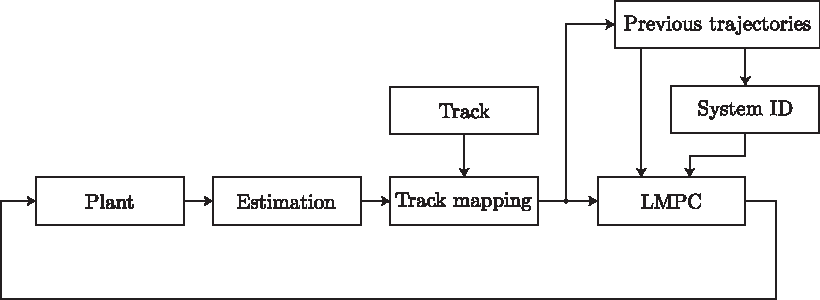
\includegraphics{../../Figures/Illustrator/ControlDiagram.pdf}
%    \caption{Control structure}
%    \label{fig:controlStructure}
%\end{figure}

\section{Introduction to the BARC}
The car used for our experiments is a remote controlled race car of the model "Basher RZ-4 1/10 Rally Racer" that has been modified by the MPC Lab at UC Berkeley to easily test new control techniques. This car is called Berkeley Autonomous Race Car (BARC, \cite{BARC}) and it has been used previously in student projects. The basic setup is shown in Figure \ref{fig:BARC}.
\begin{figure}[ht]
    \centering
  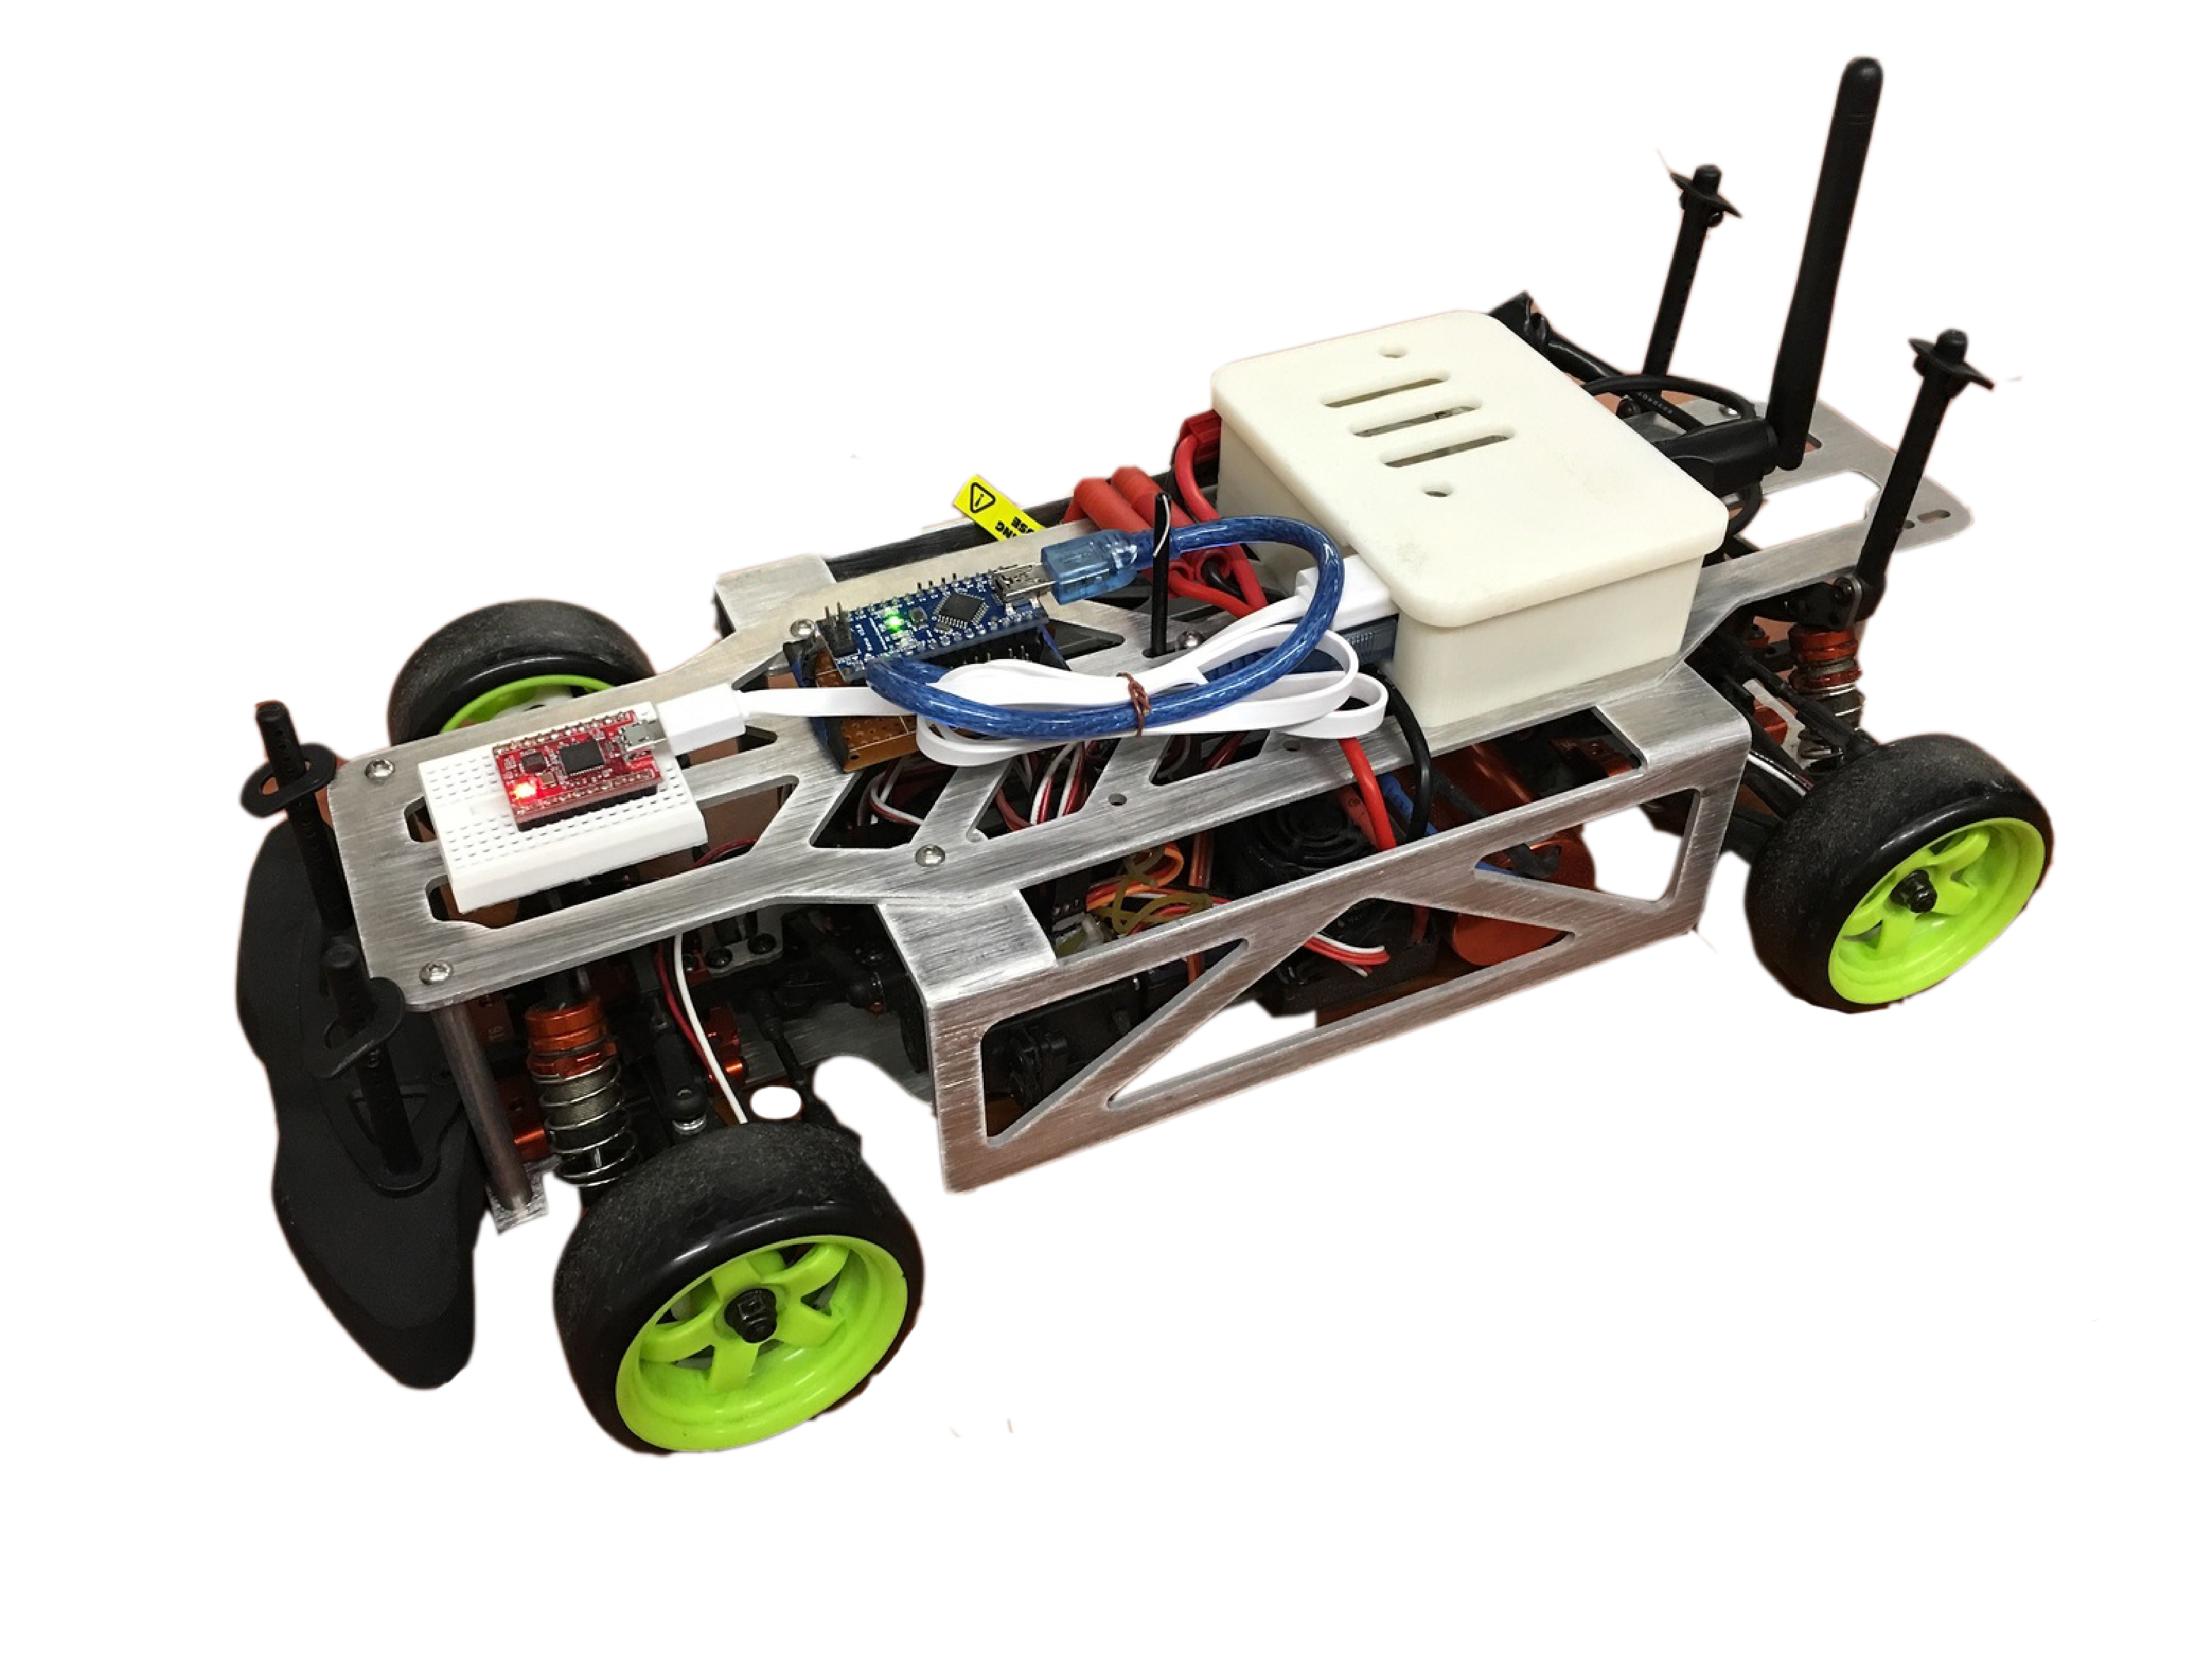
\includegraphics[width=0.8\textwidth]{../../Figures/BARC/IMG_1047.pdf}
    \caption{Basic BARC setup}
    \label{fig:BARC}
\end{figure}

Aside from standard actuators (brushless DC motor and steering servo), it features two onboard CPUs. The first CPU is an Arduino Nano which allows low-level control of the actuators as well as receiving and simple processing of sensor data. The second CPU is a Samsung Exynos 5422, provided by an Odroid XU4 single board computer. The Exynos CPU family has been used since 2010 on various smartphones like the Samsung Galaxy S. This processor is used for high-level computing (i.e. communication with USB devices and an external computer).
\subsection{Sensors}
For the purpose of race driving the estimation of absolute position, velocity and orientation are needed. The goal of the BARC project is to provide an affordable solution that can be used for testing autonomous driving algorithms. To accomplish this goal the following low-cost  sensors were chosen:
\begin{description}
\item[IMU] The Inertial Measurement Unit measures linear and angular accelerations as well as the car's current orientation in space. The IMU used on the BARC is a myAHRS+ which runs at a frequency of 50 Hertz. It is directly connected to the Odroid through a USB port.
\item[Encoders] Each wheel contains two magnetically operating encoders which are used to measure the car's velocity. These measurements are only reliable as long as the car is not drifting and as long as the wheels are spinning. The frequency of these measurements is directly related to the rotating speed of the wheels. The encoders are connected to the Arduino and send a signal at each half spin of the wheel. The Arduino sends the average speed resulting from the signals to the Odroid.
% Yes, actually there are 4 encoders, but we are only able to use two of them.
\item[GPS] To determine the absolute position of the car, an indoor positioning system from \emph{Marvelmind robotics} \cite{marvelmind} is used. Similar to the Global Positioning System (GPS), it determines the position of the car by triangulating the distances between stationary beacons around the racetrack and a mobile beacon which is fixed to the car. Distances are measured by the time of flight of ultrasound signals between all beacons.\\
The system measures the position with deviations of about $\SI{2}{\centi\meter}$ at a varying frequency between 10 and 16 Hertz.
\end{description}

\subsection{Input mapping}\label{sec:inputMapping}
While the MPC formulation calculates inputs of acceleration and steering in SI units, the actuators are controlled by the Arduino using pulse-width-modulation (PWM) signals. The PWM signals are processed by a servo library, which allows values in the range of $0...180$ (i.e. turning angles of a servo). This section describes the identification procedure to find the steering mapping and acceleration mapping.
%{\bfseries{I noticed that sometime the sentences are a bit convolute, it is good practice to make them as simple and short as possible (I sill have lot of problems in doing that). For instance I would reformulate your last sentence: "This section describes the identification champaign to find the steering and acceleration mapping."}}
\paragraph{Steering mapping}%{\bfseries{Is the the official template for the MS or you made it? I would ask the professor that is going to read the thesis if there is a standard latex template --> mb: Yes it is the standard template}}
In order to identify the steering mapping, different steering PWM signals are sent to the steering servo while driving at a constant acceleration signal. Due to electromagnetic motor drag, this leads to a constant velocity while performing circles of different radii. A low velocity is used so that an ideal kinematic bicycle model can be assumed. Using the equations of the kinematic bicycle model, the steering angle $\delta_F$ can be inferred as follows:
\begin{equation}\label{eq:deltaF}
\delta_F = \arctan\left(\frac{\dot\psi\cdot(L_F+L_R)}{v_x}\right)
\end{equation}
It can be seen that only $\dot \psi$ and $v_x$ need to be measured to calculate $\delta_F$. Both quantities are measured with good accuracy by the IMU and encoders.
Running this open loop test and approximating the measurements with an affine function, following results were obtained:
\begin{equation}
u_{PWM} = 89.8\cdot \delta_F + 90.8
\end{equation}
\begin{figure}[ht]
    \centering
  %% Creator: Matplotlib, PGF backend
%%
%% To include the figure in your LaTeX document, write
%%   \input{<filename>.pgf}
%%
%% Make sure the required packages are loaded in your preamble
%%   \usepackage{pgf}
%%
%% Figures using additional raster images can only be included by \input if
%% they are in the same directory as the main LaTeX file. For loading figures
%% from other directories you can use the `import` package
%%   \usepackage{import}
%% and then include the figures with
%%   \import{<path to file>}{<filename>.pgf}
%%
%% Matplotlib used the following preamble
%%   \usepackage{fontspec}
%%
\begingroup%
\makeatletter%
\begin{pgfpicture}%
\pgfpathrectangle{\pgfpointorigin}{\pgfqpoint{4.500000in}{3.000000in}}%
\pgfusepath{use as bounding box, clip}%
\begin{pgfscope}%
\pgfsetbuttcap%
\pgfsetmiterjoin%
\definecolor{currentfill}{rgb}{1.000000,1.000000,1.000000}%
\pgfsetfillcolor{currentfill}%
\pgfsetlinewidth{0.000000pt}%
\definecolor{currentstroke}{rgb}{1.000000,1.000000,1.000000}%
\pgfsetstrokecolor{currentstroke}%
\pgfsetdash{}{0pt}%
\pgfpathmoveto{\pgfqpoint{0.000000in}{0.000000in}}%
\pgfpathlineto{\pgfqpoint{4.500000in}{0.000000in}}%
\pgfpathlineto{\pgfqpoint{4.500000in}{3.000000in}}%
\pgfpathlineto{\pgfqpoint{0.000000in}{3.000000in}}%
\pgfpathclose%
\pgfusepath{fill}%
\end{pgfscope}%
\begin{pgfscope}%
\pgfsetbuttcap%
\pgfsetmiterjoin%
\definecolor{currentfill}{rgb}{1.000000,1.000000,1.000000}%
\pgfsetfillcolor{currentfill}%
\pgfsetlinewidth{0.000000pt}%
\definecolor{currentstroke}{rgb}{0.000000,0.000000,0.000000}%
\pgfsetstrokecolor{currentstroke}%
\pgfsetstrokeopacity{0.000000}%
\pgfsetdash{}{0pt}%
\pgfpathmoveto{\pgfqpoint{0.628717in}{0.471921in}}%
\pgfpathlineto{\pgfqpoint{4.261975in}{0.471921in}}%
\pgfpathlineto{\pgfqpoint{4.261975in}{2.805251in}}%
\pgfpathlineto{\pgfqpoint{0.628717in}{2.805251in}}%
\pgfpathclose%
\pgfusepath{fill}%
\end{pgfscope}%
\begin{pgfscope}%
\pgfpathrectangle{\pgfqpoint{0.628717in}{0.471921in}}{\pgfqpoint{3.633258in}{2.333330in}} %
\pgfusepath{clip}%
\pgfsetbuttcap%
\pgfsetroundjoin%
\definecolor{currentfill}{rgb}{0.000000,0.000000,1.000000}%
\pgfsetfillcolor{currentfill}%
\pgfsetlinewidth{0.501875pt}%
\definecolor{currentstroke}{rgb}{0.000000,0.000000,1.000000}%
\pgfsetstrokecolor{currentstroke}%
\pgfsetdash{}{0pt}%
\pgfsys@defobject{currentmarker}{\pgfqpoint{-0.013889in}{-0.013889in}}{\pgfqpoint{0.013889in}{0.013889in}}{%
\pgfpathmoveto{\pgfqpoint{-0.013889in}{0.000000in}}%
\pgfpathlineto{\pgfqpoint{0.013889in}{0.000000in}}%
\pgfpathmoveto{\pgfqpoint{0.000000in}{-0.013889in}}%
\pgfpathlineto{\pgfqpoint{0.000000in}{0.013889in}}%
\pgfusepath{stroke,fill}%
}%
\begin{pgfscope}%
\pgfsys@transformshift{0.628717in}{0.724566in}%
\pgfsys@useobject{currentmarker}{}%
\end{pgfscope}%
\begin{pgfscope}%
\pgfsys@transformshift{0.628717in}{0.724566in}%
\pgfsys@useobject{currentmarker}{}%
\end{pgfscope}%
\begin{pgfscope}%
\pgfsys@transformshift{0.628717in}{0.748045in}%
\pgfsys@useobject{currentmarker}{}%
\end{pgfscope}%
\begin{pgfscope}%
\pgfsys@transformshift{0.628717in}{0.746613in}%
\pgfsys@useobject{currentmarker}{}%
\end{pgfscope}%
\begin{pgfscope}%
\pgfsys@transformshift{0.628717in}{0.753158in}%
\pgfsys@useobject{currentmarker}{}%
\end{pgfscope}%
\begin{pgfscope}%
\pgfsys@transformshift{0.628717in}{0.842776in}%
\pgfsys@useobject{currentmarker}{}%
\end{pgfscope}%
\begin{pgfscope}%
\pgfsys@transformshift{0.628717in}{0.799082in}%
\pgfsys@useobject{currentmarker}{}%
\end{pgfscope}%
\begin{pgfscope}%
\pgfsys@transformshift{0.628717in}{0.773954in}%
\pgfsys@useobject{currentmarker}{}%
\end{pgfscope}%
\begin{pgfscope}%
\pgfsys@transformshift{0.628717in}{0.838914in}%
\pgfsys@useobject{currentmarker}{}%
\end{pgfscope}%
\begin{pgfscope}%
\pgfsys@transformshift{0.749825in}{0.768101in}%
\pgfsys@useobject{currentmarker}{}%
\end{pgfscope}%
\begin{pgfscope}%
\pgfsys@transformshift{0.749825in}{0.761528in}%
\pgfsys@useobject{currentmarker}{}%
\end{pgfscope}%
\begin{pgfscope}%
\pgfsys@transformshift{0.749825in}{0.734944in}%
\pgfsys@useobject{currentmarker}{}%
\end{pgfscope}%
\begin{pgfscope}%
\pgfsys@transformshift{0.749825in}{0.760476in}%
\pgfsys@useobject{currentmarker}{}%
\end{pgfscope}%
\begin{pgfscope}%
\pgfsys@transformshift{0.749825in}{0.818390in}%
\pgfsys@useobject{currentmarker}{}%
\end{pgfscope}%
\begin{pgfscope}%
\pgfsys@transformshift{0.749825in}{0.766250in}%
\pgfsys@useobject{currentmarker}{}%
\end{pgfscope}%
\begin{pgfscope}%
\pgfsys@transformshift{0.749825in}{0.755789in}%
\pgfsys@useobject{currentmarker}{}%
\end{pgfscope}%
\begin{pgfscope}%
\pgfsys@transformshift{0.749825in}{0.814814in}%
\pgfsys@useobject{currentmarker}{}%
\end{pgfscope}%
\begin{pgfscope}%
\pgfsys@transformshift{0.870934in}{0.804724in}%
\pgfsys@useobject{currentmarker}{}%
\end{pgfscope}%
\begin{pgfscope}%
\pgfsys@transformshift{0.870934in}{0.804724in}%
\pgfsys@useobject{currentmarker}{}%
\end{pgfscope}%
\begin{pgfscope}%
\pgfsys@transformshift{0.870934in}{0.804724in}%
\pgfsys@useobject{currentmarker}{}%
\end{pgfscope}%
\begin{pgfscope}%
\pgfsys@transformshift{0.870934in}{0.804724in}%
\pgfsys@useobject{currentmarker}{}%
\end{pgfscope}%
\begin{pgfscope}%
\pgfsys@transformshift{0.870934in}{0.804724in}%
\pgfsys@useobject{currentmarker}{}%
\end{pgfscope}%
\begin{pgfscope}%
\pgfsys@transformshift{0.870934in}{0.804724in}%
\pgfsys@useobject{currentmarker}{}%
\end{pgfscope}%
\begin{pgfscope}%
\pgfsys@transformshift{0.870934in}{0.804724in}%
\pgfsys@useobject{currentmarker}{}%
\end{pgfscope}%
\begin{pgfscope}%
\pgfsys@transformshift{0.870934in}{0.804724in}%
\pgfsys@useobject{currentmarker}{}%
\end{pgfscope}%
\begin{pgfscope}%
\pgfsys@transformshift{0.870934in}{0.804724in}%
\pgfsys@useobject{currentmarker}{}%
\end{pgfscope}%
\begin{pgfscope}%
\pgfsys@transformshift{0.870934in}{0.804724in}%
\pgfsys@useobject{currentmarker}{}%
\end{pgfscope}%
\begin{pgfscope}%
\pgfsys@transformshift{0.870934in}{0.804724in}%
\pgfsys@useobject{currentmarker}{}%
\end{pgfscope}%
\begin{pgfscope}%
\pgfsys@transformshift{0.870934in}{0.804724in}%
\pgfsys@useobject{currentmarker}{}%
\end{pgfscope}%
\begin{pgfscope}%
\pgfsys@transformshift{0.870934in}{0.832525in}%
\pgfsys@useobject{currentmarker}{}%
\end{pgfscope}%
\begin{pgfscope}%
\pgfsys@transformshift{0.870934in}{0.815966in}%
\pgfsys@useobject{currentmarker}{}%
\end{pgfscope}%
\begin{pgfscope}%
\pgfsys@transformshift{0.870934in}{0.847444in}%
\pgfsys@useobject{currentmarker}{}%
\end{pgfscope}%
\begin{pgfscope}%
\pgfsys@transformshift{0.870934in}{0.869380in}%
\pgfsys@useobject{currentmarker}{}%
\end{pgfscope}%
\begin{pgfscope}%
\pgfsys@transformshift{0.870934in}{0.935507in}%
\pgfsys@useobject{currentmarker}{}%
\end{pgfscope}%
\begin{pgfscope}%
\pgfsys@transformshift{0.870934in}{0.838458in}%
\pgfsys@useobject{currentmarker}{}%
\end{pgfscope}%
\begin{pgfscope}%
\pgfsys@transformshift{0.870934in}{0.838458in}%
\pgfsys@useobject{currentmarker}{}%
\end{pgfscope}%
\begin{pgfscope}%
\pgfsys@transformshift{0.870934in}{0.838458in}%
\pgfsys@useobject{currentmarker}{}%
\end{pgfscope}%
\begin{pgfscope}%
\pgfsys@transformshift{0.870934in}{0.838458in}%
\pgfsys@useobject{currentmarker}{}%
\end{pgfscope}%
\begin{pgfscope}%
\pgfsys@transformshift{0.870934in}{0.838458in}%
\pgfsys@useobject{currentmarker}{}%
\end{pgfscope}%
\begin{pgfscope}%
\pgfsys@transformshift{0.870934in}{0.838458in}%
\pgfsys@useobject{currentmarker}{}%
\end{pgfscope}%
\begin{pgfscope}%
\pgfsys@transformshift{0.870934in}{0.838458in}%
\pgfsys@useobject{currentmarker}{}%
\end{pgfscope}%
\begin{pgfscope}%
\pgfsys@transformshift{0.870934in}{0.838458in}%
\pgfsys@useobject{currentmarker}{}%
\end{pgfscope}%
\begin{pgfscope}%
\pgfsys@transformshift{0.870934in}{0.838458in}%
\pgfsys@useobject{currentmarker}{}%
\end{pgfscope}%
\begin{pgfscope}%
\pgfsys@transformshift{0.870934in}{0.838458in}%
\pgfsys@useobject{currentmarker}{}%
\end{pgfscope}%
\begin{pgfscope}%
\pgfsys@transformshift{0.870934in}{0.838458in}%
\pgfsys@useobject{currentmarker}{}%
\end{pgfscope}%
\begin{pgfscope}%
\pgfsys@transformshift{0.870934in}{0.839662in}%
\pgfsys@useobject{currentmarker}{}%
\end{pgfscope}%
\begin{pgfscope}%
\pgfsys@transformshift{0.870934in}{0.839662in}%
\pgfsys@useobject{currentmarker}{}%
\end{pgfscope}%
\begin{pgfscope}%
\pgfsys@transformshift{0.870934in}{0.839662in}%
\pgfsys@useobject{currentmarker}{}%
\end{pgfscope}%
\begin{pgfscope}%
\pgfsys@transformshift{0.870934in}{0.839662in}%
\pgfsys@useobject{currentmarker}{}%
\end{pgfscope}%
\begin{pgfscope}%
\pgfsys@transformshift{0.870934in}{0.839662in}%
\pgfsys@useobject{currentmarker}{}%
\end{pgfscope}%
\begin{pgfscope}%
\pgfsys@transformshift{0.870934in}{0.839662in}%
\pgfsys@useobject{currentmarker}{}%
\end{pgfscope}%
\begin{pgfscope}%
\pgfsys@transformshift{0.870934in}{0.836345in}%
\pgfsys@useobject{currentmarker}{}%
\end{pgfscope}%
\begin{pgfscope}%
\pgfsys@transformshift{0.870934in}{0.795381in}%
\pgfsys@useobject{currentmarker}{}%
\end{pgfscope}%
\begin{pgfscope}%
\pgfsys@transformshift{0.870934in}{0.795381in}%
\pgfsys@useobject{currentmarker}{}%
\end{pgfscope}%
\begin{pgfscope}%
\pgfsys@transformshift{0.870934in}{0.795381in}%
\pgfsys@useobject{currentmarker}{}%
\end{pgfscope}%
\begin{pgfscope}%
\pgfsys@transformshift{0.870934in}{0.795381in}%
\pgfsys@useobject{currentmarker}{}%
\end{pgfscope}%
\begin{pgfscope}%
\pgfsys@transformshift{0.870934in}{0.795381in}%
\pgfsys@useobject{currentmarker}{}%
\end{pgfscope}%
\begin{pgfscope}%
\pgfsys@transformshift{0.870934in}{0.795381in}%
\pgfsys@useobject{currentmarker}{}%
\end{pgfscope}%
\begin{pgfscope}%
\pgfsys@transformshift{0.870934in}{0.795381in}%
\pgfsys@useobject{currentmarker}{}%
\end{pgfscope}%
\begin{pgfscope}%
\pgfsys@transformshift{0.870934in}{0.795381in}%
\pgfsys@useobject{currentmarker}{}%
\end{pgfscope}%
\begin{pgfscope}%
\pgfsys@transformshift{0.870934in}{0.795381in}%
\pgfsys@useobject{currentmarker}{}%
\end{pgfscope}%
\begin{pgfscope}%
\pgfsys@transformshift{0.870934in}{0.795381in}%
\pgfsys@useobject{currentmarker}{}%
\end{pgfscope}%
\begin{pgfscope}%
\pgfsys@transformshift{0.870934in}{0.795381in}%
\pgfsys@useobject{currentmarker}{}%
\end{pgfscope}%
\begin{pgfscope}%
\pgfsys@transformshift{0.870934in}{0.795381in}%
\pgfsys@useobject{currentmarker}{}%
\end{pgfscope}%
\begin{pgfscope}%
\pgfsys@transformshift{0.870934in}{0.795381in}%
\pgfsys@useobject{currentmarker}{}%
\end{pgfscope}%
\begin{pgfscope}%
\pgfsys@transformshift{0.870934in}{0.795381in}%
\pgfsys@useobject{currentmarker}{}%
\end{pgfscope}%
\begin{pgfscope}%
\pgfsys@transformshift{0.870934in}{0.809233in}%
\pgfsys@useobject{currentmarker}{}%
\end{pgfscope}%
\begin{pgfscope}%
\pgfsys@transformshift{0.870934in}{0.816012in}%
\pgfsys@useobject{currentmarker}{}%
\end{pgfscope}%
\begin{pgfscope}%
\pgfsys@transformshift{0.870934in}{0.848175in}%
\pgfsys@useobject{currentmarker}{}%
\end{pgfscope}%
\begin{pgfscope}%
\pgfsys@transformshift{0.870934in}{0.859195in}%
\pgfsys@useobject{currentmarker}{}%
\end{pgfscope}%
\begin{pgfscope}%
\pgfsys@transformshift{0.870934in}{0.859195in}%
\pgfsys@useobject{currentmarker}{}%
\end{pgfscope}%
\begin{pgfscope}%
\pgfsys@transformshift{0.870934in}{0.850114in}%
\pgfsys@useobject{currentmarker}{}%
\end{pgfscope}%
\begin{pgfscope}%
\pgfsys@transformshift{0.870934in}{0.850114in}%
\pgfsys@useobject{currentmarker}{}%
\end{pgfscope}%
\begin{pgfscope}%
\pgfsys@transformshift{0.870934in}{0.850114in}%
\pgfsys@useobject{currentmarker}{}%
\end{pgfscope}%
\begin{pgfscope}%
\pgfsys@transformshift{0.870934in}{0.850114in}%
\pgfsys@useobject{currentmarker}{}%
\end{pgfscope}%
\begin{pgfscope}%
\pgfsys@transformshift{0.870934in}{0.850114in}%
\pgfsys@useobject{currentmarker}{}%
\end{pgfscope}%
\begin{pgfscope}%
\pgfsys@transformshift{0.870934in}{0.850114in}%
\pgfsys@useobject{currentmarker}{}%
\end{pgfscope}%
\begin{pgfscope}%
\pgfsys@transformshift{0.870934in}{0.850114in}%
\pgfsys@useobject{currentmarker}{}%
\end{pgfscope}%
\begin{pgfscope}%
\pgfsys@transformshift{0.870934in}{0.850114in}%
\pgfsys@useobject{currentmarker}{}%
\end{pgfscope}%
\begin{pgfscope}%
\pgfsys@transformshift{0.870934in}{0.850114in}%
\pgfsys@useobject{currentmarker}{}%
\end{pgfscope}%
\begin{pgfscope}%
\pgfsys@transformshift{0.870934in}{0.850114in}%
\pgfsys@useobject{currentmarker}{}%
\end{pgfscope}%
\begin{pgfscope}%
\pgfsys@transformshift{0.870934in}{0.850114in}%
\pgfsys@useobject{currentmarker}{}%
\end{pgfscope}%
\begin{pgfscope}%
\pgfsys@transformshift{0.870934in}{0.850114in}%
\pgfsys@useobject{currentmarker}{}%
\end{pgfscope}%
\begin{pgfscope}%
\pgfsys@transformshift{0.870934in}{0.850114in}%
\pgfsys@useobject{currentmarker}{}%
\end{pgfscope}%
\begin{pgfscope}%
\pgfsys@transformshift{0.870934in}{0.871689in}%
\pgfsys@useobject{currentmarker}{}%
\end{pgfscope}%
\begin{pgfscope}%
\pgfsys@transformshift{0.870934in}{0.871689in}%
\pgfsys@useobject{currentmarker}{}%
\end{pgfscope}%
\begin{pgfscope}%
\pgfsys@transformshift{0.870934in}{0.871689in}%
\pgfsys@useobject{currentmarker}{}%
\end{pgfscope}%
\begin{pgfscope}%
\pgfsys@transformshift{0.870934in}{0.871689in}%
\pgfsys@useobject{currentmarker}{}%
\end{pgfscope}%
\begin{pgfscope}%
\pgfsys@transformshift{0.870934in}{0.871689in}%
\pgfsys@useobject{currentmarker}{}%
\end{pgfscope}%
\begin{pgfscope}%
\pgfsys@transformshift{0.870934in}{0.871689in}%
\pgfsys@useobject{currentmarker}{}%
\end{pgfscope}%
\begin{pgfscope}%
\pgfsys@transformshift{0.870934in}{0.871689in}%
\pgfsys@useobject{currentmarker}{}%
\end{pgfscope}%
\begin{pgfscope}%
\pgfsys@transformshift{0.870934in}{0.871689in}%
\pgfsys@useobject{currentmarker}{}%
\end{pgfscope}%
\begin{pgfscope}%
\pgfsys@transformshift{0.870934in}{0.871689in}%
\pgfsys@useobject{currentmarker}{}%
\end{pgfscope}%
\begin{pgfscope}%
\pgfsys@transformshift{0.870934in}{0.871689in}%
\pgfsys@useobject{currentmarker}{}%
\end{pgfscope}%
\begin{pgfscope}%
\pgfsys@transformshift{0.870934in}{0.871689in}%
\pgfsys@useobject{currentmarker}{}%
\end{pgfscope}%
\begin{pgfscope}%
\pgfsys@transformshift{0.870934in}{0.871689in}%
\pgfsys@useobject{currentmarker}{}%
\end{pgfscope}%
\begin{pgfscope}%
\pgfsys@transformshift{0.870934in}{0.871689in}%
\pgfsys@useobject{currentmarker}{}%
\end{pgfscope}%
\begin{pgfscope}%
\pgfsys@transformshift{0.870934in}{0.871689in}%
\pgfsys@useobject{currentmarker}{}%
\end{pgfscope}%
\begin{pgfscope}%
\pgfsys@transformshift{0.870934in}{0.871689in}%
\pgfsys@useobject{currentmarker}{}%
\end{pgfscope}%
\begin{pgfscope}%
\pgfsys@transformshift{0.870934in}{0.871689in}%
\pgfsys@useobject{currentmarker}{}%
\end{pgfscope}%
\begin{pgfscope}%
\pgfsys@transformshift{0.870934in}{0.871689in}%
\pgfsys@useobject{currentmarker}{}%
\end{pgfscope}%
\begin{pgfscope}%
\pgfsys@transformshift{0.870934in}{0.871689in}%
\pgfsys@useobject{currentmarker}{}%
\end{pgfscope}%
\begin{pgfscope}%
\pgfsys@transformshift{0.870934in}{0.871689in}%
\pgfsys@useobject{currentmarker}{}%
\end{pgfscope}%
\begin{pgfscope}%
\pgfsys@transformshift{0.870934in}{0.871689in}%
\pgfsys@useobject{currentmarker}{}%
\end{pgfscope}%
\begin{pgfscope}%
\pgfsys@transformshift{0.870934in}{0.871689in}%
\pgfsys@useobject{currentmarker}{}%
\end{pgfscope}%
\begin{pgfscope}%
\pgfsys@transformshift{0.870934in}{0.826315in}%
\pgfsys@useobject{currentmarker}{}%
\end{pgfscope}%
\begin{pgfscope}%
\pgfsys@transformshift{0.870934in}{0.826315in}%
\pgfsys@useobject{currentmarker}{}%
\end{pgfscope}%
\begin{pgfscope}%
\pgfsys@transformshift{0.870934in}{0.822983in}%
\pgfsys@useobject{currentmarker}{}%
\end{pgfscope}%
\begin{pgfscope}%
\pgfsys@transformshift{0.870934in}{0.822983in}%
\pgfsys@useobject{currentmarker}{}%
\end{pgfscope}%
\begin{pgfscope}%
\pgfsys@transformshift{0.870934in}{0.822983in}%
\pgfsys@useobject{currentmarker}{}%
\end{pgfscope}%
\begin{pgfscope}%
\pgfsys@transformshift{0.870934in}{0.822983in}%
\pgfsys@useobject{currentmarker}{}%
\end{pgfscope}%
\begin{pgfscope}%
\pgfsys@transformshift{0.870934in}{0.822983in}%
\pgfsys@useobject{currentmarker}{}%
\end{pgfscope}%
\begin{pgfscope}%
\pgfsys@transformshift{0.870934in}{0.822983in}%
\pgfsys@useobject{currentmarker}{}%
\end{pgfscope}%
\begin{pgfscope}%
\pgfsys@transformshift{0.870934in}{0.822983in}%
\pgfsys@useobject{currentmarker}{}%
\end{pgfscope}%
\begin{pgfscope}%
\pgfsys@transformshift{0.870934in}{0.822983in}%
\pgfsys@useobject{currentmarker}{}%
\end{pgfscope}%
\begin{pgfscope}%
\pgfsys@transformshift{0.870934in}{0.822983in}%
\pgfsys@useobject{currentmarker}{}%
\end{pgfscope}%
\begin{pgfscope}%
\pgfsys@transformshift{0.870934in}{0.822983in}%
\pgfsys@useobject{currentmarker}{}%
\end{pgfscope}%
\begin{pgfscope}%
\pgfsys@transformshift{0.870934in}{0.822983in}%
\pgfsys@useobject{currentmarker}{}%
\end{pgfscope}%
\begin{pgfscope}%
\pgfsys@transformshift{0.870934in}{0.822983in}%
\pgfsys@useobject{currentmarker}{}%
\end{pgfscope}%
\begin{pgfscope}%
\pgfsys@transformshift{0.870934in}{0.822983in}%
\pgfsys@useobject{currentmarker}{}%
\end{pgfscope}%
\begin{pgfscope}%
\pgfsys@transformshift{0.870934in}{0.822983in}%
\pgfsys@useobject{currentmarker}{}%
\end{pgfscope}%
\begin{pgfscope}%
\pgfsys@transformshift{0.870934in}{0.822983in}%
\pgfsys@useobject{currentmarker}{}%
\end{pgfscope}%
\begin{pgfscope}%
\pgfsys@transformshift{0.870934in}{0.822983in}%
\pgfsys@useobject{currentmarker}{}%
\end{pgfscope}%
\begin{pgfscope}%
\pgfsys@transformshift{0.870934in}{0.822983in}%
\pgfsys@useobject{currentmarker}{}%
\end{pgfscope}%
\begin{pgfscope}%
\pgfsys@transformshift{0.870934in}{0.822983in}%
\pgfsys@useobject{currentmarker}{}%
\end{pgfscope}%
\begin{pgfscope}%
\pgfsys@transformshift{0.870934in}{0.822983in}%
\pgfsys@useobject{currentmarker}{}%
\end{pgfscope}%
\begin{pgfscope}%
\pgfsys@transformshift{0.870934in}{0.822983in}%
\pgfsys@useobject{currentmarker}{}%
\end{pgfscope}%
\begin{pgfscope}%
\pgfsys@transformshift{0.870934in}{0.822983in}%
\pgfsys@useobject{currentmarker}{}%
\end{pgfscope}%
\begin{pgfscope}%
\pgfsys@transformshift{0.870934in}{0.822983in}%
\pgfsys@useobject{currentmarker}{}%
\end{pgfscope}%
\begin{pgfscope}%
\pgfsys@transformshift{0.870934in}{0.822983in}%
\pgfsys@useobject{currentmarker}{}%
\end{pgfscope}%
\begin{pgfscope}%
\pgfsys@transformshift{0.870934in}{0.822983in}%
\pgfsys@useobject{currentmarker}{}%
\end{pgfscope}%
\begin{pgfscope}%
\pgfsys@transformshift{0.870934in}{0.822983in}%
\pgfsys@useobject{currentmarker}{}%
\end{pgfscope}%
\begin{pgfscope}%
\pgfsys@transformshift{0.870934in}{0.822983in}%
\pgfsys@useobject{currentmarker}{}%
\end{pgfscope}%
\begin{pgfscope}%
\pgfsys@transformshift{0.870934in}{0.822983in}%
\pgfsys@useobject{currentmarker}{}%
\end{pgfscope}%
\begin{pgfscope}%
\pgfsys@transformshift{0.870934in}{0.822983in}%
\pgfsys@useobject{currentmarker}{}%
\end{pgfscope}%
\begin{pgfscope}%
\pgfsys@transformshift{0.870934in}{0.822983in}%
\pgfsys@useobject{currentmarker}{}%
\end{pgfscope}%
\begin{pgfscope}%
\pgfsys@transformshift{0.870934in}{0.822983in}%
\pgfsys@useobject{currentmarker}{}%
\end{pgfscope}%
\begin{pgfscope}%
\pgfsys@transformshift{0.870934in}{0.822983in}%
\pgfsys@useobject{currentmarker}{}%
\end{pgfscope}%
\begin{pgfscope}%
\pgfsys@transformshift{0.870934in}{0.822983in}%
\pgfsys@useobject{currentmarker}{}%
\end{pgfscope}%
\begin{pgfscope}%
\pgfsys@transformshift{0.870934in}{0.822983in}%
\pgfsys@useobject{currentmarker}{}%
\end{pgfscope}%
\begin{pgfscope}%
\pgfsys@transformshift{0.870934in}{0.822983in}%
\pgfsys@useobject{currentmarker}{}%
\end{pgfscope}%
\begin{pgfscope}%
\pgfsys@transformshift{0.870934in}{0.822983in}%
\pgfsys@useobject{currentmarker}{}%
\end{pgfscope}%
\begin{pgfscope}%
\pgfsys@transformshift{0.870934in}{0.822983in}%
\pgfsys@useobject{currentmarker}{}%
\end{pgfscope}%
\begin{pgfscope}%
\pgfsys@transformshift{0.870934in}{0.822983in}%
\pgfsys@useobject{currentmarker}{}%
\end{pgfscope}%
\begin{pgfscope}%
\pgfsys@transformshift{0.870934in}{0.822983in}%
\pgfsys@useobject{currentmarker}{}%
\end{pgfscope}%
\begin{pgfscope}%
\pgfsys@transformshift{0.870934in}{0.822983in}%
\pgfsys@useobject{currentmarker}{}%
\end{pgfscope}%
\begin{pgfscope}%
\pgfsys@transformshift{0.870934in}{0.822983in}%
\pgfsys@useobject{currentmarker}{}%
\end{pgfscope}%
\begin{pgfscope}%
\pgfsys@transformshift{0.870934in}{0.822983in}%
\pgfsys@useobject{currentmarker}{}%
\end{pgfscope}%
\begin{pgfscope}%
\pgfsys@transformshift{0.870934in}{0.822983in}%
\pgfsys@useobject{currentmarker}{}%
\end{pgfscope}%
\begin{pgfscope}%
\pgfsys@transformshift{0.870934in}{0.822983in}%
\pgfsys@useobject{currentmarker}{}%
\end{pgfscope}%
\begin{pgfscope}%
\pgfsys@transformshift{0.870934in}{0.822983in}%
\pgfsys@useobject{currentmarker}{}%
\end{pgfscope}%
\begin{pgfscope}%
\pgfsys@transformshift{0.870934in}{0.822983in}%
\pgfsys@useobject{currentmarker}{}%
\end{pgfscope}%
\begin{pgfscope}%
\pgfsys@transformshift{0.870934in}{0.822983in}%
\pgfsys@useobject{currentmarker}{}%
\end{pgfscope}%
\begin{pgfscope}%
\pgfsys@transformshift{0.870934in}{0.822983in}%
\pgfsys@useobject{currentmarker}{}%
\end{pgfscope}%
\begin{pgfscope}%
\pgfsys@transformshift{0.870934in}{0.822983in}%
\pgfsys@useobject{currentmarker}{}%
\end{pgfscope}%
\begin{pgfscope}%
\pgfsys@transformshift{0.870934in}{0.822983in}%
\pgfsys@useobject{currentmarker}{}%
\end{pgfscope}%
\begin{pgfscope}%
\pgfsys@transformshift{0.870934in}{0.822983in}%
\pgfsys@useobject{currentmarker}{}%
\end{pgfscope}%
\begin{pgfscope}%
\pgfsys@transformshift{0.870934in}{0.822983in}%
\pgfsys@useobject{currentmarker}{}%
\end{pgfscope}%
\begin{pgfscope}%
\pgfsys@transformshift{0.870934in}{0.822983in}%
\pgfsys@useobject{currentmarker}{}%
\end{pgfscope}%
\begin{pgfscope}%
\pgfsys@transformshift{0.870934in}{0.822983in}%
\pgfsys@useobject{currentmarker}{}%
\end{pgfscope}%
\begin{pgfscope}%
\pgfsys@transformshift{0.870934in}{0.822983in}%
\pgfsys@useobject{currentmarker}{}%
\end{pgfscope}%
\begin{pgfscope}%
\pgfsys@transformshift{0.870934in}{0.822983in}%
\pgfsys@useobject{currentmarker}{}%
\end{pgfscope}%
\begin{pgfscope}%
\pgfsys@transformshift{0.870934in}{0.822983in}%
\pgfsys@useobject{currentmarker}{}%
\end{pgfscope}%
\begin{pgfscope}%
\pgfsys@transformshift{0.870934in}{0.822983in}%
\pgfsys@useobject{currentmarker}{}%
\end{pgfscope}%
\begin{pgfscope}%
\pgfsys@transformshift{0.870934in}{0.822983in}%
\pgfsys@useobject{currentmarker}{}%
\end{pgfscope}%
\begin{pgfscope}%
\pgfsys@transformshift{0.870934in}{0.822983in}%
\pgfsys@useobject{currentmarker}{}%
\end{pgfscope}%
\begin{pgfscope}%
\pgfsys@transformshift{0.870934in}{0.822983in}%
\pgfsys@useobject{currentmarker}{}%
\end{pgfscope}%
\begin{pgfscope}%
\pgfsys@transformshift{0.870934in}{0.822983in}%
\pgfsys@useobject{currentmarker}{}%
\end{pgfscope}%
\begin{pgfscope}%
\pgfsys@transformshift{0.870934in}{0.822983in}%
\pgfsys@useobject{currentmarker}{}%
\end{pgfscope}%
\begin{pgfscope}%
\pgfsys@transformshift{0.992043in}{0.876310in}%
\pgfsys@useobject{currentmarker}{}%
\end{pgfscope}%
\begin{pgfscope}%
\pgfsys@transformshift{0.992043in}{0.871201in}%
\pgfsys@useobject{currentmarker}{}%
\end{pgfscope}%
\begin{pgfscope}%
\pgfsys@transformshift{0.992043in}{0.891655in}%
\pgfsys@useobject{currentmarker}{}%
\end{pgfscope}%
\begin{pgfscope}%
\pgfsys@transformshift{0.992043in}{0.923064in}%
\pgfsys@useobject{currentmarker}{}%
\end{pgfscope}%
\begin{pgfscope}%
\pgfsys@transformshift{0.992043in}{0.929695in}%
\pgfsys@useobject{currentmarker}{}%
\end{pgfscope}%
\begin{pgfscope}%
\pgfsys@transformshift{0.992043in}{0.850423in}%
\pgfsys@useobject{currentmarker}{}%
\end{pgfscope}%
\begin{pgfscope}%
\pgfsys@transformshift{0.992043in}{0.874094in}%
\pgfsys@useobject{currentmarker}{}%
\end{pgfscope}%
\begin{pgfscope}%
\pgfsys@transformshift{0.992043in}{0.849784in}%
\pgfsys@useobject{currentmarker}{}%
\end{pgfscope}%
\begin{pgfscope}%
\pgfsys@transformshift{0.992043in}{0.897855in}%
\pgfsys@useobject{currentmarker}{}%
\end{pgfscope}%
\begin{pgfscope}%
\pgfsys@transformshift{0.992043in}{0.922825in}%
\pgfsys@useobject{currentmarker}{}%
\end{pgfscope}%
\begin{pgfscope}%
\pgfsys@transformshift{0.992043in}{0.878743in}%
\pgfsys@useobject{currentmarker}{}%
\end{pgfscope}%
\begin{pgfscope}%
\pgfsys@transformshift{0.992043in}{0.869178in}%
\pgfsys@useobject{currentmarker}{}%
\end{pgfscope}%
\begin{pgfscope}%
\pgfsys@transformshift{0.992043in}{0.869178in}%
\pgfsys@useobject{currentmarker}{}%
\end{pgfscope}%
\begin{pgfscope}%
\pgfsys@transformshift{0.992043in}{0.869178in}%
\pgfsys@useobject{currentmarker}{}%
\end{pgfscope}%
\begin{pgfscope}%
\pgfsys@transformshift{0.992043in}{0.881296in}%
\pgfsys@useobject{currentmarker}{}%
\end{pgfscope}%
\begin{pgfscope}%
\pgfsys@transformshift{0.992043in}{0.919667in}%
\pgfsys@useobject{currentmarker}{}%
\end{pgfscope}%
\begin{pgfscope}%
\pgfsys@transformshift{0.992043in}{0.926466in}%
\pgfsys@useobject{currentmarker}{}%
\end{pgfscope}%
\begin{pgfscope}%
\pgfsys@transformshift{0.992043in}{0.926466in}%
\pgfsys@useobject{currentmarker}{}%
\end{pgfscope}%
\begin{pgfscope}%
\pgfsys@transformshift{0.992043in}{0.934718in}%
\pgfsys@useobject{currentmarker}{}%
\end{pgfscope}%
\begin{pgfscope}%
\pgfsys@transformshift{0.992043in}{0.911250in}%
\pgfsys@useobject{currentmarker}{}%
\end{pgfscope}%
\begin{pgfscope}%
\pgfsys@transformshift{0.992043in}{0.905550in}%
\pgfsys@useobject{currentmarker}{}%
\end{pgfscope}%
\begin{pgfscope}%
\pgfsys@transformshift{0.992043in}{0.900894in}%
\pgfsys@useobject{currentmarker}{}%
\end{pgfscope}%
\begin{pgfscope}%
\pgfsys@transformshift{0.992043in}{0.975702in}%
\pgfsys@useobject{currentmarker}{}%
\end{pgfscope}%
\begin{pgfscope}%
\pgfsys@transformshift{0.992043in}{0.930237in}%
\pgfsys@useobject{currentmarker}{}%
\end{pgfscope}%
\begin{pgfscope}%
\pgfsys@transformshift{0.992043in}{0.962874in}%
\pgfsys@useobject{currentmarker}{}%
\end{pgfscope}%
\begin{pgfscope}%
\pgfsys@transformshift{0.992043in}{0.962874in}%
\pgfsys@useobject{currentmarker}{}%
\end{pgfscope}%
\begin{pgfscope}%
\pgfsys@transformshift{0.992043in}{0.982579in}%
\pgfsys@useobject{currentmarker}{}%
\end{pgfscope}%
\begin{pgfscope}%
\pgfsys@transformshift{0.992043in}{0.989996in}%
\pgfsys@useobject{currentmarker}{}%
\end{pgfscope}%
\begin{pgfscope}%
\pgfsys@transformshift{0.992043in}{0.963049in}%
\pgfsys@useobject{currentmarker}{}%
\end{pgfscope}%
\begin{pgfscope}%
\pgfsys@transformshift{0.992043in}{0.955651in}%
\pgfsys@useobject{currentmarker}{}%
\end{pgfscope}%
\begin{pgfscope}%
\pgfsys@transformshift{0.992043in}{1.020395in}%
\pgfsys@useobject{currentmarker}{}%
\end{pgfscope}%
\begin{pgfscope}%
\pgfsys@transformshift{0.992043in}{1.045452in}%
\pgfsys@useobject{currentmarker}{}%
\end{pgfscope}%
\begin{pgfscope}%
\pgfsys@transformshift{1.355368in}{1.042695in}%
\pgfsys@useobject{currentmarker}{}%
\end{pgfscope}%
\begin{pgfscope}%
\pgfsys@transformshift{1.355368in}{1.017584in}%
\pgfsys@useobject{currentmarker}{}%
\end{pgfscope}%
\begin{pgfscope}%
\pgfsys@transformshift{1.355368in}{0.983741in}%
\pgfsys@useobject{currentmarker}{}%
\end{pgfscope}%
\begin{pgfscope}%
\pgfsys@transformshift{1.355368in}{0.975635in}%
\pgfsys@useobject{currentmarker}{}%
\end{pgfscope}%
\begin{pgfscope}%
\pgfsys@transformshift{1.355368in}{0.977968in}%
\pgfsys@useobject{currentmarker}{}%
\end{pgfscope}%
\begin{pgfscope}%
\pgfsys@transformshift{1.355368in}{1.059878in}%
\pgfsys@useobject{currentmarker}{}%
\end{pgfscope}%
\begin{pgfscope}%
\pgfsys@transformshift{1.355368in}{1.059878in}%
\pgfsys@useobject{currentmarker}{}%
\end{pgfscope}%
\begin{pgfscope}%
\pgfsys@transformshift{1.355368in}{1.036938in}%
\pgfsys@useobject{currentmarker}{}%
\end{pgfscope}%
\begin{pgfscope}%
\pgfsys@transformshift{1.355368in}{1.035590in}%
\pgfsys@useobject{currentmarker}{}%
\end{pgfscope}%
\begin{pgfscope}%
\pgfsys@transformshift{1.355368in}{1.035590in}%
\pgfsys@useobject{currentmarker}{}%
\end{pgfscope}%
\begin{pgfscope}%
\pgfsys@transformshift{1.355368in}{1.017408in}%
\pgfsys@useobject{currentmarker}{}%
\end{pgfscope}%
\begin{pgfscope}%
\pgfsys@transformshift{1.355368in}{1.017408in}%
\pgfsys@useobject{currentmarker}{}%
\end{pgfscope}%
\begin{pgfscope}%
\pgfsys@transformshift{1.355368in}{1.053127in}%
\pgfsys@useobject{currentmarker}{}%
\end{pgfscope}%
\begin{pgfscope}%
\pgfsys@transformshift{1.355368in}{1.055080in}%
\pgfsys@useobject{currentmarker}{}%
\end{pgfscope}%
\begin{pgfscope}%
\pgfsys@transformshift{1.355368in}{1.055080in}%
\pgfsys@useobject{currentmarker}{}%
\end{pgfscope}%
\begin{pgfscope}%
\pgfsys@transformshift{1.355368in}{1.031556in}%
\pgfsys@useobject{currentmarker}{}%
\end{pgfscope}%
\begin{pgfscope}%
\pgfsys@transformshift{1.355368in}{1.031556in}%
\pgfsys@useobject{currentmarker}{}%
\end{pgfscope}%
\begin{pgfscope}%
\pgfsys@transformshift{1.355368in}{1.062483in}%
\pgfsys@useobject{currentmarker}{}%
\end{pgfscope}%
\begin{pgfscope}%
\pgfsys@transformshift{1.355368in}{1.062483in}%
\pgfsys@useobject{currentmarker}{}%
\end{pgfscope}%
\begin{pgfscope}%
\pgfsys@transformshift{1.355368in}{1.077303in}%
\pgfsys@useobject{currentmarker}{}%
\end{pgfscope}%
\begin{pgfscope}%
\pgfsys@transformshift{1.355368in}{1.077303in}%
\pgfsys@useobject{currentmarker}{}%
\end{pgfscope}%
\begin{pgfscope}%
\pgfsys@transformshift{1.355368in}{1.077303in}%
\pgfsys@useobject{currentmarker}{}%
\end{pgfscope}%
\begin{pgfscope}%
\pgfsys@transformshift{1.355368in}{1.046337in}%
\pgfsys@useobject{currentmarker}{}%
\end{pgfscope}%
\begin{pgfscope}%
\pgfsys@transformshift{1.355368in}{1.006071in}%
\pgfsys@useobject{currentmarker}{}%
\end{pgfscope}%
\begin{pgfscope}%
\pgfsys@transformshift{1.355368in}{1.006071in}%
\pgfsys@useobject{currentmarker}{}%
\end{pgfscope}%
\begin{pgfscope}%
\pgfsys@transformshift{1.355368in}{1.007042in}%
\pgfsys@useobject{currentmarker}{}%
\end{pgfscope}%
\begin{pgfscope}%
\pgfsys@transformshift{1.355368in}{0.999047in}%
\pgfsys@useobject{currentmarker}{}%
\end{pgfscope}%
\begin{pgfscope}%
\pgfsys@transformshift{1.355368in}{0.999047in}%
\pgfsys@useobject{currentmarker}{}%
\end{pgfscope}%
\begin{pgfscope}%
\pgfsys@transformshift{1.355368in}{0.992049in}%
\pgfsys@useobject{currentmarker}{}%
\end{pgfscope}%
\begin{pgfscope}%
\pgfsys@transformshift{1.355368in}{0.992049in}%
\pgfsys@useobject{currentmarker}{}%
\end{pgfscope}%
\begin{pgfscope}%
\pgfsys@transformshift{1.355368in}{0.955223in}%
\pgfsys@useobject{currentmarker}{}%
\end{pgfscope}%
\begin{pgfscope}%
\pgfsys@transformshift{1.355368in}{0.955223in}%
\pgfsys@useobject{currentmarker}{}%
\end{pgfscope}%
\begin{pgfscope}%
\pgfsys@transformshift{1.355368in}{1.026450in}%
\pgfsys@useobject{currentmarker}{}%
\end{pgfscope}%
\begin{pgfscope}%
\pgfsys@transformshift{1.355368in}{0.987011in}%
\pgfsys@useobject{currentmarker}{}%
\end{pgfscope}%
\begin{pgfscope}%
\pgfsys@transformshift{1.355368in}{0.968828in}%
\pgfsys@useobject{currentmarker}{}%
\end{pgfscope}%
\begin{pgfscope}%
\pgfsys@transformshift{1.355368in}{1.004598in}%
\pgfsys@useobject{currentmarker}{}%
\end{pgfscope}%
\begin{pgfscope}%
\pgfsys@transformshift{1.355368in}{1.039443in}%
\pgfsys@useobject{currentmarker}{}%
\end{pgfscope}%
\begin{pgfscope}%
\pgfsys@transformshift{1.355368in}{1.012341in}%
\pgfsys@useobject{currentmarker}{}%
\end{pgfscope}%
\begin{pgfscope}%
\pgfsys@transformshift{1.355368in}{0.970248in}%
\pgfsys@useobject{currentmarker}{}%
\end{pgfscope}%
\begin{pgfscope}%
\pgfsys@transformshift{1.355368in}{1.020528in}%
\pgfsys@useobject{currentmarker}{}%
\end{pgfscope}%
\begin{pgfscope}%
\pgfsys@transformshift{1.355368in}{1.053770in}%
\pgfsys@useobject{currentmarker}{}%
\end{pgfscope}%
\begin{pgfscope}%
\pgfsys@transformshift{1.355368in}{1.067609in}%
\pgfsys@useobject{currentmarker}{}%
\end{pgfscope}%
\begin{pgfscope}%
\pgfsys@transformshift{1.355368in}{1.067609in}%
\pgfsys@useobject{currentmarker}{}%
\end{pgfscope}%
\begin{pgfscope}%
\pgfsys@transformshift{1.355368in}{1.067609in}%
\pgfsys@useobject{currentmarker}{}%
\end{pgfscope}%
\begin{pgfscope}%
\pgfsys@transformshift{1.355368in}{1.050099in}%
\pgfsys@useobject{currentmarker}{}%
\end{pgfscope}%
\begin{pgfscope}%
\pgfsys@transformshift{1.355368in}{1.050099in}%
\pgfsys@useobject{currentmarker}{}%
\end{pgfscope}%
\begin{pgfscope}%
\pgfsys@transformshift{1.355368in}{1.050099in}%
\pgfsys@useobject{currentmarker}{}%
\end{pgfscope}%
\begin{pgfscope}%
\pgfsys@transformshift{1.355368in}{1.050099in}%
\pgfsys@useobject{currentmarker}{}%
\end{pgfscope}%
\begin{pgfscope}%
\pgfsys@transformshift{1.355368in}{1.050099in}%
\pgfsys@useobject{currentmarker}{}%
\end{pgfscope}%
\begin{pgfscope}%
\pgfsys@transformshift{1.355368in}{1.050099in}%
\pgfsys@useobject{currentmarker}{}%
\end{pgfscope}%
\begin{pgfscope}%
\pgfsys@transformshift{1.355368in}{1.050099in}%
\pgfsys@useobject{currentmarker}{}%
\end{pgfscope}%
\begin{pgfscope}%
\pgfsys@transformshift{1.355368in}{1.050099in}%
\pgfsys@useobject{currentmarker}{}%
\end{pgfscope}%
\begin{pgfscope}%
\pgfsys@transformshift{1.355368in}{1.050099in}%
\pgfsys@useobject{currentmarker}{}%
\end{pgfscope}%
\begin{pgfscope}%
\pgfsys@transformshift{1.355368in}{1.050099in}%
\pgfsys@useobject{currentmarker}{}%
\end{pgfscope}%
\begin{pgfscope}%
\pgfsys@transformshift{1.355368in}{1.041045in}%
\pgfsys@useobject{currentmarker}{}%
\end{pgfscope}%
\begin{pgfscope}%
\pgfsys@transformshift{1.355368in}{1.041045in}%
\pgfsys@useobject{currentmarker}{}%
\end{pgfscope}%
\begin{pgfscope}%
\pgfsys@transformshift{1.355368in}{1.003715in}%
\pgfsys@useobject{currentmarker}{}%
\end{pgfscope}%
\begin{pgfscope}%
\pgfsys@transformshift{1.355368in}{1.003715in}%
\pgfsys@useobject{currentmarker}{}%
\end{pgfscope}%
\begin{pgfscope}%
\pgfsys@transformshift{1.355368in}{0.995166in}%
\pgfsys@useobject{currentmarker}{}%
\end{pgfscope}%
\begin{pgfscope}%
\pgfsys@transformshift{1.355368in}{0.995166in}%
\pgfsys@useobject{currentmarker}{}%
\end{pgfscope}%
\begin{pgfscope}%
\pgfsys@transformshift{1.355368in}{0.995166in}%
\pgfsys@useobject{currentmarker}{}%
\end{pgfscope}%
\begin{pgfscope}%
\pgfsys@transformshift{1.355368in}{0.954347in}%
\pgfsys@useobject{currentmarker}{}%
\end{pgfscope}%
\begin{pgfscope}%
\pgfsys@transformshift{1.355368in}{0.954347in}%
\pgfsys@useobject{currentmarker}{}%
\end{pgfscope}%
\begin{pgfscope}%
\pgfsys@transformshift{1.355368in}{0.954347in}%
\pgfsys@useobject{currentmarker}{}%
\end{pgfscope}%
\begin{pgfscope}%
\pgfsys@transformshift{1.355368in}{0.954347in}%
\pgfsys@useobject{currentmarker}{}%
\end{pgfscope}%
\begin{pgfscope}%
\pgfsys@transformshift{1.355368in}{0.954347in}%
\pgfsys@useobject{currentmarker}{}%
\end{pgfscope}%
\begin{pgfscope}%
\pgfsys@transformshift{1.355368in}{0.954347in}%
\pgfsys@useobject{currentmarker}{}%
\end{pgfscope}%
\begin{pgfscope}%
\pgfsys@transformshift{1.355368in}{0.940372in}%
\pgfsys@useobject{currentmarker}{}%
\end{pgfscope}%
\begin{pgfscope}%
\pgfsys@transformshift{1.355368in}{0.940372in}%
\pgfsys@useobject{currentmarker}{}%
\end{pgfscope}%
\begin{pgfscope}%
\pgfsys@transformshift{1.355368in}{0.940372in}%
\pgfsys@useobject{currentmarker}{}%
\end{pgfscope}%
\begin{pgfscope}%
\pgfsys@transformshift{1.355368in}{0.940372in}%
\pgfsys@useobject{currentmarker}{}%
\end{pgfscope}%
\begin{pgfscope}%
\pgfsys@transformshift{1.355368in}{0.940372in}%
\pgfsys@useobject{currentmarker}{}%
\end{pgfscope}%
\begin{pgfscope}%
\pgfsys@transformshift{1.355368in}{0.940372in}%
\pgfsys@useobject{currentmarker}{}%
\end{pgfscope}%
\begin{pgfscope}%
\pgfsys@transformshift{1.355368in}{0.940372in}%
\pgfsys@useobject{currentmarker}{}%
\end{pgfscope}%
\begin{pgfscope}%
\pgfsys@transformshift{1.355368in}{0.940372in}%
\pgfsys@useobject{currentmarker}{}%
\end{pgfscope}%
\begin{pgfscope}%
\pgfsys@transformshift{1.355368in}{0.940372in}%
\pgfsys@useobject{currentmarker}{}%
\end{pgfscope}%
\begin{pgfscope}%
\pgfsys@transformshift{1.355368in}{0.940372in}%
\pgfsys@useobject{currentmarker}{}%
\end{pgfscope}%
\begin{pgfscope}%
\pgfsys@transformshift{1.355368in}{0.940372in}%
\pgfsys@useobject{currentmarker}{}%
\end{pgfscope}%
\begin{pgfscope}%
\pgfsys@transformshift{1.355368in}{0.940372in}%
\pgfsys@useobject{currentmarker}{}%
\end{pgfscope}%
\begin{pgfscope}%
\pgfsys@transformshift{1.355368in}{0.940372in}%
\pgfsys@useobject{currentmarker}{}%
\end{pgfscope}%
\begin{pgfscope}%
\pgfsys@transformshift{1.355368in}{0.940372in}%
\pgfsys@useobject{currentmarker}{}%
\end{pgfscope}%
\begin{pgfscope}%
\pgfsys@transformshift{1.355368in}{0.940372in}%
\pgfsys@useobject{currentmarker}{}%
\end{pgfscope}%
\begin{pgfscope}%
\pgfsys@transformshift{1.355368in}{0.940372in}%
\pgfsys@useobject{currentmarker}{}%
\end{pgfscope}%
\begin{pgfscope}%
\pgfsys@transformshift{1.355368in}{1.005548in}%
\pgfsys@useobject{currentmarker}{}%
\end{pgfscope}%
\begin{pgfscope}%
\pgfsys@transformshift{1.355368in}{1.027555in}%
\pgfsys@useobject{currentmarker}{}%
\end{pgfscope}%
\begin{pgfscope}%
\pgfsys@transformshift{1.355368in}{1.027555in}%
\pgfsys@useobject{currentmarker}{}%
\end{pgfscope}%
\begin{pgfscope}%
\pgfsys@transformshift{1.355368in}{1.027555in}%
\pgfsys@useobject{currentmarker}{}%
\end{pgfscope}%
\begin{pgfscope}%
\pgfsys@transformshift{1.355368in}{1.027555in}%
\pgfsys@useobject{currentmarker}{}%
\end{pgfscope}%
\begin{pgfscope}%
\pgfsys@transformshift{1.355368in}{1.027555in}%
\pgfsys@useobject{currentmarker}{}%
\end{pgfscope}%
\begin{pgfscope}%
\pgfsys@transformshift{1.355368in}{1.027555in}%
\pgfsys@useobject{currentmarker}{}%
\end{pgfscope}%
\begin{pgfscope}%
\pgfsys@transformshift{1.355368in}{1.027555in}%
\pgfsys@useobject{currentmarker}{}%
\end{pgfscope}%
\begin{pgfscope}%
\pgfsys@transformshift{1.355368in}{1.027555in}%
\pgfsys@useobject{currentmarker}{}%
\end{pgfscope}%
\begin{pgfscope}%
\pgfsys@transformshift{1.355368in}{1.066238in}%
\pgfsys@useobject{currentmarker}{}%
\end{pgfscope}%
\begin{pgfscope}%
\pgfsys@transformshift{1.355368in}{1.020892in}%
\pgfsys@useobject{currentmarker}{}%
\end{pgfscope}%
\begin{pgfscope}%
\pgfsys@transformshift{1.355368in}{1.038893in}%
\pgfsys@useobject{currentmarker}{}%
\end{pgfscope}%
\begin{pgfscope}%
\pgfsys@transformshift{1.355368in}{1.010849in}%
\pgfsys@useobject{currentmarker}{}%
\end{pgfscope}%
\begin{pgfscope}%
\pgfsys@transformshift{1.355368in}{1.046960in}%
\pgfsys@useobject{currentmarker}{}%
\end{pgfscope}%
\begin{pgfscope}%
\pgfsys@transformshift{1.355368in}{1.034716in}%
\pgfsys@useobject{currentmarker}{}%
\end{pgfscope}%
\begin{pgfscope}%
\pgfsys@transformshift{1.355368in}{1.029980in}%
\pgfsys@useobject{currentmarker}{}%
\end{pgfscope}%
\begin{pgfscope}%
\pgfsys@transformshift{1.355368in}{1.085894in}%
\pgfsys@useobject{currentmarker}{}%
\end{pgfscope}%
\begin{pgfscope}%
\pgfsys@transformshift{1.355368in}{1.082280in}%
\pgfsys@useobject{currentmarker}{}%
\end{pgfscope}%
\begin{pgfscope}%
\pgfsys@transformshift{1.355368in}{1.119738in}%
\pgfsys@useobject{currentmarker}{}%
\end{pgfscope}%
\begin{pgfscope}%
\pgfsys@transformshift{1.355368in}{1.138806in}%
\pgfsys@useobject{currentmarker}{}%
\end{pgfscope}%
\begin{pgfscope}%
\pgfsys@transformshift{1.355368in}{1.138806in}%
\pgfsys@useobject{currentmarker}{}%
\end{pgfscope}%
\begin{pgfscope}%
\pgfsys@transformshift{1.355368in}{1.150364in}%
\pgfsys@useobject{currentmarker}{}%
\end{pgfscope}%
\begin{pgfscope}%
\pgfsys@transformshift{1.355368in}{1.138439in}%
\pgfsys@useobject{currentmarker}{}%
\end{pgfscope}%
\begin{pgfscope}%
\pgfsys@transformshift{1.355368in}{1.119844in}%
\pgfsys@useobject{currentmarker}{}%
\end{pgfscope}%
\begin{pgfscope}%
\pgfsys@transformshift{1.355368in}{1.121766in}%
\pgfsys@useobject{currentmarker}{}%
\end{pgfscope}%
\begin{pgfscope}%
\pgfsys@transformshift{1.355368in}{1.086491in}%
\pgfsys@useobject{currentmarker}{}%
\end{pgfscope}%
\begin{pgfscope}%
\pgfsys@transformshift{1.355368in}{1.123876in}%
\pgfsys@useobject{currentmarker}{}%
\end{pgfscope}%
\begin{pgfscope}%
\pgfsys@transformshift{1.476477in}{1.093210in}%
\pgfsys@useobject{currentmarker}{}%
\end{pgfscope}%
\begin{pgfscope}%
\pgfsys@transformshift{1.476477in}{1.091844in}%
\pgfsys@useobject{currentmarker}{}%
\end{pgfscope}%
\begin{pgfscope}%
\pgfsys@transformshift{1.476477in}{1.150838in}%
\pgfsys@useobject{currentmarker}{}%
\end{pgfscope}%
\begin{pgfscope}%
\pgfsys@transformshift{1.476477in}{1.125131in}%
\pgfsys@useobject{currentmarker}{}%
\end{pgfscope}%
\begin{pgfscope}%
\pgfsys@transformshift{1.476477in}{1.121076in}%
\pgfsys@useobject{currentmarker}{}%
\end{pgfscope}%
\begin{pgfscope}%
\pgfsys@transformshift{1.476477in}{1.090034in}%
\pgfsys@useobject{currentmarker}{}%
\end{pgfscope}%
\begin{pgfscope}%
\pgfsys@transformshift{1.476477in}{1.093597in}%
\pgfsys@useobject{currentmarker}{}%
\end{pgfscope}%
\begin{pgfscope}%
\pgfsys@transformshift{1.476477in}{1.125917in}%
\pgfsys@useobject{currentmarker}{}%
\end{pgfscope}%
\begin{pgfscope}%
\pgfsys@transformshift{1.476477in}{1.117875in}%
\pgfsys@useobject{currentmarker}{}%
\end{pgfscope}%
\begin{pgfscope}%
\pgfsys@transformshift{1.476477in}{1.118545in}%
\pgfsys@useobject{currentmarker}{}%
\end{pgfscope}%
\begin{pgfscope}%
\pgfsys@transformshift{1.476477in}{1.127092in}%
\pgfsys@useobject{currentmarker}{}%
\end{pgfscope}%
\begin{pgfscope}%
\pgfsys@transformshift{1.476477in}{1.123121in}%
\pgfsys@useobject{currentmarker}{}%
\end{pgfscope}%
\begin{pgfscope}%
\pgfsys@transformshift{1.476477in}{1.126539in}%
\pgfsys@useobject{currentmarker}{}%
\end{pgfscope}%
\begin{pgfscope}%
\pgfsys@transformshift{1.476477in}{1.095917in}%
\pgfsys@useobject{currentmarker}{}%
\end{pgfscope}%
\begin{pgfscope}%
\pgfsys@transformshift{1.476477in}{1.094616in}%
\pgfsys@useobject{currentmarker}{}%
\end{pgfscope}%
\begin{pgfscope}%
\pgfsys@transformshift{1.476477in}{1.096081in}%
\pgfsys@useobject{currentmarker}{}%
\end{pgfscope}%
\begin{pgfscope}%
\pgfsys@transformshift{1.476477in}{1.078613in}%
\pgfsys@useobject{currentmarker}{}%
\end{pgfscope}%
\begin{pgfscope}%
\pgfsys@transformshift{1.476477in}{1.078613in}%
\pgfsys@useobject{currentmarker}{}%
\end{pgfscope}%
\begin{pgfscope}%
\pgfsys@transformshift{1.476477in}{1.087241in}%
\pgfsys@useobject{currentmarker}{}%
\end{pgfscope}%
\begin{pgfscope}%
\pgfsys@transformshift{1.476477in}{1.046020in}%
\pgfsys@useobject{currentmarker}{}%
\end{pgfscope}%
\begin{pgfscope}%
\pgfsys@transformshift{1.476477in}{1.075604in}%
\pgfsys@useobject{currentmarker}{}%
\end{pgfscope}%
\begin{pgfscope}%
\pgfsys@transformshift{1.476477in}{1.094603in}%
\pgfsys@useobject{currentmarker}{}%
\end{pgfscope}%
\begin{pgfscope}%
\pgfsys@transformshift{1.476477in}{1.103479in}%
\pgfsys@useobject{currentmarker}{}%
\end{pgfscope}%
\begin{pgfscope}%
\pgfsys@transformshift{1.476477in}{1.052212in}%
\pgfsys@useobject{currentmarker}{}%
\end{pgfscope}%
\begin{pgfscope}%
\pgfsys@transformshift{1.476477in}{1.086366in}%
\pgfsys@useobject{currentmarker}{}%
\end{pgfscope}%
\begin{pgfscope}%
\pgfsys@transformshift{1.476477in}{1.092702in}%
\pgfsys@useobject{currentmarker}{}%
\end{pgfscope}%
\begin{pgfscope}%
\pgfsys@transformshift{1.476477in}{1.068805in}%
\pgfsys@useobject{currentmarker}{}%
\end{pgfscope}%
\begin{pgfscope}%
\pgfsys@transformshift{1.476477in}{1.068805in}%
\pgfsys@useobject{currentmarker}{}%
\end{pgfscope}%
\begin{pgfscope}%
\pgfsys@transformshift{1.476477in}{1.049744in}%
\pgfsys@useobject{currentmarker}{}%
\end{pgfscope}%
\begin{pgfscope}%
\pgfsys@transformshift{1.476477in}{1.059271in}%
\pgfsys@useobject{currentmarker}{}%
\end{pgfscope}%
\begin{pgfscope}%
\pgfsys@transformshift{1.476477in}{1.073660in}%
\pgfsys@useobject{currentmarker}{}%
\end{pgfscope}%
\begin{pgfscope}%
\pgfsys@transformshift{1.476477in}{1.095553in}%
\pgfsys@useobject{currentmarker}{}%
\end{pgfscope}%
\begin{pgfscope}%
\pgfsys@transformshift{1.476477in}{1.095553in}%
\pgfsys@useobject{currentmarker}{}%
\end{pgfscope}%
\begin{pgfscope}%
\pgfsys@transformshift{1.476477in}{1.064290in}%
\pgfsys@useobject{currentmarker}{}%
\end{pgfscope}%
\begin{pgfscope}%
\pgfsys@transformshift{1.476477in}{1.064538in}%
\pgfsys@useobject{currentmarker}{}%
\end{pgfscope}%
\begin{pgfscope}%
\pgfsys@transformshift{1.476477in}{1.112587in}%
\pgfsys@useobject{currentmarker}{}%
\end{pgfscope}%
\begin{pgfscope}%
\pgfsys@transformshift{1.476477in}{1.112587in}%
\pgfsys@useobject{currentmarker}{}%
\end{pgfscope}%
\begin{pgfscope}%
\pgfsys@transformshift{1.476477in}{1.057198in}%
\pgfsys@useobject{currentmarker}{}%
\end{pgfscope}%
\begin{pgfscope}%
\pgfsys@transformshift{1.476477in}{1.063679in}%
\pgfsys@useobject{currentmarker}{}%
\end{pgfscope}%
\begin{pgfscope}%
\pgfsys@transformshift{1.476477in}{1.107984in}%
\pgfsys@useobject{currentmarker}{}%
\end{pgfscope}%
\begin{pgfscope}%
\pgfsys@transformshift{1.476477in}{1.075029in}%
\pgfsys@useobject{currentmarker}{}%
\end{pgfscope}%
\begin{pgfscope}%
\pgfsys@transformshift{1.476477in}{1.070152in}%
\pgfsys@useobject{currentmarker}{}%
\end{pgfscope}%
\begin{pgfscope}%
\pgfsys@transformshift{1.476477in}{1.064059in}%
\pgfsys@useobject{currentmarker}{}%
\end{pgfscope}%
\begin{pgfscope}%
\pgfsys@transformshift{1.476477in}{1.051424in}%
\pgfsys@useobject{currentmarker}{}%
\end{pgfscope}%
\begin{pgfscope}%
\pgfsys@transformshift{1.476477in}{1.084254in}%
\pgfsys@useobject{currentmarker}{}%
\end{pgfscope}%
\begin{pgfscope}%
\pgfsys@transformshift{1.476477in}{1.078167in}%
\pgfsys@useobject{currentmarker}{}%
\end{pgfscope}%
\begin{pgfscope}%
\pgfsys@transformshift{1.476477in}{1.082735in}%
\pgfsys@useobject{currentmarker}{}%
\end{pgfscope}%
\begin{pgfscope}%
\pgfsys@transformshift{1.476477in}{1.126783in}%
\pgfsys@useobject{currentmarker}{}%
\end{pgfscope}%
\begin{pgfscope}%
\pgfsys@transformshift{1.476477in}{1.108663in}%
\pgfsys@useobject{currentmarker}{}%
\end{pgfscope}%
\begin{pgfscope}%
\pgfsys@transformshift{1.476477in}{1.115908in}%
\pgfsys@useobject{currentmarker}{}%
\end{pgfscope}%
\begin{pgfscope}%
\pgfsys@transformshift{1.476477in}{1.078519in}%
\pgfsys@useobject{currentmarker}{}%
\end{pgfscope}%
\begin{pgfscope}%
\pgfsys@transformshift{1.476477in}{1.111597in}%
\pgfsys@useobject{currentmarker}{}%
\end{pgfscope}%
\begin{pgfscope}%
\pgfsys@transformshift{1.476477in}{1.060310in}%
\pgfsys@useobject{currentmarker}{}%
\end{pgfscope}%
\begin{pgfscope}%
\pgfsys@transformshift{1.476477in}{1.088909in}%
\pgfsys@useobject{currentmarker}{}%
\end{pgfscope}%
\begin{pgfscope}%
\pgfsys@transformshift{1.476477in}{1.048414in}%
\pgfsys@useobject{currentmarker}{}%
\end{pgfscope}%
\begin{pgfscope}%
\pgfsys@transformshift{1.476477in}{1.078773in}%
\pgfsys@useobject{currentmarker}{}%
\end{pgfscope}%
\begin{pgfscope}%
\pgfsys@transformshift{1.476477in}{1.100637in}%
\pgfsys@useobject{currentmarker}{}%
\end{pgfscope}%
\begin{pgfscope}%
\pgfsys@transformshift{1.476477in}{1.112390in}%
\pgfsys@useobject{currentmarker}{}%
\end{pgfscope}%
\begin{pgfscope}%
\pgfsys@transformshift{1.476477in}{1.101334in}%
\pgfsys@useobject{currentmarker}{}%
\end{pgfscope}%
\begin{pgfscope}%
\pgfsys@transformshift{1.476477in}{1.094342in}%
\pgfsys@useobject{currentmarker}{}%
\end{pgfscope}%
\begin{pgfscope}%
\pgfsys@transformshift{1.476477in}{1.124082in}%
\pgfsys@useobject{currentmarker}{}%
\end{pgfscope}%
\begin{pgfscope}%
\pgfsys@transformshift{1.476477in}{1.104831in}%
\pgfsys@useobject{currentmarker}{}%
\end{pgfscope}%
\begin{pgfscope}%
\pgfsys@transformshift{1.476477in}{1.091430in}%
\pgfsys@useobject{currentmarker}{}%
\end{pgfscope}%
\begin{pgfscope}%
\pgfsys@transformshift{1.476477in}{1.106277in}%
\pgfsys@useobject{currentmarker}{}%
\end{pgfscope}%
\begin{pgfscope}%
\pgfsys@transformshift{1.476477in}{1.105697in}%
\pgfsys@useobject{currentmarker}{}%
\end{pgfscope}%
\begin{pgfscope}%
\pgfsys@transformshift{1.476477in}{1.080199in}%
\pgfsys@useobject{currentmarker}{}%
\end{pgfscope}%
\begin{pgfscope}%
\pgfsys@transformshift{1.476477in}{1.127232in}%
\pgfsys@useobject{currentmarker}{}%
\end{pgfscope}%
\begin{pgfscope}%
\pgfsys@transformshift{1.476477in}{1.065226in}%
\pgfsys@useobject{currentmarker}{}%
\end{pgfscope}%
\begin{pgfscope}%
\pgfsys@transformshift{1.476477in}{1.072230in}%
\pgfsys@useobject{currentmarker}{}%
\end{pgfscope}%
\begin{pgfscope}%
\pgfsys@transformshift{1.476477in}{1.098531in}%
\pgfsys@useobject{currentmarker}{}%
\end{pgfscope}%
\begin{pgfscope}%
\pgfsys@transformshift{1.476477in}{1.052378in}%
\pgfsys@useobject{currentmarker}{}%
\end{pgfscope}%
\begin{pgfscope}%
\pgfsys@transformshift{1.476477in}{1.065245in}%
\pgfsys@useobject{currentmarker}{}%
\end{pgfscope}%
\begin{pgfscope}%
\pgfsys@transformshift{1.476477in}{1.100052in}%
\pgfsys@useobject{currentmarker}{}%
\end{pgfscope}%
\begin{pgfscope}%
\pgfsys@transformshift{1.476477in}{1.065825in}%
\pgfsys@useobject{currentmarker}{}%
\end{pgfscope}%
\begin{pgfscope}%
\pgfsys@transformshift{1.476477in}{1.062598in}%
\pgfsys@useobject{currentmarker}{}%
\end{pgfscope}%
\begin{pgfscope}%
\pgfsys@transformshift{1.476477in}{1.062598in}%
\pgfsys@useobject{currentmarker}{}%
\end{pgfscope}%
\begin{pgfscope}%
\pgfsys@transformshift{1.476477in}{1.052905in}%
\pgfsys@useobject{currentmarker}{}%
\end{pgfscope}%
\begin{pgfscope}%
\pgfsys@transformshift{1.476477in}{1.103119in}%
\pgfsys@useobject{currentmarker}{}%
\end{pgfscope}%
\begin{pgfscope}%
\pgfsys@transformshift{1.476477in}{1.074235in}%
\pgfsys@useobject{currentmarker}{}%
\end{pgfscope}%
\begin{pgfscope}%
\pgfsys@transformshift{1.476477in}{1.078538in}%
\pgfsys@useobject{currentmarker}{}%
\end{pgfscope}%
\begin{pgfscope}%
\pgfsys@transformshift{1.476477in}{1.110957in}%
\pgfsys@useobject{currentmarker}{}%
\end{pgfscope}%
\begin{pgfscope}%
\pgfsys@transformshift{1.476477in}{1.128053in}%
\pgfsys@useobject{currentmarker}{}%
\end{pgfscope}%
\begin{pgfscope}%
\pgfsys@transformshift{1.476477in}{1.136488in}%
\pgfsys@useobject{currentmarker}{}%
\end{pgfscope}%
\begin{pgfscope}%
\pgfsys@transformshift{1.476477in}{1.138768in}%
\pgfsys@useobject{currentmarker}{}%
\end{pgfscope}%
\begin{pgfscope}%
\pgfsys@transformshift{1.476477in}{1.136077in}%
\pgfsys@useobject{currentmarker}{}%
\end{pgfscope}%
\begin{pgfscope}%
\pgfsys@transformshift{1.476477in}{1.163420in}%
\pgfsys@useobject{currentmarker}{}%
\end{pgfscope}%
\begin{pgfscope}%
\pgfsys@transformshift{1.476477in}{1.146542in}%
\pgfsys@useobject{currentmarker}{}%
\end{pgfscope}%
\begin{pgfscope}%
\pgfsys@transformshift{1.476477in}{1.123891in}%
\pgfsys@useobject{currentmarker}{}%
\end{pgfscope}%
\begin{pgfscope}%
\pgfsys@transformshift{1.476477in}{1.166794in}%
\pgfsys@useobject{currentmarker}{}%
\end{pgfscope}%
\begin{pgfscope}%
\pgfsys@transformshift{1.476477in}{1.134009in}%
\pgfsys@useobject{currentmarker}{}%
\end{pgfscope}%
\begin{pgfscope}%
\pgfsys@transformshift{1.476477in}{1.126856in}%
\pgfsys@useobject{currentmarker}{}%
\end{pgfscope}%
\begin{pgfscope}%
\pgfsys@transformshift{1.476477in}{1.142865in}%
\pgfsys@useobject{currentmarker}{}%
\end{pgfscope}%
\begin{pgfscope}%
\pgfsys@transformshift{1.476477in}{1.122576in}%
\pgfsys@useobject{currentmarker}{}%
\end{pgfscope}%
\begin{pgfscope}%
\pgfsys@transformshift{1.476477in}{1.113282in}%
\pgfsys@useobject{currentmarker}{}%
\end{pgfscope}%
\begin{pgfscope}%
\pgfsys@transformshift{1.476477in}{1.171806in}%
\pgfsys@useobject{currentmarker}{}%
\end{pgfscope}%
\begin{pgfscope}%
\pgfsys@transformshift{1.476477in}{1.199155in}%
\pgfsys@useobject{currentmarker}{}%
\end{pgfscope}%
\begin{pgfscope}%
\pgfsys@transformshift{1.476477in}{1.187809in}%
\pgfsys@useobject{currentmarker}{}%
\end{pgfscope}%
\begin{pgfscope}%
\pgfsys@transformshift{1.476477in}{1.191813in}%
\pgfsys@useobject{currentmarker}{}%
\end{pgfscope}%
\begin{pgfscope}%
\pgfsys@transformshift{1.597586in}{1.111391in}%
\pgfsys@useobject{currentmarker}{}%
\end{pgfscope}%
\begin{pgfscope}%
\pgfsys@transformshift{1.597586in}{1.161564in}%
\pgfsys@useobject{currentmarker}{}%
\end{pgfscope}%
\begin{pgfscope}%
\pgfsys@transformshift{1.597586in}{1.090128in}%
\pgfsys@useobject{currentmarker}{}%
\end{pgfscope}%
\begin{pgfscope}%
\pgfsys@transformshift{1.597586in}{1.126031in}%
\pgfsys@useobject{currentmarker}{}%
\end{pgfscope}%
\begin{pgfscope}%
\pgfsys@transformshift{1.597586in}{1.143703in}%
\pgfsys@useobject{currentmarker}{}%
\end{pgfscope}%
\begin{pgfscope}%
\pgfsys@transformshift{1.597586in}{1.127902in}%
\pgfsys@useobject{currentmarker}{}%
\end{pgfscope}%
\begin{pgfscope}%
\pgfsys@transformshift{1.597586in}{1.138649in}%
\pgfsys@useobject{currentmarker}{}%
\end{pgfscope}%
\begin{pgfscope}%
\pgfsys@transformshift{1.597586in}{1.110457in}%
\pgfsys@useobject{currentmarker}{}%
\end{pgfscope}%
\begin{pgfscope}%
\pgfsys@transformshift{1.597586in}{1.111798in}%
\pgfsys@useobject{currentmarker}{}%
\end{pgfscope}%
\begin{pgfscope}%
\pgfsys@transformshift{1.597586in}{1.140311in}%
\pgfsys@useobject{currentmarker}{}%
\end{pgfscope}%
\begin{pgfscope}%
\pgfsys@transformshift{1.597586in}{1.181600in}%
\pgfsys@useobject{currentmarker}{}%
\end{pgfscope}%
\begin{pgfscope}%
\pgfsys@transformshift{1.597586in}{1.180931in}%
\pgfsys@useobject{currentmarker}{}%
\end{pgfscope}%
\begin{pgfscope}%
\pgfsys@transformshift{1.597586in}{1.209060in}%
\pgfsys@useobject{currentmarker}{}%
\end{pgfscope}%
\begin{pgfscope}%
\pgfsys@transformshift{1.597586in}{1.221497in}%
\pgfsys@useobject{currentmarker}{}%
\end{pgfscope}%
\begin{pgfscope}%
\pgfsys@transformshift{1.597586in}{1.224801in}%
\pgfsys@useobject{currentmarker}{}%
\end{pgfscope}%
\begin{pgfscope}%
\pgfsys@transformshift{1.597586in}{1.213301in}%
\pgfsys@useobject{currentmarker}{}%
\end{pgfscope}%
\begin{pgfscope}%
\pgfsys@transformshift{1.597586in}{1.212650in}%
\pgfsys@useobject{currentmarker}{}%
\end{pgfscope}%
\begin{pgfscope}%
\pgfsys@transformshift{1.597586in}{1.152921in}%
\pgfsys@useobject{currentmarker}{}%
\end{pgfscope}%
\begin{pgfscope}%
\pgfsys@transformshift{1.597586in}{1.151752in}%
\pgfsys@useobject{currentmarker}{}%
\end{pgfscope}%
\begin{pgfscope}%
\pgfsys@transformshift{1.597586in}{1.166696in}%
\pgfsys@useobject{currentmarker}{}%
\end{pgfscope}%
\begin{pgfscope}%
\pgfsys@transformshift{1.597586in}{1.100543in}%
\pgfsys@useobject{currentmarker}{}%
\end{pgfscope}%
\begin{pgfscope}%
\pgfsys@transformshift{1.597586in}{1.125686in}%
\pgfsys@useobject{currentmarker}{}%
\end{pgfscope}%
\begin{pgfscope}%
\pgfsys@transformshift{1.597586in}{1.130744in}%
\pgfsys@useobject{currentmarker}{}%
\end{pgfscope}%
\begin{pgfscope}%
\pgfsys@transformshift{1.597586in}{1.126234in}%
\pgfsys@useobject{currentmarker}{}%
\end{pgfscope}%
\begin{pgfscope}%
\pgfsys@transformshift{1.597586in}{1.126234in}%
\pgfsys@useobject{currentmarker}{}%
\end{pgfscope}%
\begin{pgfscope}%
\pgfsys@transformshift{1.597586in}{1.126234in}%
\pgfsys@useobject{currentmarker}{}%
\end{pgfscope}%
\begin{pgfscope}%
\pgfsys@transformshift{1.597586in}{1.111207in}%
\pgfsys@useobject{currentmarker}{}%
\end{pgfscope}%
\begin{pgfscope}%
\pgfsys@transformshift{1.597586in}{1.111207in}%
\pgfsys@useobject{currentmarker}{}%
\end{pgfscope}%
\begin{pgfscope}%
\pgfsys@transformshift{1.597586in}{1.111207in}%
\pgfsys@useobject{currentmarker}{}%
\end{pgfscope}%
\begin{pgfscope}%
\pgfsys@transformshift{1.597586in}{1.097506in}%
\pgfsys@useobject{currentmarker}{}%
\end{pgfscope}%
\begin{pgfscope}%
\pgfsys@transformshift{1.597586in}{1.097506in}%
\pgfsys@useobject{currentmarker}{}%
\end{pgfscope}%
\begin{pgfscope}%
\pgfsys@transformshift{1.597586in}{1.120962in}%
\pgfsys@useobject{currentmarker}{}%
\end{pgfscope}%
\begin{pgfscope}%
\pgfsys@transformshift{1.597586in}{1.120962in}%
\pgfsys@useobject{currentmarker}{}%
\end{pgfscope}%
\begin{pgfscope}%
\pgfsys@transformshift{1.597586in}{1.122257in}%
\pgfsys@useobject{currentmarker}{}%
\end{pgfscope}%
\begin{pgfscope}%
\pgfsys@transformshift{1.597586in}{1.100653in}%
\pgfsys@useobject{currentmarker}{}%
\end{pgfscope}%
\begin{pgfscope}%
\pgfsys@transformshift{1.597586in}{1.100653in}%
\pgfsys@useobject{currentmarker}{}%
\end{pgfscope}%
\begin{pgfscope}%
\pgfsys@transformshift{1.597586in}{1.124110in}%
\pgfsys@useobject{currentmarker}{}%
\end{pgfscope}%
\begin{pgfscope}%
\pgfsys@transformshift{1.597586in}{1.124110in}%
\pgfsys@useobject{currentmarker}{}%
\end{pgfscope}%
\begin{pgfscope}%
\pgfsys@transformshift{1.597586in}{1.123492in}%
\pgfsys@useobject{currentmarker}{}%
\end{pgfscope}%
\begin{pgfscope}%
\pgfsys@transformshift{1.597586in}{1.123492in}%
\pgfsys@useobject{currentmarker}{}%
\end{pgfscope}%
\begin{pgfscope}%
\pgfsys@transformshift{1.597586in}{1.134618in}%
\pgfsys@useobject{currentmarker}{}%
\end{pgfscope}%
\begin{pgfscope}%
\pgfsys@transformshift{1.597586in}{1.134618in}%
\pgfsys@useobject{currentmarker}{}%
\end{pgfscope}%
\begin{pgfscope}%
\pgfsys@transformshift{1.597586in}{1.122874in}%
\pgfsys@useobject{currentmarker}{}%
\end{pgfscope}%
\begin{pgfscope}%
\pgfsys@transformshift{1.597586in}{1.122874in}%
\pgfsys@useobject{currentmarker}{}%
\end{pgfscope}%
\begin{pgfscope}%
\pgfsys@transformshift{1.597586in}{1.111759in}%
\pgfsys@useobject{currentmarker}{}%
\end{pgfscope}%
\begin{pgfscope}%
\pgfsys@transformshift{1.597586in}{1.157554in}%
\pgfsys@useobject{currentmarker}{}%
\end{pgfscope}%
\begin{pgfscope}%
\pgfsys@transformshift{1.597586in}{1.126128in}%
\pgfsys@useobject{currentmarker}{}%
\end{pgfscope}%
\begin{pgfscope}%
\pgfsys@transformshift{1.597586in}{1.156320in}%
\pgfsys@useobject{currentmarker}{}%
\end{pgfscope}%
\begin{pgfscope}%
\pgfsys@transformshift{1.597586in}{1.172367in}%
\pgfsys@useobject{currentmarker}{}%
\end{pgfscope}%
\begin{pgfscope}%
\pgfsys@transformshift{1.597586in}{1.151179in}%
\pgfsys@useobject{currentmarker}{}%
\end{pgfscope}%
\begin{pgfscope}%
\pgfsys@transformshift{1.597586in}{1.151179in}%
\pgfsys@useobject{currentmarker}{}%
\end{pgfscope}%
\begin{pgfscope}%
\pgfsys@transformshift{1.597586in}{1.119323in}%
\pgfsys@useobject{currentmarker}{}%
\end{pgfscope}%
\begin{pgfscope}%
\pgfsys@transformshift{1.597586in}{1.119323in}%
\pgfsys@useobject{currentmarker}{}%
\end{pgfscope}%
\begin{pgfscope}%
\pgfsys@transformshift{1.597586in}{1.151543in}%
\pgfsys@useobject{currentmarker}{}%
\end{pgfscope}%
\begin{pgfscope}%
\pgfsys@transformshift{1.597586in}{1.174467in}%
\pgfsys@useobject{currentmarker}{}%
\end{pgfscope}%
\begin{pgfscope}%
\pgfsys@transformshift{1.597586in}{1.174467in}%
\pgfsys@useobject{currentmarker}{}%
\end{pgfscope}%
\begin{pgfscope}%
\pgfsys@transformshift{1.597586in}{1.132006in}%
\pgfsys@useobject{currentmarker}{}%
\end{pgfscope}%
\begin{pgfscope}%
\pgfsys@transformshift{1.597586in}{1.133629in}%
\pgfsys@useobject{currentmarker}{}%
\end{pgfscope}%
\begin{pgfscope}%
\pgfsys@transformshift{1.597586in}{1.136044in}%
\pgfsys@useobject{currentmarker}{}%
\end{pgfscope}%
\begin{pgfscope}%
\pgfsys@transformshift{1.597586in}{1.134723in}%
\pgfsys@useobject{currentmarker}{}%
\end{pgfscope}%
\begin{pgfscope}%
\pgfsys@transformshift{1.597586in}{1.133512in}%
\pgfsys@useobject{currentmarker}{}%
\end{pgfscope}%
\begin{pgfscope}%
\pgfsys@transformshift{1.597586in}{1.097240in}%
\pgfsys@useobject{currentmarker}{}%
\end{pgfscope}%
\begin{pgfscope}%
\pgfsys@transformshift{1.597586in}{1.107062in}%
\pgfsys@useobject{currentmarker}{}%
\end{pgfscope}%
\begin{pgfscope}%
\pgfsys@transformshift{1.597586in}{1.104618in}%
\pgfsys@useobject{currentmarker}{}%
\end{pgfscope}%
\begin{pgfscope}%
\pgfsys@transformshift{1.597586in}{1.137648in}%
\pgfsys@useobject{currentmarker}{}%
\end{pgfscope}%
\begin{pgfscope}%
\pgfsys@transformshift{1.597586in}{1.141575in}%
\pgfsys@useobject{currentmarker}{}%
\end{pgfscope}%
\begin{pgfscope}%
\pgfsys@transformshift{1.597586in}{1.146426in}%
\pgfsys@useobject{currentmarker}{}%
\end{pgfscope}%
\begin{pgfscope}%
\pgfsys@transformshift{1.597586in}{1.150065in}%
\pgfsys@useobject{currentmarker}{}%
\end{pgfscope}%
\begin{pgfscope}%
\pgfsys@transformshift{1.597586in}{1.122190in}%
\pgfsys@useobject{currentmarker}{}%
\end{pgfscope}%
\begin{pgfscope}%
\pgfsys@transformshift{1.597586in}{1.116805in}%
\pgfsys@useobject{currentmarker}{}%
\end{pgfscope}%
\begin{pgfscope}%
\pgfsys@transformshift{1.597586in}{1.129041in}%
\pgfsys@useobject{currentmarker}{}%
\end{pgfscope}%
\begin{pgfscope}%
\pgfsys@transformshift{1.597586in}{1.132102in}%
\pgfsys@useobject{currentmarker}{}%
\end{pgfscope}%
\begin{pgfscope}%
\pgfsys@transformshift{1.597586in}{1.110691in}%
\pgfsys@useobject{currentmarker}{}%
\end{pgfscope}%
\begin{pgfscope}%
\pgfsys@transformshift{1.597586in}{1.145319in}%
\pgfsys@useobject{currentmarker}{}%
\end{pgfscope}%
\begin{pgfscope}%
\pgfsys@transformshift{1.597586in}{1.116585in}%
\pgfsys@useobject{currentmarker}{}%
\end{pgfscope}%
\begin{pgfscope}%
\pgfsys@transformshift{1.597586in}{1.116585in}%
\pgfsys@useobject{currentmarker}{}%
\end{pgfscope}%
\begin{pgfscope}%
\pgfsys@transformshift{1.597586in}{1.116585in}%
\pgfsys@useobject{currentmarker}{}%
\end{pgfscope}%
\begin{pgfscope}%
\pgfsys@transformshift{1.597586in}{1.131757in}%
\pgfsys@useobject{currentmarker}{}%
\end{pgfscope}%
\begin{pgfscope}%
\pgfsys@transformshift{1.597586in}{1.131757in}%
\pgfsys@useobject{currentmarker}{}%
\end{pgfscope}%
\begin{pgfscope}%
\pgfsys@transformshift{1.597586in}{1.143765in}%
\pgfsys@useobject{currentmarker}{}%
\end{pgfscope}%
\begin{pgfscope}%
\pgfsys@transformshift{1.597586in}{1.143765in}%
\pgfsys@useobject{currentmarker}{}%
\end{pgfscope}%
\begin{pgfscope}%
\pgfsys@transformshift{1.597586in}{1.114365in}%
\pgfsys@useobject{currentmarker}{}%
\end{pgfscope}%
\begin{pgfscope}%
\pgfsys@transformshift{1.597586in}{1.135288in}%
\pgfsys@useobject{currentmarker}{}%
\end{pgfscope}%
\begin{pgfscope}%
\pgfsys@transformshift{1.597586in}{1.159009in}%
\pgfsys@useobject{currentmarker}{}%
\end{pgfscope}%
\begin{pgfscope}%
\pgfsys@transformshift{1.597586in}{1.177420in}%
\pgfsys@useobject{currentmarker}{}%
\end{pgfscope}%
\begin{pgfscope}%
\pgfsys@transformshift{1.597586in}{1.180391in}%
\pgfsys@useobject{currentmarker}{}%
\end{pgfscope}%
\begin{pgfscope}%
\pgfsys@transformshift{1.597586in}{1.196448in}%
\pgfsys@useobject{currentmarker}{}%
\end{pgfscope}%
\begin{pgfscope}%
\pgfsys@transformshift{1.597586in}{1.171547in}%
\pgfsys@useobject{currentmarker}{}%
\end{pgfscope}%
\begin{pgfscope}%
\pgfsys@transformshift{1.597586in}{1.220627in}%
\pgfsys@useobject{currentmarker}{}%
\end{pgfscope}%
\begin{pgfscope}%
\pgfsys@transformshift{1.597586in}{1.195757in}%
\pgfsys@useobject{currentmarker}{}%
\end{pgfscope}%
\begin{pgfscope}%
\pgfsys@transformshift{1.597586in}{1.198242in}%
\pgfsys@useobject{currentmarker}{}%
\end{pgfscope}%
\begin{pgfscope}%
\pgfsys@transformshift{1.597586in}{1.239304in}%
\pgfsys@useobject{currentmarker}{}%
\end{pgfscope}%
\begin{pgfscope}%
\pgfsys@transformshift{1.597586in}{1.261120in}%
\pgfsys@useobject{currentmarker}{}%
\end{pgfscope}%
\begin{pgfscope}%
\pgfsys@transformshift{1.597586in}{1.207844in}%
\pgfsys@useobject{currentmarker}{}%
\end{pgfscope}%
\begin{pgfscope}%
\pgfsys@transformshift{1.597586in}{1.241631in}%
\pgfsys@useobject{currentmarker}{}%
\end{pgfscope}%
\begin{pgfscope}%
\pgfsys@transformshift{1.597586in}{1.216450in}%
\pgfsys@useobject{currentmarker}{}%
\end{pgfscope}%
\begin{pgfscope}%
\pgfsys@transformshift{1.597586in}{1.188664in}%
\pgfsys@useobject{currentmarker}{}%
\end{pgfscope}%
\begin{pgfscope}%
\pgfsys@transformshift{1.718694in}{1.265033in}%
\pgfsys@useobject{currentmarker}{}%
\end{pgfscope}%
\begin{pgfscope}%
\pgfsys@transformshift{1.718694in}{1.225229in}%
\pgfsys@useobject{currentmarker}{}%
\end{pgfscope}%
\begin{pgfscope}%
\pgfsys@transformshift{1.718694in}{1.220431in}%
\pgfsys@useobject{currentmarker}{}%
\end{pgfscope}%
\begin{pgfscope}%
\pgfsys@transformshift{1.718694in}{1.230714in}%
\pgfsys@useobject{currentmarker}{}%
\end{pgfscope}%
\begin{pgfscope}%
\pgfsys@transformshift{1.718694in}{1.195025in}%
\pgfsys@useobject{currentmarker}{}%
\end{pgfscope}%
\begin{pgfscope}%
\pgfsys@transformshift{1.718694in}{1.226863in}%
\pgfsys@useobject{currentmarker}{}%
\end{pgfscope}%
\begin{pgfscope}%
\pgfsys@transformshift{1.718694in}{1.212263in}%
\pgfsys@useobject{currentmarker}{}%
\end{pgfscope}%
\begin{pgfscope}%
\pgfsys@transformshift{1.718694in}{1.203642in}%
\pgfsys@useobject{currentmarker}{}%
\end{pgfscope}%
\begin{pgfscope}%
\pgfsys@transformshift{1.718694in}{1.177807in}%
\pgfsys@useobject{currentmarker}{}%
\end{pgfscope}%
\begin{pgfscope}%
\pgfsys@transformshift{1.718694in}{1.212694in}%
\pgfsys@useobject{currentmarker}{}%
\end{pgfscope}%
\begin{pgfscope}%
\pgfsys@transformshift{1.718694in}{1.186496in}%
\pgfsys@useobject{currentmarker}{}%
\end{pgfscope}%
\begin{pgfscope}%
\pgfsys@transformshift{1.718694in}{1.155772in}%
\pgfsys@useobject{currentmarker}{}%
\end{pgfscope}%
\begin{pgfscope}%
\pgfsys@transformshift{1.718694in}{1.168838in}%
\pgfsys@useobject{currentmarker}{}%
\end{pgfscope}%
\begin{pgfscope}%
\pgfsys@transformshift{1.718694in}{1.160997in}%
\pgfsys@useobject{currentmarker}{}%
\end{pgfscope}%
\begin{pgfscope}%
\pgfsys@transformshift{1.718694in}{1.148633in}%
\pgfsys@useobject{currentmarker}{}%
\end{pgfscope}%
\begin{pgfscope}%
\pgfsys@transformshift{1.718694in}{1.139739in}%
\pgfsys@useobject{currentmarker}{}%
\end{pgfscope}%
\begin{pgfscope}%
\pgfsys@transformshift{1.718694in}{1.168347in}%
\pgfsys@useobject{currentmarker}{}%
\end{pgfscope}%
\begin{pgfscope}%
\pgfsys@transformshift{1.718694in}{1.127578in}%
\pgfsys@useobject{currentmarker}{}%
\end{pgfscope}%
\begin{pgfscope}%
\pgfsys@transformshift{1.718694in}{1.147341in}%
\pgfsys@useobject{currentmarker}{}%
\end{pgfscope}%
\begin{pgfscope}%
\pgfsys@transformshift{1.718694in}{1.151169in}%
\pgfsys@useobject{currentmarker}{}%
\end{pgfscope}%
\begin{pgfscope}%
\pgfsys@transformshift{1.718694in}{1.137698in}%
\pgfsys@useobject{currentmarker}{}%
\end{pgfscope}%
\begin{pgfscope}%
\pgfsys@transformshift{1.718694in}{1.118583in}%
\pgfsys@useobject{currentmarker}{}%
\end{pgfscope}%
\begin{pgfscope}%
\pgfsys@transformshift{1.718694in}{1.162197in}%
\pgfsys@useobject{currentmarker}{}%
\end{pgfscope}%
\begin{pgfscope}%
\pgfsys@transformshift{1.718694in}{1.179236in}%
\pgfsys@useobject{currentmarker}{}%
\end{pgfscope}%
\begin{pgfscope}%
\pgfsys@transformshift{1.718694in}{1.185552in}%
\pgfsys@useobject{currentmarker}{}%
\end{pgfscope}%
\begin{pgfscope}%
\pgfsys@transformshift{1.718694in}{1.242300in}%
\pgfsys@useobject{currentmarker}{}%
\end{pgfscope}%
\begin{pgfscope}%
\pgfsys@transformshift{1.718694in}{1.205336in}%
\pgfsys@useobject{currentmarker}{}%
\end{pgfscope}%
\begin{pgfscope}%
\pgfsys@transformshift{1.718694in}{1.164713in}%
\pgfsys@useobject{currentmarker}{}%
\end{pgfscope}%
\begin{pgfscope}%
\pgfsys@transformshift{1.718694in}{1.174773in}%
\pgfsys@useobject{currentmarker}{}%
\end{pgfscope}%
\begin{pgfscope}%
\pgfsys@transformshift{1.718694in}{1.228643in}%
\pgfsys@useobject{currentmarker}{}%
\end{pgfscope}%
\begin{pgfscope}%
\pgfsys@transformshift{1.718694in}{1.177599in}%
\pgfsys@useobject{currentmarker}{}%
\end{pgfscope}%
\begin{pgfscope}%
\pgfsys@transformshift{1.718694in}{1.203798in}%
\pgfsys@useobject{currentmarker}{}%
\end{pgfscope}%
\begin{pgfscope}%
\pgfsys@transformshift{1.718694in}{1.196969in}%
\pgfsys@useobject{currentmarker}{}%
\end{pgfscope}%
\begin{pgfscope}%
\pgfsys@transformshift{1.718694in}{1.227935in}%
\pgfsys@useobject{currentmarker}{}%
\end{pgfscope}%
\begin{pgfscope}%
\pgfsys@transformshift{1.718694in}{1.215542in}%
\pgfsys@useobject{currentmarker}{}%
\end{pgfscope}%
\begin{pgfscope}%
\pgfsys@transformshift{1.718694in}{1.247163in}%
\pgfsys@useobject{currentmarker}{}%
\end{pgfscope}%
\begin{pgfscope}%
\pgfsys@transformshift{1.718694in}{1.222345in}%
\pgfsys@useobject{currentmarker}{}%
\end{pgfscope}%
\begin{pgfscope}%
\pgfsys@transformshift{1.718694in}{1.231560in}%
\pgfsys@useobject{currentmarker}{}%
\end{pgfscope}%
\begin{pgfscope}%
\pgfsys@transformshift{1.718694in}{1.217432in}%
\pgfsys@useobject{currentmarker}{}%
\end{pgfscope}%
\begin{pgfscope}%
\pgfsys@transformshift{1.718694in}{1.217432in}%
\pgfsys@useobject{currentmarker}{}%
\end{pgfscope}%
\begin{pgfscope}%
\pgfsys@transformshift{1.718694in}{1.231785in}%
\pgfsys@useobject{currentmarker}{}%
\end{pgfscope}%
\begin{pgfscope}%
\pgfsys@transformshift{1.718694in}{1.231785in}%
\pgfsys@useobject{currentmarker}{}%
\end{pgfscope}%
\begin{pgfscope}%
\pgfsys@transformshift{1.718694in}{1.218400in}%
\pgfsys@useobject{currentmarker}{}%
\end{pgfscope}%
\begin{pgfscope}%
\pgfsys@transformshift{1.718694in}{1.218400in}%
\pgfsys@useobject{currentmarker}{}%
\end{pgfscope}%
\begin{pgfscope}%
\pgfsys@transformshift{1.718694in}{1.249444in}%
\pgfsys@useobject{currentmarker}{}%
\end{pgfscope}%
\begin{pgfscope}%
\pgfsys@transformshift{1.718694in}{1.251893in}%
\pgfsys@useobject{currentmarker}{}%
\end{pgfscope}%
\begin{pgfscope}%
\pgfsys@transformshift{1.718694in}{1.216206in}%
\pgfsys@useobject{currentmarker}{}%
\end{pgfscope}%
\begin{pgfscope}%
\pgfsys@transformshift{1.718694in}{1.195677in}%
\pgfsys@useobject{currentmarker}{}%
\end{pgfscope}%
\begin{pgfscope}%
\pgfsys@transformshift{1.718694in}{1.202271in}%
\pgfsys@useobject{currentmarker}{}%
\end{pgfscope}%
\begin{pgfscope}%
\pgfsys@transformshift{1.718694in}{1.214266in}%
\pgfsys@useobject{currentmarker}{}%
\end{pgfscope}%
\begin{pgfscope}%
\pgfsys@transformshift{1.718694in}{1.186690in}%
\pgfsys@useobject{currentmarker}{}%
\end{pgfscope}%
\begin{pgfscope}%
\pgfsys@transformshift{1.718694in}{1.172921in}%
\pgfsys@useobject{currentmarker}{}%
\end{pgfscope}%
\begin{pgfscope}%
\pgfsys@transformshift{1.718694in}{1.202271in}%
\pgfsys@useobject{currentmarker}{}%
\end{pgfscope}%
\begin{pgfscope}%
\pgfsys@transformshift{1.718694in}{1.203188in}%
\pgfsys@useobject{currentmarker}{}%
\end{pgfscope}%
\begin{pgfscope}%
\pgfsys@transformshift{1.718694in}{1.196039in}%
\pgfsys@useobject{currentmarker}{}%
\end{pgfscope}%
\begin{pgfscope}%
\pgfsys@transformshift{1.718694in}{1.201400in}%
\pgfsys@useobject{currentmarker}{}%
\end{pgfscope}%
\begin{pgfscope}%
\pgfsys@transformshift{1.718694in}{1.205571in}%
\pgfsys@useobject{currentmarker}{}%
\end{pgfscope}%
\begin{pgfscope}%
\pgfsys@transformshift{1.718694in}{1.176993in}%
\pgfsys@useobject{currentmarker}{}%
\end{pgfscope}%
\begin{pgfscope}%
\pgfsys@transformshift{1.718694in}{1.257673in}%
\pgfsys@useobject{currentmarker}{}%
\end{pgfscope}%
\begin{pgfscope}%
\pgfsys@transformshift{1.718694in}{1.257673in}%
\pgfsys@useobject{currentmarker}{}%
\end{pgfscope}%
\begin{pgfscope}%
\pgfsys@transformshift{1.718694in}{1.257673in}%
\pgfsys@useobject{currentmarker}{}%
\end{pgfscope}%
\begin{pgfscope}%
\pgfsys@transformshift{1.718694in}{1.179580in}%
\pgfsys@useobject{currentmarker}{}%
\end{pgfscope}%
\begin{pgfscope}%
\pgfsys@transformshift{1.718694in}{1.185451in}%
\pgfsys@useobject{currentmarker}{}%
\end{pgfscope}%
\begin{pgfscope}%
\pgfsys@transformshift{1.718694in}{1.187213in}%
\pgfsys@useobject{currentmarker}{}%
\end{pgfscope}%
\begin{pgfscope}%
\pgfsys@transformshift{1.718694in}{1.191456in}%
\pgfsys@useobject{currentmarker}{}%
\end{pgfscope}%
\begin{pgfscope}%
\pgfsys@transformshift{1.718694in}{1.239239in}%
\pgfsys@useobject{currentmarker}{}%
\end{pgfscope}%
\begin{pgfscope}%
\pgfsys@transformshift{1.718694in}{1.216739in}%
\pgfsys@useobject{currentmarker}{}%
\end{pgfscope}%
\begin{pgfscope}%
\pgfsys@transformshift{1.718694in}{1.178298in}%
\pgfsys@useobject{currentmarker}{}%
\end{pgfscope}%
\begin{pgfscope}%
\pgfsys@transformshift{1.718694in}{1.191279in}%
\pgfsys@useobject{currentmarker}{}%
\end{pgfscope}%
\begin{pgfscope}%
\pgfsys@transformshift{1.718694in}{1.218988in}%
\pgfsys@useobject{currentmarker}{}%
\end{pgfscope}%
\begin{pgfscope}%
\pgfsys@transformshift{1.718694in}{1.184359in}%
\pgfsys@useobject{currentmarker}{}%
\end{pgfscope}%
\begin{pgfscope}%
\pgfsys@transformshift{1.718694in}{1.218505in}%
\pgfsys@useobject{currentmarker}{}%
\end{pgfscope}%
\begin{pgfscope}%
\pgfsys@transformshift{1.718694in}{1.243431in}%
\pgfsys@useobject{currentmarker}{}%
\end{pgfscope}%
\begin{pgfscope}%
\pgfsys@transformshift{1.718694in}{1.232446in}%
\pgfsys@useobject{currentmarker}{}%
\end{pgfscope}%
\begin{pgfscope}%
\pgfsys@transformshift{1.718694in}{1.287257in}%
\pgfsys@useobject{currentmarker}{}%
\end{pgfscope}%
\begin{pgfscope}%
\pgfsys@transformshift{1.718694in}{1.287257in}%
\pgfsys@useobject{currentmarker}{}%
\end{pgfscope}%
\begin{pgfscope}%
\pgfsys@transformshift{1.718694in}{1.304520in}%
\pgfsys@useobject{currentmarker}{}%
\end{pgfscope}%
\begin{pgfscope}%
\pgfsys@transformshift{1.718694in}{1.304520in}%
\pgfsys@useobject{currentmarker}{}%
\end{pgfscope}%
\begin{pgfscope}%
\pgfsys@transformshift{1.718694in}{1.252884in}%
\pgfsys@useobject{currentmarker}{}%
\end{pgfscope}%
\begin{pgfscope}%
\pgfsys@transformshift{1.718694in}{1.252884in}%
\pgfsys@useobject{currentmarker}{}%
\end{pgfscope}%
\begin{pgfscope}%
\pgfsys@transformshift{1.718694in}{1.254758in}%
\pgfsys@useobject{currentmarker}{}%
\end{pgfscope}%
\begin{pgfscope}%
\pgfsys@transformshift{1.718694in}{1.244894in}%
\pgfsys@useobject{currentmarker}{}%
\end{pgfscope}%
\begin{pgfscope}%
\pgfsys@transformshift{1.718694in}{1.255145in}%
\pgfsys@useobject{currentmarker}{}%
\end{pgfscope}%
\begin{pgfscope}%
\pgfsys@transformshift{1.718694in}{1.269892in}%
\pgfsys@useobject{currentmarker}{}%
\end{pgfscope}%
\begin{pgfscope}%
\pgfsys@transformshift{1.718694in}{1.260603in}%
\pgfsys@useobject{currentmarker}{}%
\end{pgfscope}%
\begin{pgfscope}%
\pgfsys@transformshift{1.718694in}{1.260603in}%
\pgfsys@useobject{currentmarker}{}%
\end{pgfscope}%
\begin{pgfscope}%
\pgfsys@transformshift{1.718694in}{1.257463in}%
\pgfsys@useobject{currentmarker}{}%
\end{pgfscope}%
\begin{pgfscope}%
\pgfsys@transformshift{1.718694in}{1.249253in}%
\pgfsys@useobject{currentmarker}{}%
\end{pgfscope}%
\begin{pgfscope}%
\pgfsys@transformshift{1.718694in}{1.249253in}%
\pgfsys@useobject{currentmarker}{}%
\end{pgfscope}%
\begin{pgfscope}%
\pgfsys@transformshift{1.839803in}{1.288890in}%
\pgfsys@useobject{currentmarker}{}%
\end{pgfscope}%
\begin{pgfscope}%
\pgfsys@transformshift{1.839803in}{1.299097in}%
\pgfsys@useobject{currentmarker}{}%
\end{pgfscope}%
\begin{pgfscope}%
\pgfsys@transformshift{1.839803in}{1.305223in}%
\pgfsys@useobject{currentmarker}{}%
\end{pgfscope}%
\begin{pgfscope}%
\pgfsys@transformshift{1.839803in}{1.305223in}%
\pgfsys@useobject{currentmarker}{}%
\end{pgfscope}%
\begin{pgfscope}%
\pgfsys@transformshift{1.839803in}{1.305223in}%
\pgfsys@useobject{currentmarker}{}%
\end{pgfscope}%
\begin{pgfscope}%
\pgfsys@transformshift{1.839803in}{1.276650in}%
\pgfsys@useobject{currentmarker}{}%
\end{pgfscope}%
\begin{pgfscope}%
\pgfsys@transformshift{1.839803in}{1.276650in}%
\pgfsys@useobject{currentmarker}{}%
\end{pgfscope}%
\begin{pgfscope}%
\pgfsys@transformshift{1.839803in}{1.248213in}%
\pgfsys@useobject{currentmarker}{}%
\end{pgfscope}%
\begin{pgfscope}%
\pgfsys@transformshift{1.839803in}{1.248213in}%
\pgfsys@useobject{currentmarker}{}%
\end{pgfscope}%
\begin{pgfscope}%
\pgfsys@transformshift{1.839803in}{1.250238in}%
\pgfsys@useobject{currentmarker}{}%
\end{pgfscope}%
\begin{pgfscope}%
\pgfsys@transformshift{1.839803in}{1.240114in}%
\pgfsys@useobject{currentmarker}{}%
\end{pgfscope}%
\begin{pgfscope}%
\pgfsys@transformshift{1.839803in}{1.231110in}%
\pgfsys@useobject{currentmarker}{}%
\end{pgfscope}%
\begin{pgfscope}%
\pgfsys@transformshift{1.839803in}{1.253580in}%
\pgfsys@useobject{currentmarker}{}%
\end{pgfscope}%
\begin{pgfscope}%
\pgfsys@transformshift{1.839803in}{1.229129in}%
\pgfsys@useobject{currentmarker}{}%
\end{pgfscope}%
\begin{pgfscope}%
\pgfsys@transformshift{1.839803in}{1.229129in}%
\pgfsys@useobject{currentmarker}{}%
\end{pgfscope}%
\begin{pgfscope}%
\pgfsys@transformshift{1.839803in}{1.229129in}%
\pgfsys@useobject{currentmarker}{}%
\end{pgfscope}%
\begin{pgfscope}%
\pgfsys@transformshift{1.839803in}{1.248546in}%
\pgfsys@useobject{currentmarker}{}%
\end{pgfscope}%
\begin{pgfscope}%
\pgfsys@transformshift{1.839803in}{1.208634in}%
\pgfsys@useobject{currentmarker}{}%
\end{pgfscope}%
\begin{pgfscope}%
\pgfsys@transformshift{1.839803in}{1.208634in}%
\pgfsys@useobject{currentmarker}{}%
\end{pgfscope}%
\begin{pgfscope}%
\pgfsys@transformshift{1.839803in}{1.230214in}%
\pgfsys@useobject{currentmarker}{}%
\end{pgfscope}%
\begin{pgfscope}%
\pgfsys@transformshift{1.839803in}{1.230214in}%
\pgfsys@useobject{currentmarker}{}%
\end{pgfscope}%
\begin{pgfscope}%
\pgfsys@transformshift{1.839803in}{1.247236in}%
\pgfsys@useobject{currentmarker}{}%
\end{pgfscope}%
\begin{pgfscope}%
\pgfsys@transformshift{1.839803in}{1.247236in}%
\pgfsys@useobject{currentmarker}{}%
\end{pgfscope}%
\begin{pgfscope}%
\pgfsys@transformshift{1.839803in}{1.231523in}%
\pgfsys@useobject{currentmarker}{}%
\end{pgfscope}%
\begin{pgfscope}%
\pgfsys@transformshift{1.839803in}{1.229560in}%
\pgfsys@useobject{currentmarker}{}%
\end{pgfscope}%
\begin{pgfscope}%
\pgfsys@transformshift{1.839803in}{1.229560in}%
\pgfsys@useobject{currentmarker}{}%
\end{pgfscope}%
\begin{pgfscope}%
\pgfsys@transformshift{1.839803in}{1.229560in}%
\pgfsys@useobject{currentmarker}{}%
\end{pgfscope}%
\begin{pgfscope}%
\pgfsys@transformshift{1.839803in}{1.229560in}%
\pgfsys@useobject{currentmarker}{}%
\end{pgfscope}%
\begin{pgfscope}%
\pgfsys@transformshift{1.839803in}{1.237598in}%
\pgfsys@useobject{currentmarker}{}%
\end{pgfscope}%
\begin{pgfscope}%
\pgfsys@transformshift{1.839803in}{1.237598in}%
\pgfsys@useobject{currentmarker}{}%
\end{pgfscope}%
\begin{pgfscope}%
\pgfsys@transformshift{1.839803in}{1.237598in}%
\pgfsys@useobject{currentmarker}{}%
\end{pgfscope}%
\begin{pgfscope}%
\pgfsys@transformshift{1.839803in}{1.237598in}%
\pgfsys@useobject{currentmarker}{}%
\end{pgfscope}%
\begin{pgfscope}%
\pgfsys@transformshift{1.839803in}{1.237598in}%
\pgfsys@useobject{currentmarker}{}%
\end{pgfscope}%
\begin{pgfscope}%
\pgfsys@transformshift{1.839803in}{1.237598in}%
\pgfsys@useobject{currentmarker}{}%
\end{pgfscope}%
\begin{pgfscope}%
\pgfsys@transformshift{1.839803in}{1.237598in}%
\pgfsys@useobject{currentmarker}{}%
\end{pgfscope}%
\begin{pgfscope}%
\pgfsys@transformshift{1.839803in}{1.237598in}%
\pgfsys@useobject{currentmarker}{}%
\end{pgfscope}%
\begin{pgfscope}%
\pgfsys@transformshift{1.839803in}{1.237598in}%
\pgfsys@useobject{currentmarker}{}%
\end{pgfscope}%
\begin{pgfscope}%
\pgfsys@transformshift{1.839803in}{1.216802in}%
\pgfsys@useobject{currentmarker}{}%
\end{pgfscope}%
\begin{pgfscope}%
\pgfsys@transformshift{1.839803in}{1.216802in}%
\pgfsys@useobject{currentmarker}{}%
\end{pgfscope}%
\begin{pgfscope}%
\pgfsys@transformshift{1.839803in}{1.285476in}%
\pgfsys@useobject{currentmarker}{}%
\end{pgfscope}%
\begin{pgfscope}%
\pgfsys@transformshift{1.839803in}{1.285476in}%
\pgfsys@useobject{currentmarker}{}%
\end{pgfscope}%
\begin{pgfscope}%
\pgfsys@transformshift{1.839803in}{1.276641in}%
\pgfsys@useobject{currentmarker}{}%
\end{pgfscope}%
\begin{pgfscope}%
\pgfsys@transformshift{1.839803in}{1.248900in}%
\pgfsys@useobject{currentmarker}{}%
\end{pgfscope}%
\begin{pgfscope}%
\pgfsys@transformshift{1.839803in}{1.245438in}%
\pgfsys@useobject{currentmarker}{}%
\end{pgfscope}%
\begin{pgfscope}%
\pgfsys@transformshift{1.839803in}{1.257360in}%
\pgfsys@useobject{currentmarker}{}%
\end{pgfscope}%
\begin{pgfscope}%
\pgfsys@transformshift{1.839803in}{1.269795in}%
\pgfsys@useobject{currentmarker}{}%
\end{pgfscope}%
\begin{pgfscope}%
\pgfsys@transformshift{1.839803in}{1.269795in}%
\pgfsys@useobject{currentmarker}{}%
\end{pgfscope}%
\begin{pgfscope}%
\pgfsys@transformshift{1.839803in}{1.288914in}%
\pgfsys@useobject{currentmarker}{}%
\end{pgfscope}%
\begin{pgfscope}%
\pgfsys@transformshift{1.839803in}{1.288914in}%
\pgfsys@useobject{currentmarker}{}%
\end{pgfscope}%
\begin{pgfscope}%
\pgfsys@transformshift{1.839803in}{1.295324in}%
\pgfsys@useobject{currentmarker}{}%
\end{pgfscope}%
\begin{pgfscope}%
\pgfsys@transformshift{1.839803in}{1.279428in}%
\pgfsys@useobject{currentmarker}{}%
\end{pgfscope}%
\begin{pgfscope}%
\pgfsys@transformshift{1.839803in}{1.240028in}%
\pgfsys@useobject{currentmarker}{}%
\end{pgfscope}%
\begin{pgfscope}%
\pgfsys@transformshift{1.839803in}{1.240028in}%
\pgfsys@useobject{currentmarker}{}%
\end{pgfscope}%
\begin{pgfscope}%
\pgfsys@transformshift{1.839803in}{1.252889in}%
\pgfsys@useobject{currentmarker}{}%
\end{pgfscope}%
\begin{pgfscope}%
\pgfsys@transformshift{1.839803in}{1.252889in}%
\pgfsys@useobject{currentmarker}{}%
\end{pgfscope}%
\begin{pgfscope}%
\pgfsys@transformshift{1.839803in}{1.268895in}%
\pgfsys@useobject{currentmarker}{}%
\end{pgfscope}%
\begin{pgfscope}%
\pgfsys@transformshift{1.839803in}{1.269503in}%
\pgfsys@useobject{currentmarker}{}%
\end{pgfscope}%
\begin{pgfscope}%
\pgfsys@transformshift{1.839803in}{1.245806in}%
\pgfsys@useobject{currentmarker}{}%
\end{pgfscope}%
\begin{pgfscope}%
\pgfsys@transformshift{1.839803in}{1.251880in}%
\pgfsys@useobject{currentmarker}{}%
\end{pgfscope}%
\begin{pgfscope}%
\pgfsys@transformshift{1.839803in}{1.250676in}%
\pgfsys@useobject{currentmarker}{}%
\end{pgfscope}%
\begin{pgfscope}%
\pgfsys@transformshift{1.839803in}{1.250676in}%
\pgfsys@useobject{currentmarker}{}%
\end{pgfscope}%
\begin{pgfscope}%
\pgfsys@transformshift{1.839803in}{1.247630in}%
\pgfsys@useobject{currentmarker}{}%
\end{pgfscope}%
\begin{pgfscope}%
\pgfsys@transformshift{1.839803in}{1.247630in}%
\pgfsys@useobject{currentmarker}{}%
\end{pgfscope}%
\begin{pgfscope}%
\pgfsys@transformshift{1.839803in}{1.253114in}%
\pgfsys@useobject{currentmarker}{}%
\end{pgfscope}%
\begin{pgfscope}%
\pgfsys@transformshift{1.839803in}{1.253114in}%
\pgfsys@useobject{currentmarker}{}%
\end{pgfscope}%
\begin{pgfscope}%
\pgfsys@transformshift{1.839803in}{1.253114in}%
\pgfsys@useobject{currentmarker}{}%
\end{pgfscope}%
\begin{pgfscope}%
\pgfsys@transformshift{1.839803in}{1.253114in}%
\pgfsys@useobject{currentmarker}{}%
\end{pgfscope}%
\begin{pgfscope}%
\pgfsys@transformshift{1.839803in}{1.253114in}%
\pgfsys@useobject{currentmarker}{}%
\end{pgfscope}%
\begin{pgfscope}%
\pgfsys@transformshift{1.839803in}{1.253114in}%
\pgfsys@useobject{currentmarker}{}%
\end{pgfscope}%
\begin{pgfscope}%
\pgfsys@transformshift{1.839803in}{1.253114in}%
\pgfsys@useobject{currentmarker}{}%
\end{pgfscope}%
\begin{pgfscope}%
\pgfsys@transformshift{1.839803in}{1.253114in}%
\pgfsys@useobject{currentmarker}{}%
\end{pgfscope}%
\begin{pgfscope}%
\pgfsys@transformshift{1.839803in}{1.252838in}%
\pgfsys@useobject{currentmarker}{}%
\end{pgfscope}%
\begin{pgfscope}%
\pgfsys@transformshift{1.839803in}{1.252838in}%
\pgfsys@useobject{currentmarker}{}%
\end{pgfscope}%
\begin{pgfscope}%
\pgfsys@transformshift{1.839803in}{1.252838in}%
\pgfsys@useobject{currentmarker}{}%
\end{pgfscope}%
\begin{pgfscope}%
\pgfsys@transformshift{1.839803in}{1.252838in}%
\pgfsys@useobject{currentmarker}{}%
\end{pgfscope}%
\begin{pgfscope}%
\pgfsys@transformshift{1.839803in}{1.252838in}%
\pgfsys@useobject{currentmarker}{}%
\end{pgfscope}%
\begin{pgfscope}%
\pgfsys@transformshift{1.839803in}{1.252838in}%
\pgfsys@useobject{currentmarker}{}%
\end{pgfscope}%
\begin{pgfscope}%
\pgfsys@transformshift{1.839803in}{1.252838in}%
\pgfsys@useobject{currentmarker}{}%
\end{pgfscope}%
\begin{pgfscope}%
\pgfsys@transformshift{1.839803in}{1.252838in}%
\pgfsys@useobject{currentmarker}{}%
\end{pgfscope}%
\begin{pgfscope}%
\pgfsys@transformshift{1.839803in}{1.252838in}%
\pgfsys@useobject{currentmarker}{}%
\end{pgfscope}%
\begin{pgfscope}%
\pgfsys@transformshift{1.839803in}{1.252838in}%
\pgfsys@useobject{currentmarker}{}%
\end{pgfscope}%
\begin{pgfscope}%
\pgfsys@transformshift{1.839803in}{1.244962in}%
\pgfsys@useobject{currentmarker}{}%
\end{pgfscope}%
\begin{pgfscope}%
\pgfsys@transformshift{1.839803in}{1.244962in}%
\pgfsys@useobject{currentmarker}{}%
\end{pgfscope}%
\begin{pgfscope}%
\pgfsys@transformshift{1.839803in}{1.244962in}%
\pgfsys@useobject{currentmarker}{}%
\end{pgfscope}%
\begin{pgfscope}%
\pgfsys@transformshift{1.839803in}{1.258048in}%
\pgfsys@useobject{currentmarker}{}%
\end{pgfscope}%
\begin{pgfscope}%
\pgfsys@transformshift{1.839803in}{1.258048in}%
\pgfsys@useobject{currentmarker}{}%
\end{pgfscope}%
\begin{pgfscope}%
\pgfsys@transformshift{1.839803in}{1.258048in}%
\pgfsys@useobject{currentmarker}{}%
\end{pgfscope}%
\begin{pgfscope}%
\pgfsys@transformshift{1.839803in}{1.281334in}%
\pgfsys@useobject{currentmarker}{}%
\end{pgfscope}%
\begin{pgfscope}%
\pgfsys@transformshift{1.839803in}{1.278955in}%
\pgfsys@useobject{currentmarker}{}%
\end{pgfscope}%
\begin{pgfscope}%
\pgfsys@transformshift{1.839803in}{1.278955in}%
\pgfsys@useobject{currentmarker}{}%
\end{pgfscope}%
\begin{pgfscope}%
\pgfsys@transformshift{1.839803in}{1.270038in}%
\pgfsys@useobject{currentmarker}{}%
\end{pgfscope}%
\begin{pgfscope}%
\pgfsys@transformshift{1.839803in}{1.270038in}%
\pgfsys@useobject{currentmarker}{}%
\end{pgfscope}%
\begin{pgfscope}%
\pgfsys@transformshift{1.839803in}{1.270038in}%
\pgfsys@useobject{currentmarker}{}%
\end{pgfscope}%
\begin{pgfscope}%
\pgfsys@transformshift{1.839803in}{1.270038in}%
\pgfsys@useobject{currentmarker}{}%
\end{pgfscope}%
\begin{pgfscope}%
\pgfsys@transformshift{1.839803in}{1.270038in}%
\pgfsys@useobject{currentmarker}{}%
\end{pgfscope}%
\begin{pgfscope}%
\pgfsys@transformshift{1.839803in}{1.270038in}%
\pgfsys@useobject{currentmarker}{}%
\end{pgfscope}%
\begin{pgfscope}%
\pgfsys@transformshift{1.839803in}{1.270038in}%
\pgfsys@useobject{currentmarker}{}%
\end{pgfscope}%
\begin{pgfscope}%
\pgfsys@transformshift{1.839803in}{1.270038in}%
\pgfsys@useobject{currentmarker}{}%
\end{pgfscope}%
\begin{pgfscope}%
\pgfsys@transformshift{1.839803in}{1.270038in}%
\pgfsys@useobject{currentmarker}{}%
\end{pgfscope}%
\begin{pgfscope}%
\pgfsys@transformshift{1.839803in}{1.270038in}%
\pgfsys@useobject{currentmarker}{}%
\end{pgfscope}%
\begin{pgfscope}%
\pgfsys@transformshift{1.839803in}{1.270038in}%
\pgfsys@useobject{currentmarker}{}%
\end{pgfscope}%
\begin{pgfscope}%
\pgfsys@transformshift{1.839803in}{1.277594in}%
\pgfsys@useobject{currentmarker}{}%
\end{pgfscope}%
\begin{pgfscope}%
\pgfsys@transformshift{1.839803in}{1.277594in}%
\pgfsys@useobject{currentmarker}{}%
\end{pgfscope}%
\begin{pgfscope}%
\pgfsys@transformshift{1.839803in}{1.277594in}%
\pgfsys@useobject{currentmarker}{}%
\end{pgfscope}%
\begin{pgfscope}%
\pgfsys@transformshift{1.839803in}{1.277594in}%
\pgfsys@useobject{currentmarker}{}%
\end{pgfscope}%
\begin{pgfscope}%
\pgfsys@transformshift{1.839803in}{1.277594in}%
\pgfsys@useobject{currentmarker}{}%
\end{pgfscope}%
\begin{pgfscope}%
\pgfsys@transformshift{1.839803in}{1.277594in}%
\pgfsys@useobject{currentmarker}{}%
\end{pgfscope}%
\begin{pgfscope}%
\pgfsys@transformshift{1.839803in}{1.277594in}%
\pgfsys@useobject{currentmarker}{}%
\end{pgfscope}%
\begin{pgfscope}%
\pgfsys@transformshift{1.839803in}{1.277594in}%
\pgfsys@useobject{currentmarker}{}%
\end{pgfscope}%
\begin{pgfscope}%
\pgfsys@transformshift{1.839803in}{1.277594in}%
\pgfsys@useobject{currentmarker}{}%
\end{pgfscope}%
\begin{pgfscope}%
\pgfsys@transformshift{1.839803in}{1.277594in}%
\pgfsys@useobject{currentmarker}{}%
\end{pgfscope}%
\begin{pgfscope}%
\pgfsys@transformshift{1.839803in}{1.261296in}%
\pgfsys@useobject{currentmarker}{}%
\end{pgfscope}%
\begin{pgfscope}%
\pgfsys@transformshift{1.839803in}{1.261296in}%
\pgfsys@useobject{currentmarker}{}%
\end{pgfscope}%
\begin{pgfscope}%
\pgfsys@transformshift{1.839803in}{1.261296in}%
\pgfsys@useobject{currentmarker}{}%
\end{pgfscope}%
\begin{pgfscope}%
\pgfsys@transformshift{1.839803in}{1.261296in}%
\pgfsys@useobject{currentmarker}{}%
\end{pgfscope}%
\begin{pgfscope}%
\pgfsys@transformshift{1.839803in}{1.261296in}%
\pgfsys@useobject{currentmarker}{}%
\end{pgfscope}%
\begin{pgfscope}%
\pgfsys@transformshift{1.839803in}{1.261296in}%
\pgfsys@useobject{currentmarker}{}%
\end{pgfscope}%
\begin{pgfscope}%
\pgfsys@transformshift{1.839803in}{1.261296in}%
\pgfsys@useobject{currentmarker}{}%
\end{pgfscope}%
\begin{pgfscope}%
\pgfsys@transformshift{1.839803in}{1.290076in}%
\pgfsys@useobject{currentmarker}{}%
\end{pgfscope}%
\begin{pgfscope}%
\pgfsys@transformshift{1.839803in}{1.284664in}%
\pgfsys@useobject{currentmarker}{}%
\end{pgfscope}%
\begin{pgfscope}%
\pgfsys@transformshift{1.839803in}{1.267866in}%
\pgfsys@useobject{currentmarker}{}%
\end{pgfscope}%
\begin{pgfscope}%
\pgfsys@transformshift{1.839803in}{1.325271in}%
\pgfsys@useobject{currentmarker}{}%
\end{pgfscope}%
\begin{pgfscope}%
\pgfsys@transformshift{1.839803in}{1.325271in}%
\pgfsys@useobject{currentmarker}{}%
\end{pgfscope}%
\begin{pgfscope}%
\pgfsys@transformshift{1.839803in}{1.328138in}%
\pgfsys@useobject{currentmarker}{}%
\end{pgfscope}%
\begin{pgfscope}%
\pgfsys@transformshift{1.839803in}{1.320811in}%
\pgfsys@useobject{currentmarker}{}%
\end{pgfscope}%
\begin{pgfscope}%
\pgfsys@transformshift{1.839803in}{1.260695in}%
\pgfsys@useobject{currentmarker}{}%
\end{pgfscope}%
\begin{pgfscope}%
\pgfsys@transformshift{1.839803in}{1.280323in}%
\pgfsys@useobject{currentmarker}{}%
\end{pgfscope}%
\begin{pgfscope}%
\pgfsys@transformshift{1.839803in}{1.270190in}%
\pgfsys@useobject{currentmarker}{}%
\end{pgfscope}%
\begin{pgfscope}%
\pgfsys@transformshift{1.839803in}{1.272161in}%
\pgfsys@useobject{currentmarker}{}%
\end{pgfscope}%
\begin{pgfscope}%
\pgfsys@transformshift{1.839803in}{1.270852in}%
\pgfsys@useobject{currentmarker}{}%
\end{pgfscope}%
\begin{pgfscope}%
\pgfsys@transformshift{1.839803in}{1.270852in}%
\pgfsys@useobject{currentmarker}{}%
\end{pgfscope}%
\begin{pgfscope}%
\pgfsys@transformshift{1.839803in}{1.287913in}%
\pgfsys@useobject{currentmarker}{}%
\end{pgfscope}%
\begin{pgfscope}%
\pgfsys@transformshift{1.839803in}{1.287913in}%
\pgfsys@useobject{currentmarker}{}%
\end{pgfscope}%
\begin{pgfscope}%
\pgfsys@transformshift{1.839803in}{1.287913in}%
\pgfsys@useobject{currentmarker}{}%
\end{pgfscope}%
\begin{pgfscope}%
\pgfsys@transformshift{1.839803in}{1.287913in}%
\pgfsys@useobject{currentmarker}{}%
\end{pgfscope}%
\begin{pgfscope}%
\pgfsys@transformshift{1.839803in}{1.287913in}%
\pgfsys@useobject{currentmarker}{}%
\end{pgfscope}%
\begin{pgfscope}%
\pgfsys@transformshift{1.839803in}{1.287913in}%
\pgfsys@useobject{currentmarker}{}%
\end{pgfscope}%
\begin{pgfscope}%
\pgfsys@transformshift{1.839803in}{1.357610in}%
\pgfsys@useobject{currentmarker}{}%
\end{pgfscope}%
\begin{pgfscope}%
\pgfsys@transformshift{1.960911in}{1.280570in}%
\pgfsys@useobject{currentmarker}{}%
\end{pgfscope}%
\begin{pgfscope}%
\pgfsys@transformshift{1.960911in}{1.288878in}%
\pgfsys@useobject{currentmarker}{}%
\end{pgfscope}%
\begin{pgfscope}%
\pgfsys@transformshift{1.960911in}{1.257743in}%
\pgfsys@useobject{currentmarker}{}%
\end{pgfscope}%
\begin{pgfscope}%
\pgfsys@transformshift{1.960911in}{1.333245in}%
\pgfsys@useobject{currentmarker}{}%
\end{pgfscope}%
\begin{pgfscope}%
\pgfsys@transformshift{1.960911in}{1.363799in}%
\pgfsys@useobject{currentmarker}{}%
\end{pgfscope}%
\begin{pgfscope}%
\pgfsys@transformshift{1.960911in}{1.363799in}%
\pgfsys@useobject{currentmarker}{}%
\end{pgfscope}%
\begin{pgfscope}%
\pgfsys@transformshift{1.960911in}{1.363268in}%
\pgfsys@useobject{currentmarker}{}%
\end{pgfscope}%
\begin{pgfscope}%
\pgfsys@transformshift{1.960911in}{1.359738in}%
\pgfsys@useobject{currentmarker}{}%
\end{pgfscope}%
\begin{pgfscope}%
\pgfsys@transformshift{1.960911in}{1.369805in}%
\pgfsys@useobject{currentmarker}{}%
\end{pgfscope}%
\begin{pgfscope}%
\pgfsys@transformshift{1.960911in}{1.353029in}%
\pgfsys@useobject{currentmarker}{}%
\end{pgfscope}%
\begin{pgfscope}%
\pgfsys@transformshift{1.960911in}{1.342970in}%
\pgfsys@useobject{currentmarker}{}%
\end{pgfscope}%
\begin{pgfscope}%
\pgfsys@transformshift{1.960911in}{1.347918in}%
\pgfsys@useobject{currentmarker}{}%
\end{pgfscope}%
\begin{pgfscope}%
\pgfsys@transformshift{1.960911in}{1.333691in}%
\pgfsys@useobject{currentmarker}{}%
\end{pgfscope}%
\begin{pgfscope}%
\pgfsys@transformshift{1.960911in}{1.394471in}%
\pgfsys@useobject{currentmarker}{}%
\end{pgfscope}%
\begin{pgfscope}%
\pgfsys@transformshift{1.960911in}{1.368027in}%
\pgfsys@useobject{currentmarker}{}%
\end{pgfscope}%
\begin{pgfscope}%
\pgfsys@transformshift{1.960911in}{1.346660in}%
\pgfsys@useobject{currentmarker}{}%
\end{pgfscope}%
\begin{pgfscope}%
\pgfsys@transformshift{1.960911in}{1.310106in}%
\pgfsys@useobject{currentmarker}{}%
\end{pgfscope}%
\begin{pgfscope}%
\pgfsys@transformshift{1.960911in}{1.284972in}%
\pgfsys@useobject{currentmarker}{}%
\end{pgfscope}%
\begin{pgfscope}%
\pgfsys@transformshift{1.960911in}{1.265741in}%
\pgfsys@useobject{currentmarker}{}%
\end{pgfscope}%
\begin{pgfscope}%
\pgfsys@transformshift{1.960911in}{1.274072in}%
\pgfsys@useobject{currentmarker}{}%
\end{pgfscope}%
\begin{pgfscope}%
\pgfsys@transformshift{1.960911in}{1.291963in}%
\pgfsys@useobject{currentmarker}{}%
\end{pgfscope}%
\begin{pgfscope}%
\pgfsys@transformshift{1.960911in}{1.283700in}%
\pgfsys@useobject{currentmarker}{}%
\end{pgfscope}%
\begin{pgfscope}%
\pgfsys@transformshift{1.960911in}{1.283700in}%
\pgfsys@useobject{currentmarker}{}%
\end{pgfscope}%
\begin{pgfscope}%
\pgfsys@transformshift{1.960911in}{1.278452in}%
\pgfsys@useobject{currentmarker}{}%
\end{pgfscope}%
\begin{pgfscope}%
\pgfsys@transformshift{1.960911in}{1.262049in}%
\pgfsys@useobject{currentmarker}{}%
\end{pgfscope}%
\begin{pgfscope}%
\pgfsys@transformshift{1.960911in}{1.271258in}%
\pgfsys@useobject{currentmarker}{}%
\end{pgfscope}%
\begin{pgfscope}%
\pgfsys@transformshift{1.960911in}{1.308832in}%
\pgfsys@useobject{currentmarker}{}%
\end{pgfscope}%
\begin{pgfscope}%
\pgfsys@transformshift{1.960911in}{1.308832in}%
\pgfsys@useobject{currentmarker}{}%
\end{pgfscope}%
\begin{pgfscope}%
\pgfsys@transformshift{1.960911in}{1.324251in}%
\pgfsys@useobject{currentmarker}{}%
\end{pgfscope}%
\begin{pgfscope}%
\pgfsys@transformshift{1.960911in}{1.307599in}%
\pgfsys@useobject{currentmarker}{}%
\end{pgfscope}%
\begin{pgfscope}%
\pgfsys@transformshift{1.960911in}{1.322400in}%
\pgfsys@useobject{currentmarker}{}%
\end{pgfscope}%
\begin{pgfscope}%
\pgfsys@transformshift{1.960911in}{1.324818in}%
\pgfsys@useobject{currentmarker}{}%
\end{pgfscope}%
\begin{pgfscope}%
\pgfsys@transformshift{1.960911in}{1.324818in}%
\pgfsys@useobject{currentmarker}{}%
\end{pgfscope}%
\begin{pgfscope}%
\pgfsys@transformshift{1.960911in}{1.342581in}%
\pgfsys@useobject{currentmarker}{}%
\end{pgfscope}%
\begin{pgfscope}%
\pgfsys@transformshift{1.960911in}{1.356679in}%
\pgfsys@useobject{currentmarker}{}%
\end{pgfscope}%
\begin{pgfscope}%
\pgfsys@transformshift{1.960911in}{1.356679in}%
\pgfsys@useobject{currentmarker}{}%
\end{pgfscope}%
\begin{pgfscope}%
\pgfsys@transformshift{1.960911in}{1.395362in}%
\pgfsys@useobject{currentmarker}{}%
\end{pgfscope}%
\begin{pgfscope}%
\pgfsys@transformshift{1.960911in}{1.395362in}%
\pgfsys@useobject{currentmarker}{}%
\end{pgfscope}%
\begin{pgfscope}%
\pgfsys@transformshift{1.960911in}{1.398379in}%
\pgfsys@useobject{currentmarker}{}%
\end{pgfscope}%
\begin{pgfscope}%
\pgfsys@transformshift{1.960911in}{1.400506in}%
\pgfsys@useobject{currentmarker}{}%
\end{pgfscope}%
\begin{pgfscope}%
\pgfsys@transformshift{1.960911in}{1.407683in}%
\pgfsys@useobject{currentmarker}{}%
\end{pgfscope}%
\begin{pgfscope}%
\pgfsys@transformshift{1.960911in}{1.407683in}%
\pgfsys@useobject{currentmarker}{}%
\end{pgfscope}%
\begin{pgfscope}%
\pgfsys@transformshift{1.960911in}{1.407683in}%
\pgfsys@useobject{currentmarker}{}%
\end{pgfscope}%
\begin{pgfscope}%
\pgfsys@transformshift{1.960911in}{1.354487in}%
\pgfsys@useobject{currentmarker}{}%
\end{pgfscope}%
\begin{pgfscope}%
\pgfsys@transformshift{1.960911in}{1.308739in}%
\pgfsys@useobject{currentmarker}{}%
\end{pgfscope}%
\begin{pgfscope}%
\pgfsys@transformshift{1.960911in}{1.359184in}%
\pgfsys@useobject{currentmarker}{}%
\end{pgfscope}%
\begin{pgfscope}%
\pgfsys@transformshift{1.960911in}{1.325151in}%
\pgfsys@useobject{currentmarker}{}%
\end{pgfscope}%
\begin{pgfscope}%
\pgfsys@transformshift{1.960911in}{1.318702in}%
\pgfsys@useobject{currentmarker}{}%
\end{pgfscope}%
\begin{pgfscope}%
\pgfsys@transformshift{1.960911in}{1.342384in}%
\pgfsys@useobject{currentmarker}{}%
\end{pgfscope}%
\begin{pgfscope}%
\pgfsys@transformshift{1.960911in}{1.352334in}%
\pgfsys@useobject{currentmarker}{}%
\end{pgfscope}%
\begin{pgfscope}%
\pgfsys@transformshift{1.960911in}{1.329513in}%
\pgfsys@useobject{currentmarker}{}%
\end{pgfscope}%
\begin{pgfscope}%
\pgfsys@transformshift{1.960911in}{1.334927in}%
\pgfsys@useobject{currentmarker}{}%
\end{pgfscope}%
\begin{pgfscope}%
\pgfsys@transformshift{1.960911in}{1.340120in}%
\pgfsys@useobject{currentmarker}{}%
\end{pgfscope}%
\begin{pgfscope}%
\pgfsys@transformshift{1.960911in}{1.288250in}%
\pgfsys@useobject{currentmarker}{}%
\end{pgfscope}%
\begin{pgfscope}%
\pgfsys@transformshift{1.960911in}{1.289401in}%
\pgfsys@useobject{currentmarker}{}%
\end{pgfscope}%
\begin{pgfscope}%
\pgfsys@transformshift{1.960911in}{1.300917in}%
\pgfsys@useobject{currentmarker}{}%
\end{pgfscope}%
\begin{pgfscope}%
\pgfsys@transformshift{1.960911in}{1.273331in}%
\pgfsys@useobject{currentmarker}{}%
\end{pgfscope}%
\begin{pgfscope}%
\pgfsys@transformshift{1.960911in}{1.304461in}%
\pgfsys@useobject{currentmarker}{}%
\end{pgfscope}%
\begin{pgfscope}%
\pgfsys@transformshift{1.960911in}{1.315425in}%
\pgfsys@useobject{currentmarker}{}%
\end{pgfscope}%
\begin{pgfscope}%
\pgfsys@transformshift{1.960911in}{1.303884in}%
\pgfsys@useobject{currentmarker}{}%
\end{pgfscope}%
\begin{pgfscope}%
\pgfsys@transformshift{1.960911in}{1.321198in}%
\pgfsys@useobject{currentmarker}{}%
\end{pgfscope}%
\begin{pgfscope}%
\pgfsys@transformshift{1.960911in}{1.329370in}%
\pgfsys@useobject{currentmarker}{}%
\end{pgfscope}%
\begin{pgfscope}%
\pgfsys@transformshift{1.960911in}{1.337366in}%
\pgfsys@useobject{currentmarker}{}%
\end{pgfscope}%
\begin{pgfscope}%
\pgfsys@transformshift{1.960911in}{1.338508in}%
\pgfsys@useobject{currentmarker}{}%
\end{pgfscope}%
\begin{pgfscope}%
\pgfsys@transformshift{1.960911in}{1.335986in}%
\pgfsys@useobject{currentmarker}{}%
\end{pgfscope}%
\begin{pgfscope}%
\pgfsys@transformshift{1.960911in}{1.314725in}%
\pgfsys@useobject{currentmarker}{}%
\end{pgfscope}%
\begin{pgfscope}%
\pgfsys@transformshift{1.960911in}{1.374536in}%
\pgfsys@useobject{currentmarker}{}%
\end{pgfscope}%
\begin{pgfscope}%
\pgfsys@transformshift{1.960911in}{1.347051in}%
\pgfsys@useobject{currentmarker}{}%
\end{pgfscope}%
\begin{pgfscope}%
\pgfsys@transformshift{1.960911in}{1.362033in}%
\pgfsys@useobject{currentmarker}{}%
\end{pgfscope}%
\begin{pgfscope}%
\pgfsys@transformshift{1.960911in}{1.350900in}%
\pgfsys@useobject{currentmarker}{}%
\end{pgfscope}%
\begin{pgfscope}%
\pgfsys@transformshift{1.960911in}{1.328561in}%
\pgfsys@useobject{currentmarker}{}%
\end{pgfscope}%
\begin{pgfscope}%
\pgfsys@transformshift{1.960911in}{1.323507in}%
\pgfsys@useobject{currentmarker}{}%
\end{pgfscope}%
\begin{pgfscope}%
\pgfsys@transformshift{1.960911in}{1.348260in}%
\pgfsys@useobject{currentmarker}{}%
\end{pgfscope}%
\begin{pgfscope}%
\pgfsys@transformshift{1.960911in}{1.358053in}%
\pgfsys@useobject{currentmarker}{}%
\end{pgfscope}%
\begin{pgfscope}%
\pgfsys@transformshift{1.960911in}{1.347108in}%
\pgfsys@useobject{currentmarker}{}%
\end{pgfscope}%
\begin{pgfscope}%
\pgfsys@transformshift{1.960911in}{1.391644in}%
\pgfsys@useobject{currentmarker}{}%
\end{pgfscope}%
\begin{pgfscope}%
\pgfsys@transformshift{1.960911in}{1.346096in}%
\pgfsys@useobject{currentmarker}{}%
\end{pgfscope}%
\begin{pgfscope}%
\pgfsys@transformshift{1.960911in}{1.359834in}%
\pgfsys@useobject{currentmarker}{}%
\end{pgfscope}%
\begin{pgfscope}%
\pgfsys@transformshift{1.960911in}{1.383893in}%
\pgfsys@useobject{currentmarker}{}%
\end{pgfscope}%
\begin{pgfscope}%
\pgfsys@transformshift{1.960911in}{1.384703in}%
\pgfsys@useobject{currentmarker}{}%
\end{pgfscope}%
\begin{pgfscope}%
\pgfsys@transformshift{1.960911in}{1.340182in}%
\pgfsys@useobject{currentmarker}{}%
\end{pgfscope}%
\begin{pgfscope}%
\pgfsys@transformshift{1.960911in}{1.336740in}%
\pgfsys@useobject{currentmarker}{}%
\end{pgfscope}%
\begin{pgfscope}%
\pgfsys@transformshift{1.960911in}{1.318466in}%
\pgfsys@useobject{currentmarker}{}%
\end{pgfscope}%
\begin{pgfscope}%
\pgfsys@transformshift{1.960911in}{1.309905in}%
\pgfsys@useobject{currentmarker}{}%
\end{pgfscope}%
\begin{pgfscope}%
\pgfsys@transformshift{1.960911in}{1.394974in}%
\pgfsys@useobject{currentmarker}{}%
\end{pgfscope}%
\begin{pgfscope}%
\pgfsys@transformshift{1.960911in}{1.354238in}%
\pgfsys@useobject{currentmarker}{}%
\end{pgfscope}%
\begin{pgfscope}%
\pgfsys@transformshift{1.960911in}{1.335025in}%
\pgfsys@useobject{currentmarker}{}%
\end{pgfscope}%
\begin{pgfscope}%
\pgfsys@transformshift{1.960911in}{1.345298in}%
\pgfsys@useobject{currentmarker}{}%
\end{pgfscope}%
\begin{pgfscope}%
\pgfsys@transformshift{1.960911in}{1.315551in}%
\pgfsys@useobject{currentmarker}{}%
\end{pgfscope}%
\begin{pgfscope}%
\pgfsys@transformshift{1.960911in}{1.331710in}%
\pgfsys@useobject{currentmarker}{}%
\end{pgfscope}%
\begin{pgfscope}%
\pgfsys@transformshift{1.960911in}{1.314746in}%
\pgfsys@useobject{currentmarker}{}%
\end{pgfscope}%
\begin{pgfscope}%
\pgfsys@transformshift{1.960911in}{1.314746in}%
\pgfsys@useobject{currentmarker}{}%
\end{pgfscope}%
\begin{pgfscope}%
\pgfsys@transformshift{1.960911in}{1.313675in}%
\pgfsys@useobject{currentmarker}{}%
\end{pgfscope}%
\begin{pgfscope}%
\pgfsys@transformshift{1.960911in}{1.357384in}%
\pgfsys@useobject{currentmarker}{}%
\end{pgfscope}%
\begin{pgfscope}%
\pgfsys@transformshift{1.960911in}{1.357384in}%
\pgfsys@useobject{currentmarker}{}%
\end{pgfscope}%
\begin{pgfscope}%
\pgfsys@transformshift{1.960911in}{1.357384in}%
\pgfsys@useobject{currentmarker}{}%
\end{pgfscope}%
\begin{pgfscope}%
\pgfsys@transformshift{1.960911in}{1.367045in}%
\pgfsys@useobject{currentmarker}{}%
\end{pgfscope}%
\begin{pgfscope}%
\pgfsys@transformshift{1.960911in}{1.367045in}%
\pgfsys@useobject{currentmarker}{}%
\end{pgfscope}%
\begin{pgfscope}%
\pgfsys@transformshift{1.960911in}{1.375572in}%
\pgfsys@useobject{currentmarker}{}%
\end{pgfscope}%
\begin{pgfscope}%
\pgfsys@transformshift{1.960911in}{1.375572in}%
\pgfsys@useobject{currentmarker}{}%
\end{pgfscope}%
\begin{pgfscope}%
\pgfsys@transformshift{1.960911in}{1.384103in}%
\pgfsys@useobject{currentmarker}{}%
\end{pgfscope}%
\begin{pgfscope}%
\pgfsys@transformshift{1.960911in}{1.397188in}%
\pgfsys@useobject{currentmarker}{}%
\end{pgfscope}%
\begin{pgfscope}%
\pgfsys@transformshift{1.960911in}{1.371439in}%
\pgfsys@useobject{currentmarker}{}%
\end{pgfscope}%
\begin{pgfscope}%
\pgfsys@transformshift{1.960911in}{1.355710in}%
\pgfsys@useobject{currentmarker}{}%
\end{pgfscope}%
\begin{pgfscope}%
\pgfsys@transformshift{1.960911in}{1.357047in}%
\pgfsys@useobject{currentmarker}{}%
\end{pgfscope}%
\begin{pgfscope}%
\pgfsys@transformshift{1.960911in}{1.342802in}%
\pgfsys@useobject{currentmarker}{}%
\end{pgfscope}%
\begin{pgfscope}%
\pgfsys@transformshift{1.960911in}{1.342802in}%
\pgfsys@useobject{currentmarker}{}%
\end{pgfscope}%
\begin{pgfscope}%
\pgfsys@transformshift{1.960911in}{1.330129in}%
\pgfsys@useobject{currentmarker}{}%
\end{pgfscope}%
\begin{pgfscope}%
\pgfsys@transformshift{1.960911in}{1.349031in}%
\pgfsys@useobject{currentmarker}{}%
\end{pgfscope}%
\begin{pgfscope}%
\pgfsys@transformshift{1.960911in}{1.349031in}%
\pgfsys@useobject{currentmarker}{}%
\end{pgfscope}%
\begin{pgfscope}%
\pgfsys@transformshift{1.960911in}{1.362541in}%
\pgfsys@useobject{currentmarker}{}%
\end{pgfscope}%
\begin{pgfscope}%
\pgfsys@transformshift{2.082020in}{1.430852in}%
\pgfsys@useobject{currentmarker}{}%
\end{pgfscope}%
\begin{pgfscope}%
\pgfsys@transformshift{2.082020in}{1.399949in}%
\pgfsys@useobject{currentmarker}{}%
\end{pgfscope}%
\begin{pgfscope}%
\pgfsys@transformshift{2.082020in}{1.461785in}%
\pgfsys@useobject{currentmarker}{}%
\end{pgfscope}%
\begin{pgfscope}%
\pgfsys@transformshift{2.082020in}{1.400538in}%
\pgfsys@useobject{currentmarker}{}%
\end{pgfscope}%
\begin{pgfscope}%
\pgfsys@transformshift{2.082020in}{1.400538in}%
\pgfsys@useobject{currentmarker}{}%
\end{pgfscope}%
\begin{pgfscope}%
\pgfsys@transformshift{2.082020in}{1.424427in}%
\pgfsys@useobject{currentmarker}{}%
\end{pgfscope}%
\begin{pgfscope}%
\pgfsys@transformshift{2.082020in}{1.428645in}%
\pgfsys@useobject{currentmarker}{}%
\end{pgfscope}%
\begin{pgfscope}%
\pgfsys@transformshift{2.082020in}{1.448849in}%
\pgfsys@useobject{currentmarker}{}%
\end{pgfscope}%
\begin{pgfscope}%
\pgfsys@transformshift{2.082020in}{1.400274in}%
\pgfsys@useobject{currentmarker}{}%
\end{pgfscope}%
\begin{pgfscope}%
\pgfsys@transformshift{2.082020in}{1.405785in}%
\pgfsys@useobject{currentmarker}{}%
\end{pgfscope}%
\begin{pgfscope}%
\pgfsys@transformshift{2.082020in}{1.394075in}%
\pgfsys@useobject{currentmarker}{}%
\end{pgfscope}%
\begin{pgfscope}%
\pgfsys@transformshift{2.082020in}{1.397344in}%
\pgfsys@useobject{currentmarker}{}%
\end{pgfscope}%
\begin{pgfscope}%
\pgfsys@transformshift{2.082020in}{1.387805in}%
\pgfsys@useobject{currentmarker}{}%
\end{pgfscope}%
\begin{pgfscope}%
\pgfsys@transformshift{2.082020in}{1.398707in}%
\pgfsys@useobject{currentmarker}{}%
\end{pgfscope}%
\begin{pgfscope}%
\pgfsys@transformshift{2.082020in}{1.381769in}%
\pgfsys@useobject{currentmarker}{}%
\end{pgfscope}%
\begin{pgfscope}%
\pgfsys@transformshift{2.082020in}{1.373622in}%
\pgfsys@useobject{currentmarker}{}%
\end{pgfscope}%
\begin{pgfscope}%
\pgfsys@transformshift{2.082020in}{1.387043in}%
\pgfsys@useobject{currentmarker}{}%
\end{pgfscope}%
\begin{pgfscope}%
\pgfsys@transformshift{2.082020in}{1.392451in}%
\pgfsys@useobject{currentmarker}{}%
\end{pgfscope}%
\begin{pgfscope}%
\pgfsys@transformshift{2.082020in}{1.363652in}%
\pgfsys@useobject{currentmarker}{}%
\end{pgfscope}%
\begin{pgfscope}%
\pgfsys@transformshift{2.082020in}{1.347236in}%
\pgfsys@useobject{currentmarker}{}%
\end{pgfscope}%
\begin{pgfscope}%
\pgfsys@transformshift{2.082020in}{1.377451in}%
\pgfsys@useobject{currentmarker}{}%
\end{pgfscope}%
\begin{pgfscope}%
\pgfsys@transformshift{2.082020in}{1.377451in}%
\pgfsys@useobject{currentmarker}{}%
\end{pgfscope}%
\begin{pgfscope}%
\pgfsys@transformshift{2.082020in}{1.377451in}%
\pgfsys@useobject{currentmarker}{}%
\end{pgfscope}%
\begin{pgfscope}%
\pgfsys@transformshift{2.082020in}{1.379422in}%
\pgfsys@useobject{currentmarker}{}%
\end{pgfscope}%
\begin{pgfscope}%
\pgfsys@transformshift{2.082020in}{1.380462in}%
\pgfsys@useobject{currentmarker}{}%
\end{pgfscope}%
\begin{pgfscope}%
\pgfsys@transformshift{2.082020in}{1.371952in}%
\pgfsys@useobject{currentmarker}{}%
\end{pgfscope}%
\begin{pgfscope}%
\pgfsys@transformshift{2.082020in}{1.361483in}%
\pgfsys@useobject{currentmarker}{}%
\end{pgfscope}%
\begin{pgfscope}%
\pgfsys@transformshift{2.082020in}{1.354942in}%
\pgfsys@useobject{currentmarker}{}%
\end{pgfscope}%
\begin{pgfscope}%
\pgfsys@transformshift{2.082020in}{1.363446in}%
\pgfsys@useobject{currentmarker}{}%
\end{pgfscope}%
\begin{pgfscope}%
\pgfsys@transformshift{2.082020in}{1.372607in}%
\pgfsys@useobject{currentmarker}{}%
\end{pgfscope}%
\begin{pgfscope}%
\pgfsys@transformshift{2.082020in}{1.413860in}%
\pgfsys@useobject{currentmarker}{}%
\end{pgfscope}%
\begin{pgfscope}%
\pgfsys@transformshift{2.082020in}{1.364945in}%
\pgfsys@useobject{currentmarker}{}%
\end{pgfscope}%
\begin{pgfscope}%
\pgfsys@transformshift{2.082020in}{1.406775in}%
\pgfsys@useobject{currentmarker}{}%
\end{pgfscope}%
\begin{pgfscope}%
\pgfsys@transformshift{2.082020in}{1.420302in}%
\pgfsys@useobject{currentmarker}{}%
\end{pgfscope}%
\begin{pgfscope}%
\pgfsys@transformshift{2.082020in}{1.422916in}%
\pgfsys@useobject{currentmarker}{}%
\end{pgfscope}%
\begin{pgfscope}%
\pgfsys@transformshift{2.082020in}{1.422916in}%
\pgfsys@useobject{currentmarker}{}%
\end{pgfscope}%
\begin{pgfscope}%
\pgfsys@transformshift{2.082020in}{1.439650in}%
\pgfsys@useobject{currentmarker}{}%
\end{pgfscope}%
\begin{pgfscope}%
\pgfsys@transformshift{2.082020in}{1.394443in}%
\pgfsys@useobject{currentmarker}{}%
\end{pgfscope}%
\begin{pgfscope}%
\pgfsys@transformshift{2.082020in}{1.420178in}%
\pgfsys@useobject{currentmarker}{}%
\end{pgfscope}%
\begin{pgfscope}%
\pgfsys@transformshift{2.082020in}{1.406463in}%
\pgfsys@useobject{currentmarker}{}%
\end{pgfscope}%
\begin{pgfscope}%
\pgfsys@transformshift{2.082020in}{1.373499in}%
\pgfsys@useobject{currentmarker}{}%
\end{pgfscope}%
\begin{pgfscope}%
\pgfsys@transformshift{2.082020in}{1.382203in}%
\pgfsys@useobject{currentmarker}{}%
\end{pgfscope}%
\begin{pgfscope}%
\pgfsys@transformshift{2.082020in}{1.373016in}%
\pgfsys@useobject{currentmarker}{}%
\end{pgfscope}%
\begin{pgfscope}%
\pgfsys@transformshift{2.082020in}{1.417161in}%
\pgfsys@useobject{currentmarker}{}%
\end{pgfscope}%
\begin{pgfscope}%
\pgfsys@transformshift{2.082020in}{1.397144in}%
\pgfsys@useobject{currentmarker}{}%
\end{pgfscope}%
\begin{pgfscope}%
\pgfsys@transformshift{2.082020in}{1.408344in}%
\pgfsys@useobject{currentmarker}{}%
\end{pgfscope}%
\begin{pgfscope}%
\pgfsys@transformshift{2.082020in}{1.397767in}%
\pgfsys@useobject{currentmarker}{}%
\end{pgfscope}%
\begin{pgfscope}%
\pgfsys@transformshift{2.082020in}{1.402551in}%
\pgfsys@useobject{currentmarker}{}%
\end{pgfscope}%
\begin{pgfscope}%
\pgfsys@transformshift{2.082020in}{1.430220in}%
\pgfsys@useobject{currentmarker}{}%
\end{pgfscope}%
\begin{pgfscope}%
\pgfsys@transformshift{2.082020in}{1.432681in}%
\pgfsys@useobject{currentmarker}{}%
\end{pgfscope}%
\begin{pgfscope}%
\pgfsys@transformshift{2.082020in}{1.457525in}%
\pgfsys@useobject{currentmarker}{}%
\end{pgfscope}%
\begin{pgfscope}%
\pgfsys@transformshift{2.082020in}{1.455699in}%
\pgfsys@useobject{currentmarker}{}%
\end{pgfscope}%
\begin{pgfscope}%
\pgfsys@transformshift{2.082020in}{1.472532in}%
\pgfsys@useobject{currentmarker}{}%
\end{pgfscope}%
\begin{pgfscope}%
\pgfsys@transformshift{2.082020in}{1.472532in}%
\pgfsys@useobject{currentmarker}{}%
\end{pgfscope}%
\begin{pgfscope}%
\pgfsys@transformshift{2.082020in}{1.392077in}%
\pgfsys@useobject{currentmarker}{}%
\end{pgfscope}%
\begin{pgfscope}%
\pgfsys@transformshift{2.082020in}{1.394469in}%
\pgfsys@useobject{currentmarker}{}%
\end{pgfscope}%
\begin{pgfscope}%
\pgfsys@transformshift{2.082020in}{1.394469in}%
\pgfsys@useobject{currentmarker}{}%
\end{pgfscope}%
\begin{pgfscope}%
\pgfsys@transformshift{2.082020in}{1.393871in}%
\pgfsys@useobject{currentmarker}{}%
\end{pgfscope}%
\begin{pgfscope}%
\pgfsys@transformshift{2.082020in}{1.396766in}%
\pgfsys@useobject{currentmarker}{}%
\end{pgfscope}%
\begin{pgfscope}%
\pgfsys@transformshift{2.082020in}{1.422364in}%
\pgfsys@useobject{currentmarker}{}%
\end{pgfscope}%
\begin{pgfscope}%
\pgfsys@transformshift{2.082020in}{1.438283in}%
\pgfsys@useobject{currentmarker}{}%
\end{pgfscope}%
\begin{pgfscope}%
\pgfsys@transformshift{2.082020in}{1.428259in}%
\pgfsys@useobject{currentmarker}{}%
\end{pgfscope}%
\begin{pgfscope}%
\pgfsys@transformshift{2.082020in}{1.415284in}%
\pgfsys@useobject{currentmarker}{}%
\end{pgfscope}%
\begin{pgfscope}%
\pgfsys@transformshift{2.082020in}{1.434584in}%
\pgfsys@useobject{currentmarker}{}%
\end{pgfscope}%
\begin{pgfscope}%
\pgfsys@transformshift{2.082020in}{1.405333in}%
\pgfsys@useobject{currentmarker}{}%
\end{pgfscope}%
\begin{pgfscope}%
\pgfsys@transformshift{2.082020in}{1.408234in}%
\pgfsys@useobject{currentmarker}{}%
\end{pgfscope}%
\begin{pgfscope}%
\pgfsys@transformshift{2.082020in}{1.405333in}%
\pgfsys@useobject{currentmarker}{}%
\end{pgfscope}%
\begin{pgfscope}%
\pgfsys@transformshift{2.082020in}{1.433666in}%
\pgfsys@useobject{currentmarker}{}%
\end{pgfscope}%
\begin{pgfscope}%
\pgfsys@transformshift{2.082020in}{1.410303in}%
\pgfsys@useobject{currentmarker}{}%
\end{pgfscope}%
\begin{pgfscope}%
\pgfsys@transformshift{2.082020in}{1.417310in}%
\pgfsys@useobject{currentmarker}{}%
\end{pgfscope}%
\begin{pgfscope}%
\pgfsys@transformshift{2.082020in}{1.416925in}%
\pgfsys@useobject{currentmarker}{}%
\end{pgfscope}%
\begin{pgfscope}%
\pgfsys@transformshift{2.082020in}{1.372499in}%
\pgfsys@useobject{currentmarker}{}%
\end{pgfscope}%
\begin{pgfscope}%
\pgfsys@transformshift{2.082020in}{1.358053in}%
\pgfsys@useobject{currentmarker}{}%
\end{pgfscope}%
\begin{pgfscope}%
\pgfsys@transformshift{2.082020in}{1.358053in}%
\pgfsys@useobject{currentmarker}{}%
\end{pgfscope}%
\begin{pgfscope}%
\pgfsys@transformshift{2.082020in}{1.358053in}%
\pgfsys@useobject{currentmarker}{}%
\end{pgfscope}%
\begin{pgfscope}%
\pgfsys@transformshift{2.082020in}{1.390878in}%
\pgfsys@useobject{currentmarker}{}%
\end{pgfscope}%
\begin{pgfscope}%
\pgfsys@transformshift{2.082020in}{1.398398in}%
\pgfsys@useobject{currentmarker}{}%
\end{pgfscope}%
\begin{pgfscope}%
\pgfsys@transformshift{2.082020in}{1.414601in}%
\pgfsys@useobject{currentmarker}{}%
\end{pgfscope}%
\begin{pgfscope}%
\pgfsys@transformshift{2.082020in}{1.371002in}%
\pgfsys@useobject{currentmarker}{}%
\end{pgfscope}%
\begin{pgfscope}%
\pgfsys@transformshift{2.082020in}{1.337331in}%
\pgfsys@useobject{currentmarker}{}%
\end{pgfscope}%
\begin{pgfscope}%
\pgfsys@transformshift{2.082020in}{1.391112in}%
\pgfsys@useobject{currentmarker}{}%
\end{pgfscope}%
\begin{pgfscope}%
\pgfsys@transformshift{2.082020in}{1.392257in}%
\pgfsys@useobject{currentmarker}{}%
\end{pgfscope}%
\begin{pgfscope}%
\pgfsys@transformshift{2.082020in}{1.396265in}%
\pgfsys@useobject{currentmarker}{}%
\end{pgfscope}%
\begin{pgfscope}%
\pgfsys@transformshift{2.082020in}{1.396265in}%
\pgfsys@useobject{currentmarker}{}%
\end{pgfscope}%
\begin{pgfscope}%
\pgfsys@transformshift{2.082020in}{1.396265in}%
\pgfsys@useobject{currentmarker}{}%
\end{pgfscope}%
\begin{pgfscope}%
\pgfsys@transformshift{2.082020in}{1.396265in}%
\pgfsys@useobject{currentmarker}{}%
\end{pgfscope}%
\begin{pgfscope}%
\pgfsys@transformshift{2.082020in}{1.396265in}%
\pgfsys@useobject{currentmarker}{}%
\end{pgfscope}%
\begin{pgfscope}%
\pgfsys@transformshift{2.082020in}{1.396265in}%
\pgfsys@useobject{currentmarker}{}%
\end{pgfscope}%
\begin{pgfscope}%
\pgfsys@transformshift{2.082020in}{1.396265in}%
\pgfsys@useobject{currentmarker}{}%
\end{pgfscope}%
\begin{pgfscope}%
\pgfsys@transformshift{2.082020in}{1.396265in}%
\pgfsys@useobject{currentmarker}{}%
\end{pgfscope}%
\begin{pgfscope}%
\pgfsys@transformshift{2.082020in}{1.425481in}%
\pgfsys@useobject{currentmarker}{}%
\end{pgfscope}%
\begin{pgfscope}%
\pgfsys@transformshift{2.082020in}{1.391685in}%
\pgfsys@useobject{currentmarker}{}%
\end{pgfscope}%
\begin{pgfscope}%
\pgfsys@transformshift{2.082020in}{1.404855in}%
\pgfsys@useobject{currentmarker}{}%
\end{pgfscope}%
\begin{pgfscope}%
\pgfsys@transformshift{2.082020in}{1.418604in}%
\pgfsys@useobject{currentmarker}{}%
\end{pgfscope}%
\begin{pgfscope}%
\pgfsys@transformshift{2.082020in}{1.395111in}%
\pgfsys@useobject{currentmarker}{}%
\end{pgfscope}%
\begin{pgfscope}%
\pgfsys@transformshift{2.082020in}{1.432692in}%
\pgfsys@useobject{currentmarker}{}%
\end{pgfscope}%
\begin{pgfscope}%
\pgfsys@transformshift{2.082020in}{1.388935in}%
\pgfsys@useobject{currentmarker}{}%
\end{pgfscope}%
\begin{pgfscope}%
\pgfsys@transformshift{2.082020in}{1.404075in}%
\pgfsys@useobject{currentmarker}{}%
\end{pgfscope}%
\begin{pgfscope}%
\pgfsys@transformshift{2.082020in}{1.408562in}%
\pgfsys@useobject{currentmarker}{}%
\end{pgfscope}%
\begin{pgfscope}%
\pgfsys@transformshift{2.082020in}{1.408562in}%
\pgfsys@useobject{currentmarker}{}%
\end{pgfscope}%
\begin{pgfscope}%
\pgfsys@transformshift{2.082020in}{1.389537in}%
\pgfsys@useobject{currentmarker}{}%
\end{pgfscope}%
\begin{pgfscope}%
\pgfsys@transformshift{2.082020in}{1.416707in}%
\pgfsys@useobject{currentmarker}{}%
\end{pgfscope}%
\begin{pgfscope}%
\pgfsys@transformshift{2.082020in}{1.435019in}%
\pgfsys@useobject{currentmarker}{}%
\end{pgfscope}%
\begin{pgfscope}%
\pgfsys@transformshift{2.082020in}{1.430402in}%
\pgfsys@useobject{currentmarker}{}%
\end{pgfscope}%
\begin{pgfscope}%
\pgfsys@transformshift{2.082020in}{1.440052in}%
\pgfsys@useobject{currentmarker}{}%
\end{pgfscope}%
\begin{pgfscope}%
\pgfsys@transformshift{2.082020in}{1.427564in}%
\pgfsys@useobject{currentmarker}{}%
\end{pgfscope}%
\begin{pgfscope}%
\pgfsys@transformshift{2.082020in}{1.419052in}%
\pgfsys@useobject{currentmarker}{}%
\end{pgfscope}%
\begin{pgfscope}%
\pgfsys@transformshift{2.082020in}{1.408273in}%
\pgfsys@useobject{currentmarker}{}%
\end{pgfscope}%
\begin{pgfscope}%
\pgfsys@transformshift{2.082020in}{1.427897in}%
\pgfsys@useobject{currentmarker}{}%
\end{pgfscope}%
\begin{pgfscope}%
\pgfsys@transformshift{2.082020in}{1.449527in}%
\pgfsys@useobject{currentmarker}{}%
\end{pgfscope}%
\begin{pgfscope}%
\pgfsys@transformshift{2.082020in}{1.433303in}%
\pgfsys@useobject{currentmarker}{}%
\end{pgfscope}%
\begin{pgfscope}%
\pgfsys@transformshift{2.082020in}{1.444719in}%
\pgfsys@useobject{currentmarker}{}%
\end{pgfscope}%
\begin{pgfscope}%
\pgfsys@transformshift{2.082020in}{1.476584in}%
\pgfsys@useobject{currentmarker}{}%
\end{pgfscope}%
\begin{pgfscope}%
\pgfsys@transformshift{2.082020in}{1.454336in}%
\pgfsys@useobject{currentmarker}{}%
\end{pgfscope}%
\begin{pgfscope}%
\pgfsys@transformshift{2.082020in}{1.448229in}%
\pgfsys@useobject{currentmarker}{}%
\end{pgfscope}%
\begin{pgfscope}%
\pgfsys@transformshift{2.082020in}{1.453988in}%
\pgfsys@useobject{currentmarker}{}%
\end{pgfscope}%
\begin{pgfscope}%
\pgfsys@transformshift{2.082020in}{1.427762in}%
\pgfsys@useobject{currentmarker}{}%
\end{pgfscope}%
\begin{pgfscope}%
\pgfsys@transformshift{2.082020in}{1.455908in}%
\pgfsys@useobject{currentmarker}{}%
\end{pgfscope}%
\begin{pgfscope}%
\pgfsys@transformshift{2.082020in}{1.443748in}%
\pgfsys@useobject{currentmarker}{}%
\end{pgfscope}%
\begin{pgfscope}%
\pgfsys@transformshift{2.082020in}{1.471053in}%
\pgfsys@useobject{currentmarker}{}%
\end{pgfscope}%
\begin{pgfscope}%
\pgfsys@transformshift{2.082020in}{1.445795in}%
\pgfsys@useobject{currentmarker}{}%
\end{pgfscope}%
\begin{pgfscope}%
\pgfsys@transformshift{2.082020in}{1.460129in}%
\pgfsys@useobject{currentmarker}{}%
\end{pgfscope}%
\begin{pgfscope}%
\pgfsys@transformshift{2.082020in}{1.432150in}%
\pgfsys@useobject{currentmarker}{}%
\end{pgfscope}%
\begin{pgfscope}%
\pgfsys@transformshift{2.203129in}{1.501558in}%
\pgfsys@useobject{currentmarker}{}%
\end{pgfscope}%
\begin{pgfscope}%
\pgfsys@transformshift{2.203129in}{1.483401in}%
\pgfsys@useobject{currentmarker}{}%
\end{pgfscope}%
\begin{pgfscope}%
\pgfsys@transformshift{2.203129in}{1.480740in}%
\pgfsys@useobject{currentmarker}{}%
\end{pgfscope}%
\begin{pgfscope}%
\pgfsys@transformshift{2.203129in}{1.461468in}%
\pgfsys@useobject{currentmarker}{}%
\end{pgfscope}%
\begin{pgfscope}%
\pgfsys@transformshift{2.203129in}{1.462031in}%
\pgfsys@useobject{currentmarker}{}%
\end{pgfscope}%
\begin{pgfscope}%
\pgfsys@transformshift{2.203129in}{1.462031in}%
\pgfsys@useobject{currentmarker}{}%
\end{pgfscope}%
\begin{pgfscope}%
\pgfsys@transformshift{2.203129in}{1.462031in}%
\pgfsys@useobject{currentmarker}{}%
\end{pgfscope}%
\begin{pgfscope}%
\pgfsys@transformshift{2.203129in}{1.462031in}%
\pgfsys@useobject{currentmarker}{}%
\end{pgfscope}%
\begin{pgfscope}%
\pgfsys@transformshift{2.203129in}{1.462031in}%
\pgfsys@useobject{currentmarker}{}%
\end{pgfscope}%
\begin{pgfscope}%
\pgfsys@transformshift{2.203129in}{1.462031in}%
\pgfsys@useobject{currentmarker}{}%
\end{pgfscope}%
\begin{pgfscope}%
\pgfsys@transformshift{2.203129in}{1.449744in}%
\pgfsys@useobject{currentmarker}{}%
\end{pgfscope}%
\begin{pgfscope}%
\pgfsys@transformshift{2.203129in}{1.449744in}%
\pgfsys@useobject{currentmarker}{}%
\end{pgfscope}%
\begin{pgfscope}%
\pgfsys@transformshift{2.203129in}{1.450307in}%
\pgfsys@useobject{currentmarker}{}%
\end{pgfscope}%
\begin{pgfscope}%
\pgfsys@transformshift{2.203129in}{1.450307in}%
\pgfsys@useobject{currentmarker}{}%
\end{pgfscope}%
\begin{pgfscope}%
\pgfsys@transformshift{2.203129in}{1.458194in}%
\pgfsys@useobject{currentmarker}{}%
\end{pgfscope}%
\begin{pgfscope}%
\pgfsys@transformshift{2.203129in}{1.458194in}%
\pgfsys@useobject{currentmarker}{}%
\end{pgfscope}%
\begin{pgfscope}%
\pgfsys@transformshift{2.203129in}{1.460395in}%
\pgfsys@useobject{currentmarker}{}%
\end{pgfscope}%
\begin{pgfscope}%
\pgfsys@transformshift{2.203129in}{1.420160in}%
\pgfsys@useobject{currentmarker}{}%
\end{pgfscope}%
\begin{pgfscope}%
\pgfsys@transformshift{2.203129in}{1.404598in}%
\pgfsys@useobject{currentmarker}{}%
\end{pgfscope}%
\begin{pgfscope}%
\pgfsys@transformshift{2.203129in}{1.392933in}%
\pgfsys@useobject{currentmarker}{}%
\end{pgfscope}%
\begin{pgfscope}%
\pgfsys@transformshift{2.203129in}{1.436573in}%
\pgfsys@useobject{currentmarker}{}%
\end{pgfscope}%
\begin{pgfscope}%
\pgfsys@transformshift{2.203129in}{1.436573in}%
\pgfsys@useobject{currentmarker}{}%
\end{pgfscope}%
\begin{pgfscope}%
\pgfsys@transformshift{2.203129in}{1.437514in}%
\pgfsys@useobject{currentmarker}{}%
\end{pgfscope}%
\begin{pgfscope}%
\pgfsys@transformshift{2.203129in}{1.474133in}%
\pgfsys@useobject{currentmarker}{}%
\end{pgfscope}%
\begin{pgfscope}%
\pgfsys@transformshift{2.203129in}{1.481082in}%
\pgfsys@useobject{currentmarker}{}%
\end{pgfscope}%
\begin{pgfscope}%
\pgfsys@transformshift{2.203129in}{1.481047in}%
\pgfsys@useobject{currentmarker}{}%
\end{pgfscope}%
\begin{pgfscope}%
\pgfsys@transformshift{2.203129in}{1.476624in}%
\pgfsys@useobject{currentmarker}{}%
\end{pgfscope}%
\begin{pgfscope}%
\pgfsys@transformshift{2.203129in}{1.459567in}%
\pgfsys@useobject{currentmarker}{}%
\end{pgfscope}%
\begin{pgfscope}%
\pgfsys@transformshift{2.203129in}{1.440485in}%
\pgfsys@useobject{currentmarker}{}%
\end{pgfscope}%
\begin{pgfscope}%
\pgfsys@transformshift{2.203129in}{1.503533in}%
\pgfsys@useobject{currentmarker}{}%
\end{pgfscope}%
\begin{pgfscope}%
\pgfsys@transformshift{2.203129in}{1.474740in}%
\pgfsys@useobject{currentmarker}{}%
\end{pgfscope}%
\begin{pgfscope}%
\pgfsys@transformshift{2.203129in}{1.467331in}%
\pgfsys@useobject{currentmarker}{}%
\end{pgfscope}%
\begin{pgfscope}%
\pgfsys@transformshift{2.203129in}{1.514396in}%
\pgfsys@useobject{currentmarker}{}%
\end{pgfscope}%
\begin{pgfscope}%
\pgfsys@transformshift{2.203129in}{1.520571in}%
\pgfsys@useobject{currentmarker}{}%
\end{pgfscope}%
\begin{pgfscope}%
\pgfsys@transformshift{2.203129in}{1.511927in}%
\pgfsys@useobject{currentmarker}{}%
\end{pgfscope}%
\begin{pgfscope}%
\pgfsys@transformshift{2.203129in}{1.516249in}%
\pgfsys@useobject{currentmarker}{}%
\end{pgfscope}%
\begin{pgfscope}%
\pgfsys@transformshift{2.203129in}{1.475516in}%
\pgfsys@useobject{currentmarker}{}%
\end{pgfscope}%
\begin{pgfscope}%
\pgfsys@transformshift{2.203129in}{1.498278in}%
\pgfsys@useobject{currentmarker}{}%
\end{pgfscope}%
\begin{pgfscope}%
\pgfsys@transformshift{2.203129in}{1.490965in}%
\pgfsys@useobject{currentmarker}{}%
\end{pgfscope}%
\begin{pgfscope}%
\pgfsys@transformshift{2.203129in}{1.475734in}%
\pgfsys@useobject{currentmarker}{}%
\end{pgfscope}%
\begin{pgfscope}%
\pgfsys@transformshift{2.203129in}{1.518360in}%
\pgfsys@useobject{currentmarker}{}%
\end{pgfscope}%
\begin{pgfscope}%
\pgfsys@transformshift{2.203129in}{1.518360in}%
\pgfsys@useobject{currentmarker}{}%
\end{pgfscope}%
\begin{pgfscope}%
\pgfsys@transformshift{2.203129in}{1.480563in}%
\pgfsys@useobject{currentmarker}{}%
\end{pgfscope}%
\begin{pgfscope}%
\pgfsys@transformshift{2.203129in}{1.451932in}%
\pgfsys@useobject{currentmarker}{}%
\end{pgfscope}%
\begin{pgfscope}%
\pgfsys@transformshift{2.203129in}{1.481514in}%
\pgfsys@useobject{currentmarker}{}%
\end{pgfscope}%
\begin{pgfscope}%
\pgfsys@transformshift{2.203129in}{1.463973in}%
\pgfsys@useobject{currentmarker}{}%
\end{pgfscope}%
\begin{pgfscope}%
\pgfsys@transformshift{2.203129in}{1.456734in}%
\pgfsys@useobject{currentmarker}{}%
\end{pgfscope}%
\begin{pgfscope}%
\pgfsys@transformshift{2.203129in}{1.486301in}%
\pgfsys@useobject{currentmarker}{}%
\end{pgfscope}%
\begin{pgfscope}%
\pgfsys@transformshift{2.203129in}{1.486301in}%
\pgfsys@useobject{currentmarker}{}%
\end{pgfscope}%
\begin{pgfscope}%
\pgfsys@transformshift{2.203129in}{1.458543in}%
\pgfsys@useobject{currentmarker}{}%
\end{pgfscope}%
\begin{pgfscope}%
\pgfsys@transformshift{2.203129in}{1.457714in}%
\pgfsys@useobject{currentmarker}{}%
\end{pgfscope}%
\begin{pgfscope}%
\pgfsys@transformshift{2.203129in}{1.504401in}%
\pgfsys@useobject{currentmarker}{}%
\end{pgfscope}%
\begin{pgfscope}%
\pgfsys@transformshift{2.203129in}{1.495909in}%
\pgfsys@useobject{currentmarker}{}%
\end{pgfscope}%
\begin{pgfscope}%
\pgfsys@transformshift{2.203129in}{1.489238in}%
\pgfsys@useobject{currentmarker}{}%
\end{pgfscope}%
\begin{pgfscope}%
\pgfsys@transformshift{2.203129in}{1.444991in}%
\pgfsys@useobject{currentmarker}{}%
\end{pgfscope}%
\begin{pgfscope}%
\pgfsys@transformshift{2.203129in}{1.444991in}%
\pgfsys@useobject{currentmarker}{}%
\end{pgfscope}%
\begin{pgfscope}%
\pgfsys@transformshift{2.203129in}{1.469731in}%
\pgfsys@useobject{currentmarker}{}%
\end{pgfscope}%
\begin{pgfscope}%
\pgfsys@transformshift{2.203129in}{1.469731in}%
\pgfsys@useobject{currentmarker}{}%
\end{pgfscope}%
\begin{pgfscope}%
\pgfsys@transformshift{2.203129in}{1.494449in}%
\pgfsys@useobject{currentmarker}{}%
\end{pgfscope}%
\begin{pgfscope}%
\pgfsys@transformshift{2.203129in}{1.494449in}%
\pgfsys@useobject{currentmarker}{}%
\end{pgfscope}%
\begin{pgfscope}%
\pgfsys@transformshift{2.203129in}{1.526125in}%
\pgfsys@useobject{currentmarker}{}%
\end{pgfscope}%
\begin{pgfscope}%
\pgfsys@transformshift{2.203129in}{1.526125in}%
\pgfsys@useobject{currentmarker}{}%
\end{pgfscope}%
\begin{pgfscope}%
\pgfsys@transformshift{2.203129in}{1.490864in}%
\pgfsys@useobject{currentmarker}{}%
\end{pgfscope}%
\begin{pgfscope}%
\pgfsys@transformshift{2.203129in}{1.480709in}%
\pgfsys@useobject{currentmarker}{}%
\end{pgfscope}%
\begin{pgfscope}%
\pgfsys@transformshift{2.203129in}{1.482838in}%
\pgfsys@useobject{currentmarker}{}%
\end{pgfscope}%
\begin{pgfscope}%
\pgfsys@transformshift{2.203129in}{1.482838in}%
\pgfsys@useobject{currentmarker}{}%
\end{pgfscope}%
\begin{pgfscope}%
\pgfsys@transformshift{2.203129in}{1.482838in}%
\pgfsys@useobject{currentmarker}{}%
\end{pgfscope}%
\begin{pgfscope}%
\pgfsys@transformshift{2.203129in}{1.482838in}%
\pgfsys@useobject{currentmarker}{}%
\end{pgfscope}%
\begin{pgfscope}%
\pgfsys@transformshift{2.203129in}{1.482838in}%
\pgfsys@useobject{currentmarker}{}%
\end{pgfscope}%
\begin{pgfscope}%
\pgfsys@transformshift{2.203129in}{1.482838in}%
\pgfsys@useobject{currentmarker}{}%
\end{pgfscope}%
\begin{pgfscope}%
\pgfsys@transformshift{2.203129in}{1.482838in}%
\pgfsys@useobject{currentmarker}{}%
\end{pgfscope}%
\begin{pgfscope}%
\pgfsys@transformshift{2.203129in}{1.482838in}%
\pgfsys@useobject{currentmarker}{}%
\end{pgfscope}%
\begin{pgfscope}%
\pgfsys@transformshift{2.203129in}{1.438668in}%
\pgfsys@useobject{currentmarker}{}%
\end{pgfscope}%
\begin{pgfscope}%
\pgfsys@transformshift{2.203129in}{1.427252in}%
\pgfsys@useobject{currentmarker}{}%
\end{pgfscope}%
\begin{pgfscope}%
\pgfsys@transformshift{2.203129in}{1.476139in}%
\pgfsys@useobject{currentmarker}{}%
\end{pgfscope}%
\begin{pgfscope}%
\pgfsys@transformshift{2.203129in}{1.476139in}%
\pgfsys@useobject{currentmarker}{}%
\end{pgfscope}%
\begin{pgfscope}%
\pgfsys@transformshift{2.203129in}{1.426581in}%
\pgfsys@useobject{currentmarker}{}%
\end{pgfscope}%
\begin{pgfscope}%
\pgfsys@transformshift{2.203129in}{1.412439in}%
\pgfsys@useobject{currentmarker}{}%
\end{pgfscope}%
\begin{pgfscope}%
\pgfsys@transformshift{2.203129in}{1.441191in}%
\pgfsys@useobject{currentmarker}{}%
\end{pgfscope}%
\begin{pgfscope}%
\pgfsys@transformshift{2.203129in}{1.422433in}%
\pgfsys@useobject{currentmarker}{}%
\end{pgfscope}%
\begin{pgfscope}%
\pgfsys@transformshift{2.203129in}{1.449234in}%
\pgfsys@useobject{currentmarker}{}%
\end{pgfscope}%
\begin{pgfscope}%
\pgfsys@transformshift{2.203129in}{1.470709in}%
\pgfsys@useobject{currentmarker}{}%
\end{pgfscope}%
\begin{pgfscope}%
\pgfsys@transformshift{2.203129in}{1.476970in}%
\pgfsys@useobject{currentmarker}{}%
\end{pgfscope}%
\begin{pgfscope}%
\pgfsys@transformshift{2.203129in}{1.485319in}%
\pgfsys@useobject{currentmarker}{}%
\end{pgfscope}%
\begin{pgfscope}%
\pgfsys@transformshift{2.324237in}{1.586490in}%
\pgfsys@useobject{currentmarker}{}%
\end{pgfscope}%
\begin{pgfscope}%
\pgfsys@transformshift{2.324237in}{1.586490in}%
\pgfsys@useobject{currentmarker}{}%
\end{pgfscope}%
\begin{pgfscope}%
\pgfsys@transformshift{2.324237in}{1.562622in}%
\pgfsys@useobject{currentmarker}{}%
\end{pgfscope}%
\begin{pgfscope}%
\pgfsys@transformshift{2.324237in}{1.562622in}%
\pgfsys@useobject{currentmarker}{}%
\end{pgfscope}%
\begin{pgfscope}%
\pgfsys@transformshift{2.324237in}{1.556408in}%
\pgfsys@useobject{currentmarker}{}%
\end{pgfscope}%
\begin{pgfscope}%
\pgfsys@transformshift{2.324237in}{1.556408in}%
\pgfsys@useobject{currentmarker}{}%
\end{pgfscope}%
\begin{pgfscope}%
\pgfsys@transformshift{2.324237in}{1.535011in}%
\pgfsys@useobject{currentmarker}{}%
\end{pgfscope}%
\begin{pgfscope}%
\pgfsys@transformshift{2.324237in}{1.566074in}%
\pgfsys@useobject{currentmarker}{}%
\end{pgfscope}%
\begin{pgfscope}%
\pgfsys@transformshift{2.324237in}{1.516259in}%
\pgfsys@useobject{currentmarker}{}%
\end{pgfscope}%
\begin{pgfscope}%
\pgfsys@transformshift{2.324237in}{1.544701in}%
\pgfsys@useobject{currentmarker}{}%
\end{pgfscope}%
\begin{pgfscope}%
\pgfsys@transformshift{2.324237in}{1.544701in}%
\pgfsys@useobject{currentmarker}{}%
\end{pgfscope}%
\begin{pgfscope}%
\pgfsys@transformshift{2.324237in}{1.536715in}%
\pgfsys@useobject{currentmarker}{}%
\end{pgfscope}%
\begin{pgfscope}%
\pgfsys@transformshift{2.324237in}{1.536715in}%
\pgfsys@useobject{currentmarker}{}%
\end{pgfscope}%
\begin{pgfscope}%
\pgfsys@transformshift{2.324237in}{1.520080in}%
\pgfsys@useobject{currentmarker}{}%
\end{pgfscope}%
\begin{pgfscope}%
\pgfsys@transformshift{2.324237in}{1.520080in}%
\pgfsys@useobject{currentmarker}{}%
\end{pgfscope}%
\begin{pgfscope}%
\pgfsys@transformshift{2.324237in}{1.520080in}%
\pgfsys@useobject{currentmarker}{}%
\end{pgfscope}%
\begin{pgfscope}%
\pgfsys@transformshift{2.324237in}{1.503253in}%
\pgfsys@useobject{currentmarker}{}%
\end{pgfscope}%
\begin{pgfscope}%
\pgfsys@transformshift{2.324237in}{1.498928in}%
\pgfsys@useobject{currentmarker}{}%
\end{pgfscope}%
\begin{pgfscope}%
\pgfsys@transformshift{2.324237in}{1.478263in}%
\pgfsys@useobject{currentmarker}{}%
\end{pgfscope}%
\begin{pgfscope}%
\pgfsys@transformshift{2.324237in}{1.520249in}%
\pgfsys@useobject{currentmarker}{}%
\end{pgfscope}%
\begin{pgfscope}%
\pgfsys@transformshift{2.324237in}{1.522383in}%
\pgfsys@useobject{currentmarker}{}%
\end{pgfscope}%
\begin{pgfscope}%
\pgfsys@transformshift{2.324237in}{1.522383in}%
\pgfsys@useobject{currentmarker}{}%
\end{pgfscope}%
\begin{pgfscope}%
\pgfsys@transformshift{2.324237in}{1.514187in}%
\pgfsys@useobject{currentmarker}{}%
\end{pgfscope}%
\begin{pgfscope}%
\pgfsys@transformshift{2.324237in}{1.514187in}%
\pgfsys@useobject{currentmarker}{}%
\end{pgfscope}%
\begin{pgfscope}%
\pgfsys@transformshift{2.324237in}{1.514187in}%
\pgfsys@useobject{currentmarker}{}%
\end{pgfscope}%
\begin{pgfscope}%
\pgfsys@transformshift{2.324237in}{1.516110in}%
\pgfsys@useobject{currentmarker}{}%
\end{pgfscope}%
\begin{pgfscope}%
\pgfsys@transformshift{2.324237in}{1.519314in}%
\pgfsys@useobject{currentmarker}{}%
\end{pgfscope}%
\begin{pgfscope}%
\pgfsys@transformshift{2.324237in}{1.519314in}%
\pgfsys@useobject{currentmarker}{}%
\end{pgfscope}%
\begin{pgfscope}%
\pgfsys@transformshift{2.324237in}{1.516007in}%
\pgfsys@useobject{currentmarker}{}%
\end{pgfscope}%
\begin{pgfscope}%
\pgfsys@transformshift{2.324237in}{1.516007in}%
\pgfsys@useobject{currentmarker}{}%
\end{pgfscope}%
\begin{pgfscope}%
\pgfsys@transformshift{2.324237in}{1.557479in}%
\pgfsys@useobject{currentmarker}{}%
\end{pgfscope}%
\begin{pgfscope}%
\pgfsys@transformshift{2.324237in}{1.557479in}%
\pgfsys@useobject{currentmarker}{}%
\end{pgfscope}%
\begin{pgfscope}%
\pgfsys@transformshift{2.324237in}{1.568793in}%
\pgfsys@useobject{currentmarker}{}%
\end{pgfscope}%
\begin{pgfscope}%
\pgfsys@transformshift{2.324237in}{1.568793in}%
\pgfsys@useobject{currentmarker}{}%
\end{pgfscope}%
\begin{pgfscope}%
\pgfsys@transformshift{2.324237in}{1.568793in}%
\pgfsys@useobject{currentmarker}{}%
\end{pgfscope}%
\begin{pgfscope}%
\pgfsys@transformshift{2.324237in}{1.585138in}%
\pgfsys@useobject{currentmarker}{}%
\end{pgfscope}%
\begin{pgfscope}%
\pgfsys@transformshift{2.324237in}{1.548680in}%
\pgfsys@useobject{currentmarker}{}%
\end{pgfscope}%
\begin{pgfscope}%
\pgfsys@transformshift{2.324237in}{1.552275in}%
\pgfsys@useobject{currentmarker}{}%
\end{pgfscope}%
\begin{pgfscope}%
\pgfsys@transformshift{2.324237in}{1.597440in}%
\pgfsys@useobject{currentmarker}{}%
\end{pgfscope}%
\begin{pgfscope}%
\pgfsys@transformshift{2.324237in}{1.597440in}%
\pgfsys@useobject{currentmarker}{}%
\end{pgfscope}%
\begin{pgfscope}%
\pgfsys@transformshift{2.324237in}{1.616895in}%
\pgfsys@useobject{currentmarker}{}%
\end{pgfscope}%
\begin{pgfscope}%
\pgfsys@transformshift{2.324237in}{1.616895in}%
\pgfsys@useobject{currentmarker}{}%
\end{pgfscope}%
\begin{pgfscope}%
\pgfsys@transformshift{2.324237in}{1.545211in}%
\pgfsys@useobject{currentmarker}{}%
\end{pgfscope}%
\begin{pgfscope}%
\pgfsys@transformshift{2.324237in}{1.545211in}%
\pgfsys@useobject{currentmarker}{}%
\end{pgfscope}%
\begin{pgfscope}%
\pgfsys@transformshift{2.324237in}{1.495709in}%
\pgfsys@useobject{currentmarker}{}%
\end{pgfscope}%
\begin{pgfscope}%
\pgfsys@transformshift{2.324237in}{1.501192in}%
\pgfsys@useobject{currentmarker}{}%
\end{pgfscope}%
\begin{pgfscope}%
\pgfsys@transformshift{2.324237in}{1.514743in}%
\pgfsys@useobject{currentmarker}{}%
\end{pgfscope}%
\begin{pgfscope}%
\pgfsys@transformshift{2.324237in}{1.514743in}%
\pgfsys@useobject{currentmarker}{}%
\end{pgfscope}%
\begin{pgfscope}%
\pgfsys@transformshift{2.324237in}{1.522917in}%
\pgfsys@useobject{currentmarker}{}%
\end{pgfscope}%
\begin{pgfscope}%
\pgfsys@transformshift{2.324237in}{1.522917in}%
\pgfsys@useobject{currentmarker}{}%
\end{pgfscope}%
\begin{pgfscope}%
\pgfsys@transformshift{2.324237in}{1.512556in}%
\pgfsys@useobject{currentmarker}{}%
\end{pgfscope}%
\begin{pgfscope}%
\pgfsys@transformshift{2.324237in}{1.512556in}%
\pgfsys@useobject{currentmarker}{}%
\end{pgfscope}%
\begin{pgfscope}%
\pgfsys@transformshift{2.324237in}{1.549881in}%
\pgfsys@useobject{currentmarker}{}%
\end{pgfscope}%
\begin{pgfscope}%
\pgfsys@transformshift{2.324237in}{1.550839in}%
\pgfsys@useobject{currentmarker}{}%
\end{pgfscope}%
\begin{pgfscope}%
\pgfsys@transformshift{2.324237in}{1.546800in}%
\pgfsys@useobject{currentmarker}{}%
\end{pgfscope}%
\begin{pgfscope}%
\pgfsys@transformshift{2.324237in}{1.546800in}%
\pgfsys@useobject{currentmarker}{}%
\end{pgfscope}%
\begin{pgfscope}%
\pgfsys@transformshift{2.324237in}{1.593147in}%
\pgfsys@useobject{currentmarker}{}%
\end{pgfscope}%
\begin{pgfscope}%
\pgfsys@transformshift{2.324237in}{1.605800in}%
\pgfsys@useobject{currentmarker}{}%
\end{pgfscope}%
\begin{pgfscope}%
\pgfsys@transformshift{2.324237in}{1.606130in}%
\pgfsys@useobject{currentmarker}{}%
\end{pgfscope}%
\begin{pgfscope}%
\pgfsys@transformshift{2.324237in}{1.606130in}%
\pgfsys@useobject{currentmarker}{}%
\end{pgfscope}%
\begin{pgfscope}%
\pgfsys@transformshift{2.324237in}{1.551480in}%
\pgfsys@useobject{currentmarker}{}%
\end{pgfscope}%
\begin{pgfscope}%
\pgfsys@transformshift{2.324237in}{1.527443in}%
\pgfsys@useobject{currentmarker}{}%
\end{pgfscope}%
\begin{pgfscope}%
\pgfsys@transformshift{2.324237in}{1.527443in}%
\pgfsys@useobject{currentmarker}{}%
\end{pgfscope}%
\begin{pgfscope}%
\pgfsys@transformshift{2.324237in}{1.574257in}%
\pgfsys@useobject{currentmarker}{}%
\end{pgfscope}%
\begin{pgfscope}%
\pgfsys@transformshift{2.324237in}{1.574301in}%
\pgfsys@useobject{currentmarker}{}%
\end{pgfscope}%
\begin{pgfscope}%
\pgfsys@transformshift{2.324237in}{1.530337in}%
\pgfsys@useobject{currentmarker}{}%
\end{pgfscope}%
\begin{pgfscope}%
\pgfsys@transformshift{2.324237in}{1.546669in}%
\pgfsys@useobject{currentmarker}{}%
\end{pgfscope}%
\begin{pgfscope}%
\pgfsys@transformshift{2.324237in}{1.532104in}%
\pgfsys@useobject{currentmarker}{}%
\end{pgfscope}%
\begin{pgfscope}%
\pgfsys@transformshift{2.324237in}{1.532910in}%
\pgfsys@useobject{currentmarker}{}%
\end{pgfscope}%
\begin{pgfscope}%
\pgfsys@transformshift{2.324237in}{1.561822in}%
\pgfsys@useobject{currentmarker}{}%
\end{pgfscope}%
\begin{pgfscope}%
\pgfsys@transformshift{2.324237in}{1.561822in}%
\pgfsys@useobject{currentmarker}{}%
\end{pgfscope}%
\begin{pgfscope}%
\pgfsys@transformshift{2.324237in}{1.530131in}%
\pgfsys@useobject{currentmarker}{}%
\end{pgfscope}%
\begin{pgfscope}%
\pgfsys@transformshift{2.324237in}{1.530344in}%
\pgfsys@useobject{currentmarker}{}%
\end{pgfscope}%
\begin{pgfscope}%
\pgfsys@transformshift{2.324237in}{1.538039in}%
\pgfsys@useobject{currentmarker}{}%
\end{pgfscope}%
\begin{pgfscope}%
\pgfsys@transformshift{2.324237in}{1.526315in}%
\pgfsys@useobject{currentmarker}{}%
\end{pgfscope}%
\begin{pgfscope}%
\pgfsys@transformshift{2.324237in}{1.526315in}%
\pgfsys@useobject{currentmarker}{}%
\end{pgfscope}%
\begin{pgfscope}%
\pgfsys@transformshift{2.324237in}{1.492264in}%
\pgfsys@useobject{currentmarker}{}%
\end{pgfscope}%
\begin{pgfscope}%
\pgfsys@transformshift{2.324237in}{1.534520in}%
\pgfsys@useobject{currentmarker}{}%
\end{pgfscope}%
\begin{pgfscope}%
\pgfsys@transformshift{2.324237in}{1.535276in}%
\pgfsys@useobject{currentmarker}{}%
\end{pgfscope}%
\begin{pgfscope}%
\pgfsys@transformshift{2.324237in}{1.535276in}%
\pgfsys@useobject{currentmarker}{}%
\end{pgfscope}%
\begin{pgfscope}%
\pgfsys@transformshift{2.324237in}{1.525890in}%
\pgfsys@useobject{currentmarker}{}%
\end{pgfscope}%
\begin{pgfscope}%
\pgfsys@transformshift{2.324237in}{1.525890in}%
\pgfsys@useobject{currentmarker}{}%
\end{pgfscope}%
\begin{pgfscope}%
\pgfsys@transformshift{2.324237in}{1.566757in}%
\pgfsys@useobject{currentmarker}{}%
\end{pgfscope}%
\begin{pgfscope}%
\pgfsys@transformshift{2.324237in}{1.566757in}%
\pgfsys@useobject{currentmarker}{}%
\end{pgfscope}%
\begin{pgfscope}%
\pgfsys@transformshift{2.324237in}{1.522025in}%
\pgfsys@useobject{currentmarker}{}%
\end{pgfscope}%
\begin{pgfscope}%
\pgfsys@transformshift{2.324237in}{1.548529in}%
\pgfsys@useobject{currentmarker}{}%
\end{pgfscope}%
\begin{pgfscope}%
\pgfsys@transformshift{2.324237in}{1.536753in}%
\pgfsys@useobject{currentmarker}{}%
\end{pgfscope}%
\begin{pgfscope}%
\pgfsys@transformshift{2.324237in}{1.507211in}%
\pgfsys@useobject{currentmarker}{}%
\end{pgfscope}%
\begin{pgfscope}%
\pgfsys@transformshift{2.324237in}{1.530187in}%
\pgfsys@useobject{currentmarker}{}%
\end{pgfscope}%
\begin{pgfscope}%
\pgfsys@transformshift{2.324237in}{1.560182in}%
\pgfsys@useobject{currentmarker}{}%
\end{pgfscope}%
\begin{pgfscope}%
\pgfsys@transformshift{2.324237in}{1.564598in}%
\pgfsys@useobject{currentmarker}{}%
\end{pgfscope}%
\begin{pgfscope}%
\pgfsys@transformshift{2.324237in}{1.542521in}%
\pgfsys@useobject{currentmarker}{}%
\end{pgfscope}%
\begin{pgfscope}%
\pgfsys@transformshift{2.324237in}{1.542521in}%
\pgfsys@useobject{currentmarker}{}%
\end{pgfscope}%
\begin{pgfscope}%
\pgfsys@transformshift{2.324237in}{1.595515in}%
\pgfsys@useobject{currentmarker}{}%
\end{pgfscope}%
\begin{pgfscope}%
\pgfsys@transformshift{2.324237in}{1.557975in}%
\pgfsys@useobject{currentmarker}{}%
\end{pgfscope}%
\begin{pgfscope}%
\pgfsys@transformshift{2.324237in}{1.549696in}%
\pgfsys@useobject{currentmarker}{}%
\end{pgfscope}%
\begin{pgfscope}%
\pgfsys@transformshift{2.324237in}{1.560734in}%
\pgfsys@useobject{currentmarker}{}%
\end{pgfscope}%
\begin{pgfscope}%
\pgfsys@transformshift{2.324237in}{1.571775in}%
\pgfsys@useobject{currentmarker}{}%
\end{pgfscope}%
\begin{pgfscope}%
\pgfsys@transformshift{2.324237in}{1.557423in}%
\pgfsys@useobject{currentmarker}{}%
\end{pgfscope}%
\begin{pgfscope}%
\pgfsys@transformshift{2.324237in}{1.539762in}%
\pgfsys@useobject{currentmarker}{}%
\end{pgfscope}%
\begin{pgfscope}%
\pgfsys@transformshift{2.324237in}{1.550247in}%
\pgfsys@useobject{currentmarker}{}%
\end{pgfscope}%
\begin{pgfscope}%
\pgfsys@transformshift{2.324237in}{1.586681in}%
\pgfsys@useobject{currentmarker}{}%
\end{pgfscope}%
\begin{pgfscope}%
\pgfsys@transformshift{2.324237in}{1.586681in}%
\pgfsys@useobject{currentmarker}{}%
\end{pgfscope}%
\begin{pgfscope}%
\pgfsys@transformshift{2.324237in}{1.571222in}%
\pgfsys@useobject{currentmarker}{}%
\end{pgfscope}%
\begin{pgfscope}%
\pgfsys@transformshift{2.324237in}{1.559311in}%
\pgfsys@useobject{currentmarker}{}%
\end{pgfscope}%
\begin{pgfscope}%
\pgfsys@transformshift{2.324237in}{1.559311in}%
\pgfsys@useobject{currentmarker}{}%
\end{pgfscope}%
\begin{pgfscope}%
\pgfsys@transformshift{2.324237in}{1.549567in}%
\pgfsys@useobject{currentmarker}{}%
\end{pgfscope}%
\begin{pgfscope}%
\pgfsys@transformshift{2.324237in}{1.549567in}%
\pgfsys@useobject{currentmarker}{}%
\end{pgfscope}%
\begin{pgfscope}%
\pgfsys@transformshift{2.324237in}{1.548268in}%
\pgfsys@useobject{currentmarker}{}%
\end{pgfscope}%
\begin{pgfscope}%
\pgfsys@transformshift{2.324237in}{1.516450in}%
\pgfsys@useobject{currentmarker}{}%
\end{pgfscope}%
\begin{pgfscope}%
\pgfsys@transformshift{2.445346in}{1.577302in}%
\pgfsys@useobject{currentmarker}{}%
\end{pgfscope}%
\begin{pgfscope}%
\pgfsys@transformshift{2.445346in}{1.573821in}%
\pgfsys@useobject{currentmarker}{}%
\end{pgfscope}%
\begin{pgfscope}%
\pgfsys@transformshift{2.445346in}{1.620478in}%
\pgfsys@useobject{currentmarker}{}%
\end{pgfscope}%
\begin{pgfscope}%
\pgfsys@transformshift{2.445346in}{1.575213in}%
\pgfsys@useobject{currentmarker}{}%
\end{pgfscope}%
\begin{pgfscope}%
\pgfsys@transformshift{2.445346in}{1.575213in}%
\pgfsys@useobject{currentmarker}{}%
\end{pgfscope}%
\begin{pgfscope}%
\pgfsys@transformshift{2.445346in}{1.576546in}%
\pgfsys@useobject{currentmarker}{}%
\end{pgfscope}%
\begin{pgfscope}%
\pgfsys@transformshift{2.445346in}{1.599724in}%
\pgfsys@useobject{currentmarker}{}%
\end{pgfscope}%
\begin{pgfscope}%
\pgfsys@transformshift{2.445346in}{1.578591in}%
\pgfsys@useobject{currentmarker}{}%
\end{pgfscope}%
\begin{pgfscope}%
\pgfsys@transformshift{2.445346in}{1.594952in}%
\pgfsys@useobject{currentmarker}{}%
\end{pgfscope}%
\begin{pgfscope}%
\pgfsys@transformshift{2.445346in}{1.598360in}%
\pgfsys@useobject{currentmarker}{}%
\end{pgfscope}%
\begin{pgfscope}%
\pgfsys@transformshift{2.445346in}{1.602451in}%
\pgfsys@useobject{currentmarker}{}%
\end{pgfscope}%
\begin{pgfscope}%
\pgfsys@transformshift{2.445346in}{1.599595in}%
\pgfsys@useobject{currentmarker}{}%
\end{pgfscope}%
\begin{pgfscope}%
\pgfsys@transformshift{2.445346in}{1.606317in}%
\pgfsys@useobject{currentmarker}{}%
\end{pgfscope}%
\begin{pgfscope}%
\pgfsys@transformshift{2.445346in}{1.564645in}%
\pgfsys@useobject{currentmarker}{}%
\end{pgfscope}%
\begin{pgfscope}%
\pgfsys@transformshift{2.445346in}{1.564645in}%
\pgfsys@useobject{currentmarker}{}%
\end{pgfscope}%
\begin{pgfscope}%
\pgfsys@transformshift{2.445346in}{1.611023in}%
\pgfsys@useobject{currentmarker}{}%
\end{pgfscope}%
\begin{pgfscope}%
\pgfsys@transformshift{2.445346in}{1.603628in}%
\pgfsys@useobject{currentmarker}{}%
\end{pgfscope}%
\begin{pgfscope}%
\pgfsys@transformshift{2.445346in}{1.603628in}%
\pgfsys@useobject{currentmarker}{}%
\end{pgfscope}%
\begin{pgfscope}%
\pgfsys@transformshift{2.445346in}{1.592873in}%
\pgfsys@useobject{currentmarker}{}%
\end{pgfscope}%
\begin{pgfscope}%
\pgfsys@transformshift{2.445346in}{1.588840in}%
\pgfsys@useobject{currentmarker}{}%
\end{pgfscope}%
\begin{pgfscope}%
\pgfsys@transformshift{2.445346in}{1.588840in}%
\pgfsys@useobject{currentmarker}{}%
\end{pgfscope}%
\begin{pgfscope}%
\pgfsys@transformshift{2.445346in}{1.588840in}%
\pgfsys@useobject{currentmarker}{}%
\end{pgfscope}%
\begin{pgfscope}%
\pgfsys@transformshift{2.445346in}{1.593545in}%
\pgfsys@useobject{currentmarker}{}%
\end{pgfscope}%
\begin{pgfscope}%
\pgfsys@transformshift{2.445346in}{1.568005in}%
\pgfsys@useobject{currentmarker}{}%
\end{pgfscope}%
\begin{pgfscope}%
\pgfsys@transformshift{2.445346in}{1.568005in}%
\pgfsys@useobject{currentmarker}{}%
\end{pgfscope}%
\begin{pgfscope}%
\pgfsys@transformshift{2.445346in}{1.604301in}%
\pgfsys@useobject{currentmarker}{}%
\end{pgfscope}%
\begin{pgfscope}%
\pgfsys@transformshift{2.445346in}{1.604301in}%
\pgfsys@useobject{currentmarker}{}%
\end{pgfscope}%
\begin{pgfscope}%
\pgfsys@transformshift{2.445346in}{1.605751in}%
\pgfsys@useobject{currentmarker}{}%
\end{pgfscope}%
\begin{pgfscope}%
\pgfsys@transformshift{2.445346in}{1.566484in}%
\pgfsys@useobject{currentmarker}{}%
\end{pgfscope}%
\begin{pgfscope}%
\pgfsys@transformshift{2.445346in}{1.560692in}%
\pgfsys@useobject{currentmarker}{}%
\end{pgfscope}%
\begin{pgfscope}%
\pgfsys@transformshift{2.445346in}{1.578070in}%
\pgfsys@useobject{currentmarker}{}%
\end{pgfscope}%
\begin{pgfscope}%
\pgfsys@transformshift{2.445346in}{1.585330in}%
\pgfsys@useobject{currentmarker}{}%
\end{pgfscope}%
\begin{pgfscope}%
\pgfsys@transformshift{2.445346in}{1.555182in}%
\pgfsys@useobject{currentmarker}{}%
\end{pgfscope}%
\begin{pgfscope}%
\pgfsys@transformshift{2.445346in}{1.592784in}%
\pgfsys@useobject{currentmarker}{}%
\end{pgfscope}%
\begin{pgfscope}%
\pgfsys@transformshift{2.445346in}{1.592784in}%
\pgfsys@useobject{currentmarker}{}%
\end{pgfscope}%
\begin{pgfscope}%
\pgfsys@transformshift{2.445346in}{1.592784in}%
\pgfsys@useobject{currentmarker}{}%
\end{pgfscope}%
\begin{pgfscope}%
\pgfsys@transformshift{2.445346in}{1.614116in}%
\pgfsys@useobject{currentmarker}{}%
\end{pgfscope}%
\begin{pgfscope}%
\pgfsys@transformshift{2.445346in}{1.614116in}%
\pgfsys@useobject{currentmarker}{}%
\end{pgfscope}%
\begin{pgfscope}%
\pgfsys@transformshift{2.445346in}{1.614116in}%
\pgfsys@useobject{currentmarker}{}%
\end{pgfscope}%
\begin{pgfscope}%
\pgfsys@transformshift{2.445346in}{1.599476in}%
\pgfsys@useobject{currentmarker}{}%
\end{pgfscope}%
\begin{pgfscope}%
\pgfsys@transformshift{2.445346in}{1.599476in}%
\pgfsys@useobject{currentmarker}{}%
\end{pgfscope}%
\begin{pgfscope}%
\pgfsys@transformshift{2.445346in}{1.575269in}%
\pgfsys@useobject{currentmarker}{}%
\end{pgfscope}%
\begin{pgfscope}%
\pgfsys@transformshift{2.445346in}{1.575269in}%
\pgfsys@useobject{currentmarker}{}%
\end{pgfscope}%
\begin{pgfscope}%
\pgfsys@transformshift{2.445346in}{1.606925in}%
\pgfsys@useobject{currentmarker}{}%
\end{pgfscope}%
\begin{pgfscope}%
\pgfsys@transformshift{2.445346in}{1.589545in}%
\pgfsys@useobject{currentmarker}{}%
\end{pgfscope}%
\begin{pgfscope}%
\pgfsys@transformshift{2.445346in}{1.589545in}%
\pgfsys@useobject{currentmarker}{}%
\end{pgfscope}%
\begin{pgfscope}%
\pgfsys@transformshift{2.445346in}{1.589545in}%
\pgfsys@useobject{currentmarker}{}%
\end{pgfscope}%
\begin{pgfscope}%
\pgfsys@transformshift{2.445346in}{1.605063in}%
\pgfsys@useobject{currentmarker}{}%
\end{pgfscope}%
\begin{pgfscope}%
\pgfsys@transformshift{2.445346in}{1.605063in}%
\pgfsys@useobject{currentmarker}{}%
\end{pgfscope}%
\begin{pgfscope}%
\pgfsys@transformshift{2.445346in}{1.614375in}%
\pgfsys@useobject{currentmarker}{}%
\end{pgfscope}%
\begin{pgfscope}%
\pgfsys@transformshift{2.445346in}{1.614375in}%
\pgfsys@useobject{currentmarker}{}%
\end{pgfscope}%
\begin{pgfscope}%
\pgfsys@transformshift{2.445346in}{1.606925in}%
\pgfsys@useobject{currentmarker}{}%
\end{pgfscope}%
\begin{pgfscope}%
\pgfsys@transformshift{2.445346in}{1.609408in}%
\pgfsys@useobject{currentmarker}{}%
\end{pgfscope}%
\begin{pgfscope}%
\pgfsys@transformshift{2.445346in}{1.570851in}%
\pgfsys@useobject{currentmarker}{}%
\end{pgfscope}%
\begin{pgfscope}%
\pgfsys@transformshift{2.445346in}{1.552874in}%
\pgfsys@useobject{currentmarker}{}%
\end{pgfscope}%
\begin{pgfscope}%
\pgfsys@transformshift{2.445346in}{1.560064in}%
\pgfsys@useobject{currentmarker}{}%
\end{pgfscope}%
\begin{pgfscope}%
\pgfsys@transformshift{2.445346in}{1.545684in}%
\pgfsys@useobject{currentmarker}{}%
\end{pgfscope}%
\begin{pgfscope}%
\pgfsys@transformshift{2.445346in}{1.559414in}%
\pgfsys@useobject{currentmarker}{}%
\end{pgfscope}%
\begin{pgfscope}%
\pgfsys@transformshift{2.445346in}{1.574888in}%
\pgfsys@useobject{currentmarker}{}%
\end{pgfscope}%
\begin{pgfscope}%
\pgfsys@transformshift{2.445346in}{1.575660in}%
\pgfsys@useobject{currentmarker}{}%
\end{pgfscope}%
\begin{pgfscope}%
\pgfsys@transformshift{2.445346in}{1.590360in}%
\pgfsys@useobject{currentmarker}{}%
\end{pgfscope}%
\begin{pgfscope}%
\pgfsys@transformshift{2.445346in}{1.583304in}%
\pgfsys@useobject{currentmarker}{}%
\end{pgfscope}%
\begin{pgfscope}%
\pgfsys@transformshift{2.445346in}{1.573308in}%
\pgfsys@useobject{currentmarker}{}%
\end{pgfscope}%
\begin{pgfscope}%
\pgfsys@transformshift{2.445346in}{1.573308in}%
\pgfsys@useobject{currentmarker}{}%
\end{pgfscope}%
\begin{pgfscope}%
\pgfsys@transformshift{2.445346in}{1.583892in}%
\pgfsys@useobject{currentmarker}{}%
\end{pgfscope}%
\begin{pgfscope}%
\pgfsys@transformshift{2.445346in}{1.583892in}%
\pgfsys@useobject{currentmarker}{}%
\end{pgfscope}%
\begin{pgfscope}%
\pgfsys@transformshift{2.445346in}{1.586832in}%
\pgfsys@useobject{currentmarker}{}%
\end{pgfscope}%
\begin{pgfscope}%
\pgfsys@transformshift{2.445346in}{1.559786in}%
\pgfsys@useobject{currentmarker}{}%
\end{pgfscope}%
\begin{pgfscope}%
\pgfsys@transformshift{2.445346in}{1.594477in}%
\pgfsys@useobject{currentmarker}{}%
\end{pgfscope}%
\begin{pgfscope}%
\pgfsys@transformshift{2.445346in}{1.594477in}%
\pgfsys@useobject{currentmarker}{}%
\end{pgfscope}%
\begin{pgfscope}%
\pgfsys@transformshift{2.445346in}{1.572132in}%
\pgfsys@useobject{currentmarker}{}%
\end{pgfscope}%
\begin{pgfscope}%
\pgfsys@transformshift{2.445346in}{1.549148in}%
\pgfsys@useobject{currentmarker}{}%
\end{pgfscope}%
\begin{pgfscope}%
\pgfsys@transformshift{2.445346in}{1.574104in}%
\pgfsys@useobject{currentmarker}{}%
\end{pgfscope}%
\begin{pgfscope}%
\pgfsys@transformshift{2.445346in}{1.600481in}%
\pgfsys@useobject{currentmarker}{}%
\end{pgfscope}%
\begin{pgfscope}%
\pgfsys@transformshift{2.445346in}{1.594033in}%
\pgfsys@useobject{currentmarker}{}%
\end{pgfscope}%
\begin{pgfscope}%
\pgfsys@transformshift{2.445346in}{1.591102in}%
\pgfsys@useobject{currentmarker}{}%
\end{pgfscope}%
\begin{pgfscope}%
\pgfsys@transformshift{2.445346in}{1.579965in}%
\pgfsys@useobject{currentmarker}{}%
\end{pgfscope}%
\begin{pgfscope}%
\pgfsys@transformshift{2.445346in}{1.566850in}%
\pgfsys@useobject{currentmarker}{}%
\end{pgfscope}%
\begin{pgfscope}%
\pgfsys@transformshift{2.445346in}{1.566850in}%
\pgfsys@useobject{currentmarker}{}%
\end{pgfscope}%
\begin{pgfscope}%
\pgfsys@transformshift{2.445346in}{1.558105in}%
\pgfsys@useobject{currentmarker}{}%
\end{pgfscope}%
\begin{pgfscope}%
\pgfsys@transformshift{2.445346in}{1.560437in}%
\pgfsys@useobject{currentmarker}{}%
\end{pgfscope}%
\begin{pgfscope}%
\pgfsys@transformshift{2.445346in}{1.605923in}%
\pgfsys@useobject{currentmarker}{}%
\end{pgfscope}%
\begin{pgfscope}%
\pgfsys@transformshift{2.445346in}{1.596008in}%
\pgfsys@useobject{currentmarker}{}%
\end{pgfscope}%
\begin{pgfscope}%
\pgfsys@transformshift{2.445346in}{1.584476in}%
\pgfsys@useobject{currentmarker}{}%
\end{pgfscope}%
\begin{pgfscope}%
\pgfsys@transformshift{2.445346in}{1.560046in}%
\pgfsys@useobject{currentmarker}{}%
\end{pgfscope}%
\begin{pgfscope}%
\pgfsys@transformshift{2.445346in}{1.593599in}%
\pgfsys@useobject{currentmarker}{}%
\end{pgfscope}%
\begin{pgfscope}%
\pgfsys@transformshift{2.445346in}{1.563615in}%
\pgfsys@useobject{currentmarker}{}%
\end{pgfscope}%
\begin{pgfscope}%
\pgfsys@transformshift{2.445346in}{1.558426in}%
\pgfsys@useobject{currentmarker}{}%
\end{pgfscope}%
\begin{pgfscope}%
\pgfsys@transformshift{2.445346in}{1.583219in}%
\pgfsys@useobject{currentmarker}{}%
\end{pgfscope}%
\begin{pgfscope}%
\pgfsys@transformshift{2.445346in}{1.568804in}%
\pgfsys@useobject{currentmarker}{}%
\end{pgfscope}%
\begin{pgfscope}%
\pgfsys@transformshift{2.445346in}{1.545168in}%
\pgfsys@useobject{currentmarker}{}%
\end{pgfscope}%
\begin{pgfscope}%
\pgfsys@transformshift{2.445346in}{1.547982in}%
\pgfsys@useobject{currentmarker}{}%
\end{pgfscope}%
\begin{pgfscope}%
\pgfsys@transformshift{2.445346in}{1.556691in}%
\pgfsys@useobject{currentmarker}{}%
\end{pgfscope}%
\begin{pgfscope}%
\pgfsys@transformshift{2.445346in}{1.579338in}%
\pgfsys@useobject{currentmarker}{}%
\end{pgfscope}%
\begin{pgfscope}%
\pgfsys@transformshift{2.445346in}{1.578177in}%
\pgfsys@useobject{currentmarker}{}%
\end{pgfscope}%
\begin{pgfscope}%
\pgfsys@transformshift{2.445346in}{1.583097in}%
\pgfsys@useobject{currentmarker}{}%
\end{pgfscope}%
\begin{pgfscope}%
\pgfsys@transformshift{2.445346in}{1.571539in}%
\pgfsys@useobject{currentmarker}{}%
\end{pgfscope}%
\begin{pgfscope}%
\pgfsys@transformshift{2.445346in}{1.578024in}%
\pgfsys@useobject{currentmarker}{}%
\end{pgfscope}%
\begin{pgfscope}%
\pgfsys@transformshift{2.445346in}{1.577447in}%
\pgfsys@useobject{currentmarker}{}%
\end{pgfscope}%
\begin{pgfscope}%
\pgfsys@transformshift{2.445346in}{1.573987in}%
\pgfsys@useobject{currentmarker}{}%
\end{pgfscope}%
\begin{pgfscope}%
\pgfsys@transformshift{2.445346in}{1.571104in}%
\pgfsys@useobject{currentmarker}{}%
\end{pgfscope}%
\begin{pgfscope}%
\pgfsys@transformshift{2.445346in}{1.620128in}%
\pgfsys@useobject{currentmarker}{}%
\end{pgfscope}%
\begin{pgfscope}%
\pgfsys@transformshift{2.445346in}{1.636856in}%
\pgfsys@useobject{currentmarker}{}%
\end{pgfscope}%
\begin{pgfscope}%
\pgfsys@transformshift{2.445346in}{1.633314in}%
\pgfsys@useobject{currentmarker}{}%
\end{pgfscope}%
\begin{pgfscope}%
\pgfsys@transformshift{2.445346in}{1.591140in}%
\pgfsys@useobject{currentmarker}{}%
\end{pgfscope}%
\begin{pgfscope}%
\pgfsys@transformshift{2.445346in}{1.596997in}%
\pgfsys@useobject{currentmarker}{}%
\end{pgfscope}%
\begin{pgfscope}%
\pgfsys@transformshift{2.445346in}{1.625113in}%
\pgfsys@useobject{currentmarker}{}%
\end{pgfscope}%
\begin{pgfscope}%
\pgfsys@transformshift{2.445346in}{1.632142in}%
\pgfsys@useobject{currentmarker}{}%
\end{pgfscope}%
\begin{pgfscope}%
\pgfsys@transformshift{2.445346in}{1.629274in}%
\pgfsys@useobject{currentmarker}{}%
\end{pgfscope}%
\begin{pgfscope}%
\pgfsys@transformshift{2.445346in}{1.625549in}%
\pgfsys@useobject{currentmarker}{}%
\end{pgfscope}%
\begin{pgfscope}%
\pgfsys@transformshift{2.445346in}{1.626169in}%
\pgfsys@useobject{currentmarker}{}%
\end{pgfscope}%
\begin{pgfscope}%
\pgfsys@transformshift{2.445346in}{1.610649in}%
\pgfsys@useobject{currentmarker}{}%
\end{pgfscope}%
\begin{pgfscope}%
\pgfsys@transformshift{2.445346in}{1.630515in}%
\pgfsys@useobject{currentmarker}{}%
\end{pgfscope}%
\begin{pgfscope}%
\pgfsys@transformshift{2.445346in}{1.599436in}%
\pgfsys@useobject{currentmarker}{}%
\end{pgfscope}%
\begin{pgfscope}%
\pgfsys@transformshift{2.445346in}{1.579533in}%
\pgfsys@useobject{currentmarker}{}%
\end{pgfscope}%
\begin{pgfscope}%
\pgfsys@transformshift{2.445346in}{1.586167in}%
\pgfsys@useobject{currentmarker}{}%
\end{pgfscope}%
\begin{pgfscope}%
\pgfsys@transformshift{2.445346in}{1.599436in}%
\pgfsys@useobject{currentmarker}{}%
\end{pgfscope}%
\begin{pgfscope}%
\pgfsys@transformshift{2.445346in}{1.600763in}%
\pgfsys@useobject{currentmarker}{}%
\end{pgfscope}%
\begin{pgfscope}%
\pgfsys@transformshift{2.445346in}{1.594792in}%
\pgfsys@useobject{currentmarker}{}%
\end{pgfscope}%
\begin{pgfscope}%
\pgfsys@transformshift{2.566454in}{1.636492in}%
\pgfsys@useobject{currentmarker}{}%
\end{pgfscope}%
\begin{pgfscope}%
\pgfsys@transformshift{2.566454in}{1.628968in}%
\pgfsys@useobject{currentmarker}{}%
\end{pgfscope}%
\begin{pgfscope}%
\pgfsys@transformshift{2.566454in}{1.638586in}%
\pgfsys@useobject{currentmarker}{}%
\end{pgfscope}%
\begin{pgfscope}%
\pgfsys@transformshift{2.566454in}{1.613167in}%
\pgfsys@useobject{currentmarker}{}%
\end{pgfscope}%
\begin{pgfscope}%
\pgfsys@transformshift{2.566454in}{1.611106in}%
\pgfsys@useobject{currentmarker}{}%
\end{pgfscope}%
\begin{pgfscope}%
\pgfsys@transformshift{2.566454in}{1.633134in}%
\pgfsys@useobject{currentmarker}{}%
\end{pgfscope}%
\begin{pgfscope}%
\pgfsys@transformshift{2.566454in}{1.645382in}%
\pgfsys@useobject{currentmarker}{}%
\end{pgfscope}%
\begin{pgfscope}%
\pgfsys@transformshift{2.566454in}{1.626353in}%
\pgfsys@useobject{currentmarker}{}%
\end{pgfscope}%
\begin{pgfscope}%
\pgfsys@transformshift{2.566454in}{1.629071in}%
\pgfsys@useobject{currentmarker}{}%
\end{pgfscope}%
\begin{pgfscope}%
\pgfsys@transformshift{2.566454in}{1.635893in}%
\pgfsys@useobject{currentmarker}{}%
\end{pgfscope}%
\begin{pgfscope}%
\pgfsys@transformshift{2.566454in}{1.657440in}%
\pgfsys@useobject{currentmarker}{}%
\end{pgfscope}%
\begin{pgfscope}%
\pgfsys@transformshift{2.566454in}{1.668918in}%
\pgfsys@useobject{currentmarker}{}%
\end{pgfscope}%
\begin{pgfscope}%
\pgfsys@transformshift{2.566454in}{1.668918in}%
\pgfsys@useobject{currentmarker}{}%
\end{pgfscope}%
\begin{pgfscope}%
\pgfsys@transformshift{2.566454in}{1.648477in}%
\pgfsys@useobject{currentmarker}{}%
\end{pgfscope}%
\begin{pgfscope}%
\pgfsys@transformshift{2.566454in}{1.648477in}%
\pgfsys@useobject{currentmarker}{}%
\end{pgfscope}%
\begin{pgfscope}%
\pgfsys@transformshift{2.566454in}{1.696609in}%
\pgfsys@useobject{currentmarker}{}%
\end{pgfscope}%
\begin{pgfscope}%
\pgfsys@transformshift{2.566454in}{1.691994in}%
\pgfsys@useobject{currentmarker}{}%
\end{pgfscope}%
\begin{pgfscope}%
\pgfsys@transformshift{2.566454in}{1.669653in}%
\pgfsys@useobject{currentmarker}{}%
\end{pgfscope}%
\begin{pgfscope}%
\pgfsys@transformshift{2.566454in}{1.674831in}%
\pgfsys@useobject{currentmarker}{}%
\end{pgfscope}%
\begin{pgfscope}%
\pgfsys@transformshift{2.566454in}{1.698127in}%
\pgfsys@useobject{currentmarker}{}%
\end{pgfscope}%
\begin{pgfscope}%
\pgfsys@transformshift{2.566454in}{1.698127in}%
\pgfsys@useobject{currentmarker}{}%
\end{pgfscope}%
\begin{pgfscope}%
\pgfsys@transformshift{2.566454in}{1.618522in}%
\pgfsys@useobject{currentmarker}{}%
\end{pgfscope}%
\begin{pgfscope}%
\pgfsys@transformshift{2.566454in}{1.618944in}%
\pgfsys@useobject{currentmarker}{}%
\end{pgfscope}%
\begin{pgfscope}%
\pgfsys@transformshift{2.566454in}{1.660129in}%
\pgfsys@useobject{currentmarker}{}%
\end{pgfscope}%
\begin{pgfscope}%
\pgfsys@transformshift{2.566454in}{1.645556in}%
\pgfsys@useobject{currentmarker}{}%
\end{pgfscope}%
\begin{pgfscope}%
\pgfsys@transformshift{2.566454in}{1.645556in}%
\pgfsys@useobject{currentmarker}{}%
\end{pgfscope}%
\begin{pgfscope}%
\pgfsys@transformshift{2.566454in}{1.667099in}%
\pgfsys@useobject{currentmarker}{}%
\end{pgfscope}%
\begin{pgfscope}%
\pgfsys@transformshift{2.566454in}{1.667099in}%
\pgfsys@useobject{currentmarker}{}%
\end{pgfscope}%
\begin{pgfscope}%
\pgfsys@transformshift{2.566454in}{1.669633in}%
\pgfsys@useobject{currentmarker}{}%
\end{pgfscope}%
\begin{pgfscope}%
\pgfsys@transformshift{2.566454in}{1.651259in}%
\pgfsys@useobject{currentmarker}{}%
\end{pgfscope}%
\begin{pgfscope}%
\pgfsys@transformshift{2.566454in}{1.657595in}%
\pgfsys@useobject{currentmarker}{}%
\end{pgfscope}%
\begin{pgfscope}%
\pgfsys@transformshift{2.566454in}{1.657595in}%
\pgfsys@useobject{currentmarker}{}%
\end{pgfscope}%
\begin{pgfscope}%
\pgfsys@transformshift{2.566454in}{1.599936in}%
\pgfsys@useobject{currentmarker}{}%
\end{pgfscope}%
\begin{pgfscope}%
\pgfsys@transformshift{2.566454in}{1.571123in}%
\pgfsys@useobject{currentmarker}{}%
\end{pgfscope}%
\begin{pgfscope}%
\pgfsys@transformshift{2.566454in}{1.588803in}%
\pgfsys@useobject{currentmarker}{}%
\end{pgfscope}%
\begin{pgfscope}%
\pgfsys@transformshift{2.566454in}{1.588803in}%
\pgfsys@useobject{currentmarker}{}%
\end{pgfscope}%
\begin{pgfscope}%
\pgfsys@transformshift{2.566454in}{1.586982in}%
\pgfsys@useobject{currentmarker}{}%
\end{pgfscope}%
\begin{pgfscope}%
\pgfsys@transformshift{2.566454in}{1.586982in}%
\pgfsys@useobject{currentmarker}{}%
\end{pgfscope}%
\begin{pgfscope}%
\pgfsys@transformshift{2.566454in}{1.608836in}%
\pgfsys@useobject{currentmarker}{}%
\end{pgfscope}%
\begin{pgfscope}%
\pgfsys@transformshift{2.566454in}{1.608836in}%
\pgfsys@useobject{currentmarker}{}%
\end{pgfscope}%
\begin{pgfscope}%
\pgfsys@transformshift{2.566454in}{1.605194in}%
\pgfsys@useobject{currentmarker}{}%
\end{pgfscope}%
\begin{pgfscope}%
\pgfsys@transformshift{2.566454in}{1.628974in}%
\pgfsys@useobject{currentmarker}{}%
\end{pgfscope}%
\begin{pgfscope}%
\pgfsys@transformshift{2.566454in}{1.668550in}%
\pgfsys@useobject{currentmarker}{}%
\end{pgfscope}%
\begin{pgfscope}%
\pgfsys@transformshift{2.566454in}{1.668550in}%
\pgfsys@useobject{currentmarker}{}%
\end{pgfscope}%
\begin{pgfscope}%
\pgfsys@transformshift{2.566454in}{1.668550in}%
\pgfsys@useobject{currentmarker}{}%
\end{pgfscope}%
\begin{pgfscope}%
\pgfsys@transformshift{2.566454in}{1.662557in}%
\pgfsys@useobject{currentmarker}{}%
\end{pgfscope}%
\begin{pgfscope}%
\pgfsys@transformshift{2.566454in}{1.662557in}%
\pgfsys@useobject{currentmarker}{}%
\end{pgfscope}%
\begin{pgfscope}%
\pgfsys@transformshift{2.566454in}{1.611232in}%
\pgfsys@useobject{currentmarker}{}%
\end{pgfscope}%
\begin{pgfscope}%
\pgfsys@transformshift{2.566454in}{1.611232in}%
\pgfsys@useobject{currentmarker}{}%
\end{pgfscope}%
\begin{pgfscope}%
\pgfsys@transformshift{2.566454in}{1.611430in}%
\pgfsys@useobject{currentmarker}{}%
\end{pgfscope}%
\begin{pgfscope}%
\pgfsys@transformshift{2.566454in}{1.613201in}%
\pgfsys@useobject{currentmarker}{}%
\end{pgfscope}%
\begin{pgfscope}%
\pgfsys@transformshift{2.566454in}{1.656297in}%
\pgfsys@useobject{currentmarker}{}%
\end{pgfscope}%
\begin{pgfscope}%
\pgfsys@transformshift{2.566454in}{1.694666in}%
\pgfsys@useobject{currentmarker}{}%
\end{pgfscope}%
\begin{pgfscope}%
\pgfsys@transformshift{2.566454in}{1.656258in}%
\pgfsys@useobject{currentmarker}{}%
\end{pgfscope}%
\begin{pgfscope}%
\pgfsys@transformshift{2.566454in}{1.666861in}%
\pgfsys@useobject{currentmarker}{}%
\end{pgfscope}%
\begin{pgfscope}%
\pgfsys@transformshift{2.566454in}{1.696900in}%
\pgfsys@useobject{currentmarker}{}%
\end{pgfscope}%
\begin{pgfscope}%
\pgfsys@transformshift{2.566454in}{1.692235in}%
\pgfsys@useobject{currentmarker}{}%
\end{pgfscope}%
\begin{pgfscope}%
\pgfsys@transformshift{2.566454in}{1.682323in}%
\pgfsys@useobject{currentmarker}{}%
\end{pgfscope}%
\begin{pgfscope}%
\pgfsys@transformshift{2.566454in}{1.694024in}%
\pgfsys@useobject{currentmarker}{}%
\end{pgfscope}%
\begin{pgfscope}%
\pgfsys@transformshift{2.566454in}{1.682354in}%
\pgfsys@useobject{currentmarker}{}%
\end{pgfscope}%
\begin{pgfscope}%
\pgfsys@transformshift{2.566454in}{1.682354in}%
\pgfsys@useobject{currentmarker}{}%
\end{pgfscope}%
\begin{pgfscope}%
\pgfsys@transformshift{2.566454in}{1.630461in}%
\pgfsys@useobject{currentmarker}{}%
\end{pgfscope}%
\begin{pgfscope}%
\pgfsys@transformshift{2.566454in}{1.630461in}%
\pgfsys@useobject{currentmarker}{}%
\end{pgfscope}%
\begin{pgfscope}%
\pgfsys@transformshift{2.566454in}{1.638586in}%
\pgfsys@useobject{currentmarker}{}%
\end{pgfscope}%
\begin{pgfscope}%
\pgfsys@transformshift{2.566454in}{1.634523in}%
\pgfsys@useobject{currentmarker}{}%
\end{pgfscope}%
\begin{pgfscope}%
\pgfsys@transformshift{2.566454in}{1.621446in}%
\pgfsys@useobject{currentmarker}{}%
\end{pgfscope}%
\begin{pgfscope}%
\pgfsys@transformshift{2.566454in}{1.585457in}%
\pgfsys@useobject{currentmarker}{}%
\end{pgfscope}%
\begin{pgfscope}%
\pgfsys@transformshift{2.566454in}{1.590598in}%
\pgfsys@useobject{currentmarker}{}%
\end{pgfscope}%
\begin{pgfscope}%
\pgfsys@transformshift{2.566454in}{1.613448in}%
\pgfsys@useobject{currentmarker}{}%
\end{pgfscope}%
\begin{pgfscope}%
\pgfsys@transformshift{2.566454in}{1.606490in}%
\pgfsys@useobject{currentmarker}{}%
\end{pgfscope}%
\begin{pgfscope}%
\pgfsys@transformshift{2.566454in}{1.602047in}%
\pgfsys@useobject{currentmarker}{}%
\end{pgfscope}%
\begin{pgfscope}%
\pgfsys@transformshift{2.566454in}{1.606043in}%
\pgfsys@useobject{currentmarker}{}%
\end{pgfscope}%
\begin{pgfscope}%
\pgfsys@transformshift{2.566454in}{1.606043in}%
\pgfsys@useobject{currentmarker}{}%
\end{pgfscope}%
\begin{pgfscope}%
\pgfsys@transformshift{2.566454in}{1.619229in}%
\pgfsys@useobject{currentmarker}{}%
\end{pgfscope}%
\begin{pgfscope}%
\pgfsys@transformshift{2.566454in}{1.627200in}%
\pgfsys@useobject{currentmarker}{}%
\end{pgfscope}%
\begin{pgfscope}%
\pgfsys@transformshift{2.566454in}{1.597658in}%
\pgfsys@useobject{currentmarker}{}%
\end{pgfscope}%
\begin{pgfscope}%
\pgfsys@transformshift{2.566454in}{1.663598in}%
\pgfsys@useobject{currentmarker}{}%
\end{pgfscope}%
\begin{pgfscope}%
\pgfsys@transformshift{2.566454in}{1.663598in}%
\pgfsys@useobject{currentmarker}{}%
\end{pgfscope}%
\begin{pgfscope}%
\pgfsys@transformshift{2.566454in}{1.630686in}%
\pgfsys@useobject{currentmarker}{}%
\end{pgfscope}%
\begin{pgfscope}%
\pgfsys@transformshift{2.566454in}{1.621093in}%
\pgfsys@useobject{currentmarker}{}%
\end{pgfscope}%
\begin{pgfscope}%
\pgfsys@transformshift{2.566454in}{1.606987in}%
\pgfsys@useobject{currentmarker}{}%
\end{pgfscope}%
\begin{pgfscope}%
\pgfsys@transformshift{2.566454in}{1.657045in}%
\pgfsys@useobject{currentmarker}{}%
\end{pgfscope}%
\begin{pgfscope}%
\pgfsys@transformshift{2.566454in}{1.629077in}%
\pgfsys@useobject{currentmarker}{}%
\end{pgfscope}%
\begin{pgfscope}%
\pgfsys@transformshift{2.566454in}{1.627958in}%
\pgfsys@useobject{currentmarker}{}%
\end{pgfscope}%
\begin{pgfscope}%
\pgfsys@transformshift{2.566454in}{1.665995in}%
\pgfsys@useobject{currentmarker}{}%
\end{pgfscope}%
\begin{pgfscope}%
\pgfsys@transformshift{2.566454in}{1.656486in}%
\pgfsys@useobject{currentmarker}{}%
\end{pgfscope}%
\begin{pgfscope}%
\pgfsys@transformshift{2.566454in}{1.641945in}%
\pgfsys@useobject{currentmarker}{}%
\end{pgfscope}%
\begin{pgfscope}%
\pgfsys@transformshift{2.566454in}{1.648104in}%
\pgfsys@useobject{currentmarker}{}%
\end{pgfscope}%
\begin{pgfscope}%
\pgfsys@transformshift{2.566454in}{1.646984in}%
\pgfsys@useobject{currentmarker}{}%
\end{pgfscope}%
\begin{pgfscope}%
\pgfsys@transformshift{2.566454in}{1.633591in}%
\pgfsys@useobject{currentmarker}{}%
\end{pgfscope}%
\begin{pgfscope}%
\pgfsys@transformshift{2.566454in}{1.633591in}%
\pgfsys@useobject{currentmarker}{}%
\end{pgfscope}%
\begin{pgfscope}%
\pgfsys@transformshift{2.566454in}{1.633591in}%
\pgfsys@useobject{currentmarker}{}%
\end{pgfscope}%
\begin{pgfscope}%
\pgfsys@transformshift{2.566454in}{1.633591in}%
\pgfsys@useobject{currentmarker}{}%
\end{pgfscope}%
\begin{pgfscope}%
\pgfsys@transformshift{2.566454in}{1.633591in}%
\pgfsys@useobject{currentmarker}{}%
\end{pgfscope}%
\begin{pgfscope}%
\pgfsys@transformshift{2.566454in}{1.633591in}%
\pgfsys@useobject{currentmarker}{}%
\end{pgfscope}%
\begin{pgfscope}%
\pgfsys@transformshift{2.566454in}{1.633564in}%
\pgfsys@useobject{currentmarker}{}%
\end{pgfscope}%
\begin{pgfscope}%
\pgfsys@transformshift{2.566454in}{1.633564in}%
\pgfsys@useobject{currentmarker}{}%
\end{pgfscope}%
\begin{pgfscope}%
\pgfsys@transformshift{2.566454in}{1.659790in}%
\pgfsys@useobject{currentmarker}{}%
\end{pgfscope}%
\begin{pgfscope}%
\pgfsys@transformshift{2.566454in}{1.664892in}%
\pgfsys@useobject{currentmarker}{}%
\end{pgfscope}%
\begin{pgfscope}%
\pgfsys@transformshift{2.566454in}{1.668845in}%
\pgfsys@useobject{currentmarker}{}%
\end{pgfscope}%
\begin{pgfscope}%
\pgfsys@transformshift{2.566454in}{1.691108in}%
\pgfsys@useobject{currentmarker}{}%
\end{pgfscope}%
\begin{pgfscope}%
\pgfsys@transformshift{2.566454in}{1.701497in}%
\pgfsys@useobject{currentmarker}{}%
\end{pgfscope}%
\begin{pgfscope}%
\pgfsys@transformshift{2.566454in}{1.690327in}%
\pgfsys@useobject{currentmarker}{}%
\end{pgfscope}%
\begin{pgfscope}%
\pgfsys@transformshift{2.566454in}{1.651180in}%
\pgfsys@useobject{currentmarker}{}%
\end{pgfscope}%
\begin{pgfscope}%
\pgfsys@transformshift{2.566454in}{1.643984in}%
\pgfsys@useobject{currentmarker}{}%
\end{pgfscope}%
\begin{pgfscope}%
\pgfsys@transformshift{2.566454in}{1.610399in}%
\pgfsys@useobject{currentmarker}{}%
\end{pgfscope}%
\begin{pgfscope}%
\pgfsys@transformshift{2.566454in}{1.624588in}%
\pgfsys@useobject{currentmarker}{}%
\end{pgfscope}%
\begin{pgfscope}%
\pgfsys@transformshift{2.566454in}{1.631587in}%
\pgfsys@useobject{currentmarker}{}%
\end{pgfscope}%
\begin{pgfscope}%
\pgfsys@transformshift{2.566454in}{1.636677in}%
\pgfsys@useobject{currentmarker}{}%
\end{pgfscope}%
\begin{pgfscope}%
\pgfsys@transformshift{2.566454in}{1.636677in}%
\pgfsys@useobject{currentmarker}{}%
\end{pgfscope}%
\begin{pgfscope}%
\pgfsys@transformshift{2.566454in}{1.609954in}%
\pgfsys@useobject{currentmarker}{}%
\end{pgfscope}%
\begin{pgfscope}%
\pgfsys@transformshift{2.566454in}{1.586281in}%
\pgfsys@useobject{currentmarker}{}%
\end{pgfscope}%
\begin{pgfscope}%
\pgfsys@transformshift{2.566454in}{1.587657in}%
\pgfsys@useobject{currentmarker}{}%
\end{pgfscope}%
\begin{pgfscope}%
\pgfsys@transformshift{2.566454in}{1.601421in}%
\pgfsys@useobject{currentmarker}{}%
\end{pgfscope}%
\begin{pgfscope}%
\pgfsys@transformshift{2.566454in}{1.650975in}%
\pgfsys@useobject{currentmarker}{}%
\end{pgfscope}%
\begin{pgfscope}%
\pgfsys@transformshift{2.566454in}{1.650975in}%
\pgfsys@useobject{currentmarker}{}%
\end{pgfscope}%
\begin{pgfscope}%
\pgfsys@transformshift{2.566454in}{1.650975in}%
\pgfsys@useobject{currentmarker}{}%
\end{pgfscope}%
\begin{pgfscope}%
\pgfsys@transformshift{2.566454in}{1.650975in}%
\pgfsys@useobject{currentmarker}{}%
\end{pgfscope}%
\begin{pgfscope}%
\pgfsys@transformshift{2.566454in}{1.650975in}%
\pgfsys@useobject{currentmarker}{}%
\end{pgfscope}%
\begin{pgfscope}%
\pgfsys@transformshift{2.566454in}{1.650975in}%
\pgfsys@useobject{currentmarker}{}%
\end{pgfscope}%
\begin{pgfscope}%
\pgfsys@transformshift{2.566454in}{1.641339in}%
\pgfsys@useobject{currentmarker}{}%
\end{pgfscope}%
\begin{pgfscope}%
\pgfsys@transformshift{2.687563in}{1.748132in}%
\pgfsys@useobject{currentmarker}{}%
\end{pgfscope}%
\begin{pgfscope}%
\pgfsys@transformshift{2.687563in}{1.728766in}%
\pgfsys@useobject{currentmarker}{}%
\end{pgfscope}%
\begin{pgfscope}%
\pgfsys@transformshift{2.687563in}{1.728766in}%
\pgfsys@useobject{currentmarker}{}%
\end{pgfscope}%
\begin{pgfscope}%
\pgfsys@transformshift{2.687563in}{1.719751in}%
\pgfsys@useobject{currentmarker}{}%
\end{pgfscope}%
\begin{pgfscope}%
\pgfsys@transformshift{2.687563in}{1.710148in}%
\pgfsys@useobject{currentmarker}{}%
\end{pgfscope}%
\begin{pgfscope}%
\pgfsys@transformshift{2.687563in}{1.710148in}%
\pgfsys@useobject{currentmarker}{}%
\end{pgfscope}%
\begin{pgfscope}%
\pgfsys@transformshift{2.687563in}{1.710148in}%
\pgfsys@useobject{currentmarker}{}%
\end{pgfscope}%
\begin{pgfscope}%
\pgfsys@transformshift{2.687563in}{1.710148in}%
\pgfsys@useobject{currentmarker}{}%
\end{pgfscope}%
\begin{pgfscope}%
\pgfsys@transformshift{2.687563in}{1.710148in}%
\pgfsys@useobject{currentmarker}{}%
\end{pgfscope}%
\begin{pgfscope}%
\pgfsys@transformshift{2.687563in}{1.710148in}%
\pgfsys@useobject{currentmarker}{}%
\end{pgfscope}%
\begin{pgfscope}%
\pgfsys@transformshift{2.687563in}{1.710148in}%
\pgfsys@useobject{currentmarker}{}%
\end{pgfscope}%
\begin{pgfscope}%
\pgfsys@transformshift{2.687563in}{1.710148in}%
\pgfsys@useobject{currentmarker}{}%
\end{pgfscope}%
\begin{pgfscope}%
\pgfsys@transformshift{2.687563in}{1.710148in}%
\pgfsys@useobject{currentmarker}{}%
\end{pgfscope}%
\begin{pgfscope}%
\pgfsys@transformshift{2.687563in}{1.710148in}%
\pgfsys@useobject{currentmarker}{}%
\end{pgfscope}%
\begin{pgfscope}%
\pgfsys@transformshift{2.687563in}{1.710148in}%
\pgfsys@useobject{currentmarker}{}%
\end{pgfscope}%
\begin{pgfscope}%
\pgfsys@transformshift{2.687563in}{1.710148in}%
\pgfsys@useobject{currentmarker}{}%
\end{pgfscope}%
\begin{pgfscope}%
\pgfsys@transformshift{2.687563in}{1.710148in}%
\pgfsys@useobject{currentmarker}{}%
\end{pgfscope}%
\begin{pgfscope}%
\pgfsys@transformshift{2.687563in}{1.710148in}%
\pgfsys@useobject{currentmarker}{}%
\end{pgfscope}%
\begin{pgfscope}%
\pgfsys@transformshift{2.687563in}{1.710148in}%
\pgfsys@useobject{currentmarker}{}%
\end{pgfscope}%
\begin{pgfscope}%
\pgfsys@transformshift{2.687563in}{1.710148in}%
\pgfsys@useobject{currentmarker}{}%
\end{pgfscope}%
\begin{pgfscope}%
\pgfsys@transformshift{2.687563in}{1.710148in}%
\pgfsys@useobject{currentmarker}{}%
\end{pgfscope}%
\begin{pgfscope}%
\pgfsys@transformshift{2.687563in}{1.710148in}%
\pgfsys@useobject{currentmarker}{}%
\end{pgfscope}%
\begin{pgfscope}%
\pgfsys@transformshift{2.687563in}{1.670622in}%
\pgfsys@useobject{currentmarker}{}%
\end{pgfscope}%
\begin{pgfscope}%
\pgfsys@transformshift{2.687563in}{1.668938in}%
\pgfsys@useobject{currentmarker}{}%
\end{pgfscope}%
\begin{pgfscope}%
\pgfsys@transformshift{2.687563in}{1.668938in}%
\pgfsys@useobject{currentmarker}{}%
\end{pgfscope}%
\begin{pgfscope}%
\pgfsys@transformshift{2.687563in}{1.694767in}%
\pgfsys@useobject{currentmarker}{}%
\end{pgfscope}%
\begin{pgfscope}%
\pgfsys@transformshift{2.687563in}{1.694767in}%
\pgfsys@useobject{currentmarker}{}%
\end{pgfscope}%
\begin{pgfscope}%
\pgfsys@transformshift{2.687563in}{1.694767in}%
\pgfsys@useobject{currentmarker}{}%
\end{pgfscope}%
\begin{pgfscope}%
\pgfsys@transformshift{2.687563in}{1.694767in}%
\pgfsys@useobject{currentmarker}{}%
\end{pgfscope}%
\begin{pgfscope}%
\pgfsys@transformshift{2.687563in}{1.694767in}%
\pgfsys@useobject{currentmarker}{}%
\end{pgfscope}%
\begin{pgfscope}%
\pgfsys@transformshift{2.687563in}{1.694767in}%
\pgfsys@useobject{currentmarker}{}%
\end{pgfscope}%
\begin{pgfscope}%
\pgfsys@transformshift{2.687563in}{1.694767in}%
\pgfsys@useobject{currentmarker}{}%
\end{pgfscope}%
\begin{pgfscope}%
\pgfsys@transformshift{2.687563in}{1.694767in}%
\pgfsys@useobject{currentmarker}{}%
\end{pgfscope}%
\begin{pgfscope}%
\pgfsys@transformshift{2.687563in}{1.694767in}%
\pgfsys@useobject{currentmarker}{}%
\end{pgfscope}%
\begin{pgfscope}%
\pgfsys@transformshift{2.687563in}{1.694767in}%
\pgfsys@useobject{currentmarker}{}%
\end{pgfscope}%
\begin{pgfscope}%
\pgfsys@transformshift{2.687563in}{1.694767in}%
\pgfsys@useobject{currentmarker}{}%
\end{pgfscope}%
\begin{pgfscope}%
\pgfsys@transformshift{2.687563in}{1.694767in}%
\pgfsys@useobject{currentmarker}{}%
\end{pgfscope}%
\begin{pgfscope}%
\pgfsys@transformshift{2.687563in}{1.694767in}%
\pgfsys@useobject{currentmarker}{}%
\end{pgfscope}%
\begin{pgfscope}%
\pgfsys@transformshift{2.687563in}{1.667647in}%
\pgfsys@useobject{currentmarker}{}%
\end{pgfscope}%
\begin{pgfscope}%
\pgfsys@transformshift{2.687563in}{1.667647in}%
\pgfsys@useobject{currentmarker}{}%
\end{pgfscope}%
\begin{pgfscope}%
\pgfsys@transformshift{2.687563in}{1.690615in}%
\pgfsys@useobject{currentmarker}{}%
\end{pgfscope}%
\begin{pgfscope}%
\pgfsys@transformshift{2.687563in}{1.755089in}%
\pgfsys@useobject{currentmarker}{}%
\end{pgfscope}%
\begin{pgfscope}%
\pgfsys@transformshift{2.687563in}{1.755089in}%
\pgfsys@useobject{currentmarker}{}%
\end{pgfscope}%
\begin{pgfscope}%
\pgfsys@transformshift{2.687563in}{1.754617in}%
\pgfsys@useobject{currentmarker}{}%
\end{pgfscope}%
\begin{pgfscope}%
\pgfsys@transformshift{2.687563in}{1.754617in}%
\pgfsys@useobject{currentmarker}{}%
\end{pgfscope}%
\begin{pgfscope}%
\pgfsys@transformshift{2.687563in}{1.754617in}%
\pgfsys@useobject{currentmarker}{}%
\end{pgfscope}%
\begin{pgfscope}%
\pgfsys@transformshift{2.687563in}{1.754617in}%
\pgfsys@useobject{currentmarker}{}%
\end{pgfscope}%
\begin{pgfscope}%
\pgfsys@transformshift{2.687563in}{1.754617in}%
\pgfsys@useobject{currentmarker}{}%
\end{pgfscope}%
\begin{pgfscope}%
\pgfsys@transformshift{2.687563in}{1.754617in}%
\pgfsys@useobject{currentmarker}{}%
\end{pgfscope}%
\begin{pgfscope}%
\pgfsys@transformshift{2.687563in}{1.754617in}%
\pgfsys@useobject{currentmarker}{}%
\end{pgfscope}%
\begin{pgfscope}%
\pgfsys@transformshift{2.687563in}{1.754617in}%
\pgfsys@useobject{currentmarker}{}%
\end{pgfscope}%
\begin{pgfscope}%
\pgfsys@transformshift{2.687563in}{1.754617in}%
\pgfsys@useobject{currentmarker}{}%
\end{pgfscope}%
\begin{pgfscope}%
\pgfsys@transformshift{2.687563in}{1.754617in}%
\pgfsys@useobject{currentmarker}{}%
\end{pgfscope}%
\begin{pgfscope}%
\pgfsys@transformshift{2.687563in}{1.754617in}%
\pgfsys@useobject{currentmarker}{}%
\end{pgfscope}%
\begin{pgfscope}%
\pgfsys@transformshift{2.687563in}{1.754617in}%
\pgfsys@useobject{currentmarker}{}%
\end{pgfscope}%
\begin{pgfscope}%
\pgfsys@transformshift{2.687563in}{1.753308in}%
\pgfsys@useobject{currentmarker}{}%
\end{pgfscope}%
\begin{pgfscope}%
\pgfsys@transformshift{2.687563in}{1.750561in}%
\pgfsys@useobject{currentmarker}{}%
\end{pgfscope}%
\begin{pgfscope}%
\pgfsys@transformshift{2.687563in}{1.696037in}%
\pgfsys@useobject{currentmarker}{}%
\end{pgfscope}%
\begin{pgfscope}%
\pgfsys@transformshift{2.687563in}{1.718083in}%
\pgfsys@useobject{currentmarker}{}%
\end{pgfscope}%
\begin{pgfscope}%
\pgfsys@transformshift{2.687563in}{1.717604in}%
\pgfsys@useobject{currentmarker}{}%
\end{pgfscope}%
\begin{pgfscope}%
\pgfsys@transformshift{2.687563in}{1.717604in}%
\pgfsys@useobject{currentmarker}{}%
\end{pgfscope}%
\begin{pgfscope}%
\pgfsys@transformshift{2.687563in}{1.717604in}%
\pgfsys@useobject{currentmarker}{}%
\end{pgfscope}%
\begin{pgfscope}%
\pgfsys@transformshift{2.687563in}{1.717604in}%
\pgfsys@useobject{currentmarker}{}%
\end{pgfscope}%
\begin{pgfscope}%
\pgfsys@transformshift{2.687563in}{1.717604in}%
\pgfsys@useobject{currentmarker}{}%
\end{pgfscope}%
\begin{pgfscope}%
\pgfsys@transformshift{2.687563in}{1.717604in}%
\pgfsys@useobject{currentmarker}{}%
\end{pgfscope}%
\begin{pgfscope}%
\pgfsys@transformshift{2.687563in}{1.717604in}%
\pgfsys@useobject{currentmarker}{}%
\end{pgfscope}%
\begin{pgfscope}%
\pgfsys@transformshift{2.687563in}{1.717604in}%
\pgfsys@useobject{currentmarker}{}%
\end{pgfscope}%
\begin{pgfscope}%
\pgfsys@transformshift{2.687563in}{1.717604in}%
\pgfsys@useobject{currentmarker}{}%
\end{pgfscope}%
\begin{pgfscope}%
\pgfsys@transformshift{2.687563in}{1.717604in}%
\pgfsys@useobject{currentmarker}{}%
\end{pgfscope}%
\begin{pgfscope}%
\pgfsys@transformshift{2.687563in}{1.717604in}%
\pgfsys@useobject{currentmarker}{}%
\end{pgfscope}%
\begin{pgfscope}%
\pgfsys@transformshift{2.687563in}{1.717604in}%
\pgfsys@useobject{currentmarker}{}%
\end{pgfscope}%
\begin{pgfscope}%
\pgfsys@transformshift{2.687563in}{1.717604in}%
\pgfsys@useobject{currentmarker}{}%
\end{pgfscope}%
\begin{pgfscope}%
\pgfsys@transformshift{2.687563in}{1.717604in}%
\pgfsys@useobject{currentmarker}{}%
\end{pgfscope}%
\begin{pgfscope}%
\pgfsys@transformshift{2.687563in}{1.717604in}%
\pgfsys@useobject{currentmarker}{}%
\end{pgfscope}%
\begin{pgfscope}%
\pgfsys@transformshift{2.687563in}{1.717604in}%
\pgfsys@useobject{currentmarker}{}%
\end{pgfscope}%
\begin{pgfscope}%
\pgfsys@transformshift{2.687563in}{1.715297in}%
\pgfsys@useobject{currentmarker}{}%
\end{pgfscope}%
\begin{pgfscope}%
\pgfsys@transformshift{2.687563in}{1.715297in}%
\pgfsys@useobject{currentmarker}{}%
\end{pgfscope}%
\begin{pgfscope}%
\pgfsys@transformshift{2.687563in}{1.715297in}%
\pgfsys@useobject{currentmarker}{}%
\end{pgfscope}%
\begin{pgfscope}%
\pgfsys@transformshift{2.687563in}{1.715297in}%
\pgfsys@useobject{currentmarker}{}%
\end{pgfscope}%
\begin{pgfscope}%
\pgfsys@transformshift{2.687563in}{1.715297in}%
\pgfsys@useobject{currentmarker}{}%
\end{pgfscope}%
\begin{pgfscope}%
\pgfsys@transformshift{2.687563in}{1.715297in}%
\pgfsys@useobject{currentmarker}{}%
\end{pgfscope}%
\begin{pgfscope}%
\pgfsys@transformshift{2.687563in}{1.715403in}%
\pgfsys@useobject{currentmarker}{}%
\end{pgfscope}%
\begin{pgfscope}%
\pgfsys@transformshift{2.687563in}{1.715403in}%
\pgfsys@useobject{currentmarker}{}%
\end{pgfscope}%
\begin{pgfscope}%
\pgfsys@transformshift{2.687563in}{1.715403in}%
\pgfsys@useobject{currentmarker}{}%
\end{pgfscope}%
\begin{pgfscope}%
\pgfsys@transformshift{2.687563in}{1.715403in}%
\pgfsys@useobject{currentmarker}{}%
\end{pgfscope}%
\begin{pgfscope}%
\pgfsys@transformshift{2.687563in}{1.715403in}%
\pgfsys@useobject{currentmarker}{}%
\end{pgfscope}%
\begin{pgfscope}%
\pgfsys@transformshift{2.687563in}{1.715403in}%
\pgfsys@useobject{currentmarker}{}%
\end{pgfscope}%
\begin{pgfscope}%
\pgfsys@transformshift{2.687563in}{1.715403in}%
\pgfsys@useobject{currentmarker}{}%
\end{pgfscope}%
\begin{pgfscope}%
\pgfsys@transformshift{2.687563in}{1.714994in}%
\pgfsys@useobject{currentmarker}{}%
\end{pgfscope}%
\begin{pgfscope}%
\pgfsys@transformshift{2.687563in}{1.714654in}%
\pgfsys@useobject{currentmarker}{}%
\end{pgfscope}%
\begin{pgfscope}%
\pgfsys@transformshift{2.687563in}{1.714654in}%
\pgfsys@useobject{currentmarker}{}%
\end{pgfscope}%
\begin{pgfscope}%
\pgfsys@transformshift{2.687563in}{1.713958in}%
\pgfsys@useobject{currentmarker}{}%
\end{pgfscope}%
\begin{pgfscope}%
\pgfsys@transformshift{2.687563in}{1.713958in}%
\pgfsys@useobject{currentmarker}{}%
\end{pgfscope}%
\begin{pgfscope}%
\pgfsys@transformshift{2.687563in}{1.713958in}%
\pgfsys@useobject{currentmarker}{}%
\end{pgfscope}%
\begin{pgfscope}%
\pgfsys@transformshift{2.687563in}{1.713958in}%
\pgfsys@useobject{currentmarker}{}%
\end{pgfscope}%
\begin{pgfscope}%
\pgfsys@transformshift{2.687563in}{1.713958in}%
\pgfsys@useobject{currentmarker}{}%
\end{pgfscope}%
\begin{pgfscope}%
\pgfsys@transformshift{2.687563in}{1.713958in}%
\pgfsys@useobject{currentmarker}{}%
\end{pgfscope}%
\begin{pgfscope}%
\pgfsys@transformshift{2.687563in}{1.713958in}%
\pgfsys@useobject{currentmarker}{}%
\end{pgfscope}%
\begin{pgfscope}%
\pgfsys@transformshift{2.687563in}{1.713958in}%
\pgfsys@useobject{currentmarker}{}%
\end{pgfscope}%
\begin{pgfscope}%
\pgfsys@transformshift{2.687563in}{1.713958in}%
\pgfsys@useobject{currentmarker}{}%
\end{pgfscope}%
\begin{pgfscope}%
\pgfsys@transformshift{2.687563in}{1.713958in}%
\pgfsys@useobject{currentmarker}{}%
\end{pgfscope}%
\begin{pgfscope}%
\pgfsys@transformshift{2.687563in}{1.713958in}%
\pgfsys@useobject{currentmarker}{}%
\end{pgfscope}%
\begin{pgfscope}%
\pgfsys@transformshift{2.687563in}{1.713958in}%
\pgfsys@useobject{currentmarker}{}%
\end{pgfscope}%
\begin{pgfscope}%
\pgfsys@transformshift{2.687563in}{1.713958in}%
\pgfsys@useobject{currentmarker}{}%
\end{pgfscope}%
\begin{pgfscope}%
\pgfsys@transformshift{2.687563in}{1.713958in}%
\pgfsys@useobject{currentmarker}{}%
\end{pgfscope}%
\begin{pgfscope}%
\pgfsys@transformshift{2.687563in}{1.713958in}%
\pgfsys@useobject{currentmarker}{}%
\end{pgfscope}%
\begin{pgfscope}%
\pgfsys@transformshift{2.687563in}{1.713958in}%
\pgfsys@useobject{currentmarker}{}%
\end{pgfscope}%
\begin{pgfscope}%
\pgfsys@transformshift{2.687563in}{1.729547in}%
\pgfsys@useobject{currentmarker}{}%
\end{pgfscope}%
\begin{pgfscope}%
\pgfsys@transformshift{2.687563in}{1.729547in}%
\pgfsys@useobject{currentmarker}{}%
\end{pgfscope}%
\begin{pgfscope}%
\pgfsys@transformshift{2.687563in}{1.729547in}%
\pgfsys@useobject{currentmarker}{}%
\end{pgfscope}%
\begin{pgfscope}%
\pgfsys@transformshift{2.687563in}{1.729547in}%
\pgfsys@useobject{currentmarker}{}%
\end{pgfscope}%
\begin{pgfscope}%
\pgfsys@transformshift{2.687563in}{1.729547in}%
\pgfsys@useobject{currentmarker}{}%
\end{pgfscope}%
\begin{pgfscope}%
\pgfsys@transformshift{2.687563in}{1.729547in}%
\pgfsys@useobject{currentmarker}{}%
\end{pgfscope}%
\begin{pgfscope}%
\pgfsys@transformshift{2.687563in}{1.729547in}%
\pgfsys@useobject{currentmarker}{}%
\end{pgfscope}%
\begin{pgfscope}%
\pgfsys@transformshift{2.687563in}{1.729547in}%
\pgfsys@useobject{currentmarker}{}%
\end{pgfscope}%
\begin{pgfscope}%
\pgfsys@transformshift{2.687563in}{1.729547in}%
\pgfsys@useobject{currentmarker}{}%
\end{pgfscope}%
\begin{pgfscope}%
\pgfsys@transformshift{2.687563in}{1.729547in}%
\pgfsys@useobject{currentmarker}{}%
\end{pgfscope}%
\begin{pgfscope}%
\pgfsys@transformshift{2.687563in}{1.729547in}%
\pgfsys@useobject{currentmarker}{}%
\end{pgfscope}%
\begin{pgfscope}%
\pgfsys@transformshift{2.687563in}{1.729547in}%
\pgfsys@useobject{currentmarker}{}%
\end{pgfscope}%
\begin{pgfscope}%
\pgfsys@transformshift{2.687563in}{1.729547in}%
\pgfsys@useobject{currentmarker}{}%
\end{pgfscope}%
\begin{pgfscope}%
\pgfsys@transformshift{2.687563in}{1.729547in}%
\pgfsys@useobject{currentmarker}{}%
\end{pgfscope}%
\begin{pgfscope}%
\pgfsys@transformshift{2.808672in}{1.733328in}%
\pgfsys@useobject{currentmarker}{}%
\end{pgfscope}%
\begin{pgfscope}%
\pgfsys@transformshift{2.808672in}{1.733328in}%
\pgfsys@useobject{currentmarker}{}%
\end{pgfscope}%
\begin{pgfscope}%
\pgfsys@transformshift{2.808672in}{1.733328in}%
\pgfsys@useobject{currentmarker}{}%
\end{pgfscope}%
\begin{pgfscope}%
\pgfsys@transformshift{2.808672in}{1.733328in}%
\pgfsys@useobject{currentmarker}{}%
\end{pgfscope}%
\begin{pgfscope}%
\pgfsys@transformshift{2.808672in}{1.733328in}%
\pgfsys@useobject{currentmarker}{}%
\end{pgfscope}%
\begin{pgfscope}%
\pgfsys@transformshift{2.808672in}{1.733328in}%
\pgfsys@useobject{currentmarker}{}%
\end{pgfscope}%
\begin{pgfscope}%
\pgfsys@transformshift{2.808672in}{1.731693in}%
\pgfsys@useobject{currentmarker}{}%
\end{pgfscope}%
\begin{pgfscope}%
\pgfsys@transformshift{2.808672in}{1.731693in}%
\pgfsys@useobject{currentmarker}{}%
\end{pgfscope}%
\begin{pgfscope}%
\pgfsys@transformshift{2.808672in}{1.731693in}%
\pgfsys@useobject{currentmarker}{}%
\end{pgfscope}%
\begin{pgfscope}%
\pgfsys@transformshift{2.808672in}{1.730360in}%
\pgfsys@useobject{currentmarker}{}%
\end{pgfscope}%
\begin{pgfscope}%
\pgfsys@transformshift{2.808672in}{1.730360in}%
\pgfsys@useobject{currentmarker}{}%
\end{pgfscope}%
\begin{pgfscope}%
\pgfsys@transformshift{2.808672in}{1.729001in}%
\pgfsys@useobject{currentmarker}{}%
\end{pgfscope}%
\begin{pgfscope}%
\pgfsys@transformshift{2.808672in}{1.729001in}%
\pgfsys@useobject{currentmarker}{}%
\end{pgfscope}%
\begin{pgfscope}%
\pgfsys@transformshift{2.808672in}{1.729001in}%
\pgfsys@useobject{currentmarker}{}%
\end{pgfscope}%
\begin{pgfscope}%
\pgfsys@transformshift{2.808672in}{1.728114in}%
\pgfsys@useobject{currentmarker}{}%
\end{pgfscope}%
\begin{pgfscope}%
\pgfsys@transformshift{2.808672in}{1.728114in}%
\pgfsys@useobject{currentmarker}{}%
\end{pgfscope}%
\begin{pgfscope}%
\pgfsys@transformshift{2.808672in}{1.728114in}%
\pgfsys@useobject{currentmarker}{}%
\end{pgfscope}%
\begin{pgfscope}%
\pgfsys@transformshift{2.808672in}{1.728114in}%
\pgfsys@useobject{currentmarker}{}%
\end{pgfscope}%
\begin{pgfscope}%
\pgfsys@transformshift{2.808672in}{1.728114in}%
\pgfsys@useobject{currentmarker}{}%
\end{pgfscope}%
\begin{pgfscope}%
\pgfsys@transformshift{2.808672in}{1.728114in}%
\pgfsys@useobject{currentmarker}{}%
\end{pgfscope}%
\begin{pgfscope}%
\pgfsys@transformshift{2.808672in}{1.728114in}%
\pgfsys@useobject{currentmarker}{}%
\end{pgfscope}%
\begin{pgfscope}%
\pgfsys@transformshift{2.808672in}{1.725326in}%
\pgfsys@useobject{currentmarker}{}%
\end{pgfscope}%
\begin{pgfscope}%
\pgfsys@transformshift{2.808672in}{1.725326in}%
\pgfsys@useobject{currentmarker}{}%
\end{pgfscope}%
\begin{pgfscope}%
\pgfsys@transformshift{2.808672in}{1.725326in}%
\pgfsys@useobject{currentmarker}{}%
\end{pgfscope}%
\begin{pgfscope}%
\pgfsys@transformshift{2.808672in}{1.725326in}%
\pgfsys@useobject{currentmarker}{}%
\end{pgfscope}%
\begin{pgfscope}%
\pgfsys@transformshift{2.808672in}{1.725001in}%
\pgfsys@useobject{currentmarker}{}%
\end{pgfscope}%
\begin{pgfscope}%
\pgfsys@transformshift{2.808672in}{1.724419in}%
\pgfsys@useobject{currentmarker}{}%
\end{pgfscope}%
\begin{pgfscope}%
\pgfsys@transformshift{2.808672in}{1.724419in}%
\pgfsys@useobject{currentmarker}{}%
\end{pgfscope}%
\begin{pgfscope}%
\pgfsys@transformshift{2.808672in}{1.724419in}%
\pgfsys@useobject{currentmarker}{}%
\end{pgfscope}%
\begin{pgfscope}%
\pgfsys@transformshift{2.808672in}{1.722645in}%
\pgfsys@useobject{currentmarker}{}%
\end{pgfscope}%
\begin{pgfscope}%
\pgfsys@transformshift{2.808672in}{1.722645in}%
\pgfsys@useobject{currentmarker}{}%
\end{pgfscope}%
\begin{pgfscope}%
\pgfsys@transformshift{2.808672in}{1.722309in}%
\pgfsys@useobject{currentmarker}{}%
\end{pgfscope}%
\begin{pgfscope}%
\pgfsys@transformshift{2.808672in}{1.722309in}%
\pgfsys@useobject{currentmarker}{}%
\end{pgfscope}%
\begin{pgfscope}%
\pgfsys@transformshift{2.808672in}{1.722309in}%
\pgfsys@useobject{currentmarker}{}%
\end{pgfscope}%
\begin{pgfscope}%
\pgfsys@transformshift{2.808672in}{1.722140in}%
\pgfsys@useobject{currentmarker}{}%
\end{pgfscope}%
\begin{pgfscope}%
\pgfsys@transformshift{2.808672in}{1.722140in}%
\pgfsys@useobject{currentmarker}{}%
\end{pgfscope}%
\begin{pgfscope}%
\pgfsys@transformshift{2.808672in}{1.722140in}%
\pgfsys@useobject{currentmarker}{}%
\end{pgfscope}%
\begin{pgfscope}%
\pgfsys@transformshift{2.808672in}{1.722140in}%
\pgfsys@useobject{currentmarker}{}%
\end{pgfscope}%
\begin{pgfscope}%
\pgfsys@transformshift{2.808672in}{1.722140in}%
\pgfsys@useobject{currentmarker}{}%
\end{pgfscope}%
\begin{pgfscope}%
\pgfsys@transformshift{2.808672in}{1.722140in}%
\pgfsys@useobject{currentmarker}{}%
\end{pgfscope}%
\begin{pgfscope}%
\pgfsys@transformshift{2.808672in}{1.722140in}%
\pgfsys@useobject{currentmarker}{}%
\end{pgfscope}%
\begin{pgfscope}%
\pgfsys@transformshift{2.808672in}{1.722140in}%
\pgfsys@useobject{currentmarker}{}%
\end{pgfscope}%
\begin{pgfscope}%
\pgfsys@transformshift{2.808672in}{1.724579in}%
\pgfsys@useobject{currentmarker}{}%
\end{pgfscope}%
\begin{pgfscope}%
\pgfsys@transformshift{2.808672in}{1.724579in}%
\pgfsys@useobject{currentmarker}{}%
\end{pgfscope}%
\begin{pgfscope}%
\pgfsys@transformshift{2.808672in}{1.724579in}%
\pgfsys@useobject{currentmarker}{}%
\end{pgfscope}%
\begin{pgfscope}%
\pgfsys@transformshift{2.808672in}{1.667865in}%
\pgfsys@useobject{currentmarker}{}%
\end{pgfscope}%
\begin{pgfscope}%
\pgfsys@transformshift{2.808672in}{1.770287in}%
\pgfsys@useobject{currentmarker}{}%
\end{pgfscope}%
\begin{pgfscope}%
\pgfsys@transformshift{2.808672in}{1.784297in}%
\pgfsys@useobject{currentmarker}{}%
\end{pgfscope}%
\begin{pgfscope}%
\pgfsys@transformshift{2.808672in}{1.786733in}%
\pgfsys@useobject{currentmarker}{}%
\end{pgfscope}%
\begin{pgfscope}%
\pgfsys@transformshift{2.808672in}{1.761684in}%
\pgfsys@useobject{currentmarker}{}%
\end{pgfscope}%
\begin{pgfscope}%
\pgfsys@transformshift{2.808672in}{1.761684in}%
\pgfsys@useobject{currentmarker}{}%
\end{pgfscope}%
\begin{pgfscope}%
\pgfsys@transformshift{2.808672in}{1.756976in}%
\pgfsys@useobject{currentmarker}{}%
\end{pgfscope}%
\begin{pgfscope}%
\pgfsys@transformshift{2.808672in}{1.757564in}%
\pgfsys@useobject{currentmarker}{}%
\end{pgfscope}%
\begin{pgfscope}%
\pgfsys@transformshift{2.808672in}{1.767238in}%
\pgfsys@useobject{currentmarker}{}%
\end{pgfscope}%
\begin{pgfscope}%
\pgfsys@transformshift{2.808672in}{1.689248in}%
\pgfsys@useobject{currentmarker}{}%
\end{pgfscope}%
\begin{pgfscope}%
\pgfsys@transformshift{2.808672in}{1.704562in}%
\pgfsys@useobject{currentmarker}{}%
\end{pgfscope}%
\begin{pgfscope}%
\pgfsys@transformshift{2.808672in}{1.707506in}%
\pgfsys@useobject{currentmarker}{}%
\end{pgfscope}%
\begin{pgfscope}%
\pgfsys@transformshift{2.808672in}{1.706924in}%
\pgfsys@useobject{currentmarker}{}%
\end{pgfscope}%
\begin{pgfscope}%
\pgfsys@transformshift{2.808672in}{1.706924in}%
\pgfsys@useobject{currentmarker}{}%
\end{pgfscope}%
\begin{pgfscope}%
\pgfsys@transformshift{2.808672in}{1.745456in}%
\pgfsys@useobject{currentmarker}{}%
\end{pgfscope}%
\begin{pgfscope}%
\pgfsys@transformshift{2.808672in}{1.751292in}%
\pgfsys@useobject{currentmarker}{}%
\end{pgfscope}%
\begin{pgfscope}%
\pgfsys@transformshift{2.808672in}{1.751292in}%
\pgfsys@useobject{currentmarker}{}%
\end{pgfscope}%
\begin{pgfscope}%
\pgfsys@transformshift{2.808672in}{1.764187in}%
\pgfsys@useobject{currentmarker}{}%
\end{pgfscope}%
\begin{pgfscope}%
\pgfsys@transformshift{2.808672in}{1.764187in}%
\pgfsys@useobject{currentmarker}{}%
\end{pgfscope}%
\begin{pgfscope}%
\pgfsys@transformshift{2.808672in}{1.775861in}%
\pgfsys@useobject{currentmarker}{}%
\end{pgfscope}%
\begin{pgfscope}%
\pgfsys@transformshift{2.808672in}{1.772980in}%
\pgfsys@useobject{currentmarker}{}%
\end{pgfscope}%
\begin{pgfscope}%
\pgfsys@transformshift{2.808672in}{1.772980in}%
\pgfsys@useobject{currentmarker}{}%
\end{pgfscope}%
\begin{pgfscope}%
\pgfsys@transformshift{2.808672in}{1.832702in}%
\pgfsys@useobject{currentmarker}{}%
\end{pgfscope}%
\begin{pgfscope}%
\pgfsys@transformshift{2.808672in}{1.807897in}%
\pgfsys@useobject{currentmarker}{}%
\end{pgfscope}%
\begin{pgfscope}%
\pgfsys@transformshift{2.808672in}{1.772683in}%
\pgfsys@useobject{currentmarker}{}%
\end{pgfscope}%
\begin{pgfscope}%
\pgfsys@transformshift{2.808672in}{1.782384in}%
\pgfsys@useobject{currentmarker}{}%
\end{pgfscope}%
\begin{pgfscope}%
\pgfsys@transformshift{2.808672in}{1.740420in}%
\pgfsys@useobject{currentmarker}{}%
\end{pgfscope}%
\begin{pgfscope}%
\pgfsys@transformshift{2.808672in}{1.759394in}%
\pgfsys@useobject{currentmarker}{}%
\end{pgfscope}%
\begin{pgfscope}%
\pgfsys@transformshift{2.808672in}{1.758307in}%
\pgfsys@useobject{currentmarker}{}%
\end{pgfscope}%
\begin{pgfscope}%
\pgfsys@transformshift{2.808672in}{1.767421in}%
\pgfsys@useobject{currentmarker}{}%
\end{pgfscope}%
\begin{pgfscope}%
\pgfsys@transformshift{2.808672in}{1.756586in}%
\pgfsys@useobject{currentmarker}{}%
\end{pgfscope}%
\begin{pgfscope}%
\pgfsys@transformshift{2.808672in}{1.748611in}%
\pgfsys@useobject{currentmarker}{}%
\end{pgfscope}%
\begin{pgfscope}%
\pgfsys@transformshift{2.808672in}{1.719674in}%
\pgfsys@useobject{currentmarker}{}%
\end{pgfscope}%
\begin{pgfscope}%
\pgfsys@transformshift{2.808672in}{1.788711in}%
\pgfsys@useobject{currentmarker}{}%
\end{pgfscope}%
\begin{pgfscope}%
\pgfsys@transformshift{2.808672in}{1.739651in}%
\pgfsys@useobject{currentmarker}{}%
\end{pgfscope}%
\begin{pgfscope}%
\pgfsys@transformshift{2.808672in}{1.739651in}%
\pgfsys@useobject{currentmarker}{}%
\end{pgfscope}%
\begin{pgfscope}%
\pgfsys@transformshift{2.808672in}{1.747070in}%
\pgfsys@useobject{currentmarker}{}%
\end{pgfscope}%
\begin{pgfscope}%
\pgfsys@transformshift{2.808672in}{1.772173in}%
\pgfsys@useobject{currentmarker}{}%
\end{pgfscope}%
\begin{pgfscope}%
\pgfsys@transformshift{2.808672in}{1.761494in}%
\pgfsys@useobject{currentmarker}{}%
\end{pgfscope}%
\begin{pgfscope}%
\pgfsys@transformshift{2.808672in}{1.765455in}%
\pgfsys@useobject{currentmarker}{}%
\end{pgfscope}%
\begin{pgfscope}%
\pgfsys@transformshift{2.808672in}{1.796915in}%
\pgfsys@useobject{currentmarker}{}%
\end{pgfscope}%
\begin{pgfscope}%
\pgfsys@transformshift{2.808672in}{1.796347in}%
\pgfsys@useobject{currentmarker}{}%
\end{pgfscope}%
\begin{pgfscope}%
\pgfsys@transformshift{2.808672in}{1.761634in}%
\pgfsys@useobject{currentmarker}{}%
\end{pgfscope}%
\begin{pgfscope}%
\pgfsys@transformshift{2.808672in}{1.790089in}%
\pgfsys@useobject{currentmarker}{}%
\end{pgfscope}%
\begin{pgfscope}%
\pgfsys@transformshift{2.808672in}{1.811120in}%
\pgfsys@useobject{currentmarker}{}%
\end{pgfscope}%
\begin{pgfscope}%
\pgfsys@transformshift{2.808672in}{1.773276in}%
\pgfsys@useobject{currentmarker}{}%
\end{pgfscope}%
\begin{pgfscope}%
\pgfsys@transformshift{2.808672in}{1.805359in}%
\pgfsys@useobject{currentmarker}{}%
\end{pgfscope}%
\begin{pgfscope}%
\pgfsys@transformshift{2.808672in}{1.805359in}%
\pgfsys@useobject{currentmarker}{}%
\end{pgfscope}%
\begin{pgfscope}%
\pgfsys@transformshift{2.808672in}{1.806082in}%
\pgfsys@useobject{currentmarker}{}%
\end{pgfscope}%
\begin{pgfscope}%
\pgfsys@transformshift{2.808672in}{1.806082in}%
\pgfsys@useobject{currentmarker}{}%
\end{pgfscope}%
\begin{pgfscope}%
\pgfsys@transformshift{2.808672in}{1.802127in}%
\pgfsys@useobject{currentmarker}{}%
\end{pgfscope}%
\begin{pgfscope}%
\pgfsys@transformshift{2.808672in}{1.781777in}%
\pgfsys@useobject{currentmarker}{}%
\end{pgfscope}%
\begin{pgfscope}%
\pgfsys@transformshift{2.808672in}{1.781777in}%
\pgfsys@useobject{currentmarker}{}%
\end{pgfscope}%
\begin{pgfscope}%
\pgfsys@transformshift{2.808672in}{1.781777in}%
\pgfsys@useobject{currentmarker}{}%
\end{pgfscope}%
\begin{pgfscope}%
\pgfsys@transformshift{2.808672in}{1.788833in}%
\pgfsys@useobject{currentmarker}{}%
\end{pgfscope}%
\begin{pgfscope}%
\pgfsys@transformshift{2.808672in}{1.763532in}%
\pgfsys@useobject{currentmarker}{}%
\end{pgfscope}%
\begin{pgfscope}%
\pgfsys@transformshift{2.808672in}{1.751720in}%
\pgfsys@useobject{currentmarker}{}%
\end{pgfscope}%
\begin{pgfscope}%
\pgfsys@transformshift{2.808672in}{1.723589in}%
\pgfsys@useobject{currentmarker}{}%
\end{pgfscope}%
\begin{pgfscope}%
\pgfsys@transformshift{2.808672in}{1.691583in}%
\pgfsys@useobject{currentmarker}{}%
\end{pgfscope}%
\begin{pgfscope}%
\pgfsys@transformshift{2.808672in}{1.724838in}%
\pgfsys@useobject{currentmarker}{}%
\end{pgfscope}%
\begin{pgfscope}%
\pgfsys@transformshift{2.808672in}{1.769905in}%
\pgfsys@useobject{currentmarker}{}%
\end{pgfscope}%
\begin{pgfscope}%
\pgfsys@transformshift{2.808672in}{1.733984in}%
\pgfsys@useobject{currentmarker}{}%
\end{pgfscope}%
\begin{pgfscope}%
\pgfsys@transformshift{2.808672in}{1.736856in}%
\pgfsys@useobject{currentmarker}{}%
\end{pgfscope}%
\begin{pgfscope}%
\pgfsys@transformshift{2.808672in}{1.743748in}%
\pgfsys@useobject{currentmarker}{}%
\end{pgfscope}%
\begin{pgfscope}%
\pgfsys@transformshift{2.808672in}{1.746427in}%
\pgfsys@useobject{currentmarker}{}%
\end{pgfscope}%
\begin{pgfscope}%
\pgfsys@transformshift{2.808672in}{1.785873in}%
\pgfsys@useobject{currentmarker}{}%
\end{pgfscope}%
\begin{pgfscope}%
\pgfsys@transformshift{2.808672in}{1.750845in}%
\pgfsys@useobject{currentmarker}{}%
\end{pgfscope}%
\begin{pgfscope}%
\pgfsys@transformshift{2.808672in}{1.732040in}%
\pgfsys@useobject{currentmarker}{}%
\end{pgfscope}%
\begin{pgfscope}%
\pgfsys@transformshift{2.808672in}{1.773404in}%
\pgfsys@useobject{currentmarker}{}%
\end{pgfscope}%
\begin{pgfscope}%
\pgfsys@transformshift{2.808672in}{1.767765in}%
\pgfsys@useobject{currentmarker}{}%
\end{pgfscope}%
\begin{pgfscope}%
\pgfsys@transformshift{2.808672in}{1.763379in}%
\pgfsys@useobject{currentmarker}{}%
\end{pgfscope}%
\begin{pgfscope}%
\pgfsys@transformshift{2.808672in}{1.762752in}%
\pgfsys@useobject{currentmarker}{}%
\end{pgfscope}%
\begin{pgfscope}%
\pgfsys@transformshift{2.808672in}{1.796450in}%
\pgfsys@useobject{currentmarker}{}%
\end{pgfscope}%
\begin{pgfscope}%
\pgfsys@transformshift{2.808672in}{1.781873in}%
\pgfsys@useobject{currentmarker}{}%
\end{pgfscope}%
\begin{pgfscope}%
\pgfsys@transformshift{2.808672in}{1.763314in}%
\pgfsys@useobject{currentmarker}{}%
\end{pgfscope}%
\begin{pgfscope}%
\pgfsys@transformshift{2.808672in}{1.763314in}%
\pgfsys@useobject{currentmarker}{}%
\end{pgfscope}%
\begin{pgfscope}%
\pgfsys@transformshift{2.929780in}{1.884198in}%
\pgfsys@useobject{currentmarker}{}%
\end{pgfscope}%
\begin{pgfscope}%
\pgfsys@transformshift{2.929780in}{1.908676in}%
\pgfsys@useobject{currentmarker}{}%
\end{pgfscope}%
\begin{pgfscope}%
\pgfsys@transformshift{2.929780in}{1.857661in}%
\pgfsys@useobject{currentmarker}{}%
\end{pgfscope}%
\begin{pgfscope}%
\pgfsys@transformshift{2.929780in}{1.870799in}%
\pgfsys@useobject{currentmarker}{}%
\end{pgfscope}%
\begin{pgfscope}%
\pgfsys@transformshift{2.929780in}{1.874906in}%
\pgfsys@useobject{currentmarker}{}%
\end{pgfscope}%
\begin{pgfscope}%
\pgfsys@transformshift{2.929780in}{1.837202in}%
\pgfsys@useobject{currentmarker}{}%
\end{pgfscope}%
\begin{pgfscope}%
\pgfsys@transformshift{2.929780in}{1.867368in}%
\pgfsys@useobject{currentmarker}{}%
\end{pgfscope}%
\begin{pgfscope}%
\pgfsys@transformshift{2.929780in}{1.867159in}%
\pgfsys@useobject{currentmarker}{}%
\end{pgfscope}%
\begin{pgfscope}%
\pgfsys@transformshift{2.929780in}{1.887691in}%
\pgfsys@useobject{currentmarker}{}%
\end{pgfscope}%
\begin{pgfscope}%
\pgfsys@transformshift{2.929780in}{1.858257in}%
\pgfsys@useobject{currentmarker}{}%
\end{pgfscope}%
\begin{pgfscope}%
\pgfsys@transformshift{2.929780in}{1.876261in}%
\pgfsys@useobject{currentmarker}{}%
\end{pgfscope}%
\begin{pgfscope}%
\pgfsys@transformshift{2.929780in}{1.876261in}%
\pgfsys@useobject{currentmarker}{}%
\end{pgfscope}%
\begin{pgfscope}%
\pgfsys@transformshift{2.929780in}{1.816268in}%
\pgfsys@useobject{currentmarker}{}%
\end{pgfscope}%
\begin{pgfscope}%
\pgfsys@transformshift{2.929780in}{1.849687in}%
\pgfsys@useobject{currentmarker}{}%
\end{pgfscope}%
\begin{pgfscope}%
\pgfsys@transformshift{2.929780in}{1.808258in}%
\pgfsys@useobject{currentmarker}{}%
\end{pgfscope}%
\begin{pgfscope}%
\pgfsys@transformshift{2.929780in}{1.826524in}%
\pgfsys@useobject{currentmarker}{}%
\end{pgfscope}%
\begin{pgfscope}%
\pgfsys@transformshift{2.929780in}{1.826524in}%
\pgfsys@useobject{currentmarker}{}%
\end{pgfscope}%
\begin{pgfscope}%
\pgfsys@transformshift{2.929780in}{1.846692in}%
\pgfsys@useobject{currentmarker}{}%
\end{pgfscope}%
\begin{pgfscope}%
\pgfsys@transformshift{2.929780in}{1.841151in}%
\pgfsys@useobject{currentmarker}{}%
\end{pgfscope}%
\begin{pgfscope}%
\pgfsys@transformshift{2.929780in}{1.841151in}%
\pgfsys@useobject{currentmarker}{}%
\end{pgfscope}%
\begin{pgfscope}%
\pgfsys@transformshift{2.929780in}{1.855769in}%
\pgfsys@useobject{currentmarker}{}%
\end{pgfscope}%
\begin{pgfscope}%
\pgfsys@transformshift{2.929780in}{1.866402in}%
\pgfsys@useobject{currentmarker}{}%
\end{pgfscope}%
\begin{pgfscope}%
\pgfsys@transformshift{2.929780in}{1.907779in}%
\pgfsys@useobject{currentmarker}{}%
\end{pgfscope}%
\begin{pgfscope}%
\pgfsys@transformshift{2.929780in}{1.883619in}%
\pgfsys@useobject{currentmarker}{}%
\end{pgfscope}%
\begin{pgfscope}%
\pgfsys@transformshift{2.929780in}{1.851593in}%
\pgfsys@useobject{currentmarker}{}%
\end{pgfscope}%
\begin{pgfscope}%
\pgfsys@transformshift{2.929780in}{1.867284in}%
\pgfsys@useobject{currentmarker}{}%
\end{pgfscope}%
\begin{pgfscope}%
\pgfsys@transformshift{2.929780in}{1.890804in}%
\pgfsys@useobject{currentmarker}{}%
\end{pgfscope}%
\begin{pgfscope}%
\pgfsys@transformshift{2.929780in}{1.875468in}%
\pgfsys@useobject{currentmarker}{}%
\end{pgfscope}%
\begin{pgfscope}%
\pgfsys@transformshift{2.929780in}{1.874823in}%
\pgfsys@useobject{currentmarker}{}%
\end{pgfscope}%
\begin{pgfscope}%
\pgfsys@transformshift{2.929780in}{1.861911in}%
\pgfsys@useobject{currentmarker}{}%
\end{pgfscope}%
\begin{pgfscope}%
\pgfsys@transformshift{2.929780in}{1.871982in}%
\pgfsys@useobject{currentmarker}{}%
\end{pgfscope}%
\begin{pgfscope}%
\pgfsys@transformshift{2.929780in}{1.881520in}%
\pgfsys@useobject{currentmarker}{}%
\end{pgfscope}%
\begin{pgfscope}%
\pgfsys@transformshift{2.929780in}{1.885970in}%
\pgfsys@useobject{currentmarker}{}%
\end{pgfscope}%
\begin{pgfscope}%
\pgfsys@transformshift{2.929780in}{1.881520in}%
\pgfsys@useobject{currentmarker}{}%
\end{pgfscope}%
\begin{pgfscope}%
\pgfsys@transformshift{2.929780in}{1.881393in}%
\pgfsys@useobject{currentmarker}{}%
\end{pgfscope}%
\begin{pgfscope}%
\pgfsys@transformshift{2.929780in}{1.898131in}%
\pgfsys@useobject{currentmarker}{}%
\end{pgfscope}%
\begin{pgfscope}%
\pgfsys@transformshift{2.929780in}{1.881761in}%
\pgfsys@useobject{currentmarker}{}%
\end{pgfscope}%
\begin{pgfscope}%
\pgfsys@transformshift{2.929780in}{1.860340in}%
\pgfsys@useobject{currentmarker}{}%
\end{pgfscope}%
\begin{pgfscope}%
\pgfsys@transformshift{2.929780in}{1.842820in}%
\pgfsys@useobject{currentmarker}{}%
\end{pgfscope}%
\begin{pgfscope}%
\pgfsys@transformshift{2.929780in}{1.846582in}%
\pgfsys@useobject{currentmarker}{}%
\end{pgfscope}%
\begin{pgfscope}%
\pgfsys@transformshift{2.929780in}{1.868634in}%
\pgfsys@useobject{currentmarker}{}%
\end{pgfscope}%
\begin{pgfscope}%
\pgfsys@transformshift{2.929780in}{1.857529in}%
\pgfsys@useobject{currentmarker}{}%
\end{pgfscope}%
\begin{pgfscope}%
\pgfsys@transformshift{2.929780in}{1.863082in}%
\pgfsys@useobject{currentmarker}{}%
\end{pgfscope}%
\begin{pgfscope}%
\pgfsys@transformshift{2.929780in}{1.845679in}%
\pgfsys@useobject{currentmarker}{}%
\end{pgfscope}%
\begin{pgfscope}%
\pgfsys@transformshift{2.929780in}{1.833449in}%
\pgfsys@useobject{currentmarker}{}%
\end{pgfscope}%
\begin{pgfscope}%
\pgfsys@transformshift{2.929780in}{1.855461in}%
\pgfsys@useobject{currentmarker}{}%
\end{pgfscope}%
\begin{pgfscope}%
\pgfsys@transformshift{2.929780in}{1.863876in}%
\pgfsys@useobject{currentmarker}{}%
\end{pgfscope}%
\begin{pgfscope}%
\pgfsys@transformshift{2.929780in}{1.856606in}%
\pgfsys@useobject{currentmarker}{}%
\end{pgfscope}%
\begin{pgfscope}%
\pgfsys@transformshift{2.929780in}{1.833024in}%
\pgfsys@useobject{currentmarker}{}%
\end{pgfscope}%
\begin{pgfscope}%
\pgfsys@transformshift{2.929780in}{1.821005in}%
\pgfsys@useobject{currentmarker}{}%
\end{pgfscope}%
\begin{pgfscope}%
\pgfsys@transformshift{2.929780in}{1.870857in}%
\pgfsys@useobject{currentmarker}{}%
\end{pgfscope}%
\begin{pgfscope}%
\pgfsys@transformshift{2.929780in}{1.838184in}%
\pgfsys@useobject{currentmarker}{}%
\end{pgfscope}%
\begin{pgfscope}%
\pgfsys@transformshift{2.929780in}{1.839968in}%
\pgfsys@useobject{currentmarker}{}%
\end{pgfscope}%
\begin{pgfscope}%
\pgfsys@transformshift{2.929780in}{1.868652in}%
\pgfsys@useobject{currentmarker}{}%
\end{pgfscope}%
\begin{pgfscope}%
\pgfsys@transformshift{2.929780in}{1.887620in}%
\pgfsys@useobject{currentmarker}{}%
\end{pgfscope}%
\begin{pgfscope}%
\pgfsys@transformshift{2.929780in}{1.878138in}%
\pgfsys@useobject{currentmarker}{}%
\end{pgfscope}%
\begin{pgfscope}%
\pgfsys@transformshift{2.929780in}{1.872090in}%
\pgfsys@useobject{currentmarker}{}%
\end{pgfscope}%
\begin{pgfscope}%
\pgfsys@transformshift{2.929780in}{1.898342in}%
\pgfsys@useobject{currentmarker}{}%
\end{pgfscope}%
\begin{pgfscope}%
\pgfsys@transformshift{2.929780in}{1.889594in}%
\pgfsys@useobject{currentmarker}{}%
\end{pgfscope}%
\begin{pgfscope}%
\pgfsys@transformshift{2.929780in}{1.889594in}%
\pgfsys@useobject{currentmarker}{}%
\end{pgfscope}%
\begin{pgfscope}%
\pgfsys@transformshift{2.929780in}{1.897759in}%
\pgfsys@useobject{currentmarker}{}%
\end{pgfscope}%
\begin{pgfscope}%
\pgfsys@transformshift{2.929780in}{1.923403in}%
\pgfsys@useobject{currentmarker}{}%
\end{pgfscope}%
\begin{pgfscope}%
\pgfsys@transformshift{2.929780in}{1.897081in}%
\pgfsys@useobject{currentmarker}{}%
\end{pgfscope}%
\begin{pgfscope}%
\pgfsys@transformshift{2.929780in}{1.895541in}%
\pgfsys@useobject{currentmarker}{}%
\end{pgfscope}%
\begin{pgfscope}%
\pgfsys@transformshift{2.929780in}{1.868992in}%
\pgfsys@useobject{currentmarker}{}%
\end{pgfscope}%
\begin{pgfscope}%
\pgfsys@transformshift{2.929780in}{1.885155in}%
\pgfsys@useobject{currentmarker}{}%
\end{pgfscope}%
\begin{pgfscope}%
\pgfsys@transformshift{2.929780in}{1.862962in}%
\pgfsys@useobject{currentmarker}{}%
\end{pgfscope}%
\begin{pgfscope}%
\pgfsys@transformshift{2.929780in}{1.883510in}%
\pgfsys@useobject{currentmarker}{}%
\end{pgfscope}%
\begin{pgfscope}%
\pgfsys@transformshift{2.929780in}{1.882982in}%
\pgfsys@useobject{currentmarker}{}%
\end{pgfscope}%
\begin{pgfscope}%
\pgfsys@transformshift{2.929780in}{1.882982in}%
\pgfsys@useobject{currentmarker}{}%
\end{pgfscope}%
\begin{pgfscope}%
\pgfsys@transformshift{2.929780in}{1.875580in}%
\pgfsys@useobject{currentmarker}{}%
\end{pgfscope}%
\begin{pgfscope}%
\pgfsys@transformshift{2.929780in}{1.843671in}%
\pgfsys@useobject{currentmarker}{}%
\end{pgfscope}%
\begin{pgfscope}%
\pgfsys@transformshift{2.929780in}{1.831126in}%
\pgfsys@useobject{currentmarker}{}%
\end{pgfscope}%
\begin{pgfscope}%
\pgfsys@transformshift{2.929780in}{1.820860in}%
\pgfsys@useobject{currentmarker}{}%
\end{pgfscope}%
\begin{pgfscope}%
\pgfsys@transformshift{2.929780in}{1.820860in}%
\pgfsys@useobject{currentmarker}{}%
\end{pgfscope}%
\begin{pgfscope}%
\pgfsys@transformshift{2.929780in}{1.816296in}%
\pgfsys@useobject{currentmarker}{}%
\end{pgfscope}%
\begin{pgfscope}%
\pgfsys@transformshift{2.929780in}{1.816296in}%
\pgfsys@useobject{currentmarker}{}%
\end{pgfscope}%
\begin{pgfscope}%
\pgfsys@transformshift{2.929780in}{1.808878in}%
\pgfsys@useobject{currentmarker}{}%
\end{pgfscope}%
\begin{pgfscope}%
\pgfsys@transformshift{2.929780in}{1.811731in}%
\pgfsys@useobject{currentmarker}{}%
\end{pgfscope}%
\begin{pgfscope}%
\pgfsys@transformshift{2.929780in}{1.814013in}%
\pgfsys@useobject{currentmarker}{}%
\end{pgfscope}%
\begin{pgfscope}%
\pgfsys@transformshift{2.929780in}{1.814013in}%
\pgfsys@useobject{currentmarker}{}%
\end{pgfscope}%
\begin{pgfscope}%
\pgfsys@transformshift{2.929780in}{1.814013in}%
\pgfsys@useobject{currentmarker}{}%
\end{pgfscope}%
\begin{pgfscope}%
\pgfsys@transformshift{2.929780in}{1.834343in}%
\pgfsys@useobject{currentmarker}{}%
\end{pgfscope}%
\begin{pgfscope}%
\pgfsys@transformshift{2.929780in}{1.879198in}%
\pgfsys@useobject{currentmarker}{}%
\end{pgfscope}%
\begin{pgfscope}%
\pgfsys@transformshift{2.929780in}{1.848202in}%
\pgfsys@useobject{currentmarker}{}%
\end{pgfscope}%
\begin{pgfscope}%
\pgfsys@transformshift{2.929780in}{1.848202in}%
\pgfsys@useobject{currentmarker}{}%
\end{pgfscope}%
\begin{pgfscope}%
\pgfsys@transformshift{2.929780in}{1.854997in}%
\pgfsys@useobject{currentmarker}{}%
\end{pgfscope}%
\begin{pgfscope}%
\pgfsys@transformshift{2.929780in}{1.857721in}%
\pgfsys@useobject{currentmarker}{}%
\end{pgfscope}%
\begin{pgfscope}%
\pgfsys@transformshift{2.929780in}{1.857721in}%
\pgfsys@useobject{currentmarker}{}%
\end{pgfscope}%
\begin{pgfscope}%
\pgfsys@transformshift{2.929780in}{1.861126in}%
\pgfsys@useobject{currentmarker}{}%
\end{pgfscope}%
\begin{pgfscope}%
\pgfsys@transformshift{3.050889in}{1.962122in}%
\pgfsys@useobject{currentmarker}{}%
\end{pgfscope}%
\begin{pgfscope}%
\pgfsys@transformshift{3.050889in}{1.947114in}%
\pgfsys@useobject{currentmarker}{}%
\end{pgfscope}%
\begin{pgfscope}%
\pgfsys@transformshift{3.050889in}{1.947114in}%
\pgfsys@useobject{currentmarker}{}%
\end{pgfscope}%
\begin{pgfscope}%
\pgfsys@transformshift{3.050889in}{1.925772in}%
\pgfsys@useobject{currentmarker}{}%
\end{pgfscope}%
\begin{pgfscope}%
\pgfsys@transformshift{3.050889in}{1.939389in}%
\pgfsys@useobject{currentmarker}{}%
\end{pgfscope}%
\begin{pgfscope}%
\pgfsys@transformshift{3.050889in}{1.950956in}%
\pgfsys@useobject{currentmarker}{}%
\end{pgfscope}%
\begin{pgfscope}%
\pgfsys@transformshift{3.050889in}{1.913690in}%
\pgfsys@useobject{currentmarker}{}%
\end{pgfscope}%
\begin{pgfscope}%
\pgfsys@transformshift{3.050889in}{1.915711in}%
\pgfsys@useobject{currentmarker}{}%
\end{pgfscope}%
\begin{pgfscope}%
\pgfsys@transformshift{3.050889in}{1.946513in}%
\pgfsys@useobject{currentmarker}{}%
\end{pgfscope}%
\begin{pgfscope}%
\pgfsys@transformshift{3.050889in}{1.946513in}%
\pgfsys@useobject{currentmarker}{}%
\end{pgfscope}%
\begin{pgfscope}%
\pgfsys@transformshift{3.050889in}{1.933095in}%
\pgfsys@useobject{currentmarker}{}%
\end{pgfscope}%
\begin{pgfscope}%
\pgfsys@transformshift{3.050889in}{1.890022in}%
\pgfsys@useobject{currentmarker}{}%
\end{pgfscope}%
\begin{pgfscope}%
\pgfsys@transformshift{3.050889in}{1.877285in}%
\pgfsys@useobject{currentmarker}{}%
\end{pgfscope}%
\begin{pgfscope}%
\pgfsys@transformshift{3.050889in}{1.877955in}%
\pgfsys@useobject{currentmarker}{}%
\end{pgfscope}%
\begin{pgfscope}%
\pgfsys@transformshift{3.050889in}{1.889248in}%
\pgfsys@useobject{currentmarker}{}%
\end{pgfscope}%
\begin{pgfscope}%
\pgfsys@transformshift{3.050889in}{1.914626in}%
\pgfsys@useobject{currentmarker}{}%
\end{pgfscope}%
\begin{pgfscope}%
\pgfsys@transformshift{3.050889in}{1.919725in}%
\pgfsys@useobject{currentmarker}{}%
\end{pgfscope}%
\begin{pgfscope}%
\pgfsys@transformshift{3.050889in}{1.940096in}%
\pgfsys@useobject{currentmarker}{}%
\end{pgfscope}%
\begin{pgfscope}%
\pgfsys@transformshift{3.050889in}{1.911294in}%
\pgfsys@useobject{currentmarker}{}%
\end{pgfscope}%
\begin{pgfscope}%
\pgfsys@transformshift{3.050889in}{1.951563in}%
\pgfsys@useobject{currentmarker}{}%
\end{pgfscope}%
\begin{pgfscope}%
\pgfsys@transformshift{3.050889in}{1.951563in}%
\pgfsys@useobject{currentmarker}{}%
\end{pgfscope}%
\begin{pgfscope}%
\pgfsys@transformshift{3.050889in}{1.917144in}%
\pgfsys@useobject{currentmarker}{}%
\end{pgfscope}%
\begin{pgfscope}%
\pgfsys@transformshift{3.050889in}{1.944832in}%
\pgfsys@useobject{currentmarker}{}%
\end{pgfscope}%
\begin{pgfscope}%
\pgfsys@transformshift{3.050889in}{1.944832in}%
\pgfsys@useobject{currentmarker}{}%
\end{pgfscope}%
\begin{pgfscope}%
\pgfsys@transformshift{3.050889in}{1.941575in}%
\pgfsys@useobject{currentmarker}{}%
\end{pgfscope}%
\begin{pgfscope}%
\pgfsys@transformshift{3.050889in}{1.969570in}%
\pgfsys@useobject{currentmarker}{}%
\end{pgfscope}%
\begin{pgfscope}%
\pgfsys@transformshift{3.050889in}{1.974774in}%
\pgfsys@useobject{currentmarker}{}%
\end{pgfscope}%
\begin{pgfscope}%
\pgfsys@transformshift{3.050889in}{1.953949in}%
\pgfsys@useobject{currentmarker}{}%
\end{pgfscope}%
\begin{pgfscope}%
\pgfsys@transformshift{3.050889in}{1.948088in}%
\pgfsys@useobject{currentmarker}{}%
\end{pgfscope}%
\begin{pgfscope}%
\pgfsys@transformshift{3.050889in}{1.964364in}%
\pgfsys@useobject{currentmarker}{}%
\end{pgfscope}%
\begin{pgfscope}%
\pgfsys@transformshift{3.050889in}{1.940272in}%
\pgfsys@useobject{currentmarker}{}%
\end{pgfscope}%
\begin{pgfscope}%
\pgfsys@transformshift{3.050889in}{1.939620in}%
\pgfsys@useobject{currentmarker}{}%
\end{pgfscope}%
\begin{pgfscope}%
\pgfsys@transformshift{3.050889in}{1.944726in}%
\pgfsys@useobject{currentmarker}{}%
\end{pgfscope}%
\begin{pgfscope}%
\pgfsys@transformshift{3.050889in}{1.937785in}%
\pgfsys@useobject{currentmarker}{}%
\end{pgfscope}%
\begin{pgfscope}%
\pgfsys@transformshift{3.050889in}{1.936666in}%
\pgfsys@useobject{currentmarker}{}%
\end{pgfscope}%
\begin{pgfscope}%
\pgfsys@transformshift{3.050889in}{1.936666in}%
\pgfsys@useobject{currentmarker}{}%
\end{pgfscope}%
\begin{pgfscope}%
\pgfsys@transformshift{3.050889in}{1.914817in}%
\pgfsys@useobject{currentmarker}{}%
\end{pgfscope}%
\begin{pgfscope}%
\pgfsys@transformshift{3.050889in}{1.922321in}%
\pgfsys@useobject{currentmarker}{}%
\end{pgfscope}%
\begin{pgfscope}%
\pgfsys@transformshift{3.050889in}{1.922321in}%
\pgfsys@useobject{currentmarker}{}%
\end{pgfscope}%
\begin{pgfscope}%
\pgfsys@transformshift{3.050889in}{1.892251in}%
\pgfsys@useobject{currentmarker}{}%
\end{pgfscope}%
\begin{pgfscope}%
\pgfsys@transformshift{3.050889in}{1.930932in}%
\pgfsys@useobject{currentmarker}{}%
\end{pgfscope}%
\begin{pgfscope}%
\pgfsys@transformshift{3.050889in}{1.899118in}%
\pgfsys@useobject{currentmarker}{}%
\end{pgfscope}%
\begin{pgfscope}%
\pgfsys@transformshift{3.050889in}{1.912145in}%
\pgfsys@useobject{currentmarker}{}%
\end{pgfscope}%
\begin{pgfscope}%
\pgfsys@transformshift{3.050889in}{1.916540in}%
\pgfsys@useobject{currentmarker}{}%
\end{pgfscope}%
\begin{pgfscope}%
\pgfsys@transformshift{3.050889in}{1.929417in}%
\pgfsys@useobject{currentmarker}{}%
\end{pgfscope}%
\begin{pgfscope}%
\pgfsys@transformshift{3.050889in}{1.887388in}%
\pgfsys@useobject{currentmarker}{}%
\end{pgfscope}%
\begin{pgfscope}%
\pgfsys@transformshift{3.050889in}{1.954722in}%
\pgfsys@useobject{currentmarker}{}%
\end{pgfscope}%
\begin{pgfscope}%
\pgfsys@transformshift{3.050889in}{1.970754in}%
\pgfsys@useobject{currentmarker}{}%
\end{pgfscope}%
\begin{pgfscope}%
\pgfsys@transformshift{3.050889in}{1.950404in}%
\pgfsys@useobject{currentmarker}{}%
\end{pgfscope}%
\begin{pgfscope}%
\pgfsys@transformshift{3.050889in}{1.955956in}%
\pgfsys@useobject{currentmarker}{}%
\end{pgfscope}%
\begin{pgfscope}%
\pgfsys@transformshift{3.050889in}{1.963616in}%
\pgfsys@useobject{currentmarker}{}%
\end{pgfscope}%
\begin{pgfscope}%
\pgfsys@transformshift{3.050889in}{1.963616in}%
\pgfsys@useobject{currentmarker}{}%
\end{pgfscope}%
\begin{pgfscope}%
\pgfsys@transformshift{3.050889in}{1.984349in}%
\pgfsys@useobject{currentmarker}{}%
\end{pgfscope}%
\begin{pgfscope}%
\pgfsys@transformshift{3.050889in}{1.950800in}%
\pgfsys@useobject{currentmarker}{}%
\end{pgfscope}%
\begin{pgfscope}%
\pgfsys@transformshift{3.050889in}{1.960742in}%
\pgfsys@useobject{currentmarker}{}%
\end{pgfscope}%
\begin{pgfscope}%
\pgfsys@transformshift{3.050889in}{1.904036in}%
\pgfsys@useobject{currentmarker}{}%
\end{pgfscope}%
\begin{pgfscope}%
\pgfsys@transformshift{3.050889in}{1.913094in}%
\pgfsys@useobject{currentmarker}{}%
\end{pgfscope}%
\begin{pgfscope}%
\pgfsys@transformshift{3.050889in}{1.927580in}%
\pgfsys@useobject{currentmarker}{}%
\end{pgfscope}%
\begin{pgfscope}%
\pgfsys@transformshift{3.050889in}{1.909432in}%
\pgfsys@useobject{currentmarker}{}%
\end{pgfscope}%
\begin{pgfscope}%
\pgfsys@transformshift{3.050889in}{1.942987in}%
\pgfsys@useobject{currentmarker}{}%
\end{pgfscope}%
\begin{pgfscope}%
\pgfsys@transformshift{3.050889in}{1.902508in}%
\pgfsys@useobject{currentmarker}{}%
\end{pgfscope}%
\begin{pgfscope}%
\pgfsys@transformshift{3.050889in}{1.920642in}%
\pgfsys@useobject{currentmarker}{}%
\end{pgfscope}%
\begin{pgfscope}%
\pgfsys@transformshift{3.050889in}{1.942118in}%
\pgfsys@useobject{currentmarker}{}%
\end{pgfscope}%
\begin{pgfscope}%
\pgfsys@transformshift{3.050889in}{1.923113in}%
\pgfsys@useobject{currentmarker}{}%
\end{pgfscope}%
\begin{pgfscope}%
\pgfsys@transformshift{3.050889in}{1.938556in}%
\pgfsys@useobject{currentmarker}{}%
\end{pgfscope}%
\begin{pgfscope}%
\pgfsys@transformshift{3.050889in}{1.945680in}%
\pgfsys@useobject{currentmarker}{}%
\end{pgfscope}%
\begin{pgfscope}%
\pgfsys@transformshift{3.050889in}{1.968816in}%
\pgfsys@useobject{currentmarker}{}%
\end{pgfscope}%
\begin{pgfscope}%
\pgfsys@transformshift{3.050889in}{1.978620in}%
\pgfsys@useobject{currentmarker}{}%
\end{pgfscope}%
\begin{pgfscope}%
\pgfsys@transformshift{3.050889in}{1.958441in}%
\pgfsys@useobject{currentmarker}{}%
\end{pgfscope}%
\begin{pgfscope}%
\pgfsys@transformshift{3.050889in}{1.967940in}%
\pgfsys@useobject{currentmarker}{}%
\end{pgfscope}%
\begin{pgfscope}%
\pgfsys@transformshift{3.050889in}{1.945956in}%
\pgfsys@useobject{currentmarker}{}%
\end{pgfscope}%
\begin{pgfscope}%
\pgfsys@transformshift{3.050889in}{1.977176in}%
\pgfsys@useobject{currentmarker}{}%
\end{pgfscope}%
\begin{pgfscope}%
\pgfsys@transformshift{3.050889in}{1.985588in}%
\pgfsys@useobject{currentmarker}{}%
\end{pgfscope}%
\begin{pgfscope}%
\pgfsys@transformshift{3.050889in}{1.969714in}%
\pgfsys@useobject{currentmarker}{}%
\end{pgfscope}%
\begin{pgfscope}%
\pgfsys@transformshift{3.050889in}{1.967362in}%
\pgfsys@useobject{currentmarker}{}%
\end{pgfscope}%
\begin{pgfscope}%
\pgfsys@transformshift{3.050889in}{1.974741in}%
\pgfsys@useobject{currentmarker}{}%
\end{pgfscope}%
\begin{pgfscope}%
\pgfsys@transformshift{3.050889in}{1.959433in}%
\pgfsys@useobject{currentmarker}{}%
\end{pgfscope}%
\begin{pgfscope}%
\pgfsys@transformshift{3.050889in}{1.950596in}%
\pgfsys@useobject{currentmarker}{}%
\end{pgfscope}%
\begin{pgfscope}%
\pgfsys@transformshift{3.050889in}{1.961200in}%
\pgfsys@useobject{currentmarker}{}%
\end{pgfscope}%
\begin{pgfscope}%
\pgfsys@transformshift{3.050889in}{1.961200in}%
\pgfsys@useobject{currentmarker}{}%
\end{pgfscope}%
\begin{pgfscope}%
\pgfsys@transformshift{3.050889in}{1.906274in}%
\pgfsys@useobject{currentmarker}{}%
\end{pgfscope}%
\begin{pgfscope}%
\pgfsys@transformshift{3.050889in}{1.934922in}%
\pgfsys@useobject{currentmarker}{}%
\end{pgfscope}%
\begin{pgfscope}%
\pgfsys@transformshift{3.050889in}{1.928246in}%
\pgfsys@useobject{currentmarker}{}%
\end{pgfscope}%
\begin{pgfscope}%
\pgfsys@transformshift{3.050889in}{1.928246in}%
\pgfsys@useobject{currentmarker}{}%
\end{pgfscope}%
\begin{pgfscope}%
\pgfsys@transformshift{3.050889in}{1.903072in}%
\pgfsys@useobject{currentmarker}{}%
\end{pgfscope}%
\begin{pgfscope}%
\pgfsys@transformshift{3.050889in}{1.909514in}%
\pgfsys@useobject{currentmarker}{}%
\end{pgfscope}%
\begin{pgfscope}%
\pgfsys@transformshift{3.050889in}{1.871394in}%
\pgfsys@useobject{currentmarker}{}%
\end{pgfscope}%
\begin{pgfscope}%
\pgfsys@transformshift{3.050889in}{1.888015in}%
\pgfsys@useobject{currentmarker}{}%
\end{pgfscope}%
\begin{pgfscope}%
\pgfsys@transformshift{3.050889in}{1.879111in}%
\pgfsys@useobject{currentmarker}{}%
\end{pgfscope}%
\begin{pgfscope}%
\pgfsys@transformshift{3.050889in}{1.879111in}%
\pgfsys@useobject{currentmarker}{}%
\end{pgfscope}%
\begin{pgfscope}%
\pgfsys@transformshift{3.050889in}{1.871083in}%
\pgfsys@useobject{currentmarker}{}%
\end{pgfscope}%
\begin{pgfscope}%
\pgfsys@transformshift{3.050889in}{1.871083in}%
\pgfsys@useobject{currentmarker}{}%
\end{pgfscope}%
\begin{pgfscope}%
\pgfsys@transformshift{3.050889in}{1.925529in}%
\pgfsys@useobject{currentmarker}{}%
\end{pgfscope}%
\begin{pgfscope}%
\pgfsys@transformshift{3.050889in}{1.925529in}%
\pgfsys@useobject{currentmarker}{}%
\end{pgfscope}%
\begin{pgfscope}%
\pgfsys@transformshift{3.050889in}{1.915158in}%
\pgfsys@useobject{currentmarker}{}%
\end{pgfscope}%
\begin{pgfscope}%
\pgfsys@transformshift{3.050889in}{1.915158in}%
\pgfsys@useobject{currentmarker}{}%
\end{pgfscope}%
\begin{pgfscope}%
\pgfsys@transformshift{3.050889in}{1.909322in}%
\pgfsys@useobject{currentmarker}{}%
\end{pgfscope}%
\begin{pgfscope}%
\pgfsys@transformshift{3.050889in}{1.887913in}%
\pgfsys@useobject{currentmarker}{}%
\end{pgfscope}%
\begin{pgfscope}%
\pgfsys@transformshift{3.050889in}{1.899440in}%
\pgfsys@useobject{currentmarker}{}%
\end{pgfscope}%
\begin{pgfscope}%
\pgfsys@transformshift{3.050889in}{1.902127in}%
\pgfsys@useobject{currentmarker}{}%
\end{pgfscope}%
\begin{pgfscope}%
\pgfsys@transformshift{3.050889in}{1.911644in}%
\pgfsys@useobject{currentmarker}{}%
\end{pgfscope}%
\begin{pgfscope}%
\pgfsys@transformshift{3.050889in}{1.907479in}%
\pgfsys@useobject{currentmarker}{}%
\end{pgfscope}%
\begin{pgfscope}%
\pgfsys@transformshift{3.050889in}{1.933843in}%
\pgfsys@useobject{currentmarker}{}%
\end{pgfscope}%
\begin{pgfscope}%
\pgfsys@transformshift{3.171997in}{2.013820in}%
\pgfsys@useobject{currentmarker}{}%
\end{pgfscope}%
\begin{pgfscope}%
\pgfsys@transformshift{3.171997in}{2.060946in}%
\pgfsys@useobject{currentmarker}{}%
\end{pgfscope}%
\begin{pgfscope}%
\pgfsys@transformshift{3.171997in}{2.050562in}%
\pgfsys@useobject{currentmarker}{}%
\end{pgfscope}%
\begin{pgfscope}%
\pgfsys@transformshift{3.171997in}{2.011044in}%
\pgfsys@useobject{currentmarker}{}%
\end{pgfscope}%
\begin{pgfscope}%
\pgfsys@transformshift{3.171997in}{2.006879in}%
\pgfsys@useobject{currentmarker}{}%
\end{pgfscope}%
\begin{pgfscope}%
\pgfsys@transformshift{3.171997in}{2.018671in}%
\pgfsys@useobject{currentmarker}{}%
\end{pgfscope}%
\begin{pgfscope}%
\pgfsys@transformshift{3.171997in}{2.020046in}%
\pgfsys@useobject{currentmarker}{}%
\end{pgfscope}%
\begin{pgfscope}%
\pgfsys@transformshift{3.171997in}{1.975312in}%
\pgfsys@useobject{currentmarker}{}%
\end{pgfscope}%
\begin{pgfscope}%
\pgfsys@transformshift{3.171997in}{1.980823in}%
\pgfsys@useobject{currentmarker}{}%
\end{pgfscope}%
\begin{pgfscope}%
\pgfsys@transformshift{3.171997in}{1.980823in}%
\pgfsys@useobject{currentmarker}{}%
\end{pgfscope}%
\begin{pgfscope}%
\pgfsys@transformshift{3.171997in}{1.959088in}%
\pgfsys@useobject{currentmarker}{}%
\end{pgfscope}%
\begin{pgfscope}%
\pgfsys@transformshift{3.171997in}{1.957734in}%
\pgfsys@useobject{currentmarker}{}%
\end{pgfscope}%
\begin{pgfscope}%
\pgfsys@transformshift{3.171997in}{2.002374in}%
\pgfsys@useobject{currentmarker}{}%
\end{pgfscope}%
\begin{pgfscope}%
\pgfsys@transformshift{3.171997in}{1.994941in}%
\pgfsys@useobject{currentmarker}{}%
\end{pgfscope}%
\begin{pgfscope}%
\pgfsys@transformshift{3.171997in}{2.003050in}%
\pgfsys@useobject{currentmarker}{}%
\end{pgfscope}%
\begin{pgfscope}%
\pgfsys@transformshift{3.171997in}{2.009804in}%
\pgfsys@useobject{currentmarker}{}%
\end{pgfscope}%
\begin{pgfscope}%
\pgfsys@transformshift{3.171997in}{2.003680in}%
\pgfsys@useobject{currentmarker}{}%
\end{pgfscope}%
\begin{pgfscope}%
\pgfsys@transformshift{3.171997in}{2.005021in}%
\pgfsys@useobject{currentmarker}{}%
\end{pgfscope}%
\begin{pgfscope}%
\pgfsys@transformshift{3.171997in}{2.005021in}%
\pgfsys@useobject{currentmarker}{}%
\end{pgfscope}%
\begin{pgfscope}%
\pgfsys@transformshift{3.171997in}{1.977514in}%
\pgfsys@useobject{currentmarker}{}%
\end{pgfscope}%
\begin{pgfscope}%
\pgfsys@transformshift{3.171997in}{1.960235in}%
\pgfsys@useobject{currentmarker}{}%
\end{pgfscope}%
\begin{pgfscope}%
\pgfsys@transformshift{3.171997in}{1.974002in}%
\pgfsys@useobject{currentmarker}{}%
\end{pgfscope}%
\begin{pgfscope}%
\pgfsys@transformshift{3.171997in}{1.962386in}%
\pgfsys@useobject{currentmarker}{}%
\end{pgfscope}%
\begin{pgfscope}%
\pgfsys@transformshift{3.171997in}{1.991059in}%
\pgfsys@useobject{currentmarker}{}%
\end{pgfscope}%
\begin{pgfscope}%
\pgfsys@transformshift{3.171997in}{1.942813in}%
\pgfsys@useobject{currentmarker}{}%
\end{pgfscope}%
\begin{pgfscope}%
\pgfsys@transformshift{3.171997in}{1.941895in}%
\pgfsys@useobject{currentmarker}{}%
\end{pgfscope}%
\begin{pgfscope}%
\pgfsys@transformshift{3.171997in}{2.007518in}%
\pgfsys@useobject{currentmarker}{}%
\end{pgfscope}%
\begin{pgfscope}%
\pgfsys@transformshift{3.171997in}{2.047041in}%
\pgfsys@useobject{currentmarker}{}%
\end{pgfscope}%
\begin{pgfscope}%
\pgfsys@transformshift{3.171997in}{2.001310in}%
\pgfsys@useobject{currentmarker}{}%
\end{pgfscope}%
\begin{pgfscope}%
\pgfsys@transformshift{3.171997in}{2.031266in}%
\pgfsys@useobject{currentmarker}{}%
\end{pgfscope}%
\begin{pgfscope}%
\pgfsys@transformshift{3.171997in}{2.054176in}%
\pgfsys@useobject{currentmarker}{}%
\end{pgfscope}%
\begin{pgfscope}%
\pgfsys@transformshift{3.171997in}{2.014701in}%
\pgfsys@useobject{currentmarker}{}%
\end{pgfscope}%
\begin{pgfscope}%
\pgfsys@transformshift{3.171997in}{2.033176in}%
\pgfsys@useobject{currentmarker}{}%
\end{pgfscope}%
\begin{pgfscope}%
\pgfsys@transformshift{3.171997in}{2.031892in}%
\pgfsys@useobject{currentmarker}{}%
\end{pgfscope}%
\begin{pgfscope}%
\pgfsys@transformshift{3.171997in}{2.031892in}%
\pgfsys@useobject{currentmarker}{}%
\end{pgfscope}%
\begin{pgfscope}%
\pgfsys@transformshift{3.171997in}{2.041410in}%
\pgfsys@useobject{currentmarker}{}%
\end{pgfscope}%
\begin{pgfscope}%
\pgfsys@transformshift{3.171997in}{2.041410in}%
\pgfsys@useobject{currentmarker}{}%
\end{pgfscope}%
\begin{pgfscope}%
\pgfsys@transformshift{3.171997in}{1.968311in}%
\pgfsys@useobject{currentmarker}{}%
\end{pgfscope}%
\begin{pgfscope}%
\pgfsys@transformshift{3.171997in}{2.005621in}%
\pgfsys@useobject{currentmarker}{}%
\end{pgfscope}%
\begin{pgfscope}%
\pgfsys@transformshift{3.171997in}{2.001265in}%
\pgfsys@useobject{currentmarker}{}%
\end{pgfscope}%
\begin{pgfscope}%
\pgfsys@transformshift{3.171997in}{1.995663in}%
\pgfsys@useobject{currentmarker}{}%
\end{pgfscope}%
\begin{pgfscope}%
\pgfsys@transformshift{3.171997in}{2.029250in}%
\pgfsys@useobject{currentmarker}{}%
\end{pgfscope}%
\begin{pgfscope}%
\pgfsys@transformshift{3.171997in}{2.013086in}%
\pgfsys@useobject{currentmarker}{}%
\end{pgfscope}%
\begin{pgfscope}%
\pgfsys@transformshift{3.171997in}{2.006640in}%
\pgfsys@useobject{currentmarker}{}%
\end{pgfscope}%
\begin{pgfscope}%
\pgfsys@transformshift{3.171997in}{1.962591in}%
\pgfsys@useobject{currentmarker}{}%
\end{pgfscope}%
\begin{pgfscope}%
\pgfsys@transformshift{3.171997in}{1.991761in}%
\pgfsys@useobject{currentmarker}{}%
\end{pgfscope}%
\begin{pgfscope}%
\pgfsys@transformshift{3.171997in}{1.960969in}%
\pgfsys@useobject{currentmarker}{}%
\end{pgfscope}%
\begin{pgfscope}%
\pgfsys@transformshift{3.171997in}{1.967727in}%
\pgfsys@useobject{currentmarker}{}%
\end{pgfscope}%
\begin{pgfscope}%
\pgfsys@transformshift{3.171997in}{1.963555in}%
\pgfsys@useobject{currentmarker}{}%
\end{pgfscope}%
\begin{pgfscope}%
\pgfsys@transformshift{3.171997in}{1.963555in}%
\pgfsys@useobject{currentmarker}{}%
\end{pgfscope}%
\begin{pgfscope}%
\pgfsys@transformshift{3.171997in}{1.941708in}%
\pgfsys@useobject{currentmarker}{}%
\end{pgfscope}%
\begin{pgfscope}%
\pgfsys@transformshift{3.171997in}{1.987197in}%
\pgfsys@useobject{currentmarker}{}%
\end{pgfscope}%
\begin{pgfscope}%
\pgfsys@transformshift{3.171997in}{1.974470in}%
\pgfsys@useobject{currentmarker}{}%
\end{pgfscope}%
\begin{pgfscope}%
\pgfsys@transformshift{3.171997in}{2.008390in}%
\pgfsys@useobject{currentmarker}{}%
\end{pgfscope}%
\begin{pgfscope}%
\pgfsys@transformshift{3.171997in}{1.998705in}%
\pgfsys@useobject{currentmarker}{}%
\end{pgfscope}%
\begin{pgfscope}%
\pgfsys@transformshift{3.171997in}{1.998705in}%
\pgfsys@useobject{currentmarker}{}%
\end{pgfscope}%
\begin{pgfscope}%
\pgfsys@transformshift{3.171997in}{2.027141in}%
\pgfsys@useobject{currentmarker}{}%
\end{pgfscope}%
\begin{pgfscope}%
\pgfsys@transformshift{3.171997in}{2.027141in}%
\pgfsys@useobject{currentmarker}{}%
\end{pgfscope}%
\begin{pgfscope}%
\pgfsys@transformshift{3.171997in}{2.002943in}%
\pgfsys@useobject{currentmarker}{}%
\end{pgfscope}%
\begin{pgfscope}%
\pgfsys@transformshift{3.171997in}{1.992649in}%
\pgfsys@useobject{currentmarker}{}%
\end{pgfscope}%
\begin{pgfscope}%
\pgfsys@transformshift{3.171997in}{2.013297in}%
\pgfsys@useobject{currentmarker}{}%
\end{pgfscope}%
\begin{pgfscope}%
\pgfsys@transformshift{3.171997in}{2.014328in}%
\pgfsys@useobject{currentmarker}{}%
\end{pgfscope}%
\begin{pgfscope}%
\pgfsys@transformshift{3.171997in}{2.014328in}%
\pgfsys@useobject{currentmarker}{}%
\end{pgfscope}%
\begin{pgfscope}%
\pgfsys@transformshift{3.171997in}{1.996464in}%
\pgfsys@useobject{currentmarker}{}%
\end{pgfscope}%
\begin{pgfscope}%
\pgfsys@transformshift{3.171997in}{2.030661in}%
\pgfsys@useobject{currentmarker}{}%
\end{pgfscope}%
\begin{pgfscope}%
\pgfsys@transformshift{3.171997in}{2.038359in}%
\pgfsys@useobject{currentmarker}{}%
\end{pgfscope}%
\begin{pgfscope}%
\pgfsys@transformshift{3.171997in}{2.023360in}%
\pgfsys@useobject{currentmarker}{}%
\end{pgfscope}%
\begin{pgfscope}%
\pgfsys@transformshift{3.171997in}{2.035128in}%
\pgfsys@useobject{currentmarker}{}%
\end{pgfscope}%
\begin{pgfscope}%
\pgfsys@transformshift{3.171997in}{2.056877in}%
\pgfsys@useobject{currentmarker}{}%
\end{pgfscope}%
\begin{pgfscope}%
\pgfsys@transformshift{3.171997in}{2.062163in}%
\pgfsys@useobject{currentmarker}{}%
\end{pgfscope}%
\begin{pgfscope}%
\pgfsys@transformshift{3.171997in}{2.023360in}%
\pgfsys@useobject{currentmarker}{}%
\end{pgfscope}%
\begin{pgfscope}%
\pgfsys@transformshift{3.171997in}{2.023360in}%
\pgfsys@useobject{currentmarker}{}%
\end{pgfscope}%
\begin{pgfscope}%
\pgfsys@transformshift{3.171997in}{1.988204in}%
\pgfsys@useobject{currentmarker}{}%
\end{pgfscope}%
\begin{pgfscope}%
\pgfsys@transformshift{3.171997in}{1.988204in}%
\pgfsys@useobject{currentmarker}{}%
\end{pgfscope}%
\begin{pgfscope}%
\pgfsys@transformshift{3.171997in}{1.992024in}%
\pgfsys@useobject{currentmarker}{}%
\end{pgfscope}%
\begin{pgfscope}%
\pgfsys@transformshift{3.171997in}{1.972141in}%
\pgfsys@useobject{currentmarker}{}%
\end{pgfscope}%
\begin{pgfscope}%
\pgfsys@transformshift{3.171997in}{1.970036in}%
\pgfsys@useobject{currentmarker}{}%
\end{pgfscope}%
\begin{pgfscope}%
\pgfsys@transformshift{3.171997in}{2.020599in}%
\pgfsys@useobject{currentmarker}{}%
\end{pgfscope}%
\begin{pgfscope}%
\pgfsys@transformshift{3.171997in}{2.002977in}%
\pgfsys@useobject{currentmarker}{}%
\end{pgfscope}%
\begin{pgfscope}%
\pgfsys@transformshift{3.171997in}{2.011815in}%
\pgfsys@useobject{currentmarker}{}%
\end{pgfscope}%
\begin{pgfscope}%
\pgfsys@transformshift{3.171997in}{1.972816in}%
\pgfsys@useobject{currentmarker}{}%
\end{pgfscope}%
\begin{pgfscope}%
\pgfsys@transformshift{3.171997in}{1.990553in}%
\pgfsys@useobject{currentmarker}{}%
\end{pgfscope}%
\begin{pgfscope}%
\pgfsys@transformshift{3.171997in}{1.963942in}%
\pgfsys@useobject{currentmarker}{}%
\end{pgfscope}%
\begin{pgfscope}%
\pgfsys@transformshift{3.171997in}{1.963942in}%
\pgfsys@useobject{currentmarker}{}%
\end{pgfscope}%
\begin{pgfscope}%
\pgfsys@transformshift{3.171997in}{1.961499in}%
\pgfsys@useobject{currentmarker}{}%
\end{pgfscope}%
\begin{pgfscope}%
\pgfsys@transformshift{3.171997in}{2.006672in}%
\pgfsys@useobject{currentmarker}{}%
\end{pgfscope}%
\begin{pgfscope}%
\pgfsys@transformshift{3.171997in}{1.996708in}%
\pgfsys@useobject{currentmarker}{}%
\end{pgfscope}%
\begin{pgfscope}%
\pgfsys@transformshift{3.171997in}{1.989085in}%
\pgfsys@useobject{currentmarker}{}%
\end{pgfscope}%
\begin{pgfscope}%
\pgfsys@transformshift{3.171997in}{1.967958in}%
\pgfsys@useobject{currentmarker}{}%
\end{pgfscope}%
\begin{pgfscope}%
\pgfsys@transformshift{3.171997in}{1.975835in}%
\pgfsys@useobject{currentmarker}{}%
\end{pgfscope}%
\begin{pgfscope}%
\pgfsys@transformshift{3.171997in}{2.009753in}%
\pgfsys@useobject{currentmarker}{}%
\end{pgfscope}%
\begin{pgfscope}%
\pgfsys@transformshift{3.171997in}{1.973494in}%
\pgfsys@useobject{currentmarker}{}%
\end{pgfscope}%
\begin{pgfscope}%
\pgfsys@transformshift{3.171997in}{2.008395in}%
\pgfsys@useobject{currentmarker}{}%
\end{pgfscope}%
\begin{pgfscope}%
\pgfsys@transformshift{3.171997in}{1.995643in}%
\pgfsys@useobject{currentmarker}{}%
\end{pgfscope}%
\begin{pgfscope}%
\pgfsys@transformshift{3.171997in}{2.020558in}%
\pgfsys@useobject{currentmarker}{}%
\end{pgfscope}%
\begin{pgfscope}%
\pgfsys@transformshift{3.171997in}{2.046595in}%
\pgfsys@useobject{currentmarker}{}%
\end{pgfscope}%
\begin{pgfscope}%
\pgfsys@transformshift{3.171997in}{2.046595in}%
\pgfsys@useobject{currentmarker}{}%
\end{pgfscope}%
\begin{pgfscope}%
\pgfsys@transformshift{3.171997in}{1.997077in}%
\pgfsys@useobject{currentmarker}{}%
\end{pgfscope}%
\begin{pgfscope}%
\pgfsys@transformshift{3.171997in}{1.997077in}%
\pgfsys@useobject{currentmarker}{}%
\end{pgfscope}%
\begin{pgfscope}%
\pgfsys@transformshift{3.171997in}{1.992480in}%
\pgfsys@useobject{currentmarker}{}%
\end{pgfscope}%
\begin{pgfscope}%
\pgfsys@transformshift{3.171997in}{1.993665in}%
\pgfsys@useobject{currentmarker}{}%
\end{pgfscope}%
\begin{pgfscope}%
\pgfsys@transformshift{3.171997in}{1.993665in}%
\pgfsys@useobject{currentmarker}{}%
\end{pgfscope}%
\begin{pgfscope}%
\pgfsys@transformshift{3.171997in}{2.017720in}%
\pgfsys@useobject{currentmarker}{}%
\end{pgfscope}%
\begin{pgfscope}%
\pgfsys@transformshift{3.171997in}{2.002288in}%
\pgfsys@useobject{currentmarker}{}%
\end{pgfscope}%
\begin{pgfscope}%
\pgfsys@transformshift{3.171997in}{1.983342in}%
\pgfsys@useobject{currentmarker}{}%
\end{pgfscope}%
\begin{pgfscope}%
\pgfsys@transformshift{3.171997in}{1.970220in}%
\pgfsys@useobject{currentmarker}{}%
\end{pgfscope}%
\begin{pgfscope}%
\pgfsys@transformshift{3.171997in}{1.992464in}%
\pgfsys@useobject{currentmarker}{}%
\end{pgfscope}%
\begin{pgfscope}%
\pgfsys@transformshift{3.171997in}{1.978208in}%
\pgfsys@useobject{currentmarker}{}%
\end{pgfscope}%
\begin{pgfscope}%
\pgfsys@transformshift{3.171997in}{1.969079in}%
\pgfsys@useobject{currentmarker}{}%
\end{pgfscope}%
\begin{pgfscope}%
\pgfsys@transformshift{3.171997in}{1.954806in}%
\pgfsys@useobject{currentmarker}{}%
\end{pgfscope}%
\begin{pgfscope}%
\pgfsys@transformshift{3.171997in}{1.962655in}%
\pgfsys@useobject{currentmarker}{}%
\end{pgfscope}%
\begin{pgfscope}%
\pgfsys@transformshift{3.171997in}{1.985463in}%
\pgfsys@useobject{currentmarker}{}%
\end{pgfscope}%
\begin{pgfscope}%
\pgfsys@transformshift{3.171997in}{1.998742in}%
\pgfsys@useobject{currentmarker}{}%
\end{pgfscope}%
\begin{pgfscope}%
\pgfsys@transformshift{3.171997in}{1.943329in}%
\pgfsys@useobject{currentmarker}{}%
\end{pgfscope}%
\begin{pgfscope}%
\pgfsys@transformshift{3.171997in}{1.943329in}%
\pgfsys@useobject{currentmarker}{}%
\end{pgfscope}%
\begin{pgfscope}%
\pgfsys@transformshift{3.171997in}{1.979794in}%
\pgfsys@useobject{currentmarker}{}%
\end{pgfscope}%
\begin{pgfscope}%
\pgfsys@transformshift{3.171997in}{1.969189in}%
\pgfsys@useobject{currentmarker}{}%
\end{pgfscope}%
\begin{pgfscope}%
\pgfsys@transformshift{3.171997in}{1.981029in}%
\pgfsys@useobject{currentmarker}{}%
\end{pgfscope}%
\begin{pgfscope}%
\pgfsys@transformshift{3.171997in}{1.989426in}%
\pgfsys@useobject{currentmarker}{}%
\end{pgfscope}%
\begin{pgfscope}%
\pgfsys@transformshift{3.171997in}{1.977798in}%
\pgfsys@useobject{currentmarker}{}%
\end{pgfscope}%
\begin{pgfscope}%
\pgfsys@transformshift{3.171997in}{1.987409in}%
\pgfsys@useobject{currentmarker}{}%
\end{pgfscope}%
\begin{pgfscope}%
\pgfsys@transformshift{3.171997in}{1.987409in}%
\pgfsys@useobject{currentmarker}{}%
\end{pgfscope}%
\begin{pgfscope}%
\pgfsys@transformshift{3.171997in}{2.021009in}%
\pgfsys@useobject{currentmarker}{}%
\end{pgfscope}%
\begin{pgfscope}%
\pgfsys@transformshift{3.171997in}{1.975882in}%
\pgfsys@useobject{currentmarker}{}%
\end{pgfscope}%
\begin{pgfscope}%
\pgfsys@transformshift{3.171997in}{1.977251in}%
\pgfsys@useobject{currentmarker}{}%
\end{pgfscope}%
\begin{pgfscope}%
\pgfsys@transformshift{3.293106in}{2.066527in}%
\pgfsys@useobject{currentmarker}{}%
\end{pgfscope}%
\begin{pgfscope}%
\pgfsys@transformshift{3.293106in}{2.079017in}%
\pgfsys@useobject{currentmarker}{}%
\end{pgfscope}%
\begin{pgfscope}%
\pgfsys@transformshift{3.293106in}{2.054920in}%
\pgfsys@useobject{currentmarker}{}%
\end{pgfscope}%
\begin{pgfscope}%
\pgfsys@transformshift{3.293106in}{2.091284in}%
\pgfsys@useobject{currentmarker}{}%
\end{pgfscope}%
\begin{pgfscope}%
\pgfsys@transformshift{3.293106in}{2.088543in}%
\pgfsys@useobject{currentmarker}{}%
\end{pgfscope}%
\begin{pgfscope}%
\pgfsys@transformshift{3.293106in}{2.045301in}%
\pgfsys@useobject{currentmarker}{}%
\end{pgfscope}%
\begin{pgfscope}%
\pgfsys@transformshift{3.293106in}{2.083744in}%
\pgfsys@useobject{currentmarker}{}%
\end{pgfscope}%
\begin{pgfscope}%
\pgfsys@transformshift{3.293106in}{2.136444in}%
\pgfsys@useobject{currentmarker}{}%
\end{pgfscope}%
\begin{pgfscope}%
\pgfsys@transformshift{3.293106in}{2.118801in}%
\pgfsys@useobject{currentmarker}{}%
\end{pgfscope}%
\begin{pgfscope}%
\pgfsys@transformshift{3.293106in}{2.116145in}%
\pgfsys@useobject{currentmarker}{}%
\end{pgfscope}%
\begin{pgfscope}%
\pgfsys@transformshift{3.293106in}{2.101524in}%
\pgfsys@useobject{currentmarker}{}%
\end{pgfscope}%
\begin{pgfscope}%
\pgfsys@transformshift{3.293106in}{2.069575in}%
\pgfsys@useobject{currentmarker}{}%
\end{pgfscope}%
\begin{pgfscope}%
\pgfsys@transformshift{3.293106in}{2.146505in}%
\pgfsys@useobject{currentmarker}{}%
\end{pgfscope}%
\begin{pgfscope}%
\pgfsys@transformshift{3.293106in}{2.112983in}%
\pgfsys@useobject{currentmarker}{}%
\end{pgfscope}%
\begin{pgfscope}%
\pgfsys@transformshift{3.293106in}{2.112325in}%
\pgfsys@useobject{currentmarker}{}%
\end{pgfscope}%
\begin{pgfscope}%
\pgfsys@transformshift{3.293106in}{2.112325in}%
\pgfsys@useobject{currentmarker}{}%
\end{pgfscope}%
\begin{pgfscope}%
\pgfsys@transformshift{3.293106in}{2.081361in}%
\pgfsys@useobject{currentmarker}{}%
\end{pgfscope}%
\begin{pgfscope}%
\pgfsys@transformshift{3.293106in}{2.027068in}%
\pgfsys@useobject{currentmarker}{}%
\end{pgfscope}%
\begin{pgfscope}%
\pgfsys@transformshift{3.293106in}{2.027068in}%
\pgfsys@useobject{currentmarker}{}%
\end{pgfscope}%
\begin{pgfscope}%
\pgfsys@transformshift{3.293106in}{2.027068in}%
\pgfsys@useobject{currentmarker}{}%
\end{pgfscope}%
\begin{pgfscope}%
\pgfsys@transformshift{3.293106in}{2.043236in}%
\pgfsys@useobject{currentmarker}{}%
\end{pgfscope}%
\begin{pgfscope}%
\pgfsys@transformshift{3.293106in}{2.086488in}%
\pgfsys@useobject{currentmarker}{}%
\end{pgfscope}%
\begin{pgfscope}%
\pgfsys@transformshift{3.293106in}{2.081819in}%
\pgfsys@useobject{currentmarker}{}%
\end{pgfscope}%
\begin{pgfscope}%
\pgfsys@transformshift{3.293106in}{2.081819in}%
\pgfsys@useobject{currentmarker}{}%
\end{pgfscope}%
\begin{pgfscope}%
\pgfsys@transformshift{3.293106in}{2.081819in}%
\pgfsys@useobject{currentmarker}{}%
\end{pgfscope}%
\begin{pgfscope}%
\pgfsys@transformshift{3.293106in}{2.067045in}%
\pgfsys@useobject{currentmarker}{}%
\end{pgfscope}%
\begin{pgfscope}%
\pgfsys@transformshift{3.293106in}{2.020075in}%
\pgfsys@useobject{currentmarker}{}%
\end{pgfscope}%
\begin{pgfscope}%
\pgfsys@transformshift{3.293106in}{2.039505in}%
\pgfsys@useobject{currentmarker}{}%
\end{pgfscope}%
\begin{pgfscope}%
\pgfsys@transformshift{3.293106in}{2.039505in}%
\pgfsys@useobject{currentmarker}{}%
\end{pgfscope}%
\begin{pgfscope}%
\pgfsys@transformshift{3.293106in}{2.062041in}%
\pgfsys@useobject{currentmarker}{}%
\end{pgfscope}%
\begin{pgfscope}%
\pgfsys@transformshift{3.293106in}{2.062041in}%
\pgfsys@useobject{currentmarker}{}%
\end{pgfscope}%
\begin{pgfscope}%
\pgfsys@transformshift{3.293106in}{2.036999in}%
\pgfsys@useobject{currentmarker}{}%
\end{pgfscope}%
\begin{pgfscope}%
\pgfsys@transformshift{3.293106in}{2.026039in}%
\pgfsys@useobject{currentmarker}{}%
\end{pgfscope}%
\begin{pgfscope}%
\pgfsys@transformshift{3.293106in}{2.026039in}%
\pgfsys@useobject{currentmarker}{}%
\end{pgfscope}%
\begin{pgfscope}%
\pgfsys@transformshift{3.293106in}{2.056179in}%
\pgfsys@useobject{currentmarker}{}%
\end{pgfscope}%
\begin{pgfscope}%
\pgfsys@transformshift{3.293106in}{2.056179in}%
\pgfsys@useobject{currentmarker}{}%
\end{pgfscope}%
\begin{pgfscope}%
\pgfsys@transformshift{3.293106in}{2.054924in}%
\pgfsys@useobject{currentmarker}{}%
\end{pgfscope}%
\begin{pgfscope}%
\pgfsys@transformshift{3.293106in}{2.054924in}%
\pgfsys@useobject{currentmarker}{}%
\end{pgfscope}%
\begin{pgfscope}%
\pgfsys@transformshift{3.293106in}{2.054924in}%
\pgfsys@useobject{currentmarker}{}%
\end{pgfscope}%
\begin{pgfscope}%
\pgfsys@transformshift{3.293106in}{2.086889in}%
\pgfsys@useobject{currentmarker}{}%
\end{pgfscope}%
\begin{pgfscope}%
\pgfsys@transformshift{3.293106in}{2.093149in}%
\pgfsys@useobject{currentmarker}{}%
\end{pgfscope}%
\begin{pgfscope}%
\pgfsys@transformshift{3.293106in}{2.068721in}%
\pgfsys@useobject{currentmarker}{}%
\end{pgfscope}%
\begin{pgfscope}%
\pgfsys@transformshift{3.293106in}{2.097530in}%
\pgfsys@useobject{currentmarker}{}%
\end{pgfscope}%
\begin{pgfscope}%
\pgfsys@transformshift{3.293106in}{2.102534in}%
\pgfsys@useobject{currentmarker}{}%
\end{pgfscope}%
\begin{pgfscope}%
\pgfsys@transformshift{3.293106in}{2.020298in}%
\pgfsys@useobject{currentmarker}{}%
\end{pgfscope}%
\begin{pgfscope}%
\pgfsys@transformshift{3.293106in}{2.042336in}%
\pgfsys@useobject{currentmarker}{}%
\end{pgfscope}%
\begin{pgfscope}%
\pgfsys@transformshift{3.293106in}{2.082098in}%
\pgfsys@useobject{currentmarker}{}%
\end{pgfscope}%
\begin{pgfscope}%
\pgfsys@transformshift{3.293106in}{2.076598in}%
\pgfsys@useobject{currentmarker}{}%
\end{pgfscope}%
\begin{pgfscope}%
\pgfsys@transformshift{3.293106in}{2.091974in}%
\pgfsys@useobject{currentmarker}{}%
\end{pgfscope}%
\begin{pgfscope}%
\pgfsys@transformshift{3.293106in}{2.091974in}%
\pgfsys@useobject{currentmarker}{}%
\end{pgfscope}%
\begin{pgfscope}%
\pgfsys@transformshift{3.293106in}{2.053692in}%
\pgfsys@useobject{currentmarker}{}%
\end{pgfscope}%
\begin{pgfscope}%
\pgfsys@transformshift{3.293106in}{2.097539in}%
\pgfsys@useobject{currentmarker}{}%
\end{pgfscope}%
\begin{pgfscope}%
\pgfsys@transformshift{3.293106in}{2.089023in}%
\pgfsys@useobject{currentmarker}{}%
\end{pgfscope}%
\begin{pgfscope}%
\pgfsys@transformshift{3.293106in}{2.073885in}%
\pgfsys@useobject{currentmarker}{}%
\end{pgfscope}%
\begin{pgfscope}%
\pgfsys@transformshift{3.293106in}{2.103128in}%
\pgfsys@useobject{currentmarker}{}%
\end{pgfscope}%
\begin{pgfscope}%
\pgfsys@transformshift{3.293106in}{2.095375in}%
\pgfsys@useobject{currentmarker}{}%
\end{pgfscope}%
\begin{pgfscope}%
\pgfsys@transformshift{3.293106in}{2.102091in}%
\pgfsys@useobject{currentmarker}{}%
\end{pgfscope}%
\begin{pgfscope}%
\pgfsys@transformshift{3.293106in}{2.137695in}%
\pgfsys@useobject{currentmarker}{}%
\end{pgfscope}%
\begin{pgfscope}%
\pgfsys@transformshift{3.293106in}{2.093743in}%
\pgfsys@useobject{currentmarker}{}%
\end{pgfscope}%
\begin{pgfscope}%
\pgfsys@transformshift{3.293106in}{2.125807in}%
\pgfsys@useobject{currentmarker}{}%
\end{pgfscope}%
\begin{pgfscope}%
\pgfsys@transformshift{3.293106in}{2.089889in}%
\pgfsys@useobject{currentmarker}{}%
\end{pgfscope}%
\begin{pgfscope}%
\pgfsys@transformshift{3.293106in}{2.050395in}%
\pgfsys@useobject{currentmarker}{}%
\end{pgfscope}%
\begin{pgfscope}%
\pgfsys@transformshift{3.293106in}{2.054525in}%
\pgfsys@useobject{currentmarker}{}%
\end{pgfscope}%
\begin{pgfscope}%
\pgfsys@transformshift{3.293106in}{2.037405in}%
\pgfsys@useobject{currentmarker}{}%
\end{pgfscope}%
\begin{pgfscope}%
\pgfsys@transformshift{3.293106in}{2.075222in}%
\pgfsys@useobject{currentmarker}{}%
\end{pgfscope}%
\begin{pgfscope}%
\pgfsys@transformshift{3.293106in}{2.066522in}%
\pgfsys@useobject{currentmarker}{}%
\end{pgfscope}%
\begin{pgfscope}%
\pgfsys@transformshift{3.293106in}{2.054913in}%
\pgfsys@useobject{currentmarker}{}%
\end{pgfscope}%
\begin{pgfscope}%
\pgfsys@transformshift{3.293106in}{2.064781in}%
\pgfsys@useobject{currentmarker}{}%
\end{pgfscope}%
\begin{pgfscope}%
\pgfsys@transformshift{3.293106in}{2.078760in}%
\pgfsys@useobject{currentmarker}{}%
\end{pgfscope}%
\begin{pgfscope}%
\pgfsys@transformshift{3.293106in}{2.045450in}%
\pgfsys@useobject{currentmarker}{}%
\end{pgfscope}%
\begin{pgfscope}%
\pgfsys@transformshift{3.293106in}{2.093097in}%
\pgfsys@useobject{currentmarker}{}%
\end{pgfscope}%
\begin{pgfscope}%
\pgfsys@transformshift{3.293106in}{2.077039in}%
\pgfsys@useobject{currentmarker}{}%
\end{pgfscope}%
\begin{pgfscope}%
\pgfsys@transformshift{3.293106in}{2.090192in}%
\pgfsys@useobject{currentmarker}{}%
\end{pgfscope}%
\begin{pgfscope}%
\pgfsys@transformshift{3.293106in}{2.104795in}%
\pgfsys@useobject{currentmarker}{}%
\end{pgfscope}%
\begin{pgfscope}%
\pgfsys@transformshift{3.293106in}{2.100837in}%
\pgfsys@useobject{currentmarker}{}%
\end{pgfscope}%
\begin{pgfscope}%
\pgfsys@transformshift{3.293106in}{2.081033in}%
\pgfsys@useobject{currentmarker}{}%
\end{pgfscope}%
\begin{pgfscope}%
\pgfsys@transformshift{3.293106in}{2.062087in}%
\pgfsys@useobject{currentmarker}{}%
\end{pgfscope}%
\begin{pgfscope}%
\pgfsys@transformshift{3.293106in}{2.098623in}%
\pgfsys@useobject{currentmarker}{}%
\end{pgfscope}%
\begin{pgfscope}%
\pgfsys@transformshift{3.293106in}{2.070526in}%
\pgfsys@useobject{currentmarker}{}%
\end{pgfscope}%
\begin{pgfscope}%
\pgfsys@transformshift{3.293106in}{2.070526in}%
\pgfsys@useobject{currentmarker}{}%
\end{pgfscope}%
\begin{pgfscope}%
\pgfsys@transformshift{3.293106in}{2.096377in}%
\pgfsys@useobject{currentmarker}{}%
\end{pgfscope}%
\begin{pgfscope}%
\pgfsys@transformshift{3.293106in}{2.096089in}%
\pgfsys@useobject{currentmarker}{}%
\end{pgfscope}%
\begin{pgfscope}%
\pgfsys@transformshift{3.293106in}{2.102747in}%
\pgfsys@useobject{currentmarker}{}%
\end{pgfscope}%
\begin{pgfscope}%
\pgfsys@transformshift{3.293106in}{2.069427in}%
\pgfsys@useobject{currentmarker}{}%
\end{pgfscope}%
\begin{pgfscope}%
\pgfsys@transformshift{3.293106in}{2.039610in}%
\pgfsys@useobject{currentmarker}{}%
\end{pgfscope}%
\begin{pgfscope}%
\pgfsys@transformshift{3.293106in}{2.062803in}%
\pgfsys@useobject{currentmarker}{}%
\end{pgfscope}%
\begin{pgfscope}%
\pgfsys@transformshift{3.293106in}{2.043103in}%
\pgfsys@useobject{currentmarker}{}%
\end{pgfscope}%
\begin{pgfscope}%
\pgfsys@transformshift{3.293106in}{2.032014in}%
\pgfsys@useobject{currentmarker}{}%
\end{pgfscope}%
\begin{pgfscope}%
\pgfsys@transformshift{3.293106in}{2.075220in}%
\pgfsys@useobject{currentmarker}{}%
\end{pgfscope}%
\begin{pgfscope}%
\pgfsys@transformshift{3.293106in}{2.032785in}%
\pgfsys@useobject{currentmarker}{}%
\end{pgfscope}%
\begin{pgfscope}%
\pgfsys@transformshift{3.293106in}{2.036095in}%
\pgfsys@useobject{currentmarker}{}%
\end{pgfscope}%
\begin{pgfscope}%
\pgfsys@transformshift{3.293106in}{2.006832in}%
\pgfsys@useobject{currentmarker}{}%
\end{pgfscope}%
\begin{pgfscope}%
\pgfsys@transformshift{3.293106in}{1.995136in}%
\pgfsys@useobject{currentmarker}{}%
\end{pgfscope}%
\begin{pgfscope}%
\pgfsys@transformshift{3.293106in}{1.979356in}%
\pgfsys@useobject{currentmarker}{}%
\end{pgfscope}%
\begin{pgfscope}%
\pgfsys@transformshift{3.293106in}{2.046884in}%
\pgfsys@useobject{currentmarker}{}%
\end{pgfscope}%
\begin{pgfscope}%
\pgfsys@transformshift{3.293106in}{1.994885in}%
\pgfsys@useobject{currentmarker}{}%
\end{pgfscope}%
\begin{pgfscope}%
\pgfsys@transformshift{3.293106in}{2.028982in}%
\pgfsys@useobject{currentmarker}{}%
\end{pgfscope}%
\begin{pgfscope}%
\pgfsys@transformshift{3.293106in}{2.027193in}%
\pgfsys@useobject{currentmarker}{}%
\end{pgfscope}%
\begin{pgfscope}%
\pgfsys@transformshift{3.293106in}{2.052811in}%
\pgfsys@useobject{currentmarker}{}%
\end{pgfscope}%
\begin{pgfscope}%
\pgfsys@transformshift{3.293106in}{2.048643in}%
\pgfsys@useobject{currentmarker}{}%
\end{pgfscope}%
\begin{pgfscope}%
\pgfsys@transformshift{3.293106in}{2.086825in}%
\pgfsys@useobject{currentmarker}{}%
\end{pgfscope}%
\begin{pgfscope}%
\pgfsys@transformshift{3.293106in}{2.078066in}%
\pgfsys@useobject{currentmarker}{}%
\end{pgfscope}%
\begin{pgfscope}%
\pgfsys@transformshift{3.293106in}{2.037532in}%
\pgfsys@useobject{currentmarker}{}%
\end{pgfscope}%
\begin{pgfscope}%
\pgfsys@transformshift{3.293106in}{2.063111in}%
\pgfsys@useobject{currentmarker}{}%
\end{pgfscope}%
\begin{pgfscope}%
\pgfsys@transformshift{3.293106in}{2.059891in}%
\pgfsys@useobject{currentmarker}{}%
\end{pgfscope}%
\begin{pgfscope}%
\pgfsys@transformshift{3.293106in}{2.058600in}%
\pgfsys@useobject{currentmarker}{}%
\end{pgfscope}%
\begin{pgfscope}%
\pgfsys@transformshift{3.293106in}{2.077097in}%
\pgfsys@useobject{currentmarker}{}%
\end{pgfscope}%
\begin{pgfscope}%
\pgfsys@transformshift{3.293106in}{2.067795in}%
\pgfsys@useobject{currentmarker}{}%
\end{pgfscope}%
\begin{pgfscope}%
\pgfsys@transformshift{3.293106in}{2.067130in}%
\pgfsys@useobject{currentmarker}{}%
\end{pgfscope}%
\begin{pgfscope}%
\pgfsys@transformshift{3.293106in}{2.023756in}%
\pgfsys@useobject{currentmarker}{}%
\end{pgfscope}%
\begin{pgfscope}%
\pgfsys@transformshift{3.293106in}{2.034717in}%
\pgfsys@useobject{currentmarker}{}%
\end{pgfscope}%
\begin{pgfscope}%
\pgfsys@transformshift{3.293106in}{2.032663in}%
\pgfsys@useobject{currentmarker}{}%
\end{pgfscope}%
\begin{pgfscope}%
\pgfsys@transformshift{3.414215in}{2.130884in}%
\pgfsys@useobject{currentmarker}{}%
\end{pgfscope}%
\begin{pgfscope}%
\pgfsys@transformshift{3.414215in}{2.164466in}%
\pgfsys@useobject{currentmarker}{}%
\end{pgfscope}%
\begin{pgfscope}%
\pgfsys@transformshift{3.414215in}{2.150769in}%
\pgfsys@useobject{currentmarker}{}%
\end{pgfscope}%
\begin{pgfscope}%
\pgfsys@transformshift{3.414215in}{2.172677in}%
\pgfsys@useobject{currentmarker}{}%
\end{pgfscope}%
\begin{pgfscope}%
\pgfsys@transformshift{3.414215in}{2.168683in}%
\pgfsys@useobject{currentmarker}{}%
\end{pgfscope}%
\begin{pgfscope}%
\pgfsys@transformshift{3.414215in}{2.152326in}%
\pgfsys@useobject{currentmarker}{}%
\end{pgfscope}%
\begin{pgfscope}%
\pgfsys@transformshift{3.414215in}{2.179564in}%
\pgfsys@useobject{currentmarker}{}%
\end{pgfscope}%
\begin{pgfscope}%
\pgfsys@transformshift{3.414215in}{2.179564in}%
\pgfsys@useobject{currentmarker}{}%
\end{pgfscope}%
\begin{pgfscope}%
\pgfsys@transformshift{3.414215in}{2.192482in}%
\pgfsys@useobject{currentmarker}{}%
\end{pgfscope}%
\begin{pgfscope}%
\pgfsys@transformshift{3.414215in}{2.144143in}%
\pgfsys@useobject{currentmarker}{}%
\end{pgfscope}%
\begin{pgfscope}%
\pgfsys@transformshift{3.414215in}{2.154371in}%
\pgfsys@useobject{currentmarker}{}%
\end{pgfscope}%
\begin{pgfscope}%
\pgfsys@transformshift{3.414215in}{2.161185in}%
\pgfsys@useobject{currentmarker}{}%
\end{pgfscope}%
\begin{pgfscope}%
\pgfsys@transformshift{3.414215in}{2.162862in}%
\pgfsys@useobject{currentmarker}{}%
\end{pgfscope}%
\begin{pgfscope}%
\pgfsys@transformshift{3.414215in}{2.170849in}%
\pgfsys@useobject{currentmarker}{}%
\end{pgfscope}%
\begin{pgfscope}%
\pgfsys@transformshift{3.414215in}{2.136205in}%
\pgfsys@useobject{currentmarker}{}%
\end{pgfscope}%
\begin{pgfscope}%
\pgfsys@transformshift{3.414215in}{2.146208in}%
\pgfsys@useobject{currentmarker}{}%
\end{pgfscope}%
\begin{pgfscope}%
\pgfsys@transformshift{3.414215in}{2.132799in}%
\pgfsys@useobject{currentmarker}{}%
\end{pgfscope}%
\begin{pgfscope}%
\pgfsys@transformshift{3.414215in}{2.146726in}%
\pgfsys@useobject{currentmarker}{}%
\end{pgfscope}%
\begin{pgfscope}%
\pgfsys@transformshift{3.414215in}{2.129311in}%
\pgfsys@useobject{currentmarker}{}%
\end{pgfscope}%
\begin{pgfscope}%
\pgfsys@transformshift{3.414215in}{2.136548in}%
\pgfsys@useobject{currentmarker}{}%
\end{pgfscope}%
\begin{pgfscope}%
\pgfsys@transformshift{3.414215in}{2.114168in}%
\pgfsys@useobject{currentmarker}{}%
\end{pgfscope}%
\begin{pgfscope}%
\pgfsys@transformshift{3.414215in}{2.087094in}%
\pgfsys@useobject{currentmarker}{}%
\end{pgfscope}%
\begin{pgfscope}%
\pgfsys@transformshift{3.414215in}{2.105344in}%
\pgfsys@useobject{currentmarker}{}%
\end{pgfscope}%
\begin{pgfscope}%
\pgfsys@transformshift{3.414215in}{2.143722in}%
\pgfsys@useobject{currentmarker}{}%
\end{pgfscope}%
\begin{pgfscope}%
\pgfsys@transformshift{3.414215in}{2.127327in}%
\pgfsys@useobject{currentmarker}{}%
\end{pgfscope}%
\begin{pgfscope}%
\pgfsys@transformshift{3.414215in}{2.109159in}%
\pgfsys@useobject{currentmarker}{}%
\end{pgfscope}%
\begin{pgfscope}%
\pgfsys@transformshift{3.414215in}{2.118744in}%
\pgfsys@useobject{currentmarker}{}%
\end{pgfscope}%
\begin{pgfscope}%
\pgfsys@transformshift{3.414215in}{2.118095in}%
\pgfsys@useobject{currentmarker}{}%
\end{pgfscope}%
\begin{pgfscope}%
\pgfsys@transformshift{3.414215in}{2.074304in}%
\pgfsys@useobject{currentmarker}{}%
\end{pgfscope}%
\begin{pgfscope}%
\pgfsys@transformshift{3.414215in}{2.123813in}%
\pgfsys@useobject{currentmarker}{}%
\end{pgfscope}%
\begin{pgfscope}%
\pgfsys@transformshift{3.414215in}{2.112403in}%
\pgfsys@useobject{currentmarker}{}%
\end{pgfscope}%
\begin{pgfscope}%
\pgfsys@transformshift{3.414215in}{2.130148in}%
\pgfsys@useobject{currentmarker}{}%
\end{pgfscope}%
\begin{pgfscope}%
\pgfsys@transformshift{3.414215in}{2.131415in}%
\pgfsys@useobject{currentmarker}{}%
\end{pgfscope}%
\begin{pgfscope}%
\pgfsys@transformshift{3.414215in}{2.131415in}%
\pgfsys@useobject{currentmarker}{}%
\end{pgfscope}%
\begin{pgfscope}%
\pgfsys@transformshift{3.414215in}{2.135560in}%
\pgfsys@useobject{currentmarker}{}%
\end{pgfscope}%
\begin{pgfscope}%
\pgfsys@transformshift{3.414215in}{2.157603in}%
\pgfsys@useobject{currentmarker}{}%
\end{pgfscope}%
\begin{pgfscope}%
\pgfsys@transformshift{3.414215in}{2.145332in}%
\pgfsys@useobject{currentmarker}{}%
\end{pgfscope}%
\begin{pgfscope}%
\pgfsys@transformshift{3.414215in}{2.113591in}%
\pgfsys@useobject{currentmarker}{}%
\end{pgfscope}%
\begin{pgfscope}%
\pgfsys@transformshift{3.414215in}{2.151547in}%
\pgfsys@useobject{currentmarker}{}%
\end{pgfscope}%
\begin{pgfscope}%
\pgfsys@transformshift{3.414215in}{2.140358in}%
\pgfsys@useobject{currentmarker}{}%
\end{pgfscope}%
\begin{pgfscope}%
\pgfsys@transformshift{3.414215in}{2.121567in}%
\pgfsys@useobject{currentmarker}{}%
\end{pgfscope}%
\begin{pgfscope}%
\pgfsys@transformshift{3.414215in}{2.110016in}%
\pgfsys@useobject{currentmarker}{}%
\end{pgfscope}%
\begin{pgfscope}%
\pgfsys@transformshift{3.414215in}{2.110016in}%
\pgfsys@useobject{currentmarker}{}%
\end{pgfscope}%
\begin{pgfscope}%
\pgfsys@transformshift{3.414215in}{2.202115in}%
\pgfsys@useobject{currentmarker}{}%
\end{pgfscope}%
\begin{pgfscope}%
\pgfsys@transformshift{3.414215in}{2.166609in}%
\pgfsys@useobject{currentmarker}{}%
\end{pgfscope}%
\begin{pgfscope}%
\pgfsys@transformshift{3.414215in}{2.164785in}%
\pgfsys@useobject{currentmarker}{}%
\end{pgfscope}%
\begin{pgfscope}%
\pgfsys@transformshift{3.414215in}{2.159539in}%
\pgfsys@useobject{currentmarker}{}%
\end{pgfscope}%
\begin{pgfscope}%
\pgfsys@transformshift{3.414215in}{2.100416in}%
\pgfsys@useobject{currentmarker}{}%
\end{pgfscope}%
\begin{pgfscope}%
\pgfsys@transformshift{3.414215in}{2.100416in}%
\pgfsys@useobject{currentmarker}{}%
\end{pgfscope}%
\begin{pgfscope}%
\pgfsys@transformshift{3.414215in}{2.125182in}%
\pgfsys@useobject{currentmarker}{}%
\end{pgfscope}%
\begin{pgfscope}%
\pgfsys@transformshift{3.414215in}{2.119356in}%
\pgfsys@useobject{currentmarker}{}%
\end{pgfscope}%
\begin{pgfscope}%
\pgfsys@transformshift{3.414215in}{2.144639in}%
\pgfsys@useobject{currentmarker}{}%
\end{pgfscope}%
\begin{pgfscope}%
\pgfsys@transformshift{3.414215in}{2.147645in}%
\pgfsys@useobject{currentmarker}{}%
\end{pgfscope}%
\begin{pgfscope}%
\pgfsys@transformshift{3.414215in}{2.147645in}%
\pgfsys@useobject{currentmarker}{}%
\end{pgfscope}%
\begin{pgfscope}%
\pgfsys@transformshift{3.414215in}{2.182730in}%
\pgfsys@useobject{currentmarker}{}%
\end{pgfscope}%
\begin{pgfscope}%
\pgfsys@transformshift{3.414215in}{2.182730in}%
\pgfsys@useobject{currentmarker}{}%
\end{pgfscope}%
\begin{pgfscope}%
\pgfsys@transformshift{3.414215in}{2.145403in}%
\pgfsys@useobject{currentmarker}{}%
\end{pgfscope}%
\begin{pgfscope}%
\pgfsys@transformshift{3.414215in}{2.097170in}%
\pgfsys@useobject{currentmarker}{}%
\end{pgfscope}%
\begin{pgfscope}%
\pgfsys@transformshift{3.414215in}{2.097170in}%
\pgfsys@useobject{currentmarker}{}%
\end{pgfscope}%
\begin{pgfscope}%
\pgfsys@transformshift{3.414215in}{2.115594in}%
\pgfsys@useobject{currentmarker}{}%
\end{pgfscope}%
\begin{pgfscope}%
\pgfsys@transformshift{3.414215in}{2.115594in}%
\pgfsys@useobject{currentmarker}{}%
\end{pgfscope}%
\begin{pgfscope}%
\pgfsys@transformshift{3.414215in}{2.115594in}%
\pgfsys@useobject{currentmarker}{}%
\end{pgfscope}%
\begin{pgfscope}%
\pgfsys@transformshift{3.414215in}{2.115594in}%
\pgfsys@useobject{currentmarker}{}%
\end{pgfscope}%
\begin{pgfscope}%
\pgfsys@transformshift{3.414215in}{2.081269in}%
\pgfsys@useobject{currentmarker}{}%
\end{pgfscope}%
\begin{pgfscope}%
\pgfsys@transformshift{3.414215in}{2.081269in}%
\pgfsys@useobject{currentmarker}{}%
\end{pgfscope}%
\begin{pgfscope}%
\pgfsys@transformshift{3.414215in}{2.081269in}%
\pgfsys@useobject{currentmarker}{}%
\end{pgfscope}%
\begin{pgfscope}%
\pgfsys@transformshift{3.414215in}{2.044954in}%
\pgfsys@useobject{currentmarker}{}%
\end{pgfscope}%
\begin{pgfscope}%
\pgfsys@transformshift{3.414215in}{2.044954in}%
\pgfsys@useobject{currentmarker}{}%
\end{pgfscope}%
\begin{pgfscope}%
\pgfsys@transformshift{3.414215in}{2.039851in}%
\pgfsys@useobject{currentmarker}{}%
\end{pgfscope}%
\begin{pgfscope}%
\pgfsys@transformshift{3.535323in}{2.252608in}%
\pgfsys@useobject{currentmarker}{}%
\end{pgfscope}%
\begin{pgfscope}%
\pgfsys@transformshift{3.535323in}{2.227319in}%
\pgfsys@useobject{currentmarker}{}%
\end{pgfscope}%
\begin{pgfscope}%
\pgfsys@transformshift{3.535323in}{2.227319in}%
\pgfsys@useobject{currentmarker}{}%
\end{pgfscope}%
\begin{pgfscope}%
\pgfsys@transformshift{3.535323in}{2.226634in}%
\pgfsys@useobject{currentmarker}{}%
\end{pgfscope}%
\begin{pgfscope}%
\pgfsys@transformshift{3.535323in}{2.220474in}%
\pgfsys@useobject{currentmarker}{}%
\end{pgfscope}%
\begin{pgfscope}%
\pgfsys@transformshift{3.535323in}{2.220474in}%
\pgfsys@useobject{currentmarker}{}%
\end{pgfscope}%
\begin{pgfscope}%
\pgfsys@transformshift{3.535323in}{2.233475in}%
\pgfsys@useobject{currentmarker}{}%
\end{pgfscope}%
\begin{pgfscope}%
\pgfsys@transformshift{3.535323in}{2.233475in}%
\pgfsys@useobject{currentmarker}{}%
\end{pgfscope}%
\begin{pgfscope}%
\pgfsys@transformshift{3.535323in}{2.233475in}%
\pgfsys@useobject{currentmarker}{}%
\end{pgfscope}%
\begin{pgfscope}%
\pgfsys@transformshift{3.535323in}{2.233475in}%
\pgfsys@useobject{currentmarker}{}%
\end{pgfscope}%
\begin{pgfscope}%
\pgfsys@transformshift{3.535323in}{2.204457in}%
\pgfsys@useobject{currentmarker}{}%
\end{pgfscope}%
\begin{pgfscope}%
\pgfsys@transformshift{3.535323in}{2.204457in}%
\pgfsys@useobject{currentmarker}{}%
\end{pgfscope}%
\begin{pgfscope}%
\pgfsys@transformshift{3.535323in}{2.204457in}%
\pgfsys@useobject{currentmarker}{}%
\end{pgfscope}%
\begin{pgfscope}%
\pgfsys@transformshift{3.535323in}{2.204457in}%
\pgfsys@useobject{currentmarker}{}%
\end{pgfscope}%
\begin{pgfscope}%
\pgfsys@transformshift{3.535323in}{2.204457in}%
\pgfsys@useobject{currentmarker}{}%
\end{pgfscope}%
\begin{pgfscope}%
\pgfsys@transformshift{3.535323in}{2.196232in}%
\pgfsys@useobject{currentmarker}{}%
\end{pgfscope}%
\begin{pgfscope}%
\pgfsys@transformshift{3.535323in}{2.188466in}%
\pgfsys@useobject{currentmarker}{}%
\end{pgfscope}%
\begin{pgfscope}%
\pgfsys@transformshift{3.535323in}{2.204640in}%
\pgfsys@useobject{currentmarker}{}%
\end{pgfscope}%
\begin{pgfscope}%
\pgfsys@transformshift{3.535323in}{2.207850in}%
\pgfsys@useobject{currentmarker}{}%
\end{pgfscope}%
\begin{pgfscope}%
\pgfsys@transformshift{3.535323in}{2.159385in}%
\pgfsys@useobject{currentmarker}{}%
\end{pgfscope}%
\begin{pgfscope}%
\pgfsys@transformshift{3.535323in}{2.196240in}%
\pgfsys@useobject{currentmarker}{}%
\end{pgfscope}%
\begin{pgfscope}%
\pgfsys@transformshift{3.535323in}{2.201875in}%
\pgfsys@useobject{currentmarker}{}%
\end{pgfscope}%
\begin{pgfscope}%
\pgfsys@transformshift{3.535323in}{2.228138in}%
\pgfsys@useobject{currentmarker}{}%
\end{pgfscope}%
\begin{pgfscope}%
\pgfsys@transformshift{3.535323in}{2.224033in}%
\pgfsys@useobject{currentmarker}{}%
\end{pgfscope}%
\begin{pgfscope}%
\pgfsys@transformshift{3.535323in}{2.224033in}%
\pgfsys@useobject{currentmarker}{}%
\end{pgfscope}%
\begin{pgfscope}%
\pgfsys@transformshift{3.535323in}{2.228995in}%
\pgfsys@useobject{currentmarker}{}%
\end{pgfscope}%
\begin{pgfscope}%
\pgfsys@transformshift{3.535323in}{2.278207in}%
\pgfsys@useobject{currentmarker}{}%
\end{pgfscope}%
\begin{pgfscope}%
\pgfsys@transformshift{3.535323in}{2.235220in}%
\pgfsys@useobject{currentmarker}{}%
\end{pgfscope}%
\begin{pgfscope}%
\pgfsys@transformshift{3.535323in}{2.231012in}%
\pgfsys@useobject{currentmarker}{}%
\end{pgfscope}%
\begin{pgfscope}%
\pgfsys@transformshift{3.535323in}{2.249920in}%
\pgfsys@useobject{currentmarker}{}%
\end{pgfscope}%
\begin{pgfscope}%
\pgfsys@transformshift{3.535323in}{2.288543in}%
\pgfsys@useobject{currentmarker}{}%
\end{pgfscope}%
\begin{pgfscope}%
\pgfsys@transformshift{3.535323in}{2.263213in}%
\pgfsys@useobject{currentmarker}{}%
\end{pgfscope}%
\begin{pgfscope}%
\pgfsys@transformshift{3.535323in}{2.263213in}%
\pgfsys@useobject{currentmarker}{}%
\end{pgfscope}%
\begin{pgfscope}%
\pgfsys@transformshift{3.535323in}{2.202064in}%
\pgfsys@useobject{currentmarker}{}%
\end{pgfscope}%
\begin{pgfscope}%
\pgfsys@transformshift{3.535323in}{2.200346in}%
\pgfsys@useobject{currentmarker}{}%
\end{pgfscope}%
\begin{pgfscope}%
\pgfsys@transformshift{3.535323in}{2.195503in}%
\pgfsys@useobject{currentmarker}{}%
\end{pgfscope}%
\begin{pgfscope}%
\pgfsys@transformshift{3.535323in}{2.234794in}%
\pgfsys@useobject{currentmarker}{}%
\end{pgfscope}%
\begin{pgfscope}%
\pgfsys@transformshift{3.535323in}{2.208816in}%
\pgfsys@useobject{currentmarker}{}%
\end{pgfscope}%
\begin{pgfscope}%
\pgfsys@transformshift{3.535323in}{2.208816in}%
\pgfsys@useobject{currentmarker}{}%
\end{pgfscope}%
\begin{pgfscope}%
\pgfsys@transformshift{3.535323in}{2.208816in}%
\pgfsys@useobject{currentmarker}{}%
\end{pgfscope}%
\begin{pgfscope}%
\pgfsys@transformshift{3.535323in}{2.256498in}%
\pgfsys@useobject{currentmarker}{}%
\end{pgfscope}%
\begin{pgfscope}%
\pgfsys@transformshift{3.535323in}{2.256498in}%
\pgfsys@useobject{currentmarker}{}%
\end{pgfscope}%
\begin{pgfscope}%
\pgfsys@transformshift{3.535323in}{2.234191in}%
\pgfsys@useobject{currentmarker}{}%
\end{pgfscope}%
\begin{pgfscope}%
\pgfsys@transformshift{3.535323in}{2.234191in}%
\pgfsys@useobject{currentmarker}{}%
\end{pgfscope}%
\begin{pgfscope}%
\pgfsys@transformshift{3.535323in}{2.196881in}%
\pgfsys@useobject{currentmarker}{}%
\end{pgfscope}%
\begin{pgfscope}%
\pgfsys@transformshift{3.535323in}{2.169561in}%
\pgfsys@useobject{currentmarker}{}%
\end{pgfscope}%
\begin{pgfscope}%
\pgfsys@transformshift{3.535323in}{2.164015in}%
\pgfsys@useobject{currentmarker}{}%
\end{pgfscope}%
\begin{pgfscope}%
\pgfsys@transformshift{3.535323in}{2.206948in}%
\pgfsys@useobject{currentmarker}{}%
\end{pgfscope}%
\begin{pgfscope}%
\pgfsys@transformshift{3.535323in}{2.206948in}%
\pgfsys@useobject{currentmarker}{}%
\end{pgfscope}%
\begin{pgfscope}%
\pgfsys@transformshift{3.535323in}{2.206948in}%
\pgfsys@useobject{currentmarker}{}%
\end{pgfscope}%
\begin{pgfscope}%
\pgfsys@transformshift{3.535323in}{2.183760in}%
\pgfsys@useobject{currentmarker}{}%
\end{pgfscope}%
\begin{pgfscope}%
\pgfsys@transformshift{3.535323in}{2.183760in}%
\pgfsys@useobject{currentmarker}{}%
\end{pgfscope}%
\begin{pgfscope}%
\pgfsys@transformshift{3.535323in}{2.197098in}%
\pgfsys@useobject{currentmarker}{}%
\end{pgfscope}%
\begin{pgfscope}%
\pgfsys@transformshift{3.535323in}{2.197098in}%
\pgfsys@useobject{currentmarker}{}%
\end{pgfscope}%
\begin{pgfscope}%
\pgfsys@transformshift{3.535323in}{2.228936in}%
\pgfsys@useobject{currentmarker}{}%
\end{pgfscope}%
\begin{pgfscope}%
\pgfsys@transformshift{3.535323in}{2.228936in}%
\pgfsys@useobject{currentmarker}{}%
\end{pgfscope}%
\begin{pgfscope}%
\pgfsys@transformshift{3.535323in}{2.259534in}%
\pgfsys@useobject{currentmarker}{}%
\end{pgfscope}%
\begin{pgfscope}%
\pgfsys@transformshift{3.535323in}{2.214475in}%
\pgfsys@useobject{currentmarker}{}%
\end{pgfscope}%
\begin{pgfscope}%
\pgfsys@transformshift{3.535323in}{2.230250in}%
\pgfsys@useobject{currentmarker}{}%
\end{pgfscope}%
\begin{pgfscope}%
\pgfsys@transformshift{3.535323in}{2.201603in}%
\pgfsys@useobject{currentmarker}{}%
\end{pgfscope}%
\begin{pgfscope}%
\pgfsys@transformshift{3.535323in}{2.201603in}%
\pgfsys@useobject{currentmarker}{}%
\end{pgfscope}%
\begin{pgfscope}%
\pgfsys@transformshift{3.535323in}{2.197109in}%
\pgfsys@useobject{currentmarker}{}%
\end{pgfscope}%
\begin{pgfscope}%
\pgfsys@transformshift{3.535323in}{2.192051in}%
\pgfsys@useobject{currentmarker}{}%
\end{pgfscope}%
\begin{pgfscope}%
\pgfsys@transformshift{3.535323in}{2.249250in}%
\pgfsys@useobject{currentmarker}{}%
\end{pgfscope}%
\begin{pgfscope}%
\pgfsys@transformshift{3.535323in}{2.218390in}%
\pgfsys@useobject{currentmarker}{}%
\end{pgfscope}%
\begin{pgfscope}%
\pgfsys@transformshift{3.535323in}{2.248807in}%
\pgfsys@useobject{currentmarker}{}%
\end{pgfscope}%
\begin{pgfscope}%
\pgfsys@transformshift{3.535323in}{2.261859in}%
\pgfsys@useobject{currentmarker}{}%
\end{pgfscope}%
\begin{pgfscope}%
\pgfsys@transformshift{3.535323in}{2.215390in}%
\pgfsys@useobject{currentmarker}{}%
\end{pgfscope}%
\begin{pgfscope}%
\pgfsys@transformshift{3.535323in}{2.237828in}%
\pgfsys@useobject{currentmarker}{}%
\end{pgfscope}%
\begin{pgfscope}%
\pgfsys@transformshift{3.535323in}{2.237828in}%
\pgfsys@useobject{currentmarker}{}%
\end{pgfscope}%
\begin{pgfscope}%
\pgfsys@transformshift{3.535323in}{2.243209in}%
\pgfsys@useobject{currentmarker}{}%
\end{pgfscope}%
\begin{pgfscope}%
\pgfsys@transformshift{3.535323in}{2.215049in}%
\pgfsys@useobject{currentmarker}{}%
\end{pgfscope}%
\begin{pgfscope}%
\pgfsys@transformshift{3.535323in}{2.203190in}%
\pgfsys@useobject{currentmarker}{}%
\end{pgfscope}%
\begin{pgfscope}%
\pgfsys@transformshift{3.535323in}{2.199298in}%
\pgfsys@useobject{currentmarker}{}%
\end{pgfscope}%
\begin{pgfscope}%
\pgfsys@transformshift{3.535323in}{2.204685in}%
\pgfsys@useobject{currentmarker}{}%
\end{pgfscope}%
\begin{pgfscope}%
\pgfsys@transformshift{3.535323in}{2.204685in}%
\pgfsys@useobject{currentmarker}{}%
\end{pgfscope}%
\begin{pgfscope}%
\pgfsys@transformshift{3.535323in}{2.189531in}%
\pgfsys@useobject{currentmarker}{}%
\end{pgfscope}%
\begin{pgfscope}%
\pgfsys@transformshift{3.535323in}{2.131278in}%
\pgfsys@useobject{currentmarker}{}%
\end{pgfscope}%
\begin{pgfscope}%
\pgfsys@transformshift{3.535323in}{2.133030in}%
\pgfsys@useobject{currentmarker}{}%
\end{pgfscope}%
\begin{pgfscope}%
\pgfsys@transformshift{3.535323in}{2.151450in}%
\pgfsys@useobject{currentmarker}{}%
\end{pgfscope}%
\begin{pgfscope}%
\pgfsys@transformshift{3.535323in}{2.151450in}%
\pgfsys@useobject{currentmarker}{}%
\end{pgfscope}%
\begin{pgfscope}%
\pgfsys@transformshift{3.535323in}{2.121170in}%
\pgfsys@useobject{currentmarker}{}%
\end{pgfscope}%
\begin{pgfscope}%
\pgfsys@transformshift{3.535323in}{2.115713in}%
\pgfsys@useobject{currentmarker}{}%
\end{pgfscope}%
\begin{pgfscope}%
\pgfsys@transformshift{3.535323in}{2.115713in}%
\pgfsys@useobject{currentmarker}{}%
\end{pgfscope}%
\begin{pgfscope}%
\pgfsys@transformshift{3.535323in}{2.115713in}%
\pgfsys@useobject{currentmarker}{}%
\end{pgfscope}%
\begin{pgfscope}%
\pgfsys@transformshift{3.535323in}{2.071980in}%
\pgfsys@useobject{currentmarker}{}%
\end{pgfscope}%
\begin{pgfscope}%
\pgfsys@transformshift{3.535323in}{2.071980in}%
\pgfsys@useobject{currentmarker}{}%
\end{pgfscope}%
\begin{pgfscope}%
\pgfsys@transformshift{3.535323in}{2.077454in}%
\pgfsys@useobject{currentmarker}{}%
\end{pgfscope}%
\begin{pgfscope}%
\pgfsys@transformshift{3.535323in}{2.133632in}%
\pgfsys@useobject{currentmarker}{}%
\end{pgfscope}%
\begin{pgfscope}%
\pgfsys@transformshift{3.535323in}{2.144498in}%
\pgfsys@useobject{currentmarker}{}%
\end{pgfscope}%
\begin{pgfscope}%
\pgfsys@transformshift{3.656432in}{2.296161in}%
\pgfsys@useobject{currentmarker}{}%
\end{pgfscope}%
\begin{pgfscope}%
\pgfsys@transformshift{3.656432in}{2.308923in}%
\pgfsys@useobject{currentmarker}{}%
\end{pgfscope}%
\begin{pgfscope}%
\pgfsys@transformshift{3.656432in}{2.307955in}%
\pgfsys@useobject{currentmarker}{}%
\end{pgfscope}%
\begin{pgfscope}%
\pgfsys@transformshift{3.656432in}{2.323205in}%
\pgfsys@useobject{currentmarker}{}%
\end{pgfscope}%
\begin{pgfscope}%
\pgfsys@transformshift{3.656432in}{2.318063in}%
\pgfsys@useobject{currentmarker}{}%
\end{pgfscope}%
\begin{pgfscope}%
\pgfsys@transformshift{3.656432in}{2.318063in}%
\pgfsys@useobject{currentmarker}{}%
\end{pgfscope}%
\begin{pgfscope}%
\pgfsys@transformshift{3.656432in}{2.314115in}%
\pgfsys@useobject{currentmarker}{}%
\end{pgfscope}%
\begin{pgfscope}%
\pgfsys@transformshift{3.656432in}{2.314115in}%
\pgfsys@useobject{currentmarker}{}%
\end{pgfscope}%
\begin{pgfscope}%
\pgfsys@transformshift{3.656432in}{2.296332in}%
\pgfsys@useobject{currentmarker}{}%
\end{pgfscope}%
\begin{pgfscope}%
\pgfsys@transformshift{3.656432in}{2.296332in}%
\pgfsys@useobject{currentmarker}{}%
\end{pgfscope}%
\begin{pgfscope}%
\pgfsys@transformshift{3.656432in}{2.296332in}%
\pgfsys@useobject{currentmarker}{}%
\end{pgfscope}%
\begin{pgfscope}%
\pgfsys@transformshift{3.656432in}{2.357453in}%
\pgfsys@useobject{currentmarker}{}%
\end{pgfscope}%
\begin{pgfscope}%
\pgfsys@transformshift{3.656432in}{2.309508in}%
\pgfsys@useobject{currentmarker}{}%
\end{pgfscope}%
\begin{pgfscope}%
\pgfsys@transformshift{3.656432in}{2.309508in}%
\pgfsys@useobject{currentmarker}{}%
\end{pgfscope}%
\begin{pgfscope}%
\pgfsys@transformshift{3.656432in}{2.311483in}%
\pgfsys@useobject{currentmarker}{}%
\end{pgfscope}%
\begin{pgfscope}%
\pgfsys@transformshift{3.656432in}{2.333838in}%
\pgfsys@useobject{currentmarker}{}%
\end{pgfscope}%
\begin{pgfscope}%
\pgfsys@transformshift{3.656432in}{2.291717in}%
\pgfsys@useobject{currentmarker}{}%
\end{pgfscope}%
\begin{pgfscope}%
\pgfsys@transformshift{3.656432in}{2.306874in}%
\pgfsys@useobject{currentmarker}{}%
\end{pgfscope}%
\begin{pgfscope}%
\pgfsys@transformshift{3.656432in}{2.277749in}%
\pgfsys@useobject{currentmarker}{}%
\end{pgfscope}%
\begin{pgfscope}%
\pgfsys@transformshift{3.656432in}{2.256949in}%
\pgfsys@useobject{currentmarker}{}%
\end{pgfscope}%
\begin{pgfscope}%
\pgfsys@transformshift{3.656432in}{2.271199in}%
\pgfsys@useobject{currentmarker}{}%
\end{pgfscope}%
\begin{pgfscope}%
\pgfsys@transformshift{3.656432in}{2.284103in}%
\pgfsys@useobject{currentmarker}{}%
\end{pgfscope}%
\begin{pgfscope}%
\pgfsys@transformshift{3.656432in}{2.263818in}%
\pgfsys@useobject{currentmarker}{}%
\end{pgfscope}%
\begin{pgfscope}%
\pgfsys@transformshift{3.656432in}{2.263818in}%
\pgfsys@useobject{currentmarker}{}%
\end{pgfscope}%
\begin{pgfscope}%
\pgfsys@transformshift{3.656432in}{2.265664in}%
\pgfsys@useobject{currentmarker}{}%
\end{pgfscope}%
\begin{pgfscope}%
\pgfsys@transformshift{3.656432in}{2.244728in}%
\pgfsys@useobject{currentmarker}{}%
\end{pgfscope}%
\begin{pgfscope}%
\pgfsys@transformshift{3.656432in}{2.286079in}%
\pgfsys@useobject{currentmarker}{}%
\end{pgfscope}%
\begin{pgfscope}%
\pgfsys@transformshift{3.656432in}{2.260279in}%
\pgfsys@useobject{currentmarker}{}%
\end{pgfscope}%
\begin{pgfscope}%
\pgfsys@transformshift{3.656432in}{2.291599in}%
\pgfsys@useobject{currentmarker}{}%
\end{pgfscope}%
\begin{pgfscope}%
\pgfsys@transformshift{3.656432in}{2.267042in}%
\pgfsys@useobject{currentmarker}{}%
\end{pgfscope}%
\begin{pgfscope}%
\pgfsys@transformshift{3.656432in}{2.259517in}%
\pgfsys@useobject{currentmarker}{}%
\end{pgfscope}%
\begin{pgfscope}%
\pgfsys@transformshift{3.656432in}{2.277121in}%
\pgfsys@useobject{currentmarker}{}%
\end{pgfscope}%
\begin{pgfscope}%
\pgfsys@transformshift{3.656432in}{2.277121in}%
\pgfsys@useobject{currentmarker}{}%
\end{pgfscope}%
\begin{pgfscope}%
\pgfsys@transformshift{3.656432in}{2.297725in}%
\pgfsys@useobject{currentmarker}{}%
\end{pgfscope}%
\begin{pgfscope}%
\pgfsys@transformshift{3.656432in}{2.274104in}%
\pgfsys@useobject{currentmarker}{}%
\end{pgfscope}%
\begin{pgfscope}%
\pgfsys@transformshift{3.656432in}{2.316768in}%
\pgfsys@useobject{currentmarker}{}%
\end{pgfscope}%
\begin{pgfscope}%
\pgfsys@transformshift{3.656432in}{2.316768in}%
\pgfsys@useobject{currentmarker}{}%
\end{pgfscope}%
\begin{pgfscope}%
\pgfsys@transformshift{3.656432in}{2.268943in}%
\pgfsys@useobject{currentmarker}{}%
\end{pgfscope}%
\begin{pgfscope}%
\pgfsys@transformshift{3.656432in}{2.320932in}%
\pgfsys@useobject{currentmarker}{}%
\end{pgfscope}%
\begin{pgfscope}%
\pgfsys@transformshift{3.656432in}{2.320932in}%
\pgfsys@useobject{currentmarker}{}%
\end{pgfscope}%
\begin{pgfscope}%
\pgfsys@transformshift{3.656432in}{2.316610in}%
\pgfsys@useobject{currentmarker}{}%
\end{pgfscope}%
\begin{pgfscope}%
\pgfsys@transformshift{3.656432in}{2.273436in}%
\pgfsys@useobject{currentmarker}{}%
\end{pgfscope}%
\begin{pgfscope}%
\pgfsys@transformshift{3.656432in}{2.297444in}%
\pgfsys@useobject{currentmarker}{}%
\end{pgfscope}%
\begin{pgfscope}%
\pgfsys@transformshift{3.656432in}{2.298294in}%
\pgfsys@useobject{currentmarker}{}%
\end{pgfscope}%
\begin{pgfscope}%
\pgfsys@transformshift{3.656432in}{2.298294in}%
\pgfsys@useobject{currentmarker}{}%
\end{pgfscope}%
\begin{pgfscope}%
\pgfsys@transformshift{3.656432in}{2.311491in}%
\pgfsys@useobject{currentmarker}{}%
\end{pgfscope}%
\begin{pgfscope}%
\pgfsys@transformshift{3.656432in}{2.321678in}%
\pgfsys@useobject{currentmarker}{}%
\end{pgfscope}%
\begin{pgfscope}%
\pgfsys@transformshift{3.656432in}{2.321678in}%
\pgfsys@useobject{currentmarker}{}%
\end{pgfscope}%
\begin{pgfscope}%
\pgfsys@transformshift{3.656432in}{2.341399in}%
\pgfsys@useobject{currentmarker}{}%
\end{pgfscope}%
\begin{pgfscope}%
\pgfsys@transformshift{3.656432in}{2.343175in}%
\pgfsys@useobject{currentmarker}{}%
\end{pgfscope}%
\begin{pgfscope}%
\pgfsys@transformshift{3.656432in}{2.364231in}%
\pgfsys@useobject{currentmarker}{}%
\end{pgfscope}%
\begin{pgfscope}%
\pgfsys@transformshift{3.656432in}{2.349410in}%
\pgfsys@useobject{currentmarker}{}%
\end{pgfscope}%
\begin{pgfscope}%
\pgfsys@transformshift{3.656432in}{2.347630in}%
\pgfsys@useobject{currentmarker}{}%
\end{pgfscope}%
\begin{pgfscope}%
\pgfsys@transformshift{3.656432in}{2.344951in}%
\pgfsys@useobject{currentmarker}{}%
\end{pgfscope}%
\begin{pgfscope}%
\pgfsys@transformshift{3.656432in}{2.338366in}%
\pgfsys@useobject{currentmarker}{}%
\end{pgfscope}%
\begin{pgfscope}%
\pgfsys@transformshift{3.656432in}{2.281313in}%
\pgfsys@useobject{currentmarker}{}%
\end{pgfscope}%
\begin{pgfscope}%
\pgfsys@transformshift{3.656432in}{2.278401in}%
\pgfsys@useobject{currentmarker}{}%
\end{pgfscope}%
\begin{pgfscope}%
\pgfsys@transformshift{3.656432in}{2.278401in}%
\pgfsys@useobject{currentmarker}{}%
\end{pgfscope}%
\begin{pgfscope}%
\pgfsys@transformshift{3.656432in}{2.267652in}%
\pgfsys@useobject{currentmarker}{}%
\end{pgfscope}%
\begin{pgfscope}%
\pgfsys@transformshift{3.656432in}{2.259521in}%
\pgfsys@useobject{currentmarker}{}%
\end{pgfscope}%
\begin{pgfscope}%
\pgfsys@transformshift{3.656432in}{2.209359in}%
\pgfsys@useobject{currentmarker}{}%
\end{pgfscope}%
\begin{pgfscope}%
\pgfsys@transformshift{3.656432in}{2.160878in}%
\pgfsys@useobject{currentmarker}{}%
\end{pgfscope}%
\begin{pgfscope}%
\pgfsys@transformshift{3.656432in}{2.158354in}%
\pgfsys@useobject{currentmarker}{}%
\end{pgfscope}%
\begin{pgfscope}%
\pgfsys@transformshift{3.656432in}{2.183420in}%
\pgfsys@useobject{currentmarker}{}%
\end{pgfscope}%
\begin{pgfscope}%
\pgfsys@transformshift{3.656432in}{2.180691in}%
\pgfsys@useobject{currentmarker}{}%
\end{pgfscope}%
\begin{pgfscope}%
\pgfsys@transformshift{3.656432in}{2.185467in}%
\pgfsys@useobject{currentmarker}{}%
\end{pgfscope}%
\begin{pgfscope}%
\pgfsys@transformshift{3.656432in}{2.159516in}%
\pgfsys@useobject{currentmarker}{}%
\end{pgfscope}%
\begin{pgfscope}%
\pgfsys@transformshift{3.656432in}{2.207960in}%
\pgfsys@useobject{currentmarker}{}%
\end{pgfscope}%
\begin{pgfscope}%
\pgfsys@transformshift{3.777540in}{2.357153in}%
\pgfsys@useobject{currentmarker}{}%
\end{pgfscope}%
\begin{pgfscope}%
\pgfsys@transformshift{3.777540in}{2.331434in}%
\pgfsys@useobject{currentmarker}{}%
\end{pgfscope}%
\begin{pgfscope}%
\pgfsys@transformshift{3.777540in}{2.345291in}%
\pgfsys@useobject{currentmarker}{}%
\end{pgfscope}%
\begin{pgfscope}%
\pgfsys@transformshift{3.777540in}{2.265185in}%
\pgfsys@useobject{currentmarker}{}%
\end{pgfscope}%
\begin{pgfscope}%
\pgfsys@transformshift{3.777540in}{2.310942in}%
\pgfsys@useobject{currentmarker}{}%
\end{pgfscope}%
\begin{pgfscope}%
\pgfsys@transformshift{3.777540in}{2.285633in}%
\pgfsys@useobject{currentmarker}{}%
\end{pgfscope}%
\begin{pgfscope}%
\pgfsys@transformshift{3.777540in}{2.304868in}%
\pgfsys@useobject{currentmarker}{}%
\end{pgfscope}%
\begin{pgfscope}%
\pgfsys@transformshift{3.777540in}{2.330678in}%
\pgfsys@useobject{currentmarker}{}%
\end{pgfscope}%
\begin{pgfscope}%
\pgfsys@transformshift{3.777540in}{2.353784in}%
\pgfsys@useobject{currentmarker}{}%
\end{pgfscope}%
\begin{pgfscope}%
\pgfsys@transformshift{3.777540in}{2.289616in}%
\pgfsys@useobject{currentmarker}{}%
\end{pgfscope}%
\begin{pgfscope}%
\pgfsys@transformshift{3.777540in}{2.304868in}%
\pgfsys@useobject{currentmarker}{}%
\end{pgfscope}%
\begin{pgfscope}%
\pgfsys@transformshift{3.777540in}{2.295183in}%
\pgfsys@useobject{currentmarker}{}%
\end{pgfscope}%
\begin{pgfscope}%
\pgfsys@transformshift{3.777540in}{2.312158in}%
\pgfsys@useobject{currentmarker}{}%
\end{pgfscope}%
\begin{pgfscope}%
\pgfsys@transformshift{3.777540in}{2.347322in}%
\pgfsys@useobject{currentmarker}{}%
\end{pgfscope}%
\begin{pgfscope}%
\pgfsys@transformshift{3.777540in}{2.355119in}%
\pgfsys@useobject{currentmarker}{}%
\end{pgfscope}%
\begin{pgfscope}%
\pgfsys@transformshift{3.777540in}{2.355623in}%
\pgfsys@useobject{currentmarker}{}%
\end{pgfscope}%
\begin{pgfscope}%
\pgfsys@transformshift{3.777540in}{2.352375in}%
\pgfsys@useobject{currentmarker}{}%
\end{pgfscope}%
\begin{pgfscope}%
\pgfsys@transformshift{3.777540in}{2.376378in}%
\pgfsys@useobject{currentmarker}{}%
\end{pgfscope}%
\begin{pgfscope}%
\pgfsys@transformshift{3.777540in}{2.377674in}%
\pgfsys@useobject{currentmarker}{}%
\end{pgfscope}%
\begin{pgfscope}%
\pgfsys@transformshift{3.777540in}{2.383774in}%
\pgfsys@useobject{currentmarker}{}%
\end{pgfscope}%
\begin{pgfscope}%
\pgfsys@transformshift{3.777540in}{2.364343in}%
\pgfsys@useobject{currentmarker}{}%
\end{pgfscope}%
\begin{pgfscope}%
\pgfsys@transformshift{3.777540in}{2.360451in}%
\pgfsys@useobject{currentmarker}{}%
\end{pgfscope}%
\begin{pgfscope}%
\pgfsys@transformshift{3.777540in}{2.361749in}%
\pgfsys@useobject{currentmarker}{}%
\end{pgfscope}%
\begin{pgfscope}%
\pgfsys@transformshift{3.777540in}{2.398339in}%
\pgfsys@useobject{currentmarker}{}%
\end{pgfscope}%
\begin{pgfscope}%
\pgfsys@transformshift{3.777540in}{2.359715in}%
\pgfsys@useobject{currentmarker}{}%
\end{pgfscope}%
\begin{pgfscope}%
\pgfsys@transformshift{3.777540in}{2.359715in}%
\pgfsys@useobject{currentmarker}{}%
\end{pgfscope}%
\begin{pgfscope}%
\pgfsys@transformshift{3.777540in}{2.359715in}%
\pgfsys@useobject{currentmarker}{}%
\end{pgfscope}%
\begin{pgfscope}%
\pgfsys@transformshift{3.777540in}{2.359715in}%
\pgfsys@useobject{currentmarker}{}%
\end{pgfscope}%
\begin{pgfscope}%
\pgfsys@transformshift{3.777540in}{2.359715in}%
\pgfsys@useobject{currentmarker}{}%
\end{pgfscope}%
\begin{pgfscope}%
\pgfsys@transformshift{3.777540in}{2.359715in}%
\pgfsys@useobject{currentmarker}{}%
\end{pgfscope}%
\begin{pgfscope}%
\pgfsys@transformshift{3.777540in}{2.359715in}%
\pgfsys@useobject{currentmarker}{}%
\end{pgfscope}%
\begin{pgfscope}%
\pgfsys@transformshift{3.777540in}{2.359715in}%
\pgfsys@useobject{currentmarker}{}%
\end{pgfscope}%
\begin{pgfscope}%
\pgfsys@transformshift{3.777540in}{2.352616in}%
\pgfsys@useobject{currentmarker}{}%
\end{pgfscope}%
\begin{pgfscope}%
\pgfsys@transformshift{3.777540in}{2.352616in}%
\pgfsys@useobject{currentmarker}{}%
\end{pgfscope}%
\begin{pgfscope}%
\pgfsys@transformshift{3.777540in}{2.324375in}%
\pgfsys@useobject{currentmarker}{}%
\end{pgfscope}%
\begin{pgfscope}%
\pgfsys@transformshift{3.777540in}{2.317371in}%
\pgfsys@useobject{currentmarker}{}%
\end{pgfscope}%
\begin{pgfscope}%
\pgfsys@transformshift{3.777540in}{2.352324in}%
\pgfsys@useobject{currentmarker}{}%
\end{pgfscope}%
\begin{pgfscope}%
\pgfsys@transformshift{3.777540in}{2.345346in}%
\pgfsys@useobject{currentmarker}{}%
\end{pgfscope}%
\begin{pgfscope}%
\pgfsys@transformshift{3.777540in}{2.346615in}%
\pgfsys@useobject{currentmarker}{}%
\end{pgfscope}%
\begin{pgfscope}%
\pgfsys@transformshift{3.777540in}{2.347286in}%
\pgfsys@useobject{currentmarker}{}%
\end{pgfscope}%
\begin{pgfscope}%
\pgfsys@transformshift{3.777540in}{2.390491in}%
\pgfsys@useobject{currentmarker}{}%
\end{pgfscope}%
\begin{pgfscope}%
\pgfsys@transformshift{3.777540in}{2.346175in}%
\pgfsys@useobject{currentmarker}{}%
\end{pgfscope}%
\begin{pgfscope}%
\pgfsys@transformshift{3.777540in}{2.378640in}%
\pgfsys@useobject{currentmarker}{}%
\end{pgfscope}%
\begin{pgfscope}%
\pgfsys@transformshift{3.777540in}{2.369005in}%
\pgfsys@useobject{currentmarker}{}%
\end{pgfscope}%
\begin{pgfscope}%
\pgfsys@transformshift{3.777540in}{2.348124in}%
\pgfsys@useobject{currentmarker}{}%
\end{pgfscope}%
\begin{pgfscope}%
\pgfsys@transformshift{3.777540in}{2.334177in}%
\pgfsys@useobject{currentmarker}{}%
\end{pgfscope}%
\begin{pgfscope}%
\pgfsys@transformshift{3.777540in}{2.351290in}%
\pgfsys@useobject{currentmarker}{}%
\end{pgfscope}%
\begin{pgfscope}%
\pgfsys@transformshift{3.777540in}{2.375170in}%
\pgfsys@useobject{currentmarker}{}%
\end{pgfscope}%
\begin{pgfscope}%
\pgfsys@transformshift{3.777540in}{2.360258in}%
\pgfsys@useobject{currentmarker}{}%
\end{pgfscope}%
\begin{pgfscope}%
\pgfsys@transformshift{3.777540in}{2.381747in}%
\pgfsys@useobject{currentmarker}{}%
\end{pgfscope}%
\begin{pgfscope}%
\pgfsys@transformshift{3.777540in}{2.412629in}%
\pgfsys@useobject{currentmarker}{}%
\end{pgfscope}%
\begin{pgfscope}%
\pgfsys@transformshift{3.777540in}{2.377497in}%
\pgfsys@useobject{currentmarker}{}%
\end{pgfscope}%
\begin{pgfscope}%
\pgfsys@transformshift{3.777540in}{2.455276in}%
\pgfsys@useobject{currentmarker}{}%
\end{pgfscope}%
\begin{pgfscope}%
\pgfsys@transformshift{3.777540in}{2.407821in}%
\pgfsys@useobject{currentmarker}{}%
\end{pgfscope}%
\begin{pgfscope}%
\pgfsys@transformshift{3.777540in}{2.400915in}%
\pgfsys@useobject{currentmarker}{}%
\end{pgfscope}%
\begin{pgfscope}%
\pgfsys@transformshift{3.777540in}{2.394004in}%
\pgfsys@useobject{currentmarker}{}%
\end{pgfscope}%
\begin{pgfscope}%
\pgfsys@transformshift{3.777540in}{2.424123in}%
\pgfsys@useobject{currentmarker}{}%
\end{pgfscope}%
\begin{pgfscope}%
\pgfsys@transformshift{3.777540in}{2.376388in}%
\pgfsys@useobject{currentmarker}{}%
\end{pgfscope}%
\begin{pgfscope}%
\pgfsys@transformshift{3.777540in}{2.382683in}%
\pgfsys@useobject{currentmarker}{}%
\end{pgfscope}%
\begin{pgfscope}%
\pgfsys@transformshift{3.777540in}{2.408197in}%
\pgfsys@useobject{currentmarker}{}%
\end{pgfscope}%
\begin{pgfscope}%
\pgfsys@transformshift{3.777540in}{2.371178in}%
\pgfsys@useobject{currentmarker}{}%
\end{pgfscope}%
\begin{pgfscope}%
\pgfsys@transformshift{3.777540in}{2.353895in}%
\pgfsys@useobject{currentmarker}{}%
\end{pgfscope}%
\begin{pgfscope}%
\pgfsys@transformshift{3.777540in}{2.357098in}%
\pgfsys@useobject{currentmarker}{}%
\end{pgfscope}%
\begin{pgfscope}%
\pgfsys@transformshift{3.777540in}{2.406286in}%
\pgfsys@useobject{currentmarker}{}%
\end{pgfscope}%
\begin{pgfscope}%
\pgfsys@transformshift{3.777540in}{2.391957in}%
\pgfsys@useobject{currentmarker}{}%
\end{pgfscope}%
\begin{pgfscope}%
\pgfsys@transformshift{3.777540in}{2.380499in}%
\pgfsys@useobject{currentmarker}{}%
\end{pgfscope}%
\begin{pgfscope}%
\pgfsys@transformshift{3.777540in}{2.349235in}%
\pgfsys@useobject{currentmarker}{}%
\end{pgfscope}%
\begin{pgfscope}%
\pgfsys@transformshift{3.777540in}{2.369664in}%
\pgfsys@useobject{currentmarker}{}%
\end{pgfscope}%
\begin{pgfscope}%
\pgfsys@transformshift{3.777540in}{2.363285in}%
\pgfsys@useobject{currentmarker}{}%
\end{pgfscope}%
\begin{pgfscope}%
\pgfsys@transformshift{3.777540in}{2.369524in}%
\pgfsys@useobject{currentmarker}{}%
\end{pgfscope}%
\begin{pgfscope}%
\pgfsys@transformshift{3.777540in}{2.358630in}%
\pgfsys@useobject{currentmarker}{}%
\end{pgfscope}%
\begin{pgfscope}%
\pgfsys@transformshift{3.777540in}{2.341262in}%
\pgfsys@useobject{currentmarker}{}%
\end{pgfscope}%
\begin{pgfscope}%
\pgfsys@transformshift{3.777540in}{2.355969in}%
\pgfsys@useobject{currentmarker}{}%
\end{pgfscope}%
\begin{pgfscope}%
\pgfsys@transformshift{3.777540in}{2.375755in}%
\pgfsys@useobject{currentmarker}{}%
\end{pgfscope}%
\begin{pgfscope}%
\pgfsys@transformshift{3.777540in}{2.380218in}%
\pgfsys@useobject{currentmarker}{}%
\end{pgfscope}%
\begin{pgfscope}%
\pgfsys@transformshift{3.777540in}{2.316178in}%
\pgfsys@useobject{currentmarker}{}%
\end{pgfscope}%
\begin{pgfscope}%
\pgfsys@transformshift{3.777540in}{2.339701in}%
\pgfsys@useobject{currentmarker}{}%
\end{pgfscope}%
\begin{pgfscope}%
\pgfsys@transformshift{3.777540in}{2.331617in}%
\pgfsys@useobject{currentmarker}{}%
\end{pgfscope}%
\begin{pgfscope}%
\pgfsys@transformshift{3.777540in}{2.342397in}%
\pgfsys@useobject{currentmarker}{}%
\end{pgfscope}%
\begin{pgfscope}%
\pgfsys@transformshift{3.777540in}{2.298095in}%
\pgfsys@useobject{currentmarker}{}%
\end{pgfscope}%
\begin{pgfscope}%
\pgfsys@transformshift{3.777540in}{2.340628in}%
\pgfsys@useobject{currentmarker}{}%
\end{pgfscope}%
\begin{pgfscope}%
\pgfsys@transformshift{3.777540in}{2.317797in}%
\pgfsys@useobject{currentmarker}{}%
\end{pgfscope}%
\begin{pgfscope}%
\pgfsys@transformshift{3.777540in}{2.336193in}%
\pgfsys@useobject{currentmarker}{}%
\end{pgfscope}%
\begin{pgfscope}%
\pgfsys@transformshift{3.777540in}{2.370068in}%
\pgfsys@useobject{currentmarker}{}%
\end{pgfscope}%
\begin{pgfscope}%
\pgfsys@transformshift{3.777540in}{2.378800in}%
\pgfsys@useobject{currentmarker}{}%
\end{pgfscope}%
\begin{pgfscope}%
\pgfsys@transformshift{3.777540in}{2.386305in}%
\pgfsys@useobject{currentmarker}{}%
\end{pgfscope}%
\begin{pgfscope}%
\pgfsys@transformshift{3.777540in}{2.337416in}%
\pgfsys@useobject{currentmarker}{}%
\end{pgfscope}%
\begin{pgfscope}%
\pgfsys@transformshift{3.777540in}{2.348877in}%
\pgfsys@useobject{currentmarker}{}%
\end{pgfscope}%
\begin{pgfscope}%
\pgfsys@transformshift{3.777540in}{2.321265in}%
\pgfsys@useobject{currentmarker}{}%
\end{pgfscope}%
\begin{pgfscope}%
\pgfsys@transformshift{3.777540in}{2.336536in}%
\pgfsys@useobject{currentmarker}{}%
\end{pgfscope}%
\begin{pgfscope}%
\pgfsys@transformshift{3.777540in}{2.374781in}%
\pgfsys@useobject{currentmarker}{}%
\end{pgfscope}%
\begin{pgfscope}%
\pgfsys@transformshift{3.777540in}{2.349092in}%
\pgfsys@useobject{currentmarker}{}%
\end{pgfscope}%
\begin{pgfscope}%
\pgfsys@transformshift{3.777540in}{2.391035in}%
\pgfsys@useobject{currentmarker}{}%
\end{pgfscope}%
\begin{pgfscope}%
\pgfsys@transformshift{3.777540in}{2.381036in}%
\pgfsys@useobject{currentmarker}{}%
\end{pgfscope}%
\begin{pgfscope}%
\pgfsys@transformshift{3.777540in}{2.362885in}%
\pgfsys@useobject{currentmarker}{}%
\end{pgfscope}%
\begin{pgfscope}%
\pgfsys@transformshift{3.777540in}{2.355569in}%
\pgfsys@useobject{currentmarker}{}%
\end{pgfscope}%
\begin{pgfscope}%
\pgfsys@transformshift{3.777540in}{2.341275in}%
\pgfsys@useobject{currentmarker}{}%
\end{pgfscope}%
\begin{pgfscope}%
\pgfsys@transformshift{3.777540in}{2.310753in}%
\pgfsys@useobject{currentmarker}{}%
\end{pgfscope}%
\begin{pgfscope}%
\pgfsys@transformshift{3.777540in}{2.324468in}%
\pgfsys@useobject{currentmarker}{}%
\end{pgfscope}%
\begin{pgfscope}%
\pgfsys@transformshift{3.777540in}{2.278887in}%
\pgfsys@useobject{currentmarker}{}%
\end{pgfscope}%
\begin{pgfscope}%
\pgfsys@transformshift{3.777540in}{2.316503in}%
\pgfsys@useobject{currentmarker}{}%
\end{pgfscope}%
\begin{pgfscope}%
\pgfsys@transformshift{3.777540in}{2.312599in}%
\pgfsys@useobject{currentmarker}{}%
\end{pgfscope}%
\begin{pgfscope}%
\pgfsys@transformshift{3.777540in}{2.283923in}%
\pgfsys@useobject{currentmarker}{}%
\end{pgfscope}%
\begin{pgfscope}%
\pgfsys@transformshift{3.777540in}{2.289795in}%
\pgfsys@useobject{currentmarker}{}%
\end{pgfscope}%
\begin{pgfscope}%
\pgfsys@transformshift{3.777540in}{2.284576in}%
\pgfsys@useobject{currentmarker}{}%
\end{pgfscope}%
\begin{pgfscope}%
\pgfsys@transformshift{3.898649in}{2.433688in}%
\pgfsys@useobject{currentmarker}{}%
\end{pgfscope}%
\begin{pgfscope}%
\pgfsys@transformshift{3.898649in}{2.433688in}%
\pgfsys@useobject{currentmarker}{}%
\end{pgfscope}%
\begin{pgfscope}%
\pgfsys@transformshift{3.898649in}{2.425674in}%
\pgfsys@useobject{currentmarker}{}%
\end{pgfscope}%
\begin{pgfscope}%
\pgfsys@transformshift{3.898649in}{2.426342in}%
\pgfsys@useobject{currentmarker}{}%
\end{pgfscope}%
\begin{pgfscope}%
\pgfsys@transformshift{3.898649in}{2.414976in}%
\pgfsys@useobject{currentmarker}{}%
\end{pgfscope}%
\begin{pgfscope}%
\pgfsys@transformshift{3.898649in}{2.433730in}%
\pgfsys@useobject{currentmarker}{}%
\end{pgfscope}%
\begin{pgfscope}%
\pgfsys@transformshift{3.898649in}{2.374929in}%
\pgfsys@useobject{currentmarker}{}%
\end{pgfscope}%
\begin{pgfscope}%
\pgfsys@transformshift{3.898649in}{2.374929in}%
\pgfsys@useobject{currentmarker}{}%
\end{pgfscope}%
\begin{pgfscope}%
\pgfsys@transformshift{3.898649in}{2.448205in}%
\pgfsys@useobject{currentmarker}{}%
\end{pgfscope}%
\begin{pgfscope}%
\pgfsys@transformshift{3.898649in}{2.430046in}%
\pgfsys@useobject{currentmarker}{}%
\end{pgfscope}%
\begin{pgfscope}%
\pgfsys@transformshift{3.898649in}{2.434549in}%
\pgfsys@useobject{currentmarker}{}%
\end{pgfscope}%
\begin{pgfscope}%
\pgfsys@transformshift{3.898649in}{2.469212in}%
\pgfsys@useobject{currentmarker}{}%
\end{pgfscope}%
\begin{pgfscope}%
\pgfsys@transformshift{3.898649in}{2.440336in}%
\pgfsys@useobject{currentmarker}{}%
\end{pgfscope}%
\begin{pgfscope}%
\pgfsys@transformshift{3.898649in}{2.399101in}%
\pgfsys@useobject{currentmarker}{}%
\end{pgfscope}%
\begin{pgfscope}%
\pgfsys@transformshift{3.898649in}{2.423168in}%
\pgfsys@useobject{currentmarker}{}%
\end{pgfscope}%
\begin{pgfscope}%
\pgfsys@transformshift{3.898649in}{2.417498in}%
\pgfsys@useobject{currentmarker}{}%
\end{pgfscope}%
\begin{pgfscope}%
\pgfsys@transformshift{3.898649in}{2.441414in}%
\pgfsys@useobject{currentmarker}{}%
\end{pgfscope}%
\begin{pgfscope}%
\pgfsys@transformshift{3.898649in}{2.439292in}%
\pgfsys@useobject{currentmarker}{}%
\end{pgfscope}%
\begin{pgfscope}%
\pgfsys@transformshift{3.898649in}{2.435566in}%
\pgfsys@useobject{currentmarker}{}%
\end{pgfscope}%
\begin{pgfscope}%
\pgfsys@transformshift{3.898649in}{2.433912in}%
\pgfsys@useobject{currentmarker}{}%
\end{pgfscope}%
\begin{pgfscope}%
\pgfsys@transformshift{3.898649in}{2.433912in}%
\pgfsys@useobject{currentmarker}{}%
\end{pgfscope}%
\begin{pgfscope}%
\pgfsys@transformshift{3.898649in}{2.438251in}%
\pgfsys@useobject{currentmarker}{}%
\end{pgfscope}%
\begin{pgfscope}%
\pgfsys@transformshift{3.898649in}{2.438251in}%
\pgfsys@useobject{currentmarker}{}%
\end{pgfscope}%
\begin{pgfscope}%
\pgfsys@transformshift{3.898649in}{2.434532in}%
\pgfsys@useobject{currentmarker}{}%
\end{pgfscope}%
\begin{pgfscope}%
\pgfsys@transformshift{3.898649in}{2.457440in}%
\pgfsys@useobject{currentmarker}{}%
\end{pgfscope}%
\begin{pgfscope}%
\pgfsys@transformshift{3.898649in}{2.426646in}%
\pgfsys@useobject{currentmarker}{}%
\end{pgfscope}%
\begin{pgfscope}%
\pgfsys@transformshift{3.898649in}{2.404145in}%
\pgfsys@useobject{currentmarker}{}%
\end{pgfscope}%
\begin{pgfscope}%
\pgfsys@transformshift{3.898649in}{2.410234in}%
\pgfsys@useobject{currentmarker}{}%
\end{pgfscope}%
\begin{pgfscope}%
\pgfsys@transformshift{3.898649in}{2.410234in}%
\pgfsys@useobject{currentmarker}{}%
\end{pgfscope}%
\begin{pgfscope}%
\pgfsys@transformshift{3.898649in}{2.410234in}%
\pgfsys@useobject{currentmarker}{}%
\end{pgfscope}%
\begin{pgfscope}%
\pgfsys@transformshift{3.898649in}{2.410234in}%
\pgfsys@useobject{currentmarker}{}%
\end{pgfscope}%
\begin{pgfscope}%
\pgfsys@transformshift{3.898649in}{2.410234in}%
\pgfsys@useobject{currentmarker}{}%
\end{pgfscope}%
\begin{pgfscope}%
\pgfsys@transformshift{3.898649in}{2.410234in}%
\pgfsys@useobject{currentmarker}{}%
\end{pgfscope}%
\begin{pgfscope}%
\pgfsys@transformshift{3.898649in}{2.410234in}%
\pgfsys@useobject{currentmarker}{}%
\end{pgfscope}%
\begin{pgfscope}%
\pgfsys@transformshift{3.898649in}{2.411658in}%
\pgfsys@useobject{currentmarker}{}%
\end{pgfscope}%
\begin{pgfscope}%
\pgfsys@transformshift{3.898649in}{2.426329in}%
\pgfsys@useobject{currentmarker}{}%
\end{pgfscope}%
\begin{pgfscope}%
\pgfsys@transformshift{3.898649in}{2.403351in}%
\pgfsys@useobject{currentmarker}{}%
\end{pgfscope}%
\begin{pgfscope}%
\pgfsys@transformshift{3.898649in}{2.471518in}%
\pgfsys@useobject{currentmarker}{}%
\end{pgfscope}%
\begin{pgfscope}%
\pgfsys@transformshift{3.898649in}{2.392491in}%
\pgfsys@useobject{currentmarker}{}%
\end{pgfscope}%
\begin{pgfscope}%
\pgfsys@transformshift{3.898649in}{2.392491in}%
\pgfsys@useobject{currentmarker}{}%
\end{pgfscope}%
\begin{pgfscope}%
\pgfsys@transformshift{3.898649in}{2.381301in}%
\pgfsys@useobject{currentmarker}{}%
\end{pgfscope}%
\begin{pgfscope}%
\pgfsys@transformshift{3.898649in}{2.396254in}%
\pgfsys@useobject{currentmarker}{}%
\end{pgfscope}%
\begin{pgfscope}%
\pgfsys@transformshift{3.898649in}{2.430432in}%
\pgfsys@useobject{currentmarker}{}%
\end{pgfscope}%
\begin{pgfscope}%
\pgfsys@transformshift{3.898649in}{2.427150in}%
\pgfsys@useobject{currentmarker}{}%
\end{pgfscope}%
\begin{pgfscope}%
\pgfsys@transformshift{3.898649in}{2.427150in}%
\pgfsys@useobject{currentmarker}{}%
\end{pgfscope}%
\begin{pgfscope}%
\pgfsys@transformshift{3.898649in}{2.427150in}%
\pgfsys@useobject{currentmarker}{}%
\end{pgfscope}%
\begin{pgfscope}%
\pgfsys@transformshift{3.898649in}{2.427150in}%
\pgfsys@useobject{currentmarker}{}%
\end{pgfscope}%
\begin{pgfscope}%
\pgfsys@transformshift{3.898649in}{2.427150in}%
\pgfsys@useobject{currentmarker}{}%
\end{pgfscope}%
\begin{pgfscope}%
\pgfsys@transformshift{3.898649in}{2.427150in}%
\pgfsys@useobject{currentmarker}{}%
\end{pgfscope}%
\begin{pgfscope}%
\pgfsys@transformshift{3.898649in}{2.420742in}%
\pgfsys@useobject{currentmarker}{}%
\end{pgfscope}%
\begin{pgfscope}%
\pgfsys@transformshift{3.898649in}{2.376428in}%
\pgfsys@useobject{currentmarker}{}%
\end{pgfscope}%
\begin{pgfscope}%
\pgfsys@transformshift{3.898649in}{2.390370in}%
\pgfsys@useobject{currentmarker}{}%
\end{pgfscope}%
\begin{pgfscope}%
\pgfsys@transformshift{3.898649in}{2.415876in}%
\pgfsys@useobject{currentmarker}{}%
\end{pgfscope}%
\begin{pgfscope}%
\pgfsys@transformshift{3.898649in}{2.423543in}%
\pgfsys@useobject{currentmarker}{}%
\end{pgfscope}%
\begin{pgfscope}%
\pgfsys@transformshift{3.898649in}{2.420683in}%
\pgfsys@useobject{currentmarker}{}%
\end{pgfscope}%
\begin{pgfscope}%
\pgfsys@transformshift{3.898649in}{2.409643in}%
\pgfsys@useobject{currentmarker}{}%
\end{pgfscope}%
\begin{pgfscope}%
\pgfsys@transformshift{3.898649in}{2.413113in}%
\pgfsys@useobject{currentmarker}{}%
\end{pgfscope}%
\begin{pgfscope}%
\pgfsys@transformshift{3.898649in}{2.426403in}%
\pgfsys@useobject{currentmarker}{}%
\end{pgfscope}%
\begin{pgfscope}%
\pgfsys@transformshift{3.898649in}{2.446515in}%
\pgfsys@useobject{currentmarker}{}%
\end{pgfscope}%
\begin{pgfscope}%
\pgfsys@transformshift{3.898649in}{2.447674in}%
\pgfsys@useobject{currentmarker}{}%
\end{pgfscope}%
\begin{pgfscope}%
\pgfsys@transformshift{3.898649in}{2.418079in}%
\pgfsys@useobject{currentmarker}{}%
\end{pgfscope}%
\begin{pgfscope}%
\pgfsys@transformshift{3.898649in}{2.445356in}%
\pgfsys@useobject{currentmarker}{}%
\end{pgfscope}%
\begin{pgfscope}%
\pgfsys@transformshift{3.898649in}{2.454044in}%
\pgfsys@useobject{currentmarker}{}%
\end{pgfscope}%
\begin{pgfscope}%
\pgfsys@transformshift{3.898649in}{2.446155in}%
\pgfsys@useobject{currentmarker}{}%
\end{pgfscope}%
\begin{pgfscope}%
\pgfsys@transformshift{3.898649in}{2.446155in}%
\pgfsys@useobject{currentmarker}{}%
\end{pgfscope}%
\begin{pgfscope}%
\pgfsys@transformshift{3.898649in}{2.432745in}%
\pgfsys@useobject{currentmarker}{}%
\end{pgfscope}%
\begin{pgfscope}%
\pgfsys@transformshift{3.898649in}{2.436829in}%
\pgfsys@useobject{currentmarker}{}%
\end{pgfscope}%
\begin{pgfscope}%
\pgfsys@transformshift{3.898649in}{2.439161in}%
\pgfsys@useobject{currentmarker}{}%
\end{pgfscope}%
\begin{pgfscope}%
\pgfsys@transformshift{3.898649in}{2.456053in}%
\pgfsys@useobject{currentmarker}{}%
\end{pgfscope}%
\begin{pgfscope}%
\pgfsys@transformshift{3.898649in}{2.414631in}%
\pgfsys@useobject{currentmarker}{}%
\end{pgfscope}%
\begin{pgfscope}%
\pgfsys@transformshift{3.898649in}{2.422288in}%
\pgfsys@useobject{currentmarker}{}%
\end{pgfscope}%
\begin{pgfscope}%
\pgfsys@transformshift{3.898649in}{2.436336in}%
\pgfsys@useobject{currentmarker}{}%
\end{pgfscope}%
\begin{pgfscope}%
\pgfsys@transformshift{3.898649in}{2.422787in}%
\pgfsys@useobject{currentmarker}{}%
\end{pgfscope}%
\begin{pgfscope}%
\pgfsys@transformshift{3.898649in}{2.367200in}%
\pgfsys@useobject{currentmarker}{}%
\end{pgfscope}%
\begin{pgfscope}%
\pgfsys@transformshift{3.898649in}{2.367200in}%
\pgfsys@useobject{currentmarker}{}%
\end{pgfscope}%
\begin{pgfscope}%
\pgfsys@transformshift{3.898649in}{2.367200in}%
\pgfsys@useobject{currentmarker}{}%
\end{pgfscope}%
\begin{pgfscope}%
\pgfsys@transformshift{3.898649in}{2.409599in}%
\pgfsys@useobject{currentmarker}{}%
\end{pgfscope}%
\begin{pgfscope}%
\pgfsys@transformshift{3.898649in}{2.376830in}%
\pgfsys@useobject{currentmarker}{}%
\end{pgfscope}%
\begin{pgfscope}%
\pgfsys@transformshift{3.898649in}{2.418473in}%
\pgfsys@useobject{currentmarker}{}%
\end{pgfscope}%
\begin{pgfscope}%
\pgfsys@transformshift{3.898649in}{2.390350in}%
\pgfsys@useobject{currentmarker}{}%
\end{pgfscope}%
\begin{pgfscope}%
\pgfsys@transformshift{3.898649in}{2.408042in}%
\pgfsys@useobject{currentmarker}{}%
\end{pgfscope}%
\begin{pgfscope}%
\pgfsys@transformshift{3.898649in}{2.441561in}%
\pgfsys@useobject{currentmarker}{}%
\end{pgfscope}%
\begin{pgfscope}%
\pgfsys@transformshift{3.898649in}{2.352493in}%
\pgfsys@useobject{currentmarker}{}%
\end{pgfscope}%
\begin{pgfscope}%
\pgfsys@transformshift{3.898649in}{2.376649in}%
\pgfsys@useobject{currentmarker}{}%
\end{pgfscope}%
\begin{pgfscope}%
\pgfsys@transformshift{3.898649in}{2.390732in}%
\pgfsys@useobject{currentmarker}{}%
\end{pgfscope}%
\begin{pgfscope}%
\pgfsys@transformshift{3.898649in}{2.371950in}%
\pgfsys@useobject{currentmarker}{}%
\end{pgfscope}%
\begin{pgfscope}%
\pgfsys@transformshift{3.898649in}{2.359016in}%
\pgfsys@useobject{currentmarker}{}%
\end{pgfscope}%
\begin{pgfscope}%
\pgfsys@transformshift{3.898649in}{2.427012in}%
\pgfsys@useobject{currentmarker}{}%
\end{pgfscope}%
\begin{pgfscope}%
\pgfsys@transformshift{3.898649in}{2.356662in}%
\pgfsys@useobject{currentmarker}{}%
\end{pgfscope}%
\begin{pgfscope}%
\pgfsys@transformshift{3.898649in}{2.415213in}%
\pgfsys@useobject{currentmarker}{}%
\end{pgfscope}%
\begin{pgfscope}%
\pgfsys@transformshift{3.898649in}{2.417135in}%
\pgfsys@useobject{currentmarker}{}%
\end{pgfscope}%
\begin{pgfscope}%
\pgfsys@transformshift{3.898649in}{2.398537in}%
\pgfsys@useobject{currentmarker}{}%
\end{pgfscope}%
\begin{pgfscope}%
\pgfsys@transformshift{3.898649in}{2.392115in}%
\pgfsys@useobject{currentmarker}{}%
\end{pgfscope}%
\begin{pgfscope}%
\pgfsys@transformshift{3.898649in}{2.379257in}%
\pgfsys@useobject{currentmarker}{}%
\end{pgfscope}%
\begin{pgfscope}%
\pgfsys@transformshift{4.019758in}{2.458390in}%
\pgfsys@useobject{currentmarker}{}%
\end{pgfscope}%
\begin{pgfscope}%
\pgfsys@transformshift{4.019758in}{2.458390in}%
\pgfsys@useobject{currentmarker}{}%
\end{pgfscope}%
\begin{pgfscope}%
\pgfsys@transformshift{4.019758in}{2.504433in}%
\pgfsys@useobject{currentmarker}{}%
\end{pgfscope}%
\begin{pgfscope}%
\pgfsys@transformshift{4.019758in}{2.504433in}%
\pgfsys@useobject{currentmarker}{}%
\end{pgfscope}%
\begin{pgfscope}%
\pgfsys@transformshift{4.019758in}{2.481444in}%
\pgfsys@useobject{currentmarker}{}%
\end{pgfscope}%
\begin{pgfscope}%
\pgfsys@transformshift{4.019758in}{2.481444in}%
\pgfsys@useobject{currentmarker}{}%
\end{pgfscope}%
\begin{pgfscope}%
\pgfsys@transformshift{4.019758in}{2.476180in}%
\pgfsys@useobject{currentmarker}{}%
\end{pgfscope}%
\begin{pgfscope}%
\pgfsys@transformshift{4.019758in}{2.476180in}%
\pgfsys@useobject{currentmarker}{}%
\end{pgfscope}%
\begin{pgfscope}%
\pgfsys@transformshift{4.019758in}{2.550864in}%
\pgfsys@useobject{currentmarker}{}%
\end{pgfscope}%
\begin{pgfscope}%
\pgfsys@transformshift{4.019758in}{2.550864in}%
\pgfsys@useobject{currentmarker}{}%
\end{pgfscope}%
\begin{pgfscope}%
\pgfsys@transformshift{4.019758in}{2.550864in}%
\pgfsys@useobject{currentmarker}{}%
\end{pgfscope}%
\begin{pgfscope}%
\pgfsys@transformshift{4.019758in}{2.550864in}%
\pgfsys@useobject{currentmarker}{}%
\end{pgfscope}%
\begin{pgfscope}%
\pgfsys@transformshift{4.019758in}{2.550864in}%
\pgfsys@useobject{currentmarker}{}%
\end{pgfscope}%
\begin{pgfscope}%
\pgfsys@transformshift{4.019758in}{2.550864in}%
\pgfsys@useobject{currentmarker}{}%
\end{pgfscope}%
\begin{pgfscope}%
\pgfsys@transformshift{4.019758in}{2.546951in}%
\pgfsys@useobject{currentmarker}{}%
\end{pgfscope}%
\begin{pgfscope}%
\pgfsys@transformshift{4.019758in}{2.493382in}%
\pgfsys@useobject{currentmarker}{}%
\end{pgfscope}%
\begin{pgfscope}%
\pgfsys@transformshift{4.019758in}{2.493382in}%
\pgfsys@useobject{currentmarker}{}%
\end{pgfscope}%
\begin{pgfscope}%
\pgfsys@transformshift{4.019758in}{2.497844in}%
\pgfsys@useobject{currentmarker}{}%
\end{pgfscope}%
\begin{pgfscope}%
\pgfsys@transformshift{4.019758in}{2.513123in}%
\pgfsys@useobject{currentmarker}{}%
\end{pgfscope}%
\begin{pgfscope}%
\pgfsys@transformshift{4.019758in}{2.528354in}%
\pgfsys@useobject{currentmarker}{}%
\end{pgfscope}%
\begin{pgfscope}%
\pgfsys@transformshift{4.019758in}{2.528354in}%
\pgfsys@useobject{currentmarker}{}%
\end{pgfscope}%
\begin{pgfscope}%
\pgfsys@transformshift{4.019758in}{2.518303in}%
\pgfsys@useobject{currentmarker}{}%
\end{pgfscope}%
\begin{pgfscope}%
\pgfsys@transformshift{4.019758in}{2.518303in}%
\pgfsys@useobject{currentmarker}{}%
\end{pgfscope}%
\begin{pgfscope}%
\pgfsys@transformshift{4.019758in}{2.522828in}%
\pgfsys@useobject{currentmarker}{}%
\end{pgfscope}%
\begin{pgfscope}%
\pgfsys@transformshift{4.019758in}{2.522828in}%
\pgfsys@useobject{currentmarker}{}%
\end{pgfscope}%
\begin{pgfscope}%
\pgfsys@transformshift{4.019758in}{2.510334in}%
\pgfsys@useobject{currentmarker}{}%
\end{pgfscope}%
\begin{pgfscope}%
\pgfsys@transformshift{4.019758in}{2.522828in}%
\pgfsys@useobject{currentmarker}{}%
\end{pgfscope}%
\begin{pgfscope}%
\pgfsys@transformshift{4.019758in}{2.517201in}%
\pgfsys@useobject{currentmarker}{}%
\end{pgfscope}%
\begin{pgfscope}%
\pgfsys@transformshift{4.019758in}{2.517201in}%
\pgfsys@useobject{currentmarker}{}%
\end{pgfscope}%
\begin{pgfscope}%
\pgfsys@transformshift{4.019758in}{2.517201in}%
\pgfsys@useobject{currentmarker}{}%
\end{pgfscope}%
\begin{pgfscope}%
\pgfsys@transformshift{4.019758in}{2.517201in}%
\pgfsys@useobject{currentmarker}{}%
\end{pgfscope}%
\begin{pgfscope}%
\pgfsys@transformshift{4.019758in}{2.517201in}%
\pgfsys@useobject{currentmarker}{}%
\end{pgfscope}%
\begin{pgfscope}%
\pgfsys@transformshift{4.019758in}{2.564216in}%
\pgfsys@useobject{currentmarker}{}%
\end{pgfscope}%
\begin{pgfscope}%
\pgfsys@transformshift{4.019758in}{2.449826in}%
\pgfsys@useobject{currentmarker}{}%
\end{pgfscope}%
\begin{pgfscope}%
\pgfsys@transformshift{4.019758in}{2.449826in}%
\pgfsys@useobject{currentmarker}{}%
\end{pgfscope}%
\begin{pgfscope}%
\pgfsys@transformshift{4.019758in}{2.428520in}%
\pgfsys@useobject{currentmarker}{}%
\end{pgfscope}%
\begin{pgfscope}%
\pgfsys@transformshift{4.019758in}{2.428520in}%
\pgfsys@useobject{currentmarker}{}%
\end{pgfscope}%
\begin{pgfscope}%
\pgfsys@transformshift{4.019758in}{2.469845in}%
\pgfsys@useobject{currentmarker}{}%
\end{pgfscope}%
\begin{pgfscope}%
\pgfsys@transformshift{4.019758in}{2.469845in}%
\pgfsys@useobject{currentmarker}{}%
\end{pgfscope}%
\begin{pgfscope}%
\pgfsys@transformshift{4.019758in}{2.531078in}%
\pgfsys@useobject{currentmarker}{}%
\end{pgfscope}%
\begin{pgfscope}%
\pgfsys@transformshift{4.019758in}{2.507867in}%
\pgfsys@useobject{currentmarker}{}%
\end{pgfscope}%
\begin{pgfscope}%
\pgfsys@transformshift{4.019758in}{2.526917in}%
\pgfsys@useobject{currentmarker}{}%
\end{pgfscope}%
\begin{pgfscope}%
\pgfsys@transformshift{4.019758in}{2.515017in}%
\pgfsys@useobject{currentmarker}{}%
\end{pgfscope}%
\begin{pgfscope}%
\pgfsys@transformshift{4.019758in}{2.520448in}%
\pgfsys@useobject{currentmarker}{}%
\end{pgfscope}%
\begin{pgfscope}%
\pgfsys@transformshift{4.019758in}{2.522789in}%
\pgfsys@useobject{currentmarker}{}%
\end{pgfscope}%
\begin{pgfscope}%
\pgfsys@transformshift{4.019758in}{2.518106in}%
\pgfsys@useobject{currentmarker}{}%
\end{pgfscope}%
\begin{pgfscope}%
\pgfsys@transformshift{4.019758in}{2.536235in}%
\pgfsys@useobject{currentmarker}{}%
\end{pgfscope}%
\begin{pgfscope}%
\pgfsys@transformshift{4.019758in}{2.545574in}%
\pgfsys@useobject{currentmarker}{}%
\end{pgfscope}%
\begin{pgfscope}%
\pgfsys@transformshift{4.019758in}{2.516605in}%
\pgfsys@useobject{currentmarker}{}%
\end{pgfscope}%
\begin{pgfscope}%
\pgfsys@transformshift{4.019758in}{2.537562in}%
\pgfsys@useobject{currentmarker}{}%
\end{pgfscope}%
\begin{pgfscope}%
\pgfsys@transformshift{4.019758in}{2.506689in}%
\pgfsys@useobject{currentmarker}{}%
\end{pgfscope}%
\begin{pgfscope}%
\pgfsys@transformshift{4.019758in}{2.464446in}%
\pgfsys@useobject{currentmarker}{}%
\end{pgfscope}%
\begin{pgfscope}%
\pgfsys@transformshift{4.019758in}{2.497429in}%
\pgfsys@useobject{currentmarker}{}%
\end{pgfscope}%
\begin{pgfscope}%
\pgfsys@transformshift{4.019758in}{2.486750in}%
\pgfsys@useobject{currentmarker}{}%
\end{pgfscope}%
\begin{pgfscope}%
\pgfsys@transformshift{4.019758in}{2.501117in}%
\pgfsys@useobject{currentmarker}{}%
\end{pgfscope}%
\begin{pgfscope}%
\pgfsys@transformshift{4.019758in}{2.501691in}%
\pgfsys@useobject{currentmarker}{}%
\end{pgfscope}%
\begin{pgfscope}%
\pgfsys@transformshift{4.019758in}{2.506521in}%
\pgfsys@useobject{currentmarker}{}%
\end{pgfscope}%
\begin{pgfscope}%
\pgfsys@transformshift{4.019758in}{2.487467in}%
\pgfsys@useobject{currentmarker}{}%
\end{pgfscope}%
\begin{pgfscope}%
\pgfsys@transformshift{4.019758in}{2.512862in}%
\pgfsys@useobject{currentmarker}{}%
\end{pgfscope}%
\begin{pgfscope}%
\pgfsys@transformshift{4.019758in}{2.508121in}%
\pgfsys@useobject{currentmarker}{}%
\end{pgfscope}%
\begin{pgfscope}%
\pgfsys@transformshift{4.019758in}{2.497794in}%
\pgfsys@useobject{currentmarker}{}%
\end{pgfscope}%
\begin{pgfscope}%
\pgfsys@transformshift{4.019758in}{2.535783in}%
\pgfsys@useobject{currentmarker}{}%
\end{pgfscope}%
\begin{pgfscope}%
\pgfsys@transformshift{4.019758in}{2.466126in}%
\pgfsys@useobject{currentmarker}{}%
\end{pgfscope}%
\begin{pgfscope}%
\pgfsys@transformshift{4.019758in}{2.501601in}%
\pgfsys@useobject{currentmarker}{}%
\end{pgfscope}%
\begin{pgfscope}%
\pgfsys@transformshift{4.019758in}{2.528932in}%
\pgfsys@useobject{currentmarker}{}%
\end{pgfscope}%
\begin{pgfscope}%
\pgfsys@transformshift{4.019758in}{2.503253in}%
\pgfsys@useobject{currentmarker}{}%
\end{pgfscope}%
\begin{pgfscope}%
\pgfsys@transformshift{4.019758in}{2.488952in}%
\pgfsys@useobject{currentmarker}{}%
\end{pgfscope}%
\begin{pgfscope}%
\pgfsys@transformshift{4.019758in}{2.486390in}%
\pgfsys@useobject{currentmarker}{}%
\end{pgfscope}%
\begin{pgfscope}%
\pgfsys@transformshift{4.019758in}{2.486390in}%
\pgfsys@useobject{currentmarker}{}%
\end{pgfscope}%
\begin{pgfscope}%
\pgfsys@transformshift{4.019758in}{2.531937in}%
\pgfsys@useobject{currentmarker}{}%
\end{pgfscope}%
\begin{pgfscope}%
\pgfsys@transformshift{4.019758in}{2.496661in}%
\pgfsys@useobject{currentmarker}{}%
\end{pgfscope}%
\begin{pgfscope}%
\pgfsys@transformshift{4.019758in}{2.484688in}%
\pgfsys@useobject{currentmarker}{}%
\end{pgfscope}%
\begin{pgfscope}%
\pgfsys@transformshift{4.019758in}{2.508572in}%
\pgfsys@useobject{currentmarker}{}%
\end{pgfscope}%
\begin{pgfscope}%
\pgfsys@transformshift{4.019758in}{2.480701in}%
\pgfsys@useobject{currentmarker}{}%
\end{pgfscope}%
\begin{pgfscope}%
\pgfsys@transformshift{4.019758in}{2.459592in}%
\pgfsys@useobject{currentmarker}{}%
\end{pgfscope}%
\begin{pgfscope}%
\pgfsys@transformshift{4.019758in}{2.481840in}%
\pgfsys@useobject{currentmarker}{}%
\end{pgfscope}%
\begin{pgfscope}%
\pgfsys@transformshift{4.019758in}{2.476732in}%
\pgfsys@useobject{currentmarker}{}%
\end{pgfscope}%
\begin{pgfscope}%
\pgfsys@transformshift{4.019758in}{2.501260in}%
\pgfsys@useobject{currentmarker}{}%
\end{pgfscope}%
\begin{pgfscope}%
\pgfsys@transformshift{4.019758in}{2.461293in}%
\pgfsys@useobject{currentmarker}{}%
\end{pgfscope}%
\begin{pgfscope}%
\pgfsys@transformshift{4.019758in}{2.505957in}%
\pgfsys@useobject{currentmarker}{}%
\end{pgfscope}%
\begin{pgfscope}%
\pgfsys@transformshift{4.019758in}{2.505957in}%
\pgfsys@useobject{currentmarker}{}%
\end{pgfscope}%
\begin{pgfscope}%
\pgfsys@transformshift{4.019758in}{2.530296in}%
\pgfsys@useobject{currentmarker}{}%
\end{pgfscope}%
\begin{pgfscope}%
\pgfsys@transformshift{4.019758in}{2.530296in}%
\pgfsys@useobject{currentmarker}{}%
\end{pgfscope}%
\begin{pgfscope}%
\pgfsys@transformshift{4.019758in}{2.470386in}%
\pgfsys@useobject{currentmarker}{}%
\end{pgfscope}%
\begin{pgfscope}%
\pgfsys@transformshift{4.019758in}{2.500985in}%
\pgfsys@useobject{currentmarker}{}%
\end{pgfscope}%
\begin{pgfscope}%
\pgfsys@transformshift{4.019758in}{2.412461in}%
\pgfsys@useobject{currentmarker}{}%
\end{pgfscope}%
\begin{pgfscope}%
\pgfsys@transformshift{4.019758in}{2.412461in}%
\pgfsys@useobject{currentmarker}{}%
\end{pgfscope}%
\begin{pgfscope}%
\pgfsys@transformshift{4.019758in}{2.487261in}%
\pgfsys@useobject{currentmarker}{}%
\end{pgfscope}%
\begin{pgfscope}%
\pgfsys@transformshift{4.019758in}{2.487261in}%
\pgfsys@useobject{currentmarker}{}%
\end{pgfscope}%
\begin{pgfscope}%
\pgfsys@transformshift{4.019758in}{2.487261in}%
\pgfsys@useobject{currentmarker}{}%
\end{pgfscope}%
\begin{pgfscope}%
\pgfsys@transformshift{4.019758in}{2.487261in}%
\pgfsys@useobject{currentmarker}{}%
\end{pgfscope}%
\begin{pgfscope}%
\pgfsys@transformshift{4.019758in}{2.487261in}%
\pgfsys@useobject{currentmarker}{}%
\end{pgfscope}%
\begin{pgfscope}%
\pgfsys@transformshift{4.019758in}{2.487261in}%
\pgfsys@useobject{currentmarker}{}%
\end{pgfscope}%
\begin{pgfscope}%
\pgfsys@transformshift{4.019758in}{2.410339in}%
\pgfsys@useobject{currentmarker}{}%
\end{pgfscope}%
\begin{pgfscope}%
\pgfsys@transformshift{4.019758in}{2.410339in}%
\pgfsys@useobject{currentmarker}{}%
\end{pgfscope}%
\begin{pgfscope}%
\pgfsys@transformshift{4.140866in}{2.551029in}%
\pgfsys@useobject{currentmarker}{}%
\end{pgfscope}%
\begin{pgfscope}%
\pgfsys@transformshift{4.140866in}{2.568015in}%
\pgfsys@useobject{currentmarker}{}%
\end{pgfscope}%
\begin{pgfscope}%
\pgfsys@transformshift{4.140866in}{2.539247in}%
\pgfsys@useobject{currentmarker}{}%
\end{pgfscope}%
\begin{pgfscope}%
\pgfsys@transformshift{4.140866in}{2.566057in}%
\pgfsys@useobject{currentmarker}{}%
\end{pgfscope}%
\begin{pgfscope}%
\pgfsys@transformshift{4.140866in}{2.566057in}%
\pgfsys@useobject{currentmarker}{}%
\end{pgfscope}%
\begin{pgfscope}%
\pgfsys@transformshift{4.140866in}{2.593421in}%
\pgfsys@useobject{currentmarker}{}%
\end{pgfscope}%
\begin{pgfscope}%
\pgfsys@transformshift{4.140866in}{2.593421in}%
\pgfsys@useobject{currentmarker}{}%
\end{pgfscope}%
\begin{pgfscope}%
\pgfsys@transformshift{4.140866in}{2.554952in}%
\pgfsys@useobject{currentmarker}{}%
\end{pgfscope}%
\begin{pgfscope}%
\pgfsys@transformshift{4.140866in}{2.596671in}%
\pgfsys@useobject{currentmarker}{}%
\end{pgfscope}%
\begin{pgfscope}%
\pgfsys@transformshift{4.140866in}{2.609011in}%
\pgfsys@useobject{currentmarker}{}%
\end{pgfscope}%
\begin{pgfscope}%
\pgfsys@transformshift{4.140866in}{2.577145in}%
\pgfsys@useobject{currentmarker}{}%
\end{pgfscope}%
\begin{pgfscope}%
\pgfsys@transformshift{4.140866in}{2.621977in}%
\pgfsys@useobject{currentmarker}{}%
\end{pgfscope}%
\begin{pgfscope}%
\pgfsys@transformshift{4.140866in}{2.623272in}%
\pgfsys@useobject{currentmarker}{}%
\end{pgfscope}%
\begin{pgfscope}%
\pgfsys@transformshift{4.140866in}{2.575189in}%
\pgfsys@useobject{currentmarker}{}%
\end{pgfscope}%
\begin{pgfscope}%
\pgfsys@transformshift{4.140866in}{2.545795in}%
\pgfsys@useobject{currentmarker}{}%
\end{pgfscope}%
\begin{pgfscope}%
\pgfsys@transformshift{4.140866in}{2.629745in}%
\pgfsys@useobject{currentmarker}{}%
\end{pgfscope}%
\begin{pgfscope}%
\pgfsys@transformshift{4.140866in}{2.564769in}%
\pgfsys@useobject{currentmarker}{}%
\end{pgfscope}%
\begin{pgfscope}%
\pgfsys@transformshift{4.140866in}{2.587452in}%
\pgfsys@useobject{currentmarker}{}%
\end{pgfscope}%
\begin{pgfscope}%
\pgfsys@transformshift{4.140866in}{2.585618in}%
\pgfsys@useobject{currentmarker}{}%
\end{pgfscope}%
\begin{pgfscope}%
\pgfsys@transformshift{4.140866in}{2.588112in}%
\pgfsys@useobject{currentmarker}{}%
\end{pgfscope}%
\begin{pgfscope}%
\pgfsys@transformshift{4.140866in}{2.533671in}%
\pgfsys@useobject{currentmarker}{}%
\end{pgfscope}%
\begin{pgfscope}%
\pgfsys@transformshift{4.140866in}{2.535304in}%
\pgfsys@useobject{currentmarker}{}%
\end{pgfscope}%
\begin{pgfscope}%
\pgfsys@transformshift{4.140866in}{2.535304in}%
\pgfsys@useobject{currentmarker}{}%
\end{pgfscope}%
\begin{pgfscope}%
\pgfsys@transformshift{4.140866in}{2.551643in}%
\pgfsys@useobject{currentmarker}{}%
\end{pgfscope}%
\begin{pgfscope}%
\pgfsys@transformshift{4.140866in}{2.552244in}%
\pgfsys@useobject{currentmarker}{}%
\end{pgfscope}%
\begin{pgfscope}%
\pgfsys@transformshift{4.140866in}{2.552244in}%
\pgfsys@useobject{currentmarker}{}%
\end{pgfscope}%
\begin{pgfscope}%
\pgfsys@transformshift{4.140866in}{2.552244in}%
\pgfsys@useobject{currentmarker}{}%
\end{pgfscope}%
\begin{pgfscope}%
\pgfsys@transformshift{4.140866in}{2.552244in}%
\pgfsys@useobject{currentmarker}{}%
\end{pgfscope}%
\begin{pgfscope}%
\pgfsys@transformshift{4.140866in}{2.552244in}%
\pgfsys@useobject{currentmarker}{}%
\end{pgfscope}%
\begin{pgfscope}%
\pgfsys@transformshift{4.140866in}{2.552244in}%
\pgfsys@useobject{currentmarker}{}%
\end{pgfscope}%
\begin{pgfscope}%
\pgfsys@transformshift{4.140866in}{2.552244in}%
\pgfsys@useobject{currentmarker}{}%
\end{pgfscope}%
\begin{pgfscope}%
\pgfsys@transformshift{4.140866in}{2.518250in}%
\pgfsys@useobject{currentmarker}{}%
\end{pgfscope}%
\begin{pgfscope}%
\pgfsys@transformshift{4.140866in}{2.518250in}%
\pgfsys@useobject{currentmarker}{}%
\end{pgfscope}%
\begin{pgfscope}%
\pgfsys@transformshift{4.140866in}{2.567303in}%
\pgfsys@useobject{currentmarker}{}%
\end{pgfscope}%
\begin{pgfscope}%
\pgfsys@transformshift{4.140866in}{2.567303in}%
\pgfsys@useobject{currentmarker}{}%
\end{pgfscope}%
\begin{pgfscope}%
\pgfsys@transformshift{4.140866in}{2.557267in}%
\pgfsys@useobject{currentmarker}{}%
\end{pgfscope}%
\begin{pgfscope}%
\pgfsys@transformshift{4.140866in}{2.530184in}%
\pgfsys@useobject{currentmarker}{}%
\end{pgfscope}%
\begin{pgfscope}%
\pgfsys@transformshift{4.140866in}{2.530184in}%
\pgfsys@useobject{currentmarker}{}%
\end{pgfscope}%
\begin{pgfscope}%
\pgfsys@transformshift{4.140866in}{2.502498in}%
\pgfsys@useobject{currentmarker}{}%
\end{pgfscope}%
\begin{pgfscope}%
\pgfsys@transformshift{4.140866in}{2.555974in}%
\pgfsys@useobject{currentmarker}{}%
\end{pgfscope}%
\begin{pgfscope}%
\pgfsys@transformshift{4.140866in}{2.548785in}%
\pgfsys@useobject{currentmarker}{}%
\end{pgfscope}%
\begin{pgfscope}%
\pgfsys@transformshift{4.140866in}{2.563282in}%
\pgfsys@useobject{currentmarker}{}%
\end{pgfscope}%
\begin{pgfscope}%
\pgfsys@transformshift{4.140866in}{2.598995in}%
\pgfsys@useobject{currentmarker}{}%
\end{pgfscope}%
\begin{pgfscope}%
\pgfsys@transformshift{4.140866in}{2.619746in}%
\pgfsys@useobject{currentmarker}{}%
\end{pgfscope}%
\begin{pgfscope}%
\pgfsys@transformshift{4.140866in}{2.580110in}%
\pgfsys@useobject{currentmarker}{}%
\end{pgfscope}%
\begin{pgfscope}%
\pgfsys@transformshift{4.140866in}{2.589531in}%
\pgfsys@useobject{currentmarker}{}%
\end{pgfscope}%
\begin{pgfscope}%
\pgfsys@transformshift{4.140866in}{2.553425in}%
\pgfsys@useobject{currentmarker}{}%
\end{pgfscope}%
\begin{pgfscope}%
\pgfsys@transformshift{4.140866in}{2.566938in}%
\pgfsys@useobject{currentmarker}{}%
\end{pgfscope}%
\begin{pgfscope}%
\pgfsys@transformshift{4.140866in}{2.588624in}%
\pgfsys@useobject{currentmarker}{}%
\end{pgfscope}%
\begin{pgfscope}%
\pgfsys@transformshift{4.140866in}{2.577185in}%
\pgfsys@useobject{currentmarker}{}%
\end{pgfscope}%
\begin{pgfscope}%
\pgfsys@transformshift{4.140866in}{2.586555in}%
\pgfsys@useobject{currentmarker}{}%
\end{pgfscope}%
\begin{pgfscope}%
\pgfsys@transformshift{4.140866in}{2.622164in}%
\pgfsys@useobject{currentmarker}{}%
\end{pgfscope}%
\begin{pgfscope}%
\pgfsys@transformshift{4.140866in}{2.579168in}%
\pgfsys@useobject{currentmarker}{}%
\end{pgfscope}%
\begin{pgfscope}%
\pgfsys@transformshift{4.140866in}{2.579168in}%
\pgfsys@useobject{currentmarker}{}%
\end{pgfscope}%
\begin{pgfscope}%
\pgfsys@transformshift{4.140866in}{2.564053in}%
\pgfsys@useobject{currentmarker}{}%
\end{pgfscope}%
\begin{pgfscope}%
\pgfsys@transformshift{4.140866in}{2.533193in}%
\pgfsys@useobject{currentmarker}{}%
\end{pgfscope}%
\begin{pgfscope}%
\pgfsys@transformshift{4.140866in}{2.498373in}%
\pgfsys@useobject{currentmarker}{}%
\end{pgfscope}%
\begin{pgfscope}%
\pgfsys@transformshift{4.140866in}{2.522090in}%
\pgfsys@useobject{currentmarker}{}%
\end{pgfscope}%
\begin{pgfscope}%
\pgfsys@transformshift{4.140866in}{2.520905in}%
\pgfsys@useobject{currentmarker}{}%
\end{pgfscope}%
\begin{pgfscope}%
\pgfsys@transformshift{4.140866in}{2.520905in}%
\pgfsys@useobject{currentmarker}{}%
\end{pgfscope}%
\begin{pgfscope}%
\pgfsys@transformshift{4.140866in}{2.473991in}%
\pgfsys@useobject{currentmarker}{}%
\end{pgfscope}%
\begin{pgfscope}%
\pgfsys@transformshift{4.140866in}{2.476969in}%
\pgfsys@useobject{currentmarker}{}%
\end{pgfscope}%
\begin{pgfscope}%
\pgfsys@transformshift{4.140866in}{2.488486in}%
\pgfsys@useobject{currentmarker}{}%
\end{pgfscope}%
\begin{pgfscope}%
\pgfsys@transformshift{4.140866in}{2.472642in}%
\pgfsys@useobject{currentmarker}{}%
\end{pgfscope}%
\begin{pgfscope}%
\pgfsys@transformshift{4.140866in}{2.463934in}%
\pgfsys@useobject{currentmarker}{}%
\end{pgfscope}%
\begin{pgfscope}%
\pgfsys@transformshift{4.140866in}{2.425340in}%
\pgfsys@useobject{currentmarker}{}%
\end{pgfscope}%
\begin{pgfscope}%
\pgfsys@transformshift{4.140866in}{2.456356in}%
\pgfsys@useobject{currentmarker}{}%
\end{pgfscope}%
\begin{pgfscope}%
\pgfsys@transformshift{4.140866in}{2.431045in}%
\pgfsys@useobject{currentmarker}{}%
\end{pgfscope}%
\begin{pgfscope}%
\pgfsys@transformshift{4.140866in}{2.477083in}%
\pgfsys@useobject{currentmarker}{}%
\end{pgfscope}%
\begin{pgfscope}%
\pgfsys@transformshift{4.261975in}{2.685349in}%
\pgfsys@useobject{currentmarker}{}%
\end{pgfscope}%
\begin{pgfscope}%
\pgfsys@transformshift{4.261975in}{2.662905in}%
\pgfsys@useobject{currentmarker}{}%
\end{pgfscope}%
\begin{pgfscope}%
\pgfsys@transformshift{4.261975in}{2.681507in}%
\pgfsys@useobject{currentmarker}{}%
\end{pgfscope}%
\begin{pgfscope}%
\pgfsys@transformshift{4.261975in}{2.660335in}%
\pgfsys@useobject{currentmarker}{}%
\end{pgfscope}%
\begin{pgfscope}%
\pgfsys@transformshift{4.261975in}{2.660335in}%
\pgfsys@useobject{currentmarker}{}%
\end{pgfscope}%
\begin{pgfscope}%
\pgfsys@transformshift{4.261975in}{2.651977in}%
\pgfsys@useobject{currentmarker}{}%
\end{pgfscope}%
\begin{pgfscope}%
\pgfsys@transformshift{4.261975in}{2.649403in}%
\pgfsys@useobject{currentmarker}{}%
\end{pgfscope}%
\begin{pgfscope}%
\pgfsys@transformshift{4.261975in}{2.665474in}%
\pgfsys@useobject{currentmarker}{}%
\end{pgfscope}%
\begin{pgfscope}%
\pgfsys@transformshift{4.261975in}{2.665474in}%
\pgfsys@useobject{currentmarker}{}%
\end{pgfscope}%
\begin{pgfscope}%
\pgfsys@transformshift{4.261975in}{2.628131in}%
\pgfsys@useobject{currentmarker}{}%
\end{pgfscope}%
\begin{pgfscope}%
\pgfsys@transformshift{4.261975in}{2.628131in}%
\pgfsys@useobject{currentmarker}{}%
\end{pgfscope}%
\begin{pgfscope}%
\pgfsys@transformshift{4.261975in}{2.628131in}%
\pgfsys@useobject{currentmarker}{}%
\end{pgfscope}%
\begin{pgfscope}%
\pgfsys@transformshift{4.261975in}{2.660335in}%
\pgfsys@useobject{currentmarker}{}%
\end{pgfscope}%
\begin{pgfscope}%
\pgfsys@transformshift{4.261975in}{2.660335in}%
\pgfsys@useobject{currentmarker}{}%
\end{pgfscope}%
\begin{pgfscope}%
\pgfsys@transformshift{4.261975in}{2.629385in}%
\pgfsys@useobject{currentmarker}{}%
\end{pgfscope}%
\begin{pgfscope}%
\pgfsys@transformshift{4.261975in}{2.607243in}%
\pgfsys@useobject{currentmarker}{}%
\end{pgfscope}%
\begin{pgfscope}%
\pgfsys@transformshift{4.261975in}{2.677850in}%
\pgfsys@useobject{currentmarker}{}%
\end{pgfscope}%
\begin{pgfscope}%
\pgfsys@transformshift{4.261975in}{2.653346in}%
\pgfsys@useobject{currentmarker}{}%
\end{pgfscope}%
\begin{pgfscope}%
\pgfsys@transformshift{4.261975in}{2.631527in}%
\pgfsys@useobject{currentmarker}{}%
\end{pgfscope}%
\begin{pgfscope}%
\pgfsys@transformshift{4.261975in}{2.631527in}%
\pgfsys@useobject{currentmarker}{}%
\end{pgfscope}%
\begin{pgfscope}%
\pgfsys@transformshift{4.261975in}{2.614110in}%
\pgfsys@useobject{currentmarker}{}%
\end{pgfscope}%
\begin{pgfscope}%
\pgfsys@transformshift{4.261975in}{2.623446in}%
\pgfsys@useobject{currentmarker}{}%
\end{pgfscope}%
\begin{pgfscope}%
\pgfsys@transformshift{4.261975in}{2.634011in}%
\pgfsys@useobject{currentmarker}{}%
\end{pgfscope}%
\begin{pgfscope}%
\pgfsys@transformshift{4.261975in}{2.626456in}%
\pgfsys@useobject{currentmarker}{}%
\end{pgfscope}%
\begin{pgfscope}%
\pgfsys@transformshift{4.261975in}{2.562437in}%
\pgfsys@useobject{currentmarker}{}%
\end{pgfscope}%
\begin{pgfscope}%
\pgfsys@transformshift{4.261975in}{2.572419in}%
\pgfsys@useobject{currentmarker}{}%
\end{pgfscope}%
\begin{pgfscope}%
\pgfsys@transformshift{4.261975in}{2.569836in}%
\pgfsys@useobject{currentmarker}{}%
\end{pgfscope}%
\begin{pgfscope}%
\pgfsys@transformshift{4.261975in}{2.582228in}%
\pgfsys@useobject{currentmarker}{}%
\end{pgfscope}%
\begin{pgfscope}%
\pgfsys@transformshift{4.261975in}{2.617430in}%
\pgfsys@useobject{currentmarker}{}%
\end{pgfscope}%
\begin{pgfscope}%
\pgfsys@transformshift{4.261975in}{2.578512in}%
\pgfsys@useobject{currentmarker}{}%
\end{pgfscope}%
\begin{pgfscope}%
\pgfsys@transformshift{4.261975in}{2.621509in}%
\pgfsys@useobject{currentmarker}{}%
\end{pgfscope}%
\begin{pgfscope}%
\pgfsys@transformshift{4.261975in}{2.608928in}%
\pgfsys@useobject{currentmarker}{}%
\end{pgfscope}%
\begin{pgfscope}%
\pgfsys@transformshift{4.261975in}{2.638109in}%
\pgfsys@useobject{currentmarker}{}%
\end{pgfscope}%
\begin{pgfscope}%
\pgfsys@transformshift{4.261975in}{2.612582in}%
\pgfsys@useobject{currentmarker}{}%
\end{pgfscope}%
\begin{pgfscope}%
\pgfsys@transformshift{4.261975in}{2.597003in}%
\pgfsys@useobject{currentmarker}{}%
\end{pgfscope}%
\begin{pgfscope}%
\pgfsys@transformshift{4.261975in}{2.571731in}%
\pgfsys@useobject{currentmarker}{}%
\end{pgfscope}%
\begin{pgfscope}%
\pgfsys@transformshift{4.261975in}{2.576743in}%
\pgfsys@useobject{currentmarker}{}%
\end{pgfscope}%
\begin{pgfscope}%
\pgfsys@transformshift{4.261975in}{2.576743in}%
\pgfsys@useobject{currentmarker}{}%
\end{pgfscope}%
\begin{pgfscope}%
\pgfsys@transformshift{4.261975in}{2.576743in}%
\pgfsys@useobject{currentmarker}{}%
\end{pgfscope}%
\begin{pgfscope}%
\pgfsys@transformshift{4.261975in}{2.581025in}%
\pgfsys@useobject{currentmarker}{}%
\end{pgfscope}%
\begin{pgfscope}%
\pgfsys@transformshift{4.261975in}{2.581025in}%
\pgfsys@useobject{currentmarker}{}%
\end{pgfscope}%
\begin{pgfscope}%
\pgfsys@transformshift{4.261975in}{2.563455in}%
\pgfsys@useobject{currentmarker}{}%
\end{pgfscope}%
\end{pgfscope}%
\begin{pgfscope}%
\pgfpathrectangle{\pgfqpoint{0.628717in}{0.471921in}}{\pgfqpoint{3.633258in}{2.333330in}} %
\pgfusepath{clip}%
\pgfsetrectcap%
\pgfsetroundjoin%
\pgfsetlinewidth{0.501875pt}%
\definecolor{currentstroke}{rgb}{0.000000,0.500000,0.000000}%
\pgfsetstrokecolor{currentstroke}%
\pgfsetdash{}{0pt}%
\pgfpathmoveto{\pgfqpoint{0.628717in}{0.637979in}}%
\pgfpathlineto{\pgfqpoint{4.261975in}{2.586497in}}%
\pgfusepath{stroke}%
\end{pgfscope}%
\begin{pgfscope}%
\pgfsetrectcap%
\pgfsetmiterjoin%
\pgfsetlinewidth{0.501875pt}%
\definecolor{currentstroke}{rgb}{0.000000,0.000000,0.000000}%
\pgfsetstrokecolor{currentstroke}%
\pgfsetdash{}{0pt}%
\pgfpathmoveto{\pgfqpoint{0.628717in}{2.805251in}}%
\pgfpathlineto{\pgfqpoint{4.261975in}{2.805251in}}%
\pgfusepath{stroke}%
\end{pgfscope}%
\begin{pgfscope}%
\pgfsetrectcap%
\pgfsetmiterjoin%
\pgfsetlinewidth{0.501875pt}%
\definecolor{currentstroke}{rgb}{0.000000,0.000000,0.000000}%
\pgfsetstrokecolor{currentstroke}%
\pgfsetdash{}{0pt}%
\pgfpathmoveto{\pgfqpoint{4.261975in}{0.471921in}}%
\pgfpathlineto{\pgfqpoint{4.261975in}{2.805251in}}%
\pgfusepath{stroke}%
\end{pgfscope}%
\begin{pgfscope}%
\pgfsetrectcap%
\pgfsetmiterjoin%
\pgfsetlinewidth{0.501875pt}%
\definecolor{currentstroke}{rgb}{0.000000,0.000000,0.000000}%
\pgfsetstrokecolor{currentstroke}%
\pgfsetdash{}{0pt}%
\pgfpathmoveto{\pgfqpoint{0.628717in}{0.471921in}}%
\pgfpathlineto{\pgfqpoint{4.261975in}{0.471921in}}%
\pgfusepath{stroke}%
\end{pgfscope}%
\begin{pgfscope}%
\pgfsetrectcap%
\pgfsetmiterjoin%
\pgfsetlinewidth{0.501875pt}%
\definecolor{currentstroke}{rgb}{0.000000,0.000000,0.000000}%
\pgfsetstrokecolor{currentstroke}%
\pgfsetdash{}{0pt}%
\pgfpathmoveto{\pgfqpoint{0.628717in}{0.471921in}}%
\pgfpathlineto{\pgfqpoint{0.628717in}{2.805251in}}%
\pgfusepath{stroke}%
\end{pgfscope}%
\begin{pgfscope}%
\pgfpathrectangle{\pgfqpoint{0.628717in}{0.471921in}}{\pgfqpoint{3.633258in}{2.333330in}} %
\pgfusepath{clip}%
\pgfsetbuttcap%
\pgfsetroundjoin%
\pgfsetlinewidth{0.501875pt}%
\definecolor{currentstroke}{rgb}{0.000000,0.000000,0.000000}%
\pgfsetstrokecolor{currentstroke}%
\pgfsetdash{{1.000000pt}{3.000000pt}}{0.000000pt}%
\pgfpathmoveto{\pgfqpoint{0.628717in}{0.471921in}}%
\pgfpathlineto{\pgfqpoint{0.628717in}{2.805251in}}%
\pgfusepath{stroke}%
\end{pgfscope}%
\begin{pgfscope}%
\pgfsetbuttcap%
\pgfsetroundjoin%
\definecolor{currentfill}{rgb}{0.000000,0.000000,0.000000}%
\pgfsetfillcolor{currentfill}%
\pgfsetlinewidth{0.250937pt}%
\definecolor{currentstroke}{rgb}{0.000000,0.000000,0.000000}%
\pgfsetstrokecolor{currentstroke}%
\pgfsetdash{}{0pt}%
\pgfsys@defobject{currentmarker}{\pgfqpoint{0.000000in}{0.000000in}}{\pgfqpoint{0.000000in}{0.055556in}}{%
\pgfpathmoveto{\pgfqpoint{0.000000in}{0.000000in}}%
\pgfpathlineto{\pgfqpoint{0.000000in}{0.055556in}}%
\pgfusepath{stroke,fill}%
}%
\begin{pgfscope}%
\pgfsys@transformshift{0.628717in}{0.471921in}%
\pgfsys@useobject{currentmarker}{}%
\end{pgfscope}%
\end{pgfscope}%
\begin{pgfscope}%
\pgfsetbuttcap%
\pgfsetroundjoin%
\definecolor{currentfill}{rgb}{0.000000,0.000000,0.000000}%
\pgfsetfillcolor{currentfill}%
\pgfsetlinewidth{0.250937pt}%
\definecolor{currentstroke}{rgb}{0.000000,0.000000,0.000000}%
\pgfsetstrokecolor{currentstroke}%
\pgfsetdash{}{0pt}%
\pgfsys@defobject{currentmarker}{\pgfqpoint{0.000000in}{-0.055556in}}{\pgfqpoint{0.000000in}{0.000000in}}{%
\pgfpathmoveto{\pgfqpoint{0.000000in}{0.000000in}}%
\pgfpathlineto{\pgfqpoint{0.000000in}{-0.055556in}}%
\pgfusepath{stroke,fill}%
}%
\begin{pgfscope}%
\pgfsys@transformshift{0.628717in}{2.805251in}%
\pgfsys@useobject{currentmarker}{}%
\end{pgfscope}%
\end{pgfscope}%
\begin{pgfscope}%
\pgftext[x=0.628717in,y=0.416365in,,top]{\rmfamily\fontsize{6.940000}{8.328000}\selectfont \(\displaystyle 60\)}%
\end{pgfscope}%
\begin{pgfscope}%
\pgfpathrectangle{\pgfqpoint{0.628717in}{0.471921in}}{\pgfqpoint{3.633258in}{2.333330in}} %
\pgfusepath{clip}%
\pgfsetbuttcap%
\pgfsetroundjoin%
\pgfsetlinewidth{0.501875pt}%
\definecolor{currentstroke}{rgb}{0.000000,0.000000,0.000000}%
\pgfsetstrokecolor{currentstroke}%
\pgfsetdash{{1.000000pt}{3.000000pt}}{0.000000pt}%
\pgfpathmoveto{\pgfqpoint{1.234260in}{0.471921in}}%
\pgfpathlineto{\pgfqpoint{1.234260in}{2.805251in}}%
\pgfusepath{stroke}%
\end{pgfscope}%
\begin{pgfscope}%
\pgfsetbuttcap%
\pgfsetroundjoin%
\definecolor{currentfill}{rgb}{0.000000,0.000000,0.000000}%
\pgfsetfillcolor{currentfill}%
\pgfsetlinewidth{0.250937pt}%
\definecolor{currentstroke}{rgb}{0.000000,0.000000,0.000000}%
\pgfsetstrokecolor{currentstroke}%
\pgfsetdash{}{0pt}%
\pgfsys@defobject{currentmarker}{\pgfqpoint{0.000000in}{0.000000in}}{\pgfqpoint{0.000000in}{0.055556in}}{%
\pgfpathmoveto{\pgfqpoint{0.000000in}{0.000000in}}%
\pgfpathlineto{\pgfqpoint{0.000000in}{0.055556in}}%
\pgfusepath{stroke,fill}%
}%
\begin{pgfscope}%
\pgfsys@transformshift{1.234260in}{0.471921in}%
\pgfsys@useobject{currentmarker}{}%
\end{pgfscope}%
\end{pgfscope}%
\begin{pgfscope}%
\pgfsetbuttcap%
\pgfsetroundjoin%
\definecolor{currentfill}{rgb}{0.000000,0.000000,0.000000}%
\pgfsetfillcolor{currentfill}%
\pgfsetlinewidth{0.250937pt}%
\definecolor{currentstroke}{rgb}{0.000000,0.000000,0.000000}%
\pgfsetstrokecolor{currentstroke}%
\pgfsetdash{}{0pt}%
\pgfsys@defobject{currentmarker}{\pgfqpoint{0.000000in}{-0.055556in}}{\pgfqpoint{0.000000in}{0.000000in}}{%
\pgfpathmoveto{\pgfqpoint{0.000000in}{0.000000in}}%
\pgfpathlineto{\pgfqpoint{0.000000in}{-0.055556in}}%
\pgfusepath{stroke,fill}%
}%
\begin{pgfscope}%
\pgfsys@transformshift{1.234260in}{2.805251in}%
\pgfsys@useobject{currentmarker}{}%
\end{pgfscope}%
\end{pgfscope}%
\begin{pgfscope}%
\pgftext[x=1.234260in,y=0.416365in,,top]{\rmfamily\fontsize{6.940000}{8.328000}\selectfont \(\displaystyle 70\)}%
\end{pgfscope}%
\begin{pgfscope}%
\pgfpathrectangle{\pgfqpoint{0.628717in}{0.471921in}}{\pgfqpoint{3.633258in}{2.333330in}} %
\pgfusepath{clip}%
\pgfsetbuttcap%
\pgfsetroundjoin%
\pgfsetlinewidth{0.501875pt}%
\definecolor{currentstroke}{rgb}{0.000000,0.000000,0.000000}%
\pgfsetstrokecolor{currentstroke}%
\pgfsetdash{{1.000000pt}{3.000000pt}}{0.000000pt}%
\pgfpathmoveto{\pgfqpoint{1.839803in}{0.471921in}}%
\pgfpathlineto{\pgfqpoint{1.839803in}{2.805251in}}%
\pgfusepath{stroke}%
\end{pgfscope}%
\begin{pgfscope}%
\pgfsetbuttcap%
\pgfsetroundjoin%
\definecolor{currentfill}{rgb}{0.000000,0.000000,0.000000}%
\pgfsetfillcolor{currentfill}%
\pgfsetlinewidth{0.250937pt}%
\definecolor{currentstroke}{rgb}{0.000000,0.000000,0.000000}%
\pgfsetstrokecolor{currentstroke}%
\pgfsetdash{}{0pt}%
\pgfsys@defobject{currentmarker}{\pgfqpoint{0.000000in}{0.000000in}}{\pgfqpoint{0.000000in}{0.055556in}}{%
\pgfpathmoveto{\pgfqpoint{0.000000in}{0.000000in}}%
\pgfpathlineto{\pgfqpoint{0.000000in}{0.055556in}}%
\pgfusepath{stroke,fill}%
}%
\begin{pgfscope}%
\pgfsys@transformshift{1.839803in}{0.471921in}%
\pgfsys@useobject{currentmarker}{}%
\end{pgfscope}%
\end{pgfscope}%
\begin{pgfscope}%
\pgfsetbuttcap%
\pgfsetroundjoin%
\definecolor{currentfill}{rgb}{0.000000,0.000000,0.000000}%
\pgfsetfillcolor{currentfill}%
\pgfsetlinewidth{0.250937pt}%
\definecolor{currentstroke}{rgb}{0.000000,0.000000,0.000000}%
\pgfsetstrokecolor{currentstroke}%
\pgfsetdash{}{0pt}%
\pgfsys@defobject{currentmarker}{\pgfqpoint{0.000000in}{-0.055556in}}{\pgfqpoint{0.000000in}{0.000000in}}{%
\pgfpathmoveto{\pgfqpoint{0.000000in}{0.000000in}}%
\pgfpathlineto{\pgfqpoint{0.000000in}{-0.055556in}}%
\pgfusepath{stroke,fill}%
}%
\begin{pgfscope}%
\pgfsys@transformshift{1.839803in}{2.805251in}%
\pgfsys@useobject{currentmarker}{}%
\end{pgfscope}%
\end{pgfscope}%
\begin{pgfscope}%
\pgftext[x=1.839803in,y=0.416365in,,top]{\rmfamily\fontsize{6.940000}{8.328000}\selectfont \(\displaystyle 80\)}%
\end{pgfscope}%
\begin{pgfscope}%
\pgfpathrectangle{\pgfqpoint{0.628717in}{0.471921in}}{\pgfqpoint{3.633258in}{2.333330in}} %
\pgfusepath{clip}%
\pgfsetbuttcap%
\pgfsetroundjoin%
\pgfsetlinewidth{0.501875pt}%
\definecolor{currentstroke}{rgb}{0.000000,0.000000,0.000000}%
\pgfsetstrokecolor{currentstroke}%
\pgfsetdash{{1.000000pt}{3.000000pt}}{0.000000pt}%
\pgfpathmoveto{\pgfqpoint{2.445346in}{0.471921in}}%
\pgfpathlineto{\pgfqpoint{2.445346in}{2.805251in}}%
\pgfusepath{stroke}%
\end{pgfscope}%
\begin{pgfscope}%
\pgfsetbuttcap%
\pgfsetroundjoin%
\definecolor{currentfill}{rgb}{0.000000,0.000000,0.000000}%
\pgfsetfillcolor{currentfill}%
\pgfsetlinewidth{0.250937pt}%
\definecolor{currentstroke}{rgb}{0.000000,0.000000,0.000000}%
\pgfsetstrokecolor{currentstroke}%
\pgfsetdash{}{0pt}%
\pgfsys@defobject{currentmarker}{\pgfqpoint{0.000000in}{0.000000in}}{\pgfqpoint{0.000000in}{0.055556in}}{%
\pgfpathmoveto{\pgfqpoint{0.000000in}{0.000000in}}%
\pgfpathlineto{\pgfqpoint{0.000000in}{0.055556in}}%
\pgfusepath{stroke,fill}%
}%
\begin{pgfscope}%
\pgfsys@transformshift{2.445346in}{0.471921in}%
\pgfsys@useobject{currentmarker}{}%
\end{pgfscope}%
\end{pgfscope}%
\begin{pgfscope}%
\pgfsetbuttcap%
\pgfsetroundjoin%
\definecolor{currentfill}{rgb}{0.000000,0.000000,0.000000}%
\pgfsetfillcolor{currentfill}%
\pgfsetlinewidth{0.250937pt}%
\definecolor{currentstroke}{rgb}{0.000000,0.000000,0.000000}%
\pgfsetstrokecolor{currentstroke}%
\pgfsetdash{}{0pt}%
\pgfsys@defobject{currentmarker}{\pgfqpoint{0.000000in}{-0.055556in}}{\pgfqpoint{0.000000in}{0.000000in}}{%
\pgfpathmoveto{\pgfqpoint{0.000000in}{0.000000in}}%
\pgfpathlineto{\pgfqpoint{0.000000in}{-0.055556in}}%
\pgfusepath{stroke,fill}%
}%
\begin{pgfscope}%
\pgfsys@transformshift{2.445346in}{2.805251in}%
\pgfsys@useobject{currentmarker}{}%
\end{pgfscope}%
\end{pgfscope}%
\begin{pgfscope}%
\pgftext[x=2.445346in,y=0.416365in,,top]{\rmfamily\fontsize{6.940000}{8.328000}\selectfont \(\displaystyle 90\)}%
\end{pgfscope}%
\begin{pgfscope}%
\pgfpathrectangle{\pgfqpoint{0.628717in}{0.471921in}}{\pgfqpoint{3.633258in}{2.333330in}} %
\pgfusepath{clip}%
\pgfsetbuttcap%
\pgfsetroundjoin%
\pgfsetlinewidth{0.501875pt}%
\definecolor{currentstroke}{rgb}{0.000000,0.000000,0.000000}%
\pgfsetstrokecolor{currentstroke}%
\pgfsetdash{{1.000000pt}{3.000000pt}}{0.000000pt}%
\pgfpathmoveto{\pgfqpoint{3.050889in}{0.471921in}}%
\pgfpathlineto{\pgfqpoint{3.050889in}{2.805251in}}%
\pgfusepath{stroke}%
\end{pgfscope}%
\begin{pgfscope}%
\pgfsetbuttcap%
\pgfsetroundjoin%
\definecolor{currentfill}{rgb}{0.000000,0.000000,0.000000}%
\pgfsetfillcolor{currentfill}%
\pgfsetlinewidth{0.250937pt}%
\definecolor{currentstroke}{rgb}{0.000000,0.000000,0.000000}%
\pgfsetstrokecolor{currentstroke}%
\pgfsetdash{}{0pt}%
\pgfsys@defobject{currentmarker}{\pgfqpoint{0.000000in}{0.000000in}}{\pgfqpoint{0.000000in}{0.055556in}}{%
\pgfpathmoveto{\pgfqpoint{0.000000in}{0.000000in}}%
\pgfpathlineto{\pgfqpoint{0.000000in}{0.055556in}}%
\pgfusepath{stroke,fill}%
}%
\begin{pgfscope}%
\pgfsys@transformshift{3.050889in}{0.471921in}%
\pgfsys@useobject{currentmarker}{}%
\end{pgfscope}%
\end{pgfscope}%
\begin{pgfscope}%
\pgfsetbuttcap%
\pgfsetroundjoin%
\definecolor{currentfill}{rgb}{0.000000,0.000000,0.000000}%
\pgfsetfillcolor{currentfill}%
\pgfsetlinewidth{0.250937pt}%
\definecolor{currentstroke}{rgb}{0.000000,0.000000,0.000000}%
\pgfsetstrokecolor{currentstroke}%
\pgfsetdash{}{0pt}%
\pgfsys@defobject{currentmarker}{\pgfqpoint{0.000000in}{-0.055556in}}{\pgfqpoint{0.000000in}{0.000000in}}{%
\pgfpathmoveto{\pgfqpoint{0.000000in}{0.000000in}}%
\pgfpathlineto{\pgfqpoint{0.000000in}{-0.055556in}}%
\pgfusepath{stroke,fill}%
}%
\begin{pgfscope}%
\pgfsys@transformshift{3.050889in}{2.805251in}%
\pgfsys@useobject{currentmarker}{}%
\end{pgfscope}%
\end{pgfscope}%
\begin{pgfscope}%
\pgftext[x=3.050889in,y=0.416365in,,top]{\rmfamily\fontsize{6.940000}{8.328000}\selectfont \(\displaystyle 100\)}%
\end{pgfscope}%
\begin{pgfscope}%
\pgfpathrectangle{\pgfqpoint{0.628717in}{0.471921in}}{\pgfqpoint{3.633258in}{2.333330in}} %
\pgfusepath{clip}%
\pgfsetbuttcap%
\pgfsetroundjoin%
\pgfsetlinewidth{0.501875pt}%
\definecolor{currentstroke}{rgb}{0.000000,0.000000,0.000000}%
\pgfsetstrokecolor{currentstroke}%
\pgfsetdash{{1.000000pt}{3.000000pt}}{0.000000pt}%
\pgfpathmoveto{\pgfqpoint{3.656432in}{0.471921in}}%
\pgfpathlineto{\pgfqpoint{3.656432in}{2.805251in}}%
\pgfusepath{stroke}%
\end{pgfscope}%
\begin{pgfscope}%
\pgfsetbuttcap%
\pgfsetroundjoin%
\definecolor{currentfill}{rgb}{0.000000,0.000000,0.000000}%
\pgfsetfillcolor{currentfill}%
\pgfsetlinewidth{0.250937pt}%
\definecolor{currentstroke}{rgb}{0.000000,0.000000,0.000000}%
\pgfsetstrokecolor{currentstroke}%
\pgfsetdash{}{0pt}%
\pgfsys@defobject{currentmarker}{\pgfqpoint{0.000000in}{0.000000in}}{\pgfqpoint{0.000000in}{0.055556in}}{%
\pgfpathmoveto{\pgfqpoint{0.000000in}{0.000000in}}%
\pgfpathlineto{\pgfqpoint{0.000000in}{0.055556in}}%
\pgfusepath{stroke,fill}%
}%
\begin{pgfscope}%
\pgfsys@transformshift{3.656432in}{0.471921in}%
\pgfsys@useobject{currentmarker}{}%
\end{pgfscope}%
\end{pgfscope}%
\begin{pgfscope}%
\pgfsetbuttcap%
\pgfsetroundjoin%
\definecolor{currentfill}{rgb}{0.000000,0.000000,0.000000}%
\pgfsetfillcolor{currentfill}%
\pgfsetlinewidth{0.250937pt}%
\definecolor{currentstroke}{rgb}{0.000000,0.000000,0.000000}%
\pgfsetstrokecolor{currentstroke}%
\pgfsetdash{}{0pt}%
\pgfsys@defobject{currentmarker}{\pgfqpoint{0.000000in}{-0.055556in}}{\pgfqpoint{0.000000in}{0.000000in}}{%
\pgfpathmoveto{\pgfqpoint{0.000000in}{0.000000in}}%
\pgfpathlineto{\pgfqpoint{0.000000in}{-0.055556in}}%
\pgfusepath{stroke,fill}%
}%
\begin{pgfscope}%
\pgfsys@transformshift{3.656432in}{2.805251in}%
\pgfsys@useobject{currentmarker}{}%
\end{pgfscope}%
\end{pgfscope}%
\begin{pgfscope}%
\pgftext[x=3.656432in,y=0.416365in,,top]{\rmfamily\fontsize{6.940000}{8.328000}\selectfont \(\displaystyle 110\)}%
\end{pgfscope}%
\begin{pgfscope}%
\pgfpathrectangle{\pgfqpoint{0.628717in}{0.471921in}}{\pgfqpoint{3.633258in}{2.333330in}} %
\pgfusepath{clip}%
\pgfsetbuttcap%
\pgfsetroundjoin%
\pgfsetlinewidth{0.501875pt}%
\definecolor{currentstroke}{rgb}{0.000000,0.000000,0.000000}%
\pgfsetstrokecolor{currentstroke}%
\pgfsetdash{{1.000000pt}{3.000000pt}}{0.000000pt}%
\pgfpathmoveto{\pgfqpoint{4.261975in}{0.471921in}}%
\pgfpathlineto{\pgfqpoint{4.261975in}{2.805251in}}%
\pgfusepath{stroke}%
\end{pgfscope}%
\begin{pgfscope}%
\pgfsetbuttcap%
\pgfsetroundjoin%
\definecolor{currentfill}{rgb}{0.000000,0.000000,0.000000}%
\pgfsetfillcolor{currentfill}%
\pgfsetlinewidth{0.250937pt}%
\definecolor{currentstroke}{rgb}{0.000000,0.000000,0.000000}%
\pgfsetstrokecolor{currentstroke}%
\pgfsetdash{}{0pt}%
\pgfsys@defobject{currentmarker}{\pgfqpoint{0.000000in}{0.000000in}}{\pgfqpoint{0.000000in}{0.055556in}}{%
\pgfpathmoveto{\pgfqpoint{0.000000in}{0.000000in}}%
\pgfpathlineto{\pgfqpoint{0.000000in}{0.055556in}}%
\pgfusepath{stroke,fill}%
}%
\begin{pgfscope}%
\pgfsys@transformshift{4.261975in}{0.471921in}%
\pgfsys@useobject{currentmarker}{}%
\end{pgfscope}%
\end{pgfscope}%
\begin{pgfscope}%
\pgfsetbuttcap%
\pgfsetroundjoin%
\definecolor{currentfill}{rgb}{0.000000,0.000000,0.000000}%
\pgfsetfillcolor{currentfill}%
\pgfsetlinewidth{0.250937pt}%
\definecolor{currentstroke}{rgb}{0.000000,0.000000,0.000000}%
\pgfsetstrokecolor{currentstroke}%
\pgfsetdash{}{0pt}%
\pgfsys@defobject{currentmarker}{\pgfqpoint{0.000000in}{-0.055556in}}{\pgfqpoint{0.000000in}{0.000000in}}{%
\pgfpathmoveto{\pgfqpoint{0.000000in}{0.000000in}}%
\pgfpathlineto{\pgfqpoint{0.000000in}{-0.055556in}}%
\pgfusepath{stroke,fill}%
}%
\begin{pgfscope}%
\pgfsys@transformshift{4.261975in}{2.805251in}%
\pgfsys@useobject{currentmarker}{}%
\end{pgfscope}%
\end{pgfscope}%
\begin{pgfscope}%
\pgftext[x=4.261975in,y=0.416365in,,top]{\rmfamily\fontsize{6.940000}{8.328000}\selectfont \(\displaystyle 120\)}%
\end{pgfscope}%
\begin{pgfscope}%
\pgftext[x=2.445346in,y=0.261328in,,top]{\rmfamily\fontsize{8.330000}{9.996000}\selectfont \(\displaystyle u_{PWM}\)}%
\end{pgfscope}%
\begin{pgfscope}%
\pgfpathrectangle{\pgfqpoint{0.628717in}{0.471921in}}{\pgfqpoint{3.633258in}{2.333330in}} %
\pgfusepath{clip}%
\pgfsetbuttcap%
\pgfsetroundjoin%
\pgfsetlinewidth{0.501875pt}%
\definecolor{currentstroke}{rgb}{0.000000,0.000000,0.000000}%
\pgfsetstrokecolor{currentstroke}%
\pgfsetdash{{1.000000pt}{3.000000pt}}{0.000000pt}%
\pgfpathmoveto{\pgfqpoint{0.628717in}{0.471921in}}%
\pgfpathlineto{\pgfqpoint{4.261975in}{0.471921in}}%
\pgfusepath{stroke}%
\end{pgfscope}%
\begin{pgfscope}%
\pgfsetbuttcap%
\pgfsetroundjoin%
\definecolor{currentfill}{rgb}{0.000000,0.000000,0.000000}%
\pgfsetfillcolor{currentfill}%
\pgfsetlinewidth{0.250937pt}%
\definecolor{currentstroke}{rgb}{0.000000,0.000000,0.000000}%
\pgfsetstrokecolor{currentstroke}%
\pgfsetdash{}{0pt}%
\pgfsys@defobject{currentmarker}{\pgfqpoint{0.000000in}{0.000000in}}{\pgfqpoint{0.055556in}{0.000000in}}{%
\pgfpathmoveto{\pgfqpoint{0.000000in}{0.000000in}}%
\pgfpathlineto{\pgfqpoint{0.055556in}{0.000000in}}%
\pgfusepath{stroke,fill}%
}%
\begin{pgfscope}%
\pgfsys@transformshift{0.628717in}{0.471921in}%
\pgfsys@useobject{currentmarker}{}%
\end{pgfscope}%
\end{pgfscope}%
\begin{pgfscope}%
\pgfsetbuttcap%
\pgfsetroundjoin%
\definecolor{currentfill}{rgb}{0.000000,0.000000,0.000000}%
\pgfsetfillcolor{currentfill}%
\pgfsetlinewidth{0.250937pt}%
\definecolor{currentstroke}{rgb}{0.000000,0.000000,0.000000}%
\pgfsetstrokecolor{currentstroke}%
\pgfsetdash{}{0pt}%
\pgfsys@defobject{currentmarker}{\pgfqpoint{-0.055556in}{0.000000in}}{\pgfqpoint{0.000000in}{0.000000in}}{%
\pgfpathmoveto{\pgfqpoint{0.000000in}{0.000000in}}%
\pgfpathlineto{\pgfqpoint{-0.055556in}{0.000000in}}%
\pgfusepath{stroke,fill}%
}%
\begin{pgfscope}%
\pgfsys@transformshift{4.261975in}{0.471921in}%
\pgfsys@useobject{currentmarker}{}%
\end{pgfscope}%
\end{pgfscope}%
\begin{pgfscope}%
\pgftext[x=0.573161in,y=0.471921in,right,]{\rmfamily\fontsize{6.940000}{8.328000}\selectfont \(\displaystyle -0.4\)}%
\end{pgfscope}%
\begin{pgfscope}%
\pgfpathrectangle{\pgfqpoint{0.628717in}{0.471921in}}{\pgfqpoint{3.633258in}{2.333330in}} %
\pgfusepath{clip}%
\pgfsetbuttcap%
\pgfsetroundjoin%
\pgfsetlinewidth{0.501875pt}%
\definecolor{currentstroke}{rgb}{0.000000,0.000000,0.000000}%
\pgfsetstrokecolor{currentstroke}%
\pgfsetdash{{1.000000pt}{3.000000pt}}{0.000000pt}%
\pgfpathmoveto{\pgfqpoint{0.628717in}{0.763587in}}%
\pgfpathlineto{\pgfqpoint{4.261975in}{0.763587in}}%
\pgfusepath{stroke}%
\end{pgfscope}%
\begin{pgfscope}%
\pgfsetbuttcap%
\pgfsetroundjoin%
\definecolor{currentfill}{rgb}{0.000000,0.000000,0.000000}%
\pgfsetfillcolor{currentfill}%
\pgfsetlinewidth{0.250937pt}%
\definecolor{currentstroke}{rgb}{0.000000,0.000000,0.000000}%
\pgfsetstrokecolor{currentstroke}%
\pgfsetdash{}{0pt}%
\pgfsys@defobject{currentmarker}{\pgfqpoint{0.000000in}{0.000000in}}{\pgfqpoint{0.055556in}{0.000000in}}{%
\pgfpathmoveto{\pgfqpoint{0.000000in}{0.000000in}}%
\pgfpathlineto{\pgfqpoint{0.055556in}{0.000000in}}%
\pgfusepath{stroke,fill}%
}%
\begin{pgfscope}%
\pgfsys@transformshift{0.628717in}{0.763587in}%
\pgfsys@useobject{currentmarker}{}%
\end{pgfscope}%
\end{pgfscope}%
\begin{pgfscope}%
\pgfsetbuttcap%
\pgfsetroundjoin%
\definecolor{currentfill}{rgb}{0.000000,0.000000,0.000000}%
\pgfsetfillcolor{currentfill}%
\pgfsetlinewidth{0.250937pt}%
\definecolor{currentstroke}{rgb}{0.000000,0.000000,0.000000}%
\pgfsetstrokecolor{currentstroke}%
\pgfsetdash{}{0pt}%
\pgfsys@defobject{currentmarker}{\pgfqpoint{-0.055556in}{0.000000in}}{\pgfqpoint{0.000000in}{0.000000in}}{%
\pgfpathmoveto{\pgfqpoint{0.000000in}{0.000000in}}%
\pgfpathlineto{\pgfqpoint{-0.055556in}{0.000000in}}%
\pgfusepath{stroke,fill}%
}%
\begin{pgfscope}%
\pgfsys@transformshift{4.261975in}{0.763587in}%
\pgfsys@useobject{currentmarker}{}%
\end{pgfscope}%
\end{pgfscope}%
\begin{pgfscope}%
\pgftext[x=0.573161in,y=0.763587in,right,]{\rmfamily\fontsize{6.940000}{8.328000}\selectfont \(\displaystyle -0.3\)}%
\end{pgfscope}%
\begin{pgfscope}%
\pgfpathrectangle{\pgfqpoint{0.628717in}{0.471921in}}{\pgfqpoint{3.633258in}{2.333330in}} %
\pgfusepath{clip}%
\pgfsetbuttcap%
\pgfsetroundjoin%
\pgfsetlinewidth{0.501875pt}%
\definecolor{currentstroke}{rgb}{0.000000,0.000000,0.000000}%
\pgfsetstrokecolor{currentstroke}%
\pgfsetdash{{1.000000pt}{3.000000pt}}{0.000000pt}%
\pgfpathmoveto{\pgfqpoint{0.628717in}{1.055253in}}%
\pgfpathlineto{\pgfqpoint{4.261975in}{1.055253in}}%
\pgfusepath{stroke}%
\end{pgfscope}%
\begin{pgfscope}%
\pgfsetbuttcap%
\pgfsetroundjoin%
\definecolor{currentfill}{rgb}{0.000000,0.000000,0.000000}%
\pgfsetfillcolor{currentfill}%
\pgfsetlinewidth{0.250937pt}%
\definecolor{currentstroke}{rgb}{0.000000,0.000000,0.000000}%
\pgfsetstrokecolor{currentstroke}%
\pgfsetdash{}{0pt}%
\pgfsys@defobject{currentmarker}{\pgfqpoint{0.000000in}{0.000000in}}{\pgfqpoint{0.055556in}{0.000000in}}{%
\pgfpathmoveto{\pgfqpoint{0.000000in}{0.000000in}}%
\pgfpathlineto{\pgfqpoint{0.055556in}{0.000000in}}%
\pgfusepath{stroke,fill}%
}%
\begin{pgfscope}%
\pgfsys@transformshift{0.628717in}{1.055253in}%
\pgfsys@useobject{currentmarker}{}%
\end{pgfscope}%
\end{pgfscope}%
\begin{pgfscope}%
\pgfsetbuttcap%
\pgfsetroundjoin%
\definecolor{currentfill}{rgb}{0.000000,0.000000,0.000000}%
\pgfsetfillcolor{currentfill}%
\pgfsetlinewidth{0.250937pt}%
\definecolor{currentstroke}{rgb}{0.000000,0.000000,0.000000}%
\pgfsetstrokecolor{currentstroke}%
\pgfsetdash{}{0pt}%
\pgfsys@defobject{currentmarker}{\pgfqpoint{-0.055556in}{0.000000in}}{\pgfqpoint{0.000000in}{0.000000in}}{%
\pgfpathmoveto{\pgfqpoint{0.000000in}{0.000000in}}%
\pgfpathlineto{\pgfqpoint{-0.055556in}{0.000000in}}%
\pgfusepath{stroke,fill}%
}%
\begin{pgfscope}%
\pgfsys@transformshift{4.261975in}{1.055253in}%
\pgfsys@useobject{currentmarker}{}%
\end{pgfscope}%
\end{pgfscope}%
\begin{pgfscope}%
\pgftext[x=0.573161in,y=1.055253in,right,]{\rmfamily\fontsize{6.940000}{8.328000}\selectfont \(\displaystyle -0.2\)}%
\end{pgfscope}%
\begin{pgfscope}%
\pgfpathrectangle{\pgfqpoint{0.628717in}{0.471921in}}{\pgfqpoint{3.633258in}{2.333330in}} %
\pgfusepath{clip}%
\pgfsetbuttcap%
\pgfsetroundjoin%
\pgfsetlinewidth{0.501875pt}%
\definecolor{currentstroke}{rgb}{0.000000,0.000000,0.000000}%
\pgfsetstrokecolor{currentstroke}%
\pgfsetdash{{1.000000pt}{3.000000pt}}{0.000000pt}%
\pgfpathmoveto{\pgfqpoint{0.628717in}{1.346920in}}%
\pgfpathlineto{\pgfqpoint{4.261975in}{1.346920in}}%
\pgfusepath{stroke}%
\end{pgfscope}%
\begin{pgfscope}%
\pgfsetbuttcap%
\pgfsetroundjoin%
\definecolor{currentfill}{rgb}{0.000000,0.000000,0.000000}%
\pgfsetfillcolor{currentfill}%
\pgfsetlinewidth{0.250937pt}%
\definecolor{currentstroke}{rgb}{0.000000,0.000000,0.000000}%
\pgfsetstrokecolor{currentstroke}%
\pgfsetdash{}{0pt}%
\pgfsys@defobject{currentmarker}{\pgfqpoint{0.000000in}{0.000000in}}{\pgfqpoint{0.055556in}{0.000000in}}{%
\pgfpathmoveto{\pgfqpoint{0.000000in}{0.000000in}}%
\pgfpathlineto{\pgfqpoint{0.055556in}{0.000000in}}%
\pgfusepath{stroke,fill}%
}%
\begin{pgfscope}%
\pgfsys@transformshift{0.628717in}{1.346920in}%
\pgfsys@useobject{currentmarker}{}%
\end{pgfscope}%
\end{pgfscope}%
\begin{pgfscope}%
\pgfsetbuttcap%
\pgfsetroundjoin%
\definecolor{currentfill}{rgb}{0.000000,0.000000,0.000000}%
\pgfsetfillcolor{currentfill}%
\pgfsetlinewidth{0.250937pt}%
\definecolor{currentstroke}{rgb}{0.000000,0.000000,0.000000}%
\pgfsetstrokecolor{currentstroke}%
\pgfsetdash{}{0pt}%
\pgfsys@defobject{currentmarker}{\pgfqpoint{-0.055556in}{0.000000in}}{\pgfqpoint{0.000000in}{0.000000in}}{%
\pgfpathmoveto{\pgfqpoint{0.000000in}{0.000000in}}%
\pgfpathlineto{\pgfqpoint{-0.055556in}{0.000000in}}%
\pgfusepath{stroke,fill}%
}%
\begin{pgfscope}%
\pgfsys@transformshift{4.261975in}{1.346920in}%
\pgfsys@useobject{currentmarker}{}%
\end{pgfscope}%
\end{pgfscope}%
\begin{pgfscope}%
\pgftext[x=0.573161in,y=1.346920in,right,]{\rmfamily\fontsize{6.940000}{8.328000}\selectfont \(\displaystyle -0.1\)}%
\end{pgfscope}%
\begin{pgfscope}%
\pgfpathrectangle{\pgfqpoint{0.628717in}{0.471921in}}{\pgfqpoint{3.633258in}{2.333330in}} %
\pgfusepath{clip}%
\pgfsetbuttcap%
\pgfsetroundjoin%
\pgfsetlinewidth{0.501875pt}%
\definecolor{currentstroke}{rgb}{0.000000,0.000000,0.000000}%
\pgfsetstrokecolor{currentstroke}%
\pgfsetdash{{1.000000pt}{3.000000pt}}{0.000000pt}%
\pgfpathmoveto{\pgfqpoint{0.628717in}{1.638586in}}%
\pgfpathlineto{\pgfqpoint{4.261975in}{1.638586in}}%
\pgfusepath{stroke}%
\end{pgfscope}%
\begin{pgfscope}%
\pgfsetbuttcap%
\pgfsetroundjoin%
\definecolor{currentfill}{rgb}{0.000000,0.000000,0.000000}%
\pgfsetfillcolor{currentfill}%
\pgfsetlinewidth{0.250937pt}%
\definecolor{currentstroke}{rgb}{0.000000,0.000000,0.000000}%
\pgfsetstrokecolor{currentstroke}%
\pgfsetdash{}{0pt}%
\pgfsys@defobject{currentmarker}{\pgfqpoint{0.000000in}{0.000000in}}{\pgfqpoint{0.055556in}{0.000000in}}{%
\pgfpathmoveto{\pgfqpoint{0.000000in}{0.000000in}}%
\pgfpathlineto{\pgfqpoint{0.055556in}{0.000000in}}%
\pgfusepath{stroke,fill}%
}%
\begin{pgfscope}%
\pgfsys@transformshift{0.628717in}{1.638586in}%
\pgfsys@useobject{currentmarker}{}%
\end{pgfscope}%
\end{pgfscope}%
\begin{pgfscope}%
\pgfsetbuttcap%
\pgfsetroundjoin%
\definecolor{currentfill}{rgb}{0.000000,0.000000,0.000000}%
\pgfsetfillcolor{currentfill}%
\pgfsetlinewidth{0.250937pt}%
\definecolor{currentstroke}{rgb}{0.000000,0.000000,0.000000}%
\pgfsetstrokecolor{currentstroke}%
\pgfsetdash{}{0pt}%
\pgfsys@defobject{currentmarker}{\pgfqpoint{-0.055556in}{0.000000in}}{\pgfqpoint{0.000000in}{0.000000in}}{%
\pgfpathmoveto{\pgfqpoint{0.000000in}{0.000000in}}%
\pgfpathlineto{\pgfqpoint{-0.055556in}{0.000000in}}%
\pgfusepath{stroke,fill}%
}%
\begin{pgfscope}%
\pgfsys@transformshift{4.261975in}{1.638586in}%
\pgfsys@useobject{currentmarker}{}%
\end{pgfscope}%
\end{pgfscope}%
\begin{pgfscope}%
\pgftext[x=0.573161in,y=1.638586in,right,]{\rmfamily\fontsize{6.940000}{8.328000}\selectfont \(\displaystyle 0.0\)}%
\end{pgfscope}%
\begin{pgfscope}%
\pgfpathrectangle{\pgfqpoint{0.628717in}{0.471921in}}{\pgfqpoint{3.633258in}{2.333330in}} %
\pgfusepath{clip}%
\pgfsetbuttcap%
\pgfsetroundjoin%
\pgfsetlinewidth{0.501875pt}%
\definecolor{currentstroke}{rgb}{0.000000,0.000000,0.000000}%
\pgfsetstrokecolor{currentstroke}%
\pgfsetdash{{1.000000pt}{3.000000pt}}{0.000000pt}%
\pgfpathmoveto{\pgfqpoint{0.628717in}{1.930252in}}%
\pgfpathlineto{\pgfqpoint{4.261975in}{1.930252in}}%
\pgfusepath{stroke}%
\end{pgfscope}%
\begin{pgfscope}%
\pgfsetbuttcap%
\pgfsetroundjoin%
\definecolor{currentfill}{rgb}{0.000000,0.000000,0.000000}%
\pgfsetfillcolor{currentfill}%
\pgfsetlinewidth{0.250937pt}%
\definecolor{currentstroke}{rgb}{0.000000,0.000000,0.000000}%
\pgfsetstrokecolor{currentstroke}%
\pgfsetdash{}{0pt}%
\pgfsys@defobject{currentmarker}{\pgfqpoint{0.000000in}{0.000000in}}{\pgfqpoint{0.055556in}{0.000000in}}{%
\pgfpathmoveto{\pgfqpoint{0.000000in}{0.000000in}}%
\pgfpathlineto{\pgfqpoint{0.055556in}{0.000000in}}%
\pgfusepath{stroke,fill}%
}%
\begin{pgfscope}%
\pgfsys@transformshift{0.628717in}{1.930252in}%
\pgfsys@useobject{currentmarker}{}%
\end{pgfscope}%
\end{pgfscope}%
\begin{pgfscope}%
\pgfsetbuttcap%
\pgfsetroundjoin%
\definecolor{currentfill}{rgb}{0.000000,0.000000,0.000000}%
\pgfsetfillcolor{currentfill}%
\pgfsetlinewidth{0.250937pt}%
\definecolor{currentstroke}{rgb}{0.000000,0.000000,0.000000}%
\pgfsetstrokecolor{currentstroke}%
\pgfsetdash{}{0pt}%
\pgfsys@defobject{currentmarker}{\pgfqpoint{-0.055556in}{0.000000in}}{\pgfqpoint{0.000000in}{0.000000in}}{%
\pgfpathmoveto{\pgfqpoint{0.000000in}{0.000000in}}%
\pgfpathlineto{\pgfqpoint{-0.055556in}{0.000000in}}%
\pgfusepath{stroke,fill}%
}%
\begin{pgfscope}%
\pgfsys@transformshift{4.261975in}{1.930252in}%
\pgfsys@useobject{currentmarker}{}%
\end{pgfscope}%
\end{pgfscope}%
\begin{pgfscope}%
\pgftext[x=0.573161in,y=1.930252in,right,]{\rmfamily\fontsize{6.940000}{8.328000}\selectfont \(\displaystyle 0.1\)}%
\end{pgfscope}%
\begin{pgfscope}%
\pgfpathrectangle{\pgfqpoint{0.628717in}{0.471921in}}{\pgfqpoint{3.633258in}{2.333330in}} %
\pgfusepath{clip}%
\pgfsetbuttcap%
\pgfsetroundjoin%
\pgfsetlinewidth{0.501875pt}%
\definecolor{currentstroke}{rgb}{0.000000,0.000000,0.000000}%
\pgfsetstrokecolor{currentstroke}%
\pgfsetdash{{1.000000pt}{3.000000pt}}{0.000000pt}%
\pgfpathmoveto{\pgfqpoint{0.628717in}{2.221919in}}%
\pgfpathlineto{\pgfqpoint{4.261975in}{2.221919in}}%
\pgfusepath{stroke}%
\end{pgfscope}%
\begin{pgfscope}%
\pgfsetbuttcap%
\pgfsetroundjoin%
\definecolor{currentfill}{rgb}{0.000000,0.000000,0.000000}%
\pgfsetfillcolor{currentfill}%
\pgfsetlinewidth{0.250937pt}%
\definecolor{currentstroke}{rgb}{0.000000,0.000000,0.000000}%
\pgfsetstrokecolor{currentstroke}%
\pgfsetdash{}{0pt}%
\pgfsys@defobject{currentmarker}{\pgfqpoint{0.000000in}{0.000000in}}{\pgfqpoint{0.055556in}{0.000000in}}{%
\pgfpathmoveto{\pgfqpoint{0.000000in}{0.000000in}}%
\pgfpathlineto{\pgfqpoint{0.055556in}{0.000000in}}%
\pgfusepath{stroke,fill}%
}%
\begin{pgfscope}%
\pgfsys@transformshift{0.628717in}{2.221919in}%
\pgfsys@useobject{currentmarker}{}%
\end{pgfscope}%
\end{pgfscope}%
\begin{pgfscope}%
\pgfsetbuttcap%
\pgfsetroundjoin%
\definecolor{currentfill}{rgb}{0.000000,0.000000,0.000000}%
\pgfsetfillcolor{currentfill}%
\pgfsetlinewidth{0.250937pt}%
\definecolor{currentstroke}{rgb}{0.000000,0.000000,0.000000}%
\pgfsetstrokecolor{currentstroke}%
\pgfsetdash{}{0pt}%
\pgfsys@defobject{currentmarker}{\pgfqpoint{-0.055556in}{0.000000in}}{\pgfqpoint{0.000000in}{0.000000in}}{%
\pgfpathmoveto{\pgfqpoint{0.000000in}{0.000000in}}%
\pgfpathlineto{\pgfqpoint{-0.055556in}{0.000000in}}%
\pgfusepath{stroke,fill}%
}%
\begin{pgfscope}%
\pgfsys@transformshift{4.261975in}{2.221919in}%
\pgfsys@useobject{currentmarker}{}%
\end{pgfscope}%
\end{pgfscope}%
\begin{pgfscope}%
\pgftext[x=0.573161in,y=2.221919in,right,]{\rmfamily\fontsize{6.940000}{8.328000}\selectfont \(\displaystyle 0.2\)}%
\end{pgfscope}%
\begin{pgfscope}%
\pgfpathrectangle{\pgfqpoint{0.628717in}{0.471921in}}{\pgfqpoint{3.633258in}{2.333330in}} %
\pgfusepath{clip}%
\pgfsetbuttcap%
\pgfsetroundjoin%
\pgfsetlinewidth{0.501875pt}%
\definecolor{currentstroke}{rgb}{0.000000,0.000000,0.000000}%
\pgfsetstrokecolor{currentstroke}%
\pgfsetdash{{1.000000pt}{3.000000pt}}{0.000000pt}%
\pgfpathmoveto{\pgfqpoint{0.628717in}{2.513585in}}%
\pgfpathlineto{\pgfqpoint{4.261975in}{2.513585in}}%
\pgfusepath{stroke}%
\end{pgfscope}%
\begin{pgfscope}%
\pgfsetbuttcap%
\pgfsetroundjoin%
\definecolor{currentfill}{rgb}{0.000000,0.000000,0.000000}%
\pgfsetfillcolor{currentfill}%
\pgfsetlinewidth{0.250937pt}%
\definecolor{currentstroke}{rgb}{0.000000,0.000000,0.000000}%
\pgfsetstrokecolor{currentstroke}%
\pgfsetdash{}{0pt}%
\pgfsys@defobject{currentmarker}{\pgfqpoint{0.000000in}{0.000000in}}{\pgfqpoint{0.055556in}{0.000000in}}{%
\pgfpathmoveto{\pgfqpoint{0.000000in}{0.000000in}}%
\pgfpathlineto{\pgfqpoint{0.055556in}{0.000000in}}%
\pgfusepath{stroke,fill}%
}%
\begin{pgfscope}%
\pgfsys@transformshift{0.628717in}{2.513585in}%
\pgfsys@useobject{currentmarker}{}%
\end{pgfscope}%
\end{pgfscope}%
\begin{pgfscope}%
\pgfsetbuttcap%
\pgfsetroundjoin%
\definecolor{currentfill}{rgb}{0.000000,0.000000,0.000000}%
\pgfsetfillcolor{currentfill}%
\pgfsetlinewidth{0.250937pt}%
\definecolor{currentstroke}{rgb}{0.000000,0.000000,0.000000}%
\pgfsetstrokecolor{currentstroke}%
\pgfsetdash{}{0pt}%
\pgfsys@defobject{currentmarker}{\pgfqpoint{-0.055556in}{0.000000in}}{\pgfqpoint{0.000000in}{0.000000in}}{%
\pgfpathmoveto{\pgfqpoint{0.000000in}{0.000000in}}%
\pgfpathlineto{\pgfqpoint{-0.055556in}{0.000000in}}%
\pgfusepath{stroke,fill}%
}%
\begin{pgfscope}%
\pgfsys@transformshift{4.261975in}{2.513585in}%
\pgfsys@useobject{currentmarker}{}%
\end{pgfscope}%
\end{pgfscope}%
\begin{pgfscope}%
\pgftext[x=0.573161in,y=2.513585in,right,]{\rmfamily\fontsize{6.940000}{8.328000}\selectfont \(\displaystyle 0.3\)}%
\end{pgfscope}%
\begin{pgfscope}%
\pgfpathrectangle{\pgfqpoint{0.628717in}{0.471921in}}{\pgfqpoint{3.633258in}{2.333330in}} %
\pgfusepath{clip}%
\pgfsetbuttcap%
\pgfsetroundjoin%
\pgfsetlinewidth{0.501875pt}%
\definecolor{currentstroke}{rgb}{0.000000,0.000000,0.000000}%
\pgfsetstrokecolor{currentstroke}%
\pgfsetdash{{1.000000pt}{3.000000pt}}{0.000000pt}%
\pgfpathmoveto{\pgfqpoint{0.628717in}{2.805251in}}%
\pgfpathlineto{\pgfqpoint{4.261975in}{2.805251in}}%
\pgfusepath{stroke}%
\end{pgfscope}%
\begin{pgfscope}%
\pgfsetbuttcap%
\pgfsetroundjoin%
\definecolor{currentfill}{rgb}{0.000000,0.000000,0.000000}%
\pgfsetfillcolor{currentfill}%
\pgfsetlinewidth{0.250937pt}%
\definecolor{currentstroke}{rgb}{0.000000,0.000000,0.000000}%
\pgfsetstrokecolor{currentstroke}%
\pgfsetdash{}{0pt}%
\pgfsys@defobject{currentmarker}{\pgfqpoint{0.000000in}{0.000000in}}{\pgfqpoint{0.055556in}{0.000000in}}{%
\pgfpathmoveto{\pgfqpoint{0.000000in}{0.000000in}}%
\pgfpathlineto{\pgfqpoint{0.055556in}{0.000000in}}%
\pgfusepath{stroke,fill}%
}%
\begin{pgfscope}%
\pgfsys@transformshift{0.628717in}{2.805251in}%
\pgfsys@useobject{currentmarker}{}%
\end{pgfscope}%
\end{pgfscope}%
\begin{pgfscope}%
\pgfsetbuttcap%
\pgfsetroundjoin%
\definecolor{currentfill}{rgb}{0.000000,0.000000,0.000000}%
\pgfsetfillcolor{currentfill}%
\pgfsetlinewidth{0.250937pt}%
\definecolor{currentstroke}{rgb}{0.000000,0.000000,0.000000}%
\pgfsetstrokecolor{currentstroke}%
\pgfsetdash{}{0pt}%
\pgfsys@defobject{currentmarker}{\pgfqpoint{-0.055556in}{0.000000in}}{\pgfqpoint{0.000000in}{0.000000in}}{%
\pgfpathmoveto{\pgfqpoint{0.000000in}{0.000000in}}%
\pgfpathlineto{\pgfqpoint{-0.055556in}{0.000000in}}%
\pgfusepath{stroke,fill}%
}%
\begin{pgfscope}%
\pgfsys@transformshift{4.261975in}{2.805251in}%
\pgfsys@useobject{currentmarker}{}%
\end{pgfscope}%
\end{pgfscope}%
\begin{pgfscope}%
\pgftext[x=0.573161in,y=2.805251in,right,]{\rmfamily\fontsize{6.940000}{8.328000}\selectfont \(\displaystyle 0.4\)}%
\end{pgfscope}%
\begin{pgfscope}%
\pgftext[x=0.273199in,y=1.638586in,,bottom,rotate=90.000000]{\rmfamily\fontsize{8.330000}{9.996000}\selectfont \(\displaystyle \delta_F\)}%
\end{pgfscope}%
\begin{pgfscope}%
\pgfsetbuttcap%
\pgfsetmiterjoin%
\definecolor{currentfill}{rgb}{1.000000,1.000000,1.000000}%
\pgfsetfillcolor{currentfill}%
\pgfsetlinewidth{1.003750pt}%
\definecolor{currentstroke}{rgb}{0.000000,0.000000,0.000000}%
\pgfsetstrokecolor{currentstroke}%
\pgfsetdash{}{0pt}%
\pgfpathmoveto{\pgfqpoint{0.686564in}{2.390140in}}%
\pgfpathlineto{\pgfqpoint{2.265446in}{2.390140in}}%
\pgfpathlineto{\pgfqpoint{2.265446in}{2.747404in}}%
\pgfpathlineto{\pgfqpoint{0.686564in}{2.747404in}}%
\pgfpathclose%
\pgfusepath{stroke,fill}%
\end{pgfscope}%
\begin{pgfscope}%
\pgfsetbuttcap%
\pgfsetroundjoin%
\definecolor{currentfill}{rgb}{0.000000,0.000000,1.000000}%
\pgfsetfillcolor{currentfill}%
\pgfsetlinewidth{0.501875pt}%
\definecolor{currentstroke}{rgb}{0.000000,0.000000,1.000000}%
\pgfsetstrokecolor{currentstroke}%
\pgfsetdash{}{0pt}%
\pgfsys@defobject{currentmarker}{\pgfqpoint{-0.013889in}{-0.013889in}}{\pgfqpoint{0.013889in}{0.013889in}}{%
\pgfpathmoveto{\pgfqpoint{-0.013889in}{0.000000in}}%
\pgfpathlineto{\pgfqpoint{0.013889in}{0.000000in}}%
\pgfpathmoveto{\pgfqpoint{0.000000in}{-0.013889in}}%
\pgfpathlineto{\pgfqpoint{0.000000in}{0.013889in}}%
\pgfusepath{stroke,fill}%
}%
\begin{pgfscope}%
\pgfsys@transformshift{0.767550in}{2.660633in}%
\pgfsys@useobject{currentmarker}{}%
\end{pgfscope}%
\begin{pgfscope}%
\pgfsys@transformshift{0.929522in}{2.660633in}%
\pgfsys@useobject{currentmarker}{}%
\end{pgfscope}%
\end{pgfscope}%
\begin{pgfscope}%
\pgftext[x=1.056786in,y=2.620140in,left,base]{\rmfamily\fontsize{8.330000}{9.996000}\selectfont Measurements}%
\end{pgfscope}%
\begin{pgfscope}%
\pgfsetrectcap%
\pgfsetroundjoin%
\pgfsetlinewidth{0.501875pt}%
\definecolor{currentstroke}{rgb}{0.000000,0.500000,0.000000}%
\pgfsetstrokecolor{currentstroke}%
\pgfsetdash{}{0pt}%
\pgfpathmoveto{\pgfqpoint{0.767550in}{2.499355in}}%
\pgfpathlineto{\pgfqpoint{0.929522in}{2.499355in}}%
\pgfusepath{stroke}%
\end{pgfscope}%
\begin{pgfscope}%
\pgftext[x=1.056786in,y=2.458862in,left,base]{\rmfamily\fontsize{8.330000}{9.996000}\selectfont Linear approximation}%
\end{pgfscope}%
\end{pgfpicture}%
\makeatother%
\endgroup%

    \caption{Steering mapping}
    \label{fig:d_f_mapping}
\end{figure}
We could observe a maximum steering angle of $\SI{0.3}{\radian}$. This leads, in combination with the wheelbase $L_R+L_F$, to a minimum possible turning radius of
\begin{equation}
R_{min} = \frac{L_R+L_F}{\tan(\delta_F)} = \SI{0.81}{\meter},
\end{equation}
which yields a maximum curvature of $c_{max}=\SI{1.24}{\per\meter}$.\\
\paragraph{Steering delay} Open loop experiments with fast changing steering inputs showed that the servo exhibits a short time delay of about 0.2 seconds. This delay can be seen in Fig. \ref{fig:d_f_delay}.
\begin{figure}[ht]
    \centering
      %% Creator: Matplotlib, PGF backend
%%
%% To include the figure in your LaTeX document, write
%%   \input{<filename>.pgf}
%%
%% Make sure the required packages are loaded in your preamble
%%   \usepackage{pgf}
%%
%% Figures using additional raster images can only be included by \input if
%% they are in the same directory as the main LaTeX file. For loading figures
%% from other directories you can use the `import` package
%%   \usepackage{import}
%% and then include the figures with
%%   \import{<path to file>}{<filename>.pgf}
%%
%% Matplotlib used the following preamble
%%   \usepackage{fontspec}
%%
\begingroup%
\makeatletter%
\begin{pgfpicture}%
\pgfpathrectangle{\pgfpointorigin}{\pgfqpoint{4.500000in}{3.000000in}}%
\pgfusepath{use as bounding box, clip}%
\begin{pgfscope}%
\pgfsetbuttcap%
\pgfsetmiterjoin%
\definecolor{currentfill}{rgb}{1.000000,1.000000,1.000000}%
\pgfsetfillcolor{currentfill}%
\pgfsetlinewidth{0.000000pt}%
\definecolor{currentstroke}{rgb}{1.000000,1.000000,1.000000}%
\pgfsetstrokecolor{currentstroke}%
\pgfsetdash{}{0pt}%
\pgfpathmoveto{\pgfqpoint{0.000000in}{0.000000in}}%
\pgfpathlineto{\pgfqpoint{4.500000in}{0.000000in}}%
\pgfpathlineto{\pgfqpoint{4.500000in}{3.000000in}}%
\pgfpathlineto{\pgfqpoint{0.000000in}{3.000000in}}%
\pgfpathclose%
\pgfusepath{fill}%
\end{pgfscope}%
\begin{pgfscope}%
\pgfsetbuttcap%
\pgfsetmiterjoin%
\definecolor{currentfill}{rgb}{1.000000,1.000000,1.000000}%
\pgfsetfillcolor{currentfill}%
\pgfsetlinewidth{0.000000pt}%
\definecolor{currentstroke}{rgb}{0.000000,0.000000,0.000000}%
\pgfsetstrokecolor{currentstroke}%
\pgfsetstrokeopacity{0.000000}%
\pgfsetdash{}{0pt}%
\pgfpathmoveto{\pgfqpoint{0.628717in}{0.471921in}}%
\pgfpathlineto{\pgfqpoint{4.350000in}{0.471921in}}%
\pgfpathlineto{\pgfqpoint{4.350000in}{2.805251in}}%
\pgfpathlineto{\pgfqpoint{0.628717in}{2.805251in}}%
\pgfpathclose%
\pgfusepath{fill}%
\end{pgfscope}%
\begin{pgfscope}%
\pgfpathrectangle{\pgfqpoint{0.628717in}{0.471921in}}{\pgfqpoint{3.721283in}{2.333330in}} %
\pgfusepath{clip}%
\pgfsetrectcap%
\pgfsetroundjoin%
\pgfsetlinewidth{0.501875pt}%
\definecolor{currentstroke}{rgb}{0.000000,0.000000,1.000000}%
\pgfsetstrokecolor{currentstroke}%
\pgfsetdash{}{0pt}%
\pgfpathmoveto{\pgfqpoint{0.628717in}{1.435091in}}%
\pgfpathlineto{\pgfqpoint{0.640167in}{1.427009in}}%
\pgfpathlineto{\pgfqpoint{0.674517in}{1.426299in}}%
\pgfpathlineto{\pgfqpoint{0.685967in}{1.413339in}}%
\pgfpathlineto{\pgfqpoint{0.697417in}{1.416155in}}%
\pgfpathlineto{\pgfqpoint{0.708867in}{1.424169in}}%
\pgfpathlineto{\pgfqpoint{0.720318in}{1.417330in}}%
\pgfpathlineto{\pgfqpoint{0.731768in}{1.406792in}}%
\pgfpathlineto{\pgfqpoint{0.743218in}{1.403997in}}%
\pgfpathlineto{\pgfqpoint{0.754668in}{1.441744in}}%
\pgfpathlineto{\pgfqpoint{0.766118in}{1.440815in}}%
\pgfpathlineto{\pgfqpoint{0.789018in}{1.444537in}}%
\pgfpathlineto{\pgfqpoint{0.800468in}{1.429339in}}%
\pgfpathlineto{\pgfqpoint{0.811918in}{1.436337in}}%
\pgfpathlineto{\pgfqpoint{0.823368in}{1.427614in}}%
\pgfpathlineto{\pgfqpoint{0.834819in}{1.428310in}}%
\pgfpathlineto{\pgfqpoint{0.846269in}{1.440111in}}%
\pgfpathlineto{\pgfqpoint{0.857719in}{1.460343in}}%
\pgfpathlineto{\pgfqpoint{0.880619in}{1.503431in}}%
\pgfpathlineto{\pgfqpoint{0.903519in}{1.575687in}}%
\pgfpathlineto{\pgfqpoint{0.914969in}{1.605468in}}%
\pgfpathlineto{\pgfqpoint{0.926419in}{1.615310in}}%
\pgfpathlineto{\pgfqpoint{0.937869in}{1.662201in}}%
\pgfpathlineto{\pgfqpoint{0.949320in}{1.671195in}}%
\pgfpathlineto{\pgfqpoint{0.960770in}{1.742020in}}%
\pgfpathlineto{\pgfqpoint{0.972220in}{1.779361in}}%
\pgfpathlineto{\pgfqpoint{0.983670in}{1.809768in}}%
\pgfpathlineto{\pgfqpoint{1.018020in}{1.850433in}}%
\pgfpathlineto{\pgfqpoint{1.029470in}{1.839369in}}%
\pgfpathlineto{\pgfqpoint{1.040920in}{1.843348in}}%
\pgfpathlineto{\pgfqpoint{1.052370in}{1.839719in}}%
\pgfpathlineto{\pgfqpoint{1.063821in}{1.842717in}}%
\pgfpathlineto{\pgfqpoint{1.075271in}{1.847132in}}%
\pgfpathlineto{\pgfqpoint{1.086721in}{1.838749in}}%
\pgfpathlineto{\pgfqpoint{1.098171in}{1.841740in}}%
\pgfpathlineto{\pgfqpoint{1.109621in}{1.851350in}}%
\pgfpathlineto{\pgfqpoint{1.121071in}{1.845852in}}%
\pgfpathlineto{\pgfqpoint{1.132521in}{1.843751in}}%
\pgfpathlineto{\pgfqpoint{1.143971in}{1.836240in}}%
\pgfpathlineto{\pgfqpoint{1.155421in}{1.849390in}}%
\pgfpathlineto{\pgfqpoint{1.166872in}{1.836705in}}%
\pgfpathlineto{\pgfqpoint{1.178322in}{1.829718in}}%
\pgfpathlineto{\pgfqpoint{1.189772in}{1.829718in}}%
\pgfpathlineto{\pgfqpoint{1.201222in}{1.846177in}}%
\pgfpathlineto{\pgfqpoint{1.224122in}{1.834911in}}%
\pgfpathlineto{\pgfqpoint{1.235572in}{1.846037in}}%
\pgfpathlineto{\pgfqpoint{1.247022in}{1.850016in}}%
\pgfpathlineto{\pgfqpoint{1.258472in}{1.847688in}}%
\pgfpathlineto{\pgfqpoint{1.269922in}{1.831118in}}%
\pgfpathlineto{\pgfqpoint{1.281373in}{1.832734in}}%
\pgfpathlineto{\pgfqpoint{1.292823in}{1.828005in}}%
\pgfpathlineto{\pgfqpoint{1.304273in}{1.825489in}}%
\pgfpathlineto{\pgfqpoint{1.315723in}{1.830033in}}%
\pgfpathlineto{\pgfqpoint{1.327173in}{1.829176in}}%
\pgfpathlineto{\pgfqpoint{1.350073in}{1.836200in}}%
\pgfpathlineto{\pgfqpoint{1.361523in}{1.834269in}}%
\pgfpathlineto{\pgfqpoint{1.372973in}{1.829688in}}%
\pgfpathlineto{\pgfqpoint{1.384423in}{1.835052in}}%
\pgfpathlineto{\pgfqpoint{1.395874in}{1.831359in}}%
\pgfpathlineto{\pgfqpoint{1.407324in}{1.834447in}}%
\pgfpathlineto{\pgfqpoint{1.418774in}{1.841492in}}%
\pgfpathlineto{\pgfqpoint{1.430224in}{1.839186in}}%
\pgfpathlineto{\pgfqpoint{1.441674in}{1.817911in}}%
\pgfpathlineto{\pgfqpoint{1.453124in}{1.793845in}}%
\pgfpathlineto{\pgfqpoint{1.464574in}{1.738758in}}%
\pgfpathlineto{\pgfqpoint{1.476024in}{1.720318in}}%
\pgfpathlineto{\pgfqpoint{1.487474in}{1.644787in}}%
\pgfpathlineto{\pgfqpoint{1.498924in}{1.636762in}}%
\pgfpathlineto{\pgfqpoint{1.510375in}{1.620596in}}%
\pgfpathlineto{\pgfqpoint{1.521825in}{1.584700in}}%
\pgfpathlineto{\pgfqpoint{1.533275in}{1.545148in}}%
\pgfpathlineto{\pgfqpoint{1.544725in}{1.512606in}}%
\pgfpathlineto{\pgfqpoint{1.556175in}{1.489231in}}%
\pgfpathlineto{\pgfqpoint{1.579075in}{1.477149in}}%
\pgfpathlineto{\pgfqpoint{1.590525in}{1.462608in}}%
\pgfpathlineto{\pgfqpoint{1.601975in}{1.463714in}}%
\pgfpathlineto{\pgfqpoint{1.613426in}{1.459187in}}%
\pgfpathlineto{\pgfqpoint{1.624876in}{1.472387in}}%
\pgfpathlineto{\pgfqpoint{1.636326in}{1.459020in}}%
\pgfpathlineto{\pgfqpoint{1.647776in}{1.466972in}}%
\pgfpathlineto{\pgfqpoint{1.670676in}{1.452159in}}%
\pgfpathlineto{\pgfqpoint{1.682126in}{1.452784in}}%
\pgfpathlineto{\pgfqpoint{1.693576in}{1.457113in}}%
\pgfpathlineto{\pgfqpoint{1.705026in}{1.462785in}}%
\pgfpathlineto{\pgfqpoint{1.716476in}{1.463715in}}%
\pgfpathlineto{\pgfqpoint{1.739377in}{1.472511in}}%
\pgfpathlineto{\pgfqpoint{1.750827in}{1.459147in}}%
\pgfpathlineto{\pgfqpoint{1.762277in}{1.453950in}}%
\pgfpathlineto{\pgfqpoint{1.773727in}{1.454780in}}%
\pgfpathlineto{\pgfqpoint{1.785177in}{1.457780in}}%
\pgfpathlineto{\pgfqpoint{1.819527in}{1.458613in}}%
\pgfpathlineto{\pgfqpoint{1.842428in}{1.451391in}}%
\pgfpathlineto{\pgfqpoint{1.853878in}{1.457682in}}%
\pgfpathlineto{\pgfqpoint{1.865328in}{1.452962in}}%
\pgfpathlineto{\pgfqpoint{1.888228in}{1.459060in}}%
\pgfpathlineto{\pgfqpoint{1.899678in}{1.471883in}}%
\pgfpathlineto{\pgfqpoint{1.911128in}{1.481373in}}%
\pgfpathlineto{\pgfqpoint{1.922578in}{1.468663in}}%
\pgfpathlineto{\pgfqpoint{1.934028in}{1.464931in}}%
\pgfpathlineto{\pgfqpoint{1.945478in}{1.467113in}}%
\pgfpathlineto{\pgfqpoint{1.956929in}{1.472137in}}%
\pgfpathlineto{\pgfqpoint{1.968379in}{1.464627in}}%
\pgfpathlineto{\pgfqpoint{1.991279in}{1.478924in}}%
\pgfpathlineto{\pgfqpoint{2.002729in}{1.479961in}}%
\pgfpathlineto{\pgfqpoint{2.014179in}{1.494562in}}%
\pgfpathlineto{\pgfqpoint{2.037079in}{1.494562in}}%
\pgfpathlineto{\pgfqpoint{2.059979in}{1.620628in}}%
\pgfpathlineto{\pgfqpoint{2.071430in}{1.619105in}}%
\pgfpathlineto{\pgfqpoint{2.082880in}{1.637492in}}%
\pgfpathlineto{\pgfqpoint{2.094330in}{1.688845in}}%
\pgfpathlineto{\pgfqpoint{2.105780in}{1.727592in}}%
\pgfpathlineto{\pgfqpoint{2.117230in}{1.753494in}}%
\pgfpathlineto{\pgfqpoint{2.128680in}{1.783568in}}%
\pgfpathlineto{\pgfqpoint{2.140130in}{1.799169in}}%
\pgfpathlineto{\pgfqpoint{2.163030in}{1.818367in}}%
\pgfpathlineto{\pgfqpoint{2.174481in}{1.826656in}}%
\pgfpathlineto{\pgfqpoint{2.185931in}{1.831664in}}%
\pgfpathlineto{\pgfqpoint{2.197381in}{1.833117in}}%
\pgfpathlineto{\pgfqpoint{2.208831in}{1.820870in}}%
\pgfpathlineto{\pgfqpoint{2.220281in}{1.824246in}}%
\pgfpathlineto{\pgfqpoint{2.231731in}{1.818189in}}%
\pgfpathlineto{\pgfqpoint{2.243181in}{1.830476in}}%
\pgfpathlineto{\pgfqpoint{2.254631in}{1.829785in}}%
\pgfpathlineto{\pgfqpoint{2.266081in}{1.841493in}}%
\pgfpathlineto{\pgfqpoint{2.277531in}{1.846104in}}%
\pgfpathlineto{\pgfqpoint{2.288982in}{1.841402in}}%
\pgfpathlineto{\pgfqpoint{2.300432in}{1.838357in}}%
\pgfpathlineto{\pgfqpoint{2.311882in}{1.831953in}}%
\pgfpathlineto{\pgfqpoint{2.323332in}{1.837341in}}%
\pgfpathlineto{\pgfqpoint{2.334782in}{1.837635in}}%
\pgfpathlineto{\pgfqpoint{2.346232in}{1.832008in}}%
\pgfpathlineto{\pgfqpoint{2.357682in}{1.835959in}}%
\pgfpathlineto{\pgfqpoint{2.369132in}{1.830990in}}%
\pgfpathlineto{\pgfqpoint{2.380582in}{1.830990in}}%
\pgfpathlineto{\pgfqpoint{2.392032in}{1.835064in}}%
\pgfpathlineto{\pgfqpoint{2.403483in}{1.831404in}}%
\pgfpathlineto{\pgfqpoint{2.414933in}{1.831600in}}%
\pgfpathlineto{\pgfqpoint{2.426383in}{1.826053in}}%
\pgfpathlineto{\pgfqpoint{2.437833in}{1.831586in}}%
\pgfpathlineto{\pgfqpoint{2.449283in}{1.825360in}}%
\pgfpathlineto{\pgfqpoint{2.460733in}{1.837094in}}%
\pgfpathlineto{\pgfqpoint{2.472183in}{1.826693in}}%
\pgfpathlineto{\pgfqpoint{2.483633in}{1.825102in}}%
\pgfpathlineto{\pgfqpoint{2.495083in}{1.828978in}}%
\pgfpathlineto{\pgfqpoint{2.506533in}{1.829672in}}%
\pgfpathlineto{\pgfqpoint{2.517984in}{1.818942in}}%
\pgfpathlineto{\pgfqpoint{2.540884in}{1.834802in}}%
\pgfpathlineto{\pgfqpoint{2.552334in}{1.831116in}}%
\pgfpathlineto{\pgfqpoint{2.563784in}{1.834872in}}%
\pgfpathlineto{\pgfqpoint{2.575234in}{1.840192in}}%
\pgfpathlineto{\pgfqpoint{2.586684in}{1.815794in}}%
\pgfpathlineto{\pgfqpoint{2.609584in}{1.740151in}}%
\pgfpathlineto{\pgfqpoint{2.621035in}{1.701101in}}%
\pgfpathlineto{\pgfqpoint{2.632485in}{1.702318in}}%
\pgfpathlineto{\pgfqpoint{2.643935in}{1.634000in}}%
\pgfpathlineto{\pgfqpoint{2.655385in}{1.631333in}}%
\pgfpathlineto{\pgfqpoint{2.666835in}{1.598840in}}%
\pgfpathlineto{\pgfqpoint{2.678285in}{1.561131in}}%
\pgfpathlineto{\pgfqpoint{2.689735in}{1.536581in}}%
\pgfpathlineto{\pgfqpoint{2.701185in}{1.522044in}}%
\pgfpathlineto{\pgfqpoint{2.712635in}{1.488258in}}%
\pgfpathlineto{\pgfqpoint{2.724085in}{1.476602in}}%
\pgfpathlineto{\pgfqpoint{2.735536in}{1.473867in}}%
\pgfpathlineto{\pgfqpoint{2.746986in}{1.463360in}}%
\pgfpathlineto{\pgfqpoint{2.758436in}{1.463360in}}%
\pgfpathlineto{\pgfqpoint{2.769886in}{1.461906in}}%
\pgfpathlineto{\pgfqpoint{2.792786in}{1.462545in}}%
\pgfpathlineto{\pgfqpoint{2.804236in}{1.461194in}}%
\pgfpathlineto{\pgfqpoint{2.815686in}{1.463728in}}%
\pgfpathlineto{\pgfqpoint{2.850037in}{1.464394in}}%
\pgfpathlineto{\pgfqpoint{2.861487in}{1.457019in}}%
\pgfpathlineto{\pgfqpoint{2.884387in}{1.457019in}}%
\pgfpathlineto{\pgfqpoint{2.895837in}{1.463141in}}%
\pgfpathlineto{\pgfqpoint{2.918737in}{1.463018in}}%
\pgfpathlineto{\pgfqpoint{2.930187in}{1.466741in}}%
\pgfpathlineto{\pgfqpoint{2.953087in}{1.468298in}}%
\pgfpathlineto{\pgfqpoint{2.964538in}{1.461778in}}%
\pgfpathlineto{\pgfqpoint{2.975988in}{1.468005in}}%
\pgfpathlineto{\pgfqpoint{2.987438in}{1.467420in}}%
\pgfpathlineto{\pgfqpoint{2.998888in}{1.468295in}}%
\pgfpathlineto{\pgfqpoint{3.010338in}{1.462674in}}%
\pgfpathlineto{\pgfqpoint{3.021788in}{1.463457in}}%
\pgfpathlineto{\pgfqpoint{3.033238in}{1.462772in}}%
\pgfpathlineto{\pgfqpoint{3.067588in}{1.467123in}}%
\pgfpathlineto{\pgfqpoint{3.079039in}{1.467123in}}%
\pgfpathlineto{\pgfqpoint{3.101939in}{1.459226in}}%
\pgfpathlineto{\pgfqpoint{3.113389in}{1.454034in}}%
\pgfpathlineto{\pgfqpoint{3.124839in}{1.462861in}}%
\pgfpathlineto{\pgfqpoint{3.136289in}{1.473105in}}%
\pgfpathlineto{\pgfqpoint{3.159189in}{1.472046in}}%
\pgfpathlineto{\pgfqpoint{3.170639in}{1.514627in}}%
\pgfpathlineto{\pgfqpoint{3.182090in}{1.548705in}}%
\pgfpathlineto{\pgfqpoint{3.193540in}{1.588591in}}%
\pgfpathlineto{\pgfqpoint{3.204990in}{1.624164in}}%
\pgfpathlineto{\pgfqpoint{3.216440in}{1.625606in}}%
\pgfpathlineto{\pgfqpoint{3.227890in}{1.638480in}}%
\pgfpathlineto{\pgfqpoint{3.250790in}{1.638480in}}%
\pgfpathlineto{\pgfqpoint{3.262240in}{1.762499in}}%
\pgfpathlineto{\pgfqpoint{3.273690in}{1.782739in}}%
\pgfpathlineto{\pgfqpoint{3.285140in}{1.779472in}}%
\pgfpathlineto{\pgfqpoint{3.296591in}{1.779472in}}%
\pgfpathlineto{\pgfqpoint{3.308041in}{1.823984in}}%
\pgfpathlineto{\pgfqpoint{3.319491in}{1.830911in}}%
\pgfpathlineto{\pgfqpoint{3.330941in}{1.833310in}}%
\pgfpathlineto{\pgfqpoint{3.342391in}{1.827632in}}%
\pgfpathlineto{\pgfqpoint{3.353841in}{1.823395in}}%
\pgfpathlineto{\pgfqpoint{3.365291in}{1.831423in}}%
\pgfpathlineto{\pgfqpoint{3.376741in}{1.831034in}}%
\pgfpathlineto{\pgfqpoint{3.388191in}{1.838109in}}%
\pgfpathlineto{\pgfqpoint{3.399641in}{1.839655in}}%
\pgfpathlineto{\pgfqpoint{3.411092in}{1.839750in}}%
\pgfpathlineto{\pgfqpoint{3.422542in}{1.836453in}}%
\pgfpathlineto{\pgfqpoint{3.433992in}{1.835968in}}%
\pgfpathlineto{\pgfqpoint{3.445442in}{1.827005in}}%
\pgfpathlineto{\pgfqpoint{3.456892in}{1.830485in}}%
\pgfpathlineto{\pgfqpoint{3.468342in}{1.830485in}}%
\pgfpathlineto{\pgfqpoint{3.479792in}{1.832309in}}%
\pgfpathlineto{\pgfqpoint{3.491242in}{1.839957in}}%
\pgfpathlineto{\pgfqpoint{3.502692in}{1.830833in}}%
\pgfpathlineto{\pgfqpoint{3.514142in}{1.838416in}}%
\pgfpathlineto{\pgfqpoint{3.525593in}{1.828192in}}%
\pgfpathlineto{\pgfqpoint{3.537043in}{1.836063in}}%
\pgfpathlineto{\pgfqpoint{3.571393in}{1.837267in}}%
\pgfpathlineto{\pgfqpoint{3.582843in}{1.826004in}}%
\pgfpathlineto{\pgfqpoint{3.594293in}{1.833226in}}%
\pgfpathlineto{\pgfqpoint{3.605743in}{1.816997in}}%
\pgfpathlineto{\pgfqpoint{3.617193in}{1.826388in}}%
\pgfpathlineto{\pgfqpoint{3.628644in}{1.826188in}}%
\pgfpathlineto{\pgfqpoint{3.640094in}{1.830804in}}%
\pgfpathlineto{\pgfqpoint{3.651544in}{1.837975in}}%
\pgfpathlineto{\pgfqpoint{3.662994in}{1.834850in}}%
\pgfpathlineto{\pgfqpoint{3.674444in}{1.837129in}}%
\pgfpathlineto{\pgfqpoint{3.685894in}{1.822586in}}%
\pgfpathlineto{\pgfqpoint{3.708794in}{1.834958in}}%
\pgfpathlineto{\pgfqpoint{3.720244in}{1.834761in}}%
\pgfpathlineto{\pgfqpoint{3.731694in}{1.816434in}}%
\pgfpathlineto{\pgfqpoint{3.743145in}{1.788724in}}%
\pgfpathlineto{\pgfqpoint{3.754595in}{1.771864in}}%
\pgfpathlineto{\pgfqpoint{3.766045in}{1.771864in}}%
\pgfpathlineto{\pgfqpoint{3.777495in}{1.646755in}}%
\pgfpathlineto{\pgfqpoint{3.788945in}{1.628763in}}%
\pgfpathlineto{\pgfqpoint{3.800395in}{1.623382in}}%
\pgfpathlineto{\pgfqpoint{3.811845in}{1.591746in}}%
\pgfpathlineto{\pgfqpoint{3.823295in}{1.544332in}}%
\pgfpathlineto{\pgfqpoint{3.834745in}{1.521504in}}%
\pgfpathlineto{\pgfqpoint{3.846195in}{1.491191in}}%
\pgfpathlineto{\pgfqpoint{3.857646in}{1.491191in}}%
\pgfpathlineto{\pgfqpoint{3.869096in}{1.477643in}}%
\pgfpathlineto{\pgfqpoint{3.891996in}{1.459961in}}%
\pgfpathlineto{\pgfqpoint{3.903446in}{1.463719in}}%
\pgfpathlineto{\pgfqpoint{3.914896in}{1.457592in}}%
\pgfpathlineto{\pgfqpoint{3.926346in}{1.465940in}}%
\pgfpathlineto{\pgfqpoint{3.937796in}{1.460631in}}%
\pgfpathlineto{\pgfqpoint{3.949246in}{1.464104in}}%
\pgfpathlineto{\pgfqpoint{3.960696in}{1.466278in}}%
\pgfpathlineto{\pgfqpoint{3.972147in}{1.460847in}}%
\pgfpathlineto{\pgfqpoint{3.983597in}{1.466454in}}%
\pgfpathlineto{\pgfqpoint{3.995047in}{1.463483in}}%
\pgfpathlineto{\pgfqpoint{4.017947in}{1.467222in}}%
\pgfpathlineto{\pgfqpoint{4.029397in}{1.471066in}}%
\pgfpathlineto{\pgfqpoint{4.040847in}{1.467990in}}%
\pgfpathlineto{\pgfqpoint{4.063747in}{1.467904in}}%
\pgfpathlineto{\pgfqpoint{4.075197in}{1.473104in}}%
\pgfpathlineto{\pgfqpoint{4.098098in}{1.458397in}}%
\pgfpathlineto{\pgfqpoint{4.109548in}{1.470708in}}%
\pgfpathlineto{\pgfqpoint{4.120998in}{1.464052in}}%
\pgfpathlineto{\pgfqpoint{4.120998in}{1.464052in}}%
\pgfusepath{stroke}%
\end{pgfscope}%
\begin{pgfscope}%
\pgfpathrectangle{\pgfqpoint{0.628717in}{0.471921in}}{\pgfqpoint{3.721283in}{2.333330in}} %
\pgfusepath{clip}%
\pgfsetrectcap%
\pgfsetroundjoin%
\pgfsetlinewidth{0.501875pt}%
\definecolor{currentstroke}{rgb}{0.000000,0.500000,0.000000}%
\pgfsetstrokecolor{currentstroke}%
\pgfsetdash{}{0pt}%
\pgfpathmoveto{\pgfqpoint{-1.375470in}{1.441957in}}%
\pgfpathmoveto{\pgfqpoint{0.618717in}{1.441957in}}%
\pgfpathlineto{\pgfqpoint{0.633642in}{1.441957in}}%
\pgfpathlineto{\pgfqpoint{0.690748in}{1.441957in}}%
\pgfpathlineto{\pgfqpoint{0.747851in}{1.441957in}}%
\pgfpathlineto{\pgfqpoint{0.805456in}{1.835215in}}%
\pgfpathlineto{\pgfqpoint{0.862350in}{1.835215in}}%
\pgfpathlineto{\pgfqpoint{0.919501in}{1.835215in}}%
\pgfpathlineto{\pgfqpoint{0.977181in}{1.835215in}}%
\pgfpathlineto{\pgfqpoint{1.033703in}{1.835215in}}%
\pgfpathlineto{\pgfqpoint{1.091434in}{1.835215in}}%
\pgfpathlineto{\pgfqpoint{1.149306in}{1.835215in}}%
\pgfpathlineto{\pgfqpoint{1.205653in}{1.835215in}}%
\pgfpathlineto{\pgfqpoint{1.263075in}{1.835215in}}%
\pgfpathlineto{\pgfqpoint{1.320643in}{1.835215in}}%
\pgfpathlineto{\pgfqpoint{1.377371in}{1.441957in}}%
\pgfpathlineto{\pgfqpoint{1.434442in}{1.441957in}}%
\pgfpathlineto{\pgfqpoint{1.492649in}{1.441957in}}%
\pgfpathlineto{\pgfqpoint{1.549420in}{1.441957in}}%
\pgfpathlineto{\pgfqpoint{1.606622in}{1.441957in}}%
\pgfpathlineto{\pgfqpoint{1.664272in}{1.441957in}}%
\pgfpathlineto{\pgfqpoint{1.721089in}{1.441957in}}%
\pgfpathlineto{\pgfqpoint{1.778424in}{1.441957in}}%
\pgfpathlineto{\pgfqpoint{1.836113in}{1.441957in}}%
\pgfpathlineto{\pgfqpoint{1.892436in}{1.441957in}}%
\pgfpathlineto{\pgfqpoint{1.950093in}{1.835215in}}%
\pgfpathlineto{\pgfqpoint{2.007928in}{1.835215in}}%
\pgfpathlineto{\pgfqpoint{2.064473in}{1.835215in}}%
\pgfpathlineto{\pgfqpoint{2.121667in}{1.835215in}}%
\pgfpathlineto{\pgfqpoint{2.179117in}{1.835215in}}%
\pgfpathlineto{\pgfqpoint{2.237416in}{1.835215in}}%
\pgfpathlineto{\pgfqpoint{2.293436in}{1.835215in}}%
\pgfpathlineto{\pgfqpoint{2.351321in}{1.835215in}}%
\pgfpathlineto{\pgfqpoint{2.407926in}{1.835215in}}%
\pgfpathlineto{\pgfqpoint{2.465318in}{1.835215in}}%
\pgfpathlineto{\pgfqpoint{2.522551in}{1.441957in}}%
\pgfpathlineto{\pgfqpoint{2.580844in}{1.441957in}}%
\pgfpathlineto{\pgfqpoint{2.637294in}{1.441957in}}%
\pgfpathlineto{\pgfqpoint{2.694467in}{1.441957in}}%
\pgfpathlineto{\pgfqpoint{2.751386in}{1.441957in}}%
\pgfpathlineto{\pgfqpoint{2.808901in}{1.441957in}}%
\pgfpathlineto{\pgfqpoint{2.865822in}{1.441957in}}%
\pgfpathlineto{\pgfqpoint{2.924257in}{1.441957in}}%
\pgfpathlineto{\pgfqpoint{2.981640in}{1.441957in}}%
\pgfpathlineto{\pgfqpoint{3.037852in}{1.441957in}}%
\pgfpathlineto{\pgfqpoint{3.094648in}{1.835215in}}%
\pgfpathlineto{\pgfqpoint{3.152855in}{1.835215in}}%
\pgfpathlineto{\pgfqpoint{3.209600in}{1.835215in}}%
\pgfpathlineto{\pgfqpoint{3.266448in}{1.835215in}}%
\pgfpathlineto{\pgfqpoint{3.324287in}{1.835215in}}%
\pgfpathlineto{\pgfqpoint{3.381373in}{1.835215in}}%
\pgfpathlineto{\pgfqpoint{3.438819in}{1.835215in}}%
\pgfpathlineto{\pgfqpoint{3.496146in}{1.835215in}}%
\pgfpathlineto{\pgfqpoint{3.553026in}{1.835215in}}%
\pgfpathlineto{\pgfqpoint{3.610252in}{1.835215in}}%
\pgfpathlineto{\pgfqpoint{3.667611in}{1.441957in}}%
\pgfpathlineto{\pgfqpoint{3.725915in}{1.441957in}}%
\pgfpathlineto{\pgfqpoint{3.782132in}{1.441957in}}%
\pgfpathlineto{\pgfqpoint{3.839420in}{1.441957in}}%
\pgfpathlineto{\pgfqpoint{3.897166in}{1.441957in}}%
\pgfpathlineto{\pgfqpoint{3.953592in}{1.441957in}}%
\pgfpathlineto{\pgfqpoint{4.010660in}{1.441957in}}%
\pgfpathlineto{\pgfqpoint{4.068438in}{1.441957in}}%
\pgfpathlineto{\pgfqpoint{4.125601in}{1.441957in}}%
\pgfpathlineto{\pgfqpoint{4.182717in}{1.441957in}}%
\pgfusepath{stroke}%
\end{pgfscope}%
\begin{pgfscope}%
\pgfsetrectcap%
\pgfsetmiterjoin%
\pgfsetlinewidth{0.501875pt}%
\definecolor{currentstroke}{rgb}{0.000000,0.000000,0.000000}%
\pgfsetstrokecolor{currentstroke}%
\pgfsetdash{}{0pt}%
\pgfpathmoveto{\pgfqpoint{0.628717in}{2.805251in}}%
\pgfpathlineto{\pgfqpoint{4.350000in}{2.805251in}}%
\pgfusepath{stroke}%
\end{pgfscope}%
\begin{pgfscope}%
\pgfsetrectcap%
\pgfsetmiterjoin%
\pgfsetlinewidth{0.501875pt}%
\definecolor{currentstroke}{rgb}{0.000000,0.000000,0.000000}%
\pgfsetstrokecolor{currentstroke}%
\pgfsetdash{}{0pt}%
\pgfpathmoveto{\pgfqpoint{4.350000in}{0.471921in}}%
\pgfpathlineto{\pgfqpoint{4.350000in}{2.805251in}}%
\pgfusepath{stroke}%
\end{pgfscope}%
\begin{pgfscope}%
\pgfsetrectcap%
\pgfsetmiterjoin%
\pgfsetlinewidth{0.501875pt}%
\definecolor{currentstroke}{rgb}{0.000000,0.000000,0.000000}%
\pgfsetstrokecolor{currentstroke}%
\pgfsetdash{}{0pt}%
\pgfpathmoveto{\pgfqpoint{0.628717in}{0.471921in}}%
\pgfpathlineto{\pgfqpoint{4.350000in}{0.471921in}}%
\pgfusepath{stroke}%
\end{pgfscope}%
\begin{pgfscope}%
\pgfsetrectcap%
\pgfsetmiterjoin%
\pgfsetlinewidth{0.501875pt}%
\definecolor{currentstroke}{rgb}{0.000000,0.000000,0.000000}%
\pgfsetstrokecolor{currentstroke}%
\pgfsetdash{}{0pt}%
\pgfpathmoveto{\pgfqpoint{0.628717in}{0.471921in}}%
\pgfpathlineto{\pgfqpoint{0.628717in}{2.805251in}}%
\pgfusepath{stroke}%
\end{pgfscope}%
\begin{pgfscope}%
\pgfpathrectangle{\pgfqpoint{0.628717in}{0.471921in}}{\pgfqpoint{3.721283in}{2.333330in}} %
\pgfusepath{clip}%
\pgfsetbuttcap%
\pgfsetroundjoin%
\pgfsetlinewidth{0.501875pt}%
\definecolor{currentstroke}{rgb}{0.000000,0.000000,0.000000}%
\pgfsetstrokecolor{currentstroke}%
\pgfsetdash{{1.000000pt}{3.000000pt}}{0.000000pt}%
\pgfpathmoveto{\pgfqpoint{0.628717in}{0.471921in}}%
\pgfpathlineto{\pgfqpoint{0.628717in}{2.805251in}}%
\pgfusepath{stroke}%
\end{pgfscope}%
\begin{pgfscope}%
\pgfsetbuttcap%
\pgfsetroundjoin%
\definecolor{currentfill}{rgb}{0.000000,0.000000,0.000000}%
\pgfsetfillcolor{currentfill}%
\pgfsetlinewidth{0.250937pt}%
\definecolor{currentstroke}{rgb}{0.000000,0.000000,0.000000}%
\pgfsetstrokecolor{currentstroke}%
\pgfsetdash{}{0pt}%
\pgfsys@defobject{currentmarker}{\pgfqpoint{0.000000in}{0.000000in}}{\pgfqpoint{0.000000in}{0.055556in}}{%
\pgfpathmoveto{\pgfqpoint{0.000000in}{0.000000in}}%
\pgfpathlineto{\pgfqpoint{0.000000in}{0.055556in}}%
\pgfusepath{stroke,fill}%
}%
\begin{pgfscope}%
\pgfsys@transformshift{0.628717in}{0.471921in}%
\pgfsys@useobject{currentmarker}{}%
\end{pgfscope}%
\end{pgfscope}%
\begin{pgfscope}%
\pgfsetbuttcap%
\pgfsetroundjoin%
\definecolor{currentfill}{rgb}{0.000000,0.000000,0.000000}%
\pgfsetfillcolor{currentfill}%
\pgfsetlinewidth{0.250937pt}%
\definecolor{currentstroke}{rgb}{0.000000,0.000000,0.000000}%
\pgfsetstrokecolor{currentstroke}%
\pgfsetdash{}{0pt}%
\pgfsys@defobject{currentmarker}{\pgfqpoint{0.000000in}{-0.055556in}}{\pgfqpoint{0.000000in}{0.000000in}}{%
\pgfpathmoveto{\pgfqpoint{0.000000in}{0.000000in}}%
\pgfpathlineto{\pgfqpoint{0.000000in}{-0.055556in}}%
\pgfusepath{stroke,fill}%
}%
\begin{pgfscope}%
\pgfsys@transformshift{0.628717in}{2.805251in}%
\pgfsys@useobject{currentmarker}{}%
\end{pgfscope}%
\end{pgfscope}%
\begin{pgfscope}%
\pgftext[x=0.628717in,y=0.416365in,,top]{\rmfamily\fontsize{6.940000}{8.328000}\selectfont \(\displaystyle 0\)}%
\end{pgfscope}%
\begin{pgfscope}%
\pgfpathrectangle{\pgfqpoint{0.628717in}{0.471921in}}{\pgfqpoint{3.721283in}{2.333330in}} %
\pgfusepath{clip}%
\pgfsetbuttcap%
\pgfsetroundjoin%
\pgfsetlinewidth{0.501875pt}%
\definecolor{currentstroke}{rgb}{0.000000,0.000000,0.000000}%
\pgfsetstrokecolor{currentstroke}%
\pgfsetdash{{1.000000pt}{3.000000pt}}{0.000000pt}%
\pgfpathmoveto{\pgfqpoint{1.201222in}{0.471921in}}%
\pgfpathlineto{\pgfqpoint{1.201222in}{2.805251in}}%
\pgfusepath{stroke}%
\end{pgfscope}%
\begin{pgfscope}%
\pgfsetbuttcap%
\pgfsetroundjoin%
\definecolor{currentfill}{rgb}{0.000000,0.000000,0.000000}%
\pgfsetfillcolor{currentfill}%
\pgfsetlinewidth{0.250937pt}%
\definecolor{currentstroke}{rgb}{0.000000,0.000000,0.000000}%
\pgfsetstrokecolor{currentstroke}%
\pgfsetdash{}{0pt}%
\pgfsys@defobject{currentmarker}{\pgfqpoint{0.000000in}{0.000000in}}{\pgfqpoint{0.000000in}{0.055556in}}{%
\pgfpathmoveto{\pgfqpoint{0.000000in}{0.000000in}}%
\pgfpathlineto{\pgfqpoint{0.000000in}{0.055556in}}%
\pgfusepath{stroke,fill}%
}%
\begin{pgfscope}%
\pgfsys@transformshift{1.201222in}{0.471921in}%
\pgfsys@useobject{currentmarker}{}%
\end{pgfscope}%
\end{pgfscope}%
\begin{pgfscope}%
\pgfsetbuttcap%
\pgfsetroundjoin%
\definecolor{currentfill}{rgb}{0.000000,0.000000,0.000000}%
\pgfsetfillcolor{currentfill}%
\pgfsetlinewidth{0.250937pt}%
\definecolor{currentstroke}{rgb}{0.000000,0.000000,0.000000}%
\pgfsetstrokecolor{currentstroke}%
\pgfsetdash{}{0pt}%
\pgfsys@defobject{currentmarker}{\pgfqpoint{0.000000in}{-0.055556in}}{\pgfqpoint{0.000000in}{0.000000in}}{%
\pgfpathmoveto{\pgfqpoint{0.000000in}{0.000000in}}%
\pgfpathlineto{\pgfqpoint{0.000000in}{-0.055556in}}%
\pgfusepath{stroke,fill}%
}%
\begin{pgfscope}%
\pgfsys@transformshift{1.201222in}{2.805251in}%
\pgfsys@useobject{currentmarker}{}%
\end{pgfscope}%
\end{pgfscope}%
\begin{pgfscope}%
\pgftext[x=1.201222in,y=0.416365in,,top]{\rmfamily\fontsize{6.940000}{8.328000}\selectfont \(\displaystyle 1\)}%
\end{pgfscope}%
\begin{pgfscope}%
\pgfpathrectangle{\pgfqpoint{0.628717in}{0.471921in}}{\pgfqpoint{3.721283in}{2.333330in}} %
\pgfusepath{clip}%
\pgfsetbuttcap%
\pgfsetroundjoin%
\pgfsetlinewidth{0.501875pt}%
\definecolor{currentstroke}{rgb}{0.000000,0.000000,0.000000}%
\pgfsetstrokecolor{currentstroke}%
\pgfsetdash{{1.000000pt}{3.000000pt}}{0.000000pt}%
\pgfpathmoveto{\pgfqpoint{1.773727in}{0.471921in}}%
\pgfpathlineto{\pgfqpoint{1.773727in}{2.805251in}}%
\pgfusepath{stroke}%
\end{pgfscope}%
\begin{pgfscope}%
\pgfsetbuttcap%
\pgfsetroundjoin%
\definecolor{currentfill}{rgb}{0.000000,0.000000,0.000000}%
\pgfsetfillcolor{currentfill}%
\pgfsetlinewidth{0.250937pt}%
\definecolor{currentstroke}{rgb}{0.000000,0.000000,0.000000}%
\pgfsetstrokecolor{currentstroke}%
\pgfsetdash{}{0pt}%
\pgfsys@defobject{currentmarker}{\pgfqpoint{0.000000in}{0.000000in}}{\pgfqpoint{0.000000in}{0.055556in}}{%
\pgfpathmoveto{\pgfqpoint{0.000000in}{0.000000in}}%
\pgfpathlineto{\pgfqpoint{0.000000in}{0.055556in}}%
\pgfusepath{stroke,fill}%
}%
\begin{pgfscope}%
\pgfsys@transformshift{1.773727in}{0.471921in}%
\pgfsys@useobject{currentmarker}{}%
\end{pgfscope}%
\end{pgfscope}%
\begin{pgfscope}%
\pgfsetbuttcap%
\pgfsetroundjoin%
\definecolor{currentfill}{rgb}{0.000000,0.000000,0.000000}%
\pgfsetfillcolor{currentfill}%
\pgfsetlinewidth{0.250937pt}%
\definecolor{currentstroke}{rgb}{0.000000,0.000000,0.000000}%
\pgfsetstrokecolor{currentstroke}%
\pgfsetdash{}{0pt}%
\pgfsys@defobject{currentmarker}{\pgfqpoint{0.000000in}{-0.055556in}}{\pgfqpoint{0.000000in}{0.000000in}}{%
\pgfpathmoveto{\pgfqpoint{0.000000in}{0.000000in}}%
\pgfpathlineto{\pgfqpoint{0.000000in}{-0.055556in}}%
\pgfusepath{stroke,fill}%
}%
\begin{pgfscope}%
\pgfsys@transformshift{1.773727in}{2.805251in}%
\pgfsys@useobject{currentmarker}{}%
\end{pgfscope}%
\end{pgfscope}%
\begin{pgfscope}%
\pgftext[x=1.773727in,y=0.416365in,,top]{\rmfamily\fontsize{6.940000}{8.328000}\selectfont \(\displaystyle 2\)}%
\end{pgfscope}%
\begin{pgfscope}%
\pgfpathrectangle{\pgfqpoint{0.628717in}{0.471921in}}{\pgfqpoint{3.721283in}{2.333330in}} %
\pgfusepath{clip}%
\pgfsetbuttcap%
\pgfsetroundjoin%
\pgfsetlinewidth{0.501875pt}%
\definecolor{currentstroke}{rgb}{0.000000,0.000000,0.000000}%
\pgfsetstrokecolor{currentstroke}%
\pgfsetdash{{1.000000pt}{3.000000pt}}{0.000000pt}%
\pgfpathmoveto{\pgfqpoint{2.346232in}{0.471921in}}%
\pgfpathlineto{\pgfqpoint{2.346232in}{2.805251in}}%
\pgfusepath{stroke}%
\end{pgfscope}%
\begin{pgfscope}%
\pgfsetbuttcap%
\pgfsetroundjoin%
\definecolor{currentfill}{rgb}{0.000000,0.000000,0.000000}%
\pgfsetfillcolor{currentfill}%
\pgfsetlinewidth{0.250937pt}%
\definecolor{currentstroke}{rgb}{0.000000,0.000000,0.000000}%
\pgfsetstrokecolor{currentstroke}%
\pgfsetdash{}{0pt}%
\pgfsys@defobject{currentmarker}{\pgfqpoint{0.000000in}{0.000000in}}{\pgfqpoint{0.000000in}{0.055556in}}{%
\pgfpathmoveto{\pgfqpoint{0.000000in}{0.000000in}}%
\pgfpathlineto{\pgfqpoint{0.000000in}{0.055556in}}%
\pgfusepath{stroke,fill}%
}%
\begin{pgfscope}%
\pgfsys@transformshift{2.346232in}{0.471921in}%
\pgfsys@useobject{currentmarker}{}%
\end{pgfscope}%
\end{pgfscope}%
\begin{pgfscope}%
\pgfsetbuttcap%
\pgfsetroundjoin%
\definecolor{currentfill}{rgb}{0.000000,0.000000,0.000000}%
\pgfsetfillcolor{currentfill}%
\pgfsetlinewidth{0.250937pt}%
\definecolor{currentstroke}{rgb}{0.000000,0.000000,0.000000}%
\pgfsetstrokecolor{currentstroke}%
\pgfsetdash{}{0pt}%
\pgfsys@defobject{currentmarker}{\pgfqpoint{0.000000in}{-0.055556in}}{\pgfqpoint{0.000000in}{0.000000in}}{%
\pgfpathmoveto{\pgfqpoint{0.000000in}{0.000000in}}%
\pgfpathlineto{\pgfqpoint{0.000000in}{-0.055556in}}%
\pgfusepath{stroke,fill}%
}%
\begin{pgfscope}%
\pgfsys@transformshift{2.346232in}{2.805251in}%
\pgfsys@useobject{currentmarker}{}%
\end{pgfscope}%
\end{pgfscope}%
\begin{pgfscope}%
\pgftext[x=2.346232in,y=0.416365in,,top]{\rmfamily\fontsize{6.940000}{8.328000}\selectfont \(\displaystyle 3\)}%
\end{pgfscope}%
\begin{pgfscope}%
\pgfpathrectangle{\pgfqpoint{0.628717in}{0.471921in}}{\pgfqpoint{3.721283in}{2.333330in}} %
\pgfusepath{clip}%
\pgfsetbuttcap%
\pgfsetroundjoin%
\pgfsetlinewidth{0.501875pt}%
\definecolor{currentstroke}{rgb}{0.000000,0.000000,0.000000}%
\pgfsetstrokecolor{currentstroke}%
\pgfsetdash{{1.000000pt}{3.000000pt}}{0.000000pt}%
\pgfpathmoveto{\pgfqpoint{2.918737in}{0.471921in}}%
\pgfpathlineto{\pgfqpoint{2.918737in}{2.805251in}}%
\pgfusepath{stroke}%
\end{pgfscope}%
\begin{pgfscope}%
\pgfsetbuttcap%
\pgfsetroundjoin%
\definecolor{currentfill}{rgb}{0.000000,0.000000,0.000000}%
\pgfsetfillcolor{currentfill}%
\pgfsetlinewidth{0.250937pt}%
\definecolor{currentstroke}{rgb}{0.000000,0.000000,0.000000}%
\pgfsetstrokecolor{currentstroke}%
\pgfsetdash{}{0pt}%
\pgfsys@defobject{currentmarker}{\pgfqpoint{0.000000in}{0.000000in}}{\pgfqpoint{0.000000in}{0.055556in}}{%
\pgfpathmoveto{\pgfqpoint{0.000000in}{0.000000in}}%
\pgfpathlineto{\pgfqpoint{0.000000in}{0.055556in}}%
\pgfusepath{stroke,fill}%
}%
\begin{pgfscope}%
\pgfsys@transformshift{2.918737in}{0.471921in}%
\pgfsys@useobject{currentmarker}{}%
\end{pgfscope}%
\end{pgfscope}%
\begin{pgfscope}%
\pgfsetbuttcap%
\pgfsetroundjoin%
\definecolor{currentfill}{rgb}{0.000000,0.000000,0.000000}%
\pgfsetfillcolor{currentfill}%
\pgfsetlinewidth{0.250937pt}%
\definecolor{currentstroke}{rgb}{0.000000,0.000000,0.000000}%
\pgfsetstrokecolor{currentstroke}%
\pgfsetdash{}{0pt}%
\pgfsys@defobject{currentmarker}{\pgfqpoint{0.000000in}{-0.055556in}}{\pgfqpoint{0.000000in}{0.000000in}}{%
\pgfpathmoveto{\pgfqpoint{0.000000in}{0.000000in}}%
\pgfpathlineto{\pgfqpoint{0.000000in}{-0.055556in}}%
\pgfusepath{stroke,fill}%
}%
\begin{pgfscope}%
\pgfsys@transformshift{2.918737in}{2.805251in}%
\pgfsys@useobject{currentmarker}{}%
\end{pgfscope}%
\end{pgfscope}%
\begin{pgfscope}%
\pgftext[x=2.918737in,y=0.416365in,,top]{\rmfamily\fontsize{6.940000}{8.328000}\selectfont \(\displaystyle 4\)}%
\end{pgfscope}%
\begin{pgfscope}%
\pgfpathrectangle{\pgfqpoint{0.628717in}{0.471921in}}{\pgfqpoint{3.721283in}{2.333330in}} %
\pgfusepath{clip}%
\pgfsetbuttcap%
\pgfsetroundjoin%
\pgfsetlinewidth{0.501875pt}%
\definecolor{currentstroke}{rgb}{0.000000,0.000000,0.000000}%
\pgfsetstrokecolor{currentstroke}%
\pgfsetdash{{1.000000pt}{3.000000pt}}{0.000000pt}%
\pgfpathmoveto{\pgfqpoint{3.491242in}{0.471921in}}%
\pgfpathlineto{\pgfqpoint{3.491242in}{2.805251in}}%
\pgfusepath{stroke}%
\end{pgfscope}%
\begin{pgfscope}%
\pgfsetbuttcap%
\pgfsetroundjoin%
\definecolor{currentfill}{rgb}{0.000000,0.000000,0.000000}%
\pgfsetfillcolor{currentfill}%
\pgfsetlinewidth{0.250937pt}%
\definecolor{currentstroke}{rgb}{0.000000,0.000000,0.000000}%
\pgfsetstrokecolor{currentstroke}%
\pgfsetdash{}{0pt}%
\pgfsys@defobject{currentmarker}{\pgfqpoint{0.000000in}{0.000000in}}{\pgfqpoint{0.000000in}{0.055556in}}{%
\pgfpathmoveto{\pgfqpoint{0.000000in}{0.000000in}}%
\pgfpathlineto{\pgfqpoint{0.000000in}{0.055556in}}%
\pgfusepath{stroke,fill}%
}%
\begin{pgfscope}%
\pgfsys@transformshift{3.491242in}{0.471921in}%
\pgfsys@useobject{currentmarker}{}%
\end{pgfscope}%
\end{pgfscope}%
\begin{pgfscope}%
\pgfsetbuttcap%
\pgfsetroundjoin%
\definecolor{currentfill}{rgb}{0.000000,0.000000,0.000000}%
\pgfsetfillcolor{currentfill}%
\pgfsetlinewidth{0.250937pt}%
\definecolor{currentstroke}{rgb}{0.000000,0.000000,0.000000}%
\pgfsetstrokecolor{currentstroke}%
\pgfsetdash{}{0pt}%
\pgfsys@defobject{currentmarker}{\pgfqpoint{0.000000in}{-0.055556in}}{\pgfqpoint{0.000000in}{0.000000in}}{%
\pgfpathmoveto{\pgfqpoint{0.000000in}{0.000000in}}%
\pgfpathlineto{\pgfqpoint{0.000000in}{-0.055556in}}%
\pgfusepath{stroke,fill}%
}%
\begin{pgfscope}%
\pgfsys@transformshift{3.491242in}{2.805251in}%
\pgfsys@useobject{currentmarker}{}%
\end{pgfscope}%
\end{pgfscope}%
\begin{pgfscope}%
\pgftext[x=3.491242in,y=0.416365in,,top]{\rmfamily\fontsize{6.940000}{8.328000}\selectfont \(\displaystyle 5\)}%
\end{pgfscope}%
\begin{pgfscope}%
\pgfpathrectangle{\pgfqpoint{0.628717in}{0.471921in}}{\pgfqpoint{3.721283in}{2.333330in}} %
\pgfusepath{clip}%
\pgfsetbuttcap%
\pgfsetroundjoin%
\pgfsetlinewidth{0.501875pt}%
\definecolor{currentstroke}{rgb}{0.000000,0.000000,0.000000}%
\pgfsetstrokecolor{currentstroke}%
\pgfsetdash{{1.000000pt}{3.000000pt}}{0.000000pt}%
\pgfpathmoveto{\pgfqpoint{4.063747in}{0.471921in}}%
\pgfpathlineto{\pgfqpoint{4.063747in}{2.805251in}}%
\pgfusepath{stroke}%
\end{pgfscope}%
\begin{pgfscope}%
\pgfsetbuttcap%
\pgfsetroundjoin%
\definecolor{currentfill}{rgb}{0.000000,0.000000,0.000000}%
\pgfsetfillcolor{currentfill}%
\pgfsetlinewidth{0.250937pt}%
\definecolor{currentstroke}{rgb}{0.000000,0.000000,0.000000}%
\pgfsetstrokecolor{currentstroke}%
\pgfsetdash{}{0pt}%
\pgfsys@defobject{currentmarker}{\pgfqpoint{0.000000in}{0.000000in}}{\pgfqpoint{0.000000in}{0.055556in}}{%
\pgfpathmoveto{\pgfqpoint{0.000000in}{0.000000in}}%
\pgfpathlineto{\pgfqpoint{0.000000in}{0.055556in}}%
\pgfusepath{stroke,fill}%
}%
\begin{pgfscope}%
\pgfsys@transformshift{4.063747in}{0.471921in}%
\pgfsys@useobject{currentmarker}{}%
\end{pgfscope}%
\end{pgfscope}%
\begin{pgfscope}%
\pgfsetbuttcap%
\pgfsetroundjoin%
\definecolor{currentfill}{rgb}{0.000000,0.000000,0.000000}%
\pgfsetfillcolor{currentfill}%
\pgfsetlinewidth{0.250937pt}%
\definecolor{currentstroke}{rgb}{0.000000,0.000000,0.000000}%
\pgfsetstrokecolor{currentstroke}%
\pgfsetdash{}{0pt}%
\pgfsys@defobject{currentmarker}{\pgfqpoint{0.000000in}{-0.055556in}}{\pgfqpoint{0.000000in}{0.000000in}}{%
\pgfpathmoveto{\pgfqpoint{0.000000in}{0.000000in}}%
\pgfpathlineto{\pgfqpoint{0.000000in}{-0.055556in}}%
\pgfusepath{stroke,fill}%
}%
\begin{pgfscope}%
\pgfsys@transformshift{4.063747in}{2.805251in}%
\pgfsys@useobject{currentmarker}{}%
\end{pgfscope}%
\end{pgfscope}%
\begin{pgfscope}%
\pgftext[x=4.063747in,y=0.416365in,,top]{\rmfamily\fontsize{6.940000}{8.328000}\selectfont \(\displaystyle 6\)}%
\end{pgfscope}%
\begin{pgfscope}%
\pgftext[x=2.489358in,y=0.261328in,,top]{\rmfamily\fontsize{8.330000}{9.996000}\selectfont \(\displaystyle t\) [s]}%
\end{pgfscope}%
\begin{pgfscope}%
\pgfpathrectangle{\pgfqpoint{0.628717in}{0.471921in}}{\pgfqpoint{3.721283in}{2.333330in}} %
\pgfusepath{clip}%
\pgfsetbuttcap%
\pgfsetroundjoin%
\pgfsetlinewidth{0.501875pt}%
\definecolor{currentstroke}{rgb}{0.000000,0.000000,0.000000}%
\pgfsetstrokecolor{currentstroke}%
\pgfsetdash{{1.000000pt}{3.000000pt}}{0.000000pt}%
\pgfpathmoveto{\pgfqpoint{0.628717in}{0.471921in}}%
\pgfpathlineto{\pgfqpoint{4.350000in}{0.471921in}}%
\pgfusepath{stroke}%
\end{pgfscope}%
\begin{pgfscope}%
\pgfsetbuttcap%
\pgfsetroundjoin%
\definecolor{currentfill}{rgb}{0.000000,0.000000,0.000000}%
\pgfsetfillcolor{currentfill}%
\pgfsetlinewidth{0.250937pt}%
\definecolor{currentstroke}{rgb}{0.000000,0.000000,0.000000}%
\pgfsetstrokecolor{currentstroke}%
\pgfsetdash{}{0pt}%
\pgfsys@defobject{currentmarker}{\pgfqpoint{0.000000in}{0.000000in}}{\pgfqpoint{0.055556in}{0.000000in}}{%
\pgfpathmoveto{\pgfqpoint{0.000000in}{0.000000in}}%
\pgfpathlineto{\pgfqpoint{0.055556in}{0.000000in}}%
\pgfusepath{stroke,fill}%
}%
\begin{pgfscope}%
\pgfsys@transformshift{0.628717in}{0.471921in}%
\pgfsys@useobject{currentmarker}{}%
\end{pgfscope}%
\end{pgfscope}%
\begin{pgfscope}%
\pgfsetbuttcap%
\pgfsetroundjoin%
\definecolor{currentfill}{rgb}{0.000000,0.000000,0.000000}%
\pgfsetfillcolor{currentfill}%
\pgfsetlinewidth{0.250937pt}%
\definecolor{currentstroke}{rgb}{0.000000,0.000000,0.000000}%
\pgfsetstrokecolor{currentstroke}%
\pgfsetdash{}{0pt}%
\pgfsys@defobject{currentmarker}{\pgfqpoint{-0.055556in}{0.000000in}}{\pgfqpoint{0.000000in}{0.000000in}}{%
\pgfpathmoveto{\pgfqpoint{0.000000in}{0.000000in}}%
\pgfpathlineto{\pgfqpoint{-0.055556in}{0.000000in}}%
\pgfusepath{stroke,fill}%
}%
\begin{pgfscope}%
\pgfsys@transformshift{4.350000in}{0.471921in}%
\pgfsys@useobject{currentmarker}{}%
\end{pgfscope}%
\end{pgfscope}%
\begin{pgfscope}%
\pgftext[x=0.573161in,y=0.471921in,right,]{\rmfamily\fontsize{6.940000}{8.328000}\selectfont \(\displaystyle -2.0\)}%
\end{pgfscope}%
\begin{pgfscope}%
\pgfpathrectangle{\pgfqpoint{0.628717in}{0.471921in}}{\pgfqpoint{3.721283in}{2.333330in}} %
\pgfusepath{clip}%
\pgfsetbuttcap%
\pgfsetroundjoin%
\pgfsetlinewidth{0.501875pt}%
\definecolor{currentstroke}{rgb}{0.000000,0.000000,0.000000}%
\pgfsetstrokecolor{currentstroke}%
\pgfsetdash{{1.000000pt}{3.000000pt}}{0.000000pt}%
\pgfpathmoveto{\pgfqpoint{0.628717in}{0.763587in}}%
\pgfpathlineto{\pgfqpoint{4.350000in}{0.763587in}}%
\pgfusepath{stroke}%
\end{pgfscope}%
\begin{pgfscope}%
\pgfsetbuttcap%
\pgfsetroundjoin%
\definecolor{currentfill}{rgb}{0.000000,0.000000,0.000000}%
\pgfsetfillcolor{currentfill}%
\pgfsetlinewidth{0.250937pt}%
\definecolor{currentstroke}{rgb}{0.000000,0.000000,0.000000}%
\pgfsetstrokecolor{currentstroke}%
\pgfsetdash{}{0pt}%
\pgfsys@defobject{currentmarker}{\pgfqpoint{0.000000in}{0.000000in}}{\pgfqpoint{0.055556in}{0.000000in}}{%
\pgfpathmoveto{\pgfqpoint{0.000000in}{0.000000in}}%
\pgfpathlineto{\pgfqpoint{0.055556in}{0.000000in}}%
\pgfusepath{stroke,fill}%
}%
\begin{pgfscope}%
\pgfsys@transformshift{0.628717in}{0.763587in}%
\pgfsys@useobject{currentmarker}{}%
\end{pgfscope}%
\end{pgfscope}%
\begin{pgfscope}%
\pgfsetbuttcap%
\pgfsetroundjoin%
\definecolor{currentfill}{rgb}{0.000000,0.000000,0.000000}%
\pgfsetfillcolor{currentfill}%
\pgfsetlinewidth{0.250937pt}%
\definecolor{currentstroke}{rgb}{0.000000,0.000000,0.000000}%
\pgfsetstrokecolor{currentstroke}%
\pgfsetdash{}{0pt}%
\pgfsys@defobject{currentmarker}{\pgfqpoint{-0.055556in}{0.000000in}}{\pgfqpoint{0.000000in}{0.000000in}}{%
\pgfpathmoveto{\pgfqpoint{0.000000in}{0.000000in}}%
\pgfpathlineto{\pgfqpoint{-0.055556in}{0.000000in}}%
\pgfusepath{stroke,fill}%
}%
\begin{pgfscope}%
\pgfsys@transformshift{4.350000in}{0.763587in}%
\pgfsys@useobject{currentmarker}{}%
\end{pgfscope}%
\end{pgfscope}%
\begin{pgfscope}%
\pgftext[x=0.573161in,y=0.763587in,right,]{\rmfamily\fontsize{6.940000}{8.328000}\selectfont \(\displaystyle -1.5\)}%
\end{pgfscope}%
\begin{pgfscope}%
\pgfpathrectangle{\pgfqpoint{0.628717in}{0.471921in}}{\pgfqpoint{3.721283in}{2.333330in}} %
\pgfusepath{clip}%
\pgfsetbuttcap%
\pgfsetroundjoin%
\pgfsetlinewidth{0.501875pt}%
\definecolor{currentstroke}{rgb}{0.000000,0.000000,0.000000}%
\pgfsetstrokecolor{currentstroke}%
\pgfsetdash{{1.000000pt}{3.000000pt}}{0.000000pt}%
\pgfpathmoveto{\pgfqpoint{0.628717in}{1.055253in}}%
\pgfpathlineto{\pgfqpoint{4.350000in}{1.055253in}}%
\pgfusepath{stroke}%
\end{pgfscope}%
\begin{pgfscope}%
\pgfsetbuttcap%
\pgfsetroundjoin%
\definecolor{currentfill}{rgb}{0.000000,0.000000,0.000000}%
\pgfsetfillcolor{currentfill}%
\pgfsetlinewidth{0.250937pt}%
\definecolor{currentstroke}{rgb}{0.000000,0.000000,0.000000}%
\pgfsetstrokecolor{currentstroke}%
\pgfsetdash{}{0pt}%
\pgfsys@defobject{currentmarker}{\pgfqpoint{0.000000in}{0.000000in}}{\pgfqpoint{0.055556in}{0.000000in}}{%
\pgfpathmoveto{\pgfqpoint{0.000000in}{0.000000in}}%
\pgfpathlineto{\pgfqpoint{0.055556in}{0.000000in}}%
\pgfusepath{stroke,fill}%
}%
\begin{pgfscope}%
\pgfsys@transformshift{0.628717in}{1.055253in}%
\pgfsys@useobject{currentmarker}{}%
\end{pgfscope}%
\end{pgfscope}%
\begin{pgfscope}%
\pgfsetbuttcap%
\pgfsetroundjoin%
\definecolor{currentfill}{rgb}{0.000000,0.000000,0.000000}%
\pgfsetfillcolor{currentfill}%
\pgfsetlinewidth{0.250937pt}%
\definecolor{currentstroke}{rgb}{0.000000,0.000000,0.000000}%
\pgfsetstrokecolor{currentstroke}%
\pgfsetdash{}{0pt}%
\pgfsys@defobject{currentmarker}{\pgfqpoint{-0.055556in}{0.000000in}}{\pgfqpoint{0.000000in}{0.000000in}}{%
\pgfpathmoveto{\pgfqpoint{0.000000in}{0.000000in}}%
\pgfpathlineto{\pgfqpoint{-0.055556in}{0.000000in}}%
\pgfusepath{stroke,fill}%
}%
\begin{pgfscope}%
\pgfsys@transformshift{4.350000in}{1.055253in}%
\pgfsys@useobject{currentmarker}{}%
\end{pgfscope}%
\end{pgfscope}%
\begin{pgfscope}%
\pgftext[x=0.573161in,y=1.055253in,right,]{\rmfamily\fontsize{6.940000}{8.328000}\selectfont \(\displaystyle -1.0\)}%
\end{pgfscope}%
\begin{pgfscope}%
\pgfpathrectangle{\pgfqpoint{0.628717in}{0.471921in}}{\pgfqpoint{3.721283in}{2.333330in}} %
\pgfusepath{clip}%
\pgfsetbuttcap%
\pgfsetroundjoin%
\pgfsetlinewidth{0.501875pt}%
\definecolor{currentstroke}{rgb}{0.000000,0.000000,0.000000}%
\pgfsetstrokecolor{currentstroke}%
\pgfsetdash{{1.000000pt}{3.000000pt}}{0.000000pt}%
\pgfpathmoveto{\pgfqpoint{0.628717in}{1.346920in}}%
\pgfpathlineto{\pgfqpoint{4.350000in}{1.346920in}}%
\pgfusepath{stroke}%
\end{pgfscope}%
\begin{pgfscope}%
\pgfsetbuttcap%
\pgfsetroundjoin%
\definecolor{currentfill}{rgb}{0.000000,0.000000,0.000000}%
\pgfsetfillcolor{currentfill}%
\pgfsetlinewidth{0.250937pt}%
\definecolor{currentstroke}{rgb}{0.000000,0.000000,0.000000}%
\pgfsetstrokecolor{currentstroke}%
\pgfsetdash{}{0pt}%
\pgfsys@defobject{currentmarker}{\pgfqpoint{0.000000in}{0.000000in}}{\pgfqpoint{0.055556in}{0.000000in}}{%
\pgfpathmoveto{\pgfqpoint{0.000000in}{0.000000in}}%
\pgfpathlineto{\pgfqpoint{0.055556in}{0.000000in}}%
\pgfusepath{stroke,fill}%
}%
\begin{pgfscope}%
\pgfsys@transformshift{0.628717in}{1.346920in}%
\pgfsys@useobject{currentmarker}{}%
\end{pgfscope}%
\end{pgfscope}%
\begin{pgfscope}%
\pgfsetbuttcap%
\pgfsetroundjoin%
\definecolor{currentfill}{rgb}{0.000000,0.000000,0.000000}%
\pgfsetfillcolor{currentfill}%
\pgfsetlinewidth{0.250937pt}%
\definecolor{currentstroke}{rgb}{0.000000,0.000000,0.000000}%
\pgfsetstrokecolor{currentstroke}%
\pgfsetdash{}{0pt}%
\pgfsys@defobject{currentmarker}{\pgfqpoint{-0.055556in}{0.000000in}}{\pgfqpoint{0.000000in}{0.000000in}}{%
\pgfpathmoveto{\pgfqpoint{0.000000in}{0.000000in}}%
\pgfpathlineto{\pgfqpoint{-0.055556in}{0.000000in}}%
\pgfusepath{stroke,fill}%
}%
\begin{pgfscope}%
\pgfsys@transformshift{4.350000in}{1.346920in}%
\pgfsys@useobject{currentmarker}{}%
\end{pgfscope}%
\end{pgfscope}%
\begin{pgfscope}%
\pgftext[x=0.573161in,y=1.346920in,right,]{\rmfamily\fontsize{6.940000}{8.328000}\selectfont \(\displaystyle -0.5\)}%
\end{pgfscope}%
\begin{pgfscope}%
\pgfpathrectangle{\pgfqpoint{0.628717in}{0.471921in}}{\pgfqpoint{3.721283in}{2.333330in}} %
\pgfusepath{clip}%
\pgfsetbuttcap%
\pgfsetroundjoin%
\pgfsetlinewidth{0.501875pt}%
\definecolor{currentstroke}{rgb}{0.000000,0.000000,0.000000}%
\pgfsetstrokecolor{currentstroke}%
\pgfsetdash{{1.000000pt}{3.000000pt}}{0.000000pt}%
\pgfpathmoveto{\pgfqpoint{0.628717in}{1.638586in}}%
\pgfpathlineto{\pgfqpoint{4.350000in}{1.638586in}}%
\pgfusepath{stroke}%
\end{pgfscope}%
\begin{pgfscope}%
\pgfsetbuttcap%
\pgfsetroundjoin%
\definecolor{currentfill}{rgb}{0.000000,0.000000,0.000000}%
\pgfsetfillcolor{currentfill}%
\pgfsetlinewidth{0.250937pt}%
\definecolor{currentstroke}{rgb}{0.000000,0.000000,0.000000}%
\pgfsetstrokecolor{currentstroke}%
\pgfsetdash{}{0pt}%
\pgfsys@defobject{currentmarker}{\pgfqpoint{0.000000in}{0.000000in}}{\pgfqpoint{0.055556in}{0.000000in}}{%
\pgfpathmoveto{\pgfqpoint{0.000000in}{0.000000in}}%
\pgfpathlineto{\pgfqpoint{0.055556in}{0.000000in}}%
\pgfusepath{stroke,fill}%
}%
\begin{pgfscope}%
\pgfsys@transformshift{0.628717in}{1.638586in}%
\pgfsys@useobject{currentmarker}{}%
\end{pgfscope}%
\end{pgfscope}%
\begin{pgfscope}%
\pgfsetbuttcap%
\pgfsetroundjoin%
\definecolor{currentfill}{rgb}{0.000000,0.000000,0.000000}%
\pgfsetfillcolor{currentfill}%
\pgfsetlinewidth{0.250937pt}%
\definecolor{currentstroke}{rgb}{0.000000,0.000000,0.000000}%
\pgfsetstrokecolor{currentstroke}%
\pgfsetdash{}{0pt}%
\pgfsys@defobject{currentmarker}{\pgfqpoint{-0.055556in}{0.000000in}}{\pgfqpoint{0.000000in}{0.000000in}}{%
\pgfpathmoveto{\pgfqpoint{0.000000in}{0.000000in}}%
\pgfpathlineto{\pgfqpoint{-0.055556in}{0.000000in}}%
\pgfusepath{stroke,fill}%
}%
\begin{pgfscope}%
\pgfsys@transformshift{4.350000in}{1.638586in}%
\pgfsys@useobject{currentmarker}{}%
\end{pgfscope}%
\end{pgfscope}%
\begin{pgfscope}%
\pgftext[x=0.573161in,y=1.638586in,right,]{\rmfamily\fontsize{6.940000}{8.328000}\selectfont \(\displaystyle 0.0\)}%
\end{pgfscope}%
\begin{pgfscope}%
\pgfpathrectangle{\pgfqpoint{0.628717in}{0.471921in}}{\pgfqpoint{3.721283in}{2.333330in}} %
\pgfusepath{clip}%
\pgfsetbuttcap%
\pgfsetroundjoin%
\pgfsetlinewidth{0.501875pt}%
\definecolor{currentstroke}{rgb}{0.000000,0.000000,0.000000}%
\pgfsetstrokecolor{currentstroke}%
\pgfsetdash{{1.000000pt}{3.000000pt}}{0.000000pt}%
\pgfpathmoveto{\pgfqpoint{0.628717in}{1.930252in}}%
\pgfpathlineto{\pgfqpoint{4.350000in}{1.930252in}}%
\pgfusepath{stroke}%
\end{pgfscope}%
\begin{pgfscope}%
\pgfsetbuttcap%
\pgfsetroundjoin%
\definecolor{currentfill}{rgb}{0.000000,0.000000,0.000000}%
\pgfsetfillcolor{currentfill}%
\pgfsetlinewidth{0.250937pt}%
\definecolor{currentstroke}{rgb}{0.000000,0.000000,0.000000}%
\pgfsetstrokecolor{currentstroke}%
\pgfsetdash{}{0pt}%
\pgfsys@defobject{currentmarker}{\pgfqpoint{0.000000in}{0.000000in}}{\pgfqpoint{0.055556in}{0.000000in}}{%
\pgfpathmoveto{\pgfqpoint{0.000000in}{0.000000in}}%
\pgfpathlineto{\pgfqpoint{0.055556in}{0.000000in}}%
\pgfusepath{stroke,fill}%
}%
\begin{pgfscope}%
\pgfsys@transformshift{0.628717in}{1.930252in}%
\pgfsys@useobject{currentmarker}{}%
\end{pgfscope}%
\end{pgfscope}%
\begin{pgfscope}%
\pgfsetbuttcap%
\pgfsetroundjoin%
\definecolor{currentfill}{rgb}{0.000000,0.000000,0.000000}%
\pgfsetfillcolor{currentfill}%
\pgfsetlinewidth{0.250937pt}%
\definecolor{currentstroke}{rgb}{0.000000,0.000000,0.000000}%
\pgfsetstrokecolor{currentstroke}%
\pgfsetdash{}{0pt}%
\pgfsys@defobject{currentmarker}{\pgfqpoint{-0.055556in}{0.000000in}}{\pgfqpoint{0.000000in}{0.000000in}}{%
\pgfpathmoveto{\pgfqpoint{0.000000in}{0.000000in}}%
\pgfpathlineto{\pgfqpoint{-0.055556in}{0.000000in}}%
\pgfusepath{stroke,fill}%
}%
\begin{pgfscope}%
\pgfsys@transformshift{4.350000in}{1.930252in}%
\pgfsys@useobject{currentmarker}{}%
\end{pgfscope}%
\end{pgfscope}%
\begin{pgfscope}%
\pgftext[x=0.573161in,y=1.930252in,right,]{\rmfamily\fontsize{6.940000}{8.328000}\selectfont \(\displaystyle 0.5\)}%
\end{pgfscope}%
\begin{pgfscope}%
\pgfpathrectangle{\pgfqpoint{0.628717in}{0.471921in}}{\pgfqpoint{3.721283in}{2.333330in}} %
\pgfusepath{clip}%
\pgfsetbuttcap%
\pgfsetroundjoin%
\pgfsetlinewidth{0.501875pt}%
\definecolor{currentstroke}{rgb}{0.000000,0.000000,0.000000}%
\pgfsetstrokecolor{currentstroke}%
\pgfsetdash{{1.000000pt}{3.000000pt}}{0.000000pt}%
\pgfpathmoveto{\pgfqpoint{0.628717in}{2.221919in}}%
\pgfpathlineto{\pgfqpoint{4.350000in}{2.221919in}}%
\pgfusepath{stroke}%
\end{pgfscope}%
\begin{pgfscope}%
\pgfsetbuttcap%
\pgfsetroundjoin%
\definecolor{currentfill}{rgb}{0.000000,0.000000,0.000000}%
\pgfsetfillcolor{currentfill}%
\pgfsetlinewidth{0.250937pt}%
\definecolor{currentstroke}{rgb}{0.000000,0.000000,0.000000}%
\pgfsetstrokecolor{currentstroke}%
\pgfsetdash{}{0pt}%
\pgfsys@defobject{currentmarker}{\pgfqpoint{0.000000in}{0.000000in}}{\pgfqpoint{0.055556in}{0.000000in}}{%
\pgfpathmoveto{\pgfqpoint{0.000000in}{0.000000in}}%
\pgfpathlineto{\pgfqpoint{0.055556in}{0.000000in}}%
\pgfusepath{stroke,fill}%
}%
\begin{pgfscope}%
\pgfsys@transformshift{0.628717in}{2.221919in}%
\pgfsys@useobject{currentmarker}{}%
\end{pgfscope}%
\end{pgfscope}%
\begin{pgfscope}%
\pgfsetbuttcap%
\pgfsetroundjoin%
\definecolor{currentfill}{rgb}{0.000000,0.000000,0.000000}%
\pgfsetfillcolor{currentfill}%
\pgfsetlinewidth{0.250937pt}%
\definecolor{currentstroke}{rgb}{0.000000,0.000000,0.000000}%
\pgfsetstrokecolor{currentstroke}%
\pgfsetdash{}{0pt}%
\pgfsys@defobject{currentmarker}{\pgfqpoint{-0.055556in}{0.000000in}}{\pgfqpoint{0.000000in}{0.000000in}}{%
\pgfpathmoveto{\pgfqpoint{0.000000in}{0.000000in}}%
\pgfpathlineto{\pgfqpoint{-0.055556in}{0.000000in}}%
\pgfusepath{stroke,fill}%
}%
\begin{pgfscope}%
\pgfsys@transformshift{4.350000in}{2.221919in}%
\pgfsys@useobject{currentmarker}{}%
\end{pgfscope}%
\end{pgfscope}%
\begin{pgfscope}%
\pgftext[x=0.573161in,y=2.221919in,right,]{\rmfamily\fontsize{6.940000}{8.328000}\selectfont \(\displaystyle 1.0\)}%
\end{pgfscope}%
\begin{pgfscope}%
\pgfpathrectangle{\pgfqpoint{0.628717in}{0.471921in}}{\pgfqpoint{3.721283in}{2.333330in}} %
\pgfusepath{clip}%
\pgfsetbuttcap%
\pgfsetroundjoin%
\pgfsetlinewidth{0.501875pt}%
\definecolor{currentstroke}{rgb}{0.000000,0.000000,0.000000}%
\pgfsetstrokecolor{currentstroke}%
\pgfsetdash{{1.000000pt}{3.000000pt}}{0.000000pt}%
\pgfpathmoveto{\pgfqpoint{0.628717in}{2.513585in}}%
\pgfpathlineto{\pgfqpoint{4.350000in}{2.513585in}}%
\pgfusepath{stroke}%
\end{pgfscope}%
\begin{pgfscope}%
\pgfsetbuttcap%
\pgfsetroundjoin%
\definecolor{currentfill}{rgb}{0.000000,0.000000,0.000000}%
\pgfsetfillcolor{currentfill}%
\pgfsetlinewidth{0.250937pt}%
\definecolor{currentstroke}{rgb}{0.000000,0.000000,0.000000}%
\pgfsetstrokecolor{currentstroke}%
\pgfsetdash{}{0pt}%
\pgfsys@defobject{currentmarker}{\pgfqpoint{0.000000in}{0.000000in}}{\pgfqpoint{0.055556in}{0.000000in}}{%
\pgfpathmoveto{\pgfqpoint{0.000000in}{0.000000in}}%
\pgfpathlineto{\pgfqpoint{0.055556in}{0.000000in}}%
\pgfusepath{stroke,fill}%
}%
\begin{pgfscope}%
\pgfsys@transformshift{0.628717in}{2.513585in}%
\pgfsys@useobject{currentmarker}{}%
\end{pgfscope}%
\end{pgfscope}%
\begin{pgfscope}%
\pgfsetbuttcap%
\pgfsetroundjoin%
\definecolor{currentfill}{rgb}{0.000000,0.000000,0.000000}%
\pgfsetfillcolor{currentfill}%
\pgfsetlinewidth{0.250937pt}%
\definecolor{currentstroke}{rgb}{0.000000,0.000000,0.000000}%
\pgfsetstrokecolor{currentstroke}%
\pgfsetdash{}{0pt}%
\pgfsys@defobject{currentmarker}{\pgfqpoint{-0.055556in}{0.000000in}}{\pgfqpoint{0.000000in}{0.000000in}}{%
\pgfpathmoveto{\pgfqpoint{0.000000in}{0.000000in}}%
\pgfpathlineto{\pgfqpoint{-0.055556in}{0.000000in}}%
\pgfusepath{stroke,fill}%
}%
\begin{pgfscope}%
\pgfsys@transformshift{4.350000in}{2.513585in}%
\pgfsys@useobject{currentmarker}{}%
\end{pgfscope}%
\end{pgfscope}%
\begin{pgfscope}%
\pgftext[x=0.573161in,y=2.513585in,right,]{\rmfamily\fontsize{6.940000}{8.328000}\selectfont \(\displaystyle 1.5\)}%
\end{pgfscope}%
\begin{pgfscope}%
\pgfpathrectangle{\pgfqpoint{0.628717in}{0.471921in}}{\pgfqpoint{3.721283in}{2.333330in}} %
\pgfusepath{clip}%
\pgfsetbuttcap%
\pgfsetroundjoin%
\pgfsetlinewidth{0.501875pt}%
\definecolor{currentstroke}{rgb}{0.000000,0.000000,0.000000}%
\pgfsetstrokecolor{currentstroke}%
\pgfsetdash{{1.000000pt}{3.000000pt}}{0.000000pt}%
\pgfpathmoveto{\pgfqpoint{0.628717in}{2.805251in}}%
\pgfpathlineto{\pgfqpoint{4.350000in}{2.805251in}}%
\pgfusepath{stroke}%
\end{pgfscope}%
\begin{pgfscope}%
\pgfsetbuttcap%
\pgfsetroundjoin%
\definecolor{currentfill}{rgb}{0.000000,0.000000,0.000000}%
\pgfsetfillcolor{currentfill}%
\pgfsetlinewidth{0.250937pt}%
\definecolor{currentstroke}{rgb}{0.000000,0.000000,0.000000}%
\pgfsetstrokecolor{currentstroke}%
\pgfsetdash{}{0pt}%
\pgfsys@defobject{currentmarker}{\pgfqpoint{0.000000in}{0.000000in}}{\pgfqpoint{0.055556in}{0.000000in}}{%
\pgfpathmoveto{\pgfqpoint{0.000000in}{0.000000in}}%
\pgfpathlineto{\pgfqpoint{0.055556in}{0.000000in}}%
\pgfusepath{stroke,fill}%
}%
\begin{pgfscope}%
\pgfsys@transformshift{0.628717in}{2.805251in}%
\pgfsys@useobject{currentmarker}{}%
\end{pgfscope}%
\end{pgfscope}%
\begin{pgfscope}%
\pgfsetbuttcap%
\pgfsetroundjoin%
\definecolor{currentfill}{rgb}{0.000000,0.000000,0.000000}%
\pgfsetfillcolor{currentfill}%
\pgfsetlinewidth{0.250937pt}%
\definecolor{currentstroke}{rgb}{0.000000,0.000000,0.000000}%
\pgfsetstrokecolor{currentstroke}%
\pgfsetdash{}{0pt}%
\pgfsys@defobject{currentmarker}{\pgfqpoint{-0.055556in}{0.000000in}}{\pgfqpoint{0.000000in}{0.000000in}}{%
\pgfpathmoveto{\pgfqpoint{0.000000in}{0.000000in}}%
\pgfpathlineto{\pgfqpoint{-0.055556in}{0.000000in}}%
\pgfusepath{stroke,fill}%
}%
\begin{pgfscope}%
\pgfsys@transformshift{4.350000in}{2.805251in}%
\pgfsys@useobject{currentmarker}{}%
\end{pgfscope}%
\end{pgfscope}%
\begin{pgfscope}%
\pgftext[x=0.573161in,y=2.805251in,right,]{\rmfamily\fontsize{6.940000}{8.328000}\selectfont \(\displaystyle 2.0\)}%
\end{pgfscope}%
\begin{pgfscope}%
\pgftext[x=0.273199in,y=1.638586in,,bottom,rotate=90.000000]{\rmfamily\fontsize{8.330000}{9.996000}\selectfont \(\displaystyle \delta_F\) [rad]}%
\end{pgfscope}%
\begin{pgfscope}%
\pgfsetbuttcap%
\pgfsetmiterjoin%
\definecolor{currentfill}{rgb}{1.000000,1.000000,1.000000}%
\pgfsetfillcolor{currentfill}%
\pgfsetlinewidth{1.003750pt}%
\definecolor{currentstroke}{rgb}{0.000000,0.000000,0.000000}%
\pgfsetstrokecolor{currentstroke}%
\pgfsetdash{}{0pt}%
\pgfpathmoveto{\pgfqpoint{3.375249in}{2.377708in}}%
\pgfpathlineto{\pgfqpoint{4.292153in}{2.377708in}}%
\pgfpathlineto{\pgfqpoint{4.292153in}{2.747404in}}%
\pgfpathlineto{\pgfqpoint{3.375249in}{2.747404in}}%
\pgfpathclose%
\pgfusepath{stroke,fill}%
\end{pgfscope}%
\begin{pgfscope}%
\pgfsetrectcap%
\pgfsetroundjoin%
\pgfsetlinewidth{0.501875pt}%
\definecolor{currentstroke}{rgb}{0.000000,0.000000,1.000000}%
\pgfsetstrokecolor{currentstroke}%
\pgfsetdash{}{0pt}%
\pgfpathmoveto{\pgfqpoint{3.456235in}{2.660633in}}%
\pgfpathlineto{\pgfqpoint{3.618207in}{2.660633in}}%
\pgfusepath{stroke}%
\end{pgfscope}%
\begin{pgfscope}%
\pgftext[x=3.745471in,y=2.620140in,left,base]{\rmfamily\fontsize{8.330000}{9.996000}\selectfont \(\displaystyle \delta_{Estimate}\)}%
\end{pgfscope}%
\begin{pgfscope}%
\pgfsetrectcap%
\pgfsetroundjoin%
\pgfsetlinewidth{0.501875pt}%
\definecolor{currentstroke}{rgb}{0.000000,0.500000,0.000000}%
\pgfsetstrokecolor{currentstroke}%
\pgfsetdash{}{0pt}%
\pgfpathmoveto{\pgfqpoint{3.456235in}{2.499355in}}%
\pgfpathlineto{\pgfqpoint{3.618207in}{2.499355in}}%
\pgfusepath{stroke}%
\end{pgfscope}%
\begin{pgfscope}%
\pgftext[x=3.745471in,y=2.458862in,left,base]{\rmfamily\fontsize{8.330000}{9.996000}\selectfont \(\displaystyle \delta_{Input}\)}%
\end{pgfscope}%
\end{pgfpicture}%
\makeatother%
\endgroup%

    \caption{Steering delay}
    \label{fig:d_f_delay}
\end{figure}
Since the LMPC formulation uses a sample time of $dt=\SI{0.1}{\second}$, we model this delay as a 2-step delay:
%{\bfseries{For the delay use an augmented system, it is ok to implement as you did in the Julia code, but it is much easier for the reader if you write the standard formulation of delay --> mb: You mean like this?}}:
%\begin{equation}
%x_{k+1}=f(x_k,a_k,\delta_{F,k-2}).
%\end{equation}
\begin{align}
\begin{split}
x_{k+1}&=f(x_k,a_k,\delta_{F,-2,k})\\
\delta_{F,-2,k+1}&=\delta_{F,-1,k}\\
\delta_{F,-1,k+1}&=\delta_{F,k}\\
\end{split}
\end{align}
\paragraph{Acceleration mapping} The acceleration mapping consists of two different regimes: (positive) acceleration and breaking (negative acceleration). We found out that these two regimes can be described by two separate affine functions. Additionally, we have to find the motor drag which we model as a first order damping system in the longitudinal dynamics:
\begin{align}
\dot v &= a - c_M\cdot v\label{eq:longDyn}\\
\text{with } a&=\begin{cases}
c_{1}^+\cdot u_{PWM}+c_{2}^+ &\text{ if } a>0,\\
c_{1}^-\cdot u_{PWM}+c_{2}^- &\text{ if } a<0.
\end{cases}
\end{align}
Adding the two linear mapping functions for acceleration and breaking we need to determine 5 parameters:
\begin{subequations}
\begin{align}
\dot v &= c_{1}^+\cdot u_{PWM}+c_{2}^+ - c_M\cdot v\ \forall \dot v > 0\\
\dot v &= c_{1}^-\cdot u_{PWM}+c_{2}^- - c_M\cdot v\ \forall \dot v < 0
\end{align}
\end{subequations}
To identify the coefficients of these two regimes, two groups of open loop tests were performed: Firstly, different (positive) accelerations were sent to the motor for a fixed interval of 4 seconds before the car was stopped. Secondly, the car was accelerated and then decelerated by sending different (negative) accelerations.

The resulting correlations can be approximated by two affine functions, where one describes the positive and the other one describes the negative acceleration region.

%{\bfseries{Question: Do you have these maps is the low level controller? Don't you have that saturation for the acceleration? -> Answer: No, there's no saturation in the final version. I think we didn't have the problem of too low accelerations because we tuned the LMPC more aggressive so that it never needed to slow down that much.}}
The results of the coefficients are listed in Table \ref{tab:v_mapping}.
\begin{table}[h!]
\centering
\caption{Pacejka coefficients for different road conditions}
\begin{tabular}{c|c}
Coefficient & Value\\
\hline
$c_1^+$ & 0.162\\
$c_2^+$ & -14.7\\
$c_1^+$ & 0.0149\\
$c_2^+$ & -1.47\\
$c_M$ & 0.5
\end{tabular}
\label{tab:v_mapping}
\end{table}

Both the linear functions and the measured accelerations are illustrated in Fig. \ref{fig:v_over_u}.

\begin{figure}[ht]
    \centering
      %% Creator: Matplotlib, PGF backend
%%
%% To include the figure in your LaTeX document, write
%%   \input{<filename>.pgf}
%%
%% Make sure the required packages are loaded in your preamble
%%   \usepackage{pgf}
%%
%% Figures using additional raster images can only be included by \input if
%% they are in the same directory as the main LaTeX file. For loading figures
%% from other directories you can use the `import` package
%%   \usepackage{import}
%% and then include the figures with
%%   \import{<path to file>}{<filename>.pgf}
%%
%% Matplotlib used the following preamble
%%   \usepackage{fontspec}
%%
\begingroup%
\makeatletter%
\begin{pgfpicture}%
\pgfpathrectangle{\pgfpointorigin}{\pgfqpoint{4.500000in}{3.000000in}}%
\pgfusepath{use as bounding box, clip}%
\begin{pgfscope}%
\pgfsetbuttcap%
\pgfsetmiterjoin%
\definecolor{currentfill}{rgb}{1.000000,1.000000,1.000000}%
\pgfsetfillcolor{currentfill}%
\pgfsetlinewidth{0.000000pt}%
\definecolor{currentstroke}{rgb}{1.000000,1.000000,1.000000}%
\pgfsetstrokecolor{currentstroke}%
\pgfsetdash{}{0pt}%
\pgfpathmoveto{\pgfqpoint{0.000000in}{0.000000in}}%
\pgfpathlineto{\pgfqpoint{4.500000in}{0.000000in}}%
\pgfpathlineto{\pgfqpoint{4.500000in}{3.000000in}}%
\pgfpathlineto{\pgfqpoint{0.000000in}{3.000000in}}%
\pgfpathclose%
\pgfusepath{fill}%
\end{pgfscope}%
\begin{pgfscope}%
\pgfsetbuttcap%
\pgfsetmiterjoin%
\definecolor{currentfill}{rgb}{1.000000,1.000000,1.000000}%
\pgfsetfillcolor{currentfill}%
\pgfsetlinewidth{0.000000pt}%
\definecolor{currentstroke}{rgb}{0.000000,0.000000,0.000000}%
\pgfsetstrokecolor{currentstroke}%
\pgfsetstrokeopacity{0.000000}%
\pgfsetdash{}{0pt}%
\pgfpathmoveto{\pgfqpoint{0.569330in}{0.471921in}}%
\pgfpathlineto{\pgfqpoint{4.261975in}{0.471921in}}%
\pgfpathlineto{\pgfqpoint{4.261975in}{2.805251in}}%
\pgfpathlineto{\pgfqpoint{0.569330in}{2.805251in}}%
\pgfpathclose%
\pgfusepath{fill}%
\end{pgfscope}%
\begin{pgfscope}%
\pgfpathrectangle{\pgfqpoint{0.569330in}{0.471921in}}{\pgfqpoint{3.692645in}{2.333330in}} %
\pgfusepath{clip}%
\pgfsetbuttcap%
\pgfsetroundjoin%
\definecolor{currentfill}{rgb}{0.000000,0.000000,1.000000}%
\pgfsetfillcolor{currentfill}%
\pgfsetlinewidth{0.501875pt}%
\definecolor{currentstroke}{rgb}{0.000000,0.000000,1.000000}%
\pgfsetstrokecolor{currentstroke}%
\pgfsetdash{}{0pt}%
\pgfsys@defobject{currentmarker}{\pgfqpoint{-0.013889in}{-0.013889in}}{\pgfqpoint{0.013889in}{0.013889in}}{%
\pgfpathmoveto{\pgfqpoint{-0.013889in}{0.000000in}}%
\pgfpathlineto{\pgfqpoint{0.013889in}{0.000000in}}%
\pgfpathmoveto{\pgfqpoint{0.000000in}{-0.013889in}}%
\pgfpathlineto{\pgfqpoint{0.000000in}{0.013889in}}%
\pgfusepath{stroke,fill}%
}%
\begin{pgfscope}%
\pgfsys@transformshift{3.569604in}{1.585584in}%
\pgfsys@useobject{currentmarker}{}%
\end{pgfscope}%
\begin{pgfscope}%
\pgfsys@transformshift{3.569604in}{1.587285in}%
\pgfsys@useobject{currentmarker}{}%
\end{pgfscope}%
\begin{pgfscope}%
\pgfsys@transformshift{3.569604in}{1.588986in}%
\pgfsys@useobject{currentmarker}{}%
\end{pgfscope}%
\begin{pgfscope}%
\pgfsys@transformshift{3.569604in}{1.588979in}%
\pgfsys@useobject{currentmarker}{}%
\end{pgfscope}%
\begin{pgfscope}%
\pgfsys@transformshift{3.569604in}{1.523909in}%
\pgfsys@useobject{currentmarker}{}%
\end{pgfscope}%
\begin{pgfscope}%
\pgfsys@transformshift{3.569604in}{1.458839in}%
\pgfsys@useobject{currentmarker}{}%
\end{pgfscope}%
\begin{pgfscope}%
\pgfsys@transformshift{3.569604in}{1.426307in}%
\pgfsys@useobject{currentmarker}{}%
\end{pgfscope}%
\begin{pgfscope}%
\pgfsys@transformshift{3.569604in}{1.468749in}%
\pgfsys@useobject{currentmarker}{}%
\end{pgfscope}%
\begin{pgfscope}%
\pgfsys@transformshift{3.569604in}{1.511191in}%
\pgfsys@useobject{currentmarker}{}%
\end{pgfscope}%
\begin{pgfscope}%
\pgfsys@transformshift{3.569604in}{1.589913in}%
\pgfsys@useobject{currentmarker}{}%
\end{pgfscope}%
\begin{pgfscope}%
\pgfsys@transformshift{3.569604in}{1.668635in}%
\pgfsys@useobject{currentmarker}{}%
\end{pgfscope}%
\begin{pgfscope}%
\pgfsys@transformshift{3.569604in}{1.747357in}%
\pgfsys@useobject{currentmarker}{}%
\end{pgfscope}%
\begin{pgfscope}%
\pgfsys@transformshift{3.569604in}{1.676132in}%
\pgfsys@useobject{currentmarker}{}%
\end{pgfscope}%
\begin{pgfscope}%
\pgfsys@transformshift{3.569604in}{1.604908in}%
\pgfsys@useobject{currentmarker}{}%
\end{pgfscope}%
\begin{pgfscope}%
\pgfsys@transformshift{3.569604in}{1.581550in}%
\pgfsys@useobject{currentmarker}{}%
\end{pgfscope}%
\begin{pgfscope}%
\pgfsys@transformshift{3.569604in}{1.558193in}%
\pgfsys@useobject{currentmarker}{}%
\end{pgfscope}%
\begin{pgfscope}%
\pgfsys@transformshift{3.569604in}{1.537416in}%
\pgfsys@useobject{currentmarker}{}%
\end{pgfscope}%
\begin{pgfscope}%
\pgfsys@transformshift{3.569604in}{1.591613in}%
\pgfsys@useobject{currentmarker}{}%
\end{pgfscope}%
\begin{pgfscope}%
\pgfsys@transformshift{3.569604in}{1.645810in}%
\pgfsys@useobject{currentmarker}{}%
\end{pgfscope}%
\begin{pgfscope}%
\pgfsys@transformshift{3.569604in}{1.596775in}%
\pgfsys@useobject{currentmarker}{}%
\end{pgfscope}%
\begin{pgfscope}%
\pgfsys@transformshift{3.569604in}{1.547740in}%
\pgfsys@useobject{currentmarker}{}%
\end{pgfscope}%
\begin{pgfscope}%
\pgfsys@transformshift{3.569604in}{1.496124in}%
\pgfsys@useobject{currentmarker}{}%
\end{pgfscope}%
\begin{pgfscope}%
\pgfsys@transformshift{3.569604in}{1.493292in}%
\pgfsys@useobject{currentmarker}{}%
\end{pgfscope}%
\begin{pgfscope}%
\pgfsys@transformshift{3.569604in}{1.490460in}%
\pgfsys@useobject{currentmarker}{}%
\end{pgfscope}%
\begin{pgfscope}%
\pgfsys@transformshift{3.569604in}{1.541683in}%
\pgfsys@useobject{currentmarker}{}%
\end{pgfscope}%
\begin{pgfscope}%
\pgfsys@transformshift{3.569604in}{1.592906in}%
\pgfsys@useobject{currentmarker}{}%
\end{pgfscope}%
\begin{pgfscope}%
\pgfsys@transformshift{3.569604in}{1.644129in}%
\pgfsys@useobject{currentmarker}{}%
\end{pgfscope}%
\begin{pgfscope}%
\pgfsys@transformshift{3.569604in}{1.625298in}%
\pgfsys@useobject{currentmarker}{}%
\end{pgfscope}%
\begin{pgfscope}%
\pgfsys@transformshift{3.569604in}{1.606466in}%
\pgfsys@useobject{currentmarker}{}%
\end{pgfscope}%
\begin{pgfscope}%
\pgfsys@transformshift{3.569604in}{1.586571in}%
\pgfsys@useobject{currentmarker}{}%
\end{pgfscope}%
\begin{pgfscope}%
\pgfsys@transformshift{3.569604in}{1.566676in}%
\pgfsys@useobject{currentmarker}{}%
\end{pgfscope}%
\begin{pgfscope}%
\pgfsys@transformshift{3.569604in}{1.546781in}%
\pgfsys@useobject{currentmarker}{}%
\end{pgfscope}%
\begin{pgfscope}%
\pgfsys@transformshift{3.569604in}{1.520644in}%
\pgfsys@useobject{currentmarker}{}%
\end{pgfscope}%
\begin{pgfscope}%
\pgfsys@transformshift{3.569604in}{1.494506in}%
\pgfsys@useobject{currentmarker}{}%
\end{pgfscope}%
\begin{pgfscope}%
\pgfsys@transformshift{3.569604in}{1.466993in}%
\pgfsys@useobject{currentmarker}{}%
\end{pgfscope}%
\begin{pgfscope}%
\pgfsys@transformshift{3.569604in}{1.470646in}%
\pgfsys@useobject{currentmarker}{}%
\end{pgfscope}%
\begin{pgfscope}%
\pgfsys@transformshift{3.569604in}{1.474299in}%
\pgfsys@useobject{currentmarker}{}%
\end{pgfscope}%
\begin{pgfscope}%
\pgfsys@transformshift{3.569604in}{1.507025in}%
\pgfsys@useobject{currentmarker}{}%
\end{pgfscope}%
\begin{pgfscope}%
\pgfsys@transformshift{3.569604in}{1.539750in}%
\pgfsys@useobject{currentmarker}{}%
\end{pgfscope}%
\begin{pgfscope}%
\pgfsys@transformshift{3.569604in}{1.579228in}%
\pgfsys@useobject{currentmarker}{}%
\end{pgfscope}%
\begin{pgfscope}%
\pgfsys@transformshift{3.569604in}{1.556373in}%
\pgfsys@useobject{currentmarker}{}%
\end{pgfscope}%
\begin{pgfscope}%
\pgfsys@transformshift{3.569604in}{1.533855in}%
\pgfsys@useobject{currentmarker}{}%
\end{pgfscope}%
\begin{pgfscope}%
\pgfsys@transformshift{3.569604in}{1.516580in}%
\pgfsys@useobject{currentmarker}{}%
\end{pgfscope}%
\begin{pgfscope}%
\pgfsys@transformshift{3.569604in}{1.499305in}%
\pgfsys@useobject{currentmarker}{}%
\end{pgfscope}%
\begin{pgfscope}%
\pgfsys@transformshift{3.569604in}{1.468864in}%
\pgfsys@useobject{currentmarker}{}%
\end{pgfscope}%
\begin{pgfscope}%
\pgfsys@transformshift{3.569604in}{1.481489in}%
\pgfsys@useobject{currentmarker}{}%
\end{pgfscope}%
\begin{pgfscope}%
\pgfsys@transformshift{3.569604in}{1.493777in}%
\pgfsys@useobject{currentmarker}{}%
\end{pgfscope}%
\begin{pgfscope}%
\pgfsys@transformshift{3.569604in}{1.493058in}%
\pgfsys@useobject{currentmarker}{}%
\end{pgfscope}%
\begin{pgfscope}%
\pgfsys@transformshift{3.569604in}{1.501431in}%
\pgfsys@useobject{currentmarker}{}%
\end{pgfscope}%
\begin{pgfscope}%
\pgfsys@transformshift{3.569604in}{1.516216in}%
\pgfsys@useobject{currentmarker}{}%
\end{pgfscope}%
\begin{pgfscope}%
\pgfsys@transformshift{3.569604in}{1.507655in}%
\pgfsys@useobject{currentmarker}{}%
\end{pgfscope}%
\begin{pgfscope}%
\pgfsys@transformshift{3.569604in}{1.499095in}%
\pgfsys@useobject{currentmarker}{}%
\end{pgfscope}%
\begin{pgfscope}%
\pgfsys@transformshift{3.569604in}{1.496740in}%
\pgfsys@useobject{currentmarker}{}%
\end{pgfscope}%
\begin{pgfscope}%
\pgfsys@transformshift{3.569604in}{1.480667in}%
\pgfsys@useobject{currentmarker}{}%
\end{pgfscope}%
\begin{pgfscope}%
\pgfsys@transformshift{3.569604in}{1.464595in}%
\pgfsys@useobject{currentmarker}{}%
\end{pgfscope}%
\begin{pgfscope}%
\pgfsys@transformshift{3.569604in}{1.470290in}%
\pgfsys@useobject{currentmarker}{}%
\end{pgfscope}%
\begin{pgfscope}%
\pgfsys@transformshift{3.569604in}{1.475986in}%
\pgfsys@useobject{currentmarker}{}%
\end{pgfscope}%
\begin{pgfscope}%
\pgfsys@transformshift{3.569604in}{1.482186in}%
\pgfsys@useobject{currentmarker}{}%
\end{pgfscope}%
\begin{pgfscope}%
\pgfsys@transformshift{3.569604in}{1.502555in}%
\pgfsys@useobject{currentmarker}{}%
\end{pgfscope}%
\begin{pgfscope}%
\pgfsys@transformshift{3.569604in}{1.522925in}%
\pgfsys@useobject{currentmarker}{}%
\end{pgfscope}%
\begin{pgfscope}%
\pgfsys@transformshift{3.569604in}{1.534634in}%
\pgfsys@useobject{currentmarker}{}%
\end{pgfscope}%
\begin{pgfscope}%
\pgfsys@transformshift{3.569604in}{1.546343in}%
\pgfsys@useobject{currentmarker}{}%
\end{pgfscope}%
\begin{pgfscope}%
\pgfsys@transformshift{3.569604in}{1.558101in}%
\pgfsys@useobject{currentmarker}{}%
\end{pgfscope}%
\begin{pgfscope}%
\pgfsys@transformshift{3.569604in}{1.552922in}%
\pgfsys@useobject{currentmarker}{}%
\end{pgfscope}%
\begin{pgfscope}%
\pgfsys@transformshift{3.569604in}{1.547742in}%
\pgfsys@useobject{currentmarker}{}%
\end{pgfscope}%
\begin{pgfscope}%
\pgfsys@transformshift{3.569604in}{1.538993in}%
\pgfsys@useobject{currentmarker}{}%
\end{pgfscope}%
\begin{pgfscope}%
\pgfsys@transformshift{3.569604in}{1.530244in}%
\pgfsys@useobject{currentmarker}{}%
\end{pgfscope}%
\begin{pgfscope}%
\pgfsys@transformshift{3.569604in}{1.521383in}%
\pgfsys@useobject{currentmarker}{}%
\end{pgfscope}%
\begin{pgfscope}%
\pgfsys@transformshift{3.569604in}{1.528050in}%
\pgfsys@useobject{currentmarker}{}%
\end{pgfscope}%
\begin{pgfscope}%
\pgfsys@transformshift{3.569604in}{1.534718in}%
\pgfsys@useobject{currentmarker}{}%
\end{pgfscope}%
\begin{pgfscope}%
\pgfsys@transformshift{3.569604in}{1.535206in}%
\pgfsys@useobject{currentmarker}{}%
\end{pgfscope}%
\begin{pgfscope}%
\pgfsys@transformshift{3.569604in}{1.546687in}%
\pgfsys@useobject{currentmarker}{}%
\end{pgfscope}%
\begin{pgfscope}%
\pgfsys@transformshift{3.569604in}{1.557727in}%
\pgfsys@useobject{currentmarker}{}%
\end{pgfscope}%
\begin{pgfscope}%
\pgfsys@transformshift{3.569604in}{1.551653in}%
\pgfsys@useobject{currentmarker}{}%
\end{pgfscope}%
\begin{pgfscope}%
\pgfsys@transformshift{3.569604in}{1.545579in}%
\pgfsys@useobject{currentmarker}{}%
\end{pgfscope}%
\begin{pgfscope}%
\pgfsys@transformshift{3.569604in}{1.547853in}%
\pgfsys@useobject{currentmarker}{}%
\end{pgfscope}%
\begin{pgfscope}%
\pgfsys@transformshift{3.569604in}{1.528140in}%
\pgfsys@useobject{currentmarker}{}%
\end{pgfscope}%
\begin{pgfscope}%
\pgfsys@transformshift{3.569604in}{1.508428in}%
\pgfsys@useobject{currentmarker}{}%
\end{pgfscope}%
\begin{pgfscope}%
\pgfsys@transformshift{3.569604in}{1.515500in}%
\pgfsys@useobject{currentmarker}{}%
\end{pgfscope}%
\begin{pgfscope}%
\pgfsys@transformshift{3.569604in}{1.522573in}%
\pgfsys@useobject{currentmarker}{}%
\end{pgfscope}%
\begin{pgfscope}%
\pgfsys@transformshift{3.569604in}{1.530536in}%
\pgfsys@useobject{currentmarker}{}%
\end{pgfscope}%
\begin{pgfscope}%
\pgfsys@transformshift{3.569604in}{1.549493in}%
\pgfsys@useobject{currentmarker}{}%
\end{pgfscope}%
\begin{pgfscope}%
\pgfsys@transformshift{3.569604in}{1.568449in}%
\pgfsys@useobject{currentmarker}{}%
\end{pgfscope}%
\begin{pgfscope}%
\pgfsys@transformshift{3.569604in}{1.557809in}%
\pgfsys@useobject{currentmarker}{}%
\end{pgfscope}%
\begin{pgfscope}%
\pgfsys@transformshift{3.569604in}{1.547169in}%
\pgfsys@useobject{currentmarker}{}%
\end{pgfscope}%
\begin{pgfscope}%
\pgfsys@transformshift{3.569604in}{1.535940in}%
\pgfsys@useobject{currentmarker}{}%
\end{pgfscope}%
\begin{pgfscope}%
\pgfsys@transformshift{3.569604in}{1.524710in}%
\pgfsys@useobject{currentmarker}{}%
\end{pgfscope}%
\begin{pgfscope}%
\pgfsys@transformshift{3.569604in}{1.513481in}%
\pgfsys@useobject{currentmarker}{}%
\end{pgfscope}%
\begin{pgfscope}%
\pgfsys@transformshift{3.569604in}{1.502814in}%
\pgfsys@useobject{currentmarker}{}%
\end{pgfscope}%
\begin{pgfscope}%
\pgfsys@transformshift{3.569604in}{1.492146in}%
\pgfsys@useobject{currentmarker}{}%
\end{pgfscope}%
\begin{pgfscope}%
\pgfsys@transformshift{3.569604in}{1.499404in}%
\pgfsys@useobject{currentmarker}{}%
\end{pgfscope}%
\begin{pgfscope}%
\pgfsys@transformshift{3.569604in}{1.506661in}%
\pgfsys@useobject{currentmarker}{}%
\end{pgfscope}%
\begin{pgfscope}%
\pgfsys@transformshift{3.569604in}{1.514843in}%
\pgfsys@useobject{currentmarker}{}%
\end{pgfscope}%
\begin{pgfscope}%
\pgfsys@transformshift{3.569604in}{1.534253in}%
\pgfsys@useobject{currentmarker}{}%
\end{pgfscope}%
\begin{pgfscope}%
\pgfsys@transformshift{3.569604in}{1.560987in}%
\pgfsys@useobject{currentmarker}{}%
\end{pgfscope}%
\begin{pgfscope}%
\pgfsys@transformshift{3.569604in}{1.550749in}%
\pgfsys@useobject{currentmarker}{}%
\end{pgfscope}%
\begin{pgfscope}%
\pgfsys@transformshift{3.569604in}{1.540876in}%
\pgfsys@useobject{currentmarker}{}%
\end{pgfscope}%
\begin{pgfscope}%
\pgfsys@transformshift{3.569604in}{1.530080in}%
\pgfsys@useobject{currentmarker}{}%
\end{pgfscope}%
\begin{pgfscope}%
\pgfsys@transformshift{3.569604in}{1.519284in}%
\pgfsys@useobject{currentmarker}{}%
\end{pgfscope}%
\begin{pgfscope}%
\pgfsys@transformshift{3.569604in}{1.506297in}%
\pgfsys@useobject{currentmarker}{}%
\end{pgfscope}%
\begin{pgfscope}%
\pgfsys@transformshift{3.569604in}{1.511796in}%
\pgfsys@useobject{currentmarker}{}%
\end{pgfscope}%
\begin{pgfscope}%
\pgfsys@transformshift{3.569604in}{1.517552in}%
\pgfsys@useobject{currentmarker}{}%
\end{pgfscope}%
\begin{pgfscope}%
\pgfsys@transformshift{3.569604in}{1.523307in}%
\pgfsys@useobject{currentmarker}{}%
\end{pgfscope}%
\begin{pgfscope}%
\pgfsys@transformshift{3.569604in}{1.529063in}%
\pgfsys@useobject{currentmarker}{}%
\end{pgfscope}%
\begin{pgfscope}%
\pgfsys@transformshift{3.569604in}{1.519851in}%
\pgfsys@useobject{currentmarker}{}%
\end{pgfscope}%
\begin{pgfscope}%
\pgfsys@transformshift{3.569604in}{1.510640in}%
\pgfsys@useobject{currentmarker}{}%
\end{pgfscope}%
\begin{pgfscope}%
\pgfsys@transformshift{3.569604in}{1.500936in}%
\pgfsys@useobject{currentmarker}{}%
\end{pgfscope}%
\begin{pgfscope}%
\pgfsys@transformshift{3.569604in}{1.491233in}%
\pgfsys@useobject{currentmarker}{}%
\end{pgfscope}%
\begin{pgfscope}%
\pgfsys@transformshift{3.569604in}{1.481529in}%
\pgfsys@useobject{currentmarker}{}%
\end{pgfscope}%
\begin{pgfscope}%
\pgfsys@transformshift{3.569604in}{1.491471in}%
\pgfsys@useobject{currentmarker}{}%
\end{pgfscope}%
\begin{pgfscope}%
\pgfsys@transformshift{3.569604in}{1.501412in}%
\pgfsys@useobject{currentmarker}{}%
\end{pgfscope}%
\begin{pgfscope}%
\pgfsys@transformshift{3.569604in}{1.511844in}%
\pgfsys@useobject{currentmarker}{}%
\end{pgfscope}%
\begin{pgfscope}%
\pgfsys@transformshift{3.569604in}{1.522275in}%
\pgfsys@useobject{currentmarker}{}%
\end{pgfscope}%
\begin{pgfscope}%
\pgfsys@transformshift{3.569604in}{1.532707in}%
\pgfsys@useobject{currentmarker}{}%
\end{pgfscope}%
\begin{pgfscope}%
\pgfsys@transformshift{3.569604in}{1.522556in}%
\pgfsys@useobject{currentmarker}{}%
\end{pgfscope}%
\begin{pgfscope}%
\pgfsys@transformshift{3.569604in}{1.512406in}%
\pgfsys@useobject{currentmarker}{}%
\end{pgfscope}%
\begin{pgfscope}%
\pgfsys@transformshift{3.569604in}{1.501716in}%
\pgfsys@useobject{currentmarker}{}%
\end{pgfscope}%
\begin{pgfscope}%
\pgfsys@transformshift{3.569604in}{1.491027in}%
\pgfsys@useobject{currentmarker}{}%
\end{pgfscope}%
\begin{pgfscope}%
\pgfsys@transformshift{3.569604in}{1.480337in}%
\pgfsys@useobject{currentmarker}{}%
\end{pgfscope}%
\begin{pgfscope}%
\pgfsys@transformshift{3.569604in}{1.494595in}%
\pgfsys@useobject{currentmarker}{}%
\end{pgfscope}%
\begin{pgfscope}%
\pgfsys@transformshift{3.569604in}{1.508852in}%
\pgfsys@useobject{currentmarker}{}%
\end{pgfscope}%
\begin{pgfscope}%
\pgfsys@transformshift{3.569604in}{1.523818in}%
\pgfsys@useobject{currentmarker}{}%
\end{pgfscope}%
\begin{pgfscope}%
\pgfsys@transformshift{3.569604in}{1.536398in}%
\pgfsys@useobject{currentmarker}{}%
\end{pgfscope}%
\begin{pgfscope}%
\pgfsys@transformshift{3.569604in}{1.548978in}%
\pgfsys@useobject{currentmarker}{}%
\end{pgfscope}%
\begin{pgfscope}%
\pgfsys@transformshift{3.569604in}{1.535725in}%
\pgfsys@useobject{currentmarker}{}%
\end{pgfscope}%
\begin{pgfscope}%
\pgfsys@transformshift{3.569604in}{1.522473in}%
\pgfsys@useobject{currentmarker}{}%
\end{pgfscope}%
\begin{pgfscope}%
\pgfsys@transformshift{3.569604in}{1.508643in}%
\pgfsys@useobject{currentmarker}{}%
\end{pgfscope}%
\begin{pgfscope}%
\pgfsys@transformshift{3.569604in}{1.508801in}%
\pgfsys@useobject{currentmarker}{}%
\end{pgfscope}%
\begin{pgfscope}%
\pgfsys@transformshift{3.569604in}{1.508958in}%
\pgfsys@useobject{currentmarker}{}%
\end{pgfscope}%
\begin{pgfscope}%
\pgfsys@transformshift{3.569604in}{1.516308in}%
\pgfsys@useobject{currentmarker}{}%
\end{pgfscope}%
\begin{pgfscope}%
\pgfsys@transformshift{3.569604in}{1.523659in}%
\pgfsys@useobject{currentmarker}{}%
\end{pgfscope}%
\begin{pgfscope}%
\pgfsys@transformshift{3.569604in}{1.530762in}%
\pgfsys@useobject{currentmarker}{}%
\end{pgfscope}%
\begin{pgfscope}%
\pgfsys@transformshift{3.569604in}{1.508635in}%
\pgfsys@useobject{currentmarker}{}%
\end{pgfscope}%
\begin{pgfscope}%
\pgfsys@transformshift{3.569604in}{1.486507in}%
\pgfsys@useobject{currentmarker}{}%
\end{pgfscope}%
\begin{pgfscope}%
\pgfsys@transformshift{3.569604in}{1.469055in}%
\pgfsys@useobject{currentmarker}{}%
\end{pgfscope}%
\begin{pgfscope}%
\pgfsys@transformshift{3.569604in}{1.453185in}%
\pgfsys@useobject{currentmarker}{}%
\end{pgfscope}%
\begin{pgfscope}%
\pgfsys@transformshift{3.569604in}{1.437347in}%
\pgfsys@useobject{currentmarker}{}%
\end{pgfscope}%
\begin{pgfscope}%
\pgfsys@transformshift{3.569604in}{1.454210in}%
\pgfsys@useobject{currentmarker}{}%
\end{pgfscope}%
\begin{pgfscope}%
\pgfsys@transformshift{3.569604in}{1.471074in}%
\pgfsys@useobject{currentmarker}{}%
\end{pgfscope}%
\begin{pgfscope}%
\pgfsys@transformshift{3.569604in}{1.488056in}%
\pgfsys@useobject{currentmarker}{}%
\end{pgfscope}%
\begin{pgfscope}%
\pgfsys@transformshift{3.569604in}{1.498306in}%
\pgfsys@useobject{currentmarker}{}%
\end{pgfscope}%
\begin{pgfscope}%
\pgfsys@transformshift{3.569604in}{1.508555in}%
\pgfsys@useobject{currentmarker}{}%
\end{pgfscope}%
\begin{pgfscope}%
\pgfsys@transformshift{3.569604in}{1.492716in}%
\pgfsys@useobject{currentmarker}{}%
\end{pgfscope}%
\begin{pgfscope}%
\pgfsys@transformshift{3.569604in}{1.476876in}%
\pgfsys@useobject{currentmarker}{}%
\end{pgfscope}%
\begin{pgfscope}%
\pgfsys@transformshift{3.569604in}{1.460494in}%
\pgfsys@useobject{currentmarker}{}%
\end{pgfscope}%
\begin{pgfscope}%
\pgfsys@transformshift{3.569604in}{1.465744in}%
\pgfsys@useobject{currentmarker}{}%
\end{pgfscope}%
\begin{pgfscope}%
\pgfsys@transformshift{3.569604in}{1.470994in}%
\pgfsys@useobject{currentmarker}{}%
\end{pgfscope}%
\begin{pgfscope}%
\pgfsys@transformshift{3.569604in}{1.492171in}%
\pgfsys@useobject{currentmarker}{}%
\end{pgfscope}%
\begin{pgfscope}%
\pgfsys@transformshift{3.569604in}{1.513348in}%
\pgfsys@useobject{currentmarker}{}%
\end{pgfscope}%
\begin{pgfscope}%
\pgfsys@transformshift{3.569604in}{1.534738in}%
\pgfsys@useobject{currentmarker}{}%
\end{pgfscope}%
\begin{pgfscope}%
\pgfsys@transformshift{3.569604in}{1.527286in}%
\pgfsys@useobject{currentmarker}{}%
\end{pgfscope}%
\begin{pgfscope}%
\pgfsys@transformshift{3.569604in}{1.519833in}%
\pgfsys@useobject{currentmarker}{}%
\end{pgfscope}%
\begin{pgfscope}%
\pgfsys@transformshift{3.569604in}{1.507499in}%
\pgfsys@useobject{currentmarker}{}%
\end{pgfscope}%
\begin{pgfscope}%
\pgfsys@transformshift{3.569604in}{1.495165in}%
\pgfsys@useobject{currentmarker}{}%
\end{pgfscope}%
\begin{pgfscope}%
\pgfsys@transformshift{3.569604in}{1.482831in}%
\pgfsys@useobject{currentmarker}{}%
\end{pgfscope}%
\begin{pgfscope}%
\pgfsys@transformshift{3.569604in}{1.494770in}%
\pgfsys@useobject{currentmarker}{}%
\end{pgfscope}%
\begin{pgfscope}%
\pgfsys@transformshift{3.569604in}{1.506710in}%
\pgfsys@useobject{currentmarker}{}%
\end{pgfscope}%
\begin{pgfscope}%
\pgfsys@transformshift{3.569604in}{1.519245in}%
\pgfsys@useobject{currentmarker}{}%
\end{pgfscope}%
\begin{pgfscope}%
\pgfsys@transformshift{3.569604in}{1.531781in}%
\pgfsys@useobject{currentmarker}{}%
\end{pgfscope}%
\begin{pgfscope}%
\pgfsys@transformshift{3.569604in}{1.544316in}%
\pgfsys@useobject{currentmarker}{}%
\end{pgfscope}%
\begin{pgfscope}%
\pgfsys@transformshift{3.569604in}{1.528060in}%
\pgfsys@useobject{currentmarker}{}%
\end{pgfscope}%
\begin{pgfscope}%
\pgfsys@transformshift{3.569604in}{1.511804in}%
\pgfsys@useobject{currentmarker}{}%
\end{pgfscope}%
\begin{pgfscope}%
\pgfsys@transformshift{3.569604in}{1.494704in}%
\pgfsys@useobject{currentmarker}{}%
\end{pgfscope}%
\begin{pgfscope}%
\pgfsys@transformshift{3.569604in}{1.477750in}%
\pgfsys@useobject{currentmarker}{}%
\end{pgfscope}%
\begin{pgfscope}%
\pgfsys@transformshift{3.569604in}{1.460796in}%
\pgfsys@useobject{currentmarker}{}%
\end{pgfscope}%
\begin{pgfscope}%
\pgfsys@transformshift{3.569604in}{1.470080in}%
\pgfsys@useobject{currentmarker}{}%
\end{pgfscope}%
\begin{pgfscope}%
\pgfsys@transformshift{3.569604in}{1.479364in}%
\pgfsys@useobject{currentmarker}{}%
\end{pgfscope}%
\begin{pgfscope}%
\pgfsys@transformshift{3.569604in}{1.489115in}%
\pgfsys@useobject{currentmarker}{}%
\end{pgfscope}%
\begin{pgfscope}%
\pgfsys@transformshift{3.569604in}{1.489036in}%
\pgfsys@useobject{currentmarker}{}%
\end{pgfscope}%
\begin{pgfscope}%
\pgfsys@transformshift{3.569604in}{1.488956in}%
\pgfsys@useobject{currentmarker}{}%
\end{pgfscope}%
\begin{pgfscope}%
\pgfsys@transformshift{3.569604in}{1.474106in}%
\pgfsys@useobject{currentmarker}{}%
\end{pgfscope}%
\begin{pgfscope}%
\pgfsys@transformshift{3.569604in}{1.459255in}%
\pgfsys@useobject{currentmarker}{}%
\end{pgfscope}%
\begin{pgfscope}%
\pgfsys@transformshift{3.569604in}{1.444158in}%
\pgfsys@useobject{currentmarker}{}%
\end{pgfscope}%
\begin{pgfscope}%
\pgfsys@transformshift{3.569604in}{1.456848in}%
\pgfsys@useobject{currentmarker}{}%
\end{pgfscope}%
\begin{pgfscope}%
\pgfsys@transformshift{3.569604in}{1.469538in}%
\pgfsys@useobject{currentmarker}{}%
\end{pgfscope}%
\begin{pgfscope}%
\pgfsys@transformshift{3.569604in}{1.488069in}%
\pgfsys@useobject{currentmarker}{}%
\end{pgfscope}%
\begin{pgfscope}%
\pgfsys@transformshift{3.569604in}{1.506600in}%
\pgfsys@useobject{currentmarker}{}%
\end{pgfscope}%
\begin{pgfscope}%
\pgfsys@transformshift{3.569604in}{1.525131in}%
\pgfsys@useobject{currentmarker}{}%
\end{pgfscope}%
\begin{pgfscope}%
\pgfsys@transformshift{3.569604in}{1.509172in}%
\pgfsys@useobject{currentmarker}{}%
\end{pgfscope}%
\begin{pgfscope}%
\pgfsys@transformshift{3.569604in}{1.493213in}%
\pgfsys@useobject{currentmarker}{}%
\end{pgfscope}%
\begin{pgfscope}%
\pgfsys@transformshift{3.569604in}{1.476435in}%
\pgfsys@useobject{currentmarker}{}%
\end{pgfscope}%
\begin{pgfscope}%
\pgfsys@transformshift{3.569604in}{1.459657in}%
\pgfsys@useobject{currentmarker}{}%
\end{pgfscope}%
\begin{pgfscope}%
\pgfsys@transformshift{3.569604in}{1.442878in}%
\pgfsys@useobject{currentmarker}{}%
\end{pgfscope}%
\begin{pgfscope}%
\pgfsys@transformshift{3.569604in}{1.457154in}%
\pgfsys@useobject{currentmarker}{}%
\end{pgfscope}%
\begin{pgfscope}%
\pgfsys@transformshift{3.569604in}{1.471429in}%
\pgfsys@useobject{currentmarker}{}%
\end{pgfscope}%
\begin{pgfscope}%
\pgfsys@transformshift{3.569604in}{1.486437in}%
\pgfsys@useobject{currentmarker}{}%
\end{pgfscope}%
\begin{pgfscope}%
\pgfsys@transformshift{3.569604in}{1.496371in}%
\pgfsys@useobject{currentmarker}{}%
\end{pgfscope}%
\begin{pgfscope}%
\pgfsys@transformshift{3.569604in}{1.506305in}%
\pgfsys@useobject{currentmarker}{}%
\end{pgfscope}%
\begin{pgfscope}%
\pgfsys@transformshift{3.569604in}{1.492457in}%
\pgfsys@useobject{currentmarker}{}%
\end{pgfscope}%
\begin{pgfscope}%
\pgfsys@transformshift{3.569604in}{1.478609in}%
\pgfsys@useobject{currentmarker}{}%
\end{pgfscope}%
\begin{pgfscope}%
\pgfsys@transformshift{3.569604in}{1.464318in}%
\pgfsys@useobject{currentmarker}{}%
\end{pgfscope}%
\begin{pgfscope}%
\pgfsys@transformshift{3.569604in}{1.465829in}%
\pgfsys@useobject{currentmarker}{}%
\end{pgfscope}%
\begin{pgfscope}%
\pgfsys@transformshift{3.569604in}{1.467340in}%
\pgfsys@useobject{currentmarker}{}%
\end{pgfscope}%
\begin{pgfscope}%
\pgfsys@transformshift{3.569604in}{1.482615in}%
\pgfsys@useobject{currentmarker}{}%
\end{pgfscope}%
\begin{pgfscope}%
\pgfsys@transformshift{3.569604in}{1.497890in}%
\pgfsys@useobject{currentmarker}{}%
\end{pgfscope}%
\begin{pgfscope}%
\pgfsys@transformshift{3.569604in}{1.513384in}%
\pgfsys@useobject{currentmarker}{}%
\end{pgfscope}%
\begin{pgfscope}%
\pgfsys@transformshift{3.569604in}{1.509941in}%
\pgfsys@useobject{currentmarker}{}%
\end{pgfscope}%
\begin{pgfscope}%
\pgfsys@transformshift{3.569604in}{1.506498in}%
\pgfsys@useobject{currentmarker}{}%
\end{pgfscope}%
\begin{pgfscope}%
\pgfsys@transformshift{3.569604in}{1.495930in}%
\pgfsys@useobject{currentmarker}{}%
\end{pgfscope}%
\begin{pgfscope}%
\pgfsys@transformshift{3.569604in}{1.485363in}%
\pgfsys@useobject{currentmarker}{}%
\end{pgfscope}%
\begin{pgfscope}%
\pgfsys@transformshift{3.569604in}{1.474678in}%
\pgfsys@useobject{currentmarker}{}%
\end{pgfscope}%
\begin{pgfscope}%
\pgfsys@transformshift{3.569604in}{1.474759in}%
\pgfsys@useobject{currentmarker}{}%
\end{pgfscope}%
\begin{pgfscope}%
\pgfsys@transformshift{3.569604in}{1.474841in}%
\pgfsys@useobject{currentmarker}{}%
\end{pgfscope}%
\begin{pgfscope}%
\pgfsys@transformshift{3.569604in}{1.477398in}%
\pgfsys@useobject{currentmarker}{}%
\end{pgfscope}%
\begin{pgfscope}%
\pgfsys@transformshift{3.569604in}{1.489686in}%
\pgfsys@useobject{currentmarker}{}%
\end{pgfscope}%
\begin{pgfscope}%
\pgfsys@transformshift{3.569604in}{1.501974in}%
\pgfsys@useobject{currentmarker}{}%
\end{pgfscope}%
\begin{pgfscope}%
\pgfsys@transformshift{3.569604in}{1.507310in}%
\pgfsys@useobject{currentmarker}{}%
\end{pgfscope}%
\begin{pgfscope}%
\pgfsys@transformshift{3.569604in}{1.512646in}%
\pgfsys@useobject{currentmarker}{}%
\end{pgfscope}%
\begin{pgfscope}%
\pgfsys@transformshift{3.569604in}{1.517737in}%
\pgfsys@useobject{currentmarker}{}%
\end{pgfscope}%
\begin{pgfscope}%
\pgfsys@transformshift{3.569604in}{1.507693in}%
\pgfsys@useobject{currentmarker}{}%
\end{pgfscope}%
\begin{pgfscope}%
\pgfsys@transformshift{3.569604in}{1.497648in}%
\pgfsys@useobject{currentmarker}{}%
\end{pgfscope}%
\begin{pgfscope}%
\pgfsys@transformshift{3.569604in}{1.497097in}%
\pgfsys@useobject{currentmarker}{}%
\end{pgfscope}%
\begin{pgfscope}%
\pgfsys@transformshift{3.569604in}{1.496546in}%
\pgfsys@useobject{currentmarker}{}%
\end{pgfscope}%
\begin{pgfscope}%
\pgfsys@transformshift{3.569604in}{1.496240in}%
\pgfsys@useobject{currentmarker}{}%
\end{pgfscope}%
\begin{pgfscope}%
\pgfsys@transformshift{3.569604in}{1.495382in}%
\pgfsys@useobject{currentmarker}{}%
\end{pgfscope}%
\begin{pgfscope}%
\pgfsys@transformshift{3.569604in}{1.494524in}%
\pgfsys@useobject{currentmarker}{}%
\end{pgfscope}%
\begin{pgfscope}%
\pgfsys@transformshift{3.569604in}{1.488486in}%
\pgfsys@useobject{currentmarker}{}%
\end{pgfscope}%
\begin{pgfscope}%
\pgfsys@transformshift{3.569604in}{1.482449in}%
\pgfsys@useobject{currentmarker}{}%
\end{pgfscope}%
\begin{pgfscope}%
\pgfsys@transformshift{3.569604in}{1.476411in}%
\pgfsys@useobject{currentmarker}{}%
\end{pgfscope}%
\begin{pgfscope}%
\pgfsys@transformshift{3.569604in}{1.486305in}%
\pgfsys@useobject{currentmarker}{}%
\end{pgfscope}%
\begin{pgfscope}%
\pgfsys@transformshift{3.569604in}{1.496199in}%
\pgfsys@useobject{currentmarker}{}%
\end{pgfscope}%
\begin{pgfscope}%
\pgfsys@transformshift{3.569604in}{1.506591in}%
\pgfsys@useobject{currentmarker}{}%
\end{pgfscope}%
\begin{pgfscope}%
\pgfsys@transformshift{3.569604in}{1.520180in}%
\pgfsys@useobject{currentmarker}{}%
\end{pgfscope}%
\begin{pgfscope}%
\pgfsys@transformshift{3.569604in}{1.533768in}%
\pgfsys@useobject{currentmarker}{}%
\end{pgfscope}%
\begin{pgfscope}%
\pgfsys@transformshift{3.569604in}{1.523078in}%
\pgfsys@useobject{currentmarker}{}%
\end{pgfscope}%
\begin{pgfscope}%
\pgfsys@transformshift{3.569604in}{1.512388in}%
\pgfsys@useobject{currentmarker}{}%
\end{pgfscope}%
\begin{pgfscope}%
\pgfsys@transformshift{3.569604in}{1.500974in}%
\pgfsys@useobject{currentmarker}{}%
\end{pgfscope}%
\begin{pgfscope}%
\pgfsys@transformshift{3.569604in}{1.491502in}%
\pgfsys@useobject{currentmarker}{}%
\end{pgfscope}%
\begin{pgfscope}%
\pgfsys@transformshift{3.569604in}{1.482030in}%
\pgfsys@useobject{currentmarker}{}%
\end{pgfscope}%
\begin{pgfscope}%
\pgfsys@transformshift{3.569604in}{1.493396in}%
\pgfsys@useobject{currentmarker}{}%
\end{pgfscope}%
\begin{pgfscope}%
\pgfsys@transformshift{3.569604in}{1.504762in}%
\pgfsys@useobject{currentmarker}{}%
\end{pgfscope}%
\begin{pgfscope}%
\pgfsys@transformshift{3.569604in}{1.516434in}%
\pgfsys@useobject{currentmarker}{}%
\end{pgfscope}%
\begin{pgfscope}%
\pgfsys@transformshift{3.569604in}{1.514775in}%
\pgfsys@useobject{currentmarker}{}%
\end{pgfscope}%
\begin{pgfscope}%
\pgfsys@transformshift{3.569604in}{1.513117in}%
\pgfsys@useobject{currentmarker}{}%
\end{pgfscope}%
\begin{pgfscope}%
\pgfsys@transformshift{3.569604in}{1.504931in}%
\pgfsys@useobject{currentmarker}{}%
\end{pgfscope}%
\begin{pgfscope}%
\pgfsys@transformshift{3.569604in}{1.496745in}%
\pgfsys@useobject{currentmarker}{}%
\end{pgfscope}%
\begin{pgfscope}%
\pgfsys@transformshift{3.569604in}{1.488560in}%
\pgfsys@useobject{currentmarker}{}%
\end{pgfscope}%
\begin{pgfscope}%
\pgfsys@transformshift{3.569604in}{1.496985in}%
\pgfsys@useobject{currentmarker}{}%
\end{pgfscope}%
\begin{pgfscope}%
\pgfsys@transformshift{3.569604in}{1.505411in}%
\pgfsys@useobject{currentmarker}{}%
\end{pgfscope}%
\begin{pgfscope}%
\pgfsys@transformshift{3.569604in}{1.514258in}%
\pgfsys@useobject{currentmarker}{}%
\end{pgfscope}%
\begin{pgfscope}%
\pgfsys@transformshift{3.569604in}{1.516541in}%
\pgfsys@useobject{currentmarker}{}%
\end{pgfscope}%
\begin{pgfscope}%
\pgfsys@transformshift{3.569604in}{1.518823in}%
\pgfsys@useobject{currentmarker}{}%
\end{pgfscope}%
\begin{pgfscope}%
\pgfsys@transformshift{3.569604in}{1.506617in}%
\pgfsys@useobject{currentmarker}{}%
\end{pgfscope}%
\begin{pgfscope}%
\pgfsys@transformshift{3.569604in}{1.494411in}%
\pgfsys@useobject{currentmarker}{}%
\end{pgfscope}%
\begin{pgfscope}%
\pgfsys@transformshift{3.569604in}{1.481918in}%
\pgfsys@useobject{currentmarker}{}%
\end{pgfscope}%
\begin{pgfscope}%
\pgfsys@transformshift{3.569604in}{1.491980in}%
\pgfsys@useobject{currentmarker}{}%
\end{pgfscope}%
\begin{pgfscope}%
\pgfsys@transformshift{3.569604in}{1.502042in}%
\pgfsys@useobject{currentmarker}{}%
\end{pgfscope}%
\begin{pgfscope}%
\pgfsys@transformshift{3.569604in}{1.514018in}%
\pgfsys@useobject{currentmarker}{}%
\end{pgfscope}%
\begin{pgfscope}%
\pgfsys@transformshift{3.569604in}{1.525994in}%
\pgfsys@useobject{currentmarker}{}%
\end{pgfscope}%
\begin{pgfscope}%
\pgfsys@transformshift{3.569604in}{1.537738in}%
\pgfsys@useobject{currentmarker}{}%
\end{pgfscope}%
\begin{pgfscope}%
\pgfsys@transformshift{3.569604in}{1.516194in}%
\pgfsys@useobject{currentmarker}{}%
\end{pgfscope}%
\begin{pgfscope}%
\pgfsys@transformshift{3.569604in}{1.494649in}%
\pgfsys@useobject{currentmarker}{}%
\end{pgfscope}%
\begin{pgfscope}%
\pgfsys@transformshift{3.569604in}{1.480822in}%
\pgfsys@useobject{currentmarker}{}%
\end{pgfscope}%
\begin{pgfscope}%
\pgfsys@transformshift{3.569604in}{1.466995in}%
\pgfsys@useobject{currentmarker}{}%
\end{pgfscope}%
\begin{pgfscope}%
\pgfsys@transformshift{3.569604in}{1.453366in}%
\pgfsys@useobject{currentmarker}{}%
\end{pgfscope}%
\begin{pgfscope}%
\pgfsys@transformshift{3.569604in}{1.470675in}%
\pgfsys@useobject{currentmarker}{}%
\end{pgfscope}%
\begin{pgfscope}%
\pgfsys@transformshift{3.615762in}{2.002416in}%
\pgfsys@useobject{currentmarker}{}%
\end{pgfscope}%
\begin{pgfscope}%
\pgfsys@transformshift{3.615762in}{1.929421in}%
\pgfsys@useobject{currentmarker}{}%
\end{pgfscope}%
\begin{pgfscope}%
\pgfsys@transformshift{3.615762in}{1.893935in}%
\pgfsys@useobject{currentmarker}{}%
\end{pgfscope}%
\begin{pgfscope}%
\pgfsys@transformshift{3.615762in}{1.852547in}%
\pgfsys@useobject{currentmarker}{}%
\end{pgfscope}%
\begin{pgfscope}%
\pgfsys@transformshift{3.615762in}{1.738471in}%
\pgfsys@useobject{currentmarker}{}%
\end{pgfscope}%
\begin{pgfscope}%
\pgfsys@transformshift{3.615762in}{1.624395in}%
\pgfsys@useobject{currentmarker}{}%
\end{pgfscope}%
\begin{pgfscope}%
\pgfsys@transformshift{3.615762in}{1.626497in}%
\pgfsys@useobject{currentmarker}{}%
\end{pgfscope}%
\begin{pgfscope}%
\pgfsys@transformshift{3.615762in}{1.592927in}%
\pgfsys@useobject{currentmarker}{}%
\end{pgfscope}%
\begin{pgfscope}%
\pgfsys@transformshift{3.615762in}{1.559357in}%
\pgfsys@useobject{currentmarker}{}%
\end{pgfscope}%
\begin{pgfscope}%
\pgfsys@transformshift{3.615762in}{1.563160in}%
\pgfsys@useobject{currentmarker}{}%
\end{pgfscope}%
\begin{pgfscope}%
\pgfsys@transformshift{3.615762in}{1.566963in}%
\pgfsys@useobject{currentmarker}{}%
\end{pgfscope}%
\begin{pgfscope}%
\pgfsys@transformshift{3.615762in}{1.570767in}%
\pgfsys@useobject{currentmarker}{}%
\end{pgfscope}%
\begin{pgfscope}%
\pgfsys@transformshift{3.615762in}{1.570101in}%
\pgfsys@useobject{currentmarker}{}%
\end{pgfscope}%
\begin{pgfscope}%
\pgfsys@transformshift{3.615762in}{1.569436in}%
\pgfsys@useobject{currentmarker}{}%
\end{pgfscope}%
\begin{pgfscope}%
\pgfsys@transformshift{3.615762in}{1.568639in}%
\pgfsys@useobject{currentmarker}{}%
\end{pgfscope}%
\begin{pgfscope}%
\pgfsys@transformshift{3.615762in}{1.593356in}%
\pgfsys@useobject{currentmarker}{}%
\end{pgfscope}%
\begin{pgfscope}%
\pgfsys@transformshift{3.615762in}{1.618074in}%
\pgfsys@useobject{currentmarker}{}%
\end{pgfscope}%
\begin{pgfscope}%
\pgfsys@transformshift{3.615762in}{1.634548in}%
\pgfsys@useobject{currentmarker}{}%
\end{pgfscope}%
\begin{pgfscope}%
\pgfsys@transformshift{3.615762in}{1.651022in}%
\pgfsys@useobject{currentmarker}{}%
\end{pgfscope}%
\begin{pgfscope}%
\pgfsys@transformshift{3.615762in}{1.666889in}%
\pgfsys@useobject{currentmarker}{}%
\end{pgfscope}%
\begin{pgfscope}%
\pgfsys@transformshift{3.615762in}{1.631727in}%
\pgfsys@useobject{currentmarker}{}%
\end{pgfscope}%
\begin{pgfscope}%
\pgfsys@transformshift{3.615762in}{1.596565in}%
\pgfsys@useobject{currentmarker}{}%
\end{pgfscope}%
\begin{pgfscope}%
\pgfsys@transformshift{3.615762in}{1.575572in}%
\pgfsys@useobject{currentmarker}{}%
\end{pgfscope}%
\begin{pgfscope}%
\pgfsys@transformshift{3.615762in}{1.554579in}%
\pgfsys@useobject{currentmarker}{}%
\end{pgfscope}%
\begin{pgfscope}%
\pgfsys@transformshift{3.615762in}{1.533750in}%
\pgfsys@useobject{currentmarker}{}%
\end{pgfscope}%
\begin{pgfscope}%
\pgfsys@transformshift{3.615762in}{1.562387in}%
\pgfsys@useobject{currentmarker}{}%
\end{pgfscope}%
\begin{pgfscope}%
\pgfsys@transformshift{3.615762in}{1.591024in}%
\pgfsys@useobject{currentmarker}{}%
\end{pgfscope}%
\begin{pgfscope}%
\pgfsys@transformshift{3.615762in}{1.605332in}%
\pgfsys@useobject{currentmarker}{}%
\end{pgfscope}%
\begin{pgfscope}%
\pgfsys@transformshift{3.615762in}{1.619640in}%
\pgfsys@useobject{currentmarker}{}%
\end{pgfscope}%
\begin{pgfscope}%
\pgfsys@transformshift{3.615762in}{1.633336in}%
\pgfsys@useobject{currentmarker}{}%
\end{pgfscope}%
\begin{pgfscope}%
\pgfsys@transformshift{3.615762in}{1.599130in}%
\pgfsys@useobject{currentmarker}{}%
\end{pgfscope}%
\begin{pgfscope}%
\pgfsys@transformshift{3.615762in}{1.564925in}%
\pgfsys@useobject{currentmarker}{}%
\end{pgfscope}%
\begin{pgfscope}%
\pgfsys@transformshift{3.615762in}{1.541115in}%
\pgfsys@useobject{currentmarker}{}%
\end{pgfscope}%
\begin{pgfscope}%
\pgfsys@transformshift{3.615762in}{1.517305in}%
\pgfsys@useobject{currentmarker}{}%
\end{pgfscope}%
\begin{pgfscope}%
\pgfsys@transformshift{3.615762in}{1.493463in}%
\pgfsys@useobject{currentmarker}{}%
\end{pgfscope}%
\begin{pgfscope}%
\pgfsys@transformshift{3.615762in}{1.512820in}%
\pgfsys@useobject{currentmarker}{}%
\end{pgfscope}%
\begin{pgfscope}%
\pgfsys@transformshift{3.615762in}{1.532176in}%
\pgfsys@useobject{currentmarker}{}%
\end{pgfscope}%
\begin{pgfscope}%
\pgfsys@transformshift{3.615762in}{1.538154in}%
\pgfsys@useobject{currentmarker}{}%
\end{pgfscope}%
\begin{pgfscope}%
\pgfsys@transformshift{3.615762in}{1.560732in}%
\pgfsys@useobject{currentmarker}{}%
\end{pgfscope}%
\begin{pgfscope}%
\pgfsys@transformshift{3.615762in}{1.582562in}%
\pgfsys@useobject{currentmarker}{}%
\end{pgfscope}%
\begin{pgfscope}%
\pgfsys@transformshift{3.615762in}{1.577458in}%
\pgfsys@useobject{currentmarker}{}%
\end{pgfscope}%
\begin{pgfscope}%
\pgfsys@transformshift{3.615762in}{1.572354in}%
\pgfsys@useobject{currentmarker}{}%
\end{pgfscope}%
\begin{pgfscope}%
\pgfsys@transformshift{3.615762in}{1.581805in}%
\pgfsys@useobject{currentmarker}{}%
\end{pgfscope}%
\begin{pgfscope}%
\pgfsys@transformshift{3.615762in}{1.558054in}%
\pgfsys@useobject{currentmarker}{}%
\end{pgfscope}%
\begin{pgfscope}%
\pgfsys@transformshift{3.615762in}{1.534302in}%
\pgfsys@useobject{currentmarker}{}%
\end{pgfscope}%
\begin{pgfscope}%
\pgfsys@transformshift{3.615762in}{1.538402in}%
\pgfsys@useobject{currentmarker}{}%
\end{pgfscope}%
\begin{pgfscope}%
\pgfsys@transformshift{3.615762in}{1.542502in}%
\pgfsys@useobject{currentmarker}{}%
\end{pgfscope}%
\begin{pgfscope}%
\pgfsys@transformshift{3.615762in}{1.547611in}%
\pgfsys@useobject{currentmarker}{}%
\end{pgfscope}%
\begin{pgfscope}%
\pgfsys@transformshift{3.615762in}{1.569321in}%
\pgfsys@useobject{currentmarker}{}%
\end{pgfscope}%
\begin{pgfscope}%
\pgfsys@transformshift{3.615762in}{1.591031in}%
\pgfsys@useobject{currentmarker}{}%
\end{pgfscope}%
\begin{pgfscope}%
\pgfsys@transformshift{3.615762in}{1.587468in}%
\pgfsys@useobject{currentmarker}{}%
\end{pgfscope}%
\begin{pgfscope}%
\pgfsys@transformshift{3.615762in}{1.583905in}%
\pgfsys@useobject{currentmarker}{}%
\end{pgfscope}%
\begin{pgfscope}%
\pgfsys@transformshift{3.615762in}{1.580086in}%
\pgfsys@useobject{currentmarker}{}%
\end{pgfscope}%
\begin{pgfscope}%
\pgfsys@transformshift{3.615762in}{1.576268in}%
\pgfsys@useobject{currentmarker}{}%
\end{pgfscope}%
\begin{pgfscope}%
\pgfsys@transformshift{3.615762in}{1.572450in}%
\pgfsys@useobject{currentmarker}{}%
\end{pgfscope}%
\begin{pgfscope}%
\pgfsys@transformshift{3.615762in}{1.547951in}%
\pgfsys@useobject{currentmarker}{}%
\end{pgfscope}%
\begin{pgfscope}%
\pgfsys@transformshift{3.615762in}{1.556750in}%
\pgfsys@useobject{currentmarker}{}%
\end{pgfscope}%
\begin{pgfscope}%
\pgfsys@transformshift{3.615762in}{1.564259in}%
\pgfsys@useobject{currentmarker}{}%
\end{pgfscope}%
\begin{pgfscope}%
\pgfsys@transformshift{3.615762in}{1.573433in}%
\pgfsys@useobject{currentmarker}{}%
\end{pgfscope}%
\begin{pgfscope}%
\pgfsys@transformshift{3.615762in}{1.582606in}%
\pgfsys@useobject{currentmarker}{}%
\end{pgfscope}%
\begin{pgfscope}%
\pgfsys@transformshift{3.615762in}{1.642477in}%
\pgfsys@useobject{currentmarker}{}%
\end{pgfscope}%
\begin{pgfscope}%
\pgfsys@transformshift{3.615762in}{1.635754in}%
\pgfsys@useobject{currentmarker}{}%
\end{pgfscope}%
\begin{pgfscope}%
\pgfsys@transformshift{3.615762in}{1.630277in}%
\pgfsys@useobject{currentmarker}{}%
\end{pgfscope}%
\begin{pgfscope}%
\pgfsys@transformshift{3.615762in}{1.623135in}%
\pgfsys@useobject{currentmarker}{}%
\end{pgfscope}%
\begin{pgfscope}%
\pgfsys@transformshift{3.615762in}{1.615993in}%
\pgfsys@useobject{currentmarker}{}%
\end{pgfscope}%
\begin{pgfscope}%
\pgfsys@transformshift{3.615762in}{1.559032in}%
\pgfsys@useobject{currentmarker}{}%
\end{pgfscope}%
\begin{pgfscope}%
\pgfsys@transformshift{3.615762in}{1.564825in}%
\pgfsys@useobject{currentmarker}{}%
\end{pgfscope}%
\begin{pgfscope}%
\pgfsys@transformshift{3.615762in}{1.569371in}%
\pgfsys@useobject{currentmarker}{}%
\end{pgfscope}%
\begin{pgfscope}%
\pgfsys@transformshift{3.615762in}{1.575391in}%
\pgfsys@useobject{currentmarker}{}%
\end{pgfscope}%
\begin{pgfscope}%
\pgfsys@transformshift{3.615762in}{1.581411in}%
\pgfsys@useobject{currentmarker}{}%
\end{pgfscope}%
\begin{pgfscope}%
\pgfsys@transformshift{3.615762in}{1.612339in}%
\pgfsys@useobject{currentmarker}{}%
\end{pgfscope}%
\begin{pgfscope}%
\pgfsys@transformshift{3.615762in}{1.609457in}%
\pgfsys@useobject{currentmarker}{}%
\end{pgfscope}%
\begin{pgfscope}%
\pgfsys@transformshift{3.615762in}{1.606575in}%
\pgfsys@useobject{currentmarker}{}%
\end{pgfscope}%
\begin{pgfscope}%
\pgfsys@transformshift{3.615762in}{1.603475in}%
\pgfsys@useobject{currentmarker}{}%
\end{pgfscope}%
\begin{pgfscope}%
\pgfsys@transformshift{3.615762in}{1.600375in}%
\pgfsys@useobject{currentmarker}{}%
\end{pgfscope}%
\begin{pgfscope}%
\pgfsys@transformshift{3.615762in}{1.597275in}%
\pgfsys@useobject{currentmarker}{}%
\end{pgfscope}%
\begin{pgfscope}%
\pgfsys@transformshift{3.615762in}{1.600644in}%
\pgfsys@useobject{currentmarker}{}%
\end{pgfscope}%
\begin{pgfscope}%
\pgfsys@transformshift{3.615762in}{1.604012in}%
\pgfsys@useobject{currentmarker}{}%
\end{pgfscope}%
\begin{pgfscope}%
\pgfsys@transformshift{3.615762in}{1.607487in}%
\pgfsys@useobject{currentmarker}{}%
\end{pgfscope}%
\begin{pgfscope}%
\pgfsys@transformshift{3.615762in}{1.610961in}%
\pgfsys@useobject{currentmarker}{}%
\end{pgfscope}%
\begin{pgfscope}%
\pgfsys@transformshift{3.615762in}{1.614436in}%
\pgfsys@useobject{currentmarker}{}%
\end{pgfscope}%
\begin{pgfscope}%
\pgfsys@transformshift{3.615762in}{1.603000in}%
\pgfsys@useobject{currentmarker}{}%
\end{pgfscope}%
\begin{pgfscope}%
\pgfsys@transformshift{3.615762in}{1.591565in}%
\pgfsys@useobject{currentmarker}{}%
\end{pgfscope}%
\begin{pgfscope}%
\pgfsys@transformshift{3.615762in}{1.579490in}%
\pgfsys@useobject{currentmarker}{}%
\end{pgfscope}%
\begin{pgfscope}%
\pgfsys@transformshift{3.615762in}{1.582969in}%
\pgfsys@useobject{currentmarker}{}%
\end{pgfscope}%
\begin{pgfscope}%
\pgfsys@transformshift{3.615762in}{1.586447in}%
\pgfsys@useobject{currentmarker}{}%
\end{pgfscope}%
\begin{pgfscope}%
\pgfsys@transformshift{3.615762in}{1.593775in}%
\pgfsys@useobject{currentmarker}{}%
\end{pgfscope}%
\begin{pgfscope}%
\pgfsys@transformshift{3.615762in}{1.601103in}%
\pgfsys@useobject{currentmarker}{}%
\end{pgfscope}%
\begin{pgfscope}%
\pgfsys@transformshift{3.615762in}{1.607945in}%
\pgfsys@useobject{currentmarker}{}%
\end{pgfscope}%
\begin{pgfscope}%
\pgfsys@transformshift{3.615762in}{1.584469in}%
\pgfsys@useobject{currentmarker}{}%
\end{pgfscope}%
\begin{pgfscope}%
\pgfsys@transformshift{3.615762in}{1.560994in}%
\pgfsys@useobject{currentmarker}{}%
\end{pgfscope}%
\begin{pgfscope}%
\pgfsys@transformshift{3.615762in}{1.550927in}%
\pgfsys@useobject{currentmarker}{}%
\end{pgfscope}%
\begin{pgfscope}%
\pgfsys@transformshift{3.615762in}{1.540860in}%
\pgfsys@useobject{currentmarker}{}%
\end{pgfscope}%
\begin{pgfscope}%
\pgfsys@transformshift{3.615762in}{1.531014in}%
\pgfsys@useobject{currentmarker}{}%
\end{pgfscope}%
\begin{pgfscope}%
\pgfsys@transformshift{3.615762in}{1.554481in}%
\pgfsys@useobject{currentmarker}{}%
\end{pgfscope}%
\begin{pgfscope}%
\pgfsys@transformshift{3.615762in}{1.577949in}%
\pgfsys@useobject{currentmarker}{}%
\end{pgfscope}%
\begin{pgfscope}%
\pgfsys@transformshift{3.615762in}{1.589602in}%
\pgfsys@useobject{currentmarker}{}%
\end{pgfscope}%
\begin{pgfscope}%
\pgfsys@transformshift{3.615762in}{1.601255in}%
\pgfsys@useobject{currentmarker}{}%
\end{pgfscope}%
\begin{pgfscope}%
\pgfsys@transformshift{3.615762in}{1.612493in}%
\pgfsys@useobject{currentmarker}{}%
\end{pgfscope}%
\begin{pgfscope}%
\pgfsys@transformshift{3.615762in}{1.597329in}%
\pgfsys@useobject{currentmarker}{}%
\end{pgfscope}%
\begin{pgfscope}%
\pgfsys@transformshift{3.615762in}{1.582165in}%
\pgfsys@useobject{currentmarker}{}%
\end{pgfscope}%
\begin{pgfscope}%
\pgfsys@transformshift{3.615762in}{1.574129in}%
\pgfsys@useobject{currentmarker}{}%
\end{pgfscope}%
\begin{pgfscope}%
\pgfsys@transformshift{3.615762in}{1.579605in}%
\pgfsys@useobject{currentmarker}{}%
\end{pgfscope}%
\begin{pgfscope}%
\pgfsys@transformshift{3.615762in}{1.585040in}%
\pgfsys@useobject{currentmarker}{}%
\end{pgfscope}%
\begin{pgfscope}%
\pgfsys@transformshift{3.615762in}{1.591542in}%
\pgfsys@useobject{currentmarker}{}%
\end{pgfscope}%
\begin{pgfscope}%
\pgfsys@transformshift{3.615762in}{1.598044in}%
\pgfsys@useobject{currentmarker}{}%
\end{pgfscope}%
\begin{pgfscope}%
\pgfsys@transformshift{3.615762in}{1.604970in}%
\pgfsys@useobject{currentmarker}{}%
\end{pgfscope}%
\begin{pgfscope}%
\pgfsys@transformshift{3.615762in}{1.585284in}%
\pgfsys@useobject{currentmarker}{}%
\end{pgfscope}%
\begin{pgfscope}%
\pgfsys@transformshift{3.615762in}{1.565597in}%
\pgfsys@useobject{currentmarker}{}%
\end{pgfscope}%
\begin{pgfscope}%
\pgfsys@transformshift{3.615762in}{1.575367in}%
\pgfsys@useobject{currentmarker}{}%
\end{pgfscope}%
\begin{pgfscope}%
\pgfsys@transformshift{3.615762in}{1.585138in}%
\pgfsys@useobject{currentmarker}{}%
\end{pgfscope}%
\begin{pgfscope}%
\pgfsys@transformshift{3.615762in}{1.596042in}%
\pgfsys@useobject{currentmarker}{}%
\end{pgfscope}%
\begin{pgfscope}%
\pgfsys@transformshift{3.615762in}{1.623290in}%
\pgfsys@useobject{currentmarker}{}%
\end{pgfscope}%
\begin{pgfscope}%
\pgfsys@transformshift{3.615762in}{1.650538in}%
\pgfsys@useobject{currentmarker}{}%
\end{pgfscope}%
\begin{pgfscope}%
\pgfsys@transformshift{3.615762in}{1.627731in}%
\pgfsys@useobject{currentmarker}{}%
\end{pgfscope}%
\begin{pgfscope}%
\pgfsys@transformshift{3.615762in}{1.604924in}%
\pgfsys@useobject{currentmarker}{}%
\end{pgfscope}%
\begin{pgfscope}%
\pgfsys@transformshift{3.615762in}{1.580739in}%
\pgfsys@useobject{currentmarker}{}%
\end{pgfscope}%
\begin{pgfscope}%
\pgfsys@transformshift{3.615762in}{1.572886in}%
\pgfsys@useobject{currentmarker}{}%
\end{pgfscope}%
\begin{pgfscope}%
\pgfsys@transformshift{3.615762in}{1.565033in}%
\pgfsys@useobject{currentmarker}{}%
\end{pgfscope}%
\begin{pgfscope}%
\pgfsys@transformshift{3.615762in}{1.586611in}%
\pgfsys@useobject{currentmarker}{}%
\end{pgfscope}%
\begin{pgfscope}%
\pgfsys@transformshift{3.615762in}{1.608190in}%
\pgfsys@useobject{currentmarker}{}%
\end{pgfscope}%
\begin{pgfscope}%
\pgfsys@transformshift{3.615762in}{1.629813in}%
\pgfsys@useobject{currentmarker}{}%
\end{pgfscope}%
\begin{pgfscope}%
\pgfsys@transformshift{3.615762in}{1.609702in}%
\pgfsys@useobject{currentmarker}{}%
\end{pgfscope}%
\begin{pgfscope}%
\pgfsys@transformshift{3.615762in}{1.589591in}%
\pgfsys@useobject{currentmarker}{}%
\end{pgfscope}%
\begin{pgfscope}%
\pgfsys@transformshift{3.615762in}{1.567485in}%
\pgfsys@useobject{currentmarker}{}%
\end{pgfscope}%
\begin{pgfscope}%
\pgfsys@transformshift{3.615762in}{1.565892in}%
\pgfsys@useobject{currentmarker}{}%
\end{pgfscope}%
\begin{pgfscope}%
\pgfsys@transformshift{3.615762in}{1.564299in}%
\pgfsys@useobject{currentmarker}{}%
\end{pgfscope}%
\begin{pgfscope}%
\pgfsys@transformshift{3.615762in}{1.584826in}%
\pgfsys@useobject{currentmarker}{}%
\end{pgfscope}%
\begin{pgfscope}%
\pgfsys@transformshift{3.615762in}{1.605353in}%
\pgfsys@useobject{currentmarker}{}%
\end{pgfscope}%
\begin{pgfscope}%
\pgfsys@transformshift{3.615762in}{1.625827in}%
\pgfsys@useobject{currentmarker}{}%
\end{pgfscope}%
\begin{pgfscope}%
\pgfsys@transformshift{3.615762in}{1.599084in}%
\pgfsys@useobject{currentmarker}{}%
\end{pgfscope}%
\begin{pgfscope}%
\pgfsys@transformshift{3.615762in}{1.572341in}%
\pgfsys@useobject{currentmarker}{}%
\end{pgfscope}%
\begin{pgfscope}%
\pgfsys@transformshift{3.615762in}{1.555335in}%
\pgfsys@useobject{currentmarker}{}%
\end{pgfscope}%
\begin{pgfscope}%
\pgfsys@transformshift{3.615762in}{1.538330in}%
\pgfsys@useobject{currentmarker}{}%
\end{pgfscope}%
\begin{pgfscope}%
\pgfsys@transformshift{3.615762in}{1.521824in}%
\pgfsys@useobject{currentmarker}{}%
\end{pgfscope}%
\begin{pgfscope}%
\pgfsys@transformshift{3.615762in}{1.546604in}%
\pgfsys@useobject{currentmarker}{}%
\end{pgfscope}%
\begin{pgfscope}%
\pgfsys@transformshift{3.615762in}{1.571383in}%
\pgfsys@useobject{currentmarker}{}%
\end{pgfscope}%
\begin{pgfscope}%
\pgfsys@transformshift{3.615762in}{1.576878in}%
\pgfsys@useobject{currentmarker}{}%
\end{pgfscope}%
\begin{pgfscope}%
\pgfsys@transformshift{3.615762in}{1.580274in}%
\pgfsys@useobject{currentmarker}{}%
\end{pgfscope}%
\begin{pgfscope}%
\pgfsys@transformshift{3.615762in}{1.583171in}%
\pgfsys@useobject{currentmarker}{}%
\end{pgfscope}%
\begin{pgfscope}%
\pgfsys@transformshift{3.615762in}{1.571564in}%
\pgfsys@useobject{currentmarker}{}%
\end{pgfscope}%
\begin{pgfscope}%
\pgfsys@transformshift{3.615762in}{1.559957in}%
\pgfsys@useobject{currentmarker}{}%
\end{pgfscope}%
\begin{pgfscope}%
\pgfsys@transformshift{3.615762in}{1.558367in}%
\pgfsys@useobject{currentmarker}{}%
\end{pgfscope}%
\begin{pgfscope}%
\pgfsys@transformshift{3.615762in}{1.566114in}%
\pgfsys@useobject{currentmarker}{}%
\end{pgfscope}%
\begin{pgfscope}%
\pgfsys@transformshift{3.615762in}{1.573860in}%
\pgfsys@useobject{currentmarker}{}%
\end{pgfscope}%
\begin{pgfscope}%
\pgfsys@transformshift{3.615762in}{1.568820in}%
\pgfsys@useobject{currentmarker}{}%
\end{pgfscope}%
\begin{pgfscope}%
\pgfsys@transformshift{3.615762in}{1.563779in}%
\pgfsys@useobject{currentmarker}{}%
\end{pgfscope}%
\begin{pgfscope}%
\pgfsys@transformshift{3.615762in}{1.558090in}%
\pgfsys@useobject{currentmarker}{}%
\end{pgfscope}%
\begin{pgfscope}%
\pgfsys@transformshift{3.615762in}{1.549259in}%
\pgfsys@useobject{currentmarker}{}%
\end{pgfscope}%
\begin{pgfscope}%
\pgfsys@transformshift{3.615762in}{1.540429in}%
\pgfsys@useobject{currentmarker}{}%
\end{pgfscope}%
\begin{pgfscope}%
\pgfsys@transformshift{3.615762in}{1.554171in}%
\pgfsys@useobject{currentmarker}{}%
\end{pgfscope}%
\begin{pgfscope}%
\pgfsys@transformshift{3.615762in}{1.567913in}%
\pgfsys@useobject{currentmarker}{}%
\end{pgfscope}%
\begin{pgfscope}%
\pgfsys@transformshift{3.615762in}{1.582126in}%
\pgfsys@useobject{currentmarker}{}%
\end{pgfscope}%
\begin{pgfscope}%
\pgfsys@transformshift{3.615762in}{1.576688in}%
\pgfsys@useobject{currentmarker}{}%
\end{pgfscope}%
\begin{pgfscope}%
\pgfsys@transformshift{3.615762in}{1.571249in}%
\pgfsys@useobject{currentmarker}{}%
\end{pgfscope}%
\begin{pgfscope}%
\pgfsys@transformshift{3.615762in}{1.559415in}%
\pgfsys@useobject{currentmarker}{}%
\end{pgfscope}%
\begin{pgfscope}%
\pgfsys@transformshift{3.615762in}{1.547582in}%
\pgfsys@useobject{currentmarker}{}%
\end{pgfscope}%
\begin{pgfscope}%
\pgfsys@transformshift{3.615762in}{1.535937in}%
\pgfsys@useobject{currentmarker}{}%
\end{pgfscope}%
\begin{pgfscope}%
\pgfsys@transformshift{3.615762in}{1.551151in}%
\pgfsys@useobject{currentmarker}{}%
\end{pgfscope}%
\begin{pgfscope}%
\pgfsys@transformshift{3.615762in}{1.566366in}%
\pgfsys@useobject{currentmarker}{}%
\end{pgfscope}%
\begin{pgfscope}%
\pgfsys@transformshift{3.615762in}{1.562507in}%
\pgfsys@useobject{currentmarker}{}%
\end{pgfscope}%
\begin{pgfscope}%
\pgfsys@transformshift{3.615762in}{1.558647in}%
\pgfsys@useobject{currentmarker}{}%
\end{pgfscope}%
\begin{pgfscope}%
\pgfsys@transformshift{3.615762in}{1.553995in}%
\pgfsys@useobject{currentmarker}{}%
\end{pgfscope}%
\begin{pgfscope}%
\pgfsys@transformshift{3.615762in}{1.536874in}%
\pgfsys@useobject{currentmarker}{}%
\end{pgfscope}%
\begin{pgfscope}%
\pgfsys@transformshift{3.615762in}{1.519753in}%
\pgfsys@useobject{currentmarker}{}%
\end{pgfscope}%
\begin{pgfscope}%
\pgfsys@transformshift{3.615762in}{1.530196in}%
\pgfsys@useobject{currentmarker}{}%
\end{pgfscope}%
\begin{pgfscope}%
\pgfsys@transformshift{3.615762in}{1.540639in}%
\pgfsys@useobject{currentmarker}{}%
\end{pgfscope}%
\begin{pgfscope}%
\pgfsys@transformshift{3.615762in}{1.551670in}%
\pgfsys@useobject{currentmarker}{}%
\end{pgfscope}%
\begin{pgfscope}%
\pgfsys@transformshift{3.615762in}{1.551850in}%
\pgfsys@useobject{currentmarker}{}%
\end{pgfscope}%
\begin{pgfscope}%
\pgfsys@transformshift{3.615762in}{1.552031in}%
\pgfsys@useobject{currentmarker}{}%
\end{pgfscope}%
\begin{pgfscope}%
\pgfsys@transformshift{3.615762in}{1.535133in}%
\pgfsys@useobject{currentmarker}{}%
\end{pgfscope}%
\begin{pgfscope}%
\pgfsys@transformshift{3.615762in}{1.524008in}%
\pgfsys@useobject{currentmarker}{}%
\end{pgfscope}%
\begin{pgfscope}%
\pgfsys@transformshift{3.615762in}{1.512647in}%
\pgfsys@useobject{currentmarker}{}%
\end{pgfscope}%
\begin{pgfscope}%
\pgfsys@transformshift{3.615762in}{1.523987in}%
\pgfsys@useobject{currentmarker}{}%
\end{pgfscope}%
\begin{pgfscope}%
\pgfsys@transformshift{3.615762in}{1.535327in}%
\pgfsys@useobject{currentmarker}{}%
\end{pgfscope}%
\begin{pgfscope}%
\pgfsys@transformshift{3.615762in}{1.551896in}%
\pgfsys@useobject{currentmarker}{}%
\end{pgfscope}%
\begin{pgfscope}%
\pgfsys@transformshift{3.615762in}{1.549370in}%
\pgfsys@useobject{currentmarker}{}%
\end{pgfscope}%
\begin{pgfscope}%
\pgfsys@transformshift{3.615762in}{1.546843in}%
\pgfsys@useobject{currentmarker}{}%
\end{pgfscope}%
\begin{pgfscope}%
\pgfsys@transformshift{3.615762in}{1.536169in}%
\pgfsys@useobject{currentmarker}{}%
\end{pgfscope}%
\begin{pgfscope}%
\pgfsys@transformshift{3.615762in}{1.525494in}%
\pgfsys@useobject{currentmarker}{}%
\end{pgfscope}%
\begin{pgfscope}%
\pgfsys@transformshift{3.615762in}{1.514965in}%
\pgfsys@useobject{currentmarker}{}%
\end{pgfscope}%
\begin{pgfscope}%
\pgfsys@transformshift{3.615762in}{1.516113in}%
\pgfsys@useobject{currentmarker}{}%
\end{pgfscope}%
\begin{pgfscope}%
\pgfsys@transformshift{3.615762in}{1.517261in}%
\pgfsys@useobject{currentmarker}{}%
\end{pgfscope}%
\begin{pgfscope}%
\pgfsys@transformshift{3.615762in}{1.512565in}%
\pgfsys@useobject{currentmarker}{}%
\end{pgfscope}%
\begin{pgfscope}%
\pgfsys@transformshift{3.615762in}{1.507868in}%
\pgfsys@useobject{currentmarker}{}%
\end{pgfscope}%
\begin{pgfscope}%
\pgfsys@transformshift{3.615762in}{1.503029in}%
\pgfsys@useobject{currentmarker}{}%
\end{pgfscope}%
\begin{pgfscope}%
\pgfsys@transformshift{3.615762in}{1.510973in}%
\pgfsys@useobject{currentmarker}{}%
\end{pgfscope}%
\begin{pgfscope}%
\pgfsys@transformshift{3.615762in}{1.518918in}%
\pgfsys@useobject{currentmarker}{}%
\end{pgfscope}%
\begin{pgfscope}%
\pgfsys@transformshift{3.615762in}{1.527987in}%
\pgfsys@useobject{currentmarker}{}%
\end{pgfscope}%
\begin{pgfscope}%
\pgfsys@transformshift{3.615762in}{1.521975in}%
\pgfsys@useobject{currentmarker}{}%
\end{pgfscope}%
\begin{pgfscope}%
\pgfsys@transformshift{3.615762in}{1.515849in}%
\pgfsys@useobject{currentmarker}{}%
\end{pgfscope}%
\begin{pgfscope}%
\pgfsys@transformshift{3.615762in}{1.498653in}%
\pgfsys@useobject{currentmarker}{}%
\end{pgfscope}%
\begin{pgfscope}%
\pgfsys@transformshift{3.615762in}{1.481456in}%
\pgfsys@useobject{currentmarker}{}%
\end{pgfscope}%
\begin{pgfscope}%
\pgfsys@transformshift{3.615762in}{1.466581in}%
\pgfsys@useobject{currentmarker}{}%
\end{pgfscope}%
\begin{pgfscope}%
\pgfsys@transformshift{3.615762in}{1.484311in}%
\pgfsys@useobject{currentmarker}{}%
\end{pgfscope}%
\begin{pgfscope}%
\pgfsys@transformshift{3.615762in}{1.502041in}%
\pgfsys@useobject{currentmarker}{}%
\end{pgfscope}%
\begin{pgfscope}%
\pgfsys@transformshift{3.615762in}{1.509387in}%
\pgfsys@useobject{currentmarker}{}%
\end{pgfscope}%
\begin{pgfscope}%
\pgfsys@transformshift{3.615762in}{1.516734in}%
\pgfsys@useobject{currentmarker}{}%
\end{pgfscope}%
\begin{pgfscope}%
\pgfsys@transformshift{3.615762in}{1.523559in}%
\pgfsys@useobject{currentmarker}{}%
\end{pgfscope}%
\begin{pgfscope}%
\pgfsys@transformshift{3.615762in}{1.511303in}%
\pgfsys@useobject{currentmarker}{}%
\end{pgfscope}%
\begin{pgfscope}%
\pgfsys@transformshift{3.615762in}{1.499048in}%
\pgfsys@useobject{currentmarker}{}%
\end{pgfscope}%
\begin{pgfscope}%
\pgfsys@transformshift{3.615762in}{1.511669in}%
\pgfsys@useobject{currentmarker}{}%
\end{pgfscope}%
\begin{pgfscope}%
\pgfsys@transformshift{3.615762in}{1.524289in}%
\pgfsys@useobject{currentmarker}{}%
\end{pgfscope}%
\begin{pgfscope}%
\pgfsys@transformshift{3.615762in}{1.537636in}%
\pgfsys@useobject{currentmarker}{}%
\end{pgfscope}%
\begin{pgfscope}%
\pgfsys@transformshift{3.615762in}{1.541924in}%
\pgfsys@useobject{currentmarker}{}%
\end{pgfscope}%
\begin{pgfscope}%
\pgfsys@transformshift{3.615762in}{1.546211in}%
\pgfsys@useobject{currentmarker}{}%
\end{pgfscope}%
\begin{pgfscope}%
\pgfsys@transformshift{3.615762in}{1.528612in}%
\pgfsys@useobject{currentmarker}{}%
\end{pgfscope}%
\begin{pgfscope}%
\pgfsys@transformshift{3.615762in}{1.516430in}%
\pgfsys@useobject{currentmarker}{}%
\end{pgfscope}%
\begin{pgfscope}%
\pgfsys@transformshift{3.615762in}{1.503906in}%
\pgfsys@useobject{currentmarker}{}%
\end{pgfscope}%
\begin{pgfscope}%
\pgfsys@transformshift{3.615762in}{1.522272in}%
\pgfsys@useobject{currentmarker}{}%
\end{pgfscope}%
\begin{pgfscope}%
\pgfsys@transformshift{3.615762in}{1.540639in}%
\pgfsys@useobject{currentmarker}{}%
\end{pgfscope}%
\begin{pgfscope}%
\pgfsys@transformshift{3.615762in}{1.566845in}%
\pgfsys@useobject{currentmarker}{}%
\end{pgfscope}%
\begin{pgfscope}%
\pgfsys@transformshift{3.615762in}{1.578119in}%
\pgfsys@useobject{currentmarker}{}%
\end{pgfscope}%
\begin{pgfscope}%
\pgfsys@transformshift{3.615762in}{1.589393in}%
\pgfsys@useobject{currentmarker}{}%
\end{pgfscope}%
\begin{pgfscope}%
\pgfsys@transformshift{3.615762in}{1.577172in}%
\pgfsys@useobject{currentmarker}{}%
\end{pgfscope}%
\begin{pgfscope}%
\pgfsys@transformshift{3.615762in}{1.564950in}%
\pgfsys@useobject{currentmarker}{}%
\end{pgfscope}%
\begin{pgfscope}%
\pgfsys@transformshift{3.615762in}{1.552578in}%
\pgfsys@useobject{currentmarker}{}%
\end{pgfscope}%
\begin{pgfscope}%
\pgfsys@transformshift{3.615762in}{1.564701in}%
\pgfsys@useobject{currentmarker}{}%
\end{pgfscope}%
\begin{pgfscope}%
\pgfsys@transformshift{3.615762in}{1.576824in}%
\pgfsys@useobject{currentmarker}{}%
\end{pgfscope}%
\begin{pgfscope}%
\pgfsys@transformshift{3.615762in}{1.588607in}%
\pgfsys@useobject{currentmarker}{}%
\end{pgfscope}%
\begin{pgfscope}%
\pgfsys@transformshift{3.615762in}{1.600390in}%
\pgfsys@useobject{currentmarker}{}%
\end{pgfscope}%
\begin{pgfscope}%
\pgfsys@transformshift{3.615762in}{1.611967in}%
\pgfsys@useobject{currentmarker}{}%
\end{pgfscope}%
\begin{pgfscope}%
\pgfsys@transformshift{3.615762in}{1.599473in}%
\pgfsys@useobject{currentmarker}{}%
\end{pgfscope}%
\begin{pgfscope}%
\pgfsys@transformshift{3.615762in}{1.586979in}%
\pgfsys@useobject{currentmarker}{}%
\end{pgfscope}%
\begin{pgfscope}%
\pgfsys@transformshift{3.615762in}{1.589359in}%
\pgfsys@useobject{currentmarker}{}%
\end{pgfscope}%
\begin{pgfscope}%
\pgfsys@transformshift{3.615762in}{1.591738in}%
\pgfsys@useobject{currentmarker}{}%
\end{pgfscope}%
\begin{pgfscope}%
\pgfsys@transformshift{3.615762in}{1.594679in}%
\pgfsys@useobject{currentmarker}{}%
\end{pgfscope}%
\begin{pgfscope}%
\pgfsys@transformshift{3.615762in}{1.601987in}%
\pgfsys@useobject{currentmarker}{}%
\end{pgfscope}%
\begin{pgfscope}%
\pgfsys@transformshift{3.615762in}{1.609296in}%
\pgfsys@useobject{currentmarker}{}%
\end{pgfscope}%
\begin{pgfscope}%
\pgfsys@transformshift{3.615762in}{1.590766in}%
\pgfsys@useobject{currentmarker}{}%
\end{pgfscope}%
\begin{pgfscope}%
\pgfsys@transformshift{3.615762in}{1.581987in}%
\pgfsys@useobject{currentmarker}{}%
\end{pgfscope}%
\begin{pgfscope}%
\pgfsys@transformshift{3.615762in}{1.572490in}%
\pgfsys@useobject{currentmarker}{}%
\end{pgfscope}%
\begin{pgfscope}%
\pgfsys@transformshift{3.615762in}{1.578239in}%
\pgfsys@useobject{currentmarker}{}%
\end{pgfscope}%
\begin{pgfscope}%
\pgfsys@transformshift{3.615762in}{1.583987in}%
\pgfsys@useobject{currentmarker}{}%
\end{pgfscope}%
\begin{pgfscope}%
\pgfsys@transformshift{3.615762in}{1.604617in}%
\pgfsys@useobject{currentmarker}{}%
\end{pgfscope}%
\begin{pgfscope}%
\pgfsys@transformshift{3.615762in}{1.604596in}%
\pgfsys@useobject{currentmarker}{}%
\end{pgfscope}%
\begin{pgfscope}%
\pgfsys@transformshift{3.615762in}{1.604575in}%
\pgfsys@useobject{currentmarker}{}%
\end{pgfscope}%
\begin{pgfscope}%
\pgfsys@transformshift{3.615762in}{1.596384in}%
\pgfsys@useobject{currentmarker}{}%
\end{pgfscope}%
\begin{pgfscope}%
\pgfsys@transformshift{3.615762in}{1.588192in}%
\pgfsys@useobject{currentmarker}{}%
\end{pgfscope}%
\begin{pgfscope}%
\pgfsys@transformshift{3.615762in}{1.580121in}%
\pgfsys@useobject{currentmarker}{}%
\end{pgfscope}%
\begin{pgfscope}%
\pgfsys@transformshift{3.615762in}{1.591385in}%
\pgfsys@useobject{currentmarker}{}%
\end{pgfscope}%
\begin{pgfscope}%
\pgfsys@transformshift{3.615762in}{1.602648in}%
\pgfsys@useobject{currentmarker}{}%
\end{pgfscope}%
\begin{pgfscope}%
\pgfsys@transformshift{3.615762in}{1.596312in}%
\pgfsys@useobject{currentmarker}{}%
\end{pgfscope}%
\begin{pgfscope}%
\pgfsys@transformshift{3.615762in}{1.589975in}%
\pgfsys@useobject{currentmarker}{}%
\end{pgfscope}%
\begin{pgfscope}%
\pgfsys@transformshift{3.615762in}{1.582858in}%
\pgfsys@useobject{currentmarker}{}%
\end{pgfscope}%
\begin{pgfscope}%
\pgfsys@transformshift{3.615762in}{1.570737in}%
\pgfsys@useobject{currentmarker}{}%
\end{pgfscope}%
\begin{pgfscope}%
\pgfsys@transformshift{3.615762in}{1.558616in}%
\pgfsys@useobject{currentmarker}{}%
\end{pgfscope}%
\begin{pgfscope}%
\pgfsys@transformshift{3.615762in}{1.568371in}%
\pgfsys@useobject{currentmarker}{}%
\end{pgfscope}%
\begin{pgfscope}%
\pgfsys@transformshift{3.615762in}{1.574633in}%
\pgfsys@useobject{currentmarker}{}%
\end{pgfscope}%
\begin{pgfscope}%
\pgfsys@transformshift{3.615762in}{1.581200in}%
\pgfsys@useobject{currentmarker}{}%
\end{pgfscope}%
\begin{pgfscope}%
\pgfsys@transformshift{3.615762in}{1.567277in}%
\pgfsys@useobject{currentmarker}{}%
\end{pgfscope}%
\begin{pgfscope}%
\pgfsys@transformshift{3.615762in}{1.553354in}%
\pgfsys@useobject{currentmarker}{}%
\end{pgfscope}%
\begin{pgfscope}%
\pgfsys@transformshift{3.661920in}{2.249283in}%
\pgfsys@useobject{currentmarker}{}%
\end{pgfscope}%
\begin{pgfscope}%
\pgfsys@transformshift{3.661920in}{1.913085in}%
\pgfsys@useobject{currentmarker}{}%
\end{pgfscope}%
\begin{pgfscope}%
\pgfsys@transformshift{3.661920in}{1.809276in}%
\pgfsys@useobject{currentmarker}{}%
\end{pgfscope}%
\begin{pgfscope}%
\pgfsys@transformshift{3.661920in}{1.705466in}%
\pgfsys@useobject{currentmarker}{}%
\end{pgfscope}%
\begin{pgfscope}%
\pgfsys@transformshift{3.661920in}{1.824813in}%
\pgfsys@useobject{currentmarker}{}%
\end{pgfscope}%
\begin{pgfscope}%
\pgfsys@transformshift{3.661920in}{1.821276in}%
\pgfsys@useobject{currentmarker}{}%
\end{pgfscope}%
\begin{pgfscope}%
\pgfsys@transformshift{3.661920in}{1.817739in}%
\pgfsys@useobject{currentmarker}{}%
\end{pgfscope}%
\begin{pgfscope}%
\pgfsys@transformshift{3.661920in}{1.747820in}%
\pgfsys@useobject{currentmarker}{}%
\end{pgfscope}%
\begin{pgfscope}%
\pgfsys@transformshift{3.661920in}{1.677902in}%
\pgfsys@useobject{currentmarker}{}%
\end{pgfscope}%
\begin{pgfscope}%
\pgfsys@transformshift{3.661920in}{1.607430in}%
\pgfsys@useobject{currentmarker}{}%
\end{pgfscope}%
\begin{pgfscope}%
\pgfsys@transformshift{3.661920in}{1.635541in}%
\pgfsys@useobject{currentmarker}{}%
\end{pgfscope}%
\begin{pgfscope}%
\pgfsys@transformshift{3.661920in}{1.663651in}%
\pgfsys@useobject{currentmarker}{}%
\end{pgfscope}%
\begin{pgfscope}%
\pgfsys@transformshift{3.661920in}{1.663570in}%
\pgfsys@useobject{currentmarker}{}%
\end{pgfscope}%
\begin{pgfscope}%
\pgfsys@transformshift{3.661920in}{1.663489in}%
\pgfsys@useobject{currentmarker}{}%
\end{pgfscope}%
\begin{pgfscope}%
\pgfsys@transformshift{3.661920in}{1.661351in}%
\pgfsys@useobject{currentmarker}{}%
\end{pgfscope}%
\begin{pgfscope}%
\pgfsys@transformshift{3.661920in}{1.624547in}%
\pgfsys@useobject{currentmarker}{}%
\end{pgfscope}%
\begin{pgfscope}%
\pgfsys@transformshift{3.661920in}{1.587743in}%
\pgfsys@useobject{currentmarker}{}%
\end{pgfscope}%
\begin{pgfscope}%
\pgfsys@transformshift{3.661920in}{1.631332in}%
\pgfsys@useobject{currentmarker}{}%
\end{pgfscope}%
\begin{pgfscope}%
\pgfsys@transformshift{3.661920in}{1.674921in}%
\pgfsys@useobject{currentmarker}{}%
\end{pgfscope}%
\begin{pgfscope}%
\pgfsys@transformshift{3.661920in}{1.720467in}%
\pgfsys@useobject{currentmarker}{}%
\end{pgfscope}%
\begin{pgfscope}%
\pgfsys@transformshift{3.661920in}{1.723924in}%
\pgfsys@useobject{currentmarker}{}%
\end{pgfscope}%
\begin{pgfscope}%
\pgfsys@transformshift{3.661920in}{1.727382in}%
\pgfsys@useobject{currentmarker}{}%
\end{pgfscope}%
\begin{pgfscope}%
\pgfsys@transformshift{3.661920in}{1.650590in}%
\pgfsys@useobject{currentmarker}{}%
\end{pgfscope}%
\begin{pgfscope}%
\pgfsys@transformshift{3.661920in}{1.625232in}%
\pgfsys@useobject{currentmarker}{}%
\end{pgfscope}%
\begin{pgfscope}%
\pgfsys@transformshift{3.661920in}{1.597918in}%
\pgfsys@useobject{currentmarker}{}%
\end{pgfscope}%
\begin{pgfscope}%
\pgfsys@transformshift{3.661920in}{1.612790in}%
\pgfsys@useobject{currentmarker}{}%
\end{pgfscope}%
\begin{pgfscope}%
\pgfsys@transformshift{3.661920in}{1.627661in}%
\pgfsys@useobject{currentmarker}{}%
\end{pgfscope}%
\begin{pgfscope}%
\pgfsys@transformshift{3.661920in}{1.681668in}%
\pgfsys@useobject{currentmarker}{}%
\end{pgfscope}%
\begin{pgfscope}%
\pgfsys@transformshift{3.661920in}{1.690007in}%
\pgfsys@useobject{currentmarker}{}%
\end{pgfscope}%
\begin{pgfscope}%
\pgfsys@transformshift{3.661920in}{1.698346in}%
\pgfsys@useobject{currentmarker}{}%
\end{pgfscope}%
\begin{pgfscope}%
\pgfsys@transformshift{3.661920in}{1.706974in}%
\pgfsys@useobject{currentmarker}{}%
\end{pgfscope}%
\begin{pgfscope}%
\pgfsys@transformshift{3.661920in}{1.715602in}%
\pgfsys@useobject{currentmarker}{}%
\end{pgfscope}%
\begin{pgfscope}%
\pgfsys@transformshift{3.661920in}{1.724230in}%
\pgfsys@useobject{currentmarker}{}%
\end{pgfscope}%
\begin{pgfscope}%
\pgfsys@transformshift{3.661920in}{1.698262in}%
\pgfsys@useobject{currentmarker}{}%
\end{pgfscope}%
\begin{pgfscope}%
\pgfsys@transformshift{3.661920in}{1.672293in}%
\pgfsys@useobject{currentmarker}{}%
\end{pgfscope}%
\begin{pgfscope}%
\pgfsys@transformshift{3.661920in}{1.644884in}%
\pgfsys@useobject{currentmarker}{}%
\end{pgfscope}%
\begin{pgfscope}%
\pgfsys@transformshift{3.661920in}{1.617474in}%
\pgfsys@useobject{currentmarker}{}%
\end{pgfscope}%
\begin{pgfscope}%
\pgfsys@transformshift{3.661920in}{1.590064in}%
\pgfsys@useobject{currentmarker}{}%
\end{pgfscope}%
\begin{pgfscope}%
\pgfsys@transformshift{3.661920in}{1.604384in}%
\pgfsys@useobject{currentmarker}{}%
\end{pgfscope}%
\begin{pgfscope}%
\pgfsys@transformshift{3.661920in}{1.618703in}%
\pgfsys@useobject{currentmarker}{}%
\end{pgfscope}%
\begin{pgfscope}%
\pgfsys@transformshift{3.661920in}{1.633667in}%
\pgfsys@useobject{currentmarker}{}%
\end{pgfscope}%
\begin{pgfscope}%
\pgfsys@transformshift{3.661920in}{1.648631in}%
\pgfsys@useobject{currentmarker}{}%
\end{pgfscope}%
\begin{pgfscope}%
\pgfsys@transformshift{3.661920in}{1.663595in}%
\pgfsys@useobject{currentmarker}{}%
\end{pgfscope}%
\begin{pgfscope}%
\pgfsys@transformshift{3.661920in}{1.644598in}%
\pgfsys@useobject{currentmarker}{}%
\end{pgfscope}%
\begin{pgfscope}%
\pgfsys@transformshift{3.661920in}{1.625601in}%
\pgfsys@useobject{currentmarker}{}%
\end{pgfscope}%
\begin{pgfscope}%
\pgfsys@transformshift{3.661920in}{1.605551in}%
\pgfsys@useobject{currentmarker}{}%
\end{pgfscope}%
\begin{pgfscope}%
\pgfsys@transformshift{3.661920in}{1.585501in}%
\pgfsys@useobject{currentmarker}{}%
\end{pgfscope}%
\begin{pgfscope}%
\pgfsys@transformshift{3.661920in}{1.565451in}%
\pgfsys@useobject{currentmarker}{}%
\end{pgfscope}%
\begin{pgfscope}%
\pgfsys@transformshift{3.661920in}{1.582405in}%
\pgfsys@useobject{currentmarker}{}%
\end{pgfscope}%
\begin{pgfscope}%
\pgfsys@transformshift{3.661920in}{1.599360in}%
\pgfsys@useobject{currentmarker}{}%
\end{pgfscope}%
\begin{pgfscope}%
\pgfsys@transformshift{3.661920in}{1.617112in}%
\pgfsys@useobject{currentmarker}{}%
\end{pgfscope}%
\begin{pgfscope}%
\pgfsys@transformshift{3.661920in}{1.634863in}%
\pgfsys@useobject{currentmarker}{}%
\end{pgfscope}%
\begin{pgfscope}%
\pgfsys@transformshift{3.661920in}{1.652615in}%
\pgfsys@useobject{currentmarker}{}%
\end{pgfscope}%
\begin{pgfscope}%
\pgfsys@transformshift{3.661920in}{1.632265in}%
\pgfsys@useobject{currentmarker}{}%
\end{pgfscope}%
\begin{pgfscope}%
\pgfsys@transformshift{3.661920in}{1.611915in}%
\pgfsys@useobject{currentmarker}{}%
\end{pgfscope}%
\begin{pgfscope}%
\pgfsys@transformshift{3.661920in}{1.590457in}%
\pgfsys@useobject{currentmarker}{}%
\end{pgfscope}%
\begin{pgfscope}%
\pgfsys@transformshift{3.661920in}{1.584696in}%
\pgfsys@useobject{currentmarker}{}%
\end{pgfscope}%
\begin{pgfscope}%
\pgfsys@transformshift{3.661920in}{1.578934in}%
\pgfsys@useobject{currentmarker}{}%
\end{pgfscope}%
\begin{pgfscope}%
\pgfsys@transformshift{3.661920in}{1.596631in}%
\pgfsys@useobject{currentmarker}{}%
\end{pgfscope}%
\begin{pgfscope}%
\pgfsys@transformshift{3.661920in}{1.614328in}%
\pgfsys@useobject{currentmarker}{}%
\end{pgfscope}%
\begin{pgfscope}%
\pgfsys@transformshift{3.661920in}{1.632051in}%
\pgfsys@useobject{currentmarker}{}%
\end{pgfscope}%
\begin{pgfscope}%
\pgfsys@transformshift{3.661920in}{1.623266in}%
\pgfsys@useobject{currentmarker}{}%
\end{pgfscope}%
\begin{pgfscope}%
\pgfsys@transformshift{3.661920in}{1.614482in}%
\pgfsys@useobject{currentmarker}{}%
\end{pgfscope}%
\begin{pgfscope}%
\pgfsys@transformshift{3.661920in}{1.598862in}%
\pgfsys@useobject{currentmarker}{}%
\end{pgfscope}%
\begin{pgfscope}%
\pgfsys@transformshift{3.661920in}{1.583243in}%
\pgfsys@useobject{currentmarker}{}%
\end{pgfscope}%
\begin{pgfscope}%
\pgfsys@transformshift{3.661920in}{1.567335in}%
\pgfsys@useobject{currentmarker}{}%
\end{pgfscope}%
\begin{pgfscope}%
\pgfsys@transformshift{3.661920in}{1.574726in}%
\pgfsys@useobject{currentmarker}{}%
\end{pgfscope}%
\begin{pgfscope}%
\pgfsys@transformshift{3.661920in}{1.582117in}%
\pgfsys@useobject{currentmarker}{}%
\end{pgfscope}%
\begin{pgfscope}%
\pgfsys@transformshift{3.661920in}{1.587178in}%
\pgfsys@useobject{currentmarker}{}%
\end{pgfscope}%
\begin{pgfscope}%
\pgfsys@transformshift{3.661920in}{1.611643in}%
\pgfsys@useobject{currentmarker}{}%
\end{pgfscope}%
\begin{pgfscope}%
\pgfsys@transformshift{3.661920in}{1.635672in}%
\pgfsys@useobject{currentmarker}{}%
\end{pgfscope}%
\begin{pgfscope}%
\pgfsys@transformshift{3.661920in}{1.634469in}%
\pgfsys@useobject{currentmarker}{}%
\end{pgfscope}%
\begin{pgfscope}%
\pgfsys@transformshift{3.661920in}{1.633266in}%
\pgfsys@useobject{currentmarker}{}%
\end{pgfscope}%
\begin{pgfscope}%
\pgfsys@transformshift{3.661920in}{1.640112in}%
\pgfsys@useobject{currentmarker}{}%
\end{pgfscope}%
\begin{pgfscope}%
\pgfsys@transformshift{3.661920in}{1.625762in}%
\pgfsys@useobject{currentmarker}{}%
\end{pgfscope}%
\begin{pgfscope}%
\pgfsys@transformshift{3.661920in}{1.611413in}%
\pgfsys@useobject{currentmarker}{}%
\end{pgfscope}%
\begin{pgfscope}%
\pgfsys@transformshift{3.661920in}{1.621025in}%
\pgfsys@useobject{currentmarker}{}%
\end{pgfscope}%
\begin{pgfscope}%
\pgfsys@transformshift{3.661920in}{1.630637in}%
\pgfsys@useobject{currentmarker}{}%
\end{pgfscope}%
\begin{pgfscope}%
\pgfsys@transformshift{3.661920in}{1.640766in}%
\pgfsys@useobject{currentmarker}{}%
\end{pgfscope}%
\begin{pgfscope}%
\pgfsys@transformshift{3.661920in}{1.636600in}%
\pgfsys@useobject{currentmarker}{}%
\end{pgfscope}%
\begin{pgfscope}%
\pgfsys@transformshift{3.661920in}{1.632435in}%
\pgfsys@useobject{currentmarker}{}%
\end{pgfscope}%
\begin{pgfscope}%
\pgfsys@transformshift{3.661920in}{1.603123in}%
\pgfsys@useobject{currentmarker}{}%
\end{pgfscope}%
\begin{pgfscope}%
\pgfsys@transformshift{3.661920in}{1.590909in}%
\pgfsys@useobject{currentmarker}{}%
\end{pgfscope}%
\begin{pgfscope}%
\pgfsys@transformshift{3.661920in}{1.577995in}%
\pgfsys@useobject{currentmarker}{}%
\end{pgfscope}%
\begin{pgfscope}%
\pgfsys@transformshift{3.661920in}{1.594957in}%
\pgfsys@useobject{currentmarker}{}%
\end{pgfscope}%
\begin{pgfscope}%
\pgfsys@transformshift{3.661920in}{1.611919in}%
\pgfsys@useobject{currentmarker}{}%
\end{pgfscope}%
\begin{pgfscope}%
\pgfsys@transformshift{3.661920in}{1.643531in}%
\pgfsys@useobject{currentmarker}{}%
\end{pgfscope}%
\begin{pgfscope}%
\pgfsys@transformshift{3.661920in}{1.643424in}%
\pgfsys@useobject{currentmarker}{}%
\end{pgfscope}%
\begin{pgfscope}%
\pgfsys@transformshift{3.661920in}{1.643318in}%
\pgfsys@useobject{currentmarker}{}%
\end{pgfscope}%
\begin{pgfscope}%
\pgfsys@transformshift{3.661920in}{1.631923in}%
\pgfsys@useobject{currentmarker}{}%
\end{pgfscope}%
\begin{pgfscope}%
\pgfsys@transformshift{3.661920in}{1.620528in}%
\pgfsys@useobject{currentmarker}{}%
\end{pgfscope}%
\begin{pgfscope}%
\pgfsys@transformshift{3.661920in}{1.609252in}%
\pgfsys@useobject{currentmarker}{}%
\end{pgfscope}%
\begin{pgfscope}%
\pgfsys@transformshift{3.661920in}{1.610120in}%
\pgfsys@useobject{currentmarker}{}%
\end{pgfscope}%
\begin{pgfscope}%
\pgfsys@transformshift{3.661920in}{1.610987in}%
\pgfsys@useobject{currentmarker}{}%
\end{pgfscope}%
\begin{pgfscope}%
\pgfsys@transformshift{3.661920in}{1.604940in}%
\pgfsys@useobject{currentmarker}{}%
\end{pgfscope}%
\begin{pgfscope}%
\pgfsys@transformshift{3.661920in}{1.598893in}%
\pgfsys@useobject{currentmarker}{}%
\end{pgfscope}%
\begin{pgfscope}%
\pgfsys@transformshift{3.661920in}{1.592625in}%
\pgfsys@useobject{currentmarker}{}%
\end{pgfscope}%
\begin{pgfscope}%
\pgfsys@transformshift{3.661920in}{1.607442in}%
\pgfsys@useobject{currentmarker}{}%
\end{pgfscope}%
\begin{pgfscope}%
\pgfsys@transformshift{3.661920in}{1.622259in}%
\pgfsys@useobject{currentmarker}{}%
\end{pgfscope}%
\begin{pgfscope}%
\pgfsys@transformshift{3.661920in}{1.629987in}%
\pgfsys@useobject{currentmarker}{}%
\end{pgfscope}%
\begin{pgfscope}%
\pgfsys@transformshift{3.661920in}{1.637715in}%
\pgfsys@useobject{currentmarker}{}%
\end{pgfscope}%
\begin{pgfscope}%
\pgfsys@transformshift{3.661920in}{1.644821in}%
\pgfsys@useobject{currentmarker}{}%
\end{pgfscope}%
\begin{pgfscope}%
\pgfsys@transformshift{3.661920in}{1.626378in}%
\pgfsys@useobject{currentmarker}{}%
\end{pgfscope}%
\begin{pgfscope}%
\pgfsys@transformshift{3.661920in}{1.607935in}%
\pgfsys@useobject{currentmarker}{}%
\end{pgfscope}%
\begin{pgfscope}%
\pgfsys@transformshift{3.661920in}{1.615725in}%
\pgfsys@useobject{currentmarker}{}%
\end{pgfscope}%
\begin{pgfscope}%
\pgfsys@transformshift{3.661920in}{1.623515in}%
\pgfsys@useobject{currentmarker}{}%
\end{pgfscope}%
\begin{pgfscope}%
\pgfsys@transformshift{3.661920in}{1.632012in}%
\pgfsys@useobject{currentmarker}{}%
\end{pgfscope}%
\begin{pgfscope}%
\pgfsys@transformshift{3.661920in}{1.635786in}%
\pgfsys@useobject{currentmarker}{}%
\end{pgfscope}%
\begin{pgfscope}%
\pgfsys@transformshift{3.661920in}{1.639560in}%
\pgfsys@useobject{currentmarker}{}%
\end{pgfscope}%
\begin{pgfscope}%
\pgfsys@transformshift{3.661920in}{1.614453in}%
\pgfsys@useobject{currentmarker}{}%
\end{pgfscope}%
\begin{pgfscope}%
\pgfsys@transformshift{3.661920in}{1.598170in}%
\pgfsys@useobject{currentmarker}{}%
\end{pgfscope}%
\begin{pgfscope}%
\pgfsys@transformshift{3.661920in}{1.581180in}%
\pgfsys@useobject{currentmarker}{}%
\end{pgfscope}%
\begin{pgfscope}%
\pgfsys@transformshift{3.661920in}{1.588875in}%
\pgfsys@useobject{currentmarker}{}%
\end{pgfscope}%
\begin{pgfscope}%
\pgfsys@transformshift{3.661920in}{1.596570in}%
\pgfsys@useobject{currentmarker}{}%
\end{pgfscope}%
\begin{pgfscope}%
\pgfsys@transformshift{3.661920in}{1.619042in}%
\pgfsys@useobject{currentmarker}{}%
\end{pgfscope}%
\begin{pgfscope}%
\pgfsys@transformshift{3.661920in}{1.623019in}%
\pgfsys@useobject{currentmarker}{}%
\end{pgfscope}%
\begin{pgfscope}%
\pgfsys@transformshift{3.661920in}{1.626995in}%
\pgfsys@useobject{currentmarker}{}%
\end{pgfscope}%
\begin{pgfscope}%
\pgfsys@transformshift{3.661920in}{1.610686in}%
\pgfsys@useobject{currentmarker}{}%
\end{pgfscope}%
\begin{pgfscope}%
\pgfsys@transformshift{3.661920in}{1.594377in}%
\pgfsys@useobject{currentmarker}{}%
\end{pgfscope}%
\begin{pgfscope}%
\pgfsys@transformshift{3.661920in}{1.577706in}%
\pgfsys@useobject{currentmarker}{}%
\end{pgfscope}%
\begin{pgfscope}%
\pgfsys@transformshift{3.661920in}{1.582453in}%
\pgfsys@useobject{currentmarker}{}%
\end{pgfscope}%
\begin{pgfscope}%
\pgfsys@transformshift{3.661920in}{1.587200in}%
\pgfsys@useobject{currentmarker}{}%
\end{pgfscope}%
\begin{pgfscope}%
\pgfsys@transformshift{3.661920in}{1.590757in}%
\pgfsys@useobject{currentmarker}{}%
\end{pgfscope}%
\begin{pgfscope}%
\pgfsys@transformshift{3.661920in}{1.594313in}%
\pgfsys@useobject{currentmarker}{}%
\end{pgfscope}%
\begin{pgfscope}%
\pgfsys@transformshift{3.661920in}{1.597420in}%
\pgfsys@useobject{currentmarker}{}%
\end{pgfscope}%
\begin{pgfscope}%
\pgfsys@transformshift{3.661920in}{1.585807in}%
\pgfsys@useobject{currentmarker}{}%
\end{pgfscope}%
\begin{pgfscope}%
\pgfsys@transformshift{3.661920in}{1.574193in}%
\pgfsys@useobject{currentmarker}{}%
\end{pgfscope}%
\begin{pgfscope}%
\pgfsys@transformshift{3.661920in}{1.587684in}%
\pgfsys@useobject{currentmarker}{}%
\end{pgfscope}%
\begin{pgfscope}%
\pgfsys@transformshift{3.661920in}{1.601176in}%
\pgfsys@useobject{currentmarker}{}%
\end{pgfscope}%
\begin{pgfscope}%
\pgfsys@transformshift{3.661920in}{1.615480in}%
\pgfsys@useobject{currentmarker}{}%
\end{pgfscope}%
\begin{pgfscope}%
\pgfsys@transformshift{3.661920in}{1.623220in}%
\pgfsys@useobject{currentmarker}{}%
\end{pgfscope}%
\begin{pgfscope}%
\pgfsys@transformshift{3.661920in}{1.630960in}%
\pgfsys@useobject{currentmarker}{}%
\end{pgfscope}%
\begin{pgfscope}%
\pgfsys@transformshift{3.661920in}{1.609364in}%
\pgfsys@useobject{currentmarker}{}%
\end{pgfscope}%
\begin{pgfscope}%
\pgfsys@transformshift{3.661920in}{1.606979in}%
\pgfsys@useobject{currentmarker}{}%
\end{pgfscope}%
\begin{pgfscope}%
\pgfsys@transformshift{3.661920in}{1.603965in}%
\pgfsys@useobject{currentmarker}{}%
\end{pgfscope}%
\begin{pgfscope}%
\pgfsys@transformshift{3.661920in}{1.613067in}%
\pgfsys@useobject{currentmarker}{}%
\end{pgfscope}%
\begin{pgfscope}%
\pgfsys@transformshift{3.661920in}{1.622170in}%
\pgfsys@useobject{currentmarker}{}%
\end{pgfscope}%
\begin{pgfscope}%
\pgfsys@transformshift{3.661920in}{1.643961in}%
\pgfsys@useobject{currentmarker}{}%
\end{pgfscope}%
\begin{pgfscope}%
\pgfsys@transformshift{3.661920in}{1.620067in}%
\pgfsys@useobject{currentmarker}{}%
\end{pgfscope}%
\begin{pgfscope}%
\pgfsys@transformshift{3.661920in}{1.596174in}%
\pgfsys@useobject{currentmarker}{}%
\end{pgfscope}%
\begin{pgfscope}%
\pgfsys@transformshift{3.661920in}{1.584480in}%
\pgfsys@useobject{currentmarker}{}%
\end{pgfscope}%
\begin{pgfscope}%
\pgfsys@transformshift{3.661920in}{1.572785in}%
\pgfsys@useobject{currentmarker}{}%
\end{pgfscope}%
\begin{pgfscope}%
\pgfsys@transformshift{3.661920in}{1.561848in}%
\pgfsys@useobject{currentmarker}{}%
\end{pgfscope}%
\begin{pgfscope}%
\pgfsys@transformshift{3.661920in}{1.584797in}%
\pgfsys@useobject{currentmarker}{}%
\end{pgfscope}%
\begin{pgfscope}%
\pgfsys@transformshift{3.661920in}{1.607745in}%
\pgfsys@useobject{currentmarker}{}%
\end{pgfscope}%
\begin{pgfscope}%
\pgfsys@transformshift{3.661920in}{1.600786in}%
\pgfsys@useobject{currentmarker}{}%
\end{pgfscope}%
\begin{pgfscope}%
\pgfsys@transformshift{3.661920in}{1.586640in}%
\pgfsys@useobject{currentmarker}{}%
\end{pgfscope}%
\begin{pgfscope}%
\pgfsys@transformshift{3.661920in}{1.571738in}%
\pgfsys@useobject{currentmarker}{}%
\end{pgfscope}%
\begin{pgfscope}%
\pgfsys@transformshift{3.661920in}{1.563470in}%
\pgfsys@useobject{currentmarker}{}%
\end{pgfscope}%
\begin{pgfscope}%
\pgfsys@transformshift{3.661920in}{1.555203in}%
\pgfsys@useobject{currentmarker}{}%
\end{pgfscope}%
\begin{pgfscope}%
\pgfsys@transformshift{3.661920in}{1.551356in}%
\pgfsys@useobject{currentmarker}{}%
\end{pgfscope}%
\begin{pgfscope}%
\pgfsys@transformshift{3.661920in}{1.561880in}%
\pgfsys@useobject{currentmarker}{}%
\end{pgfscope}%
\begin{pgfscope}%
\pgfsys@transformshift{3.661920in}{1.571832in}%
\pgfsys@useobject{currentmarker}{}%
\end{pgfscope}%
\begin{pgfscope}%
\pgfsys@transformshift{3.661920in}{1.553170in}%
\pgfsys@useobject{currentmarker}{}%
\end{pgfscope}%
\begin{pgfscope}%
\pgfsys@transformshift{3.661920in}{1.534508in}%
\pgfsys@useobject{currentmarker}{}%
\end{pgfscope}%
\begin{pgfscope}%
\pgfsys@transformshift{3.661920in}{1.537996in}%
\pgfsys@useobject{currentmarker}{}%
\end{pgfscope}%
\begin{pgfscope}%
\pgfsys@transformshift{3.661920in}{1.551898in}%
\pgfsys@useobject{currentmarker}{}%
\end{pgfscope}%
\begin{pgfscope}%
\pgfsys@transformshift{3.661920in}{1.566372in}%
\pgfsys@useobject{currentmarker}{}%
\end{pgfscope}%
\begin{pgfscope}%
\pgfsys@transformshift{3.661920in}{1.588306in}%
\pgfsys@useobject{currentmarker}{}%
\end{pgfscope}%
\begin{pgfscope}%
\pgfsys@transformshift{3.661920in}{1.610240in}%
\pgfsys@useobject{currentmarker}{}%
\end{pgfscope}%
\begin{pgfscope}%
\pgfsys@transformshift{3.661920in}{1.620336in}%
\pgfsys@useobject{currentmarker}{}%
\end{pgfscope}%
\begin{pgfscope}%
\pgfsys@transformshift{3.661920in}{1.605094in}%
\pgfsys@useobject{currentmarker}{}%
\end{pgfscope}%
\begin{pgfscope}%
\pgfsys@transformshift{3.661920in}{1.589853in}%
\pgfsys@useobject{currentmarker}{}%
\end{pgfscope}%
\begin{pgfscope}%
\pgfsys@transformshift{3.661920in}{1.595063in}%
\pgfsys@useobject{currentmarker}{}%
\end{pgfscope}%
\begin{pgfscope}%
\pgfsys@transformshift{3.661920in}{1.600273in}%
\pgfsys@useobject{currentmarker}{}%
\end{pgfscope}%
\begin{pgfscope}%
\pgfsys@transformshift{3.661920in}{1.606126in}%
\pgfsys@useobject{currentmarker}{}%
\end{pgfscope}%
\begin{pgfscope}%
\pgfsys@transformshift{3.661920in}{1.600659in}%
\pgfsys@useobject{currentmarker}{}%
\end{pgfscope}%
\begin{pgfscope}%
\pgfsys@transformshift{3.661920in}{1.595193in}%
\pgfsys@useobject{currentmarker}{}%
\end{pgfscope}%
\begin{pgfscope}%
\pgfsys@transformshift{3.661920in}{1.578063in}%
\pgfsys@useobject{currentmarker}{}%
\end{pgfscope}%
\begin{pgfscope}%
\pgfsys@transformshift{3.661920in}{1.560934in}%
\pgfsys@useobject{currentmarker}{}%
\end{pgfscope}%
\begin{pgfscope}%
\pgfsys@transformshift{3.661920in}{1.543912in}%
\pgfsys@useobject{currentmarker}{}%
\end{pgfscope}%
\begin{pgfscope}%
\pgfsys@transformshift{3.661920in}{1.552545in}%
\pgfsys@useobject{currentmarker}{}%
\end{pgfscope}%
\begin{pgfscope}%
\pgfsys@transformshift{3.661920in}{1.561178in}%
\pgfsys@useobject{currentmarker}{}%
\end{pgfscope}%
\begin{pgfscope}%
\pgfsys@transformshift{3.661920in}{1.560986in}%
\pgfsys@useobject{currentmarker}{}%
\end{pgfscope}%
\begin{pgfscope}%
\pgfsys@transformshift{3.661920in}{1.558981in}%
\pgfsys@useobject{currentmarker}{}%
\end{pgfscope}%
\begin{pgfscope}%
\pgfsys@transformshift{3.661920in}{1.556625in}%
\pgfsys@useobject{currentmarker}{}%
\end{pgfscope}%
\begin{pgfscope}%
\pgfsys@transformshift{3.661920in}{1.566193in}%
\pgfsys@useobject{currentmarker}{}%
\end{pgfscope}%
\begin{pgfscope}%
\pgfsys@transformshift{3.661920in}{1.575760in}%
\pgfsys@useobject{currentmarker}{}%
\end{pgfscope}%
\begin{pgfscope}%
\pgfsys@transformshift{3.661920in}{1.593270in}%
\pgfsys@useobject{currentmarker}{}%
\end{pgfscope}%
\begin{pgfscope}%
\pgfsys@transformshift{3.661920in}{1.606404in}%
\pgfsys@useobject{currentmarker}{}%
\end{pgfscope}%
\begin{pgfscope}%
\pgfsys@transformshift{3.661920in}{1.619538in}%
\pgfsys@useobject{currentmarker}{}%
\end{pgfscope}%
\begin{pgfscope}%
\pgfsys@transformshift{3.661920in}{1.602442in}%
\pgfsys@useobject{currentmarker}{}%
\end{pgfscope}%
\begin{pgfscope}%
\pgfsys@transformshift{3.661920in}{1.585345in}%
\pgfsys@useobject{currentmarker}{}%
\end{pgfscope}%
\begin{pgfscope}%
\pgfsys@transformshift{3.661920in}{1.567683in}%
\pgfsys@useobject{currentmarker}{}%
\end{pgfscope}%
\begin{pgfscope}%
\pgfsys@transformshift{3.661920in}{1.569256in}%
\pgfsys@useobject{currentmarker}{}%
\end{pgfscope}%
\begin{pgfscope}%
\pgfsys@transformshift{3.661920in}{1.570829in}%
\pgfsys@useobject{currentmarker}{}%
\end{pgfscope}%
\begin{pgfscope}%
\pgfsys@transformshift{3.661920in}{1.571340in}%
\pgfsys@useobject{currentmarker}{}%
\end{pgfscope}%
\begin{pgfscope}%
\pgfsys@transformshift{3.661920in}{1.571852in}%
\pgfsys@useobject{currentmarker}{}%
\end{pgfscope}%
\begin{pgfscope}%
\pgfsys@transformshift{3.661920in}{1.571713in}%
\pgfsys@useobject{currentmarker}{}%
\end{pgfscope}%
\begin{pgfscope}%
\pgfsys@transformshift{3.661920in}{1.561258in}%
\pgfsys@useobject{currentmarker}{}%
\end{pgfscope}%
\begin{pgfscope}%
\pgfsys@transformshift{3.661920in}{1.550803in}%
\pgfsys@useobject{currentmarker}{}%
\end{pgfscope}%
\begin{pgfscope}%
\pgfsys@transformshift{3.661920in}{1.561820in}%
\pgfsys@useobject{currentmarker}{}%
\end{pgfscope}%
\begin{pgfscope}%
\pgfsys@transformshift{3.661920in}{1.571467in}%
\pgfsys@useobject{currentmarker}{}%
\end{pgfscope}%
\begin{pgfscope}%
\pgfsys@transformshift{3.661920in}{1.581529in}%
\pgfsys@useobject{currentmarker}{}%
\end{pgfscope}%
\begin{pgfscope}%
\pgfsys@transformshift{3.661920in}{1.581015in}%
\pgfsys@useobject{currentmarker}{}%
\end{pgfscope}%
\begin{pgfscope}%
\pgfsys@transformshift{3.661920in}{1.580502in}%
\pgfsys@useobject{currentmarker}{}%
\end{pgfscope}%
\begin{pgfscope}%
\pgfsys@transformshift{3.661920in}{1.571287in}%
\pgfsys@useobject{currentmarker}{}%
\end{pgfscope}%
\begin{pgfscope}%
\pgfsys@transformshift{3.661920in}{1.578464in}%
\pgfsys@useobject{currentmarker}{}%
\end{pgfscope}%
\begin{pgfscope}%
\pgfsys@transformshift{3.661920in}{1.585642in}%
\pgfsys@useobject{currentmarker}{}%
\end{pgfscope}%
\begin{pgfscope}%
\pgfsys@transformshift{3.661920in}{1.602956in}%
\pgfsys@useobject{currentmarker}{}%
\end{pgfscope}%
\begin{pgfscope}%
\pgfsys@transformshift{3.661920in}{1.620271in}%
\pgfsys@useobject{currentmarker}{}%
\end{pgfscope}%
\begin{pgfscope}%
\pgfsys@transformshift{3.661920in}{1.637666in}%
\pgfsys@useobject{currentmarker}{}%
\end{pgfscope}%
\begin{pgfscope}%
\pgfsys@transformshift{3.661920in}{1.639492in}%
\pgfsys@useobject{currentmarker}{}%
\end{pgfscope}%
\begin{pgfscope}%
\pgfsys@transformshift{3.661920in}{1.641318in}%
\pgfsys@useobject{currentmarker}{}%
\end{pgfscope}%
\begin{pgfscope}%
\pgfsys@transformshift{3.661920in}{1.636487in}%
\pgfsys@useobject{currentmarker}{}%
\end{pgfscope}%
\begin{pgfscope}%
\pgfsys@transformshift{3.661920in}{1.631655in}%
\pgfsys@useobject{currentmarker}{}%
\end{pgfscope}%
\begin{pgfscope}%
\pgfsys@transformshift{3.661920in}{1.626573in}%
\pgfsys@useobject{currentmarker}{}%
\end{pgfscope}%
\begin{pgfscope}%
\pgfsys@transformshift{3.661920in}{1.617368in}%
\pgfsys@useobject{currentmarker}{}%
\end{pgfscope}%
\begin{pgfscope}%
\pgfsys@transformshift{3.661920in}{1.608164in}%
\pgfsys@useobject{currentmarker}{}%
\end{pgfscope}%
\begin{pgfscope}%
\pgfsys@transformshift{3.661920in}{1.607155in}%
\pgfsys@useobject{currentmarker}{}%
\end{pgfscope}%
\begin{pgfscope}%
\pgfsys@transformshift{3.661920in}{1.624100in}%
\pgfsys@useobject{currentmarker}{}%
\end{pgfscope}%
\begin{pgfscope}%
\pgfsys@transformshift{3.661920in}{1.641216in}%
\pgfsys@useobject{currentmarker}{}%
\end{pgfscope}%
\begin{pgfscope}%
\pgfsys@transformshift{3.661920in}{1.650524in}%
\pgfsys@useobject{currentmarker}{}%
\end{pgfscope}%
\begin{pgfscope}%
\pgfsys@transformshift{3.661920in}{1.659832in}%
\pgfsys@useobject{currentmarker}{}%
\end{pgfscope}%
\begin{pgfscope}%
\pgfsys@transformshift{3.661920in}{1.682464in}%
\pgfsys@useobject{currentmarker}{}%
\end{pgfscope}%
\begin{pgfscope}%
\pgfsys@transformshift{3.661920in}{1.669190in}%
\pgfsys@useobject{currentmarker}{}%
\end{pgfscope}%
\begin{pgfscope}%
\pgfsys@transformshift{3.661920in}{1.656785in}%
\pgfsys@useobject{currentmarker}{}%
\end{pgfscope}%
\begin{pgfscope}%
\pgfsys@transformshift{3.661920in}{1.662561in}%
\pgfsys@useobject{currentmarker}{}%
\end{pgfscope}%
\begin{pgfscope}%
\pgfsys@transformshift{3.661920in}{1.668336in}%
\pgfsys@useobject{currentmarker}{}%
\end{pgfscope}%
\begin{pgfscope}%
\pgfsys@transformshift{3.661920in}{1.639590in}%
\pgfsys@useobject{currentmarker}{}%
\end{pgfscope}%
\begin{pgfscope}%
\pgfsys@transformshift{3.661920in}{1.626171in}%
\pgfsys@useobject{currentmarker}{}%
\end{pgfscope}%
\begin{pgfscope}%
\pgfsys@transformshift{3.661920in}{1.611881in}%
\pgfsys@useobject{currentmarker}{}%
\end{pgfscope}%
\begin{pgfscope}%
\pgfsys@transformshift{3.661920in}{1.605730in}%
\pgfsys@useobject{currentmarker}{}%
\end{pgfscope}%
\begin{pgfscope}%
\pgfsys@transformshift{3.661920in}{1.599579in}%
\pgfsys@useobject{currentmarker}{}%
\end{pgfscope}%
\begin{pgfscope}%
\pgfsys@transformshift{3.661920in}{1.611530in}%
\pgfsys@useobject{currentmarker}{}%
\end{pgfscope}%
\begin{pgfscope}%
\pgfsys@transformshift{3.661920in}{1.622044in}%
\pgfsys@useobject{currentmarker}{}%
\end{pgfscope}%
\begin{pgfscope}%
\pgfsys@transformshift{3.661920in}{1.632557in}%
\pgfsys@useobject{currentmarker}{}%
\end{pgfscope}%
\begin{pgfscope}%
\pgfsys@transformshift{3.661920in}{1.627769in}%
\pgfsys@useobject{currentmarker}{}%
\end{pgfscope}%
\begin{pgfscope}%
\pgfsys@transformshift{3.661920in}{1.622982in}%
\pgfsys@useobject{currentmarker}{}%
\end{pgfscope}%
\begin{pgfscope}%
\pgfsys@transformshift{3.661920in}{1.618138in}%
\pgfsys@useobject{currentmarker}{}%
\end{pgfscope}%
\begin{pgfscope}%
\pgfsys@transformshift{3.661920in}{1.616631in}%
\pgfsys@useobject{currentmarker}{}%
\end{pgfscope}%
\begin{pgfscope}%
\pgfsys@transformshift{3.661920in}{1.615123in}%
\pgfsys@useobject{currentmarker}{}%
\end{pgfscope}%
\begin{pgfscope}%
\pgfsys@transformshift{3.661920in}{1.601093in}%
\pgfsys@useobject{currentmarker}{}%
\end{pgfscope}%
\begin{pgfscope}%
\pgfsys@transformshift{3.661920in}{1.587062in}%
\pgfsys@useobject{currentmarker}{}%
\end{pgfscope}%
\begin{pgfscope}%
\pgfsys@transformshift{3.661920in}{1.572351in}%
\pgfsys@useobject{currentmarker}{}%
\end{pgfscope}%
\begin{pgfscope}%
\pgfsys@transformshift{3.661920in}{1.580846in}%
\pgfsys@useobject{currentmarker}{}%
\end{pgfscope}%
\begin{pgfscope}%
\pgfsys@transformshift{3.661920in}{1.589342in}%
\pgfsys@useobject{currentmarker}{}%
\end{pgfscope}%
\begin{pgfscope}%
\pgfsys@transformshift{3.661920in}{1.612572in}%
\pgfsys@useobject{currentmarker}{}%
\end{pgfscope}%
\begin{pgfscope}%
\pgfsys@transformshift{3.661920in}{1.631418in}%
\pgfsys@useobject{currentmarker}{}%
\end{pgfscope}%
\begin{pgfscope}%
\pgfsys@transformshift{3.661920in}{1.650263in}%
\pgfsys@useobject{currentmarker}{}%
\end{pgfscope}%
\begin{pgfscope}%
\pgfsys@transformshift{3.661920in}{1.648499in}%
\pgfsys@useobject{currentmarker}{}%
\end{pgfscope}%
\begin{pgfscope}%
\pgfsys@transformshift{3.661920in}{1.646735in}%
\pgfsys@useobject{currentmarker}{}%
\end{pgfscope}%
\begin{pgfscope}%
\pgfsys@transformshift{3.661920in}{1.645076in}%
\pgfsys@useobject{currentmarker}{}%
\end{pgfscope}%
\begin{pgfscope}%
\pgfsys@transformshift{3.661920in}{1.647838in}%
\pgfsys@useobject{currentmarker}{}%
\end{pgfscope}%
\begin{pgfscope}%
\pgfsys@transformshift{3.661920in}{1.650601in}%
\pgfsys@useobject{currentmarker}{}%
\end{pgfscope}%
\begin{pgfscope}%
\pgfsys@transformshift{3.661920in}{1.632638in}%
\pgfsys@useobject{currentmarker}{}%
\end{pgfscope}%
\begin{pgfscope}%
\pgfsys@transformshift{3.661920in}{1.614674in}%
\pgfsys@useobject{currentmarker}{}%
\end{pgfscope}%
\begin{pgfscope}%
\pgfsys@transformshift{3.661920in}{1.595778in}%
\pgfsys@useobject{currentmarker}{}%
\end{pgfscope}%
\begin{pgfscope}%
\pgfsys@transformshift{3.661920in}{1.598100in}%
\pgfsys@useobject{currentmarker}{}%
\end{pgfscope}%
\begin{pgfscope}%
\pgfsys@transformshift{3.661920in}{1.600421in}%
\pgfsys@useobject{currentmarker}{}%
\end{pgfscope}%
\begin{pgfscope}%
\pgfsys@transformshift{3.661920in}{1.623947in}%
\pgfsys@useobject{currentmarker}{}%
\end{pgfscope}%
\begin{pgfscope}%
\pgfsys@transformshift{3.661920in}{1.647472in}%
\pgfsys@useobject{currentmarker}{}%
\end{pgfscope}%
\begin{pgfscope}%
\pgfsys@transformshift{3.661920in}{1.671073in}%
\pgfsys@useobject{currentmarker}{}%
\end{pgfscope}%
\begin{pgfscope}%
\pgfsys@transformshift{3.661920in}{1.656508in}%
\pgfsys@useobject{currentmarker}{}%
\end{pgfscope}%
\begin{pgfscope}%
\pgfsys@transformshift{3.661920in}{1.631061in}%
\pgfsys@useobject{currentmarker}{}%
\end{pgfscope}%
\begin{pgfscope}%
\pgfsys@transformshift{3.661920in}{1.603269in}%
\pgfsys@useobject{currentmarker}{}%
\end{pgfscope}%
\begin{pgfscope}%
\pgfsys@transformshift{3.661920in}{1.580273in}%
\pgfsys@useobject{currentmarker}{}%
\end{pgfscope}%
\begin{pgfscope}%
\pgfsys@transformshift{3.661920in}{1.557277in}%
\pgfsys@useobject{currentmarker}{}%
\end{pgfscope}%
\begin{pgfscope}%
\pgfsys@transformshift{3.661920in}{1.558396in}%
\pgfsys@useobject{currentmarker}{}%
\end{pgfscope}%
\begin{pgfscope}%
\pgfsys@transformshift{3.661920in}{1.581279in}%
\pgfsys@useobject{currentmarker}{}%
\end{pgfscope}%
\begin{pgfscope}%
\pgfsys@transformshift{3.661920in}{1.604510in}%
\pgfsys@useobject{currentmarker}{}%
\end{pgfscope}%
\begin{pgfscope}%
\pgfsys@transformshift{3.661920in}{1.623444in}%
\pgfsys@useobject{currentmarker}{}%
\end{pgfscope}%
\begin{pgfscope}%
\pgfsys@transformshift{3.661920in}{1.642379in}%
\pgfsys@useobject{currentmarker}{}%
\end{pgfscope}%
\begin{pgfscope}%
\pgfsys@transformshift{3.661920in}{1.634468in}%
\pgfsys@useobject{currentmarker}{}%
\end{pgfscope}%
\begin{pgfscope}%
\pgfsys@transformshift{3.661920in}{1.615674in}%
\pgfsys@useobject{currentmarker}{}%
\end{pgfscope}%
\begin{pgfscope}%
\pgfsys@transformshift{3.661920in}{1.595884in}%
\pgfsys@useobject{currentmarker}{}%
\end{pgfscope}%
\begin{pgfscope}%
\pgfsys@transformshift{3.661920in}{1.580413in}%
\pgfsys@useobject{currentmarker}{}%
\end{pgfscope}%
\begin{pgfscope}%
\pgfsys@transformshift{3.661920in}{1.564942in}%
\pgfsys@useobject{currentmarker}{}%
\end{pgfscope}%
\begin{pgfscope}%
\pgfsys@transformshift{3.661920in}{1.575146in}%
\pgfsys@useobject{currentmarker}{}%
\end{pgfscope}%
\begin{pgfscope}%
\pgfsys@transformshift{3.661920in}{1.585349in}%
\pgfsys@useobject{currentmarker}{}%
\end{pgfscope}%
\begin{pgfscope}%
\pgfsys@transformshift{3.661920in}{1.595828in}%
\pgfsys@useobject{currentmarker}{}%
\end{pgfscope}%
\begin{pgfscope}%
\pgfsys@transformshift{3.708078in}{2.413119in}%
\pgfsys@useobject{currentmarker}{}%
\end{pgfscope}%
\begin{pgfscope}%
\pgfsys@transformshift{3.708078in}{1.924065in}%
\pgfsys@useobject{currentmarker}{}%
\end{pgfscope}%
\begin{pgfscope}%
\pgfsys@transformshift{3.708078in}{1.925799in}%
\pgfsys@useobject{currentmarker}{}%
\end{pgfscope}%
\begin{pgfscope}%
\pgfsys@transformshift{3.708078in}{1.923265in}%
\pgfsys@useobject{currentmarker}{}%
\end{pgfscope}%
\begin{pgfscope}%
\pgfsys@transformshift{3.708078in}{1.920730in}%
\pgfsys@useobject{currentmarker}{}%
\end{pgfscope}%
\begin{pgfscope}%
\pgfsys@transformshift{3.708078in}{1.811687in}%
\pgfsys@useobject{currentmarker}{}%
\end{pgfscope}%
\begin{pgfscope}%
\pgfsys@transformshift{3.708078in}{1.788003in}%
\pgfsys@useobject{currentmarker}{}%
\end{pgfscope}%
\begin{pgfscope}%
\pgfsys@transformshift{3.708078in}{1.762938in}%
\pgfsys@useobject{currentmarker}{}%
\end{pgfscope}%
\begin{pgfscope}%
\pgfsys@transformshift{3.708078in}{1.767868in}%
\pgfsys@useobject{currentmarker}{}%
\end{pgfscope}%
\begin{pgfscope}%
\pgfsys@transformshift{3.708078in}{1.772798in}%
\pgfsys@useobject{currentmarker}{}%
\end{pgfscope}%
\begin{pgfscope}%
\pgfsys@transformshift{3.708078in}{1.755602in}%
\pgfsys@useobject{currentmarker}{}%
\end{pgfscope}%
\begin{pgfscope}%
\pgfsys@transformshift{3.708078in}{1.765827in}%
\pgfsys@useobject{currentmarker}{}%
\end{pgfscope}%
\begin{pgfscope}%
\pgfsys@transformshift{3.708078in}{1.773490in}%
\pgfsys@useobject{currentmarker}{}%
\end{pgfscope}%
\begin{pgfscope}%
\pgfsys@transformshift{3.708078in}{1.738119in}%
\pgfsys@useobject{currentmarker}{}%
\end{pgfscope}%
\begin{pgfscope}%
\pgfsys@transformshift{3.708078in}{1.702749in}%
\pgfsys@useobject{currentmarker}{}%
\end{pgfscope}%
\begin{pgfscope}%
\pgfsys@transformshift{3.708078in}{1.717912in}%
\pgfsys@useobject{currentmarker}{}%
\end{pgfscope}%
\begin{pgfscope}%
\pgfsys@transformshift{3.708078in}{1.693694in}%
\pgfsys@useobject{currentmarker}{}%
\end{pgfscope}%
\begin{pgfscope}%
\pgfsys@transformshift{3.708078in}{1.669477in}%
\pgfsys@useobject{currentmarker}{}%
\end{pgfscope}%
\begin{pgfscope}%
\pgfsys@transformshift{3.708078in}{1.668231in}%
\pgfsys@useobject{currentmarker}{}%
\end{pgfscope}%
\begin{pgfscope}%
\pgfsys@transformshift{3.708078in}{1.666985in}%
\pgfsys@useobject{currentmarker}{}%
\end{pgfscope}%
\begin{pgfscope}%
\pgfsys@transformshift{3.708078in}{1.666197in}%
\pgfsys@useobject{currentmarker}{}%
\end{pgfscope}%
\begin{pgfscope}%
\pgfsys@transformshift{3.708078in}{1.683960in}%
\pgfsys@useobject{currentmarker}{}%
\end{pgfscope}%
\begin{pgfscope}%
\pgfsys@transformshift{3.708078in}{1.701724in}%
\pgfsys@useobject{currentmarker}{}%
\end{pgfscope}%
\begin{pgfscope}%
\pgfsys@transformshift{3.708078in}{1.695794in}%
\pgfsys@useobject{currentmarker}{}%
\end{pgfscope}%
\begin{pgfscope}%
\pgfsys@transformshift{3.708078in}{1.689864in}%
\pgfsys@useobject{currentmarker}{}%
\end{pgfscope}%
\begin{pgfscope}%
\pgfsys@transformshift{3.708078in}{1.683191in}%
\pgfsys@useobject{currentmarker}{}%
\end{pgfscope}%
\begin{pgfscope}%
\pgfsys@transformshift{3.708078in}{1.688469in}%
\pgfsys@useobject{currentmarker}{}%
\end{pgfscope}%
\begin{pgfscope}%
\pgfsys@transformshift{3.708078in}{1.693747in}%
\pgfsys@useobject{currentmarker}{}%
\end{pgfscope}%
\begin{pgfscope}%
\pgfsys@transformshift{3.708078in}{1.726062in}%
\pgfsys@useobject{currentmarker}{}%
\end{pgfscope}%
\begin{pgfscope}%
\pgfsys@transformshift{3.708078in}{1.758376in}%
\pgfsys@useobject{currentmarker}{}%
\end{pgfscope}%
\begin{pgfscope}%
\pgfsys@transformshift{3.708078in}{1.791253in}%
\pgfsys@useobject{currentmarker}{}%
\end{pgfscope}%
\begin{pgfscope}%
\pgfsys@transformshift{3.708078in}{1.774439in}%
\pgfsys@useobject{currentmarker}{}%
\end{pgfscope}%
\begin{pgfscope}%
\pgfsys@transformshift{3.708078in}{1.757624in}%
\pgfsys@useobject{currentmarker}{}%
\end{pgfscope}%
\begin{pgfscope}%
\pgfsys@transformshift{3.708078in}{1.706876in}%
\pgfsys@useobject{currentmarker}{}%
\end{pgfscope}%
\begin{pgfscope}%
\pgfsys@transformshift{3.708078in}{1.656127in}%
\pgfsys@useobject{currentmarker}{}%
\end{pgfscope}%
\begin{pgfscope}%
\pgfsys@transformshift{3.708078in}{1.604322in}%
\pgfsys@useobject{currentmarker}{}%
\end{pgfscope}%
\begin{pgfscope}%
\pgfsys@transformshift{3.708078in}{1.574212in}%
\pgfsys@useobject{currentmarker}{}%
\end{pgfscope}%
\begin{pgfscope}%
\pgfsys@transformshift{3.708078in}{1.544103in}%
\pgfsys@useobject{currentmarker}{}%
\end{pgfscope}%
\begin{pgfscope}%
\pgfsys@transformshift{3.708078in}{1.534651in}%
\pgfsys@useobject{currentmarker}{}%
\end{pgfscope}%
\begin{pgfscope}%
\pgfsys@transformshift{3.708078in}{1.585802in}%
\pgfsys@useobject{currentmarker}{}%
\end{pgfscope}%
\begin{pgfscope}%
\pgfsys@transformshift{3.708078in}{1.636954in}%
\pgfsys@useobject{currentmarker}{}%
\end{pgfscope}%
\begin{pgfscope}%
\pgfsys@transformshift{3.708078in}{1.732844in}%
\pgfsys@useobject{currentmarker}{}%
\end{pgfscope}%
\begin{pgfscope}%
\pgfsys@transformshift{3.708078in}{1.828734in}%
\pgfsys@useobject{currentmarker}{}%
\end{pgfscope}%
\begin{pgfscope}%
\pgfsys@transformshift{3.708078in}{1.926236in}%
\pgfsys@useobject{currentmarker}{}%
\end{pgfscope}%
\begin{pgfscope}%
\pgfsys@transformshift{3.708078in}{1.902534in}%
\pgfsys@useobject{currentmarker}{}%
\end{pgfscope}%
\begin{pgfscope}%
\pgfsys@transformshift{3.708078in}{1.878831in}%
\pgfsys@useobject{currentmarker}{}%
\end{pgfscope}%
\begin{pgfscope}%
\pgfsys@transformshift{3.708078in}{1.787584in}%
\pgfsys@useobject{currentmarker}{}%
\end{pgfscope}%
\begin{pgfscope}%
\pgfsys@transformshift{3.708078in}{1.717106in}%
\pgfsys@useobject{currentmarker}{}%
\end{pgfscope}%
\begin{pgfscope}%
\pgfsys@transformshift{3.708078in}{1.645015in}%
\pgfsys@useobject{currentmarker}{}%
\end{pgfscope}%
\begin{pgfscope}%
\pgfsys@transformshift{3.708078in}{1.661851in}%
\pgfsys@useobject{currentmarker}{}%
\end{pgfscope}%
\begin{pgfscope}%
\pgfsys@transformshift{3.708078in}{1.678686in}%
\pgfsys@useobject{currentmarker}{}%
\end{pgfscope}%
\begin{pgfscope}%
\pgfsys@transformshift{3.708078in}{1.729143in}%
\pgfsys@useobject{currentmarker}{}%
\end{pgfscope}%
\begin{pgfscope}%
\pgfsys@transformshift{3.708078in}{1.752289in}%
\pgfsys@useobject{currentmarker}{}%
\end{pgfscope}%
\begin{pgfscope}%
\pgfsys@transformshift{3.708078in}{1.775435in}%
\pgfsys@useobject{currentmarker}{}%
\end{pgfscope}%
\begin{pgfscope}%
\pgfsys@transformshift{3.708078in}{1.743684in}%
\pgfsys@useobject{currentmarker}{}%
\end{pgfscope}%
\begin{pgfscope}%
\pgfsys@transformshift{3.708078in}{1.711934in}%
\pgfsys@useobject{currentmarker}{}%
\end{pgfscope}%
\begin{pgfscope}%
\pgfsys@transformshift{3.708078in}{1.678819in}%
\pgfsys@useobject{currentmarker}{}%
\end{pgfscope}%
\begin{pgfscope}%
\pgfsys@transformshift{3.708078in}{1.659143in}%
\pgfsys@useobject{currentmarker}{}%
\end{pgfscope}%
\begin{pgfscope}%
\pgfsys@transformshift{3.708078in}{1.639466in}%
\pgfsys@useobject{currentmarker}{}%
\end{pgfscope}%
\begin{pgfscope}%
\pgfsys@transformshift{3.708078in}{1.662335in}%
\pgfsys@useobject{currentmarker}{}%
\end{pgfscope}%
\begin{pgfscope}%
\pgfsys@transformshift{3.708078in}{1.685203in}%
\pgfsys@useobject{currentmarker}{}%
\end{pgfscope}%
\begin{pgfscope}%
\pgfsys@transformshift{3.708078in}{1.708818in}%
\pgfsys@useobject{currentmarker}{}%
\end{pgfscope}%
\begin{pgfscope}%
\pgfsys@transformshift{3.708078in}{1.721452in}%
\pgfsys@useobject{currentmarker}{}%
\end{pgfscope}%
\begin{pgfscope}%
\pgfsys@transformshift{3.708078in}{1.734087in}%
\pgfsys@useobject{currentmarker}{}%
\end{pgfscope}%
\begin{pgfscope}%
\pgfsys@transformshift{3.708078in}{1.722202in}%
\pgfsys@useobject{currentmarker}{}%
\end{pgfscope}%
\begin{pgfscope}%
\pgfsys@transformshift{3.708078in}{1.710316in}%
\pgfsys@useobject{currentmarker}{}%
\end{pgfscope}%
\begin{pgfscope}%
\pgfsys@transformshift{3.708078in}{1.697960in}%
\pgfsys@useobject{currentmarker}{}%
\end{pgfscope}%
\begin{pgfscope}%
\pgfsys@transformshift{3.708078in}{1.683131in}%
\pgfsys@useobject{currentmarker}{}%
\end{pgfscope}%
\begin{pgfscope}%
\pgfsys@transformshift{3.708078in}{1.668301in}%
\pgfsys@useobject{currentmarker}{}%
\end{pgfscope}%
\begin{pgfscope}%
\pgfsys@transformshift{3.708078in}{1.657030in}%
\pgfsys@useobject{currentmarker}{}%
\end{pgfscope}%
\begin{pgfscope}%
\pgfsys@transformshift{3.708078in}{1.665532in}%
\pgfsys@useobject{currentmarker}{}%
\end{pgfscope}%
\begin{pgfscope}%
\pgfsys@transformshift{3.708078in}{1.673759in}%
\pgfsys@useobject{currentmarker}{}%
\end{pgfscope}%
\begin{pgfscope}%
\pgfsys@transformshift{3.708078in}{1.679965in}%
\pgfsys@useobject{currentmarker}{}%
\end{pgfscope}%
\begin{pgfscope}%
\pgfsys@transformshift{3.708078in}{1.686172in}%
\pgfsys@useobject{currentmarker}{}%
\end{pgfscope}%
\begin{pgfscope}%
\pgfsys@transformshift{3.708078in}{1.697414in}%
\pgfsys@useobject{currentmarker}{}%
\end{pgfscope}%
\begin{pgfscope}%
\pgfsys@transformshift{3.708078in}{1.693835in}%
\pgfsys@useobject{currentmarker}{}%
\end{pgfscope}%
\begin{pgfscope}%
\pgfsys@transformshift{3.708078in}{1.690256in}%
\pgfsys@useobject{currentmarker}{}%
\end{pgfscope}%
\begin{pgfscope}%
\pgfsys@transformshift{3.708078in}{1.693037in}%
\pgfsys@useobject{currentmarker}{}%
\end{pgfscope}%
\begin{pgfscope}%
\pgfsys@transformshift{3.708078in}{1.695818in}%
\pgfsys@useobject{currentmarker}{}%
\end{pgfscope}%
\begin{pgfscope}%
\pgfsys@transformshift{3.708078in}{1.698427in}%
\pgfsys@useobject{currentmarker}{}%
\end{pgfscope}%
\begin{pgfscope}%
\pgfsys@transformshift{3.708078in}{1.664917in}%
\pgfsys@useobject{currentmarker}{}%
\end{pgfscope}%
\begin{pgfscope}%
\pgfsys@transformshift{3.708078in}{1.631406in}%
\pgfsys@useobject{currentmarker}{}%
\end{pgfscope}%
\begin{pgfscope}%
\pgfsys@transformshift{3.708078in}{1.622447in}%
\pgfsys@useobject{currentmarker}{}%
\end{pgfscope}%
\begin{pgfscope}%
\pgfsys@transformshift{3.708078in}{1.613488in}%
\pgfsys@useobject{currentmarker}{}%
\end{pgfscope}%
\begin{pgfscope}%
\pgfsys@transformshift{3.708078in}{1.605662in}%
\pgfsys@useobject{currentmarker}{}%
\end{pgfscope}%
\begin{pgfscope}%
\pgfsys@transformshift{3.708078in}{1.634149in}%
\pgfsys@useobject{currentmarker}{}%
\end{pgfscope}%
\begin{pgfscope}%
\pgfsys@transformshift{3.708078in}{1.662637in}%
\pgfsys@useobject{currentmarker}{}%
\end{pgfscope}%
\begin{pgfscope}%
\pgfsys@transformshift{3.708078in}{1.672484in}%
\pgfsys@useobject{currentmarker}{}%
\end{pgfscope}%
\begin{pgfscope}%
\pgfsys@transformshift{3.708078in}{1.682332in}%
\pgfsys@useobject{currentmarker}{}%
\end{pgfscope}%
\begin{pgfscope}%
\pgfsys@transformshift{3.708078in}{1.692368in}%
\pgfsys@useobject{currentmarker}{}%
\end{pgfscope}%
\begin{pgfscope}%
\pgfsys@transformshift{3.708078in}{1.702507in}%
\pgfsys@useobject{currentmarker}{}%
\end{pgfscope}%
\begin{pgfscope}%
\pgfsys@transformshift{3.708078in}{1.712646in}%
\pgfsys@useobject{currentmarker}{}%
\end{pgfscope}%
\begin{pgfscope}%
\pgfsys@transformshift{3.708078in}{1.695398in}%
\pgfsys@useobject{currentmarker}{}%
\end{pgfscope}%
\begin{pgfscope}%
\pgfsys@transformshift{3.708078in}{1.677233in}%
\pgfsys@useobject{currentmarker}{}%
\end{pgfscope}%
\begin{pgfscope}%
\pgfsys@transformshift{3.708078in}{1.657874in}%
\pgfsys@useobject{currentmarker}{}%
\end{pgfscope}%
\begin{pgfscope}%
\pgfsys@transformshift{3.708078in}{1.653163in}%
\pgfsys@useobject{currentmarker}{}%
\end{pgfscope}%
\begin{pgfscope}%
\pgfsys@transformshift{3.708078in}{1.648453in}%
\pgfsys@useobject{currentmarker}{}%
\end{pgfscope}%
\begin{pgfscope}%
\pgfsys@transformshift{3.708078in}{1.668627in}%
\pgfsys@useobject{currentmarker}{}%
\end{pgfscope}%
\begin{pgfscope}%
\pgfsys@transformshift{3.708078in}{1.679981in}%
\pgfsys@useobject{currentmarker}{}%
\end{pgfscope}%
\begin{pgfscope}%
\pgfsys@transformshift{3.708078in}{1.691335in}%
\pgfsys@useobject{currentmarker}{}%
\end{pgfscope}%
\begin{pgfscope}%
\pgfsys@transformshift{3.708078in}{1.675551in}%
\pgfsys@useobject{currentmarker}{}%
\end{pgfscope}%
\begin{pgfscope}%
\pgfsys@transformshift{3.708078in}{1.659767in}%
\pgfsys@useobject{currentmarker}{}%
\end{pgfscope}%
\begin{pgfscope}%
\pgfsys@transformshift{3.708078in}{1.643648in}%
\pgfsys@useobject{currentmarker}{}%
\end{pgfscope}%
\begin{pgfscope}%
\pgfsys@transformshift{3.708078in}{1.640239in}%
\pgfsys@useobject{currentmarker}{}%
\end{pgfscope}%
\begin{pgfscope}%
\pgfsys@transformshift{3.708078in}{1.636829in}%
\pgfsys@useobject{currentmarker}{}%
\end{pgfscope}%
\begin{pgfscope}%
\pgfsys@transformshift{3.708078in}{1.623090in}%
\pgfsys@useobject{currentmarker}{}%
\end{pgfscope}%
\begin{pgfscope}%
\pgfsys@transformshift{3.708078in}{1.626018in}%
\pgfsys@useobject{currentmarker}{}%
\end{pgfscope}%
\begin{pgfscope}%
\pgfsys@transformshift{3.708078in}{1.628086in}%
\pgfsys@useobject{currentmarker}{}%
\end{pgfscope}%
\begin{pgfscope}%
\pgfsys@transformshift{3.708078in}{1.641216in}%
\pgfsys@useobject{currentmarker}{}%
\end{pgfscope}%
\begin{pgfscope}%
\pgfsys@transformshift{3.708078in}{1.654346in}%
\pgfsys@useobject{currentmarker}{}%
\end{pgfscope}%
\begin{pgfscope}%
\pgfsys@transformshift{3.708078in}{1.677120in}%
\pgfsys@useobject{currentmarker}{}%
\end{pgfscope}%
\begin{pgfscope}%
\pgfsys@transformshift{3.708078in}{1.666561in}%
\pgfsys@useobject{currentmarker}{}%
\end{pgfscope}%
\begin{pgfscope}%
\pgfsys@transformshift{3.708078in}{1.655592in}%
\pgfsys@useobject{currentmarker}{}%
\end{pgfscope}%
\begin{pgfscope}%
\pgfsys@transformshift{3.708078in}{1.644037in}%
\pgfsys@useobject{currentmarker}{}%
\end{pgfscope}%
\begin{pgfscope}%
\pgfsys@transformshift{3.708078in}{1.632481in}%
\pgfsys@useobject{currentmarker}{}%
\end{pgfscope}%
\begin{pgfscope}%
\pgfsys@transformshift{3.708078in}{1.638001in}%
\pgfsys@useobject{currentmarker}{}%
\end{pgfscope}%
\begin{pgfscope}%
\pgfsys@transformshift{3.708078in}{1.652898in}%
\pgfsys@useobject{currentmarker}{}%
\end{pgfscope}%
\begin{pgfscope}%
\pgfsys@transformshift{3.708078in}{1.668205in}%
\pgfsys@useobject{currentmarker}{}%
\end{pgfscope}%
\begin{pgfscope}%
\pgfsys@transformshift{3.708078in}{1.663806in}%
\pgfsys@useobject{currentmarker}{}%
\end{pgfscope}%
\begin{pgfscope}%
\pgfsys@transformshift{3.708078in}{1.659407in}%
\pgfsys@useobject{currentmarker}{}%
\end{pgfscope}%
\begin{pgfscope}%
\pgfsys@transformshift{3.708078in}{1.646511in}%
\pgfsys@useobject{currentmarker}{}%
\end{pgfscope}%
\begin{pgfscope}%
\pgfsys@transformshift{3.708078in}{1.652132in}%
\pgfsys@useobject{currentmarker}{}%
\end{pgfscope}%
\begin{pgfscope}%
\pgfsys@transformshift{3.708078in}{1.657752in}%
\pgfsys@useobject{currentmarker}{}%
\end{pgfscope}%
\begin{pgfscope}%
\pgfsys@transformshift{3.708078in}{1.668933in}%
\pgfsys@useobject{currentmarker}{}%
\end{pgfscope}%
\begin{pgfscope}%
\pgfsys@transformshift{3.708078in}{1.680115in}%
\pgfsys@useobject{currentmarker}{}%
\end{pgfscope}%
\begin{pgfscope}%
\pgfsys@transformshift{3.708078in}{1.691251in}%
\pgfsys@useobject{currentmarker}{}%
\end{pgfscope}%
\begin{pgfscope}%
\pgfsys@transformshift{3.708078in}{1.691495in}%
\pgfsys@useobject{currentmarker}{}%
\end{pgfscope}%
\begin{pgfscope}%
\pgfsys@transformshift{3.708078in}{1.691739in}%
\pgfsys@useobject{currentmarker}{}%
\end{pgfscope}%
\begin{pgfscope}%
\pgfsys@transformshift{3.708078in}{1.673141in}%
\pgfsys@useobject{currentmarker}{}%
\end{pgfscope}%
\begin{pgfscope}%
\pgfsys@transformshift{3.708078in}{1.654543in}%
\pgfsys@useobject{currentmarker}{}%
\end{pgfscope}%
\begin{pgfscope}%
\pgfsys@transformshift{3.708078in}{1.634957in}%
\pgfsys@useobject{currentmarker}{}%
\end{pgfscope}%
\begin{pgfscope}%
\pgfsys@transformshift{3.708078in}{1.623266in}%
\pgfsys@useobject{currentmarker}{}%
\end{pgfscope}%
\begin{pgfscope}%
\pgfsys@transformshift{3.708078in}{1.611575in}%
\pgfsys@useobject{currentmarker}{}%
\end{pgfscope}%
\begin{pgfscope}%
\pgfsys@transformshift{3.708078in}{1.627634in}%
\pgfsys@useobject{currentmarker}{}%
\end{pgfscope}%
\begin{pgfscope}%
\pgfsys@transformshift{3.708078in}{1.644942in}%
\pgfsys@useobject{currentmarker}{}%
\end{pgfscope}%
\begin{pgfscope}%
\pgfsys@transformshift{3.708078in}{1.662630in}%
\pgfsys@useobject{currentmarker}{}%
\end{pgfscope}%
\begin{pgfscope}%
\pgfsys@transformshift{3.708078in}{1.675398in}%
\pgfsys@useobject{currentmarker}{}%
\end{pgfscope}%
\begin{pgfscope}%
\pgfsys@transformshift{3.708078in}{1.688165in}%
\pgfsys@useobject{currentmarker}{}%
\end{pgfscope}%
\begin{pgfscope}%
\pgfsys@transformshift{3.708078in}{1.693512in}%
\pgfsys@useobject{currentmarker}{}%
\end{pgfscope}%
\begin{pgfscope}%
\pgfsys@transformshift{3.708078in}{1.695545in}%
\pgfsys@useobject{currentmarker}{}%
\end{pgfscope}%
\begin{pgfscope}%
\pgfsys@transformshift{3.708078in}{1.697579in}%
\pgfsys@useobject{currentmarker}{}%
\end{pgfscope}%
\begin{pgfscope}%
\pgfsys@transformshift{3.708078in}{1.690918in}%
\pgfsys@useobject{currentmarker}{}%
\end{pgfscope}%
\begin{pgfscope}%
\pgfsys@transformshift{3.708078in}{1.684257in}%
\pgfsys@useobject{currentmarker}{}%
\end{pgfscope}%
\begin{pgfscope}%
\pgfsys@transformshift{3.708078in}{1.677329in}%
\pgfsys@useobject{currentmarker}{}%
\end{pgfscope}%
\begin{pgfscope}%
\pgfsys@transformshift{3.708078in}{1.665010in}%
\pgfsys@useobject{currentmarker}{}%
\end{pgfscope}%
\begin{pgfscope}%
\pgfsys@transformshift{3.708078in}{1.652692in}%
\pgfsys@useobject{currentmarker}{}%
\end{pgfscope}%
\begin{pgfscope}%
\pgfsys@transformshift{3.708078in}{1.657256in}%
\pgfsys@useobject{currentmarker}{}%
\end{pgfscope}%
\begin{pgfscope}%
\pgfsys@transformshift{3.708078in}{1.661821in}%
\pgfsys@useobject{currentmarker}{}%
\end{pgfscope}%
\begin{pgfscope}%
\pgfsys@transformshift{3.708078in}{1.666981in}%
\pgfsys@useobject{currentmarker}{}%
\end{pgfscope}%
\begin{pgfscope}%
\pgfsys@transformshift{3.708078in}{1.679410in}%
\pgfsys@useobject{currentmarker}{}%
\end{pgfscope}%
\begin{pgfscope}%
\pgfsys@transformshift{3.708078in}{1.691838in}%
\pgfsys@useobject{currentmarker}{}%
\end{pgfscope}%
\begin{pgfscope}%
\pgfsys@transformshift{3.708078in}{1.677353in}%
\pgfsys@useobject{currentmarker}{}%
\end{pgfscope}%
\begin{pgfscope}%
\pgfsys@transformshift{3.708078in}{1.662867in}%
\pgfsys@useobject{currentmarker}{}%
\end{pgfscope}%
\begin{pgfscope}%
\pgfsys@transformshift{3.708078in}{1.647633in}%
\pgfsys@useobject{currentmarker}{}%
\end{pgfscope}%
\begin{pgfscope}%
\pgfsys@transformshift{3.708078in}{1.649321in}%
\pgfsys@useobject{currentmarker}{}%
\end{pgfscope}%
\begin{pgfscope}%
\pgfsys@transformshift{3.708078in}{1.651009in}%
\pgfsys@useobject{currentmarker}{}%
\end{pgfscope}%
\begin{pgfscope}%
\pgfsys@transformshift{3.708078in}{1.661204in}%
\pgfsys@useobject{currentmarker}{}%
\end{pgfscope}%
\begin{pgfscope}%
\pgfsys@transformshift{3.708078in}{1.672292in}%
\pgfsys@useobject{currentmarker}{}%
\end{pgfscope}%
\begin{pgfscope}%
\pgfsys@transformshift{3.708078in}{1.683013in}%
\pgfsys@useobject{currentmarker}{}%
\end{pgfscope}%
\begin{pgfscope}%
\pgfsys@transformshift{3.708078in}{1.679644in}%
\pgfsys@useobject{currentmarker}{}%
\end{pgfscope}%
\begin{pgfscope}%
\pgfsys@transformshift{3.708078in}{1.676275in}%
\pgfsys@useobject{currentmarker}{}%
\end{pgfscope}%
\begin{pgfscope}%
\pgfsys@transformshift{3.708078in}{1.680358in}%
\pgfsys@useobject{currentmarker}{}%
\end{pgfscope}%
\begin{pgfscope}%
\pgfsys@transformshift{3.708078in}{1.669370in}%
\pgfsys@useobject{currentmarker}{}%
\end{pgfscope}%
\begin{pgfscope}%
\pgfsys@transformshift{3.708078in}{1.658382in}%
\pgfsys@useobject{currentmarker}{}%
\end{pgfscope}%
\begin{pgfscope}%
\pgfsys@transformshift{3.708078in}{1.651984in}%
\pgfsys@useobject{currentmarker}{}%
\end{pgfscope}%
\begin{pgfscope}%
\pgfsys@transformshift{3.708078in}{1.645587in}%
\pgfsys@useobject{currentmarker}{}%
\end{pgfscope}%
\begin{pgfscope}%
\pgfsys@transformshift{3.708078in}{1.639585in}%
\pgfsys@useobject{currentmarker}{}%
\end{pgfscope}%
\begin{pgfscope}%
\pgfsys@transformshift{3.708078in}{1.653294in}%
\pgfsys@useobject{currentmarker}{}%
\end{pgfscope}%
\begin{pgfscope}%
\pgfsys@transformshift{3.708078in}{1.667003in}%
\pgfsys@useobject{currentmarker}{}%
\end{pgfscope}%
\begin{pgfscope}%
\pgfsys@transformshift{3.708078in}{1.673457in}%
\pgfsys@useobject{currentmarker}{}%
\end{pgfscope}%
\begin{pgfscope}%
\pgfsys@transformshift{3.708078in}{1.679911in}%
\pgfsys@useobject{currentmarker}{}%
\end{pgfscope}%
\begin{pgfscope}%
\pgfsys@transformshift{3.708078in}{1.686384in}%
\pgfsys@useobject{currentmarker}{}%
\end{pgfscope}%
\begin{pgfscope}%
\pgfsys@transformshift{3.708078in}{1.685693in}%
\pgfsys@useobject{currentmarker}{}%
\end{pgfscope}%
\begin{pgfscope}%
\pgfsys@transformshift{3.708078in}{1.685003in}%
\pgfsys@useobject{currentmarker}{}%
\end{pgfscope}%
\begin{pgfscope}%
\pgfsys@transformshift{3.708078in}{1.664701in}%
\pgfsys@useobject{currentmarker}{}%
\end{pgfscope}%
\begin{pgfscope}%
\pgfsys@transformshift{3.708078in}{1.656980in}%
\pgfsys@useobject{currentmarker}{}%
\end{pgfscope}%
\begin{pgfscope}%
\pgfsys@transformshift{3.708078in}{1.648301in}%
\pgfsys@useobject{currentmarker}{}%
\end{pgfscope}%
\begin{pgfscope}%
\pgfsys@transformshift{3.708078in}{1.642176in}%
\pgfsys@useobject{currentmarker}{}%
\end{pgfscope}%
\begin{pgfscope}%
\pgfsys@transformshift{3.708078in}{1.636052in}%
\pgfsys@useobject{currentmarker}{}%
\end{pgfscope}%
\begin{pgfscope}%
\pgfsys@transformshift{3.708078in}{1.649102in}%
\pgfsys@useobject{currentmarker}{}%
\end{pgfscope}%
\begin{pgfscope}%
\pgfsys@transformshift{3.708078in}{1.642431in}%
\pgfsys@useobject{currentmarker}{}%
\end{pgfscope}%
\begin{pgfscope}%
\pgfsys@transformshift{3.708078in}{1.635759in}%
\pgfsys@useobject{currentmarker}{}%
\end{pgfscope}%
\begin{pgfscope}%
\pgfsys@transformshift{3.708078in}{1.645478in}%
\pgfsys@useobject{currentmarker}{}%
\end{pgfscope}%
\begin{pgfscope}%
\pgfsys@transformshift{3.708078in}{1.655197in}%
\pgfsys@useobject{currentmarker}{}%
\end{pgfscope}%
\begin{pgfscope}%
\pgfsys@transformshift{3.708078in}{1.665768in}%
\pgfsys@useobject{currentmarker}{}%
\end{pgfscope}%
\begin{pgfscope}%
\pgfsys@transformshift{3.708078in}{1.662449in}%
\pgfsys@useobject{currentmarker}{}%
\end{pgfscope}%
\begin{pgfscope}%
\pgfsys@transformshift{3.708078in}{1.659129in}%
\pgfsys@useobject{currentmarker}{}%
\end{pgfscope}%
\begin{pgfscope}%
\pgfsys@transformshift{3.708078in}{1.641094in}%
\pgfsys@useobject{currentmarker}{}%
\end{pgfscope}%
\begin{pgfscope}%
\pgfsys@transformshift{3.708078in}{1.623058in}%
\pgfsys@useobject{currentmarker}{}%
\end{pgfscope}%
\begin{pgfscope}%
\pgfsys@transformshift{3.708078in}{1.605192in}%
\pgfsys@useobject{currentmarker}{}%
\end{pgfscope}%
\begin{pgfscope}%
\pgfsys@transformshift{3.708078in}{1.615221in}%
\pgfsys@useobject{currentmarker}{}%
\end{pgfscope}%
\begin{pgfscope}%
\pgfsys@transformshift{3.708078in}{1.625250in}%
\pgfsys@useobject{currentmarker}{}%
\end{pgfscope}%
\begin{pgfscope}%
\pgfsys@transformshift{3.708078in}{1.638440in}%
\pgfsys@useobject{currentmarker}{}%
\end{pgfscope}%
\begin{pgfscope}%
\pgfsys@transformshift{3.708078in}{1.651629in}%
\pgfsys@useobject{currentmarker}{}%
\end{pgfscope}%
\begin{pgfscope}%
\pgfsys@transformshift{3.708078in}{1.665128in}%
\pgfsys@useobject{currentmarker}{}%
\end{pgfscope}%
\begin{pgfscope}%
\pgfsys@transformshift{3.708078in}{1.670513in}%
\pgfsys@useobject{currentmarker}{}%
\end{pgfscope}%
\begin{pgfscope}%
\pgfsys@transformshift{3.708078in}{1.675898in}%
\pgfsys@useobject{currentmarker}{}%
\end{pgfscope}%
\begin{pgfscope}%
\pgfsys@transformshift{3.708078in}{1.662847in}%
\pgfsys@useobject{currentmarker}{}%
\end{pgfscope}%
\begin{pgfscope}%
\pgfsys@transformshift{3.708078in}{1.649796in}%
\pgfsys@useobject{currentmarker}{}%
\end{pgfscope}%
\begin{pgfscope}%
\pgfsys@transformshift{3.708078in}{1.636136in}%
\pgfsys@useobject{currentmarker}{}%
\end{pgfscope}%
\begin{pgfscope}%
\pgfsys@transformshift{3.708078in}{1.623818in}%
\pgfsys@useobject{currentmarker}{}%
\end{pgfscope}%
\begin{pgfscope}%
\pgfsys@transformshift{3.708078in}{1.611500in}%
\pgfsys@useobject{currentmarker}{}%
\end{pgfscope}%
\begin{pgfscope}%
\pgfsys@transformshift{3.708078in}{1.606022in}%
\pgfsys@useobject{currentmarker}{}%
\end{pgfscope}%
\begin{pgfscope}%
\pgfsys@transformshift{3.708078in}{1.608391in}%
\pgfsys@useobject{currentmarker}{}%
\end{pgfscope}%
\begin{pgfscope}%
\pgfsys@transformshift{3.708078in}{1.610492in}%
\pgfsys@useobject{currentmarker}{}%
\end{pgfscope}%
\begin{pgfscope}%
\pgfsys@transformshift{3.708078in}{1.616818in}%
\pgfsys@useobject{currentmarker}{}%
\end{pgfscope}%
\begin{pgfscope}%
\pgfsys@transformshift{3.708078in}{1.623144in}%
\pgfsys@useobject{currentmarker}{}%
\end{pgfscope}%
\begin{pgfscope}%
\pgfsys@transformshift{3.708078in}{1.635008in}%
\pgfsys@useobject{currentmarker}{}%
\end{pgfscope}%
\begin{pgfscope}%
\pgfsys@transformshift{3.708078in}{1.640461in}%
\pgfsys@useobject{currentmarker}{}%
\end{pgfscope}%
\begin{pgfscope}%
\pgfsys@transformshift{3.708078in}{1.645913in}%
\pgfsys@useobject{currentmarker}{}%
\end{pgfscope}%
\begin{pgfscope}%
\pgfsys@transformshift{3.708078in}{1.644759in}%
\pgfsys@useobject{currentmarker}{}%
\end{pgfscope}%
\begin{pgfscope}%
\pgfsys@transformshift{3.708078in}{1.643604in}%
\pgfsys@useobject{currentmarker}{}%
\end{pgfscope}%
\begin{pgfscope}%
\pgfsys@transformshift{3.708078in}{1.642312in}%
\pgfsys@useobject{currentmarker}{}%
\end{pgfscope}%
\begin{pgfscope}%
\pgfsys@transformshift{3.708078in}{1.636863in}%
\pgfsys@useobject{currentmarker}{}%
\end{pgfscope}%
\begin{pgfscope}%
\pgfsys@transformshift{3.708078in}{1.631414in}%
\pgfsys@useobject{currentmarker}{}%
\end{pgfscope}%
\begin{pgfscope}%
\pgfsys@transformshift{3.708078in}{1.637294in}%
\pgfsys@useobject{currentmarker}{}%
\end{pgfscope}%
\begin{pgfscope}%
\pgfsys@transformshift{3.708078in}{1.634436in}%
\pgfsys@useobject{currentmarker}{}%
\end{pgfscope}%
\begin{pgfscope}%
\pgfsys@transformshift{3.708078in}{1.632013in}%
\pgfsys@useobject{currentmarker}{}%
\end{pgfscope}%
\begin{pgfscope}%
\pgfsys@transformshift{3.708078in}{1.629961in}%
\pgfsys@useobject{currentmarker}{}%
\end{pgfscope}%
\begin{pgfscope}%
\pgfsys@transformshift{3.708078in}{1.627909in}%
\pgfsys@useobject{currentmarker}{}%
\end{pgfscope}%
\begin{pgfscope}%
\pgfsys@transformshift{3.708078in}{1.617050in}%
\pgfsys@useobject{currentmarker}{}%
\end{pgfscope}%
\begin{pgfscope}%
\pgfsys@transformshift{3.708078in}{1.629797in}%
\pgfsys@useobject{currentmarker}{}%
\end{pgfscope}%
\begin{pgfscope}%
\pgfsys@transformshift{3.708078in}{1.642544in}%
\pgfsys@useobject{currentmarker}{}%
\end{pgfscope}%
\begin{pgfscope}%
\pgfsys@transformshift{3.708078in}{1.653656in}%
\pgfsys@useobject{currentmarker}{}%
\end{pgfscope}%
\begin{pgfscope}%
\pgfsys@transformshift{3.708078in}{1.664768in}%
\pgfsys@useobject{currentmarker}{}%
\end{pgfscope}%
\begin{pgfscope}%
\pgfsys@transformshift{3.708078in}{1.675666in}%
\pgfsys@useobject{currentmarker}{}%
\end{pgfscope}%
\begin{pgfscope}%
\pgfsys@transformshift{3.708078in}{1.675312in}%
\pgfsys@useobject{currentmarker}{}%
\end{pgfscope}%
\begin{pgfscope}%
\pgfsys@transformshift{3.708078in}{1.674958in}%
\pgfsys@useobject{currentmarker}{}%
\end{pgfscope}%
\begin{pgfscope}%
\pgfsys@transformshift{3.708078in}{1.677083in}%
\pgfsys@useobject{currentmarker}{}%
\end{pgfscope}%
\begin{pgfscope}%
\pgfsys@transformshift{3.708078in}{1.679207in}%
\pgfsys@useobject{currentmarker}{}%
\end{pgfscope}%
\begin{pgfscope}%
\pgfsys@transformshift{3.708078in}{1.681231in}%
\pgfsys@useobject{currentmarker}{}%
\end{pgfscope}%
\begin{pgfscope}%
\pgfsys@transformshift{3.708078in}{1.682527in}%
\pgfsys@useobject{currentmarker}{}%
\end{pgfscope}%
\begin{pgfscope}%
\pgfsys@transformshift{3.708078in}{1.683823in}%
\pgfsys@useobject{currentmarker}{}%
\end{pgfscope}%
\begin{pgfscope}%
\pgfsys@transformshift{3.708078in}{1.684253in}%
\pgfsys@useobject{currentmarker}{}%
\end{pgfscope}%
\begin{pgfscope}%
\pgfsys@transformshift{3.708078in}{1.684683in}%
\pgfsys@useobject{currentmarker}{}%
\end{pgfscope}%
\begin{pgfscope}%
\pgfsys@transformshift{3.708078in}{1.684963in}%
\pgfsys@useobject{currentmarker}{}%
\end{pgfscope}%
\begin{pgfscope}%
\pgfsys@transformshift{3.708078in}{1.694698in}%
\pgfsys@useobject{currentmarker}{}%
\end{pgfscope}%
\begin{pgfscope}%
\pgfsys@transformshift{3.708078in}{1.704432in}%
\pgfsys@useobject{currentmarker}{}%
\end{pgfscope}%
\begin{pgfscope}%
\pgfsys@transformshift{3.708078in}{1.722454in}%
\pgfsys@useobject{currentmarker}{}%
\end{pgfscope}%
\begin{pgfscope}%
\pgfsys@transformshift{3.708078in}{1.726335in}%
\pgfsys@useobject{currentmarker}{}%
\end{pgfscope}%
\begin{pgfscope}%
\pgfsys@transformshift{3.708078in}{1.730448in}%
\pgfsys@useobject{currentmarker}{}%
\end{pgfscope}%
\begin{pgfscope}%
\pgfsys@transformshift{3.708078in}{1.716735in}%
\pgfsys@useobject{currentmarker}{}%
\end{pgfscope}%
\begin{pgfscope}%
\pgfsys@transformshift{3.708078in}{1.703021in}%
\pgfsys@useobject{currentmarker}{}%
\end{pgfscope}%
\begin{pgfscope}%
\pgfsys@transformshift{3.708078in}{1.684407in}%
\pgfsys@useobject{currentmarker}{}%
\end{pgfscope}%
\begin{pgfscope}%
\pgfsys@transformshift{3.708078in}{1.694075in}%
\pgfsys@useobject{currentmarker}{}%
\end{pgfscope}%
\begin{pgfscope}%
\pgfsys@transformshift{3.708078in}{1.689575in}%
\pgfsys@useobject{currentmarker}{}%
\end{pgfscope}%
\begin{pgfscope}%
\pgfsys@transformshift{3.708078in}{1.689850in}%
\pgfsys@useobject{currentmarker}{}%
\end{pgfscope}%
\begin{pgfscope}%
\pgfsys@transformshift{3.708078in}{1.689416in}%
\pgfsys@useobject{currentmarker}{}%
\end{pgfscope}%
\begin{pgfscope}%
\pgfsys@transformshift{3.708078in}{1.688946in}%
\pgfsys@useobject{currentmarker}{}%
\end{pgfscope}%
\begin{pgfscope}%
\pgfsys@transformshift{3.708078in}{1.663451in}%
\pgfsys@useobject{currentmarker}{}%
\end{pgfscope}%
\begin{pgfscope}%
\pgfsys@transformshift{3.708078in}{1.666292in}%
\pgfsys@useobject{currentmarker}{}%
\end{pgfscope}%
\begin{pgfscope}%
\pgfsys@transformshift{3.708078in}{1.666489in}%
\pgfsys@useobject{currentmarker}{}%
\end{pgfscope}%
\begin{pgfscope}%
\pgfsys@transformshift{3.708078in}{1.667395in}%
\pgfsys@useobject{currentmarker}{}%
\end{pgfscope}%
\begin{pgfscope}%
\pgfsys@transformshift{3.708078in}{1.668159in}%
\pgfsys@useobject{currentmarker}{}%
\end{pgfscope}%
\begin{pgfscope}%
\pgfsys@transformshift{3.708078in}{1.677308in}%
\pgfsys@useobject{currentmarker}{}%
\end{pgfscope}%
\begin{pgfscope}%
\pgfsys@transformshift{3.754236in}{2.187448in}%
\pgfsys@useobject{currentmarker}{}%
\end{pgfscope}%
\begin{pgfscope}%
\pgfsys@transformshift{3.754236in}{1.437248in}%
\pgfsys@useobject{currentmarker}{}%
\end{pgfscope}%
\begin{pgfscope}%
\pgfsys@transformshift{3.754236in}{1.437248in}%
\pgfsys@useobject{currentmarker}{}%
\end{pgfscope}%
\begin{pgfscope}%
\pgfsys@transformshift{3.754236in}{1.437248in}%
\pgfsys@useobject{currentmarker}{}%
\end{pgfscope}%
\begin{pgfscope}%
\pgfsys@transformshift{3.754236in}{1.437248in}%
\pgfsys@useobject{currentmarker}{}%
\end{pgfscope}%
\begin{pgfscope}%
\pgfsys@transformshift{3.754236in}{1.437248in}%
\pgfsys@useobject{currentmarker}{}%
\end{pgfscope}%
\begin{pgfscope}%
\pgfsys@transformshift{3.754236in}{1.437248in}%
\pgfsys@useobject{currentmarker}{}%
\end{pgfscope}%
\begin{pgfscope}%
\pgfsys@transformshift{3.754236in}{1.598260in}%
\pgfsys@useobject{currentmarker}{}%
\end{pgfscope}%
\begin{pgfscope}%
\pgfsys@transformshift{3.754236in}{1.814141in}%
\pgfsys@useobject{currentmarker}{}%
\end{pgfscope}%
\begin{pgfscope}%
\pgfsys@transformshift{3.754236in}{2.038073in}%
\pgfsys@useobject{currentmarker}{}%
\end{pgfscope}%
\begin{pgfscope}%
\pgfsys@transformshift{3.754236in}{2.296886in}%
\pgfsys@useobject{currentmarker}{}%
\end{pgfscope}%
\begin{pgfscope}%
\pgfsys@transformshift{3.754236in}{2.322755in}%
\pgfsys@useobject{currentmarker}{}%
\end{pgfscope}%
\begin{pgfscope}%
\pgfsys@transformshift{3.754236in}{2.143363in}%
\pgfsys@useobject{currentmarker}{}%
\end{pgfscope}%
\begin{pgfscope}%
\pgfsys@transformshift{3.754236in}{1.896950in}%
\pgfsys@useobject{currentmarker}{}%
\end{pgfscope}%
\begin{pgfscope}%
\pgfsys@transformshift{3.754236in}{1.650537in}%
\pgfsys@useobject{currentmarker}{}%
\end{pgfscope}%
\begin{pgfscope}%
\pgfsys@transformshift{3.754236in}{1.563530in}%
\pgfsys@useobject{currentmarker}{}%
\end{pgfscope}%
\begin{pgfscope}%
\pgfsys@transformshift{3.754236in}{1.531391in}%
\pgfsys@useobject{currentmarker}{}%
\end{pgfscope}%
\begin{pgfscope}%
\pgfsys@transformshift{3.754236in}{1.499253in}%
\pgfsys@useobject{currentmarker}{}%
\end{pgfscope}%
\begin{pgfscope}%
\pgfsys@transformshift{3.754236in}{1.499253in}%
\pgfsys@useobject{currentmarker}{}%
\end{pgfscope}%
\begin{pgfscope}%
\pgfsys@transformshift{3.754236in}{1.499253in}%
\pgfsys@useobject{currentmarker}{}%
\end{pgfscope}%
\begin{pgfscope}%
\pgfsys@transformshift{3.754236in}{1.499253in}%
\pgfsys@useobject{currentmarker}{}%
\end{pgfscope}%
\begin{pgfscope}%
\pgfsys@transformshift{3.754236in}{1.652223in}%
\pgfsys@useobject{currentmarker}{}%
\end{pgfscope}%
\begin{pgfscope}%
\pgfsys@transformshift{3.754236in}{1.805194in}%
\pgfsys@useobject{currentmarker}{}%
\end{pgfscope}%
\begin{pgfscope}%
\pgfsys@transformshift{3.754236in}{1.965812in}%
\pgfsys@useobject{currentmarker}{}%
\end{pgfscope}%
\begin{pgfscope}%
\pgfsys@transformshift{3.754236in}{2.148656in}%
\pgfsys@useobject{currentmarker}{}%
\end{pgfscope}%
\begin{pgfscope}%
\pgfsys@transformshift{3.754236in}{2.331499in}%
\pgfsys@useobject{currentmarker}{}%
\end{pgfscope}%
\begin{pgfscope}%
\pgfsys@transformshift{3.754236in}{2.209512in}%
\pgfsys@useobject{currentmarker}{}%
\end{pgfscope}%
\begin{pgfscope}%
\pgfsys@transformshift{3.754236in}{2.087526in}%
\pgfsys@useobject{currentmarker}{}%
\end{pgfscope}%
\begin{pgfscope}%
\pgfsys@transformshift{3.754236in}{1.957891in}%
\pgfsys@useobject{currentmarker}{}%
\end{pgfscope}%
\begin{pgfscope}%
\pgfsys@transformshift{3.754236in}{1.783807in}%
\pgfsys@useobject{currentmarker}{}%
\end{pgfscope}%
\begin{pgfscope}%
\pgfsys@transformshift{3.754236in}{1.609724in}%
\pgfsys@useobject{currentmarker}{}%
\end{pgfscope}%
\begin{pgfscope}%
\pgfsys@transformshift{3.754236in}{1.587500in}%
\pgfsys@useobject{currentmarker}{}%
\end{pgfscope}%
\begin{pgfscope}%
\pgfsys@transformshift{3.754236in}{1.565276in}%
\pgfsys@useobject{currentmarker}{}%
\end{pgfscope}%
\begin{pgfscope}%
\pgfsys@transformshift{3.754236in}{1.543051in}%
\pgfsys@useobject{currentmarker}{}%
\end{pgfscope}%
\begin{pgfscope}%
\pgfsys@transformshift{3.754236in}{1.543051in}%
\pgfsys@useobject{currentmarker}{}%
\end{pgfscope}%
\begin{pgfscope}%
\pgfsys@transformshift{3.754236in}{1.543051in}%
\pgfsys@useobject{currentmarker}{}%
\end{pgfscope}%
\begin{pgfscope}%
\pgfsys@transformshift{3.754236in}{1.543051in}%
\pgfsys@useobject{currentmarker}{}%
\end{pgfscope}%
\begin{pgfscope}%
\pgfsys@transformshift{3.754236in}{1.621360in}%
\pgfsys@useobject{currentmarker}{}%
\end{pgfscope}%
\begin{pgfscope}%
\pgfsys@transformshift{3.754236in}{1.707038in}%
\pgfsys@useobject{currentmarker}{}%
\end{pgfscope}%
\begin{pgfscope}%
\pgfsys@transformshift{3.754236in}{1.815889in}%
\pgfsys@useobject{currentmarker}{}%
\end{pgfscope}%
\begin{pgfscope}%
\pgfsys@transformshift{3.754236in}{1.925108in}%
\pgfsys@useobject{currentmarker}{}%
\end{pgfscope}%
\begin{pgfscope}%
\pgfsys@transformshift{3.754236in}{2.035289in}%
\pgfsys@useobject{currentmarker}{}%
\end{pgfscope}%
\begin{pgfscope}%
\pgfsys@transformshift{3.754236in}{2.013077in}%
\pgfsys@useobject{currentmarker}{}%
\end{pgfscope}%
\begin{pgfscope}%
\pgfsys@transformshift{3.754236in}{1.976128in}%
\pgfsys@useobject{currentmarker}{}%
\end{pgfscope}%
\begin{pgfscope}%
\pgfsys@transformshift{3.754236in}{1.897959in}%
\pgfsys@useobject{currentmarker}{}%
\end{pgfscope}%
\begin{pgfscope}%
\pgfsys@transformshift{3.754236in}{1.819421in}%
\pgfsys@useobject{currentmarker}{}%
\end{pgfscope}%
\begin{pgfscope}%
\pgfsys@transformshift{3.754236in}{1.739921in}%
\pgfsys@useobject{currentmarker}{}%
\end{pgfscope}%
\begin{pgfscope}%
\pgfsys@transformshift{3.754236in}{1.690282in}%
\pgfsys@useobject{currentmarker}{}%
\end{pgfscope}%
\begin{pgfscope}%
\pgfsys@transformshift{3.754236in}{1.648012in}%
\pgfsys@useobject{currentmarker}{}%
\end{pgfscope}%
\begin{pgfscope}%
\pgfsys@transformshift{3.754236in}{1.623789in}%
\pgfsys@useobject{currentmarker}{}%
\end{pgfscope}%
\begin{pgfscope}%
\pgfsys@transformshift{3.754236in}{1.599565in}%
\pgfsys@useobject{currentmarker}{}%
\end{pgfscope}%
\begin{pgfscope}%
\pgfsys@transformshift{3.754236in}{1.575341in}%
\pgfsys@useobject{currentmarker}{}%
\end{pgfscope}%
\begin{pgfscope}%
\pgfsys@transformshift{3.754236in}{1.575341in}%
\pgfsys@useobject{currentmarker}{}%
\end{pgfscope}%
\begin{pgfscope}%
\pgfsys@transformshift{3.754236in}{1.575341in}%
\pgfsys@useobject{currentmarker}{}%
\end{pgfscope}%
\begin{pgfscope}%
\pgfsys@transformshift{3.754236in}{1.671965in}%
\pgfsys@useobject{currentmarker}{}%
\end{pgfscope}%
\begin{pgfscope}%
\pgfsys@transformshift{3.754236in}{1.768589in}%
\pgfsys@useobject{currentmarker}{}%
\end{pgfscope}%
\begin{pgfscope}%
\pgfsys@transformshift{3.754236in}{1.870044in}%
\pgfsys@useobject{currentmarker}{}%
\end{pgfscope}%
\begin{pgfscope}%
\pgfsys@transformshift{3.754236in}{1.998096in}%
\pgfsys@useobject{currentmarker}{}%
\end{pgfscope}%
\begin{pgfscope}%
\pgfsys@transformshift{3.754236in}{2.126148in}%
\pgfsys@useobject{currentmarker}{}%
\end{pgfscope}%
\begin{pgfscope}%
\pgfsys@transformshift{3.754236in}{2.062282in}%
\pgfsys@useobject{currentmarker}{}%
\end{pgfscope}%
\begin{pgfscope}%
\pgfsys@transformshift{3.754236in}{1.998416in}%
\pgfsys@useobject{currentmarker}{}%
\end{pgfscope}%
\begin{pgfscope}%
\pgfsys@transformshift{3.754236in}{1.929718in}%
\pgfsys@useobject{currentmarker}{}%
\end{pgfscope}%
\begin{pgfscope}%
\pgfsys@transformshift{3.754236in}{1.807827in}%
\pgfsys@useobject{currentmarker}{}%
\end{pgfscope}%
\begin{pgfscope}%
\pgfsys@transformshift{3.754236in}{1.685936in}%
\pgfsys@useobject{currentmarker}{}%
\end{pgfscope}%
\begin{pgfscope}%
\pgfsys@transformshift{3.754236in}{1.659340in}%
\pgfsys@useobject{currentmarker}{}%
\end{pgfscope}%
\begin{pgfscope}%
\pgfsys@transformshift{3.754236in}{1.632743in}%
\pgfsys@useobject{currentmarker}{}%
\end{pgfscope}%
\begin{pgfscope}%
\pgfsys@transformshift{3.754236in}{1.606146in}%
\pgfsys@useobject{currentmarker}{}%
\end{pgfscope}%
\begin{pgfscope}%
\pgfsys@transformshift{3.754236in}{1.606146in}%
\pgfsys@useobject{currentmarker}{}%
\end{pgfscope}%
\begin{pgfscope}%
\pgfsys@transformshift{3.754236in}{1.606146in}%
\pgfsys@useobject{currentmarker}{}%
\end{pgfscope}%
\begin{pgfscope}%
\pgfsys@transformshift{3.754236in}{1.606146in}%
\pgfsys@useobject{currentmarker}{}%
\end{pgfscope}%
\begin{pgfscope}%
\pgfsys@transformshift{3.754236in}{1.606146in}%
\pgfsys@useobject{currentmarker}{}%
\end{pgfscope}%
\begin{pgfscope}%
\pgfsys@transformshift{3.754236in}{1.661370in}%
\pgfsys@useobject{currentmarker}{}%
\end{pgfscope}%
\begin{pgfscope}%
\pgfsys@transformshift{3.754236in}{1.716593in}%
\pgfsys@useobject{currentmarker}{}%
\end{pgfscope}%
\begin{pgfscope}%
\pgfsys@transformshift{3.754236in}{1.785836in}%
\pgfsys@useobject{currentmarker}{}%
\end{pgfscope}%
\begin{pgfscope}%
\pgfsys@transformshift{3.754236in}{1.855080in}%
\pgfsys@useobject{currentmarker}{}%
\end{pgfscope}%
\begin{pgfscope}%
\pgfsys@transformshift{3.754236in}{1.924887in}%
\pgfsys@useobject{currentmarker}{}%
\end{pgfscope}%
\begin{pgfscope}%
\pgfsys@transformshift{3.754236in}{1.884247in}%
\pgfsys@useobject{currentmarker}{}%
\end{pgfscope}%
\begin{pgfscope}%
\pgfsys@transformshift{3.754236in}{1.843607in}%
\pgfsys@useobject{currentmarker}{}%
\end{pgfscope}%
\begin{pgfscope}%
\pgfsys@transformshift{3.754236in}{1.777688in}%
\pgfsys@useobject{currentmarker}{}%
\end{pgfscope}%
\begin{pgfscope}%
\pgfsys@transformshift{3.754236in}{1.711768in}%
\pgfsys@useobject{currentmarker}{}%
\end{pgfscope}%
\begin{pgfscope}%
\pgfsys@transformshift{3.754236in}{1.645286in}%
\pgfsys@useobject{currentmarker}{}%
\end{pgfscope}%
\begin{pgfscope}%
\pgfsys@transformshift{3.754236in}{1.634026in}%
\pgfsys@useobject{currentmarker}{}%
\end{pgfscope}%
\begin{pgfscope}%
\pgfsys@transformshift{3.754236in}{1.622767in}%
\pgfsys@useobject{currentmarker}{}%
\end{pgfscope}%
\begin{pgfscope}%
\pgfsys@transformshift{3.754236in}{1.622767in}%
\pgfsys@useobject{currentmarker}{}%
\end{pgfscope}%
\begin{pgfscope}%
\pgfsys@transformshift{3.754236in}{1.622767in}%
\pgfsys@useobject{currentmarker}{}%
\end{pgfscope}%
\begin{pgfscope}%
\pgfsys@transformshift{3.754236in}{1.622767in}%
\pgfsys@useobject{currentmarker}{}%
\end{pgfscope}%
\begin{pgfscope}%
\pgfsys@transformshift{3.754236in}{1.687484in}%
\pgfsys@useobject{currentmarker}{}%
\end{pgfscope}%
\begin{pgfscope}%
\pgfsys@transformshift{3.754236in}{1.752200in}%
\pgfsys@useobject{currentmarker}{}%
\end{pgfscope}%
\begin{pgfscope}%
\pgfsys@transformshift{3.754236in}{1.808959in}%
\pgfsys@useobject{currentmarker}{}%
\end{pgfscope}%
\begin{pgfscope}%
\pgfsys@transformshift{3.754236in}{1.865717in}%
\pgfsys@useobject{currentmarker}{}%
\end{pgfscope}%
\begin{pgfscope}%
\pgfsys@transformshift{3.754236in}{1.940948in}%
\pgfsys@useobject{currentmarker}{}%
\end{pgfscope}%
\begin{pgfscope}%
\pgfsys@transformshift{3.754236in}{1.886745in}%
\pgfsys@useobject{currentmarker}{}%
\end{pgfscope}%
\begin{pgfscope}%
\pgfsys@transformshift{3.754236in}{1.833493in}%
\pgfsys@useobject{currentmarker}{}%
\end{pgfscope}%
\begin{pgfscope}%
\pgfsys@transformshift{3.754236in}{1.799394in}%
\pgfsys@useobject{currentmarker}{}%
\end{pgfscope}%
\begin{pgfscope}%
\pgfsys@transformshift{3.754236in}{1.765295in}%
\pgfsys@useobject{currentmarker}{}%
\end{pgfscope}%
\begin{pgfscope}%
\pgfsys@transformshift{3.754236in}{1.693692in}%
\pgfsys@useobject{currentmarker}{}%
\end{pgfscope}%
\begin{pgfscope}%
\pgfsys@transformshift{3.754236in}{1.686806in}%
\pgfsys@useobject{currentmarker}{}%
\end{pgfscope}%
\begin{pgfscope}%
\pgfsys@transformshift{3.754236in}{1.678969in}%
\pgfsys@useobject{currentmarker}{}%
\end{pgfscope}%
\begin{pgfscope}%
\pgfsys@transformshift{3.754236in}{1.659937in}%
\pgfsys@useobject{currentmarker}{}%
\end{pgfscope}%
\begin{pgfscope}%
\pgfsys@transformshift{3.754236in}{1.640905in}%
\pgfsys@useobject{currentmarker}{}%
\end{pgfscope}%
\begin{pgfscope}%
\pgfsys@transformshift{3.754236in}{1.640905in}%
\pgfsys@useobject{currentmarker}{}%
\end{pgfscope}%
\begin{pgfscope}%
\pgfsys@transformshift{3.754236in}{1.640905in}%
\pgfsys@useobject{currentmarker}{}%
\end{pgfscope}%
\begin{pgfscope}%
\pgfsys@transformshift{3.754236in}{1.640905in}%
\pgfsys@useobject{currentmarker}{}%
\end{pgfscope}%
\begin{pgfscope}%
\pgfsys@transformshift{3.754236in}{1.684801in}%
\pgfsys@useobject{currentmarker}{}%
\end{pgfscope}%
\begin{pgfscope}%
\pgfsys@transformshift{3.754236in}{1.728696in}%
\pgfsys@useobject{currentmarker}{}%
\end{pgfscope}%
\begin{pgfscope}%
\pgfsys@transformshift{3.754236in}{1.774786in}%
\pgfsys@useobject{currentmarker}{}%
\end{pgfscope}%
\begin{pgfscope}%
\pgfsys@transformshift{3.754236in}{1.821467in}%
\pgfsys@useobject{currentmarker}{}%
\end{pgfscope}%
\begin{pgfscope}%
\pgfsys@transformshift{3.754236in}{1.868147in}%
\pgfsys@useobject{currentmarker}{}%
\end{pgfscope}%
\begin{pgfscope}%
\pgfsys@transformshift{3.754236in}{1.827066in}%
\pgfsys@useobject{currentmarker}{}%
\end{pgfscope}%
\begin{pgfscope}%
\pgfsys@transformshift{3.754236in}{1.785985in}%
\pgfsys@useobject{currentmarker}{}%
\end{pgfscope}%
\begin{pgfscope}%
\pgfsys@transformshift{3.754236in}{1.742709in}%
\pgfsys@useobject{currentmarker}{}%
\end{pgfscope}%
\begin{pgfscope}%
\pgfsys@transformshift{3.754236in}{1.698253in}%
\pgfsys@useobject{currentmarker}{}%
\end{pgfscope}%
\begin{pgfscope}%
\pgfsys@transformshift{3.754236in}{1.653797in}%
\pgfsys@useobject{currentmarker}{}%
\end{pgfscope}%
\begin{pgfscope}%
\pgfsys@transformshift{3.754236in}{1.653207in}%
\pgfsys@useobject{currentmarker}{}%
\end{pgfscope}%
\begin{pgfscope}%
\pgfsys@transformshift{3.754236in}{1.652617in}%
\pgfsys@useobject{currentmarker}{}%
\end{pgfscope}%
\begin{pgfscope}%
\pgfsys@transformshift{3.754236in}{1.652027in}%
\pgfsys@useobject{currentmarker}{}%
\end{pgfscope}%
\begin{pgfscope}%
\pgfsys@transformshift{3.754236in}{1.652027in}%
\pgfsys@useobject{currentmarker}{}%
\end{pgfscope}%
\begin{pgfscope}%
\pgfsys@transformshift{3.754236in}{1.652027in}%
\pgfsys@useobject{currentmarker}{}%
\end{pgfscope}%
\begin{pgfscope}%
\pgfsys@transformshift{3.754236in}{1.682947in}%
\pgfsys@useobject{currentmarker}{}%
\end{pgfscope}%
\begin{pgfscope}%
\pgfsys@transformshift{3.754236in}{1.713867in}%
\pgfsys@useobject{currentmarker}{}%
\end{pgfscope}%
\begin{pgfscope}%
\pgfsys@transformshift{3.754236in}{1.746332in}%
\pgfsys@useobject{currentmarker}{}%
\end{pgfscope}%
\begin{pgfscope}%
\pgfsys@transformshift{3.754236in}{1.765451in}%
\pgfsys@useobject{currentmarker}{}%
\end{pgfscope}%
\begin{pgfscope}%
\pgfsys@transformshift{3.754236in}{1.784569in}%
\pgfsys@useobject{currentmarker}{}%
\end{pgfscope}%
\begin{pgfscope}%
\pgfsys@transformshift{3.754236in}{1.741181in}%
\pgfsys@useobject{currentmarker}{}%
\end{pgfscope}%
\begin{pgfscope}%
\pgfsys@transformshift{3.754236in}{1.697792in}%
\pgfsys@useobject{currentmarker}{}%
\end{pgfscope}%
\begin{pgfscope}%
\pgfsys@transformshift{3.754236in}{1.652858in}%
\pgfsys@useobject{currentmarker}{}%
\end{pgfscope}%
\begin{pgfscope}%
\pgfsys@transformshift{3.754236in}{1.634618in}%
\pgfsys@useobject{currentmarker}{}%
\end{pgfscope}%
\begin{pgfscope}%
\pgfsys@transformshift{3.754236in}{1.616378in}%
\pgfsys@useobject{currentmarker}{}%
\end{pgfscope}%
\begin{pgfscope}%
\pgfsys@transformshift{3.754236in}{1.629725in}%
\pgfsys@useobject{currentmarker}{}%
\end{pgfscope}%
\begin{pgfscope}%
\pgfsys@transformshift{3.754236in}{1.643073in}%
\pgfsys@useobject{currentmarker}{}%
\end{pgfscope}%
\begin{pgfscope}%
\pgfsys@transformshift{3.754236in}{1.656420in}%
\pgfsys@useobject{currentmarker}{}%
\end{pgfscope}%
\begin{pgfscope}%
\pgfsys@transformshift{3.754236in}{1.656420in}%
\pgfsys@useobject{currentmarker}{}%
\end{pgfscope}%
\begin{pgfscope}%
\pgfsys@transformshift{3.754236in}{1.656420in}%
\pgfsys@useobject{currentmarker}{}%
\end{pgfscope}%
\begin{pgfscope}%
\pgfsys@transformshift{3.754236in}{1.687835in}%
\pgfsys@useobject{currentmarker}{}%
\end{pgfscope}%
\begin{pgfscope}%
\pgfsys@transformshift{3.754236in}{1.727367in}%
\pgfsys@useobject{currentmarker}{}%
\end{pgfscope}%
\begin{pgfscope}%
\pgfsys@transformshift{3.754236in}{1.768470in}%
\pgfsys@useobject{currentmarker}{}%
\end{pgfscope}%
\begin{pgfscope}%
\pgfsys@transformshift{3.754236in}{1.809855in}%
\pgfsys@useobject{currentmarker}{}%
\end{pgfscope}%
\begin{pgfscope}%
\pgfsys@transformshift{3.754236in}{1.851239in}%
\pgfsys@useobject{currentmarker}{}%
\end{pgfscope}%
\begin{pgfscope}%
\pgfsys@transformshift{3.754236in}{1.829789in}%
\pgfsys@useobject{currentmarker}{}%
\end{pgfscope}%
\begin{pgfscope}%
\pgfsys@transformshift{3.754236in}{1.792103in}%
\pgfsys@useobject{currentmarker}{}%
\end{pgfscope}%
\begin{pgfscope}%
\pgfsys@transformshift{3.754236in}{1.752846in}%
\pgfsys@useobject{currentmarker}{}%
\end{pgfscope}%
\begin{pgfscope}%
\pgfsys@transformshift{3.754236in}{1.713432in}%
\pgfsys@useobject{currentmarker}{}%
\end{pgfscope}%
\begin{pgfscope}%
\pgfsys@transformshift{3.754236in}{1.674018in}%
\pgfsys@useobject{currentmarker}{}%
\end{pgfscope}%
\begin{pgfscope}%
\pgfsys@transformshift{3.754236in}{1.666024in}%
\pgfsys@useobject{currentmarker}{}%
\end{pgfscope}%
\begin{pgfscope}%
\pgfsys@transformshift{3.754236in}{1.666148in}%
\pgfsys@useobject{currentmarker}{}%
\end{pgfscope}%
\begin{pgfscope}%
\pgfsys@transformshift{3.754236in}{1.666272in}%
\pgfsys@useobject{currentmarker}{}%
\end{pgfscope}%
\begin{pgfscope}%
\pgfsys@transformshift{3.754236in}{1.666272in}%
\pgfsys@useobject{currentmarker}{}%
\end{pgfscope}%
\begin{pgfscope}%
\pgfsys@transformshift{3.754236in}{1.666272in}%
\pgfsys@useobject{currentmarker}{}%
\end{pgfscope}%
\begin{pgfscope}%
\pgfsys@transformshift{3.754236in}{1.666272in}%
\pgfsys@useobject{currentmarker}{}%
\end{pgfscope}%
\begin{pgfscope}%
\pgfsys@transformshift{3.754236in}{1.690444in}%
\pgfsys@useobject{currentmarker}{}%
\end{pgfscope}%
\begin{pgfscope}%
\pgfsys@transformshift{3.754236in}{1.714616in}%
\pgfsys@useobject{currentmarker}{}%
\end{pgfscope}%
\begin{pgfscope}%
\pgfsys@transformshift{3.754236in}{1.739997in}%
\pgfsys@useobject{currentmarker}{}%
\end{pgfscope}%
\begin{pgfscope}%
\pgfsys@transformshift{3.754236in}{1.787149in}%
\pgfsys@useobject{currentmarker}{}%
\end{pgfscope}%
\begin{pgfscope}%
\pgfsys@transformshift{3.754236in}{1.834300in}%
\pgfsys@useobject{currentmarker}{}%
\end{pgfscope}%
\begin{pgfscope}%
\pgfsys@transformshift{3.754236in}{1.834196in}%
\pgfsys@useobject{currentmarker}{}%
\end{pgfscope}%
\begin{pgfscope}%
\pgfsys@transformshift{3.754236in}{1.834091in}%
\pgfsys@useobject{currentmarker}{}%
\end{pgfscope}%
\begin{pgfscope}%
\pgfsys@transformshift{3.754236in}{1.832778in}%
\pgfsys@useobject{currentmarker}{}%
\end{pgfscope}%
\begin{pgfscope}%
\pgfsys@transformshift{3.754236in}{1.787924in}%
\pgfsys@useobject{currentmarker}{}%
\end{pgfscope}%
\begin{pgfscope}%
\pgfsys@transformshift{3.754236in}{1.743070in}%
\pgfsys@useobject{currentmarker}{}%
\end{pgfscope}%
\begin{pgfscope}%
\pgfsys@transformshift{3.754236in}{1.721299in}%
\pgfsys@useobject{currentmarker}{}%
\end{pgfscope}%
\begin{pgfscope}%
\pgfsys@transformshift{3.754236in}{1.699528in}%
\pgfsys@useobject{currentmarker}{}%
\end{pgfscope}%
\begin{pgfscope}%
\pgfsys@transformshift{3.754236in}{1.677758in}%
\pgfsys@useobject{currentmarker}{}%
\end{pgfscope}%
\begin{pgfscope}%
\pgfsys@transformshift{3.754236in}{1.677758in}%
\pgfsys@useobject{currentmarker}{}%
\end{pgfscope}%
\begin{pgfscope}%
\pgfsys@transformshift{3.754236in}{1.677758in}%
\pgfsys@useobject{currentmarker}{}%
\end{pgfscope}%
\begin{pgfscope}%
\pgfsys@transformshift{3.754236in}{1.682165in}%
\pgfsys@useobject{currentmarker}{}%
\end{pgfscope}%
\begin{pgfscope}%
\pgfsys@transformshift{3.754236in}{1.679500in}%
\pgfsys@useobject{currentmarker}{}%
\end{pgfscope}%
\begin{pgfscope}%
\pgfsys@transformshift{3.754236in}{1.677055in}%
\pgfsys@useobject{currentmarker}{}%
\end{pgfscope}%
\begin{pgfscope}%
\pgfsys@transformshift{3.754236in}{1.694667in}%
\pgfsys@useobject{currentmarker}{}%
\end{pgfscope}%
\begin{pgfscope}%
\pgfsys@transformshift{3.754236in}{1.712280in}%
\pgfsys@useobject{currentmarker}{}%
\end{pgfscope}%
\begin{pgfscope}%
\pgfsys@transformshift{3.754236in}{1.722099in}%
\pgfsys@useobject{currentmarker}{}%
\end{pgfscope}%
\begin{pgfscope}%
\pgfsys@transformshift{3.754236in}{1.746063in}%
\pgfsys@useobject{currentmarker}{}%
\end{pgfscope}%
\begin{pgfscope}%
\pgfsys@transformshift{3.754236in}{1.769807in}%
\pgfsys@useobject{currentmarker}{}%
\end{pgfscope}%
\begin{pgfscope}%
\pgfsys@transformshift{3.754236in}{1.753081in}%
\pgfsys@useobject{currentmarker}{}%
\end{pgfscope}%
\begin{pgfscope}%
\pgfsys@transformshift{3.754236in}{1.736356in}%
\pgfsys@useobject{currentmarker}{}%
\end{pgfscope}%
\begin{pgfscope}%
\pgfsys@transformshift{3.754236in}{1.723017in}%
\pgfsys@useobject{currentmarker}{}%
\end{pgfscope}%
\begin{pgfscope}%
\pgfsys@transformshift{3.754236in}{1.702606in}%
\pgfsys@useobject{currentmarker}{}%
\end{pgfscope}%
\begin{pgfscope}%
\pgfsys@transformshift{3.754236in}{1.682194in}%
\pgfsys@useobject{currentmarker}{}%
\end{pgfscope}%
\begin{pgfscope}%
\pgfsys@transformshift{3.754236in}{1.682194in}%
\pgfsys@useobject{currentmarker}{}%
\end{pgfscope}%
\begin{pgfscope}%
\pgfsys@transformshift{3.754236in}{1.682194in}%
\pgfsys@useobject{currentmarker}{}%
\end{pgfscope}%
\begin{pgfscope}%
\pgfsys@transformshift{3.754236in}{1.682194in}%
\pgfsys@useobject{currentmarker}{}%
\end{pgfscope}%
\begin{pgfscope}%
\pgfsys@transformshift{3.754236in}{1.670430in}%
\pgfsys@useobject{currentmarker}{}%
\end{pgfscope}%
\begin{pgfscope}%
\pgfsys@transformshift{3.754236in}{1.658666in}%
\pgfsys@useobject{currentmarker}{}%
\end{pgfscope}%
\begin{pgfscope}%
\pgfsys@transformshift{3.754236in}{1.646313in}%
\pgfsys@useobject{currentmarker}{}%
\end{pgfscope}%
\begin{pgfscope}%
\pgfsys@transformshift{3.754236in}{1.649579in}%
\pgfsys@useobject{currentmarker}{}%
\end{pgfscope}%
\begin{pgfscope}%
\pgfsys@transformshift{3.754236in}{1.652845in}%
\pgfsys@useobject{currentmarker}{}%
\end{pgfscope}%
\begin{pgfscope}%
\pgfsys@transformshift{3.754236in}{1.680420in}%
\pgfsys@useobject{currentmarker}{}%
\end{pgfscope}%
\begin{pgfscope}%
\pgfsys@transformshift{3.754236in}{1.707996in}%
\pgfsys@useobject{currentmarker}{}%
\end{pgfscope}%
\begin{pgfscope}%
\pgfsys@transformshift{3.754236in}{1.736159in}%
\pgfsys@useobject{currentmarker}{}%
\end{pgfscope}%
\begin{pgfscope}%
\pgfsys@transformshift{3.754236in}{1.733086in}%
\pgfsys@useobject{currentmarker}{}%
\end{pgfscope}%
\begin{pgfscope}%
\pgfsys@transformshift{3.754236in}{1.730013in}%
\pgfsys@useobject{currentmarker}{}%
\end{pgfscope}%
\begin{pgfscope}%
\pgfsys@transformshift{3.754236in}{1.714395in}%
\pgfsys@useobject{currentmarker}{}%
\end{pgfscope}%
\begin{pgfscope}%
\pgfsys@transformshift{3.754236in}{1.698776in}%
\pgfsys@useobject{currentmarker}{}%
\end{pgfscope}%
\begin{pgfscope}%
\pgfsys@transformshift{3.754236in}{1.683158in}%
\pgfsys@useobject{currentmarker}{}%
\end{pgfscope}%
\begin{pgfscope}%
\pgfsys@transformshift{3.754236in}{1.683158in}%
\pgfsys@useobject{currentmarker}{}%
\end{pgfscope}%
\begin{pgfscope}%
\pgfsys@transformshift{3.754236in}{1.683158in}%
\pgfsys@useobject{currentmarker}{}%
\end{pgfscope}%
\begin{pgfscope}%
\pgfsys@transformshift{3.754236in}{1.683158in}%
\pgfsys@useobject{currentmarker}{}%
\end{pgfscope}%
\begin{pgfscope}%
\pgfsys@transformshift{3.754236in}{1.683158in}%
\pgfsys@useobject{currentmarker}{}%
\end{pgfscope}%
\begin{pgfscope}%
\pgfsys@transformshift{3.754236in}{1.671744in}%
\pgfsys@useobject{currentmarker}{}%
\end{pgfscope}%
\begin{pgfscope}%
\pgfsys@transformshift{3.754236in}{1.672714in}%
\pgfsys@useobject{currentmarker}{}%
\end{pgfscope}%
\begin{pgfscope}%
\pgfsys@transformshift{3.754236in}{1.673114in}%
\pgfsys@useobject{currentmarker}{}%
\end{pgfscope}%
\begin{pgfscope}%
\pgfsys@transformshift{3.754236in}{1.674134in}%
\pgfsys@useobject{currentmarker}{}%
\end{pgfscope}%
\begin{pgfscope}%
\pgfsys@transformshift{3.754236in}{1.664859in}%
\pgfsys@useobject{currentmarker}{}%
\end{pgfscope}%
\begin{pgfscope}%
\pgfsys@transformshift{3.754236in}{1.678413in}%
\pgfsys@useobject{currentmarker}{}%
\end{pgfscope}%
\begin{pgfscope}%
\pgfsys@transformshift{3.754236in}{1.679276in}%
\pgfsys@useobject{currentmarker}{}%
\end{pgfscope}%
\begin{pgfscope}%
\pgfsys@transformshift{3.754236in}{1.680709in}%
\pgfsys@useobject{currentmarker}{}%
\end{pgfscope}%
\begin{pgfscope}%
\pgfsys@transformshift{3.754236in}{1.682152in}%
\pgfsys@useobject{currentmarker}{}%
\end{pgfscope}%
\begin{pgfscope}%
\pgfsys@transformshift{3.754236in}{1.694512in}%
\pgfsys@useobject{currentmarker}{}%
\end{pgfscope}%
\begin{pgfscope}%
\pgfsys@transformshift{3.754236in}{1.695458in}%
\pgfsys@useobject{currentmarker}{}%
\end{pgfscope}%
\begin{pgfscope}%
\pgfsys@transformshift{3.754236in}{1.676248in}%
\pgfsys@useobject{currentmarker}{}%
\end{pgfscope}%
\begin{pgfscope}%
\pgfsys@transformshift{3.754236in}{1.657038in}%
\pgfsys@useobject{currentmarker}{}%
\end{pgfscope}%
\begin{pgfscope}%
\pgfsys@transformshift{3.754236in}{1.636830in}%
\pgfsys@useobject{currentmarker}{}%
\end{pgfscope}%
\begin{pgfscope}%
\pgfsys@transformshift{3.754236in}{1.646700in}%
\pgfsys@useobject{currentmarker}{}%
\end{pgfscope}%
\begin{pgfscope}%
\pgfsys@transformshift{3.754236in}{1.656570in}%
\pgfsys@useobject{currentmarker}{}%
\end{pgfscope}%
\begin{pgfscope}%
\pgfsys@transformshift{3.754236in}{1.679970in}%
\pgfsys@useobject{currentmarker}{}%
\end{pgfscope}%
\begin{pgfscope}%
\pgfsys@transformshift{3.754236in}{1.703369in}%
\pgfsys@useobject{currentmarker}{}%
\end{pgfscope}%
\begin{pgfscope}%
\pgfsys@transformshift{3.754236in}{1.726369in}%
\pgfsys@useobject{currentmarker}{}%
\end{pgfscope}%
\begin{pgfscope}%
\pgfsys@transformshift{3.754236in}{1.720737in}%
\pgfsys@useobject{currentmarker}{}%
\end{pgfscope}%
\begin{pgfscope}%
\pgfsys@transformshift{3.754236in}{1.715106in}%
\pgfsys@useobject{currentmarker}{}%
\end{pgfscope}%
\begin{pgfscope}%
\pgfsys@transformshift{3.754236in}{1.716073in}%
\pgfsys@useobject{currentmarker}{}%
\end{pgfscope}%
\begin{pgfscope}%
\pgfsys@transformshift{3.754236in}{1.717040in}%
\pgfsys@useobject{currentmarker}{}%
\end{pgfscope}%
\begin{pgfscope}%
\pgfsys@transformshift{3.754236in}{1.717932in}%
\pgfsys@useobject{currentmarker}{}%
\end{pgfscope}%
\begin{pgfscope}%
\pgfsys@transformshift{3.754236in}{1.720940in}%
\pgfsys@useobject{currentmarker}{}%
\end{pgfscope}%
\begin{pgfscope}%
\pgfsys@transformshift{3.754236in}{1.723948in}%
\pgfsys@useobject{currentmarker}{}%
\end{pgfscope}%
\begin{pgfscope}%
\pgfsys@transformshift{3.754236in}{1.745517in}%
\pgfsys@useobject{currentmarker}{}%
\end{pgfscope}%
\begin{pgfscope}%
\pgfsys@transformshift{3.754236in}{1.767085in}%
\pgfsys@useobject{currentmarker}{}%
\end{pgfscope}%
\begin{pgfscope}%
\pgfsys@transformshift{3.754236in}{1.789497in}%
\pgfsys@useobject{currentmarker}{}%
\end{pgfscope}%
\begin{pgfscope}%
\pgfsys@transformshift{3.754236in}{1.780435in}%
\pgfsys@useobject{currentmarker}{}%
\end{pgfscope}%
\begin{pgfscope}%
\pgfsys@transformshift{3.754236in}{1.771373in}%
\pgfsys@useobject{currentmarker}{}%
\end{pgfscope}%
\begin{pgfscope}%
\pgfsys@transformshift{3.754236in}{1.744085in}%
\pgfsys@useobject{currentmarker}{}%
\end{pgfscope}%
\begin{pgfscope}%
\pgfsys@transformshift{3.754236in}{1.716796in}%
\pgfsys@useobject{currentmarker}{}%
\end{pgfscope}%
\begin{pgfscope}%
\pgfsys@transformshift{3.754236in}{1.689508in}%
\pgfsys@useobject{currentmarker}{}%
\end{pgfscope}%
\begin{pgfscope}%
\pgfsys@transformshift{3.754236in}{1.689508in}%
\pgfsys@useobject{currentmarker}{}%
\end{pgfscope}%
\begin{pgfscope}%
\pgfsys@transformshift{3.754236in}{1.689508in}%
\pgfsys@useobject{currentmarker}{}%
\end{pgfscope}%
\begin{pgfscope}%
\pgfsys@transformshift{3.754236in}{1.702066in}%
\pgfsys@useobject{currentmarker}{}%
\end{pgfscope}%
\begin{pgfscope}%
\pgfsys@transformshift{3.754236in}{1.701812in}%
\pgfsys@useobject{currentmarker}{}%
\end{pgfscope}%
\begin{pgfscope}%
\pgfsys@transformshift{3.754236in}{1.702186in}%
\pgfsys@useobject{currentmarker}{}%
\end{pgfscope}%
\begin{pgfscope}%
\pgfsys@transformshift{3.754236in}{1.719782in}%
\pgfsys@useobject{currentmarker}{}%
\end{pgfscope}%
\begin{pgfscope}%
\pgfsys@transformshift{3.754236in}{1.737378in}%
\pgfsys@useobject{currentmarker}{}%
\end{pgfscope}%
\begin{pgfscope}%
\pgfsys@transformshift{3.754236in}{1.730751in}%
\pgfsys@useobject{currentmarker}{}%
\end{pgfscope}%
\begin{pgfscope}%
\pgfsys@transformshift{3.754236in}{1.736952in}%
\pgfsys@useobject{currentmarker}{}%
\end{pgfscope}%
\begin{pgfscope}%
\pgfsys@transformshift{3.754236in}{1.742525in}%
\pgfsys@useobject{currentmarker}{}%
\end{pgfscope}%
\begin{pgfscope}%
\pgfsys@transformshift{3.754236in}{1.733276in}%
\pgfsys@useobject{currentmarker}{}%
\end{pgfscope}%
\begin{pgfscope}%
\pgfsys@transformshift{3.754236in}{1.724027in}%
\pgfsys@useobject{currentmarker}{}%
\end{pgfscope}%
\begin{pgfscope}%
\pgfsys@transformshift{3.754236in}{1.727488in}%
\pgfsys@useobject{currentmarker}{}%
\end{pgfscope}%
\begin{pgfscope}%
\pgfsys@transformshift{3.754236in}{1.732548in}%
\pgfsys@useobject{currentmarker}{}%
\end{pgfscope}%
\begin{pgfscope}%
\pgfsys@transformshift{3.754236in}{1.737608in}%
\pgfsys@useobject{currentmarker}{}%
\end{pgfscope}%
\begin{pgfscope}%
\pgfsys@transformshift{3.754236in}{1.718808in}%
\pgfsys@useobject{currentmarker}{}%
\end{pgfscope}%
\begin{pgfscope}%
\pgfsys@transformshift{3.754236in}{1.723087in}%
\pgfsys@useobject{currentmarker}{}%
\end{pgfscope}%
\begin{pgfscope}%
\pgfsys@transformshift{3.754236in}{1.726322in}%
\pgfsys@useobject{currentmarker}{}%
\end{pgfscope}%
\begin{pgfscope}%
\pgfsys@transformshift{3.754236in}{1.734961in}%
\pgfsys@useobject{currentmarker}{}%
\end{pgfscope}%
\begin{pgfscope}%
\pgfsys@transformshift{3.754236in}{1.743601in}%
\pgfsys@useobject{currentmarker}{}%
\end{pgfscope}%
\begin{pgfscope}%
\pgfsys@transformshift{3.800394in}{2.019190in}%
\pgfsys@useobject{currentmarker}{}%
\end{pgfscope}%
\begin{pgfscope}%
\pgfsys@transformshift{3.800394in}{1.981087in}%
\pgfsys@useobject{currentmarker}{}%
\end{pgfscope}%
\begin{pgfscope}%
\pgfsys@transformshift{3.800394in}{1.942984in}%
\pgfsys@useobject{currentmarker}{}%
\end{pgfscope}%
\begin{pgfscope}%
\pgfsys@transformshift{3.800394in}{1.976654in}%
\pgfsys@useobject{currentmarker}{}%
\end{pgfscope}%
\begin{pgfscope}%
\pgfsys@transformshift{3.800394in}{1.940088in}%
\pgfsys@useobject{currentmarker}{}%
\end{pgfscope}%
\begin{pgfscope}%
\pgfsys@transformshift{3.800394in}{1.903522in}%
\pgfsys@useobject{currentmarker}{}%
\end{pgfscope}%
\begin{pgfscope}%
\pgfsys@transformshift{3.800394in}{1.890325in}%
\pgfsys@useobject{currentmarker}{}%
\end{pgfscope}%
\begin{pgfscope}%
\pgfsys@transformshift{3.800394in}{1.877127in}%
\pgfsys@useobject{currentmarker}{}%
\end{pgfscope}%
\begin{pgfscope}%
\pgfsys@transformshift{3.800394in}{1.863899in}%
\pgfsys@useobject{currentmarker}{}%
\end{pgfscope}%
\begin{pgfscope}%
\pgfsys@transformshift{3.800394in}{1.895786in}%
\pgfsys@useobject{currentmarker}{}%
\end{pgfscope}%
\begin{pgfscope}%
\pgfsys@transformshift{3.800394in}{1.927672in}%
\pgfsys@useobject{currentmarker}{}%
\end{pgfscope}%
\begin{pgfscope}%
\pgfsys@transformshift{3.800394in}{1.949052in}%
\pgfsys@useobject{currentmarker}{}%
\end{pgfscope}%
\begin{pgfscope}%
\pgfsys@transformshift{3.800394in}{1.970432in}%
\pgfsys@useobject{currentmarker}{}%
\end{pgfscope}%
\begin{pgfscope}%
\pgfsys@transformshift{3.800394in}{1.991184in}%
\pgfsys@useobject{currentmarker}{}%
\end{pgfscope}%
\begin{pgfscope}%
\pgfsys@transformshift{3.800394in}{1.955777in}%
\pgfsys@useobject{currentmarker}{}%
\end{pgfscope}%
\begin{pgfscope}%
\pgfsys@transformshift{3.800394in}{1.920369in}%
\pgfsys@useobject{currentmarker}{}%
\end{pgfscope}%
\begin{pgfscope}%
\pgfsys@transformshift{3.800394in}{1.866700in}%
\pgfsys@useobject{currentmarker}{}%
\end{pgfscope}%
\begin{pgfscope}%
\pgfsys@transformshift{3.800394in}{1.865067in}%
\pgfsys@useobject{currentmarker}{}%
\end{pgfscope}%
\begin{pgfscope}%
\pgfsys@transformshift{3.800394in}{1.861963in}%
\pgfsys@useobject{currentmarker}{}%
\end{pgfscope}%
\begin{pgfscope}%
\pgfsys@transformshift{3.800394in}{1.851025in}%
\pgfsys@useobject{currentmarker}{}%
\end{pgfscope}%
\begin{pgfscope}%
\pgfsys@transformshift{3.800394in}{1.840088in}%
\pgfsys@useobject{currentmarker}{}%
\end{pgfscope}%
\begin{pgfscope}%
\pgfsys@transformshift{3.800394in}{1.907916in}%
\pgfsys@useobject{currentmarker}{}%
\end{pgfscope}%
\begin{pgfscope}%
\pgfsys@transformshift{3.800394in}{1.871672in}%
\pgfsys@useobject{currentmarker}{}%
\end{pgfscope}%
\begin{pgfscope}%
\pgfsys@transformshift{3.800394in}{1.837989in}%
\pgfsys@useobject{currentmarker}{}%
\end{pgfscope}%
\begin{pgfscope}%
\pgfsys@transformshift{3.800394in}{1.882163in}%
\pgfsys@useobject{currentmarker}{}%
\end{pgfscope}%
\begin{pgfscope}%
\pgfsys@transformshift{3.800394in}{1.926338in}%
\pgfsys@useobject{currentmarker}{}%
\end{pgfscope}%
\begin{pgfscope}%
\pgfsys@transformshift{3.800394in}{1.870164in}%
\pgfsys@useobject{currentmarker}{}%
\end{pgfscope}%
\begin{pgfscope}%
\pgfsys@transformshift{3.800394in}{1.894266in}%
\pgfsys@useobject{currentmarker}{}%
\end{pgfscope}%
\begin{pgfscope}%
\pgfsys@transformshift{3.800394in}{1.915807in}%
\pgfsys@useobject{currentmarker}{}%
\end{pgfscope}%
\begin{pgfscope}%
\pgfsys@transformshift{3.800394in}{1.867683in}%
\pgfsys@useobject{currentmarker}{}%
\end{pgfscope}%
\begin{pgfscope}%
\pgfsys@transformshift{3.800394in}{1.819559in}%
\pgfsys@useobject{currentmarker}{}%
\end{pgfscope}%
\begin{pgfscope}%
\pgfsys@transformshift{3.800394in}{1.821237in}%
\pgfsys@useobject{currentmarker}{}%
\end{pgfscope}%
\begin{pgfscope}%
\pgfsys@transformshift{3.800394in}{1.804701in}%
\pgfsys@useobject{currentmarker}{}%
\end{pgfscope}%
\begin{pgfscope}%
\pgfsys@transformshift{3.800394in}{1.788164in}%
\pgfsys@useobject{currentmarker}{}%
\end{pgfscope}%
\begin{pgfscope}%
\pgfsys@transformshift{3.800394in}{1.787039in}%
\pgfsys@useobject{currentmarker}{}%
\end{pgfscope}%
\begin{pgfscope}%
\pgfsys@transformshift{3.800394in}{1.785914in}%
\pgfsys@useobject{currentmarker}{}%
\end{pgfscope}%
\begin{pgfscope}%
\pgfsys@transformshift{3.800394in}{1.784101in}%
\pgfsys@useobject{currentmarker}{}%
\end{pgfscope}%
\begin{pgfscope}%
\pgfsys@transformshift{3.800394in}{1.733996in}%
\pgfsys@useobject{currentmarker}{}%
\end{pgfscope}%
\begin{pgfscope}%
\pgfsys@transformshift{3.800394in}{1.683891in}%
\pgfsys@useobject{currentmarker}{}%
\end{pgfscope}%
\begin{pgfscope}%
\pgfsys@transformshift{3.800394in}{1.733220in}%
\pgfsys@useobject{currentmarker}{}%
\end{pgfscope}%
\begin{pgfscope}%
\pgfsys@transformshift{3.800394in}{1.782549in}%
\pgfsys@useobject{currentmarker}{}%
\end{pgfscope}%
\begin{pgfscope}%
\pgfsys@transformshift{3.800394in}{1.836258in}%
\pgfsys@useobject{currentmarker}{}%
\end{pgfscope}%
\begin{pgfscope}%
\pgfsys@transformshift{3.800394in}{1.935414in}%
\pgfsys@useobject{currentmarker}{}%
\end{pgfscope}%
\begin{pgfscope}%
\pgfsys@transformshift{3.800394in}{2.034570in}%
\pgfsys@useobject{currentmarker}{}%
\end{pgfscope}%
\begin{pgfscope}%
\pgfsys@transformshift{3.800394in}{1.958893in}%
\pgfsys@useobject{currentmarker}{}%
\end{pgfscope}%
\begin{pgfscope}%
\pgfsys@transformshift{3.800394in}{1.906109in}%
\pgfsys@useobject{currentmarker}{}%
\end{pgfscope}%
\begin{pgfscope}%
\pgfsys@transformshift{3.800394in}{1.848945in}%
\pgfsys@useobject{currentmarker}{}%
\end{pgfscope}%
\begin{pgfscope}%
\pgfsys@transformshift{3.800394in}{1.807347in}%
\pgfsys@useobject{currentmarker}{}%
\end{pgfscope}%
\begin{pgfscope}%
\pgfsys@transformshift{3.800394in}{1.765748in}%
\pgfsys@useobject{currentmarker}{}%
\end{pgfscope}%
\begin{pgfscope}%
\pgfsys@transformshift{3.800394in}{1.812825in}%
\pgfsys@useobject{currentmarker}{}%
\end{pgfscope}%
\begin{pgfscope}%
\pgfsys@transformshift{3.800394in}{1.819451in}%
\pgfsys@useobject{currentmarker}{}%
\end{pgfscope}%
\begin{pgfscope}%
\pgfsys@transformshift{3.800394in}{1.826076in}%
\pgfsys@useobject{currentmarker}{}%
\end{pgfscope}%
\begin{pgfscope}%
\pgfsys@transformshift{3.800394in}{1.819519in}%
\pgfsys@useobject{currentmarker}{}%
\end{pgfscope}%
\begin{pgfscope}%
\pgfsys@transformshift{3.800394in}{1.812961in}%
\pgfsys@useobject{currentmarker}{}%
\end{pgfscope}%
\begin{pgfscope}%
\pgfsys@transformshift{3.800394in}{1.806868in}%
\pgfsys@useobject{currentmarker}{}%
\end{pgfscope}%
\begin{pgfscope}%
\pgfsys@transformshift{3.800394in}{1.826116in}%
\pgfsys@useobject{currentmarker}{}%
\end{pgfscope}%
\begin{pgfscope}%
\pgfsys@transformshift{3.800394in}{1.845364in}%
\pgfsys@useobject{currentmarker}{}%
\end{pgfscope}%
\begin{pgfscope}%
\pgfsys@transformshift{3.800394in}{1.854754in}%
\pgfsys@useobject{currentmarker}{}%
\end{pgfscope}%
\begin{pgfscope}%
\pgfsys@transformshift{3.800394in}{1.864145in}%
\pgfsys@useobject{currentmarker}{}%
\end{pgfscope}%
\begin{pgfscope}%
\pgfsys@transformshift{3.800394in}{1.873488in}%
\pgfsys@useobject{currentmarker}{}%
\end{pgfscope}%
\begin{pgfscope}%
\pgfsys@transformshift{3.800394in}{1.863696in}%
\pgfsys@useobject{currentmarker}{}%
\end{pgfscope}%
\begin{pgfscope}%
\pgfsys@transformshift{3.800394in}{1.853904in}%
\pgfsys@useobject{currentmarker}{}%
\end{pgfscope}%
\begin{pgfscope}%
\pgfsys@transformshift{3.800394in}{1.831864in}%
\pgfsys@useobject{currentmarker}{}%
\end{pgfscope}%
\begin{pgfscope}%
\pgfsys@transformshift{3.800394in}{1.809825in}%
\pgfsys@useobject{currentmarker}{}%
\end{pgfscope}%
\begin{pgfscope}%
\pgfsys@transformshift{3.800394in}{1.787155in}%
\pgfsys@useobject{currentmarker}{}%
\end{pgfscope}%
\begin{pgfscope}%
\pgfsys@transformshift{3.800394in}{1.776185in}%
\pgfsys@useobject{currentmarker}{}%
\end{pgfscope}%
\begin{pgfscope}%
\pgfsys@transformshift{3.800394in}{1.765216in}%
\pgfsys@useobject{currentmarker}{}%
\end{pgfscope}%
\begin{pgfscope}%
\pgfsys@transformshift{3.800394in}{1.742398in}%
\pgfsys@useobject{currentmarker}{}%
\end{pgfscope}%
\begin{pgfscope}%
\pgfsys@transformshift{3.800394in}{1.717596in}%
\pgfsys@useobject{currentmarker}{}%
\end{pgfscope}%
\begin{pgfscope}%
\pgfsys@transformshift{3.800394in}{1.691569in}%
\pgfsys@useobject{currentmarker}{}%
\end{pgfscope}%
\begin{pgfscope}%
\pgfsys@transformshift{3.800394in}{1.696037in}%
\pgfsys@useobject{currentmarker}{}%
\end{pgfscope}%
\begin{pgfscope}%
\pgfsys@transformshift{3.800394in}{1.700505in}%
\pgfsys@useobject{currentmarker}{}%
\end{pgfscope}%
\begin{pgfscope}%
\pgfsys@transformshift{3.800394in}{1.731017in}%
\pgfsys@useobject{currentmarker}{}%
\end{pgfscope}%
\begin{pgfscope}%
\pgfsys@transformshift{3.800394in}{1.765495in}%
\pgfsys@useobject{currentmarker}{}%
\end{pgfscope}%
\begin{pgfscope}%
\pgfsys@transformshift{3.800394in}{1.803941in}%
\pgfsys@useobject{currentmarker}{}%
\end{pgfscope}%
\begin{pgfscope}%
\pgfsys@transformshift{3.800394in}{1.812707in}%
\pgfsys@useobject{currentmarker}{}%
\end{pgfscope}%
\begin{pgfscope}%
\pgfsys@transformshift{3.800394in}{1.821670in}%
\pgfsys@useobject{currentmarker}{}%
\end{pgfscope}%
\begin{pgfscope}%
\pgfsys@transformshift{3.800394in}{1.830692in}%
\pgfsys@useobject{currentmarker}{}%
\end{pgfscope}%
\begin{pgfscope}%
\pgfsys@transformshift{3.800394in}{1.839009in}%
\pgfsys@useobject{currentmarker}{}%
\end{pgfscope}%
\begin{pgfscope}%
\pgfsys@transformshift{3.800394in}{1.839390in}%
\pgfsys@useobject{currentmarker}{}%
\end{pgfscope}%
\begin{pgfscope}%
\pgfsys@transformshift{3.800394in}{1.804463in}%
\pgfsys@useobject{currentmarker}{}%
\end{pgfscope}%
\begin{pgfscope}%
\pgfsys@transformshift{3.800394in}{1.793117in}%
\pgfsys@useobject{currentmarker}{}%
\end{pgfscope}%
\begin{pgfscope}%
\pgfsys@transformshift{3.800394in}{1.780061in}%
\pgfsys@useobject{currentmarker}{}%
\end{pgfscope}%
\begin{pgfscope}%
\pgfsys@transformshift{3.800394in}{1.750415in}%
\pgfsys@useobject{currentmarker}{}%
\end{pgfscope}%
\begin{pgfscope}%
\pgfsys@transformshift{3.800394in}{1.724737in}%
\pgfsys@useobject{currentmarker}{}%
\end{pgfscope}%
\begin{pgfscope}%
\pgfsys@transformshift{3.800394in}{1.732446in}%
\pgfsys@useobject{currentmarker}{}%
\end{pgfscope}%
\begin{pgfscope}%
\pgfsys@transformshift{3.800394in}{1.722697in}%
\pgfsys@useobject{currentmarker}{}%
\end{pgfscope}%
\begin{pgfscope}%
\pgfsys@transformshift{3.800394in}{1.712949in}%
\pgfsys@useobject{currentmarker}{}%
\end{pgfscope}%
\begin{pgfscope}%
\pgfsys@transformshift{3.800394in}{1.734148in}%
\pgfsys@useobject{currentmarker}{}%
\end{pgfscope}%
\begin{pgfscope}%
\pgfsys@transformshift{3.800394in}{1.755348in}%
\pgfsys@useobject{currentmarker}{}%
\end{pgfscope}%
\begin{pgfscope}%
\pgfsys@transformshift{3.800394in}{1.777254in}%
\pgfsys@useobject{currentmarker}{}%
\end{pgfscope}%
\begin{pgfscope}%
\pgfsys@transformshift{3.800394in}{1.787332in}%
\pgfsys@useobject{currentmarker}{}%
\end{pgfscope}%
\begin{pgfscope}%
\pgfsys@transformshift{3.800394in}{1.797410in}%
\pgfsys@useobject{currentmarker}{}%
\end{pgfscope}%
\begin{pgfscope}%
\pgfsys@transformshift{3.800394in}{1.784811in}%
\pgfsys@useobject{currentmarker}{}%
\end{pgfscope}%
\begin{pgfscope}%
\pgfsys@transformshift{3.800394in}{1.772211in}%
\pgfsys@useobject{currentmarker}{}%
\end{pgfscope}%
\begin{pgfscope}%
\pgfsys@transformshift{3.800394in}{1.759199in}%
\pgfsys@useobject{currentmarker}{}%
\end{pgfscope}%
\begin{pgfscope}%
\pgfsys@transformshift{3.800394in}{1.753652in}%
\pgfsys@useobject{currentmarker}{}%
\end{pgfscope}%
\begin{pgfscope}%
\pgfsys@transformshift{3.800394in}{1.748105in}%
\pgfsys@useobject{currentmarker}{}%
\end{pgfscope}%
\begin{pgfscope}%
\pgfsys@transformshift{3.800394in}{1.754724in}%
\pgfsys@useobject{currentmarker}{}%
\end{pgfscope}%
\begin{pgfscope}%
\pgfsys@transformshift{3.800394in}{1.761344in}%
\pgfsys@useobject{currentmarker}{}%
\end{pgfscope}%
\begin{pgfscope}%
\pgfsys@transformshift{3.800394in}{1.768153in}%
\pgfsys@useobject{currentmarker}{}%
\end{pgfscope}%
\begin{pgfscope}%
\pgfsys@transformshift{3.800394in}{1.765207in}%
\pgfsys@useobject{currentmarker}{}%
\end{pgfscope}%
\begin{pgfscope}%
\pgfsys@transformshift{3.800394in}{1.762261in}%
\pgfsys@useobject{currentmarker}{}%
\end{pgfscope}%
\begin{pgfscope}%
\pgfsys@transformshift{3.800394in}{1.767495in}%
\pgfsys@useobject{currentmarker}{}%
\end{pgfscope}%
\begin{pgfscope}%
\pgfsys@transformshift{3.800394in}{1.772729in}%
\pgfsys@useobject{currentmarker}{}%
\end{pgfscope}%
\begin{pgfscope}%
\pgfsys@transformshift{3.800394in}{1.778582in}%
\pgfsys@useobject{currentmarker}{}%
\end{pgfscope}%
\begin{pgfscope}%
\pgfsys@transformshift{3.800394in}{1.782083in}%
\pgfsys@useobject{currentmarker}{}%
\end{pgfscope}%
\begin{pgfscope}%
\pgfsys@transformshift{3.800394in}{1.785584in}%
\pgfsys@useobject{currentmarker}{}%
\end{pgfscope}%
\begin{pgfscope}%
\pgfsys@transformshift{3.800394in}{1.769400in}%
\pgfsys@useobject{currentmarker}{}%
\end{pgfscope}%
\begin{pgfscope}%
\pgfsys@transformshift{3.800394in}{1.770370in}%
\pgfsys@useobject{currentmarker}{}%
\end{pgfscope}%
\begin{pgfscope}%
\pgfsys@transformshift{3.800394in}{1.770999in}%
\pgfsys@useobject{currentmarker}{}%
\end{pgfscope}%
\begin{pgfscope}%
\pgfsys@transformshift{3.800394in}{1.764524in}%
\pgfsys@useobject{currentmarker}{}%
\end{pgfscope}%
\begin{pgfscope}%
\pgfsys@transformshift{3.800394in}{1.758049in}%
\pgfsys@useobject{currentmarker}{}%
\end{pgfscope}%
\begin{pgfscope}%
\pgfsys@transformshift{3.800394in}{1.757478in}%
\pgfsys@useobject{currentmarker}{}%
\end{pgfscope}%
\begin{pgfscope}%
\pgfsys@transformshift{3.800394in}{1.751939in}%
\pgfsys@useobject{currentmarker}{}%
\end{pgfscope}%
\begin{pgfscope}%
\pgfsys@transformshift{3.800394in}{1.746401in}%
\pgfsys@useobject{currentmarker}{}%
\end{pgfscope}%
\begin{pgfscope}%
\pgfsys@transformshift{3.800394in}{1.758299in}%
\pgfsys@useobject{currentmarker}{}%
\end{pgfscope}%
\begin{pgfscope}%
\pgfsys@transformshift{3.800394in}{1.770197in}%
\pgfsys@useobject{currentmarker}{}%
\end{pgfscope}%
\begin{pgfscope}%
\pgfsys@transformshift{3.800394in}{1.782031in}%
\pgfsys@useobject{currentmarker}{}%
\end{pgfscope}%
\begin{pgfscope}%
\pgfsys@transformshift{3.800394in}{1.776273in}%
\pgfsys@useobject{currentmarker}{}%
\end{pgfscope}%
\begin{pgfscope}%
\pgfsys@transformshift{3.800394in}{1.770514in}%
\pgfsys@useobject{currentmarker}{}%
\end{pgfscope}%
\begin{pgfscope}%
\pgfsys@transformshift{3.800394in}{1.763158in}%
\pgfsys@useobject{currentmarker}{}%
\end{pgfscope}%
\begin{pgfscope}%
\pgfsys@transformshift{3.800394in}{1.755801in}%
\pgfsys@useobject{currentmarker}{}%
\end{pgfscope}%
\begin{pgfscope}%
\pgfsys@transformshift{3.800394in}{1.748314in}%
\pgfsys@useobject{currentmarker}{}%
\end{pgfscope}%
\begin{pgfscope}%
\pgfsys@transformshift{3.800394in}{1.749914in}%
\pgfsys@useobject{currentmarker}{}%
\end{pgfscope}%
\begin{pgfscope}%
\pgfsys@transformshift{3.800394in}{1.751513in}%
\pgfsys@useobject{currentmarker}{}%
\end{pgfscope}%
\begin{pgfscope}%
\pgfsys@transformshift{3.800394in}{1.759332in}%
\pgfsys@useobject{currentmarker}{}%
\end{pgfscope}%
\begin{pgfscope}%
\pgfsys@transformshift{3.800394in}{1.767151in}%
\pgfsys@useobject{currentmarker}{}%
\end{pgfscope}%
\begin{pgfscope}%
\pgfsys@transformshift{3.800394in}{1.775141in}%
\pgfsys@useobject{currentmarker}{}%
\end{pgfscope}%
\begin{pgfscope}%
\pgfsys@transformshift{3.800394in}{1.771188in}%
\pgfsys@useobject{currentmarker}{}%
\end{pgfscope}%
\begin{pgfscope}%
\pgfsys@transformshift{3.800394in}{1.767234in}%
\pgfsys@useobject{currentmarker}{}%
\end{pgfscope}%
\begin{pgfscope}%
\pgfsys@transformshift{3.800394in}{1.769399in}%
\pgfsys@useobject{currentmarker}{}%
\end{pgfscope}%
\begin{pgfscope}%
\pgfsys@transformshift{3.800394in}{1.760998in}%
\pgfsys@useobject{currentmarker}{}%
\end{pgfscope}%
\begin{pgfscope}%
\pgfsys@transformshift{3.800394in}{1.753094in}%
\pgfsys@useobject{currentmarker}{}%
\end{pgfscope}%
\begin{pgfscope}%
\pgfsys@transformshift{3.800394in}{1.753289in}%
\pgfsys@useobject{currentmarker}{}%
\end{pgfscope}%
\begin{pgfscope}%
\pgfsys@transformshift{3.800394in}{1.753484in}%
\pgfsys@useobject{currentmarker}{}%
\end{pgfscope}%
\begin{pgfscope}%
\pgfsys@transformshift{3.800394in}{1.743741in}%
\pgfsys@useobject{currentmarker}{}%
\end{pgfscope}%
\begin{pgfscope}%
\pgfsys@transformshift{3.800394in}{1.744350in}%
\pgfsys@useobject{currentmarker}{}%
\end{pgfscope}%
\begin{pgfscope}%
\pgfsys@transformshift{3.800394in}{1.744959in}%
\pgfsys@useobject{currentmarker}{}%
\end{pgfscope}%
\begin{pgfscope}%
\pgfsys@transformshift{3.800394in}{1.743907in}%
\pgfsys@useobject{currentmarker}{}%
\end{pgfscope}%
\begin{pgfscope}%
\pgfsys@transformshift{3.800394in}{1.742855in}%
\pgfsys@useobject{currentmarker}{}%
\end{pgfscope}%
\begin{pgfscope}%
\pgfsys@transformshift{3.800394in}{1.741739in}%
\pgfsys@useobject{currentmarker}{}%
\end{pgfscope}%
\begin{pgfscope}%
\pgfsys@transformshift{3.800394in}{1.758153in}%
\pgfsys@useobject{currentmarker}{}%
\end{pgfscope}%
\begin{pgfscope}%
\pgfsys@transformshift{3.800394in}{1.774566in}%
\pgfsys@useobject{currentmarker}{}%
\end{pgfscope}%
\begin{pgfscope}%
\pgfsys@transformshift{3.800394in}{1.774693in}%
\pgfsys@useobject{currentmarker}{}%
\end{pgfscope}%
\begin{pgfscope}%
\pgfsys@transformshift{3.800394in}{1.770638in}%
\pgfsys@useobject{currentmarker}{}%
\end{pgfscope}%
\begin{pgfscope}%
\pgfsys@transformshift{3.800394in}{1.765662in}%
\pgfsys@useobject{currentmarker}{}%
\end{pgfscope}%
\begin{pgfscope}%
\pgfsys@transformshift{3.800394in}{1.743924in}%
\pgfsys@useobject{currentmarker}{}%
\end{pgfscope}%
\begin{pgfscope}%
\pgfsys@transformshift{3.800394in}{1.722185in}%
\pgfsys@useobject{currentmarker}{}%
\end{pgfscope}%
\begin{pgfscope}%
\pgfsys@transformshift{3.800394in}{1.718921in}%
\pgfsys@useobject{currentmarker}{}%
\end{pgfscope}%
\begin{pgfscope}%
\pgfsys@transformshift{3.800394in}{1.719347in}%
\pgfsys@useobject{currentmarker}{}%
\end{pgfscope}%
\begin{pgfscope}%
\pgfsys@transformshift{3.800394in}{1.719773in}%
\pgfsys@useobject{currentmarker}{}%
\end{pgfscope}%
\begin{pgfscope}%
\pgfsys@transformshift{3.800394in}{1.720391in}%
\pgfsys@useobject{currentmarker}{}%
\end{pgfscope}%
\begin{pgfscope}%
\pgfsys@transformshift{3.800394in}{1.721010in}%
\pgfsys@useobject{currentmarker}{}%
\end{pgfscope}%
\begin{pgfscope}%
\pgfsys@transformshift{3.800394in}{1.721677in}%
\pgfsys@useobject{currentmarker}{}%
\end{pgfscope}%
\begin{pgfscope}%
\pgfsys@transformshift{3.800394in}{1.714218in}%
\pgfsys@useobject{currentmarker}{}%
\end{pgfscope}%
\begin{pgfscope}%
\pgfsys@transformshift{3.800394in}{1.706759in}%
\pgfsys@useobject{currentmarker}{}%
\end{pgfscope}%
\begin{pgfscope}%
\pgfsys@transformshift{3.800394in}{1.711282in}%
\pgfsys@useobject{currentmarker}{}%
\end{pgfscope}%
\begin{pgfscope}%
\pgfsys@transformshift{3.800394in}{1.715806in}%
\pgfsys@useobject{currentmarker}{}%
\end{pgfscope}%
\begin{pgfscope}%
\pgfsys@transformshift{3.800394in}{1.720999in}%
\pgfsys@useobject{currentmarker}{}%
\end{pgfscope}%
\begin{pgfscope}%
\pgfsys@transformshift{3.800394in}{1.734390in}%
\pgfsys@useobject{currentmarker}{}%
\end{pgfscope}%
\begin{pgfscope}%
\pgfsys@transformshift{3.800394in}{1.747781in}%
\pgfsys@useobject{currentmarker}{}%
\end{pgfscope}%
\begin{pgfscope}%
\pgfsys@transformshift{3.800394in}{1.748687in}%
\pgfsys@useobject{currentmarker}{}%
\end{pgfscope}%
\begin{pgfscope}%
\pgfsys@transformshift{3.800394in}{1.749594in}%
\pgfsys@useobject{currentmarker}{}%
\end{pgfscope}%
\begin{pgfscope}%
\pgfsys@transformshift{3.800394in}{1.750547in}%
\pgfsys@useobject{currentmarker}{}%
\end{pgfscope}%
\begin{pgfscope}%
\pgfsys@transformshift{3.800394in}{1.749774in}%
\pgfsys@useobject{currentmarker}{}%
\end{pgfscope}%
\begin{pgfscope}%
\pgfsys@transformshift{3.800394in}{1.749002in}%
\pgfsys@useobject{currentmarker}{}%
\end{pgfscope}%
\begin{pgfscope}%
\pgfsys@transformshift{3.800394in}{1.730891in}%
\pgfsys@useobject{currentmarker}{}%
\end{pgfscope}%
\begin{pgfscope}%
\pgfsys@transformshift{3.800394in}{1.712780in}%
\pgfsys@useobject{currentmarker}{}%
\end{pgfscope}%
\begin{pgfscope}%
\pgfsys@transformshift{3.800394in}{1.693854in}%
\pgfsys@useobject{currentmarker}{}%
\end{pgfscope}%
\begin{pgfscope}%
\pgfsys@transformshift{3.800394in}{1.703722in}%
\pgfsys@useobject{currentmarker}{}%
\end{pgfscope}%
\begin{pgfscope}%
\pgfsys@transformshift{3.800394in}{1.713590in}%
\pgfsys@useobject{currentmarker}{}%
\end{pgfscope}%
\begin{pgfscope}%
\pgfsys@transformshift{3.800394in}{1.734799in}%
\pgfsys@useobject{currentmarker}{}%
\end{pgfscope}%
\begin{pgfscope}%
\pgfsys@transformshift{3.800394in}{1.751596in}%
\pgfsys@useobject{currentmarker}{}%
\end{pgfscope}%
\begin{pgfscope}%
\pgfsys@transformshift{3.800394in}{1.768078in}%
\pgfsys@useobject{currentmarker}{}%
\end{pgfscope}%
\begin{pgfscope}%
\pgfsys@transformshift{3.800394in}{1.759557in}%
\pgfsys@useobject{currentmarker}{}%
\end{pgfscope}%
\begin{pgfscope}%
\pgfsys@transformshift{3.800394in}{1.751036in}%
\pgfsys@useobject{currentmarker}{}%
\end{pgfscope}%
\begin{pgfscope}%
\pgfsys@transformshift{3.800394in}{1.748903in}%
\pgfsys@useobject{currentmarker}{}%
\end{pgfscope}%
\begin{pgfscope}%
\pgfsys@transformshift{3.800394in}{1.749451in}%
\pgfsys@useobject{currentmarker}{}%
\end{pgfscope}%
\begin{pgfscope}%
\pgfsys@transformshift{3.800394in}{1.749998in}%
\pgfsys@useobject{currentmarker}{}%
\end{pgfscope}%
\begin{pgfscope}%
\pgfsys@transformshift{3.800394in}{1.737016in}%
\pgfsys@useobject{currentmarker}{}%
\end{pgfscope}%
\begin{pgfscope}%
\pgfsys@transformshift{3.800394in}{1.724034in}%
\pgfsys@useobject{currentmarker}{}%
\end{pgfscope}%
\begin{pgfscope}%
\pgfsys@transformshift{3.800394in}{1.710473in}%
\pgfsys@useobject{currentmarker}{}%
\end{pgfscope}%
\begin{pgfscope}%
\pgfsys@transformshift{3.800394in}{1.707800in}%
\pgfsys@useobject{currentmarker}{}%
\end{pgfscope}%
\begin{pgfscope}%
\pgfsys@transformshift{3.800394in}{1.705128in}%
\pgfsys@useobject{currentmarker}{}%
\end{pgfscope}%
\begin{pgfscope}%
\pgfsys@transformshift{3.800394in}{1.718060in}%
\pgfsys@useobject{currentmarker}{}%
\end{pgfscope}%
\begin{pgfscope}%
\pgfsys@transformshift{3.800394in}{1.730992in}%
\pgfsys@useobject{currentmarker}{}%
\end{pgfscope}%
\begin{pgfscope}%
\pgfsys@transformshift{3.800394in}{1.744102in}%
\pgfsys@useobject{currentmarker}{}%
\end{pgfscope}%
\begin{pgfscope}%
\pgfsys@transformshift{3.800394in}{1.744059in}%
\pgfsys@useobject{currentmarker}{}%
\end{pgfscope}%
\begin{pgfscope}%
\pgfsys@transformshift{3.800394in}{1.744016in}%
\pgfsys@useobject{currentmarker}{}%
\end{pgfscope}%
\begin{pgfscope}%
\pgfsys@transformshift{3.800394in}{1.735556in}%
\pgfsys@useobject{currentmarker}{}%
\end{pgfscope}%
\begin{pgfscope}%
\pgfsys@transformshift{3.800394in}{1.725155in}%
\pgfsys@useobject{currentmarker}{}%
\end{pgfscope}%
\begin{pgfscope}%
\pgfsys@transformshift{3.800394in}{1.714521in}%
\pgfsys@useobject{currentmarker}{}%
\end{pgfscope}%
\begin{pgfscope}%
\pgfsys@transformshift{3.800394in}{1.735828in}%
\pgfsys@useobject{currentmarker}{}%
\end{pgfscope}%
\begin{pgfscope}%
\pgfsys@transformshift{3.800394in}{1.757135in}%
\pgfsys@useobject{currentmarker}{}%
\end{pgfscope}%
\begin{pgfscope}%
\pgfsys@transformshift{3.800394in}{1.784492in}%
\pgfsys@useobject{currentmarker}{}%
\end{pgfscope}%
\begin{pgfscope}%
\pgfsys@transformshift{3.800394in}{1.805988in}%
\pgfsys@useobject{currentmarker}{}%
\end{pgfscope}%
\begin{pgfscope}%
\pgfsys@transformshift{3.800394in}{1.827484in}%
\pgfsys@useobject{currentmarker}{}%
\end{pgfscope}%
\begin{pgfscope}%
\pgfsys@transformshift{3.800394in}{1.824636in}%
\pgfsys@useobject{currentmarker}{}%
\end{pgfscope}%
\begin{pgfscope}%
\pgfsys@transformshift{3.800394in}{1.821789in}%
\pgfsys@useobject{currentmarker}{}%
\end{pgfscope}%
\begin{pgfscope}%
\pgfsys@transformshift{3.800394in}{1.819147in}%
\pgfsys@useobject{currentmarker}{}%
\end{pgfscope}%
\begin{pgfscope}%
\pgfsys@transformshift{3.800394in}{1.814319in}%
\pgfsys@useobject{currentmarker}{}%
\end{pgfscope}%
\begin{pgfscope}%
\pgfsys@transformshift{3.800394in}{1.809491in}%
\pgfsys@useobject{currentmarker}{}%
\end{pgfscope}%
\begin{pgfscope}%
\pgfsys@transformshift{3.800394in}{1.786954in}%
\pgfsys@useobject{currentmarker}{}%
\end{pgfscope}%
\begin{pgfscope}%
\pgfsys@transformshift{3.800394in}{1.764418in}%
\pgfsys@useobject{currentmarker}{}%
\end{pgfscope}%
\begin{pgfscope}%
\pgfsys@transformshift{3.800394in}{1.741226in}%
\pgfsys@useobject{currentmarker}{}%
\end{pgfscope}%
\begin{pgfscope}%
\pgfsys@transformshift{3.800394in}{1.732567in}%
\pgfsys@useobject{currentmarker}{}%
\end{pgfscope}%
\begin{pgfscope}%
\pgfsys@transformshift{3.800394in}{1.723908in}%
\pgfsys@useobject{currentmarker}{}%
\end{pgfscope}%
\begin{pgfscope}%
\pgfsys@transformshift{3.800394in}{1.723369in}%
\pgfsys@useobject{currentmarker}{}%
\end{pgfscope}%
\begin{pgfscope}%
\pgfsys@transformshift{3.800394in}{1.722829in}%
\pgfsys@useobject{currentmarker}{}%
\end{pgfscope}%
\begin{pgfscope}%
\pgfsys@transformshift{3.800394in}{1.722028in}%
\pgfsys@useobject{currentmarker}{}%
\end{pgfscope}%
\begin{pgfscope}%
\pgfsys@transformshift{3.800394in}{1.750573in}%
\pgfsys@useobject{currentmarker}{}%
\end{pgfscope}%
\begin{pgfscope}%
\pgfsys@transformshift{3.800394in}{1.779119in}%
\pgfsys@useobject{currentmarker}{}%
\end{pgfscope}%
\begin{pgfscope}%
\pgfsys@transformshift{3.800394in}{1.801776in}%
\pgfsys@useobject{currentmarker}{}%
\end{pgfscope}%
\begin{pgfscope}%
\pgfsys@transformshift{3.800394in}{1.805614in}%
\pgfsys@useobject{currentmarker}{}%
\end{pgfscope}%
\begin{pgfscope}%
\pgfsys@transformshift{3.800394in}{1.808811in}%
\pgfsys@useobject{currentmarker}{}%
\end{pgfscope}%
\begin{pgfscope}%
\pgfsys@transformshift{3.800394in}{1.785574in}%
\pgfsys@useobject{currentmarker}{}%
\end{pgfscope}%
\begin{pgfscope}%
\pgfsys@transformshift{3.800394in}{1.762336in}%
\pgfsys@useobject{currentmarker}{}%
\end{pgfscope}%
\begin{pgfscope}%
\pgfsys@transformshift{3.800394in}{1.752328in}%
\pgfsys@useobject{currentmarker}{}%
\end{pgfscope}%
\begin{pgfscope}%
\pgfsys@transformshift{3.800394in}{1.760561in}%
\pgfsys@useobject{currentmarker}{}%
\end{pgfscope}%
\begin{pgfscope}%
\pgfsys@transformshift{3.800394in}{1.768794in}%
\pgfsys@useobject{currentmarker}{}%
\end{pgfscope}%
\begin{pgfscope}%
\pgfsys@transformshift{3.800394in}{1.766878in}%
\pgfsys@useobject{currentmarker}{}%
\end{pgfscope}%
\begin{pgfscope}%
\pgfsys@transformshift{3.800394in}{1.764962in}%
\pgfsys@useobject{currentmarker}{}%
\end{pgfscope}%
\begin{pgfscope}%
\pgfsys@transformshift{3.800394in}{1.762960in}%
\pgfsys@useobject{currentmarker}{}%
\end{pgfscope}%
\begin{pgfscope}%
\pgfsys@transformshift{3.800394in}{1.771251in}%
\pgfsys@useobject{currentmarker}{}%
\end{pgfscope}%
\begin{pgfscope}%
\pgfsys@transformshift{3.800394in}{1.779541in}%
\pgfsys@useobject{currentmarker}{}%
\end{pgfscope}%
\begin{pgfscope}%
\pgfsys@transformshift{3.800394in}{1.765908in}%
\pgfsys@useobject{currentmarker}{}%
\end{pgfscope}%
\begin{pgfscope}%
\pgfsys@transformshift{3.800394in}{1.752275in}%
\pgfsys@useobject{currentmarker}{}%
\end{pgfscope}%
\begin{pgfscope}%
\pgfsys@transformshift{3.800394in}{1.737435in}%
\pgfsys@useobject{currentmarker}{}%
\end{pgfscope}%
\begin{pgfscope}%
\pgfsys@transformshift{3.800394in}{1.723936in}%
\pgfsys@useobject{currentmarker}{}%
\end{pgfscope}%
\begin{pgfscope}%
\pgfsys@transformshift{3.800394in}{1.710437in}%
\pgfsys@useobject{currentmarker}{}%
\end{pgfscope}%
\begin{pgfscope}%
\pgfsys@transformshift{3.800394in}{1.720372in}%
\pgfsys@useobject{currentmarker}{}%
\end{pgfscope}%
\begin{pgfscope}%
\pgfsys@transformshift{3.800394in}{1.734021in}%
\pgfsys@useobject{currentmarker}{}%
\end{pgfscope}%
\begin{pgfscope}%
\pgfsys@transformshift{3.800394in}{1.747608in}%
\pgfsys@useobject{currentmarker}{}%
\end{pgfscope}%
\begin{pgfscope}%
\pgfsys@transformshift{3.800394in}{1.748960in}%
\pgfsys@useobject{currentmarker}{}%
\end{pgfscope}%
\begin{pgfscope}%
\pgfsys@transformshift{3.800394in}{1.750313in}%
\pgfsys@useobject{currentmarker}{}%
\end{pgfscope}%
\begin{pgfscope}%
\pgfsys@transformshift{3.800394in}{1.752846in}%
\pgfsys@useobject{currentmarker}{}%
\end{pgfscope}%
\begin{pgfscope}%
\pgfsys@transformshift{3.800394in}{1.747951in}%
\pgfsys@useobject{currentmarker}{}%
\end{pgfscope}%
\begin{pgfscope}%
\pgfsys@transformshift{3.800394in}{1.743057in}%
\pgfsys@useobject{currentmarker}{}%
\end{pgfscope}%
\begin{pgfscope}%
\pgfsys@transformshift{3.800394in}{1.733907in}%
\pgfsys@useobject{currentmarker}{}%
\end{pgfscope}%
\begin{pgfscope}%
\pgfsys@transformshift{3.800394in}{1.724758in}%
\pgfsys@useobject{currentmarker}{}%
\end{pgfscope}%
\begin{pgfscope}%
\pgfsys@transformshift{3.800394in}{1.715337in}%
\pgfsys@useobject{currentmarker}{}%
\end{pgfscope}%
\begin{pgfscope}%
\pgfsys@transformshift{3.800394in}{1.735227in}%
\pgfsys@useobject{currentmarker}{}%
\end{pgfscope}%
\begin{pgfscope}%
\pgfsys@transformshift{3.800394in}{1.755116in}%
\pgfsys@useobject{currentmarker}{}%
\end{pgfscope}%
\begin{pgfscope}%
\pgfsys@transformshift{3.800394in}{1.775667in}%
\pgfsys@useobject{currentmarker}{}%
\end{pgfscope}%
\begin{pgfscope}%
\pgfsys@transformshift{3.800394in}{1.796218in}%
\pgfsys@useobject{currentmarker}{}%
\end{pgfscope}%
\begin{pgfscope}%
\pgfsys@transformshift{3.800394in}{1.816466in}%
\pgfsys@useobject{currentmarker}{}%
\end{pgfscope}%
\begin{pgfscope}%
\pgfsys@transformshift{3.800394in}{1.786998in}%
\pgfsys@useobject{currentmarker}{}%
\end{pgfscope}%
\begin{pgfscope}%
\pgfsys@transformshift{3.800394in}{1.757531in}%
\pgfsys@useobject{currentmarker}{}%
\end{pgfscope}%
\begin{pgfscope}%
\pgfsys@transformshift{3.800394in}{1.741931in}%
\pgfsys@useobject{currentmarker}{}%
\end{pgfscope}%
\begin{pgfscope}%
\pgfsys@transformshift{3.800394in}{1.726330in}%
\pgfsys@useobject{currentmarker}{}%
\end{pgfscope}%
\begin{pgfscope}%
\pgfsys@transformshift{3.800394in}{1.711181in}%
\pgfsys@useobject{currentmarker}{}%
\end{pgfscope}%
\begin{pgfscope}%
\pgfsys@transformshift{3.800394in}{1.719170in}%
\pgfsys@useobject{currentmarker}{}%
\end{pgfscope}%
\begin{pgfscope}%
\pgfsys@transformshift{3.800394in}{1.727158in}%
\pgfsys@useobject{currentmarker}{}%
\end{pgfscope}%
\begin{pgfscope}%
\pgfsys@transformshift{3.800394in}{1.728552in}%
\pgfsys@useobject{currentmarker}{}%
\end{pgfscope}%
\begin{pgfscope}%
\pgfsys@transformshift{3.800394in}{1.735284in}%
\pgfsys@useobject{currentmarker}{}%
\end{pgfscope}%
\begin{pgfscope}%
\pgfsys@transformshift{3.800394in}{1.742139in}%
\pgfsys@useobject{currentmarker}{}%
\end{pgfscope}%
\begin{pgfscope}%
\pgfsys@transformshift{3.800394in}{1.728940in}%
\pgfsys@useobject{currentmarker}{}%
\end{pgfscope}%
\begin{pgfscope}%
\pgfsys@transformshift{3.800394in}{1.715740in}%
\pgfsys@useobject{currentmarker}{}%
\end{pgfscope}%
\begin{pgfscope}%
\pgfsys@transformshift{3.800394in}{1.699003in}%
\pgfsys@useobject{currentmarker}{}%
\end{pgfscope}%
\begin{pgfscope}%
\pgfsys@transformshift{3.800394in}{1.685458in}%
\pgfsys@useobject{currentmarker}{}%
\end{pgfscope}%
\begin{pgfscope}%
\pgfsys@transformshift{3.800394in}{1.671913in}%
\pgfsys@useobject{currentmarker}{}%
\end{pgfscope}%
\begin{pgfscope}%
\pgfsys@transformshift{3.800394in}{1.676850in}%
\pgfsys@useobject{currentmarker}{}%
\end{pgfscope}%
\begin{pgfscope}%
\pgfsys@transformshift{3.800394in}{1.681787in}%
\pgfsys@useobject{currentmarker}{}%
\end{pgfscope}%
\begin{pgfscope}%
\pgfsys@transformshift{3.800394in}{1.686561in}%
\pgfsys@useobject{currentmarker}{}%
\end{pgfscope}%
\begin{pgfscope}%
\pgfsys@transformshift{3.846552in}{2.357446in}%
\pgfsys@useobject{currentmarker}{}%
\end{pgfscope}%
\begin{pgfscope}%
\pgfsys@transformshift{3.846552in}{2.223135in}%
\pgfsys@useobject{currentmarker}{}%
\end{pgfscope}%
\begin{pgfscope}%
\pgfsys@transformshift{3.846552in}{2.095437in}%
\pgfsys@useobject{currentmarker}{}%
\end{pgfscope}%
\begin{pgfscope}%
\pgfsys@transformshift{3.846552in}{1.967739in}%
\pgfsys@useobject{currentmarker}{}%
\end{pgfscope}%
\begin{pgfscope}%
\pgfsys@transformshift{3.846552in}{2.106598in}%
\pgfsys@useobject{currentmarker}{}%
\end{pgfscope}%
\begin{pgfscope}%
\pgfsys@transformshift{3.846552in}{2.093459in}%
\pgfsys@useobject{currentmarker}{}%
\end{pgfscope}%
\begin{pgfscope}%
\pgfsys@transformshift{3.846552in}{2.080319in}%
\pgfsys@useobject{currentmarker}{}%
\end{pgfscope}%
\begin{pgfscope}%
\pgfsys@transformshift{3.846552in}{2.104406in}%
\pgfsys@useobject{currentmarker}{}%
\end{pgfscope}%
\begin{pgfscope}%
\pgfsys@transformshift{3.846552in}{2.128493in}%
\pgfsys@useobject{currentmarker}{}%
\end{pgfscope}%
\begin{pgfscope}%
\pgfsys@transformshift{3.846552in}{2.154491in}%
\pgfsys@useobject{currentmarker}{}%
\end{pgfscope}%
\begin{pgfscope}%
\pgfsys@transformshift{3.846552in}{2.121099in}%
\pgfsys@useobject{currentmarker}{}%
\end{pgfscope}%
\begin{pgfscope}%
\pgfsys@transformshift{3.846552in}{2.087707in}%
\pgfsys@useobject{currentmarker}{}%
\end{pgfscope}%
\begin{pgfscope}%
\pgfsys@transformshift{3.846552in}{2.051607in}%
\pgfsys@useobject{currentmarker}{}%
\end{pgfscope}%
\begin{pgfscope}%
\pgfsys@transformshift{3.846552in}{2.015507in}%
\pgfsys@useobject{currentmarker}{}%
\end{pgfscope}%
\begin{pgfscope}%
\pgfsys@transformshift{3.846552in}{1.981380in}%
\pgfsys@useobject{currentmarker}{}%
\end{pgfscope}%
\begin{pgfscope}%
\pgfsys@transformshift{3.846552in}{2.014385in}%
\pgfsys@useobject{currentmarker}{}%
\end{pgfscope}%
\begin{pgfscope}%
\pgfsys@transformshift{3.846552in}{2.047390in}%
\pgfsys@useobject{currentmarker}{}%
\end{pgfscope}%
\begin{pgfscope}%
\pgfsys@transformshift{3.846552in}{1.962655in}%
\pgfsys@useobject{currentmarker}{}%
\end{pgfscope}%
\begin{pgfscope}%
\pgfsys@transformshift{3.846552in}{1.901323in}%
\pgfsys@useobject{currentmarker}{}%
\end{pgfscope}%
\begin{pgfscope}%
\pgfsys@transformshift{3.846552in}{1.836107in}%
\pgfsys@useobject{currentmarker}{}%
\end{pgfscope}%
\begin{pgfscope}%
\pgfsys@transformshift{3.846552in}{1.826919in}%
\pgfsys@useobject{currentmarker}{}%
\end{pgfscope}%
\begin{pgfscope}%
\pgfsys@transformshift{3.846552in}{1.817731in}%
\pgfsys@useobject{currentmarker}{}%
\end{pgfscope}%
\begin{pgfscope}%
\pgfsys@transformshift{3.846552in}{1.888362in}%
\pgfsys@useobject{currentmarker}{}%
\end{pgfscope}%
\begin{pgfscope}%
\pgfsys@transformshift{3.846552in}{1.933521in}%
\pgfsys@useobject{currentmarker}{}%
\end{pgfscope}%
\begin{pgfscope}%
\pgfsys@transformshift{3.846552in}{1.978681in}%
\pgfsys@useobject{currentmarker}{}%
\end{pgfscope}%
\begin{pgfscope}%
\pgfsys@transformshift{3.846552in}{1.961210in}%
\pgfsys@useobject{currentmarker}{}%
\end{pgfscope}%
\begin{pgfscope}%
\pgfsys@transformshift{3.846552in}{1.943739in}%
\pgfsys@useobject{currentmarker}{}%
\end{pgfscope}%
\begin{pgfscope}%
\pgfsys@transformshift{3.846552in}{1.925284in}%
\pgfsys@useobject{currentmarker}{}%
\end{pgfscope}%
\begin{pgfscope}%
\pgfsys@transformshift{3.846552in}{1.887566in}%
\pgfsys@useobject{currentmarker}{}%
\end{pgfscope}%
\begin{pgfscope}%
\pgfsys@transformshift{3.846552in}{1.875860in}%
\pgfsys@useobject{currentmarker}{}%
\end{pgfscope}%
\begin{pgfscope}%
\pgfsys@transformshift{3.846552in}{1.848942in}%
\pgfsys@useobject{currentmarker}{}%
\end{pgfscope}%
\begin{pgfscope}%
\pgfsys@transformshift{3.846552in}{1.823324in}%
\pgfsys@useobject{currentmarker}{}%
\end{pgfscope}%
\begin{pgfscope}%
\pgfsys@transformshift{3.846552in}{1.796016in}%
\pgfsys@useobject{currentmarker}{}%
\end{pgfscope}%
\begin{pgfscope}%
\pgfsys@transformshift{3.846552in}{1.832353in}%
\pgfsys@useobject{currentmarker}{}%
\end{pgfscope}%
\begin{pgfscope}%
\pgfsys@transformshift{3.846552in}{1.816666in}%
\pgfsys@useobject{currentmarker}{}%
\end{pgfscope}%
\begin{pgfscope}%
\pgfsys@transformshift{3.846552in}{1.862517in}%
\pgfsys@useobject{currentmarker}{}%
\end{pgfscope}%
\begin{pgfscope}%
\pgfsys@transformshift{3.846552in}{1.907066in}%
\pgfsys@useobject{currentmarker}{}%
\end{pgfscope}%
\begin{pgfscope}%
\pgfsys@transformshift{3.846552in}{1.952896in}%
\pgfsys@useobject{currentmarker}{}%
\end{pgfscope}%
\begin{pgfscope}%
\pgfsys@transformshift{3.846552in}{1.955418in}%
\pgfsys@useobject{currentmarker}{}%
\end{pgfscope}%
\begin{pgfscope}%
\pgfsys@transformshift{3.846552in}{1.983953in}%
\pgfsys@useobject{currentmarker}{}%
\end{pgfscope}%
\begin{pgfscope}%
\pgfsys@transformshift{3.846552in}{1.978057in}%
\pgfsys@useobject{currentmarker}{}%
\end{pgfscope}%
\begin{pgfscope}%
\pgfsys@transformshift{3.846552in}{1.972161in}%
\pgfsys@useobject{currentmarker}{}%
\end{pgfscope}%
\begin{pgfscope}%
\pgfsys@transformshift{3.846552in}{1.965825in}%
\pgfsys@useobject{currentmarker}{}%
\end{pgfscope}%
\begin{pgfscope}%
\pgfsys@transformshift{3.846552in}{1.943018in}%
\pgfsys@useobject{currentmarker}{}%
\end{pgfscope}%
\begin{pgfscope}%
\pgfsys@transformshift{3.846552in}{1.920211in}%
\pgfsys@useobject{currentmarker}{}%
\end{pgfscope}%
\begin{pgfscope}%
\pgfsys@transformshift{3.846552in}{1.877809in}%
\pgfsys@useobject{currentmarker}{}%
\end{pgfscope}%
\begin{pgfscope}%
\pgfsys@transformshift{3.846552in}{1.845930in}%
\pgfsys@useobject{currentmarker}{}%
\end{pgfscope}%
\begin{pgfscope}%
\pgfsys@transformshift{3.846552in}{1.812675in}%
\pgfsys@useobject{currentmarker}{}%
\end{pgfscope}%
\begin{pgfscope}%
\pgfsys@transformshift{3.846552in}{1.796423in}%
\pgfsys@useobject{currentmarker}{}%
\end{pgfscope}%
\begin{pgfscope}%
\pgfsys@transformshift{3.846552in}{1.780170in}%
\pgfsys@useobject{currentmarker}{}%
\end{pgfscope}%
\begin{pgfscope}%
\pgfsys@transformshift{3.846552in}{1.791374in}%
\pgfsys@useobject{currentmarker}{}%
\end{pgfscope}%
\begin{pgfscope}%
\pgfsys@transformshift{3.846552in}{1.809566in}%
\pgfsys@useobject{currentmarker}{}%
\end{pgfscope}%
\begin{pgfscope}%
\pgfsys@transformshift{3.846552in}{1.827758in}%
\pgfsys@useobject{currentmarker}{}%
\end{pgfscope}%
\begin{pgfscope}%
\pgfsys@transformshift{3.846552in}{1.847183in}%
\pgfsys@useobject{currentmarker}{}%
\end{pgfscope}%
\begin{pgfscope}%
\pgfsys@transformshift{3.846552in}{1.866608in}%
\pgfsys@useobject{currentmarker}{}%
\end{pgfscope}%
\begin{pgfscope}%
\pgfsys@transformshift{3.846552in}{1.886002in}%
\pgfsys@useobject{currentmarker}{}%
\end{pgfscope}%
\begin{pgfscope}%
\pgfsys@transformshift{3.846552in}{1.887264in}%
\pgfsys@useobject{currentmarker}{}%
\end{pgfscope}%
\begin{pgfscope}%
\pgfsys@transformshift{3.846552in}{1.888525in}%
\pgfsys@useobject{currentmarker}{}%
\end{pgfscope}%
\begin{pgfscope}%
\pgfsys@transformshift{3.846552in}{1.888629in}%
\pgfsys@useobject{currentmarker}{}%
\end{pgfscope}%
\begin{pgfscope}%
\pgfsys@transformshift{3.846552in}{1.888733in}%
\pgfsys@useobject{currentmarker}{}%
\end{pgfscope}%
\begin{pgfscope}%
\pgfsys@transformshift{3.846552in}{1.888748in}%
\pgfsys@useobject{currentmarker}{}%
\end{pgfscope}%
\begin{pgfscope}%
\pgfsys@transformshift{3.846552in}{1.889140in}%
\pgfsys@useobject{currentmarker}{}%
\end{pgfscope}%
\begin{pgfscope}%
\pgfsys@transformshift{3.846552in}{1.889531in}%
\pgfsys@useobject{currentmarker}{}%
\end{pgfscope}%
\begin{pgfscope}%
\pgfsys@transformshift{3.846552in}{1.871187in}%
\pgfsys@useobject{currentmarker}{}%
\end{pgfscope}%
\begin{pgfscope}%
\pgfsys@transformshift{3.846552in}{1.870407in}%
\pgfsys@useobject{currentmarker}{}%
\end{pgfscope}%
\begin{pgfscope}%
\pgfsys@transformshift{3.846552in}{1.868603in}%
\pgfsys@useobject{currentmarker}{}%
\end{pgfscope}%
\begin{pgfscope}%
\pgfsys@transformshift{3.846552in}{1.866048in}%
\pgfsys@useobject{currentmarker}{}%
\end{pgfscope}%
\begin{pgfscope}%
\pgfsys@transformshift{3.846552in}{1.863494in}%
\pgfsys@useobject{currentmarker}{}%
\end{pgfscope}%
\begin{pgfscope}%
\pgfsys@transformshift{3.846552in}{1.881327in}%
\pgfsys@useobject{currentmarker}{}%
\end{pgfscope}%
\begin{pgfscope}%
\pgfsys@transformshift{3.846552in}{1.871038in}%
\pgfsys@useobject{currentmarker}{}%
\end{pgfscope}%
\begin{pgfscope}%
\pgfsys@transformshift{3.846552in}{1.860750in}%
\pgfsys@useobject{currentmarker}{}%
\end{pgfscope}%
\begin{pgfscope}%
\pgfsys@transformshift{3.846552in}{1.851998in}%
\pgfsys@useobject{currentmarker}{}%
\end{pgfscope}%
\begin{pgfscope}%
\pgfsys@transformshift{3.846552in}{1.843245in}%
\pgfsys@useobject{currentmarker}{}%
\end{pgfscope}%
\begin{pgfscope}%
\pgfsys@transformshift{3.846552in}{1.834503in}%
\pgfsys@useobject{currentmarker}{}%
\end{pgfscope}%
\begin{pgfscope}%
\pgfsys@transformshift{3.846552in}{1.828240in}%
\pgfsys@useobject{currentmarker}{}%
\end{pgfscope}%
\begin{pgfscope}%
\pgfsys@transformshift{3.846552in}{1.821978in}%
\pgfsys@useobject{currentmarker}{}%
\end{pgfscope}%
\begin{pgfscope}%
\pgfsys@transformshift{3.846552in}{1.814920in}%
\pgfsys@useobject{currentmarker}{}%
\end{pgfscope}%
\begin{pgfscope}%
\pgfsys@transformshift{3.846552in}{1.807863in}%
\pgfsys@useobject{currentmarker}{}%
\end{pgfscope}%
\begin{pgfscope}%
\pgfsys@transformshift{3.846552in}{1.800795in}%
\pgfsys@useobject{currentmarker}{}%
\end{pgfscope}%
\begin{pgfscope}%
\pgfsys@transformshift{3.846552in}{1.820512in}%
\pgfsys@useobject{currentmarker}{}%
\end{pgfscope}%
\begin{pgfscope}%
\pgfsys@transformshift{3.846552in}{1.840230in}%
\pgfsys@useobject{currentmarker}{}%
\end{pgfscope}%
\begin{pgfscope}%
\pgfsys@transformshift{3.846552in}{1.835807in}%
\pgfsys@useobject{currentmarker}{}%
\end{pgfscope}%
\begin{pgfscope}%
\pgfsys@transformshift{3.846552in}{1.841475in}%
\pgfsys@useobject{currentmarker}{}%
\end{pgfscope}%
\begin{pgfscope}%
\pgfsys@transformshift{3.846552in}{1.845879in}%
\pgfsys@useobject{currentmarker}{}%
\end{pgfscope}%
\begin{pgfscope}%
\pgfsys@transformshift{3.846552in}{1.832095in}%
\pgfsys@useobject{currentmarker}{}%
\end{pgfscope}%
\begin{pgfscope}%
\pgfsys@transformshift{3.846552in}{1.818310in}%
\pgfsys@useobject{currentmarker}{}%
\end{pgfscope}%
\begin{pgfscope}%
\pgfsys@transformshift{3.846552in}{1.829805in}%
\pgfsys@useobject{currentmarker}{}%
\end{pgfscope}%
\begin{pgfscope}%
\pgfsys@transformshift{3.846552in}{1.824957in}%
\pgfsys@useobject{currentmarker}{}%
\end{pgfscope}%
\begin{pgfscope}%
\pgfsys@transformshift{3.846552in}{1.820109in}%
\pgfsys@useobject{currentmarker}{}%
\end{pgfscope}%
\begin{pgfscope}%
\pgfsys@transformshift{3.846552in}{1.812336in}%
\pgfsys@useobject{currentmarker}{}%
\end{pgfscope}%
\begin{pgfscope}%
\pgfsys@transformshift{3.846552in}{1.804564in}%
\pgfsys@useobject{currentmarker}{}%
\end{pgfscope}%
\begin{pgfscope}%
\pgfsys@transformshift{3.846552in}{1.796662in}%
\pgfsys@useobject{currentmarker}{}%
\end{pgfscope}%
\begin{pgfscope}%
\pgfsys@transformshift{3.846552in}{1.796132in}%
\pgfsys@useobject{currentmarker}{}%
\end{pgfscope}%
\begin{pgfscope}%
\pgfsys@transformshift{3.846552in}{1.795603in}%
\pgfsys@useobject{currentmarker}{}%
\end{pgfscope}%
\begin{pgfscope}%
\pgfsys@transformshift{3.846552in}{1.803828in}%
\pgfsys@useobject{currentmarker}{}%
\end{pgfscope}%
\begin{pgfscope}%
\pgfsys@transformshift{3.846552in}{1.812054in}%
\pgfsys@useobject{currentmarker}{}%
\end{pgfscope}%
\begin{pgfscope}%
\pgfsys@transformshift{3.846552in}{1.820584in}%
\pgfsys@useobject{currentmarker}{}%
\end{pgfscope}%
\begin{pgfscope}%
\pgfsys@transformshift{3.846552in}{1.814242in}%
\pgfsys@useobject{currentmarker}{}%
\end{pgfscope}%
\begin{pgfscope}%
\pgfsys@transformshift{3.846552in}{1.807899in}%
\pgfsys@useobject{currentmarker}{}%
\end{pgfscope}%
\begin{pgfscope}%
\pgfsys@transformshift{3.846552in}{1.805101in}%
\pgfsys@useobject{currentmarker}{}%
\end{pgfscope}%
\begin{pgfscope}%
\pgfsys@transformshift{3.846552in}{1.802303in}%
\pgfsys@useobject{currentmarker}{}%
\end{pgfscope}%
\begin{pgfscope}%
\pgfsys@transformshift{3.846552in}{1.800021in}%
\pgfsys@useobject{currentmarker}{}%
\end{pgfscope}%
\begin{pgfscope}%
\pgfsys@transformshift{3.846552in}{1.808828in}%
\pgfsys@useobject{currentmarker}{}%
\end{pgfscope}%
\begin{pgfscope}%
\pgfsys@transformshift{3.846552in}{1.817634in}%
\pgfsys@useobject{currentmarker}{}%
\end{pgfscope}%
\begin{pgfscope}%
\pgfsys@transformshift{3.846552in}{1.809949in}%
\pgfsys@useobject{currentmarker}{}%
\end{pgfscope}%
\begin{pgfscope}%
\pgfsys@transformshift{3.846552in}{1.802264in}%
\pgfsys@useobject{currentmarker}{}%
\end{pgfscope}%
\begin{pgfscope}%
\pgfsys@transformshift{3.846552in}{1.794277in}%
\pgfsys@useobject{currentmarker}{}%
\end{pgfscope}%
\begin{pgfscope}%
\pgfsys@transformshift{3.846552in}{1.806325in}%
\pgfsys@useobject{currentmarker}{}%
\end{pgfscope}%
\begin{pgfscope}%
\pgfsys@transformshift{3.846552in}{1.818373in}%
\pgfsys@useobject{currentmarker}{}%
\end{pgfscope}%
\begin{pgfscope}%
\pgfsys@transformshift{3.846552in}{1.811835in}%
\pgfsys@useobject{currentmarker}{}%
\end{pgfscope}%
\begin{pgfscope}%
\pgfsys@transformshift{3.846552in}{1.804107in}%
\pgfsys@useobject{currentmarker}{}%
\end{pgfscope}%
\begin{pgfscope}%
\pgfsys@transformshift{3.846552in}{1.795104in}%
\pgfsys@useobject{currentmarker}{}%
\end{pgfscope}%
\begin{pgfscope}%
\pgfsys@transformshift{3.846552in}{1.776219in}%
\pgfsys@useobject{currentmarker}{}%
\end{pgfscope}%
\begin{pgfscope}%
\pgfsys@transformshift{3.846552in}{1.757334in}%
\pgfsys@useobject{currentmarker}{}%
\end{pgfscope}%
\begin{pgfscope}%
\pgfsys@transformshift{3.846552in}{1.764302in}%
\pgfsys@useobject{currentmarker}{}%
\end{pgfscope}%
\begin{pgfscope}%
\pgfsys@transformshift{3.846552in}{1.775424in}%
\pgfsys@useobject{currentmarker}{}%
\end{pgfscope}%
\begin{pgfscope}%
\pgfsys@transformshift{3.846552in}{1.786545in}%
\pgfsys@useobject{currentmarker}{}%
\end{pgfscope}%
\begin{pgfscope}%
\pgfsys@transformshift{3.846552in}{1.785068in}%
\pgfsys@useobject{currentmarker}{}%
\end{pgfscope}%
\begin{pgfscope}%
\pgfsys@transformshift{3.846552in}{1.783591in}%
\pgfsys@useobject{currentmarker}{}%
\end{pgfscope}%
\begin{pgfscope}%
\pgfsys@transformshift{3.846552in}{1.781855in}%
\pgfsys@useobject{currentmarker}{}%
\end{pgfscope}%
\begin{pgfscope}%
\pgfsys@transformshift{3.846552in}{1.777623in}%
\pgfsys@useobject{currentmarker}{}%
\end{pgfscope}%
\begin{pgfscope}%
\pgfsys@transformshift{3.846552in}{1.773392in}%
\pgfsys@useobject{currentmarker}{}%
\end{pgfscope}%
\begin{pgfscope}%
\pgfsys@transformshift{3.846552in}{1.766124in}%
\pgfsys@useobject{currentmarker}{}%
\end{pgfscope}%
\begin{pgfscope}%
\pgfsys@transformshift{3.846552in}{1.766446in}%
\pgfsys@useobject{currentmarker}{}%
\end{pgfscope}%
\begin{pgfscope}%
\pgfsys@transformshift{3.846552in}{1.766355in}%
\pgfsys@useobject{currentmarker}{}%
\end{pgfscope}%
\begin{pgfscope}%
\pgfsys@transformshift{3.846552in}{1.789766in}%
\pgfsys@useobject{currentmarker}{}%
\end{pgfscope}%
\begin{pgfscope}%
\pgfsys@transformshift{3.846552in}{1.813177in}%
\pgfsys@useobject{currentmarker}{}%
\end{pgfscope}%
\begin{pgfscope}%
\pgfsys@transformshift{3.846552in}{1.833450in}%
\pgfsys@useobject{currentmarker}{}%
\end{pgfscope}%
\begin{pgfscope}%
\pgfsys@transformshift{3.846552in}{1.838543in}%
\pgfsys@useobject{currentmarker}{}%
\end{pgfscope}%
\begin{pgfscope}%
\pgfsys@transformshift{3.846552in}{1.843007in}%
\pgfsys@useobject{currentmarker}{}%
\end{pgfscope}%
\begin{pgfscope}%
\pgfsys@transformshift{3.846552in}{1.823752in}%
\pgfsys@useobject{currentmarker}{}%
\end{pgfscope}%
\begin{pgfscope}%
\pgfsys@transformshift{3.846552in}{1.804497in}%
\pgfsys@useobject{currentmarker}{}%
\end{pgfscope}%
\begin{pgfscope}%
\pgfsys@transformshift{3.846552in}{1.810410in}%
\pgfsys@useobject{currentmarker}{}%
\end{pgfscope}%
\begin{pgfscope}%
\pgfsys@transformshift{3.846552in}{1.818144in}%
\pgfsys@useobject{currentmarker}{}%
\end{pgfscope}%
\begin{pgfscope}%
\pgfsys@transformshift{3.846552in}{1.826507in}%
\pgfsys@useobject{currentmarker}{}%
\end{pgfscope}%
\begin{pgfscope}%
\pgfsys@transformshift{3.846552in}{1.841934in}%
\pgfsys@useobject{currentmarker}{}%
\end{pgfscope}%
\begin{pgfscope}%
\pgfsys@transformshift{3.846552in}{1.857361in}%
\pgfsys@useobject{currentmarker}{}%
\end{pgfscope}%
\begin{pgfscope}%
\pgfsys@transformshift{3.846552in}{1.860591in}%
\pgfsys@useobject{currentmarker}{}%
\end{pgfscope}%
\begin{pgfscope}%
\pgfsys@transformshift{3.846552in}{1.887626in}%
\pgfsys@useobject{currentmarker}{}%
\end{pgfscope}%
\begin{pgfscope}%
\pgfsys@transformshift{3.846552in}{1.914661in}%
\pgfsys@useobject{currentmarker}{}%
\end{pgfscope}%
\begin{pgfscope}%
\pgfsys@transformshift{3.846552in}{1.887677in}%
\pgfsys@useobject{currentmarker}{}%
\end{pgfscope}%
\begin{pgfscope}%
\pgfsys@transformshift{3.846552in}{1.860694in}%
\pgfsys@useobject{currentmarker}{}%
\end{pgfscope}%
\begin{pgfscope}%
\pgfsys@transformshift{3.846552in}{1.831344in}%
\pgfsys@useobject{currentmarker}{}%
\end{pgfscope}%
\begin{pgfscope}%
\pgfsys@transformshift{3.846552in}{1.805432in}%
\pgfsys@useobject{currentmarker}{}%
\end{pgfscope}%
\begin{pgfscope}%
\pgfsys@transformshift{3.846552in}{1.779519in}%
\pgfsys@useobject{currentmarker}{}%
\end{pgfscope}%
\begin{pgfscope}%
\pgfsys@transformshift{3.846552in}{1.800824in}%
\pgfsys@useobject{currentmarker}{}%
\end{pgfscope}%
\begin{pgfscope}%
\pgfsys@transformshift{3.846552in}{1.822129in}%
\pgfsys@useobject{currentmarker}{}%
\end{pgfscope}%
\begin{pgfscope}%
\pgfsys@transformshift{3.846552in}{1.843375in}%
\pgfsys@useobject{currentmarker}{}%
\end{pgfscope}%
\begin{pgfscope}%
\pgfsys@transformshift{3.846552in}{1.836669in}%
\pgfsys@useobject{currentmarker}{}%
\end{pgfscope}%
\begin{pgfscope}%
\pgfsys@transformshift{3.846552in}{1.829963in}%
\pgfsys@useobject{currentmarker}{}%
\end{pgfscope}%
\begin{pgfscope}%
\pgfsys@transformshift{3.846552in}{1.838920in}%
\pgfsys@useobject{currentmarker}{}%
\end{pgfscope}%
\begin{pgfscope}%
\pgfsys@transformshift{3.846552in}{1.848377in}%
\pgfsys@useobject{currentmarker}{}%
\end{pgfscope}%
\begin{pgfscope}%
\pgfsys@transformshift{3.846552in}{1.858574in}%
\pgfsys@useobject{currentmarker}{}%
\end{pgfscope}%
\begin{pgfscope}%
\pgfsys@transformshift{3.846552in}{1.849010in}%
\pgfsys@useobject{currentmarker}{}%
\end{pgfscope}%
\begin{pgfscope}%
\pgfsys@transformshift{3.846552in}{1.839445in}%
\pgfsys@useobject{currentmarker}{}%
\end{pgfscope}%
\begin{pgfscope}%
\pgfsys@transformshift{3.846552in}{1.813755in}%
\pgfsys@useobject{currentmarker}{}%
\end{pgfscope}%
\begin{pgfscope}%
\pgfsys@transformshift{3.846552in}{1.818134in}%
\pgfsys@useobject{currentmarker}{}%
\end{pgfscope}%
\begin{pgfscope}%
\pgfsys@transformshift{3.846552in}{1.822514in}%
\pgfsys@useobject{currentmarker}{}%
\end{pgfscope}%
\begin{pgfscope}%
\pgfsys@transformshift{3.846552in}{1.834834in}%
\pgfsys@useobject{currentmarker}{}%
\end{pgfscope}%
\begin{pgfscope}%
\pgfsys@transformshift{3.846552in}{1.847153in}%
\pgfsys@useobject{currentmarker}{}%
\end{pgfscope}%
\begin{pgfscope}%
\pgfsys@transformshift{3.846552in}{1.858480in}%
\pgfsys@useobject{currentmarker}{}%
\end{pgfscope}%
\begin{pgfscope}%
\pgfsys@transformshift{3.846552in}{1.838250in}%
\pgfsys@useobject{currentmarker}{}%
\end{pgfscope}%
\begin{pgfscope}%
\pgfsys@transformshift{3.846552in}{1.818020in}%
\pgfsys@useobject{currentmarker}{}%
\end{pgfscope}%
\begin{pgfscope}%
\pgfsys@transformshift{3.846552in}{1.830902in}%
\pgfsys@useobject{currentmarker}{}%
\end{pgfscope}%
\begin{pgfscope}%
\pgfsys@transformshift{3.846552in}{1.843784in}%
\pgfsys@useobject{currentmarker}{}%
\end{pgfscope}%
\begin{pgfscope}%
\pgfsys@transformshift{3.846552in}{1.857332in}%
\pgfsys@useobject{currentmarker}{}%
\end{pgfscope}%
\begin{pgfscope}%
\pgfsys@transformshift{3.846552in}{1.845100in}%
\pgfsys@useobject{currentmarker}{}%
\end{pgfscope}%
\begin{pgfscope}%
\pgfsys@transformshift{3.846552in}{1.832868in}%
\pgfsys@useobject{currentmarker}{}%
\end{pgfscope}%
\begin{pgfscope}%
\pgfsys@transformshift{3.846552in}{1.812923in}%
\pgfsys@useobject{currentmarker}{}%
\end{pgfscope}%
\begin{pgfscope}%
\pgfsys@transformshift{3.846552in}{1.792978in}%
\pgfsys@useobject{currentmarker}{}%
\end{pgfscope}%
\begin{pgfscope}%
\pgfsys@transformshift{3.846552in}{1.773380in}%
\pgfsys@useobject{currentmarker}{}%
\end{pgfscope}%
\begin{pgfscope}%
\pgfsys@transformshift{3.846552in}{1.773707in}%
\pgfsys@useobject{currentmarker}{}%
\end{pgfscope}%
\begin{pgfscope}%
\pgfsys@transformshift{3.846552in}{1.774034in}%
\pgfsys@useobject{currentmarker}{}%
\end{pgfscope}%
\begin{pgfscope}%
\pgfsys@transformshift{3.846552in}{1.765699in}%
\pgfsys@useobject{currentmarker}{}%
\end{pgfscope}%
\begin{pgfscope}%
\pgfsys@transformshift{3.846552in}{1.772081in}%
\pgfsys@useobject{currentmarker}{}%
\end{pgfscope}%
\begin{pgfscope}%
\pgfsys@transformshift{3.846552in}{1.778393in}%
\pgfsys@useobject{currentmarker}{}%
\end{pgfscope}%
\begin{pgfscope}%
\pgfsys@transformshift{3.846552in}{1.798586in}%
\pgfsys@useobject{currentmarker}{}%
\end{pgfscope}%
\begin{pgfscope}%
\pgfsys@transformshift{3.846552in}{1.818778in}%
\pgfsys@useobject{currentmarker}{}%
\end{pgfscope}%
\begin{pgfscope}%
\pgfsys@transformshift{3.846552in}{1.840673in}%
\pgfsys@useobject{currentmarker}{}%
\end{pgfscope}%
\begin{pgfscope}%
\pgfsys@transformshift{3.846552in}{1.835643in}%
\pgfsys@useobject{currentmarker}{}%
\end{pgfscope}%
\begin{pgfscope}%
\pgfsys@transformshift{3.846552in}{1.830614in}%
\pgfsys@useobject{currentmarker}{}%
\end{pgfscope}%
\begin{pgfscope}%
\pgfsys@transformshift{3.846552in}{1.820675in}%
\pgfsys@useobject{currentmarker}{}%
\end{pgfscope}%
\begin{pgfscope}%
\pgfsys@transformshift{3.846552in}{1.810737in}%
\pgfsys@useobject{currentmarker}{}%
\end{pgfscope}%
\begin{pgfscope}%
\pgfsys@transformshift{3.846552in}{1.800898in}%
\pgfsys@useobject{currentmarker}{}%
\end{pgfscope}%
\begin{pgfscope}%
\pgfsys@transformshift{3.846552in}{1.811691in}%
\pgfsys@useobject{currentmarker}{}%
\end{pgfscope}%
\begin{pgfscope}%
\pgfsys@transformshift{3.846552in}{1.822483in}%
\pgfsys@useobject{currentmarker}{}%
\end{pgfscope}%
\begin{pgfscope}%
\pgfsys@transformshift{3.846552in}{1.826910in}%
\pgfsys@useobject{currentmarker}{}%
\end{pgfscope}%
\begin{pgfscope}%
\pgfsys@transformshift{3.846552in}{1.823456in}%
\pgfsys@useobject{currentmarker}{}%
\end{pgfscope}%
\begin{pgfscope}%
\pgfsys@transformshift{3.846552in}{1.819763in}%
\pgfsys@useobject{currentmarker}{}%
\end{pgfscope}%
\begin{pgfscope}%
\pgfsys@transformshift{3.846552in}{1.796258in}%
\pgfsys@useobject{currentmarker}{}%
\end{pgfscope}%
\begin{pgfscope}%
\pgfsys@transformshift{3.846552in}{1.772753in}%
\pgfsys@useobject{currentmarker}{}%
\end{pgfscope}%
\begin{pgfscope}%
\pgfsys@transformshift{3.846552in}{1.753480in}%
\pgfsys@useobject{currentmarker}{}%
\end{pgfscope}%
\begin{pgfscope}%
\pgfsys@transformshift{3.846552in}{1.748756in}%
\pgfsys@useobject{currentmarker}{}%
\end{pgfscope}%
\begin{pgfscope}%
\pgfsys@transformshift{3.846552in}{1.744032in}%
\pgfsys@useobject{currentmarker}{}%
\end{pgfscope}%
\begin{pgfscope}%
\pgfsys@transformshift{3.846552in}{1.736831in}%
\pgfsys@useobject{currentmarker}{}%
\end{pgfscope}%
\begin{pgfscope}%
\pgfsys@transformshift{3.846552in}{1.729630in}%
\pgfsys@useobject{currentmarker}{}%
\end{pgfscope}%
\begin{pgfscope}%
\pgfsys@transformshift{3.846552in}{1.721739in}%
\pgfsys@useobject{currentmarker}{}%
\end{pgfscope}%
\begin{pgfscope}%
\pgfsys@transformshift{3.846552in}{1.721656in}%
\pgfsys@useobject{currentmarker}{}%
\end{pgfscope}%
\begin{pgfscope}%
\pgfsys@transformshift{3.846552in}{1.721573in}%
\pgfsys@useobject{currentmarker}{}%
\end{pgfscope}%
\begin{pgfscope}%
\pgfsys@transformshift{3.846552in}{1.733820in}%
\pgfsys@useobject{currentmarker}{}%
\end{pgfscope}%
\begin{pgfscope}%
\pgfsys@transformshift{3.846552in}{1.746068in}%
\pgfsys@useobject{currentmarker}{}%
\end{pgfscope}%
\begin{pgfscope}%
\pgfsys@transformshift{3.846552in}{1.758206in}%
\pgfsys@useobject{currentmarker}{}%
\end{pgfscope}%
\begin{pgfscope}%
\pgfsys@transformshift{3.846552in}{1.766145in}%
\pgfsys@useobject{currentmarker}{}%
\end{pgfscope}%
\begin{pgfscope}%
\pgfsys@transformshift{3.846552in}{1.774084in}%
\pgfsys@useobject{currentmarker}{}%
\end{pgfscope}%
\begin{pgfscope}%
\pgfsys@transformshift{3.846552in}{1.793304in}%
\pgfsys@useobject{currentmarker}{}%
\end{pgfscope}%
\begin{pgfscope}%
\pgfsys@transformshift{3.846552in}{1.812525in}%
\pgfsys@useobject{currentmarker}{}%
\end{pgfscope}%
\begin{pgfscope}%
\pgfsys@transformshift{3.846552in}{1.832174in}%
\pgfsys@useobject{currentmarker}{}%
\end{pgfscope}%
\begin{pgfscope}%
\pgfsys@transformshift{3.846552in}{1.800437in}%
\pgfsys@useobject{currentmarker}{}%
\end{pgfscope}%
\begin{pgfscope}%
\pgfsys@transformshift{3.846552in}{1.768699in}%
\pgfsys@useobject{currentmarker}{}%
\end{pgfscope}%
\begin{pgfscope}%
\pgfsys@transformshift{3.846552in}{1.759904in}%
\pgfsys@useobject{currentmarker}{}%
\end{pgfscope}%
\begin{pgfscope}%
\pgfsys@transformshift{3.846552in}{1.751109in}%
\pgfsys@useobject{currentmarker}{}%
\end{pgfscope}%
\begin{pgfscope}%
\pgfsys@transformshift{3.846552in}{1.743993in}%
\pgfsys@useobject{currentmarker}{}%
\end{pgfscope}%
\begin{pgfscope}%
\pgfsys@transformshift{3.846552in}{1.778619in}%
\pgfsys@useobject{currentmarker}{}%
\end{pgfscope}%
\begin{pgfscope}%
\pgfsys@transformshift{3.846552in}{1.813246in}%
\pgfsys@useobject{currentmarker}{}%
\end{pgfscope}%
\begin{pgfscope}%
\pgfsys@transformshift{3.846552in}{1.796819in}%
\pgfsys@useobject{currentmarker}{}%
\end{pgfscope}%
\begin{pgfscope}%
\pgfsys@transformshift{3.846552in}{1.780392in}%
\pgfsys@useobject{currentmarker}{}%
\end{pgfscope}%
\begin{pgfscope}%
\pgfsys@transformshift{3.846552in}{1.763090in}%
\pgfsys@useobject{currentmarker}{}%
\end{pgfscope}%
\begin{pgfscope}%
\pgfsys@transformshift{3.846552in}{1.787126in}%
\pgfsys@useobject{currentmarker}{}%
\end{pgfscope}%
\begin{pgfscope}%
\pgfsys@transformshift{3.846552in}{1.811162in}%
\pgfsys@useobject{currentmarker}{}%
\end{pgfscope}%
\begin{pgfscope}%
\pgfsys@transformshift{3.846552in}{1.846255in}%
\pgfsys@useobject{currentmarker}{}%
\end{pgfscope}%
\begin{pgfscope}%
\pgfsys@transformshift{3.846552in}{1.865432in}%
\pgfsys@useobject{currentmarker}{}%
\end{pgfscope}%
\begin{pgfscope}%
\pgfsys@transformshift{3.846552in}{1.884180in}%
\pgfsys@useobject{currentmarker}{}%
\end{pgfscope}%
\begin{pgfscope}%
\pgfsys@transformshift{3.846552in}{1.862142in}%
\pgfsys@useobject{currentmarker}{}%
\end{pgfscope}%
\begin{pgfscope}%
\pgfsys@transformshift{3.846552in}{1.840104in}%
\pgfsys@useobject{currentmarker}{}%
\end{pgfscope}%
\begin{pgfscope}%
\pgfsys@transformshift{3.846552in}{1.826723in}%
\pgfsys@useobject{currentmarker}{}%
\end{pgfscope}%
\begin{pgfscope}%
\pgfsys@transformshift{3.846552in}{1.848902in}%
\pgfsys@useobject{currentmarker}{}%
\end{pgfscope}%
\begin{pgfscope}%
\pgfsys@transformshift{3.846552in}{1.871081in}%
\pgfsys@useobject{currentmarker}{}%
\end{pgfscope}%
\begin{pgfscope}%
\pgfsys@transformshift{3.846552in}{1.866599in}%
\pgfsys@useobject{currentmarker}{}%
\end{pgfscope}%
\begin{pgfscope}%
\pgfsys@transformshift{3.846552in}{1.862116in}%
\pgfsys@useobject{currentmarker}{}%
\end{pgfscope}%
\begin{pgfscope}%
\pgfsys@transformshift{3.846552in}{1.856350in}%
\pgfsys@useobject{currentmarker}{}%
\end{pgfscope}%
\begin{pgfscope}%
\pgfsys@transformshift{3.846552in}{1.852216in}%
\pgfsys@useobject{currentmarker}{}%
\end{pgfscope}%
\begin{pgfscope}%
\pgfsys@transformshift{3.846552in}{1.848081in}%
\pgfsys@useobject{currentmarker}{}%
\end{pgfscope}%
\begin{pgfscope}%
\pgfsys@transformshift{3.846552in}{1.869322in}%
\pgfsys@useobject{currentmarker}{}%
\end{pgfscope}%
\begin{pgfscope}%
\pgfsys@transformshift{3.846552in}{1.887719in}%
\pgfsys@useobject{currentmarker}{}%
\end{pgfscope}%
\begin{pgfscope}%
\pgfsys@transformshift{3.846552in}{1.906048in}%
\pgfsys@useobject{currentmarker}{}%
\end{pgfscope}%
\begin{pgfscope}%
\pgfsys@transformshift{3.846552in}{1.869946in}%
\pgfsys@useobject{currentmarker}{}%
\end{pgfscope}%
\begin{pgfscope}%
\pgfsys@transformshift{3.846552in}{1.833844in}%
\pgfsys@useobject{currentmarker}{}%
\end{pgfscope}%
\begin{pgfscope}%
\pgfsys@transformshift{3.846552in}{1.797442in}%
\pgfsys@useobject{currentmarker}{}%
\end{pgfscope}%
\begin{pgfscope}%
\pgfsys@transformshift{3.846552in}{1.767814in}%
\pgfsys@useobject{currentmarker}{}%
\end{pgfscope}%
\begin{pgfscope}%
\pgfsys@transformshift{3.846552in}{1.738186in}%
\pgfsys@useobject{currentmarker}{}%
\end{pgfscope}%
\begin{pgfscope}%
\pgfsys@transformshift{3.846552in}{1.739382in}%
\pgfsys@useobject{currentmarker}{}%
\end{pgfscope}%
\begin{pgfscope}%
\pgfsys@transformshift{3.846552in}{1.740578in}%
\pgfsys@useobject{currentmarker}{}%
\end{pgfscope}%
\begin{pgfscope}%
\pgfsys@transformshift{3.846552in}{1.741655in}%
\pgfsys@useobject{currentmarker}{}%
\end{pgfscope}%
\begin{pgfscope}%
\pgfsys@transformshift{3.846552in}{1.751008in}%
\pgfsys@useobject{currentmarker}{}%
\end{pgfscope}%
\begin{pgfscope}%
\pgfsys@transformshift{3.846552in}{1.760360in}%
\pgfsys@useobject{currentmarker}{}%
\end{pgfscope}%
\begin{pgfscope}%
\pgfsys@transformshift{3.846552in}{1.792638in}%
\pgfsys@useobject{currentmarker}{}%
\end{pgfscope}%
\begin{pgfscope}%
\pgfsys@transformshift{3.846552in}{1.824915in}%
\pgfsys@useobject{currentmarker}{}%
\end{pgfscope}%
\begin{pgfscope}%
\pgfsys@transformshift{3.846552in}{1.858189in}%
\pgfsys@useobject{currentmarker}{}%
\end{pgfscope}%
\begin{pgfscope}%
\pgfsys@transformshift{3.846552in}{1.863270in}%
\pgfsys@useobject{currentmarker}{}%
\end{pgfscope}%
\begin{pgfscope}%
\pgfsys@transformshift{3.846552in}{1.868350in}%
\pgfsys@useobject{currentmarker}{}%
\end{pgfscope}%
\begin{pgfscope}%
\pgfsys@transformshift{3.846552in}{1.836603in}%
\pgfsys@useobject{currentmarker}{}%
\end{pgfscope}%
\begin{pgfscope}%
\pgfsys@transformshift{3.846552in}{1.804856in}%
\pgfsys@useobject{currentmarker}{}%
\end{pgfscope}%
\begin{pgfscope}%
\pgfsys@transformshift{3.846552in}{1.772303in}%
\pgfsys@useobject{currentmarker}{}%
\end{pgfscope}%
\begin{pgfscope}%
\pgfsys@transformshift{3.846552in}{1.786234in}%
\pgfsys@useobject{currentmarker}{}%
\end{pgfscope}%
\begin{pgfscope}%
\pgfsys@transformshift{3.846552in}{1.800166in}%
\pgfsys@useobject{currentmarker}{}%
\end{pgfscope}%
\begin{pgfscope}%
\pgfsys@transformshift{3.846552in}{1.838298in}%
\pgfsys@useobject{currentmarker}{}%
\end{pgfscope}%
\begin{pgfscope}%
\pgfsys@transformshift{3.846552in}{1.867103in}%
\pgfsys@useobject{currentmarker}{}%
\end{pgfscope}%
\begin{pgfscope}%
\pgfsys@transformshift{3.846552in}{1.896238in}%
\pgfsys@useobject{currentmarker}{}%
\end{pgfscope}%
\begin{pgfscope}%
\pgfsys@transformshift{3.846552in}{1.866609in}%
\pgfsys@useobject{currentmarker}{}%
\end{pgfscope}%
\begin{pgfscope}%
\pgfsys@transformshift{3.846552in}{1.846048in}%
\pgfsys@useobject{currentmarker}{}%
\end{pgfscope}%
\begin{pgfscope}%
\pgfsys@transformshift{3.846552in}{1.817522in}%
\pgfsys@useobject{currentmarker}{}%
\end{pgfscope}%
\begin{pgfscope}%
\pgfsys@transformshift{3.846552in}{1.817291in}%
\pgfsys@useobject{currentmarker}{}%
\end{pgfscope}%
\begin{pgfscope}%
\pgfsys@transformshift{3.846552in}{1.817060in}%
\pgfsys@useobject{currentmarker}{}%
\end{pgfscope}%
\begin{pgfscope}%
\pgfsys@transformshift{3.846552in}{1.816432in}%
\pgfsys@useobject{currentmarker}{}%
\end{pgfscope}%
\begin{pgfscope}%
\pgfsys@transformshift{3.846552in}{1.797671in}%
\pgfsys@useobject{currentmarker}{}%
\end{pgfscope}%
\begin{pgfscope}%
\pgfsys@transformshift{3.846552in}{1.777454in}%
\pgfsys@useobject{currentmarker}{}%
\end{pgfscope}%
\begin{pgfscope}%
\pgfsys@transformshift{3.846552in}{1.754090in}%
\pgfsys@useobject{currentmarker}{}%
\end{pgfscope}%
\begin{pgfscope}%
\pgfsys@transformshift{3.846552in}{1.730726in}%
\pgfsys@useobject{currentmarker}{}%
\end{pgfscope}%
\begin{pgfscope}%
\pgfsys@transformshift{3.846552in}{1.774526in}%
\pgfsys@useobject{currentmarker}{}%
\end{pgfscope}%
\begin{pgfscope}%
\pgfsys@transformshift{3.846552in}{1.827393in}%
\pgfsys@useobject{currentmarker}{}%
\end{pgfscope}%
\begin{pgfscope}%
\pgfsys@transformshift{3.846552in}{1.882122in}%
\pgfsys@useobject{currentmarker}{}%
\end{pgfscope}%
\begin{pgfscope}%
\pgfsys@transformshift{3.846552in}{1.869625in}%
\pgfsys@useobject{currentmarker}{}%
\end{pgfscope}%
\begin{pgfscope}%
\pgfsys@transformshift{3.892710in}{2.376437in}%
\pgfsys@useobject{currentmarker}{}%
\end{pgfscope}%
\begin{pgfscope}%
\pgfsys@transformshift{3.892710in}{2.335380in}%
\pgfsys@useobject{currentmarker}{}%
\end{pgfscope}%
\begin{pgfscope}%
\pgfsys@transformshift{3.892710in}{2.294324in}%
\pgfsys@useobject{currentmarker}{}%
\end{pgfscope}%
\begin{pgfscope}%
\pgfsys@transformshift{3.892710in}{2.106156in}%
\pgfsys@useobject{currentmarker}{}%
\end{pgfscope}%
\begin{pgfscope}%
\pgfsys@transformshift{3.892710in}{2.006395in}%
\pgfsys@useobject{currentmarker}{}%
\end{pgfscope}%
\begin{pgfscope}%
\pgfsys@transformshift{3.892710in}{1.900661in}%
\pgfsys@useobject{currentmarker}{}%
\end{pgfscope}%
\begin{pgfscope}%
\pgfsys@transformshift{3.892710in}{1.951645in}%
\pgfsys@useobject{currentmarker}{}%
\end{pgfscope}%
\begin{pgfscope}%
\pgfsys@transformshift{3.892710in}{2.002629in}%
\pgfsys@useobject{currentmarker}{}%
\end{pgfscope}%
\begin{pgfscope}%
\pgfsys@transformshift{3.892710in}{2.176935in}%
\pgfsys@useobject{currentmarker}{}%
\end{pgfscope}%
\begin{pgfscope}%
\pgfsys@transformshift{3.892710in}{2.174428in}%
\pgfsys@useobject{currentmarker}{}%
\end{pgfscope}%
\begin{pgfscope}%
\pgfsys@transformshift{3.892710in}{2.171921in}%
\pgfsys@useobject{currentmarker}{}%
\end{pgfscope}%
\begin{pgfscope}%
\pgfsys@transformshift{3.892710in}{2.074144in}%
\pgfsys@useobject{currentmarker}{}%
\end{pgfscope}%
\begin{pgfscope}%
\pgfsys@transformshift{3.892710in}{1.976366in}%
\pgfsys@useobject{currentmarker}{}%
\end{pgfscope}%
\begin{pgfscope}%
\pgfsys@transformshift{3.892710in}{1.877927in}%
\pgfsys@useobject{currentmarker}{}%
\end{pgfscope}%
\begin{pgfscope}%
\pgfsys@transformshift{3.892710in}{1.931103in}%
\pgfsys@useobject{currentmarker}{}%
\end{pgfscope}%
\begin{pgfscope}%
\pgfsys@transformshift{3.892710in}{1.984279in}%
\pgfsys@useobject{currentmarker}{}%
\end{pgfscope}%
\begin{pgfscope}%
\pgfsys@transformshift{3.892710in}{1.989517in}%
\pgfsys@useobject{currentmarker}{}%
\end{pgfscope}%
\begin{pgfscope}%
\pgfsys@transformshift{3.892710in}{1.994756in}%
\pgfsys@useobject{currentmarker}{}%
\end{pgfscope}%
\begin{pgfscope}%
\pgfsys@transformshift{3.892710in}{1.996777in}%
\pgfsys@useobject{currentmarker}{}%
\end{pgfscope}%
\begin{pgfscope}%
\pgfsys@transformshift{3.892710in}{1.920595in}%
\pgfsys@useobject{currentmarker}{}%
\end{pgfscope}%
\begin{pgfscope}%
\pgfsys@transformshift{3.892710in}{1.844413in}%
\pgfsys@useobject{currentmarker}{}%
\end{pgfscope}%
\begin{pgfscope}%
\pgfsys@transformshift{3.892710in}{1.885350in}%
\pgfsys@useobject{currentmarker}{}%
\end{pgfscope}%
\begin{pgfscope}%
\pgfsys@transformshift{3.892710in}{1.926287in}%
\pgfsys@useobject{currentmarker}{}%
\end{pgfscope}%
\begin{pgfscope}%
\pgfsys@transformshift{3.892710in}{1.969900in}%
\pgfsys@useobject{currentmarker}{}%
\end{pgfscope}%
\begin{pgfscope}%
\pgfsys@transformshift{3.892710in}{2.018640in}%
\pgfsys@useobject{currentmarker}{}%
\end{pgfscope}%
\begin{pgfscope}%
\pgfsys@transformshift{3.892710in}{2.067379in}%
\pgfsys@useobject{currentmarker}{}%
\end{pgfscope}%
\begin{pgfscope}%
\pgfsys@transformshift{3.892710in}{2.049817in}%
\pgfsys@useobject{currentmarker}{}%
\end{pgfscope}%
\begin{pgfscope}%
\pgfsys@transformshift{3.892710in}{2.032254in}%
\pgfsys@useobject{currentmarker}{}%
\end{pgfscope}%
\begin{pgfscope}%
\pgfsys@transformshift{3.892710in}{2.014076in}%
\pgfsys@useobject{currentmarker}{}%
\end{pgfscope}%
\begin{pgfscope}%
\pgfsys@transformshift{3.892710in}{1.978228in}%
\pgfsys@useobject{currentmarker}{}%
\end{pgfscope}%
\begin{pgfscope}%
\pgfsys@transformshift{3.892710in}{1.942379in}%
\pgfsys@useobject{currentmarker}{}%
\end{pgfscope}%
\begin{pgfscope}%
\pgfsys@transformshift{3.892710in}{1.876212in}%
\pgfsys@useobject{currentmarker}{}%
\end{pgfscope}%
\begin{pgfscope}%
\pgfsys@transformshift{3.892710in}{1.864492in}%
\pgfsys@useobject{currentmarker}{}%
\end{pgfscope}%
\begin{pgfscope}%
\pgfsys@transformshift{3.892710in}{1.850711in}%
\pgfsys@useobject{currentmarker}{}%
\end{pgfscope}%
\begin{pgfscope}%
\pgfsys@transformshift{3.892710in}{1.868867in}%
\pgfsys@useobject{currentmarker}{}%
\end{pgfscope}%
\begin{pgfscope}%
\pgfsys@transformshift{3.892710in}{1.887023in}%
\pgfsys@useobject{currentmarker}{}%
\end{pgfscope}%
\begin{pgfscope}%
\pgfsys@transformshift{3.892710in}{1.946493in}%
\pgfsys@useobject{currentmarker}{}%
\end{pgfscope}%
\begin{pgfscope}%
\pgfsys@transformshift{3.892710in}{1.929512in}%
\pgfsys@useobject{currentmarker}{}%
\end{pgfscope}%
\begin{pgfscope}%
\pgfsys@transformshift{3.892710in}{1.912532in}%
\pgfsys@useobject{currentmarker}{}%
\end{pgfscope}%
\begin{pgfscope}%
\pgfsys@transformshift{3.892710in}{1.914490in}%
\pgfsys@useobject{currentmarker}{}%
\end{pgfscope}%
\begin{pgfscope}%
\pgfsys@transformshift{3.892710in}{1.916448in}%
\pgfsys@useobject{currentmarker}{}%
\end{pgfscope}%
\begin{pgfscope}%
\pgfsys@transformshift{3.892710in}{1.919492in}%
\pgfsys@useobject{currentmarker}{}%
\end{pgfscope}%
\begin{pgfscope}%
\pgfsys@transformshift{3.892710in}{1.942236in}%
\pgfsys@useobject{currentmarker}{}%
\end{pgfscope}%
\begin{pgfscope}%
\pgfsys@transformshift{3.892710in}{1.964980in}%
\pgfsys@useobject{currentmarker}{}%
\end{pgfscope}%
\begin{pgfscope}%
\pgfsys@transformshift{3.892710in}{1.970536in}%
\pgfsys@useobject{currentmarker}{}%
\end{pgfscope}%
\begin{pgfscope}%
\pgfsys@transformshift{3.892710in}{1.976092in}%
\pgfsys@useobject{currentmarker}{}%
\end{pgfscope}%
\begin{pgfscope}%
\pgfsys@transformshift{3.892710in}{1.981880in}%
\pgfsys@useobject{currentmarker}{}%
\end{pgfscope}%
\begin{pgfscope}%
\pgfsys@transformshift{3.892710in}{1.986008in}%
\pgfsys@useobject{currentmarker}{}%
\end{pgfscope}%
\begin{pgfscope}%
\pgfsys@transformshift{3.892710in}{1.990137in}%
\pgfsys@useobject{currentmarker}{}%
\end{pgfscope}%
\begin{pgfscope}%
\pgfsys@transformshift{3.892710in}{1.973780in}%
\pgfsys@useobject{currentmarker}{}%
\end{pgfscope}%
\begin{pgfscope}%
\pgfsys@transformshift{3.892710in}{1.957424in}%
\pgfsys@useobject{currentmarker}{}%
\end{pgfscope}%
\begin{pgfscope}%
\pgfsys@transformshift{3.892710in}{1.940286in}%
\pgfsys@useobject{currentmarker}{}%
\end{pgfscope}%
\begin{pgfscope}%
\pgfsys@transformshift{3.892710in}{1.898992in}%
\pgfsys@useobject{currentmarker}{}%
\end{pgfscope}%
\begin{pgfscope}%
\pgfsys@transformshift{3.892710in}{1.857699in}%
\pgfsys@useobject{currentmarker}{}%
\end{pgfscope}%
\begin{pgfscope}%
\pgfsys@transformshift{3.892710in}{1.807443in}%
\pgfsys@useobject{currentmarker}{}%
\end{pgfscope}%
\begin{pgfscope}%
\pgfsys@transformshift{3.892710in}{1.796428in}%
\pgfsys@useobject{currentmarker}{}%
\end{pgfscope}%
\begin{pgfscope}%
\pgfsys@transformshift{3.892710in}{1.784252in}%
\pgfsys@useobject{currentmarker}{}%
\end{pgfscope}%
\begin{pgfscope}%
\pgfsys@transformshift{3.892710in}{1.807476in}%
\pgfsys@useobject{currentmarker}{}%
\end{pgfscope}%
\begin{pgfscope}%
\pgfsys@transformshift{3.892710in}{1.830700in}%
\pgfsys@useobject{currentmarker}{}%
\end{pgfscope}%
\begin{pgfscope}%
\pgfsys@transformshift{3.892710in}{1.877389in}%
\pgfsys@useobject{currentmarker}{}%
\end{pgfscope}%
\begin{pgfscope}%
\pgfsys@transformshift{3.892710in}{1.886052in}%
\pgfsys@useobject{currentmarker}{}%
\end{pgfscope}%
\begin{pgfscope}%
\pgfsys@transformshift{3.892710in}{1.894715in}%
\pgfsys@useobject{currentmarker}{}%
\end{pgfscope}%
\begin{pgfscope}%
\pgfsys@transformshift{3.892710in}{1.921409in}%
\pgfsys@useobject{currentmarker}{}%
\end{pgfscope}%
\begin{pgfscope}%
\pgfsys@transformshift{3.892710in}{1.948104in}%
\pgfsys@useobject{currentmarker}{}%
\end{pgfscope}%
\begin{pgfscope}%
\pgfsys@transformshift{3.892710in}{1.975963in}%
\pgfsys@useobject{currentmarker}{}%
\end{pgfscope}%
\begin{pgfscope}%
\pgfsys@transformshift{3.892710in}{1.974439in}%
\pgfsys@useobject{currentmarker}{}%
\end{pgfscope}%
\begin{pgfscope}%
\pgfsys@transformshift{3.892710in}{1.972914in}%
\pgfsys@useobject{currentmarker}{}%
\end{pgfscope}%
\begin{pgfscope}%
\pgfsys@transformshift{3.892710in}{1.920022in}%
\pgfsys@useobject{currentmarker}{}%
\end{pgfscope}%
\begin{pgfscope}%
\pgfsys@transformshift{3.892710in}{1.889029in}%
\pgfsys@useobject{currentmarker}{}%
\end{pgfscope}%
\begin{pgfscope}%
\pgfsys@transformshift{3.892710in}{1.856703in}%
\pgfsys@useobject{currentmarker}{}%
\end{pgfscope}%
\begin{pgfscope}%
\pgfsys@transformshift{3.892710in}{1.851017in}%
\pgfsys@useobject{currentmarker}{}%
\end{pgfscope}%
\begin{pgfscope}%
\pgfsys@transformshift{3.892710in}{1.845331in}%
\pgfsys@useobject{currentmarker}{}%
\end{pgfscope}%
\begin{pgfscope}%
\pgfsys@transformshift{3.892710in}{1.866183in}%
\pgfsys@useobject{currentmarker}{}%
\end{pgfscope}%
\begin{pgfscope}%
\pgfsys@transformshift{3.892710in}{1.885177in}%
\pgfsys@useobject{currentmarker}{}%
\end{pgfscope}%
\begin{pgfscope}%
\pgfsys@transformshift{3.892710in}{1.904171in}%
\pgfsys@useobject{currentmarker}{}%
\end{pgfscope}%
\begin{pgfscope}%
\pgfsys@transformshift{3.892710in}{1.904757in}%
\pgfsys@useobject{currentmarker}{}%
\end{pgfscope}%
\begin{pgfscope}%
\pgfsys@transformshift{3.892710in}{1.905343in}%
\pgfsys@useobject{currentmarker}{}%
\end{pgfscope}%
\begin{pgfscope}%
\pgfsys@transformshift{3.892710in}{1.949595in}%
\pgfsys@useobject{currentmarker}{}%
\end{pgfscope}%
\begin{pgfscope}%
\pgfsys@transformshift{3.892710in}{1.931864in}%
\pgfsys@useobject{currentmarker}{}%
\end{pgfscope}%
\begin{pgfscope}%
\pgfsys@transformshift{3.892710in}{1.916371in}%
\pgfsys@useobject{currentmarker}{}%
\end{pgfscope}%
\begin{pgfscope}%
\pgfsys@transformshift{3.892710in}{1.916579in}%
\pgfsys@useobject{currentmarker}{}%
\end{pgfscope}%
\begin{pgfscope}%
\pgfsys@transformshift{3.892710in}{1.916787in}%
\pgfsys@useobject{currentmarker}{}%
\end{pgfscope}%
\begin{pgfscope}%
\pgfsys@transformshift{3.892710in}{1.827248in}%
\pgfsys@useobject{currentmarker}{}%
\end{pgfscope}%
\begin{pgfscope}%
\pgfsys@transformshift{3.892710in}{1.810447in}%
\pgfsys@useobject{currentmarker}{}%
\end{pgfscope}%
\begin{pgfscope}%
\pgfsys@transformshift{3.892710in}{1.791407in}%
\pgfsys@useobject{currentmarker}{}%
\end{pgfscope}%
\begin{pgfscope}%
\pgfsys@transformshift{3.892710in}{1.805611in}%
\pgfsys@useobject{currentmarker}{}%
\end{pgfscope}%
\begin{pgfscope}%
\pgfsys@transformshift{3.892710in}{1.819815in}%
\pgfsys@useobject{currentmarker}{}%
\end{pgfscope}%
\begin{pgfscope}%
\pgfsys@transformshift{3.892710in}{1.880159in}%
\pgfsys@useobject{currentmarker}{}%
\end{pgfscope}%
\begin{pgfscope}%
\pgfsys@transformshift{3.892710in}{1.895150in}%
\pgfsys@useobject{currentmarker}{}%
\end{pgfscope}%
\begin{pgfscope}%
\pgfsys@transformshift{3.892710in}{1.910141in}%
\pgfsys@useobject{currentmarker}{}%
\end{pgfscope}%
\begin{pgfscope}%
\pgfsys@transformshift{3.892710in}{1.895060in}%
\pgfsys@useobject{currentmarker}{}%
\end{pgfscope}%
\begin{pgfscope}%
\pgfsys@transformshift{3.892710in}{1.879980in}%
\pgfsys@useobject{currentmarker}{}%
\end{pgfscope}%
\begin{pgfscope}%
\pgfsys@transformshift{3.892710in}{1.864805in}%
\pgfsys@useobject{currentmarker}{}%
\end{pgfscope}%
\begin{pgfscope}%
\pgfsys@transformshift{3.892710in}{1.855581in}%
\pgfsys@useobject{currentmarker}{}%
\end{pgfscope}%
\begin{pgfscope}%
\pgfsys@transformshift{3.892710in}{1.846358in}%
\pgfsys@useobject{currentmarker}{}%
\end{pgfscope}%
\begin{pgfscope}%
\pgfsys@transformshift{3.892710in}{1.840754in}%
\pgfsys@useobject{currentmarker}{}%
\end{pgfscope}%
\begin{pgfscope}%
\pgfsys@transformshift{3.892710in}{1.835150in}%
\pgfsys@useobject{currentmarker}{}%
\end{pgfscope}%
\begin{pgfscope}%
\pgfsys@transformshift{3.892710in}{1.829655in}%
\pgfsys@useobject{currentmarker}{}%
\end{pgfscope}%
\begin{pgfscope}%
\pgfsys@transformshift{3.892710in}{1.846202in}%
\pgfsys@useobject{currentmarker}{}%
\end{pgfscope}%
\begin{pgfscope}%
\pgfsys@transformshift{3.892710in}{1.862749in}%
\pgfsys@useobject{currentmarker}{}%
\end{pgfscope}%
\begin{pgfscope}%
\pgfsys@transformshift{3.892710in}{1.866650in}%
\pgfsys@useobject{currentmarker}{}%
\end{pgfscope}%
\begin{pgfscope}%
\pgfsys@transformshift{3.892710in}{1.868973in}%
\pgfsys@useobject{currentmarker}{}%
\end{pgfscope}%
\begin{pgfscope}%
\pgfsys@transformshift{3.892710in}{1.870738in}%
\pgfsys@useobject{currentmarker}{}%
\end{pgfscope}%
\begin{pgfscope}%
\pgfsys@transformshift{3.892710in}{1.849074in}%
\pgfsys@useobject{currentmarker}{}%
\end{pgfscope}%
\begin{pgfscope}%
\pgfsys@transformshift{3.892710in}{1.827411in}%
\pgfsys@useobject{currentmarker}{}%
\end{pgfscope}%
\begin{pgfscope}%
\pgfsys@transformshift{3.892710in}{1.816396in}%
\pgfsys@useobject{currentmarker}{}%
\end{pgfscope}%
\begin{pgfscope}%
\pgfsys@transformshift{3.892710in}{1.812647in}%
\pgfsys@useobject{currentmarker}{}%
\end{pgfscope}%
\begin{pgfscope}%
\pgfsys@transformshift{3.892710in}{1.808897in}%
\pgfsys@useobject{currentmarker}{}%
\end{pgfscope}%
\begin{pgfscope}%
\pgfsys@transformshift{3.892710in}{1.797100in}%
\pgfsys@useobject{currentmarker}{}%
\end{pgfscope}%
\begin{pgfscope}%
\pgfsys@transformshift{3.892710in}{1.785302in}%
\pgfsys@useobject{currentmarker}{}%
\end{pgfscope}%
\begin{pgfscope}%
\pgfsys@transformshift{3.892710in}{1.772592in}%
\pgfsys@useobject{currentmarker}{}%
\end{pgfscope}%
\begin{pgfscope}%
\pgfsys@transformshift{3.892710in}{1.776860in}%
\pgfsys@useobject{currentmarker}{}%
\end{pgfscope}%
\begin{pgfscope}%
\pgfsys@transformshift{3.892710in}{1.781128in}%
\pgfsys@useobject{currentmarker}{}%
\end{pgfscope}%
\begin{pgfscope}%
\pgfsys@transformshift{3.892710in}{1.790703in}%
\pgfsys@useobject{currentmarker}{}%
\end{pgfscope}%
\begin{pgfscope}%
\pgfsys@transformshift{3.892710in}{1.800277in}%
\pgfsys@useobject{currentmarker}{}%
\end{pgfscope}%
\begin{pgfscope}%
\pgfsys@transformshift{3.892710in}{1.809148in}%
\pgfsys@useobject{currentmarker}{}%
\end{pgfscope}%
\begin{pgfscope}%
\pgfsys@transformshift{3.892710in}{1.792105in}%
\pgfsys@useobject{currentmarker}{}%
\end{pgfscope}%
\begin{pgfscope}%
\pgfsys@transformshift{3.892710in}{1.775063in}%
\pgfsys@useobject{currentmarker}{}%
\end{pgfscope}%
\begin{pgfscope}%
\pgfsys@transformshift{3.892710in}{1.793103in}%
\pgfsys@useobject{currentmarker}{}%
\end{pgfscope}%
\begin{pgfscope}%
\pgfsys@transformshift{3.892710in}{1.813718in}%
\pgfsys@useobject{currentmarker}{}%
\end{pgfscope}%
\begin{pgfscope}%
\pgfsys@transformshift{3.892710in}{1.835392in}%
\pgfsys@useobject{currentmarker}{}%
\end{pgfscope}%
\begin{pgfscope}%
\pgfsys@transformshift{3.892710in}{1.844851in}%
\pgfsys@useobject{currentmarker}{}%
\end{pgfscope}%
\begin{pgfscope}%
\pgfsys@transformshift{3.892710in}{1.854311in}%
\pgfsys@useobject{currentmarker}{}%
\end{pgfscope}%
\begin{pgfscope}%
\pgfsys@transformshift{3.892710in}{1.841821in}%
\pgfsys@useobject{currentmarker}{}%
\end{pgfscope}%
\begin{pgfscope}%
\pgfsys@transformshift{3.892710in}{1.855468in}%
\pgfsys@useobject{currentmarker}{}%
\end{pgfscope}%
\begin{pgfscope}%
\pgfsys@transformshift{3.892710in}{1.869116in}%
\pgfsys@useobject{currentmarker}{}%
\end{pgfscope}%
\begin{pgfscope}%
\pgfsys@transformshift{3.892710in}{1.878884in}%
\pgfsys@useobject{currentmarker}{}%
\end{pgfscope}%
\begin{pgfscope}%
\pgfsys@transformshift{3.892710in}{1.888652in}%
\pgfsys@useobject{currentmarker}{}%
\end{pgfscope}%
\begin{pgfscope}%
\pgfsys@transformshift{3.892710in}{1.897375in}%
\pgfsys@useobject{currentmarker}{}%
\end{pgfscope}%
\begin{pgfscope}%
\pgfsys@transformshift{3.892710in}{1.846096in}%
\pgfsys@useobject{currentmarker}{}%
\end{pgfscope}%
\begin{pgfscope}%
\pgfsys@transformshift{3.892710in}{1.794817in}%
\pgfsys@useobject{currentmarker}{}%
\end{pgfscope}%
\begin{pgfscope}%
\pgfsys@transformshift{3.892710in}{1.775852in}%
\pgfsys@useobject{currentmarker}{}%
\end{pgfscope}%
\begin{pgfscope}%
\pgfsys@transformshift{3.892710in}{1.756887in}%
\pgfsys@useobject{currentmarker}{}%
\end{pgfscope}%
\begin{pgfscope}%
\pgfsys@transformshift{3.892710in}{1.738570in}%
\pgfsys@useobject{currentmarker}{}%
\end{pgfscope}%
\begin{pgfscope}%
\pgfsys@transformshift{3.892710in}{1.790650in}%
\pgfsys@useobject{currentmarker}{}%
\end{pgfscope}%
\begin{pgfscope}%
\pgfsys@transformshift{3.892710in}{1.842729in}%
\pgfsys@useobject{currentmarker}{}%
\end{pgfscope}%
\begin{pgfscope}%
\pgfsys@transformshift{3.892710in}{1.883792in}%
\pgfsys@useobject{currentmarker}{}%
\end{pgfscope}%
\begin{pgfscope}%
\pgfsys@transformshift{3.892710in}{1.958958in}%
\pgfsys@useobject{currentmarker}{}%
\end{pgfscope}%
\begin{pgfscope}%
\pgfsys@transformshift{3.892710in}{2.034125in}%
\pgfsys@useobject{currentmarker}{}%
\end{pgfscope}%
\begin{pgfscope}%
\pgfsys@transformshift{3.892710in}{2.016664in}%
\pgfsys@useobject{currentmarker}{}%
\end{pgfscope}%
\begin{pgfscope}%
\pgfsys@transformshift{3.892710in}{1.999204in}%
\pgfsys@useobject{currentmarker}{}%
\end{pgfscope}%
\begin{pgfscope}%
\pgfsys@transformshift{3.892710in}{2.005159in}%
\pgfsys@useobject{currentmarker}{}%
\end{pgfscope}%
\begin{pgfscope}%
\pgfsys@transformshift{3.892710in}{1.942905in}%
\pgfsys@useobject{currentmarker}{}%
\end{pgfscope}%
\begin{pgfscope}%
\pgfsys@transformshift{3.892710in}{1.881960in}%
\pgfsys@useobject{currentmarker}{}%
\end{pgfscope}%
\begin{pgfscope}%
\pgfsys@transformshift{3.892710in}{1.894798in}%
\pgfsys@useobject{currentmarker}{}%
\end{pgfscope}%
\begin{pgfscope}%
\pgfsys@transformshift{3.892710in}{1.907637in}%
\pgfsys@useobject{currentmarker}{}%
\end{pgfscope}%
\begin{pgfscope}%
\pgfsys@transformshift{3.892710in}{1.869136in}%
\pgfsys@useobject{currentmarker}{}%
\end{pgfscope}%
\begin{pgfscope}%
\pgfsys@transformshift{3.892710in}{1.851167in}%
\pgfsys@useobject{currentmarker}{}%
\end{pgfscope}%
\begin{pgfscope}%
\pgfsys@transformshift{3.892710in}{1.831890in}%
\pgfsys@useobject{currentmarker}{}%
\end{pgfscope}%
\begin{pgfscope}%
\pgfsys@transformshift{3.892710in}{1.808027in}%
\pgfsys@useobject{currentmarker}{}%
\end{pgfscope}%
\begin{pgfscope}%
\pgfsys@transformshift{3.892710in}{1.784165in}%
\pgfsys@useobject{currentmarker}{}%
\end{pgfscope}%
\begin{pgfscope}%
\pgfsys@transformshift{3.892710in}{1.787297in}%
\pgfsys@useobject{currentmarker}{}%
\end{pgfscope}%
\begin{pgfscope}%
\pgfsys@transformshift{3.892710in}{1.823972in}%
\pgfsys@useobject{currentmarker}{}%
\end{pgfscope}%
\begin{pgfscope}%
\pgfsys@transformshift{3.892710in}{1.860648in}%
\pgfsys@useobject{currentmarker}{}%
\end{pgfscope}%
\begin{pgfscope}%
\pgfsys@transformshift{3.892710in}{1.869582in}%
\pgfsys@useobject{currentmarker}{}%
\end{pgfscope}%
\begin{pgfscope}%
\pgfsys@transformshift{3.892710in}{1.878516in}%
\pgfsys@useobject{currentmarker}{}%
\end{pgfscope}%
\begin{pgfscope}%
\pgfsys@transformshift{3.892710in}{1.886831in}%
\pgfsys@useobject{currentmarker}{}%
\end{pgfscope}%
\begin{pgfscope}%
\pgfsys@transformshift{3.892710in}{1.878751in}%
\pgfsys@useobject{currentmarker}{}%
\end{pgfscope}%
\begin{pgfscope}%
\pgfsys@transformshift{3.892710in}{1.870671in}%
\pgfsys@useobject{currentmarker}{}%
\end{pgfscope}%
\begin{pgfscope}%
\pgfsys@transformshift{3.892710in}{1.867035in}%
\pgfsys@useobject{currentmarker}{}%
\end{pgfscope}%
\begin{pgfscope}%
\pgfsys@transformshift{3.892710in}{1.874675in}%
\pgfsys@useobject{currentmarker}{}%
\end{pgfscope}%
\begin{pgfscope}%
\pgfsys@transformshift{3.892710in}{1.881908in}%
\pgfsys@useobject{currentmarker}{}%
\end{pgfscope}%
\begin{pgfscope}%
\pgfsys@transformshift{3.892710in}{1.874505in}%
\pgfsys@useobject{currentmarker}{}%
\end{pgfscope}%
\begin{pgfscope}%
\pgfsys@transformshift{3.892710in}{1.867102in}%
\pgfsys@useobject{currentmarker}{}%
\end{pgfscope}%
\begin{pgfscope}%
\pgfsys@transformshift{3.892710in}{1.878220in}%
\pgfsys@useobject{currentmarker}{}%
\end{pgfscope}%
\begin{pgfscope}%
\pgfsys@transformshift{3.892710in}{1.866787in}%
\pgfsys@useobject{currentmarker}{}%
\end{pgfscope}%
\begin{pgfscope}%
\pgfsys@transformshift{3.892710in}{1.855904in}%
\pgfsys@useobject{currentmarker}{}%
\end{pgfscope}%
\begin{pgfscope}%
\pgfsys@transformshift{3.892710in}{1.878149in}%
\pgfsys@useobject{currentmarker}{}%
\end{pgfscope}%
\begin{pgfscope}%
\pgfsys@transformshift{3.892710in}{1.900394in}%
\pgfsys@useobject{currentmarker}{}%
\end{pgfscope}%
\begin{pgfscope}%
\pgfsys@transformshift{3.892710in}{1.901773in}%
\pgfsys@useobject{currentmarker}{}%
\end{pgfscope}%
\begin{pgfscope}%
\pgfsys@transformshift{3.892710in}{1.906422in}%
\pgfsys@useobject{currentmarker}{}%
\end{pgfscope}%
\begin{pgfscope}%
\pgfsys@transformshift{3.892710in}{1.910522in}%
\pgfsys@useobject{currentmarker}{}%
\end{pgfscope}%
\begin{pgfscope}%
\pgfsys@transformshift{3.892710in}{1.877255in}%
\pgfsys@useobject{currentmarker}{}%
\end{pgfscope}%
\begin{pgfscope}%
\pgfsys@transformshift{3.892710in}{1.843989in}%
\pgfsys@useobject{currentmarker}{}%
\end{pgfscope}%
\begin{pgfscope}%
\pgfsys@transformshift{3.892710in}{1.820961in}%
\pgfsys@useobject{currentmarker}{}%
\end{pgfscope}%
\begin{pgfscope}%
\pgfsys@transformshift{3.892710in}{1.832797in}%
\pgfsys@useobject{currentmarker}{}%
\end{pgfscope}%
\begin{pgfscope}%
\pgfsys@transformshift{3.892710in}{1.844633in}%
\pgfsys@useobject{currentmarker}{}%
\end{pgfscope}%
\begin{pgfscope}%
\pgfsys@transformshift{3.892710in}{1.838655in}%
\pgfsys@useobject{currentmarker}{}%
\end{pgfscope}%
\begin{pgfscope}%
\pgfsys@transformshift{3.892710in}{1.832677in}%
\pgfsys@useobject{currentmarker}{}%
\end{pgfscope}%
\begin{pgfscope}%
\pgfsys@transformshift{3.892710in}{1.824996in}%
\pgfsys@useobject{currentmarker}{}%
\end{pgfscope}%
\begin{pgfscope}%
\pgfsys@transformshift{3.892710in}{1.791503in}%
\pgfsys@useobject{currentmarker}{}%
\end{pgfscope}%
\begin{pgfscope}%
\pgfsys@transformshift{3.892710in}{1.758010in}%
\pgfsys@useobject{currentmarker}{}%
\end{pgfscope}%
\begin{pgfscope}%
\pgfsys@transformshift{3.892710in}{1.804352in}%
\pgfsys@useobject{currentmarker}{}%
\end{pgfscope}%
\begin{pgfscope}%
\pgfsys@transformshift{3.892710in}{1.850693in}%
\pgfsys@useobject{currentmarker}{}%
\end{pgfscope}%
\begin{pgfscope}%
\pgfsys@transformshift{3.892710in}{1.899321in}%
\pgfsys@useobject{currentmarker}{}%
\end{pgfscope}%
\begin{pgfscope}%
\pgfsys@transformshift{3.892710in}{1.907192in}%
\pgfsys@useobject{currentmarker}{}%
\end{pgfscope}%
\begin{pgfscope}%
\pgfsys@transformshift{3.892710in}{1.915063in}%
\pgfsys@useobject{currentmarker}{}%
\end{pgfscope}%
\begin{pgfscope}%
\pgfsys@transformshift{3.892710in}{1.858017in}%
\pgfsys@useobject{currentmarker}{}%
\end{pgfscope}%
\begin{pgfscope}%
\pgfsys@transformshift{3.892710in}{1.831410in}%
\pgfsys@useobject{currentmarker}{}%
\end{pgfscope}%
\begin{pgfscope}%
\pgfsys@transformshift{3.892710in}{1.803943in}%
\pgfsys@useobject{currentmarker}{}%
\end{pgfscope}%
\begin{pgfscope}%
\pgfsys@transformshift{3.892710in}{1.834758in}%
\pgfsys@useobject{currentmarker}{}%
\end{pgfscope}%
\begin{pgfscope}%
\pgfsys@transformshift{3.892710in}{1.865572in}%
\pgfsys@useobject{currentmarker}{}%
\end{pgfscope}%
\begin{pgfscope}%
\pgfsys@transformshift{3.892710in}{1.914441in}%
\pgfsys@useobject{currentmarker}{}%
\end{pgfscope}%
\begin{pgfscope}%
\pgfsys@transformshift{3.892710in}{1.876378in}%
\pgfsys@useobject{currentmarker}{}%
\end{pgfscope}%
\begin{pgfscope}%
\pgfsys@transformshift{3.892710in}{1.838314in}%
\pgfsys@useobject{currentmarker}{}%
\end{pgfscope}%
\begin{pgfscope}%
\pgfsys@transformshift{3.892710in}{1.806550in}%
\pgfsys@useobject{currentmarker}{}%
\end{pgfscope}%
\begin{pgfscope}%
\pgfsys@transformshift{3.892710in}{1.774785in}%
\pgfsys@useobject{currentmarker}{}%
\end{pgfscope}%
\begin{pgfscope}%
\pgfsys@transformshift{3.892710in}{1.744328in}%
\pgfsys@useobject{currentmarker}{}%
\end{pgfscope}%
\begin{pgfscope}%
\pgfsys@transformshift{3.892710in}{1.809139in}%
\pgfsys@useobject{currentmarker}{}%
\end{pgfscope}%
\begin{pgfscope}%
\pgfsys@transformshift{3.892710in}{1.873950in}%
\pgfsys@useobject{currentmarker}{}%
\end{pgfscope}%
\begin{pgfscope}%
\pgfsys@transformshift{3.892710in}{1.869962in}%
\pgfsys@useobject{currentmarker}{}%
\end{pgfscope}%
\begin{pgfscope}%
\pgfsys@transformshift{3.892710in}{1.865974in}%
\pgfsys@useobject{currentmarker}{}%
\end{pgfscope}%
\begin{pgfscope}%
\pgfsys@transformshift{3.892710in}{1.859757in}%
\pgfsys@useobject{currentmarker}{}%
\end{pgfscope}%
\begin{pgfscope}%
\pgfsys@transformshift{3.892710in}{1.805027in}%
\pgfsys@useobject{currentmarker}{}%
\end{pgfscope}%
\begin{pgfscope}%
\pgfsys@transformshift{3.892710in}{1.750297in}%
\pgfsys@useobject{currentmarker}{}%
\end{pgfscope}%
\begin{pgfscope}%
\pgfsys@transformshift{3.892710in}{1.760816in}%
\pgfsys@useobject{currentmarker}{}%
\end{pgfscope}%
\begin{pgfscope}%
\pgfsys@transformshift{3.892710in}{1.776993in}%
\pgfsys@useobject{currentmarker}{}%
\end{pgfscope}%
\begin{pgfscope}%
\pgfsys@transformshift{3.892710in}{1.794228in}%
\pgfsys@useobject{currentmarker}{}%
\end{pgfscope}%
\begin{pgfscope}%
\pgfsys@transformshift{3.892710in}{1.798366in}%
\pgfsys@useobject{currentmarker}{}%
\end{pgfscope}%
\begin{pgfscope}%
\pgfsys@transformshift{3.892710in}{1.802505in}%
\pgfsys@useobject{currentmarker}{}%
\end{pgfscope}%
\begin{pgfscope}%
\pgfsys@transformshift{3.892710in}{1.784318in}%
\pgfsys@useobject{currentmarker}{}%
\end{pgfscope}%
\begin{pgfscope}%
\pgfsys@transformshift{3.892710in}{1.774932in}%
\pgfsys@useobject{currentmarker}{}%
\end{pgfscope}%
\begin{pgfscope}%
\pgfsys@transformshift{3.892710in}{1.765546in}%
\pgfsys@useobject{currentmarker}{}%
\end{pgfscope}%
\begin{pgfscope}%
\pgfsys@transformshift{3.892710in}{1.802576in}%
\pgfsys@useobject{currentmarker}{}%
\end{pgfscope}%
\begin{pgfscope}%
\pgfsys@transformshift{3.892710in}{1.839606in}%
\pgfsys@useobject{currentmarker}{}%
\end{pgfscope}%
\begin{pgfscope}%
\pgfsys@transformshift{3.892710in}{1.877764in}%
\pgfsys@useobject{currentmarker}{}%
\end{pgfscope}%
\begin{pgfscope}%
\pgfsys@transformshift{3.892710in}{1.883289in}%
\pgfsys@useobject{currentmarker}{}%
\end{pgfscope}%
\begin{pgfscope}%
\pgfsys@transformshift{3.892710in}{1.888813in}%
\pgfsys@useobject{currentmarker}{}%
\end{pgfscope}%
\begin{pgfscope}%
\pgfsys@transformshift{3.892710in}{1.881789in}%
\pgfsys@useobject{currentmarker}{}%
\end{pgfscope}%
\begin{pgfscope}%
\pgfsys@transformshift{3.892710in}{1.874765in}%
\pgfsys@useobject{currentmarker}{}%
\end{pgfscope}%
\begin{pgfscope}%
\pgfsys@transformshift{3.892710in}{1.868288in}%
\pgfsys@useobject{currentmarker}{}%
\end{pgfscope}%
\begin{pgfscope}%
\pgfsys@transformshift{3.892710in}{1.885012in}%
\pgfsys@useobject{currentmarker}{}%
\end{pgfscope}%
\begin{pgfscope}%
\pgfsys@transformshift{3.892710in}{1.901737in}%
\pgfsys@useobject{currentmarker}{}%
\end{pgfscope}%
\begin{pgfscope}%
\pgfsys@transformshift{3.892710in}{1.889007in}%
\pgfsys@useobject{currentmarker}{}%
\end{pgfscope}%
\begin{pgfscope}%
\pgfsys@transformshift{3.892710in}{1.876278in}%
\pgfsys@useobject{currentmarker}{}%
\end{pgfscope}%
\begin{pgfscope}%
\pgfsys@transformshift{3.892710in}{1.862610in}%
\pgfsys@useobject{currentmarker}{}%
\end{pgfscope}%
\begin{pgfscope}%
\pgfsys@transformshift{3.892710in}{1.829160in}%
\pgfsys@useobject{currentmarker}{}%
\end{pgfscope}%
\begin{pgfscope}%
\pgfsys@transformshift{3.892710in}{1.795711in}%
\pgfsys@useobject{currentmarker}{}%
\end{pgfscope}%
\begin{pgfscope}%
\pgfsys@transformshift{3.892710in}{1.785700in}%
\pgfsys@useobject{currentmarker}{}%
\end{pgfscope}%
\begin{pgfscope}%
\pgfsys@transformshift{3.892710in}{1.775689in}%
\pgfsys@useobject{currentmarker}{}%
\end{pgfscope}%
\begin{pgfscope}%
\pgfsys@transformshift{3.892710in}{1.765949in}%
\pgfsys@useobject{currentmarker}{}%
\end{pgfscope}%
\begin{pgfscope}%
\pgfsys@transformshift{3.892710in}{1.778756in}%
\pgfsys@useobject{currentmarker}{}%
\end{pgfscope}%
\begin{pgfscope}%
\pgfsys@transformshift{3.892710in}{1.791563in}%
\pgfsys@useobject{currentmarker}{}%
\end{pgfscope}%
\begin{pgfscope}%
\pgfsys@transformshift{3.892710in}{1.812651in}%
\pgfsys@useobject{currentmarker}{}%
\end{pgfscope}%
\begin{pgfscope}%
\pgfsys@transformshift{3.892710in}{1.831099in}%
\pgfsys@useobject{currentmarker}{}%
\end{pgfscope}%
\begin{pgfscope}%
\pgfsys@transformshift{3.892710in}{1.850213in}%
\pgfsys@useobject{currentmarker}{}%
\end{pgfscope}%
\begin{pgfscope}%
\pgfsys@transformshift{3.892710in}{1.872882in}%
\pgfsys@useobject{currentmarker}{}%
\end{pgfscope}%
\begin{pgfscope}%
\pgfsys@transformshift{3.892710in}{1.895551in}%
\pgfsys@useobject{currentmarker}{}%
\end{pgfscope}%
\begin{pgfscope}%
\pgfsys@transformshift{3.892710in}{1.892201in}%
\pgfsys@useobject{currentmarker}{}%
\end{pgfscope}%
\begin{pgfscope}%
\pgfsys@transformshift{3.892710in}{1.902351in}%
\pgfsys@useobject{currentmarker}{}%
\end{pgfscope}%
\begin{pgfscope}%
\pgfsys@transformshift{3.892710in}{1.911835in}%
\pgfsys@useobject{currentmarker}{}%
\end{pgfscope}%
\begin{pgfscope}%
\pgfsys@transformshift{3.892710in}{1.878538in}%
\pgfsys@useobject{currentmarker}{}%
\end{pgfscope}%
\begin{pgfscope}%
\pgfsys@transformshift{3.892710in}{1.845242in}%
\pgfsys@useobject{currentmarker}{}%
\end{pgfscope}%
\begin{pgfscope}%
\pgfsys@transformshift{3.892710in}{1.823649in}%
\pgfsys@useobject{currentmarker}{}%
\end{pgfscope}%
\begin{pgfscope}%
\pgfsys@transformshift{3.892710in}{1.794601in}%
\pgfsys@useobject{currentmarker}{}%
\end{pgfscope}%
\begin{pgfscope}%
\pgfsys@transformshift{3.892710in}{1.765552in}%
\pgfsys@useobject{currentmarker}{}%
\end{pgfscope}%
\begin{pgfscope}%
\pgfsys@transformshift{3.892710in}{1.788886in}%
\pgfsys@useobject{currentmarker}{}%
\end{pgfscope}%
\begin{pgfscope}%
\pgfsys@transformshift{3.892710in}{1.819397in}%
\pgfsys@useobject{currentmarker}{}%
\end{pgfscope}%
\begin{pgfscope}%
\pgfsys@transformshift{3.892710in}{1.850926in}%
\pgfsys@useobject{currentmarker}{}%
\end{pgfscope}%
\begin{pgfscope}%
\pgfsys@transformshift{3.892710in}{1.846488in}%
\pgfsys@useobject{currentmarker}{}%
\end{pgfscope}%
\begin{pgfscope}%
\pgfsys@transformshift{3.892710in}{1.842049in}%
\pgfsys@useobject{currentmarker}{}%
\end{pgfscope}%
\begin{pgfscope}%
\pgfsys@transformshift{3.892710in}{1.815598in}%
\pgfsys@useobject{currentmarker}{}%
\end{pgfscope}%
\begin{pgfscope}%
\pgfsys@transformshift{3.892710in}{1.800205in}%
\pgfsys@useobject{currentmarker}{}%
\end{pgfscope}%
\begin{pgfscope}%
\pgfsys@transformshift{3.892710in}{1.784811in}%
\pgfsys@useobject{currentmarker}{}%
\end{pgfscope}%
\begin{pgfscope}%
\pgfsys@transformshift{3.892710in}{1.827297in}%
\pgfsys@useobject{currentmarker}{}%
\end{pgfscope}%
\begin{pgfscope}%
\pgfsys@transformshift{3.892710in}{1.869784in}%
\pgfsys@useobject{currentmarker}{}%
\end{pgfscope}%
\begin{pgfscope}%
\pgfsys@transformshift{3.892710in}{1.913472in}%
\pgfsys@useobject{currentmarker}{}%
\end{pgfscope}%
\begin{pgfscope}%
\pgfsys@transformshift{3.892710in}{1.889947in}%
\pgfsys@useobject{currentmarker}{}%
\end{pgfscope}%
\begin{pgfscope}%
\pgfsys@transformshift{3.892710in}{1.866421in}%
\pgfsys@useobject{currentmarker}{}%
\end{pgfscope}%
\begin{pgfscope}%
\pgfsys@transformshift{3.892710in}{1.825012in}%
\pgfsys@useobject{currentmarker}{}%
\end{pgfscope}%
\begin{pgfscope}%
\pgfsys@transformshift{3.892710in}{1.783603in}%
\pgfsys@useobject{currentmarker}{}%
\end{pgfscope}%
\begin{pgfscope}%
\pgfsys@transformshift{3.892710in}{1.742625in}%
\pgfsys@useobject{currentmarker}{}%
\end{pgfscope}%
\begin{pgfscope}%
\pgfsys@transformshift{3.892710in}{1.787202in}%
\pgfsys@useobject{currentmarker}{}%
\end{pgfscope}%
\begin{pgfscope}%
\pgfsys@transformshift{3.892710in}{1.831779in}%
\pgfsys@useobject{currentmarker}{}%
\end{pgfscope}%
\begin{pgfscope}%
\pgfsys@transformshift{3.892710in}{1.858212in}%
\pgfsys@useobject{currentmarker}{}%
\end{pgfscope}%
\begin{pgfscope}%
\pgfsys@transformshift{3.892710in}{1.853657in}%
\pgfsys@useobject{currentmarker}{}%
\end{pgfscope}%
\begin{pgfscope}%
\pgfsys@transformshift{3.892710in}{1.848534in}%
\pgfsys@useobject{currentmarker}{}%
\end{pgfscope}%
\begin{pgfscope}%
\pgfsys@transformshift{3.892710in}{1.802303in}%
\pgfsys@useobject{currentmarker}{}%
\end{pgfscope}%
\begin{pgfscope}%
\pgfsys@transformshift{3.892710in}{1.756071in}%
\pgfsys@useobject{currentmarker}{}%
\end{pgfscope}%
\end{pgfscope}%
\begin{pgfscope}%
\pgfpathrectangle{\pgfqpoint{0.569330in}{0.471921in}}{\pgfqpoint{3.692645in}{2.333330in}} %
\pgfusepath{clip}%
\pgfsetrectcap%
\pgfsetroundjoin%
\pgfsetlinewidth{0.501875pt}%
\definecolor{currentstroke}{rgb}{0.000000,0.500000,0.000000}%
\pgfsetstrokecolor{currentstroke}%
\pgfsetdash{}{0pt}%
\pgfpathmoveto{\pgfqpoint{3.338814in}{1.228442in}}%
\pgfpathlineto{\pgfqpoint{4.261975in}{2.490639in}}%
\pgfusepath{stroke}%
\end{pgfscope}%
\begin{pgfscope}%
\pgfpathrectangle{\pgfqpoint{0.569330in}{0.471921in}}{\pgfqpoint{3.692645in}{2.333330in}} %
\pgfusepath{clip}%
\pgfsetbuttcap%
\pgfsetroundjoin%
\definecolor{currentfill}{rgb}{0.000000,0.000000,1.000000}%
\pgfsetfillcolor{currentfill}%
\pgfsetlinewidth{0.501875pt}%
\definecolor{currentstroke}{rgb}{0.000000,0.000000,1.000000}%
\pgfsetstrokecolor{currentstroke}%
\pgfsetdash{}{0pt}%
\pgfsys@defobject{currentmarker}{\pgfqpoint{-0.013889in}{-0.013889in}}{\pgfqpoint{0.013889in}{0.013889in}}{%
\pgfpathmoveto{\pgfqpoint{-0.013889in}{0.000000in}}%
\pgfpathlineto{\pgfqpoint{0.013889in}{0.000000in}}%
\pgfpathmoveto{\pgfqpoint{0.000000in}{-0.013889in}}%
\pgfpathlineto{\pgfqpoint{0.000000in}{0.013889in}}%
\pgfusepath{stroke,fill}%
}%
\begin{pgfscope}%
\pgfsys@transformshift{3.108023in}{1.175793in}%
\pgfsys@useobject{currentmarker}{}%
\end{pgfscope}%
\begin{pgfscope}%
\pgfsys@transformshift{3.108023in}{1.169841in}%
\pgfsys@useobject{currentmarker}{}%
\end{pgfscope}%
\begin{pgfscope}%
\pgfsys@transformshift{3.108023in}{1.163889in}%
\pgfsys@useobject{currentmarker}{}%
\end{pgfscope}%
\begin{pgfscope}%
\pgfsys@transformshift{3.108023in}{1.151332in}%
\pgfsys@useobject{currentmarker}{}%
\end{pgfscope}%
\begin{pgfscope}%
\pgfsys@transformshift{3.108023in}{1.138582in}%
\pgfsys@useobject{currentmarker}{}%
\end{pgfscope}%
\begin{pgfscope}%
\pgfsys@transformshift{3.108023in}{1.124258in}%
\pgfsys@useobject{currentmarker}{}%
\end{pgfscope}%
\begin{pgfscope}%
\pgfsys@transformshift{3.108023in}{1.120573in}%
\pgfsys@useobject{currentmarker}{}%
\end{pgfscope}%
\begin{pgfscope}%
\pgfsys@transformshift{3.108023in}{1.116888in}%
\pgfsys@useobject{currentmarker}{}%
\end{pgfscope}%
\begin{pgfscope}%
\pgfsys@transformshift{3.108023in}{1.122577in}%
\pgfsys@useobject{currentmarker}{}%
\end{pgfscope}%
\begin{pgfscope}%
\pgfsys@transformshift{3.108023in}{1.128406in}%
\pgfsys@useobject{currentmarker}{}%
\end{pgfscope}%
\begin{pgfscope}%
\pgfsys@transformshift{3.108023in}{1.130702in}%
\pgfsys@useobject{currentmarker}{}%
\end{pgfscope}%
\begin{pgfscope}%
\pgfsys@transformshift{3.108023in}{1.125137in}%
\pgfsys@useobject{currentmarker}{}%
\end{pgfscope}%
\begin{pgfscope}%
\pgfsys@transformshift{3.108023in}{1.119572in}%
\pgfsys@useobject{currentmarker}{}%
\end{pgfscope}%
\begin{pgfscope}%
\pgfsys@transformshift{3.108023in}{1.122083in}%
\pgfsys@useobject{currentmarker}{}%
\end{pgfscope}%
\begin{pgfscope}%
\pgfsys@transformshift{3.108023in}{1.124676in}%
\pgfsys@useobject{currentmarker}{}%
\end{pgfscope}%
\begin{pgfscope}%
\pgfsys@transformshift{3.108023in}{1.123037in}%
\pgfsys@useobject{currentmarker}{}%
\end{pgfscope}%
\begin{pgfscope}%
\pgfsys@transformshift{3.108023in}{1.119610in}%
\pgfsys@useobject{currentmarker}{}%
\end{pgfscope}%
\begin{pgfscope}%
\pgfsys@transformshift{3.108023in}{1.116233in}%
\pgfsys@useobject{currentmarker}{}%
\end{pgfscope}%
\begin{pgfscope}%
\pgfsys@transformshift{3.108023in}{1.122476in}%
\pgfsys@useobject{currentmarker}{}%
\end{pgfscope}%
\begin{pgfscope}%
\pgfsys@transformshift{3.108023in}{1.125985in}%
\pgfsys@useobject{currentmarker}{}%
\end{pgfscope}%
\begin{pgfscope}%
\pgfsys@transformshift{3.108023in}{1.135859in}%
\pgfsys@useobject{currentmarker}{}%
\end{pgfscope}%
\begin{pgfscope}%
\pgfsys@transformshift{3.108023in}{1.134257in}%
\pgfsys@useobject{currentmarker}{}%
\end{pgfscope}%
\begin{pgfscope}%
\pgfsys@transformshift{3.108023in}{1.132543in}%
\pgfsys@useobject{currentmarker}{}%
\end{pgfscope}%
\begin{pgfscope}%
\pgfsys@transformshift{3.108023in}{1.115074in}%
\pgfsys@useobject{currentmarker}{}%
\end{pgfscope}%
\begin{pgfscope}%
\pgfsys@transformshift{3.108023in}{1.103639in}%
\pgfsys@useobject{currentmarker}{}%
\end{pgfscope}%
\begin{pgfscope}%
\pgfsys@transformshift{3.108023in}{1.092203in}%
\pgfsys@useobject{currentmarker}{}%
\end{pgfscope}%
\begin{pgfscope}%
\pgfsys@transformshift{3.108023in}{1.084533in}%
\pgfsys@useobject{currentmarker}{}%
\end{pgfscope}%
\begin{pgfscope}%
\pgfsys@transformshift{3.108023in}{1.076760in}%
\pgfsys@useobject{currentmarker}{}%
\end{pgfscope}%
\begin{pgfscope}%
\pgfsys@transformshift{3.108023in}{1.087327in}%
\pgfsys@useobject{currentmarker}{}%
\end{pgfscope}%
\begin{pgfscope}%
\pgfsys@transformshift{3.108023in}{1.103850in}%
\pgfsys@useobject{currentmarker}{}%
\end{pgfscope}%
\begin{pgfscope}%
\pgfsys@transformshift{3.108023in}{1.120373in}%
\pgfsys@useobject{currentmarker}{}%
\end{pgfscope}%
\begin{pgfscope}%
\pgfsys@transformshift{3.108023in}{1.120273in}%
\pgfsys@useobject{currentmarker}{}%
\end{pgfscope}%
\begin{pgfscope}%
\pgfsys@transformshift{3.108023in}{1.120203in}%
\pgfsys@useobject{currentmarker}{}%
\end{pgfscope}%
\begin{pgfscope}%
\pgfsys@transformshift{3.108023in}{1.115068in}%
\pgfsys@useobject{currentmarker}{}%
\end{pgfscope}%
\begin{pgfscope}%
\pgfsys@transformshift{3.108023in}{1.115140in}%
\pgfsys@useobject{currentmarker}{}%
\end{pgfscope}%
\begin{pgfscope}%
\pgfsys@transformshift{3.108023in}{1.115338in}%
\pgfsys@useobject{currentmarker}{}%
\end{pgfscope}%
\begin{pgfscope}%
\pgfsys@transformshift{3.108023in}{1.124385in}%
\pgfsys@useobject{currentmarker}{}%
\end{pgfscope}%
\begin{pgfscope}%
\pgfsys@transformshift{3.108023in}{1.126485in}%
\pgfsys@useobject{currentmarker}{}%
\end{pgfscope}%
\begin{pgfscope}%
\pgfsys@transformshift{3.108023in}{1.128586in}%
\pgfsys@useobject{currentmarker}{}%
\end{pgfscope}%
\begin{pgfscope}%
\pgfsys@transformshift{3.108023in}{1.130591in}%
\pgfsys@useobject{currentmarker}{}%
\end{pgfscope}%
\begin{pgfscope}%
\pgfsys@transformshift{3.108023in}{1.132662in}%
\pgfsys@useobject{currentmarker}{}%
\end{pgfscope}%
\begin{pgfscope}%
\pgfsys@transformshift{3.108023in}{1.127137in}%
\pgfsys@useobject{currentmarker}{}%
\end{pgfscope}%
\begin{pgfscope}%
\pgfsys@transformshift{3.108023in}{1.117788in}%
\pgfsys@useobject{currentmarker}{}%
\end{pgfscope}%
\begin{pgfscope}%
\pgfsys@transformshift{3.108023in}{1.108439in}%
\pgfsys@useobject{currentmarker}{}%
\end{pgfscope}%
\begin{pgfscope}%
\pgfsys@transformshift{3.108023in}{1.117366in}%
\pgfsys@useobject{currentmarker}{}%
\end{pgfscope}%
\begin{pgfscope}%
\pgfsys@transformshift{3.108023in}{1.126484in}%
\pgfsys@useobject{currentmarker}{}%
\end{pgfscope}%
\begin{pgfscope}%
\pgfsys@transformshift{3.108023in}{1.133206in}%
\pgfsys@useobject{currentmarker}{}%
\end{pgfscope}%
\begin{pgfscope}%
\pgfsys@transformshift{3.108023in}{1.129206in}%
\pgfsys@useobject{currentmarker}{}%
\end{pgfscope}%
\begin{pgfscope}%
\pgfsys@transformshift{3.108023in}{1.125206in}%
\pgfsys@useobject{currentmarker}{}%
\end{pgfscope}%
\begin{pgfscope}%
\pgfsys@transformshift{3.108023in}{1.120079in}%
\pgfsys@useobject{currentmarker}{}%
\end{pgfscope}%
\begin{pgfscope}%
\pgfsys@transformshift{3.108023in}{1.114889in}%
\pgfsys@useobject{currentmarker}{}%
\end{pgfscope}%
\begin{pgfscope}%
\pgfsys@transformshift{3.108023in}{1.120364in}%
\pgfsys@useobject{currentmarker}{}%
\end{pgfscope}%
\begin{pgfscope}%
\pgfsys@transformshift{3.108023in}{1.129554in}%
\pgfsys@useobject{currentmarker}{}%
\end{pgfscope}%
\begin{pgfscope}%
\pgfsys@transformshift{3.108023in}{1.138743in}%
\pgfsys@useobject{currentmarker}{}%
\end{pgfscope}%
\begin{pgfscope}%
\pgfsys@transformshift{3.108023in}{1.141657in}%
\pgfsys@useobject{currentmarker}{}%
\end{pgfscope}%
\begin{pgfscope}%
\pgfsys@transformshift{3.108023in}{1.131931in}%
\pgfsys@useobject{currentmarker}{}%
\end{pgfscope}%
\begin{pgfscope}%
\pgfsys@transformshift{3.108023in}{1.126208in}%
\pgfsys@useobject{currentmarker}{}%
\end{pgfscope}%
\begin{pgfscope}%
\pgfsys@transformshift{3.108023in}{1.116172in}%
\pgfsys@useobject{currentmarker}{}%
\end{pgfscope}%
\begin{pgfscope}%
\pgfsys@transformshift{3.108023in}{1.118855in}%
\pgfsys@useobject{currentmarker}{}%
\end{pgfscope}%
\begin{pgfscope}%
\pgfsys@transformshift{3.108023in}{1.123165in}%
\pgfsys@useobject{currentmarker}{}%
\end{pgfscope}%
\begin{pgfscope}%
\pgfsys@transformshift{3.108023in}{1.127581in}%
\pgfsys@useobject{currentmarker}{}%
\end{pgfscope}%
\begin{pgfscope}%
\pgfsys@transformshift{3.108023in}{1.131996in}%
\pgfsys@useobject{currentmarker}{}%
\end{pgfscope}%
\begin{pgfscope}%
\pgfsys@transformshift{2.877233in}{1.161776in}%
\pgfsys@useobject{currentmarker}{}%
\end{pgfscope}%
\begin{pgfscope}%
\pgfsys@transformshift{2.877233in}{1.150825in}%
\pgfsys@useobject{currentmarker}{}%
\end{pgfscope}%
\begin{pgfscope}%
\pgfsys@transformshift{2.877233in}{1.151488in}%
\pgfsys@useobject{currentmarker}{}%
\end{pgfscope}%
\begin{pgfscope}%
\pgfsys@transformshift{2.877233in}{1.152199in}%
\pgfsys@useobject{currentmarker}{}%
\end{pgfscope}%
\begin{pgfscope}%
\pgfsys@transformshift{2.877233in}{1.154941in}%
\pgfsys@useobject{currentmarker}{}%
\end{pgfscope}%
\begin{pgfscope}%
\pgfsys@transformshift{2.877233in}{1.155096in}%
\pgfsys@useobject{currentmarker}{}%
\end{pgfscope}%
\begin{pgfscope}%
\pgfsys@transformshift{2.877233in}{1.155252in}%
\pgfsys@useobject{currentmarker}{}%
\end{pgfscope}%
\begin{pgfscope}%
\pgfsys@transformshift{2.877233in}{1.152773in}%
\pgfsys@useobject{currentmarker}{}%
\end{pgfscope}%
\begin{pgfscope}%
\pgfsys@transformshift{2.877233in}{1.150283in}%
\pgfsys@useobject{currentmarker}{}%
\end{pgfscope}%
\begin{pgfscope}%
\pgfsys@transformshift{2.877233in}{1.147793in}%
\pgfsys@useobject{currentmarker}{}%
\end{pgfscope}%
\begin{pgfscope}%
\pgfsys@transformshift{2.877233in}{1.147621in}%
\pgfsys@useobject{currentmarker}{}%
\end{pgfscope}%
\begin{pgfscope}%
\pgfsys@transformshift{2.877233in}{1.147480in}%
\pgfsys@useobject{currentmarker}{}%
\end{pgfscope}%
\begin{pgfscope}%
\pgfsys@transformshift{2.877233in}{1.152088in}%
\pgfsys@useobject{currentmarker}{}%
\end{pgfscope}%
\begin{pgfscope}%
\pgfsys@transformshift{2.877233in}{1.155066in}%
\pgfsys@useobject{currentmarker}{}%
\end{pgfscope}%
\begin{pgfscope}%
\pgfsys@transformshift{2.877233in}{1.158044in}%
\pgfsys@useobject{currentmarker}{}%
\end{pgfscope}%
\begin{pgfscope}%
\pgfsys@transformshift{2.877233in}{1.158605in}%
\pgfsys@useobject{currentmarker}{}%
\end{pgfscope}%
\begin{pgfscope}%
\pgfsys@transformshift{2.877233in}{1.159208in}%
\pgfsys@useobject{currentmarker}{}%
\end{pgfscope}%
\begin{pgfscope}%
\pgfsys@transformshift{2.877233in}{1.150907in}%
\pgfsys@useobject{currentmarker}{}%
\end{pgfscope}%
\begin{pgfscope}%
\pgfsys@transformshift{2.877233in}{1.140116in}%
\pgfsys@useobject{currentmarker}{}%
\end{pgfscope}%
\begin{pgfscope}%
\pgfsys@transformshift{2.877233in}{1.129324in}%
\pgfsys@useobject{currentmarker}{}%
\end{pgfscope}%
\begin{pgfscope}%
\pgfsys@transformshift{2.877233in}{1.132362in}%
\pgfsys@useobject{currentmarker}{}%
\end{pgfscope}%
\begin{pgfscope}%
\pgfsys@transformshift{2.877233in}{1.135489in}%
\pgfsys@useobject{currentmarker}{}%
\end{pgfscope}%
\begin{pgfscope}%
\pgfsys@transformshift{2.877233in}{1.136440in}%
\pgfsys@useobject{currentmarker}{}%
\end{pgfscope}%
\begin{pgfscope}%
\pgfsys@transformshift{2.877233in}{1.132427in}%
\pgfsys@useobject{currentmarker}{}%
\end{pgfscope}%
\begin{pgfscope}%
\pgfsys@transformshift{2.877233in}{1.128413in}%
\pgfsys@useobject{currentmarker}{}%
\end{pgfscope}%
\begin{pgfscope}%
\pgfsys@transformshift{2.877233in}{1.128379in}%
\pgfsys@useobject{currentmarker}{}%
\end{pgfscope}%
\begin{pgfscope}%
\pgfsys@transformshift{2.877233in}{1.128378in}%
\pgfsys@useobject{currentmarker}{}%
\end{pgfscope}%
\begin{pgfscope}%
\pgfsys@transformshift{2.877233in}{1.128377in}%
\pgfsys@useobject{currentmarker}{}%
\end{pgfscope}%
\begin{pgfscope}%
\pgfsys@transformshift{2.877233in}{1.127074in}%
\pgfsys@useobject{currentmarker}{}%
\end{pgfscope}%
\begin{pgfscope}%
\pgfsys@transformshift{2.877233in}{1.125781in}%
\pgfsys@useobject{currentmarker}{}%
\end{pgfscope}%
\begin{pgfscope}%
\pgfsys@transformshift{2.877233in}{1.127374in}%
\pgfsys@useobject{currentmarker}{}%
\end{pgfscope}%
\begin{pgfscope}%
\pgfsys@transformshift{2.877233in}{1.128515in}%
\pgfsys@useobject{currentmarker}{}%
\end{pgfscope}%
\begin{pgfscope}%
\pgfsys@transformshift{2.877233in}{1.129657in}%
\pgfsys@useobject{currentmarker}{}%
\end{pgfscope}%
\begin{pgfscope}%
\pgfsys@transformshift{2.877233in}{1.124928in}%
\pgfsys@useobject{currentmarker}{}%
\end{pgfscope}%
\begin{pgfscope}%
\pgfsys@transformshift{2.877233in}{1.120146in}%
\pgfsys@useobject{currentmarker}{}%
\end{pgfscope}%
\begin{pgfscope}%
\pgfsys@transformshift{2.877233in}{1.115364in}%
\pgfsys@useobject{currentmarker}{}%
\end{pgfscope}%
\begin{pgfscope}%
\pgfsys@transformshift{2.877233in}{1.113565in}%
\pgfsys@useobject{currentmarker}{}%
\end{pgfscope}%
\begin{pgfscope}%
\pgfsys@transformshift{2.877233in}{1.116812in}%
\pgfsys@useobject{currentmarker}{}%
\end{pgfscope}%
\begin{pgfscope}%
\pgfsys@transformshift{2.877233in}{1.114828in}%
\pgfsys@useobject{currentmarker}{}%
\end{pgfscope}%
\begin{pgfscope}%
\pgfsys@transformshift{2.877233in}{1.112749in}%
\pgfsys@useobject{currentmarker}{}%
\end{pgfscope}%
\begin{pgfscope}%
\pgfsys@transformshift{2.877233in}{1.113805in}%
\pgfsys@useobject{currentmarker}{}%
\end{pgfscope}%
\begin{pgfscope}%
\pgfsys@transformshift{2.877233in}{1.120331in}%
\pgfsys@useobject{currentmarker}{}%
\end{pgfscope}%
\begin{pgfscope}%
\pgfsys@transformshift{2.877233in}{1.126856in}%
\pgfsys@useobject{currentmarker}{}%
\end{pgfscope}%
\begin{pgfscope}%
\pgfsys@transformshift{2.877233in}{1.117957in}%
\pgfsys@useobject{currentmarker}{}%
\end{pgfscope}%
\begin{pgfscope}%
\pgfsys@transformshift{2.877233in}{1.108928in}%
\pgfsys@useobject{currentmarker}{}%
\end{pgfscope}%
\begin{pgfscope}%
\pgfsys@transformshift{2.877233in}{1.103697in}%
\pgfsys@useobject{currentmarker}{}%
\end{pgfscope}%
\begin{pgfscope}%
\pgfsys@transformshift{2.877233in}{1.105777in}%
\pgfsys@useobject{currentmarker}{}%
\end{pgfscope}%
\begin{pgfscope}%
\pgfsys@transformshift{2.877233in}{1.107856in}%
\pgfsys@useobject{currentmarker}{}%
\end{pgfscope}%
\begin{pgfscope}%
\pgfsys@transformshift{2.877233in}{1.115470in}%
\pgfsys@useobject{currentmarker}{}%
\end{pgfscope}%
\begin{pgfscope}%
\pgfsys@transformshift{2.877233in}{1.123251in}%
\pgfsys@useobject{currentmarker}{}%
\end{pgfscope}%
\begin{pgfscope}%
\pgfsys@transformshift{2.877233in}{1.115020in}%
\pgfsys@useobject{currentmarker}{}%
\end{pgfscope}%
\begin{pgfscope}%
\pgfsys@transformshift{2.877233in}{1.102716in}%
\pgfsys@useobject{currentmarker}{}%
\end{pgfscope}%
\begin{pgfscope}%
\pgfsys@transformshift{2.877233in}{1.090512in}%
\pgfsys@useobject{currentmarker}{}%
\end{pgfscope}%
\begin{pgfscope}%
\pgfsys@transformshift{2.877233in}{1.098642in}%
\pgfsys@useobject{currentmarker}{}%
\end{pgfscope}%
\begin{pgfscope}%
\pgfsys@transformshift{2.877233in}{1.101302in}%
\pgfsys@useobject{currentmarker}{}%
\end{pgfscope}%
\begin{pgfscope}%
\pgfsys@transformshift{2.877233in}{1.103962in}%
\pgfsys@useobject{currentmarker}{}%
\end{pgfscope}%
\begin{pgfscope}%
\pgfsys@transformshift{2.877233in}{1.097566in}%
\pgfsys@useobject{currentmarker}{}%
\end{pgfscope}%
\begin{pgfscope}%
\pgfsys@transformshift{2.877233in}{1.091084in}%
\pgfsys@useobject{currentmarker}{}%
\end{pgfscope}%
\begin{pgfscope}%
\pgfsys@transformshift{2.877233in}{1.087965in}%
\pgfsys@useobject{currentmarker}{}%
\end{pgfscope}%
\begin{pgfscope}%
\pgfsys@transformshift{2.877233in}{1.089641in}%
\pgfsys@useobject{currentmarker}{}%
\end{pgfscope}%
\begin{pgfscope}%
\pgfsys@transformshift{2.877233in}{1.091317in}%
\pgfsys@useobject{currentmarker}{}%
\end{pgfscope}%
\begin{pgfscope}%
\pgfsys@transformshift{2.877233in}{1.094448in}%
\pgfsys@useobject{currentmarker}{}%
\end{pgfscope}%
\begin{pgfscope}%
\pgfsys@transformshift{2.877233in}{1.097665in}%
\pgfsys@useobject{currentmarker}{}%
\end{pgfscope}%
\begin{pgfscope}%
\pgfsys@transformshift{2.877233in}{1.105517in}%
\pgfsys@useobject{currentmarker}{}%
\end{pgfscope}%
\begin{pgfscope}%
\pgfsys@transformshift{2.646443in}{1.042699in}%
\pgfsys@useobject{currentmarker}{}%
\end{pgfscope}%
\begin{pgfscope}%
\pgfsys@transformshift{2.646443in}{1.023377in}%
\pgfsys@useobject{currentmarker}{}%
\end{pgfscope}%
\begin{pgfscope}%
\pgfsys@transformshift{2.646443in}{1.048931in}%
\pgfsys@useobject{currentmarker}{}%
\end{pgfscope}%
\begin{pgfscope}%
\pgfsys@transformshift{2.646443in}{1.069339in}%
\pgfsys@useobject{currentmarker}{}%
\end{pgfscope}%
\begin{pgfscope}%
\pgfsys@transformshift{2.646443in}{1.105585in}%
\pgfsys@useobject{currentmarker}{}%
\end{pgfscope}%
\begin{pgfscope}%
\pgfsys@transformshift{2.646443in}{1.108587in}%
\pgfsys@useobject{currentmarker}{}%
\end{pgfscope}%
\begin{pgfscope}%
\pgfsys@transformshift{2.646443in}{1.111811in}%
\pgfsys@useobject{currentmarker}{}%
\end{pgfscope}%
\begin{pgfscope}%
\pgfsys@transformshift{2.646443in}{1.104156in}%
\pgfsys@useobject{currentmarker}{}%
\end{pgfscope}%
\begin{pgfscope}%
\pgfsys@transformshift{2.646443in}{1.096500in}%
\pgfsys@useobject{currentmarker}{}%
\end{pgfscope}%
\begin{pgfscope}%
\pgfsys@transformshift{2.646443in}{1.094369in}%
\pgfsys@useobject{currentmarker}{}%
\end{pgfscope}%
\begin{pgfscope}%
\pgfsys@transformshift{2.646443in}{1.092237in}%
\pgfsys@useobject{currentmarker}{}%
\end{pgfscope}%
\begin{pgfscope}%
\pgfsys@transformshift{2.646443in}{1.077482in}%
\pgfsys@useobject{currentmarker}{}%
\end{pgfscope}%
\begin{pgfscope}%
\pgfsys@transformshift{2.646443in}{1.062500in}%
\pgfsys@useobject{currentmarker}{}%
\end{pgfscope}%
\begin{pgfscope}%
\pgfsys@transformshift{2.646443in}{1.047518in}%
\pgfsys@useobject{currentmarker}{}%
\end{pgfscope}%
\begin{pgfscope}%
\pgfsys@transformshift{2.646443in}{1.045159in}%
\pgfsys@useobject{currentmarker}{}%
\end{pgfscope}%
\begin{pgfscope}%
\pgfsys@transformshift{2.646443in}{1.042800in}%
\pgfsys@useobject{currentmarker}{}%
\end{pgfscope}%
\begin{pgfscope}%
\pgfsys@transformshift{2.646443in}{1.027916in}%
\pgfsys@useobject{currentmarker}{}%
\end{pgfscope}%
\begin{pgfscope}%
\pgfsys@transformshift{2.646443in}{1.012807in}%
\pgfsys@useobject{currentmarker}{}%
\end{pgfscope}%
\begin{pgfscope}%
\pgfsys@transformshift{2.646443in}{0.997698in}%
\pgfsys@useobject{currentmarker}{}%
\end{pgfscope}%
\begin{pgfscope}%
\pgfsys@transformshift{2.646443in}{0.995113in}%
\pgfsys@useobject{currentmarker}{}%
\end{pgfscope}%
\begin{pgfscope}%
\pgfsys@transformshift{2.646443in}{1.027552in}%
\pgfsys@useobject{currentmarker}{}%
\end{pgfscope}%
\begin{pgfscope}%
\pgfsys@transformshift{2.646443in}{1.052701in}%
\pgfsys@useobject{currentmarker}{}%
\end{pgfscope}%
\begin{pgfscope}%
\pgfsys@transformshift{2.646443in}{1.077707in}%
\pgfsys@useobject{currentmarker}{}%
\end{pgfscope}%
\begin{pgfscope}%
\pgfsys@transformshift{2.646443in}{1.067689in}%
\pgfsys@useobject{currentmarker}{}%
\end{pgfscope}%
\begin{pgfscope}%
\pgfsys@transformshift{2.646443in}{1.065592in}%
\pgfsys@useobject{currentmarker}{}%
\end{pgfscope}%
\begin{pgfscope}%
\pgfsys@transformshift{2.646443in}{1.063496in}%
\pgfsys@useobject{currentmarker}{}%
\end{pgfscope}%
\begin{pgfscope}%
\pgfsys@transformshift{2.646443in}{1.054659in}%
\pgfsys@useobject{currentmarker}{}%
\end{pgfscope}%
\begin{pgfscope}%
\pgfsys@transformshift{2.646443in}{1.045700in}%
\pgfsys@useobject{currentmarker}{}%
\end{pgfscope}%
\begin{pgfscope}%
\pgfsys@transformshift{2.646443in}{1.036741in}%
\pgfsys@useobject{currentmarker}{}%
\end{pgfscope}%
\begin{pgfscope}%
\pgfsys@transformshift{2.646443in}{1.026186in}%
\pgfsys@useobject{currentmarker}{}%
\end{pgfscope}%
\begin{pgfscope}%
\pgfsys@transformshift{2.646443in}{1.015480in}%
\pgfsys@useobject{currentmarker}{}%
\end{pgfscope}%
\begin{pgfscope}%
\pgfsys@transformshift{2.646443in}{1.004774in}%
\pgfsys@useobject{currentmarker}{}%
\end{pgfscope}%
\begin{pgfscope}%
\pgfsys@transformshift{2.646443in}{1.002406in}%
\pgfsys@useobject{currentmarker}{}%
\end{pgfscope}%
\begin{pgfscope}%
\pgfsys@transformshift{2.646443in}{1.000038in}%
\pgfsys@useobject{currentmarker}{}%
\end{pgfscope}%
\begin{pgfscope}%
\pgfsys@transformshift{2.646443in}{0.980781in}%
\pgfsys@useobject{currentmarker}{}%
\end{pgfscope}%
\begin{pgfscope}%
\pgfsys@transformshift{2.646443in}{0.961219in}%
\pgfsys@useobject{currentmarker}{}%
\end{pgfscope}%
\begin{pgfscope}%
\pgfsys@transformshift{2.646443in}{0.941658in}%
\pgfsys@useobject{currentmarker}{}%
\end{pgfscope}%
\begin{pgfscope}%
\pgfsys@transformshift{2.646443in}{0.981961in}%
\pgfsys@useobject{currentmarker}{}%
\end{pgfscope}%
\begin{pgfscope}%
\pgfsys@transformshift{2.646443in}{1.023038in}%
\pgfsys@useobject{currentmarker}{}%
\end{pgfscope}%
\begin{pgfscope}%
\pgfsys@transformshift{2.646443in}{1.064115in}%
\pgfsys@useobject{currentmarker}{}%
\end{pgfscope}%
\begin{pgfscope}%
\pgfsys@transformshift{2.646443in}{1.073746in}%
\pgfsys@useobject{currentmarker}{}%
\end{pgfscope}%
\begin{pgfscope}%
\pgfsys@transformshift{2.646443in}{1.083584in}%
\pgfsys@useobject{currentmarker}{}%
\end{pgfscope}%
\begin{pgfscope}%
\pgfsys@transformshift{2.646443in}{1.089223in}%
\pgfsys@useobject{currentmarker}{}%
\end{pgfscope}%
\begin{pgfscope}%
\pgfsys@transformshift{2.646443in}{1.083256in}%
\pgfsys@useobject{currentmarker}{}%
\end{pgfscope}%
\begin{pgfscope}%
\pgfsys@transformshift{2.646443in}{1.072604in}%
\pgfsys@useobject{currentmarker}{}%
\end{pgfscope}%
\begin{pgfscope}%
\pgfsys@transformshift{2.646443in}{1.066067in}%
\pgfsys@useobject{currentmarker}{}%
\end{pgfscope}%
\begin{pgfscope}%
\pgfsys@transformshift{2.646443in}{1.059530in}%
\pgfsys@useobject{currentmarker}{}%
\end{pgfscope}%
\begin{pgfscope}%
\pgfsys@transformshift{2.415652in}{1.140174in}%
\pgfsys@useobject{currentmarker}{}%
\end{pgfscope}%
\begin{pgfscope}%
\pgfsys@transformshift{2.415652in}{1.131456in}%
\pgfsys@useobject{currentmarker}{}%
\end{pgfscope}%
\begin{pgfscope}%
\pgfsys@transformshift{2.415652in}{1.121074in}%
\pgfsys@useobject{currentmarker}{}%
\end{pgfscope}%
\begin{pgfscope}%
\pgfsys@transformshift{2.415652in}{1.110542in}%
\pgfsys@useobject{currentmarker}{}%
\end{pgfscope}%
\begin{pgfscope}%
\pgfsys@transformshift{2.415652in}{1.100011in}%
\pgfsys@useobject{currentmarker}{}%
\end{pgfscope}%
\begin{pgfscope}%
\pgfsys@transformshift{2.415652in}{1.086997in}%
\pgfsys@useobject{currentmarker}{}%
\end{pgfscope}%
\begin{pgfscope}%
\pgfsys@transformshift{2.415652in}{1.073790in}%
\pgfsys@useobject{currentmarker}{}%
\end{pgfscope}%
\begin{pgfscope}%
\pgfsys@transformshift{2.415652in}{1.062208in}%
\pgfsys@useobject{currentmarker}{}%
\end{pgfscope}%
\begin{pgfscope}%
\pgfsys@transformshift{2.415652in}{1.061406in}%
\pgfsys@useobject{currentmarker}{}%
\end{pgfscope}%
\begin{pgfscope}%
\pgfsys@transformshift{2.415652in}{1.060603in}%
\pgfsys@useobject{currentmarker}{}%
\end{pgfscope}%
\begin{pgfscope}%
\pgfsys@transformshift{2.415652in}{1.063039in}%
\pgfsys@useobject{currentmarker}{}%
\end{pgfscope}%
\begin{pgfscope}%
\pgfsys@transformshift{2.415652in}{1.065562in}%
\pgfsys@useobject{currentmarker}{}%
\end{pgfscope}%
\begin{pgfscope}%
\pgfsys@transformshift{2.415652in}{1.075136in}%
\pgfsys@useobject{currentmarker}{}%
\end{pgfscope}%
\begin{pgfscope}%
\pgfsys@transformshift{2.415652in}{1.079973in}%
\pgfsys@useobject{currentmarker}{}%
\end{pgfscope}%
\begin{pgfscope}%
\pgfsys@transformshift{2.415652in}{1.084810in}%
\pgfsys@useobject{currentmarker}{}%
\end{pgfscope}%
\begin{pgfscope}%
\pgfsys@transformshift{2.415652in}{1.084755in}%
\pgfsys@useobject{currentmarker}{}%
\end{pgfscope}%
\begin{pgfscope}%
\pgfsys@transformshift{2.415652in}{1.084739in}%
\pgfsys@useobject{currentmarker}{}%
\end{pgfscope}%
\begin{pgfscope}%
\pgfsys@transformshift{2.415652in}{1.081242in}%
\pgfsys@useobject{currentmarker}{}%
\end{pgfscope}%
\begin{pgfscope}%
\pgfsys@transformshift{2.415652in}{1.075523in}%
\pgfsys@useobject{currentmarker}{}%
\end{pgfscope}%
\begin{pgfscope}%
\pgfsys@transformshift{2.415652in}{1.069804in}%
\pgfsys@useobject{currentmarker}{}%
\end{pgfscope}%
\begin{pgfscope}%
\pgfsys@transformshift{2.415652in}{1.075676in}%
\pgfsys@useobject{currentmarker}{}%
\end{pgfscope}%
\begin{pgfscope}%
\pgfsys@transformshift{2.415652in}{1.081693in}%
\pgfsys@useobject{currentmarker}{}%
\end{pgfscope}%
\begin{pgfscope}%
\pgfsys@transformshift{2.415652in}{1.076338in}%
\pgfsys@useobject{currentmarker}{}%
\end{pgfscope}%
\begin{pgfscope}%
\pgfsys@transformshift{2.415652in}{1.074177in}%
\pgfsys@useobject{currentmarker}{}%
\end{pgfscope}%
\begin{pgfscope}%
\pgfsys@transformshift{2.415652in}{1.072224in}%
\pgfsys@useobject{currentmarker}{}%
\end{pgfscope}%
\begin{pgfscope}%
\pgfsys@transformshift{2.415652in}{1.081642in}%
\pgfsys@useobject{currentmarker}{}%
\end{pgfscope}%
\begin{pgfscope}%
\pgfsys@transformshift{2.415652in}{1.079553in}%
\pgfsys@useobject{currentmarker}{}%
\end{pgfscope}%
\begin{pgfscope}%
\pgfsys@transformshift{2.415652in}{1.085893in}%
\pgfsys@useobject{currentmarker}{}%
\end{pgfscope}%
\begin{pgfscope}%
\pgfsys@transformshift{2.415652in}{1.078887in}%
\pgfsys@useobject{currentmarker}{}%
\end{pgfscope}%
\begin{pgfscope}%
\pgfsys@transformshift{2.415652in}{1.071639in}%
\pgfsys@useobject{currentmarker}{}%
\end{pgfscope}%
\begin{pgfscope}%
\pgfsys@transformshift{2.415652in}{1.066555in}%
\pgfsys@useobject{currentmarker}{}%
\end{pgfscope}%
\begin{pgfscope}%
\pgfsys@transformshift{2.415652in}{1.075159in}%
\pgfsys@useobject{currentmarker}{}%
\end{pgfscope}%
\begin{pgfscope}%
\pgfsys@transformshift{2.415652in}{1.083764in}%
\pgfsys@useobject{currentmarker}{}%
\end{pgfscope}%
\begin{pgfscope}%
\pgfsys@transformshift{2.415652in}{1.080957in}%
\pgfsys@useobject{currentmarker}{}%
\end{pgfscope}%
\begin{pgfscope}%
\pgfsys@transformshift{2.415652in}{1.078137in}%
\pgfsys@useobject{currentmarker}{}%
\end{pgfscope}%
\begin{pgfscope}%
\pgfsys@transformshift{2.415652in}{1.081857in}%
\pgfsys@useobject{currentmarker}{}%
\end{pgfscope}%
\begin{pgfscope}%
\pgfsys@transformshift{2.415652in}{1.086512in}%
\pgfsys@useobject{currentmarker}{}%
\end{pgfscope}%
\begin{pgfscope}%
\pgfsys@transformshift{2.415652in}{1.091167in}%
\pgfsys@useobject{currentmarker}{}%
\end{pgfscope}%
\begin{pgfscope}%
\pgfsys@transformshift{2.415652in}{1.080725in}%
\pgfsys@useobject{currentmarker}{}%
\end{pgfscope}%
\begin{pgfscope}%
\pgfsys@transformshift{2.415652in}{1.070130in}%
\pgfsys@useobject{currentmarker}{}%
\end{pgfscope}%
\begin{pgfscope}%
\pgfsys@transformshift{2.415652in}{1.070277in}%
\pgfsys@useobject{currentmarker}{}%
\end{pgfscope}%
\begin{pgfscope}%
\pgfsys@transformshift{2.415652in}{1.079171in}%
\pgfsys@useobject{currentmarker}{}%
\end{pgfscope}%
\begin{pgfscope}%
\pgfsys@transformshift{2.415652in}{1.088066in}%
\pgfsys@useobject{currentmarker}{}%
\end{pgfscope}%
\begin{pgfscope}%
\pgfsys@transformshift{2.415652in}{1.093153in}%
\pgfsys@useobject{currentmarker}{}%
\end{pgfscope}%
\begin{pgfscope}%
\pgfsys@transformshift{2.415652in}{1.098366in}%
\pgfsys@useobject{currentmarker}{}%
\end{pgfscope}%
\begin{pgfscope}%
\pgfsys@transformshift{2.415652in}{1.103578in}%
\pgfsys@useobject{currentmarker}{}%
\end{pgfscope}%
\begin{pgfscope}%
\pgfsys@transformshift{2.415652in}{1.099590in}%
\pgfsys@useobject{currentmarker}{}%
\end{pgfscope}%
\begin{pgfscope}%
\pgfsys@transformshift{2.415652in}{1.095560in}%
\pgfsys@useobject{currentmarker}{}%
\end{pgfscope}%
\begin{pgfscope}%
\pgfsys@transformshift{2.415652in}{1.097373in}%
\pgfsys@useobject{currentmarker}{}%
\end{pgfscope}%
\begin{pgfscope}%
\pgfsys@transformshift{2.415652in}{1.101557in}%
\pgfsys@useobject{currentmarker}{}%
\end{pgfscope}%
\begin{pgfscope}%
\pgfsys@transformshift{2.415652in}{1.105741in}%
\pgfsys@useobject{currentmarker}{}%
\end{pgfscope}%
\begin{pgfscope}%
\pgfsys@transformshift{2.415652in}{1.103061in}%
\pgfsys@useobject{currentmarker}{}%
\end{pgfscope}%
\begin{pgfscope}%
\pgfsys@transformshift{2.415652in}{1.100361in}%
\pgfsys@useobject{currentmarker}{}%
\end{pgfscope}%
\begin{pgfscope}%
\pgfsys@transformshift{2.415652in}{1.094401in}%
\pgfsys@useobject{currentmarker}{}%
\end{pgfscope}%
\begin{pgfscope}%
\pgfsys@transformshift{2.415652in}{1.089404in}%
\pgfsys@useobject{currentmarker}{}%
\end{pgfscope}%
\begin{pgfscope}%
\pgfsys@transformshift{2.415652in}{1.084407in}%
\pgfsys@useobject{currentmarker}{}%
\end{pgfscope}%
\begin{pgfscope}%
\pgfsys@transformshift{2.415652in}{1.088403in}%
\pgfsys@useobject{currentmarker}{}%
\end{pgfscope}%
\begin{pgfscope}%
\pgfsys@transformshift{2.415652in}{1.092503in}%
\pgfsys@useobject{currentmarker}{}%
\end{pgfscope}%
\begin{pgfscope}%
\pgfsys@transformshift{2.415652in}{1.110581in}%
\pgfsys@useobject{currentmarker}{}%
\end{pgfscope}%
\begin{pgfscope}%
\pgfsys@transformshift{2.184862in}{1.132213in}%
\pgfsys@useobject{currentmarker}{}%
\end{pgfscope}%
\begin{pgfscope}%
\pgfsys@transformshift{2.184862in}{1.124835in}%
\pgfsys@useobject{currentmarker}{}%
\end{pgfscope}%
\begin{pgfscope}%
\pgfsys@transformshift{2.184862in}{1.106966in}%
\pgfsys@useobject{currentmarker}{}%
\end{pgfscope}%
\begin{pgfscope}%
\pgfsys@transformshift{2.184862in}{1.094121in}%
\pgfsys@useobject{currentmarker}{}%
\end{pgfscope}%
\begin{pgfscope}%
\pgfsys@transformshift{2.184862in}{1.081276in}%
\pgfsys@useobject{currentmarker}{}%
\end{pgfscope}%
\begin{pgfscope}%
\pgfsys@transformshift{2.184862in}{1.073194in}%
\pgfsys@useobject{currentmarker}{}%
\end{pgfscope}%
\begin{pgfscope}%
\pgfsys@transformshift{2.184862in}{1.065009in}%
\pgfsys@useobject{currentmarker}{}%
\end{pgfscope}%
\begin{pgfscope}%
\pgfsys@transformshift{2.184862in}{1.051930in}%
\pgfsys@useobject{currentmarker}{}%
\end{pgfscope}%
\begin{pgfscope}%
\pgfsys@transformshift{2.184862in}{1.044490in}%
\pgfsys@useobject{currentmarker}{}%
\end{pgfscope}%
\begin{pgfscope}%
\pgfsys@transformshift{2.184862in}{1.037050in}%
\pgfsys@useobject{currentmarker}{}%
\end{pgfscope}%
\begin{pgfscope}%
\pgfsys@transformshift{2.184862in}{1.038545in}%
\pgfsys@useobject{currentmarker}{}%
\end{pgfscope}%
\begin{pgfscope}%
\pgfsys@transformshift{2.184862in}{1.040112in}%
\pgfsys@useobject{currentmarker}{}%
\end{pgfscope}%
\begin{pgfscope}%
\pgfsys@transformshift{2.184862in}{1.035648in}%
\pgfsys@useobject{currentmarker}{}%
\end{pgfscope}%
\begin{pgfscope}%
\pgfsys@transformshift{2.184862in}{1.027035in}%
\pgfsys@useobject{currentmarker}{}%
\end{pgfscope}%
\begin{pgfscope}%
\pgfsys@transformshift{2.184862in}{1.018422in}%
\pgfsys@useobject{currentmarker}{}%
\end{pgfscope}%
\begin{pgfscope}%
\pgfsys@transformshift{2.184862in}{1.030316in}%
\pgfsys@useobject{currentmarker}{}%
\end{pgfscope}%
\begin{pgfscope}%
\pgfsys@transformshift{2.184862in}{1.042470in}%
\pgfsys@useobject{currentmarker}{}%
\end{pgfscope}%
\begin{pgfscope}%
\pgfsys@transformshift{2.184862in}{1.039303in}%
\pgfsys@useobject{currentmarker}{}%
\end{pgfscope}%
\begin{pgfscope}%
\pgfsys@transformshift{2.184862in}{1.030099in}%
\pgfsys@useobject{currentmarker}{}%
\end{pgfscope}%
\begin{pgfscope}%
\pgfsys@transformshift{2.184862in}{1.021052in}%
\pgfsys@useobject{currentmarker}{}%
\end{pgfscope}%
\begin{pgfscope}%
\pgfsys@transformshift{2.184862in}{1.041079in}%
\pgfsys@useobject{currentmarker}{}%
\end{pgfscope}%
\begin{pgfscope}%
\pgfsys@transformshift{2.184862in}{1.052638in}%
\pgfsys@useobject{currentmarker}{}%
\end{pgfscope}%
\begin{pgfscope}%
\pgfsys@transformshift{2.184862in}{1.064198in}%
\pgfsys@useobject{currentmarker}{}%
\end{pgfscope}%
\begin{pgfscope}%
\pgfsys@transformshift{2.184862in}{1.055429in}%
\pgfsys@useobject{currentmarker}{}%
\end{pgfscope}%
\begin{pgfscope}%
\pgfsys@transformshift{2.184862in}{1.046542in}%
\pgfsys@useobject{currentmarker}{}%
\end{pgfscope}%
\begin{pgfscope}%
\pgfsys@transformshift{2.184862in}{1.049228in}%
\pgfsys@useobject{currentmarker}{}%
\end{pgfscope}%
\begin{pgfscope}%
\pgfsys@transformshift{2.184862in}{1.058699in}%
\pgfsys@useobject{currentmarker}{}%
\end{pgfscope}%
\begin{pgfscope}%
\pgfsys@transformshift{2.184862in}{1.068170in}%
\pgfsys@useobject{currentmarker}{}%
\end{pgfscope}%
\begin{pgfscope}%
\pgfsys@transformshift{2.184862in}{1.053686in}%
\pgfsys@useobject{currentmarker}{}%
\end{pgfscope}%
\begin{pgfscope}%
\pgfsys@transformshift{2.184862in}{1.038979in}%
\pgfsys@useobject{currentmarker}{}%
\end{pgfscope}%
\begin{pgfscope}%
\pgfsys@transformshift{2.184862in}{1.029054in}%
\pgfsys@useobject{currentmarker}{}%
\end{pgfscope}%
\begin{pgfscope}%
\pgfsys@transformshift{2.184862in}{1.031598in}%
\pgfsys@useobject{currentmarker}{}%
\end{pgfscope}%
\begin{pgfscope}%
\pgfsys@transformshift{2.184862in}{1.034141in}%
\pgfsys@useobject{currentmarker}{}%
\end{pgfscope}%
\begin{pgfscope}%
\pgfsys@transformshift{2.184862in}{1.044081in}%
\pgfsys@useobject{currentmarker}{}%
\end{pgfscope}%
\begin{pgfscope}%
\pgfsys@transformshift{2.184862in}{1.054240in}%
\pgfsys@useobject{currentmarker}{}%
\end{pgfscope}%
\begin{pgfscope}%
\pgfsys@transformshift{2.184862in}{1.047542in}%
\pgfsys@useobject{currentmarker}{}%
\end{pgfscope}%
\begin{pgfscope}%
\pgfsys@transformshift{2.184862in}{1.037588in}%
\pgfsys@useobject{currentmarker}{}%
\end{pgfscope}%
\begin{pgfscope}%
\pgfsys@transformshift{2.184862in}{1.027800in}%
\pgfsys@useobject{currentmarker}{}%
\end{pgfscope}%
\begin{pgfscope}%
\pgfsys@transformshift{2.184862in}{1.041202in}%
\pgfsys@useobject{currentmarker}{}%
\end{pgfscope}%
\begin{pgfscope}%
\pgfsys@transformshift{2.184862in}{1.045493in}%
\pgfsys@useobject{currentmarker}{}%
\end{pgfscope}%
\begin{pgfscope}%
\pgfsys@transformshift{2.184862in}{1.049783in}%
\pgfsys@useobject{currentmarker}{}%
\end{pgfscope}%
\begin{pgfscope}%
\pgfsys@transformshift{2.184862in}{1.054259in}%
\pgfsys@useobject{currentmarker}{}%
\end{pgfscope}%
\begin{pgfscope}%
\pgfsys@transformshift{2.184862in}{1.058852in}%
\pgfsys@useobject{currentmarker}{}%
\end{pgfscope}%
\begin{pgfscope}%
\pgfsys@transformshift{2.184862in}{1.055745in}%
\pgfsys@useobject{currentmarker}{}%
\end{pgfscope}%
\begin{pgfscope}%
\pgfsys@transformshift{2.184862in}{1.045980in}%
\pgfsys@useobject{currentmarker}{}%
\end{pgfscope}%
\begin{pgfscope}%
\pgfsys@transformshift{2.184862in}{1.036215in}%
\pgfsys@useobject{currentmarker}{}%
\end{pgfscope}%
\begin{pgfscope}%
\pgfsys@transformshift{2.184862in}{1.041384in}%
\pgfsys@useobject{currentmarker}{}%
\end{pgfscope}%
\begin{pgfscope}%
\pgfsys@transformshift{2.184862in}{1.046683in}%
\pgfsys@useobject{currentmarker}{}%
\end{pgfscope}%
\begin{pgfscope}%
\pgfsys@transformshift{2.184862in}{1.059512in}%
\pgfsys@useobject{currentmarker}{}%
\end{pgfscope}%
\begin{pgfscope}%
\pgfsys@transformshift{1.954072in}{1.086279in}%
\pgfsys@useobject{currentmarker}{}%
\end{pgfscope}%
\begin{pgfscope}%
\pgfsys@transformshift{1.954072in}{1.069604in}%
\pgfsys@useobject{currentmarker}{}%
\end{pgfscope}%
\begin{pgfscope}%
\pgfsys@transformshift{1.954072in}{1.046335in}%
\pgfsys@useobject{currentmarker}{}%
\end{pgfscope}%
\begin{pgfscope}%
\pgfsys@transformshift{1.954072in}{1.032371in}%
\pgfsys@useobject{currentmarker}{}%
\end{pgfscope}%
\begin{pgfscope}%
\pgfsys@transformshift{1.954072in}{1.018323in}%
\pgfsys@useobject{currentmarker}{}%
\end{pgfscope}%
\begin{pgfscope}%
\pgfsys@transformshift{1.954072in}{1.004140in}%
\pgfsys@useobject{currentmarker}{}%
\end{pgfscope}%
\begin{pgfscope}%
\pgfsys@transformshift{1.954072in}{0.994541in}%
\pgfsys@useobject{currentmarker}{}%
\end{pgfscope}%
\begin{pgfscope}%
\pgfsys@transformshift{1.954072in}{0.976318in}%
\pgfsys@useobject{currentmarker}{}%
\end{pgfscope}%
\begin{pgfscope}%
\pgfsys@transformshift{1.954072in}{0.962603in}%
\pgfsys@useobject{currentmarker}{}%
\end{pgfscope}%
\begin{pgfscope}%
\pgfsys@transformshift{1.954072in}{0.948850in}%
\pgfsys@useobject{currentmarker}{}%
\end{pgfscope}%
\begin{pgfscope}%
\pgfsys@transformshift{1.954072in}{0.950147in}%
\pgfsys@useobject{currentmarker}{}%
\end{pgfscope}%
\begin{pgfscope}%
\pgfsys@transformshift{1.954072in}{0.953627in}%
\pgfsys@useobject{currentmarker}{}%
\end{pgfscope}%
\begin{pgfscope}%
\pgfsys@transformshift{1.954072in}{0.957107in}%
\pgfsys@useobject{currentmarker}{}%
\end{pgfscope}%
\begin{pgfscope}%
\pgfsys@transformshift{1.954072in}{0.959971in}%
\pgfsys@useobject{currentmarker}{}%
\end{pgfscope}%
\begin{pgfscope}%
\pgfsys@transformshift{1.954072in}{0.962940in}%
\pgfsys@useobject{currentmarker}{}%
\end{pgfscope}%
\begin{pgfscope}%
\pgfsys@transformshift{1.954072in}{0.964336in}%
\pgfsys@useobject{currentmarker}{}%
\end{pgfscope}%
\begin{pgfscope}%
\pgfsys@transformshift{1.954072in}{0.959892in}%
\pgfsys@useobject{currentmarker}{}%
\end{pgfscope}%
\begin{pgfscope}%
\pgfsys@transformshift{1.954072in}{0.955449in}%
\pgfsys@useobject{currentmarker}{}%
\end{pgfscope}%
\begin{pgfscope}%
\pgfsys@transformshift{1.954072in}{0.959144in}%
\pgfsys@useobject{currentmarker}{}%
\end{pgfscope}%
\begin{pgfscope}%
\pgfsys@transformshift{1.954072in}{0.962956in}%
\pgfsys@useobject{currentmarker}{}%
\end{pgfscope}%
\begin{pgfscope}%
\pgfsys@transformshift{1.954072in}{0.970101in}%
\pgfsys@useobject{currentmarker}{}%
\end{pgfscope}%
\begin{pgfscope}%
\pgfsys@transformshift{1.954072in}{0.970741in}%
\pgfsys@useobject{currentmarker}{}%
\end{pgfscope}%
\begin{pgfscope}%
\pgfsys@transformshift{1.954072in}{0.971382in}%
\pgfsys@useobject{currentmarker}{}%
\end{pgfscope}%
\begin{pgfscope}%
\pgfsys@transformshift{1.954072in}{0.974294in}%
\pgfsys@useobject{currentmarker}{}%
\end{pgfscope}%
\begin{pgfscope}%
\pgfsys@transformshift{1.954072in}{0.977308in}%
\pgfsys@useobject{currentmarker}{}%
\end{pgfscope}%
\begin{pgfscope}%
\pgfsys@transformshift{1.954072in}{0.980322in}%
\pgfsys@useobject{currentmarker}{}%
\end{pgfscope}%
\begin{pgfscope}%
\pgfsys@transformshift{1.954072in}{0.991181in}%
\pgfsys@useobject{currentmarker}{}%
\end{pgfscope}%
\begin{pgfscope}%
\pgfsys@transformshift{1.954072in}{1.002283in}%
\pgfsys@useobject{currentmarker}{}%
\end{pgfscope}%
\begin{pgfscope}%
\pgfsys@transformshift{1.954072in}{1.009465in}%
\pgfsys@useobject{currentmarker}{}%
\end{pgfscope}%
\begin{pgfscope}%
\pgfsys@transformshift{1.954072in}{1.003127in}%
\pgfsys@useobject{currentmarker}{}%
\end{pgfscope}%
\begin{pgfscope}%
\pgfsys@transformshift{1.954072in}{0.996789in}%
\pgfsys@useobject{currentmarker}{}%
\end{pgfscope}%
\begin{pgfscope}%
\pgfsys@transformshift{1.954072in}{0.991785in}%
\pgfsys@useobject{currentmarker}{}%
\end{pgfscope}%
\begin{pgfscope}%
\pgfsys@transformshift{1.954072in}{0.986735in}%
\pgfsys@useobject{currentmarker}{}%
\end{pgfscope}%
\begin{pgfscope}%
\pgfsys@transformshift{1.954072in}{0.996292in}%
\pgfsys@useobject{currentmarker}{}%
\end{pgfscope}%
\begin{pgfscope}%
\pgfsys@transformshift{1.954072in}{1.008697in}%
\pgfsys@useobject{currentmarker}{}%
\end{pgfscope}%
\begin{pgfscope}%
\pgfsys@transformshift{1.954072in}{1.021102in}%
\pgfsys@useobject{currentmarker}{}%
\end{pgfscope}%
\begin{pgfscope}%
\pgfsys@transformshift{1.954072in}{1.015057in}%
\pgfsys@useobject{currentmarker}{}%
\end{pgfscope}%
\begin{pgfscope}%
\pgfsys@transformshift{1.954072in}{1.008944in}%
\pgfsys@useobject{currentmarker}{}%
\end{pgfscope}%
\begin{pgfscope}%
\pgfsys@transformshift{1.954072in}{0.999706in}%
\pgfsys@useobject{currentmarker}{}%
\end{pgfscope}%
\begin{pgfscope}%
\pgfsys@transformshift{1.954072in}{0.994255in}%
\pgfsys@useobject{currentmarker}{}%
\end{pgfscope}%
\begin{pgfscope}%
\pgfsys@transformshift{1.954072in}{0.988803in}%
\pgfsys@useobject{currentmarker}{}%
\end{pgfscope}%
\begin{pgfscope}%
\pgfsys@transformshift{1.954072in}{1.001588in}%
\pgfsys@useobject{currentmarker}{}%
\end{pgfscope}%
\begin{pgfscope}%
\pgfsys@transformshift{1.954072in}{1.014646in}%
\pgfsys@useobject{currentmarker}{}%
\end{pgfscope}%
\begin{pgfscope}%
\pgfsys@transformshift{1.954072in}{1.034299in}%
\pgfsys@useobject{currentmarker}{}%
\end{pgfscope}%
\begin{pgfscope}%
\pgfsys@transformshift{1.723282in}{1.001331in}%
\pgfsys@useobject{currentmarker}{}%
\end{pgfscope}%
\begin{pgfscope}%
\pgfsys@transformshift{1.723282in}{0.989467in}%
\pgfsys@useobject{currentmarker}{}%
\end{pgfscope}%
\begin{pgfscope}%
\pgfsys@transformshift{1.723282in}{0.967774in}%
\pgfsys@useobject{currentmarker}{}%
\end{pgfscope}%
\begin{pgfscope}%
\pgfsys@transformshift{1.723282in}{0.945743in}%
\pgfsys@useobject{currentmarker}{}%
\end{pgfscope}%
\begin{pgfscope}%
\pgfsys@transformshift{1.723282in}{0.925819in}%
\pgfsys@useobject{currentmarker}{}%
\end{pgfscope}%
\begin{pgfscope}%
\pgfsys@transformshift{1.723282in}{0.924726in}%
\pgfsys@useobject{currentmarker}{}%
\end{pgfscope}%
\begin{pgfscope}%
\pgfsys@transformshift{1.723282in}{0.923634in}%
\pgfsys@useobject{currentmarker}{}%
\end{pgfscope}%
\begin{pgfscope}%
\pgfsys@transformshift{1.723282in}{0.901343in}%
\pgfsys@useobject{currentmarker}{}%
\end{pgfscope}%
\begin{pgfscope}%
\pgfsys@transformshift{1.723282in}{0.878709in}%
\pgfsys@useobject{currentmarker}{}%
\end{pgfscope}%
\begin{pgfscope}%
\pgfsys@transformshift{1.723282in}{0.856074in}%
\pgfsys@useobject{currentmarker}{}%
\end{pgfscope}%
\begin{pgfscope}%
\pgfsys@transformshift{1.723282in}{0.858465in}%
\pgfsys@useobject{currentmarker}{}%
\end{pgfscope}%
\begin{pgfscope}%
\pgfsys@transformshift{1.723282in}{0.860962in}%
\pgfsys@useobject{currentmarker}{}%
\end{pgfscope}%
\begin{pgfscope}%
\pgfsys@transformshift{1.723282in}{0.874346in}%
\pgfsys@useobject{currentmarker}{}%
\end{pgfscope}%
\begin{pgfscope}%
\pgfsys@transformshift{1.723282in}{0.881993in}%
\pgfsys@useobject{currentmarker}{}%
\end{pgfscope}%
\begin{pgfscope}%
\pgfsys@transformshift{1.723282in}{0.892077in}%
\pgfsys@useobject{currentmarker}{}%
\end{pgfscope}%
\begin{pgfscope}%
\pgfsys@transformshift{1.723282in}{0.891317in}%
\pgfsys@useobject{currentmarker}{}%
\end{pgfscope}%
\begin{pgfscope}%
\pgfsys@transformshift{1.723282in}{0.890557in}%
\pgfsys@useobject{currentmarker}{}%
\end{pgfscope}%
\begin{pgfscope}%
\pgfsys@transformshift{1.723282in}{0.896334in}%
\pgfsys@useobject{currentmarker}{}%
\end{pgfscope}%
\begin{pgfscope}%
\pgfsys@transformshift{1.723282in}{0.902271in}%
\pgfsys@useobject{currentmarker}{}%
\end{pgfscope}%
\begin{pgfscope}%
\pgfsys@transformshift{1.723282in}{0.908209in}%
\pgfsys@useobject{currentmarker}{}%
\end{pgfscope}%
\begin{pgfscope}%
\pgfsys@transformshift{1.723282in}{0.897325in}%
\pgfsys@useobject{currentmarker}{}%
\end{pgfscope}%
\begin{pgfscope}%
\pgfsys@transformshift{1.723282in}{0.886300in}%
\pgfsys@useobject{currentmarker}{}%
\end{pgfscope}%
\begin{pgfscope}%
\pgfsys@transformshift{1.723282in}{0.891737in}%
\pgfsys@useobject{currentmarker}{}%
\end{pgfscope}%
\begin{pgfscope}%
\pgfsys@transformshift{1.723282in}{0.905319in}%
\pgfsys@useobject{currentmarker}{}%
\end{pgfscope}%
\begin{pgfscope}%
\pgfsys@transformshift{1.723282in}{0.918901in}%
\pgfsys@useobject{currentmarker}{}%
\end{pgfscope}%
\begin{pgfscope}%
\pgfsys@transformshift{1.723282in}{0.925348in}%
\pgfsys@useobject{currentmarker}{}%
\end{pgfscope}%
\begin{pgfscope}%
\pgfsys@transformshift{1.723282in}{0.931962in}%
\pgfsys@useobject{currentmarker}{}%
\end{pgfscope}%
\begin{pgfscope}%
\pgfsys@transformshift{1.723282in}{0.940968in}%
\pgfsys@useobject{currentmarker}{}%
\end{pgfscope}%
\begin{pgfscope}%
\pgfsys@transformshift{1.723282in}{0.940692in}%
\pgfsys@useobject{currentmarker}{}%
\end{pgfscope}%
\begin{pgfscope}%
\pgfsys@transformshift{1.723282in}{0.940416in}%
\pgfsys@useobject{currentmarker}{}%
\end{pgfscope}%
\begin{pgfscope}%
\pgfsys@transformshift{1.723282in}{0.935458in}%
\pgfsys@useobject{currentmarker}{}%
\end{pgfscope}%
\begin{pgfscope}%
\pgfsys@transformshift{1.723282in}{0.930460in}%
\pgfsys@useobject{currentmarker}{}%
\end{pgfscope}%
\begin{pgfscope}%
\pgfsys@transformshift{1.723282in}{0.934755in}%
\pgfsys@useobject{currentmarker}{}%
\end{pgfscope}%
\begin{pgfscope}%
\pgfsys@transformshift{1.723282in}{0.941505in}%
\pgfsys@useobject{currentmarker}{}%
\end{pgfscope}%
\begin{pgfscope}%
\pgfsys@transformshift{1.723282in}{0.948254in}%
\pgfsys@useobject{currentmarker}{}%
\end{pgfscope}%
\begin{pgfscope}%
\pgfsys@transformshift{1.492491in}{1.042330in}%
\pgfsys@useobject{currentmarker}{}%
\end{pgfscope}%
\begin{pgfscope}%
\pgfsys@transformshift{1.492491in}{1.038348in}%
\pgfsys@useobject{currentmarker}{}%
\end{pgfscope}%
\begin{pgfscope}%
\pgfsys@transformshift{1.492491in}{1.036200in}%
\pgfsys@useobject{currentmarker}{}%
\end{pgfscope}%
\begin{pgfscope}%
\pgfsys@transformshift{1.492491in}{1.002092in}%
\pgfsys@useobject{currentmarker}{}%
\end{pgfscope}%
\begin{pgfscope}%
\pgfsys@transformshift{1.492491in}{0.968769in}%
\pgfsys@useobject{currentmarker}{}%
\end{pgfscope}%
\begin{pgfscope}%
\pgfsys@transformshift{1.492491in}{0.908777in}%
\pgfsys@useobject{currentmarker}{}%
\end{pgfscope}%
\begin{pgfscope}%
\pgfsys@transformshift{1.492491in}{0.880333in}%
\pgfsys@useobject{currentmarker}{}%
\end{pgfscope}%
\begin{pgfscope}%
\pgfsys@transformshift{1.492491in}{0.851792in}%
\pgfsys@useobject{currentmarker}{}%
\end{pgfscope}%
\begin{pgfscope}%
\pgfsys@transformshift{1.492491in}{0.848060in}%
\pgfsys@useobject{currentmarker}{}%
\end{pgfscope}%
\begin{pgfscope}%
\pgfsys@transformshift{1.492491in}{0.844328in}%
\pgfsys@useobject{currentmarker}{}%
\end{pgfscope}%
\begin{pgfscope}%
\pgfsys@transformshift{1.492491in}{0.829019in}%
\pgfsys@useobject{currentmarker}{}%
\end{pgfscope}%
\begin{pgfscope}%
\pgfsys@transformshift{1.492491in}{0.813499in}%
\pgfsys@useobject{currentmarker}{}%
\end{pgfscope}%
\begin{pgfscope}%
\pgfsys@transformshift{1.492491in}{0.786117in}%
\pgfsys@useobject{currentmarker}{}%
\end{pgfscope}%
\begin{pgfscope}%
\pgfsys@transformshift{1.492491in}{0.774133in}%
\pgfsys@useobject{currentmarker}{}%
\end{pgfscope}%
\begin{pgfscope}%
\pgfsys@transformshift{1.492491in}{0.762221in}%
\pgfsys@useobject{currentmarker}{}%
\end{pgfscope}%
\begin{pgfscope}%
\pgfsys@transformshift{1.492491in}{0.786649in}%
\pgfsys@useobject{currentmarker}{}%
\end{pgfscope}%
\begin{pgfscope}%
\pgfsys@transformshift{1.492491in}{0.807579in}%
\pgfsys@useobject{currentmarker}{}%
\end{pgfscope}%
\begin{pgfscope}%
\pgfsys@transformshift{1.492491in}{0.828509in}%
\pgfsys@useobject{currentmarker}{}%
\end{pgfscope}%
\begin{pgfscope}%
\pgfsys@transformshift{1.492491in}{0.815924in}%
\pgfsys@useobject{currentmarker}{}%
\end{pgfscope}%
\begin{pgfscope}%
\pgfsys@transformshift{1.492491in}{0.803176in}%
\pgfsys@useobject{currentmarker}{}%
\end{pgfscope}%
\begin{pgfscope}%
\pgfsys@transformshift{1.492491in}{0.808983in}%
\pgfsys@useobject{currentmarker}{}%
\end{pgfscope}%
\begin{pgfscope}%
\pgfsys@transformshift{1.492491in}{0.824162in}%
\pgfsys@useobject{currentmarker}{}%
\end{pgfscope}%
\begin{pgfscope}%
\pgfsys@transformshift{1.492491in}{0.839341in}%
\pgfsys@useobject{currentmarker}{}%
\end{pgfscope}%
\begin{pgfscope}%
\pgfsys@transformshift{1.492491in}{0.856055in}%
\pgfsys@useobject{currentmarker}{}%
\end{pgfscope}%
\begin{pgfscope}%
\pgfsys@transformshift{1.492491in}{0.873131in}%
\pgfsys@useobject{currentmarker}{}%
\end{pgfscope}%
\begin{pgfscope}%
\pgfsys@transformshift{1.492491in}{0.898765in}%
\pgfsys@useobject{currentmarker}{}%
\end{pgfscope}%
\begin{pgfscope}%
\pgfsys@transformshift{1.492491in}{0.904463in}%
\pgfsys@useobject{currentmarker}{}%
\end{pgfscope}%
\begin{pgfscope}%
\pgfsys@transformshift{1.492491in}{0.910161in}%
\pgfsys@useobject{currentmarker}{}%
\end{pgfscope}%
\begin{pgfscope}%
\pgfsys@transformshift{1.492491in}{0.899361in}%
\pgfsys@useobject{currentmarker}{}%
\end{pgfscope}%
\begin{pgfscope}%
\pgfsys@transformshift{1.492491in}{0.888418in}%
\pgfsys@useobject{currentmarker}{}%
\end{pgfscope}%
\begin{pgfscope}%
\pgfsys@transformshift{1.492491in}{0.887017in}%
\pgfsys@useobject{currentmarker}{}%
\end{pgfscope}%
\begin{pgfscope}%
\pgfsys@transformshift{1.492491in}{0.893729in}%
\pgfsys@useobject{currentmarker}{}%
\end{pgfscope}%
\begin{pgfscope}%
\pgfsys@transformshift{1.492491in}{0.900440in}%
\pgfsys@useobject{currentmarker}{}%
\end{pgfscope}%
\begin{pgfscope}%
\pgfsys@transformshift{1.261701in}{0.932606in}%
\pgfsys@useobject{currentmarker}{}%
\end{pgfscope}%
\begin{pgfscope}%
\pgfsys@transformshift{1.261701in}{0.927466in}%
\pgfsys@useobject{currentmarker}{}%
\end{pgfscope}%
\begin{pgfscope}%
\pgfsys@transformshift{1.261701in}{0.897506in}%
\pgfsys@useobject{currentmarker}{}%
\end{pgfscope}%
\begin{pgfscope}%
\pgfsys@transformshift{1.261701in}{0.871502in}%
\pgfsys@useobject{currentmarker}{}%
\end{pgfscope}%
\begin{pgfscope}%
\pgfsys@transformshift{1.261701in}{0.845544in}%
\pgfsys@useobject{currentmarker}{}%
\end{pgfscope}%
\begin{pgfscope}%
\pgfsys@transformshift{1.261701in}{0.842770in}%
\pgfsys@useobject{currentmarker}{}%
\end{pgfscope}%
\begin{pgfscope}%
\pgfsys@transformshift{1.261701in}{0.837417in}%
\pgfsys@useobject{currentmarker}{}%
\end{pgfscope}%
\begin{pgfscope}%
\pgfsys@transformshift{1.261701in}{0.832063in}%
\pgfsys@useobject{currentmarker}{}%
\end{pgfscope}%
\begin{pgfscope}%
\pgfsys@transformshift{1.261701in}{0.813752in}%
\pgfsys@useobject{currentmarker}{}%
\end{pgfscope}%
\begin{pgfscope}%
\pgfsys@transformshift{1.261701in}{0.795179in}%
\pgfsys@useobject{currentmarker}{}%
\end{pgfscope}%
\begin{pgfscope}%
\pgfsys@transformshift{1.261701in}{0.775618in}%
\pgfsys@useobject{currentmarker}{}%
\end{pgfscope}%
\begin{pgfscope}%
\pgfsys@transformshift{1.261701in}{0.770634in}%
\pgfsys@useobject{currentmarker}{}%
\end{pgfscope}%
\begin{pgfscope}%
\pgfsys@transformshift{1.261701in}{0.765649in}%
\pgfsys@useobject{currentmarker}{}%
\end{pgfscope}%
\begin{pgfscope}%
\pgfsys@transformshift{1.261701in}{0.763958in}%
\pgfsys@useobject{currentmarker}{}%
\end{pgfscope}%
\begin{pgfscope}%
\pgfsys@transformshift{1.261701in}{0.762308in}%
\pgfsys@useobject{currentmarker}{}%
\end{pgfscope}%
\begin{pgfscope}%
\pgfsys@transformshift{1.261701in}{0.787413in}%
\pgfsys@useobject{currentmarker}{}%
\end{pgfscope}%
\begin{pgfscope}%
\pgfsys@transformshift{1.261701in}{0.810694in}%
\pgfsys@useobject{currentmarker}{}%
\end{pgfscope}%
\begin{pgfscope}%
\pgfsys@transformshift{1.261701in}{0.833974in}%
\pgfsys@useobject{currentmarker}{}%
\end{pgfscope}%
\begin{pgfscope}%
\pgfsys@transformshift{1.261701in}{0.806873in}%
\pgfsys@useobject{currentmarker}{}%
\end{pgfscope}%
\begin{pgfscope}%
\pgfsys@transformshift{1.261701in}{0.779346in}%
\pgfsys@useobject{currentmarker}{}%
\end{pgfscope}%
\begin{pgfscope}%
\pgfsys@transformshift{1.261701in}{0.774988in}%
\pgfsys@useobject{currentmarker}{}%
\end{pgfscope}%
\begin{pgfscope}%
\pgfsys@transformshift{1.261701in}{0.794674in}%
\pgfsys@useobject{currentmarker}{}%
\end{pgfscope}%
\begin{pgfscope}%
\pgfsys@transformshift{1.261701in}{0.814361in}%
\pgfsys@useobject{currentmarker}{}%
\end{pgfscope}%
\begin{pgfscope}%
\pgfsys@transformshift{1.261701in}{0.823901in}%
\pgfsys@useobject{currentmarker}{}%
\end{pgfscope}%
\begin{pgfscope}%
\pgfsys@transformshift{1.261701in}{0.833676in}%
\pgfsys@useobject{currentmarker}{}%
\end{pgfscope}%
\begin{pgfscope}%
\pgfsys@transformshift{1.261701in}{0.864216in}%
\pgfsys@useobject{currentmarker}{}%
\end{pgfscope}%
\begin{pgfscope}%
\pgfsys@transformshift{1.261701in}{0.882108in}%
\pgfsys@useobject{currentmarker}{}%
\end{pgfscope}%
\begin{pgfscope}%
\pgfsys@transformshift{1.261701in}{0.899999in}%
\pgfsys@useobject{currentmarker}{}%
\end{pgfscope}%
\begin{pgfscope}%
\pgfsys@transformshift{1.261701in}{0.877950in}%
\pgfsys@useobject{currentmarker}{}%
\end{pgfscope}%
\begin{pgfscope}%
\pgfsys@transformshift{1.030911in}{0.899202in}%
\pgfsys@useobject{currentmarker}{}%
\end{pgfscope}%
\begin{pgfscope}%
\pgfsys@transformshift{1.030911in}{0.882193in}%
\pgfsys@useobject{currentmarker}{}%
\end{pgfscope}%
\begin{pgfscope}%
\pgfsys@transformshift{1.030911in}{0.865184in}%
\pgfsys@useobject{currentmarker}{}%
\end{pgfscope}%
\begin{pgfscope}%
\pgfsys@transformshift{1.030911in}{0.842372in}%
\pgfsys@useobject{currentmarker}{}%
\end{pgfscope}%
\begin{pgfscope}%
\pgfsys@transformshift{1.030911in}{0.819215in}%
\pgfsys@useobject{currentmarker}{}%
\end{pgfscope}%
\begin{pgfscope}%
\pgfsys@transformshift{1.030911in}{0.780599in}%
\pgfsys@useobject{currentmarker}{}%
\end{pgfscope}%
\begin{pgfscope}%
\pgfsys@transformshift{1.030911in}{0.760912in}%
\pgfsys@useobject{currentmarker}{}%
\end{pgfscope}%
\begin{pgfscope}%
\pgfsys@transformshift{1.030911in}{0.741226in}%
\pgfsys@useobject{currentmarker}{}%
\end{pgfscope}%
\begin{pgfscope}%
\pgfsys@transformshift{1.030911in}{0.736063in}%
\pgfsys@useobject{currentmarker}{}%
\end{pgfscope}%
\begin{pgfscope}%
\pgfsys@transformshift{1.030911in}{0.730883in}%
\pgfsys@useobject{currentmarker}{}%
\end{pgfscope}%
\begin{pgfscope}%
\pgfsys@transformshift{1.030911in}{0.711364in}%
\pgfsys@useobject{currentmarker}{}%
\end{pgfscope}%
\begin{pgfscope}%
\pgfsys@transformshift{1.030911in}{0.692522in}%
\pgfsys@useobject{currentmarker}{}%
\end{pgfscope}%
\begin{pgfscope}%
\pgfsys@transformshift{1.030911in}{0.673680in}%
\pgfsys@useobject{currentmarker}{}%
\end{pgfscope}%
\begin{pgfscope}%
\pgfsys@transformshift{1.030911in}{0.666592in}%
\pgfsys@useobject{currentmarker}{}%
\end{pgfscope}%
\begin{pgfscope}%
\pgfsys@transformshift{1.030911in}{0.659457in}%
\pgfsys@useobject{currentmarker}{}%
\end{pgfscope}%
\begin{pgfscope}%
\pgfsys@transformshift{1.030911in}{0.654075in}%
\pgfsys@useobject{currentmarker}{}%
\end{pgfscope}%
\begin{pgfscope}%
\pgfsys@transformshift{1.030911in}{0.651310in}%
\pgfsys@useobject{currentmarker}{}%
\end{pgfscope}%
\begin{pgfscope}%
\pgfsys@transformshift{1.030911in}{0.648545in}%
\pgfsys@useobject{currentmarker}{}%
\end{pgfscope}%
\begin{pgfscope}%
\pgfsys@transformshift{1.030911in}{0.671748in}%
\pgfsys@useobject{currentmarker}{}%
\end{pgfscope}%
\begin{pgfscope}%
\pgfsys@transformshift{1.030911in}{0.695449in}%
\pgfsys@useobject{currentmarker}{}%
\end{pgfscope}%
\begin{pgfscope}%
\pgfsys@transformshift{1.030911in}{0.745896in}%
\pgfsys@useobject{currentmarker}{}%
\end{pgfscope}%
\begin{pgfscope}%
\pgfsys@transformshift{1.030911in}{0.769103in}%
\pgfsys@useobject{currentmarker}{}%
\end{pgfscope}%
\begin{pgfscope}%
\pgfsys@transformshift{1.030911in}{0.792311in}%
\pgfsys@useobject{currentmarker}{}%
\end{pgfscope}%
\begin{pgfscope}%
\pgfsys@transformshift{1.030911in}{0.800500in}%
\pgfsys@useobject{currentmarker}{}%
\end{pgfscope}%
\begin{pgfscope}%
\pgfsys@transformshift{0.800120in}{0.908012in}%
\pgfsys@useobject{currentmarker}{}%
\end{pgfscope}%
\begin{pgfscope}%
\pgfsys@transformshift{0.800120in}{0.904665in}%
\pgfsys@useobject{currentmarker}{}%
\end{pgfscope}%
\begin{pgfscope}%
\pgfsys@transformshift{0.800120in}{0.882138in}%
\pgfsys@useobject{currentmarker}{}%
\end{pgfscope}%
\begin{pgfscope}%
\pgfsys@transformshift{0.800120in}{0.859268in}%
\pgfsys@useobject{currentmarker}{}%
\end{pgfscope}%
\begin{pgfscope}%
\pgfsys@transformshift{0.800120in}{0.821065in}%
\pgfsys@useobject{currentmarker}{}%
\end{pgfscope}%
\begin{pgfscope}%
\pgfsys@transformshift{0.800120in}{0.801721in}%
\pgfsys@useobject{currentmarker}{}%
\end{pgfscope}%
\begin{pgfscope}%
\pgfsys@transformshift{0.800120in}{0.782378in}%
\pgfsys@useobject{currentmarker}{}%
\end{pgfscope}%
\begin{pgfscope}%
\pgfsys@transformshift{0.800120in}{0.760438in}%
\pgfsys@useobject{currentmarker}{}%
\end{pgfscope}%
\begin{pgfscope}%
\pgfsys@transformshift{0.800120in}{0.738175in}%
\pgfsys@useobject{currentmarker}{}%
\end{pgfscope}%
\begin{pgfscope}%
\pgfsys@transformshift{0.800120in}{0.718286in}%
\pgfsys@useobject{currentmarker}{}%
\end{pgfscope}%
\begin{pgfscope}%
\pgfsys@transformshift{0.800120in}{0.716368in}%
\pgfsys@useobject{currentmarker}{}%
\end{pgfscope}%
\begin{pgfscope}%
\pgfsys@transformshift{0.800120in}{0.714450in}%
\pgfsys@useobject{currentmarker}{}%
\end{pgfscope}%
\begin{pgfscope}%
\pgfsys@transformshift{0.800120in}{0.692438in}%
\pgfsys@useobject{currentmarker}{}%
\end{pgfscope}%
\begin{pgfscope}%
\pgfsys@transformshift{0.800120in}{0.670107in}%
\pgfsys@useobject{currentmarker}{}%
\end{pgfscope}%
\begin{pgfscope}%
\pgfsys@transformshift{0.800120in}{0.647776in}%
\pgfsys@useobject{currentmarker}{}%
\end{pgfscope}%
\begin{pgfscope}%
\pgfsys@transformshift{0.800120in}{0.648610in}%
\pgfsys@useobject{currentmarker}{}%
\end{pgfscope}%
\begin{pgfscope}%
\pgfsys@transformshift{0.800120in}{0.649543in}%
\pgfsys@useobject{currentmarker}{}%
\end{pgfscope}%
\begin{pgfscope}%
\pgfsys@transformshift{0.800120in}{0.666962in}%
\pgfsys@useobject{currentmarker}{}%
\end{pgfscope}%
\begin{pgfscope}%
\pgfsys@transformshift{0.800120in}{0.679233in}%
\pgfsys@useobject{currentmarker}{}%
\end{pgfscope}%
\begin{pgfscope}%
\pgfsys@transformshift{0.800120in}{0.691503in}%
\pgfsys@useobject{currentmarker}{}%
\end{pgfscope}%
\begin{pgfscope}%
\pgfsys@transformshift{0.800120in}{0.711275in}%
\pgfsys@useobject{currentmarker}{}%
\end{pgfscope}%
\begin{pgfscope}%
\pgfsys@transformshift{0.800120in}{0.731477in}%
\pgfsys@useobject{currentmarker}{}%
\end{pgfscope}%
\begin{pgfscope}%
\pgfsys@transformshift{0.800120in}{0.780800in}%
\pgfsys@useobject{currentmarker}{}%
\end{pgfscope}%
\begin{pgfscope}%
\pgfsys@transformshift{0.800120in}{0.806660in}%
\pgfsys@useobject{currentmarker}{}%
\end{pgfscope}%
\begin{pgfscope}%
\pgfsys@transformshift{0.800120in}{0.832519in}%
\pgfsys@useobject{currentmarker}{}%
\end{pgfscope}%
\begin{pgfscope}%
\pgfsys@transformshift{0.569330in}{0.814027in}%
\pgfsys@useobject{currentmarker}{}%
\end{pgfscope}%
\begin{pgfscope}%
\pgfsys@transformshift{0.569330in}{0.791629in}%
\pgfsys@useobject{currentmarker}{}%
\end{pgfscope}%
\begin{pgfscope}%
\pgfsys@transformshift{0.569330in}{0.768897in}%
\pgfsys@useobject{currentmarker}{}%
\end{pgfscope}%
\begin{pgfscope}%
\pgfsys@transformshift{0.569330in}{0.746166in}%
\pgfsys@useobject{currentmarker}{}%
\end{pgfscope}%
\begin{pgfscope}%
\pgfsys@transformshift{0.569330in}{0.741923in}%
\pgfsys@useobject{currentmarker}{}%
\end{pgfscope}%
\begin{pgfscope}%
\pgfsys@transformshift{0.569330in}{0.737679in}%
\pgfsys@useobject{currentmarker}{}%
\end{pgfscope}%
\begin{pgfscope}%
\pgfsys@transformshift{0.569330in}{0.714638in}%
\pgfsys@useobject{currentmarker}{}%
\end{pgfscope}%
\begin{pgfscope}%
\pgfsys@transformshift{0.569330in}{0.691282in}%
\pgfsys@useobject{currentmarker}{}%
\end{pgfscope}%
\begin{pgfscope}%
\pgfsys@transformshift{0.569330in}{0.667926in}%
\pgfsys@useobject{currentmarker}{}%
\end{pgfscope}%
\begin{pgfscope}%
\pgfsys@transformshift{0.569330in}{0.664800in}%
\pgfsys@useobject{currentmarker}{}%
\end{pgfscope}%
\begin{pgfscope}%
\pgfsys@transformshift{0.569330in}{0.661699in}%
\pgfsys@useobject{currentmarker}{}%
\end{pgfscope}%
\begin{pgfscope}%
\pgfsys@transformshift{0.569330in}{0.661946in}%
\pgfsys@useobject{currentmarker}{}%
\end{pgfscope}%
\begin{pgfscope}%
\pgfsys@transformshift{0.569330in}{0.660821in}%
\pgfsys@useobject{currentmarker}{}%
\end{pgfscope}%
\begin{pgfscope}%
\pgfsys@transformshift{0.569330in}{0.659695in}%
\pgfsys@useobject{currentmarker}{}%
\end{pgfscope}%
\begin{pgfscope}%
\pgfsys@transformshift{0.569330in}{0.655222in}%
\pgfsys@useobject{currentmarker}{}%
\end{pgfscope}%
\begin{pgfscope}%
\pgfsys@transformshift{0.569330in}{0.650750in}%
\pgfsys@useobject{currentmarker}{}%
\end{pgfscope}%
\begin{pgfscope}%
\pgfsys@transformshift{0.569330in}{0.646277in}%
\pgfsys@useobject{currentmarker}{}%
\end{pgfscope}%
\begin{pgfscope}%
\pgfsys@transformshift{0.569330in}{0.641805in}%
\pgfsys@useobject{currentmarker}{}%
\end{pgfscope}%
\begin{pgfscope}%
\pgfsys@transformshift{0.569330in}{0.637332in}%
\pgfsys@useobject{currentmarker}{}%
\end{pgfscope}%
\end{pgfscope}%
\begin{pgfscope}%
\pgfpathrectangle{\pgfqpoint{0.569330in}{0.471921in}}{\pgfqpoint{3.692645in}{2.333330in}} %
\pgfusepath{clip}%
\pgfsetrectcap%
\pgfsetroundjoin%
\pgfsetlinewidth{0.501875pt}%
\definecolor{currentstroke}{rgb}{0.000000,0.500000,0.000000}%
\pgfsetstrokecolor{currentstroke}%
\pgfsetdash{}{0pt}%
\pgfpathmoveto{\pgfqpoint{0.569330in}{0.851559in}}%
\pgfpathlineto{\pgfqpoint{3.338814in}{1.199662in}}%
\pgfusepath{stroke}%
\end{pgfscope}%
\begin{pgfscope}%
\pgfsetrectcap%
\pgfsetmiterjoin%
\pgfsetlinewidth{0.501875pt}%
\definecolor{currentstroke}{rgb}{0.000000,0.000000,0.000000}%
\pgfsetstrokecolor{currentstroke}%
\pgfsetdash{}{0pt}%
\pgfpathmoveto{\pgfqpoint{0.569330in}{2.805251in}}%
\pgfpathlineto{\pgfqpoint{4.261975in}{2.805251in}}%
\pgfusepath{stroke}%
\end{pgfscope}%
\begin{pgfscope}%
\pgfsetrectcap%
\pgfsetmiterjoin%
\pgfsetlinewidth{0.501875pt}%
\definecolor{currentstroke}{rgb}{0.000000,0.000000,0.000000}%
\pgfsetstrokecolor{currentstroke}%
\pgfsetdash{}{0pt}%
\pgfpathmoveto{\pgfqpoint{4.261975in}{0.471921in}}%
\pgfpathlineto{\pgfqpoint{4.261975in}{2.805251in}}%
\pgfusepath{stroke}%
\end{pgfscope}%
\begin{pgfscope}%
\pgfsetrectcap%
\pgfsetmiterjoin%
\pgfsetlinewidth{0.501875pt}%
\definecolor{currentstroke}{rgb}{0.000000,0.000000,0.000000}%
\pgfsetstrokecolor{currentstroke}%
\pgfsetdash{}{0pt}%
\pgfpathmoveto{\pgfqpoint{0.569330in}{0.471921in}}%
\pgfpathlineto{\pgfqpoint{4.261975in}{0.471921in}}%
\pgfusepath{stroke}%
\end{pgfscope}%
\begin{pgfscope}%
\pgfsetrectcap%
\pgfsetmiterjoin%
\pgfsetlinewidth{0.501875pt}%
\definecolor{currentstroke}{rgb}{0.000000,0.000000,0.000000}%
\pgfsetstrokecolor{currentstroke}%
\pgfsetdash{}{0pt}%
\pgfpathmoveto{\pgfqpoint{0.569330in}{0.471921in}}%
\pgfpathlineto{\pgfqpoint{0.569330in}{2.805251in}}%
\pgfusepath{stroke}%
\end{pgfscope}%
\begin{pgfscope}%
\pgfpathrectangle{\pgfqpoint{0.569330in}{0.471921in}}{\pgfqpoint{3.692645in}{2.333330in}} %
\pgfusepath{clip}%
\pgfsetbuttcap%
\pgfsetroundjoin%
\pgfsetlinewidth{0.501875pt}%
\definecolor{currentstroke}{rgb}{0.000000,0.000000,0.000000}%
\pgfsetstrokecolor{currentstroke}%
\pgfsetdash{{1.000000pt}{3.000000pt}}{0.000000pt}%
\pgfpathmoveto{\pgfqpoint{0.569330in}{0.471921in}}%
\pgfpathlineto{\pgfqpoint{0.569330in}{2.805251in}}%
\pgfusepath{stroke}%
\end{pgfscope}%
\begin{pgfscope}%
\pgfsetbuttcap%
\pgfsetroundjoin%
\definecolor{currentfill}{rgb}{0.000000,0.000000,0.000000}%
\pgfsetfillcolor{currentfill}%
\pgfsetlinewidth{0.250937pt}%
\definecolor{currentstroke}{rgb}{0.000000,0.000000,0.000000}%
\pgfsetstrokecolor{currentstroke}%
\pgfsetdash{}{0pt}%
\pgfsys@defobject{currentmarker}{\pgfqpoint{0.000000in}{0.000000in}}{\pgfqpoint{0.000000in}{0.055556in}}{%
\pgfpathmoveto{\pgfqpoint{0.000000in}{0.000000in}}%
\pgfpathlineto{\pgfqpoint{0.000000in}{0.055556in}}%
\pgfusepath{stroke,fill}%
}%
\begin{pgfscope}%
\pgfsys@transformshift{0.569330in}{0.471921in}%
\pgfsys@useobject{currentmarker}{}%
\end{pgfscope}%
\end{pgfscope}%
\begin{pgfscope}%
\pgfsetbuttcap%
\pgfsetroundjoin%
\definecolor{currentfill}{rgb}{0.000000,0.000000,0.000000}%
\pgfsetfillcolor{currentfill}%
\pgfsetlinewidth{0.250937pt}%
\definecolor{currentstroke}{rgb}{0.000000,0.000000,0.000000}%
\pgfsetstrokecolor{currentstroke}%
\pgfsetdash{}{0pt}%
\pgfsys@defobject{currentmarker}{\pgfqpoint{0.000000in}{-0.055556in}}{\pgfqpoint{0.000000in}{0.000000in}}{%
\pgfpathmoveto{\pgfqpoint{0.000000in}{0.000000in}}%
\pgfpathlineto{\pgfqpoint{0.000000in}{-0.055556in}}%
\pgfusepath{stroke,fill}%
}%
\begin{pgfscope}%
\pgfsys@transformshift{0.569330in}{2.805251in}%
\pgfsys@useobject{currentmarker}{}%
\end{pgfscope}%
\end{pgfscope}%
\begin{pgfscope}%
\pgftext[x=0.569330in,y=0.416365in,,top]{\rmfamily\fontsize{6.940000}{8.328000}\selectfont \(\displaystyle 30\)}%
\end{pgfscope}%
\begin{pgfscope}%
\pgfpathrectangle{\pgfqpoint{0.569330in}{0.471921in}}{\pgfqpoint{3.692645in}{2.333330in}} %
\pgfusepath{clip}%
\pgfsetbuttcap%
\pgfsetroundjoin%
\pgfsetlinewidth{0.501875pt}%
\definecolor{currentstroke}{rgb}{0.000000,0.000000,0.000000}%
\pgfsetstrokecolor{currentstroke}%
\pgfsetdash{{1.000000pt}{3.000000pt}}{0.000000pt}%
\pgfpathmoveto{\pgfqpoint{1.030911in}{0.471921in}}%
\pgfpathlineto{\pgfqpoint{1.030911in}{2.805251in}}%
\pgfusepath{stroke}%
\end{pgfscope}%
\begin{pgfscope}%
\pgfsetbuttcap%
\pgfsetroundjoin%
\definecolor{currentfill}{rgb}{0.000000,0.000000,0.000000}%
\pgfsetfillcolor{currentfill}%
\pgfsetlinewidth{0.250937pt}%
\definecolor{currentstroke}{rgb}{0.000000,0.000000,0.000000}%
\pgfsetstrokecolor{currentstroke}%
\pgfsetdash{}{0pt}%
\pgfsys@defobject{currentmarker}{\pgfqpoint{0.000000in}{0.000000in}}{\pgfqpoint{0.000000in}{0.055556in}}{%
\pgfpathmoveto{\pgfqpoint{0.000000in}{0.000000in}}%
\pgfpathlineto{\pgfqpoint{0.000000in}{0.055556in}}%
\pgfusepath{stroke,fill}%
}%
\begin{pgfscope}%
\pgfsys@transformshift{1.030911in}{0.471921in}%
\pgfsys@useobject{currentmarker}{}%
\end{pgfscope}%
\end{pgfscope}%
\begin{pgfscope}%
\pgfsetbuttcap%
\pgfsetroundjoin%
\definecolor{currentfill}{rgb}{0.000000,0.000000,0.000000}%
\pgfsetfillcolor{currentfill}%
\pgfsetlinewidth{0.250937pt}%
\definecolor{currentstroke}{rgb}{0.000000,0.000000,0.000000}%
\pgfsetstrokecolor{currentstroke}%
\pgfsetdash{}{0pt}%
\pgfsys@defobject{currentmarker}{\pgfqpoint{0.000000in}{-0.055556in}}{\pgfqpoint{0.000000in}{0.000000in}}{%
\pgfpathmoveto{\pgfqpoint{0.000000in}{0.000000in}}%
\pgfpathlineto{\pgfqpoint{0.000000in}{-0.055556in}}%
\pgfusepath{stroke,fill}%
}%
\begin{pgfscope}%
\pgfsys@transformshift{1.030911in}{2.805251in}%
\pgfsys@useobject{currentmarker}{}%
\end{pgfscope}%
\end{pgfscope}%
\begin{pgfscope}%
\pgftext[x=1.030911in,y=0.416365in,,top]{\rmfamily\fontsize{6.940000}{8.328000}\selectfont \(\displaystyle 40\)}%
\end{pgfscope}%
\begin{pgfscope}%
\pgfpathrectangle{\pgfqpoint{0.569330in}{0.471921in}}{\pgfqpoint{3.692645in}{2.333330in}} %
\pgfusepath{clip}%
\pgfsetbuttcap%
\pgfsetroundjoin%
\pgfsetlinewidth{0.501875pt}%
\definecolor{currentstroke}{rgb}{0.000000,0.000000,0.000000}%
\pgfsetstrokecolor{currentstroke}%
\pgfsetdash{{1.000000pt}{3.000000pt}}{0.000000pt}%
\pgfpathmoveto{\pgfqpoint{1.492491in}{0.471921in}}%
\pgfpathlineto{\pgfqpoint{1.492491in}{2.805251in}}%
\pgfusepath{stroke}%
\end{pgfscope}%
\begin{pgfscope}%
\pgfsetbuttcap%
\pgfsetroundjoin%
\definecolor{currentfill}{rgb}{0.000000,0.000000,0.000000}%
\pgfsetfillcolor{currentfill}%
\pgfsetlinewidth{0.250937pt}%
\definecolor{currentstroke}{rgb}{0.000000,0.000000,0.000000}%
\pgfsetstrokecolor{currentstroke}%
\pgfsetdash{}{0pt}%
\pgfsys@defobject{currentmarker}{\pgfqpoint{0.000000in}{0.000000in}}{\pgfqpoint{0.000000in}{0.055556in}}{%
\pgfpathmoveto{\pgfqpoint{0.000000in}{0.000000in}}%
\pgfpathlineto{\pgfqpoint{0.000000in}{0.055556in}}%
\pgfusepath{stroke,fill}%
}%
\begin{pgfscope}%
\pgfsys@transformshift{1.492491in}{0.471921in}%
\pgfsys@useobject{currentmarker}{}%
\end{pgfscope}%
\end{pgfscope}%
\begin{pgfscope}%
\pgfsetbuttcap%
\pgfsetroundjoin%
\definecolor{currentfill}{rgb}{0.000000,0.000000,0.000000}%
\pgfsetfillcolor{currentfill}%
\pgfsetlinewidth{0.250937pt}%
\definecolor{currentstroke}{rgb}{0.000000,0.000000,0.000000}%
\pgfsetstrokecolor{currentstroke}%
\pgfsetdash{}{0pt}%
\pgfsys@defobject{currentmarker}{\pgfqpoint{0.000000in}{-0.055556in}}{\pgfqpoint{0.000000in}{0.000000in}}{%
\pgfpathmoveto{\pgfqpoint{0.000000in}{0.000000in}}%
\pgfpathlineto{\pgfqpoint{0.000000in}{-0.055556in}}%
\pgfusepath{stroke,fill}%
}%
\begin{pgfscope}%
\pgfsys@transformshift{1.492491in}{2.805251in}%
\pgfsys@useobject{currentmarker}{}%
\end{pgfscope}%
\end{pgfscope}%
\begin{pgfscope}%
\pgftext[x=1.492491in,y=0.416365in,,top]{\rmfamily\fontsize{6.940000}{8.328000}\selectfont \(\displaystyle 50\)}%
\end{pgfscope}%
\begin{pgfscope}%
\pgfpathrectangle{\pgfqpoint{0.569330in}{0.471921in}}{\pgfqpoint{3.692645in}{2.333330in}} %
\pgfusepath{clip}%
\pgfsetbuttcap%
\pgfsetroundjoin%
\pgfsetlinewidth{0.501875pt}%
\definecolor{currentstroke}{rgb}{0.000000,0.000000,0.000000}%
\pgfsetstrokecolor{currentstroke}%
\pgfsetdash{{1.000000pt}{3.000000pt}}{0.000000pt}%
\pgfpathmoveto{\pgfqpoint{1.954072in}{0.471921in}}%
\pgfpathlineto{\pgfqpoint{1.954072in}{2.805251in}}%
\pgfusepath{stroke}%
\end{pgfscope}%
\begin{pgfscope}%
\pgfsetbuttcap%
\pgfsetroundjoin%
\definecolor{currentfill}{rgb}{0.000000,0.000000,0.000000}%
\pgfsetfillcolor{currentfill}%
\pgfsetlinewidth{0.250937pt}%
\definecolor{currentstroke}{rgb}{0.000000,0.000000,0.000000}%
\pgfsetstrokecolor{currentstroke}%
\pgfsetdash{}{0pt}%
\pgfsys@defobject{currentmarker}{\pgfqpoint{0.000000in}{0.000000in}}{\pgfqpoint{0.000000in}{0.055556in}}{%
\pgfpathmoveto{\pgfqpoint{0.000000in}{0.000000in}}%
\pgfpathlineto{\pgfqpoint{0.000000in}{0.055556in}}%
\pgfusepath{stroke,fill}%
}%
\begin{pgfscope}%
\pgfsys@transformshift{1.954072in}{0.471921in}%
\pgfsys@useobject{currentmarker}{}%
\end{pgfscope}%
\end{pgfscope}%
\begin{pgfscope}%
\pgfsetbuttcap%
\pgfsetroundjoin%
\definecolor{currentfill}{rgb}{0.000000,0.000000,0.000000}%
\pgfsetfillcolor{currentfill}%
\pgfsetlinewidth{0.250937pt}%
\definecolor{currentstroke}{rgb}{0.000000,0.000000,0.000000}%
\pgfsetstrokecolor{currentstroke}%
\pgfsetdash{}{0pt}%
\pgfsys@defobject{currentmarker}{\pgfqpoint{0.000000in}{-0.055556in}}{\pgfqpoint{0.000000in}{0.000000in}}{%
\pgfpathmoveto{\pgfqpoint{0.000000in}{0.000000in}}%
\pgfpathlineto{\pgfqpoint{0.000000in}{-0.055556in}}%
\pgfusepath{stroke,fill}%
}%
\begin{pgfscope}%
\pgfsys@transformshift{1.954072in}{2.805251in}%
\pgfsys@useobject{currentmarker}{}%
\end{pgfscope}%
\end{pgfscope}%
\begin{pgfscope}%
\pgftext[x=1.954072in,y=0.416365in,,top]{\rmfamily\fontsize{6.940000}{8.328000}\selectfont \(\displaystyle 60\)}%
\end{pgfscope}%
\begin{pgfscope}%
\pgfpathrectangle{\pgfqpoint{0.569330in}{0.471921in}}{\pgfqpoint{3.692645in}{2.333330in}} %
\pgfusepath{clip}%
\pgfsetbuttcap%
\pgfsetroundjoin%
\pgfsetlinewidth{0.501875pt}%
\definecolor{currentstroke}{rgb}{0.000000,0.000000,0.000000}%
\pgfsetstrokecolor{currentstroke}%
\pgfsetdash{{1.000000pt}{3.000000pt}}{0.000000pt}%
\pgfpathmoveto{\pgfqpoint{2.415652in}{0.471921in}}%
\pgfpathlineto{\pgfqpoint{2.415652in}{2.805251in}}%
\pgfusepath{stroke}%
\end{pgfscope}%
\begin{pgfscope}%
\pgfsetbuttcap%
\pgfsetroundjoin%
\definecolor{currentfill}{rgb}{0.000000,0.000000,0.000000}%
\pgfsetfillcolor{currentfill}%
\pgfsetlinewidth{0.250937pt}%
\definecolor{currentstroke}{rgb}{0.000000,0.000000,0.000000}%
\pgfsetstrokecolor{currentstroke}%
\pgfsetdash{}{0pt}%
\pgfsys@defobject{currentmarker}{\pgfqpoint{0.000000in}{0.000000in}}{\pgfqpoint{0.000000in}{0.055556in}}{%
\pgfpathmoveto{\pgfqpoint{0.000000in}{0.000000in}}%
\pgfpathlineto{\pgfqpoint{0.000000in}{0.055556in}}%
\pgfusepath{stroke,fill}%
}%
\begin{pgfscope}%
\pgfsys@transformshift{2.415652in}{0.471921in}%
\pgfsys@useobject{currentmarker}{}%
\end{pgfscope}%
\end{pgfscope}%
\begin{pgfscope}%
\pgfsetbuttcap%
\pgfsetroundjoin%
\definecolor{currentfill}{rgb}{0.000000,0.000000,0.000000}%
\pgfsetfillcolor{currentfill}%
\pgfsetlinewidth{0.250937pt}%
\definecolor{currentstroke}{rgb}{0.000000,0.000000,0.000000}%
\pgfsetstrokecolor{currentstroke}%
\pgfsetdash{}{0pt}%
\pgfsys@defobject{currentmarker}{\pgfqpoint{0.000000in}{-0.055556in}}{\pgfqpoint{0.000000in}{0.000000in}}{%
\pgfpathmoveto{\pgfqpoint{0.000000in}{0.000000in}}%
\pgfpathlineto{\pgfqpoint{0.000000in}{-0.055556in}}%
\pgfusepath{stroke,fill}%
}%
\begin{pgfscope}%
\pgfsys@transformshift{2.415652in}{2.805251in}%
\pgfsys@useobject{currentmarker}{}%
\end{pgfscope}%
\end{pgfscope}%
\begin{pgfscope}%
\pgftext[x=2.415652in,y=0.416365in,,top]{\rmfamily\fontsize{6.940000}{8.328000}\selectfont \(\displaystyle 70\)}%
\end{pgfscope}%
\begin{pgfscope}%
\pgfpathrectangle{\pgfqpoint{0.569330in}{0.471921in}}{\pgfqpoint{3.692645in}{2.333330in}} %
\pgfusepath{clip}%
\pgfsetbuttcap%
\pgfsetroundjoin%
\pgfsetlinewidth{0.501875pt}%
\definecolor{currentstroke}{rgb}{0.000000,0.000000,0.000000}%
\pgfsetstrokecolor{currentstroke}%
\pgfsetdash{{1.000000pt}{3.000000pt}}{0.000000pt}%
\pgfpathmoveto{\pgfqpoint{2.877233in}{0.471921in}}%
\pgfpathlineto{\pgfqpoint{2.877233in}{2.805251in}}%
\pgfusepath{stroke}%
\end{pgfscope}%
\begin{pgfscope}%
\pgfsetbuttcap%
\pgfsetroundjoin%
\definecolor{currentfill}{rgb}{0.000000,0.000000,0.000000}%
\pgfsetfillcolor{currentfill}%
\pgfsetlinewidth{0.250937pt}%
\definecolor{currentstroke}{rgb}{0.000000,0.000000,0.000000}%
\pgfsetstrokecolor{currentstroke}%
\pgfsetdash{}{0pt}%
\pgfsys@defobject{currentmarker}{\pgfqpoint{0.000000in}{0.000000in}}{\pgfqpoint{0.000000in}{0.055556in}}{%
\pgfpathmoveto{\pgfqpoint{0.000000in}{0.000000in}}%
\pgfpathlineto{\pgfqpoint{0.000000in}{0.055556in}}%
\pgfusepath{stroke,fill}%
}%
\begin{pgfscope}%
\pgfsys@transformshift{2.877233in}{0.471921in}%
\pgfsys@useobject{currentmarker}{}%
\end{pgfscope}%
\end{pgfscope}%
\begin{pgfscope}%
\pgfsetbuttcap%
\pgfsetroundjoin%
\definecolor{currentfill}{rgb}{0.000000,0.000000,0.000000}%
\pgfsetfillcolor{currentfill}%
\pgfsetlinewidth{0.250937pt}%
\definecolor{currentstroke}{rgb}{0.000000,0.000000,0.000000}%
\pgfsetstrokecolor{currentstroke}%
\pgfsetdash{}{0pt}%
\pgfsys@defobject{currentmarker}{\pgfqpoint{0.000000in}{-0.055556in}}{\pgfqpoint{0.000000in}{0.000000in}}{%
\pgfpathmoveto{\pgfqpoint{0.000000in}{0.000000in}}%
\pgfpathlineto{\pgfqpoint{0.000000in}{-0.055556in}}%
\pgfusepath{stroke,fill}%
}%
\begin{pgfscope}%
\pgfsys@transformshift{2.877233in}{2.805251in}%
\pgfsys@useobject{currentmarker}{}%
\end{pgfscope}%
\end{pgfscope}%
\begin{pgfscope}%
\pgftext[x=2.877233in,y=0.416365in,,top]{\rmfamily\fontsize{6.940000}{8.328000}\selectfont \(\displaystyle 80\)}%
\end{pgfscope}%
\begin{pgfscope}%
\pgfpathrectangle{\pgfqpoint{0.569330in}{0.471921in}}{\pgfqpoint{3.692645in}{2.333330in}} %
\pgfusepath{clip}%
\pgfsetbuttcap%
\pgfsetroundjoin%
\pgfsetlinewidth{0.501875pt}%
\definecolor{currentstroke}{rgb}{0.000000,0.000000,0.000000}%
\pgfsetstrokecolor{currentstroke}%
\pgfsetdash{{1.000000pt}{3.000000pt}}{0.000000pt}%
\pgfpathmoveto{\pgfqpoint{3.338814in}{0.471921in}}%
\pgfpathlineto{\pgfqpoint{3.338814in}{2.805251in}}%
\pgfusepath{stroke}%
\end{pgfscope}%
\begin{pgfscope}%
\pgfsetbuttcap%
\pgfsetroundjoin%
\definecolor{currentfill}{rgb}{0.000000,0.000000,0.000000}%
\pgfsetfillcolor{currentfill}%
\pgfsetlinewidth{0.250937pt}%
\definecolor{currentstroke}{rgb}{0.000000,0.000000,0.000000}%
\pgfsetstrokecolor{currentstroke}%
\pgfsetdash{}{0pt}%
\pgfsys@defobject{currentmarker}{\pgfqpoint{0.000000in}{0.000000in}}{\pgfqpoint{0.000000in}{0.055556in}}{%
\pgfpathmoveto{\pgfqpoint{0.000000in}{0.000000in}}%
\pgfpathlineto{\pgfqpoint{0.000000in}{0.055556in}}%
\pgfusepath{stroke,fill}%
}%
\begin{pgfscope}%
\pgfsys@transformshift{3.338814in}{0.471921in}%
\pgfsys@useobject{currentmarker}{}%
\end{pgfscope}%
\end{pgfscope}%
\begin{pgfscope}%
\pgfsetbuttcap%
\pgfsetroundjoin%
\definecolor{currentfill}{rgb}{0.000000,0.000000,0.000000}%
\pgfsetfillcolor{currentfill}%
\pgfsetlinewidth{0.250937pt}%
\definecolor{currentstroke}{rgb}{0.000000,0.000000,0.000000}%
\pgfsetstrokecolor{currentstroke}%
\pgfsetdash{}{0pt}%
\pgfsys@defobject{currentmarker}{\pgfqpoint{0.000000in}{-0.055556in}}{\pgfqpoint{0.000000in}{0.000000in}}{%
\pgfpathmoveto{\pgfqpoint{0.000000in}{0.000000in}}%
\pgfpathlineto{\pgfqpoint{0.000000in}{-0.055556in}}%
\pgfusepath{stroke,fill}%
}%
\begin{pgfscope}%
\pgfsys@transformshift{3.338814in}{2.805251in}%
\pgfsys@useobject{currentmarker}{}%
\end{pgfscope}%
\end{pgfscope}%
\begin{pgfscope}%
\pgftext[x=3.338814in,y=0.416365in,,top]{\rmfamily\fontsize{6.940000}{8.328000}\selectfont \(\displaystyle 90\)}%
\end{pgfscope}%
\begin{pgfscope}%
\pgfpathrectangle{\pgfqpoint{0.569330in}{0.471921in}}{\pgfqpoint{3.692645in}{2.333330in}} %
\pgfusepath{clip}%
\pgfsetbuttcap%
\pgfsetroundjoin%
\pgfsetlinewidth{0.501875pt}%
\definecolor{currentstroke}{rgb}{0.000000,0.000000,0.000000}%
\pgfsetstrokecolor{currentstroke}%
\pgfsetdash{{1.000000pt}{3.000000pt}}{0.000000pt}%
\pgfpathmoveto{\pgfqpoint{3.800394in}{0.471921in}}%
\pgfpathlineto{\pgfqpoint{3.800394in}{2.805251in}}%
\pgfusepath{stroke}%
\end{pgfscope}%
\begin{pgfscope}%
\pgfsetbuttcap%
\pgfsetroundjoin%
\definecolor{currentfill}{rgb}{0.000000,0.000000,0.000000}%
\pgfsetfillcolor{currentfill}%
\pgfsetlinewidth{0.250937pt}%
\definecolor{currentstroke}{rgb}{0.000000,0.000000,0.000000}%
\pgfsetstrokecolor{currentstroke}%
\pgfsetdash{}{0pt}%
\pgfsys@defobject{currentmarker}{\pgfqpoint{0.000000in}{0.000000in}}{\pgfqpoint{0.000000in}{0.055556in}}{%
\pgfpathmoveto{\pgfqpoint{0.000000in}{0.000000in}}%
\pgfpathlineto{\pgfqpoint{0.000000in}{0.055556in}}%
\pgfusepath{stroke,fill}%
}%
\begin{pgfscope}%
\pgfsys@transformshift{3.800394in}{0.471921in}%
\pgfsys@useobject{currentmarker}{}%
\end{pgfscope}%
\end{pgfscope}%
\begin{pgfscope}%
\pgfsetbuttcap%
\pgfsetroundjoin%
\definecolor{currentfill}{rgb}{0.000000,0.000000,0.000000}%
\pgfsetfillcolor{currentfill}%
\pgfsetlinewidth{0.250937pt}%
\definecolor{currentstroke}{rgb}{0.000000,0.000000,0.000000}%
\pgfsetstrokecolor{currentstroke}%
\pgfsetdash{}{0pt}%
\pgfsys@defobject{currentmarker}{\pgfqpoint{0.000000in}{-0.055556in}}{\pgfqpoint{0.000000in}{0.000000in}}{%
\pgfpathmoveto{\pgfqpoint{0.000000in}{0.000000in}}%
\pgfpathlineto{\pgfqpoint{0.000000in}{-0.055556in}}%
\pgfusepath{stroke,fill}%
}%
\begin{pgfscope}%
\pgfsys@transformshift{3.800394in}{2.805251in}%
\pgfsys@useobject{currentmarker}{}%
\end{pgfscope}%
\end{pgfscope}%
\begin{pgfscope}%
\pgftext[x=3.800394in,y=0.416365in,,top]{\rmfamily\fontsize{6.940000}{8.328000}\selectfont \(\displaystyle 100\)}%
\end{pgfscope}%
\begin{pgfscope}%
\pgfpathrectangle{\pgfqpoint{0.569330in}{0.471921in}}{\pgfqpoint{3.692645in}{2.333330in}} %
\pgfusepath{clip}%
\pgfsetbuttcap%
\pgfsetroundjoin%
\pgfsetlinewidth{0.501875pt}%
\definecolor{currentstroke}{rgb}{0.000000,0.000000,0.000000}%
\pgfsetstrokecolor{currentstroke}%
\pgfsetdash{{1.000000pt}{3.000000pt}}{0.000000pt}%
\pgfpathmoveto{\pgfqpoint{4.261975in}{0.471921in}}%
\pgfpathlineto{\pgfqpoint{4.261975in}{2.805251in}}%
\pgfusepath{stroke}%
\end{pgfscope}%
\begin{pgfscope}%
\pgfsetbuttcap%
\pgfsetroundjoin%
\definecolor{currentfill}{rgb}{0.000000,0.000000,0.000000}%
\pgfsetfillcolor{currentfill}%
\pgfsetlinewidth{0.250937pt}%
\definecolor{currentstroke}{rgb}{0.000000,0.000000,0.000000}%
\pgfsetstrokecolor{currentstroke}%
\pgfsetdash{}{0pt}%
\pgfsys@defobject{currentmarker}{\pgfqpoint{0.000000in}{0.000000in}}{\pgfqpoint{0.000000in}{0.055556in}}{%
\pgfpathmoveto{\pgfqpoint{0.000000in}{0.000000in}}%
\pgfpathlineto{\pgfqpoint{0.000000in}{0.055556in}}%
\pgfusepath{stroke,fill}%
}%
\begin{pgfscope}%
\pgfsys@transformshift{4.261975in}{0.471921in}%
\pgfsys@useobject{currentmarker}{}%
\end{pgfscope}%
\end{pgfscope}%
\begin{pgfscope}%
\pgfsetbuttcap%
\pgfsetroundjoin%
\definecolor{currentfill}{rgb}{0.000000,0.000000,0.000000}%
\pgfsetfillcolor{currentfill}%
\pgfsetlinewidth{0.250937pt}%
\definecolor{currentstroke}{rgb}{0.000000,0.000000,0.000000}%
\pgfsetstrokecolor{currentstroke}%
\pgfsetdash{}{0pt}%
\pgfsys@defobject{currentmarker}{\pgfqpoint{0.000000in}{-0.055556in}}{\pgfqpoint{0.000000in}{0.000000in}}{%
\pgfpathmoveto{\pgfqpoint{0.000000in}{0.000000in}}%
\pgfpathlineto{\pgfqpoint{0.000000in}{-0.055556in}}%
\pgfusepath{stroke,fill}%
}%
\begin{pgfscope}%
\pgfsys@transformshift{4.261975in}{2.805251in}%
\pgfsys@useobject{currentmarker}{}%
\end{pgfscope}%
\end{pgfscope}%
\begin{pgfscope}%
\pgftext[x=4.261975in,y=0.416365in,,top]{\rmfamily\fontsize{6.940000}{8.328000}\selectfont \(\displaystyle 110\)}%
\end{pgfscope}%
\begin{pgfscope}%
\pgftext[x=2.415652in,y=0.261328in,,top]{\rmfamily\fontsize{8.330000}{9.996000}\selectfont \(\displaystyle u_{PWM}\)}%
\end{pgfscope}%
\begin{pgfscope}%
\pgfpathrectangle{\pgfqpoint{0.569330in}{0.471921in}}{\pgfqpoint{3.692645in}{2.333330in}} %
\pgfusepath{clip}%
\pgfsetbuttcap%
\pgfsetroundjoin%
\pgfsetlinewidth{0.501875pt}%
\definecolor{currentstroke}{rgb}{0.000000,0.000000,0.000000}%
\pgfsetstrokecolor{currentstroke}%
\pgfsetdash{{1.000000pt}{3.000000pt}}{0.000000pt}%
\pgfpathmoveto{\pgfqpoint{0.569330in}{0.471921in}}%
\pgfpathlineto{\pgfqpoint{4.261975in}{0.471921in}}%
\pgfusepath{stroke}%
\end{pgfscope}%
\begin{pgfscope}%
\pgfsetbuttcap%
\pgfsetroundjoin%
\definecolor{currentfill}{rgb}{0.000000,0.000000,0.000000}%
\pgfsetfillcolor{currentfill}%
\pgfsetlinewidth{0.250937pt}%
\definecolor{currentstroke}{rgb}{0.000000,0.000000,0.000000}%
\pgfsetstrokecolor{currentstroke}%
\pgfsetdash{}{0pt}%
\pgfsys@defobject{currentmarker}{\pgfqpoint{0.000000in}{0.000000in}}{\pgfqpoint{0.055556in}{0.000000in}}{%
\pgfpathmoveto{\pgfqpoint{0.000000in}{0.000000in}}%
\pgfpathlineto{\pgfqpoint{0.055556in}{0.000000in}}%
\pgfusepath{stroke,fill}%
}%
\begin{pgfscope}%
\pgfsys@transformshift{0.569330in}{0.471921in}%
\pgfsys@useobject{currentmarker}{}%
\end{pgfscope}%
\end{pgfscope}%
\begin{pgfscope}%
\pgfsetbuttcap%
\pgfsetroundjoin%
\definecolor{currentfill}{rgb}{0.000000,0.000000,0.000000}%
\pgfsetfillcolor{currentfill}%
\pgfsetlinewidth{0.250937pt}%
\definecolor{currentstroke}{rgb}{0.000000,0.000000,0.000000}%
\pgfsetstrokecolor{currentstroke}%
\pgfsetdash{}{0pt}%
\pgfsys@defobject{currentmarker}{\pgfqpoint{-0.055556in}{0.000000in}}{\pgfqpoint{0.000000in}{0.000000in}}{%
\pgfpathmoveto{\pgfqpoint{0.000000in}{0.000000in}}%
\pgfpathlineto{\pgfqpoint{-0.055556in}{0.000000in}}%
\pgfusepath{stroke,fill}%
}%
\begin{pgfscope}%
\pgfsys@transformshift{4.261975in}{0.471921in}%
\pgfsys@useobject{currentmarker}{}%
\end{pgfscope}%
\end{pgfscope}%
\begin{pgfscope}%
\pgftext[x=0.513775in,y=0.471921in,right,]{\rmfamily\fontsize{6.940000}{8.328000}\selectfont \(\displaystyle -2\)}%
\end{pgfscope}%
\begin{pgfscope}%
\pgfpathrectangle{\pgfqpoint{0.569330in}{0.471921in}}{\pgfqpoint{3.692645in}{2.333330in}} %
\pgfusepath{clip}%
\pgfsetbuttcap%
\pgfsetroundjoin%
\pgfsetlinewidth{0.501875pt}%
\definecolor{currentstroke}{rgb}{0.000000,0.000000,0.000000}%
\pgfsetstrokecolor{currentstroke}%
\pgfsetdash{{1.000000pt}{3.000000pt}}{0.000000pt}%
\pgfpathmoveto{\pgfqpoint{0.569330in}{0.860809in}}%
\pgfpathlineto{\pgfqpoint{4.261975in}{0.860809in}}%
\pgfusepath{stroke}%
\end{pgfscope}%
\begin{pgfscope}%
\pgfsetbuttcap%
\pgfsetroundjoin%
\definecolor{currentfill}{rgb}{0.000000,0.000000,0.000000}%
\pgfsetfillcolor{currentfill}%
\pgfsetlinewidth{0.250937pt}%
\definecolor{currentstroke}{rgb}{0.000000,0.000000,0.000000}%
\pgfsetstrokecolor{currentstroke}%
\pgfsetdash{}{0pt}%
\pgfsys@defobject{currentmarker}{\pgfqpoint{0.000000in}{0.000000in}}{\pgfqpoint{0.055556in}{0.000000in}}{%
\pgfpathmoveto{\pgfqpoint{0.000000in}{0.000000in}}%
\pgfpathlineto{\pgfqpoint{0.055556in}{0.000000in}}%
\pgfusepath{stroke,fill}%
}%
\begin{pgfscope}%
\pgfsys@transformshift{0.569330in}{0.860809in}%
\pgfsys@useobject{currentmarker}{}%
\end{pgfscope}%
\end{pgfscope}%
\begin{pgfscope}%
\pgfsetbuttcap%
\pgfsetroundjoin%
\definecolor{currentfill}{rgb}{0.000000,0.000000,0.000000}%
\pgfsetfillcolor{currentfill}%
\pgfsetlinewidth{0.250937pt}%
\definecolor{currentstroke}{rgb}{0.000000,0.000000,0.000000}%
\pgfsetstrokecolor{currentstroke}%
\pgfsetdash{}{0pt}%
\pgfsys@defobject{currentmarker}{\pgfqpoint{-0.055556in}{0.000000in}}{\pgfqpoint{0.000000in}{0.000000in}}{%
\pgfpathmoveto{\pgfqpoint{0.000000in}{0.000000in}}%
\pgfpathlineto{\pgfqpoint{-0.055556in}{0.000000in}}%
\pgfusepath{stroke,fill}%
}%
\begin{pgfscope}%
\pgfsys@transformshift{4.261975in}{0.860809in}%
\pgfsys@useobject{currentmarker}{}%
\end{pgfscope}%
\end{pgfscope}%
\begin{pgfscope}%
\pgftext[x=0.513775in,y=0.860809in,right,]{\rmfamily\fontsize{6.940000}{8.328000}\selectfont \(\displaystyle -1\)}%
\end{pgfscope}%
\begin{pgfscope}%
\pgfpathrectangle{\pgfqpoint{0.569330in}{0.471921in}}{\pgfqpoint{3.692645in}{2.333330in}} %
\pgfusepath{clip}%
\pgfsetbuttcap%
\pgfsetroundjoin%
\pgfsetlinewidth{0.501875pt}%
\definecolor{currentstroke}{rgb}{0.000000,0.000000,0.000000}%
\pgfsetstrokecolor{currentstroke}%
\pgfsetdash{{1.000000pt}{3.000000pt}}{0.000000pt}%
\pgfpathmoveto{\pgfqpoint{0.569330in}{1.249698in}}%
\pgfpathlineto{\pgfqpoint{4.261975in}{1.249698in}}%
\pgfusepath{stroke}%
\end{pgfscope}%
\begin{pgfscope}%
\pgfsetbuttcap%
\pgfsetroundjoin%
\definecolor{currentfill}{rgb}{0.000000,0.000000,0.000000}%
\pgfsetfillcolor{currentfill}%
\pgfsetlinewidth{0.250937pt}%
\definecolor{currentstroke}{rgb}{0.000000,0.000000,0.000000}%
\pgfsetstrokecolor{currentstroke}%
\pgfsetdash{}{0pt}%
\pgfsys@defobject{currentmarker}{\pgfqpoint{0.000000in}{0.000000in}}{\pgfqpoint{0.055556in}{0.000000in}}{%
\pgfpathmoveto{\pgfqpoint{0.000000in}{0.000000in}}%
\pgfpathlineto{\pgfqpoint{0.055556in}{0.000000in}}%
\pgfusepath{stroke,fill}%
}%
\begin{pgfscope}%
\pgfsys@transformshift{0.569330in}{1.249698in}%
\pgfsys@useobject{currentmarker}{}%
\end{pgfscope}%
\end{pgfscope}%
\begin{pgfscope}%
\pgfsetbuttcap%
\pgfsetroundjoin%
\definecolor{currentfill}{rgb}{0.000000,0.000000,0.000000}%
\pgfsetfillcolor{currentfill}%
\pgfsetlinewidth{0.250937pt}%
\definecolor{currentstroke}{rgb}{0.000000,0.000000,0.000000}%
\pgfsetstrokecolor{currentstroke}%
\pgfsetdash{}{0pt}%
\pgfsys@defobject{currentmarker}{\pgfqpoint{-0.055556in}{0.000000in}}{\pgfqpoint{0.000000in}{0.000000in}}{%
\pgfpathmoveto{\pgfqpoint{0.000000in}{0.000000in}}%
\pgfpathlineto{\pgfqpoint{-0.055556in}{0.000000in}}%
\pgfusepath{stroke,fill}%
}%
\begin{pgfscope}%
\pgfsys@transformshift{4.261975in}{1.249698in}%
\pgfsys@useobject{currentmarker}{}%
\end{pgfscope}%
\end{pgfscope}%
\begin{pgfscope}%
\pgftext[x=0.513775in,y=1.249698in,right,]{\rmfamily\fontsize{6.940000}{8.328000}\selectfont \(\displaystyle 0\)}%
\end{pgfscope}%
\begin{pgfscope}%
\pgfpathrectangle{\pgfqpoint{0.569330in}{0.471921in}}{\pgfqpoint{3.692645in}{2.333330in}} %
\pgfusepath{clip}%
\pgfsetbuttcap%
\pgfsetroundjoin%
\pgfsetlinewidth{0.501875pt}%
\definecolor{currentstroke}{rgb}{0.000000,0.000000,0.000000}%
\pgfsetstrokecolor{currentstroke}%
\pgfsetdash{{1.000000pt}{3.000000pt}}{0.000000pt}%
\pgfpathmoveto{\pgfqpoint{0.569330in}{1.638586in}}%
\pgfpathlineto{\pgfqpoint{4.261975in}{1.638586in}}%
\pgfusepath{stroke}%
\end{pgfscope}%
\begin{pgfscope}%
\pgfsetbuttcap%
\pgfsetroundjoin%
\definecolor{currentfill}{rgb}{0.000000,0.000000,0.000000}%
\pgfsetfillcolor{currentfill}%
\pgfsetlinewidth{0.250937pt}%
\definecolor{currentstroke}{rgb}{0.000000,0.000000,0.000000}%
\pgfsetstrokecolor{currentstroke}%
\pgfsetdash{}{0pt}%
\pgfsys@defobject{currentmarker}{\pgfqpoint{0.000000in}{0.000000in}}{\pgfqpoint{0.055556in}{0.000000in}}{%
\pgfpathmoveto{\pgfqpoint{0.000000in}{0.000000in}}%
\pgfpathlineto{\pgfqpoint{0.055556in}{0.000000in}}%
\pgfusepath{stroke,fill}%
}%
\begin{pgfscope}%
\pgfsys@transformshift{0.569330in}{1.638586in}%
\pgfsys@useobject{currentmarker}{}%
\end{pgfscope}%
\end{pgfscope}%
\begin{pgfscope}%
\pgfsetbuttcap%
\pgfsetroundjoin%
\definecolor{currentfill}{rgb}{0.000000,0.000000,0.000000}%
\pgfsetfillcolor{currentfill}%
\pgfsetlinewidth{0.250937pt}%
\definecolor{currentstroke}{rgb}{0.000000,0.000000,0.000000}%
\pgfsetstrokecolor{currentstroke}%
\pgfsetdash{}{0pt}%
\pgfsys@defobject{currentmarker}{\pgfqpoint{-0.055556in}{0.000000in}}{\pgfqpoint{0.000000in}{0.000000in}}{%
\pgfpathmoveto{\pgfqpoint{0.000000in}{0.000000in}}%
\pgfpathlineto{\pgfqpoint{-0.055556in}{0.000000in}}%
\pgfusepath{stroke,fill}%
}%
\begin{pgfscope}%
\pgfsys@transformshift{4.261975in}{1.638586in}%
\pgfsys@useobject{currentmarker}{}%
\end{pgfscope}%
\end{pgfscope}%
\begin{pgfscope}%
\pgftext[x=0.513775in,y=1.638586in,right,]{\rmfamily\fontsize{6.940000}{8.328000}\selectfont \(\displaystyle 1\)}%
\end{pgfscope}%
\begin{pgfscope}%
\pgfpathrectangle{\pgfqpoint{0.569330in}{0.471921in}}{\pgfqpoint{3.692645in}{2.333330in}} %
\pgfusepath{clip}%
\pgfsetbuttcap%
\pgfsetroundjoin%
\pgfsetlinewidth{0.501875pt}%
\definecolor{currentstroke}{rgb}{0.000000,0.000000,0.000000}%
\pgfsetstrokecolor{currentstroke}%
\pgfsetdash{{1.000000pt}{3.000000pt}}{0.000000pt}%
\pgfpathmoveto{\pgfqpoint{0.569330in}{2.027474in}}%
\pgfpathlineto{\pgfqpoint{4.261975in}{2.027474in}}%
\pgfusepath{stroke}%
\end{pgfscope}%
\begin{pgfscope}%
\pgfsetbuttcap%
\pgfsetroundjoin%
\definecolor{currentfill}{rgb}{0.000000,0.000000,0.000000}%
\pgfsetfillcolor{currentfill}%
\pgfsetlinewidth{0.250937pt}%
\definecolor{currentstroke}{rgb}{0.000000,0.000000,0.000000}%
\pgfsetstrokecolor{currentstroke}%
\pgfsetdash{}{0pt}%
\pgfsys@defobject{currentmarker}{\pgfqpoint{0.000000in}{0.000000in}}{\pgfqpoint{0.055556in}{0.000000in}}{%
\pgfpathmoveto{\pgfqpoint{0.000000in}{0.000000in}}%
\pgfpathlineto{\pgfqpoint{0.055556in}{0.000000in}}%
\pgfusepath{stroke,fill}%
}%
\begin{pgfscope}%
\pgfsys@transformshift{0.569330in}{2.027474in}%
\pgfsys@useobject{currentmarker}{}%
\end{pgfscope}%
\end{pgfscope}%
\begin{pgfscope}%
\pgfsetbuttcap%
\pgfsetroundjoin%
\definecolor{currentfill}{rgb}{0.000000,0.000000,0.000000}%
\pgfsetfillcolor{currentfill}%
\pgfsetlinewidth{0.250937pt}%
\definecolor{currentstroke}{rgb}{0.000000,0.000000,0.000000}%
\pgfsetstrokecolor{currentstroke}%
\pgfsetdash{}{0pt}%
\pgfsys@defobject{currentmarker}{\pgfqpoint{-0.055556in}{0.000000in}}{\pgfqpoint{0.000000in}{0.000000in}}{%
\pgfpathmoveto{\pgfqpoint{0.000000in}{0.000000in}}%
\pgfpathlineto{\pgfqpoint{-0.055556in}{0.000000in}}%
\pgfusepath{stroke,fill}%
}%
\begin{pgfscope}%
\pgfsys@transformshift{4.261975in}{2.027474in}%
\pgfsys@useobject{currentmarker}{}%
\end{pgfscope}%
\end{pgfscope}%
\begin{pgfscope}%
\pgftext[x=0.513775in,y=2.027474in,right,]{\rmfamily\fontsize{6.940000}{8.328000}\selectfont \(\displaystyle 2\)}%
\end{pgfscope}%
\begin{pgfscope}%
\pgfpathrectangle{\pgfqpoint{0.569330in}{0.471921in}}{\pgfqpoint{3.692645in}{2.333330in}} %
\pgfusepath{clip}%
\pgfsetbuttcap%
\pgfsetroundjoin%
\pgfsetlinewidth{0.501875pt}%
\definecolor{currentstroke}{rgb}{0.000000,0.000000,0.000000}%
\pgfsetstrokecolor{currentstroke}%
\pgfsetdash{{1.000000pt}{3.000000pt}}{0.000000pt}%
\pgfpathmoveto{\pgfqpoint{0.569330in}{2.416363in}}%
\pgfpathlineto{\pgfqpoint{4.261975in}{2.416363in}}%
\pgfusepath{stroke}%
\end{pgfscope}%
\begin{pgfscope}%
\pgfsetbuttcap%
\pgfsetroundjoin%
\definecolor{currentfill}{rgb}{0.000000,0.000000,0.000000}%
\pgfsetfillcolor{currentfill}%
\pgfsetlinewidth{0.250937pt}%
\definecolor{currentstroke}{rgb}{0.000000,0.000000,0.000000}%
\pgfsetstrokecolor{currentstroke}%
\pgfsetdash{}{0pt}%
\pgfsys@defobject{currentmarker}{\pgfqpoint{0.000000in}{0.000000in}}{\pgfqpoint{0.055556in}{0.000000in}}{%
\pgfpathmoveto{\pgfqpoint{0.000000in}{0.000000in}}%
\pgfpathlineto{\pgfqpoint{0.055556in}{0.000000in}}%
\pgfusepath{stroke,fill}%
}%
\begin{pgfscope}%
\pgfsys@transformshift{0.569330in}{2.416363in}%
\pgfsys@useobject{currentmarker}{}%
\end{pgfscope}%
\end{pgfscope}%
\begin{pgfscope}%
\pgfsetbuttcap%
\pgfsetroundjoin%
\definecolor{currentfill}{rgb}{0.000000,0.000000,0.000000}%
\pgfsetfillcolor{currentfill}%
\pgfsetlinewidth{0.250937pt}%
\definecolor{currentstroke}{rgb}{0.000000,0.000000,0.000000}%
\pgfsetstrokecolor{currentstroke}%
\pgfsetdash{}{0pt}%
\pgfsys@defobject{currentmarker}{\pgfqpoint{-0.055556in}{0.000000in}}{\pgfqpoint{0.000000in}{0.000000in}}{%
\pgfpathmoveto{\pgfqpoint{0.000000in}{0.000000in}}%
\pgfpathlineto{\pgfqpoint{-0.055556in}{0.000000in}}%
\pgfusepath{stroke,fill}%
}%
\begin{pgfscope}%
\pgfsys@transformshift{4.261975in}{2.416363in}%
\pgfsys@useobject{currentmarker}{}%
\end{pgfscope}%
\end{pgfscope}%
\begin{pgfscope}%
\pgftext[x=0.513775in,y=2.416363in,right,]{\rmfamily\fontsize{6.940000}{8.328000}\selectfont \(\displaystyle 3\)}%
\end{pgfscope}%
\begin{pgfscope}%
\pgfpathrectangle{\pgfqpoint{0.569330in}{0.471921in}}{\pgfqpoint{3.692645in}{2.333330in}} %
\pgfusepath{clip}%
\pgfsetbuttcap%
\pgfsetroundjoin%
\pgfsetlinewidth{0.501875pt}%
\definecolor{currentstroke}{rgb}{0.000000,0.000000,0.000000}%
\pgfsetstrokecolor{currentstroke}%
\pgfsetdash{{1.000000pt}{3.000000pt}}{0.000000pt}%
\pgfpathmoveto{\pgfqpoint{0.569330in}{2.805251in}}%
\pgfpathlineto{\pgfqpoint{4.261975in}{2.805251in}}%
\pgfusepath{stroke}%
\end{pgfscope}%
\begin{pgfscope}%
\pgfsetbuttcap%
\pgfsetroundjoin%
\definecolor{currentfill}{rgb}{0.000000,0.000000,0.000000}%
\pgfsetfillcolor{currentfill}%
\pgfsetlinewidth{0.250937pt}%
\definecolor{currentstroke}{rgb}{0.000000,0.000000,0.000000}%
\pgfsetstrokecolor{currentstroke}%
\pgfsetdash{}{0pt}%
\pgfsys@defobject{currentmarker}{\pgfqpoint{0.000000in}{0.000000in}}{\pgfqpoint{0.055556in}{0.000000in}}{%
\pgfpathmoveto{\pgfqpoint{0.000000in}{0.000000in}}%
\pgfpathlineto{\pgfqpoint{0.055556in}{0.000000in}}%
\pgfusepath{stroke,fill}%
}%
\begin{pgfscope}%
\pgfsys@transformshift{0.569330in}{2.805251in}%
\pgfsys@useobject{currentmarker}{}%
\end{pgfscope}%
\end{pgfscope}%
\begin{pgfscope}%
\pgfsetbuttcap%
\pgfsetroundjoin%
\definecolor{currentfill}{rgb}{0.000000,0.000000,0.000000}%
\pgfsetfillcolor{currentfill}%
\pgfsetlinewidth{0.250937pt}%
\definecolor{currentstroke}{rgb}{0.000000,0.000000,0.000000}%
\pgfsetstrokecolor{currentstroke}%
\pgfsetdash{}{0pt}%
\pgfsys@defobject{currentmarker}{\pgfqpoint{-0.055556in}{0.000000in}}{\pgfqpoint{0.000000in}{0.000000in}}{%
\pgfpathmoveto{\pgfqpoint{0.000000in}{0.000000in}}%
\pgfpathlineto{\pgfqpoint{-0.055556in}{0.000000in}}%
\pgfusepath{stroke,fill}%
}%
\begin{pgfscope}%
\pgfsys@transformshift{4.261975in}{2.805251in}%
\pgfsys@useobject{currentmarker}{}%
\end{pgfscope}%
\end{pgfscope}%
\begin{pgfscope}%
\pgftext[x=0.513775in,y=2.805251in,right,]{\rmfamily\fontsize{6.940000}{8.328000}\selectfont \(\displaystyle 4\)}%
\end{pgfscope}%
\begin{pgfscope}%
\pgftext[x=0.302161in,y=1.638586in,,bottom,rotate=90.000000]{\rmfamily\fontsize{8.330000}{9.996000}\selectfont a \(\displaystyle \left[\SI{}{\meter\per\square\second}\right]\)}%
\end{pgfscope}%
\end{pgfpicture}%
\makeatother%
\endgroup%

    \caption{Acceleration mapping}
    \label{fig:v_over_u}
\end{figure}

\section{State estimation}\label{sec:stateEstimation}
This section presents the sensor fusion and state estimation. A good state estimation should filter out the sensor noise and drifts. A common approach would use a Kalman filter with the system's model and a covariance matrix to predict and determine the most probable current state estimate. However, since the previously mentioned system identification assumes no prior model knowledge, we cannot use a given model for state estimation.\\
Therefore, integrating and smoothing functions which do not account for system dynamics would be another approach to measure current state estimates. However, this approach would not be able to reliably predict the heading $\psi$ since its sensor measurement is distorted by its drift.\\
Various different techniques have been explored in the course of this thesis and following technique proved to be working best. It combines two Extended Kalman filters, one of which assumes a \emph{kinematic bicycle model} whereas the other one follows a pure kinematic point mass approach (denoted as \emph{kinematic model}). The filter model is illustrated in Fig \ref{fig:filter_model}.

\begin{figure}[ht]
    \centering
      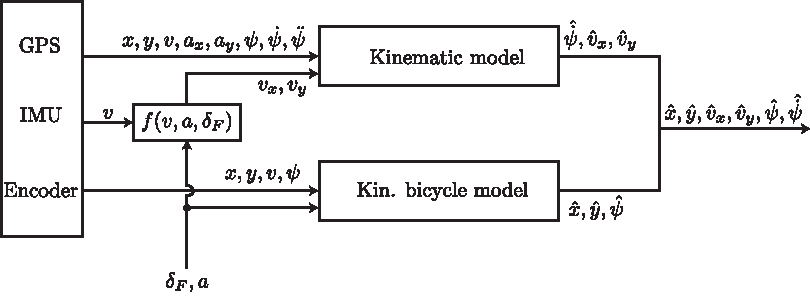
\includegraphics{../../Figures/Illustrator/FilterModel.pdf}
    \caption{Filter model}
    \label{fig:filter_model}
\end{figure}
The kinematic model combines measurements of acceleration, velocity, and position by integrating (see sec. \ref{sec:filterModel}).

This filtering approach is based on the assumption that only the kinematic bicycle model is able to estimate the current heading angle $\hat\psi$ using measurements of coordinates and velocity, while the point mass model would not be able to account for the drift in the $\psi$ measurement. This is why the kinematic bicycle model is used to calculate the heading angle as well as the inertial coordinates. On the other hand, the kinematic model is well suited to combine measurements of accelerations, velocities, and position. This is why we use this model for the estimation of the yaw rate and velocities.

\subsection{Extended Kalman Filter}
Kalman filters provide a general tool to calculate a state estimate using noisy and/or biased sensor measurements assuming a gaussian model for the noise. The standard Kalman filter uses a linear model of the system in order to calculate the most probable state from a set of different state measurements.\\
Following general procedure has been taken from \cite{Bar-Shalom}.
The Extended Kalman filter is based on the same principles as the standard Kalman filter but it allows to use a nonlinear model by linearizing the model at each time step.\\
The state estimation always consists of two steps: The \emph{Prediction step} and the \emph{Update step}. The first step calculates a prediction of the next state $\hat{\bm{x}}_{k|k-1}$ based on the previous state estimate $\hat{\bm{x}}_{k-1|k-1}$ and the control input $\bm{u}_{k-1}$. The update step corrects this prediction with the new measurement $\bm{z}_k$. The final state estimate is calculated using the Kalman gain $\bm{K}_k$. Both the model and measurement equations are linearized in each step.\\
Prediction:
\begin{subequations}
\begin{align}
\hat{\bm{x}}_{k|k-1} &= f(\hat{\bm{x}}_{k-1|k-1},\bm{u}_{k-1})\\
\bm{P}_{k|k-1} &= \bm{F}_{k-1} \bm{P}_{k-1|k-1} \bm{F}_{k-1}^T + \bm{Q}_{k-1}
\end{align}
\end{subequations}
Update:
\begin{subequations}
\begin{align}
\tilde{\bm{y}}_k &= \bm{z}_k - h(\hat{\bm{x}}_{k|k-1})\\
\bm{S}_k &= \bm{H}_k \bm{P}_{k|k-1} \bm{H}_k^T + \bm{R}_k\\
\bm{K}_k &= \bm{P}_{k|k-1}\bm{H}_k^T \bm{S}_k^{-1}\\
\hat{\bm{x}}_{k|k} &= \hat{\bm{x}}_{k|k-1} + \bm{K}_k \tilde{\bm{y}}_k\\
\bm{P}_{k|k} &= (\bm{I}-\bm{K}_k \bm{H}_k)\bm{P}_{k|k-1}
\end{align}
\end{subequations}

The predicted and updated estimate covariance $\bm{P}_{k|k-1}$ and $\bm{P}_{k|k}$, respectively, is a measure for the uncertainty of the state estimate. The process noise matrix $\bm{Q}$ is a measure for the uncertainty of the model, it is usually determined in experiments. The measurement noise matrix $\bm{R}$ depends on noise values of the sensors. They are often provided in sensor data sheets or can otherwise be measured in experiments. The state transition and observation matrices $\bm{F}_k$ and $\bm{H}_k$ are the functions $f(\bm{x},\bm{u})$ and $h(\bm{x})$, linearized at the current state estimate $\hat{\bm{x}}_{(\cdot)}$ and input $\bm{u}_k$:
\begin{subequations}
\begin{align}
\bm{F}_k &= \left. \frac{\partial f}{\partial \bm{x}} \right|_{\hat{\bm{x}}_{k|k},\bm{u}_k}\\
\bm{H}_k &= \left. \frac{\partial h}{\partial \bm{x}} \right|_{\hat{\bm{x}}_{k|k-1}}
\end{align}
\end{subequations}
\subsection{Filter model}\label{sec:filterModel}
\paragraph{Kinematic bicycle model} The first filter features a kinematic bicycle model, Eq. \eqref{eq:kinKalman} shows its model equations:
\begin{align}
\begin{split}\label{eq:kinKalman}
    \dot x &= v \cdot \cos (\psi + \beta)\\
    \dot y &= v \cdot \sin (\psi + \beta)\\
    \dot \psi &= \frac{v}{L_R}\cdot\sin(\beta)\\
    \dot v &= a - c_M\cdot v\\
    \dot d_\psi &= 0
\end{split}
\end{align}
with heading drift $d_\psi$.
There are two physical parameters, the first one is the distance $L_R$ between the rear axle and the GPS sensor which is measured as $L_R=\SI{0.125}{\meter}$. The second is the motor drag $c_M$ which was estimated in section \ref{sec:inputMapping} as $c_M=0.5$.\\
The measurement vector contains GPS, Encoder and heading measurements:
\begin{equation}
\bm{z} = \begin{pmatrix}
x_m&y_m&\psi_m&v_m
\end{pmatrix}^T,
\end{equation}
where the subscript $m$ denotes measured values. This leads to following measurement model:
\begin{equation}
h(\hat{\bm{x}}_{k|k-1}) = \begin{pmatrix}
1 & 0 & 0 & 0 & 0\\
0 & 1 & 0 & 0 & 0\\
0 & 0 & 1 & 0 & 1\\
0 & 0 & 0 & 1 & 0
\end{pmatrix} \hat{\bm{x}}_{k|k-1}=
\begin{pmatrix}
\hat x\\
\hat y\\
\hat \psi + \hat d_\psi\\
\hat v
\end{pmatrix}
\end{equation} 
\paragraph{Kinematic model} The second filter features a pure kinematic motion model from \cite{Caron2006} which integrates accelerations to find velocities and positions.
%{\bfseries{Why do you use position from the other model and not from this one, as shown in Figure 4.6. --> mb: I ran experiments comparing the x-y-estimates from both estimators and the kin-model estimates proved to be better ("better" meaning closer to the raw GPS data.)}}.
Eq. \eqref{eq:dynKalman} shows its model equations:
\begin{align}
\begin{split}\label{eq:dynKalman}
    \dot x &= \cos(\psi) v_x - \sin(\psi) v_y\\
    \dot y &= \sin(\psi) v_x + \cos(\psi) v_y\\
    \dot v_x &= a_x + \dot \psi v_y\\
    \dot v_y &= a_y - \dot \psi v_x\\
    \dot \psi &= \dot \psi\\
    \ddot \psi  &= 0\\
    \dot a_x &= 0\\
    \dot a_y &= 0\\
    \dot d_\psi &= 0
\end{split}
\end{align}
It uses the longitudinal and angular acceleration measurements of the IMU and position measurements of the GPS. Since the car's suspension leads to strong tilting motions in curves, the measurements of $a_y$ are distorted significantly. In order to support a correct estimation of $v_y$ and to reduce the effect of drift errors in $a_y$, the system additionally receives artificial measurements of $v_x$ and $v_y$. These are constructed by following relations:
\begin{align*}
v_{x,m} &= v_m\cos(\delta_F)\\
v_{y,m} &= v_m\sin(\delta_F)
\end{align*}
where $v_m$ is the encoder measurement and $\delta_F$ the control input.
Thus, the measurement vector of the second filter uses following measurements:
\begin{equation}
\bm{z}=\begin{pmatrix}x_m&y_m&v_{x,m}&v_{y,m}&\psi_m&\dot\psi_m&a_{x,m}&a_{y,m}\end{pmatrix}^T
\end{equation}
The measurement function $h(\hat{\bm{x}})$ is derived as follows:
\begin{equation}
h(\hat{\bm{x}}_{k|k-1})=\begin{pmatrix}\hat x&\hat y&\hat v_x&\hat v_y&\hat \psi+\hat d_\psi&\hat{\dot\psi}&\hat a_x&\hat a_y\end{pmatrix}^T
\end{equation}
%\begin{equation}
%\bm{z}=\begin{pmatrix}x_m\\y_m\\v_{x,m}\\v_{y,m}\\\psi_m\\\dot\psi_m\\\ddot\psi_m\\a_{x,m}\\a_{y,m}\end{pmatrix}, h(\hat{\bm{x}}_{k|k-1}) = \begin{pmatrix}
%1 & 0 & 0 & 0 & 0 & 0 & 0 & 0 & 0\\
%1 & 1 & 0 & 0 & 0 & 0 & 0 & 0 & 0\\
%1 & 0 & 1 & 0 & 0 & 0 & 0 & 0 & 0\\
%1 & 0 & 0 & 1 & 0 & 0 & 0 & 0 & 1\\
%1 & 0 & 0 & 0 & 1 & 0 & 0 & 0 & 0\\
%1 & 0 & 0 & 0 & 0 & 1 & 0 & 0 & 0\\
%1 & 0 & 0 & 0 & 0 & 0 & 1 & 0 & 0\\
%1 & 0 & 0 & 0 & 0 & 0 & 0 & 1 & 0
%\end{pmatrix} \hat{\bm{x}}_{k|k-1}=
%\begin{pmatrix}
%\hat x\\
%\hat y\\
%\hat \psi + \hat d_\psi\\
%\hat v
%\end{pmatrix}
%\end{equation}
%\begin{align}
%abc
%\end{align}
% Tuning of Q and R matrices
\paragraph{Tuning of Q and R matrices}
The measurement noise matrices were constructed assuming diagonal matrices (independent sensors) and measuring the sensor noises during operation.\\
The process noise matrix $\bm{Q}$ was tuned manually in post-processing. The values were tuned with the objective to provide a smooth fit to the raw measurements.
\paragraph{Frequency of the filter}
The extended Kalman filter runs at a frequency of 50 Hertz and assumes that all measurements are received at the same time and with equal frequencies. However, since we are using different sensors at different frequencies, we are using following strategy for each sensor:
\begin{description}
\item[IMU] The IMU provides data at the frequency of the Kalman filter itself, $\SI{50}{\hertz}$. This is why we can use this data directly.
\item[GPS] The indoor GPS provides measurements at varying frequencies between 10 and 16 Hertz, whereas there are times when no measurement are received for up to one second. These interruptions might result from hardware issues (e.g. interfering reflections of ultrasound, timing issues) and could not be resolved. In order to account for this uncertainty, we always extrapolate the previously received data by  polynomials to the timestamp of the Kalman filter update. This extrapolation makes sure that even longer measurement breaks don't pose any difficulties to the estimator.
\item[Encoder] Three of the car's wheels are equipped with encoders, using 2 magnets each. The frequency of signals from these encoders can be calculated as follows:
\begin{equation}
f =\frac{1}{T}=\frac{v}{\pi r}
\end{equation}
with the velocity $v$ and the wheel radius $r$. This means that at a velocity of $\SI{1.0}{\meter\per\second}$ and for a wheel radius of $\SI{3.6}{\centi\meter}$, we receive a velocity measurement from each wheel at a rate of about $\SI{9}{\hertz}$. These measurements are not synchronized as the wheels start at different angles. All measurements are received by the Arduino, averaged, and then sent to the filter at a constant rate of $\SI{50}{\hertz}$. Since even with three encoders we can't reach an update rate of $\SI{50}{\hertz}$, we assume a rather high encoder measurement noise in the measurement noise matrix $\bm{R}$ to account for equal consecutive measurements.
\end{description}
\subsection{Mapping to the track reference frame}
The estimator discussed above returns a state estimate in the inertial frame which then needs to be transformed into the track reference frame. The coordinates in the track reference frame are the curvilinear abscissa $s$, the lateral position error $e_Y$, and the heading error $e_\psi$. The procedure for this transformation is described below.\\
We assume that the track is given by $n$ equidistant vertices with coordinates $\bm{x}_i = \begin{pmatrix}
x_i&y_i
\end{pmatrix},i=1...n$.

\begin{enumerate}
\item Find the closest vertex $\bm{x}_i$ of the track to the current position of the car.
\item Select a set of vertices around vertex $i$.
\item Use this set to approximate the track locally using a polynomial, returning functions for the coordinates $(x,y)=f(s)$ and curvature $c=g(s)$.
\item Use these functions to calculate the current curvilinear abscissa $s$, lateral position $e_Y$ and heading error $e_\psi$.
\end{enumerate}
The number of points used for the approximation and the polynomial degree have to be chosen in such a way to provide an accurate fit throughout the entire prediction horizon.\\
In practice, we used a polynomial of 8\textsuperscript{th} degree. This polynomial proved to approximate the piecewise linear curvature well enough while keeping the complexity of the optimization problem at a reasonable level.
%The procedure is shown in fig. \ref{fig:s_ey_poly}.
%\begin{figure}[ht]
%    \centering
%      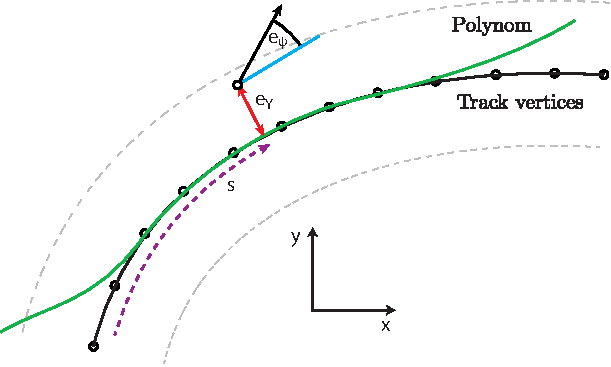
\includegraphics{../../Figures/Mapping/s_ey.pdf}
%    \caption{$s-e_Y-$frame}
%    \label{fig:s_ey_poly}
%\end{figure}

\section{System Identification}\label{sec:sysID}
In order to provide an accurate model to the MPC, the system's dynamics are identified at each time step. The dynamic bicycle model from Eq. \eqref{eq:dynModel} is used to derive a Linear Regression model that uses functions of the system's states as features. State estimates from previous laps are then used to calculate current parameters $\theta_{i,j}$.

Linear Regression model of the dynamic bicycle model:
\begin{subequations}\label{eq:systemID}
\begin{align}
    v_{x,k+1} - v_{x,k}&= \theta_{x,1} \cdot v_{y,k}\dot\psi_k + \theta_{x,2}\cdot v_{x,k}  + \theta_{x,3}\cdot a_k\label{eq:systemID1}\\
    v_{y,k+1}- v_{y,k} &= \theta_{y,1}\cdot  \frac{v_{y,k}}{v_{x,k}}+\theta_{y,2}\cdot v_{x,k}\dot\psi_k + \theta_{y,3}\cdot \frac{\dot\psi_k}{v_{x,k}}+\theta_{y,4}\cdot \delta_k\\
    \dot\psi_{k+1}-\dot\psi_k &= \theta_{\psi,1}\cdot \frac{\dot\psi_k}{v_{x,k}}+\theta_{\psi,2}\cdot \frac{v_{y,k}}{v_{x,k}}+\theta_{\psi,3}\cdot \delta_k
\end{align}
\end{subequations}
with states $v_x$, $v_y$, $\dot \psi$ and parameters $\theta_{i,j}$. Note that we added a term in \eqref{eq:systemID1} to account for motor drag and to match it with Eq. \eqref{eq:longDyn}. The features $\bm{X}$ of this Linear Regression problem are nonlinear functions of the states and inputs. Using multiple samples $n$, each equation can be rewritten as
\begin{equation}
\bm{y}=\bm{X\theta}.
\end{equation}
Equation \eqref{eq:LRvx} shows the equations for the LR of $v_x$:
\begin{align}
\label{eq:LRvx}
\bm{y} = \begin{pmatrix}
v_{x,2} - v_{x,1}\\
v_{x,3} - v_{x,2}\\
\vdots\\
v_{x,n} - v_{x,n-1}
\end{pmatrix} &&
\bm{X} = \begin{pmatrix}
v_{y,1}\dot\psi_1 & v_{x,1} & a_{1}\\
v_{y,2}\dot\psi_2 & v_{x,2} & a_{2}\\
\vdots&\vdots&\vdots\\
v_{y,n-1}\dot\psi_{n-1} & v_{x,n-1} & a_{n-1}
\end{pmatrix}&&
\bm{\theta}=\begin{pmatrix}
\theta_{x,1}\\
\theta_{x,2}\\
\theta_{x,3}
\end{pmatrix}
\end{align}
The LR equations for $v_y$ and $\dot\psi$ can be written accordingly.\\
To determine the optimal coefficients $\bm{\theta}^*$, following minimization has to be solved:
\begin{equation}
\bm{\theta}^* = \argmin_{\bm{\theta}} \| \bm{X\theta}-\bm{y} \|_2
\end{equation}
There are different approaches to solve this problem, we use the \emph{normal equation} method. This leads to following analytic solution:
\begin{equation}
\bm{\theta}^* = (\bm{X}^T \bm{X})^{-1}\bm{X}^T \bm{y}
\end{equation}
Since we are using about $n=100...1000$ samples, the calculation of the inverse of $\bm{X}^T \bm{X}$ is still sufficiently fast. However, if we were to use even more samples, other methods such as \emph{gradient descent} might work faster.

\section{Implementation}\label{sec:implementation}
The estimator and MPC solver are implemented in the ROS framework (Robot Operating System, \cite{ros}). The sensor data is sent from the BARC to a more powerful CPU (Macbook Pro 2010, 2.4 GHz) which solves the MPC problem at a rate of 10 Hertz and sends the optimal input to the BARC. The setup is illustrated in Fig. \ref{fig:architecture}.
\begin{figure}[ht]
    \centering
      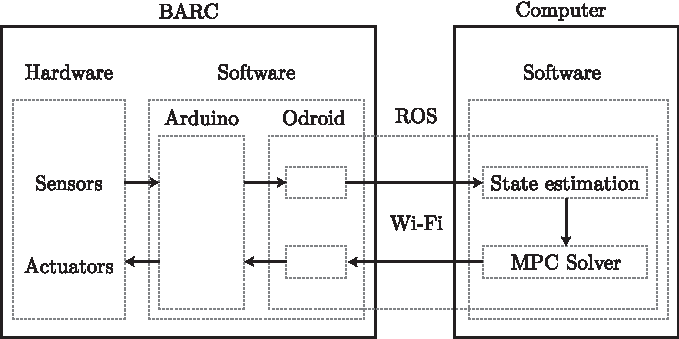
\includegraphics{../../Figures/Illustrator/Architecture.pdf}
    \caption{Software/Hardware setup}
    \label{fig:architecture}
\end{figure}
The ROS framework manages the execution of all scripts and makes sure that they are running at their specified frequencies. It also manages the wireless communication between the Odroid and the computer.\\
The estimator is a python script that runs at a constant frequency of $\SI{50}{\hertz}$.\\
% which is the highest frequency at which measurements are received by the IMU. Both the encoders and the GPS are running at lower or variable frequencies between 10 and $\SI{50}{\hertz}$.\\
The MPC optimization problem is solved by Ipopt \cite{ipopt} which is executed by a script written in Julia 0.4.6 \cite{julia}. It solves the LMPC problem at a constant frequency of $\SI{10}{\hertz}$ and sends the optimal control input to the BARC. At the same time, it receives and saves all state estimates from the estimator.\\
Since we need to maintain a constant input rate of $\SI{10}{\hertz}$ while the optimization process can last different times (at most $\SI{0.1}{\second}$), the commands are always sent at the beginning of one time step. The MPC solver uses an initial state that is predicted by 0.1 seconds from the most recent estimated state. Figure \ref{fig:timing} shows the timing diagram of ROS nodes and messages.
\begin{figure}[ht]
    \centering
\begin{wave}{4}{2}
\nextwave{Estimator} \known{}{0.05}\unknown[]{0.15}
                \known{}{0.07}\unknown[]{0.13}
                \known{}{0.04}\unknown[]{0.16}
                \known{}{0.06}\unknown[]{0.14}
                \known{}{0.08}\unknown[]{0.12}
                \known{}{0.09}\unknown[]{0.11}
                \known{}{0.06}\unknown[]{0.14}
                \known{}{0.05}\unknown[]{0.15}
                \known{}{0.09}\unknown[]{0.11}
                \known{}{0.04}\unknown[]{0.16}
                \known{}{0.03}\unknown[]{0.17}
                \known{}{0.07}\unknown[]{0.13}
                \known{}{0.08}\unknown[]{0.12}
                \known{}{0.06}\unknown[]{0.14}
                \known{}{0.07}\unknown[]{0.13}
\nextwave{MPC} \known{MPC}{0.7}\unknown[]{0.3}\known{MPC}{0.5}\unknown[]{0.5}\known{MPC}{0.8}\unknown[]{0.2}
\nextwave{Command} \known{}{0.05}\unknown[]{0.95}
                \known{}{0.05}\unknown[]{0.95}
                \known{}{0.05}\unknown[]{0.95}

\end{wave}
\caption{Timing diagram}
    \label{fig:timing}
\end{figure}

Below all steps are described that are performed during one time step (asynchronously). Additionally, Figure \ref{fig:controlStructure} illustrates the closed-loop system.
\begin{enumerate}
\item State estimation
\begin{enumerate}
\item Read sensor data
\item Calculate the current state in the inertial frame
\item Transform the state to the track frame
\item Calculate polynomial coefficients that approximate the curvature locally
\end{enumerate}
\item System Identification
\begin{enumerate}
\item Select data from previous and current lap
\item Calculate Matrices of features
\item Calculate parameters of system dynamics using Linear Regression
\end{enumerate}
\item Approximate safe set and cost function
\begin{enumerate}
\item Select locally near data from previous laps
\item Calculate polynomials that approximate this data to construct the safe set
\end{enumerate}
\item Solve the LMPC problem
\begin{enumerate}
\item Use the state estimate as initial state for the MPC formulation
\item Minimize the cost function, using state dynamics from the Linear Regression and curvature as well as the safe set and terminal cost function
\item Send the optimal input to the actuators
\end{enumerate}
\end{enumerate}

\begin{figure}[ht]
    \centering
  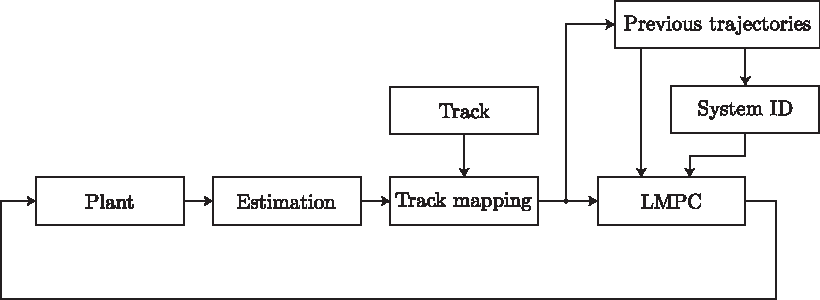
\includegraphics{../../Figures/Illustrator/ControlDiagram.pdf}
    \caption{Control structure}
    \label{fig:controlStructure}
\end{figure}

\section{Experiments}
%{\bfseries{Made a new Chapter for experimental results}} 
The experiments were performed in a closed space at UC Berkeley. The available area had a size of about 5 by 8 meters and provided enough space for a simple race track.\\
We chose a race track that fits the available area while still providing curves in different directions with the maximum possible curvature of $\SI{1.24}{\per\meter}$. The curvature is shown in Fig. \ref{fig:exp_curv}. The track length is $\SI{19}{\meter}$.
We used a constant sample size for the system identification of 120 points per lap which corresponds to $\SI{2.4}{\second}$ since the state estimation runs at $\SI{50}{\hertz}$. We also used an LMPC horizon length of $N=12$ which corresponds to a prediction time of $\SI{1.2}{\second}$. This horizon is a trade-off between fast learning and fast solver times.
\begin{figure}[ht]
    \centering
      %% Creator: Matplotlib, PGF backend
%%
%% To include the figure in your LaTeX document, write
%%   \input{<filename>.pgf}
%%
%% Make sure the required packages are loaded in your preamble
%%   \usepackage{pgf}
%%
%% Figures using additional raster images can only be included by \input if
%% they are in the same directory as the main LaTeX file. For loading figures
%% from other directories you can use the `import` package
%%   \usepackage{import}
%% and then include the figures with
%%   \import{<path to file>}{<filename>.pgf}
%%
%% Matplotlib used the following preamble
%%   \usepackage{fontspec}
%%
\begingroup%
\makeatletter%
\begin{pgfpicture}%
\pgfpathrectangle{\pgfpointorigin}{\pgfqpoint{4.500000in}{3.000000in}}%
\pgfusepath{use as bounding box, clip}%
\begin{pgfscope}%
\pgfsetbuttcap%
\pgfsetmiterjoin%
\definecolor{currentfill}{rgb}{1.000000,1.000000,1.000000}%
\pgfsetfillcolor{currentfill}%
\pgfsetlinewidth{0.000000pt}%
\definecolor{currentstroke}{rgb}{1.000000,1.000000,1.000000}%
\pgfsetstrokecolor{currentstroke}%
\pgfsetdash{}{0pt}%
\pgfpathmoveto{\pgfqpoint{0.000000in}{0.000000in}}%
\pgfpathlineto{\pgfqpoint{4.500000in}{0.000000in}}%
\pgfpathlineto{\pgfqpoint{4.500000in}{3.000000in}}%
\pgfpathlineto{\pgfqpoint{0.000000in}{3.000000in}}%
\pgfpathclose%
\pgfusepath{fill}%
\end{pgfscope}%
\begin{pgfscope}%
\pgfsetbuttcap%
\pgfsetmiterjoin%
\definecolor{currentfill}{rgb}{1.000000,1.000000,1.000000}%
\pgfsetfillcolor{currentfill}%
\pgfsetlinewidth{0.000000pt}%
\definecolor{currentstroke}{rgb}{0.000000,0.000000,0.000000}%
\pgfsetstrokecolor{currentstroke}%
\pgfsetstrokeopacity{0.000000}%
\pgfsetdash{}{0pt}%
\pgfpathmoveto{\pgfqpoint{0.628958in}{0.471921in}}%
\pgfpathlineto{\pgfqpoint{4.291316in}{0.471921in}}%
\pgfpathlineto{\pgfqpoint{4.291316in}{2.805251in}}%
\pgfpathlineto{\pgfqpoint{0.628958in}{2.805251in}}%
\pgfpathclose%
\pgfusepath{fill}%
\end{pgfscope}%
\begin{pgfscope}%
\pgfpathrectangle{\pgfqpoint{0.628958in}{0.471921in}}{\pgfqpoint{3.662359in}{2.333330in}} %
\pgfusepath{clip}%
\pgfsetrectcap%
\pgfsetroundjoin%
\pgfsetlinewidth{0.501875pt}%
\definecolor{currentstroke}{rgb}{0.000000,0.000000,1.000000}%
\pgfsetstrokecolor{currentstroke}%
\pgfsetdash{}{0pt}%
\pgfpathmoveto{\pgfqpoint{0.630789in}{1.871919in}}%
\pgfpathlineto{\pgfqpoint{0.960401in}{1.871919in}}%
\pgfpathlineto{\pgfqpoint{1.169156in}{0.650190in}}%
\pgfpathlineto{\pgfqpoint{1.180143in}{0.650190in}}%
\pgfpathlineto{\pgfqpoint{1.388897in}{1.871919in}}%
\pgfpathlineto{\pgfqpoint{1.509755in}{1.871919in}}%
\pgfpathlineto{\pgfqpoint{1.718509in}{0.650190in}}%
\pgfpathlineto{\pgfqpoint{1.729496in}{0.650190in}}%
\pgfpathlineto{\pgfqpoint{1.938251in}{1.871919in}}%
\pgfpathlineto{\pgfqpoint{1.949238in}{1.871919in}}%
\pgfpathlineto{\pgfqpoint{2.048122in}{2.360611in}}%
\pgfpathlineto{\pgfqpoint{2.059109in}{2.360611in}}%
\pgfpathlineto{\pgfqpoint{2.157992in}{1.871919in}}%
\pgfpathlineto{\pgfqpoint{2.168980in}{1.871919in}}%
\pgfpathlineto{\pgfqpoint{2.322799in}{1.220330in}}%
\pgfpathlineto{\pgfqpoint{2.333786in}{1.220330in}}%
\pgfpathlineto{\pgfqpoint{2.487605in}{1.871919in}}%
\pgfpathlineto{\pgfqpoint{2.498592in}{1.871919in}}%
\pgfpathlineto{\pgfqpoint{2.597476in}{2.360611in}}%
\pgfpathlineto{\pgfqpoint{2.608463in}{2.360611in}}%
\pgfpathlineto{\pgfqpoint{2.707346in}{1.871919in}}%
\pgfpathlineto{\pgfqpoint{2.718333in}{1.871919in}}%
\pgfpathlineto{\pgfqpoint{2.927088in}{0.650190in}}%
\pgfpathlineto{\pgfqpoint{2.938075in}{0.650190in}}%
\pgfpathlineto{\pgfqpoint{3.146829in}{1.871919in}}%
\pgfpathlineto{\pgfqpoint{3.267687in}{1.871919in}}%
\pgfpathlineto{\pgfqpoint{3.476442in}{0.650190in}}%
\pgfpathlineto{\pgfqpoint{3.487429in}{0.650190in}}%
\pgfpathlineto{\pgfqpoint{3.696183in}{1.871919in}}%
\pgfpathlineto{\pgfqpoint{4.080731in}{1.871919in}}%
\pgfpathlineto{\pgfqpoint{4.080731in}{1.871919in}}%
\pgfusepath{stroke}%
\end{pgfscope}%
\begin{pgfscope}%
\pgfsetrectcap%
\pgfsetmiterjoin%
\pgfsetlinewidth{0.501875pt}%
\definecolor{currentstroke}{rgb}{0.000000,0.000000,0.000000}%
\pgfsetstrokecolor{currentstroke}%
\pgfsetdash{}{0pt}%
\pgfpathmoveto{\pgfqpoint{0.628958in}{2.805251in}}%
\pgfpathlineto{\pgfqpoint{4.291316in}{2.805251in}}%
\pgfusepath{stroke}%
\end{pgfscope}%
\begin{pgfscope}%
\pgfsetrectcap%
\pgfsetmiterjoin%
\pgfsetlinewidth{0.501875pt}%
\definecolor{currentstroke}{rgb}{0.000000,0.000000,0.000000}%
\pgfsetstrokecolor{currentstroke}%
\pgfsetdash{}{0pt}%
\pgfpathmoveto{\pgfqpoint{4.291316in}{0.471921in}}%
\pgfpathlineto{\pgfqpoint{4.291316in}{2.805251in}}%
\pgfusepath{stroke}%
\end{pgfscope}%
\begin{pgfscope}%
\pgfsetrectcap%
\pgfsetmiterjoin%
\pgfsetlinewidth{0.501875pt}%
\definecolor{currentstroke}{rgb}{0.000000,0.000000,0.000000}%
\pgfsetstrokecolor{currentstroke}%
\pgfsetdash{}{0pt}%
\pgfpathmoveto{\pgfqpoint{0.628958in}{0.471921in}}%
\pgfpathlineto{\pgfqpoint{4.291316in}{0.471921in}}%
\pgfusepath{stroke}%
\end{pgfscope}%
\begin{pgfscope}%
\pgfsetrectcap%
\pgfsetmiterjoin%
\pgfsetlinewidth{0.501875pt}%
\definecolor{currentstroke}{rgb}{0.000000,0.000000,0.000000}%
\pgfsetstrokecolor{currentstroke}%
\pgfsetdash{}{0pt}%
\pgfpathmoveto{\pgfqpoint{0.628958in}{0.471921in}}%
\pgfpathlineto{\pgfqpoint{0.628958in}{2.805251in}}%
\pgfusepath{stroke}%
\end{pgfscope}%
\begin{pgfscope}%
\pgfpathrectangle{\pgfqpoint{0.628958in}{0.471921in}}{\pgfqpoint{3.662359in}{2.333330in}} %
\pgfusepath{clip}%
\pgfsetbuttcap%
\pgfsetroundjoin%
\pgfsetlinewidth{0.501875pt}%
\definecolor{currentstroke}{rgb}{0.000000,0.000000,0.000000}%
\pgfsetstrokecolor{currentstroke}%
\pgfsetdash{{1.000000pt}{3.000000pt}}{0.000000pt}%
\pgfpathmoveto{\pgfqpoint{0.628958in}{0.471921in}}%
\pgfpathlineto{\pgfqpoint{0.628958in}{2.805251in}}%
\pgfusepath{stroke}%
\end{pgfscope}%
\begin{pgfscope}%
\pgfsetbuttcap%
\pgfsetroundjoin%
\definecolor{currentfill}{rgb}{0.000000,0.000000,0.000000}%
\pgfsetfillcolor{currentfill}%
\pgfsetlinewidth{0.250937pt}%
\definecolor{currentstroke}{rgb}{0.000000,0.000000,0.000000}%
\pgfsetstrokecolor{currentstroke}%
\pgfsetdash{}{0pt}%
\pgfsys@defobject{currentmarker}{\pgfqpoint{0.000000in}{0.000000in}}{\pgfqpoint{0.000000in}{0.055556in}}{%
\pgfpathmoveto{\pgfqpoint{0.000000in}{0.000000in}}%
\pgfpathlineto{\pgfqpoint{0.000000in}{0.055556in}}%
\pgfusepath{stroke,fill}%
}%
\begin{pgfscope}%
\pgfsys@transformshift{0.628958in}{0.471921in}%
\pgfsys@useobject{currentmarker}{}%
\end{pgfscope}%
\end{pgfscope}%
\begin{pgfscope}%
\pgfsetbuttcap%
\pgfsetroundjoin%
\definecolor{currentfill}{rgb}{0.000000,0.000000,0.000000}%
\pgfsetfillcolor{currentfill}%
\pgfsetlinewidth{0.250937pt}%
\definecolor{currentstroke}{rgb}{0.000000,0.000000,0.000000}%
\pgfsetstrokecolor{currentstroke}%
\pgfsetdash{}{0pt}%
\pgfsys@defobject{currentmarker}{\pgfqpoint{0.000000in}{-0.055556in}}{\pgfqpoint{0.000000in}{0.000000in}}{%
\pgfpathmoveto{\pgfqpoint{0.000000in}{0.000000in}}%
\pgfpathlineto{\pgfqpoint{0.000000in}{-0.055556in}}%
\pgfusepath{stroke,fill}%
}%
\begin{pgfscope}%
\pgfsys@transformshift{0.628958in}{2.805251in}%
\pgfsys@useobject{currentmarker}{}%
\end{pgfscope}%
\end{pgfscope}%
\begin{pgfscope}%
\pgftext[x=0.628958in,y=0.416365in,,top]{\rmfamily\fontsize{6.940000}{8.328000}\selectfont \(\displaystyle 0\)}%
\end{pgfscope}%
\begin{pgfscope}%
\pgfpathrectangle{\pgfqpoint{0.628958in}{0.471921in}}{\pgfqpoint{3.662359in}{2.333330in}} %
\pgfusepath{clip}%
\pgfsetbuttcap%
\pgfsetroundjoin%
\pgfsetlinewidth{0.501875pt}%
\definecolor{currentstroke}{rgb}{0.000000,0.000000,0.000000}%
\pgfsetstrokecolor{currentstroke}%
\pgfsetdash{{1.000000pt}{3.000000pt}}{0.000000pt}%
\pgfpathmoveto{\pgfqpoint{1.544547in}{0.471921in}}%
\pgfpathlineto{\pgfqpoint{1.544547in}{2.805251in}}%
\pgfusepath{stroke}%
\end{pgfscope}%
\begin{pgfscope}%
\pgfsetbuttcap%
\pgfsetroundjoin%
\definecolor{currentfill}{rgb}{0.000000,0.000000,0.000000}%
\pgfsetfillcolor{currentfill}%
\pgfsetlinewidth{0.250937pt}%
\definecolor{currentstroke}{rgb}{0.000000,0.000000,0.000000}%
\pgfsetstrokecolor{currentstroke}%
\pgfsetdash{}{0pt}%
\pgfsys@defobject{currentmarker}{\pgfqpoint{0.000000in}{0.000000in}}{\pgfqpoint{0.000000in}{0.055556in}}{%
\pgfpathmoveto{\pgfqpoint{0.000000in}{0.000000in}}%
\pgfpathlineto{\pgfqpoint{0.000000in}{0.055556in}}%
\pgfusepath{stroke,fill}%
}%
\begin{pgfscope}%
\pgfsys@transformshift{1.544547in}{0.471921in}%
\pgfsys@useobject{currentmarker}{}%
\end{pgfscope}%
\end{pgfscope}%
\begin{pgfscope}%
\pgfsetbuttcap%
\pgfsetroundjoin%
\definecolor{currentfill}{rgb}{0.000000,0.000000,0.000000}%
\pgfsetfillcolor{currentfill}%
\pgfsetlinewidth{0.250937pt}%
\definecolor{currentstroke}{rgb}{0.000000,0.000000,0.000000}%
\pgfsetstrokecolor{currentstroke}%
\pgfsetdash{}{0pt}%
\pgfsys@defobject{currentmarker}{\pgfqpoint{0.000000in}{-0.055556in}}{\pgfqpoint{0.000000in}{0.000000in}}{%
\pgfpathmoveto{\pgfqpoint{0.000000in}{0.000000in}}%
\pgfpathlineto{\pgfqpoint{0.000000in}{-0.055556in}}%
\pgfusepath{stroke,fill}%
}%
\begin{pgfscope}%
\pgfsys@transformshift{1.544547in}{2.805251in}%
\pgfsys@useobject{currentmarker}{}%
\end{pgfscope}%
\end{pgfscope}%
\begin{pgfscope}%
\pgftext[x=1.544547in,y=0.416365in,,top]{\rmfamily\fontsize{6.940000}{8.328000}\selectfont \(\displaystyle 5\)}%
\end{pgfscope}%
\begin{pgfscope}%
\pgfpathrectangle{\pgfqpoint{0.628958in}{0.471921in}}{\pgfqpoint{3.662359in}{2.333330in}} %
\pgfusepath{clip}%
\pgfsetbuttcap%
\pgfsetroundjoin%
\pgfsetlinewidth{0.501875pt}%
\definecolor{currentstroke}{rgb}{0.000000,0.000000,0.000000}%
\pgfsetstrokecolor{currentstroke}%
\pgfsetdash{{1.000000pt}{3.000000pt}}{0.000000pt}%
\pgfpathmoveto{\pgfqpoint{2.460137in}{0.471921in}}%
\pgfpathlineto{\pgfqpoint{2.460137in}{2.805251in}}%
\pgfusepath{stroke}%
\end{pgfscope}%
\begin{pgfscope}%
\pgfsetbuttcap%
\pgfsetroundjoin%
\definecolor{currentfill}{rgb}{0.000000,0.000000,0.000000}%
\pgfsetfillcolor{currentfill}%
\pgfsetlinewidth{0.250937pt}%
\definecolor{currentstroke}{rgb}{0.000000,0.000000,0.000000}%
\pgfsetstrokecolor{currentstroke}%
\pgfsetdash{}{0pt}%
\pgfsys@defobject{currentmarker}{\pgfqpoint{0.000000in}{0.000000in}}{\pgfqpoint{0.000000in}{0.055556in}}{%
\pgfpathmoveto{\pgfqpoint{0.000000in}{0.000000in}}%
\pgfpathlineto{\pgfqpoint{0.000000in}{0.055556in}}%
\pgfusepath{stroke,fill}%
}%
\begin{pgfscope}%
\pgfsys@transformshift{2.460137in}{0.471921in}%
\pgfsys@useobject{currentmarker}{}%
\end{pgfscope}%
\end{pgfscope}%
\begin{pgfscope}%
\pgfsetbuttcap%
\pgfsetroundjoin%
\definecolor{currentfill}{rgb}{0.000000,0.000000,0.000000}%
\pgfsetfillcolor{currentfill}%
\pgfsetlinewidth{0.250937pt}%
\definecolor{currentstroke}{rgb}{0.000000,0.000000,0.000000}%
\pgfsetstrokecolor{currentstroke}%
\pgfsetdash{}{0pt}%
\pgfsys@defobject{currentmarker}{\pgfqpoint{0.000000in}{-0.055556in}}{\pgfqpoint{0.000000in}{0.000000in}}{%
\pgfpathmoveto{\pgfqpoint{0.000000in}{0.000000in}}%
\pgfpathlineto{\pgfqpoint{0.000000in}{-0.055556in}}%
\pgfusepath{stroke,fill}%
}%
\begin{pgfscope}%
\pgfsys@transformshift{2.460137in}{2.805251in}%
\pgfsys@useobject{currentmarker}{}%
\end{pgfscope}%
\end{pgfscope}%
\begin{pgfscope}%
\pgftext[x=2.460137in,y=0.416365in,,top]{\rmfamily\fontsize{6.940000}{8.328000}\selectfont \(\displaystyle 10\)}%
\end{pgfscope}%
\begin{pgfscope}%
\pgfpathrectangle{\pgfqpoint{0.628958in}{0.471921in}}{\pgfqpoint{3.662359in}{2.333330in}} %
\pgfusepath{clip}%
\pgfsetbuttcap%
\pgfsetroundjoin%
\pgfsetlinewidth{0.501875pt}%
\definecolor{currentstroke}{rgb}{0.000000,0.000000,0.000000}%
\pgfsetstrokecolor{currentstroke}%
\pgfsetdash{{1.000000pt}{3.000000pt}}{0.000000pt}%
\pgfpathmoveto{\pgfqpoint{3.375727in}{0.471921in}}%
\pgfpathlineto{\pgfqpoint{3.375727in}{2.805251in}}%
\pgfusepath{stroke}%
\end{pgfscope}%
\begin{pgfscope}%
\pgfsetbuttcap%
\pgfsetroundjoin%
\definecolor{currentfill}{rgb}{0.000000,0.000000,0.000000}%
\pgfsetfillcolor{currentfill}%
\pgfsetlinewidth{0.250937pt}%
\definecolor{currentstroke}{rgb}{0.000000,0.000000,0.000000}%
\pgfsetstrokecolor{currentstroke}%
\pgfsetdash{}{0pt}%
\pgfsys@defobject{currentmarker}{\pgfqpoint{0.000000in}{0.000000in}}{\pgfqpoint{0.000000in}{0.055556in}}{%
\pgfpathmoveto{\pgfqpoint{0.000000in}{0.000000in}}%
\pgfpathlineto{\pgfqpoint{0.000000in}{0.055556in}}%
\pgfusepath{stroke,fill}%
}%
\begin{pgfscope}%
\pgfsys@transformshift{3.375727in}{0.471921in}%
\pgfsys@useobject{currentmarker}{}%
\end{pgfscope}%
\end{pgfscope}%
\begin{pgfscope}%
\pgfsetbuttcap%
\pgfsetroundjoin%
\definecolor{currentfill}{rgb}{0.000000,0.000000,0.000000}%
\pgfsetfillcolor{currentfill}%
\pgfsetlinewidth{0.250937pt}%
\definecolor{currentstroke}{rgb}{0.000000,0.000000,0.000000}%
\pgfsetstrokecolor{currentstroke}%
\pgfsetdash{}{0pt}%
\pgfsys@defobject{currentmarker}{\pgfqpoint{0.000000in}{-0.055556in}}{\pgfqpoint{0.000000in}{0.000000in}}{%
\pgfpathmoveto{\pgfqpoint{0.000000in}{0.000000in}}%
\pgfpathlineto{\pgfqpoint{0.000000in}{-0.055556in}}%
\pgfusepath{stroke,fill}%
}%
\begin{pgfscope}%
\pgfsys@transformshift{3.375727in}{2.805251in}%
\pgfsys@useobject{currentmarker}{}%
\end{pgfscope}%
\end{pgfscope}%
\begin{pgfscope}%
\pgftext[x=3.375727in,y=0.416365in,,top]{\rmfamily\fontsize{6.940000}{8.328000}\selectfont \(\displaystyle 15\)}%
\end{pgfscope}%
\begin{pgfscope}%
\pgfpathrectangle{\pgfqpoint{0.628958in}{0.471921in}}{\pgfqpoint{3.662359in}{2.333330in}} %
\pgfusepath{clip}%
\pgfsetbuttcap%
\pgfsetroundjoin%
\pgfsetlinewidth{0.501875pt}%
\definecolor{currentstroke}{rgb}{0.000000,0.000000,0.000000}%
\pgfsetstrokecolor{currentstroke}%
\pgfsetdash{{1.000000pt}{3.000000pt}}{0.000000pt}%
\pgfpathmoveto{\pgfqpoint{4.291316in}{0.471921in}}%
\pgfpathlineto{\pgfqpoint{4.291316in}{2.805251in}}%
\pgfusepath{stroke}%
\end{pgfscope}%
\begin{pgfscope}%
\pgfsetbuttcap%
\pgfsetroundjoin%
\definecolor{currentfill}{rgb}{0.000000,0.000000,0.000000}%
\pgfsetfillcolor{currentfill}%
\pgfsetlinewidth{0.250937pt}%
\definecolor{currentstroke}{rgb}{0.000000,0.000000,0.000000}%
\pgfsetstrokecolor{currentstroke}%
\pgfsetdash{}{0pt}%
\pgfsys@defobject{currentmarker}{\pgfqpoint{0.000000in}{0.000000in}}{\pgfqpoint{0.000000in}{0.055556in}}{%
\pgfpathmoveto{\pgfqpoint{0.000000in}{0.000000in}}%
\pgfpathlineto{\pgfqpoint{0.000000in}{0.055556in}}%
\pgfusepath{stroke,fill}%
}%
\begin{pgfscope}%
\pgfsys@transformshift{4.291316in}{0.471921in}%
\pgfsys@useobject{currentmarker}{}%
\end{pgfscope}%
\end{pgfscope}%
\begin{pgfscope}%
\pgfsetbuttcap%
\pgfsetroundjoin%
\definecolor{currentfill}{rgb}{0.000000,0.000000,0.000000}%
\pgfsetfillcolor{currentfill}%
\pgfsetlinewidth{0.250937pt}%
\definecolor{currentstroke}{rgb}{0.000000,0.000000,0.000000}%
\pgfsetstrokecolor{currentstroke}%
\pgfsetdash{}{0pt}%
\pgfsys@defobject{currentmarker}{\pgfqpoint{0.000000in}{-0.055556in}}{\pgfqpoint{0.000000in}{0.000000in}}{%
\pgfpathmoveto{\pgfqpoint{0.000000in}{0.000000in}}%
\pgfpathlineto{\pgfqpoint{0.000000in}{-0.055556in}}%
\pgfusepath{stroke,fill}%
}%
\begin{pgfscope}%
\pgfsys@transformshift{4.291316in}{2.805251in}%
\pgfsys@useobject{currentmarker}{}%
\end{pgfscope}%
\end{pgfscope}%
\begin{pgfscope}%
\pgftext[x=4.291316in,y=0.416365in,,top]{\rmfamily\fontsize{6.940000}{8.328000}\selectfont \(\displaystyle 20\)}%
\end{pgfscope}%
\begin{pgfscope}%
\pgftext[x=2.460137in,y=0.261328in,,top]{\rmfamily\fontsize{8.330000}{9.996000}\selectfont \(\displaystyle s\) [m]}%
\end{pgfscope}%
\begin{pgfscope}%
\pgfpathrectangle{\pgfqpoint{0.628958in}{0.471921in}}{\pgfqpoint{3.662359in}{2.333330in}} %
\pgfusepath{clip}%
\pgfsetbuttcap%
\pgfsetroundjoin%
\pgfsetlinewidth{0.501875pt}%
\definecolor{currentstroke}{rgb}{0.000000,0.000000,0.000000}%
\pgfsetstrokecolor{currentstroke}%
\pgfsetdash{{1.000000pt}{3.000000pt}}{0.000000pt}%
\pgfpathmoveto{\pgfqpoint{0.628958in}{0.471921in}}%
\pgfpathlineto{\pgfqpoint{4.291316in}{0.471921in}}%
\pgfusepath{stroke}%
\end{pgfscope}%
\begin{pgfscope}%
\pgfsetbuttcap%
\pgfsetroundjoin%
\definecolor{currentfill}{rgb}{0.000000,0.000000,0.000000}%
\pgfsetfillcolor{currentfill}%
\pgfsetlinewidth{0.250937pt}%
\definecolor{currentstroke}{rgb}{0.000000,0.000000,0.000000}%
\pgfsetstrokecolor{currentstroke}%
\pgfsetdash{}{0pt}%
\pgfsys@defobject{currentmarker}{\pgfqpoint{0.000000in}{0.000000in}}{\pgfqpoint{0.055556in}{0.000000in}}{%
\pgfpathmoveto{\pgfqpoint{0.000000in}{0.000000in}}%
\pgfpathlineto{\pgfqpoint{0.055556in}{0.000000in}}%
\pgfusepath{stroke,fill}%
}%
\begin{pgfscope}%
\pgfsys@transformshift{0.628958in}{0.471921in}%
\pgfsys@useobject{currentmarker}{}%
\end{pgfscope}%
\end{pgfscope}%
\begin{pgfscope}%
\pgfsetbuttcap%
\pgfsetroundjoin%
\definecolor{currentfill}{rgb}{0.000000,0.000000,0.000000}%
\pgfsetfillcolor{currentfill}%
\pgfsetlinewidth{0.250937pt}%
\definecolor{currentstroke}{rgb}{0.000000,0.000000,0.000000}%
\pgfsetstrokecolor{currentstroke}%
\pgfsetdash{}{0pt}%
\pgfsys@defobject{currentmarker}{\pgfqpoint{-0.055556in}{0.000000in}}{\pgfqpoint{0.000000in}{0.000000in}}{%
\pgfpathmoveto{\pgfqpoint{0.000000in}{0.000000in}}%
\pgfpathlineto{\pgfqpoint{-0.055556in}{0.000000in}}%
\pgfusepath{stroke,fill}%
}%
\begin{pgfscope}%
\pgfsys@transformshift{4.291316in}{0.471921in}%
\pgfsys@useobject{currentmarker}{}%
\end{pgfscope}%
\end{pgfscope}%
\begin{pgfscope}%
\pgftext[x=0.573402in,y=0.471921in,right,]{\rmfamily\fontsize{6.940000}{8.328000}\selectfont \(\displaystyle -1.5\)}%
\end{pgfscope}%
\begin{pgfscope}%
\pgfpathrectangle{\pgfqpoint{0.628958in}{0.471921in}}{\pgfqpoint{3.662359in}{2.333330in}} %
\pgfusepath{clip}%
\pgfsetbuttcap%
\pgfsetroundjoin%
\pgfsetlinewidth{0.501875pt}%
\definecolor{currentstroke}{rgb}{0.000000,0.000000,0.000000}%
\pgfsetstrokecolor{currentstroke}%
\pgfsetdash{{1.000000pt}{3.000000pt}}{0.000000pt}%
\pgfpathmoveto{\pgfqpoint{0.628958in}{0.938587in}}%
\pgfpathlineto{\pgfqpoint{4.291316in}{0.938587in}}%
\pgfusepath{stroke}%
\end{pgfscope}%
\begin{pgfscope}%
\pgfsetbuttcap%
\pgfsetroundjoin%
\definecolor{currentfill}{rgb}{0.000000,0.000000,0.000000}%
\pgfsetfillcolor{currentfill}%
\pgfsetlinewidth{0.250937pt}%
\definecolor{currentstroke}{rgb}{0.000000,0.000000,0.000000}%
\pgfsetstrokecolor{currentstroke}%
\pgfsetdash{}{0pt}%
\pgfsys@defobject{currentmarker}{\pgfqpoint{0.000000in}{0.000000in}}{\pgfqpoint{0.055556in}{0.000000in}}{%
\pgfpathmoveto{\pgfqpoint{0.000000in}{0.000000in}}%
\pgfpathlineto{\pgfqpoint{0.055556in}{0.000000in}}%
\pgfusepath{stroke,fill}%
}%
\begin{pgfscope}%
\pgfsys@transformshift{0.628958in}{0.938587in}%
\pgfsys@useobject{currentmarker}{}%
\end{pgfscope}%
\end{pgfscope}%
\begin{pgfscope}%
\pgfsetbuttcap%
\pgfsetroundjoin%
\definecolor{currentfill}{rgb}{0.000000,0.000000,0.000000}%
\pgfsetfillcolor{currentfill}%
\pgfsetlinewidth{0.250937pt}%
\definecolor{currentstroke}{rgb}{0.000000,0.000000,0.000000}%
\pgfsetstrokecolor{currentstroke}%
\pgfsetdash{}{0pt}%
\pgfsys@defobject{currentmarker}{\pgfqpoint{-0.055556in}{0.000000in}}{\pgfqpoint{0.000000in}{0.000000in}}{%
\pgfpathmoveto{\pgfqpoint{0.000000in}{0.000000in}}%
\pgfpathlineto{\pgfqpoint{-0.055556in}{0.000000in}}%
\pgfusepath{stroke,fill}%
}%
\begin{pgfscope}%
\pgfsys@transformshift{4.291316in}{0.938587in}%
\pgfsys@useobject{currentmarker}{}%
\end{pgfscope}%
\end{pgfscope}%
\begin{pgfscope}%
\pgftext[x=0.573402in,y=0.938587in,right,]{\rmfamily\fontsize{6.940000}{8.328000}\selectfont \(\displaystyle -1.0\)}%
\end{pgfscope}%
\begin{pgfscope}%
\pgfpathrectangle{\pgfqpoint{0.628958in}{0.471921in}}{\pgfqpoint{3.662359in}{2.333330in}} %
\pgfusepath{clip}%
\pgfsetbuttcap%
\pgfsetroundjoin%
\pgfsetlinewidth{0.501875pt}%
\definecolor{currentstroke}{rgb}{0.000000,0.000000,0.000000}%
\pgfsetstrokecolor{currentstroke}%
\pgfsetdash{{1.000000pt}{3.000000pt}}{0.000000pt}%
\pgfpathmoveto{\pgfqpoint{0.628958in}{1.405253in}}%
\pgfpathlineto{\pgfqpoint{4.291316in}{1.405253in}}%
\pgfusepath{stroke}%
\end{pgfscope}%
\begin{pgfscope}%
\pgfsetbuttcap%
\pgfsetroundjoin%
\definecolor{currentfill}{rgb}{0.000000,0.000000,0.000000}%
\pgfsetfillcolor{currentfill}%
\pgfsetlinewidth{0.250937pt}%
\definecolor{currentstroke}{rgb}{0.000000,0.000000,0.000000}%
\pgfsetstrokecolor{currentstroke}%
\pgfsetdash{}{0pt}%
\pgfsys@defobject{currentmarker}{\pgfqpoint{0.000000in}{0.000000in}}{\pgfqpoint{0.055556in}{0.000000in}}{%
\pgfpathmoveto{\pgfqpoint{0.000000in}{0.000000in}}%
\pgfpathlineto{\pgfqpoint{0.055556in}{0.000000in}}%
\pgfusepath{stroke,fill}%
}%
\begin{pgfscope}%
\pgfsys@transformshift{0.628958in}{1.405253in}%
\pgfsys@useobject{currentmarker}{}%
\end{pgfscope}%
\end{pgfscope}%
\begin{pgfscope}%
\pgfsetbuttcap%
\pgfsetroundjoin%
\definecolor{currentfill}{rgb}{0.000000,0.000000,0.000000}%
\pgfsetfillcolor{currentfill}%
\pgfsetlinewidth{0.250937pt}%
\definecolor{currentstroke}{rgb}{0.000000,0.000000,0.000000}%
\pgfsetstrokecolor{currentstroke}%
\pgfsetdash{}{0pt}%
\pgfsys@defobject{currentmarker}{\pgfqpoint{-0.055556in}{0.000000in}}{\pgfqpoint{0.000000in}{0.000000in}}{%
\pgfpathmoveto{\pgfqpoint{0.000000in}{0.000000in}}%
\pgfpathlineto{\pgfqpoint{-0.055556in}{0.000000in}}%
\pgfusepath{stroke,fill}%
}%
\begin{pgfscope}%
\pgfsys@transformshift{4.291316in}{1.405253in}%
\pgfsys@useobject{currentmarker}{}%
\end{pgfscope}%
\end{pgfscope}%
\begin{pgfscope}%
\pgftext[x=0.573402in,y=1.405253in,right,]{\rmfamily\fontsize{6.940000}{8.328000}\selectfont \(\displaystyle -0.5\)}%
\end{pgfscope}%
\begin{pgfscope}%
\pgfpathrectangle{\pgfqpoint{0.628958in}{0.471921in}}{\pgfqpoint{3.662359in}{2.333330in}} %
\pgfusepath{clip}%
\pgfsetbuttcap%
\pgfsetroundjoin%
\pgfsetlinewidth{0.501875pt}%
\definecolor{currentstroke}{rgb}{0.000000,0.000000,0.000000}%
\pgfsetstrokecolor{currentstroke}%
\pgfsetdash{{1.000000pt}{3.000000pt}}{0.000000pt}%
\pgfpathmoveto{\pgfqpoint{0.628958in}{1.871919in}}%
\pgfpathlineto{\pgfqpoint{4.291316in}{1.871919in}}%
\pgfusepath{stroke}%
\end{pgfscope}%
\begin{pgfscope}%
\pgfsetbuttcap%
\pgfsetroundjoin%
\definecolor{currentfill}{rgb}{0.000000,0.000000,0.000000}%
\pgfsetfillcolor{currentfill}%
\pgfsetlinewidth{0.250937pt}%
\definecolor{currentstroke}{rgb}{0.000000,0.000000,0.000000}%
\pgfsetstrokecolor{currentstroke}%
\pgfsetdash{}{0pt}%
\pgfsys@defobject{currentmarker}{\pgfqpoint{0.000000in}{0.000000in}}{\pgfqpoint{0.055556in}{0.000000in}}{%
\pgfpathmoveto{\pgfqpoint{0.000000in}{0.000000in}}%
\pgfpathlineto{\pgfqpoint{0.055556in}{0.000000in}}%
\pgfusepath{stroke,fill}%
}%
\begin{pgfscope}%
\pgfsys@transformshift{0.628958in}{1.871919in}%
\pgfsys@useobject{currentmarker}{}%
\end{pgfscope}%
\end{pgfscope}%
\begin{pgfscope}%
\pgfsetbuttcap%
\pgfsetroundjoin%
\definecolor{currentfill}{rgb}{0.000000,0.000000,0.000000}%
\pgfsetfillcolor{currentfill}%
\pgfsetlinewidth{0.250937pt}%
\definecolor{currentstroke}{rgb}{0.000000,0.000000,0.000000}%
\pgfsetstrokecolor{currentstroke}%
\pgfsetdash{}{0pt}%
\pgfsys@defobject{currentmarker}{\pgfqpoint{-0.055556in}{0.000000in}}{\pgfqpoint{0.000000in}{0.000000in}}{%
\pgfpathmoveto{\pgfqpoint{0.000000in}{0.000000in}}%
\pgfpathlineto{\pgfqpoint{-0.055556in}{0.000000in}}%
\pgfusepath{stroke,fill}%
}%
\begin{pgfscope}%
\pgfsys@transformshift{4.291316in}{1.871919in}%
\pgfsys@useobject{currentmarker}{}%
\end{pgfscope}%
\end{pgfscope}%
\begin{pgfscope}%
\pgftext[x=0.573402in,y=1.871919in,right,]{\rmfamily\fontsize{6.940000}{8.328000}\selectfont \(\displaystyle 0.0\)}%
\end{pgfscope}%
\begin{pgfscope}%
\pgfpathrectangle{\pgfqpoint{0.628958in}{0.471921in}}{\pgfqpoint{3.662359in}{2.333330in}} %
\pgfusepath{clip}%
\pgfsetbuttcap%
\pgfsetroundjoin%
\pgfsetlinewidth{0.501875pt}%
\definecolor{currentstroke}{rgb}{0.000000,0.000000,0.000000}%
\pgfsetstrokecolor{currentstroke}%
\pgfsetdash{{1.000000pt}{3.000000pt}}{0.000000pt}%
\pgfpathmoveto{\pgfqpoint{0.628958in}{2.338585in}}%
\pgfpathlineto{\pgfqpoint{4.291316in}{2.338585in}}%
\pgfusepath{stroke}%
\end{pgfscope}%
\begin{pgfscope}%
\pgfsetbuttcap%
\pgfsetroundjoin%
\definecolor{currentfill}{rgb}{0.000000,0.000000,0.000000}%
\pgfsetfillcolor{currentfill}%
\pgfsetlinewidth{0.250937pt}%
\definecolor{currentstroke}{rgb}{0.000000,0.000000,0.000000}%
\pgfsetstrokecolor{currentstroke}%
\pgfsetdash{}{0pt}%
\pgfsys@defobject{currentmarker}{\pgfqpoint{0.000000in}{0.000000in}}{\pgfqpoint{0.055556in}{0.000000in}}{%
\pgfpathmoveto{\pgfqpoint{0.000000in}{0.000000in}}%
\pgfpathlineto{\pgfqpoint{0.055556in}{0.000000in}}%
\pgfusepath{stroke,fill}%
}%
\begin{pgfscope}%
\pgfsys@transformshift{0.628958in}{2.338585in}%
\pgfsys@useobject{currentmarker}{}%
\end{pgfscope}%
\end{pgfscope}%
\begin{pgfscope}%
\pgfsetbuttcap%
\pgfsetroundjoin%
\definecolor{currentfill}{rgb}{0.000000,0.000000,0.000000}%
\pgfsetfillcolor{currentfill}%
\pgfsetlinewidth{0.250937pt}%
\definecolor{currentstroke}{rgb}{0.000000,0.000000,0.000000}%
\pgfsetstrokecolor{currentstroke}%
\pgfsetdash{}{0pt}%
\pgfsys@defobject{currentmarker}{\pgfqpoint{-0.055556in}{0.000000in}}{\pgfqpoint{0.000000in}{0.000000in}}{%
\pgfpathmoveto{\pgfqpoint{0.000000in}{0.000000in}}%
\pgfpathlineto{\pgfqpoint{-0.055556in}{0.000000in}}%
\pgfusepath{stroke,fill}%
}%
\begin{pgfscope}%
\pgfsys@transformshift{4.291316in}{2.338585in}%
\pgfsys@useobject{currentmarker}{}%
\end{pgfscope}%
\end{pgfscope}%
\begin{pgfscope}%
\pgftext[x=0.573402in,y=2.338585in,right,]{\rmfamily\fontsize{6.940000}{8.328000}\selectfont \(\displaystyle 0.5\)}%
\end{pgfscope}%
\begin{pgfscope}%
\pgfpathrectangle{\pgfqpoint{0.628958in}{0.471921in}}{\pgfqpoint{3.662359in}{2.333330in}} %
\pgfusepath{clip}%
\pgfsetbuttcap%
\pgfsetroundjoin%
\pgfsetlinewidth{0.501875pt}%
\definecolor{currentstroke}{rgb}{0.000000,0.000000,0.000000}%
\pgfsetstrokecolor{currentstroke}%
\pgfsetdash{{1.000000pt}{3.000000pt}}{0.000000pt}%
\pgfpathmoveto{\pgfqpoint{0.628958in}{2.805251in}}%
\pgfpathlineto{\pgfqpoint{4.291316in}{2.805251in}}%
\pgfusepath{stroke}%
\end{pgfscope}%
\begin{pgfscope}%
\pgfsetbuttcap%
\pgfsetroundjoin%
\definecolor{currentfill}{rgb}{0.000000,0.000000,0.000000}%
\pgfsetfillcolor{currentfill}%
\pgfsetlinewidth{0.250937pt}%
\definecolor{currentstroke}{rgb}{0.000000,0.000000,0.000000}%
\pgfsetstrokecolor{currentstroke}%
\pgfsetdash{}{0pt}%
\pgfsys@defobject{currentmarker}{\pgfqpoint{0.000000in}{0.000000in}}{\pgfqpoint{0.055556in}{0.000000in}}{%
\pgfpathmoveto{\pgfqpoint{0.000000in}{0.000000in}}%
\pgfpathlineto{\pgfqpoint{0.055556in}{0.000000in}}%
\pgfusepath{stroke,fill}%
}%
\begin{pgfscope}%
\pgfsys@transformshift{0.628958in}{2.805251in}%
\pgfsys@useobject{currentmarker}{}%
\end{pgfscope}%
\end{pgfscope}%
\begin{pgfscope}%
\pgfsetbuttcap%
\pgfsetroundjoin%
\definecolor{currentfill}{rgb}{0.000000,0.000000,0.000000}%
\pgfsetfillcolor{currentfill}%
\pgfsetlinewidth{0.250937pt}%
\definecolor{currentstroke}{rgb}{0.000000,0.000000,0.000000}%
\pgfsetstrokecolor{currentstroke}%
\pgfsetdash{}{0pt}%
\pgfsys@defobject{currentmarker}{\pgfqpoint{-0.055556in}{0.000000in}}{\pgfqpoint{0.000000in}{0.000000in}}{%
\pgfpathmoveto{\pgfqpoint{0.000000in}{0.000000in}}%
\pgfpathlineto{\pgfqpoint{-0.055556in}{0.000000in}}%
\pgfusepath{stroke,fill}%
}%
\begin{pgfscope}%
\pgfsys@transformshift{4.291316in}{2.805251in}%
\pgfsys@useobject{currentmarker}{}%
\end{pgfscope}%
\end{pgfscope}%
\begin{pgfscope}%
\pgftext[x=0.573402in,y=2.805251in,right,]{\rmfamily\fontsize{6.940000}{8.328000}\selectfont \(\displaystyle 1.0\)}%
\end{pgfscope}%
\begin{pgfscope}%
\pgftext[x=0.273440in,y=1.638586in,,bottom,rotate=90.000000]{\rmfamily\fontsize{8.330000}{9.996000}\selectfont \(\displaystyle c(s)\) [\(\SI{}{\per\meter}\)]}%
\end{pgfscope}%
\end{pgfpicture}%
\makeatother%
\endgroup%

    \caption{Curvature of the experimental race track}
    \label{fig:exp_curv}
\end{figure}

The first 3 laps were controlled by a a path following MPC with a kinematic bicycle model at $v_{Ref}=\SI{1.0}{\meter\per\second}$, this reference speed yields a path following lap time of about $t_{pf}=\SI{21}{\second}$. These 3 laps are required to create a safe set containing two full laps and to provide enough data for the system identification. The LMPC strategy starts in the 4\textsuperscript{th} lap.

\paragraph{Results and discussion}
We can see in Fig. \ref{fig:exp_lapTime} that the lap time decreases rapidly within the first few learning iterations before it converges to a trajectory that takes about $t=\SI{7.55}{\second} \pm \SI{0.25}{\second}$ at an average speed of $\SI{2.5}{\meter\per\second}$. The iteration cost does not continuously decrease but instead, it oscillates around a mean value. This is due to the model mismatch between the MPC formulation and the real car dynamics. The model mismatch arises from inaccurate measurements that are used for the system identification and from the polynomial approximation of the curvature. Robust LMPC and how to handle model mismatch is subject of current research.\\
Figures \ref{fig:exp_v} and \ref{fig:exp_e_Y} illustrate the converging behavior of velocities and lateral deviation. Even though especially lateral velocity measurements are very noisy, the combination of system identification and LMPC manages to converge to an optimal trajectory.
Figure \ref{fig:exp_v_over_xy} visualizes the car's velocity at each point of the track during one optimal iteration.% {\bfseries{This figure is pretty cool, make sure to have in your presentation. Also, could you compare it with the optimal trajectory. We can discuss about how to compute this}} \\
\\
We found out that, in order to ensure feasibility and to avoid numerical issues, the lane width $w_{Lane}$ in Eq. \eqref{eq:softLaneConstraints} is a tuning parameter and had to be chosen about $\SI{5}{\centi\meter}$ smaller than the actual lane width. That way, this soft constraint can be violated by a small amount while the car still stays on the track.

It can be seen in Fig. \ref{fig:exp_e_Y} that, even in steady state, the system still exhibits some oscillations (compare laps 25 and 29). This is due to many uncertainties in the entire system. On one hand, these result from rare WiFi communication problems in which the car does not receive new commands for a split second. On the other hand, sometimes the MPC solver cannot find an optimal solution within the time frame of $\SI{0.1}{\second}$. In this case sub-optimal commands are used.

Figure \ref{fig:xy_safeset} illustrates the predicted trajectory at one timestep in lap 6. At this point, the safe set consists of the two previous laps 4 and 5. The terminal predicted state lies within the boundaries of the safe set - as it is enforced by the terminal constraints.

Figure \ref{fig:sysIDcoeff} shows the evolution of system coefficients during one lap in iteration 20. Since the velocity has only little variance, the car dynamics and its coefficients stay nearly constant. The two coefficients $c_{v_x,1}$ and $c_{v_y,2}$ are zero, because their related features are too small to find any correlations (refer to Eq. \eqref{eq:systemID}). The remaining coefficients can be used to calculate unknown parameters:
\begin{table}[h!]
\centering
\caption{BARC physical parameters}
\begin{tabular}{c|c|c}
Physical meaning & Coefficient & Value\\
\hline
Cornering stiffness front tires & $c_{\alpha_F}$ & \SI{7.9}{\newton\per\radian}\\
Cornering stiffness rear tires & $c_{\alpha_R}$ & \SI{6.1}{\newton\per\radian}\\
Moment of inertia & $I_z$ & $\SI{0.025}{\kilo\gram\square\meter}$
\end{tabular}
\end{table}

%{\bfseries{You never show something about the SS, it your be nice to have the the figure with the a box representing the car and the predicted trajectory that end in SS, I am not sure that you have these data. Or maybe show that you reach convergence, by showing the in x-y plane the trajectories that overlaps. It seems it would be possible to do a deeper analysis of the experimental results, LET DISCUSS ALSO ABOUT THIS}}
% Plot solver times?
% Find optimal trajectory for this kind of track and plot it!
% First order filter for velocity?

\begin{figure}[ht]
    \centering
      %% Creator: Matplotlib, PGF backend
%%
%% To include the figure in your LaTeX document, write
%%   \input{<filename>.pgf}
%%
%% Make sure the required packages are loaded in your preamble
%%   \usepackage{pgf}
%%
%% Figures using additional raster images can only be included by \input if
%% they are in the same directory as the main LaTeX file. For loading figures
%% from other directories you can use the `import` package
%%   \usepackage{import}
%% and then include the figures with
%%   \import{<path to file>}{<filename>.pgf}
%%
%% Matplotlib used the following preamble
%%   \usepackage{fontspec}
%%
\begingroup%
\makeatletter%
\begin{pgfpicture}%
\pgfpathrectangle{\pgfpointorigin}{\pgfqpoint{5.000000in}{3.000000in}}%
\pgfusepath{use as bounding box, clip}%
\begin{pgfscope}%
\pgfsetbuttcap%
\pgfsetmiterjoin%
\definecolor{currentfill}{rgb}{1.000000,1.000000,1.000000}%
\pgfsetfillcolor{currentfill}%
\pgfsetlinewidth{0.000000pt}%
\definecolor{currentstroke}{rgb}{1.000000,1.000000,1.000000}%
\pgfsetstrokecolor{currentstroke}%
\pgfsetdash{}{0pt}%
\pgfpathmoveto{\pgfqpoint{0.000000in}{0.000000in}}%
\pgfpathlineto{\pgfqpoint{5.000000in}{0.000000in}}%
\pgfpathlineto{\pgfqpoint{5.000000in}{3.000000in}}%
\pgfpathlineto{\pgfqpoint{0.000000in}{3.000000in}}%
\pgfpathclose%
\pgfusepath{fill}%
\end{pgfscope}%
\begin{pgfscope}%
\pgfsetbuttcap%
\pgfsetmiterjoin%
\definecolor{currentfill}{rgb}{1.000000,1.000000,1.000000}%
\pgfsetfillcolor{currentfill}%
\pgfsetlinewidth{0.000000pt}%
\definecolor{currentstroke}{rgb}{0.000000,0.000000,0.000000}%
\pgfsetstrokecolor{currentstroke}%
\pgfsetstrokeopacity{0.000000}%
\pgfsetdash{}{0pt}%
\pgfpathmoveto{\pgfqpoint{0.499790in}{0.471921in}}%
\pgfpathlineto{\pgfqpoint{4.791316in}{0.471921in}}%
\pgfpathlineto{\pgfqpoint{4.791316in}{2.805251in}}%
\pgfpathlineto{\pgfqpoint{0.499790in}{2.805251in}}%
\pgfpathclose%
\pgfusepath{fill}%
\end{pgfscope}%
\begin{pgfscope}%
\pgfpathrectangle{\pgfqpoint{0.499790in}{0.471921in}}{\pgfqpoint{4.291526in}{2.333330in}} %
\pgfusepath{clip}%
\pgfsetrectcap%
\pgfsetroundjoin%
\pgfsetlinewidth{0.501875pt}%
\definecolor{currentstroke}{rgb}{0.000000,0.000000,1.000000}%
\pgfsetstrokecolor{currentstroke}%
\pgfsetdash{}{0pt}%
\pgfpathmoveto{\pgfqpoint{0.642841in}{2.447591in}}%
\pgfpathlineto{\pgfqpoint{0.785892in}{2.366077in}}%
\pgfpathlineto{\pgfqpoint{0.928943in}{2.373457in}}%
\pgfpathlineto{\pgfqpoint{1.071994in}{1.821268in}}%
\pgfpathlineto{\pgfqpoint{1.215045in}{1.535335in}}%
\pgfpathlineto{\pgfqpoint{1.358095in}{1.468499in}}%
\pgfpathlineto{\pgfqpoint{1.501146in}{1.372203in}}%
\pgfpathlineto{\pgfqpoint{1.644197in}{1.326569in}}%
\pgfpathlineto{\pgfqpoint{1.787248in}{1.274155in}}%
\pgfpathlineto{\pgfqpoint{1.930299in}{1.253198in}}%
\pgfpathlineto{\pgfqpoint{2.073350in}{1.214206in}}%
\pgfpathlineto{\pgfqpoint{2.216401in}{1.207497in}}%
\pgfpathlineto{\pgfqpoint{2.359452in}{1.191831in}}%
\pgfpathlineto{\pgfqpoint{2.502502in}{1.214443in}}%
\pgfpathlineto{\pgfqpoint{2.645553in}{1.176776in}}%
\pgfpathlineto{\pgfqpoint{2.788604in}{1.184669in}}%
\pgfpathlineto{\pgfqpoint{2.931655in}{1.177163in}}%
\pgfpathlineto{\pgfqpoint{3.074706in}{1.154536in}}%
\pgfpathlineto{\pgfqpoint{3.217757in}{1.169428in}}%
\pgfpathlineto{\pgfqpoint{3.360808in}{1.193158in}}%
\pgfpathlineto{\pgfqpoint{3.503859in}{1.185551in}}%
\pgfpathlineto{\pgfqpoint{3.646909in}{1.178401in}}%
\pgfpathlineto{\pgfqpoint{3.789960in}{1.148355in}}%
\pgfpathlineto{\pgfqpoint{3.933011in}{1.170742in}}%
\pgfpathlineto{\pgfqpoint{4.076062in}{1.141535in}}%
\pgfpathlineto{\pgfqpoint{4.219113in}{1.162719in}}%
\pgfpathlineto{\pgfqpoint{4.362164in}{1.193078in}}%
\pgfpathlineto{\pgfqpoint{4.505215in}{1.155554in}}%
\pgfpathlineto{\pgfqpoint{4.648266in}{1.140165in}}%
\pgfusepath{stroke}%
\end{pgfscope}%
\begin{pgfscope}%
\pgfpathrectangle{\pgfqpoint{0.499790in}{0.471921in}}{\pgfqpoint{4.291526in}{2.333330in}} %
\pgfusepath{clip}%
\pgfsetbuttcap%
\pgfsetroundjoin%
\definecolor{currentfill}{rgb}{0.000000,0.000000,1.000000}%
\pgfsetfillcolor{currentfill}%
\pgfsetlinewidth{0.501875pt}%
\definecolor{currentstroke}{rgb}{0.000000,0.000000,0.000000}%
\pgfsetstrokecolor{currentstroke}%
\pgfsetdash{}{0pt}%
\pgfsys@defobject{currentmarker}{\pgfqpoint{-0.013889in}{-0.013889in}}{\pgfqpoint{0.013889in}{0.013889in}}{%
\pgfpathmoveto{\pgfqpoint{0.000000in}{-0.013889in}}%
\pgfpathcurveto{\pgfqpoint{0.003683in}{-0.013889in}}{\pgfqpoint{0.007216in}{-0.012425in}}{\pgfqpoint{0.009821in}{-0.009821in}}%
\pgfpathcurveto{\pgfqpoint{0.012425in}{-0.007216in}}{\pgfqpoint{0.013889in}{-0.003683in}}{\pgfqpoint{0.013889in}{0.000000in}}%
\pgfpathcurveto{\pgfqpoint{0.013889in}{0.003683in}}{\pgfqpoint{0.012425in}{0.007216in}}{\pgfqpoint{0.009821in}{0.009821in}}%
\pgfpathcurveto{\pgfqpoint{0.007216in}{0.012425in}}{\pgfqpoint{0.003683in}{0.013889in}}{\pgfqpoint{0.000000in}{0.013889in}}%
\pgfpathcurveto{\pgfqpoint{-0.003683in}{0.013889in}}{\pgfqpoint{-0.007216in}{0.012425in}}{\pgfqpoint{-0.009821in}{0.009821in}}%
\pgfpathcurveto{\pgfqpoint{-0.012425in}{0.007216in}}{\pgfqpoint{-0.013889in}{0.003683in}}{\pgfqpoint{-0.013889in}{0.000000in}}%
\pgfpathcurveto{\pgfqpoint{-0.013889in}{-0.003683in}}{\pgfqpoint{-0.012425in}{-0.007216in}}{\pgfqpoint{-0.009821in}{-0.009821in}}%
\pgfpathcurveto{\pgfqpoint{-0.007216in}{-0.012425in}}{\pgfqpoint{-0.003683in}{-0.013889in}}{\pgfqpoint{0.000000in}{-0.013889in}}%
\pgfpathclose%
\pgfusepath{stroke,fill}%
}%
\begin{pgfscope}%
\pgfsys@transformshift{0.642841in}{2.447591in}%
\pgfsys@useobject{currentmarker}{}%
\end{pgfscope}%
\begin{pgfscope}%
\pgfsys@transformshift{0.785892in}{2.366077in}%
\pgfsys@useobject{currentmarker}{}%
\end{pgfscope}%
\begin{pgfscope}%
\pgfsys@transformshift{0.928943in}{2.373457in}%
\pgfsys@useobject{currentmarker}{}%
\end{pgfscope}%
\begin{pgfscope}%
\pgfsys@transformshift{1.071994in}{1.821268in}%
\pgfsys@useobject{currentmarker}{}%
\end{pgfscope}%
\begin{pgfscope}%
\pgfsys@transformshift{1.215045in}{1.535335in}%
\pgfsys@useobject{currentmarker}{}%
\end{pgfscope}%
\begin{pgfscope}%
\pgfsys@transformshift{1.358095in}{1.468499in}%
\pgfsys@useobject{currentmarker}{}%
\end{pgfscope}%
\begin{pgfscope}%
\pgfsys@transformshift{1.501146in}{1.372203in}%
\pgfsys@useobject{currentmarker}{}%
\end{pgfscope}%
\begin{pgfscope}%
\pgfsys@transformshift{1.644197in}{1.326569in}%
\pgfsys@useobject{currentmarker}{}%
\end{pgfscope}%
\begin{pgfscope}%
\pgfsys@transformshift{1.787248in}{1.274155in}%
\pgfsys@useobject{currentmarker}{}%
\end{pgfscope}%
\begin{pgfscope}%
\pgfsys@transformshift{1.930299in}{1.253198in}%
\pgfsys@useobject{currentmarker}{}%
\end{pgfscope}%
\begin{pgfscope}%
\pgfsys@transformshift{2.073350in}{1.214206in}%
\pgfsys@useobject{currentmarker}{}%
\end{pgfscope}%
\begin{pgfscope}%
\pgfsys@transformshift{2.216401in}{1.207497in}%
\pgfsys@useobject{currentmarker}{}%
\end{pgfscope}%
\begin{pgfscope}%
\pgfsys@transformshift{2.359452in}{1.191831in}%
\pgfsys@useobject{currentmarker}{}%
\end{pgfscope}%
\begin{pgfscope}%
\pgfsys@transformshift{2.502502in}{1.214443in}%
\pgfsys@useobject{currentmarker}{}%
\end{pgfscope}%
\begin{pgfscope}%
\pgfsys@transformshift{2.645553in}{1.176776in}%
\pgfsys@useobject{currentmarker}{}%
\end{pgfscope}%
\begin{pgfscope}%
\pgfsys@transformshift{2.788604in}{1.184669in}%
\pgfsys@useobject{currentmarker}{}%
\end{pgfscope}%
\begin{pgfscope}%
\pgfsys@transformshift{2.931655in}{1.177163in}%
\pgfsys@useobject{currentmarker}{}%
\end{pgfscope}%
\begin{pgfscope}%
\pgfsys@transformshift{3.074706in}{1.154536in}%
\pgfsys@useobject{currentmarker}{}%
\end{pgfscope}%
\begin{pgfscope}%
\pgfsys@transformshift{3.217757in}{1.169428in}%
\pgfsys@useobject{currentmarker}{}%
\end{pgfscope}%
\begin{pgfscope}%
\pgfsys@transformshift{3.360808in}{1.193158in}%
\pgfsys@useobject{currentmarker}{}%
\end{pgfscope}%
\begin{pgfscope}%
\pgfsys@transformshift{3.503859in}{1.185551in}%
\pgfsys@useobject{currentmarker}{}%
\end{pgfscope}%
\begin{pgfscope}%
\pgfsys@transformshift{3.646909in}{1.178401in}%
\pgfsys@useobject{currentmarker}{}%
\end{pgfscope}%
\begin{pgfscope}%
\pgfsys@transformshift{3.789960in}{1.148355in}%
\pgfsys@useobject{currentmarker}{}%
\end{pgfscope}%
\begin{pgfscope}%
\pgfsys@transformshift{3.933011in}{1.170742in}%
\pgfsys@useobject{currentmarker}{}%
\end{pgfscope}%
\begin{pgfscope}%
\pgfsys@transformshift{4.076062in}{1.141535in}%
\pgfsys@useobject{currentmarker}{}%
\end{pgfscope}%
\begin{pgfscope}%
\pgfsys@transformshift{4.219113in}{1.162719in}%
\pgfsys@useobject{currentmarker}{}%
\end{pgfscope}%
\begin{pgfscope}%
\pgfsys@transformshift{4.362164in}{1.193078in}%
\pgfsys@useobject{currentmarker}{}%
\end{pgfscope}%
\begin{pgfscope}%
\pgfsys@transformshift{4.505215in}{1.155554in}%
\pgfsys@useobject{currentmarker}{}%
\end{pgfscope}%
\begin{pgfscope}%
\pgfsys@transformshift{4.648266in}{1.140165in}%
\pgfsys@useobject{currentmarker}{}%
\end{pgfscope}%
\end{pgfscope}%
\begin{pgfscope}%
\pgfsetrectcap%
\pgfsetmiterjoin%
\pgfsetlinewidth{0.501875pt}%
\definecolor{currentstroke}{rgb}{0.000000,0.000000,0.000000}%
\pgfsetstrokecolor{currentstroke}%
\pgfsetdash{}{0pt}%
\pgfpathmoveto{\pgfqpoint{0.499790in}{2.805251in}}%
\pgfpathlineto{\pgfqpoint{4.791316in}{2.805251in}}%
\pgfusepath{stroke}%
\end{pgfscope}%
\begin{pgfscope}%
\pgfsetrectcap%
\pgfsetmiterjoin%
\pgfsetlinewidth{0.501875pt}%
\definecolor{currentstroke}{rgb}{0.000000,0.000000,0.000000}%
\pgfsetstrokecolor{currentstroke}%
\pgfsetdash{}{0pt}%
\pgfpathmoveto{\pgfqpoint{4.791316in}{0.471921in}}%
\pgfpathlineto{\pgfqpoint{4.791316in}{2.805251in}}%
\pgfusepath{stroke}%
\end{pgfscope}%
\begin{pgfscope}%
\pgfsetrectcap%
\pgfsetmiterjoin%
\pgfsetlinewidth{0.501875pt}%
\definecolor{currentstroke}{rgb}{0.000000,0.000000,0.000000}%
\pgfsetstrokecolor{currentstroke}%
\pgfsetdash{}{0pt}%
\pgfpathmoveto{\pgfqpoint{0.499790in}{0.471921in}}%
\pgfpathlineto{\pgfqpoint{4.791316in}{0.471921in}}%
\pgfusepath{stroke}%
\end{pgfscope}%
\begin{pgfscope}%
\pgfsetrectcap%
\pgfsetmiterjoin%
\pgfsetlinewidth{0.501875pt}%
\definecolor{currentstroke}{rgb}{0.000000,0.000000,0.000000}%
\pgfsetstrokecolor{currentstroke}%
\pgfsetdash{}{0pt}%
\pgfpathmoveto{\pgfqpoint{0.499790in}{0.471921in}}%
\pgfpathlineto{\pgfqpoint{0.499790in}{2.805251in}}%
\pgfusepath{stroke}%
\end{pgfscope}%
\begin{pgfscope}%
\pgfpathrectangle{\pgfqpoint{0.499790in}{0.471921in}}{\pgfqpoint{4.291526in}{2.333330in}} %
\pgfusepath{clip}%
\pgfsetbuttcap%
\pgfsetroundjoin%
\pgfsetlinewidth{0.501875pt}%
\definecolor{currentstroke}{rgb}{0.000000,0.000000,0.000000}%
\pgfsetstrokecolor{currentstroke}%
\pgfsetdash{{1.000000pt}{3.000000pt}}{0.000000pt}%
\pgfpathmoveto{\pgfqpoint{0.499790in}{0.471921in}}%
\pgfpathlineto{\pgfqpoint{0.499790in}{2.805251in}}%
\pgfusepath{stroke}%
\end{pgfscope}%
\begin{pgfscope}%
\pgfsetbuttcap%
\pgfsetroundjoin%
\definecolor{currentfill}{rgb}{0.000000,0.000000,0.000000}%
\pgfsetfillcolor{currentfill}%
\pgfsetlinewidth{0.250937pt}%
\definecolor{currentstroke}{rgb}{0.000000,0.000000,0.000000}%
\pgfsetstrokecolor{currentstroke}%
\pgfsetdash{}{0pt}%
\pgfsys@defobject{currentmarker}{\pgfqpoint{0.000000in}{0.000000in}}{\pgfqpoint{0.000000in}{0.055556in}}{%
\pgfpathmoveto{\pgfqpoint{0.000000in}{0.000000in}}%
\pgfpathlineto{\pgfqpoint{0.000000in}{0.055556in}}%
\pgfusepath{stroke,fill}%
}%
\begin{pgfscope}%
\pgfsys@transformshift{0.499790in}{0.471921in}%
\pgfsys@useobject{currentmarker}{}%
\end{pgfscope}%
\end{pgfscope}%
\begin{pgfscope}%
\pgfsetbuttcap%
\pgfsetroundjoin%
\definecolor{currentfill}{rgb}{0.000000,0.000000,0.000000}%
\pgfsetfillcolor{currentfill}%
\pgfsetlinewidth{0.250937pt}%
\definecolor{currentstroke}{rgb}{0.000000,0.000000,0.000000}%
\pgfsetstrokecolor{currentstroke}%
\pgfsetdash{}{0pt}%
\pgfsys@defobject{currentmarker}{\pgfqpoint{0.000000in}{-0.055556in}}{\pgfqpoint{0.000000in}{0.000000in}}{%
\pgfpathmoveto{\pgfqpoint{0.000000in}{0.000000in}}%
\pgfpathlineto{\pgfqpoint{0.000000in}{-0.055556in}}%
\pgfusepath{stroke,fill}%
}%
\begin{pgfscope}%
\pgfsys@transformshift{0.499790in}{2.805251in}%
\pgfsys@useobject{currentmarker}{}%
\end{pgfscope}%
\end{pgfscope}%
\begin{pgfscope}%
\pgftext[x=0.499790in,y=0.416365in,,top]{\rmfamily\fontsize{6.940000}{8.328000}\selectfont \(\displaystyle 0\)}%
\end{pgfscope}%
\begin{pgfscope}%
\pgfpathrectangle{\pgfqpoint{0.499790in}{0.471921in}}{\pgfqpoint{4.291526in}{2.333330in}} %
\pgfusepath{clip}%
\pgfsetbuttcap%
\pgfsetroundjoin%
\pgfsetlinewidth{0.501875pt}%
\definecolor{currentstroke}{rgb}{0.000000,0.000000,0.000000}%
\pgfsetstrokecolor{currentstroke}%
\pgfsetdash{{1.000000pt}{3.000000pt}}{0.000000pt}%
\pgfpathmoveto{\pgfqpoint{1.215045in}{0.471921in}}%
\pgfpathlineto{\pgfqpoint{1.215045in}{2.805251in}}%
\pgfusepath{stroke}%
\end{pgfscope}%
\begin{pgfscope}%
\pgfsetbuttcap%
\pgfsetroundjoin%
\definecolor{currentfill}{rgb}{0.000000,0.000000,0.000000}%
\pgfsetfillcolor{currentfill}%
\pgfsetlinewidth{0.250937pt}%
\definecolor{currentstroke}{rgb}{0.000000,0.000000,0.000000}%
\pgfsetstrokecolor{currentstroke}%
\pgfsetdash{}{0pt}%
\pgfsys@defobject{currentmarker}{\pgfqpoint{0.000000in}{0.000000in}}{\pgfqpoint{0.000000in}{0.055556in}}{%
\pgfpathmoveto{\pgfqpoint{0.000000in}{0.000000in}}%
\pgfpathlineto{\pgfqpoint{0.000000in}{0.055556in}}%
\pgfusepath{stroke,fill}%
}%
\begin{pgfscope}%
\pgfsys@transformshift{1.215045in}{0.471921in}%
\pgfsys@useobject{currentmarker}{}%
\end{pgfscope}%
\end{pgfscope}%
\begin{pgfscope}%
\pgfsetbuttcap%
\pgfsetroundjoin%
\definecolor{currentfill}{rgb}{0.000000,0.000000,0.000000}%
\pgfsetfillcolor{currentfill}%
\pgfsetlinewidth{0.250937pt}%
\definecolor{currentstroke}{rgb}{0.000000,0.000000,0.000000}%
\pgfsetstrokecolor{currentstroke}%
\pgfsetdash{}{0pt}%
\pgfsys@defobject{currentmarker}{\pgfqpoint{0.000000in}{-0.055556in}}{\pgfqpoint{0.000000in}{0.000000in}}{%
\pgfpathmoveto{\pgfqpoint{0.000000in}{0.000000in}}%
\pgfpathlineto{\pgfqpoint{0.000000in}{-0.055556in}}%
\pgfusepath{stroke,fill}%
}%
\begin{pgfscope}%
\pgfsys@transformshift{1.215045in}{2.805251in}%
\pgfsys@useobject{currentmarker}{}%
\end{pgfscope}%
\end{pgfscope}%
\begin{pgfscope}%
\pgftext[x=1.215045in,y=0.416365in,,top]{\rmfamily\fontsize{6.940000}{8.328000}\selectfont \(\displaystyle 5\)}%
\end{pgfscope}%
\begin{pgfscope}%
\pgfpathrectangle{\pgfqpoint{0.499790in}{0.471921in}}{\pgfqpoint{4.291526in}{2.333330in}} %
\pgfusepath{clip}%
\pgfsetbuttcap%
\pgfsetroundjoin%
\pgfsetlinewidth{0.501875pt}%
\definecolor{currentstroke}{rgb}{0.000000,0.000000,0.000000}%
\pgfsetstrokecolor{currentstroke}%
\pgfsetdash{{1.000000pt}{3.000000pt}}{0.000000pt}%
\pgfpathmoveto{\pgfqpoint{1.930299in}{0.471921in}}%
\pgfpathlineto{\pgfqpoint{1.930299in}{2.805251in}}%
\pgfusepath{stroke}%
\end{pgfscope}%
\begin{pgfscope}%
\pgfsetbuttcap%
\pgfsetroundjoin%
\definecolor{currentfill}{rgb}{0.000000,0.000000,0.000000}%
\pgfsetfillcolor{currentfill}%
\pgfsetlinewidth{0.250937pt}%
\definecolor{currentstroke}{rgb}{0.000000,0.000000,0.000000}%
\pgfsetstrokecolor{currentstroke}%
\pgfsetdash{}{0pt}%
\pgfsys@defobject{currentmarker}{\pgfqpoint{0.000000in}{0.000000in}}{\pgfqpoint{0.000000in}{0.055556in}}{%
\pgfpathmoveto{\pgfqpoint{0.000000in}{0.000000in}}%
\pgfpathlineto{\pgfqpoint{0.000000in}{0.055556in}}%
\pgfusepath{stroke,fill}%
}%
\begin{pgfscope}%
\pgfsys@transformshift{1.930299in}{0.471921in}%
\pgfsys@useobject{currentmarker}{}%
\end{pgfscope}%
\end{pgfscope}%
\begin{pgfscope}%
\pgfsetbuttcap%
\pgfsetroundjoin%
\definecolor{currentfill}{rgb}{0.000000,0.000000,0.000000}%
\pgfsetfillcolor{currentfill}%
\pgfsetlinewidth{0.250937pt}%
\definecolor{currentstroke}{rgb}{0.000000,0.000000,0.000000}%
\pgfsetstrokecolor{currentstroke}%
\pgfsetdash{}{0pt}%
\pgfsys@defobject{currentmarker}{\pgfqpoint{0.000000in}{-0.055556in}}{\pgfqpoint{0.000000in}{0.000000in}}{%
\pgfpathmoveto{\pgfqpoint{0.000000in}{0.000000in}}%
\pgfpathlineto{\pgfqpoint{0.000000in}{-0.055556in}}%
\pgfusepath{stroke,fill}%
}%
\begin{pgfscope}%
\pgfsys@transformshift{1.930299in}{2.805251in}%
\pgfsys@useobject{currentmarker}{}%
\end{pgfscope}%
\end{pgfscope}%
\begin{pgfscope}%
\pgftext[x=1.930299in,y=0.416365in,,top]{\rmfamily\fontsize{6.940000}{8.328000}\selectfont \(\displaystyle 10\)}%
\end{pgfscope}%
\begin{pgfscope}%
\pgfpathrectangle{\pgfqpoint{0.499790in}{0.471921in}}{\pgfqpoint{4.291526in}{2.333330in}} %
\pgfusepath{clip}%
\pgfsetbuttcap%
\pgfsetroundjoin%
\pgfsetlinewidth{0.501875pt}%
\definecolor{currentstroke}{rgb}{0.000000,0.000000,0.000000}%
\pgfsetstrokecolor{currentstroke}%
\pgfsetdash{{1.000000pt}{3.000000pt}}{0.000000pt}%
\pgfpathmoveto{\pgfqpoint{2.645553in}{0.471921in}}%
\pgfpathlineto{\pgfqpoint{2.645553in}{2.805251in}}%
\pgfusepath{stroke}%
\end{pgfscope}%
\begin{pgfscope}%
\pgfsetbuttcap%
\pgfsetroundjoin%
\definecolor{currentfill}{rgb}{0.000000,0.000000,0.000000}%
\pgfsetfillcolor{currentfill}%
\pgfsetlinewidth{0.250937pt}%
\definecolor{currentstroke}{rgb}{0.000000,0.000000,0.000000}%
\pgfsetstrokecolor{currentstroke}%
\pgfsetdash{}{0pt}%
\pgfsys@defobject{currentmarker}{\pgfqpoint{0.000000in}{0.000000in}}{\pgfqpoint{0.000000in}{0.055556in}}{%
\pgfpathmoveto{\pgfqpoint{0.000000in}{0.000000in}}%
\pgfpathlineto{\pgfqpoint{0.000000in}{0.055556in}}%
\pgfusepath{stroke,fill}%
}%
\begin{pgfscope}%
\pgfsys@transformshift{2.645553in}{0.471921in}%
\pgfsys@useobject{currentmarker}{}%
\end{pgfscope}%
\end{pgfscope}%
\begin{pgfscope}%
\pgfsetbuttcap%
\pgfsetroundjoin%
\definecolor{currentfill}{rgb}{0.000000,0.000000,0.000000}%
\pgfsetfillcolor{currentfill}%
\pgfsetlinewidth{0.250937pt}%
\definecolor{currentstroke}{rgb}{0.000000,0.000000,0.000000}%
\pgfsetstrokecolor{currentstroke}%
\pgfsetdash{}{0pt}%
\pgfsys@defobject{currentmarker}{\pgfqpoint{0.000000in}{-0.055556in}}{\pgfqpoint{0.000000in}{0.000000in}}{%
\pgfpathmoveto{\pgfqpoint{0.000000in}{0.000000in}}%
\pgfpathlineto{\pgfqpoint{0.000000in}{-0.055556in}}%
\pgfusepath{stroke,fill}%
}%
\begin{pgfscope}%
\pgfsys@transformshift{2.645553in}{2.805251in}%
\pgfsys@useobject{currentmarker}{}%
\end{pgfscope}%
\end{pgfscope}%
\begin{pgfscope}%
\pgftext[x=2.645553in,y=0.416365in,,top]{\rmfamily\fontsize{6.940000}{8.328000}\selectfont \(\displaystyle 15\)}%
\end{pgfscope}%
\begin{pgfscope}%
\pgfpathrectangle{\pgfqpoint{0.499790in}{0.471921in}}{\pgfqpoint{4.291526in}{2.333330in}} %
\pgfusepath{clip}%
\pgfsetbuttcap%
\pgfsetroundjoin%
\pgfsetlinewidth{0.501875pt}%
\definecolor{currentstroke}{rgb}{0.000000,0.000000,0.000000}%
\pgfsetstrokecolor{currentstroke}%
\pgfsetdash{{1.000000pt}{3.000000pt}}{0.000000pt}%
\pgfpathmoveto{\pgfqpoint{3.360808in}{0.471921in}}%
\pgfpathlineto{\pgfqpoint{3.360808in}{2.805251in}}%
\pgfusepath{stroke}%
\end{pgfscope}%
\begin{pgfscope}%
\pgfsetbuttcap%
\pgfsetroundjoin%
\definecolor{currentfill}{rgb}{0.000000,0.000000,0.000000}%
\pgfsetfillcolor{currentfill}%
\pgfsetlinewidth{0.250937pt}%
\definecolor{currentstroke}{rgb}{0.000000,0.000000,0.000000}%
\pgfsetstrokecolor{currentstroke}%
\pgfsetdash{}{0pt}%
\pgfsys@defobject{currentmarker}{\pgfqpoint{0.000000in}{0.000000in}}{\pgfqpoint{0.000000in}{0.055556in}}{%
\pgfpathmoveto{\pgfqpoint{0.000000in}{0.000000in}}%
\pgfpathlineto{\pgfqpoint{0.000000in}{0.055556in}}%
\pgfusepath{stroke,fill}%
}%
\begin{pgfscope}%
\pgfsys@transformshift{3.360808in}{0.471921in}%
\pgfsys@useobject{currentmarker}{}%
\end{pgfscope}%
\end{pgfscope}%
\begin{pgfscope}%
\pgfsetbuttcap%
\pgfsetroundjoin%
\definecolor{currentfill}{rgb}{0.000000,0.000000,0.000000}%
\pgfsetfillcolor{currentfill}%
\pgfsetlinewidth{0.250937pt}%
\definecolor{currentstroke}{rgb}{0.000000,0.000000,0.000000}%
\pgfsetstrokecolor{currentstroke}%
\pgfsetdash{}{0pt}%
\pgfsys@defobject{currentmarker}{\pgfqpoint{0.000000in}{-0.055556in}}{\pgfqpoint{0.000000in}{0.000000in}}{%
\pgfpathmoveto{\pgfqpoint{0.000000in}{0.000000in}}%
\pgfpathlineto{\pgfqpoint{0.000000in}{-0.055556in}}%
\pgfusepath{stroke,fill}%
}%
\begin{pgfscope}%
\pgfsys@transformshift{3.360808in}{2.805251in}%
\pgfsys@useobject{currentmarker}{}%
\end{pgfscope}%
\end{pgfscope}%
\begin{pgfscope}%
\pgftext[x=3.360808in,y=0.416365in,,top]{\rmfamily\fontsize{6.940000}{8.328000}\selectfont \(\displaystyle 20\)}%
\end{pgfscope}%
\begin{pgfscope}%
\pgfpathrectangle{\pgfqpoint{0.499790in}{0.471921in}}{\pgfqpoint{4.291526in}{2.333330in}} %
\pgfusepath{clip}%
\pgfsetbuttcap%
\pgfsetroundjoin%
\pgfsetlinewidth{0.501875pt}%
\definecolor{currentstroke}{rgb}{0.000000,0.000000,0.000000}%
\pgfsetstrokecolor{currentstroke}%
\pgfsetdash{{1.000000pt}{3.000000pt}}{0.000000pt}%
\pgfpathmoveto{\pgfqpoint{4.076062in}{0.471921in}}%
\pgfpathlineto{\pgfqpoint{4.076062in}{2.805251in}}%
\pgfusepath{stroke}%
\end{pgfscope}%
\begin{pgfscope}%
\pgfsetbuttcap%
\pgfsetroundjoin%
\definecolor{currentfill}{rgb}{0.000000,0.000000,0.000000}%
\pgfsetfillcolor{currentfill}%
\pgfsetlinewidth{0.250937pt}%
\definecolor{currentstroke}{rgb}{0.000000,0.000000,0.000000}%
\pgfsetstrokecolor{currentstroke}%
\pgfsetdash{}{0pt}%
\pgfsys@defobject{currentmarker}{\pgfqpoint{0.000000in}{0.000000in}}{\pgfqpoint{0.000000in}{0.055556in}}{%
\pgfpathmoveto{\pgfqpoint{0.000000in}{0.000000in}}%
\pgfpathlineto{\pgfqpoint{0.000000in}{0.055556in}}%
\pgfusepath{stroke,fill}%
}%
\begin{pgfscope}%
\pgfsys@transformshift{4.076062in}{0.471921in}%
\pgfsys@useobject{currentmarker}{}%
\end{pgfscope}%
\end{pgfscope}%
\begin{pgfscope}%
\pgfsetbuttcap%
\pgfsetroundjoin%
\definecolor{currentfill}{rgb}{0.000000,0.000000,0.000000}%
\pgfsetfillcolor{currentfill}%
\pgfsetlinewidth{0.250937pt}%
\definecolor{currentstroke}{rgb}{0.000000,0.000000,0.000000}%
\pgfsetstrokecolor{currentstroke}%
\pgfsetdash{}{0pt}%
\pgfsys@defobject{currentmarker}{\pgfqpoint{0.000000in}{-0.055556in}}{\pgfqpoint{0.000000in}{0.000000in}}{%
\pgfpathmoveto{\pgfqpoint{0.000000in}{0.000000in}}%
\pgfpathlineto{\pgfqpoint{0.000000in}{-0.055556in}}%
\pgfusepath{stroke,fill}%
}%
\begin{pgfscope}%
\pgfsys@transformshift{4.076062in}{2.805251in}%
\pgfsys@useobject{currentmarker}{}%
\end{pgfscope}%
\end{pgfscope}%
\begin{pgfscope}%
\pgftext[x=4.076062in,y=0.416365in,,top]{\rmfamily\fontsize{6.940000}{8.328000}\selectfont \(\displaystyle 25\)}%
\end{pgfscope}%
\begin{pgfscope}%
\pgfpathrectangle{\pgfqpoint{0.499790in}{0.471921in}}{\pgfqpoint{4.291526in}{2.333330in}} %
\pgfusepath{clip}%
\pgfsetbuttcap%
\pgfsetroundjoin%
\pgfsetlinewidth{0.501875pt}%
\definecolor{currentstroke}{rgb}{0.000000,0.000000,0.000000}%
\pgfsetstrokecolor{currentstroke}%
\pgfsetdash{{1.000000pt}{3.000000pt}}{0.000000pt}%
\pgfpathmoveto{\pgfqpoint{4.791316in}{0.471921in}}%
\pgfpathlineto{\pgfqpoint{4.791316in}{2.805251in}}%
\pgfusepath{stroke}%
\end{pgfscope}%
\begin{pgfscope}%
\pgfsetbuttcap%
\pgfsetroundjoin%
\definecolor{currentfill}{rgb}{0.000000,0.000000,0.000000}%
\pgfsetfillcolor{currentfill}%
\pgfsetlinewidth{0.250937pt}%
\definecolor{currentstroke}{rgb}{0.000000,0.000000,0.000000}%
\pgfsetstrokecolor{currentstroke}%
\pgfsetdash{}{0pt}%
\pgfsys@defobject{currentmarker}{\pgfqpoint{0.000000in}{0.000000in}}{\pgfqpoint{0.000000in}{0.055556in}}{%
\pgfpathmoveto{\pgfqpoint{0.000000in}{0.000000in}}%
\pgfpathlineto{\pgfqpoint{0.000000in}{0.055556in}}%
\pgfusepath{stroke,fill}%
}%
\begin{pgfscope}%
\pgfsys@transformshift{4.791316in}{0.471921in}%
\pgfsys@useobject{currentmarker}{}%
\end{pgfscope}%
\end{pgfscope}%
\begin{pgfscope}%
\pgfsetbuttcap%
\pgfsetroundjoin%
\definecolor{currentfill}{rgb}{0.000000,0.000000,0.000000}%
\pgfsetfillcolor{currentfill}%
\pgfsetlinewidth{0.250937pt}%
\definecolor{currentstroke}{rgb}{0.000000,0.000000,0.000000}%
\pgfsetstrokecolor{currentstroke}%
\pgfsetdash{}{0pt}%
\pgfsys@defobject{currentmarker}{\pgfqpoint{0.000000in}{-0.055556in}}{\pgfqpoint{0.000000in}{0.000000in}}{%
\pgfpathmoveto{\pgfqpoint{0.000000in}{0.000000in}}%
\pgfpathlineto{\pgfqpoint{0.000000in}{-0.055556in}}%
\pgfusepath{stroke,fill}%
}%
\begin{pgfscope}%
\pgfsys@transformshift{4.791316in}{2.805251in}%
\pgfsys@useobject{currentmarker}{}%
\end{pgfscope}%
\end{pgfscope}%
\begin{pgfscope}%
\pgftext[x=4.791316in,y=0.416365in,,top]{\rmfamily\fontsize{6.940000}{8.328000}\selectfont \(\displaystyle 30\)}%
\end{pgfscope}%
\begin{pgfscope}%
\pgftext[x=2.645553in,y=0.261328in,,top]{\rmfamily\fontsize{8.330000}{9.996000}\selectfont Lap number}%
\end{pgfscope}%
\begin{pgfscope}%
\pgfpathrectangle{\pgfqpoint{0.499790in}{0.471921in}}{\pgfqpoint{4.291526in}{2.333330in}} %
\pgfusepath{clip}%
\pgfsetbuttcap%
\pgfsetroundjoin%
\pgfsetlinewidth{0.501875pt}%
\definecolor{currentstroke}{rgb}{0.000000,0.000000,0.000000}%
\pgfsetstrokecolor{currentstroke}%
\pgfsetdash{{1.000000pt}{3.000000pt}}{0.000000pt}%
\pgfpathmoveto{\pgfqpoint{0.499790in}{0.471921in}}%
\pgfpathlineto{\pgfqpoint{4.791316in}{0.471921in}}%
\pgfusepath{stroke}%
\end{pgfscope}%
\begin{pgfscope}%
\pgfsetbuttcap%
\pgfsetroundjoin%
\definecolor{currentfill}{rgb}{0.000000,0.000000,0.000000}%
\pgfsetfillcolor{currentfill}%
\pgfsetlinewidth{0.250937pt}%
\definecolor{currentstroke}{rgb}{0.000000,0.000000,0.000000}%
\pgfsetstrokecolor{currentstroke}%
\pgfsetdash{}{0pt}%
\pgfsys@defobject{currentmarker}{\pgfqpoint{0.000000in}{0.000000in}}{\pgfqpoint{0.055556in}{0.000000in}}{%
\pgfpathmoveto{\pgfqpoint{0.000000in}{0.000000in}}%
\pgfpathlineto{\pgfqpoint{0.055556in}{0.000000in}}%
\pgfusepath{stroke,fill}%
}%
\begin{pgfscope}%
\pgfsys@transformshift{0.499790in}{0.471921in}%
\pgfsys@useobject{currentmarker}{}%
\end{pgfscope}%
\end{pgfscope}%
\begin{pgfscope}%
\pgfsetbuttcap%
\pgfsetroundjoin%
\definecolor{currentfill}{rgb}{0.000000,0.000000,0.000000}%
\pgfsetfillcolor{currentfill}%
\pgfsetlinewidth{0.250937pt}%
\definecolor{currentstroke}{rgb}{0.000000,0.000000,0.000000}%
\pgfsetstrokecolor{currentstroke}%
\pgfsetdash{}{0pt}%
\pgfsys@defobject{currentmarker}{\pgfqpoint{-0.055556in}{0.000000in}}{\pgfqpoint{0.000000in}{0.000000in}}{%
\pgfpathmoveto{\pgfqpoint{0.000000in}{0.000000in}}%
\pgfpathlineto{\pgfqpoint{-0.055556in}{0.000000in}}%
\pgfusepath{stroke,fill}%
}%
\begin{pgfscope}%
\pgfsys@transformshift{4.791316in}{0.471921in}%
\pgfsys@useobject{currentmarker}{}%
\end{pgfscope}%
\end{pgfscope}%
\begin{pgfscope}%
\pgftext[x=0.444235in,y=0.471921in,right,]{\rmfamily\fontsize{6.940000}{8.328000}\selectfont \(\displaystyle 0\)}%
\end{pgfscope}%
\begin{pgfscope}%
\pgfpathrectangle{\pgfqpoint{0.499790in}{0.471921in}}{\pgfqpoint{4.291526in}{2.333330in}} %
\pgfusepath{clip}%
\pgfsetbuttcap%
\pgfsetroundjoin%
\pgfsetlinewidth{0.501875pt}%
\definecolor{currentstroke}{rgb}{0.000000,0.000000,0.000000}%
\pgfsetstrokecolor{currentstroke}%
\pgfsetdash{{1.000000pt}{3.000000pt}}{0.000000pt}%
\pgfpathmoveto{\pgfqpoint{0.499790in}{0.938587in}}%
\pgfpathlineto{\pgfqpoint{4.791316in}{0.938587in}}%
\pgfusepath{stroke}%
\end{pgfscope}%
\begin{pgfscope}%
\pgfsetbuttcap%
\pgfsetroundjoin%
\definecolor{currentfill}{rgb}{0.000000,0.000000,0.000000}%
\pgfsetfillcolor{currentfill}%
\pgfsetlinewidth{0.250937pt}%
\definecolor{currentstroke}{rgb}{0.000000,0.000000,0.000000}%
\pgfsetstrokecolor{currentstroke}%
\pgfsetdash{}{0pt}%
\pgfsys@defobject{currentmarker}{\pgfqpoint{0.000000in}{0.000000in}}{\pgfqpoint{0.055556in}{0.000000in}}{%
\pgfpathmoveto{\pgfqpoint{0.000000in}{0.000000in}}%
\pgfpathlineto{\pgfqpoint{0.055556in}{0.000000in}}%
\pgfusepath{stroke,fill}%
}%
\begin{pgfscope}%
\pgfsys@transformshift{0.499790in}{0.938587in}%
\pgfsys@useobject{currentmarker}{}%
\end{pgfscope}%
\end{pgfscope}%
\begin{pgfscope}%
\pgfsetbuttcap%
\pgfsetroundjoin%
\definecolor{currentfill}{rgb}{0.000000,0.000000,0.000000}%
\pgfsetfillcolor{currentfill}%
\pgfsetlinewidth{0.250937pt}%
\definecolor{currentstroke}{rgb}{0.000000,0.000000,0.000000}%
\pgfsetstrokecolor{currentstroke}%
\pgfsetdash{}{0pt}%
\pgfsys@defobject{currentmarker}{\pgfqpoint{-0.055556in}{0.000000in}}{\pgfqpoint{0.000000in}{0.000000in}}{%
\pgfpathmoveto{\pgfqpoint{0.000000in}{0.000000in}}%
\pgfpathlineto{\pgfqpoint{-0.055556in}{0.000000in}}%
\pgfusepath{stroke,fill}%
}%
\begin{pgfscope}%
\pgfsys@transformshift{4.791316in}{0.938587in}%
\pgfsys@useobject{currentmarker}{}%
\end{pgfscope}%
\end{pgfscope}%
\begin{pgfscope}%
\pgftext[x=0.444235in,y=0.938587in,right,]{\rmfamily\fontsize{6.940000}{8.328000}\selectfont \(\displaystyle 5\)}%
\end{pgfscope}%
\begin{pgfscope}%
\pgfpathrectangle{\pgfqpoint{0.499790in}{0.471921in}}{\pgfqpoint{4.291526in}{2.333330in}} %
\pgfusepath{clip}%
\pgfsetbuttcap%
\pgfsetroundjoin%
\pgfsetlinewidth{0.501875pt}%
\definecolor{currentstroke}{rgb}{0.000000,0.000000,0.000000}%
\pgfsetstrokecolor{currentstroke}%
\pgfsetdash{{1.000000pt}{3.000000pt}}{0.000000pt}%
\pgfpathmoveto{\pgfqpoint{0.499790in}{1.405253in}}%
\pgfpathlineto{\pgfqpoint{4.791316in}{1.405253in}}%
\pgfusepath{stroke}%
\end{pgfscope}%
\begin{pgfscope}%
\pgfsetbuttcap%
\pgfsetroundjoin%
\definecolor{currentfill}{rgb}{0.000000,0.000000,0.000000}%
\pgfsetfillcolor{currentfill}%
\pgfsetlinewidth{0.250937pt}%
\definecolor{currentstroke}{rgb}{0.000000,0.000000,0.000000}%
\pgfsetstrokecolor{currentstroke}%
\pgfsetdash{}{0pt}%
\pgfsys@defobject{currentmarker}{\pgfqpoint{0.000000in}{0.000000in}}{\pgfqpoint{0.055556in}{0.000000in}}{%
\pgfpathmoveto{\pgfqpoint{0.000000in}{0.000000in}}%
\pgfpathlineto{\pgfqpoint{0.055556in}{0.000000in}}%
\pgfusepath{stroke,fill}%
}%
\begin{pgfscope}%
\pgfsys@transformshift{0.499790in}{1.405253in}%
\pgfsys@useobject{currentmarker}{}%
\end{pgfscope}%
\end{pgfscope}%
\begin{pgfscope}%
\pgfsetbuttcap%
\pgfsetroundjoin%
\definecolor{currentfill}{rgb}{0.000000,0.000000,0.000000}%
\pgfsetfillcolor{currentfill}%
\pgfsetlinewidth{0.250937pt}%
\definecolor{currentstroke}{rgb}{0.000000,0.000000,0.000000}%
\pgfsetstrokecolor{currentstroke}%
\pgfsetdash{}{0pt}%
\pgfsys@defobject{currentmarker}{\pgfqpoint{-0.055556in}{0.000000in}}{\pgfqpoint{0.000000in}{0.000000in}}{%
\pgfpathmoveto{\pgfqpoint{0.000000in}{0.000000in}}%
\pgfpathlineto{\pgfqpoint{-0.055556in}{0.000000in}}%
\pgfusepath{stroke,fill}%
}%
\begin{pgfscope}%
\pgfsys@transformshift{4.791316in}{1.405253in}%
\pgfsys@useobject{currentmarker}{}%
\end{pgfscope}%
\end{pgfscope}%
\begin{pgfscope}%
\pgftext[x=0.444235in,y=1.405253in,right,]{\rmfamily\fontsize{6.940000}{8.328000}\selectfont \(\displaystyle 10\)}%
\end{pgfscope}%
\begin{pgfscope}%
\pgfpathrectangle{\pgfqpoint{0.499790in}{0.471921in}}{\pgfqpoint{4.291526in}{2.333330in}} %
\pgfusepath{clip}%
\pgfsetbuttcap%
\pgfsetroundjoin%
\pgfsetlinewidth{0.501875pt}%
\definecolor{currentstroke}{rgb}{0.000000,0.000000,0.000000}%
\pgfsetstrokecolor{currentstroke}%
\pgfsetdash{{1.000000pt}{3.000000pt}}{0.000000pt}%
\pgfpathmoveto{\pgfqpoint{0.499790in}{1.871919in}}%
\pgfpathlineto{\pgfqpoint{4.791316in}{1.871919in}}%
\pgfusepath{stroke}%
\end{pgfscope}%
\begin{pgfscope}%
\pgfsetbuttcap%
\pgfsetroundjoin%
\definecolor{currentfill}{rgb}{0.000000,0.000000,0.000000}%
\pgfsetfillcolor{currentfill}%
\pgfsetlinewidth{0.250937pt}%
\definecolor{currentstroke}{rgb}{0.000000,0.000000,0.000000}%
\pgfsetstrokecolor{currentstroke}%
\pgfsetdash{}{0pt}%
\pgfsys@defobject{currentmarker}{\pgfqpoint{0.000000in}{0.000000in}}{\pgfqpoint{0.055556in}{0.000000in}}{%
\pgfpathmoveto{\pgfqpoint{0.000000in}{0.000000in}}%
\pgfpathlineto{\pgfqpoint{0.055556in}{0.000000in}}%
\pgfusepath{stroke,fill}%
}%
\begin{pgfscope}%
\pgfsys@transformshift{0.499790in}{1.871919in}%
\pgfsys@useobject{currentmarker}{}%
\end{pgfscope}%
\end{pgfscope}%
\begin{pgfscope}%
\pgfsetbuttcap%
\pgfsetroundjoin%
\definecolor{currentfill}{rgb}{0.000000,0.000000,0.000000}%
\pgfsetfillcolor{currentfill}%
\pgfsetlinewidth{0.250937pt}%
\definecolor{currentstroke}{rgb}{0.000000,0.000000,0.000000}%
\pgfsetstrokecolor{currentstroke}%
\pgfsetdash{}{0pt}%
\pgfsys@defobject{currentmarker}{\pgfqpoint{-0.055556in}{0.000000in}}{\pgfqpoint{0.000000in}{0.000000in}}{%
\pgfpathmoveto{\pgfqpoint{0.000000in}{0.000000in}}%
\pgfpathlineto{\pgfqpoint{-0.055556in}{0.000000in}}%
\pgfusepath{stroke,fill}%
}%
\begin{pgfscope}%
\pgfsys@transformshift{4.791316in}{1.871919in}%
\pgfsys@useobject{currentmarker}{}%
\end{pgfscope}%
\end{pgfscope}%
\begin{pgfscope}%
\pgftext[x=0.444235in,y=1.871919in,right,]{\rmfamily\fontsize{6.940000}{8.328000}\selectfont \(\displaystyle 15\)}%
\end{pgfscope}%
\begin{pgfscope}%
\pgfpathrectangle{\pgfqpoint{0.499790in}{0.471921in}}{\pgfqpoint{4.291526in}{2.333330in}} %
\pgfusepath{clip}%
\pgfsetbuttcap%
\pgfsetroundjoin%
\pgfsetlinewidth{0.501875pt}%
\definecolor{currentstroke}{rgb}{0.000000,0.000000,0.000000}%
\pgfsetstrokecolor{currentstroke}%
\pgfsetdash{{1.000000pt}{3.000000pt}}{0.000000pt}%
\pgfpathmoveto{\pgfqpoint{0.499790in}{2.338585in}}%
\pgfpathlineto{\pgfqpoint{4.791316in}{2.338585in}}%
\pgfusepath{stroke}%
\end{pgfscope}%
\begin{pgfscope}%
\pgfsetbuttcap%
\pgfsetroundjoin%
\definecolor{currentfill}{rgb}{0.000000,0.000000,0.000000}%
\pgfsetfillcolor{currentfill}%
\pgfsetlinewidth{0.250937pt}%
\definecolor{currentstroke}{rgb}{0.000000,0.000000,0.000000}%
\pgfsetstrokecolor{currentstroke}%
\pgfsetdash{}{0pt}%
\pgfsys@defobject{currentmarker}{\pgfqpoint{0.000000in}{0.000000in}}{\pgfqpoint{0.055556in}{0.000000in}}{%
\pgfpathmoveto{\pgfqpoint{0.000000in}{0.000000in}}%
\pgfpathlineto{\pgfqpoint{0.055556in}{0.000000in}}%
\pgfusepath{stroke,fill}%
}%
\begin{pgfscope}%
\pgfsys@transformshift{0.499790in}{2.338585in}%
\pgfsys@useobject{currentmarker}{}%
\end{pgfscope}%
\end{pgfscope}%
\begin{pgfscope}%
\pgfsetbuttcap%
\pgfsetroundjoin%
\definecolor{currentfill}{rgb}{0.000000,0.000000,0.000000}%
\pgfsetfillcolor{currentfill}%
\pgfsetlinewidth{0.250937pt}%
\definecolor{currentstroke}{rgb}{0.000000,0.000000,0.000000}%
\pgfsetstrokecolor{currentstroke}%
\pgfsetdash{}{0pt}%
\pgfsys@defobject{currentmarker}{\pgfqpoint{-0.055556in}{0.000000in}}{\pgfqpoint{0.000000in}{0.000000in}}{%
\pgfpathmoveto{\pgfqpoint{0.000000in}{0.000000in}}%
\pgfpathlineto{\pgfqpoint{-0.055556in}{0.000000in}}%
\pgfusepath{stroke,fill}%
}%
\begin{pgfscope}%
\pgfsys@transformshift{4.791316in}{2.338585in}%
\pgfsys@useobject{currentmarker}{}%
\end{pgfscope}%
\end{pgfscope}%
\begin{pgfscope}%
\pgftext[x=0.444235in,y=2.338585in,right,]{\rmfamily\fontsize{6.940000}{8.328000}\selectfont \(\displaystyle 20\)}%
\end{pgfscope}%
\begin{pgfscope}%
\pgfpathrectangle{\pgfqpoint{0.499790in}{0.471921in}}{\pgfqpoint{4.291526in}{2.333330in}} %
\pgfusepath{clip}%
\pgfsetbuttcap%
\pgfsetroundjoin%
\pgfsetlinewidth{0.501875pt}%
\definecolor{currentstroke}{rgb}{0.000000,0.000000,0.000000}%
\pgfsetstrokecolor{currentstroke}%
\pgfsetdash{{1.000000pt}{3.000000pt}}{0.000000pt}%
\pgfpathmoveto{\pgfqpoint{0.499790in}{2.805251in}}%
\pgfpathlineto{\pgfqpoint{4.791316in}{2.805251in}}%
\pgfusepath{stroke}%
\end{pgfscope}%
\begin{pgfscope}%
\pgfsetbuttcap%
\pgfsetroundjoin%
\definecolor{currentfill}{rgb}{0.000000,0.000000,0.000000}%
\pgfsetfillcolor{currentfill}%
\pgfsetlinewidth{0.250937pt}%
\definecolor{currentstroke}{rgb}{0.000000,0.000000,0.000000}%
\pgfsetstrokecolor{currentstroke}%
\pgfsetdash{}{0pt}%
\pgfsys@defobject{currentmarker}{\pgfqpoint{0.000000in}{0.000000in}}{\pgfqpoint{0.055556in}{0.000000in}}{%
\pgfpathmoveto{\pgfqpoint{0.000000in}{0.000000in}}%
\pgfpathlineto{\pgfqpoint{0.055556in}{0.000000in}}%
\pgfusepath{stroke,fill}%
}%
\begin{pgfscope}%
\pgfsys@transformshift{0.499790in}{2.805251in}%
\pgfsys@useobject{currentmarker}{}%
\end{pgfscope}%
\end{pgfscope}%
\begin{pgfscope}%
\pgfsetbuttcap%
\pgfsetroundjoin%
\definecolor{currentfill}{rgb}{0.000000,0.000000,0.000000}%
\pgfsetfillcolor{currentfill}%
\pgfsetlinewidth{0.250937pt}%
\definecolor{currentstroke}{rgb}{0.000000,0.000000,0.000000}%
\pgfsetstrokecolor{currentstroke}%
\pgfsetdash{}{0pt}%
\pgfsys@defobject{currentmarker}{\pgfqpoint{-0.055556in}{0.000000in}}{\pgfqpoint{0.000000in}{0.000000in}}{%
\pgfpathmoveto{\pgfqpoint{0.000000in}{0.000000in}}%
\pgfpathlineto{\pgfqpoint{-0.055556in}{0.000000in}}%
\pgfusepath{stroke,fill}%
}%
\begin{pgfscope}%
\pgfsys@transformshift{4.791316in}{2.805251in}%
\pgfsys@useobject{currentmarker}{}%
\end{pgfscope}%
\end{pgfscope}%
\begin{pgfscope}%
\pgftext[x=0.444235in,y=2.805251in,right,]{\rmfamily\fontsize{6.940000}{8.328000}\selectfont \(\displaystyle 25\)}%
\end{pgfscope}%
\begin{pgfscope}%
\pgftext[x=0.264064in,y=1.638586in,,bottom,rotate=90.000000]{\rmfamily\fontsize{8.330000}{9.996000}\selectfont Lap time [s]}%
\end{pgfscope}%
\end{pgfpicture}%
\makeatother%
\endgroup%

    \caption{Lap times}
    \label{fig:exp_lapTime}
\end{figure}

\begin{figure}[ht]
    \centering
      %% Creator: Matplotlib, PGF backend
%%
%% To include the figure in your LaTeX document, write
%%   \input{<filename>.pgf}
%%
%% Make sure the required packages are loaded in your preamble
%%   \usepackage{pgf}
%%
%% Figures using additional raster images can only be included by \input if
%% they are in the same directory as the main LaTeX file. For loading figures
%% from other directories you can use the `import` package
%%   \usepackage{import}
%% and then include the figures with
%%   \import{<path to file>}{<filename>.pgf}
%%
%% Matplotlib used the following preamble
%%   \usepackage{fontspec}
%%
\begingroup%
\makeatletter%
\begin{pgfpicture}%
\pgfpathrectangle{\pgfpointorigin}{\pgfqpoint{5.730153in}{2.904366in}}%
\pgfusepath{use as bounding box, clip}%
\begin{pgfscope}%
\pgfsetbuttcap%
\pgfsetmiterjoin%
\definecolor{currentfill}{rgb}{1.000000,1.000000,1.000000}%
\pgfsetfillcolor{currentfill}%
\pgfsetlinewidth{0.000000pt}%
\definecolor{currentstroke}{rgb}{1.000000,1.000000,1.000000}%
\pgfsetstrokecolor{currentstroke}%
\pgfsetdash{}{0pt}%
\pgfpathmoveto{\pgfqpoint{0.000000in}{0.000000in}}%
\pgfpathlineto{\pgfqpoint{5.730153in}{0.000000in}}%
\pgfpathlineto{\pgfqpoint{5.730153in}{2.904366in}}%
\pgfpathlineto{\pgfqpoint{0.000000in}{2.904366in}}%
\pgfpathclose%
\pgfusepath{fill}%
\end{pgfscope}%
\begin{pgfscope}%
\pgfsetbuttcap%
\pgfsetmiterjoin%
\definecolor{currentfill}{rgb}{1.000000,1.000000,1.000000}%
\pgfsetfillcolor{currentfill}%
\pgfsetlinewidth{0.000000pt}%
\definecolor{currentstroke}{rgb}{0.000000,0.000000,0.000000}%
\pgfsetstrokecolor{currentstroke}%
\pgfsetstrokeopacity{0.000000}%
\pgfsetdash{}{0pt}%
\pgfpathmoveto{\pgfqpoint{0.572381in}{1.851287in}}%
\pgfpathlineto{\pgfqpoint{4.785468in}{1.851287in}}%
\pgfpathlineto{\pgfqpoint{4.785468in}{2.804366in}}%
\pgfpathlineto{\pgfqpoint{0.572381in}{2.804366in}}%
\pgfpathclose%
\pgfusepath{fill}%
\end{pgfscope}%
\begin{pgfscope}%
\pgfpathrectangle{\pgfqpoint{0.572381in}{1.851287in}}{\pgfqpoint{4.213087in}{0.953079in}} %
\pgfusepath{clip}%
\pgfsetrectcap%
\pgfsetroundjoin%
\pgfsetlinewidth{0.501875pt}%
\definecolor{currentstroke}{rgb}{0.000000,0.000000,1.000000}%
\pgfsetstrokecolor{currentstroke}%
\pgfsetdash{}{0pt}%
\pgfpathmoveto{\pgfqpoint{0.587814in}{1.851515in}}%
\pgfpathlineto{\pgfqpoint{0.587814in}{1.851627in}}%
\pgfpathlineto{\pgfqpoint{0.587814in}{1.851627in}}%
\pgfpathlineto{\pgfqpoint{0.587814in}{1.851627in}}%
\pgfpathlineto{\pgfqpoint{0.587814in}{1.851525in}}%
\pgfpathlineto{\pgfqpoint{0.587814in}{1.851525in}}%
\pgfpathlineto{\pgfqpoint{0.587814in}{1.851525in}}%
\pgfpathlineto{\pgfqpoint{0.587814in}{1.851651in}}%
\pgfpathlineto{\pgfqpoint{0.587814in}{1.851601in}}%
\pgfpathlineto{\pgfqpoint{0.587814in}{1.851601in}}%
\pgfpathlineto{\pgfqpoint{0.587814in}{1.850935in}}%
\pgfpathlineto{\pgfqpoint{0.588215in}{1.851396in}}%
\pgfpathlineto{\pgfqpoint{0.588215in}{1.851396in}}%
\pgfpathlineto{\pgfqpoint{0.588455in}{1.857029in}}%
\pgfpathlineto{\pgfqpoint{0.588515in}{1.853810in}}%
\pgfpathlineto{\pgfqpoint{0.588515in}{1.853810in}}%
\pgfpathlineto{\pgfqpoint{0.589437in}{1.849219in}}%
\pgfpathlineto{\pgfqpoint{0.590179in}{1.850075in}}%
\pgfpathlineto{\pgfqpoint{0.591101in}{1.850382in}}%
\pgfpathlineto{\pgfqpoint{0.592944in}{1.854607in}}%
\pgfpathlineto{\pgfqpoint{0.595470in}{1.857361in}}%
\pgfpathlineto{\pgfqpoint{0.600300in}{1.859938in}}%
\pgfpathlineto{\pgfqpoint{0.606473in}{1.911745in}}%
\pgfpathlineto{\pgfqpoint{0.609560in}{1.927581in}}%
\pgfpathlineto{\pgfqpoint{0.612105in}{1.968975in}}%
\pgfpathlineto{\pgfqpoint{0.620923in}{2.027090in}}%
\pgfpathlineto{\pgfqpoint{0.628860in}{2.058301in}}%
\pgfpathlineto{\pgfqpoint{0.634332in}{2.075469in}}%
\pgfpathlineto{\pgfqpoint{0.639803in}{2.087726in}}%
\pgfpathlineto{\pgfqpoint{0.645275in}{2.093659in}}%
\pgfpathlineto{\pgfqpoint{0.649083in}{2.103459in}}%
\pgfpathlineto{\pgfqpoint{0.654935in}{2.110999in}}%
\pgfpathlineto{\pgfqpoint{0.660788in}{2.120736in}}%
\pgfpathlineto{\pgfqpoint{0.670628in}{2.132752in}}%
\pgfpathlineto{\pgfqpoint{0.676621in}{2.141924in}}%
\pgfpathlineto{\pgfqpoint{0.682614in}{2.148290in}}%
\pgfpathlineto{\pgfqpoint{0.692655in}{2.162428in}}%
\pgfpathlineto{\pgfqpoint{0.704359in}{2.167049in}}%
\pgfpathlineto{\pgfqpoint{0.710212in}{2.171841in}}%
\pgfpathlineto{\pgfqpoint{0.714020in}{2.177611in}}%
\pgfpathlineto{\pgfqpoint{0.731156in}{2.191302in}}%
\pgfpathlineto{\pgfqpoint{0.734864in}{2.195541in}}%
\pgfpathlineto{\pgfqpoint{0.746288in}{2.200380in}}%
\pgfpathlineto{\pgfqpoint{0.761841in}{2.204144in}}%
\pgfpathlineto{\pgfqpoint{0.767773in}{2.204123in}}%
\pgfpathlineto{\pgfqpoint{0.777734in}{2.208680in}}%
\pgfpathlineto{\pgfqpoint{0.795772in}{2.210509in}}%
\pgfpathlineto{\pgfqpoint{0.811806in}{2.201908in}}%
\pgfpathlineto{\pgfqpoint{0.817819in}{2.201439in}}%
\pgfpathlineto{\pgfqpoint{0.821807in}{2.199796in}}%
\pgfpathlineto{\pgfqpoint{0.849466in}{2.195561in}}%
\pgfpathlineto{\pgfqpoint{0.864958in}{2.184206in}}%
\pgfpathlineto{\pgfqpoint{0.901295in}{2.172486in}}%
\pgfpathlineto{\pgfqpoint{0.904662in}{2.166493in}}%
\pgfpathlineto{\pgfqpoint{0.909492in}{2.161890in}}%
\pgfpathlineto{\pgfqpoint{0.919153in}{2.157558in}}%
\pgfpathlineto{\pgfqpoint{0.922159in}{2.156792in}}%
\pgfpathlineto{\pgfqpoint{0.926568in}{2.154019in}}%
\pgfpathlineto{\pgfqpoint{0.942402in}{2.148175in}}%
\pgfpathlineto{\pgfqpoint{0.961402in}{2.132797in}}%
\pgfpathlineto{\pgfqpoint{0.968016in}{2.129229in}}%
\pgfpathlineto{\pgfqpoint{0.975992in}{2.125836in}}%
\pgfpathlineto{\pgfqpoint{0.982687in}{2.123238in}}%
\pgfpathlineto{\pgfqpoint{1.005775in}{2.114663in}}%
\pgfpathlineto{\pgfqpoint{1.012610in}{2.111492in}}%
\pgfpathlineto{\pgfqpoint{1.020627in}{2.111589in}}%
\pgfpathlineto{\pgfqpoint{1.031189in}{2.108373in}}%
\pgfpathlineto{\pgfqpoint{1.048966in}{2.108490in}}%
\pgfpathlineto{\pgfqpoint{1.062675in}{2.103538in}}%
\pgfpathlineto{\pgfqpoint{1.072817in}{2.104884in}}%
\pgfpathlineto{\pgfqpoint{1.083179in}{2.110847in}}%
\pgfpathlineto{\pgfqpoint{1.101657in}{2.113093in}}%
\pgfpathlineto{\pgfqpoint{1.112220in}{2.112380in}}%
\pgfpathlineto{\pgfqpoint{1.127412in}{2.121623in}}%
\pgfpathlineto{\pgfqpoint{1.136551in}{2.122648in}}%
\pgfpathlineto{\pgfqpoint{1.144388in}{2.125241in}}%
\pgfpathlineto{\pgfqpoint{1.163007in}{2.122285in}}%
\pgfpathlineto{\pgfqpoint{1.187358in}{2.126862in}}%
\pgfpathlineto{\pgfqpoint{1.192469in}{2.127962in}}%
\pgfpathlineto{\pgfqpoint{1.215598in}{2.125572in}}%
\pgfpathlineto{\pgfqpoint{1.227984in}{2.129498in}}%
\pgfpathlineto{\pgfqpoint{1.239989in}{2.131382in}}%
\pgfpathlineto{\pgfqpoint{1.244399in}{2.132959in}}%
\pgfpathlineto{\pgfqpoint{1.267547in}{2.127348in}}%
\pgfpathlineto{\pgfqpoint{1.276286in}{2.130370in}}%
\pgfpathlineto{\pgfqpoint{1.283601in}{2.132139in}}%
\pgfpathlineto{\pgfqpoint{1.292540in}{2.126724in}}%
\pgfpathlineto{\pgfqpoint{1.304505in}{2.123835in}}%
\pgfpathlineto{\pgfqpoint{1.308995in}{2.123566in}}%
\pgfpathlineto{\pgfqpoint{1.320880in}{2.119395in}}%
\pgfpathlineto{\pgfqpoint{1.336653in}{2.117446in}}%
\pgfpathlineto{\pgfqpoint{1.347556in}{2.113683in}}%
\pgfpathlineto{\pgfqpoint{1.359281in}{2.111826in}}%
\pgfpathlineto{\pgfqpoint{1.375936in}{2.115279in}}%
\pgfpathlineto{\pgfqpoint{1.394255in}{2.112178in}}%
\pgfpathlineto{\pgfqpoint{1.408685in}{2.115608in}}%
\pgfpathlineto{\pgfqpoint{1.419087in}{2.116885in}}%
\pgfpathlineto{\pgfqpoint{1.431353in}{2.112856in}}%
\pgfpathlineto{\pgfqpoint{1.434139in}{2.112214in}}%
\pgfpathlineto{\pgfqpoint{1.443198in}{2.113772in}}%
\pgfpathlineto{\pgfqpoint{1.461036in}{2.117701in}}%
\pgfpathlineto{\pgfqpoint{1.499036in}{2.117854in}}%
\pgfpathlineto{\pgfqpoint{1.504166in}{2.118261in}}%
\pgfpathlineto{\pgfqpoint{1.507514in}{2.119949in}}%
\pgfpathlineto{\pgfqpoint{1.535032in}{2.125150in}}%
\pgfpathlineto{\pgfqpoint{1.547478in}{2.119350in}}%
\pgfpathlineto{\pgfqpoint{1.552068in}{2.118560in}}%
\pgfpathlineto{\pgfqpoint{1.576339in}{2.121184in}}%
\pgfpathlineto{\pgfqpoint{1.585117in}{2.122276in}}%
\pgfpathlineto{\pgfqpoint{1.589506in}{2.122384in}}%
\pgfpathlineto{\pgfqpoint{1.596642in}{2.119274in}}%
\pgfpathlineto{\pgfqpoint{1.607785in}{2.121023in}}%
\pgfpathlineto{\pgfqpoint{1.611773in}{2.123831in}}%
\pgfpathlineto{\pgfqpoint{1.615762in}{2.124842in}}%
\pgfpathlineto{\pgfqpoint{1.641356in}{2.124694in}}%
\pgfpathlineto{\pgfqpoint{1.649894in}{2.124577in}}%
\pgfpathlineto{\pgfqpoint{1.657350in}{2.124142in}}%
\pgfpathlineto{\pgfqpoint{1.666329in}{2.129255in}}%
\pgfpathlineto{\pgfqpoint{1.683144in}{2.126798in}}%
\pgfpathlineto{\pgfqpoint{1.686130in}{2.126995in}}%
\pgfpathlineto{\pgfqpoint{1.690600in}{2.125870in}}%
\pgfpathlineto{\pgfqpoint{1.695069in}{2.126060in}}%
\pgfpathlineto{\pgfqpoint{1.702485in}{2.123416in}}%
\pgfpathlineto{\pgfqpoint{1.706934in}{2.123232in}}%
\pgfpathlineto{\pgfqpoint{1.715833in}{2.128009in}}%
\pgfpathlineto{\pgfqpoint{1.718819in}{2.129388in}}%
\pgfpathlineto{\pgfqpoint{1.747760in}{2.127231in}}%
\pgfpathlineto{\pgfqpoint{1.750546in}{2.125999in}}%
\pgfpathlineto{\pgfqpoint{1.754675in}{2.127054in}}%
\pgfpathlineto{\pgfqpoint{1.765658in}{2.127541in}}%
\pgfpathlineto{\pgfqpoint{1.774036in}{2.127312in}}%
\pgfpathlineto{\pgfqpoint{1.781030in}{2.124938in}}%
\pgfpathlineto{\pgfqpoint{1.789729in}{2.124692in}}%
\pgfpathlineto{\pgfqpoint{1.801674in}{2.125692in}}%
\pgfpathlineto{\pgfqpoint{1.813980in}{2.127235in}}%
\pgfpathlineto{\pgfqpoint{1.818710in}{2.126635in}}%
\pgfpathlineto{\pgfqpoint{1.823440in}{2.127375in}}%
\pgfpathlineto{\pgfqpoint{1.836167in}{2.120105in}}%
\pgfpathlineto{\pgfqpoint{1.840977in}{2.118590in}}%
\pgfpathlineto{\pgfqpoint{1.849014in}{2.118283in}}%
\pgfpathlineto{\pgfqpoint{1.870940in}{2.121318in}}%
\pgfpathlineto{\pgfqpoint{1.891403in}{2.117602in}}%
\pgfpathlineto{\pgfqpoint{1.906996in}{2.116491in}}%
\pgfpathlineto{\pgfqpoint{1.911305in}{2.118098in}}%
\pgfpathlineto{\pgfqpoint{1.914231in}{2.117678in}}%
\pgfpathlineto{\pgfqpoint{1.918901in}{2.118670in}}%
\pgfpathlineto{\pgfqpoint{1.928241in}{2.117117in}}%
\pgfpathlineto{\pgfqpoint{1.941629in}{2.116522in}}%
\pgfpathlineto{\pgfqpoint{1.950107in}{2.119747in}}%
\pgfpathlineto{\pgfqpoint{1.960289in}{2.121290in}}%
\pgfpathlineto{\pgfqpoint{1.968726in}{2.121940in}}%
\pgfpathlineto{\pgfqpoint{1.983337in}{2.121288in}}%
\pgfpathlineto{\pgfqpoint{1.986504in}{2.120661in}}%
\pgfpathlineto{\pgfqpoint{1.995803in}{2.120636in}}%
\pgfpathlineto{\pgfqpoint{2.000453in}{2.120038in}}%
\pgfpathlineto{\pgfqpoint{2.012519in}{2.123216in}}%
\pgfpathlineto{\pgfqpoint{2.024644in}{2.125363in}}%
\pgfpathlineto{\pgfqpoint{2.029234in}{2.124565in}}%
\pgfpathlineto{\pgfqpoint{2.064388in}{2.127084in}}%
\pgfpathlineto{\pgfqpoint{2.087477in}{2.122631in}}%
\pgfpathlineto{\pgfqpoint{2.095634in}{2.123194in}}%
\pgfpathlineto{\pgfqpoint{2.113552in}{2.122451in}}%
\pgfpathlineto{\pgfqpoint{2.123332in}{2.123163in}}%
\pgfpathlineto{\pgfqpoint{2.126599in}{2.120747in}}%
\pgfpathlineto{\pgfqpoint{2.136180in}{2.118356in}}%
\pgfpathlineto{\pgfqpoint{2.144136in}{2.118946in}}%
\pgfpathlineto{\pgfqpoint{2.153436in}{2.120918in}}%
\pgfpathlineto{\pgfqpoint{2.177206in}{2.124011in}}%
\pgfpathlineto{\pgfqpoint{2.185824in}{2.119219in}}%
\pgfpathlineto{\pgfqpoint{2.205646in}{2.119154in}}%
\pgfpathlineto{\pgfqpoint{2.208472in}{2.120511in}}%
\pgfpathlineto{\pgfqpoint{2.223243in}{2.120843in}}%
\pgfpathlineto{\pgfqpoint{2.234968in}{2.118023in}}%
\pgfpathlineto{\pgfqpoint{2.241321in}{2.119863in}}%
\pgfpathlineto{\pgfqpoint{2.255672in}{2.121381in}}%
\pgfpathlineto{\pgfqpoint{2.263729in}{2.123405in}}%
\pgfpathlineto{\pgfqpoint{2.274852in}{2.123891in}}%
\pgfpathlineto{\pgfqpoint{2.281887in}{2.124277in}}%
\pgfpathlineto{\pgfqpoint{2.290585in}{2.124838in}}%
\pgfpathlineto{\pgfqpoint{2.302430in}{2.128644in}}%
\pgfpathlineto{\pgfqpoint{2.311529in}{2.127747in}}%
\pgfpathlineto{\pgfqpoint{2.319266in}{2.128375in}}%
\pgfpathlineto{\pgfqpoint{2.336302in}{2.126618in}}%
\pgfpathlineto{\pgfqpoint{2.348648in}{2.127618in}}%
\pgfpathlineto{\pgfqpoint{2.357787in}{2.129530in}}%
\pgfpathlineto{\pgfqpoint{2.403323in}{2.128757in}}%
\pgfpathlineto{\pgfqpoint{2.415268in}{2.131723in}}%
\pgfpathlineto{\pgfqpoint{2.428677in}{2.132139in}}%
\pgfpathlineto{\pgfqpoint{2.431643in}{2.131385in}}%
\pgfpathlineto{\pgfqpoint{2.436092in}{2.131742in}}%
\pgfpathlineto{\pgfqpoint{2.440542in}{2.130931in}}%
\pgfpathlineto{\pgfqpoint{2.457036in}{2.134684in}}%
\pgfpathlineto{\pgfqpoint{2.464592in}{2.135614in}}%
\pgfpathlineto{\pgfqpoint{2.473932in}{2.135982in}}%
\pgfpathlineto{\pgfqpoint{2.491609in}{2.132975in}}%
\pgfpathlineto{\pgfqpoint{2.496520in}{2.133932in}}%
\pgfpathlineto{\pgfqpoint{2.505078in}{2.138232in}}%
\pgfpathlineto{\pgfqpoint{2.524318in}{2.142704in}}%
\pgfpathlineto{\pgfqpoint{2.543880in}{2.142961in}}%
\pgfpathlineto{\pgfqpoint{2.558110in}{2.148657in}}%
\pgfpathlineto{\pgfqpoint{2.568411in}{2.149836in}}%
\pgfpathlineto{\pgfqpoint{2.581940in}{2.144294in}}%
\pgfpathlineto{\pgfqpoint{2.586930in}{2.143283in}}%
\pgfpathlineto{\pgfqpoint{2.591921in}{2.143604in}}%
\pgfpathlineto{\pgfqpoint{2.595148in}{2.142570in}}%
\pgfpathlineto{\pgfqpoint{2.599938in}{2.143008in}}%
\pgfpathlineto{\pgfqpoint{2.604728in}{2.142245in}}%
\pgfpathlineto{\pgfqpoint{2.626875in}{2.144686in}}%
\pgfpathlineto{\pgfqpoint{2.639381in}{2.140021in}}%
\pgfpathlineto{\pgfqpoint{2.647197in}{2.140186in}}%
\pgfpathlineto{\pgfqpoint{2.669344in}{2.144444in}}%
\pgfpathlineto{\pgfqpoint{2.674134in}{2.144197in}}%
\pgfpathlineto{\pgfqpoint{2.682151in}{2.140919in}}%
\pgfpathlineto{\pgfqpoint{2.687001in}{2.139706in}}%
\pgfpathlineto{\pgfqpoint{2.699949in}{2.140181in}}%
\pgfpathlineto{\pgfqpoint{2.717726in}{2.141148in}}%
\pgfpathlineto{\pgfqpoint{2.727507in}{2.142074in}}%
\pgfpathlineto{\pgfqpoint{2.735664in}{2.139732in}}%
\pgfpathlineto{\pgfqpoint{2.750395in}{2.136388in}}%
\pgfpathlineto{\pgfqpoint{2.771680in}{2.140052in}}%
\pgfpathlineto{\pgfqpoint{2.798376in}{2.134305in}}%
\pgfpathlineto{\pgfqpoint{2.819942in}{2.136073in}}%
\pgfpathlineto{\pgfqpoint{2.827718in}{2.134670in}}%
\pgfpathlineto{\pgfqpoint{2.837058in}{2.130537in}}%
\pgfpathlineto{\pgfqpoint{2.861810in}{2.129059in}}%
\pgfpathlineto{\pgfqpoint{2.874016in}{2.130825in}}%
\pgfpathlineto{\pgfqpoint{2.890110in}{2.128000in}}%
\pgfpathlineto{\pgfqpoint{2.913760in}{2.132769in}}%
\pgfpathlineto{\pgfqpoint{2.920594in}{2.133420in}}%
\pgfpathlineto{\pgfqpoint{2.932980in}{2.128080in}}%
\pgfpathlineto{\pgfqpoint{2.935746in}{2.127965in}}%
\pgfpathlineto{\pgfqpoint{2.940015in}{2.126486in}}%
\pgfpathlineto{\pgfqpoint{2.948553in}{2.129455in}}%
\pgfpathlineto{\pgfqpoint{2.951459in}{2.129461in}}%
\pgfpathlineto{\pgfqpoint{2.964747in}{2.132378in}}%
\pgfpathlineto{\pgfqpoint{2.984549in}{2.128325in}}%
\pgfpathlineto{\pgfqpoint{2.993809in}{2.126251in}}%
\pgfpathlineto{\pgfqpoint{2.998438in}{2.128415in}}%
\pgfpathlineto{\pgfqpoint{3.001545in}{2.128116in}}%
\pgfpathlineto{\pgfqpoint{3.022990in}{2.131344in}}%
\pgfpathlineto{\pgfqpoint{3.038723in}{2.130443in}}%
\pgfpathlineto{\pgfqpoint{3.046981in}{2.132292in}}%
\pgfpathlineto{\pgfqpoint{3.053855in}{2.136293in}}%
\pgfpathlineto{\pgfqpoint{3.074940in}{2.135132in}}%
\pgfpathlineto{\pgfqpoint{3.093519in}{2.133968in}}%
\pgfpathlineto{\pgfqpoint{3.102197in}{2.132867in}}%
\pgfpathlineto{\pgfqpoint{3.112619in}{2.134854in}}%
\pgfpathlineto{\pgfqpoint{3.145328in}{2.133830in}}%
\pgfpathlineto{\pgfqpoint{3.150419in}{2.133558in}}%
\pgfpathlineto{\pgfqpoint{3.168738in}{2.137222in}}%
\pgfpathlineto{\pgfqpoint{3.176895in}{2.137810in}}%
\pgfpathlineto{\pgfqpoint{3.191025in}{2.136153in}}%
\pgfpathlineto{\pgfqpoint{3.210225in}{2.134966in}}%
\pgfpathlineto{\pgfqpoint{3.234356in}{2.135328in}}%
\pgfpathlineto{\pgfqpoint{3.238545in}{2.133055in}}%
\pgfpathlineto{\pgfqpoint{3.241351in}{2.129806in}}%
\pgfpathlineto{\pgfqpoint{3.249929in}{2.124679in}}%
\pgfpathlineto{\pgfqpoint{3.261553in}{2.120468in}}%
\pgfpathlineto{\pgfqpoint{3.266043in}{2.122174in}}%
\pgfpathlineto{\pgfqpoint{3.278289in}{2.122159in}}%
\pgfpathlineto{\pgfqpoint{3.295445in}{2.122590in}}%
\pgfpathlineto{\pgfqpoint{3.317231in}{2.121460in}}%
\pgfpathlineto{\pgfqpoint{3.324907in}{2.123626in}}%
\pgfpathlineto{\pgfqpoint{3.350080in}{2.120017in}}%
\pgfpathlineto{\pgfqpoint{3.357255in}{2.120735in}}%
\pgfpathlineto{\pgfqpoint{3.369822in}{2.119296in}}%
\pgfpathlineto{\pgfqpoint{3.387198in}{2.115002in}}%
\pgfpathlineto{\pgfqpoint{3.395295in}{2.114161in}}%
\pgfpathlineto{\pgfqpoint{3.406218in}{2.119938in}}%
\pgfpathlineto{\pgfqpoint{3.417462in}{2.123215in}}%
\pgfpathlineto{\pgfqpoint{3.433897in}{2.124614in}}%
\pgfpathlineto{\pgfqpoint{3.443317in}{2.123239in}}%
\pgfpathlineto{\pgfqpoint{3.474162in}{2.122597in}}%
\pgfpathlineto{\pgfqpoint{3.492340in}{2.116307in}}%
\pgfpathlineto{\pgfqpoint{3.510518in}{2.112634in}}%
\pgfpathlineto{\pgfqpoint{3.528677in}{2.103023in}}%
\pgfpathlineto{\pgfqpoint{3.533647in}{2.102107in}}%
\pgfpathlineto{\pgfqpoint{3.556836in}{2.107585in}}%
\pgfpathlineto{\pgfqpoint{3.560183in}{2.108723in}}%
\pgfpathlineto{\pgfqpoint{3.564512in}{2.108920in}}%
\pgfpathlineto{\pgfqpoint{3.568841in}{2.110827in}}%
\pgfpathlineto{\pgfqpoint{3.583512in}{2.105715in}}%
\pgfpathlineto{\pgfqpoint{3.587361in}{2.105079in}}%
\pgfpathlineto{\pgfqpoint{3.589545in}{2.107185in}}%
\pgfpathlineto{\pgfqpoint{3.602993in}{2.111682in}}%
\pgfpathlineto{\pgfqpoint{3.611331in}{2.114791in}}%
\pgfpathlineto{\pgfqpoint{3.615500in}{2.114355in}}%
\pgfpathlineto{\pgfqpoint{3.622996in}{2.109865in}}%
\pgfpathlineto{\pgfqpoint{3.632055in}{2.112274in}}%
\pgfpathlineto{\pgfqpoint{3.644541in}{2.116058in}}%
\pgfpathlineto{\pgfqpoint{3.657068in}{2.122756in}}%
\pgfpathlineto{\pgfqpoint{3.666447in}{2.125005in}}%
\pgfpathlineto{\pgfqpoint{3.669574in}{2.126864in}}%
\pgfpathlineto{\pgfqpoint{3.690759in}{2.130298in}}%
\pgfpathlineto{\pgfqpoint{3.702443in}{2.136731in}}%
\pgfpathlineto{\pgfqpoint{3.706712in}{2.137627in}}%
\pgfpathlineto{\pgfqpoint{3.718056in}{2.137316in}}%
\pgfpathlineto{\pgfqpoint{3.722285in}{2.138723in}}%
\pgfpathlineto{\pgfqpoint{3.730743in}{2.138665in}}%
\pgfpathlineto{\pgfqpoint{3.737798in}{2.139581in}}%
\pgfpathlineto{\pgfqpoint{3.746256in}{2.138597in}}%
\pgfpathlineto{\pgfqpoint{3.749082in}{2.139945in}}%
\pgfpathlineto{\pgfqpoint{3.773673in}{2.138864in}}%
\pgfpathlineto{\pgfqpoint{3.778063in}{2.138952in}}%
\pgfpathlineto{\pgfqpoint{3.790068in}{2.144913in}}%
\pgfpathlineto{\pgfqpoint{3.794578in}{2.143550in}}%
\pgfpathlineto{\pgfqpoint{3.806904in}{2.143959in}}%
\pgfpathlineto{\pgfqpoint{3.824320in}{2.140033in}}%
\pgfpathlineto{\pgfqpoint{3.832417in}{2.142725in}}%
\pgfpathlineto{\pgfqpoint{3.842158in}{2.142865in}}%
\pgfpathlineto{\pgfqpoint{3.855045in}{2.143608in}}%
\pgfpathlineto{\pgfqpoint{3.864585in}{2.140306in}}%
\pgfpathlineto{\pgfqpoint{3.876951in}{2.138419in}}%
\pgfpathlineto{\pgfqpoint{3.901062in}{2.140157in}}%
\pgfpathlineto{\pgfqpoint{3.910081in}{2.135955in}}%
\pgfpathlineto{\pgfqpoint{3.931406in}{2.132504in}}%
\pgfpathlineto{\pgfqpoint{3.939303in}{2.131927in}}%
\pgfpathlineto{\pgfqpoint{3.944033in}{2.131733in}}%
\pgfpathlineto{\pgfqpoint{3.956639in}{2.124845in}}%
\pgfpathlineto{\pgfqpoint{3.978265in}{2.122480in}}%
\pgfpathlineto{\pgfqpoint{3.999109in}{2.126282in}}%
\pgfpathlineto{\pgfqpoint{4.002015in}{2.124540in}}%
\pgfpathlineto{\pgfqpoint{4.015123in}{2.122677in}}%
\pgfpathlineto{\pgfqpoint{4.017969in}{2.121885in}}%
\pgfpathlineto{\pgfqpoint{4.030956in}{2.127183in}}%
\pgfpathlineto{\pgfqpoint{4.047070in}{2.127875in}}%
\pgfpathlineto{\pgfqpoint{4.049996in}{2.126337in}}%
\pgfpathlineto{\pgfqpoint{4.062984in}{2.122915in}}%
\pgfpathlineto{\pgfqpoint{4.065830in}{2.121583in}}%
\pgfpathlineto{\pgfqpoint{4.081383in}{2.123527in}}%
\pgfpathlineto{\pgfqpoint{4.089560in}{2.125302in}}%
\pgfpathlineto{\pgfqpoint{4.096334in}{2.122307in}}%
\pgfpathlineto{\pgfqpoint{4.108540in}{2.118043in}}%
\pgfpathlineto{\pgfqpoint{4.126197in}{2.118243in}}%
\pgfpathlineto{\pgfqpoint{4.130386in}{2.118549in}}%
\pgfpathlineto{\pgfqpoint{4.138764in}{2.122987in}}%
\pgfpathlineto{\pgfqpoint{4.145838in}{2.120481in}}%
\pgfpathlineto{\pgfqpoint{4.157243in}{2.118207in}}%
\pgfpathlineto{\pgfqpoint{4.173236in}{2.118759in}}%
\pgfpathlineto{\pgfqpoint{4.177686in}{2.118372in}}%
\pgfpathlineto{\pgfqpoint{4.186584in}{2.120120in}}%
\pgfpathlineto{\pgfqpoint{4.202979in}{2.121559in}}%
\pgfpathlineto{\pgfqpoint{4.210435in}{2.122883in}}%
\pgfpathlineto{\pgfqpoint{4.238574in}{2.126117in}}%
\pgfpathlineto{\pgfqpoint{4.247313in}{2.125405in}}%
\pgfpathlineto{\pgfqpoint{4.251682in}{2.124957in}}%
\pgfpathlineto{\pgfqpoint{4.258877in}{2.127484in}}%
\pgfpathlineto{\pgfqpoint{4.267495in}{2.127660in}}%
\pgfpathlineto{\pgfqpoint{4.274570in}{2.127688in}}%
\pgfpathlineto{\pgfqpoint{4.283028in}{2.127554in}}%
\pgfpathlineto{\pgfqpoint{4.294211in}{2.125490in}}%
\pgfpathlineto{\pgfqpoint{4.301166in}{2.124878in}}%
\pgfpathlineto{\pgfqpoint{4.309464in}{2.124902in}}%
\pgfpathlineto{\pgfqpoint{4.320587in}{2.128547in}}%
\pgfpathlineto{\pgfqpoint{4.331831in}{2.126541in}}%
\pgfpathlineto{\pgfqpoint{4.336080in}{2.127568in}}%
\pgfpathlineto{\pgfqpoint{4.347444in}{2.126864in}}%
\pgfpathlineto{\pgfqpoint{4.351633in}{2.129043in}}%
\pgfpathlineto{\pgfqpoint{4.366704in}{2.132747in}}%
\pgfpathlineto{\pgfqpoint{4.377126in}{2.128205in}}%
\pgfpathlineto{\pgfqpoint{4.384382in}{2.129195in}}%
\pgfpathlineto{\pgfqpoint{4.400476in}{2.134039in}}%
\pgfpathlineto{\pgfqpoint{4.425087in}{2.133863in}}%
\pgfpathlineto{\pgfqpoint{4.429397in}{2.133587in}}%
\pgfpathlineto{\pgfqpoint{4.442725in}{2.136708in}}%
\pgfpathlineto{\pgfqpoint{4.456834in}{2.137799in}}%
\pgfpathlineto{\pgfqpoint{4.499585in}{2.136629in}}%
\pgfpathlineto{\pgfqpoint{4.515879in}{2.142115in}}%
\pgfpathlineto{\pgfqpoint{4.527664in}{2.142653in}}%
\pgfpathlineto{\pgfqpoint{4.543016in}{2.140403in}}%
\pgfpathlineto{\pgfqpoint{4.562658in}{2.140237in}}%
\pgfpathlineto{\pgfqpoint{4.572639in}{2.139552in}}%
\pgfpathlineto{\pgfqpoint{4.580335in}{2.136119in}}%
\pgfpathlineto{\pgfqpoint{4.596429in}{2.134172in}}%
\pgfpathlineto{\pgfqpoint{4.611541in}{2.133577in}}%
\pgfpathlineto{\pgfqpoint{4.615569in}{2.132547in}}%
\pgfpathlineto{\pgfqpoint{4.622263in}{2.133185in}}%
\pgfpathlineto{\pgfqpoint{4.630280in}{2.128777in}}%
\pgfpathlineto{\pgfqpoint{4.634289in}{2.128010in}}%
\pgfpathlineto{\pgfqpoint{4.636954in}{2.128979in}}%
\pgfpathlineto{\pgfqpoint{4.645372in}{2.127203in}}%
\pgfpathlineto{\pgfqpoint{4.656756in}{2.127240in}}%
\pgfpathlineto{\pgfqpoint{4.672810in}{2.129428in}}%
\pgfpathlineto{\pgfqpoint{4.677340in}{2.127251in}}%
\pgfpathlineto{\pgfqpoint{4.693995in}{2.125574in}}%
\pgfpathlineto{\pgfqpoint{4.706421in}{2.130135in}}%
\pgfpathlineto{\pgfqpoint{4.723537in}{2.129828in}}%
\pgfpathlineto{\pgfqpoint{4.744942in}{2.125882in}}%
\pgfpathlineto{\pgfqpoint{4.752518in}{2.126552in}}%
\pgfpathlineto{\pgfqpoint{4.761617in}{2.128215in}}%
\pgfpathlineto{\pgfqpoint{4.771005in}{2.127333in}}%
\pgfpathlineto{\pgfqpoint{4.773220in}{2.125340in}}%
\pgfpathlineto{\pgfqpoint{4.778780in}{2.125422in}}%
\pgfpathlineto{\pgfqpoint{4.778780in}{2.125422in}}%
\pgfusepath{stroke}%
\end{pgfscope}%
\begin{pgfscope}%
\pgfpathrectangle{\pgfqpoint{0.572381in}{1.851287in}}{\pgfqpoint{4.213087in}{0.953079in}} %
\pgfusepath{clip}%
\pgfsetrectcap%
\pgfsetroundjoin%
\pgfsetlinewidth{0.501875pt}%
\definecolor{currentstroke}{rgb}{0.000000,0.500000,0.000000}%
\pgfsetstrokecolor{currentstroke}%
\pgfsetdash{}{0pt}%
\pgfpathmoveto{\pgfqpoint{0.597053in}{2.125961in}}%
\pgfpathlineto{\pgfqpoint{0.597053in}{2.123969in}}%
\pgfpathlineto{\pgfqpoint{0.597053in}{2.124879in}}%
\pgfpathlineto{\pgfqpoint{0.599438in}{2.125567in}}%
\pgfpathlineto{\pgfqpoint{0.603126in}{2.124921in}}%
\pgfpathlineto{\pgfqpoint{0.616975in}{2.126473in}}%
\pgfpathlineto{\pgfqpoint{0.631987in}{2.121941in}}%
\pgfpathlineto{\pgfqpoint{0.648061in}{2.121043in}}%
\pgfpathlineto{\pgfqpoint{0.656960in}{2.121675in}}%
\pgfpathlineto{\pgfqpoint{0.659946in}{2.119121in}}%
\pgfpathlineto{\pgfqpoint{0.676200in}{2.116719in}}%
\pgfpathlineto{\pgfqpoint{0.684858in}{2.109982in}}%
\pgfpathlineto{\pgfqpoint{0.692074in}{2.105770in}}%
\pgfpathlineto{\pgfqpoint{0.696383in}{2.104505in}}%
\pgfpathlineto{\pgfqpoint{0.705001in}{2.105490in}}%
\pgfpathlineto{\pgfqpoint{0.707847in}{2.106278in}}%
\pgfpathlineto{\pgfqpoint{0.716184in}{2.107327in}}%
\pgfpathlineto{\pgfqpoint{0.735245in}{2.108217in}}%
\pgfpathlineto{\pgfqpoint{0.741818in}{2.109237in}}%
\pgfpathlineto{\pgfqpoint{0.745767in}{2.110441in}}%
\pgfpathlineto{\pgfqpoint{0.752341in}{2.115966in}}%
\pgfpathlineto{\pgfqpoint{0.756349in}{2.117864in}}%
\pgfpathlineto{\pgfqpoint{0.767072in}{2.128306in}}%
\pgfpathlineto{\pgfqpoint{0.775610in}{2.132244in}}%
\pgfpathlineto{\pgfqpoint{0.787515in}{2.139603in}}%
\pgfpathlineto{\pgfqpoint{0.796895in}{2.140404in}}%
\pgfpathlineto{\pgfqpoint{0.800202in}{2.143607in}}%
\pgfpathlineto{\pgfqpoint{0.810584in}{2.145887in}}%
\pgfpathlineto{\pgfqpoint{0.824773in}{2.156511in}}%
\pgfpathlineto{\pgfqpoint{0.844475in}{2.165156in}}%
\pgfpathlineto{\pgfqpoint{0.849806in}{2.170274in}}%
\pgfpathlineto{\pgfqpoint{0.858585in}{2.176782in}}%
\pgfpathlineto{\pgfqpoint{0.863836in}{2.181851in}}%
\pgfpathlineto{\pgfqpoint{0.888548in}{2.195618in}}%
\pgfpathlineto{\pgfqpoint{0.893899in}{2.196104in}}%
\pgfpathlineto{\pgfqpoint{0.897547in}{2.195068in}}%
\pgfpathlineto{\pgfqpoint{0.908690in}{2.204483in}}%
\pgfpathlineto{\pgfqpoint{0.923842in}{2.211087in}}%
\pgfpathlineto{\pgfqpoint{0.935467in}{2.214615in}}%
\pgfpathlineto{\pgfqpoint{0.939435in}{2.218088in}}%
\pgfpathlineto{\pgfqpoint{0.962123in}{2.227190in}}%
\pgfpathlineto{\pgfqpoint{0.992507in}{2.231409in}}%
\pgfpathlineto{\pgfqpoint{1.010165in}{2.236864in}}%
\pgfpathlineto{\pgfqpoint{1.029525in}{2.234272in}}%
\pgfpathlineto{\pgfqpoint{1.040128in}{2.233413in}}%
\pgfpathlineto{\pgfqpoint{1.052875in}{2.235319in}}%
\pgfpathlineto{\pgfqpoint{1.057043in}{2.237232in}}%
\pgfpathlineto{\pgfqpoint{1.080112in}{2.233665in}}%
\pgfpathlineto{\pgfqpoint{1.092659in}{2.235000in}}%
\pgfpathlineto{\pgfqpoint{1.103060in}{2.237112in}}%
\pgfpathlineto{\pgfqpoint{1.121339in}{2.234869in}}%
\pgfpathlineto{\pgfqpoint{1.131340in}{2.231596in}}%
\pgfpathlineto{\pgfqpoint{1.143365in}{2.229072in}}%
\pgfpathlineto{\pgfqpoint{1.159139in}{2.226914in}}%
\pgfpathlineto{\pgfqpoint{1.174932in}{2.219151in}}%
\pgfpathlineto{\pgfqpoint{1.186877in}{2.216459in}}%
\pgfpathlineto{\pgfqpoint{1.196979in}{2.217762in}}%
\pgfpathlineto{\pgfqpoint{1.220127in}{2.210959in}}%
\pgfpathlineto{\pgfqpoint{1.233315in}{2.212033in}}%
\pgfpathlineto{\pgfqpoint{1.237865in}{2.213183in}}%
\pgfpathlineto{\pgfqpoint{1.251734in}{2.212153in}}%
\pgfpathlineto{\pgfqpoint{1.258669in}{2.211212in}}%
\pgfpathlineto{\pgfqpoint{1.263399in}{2.208329in}}%
\pgfpathlineto{\pgfqpoint{1.284503in}{2.203333in}}%
\pgfpathlineto{\pgfqpoint{1.289193in}{2.202818in}}%
\pgfpathlineto{\pgfqpoint{1.303062in}{2.204445in}}%
\pgfpathlineto{\pgfqpoint{1.309997in}{2.205364in}}%
\pgfpathlineto{\pgfqpoint{1.327895in}{2.201382in}}%
\pgfpathlineto{\pgfqpoint{1.338938in}{2.200953in}}%
\pgfpathlineto{\pgfqpoint{1.368260in}{2.205697in}}%
\pgfpathlineto{\pgfqpoint{1.374252in}{2.203130in}}%
\pgfpathlineto{\pgfqpoint{1.401009in}{2.199544in}}%
\pgfpathlineto{\pgfqpoint{1.404617in}{2.201624in}}%
\pgfpathlineto{\pgfqpoint{1.424017in}{2.207799in}}%
\pgfpathlineto{\pgfqpoint{1.439410in}{2.203875in}}%
\pgfpathlineto{\pgfqpoint{1.447848in}{2.202882in}}%
\pgfpathlineto{\pgfqpoint{1.457989in}{2.207149in}}%
\pgfpathlineto{\pgfqpoint{1.472019in}{2.205763in}}%
\pgfpathlineto{\pgfqpoint{1.481018in}{2.205666in}}%
\pgfpathlineto{\pgfqpoint{1.492883in}{2.208840in}}%
\pgfpathlineto{\pgfqpoint{1.498815in}{2.209232in}}%
\pgfpathlineto{\pgfqpoint{1.503044in}{2.211404in}}%
\pgfpathlineto{\pgfqpoint{1.516352in}{2.211977in}}%
\pgfpathlineto{\pgfqpoint{1.541926in}{2.208500in}}%
\pgfpathlineto{\pgfqpoint{1.549041in}{2.208431in}}%
\pgfpathlineto{\pgfqpoint{1.561107in}{2.213930in}}%
\pgfpathlineto{\pgfqpoint{1.568322in}{2.216449in}}%
\pgfpathlineto{\pgfqpoint{1.594677in}{2.218657in}}%
\pgfpathlineto{\pgfqpoint{1.606603in}{2.223037in}}%
\pgfpathlineto{\pgfqpoint{1.627827in}{2.225225in}}%
\pgfpathlineto{\pgfqpoint{1.632537in}{2.224098in}}%
\pgfpathlineto{\pgfqpoint{1.657730in}{2.222609in}}%
\pgfpathlineto{\pgfqpoint{1.664164in}{2.221168in}}%
\pgfpathlineto{\pgfqpoint{1.677031in}{2.224486in}}%
\pgfpathlineto{\pgfqpoint{1.703006in}{2.223272in}}%
\pgfpathlineto{\pgfqpoint{1.724090in}{2.227568in}}%
\pgfpathlineto{\pgfqpoint{1.745756in}{2.226127in}}%
\pgfpathlineto{\pgfqpoint{1.752089in}{2.230487in}}%
\pgfpathlineto{\pgfqpoint{1.769165in}{2.237521in}}%
\pgfpathlineto{\pgfqpoint{1.782955in}{2.236904in}}%
\pgfpathlineto{\pgfqpoint{1.789849in}{2.235943in}}%
\pgfpathlineto{\pgfqpoint{1.794679in}{2.233690in}}%
\pgfpathlineto{\pgfqpoint{1.809871in}{2.235599in}}%
\pgfpathlineto{\pgfqpoint{1.831116in}{2.235599in}}%
\pgfpathlineto{\pgfqpoint{1.847912in}{2.233042in}}%
\pgfpathlineto{\pgfqpoint{1.905533in}{2.230278in}}%
\pgfpathlineto{\pgfqpoint{1.914893in}{2.229188in}}%
\pgfpathlineto{\pgfqpoint{1.921106in}{2.227147in}}%
\pgfpathlineto{\pgfqpoint{1.930345in}{2.226733in}}%
\pgfpathlineto{\pgfqpoint{1.939585in}{2.225203in}}%
\pgfpathlineto{\pgfqpoint{1.955038in}{2.227117in}}%
\pgfpathlineto{\pgfqpoint{1.981493in}{2.225945in}}%
\pgfpathlineto{\pgfqpoint{1.987125in}{2.223127in}}%
\pgfpathlineto{\pgfqpoint{1.995062in}{2.221421in}}%
\pgfpathlineto{\pgfqpoint{2.015846in}{2.222440in}}%
\pgfpathlineto{\pgfqpoint{2.030156in}{2.222756in}}%
\pgfpathlineto{\pgfqpoint{2.041861in}{2.216260in}}%
\pgfpathlineto{\pgfqpoint{2.066733in}{2.212124in}}%
\pgfpathlineto{\pgfqpoint{2.080081in}{2.212024in}}%
\pgfpathlineto{\pgfqpoint{2.097779in}{2.207519in}}%
\pgfpathlineto{\pgfqpoint{2.110966in}{2.207085in}}%
\pgfpathlineto{\pgfqpoint{2.121829in}{2.208811in}}%
\pgfpathlineto{\pgfqpoint{2.134857in}{2.210475in}}%
\pgfpathlineto{\pgfqpoint{2.139186in}{2.211743in}}%
\pgfpathlineto{\pgfqpoint{2.151933in}{2.207860in}}%
\pgfpathlineto{\pgfqpoint{2.168628in}{2.208166in}}%
\pgfpathlineto{\pgfqpoint{2.196346in}{2.214626in}}%
\pgfpathlineto{\pgfqpoint{2.202119in}{2.213401in}}%
\pgfpathlineto{\pgfqpoint{2.205847in}{2.210259in}}%
\pgfpathlineto{\pgfqpoint{2.226069in}{2.204235in}}%
\pgfpathlineto{\pgfqpoint{2.236932in}{2.207552in}}%
\pgfpathlineto{\pgfqpoint{2.251363in}{2.206228in}}%
\pgfpathlineto{\pgfqpoint{2.265733in}{2.208428in}}%
\pgfpathlineto{\pgfqpoint{2.276476in}{2.211863in}}%
\pgfpathlineto{\pgfqpoint{2.285414in}{2.213188in}}%
\pgfpathlineto{\pgfqpoint{2.296157in}{2.212121in}}%
\pgfpathlineto{\pgfqpoint{2.316019in}{2.210770in}}%
\pgfpathlineto{\pgfqpoint{2.321470in}{2.211901in}}%
\pgfpathlineto{\pgfqpoint{2.325138in}{2.213895in}}%
\pgfpathlineto{\pgfqpoint{2.336282in}{2.215115in}}%
\pgfpathlineto{\pgfqpoint{2.345621in}{2.212630in}}%
\pgfpathlineto{\pgfqpoint{2.372799in}{2.212959in}}%
\pgfpathlineto{\pgfqpoint{2.378751in}{2.215092in}}%
\pgfpathlineto{\pgfqpoint{2.401058in}{2.211011in}}%
\pgfpathlineto{\pgfqpoint{2.407211in}{2.211865in}}%
\pgfpathlineto{\pgfqpoint{2.411360in}{2.211204in}}%
\pgfpathlineto{\pgfqpoint{2.423866in}{2.215243in}}%
\pgfpathlineto{\pgfqpoint{2.430120in}{2.216883in}}%
\pgfpathlineto{\pgfqpoint{2.434328in}{2.219477in}}%
\pgfpathlineto{\pgfqpoint{2.453028in}{2.218927in}}%
\pgfpathlineto{\pgfqpoint{2.463370in}{2.216765in}}%
\pgfpathlineto{\pgfqpoint{2.469583in}{2.215103in}}%
\pgfpathlineto{\pgfqpoint{2.492491in}{2.220022in}}%
\pgfpathlineto{\pgfqpoint{2.503053in}{2.221456in}}%
\pgfpathlineto{\pgfqpoint{2.509587in}{2.221248in}}%
\pgfpathlineto{\pgfqpoint{2.527104in}{2.230671in}}%
\pgfpathlineto{\pgfqpoint{2.540532in}{2.231564in}}%
\pgfpathlineto{\pgfqpoint{2.558611in}{2.229183in}}%
\pgfpathlineto{\pgfqpoint{2.572279in}{2.231488in}}%
\pgfpathlineto{\pgfqpoint{2.590598in}{2.236039in}}%
\pgfpathlineto{\pgfqpoint{2.602082in}{2.232901in}}%
\pgfpathlineto{\pgfqpoint{2.622946in}{2.229152in}}%
\pgfpathlineto{\pgfqpoint{2.634611in}{2.233810in}}%
\pgfpathlineto{\pgfqpoint{2.641626in}{2.235680in}}%
\pgfpathlineto{\pgfqpoint{2.679546in}{2.235387in}}%
\pgfpathlineto{\pgfqpoint{2.706042in}{2.240461in}}%
\pgfpathlineto{\pgfqpoint{2.713237in}{2.238771in}}%
\pgfpathlineto{\pgfqpoint{2.732397in}{2.239120in}}%
\pgfpathlineto{\pgfqpoint{2.746507in}{2.239460in}}%
\pgfpathlineto{\pgfqpoint{2.758192in}{2.241999in}}%
\pgfpathlineto{\pgfqpoint{2.778514in}{2.237242in}}%
\pgfpathlineto{\pgfqpoint{2.789478in}{2.236643in}}%
\pgfpathlineto{\pgfqpoint{2.796011in}{2.237963in}}%
\pgfpathlineto{\pgfqpoint{2.806794in}{2.238764in}}%
\pgfpathlineto{\pgfqpoint{2.819421in}{2.239090in}}%
\pgfpathlineto{\pgfqpoint{2.836096in}{2.234379in}}%
\pgfpathlineto{\pgfqpoint{2.848482in}{2.232337in}}%
\pgfpathlineto{\pgfqpoint{2.864596in}{2.232768in}}%
\pgfpathlineto{\pgfqpoint{2.880389in}{2.227703in}}%
\pgfpathlineto{\pgfqpoint{2.886222in}{2.228277in}}%
\pgfpathlineto{\pgfqpoint{2.892054in}{2.227617in}}%
\pgfpathlineto{\pgfqpoint{2.895862in}{2.229172in}}%
\pgfpathlineto{\pgfqpoint{2.916866in}{2.230213in}}%
\pgfpathlineto{\pgfqpoint{2.928411in}{2.224361in}}%
\pgfpathlineto{\pgfqpoint{2.959396in}{2.226587in}}%
\pgfpathlineto{\pgfqpoint{2.965108in}{2.225477in}}%
\pgfpathlineto{\pgfqpoint{2.970820in}{2.222770in}}%
\pgfpathlineto{\pgfqpoint{2.985812in}{2.220512in}}%
\pgfpathlineto{\pgfqpoint{3.005894in}{2.222870in}}%
\pgfpathlineto{\pgfqpoint{3.011305in}{2.223024in}}%
\pgfpathlineto{\pgfqpoint{3.020304in}{2.220921in}}%
\pgfpathlineto{\pgfqpoint{3.031328in}{2.224392in}}%
\pgfpathlineto{\pgfqpoint{3.040567in}{2.224206in}}%
\pgfpathlineto{\pgfqpoint{3.046219in}{2.226511in}}%
\pgfpathlineto{\pgfqpoint{3.051871in}{2.227196in}}%
\pgfpathlineto{\pgfqpoint{3.067183in}{2.224125in}}%
\pgfpathlineto{\pgfqpoint{3.088649in}{2.222029in}}%
\pgfpathlineto{\pgfqpoint{3.100554in}{2.225076in}}%
\pgfpathlineto{\pgfqpoint{3.110675in}{2.223320in}}%
\pgfpathlineto{\pgfqpoint{3.122861in}{2.222084in}}%
\pgfpathlineto{\pgfqpoint{3.126989in}{2.222532in}}%
\pgfpathlineto{\pgfqpoint{3.139536in}{2.221591in}}%
\pgfpathlineto{\pgfqpoint{3.145809in}{2.222230in}}%
\pgfpathlineto{\pgfqpoint{3.150018in}{2.220737in}}%
\pgfpathlineto{\pgfqpoint{3.173928in}{2.221070in}}%
\pgfpathlineto{\pgfqpoint{3.180803in}{2.221098in}}%
\pgfpathlineto{\pgfqpoint{3.187677in}{2.223024in}}%
\pgfpathlineto{\pgfqpoint{3.194552in}{2.222973in}}%
\pgfpathlineto{\pgfqpoint{3.206517in}{2.224727in}}%
\pgfpathlineto{\pgfqpoint{3.213752in}{2.224956in}}%
\pgfpathlineto{\pgfqpoint{3.225938in}{2.220351in}}%
\pgfpathlineto{\pgfqpoint{3.240850in}{2.221904in}}%
\pgfpathlineto{\pgfqpoint{3.248305in}{2.222121in}}%
\pgfpathlineto{\pgfqpoint{3.253316in}{2.223713in}}%
\pgfpathlineto{\pgfqpoint{3.268227in}{2.221227in}}%
\pgfpathlineto{\pgfqpoint{3.280634in}{2.217826in}}%
\pgfpathlineto{\pgfqpoint{3.308913in}{2.217375in}}%
\pgfpathlineto{\pgfqpoint{3.316910in}{2.217898in}}%
\pgfpathlineto{\pgfqpoint{3.338455in}{2.212849in}}%
\pgfpathlineto{\pgfqpoint{3.355251in}{2.210092in}}%
\pgfpathlineto{\pgfqpoint{3.377678in}{2.214368in}}%
\pgfpathlineto{\pgfqpoint{3.386056in}{2.214870in}}%
\pgfpathlineto{\pgfqpoint{3.416039in}{2.208825in}}%
\pgfpathlineto{\pgfqpoint{3.451354in}{2.214490in}}%
\pgfpathlineto{\pgfqpoint{3.456003in}{2.212427in}}%
\pgfpathlineto{\pgfqpoint{3.469632in}{2.210697in}}%
\pgfpathlineto{\pgfqpoint{3.494204in}{2.209558in}}%
\pgfpathlineto{\pgfqpoint{3.500898in}{2.210847in}}%
\pgfpathlineto{\pgfqpoint{3.518896in}{2.206372in}}%
\pgfpathlineto{\pgfqpoint{3.530240in}{2.205347in}}%
\pgfpathlineto{\pgfqpoint{3.555253in}{2.214131in}}%
\pgfpathlineto{\pgfqpoint{3.561726in}{2.214716in}}%
\pgfpathlineto{\pgfqpoint{3.568200in}{2.214001in}}%
\pgfpathlineto{\pgfqpoint{3.578883in}{2.213612in}}%
\pgfpathlineto{\pgfqpoint{3.591148in}{2.213558in}}%
\pgfpathlineto{\pgfqpoint{3.607022in}{2.222060in}}%
\pgfpathlineto{\pgfqpoint{3.622615in}{2.222879in}}%
\pgfpathlineto{\pgfqpoint{3.634320in}{2.221342in}}%
\pgfpathlineto{\pgfqpoint{3.650073in}{2.231393in}}%
\pgfpathlineto{\pgfqpoint{3.662018in}{2.233483in}}%
\pgfpathlineto{\pgfqpoint{3.672119in}{2.234339in}}%
\pgfpathlineto{\pgfqpoint{3.701020in}{2.243269in}}%
\pgfpathlineto{\pgfqpoint{3.711562in}{2.243317in}}%
\pgfpathlineto{\pgfqpoint{3.724590in}{2.244563in}}%
\pgfpathlineto{\pgfqpoint{3.735533in}{2.242315in}}%
\pgfpathlineto{\pgfqpoint{3.749202in}{2.244238in}}%
\pgfpathlineto{\pgfqpoint{3.760706in}{2.241625in}}%
\pgfpathlineto{\pgfqpoint{3.775056in}{2.241159in}}%
\pgfpathlineto{\pgfqpoint{3.782232in}{2.241481in}}%
\pgfpathlineto{\pgfqpoint{3.794257in}{2.245472in}}%
\pgfpathlineto{\pgfqpoint{3.808487in}{2.247231in}}%
\pgfpathlineto{\pgfqpoint{3.820051in}{2.244876in}}%
\pgfpathlineto{\pgfqpoint{3.833760in}{2.245373in}}%
\pgfpathlineto{\pgfqpoint{3.844523in}{2.249588in}}%
\pgfpathlineto{\pgfqpoint{3.861559in}{2.253114in}}%
\pgfpathlineto{\pgfqpoint{3.879477in}{2.253199in}}%
\pgfpathlineto{\pgfqpoint{3.883305in}{2.254940in}}%
\pgfpathlineto{\pgfqpoint{3.895931in}{2.255090in}}%
\pgfpathlineto{\pgfqpoint{3.913248in}{2.251518in}}%
\pgfpathlineto{\pgfqpoint{3.920002in}{2.249831in}}%
\pgfpathlineto{\pgfqpoint{3.954595in}{2.248770in}}%
\pgfpathlineto{\pgfqpoint{3.959726in}{2.246458in}}%
\pgfpathlineto{\pgfqpoint{3.975680in}{2.244476in}}%
\pgfpathlineto{\pgfqpoint{3.983656in}{2.245456in}}%
\pgfpathlineto{\pgfqpoint{3.989128in}{2.247358in}}%
\pgfpathlineto{\pgfqpoint{4.014381in}{2.247536in}}%
\pgfpathlineto{\pgfqpoint{4.020173in}{2.245977in}}%
\pgfpathlineto{\pgfqpoint{4.046389in}{2.243968in}}%
\pgfpathlineto{\pgfqpoint{4.060939in}{2.246558in}}%
\pgfpathlineto{\pgfqpoint{4.083968in}{2.246223in}}%
\pgfpathlineto{\pgfqpoint{4.092145in}{2.245837in}}%
\pgfpathlineto{\pgfqpoint{4.128722in}{2.251836in}}%
\pgfpathlineto{\pgfqpoint{4.154938in}{2.249330in}}%
\pgfpathlineto{\pgfqpoint{4.179810in}{2.255779in}}%
\pgfpathlineto{\pgfqpoint{4.210615in}{2.253808in}}%
\pgfpathlineto{\pgfqpoint{4.221418in}{2.258544in}}%
\pgfpathlineto{\pgfqpoint{4.227912in}{2.259540in}}%
\pgfpathlineto{\pgfqpoint{4.238754in}{2.252610in}}%
\pgfpathlineto{\pgfqpoint{4.257815in}{2.249568in}}%
\pgfpathlineto{\pgfqpoint{4.268156in}{2.250883in}}%
\pgfpathlineto{\pgfqpoint{4.274309in}{2.249610in}}%
\pgfpathlineto{\pgfqpoint{4.280462in}{2.250954in}}%
\pgfpathlineto{\pgfqpoint{4.284431in}{2.250510in}}%
\pgfpathlineto{\pgfqpoint{4.290343in}{2.247813in}}%
\pgfpathlineto{\pgfqpoint{4.302168in}{2.244766in}}%
\pgfpathlineto{\pgfqpoint{4.311969in}{2.246894in}}%
\pgfpathlineto{\pgfqpoint{4.327682in}{2.247924in}}%
\pgfpathlineto{\pgfqpoint{4.333534in}{2.245516in}}%
\pgfpathlineto{\pgfqpoint{4.355040in}{2.241527in}}%
\pgfpathlineto{\pgfqpoint{4.360932in}{2.243888in}}%
\pgfpathlineto{\pgfqpoint{4.370733in}{2.245068in}}%
\pgfpathlineto{\pgfqpoint{4.376485in}{2.244841in}}%
\pgfpathlineto{\pgfqpoint{4.382237in}{2.243417in}}%
\pgfpathlineto{\pgfqpoint{4.397650in}{2.244275in}}%
\pgfpathlineto{\pgfqpoint{4.419416in}{2.251140in}}%
\pgfpathlineto{\pgfqpoint{4.431922in}{2.250639in}}%
\pgfpathlineto{\pgfqpoint{4.436331in}{2.249405in}}%
\pgfpathlineto{\pgfqpoint{4.468419in}{2.253612in}}%
\pgfpathlineto{\pgfqpoint{4.487239in}{2.250848in}}%
\pgfpathlineto{\pgfqpoint{4.494193in}{2.252655in}}%
\pgfpathlineto{\pgfqpoint{4.508103in}{2.254839in}}%
\pgfpathlineto{\pgfqpoint{4.512712in}{2.256644in}}%
\pgfpathlineto{\pgfqpoint{4.519547in}{2.257868in}}%
\pgfpathlineto{\pgfqpoint{4.537725in}{2.256591in}}%
\pgfpathlineto{\pgfqpoint{4.550993in}{2.254837in}}%
\pgfpathlineto{\pgfqpoint{4.561976in}{2.259855in}}%
\pgfpathlineto{\pgfqpoint{4.568650in}{2.260457in}}%
\pgfpathlineto{\pgfqpoint{4.593282in}{2.258334in}}%
\pgfpathlineto{\pgfqpoint{4.600117in}{2.258799in}}%
\pgfpathlineto{\pgfqpoint{4.611661in}{2.261664in}}%
\pgfpathlineto{\pgfqpoint{4.618616in}{2.262132in}}%
\pgfpathlineto{\pgfqpoint{4.644009in}{2.259262in}}%
\pgfpathlineto{\pgfqpoint{4.650864in}{2.258515in}}%
\pgfpathlineto{\pgfqpoint{4.657718in}{2.259320in}}%
\pgfpathlineto{\pgfqpoint{4.662188in}{2.260998in}}%
\pgfpathlineto{\pgfqpoint{4.675456in}{2.262296in}}%
\pgfpathlineto{\pgfqpoint{4.682090in}{2.260468in}}%
\pgfpathlineto{\pgfqpoint{4.686479in}{2.258008in}}%
\pgfpathlineto{\pgfqpoint{4.693053in}{2.257508in}}%
\pgfpathlineto{\pgfqpoint{4.710550in}{2.262892in}}%
\pgfpathlineto{\pgfqpoint{4.723617in}{2.263726in}}%
\pgfpathlineto{\pgfqpoint{4.740974in}{2.258507in}}%
\pgfpathlineto{\pgfqpoint{4.763887in}{2.263263in}}%
\pgfpathlineto{\pgfqpoint{4.771652in}{2.259150in}}%
\pgfpathlineto{\pgfqpoint{4.771652in}{2.259150in}}%
\pgfusepath{stroke}%
\end{pgfscope}%
\begin{pgfscope}%
\pgfpathrectangle{\pgfqpoint{0.572381in}{1.851287in}}{\pgfqpoint{4.213087in}{0.953079in}} %
\pgfusepath{clip}%
\pgfsetrectcap%
\pgfsetroundjoin%
\pgfsetlinewidth{0.501875pt}%
\definecolor{currentstroke}{rgb}{1.000000,0.000000,0.000000}%
\pgfsetstrokecolor{currentstroke}%
\pgfsetdash{}{0pt}%
\pgfpathmoveto{\pgfqpoint{0.638400in}{2.519986in}}%
\pgfpathlineto{\pgfqpoint{0.638400in}{2.522177in}}%
\pgfpathlineto{\pgfqpoint{0.638400in}{2.522177in}}%
\pgfpathlineto{\pgfqpoint{0.638400in}{2.522177in}}%
\pgfpathlineto{\pgfqpoint{0.638400in}{2.511195in}}%
\pgfpathlineto{\pgfqpoint{0.645115in}{2.508268in}}%
\pgfpathlineto{\pgfqpoint{0.655456in}{2.509106in}}%
\pgfpathlineto{\pgfqpoint{0.665798in}{2.508096in}}%
\pgfpathlineto{\pgfqpoint{0.694198in}{2.508637in}}%
\pgfpathlineto{\pgfqpoint{0.705061in}{2.507612in}}%
\pgfpathlineto{\pgfqpoint{0.715924in}{2.504961in}}%
\pgfpathlineto{\pgfqpoint{0.723219in}{2.505983in}}%
\pgfpathlineto{\pgfqpoint{0.734102in}{2.506358in}}%
\pgfpathlineto{\pgfqpoint{0.763123in}{2.496844in}}%
\pgfpathlineto{\pgfqpoint{0.784609in}{2.499545in}}%
\pgfpathlineto{\pgfqpoint{0.795351in}{2.498316in}}%
\pgfpathlineto{\pgfqpoint{0.802426in}{2.496276in}}%
\pgfpathlineto{\pgfqpoint{0.813049in}{2.494648in}}%
\pgfpathlineto{\pgfqpoint{0.834294in}{2.497097in}}%
\pgfpathlineto{\pgfqpoint{0.841328in}{2.492899in}}%
\pgfpathlineto{\pgfqpoint{0.862293in}{2.486996in}}%
\pgfpathlineto{\pgfqpoint{0.879769in}{2.486083in}}%
\pgfpathlineto{\pgfqpoint{0.890051in}{2.487531in}}%
\pgfpathlineto{\pgfqpoint{0.910615in}{2.482752in}}%
\pgfpathlineto{\pgfqpoint{0.937551in}{2.487566in}}%
\pgfpathlineto{\pgfqpoint{0.954307in}{2.482344in}}%
\pgfpathlineto{\pgfqpoint{0.964288in}{2.481976in}}%
\pgfpathlineto{\pgfqpoint{0.984250in}{2.483936in}}%
\pgfpathlineto{\pgfqpoint{1.010946in}{2.476050in}}%
\pgfpathlineto{\pgfqpoint{1.020947in}{2.477257in}}%
\pgfpathlineto{\pgfqpoint{1.027581in}{2.479258in}}%
\pgfpathlineto{\pgfqpoint{1.047143in}{2.475244in}}%
\pgfpathlineto{\pgfqpoint{1.063377in}{2.478721in}}%
\pgfpathlineto{\pgfqpoint{1.072957in}{2.479334in}}%
\pgfpathlineto{\pgfqpoint{1.082537in}{2.476471in}}%
\pgfpathlineto{\pgfqpoint{1.098391in}{2.474917in}}%
\pgfpathlineto{\pgfqpoint{1.117511in}{2.481624in}}%
\pgfpathlineto{\pgfqpoint{1.143386in}{2.474564in}}%
\pgfpathlineto{\pgfqpoint{1.153286in}{2.474170in}}%
\pgfpathlineto{\pgfqpoint{1.169962in}{2.476329in}}%
\pgfpathlineto{\pgfqpoint{1.191327in}{2.471657in}}%
\pgfpathlineto{\pgfqpoint{1.220809in}{2.477486in}}%
\pgfpathlineto{\pgfqpoint{1.232213in}{2.476469in}}%
\pgfpathlineto{\pgfqpoint{1.243617in}{2.473704in}}%
\pgfpathlineto{\pgfqpoint{1.263339in}{2.476740in}}%
\pgfpathlineto{\pgfqpoint{1.275143in}{2.474390in}}%
\pgfpathlineto{\pgfqpoint{1.294845in}{2.476183in}}%
\pgfpathlineto{\pgfqpoint{1.317332in}{2.481834in}}%
\pgfpathlineto{\pgfqpoint{1.335811in}{2.475660in}}%
\pgfpathlineto{\pgfqpoint{1.346173in}{2.474776in}}%
\pgfpathlineto{\pgfqpoint{1.356535in}{2.475450in}}%
\pgfpathlineto{\pgfqpoint{1.373371in}{2.483355in}}%
\pgfpathlineto{\pgfqpoint{1.392371in}{2.481590in}}%
\pgfpathlineto{\pgfqpoint{1.401871in}{2.486562in}}%
\pgfpathlineto{\pgfqpoint{1.408024in}{2.491850in}}%
\pgfpathlineto{\pgfqpoint{1.417624in}{2.494423in}}%
\pgfpathlineto{\pgfqpoint{1.443298in}{2.486606in}}%
\pgfpathlineto{\pgfqpoint{1.463982in}{2.492828in}}%
\pgfpathlineto{\pgfqpoint{1.492903in}{2.496533in}}%
\pgfpathlineto{\pgfqpoint{1.504166in}{2.501468in}}%
\pgfpathlineto{\pgfqpoint{1.515430in}{2.504802in}}%
\pgfpathlineto{\pgfqpoint{1.546576in}{2.493297in}}%
\pgfpathlineto{\pgfqpoint{1.566037in}{2.495604in}}%
\pgfpathlineto{\pgfqpoint{1.577621in}{2.494087in}}%
\pgfpathlineto{\pgfqpoint{1.589206in}{2.493873in}}%
\pgfpathlineto{\pgfqpoint{1.600790in}{2.492488in}}%
\pgfpathlineto{\pgfqpoint{1.608426in}{2.497158in}}%
\pgfpathlineto{\pgfqpoint{1.619770in}{2.500726in}}%
\pgfpathlineto{\pgfqpoint{1.631114in}{2.501076in}}%
\pgfpathlineto{\pgfqpoint{1.649954in}{2.498444in}}%
\pgfpathlineto{\pgfqpoint{1.660897in}{2.502152in}}%
\pgfpathlineto{\pgfqpoint{1.671840in}{2.503493in}}%
\pgfpathlineto{\pgfqpoint{1.682783in}{2.506491in}}%
\pgfpathlineto{\pgfqpoint{1.689938in}{2.506255in}}%
\pgfpathlineto{\pgfqpoint{1.700420in}{2.504783in}}%
\pgfpathlineto{\pgfqpoint{1.728159in}{2.513744in}}%
\pgfpathlineto{\pgfqpoint{1.738381in}{2.512717in}}%
\pgfpathlineto{\pgfqpoint{1.748602in}{2.509543in}}%
\pgfpathlineto{\pgfqpoint{1.758824in}{2.511194in}}%
\pgfpathlineto{\pgfqpoint{1.776240in}{2.516837in}}%
\pgfpathlineto{\pgfqpoint{1.797525in}{2.513246in}}%
\pgfpathlineto{\pgfqpoint{1.828170in}{2.517878in}}%
\pgfpathlineto{\pgfqpoint{1.839835in}{2.520501in}}%
\pgfpathlineto{\pgfqpoint{1.848052in}{2.520729in}}%
\pgfpathlineto{\pgfqpoint{1.860999in}{2.522886in}}%
\pgfpathlineto{\pgfqpoint{1.886894in}{2.516864in}}%
\pgfpathlineto{\pgfqpoint{1.895973in}{2.519750in}}%
\pgfpathlineto{\pgfqpoint{1.923311in}{2.520299in}}%
\pgfpathlineto{\pgfqpoint{1.946299in}{2.514094in}}%
\pgfpathlineto{\pgfqpoint{1.959808in}{2.512094in}}%
\pgfpathlineto{\pgfqpoint{1.986825in}{2.514823in}}%
\pgfpathlineto{\pgfqpoint{1.995603in}{2.512923in}}%
\pgfpathlineto{\pgfqpoint{2.008190in}{2.511961in}}%
\pgfpathlineto{\pgfqpoint{2.020776in}{2.515292in}}%
\pgfpathlineto{\pgfqpoint{2.033363in}{2.515810in}}%
\pgfpathlineto{\pgfqpoint{2.041360in}{2.517948in}}%
\pgfpathlineto{\pgfqpoint{2.053044in}{2.516646in}}%
\pgfpathlineto{\pgfqpoint{2.064729in}{2.512628in}}%
\pgfpathlineto{\pgfqpoint{2.095073in}{2.518635in}}%
\pgfpathlineto{\pgfqpoint{2.117400in}{2.514266in}}%
\pgfpathlineto{\pgfqpoint{2.124755in}{2.517391in}}%
\pgfpathlineto{\pgfqpoint{2.147163in}{2.521670in}}%
\pgfpathlineto{\pgfqpoint{2.158366in}{2.519955in}}%
\pgfpathlineto{\pgfqpoint{2.165882in}{2.516987in}}%
\pgfpathlineto{\pgfqpoint{2.177306in}{2.514963in}}%
\pgfpathlineto{\pgfqpoint{2.188730in}{2.517369in}}%
\pgfpathlineto{\pgfqpoint{2.200155in}{2.518239in}}%
\pgfpathlineto{\pgfqpoint{2.231200in}{2.514273in}}%
\pgfpathlineto{\pgfqpoint{2.242845in}{2.516918in}}%
\pgfpathlineto{\pgfqpoint{2.250641in}{2.520039in}}%
\pgfpathlineto{\pgfqpoint{2.273730in}{2.521027in}}%
\pgfpathlineto{\pgfqpoint{2.285274in}{2.521562in}}%
\pgfpathlineto{\pgfqpoint{2.292910in}{2.526251in}}%
\pgfpathlineto{\pgfqpoint{2.315398in}{2.529664in}}%
\pgfpathlineto{\pgfqpoint{2.326641in}{2.528444in}}%
\pgfpathlineto{\pgfqpoint{2.333997in}{2.526228in}}%
\pgfpathlineto{\pgfqpoint{2.344780in}{2.529122in}}%
\pgfpathlineto{\pgfqpoint{2.355562in}{2.530835in}}%
\pgfpathlineto{\pgfqpoint{2.366345in}{2.534785in}}%
\pgfpathlineto{\pgfqpoint{2.373380in}{2.533145in}}%
\pgfpathlineto{\pgfqpoint{2.383902in}{2.531857in}}%
\pgfpathlineto{\pgfqpoint{2.411861in}{2.532957in}}%
\pgfpathlineto{\pgfqpoint{2.432986in}{2.527381in}}%
\pgfpathlineto{\pgfqpoint{2.450683in}{2.531856in}}%
\pgfpathlineto{\pgfqpoint{2.461626in}{2.533621in}}%
\pgfpathlineto{\pgfqpoint{2.483512in}{2.529575in}}%
\pgfpathlineto{\pgfqpoint{2.490968in}{2.532945in}}%
\pgfpathlineto{\pgfqpoint{2.514097in}{2.534391in}}%
\pgfpathlineto{\pgfqpoint{2.545764in}{2.541553in}}%
\pgfpathlineto{\pgfqpoint{2.570135in}{2.538411in}}%
\pgfpathlineto{\pgfqpoint{2.591300in}{2.543887in}}%
\pgfpathlineto{\pgfqpoint{2.604087in}{2.545815in}}%
\pgfpathlineto{\pgfqpoint{2.616873in}{2.543698in}}%
\pgfpathlineto{\pgfqpoint{2.625552in}{2.540761in}}%
\pgfpathlineto{\pgfqpoint{2.651446in}{2.545806in}}%
\pgfpathlineto{\pgfqpoint{2.664394in}{2.546324in}}%
\pgfpathlineto{\pgfqpoint{2.685899in}{2.542089in}}%
\pgfpathlineto{\pgfqpoint{2.711553in}{2.544751in}}%
\pgfpathlineto{\pgfqpoint{2.719971in}{2.546011in}}%
\pgfpathlineto{\pgfqpoint{2.732317in}{2.544074in}}%
\pgfpathlineto{\pgfqpoint{2.744663in}{2.543400in}}%
\pgfpathlineto{\pgfqpoint{2.776831in}{2.551210in}}%
\pgfpathlineto{\pgfqpoint{2.800320in}{2.546830in}}%
\pgfpathlineto{\pgfqpoint{2.807916in}{2.543905in}}%
\pgfpathlineto{\pgfqpoint{2.819140in}{2.543008in}}%
\pgfpathlineto{\pgfqpoint{2.830364in}{2.544621in}}%
\pgfpathlineto{\pgfqpoint{2.841587in}{2.541098in}}%
\pgfpathlineto{\pgfqpoint{2.848883in}{2.536137in}}%
\pgfpathlineto{\pgfqpoint{2.859706in}{2.531701in}}%
\pgfpathlineto{\pgfqpoint{2.881351in}{2.537118in}}%
\pgfpathlineto{\pgfqpoint{2.888506in}{2.533010in}}%
\pgfpathlineto{\pgfqpoint{2.909751in}{2.526510in}}%
\pgfpathlineto{\pgfqpoint{2.927368in}{2.529035in}}%
\pgfpathlineto{\pgfqpoint{2.948132in}{2.524110in}}%
\pgfpathlineto{\pgfqpoint{2.958514in}{2.522928in}}%
\pgfpathlineto{\pgfqpoint{2.965369in}{2.526581in}}%
\pgfpathlineto{\pgfqpoint{2.975550in}{2.528226in}}%
\pgfpathlineto{\pgfqpoint{3.002627in}{2.519717in}}%
\pgfpathlineto{\pgfqpoint{3.032751in}{2.524586in}}%
\pgfpathlineto{\pgfqpoint{3.039405in}{2.521428in}}%
\pgfpathlineto{\pgfqpoint{3.049566in}{2.519177in}}%
\pgfpathlineto{\pgfqpoint{3.059728in}{2.521141in}}%
\pgfpathlineto{\pgfqpoint{3.069889in}{2.521265in}}%
\pgfpathlineto{\pgfqpoint{3.076723in}{2.519904in}}%
\pgfpathlineto{\pgfqpoint{3.097928in}{2.509949in}}%
\pgfpathlineto{\pgfqpoint{3.127330in}{2.509029in}}%
\pgfpathlineto{\pgfqpoint{3.138854in}{2.506165in}}%
\pgfpathlineto{\pgfqpoint{3.150379in}{2.501721in}}%
\pgfpathlineto{\pgfqpoint{3.158396in}{2.500753in}}%
\pgfpathlineto{\pgfqpoint{3.184451in}{2.505508in}}%
\pgfpathlineto{\pgfqpoint{3.197478in}{2.501907in}}%
\pgfpathlineto{\pgfqpoint{3.220807in}{2.499632in}}%
\pgfpathlineto{\pgfqpoint{3.248947in}{2.501717in}}%
\pgfpathlineto{\pgfqpoint{3.258767in}{2.497450in}}%
\pgfpathlineto{\pgfqpoint{3.272697in}{2.494540in}}%
\pgfpathlineto{\pgfqpoint{3.286626in}{2.490031in}}%
\pgfpathlineto{\pgfqpoint{3.309474in}{2.489073in}}%
\pgfpathlineto{\pgfqpoint{3.321840in}{2.482454in}}%
\pgfpathlineto{\pgfqpoint{3.346573in}{2.475122in}}%
\pgfpathlineto{\pgfqpoint{3.364851in}{2.479394in}}%
\pgfpathlineto{\pgfqpoint{3.375574in}{2.477380in}}%
\pgfpathlineto{\pgfqpoint{3.386296in}{2.477039in}}%
\pgfpathlineto{\pgfqpoint{3.392910in}{2.474440in}}%
\pgfpathlineto{\pgfqpoint{3.411951in}{2.478621in}}%
\pgfpathlineto{\pgfqpoint{3.427543in}{2.473275in}}%
\pgfpathlineto{\pgfqpoint{3.436743in}{2.472669in}}%
\pgfpathlineto{\pgfqpoint{3.461174in}{2.474890in}}%
\pgfpathlineto{\pgfqpoint{3.470574in}{2.471724in}}%
\pgfpathlineto{\pgfqpoint{3.479974in}{2.470260in}}%
\pgfpathlineto{\pgfqpoint{3.489374in}{2.471058in}}%
\pgfpathlineto{\pgfqpoint{3.495868in}{2.472788in}}%
\pgfpathlineto{\pgfqpoint{3.505989in}{2.473403in}}%
\pgfpathlineto{\pgfqpoint{3.526232in}{2.468639in}}%
\pgfpathlineto{\pgfqpoint{3.544029in}{2.470982in}}%
\pgfpathlineto{\pgfqpoint{3.554832in}{2.471796in}}%
\pgfpathlineto{\pgfqpoint{3.565635in}{2.469268in}}%
\pgfpathlineto{\pgfqpoint{3.584535in}{2.469781in}}%
\pgfpathlineto{\pgfqpoint{3.607463in}{2.475607in}}%
\pgfpathlineto{\pgfqpoint{3.639029in}{2.475755in}}%
\pgfpathlineto{\pgfqpoint{3.658952in}{2.481348in}}%
\pgfpathlineto{\pgfqpoint{3.683042in}{2.479814in}}%
\pgfpathlineto{\pgfqpoint{3.695088in}{2.482666in}}%
\pgfpathlineto{\pgfqpoint{3.703105in}{2.486115in}}%
\pgfpathlineto{\pgfqpoint{3.714729in}{2.487783in}}%
\pgfpathlineto{\pgfqpoint{3.737978in}{2.486389in}}%
\pgfpathlineto{\pgfqpoint{3.745574in}{2.485265in}}%
\pgfpathlineto{\pgfqpoint{3.767300in}{2.494532in}}%
\pgfpathlineto{\pgfqpoint{3.778163in}{2.493918in}}%
\pgfpathlineto{\pgfqpoint{3.785037in}{2.492177in}}%
\pgfpathlineto{\pgfqpoint{3.794978in}{2.493146in}}%
\pgfpathlineto{\pgfqpoint{3.804919in}{2.499669in}}%
\pgfpathlineto{\pgfqpoint{3.821194in}{2.503018in}}%
\pgfpathlineto{\pgfqpoint{3.839953in}{2.500287in}}%
\pgfpathlineto{\pgfqpoint{3.855446in}{2.504585in}}%
\pgfpathlineto{\pgfqpoint{3.864525in}{2.505255in}}%
\pgfpathlineto{\pgfqpoint{3.897615in}{2.511399in}}%
\pgfpathlineto{\pgfqpoint{3.921325in}{2.512366in}}%
\pgfpathlineto{\pgfqpoint{3.930344in}{2.508963in}}%
\pgfpathlineto{\pgfqpoint{3.939363in}{2.508169in}}%
\pgfpathlineto{\pgfqpoint{3.948382in}{2.510666in}}%
\pgfpathlineto{\pgfqpoint{3.954435in}{2.513595in}}%
\pgfpathlineto{\pgfqpoint{3.963795in}{2.514104in}}%
\pgfpathlineto{\pgfqpoint{3.973154in}{2.512409in}}%
\pgfpathlineto{\pgfqpoint{3.988968in}{2.513045in}}%
\pgfpathlineto{\pgfqpoint{4.008609in}{2.517802in}}%
\pgfpathlineto{\pgfqpoint{4.025104in}{2.515703in}}%
\pgfpathlineto{\pgfqpoint{4.035125in}{2.513794in}}%
\pgfpathlineto{\pgfqpoint{4.055167in}{2.519686in}}%
\pgfpathlineto{\pgfqpoint{4.061881in}{2.522475in}}%
\pgfpathlineto{\pgfqpoint{4.081723in}{2.517567in}}%
\pgfpathlineto{\pgfqpoint{4.107898in}{2.524889in}}%
\pgfpathlineto{\pgfqpoint{4.127299in}{2.521662in}}%
\pgfpathlineto{\pgfqpoint{4.152893in}{2.530642in}}%
\pgfpathlineto{\pgfqpoint{4.162514in}{2.529684in}}%
\pgfpathlineto{\pgfqpoint{4.168927in}{2.527606in}}%
\pgfpathlineto{\pgfqpoint{4.188649in}{2.529106in}}%
\pgfpathlineto{\pgfqpoint{4.198510in}{2.531370in}}%
\pgfpathlineto{\pgfqpoint{4.215726in}{2.529586in}}%
\pgfpathlineto{\pgfqpoint{4.254568in}{2.537785in}}%
\pgfpathlineto{\pgfqpoint{4.265170in}{2.541878in}}%
\pgfpathlineto{\pgfqpoint{4.282928in}{2.536521in}}%
\pgfpathlineto{\pgfqpoint{4.293209in}{2.535054in}}%
\pgfpathlineto{\pgfqpoint{4.313773in}{2.534806in}}%
\pgfpathlineto{\pgfqpoint{4.320266in}{2.532193in}}%
\pgfpathlineto{\pgfqpoint{4.339828in}{2.527656in}}%
\pgfpathlineto{\pgfqpoint{4.349608in}{2.527078in}}%
\pgfpathlineto{\pgfqpoint{4.356022in}{2.531473in}}%
\pgfpathlineto{\pgfqpoint{4.366223in}{2.533316in}}%
\pgfpathlineto{\pgfqpoint{4.386626in}{2.528984in}}%
\pgfpathlineto{\pgfqpoint{4.393701in}{2.531959in}}%
\pgfpathlineto{\pgfqpoint{4.415668in}{2.538599in}}%
\pgfpathlineto{\pgfqpoint{4.426651in}{2.536296in}}%
\pgfpathlineto{\pgfqpoint{4.434347in}{2.530692in}}%
\pgfpathlineto{\pgfqpoint{4.457155in}{2.532635in}}%
\pgfpathlineto{\pgfqpoint{4.498663in}{2.534520in}}%
\pgfpathlineto{\pgfqpoint{4.517242in}{2.540947in}}%
\pgfpathlineto{\pgfqpoint{4.539048in}{2.541224in}}%
\pgfpathlineto{\pgfqpoint{4.567809in}{2.549366in}}%
\pgfpathlineto{\pgfqpoint{4.589134in}{2.545218in}}%
\pgfpathlineto{\pgfqpoint{4.596168in}{2.542314in}}%
\pgfpathlineto{\pgfqpoint{4.606811in}{2.539700in}}%
\pgfpathlineto{\pgfqpoint{4.617453in}{2.542825in}}%
\pgfpathlineto{\pgfqpoint{4.646094in}{2.542961in}}%
\pgfpathlineto{\pgfqpoint{4.667940in}{2.545409in}}%
\pgfpathlineto{\pgfqpoint{4.686599in}{2.546116in}}%
\pgfpathlineto{\pgfqpoint{4.697803in}{2.548060in}}%
\pgfpathlineto{\pgfqpoint{4.721180in}{2.538563in}}%
\pgfpathlineto{\pgfqpoint{4.733769in}{2.543071in}}%
\pgfpathlineto{\pgfqpoint{4.740640in}{2.539682in}}%
\pgfpathlineto{\pgfqpoint{4.740640in}{2.539682in}}%
\pgfusepath{stroke}%
\end{pgfscope}%
\begin{pgfscope}%
\pgfpathrectangle{\pgfqpoint{0.572381in}{1.851287in}}{\pgfqpoint{4.213087in}{0.953079in}} %
\pgfusepath{clip}%
\pgfsetrectcap%
\pgfsetroundjoin%
\pgfsetlinewidth{0.501875pt}%
\definecolor{currentstroke}{rgb}{0.000000,0.750000,0.750000}%
\pgfsetstrokecolor{currentstroke}%
\pgfsetdash{}{0pt}%
\pgfpathmoveto{\pgfqpoint{0.658984in}{2.688305in}}%
\pgfpathlineto{\pgfqpoint{0.658984in}{2.684133in}}%
\pgfpathlineto{\pgfqpoint{0.658984in}{2.684133in}}%
\pgfpathlineto{\pgfqpoint{0.658984in}{2.684133in}}%
\pgfpathlineto{\pgfqpoint{0.658984in}{2.688097in}}%
\pgfpathlineto{\pgfqpoint{0.658984in}{2.688097in}}%
\pgfpathlineto{\pgfqpoint{0.658984in}{2.688097in}}%
\pgfpathlineto{\pgfqpoint{0.658984in}{2.678936in}}%
\pgfpathlineto{\pgfqpoint{0.667301in}{2.675287in}}%
\pgfpathlineto{\pgfqpoint{0.704700in}{2.679069in}}%
\pgfpathlineto{\pgfqpoint{0.712998in}{2.683276in}}%
\pgfpathlineto{\pgfqpoint{0.725564in}{2.685911in}}%
\pgfpathlineto{\pgfqpoint{0.750697in}{2.678582in}}%
\pgfpathlineto{\pgfqpoint{0.759115in}{2.676572in}}%
\pgfpathlineto{\pgfqpoint{0.771862in}{2.679892in}}%
\pgfpathlineto{\pgfqpoint{0.784609in}{2.684555in}}%
\pgfpathlineto{\pgfqpoint{0.805954in}{2.683236in}}%
\pgfpathlineto{\pgfqpoint{0.818981in}{2.681643in}}%
\pgfpathlineto{\pgfqpoint{0.845036in}{2.673005in}}%
\pgfpathlineto{\pgfqpoint{0.879930in}{2.675994in}}%
\pgfpathlineto{\pgfqpoint{0.914783in}{2.664927in}}%
\pgfpathlineto{\pgfqpoint{0.940878in}{2.663156in}}%
\pgfpathlineto{\pgfqpoint{0.962524in}{2.663820in}}%
\pgfpathlineto{\pgfqpoint{0.975552in}{2.663522in}}%
\pgfpathlineto{\pgfqpoint{0.988579in}{2.656834in}}%
\pgfpathlineto{\pgfqpoint{0.997297in}{2.650671in}}%
\pgfpathlineto{\pgfqpoint{1.010485in}{2.648162in}}%
\pgfpathlineto{\pgfqpoint{1.036861in}{2.646011in}}%
\pgfpathlineto{\pgfqpoint{1.045740in}{2.638692in}}%
\pgfpathlineto{\pgfqpoint{1.059108in}{2.631246in}}%
\pgfpathlineto{\pgfqpoint{1.072476in}{2.629793in}}%
\pgfpathlineto{\pgfqpoint{1.085844in}{2.631654in}}%
\pgfpathlineto{\pgfqpoint{1.094803in}{2.631276in}}%
\pgfpathlineto{\pgfqpoint{1.107891in}{2.628034in}}%
\pgfpathlineto{\pgfqpoint{1.120978in}{2.626178in}}%
\pgfpathlineto{\pgfqpoint{1.142684in}{2.608555in}}%
\pgfpathlineto{\pgfqpoint{1.155170in}{2.603712in}}%
\pgfpathlineto{\pgfqpoint{1.167657in}{2.600417in}}%
\pgfpathlineto{\pgfqpoint{1.180143in}{2.599203in}}%
\pgfpathlineto{\pgfqpoint{1.188140in}{2.589946in}}%
\pgfpathlineto{\pgfqpoint{1.199684in}{2.582997in}}%
\pgfpathlineto{\pgfqpoint{1.211229in}{2.577698in}}%
\pgfpathlineto{\pgfqpoint{1.222773in}{2.578098in}}%
\pgfpathlineto{\pgfqpoint{1.241052in}{2.575343in}}%
\pgfpathlineto{\pgfqpoint{1.251914in}{2.567658in}}%
\pgfpathlineto{\pgfqpoint{1.280455in}{2.553200in}}%
\pgfpathlineto{\pgfqpoint{1.291137in}{2.550096in}}%
\pgfpathlineto{\pgfqpoint{1.301820in}{2.550309in}}%
\pgfpathlineto{\pgfqpoint{1.308955in}{2.552617in}}%
\pgfpathlineto{\pgfqpoint{1.319758in}{2.548194in}}%
\pgfpathlineto{\pgfqpoint{1.341363in}{2.544313in}}%
\pgfpathlineto{\pgfqpoint{1.348719in}{2.547372in}}%
\pgfpathlineto{\pgfqpoint{1.381187in}{2.549450in}}%
\pgfpathlineto{\pgfqpoint{1.388322in}{2.549116in}}%
\pgfpathlineto{\pgfqpoint{1.399406in}{2.550751in}}%
\pgfpathlineto{\pgfqpoint{1.410489in}{2.550253in}}%
\pgfpathlineto{\pgfqpoint{1.421572in}{2.547852in}}%
\pgfpathlineto{\pgfqpoint{1.428988in}{2.547514in}}%
\pgfpathlineto{\pgfqpoint{1.440893in}{2.545128in}}%
\pgfpathlineto{\pgfqpoint{1.452798in}{2.551117in}}%
\pgfpathlineto{\pgfqpoint{1.473141in}{2.555350in}}%
\pgfpathlineto{\pgfqpoint{1.485828in}{2.554418in}}%
\pgfpathlineto{\pgfqpoint{1.498515in}{2.555147in}}%
\pgfpathlineto{\pgfqpoint{1.519940in}{2.544522in}}%
\pgfpathlineto{\pgfqpoint{1.532807in}{2.542691in}}%
\pgfpathlineto{\pgfqpoint{1.545674in}{2.546600in}}%
\pgfpathlineto{\pgfqpoint{1.558541in}{2.548682in}}%
\pgfpathlineto{\pgfqpoint{1.566919in}{2.551582in}}%
\pgfpathlineto{\pgfqpoint{1.591691in}{2.550132in}}%
\pgfpathlineto{\pgfqpoint{1.604077in}{2.554331in}}%
\pgfpathlineto{\pgfqpoint{1.612214in}{2.559457in}}%
\pgfpathlineto{\pgfqpoint{1.648290in}{2.553725in}}%
\pgfpathlineto{\pgfqpoint{1.679597in}{2.567431in}}%
\pgfpathlineto{\pgfqpoint{1.691301in}{2.566050in}}%
\pgfpathlineto{\pgfqpoint{1.698997in}{2.563570in}}%
\pgfpathlineto{\pgfqpoint{1.710682in}{2.568732in}}%
\pgfpathlineto{\pgfqpoint{1.734051in}{2.576642in}}%
\pgfpathlineto{\pgfqpoint{1.741848in}{2.579976in}}%
\pgfpathlineto{\pgfqpoint{1.753973in}{2.581887in}}%
\pgfpathlineto{\pgfqpoint{1.786542in}{2.581206in}}%
\pgfpathlineto{\pgfqpoint{1.812236in}{2.587558in}}%
\pgfpathlineto{\pgfqpoint{1.825083in}{2.582648in}}%
\pgfpathlineto{\pgfqpoint{1.847350in}{2.577676in}}%
\pgfpathlineto{\pgfqpoint{1.874167in}{2.586200in}}%
\pgfpathlineto{\pgfqpoint{1.897095in}{2.580302in}}%
\pgfpathlineto{\pgfqpoint{1.910944in}{2.576222in}}%
\pgfpathlineto{\pgfqpoint{1.947722in}{2.585148in}}%
\pgfpathlineto{\pgfqpoint{1.961331in}{2.586869in}}%
\pgfpathlineto{\pgfqpoint{1.974939in}{2.586339in}}%
\pgfpathlineto{\pgfqpoint{1.983999in}{2.584131in}}%
\pgfpathlineto{\pgfqpoint{2.010013in}{2.581762in}}%
\pgfpathlineto{\pgfqpoint{2.031258in}{2.582659in}}%
\pgfpathlineto{\pgfqpoint{2.043604in}{2.581631in}}%
\pgfpathlineto{\pgfqpoint{2.055950in}{2.578781in}}%
\pgfpathlineto{\pgfqpoint{2.076353in}{2.582946in}}%
\pgfpathlineto{\pgfqpoint{2.100885in}{2.580964in}}%
\pgfpathlineto{\pgfqpoint{2.134215in}{2.584335in}}%
\pgfpathlineto{\pgfqpoint{2.146962in}{2.581502in}}%
\pgfpathlineto{\pgfqpoint{2.168347in}{2.591965in}}%
\pgfpathlineto{\pgfqpoint{2.181435in}{2.594599in}}%
\pgfpathlineto{\pgfqpoint{2.229697in}{2.600225in}}%
\pgfpathlineto{\pgfqpoint{2.242905in}{2.604723in}}%
\pgfpathlineto{\pgfqpoint{2.256113in}{2.606123in}}%
\pgfpathlineto{\pgfqpoint{2.264891in}{2.611239in}}%
\pgfpathlineto{\pgfqpoint{2.277778in}{2.614340in}}%
\pgfpathlineto{\pgfqpoint{2.311990in}{2.625971in}}%
\pgfpathlineto{\pgfqpoint{2.324417in}{2.628415in}}%
\pgfpathlineto{\pgfqpoint{2.336843in}{2.632549in}}%
\pgfpathlineto{\pgfqpoint{2.357366in}{2.632257in}}%
\pgfpathlineto{\pgfqpoint{2.369412in}{2.632016in}}%
\pgfpathlineto{\pgfqpoint{2.381457in}{2.634694in}}%
\pgfpathlineto{\pgfqpoint{2.413565in}{2.636093in}}%
\pgfpathlineto{\pgfqpoint{2.425690in}{2.633488in}}%
\pgfpathlineto{\pgfqpoint{2.445953in}{2.643063in}}%
\pgfpathlineto{\pgfqpoint{2.471326in}{2.655418in}}%
\pgfpathlineto{\pgfqpoint{2.484013in}{2.657583in}}%
\pgfpathlineto{\pgfqpoint{2.492752in}{2.661879in}}%
\pgfpathlineto{\pgfqpoint{2.506801in}{2.662541in}}%
\pgfpathlineto{\pgfqpoint{2.520851in}{2.668001in}}%
\pgfpathlineto{\pgfqpoint{2.544761in}{2.674188in}}%
\pgfpathlineto{\pgfqpoint{2.575186in}{2.672799in}}%
\pgfpathlineto{\pgfqpoint{2.601060in}{2.668895in}}%
\pgfpathlineto{\pgfqpoint{2.617074in}{2.667248in}}%
\pgfpathlineto{\pgfqpoint{2.659804in}{2.679175in}}%
\pgfpathlineto{\pgfqpoint{2.675477in}{2.679919in}}%
\pgfpathlineto{\pgfqpoint{2.691150in}{2.682048in}}%
\pgfpathlineto{\pgfqpoint{2.717145in}{2.691269in}}%
\pgfpathlineto{\pgfqpoint{2.761819in}{2.698096in}}%
\pgfpathlineto{\pgfqpoint{2.785329in}{2.695085in}}%
\pgfpathlineto{\pgfqpoint{2.835595in}{2.695379in}}%
\pgfpathlineto{\pgfqpoint{2.848923in}{2.696650in}}%
\pgfpathlineto{\pgfqpoint{2.862251in}{2.695893in}}%
\pgfpathlineto{\pgfqpoint{2.871010in}{2.691768in}}%
\pgfpathlineto{\pgfqpoint{2.884217in}{2.690091in}}%
\pgfpathlineto{\pgfqpoint{2.946108in}{2.690769in}}%
\pgfpathlineto{\pgfqpoint{2.968475in}{2.685804in}}%
\pgfpathlineto{\pgfqpoint{2.981903in}{2.681243in}}%
\pgfpathlineto{\pgfqpoint{3.017739in}{2.684462in}}%
\pgfpathlineto{\pgfqpoint{3.044636in}{2.680537in}}%
\pgfpathlineto{\pgfqpoint{3.066963in}{2.678644in}}%
\pgfpathlineto{\pgfqpoint{3.094060in}{2.683647in}}%
\pgfpathlineto{\pgfqpoint{3.107609in}{2.683743in}}%
\pgfpathlineto{\pgfqpoint{3.116748in}{2.676078in}}%
\pgfpathlineto{\pgfqpoint{3.131038in}{2.668689in}}%
\pgfpathlineto{\pgfqpoint{3.145328in}{2.663920in}}%
\pgfpathlineto{\pgfqpoint{3.169439in}{2.667033in}}%
\pgfpathlineto{\pgfqpoint{3.215677in}{2.668618in}}%
\pgfpathlineto{\pgfqpoint{3.242994in}{2.661991in}}%
\pgfpathlineto{\pgfqpoint{3.259569in}{2.658256in}}%
\pgfpathlineto{\pgfqpoint{3.276144in}{2.657475in}}%
\pgfpathlineto{\pgfqpoint{3.287568in}{2.658136in}}%
\pgfpathlineto{\pgfqpoint{3.304384in}{2.652937in}}%
\pgfpathlineto{\pgfqpoint{3.321199in}{2.652579in}}%
\pgfpathlineto{\pgfqpoint{3.338015in}{2.645719in}}%
\pgfpathlineto{\pgfqpoint{3.364049in}{2.639097in}}%
\pgfpathlineto{\pgfqpoint{3.378861in}{2.640289in}}%
\pgfpathlineto{\pgfqpoint{3.393672in}{2.640306in}}%
\pgfpathlineto{\pgfqpoint{3.402651in}{2.641471in}}%
\pgfpathlineto{\pgfqpoint{3.414957in}{2.637590in}}%
\pgfpathlineto{\pgfqpoint{3.427263in}{2.635588in}}%
\pgfpathlineto{\pgfqpoint{3.439569in}{2.631919in}}%
\pgfpathlineto{\pgfqpoint{3.446483in}{2.627242in}}%
\pgfpathlineto{\pgfqpoint{3.457306in}{2.626084in}}%
\pgfpathlineto{\pgfqpoint{3.468129in}{2.623523in}}%
\pgfpathlineto{\pgfqpoint{3.478952in}{2.622973in}}%
\pgfpathlineto{\pgfqpoint{3.486187in}{2.617215in}}%
\pgfpathlineto{\pgfqpoint{3.508274in}{2.610229in}}%
\pgfpathlineto{\pgfqpoint{3.539399in}{2.614463in}}%
\pgfpathlineto{\pgfqpoint{3.564132in}{2.605907in}}%
\pgfpathlineto{\pgfqpoint{3.572589in}{2.600668in}}%
\pgfpathlineto{\pgfqpoint{3.585897in}{2.596364in}}%
\pgfpathlineto{\pgfqpoint{3.599205in}{2.595140in}}%
\pgfpathlineto{\pgfqpoint{3.622014in}{2.598312in}}%
\pgfpathlineto{\pgfqpoint{3.636444in}{2.593482in}}%
\pgfpathlineto{\pgfqpoint{3.650874in}{2.591247in}}%
\pgfpathlineto{\pgfqpoint{3.703586in}{2.591157in}}%
\pgfpathlineto{\pgfqpoint{3.727236in}{2.590260in}}%
\pgfpathlineto{\pgfqpoint{3.767701in}{2.591767in}}%
\pgfpathlineto{\pgfqpoint{3.788565in}{2.593368in}}%
\pgfpathlineto{\pgfqpoint{3.813177in}{2.588844in}}%
\pgfpathlineto{\pgfqpoint{3.821013in}{2.589182in}}%
\pgfpathlineto{\pgfqpoint{3.843942in}{2.600077in}}%
\pgfpathlineto{\pgfqpoint{3.855406in}{2.604249in}}%
\pgfpathlineto{\pgfqpoint{3.862781in}{2.604306in}}%
\pgfpathlineto{\pgfqpoint{3.874426in}{2.603091in}}%
\pgfpathlineto{\pgfqpoint{3.897715in}{2.611815in}}%
\pgfpathlineto{\pgfqpoint{3.905612in}{2.618390in}}%
\pgfpathlineto{\pgfqpoint{3.916515in}{2.625607in}}%
\pgfpathlineto{\pgfqpoint{3.927418in}{2.629869in}}%
\pgfpathlineto{\pgfqpoint{3.945596in}{2.623012in}}%
\pgfpathlineto{\pgfqpoint{3.967122in}{2.629951in}}%
\pgfpathlineto{\pgfqpoint{3.994780in}{2.624947in}}%
\pgfpathlineto{\pgfqpoint{4.005182in}{2.624744in}}%
\pgfpathlineto{\pgfqpoint{4.015584in}{2.627978in}}%
\pgfpathlineto{\pgfqpoint{4.022979in}{2.631603in}}%
\pgfpathlineto{\pgfqpoint{4.033742in}{2.634999in}}%
\pgfpathlineto{\pgfqpoint{4.044505in}{2.634133in}}%
\pgfpathlineto{\pgfqpoint{4.055267in}{2.630058in}}%
\pgfpathlineto{\pgfqpoint{4.062543in}{2.624529in}}%
\pgfpathlineto{\pgfqpoint{4.072985in}{2.621141in}}%
\pgfpathlineto{\pgfqpoint{4.100403in}{2.628249in}}%
\pgfpathlineto{\pgfqpoint{4.120044in}{2.620619in}}%
\pgfpathlineto{\pgfqpoint{4.149867in}{2.622514in}}%
\pgfpathlineto{\pgfqpoint{4.159868in}{2.629137in}}%
\pgfpathlineto{\pgfqpoint{4.191635in}{2.628689in}}%
\pgfpathlineto{\pgfqpoint{4.225086in}{2.639354in}}%
\pgfpathlineto{\pgfqpoint{4.236770in}{2.640684in}}%
\pgfpathlineto{\pgfqpoint{4.256592in}{2.646775in}}%
\pgfpathlineto{\pgfqpoint{4.268798in}{2.648378in}}%
\pgfpathlineto{\pgfqpoint{4.281004in}{2.647326in}}%
\pgfpathlineto{\pgfqpoint{4.293209in}{2.653695in}}%
\pgfpathlineto{\pgfqpoint{4.301367in}{2.655665in}}%
\pgfpathlineto{\pgfqpoint{4.313853in}{2.657121in}}%
\pgfpathlineto{\pgfqpoint{4.326339in}{2.659739in}}%
\pgfpathlineto{\pgfqpoint{4.338826in}{2.660924in}}%
\pgfpathlineto{\pgfqpoint{4.347223in}{2.666868in}}%
\pgfpathlineto{\pgfqpoint{4.372998in}{2.674653in}}%
\pgfpathlineto{\pgfqpoint{4.394703in}{2.677977in}}%
\pgfpathlineto{\pgfqpoint{4.421440in}{2.679971in}}%
\pgfpathlineto{\pgfqpoint{4.443847in}{2.686469in}}%
\pgfpathlineto{\pgfqpoint{4.470543in}{2.683194in}}%
\pgfpathlineto{\pgfqpoint{4.492750in}{2.677591in}}%
\pgfpathlineto{\pgfqpoint{4.518364in}{2.677076in}}%
\pgfpathlineto{\pgfqpoint{4.531171in}{2.682401in}}%
\pgfpathlineto{\pgfqpoint{4.539429in}{2.688121in}}%
\pgfpathlineto{\pgfqpoint{4.551654in}{2.689809in}}%
\pgfpathlineto{\pgfqpoint{4.576106in}{2.687474in}}%
\pgfpathlineto{\pgfqpoint{4.584023in}{2.680500in}}%
\pgfpathlineto{\pgfqpoint{4.608194in}{2.672842in}}%
\pgfpathlineto{\pgfqpoint{4.628416in}{2.678543in}}%
\pgfpathlineto{\pgfqpoint{4.640722in}{2.673836in}}%
\pgfpathlineto{\pgfqpoint{4.673672in}{2.664287in}}%
\pgfpathlineto{\pgfqpoint{4.686038in}{2.662869in}}%
\pgfpathlineto{\pgfqpoint{4.710770in}{2.657963in}}%
\pgfpathlineto{\pgfqpoint{4.718967in}{2.658307in}}%
\pgfpathlineto{\pgfqpoint{4.723914in}{2.651085in}}%
\pgfpathlineto{\pgfqpoint{4.729959in}{2.645006in}}%
\pgfpathlineto{\pgfqpoint{4.737516in}{2.640167in}}%
\pgfpathlineto{\pgfqpoint{4.740682in}{2.639485in}}%
\pgfpathlineto{\pgfqpoint{4.744902in}{2.639871in}}%
\pgfpathlineto{\pgfqpoint{4.744902in}{2.639871in}}%
\pgfusepath{stroke}%
\end{pgfscope}%
\begin{pgfscope}%
\pgfpathrectangle{\pgfqpoint{0.572381in}{1.851287in}}{\pgfqpoint{4.213087in}{0.953079in}} %
\pgfusepath{clip}%
\pgfsetrectcap%
\pgfsetroundjoin%
\pgfsetlinewidth{0.501875pt}%
\definecolor{currentstroke}{rgb}{0.750000,0.000000,0.750000}%
\pgfsetstrokecolor{currentstroke}%
\pgfsetdash{}{0pt}%
\pgfpathmoveto{\pgfqpoint{0.644814in}{2.680431in}}%
\pgfpathlineto{\pgfqpoint{0.644814in}{2.682548in}}%
\pgfpathlineto{\pgfqpoint{0.644814in}{2.682548in}}%
\pgfpathlineto{\pgfqpoint{0.644814in}{2.682548in}}%
\pgfpathlineto{\pgfqpoint{0.644814in}{2.682381in}}%
\pgfpathlineto{\pgfqpoint{0.644814in}{2.682381in}}%
\pgfpathlineto{\pgfqpoint{0.644814in}{2.682381in}}%
\pgfpathlineto{\pgfqpoint{0.644814in}{2.683677in}}%
\pgfpathlineto{\pgfqpoint{0.644814in}{2.683677in}}%
\pgfpathlineto{\pgfqpoint{0.644814in}{2.683677in}}%
\pgfpathlineto{\pgfqpoint{0.644814in}{2.679161in}}%
\pgfpathlineto{\pgfqpoint{0.652670in}{2.675211in}}%
\pgfpathlineto{\pgfqpoint{0.676561in}{2.670199in}}%
\pgfpathlineto{\pgfqpoint{0.688506in}{2.671413in}}%
\pgfpathlineto{\pgfqpoint{0.696503in}{2.674837in}}%
\pgfpathlineto{\pgfqpoint{0.708628in}{2.671595in}}%
\pgfpathlineto{\pgfqpoint{0.720754in}{2.671034in}}%
\pgfpathlineto{\pgfqpoint{0.766190in}{2.674384in}}%
\pgfpathlineto{\pgfqpoint{0.787194in}{2.668974in}}%
\pgfpathlineto{\pgfqpoint{0.800182in}{2.667987in}}%
\pgfpathlineto{\pgfqpoint{0.813169in}{2.665134in}}%
\pgfpathlineto{\pgfqpoint{0.848283in}{2.674490in}}%
\pgfpathlineto{\pgfqpoint{0.861551in}{2.670383in}}%
\pgfpathlineto{\pgfqpoint{0.897046in}{2.666880in}}%
\pgfpathlineto{\pgfqpoint{0.910334in}{2.665942in}}%
\pgfpathlineto{\pgfqpoint{0.932380in}{2.668393in}}%
\pgfpathlineto{\pgfqpoint{0.945368in}{2.667939in}}%
\pgfpathlineto{\pgfqpoint{0.971343in}{2.653892in}}%
\pgfpathlineto{\pgfqpoint{0.979921in}{2.651897in}}%
\pgfpathlineto{\pgfqpoint{0.992607in}{2.651709in}}%
\pgfpathlineto{\pgfqpoint{1.005294in}{2.652955in}}%
\pgfpathlineto{\pgfqpoint{1.063357in}{2.634166in}}%
\pgfpathlineto{\pgfqpoint{1.095805in}{2.640157in}}%
\pgfpathlineto{\pgfqpoint{1.107971in}{2.636734in}}%
\pgfpathlineto{\pgfqpoint{1.116028in}{2.636185in}}%
\pgfpathlineto{\pgfqpoint{1.128234in}{2.636586in}}%
\pgfpathlineto{\pgfqpoint{1.152645in}{2.632668in}}%
\pgfpathlineto{\pgfqpoint{1.160842in}{2.629701in}}%
\pgfpathlineto{\pgfqpoint{1.173148in}{2.627374in}}%
\pgfpathlineto{\pgfqpoint{1.185454in}{2.620286in}}%
\pgfpathlineto{\pgfqpoint{1.206018in}{2.613780in}}%
\pgfpathlineto{\pgfqpoint{1.218364in}{2.614303in}}%
\pgfpathlineto{\pgfqpoint{1.230710in}{2.616318in}}%
\pgfpathlineto{\pgfqpoint{1.243056in}{2.609666in}}%
\pgfpathlineto{\pgfqpoint{1.251253in}{2.603320in}}%
\pgfpathlineto{\pgfqpoint{1.263238in}{2.598376in}}%
\pgfpathlineto{\pgfqpoint{1.287209in}{2.599660in}}%
\pgfpathlineto{\pgfqpoint{1.317773in}{2.593825in}}%
\pgfpathlineto{\pgfqpoint{1.329117in}{2.587511in}}%
\pgfpathlineto{\pgfqpoint{1.336373in}{2.581994in}}%
\pgfpathlineto{\pgfqpoint{1.347276in}{2.579264in}}%
\pgfpathlineto{\pgfqpoint{1.358179in}{2.578435in}}%
\pgfpathlineto{\pgfqpoint{1.369082in}{2.580249in}}%
\pgfpathlineto{\pgfqpoint{1.376197in}{2.579363in}}%
\pgfpathlineto{\pgfqpoint{1.387340in}{2.575439in}}%
\pgfpathlineto{\pgfqpoint{1.398484in}{2.574141in}}%
\pgfpathlineto{\pgfqpoint{1.417303in}{2.574778in}}%
\pgfpathlineto{\pgfqpoint{1.429489in}{2.569758in}}%
\pgfpathlineto{\pgfqpoint{1.441675in}{2.568485in}}%
\pgfpathlineto{\pgfqpoint{1.453860in}{2.565623in}}%
\pgfpathlineto{\pgfqpoint{1.462398in}{2.570200in}}%
\pgfpathlineto{\pgfqpoint{1.475245in}{2.574836in}}%
\pgfpathlineto{\pgfqpoint{1.509758in}{2.573897in}}%
\pgfpathlineto{\pgfqpoint{1.535733in}{2.566100in}}%
\pgfpathlineto{\pgfqpoint{1.569825in}{2.568464in}}%
\pgfpathlineto{\pgfqpoint{1.582452in}{2.566111in}}%
\pgfpathlineto{\pgfqpoint{1.595078in}{2.566886in}}%
\pgfpathlineto{\pgfqpoint{1.603396in}{2.565448in}}%
\pgfpathlineto{\pgfqpoint{1.615682in}{2.569794in}}%
\pgfpathlineto{\pgfqpoint{1.627968in}{2.571396in}}%
\pgfpathlineto{\pgfqpoint{1.640254in}{2.571537in}}%
\pgfpathlineto{\pgfqpoint{1.648371in}{2.572791in}}%
\pgfpathlineto{\pgfqpoint{1.660416in}{2.573017in}}%
\pgfpathlineto{\pgfqpoint{1.672461in}{2.576764in}}%
\pgfpathlineto{\pgfqpoint{1.692404in}{2.584910in}}%
\pgfpathlineto{\pgfqpoint{1.704269in}{2.585928in}}%
\pgfpathlineto{\pgfqpoint{1.716134in}{2.585243in}}%
\pgfpathlineto{\pgfqpoint{1.727999in}{2.579779in}}%
\pgfpathlineto{\pgfqpoint{1.735895in}{2.577553in}}%
\pgfpathlineto{\pgfqpoint{1.747881in}{2.579673in}}%
\pgfpathlineto{\pgfqpoint{1.771851in}{2.581232in}}%
\pgfpathlineto{\pgfqpoint{1.792094in}{2.578680in}}%
\pgfpathlineto{\pgfqpoint{1.816465in}{2.585415in}}%
\pgfpathlineto{\pgfqpoint{1.824683in}{2.589164in}}%
\pgfpathlineto{\pgfqpoint{1.837710in}{2.583986in}}%
\pgfpathlineto{\pgfqpoint{1.850738in}{2.580201in}}%
\pgfpathlineto{\pgfqpoint{1.863765in}{2.579951in}}%
\pgfpathlineto{\pgfqpoint{1.886713in}{2.584865in}}%
\pgfpathlineto{\pgfqpoint{1.914732in}{2.587746in}}%
\pgfpathlineto{\pgfqpoint{1.924613in}{2.586895in}}%
\pgfpathlineto{\pgfqpoint{1.939104in}{2.583683in}}%
\pgfpathlineto{\pgfqpoint{1.968085in}{2.581249in}}%
\pgfpathlineto{\pgfqpoint{1.991695in}{2.587489in}}%
\pgfpathlineto{\pgfqpoint{2.019554in}{2.583685in}}%
\pgfpathlineto{\pgfqpoint{2.028412in}{2.589004in}}%
\pgfpathlineto{\pgfqpoint{2.041420in}{2.593886in}}%
\pgfpathlineto{\pgfqpoint{2.054427in}{2.595598in}}%
\pgfpathlineto{\pgfqpoint{2.067435in}{2.594188in}}%
\pgfpathlineto{\pgfqpoint{2.075832in}{2.591072in}}%
\pgfpathlineto{\pgfqpoint{2.101045in}{2.588673in}}%
\pgfpathlineto{\pgfqpoint{2.113652in}{2.588848in}}%
\pgfpathlineto{\pgfqpoint{2.122010in}{2.593719in}}%
\pgfpathlineto{\pgfqpoint{2.134696in}{2.594938in}}%
\pgfpathlineto{\pgfqpoint{2.147383in}{2.597749in}}%
\pgfpathlineto{\pgfqpoint{2.160070in}{2.596724in}}%
\pgfpathlineto{\pgfqpoint{2.168608in}{2.597442in}}%
\pgfpathlineto{\pgfqpoint{2.216349in}{2.610326in}}%
\pgfpathlineto{\pgfqpoint{2.229476in}{2.611081in}}%
\pgfpathlineto{\pgfqpoint{2.255732in}{2.615285in}}%
\pgfpathlineto{\pgfqpoint{2.264530in}{2.616405in}}%
\pgfpathlineto{\pgfqpoint{2.277558in}{2.623634in}}%
\pgfpathlineto{\pgfqpoint{2.290585in}{2.627989in}}%
\pgfpathlineto{\pgfqpoint{2.324858in}{2.632617in}}%
\pgfpathlineto{\pgfqpoint{2.337524in}{2.637672in}}%
\pgfpathlineto{\pgfqpoint{2.350191in}{2.640521in}}%
\pgfpathlineto{\pgfqpoint{2.358509in}{2.643812in}}%
\pgfpathlineto{\pgfqpoint{2.395787in}{2.643458in}}%
\pgfpathlineto{\pgfqpoint{2.403984in}{2.645877in}}%
\pgfpathlineto{\pgfqpoint{2.416491in}{2.646608in}}%
\pgfpathlineto{\pgfqpoint{2.449921in}{2.657364in}}%
\pgfpathlineto{\pgfqpoint{2.463049in}{2.657821in}}%
\pgfpathlineto{\pgfqpoint{2.476177in}{2.656285in}}%
\pgfpathlineto{\pgfqpoint{2.489304in}{2.664924in}}%
\pgfpathlineto{\pgfqpoint{2.540653in}{2.683036in}}%
\pgfpathlineto{\pgfqpoint{2.565605in}{2.678825in}}%
\pgfpathlineto{\pgfqpoint{2.580757in}{2.675767in}}%
\pgfpathlineto{\pgfqpoint{2.595909in}{2.677797in}}%
\pgfpathlineto{\pgfqpoint{2.606351in}{2.680418in}}%
\pgfpathlineto{\pgfqpoint{2.637577in}{2.680787in}}%
\pgfpathlineto{\pgfqpoint{2.663712in}{2.681524in}}%
\pgfpathlineto{\pgfqpoint{2.679005in}{2.683155in}}%
\pgfpathlineto{\pgfqpoint{2.719530in}{2.693721in}}%
\pgfpathlineto{\pgfqpoint{2.733940in}{2.693289in}}%
\pgfpathlineto{\pgfqpoint{2.762761in}{2.689471in}}%
\pgfpathlineto{\pgfqpoint{2.772001in}{2.691725in}}%
\pgfpathlineto{\pgfqpoint{2.799258in}{2.695149in}}%
\pgfpathlineto{\pgfqpoint{2.812887in}{2.695575in}}%
\pgfpathlineto{\pgfqpoint{2.821746in}{2.691050in}}%
\pgfpathlineto{\pgfqpoint{2.835114in}{2.687285in}}%
\pgfpathlineto{\pgfqpoint{2.848482in}{2.685346in}}%
\pgfpathlineto{\pgfqpoint{2.861850in}{2.687371in}}%
\pgfpathlineto{\pgfqpoint{2.870749in}{2.689903in}}%
\pgfpathlineto{\pgfqpoint{2.884197in}{2.692098in}}%
\pgfpathlineto{\pgfqpoint{2.911094in}{2.690142in}}%
\pgfpathlineto{\pgfqpoint{2.920153in}{2.684531in}}%
\pgfpathlineto{\pgfqpoint{2.947250in}{2.674873in}}%
\pgfpathlineto{\pgfqpoint{2.969838in}{2.679101in}}%
\pgfpathlineto{\pgfqpoint{2.983246in}{2.679503in}}%
\pgfpathlineto{\pgfqpoint{3.010063in}{2.676288in}}%
\pgfpathlineto{\pgfqpoint{3.018922in}{2.670926in}}%
\pgfpathlineto{\pgfqpoint{3.032169in}{2.667889in}}%
\pgfpathlineto{\pgfqpoint{3.058665in}{2.667631in}}%
\pgfpathlineto{\pgfqpoint{3.067424in}{2.669136in}}%
\pgfpathlineto{\pgfqpoint{3.114684in}{2.653291in}}%
\pgfpathlineto{\pgfqpoint{3.127651in}{2.652608in}}%
\pgfpathlineto{\pgfqpoint{3.140618in}{2.650290in}}%
\pgfpathlineto{\pgfqpoint{3.162164in}{2.648716in}}%
\pgfpathlineto{\pgfqpoint{3.189461in}{2.643443in}}%
\pgfpathlineto{\pgfqpoint{3.212610in}{2.642403in}}%
\pgfpathlineto{\pgfqpoint{3.227301in}{2.642926in}}%
\pgfpathlineto{\pgfqpoint{3.256683in}{2.635507in}}%
\pgfpathlineto{\pgfqpoint{3.266945in}{2.631128in}}%
\pgfpathlineto{\pgfqpoint{3.282237in}{2.631090in}}%
\pgfpathlineto{\pgfqpoint{3.297529in}{2.627260in}}%
\pgfpathlineto{\pgfqpoint{3.323043in}{2.626183in}}%
\pgfpathlineto{\pgfqpoint{3.337353in}{2.616470in}}%
\pgfpathlineto{\pgfqpoint{3.351663in}{2.610891in}}%
\pgfpathlineto{\pgfqpoint{3.375093in}{2.607053in}}%
\pgfpathlineto{\pgfqpoint{3.387659in}{2.607792in}}%
\pgfpathlineto{\pgfqpoint{3.400226in}{2.601554in}}%
\pgfpathlineto{\pgfqpoint{3.420328in}{2.595708in}}%
\pgfpathlineto{\pgfqpoint{3.431351in}{2.591543in}}%
\pgfpathlineto{\pgfqpoint{3.442375in}{2.588972in}}%
\pgfpathlineto{\pgfqpoint{3.470875in}{2.588379in}}%
\pgfpathlineto{\pgfqpoint{3.491959in}{2.579831in}}%
\pgfpathlineto{\pgfqpoint{3.499054in}{2.577575in}}%
\pgfpathlineto{\pgfqpoint{3.521421in}{2.578340in}}%
\pgfpathlineto{\pgfqpoint{3.540301in}{2.572355in}}%
\pgfpathlineto{\pgfqpoint{3.552427in}{2.570855in}}%
\pgfpathlineto{\pgfqpoint{3.564552in}{2.573720in}}%
\pgfpathlineto{\pgfqpoint{3.611531in}{2.577524in}}%
\pgfpathlineto{\pgfqpoint{3.624699in}{2.573302in}}%
\pgfpathlineto{\pgfqpoint{3.647447in}{2.570699in}}%
\pgfpathlineto{\pgfqpoint{3.661116in}{2.570340in}}%
\pgfpathlineto{\pgfqpoint{3.674785in}{2.573074in}}%
\pgfpathlineto{\pgfqpoint{3.710801in}{2.569054in}}%
\pgfpathlineto{\pgfqpoint{3.724189in}{2.572218in}}%
\pgfpathlineto{\pgfqpoint{3.732928in}{2.575918in}}%
\pgfpathlineto{\pgfqpoint{3.745434in}{2.573761in}}%
\pgfpathlineto{\pgfqpoint{3.757940in}{2.573236in}}%
\pgfpathlineto{\pgfqpoint{3.778363in}{2.574961in}}%
\pgfpathlineto{\pgfqpoint{3.789908in}{2.577956in}}%
\pgfpathlineto{\pgfqpoint{3.820392in}{2.591048in}}%
\pgfpathlineto{\pgfqpoint{3.831375in}{2.589012in}}%
\pgfpathlineto{\pgfqpoint{3.842358in}{2.590421in}}%
\pgfpathlineto{\pgfqpoint{3.860557in}{2.600978in}}%
\pgfpathlineto{\pgfqpoint{3.882082in}{2.602638in}}%
\pgfpathlineto{\pgfqpoint{3.892845in}{2.598777in}}%
\pgfpathlineto{\pgfqpoint{3.899980in}{2.598771in}}%
\pgfpathlineto{\pgfqpoint{3.921465in}{2.607296in}}%
\pgfpathlineto{\pgfqpoint{3.932208in}{2.604912in}}%
\pgfpathlineto{\pgfqpoint{3.939363in}{2.600834in}}%
\pgfpathlineto{\pgfqpoint{3.950506in}{2.600161in}}%
\pgfpathlineto{\pgfqpoint{3.972793in}{2.603537in}}%
\pgfpathlineto{\pgfqpoint{3.980390in}{2.610115in}}%
\pgfpathlineto{\pgfqpoint{3.992154in}{2.615389in}}%
\pgfpathlineto{\pgfqpoint{4.003919in}{2.619255in}}%
\pgfpathlineto{\pgfqpoint{4.023841in}{2.623031in}}%
\pgfpathlineto{\pgfqpoint{4.035927in}{2.628088in}}%
\pgfpathlineto{\pgfqpoint{4.048012in}{2.630931in}}%
\pgfpathlineto{\pgfqpoint{4.110925in}{2.635409in}}%
\pgfpathlineto{\pgfqpoint{4.122108in}{2.641453in}}%
\pgfpathlineto{\pgfqpoint{4.133292in}{2.644025in}}%
\pgfpathlineto{\pgfqpoint{4.162915in}{2.636966in}}%
\pgfpathlineto{\pgfqpoint{4.192838in}{2.646998in}}%
\pgfpathlineto{\pgfqpoint{4.215966in}{2.651779in}}%
\pgfpathlineto{\pgfqpoint{4.247192in}{2.646499in}}%
\pgfpathlineto{\pgfqpoint{4.270642in}{2.649146in}}%
\pgfpathlineto{\pgfqpoint{4.278438in}{2.645651in}}%
\pgfpathlineto{\pgfqpoint{4.289842in}{2.644022in}}%
\pgfpathlineto{\pgfqpoint{4.320046in}{2.644934in}}%
\pgfpathlineto{\pgfqpoint{4.342213in}{2.656820in}}%
\pgfpathlineto{\pgfqpoint{4.353296in}{2.660113in}}%
\pgfpathlineto{\pgfqpoint{4.372216in}{2.652708in}}%
\pgfpathlineto{\pgfqpoint{4.383840in}{2.649878in}}%
\pgfpathlineto{\pgfqpoint{4.403482in}{2.656765in}}%
\pgfpathlineto{\pgfqpoint{4.428775in}{2.659890in}}%
\pgfpathlineto{\pgfqpoint{4.464150in}{2.660707in}}%
\pgfpathlineto{\pgfqpoint{4.477919in}{2.662711in}}%
\pgfpathlineto{\pgfqpoint{4.501128in}{2.669135in}}%
\pgfpathlineto{\pgfqpoint{4.515258in}{2.667615in}}%
\pgfpathlineto{\pgfqpoint{4.529387in}{2.668043in}}%
\pgfpathlineto{\pgfqpoint{4.553017in}{2.675552in}}%
\pgfpathlineto{\pgfqpoint{4.567227in}{2.678418in}}%
\pgfpathlineto{\pgfqpoint{4.581437in}{2.677924in}}%
\pgfpathlineto{\pgfqpoint{4.595647in}{2.680261in}}%
\pgfpathlineto{\pgfqpoint{4.605047in}{2.679900in}}%
\pgfpathlineto{\pgfqpoint{4.619057in}{2.676692in}}%
\pgfpathlineto{\pgfqpoint{4.647076in}{2.677024in}}%
\pgfpathlineto{\pgfqpoint{4.656395in}{2.679774in}}%
\pgfpathlineto{\pgfqpoint{4.670325in}{2.681538in}}%
\pgfpathlineto{\pgfqpoint{4.684254in}{2.676349in}}%
\pgfpathlineto{\pgfqpoint{4.707403in}{2.673708in}}%
\pgfpathlineto{\pgfqpoint{4.719696in}{2.670613in}}%
\pgfpathlineto{\pgfqpoint{4.728147in}{2.673076in}}%
\pgfpathlineto{\pgfqpoint{4.731769in}{2.676586in}}%
\pgfpathlineto{\pgfqpoint{4.736598in}{2.675287in}}%
\pgfpathlineto{\pgfqpoint{4.736598in}{2.675287in}}%
\pgfusepath{stroke}%
\end{pgfscope}%
\begin{pgfscope}%
\pgfsetrectcap%
\pgfsetmiterjoin%
\pgfsetlinewidth{0.501875pt}%
\definecolor{currentstroke}{rgb}{0.000000,0.000000,0.000000}%
\pgfsetstrokecolor{currentstroke}%
\pgfsetdash{}{0pt}%
\pgfpathmoveto{\pgfqpoint{0.572381in}{2.804366in}}%
\pgfpathlineto{\pgfqpoint{4.785468in}{2.804366in}}%
\pgfusepath{stroke}%
\end{pgfscope}%
\begin{pgfscope}%
\pgfsetrectcap%
\pgfsetmiterjoin%
\pgfsetlinewidth{0.501875pt}%
\definecolor{currentstroke}{rgb}{0.000000,0.000000,0.000000}%
\pgfsetstrokecolor{currentstroke}%
\pgfsetdash{}{0pt}%
\pgfpathmoveto{\pgfqpoint{4.785468in}{1.851287in}}%
\pgfpathlineto{\pgfqpoint{4.785468in}{2.804366in}}%
\pgfusepath{stroke}%
\end{pgfscope}%
\begin{pgfscope}%
\pgfsetrectcap%
\pgfsetmiterjoin%
\pgfsetlinewidth{0.501875pt}%
\definecolor{currentstroke}{rgb}{0.000000,0.000000,0.000000}%
\pgfsetstrokecolor{currentstroke}%
\pgfsetdash{}{0pt}%
\pgfpathmoveto{\pgfqpoint{0.572381in}{1.851287in}}%
\pgfpathlineto{\pgfqpoint{4.785468in}{1.851287in}}%
\pgfusepath{stroke}%
\end{pgfscope}%
\begin{pgfscope}%
\pgfsetrectcap%
\pgfsetmiterjoin%
\pgfsetlinewidth{0.501875pt}%
\definecolor{currentstroke}{rgb}{0.000000,0.000000,0.000000}%
\pgfsetstrokecolor{currentstroke}%
\pgfsetdash{}{0pt}%
\pgfpathmoveto{\pgfqpoint{0.572381in}{1.851287in}}%
\pgfpathlineto{\pgfqpoint{0.572381in}{2.804366in}}%
\pgfusepath{stroke}%
\end{pgfscope}%
\begin{pgfscope}%
\pgfpathrectangle{\pgfqpoint{0.572381in}{1.851287in}}{\pgfqpoint{4.213087in}{0.953079in}} %
\pgfusepath{clip}%
\pgfsetbuttcap%
\pgfsetroundjoin%
\pgfsetlinewidth{0.501875pt}%
\definecolor{currentstroke}{rgb}{0.000000,0.000000,0.000000}%
\pgfsetstrokecolor{currentstroke}%
\pgfsetdash{{1.000000pt}{3.000000pt}}{0.000000pt}%
\pgfpathmoveto{\pgfqpoint{0.572381in}{1.851287in}}%
\pgfpathlineto{\pgfqpoint{0.572381in}{2.804366in}}%
\pgfusepath{stroke}%
\end{pgfscope}%
\begin{pgfscope}%
\pgfsetbuttcap%
\pgfsetroundjoin%
\definecolor{currentfill}{rgb}{0.000000,0.000000,0.000000}%
\pgfsetfillcolor{currentfill}%
\pgfsetlinewidth{0.250937pt}%
\definecolor{currentstroke}{rgb}{0.000000,0.000000,0.000000}%
\pgfsetstrokecolor{currentstroke}%
\pgfsetdash{}{0pt}%
\pgfsys@defobject{currentmarker}{\pgfqpoint{0.000000in}{0.000000in}}{\pgfqpoint{0.000000in}{0.055556in}}{%
\pgfpathmoveto{\pgfqpoint{0.000000in}{0.000000in}}%
\pgfpathlineto{\pgfqpoint{0.000000in}{0.055556in}}%
\pgfusepath{stroke,fill}%
}%
\begin{pgfscope}%
\pgfsys@transformshift{0.572381in}{1.851287in}%
\pgfsys@useobject{currentmarker}{}%
\end{pgfscope}%
\end{pgfscope}%
\begin{pgfscope}%
\pgfsetbuttcap%
\pgfsetroundjoin%
\definecolor{currentfill}{rgb}{0.000000,0.000000,0.000000}%
\pgfsetfillcolor{currentfill}%
\pgfsetlinewidth{0.250937pt}%
\definecolor{currentstroke}{rgb}{0.000000,0.000000,0.000000}%
\pgfsetstrokecolor{currentstroke}%
\pgfsetdash{}{0pt}%
\pgfsys@defobject{currentmarker}{\pgfqpoint{0.000000in}{-0.055556in}}{\pgfqpoint{0.000000in}{0.000000in}}{%
\pgfpathmoveto{\pgfqpoint{0.000000in}{0.000000in}}%
\pgfpathlineto{\pgfqpoint{0.000000in}{-0.055556in}}%
\pgfusepath{stroke,fill}%
}%
\begin{pgfscope}%
\pgfsys@transformshift{0.572381in}{2.804366in}%
\pgfsys@useobject{currentmarker}{}%
\end{pgfscope}%
\end{pgfscope}%
\begin{pgfscope}%
\pgftext[x=0.572381in,y=1.795732in,,top]{\rmfamily\fontsize{6.940000}{8.328000}\selectfont \(\displaystyle 0\)}%
\end{pgfscope}%
\begin{pgfscope}%
\pgfpathrectangle{\pgfqpoint{0.572381in}{1.851287in}}{\pgfqpoint{4.213087in}{0.953079in}} %
\pgfusepath{clip}%
\pgfsetbuttcap%
\pgfsetroundjoin%
\pgfsetlinewidth{0.501875pt}%
\definecolor{currentstroke}{rgb}{0.000000,0.000000,0.000000}%
\pgfsetstrokecolor{currentstroke}%
\pgfsetdash{{1.000000pt}{3.000000pt}}{0.000000pt}%
\pgfpathmoveto{\pgfqpoint{1.674706in}{1.851287in}}%
\pgfpathlineto{\pgfqpoint{1.674706in}{2.804366in}}%
\pgfusepath{stroke}%
\end{pgfscope}%
\begin{pgfscope}%
\pgfsetbuttcap%
\pgfsetroundjoin%
\definecolor{currentfill}{rgb}{0.000000,0.000000,0.000000}%
\pgfsetfillcolor{currentfill}%
\pgfsetlinewidth{0.250937pt}%
\definecolor{currentstroke}{rgb}{0.000000,0.000000,0.000000}%
\pgfsetstrokecolor{currentstroke}%
\pgfsetdash{}{0pt}%
\pgfsys@defobject{currentmarker}{\pgfqpoint{0.000000in}{0.000000in}}{\pgfqpoint{0.000000in}{0.055556in}}{%
\pgfpathmoveto{\pgfqpoint{0.000000in}{0.000000in}}%
\pgfpathlineto{\pgfqpoint{0.000000in}{0.055556in}}%
\pgfusepath{stroke,fill}%
}%
\begin{pgfscope}%
\pgfsys@transformshift{1.674706in}{1.851287in}%
\pgfsys@useobject{currentmarker}{}%
\end{pgfscope}%
\end{pgfscope}%
\begin{pgfscope}%
\pgfsetbuttcap%
\pgfsetroundjoin%
\definecolor{currentfill}{rgb}{0.000000,0.000000,0.000000}%
\pgfsetfillcolor{currentfill}%
\pgfsetlinewidth{0.250937pt}%
\definecolor{currentstroke}{rgb}{0.000000,0.000000,0.000000}%
\pgfsetstrokecolor{currentstroke}%
\pgfsetdash{}{0pt}%
\pgfsys@defobject{currentmarker}{\pgfqpoint{0.000000in}{-0.055556in}}{\pgfqpoint{0.000000in}{0.000000in}}{%
\pgfpathmoveto{\pgfqpoint{0.000000in}{0.000000in}}%
\pgfpathlineto{\pgfqpoint{0.000000in}{-0.055556in}}%
\pgfusepath{stroke,fill}%
}%
\begin{pgfscope}%
\pgfsys@transformshift{1.674706in}{2.804366in}%
\pgfsys@useobject{currentmarker}{}%
\end{pgfscope}%
\end{pgfscope}%
\begin{pgfscope}%
\pgftext[x=1.674706in,y=1.795732in,,top]{\rmfamily\fontsize{6.940000}{8.328000}\selectfont \(\displaystyle 5\)}%
\end{pgfscope}%
\begin{pgfscope}%
\pgfpathrectangle{\pgfqpoint{0.572381in}{1.851287in}}{\pgfqpoint{4.213087in}{0.953079in}} %
\pgfusepath{clip}%
\pgfsetbuttcap%
\pgfsetroundjoin%
\pgfsetlinewidth{0.501875pt}%
\definecolor{currentstroke}{rgb}{0.000000,0.000000,0.000000}%
\pgfsetstrokecolor{currentstroke}%
\pgfsetdash{{1.000000pt}{3.000000pt}}{0.000000pt}%
\pgfpathmoveto{\pgfqpoint{2.777031in}{1.851287in}}%
\pgfpathlineto{\pgfqpoint{2.777031in}{2.804366in}}%
\pgfusepath{stroke}%
\end{pgfscope}%
\begin{pgfscope}%
\pgfsetbuttcap%
\pgfsetroundjoin%
\definecolor{currentfill}{rgb}{0.000000,0.000000,0.000000}%
\pgfsetfillcolor{currentfill}%
\pgfsetlinewidth{0.250937pt}%
\definecolor{currentstroke}{rgb}{0.000000,0.000000,0.000000}%
\pgfsetstrokecolor{currentstroke}%
\pgfsetdash{}{0pt}%
\pgfsys@defobject{currentmarker}{\pgfqpoint{0.000000in}{0.000000in}}{\pgfqpoint{0.000000in}{0.055556in}}{%
\pgfpathmoveto{\pgfqpoint{0.000000in}{0.000000in}}%
\pgfpathlineto{\pgfqpoint{0.000000in}{0.055556in}}%
\pgfusepath{stroke,fill}%
}%
\begin{pgfscope}%
\pgfsys@transformshift{2.777031in}{1.851287in}%
\pgfsys@useobject{currentmarker}{}%
\end{pgfscope}%
\end{pgfscope}%
\begin{pgfscope}%
\pgfsetbuttcap%
\pgfsetroundjoin%
\definecolor{currentfill}{rgb}{0.000000,0.000000,0.000000}%
\pgfsetfillcolor{currentfill}%
\pgfsetlinewidth{0.250937pt}%
\definecolor{currentstroke}{rgb}{0.000000,0.000000,0.000000}%
\pgfsetstrokecolor{currentstroke}%
\pgfsetdash{}{0pt}%
\pgfsys@defobject{currentmarker}{\pgfqpoint{0.000000in}{-0.055556in}}{\pgfqpoint{0.000000in}{0.000000in}}{%
\pgfpathmoveto{\pgfqpoint{0.000000in}{0.000000in}}%
\pgfpathlineto{\pgfqpoint{0.000000in}{-0.055556in}}%
\pgfusepath{stroke,fill}%
}%
\begin{pgfscope}%
\pgfsys@transformshift{2.777031in}{2.804366in}%
\pgfsys@useobject{currentmarker}{}%
\end{pgfscope}%
\end{pgfscope}%
\begin{pgfscope}%
\pgftext[x=2.777031in,y=1.795732in,,top]{\rmfamily\fontsize{6.940000}{8.328000}\selectfont \(\displaystyle 10\)}%
\end{pgfscope}%
\begin{pgfscope}%
\pgfpathrectangle{\pgfqpoint{0.572381in}{1.851287in}}{\pgfqpoint{4.213087in}{0.953079in}} %
\pgfusepath{clip}%
\pgfsetbuttcap%
\pgfsetroundjoin%
\pgfsetlinewidth{0.501875pt}%
\definecolor{currentstroke}{rgb}{0.000000,0.000000,0.000000}%
\pgfsetstrokecolor{currentstroke}%
\pgfsetdash{{1.000000pt}{3.000000pt}}{0.000000pt}%
\pgfpathmoveto{\pgfqpoint{3.879356in}{1.851287in}}%
\pgfpathlineto{\pgfqpoint{3.879356in}{2.804366in}}%
\pgfusepath{stroke}%
\end{pgfscope}%
\begin{pgfscope}%
\pgfsetbuttcap%
\pgfsetroundjoin%
\definecolor{currentfill}{rgb}{0.000000,0.000000,0.000000}%
\pgfsetfillcolor{currentfill}%
\pgfsetlinewidth{0.250937pt}%
\definecolor{currentstroke}{rgb}{0.000000,0.000000,0.000000}%
\pgfsetstrokecolor{currentstroke}%
\pgfsetdash{}{0pt}%
\pgfsys@defobject{currentmarker}{\pgfqpoint{0.000000in}{0.000000in}}{\pgfqpoint{0.000000in}{0.055556in}}{%
\pgfpathmoveto{\pgfqpoint{0.000000in}{0.000000in}}%
\pgfpathlineto{\pgfqpoint{0.000000in}{0.055556in}}%
\pgfusepath{stroke,fill}%
}%
\begin{pgfscope}%
\pgfsys@transformshift{3.879356in}{1.851287in}%
\pgfsys@useobject{currentmarker}{}%
\end{pgfscope}%
\end{pgfscope}%
\begin{pgfscope}%
\pgfsetbuttcap%
\pgfsetroundjoin%
\definecolor{currentfill}{rgb}{0.000000,0.000000,0.000000}%
\pgfsetfillcolor{currentfill}%
\pgfsetlinewidth{0.250937pt}%
\definecolor{currentstroke}{rgb}{0.000000,0.000000,0.000000}%
\pgfsetstrokecolor{currentstroke}%
\pgfsetdash{}{0pt}%
\pgfsys@defobject{currentmarker}{\pgfqpoint{0.000000in}{-0.055556in}}{\pgfqpoint{0.000000in}{0.000000in}}{%
\pgfpathmoveto{\pgfqpoint{0.000000in}{0.000000in}}%
\pgfpathlineto{\pgfqpoint{0.000000in}{-0.055556in}}%
\pgfusepath{stroke,fill}%
}%
\begin{pgfscope}%
\pgfsys@transformshift{3.879356in}{2.804366in}%
\pgfsys@useobject{currentmarker}{}%
\end{pgfscope}%
\end{pgfscope}%
\begin{pgfscope}%
\pgftext[x=3.879356in,y=1.795732in,,top]{\rmfamily\fontsize{6.940000}{8.328000}\selectfont \(\displaystyle 15\)}%
\end{pgfscope}%
\begin{pgfscope}%
\pgftext[x=2.678924in,y=1.640694in,,top]{\rmfamily\fontsize{8.330000}{9.996000}\selectfont \(\displaystyle s\) [m]}%
\end{pgfscope}%
\begin{pgfscope}%
\pgfpathrectangle{\pgfqpoint{0.572381in}{1.851287in}}{\pgfqpoint{4.213087in}{0.953079in}} %
\pgfusepath{clip}%
\pgfsetbuttcap%
\pgfsetroundjoin%
\pgfsetlinewidth{0.501875pt}%
\definecolor{currentstroke}{rgb}{0.000000,0.000000,0.000000}%
\pgfsetstrokecolor{currentstroke}%
\pgfsetdash{{1.000000pt}{3.000000pt}}{0.000000pt}%
\pgfpathmoveto{\pgfqpoint{0.572381in}{1.851287in}}%
\pgfpathlineto{\pgfqpoint{4.785468in}{1.851287in}}%
\pgfusepath{stroke}%
\end{pgfscope}%
\begin{pgfscope}%
\pgfsetbuttcap%
\pgfsetroundjoin%
\definecolor{currentfill}{rgb}{0.000000,0.000000,0.000000}%
\pgfsetfillcolor{currentfill}%
\pgfsetlinewidth{0.250937pt}%
\definecolor{currentstroke}{rgb}{0.000000,0.000000,0.000000}%
\pgfsetstrokecolor{currentstroke}%
\pgfsetdash{}{0pt}%
\pgfsys@defobject{currentmarker}{\pgfqpoint{0.000000in}{0.000000in}}{\pgfqpoint{0.055556in}{0.000000in}}{%
\pgfpathmoveto{\pgfqpoint{0.000000in}{0.000000in}}%
\pgfpathlineto{\pgfqpoint{0.055556in}{0.000000in}}%
\pgfusepath{stroke,fill}%
}%
\begin{pgfscope}%
\pgfsys@transformshift{0.572381in}{1.851287in}%
\pgfsys@useobject{currentmarker}{}%
\end{pgfscope}%
\end{pgfscope}%
\begin{pgfscope}%
\pgfsetbuttcap%
\pgfsetroundjoin%
\definecolor{currentfill}{rgb}{0.000000,0.000000,0.000000}%
\pgfsetfillcolor{currentfill}%
\pgfsetlinewidth{0.250937pt}%
\definecolor{currentstroke}{rgb}{0.000000,0.000000,0.000000}%
\pgfsetstrokecolor{currentstroke}%
\pgfsetdash{}{0pt}%
\pgfsys@defobject{currentmarker}{\pgfqpoint{-0.055556in}{0.000000in}}{\pgfqpoint{0.000000in}{0.000000in}}{%
\pgfpathmoveto{\pgfqpoint{0.000000in}{0.000000in}}%
\pgfpathlineto{\pgfqpoint{-0.055556in}{0.000000in}}%
\pgfusepath{stroke,fill}%
}%
\begin{pgfscope}%
\pgfsys@transformshift{4.785468in}{1.851287in}%
\pgfsys@useobject{currentmarker}{}%
\end{pgfscope}%
\end{pgfscope}%
\begin{pgfscope}%
\pgftext[x=0.516826in,y=1.851287in,right,]{\rmfamily\fontsize{6.940000}{8.328000}\selectfont \(\displaystyle 0.0\)}%
\end{pgfscope}%
\begin{pgfscope}%
\pgfpathrectangle{\pgfqpoint{0.572381in}{1.851287in}}{\pgfqpoint{4.213087in}{0.953079in}} %
\pgfusepath{clip}%
\pgfsetbuttcap%
\pgfsetroundjoin%
\pgfsetlinewidth{0.501875pt}%
\definecolor{currentstroke}{rgb}{0.000000,0.000000,0.000000}%
\pgfsetstrokecolor{currentstroke}%
\pgfsetdash{{1.000000pt}{3.000000pt}}{0.000000pt}%
\pgfpathmoveto{\pgfqpoint{0.572381in}{2.000206in}}%
\pgfpathlineto{\pgfqpoint{4.785468in}{2.000206in}}%
\pgfusepath{stroke}%
\end{pgfscope}%
\begin{pgfscope}%
\pgfsetbuttcap%
\pgfsetroundjoin%
\definecolor{currentfill}{rgb}{0.000000,0.000000,0.000000}%
\pgfsetfillcolor{currentfill}%
\pgfsetlinewidth{0.250937pt}%
\definecolor{currentstroke}{rgb}{0.000000,0.000000,0.000000}%
\pgfsetstrokecolor{currentstroke}%
\pgfsetdash{}{0pt}%
\pgfsys@defobject{currentmarker}{\pgfqpoint{0.000000in}{0.000000in}}{\pgfqpoint{0.055556in}{0.000000in}}{%
\pgfpathmoveto{\pgfqpoint{0.000000in}{0.000000in}}%
\pgfpathlineto{\pgfqpoint{0.055556in}{0.000000in}}%
\pgfusepath{stroke,fill}%
}%
\begin{pgfscope}%
\pgfsys@transformshift{0.572381in}{2.000206in}%
\pgfsys@useobject{currentmarker}{}%
\end{pgfscope}%
\end{pgfscope}%
\begin{pgfscope}%
\pgfsetbuttcap%
\pgfsetroundjoin%
\definecolor{currentfill}{rgb}{0.000000,0.000000,0.000000}%
\pgfsetfillcolor{currentfill}%
\pgfsetlinewidth{0.250937pt}%
\definecolor{currentstroke}{rgb}{0.000000,0.000000,0.000000}%
\pgfsetstrokecolor{currentstroke}%
\pgfsetdash{}{0pt}%
\pgfsys@defobject{currentmarker}{\pgfqpoint{-0.055556in}{0.000000in}}{\pgfqpoint{0.000000in}{0.000000in}}{%
\pgfpathmoveto{\pgfqpoint{0.000000in}{0.000000in}}%
\pgfpathlineto{\pgfqpoint{-0.055556in}{0.000000in}}%
\pgfusepath{stroke,fill}%
}%
\begin{pgfscope}%
\pgfsys@transformshift{4.785468in}{2.000206in}%
\pgfsys@useobject{currentmarker}{}%
\end{pgfscope}%
\end{pgfscope}%
\begin{pgfscope}%
\pgftext[x=0.516826in,y=2.000206in,right,]{\rmfamily\fontsize{6.940000}{8.328000}\selectfont \(\displaystyle 0.5\)}%
\end{pgfscope}%
\begin{pgfscope}%
\pgfpathrectangle{\pgfqpoint{0.572381in}{1.851287in}}{\pgfqpoint{4.213087in}{0.953079in}} %
\pgfusepath{clip}%
\pgfsetbuttcap%
\pgfsetroundjoin%
\pgfsetlinewidth{0.501875pt}%
\definecolor{currentstroke}{rgb}{0.000000,0.000000,0.000000}%
\pgfsetstrokecolor{currentstroke}%
\pgfsetdash{{1.000000pt}{3.000000pt}}{0.000000pt}%
\pgfpathmoveto{\pgfqpoint{0.572381in}{2.149125in}}%
\pgfpathlineto{\pgfqpoint{4.785468in}{2.149125in}}%
\pgfusepath{stroke}%
\end{pgfscope}%
\begin{pgfscope}%
\pgfsetbuttcap%
\pgfsetroundjoin%
\definecolor{currentfill}{rgb}{0.000000,0.000000,0.000000}%
\pgfsetfillcolor{currentfill}%
\pgfsetlinewidth{0.250937pt}%
\definecolor{currentstroke}{rgb}{0.000000,0.000000,0.000000}%
\pgfsetstrokecolor{currentstroke}%
\pgfsetdash{}{0pt}%
\pgfsys@defobject{currentmarker}{\pgfqpoint{0.000000in}{0.000000in}}{\pgfqpoint{0.055556in}{0.000000in}}{%
\pgfpathmoveto{\pgfqpoint{0.000000in}{0.000000in}}%
\pgfpathlineto{\pgfqpoint{0.055556in}{0.000000in}}%
\pgfusepath{stroke,fill}%
}%
\begin{pgfscope}%
\pgfsys@transformshift{0.572381in}{2.149125in}%
\pgfsys@useobject{currentmarker}{}%
\end{pgfscope}%
\end{pgfscope}%
\begin{pgfscope}%
\pgfsetbuttcap%
\pgfsetroundjoin%
\definecolor{currentfill}{rgb}{0.000000,0.000000,0.000000}%
\pgfsetfillcolor{currentfill}%
\pgfsetlinewidth{0.250937pt}%
\definecolor{currentstroke}{rgb}{0.000000,0.000000,0.000000}%
\pgfsetstrokecolor{currentstroke}%
\pgfsetdash{}{0pt}%
\pgfsys@defobject{currentmarker}{\pgfqpoint{-0.055556in}{0.000000in}}{\pgfqpoint{0.000000in}{0.000000in}}{%
\pgfpathmoveto{\pgfqpoint{0.000000in}{0.000000in}}%
\pgfpathlineto{\pgfqpoint{-0.055556in}{0.000000in}}%
\pgfusepath{stroke,fill}%
}%
\begin{pgfscope}%
\pgfsys@transformshift{4.785468in}{2.149125in}%
\pgfsys@useobject{currentmarker}{}%
\end{pgfscope}%
\end{pgfscope}%
\begin{pgfscope}%
\pgftext[x=0.516826in,y=2.149125in,right,]{\rmfamily\fontsize{6.940000}{8.328000}\selectfont \(\displaystyle 1.0\)}%
\end{pgfscope}%
\begin{pgfscope}%
\pgfpathrectangle{\pgfqpoint{0.572381in}{1.851287in}}{\pgfqpoint{4.213087in}{0.953079in}} %
\pgfusepath{clip}%
\pgfsetbuttcap%
\pgfsetroundjoin%
\pgfsetlinewidth{0.501875pt}%
\definecolor{currentstroke}{rgb}{0.000000,0.000000,0.000000}%
\pgfsetstrokecolor{currentstroke}%
\pgfsetdash{{1.000000pt}{3.000000pt}}{0.000000pt}%
\pgfpathmoveto{\pgfqpoint{0.572381in}{2.298043in}}%
\pgfpathlineto{\pgfqpoint{4.785468in}{2.298043in}}%
\pgfusepath{stroke}%
\end{pgfscope}%
\begin{pgfscope}%
\pgfsetbuttcap%
\pgfsetroundjoin%
\definecolor{currentfill}{rgb}{0.000000,0.000000,0.000000}%
\pgfsetfillcolor{currentfill}%
\pgfsetlinewidth{0.250937pt}%
\definecolor{currentstroke}{rgb}{0.000000,0.000000,0.000000}%
\pgfsetstrokecolor{currentstroke}%
\pgfsetdash{}{0pt}%
\pgfsys@defobject{currentmarker}{\pgfqpoint{0.000000in}{0.000000in}}{\pgfqpoint{0.055556in}{0.000000in}}{%
\pgfpathmoveto{\pgfqpoint{0.000000in}{0.000000in}}%
\pgfpathlineto{\pgfqpoint{0.055556in}{0.000000in}}%
\pgfusepath{stroke,fill}%
}%
\begin{pgfscope}%
\pgfsys@transformshift{0.572381in}{2.298043in}%
\pgfsys@useobject{currentmarker}{}%
\end{pgfscope}%
\end{pgfscope}%
\begin{pgfscope}%
\pgfsetbuttcap%
\pgfsetroundjoin%
\definecolor{currentfill}{rgb}{0.000000,0.000000,0.000000}%
\pgfsetfillcolor{currentfill}%
\pgfsetlinewidth{0.250937pt}%
\definecolor{currentstroke}{rgb}{0.000000,0.000000,0.000000}%
\pgfsetstrokecolor{currentstroke}%
\pgfsetdash{}{0pt}%
\pgfsys@defobject{currentmarker}{\pgfqpoint{-0.055556in}{0.000000in}}{\pgfqpoint{0.000000in}{0.000000in}}{%
\pgfpathmoveto{\pgfqpoint{0.000000in}{0.000000in}}%
\pgfpathlineto{\pgfqpoint{-0.055556in}{0.000000in}}%
\pgfusepath{stroke,fill}%
}%
\begin{pgfscope}%
\pgfsys@transformshift{4.785468in}{2.298043in}%
\pgfsys@useobject{currentmarker}{}%
\end{pgfscope}%
\end{pgfscope}%
\begin{pgfscope}%
\pgftext[x=0.516826in,y=2.298043in,right,]{\rmfamily\fontsize{6.940000}{8.328000}\selectfont \(\displaystyle 1.5\)}%
\end{pgfscope}%
\begin{pgfscope}%
\pgfpathrectangle{\pgfqpoint{0.572381in}{1.851287in}}{\pgfqpoint{4.213087in}{0.953079in}} %
\pgfusepath{clip}%
\pgfsetbuttcap%
\pgfsetroundjoin%
\pgfsetlinewidth{0.501875pt}%
\definecolor{currentstroke}{rgb}{0.000000,0.000000,0.000000}%
\pgfsetstrokecolor{currentstroke}%
\pgfsetdash{{1.000000pt}{3.000000pt}}{0.000000pt}%
\pgfpathmoveto{\pgfqpoint{0.572381in}{2.446962in}}%
\pgfpathlineto{\pgfqpoint{4.785468in}{2.446962in}}%
\pgfusepath{stroke}%
\end{pgfscope}%
\begin{pgfscope}%
\pgfsetbuttcap%
\pgfsetroundjoin%
\definecolor{currentfill}{rgb}{0.000000,0.000000,0.000000}%
\pgfsetfillcolor{currentfill}%
\pgfsetlinewidth{0.250937pt}%
\definecolor{currentstroke}{rgb}{0.000000,0.000000,0.000000}%
\pgfsetstrokecolor{currentstroke}%
\pgfsetdash{}{0pt}%
\pgfsys@defobject{currentmarker}{\pgfqpoint{0.000000in}{0.000000in}}{\pgfqpoint{0.055556in}{0.000000in}}{%
\pgfpathmoveto{\pgfqpoint{0.000000in}{0.000000in}}%
\pgfpathlineto{\pgfqpoint{0.055556in}{0.000000in}}%
\pgfusepath{stroke,fill}%
}%
\begin{pgfscope}%
\pgfsys@transformshift{0.572381in}{2.446962in}%
\pgfsys@useobject{currentmarker}{}%
\end{pgfscope}%
\end{pgfscope}%
\begin{pgfscope}%
\pgfsetbuttcap%
\pgfsetroundjoin%
\definecolor{currentfill}{rgb}{0.000000,0.000000,0.000000}%
\pgfsetfillcolor{currentfill}%
\pgfsetlinewidth{0.250937pt}%
\definecolor{currentstroke}{rgb}{0.000000,0.000000,0.000000}%
\pgfsetstrokecolor{currentstroke}%
\pgfsetdash{}{0pt}%
\pgfsys@defobject{currentmarker}{\pgfqpoint{-0.055556in}{0.000000in}}{\pgfqpoint{0.000000in}{0.000000in}}{%
\pgfpathmoveto{\pgfqpoint{0.000000in}{0.000000in}}%
\pgfpathlineto{\pgfqpoint{-0.055556in}{0.000000in}}%
\pgfusepath{stroke,fill}%
}%
\begin{pgfscope}%
\pgfsys@transformshift{4.785468in}{2.446962in}%
\pgfsys@useobject{currentmarker}{}%
\end{pgfscope}%
\end{pgfscope}%
\begin{pgfscope}%
\pgftext[x=0.516826in,y=2.446962in,right,]{\rmfamily\fontsize{6.940000}{8.328000}\selectfont \(\displaystyle 2.0\)}%
\end{pgfscope}%
\begin{pgfscope}%
\pgfpathrectangle{\pgfqpoint{0.572381in}{1.851287in}}{\pgfqpoint{4.213087in}{0.953079in}} %
\pgfusepath{clip}%
\pgfsetbuttcap%
\pgfsetroundjoin%
\pgfsetlinewidth{0.501875pt}%
\definecolor{currentstroke}{rgb}{0.000000,0.000000,0.000000}%
\pgfsetstrokecolor{currentstroke}%
\pgfsetdash{{1.000000pt}{3.000000pt}}{0.000000pt}%
\pgfpathmoveto{\pgfqpoint{0.572381in}{2.595880in}}%
\pgfpathlineto{\pgfqpoint{4.785468in}{2.595880in}}%
\pgfusepath{stroke}%
\end{pgfscope}%
\begin{pgfscope}%
\pgfsetbuttcap%
\pgfsetroundjoin%
\definecolor{currentfill}{rgb}{0.000000,0.000000,0.000000}%
\pgfsetfillcolor{currentfill}%
\pgfsetlinewidth{0.250937pt}%
\definecolor{currentstroke}{rgb}{0.000000,0.000000,0.000000}%
\pgfsetstrokecolor{currentstroke}%
\pgfsetdash{}{0pt}%
\pgfsys@defobject{currentmarker}{\pgfqpoint{0.000000in}{0.000000in}}{\pgfqpoint{0.055556in}{0.000000in}}{%
\pgfpathmoveto{\pgfqpoint{0.000000in}{0.000000in}}%
\pgfpathlineto{\pgfqpoint{0.055556in}{0.000000in}}%
\pgfusepath{stroke,fill}%
}%
\begin{pgfscope}%
\pgfsys@transformshift{0.572381in}{2.595880in}%
\pgfsys@useobject{currentmarker}{}%
\end{pgfscope}%
\end{pgfscope}%
\begin{pgfscope}%
\pgfsetbuttcap%
\pgfsetroundjoin%
\definecolor{currentfill}{rgb}{0.000000,0.000000,0.000000}%
\pgfsetfillcolor{currentfill}%
\pgfsetlinewidth{0.250937pt}%
\definecolor{currentstroke}{rgb}{0.000000,0.000000,0.000000}%
\pgfsetstrokecolor{currentstroke}%
\pgfsetdash{}{0pt}%
\pgfsys@defobject{currentmarker}{\pgfqpoint{-0.055556in}{0.000000in}}{\pgfqpoint{0.000000in}{0.000000in}}{%
\pgfpathmoveto{\pgfqpoint{0.000000in}{0.000000in}}%
\pgfpathlineto{\pgfqpoint{-0.055556in}{0.000000in}}%
\pgfusepath{stroke,fill}%
}%
\begin{pgfscope}%
\pgfsys@transformshift{4.785468in}{2.595880in}%
\pgfsys@useobject{currentmarker}{}%
\end{pgfscope}%
\end{pgfscope}%
\begin{pgfscope}%
\pgftext[x=0.516826in,y=2.595880in,right,]{\rmfamily\fontsize{6.940000}{8.328000}\selectfont \(\displaystyle 2.5\)}%
\end{pgfscope}%
\begin{pgfscope}%
\pgfpathrectangle{\pgfqpoint{0.572381in}{1.851287in}}{\pgfqpoint{4.213087in}{0.953079in}} %
\pgfusepath{clip}%
\pgfsetbuttcap%
\pgfsetroundjoin%
\pgfsetlinewidth{0.501875pt}%
\definecolor{currentstroke}{rgb}{0.000000,0.000000,0.000000}%
\pgfsetstrokecolor{currentstroke}%
\pgfsetdash{{1.000000pt}{3.000000pt}}{0.000000pt}%
\pgfpathmoveto{\pgfqpoint{0.572381in}{2.744799in}}%
\pgfpathlineto{\pgfqpoint{4.785468in}{2.744799in}}%
\pgfusepath{stroke}%
\end{pgfscope}%
\begin{pgfscope}%
\pgfsetbuttcap%
\pgfsetroundjoin%
\definecolor{currentfill}{rgb}{0.000000,0.000000,0.000000}%
\pgfsetfillcolor{currentfill}%
\pgfsetlinewidth{0.250937pt}%
\definecolor{currentstroke}{rgb}{0.000000,0.000000,0.000000}%
\pgfsetstrokecolor{currentstroke}%
\pgfsetdash{}{0pt}%
\pgfsys@defobject{currentmarker}{\pgfqpoint{0.000000in}{0.000000in}}{\pgfqpoint{0.055556in}{0.000000in}}{%
\pgfpathmoveto{\pgfqpoint{0.000000in}{0.000000in}}%
\pgfpathlineto{\pgfqpoint{0.055556in}{0.000000in}}%
\pgfusepath{stroke,fill}%
}%
\begin{pgfscope}%
\pgfsys@transformshift{0.572381in}{2.744799in}%
\pgfsys@useobject{currentmarker}{}%
\end{pgfscope}%
\end{pgfscope}%
\begin{pgfscope}%
\pgfsetbuttcap%
\pgfsetroundjoin%
\definecolor{currentfill}{rgb}{0.000000,0.000000,0.000000}%
\pgfsetfillcolor{currentfill}%
\pgfsetlinewidth{0.250937pt}%
\definecolor{currentstroke}{rgb}{0.000000,0.000000,0.000000}%
\pgfsetstrokecolor{currentstroke}%
\pgfsetdash{}{0pt}%
\pgfsys@defobject{currentmarker}{\pgfqpoint{-0.055556in}{0.000000in}}{\pgfqpoint{0.000000in}{0.000000in}}{%
\pgfpathmoveto{\pgfqpoint{0.000000in}{0.000000in}}%
\pgfpathlineto{\pgfqpoint{-0.055556in}{0.000000in}}%
\pgfusepath{stroke,fill}%
}%
\begin{pgfscope}%
\pgfsys@transformshift{4.785468in}{2.744799in}%
\pgfsys@useobject{currentmarker}{}%
\end{pgfscope}%
\end{pgfscope}%
\begin{pgfscope}%
\pgftext[x=0.516826in,y=2.744799in,right,]{\rmfamily\fontsize{6.940000}{8.328000}\selectfont \(\displaystyle 3.0\)}%
\end{pgfscope}%
\begin{pgfscope}%
\pgftext[x=0.303669in,y=2.327827in,,bottom,rotate=90.000000]{\rmfamily\fontsize{8.330000}{9.996000}\selectfont \(\displaystyle v_y\) [m/s]}%
\end{pgfscope}%
\begin{pgfscope}%
\pgfsetbuttcap%
\pgfsetmiterjoin%
\definecolor{currentfill}{rgb}{1.000000,1.000000,1.000000}%
\pgfsetfillcolor{currentfill}%
\pgfsetlinewidth{1.003750pt}%
\definecolor{currentstroke}{rgb}{0.000000,0.000000,0.000000}%
\pgfsetstrokecolor{currentstroke}%
\pgfsetdash{}{0pt}%
\pgfpathmoveto{\pgfqpoint{4.843315in}{1.907278in}}%
\pgfpathlineto{\pgfqpoint{5.630153in}{1.907278in}}%
\pgfpathlineto{\pgfqpoint{5.630153in}{2.748376in}}%
\pgfpathlineto{\pgfqpoint{4.843315in}{2.748376in}}%
\pgfpathclose%
\pgfusepath{stroke,fill}%
\end{pgfscope}%
\begin{pgfscope}%
\pgfsetrectcap%
\pgfsetroundjoin%
\pgfsetlinewidth{0.501875pt}%
\definecolor{currentstroke}{rgb}{0.000000,0.000000,1.000000}%
\pgfsetstrokecolor{currentstroke}%
\pgfsetdash{}{0pt}%
\pgfpathmoveto{\pgfqpoint{4.924301in}{2.661605in}}%
\pgfpathlineto{\pgfqpoint{5.086273in}{2.661605in}}%
\pgfusepath{stroke}%
\end{pgfscope}%
\begin{pgfscope}%
\pgftext[x=5.213537in,y=2.621112in,left,base]{\rmfamily\fontsize{8.330000}{9.996000}\selectfont Lap 1}%
\end{pgfscope}%
\begin{pgfscope}%
\pgfsetrectcap%
\pgfsetroundjoin%
\pgfsetlinewidth{0.501875pt}%
\definecolor{currentstroke}{rgb}{0.000000,0.500000,0.000000}%
\pgfsetstrokecolor{currentstroke}%
\pgfsetdash{}{0pt}%
\pgfpathmoveto{\pgfqpoint{4.924301in}{2.500327in}}%
\pgfpathlineto{\pgfqpoint{5.086273in}{2.500327in}}%
\pgfusepath{stroke}%
\end{pgfscope}%
\begin{pgfscope}%
\pgftext[x=5.213537in,y=2.459834in,left,base]{\rmfamily\fontsize{8.330000}{9.996000}\selectfont Lap 4}%
\end{pgfscope}%
\begin{pgfscope}%
\pgfsetrectcap%
\pgfsetroundjoin%
\pgfsetlinewidth{0.501875pt}%
\definecolor{currentstroke}{rgb}{1.000000,0.000000,0.000000}%
\pgfsetstrokecolor{currentstroke}%
\pgfsetdash{}{0pt}%
\pgfpathmoveto{\pgfqpoint{4.924301in}{2.339049in}}%
\pgfpathlineto{\pgfqpoint{5.086273in}{2.339049in}}%
\pgfusepath{stroke}%
\end{pgfscope}%
\begin{pgfscope}%
\pgftext[x=5.213537in,y=2.298556in,left,base]{\rmfamily\fontsize{8.330000}{9.996000}\selectfont Lap 10}%
\end{pgfscope}%
\begin{pgfscope}%
\pgfsetrectcap%
\pgfsetroundjoin%
\pgfsetlinewidth{0.501875pt}%
\definecolor{currentstroke}{rgb}{0.000000,0.750000,0.750000}%
\pgfsetstrokecolor{currentstroke}%
\pgfsetdash{}{0pt}%
\pgfpathmoveto{\pgfqpoint{4.924301in}{2.177771in}}%
\pgfpathlineto{\pgfqpoint{5.086273in}{2.177771in}}%
\pgfusepath{stroke}%
\end{pgfscope}%
\begin{pgfscope}%
\pgftext[x=5.213537in,y=2.137278in,left,base]{\rmfamily\fontsize{8.330000}{9.996000}\selectfont Lap 25}%
\end{pgfscope}%
\begin{pgfscope}%
\pgfsetrectcap%
\pgfsetroundjoin%
\pgfsetlinewidth{0.501875pt}%
\definecolor{currentstroke}{rgb}{0.750000,0.000000,0.750000}%
\pgfsetstrokecolor{currentstroke}%
\pgfsetdash{}{0pt}%
\pgfpathmoveto{\pgfqpoint{4.924301in}{2.016493in}}%
\pgfpathlineto{\pgfqpoint{5.086273in}{2.016493in}}%
\pgfusepath{stroke}%
\end{pgfscope}%
\begin{pgfscope}%
\pgftext[x=5.213537in,y=1.976000in,left,base]{\rmfamily\fontsize{8.330000}{9.996000}\selectfont Lap 29}%
\end{pgfscope}%
\begin{pgfscope}%
\pgfsetbuttcap%
\pgfsetmiterjoin%
\definecolor{currentfill}{rgb}{1.000000,1.000000,1.000000}%
\pgfsetfillcolor{currentfill}%
\pgfsetlinewidth{0.000000pt}%
\definecolor{currentstroke}{rgb}{0.000000,0.000000,0.000000}%
\pgfsetstrokecolor{currentstroke}%
\pgfsetstrokeopacity{0.000000}%
\pgfsetdash{}{0pt}%
\pgfpathmoveto{\pgfqpoint{0.572381in}{0.426287in}}%
\pgfpathlineto{\pgfqpoint{4.785468in}{0.426287in}}%
\pgfpathlineto{\pgfqpoint{4.785468in}{1.379366in}}%
\pgfpathlineto{\pgfqpoint{0.572381in}{1.379366in}}%
\pgfpathclose%
\pgfusepath{fill}%
\end{pgfscope}%
\begin{pgfscope}%
\pgfpathrectangle{\pgfqpoint{0.572381in}{0.426287in}}{\pgfqpoint{4.213087in}{0.953079in}} %
\pgfusepath{clip}%
\pgfsetrectcap%
\pgfsetroundjoin%
\pgfsetlinewidth{0.501875pt}%
\definecolor{currentstroke}{rgb}{0.000000,0.000000,1.000000}%
\pgfsetstrokecolor{currentstroke}%
\pgfsetdash{}{0pt}%
\pgfpathmoveto{\pgfqpoint{0.587814in}{0.904858in}}%
\pgfpathlineto{\pgfqpoint{0.587814in}{0.904598in}}%
\pgfpathlineto{\pgfqpoint{0.587814in}{0.904598in}}%
\pgfpathlineto{\pgfqpoint{0.587814in}{0.904598in}}%
\pgfpathlineto{\pgfqpoint{0.587814in}{0.904662in}}%
\pgfpathlineto{\pgfqpoint{0.587814in}{0.904662in}}%
\pgfpathlineto{\pgfqpoint{0.587814in}{0.904662in}}%
\pgfpathlineto{\pgfqpoint{0.587814in}{0.903727in}}%
\pgfpathlineto{\pgfqpoint{0.587814in}{0.904634in}}%
\pgfpathlineto{\pgfqpoint{0.587814in}{0.904634in}}%
\pgfpathlineto{\pgfqpoint{0.587814in}{0.905256in}}%
\pgfpathlineto{\pgfqpoint{0.588215in}{0.904904in}}%
\pgfpathlineto{\pgfqpoint{0.588215in}{0.904904in}}%
\pgfpathlineto{\pgfqpoint{0.588515in}{0.900132in}}%
\pgfpathlineto{\pgfqpoint{0.588515in}{0.900132in}}%
\pgfpathlineto{\pgfqpoint{0.588515in}{0.900132in}}%
\pgfpathlineto{\pgfqpoint{0.588495in}{0.905264in}}%
\pgfpathlineto{\pgfqpoint{0.588635in}{0.901223in}}%
\pgfpathlineto{\pgfqpoint{0.588635in}{0.901223in}}%
\pgfpathlineto{\pgfqpoint{0.588716in}{0.883987in}}%
\pgfpathlineto{\pgfqpoint{0.589437in}{0.894306in}}%
\pgfpathlineto{\pgfqpoint{0.589798in}{0.894218in}}%
\pgfpathlineto{\pgfqpoint{0.590179in}{0.892450in}}%
\pgfpathlineto{\pgfqpoint{0.591101in}{0.896216in}}%
\pgfpathlineto{\pgfqpoint{0.592023in}{0.893517in}}%
\pgfpathlineto{\pgfqpoint{0.592944in}{0.897560in}}%
\pgfpathlineto{\pgfqpoint{0.593766in}{0.895958in}}%
\pgfpathlineto{\pgfqpoint{0.600300in}{0.904532in}}%
\pgfpathlineto{\pgfqpoint{0.606473in}{0.984473in}}%
\pgfpathlineto{\pgfqpoint{0.609560in}{0.999272in}}%
\pgfpathlineto{\pgfqpoint{0.612105in}{1.052757in}}%
\pgfpathlineto{\pgfqpoint{0.616514in}{1.073963in}}%
\pgfpathlineto{\pgfqpoint{0.620923in}{1.077608in}}%
\pgfpathlineto{\pgfqpoint{0.625333in}{1.071178in}}%
\pgfpathlineto{\pgfqpoint{0.628860in}{1.058122in}}%
\pgfpathlineto{\pgfqpoint{0.634332in}{1.045065in}}%
\pgfpathlineto{\pgfqpoint{0.639803in}{1.028275in}}%
\pgfpathlineto{\pgfqpoint{0.645275in}{1.023720in}}%
\pgfpathlineto{\pgfqpoint{0.649083in}{1.013251in}}%
\pgfpathlineto{\pgfqpoint{0.654935in}{1.000469in}}%
\pgfpathlineto{\pgfqpoint{0.660788in}{1.001837in}}%
\pgfpathlineto{\pgfqpoint{0.666640in}{0.994906in}}%
\pgfpathlineto{\pgfqpoint{0.670628in}{0.981381in}}%
\pgfpathlineto{\pgfqpoint{0.676621in}{0.980038in}}%
\pgfpathlineto{\pgfqpoint{0.682614in}{0.968628in}}%
\pgfpathlineto{\pgfqpoint{0.688606in}{0.954556in}}%
\pgfpathlineto{\pgfqpoint{0.692655in}{0.937713in}}%
\pgfpathlineto{\pgfqpoint{0.698507in}{0.943806in}}%
\pgfpathlineto{\pgfqpoint{0.704359in}{0.925189in}}%
\pgfpathlineto{\pgfqpoint{0.710212in}{0.918619in}}%
\pgfpathlineto{\pgfqpoint{0.714020in}{0.920766in}}%
\pgfpathlineto{\pgfqpoint{0.719732in}{0.908699in}}%
\pgfpathlineto{\pgfqpoint{0.725444in}{0.880330in}}%
\pgfpathlineto{\pgfqpoint{0.731156in}{0.875714in}}%
\pgfpathlineto{\pgfqpoint{0.734864in}{0.870110in}}%
\pgfpathlineto{\pgfqpoint{0.740576in}{0.867440in}}%
\pgfpathlineto{\pgfqpoint{0.746288in}{0.871672in}}%
\pgfpathlineto{\pgfqpoint{0.755908in}{0.841538in}}%
\pgfpathlineto{\pgfqpoint{0.761841in}{0.824401in}}%
\pgfpathlineto{\pgfqpoint{0.767773in}{0.839497in}}%
\pgfpathlineto{\pgfqpoint{0.773706in}{0.846016in}}%
\pgfpathlineto{\pgfqpoint{0.783747in}{0.841582in}}%
\pgfpathlineto{\pgfqpoint{0.795772in}{0.840078in}}%
\pgfpathlineto{\pgfqpoint{0.799781in}{0.826383in}}%
\pgfpathlineto{\pgfqpoint{0.805793in}{0.839681in}}%
\pgfpathlineto{\pgfqpoint{0.817819in}{0.852980in}}%
\pgfpathlineto{\pgfqpoint{0.821807in}{0.865278in}}%
\pgfpathlineto{\pgfqpoint{0.827760in}{0.852099in}}%
\pgfpathlineto{\pgfqpoint{0.833712in}{0.865201in}}%
\pgfpathlineto{\pgfqpoint{0.839665in}{0.869438in}}%
\pgfpathlineto{\pgfqpoint{0.843633in}{0.861096in}}%
\pgfpathlineto{\pgfqpoint{0.849466in}{0.877454in}}%
\pgfpathlineto{\pgfqpoint{0.855298in}{0.887433in}}%
\pgfpathlineto{\pgfqpoint{0.861130in}{0.895194in}}%
\pgfpathlineto{\pgfqpoint{0.864958in}{0.908260in}}%
\pgfpathlineto{\pgfqpoint{0.870610in}{0.916695in}}%
\pgfpathlineto{\pgfqpoint{0.881914in}{0.946800in}}%
\pgfpathlineto{\pgfqpoint{0.885602in}{0.943949in}}%
\pgfpathlineto{\pgfqpoint{0.890833in}{0.936137in}}%
\pgfpathlineto{\pgfqpoint{0.896064in}{0.917434in}}%
\pgfpathlineto{\pgfqpoint{0.901295in}{0.913453in}}%
\pgfpathlineto{\pgfqpoint{0.904662in}{0.922645in}}%
\pgfpathlineto{\pgfqpoint{0.909492in}{0.931405in}}%
\pgfpathlineto{\pgfqpoint{0.919153in}{0.939116in}}%
\pgfpathlineto{\pgfqpoint{0.922159in}{0.944803in}}%
\pgfpathlineto{\pgfqpoint{0.926568in}{0.950186in}}%
\pgfpathlineto{\pgfqpoint{0.930977in}{0.946900in}}%
\pgfpathlineto{\pgfqpoint{0.935387in}{0.947175in}}%
\pgfpathlineto{\pgfqpoint{0.938253in}{0.957172in}}%
\pgfpathlineto{\pgfqpoint{0.946550in}{0.934547in}}%
\pgfpathlineto{\pgfqpoint{0.957393in}{0.952899in}}%
\pgfpathlineto{\pgfqpoint{0.961402in}{0.956055in}}%
\pgfpathlineto{\pgfqpoint{0.968016in}{0.951129in}}%
\pgfpathlineto{\pgfqpoint{0.972004in}{0.953602in}}%
\pgfpathlineto{\pgfqpoint{0.975992in}{0.950794in}}%
\pgfpathlineto{\pgfqpoint{0.982687in}{0.941843in}}%
\pgfpathlineto{\pgfqpoint{0.986735in}{0.935928in}}%
\pgfpathlineto{\pgfqpoint{0.990784in}{0.927324in}}%
\pgfpathlineto{\pgfqpoint{0.994832in}{0.922431in}}%
\pgfpathlineto{\pgfqpoint{0.997558in}{0.928839in}}%
\pgfpathlineto{\pgfqpoint{1.001667in}{0.920896in}}%
\pgfpathlineto{\pgfqpoint{1.005775in}{0.918442in}}%
\pgfpathlineto{\pgfqpoint{1.009884in}{0.917625in}}%
\pgfpathlineto{\pgfqpoint{1.012610in}{0.931204in}}%
\pgfpathlineto{\pgfqpoint{1.016618in}{0.928804in}}%
\pgfpathlineto{\pgfqpoint{1.024635in}{0.915939in}}%
\pgfpathlineto{\pgfqpoint{1.027301in}{0.907074in}}%
\pgfpathlineto{\pgfqpoint{1.031189in}{0.907708in}}%
\pgfpathlineto{\pgfqpoint{1.035077in}{0.901042in}}%
\pgfpathlineto{\pgfqpoint{1.038965in}{0.891365in}}%
\pgfpathlineto{\pgfqpoint{1.041471in}{0.889607in}}%
\pgfpathlineto{\pgfqpoint{1.045218in}{0.888906in}}%
\pgfpathlineto{\pgfqpoint{1.048966in}{0.879250in}}%
\pgfpathlineto{\pgfqpoint{1.055179in}{0.871102in}}%
\pgfpathlineto{\pgfqpoint{1.058927in}{0.868170in}}%
\pgfpathlineto{\pgfqpoint{1.062675in}{0.868798in}}%
\pgfpathlineto{\pgfqpoint{1.066423in}{0.871042in}}%
\pgfpathlineto{\pgfqpoint{1.068949in}{0.875140in}}%
\pgfpathlineto{\pgfqpoint{1.072817in}{0.869156in}}%
\pgfpathlineto{\pgfqpoint{1.076685in}{0.880649in}}%
\pgfpathlineto{\pgfqpoint{1.080553in}{0.877839in}}%
\pgfpathlineto{\pgfqpoint{1.083179in}{0.865765in}}%
\pgfpathlineto{\pgfqpoint{1.087127in}{0.861343in}}%
\pgfpathlineto{\pgfqpoint{1.091075in}{0.862923in}}%
\pgfpathlineto{\pgfqpoint{1.097689in}{0.856588in}}%
\pgfpathlineto{\pgfqpoint{1.101657in}{0.865683in}}%
\pgfpathlineto{\pgfqpoint{1.105626in}{0.864810in}}%
\pgfpathlineto{\pgfqpoint{1.112220in}{0.850701in}}%
\pgfpathlineto{\pgfqpoint{1.116348in}{0.851305in}}%
\pgfpathlineto{\pgfqpoint{1.120477in}{0.840759in}}%
\pgfpathlineto{\pgfqpoint{1.124606in}{0.844009in}}%
\pgfpathlineto{\pgfqpoint{1.127412in}{0.844464in}}%
\pgfpathlineto{\pgfqpoint{1.131981in}{0.843624in}}%
\pgfpathlineto{\pgfqpoint{1.136551in}{0.847708in}}%
\pgfpathlineto{\pgfqpoint{1.141121in}{0.844544in}}%
\pgfpathlineto{\pgfqpoint{1.144388in}{0.835017in}}%
\pgfpathlineto{\pgfqpoint{1.149418in}{0.833323in}}%
\pgfpathlineto{\pgfqpoint{1.154449in}{0.832818in}}%
\pgfpathlineto{\pgfqpoint{1.159479in}{0.839846in}}%
\pgfpathlineto{\pgfqpoint{1.163007in}{0.846945in}}%
\pgfpathlineto{\pgfqpoint{1.168258in}{0.840097in}}%
\pgfpathlineto{\pgfqpoint{1.173509in}{0.836636in}}%
\pgfpathlineto{\pgfqpoint{1.178760in}{0.839078in}}%
\pgfpathlineto{\pgfqpoint{1.182247in}{0.836538in}}%
\pgfpathlineto{\pgfqpoint{1.187358in}{0.845116in}}%
\pgfpathlineto{\pgfqpoint{1.192469in}{0.837411in}}%
\pgfpathlineto{\pgfqpoint{1.197580in}{0.825681in}}%
\pgfpathlineto{\pgfqpoint{1.200927in}{0.824113in}}%
\pgfpathlineto{\pgfqpoint{1.205817in}{0.815504in}}%
\pgfpathlineto{\pgfqpoint{1.210708in}{0.813798in}}%
\pgfpathlineto{\pgfqpoint{1.218765in}{0.819149in}}%
\pgfpathlineto{\pgfqpoint{1.227984in}{0.818404in}}%
\pgfpathlineto{\pgfqpoint{1.232594in}{0.818727in}}%
\pgfpathlineto{\pgfqpoint{1.235580in}{0.827844in}}%
\pgfpathlineto{\pgfqpoint{1.239989in}{0.835033in}}%
\pgfpathlineto{\pgfqpoint{1.248808in}{0.824310in}}%
\pgfpathlineto{\pgfqpoint{1.251674in}{0.833866in}}%
\pgfpathlineto{\pgfqpoint{1.256003in}{0.833976in}}%
\pgfpathlineto{\pgfqpoint{1.260332in}{0.823845in}}%
\pgfpathlineto{\pgfqpoint{1.264661in}{0.818678in}}%
\pgfpathlineto{\pgfqpoint{1.267547in}{0.807193in}}%
\pgfpathlineto{\pgfqpoint{1.271917in}{0.801654in}}%
\pgfpathlineto{\pgfqpoint{1.280655in}{0.799615in}}%
\pgfpathlineto{\pgfqpoint{1.283601in}{0.799751in}}%
\pgfpathlineto{\pgfqpoint{1.297010in}{0.786719in}}%
\pgfpathlineto{\pgfqpoint{1.300016in}{0.786822in}}%
\pgfpathlineto{\pgfqpoint{1.320880in}{0.772597in}}%
\pgfpathlineto{\pgfqpoint{1.325269in}{0.770592in}}%
\pgfpathlineto{\pgfqpoint{1.329658in}{0.775798in}}%
\pgfpathlineto{\pgfqpoint{1.332524in}{0.775331in}}%
\pgfpathlineto{\pgfqpoint{1.336653in}{0.770401in}}%
\pgfpathlineto{\pgfqpoint{1.340782in}{0.768250in}}%
\pgfpathlineto{\pgfqpoint{1.344911in}{0.774867in}}%
\pgfpathlineto{\pgfqpoint{1.347556in}{0.784820in}}%
\pgfpathlineto{\pgfqpoint{1.351464in}{0.789061in}}%
\pgfpathlineto{\pgfqpoint{1.355373in}{0.784041in}}%
\pgfpathlineto{\pgfqpoint{1.359281in}{0.785044in}}%
\pgfpathlineto{\pgfqpoint{1.361806in}{0.794604in}}%
\pgfpathlineto{\pgfqpoint{1.365654in}{0.794439in}}%
\pgfpathlineto{\pgfqpoint{1.369502in}{0.792040in}}%
\pgfpathlineto{\pgfqpoint{1.373351in}{0.800693in}}%
\pgfpathlineto{\pgfqpoint{1.375936in}{0.800629in}}%
\pgfpathlineto{\pgfqpoint{1.379844in}{0.809738in}}%
\pgfpathlineto{\pgfqpoint{1.390306in}{0.794182in}}%
\pgfpathlineto{\pgfqpoint{1.394255in}{0.805634in}}%
\pgfpathlineto{\pgfqpoint{1.398203in}{0.807855in}}%
\pgfpathlineto{\pgfqpoint{1.404777in}{0.823445in}}%
\pgfpathlineto{\pgfqpoint{1.408685in}{0.827426in}}%
\pgfpathlineto{\pgfqpoint{1.412593in}{0.823541in}}%
\pgfpathlineto{\pgfqpoint{1.419087in}{0.839643in}}%
\pgfpathlineto{\pgfqpoint{1.423176in}{0.836650in}}%
\pgfpathlineto{\pgfqpoint{1.427264in}{0.831154in}}%
\pgfpathlineto{\pgfqpoint{1.431353in}{0.830056in}}%
\pgfpathlineto{\pgfqpoint{1.434139in}{0.842251in}}%
\pgfpathlineto{\pgfqpoint{1.438668in}{0.839605in}}%
\pgfpathlineto{\pgfqpoint{1.443198in}{0.841588in}}%
\pgfpathlineto{\pgfqpoint{1.447727in}{0.839431in}}%
\pgfpathlineto{\pgfqpoint{1.456005in}{0.850154in}}%
\pgfpathlineto{\pgfqpoint{1.461036in}{0.851075in}}%
\pgfpathlineto{\pgfqpoint{1.469594in}{0.862776in}}%
\pgfpathlineto{\pgfqpoint{1.474825in}{0.856994in}}%
\pgfpathlineto{\pgfqpoint{1.480056in}{0.856915in}}%
\pgfpathlineto{\pgfqpoint{1.485287in}{0.864903in}}%
\pgfpathlineto{\pgfqpoint{1.488774in}{0.866457in}}%
\pgfpathlineto{\pgfqpoint{1.499036in}{0.859008in}}%
\pgfpathlineto{\pgfqpoint{1.507514in}{0.876475in}}%
\pgfpathlineto{\pgfqpoint{1.512444in}{0.881549in}}%
\pgfpathlineto{\pgfqpoint{1.517374in}{0.883405in}}%
\pgfpathlineto{\pgfqpoint{1.525532in}{0.899171in}}%
\pgfpathlineto{\pgfqpoint{1.530282in}{0.902833in}}%
\pgfpathlineto{\pgfqpoint{1.535032in}{0.908129in}}%
\pgfpathlineto{\pgfqpoint{1.539782in}{0.920136in}}%
\pgfpathlineto{\pgfqpoint{1.547478in}{0.926531in}}%
\pgfpathlineto{\pgfqpoint{1.552068in}{0.926678in}}%
\pgfpathlineto{\pgfqpoint{1.556657in}{0.931591in}}%
\pgfpathlineto{\pgfqpoint{1.564213in}{0.945446in}}%
\pgfpathlineto{\pgfqpoint{1.568763in}{0.965988in}}%
\pgfpathlineto{\pgfqpoint{1.573312in}{0.972340in}}%
\pgfpathlineto{\pgfqpoint{1.576339in}{0.972370in}}%
\pgfpathlineto{\pgfqpoint{1.580728in}{0.976234in}}%
\pgfpathlineto{\pgfqpoint{1.585117in}{0.976202in}}%
\pgfpathlineto{\pgfqpoint{1.592413in}{0.974476in}}%
\pgfpathlineto{\pgfqpoint{1.605099in}{0.976246in}}%
\pgfpathlineto{\pgfqpoint{1.607785in}{0.990476in}}%
\pgfpathlineto{\pgfqpoint{1.611773in}{0.995427in}}%
\pgfpathlineto{\pgfqpoint{1.615762in}{0.995054in}}%
\pgfpathlineto{\pgfqpoint{1.619750in}{0.996616in}}%
\pgfpathlineto{\pgfqpoint{1.622376in}{0.998963in}}%
\pgfpathlineto{\pgfqpoint{1.626384in}{1.004372in}}%
\pgfpathlineto{\pgfqpoint{1.630393in}{1.005836in}}%
\pgfpathlineto{\pgfqpoint{1.634401in}{1.004143in}}%
\pgfpathlineto{\pgfqpoint{1.637087in}{0.996773in}}%
\pgfpathlineto{\pgfqpoint{1.641356in}{0.990573in}}%
\pgfpathlineto{\pgfqpoint{1.649894in}{0.970379in}}%
\pgfpathlineto{\pgfqpoint{1.657350in}{0.963252in}}%
\pgfpathlineto{\pgfqpoint{1.666329in}{0.934145in}}%
\pgfpathlineto{\pgfqpoint{1.674005in}{0.929095in}}%
\pgfpathlineto{\pgfqpoint{1.678574in}{0.942054in}}%
\pgfpathlineto{\pgfqpoint{1.686130in}{0.907998in}}%
\pgfpathlineto{\pgfqpoint{1.690600in}{0.905674in}}%
\pgfpathlineto{\pgfqpoint{1.695069in}{0.896031in}}%
\pgfpathlineto{\pgfqpoint{1.699539in}{0.892904in}}%
\pgfpathlineto{\pgfqpoint{1.702485in}{0.893930in}}%
\pgfpathlineto{\pgfqpoint{1.711384in}{0.877123in}}%
\pgfpathlineto{\pgfqpoint{1.715833in}{0.871143in}}%
\pgfpathlineto{\pgfqpoint{1.718819in}{0.859445in}}%
\pgfpathlineto{\pgfqpoint{1.731987in}{0.832495in}}%
\pgfpathlineto{\pgfqpoint{1.739182in}{0.828031in}}%
\pgfpathlineto{\pgfqpoint{1.747760in}{0.811304in}}%
\pgfpathlineto{\pgfqpoint{1.762932in}{0.776434in}}%
\pgfpathlineto{\pgfqpoint{1.765658in}{0.780465in}}%
\pgfpathlineto{\pgfqpoint{1.778225in}{0.765659in}}%
\pgfpathlineto{\pgfqpoint{1.785380in}{0.769422in}}%
\pgfpathlineto{\pgfqpoint{1.789729in}{0.768430in}}%
\pgfpathlineto{\pgfqpoint{1.794078in}{0.774638in}}%
\pgfpathlineto{\pgfqpoint{1.797084in}{0.768059in}}%
\pgfpathlineto{\pgfqpoint{1.801674in}{0.767947in}}%
\pgfpathlineto{\pgfqpoint{1.806264in}{0.769557in}}%
\pgfpathlineto{\pgfqpoint{1.810853in}{0.764810in}}%
\pgfpathlineto{\pgfqpoint{1.813980in}{0.766096in}}%
\pgfpathlineto{\pgfqpoint{1.818710in}{0.762506in}}%
\pgfpathlineto{\pgfqpoint{1.823440in}{0.769816in}}%
\pgfpathlineto{\pgfqpoint{1.828170in}{0.768304in}}%
\pgfpathlineto{\pgfqpoint{1.831357in}{0.771032in}}%
\pgfpathlineto{\pgfqpoint{1.836167in}{0.776673in}}%
\pgfpathlineto{\pgfqpoint{1.840977in}{0.790785in}}%
\pgfpathlineto{\pgfqpoint{1.845787in}{0.789886in}}%
\pgfpathlineto{\pgfqpoint{1.849014in}{0.785780in}}%
\pgfpathlineto{\pgfqpoint{1.853764in}{0.799747in}}%
\pgfpathlineto{\pgfqpoint{1.858514in}{0.807881in}}%
\pgfpathlineto{\pgfqpoint{1.863264in}{0.810047in}}%
\pgfpathlineto{\pgfqpoint{1.870940in}{0.825366in}}%
\pgfpathlineto{\pgfqpoint{1.875470in}{0.821332in}}%
\pgfpathlineto{\pgfqpoint{1.879999in}{0.823618in}}%
\pgfpathlineto{\pgfqpoint{1.882905in}{0.820431in}}%
\pgfpathlineto{\pgfqpoint{1.887154in}{0.832408in}}%
\pgfpathlineto{\pgfqpoint{1.891403in}{0.838659in}}%
\pgfpathlineto{\pgfqpoint{1.895652in}{0.838726in}}%
\pgfpathlineto{\pgfqpoint{1.898378in}{0.841883in}}%
\pgfpathlineto{\pgfqpoint{1.902687in}{0.843012in}}%
\pgfpathlineto{\pgfqpoint{1.906996in}{0.841653in}}%
\pgfpathlineto{\pgfqpoint{1.911305in}{0.838916in}}%
\pgfpathlineto{\pgfqpoint{1.914231in}{0.835130in}}%
\pgfpathlineto{\pgfqpoint{1.918901in}{0.835486in}}%
\pgfpathlineto{\pgfqpoint{1.923571in}{0.842180in}}%
\pgfpathlineto{\pgfqpoint{1.928241in}{0.842985in}}%
\pgfpathlineto{\pgfqpoint{1.931568in}{0.838037in}}%
\pgfpathlineto{\pgfqpoint{1.936599in}{0.847289in}}%
\pgfpathlineto{\pgfqpoint{1.941629in}{0.841106in}}%
\pgfpathlineto{\pgfqpoint{1.946660in}{0.844442in}}%
\pgfpathlineto{\pgfqpoint{1.950107in}{0.839056in}}%
\pgfpathlineto{\pgfqpoint{1.955198in}{0.837569in}}%
\pgfpathlineto{\pgfqpoint{1.965379in}{0.840934in}}%
\pgfpathlineto{\pgfqpoint{1.968726in}{0.843980in}}%
\pgfpathlineto{\pgfqpoint{1.978467in}{0.847644in}}%
\pgfpathlineto{\pgfqpoint{1.983337in}{0.846749in}}%
\pgfpathlineto{\pgfqpoint{1.986504in}{0.853113in}}%
\pgfpathlineto{\pgfqpoint{1.991154in}{0.854290in}}%
\pgfpathlineto{\pgfqpoint{1.995803in}{0.858631in}}%
\pgfpathlineto{\pgfqpoint{2.000453in}{0.858788in}}%
\pgfpathlineto{\pgfqpoint{2.007989in}{0.850618in}}%
\pgfpathlineto{\pgfqpoint{2.020055in}{0.848067in}}%
\pgfpathlineto{\pgfqpoint{2.029234in}{0.841688in}}%
\pgfpathlineto{\pgfqpoint{2.036930in}{0.831094in}}%
\pgfpathlineto{\pgfqpoint{2.041720in}{0.832068in}}%
\pgfpathlineto{\pgfqpoint{2.054567in}{0.808840in}}%
\pgfpathlineto{\pgfqpoint{2.059478in}{0.798374in}}%
\pgfpathlineto{\pgfqpoint{2.064388in}{0.791398in}}%
\pgfpathlineto{\pgfqpoint{2.072626in}{0.790618in}}%
\pgfpathlineto{\pgfqpoint{2.077576in}{0.782632in}}%
\pgfpathlineto{\pgfqpoint{2.082526in}{0.778634in}}%
\pgfpathlineto{\pgfqpoint{2.087477in}{0.770181in}}%
\pgfpathlineto{\pgfqpoint{2.090744in}{0.782976in}}%
\pgfpathlineto{\pgfqpoint{2.100524in}{0.776072in}}%
\pgfpathlineto{\pgfqpoint{2.105415in}{0.772737in}}%
\pgfpathlineto{\pgfqpoint{2.108662in}{0.772324in}}%
\pgfpathlineto{\pgfqpoint{2.113552in}{0.775737in}}%
\pgfpathlineto{\pgfqpoint{2.118442in}{0.776941in}}%
\pgfpathlineto{\pgfqpoint{2.123332in}{0.789831in}}%
\pgfpathlineto{\pgfqpoint{2.140970in}{0.803714in}}%
\pgfpathlineto{\pgfqpoint{2.144136in}{0.804066in}}%
\pgfpathlineto{\pgfqpoint{2.148786in}{0.813956in}}%
\pgfpathlineto{\pgfqpoint{2.153436in}{0.831732in}}%
\pgfpathlineto{\pgfqpoint{2.158086in}{0.839868in}}%
\pgfpathlineto{\pgfqpoint{2.161092in}{0.837673in}}%
\pgfpathlineto{\pgfqpoint{2.165501in}{0.847654in}}%
\pgfpathlineto{\pgfqpoint{2.169911in}{0.861050in}}%
\pgfpathlineto{\pgfqpoint{2.177206in}{0.869014in}}%
\pgfpathlineto{\pgfqpoint{2.181515in}{0.879714in}}%
\pgfpathlineto{\pgfqpoint{2.185824in}{0.876665in}}%
\pgfpathlineto{\pgfqpoint{2.190133in}{0.885497in}}%
\pgfpathlineto{\pgfqpoint{2.192959in}{0.907218in}}%
\pgfpathlineto{\pgfqpoint{2.201417in}{0.906170in}}%
\pgfpathlineto{\pgfqpoint{2.205646in}{0.909508in}}%
\pgfpathlineto{\pgfqpoint{2.208472in}{0.925688in}}%
\pgfpathlineto{\pgfqpoint{2.212521in}{0.932707in}}%
\pgfpathlineto{\pgfqpoint{2.216569in}{0.930646in}}%
\pgfpathlineto{\pgfqpoint{2.223243in}{0.953730in}}%
\pgfpathlineto{\pgfqpoint{2.227151in}{0.952853in}}%
\pgfpathlineto{\pgfqpoint{2.231060in}{0.958351in}}%
\pgfpathlineto{\pgfqpoint{2.234968in}{0.960298in}}%
\pgfpathlineto{\pgfqpoint{2.237473in}{0.958534in}}%
\pgfpathlineto{\pgfqpoint{2.241321in}{0.964026in}}%
\pgfpathlineto{\pgfqpoint{2.245169in}{0.980599in}}%
\pgfpathlineto{\pgfqpoint{2.249018in}{0.967734in}}%
\pgfpathlineto{\pgfqpoint{2.251643in}{0.972886in}}%
\pgfpathlineto{\pgfqpoint{2.255672in}{0.977527in}}%
\pgfpathlineto{\pgfqpoint{2.263729in}{0.968996in}}%
\pgfpathlineto{\pgfqpoint{2.266474in}{0.979371in}}%
\pgfpathlineto{\pgfqpoint{2.270663in}{0.988772in}}%
\pgfpathlineto{\pgfqpoint{2.274852in}{0.986241in}}%
\pgfpathlineto{\pgfqpoint{2.279041in}{0.985459in}}%
\pgfpathlineto{\pgfqpoint{2.281887in}{0.990145in}}%
\pgfpathlineto{\pgfqpoint{2.286236in}{0.994496in}}%
\pgfpathlineto{\pgfqpoint{2.290585in}{0.993726in}}%
\pgfpathlineto{\pgfqpoint{2.294934in}{0.998914in}}%
\pgfpathlineto{\pgfqpoint{2.297881in}{0.996466in}}%
\pgfpathlineto{\pgfqpoint{2.302430in}{0.989685in}}%
\pgfpathlineto{\pgfqpoint{2.311529in}{0.984982in}}%
\pgfpathlineto{\pgfqpoint{2.314636in}{0.976684in}}%
\pgfpathlineto{\pgfqpoint{2.319266in}{0.969595in}}%
\pgfpathlineto{\pgfqpoint{2.323896in}{0.957967in}}%
\pgfpathlineto{\pgfqpoint{2.328525in}{0.961705in}}%
\pgfpathlineto{\pgfqpoint{2.331652in}{0.955142in}}%
\pgfpathlineto{\pgfqpoint{2.340951in}{0.950685in}}%
\pgfpathlineto{\pgfqpoint{2.345601in}{0.946007in}}%
\pgfpathlineto{\pgfqpoint{2.348648in}{0.948487in}}%
\pgfpathlineto{\pgfqpoint{2.353217in}{0.945342in}}%
\pgfpathlineto{\pgfqpoint{2.357787in}{0.949460in}}%
\pgfpathlineto{\pgfqpoint{2.362357in}{0.947492in}}%
\pgfpathlineto{\pgfqpoint{2.365403in}{0.948076in}}%
\pgfpathlineto{\pgfqpoint{2.369973in}{0.938617in}}%
\pgfpathlineto{\pgfqpoint{2.374542in}{0.939388in}}%
\pgfpathlineto{\pgfqpoint{2.379112in}{0.938029in}}%
\pgfpathlineto{\pgfqpoint{2.382158in}{0.922165in}}%
\pgfpathlineto{\pgfqpoint{2.386708in}{0.918916in}}%
\pgfpathlineto{\pgfqpoint{2.391258in}{0.913432in}}%
\pgfpathlineto{\pgfqpoint{2.395807in}{0.914406in}}%
\pgfpathlineto{\pgfqpoint{2.398834in}{0.919326in}}%
\pgfpathlineto{\pgfqpoint{2.403323in}{0.923407in}}%
\pgfpathlineto{\pgfqpoint{2.407813in}{0.909075in}}%
\pgfpathlineto{\pgfqpoint{2.412302in}{0.916857in}}%
\pgfpathlineto{\pgfqpoint{2.419738in}{0.888212in}}%
\pgfpathlineto{\pgfqpoint{2.424207in}{0.890230in}}%
\pgfpathlineto{\pgfqpoint{2.428677in}{0.875196in}}%
\pgfpathlineto{\pgfqpoint{2.431643in}{0.859048in}}%
\pgfpathlineto{\pgfqpoint{2.436092in}{0.863568in}}%
\pgfpathlineto{\pgfqpoint{2.440542in}{0.857520in}}%
\pgfpathlineto{\pgfqpoint{2.444991in}{0.857002in}}%
\pgfpathlineto{\pgfqpoint{2.447977in}{0.859915in}}%
\pgfpathlineto{\pgfqpoint{2.452507in}{0.856209in}}%
\pgfpathlineto{\pgfqpoint{2.461566in}{0.861199in}}%
\pgfpathlineto{\pgfqpoint{2.464592in}{0.863578in}}%
\pgfpathlineto{\pgfqpoint{2.469262in}{0.856288in}}%
\pgfpathlineto{\pgfqpoint{2.473932in}{0.859944in}}%
\pgfpathlineto{\pgfqpoint{2.478602in}{0.862162in}}%
\pgfpathlineto{\pgfqpoint{2.481789in}{0.857115in}}%
\pgfpathlineto{\pgfqpoint{2.486699in}{0.859492in}}%
\pgfpathlineto{\pgfqpoint{2.491609in}{0.855377in}}%
\pgfpathlineto{\pgfqpoint{2.496520in}{0.865054in}}%
\pgfpathlineto{\pgfqpoint{2.499887in}{0.867639in}}%
\pgfpathlineto{\pgfqpoint{2.505078in}{0.854368in}}%
\pgfpathlineto{\pgfqpoint{2.510269in}{0.849226in}}%
\pgfpathlineto{\pgfqpoint{2.519007in}{0.850102in}}%
\pgfpathlineto{\pgfqpoint{2.524318in}{0.861573in}}%
\pgfpathlineto{\pgfqpoint{2.529629in}{0.861993in}}%
\pgfpathlineto{\pgfqpoint{2.534941in}{0.859650in}}%
\pgfpathlineto{\pgfqpoint{2.538528in}{0.871516in}}%
\pgfpathlineto{\pgfqpoint{2.549231in}{0.868222in}}%
\pgfpathlineto{\pgfqpoint{2.554582in}{0.866597in}}%
\pgfpathlineto{\pgfqpoint{2.558110in}{0.861616in}}%
\pgfpathlineto{\pgfqpoint{2.563260in}{0.863269in}}%
\pgfpathlineto{\pgfqpoint{2.568411in}{0.872395in}}%
\pgfpathlineto{\pgfqpoint{2.573562in}{0.873351in}}%
\pgfpathlineto{\pgfqpoint{2.576949in}{0.858546in}}%
\pgfpathlineto{\pgfqpoint{2.586930in}{0.835593in}}%
\pgfpathlineto{\pgfqpoint{2.591921in}{0.829425in}}%
\pgfpathlineto{\pgfqpoint{2.595148in}{0.837868in}}%
\pgfpathlineto{\pgfqpoint{2.599938in}{0.836759in}}%
\pgfpathlineto{\pgfqpoint{2.609518in}{0.840982in}}%
\pgfpathlineto{\pgfqpoint{2.612685in}{0.834340in}}%
\pgfpathlineto{\pgfqpoint{2.617415in}{0.839202in}}%
\pgfpathlineto{\pgfqpoint{2.622145in}{0.828584in}}%
\pgfpathlineto{\pgfqpoint{2.626875in}{0.834062in}}%
\pgfpathlineto{\pgfqpoint{2.634691in}{0.851199in}}%
\pgfpathlineto{\pgfqpoint{2.639381in}{0.848521in}}%
\pgfpathlineto{\pgfqpoint{2.644071in}{0.850392in}}%
\pgfpathlineto{\pgfqpoint{2.647197in}{0.855386in}}%
\pgfpathlineto{\pgfqpoint{2.651927in}{0.859261in}}%
\pgfpathlineto{\pgfqpoint{2.656657in}{0.850137in}}%
\pgfpathlineto{\pgfqpoint{2.661387in}{0.857973in}}%
\pgfpathlineto{\pgfqpoint{2.664554in}{0.856413in}}%
\pgfpathlineto{\pgfqpoint{2.669344in}{0.858522in}}%
\pgfpathlineto{\pgfqpoint{2.674134in}{0.867857in}}%
\pgfpathlineto{\pgfqpoint{2.678924in}{0.869351in}}%
\pgfpathlineto{\pgfqpoint{2.682151in}{0.866018in}}%
\pgfpathlineto{\pgfqpoint{2.687001in}{0.879321in}}%
\pgfpathlineto{\pgfqpoint{2.691852in}{0.884650in}}%
\pgfpathlineto{\pgfqpoint{2.696702in}{0.888075in}}%
\pgfpathlineto{\pgfqpoint{2.699949in}{0.881854in}}%
\pgfpathlineto{\pgfqpoint{2.704799in}{0.883013in}}%
\pgfpathlineto{\pgfqpoint{2.709649in}{0.881447in}}%
\pgfpathlineto{\pgfqpoint{2.714499in}{0.883961in}}%
\pgfpathlineto{\pgfqpoint{2.717726in}{0.901445in}}%
\pgfpathlineto{\pgfqpoint{2.722617in}{0.900305in}}%
\pgfpathlineto{\pgfqpoint{2.727507in}{0.904027in}}%
\pgfpathlineto{\pgfqpoint{2.732397in}{0.901583in}}%
\pgfpathlineto{\pgfqpoint{2.735664in}{0.896833in}}%
\pgfpathlineto{\pgfqpoint{2.740574in}{0.896564in}}%
\pgfpathlineto{\pgfqpoint{2.745485in}{0.886310in}}%
\pgfpathlineto{\pgfqpoint{2.750395in}{0.885383in}}%
\pgfpathlineto{\pgfqpoint{2.753702in}{0.893056in}}%
\pgfpathlineto{\pgfqpoint{2.758612in}{0.883001in}}%
\pgfpathlineto{\pgfqpoint{2.763523in}{0.877252in}}%
\pgfpathlineto{\pgfqpoint{2.768433in}{0.882023in}}%
\pgfpathlineto{\pgfqpoint{2.776430in}{0.877431in}}%
\pgfpathlineto{\pgfqpoint{2.781180in}{0.883695in}}%
\pgfpathlineto{\pgfqpoint{2.785930in}{0.877922in}}%
\pgfpathlineto{\pgfqpoint{2.793706in}{0.886179in}}%
\pgfpathlineto{\pgfqpoint{2.798376in}{0.886127in}}%
\pgfpathlineto{\pgfqpoint{2.803046in}{0.888474in}}%
\pgfpathlineto{\pgfqpoint{2.810722in}{0.866559in}}%
\pgfpathlineto{\pgfqpoint{2.815332in}{0.854686in}}%
\pgfpathlineto{\pgfqpoint{2.819942in}{0.862507in}}%
\pgfpathlineto{\pgfqpoint{2.827718in}{0.852501in}}%
\pgfpathlineto{\pgfqpoint{2.832388in}{0.851271in}}%
\pgfpathlineto{\pgfqpoint{2.837058in}{0.863132in}}%
\pgfpathlineto{\pgfqpoint{2.844814in}{0.874855in}}%
\pgfpathlineto{\pgfqpoint{2.849464in}{0.883520in}}%
\pgfpathlineto{\pgfqpoint{2.854114in}{0.881447in}}%
\pgfpathlineto{\pgfqpoint{2.857220in}{0.887735in}}%
\pgfpathlineto{\pgfqpoint{2.861810in}{0.885099in}}%
\pgfpathlineto{\pgfqpoint{2.866400in}{0.894749in}}%
\pgfpathlineto{\pgfqpoint{2.870989in}{0.911323in}}%
\pgfpathlineto{\pgfqpoint{2.878425in}{0.900832in}}%
\pgfpathlineto{\pgfqpoint{2.882834in}{0.911063in}}%
\pgfpathlineto{\pgfqpoint{2.887244in}{0.910454in}}%
\pgfpathlineto{\pgfqpoint{2.890110in}{0.912491in}}%
\pgfpathlineto{\pgfqpoint{2.894339in}{0.908587in}}%
\pgfpathlineto{\pgfqpoint{2.902797in}{0.914359in}}%
\pgfpathlineto{\pgfqpoint{2.905542in}{0.922768in}}%
\pgfpathlineto{\pgfqpoint{2.909651in}{0.922532in}}%
\pgfpathlineto{\pgfqpoint{2.917868in}{0.943516in}}%
\pgfpathlineto{\pgfqpoint{2.920594in}{0.937124in}}%
\pgfpathlineto{\pgfqpoint{2.924723in}{0.931620in}}%
\pgfpathlineto{\pgfqpoint{2.928852in}{0.932767in}}%
\pgfpathlineto{\pgfqpoint{2.932980in}{0.937472in}}%
\pgfpathlineto{\pgfqpoint{2.935746in}{0.938192in}}%
\pgfpathlineto{\pgfqpoint{2.940015in}{0.951254in}}%
\pgfpathlineto{\pgfqpoint{2.944284in}{0.957553in}}%
\pgfpathlineto{\pgfqpoint{2.948553in}{0.969282in}}%
\pgfpathlineto{\pgfqpoint{2.951459in}{0.973674in}}%
\pgfpathlineto{\pgfqpoint{2.955889in}{0.969966in}}%
\pgfpathlineto{\pgfqpoint{2.960318in}{0.974027in}}%
\pgfpathlineto{\pgfqpoint{2.964747in}{0.971468in}}%
\pgfpathlineto{\pgfqpoint{2.967774in}{0.971919in}}%
\pgfpathlineto{\pgfqpoint{2.972343in}{0.976055in}}%
\pgfpathlineto{\pgfqpoint{2.976913in}{0.981998in}}%
\pgfpathlineto{\pgfqpoint{2.981483in}{0.978797in}}%
\pgfpathlineto{\pgfqpoint{2.984549in}{0.987516in}}%
\pgfpathlineto{\pgfqpoint{2.989179in}{0.983026in}}%
\pgfpathlineto{\pgfqpoint{2.993809in}{0.982438in}}%
\pgfpathlineto{\pgfqpoint{3.006195in}{0.985369in}}%
\pgfpathlineto{\pgfqpoint{3.010844in}{0.981173in}}%
\pgfpathlineto{\pgfqpoint{3.015494in}{0.974177in}}%
\pgfpathlineto{\pgfqpoint{3.018601in}{0.972732in}}%
\pgfpathlineto{\pgfqpoint{3.022990in}{0.975919in}}%
\pgfpathlineto{\pgfqpoint{3.027379in}{0.967376in}}%
\pgfpathlineto{\pgfqpoint{3.031769in}{0.951753in}}%
\pgfpathlineto{\pgfqpoint{3.034595in}{0.953131in}}%
\pgfpathlineto{\pgfqpoint{3.038723in}{0.964582in}}%
\pgfpathlineto{\pgfqpoint{3.042852in}{0.955798in}}%
\pgfpathlineto{\pgfqpoint{3.046981in}{0.957494in}}%
\pgfpathlineto{\pgfqpoint{3.049566in}{0.947250in}}%
\pgfpathlineto{\pgfqpoint{3.058144in}{0.953725in}}%
\pgfpathlineto{\pgfqpoint{3.062433in}{0.949528in}}%
\pgfpathlineto{\pgfqpoint{3.065440in}{0.950497in}}%
\pgfpathlineto{\pgfqpoint{3.070190in}{0.955963in}}%
\pgfpathlineto{\pgfqpoint{3.074940in}{0.953146in}}%
\pgfpathlineto{\pgfqpoint{3.083137in}{0.927728in}}%
\pgfpathlineto{\pgfqpoint{3.088328in}{0.921339in}}%
\pgfpathlineto{\pgfqpoint{3.093519in}{0.908827in}}%
\pgfpathlineto{\pgfqpoint{3.098710in}{0.906833in}}%
\pgfpathlineto{\pgfqpoint{3.102197in}{0.911704in}}%
\pgfpathlineto{\pgfqpoint{3.107408in}{0.897359in}}%
\pgfpathlineto{\pgfqpoint{3.112619in}{0.895792in}}%
\pgfpathlineto{\pgfqpoint{3.117830in}{0.897114in}}%
\pgfpathlineto{\pgfqpoint{3.121297in}{0.890553in}}%
\pgfpathlineto{\pgfqpoint{3.126468in}{0.887171in}}%
\pgfpathlineto{\pgfqpoint{3.131639in}{0.888452in}}%
\pgfpathlineto{\pgfqpoint{3.136810in}{0.891673in}}%
\pgfpathlineto{\pgfqpoint{3.140237in}{0.887682in}}%
\pgfpathlineto{\pgfqpoint{3.145328in}{0.891673in}}%
\pgfpathlineto{\pgfqpoint{3.150419in}{0.892334in}}%
\pgfpathlineto{\pgfqpoint{3.168738in}{0.866862in}}%
\pgfpathlineto{\pgfqpoint{3.173668in}{0.871526in}}%
\pgfpathlineto{\pgfqpoint{3.181605in}{0.858446in}}%
\pgfpathlineto{\pgfqpoint{3.186315in}{0.861350in}}%
\pgfpathlineto{\pgfqpoint{3.191025in}{0.880256in}}%
\pgfpathlineto{\pgfqpoint{3.194071in}{0.879278in}}%
\pgfpathlineto{\pgfqpoint{3.198500in}{0.875140in}}%
\pgfpathlineto{\pgfqpoint{3.202930in}{0.872862in}}%
\pgfpathlineto{\pgfqpoint{3.207359in}{0.873634in}}%
\pgfpathlineto{\pgfqpoint{3.210225in}{0.863766in}}%
\pgfpathlineto{\pgfqpoint{3.214534in}{0.867999in}}%
\pgfpathlineto{\pgfqpoint{3.223152in}{0.859277in}}%
\pgfpathlineto{\pgfqpoint{3.225978in}{0.854591in}}%
\pgfpathlineto{\pgfqpoint{3.234356in}{0.845943in}}%
\pgfpathlineto{\pgfqpoint{3.238545in}{0.848137in}}%
\pgfpathlineto{\pgfqpoint{3.241351in}{0.851350in}}%
\pgfpathlineto{\pgfqpoint{3.261553in}{0.864921in}}%
\pgfpathlineto{\pgfqpoint{3.266043in}{0.871131in}}%
\pgfpathlineto{\pgfqpoint{3.270532in}{0.868060in}}%
\pgfpathlineto{\pgfqpoint{3.278289in}{0.860520in}}%
\pgfpathlineto{\pgfqpoint{3.282918in}{0.856491in}}%
\pgfpathlineto{\pgfqpoint{3.287548in}{0.850810in}}%
\pgfpathlineto{\pgfqpoint{3.290695in}{0.839425in}}%
\pgfpathlineto{\pgfqpoint{3.295445in}{0.831849in}}%
\pgfpathlineto{\pgfqpoint{3.317231in}{0.838940in}}%
\pgfpathlineto{\pgfqpoint{3.321820in}{0.843309in}}%
\pgfpathlineto{\pgfqpoint{3.324907in}{0.838885in}}%
\pgfpathlineto{\pgfqpoint{3.338496in}{0.828587in}}%
\pgfpathlineto{\pgfqpoint{3.341422in}{0.825006in}}%
\pgfpathlineto{\pgfqpoint{3.345751in}{0.821466in}}%
\pgfpathlineto{\pgfqpoint{3.350080in}{0.807856in}}%
\pgfpathlineto{\pgfqpoint{3.354409in}{0.780094in}}%
\pgfpathlineto{\pgfqpoint{3.357255in}{0.753109in}}%
\pgfpathlineto{\pgfqpoint{3.369822in}{0.681384in}}%
\pgfpathlineto{\pgfqpoint{3.376576in}{0.678815in}}%
\pgfpathlineto{\pgfqpoint{3.384593in}{0.692275in}}%
\pgfpathlineto{\pgfqpoint{3.387198in}{0.700289in}}%
\pgfpathlineto{\pgfqpoint{3.395295in}{0.717217in}}%
\pgfpathlineto{\pgfqpoint{3.399344in}{0.719263in}}%
\pgfpathlineto{\pgfqpoint{3.402050in}{0.715879in}}%
\pgfpathlineto{\pgfqpoint{3.414556in}{0.725790in}}%
\pgfpathlineto{\pgfqpoint{3.417462in}{0.729067in}}%
\pgfpathlineto{\pgfqpoint{3.433897in}{0.739980in}}%
\pgfpathlineto{\pgfqpoint{3.438607in}{0.735310in}}%
\pgfpathlineto{\pgfqpoint{3.461014in}{0.792193in}}%
\pgfpathlineto{\pgfqpoint{3.465884in}{0.801817in}}%
\pgfpathlineto{\pgfqpoint{3.469191in}{0.795186in}}%
\pgfpathlineto{\pgfqpoint{3.474162in}{0.799722in}}%
\pgfpathlineto{\pgfqpoint{3.484103in}{0.796234in}}%
\pgfpathlineto{\pgfqpoint{3.492340in}{0.789430in}}%
\pgfpathlineto{\pgfqpoint{3.502241in}{0.781210in}}%
\pgfpathlineto{\pgfqpoint{3.505568in}{0.777065in}}%
\pgfpathlineto{\pgfqpoint{3.510518in}{0.779083in}}%
\pgfpathlineto{\pgfqpoint{3.515469in}{0.771513in}}%
\pgfpathlineto{\pgfqpoint{3.520419in}{0.769576in}}%
\pgfpathlineto{\pgfqpoint{3.528677in}{0.764170in}}%
\pgfpathlineto{\pgfqpoint{3.533647in}{0.764664in}}%
\pgfpathlineto{\pgfqpoint{3.538618in}{0.783286in}}%
\pgfpathlineto{\pgfqpoint{3.541925in}{0.789928in}}%
\pgfpathlineto{\pgfqpoint{3.551866in}{0.800385in}}%
\pgfpathlineto{\pgfqpoint{3.556836in}{0.804480in}}%
\pgfpathlineto{\pgfqpoint{3.560183in}{0.812746in}}%
\pgfpathlineto{\pgfqpoint{3.564512in}{0.817942in}}%
\pgfpathlineto{\pgfqpoint{3.568841in}{0.819698in}}%
\pgfpathlineto{\pgfqpoint{3.575816in}{0.826910in}}%
\pgfpathlineto{\pgfqpoint{3.583512in}{0.836080in}}%
\pgfpathlineto{\pgfqpoint{3.587361in}{0.839492in}}%
\pgfpathlineto{\pgfqpoint{3.589545in}{0.847664in}}%
\pgfpathlineto{\pgfqpoint{3.593153in}{0.850020in}}%
\pgfpathlineto{\pgfqpoint{3.600368in}{0.868248in}}%
\pgfpathlineto{\pgfqpoint{3.602993in}{0.886104in}}%
\pgfpathlineto{\pgfqpoint{3.607162in}{0.898299in}}%
\pgfpathlineto{\pgfqpoint{3.615500in}{0.908231in}}%
\pgfpathlineto{\pgfqpoint{3.618466in}{0.916891in}}%
\pgfpathlineto{\pgfqpoint{3.627525in}{0.933903in}}%
\pgfpathlineto{\pgfqpoint{3.635161in}{0.939938in}}%
\pgfpathlineto{\pgfqpoint{3.639851in}{0.943697in}}%
\pgfpathlineto{\pgfqpoint{3.644541in}{0.956065in}}%
\pgfpathlineto{\pgfqpoint{3.649231in}{0.963795in}}%
\pgfpathlineto{\pgfqpoint{3.652378in}{0.962885in}}%
\pgfpathlineto{\pgfqpoint{3.661757in}{0.966748in}}%
\pgfpathlineto{\pgfqpoint{3.666447in}{0.963919in}}%
\pgfpathlineto{\pgfqpoint{3.669574in}{0.960532in}}%
\pgfpathlineto{\pgfqpoint{3.674164in}{0.961120in}}%
\pgfpathlineto{\pgfqpoint{3.678753in}{0.953913in}}%
\pgfpathlineto{\pgfqpoint{3.686349in}{0.947392in}}%
\pgfpathlineto{\pgfqpoint{3.690759in}{0.954543in}}%
\pgfpathlineto{\pgfqpoint{3.695168in}{0.941577in}}%
\pgfpathlineto{\pgfqpoint{3.699577in}{0.945680in}}%
\pgfpathlineto{\pgfqpoint{3.702443in}{0.945529in}}%
\pgfpathlineto{\pgfqpoint{3.706712in}{0.944107in}}%
\pgfpathlineto{\pgfqpoint{3.710981in}{0.957543in}}%
\pgfpathlineto{\pgfqpoint{3.718056in}{0.946188in}}%
\pgfpathlineto{\pgfqpoint{3.722285in}{0.934392in}}%
\pgfpathlineto{\pgfqpoint{3.726514in}{0.930311in}}%
\pgfpathlineto{\pgfqpoint{3.730743in}{0.921970in}}%
\pgfpathlineto{\pgfqpoint{3.733569in}{0.927698in}}%
\pgfpathlineto{\pgfqpoint{3.746256in}{0.916609in}}%
\pgfpathlineto{\pgfqpoint{3.749082in}{0.912741in}}%
\pgfpathlineto{\pgfqpoint{3.753391in}{0.915971in}}%
\pgfpathlineto{\pgfqpoint{3.762009in}{0.885932in}}%
\pgfpathlineto{\pgfqpoint{3.769284in}{0.867413in}}%
\pgfpathlineto{\pgfqpoint{3.773673in}{0.870724in}}%
\pgfpathlineto{\pgfqpoint{3.778063in}{0.858752in}}%
\pgfpathlineto{\pgfqpoint{3.781049in}{0.846255in}}%
\pgfpathlineto{\pgfqpoint{3.785559in}{0.839551in}}%
\pgfpathlineto{\pgfqpoint{3.790068in}{0.838313in}}%
\pgfpathlineto{\pgfqpoint{3.794578in}{0.826187in}}%
\pgfpathlineto{\pgfqpoint{3.797604in}{0.832061in}}%
\pgfpathlineto{\pgfqpoint{3.806904in}{0.818544in}}%
\pgfpathlineto{\pgfqpoint{3.811553in}{0.815683in}}%
\pgfpathlineto{\pgfqpoint{3.814700in}{0.806474in}}%
\pgfpathlineto{\pgfqpoint{3.819510in}{0.804305in}}%
\pgfpathlineto{\pgfqpoint{3.824320in}{0.811413in}}%
\pgfpathlineto{\pgfqpoint{3.829130in}{0.814504in}}%
\pgfpathlineto{\pgfqpoint{3.832417in}{0.808569in}}%
\pgfpathlineto{\pgfqpoint{3.837288in}{0.807867in}}%
\pgfpathlineto{\pgfqpoint{3.847028in}{0.802680in}}%
\pgfpathlineto{\pgfqpoint{3.850275in}{0.804044in}}%
\pgfpathlineto{\pgfqpoint{3.855045in}{0.801662in}}%
\pgfpathlineto{\pgfqpoint{3.859815in}{0.800874in}}%
\pgfpathlineto{\pgfqpoint{3.864585in}{0.810114in}}%
\pgfpathlineto{\pgfqpoint{3.867692in}{0.808748in}}%
\pgfpathlineto{\pgfqpoint{3.872322in}{0.804149in}}%
\pgfpathlineto{\pgfqpoint{3.876951in}{0.805512in}}%
\pgfpathlineto{\pgfqpoint{3.881581in}{0.792364in}}%
\pgfpathlineto{\pgfqpoint{3.884628in}{0.794702in}}%
\pgfpathlineto{\pgfqpoint{3.889117in}{0.806193in}}%
\pgfpathlineto{\pgfqpoint{3.893606in}{0.806840in}}%
\pgfpathlineto{\pgfqpoint{3.898096in}{0.804695in}}%
\pgfpathlineto{\pgfqpoint{3.901062in}{0.804829in}}%
\pgfpathlineto{\pgfqpoint{3.905572in}{0.811391in}}%
\pgfpathlineto{\pgfqpoint{3.910081in}{0.825551in}}%
\pgfpathlineto{\pgfqpoint{3.917577in}{0.833518in}}%
\pgfpathlineto{\pgfqpoint{3.922187in}{0.833504in}}%
\pgfpathlineto{\pgfqpoint{3.926796in}{0.835666in}}%
\pgfpathlineto{\pgfqpoint{3.931406in}{0.834125in}}%
\pgfpathlineto{\pgfqpoint{3.939303in}{0.842433in}}%
\pgfpathlineto{\pgfqpoint{3.944033in}{0.849901in}}%
\pgfpathlineto{\pgfqpoint{3.948763in}{0.849473in}}%
\pgfpathlineto{\pgfqpoint{3.951950in}{0.843694in}}%
\pgfpathlineto{\pgfqpoint{3.956639in}{0.840828in}}%
\pgfpathlineto{\pgfqpoint{3.961329in}{0.859217in}}%
\pgfpathlineto{\pgfqpoint{3.966019in}{0.857054in}}%
\pgfpathlineto{\pgfqpoint{3.969086in}{0.850013in}}%
\pgfpathlineto{\pgfqpoint{3.973675in}{0.852040in}}%
\pgfpathlineto{\pgfqpoint{3.978265in}{0.847686in}}%
\pgfpathlineto{\pgfqpoint{3.982855in}{0.848041in}}%
\pgfpathlineto{\pgfqpoint{3.985881in}{0.845853in}}%
\pgfpathlineto{\pgfqpoint{3.990290in}{0.837714in}}%
\pgfpathlineto{\pgfqpoint{3.999109in}{0.826273in}}%
\pgfpathlineto{\pgfqpoint{4.002015in}{0.821644in}}%
\pgfpathlineto{\pgfqpoint{4.010754in}{0.814021in}}%
\pgfpathlineto{\pgfqpoint{4.017969in}{0.811922in}}%
\pgfpathlineto{\pgfqpoint{4.022298in}{0.813412in}}%
\pgfpathlineto{\pgfqpoint{4.026627in}{0.809256in}}%
\pgfpathlineto{\pgfqpoint{4.030956in}{0.803359in}}%
\pgfpathlineto{\pgfqpoint{4.033902in}{0.802953in}}%
\pgfpathlineto{\pgfqpoint{4.038292in}{0.795929in}}%
\pgfpathlineto{\pgfqpoint{4.042681in}{0.797555in}}%
\pgfpathlineto{\pgfqpoint{4.047070in}{0.788412in}}%
\pgfpathlineto{\pgfqpoint{4.049996in}{0.793828in}}%
\pgfpathlineto{\pgfqpoint{4.054325in}{0.787184in}}%
\pgfpathlineto{\pgfqpoint{4.058655in}{0.788250in}}%
\pgfpathlineto{\pgfqpoint{4.062984in}{0.790836in}}%
\pgfpathlineto{\pgfqpoint{4.065830in}{0.779484in}}%
\pgfpathlineto{\pgfqpoint{4.070079in}{0.790038in}}%
\pgfpathlineto{\pgfqpoint{4.074328in}{0.778456in}}%
\pgfpathlineto{\pgfqpoint{4.078577in}{0.773780in}}%
\pgfpathlineto{\pgfqpoint{4.081383in}{0.763489in}}%
\pgfpathlineto{\pgfqpoint{4.085471in}{0.757210in}}%
\pgfpathlineto{\pgfqpoint{4.093648in}{0.790781in}}%
\pgfpathlineto{\pgfqpoint{4.096334in}{0.786228in}}%
\pgfpathlineto{\pgfqpoint{4.108540in}{0.781387in}}%
\pgfpathlineto{\pgfqpoint{4.111205in}{0.781476in}}%
\pgfpathlineto{\pgfqpoint{4.115274in}{0.786315in}}%
\pgfpathlineto{\pgfqpoint{4.119343in}{0.796784in}}%
\pgfpathlineto{\pgfqpoint{4.123411in}{0.798676in}}%
\pgfpathlineto{\pgfqpoint{4.126197in}{0.795960in}}%
\pgfpathlineto{\pgfqpoint{4.130386in}{0.794306in}}%
\pgfpathlineto{\pgfqpoint{4.145838in}{0.783481in}}%
\pgfpathlineto{\pgfqpoint{4.154376in}{0.788405in}}%
\pgfpathlineto{\pgfqpoint{4.157243in}{0.797584in}}%
\pgfpathlineto{\pgfqpoint{4.161592in}{0.792745in}}%
\pgfpathlineto{\pgfqpoint{4.170290in}{0.800308in}}%
\pgfpathlineto{\pgfqpoint{4.173236in}{0.792602in}}%
\pgfpathlineto{\pgfqpoint{4.182135in}{0.806829in}}%
\pgfpathlineto{\pgfqpoint{4.186584in}{0.801302in}}%
\pgfpathlineto{\pgfqpoint{4.189571in}{0.804876in}}%
\pgfpathlineto{\pgfqpoint{4.194040in}{0.807239in}}%
\pgfpathlineto{\pgfqpoint{4.202979in}{0.819735in}}%
\pgfpathlineto{\pgfqpoint{4.205965in}{0.827030in}}%
\pgfpathlineto{\pgfqpoint{4.210435in}{0.831310in}}%
\pgfpathlineto{\pgfqpoint{4.214904in}{0.832123in}}%
\pgfpathlineto{\pgfqpoint{4.222340in}{0.843131in}}%
\pgfpathlineto{\pgfqpoint{4.226769in}{0.854302in}}%
\pgfpathlineto{\pgfqpoint{4.231199in}{0.858154in}}%
\pgfpathlineto{\pgfqpoint{4.235628in}{0.853532in}}%
\pgfpathlineto{\pgfqpoint{4.238574in}{0.856627in}}%
\pgfpathlineto{\pgfqpoint{4.242943in}{0.854197in}}%
\pgfpathlineto{\pgfqpoint{4.247313in}{0.850058in}}%
\pgfpathlineto{\pgfqpoint{4.251682in}{0.857703in}}%
\pgfpathlineto{\pgfqpoint{4.254568in}{0.857885in}}%
\pgfpathlineto{\pgfqpoint{4.263186in}{0.852967in}}%
\pgfpathlineto{\pgfqpoint{4.267495in}{0.852961in}}%
\pgfpathlineto{\pgfqpoint{4.270341in}{0.866176in}}%
\pgfpathlineto{\pgfqpoint{4.274570in}{0.874948in}}%
\pgfpathlineto{\pgfqpoint{4.283028in}{0.870855in}}%
\pgfpathlineto{\pgfqpoint{4.285834in}{0.880046in}}%
\pgfpathlineto{\pgfqpoint{4.294211in}{0.884717in}}%
\pgfpathlineto{\pgfqpoint{4.298400in}{0.882037in}}%
\pgfpathlineto{\pgfqpoint{4.309464in}{0.883269in}}%
\pgfpathlineto{\pgfqpoint{4.316378in}{0.879743in}}%
\pgfpathlineto{\pgfqpoint{4.324796in}{0.881943in}}%
\pgfpathlineto{\pgfqpoint{4.329005in}{0.878702in}}%
\pgfpathlineto{\pgfqpoint{4.331831in}{0.878805in}}%
\pgfpathlineto{\pgfqpoint{4.336080in}{0.883143in}}%
\pgfpathlineto{\pgfqpoint{4.340329in}{0.889629in}}%
\pgfpathlineto{\pgfqpoint{4.344578in}{0.900623in}}%
\pgfpathlineto{\pgfqpoint{4.347444in}{0.895837in}}%
\pgfpathlineto{\pgfqpoint{4.351633in}{0.891170in}}%
\pgfpathlineto{\pgfqpoint{4.360010in}{0.887845in}}%
\pgfpathlineto{\pgfqpoint{4.362756in}{0.893758in}}%
\pgfpathlineto{\pgfqpoint{4.366704in}{0.897854in}}%
\pgfpathlineto{\pgfqpoint{4.370653in}{0.903834in}}%
\pgfpathlineto{\pgfqpoint{4.374601in}{0.914924in}}%
\pgfpathlineto{\pgfqpoint{4.377126in}{0.917592in}}%
\pgfpathlineto{\pgfqpoint{4.380754in}{0.916033in}}%
\pgfpathlineto{\pgfqpoint{4.384382in}{0.924311in}}%
\pgfpathlineto{\pgfqpoint{4.390314in}{0.932318in}}%
\pgfpathlineto{\pgfqpoint{4.393701in}{0.934679in}}%
\pgfpathlineto{\pgfqpoint{4.397088in}{0.941556in}}%
\pgfpathlineto{\pgfqpoint{4.400476in}{0.936716in}}%
\pgfpathlineto{\pgfqpoint{4.402660in}{0.943611in}}%
\pgfpathlineto{\pgfqpoint{4.406388in}{0.939139in}}%
\pgfpathlineto{\pgfqpoint{4.410116in}{0.928597in}}%
\pgfpathlineto{\pgfqpoint{4.413844in}{0.938211in}}%
\pgfpathlineto{\pgfqpoint{4.425087in}{0.937250in}}%
\pgfpathlineto{\pgfqpoint{4.429397in}{0.922411in}}%
\pgfpathlineto{\pgfqpoint{4.432623in}{0.921126in}}%
\pgfpathlineto{\pgfqpoint{4.437674in}{0.926458in}}%
\pgfpathlineto{\pgfqpoint{4.442725in}{0.925918in}}%
\pgfpathlineto{\pgfqpoint{4.447775in}{0.920652in}}%
\pgfpathlineto{\pgfqpoint{4.451283in}{0.920035in}}%
\pgfpathlineto{\pgfqpoint{4.456834in}{0.924822in}}%
\pgfpathlineto{\pgfqpoint{4.462386in}{0.914267in}}%
\pgfpathlineto{\pgfqpoint{4.467938in}{0.915022in}}%
\pgfpathlineto{\pgfqpoint{4.471806in}{0.923252in}}%
\pgfpathlineto{\pgfqpoint{4.477678in}{0.925539in}}%
\pgfpathlineto{\pgfqpoint{4.483551in}{0.926189in}}%
\pgfpathlineto{\pgfqpoint{4.489423in}{0.919860in}}%
\pgfpathlineto{\pgfqpoint{4.499585in}{0.916704in}}%
\pgfpathlineto{\pgfqpoint{4.515879in}{0.873097in}}%
\pgfpathlineto{\pgfqpoint{4.527664in}{0.855081in}}%
\pgfpathlineto{\pgfqpoint{4.533556in}{0.850361in}}%
\pgfpathlineto{\pgfqpoint{4.537444in}{0.849319in}}%
\pgfpathlineto{\pgfqpoint{4.548588in}{0.858582in}}%
\pgfpathlineto{\pgfqpoint{4.554160in}{0.857391in}}%
\pgfpathlineto{\pgfqpoint{4.557667in}{0.860668in}}%
\pgfpathlineto{\pgfqpoint{4.562658in}{0.861275in}}%
\pgfpathlineto{\pgfqpoint{4.567648in}{0.856783in}}%
\pgfpathlineto{\pgfqpoint{4.575805in}{0.871413in}}%
\pgfpathlineto{\pgfqpoint{4.580335in}{0.872373in}}%
\pgfpathlineto{\pgfqpoint{4.584865in}{0.883795in}}%
\pgfpathlineto{\pgfqpoint{4.592240in}{0.890543in}}%
\pgfpathlineto{\pgfqpoint{4.600618in}{0.902304in}}%
\pgfpathlineto{\pgfqpoint{4.604807in}{0.905993in}}%
\pgfpathlineto{\pgfqpoint{4.607512in}{0.912029in}}%
\pgfpathlineto{\pgfqpoint{4.611541in}{0.910269in}}%
\pgfpathlineto{\pgfqpoint{4.615569in}{0.917251in}}%
\pgfpathlineto{\pgfqpoint{4.619598in}{0.913970in}}%
\pgfpathlineto{\pgfqpoint{4.622263in}{0.906980in}}%
\pgfpathlineto{\pgfqpoint{4.626272in}{0.904343in}}%
\pgfpathlineto{\pgfqpoint{4.634289in}{0.901687in}}%
\pgfpathlineto{\pgfqpoint{4.636954in}{0.895229in}}%
\pgfpathlineto{\pgfqpoint{4.641163in}{0.900618in}}%
\pgfpathlineto{\pgfqpoint{4.645372in}{0.896097in}}%
\pgfpathlineto{\pgfqpoint{4.649581in}{0.881562in}}%
\pgfpathlineto{\pgfqpoint{4.652467in}{0.889253in}}%
\pgfpathlineto{\pgfqpoint{4.656756in}{0.888623in}}%
\pgfpathlineto{\pgfqpoint{4.665334in}{0.898081in}}%
\pgfpathlineto{\pgfqpoint{4.668280in}{0.909269in}}%
\pgfpathlineto{\pgfqpoint{4.672810in}{0.903092in}}%
\pgfpathlineto{\pgfqpoint{4.677340in}{0.903905in}}%
\pgfpathlineto{\pgfqpoint{4.681869in}{0.910482in}}%
\pgfpathlineto{\pgfqpoint{4.684855in}{0.925603in}}%
\pgfpathlineto{\pgfqpoint{4.689425in}{0.921022in}}%
\pgfpathlineto{\pgfqpoint{4.693995in}{0.922173in}}%
\pgfpathlineto{\pgfqpoint{4.698564in}{0.925156in}}%
\pgfpathlineto{\pgfqpoint{4.701731in}{0.929443in}}%
\pgfpathlineto{\pgfqpoint{4.706421in}{0.927479in}}%
\pgfpathlineto{\pgfqpoint{4.715801in}{0.931098in}}%
\pgfpathlineto{\pgfqpoint{4.718907in}{0.931059in}}%
\pgfpathlineto{\pgfqpoint{4.723537in}{0.934127in}}%
\pgfpathlineto{\pgfqpoint{4.728167in}{0.926745in}}%
\pgfpathlineto{\pgfqpoint{4.732797in}{0.921637in}}%
\pgfpathlineto{\pgfqpoint{4.735843in}{0.934385in}}%
\pgfpathlineto{\pgfqpoint{4.744942in}{0.933347in}}%
\pgfpathlineto{\pgfqpoint{4.749492in}{0.936149in}}%
\pgfpathlineto{\pgfqpoint{4.757068in}{0.946683in}}%
\pgfpathlineto{\pgfqpoint{4.761617in}{0.947616in}}%
\pgfpathlineto{\pgfqpoint{4.766167in}{0.940206in}}%
\pgfpathlineto{\pgfqpoint{4.769193in}{0.943574in}}%
\pgfpathlineto{\pgfqpoint{4.771005in}{0.940347in}}%
\pgfpathlineto{\pgfqpoint{4.773220in}{0.940622in}}%
\pgfpathlineto{\pgfqpoint{4.775988in}{0.933848in}}%
\pgfpathlineto{\pgfqpoint{4.778780in}{0.950009in}}%
\pgfpathlineto{\pgfqpoint{4.778780in}{0.950009in}}%
\pgfusepath{stroke}%
\end{pgfscope}%
\begin{pgfscope}%
\pgfpathrectangle{\pgfqpoint{0.572381in}{0.426287in}}{\pgfqpoint{4.213087in}{0.953079in}} %
\pgfusepath{clip}%
\pgfsetrectcap%
\pgfsetroundjoin%
\pgfsetlinewidth{0.501875pt}%
\definecolor{currentstroke}{rgb}{0.000000,0.500000,0.000000}%
\pgfsetstrokecolor{currentstroke}%
\pgfsetdash{}{0pt}%
\pgfpathmoveto{\pgfqpoint{0.597053in}{0.925748in}}%
\pgfpathlineto{\pgfqpoint{0.597053in}{0.933371in}}%
\pgfpathlineto{\pgfqpoint{0.597053in}{0.935934in}}%
\pgfpathlineto{\pgfqpoint{0.597053in}{0.935934in}}%
\pgfpathlineto{\pgfqpoint{0.597053in}{0.905042in}}%
\pgfpathlineto{\pgfqpoint{0.603126in}{0.898392in}}%
\pgfpathlineto{\pgfqpoint{0.606814in}{0.899547in}}%
\pgfpathlineto{\pgfqpoint{0.610502in}{0.895547in}}%
\pgfpathlineto{\pgfqpoint{0.613007in}{0.899306in}}%
\pgfpathlineto{\pgfqpoint{0.616975in}{0.897236in}}%
\pgfpathlineto{\pgfqpoint{0.620944in}{0.899101in}}%
\pgfpathlineto{\pgfqpoint{0.631987in}{0.916609in}}%
\pgfpathlineto{\pgfqpoint{0.636296in}{0.922296in}}%
\pgfpathlineto{\pgfqpoint{0.640605in}{0.921532in}}%
\pgfpathlineto{\pgfqpoint{0.648061in}{0.913206in}}%
\pgfpathlineto{\pgfqpoint{0.656960in}{0.921174in}}%
\pgfpathlineto{\pgfqpoint{0.659946in}{0.911852in}}%
\pgfpathlineto{\pgfqpoint{0.664395in}{0.907961in}}%
\pgfpathlineto{\pgfqpoint{0.668845in}{0.902206in}}%
\pgfpathlineto{\pgfqpoint{0.673294in}{0.893886in}}%
\pgfpathlineto{\pgfqpoint{0.676200in}{0.896560in}}%
\pgfpathlineto{\pgfqpoint{0.680529in}{0.889484in}}%
\pgfpathlineto{\pgfqpoint{0.684858in}{0.886720in}}%
\pgfpathlineto{\pgfqpoint{0.689187in}{0.893605in}}%
\pgfpathlineto{\pgfqpoint{0.692074in}{0.887117in}}%
\pgfpathlineto{\pgfqpoint{0.696383in}{0.881431in}}%
\pgfpathlineto{\pgfqpoint{0.705001in}{0.885827in}}%
\pgfpathlineto{\pgfqpoint{0.741818in}{0.860508in}}%
\pgfpathlineto{\pgfqpoint{0.745767in}{0.859673in}}%
\pgfpathlineto{\pgfqpoint{0.749715in}{0.860136in}}%
\pgfpathlineto{\pgfqpoint{0.752341in}{0.870319in}}%
\pgfpathlineto{\pgfqpoint{0.756349in}{0.871703in}}%
\pgfpathlineto{\pgfqpoint{0.764366in}{0.886326in}}%
\pgfpathlineto{\pgfqpoint{0.767072in}{0.886144in}}%
\pgfpathlineto{\pgfqpoint{0.775610in}{0.894523in}}%
\pgfpathlineto{\pgfqpoint{0.779879in}{0.895222in}}%
\pgfpathlineto{\pgfqpoint{0.782825in}{0.888621in}}%
\pgfpathlineto{\pgfqpoint{0.787515in}{0.873095in}}%
\pgfpathlineto{\pgfqpoint{0.792205in}{0.884403in}}%
\pgfpathlineto{\pgfqpoint{0.796895in}{0.872637in}}%
\pgfpathlineto{\pgfqpoint{0.800202in}{0.881457in}}%
\pgfpathlineto{\pgfqpoint{0.805393in}{0.884739in}}%
\pgfpathlineto{\pgfqpoint{0.810584in}{0.872585in}}%
\pgfpathlineto{\pgfqpoint{0.815774in}{0.880317in}}%
\pgfpathlineto{\pgfqpoint{0.819402in}{0.881764in}}%
\pgfpathlineto{\pgfqpoint{0.824773in}{0.889886in}}%
\pgfpathlineto{\pgfqpoint{0.830145in}{0.892212in}}%
\pgfpathlineto{\pgfqpoint{0.835516in}{0.902742in}}%
\pgfpathlineto{\pgfqpoint{0.839144in}{0.903760in}}%
\pgfpathlineto{\pgfqpoint{0.844475in}{0.889197in}}%
\pgfpathlineto{\pgfqpoint{0.855138in}{0.915491in}}%
\pgfpathlineto{\pgfqpoint{0.858585in}{0.907096in}}%
\pgfpathlineto{\pgfqpoint{0.863836in}{0.910277in}}%
\pgfpathlineto{\pgfqpoint{0.869087in}{0.906067in}}%
\pgfpathlineto{\pgfqpoint{0.877845in}{0.913769in}}%
\pgfpathlineto{\pgfqpoint{0.883197in}{0.903372in}}%
\pgfpathlineto{\pgfqpoint{0.888548in}{0.902633in}}%
\pgfpathlineto{\pgfqpoint{0.893899in}{0.893812in}}%
\pgfpathlineto{\pgfqpoint{0.897547in}{0.893731in}}%
\pgfpathlineto{\pgfqpoint{0.903119in}{0.888260in}}%
\pgfpathlineto{\pgfqpoint{0.908690in}{0.869997in}}%
\pgfpathlineto{\pgfqpoint{0.914262in}{0.865533in}}%
\pgfpathlineto{\pgfqpoint{0.918030in}{0.857793in}}%
\pgfpathlineto{\pgfqpoint{0.923842in}{0.856760in}}%
\pgfpathlineto{\pgfqpoint{0.929655in}{0.857408in}}%
\pgfpathlineto{\pgfqpoint{0.939435in}{0.838100in}}%
\pgfpathlineto{\pgfqpoint{0.945588in}{0.843833in}}%
\pgfpathlineto{\pgfqpoint{0.951741in}{0.830852in}}%
\pgfpathlineto{\pgfqpoint{0.957894in}{0.836953in}}%
\pgfpathlineto{\pgfqpoint{0.962123in}{0.838131in}}%
\pgfpathlineto{\pgfqpoint{0.968577in}{0.833600in}}%
\pgfpathlineto{\pgfqpoint{0.975030in}{0.836434in}}%
\pgfpathlineto{\pgfqpoint{0.981484in}{0.835991in}}%
\pgfpathlineto{\pgfqpoint{0.985893in}{0.843329in}}%
\pgfpathlineto{\pgfqpoint{0.992507in}{0.840817in}}%
\pgfpathlineto{\pgfqpoint{1.005735in}{0.845665in}}%
\pgfpathlineto{\pgfqpoint{1.010165in}{0.842311in}}%
\pgfpathlineto{\pgfqpoint{1.016618in}{0.843672in}}%
\pgfpathlineto{\pgfqpoint{1.023072in}{0.833908in}}%
\pgfpathlineto{\pgfqpoint{1.029525in}{0.829420in}}%
\pgfpathlineto{\pgfqpoint{1.033754in}{0.821092in}}%
\pgfpathlineto{\pgfqpoint{1.040128in}{0.811264in}}%
\pgfpathlineto{\pgfqpoint{1.046501in}{0.790261in}}%
\pgfpathlineto{\pgfqpoint{1.052875in}{0.795017in}}%
\pgfpathlineto{\pgfqpoint{1.057043in}{0.804781in}}%
\pgfpathlineto{\pgfqpoint{1.063317in}{0.805141in}}%
\pgfpathlineto{\pgfqpoint{1.069590in}{0.813100in}}%
\pgfpathlineto{\pgfqpoint{1.075863in}{0.801017in}}%
\pgfpathlineto{\pgfqpoint{1.080112in}{0.805807in}}%
\pgfpathlineto{\pgfqpoint{1.086385in}{0.804496in}}%
\pgfpathlineto{\pgfqpoint{1.092659in}{0.811693in}}%
\pgfpathlineto{\pgfqpoint{1.098932in}{0.800620in}}%
\pgfpathlineto{\pgfqpoint{1.103060in}{0.789170in}}%
\pgfpathlineto{\pgfqpoint{1.109153in}{0.789593in}}%
\pgfpathlineto{\pgfqpoint{1.115246in}{0.784420in}}%
\pgfpathlineto{\pgfqpoint{1.121339in}{0.799738in}}%
\pgfpathlineto{\pgfqpoint{1.125327in}{0.799251in}}%
\pgfpathlineto{\pgfqpoint{1.131340in}{0.801296in}}%
\pgfpathlineto{\pgfqpoint{1.137353in}{0.796202in}}%
\pgfpathlineto{\pgfqpoint{1.143365in}{0.797963in}}%
\pgfpathlineto{\pgfqpoint{1.147354in}{0.797346in}}%
\pgfpathlineto{\pgfqpoint{1.153246in}{0.804256in}}%
\pgfpathlineto{\pgfqpoint{1.159139in}{0.789028in}}%
\pgfpathlineto{\pgfqpoint{1.165031in}{0.783015in}}%
\pgfpathlineto{\pgfqpoint{1.168959in}{0.795539in}}%
\pgfpathlineto{\pgfqpoint{1.174932in}{0.798288in}}%
\pgfpathlineto{\pgfqpoint{1.180905in}{0.797713in}}%
\pgfpathlineto{\pgfqpoint{1.186877in}{0.795307in}}%
\pgfpathlineto{\pgfqpoint{1.190826in}{0.802650in}}%
\pgfpathlineto{\pgfqpoint{1.203132in}{0.801585in}}%
\pgfpathlineto{\pgfqpoint{1.209285in}{0.809475in}}%
\pgfpathlineto{\pgfqpoint{1.213533in}{0.811418in}}%
\pgfpathlineto{\pgfqpoint{1.226721in}{0.803906in}}%
\pgfpathlineto{\pgfqpoint{1.233315in}{0.797103in}}%
\pgfpathlineto{\pgfqpoint{1.237865in}{0.790300in}}%
\pgfpathlineto{\pgfqpoint{1.244799in}{0.789440in}}%
\pgfpathlineto{\pgfqpoint{1.251734in}{0.795623in}}%
\pgfpathlineto{\pgfqpoint{1.258669in}{0.786643in}}%
\pgfpathlineto{\pgfqpoint{1.263399in}{0.784625in}}%
\pgfpathlineto{\pgfqpoint{1.270433in}{0.798372in}}%
\pgfpathlineto{\pgfqpoint{1.277468in}{0.806325in}}%
\pgfpathlineto{\pgfqpoint{1.284503in}{0.811958in}}%
\pgfpathlineto{\pgfqpoint{1.289193in}{0.811447in}}%
\pgfpathlineto{\pgfqpoint{1.296128in}{0.806988in}}%
\pgfpathlineto{\pgfqpoint{1.303062in}{0.793536in}}%
\pgfpathlineto{\pgfqpoint{1.309997in}{0.798600in}}%
\pgfpathlineto{\pgfqpoint{1.314547in}{0.788651in}}%
\pgfpathlineto{\pgfqpoint{1.321221in}{0.789223in}}%
\pgfpathlineto{\pgfqpoint{1.327895in}{0.798287in}}%
\pgfpathlineto{\pgfqpoint{1.334569in}{0.817620in}}%
\pgfpathlineto{\pgfqpoint{1.338938in}{0.821222in}}%
\pgfpathlineto{\pgfqpoint{1.345331in}{0.804738in}}%
\pgfpathlineto{\pgfqpoint{1.358118in}{0.784350in}}%
\pgfpathlineto{\pgfqpoint{1.362267in}{0.791327in}}%
\pgfpathlineto{\pgfqpoint{1.368260in}{0.797357in}}%
\pgfpathlineto{\pgfqpoint{1.374252in}{0.810934in}}%
\pgfpathlineto{\pgfqpoint{1.380245in}{0.815681in}}%
\pgfpathlineto{\pgfqpoint{1.384113in}{0.826039in}}%
\pgfpathlineto{\pgfqpoint{1.389745in}{0.832372in}}%
\pgfpathlineto{\pgfqpoint{1.395377in}{0.842195in}}%
\pgfpathlineto{\pgfqpoint{1.415239in}{0.853236in}}%
\pgfpathlineto{\pgfqpoint{1.420550in}{0.856096in}}%
\pgfpathlineto{\pgfqpoint{1.424017in}{0.846940in}}%
\pgfpathlineto{\pgfqpoint{1.429148in}{0.847555in}}%
\pgfpathlineto{\pgfqpoint{1.434279in}{0.838402in}}%
\pgfpathlineto{\pgfqpoint{1.439410in}{0.846477in}}%
\pgfpathlineto{\pgfqpoint{1.447848in}{0.869823in}}%
\pgfpathlineto{\pgfqpoint{1.452918in}{0.877473in}}%
\pgfpathlineto{\pgfqpoint{1.457989in}{0.875534in}}%
\pgfpathlineto{\pgfqpoint{1.466687in}{0.887817in}}%
\pgfpathlineto{\pgfqpoint{1.472019in}{0.879658in}}%
\pgfpathlineto{\pgfqpoint{1.481018in}{0.906664in}}%
\pgfpathlineto{\pgfqpoint{1.486950in}{0.915535in}}%
\pgfpathlineto{\pgfqpoint{1.492883in}{0.913910in}}%
\pgfpathlineto{\pgfqpoint{1.498815in}{0.920486in}}%
\pgfpathlineto{\pgfqpoint{1.503044in}{0.919109in}}%
\pgfpathlineto{\pgfqpoint{1.509698in}{0.914526in}}%
\pgfpathlineto{\pgfqpoint{1.516352in}{0.916728in}}%
\pgfpathlineto{\pgfqpoint{1.527696in}{0.914305in}}%
\pgfpathlineto{\pgfqpoint{1.541926in}{0.920037in}}%
\pgfpathlineto{\pgfqpoint{1.549041in}{0.905053in}}%
\pgfpathlineto{\pgfqpoint{1.553891in}{0.898572in}}%
\pgfpathlineto{\pgfqpoint{1.561107in}{0.903879in}}%
\pgfpathlineto{\pgfqpoint{1.568322in}{0.899835in}}%
\pgfpathlineto{\pgfqpoint{1.575537in}{0.899380in}}%
\pgfpathlineto{\pgfqpoint{1.580327in}{0.891090in}}%
\pgfpathlineto{\pgfqpoint{1.587502in}{0.886265in}}%
\pgfpathlineto{\pgfqpoint{1.594677in}{0.898289in}}%
\pgfpathlineto{\pgfqpoint{1.601853in}{0.903220in}}%
\pgfpathlineto{\pgfqpoint{1.606603in}{0.919368in}}%
\pgfpathlineto{\pgfqpoint{1.613677in}{0.907441in}}%
\pgfpathlineto{\pgfqpoint{1.620752in}{0.904181in}}%
\pgfpathlineto{\pgfqpoint{1.632537in}{0.910611in}}%
\pgfpathlineto{\pgfqpoint{1.639432in}{0.905368in}}%
\pgfpathlineto{\pgfqpoint{1.646326in}{0.910209in}}%
\pgfpathlineto{\pgfqpoint{1.653221in}{0.907196in}}%
\pgfpathlineto{\pgfqpoint{1.657730in}{0.893660in}}%
\pgfpathlineto{\pgfqpoint{1.664164in}{0.891171in}}%
\pgfpathlineto{\pgfqpoint{1.677031in}{0.863675in}}%
\pgfpathlineto{\pgfqpoint{1.681140in}{0.860433in}}%
\pgfpathlineto{\pgfqpoint{1.687152in}{0.861034in}}%
\pgfpathlineto{\pgfqpoint{1.693165in}{0.864453in}}%
\pgfpathlineto{\pgfqpoint{1.699178in}{0.857948in}}%
\pgfpathlineto{\pgfqpoint{1.703006in}{0.850437in}}%
\pgfpathlineto{\pgfqpoint{1.714510in}{0.845012in}}%
\pgfpathlineto{\pgfqpoint{1.720262in}{0.851119in}}%
\pgfpathlineto{\pgfqpoint{1.724090in}{0.831138in}}%
\pgfpathlineto{\pgfqpoint{1.729983in}{0.849964in}}%
\pgfpathlineto{\pgfqpoint{1.735875in}{0.837235in}}%
\pgfpathlineto{\pgfqpoint{1.741768in}{0.839349in}}%
\pgfpathlineto{\pgfqpoint{1.745756in}{0.843964in}}%
\pgfpathlineto{\pgfqpoint{1.752089in}{0.839470in}}%
\pgfpathlineto{\pgfqpoint{1.758423in}{0.832033in}}%
\pgfpathlineto{\pgfqpoint{1.764756in}{0.817893in}}%
\pgfpathlineto{\pgfqpoint{1.769165in}{0.820850in}}%
\pgfpathlineto{\pgfqpoint{1.782955in}{0.812166in}}%
\pgfpathlineto{\pgfqpoint{1.789849in}{0.812116in}}%
\pgfpathlineto{\pgfqpoint{1.794679in}{0.813433in}}%
\pgfpathlineto{\pgfqpoint{1.802275in}{0.813296in}}%
\pgfpathlineto{\pgfqpoint{1.809871in}{0.795414in}}%
\pgfpathlineto{\pgfqpoint{1.817467in}{0.769296in}}%
\pgfpathlineto{\pgfqpoint{1.822718in}{0.762397in}}%
\pgfpathlineto{\pgfqpoint{1.839514in}{0.773661in}}%
\pgfpathlineto{\pgfqpoint{1.847912in}{0.781284in}}%
\pgfpathlineto{\pgfqpoint{1.853824in}{0.778619in}}%
\pgfpathlineto{\pgfqpoint{1.862763in}{0.780879in}}%
\pgfpathlineto{\pgfqpoint{1.871702in}{0.777900in}}%
\pgfpathlineto{\pgfqpoint{1.880641in}{0.751116in}}%
\pgfpathlineto{\pgfqpoint{1.886814in}{0.763512in}}%
\pgfpathlineto{\pgfqpoint{1.896173in}{0.777029in}}%
\pgfpathlineto{\pgfqpoint{1.905533in}{0.764804in}}%
\pgfpathlineto{\pgfqpoint{1.921106in}{0.773389in}}%
\pgfpathlineto{\pgfqpoint{1.930345in}{0.770426in}}%
\pgfpathlineto{\pgfqpoint{1.939585in}{0.779465in}}%
\pgfpathlineto{\pgfqpoint{1.948824in}{0.766894in}}%
\pgfpathlineto{\pgfqpoint{1.955038in}{0.767854in}}%
\pgfpathlineto{\pgfqpoint{1.963856in}{0.773975in}}%
\pgfpathlineto{\pgfqpoint{1.972675in}{0.770884in}}%
\pgfpathlineto{\pgfqpoint{1.981493in}{0.770743in}}%
\pgfpathlineto{\pgfqpoint{1.995062in}{0.790011in}}%
\pgfpathlineto{\pgfqpoint{2.015846in}{0.815631in}}%
\pgfpathlineto{\pgfqpoint{2.023001in}{0.817899in}}%
\pgfpathlineto{\pgfqpoint{2.030156in}{0.812649in}}%
\pgfpathlineto{\pgfqpoint{2.037311in}{0.804627in}}%
\pgfpathlineto{\pgfqpoint{2.041861in}{0.805306in}}%
\pgfpathlineto{\pgfqpoint{2.048655in}{0.809108in}}%
\pgfpathlineto{\pgfqpoint{2.055449in}{0.824017in}}%
\pgfpathlineto{\pgfqpoint{2.062244in}{0.824487in}}%
\pgfpathlineto{\pgfqpoint{2.066733in}{0.816661in}}%
\pgfpathlineto{\pgfqpoint{2.073407in}{0.834835in}}%
\pgfpathlineto{\pgfqpoint{2.080081in}{0.825432in}}%
\pgfpathlineto{\pgfqpoint{2.086755in}{0.824919in}}%
\pgfpathlineto{\pgfqpoint{2.091185in}{0.823260in}}%
\pgfpathlineto{\pgfqpoint{2.097779in}{0.823986in}}%
\pgfpathlineto{\pgfqpoint{2.104372in}{0.839965in}}%
\pgfpathlineto{\pgfqpoint{2.110966in}{0.846892in}}%
\pgfpathlineto{\pgfqpoint{2.115316in}{0.858087in}}%
\pgfpathlineto{\pgfqpoint{2.121829in}{0.869995in}}%
\pgfpathlineto{\pgfqpoint{2.134857in}{0.870938in}}%
\pgfpathlineto{\pgfqpoint{2.139186in}{0.868629in}}%
\pgfpathlineto{\pgfqpoint{2.145559in}{0.867434in}}%
\pgfpathlineto{\pgfqpoint{2.151933in}{0.887623in}}%
\pgfpathlineto{\pgfqpoint{2.158306in}{0.882120in}}%
\pgfpathlineto{\pgfqpoint{2.162515in}{0.885426in}}%
\pgfpathlineto{\pgfqpoint{2.168628in}{0.900945in}}%
\pgfpathlineto{\pgfqpoint{2.180854in}{0.920813in}}%
\pgfpathlineto{\pgfqpoint{2.184802in}{0.923503in}}%
\pgfpathlineto{\pgfqpoint{2.196346in}{0.911319in}}%
\pgfpathlineto{\pgfqpoint{2.202119in}{0.926503in}}%
\pgfpathlineto{\pgfqpoint{2.205847in}{0.927495in}}%
\pgfpathlineto{\pgfqpoint{2.211378in}{0.938896in}}%
\pgfpathlineto{\pgfqpoint{2.216910in}{0.956886in}}%
\pgfpathlineto{\pgfqpoint{2.222442in}{0.968027in}}%
\pgfpathlineto{\pgfqpoint{2.226069in}{0.951782in}}%
\pgfpathlineto{\pgfqpoint{2.231501in}{0.958145in}}%
\pgfpathlineto{\pgfqpoint{2.236932in}{0.957777in}}%
\pgfpathlineto{\pgfqpoint{2.242364in}{0.952841in}}%
\pgfpathlineto{\pgfqpoint{2.245971in}{0.933080in}}%
\pgfpathlineto{\pgfqpoint{2.251363in}{0.939479in}}%
\pgfpathlineto{\pgfqpoint{2.256754in}{0.935737in}}%
\pgfpathlineto{\pgfqpoint{2.262145in}{0.940886in}}%
\pgfpathlineto{\pgfqpoint{2.265733in}{0.951801in}}%
\pgfpathlineto{\pgfqpoint{2.271104in}{0.952915in}}%
\pgfpathlineto{\pgfqpoint{2.276476in}{0.950606in}}%
\pgfpathlineto{\pgfqpoint{2.281847in}{0.940830in}}%
\pgfpathlineto{\pgfqpoint{2.285414in}{0.928421in}}%
\pgfpathlineto{\pgfqpoint{2.290786in}{0.923506in}}%
\pgfpathlineto{\pgfqpoint{2.296157in}{0.923080in}}%
\pgfpathlineto{\pgfqpoint{2.301528in}{0.932607in}}%
\pgfpathlineto{\pgfqpoint{2.305116in}{0.926094in}}%
\pgfpathlineto{\pgfqpoint{2.310567in}{0.921128in}}%
\pgfpathlineto{\pgfqpoint{2.316019in}{0.924564in}}%
\pgfpathlineto{\pgfqpoint{2.321470in}{0.933591in}}%
\pgfpathlineto{\pgfqpoint{2.325138in}{0.942571in}}%
\pgfpathlineto{\pgfqpoint{2.330710in}{0.946572in}}%
\pgfpathlineto{\pgfqpoint{2.336282in}{0.957363in}}%
\pgfpathlineto{\pgfqpoint{2.341853in}{0.947511in}}%
\pgfpathlineto{\pgfqpoint{2.345621in}{0.947624in}}%
\pgfpathlineto{\pgfqpoint{2.351394in}{0.953185in}}%
\pgfpathlineto{\pgfqpoint{2.357166in}{0.942981in}}%
\pgfpathlineto{\pgfqpoint{2.362938in}{0.937750in}}%
\pgfpathlineto{\pgfqpoint{2.366846in}{0.936031in}}%
\pgfpathlineto{\pgfqpoint{2.372799in}{0.941349in}}%
\pgfpathlineto{\pgfqpoint{2.378751in}{0.937833in}}%
\pgfpathlineto{\pgfqpoint{2.384704in}{0.927304in}}%
\pgfpathlineto{\pgfqpoint{2.388752in}{0.929920in}}%
\pgfpathlineto{\pgfqpoint{2.394905in}{0.917382in}}%
\pgfpathlineto{\pgfqpoint{2.401058in}{0.916231in}}%
\pgfpathlineto{\pgfqpoint{2.417613in}{0.906380in}}%
\pgfpathlineto{\pgfqpoint{2.423866in}{0.904294in}}%
\pgfpathlineto{\pgfqpoint{2.430120in}{0.893570in}}%
\pgfpathlineto{\pgfqpoint{2.434328in}{0.902686in}}%
\pgfpathlineto{\pgfqpoint{2.440562in}{0.896555in}}%
\pgfpathlineto{\pgfqpoint{2.446795in}{0.882315in}}%
\pgfpathlineto{\pgfqpoint{2.453028in}{0.884482in}}%
\pgfpathlineto{\pgfqpoint{2.457157in}{0.869753in}}%
\pgfpathlineto{\pgfqpoint{2.463370in}{0.860692in}}%
\pgfpathlineto{\pgfqpoint{2.469583in}{0.857510in}}%
\pgfpathlineto{\pgfqpoint{2.475796in}{0.858095in}}%
\pgfpathlineto{\pgfqpoint{2.479905in}{0.887720in}}%
\pgfpathlineto{\pgfqpoint{2.486198in}{0.890621in}}%
\pgfpathlineto{\pgfqpoint{2.492491in}{0.882664in}}%
\pgfpathlineto{\pgfqpoint{2.498784in}{0.886165in}}%
\pgfpathlineto{\pgfqpoint{2.503053in}{0.872672in}}%
\pgfpathlineto{\pgfqpoint{2.509587in}{0.866054in}}%
\pgfpathlineto{\pgfqpoint{2.516121in}{0.881036in}}%
\pgfpathlineto{\pgfqpoint{2.522655in}{0.858264in}}%
\pgfpathlineto{\pgfqpoint{2.527104in}{0.856210in}}%
\pgfpathlineto{\pgfqpoint{2.533818in}{0.862570in}}%
\pgfpathlineto{\pgfqpoint{2.540532in}{0.854765in}}%
\pgfpathlineto{\pgfqpoint{2.547247in}{0.843488in}}%
\pgfpathlineto{\pgfqpoint{2.558611in}{0.860177in}}%
\pgfpathlineto{\pgfqpoint{2.565445in}{0.854325in}}%
\pgfpathlineto{\pgfqpoint{2.572279in}{0.841119in}}%
\pgfpathlineto{\pgfqpoint{2.576849in}{0.845440in}}%
\pgfpathlineto{\pgfqpoint{2.583724in}{0.849636in}}%
\pgfpathlineto{\pgfqpoint{2.590598in}{0.871748in}}%
\pgfpathlineto{\pgfqpoint{2.597473in}{0.870800in}}%
\pgfpathlineto{\pgfqpoint{2.602082in}{0.868295in}}%
\pgfpathlineto{\pgfqpoint{2.609037in}{0.870480in}}%
\pgfpathlineto{\pgfqpoint{2.615992in}{0.863929in}}%
\pgfpathlineto{\pgfqpoint{2.641626in}{0.865292in}}%
\pgfpathlineto{\pgfqpoint{2.648640in}{0.867997in}}%
\pgfpathlineto{\pgfqpoint{2.653350in}{0.879803in}}%
\pgfpathlineto{\pgfqpoint{2.660485in}{0.880926in}}%
\pgfpathlineto{\pgfqpoint{2.667621in}{0.879164in}}%
\pgfpathlineto{\pgfqpoint{2.674756in}{0.875628in}}%
\pgfpathlineto{\pgfqpoint{2.679546in}{0.862905in}}%
\pgfpathlineto{\pgfqpoint{2.686761in}{0.861785in}}%
\pgfpathlineto{\pgfqpoint{2.693976in}{0.862164in}}%
\pgfpathlineto{\pgfqpoint{2.701191in}{0.871597in}}%
\pgfpathlineto{\pgfqpoint{2.706042in}{0.881661in}}%
\pgfpathlineto{\pgfqpoint{2.713237in}{0.878605in}}%
\pgfpathlineto{\pgfqpoint{2.720432in}{0.877368in}}%
\pgfpathlineto{\pgfqpoint{2.727627in}{0.891168in}}%
\pgfpathlineto{\pgfqpoint{2.732397in}{0.877968in}}%
\pgfpathlineto{\pgfqpoint{2.739452in}{0.872495in}}%
\pgfpathlineto{\pgfqpoint{2.746507in}{0.881539in}}%
\pgfpathlineto{\pgfqpoint{2.758192in}{0.881464in}}%
\pgfpathlineto{\pgfqpoint{2.764966in}{0.888948in}}%
\pgfpathlineto{\pgfqpoint{2.771740in}{0.888581in}}%
\pgfpathlineto{\pgfqpoint{2.778514in}{0.904158in}}%
\pgfpathlineto{\pgfqpoint{2.782944in}{0.909335in}}%
\pgfpathlineto{\pgfqpoint{2.789478in}{0.907150in}}%
\pgfpathlineto{\pgfqpoint{2.796011in}{0.906628in}}%
\pgfpathlineto{\pgfqpoint{2.802545in}{0.901713in}}%
\pgfpathlineto{\pgfqpoint{2.806794in}{0.893213in}}%
\pgfpathlineto{\pgfqpoint{2.813107in}{0.895047in}}%
\pgfpathlineto{\pgfqpoint{2.819421in}{0.901763in}}%
\pgfpathlineto{\pgfqpoint{2.825734in}{0.905486in}}%
\pgfpathlineto{\pgfqpoint{2.829903in}{0.925393in}}%
\pgfpathlineto{\pgfqpoint{2.836096in}{0.937355in}}%
\pgfpathlineto{\pgfqpoint{2.842289in}{0.941132in}}%
\pgfpathlineto{\pgfqpoint{2.848482in}{0.940843in}}%
\pgfpathlineto{\pgfqpoint{2.858583in}{0.945199in}}%
\pgfpathlineto{\pgfqpoint{2.864596in}{0.945476in}}%
\pgfpathlineto{\pgfqpoint{2.870609in}{0.942738in}}%
\pgfpathlineto{\pgfqpoint{2.874557in}{0.969375in}}%
\pgfpathlineto{\pgfqpoint{2.886222in}{0.967446in}}%
\pgfpathlineto{\pgfqpoint{2.892054in}{0.968521in}}%
\pgfpathlineto{\pgfqpoint{2.895862in}{0.967193in}}%
\pgfpathlineto{\pgfqpoint{2.901594in}{0.962573in}}%
\pgfpathlineto{\pgfqpoint{2.907326in}{0.950208in}}%
\pgfpathlineto{\pgfqpoint{2.913058in}{0.946973in}}%
\pgfpathlineto{\pgfqpoint{2.916866in}{0.940863in}}%
\pgfpathlineto{\pgfqpoint{2.922638in}{0.951283in}}%
\pgfpathlineto{\pgfqpoint{2.928411in}{0.959108in}}%
\pgfpathlineto{\pgfqpoint{2.938071in}{0.975665in}}%
\pgfpathlineto{\pgfqpoint{2.943883in}{0.979489in}}%
\pgfpathlineto{\pgfqpoint{2.949696in}{0.974324in}}%
\pgfpathlineto{\pgfqpoint{2.955508in}{0.966791in}}%
\pgfpathlineto{\pgfqpoint{2.959396in}{0.958940in}}%
\pgfpathlineto{\pgfqpoint{2.965108in}{0.956139in}}%
\pgfpathlineto{\pgfqpoint{2.970820in}{0.948944in}}%
\pgfpathlineto{\pgfqpoint{2.976532in}{0.925842in}}%
\pgfpathlineto{\pgfqpoint{2.980280in}{0.903175in}}%
\pgfpathlineto{\pgfqpoint{2.985812in}{0.903196in}}%
\pgfpathlineto{\pgfqpoint{2.991343in}{0.892459in}}%
\pgfpathlineto{\pgfqpoint{2.996875in}{0.888930in}}%
\pgfpathlineto{\pgfqpoint{3.000483in}{0.882603in}}%
\pgfpathlineto{\pgfqpoint{3.011305in}{0.870683in}}%
\pgfpathlineto{\pgfqpoint{3.020304in}{0.864747in}}%
\pgfpathlineto{\pgfqpoint{3.025816in}{0.870527in}}%
\pgfpathlineto{\pgfqpoint{3.031328in}{0.878248in}}%
\pgfpathlineto{\pgfqpoint{3.036839in}{0.876311in}}%
\pgfpathlineto{\pgfqpoint{3.040567in}{0.878364in}}%
\pgfpathlineto{\pgfqpoint{3.046219in}{0.869177in}}%
\pgfpathlineto{\pgfqpoint{3.051871in}{0.884075in}}%
\pgfpathlineto{\pgfqpoint{3.057523in}{0.882695in}}%
\pgfpathlineto{\pgfqpoint{3.061371in}{0.891466in}}%
\pgfpathlineto{\pgfqpoint{3.067183in}{0.885811in}}%
\pgfpathlineto{\pgfqpoint{3.072996in}{0.885101in}}%
\pgfpathlineto{\pgfqpoint{3.078808in}{0.907912in}}%
\pgfpathlineto{\pgfqpoint{3.082696in}{0.912558in}}%
\pgfpathlineto{\pgfqpoint{3.088649in}{0.922984in}}%
\pgfpathlineto{\pgfqpoint{3.094601in}{0.910853in}}%
\pgfpathlineto{\pgfqpoint{3.100554in}{0.918059in}}%
\pgfpathlineto{\pgfqpoint{3.104582in}{0.907625in}}%
\pgfpathlineto{\pgfqpoint{3.110675in}{0.908064in}}%
\pgfpathlineto{\pgfqpoint{3.116768in}{0.910030in}}%
\pgfpathlineto{\pgfqpoint{3.126989in}{0.908466in}}%
\pgfpathlineto{\pgfqpoint{3.133263in}{0.911082in}}%
\pgfpathlineto{\pgfqpoint{3.139536in}{0.923309in}}%
\pgfpathlineto{\pgfqpoint{3.145809in}{0.913527in}}%
\pgfpathlineto{\pgfqpoint{3.150018in}{0.900917in}}%
\pgfpathlineto{\pgfqpoint{3.163005in}{0.889044in}}%
\pgfpathlineto{\pgfqpoint{3.169499in}{0.886359in}}%
\pgfpathlineto{\pgfqpoint{3.173928in}{0.887236in}}%
\pgfpathlineto{\pgfqpoint{3.180803in}{0.884540in}}%
\pgfpathlineto{\pgfqpoint{3.187677in}{0.889439in}}%
\pgfpathlineto{\pgfqpoint{3.194552in}{0.903971in}}%
\pgfpathlineto{\pgfqpoint{3.199282in}{0.916570in}}%
\pgfpathlineto{\pgfqpoint{3.206517in}{0.904013in}}%
\pgfpathlineto{\pgfqpoint{3.213752in}{0.906763in}}%
\pgfpathlineto{\pgfqpoint{3.220988in}{0.892729in}}%
\pgfpathlineto{\pgfqpoint{3.225938in}{0.878381in}}%
\pgfpathlineto{\pgfqpoint{3.233394in}{0.870875in}}%
\pgfpathlineto{\pgfqpoint{3.240850in}{0.865187in}}%
\pgfpathlineto{\pgfqpoint{3.248305in}{0.862123in}}%
\pgfpathlineto{\pgfqpoint{3.253316in}{0.850312in}}%
\pgfpathlineto{\pgfqpoint{3.260772in}{0.839347in}}%
\pgfpathlineto{\pgfqpoint{3.268227in}{0.825094in}}%
\pgfpathlineto{\pgfqpoint{3.280634in}{0.832799in}}%
\pgfpathlineto{\pgfqpoint{3.296026in}{0.816315in}}%
\pgfpathlineto{\pgfqpoint{3.303722in}{0.808137in}}%
\pgfpathlineto{\pgfqpoint{3.308913in}{0.809227in}}%
\pgfpathlineto{\pgfqpoint{3.316910in}{0.806503in}}%
\pgfpathlineto{\pgfqpoint{3.324907in}{0.808418in}}%
\pgfpathlineto{\pgfqpoint{3.332904in}{0.806001in}}%
\pgfpathlineto{\pgfqpoint{3.338455in}{0.790537in}}%
\pgfpathlineto{\pgfqpoint{3.346853in}{0.794557in}}%
\pgfpathlineto{\pgfqpoint{3.355251in}{0.773390in}}%
\pgfpathlineto{\pgfqpoint{3.363649in}{0.764130in}}%
\pgfpathlineto{\pgfqpoint{3.369301in}{0.755967in}}%
\pgfpathlineto{\pgfqpoint{3.377678in}{0.765494in}}%
\pgfpathlineto{\pgfqpoint{3.386056in}{0.757725in}}%
\pgfpathlineto{\pgfqpoint{3.394434in}{0.748141in}}%
\pgfpathlineto{\pgfqpoint{3.400005in}{0.756680in}}%
\pgfpathlineto{\pgfqpoint{3.408022in}{0.765381in}}%
\pgfpathlineto{\pgfqpoint{3.416039in}{0.756493in}}%
\pgfpathlineto{\pgfqpoint{3.424056in}{0.764595in}}%
\pgfpathlineto{\pgfqpoint{3.429227in}{0.761837in}}%
\pgfpathlineto{\pgfqpoint{3.443978in}{0.766213in}}%
\pgfpathlineto{\pgfqpoint{3.451354in}{0.755291in}}%
\pgfpathlineto{\pgfqpoint{3.462818in}{0.750810in}}%
\pgfpathlineto{\pgfqpoint{3.469632in}{0.767436in}}%
\pgfpathlineto{\pgfqpoint{3.476447in}{0.777873in}}%
\pgfpathlineto{\pgfqpoint{3.480816in}{0.789888in}}%
\pgfpathlineto{\pgfqpoint{3.487510in}{0.780537in}}%
\pgfpathlineto{\pgfqpoint{3.494204in}{0.794997in}}%
\pgfpathlineto{\pgfqpoint{3.505388in}{0.786837in}}%
\pgfpathlineto{\pgfqpoint{3.512142in}{0.788301in}}%
\pgfpathlineto{\pgfqpoint{3.525650in}{0.788578in}}%
\pgfpathlineto{\pgfqpoint{3.530240in}{0.789192in}}%
\pgfpathlineto{\pgfqpoint{3.537074in}{0.785308in}}%
\pgfpathlineto{\pgfqpoint{3.555253in}{0.800897in}}%
\pgfpathlineto{\pgfqpoint{3.561726in}{0.799493in}}%
\pgfpathlineto{\pgfqpoint{3.568200in}{0.807755in}}%
\pgfpathlineto{\pgfqpoint{3.574674in}{0.822588in}}%
\pgfpathlineto{\pgfqpoint{3.578883in}{0.824981in}}%
\pgfpathlineto{\pgfqpoint{3.585016in}{0.832263in}}%
\pgfpathlineto{\pgfqpoint{3.591148in}{0.827067in}}%
\pgfpathlineto{\pgfqpoint{3.601170in}{0.851987in}}%
\pgfpathlineto{\pgfqpoint{3.607022in}{0.852138in}}%
\pgfpathlineto{\pgfqpoint{3.612874in}{0.878461in}}%
\pgfpathlineto{\pgfqpoint{3.618727in}{0.869018in}}%
\pgfpathlineto{\pgfqpoint{3.622615in}{0.876595in}}%
\pgfpathlineto{\pgfqpoint{3.628467in}{0.861215in}}%
\pgfpathlineto{\pgfqpoint{3.634320in}{0.874893in}}%
\pgfpathlineto{\pgfqpoint{3.640172in}{0.879133in}}%
\pgfpathlineto{\pgfqpoint{3.644100in}{0.877607in}}%
\pgfpathlineto{\pgfqpoint{3.650073in}{0.881032in}}%
\pgfpathlineto{\pgfqpoint{3.656045in}{0.892690in}}%
\pgfpathlineto{\pgfqpoint{3.662018in}{0.882483in}}%
\pgfpathlineto{\pgfqpoint{3.666026in}{0.882854in}}%
\pgfpathlineto{\pgfqpoint{3.672119in}{0.876657in}}%
\pgfpathlineto{\pgfqpoint{3.678212in}{0.880098in}}%
\pgfpathlineto{\pgfqpoint{3.684305in}{0.879372in}}%
\pgfpathlineto{\pgfqpoint{3.688434in}{0.873658in}}%
\pgfpathlineto{\pgfqpoint{3.694727in}{0.876111in}}%
\pgfpathlineto{\pgfqpoint{3.701020in}{0.855903in}}%
\pgfpathlineto{\pgfqpoint{3.711562in}{0.850147in}}%
\pgfpathlineto{\pgfqpoint{3.718076in}{0.852173in}}%
\pgfpathlineto{\pgfqpoint{3.724590in}{0.860313in}}%
\pgfpathlineto{\pgfqpoint{3.731104in}{0.857585in}}%
\pgfpathlineto{\pgfqpoint{3.735533in}{0.858189in}}%
\pgfpathlineto{\pgfqpoint{3.742367in}{0.846218in}}%
\pgfpathlineto{\pgfqpoint{3.749202in}{0.848359in}}%
\pgfpathlineto{\pgfqpoint{3.756036in}{0.836581in}}%
\pgfpathlineto{\pgfqpoint{3.760706in}{0.820772in}}%
\pgfpathlineto{\pgfqpoint{3.767881in}{0.810173in}}%
\pgfpathlineto{\pgfqpoint{3.775056in}{0.815746in}}%
\pgfpathlineto{\pgfqpoint{3.782232in}{0.811808in}}%
\pgfpathlineto{\pgfqpoint{3.794257in}{0.794384in}}%
\pgfpathlineto{\pgfqpoint{3.808487in}{0.798265in}}%
\pgfpathlineto{\pgfqpoint{3.813197in}{0.779334in}}%
\pgfpathlineto{\pgfqpoint{3.826906in}{0.776955in}}%
\pgfpathlineto{\pgfqpoint{3.833760in}{0.770844in}}%
\pgfpathlineto{\pgfqpoint{3.838109in}{0.758794in}}%
\pgfpathlineto{\pgfqpoint{3.844523in}{0.764754in}}%
\pgfpathlineto{\pgfqpoint{3.850936in}{0.764108in}}%
\pgfpathlineto{\pgfqpoint{3.857350in}{0.753019in}}%
\pgfpathlineto{\pgfqpoint{3.861559in}{0.757487in}}%
\pgfpathlineto{\pgfqpoint{3.867531in}{0.761137in}}%
\pgfpathlineto{\pgfqpoint{3.873504in}{0.756817in}}%
\pgfpathlineto{\pgfqpoint{3.879477in}{0.764017in}}%
\pgfpathlineto{\pgfqpoint{3.883305in}{0.783337in}}%
\pgfpathlineto{\pgfqpoint{3.889618in}{0.791978in}}%
\pgfpathlineto{\pgfqpoint{3.895931in}{0.794061in}}%
\pgfpathlineto{\pgfqpoint{3.902245in}{0.788571in}}%
\pgfpathlineto{\pgfqpoint{3.906494in}{0.779054in}}%
\pgfpathlineto{\pgfqpoint{3.913248in}{0.770957in}}%
\pgfpathlineto{\pgfqpoint{3.920002in}{0.767098in}}%
\pgfpathlineto{\pgfqpoint{3.926756in}{0.768514in}}%
\pgfpathlineto{\pgfqpoint{3.931747in}{0.760909in}}%
\pgfpathlineto{\pgfqpoint{3.939363in}{0.753105in}}%
\pgfpathlineto{\pgfqpoint{3.946979in}{0.758232in}}%
\pgfpathlineto{\pgfqpoint{3.954595in}{0.749014in}}%
\pgfpathlineto{\pgfqpoint{3.959726in}{0.746098in}}%
\pgfpathlineto{\pgfqpoint{3.967703in}{0.753824in}}%
\pgfpathlineto{\pgfqpoint{3.975680in}{0.748145in}}%
\pgfpathlineto{\pgfqpoint{3.983656in}{0.744731in}}%
\pgfpathlineto{\pgfqpoint{3.989128in}{0.752392in}}%
\pgfpathlineto{\pgfqpoint{3.997546in}{0.759798in}}%
\pgfpathlineto{\pgfqpoint{4.005963in}{0.752182in}}%
\pgfpathlineto{\pgfqpoint{4.014381in}{0.759596in}}%
\pgfpathlineto{\pgfqpoint{4.020173in}{0.757818in}}%
\pgfpathlineto{\pgfqpoint{4.028912in}{0.760989in}}%
\pgfpathlineto{\pgfqpoint{4.037650in}{0.780932in}}%
\pgfpathlineto{\pgfqpoint{4.052281in}{0.797164in}}%
\pgfpathlineto{\pgfqpoint{4.060939in}{0.801764in}}%
\pgfpathlineto{\pgfqpoint{4.069598in}{0.787050in}}%
\pgfpathlineto{\pgfqpoint{4.078256in}{0.789731in}}%
\pgfpathlineto{\pgfqpoint{4.083968in}{0.800368in}}%
\pgfpathlineto{\pgfqpoint{4.092145in}{0.810874in}}%
\pgfpathlineto{\pgfqpoint{4.100322in}{0.814033in}}%
\pgfpathlineto{\pgfqpoint{4.108500in}{0.813963in}}%
\pgfpathlineto{\pgfqpoint{4.113731in}{0.795278in}}%
\pgfpathlineto{\pgfqpoint{4.121227in}{0.789582in}}%
\pgfpathlineto{\pgfqpoint{4.128722in}{0.792545in}}%
\pgfpathlineto{\pgfqpoint{4.136218in}{0.783239in}}%
\pgfpathlineto{\pgfqpoint{4.140948in}{0.780221in}}%
\pgfpathlineto{\pgfqpoint{4.147943in}{0.795384in}}%
\pgfpathlineto{\pgfqpoint{4.154938in}{0.788370in}}%
\pgfpathlineto{\pgfqpoint{4.166462in}{0.797225in}}%
\pgfpathlineto{\pgfqpoint{4.173136in}{0.779307in}}%
\pgfpathlineto{\pgfqpoint{4.186484in}{0.793945in}}%
\pgfpathlineto{\pgfqpoint{4.190894in}{0.794794in}}%
\pgfpathlineto{\pgfqpoint{4.197467in}{0.798612in}}%
\pgfpathlineto{\pgfqpoint{4.210615in}{0.796749in}}%
\pgfpathlineto{\pgfqpoint{4.214924in}{0.804851in}}%
\pgfpathlineto{\pgfqpoint{4.221418in}{0.795795in}}%
\pgfpathlineto{\pgfqpoint{4.227912in}{0.804916in}}%
\pgfpathlineto{\pgfqpoint{4.234405in}{0.792438in}}%
\pgfpathlineto{\pgfqpoint{4.238754in}{0.799527in}}%
\pgfpathlineto{\pgfqpoint{4.245108in}{0.800476in}}%
\pgfpathlineto{\pgfqpoint{4.251461in}{0.814368in}}%
\pgfpathlineto{\pgfqpoint{4.257815in}{0.833518in}}%
\pgfpathlineto{\pgfqpoint{4.262004in}{0.837652in}}%
\pgfpathlineto{\pgfqpoint{4.268156in}{0.837261in}}%
\pgfpathlineto{\pgfqpoint{4.274309in}{0.848706in}}%
\pgfpathlineto{\pgfqpoint{4.280462in}{0.823073in}}%
\pgfpathlineto{\pgfqpoint{4.284431in}{0.814186in}}%
\pgfpathlineto{\pgfqpoint{4.290343in}{0.804450in}}%
\pgfpathlineto{\pgfqpoint{4.306076in}{0.834705in}}%
\pgfpathlineto{\pgfqpoint{4.311969in}{0.831441in}}%
\pgfpathlineto{\pgfqpoint{4.323754in}{0.846263in}}%
\pgfpathlineto{\pgfqpoint{4.327682in}{0.839314in}}%
\pgfpathlineto{\pgfqpoint{4.333534in}{0.839615in}}%
\pgfpathlineto{\pgfqpoint{4.349147in}{0.855309in}}%
\pgfpathlineto{\pgfqpoint{4.355040in}{0.873295in}}%
\pgfpathlineto{\pgfqpoint{4.360932in}{0.887265in}}%
\pgfpathlineto{\pgfqpoint{4.366825in}{0.879405in}}%
\pgfpathlineto{\pgfqpoint{4.370733in}{0.866420in}}%
\pgfpathlineto{\pgfqpoint{4.376485in}{0.863238in}}%
\pgfpathlineto{\pgfqpoint{4.382237in}{0.864934in}}%
\pgfpathlineto{\pgfqpoint{4.387989in}{0.861177in}}%
\pgfpathlineto{\pgfqpoint{4.391817in}{0.871518in}}%
\pgfpathlineto{\pgfqpoint{4.403482in}{0.857310in}}%
\pgfpathlineto{\pgfqpoint{4.409314in}{0.854275in}}%
\pgfpathlineto{\pgfqpoint{4.413162in}{0.861699in}}%
\pgfpathlineto{\pgfqpoint{4.419416in}{0.855853in}}%
\pgfpathlineto{\pgfqpoint{4.425669in}{0.855155in}}%
\pgfpathlineto{\pgfqpoint{4.431922in}{0.847787in}}%
\pgfpathlineto{\pgfqpoint{4.436331in}{0.856157in}}%
\pgfpathlineto{\pgfqpoint{4.449840in}{0.877252in}}%
\pgfpathlineto{\pgfqpoint{4.456594in}{0.873098in}}%
\pgfpathlineto{\pgfqpoint{4.461344in}{0.864447in}}%
\pgfpathlineto{\pgfqpoint{4.468419in}{0.867434in}}%
\pgfpathlineto{\pgfqpoint{4.475494in}{0.872943in}}%
\pgfpathlineto{\pgfqpoint{4.487239in}{0.878415in}}%
\pgfpathlineto{\pgfqpoint{4.494193in}{0.882672in}}%
\pgfpathlineto{\pgfqpoint{4.501148in}{0.884296in}}%
\pgfpathlineto{\pgfqpoint{4.508103in}{0.871402in}}%
\pgfpathlineto{\pgfqpoint{4.512712in}{0.869604in}}%
\pgfpathlineto{\pgfqpoint{4.519547in}{0.858868in}}%
\pgfpathlineto{\pgfqpoint{4.526381in}{0.855228in}}%
\pgfpathlineto{\pgfqpoint{4.533216in}{0.866607in}}%
\pgfpathlineto{\pgfqpoint{4.550993in}{0.859339in}}%
\pgfpathlineto{\pgfqpoint{4.561976in}{0.864425in}}%
\pgfpathlineto{\pgfqpoint{4.568650in}{0.853020in}}%
\pgfpathlineto{\pgfqpoint{4.575324in}{0.847276in}}%
\pgfpathlineto{\pgfqpoint{4.581998in}{0.857199in}}%
\pgfpathlineto{\pgfqpoint{4.586448in}{0.856441in}}%
\pgfpathlineto{\pgfqpoint{4.600117in}{0.867000in}}%
\pgfpathlineto{\pgfqpoint{4.606951in}{0.867093in}}%
\pgfpathlineto{\pgfqpoint{4.611661in}{0.879550in}}%
\pgfpathlineto{\pgfqpoint{4.618616in}{0.869350in}}%
\pgfpathlineto{\pgfqpoint{4.625570in}{0.868918in}}%
\pgfpathlineto{\pgfqpoint{4.632525in}{0.873505in}}%
\pgfpathlineto{\pgfqpoint{4.637155in}{0.882062in}}%
\pgfpathlineto{\pgfqpoint{4.644009in}{0.883887in}}%
\pgfpathlineto{\pgfqpoint{4.650864in}{0.883112in}}%
\pgfpathlineto{\pgfqpoint{4.657718in}{0.890615in}}%
\pgfpathlineto{\pgfqpoint{4.662188in}{0.887798in}}%
\pgfpathlineto{\pgfqpoint{4.668822in}{0.900043in}}%
\pgfpathlineto{\pgfqpoint{4.682090in}{0.887719in}}%
\pgfpathlineto{\pgfqpoint{4.686479in}{0.882327in}}%
\pgfpathlineto{\pgfqpoint{4.693053in}{0.880579in}}%
\pgfpathlineto{\pgfqpoint{4.706200in}{0.910653in}}%
\pgfpathlineto{\pgfqpoint{4.710550in}{0.892305in}}%
\pgfpathlineto{\pgfqpoint{4.717083in}{0.900759in}}%
\pgfpathlineto{\pgfqpoint{4.723617in}{0.897578in}}%
\pgfpathlineto{\pgfqpoint{4.730151in}{0.902275in}}%
\pgfpathlineto{\pgfqpoint{4.734520in}{0.885057in}}%
\pgfpathlineto{\pgfqpoint{4.740974in}{0.881570in}}%
\pgfpathlineto{\pgfqpoint{4.747427in}{0.883823in}}%
\pgfpathlineto{\pgfqpoint{4.753881in}{0.890403in}}%
\pgfpathlineto{\pgfqpoint{4.758150in}{0.898747in}}%
\pgfpathlineto{\pgfqpoint{4.760731in}{0.893549in}}%
\pgfpathlineto{\pgfqpoint{4.763887in}{0.877216in}}%
\pgfpathlineto{\pgfqpoint{4.767830in}{0.877591in}}%
\pgfpathlineto{\pgfqpoint{4.769468in}{0.886642in}}%
\pgfpathlineto{\pgfqpoint{4.771652in}{0.878489in}}%
\pgfpathlineto{\pgfqpoint{4.771652in}{0.878489in}}%
\pgfusepath{stroke}%
\end{pgfscope}%
\begin{pgfscope}%
\pgfpathrectangle{\pgfqpoint{0.572381in}{0.426287in}}{\pgfqpoint{4.213087in}{0.953079in}} %
\pgfusepath{clip}%
\pgfsetrectcap%
\pgfsetroundjoin%
\pgfsetlinewidth{0.501875pt}%
\definecolor{currentstroke}{rgb}{1.000000,0.000000,0.000000}%
\pgfsetstrokecolor{currentstroke}%
\pgfsetdash{}{0pt}%
\pgfpathmoveto{\pgfqpoint{0.638400in}{0.877764in}}%
\pgfpathlineto{\pgfqpoint{0.638400in}{0.886612in}}%
\pgfpathlineto{\pgfqpoint{0.638400in}{0.886612in}}%
\pgfpathlineto{\pgfqpoint{0.638400in}{0.886612in}}%
\pgfpathlineto{\pgfqpoint{0.638400in}{0.864891in}}%
\pgfpathlineto{\pgfqpoint{0.638400in}{0.864891in}}%
\pgfpathlineto{\pgfqpoint{0.638400in}{0.864891in}}%
\pgfpathlineto{\pgfqpoint{0.638400in}{0.936159in}}%
\pgfpathlineto{\pgfqpoint{0.645115in}{0.932352in}}%
\pgfpathlineto{\pgfqpoint{0.655456in}{0.930106in}}%
\pgfpathlineto{\pgfqpoint{0.665798in}{0.917291in}}%
\pgfpathlineto{\pgfqpoint{0.694198in}{0.915230in}}%
\pgfpathlineto{\pgfqpoint{0.705061in}{0.926746in}}%
\pgfpathlineto{\pgfqpoint{0.715924in}{0.914143in}}%
\pgfpathlineto{\pgfqpoint{0.723219in}{0.923963in}}%
\pgfpathlineto{\pgfqpoint{0.744985in}{0.927992in}}%
\pgfpathlineto{\pgfqpoint{0.763123in}{0.936058in}}%
\pgfpathlineto{\pgfqpoint{0.773866in}{0.949899in}}%
\pgfpathlineto{\pgfqpoint{0.784609in}{0.955550in}}%
\pgfpathlineto{\pgfqpoint{0.795351in}{0.936590in}}%
\pgfpathlineto{\pgfqpoint{0.802426in}{0.945053in}}%
\pgfpathlineto{\pgfqpoint{0.813049in}{0.929118in}}%
\pgfpathlineto{\pgfqpoint{0.823671in}{0.917761in}}%
\pgfpathlineto{\pgfqpoint{0.834294in}{0.913743in}}%
\pgfpathlineto{\pgfqpoint{0.841328in}{0.915524in}}%
\pgfpathlineto{\pgfqpoint{0.851811in}{0.908986in}}%
\pgfpathlineto{\pgfqpoint{0.862293in}{0.929367in}}%
\pgfpathlineto{\pgfqpoint{0.872775in}{0.938169in}}%
\pgfpathlineto{\pgfqpoint{0.879769in}{0.933027in}}%
\pgfpathlineto{\pgfqpoint{0.890051in}{0.914090in}}%
\pgfpathlineto{\pgfqpoint{0.900333in}{0.884945in}}%
\pgfpathlineto{\pgfqpoint{0.910615in}{0.893990in}}%
\pgfpathlineto{\pgfqpoint{0.917349in}{0.868193in}}%
\pgfpathlineto{\pgfqpoint{0.927450in}{0.852099in}}%
\pgfpathlineto{\pgfqpoint{0.937551in}{0.839120in}}%
\pgfpathlineto{\pgfqpoint{0.947653in}{0.828344in}}%
\pgfpathlineto{\pgfqpoint{0.954307in}{0.817228in}}%
\pgfpathlineto{\pgfqpoint{0.964288in}{0.815535in}}%
\pgfpathlineto{\pgfqpoint{0.984250in}{0.794045in}}%
\pgfpathlineto{\pgfqpoint{0.990944in}{0.795894in}}%
\pgfpathlineto{\pgfqpoint{1.000945in}{0.781139in}}%
\pgfpathlineto{\pgfqpoint{1.010946in}{0.777468in}}%
\pgfpathlineto{\pgfqpoint{1.020947in}{0.781341in}}%
\pgfpathlineto{\pgfqpoint{1.027581in}{0.778234in}}%
\pgfpathlineto{\pgfqpoint{1.037362in}{0.779043in}}%
\pgfpathlineto{\pgfqpoint{1.047143in}{0.776581in}}%
\pgfpathlineto{\pgfqpoint{1.056923in}{0.767270in}}%
\pgfpathlineto{\pgfqpoint{1.063377in}{0.767601in}}%
\pgfpathlineto{\pgfqpoint{1.072957in}{0.753649in}}%
\pgfpathlineto{\pgfqpoint{1.082537in}{0.772728in}}%
\pgfpathlineto{\pgfqpoint{1.092117in}{0.776156in}}%
\pgfpathlineto{\pgfqpoint{1.098391in}{0.787165in}}%
\pgfpathlineto{\pgfqpoint{1.107951in}{0.786239in}}%
\pgfpathlineto{\pgfqpoint{1.117511in}{0.773490in}}%
\pgfpathlineto{\pgfqpoint{1.127071in}{0.772563in}}%
\pgfpathlineto{\pgfqpoint{1.133485in}{0.780757in}}%
\pgfpathlineto{\pgfqpoint{1.143386in}{0.801333in}}%
\pgfpathlineto{\pgfqpoint{1.153286in}{0.804159in}}%
\pgfpathlineto{\pgfqpoint{1.163187in}{0.817716in}}%
\pgfpathlineto{\pgfqpoint{1.169962in}{0.829245in}}%
\pgfpathlineto{\pgfqpoint{1.180644in}{0.826106in}}%
\pgfpathlineto{\pgfqpoint{1.191327in}{0.817150in}}%
\pgfpathlineto{\pgfqpoint{1.202009in}{0.811275in}}%
\pgfpathlineto{\pgfqpoint{1.209405in}{0.792447in}}%
\pgfpathlineto{\pgfqpoint{1.220809in}{0.750336in}}%
\pgfpathlineto{\pgfqpoint{1.232213in}{0.738908in}}%
\pgfpathlineto{\pgfqpoint{1.243617in}{0.740175in}}%
\pgfpathlineto{\pgfqpoint{1.251534in}{0.739047in}}%
\pgfpathlineto{\pgfqpoint{1.286948in}{0.685505in}}%
\pgfpathlineto{\pgfqpoint{1.294845in}{0.697853in}}%
\pgfpathlineto{\pgfqpoint{1.306089in}{0.707949in}}%
\pgfpathlineto{\pgfqpoint{1.317332in}{0.723058in}}%
\pgfpathlineto{\pgfqpoint{1.328576in}{0.722540in}}%
\pgfpathlineto{\pgfqpoint{1.335811in}{0.737026in}}%
\pgfpathlineto{\pgfqpoint{1.346173in}{0.741087in}}%
\pgfpathlineto{\pgfqpoint{1.356535in}{0.729824in}}%
\pgfpathlineto{\pgfqpoint{1.366897in}{0.739652in}}%
\pgfpathlineto{\pgfqpoint{1.373371in}{0.748360in}}%
\pgfpathlineto{\pgfqpoint{1.382871in}{0.738607in}}%
\pgfpathlineto{\pgfqpoint{1.392371in}{0.752497in}}%
\pgfpathlineto{\pgfqpoint{1.401871in}{0.747673in}}%
\pgfpathlineto{\pgfqpoint{1.408024in}{0.781472in}}%
\pgfpathlineto{\pgfqpoint{1.417624in}{0.771867in}}%
\pgfpathlineto{\pgfqpoint{1.427224in}{0.783272in}}%
\pgfpathlineto{\pgfqpoint{1.436824in}{0.796676in}}%
\pgfpathlineto{\pgfqpoint{1.443298in}{0.800565in}}%
\pgfpathlineto{\pgfqpoint{1.453640in}{0.805026in}}%
\pgfpathlineto{\pgfqpoint{1.463982in}{0.800758in}}%
\pgfpathlineto{\pgfqpoint{1.481639in}{0.786907in}}%
\pgfpathlineto{\pgfqpoint{1.492903in}{0.781213in}}%
\pgfpathlineto{\pgfqpoint{1.504166in}{0.773684in}}%
\pgfpathlineto{\pgfqpoint{1.515430in}{0.769235in}}%
\pgfpathlineto{\pgfqpoint{1.523247in}{0.759144in}}%
\pgfpathlineto{\pgfqpoint{1.534911in}{0.745903in}}%
\pgfpathlineto{\pgfqpoint{1.546576in}{0.744565in}}%
\pgfpathlineto{\pgfqpoint{1.558241in}{0.733282in}}%
\pgfpathlineto{\pgfqpoint{1.566037in}{0.749887in}}%
\pgfpathlineto{\pgfqpoint{1.577621in}{0.750649in}}%
\pgfpathlineto{\pgfqpoint{1.589206in}{0.736403in}}%
\pgfpathlineto{\pgfqpoint{1.600790in}{0.747727in}}%
\pgfpathlineto{\pgfqpoint{1.608426in}{0.760766in}}%
\pgfpathlineto{\pgfqpoint{1.631114in}{0.737199in}}%
\pgfpathlineto{\pgfqpoint{1.642458in}{0.746905in}}%
\pgfpathlineto{\pgfqpoint{1.649954in}{0.731349in}}%
\pgfpathlineto{\pgfqpoint{1.660897in}{0.721909in}}%
\pgfpathlineto{\pgfqpoint{1.671840in}{0.742745in}}%
\pgfpathlineto{\pgfqpoint{1.682783in}{0.720733in}}%
\pgfpathlineto{\pgfqpoint{1.689938in}{0.710811in}}%
\pgfpathlineto{\pgfqpoint{1.700420in}{0.699546in}}%
\pgfpathlineto{\pgfqpoint{1.710903in}{0.705555in}}%
\pgfpathlineto{\pgfqpoint{1.721385in}{0.697555in}}%
\pgfpathlineto{\pgfqpoint{1.728159in}{0.686215in}}%
\pgfpathlineto{\pgfqpoint{1.738381in}{0.679818in}}%
\pgfpathlineto{\pgfqpoint{1.748602in}{0.688123in}}%
\pgfpathlineto{\pgfqpoint{1.758824in}{0.699908in}}%
\pgfpathlineto{\pgfqpoint{1.776240in}{0.695859in}}%
\pgfpathlineto{\pgfqpoint{1.786883in}{0.689820in}}%
\pgfpathlineto{\pgfqpoint{1.804841in}{0.717470in}}%
\pgfpathlineto{\pgfqpoint{1.816505in}{0.728185in}}%
\pgfpathlineto{\pgfqpoint{1.828170in}{0.730650in}}%
\pgfpathlineto{\pgfqpoint{1.839835in}{0.707409in}}%
\pgfpathlineto{\pgfqpoint{1.848052in}{0.704679in}}%
\pgfpathlineto{\pgfqpoint{1.860999in}{0.676120in}}%
\pgfpathlineto{\pgfqpoint{1.873946in}{0.689540in}}%
\pgfpathlineto{\pgfqpoint{1.886894in}{0.691700in}}%
\pgfpathlineto{\pgfqpoint{1.895973in}{0.713369in}}%
\pgfpathlineto{\pgfqpoint{1.909642in}{0.730643in}}%
\pgfpathlineto{\pgfqpoint{1.923311in}{0.714010in}}%
\pgfpathlineto{\pgfqpoint{1.936979in}{0.713211in}}%
\pgfpathlineto{\pgfqpoint{1.959808in}{0.708257in}}%
\pgfpathlineto{\pgfqpoint{1.973316in}{0.709332in}}%
\pgfpathlineto{\pgfqpoint{1.986825in}{0.715126in}}%
\pgfpathlineto{\pgfqpoint{1.995603in}{0.725240in}}%
\pgfpathlineto{\pgfqpoint{2.008190in}{0.746798in}}%
\pgfpathlineto{\pgfqpoint{2.020776in}{0.729016in}}%
\pgfpathlineto{\pgfqpoint{2.033363in}{0.717681in}}%
\pgfpathlineto{\pgfqpoint{2.041360in}{0.734186in}}%
\pgfpathlineto{\pgfqpoint{2.053044in}{0.731708in}}%
\pgfpathlineto{\pgfqpoint{2.064729in}{0.726584in}}%
\pgfpathlineto{\pgfqpoint{2.076414in}{0.728972in}}%
\pgfpathlineto{\pgfqpoint{2.083909in}{0.739230in}}%
\pgfpathlineto{\pgfqpoint{2.095073in}{0.767060in}}%
\pgfpathlineto{\pgfqpoint{2.106236in}{0.747013in}}%
\pgfpathlineto{\pgfqpoint{2.117400in}{0.775167in}}%
\pgfpathlineto{\pgfqpoint{2.124755in}{0.800055in}}%
\pgfpathlineto{\pgfqpoint{2.135959in}{0.827525in}}%
\pgfpathlineto{\pgfqpoint{2.147163in}{0.844422in}}%
\pgfpathlineto{\pgfqpoint{2.158366in}{0.855634in}}%
\pgfpathlineto{\pgfqpoint{2.165882in}{0.860201in}}%
\pgfpathlineto{\pgfqpoint{2.177306in}{0.846438in}}%
\pgfpathlineto{\pgfqpoint{2.188730in}{0.859652in}}%
\pgfpathlineto{\pgfqpoint{2.200155in}{0.859624in}}%
\pgfpathlineto{\pgfqpoint{2.207911in}{0.843349in}}%
\pgfpathlineto{\pgfqpoint{2.219555in}{0.843276in}}%
\pgfpathlineto{\pgfqpoint{2.231200in}{0.852027in}}%
\pgfpathlineto{\pgfqpoint{2.242845in}{0.866517in}}%
\pgfpathlineto{\pgfqpoint{2.250641in}{0.863919in}}%
\pgfpathlineto{\pgfqpoint{2.262185in}{0.858620in}}%
\pgfpathlineto{\pgfqpoint{2.273730in}{0.864852in}}%
\pgfpathlineto{\pgfqpoint{2.285274in}{0.872869in}}%
\pgfpathlineto{\pgfqpoint{2.292910in}{0.908773in}}%
\pgfpathlineto{\pgfqpoint{2.304154in}{0.920930in}}%
\pgfpathlineto{\pgfqpoint{2.315398in}{0.929859in}}%
\pgfpathlineto{\pgfqpoint{2.326641in}{0.933721in}}%
\pgfpathlineto{\pgfqpoint{2.333997in}{0.934660in}}%
\pgfpathlineto{\pgfqpoint{2.344780in}{0.934898in}}%
\pgfpathlineto{\pgfqpoint{2.355562in}{0.941362in}}%
\pgfpathlineto{\pgfqpoint{2.366345in}{0.935600in}}%
\pgfpathlineto{\pgfqpoint{2.373380in}{0.928227in}}%
\pgfpathlineto{\pgfqpoint{2.383902in}{0.902038in}}%
\pgfpathlineto{\pgfqpoint{2.394424in}{0.913366in}}%
\pgfpathlineto{\pgfqpoint{2.404946in}{0.905038in}}%
\pgfpathlineto{\pgfqpoint{2.411861in}{0.916240in}}%
\pgfpathlineto{\pgfqpoint{2.422423in}{0.898750in}}%
\pgfpathlineto{\pgfqpoint{2.432986in}{0.902232in}}%
\pgfpathlineto{\pgfqpoint{2.443548in}{0.913970in}}%
\pgfpathlineto{\pgfqpoint{2.450683in}{0.897068in}}%
\pgfpathlineto{\pgfqpoint{2.461626in}{0.876447in}}%
\pgfpathlineto{\pgfqpoint{2.472569in}{0.877895in}}%
\pgfpathlineto{\pgfqpoint{2.483512in}{0.858071in}}%
\pgfpathlineto{\pgfqpoint{2.490968in}{0.853887in}}%
\pgfpathlineto{\pgfqpoint{2.514097in}{0.868813in}}%
\pgfpathlineto{\pgfqpoint{2.525661in}{0.880632in}}%
\pgfpathlineto{\pgfqpoint{2.533578in}{0.899230in}}%
\pgfpathlineto{\pgfqpoint{2.545764in}{0.923174in}}%
\pgfpathlineto{\pgfqpoint{2.557949in}{0.923868in}}%
\pgfpathlineto{\pgfqpoint{2.570135in}{0.928928in}}%
\pgfpathlineto{\pgfqpoint{2.604087in}{0.902431in}}%
\pgfpathlineto{\pgfqpoint{2.616873in}{0.894994in}}%
\pgfpathlineto{\pgfqpoint{2.625552in}{0.909401in}}%
\pgfpathlineto{\pgfqpoint{2.638499in}{0.916892in}}%
\pgfpathlineto{\pgfqpoint{2.651446in}{0.903408in}}%
\pgfpathlineto{\pgfqpoint{2.664394in}{0.905114in}}%
\pgfpathlineto{\pgfqpoint{2.673072in}{0.887760in}}%
\pgfpathlineto{\pgfqpoint{2.685899in}{0.895712in}}%
\pgfpathlineto{\pgfqpoint{2.698726in}{0.901463in}}%
\pgfpathlineto{\pgfqpoint{2.719971in}{0.890742in}}%
\pgfpathlineto{\pgfqpoint{2.732317in}{0.900174in}}%
\pgfpathlineto{\pgfqpoint{2.744663in}{0.885926in}}%
\pgfpathlineto{\pgfqpoint{2.757009in}{0.853543in}}%
\pgfpathlineto{\pgfqpoint{2.765086in}{0.869005in}}%
\pgfpathlineto{\pgfqpoint{2.776831in}{0.868331in}}%
\pgfpathlineto{\pgfqpoint{2.788576in}{0.865936in}}%
\pgfpathlineto{\pgfqpoint{2.800320in}{0.873407in}}%
\pgfpathlineto{\pgfqpoint{2.807916in}{0.902298in}}%
\pgfpathlineto{\pgfqpoint{2.819140in}{0.896714in}}%
\pgfpathlineto{\pgfqpoint{2.830364in}{0.884295in}}%
\pgfpathlineto{\pgfqpoint{2.841587in}{0.889736in}}%
\pgfpathlineto{\pgfqpoint{2.848883in}{0.889408in}}%
\pgfpathlineto{\pgfqpoint{2.859706in}{0.900803in}}%
\pgfpathlineto{\pgfqpoint{2.870529in}{0.898790in}}%
\pgfpathlineto{\pgfqpoint{2.881351in}{0.909662in}}%
\pgfpathlineto{\pgfqpoint{2.888506in}{0.931911in}}%
\pgfpathlineto{\pgfqpoint{2.899129in}{0.953559in}}%
\pgfpathlineto{\pgfqpoint{2.909751in}{0.951755in}}%
\pgfpathlineto{\pgfqpoint{2.920374in}{0.944974in}}%
\pgfpathlineto{\pgfqpoint{2.927368in}{0.964788in}}%
\pgfpathlineto{\pgfqpoint{2.937750in}{0.984786in}}%
\pgfpathlineto{\pgfqpoint{2.948132in}{0.995463in}}%
\pgfpathlineto{\pgfqpoint{2.958514in}{1.012145in}}%
\pgfpathlineto{\pgfqpoint{2.985732in}{0.982352in}}%
\pgfpathlineto{\pgfqpoint{2.995913in}{0.987539in}}%
\pgfpathlineto{\pgfqpoint{3.002627in}{0.996703in}}%
\pgfpathlineto{\pgfqpoint{3.012668in}{0.994200in}}%
\pgfpathlineto{\pgfqpoint{3.032751in}{0.937928in}}%
\pgfpathlineto{\pgfqpoint{3.039405in}{0.944636in}}%
\pgfpathlineto{\pgfqpoint{3.049566in}{0.957910in}}%
\pgfpathlineto{\pgfqpoint{3.059728in}{0.962436in}}%
\pgfpathlineto{\pgfqpoint{3.069889in}{0.984538in}}%
\pgfpathlineto{\pgfqpoint{3.076723in}{0.990030in}}%
\pgfpathlineto{\pgfqpoint{3.087326in}{0.987940in}}%
\pgfpathlineto{\pgfqpoint{3.097928in}{0.988808in}}%
\pgfpathlineto{\pgfqpoint{3.108531in}{0.990956in}}%
\pgfpathlineto{\pgfqpoint{3.115806in}{0.986854in}}%
\pgfpathlineto{\pgfqpoint{3.127330in}{0.972196in}}%
\pgfpathlineto{\pgfqpoint{3.138854in}{0.946517in}}%
\pgfpathlineto{\pgfqpoint{3.150379in}{0.938453in}}%
\pgfpathlineto{\pgfqpoint{3.158396in}{0.928341in}}%
\pgfpathlineto{\pgfqpoint{3.171423in}{0.954603in}}%
\pgfpathlineto{\pgfqpoint{3.184451in}{0.942440in}}%
\pgfpathlineto{\pgfqpoint{3.197478in}{0.953895in}}%
\pgfpathlineto{\pgfqpoint{3.206738in}{0.918750in}}%
\pgfpathlineto{\pgfqpoint{3.220807in}{0.905566in}}%
\pgfpathlineto{\pgfqpoint{3.234877in}{0.882388in}}%
\pgfpathlineto{\pgfqpoint{3.258767in}{0.833804in}}%
\pgfpathlineto{\pgfqpoint{3.272697in}{0.820353in}}%
\pgfpathlineto{\pgfqpoint{3.286626in}{0.822225in}}%
\pgfpathlineto{\pgfqpoint{3.300556in}{0.830267in}}%
\pgfpathlineto{\pgfqpoint{3.309474in}{0.838957in}}%
\pgfpathlineto{\pgfqpoint{3.321840in}{0.857786in}}%
\pgfpathlineto{\pgfqpoint{3.334207in}{0.840335in}}%
\pgfpathlineto{\pgfqpoint{3.346573in}{0.834356in}}%
\pgfpathlineto{\pgfqpoint{3.354129in}{0.821422in}}%
\pgfpathlineto{\pgfqpoint{3.364851in}{0.799110in}}%
\pgfpathlineto{\pgfqpoint{3.375574in}{0.786225in}}%
\pgfpathlineto{\pgfqpoint{3.386296in}{0.782374in}}%
\pgfpathlineto{\pgfqpoint{3.392910in}{0.764409in}}%
\pgfpathlineto{\pgfqpoint{3.411951in}{0.728986in}}%
\pgfpathlineto{\pgfqpoint{3.421471in}{0.733207in}}%
\pgfpathlineto{\pgfqpoint{3.427543in}{0.751071in}}%
\pgfpathlineto{\pgfqpoint{3.436743in}{0.753666in}}%
\pgfpathlineto{\pgfqpoint{3.445942in}{0.747134in}}%
\pgfpathlineto{\pgfqpoint{3.461174in}{0.728998in}}%
\pgfpathlineto{\pgfqpoint{3.470574in}{0.744857in}}%
\pgfpathlineto{\pgfqpoint{3.479974in}{0.736217in}}%
\pgfpathlineto{\pgfqpoint{3.489374in}{0.732310in}}%
\pgfpathlineto{\pgfqpoint{3.495868in}{0.719099in}}%
\pgfpathlineto{\pgfqpoint{3.505989in}{0.711297in}}%
\pgfpathlineto{\pgfqpoint{3.516110in}{0.690993in}}%
\pgfpathlineto{\pgfqpoint{3.526232in}{0.683316in}}%
\pgfpathlineto{\pgfqpoint{3.533226in}{0.681565in}}%
\pgfpathlineto{\pgfqpoint{3.554832in}{0.668826in}}%
\pgfpathlineto{\pgfqpoint{3.565635in}{0.647011in}}%
\pgfpathlineto{\pgfqpoint{3.573070in}{0.665410in}}%
\pgfpathlineto{\pgfqpoint{3.584535in}{0.687857in}}%
\pgfpathlineto{\pgfqpoint{3.595999in}{0.683268in}}%
\pgfpathlineto{\pgfqpoint{3.607463in}{0.703309in}}%
\pgfpathlineto{\pgfqpoint{3.615299in}{0.725771in}}%
\pgfpathlineto{\pgfqpoint{3.627164in}{0.723029in}}%
\pgfpathlineto{\pgfqpoint{3.639029in}{0.738894in}}%
\pgfpathlineto{\pgfqpoint{3.650895in}{0.742276in}}%
\pgfpathlineto{\pgfqpoint{3.658952in}{0.737173in}}%
\pgfpathlineto{\pgfqpoint{3.670997in}{0.745586in}}%
\pgfpathlineto{\pgfqpoint{3.683042in}{0.746617in}}%
\pgfpathlineto{\pgfqpoint{3.695088in}{0.741257in}}%
\pgfpathlineto{\pgfqpoint{3.703105in}{0.758280in}}%
\pgfpathlineto{\pgfqpoint{3.714729in}{0.743265in}}%
\pgfpathlineto{\pgfqpoint{3.726354in}{0.773761in}}%
\pgfpathlineto{\pgfqpoint{3.737978in}{0.771240in}}%
\pgfpathlineto{\pgfqpoint{3.745574in}{0.782481in}}%
\pgfpathlineto{\pgfqpoint{3.756437in}{0.792705in}}%
\pgfpathlineto{\pgfqpoint{3.767300in}{0.785469in}}%
\pgfpathlineto{\pgfqpoint{3.778163in}{0.764802in}}%
\pgfpathlineto{\pgfqpoint{3.785037in}{0.775006in}}%
\pgfpathlineto{\pgfqpoint{3.794978in}{0.766239in}}%
\pgfpathlineto{\pgfqpoint{3.804919in}{0.775969in}}%
\pgfpathlineto{\pgfqpoint{3.821194in}{0.783220in}}%
\pgfpathlineto{\pgfqpoint{3.830574in}{0.797764in}}%
\pgfpathlineto{\pgfqpoint{3.839953in}{0.798264in}}%
\pgfpathlineto{\pgfqpoint{3.849333in}{0.795683in}}%
\pgfpathlineto{\pgfqpoint{3.855446in}{0.781324in}}%
\pgfpathlineto{\pgfqpoint{3.864525in}{0.766284in}}%
\pgfpathlineto{\pgfqpoint{3.873604in}{0.784350in}}%
\pgfpathlineto{\pgfqpoint{3.882683in}{0.794635in}}%
\pgfpathlineto{\pgfqpoint{3.888696in}{0.798761in}}%
\pgfpathlineto{\pgfqpoint{3.897615in}{0.775162in}}%
\pgfpathlineto{\pgfqpoint{3.906534in}{0.772196in}}%
\pgfpathlineto{\pgfqpoint{3.915453in}{0.757034in}}%
\pgfpathlineto{\pgfqpoint{3.921325in}{0.758174in}}%
\pgfpathlineto{\pgfqpoint{3.930344in}{0.747351in}}%
\pgfpathlineto{\pgfqpoint{3.948382in}{0.709617in}}%
\pgfpathlineto{\pgfqpoint{3.954435in}{0.686390in}}%
\pgfpathlineto{\pgfqpoint{3.963795in}{0.682490in}}%
\pgfpathlineto{\pgfqpoint{3.973154in}{0.666642in}}%
\pgfpathlineto{\pgfqpoint{3.982514in}{0.677421in}}%
\pgfpathlineto{\pgfqpoint{3.988968in}{0.675448in}}%
\pgfpathlineto{\pgfqpoint{3.998788in}{0.668351in}}%
\pgfpathlineto{\pgfqpoint{4.008609in}{0.680461in}}%
\pgfpathlineto{\pgfqpoint{4.018430in}{0.688250in}}%
\pgfpathlineto{\pgfqpoint{4.025104in}{0.697110in}}%
\pgfpathlineto{\pgfqpoint{4.035125in}{0.695925in}}%
\pgfpathlineto{\pgfqpoint{4.045146in}{0.706372in}}%
\pgfpathlineto{\pgfqpoint{4.055167in}{0.703668in}}%
\pgfpathlineto{\pgfqpoint{4.061881in}{0.699704in}}%
\pgfpathlineto{\pgfqpoint{4.071802in}{0.695936in}}%
\pgfpathlineto{\pgfqpoint{4.081723in}{0.689161in}}%
\pgfpathlineto{\pgfqpoint{4.091644in}{0.679810in}}%
\pgfpathlineto{\pgfqpoint{4.098198in}{0.694038in}}%
\pgfpathlineto{\pgfqpoint{4.107898in}{0.697924in}}%
\pgfpathlineto{\pgfqpoint{4.117599in}{0.687167in}}%
\pgfpathlineto{\pgfqpoint{4.127299in}{0.686122in}}%
\pgfpathlineto{\pgfqpoint{4.133653in}{0.702058in}}%
\pgfpathlineto{\pgfqpoint{4.143273in}{0.688724in}}%
\pgfpathlineto{\pgfqpoint{4.152893in}{0.703008in}}%
\pgfpathlineto{\pgfqpoint{4.162514in}{0.699175in}}%
\pgfpathlineto{\pgfqpoint{4.168927in}{0.722997in}}%
\pgfpathlineto{\pgfqpoint{4.178788in}{0.740774in}}%
\pgfpathlineto{\pgfqpoint{4.188649in}{0.739280in}}%
\pgfpathlineto{\pgfqpoint{4.198510in}{0.739991in}}%
\pgfpathlineto{\pgfqpoint{4.205224in}{0.760212in}}%
\pgfpathlineto{\pgfqpoint{4.215726in}{0.750710in}}%
\pgfpathlineto{\pgfqpoint{4.226228in}{0.757605in}}%
\pgfpathlineto{\pgfqpoint{4.236730in}{0.766767in}}%
\pgfpathlineto{\pgfqpoint{4.243965in}{0.761508in}}%
\pgfpathlineto{\pgfqpoint{4.254568in}{0.768382in}}%
\pgfpathlineto{\pgfqpoint{4.265170in}{0.766864in}}%
\pgfpathlineto{\pgfqpoint{4.275773in}{0.746914in}}%
\pgfpathlineto{\pgfqpoint{4.282928in}{0.722233in}}%
\pgfpathlineto{\pgfqpoint{4.303491in}{0.697731in}}%
\pgfpathlineto{\pgfqpoint{4.313773in}{0.712105in}}%
\pgfpathlineto{\pgfqpoint{4.330047in}{0.711153in}}%
\pgfpathlineto{\pgfqpoint{4.339828in}{0.723647in}}%
\pgfpathlineto{\pgfqpoint{4.349608in}{0.719279in}}%
\pgfpathlineto{\pgfqpoint{4.356022in}{0.733645in}}%
\pgfpathlineto{\pgfqpoint{4.366223in}{0.752780in}}%
\pgfpathlineto{\pgfqpoint{4.376425in}{0.760712in}}%
\pgfpathlineto{\pgfqpoint{4.386626in}{0.749635in}}%
\pgfpathlineto{\pgfqpoint{4.393701in}{0.763925in}}%
\pgfpathlineto{\pgfqpoint{4.404684in}{0.780520in}}%
\pgfpathlineto{\pgfqpoint{4.415668in}{0.788452in}}%
\pgfpathlineto{\pgfqpoint{4.426651in}{0.799911in}}%
\pgfpathlineto{\pgfqpoint{4.434347in}{0.822088in}}%
\pgfpathlineto{\pgfqpoint{4.445751in}{0.817989in}}%
\pgfpathlineto{\pgfqpoint{4.457155in}{0.835018in}}%
\pgfpathlineto{\pgfqpoint{4.468559in}{0.864624in}}%
\pgfpathlineto{\pgfqpoint{4.476175in}{0.873618in}}%
\pgfpathlineto{\pgfqpoint{4.487419in}{0.874460in}}%
\pgfpathlineto{\pgfqpoint{4.498663in}{0.860109in}}%
\pgfpathlineto{\pgfqpoint{4.509906in}{0.869568in}}%
\pgfpathlineto{\pgfqpoint{4.528145in}{0.873957in}}%
\pgfpathlineto{\pgfqpoint{4.539048in}{0.880292in}}%
\pgfpathlineto{\pgfqpoint{4.549951in}{0.882235in}}%
\pgfpathlineto{\pgfqpoint{4.557146in}{0.887801in}}%
\pgfpathlineto{\pgfqpoint{4.567809in}{0.872755in}}%
\pgfpathlineto{\pgfqpoint{4.578471in}{0.872791in}}%
\pgfpathlineto{\pgfqpoint{4.596168in}{0.884404in}}%
\pgfpathlineto{\pgfqpoint{4.606811in}{0.881718in}}%
\pgfpathlineto{\pgfqpoint{4.617453in}{0.916149in}}%
\pgfpathlineto{\pgfqpoint{4.628096in}{0.872065in}}%
\pgfpathlineto{\pgfqpoint{4.635171in}{0.878562in}}%
\pgfpathlineto{\pgfqpoint{4.646094in}{0.871294in}}%
\pgfpathlineto{\pgfqpoint{4.657017in}{0.887021in}}%
\pgfpathlineto{\pgfqpoint{4.667940in}{0.887642in}}%
\pgfpathlineto{\pgfqpoint{4.675395in}{0.894243in}}%
\pgfpathlineto{\pgfqpoint{4.697803in}{0.864846in}}%
\pgfpathlineto{\pgfqpoint{4.709006in}{0.864400in}}%
\pgfpathlineto{\pgfqpoint{4.716602in}{0.862754in}}%
\pgfpathlineto{\pgfqpoint{4.721180in}{0.871088in}}%
\pgfpathlineto{\pgfqpoint{4.726775in}{0.868480in}}%
\pgfpathlineto{\pgfqpoint{4.733769in}{0.872790in}}%
\pgfpathlineto{\pgfqpoint{4.736713in}{0.866430in}}%
\pgfpathlineto{\pgfqpoint{4.740640in}{0.862629in}}%
\pgfpathlineto{\pgfqpoint{4.740640in}{0.862629in}}%
\pgfusepath{stroke}%
\end{pgfscope}%
\begin{pgfscope}%
\pgfpathrectangle{\pgfqpoint{0.572381in}{0.426287in}}{\pgfqpoint{4.213087in}{0.953079in}} %
\pgfusepath{clip}%
\pgfsetrectcap%
\pgfsetroundjoin%
\pgfsetlinewidth{0.501875pt}%
\definecolor{currentstroke}{rgb}{0.000000,0.750000,0.750000}%
\pgfsetstrokecolor{currentstroke}%
\pgfsetdash{}{0pt}%
\pgfpathmoveto{\pgfqpoint{0.658984in}{0.822213in}}%
\pgfpathlineto{\pgfqpoint{0.658984in}{0.811406in}}%
\pgfpathlineto{\pgfqpoint{0.658984in}{0.811406in}}%
\pgfpathlineto{\pgfqpoint{0.658984in}{0.811406in}}%
\pgfpathlineto{\pgfqpoint{0.658984in}{0.834234in}}%
\pgfpathlineto{\pgfqpoint{0.667301in}{0.835315in}}%
\pgfpathlineto{\pgfqpoint{0.679768in}{0.831279in}}%
\pgfpathlineto{\pgfqpoint{0.692234in}{0.830372in}}%
\pgfpathlineto{\pgfqpoint{0.704700in}{0.840200in}}%
\pgfpathlineto{\pgfqpoint{0.712998in}{0.853833in}}%
\pgfpathlineto{\pgfqpoint{0.725564in}{0.862154in}}%
\pgfpathlineto{\pgfqpoint{0.738131in}{0.859916in}}%
\pgfpathlineto{\pgfqpoint{0.750697in}{0.867046in}}%
\pgfpathlineto{\pgfqpoint{0.759115in}{0.867634in}}%
\pgfpathlineto{\pgfqpoint{0.771862in}{0.919288in}}%
\pgfpathlineto{\pgfqpoint{0.784609in}{0.919884in}}%
\pgfpathlineto{\pgfqpoint{0.797356in}{0.954117in}}%
\pgfpathlineto{\pgfqpoint{0.805954in}{0.951224in}}%
\pgfpathlineto{\pgfqpoint{0.818981in}{0.939411in}}%
\pgfpathlineto{\pgfqpoint{0.832009in}{0.932372in}}%
\pgfpathlineto{\pgfqpoint{0.845036in}{0.939927in}}%
\pgfpathlineto{\pgfqpoint{0.853795in}{0.966612in}}%
\pgfpathlineto{\pgfqpoint{0.866862in}{0.956112in}}%
\pgfpathlineto{\pgfqpoint{0.879930in}{0.930096in}}%
\pgfpathlineto{\pgfqpoint{0.892997in}{0.919354in}}%
\pgfpathlineto{\pgfqpoint{0.901736in}{0.906897in}}%
\pgfpathlineto{\pgfqpoint{0.914783in}{0.902371in}}%
\pgfpathlineto{\pgfqpoint{0.927831in}{0.925066in}}%
\pgfpathlineto{\pgfqpoint{0.940878in}{0.934709in}}%
\pgfpathlineto{\pgfqpoint{0.949497in}{0.935388in}}%
\pgfpathlineto{\pgfqpoint{0.962524in}{0.916280in}}%
\pgfpathlineto{\pgfqpoint{0.975552in}{0.917351in}}%
\pgfpathlineto{\pgfqpoint{0.988579in}{0.902454in}}%
\pgfpathlineto{\pgfqpoint{0.997297in}{0.914085in}}%
\pgfpathlineto{\pgfqpoint{1.010485in}{0.908389in}}%
\pgfpathlineto{\pgfqpoint{1.023673in}{0.928581in}}%
\pgfpathlineto{\pgfqpoint{1.045740in}{0.866758in}}%
\pgfpathlineto{\pgfqpoint{1.059108in}{0.853551in}}%
\pgfpathlineto{\pgfqpoint{1.085844in}{0.809003in}}%
\pgfpathlineto{\pgfqpoint{1.094803in}{0.796340in}}%
\pgfpathlineto{\pgfqpoint{1.107891in}{0.759644in}}%
\pgfpathlineto{\pgfqpoint{1.134066in}{0.783279in}}%
\pgfpathlineto{\pgfqpoint{1.142684in}{0.771171in}}%
\pgfpathlineto{\pgfqpoint{1.155170in}{0.756487in}}%
\pgfpathlineto{\pgfqpoint{1.167657in}{0.750845in}}%
\pgfpathlineto{\pgfqpoint{1.180143in}{0.747047in}}%
\pgfpathlineto{\pgfqpoint{1.188140in}{0.740010in}}%
\pgfpathlineto{\pgfqpoint{1.199684in}{0.754736in}}%
\pgfpathlineto{\pgfqpoint{1.211229in}{0.766434in}}%
\pgfpathlineto{\pgfqpoint{1.222773in}{0.753281in}}%
\pgfpathlineto{\pgfqpoint{1.241052in}{0.709701in}}%
\pgfpathlineto{\pgfqpoint{1.251914in}{0.714530in}}%
\pgfpathlineto{\pgfqpoint{1.262777in}{0.703078in}}%
\pgfpathlineto{\pgfqpoint{1.269772in}{0.711972in}}%
\pgfpathlineto{\pgfqpoint{1.280455in}{0.710712in}}%
\pgfpathlineto{\pgfqpoint{1.291137in}{0.733370in}}%
\pgfpathlineto{\pgfqpoint{1.301820in}{0.723807in}}%
\pgfpathlineto{\pgfqpoint{1.308955in}{0.722443in}}%
\pgfpathlineto{\pgfqpoint{1.319758in}{0.730969in}}%
\pgfpathlineto{\pgfqpoint{1.330560in}{0.714755in}}%
\pgfpathlineto{\pgfqpoint{1.341363in}{0.718119in}}%
\pgfpathlineto{\pgfqpoint{1.348719in}{0.734734in}}%
\pgfpathlineto{\pgfqpoint{1.359541in}{0.721288in}}%
\pgfpathlineto{\pgfqpoint{1.370364in}{0.696978in}}%
\pgfpathlineto{\pgfqpoint{1.381187in}{0.692216in}}%
\pgfpathlineto{\pgfqpoint{1.388322in}{0.713390in}}%
\pgfpathlineto{\pgfqpoint{1.410489in}{0.726160in}}%
\pgfpathlineto{\pgfqpoint{1.421572in}{0.711091in}}%
\pgfpathlineto{\pgfqpoint{1.428988in}{0.709671in}}%
\pgfpathlineto{\pgfqpoint{1.440893in}{0.718422in}}%
\pgfpathlineto{\pgfqpoint{1.452798in}{0.699601in}}%
\pgfpathlineto{\pgfqpoint{1.464703in}{0.702499in}}%
\pgfpathlineto{\pgfqpoint{1.473141in}{0.716415in}}%
\pgfpathlineto{\pgfqpoint{1.485828in}{0.702846in}}%
\pgfpathlineto{\pgfqpoint{1.498515in}{0.713777in}}%
\pgfpathlineto{\pgfqpoint{1.511201in}{0.728645in}}%
\pgfpathlineto{\pgfqpoint{1.519940in}{0.718183in}}%
\pgfpathlineto{\pgfqpoint{1.532807in}{0.693391in}}%
\pgfpathlineto{\pgfqpoint{1.558541in}{0.693168in}}%
\pgfpathlineto{\pgfqpoint{1.566919in}{0.714958in}}%
\pgfpathlineto{\pgfqpoint{1.579305in}{0.740785in}}%
\pgfpathlineto{\pgfqpoint{1.591691in}{0.753067in}}%
\pgfpathlineto{\pgfqpoint{1.604077in}{0.757140in}}%
\pgfpathlineto{\pgfqpoint{1.612214in}{0.770631in}}%
\pgfpathlineto{\pgfqpoint{1.624240in}{0.766682in}}%
\pgfpathlineto{\pgfqpoint{1.636265in}{0.776467in}}%
\pgfpathlineto{\pgfqpoint{1.648290in}{0.793531in}}%
\pgfpathlineto{\pgfqpoint{1.656187in}{0.801276in}}%
\pgfpathlineto{\pgfqpoint{1.667892in}{0.800820in}}%
\pgfpathlineto{\pgfqpoint{1.679597in}{0.804846in}}%
\pgfpathlineto{\pgfqpoint{1.691301in}{0.799103in}}%
\pgfpathlineto{\pgfqpoint{1.698997in}{0.809354in}}%
\pgfpathlineto{\pgfqpoint{1.710682in}{0.794115in}}%
\pgfpathlineto{\pgfqpoint{1.722367in}{0.793742in}}%
\pgfpathlineto{\pgfqpoint{1.734051in}{0.812368in}}%
\pgfpathlineto{\pgfqpoint{1.741848in}{0.819072in}}%
\pgfpathlineto{\pgfqpoint{1.753973in}{0.810932in}}%
\pgfpathlineto{\pgfqpoint{1.766099in}{0.794508in}}%
\pgfpathlineto{\pgfqpoint{1.778225in}{0.798732in}}%
\pgfpathlineto{\pgfqpoint{1.786542in}{0.777515in}}%
\pgfpathlineto{\pgfqpoint{1.799389in}{0.762510in}}%
\pgfpathlineto{\pgfqpoint{1.812236in}{0.754014in}}%
\pgfpathlineto{\pgfqpoint{1.825083in}{0.766021in}}%
\pgfpathlineto{\pgfqpoint{1.833942in}{0.767534in}}%
\pgfpathlineto{\pgfqpoint{1.847350in}{0.766887in}}%
\pgfpathlineto{\pgfqpoint{1.860759in}{0.781221in}}%
\pgfpathlineto{\pgfqpoint{1.874167in}{0.757100in}}%
\pgfpathlineto{\pgfqpoint{1.883246in}{0.753936in}}%
\pgfpathlineto{\pgfqpoint{1.897095in}{0.736653in}}%
\pgfpathlineto{\pgfqpoint{1.910944in}{0.727665in}}%
\pgfpathlineto{\pgfqpoint{1.924794in}{0.712118in}}%
\pgfpathlineto{\pgfqpoint{1.934113in}{0.697857in}}%
\pgfpathlineto{\pgfqpoint{1.947722in}{0.707652in}}%
\pgfpathlineto{\pgfqpoint{1.961331in}{0.712444in}}%
\pgfpathlineto{\pgfqpoint{1.983999in}{0.705909in}}%
\pgfpathlineto{\pgfqpoint{1.997006in}{0.708825in}}%
\pgfpathlineto{\pgfqpoint{2.010013in}{0.723224in}}%
\pgfpathlineto{\pgfqpoint{2.031258in}{0.762402in}}%
\pgfpathlineto{\pgfqpoint{2.043604in}{0.741894in}}%
\pgfpathlineto{\pgfqpoint{2.055950in}{0.746593in}}%
\pgfpathlineto{\pgfqpoint{2.068296in}{0.767357in}}%
\pgfpathlineto{\pgfqpoint{2.076353in}{0.748023in}}%
\pgfpathlineto{\pgfqpoint{2.100885in}{0.759108in}}%
\pgfpathlineto{\pgfqpoint{2.113151in}{0.746695in}}%
\pgfpathlineto{\pgfqpoint{2.121469in}{0.741090in}}%
\pgfpathlineto{\pgfqpoint{2.134215in}{0.737647in}}%
\pgfpathlineto{\pgfqpoint{2.146962in}{0.737907in}}%
\pgfpathlineto{\pgfqpoint{2.159709in}{0.743317in}}%
\pgfpathlineto{\pgfqpoint{2.168347in}{0.756089in}}%
\pgfpathlineto{\pgfqpoint{2.181435in}{0.761645in}}%
\pgfpathlineto{\pgfqpoint{2.194523in}{0.771637in}}%
\pgfpathlineto{\pgfqpoint{2.207610in}{0.764260in}}%
\pgfpathlineto{\pgfqpoint{2.216489in}{0.787928in}}%
\pgfpathlineto{\pgfqpoint{2.229697in}{0.789800in}}%
\pgfpathlineto{\pgfqpoint{2.242905in}{0.789002in}}%
\pgfpathlineto{\pgfqpoint{2.256113in}{0.795824in}}%
\pgfpathlineto{\pgfqpoint{2.264891in}{0.805756in}}%
\pgfpathlineto{\pgfqpoint{2.277778in}{0.809387in}}%
\pgfpathlineto{\pgfqpoint{2.290665in}{0.799842in}}%
\pgfpathlineto{\pgfqpoint{2.303553in}{0.814175in}}%
\pgfpathlineto{\pgfqpoint{2.311990in}{0.808792in}}%
\pgfpathlineto{\pgfqpoint{2.324417in}{0.841867in}}%
\pgfpathlineto{\pgfqpoint{2.336843in}{0.849809in}}%
\pgfpathlineto{\pgfqpoint{2.349269in}{0.842304in}}%
\pgfpathlineto{\pgfqpoint{2.357366in}{0.822668in}}%
\pgfpathlineto{\pgfqpoint{2.369412in}{0.826010in}}%
\pgfpathlineto{\pgfqpoint{2.381457in}{0.819973in}}%
\pgfpathlineto{\pgfqpoint{2.393502in}{0.825035in}}%
\pgfpathlineto{\pgfqpoint{2.413565in}{0.837770in}}%
\pgfpathlineto{\pgfqpoint{2.425690in}{0.838466in}}%
\pgfpathlineto{\pgfqpoint{2.437816in}{0.830538in}}%
\pgfpathlineto{\pgfqpoint{2.445953in}{0.828438in}}%
\pgfpathlineto{\pgfqpoint{2.471326in}{0.845210in}}%
\pgfpathlineto{\pgfqpoint{2.484013in}{0.861446in}}%
\pgfpathlineto{\pgfqpoint{2.492752in}{0.836582in}}%
\pgfpathlineto{\pgfqpoint{2.506801in}{0.833338in}}%
\pgfpathlineto{\pgfqpoint{2.520851in}{0.854508in}}%
\pgfpathlineto{\pgfqpoint{2.534901in}{0.870202in}}%
\pgfpathlineto{\pgfqpoint{2.544761in}{0.895597in}}%
\pgfpathlineto{\pgfqpoint{2.559973in}{0.893898in}}%
\pgfpathlineto{\pgfqpoint{2.575186in}{0.890636in}}%
\pgfpathlineto{\pgfqpoint{2.590398in}{0.891639in}}%
\pgfpathlineto{\pgfqpoint{2.601060in}{0.909568in}}%
\pgfpathlineto{\pgfqpoint{2.617074in}{0.916070in}}%
\pgfpathlineto{\pgfqpoint{2.633088in}{0.916320in}}%
\pgfpathlineto{\pgfqpoint{2.649101in}{0.930997in}}%
\pgfpathlineto{\pgfqpoint{2.659804in}{0.915329in}}%
\pgfpathlineto{\pgfqpoint{2.675477in}{0.896330in}}%
\pgfpathlineto{\pgfqpoint{2.691150in}{0.883811in}}%
\pgfpathlineto{\pgfqpoint{2.706823in}{0.854183in}}%
\pgfpathlineto{\pgfqpoint{2.717145in}{0.857884in}}%
\pgfpathlineto{\pgfqpoint{2.732036in}{0.847303in}}%
\pgfpathlineto{\pgfqpoint{2.746928in}{0.863404in}}%
\pgfpathlineto{\pgfqpoint{2.761819in}{0.873543in}}%
\pgfpathlineto{\pgfqpoint{2.771359in}{0.856435in}}%
\pgfpathlineto{\pgfqpoint{2.785329in}{0.857071in}}%
\pgfpathlineto{\pgfqpoint{2.799298in}{0.839956in}}%
\pgfpathlineto{\pgfqpoint{2.822267in}{0.848280in}}%
\pgfpathlineto{\pgfqpoint{2.835595in}{0.823380in}}%
\pgfpathlineto{\pgfqpoint{2.848923in}{0.833790in}}%
\pgfpathlineto{\pgfqpoint{2.862251in}{0.829256in}}%
\pgfpathlineto{\pgfqpoint{2.871010in}{0.837536in}}%
\pgfpathlineto{\pgfqpoint{2.884217in}{0.812294in}}%
\pgfpathlineto{\pgfqpoint{2.897425in}{0.843488in}}%
\pgfpathlineto{\pgfqpoint{2.910633in}{0.847813in}}%
\pgfpathlineto{\pgfqpoint{2.919412in}{0.860317in}}%
\pgfpathlineto{\pgfqpoint{2.932760in}{0.840627in}}%
\pgfpathlineto{\pgfqpoint{2.946108in}{0.860855in}}%
\pgfpathlineto{\pgfqpoint{2.959456in}{0.870660in}}%
\pgfpathlineto{\pgfqpoint{2.968475in}{0.870857in}}%
\pgfpathlineto{\pgfqpoint{2.981903in}{0.875184in}}%
\pgfpathlineto{\pgfqpoint{2.995332in}{0.872808in}}%
\pgfpathlineto{\pgfqpoint{3.008760in}{0.873986in}}%
\pgfpathlineto{\pgfqpoint{3.017739in}{0.882820in}}%
\pgfpathlineto{\pgfqpoint{3.031187in}{0.869329in}}%
\pgfpathlineto{\pgfqpoint{3.044636in}{0.876473in}}%
\pgfpathlineto{\pgfqpoint{3.058084in}{0.870488in}}%
\pgfpathlineto{\pgfqpoint{3.066963in}{0.853097in}}%
\pgfpathlineto{\pgfqpoint{3.080511in}{0.860714in}}%
\pgfpathlineto{\pgfqpoint{3.094060in}{0.852642in}}%
\pgfpathlineto{\pgfqpoint{3.116748in}{0.841470in}}%
\pgfpathlineto{\pgfqpoint{3.131038in}{0.848329in}}%
\pgfpathlineto{\pgfqpoint{3.145328in}{0.862331in}}%
\pgfpathlineto{\pgfqpoint{3.159618in}{0.870769in}}%
\pgfpathlineto{\pgfqpoint{3.169439in}{0.899691in}}%
\pgfpathlineto{\pgfqpoint{3.184852in}{0.885415in}}%
\pgfpathlineto{\pgfqpoint{3.200264in}{0.861232in}}%
\pgfpathlineto{\pgfqpoint{3.215677in}{0.863072in}}%
\pgfpathlineto{\pgfqpoint{3.226419in}{0.826061in}}%
\pgfpathlineto{\pgfqpoint{3.242994in}{0.810614in}}%
\pgfpathlineto{\pgfqpoint{3.259569in}{0.779921in}}%
\pgfpathlineto{\pgfqpoint{3.276144in}{0.791822in}}%
\pgfpathlineto{\pgfqpoint{3.287568in}{0.775112in}}%
\pgfpathlineto{\pgfqpoint{3.304384in}{0.762267in}}%
\pgfpathlineto{\pgfqpoint{3.321199in}{0.778522in}}%
\pgfpathlineto{\pgfqpoint{3.338015in}{0.751440in}}%
\pgfpathlineto{\pgfqpoint{3.349238in}{0.746715in}}%
\pgfpathlineto{\pgfqpoint{3.364049in}{0.746680in}}%
\pgfpathlineto{\pgfqpoint{3.378861in}{0.744120in}}%
\pgfpathlineto{\pgfqpoint{3.393672in}{0.746206in}}%
\pgfpathlineto{\pgfqpoint{3.402651in}{0.749617in}}%
\pgfpathlineto{\pgfqpoint{3.427263in}{0.736515in}}%
\pgfpathlineto{\pgfqpoint{3.439569in}{0.715827in}}%
\pgfpathlineto{\pgfqpoint{3.446483in}{0.709972in}}%
\pgfpathlineto{\pgfqpoint{3.457306in}{0.705639in}}%
\pgfpathlineto{\pgfqpoint{3.468129in}{0.658078in}}%
\pgfpathlineto{\pgfqpoint{3.478952in}{0.655148in}}%
\pgfpathlineto{\pgfqpoint{3.486187in}{0.659485in}}%
\pgfpathlineto{\pgfqpoint{3.497230in}{0.662221in}}%
\pgfpathlineto{\pgfqpoint{3.508274in}{0.680991in}}%
\pgfpathlineto{\pgfqpoint{3.519317in}{0.669513in}}%
\pgfpathlineto{\pgfqpoint{3.527033in}{0.655975in}}%
\pgfpathlineto{\pgfqpoint{3.539399in}{0.644510in}}%
\pgfpathlineto{\pgfqpoint{3.551765in}{0.627160in}}%
\pgfpathlineto{\pgfqpoint{3.564132in}{0.622998in}}%
\pgfpathlineto{\pgfqpoint{3.572589in}{0.612158in}}%
\pgfpathlineto{\pgfqpoint{3.585897in}{0.592602in}}%
\pgfpathlineto{\pgfqpoint{3.599205in}{0.604685in}}%
\pgfpathlineto{\pgfqpoint{3.612514in}{0.598730in}}%
\pgfpathlineto{\pgfqpoint{3.622014in}{0.591477in}}%
\pgfpathlineto{\pgfqpoint{3.636444in}{0.570087in}}%
\pgfpathlineto{\pgfqpoint{3.650874in}{0.571864in}}%
\pgfpathlineto{\pgfqpoint{3.665305in}{0.589111in}}%
\pgfpathlineto{\pgfqpoint{3.675086in}{0.605707in}}%
\pgfpathlineto{\pgfqpoint{3.689336in}{0.597244in}}%
\pgfpathlineto{\pgfqpoint{3.703586in}{0.613306in}}%
\pgfpathlineto{\pgfqpoint{3.717836in}{0.602245in}}%
\pgfpathlineto{\pgfqpoint{3.727236in}{0.624919in}}%
\pgfpathlineto{\pgfqpoint{3.740724in}{0.634145in}}%
\pgfpathlineto{\pgfqpoint{3.754212in}{0.647484in}}%
\pgfpathlineto{\pgfqpoint{3.776259in}{0.656993in}}%
\pgfpathlineto{\pgfqpoint{3.800871in}{0.684674in}}%
\pgfpathlineto{\pgfqpoint{3.813177in}{0.693336in}}%
\pgfpathlineto{\pgfqpoint{3.821013in}{0.709419in}}%
\pgfpathlineto{\pgfqpoint{3.832478in}{0.689735in}}%
\pgfpathlineto{\pgfqpoint{3.855406in}{0.707938in}}%
\pgfpathlineto{\pgfqpoint{3.862781in}{0.735901in}}%
\pgfpathlineto{\pgfqpoint{3.874426in}{0.730759in}}%
\pgfpathlineto{\pgfqpoint{3.886071in}{0.728787in}}%
\pgfpathlineto{\pgfqpoint{3.897715in}{0.739250in}}%
\pgfpathlineto{\pgfqpoint{3.905612in}{0.724239in}}%
\pgfpathlineto{\pgfqpoint{3.916515in}{0.727917in}}%
\pgfpathlineto{\pgfqpoint{3.927418in}{0.712526in}}%
\pgfpathlineto{\pgfqpoint{3.938321in}{0.699960in}}%
\pgfpathlineto{\pgfqpoint{3.945596in}{0.687239in}}%
\pgfpathlineto{\pgfqpoint{3.956359in}{0.675477in}}%
\pgfpathlineto{\pgfqpoint{3.967122in}{0.665951in}}%
\pgfpathlineto{\pgfqpoint{3.977884in}{0.653402in}}%
\pgfpathlineto{\pgfqpoint{3.984378in}{0.643730in}}%
\pgfpathlineto{\pgfqpoint{3.994780in}{0.640529in}}%
\pgfpathlineto{\pgfqpoint{4.005182in}{0.648500in}}%
\pgfpathlineto{\pgfqpoint{4.015584in}{0.649255in}}%
\pgfpathlineto{\pgfqpoint{4.022979in}{0.635126in}}%
\pgfpathlineto{\pgfqpoint{4.033742in}{0.637742in}}%
\pgfpathlineto{\pgfqpoint{4.044505in}{0.611830in}}%
\pgfpathlineto{\pgfqpoint{4.055267in}{0.632588in}}%
\pgfpathlineto{\pgfqpoint{4.062543in}{0.620899in}}%
\pgfpathlineto{\pgfqpoint{4.072985in}{0.660635in}}%
\pgfpathlineto{\pgfqpoint{4.083427in}{0.670102in}}%
\pgfpathlineto{\pgfqpoint{4.093869in}{0.682550in}}%
\pgfpathlineto{\pgfqpoint{4.100403in}{0.692257in}}%
\pgfpathlineto{\pgfqpoint{4.110223in}{0.676995in}}%
\pgfpathlineto{\pgfqpoint{4.120044in}{0.695873in}}%
\pgfpathlineto{\pgfqpoint{4.129865in}{0.676870in}}%
\pgfpathlineto{\pgfqpoint{4.139866in}{0.653579in}}%
\pgfpathlineto{\pgfqpoint{4.149867in}{0.652409in}}%
\pgfpathlineto{\pgfqpoint{4.159868in}{0.635553in}}%
\pgfpathlineto{\pgfqpoint{4.169869in}{0.655149in}}%
\pgfpathlineto{\pgfqpoint{4.180752in}{0.655521in}}%
\pgfpathlineto{\pgfqpoint{4.191635in}{0.690570in}}%
\pgfpathlineto{\pgfqpoint{4.202518in}{0.676983in}}%
\pgfpathlineto{\pgfqpoint{4.213401in}{0.694754in}}%
\pgfpathlineto{\pgfqpoint{4.225086in}{0.703764in}}%
\pgfpathlineto{\pgfqpoint{4.236770in}{0.716730in}}%
\pgfpathlineto{\pgfqpoint{4.256592in}{0.722002in}}%
\pgfpathlineto{\pgfqpoint{4.268798in}{0.735346in}}%
\pgfpathlineto{\pgfqpoint{4.293209in}{0.767136in}}%
\pgfpathlineto{\pgfqpoint{4.301367in}{0.792861in}}%
\pgfpathlineto{\pgfqpoint{4.313853in}{0.807396in}}%
\pgfpathlineto{\pgfqpoint{4.326339in}{0.828097in}}%
\pgfpathlineto{\pgfqpoint{4.338826in}{0.837397in}}%
\pgfpathlineto{\pgfqpoint{4.347223in}{0.833194in}}%
\pgfpathlineto{\pgfqpoint{4.360110in}{0.853461in}}%
\pgfpathlineto{\pgfqpoint{4.372998in}{0.851796in}}%
\pgfpathlineto{\pgfqpoint{4.385885in}{0.834788in}}%
\pgfpathlineto{\pgfqpoint{4.394703in}{0.820411in}}%
\pgfpathlineto{\pgfqpoint{4.408072in}{0.819711in}}%
\pgfpathlineto{\pgfqpoint{4.421440in}{0.829853in}}%
\pgfpathlineto{\pgfqpoint{4.434808in}{0.865097in}}%
\pgfpathlineto{\pgfqpoint{4.443847in}{0.840792in}}%
\pgfpathlineto{\pgfqpoint{4.457195in}{0.848913in}}%
\pgfpathlineto{\pgfqpoint{4.470543in}{0.838031in}}%
\pgfpathlineto{\pgfqpoint{4.483892in}{0.836039in}}%
\pgfpathlineto{\pgfqpoint{4.492750in}{0.840484in}}%
\pgfpathlineto{\pgfqpoint{4.505557in}{0.842001in}}%
\pgfpathlineto{\pgfqpoint{4.518364in}{0.841340in}}%
\pgfpathlineto{\pgfqpoint{4.531171in}{0.854957in}}%
\pgfpathlineto{\pgfqpoint{4.539429in}{0.829978in}}%
\pgfpathlineto{\pgfqpoint{4.551654in}{0.817676in}}%
\pgfpathlineto{\pgfqpoint{4.563880in}{0.801686in}}%
\pgfpathlineto{\pgfqpoint{4.576106in}{0.801083in}}%
\pgfpathlineto{\pgfqpoint{4.584023in}{0.793117in}}%
\pgfpathlineto{\pgfqpoint{4.596108in}{0.784141in}}%
\pgfpathlineto{\pgfqpoint{4.608194in}{0.790602in}}%
\pgfpathlineto{\pgfqpoint{4.620279in}{0.783670in}}%
\pgfpathlineto{\pgfqpoint{4.628416in}{0.790550in}}%
\pgfpathlineto{\pgfqpoint{4.640722in}{0.781382in}}%
\pgfpathlineto{\pgfqpoint{4.653028in}{0.780185in}}%
\pgfpathlineto{\pgfqpoint{4.665334in}{0.782273in}}%
\pgfpathlineto{\pgfqpoint{4.673672in}{0.775416in}}%
\pgfpathlineto{\pgfqpoint{4.686038in}{0.756968in}}%
\pgfpathlineto{\pgfqpoint{4.698404in}{0.784430in}}%
\pgfpathlineto{\pgfqpoint{4.710770in}{0.785678in}}%
\pgfpathlineto{\pgfqpoint{4.718967in}{0.814806in}}%
\pgfpathlineto{\pgfqpoint{4.723914in}{0.819720in}}%
\pgfpathlineto{\pgfqpoint{4.729959in}{0.842149in}}%
\pgfpathlineto{\pgfqpoint{4.737516in}{0.857909in}}%
\pgfpathlineto{\pgfqpoint{4.744902in}{0.908799in}}%
\pgfpathlineto{\pgfqpoint{4.744902in}{0.908799in}}%
\pgfusepath{stroke}%
\end{pgfscope}%
\begin{pgfscope}%
\pgfpathrectangle{\pgfqpoint{0.572381in}{0.426287in}}{\pgfqpoint{4.213087in}{0.953079in}} %
\pgfusepath{clip}%
\pgfsetrectcap%
\pgfsetroundjoin%
\pgfsetlinewidth{0.501875pt}%
\definecolor{currentstroke}{rgb}{0.750000,0.000000,0.750000}%
\pgfsetstrokecolor{currentstroke}%
\pgfsetdash{}{0pt}%
\pgfpathmoveto{\pgfqpoint{0.644814in}{0.895803in}}%
\pgfpathlineto{\pgfqpoint{0.644814in}{0.983393in}}%
\pgfpathlineto{\pgfqpoint{0.652670in}{0.986694in}}%
\pgfpathlineto{\pgfqpoint{0.664616in}{0.984386in}}%
\pgfpathlineto{\pgfqpoint{0.676561in}{1.004359in}}%
\pgfpathlineto{\pgfqpoint{0.688506in}{1.028911in}}%
\pgfpathlineto{\pgfqpoint{0.696503in}{1.011401in}}%
\pgfpathlineto{\pgfqpoint{0.708628in}{1.031677in}}%
\pgfpathlineto{\pgfqpoint{0.720754in}{1.022146in}}%
\pgfpathlineto{\pgfqpoint{0.732880in}{1.023201in}}%
\pgfpathlineto{\pgfqpoint{0.741097in}{0.990957in}}%
\pgfpathlineto{\pgfqpoint{0.766190in}{0.965150in}}%
\pgfpathlineto{\pgfqpoint{0.778736in}{0.973246in}}%
\pgfpathlineto{\pgfqpoint{0.787194in}{0.981947in}}%
\pgfpathlineto{\pgfqpoint{0.800182in}{0.971171in}}%
\pgfpathlineto{\pgfqpoint{0.813169in}{0.970764in}}%
\pgfpathlineto{\pgfqpoint{0.826156in}{0.966010in}}%
\pgfpathlineto{\pgfqpoint{0.835015in}{0.961166in}}%
\pgfpathlineto{\pgfqpoint{0.848283in}{0.960245in}}%
\pgfpathlineto{\pgfqpoint{0.861551in}{0.932687in}}%
\pgfpathlineto{\pgfqpoint{0.874819in}{0.914557in}}%
\pgfpathlineto{\pgfqpoint{0.897046in}{0.916745in}}%
\pgfpathlineto{\pgfqpoint{0.910334in}{0.927632in}}%
\pgfpathlineto{\pgfqpoint{0.923622in}{0.908667in}}%
\pgfpathlineto{\pgfqpoint{0.932380in}{0.866471in}}%
\pgfpathlineto{\pgfqpoint{0.958355in}{0.839734in}}%
\pgfpathlineto{\pgfqpoint{0.971343in}{0.844015in}}%
\pgfpathlineto{\pgfqpoint{0.979921in}{0.842792in}}%
\pgfpathlineto{\pgfqpoint{0.992607in}{0.851300in}}%
\pgfpathlineto{\pgfqpoint{1.005294in}{0.851901in}}%
\pgfpathlineto{\pgfqpoint{1.017981in}{0.826631in}}%
\pgfpathlineto{\pgfqpoint{1.026319in}{0.826398in}}%
\pgfpathlineto{\pgfqpoint{1.038665in}{0.817989in}}%
\pgfpathlineto{\pgfqpoint{1.051011in}{0.832298in}}%
\pgfpathlineto{\pgfqpoint{1.071474in}{0.868720in}}%
\pgfpathlineto{\pgfqpoint{1.083639in}{0.879664in}}%
\pgfpathlineto{\pgfqpoint{1.095805in}{0.870754in}}%
\pgfpathlineto{\pgfqpoint{1.107971in}{0.855783in}}%
\pgfpathlineto{\pgfqpoint{1.116028in}{0.854422in}}%
\pgfpathlineto{\pgfqpoint{1.128234in}{0.862289in}}%
\pgfpathlineto{\pgfqpoint{1.140439in}{0.867939in}}%
\pgfpathlineto{\pgfqpoint{1.152645in}{0.868036in}}%
\pgfpathlineto{\pgfqpoint{1.160842in}{0.876513in}}%
\pgfpathlineto{\pgfqpoint{1.173148in}{0.885060in}}%
\pgfpathlineto{\pgfqpoint{1.185454in}{0.883708in}}%
\pgfpathlineto{\pgfqpoint{1.206018in}{0.831805in}}%
\pgfpathlineto{\pgfqpoint{1.218364in}{0.808109in}}%
\pgfpathlineto{\pgfqpoint{1.230710in}{0.821761in}}%
\pgfpathlineto{\pgfqpoint{1.243056in}{0.820613in}}%
\pgfpathlineto{\pgfqpoint{1.251253in}{0.788410in}}%
\pgfpathlineto{\pgfqpoint{1.263238in}{0.778710in}}%
\pgfpathlineto{\pgfqpoint{1.275224in}{0.761861in}}%
\pgfpathlineto{\pgfqpoint{1.287209in}{0.761801in}}%
\pgfpathlineto{\pgfqpoint{1.295085in}{0.766399in}}%
\pgfpathlineto{\pgfqpoint{1.306429in}{0.748539in}}%
\pgfpathlineto{\pgfqpoint{1.317773in}{0.734329in}}%
\pgfpathlineto{\pgfqpoint{1.329117in}{0.722490in}}%
\pgfpathlineto{\pgfqpoint{1.336373in}{0.705922in}}%
\pgfpathlineto{\pgfqpoint{1.347276in}{0.698177in}}%
\pgfpathlineto{\pgfqpoint{1.358179in}{0.688061in}}%
\pgfpathlineto{\pgfqpoint{1.369082in}{0.665057in}}%
\pgfpathlineto{\pgfqpoint{1.376197in}{0.678588in}}%
\pgfpathlineto{\pgfqpoint{1.387340in}{0.685163in}}%
\pgfpathlineto{\pgfqpoint{1.398484in}{0.686395in}}%
\pgfpathlineto{\pgfqpoint{1.409627in}{0.698169in}}%
\pgfpathlineto{\pgfqpoint{1.417303in}{0.712675in}}%
\pgfpathlineto{\pgfqpoint{1.429489in}{0.697161in}}%
\pgfpathlineto{\pgfqpoint{1.441675in}{0.700609in}}%
\pgfpathlineto{\pgfqpoint{1.453860in}{0.681468in}}%
\pgfpathlineto{\pgfqpoint{1.462398in}{0.651702in}}%
\pgfpathlineto{\pgfqpoint{1.475245in}{0.663608in}}%
\pgfpathlineto{\pgfqpoint{1.488093in}{0.685588in}}%
\pgfpathlineto{\pgfqpoint{1.500940in}{0.699776in}}%
\pgfpathlineto{\pgfqpoint{1.509758in}{0.719346in}}%
\pgfpathlineto{\pgfqpoint{1.522746in}{0.725495in}}%
\pgfpathlineto{\pgfqpoint{1.535733in}{0.735869in}}%
\pgfpathlineto{\pgfqpoint{1.548720in}{0.748168in}}%
\pgfpathlineto{\pgfqpoint{1.557198in}{0.767713in}}%
\pgfpathlineto{\pgfqpoint{1.569825in}{0.799972in}}%
\pgfpathlineto{\pgfqpoint{1.582452in}{0.799021in}}%
\pgfpathlineto{\pgfqpoint{1.595078in}{0.806487in}}%
\pgfpathlineto{\pgfqpoint{1.615682in}{0.834838in}}%
\pgfpathlineto{\pgfqpoint{1.627968in}{0.834313in}}%
\pgfpathlineto{\pgfqpoint{1.640254in}{0.825543in}}%
\pgfpathlineto{\pgfqpoint{1.648371in}{0.805431in}}%
\pgfpathlineto{\pgfqpoint{1.660416in}{0.789496in}}%
\pgfpathlineto{\pgfqpoint{1.672461in}{0.769053in}}%
\pgfpathlineto{\pgfqpoint{1.684507in}{0.780096in}}%
\pgfpathlineto{\pgfqpoint{1.692404in}{0.762942in}}%
\pgfpathlineto{\pgfqpoint{1.704269in}{0.760959in}}%
\pgfpathlineto{\pgfqpoint{1.716134in}{0.772031in}}%
\pgfpathlineto{\pgfqpoint{1.727999in}{0.771621in}}%
\pgfpathlineto{\pgfqpoint{1.735895in}{0.782930in}}%
\pgfpathlineto{\pgfqpoint{1.747881in}{0.782962in}}%
\pgfpathlineto{\pgfqpoint{1.759866in}{0.746468in}}%
\pgfpathlineto{\pgfqpoint{1.771851in}{0.732972in}}%
\pgfpathlineto{\pgfqpoint{1.779908in}{0.726738in}}%
\pgfpathlineto{\pgfqpoint{1.792094in}{0.721924in}}%
\pgfpathlineto{\pgfqpoint{1.804280in}{0.725527in}}%
\pgfpathlineto{\pgfqpoint{1.824683in}{0.734224in}}%
\pgfpathlineto{\pgfqpoint{1.837710in}{0.722119in}}%
\pgfpathlineto{\pgfqpoint{1.850738in}{0.712796in}}%
\pgfpathlineto{\pgfqpoint{1.863765in}{0.724317in}}%
\pgfpathlineto{\pgfqpoint{1.872704in}{0.722971in}}%
\pgfpathlineto{\pgfqpoint{1.886713in}{0.703448in}}%
\pgfpathlineto{\pgfqpoint{1.900723in}{0.713433in}}%
\pgfpathlineto{\pgfqpoint{1.914732in}{0.718899in}}%
\pgfpathlineto{\pgfqpoint{1.924613in}{0.716300in}}%
\pgfpathlineto{\pgfqpoint{1.939104in}{0.737716in}}%
\pgfpathlineto{\pgfqpoint{1.968085in}{0.740983in}}%
\pgfpathlineto{\pgfqpoint{1.977765in}{0.731959in}}%
\pgfpathlineto{\pgfqpoint{1.991695in}{0.721960in}}%
\pgfpathlineto{\pgfqpoint{2.005624in}{0.717518in}}%
\pgfpathlineto{\pgfqpoint{2.019554in}{0.716680in}}%
\pgfpathlineto{\pgfqpoint{2.028412in}{0.725530in}}%
\pgfpathlineto{\pgfqpoint{2.041420in}{0.735811in}}%
\pgfpathlineto{\pgfqpoint{2.054427in}{0.728492in}}%
\pgfpathlineto{\pgfqpoint{2.067435in}{0.729650in}}%
\pgfpathlineto{\pgfqpoint{2.075832in}{0.734036in}}%
\pgfpathlineto{\pgfqpoint{2.088439in}{0.734672in}}%
\pgfpathlineto{\pgfqpoint{2.101045in}{0.722413in}}%
\pgfpathlineto{\pgfqpoint{2.113652in}{0.730119in}}%
\pgfpathlineto{\pgfqpoint{2.122010in}{0.716056in}}%
\pgfpathlineto{\pgfqpoint{2.134696in}{0.713472in}}%
\pgfpathlineto{\pgfqpoint{2.147383in}{0.720349in}}%
\pgfpathlineto{\pgfqpoint{2.168608in}{0.701586in}}%
\pgfpathlineto{\pgfqpoint{2.181595in}{0.694170in}}%
\pgfpathlineto{\pgfqpoint{2.194583in}{0.693458in}}%
\pgfpathlineto{\pgfqpoint{2.207570in}{0.704909in}}%
\pgfpathlineto{\pgfqpoint{2.216349in}{0.696772in}}%
\pgfpathlineto{\pgfqpoint{2.229476in}{0.689858in}}%
\pgfpathlineto{\pgfqpoint{2.242604in}{0.695585in}}%
\pgfpathlineto{\pgfqpoint{2.255732in}{0.704581in}}%
\pgfpathlineto{\pgfqpoint{2.264530in}{0.707838in}}%
\pgfpathlineto{\pgfqpoint{2.277558in}{0.710944in}}%
\pgfpathlineto{\pgfqpoint{2.290585in}{0.706830in}}%
\pgfpathlineto{\pgfqpoint{2.303613in}{0.711435in}}%
\pgfpathlineto{\pgfqpoint{2.312191in}{0.711718in}}%
\pgfpathlineto{\pgfqpoint{2.324858in}{0.698648in}}%
\pgfpathlineto{\pgfqpoint{2.337524in}{0.718194in}}%
\pgfpathlineto{\pgfqpoint{2.350191in}{0.726921in}}%
\pgfpathlineto{\pgfqpoint{2.358509in}{0.740577in}}%
\pgfpathlineto{\pgfqpoint{2.370935in}{0.737241in}}%
\pgfpathlineto{\pgfqpoint{2.383361in}{0.765477in}}%
\pgfpathlineto{\pgfqpoint{2.395787in}{0.764765in}}%
\pgfpathlineto{\pgfqpoint{2.403984in}{0.795154in}}%
\pgfpathlineto{\pgfqpoint{2.416491in}{0.836553in}}%
\pgfpathlineto{\pgfqpoint{2.428997in}{0.858242in}}%
\pgfpathlineto{\pgfqpoint{2.441504in}{0.890174in}}%
\pgfpathlineto{\pgfqpoint{2.449921in}{0.904553in}}%
\pgfpathlineto{\pgfqpoint{2.463049in}{0.913216in}}%
\pgfpathlineto{\pgfqpoint{2.476177in}{0.906989in}}%
\pgfpathlineto{\pgfqpoint{2.489304in}{0.902148in}}%
\pgfpathlineto{\pgfqpoint{2.498323in}{0.919493in}}%
\pgfpathlineto{\pgfqpoint{2.512433in}{0.938707in}}%
\pgfpathlineto{\pgfqpoint{2.526543in}{0.938880in}}%
\pgfpathlineto{\pgfqpoint{2.540653in}{0.945490in}}%
\pgfpathlineto{\pgfqpoint{2.550453in}{0.924835in}}%
\pgfpathlineto{\pgfqpoint{2.565605in}{0.925795in}}%
\pgfpathlineto{\pgfqpoint{2.580757in}{0.946055in}}%
\pgfpathlineto{\pgfqpoint{2.595909in}{0.925175in}}%
\pgfpathlineto{\pgfqpoint{2.606351in}{0.932272in}}%
\pgfpathlineto{\pgfqpoint{2.621964in}{0.917049in}}%
\pgfpathlineto{\pgfqpoint{2.637577in}{0.912270in}}%
\pgfpathlineto{\pgfqpoint{2.653190in}{0.900664in}}%
\pgfpathlineto{\pgfqpoint{2.663712in}{0.891142in}}%
\pgfpathlineto{\pgfqpoint{2.694297in}{0.818039in}}%
\pgfpathlineto{\pgfqpoint{2.709589in}{0.812911in}}%
\pgfpathlineto{\pgfqpoint{2.719530in}{0.789749in}}%
\pgfpathlineto{\pgfqpoint{2.733940in}{0.797755in}}%
\pgfpathlineto{\pgfqpoint{2.748351in}{0.787243in}}%
\pgfpathlineto{\pgfqpoint{2.762761in}{0.790274in}}%
\pgfpathlineto{\pgfqpoint{2.772001in}{0.803773in}}%
\pgfpathlineto{\pgfqpoint{2.785629in}{0.834644in}}%
\pgfpathlineto{\pgfqpoint{2.799258in}{0.817209in}}%
\pgfpathlineto{\pgfqpoint{2.812887in}{0.812086in}}%
\pgfpathlineto{\pgfqpoint{2.821746in}{0.832377in}}%
\pgfpathlineto{\pgfqpoint{2.835114in}{0.816875in}}%
\pgfpathlineto{\pgfqpoint{2.848482in}{0.780703in}}%
\pgfpathlineto{\pgfqpoint{2.861850in}{0.783520in}}%
\pgfpathlineto{\pgfqpoint{2.870749in}{0.766000in}}%
\pgfpathlineto{\pgfqpoint{2.884197in}{0.764636in}}%
\pgfpathlineto{\pgfqpoint{2.920153in}{0.746555in}}%
\pgfpathlineto{\pgfqpoint{2.933702in}{0.760388in}}%
\pgfpathlineto{\pgfqpoint{2.947250in}{0.775842in}}%
\pgfpathlineto{\pgfqpoint{2.960799in}{0.774948in}}%
\pgfpathlineto{\pgfqpoint{2.969838in}{0.792713in}}%
\pgfpathlineto{\pgfqpoint{2.983246in}{0.802534in}}%
\pgfpathlineto{\pgfqpoint{2.996655in}{0.797078in}}%
\pgfpathlineto{\pgfqpoint{3.010063in}{0.826813in}}%
\pgfpathlineto{\pgfqpoint{3.018922in}{0.863902in}}%
\pgfpathlineto{\pgfqpoint{3.032169in}{0.887543in}}%
\pgfpathlineto{\pgfqpoint{3.045417in}{0.915598in}}%
\pgfpathlineto{\pgfqpoint{3.058665in}{0.940237in}}%
\pgfpathlineto{\pgfqpoint{3.067424in}{0.967243in}}%
\pgfpathlineto{\pgfqpoint{3.080331in}{0.966222in}}%
\pgfpathlineto{\pgfqpoint{3.093238in}{0.980394in}}%
\pgfpathlineto{\pgfqpoint{3.106145in}{0.982779in}}%
\pgfpathlineto{\pgfqpoint{3.114684in}{0.988889in}}%
\pgfpathlineto{\pgfqpoint{3.127651in}{0.983027in}}%
\pgfpathlineto{\pgfqpoint{3.153586in}{0.957360in}}%
\pgfpathlineto{\pgfqpoint{3.162164in}{0.948813in}}%
\pgfpathlineto{\pgfqpoint{3.175812in}{0.949052in}}%
\pgfpathlineto{\pgfqpoint{3.189461in}{0.947063in}}%
\pgfpathlineto{\pgfqpoint{3.203110in}{0.939896in}}%
\pgfpathlineto{\pgfqpoint{3.212610in}{0.913562in}}%
\pgfpathlineto{\pgfqpoint{3.227301in}{0.867746in}}%
\pgfpathlineto{\pgfqpoint{3.241992in}{0.870099in}}%
\pgfpathlineto{\pgfqpoint{3.256683in}{0.865159in}}%
\pgfpathlineto{\pgfqpoint{3.266945in}{0.868203in}}%
\pgfpathlineto{\pgfqpoint{3.282237in}{0.843201in}}%
\pgfpathlineto{\pgfqpoint{3.297529in}{0.836848in}}%
\pgfpathlineto{\pgfqpoint{3.312821in}{0.818003in}}%
\pgfpathlineto{\pgfqpoint{3.323043in}{0.786428in}}%
\pgfpathlineto{\pgfqpoint{3.337353in}{0.780912in}}%
\pgfpathlineto{\pgfqpoint{3.351663in}{0.767219in}}%
\pgfpathlineto{\pgfqpoint{3.365974in}{0.756746in}}%
\pgfpathlineto{\pgfqpoint{3.375093in}{0.747061in}}%
\pgfpathlineto{\pgfqpoint{3.387659in}{0.711084in}}%
\pgfpathlineto{\pgfqpoint{3.400226in}{0.693461in}}%
\pgfpathlineto{\pgfqpoint{3.412792in}{0.652310in}}%
\pgfpathlineto{\pgfqpoint{3.420328in}{0.659135in}}%
\pgfpathlineto{\pgfqpoint{3.442375in}{0.633977in}}%
\pgfpathlineto{\pgfqpoint{3.453398in}{0.642205in}}%
\pgfpathlineto{\pgfqpoint{3.460333in}{0.633096in}}%
\pgfpathlineto{\pgfqpoint{3.470875in}{0.653257in}}%
\pgfpathlineto{\pgfqpoint{3.481417in}{0.664134in}}%
\pgfpathlineto{\pgfqpoint{3.491959in}{0.670158in}}%
\pgfpathlineto{\pgfqpoint{3.499054in}{0.662294in}}%
\pgfpathlineto{\pgfqpoint{3.510238in}{0.677423in}}%
\pgfpathlineto{\pgfqpoint{3.521421in}{0.679072in}}%
\pgfpathlineto{\pgfqpoint{3.532605in}{0.688161in}}%
\pgfpathlineto{\pgfqpoint{3.540301in}{0.664211in}}%
\pgfpathlineto{\pgfqpoint{3.552427in}{0.653393in}}%
\pgfpathlineto{\pgfqpoint{3.564552in}{0.680454in}}%
\pgfpathlineto{\pgfqpoint{3.576678in}{0.654911in}}%
\pgfpathlineto{\pgfqpoint{3.585196in}{0.645027in}}%
\pgfpathlineto{\pgfqpoint{3.598364in}{0.638273in}}%
\pgfpathlineto{\pgfqpoint{3.611531in}{0.639121in}}%
\pgfpathlineto{\pgfqpoint{3.624699in}{0.649752in}}%
\pgfpathlineto{\pgfqpoint{3.633778in}{0.651469in}}%
\pgfpathlineto{\pgfqpoint{3.647447in}{0.655346in}}%
\pgfpathlineto{\pgfqpoint{3.661116in}{0.637514in}}%
\pgfpathlineto{\pgfqpoint{3.674785in}{0.650501in}}%
\pgfpathlineto{\pgfqpoint{3.684024in}{0.656592in}}%
\pgfpathlineto{\pgfqpoint{3.697413in}{0.658606in}}%
\pgfpathlineto{\pgfqpoint{3.710801in}{0.655130in}}%
\pgfpathlineto{\pgfqpoint{3.724189in}{0.658321in}}%
\pgfpathlineto{\pgfqpoint{3.732928in}{0.687251in}}%
\pgfpathlineto{\pgfqpoint{3.745434in}{0.692084in}}%
\pgfpathlineto{\pgfqpoint{3.770447in}{0.705872in}}%
\pgfpathlineto{\pgfqpoint{3.778363in}{0.711999in}}%
\pgfpathlineto{\pgfqpoint{3.789908in}{0.706258in}}%
\pgfpathlineto{\pgfqpoint{3.801452in}{0.702649in}}%
\pgfpathlineto{\pgfqpoint{3.812996in}{0.723949in}}%
\pgfpathlineto{\pgfqpoint{3.820392in}{0.723291in}}%
\pgfpathlineto{\pgfqpoint{3.831375in}{0.720146in}}%
\pgfpathlineto{\pgfqpoint{3.842358in}{0.728910in}}%
\pgfpathlineto{\pgfqpoint{3.853342in}{0.698502in}}%
\pgfpathlineto{\pgfqpoint{3.860557in}{0.692992in}}%
\pgfpathlineto{\pgfqpoint{3.892845in}{0.716379in}}%
\pgfpathlineto{\pgfqpoint{3.899980in}{0.718649in}}%
\pgfpathlineto{\pgfqpoint{3.910723in}{0.724352in}}%
\pgfpathlineto{\pgfqpoint{3.921465in}{0.734658in}}%
\pgfpathlineto{\pgfqpoint{3.932208in}{0.737385in}}%
\pgfpathlineto{\pgfqpoint{3.939363in}{0.752556in}}%
\pgfpathlineto{\pgfqpoint{3.950506in}{0.753682in}}%
\pgfpathlineto{\pgfqpoint{3.961650in}{0.748447in}}%
\pgfpathlineto{\pgfqpoint{3.972793in}{0.732371in}}%
\pgfpathlineto{\pgfqpoint{3.980390in}{0.711688in}}%
\pgfpathlineto{\pgfqpoint{3.992154in}{0.716406in}}%
\pgfpathlineto{\pgfqpoint{4.003919in}{0.703898in}}%
\pgfpathlineto{\pgfqpoint{4.015684in}{0.697312in}}%
\pgfpathlineto{\pgfqpoint{4.023841in}{0.719066in}}%
\pgfpathlineto{\pgfqpoint{4.035927in}{0.723981in}}%
\pgfpathlineto{\pgfqpoint{4.048012in}{0.726137in}}%
\pgfpathlineto{\pgfqpoint{4.060098in}{0.736389in}}%
\pgfpathlineto{\pgfqpoint{4.068195in}{0.773170in}}%
\pgfpathlineto{\pgfqpoint{4.079919in}{0.752293in}}%
\pgfpathlineto{\pgfqpoint{4.091644in}{0.757968in}}%
\pgfpathlineto{\pgfqpoint{4.103369in}{0.732553in}}%
\pgfpathlineto{\pgfqpoint{4.110925in}{0.706229in}}%
\pgfpathlineto{\pgfqpoint{4.122108in}{0.696176in}}%
\pgfpathlineto{\pgfqpoint{4.144476in}{0.701513in}}%
\pgfpathlineto{\pgfqpoint{4.151731in}{0.702541in}}%
\pgfpathlineto{\pgfqpoint{4.162915in}{0.695999in}}%
\pgfpathlineto{\pgfqpoint{4.174098in}{0.718784in}}%
\pgfpathlineto{\pgfqpoint{4.185282in}{0.722723in}}%
\pgfpathlineto{\pgfqpoint{4.192838in}{0.712668in}}%
\pgfpathlineto{\pgfqpoint{4.204402in}{0.736580in}}%
\pgfpathlineto{\pgfqpoint{4.215966in}{0.745314in}}%
\pgfpathlineto{\pgfqpoint{4.227531in}{0.749959in}}%
\pgfpathlineto{\pgfqpoint{4.235468in}{0.763496in}}%
\pgfpathlineto{\pgfqpoint{4.247192in}{0.787085in}}%
\pgfpathlineto{\pgfqpoint{4.258917in}{0.800336in}}%
\pgfpathlineto{\pgfqpoint{4.270642in}{0.810825in}}%
\pgfpathlineto{\pgfqpoint{4.278438in}{0.801612in}}%
\pgfpathlineto{\pgfqpoint{4.289842in}{0.794082in}}%
\pgfpathlineto{\pgfqpoint{4.301246in}{0.802717in}}%
\pgfpathlineto{\pgfqpoint{4.312650in}{0.822435in}}%
\pgfpathlineto{\pgfqpoint{4.320046in}{0.821123in}}%
\pgfpathlineto{\pgfqpoint{4.331129in}{0.830087in}}%
\pgfpathlineto{\pgfqpoint{4.342213in}{0.830042in}}%
\pgfpathlineto{\pgfqpoint{4.360591in}{0.860144in}}%
\pgfpathlineto{\pgfqpoint{4.372216in}{0.854498in}}%
\pgfpathlineto{\pgfqpoint{4.395465in}{0.874474in}}%
\pgfpathlineto{\pgfqpoint{4.403482in}{0.886114in}}%
\pgfpathlineto{\pgfqpoint{4.416129in}{0.888834in}}%
\pgfpathlineto{\pgfqpoint{4.428775in}{0.883031in}}%
\pgfpathlineto{\pgfqpoint{4.441422in}{0.880436in}}%
\pgfpathlineto{\pgfqpoint{4.450381in}{0.885085in}}%
\pgfpathlineto{\pgfqpoint{4.464150in}{0.897877in}}%
\pgfpathlineto{\pgfqpoint{4.477919in}{0.901660in}}%
\pgfpathlineto{\pgfqpoint{4.491688in}{0.925477in}}%
\pgfpathlineto{\pgfqpoint{4.501128in}{0.949387in}}%
\pgfpathlineto{\pgfqpoint{4.515258in}{0.971906in}}%
\pgfpathlineto{\pgfqpoint{4.529387in}{0.963930in}}%
\pgfpathlineto{\pgfqpoint{4.543517in}{0.965065in}}%
\pgfpathlineto{\pgfqpoint{4.553017in}{0.962456in}}%
\pgfpathlineto{\pgfqpoint{4.567227in}{0.947224in}}%
\pgfpathlineto{\pgfqpoint{4.581437in}{0.952856in}}%
\pgfpathlineto{\pgfqpoint{4.595647in}{0.967210in}}%
\pgfpathlineto{\pgfqpoint{4.605047in}{0.952739in}}%
\pgfpathlineto{\pgfqpoint{4.619057in}{0.965267in}}%
\pgfpathlineto{\pgfqpoint{4.633066in}{0.956164in}}%
\pgfpathlineto{\pgfqpoint{4.647076in}{0.949844in}}%
\pgfpathlineto{\pgfqpoint{4.656395in}{0.941208in}}%
\pgfpathlineto{\pgfqpoint{4.670325in}{0.936605in}}%
\pgfpathlineto{\pgfqpoint{4.684254in}{0.919259in}}%
\pgfpathlineto{\pgfqpoint{4.698184in}{0.915460in}}%
\pgfpathlineto{\pgfqpoint{4.707403in}{0.911339in}}%
\pgfpathlineto{\pgfqpoint{4.712935in}{0.889977in}}%
\pgfpathlineto{\pgfqpoint{4.719696in}{0.899689in}}%
\pgfpathlineto{\pgfqpoint{4.728147in}{0.914263in}}%
\pgfpathlineto{\pgfqpoint{4.731769in}{0.930685in}}%
\pgfpathlineto{\pgfqpoint{4.736598in}{0.931491in}}%
\pgfpathlineto{\pgfqpoint{4.736598in}{0.931491in}}%
\pgfusepath{stroke}%
\end{pgfscope}%
\begin{pgfscope}%
\pgfsetrectcap%
\pgfsetmiterjoin%
\pgfsetlinewidth{0.501875pt}%
\definecolor{currentstroke}{rgb}{0.000000,0.000000,0.000000}%
\pgfsetstrokecolor{currentstroke}%
\pgfsetdash{}{0pt}%
\pgfpathmoveto{\pgfqpoint{0.572381in}{1.379366in}}%
\pgfpathlineto{\pgfqpoint{4.785468in}{1.379366in}}%
\pgfusepath{stroke}%
\end{pgfscope}%
\begin{pgfscope}%
\pgfsetrectcap%
\pgfsetmiterjoin%
\pgfsetlinewidth{0.501875pt}%
\definecolor{currentstroke}{rgb}{0.000000,0.000000,0.000000}%
\pgfsetstrokecolor{currentstroke}%
\pgfsetdash{}{0pt}%
\pgfpathmoveto{\pgfqpoint{4.785468in}{0.426287in}}%
\pgfpathlineto{\pgfqpoint{4.785468in}{1.379366in}}%
\pgfusepath{stroke}%
\end{pgfscope}%
\begin{pgfscope}%
\pgfsetrectcap%
\pgfsetmiterjoin%
\pgfsetlinewidth{0.501875pt}%
\definecolor{currentstroke}{rgb}{0.000000,0.000000,0.000000}%
\pgfsetstrokecolor{currentstroke}%
\pgfsetdash{}{0pt}%
\pgfpathmoveto{\pgfqpoint{0.572381in}{0.426287in}}%
\pgfpathlineto{\pgfqpoint{4.785468in}{0.426287in}}%
\pgfusepath{stroke}%
\end{pgfscope}%
\begin{pgfscope}%
\pgfsetrectcap%
\pgfsetmiterjoin%
\pgfsetlinewidth{0.501875pt}%
\definecolor{currentstroke}{rgb}{0.000000,0.000000,0.000000}%
\pgfsetstrokecolor{currentstroke}%
\pgfsetdash{}{0pt}%
\pgfpathmoveto{\pgfqpoint{0.572381in}{0.426287in}}%
\pgfpathlineto{\pgfqpoint{0.572381in}{1.379366in}}%
\pgfusepath{stroke}%
\end{pgfscope}%
\begin{pgfscope}%
\pgfpathrectangle{\pgfqpoint{0.572381in}{0.426287in}}{\pgfqpoint{4.213087in}{0.953079in}} %
\pgfusepath{clip}%
\pgfsetbuttcap%
\pgfsetroundjoin%
\pgfsetlinewidth{0.501875pt}%
\definecolor{currentstroke}{rgb}{0.000000,0.000000,0.000000}%
\pgfsetstrokecolor{currentstroke}%
\pgfsetdash{{1.000000pt}{3.000000pt}}{0.000000pt}%
\pgfpathmoveto{\pgfqpoint{0.572381in}{0.426287in}}%
\pgfpathlineto{\pgfqpoint{0.572381in}{1.379366in}}%
\pgfusepath{stroke}%
\end{pgfscope}%
\begin{pgfscope}%
\pgfsetbuttcap%
\pgfsetroundjoin%
\definecolor{currentfill}{rgb}{0.000000,0.000000,0.000000}%
\pgfsetfillcolor{currentfill}%
\pgfsetlinewidth{0.250937pt}%
\definecolor{currentstroke}{rgb}{0.000000,0.000000,0.000000}%
\pgfsetstrokecolor{currentstroke}%
\pgfsetdash{}{0pt}%
\pgfsys@defobject{currentmarker}{\pgfqpoint{0.000000in}{0.000000in}}{\pgfqpoint{0.000000in}{0.055556in}}{%
\pgfpathmoveto{\pgfqpoint{0.000000in}{0.000000in}}%
\pgfpathlineto{\pgfqpoint{0.000000in}{0.055556in}}%
\pgfusepath{stroke,fill}%
}%
\begin{pgfscope}%
\pgfsys@transformshift{0.572381in}{0.426287in}%
\pgfsys@useobject{currentmarker}{}%
\end{pgfscope}%
\end{pgfscope}%
\begin{pgfscope}%
\pgfsetbuttcap%
\pgfsetroundjoin%
\definecolor{currentfill}{rgb}{0.000000,0.000000,0.000000}%
\pgfsetfillcolor{currentfill}%
\pgfsetlinewidth{0.250937pt}%
\definecolor{currentstroke}{rgb}{0.000000,0.000000,0.000000}%
\pgfsetstrokecolor{currentstroke}%
\pgfsetdash{}{0pt}%
\pgfsys@defobject{currentmarker}{\pgfqpoint{0.000000in}{-0.055556in}}{\pgfqpoint{0.000000in}{0.000000in}}{%
\pgfpathmoveto{\pgfqpoint{0.000000in}{0.000000in}}%
\pgfpathlineto{\pgfqpoint{0.000000in}{-0.055556in}}%
\pgfusepath{stroke,fill}%
}%
\begin{pgfscope}%
\pgfsys@transformshift{0.572381in}{1.379366in}%
\pgfsys@useobject{currentmarker}{}%
\end{pgfscope}%
\end{pgfscope}%
\begin{pgfscope}%
\pgftext[x=0.572381in,y=0.370732in,,top]{\rmfamily\fontsize{6.940000}{8.328000}\selectfont \(\displaystyle 0\)}%
\end{pgfscope}%
\begin{pgfscope}%
\pgfpathrectangle{\pgfqpoint{0.572381in}{0.426287in}}{\pgfqpoint{4.213087in}{0.953079in}} %
\pgfusepath{clip}%
\pgfsetbuttcap%
\pgfsetroundjoin%
\pgfsetlinewidth{0.501875pt}%
\definecolor{currentstroke}{rgb}{0.000000,0.000000,0.000000}%
\pgfsetstrokecolor{currentstroke}%
\pgfsetdash{{1.000000pt}{3.000000pt}}{0.000000pt}%
\pgfpathmoveto{\pgfqpoint{1.674706in}{0.426287in}}%
\pgfpathlineto{\pgfqpoint{1.674706in}{1.379366in}}%
\pgfusepath{stroke}%
\end{pgfscope}%
\begin{pgfscope}%
\pgfsetbuttcap%
\pgfsetroundjoin%
\definecolor{currentfill}{rgb}{0.000000,0.000000,0.000000}%
\pgfsetfillcolor{currentfill}%
\pgfsetlinewidth{0.250937pt}%
\definecolor{currentstroke}{rgb}{0.000000,0.000000,0.000000}%
\pgfsetstrokecolor{currentstroke}%
\pgfsetdash{}{0pt}%
\pgfsys@defobject{currentmarker}{\pgfqpoint{0.000000in}{0.000000in}}{\pgfqpoint{0.000000in}{0.055556in}}{%
\pgfpathmoveto{\pgfqpoint{0.000000in}{0.000000in}}%
\pgfpathlineto{\pgfqpoint{0.000000in}{0.055556in}}%
\pgfusepath{stroke,fill}%
}%
\begin{pgfscope}%
\pgfsys@transformshift{1.674706in}{0.426287in}%
\pgfsys@useobject{currentmarker}{}%
\end{pgfscope}%
\end{pgfscope}%
\begin{pgfscope}%
\pgfsetbuttcap%
\pgfsetroundjoin%
\definecolor{currentfill}{rgb}{0.000000,0.000000,0.000000}%
\pgfsetfillcolor{currentfill}%
\pgfsetlinewidth{0.250937pt}%
\definecolor{currentstroke}{rgb}{0.000000,0.000000,0.000000}%
\pgfsetstrokecolor{currentstroke}%
\pgfsetdash{}{0pt}%
\pgfsys@defobject{currentmarker}{\pgfqpoint{0.000000in}{-0.055556in}}{\pgfqpoint{0.000000in}{0.000000in}}{%
\pgfpathmoveto{\pgfqpoint{0.000000in}{0.000000in}}%
\pgfpathlineto{\pgfqpoint{0.000000in}{-0.055556in}}%
\pgfusepath{stroke,fill}%
}%
\begin{pgfscope}%
\pgfsys@transformshift{1.674706in}{1.379366in}%
\pgfsys@useobject{currentmarker}{}%
\end{pgfscope}%
\end{pgfscope}%
\begin{pgfscope}%
\pgftext[x=1.674706in,y=0.370732in,,top]{\rmfamily\fontsize{6.940000}{8.328000}\selectfont \(\displaystyle 5\)}%
\end{pgfscope}%
\begin{pgfscope}%
\pgfpathrectangle{\pgfqpoint{0.572381in}{0.426287in}}{\pgfqpoint{4.213087in}{0.953079in}} %
\pgfusepath{clip}%
\pgfsetbuttcap%
\pgfsetroundjoin%
\pgfsetlinewidth{0.501875pt}%
\definecolor{currentstroke}{rgb}{0.000000,0.000000,0.000000}%
\pgfsetstrokecolor{currentstroke}%
\pgfsetdash{{1.000000pt}{3.000000pt}}{0.000000pt}%
\pgfpathmoveto{\pgfqpoint{2.777031in}{0.426287in}}%
\pgfpathlineto{\pgfqpoint{2.777031in}{1.379366in}}%
\pgfusepath{stroke}%
\end{pgfscope}%
\begin{pgfscope}%
\pgfsetbuttcap%
\pgfsetroundjoin%
\definecolor{currentfill}{rgb}{0.000000,0.000000,0.000000}%
\pgfsetfillcolor{currentfill}%
\pgfsetlinewidth{0.250937pt}%
\definecolor{currentstroke}{rgb}{0.000000,0.000000,0.000000}%
\pgfsetstrokecolor{currentstroke}%
\pgfsetdash{}{0pt}%
\pgfsys@defobject{currentmarker}{\pgfqpoint{0.000000in}{0.000000in}}{\pgfqpoint{0.000000in}{0.055556in}}{%
\pgfpathmoveto{\pgfqpoint{0.000000in}{0.000000in}}%
\pgfpathlineto{\pgfqpoint{0.000000in}{0.055556in}}%
\pgfusepath{stroke,fill}%
}%
\begin{pgfscope}%
\pgfsys@transformshift{2.777031in}{0.426287in}%
\pgfsys@useobject{currentmarker}{}%
\end{pgfscope}%
\end{pgfscope}%
\begin{pgfscope}%
\pgfsetbuttcap%
\pgfsetroundjoin%
\definecolor{currentfill}{rgb}{0.000000,0.000000,0.000000}%
\pgfsetfillcolor{currentfill}%
\pgfsetlinewidth{0.250937pt}%
\definecolor{currentstroke}{rgb}{0.000000,0.000000,0.000000}%
\pgfsetstrokecolor{currentstroke}%
\pgfsetdash{}{0pt}%
\pgfsys@defobject{currentmarker}{\pgfqpoint{0.000000in}{-0.055556in}}{\pgfqpoint{0.000000in}{0.000000in}}{%
\pgfpathmoveto{\pgfqpoint{0.000000in}{0.000000in}}%
\pgfpathlineto{\pgfqpoint{0.000000in}{-0.055556in}}%
\pgfusepath{stroke,fill}%
}%
\begin{pgfscope}%
\pgfsys@transformshift{2.777031in}{1.379366in}%
\pgfsys@useobject{currentmarker}{}%
\end{pgfscope}%
\end{pgfscope}%
\begin{pgfscope}%
\pgftext[x=2.777031in,y=0.370732in,,top]{\rmfamily\fontsize{6.940000}{8.328000}\selectfont \(\displaystyle 10\)}%
\end{pgfscope}%
\begin{pgfscope}%
\pgfpathrectangle{\pgfqpoint{0.572381in}{0.426287in}}{\pgfqpoint{4.213087in}{0.953079in}} %
\pgfusepath{clip}%
\pgfsetbuttcap%
\pgfsetroundjoin%
\pgfsetlinewidth{0.501875pt}%
\definecolor{currentstroke}{rgb}{0.000000,0.000000,0.000000}%
\pgfsetstrokecolor{currentstroke}%
\pgfsetdash{{1.000000pt}{3.000000pt}}{0.000000pt}%
\pgfpathmoveto{\pgfqpoint{3.879356in}{0.426287in}}%
\pgfpathlineto{\pgfqpoint{3.879356in}{1.379366in}}%
\pgfusepath{stroke}%
\end{pgfscope}%
\begin{pgfscope}%
\pgfsetbuttcap%
\pgfsetroundjoin%
\definecolor{currentfill}{rgb}{0.000000,0.000000,0.000000}%
\pgfsetfillcolor{currentfill}%
\pgfsetlinewidth{0.250937pt}%
\definecolor{currentstroke}{rgb}{0.000000,0.000000,0.000000}%
\pgfsetstrokecolor{currentstroke}%
\pgfsetdash{}{0pt}%
\pgfsys@defobject{currentmarker}{\pgfqpoint{0.000000in}{0.000000in}}{\pgfqpoint{0.000000in}{0.055556in}}{%
\pgfpathmoveto{\pgfqpoint{0.000000in}{0.000000in}}%
\pgfpathlineto{\pgfqpoint{0.000000in}{0.055556in}}%
\pgfusepath{stroke,fill}%
}%
\begin{pgfscope}%
\pgfsys@transformshift{3.879356in}{0.426287in}%
\pgfsys@useobject{currentmarker}{}%
\end{pgfscope}%
\end{pgfscope}%
\begin{pgfscope}%
\pgfsetbuttcap%
\pgfsetroundjoin%
\definecolor{currentfill}{rgb}{0.000000,0.000000,0.000000}%
\pgfsetfillcolor{currentfill}%
\pgfsetlinewidth{0.250937pt}%
\definecolor{currentstroke}{rgb}{0.000000,0.000000,0.000000}%
\pgfsetstrokecolor{currentstroke}%
\pgfsetdash{}{0pt}%
\pgfsys@defobject{currentmarker}{\pgfqpoint{0.000000in}{-0.055556in}}{\pgfqpoint{0.000000in}{0.000000in}}{%
\pgfpathmoveto{\pgfqpoint{0.000000in}{0.000000in}}%
\pgfpathlineto{\pgfqpoint{0.000000in}{-0.055556in}}%
\pgfusepath{stroke,fill}%
}%
\begin{pgfscope}%
\pgfsys@transformshift{3.879356in}{1.379366in}%
\pgfsys@useobject{currentmarker}{}%
\end{pgfscope}%
\end{pgfscope}%
\begin{pgfscope}%
\pgftext[x=3.879356in,y=0.370732in,,top]{\rmfamily\fontsize{6.940000}{8.328000}\selectfont \(\displaystyle 15\)}%
\end{pgfscope}%
\begin{pgfscope}%
\pgftext[x=2.678924in,y=0.215694in,,top]{\rmfamily\fontsize{8.330000}{9.996000}\selectfont \(\displaystyle s\) [m]}%
\end{pgfscope}%
\begin{pgfscope}%
\pgfpathrectangle{\pgfqpoint{0.572381in}{0.426287in}}{\pgfqpoint{4.213087in}{0.953079in}} %
\pgfusepath{clip}%
\pgfsetbuttcap%
\pgfsetroundjoin%
\pgfsetlinewidth{0.501875pt}%
\definecolor{currentstroke}{rgb}{0.000000,0.000000,0.000000}%
\pgfsetstrokecolor{currentstroke}%
\pgfsetdash{{1.000000pt}{3.000000pt}}{0.000000pt}%
\pgfpathmoveto{\pgfqpoint{0.572381in}{0.521595in}}%
\pgfpathlineto{\pgfqpoint{4.785468in}{0.521595in}}%
\pgfusepath{stroke}%
\end{pgfscope}%
\begin{pgfscope}%
\pgfsetbuttcap%
\pgfsetroundjoin%
\definecolor{currentfill}{rgb}{0.000000,0.000000,0.000000}%
\pgfsetfillcolor{currentfill}%
\pgfsetlinewidth{0.250937pt}%
\definecolor{currentstroke}{rgb}{0.000000,0.000000,0.000000}%
\pgfsetstrokecolor{currentstroke}%
\pgfsetdash{}{0pt}%
\pgfsys@defobject{currentmarker}{\pgfqpoint{0.000000in}{0.000000in}}{\pgfqpoint{0.055556in}{0.000000in}}{%
\pgfpathmoveto{\pgfqpoint{0.000000in}{0.000000in}}%
\pgfpathlineto{\pgfqpoint{0.055556in}{0.000000in}}%
\pgfusepath{stroke,fill}%
}%
\begin{pgfscope}%
\pgfsys@transformshift{0.572381in}{0.521595in}%
\pgfsys@useobject{currentmarker}{}%
\end{pgfscope}%
\end{pgfscope}%
\begin{pgfscope}%
\pgfsetbuttcap%
\pgfsetroundjoin%
\definecolor{currentfill}{rgb}{0.000000,0.000000,0.000000}%
\pgfsetfillcolor{currentfill}%
\pgfsetlinewidth{0.250937pt}%
\definecolor{currentstroke}{rgb}{0.000000,0.000000,0.000000}%
\pgfsetstrokecolor{currentstroke}%
\pgfsetdash{}{0pt}%
\pgfsys@defobject{currentmarker}{\pgfqpoint{-0.055556in}{0.000000in}}{\pgfqpoint{0.000000in}{0.000000in}}{%
\pgfpathmoveto{\pgfqpoint{0.000000in}{0.000000in}}%
\pgfpathlineto{\pgfqpoint{-0.055556in}{0.000000in}}%
\pgfusepath{stroke,fill}%
}%
\begin{pgfscope}%
\pgfsys@transformshift{4.785468in}{0.521595in}%
\pgfsys@useobject{currentmarker}{}%
\end{pgfscope}%
\end{pgfscope}%
\begin{pgfscope}%
\pgftext[x=0.516826in,y=0.521595in,right,]{\rmfamily\fontsize{6.940000}{8.328000}\selectfont \(\displaystyle -0.4\)}%
\end{pgfscope}%
\begin{pgfscope}%
\pgfpathrectangle{\pgfqpoint{0.572381in}{0.426287in}}{\pgfqpoint{4.213087in}{0.953079in}} %
\pgfusepath{clip}%
\pgfsetbuttcap%
\pgfsetroundjoin%
\pgfsetlinewidth{0.501875pt}%
\definecolor{currentstroke}{rgb}{0.000000,0.000000,0.000000}%
\pgfsetstrokecolor{currentstroke}%
\pgfsetdash{{1.000000pt}{3.000000pt}}{0.000000pt}%
\pgfpathmoveto{\pgfqpoint{0.572381in}{0.712211in}}%
\pgfpathlineto{\pgfqpoint{4.785468in}{0.712211in}}%
\pgfusepath{stroke}%
\end{pgfscope}%
\begin{pgfscope}%
\pgfsetbuttcap%
\pgfsetroundjoin%
\definecolor{currentfill}{rgb}{0.000000,0.000000,0.000000}%
\pgfsetfillcolor{currentfill}%
\pgfsetlinewidth{0.250937pt}%
\definecolor{currentstroke}{rgb}{0.000000,0.000000,0.000000}%
\pgfsetstrokecolor{currentstroke}%
\pgfsetdash{}{0pt}%
\pgfsys@defobject{currentmarker}{\pgfqpoint{0.000000in}{0.000000in}}{\pgfqpoint{0.055556in}{0.000000in}}{%
\pgfpathmoveto{\pgfqpoint{0.000000in}{0.000000in}}%
\pgfpathlineto{\pgfqpoint{0.055556in}{0.000000in}}%
\pgfusepath{stroke,fill}%
}%
\begin{pgfscope}%
\pgfsys@transformshift{0.572381in}{0.712211in}%
\pgfsys@useobject{currentmarker}{}%
\end{pgfscope}%
\end{pgfscope}%
\begin{pgfscope}%
\pgfsetbuttcap%
\pgfsetroundjoin%
\definecolor{currentfill}{rgb}{0.000000,0.000000,0.000000}%
\pgfsetfillcolor{currentfill}%
\pgfsetlinewidth{0.250937pt}%
\definecolor{currentstroke}{rgb}{0.000000,0.000000,0.000000}%
\pgfsetstrokecolor{currentstroke}%
\pgfsetdash{}{0pt}%
\pgfsys@defobject{currentmarker}{\pgfqpoint{-0.055556in}{0.000000in}}{\pgfqpoint{0.000000in}{0.000000in}}{%
\pgfpathmoveto{\pgfqpoint{0.000000in}{0.000000in}}%
\pgfpathlineto{\pgfqpoint{-0.055556in}{0.000000in}}%
\pgfusepath{stroke,fill}%
}%
\begin{pgfscope}%
\pgfsys@transformshift{4.785468in}{0.712211in}%
\pgfsys@useobject{currentmarker}{}%
\end{pgfscope}%
\end{pgfscope}%
\begin{pgfscope}%
\pgftext[x=0.516826in,y=0.712211in,right,]{\rmfamily\fontsize{6.940000}{8.328000}\selectfont \(\displaystyle -0.2\)}%
\end{pgfscope}%
\begin{pgfscope}%
\pgfpathrectangle{\pgfqpoint{0.572381in}{0.426287in}}{\pgfqpoint{4.213087in}{0.953079in}} %
\pgfusepath{clip}%
\pgfsetbuttcap%
\pgfsetroundjoin%
\pgfsetlinewidth{0.501875pt}%
\definecolor{currentstroke}{rgb}{0.000000,0.000000,0.000000}%
\pgfsetstrokecolor{currentstroke}%
\pgfsetdash{{1.000000pt}{3.000000pt}}{0.000000pt}%
\pgfpathmoveto{\pgfqpoint{0.572381in}{0.902827in}}%
\pgfpathlineto{\pgfqpoint{4.785468in}{0.902827in}}%
\pgfusepath{stroke}%
\end{pgfscope}%
\begin{pgfscope}%
\pgfsetbuttcap%
\pgfsetroundjoin%
\definecolor{currentfill}{rgb}{0.000000,0.000000,0.000000}%
\pgfsetfillcolor{currentfill}%
\pgfsetlinewidth{0.250937pt}%
\definecolor{currentstroke}{rgb}{0.000000,0.000000,0.000000}%
\pgfsetstrokecolor{currentstroke}%
\pgfsetdash{}{0pt}%
\pgfsys@defobject{currentmarker}{\pgfqpoint{0.000000in}{0.000000in}}{\pgfqpoint{0.055556in}{0.000000in}}{%
\pgfpathmoveto{\pgfqpoint{0.000000in}{0.000000in}}%
\pgfpathlineto{\pgfqpoint{0.055556in}{0.000000in}}%
\pgfusepath{stroke,fill}%
}%
\begin{pgfscope}%
\pgfsys@transformshift{0.572381in}{0.902827in}%
\pgfsys@useobject{currentmarker}{}%
\end{pgfscope}%
\end{pgfscope}%
\begin{pgfscope}%
\pgfsetbuttcap%
\pgfsetroundjoin%
\definecolor{currentfill}{rgb}{0.000000,0.000000,0.000000}%
\pgfsetfillcolor{currentfill}%
\pgfsetlinewidth{0.250937pt}%
\definecolor{currentstroke}{rgb}{0.000000,0.000000,0.000000}%
\pgfsetstrokecolor{currentstroke}%
\pgfsetdash{}{0pt}%
\pgfsys@defobject{currentmarker}{\pgfqpoint{-0.055556in}{0.000000in}}{\pgfqpoint{0.000000in}{0.000000in}}{%
\pgfpathmoveto{\pgfqpoint{0.000000in}{0.000000in}}%
\pgfpathlineto{\pgfqpoint{-0.055556in}{0.000000in}}%
\pgfusepath{stroke,fill}%
}%
\begin{pgfscope}%
\pgfsys@transformshift{4.785468in}{0.902827in}%
\pgfsys@useobject{currentmarker}{}%
\end{pgfscope}%
\end{pgfscope}%
\begin{pgfscope}%
\pgftext[x=0.516826in,y=0.902827in,right,]{\rmfamily\fontsize{6.940000}{8.328000}\selectfont \(\displaystyle 0.0\)}%
\end{pgfscope}%
\begin{pgfscope}%
\pgfpathrectangle{\pgfqpoint{0.572381in}{0.426287in}}{\pgfqpoint{4.213087in}{0.953079in}} %
\pgfusepath{clip}%
\pgfsetbuttcap%
\pgfsetroundjoin%
\pgfsetlinewidth{0.501875pt}%
\definecolor{currentstroke}{rgb}{0.000000,0.000000,0.000000}%
\pgfsetstrokecolor{currentstroke}%
\pgfsetdash{{1.000000pt}{3.000000pt}}{0.000000pt}%
\pgfpathmoveto{\pgfqpoint{0.572381in}{1.093443in}}%
\pgfpathlineto{\pgfqpoint{4.785468in}{1.093443in}}%
\pgfusepath{stroke}%
\end{pgfscope}%
\begin{pgfscope}%
\pgfsetbuttcap%
\pgfsetroundjoin%
\definecolor{currentfill}{rgb}{0.000000,0.000000,0.000000}%
\pgfsetfillcolor{currentfill}%
\pgfsetlinewidth{0.250937pt}%
\definecolor{currentstroke}{rgb}{0.000000,0.000000,0.000000}%
\pgfsetstrokecolor{currentstroke}%
\pgfsetdash{}{0pt}%
\pgfsys@defobject{currentmarker}{\pgfqpoint{0.000000in}{0.000000in}}{\pgfqpoint{0.055556in}{0.000000in}}{%
\pgfpathmoveto{\pgfqpoint{0.000000in}{0.000000in}}%
\pgfpathlineto{\pgfqpoint{0.055556in}{0.000000in}}%
\pgfusepath{stroke,fill}%
}%
\begin{pgfscope}%
\pgfsys@transformshift{0.572381in}{1.093443in}%
\pgfsys@useobject{currentmarker}{}%
\end{pgfscope}%
\end{pgfscope}%
\begin{pgfscope}%
\pgfsetbuttcap%
\pgfsetroundjoin%
\definecolor{currentfill}{rgb}{0.000000,0.000000,0.000000}%
\pgfsetfillcolor{currentfill}%
\pgfsetlinewidth{0.250937pt}%
\definecolor{currentstroke}{rgb}{0.000000,0.000000,0.000000}%
\pgfsetstrokecolor{currentstroke}%
\pgfsetdash{}{0pt}%
\pgfsys@defobject{currentmarker}{\pgfqpoint{-0.055556in}{0.000000in}}{\pgfqpoint{0.000000in}{0.000000in}}{%
\pgfpathmoveto{\pgfqpoint{0.000000in}{0.000000in}}%
\pgfpathlineto{\pgfqpoint{-0.055556in}{0.000000in}}%
\pgfusepath{stroke,fill}%
}%
\begin{pgfscope}%
\pgfsys@transformshift{4.785468in}{1.093443in}%
\pgfsys@useobject{currentmarker}{}%
\end{pgfscope}%
\end{pgfscope}%
\begin{pgfscope}%
\pgftext[x=0.516826in,y=1.093443in,right,]{\rmfamily\fontsize{6.940000}{8.328000}\selectfont \(\displaystyle 0.2\)}%
\end{pgfscope}%
\begin{pgfscope}%
\pgfpathrectangle{\pgfqpoint{0.572381in}{0.426287in}}{\pgfqpoint{4.213087in}{0.953079in}} %
\pgfusepath{clip}%
\pgfsetbuttcap%
\pgfsetroundjoin%
\pgfsetlinewidth{0.501875pt}%
\definecolor{currentstroke}{rgb}{0.000000,0.000000,0.000000}%
\pgfsetstrokecolor{currentstroke}%
\pgfsetdash{{1.000000pt}{3.000000pt}}{0.000000pt}%
\pgfpathmoveto{\pgfqpoint{0.572381in}{1.284059in}}%
\pgfpathlineto{\pgfqpoint{4.785468in}{1.284059in}}%
\pgfusepath{stroke}%
\end{pgfscope}%
\begin{pgfscope}%
\pgfsetbuttcap%
\pgfsetroundjoin%
\definecolor{currentfill}{rgb}{0.000000,0.000000,0.000000}%
\pgfsetfillcolor{currentfill}%
\pgfsetlinewidth{0.250937pt}%
\definecolor{currentstroke}{rgb}{0.000000,0.000000,0.000000}%
\pgfsetstrokecolor{currentstroke}%
\pgfsetdash{}{0pt}%
\pgfsys@defobject{currentmarker}{\pgfqpoint{0.000000in}{0.000000in}}{\pgfqpoint{0.055556in}{0.000000in}}{%
\pgfpathmoveto{\pgfqpoint{0.000000in}{0.000000in}}%
\pgfpathlineto{\pgfqpoint{0.055556in}{0.000000in}}%
\pgfusepath{stroke,fill}%
}%
\begin{pgfscope}%
\pgfsys@transformshift{0.572381in}{1.284059in}%
\pgfsys@useobject{currentmarker}{}%
\end{pgfscope}%
\end{pgfscope}%
\begin{pgfscope}%
\pgfsetbuttcap%
\pgfsetroundjoin%
\definecolor{currentfill}{rgb}{0.000000,0.000000,0.000000}%
\pgfsetfillcolor{currentfill}%
\pgfsetlinewidth{0.250937pt}%
\definecolor{currentstroke}{rgb}{0.000000,0.000000,0.000000}%
\pgfsetstrokecolor{currentstroke}%
\pgfsetdash{}{0pt}%
\pgfsys@defobject{currentmarker}{\pgfqpoint{-0.055556in}{0.000000in}}{\pgfqpoint{0.000000in}{0.000000in}}{%
\pgfpathmoveto{\pgfqpoint{0.000000in}{0.000000in}}%
\pgfpathlineto{\pgfqpoint{-0.055556in}{0.000000in}}%
\pgfusepath{stroke,fill}%
}%
\begin{pgfscope}%
\pgfsys@transformshift{4.785468in}{1.284059in}%
\pgfsys@useobject{currentmarker}{}%
\end{pgfscope}%
\end{pgfscope}%
\begin{pgfscope}%
\pgftext[x=0.516826in,y=1.284059in,right,]{\rmfamily\fontsize{6.940000}{8.328000}\selectfont \(\displaystyle 0.4\)}%
\end{pgfscope}%
\begin{pgfscope}%
\pgftext[x=0.216863in,y=0.902827in,,bottom,rotate=90.000000]{\rmfamily\fontsize{8.330000}{9.996000}\selectfont \(\displaystyle v_y\) [m/s]}%
\end{pgfscope}%
\begin{pgfscope}%
\pgfsetbuttcap%
\pgfsetmiterjoin%
\definecolor{currentfill}{rgb}{1.000000,1.000000,1.000000}%
\pgfsetfillcolor{currentfill}%
\pgfsetlinewidth{1.003750pt}%
\definecolor{currentstroke}{rgb}{0.000000,0.000000,0.000000}%
\pgfsetstrokecolor{currentstroke}%
\pgfsetdash{}{0pt}%
\pgfpathmoveto{\pgfqpoint{4.843315in}{0.482278in}}%
\pgfpathlineto{\pgfqpoint{5.630153in}{0.482278in}}%
\pgfpathlineto{\pgfqpoint{5.630153in}{1.323376in}}%
\pgfpathlineto{\pgfqpoint{4.843315in}{1.323376in}}%
\pgfpathclose%
\pgfusepath{stroke,fill}%
\end{pgfscope}%
\begin{pgfscope}%
\pgfsetrectcap%
\pgfsetroundjoin%
\pgfsetlinewidth{0.501875pt}%
\definecolor{currentstroke}{rgb}{0.000000,0.000000,1.000000}%
\pgfsetstrokecolor{currentstroke}%
\pgfsetdash{}{0pt}%
\pgfpathmoveto{\pgfqpoint{4.924301in}{1.236605in}}%
\pgfpathlineto{\pgfqpoint{5.086273in}{1.236605in}}%
\pgfusepath{stroke}%
\end{pgfscope}%
\begin{pgfscope}%
\pgftext[x=5.213537in,y=1.196112in,left,base]{\rmfamily\fontsize{8.330000}{9.996000}\selectfont Lap 1}%
\end{pgfscope}%
\begin{pgfscope}%
\pgfsetrectcap%
\pgfsetroundjoin%
\pgfsetlinewidth{0.501875pt}%
\definecolor{currentstroke}{rgb}{0.000000,0.500000,0.000000}%
\pgfsetstrokecolor{currentstroke}%
\pgfsetdash{}{0pt}%
\pgfpathmoveto{\pgfqpoint{4.924301in}{1.075327in}}%
\pgfpathlineto{\pgfqpoint{5.086273in}{1.075327in}}%
\pgfusepath{stroke}%
\end{pgfscope}%
\begin{pgfscope}%
\pgftext[x=5.213537in,y=1.034834in,left,base]{\rmfamily\fontsize{8.330000}{9.996000}\selectfont Lap 4}%
\end{pgfscope}%
\begin{pgfscope}%
\pgfsetrectcap%
\pgfsetroundjoin%
\pgfsetlinewidth{0.501875pt}%
\definecolor{currentstroke}{rgb}{1.000000,0.000000,0.000000}%
\pgfsetstrokecolor{currentstroke}%
\pgfsetdash{}{0pt}%
\pgfpathmoveto{\pgfqpoint{4.924301in}{0.914049in}}%
\pgfpathlineto{\pgfqpoint{5.086273in}{0.914049in}}%
\pgfusepath{stroke}%
\end{pgfscope}%
\begin{pgfscope}%
\pgftext[x=5.213537in,y=0.873556in,left,base]{\rmfamily\fontsize{8.330000}{9.996000}\selectfont Lap 10}%
\end{pgfscope}%
\begin{pgfscope}%
\pgfsetrectcap%
\pgfsetroundjoin%
\pgfsetlinewidth{0.501875pt}%
\definecolor{currentstroke}{rgb}{0.000000,0.750000,0.750000}%
\pgfsetstrokecolor{currentstroke}%
\pgfsetdash{}{0pt}%
\pgfpathmoveto{\pgfqpoint{4.924301in}{0.752771in}}%
\pgfpathlineto{\pgfqpoint{5.086273in}{0.752771in}}%
\pgfusepath{stroke}%
\end{pgfscope}%
\begin{pgfscope}%
\pgftext[x=5.213537in,y=0.712278in,left,base]{\rmfamily\fontsize{8.330000}{9.996000}\selectfont Lap 25}%
\end{pgfscope}%
\begin{pgfscope}%
\pgfsetrectcap%
\pgfsetroundjoin%
\pgfsetlinewidth{0.501875pt}%
\definecolor{currentstroke}{rgb}{0.750000,0.000000,0.750000}%
\pgfsetstrokecolor{currentstroke}%
\pgfsetdash{}{0pt}%
\pgfpathmoveto{\pgfqpoint{4.924301in}{0.591493in}}%
\pgfpathlineto{\pgfqpoint{5.086273in}{0.591493in}}%
\pgfusepath{stroke}%
\end{pgfscope}%
\begin{pgfscope}%
\pgftext[x=5.213537in,y=0.551000in,left,base]{\rmfamily\fontsize{8.330000}{9.996000}\selectfont Lap 29}%
\end{pgfscope}%
\end{pgfpicture}%
\makeatother%
\endgroup%

    \caption{Longitudinal and lateral velocity}
    \label{fig:exp_v}
\end{figure}

\begin{figure}[ht]
    \centering
      %% Creator: Matplotlib, PGF backend
%%
%% To include the figure in your LaTeX document, write
%%   \input{<filename>.pgf}
%%
%% Make sure the required packages are loaded in your preamble
%%   \usepackage{pgf}
%%
%% Figures using additional raster images can only be included by \input if
%% they are in the same directory as the main LaTeX file. For loading figures
%% from other directories you can use the `import` package
%%   \usepackage{import}
%% and then include the figures with
%%   \import{<path to file>}{<filename>.pgf}
%%
%% Matplotlib used the following preamble
%%   \usepackage{fontspec}
%%
\begingroup%
\makeatletter%
\begin{pgfpicture}%
\pgfpathrectangle{\pgfpointorigin}{\pgfqpoint{5.737180in}{2.904366in}}%
\pgfusepath{use as bounding box, clip}%
\begin{pgfscope}%
\pgfsetbuttcap%
\pgfsetmiterjoin%
\definecolor{currentfill}{rgb}{1.000000,1.000000,1.000000}%
\pgfsetfillcolor{currentfill}%
\pgfsetlinewidth{0.000000pt}%
\definecolor{currentstroke}{rgb}{1.000000,1.000000,1.000000}%
\pgfsetstrokecolor{currentstroke}%
\pgfsetdash{}{0pt}%
\pgfpathmoveto{\pgfqpoint{0.000000in}{0.000000in}}%
\pgfpathlineto{\pgfqpoint{5.737180in}{0.000000in}}%
\pgfpathlineto{\pgfqpoint{5.737180in}{2.904366in}}%
\pgfpathlineto{\pgfqpoint{0.000000in}{2.904366in}}%
\pgfpathclose%
\pgfusepath{fill}%
\end{pgfscope}%
\begin{pgfscope}%
\pgfsetbuttcap%
\pgfsetmiterjoin%
\definecolor{currentfill}{rgb}{1.000000,1.000000,1.000000}%
\pgfsetfillcolor{currentfill}%
\pgfsetlinewidth{0.000000pt}%
\definecolor{currentstroke}{rgb}{0.000000,0.000000,0.000000}%
\pgfsetstrokecolor{currentstroke}%
\pgfsetstrokeopacity{0.000000}%
\pgfsetdash{}{0pt}%
\pgfpathmoveto{\pgfqpoint{0.571212in}{0.426287in}}%
\pgfpathlineto{\pgfqpoint{4.792495in}{0.426287in}}%
\pgfpathlineto{\pgfqpoint{4.792495in}{2.804366in}}%
\pgfpathlineto{\pgfqpoint{0.571212in}{2.804366in}}%
\pgfpathclose%
\pgfusepath{fill}%
\end{pgfscope}%
\begin{pgfscope}%
\pgfpathrectangle{\pgfqpoint{0.571212in}{0.426287in}}{\pgfqpoint{4.221283in}{2.378079in}} %
\pgfusepath{clip}%
\pgfsetrectcap%
\pgfsetroundjoin%
\pgfsetlinewidth{0.501875pt}%
\definecolor{currentstroke}{rgb}{0.000000,0.000000,1.000000}%
\pgfsetstrokecolor{currentstroke}%
\pgfsetdash{}{0pt}%
\pgfpathmoveto{\pgfqpoint{0.586675in}{1.472649in}}%
\pgfpathlineto{\pgfqpoint{0.587337in}{1.472655in}}%
\pgfpathlineto{\pgfqpoint{0.587337in}{1.472655in}}%
\pgfpathlineto{\pgfqpoint{0.587337in}{1.472655in}}%
\pgfpathlineto{\pgfqpoint{0.587558in}{1.472658in}}%
\pgfpathlineto{\pgfqpoint{0.587558in}{1.472658in}}%
\pgfpathlineto{\pgfqpoint{0.587558in}{1.472658in}}%
\pgfpathlineto{\pgfqpoint{0.587337in}{1.472655in}}%
\pgfpathlineto{\pgfqpoint{0.587337in}{1.472655in}}%
\pgfpathlineto{\pgfqpoint{0.587337in}{1.472655in}}%
\pgfpathlineto{\pgfqpoint{0.587116in}{1.472653in}}%
\pgfpathlineto{\pgfqpoint{0.587116in}{1.472653in}}%
\pgfpathlineto{\pgfqpoint{0.587116in}{1.472653in}}%
\pgfpathlineto{\pgfqpoint{0.588221in}{1.472600in}}%
\pgfpathlineto{\pgfqpoint{0.588221in}{1.472600in}}%
\pgfpathlineto{\pgfqpoint{0.588221in}{1.472600in}}%
\pgfpathlineto{\pgfqpoint{0.591313in}{1.472649in}}%
\pgfpathlineto{\pgfqpoint{0.591313in}{1.472649in}}%
\pgfpathlineto{\pgfqpoint{0.591313in}{1.472649in}}%
\pgfpathlineto{\pgfqpoint{0.597277in}{1.472707in}}%
\pgfpathlineto{\pgfqpoint{0.597277in}{1.472707in}}%
\pgfpathlineto{\pgfqpoint{0.597277in}{1.472707in}}%
\pgfpathlineto{\pgfqpoint{0.606997in}{1.473935in}}%
\pgfpathlineto{\pgfqpoint{0.606997in}{1.473935in}}%
\pgfpathlineto{\pgfqpoint{0.606997in}{1.473935in}}%
\pgfpathlineto{\pgfqpoint{0.625331in}{1.486700in}}%
\pgfpathlineto{\pgfqpoint{0.625331in}{1.486700in}}%
\pgfpathlineto{\pgfqpoint{0.625331in}{1.486700in}}%
\pgfpathlineto{\pgfqpoint{0.645874in}{1.509480in}}%
\pgfpathlineto{\pgfqpoint{0.645874in}{1.509480in}}%
\pgfpathlineto{\pgfqpoint{0.645874in}{1.509480in}}%
\pgfpathlineto{\pgfqpoint{0.667301in}{1.532569in}}%
\pgfpathlineto{\pgfqpoint{0.667301in}{1.532569in}}%
\pgfpathlineto{\pgfqpoint{0.667301in}{1.532569in}}%
\pgfpathlineto{\pgfqpoint{0.689832in}{1.566321in}}%
\pgfpathlineto{\pgfqpoint{0.689832in}{1.566321in}}%
\pgfpathlineto{\pgfqpoint{0.689832in}{1.566321in}}%
\pgfpathlineto{\pgfqpoint{0.711921in}{1.601849in}}%
\pgfpathlineto{\pgfqpoint{0.711921in}{1.601849in}}%
\pgfpathlineto{\pgfqpoint{0.711921in}{1.601849in}}%
\pgfpathlineto{\pgfqpoint{0.731802in}{1.637038in}}%
\pgfpathlineto{\pgfqpoint{0.731802in}{1.637038in}}%
\pgfpathlineto{\pgfqpoint{0.731802in}{1.637038in}}%
\pgfpathlineto{\pgfqpoint{0.752787in}{1.663228in}}%
\pgfpathlineto{\pgfqpoint{0.752787in}{1.663228in}}%
\pgfpathlineto{\pgfqpoint{0.752787in}{1.663228in}}%
\pgfpathlineto{\pgfqpoint{0.774876in}{1.673572in}}%
\pgfpathlineto{\pgfqpoint{0.774876in}{1.673572in}}%
\pgfpathlineto{\pgfqpoint{0.774876in}{1.673572in}}%
\pgfpathlineto{\pgfqpoint{0.797186in}{1.671334in}}%
\pgfpathlineto{\pgfqpoint{0.797186in}{1.671334in}}%
\pgfpathlineto{\pgfqpoint{0.797186in}{1.671334in}}%
\pgfpathlineto{\pgfqpoint{0.819055in}{1.654471in}}%
\pgfpathlineto{\pgfqpoint{0.819055in}{1.654471in}}%
\pgfpathlineto{\pgfqpoint{0.819055in}{1.654471in}}%
\pgfpathlineto{\pgfqpoint{0.841144in}{1.631881in}}%
\pgfpathlineto{\pgfqpoint{0.841144in}{1.631881in}}%
\pgfpathlineto{\pgfqpoint{0.841144in}{1.631881in}}%
\pgfpathlineto{\pgfqpoint{0.862792in}{1.604683in}}%
\pgfpathlineto{\pgfqpoint{0.862792in}{1.604683in}}%
\pgfpathlineto{\pgfqpoint{0.862792in}{1.604683in}}%
\pgfpathlineto{\pgfqpoint{0.883335in}{1.581787in}}%
\pgfpathlineto{\pgfqpoint{0.883335in}{1.581787in}}%
\pgfpathlineto{\pgfqpoint{0.883335in}{1.581787in}}%
\pgfpathlineto{\pgfqpoint{0.903436in}{1.563124in}}%
\pgfpathlineto{\pgfqpoint{0.903436in}{1.563124in}}%
\pgfpathlineto{\pgfqpoint{0.903436in}{1.563124in}}%
\pgfpathlineto{\pgfqpoint{0.920445in}{1.560716in}}%
\pgfpathlineto{\pgfqpoint{0.920445in}{1.560716in}}%
\pgfpathlineto{\pgfqpoint{0.920445in}{1.560716in}}%
\pgfpathlineto{\pgfqpoint{0.936571in}{1.564021in}}%
\pgfpathlineto{\pgfqpoint{0.936571in}{1.564021in}}%
\pgfpathlineto{\pgfqpoint{0.936571in}{1.564021in}}%
\pgfpathlineto{\pgfqpoint{0.952033in}{1.570018in}}%
\pgfpathlineto{\pgfqpoint{0.952033in}{1.570018in}}%
\pgfpathlineto{\pgfqpoint{0.952033in}{1.570018in}}%
\pgfpathlineto{\pgfqpoint{0.966170in}{1.578841in}}%
\pgfpathlineto{\pgfqpoint{0.966170in}{1.578841in}}%
\pgfpathlineto{\pgfqpoint{0.966170in}{1.578841in}}%
\pgfpathlineto{\pgfqpoint{0.980749in}{1.589202in}}%
\pgfpathlineto{\pgfqpoint{0.980749in}{1.589202in}}%
\pgfpathlineto{\pgfqpoint{0.980749in}{1.589202in}}%
\pgfpathlineto{\pgfqpoint{0.995991in}{1.604212in}}%
\pgfpathlineto{\pgfqpoint{0.995991in}{1.604212in}}%
\pgfpathlineto{\pgfqpoint{0.995991in}{1.604212in}}%
\pgfpathlineto{\pgfqpoint{1.010791in}{1.618990in}}%
\pgfpathlineto{\pgfqpoint{1.010791in}{1.618990in}}%
\pgfpathlineto{\pgfqpoint{1.010791in}{1.618990in}}%
\pgfpathlineto{\pgfqpoint{1.026033in}{1.628550in}}%
\pgfpathlineto{\pgfqpoint{1.026033in}{1.628550in}}%
\pgfpathlineto{\pgfqpoint{1.026033in}{1.628550in}}%
\pgfpathlineto{\pgfqpoint{1.040170in}{1.630188in}}%
\pgfpathlineto{\pgfqpoint{1.040170in}{1.630188in}}%
\pgfpathlineto{\pgfqpoint{1.040170in}{1.630188in}}%
\pgfpathlineto{\pgfqpoint{1.053644in}{1.625882in}}%
\pgfpathlineto{\pgfqpoint{1.053644in}{1.625882in}}%
\pgfpathlineto{\pgfqpoint{1.053644in}{1.625882in}}%
\pgfpathlineto{\pgfqpoint{1.067340in}{1.620828in}}%
\pgfpathlineto{\pgfqpoint{1.067340in}{1.620828in}}%
\pgfpathlineto{\pgfqpoint{1.067340in}{1.620828in}}%
\pgfpathlineto{\pgfqpoint{1.081477in}{1.613724in}}%
\pgfpathlineto{\pgfqpoint{1.081477in}{1.613724in}}%
\pgfpathlineto{\pgfqpoint{1.081477in}{1.613724in}}%
\pgfpathlineto{\pgfqpoint{1.096277in}{1.611330in}}%
\pgfpathlineto{\pgfqpoint{1.096277in}{1.611330in}}%
\pgfpathlineto{\pgfqpoint{1.096277in}{1.611330in}}%
\pgfpathlineto{\pgfqpoint{1.110856in}{1.606765in}}%
\pgfpathlineto{\pgfqpoint{1.110856in}{1.606765in}}%
\pgfpathlineto{\pgfqpoint{1.110856in}{1.606765in}}%
\pgfpathlineto{\pgfqpoint{1.125214in}{1.602677in}}%
\pgfpathlineto{\pgfqpoint{1.125214in}{1.602677in}}%
\pgfpathlineto{\pgfqpoint{1.125214in}{1.602677in}}%
\pgfpathlineto{\pgfqpoint{1.141781in}{1.598746in}}%
\pgfpathlineto{\pgfqpoint{1.141781in}{1.598746in}}%
\pgfpathlineto{\pgfqpoint{1.141781in}{1.598746in}}%
\pgfpathlineto{\pgfqpoint{1.161220in}{1.606459in}}%
\pgfpathlineto{\pgfqpoint{1.161220in}{1.606459in}}%
\pgfpathlineto{\pgfqpoint{1.161220in}{1.606459in}}%
\pgfpathlineto{\pgfqpoint{1.180658in}{1.627703in}}%
\pgfpathlineto{\pgfqpoint{1.180658in}{1.627703in}}%
\pgfpathlineto{\pgfqpoint{1.180658in}{1.627703in}}%
\pgfpathlineto{\pgfqpoint{1.199655in}{1.647768in}}%
\pgfpathlineto{\pgfqpoint{1.199655in}{1.647768in}}%
\pgfpathlineto{\pgfqpoint{1.199655in}{1.647768in}}%
\pgfpathlineto{\pgfqpoint{1.217548in}{1.663668in}}%
\pgfpathlineto{\pgfqpoint{1.217548in}{1.663668in}}%
\pgfpathlineto{\pgfqpoint{1.217548in}{1.663668in}}%
\pgfpathlineto{\pgfqpoint{1.234556in}{1.674381in}}%
\pgfpathlineto{\pgfqpoint{1.234556in}{1.674381in}}%
\pgfpathlineto{\pgfqpoint{1.234556in}{1.674381in}}%
\pgfpathlineto{\pgfqpoint{1.250461in}{1.688876in}}%
\pgfpathlineto{\pgfqpoint{1.250461in}{1.688876in}}%
\pgfpathlineto{\pgfqpoint{1.250461in}{1.688876in}}%
\pgfpathlineto{\pgfqpoint{1.266144in}{1.691443in}}%
\pgfpathlineto{\pgfqpoint{1.266144in}{1.691443in}}%
\pgfpathlineto{\pgfqpoint{1.266144in}{1.691443in}}%
\pgfpathlineto{\pgfqpoint{1.282270in}{1.689679in}}%
\pgfpathlineto{\pgfqpoint{1.282270in}{1.689679in}}%
\pgfpathlineto{\pgfqpoint{1.282270in}{1.689679in}}%
\pgfpathlineto{\pgfqpoint{1.298616in}{1.680990in}}%
\pgfpathlineto{\pgfqpoint{1.298616in}{1.680990in}}%
\pgfpathlineto{\pgfqpoint{1.298616in}{1.680990in}}%
\pgfpathlineto{\pgfqpoint{1.315404in}{1.669660in}}%
\pgfpathlineto{\pgfqpoint{1.315404in}{1.669660in}}%
\pgfpathlineto{\pgfqpoint{1.315404in}{1.669660in}}%
\pgfpathlineto{\pgfqpoint{1.331750in}{1.671001in}}%
\pgfpathlineto{\pgfqpoint{1.331750in}{1.671001in}}%
\pgfpathlineto{\pgfqpoint{1.331750in}{1.671001in}}%
\pgfpathlineto{\pgfqpoint{1.346991in}{1.676104in}}%
\pgfpathlineto{\pgfqpoint{1.346991in}{1.676104in}}%
\pgfpathlineto{\pgfqpoint{1.346991in}{1.676104in}}%
\pgfpathlineto{\pgfqpoint{1.360908in}{1.680532in}}%
\pgfpathlineto{\pgfqpoint{1.360908in}{1.680532in}}%
\pgfpathlineto{\pgfqpoint{1.360908in}{1.680532in}}%
\pgfpathlineto{\pgfqpoint{1.374824in}{1.679018in}}%
\pgfpathlineto{\pgfqpoint{1.374824in}{1.679018in}}%
\pgfpathlineto{\pgfqpoint{1.374824in}{1.679018in}}%
\pgfpathlineto{\pgfqpoint{1.389403in}{1.676888in}}%
\pgfpathlineto{\pgfqpoint{1.389403in}{1.676888in}}%
\pgfpathlineto{\pgfqpoint{1.389403in}{1.676888in}}%
\pgfpathlineto{\pgfqpoint{1.403982in}{1.685523in}}%
\pgfpathlineto{\pgfqpoint{1.403982in}{1.685523in}}%
\pgfpathlineto{\pgfqpoint{1.403982in}{1.685523in}}%
\pgfpathlineto{\pgfqpoint{1.418340in}{1.688722in}}%
\pgfpathlineto{\pgfqpoint{1.418340in}{1.688722in}}%
\pgfpathlineto{\pgfqpoint{1.418340in}{1.688722in}}%
\pgfpathlineto{\pgfqpoint{1.432477in}{1.671015in}}%
\pgfpathlineto{\pgfqpoint{1.432477in}{1.671015in}}%
\pgfpathlineto{\pgfqpoint{1.432477in}{1.671015in}}%
\pgfpathlineto{\pgfqpoint{1.449044in}{1.625017in}}%
\pgfpathlineto{\pgfqpoint{1.449044in}{1.625017in}}%
\pgfpathlineto{\pgfqpoint{1.449044in}{1.625017in}}%
\pgfpathlineto{\pgfqpoint{1.468262in}{1.560983in}}%
\pgfpathlineto{\pgfqpoint{1.468262in}{1.560983in}}%
\pgfpathlineto{\pgfqpoint{1.468262in}{1.560983in}}%
\pgfpathlineto{\pgfqpoint{1.487922in}{1.495230in}}%
\pgfpathlineto{\pgfqpoint{1.487922in}{1.495230in}}%
\pgfpathlineto{\pgfqpoint{1.487922in}{1.495230in}}%
\pgfpathlineto{\pgfqpoint{1.506698in}{1.432398in}}%
\pgfpathlineto{\pgfqpoint{1.506698in}{1.432398in}}%
\pgfpathlineto{\pgfqpoint{1.506698in}{1.432398in}}%
\pgfpathlineto{\pgfqpoint{1.524811in}{1.372500in}}%
\pgfpathlineto{\pgfqpoint{1.524811in}{1.372500in}}%
\pgfpathlineto{\pgfqpoint{1.524811in}{1.372500in}}%
\pgfpathlineto{\pgfqpoint{1.542262in}{1.321239in}}%
\pgfpathlineto{\pgfqpoint{1.542262in}{1.321239in}}%
\pgfpathlineto{\pgfqpoint{1.542262in}{1.321239in}}%
\pgfpathlineto{\pgfqpoint{1.559050in}{1.281801in}}%
\pgfpathlineto{\pgfqpoint{1.559050in}{1.281801in}}%
\pgfpathlineto{\pgfqpoint{1.559050in}{1.281801in}}%
\pgfpathlineto{\pgfqpoint{1.575396in}{1.264014in}}%
\pgfpathlineto{\pgfqpoint{1.575396in}{1.264014in}}%
\pgfpathlineto{\pgfqpoint{1.575396in}{1.264014in}}%
\pgfpathlineto{\pgfqpoint{1.592405in}{1.252939in}}%
\pgfpathlineto{\pgfqpoint{1.592405in}{1.252939in}}%
\pgfpathlineto{\pgfqpoint{1.592405in}{1.252939in}}%
\pgfpathlineto{\pgfqpoint{1.607425in}{1.310335in}}%
\pgfpathlineto{\pgfqpoint{1.607425in}{1.310335in}}%
\pgfpathlineto{\pgfqpoint{1.607425in}{1.310335in}}%
\pgfpathlineto{\pgfqpoint{1.622004in}{1.378476in}}%
\pgfpathlineto{\pgfqpoint{1.622004in}{1.378476in}}%
\pgfpathlineto{\pgfqpoint{1.622004in}{1.378476in}}%
\pgfpathlineto{\pgfqpoint{1.636363in}{1.441986in}}%
\pgfpathlineto{\pgfqpoint{1.636363in}{1.441986in}}%
\pgfpathlineto{\pgfqpoint{1.636363in}{1.441986in}}%
\pgfpathlineto{\pgfqpoint{1.651604in}{1.502947in}}%
\pgfpathlineto{\pgfqpoint{1.651604in}{1.502947in}}%
\pgfpathlineto{\pgfqpoint{1.651604in}{1.502947in}}%
\pgfpathlineto{\pgfqpoint{1.669055in}{1.581424in}}%
\pgfpathlineto{\pgfqpoint{1.669055in}{1.581424in}}%
\pgfpathlineto{\pgfqpoint{1.669055in}{1.581424in}}%
\pgfpathlineto{\pgfqpoint{1.685843in}{1.652875in}}%
\pgfpathlineto{\pgfqpoint{1.685843in}{1.652875in}}%
\pgfpathlineto{\pgfqpoint{1.685843in}{1.652875in}}%
\pgfpathlineto{\pgfqpoint{1.701968in}{1.704499in}}%
\pgfpathlineto{\pgfqpoint{1.701968in}{1.704499in}}%
\pgfpathlineto{\pgfqpoint{1.701968in}{1.704499in}}%
\pgfpathlineto{\pgfqpoint{1.718314in}{1.738364in}}%
\pgfpathlineto{\pgfqpoint{1.718314in}{1.738364in}}%
\pgfpathlineto{\pgfqpoint{1.718314in}{1.738364in}}%
\pgfpathlineto{\pgfqpoint{1.734881in}{1.752050in}}%
\pgfpathlineto{\pgfqpoint{1.734881in}{1.752050in}}%
\pgfpathlineto{\pgfqpoint{1.734881in}{1.752050in}}%
\pgfpathlineto{\pgfqpoint{1.750344in}{1.756951in}}%
\pgfpathlineto{\pgfqpoint{1.750344in}{1.756951in}}%
\pgfpathlineto{\pgfqpoint{1.750344in}{1.756951in}}%
\pgfpathlineto{\pgfqpoint{1.765585in}{1.785881in}}%
\pgfpathlineto{\pgfqpoint{1.765585in}{1.785881in}}%
\pgfpathlineto{\pgfqpoint{1.765585in}{1.785881in}}%
\pgfpathlineto{\pgfqpoint{1.780385in}{1.779498in}}%
\pgfpathlineto{\pgfqpoint{1.780385in}{1.779498in}}%
\pgfpathlineto{\pgfqpoint{1.780385in}{1.779498in}}%
\pgfpathlineto{\pgfqpoint{1.796511in}{1.665851in}}%
\pgfpathlineto{\pgfqpoint{1.796511in}{1.665851in}}%
\pgfpathlineto{\pgfqpoint{1.796511in}{1.665851in}}%
\pgfpathlineto{\pgfqpoint{1.813519in}{1.587579in}}%
\pgfpathlineto{\pgfqpoint{1.813519in}{1.587579in}}%
\pgfpathlineto{\pgfqpoint{1.813519in}{1.587579in}}%
\pgfpathlineto{\pgfqpoint{1.830970in}{1.533286in}}%
\pgfpathlineto{\pgfqpoint{1.830970in}{1.533286in}}%
\pgfpathlineto{\pgfqpoint{1.830970in}{1.533286in}}%
\pgfpathlineto{\pgfqpoint{1.848642in}{1.482679in}}%
\pgfpathlineto{\pgfqpoint{1.848642in}{1.482679in}}%
\pgfpathlineto{\pgfqpoint{1.848642in}{1.482679in}}%
\pgfpathlineto{\pgfqpoint{1.866534in}{1.438562in}}%
\pgfpathlineto{\pgfqpoint{1.866534in}{1.438562in}}%
\pgfpathlineto{\pgfqpoint{1.866534in}{1.438562in}}%
\pgfpathlineto{\pgfqpoint{1.883322in}{1.400658in}}%
\pgfpathlineto{\pgfqpoint{1.883322in}{1.400658in}}%
\pgfpathlineto{\pgfqpoint{1.883322in}{1.400658in}}%
\pgfpathlineto{\pgfqpoint{1.898564in}{1.376720in}}%
\pgfpathlineto{\pgfqpoint{1.898564in}{1.376720in}}%
\pgfpathlineto{\pgfqpoint{1.898564in}{1.376720in}}%
\pgfpathlineto{\pgfqpoint{1.913364in}{1.359000in}}%
\pgfpathlineto{\pgfqpoint{1.913364in}{1.359000in}}%
\pgfpathlineto{\pgfqpoint{1.913364in}{1.359000in}}%
\pgfpathlineto{\pgfqpoint{1.930814in}{1.346341in}}%
\pgfpathlineto{\pgfqpoint{1.930814in}{1.346341in}}%
\pgfpathlineto{\pgfqpoint{1.930814in}{1.346341in}}%
\pgfpathlineto{\pgfqpoint{1.950032in}{1.370377in}}%
\pgfpathlineto{\pgfqpoint{1.950032in}{1.370377in}}%
\pgfpathlineto{\pgfqpoint{1.950032in}{1.370377in}}%
\pgfpathlineto{\pgfqpoint{1.968808in}{1.425269in}}%
\pgfpathlineto{\pgfqpoint{1.968808in}{1.425269in}}%
\pgfpathlineto{\pgfqpoint{1.968808in}{1.425269in}}%
\pgfpathlineto{\pgfqpoint{1.986921in}{1.476994in}}%
\pgfpathlineto{\pgfqpoint{1.986921in}{1.476994in}}%
\pgfpathlineto{\pgfqpoint{1.986921in}{1.476994in}}%
\pgfpathlineto{\pgfqpoint{2.003709in}{1.525003in}}%
\pgfpathlineto{\pgfqpoint{2.003709in}{1.525003in}}%
\pgfpathlineto{\pgfqpoint{2.003709in}{1.525003in}}%
\pgfpathlineto{\pgfqpoint{2.020055in}{1.564213in}}%
\pgfpathlineto{\pgfqpoint{2.020055in}{1.564213in}}%
\pgfpathlineto{\pgfqpoint{2.020055in}{1.564213in}}%
\pgfpathlineto{\pgfqpoint{2.036843in}{1.598287in}}%
\pgfpathlineto{\pgfqpoint{2.036843in}{1.598287in}}%
\pgfpathlineto{\pgfqpoint{2.036843in}{1.598287in}}%
\pgfpathlineto{\pgfqpoint{2.054294in}{1.624646in}}%
\pgfpathlineto{\pgfqpoint{2.054294in}{1.624646in}}%
\pgfpathlineto{\pgfqpoint{2.054294in}{1.624646in}}%
\pgfpathlineto{\pgfqpoint{2.072849in}{1.640339in}}%
\pgfpathlineto{\pgfqpoint{2.072849in}{1.640339in}}%
\pgfpathlineto{\pgfqpoint{2.072849in}{1.640339in}}%
\pgfpathlineto{\pgfqpoint{2.090962in}{1.636696in}}%
\pgfpathlineto{\pgfqpoint{2.090962in}{1.636696in}}%
\pgfpathlineto{\pgfqpoint{2.090962in}{1.636696in}}%
\pgfpathlineto{\pgfqpoint{2.108855in}{1.625820in}}%
\pgfpathlineto{\pgfqpoint{2.108855in}{1.625820in}}%
\pgfpathlineto{\pgfqpoint{2.108855in}{1.625820in}}%
\pgfpathlineto{\pgfqpoint{2.126747in}{1.618185in}}%
\pgfpathlineto{\pgfqpoint{2.126747in}{1.618185in}}%
\pgfpathlineto{\pgfqpoint{2.126747in}{1.618185in}}%
\pgfpathlineto{\pgfqpoint{2.144860in}{1.603444in}}%
\pgfpathlineto{\pgfqpoint{2.144860in}{1.603444in}}%
\pgfpathlineto{\pgfqpoint{2.144860in}{1.603444in}}%
\pgfpathlineto{\pgfqpoint{2.161648in}{1.579901in}}%
\pgfpathlineto{\pgfqpoint{2.161648in}{1.579901in}}%
\pgfpathlineto{\pgfqpoint{2.161648in}{1.579901in}}%
\pgfpathlineto{\pgfqpoint{2.177994in}{1.546758in}}%
\pgfpathlineto{\pgfqpoint{2.177994in}{1.546758in}}%
\pgfpathlineto{\pgfqpoint{2.177994in}{1.546758in}}%
\pgfpathlineto{\pgfqpoint{2.193457in}{1.508967in}}%
\pgfpathlineto{\pgfqpoint{2.193457in}{1.508967in}}%
\pgfpathlineto{\pgfqpoint{2.193457in}{1.508967in}}%
\pgfpathlineto{\pgfqpoint{2.209141in}{1.490097in}}%
\pgfpathlineto{\pgfqpoint{2.209141in}{1.490097in}}%
\pgfpathlineto{\pgfqpoint{2.209141in}{1.490097in}}%
\pgfpathlineto{\pgfqpoint{2.224603in}{1.461028in}}%
\pgfpathlineto{\pgfqpoint{2.224603in}{1.461028in}}%
\pgfpathlineto{\pgfqpoint{2.224603in}{1.461028in}}%
\pgfpathlineto{\pgfqpoint{2.238078in}{1.444344in}}%
\pgfpathlineto{\pgfqpoint{2.238078in}{1.444344in}}%
\pgfpathlineto{\pgfqpoint{2.238078in}{1.444344in}}%
\pgfpathlineto{\pgfqpoint{2.252215in}{1.437484in}}%
\pgfpathlineto{\pgfqpoint{2.252215in}{1.437484in}}%
\pgfpathlineto{\pgfqpoint{2.252215in}{1.437484in}}%
\pgfpathlineto{\pgfqpoint{2.267015in}{1.438747in}}%
\pgfpathlineto{\pgfqpoint{2.267015in}{1.438747in}}%
\pgfpathlineto{\pgfqpoint{2.267015in}{1.438747in}}%
\pgfpathlineto{\pgfqpoint{2.282477in}{1.447923in}}%
\pgfpathlineto{\pgfqpoint{2.282477in}{1.447923in}}%
\pgfpathlineto{\pgfqpoint{2.282477in}{1.447923in}}%
\pgfpathlineto{\pgfqpoint{2.298382in}{1.473255in}}%
\pgfpathlineto{\pgfqpoint{2.298382in}{1.473255in}}%
\pgfpathlineto{\pgfqpoint{2.298382in}{1.473255in}}%
\pgfpathlineto{\pgfqpoint{2.314949in}{1.510799in}}%
\pgfpathlineto{\pgfqpoint{2.314949in}{1.510799in}}%
\pgfpathlineto{\pgfqpoint{2.314949in}{1.510799in}}%
\pgfpathlineto{\pgfqpoint{2.332620in}{1.553064in}}%
\pgfpathlineto{\pgfqpoint{2.332620in}{1.553064in}}%
\pgfpathlineto{\pgfqpoint{2.332620in}{1.553064in}}%
\pgfpathlineto{\pgfqpoint{2.349408in}{1.585601in}}%
\pgfpathlineto{\pgfqpoint{2.349408in}{1.585601in}}%
\pgfpathlineto{\pgfqpoint{2.349408in}{1.585601in}}%
\pgfpathlineto{\pgfqpoint{2.366196in}{1.617750in}}%
\pgfpathlineto{\pgfqpoint{2.366196in}{1.617750in}}%
\pgfpathlineto{\pgfqpoint{2.366196in}{1.617750in}}%
\pgfpathlineto{\pgfqpoint{2.382984in}{1.643588in}}%
\pgfpathlineto{\pgfqpoint{2.382984in}{1.643588in}}%
\pgfpathlineto{\pgfqpoint{2.382984in}{1.643588in}}%
\pgfpathlineto{\pgfqpoint{2.399772in}{1.673204in}}%
\pgfpathlineto{\pgfqpoint{2.399772in}{1.673204in}}%
\pgfpathlineto{\pgfqpoint{2.399772in}{1.673204in}}%
\pgfpathlineto{\pgfqpoint{2.416339in}{1.698046in}}%
\pgfpathlineto{\pgfqpoint{2.416339in}{1.698046in}}%
\pgfpathlineto{\pgfqpoint{2.416339in}{1.698046in}}%
\pgfpathlineto{\pgfqpoint{2.432464in}{1.716035in}}%
\pgfpathlineto{\pgfqpoint{2.432464in}{1.716035in}}%
\pgfpathlineto{\pgfqpoint{2.432464in}{1.716035in}}%
\pgfpathlineto{\pgfqpoint{2.449031in}{1.719938in}}%
\pgfpathlineto{\pgfqpoint{2.449031in}{1.719938in}}%
\pgfpathlineto{\pgfqpoint{2.449031in}{1.719938in}}%
\pgfpathlineto{\pgfqpoint{2.465378in}{1.713389in}}%
\pgfpathlineto{\pgfqpoint{2.465378in}{1.713389in}}%
\pgfpathlineto{\pgfqpoint{2.465378in}{1.713389in}}%
\pgfpathlineto{\pgfqpoint{2.482386in}{1.698340in}}%
\pgfpathlineto{\pgfqpoint{2.482386in}{1.698340in}}%
\pgfpathlineto{\pgfqpoint{2.482386in}{1.698340in}}%
\pgfpathlineto{\pgfqpoint{2.500500in}{1.676772in}}%
\pgfpathlineto{\pgfqpoint{2.500500in}{1.676772in}}%
\pgfpathlineto{\pgfqpoint{2.500500in}{1.676772in}}%
\pgfpathlineto{\pgfqpoint{2.519497in}{1.653324in}}%
\pgfpathlineto{\pgfqpoint{2.519497in}{1.653324in}}%
\pgfpathlineto{\pgfqpoint{2.519497in}{1.653324in}}%
\pgfpathlineto{\pgfqpoint{2.539598in}{1.623898in}}%
\pgfpathlineto{\pgfqpoint{2.539598in}{1.623898in}}%
\pgfpathlineto{\pgfqpoint{2.539598in}{1.623898in}}%
\pgfpathlineto{\pgfqpoint{2.559037in}{1.591175in}}%
\pgfpathlineto{\pgfqpoint{2.559037in}{1.591175in}}%
\pgfpathlineto{\pgfqpoint{2.559037in}{1.591175in}}%
\pgfpathlineto{\pgfqpoint{2.578475in}{1.557613in}}%
\pgfpathlineto{\pgfqpoint{2.578475in}{1.557613in}}%
\pgfpathlineto{\pgfqpoint{2.578475in}{1.557613in}}%
\pgfpathlineto{\pgfqpoint{2.596368in}{1.525008in}}%
\pgfpathlineto{\pgfqpoint{2.596368in}{1.525008in}}%
\pgfpathlineto{\pgfqpoint{2.596368in}{1.525008in}}%
\pgfpathlineto{\pgfqpoint{2.614039in}{1.508609in}}%
\pgfpathlineto{\pgfqpoint{2.614039in}{1.508609in}}%
\pgfpathlineto{\pgfqpoint{2.614039in}{1.508609in}}%
\pgfpathlineto{\pgfqpoint{2.631269in}{1.489517in}}%
\pgfpathlineto{\pgfqpoint{2.631269in}{1.489517in}}%
\pgfpathlineto{\pgfqpoint{2.631269in}{1.489517in}}%
\pgfpathlineto{\pgfqpoint{2.648499in}{1.475424in}}%
\pgfpathlineto{\pgfqpoint{2.648499in}{1.475424in}}%
\pgfpathlineto{\pgfqpoint{2.648499in}{1.475424in}}%
\pgfpathlineto{\pgfqpoint{2.665728in}{1.460419in}}%
\pgfpathlineto{\pgfqpoint{2.665728in}{1.460419in}}%
\pgfpathlineto{\pgfqpoint{2.665728in}{1.460419in}}%
\pgfpathlineto{\pgfqpoint{2.683400in}{1.457349in}}%
\pgfpathlineto{\pgfqpoint{2.683400in}{1.457349in}}%
\pgfpathlineto{\pgfqpoint{2.683400in}{1.457349in}}%
\pgfpathlineto{\pgfqpoint{2.701292in}{1.463203in}}%
\pgfpathlineto{\pgfqpoint{2.701292in}{1.463203in}}%
\pgfpathlineto{\pgfqpoint{2.701292in}{1.463203in}}%
\pgfpathlineto{\pgfqpoint{2.719185in}{1.474938in}}%
\pgfpathlineto{\pgfqpoint{2.719185in}{1.474938in}}%
\pgfpathlineto{\pgfqpoint{2.719185in}{1.474938in}}%
\pgfpathlineto{\pgfqpoint{2.736856in}{1.491908in}}%
\pgfpathlineto{\pgfqpoint{2.736856in}{1.491908in}}%
\pgfpathlineto{\pgfqpoint{2.736856in}{1.491908in}}%
\pgfpathlineto{\pgfqpoint{2.755190in}{1.515099in}}%
\pgfpathlineto{\pgfqpoint{2.755190in}{1.515099in}}%
\pgfpathlineto{\pgfqpoint{2.755190in}{1.515099in}}%
\pgfpathlineto{\pgfqpoint{2.773304in}{1.532030in}}%
\pgfpathlineto{\pgfqpoint{2.773304in}{1.532030in}}%
\pgfpathlineto{\pgfqpoint{2.773304in}{1.532030in}}%
\pgfpathlineto{\pgfqpoint{2.790975in}{1.549360in}}%
\pgfpathlineto{\pgfqpoint{2.790975in}{1.549360in}}%
\pgfpathlineto{\pgfqpoint{2.790975in}{1.549360in}}%
\pgfpathlineto{\pgfqpoint{2.807542in}{1.560675in}}%
\pgfpathlineto{\pgfqpoint{2.807542in}{1.560675in}}%
\pgfpathlineto{\pgfqpoint{2.807542in}{1.560675in}}%
\pgfpathlineto{\pgfqpoint{2.824772in}{1.569956in}}%
\pgfpathlineto{\pgfqpoint{2.824772in}{1.569956in}}%
\pgfpathlineto{\pgfqpoint{2.824772in}{1.569956in}}%
\pgfpathlineto{\pgfqpoint{2.841781in}{1.576348in}}%
\pgfpathlineto{\pgfqpoint{2.841781in}{1.576348in}}%
\pgfpathlineto{\pgfqpoint{2.841781in}{1.576348in}}%
\pgfpathlineto{\pgfqpoint{2.859011in}{1.565732in}}%
\pgfpathlineto{\pgfqpoint{2.859011in}{1.565732in}}%
\pgfpathlineto{\pgfqpoint{2.859011in}{1.565732in}}%
\pgfpathlineto{\pgfqpoint{2.876019in}{1.546040in}}%
\pgfpathlineto{\pgfqpoint{2.876019in}{1.546040in}}%
\pgfpathlineto{\pgfqpoint{2.876019in}{1.546040in}}%
\pgfpathlineto{\pgfqpoint{2.892365in}{1.529392in}}%
\pgfpathlineto{\pgfqpoint{2.892365in}{1.529392in}}%
\pgfpathlineto{\pgfqpoint{2.892365in}{1.529392in}}%
\pgfpathlineto{\pgfqpoint{2.907607in}{1.517482in}}%
\pgfpathlineto{\pgfqpoint{2.907607in}{1.517482in}}%
\pgfpathlineto{\pgfqpoint{2.907607in}{1.517482in}}%
\pgfpathlineto{\pgfqpoint{2.922628in}{1.509749in}}%
\pgfpathlineto{\pgfqpoint{2.922628in}{1.509749in}}%
\pgfpathlineto{\pgfqpoint{2.922628in}{1.509749in}}%
\pgfpathlineto{\pgfqpoint{2.937649in}{1.499338in}}%
\pgfpathlineto{\pgfqpoint{2.937649in}{1.499338in}}%
\pgfpathlineto{\pgfqpoint{2.937649in}{1.499338in}}%
\pgfpathlineto{\pgfqpoint{2.953111in}{1.497276in}}%
\pgfpathlineto{\pgfqpoint{2.953111in}{1.497276in}}%
\pgfpathlineto{\pgfqpoint{2.953111in}{1.497276in}}%
\pgfpathlineto{\pgfqpoint{2.969678in}{1.504199in}}%
\pgfpathlineto{\pgfqpoint{2.969678in}{1.504199in}}%
\pgfpathlineto{\pgfqpoint{2.969678in}{1.504199in}}%
\pgfpathlineto{\pgfqpoint{2.986466in}{1.516641in}}%
\pgfpathlineto{\pgfqpoint{2.986466in}{1.516641in}}%
\pgfpathlineto{\pgfqpoint{2.986466in}{1.516641in}}%
\pgfpathlineto{\pgfqpoint{3.003475in}{1.541418in}}%
\pgfpathlineto{\pgfqpoint{3.003475in}{1.541418in}}%
\pgfpathlineto{\pgfqpoint{3.003475in}{1.541418in}}%
\pgfpathlineto{\pgfqpoint{3.020705in}{1.574001in}}%
\pgfpathlineto{\pgfqpoint{3.020705in}{1.574001in}}%
\pgfpathlineto{\pgfqpoint{3.020705in}{1.574001in}}%
\pgfpathlineto{\pgfqpoint{3.037714in}{1.607678in}}%
\pgfpathlineto{\pgfqpoint{3.037714in}{1.607678in}}%
\pgfpathlineto{\pgfqpoint{3.037714in}{1.607678in}}%
\pgfpathlineto{\pgfqpoint{3.051851in}{1.633139in}}%
\pgfpathlineto{\pgfqpoint{3.051851in}{1.633139in}}%
\pgfpathlineto{\pgfqpoint{3.051851in}{1.633139in}}%
\pgfpathlineto{\pgfqpoint{3.066209in}{1.659140in}}%
\pgfpathlineto{\pgfqpoint{3.066209in}{1.659140in}}%
\pgfpathlineto{\pgfqpoint{3.066209in}{1.659140in}}%
\pgfpathlineto{\pgfqpoint{3.084985in}{1.678889in}}%
\pgfpathlineto{\pgfqpoint{3.084985in}{1.678889in}}%
\pgfpathlineto{\pgfqpoint{3.084985in}{1.678889in}}%
\pgfpathlineto{\pgfqpoint{3.104203in}{1.680847in}}%
\pgfpathlineto{\pgfqpoint{3.104203in}{1.680847in}}%
\pgfpathlineto{\pgfqpoint{3.104203in}{1.680847in}}%
\pgfpathlineto{\pgfqpoint{3.123421in}{1.670286in}}%
\pgfpathlineto{\pgfqpoint{3.123421in}{1.670286in}}%
\pgfpathlineto{\pgfqpoint{3.123421in}{1.670286in}}%
\pgfpathlineto{\pgfqpoint{3.142417in}{1.654303in}}%
\pgfpathlineto{\pgfqpoint{3.142417in}{1.654303in}}%
\pgfpathlineto{\pgfqpoint{3.142417in}{1.654303in}}%
\pgfpathlineto{\pgfqpoint{3.161193in}{1.628893in}}%
\pgfpathlineto{\pgfqpoint{3.161193in}{1.628893in}}%
\pgfpathlineto{\pgfqpoint{3.161193in}{1.628893in}}%
\pgfpathlineto{\pgfqpoint{3.179528in}{1.597637in}}%
\pgfpathlineto{\pgfqpoint{3.179528in}{1.597637in}}%
\pgfpathlineto{\pgfqpoint{3.179528in}{1.597637in}}%
\pgfpathlineto{\pgfqpoint{3.196757in}{1.575387in}}%
\pgfpathlineto{\pgfqpoint{3.196757in}{1.575387in}}%
\pgfpathlineto{\pgfqpoint{3.196757in}{1.575387in}}%
\pgfpathlineto{\pgfqpoint{3.213103in}{1.563730in}}%
\pgfpathlineto{\pgfqpoint{3.213103in}{1.563730in}}%
\pgfpathlineto{\pgfqpoint{3.213103in}{1.563730in}}%
\pgfpathlineto{\pgfqpoint{3.228345in}{1.559159in}}%
\pgfpathlineto{\pgfqpoint{3.228345in}{1.559159in}}%
\pgfpathlineto{\pgfqpoint{3.228345in}{1.559159in}}%
\pgfpathlineto{\pgfqpoint{3.244250in}{1.562497in}}%
\pgfpathlineto{\pgfqpoint{3.244250in}{1.562497in}}%
\pgfpathlineto{\pgfqpoint{3.244250in}{1.562497in}}%
\pgfpathlineto{\pgfqpoint{3.259270in}{1.558062in}}%
\pgfpathlineto{\pgfqpoint{3.259270in}{1.558062in}}%
\pgfpathlineto{\pgfqpoint{3.259270in}{1.558062in}}%
\pgfpathlineto{\pgfqpoint{3.275616in}{1.570882in}}%
\pgfpathlineto{\pgfqpoint{3.275616in}{1.570882in}}%
\pgfpathlineto{\pgfqpoint{3.275616in}{1.570882in}}%
\pgfpathlineto{\pgfqpoint{3.293730in}{1.607094in}}%
\pgfpathlineto{\pgfqpoint{3.293730in}{1.607094in}}%
\pgfpathlineto{\pgfqpoint{3.293730in}{1.607094in}}%
\pgfpathlineto{\pgfqpoint{3.310297in}{1.631005in}}%
\pgfpathlineto{\pgfqpoint{3.310297in}{1.631005in}}%
\pgfpathlineto{\pgfqpoint{3.310297in}{1.631005in}}%
\pgfpathlineto{\pgfqpoint{3.327968in}{1.656650in}}%
\pgfpathlineto{\pgfqpoint{3.327968in}{1.656650in}}%
\pgfpathlineto{\pgfqpoint{3.327968in}{1.656650in}}%
\pgfpathlineto{\pgfqpoint{3.344314in}{1.672168in}}%
\pgfpathlineto{\pgfqpoint{3.344314in}{1.672168in}}%
\pgfpathlineto{\pgfqpoint{3.344314in}{1.672168in}}%
\pgfpathlineto{\pgfqpoint{3.360219in}{1.699956in}}%
\pgfpathlineto{\pgfqpoint{3.360219in}{1.699956in}}%
\pgfpathlineto{\pgfqpoint{3.360219in}{1.699956in}}%
\pgfpathlineto{\pgfqpoint{3.375681in}{1.708059in}}%
\pgfpathlineto{\pgfqpoint{3.375681in}{1.708059in}}%
\pgfpathlineto{\pgfqpoint{3.375681in}{1.708059in}}%
\pgfpathlineto{\pgfqpoint{3.390481in}{1.735349in}}%
\pgfpathlineto{\pgfqpoint{3.390481in}{1.735349in}}%
\pgfpathlineto{\pgfqpoint{3.390481in}{1.735349in}}%
\pgfpathlineto{\pgfqpoint{3.404398in}{1.774075in}}%
\pgfpathlineto{\pgfqpoint{3.404398in}{1.774075in}}%
\pgfpathlineto{\pgfqpoint{3.404398in}{1.774075in}}%
\pgfpathlineto{\pgfqpoint{3.420302in}{1.777795in}}%
\pgfpathlineto{\pgfqpoint{3.420302in}{1.777795in}}%
\pgfpathlineto{\pgfqpoint{3.420302in}{1.777795in}}%
\pgfpathlineto{\pgfqpoint{3.436427in}{1.789842in}}%
\pgfpathlineto{\pgfqpoint{3.436427in}{1.789842in}}%
\pgfpathlineto{\pgfqpoint{3.436427in}{1.789842in}}%
\pgfpathlineto{\pgfqpoint{3.453657in}{1.767357in}}%
\pgfpathlineto{\pgfqpoint{3.453657in}{1.767357in}}%
\pgfpathlineto{\pgfqpoint{3.453657in}{1.767357in}}%
\pgfpathlineto{\pgfqpoint{3.472212in}{1.726674in}}%
\pgfpathlineto{\pgfqpoint{3.472212in}{1.726674in}}%
\pgfpathlineto{\pgfqpoint{3.472212in}{1.726674in}}%
\pgfpathlineto{\pgfqpoint{3.490104in}{1.693462in}}%
\pgfpathlineto{\pgfqpoint{3.490104in}{1.693462in}}%
\pgfpathlineto{\pgfqpoint{3.490104in}{1.693462in}}%
\pgfpathlineto{\pgfqpoint{3.508439in}{1.658522in}}%
\pgfpathlineto{\pgfqpoint{3.508439in}{1.658522in}}%
\pgfpathlineto{\pgfqpoint{3.508439in}{1.658522in}}%
\pgfpathlineto{\pgfqpoint{3.526773in}{1.614142in}}%
\pgfpathlineto{\pgfqpoint{3.526773in}{1.614142in}}%
\pgfpathlineto{\pgfqpoint{3.526773in}{1.614142in}}%
\pgfpathlineto{\pgfqpoint{3.544665in}{1.560806in}}%
\pgfpathlineto{\pgfqpoint{3.544665in}{1.560806in}}%
\pgfpathlineto{\pgfqpoint{3.544665in}{1.560806in}}%
\pgfpathlineto{\pgfqpoint{3.563220in}{1.507368in}}%
\pgfpathlineto{\pgfqpoint{3.563220in}{1.507368in}}%
\pgfpathlineto{\pgfqpoint{3.563220in}{1.507368in}}%
\pgfpathlineto{\pgfqpoint{3.581555in}{1.461647in}}%
\pgfpathlineto{\pgfqpoint{3.581555in}{1.461647in}}%
\pgfpathlineto{\pgfqpoint{3.581555in}{1.461647in}}%
\pgfpathlineto{\pgfqpoint{3.592378in}{1.450506in}}%
\pgfpathlineto{\pgfqpoint{3.592378in}{1.450506in}}%
\pgfpathlineto{\pgfqpoint{3.592378in}{1.450506in}}%
\pgfpathlineto{\pgfqpoint{3.605632in}{1.439099in}}%
\pgfpathlineto{\pgfqpoint{3.605632in}{1.439099in}}%
\pgfpathlineto{\pgfqpoint{3.605632in}{1.439099in}}%
\pgfpathlineto{\pgfqpoint{3.621316in}{1.425769in}}%
\pgfpathlineto{\pgfqpoint{3.621316in}{1.425769in}}%
\pgfpathlineto{\pgfqpoint{3.621316in}{1.425769in}}%
\pgfpathlineto{\pgfqpoint{3.638324in}{1.420911in}}%
\pgfpathlineto{\pgfqpoint{3.638324in}{1.420911in}}%
\pgfpathlineto{\pgfqpoint{3.638324in}{1.420911in}}%
\pgfpathlineto{\pgfqpoint{3.655554in}{1.422774in}}%
\pgfpathlineto{\pgfqpoint{3.655554in}{1.422774in}}%
\pgfpathlineto{\pgfqpoint{3.655554in}{1.422774in}}%
\pgfpathlineto{\pgfqpoint{3.673005in}{1.442958in}}%
\pgfpathlineto{\pgfqpoint{3.673005in}{1.442958in}}%
\pgfpathlineto{\pgfqpoint{3.673005in}{1.442958in}}%
\pgfpathlineto{\pgfqpoint{3.690014in}{1.478967in}}%
\pgfpathlineto{\pgfqpoint{3.690014in}{1.478967in}}%
\pgfpathlineto{\pgfqpoint{3.690014in}{1.478967in}}%
\pgfpathlineto{\pgfqpoint{3.706139in}{1.524113in}}%
\pgfpathlineto{\pgfqpoint{3.706139in}{1.524113in}}%
\pgfpathlineto{\pgfqpoint{3.706139in}{1.524113in}}%
\pgfpathlineto{\pgfqpoint{3.721601in}{1.585116in}}%
\pgfpathlineto{\pgfqpoint{3.721601in}{1.585116in}}%
\pgfpathlineto{\pgfqpoint{3.721601in}{1.585116in}}%
\pgfpathlineto{\pgfqpoint{3.737064in}{1.647036in}}%
\pgfpathlineto{\pgfqpoint{3.737064in}{1.647036in}}%
\pgfpathlineto{\pgfqpoint{3.737064in}{1.647036in}}%
\pgfpathlineto{\pgfqpoint{3.752747in}{1.705741in}}%
\pgfpathlineto{\pgfqpoint{3.752747in}{1.705741in}}%
\pgfpathlineto{\pgfqpoint{3.752747in}{1.705741in}}%
\pgfpathlineto{\pgfqpoint{3.768210in}{1.759797in}}%
\pgfpathlineto{\pgfqpoint{3.768210in}{1.759797in}}%
\pgfpathlineto{\pgfqpoint{3.768210in}{1.759797in}}%
\pgfpathlineto{\pgfqpoint{3.784556in}{1.794895in}}%
\pgfpathlineto{\pgfqpoint{3.784556in}{1.794895in}}%
\pgfpathlineto{\pgfqpoint{3.784556in}{1.794895in}}%
\pgfpathlineto{\pgfqpoint{3.801123in}{1.810973in}}%
\pgfpathlineto{\pgfqpoint{3.801123in}{1.810973in}}%
\pgfpathlineto{\pgfqpoint{3.801123in}{1.810973in}}%
\pgfpathlineto{\pgfqpoint{3.817911in}{1.791211in}}%
\pgfpathlineto{\pgfqpoint{3.817911in}{1.791211in}}%
\pgfpathlineto{\pgfqpoint{3.817911in}{1.791211in}}%
\pgfpathlineto{\pgfqpoint{3.835804in}{1.750775in}}%
\pgfpathlineto{\pgfqpoint{3.835804in}{1.750775in}}%
\pgfpathlineto{\pgfqpoint{3.835804in}{1.750775in}}%
\pgfpathlineto{\pgfqpoint{3.854138in}{1.702420in}}%
\pgfpathlineto{\pgfqpoint{3.854138in}{1.702420in}}%
\pgfpathlineto{\pgfqpoint{3.854138in}{1.702420in}}%
\pgfpathlineto{\pgfqpoint{3.871588in}{1.661406in}}%
\pgfpathlineto{\pgfqpoint{3.871588in}{1.661406in}}%
\pgfpathlineto{\pgfqpoint{3.871588in}{1.661406in}}%
\pgfpathlineto{\pgfqpoint{3.888376in}{1.629743in}}%
\pgfpathlineto{\pgfqpoint{3.888376in}{1.629743in}}%
\pgfpathlineto{\pgfqpoint{3.888376in}{1.629743in}}%
\pgfpathlineto{\pgfqpoint{3.905164in}{1.601974in}}%
\pgfpathlineto{\pgfqpoint{3.905164in}{1.601974in}}%
\pgfpathlineto{\pgfqpoint{3.905164in}{1.601974in}}%
\pgfpathlineto{\pgfqpoint{3.921069in}{1.584507in}}%
\pgfpathlineto{\pgfqpoint{3.921069in}{1.584507in}}%
\pgfpathlineto{\pgfqpoint{3.921069in}{1.584507in}}%
\pgfpathlineto{\pgfqpoint{3.938077in}{1.573413in}}%
\pgfpathlineto{\pgfqpoint{3.938077in}{1.573413in}}%
\pgfpathlineto{\pgfqpoint{3.938077in}{1.573413in}}%
\pgfpathlineto{\pgfqpoint{3.955970in}{1.568852in}}%
\pgfpathlineto{\pgfqpoint{3.955970in}{1.568852in}}%
\pgfpathlineto{\pgfqpoint{3.955970in}{1.568852in}}%
\pgfpathlineto{\pgfqpoint{3.973200in}{1.569667in}}%
\pgfpathlineto{\pgfqpoint{3.973200in}{1.569667in}}%
\pgfpathlineto{\pgfqpoint{3.973200in}{1.569667in}}%
\pgfpathlineto{\pgfqpoint{3.989767in}{1.570276in}}%
\pgfpathlineto{\pgfqpoint{3.989767in}{1.570276in}}%
\pgfpathlineto{\pgfqpoint{3.989767in}{1.570276in}}%
\pgfpathlineto{\pgfqpoint{4.006555in}{1.572052in}}%
\pgfpathlineto{\pgfqpoint{4.006555in}{1.572052in}}%
\pgfpathlineto{\pgfqpoint{4.006555in}{1.572052in}}%
\pgfpathlineto{\pgfqpoint{4.021796in}{1.559726in}}%
\pgfpathlineto{\pgfqpoint{4.021796in}{1.559726in}}%
\pgfpathlineto{\pgfqpoint{4.021796in}{1.559726in}}%
\pgfpathlineto{\pgfqpoint{4.037921in}{1.556547in}}%
\pgfpathlineto{\pgfqpoint{4.037921in}{1.556547in}}%
\pgfpathlineto{\pgfqpoint{4.037921in}{1.556547in}}%
\pgfpathlineto{\pgfqpoint{4.054268in}{1.560805in}}%
\pgfpathlineto{\pgfqpoint{4.054268in}{1.560805in}}%
\pgfpathlineto{\pgfqpoint{4.054268in}{1.560805in}}%
\pgfpathlineto{\pgfqpoint{4.070172in}{1.577551in}}%
\pgfpathlineto{\pgfqpoint{4.070172in}{1.577551in}}%
\pgfpathlineto{\pgfqpoint{4.070172in}{1.577551in}}%
\pgfpathlineto{\pgfqpoint{4.085635in}{1.595790in}}%
\pgfpathlineto{\pgfqpoint{4.085635in}{1.595790in}}%
\pgfpathlineto{\pgfqpoint{4.085635in}{1.595790in}}%
\pgfpathlineto{\pgfqpoint{4.101097in}{1.610074in}}%
\pgfpathlineto{\pgfqpoint{4.101097in}{1.610074in}}%
\pgfpathlineto{\pgfqpoint{4.101097in}{1.610074in}}%
\pgfpathlineto{\pgfqpoint{4.115234in}{1.620392in}}%
\pgfpathlineto{\pgfqpoint{4.115234in}{1.620392in}}%
\pgfpathlineto{\pgfqpoint{4.115234in}{1.620392in}}%
\pgfpathlineto{\pgfqpoint{4.130476in}{1.635574in}}%
\pgfpathlineto{\pgfqpoint{4.130476in}{1.635574in}}%
\pgfpathlineto{\pgfqpoint{4.130476in}{1.635574in}}%
\pgfpathlineto{\pgfqpoint{4.145939in}{1.651131in}}%
\pgfpathlineto{\pgfqpoint{4.145939in}{1.651131in}}%
\pgfpathlineto{\pgfqpoint{4.145939in}{1.651131in}}%
\pgfpathlineto{\pgfqpoint{4.161401in}{1.659470in}}%
\pgfpathlineto{\pgfqpoint{4.161401in}{1.659470in}}%
\pgfpathlineto{\pgfqpoint{4.161401in}{1.659470in}}%
\pgfpathlineto{\pgfqpoint{4.177526in}{1.669288in}}%
\pgfpathlineto{\pgfqpoint{4.177526in}{1.669288in}}%
\pgfpathlineto{\pgfqpoint{4.177526in}{1.669288in}}%
\pgfpathlineto{\pgfqpoint{4.193873in}{1.679366in}}%
\pgfpathlineto{\pgfqpoint{4.193873in}{1.679366in}}%
\pgfpathlineto{\pgfqpoint{4.193873in}{1.679366in}}%
\pgfpathlineto{\pgfqpoint{4.210440in}{1.689309in}}%
\pgfpathlineto{\pgfqpoint{4.210440in}{1.689309in}}%
\pgfpathlineto{\pgfqpoint{4.210440in}{1.689309in}}%
\pgfpathlineto{\pgfqpoint{4.226786in}{1.704191in}}%
\pgfpathlineto{\pgfqpoint{4.226786in}{1.704191in}}%
\pgfpathlineto{\pgfqpoint{4.226786in}{1.704191in}}%
\pgfpathlineto{\pgfqpoint{4.243132in}{1.718098in}}%
\pgfpathlineto{\pgfqpoint{4.243132in}{1.718098in}}%
\pgfpathlineto{\pgfqpoint{4.243132in}{1.718098in}}%
\pgfpathlineto{\pgfqpoint{4.259257in}{1.729058in}}%
\pgfpathlineto{\pgfqpoint{4.259257in}{1.729058in}}%
\pgfpathlineto{\pgfqpoint{4.259257in}{1.729058in}}%
\pgfpathlineto{\pgfqpoint{4.274941in}{1.726527in}}%
\pgfpathlineto{\pgfqpoint{4.274941in}{1.726527in}}%
\pgfpathlineto{\pgfqpoint{4.274941in}{1.726527in}}%
\pgfpathlineto{\pgfqpoint{4.290624in}{1.709778in}}%
\pgfpathlineto{\pgfqpoint{4.290624in}{1.709778in}}%
\pgfpathlineto{\pgfqpoint{4.290624in}{1.709778in}}%
\pgfpathlineto{\pgfqpoint{4.305866in}{1.685183in}}%
\pgfpathlineto{\pgfqpoint{4.305866in}{1.685183in}}%
\pgfpathlineto{\pgfqpoint{4.305866in}{1.685183in}}%
\pgfpathlineto{\pgfqpoint{4.321108in}{1.651545in}}%
\pgfpathlineto{\pgfqpoint{4.321108in}{1.651545in}}%
\pgfpathlineto{\pgfqpoint{4.321108in}{1.651545in}}%
\pgfpathlineto{\pgfqpoint{4.336349in}{1.621477in}}%
\pgfpathlineto{\pgfqpoint{4.336349in}{1.621477in}}%
\pgfpathlineto{\pgfqpoint{4.336349in}{1.621477in}}%
\pgfpathlineto{\pgfqpoint{4.352254in}{1.602376in}}%
\pgfpathlineto{\pgfqpoint{4.352254in}{1.602376in}}%
\pgfpathlineto{\pgfqpoint{4.352254in}{1.602376in}}%
\pgfpathlineto{\pgfqpoint{4.367937in}{1.599256in}}%
\pgfpathlineto{\pgfqpoint{4.367937in}{1.599256in}}%
\pgfpathlineto{\pgfqpoint{4.367937in}{1.599256in}}%
\pgfpathlineto{\pgfqpoint{4.382516in}{1.611737in}}%
\pgfpathlineto{\pgfqpoint{4.382516in}{1.611737in}}%
\pgfpathlineto{\pgfqpoint{4.382516in}{1.611737in}}%
\pgfpathlineto{\pgfqpoint{4.395770in}{1.630091in}}%
\pgfpathlineto{\pgfqpoint{4.395770in}{1.630091in}}%
\pgfpathlineto{\pgfqpoint{4.395770in}{1.630091in}}%
\pgfpathlineto{\pgfqpoint{4.407919in}{1.646688in}}%
\pgfpathlineto{\pgfqpoint{4.407919in}{1.646688in}}%
\pgfpathlineto{\pgfqpoint{4.407919in}{1.646688in}}%
\pgfpathlineto{\pgfqpoint{4.419847in}{1.661593in}}%
\pgfpathlineto{\pgfqpoint{4.419847in}{1.661593in}}%
\pgfpathlineto{\pgfqpoint{4.419847in}{1.661593in}}%
\pgfpathlineto{\pgfqpoint{4.436856in}{1.673394in}}%
\pgfpathlineto{\pgfqpoint{4.436856in}{1.673394in}}%
\pgfpathlineto{\pgfqpoint{4.436856in}{1.673394in}}%
\pgfpathlineto{\pgfqpoint{4.455411in}{1.686221in}}%
\pgfpathlineto{\pgfqpoint{4.455411in}{1.686221in}}%
\pgfpathlineto{\pgfqpoint{4.455411in}{1.686221in}}%
\pgfpathlineto{\pgfqpoint{4.475512in}{1.701208in}}%
\pgfpathlineto{\pgfqpoint{4.475512in}{1.701208in}}%
\pgfpathlineto{\pgfqpoint{4.475512in}{1.701208in}}%
\pgfpathlineto{\pgfqpoint{4.498044in}{1.727829in}}%
\pgfpathlineto{\pgfqpoint{4.498044in}{1.727829in}}%
\pgfpathlineto{\pgfqpoint{4.498044in}{1.727829in}}%
\pgfpathlineto{\pgfqpoint{4.520133in}{1.746906in}}%
\pgfpathlineto{\pgfqpoint{4.520133in}{1.746906in}}%
\pgfpathlineto{\pgfqpoint{4.520133in}{1.746906in}}%
\pgfpathlineto{\pgfqpoint{4.542885in}{1.761848in}}%
\pgfpathlineto{\pgfqpoint{4.542885in}{1.761848in}}%
\pgfpathlineto{\pgfqpoint{4.542885in}{1.761848in}}%
\pgfpathlineto{\pgfqpoint{4.562986in}{1.778930in}}%
\pgfpathlineto{\pgfqpoint{4.562986in}{1.778930in}}%
\pgfpathlineto{\pgfqpoint{4.562986in}{1.778930in}}%
\pgfpathlineto{\pgfqpoint{4.581541in}{1.782396in}}%
\pgfpathlineto{\pgfqpoint{4.581541in}{1.782396in}}%
\pgfpathlineto{\pgfqpoint{4.581541in}{1.782396in}}%
\pgfpathlineto{\pgfqpoint{4.597888in}{1.778506in}}%
\pgfpathlineto{\pgfqpoint{4.597888in}{1.778506in}}%
\pgfpathlineto{\pgfqpoint{4.597888in}{1.778506in}}%
\pgfpathlineto{\pgfqpoint{4.612908in}{1.766631in}}%
\pgfpathlineto{\pgfqpoint{4.612908in}{1.766631in}}%
\pgfpathlineto{\pgfqpoint{4.612908in}{1.766631in}}%
\pgfpathlineto{\pgfqpoint{4.627708in}{1.749550in}}%
\pgfpathlineto{\pgfqpoint{4.627708in}{1.749550in}}%
\pgfpathlineto{\pgfqpoint{4.627708in}{1.749550in}}%
\pgfpathlineto{\pgfqpoint{4.642287in}{1.734076in}}%
\pgfpathlineto{\pgfqpoint{4.642287in}{1.734076in}}%
\pgfpathlineto{\pgfqpoint{4.642287in}{1.734076in}}%
\pgfpathlineto{\pgfqpoint{4.657087in}{1.718650in}}%
\pgfpathlineto{\pgfqpoint{4.657087in}{1.718650in}}%
\pgfpathlineto{\pgfqpoint{4.657087in}{1.718650in}}%
\pgfpathlineto{\pgfqpoint{4.674096in}{1.705553in}}%
\pgfpathlineto{\pgfqpoint{4.674096in}{1.705553in}}%
\pgfpathlineto{\pgfqpoint{4.674096in}{1.705553in}}%
\pgfpathlineto{\pgfqpoint{4.689559in}{1.701583in}}%
\pgfpathlineto{\pgfqpoint{4.689559in}{1.701583in}}%
\pgfpathlineto{\pgfqpoint{4.689559in}{1.701583in}}%
\pgfpathlineto{\pgfqpoint{4.707009in}{1.695805in}}%
\pgfpathlineto{\pgfqpoint{4.707009in}{1.695805in}}%
\pgfpathlineto{\pgfqpoint{4.707009in}{1.695805in}}%
\pgfpathlineto{\pgfqpoint{4.724460in}{1.688657in}}%
\pgfpathlineto{\pgfqpoint{4.724460in}{1.688657in}}%
\pgfpathlineto{\pgfqpoint{4.724460in}{1.688657in}}%
\pgfpathlineto{\pgfqpoint{4.741248in}{1.676425in}}%
\pgfpathlineto{\pgfqpoint{4.741248in}{1.676425in}}%
\pgfpathlineto{\pgfqpoint{4.741248in}{1.676425in}}%
\pgfpathlineto{\pgfqpoint{4.758036in}{1.676499in}}%
\pgfpathlineto{\pgfqpoint{4.758036in}{1.676499in}}%
\pgfpathlineto{\pgfqpoint{4.758036in}{1.676499in}}%
\pgfpathlineto{\pgfqpoint{4.774603in}{1.679212in}}%
\pgfpathlineto{\pgfqpoint{4.774603in}{1.679212in}}%
\pgfpathlineto{\pgfqpoint{4.774603in}{1.679212in}}%
\pgfpathlineto{\pgfqpoint{4.791391in}{1.687687in}}%
\pgfpathlineto{\pgfqpoint{4.791391in}{1.687687in}}%
\pgfpathlineto{\pgfqpoint{4.791391in}{1.687687in}}%
\pgfpathlineto{\pgfqpoint{4.791391in}{1.687687in}}%
\pgfusepath{stroke}%
\end{pgfscope}%
\begin{pgfscope}%
\pgfpathrectangle{\pgfqpoint{0.571212in}{0.426287in}}{\pgfqpoint{4.221283in}{2.378079in}} %
\pgfusepath{clip}%
\pgfsetrectcap%
\pgfsetroundjoin%
\pgfsetlinewidth{0.501875pt}%
\definecolor{currentstroke}{rgb}{0.000000,0.500000,0.000000}%
\pgfsetstrokecolor{currentstroke}%
\pgfsetdash{}{0pt}%
\pgfpathmoveto{\pgfqpoint{0.584024in}{1.602921in}}%
\pgfpathlineto{\pgfqpoint{0.597057in}{1.613922in}}%
\pgfpathlineto{\pgfqpoint{0.597057in}{1.613922in}}%
\pgfpathlineto{\pgfqpoint{0.597057in}{1.613922in}}%
\pgfpathlineto{\pgfqpoint{0.610310in}{1.632472in}}%
\pgfpathlineto{\pgfqpoint{0.610310in}{1.632472in}}%
\pgfpathlineto{\pgfqpoint{0.610310in}{1.632472in}}%
\pgfpathlineto{\pgfqpoint{0.624668in}{1.653705in}}%
\pgfpathlineto{\pgfqpoint{0.624668in}{1.653705in}}%
\pgfpathlineto{\pgfqpoint{0.624668in}{1.653705in}}%
\pgfpathlineto{\pgfqpoint{0.640794in}{1.690517in}}%
\pgfpathlineto{\pgfqpoint{0.640794in}{1.690517in}}%
\pgfpathlineto{\pgfqpoint{0.640794in}{1.690517in}}%
\pgfpathlineto{\pgfqpoint{0.657802in}{1.731885in}}%
\pgfpathlineto{\pgfqpoint{0.657802in}{1.731885in}}%
\pgfpathlineto{\pgfqpoint{0.657802in}{1.731885in}}%
\pgfpathlineto{\pgfqpoint{0.673707in}{1.767425in}}%
\pgfpathlineto{\pgfqpoint{0.673707in}{1.767425in}}%
\pgfpathlineto{\pgfqpoint{0.673707in}{1.767425in}}%
\pgfpathlineto{\pgfqpoint{0.689832in}{1.798170in}}%
\pgfpathlineto{\pgfqpoint{0.689832in}{1.798170in}}%
\pgfpathlineto{\pgfqpoint{0.689832in}{1.798170in}}%
\pgfpathlineto{\pgfqpoint{0.705515in}{1.834913in}}%
\pgfpathlineto{\pgfqpoint{0.705515in}{1.834913in}}%
\pgfpathlineto{\pgfqpoint{0.705515in}{1.834913in}}%
\pgfpathlineto{\pgfqpoint{0.721199in}{1.833877in}}%
\pgfpathlineto{\pgfqpoint{0.721199in}{1.833877in}}%
\pgfpathlineto{\pgfqpoint{0.721199in}{1.833877in}}%
\pgfpathlineto{\pgfqpoint{0.735778in}{1.824572in}}%
\pgfpathlineto{\pgfqpoint{0.735778in}{1.824572in}}%
\pgfpathlineto{\pgfqpoint{0.735778in}{1.824572in}}%
\pgfpathlineto{\pgfqpoint{0.750136in}{1.818689in}}%
\pgfpathlineto{\pgfqpoint{0.750136in}{1.818689in}}%
\pgfpathlineto{\pgfqpoint{0.750136in}{1.818689in}}%
\pgfpathlineto{\pgfqpoint{0.764715in}{1.812526in}}%
\pgfpathlineto{\pgfqpoint{0.764715in}{1.812526in}}%
\pgfpathlineto{\pgfqpoint{0.764715in}{1.812526in}}%
\pgfpathlineto{\pgfqpoint{0.779957in}{1.794114in}}%
\pgfpathlineto{\pgfqpoint{0.779957in}{1.794114in}}%
\pgfpathlineto{\pgfqpoint{0.779957in}{1.794114in}}%
\pgfpathlineto{\pgfqpoint{0.797186in}{1.774878in}}%
\pgfpathlineto{\pgfqpoint{0.797186in}{1.774878in}}%
\pgfpathlineto{\pgfqpoint{0.797186in}{1.774878in}}%
\pgfpathlineto{\pgfqpoint{0.816404in}{1.761918in}}%
\pgfpathlineto{\pgfqpoint{0.816404in}{1.761918in}}%
\pgfpathlineto{\pgfqpoint{0.816404in}{1.761918in}}%
\pgfpathlineto{\pgfqpoint{0.837168in}{1.759161in}}%
\pgfpathlineto{\pgfqpoint{0.837168in}{1.759161in}}%
\pgfpathlineto{\pgfqpoint{0.837168in}{1.759161in}}%
\pgfpathlineto{\pgfqpoint{0.856386in}{1.769799in}}%
\pgfpathlineto{\pgfqpoint{0.856386in}{1.769799in}}%
\pgfpathlineto{\pgfqpoint{0.856386in}{1.769799in}}%
\pgfpathlineto{\pgfqpoint{0.875162in}{1.792022in}}%
\pgfpathlineto{\pgfqpoint{0.875162in}{1.792022in}}%
\pgfpathlineto{\pgfqpoint{0.875162in}{1.792022in}}%
\pgfpathlineto{\pgfqpoint{0.895042in}{1.813682in}}%
\pgfpathlineto{\pgfqpoint{0.895042in}{1.813682in}}%
\pgfpathlineto{\pgfqpoint{0.895042in}{1.813682in}}%
\pgfpathlineto{\pgfqpoint{0.915365in}{1.828779in}}%
\pgfpathlineto{\pgfqpoint{0.915365in}{1.828779in}}%
\pgfpathlineto{\pgfqpoint{0.915365in}{1.828779in}}%
\pgfpathlineto{\pgfqpoint{0.936571in}{1.834454in}}%
\pgfpathlineto{\pgfqpoint{0.936571in}{1.834454in}}%
\pgfpathlineto{\pgfqpoint{0.936571in}{1.834454in}}%
\pgfpathlineto{\pgfqpoint{0.959102in}{1.825100in}}%
\pgfpathlineto{\pgfqpoint{0.959102in}{1.825100in}}%
\pgfpathlineto{\pgfqpoint{0.959102in}{1.825100in}}%
\pgfpathlineto{\pgfqpoint{0.983179in}{1.811519in}}%
\pgfpathlineto{\pgfqpoint{0.983179in}{1.811519in}}%
\pgfpathlineto{\pgfqpoint{0.983179in}{1.811519in}}%
\pgfpathlineto{\pgfqpoint{1.007698in}{1.803094in}}%
\pgfpathlineto{\pgfqpoint{1.007698in}{1.803094in}}%
\pgfpathlineto{\pgfqpoint{1.007698in}{1.803094in}}%
\pgfpathlineto{\pgfqpoint{1.031997in}{1.799161in}}%
\pgfpathlineto{\pgfqpoint{1.031997in}{1.799161in}}%
\pgfpathlineto{\pgfqpoint{1.031997in}{1.799161in}}%
\pgfpathlineto{\pgfqpoint{1.054307in}{1.748936in}}%
\pgfpathlineto{\pgfqpoint{1.054307in}{1.748936in}}%
\pgfpathlineto{\pgfqpoint{1.054307in}{1.748936in}}%
\pgfpathlineto{\pgfqpoint{1.077943in}{1.691655in}}%
\pgfpathlineto{\pgfqpoint{1.077943in}{1.691655in}}%
\pgfpathlineto{\pgfqpoint{1.077943in}{1.691655in}}%
\pgfpathlineto{\pgfqpoint{1.101137in}{1.644672in}}%
\pgfpathlineto{\pgfqpoint{1.101137in}{1.644672in}}%
\pgfpathlineto{\pgfqpoint{1.101137in}{1.644672in}}%
\pgfpathlineto{\pgfqpoint{1.123447in}{1.596009in}}%
\pgfpathlineto{\pgfqpoint{1.123447in}{1.596009in}}%
\pgfpathlineto{\pgfqpoint{1.123447in}{1.596009in}}%
\pgfpathlineto{\pgfqpoint{1.145094in}{1.543922in}}%
\pgfpathlineto{\pgfqpoint{1.145094in}{1.543922in}}%
\pgfpathlineto{\pgfqpoint{1.145094in}{1.543922in}}%
\pgfpathlineto{\pgfqpoint{1.167405in}{1.488013in}}%
\pgfpathlineto{\pgfqpoint{1.167405in}{1.488013in}}%
\pgfpathlineto{\pgfqpoint{1.167405in}{1.488013in}}%
\pgfpathlineto{\pgfqpoint{1.188390in}{1.433418in}}%
\pgfpathlineto{\pgfqpoint{1.188390in}{1.433418in}}%
\pgfpathlineto{\pgfqpoint{1.188390in}{1.433418in}}%
\pgfpathlineto{\pgfqpoint{1.210921in}{1.379096in}}%
\pgfpathlineto{\pgfqpoint{1.210921in}{1.379096in}}%
\pgfpathlineto{\pgfqpoint{1.210921in}{1.379096in}}%
\pgfpathlineto{\pgfqpoint{1.235219in}{1.327292in}}%
\pgfpathlineto{\pgfqpoint{1.235219in}{1.327292in}}%
\pgfpathlineto{\pgfqpoint{1.235219in}{1.327292in}}%
\pgfpathlineto{\pgfqpoint{1.261064in}{1.285315in}}%
\pgfpathlineto{\pgfqpoint{1.261064in}{1.285315in}}%
\pgfpathlineto{\pgfqpoint{1.261064in}{1.285315in}}%
\pgfpathlineto{\pgfqpoint{1.287350in}{1.260355in}}%
\pgfpathlineto{\pgfqpoint{1.287350in}{1.260355in}}%
\pgfpathlineto{\pgfqpoint{1.287350in}{1.260355in}}%
\pgfpathlineto{\pgfqpoint{1.312753in}{1.250925in}}%
\pgfpathlineto{\pgfqpoint{1.312753in}{1.250925in}}%
\pgfpathlineto{\pgfqpoint{1.312753in}{1.250925in}}%
\pgfpathlineto{\pgfqpoint{1.337493in}{1.249489in}}%
\pgfpathlineto{\pgfqpoint{1.337493in}{1.249489in}}%
\pgfpathlineto{\pgfqpoint{1.337493in}{1.249489in}}%
\pgfpathlineto{\pgfqpoint{1.360908in}{1.260637in}}%
\pgfpathlineto{\pgfqpoint{1.360908in}{1.260637in}}%
\pgfpathlineto{\pgfqpoint{1.360908in}{1.260637in}}%
\pgfpathlineto{\pgfqpoint{1.383218in}{1.270872in}}%
\pgfpathlineto{\pgfqpoint{1.383218in}{1.270872in}}%
\pgfpathlineto{\pgfqpoint{1.383218in}{1.270872in}}%
\pgfpathlineto{\pgfqpoint{1.403540in}{1.284094in}}%
\pgfpathlineto{\pgfqpoint{1.403540in}{1.284094in}}%
\pgfpathlineto{\pgfqpoint{1.403540in}{1.284094in}}%
\pgfpathlineto{\pgfqpoint{1.422979in}{1.298904in}}%
\pgfpathlineto{\pgfqpoint{1.422979in}{1.298904in}}%
\pgfpathlineto{\pgfqpoint{1.422979in}{1.298904in}}%
\pgfpathlineto{\pgfqpoint{1.441755in}{1.318400in}}%
\pgfpathlineto{\pgfqpoint{1.441755in}{1.318400in}}%
\pgfpathlineto{\pgfqpoint{1.441755in}{1.318400in}}%
\pgfpathlineto{\pgfqpoint{1.460089in}{1.356122in}}%
\pgfpathlineto{\pgfqpoint{1.460089in}{1.356122in}}%
\pgfpathlineto{\pgfqpoint{1.460089in}{1.356122in}}%
\pgfpathlineto{\pgfqpoint{1.478865in}{1.397782in}}%
\pgfpathlineto{\pgfqpoint{1.478865in}{1.397782in}}%
\pgfpathlineto{\pgfqpoint{1.478865in}{1.397782in}}%
\pgfpathlineto{\pgfqpoint{1.500513in}{1.411361in}}%
\pgfpathlineto{\pgfqpoint{1.500513in}{1.411361in}}%
\pgfpathlineto{\pgfqpoint{1.500513in}{1.411361in}}%
\pgfpathlineto{\pgfqpoint{1.525474in}{1.405433in}}%
\pgfpathlineto{\pgfqpoint{1.525474in}{1.405433in}}%
\pgfpathlineto{\pgfqpoint{1.525474in}{1.405433in}}%
\pgfpathlineto{\pgfqpoint{1.552202in}{1.396384in}}%
\pgfpathlineto{\pgfqpoint{1.552202in}{1.396384in}}%
\pgfpathlineto{\pgfqpoint{1.552202in}{1.396384in}}%
\pgfpathlineto{\pgfqpoint{1.578930in}{1.398470in}}%
\pgfpathlineto{\pgfqpoint{1.578930in}{1.398470in}}%
\pgfpathlineto{\pgfqpoint{1.578930in}{1.398470in}}%
\pgfpathlineto{\pgfqpoint{1.604996in}{1.406031in}}%
\pgfpathlineto{\pgfqpoint{1.604996in}{1.406031in}}%
\pgfpathlineto{\pgfqpoint{1.604996in}{1.406031in}}%
\pgfpathlineto{\pgfqpoint{1.631282in}{1.413480in}}%
\pgfpathlineto{\pgfqpoint{1.631282in}{1.413480in}}%
\pgfpathlineto{\pgfqpoint{1.631282in}{1.413480in}}%
\pgfpathlineto{\pgfqpoint{1.656906in}{1.409708in}}%
\pgfpathlineto{\pgfqpoint{1.656906in}{1.409708in}}%
\pgfpathlineto{\pgfqpoint{1.656906in}{1.409708in}}%
\pgfpathlineto{\pgfqpoint{1.680983in}{1.390191in}}%
\pgfpathlineto{\pgfqpoint{1.680983in}{1.390191in}}%
\pgfpathlineto{\pgfqpoint{1.680983in}{1.390191in}}%
\pgfpathlineto{\pgfqpoint{1.702189in}{1.362408in}}%
\pgfpathlineto{\pgfqpoint{1.702189in}{1.362408in}}%
\pgfpathlineto{\pgfqpoint{1.702189in}{1.362408in}}%
\pgfpathlineto{\pgfqpoint{1.723174in}{1.315787in}}%
\pgfpathlineto{\pgfqpoint{1.723174in}{1.315787in}}%
\pgfpathlineto{\pgfqpoint{1.723174in}{1.315787in}}%
\pgfpathlineto{\pgfqpoint{1.744380in}{1.259361in}}%
\pgfpathlineto{\pgfqpoint{1.744380in}{1.259361in}}%
\pgfpathlineto{\pgfqpoint{1.744380in}{1.259361in}}%
\pgfpathlineto{\pgfqpoint{1.767132in}{1.187103in}}%
\pgfpathlineto{\pgfqpoint{1.767132in}{1.187103in}}%
\pgfpathlineto{\pgfqpoint{1.767132in}{1.187103in}}%
\pgfpathlineto{\pgfqpoint{1.792976in}{1.102138in}}%
\pgfpathlineto{\pgfqpoint{1.792976in}{1.102138in}}%
\pgfpathlineto{\pgfqpoint{1.792976in}{1.102138in}}%
\pgfpathlineto{\pgfqpoint{1.820367in}{1.020980in}}%
\pgfpathlineto{\pgfqpoint{1.820367in}{1.020980in}}%
\pgfpathlineto{\pgfqpoint{1.820367in}{1.020980in}}%
\pgfpathlineto{\pgfqpoint{1.850851in}{0.948874in}}%
\pgfpathlineto{\pgfqpoint{1.850851in}{0.948874in}}%
\pgfpathlineto{\pgfqpoint{1.850851in}{0.948874in}}%
\pgfpathlineto{\pgfqpoint{1.885531in}{0.903190in}}%
\pgfpathlineto{\pgfqpoint{1.885531in}{0.903190in}}%
\pgfpathlineto{\pgfqpoint{1.885531in}{0.903190in}}%
\pgfpathlineto{\pgfqpoint{1.918886in}{0.873110in}}%
\pgfpathlineto{\pgfqpoint{1.918886in}{0.873110in}}%
\pgfpathlineto{\pgfqpoint{1.918886in}{0.873110in}}%
\pgfpathlineto{\pgfqpoint{1.954008in}{0.868359in}}%
\pgfpathlineto{\pgfqpoint{1.954008in}{0.868359in}}%
\pgfpathlineto{\pgfqpoint{1.954008in}{0.868359in}}%
\pgfpathlineto{\pgfqpoint{1.987363in}{0.891810in}}%
\pgfpathlineto{\pgfqpoint{1.987363in}{0.891810in}}%
\pgfpathlineto{\pgfqpoint{1.987363in}{0.891810in}}%
\pgfpathlineto{\pgfqpoint{2.016079in}{0.924605in}}%
\pgfpathlineto{\pgfqpoint{2.016079in}{0.924605in}}%
\pgfpathlineto{\pgfqpoint{2.016079in}{0.924605in}}%
\pgfpathlineto{\pgfqpoint{2.041482in}{0.949133in}}%
\pgfpathlineto{\pgfqpoint{2.041482in}{0.949133in}}%
\pgfpathlineto{\pgfqpoint{2.041482in}{0.949133in}}%
\pgfpathlineto{\pgfqpoint{2.066222in}{0.974820in}}%
\pgfpathlineto{\pgfqpoint{2.066222in}{0.974820in}}%
\pgfpathlineto{\pgfqpoint{2.066222in}{0.974820in}}%
\pgfpathlineto{\pgfqpoint{2.090962in}{1.008181in}}%
\pgfpathlineto{\pgfqpoint{2.090962in}{1.008181in}}%
\pgfpathlineto{\pgfqpoint{2.090962in}{1.008181in}}%
\pgfpathlineto{\pgfqpoint{2.115040in}{1.042423in}}%
\pgfpathlineto{\pgfqpoint{2.115040in}{1.042423in}}%
\pgfpathlineto{\pgfqpoint{2.115040in}{1.042423in}}%
\pgfpathlineto{\pgfqpoint{2.138896in}{1.075837in}}%
\pgfpathlineto{\pgfqpoint{2.138896in}{1.075837in}}%
\pgfpathlineto{\pgfqpoint{2.138896in}{1.075837in}}%
\pgfpathlineto{\pgfqpoint{2.162753in}{1.103425in}}%
\pgfpathlineto{\pgfqpoint{2.162753in}{1.103425in}}%
\pgfpathlineto{\pgfqpoint{2.162753in}{1.103425in}}%
\pgfpathlineto{\pgfqpoint{2.185284in}{1.131963in}}%
\pgfpathlineto{\pgfqpoint{2.185284in}{1.131963in}}%
\pgfpathlineto{\pgfqpoint{2.185284in}{1.131963in}}%
\pgfpathlineto{\pgfqpoint{2.206269in}{1.149377in}}%
\pgfpathlineto{\pgfqpoint{2.206269in}{1.149377in}}%
\pgfpathlineto{\pgfqpoint{2.206269in}{1.149377in}}%
\pgfpathlineto{\pgfqpoint{2.226370in}{1.158374in}}%
\pgfpathlineto{\pgfqpoint{2.226370in}{1.158374in}}%
\pgfpathlineto{\pgfqpoint{2.226370in}{1.158374in}}%
\pgfpathlineto{\pgfqpoint{2.246251in}{1.177006in}}%
\pgfpathlineto{\pgfqpoint{2.246251in}{1.177006in}}%
\pgfpathlineto{\pgfqpoint{2.246251in}{1.177006in}}%
\pgfpathlineto{\pgfqpoint{2.266131in}{1.207942in}}%
\pgfpathlineto{\pgfqpoint{2.266131in}{1.207942in}}%
\pgfpathlineto{\pgfqpoint{2.266131in}{1.207942in}}%
\pgfpathlineto{\pgfqpoint{2.285791in}{1.244684in}}%
\pgfpathlineto{\pgfqpoint{2.285791in}{1.244684in}}%
\pgfpathlineto{\pgfqpoint{2.285791in}{1.244684in}}%
\pgfpathlineto{\pgfqpoint{2.305450in}{1.281034in}}%
\pgfpathlineto{\pgfqpoint{2.305450in}{1.281034in}}%
\pgfpathlineto{\pgfqpoint{2.305450in}{1.281034in}}%
\pgfpathlineto{\pgfqpoint{2.325331in}{1.312898in}}%
\pgfpathlineto{\pgfqpoint{2.325331in}{1.312898in}}%
\pgfpathlineto{\pgfqpoint{2.325331in}{1.312898in}}%
\pgfpathlineto{\pgfqpoint{2.345874in}{1.337726in}}%
\pgfpathlineto{\pgfqpoint{2.345874in}{1.337726in}}%
\pgfpathlineto{\pgfqpoint{2.345874in}{1.337726in}}%
\pgfpathlineto{\pgfqpoint{2.366859in}{1.355571in}}%
\pgfpathlineto{\pgfqpoint{2.366859in}{1.355571in}}%
\pgfpathlineto{\pgfqpoint{2.366859in}{1.355571in}}%
\pgfpathlineto{\pgfqpoint{2.388948in}{1.364661in}}%
\pgfpathlineto{\pgfqpoint{2.388948in}{1.364661in}}%
\pgfpathlineto{\pgfqpoint{2.388948in}{1.364661in}}%
\pgfpathlineto{\pgfqpoint{2.411479in}{1.364406in}}%
\pgfpathlineto{\pgfqpoint{2.411479in}{1.364406in}}%
\pgfpathlineto{\pgfqpoint{2.411479in}{1.364406in}}%
\pgfpathlineto{\pgfqpoint{2.434673in}{1.356027in}}%
\pgfpathlineto{\pgfqpoint{2.434673in}{1.356027in}}%
\pgfpathlineto{\pgfqpoint{2.434673in}{1.356027in}}%
\pgfpathlineto{\pgfqpoint{2.457867in}{1.340330in}}%
\pgfpathlineto{\pgfqpoint{2.457867in}{1.340330in}}%
\pgfpathlineto{\pgfqpoint{2.457867in}{1.340330in}}%
\pgfpathlineto{\pgfqpoint{2.480177in}{1.321080in}}%
\pgfpathlineto{\pgfqpoint{2.480177in}{1.321080in}}%
\pgfpathlineto{\pgfqpoint{2.480177in}{1.321080in}}%
\pgfpathlineto{\pgfqpoint{2.503150in}{1.299587in}}%
\pgfpathlineto{\pgfqpoint{2.503150in}{1.299587in}}%
\pgfpathlineto{\pgfqpoint{2.503150in}{1.299587in}}%
\pgfpathlineto{\pgfqpoint{2.527228in}{1.271103in}}%
\pgfpathlineto{\pgfqpoint{2.527228in}{1.271103in}}%
\pgfpathlineto{\pgfqpoint{2.527228in}{1.271103in}}%
\pgfpathlineto{\pgfqpoint{2.552189in}{1.235887in}}%
\pgfpathlineto{\pgfqpoint{2.552189in}{1.235887in}}%
\pgfpathlineto{\pgfqpoint{2.552189in}{1.235887in}}%
\pgfpathlineto{\pgfqpoint{2.577150in}{1.195140in}}%
\pgfpathlineto{\pgfqpoint{2.577150in}{1.195140in}}%
\pgfpathlineto{\pgfqpoint{2.577150in}{1.195140in}}%
\pgfpathlineto{\pgfqpoint{2.602553in}{1.153255in}}%
\pgfpathlineto{\pgfqpoint{2.602553in}{1.153255in}}%
\pgfpathlineto{\pgfqpoint{2.602553in}{1.153255in}}%
\pgfpathlineto{\pgfqpoint{2.627955in}{1.119733in}}%
\pgfpathlineto{\pgfqpoint{2.627955in}{1.119733in}}%
\pgfpathlineto{\pgfqpoint{2.627955in}{1.119733in}}%
\pgfpathlineto{\pgfqpoint{2.653800in}{1.094676in}}%
\pgfpathlineto{\pgfqpoint{2.653800in}{1.094676in}}%
\pgfpathlineto{\pgfqpoint{2.653800in}{1.094676in}}%
\pgfpathlineto{\pgfqpoint{2.679866in}{1.079330in}}%
\pgfpathlineto{\pgfqpoint{2.679866in}{1.079330in}}%
\pgfpathlineto{\pgfqpoint{2.679866in}{1.079330in}}%
\pgfpathlineto{\pgfqpoint{2.706594in}{1.077874in}}%
\pgfpathlineto{\pgfqpoint{2.706594in}{1.077874in}}%
\pgfpathlineto{\pgfqpoint{2.706594in}{1.077874in}}%
\pgfpathlineto{\pgfqpoint{2.733322in}{1.087248in}}%
\pgfpathlineto{\pgfqpoint{2.733322in}{1.087248in}}%
\pgfpathlineto{\pgfqpoint{2.733322in}{1.087248in}}%
\pgfpathlineto{\pgfqpoint{2.759166in}{1.106544in}}%
\pgfpathlineto{\pgfqpoint{2.759166in}{1.106544in}}%
\pgfpathlineto{\pgfqpoint{2.759166in}{1.106544in}}%
\pgfpathlineto{\pgfqpoint{2.784348in}{1.139759in}}%
\pgfpathlineto{\pgfqpoint{2.784348in}{1.139759in}}%
\pgfpathlineto{\pgfqpoint{2.784348in}{1.139759in}}%
\pgfpathlineto{\pgfqpoint{2.807984in}{1.175171in}}%
\pgfpathlineto{\pgfqpoint{2.807984in}{1.175171in}}%
\pgfpathlineto{\pgfqpoint{2.807984in}{1.175171in}}%
\pgfpathlineto{\pgfqpoint{2.831178in}{1.207781in}}%
\pgfpathlineto{\pgfqpoint{2.831178in}{1.207781in}}%
\pgfpathlineto{\pgfqpoint{2.831178in}{1.207781in}}%
\pgfpathlineto{\pgfqpoint{2.853930in}{1.240589in}}%
\pgfpathlineto{\pgfqpoint{2.853930in}{1.240589in}}%
\pgfpathlineto{\pgfqpoint{2.853930in}{1.240589in}}%
\pgfpathlineto{\pgfqpoint{2.876240in}{1.273811in}}%
\pgfpathlineto{\pgfqpoint{2.876240in}{1.273811in}}%
\pgfpathlineto{\pgfqpoint{2.876240in}{1.273811in}}%
\pgfpathlineto{\pgfqpoint{2.897446in}{1.310582in}}%
\pgfpathlineto{\pgfqpoint{2.897446in}{1.310582in}}%
\pgfpathlineto{\pgfqpoint{2.897446in}{1.310582in}}%
\pgfpathlineto{\pgfqpoint{2.918210in}{1.350840in}}%
\pgfpathlineto{\pgfqpoint{2.918210in}{1.350840in}}%
\pgfpathlineto{\pgfqpoint{2.918210in}{1.350840in}}%
\pgfpathlineto{\pgfqpoint{2.939416in}{1.394553in}}%
\pgfpathlineto{\pgfqpoint{2.939416in}{1.394553in}}%
\pgfpathlineto{\pgfqpoint{2.939416in}{1.394553in}}%
\pgfpathlineto{\pgfqpoint{2.961064in}{1.440153in}}%
\pgfpathlineto{\pgfqpoint{2.961064in}{1.440153in}}%
\pgfpathlineto{\pgfqpoint{2.961064in}{1.440153in}}%
\pgfpathlineto{\pgfqpoint{2.982269in}{1.477590in}}%
\pgfpathlineto{\pgfqpoint{2.982269in}{1.477590in}}%
\pgfpathlineto{\pgfqpoint{2.982269in}{1.477590in}}%
\pgfpathlineto{\pgfqpoint{3.002371in}{1.507112in}}%
\pgfpathlineto{\pgfqpoint{3.002371in}{1.507112in}}%
\pgfpathlineto{\pgfqpoint{3.002371in}{1.507112in}}%
\pgfpathlineto{\pgfqpoint{3.022030in}{1.527379in}}%
\pgfpathlineto{\pgfqpoint{3.022030in}{1.527379in}}%
\pgfpathlineto{\pgfqpoint{3.022030in}{1.527379in}}%
\pgfpathlineto{\pgfqpoint{3.041911in}{1.534928in}}%
\pgfpathlineto{\pgfqpoint{3.041911in}{1.534928in}}%
\pgfpathlineto{\pgfqpoint{3.041911in}{1.534928in}}%
\pgfpathlineto{\pgfqpoint{3.063117in}{1.523464in}}%
\pgfpathlineto{\pgfqpoint{3.063117in}{1.523464in}}%
\pgfpathlineto{\pgfqpoint{3.063117in}{1.523464in}}%
\pgfpathlineto{\pgfqpoint{3.084322in}{1.476032in}}%
\pgfpathlineto{\pgfqpoint{3.084322in}{1.476032in}}%
\pgfpathlineto{\pgfqpoint{3.084322in}{1.476032in}}%
\pgfpathlineto{\pgfqpoint{3.105970in}{1.400287in}}%
\pgfpathlineto{\pgfqpoint{3.105970in}{1.400287in}}%
\pgfpathlineto{\pgfqpoint{3.105970in}{1.400287in}}%
\pgfpathlineto{\pgfqpoint{3.128722in}{1.325078in}}%
\pgfpathlineto{\pgfqpoint{3.128722in}{1.325078in}}%
\pgfpathlineto{\pgfqpoint{3.128722in}{1.325078in}}%
\pgfpathlineto{\pgfqpoint{3.151474in}{1.267785in}}%
\pgfpathlineto{\pgfqpoint{3.151474in}{1.267785in}}%
\pgfpathlineto{\pgfqpoint{3.151474in}{1.267785in}}%
\pgfpathlineto{\pgfqpoint{3.175110in}{1.226650in}}%
\pgfpathlineto{\pgfqpoint{3.175110in}{1.226650in}}%
\pgfpathlineto{\pgfqpoint{3.175110in}{1.226650in}}%
\pgfpathlineto{\pgfqpoint{3.200292in}{1.191433in}}%
\pgfpathlineto{\pgfqpoint{3.200292in}{1.191433in}}%
\pgfpathlineto{\pgfqpoint{3.200292in}{1.191433in}}%
\pgfpathlineto{\pgfqpoint{3.227241in}{1.160710in}}%
\pgfpathlineto{\pgfqpoint{3.227241in}{1.160710in}}%
\pgfpathlineto{\pgfqpoint{3.227241in}{1.160710in}}%
\pgfpathlineto{\pgfqpoint{3.254852in}{1.131144in}}%
\pgfpathlineto{\pgfqpoint{3.254852in}{1.131144in}}%
\pgfpathlineto{\pgfqpoint{3.254852in}{1.131144in}}%
\pgfpathlineto{\pgfqpoint{3.282464in}{1.102491in}}%
\pgfpathlineto{\pgfqpoint{3.282464in}{1.102491in}}%
\pgfpathlineto{\pgfqpoint{3.282464in}{1.102491in}}%
\pgfpathlineto{\pgfqpoint{3.309413in}{1.084160in}}%
\pgfpathlineto{\pgfqpoint{3.309413in}{1.084160in}}%
\pgfpathlineto{\pgfqpoint{3.309413in}{1.084160in}}%
\pgfpathlineto{\pgfqpoint{3.339676in}{1.076790in}}%
\pgfpathlineto{\pgfqpoint{3.339676in}{1.076790in}}%
\pgfpathlineto{\pgfqpoint{3.339676in}{1.076790in}}%
\pgfpathlineto{\pgfqpoint{3.370601in}{1.076945in}}%
\pgfpathlineto{\pgfqpoint{3.370601in}{1.076945in}}%
\pgfpathlineto{\pgfqpoint{3.370601in}{1.076945in}}%
\pgfpathlineto{\pgfqpoint{3.401968in}{1.077067in}}%
\pgfpathlineto{\pgfqpoint{3.401968in}{1.077067in}}%
\pgfpathlineto{\pgfqpoint{3.401968in}{1.077067in}}%
\pgfpathlineto{\pgfqpoint{3.432009in}{1.090274in}}%
\pgfpathlineto{\pgfqpoint{3.432009in}{1.090274in}}%
\pgfpathlineto{\pgfqpoint{3.432009in}{1.090274in}}%
\pgfpathlineto{\pgfqpoint{3.458958in}{1.124398in}}%
\pgfpathlineto{\pgfqpoint{3.458958in}{1.124398in}}%
\pgfpathlineto{\pgfqpoint{3.458958in}{1.124398in}}%
\pgfpathlineto{\pgfqpoint{3.483257in}{1.168161in}}%
\pgfpathlineto{\pgfqpoint{3.483257in}{1.168161in}}%
\pgfpathlineto{\pgfqpoint{3.483257in}{1.168161in}}%
\pgfpathlineto{\pgfqpoint{3.507113in}{1.158094in}}%
\pgfpathlineto{\pgfqpoint{3.507113in}{1.158094in}}%
\pgfpathlineto{\pgfqpoint{3.507113in}{1.158094in}}%
\pgfpathlineto{\pgfqpoint{3.532737in}{1.173637in}}%
\pgfpathlineto{\pgfqpoint{3.532737in}{1.173637in}}%
\pgfpathlineto{\pgfqpoint{3.532737in}{1.173637in}}%
\pgfpathlineto{\pgfqpoint{3.557698in}{1.218631in}}%
\pgfpathlineto{\pgfqpoint{3.557698in}{1.218631in}}%
\pgfpathlineto{\pgfqpoint{3.557698in}{1.218631in}}%
\pgfpathlineto{\pgfqpoint{3.582438in}{1.265528in}}%
\pgfpathlineto{\pgfqpoint{3.582438in}{1.265528in}}%
\pgfpathlineto{\pgfqpoint{3.582438in}{1.265528in}}%
\pgfpathlineto{\pgfqpoint{3.604086in}{1.319040in}}%
\pgfpathlineto{\pgfqpoint{3.604086in}{1.319040in}}%
\pgfpathlineto{\pgfqpoint{3.604086in}{1.319040in}}%
\pgfpathlineto{\pgfqpoint{3.625292in}{1.379649in}}%
\pgfpathlineto{\pgfqpoint{3.625292in}{1.379649in}}%
\pgfpathlineto{\pgfqpoint{3.625292in}{1.379649in}}%
\pgfpathlineto{\pgfqpoint{3.646939in}{1.436742in}}%
\pgfpathlineto{\pgfqpoint{3.646939in}{1.436742in}}%
\pgfpathlineto{\pgfqpoint{3.646939in}{1.436742in}}%
\pgfpathlineto{\pgfqpoint{3.668587in}{1.478534in}}%
\pgfpathlineto{\pgfqpoint{3.668587in}{1.478534in}}%
\pgfpathlineto{\pgfqpoint{3.668587in}{1.478534in}}%
\pgfpathlineto{\pgfqpoint{3.691118in}{1.511044in}}%
\pgfpathlineto{\pgfqpoint{3.691118in}{1.511044in}}%
\pgfpathlineto{\pgfqpoint{3.691118in}{1.511044in}}%
\pgfpathlineto{\pgfqpoint{3.714091in}{1.534664in}}%
\pgfpathlineto{\pgfqpoint{3.714091in}{1.534664in}}%
\pgfpathlineto{\pgfqpoint{3.714091in}{1.534664in}}%
\pgfpathlineto{\pgfqpoint{3.737948in}{1.544780in}}%
\pgfpathlineto{\pgfqpoint{3.737948in}{1.544780in}}%
\pgfpathlineto{\pgfqpoint{3.737948in}{1.544780in}}%
\pgfpathlineto{\pgfqpoint{3.762909in}{1.536383in}}%
\pgfpathlineto{\pgfqpoint{3.762909in}{1.536383in}}%
\pgfpathlineto{\pgfqpoint{3.762909in}{1.536383in}}%
\pgfpathlineto{\pgfqpoint{3.789416in}{1.496027in}}%
\pgfpathlineto{\pgfqpoint{3.789416in}{1.496027in}}%
\pgfpathlineto{\pgfqpoint{3.789416in}{1.496027in}}%
\pgfpathlineto{\pgfqpoint{3.817028in}{1.465174in}}%
\pgfpathlineto{\pgfqpoint{3.817028in}{1.465174in}}%
\pgfpathlineto{\pgfqpoint{3.817028in}{1.465174in}}%
\pgfpathlineto{\pgfqpoint{3.841326in}{1.443896in}}%
\pgfpathlineto{\pgfqpoint{3.841326in}{1.443896in}}%
\pgfpathlineto{\pgfqpoint{3.841326in}{1.443896in}}%
\pgfpathlineto{\pgfqpoint{3.864962in}{1.418471in}}%
\pgfpathlineto{\pgfqpoint{3.864962in}{1.418471in}}%
\pgfpathlineto{\pgfqpoint{3.864962in}{1.418471in}}%
\pgfpathlineto{\pgfqpoint{3.887714in}{1.382723in}}%
\pgfpathlineto{\pgfqpoint{3.887714in}{1.382723in}}%
\pgfpathlineto{\pgfqpoint{3.887714in}{1.382723in}}%
\pgfpathlineto{\pgfqpoint{3.907152in}{1.354242in}}%
\pgfpathlineto{\pgfqpoint{3.907152in}{1.354242in}}%
\pgfpathlineto{\pgfqpoint{3.907152in}{1.354242in}}%
\pgfpathlineto{\pgfqpoint{3.934543in}{1.309937in}}%
\pgfpathlineto{\pgfqpoint{3.934543in}{1.309937in}}%
\pgfpathlineto{\pgfqpoint{3.934543in}{1.309937in}}%
\pgfpathlineto{\pgfqpoint{3.962155in}{1.267512in}}%
\pgfpathlineto{\pgfqpoint{3.962155in}{1.267512in}}%
\pgfpathlineto{\pgfqpoint{3.962155in}{1.267512in}}%
\pgfpathlineto{\pgfqpoint{3.991092in}{1.226347in}}%
\pgfpathlineto{\pgfqpoint{3.991092in}{1.226347in}}%
\pgfpathlineto{\pgfqpoint{3.991092in}{1.226347in}}%
\pgfpathlineto{\pgfqpoint{4.022459in}{1.188915in}}%
\pgfpathlineto{\pgfqpoint{4.022459in}{1.188915in}}%
\pgfpathlineto{\pgfqpoint{4.022459in}{1.188915in}}%
\pgfpathlineto{\pgfqpoint{4.054930in}{1.161159in}}%
\pgfpathlineto{\pgfqpoint{4.054930in}{1.161159in}}%
\pgfpathlineto{\pgfqpoint{4.054930in}{1.161159in}}%
\pgfpathlineto{\pgfqpoint{4.087402in}{1.158461in}}%
\pgfpathlineto{\pgfqpoint{4.087402in}{1.158461in}}%
\pgfpathlineto{\pgfqpoint{4.087402in}{1.158461in}}%
\pgfpathlineto{\pgfqpoint{4.117885in}{1.170324in}}%
\pgfpathlineto{\pgfqpoint{4.117885in}{1.170324in}}%
\pgfpathlineto{\pgfqpoint{4.117885in}{1.170324in}}%
\pgfpathlineto{\pgfqpoint{4.145055in}{1.180077in}}%
\pgfpathlineto{\pgfqpoint{4.145055in}{1.180077in}}%
\pgfpathlineto{\pgfqpoint{4.145055in}{1.180077in}}%
\pgfpathlineto{\pgfqpoint{4.170016in}{1.192695in}}%
\pgfpathlineto{\pgfqpoint{4.170016in}{1.192695in}}%
\pgfpathlineto{\pgfqpoint{4.170016in}{1.192695in}}%
\pgfpathlineto{\pgfqpoint{4.194977in}{1.227187in}}%
\pgfpathlineto{\pgfqpoint{4.194977in}{1.227187in}}%
\pgfpathlineto{\pgfqpoint{4.194977in}{1.227187in}}%
\pgfpathlineto{\pgfqpoint{4.218613in}{1.273932in}}%
\pgfpathlineto{\pgfqpoint{4.218613in}{1.273932in}}%
\pgfpathlineto{\pgfqpoint{4.218613in}{1.273932in}}%
\pgfpathlineto{\pgfqpoint{4.242469in}{1.325387in}}%
\pgfpathlineto{\pgfqpoint{4.242469in}{1.325387in}}%
\pgfpathlineto{\pgfqpoint{4.242469in}{1.325387in}}%
\pgfpathlineto{\pgfqpoint{4.266547in}{1.398938in}}%
\pgfpathlineto{\pgfqpoint{4.266547in}{1.398938in}}%
\pgfpathlineto{\pgfqpoint{4.266547in}{1.398938in}}%
\pgfpathlineto{\pgfqpoint{4.288636in}{1.447956in}}%
\pgfpathlineto{\pgfqpoint{4.288636in}{1.447956in}}%
\pgfpathlineto{\pgfqpoint{4.288636in}{1.447956in}}%
\pgfpathlineto{\pgfqpoint{4.310284in}{1.491589in}}%
\pgfpathlineto{\pgfqpoint{4.310284in}{1.491589in}}%
\pgfpathlineto{\pgfqpoint{4.310284in}{1.491589in}}%
\pgfpathlineto{\pgfqpoint{4.331710in}{1.525389in}}%
\pgfpathlineto{\pgfqpoint{4.331710in}{1.525389in}}%
\pgfpathlineto{\pgfqpoint{4.331710in}{1.525389in}}%
\pgfpathlineto{\pgfqpoint{4.353579in}{1.557121in}}%
\pgfpathlineto{\pgfqpoint{4.353579in}{1.557121in}}%
\pgfpathlineto{\pgfqpoint{4.353579in}{1.557121in}}%
\pgfpathlineto{\pgfqpoint{4.374785in}{1.584152in}}%
\pgfpathlineto{\pgfqpoint{4.374785in}{1.584152in}}%
\pgfpathlineto{\pgfqpoint{4.374785in}{1.584152in}}%
\pgfpathlineto{\pgfqpoint{4.396653in}{1.611138in}}%
\pgfpathlineto{\pgfqpoint{4.396653in}{1.611138in}}%
\pgfpathlineto{\pgfqpoint{4.396653in}{1.611138in}}%
\pgfpathlineto{\pgfqpoint{4.416975in}{1.643464in}}%
\pgfpathlineto{\pgfqpoint{4.416975in}{1.643464in}}%
\pgfpathlineto{\pgfqpoint{4.416975in}{1.643464in}}%
\pgfpathlineto{\pgfqpoint{4.439065in}{1.686356in}}%
\pgfpathlineto{\pgfqpoint{4.439065in}{1.686356in}}%
\pgfpathlineto{\pgfqpoint{4.439065in}{1.686356in}}%
\pgfpathlineto{\pgfqpoint{4.465572in}{1.726629in}}%
\pgfpathlineto{\pgfqpoint{4.465572in}{1.726629in}}%
\pgfpathlineto{\pgfqpoint{4.465572in}{1.726629in}}%
\pgfpathlineto{\pgfqpoint{4.491417in}{1.761572in}}%
\pgfpathlineto{\pgfqpoint{4.491417in}{1.761572in}}%
\pgfpathlineto{\pgfqpoint{4.491417in}{1.761572in}}%
\pgfpathlineto{\pgfqpoint{4.517040in}{1.790084in}}%
\pgfpathlineto{\pgfqpoint{4.517040in}{1.790084in}}%
\pgfpathlineto{\pgfqpoint{4.517040in}{1.790084in}}%
\pgfpathlineto{\pgfqpoint{4.542222in}{1.808503in}}%
\pgfpathlineto{\pgfqpoint{4.542222in}{1.808503in}}%
\pgfpathlineto{\pgfqpoint{4.542222in}{1.808503in}}%
\pgfpathlineto{\pgfqpoint{4.566742in}{1.814815in}}%
\pgfpathlineto{\pgfqpoint{4.566742in}{1.814815in}}%
\pgfpathlineto{\pgfqpoint{4.566742in}{1.814815in}}%
\pgfpathlineto{\pgfqpoint{4.590156in}{1.810464in}}%
\pgfpathlineto{\pgfqpoint{4.590156in}{1.810464in}}%
\pgfpathlineto{\pgfqpoint{4.590156in}{1.810464in}}%
\pgfpathlineto{\pgfqpoint{4.615780in}{1.807077in}}%
\pgfpathlineto{\pgfqpoint{4.615780in}{1.807077in}}%
\pgfpathlineto{\pgfqpoint{4.615780in}{1.807077in}}%
\pgfpathlineto{\pgfqpoint{4.642066in}{1.798453in}}%
\pgfpathlineto{\pgfqpoint{4.642066in}{1.798453in}}%
\pgfpathlineto{\pgfqpoint{4.642066in}{1.798453in}}%
\pgfpathlineto{\pgfqpoint{4.666807in}{1.789152in}}%
\pgfpathlineto{\pgfqpoint{4.666807in}{1.789152in}}%
\pgfpathlineto{\pgfqpoint{4.666807in}{1.789152in}}%
\pgfpathlineto{\pgfqpoint{4.691326in}{1.790010in}}%
\pgfpathlineto{\pgfqpoint{4.691326in}{1.790010in}}%
\pgfpathlineto{\pgfqpoint{4.691326in}{1.790010in}}%
\pgfpathlineto{\pgfqpoint{4.715182in}{1.798508in}}%
\pgfpathlineto{\pgfqpoint{4.715182in}{1.798508in}}%
\pgfpathlineto{\pgfqpoint{4.715182in}{1.798508in}}%
\pgfpathlineto{\pgfqpoint{4.739260in}{1.816203in}}%
\pgfpathlineto{\pgfqpoint{4.739260in}{1.816203in}}%
\pgfpathlineto{\pgfqpoint{4.739260in}{1.816203in}}%
\pgfpathlineto{\pgfqpoint{4.763337in}{1.841521in}}%
\pgfpathlineto{\pgfqpoint{4.763337in}{1.841521in}}%
\pgfpathlineto{\pgfqpoint{4.763337in}{1.841521in}}%
\pgfpathlineto{\pgfqpoint{4.786310in}{1.874900in}}%
\pgfpathlineto{\pgfqpoint{4.786310in}{1.874900in}}%
\pgfpathlineto{\pgfqpoint{4.786310in}{1.874900in}}%
\pgfpathlineto{\pgfqpoint{4.786310in}{1.874900in}}%
\pgfusepath{stroke}%
\end{pgfscope}%
\begin{pgfscope}%
\pgfpathrectangle{\pgfqpoint{0.571212in}{0.426287in}}{\pgfqpoint{4.221283in}{2.378079in}} %
\pgfusepath{clip}%
\pgfsetrectcap%
\pgfsetroundjoin%
\pgfsetlinewidth{0.501875pt}%
\definecolor{currentstroke}{rgb}{1.000000,0.000000,0.000000}%
\pgfsetstrokecolor{currentstroke}%
\pgfsetdash{}{0pt}%
\pgfpathmoveto{\pgfqpoint{0.604567in}{2.213362in}}%
\pgfpathlineto{\pgfqpoint{0.639247in}{2.145053in}}%
\pgfpathlineto{\pgfqpoint{0.639247in}{2.145053in}}%
\pgfpathlineto{\pgfqpoint{0.639247in}{2.145053in}}%
\pgfpathlineto{\pgfqpoint{0.678566in}{2.047161in}}%
\pgfpathlineto{\pgfqpoint{0.678566in}{2.047161in}}%
\pgfpathlineto{\pgfqpoint{0.678566in}{2.047161in}}%
\pgfpathlineto{\pgfqpoint{0.718548in}{1.945878in}}%
\pgfpathlineto{\pgfqpoint{0.718548in}{1.945878in}}%
\pgfpathlineto{\pgfqpoint{0.718548in}{1.945878in}}%
\pgfpathlineto{\pgfqpoint{0.758972in}{1.863760in}}%
\pgfpathlineto{\pgfqpoint{0.758972in}{1.863760in}}%
\pgfpathlineto{\pgfqpoint{0.758972in}{1.863760in}}%
\pgfpathlineto{\pgfqpoint{0.798512in}{1.839669in}}%
\pgfpathlineto{\pgfqpoint{0.798512in}{1.839669in}}%
\pgfpathlineto{\pgfqpoint{0.798512in}{1.839669in}}%
\pgfpathlineto{\pgfqpoint{0.836947in}{1.871968in}}%
\pgfpathlineto{\pgfqpoint{0.836947in}{1.871968in}}%
\pgfpathlineto{\pgfqpoint{0.836947in}{1.871968in}}%
\pgfpathlineto{\pgfqpoint{0.876046in}{1.934058in}}%
\pgfpathlineto{\pgfqpoint{0.876046in}{1.934058in}}%
\pgfpathlineto{\pgfqpoint{0.876046in}{1.934058in}}%
\pgfpathlineto{\pgfqpoint{0.914039in}{2.003276in}}%
\pgfpathlineto{\pgfqpoint{0.914039in}{2.003276in}}%
\pgfpathlineto{\pgfqpoint{0.914039in}{2.003276in}}%
\pgfpathlineto{\pgfqpoint{0.950266in}{2.071733in}}%
\pgfpathlineto{\pgfqpoint{0.950266in}{2.071733in}}%
\pgfpathlineto{\pgfqpoint{0.950266in}{2.071733in}}%
\pgfpathlineto{\pgfqpoint{0.987376in}{2.104328in}}%
\pgfpathlineto{\pgfqpoint{0.987376in}{2.104328in}}%
\pgfpathlineto{\pgfqpoint{0.987376in}{2.104328in}}%
\pgfpathlineto{\pgfqpoint{1.024045in}{2.086527in}}%
\pgfpathlineto{\pgfqpoint{1.024045in}{2.086527in}}%
\pgfpathlineto{\pgfqpoint{1.024045in}{2.086527in}}%
\pgfpathlineto{\pgfqpoint{1.060492in}{2.022650in}}%
\pgfpathlineto{\pgfqpoint{1.060492in}{2.022650in}}%
\pgfpathlineto{\pgfqpoint{1.060492in}{2.022650in}}%
\pgfpathlineto{\pgfqpoint{1.095172in}{1.915867in}}%
\pgfpathlineto{\pgfqpoint{1.095172in}{1.915867in}}%
\pgfpathlineto{\pgfqpoint{1.095172in}{1.915867in}}%
\pgfpathlineto{\pgfqpoint{1.129632in}{1.782745in}}%
\pgfpathlineto{\pgfqpoint{1.129632in}{1.782745in}}%
\pgfpathlineto{\pgfqpoint{1.129632in}{1.782745in}}%
\pgfpathlineto{\pgfqpoint{1.165858in}{1.648639in}}%
\pgfpathlineto{\pgfqpoint{1.165858in}{1.648639in}}%
\pgfpathlineto{\pgfqpoint{1.165858in}{1.648639in}}%
\pgfpathlineto{\pgfqpoint{1.204294in}{1.613736in}}%
\pgfpathlineto{\pgfqpoint{1.204294in}{1.613736in}}%
\pgfpathlineto{\pgfqpoint{1.204294in}{1.613736in}}%
\pgfpathlineto{\pgfqpoint{1.247368in}{1.494161in}}%
\pgfpathlineto{\pgfqpoint{1.247368in}{1.494161in}}%
\pgfpathlineto{\pgfqpoint{1.247368in}{1.494161in}}%
\pgfpathlineto{\pgfqpoint{1.291547in}{1.455517in}}%
\pgfpathlineto{\pgfqpoint{1.291547in}{1.455517in}}%
\pgfpathlineto{\pgfqpoint{1.291547in}{1.455517in}}%
\pgfpathlineto{\pgfqpoint{1.334401in}{1.499411in}}%
\pgfpathlineto{\pgfqpoint{1.334401in}{1.499411in}}%
\pgfpathlineto{\pgfqpoint{1.334401in}{1.499411in}}%
\pgfpathlineto{\pgfqpoint{1.371290in}{1.598860in}}%
\pgfpathlineto{\pgfqpoint{1.371290in}{1.598860in}}%
\pgfpathlineto{\pgfqpoint{1.371290in}{1.598860in}}%
\pgfpathlineto{\pgfqpoint{1.405749in}{1.702116in}}%
\pgfpathlineto{\pgfqpoint{1.405749in}{1.702116in}}%
\pgfpathlineto{\pgfqpoint{1.405749in}{1.702116in}}%
\pgfpathlineto{\pgfqpoint{1.439104in}{1.773629in}}%
\pgfpathlineto{\pgfqpoint{1.439104in}{1.773629in}}%
\pgfpathlineto{\pgfqpoint{1.439104in}{1.773629in}}%
\pgfpathlineto{\pgfqpoint{1.477098in}{1.812698in}}%
\pgfpathlineto{\pgfqpoint{1.477098in}{1.812698in}}%
\pgfpathlineto{\pgfqpoint{1.477098in}{1.812698in}}%
\pgfpathlineto{\pgfqpoint{1.519731in}{1.809195in}}%
\pgfpathlineto{\pgfqpoint{1.519731in}{1.809195in}}%
\pgfpathlineto{\pgfqpoint{1.519731in}{1.809195in}}%
\pgfpathlineto{\pgfqpoint{1.563247in}{1.765713in}}%
\pgfpathlineto{\pgfqpoint{1.563247in}{1.765713in}}%
\pgfpathlineto{\pgfqpoint{1.563247in}{1.765713in}}%
\pgfpathlineto{\pgfqpoint{1.605658in}{1.685300in}}%
\pgfpathlineto{\pgfqpoint{1.605658in}{1.685300in}}%
\pgfpathlineto{\pgfqpoint{1.605658in}{1.685300in}}%
\pgfpathlineto{\pgfqpoint{1.647407in}{1.574932in}}%
\pgfpathlineto{\pgfqpoint{1.647407in}{1.574932in}}%
\pgfpathlineto{\pgfqpoint{1.647407in}{1.574932in}}%
\pgfpathlineto{\pgfqpoint{1.688273in}{1.444959in}}%
\pgfpathlineto{\pgfqpoint{1.688273in}{1.444959in}}%
\pgfpathlineto{\pgfqpoint{1.688273in}{1.444959in}}%
\pgfpathlineto{\pgfqpoint{1.726266in}{1.328849in}}%
\pgfpathlineto{\pgfqpoint{1.726266in}{1.328849in}}%
\pgfpathlineto{\pgfqpoint{1.726266in}{1.328849in}}%
\pgfpathlineto{\pgfqpoint{1.762935in}{1.220235in}}%
\pgfpathlineto{\pgfqpoint{1.762935in}{1.220235in}}%
\pgfpathlineto{\pgfqpoint{1.762935in}{1.220235in}}%
\pgfpathlineto{\pgfqpoint{1.800929in}{1.121889in}}%
\pgfpathlineto{\pgfqpoint{1.800929in}{1.121889in}}%
\pgfpathlineto{\pgfqpoint{1.800929in}{1.121889in}}%
\pgfpathlineto{\pgfqpoint{1.843561in}{1.044821in}}%
\pgfpathlineto{\pgfqpoint{1.843561in}{1.044821in}}%
\pgfpathlineto{\pgfqpoint{1.843561in}{1.044821in}}%
\pgfpathlineto{\pgfqpoint{1.891495in}{0.992856in}}%
\pgfpathlineto{\pgfqpoint{1.891495in}{0.992856in}}%
\pgfpathlineto{\pgfqpoint{1.891495in}{0.992856in}}%
\pgfpathlineto{\pgfqpoint{1.943626in}{1.001460in}}%
\pgfpathlineto{\pgfqpoint{1.943626in}{1.001460in}}%
\pgfpathlineto{\pgfqpoint{1.943626in}{1.001460in}}%
\pgfpathlineto{\pgfqpoint{1.994211in}{1.094749in}}%
\pgfpathlineto{\pgfqpoint{1.994211in}{1.094749in}}%
\pgfpathlineto{\pgfqpoint{1.994211in}{1.094749in}}%
\pgfpathlineto{\pgfqpoint{2.040378in}{1.246376in}}%
\pgfpathlineto{\pgfqpoint{2.040378in}{1.246376in}}%
\pgfpathlineto{\pgfqpoint{2.040378in}{1.246376in}}%
\pgfpathlineto{\pgfqpoint{2.082347in}{1.411475in}}%
\pgfpathlineto{\pgfqpoint{2.082347in}{1.411475in}}%
\pgfpathlineto{\pgfqpoint{2.082347in}{1.411475in}}%
\pgfpathlineto{\pgfqpoint{2.122992in}{1.564141in}}%
\pgfpathlineto{\pgfqpoint{2.122992in}{1.564141in}}%
\pgfpathlineto{\pgfqpoint{2.122992in}{1.564141in}}%
\pgfpathlineto{\pgfqpoint{2.163415in}{1.695745in}}%
\pgfpathlineto{\pgfqpoint{2.163415in}{1.695745in}}%
\pgfpathlineto{\pgfqpoint{2.163415in}{1.695745in}}%
\pgfpathlineto{\pgfqpoint{2.205827in}{1.786076in}}%
\pgfpathlineto{\pgfqpoint{2.205827in}{1.786076in}}%
\pgfpathlineto{\pgfqpoint{2.205827in}{1.786076in}}%
\pgfpathlineto{\pgfqpoint{2.248901in}{1.804470in}}%
\pgfpathlineto{\pgfqpoint{2.248901in}{1.804470in}}%
\pgfpathlineto{\pgfqpoint{2.248901in}{1.804470in}}%
\pgfpathlineto{\pgfqpoint{2.291755in}{1.759691in}}%
\pgfpathlineto{\pgfqpoint{2.291755in}{1.759691in}}%
\pgfpathlineto{\pgfqpoint{2.291755in}{1.759691in}}%
\pgfpathlineto{\pgfqpoint{2.333062in}{1.681463in}}%
\pgfpathlineto{\pgfqpoint{2.333062in}{1.681463in}}%
\pgfpathlineto{\pgfqpoint{2.333062in}{1.681463in}}%
\pgfpathlineto{\pgfqpoint{2.372823in}{1.576712in}}%
\pgfpathlineto{\pgfqpoint{2.372823in}{1.576712in}}%
\pgfpathlineto{\pgfqpoint{2.372823in}{1.576712in}}%
\pgfpathlineto{\pgfqpoint{2.410596in}{1.449798in}}%
\pgfpathlineto{\pgfqpoint{2.410596in}{1.449798in}}%
\pgfpathlineto{\pgfqpoint{2.410596in}{1.449798in}}%
\pgfpathlineto{\pgfqpoint{2.449031in}{1.329203in}}%
\pgfpathlineto{\pgfqpoint{2.449031in}{1.329203in}}%
\pgfpathlineto{\pgfqpoint{2.449031in}{1.329203in}}%
\pgfpathlineto{\pgfqpoint{2.489234in}{1.218956in}}%
\pgfpathlineto{\pgfqpoint{2.489234in}{1.218956in}}%
\pgfpathlineto{\pgfqpoint{2.489234in}{1.218956in}}%
\pgfpathlineto{\pgfqpoint{2.531204in}{1.124053in}}%
\pgfpathlineto{\pgfqpoint{2.531204in}{1.124053in}}%
\pgfpathlineto{\pgfqpoint{2.531204in}{1.124053in}}%
\pgfpathlineto{\pgfqpoint{2.576487in}{1.029189in}}%
\pgfpathlineto{\pgfqpoint{2.576487in}{1.029189in}}%
\pgfpathlineto{\pgfqpoint{2.576487in}{1.029189in}}%
\pgfpathlineto{\pgfqpoint{2.623538in}{0.987874in}}%
\pgfpathlineto{\pgfqpoint{2.623538in}{0.987874in}}%
\pgfpathlineto{\pgfqpoint{2.623538in}{0.987874in}}%
\pgfpathlineto{\pgfqpoint{2.672134in}{0.986635in}}%
\pgfpathlineto{\pgfqpoint{2.672134in}{0.986635in}}%
\pgfpathlineto{\pgfqpoint{2.672134in}{0.986635in}}%
\pgfpathlineto{\pgfqpoint{2.719185in}{1.020320in}}%
\pgfpathlineto{\pgfqpoint{2.719185in}{1.020320in}}%
\pgfpathlineto{\pgfqpoint{2.719185in}{1.020320in}}%
\pgfpathlineto{\pgfqpoint{2.764910in}{1.079050in}}%
\pgfpathlineto{\pgfqpoint{2.764910in}{1.079050in}}%
\pgfpathlineto{\pgfqpoint{2.764910in}{1.079050in}}%
\pgfpathlineto{\pgfqpoint{2.808205in}{1.151669in}}%
\pgfpathlineto{\pgfqpoint{2.808205in}{1.151669in}}%
\pgfpathlineto{\pgfqpoint{2.808205in}{1.151669in}}%
\pgfpathlineto{\pgfqpoint{2.848628in}{1.220953in}}%
\pgfpathlineto{\pgfqpoint{2.848628in}{1.220953in}}%
\pgfpathlineto{\pgfqpoint{2.848628in}{1.220953in}}%
\pgfpathlineto{\pgfqpoint{2.888610in}{1.252988in}}%
\pgfpathlineto{\pgfqpoint{2.888610in}{1.252988in}}%
\pgfpathlineto{\pgfqpoint{2.888610in}{1.252988in}}%
\pgfpathlineto{\pgfqpoint{2.927488in}{1.229714in}}%
\pgfpathlineto{\pgfqpoint{2.927488in}{1.229714in}}%
\pgfpathlineto{\pgfqpoint{2.927488in}{1.229714in}}%
\pgfpathlineto{\pgfqpoint{2.965702in}{1.165967in}}%
\pgfpathlineto{\pgfqpoint{2.965702in}{1.165967in}}%
\pgfpathlineto{\pgfqpoint{2.965702in}{1.165967in}}%
\pgfpathlineto{\pgfqpoint{3.003033in}{1.074343in}}%
\pgfpathlineto{\pgfqpoint{3.003033in}{1.074343in}}%
\pgfpathlineto{\pgfqpoint{3.003033in}{1.074343in}}%
\pgfpathlineto{\pgfqpoint{3.039702in}{0.972750in}}%
\pgfpathlineto{\pgfqpoint{3.039702in}{0.972750in}}%
\pgfpathlineto{\pgfqpoint{3.039702in}{0.972750in}}%
\pgfpathlineto{\pgfqpoint{3.076370in}{0.869351in}}%
\pgfpathlineto{\pgfqpoint{3.076370in}{0.869351in}}%
\pgfpathlineto{\pgfqpoint{3.076370in}{0.869351in}}%
\pgfpathlineto{\pgfqpoint{3.115027in}{0.779493in}}%
\pgfpathlineto{\pgfqpoint{3.115027in}{0.779493in}}%
\pgfpathlineto{\pgfqpoint{3.115027in}{0.779493in}}%
\pgfpathlineto{\pgfqpoint{3.156555in}{0.680674in}}%
\pgfpathlineto{\pgfqpoint{3.156555in}{0.680674in}}%
\pgfpathlineto{\pgfqpoint{3.156555in}{0.680674in}}%
\pgfpathlineto{\pgfqpoint{3.203384in}{0.575738in}}%
\pgfpathlineto{\pgfqpoint{3.203384in}{0.575738in}}%
\pgfpathlineto{\pgfqpoint{3.203384in}{0.575738in}}%
\pgfpathlineto{\pgfqpoint{3.258608in}{0.662048in}}%
\pgfpathlineto{\pgfqpoint{3.258608in}{0.662048in}}%
\pgfpathlineto{\pgfqpoint{3.258608in}{0.662048in}}%
\pgfpathlineto{\pgfqpoint{3.311622in}{0.834854in}}%
\pgfpathlineto{\pgfqpoint{3.311622in}{0.834854in}}%
\pgfpathlineto{\pgfqpoint{3.311622in}{0.834854in}}%
\pgfpathlineto{\pgfqpoint{3.356905in}{1.024394in}}%
\pgfpathlineto{\pgfqpoint{3.356905in}{1.024394in}}%
\pgfpathlineto{\pgfqpoint{3.356905in}{1.024394in}}%
\pgfpathlineto{\pgfqpoint{3.394899in}{1.209577in}}%
\pgfpathlineto{\pgfqpoint{3.394899in}{1.209577in}}%
\pgfpathlineto{\pgfqpoint{3.394899in}{1.209577in}}%
\pgfpathlineto{\pgfqpoint{3.429800in}{1.417128in}}%
\pgfpathlineto{\pgfqpoint{3.429800in}{1.417128in}}%
\pgfpathlineto{\pgfqpoint{3.429800in}{1.417128in}}%
\pgfpathlineto{\pgfqpoint{3.461830in}{1.612509in}}%
\pgfpathlineto{\pgfqpoint{3.461830in}{1.612509in}}%
\pgfpathlineto{\pgfqpoint{3.461830in}{1.612509in}}%
\pgfpathlineto{\pgfqpoint{3.496290in}{1.777521in}}%
\pgfpathlineto{\pgfqpoint{3.496290in}{1.777521in}}%
\pgfpathlineto{\pgfqpoint{3.496290in}{1.777521in}}%
\pgfpathlineto{\pgfqpoint{3.533400in}{1.915711in}}%
\pgfpathlineto{\pgfqpoint{3.533400in}{1.915711in}}%
\pgfpathlineto{\pgfqpoint{3.533400in}{1.915711in}}%
\pgfpathlineto{\pgfqpoint{3.573382in}{2.035634in}}%
\pgfpathlineto{\pgfqpoint{3.573382in}{2.035634in}}%
\pgfpathlineto{\pgfqpoint{3.573382in}{2.035634in}}%
\pgfpathlineto{\pgfqpoint{3.615351in}{2.157974in}}%
\pgfpathlineto{\pgfqpoint{3.615351in}{2.157974in}}%
\pgfpathlineto{\pgfqpoint{3.615351in}{2.157974in}}%
\pgfpathlineto{\pgfqpoint{3.659751in}{2.226642in}}%
\pgfpathlineto{\pgfqpoint{3.659751in}{2.226642in}}%
\pgfpathlineto{\pgfqpoint{3.659751in}{2.226642in}}%
\pgfpathlineto{\pgfqpoint{3.704151in}{2.250850in}}%
\pgfpathlineto{\pgfqpoint{3.704151in}{2.250850in}}%
\pgfpathlineto{\pgfqpoint{3.704151in}{2.250850in}}%
\pgfpathlineto{\pgfqpoint{3.748109in}{2.231606in}}%
\pgfpathlineto{\pgfqpoint{3.748109in}{2.231606in}}%
\pgfpathlineto{\pgfqpoint{3.748109in}{2.231606in}}%
\pgfpathlineto{\pgfqpoint{3.787870in}{2.173356in}}%
\pgfpathlineto{\pgfqpoint{3.787870in}{2.173356in}}%
\pgfpathlineto{\pgfqpoint{3.787870in}{2.173356in}}%
\pgfpathlineto{\pgfqpoint{3.823875in}{2.080874in}}%
\pgfpathlineto{\pgfqpoint{3.823875in}{2.080874in}}%
\pgfpathlineto{\pgfqpoint{3.823875in}{2.080874in}}%
\pgfpathlineto{\pgfqpoint{3.857672in}{2.001801in}}%
\pgfpathlineto{\pgfqpoint{3.857672in}{2.001801in}}%
\pgfpathlineto{\pgfqpoint{3.857672in}{2.001801in}}%
\pgfpathlineto{\pgfqpoint{3.891248in}{1.940131in}}%
\pgfpathlineto{\pgfqpoint{3.891248in}{1.940131in}}%
\pgfpathlineto{\pgfqpoint{3.891248in}{1.940131in}}%
\pgfpathlineto{\pgfqpoint{3.923940in}{1.896811in}}%
\pgfpathlineto{\pgfqpoint{3.923940in}{1.896811in}}%
\pgfpathlineto{\pgfqpoint{3.923940in}{1.896811in}}%
\pgfpathlineto{\pgfqpoint{3.955970in}{1.865509in}}%
\pgfpathlineto{\pgfqpoint{3.955970in}{1.865509in}}%
\pgfpathlineto{\pgfqpoint{3.955970in}{1.865509in}}%
\pgfpathlineto{\pgfqpoint{3.990650in}{1.841000in}}%
\pgfpathlineto{\pgfqpoint{3.990650in}{1.841000in}}%
\pgfpathlineto{\pgfqpoint{3.990650in}{1.841000in}}%
\pgfpathlineto{\pgfqpoint{4.027098in}{1.834990in}}%
\pgfpathlineto{\pgfqpoint{4.027098in}{1.834990in}}%
\pgfpathlineto{\pgfqpoint{4.027098in}{1.834990in}}%
\pgfpathlineto{\pgfqpoint{4.064208in}{1.853756in}}%
\pgfpathlineto{\pgfqpoint{4.064208in}{1.853756in}}%
\pgfpathlineto{\pgfqpoint{4.064208in}{1.853756in}}%
\pgfpathlineto{\pgfqpoint{4.101097in}{1.898253in}}%
\pgfpathlineto{\pgfqpoint{4.101097in}{1.898253in}}%
\pgfpathlineto{\pgfqpoint{4.101097in}{1.898253in}}%
\pgfpathlineto{\pgfqpoint{4.136440in}{1.973247in}}%
\pgfpathlineto{\pgfqpoint{4.136440in}{1.973247in}}%
\pgfpathlineto{\pgfqpoint{4.136440in}{1.973247in}}%
\pgfpathlineto{\pgfqpoint{4.171121in}{2.047972in}}%
\pgfpathlineto{\pgfqpoint{4.171121in}{2.047972in}}%
\pgfpathlineto{\pgfqpoint{4.171121in}{2.047972in}}%
\pgfpathlineto{\pgfqpoint{4.207126in}{2.127142in}}%
\pgfpathlineto{\pgfqpoint{4.207126in}{2.127142in}}%
\pgfpathlineto{\pgfqpoint{4.207126in}{2.127142in}}%
\pgfpathlineto{\pgfqpoint{4.245120in}{2.217703in}}%
\pgfpathlineto{\pgfqpoint{4.245120in}{2.217703in}}%
\pgfpathlineto{\pgfqpoint{4.245120in}{2.217703in}}%
\pgfpathlineto{\pgfqpoint{4.286869in}{2.307887in}}%
\pgfpathlineto{\pgfqpoint{4.286869in}{2.307887in}}%
\pgfpathlineto{\pgfqpoint{4.286869in}{2.307887in}}%
\pgfpathlineto{\pgfqpoint{4.323979in}{2.379665in}}%
\pgfpathlineto{\pgfqpoint{4.323979in}{2.379665in}}%
\pgfpathlineto{\pgfqpoint{4.323979in}{2.379665in}}%
\pgfpathlineto{\pgfqpoint{4.358439in}{2.432444in}}%
\pgfpathlineto{\pgfqpoint{4.358439in}{2.432444in}}%
\pgfpathlineto{\pgfqpoint{4.358439in}{2.432444in}}%
\pgfpathlineto{\pgfqpoint{4.394665in}{2.459273in}}%
\pgfpathlineto{\pgfqpoint{4.394665in}{2.459273in}}%
\pgfpathlineto{\pgfqpoint{4.394665in}{2.459273in}}%
\pgfpathlineto{\pgfqpoint{4.436414in}{2.448811in}}%
\pgfpathlineto{\pgfqpoint{4.436414in}{2.448811in}}%
\pgfpathlineto{\pgfqpoint{4.436414in}{2.448811in}}%
\pgfpathlineto{\pgfqpoint{4.479488in}{2.408360in}}%
\pgfpathlineto{\pgfqpoint{4.479488in}{2.408360in}}%
\pgfpathlineto{\pgfqpoint{4.479488in}{2.408360in}}%
\pgfpathlineto{\pgfqpoint{4.520354in}{2.336659in}}%
\pgfpathlineto{\pgfqpoint{4.520354in}{2.336659in}}%
\pgfpathlineto{\pgfqpoint{4.520354in}{2.336659in}}%
\pgfpathlineto{\pgfqpoint{4.560336in}{2.263268in}}%
\pgfpathlineto{\pgfqpoint{4.560336in}{2.263268in}}%
\pgfpathlineto{\pgfqpoint{4.560336in}{2.263268in}}%
\pgfpathlineto{\pgfqpoint{4.599655in}{2.210582in}}%
\pgfpathlineto{\pgfqpoint{4.599655in}{2.210582in}}%
\pgfpathlineto{\pgfqpoint{4.599655in}{2.210582in}}%
\pgfpathlineto{\pgfqpoint{4.637869in}{2.182850in}}%
\pgfpathlineto{\pgfqpoint{4.637869in}{2.182850in}}%
\pgfpathlineto{\pgfqpoint{4.637869in}{2.182850in}}%
\pgfpathlineto{\pgfqpoint{4.677630in}{2.187850in}}%
\pgfpathlineto{\pgfqpoint{4.677630in}{2.187850in}}%
\pgfpathlineto{\pgfqpoint{4.677630in}{2.187850in}}%
\pgfpathlineto{\pgfqpoint{4.720042in}{2.230684in}}%
\pgfpathlineto{\pgfqpoint{4.720042in}{2.230684in}}%
\pgfpathlineto{\pgfqpoint{4.720042in}{2.230684in}}%
\pgfpathlineto{\pgfqpoint{4.761349in}{2.294708in}}%
\pgfpathlineto{\pgfqpoint{4.761349in}{2.294708in}}%
\pgfpathlineto{\pgfqpoint{4.761349in}{2.294708in}}%
\pgfpathlineto{\pgfqpoint{4.761349in}{2.294708in}}%
\pgfusepath{stroke}%
\end{pgfscope}%
\begin{pgfscope}%
\pgfpathrectangle{\pgfqpoint{0.571212in}{0.426287in}}{\pgfqpoint{4.221283in}{2.378079in}} %
\pgfusepath{clip}%
\pgfsetrectcap%
\pgfsetroundjoin%
\pgfsetlinewidth{0.501875pt}%
\definecolor{currentstroke}{rgb}{0.000000,0.750000,0.750000}%
\pgfsetstrokecolor{currentstroke}%
\pgfsetdash{}{0pt}%
\pgfpathmoveto{\pgfqpoint{0.616274in}{2.280318in}}%
\pgfpathlineto{\pgfqpoint{0.662220in}{2.246283in}}%
\pgfpathlineto{\pgfqpoint{0.662220in}{2.246283in}}%
\pgfpathlineto{\pgfqpoint{0.662220in}{2.246283in}}%
\pgfpathlineto{\pgfqpoint{0.707945in}{2.163847in}}%
\pgfpathlineto{\pgfqpoint{0.707945in}{2.163847in}}%
\pgfpathlineto{\pgfqpoint{0.707945in}{2.163847in}}%
\pgfpathlineto{\pgfqpoint{0.753670in}{2.040245in}}%
\pgfpathlineto{\pgfqpoint{0.753670in}{2.040245in}}%
\pgfpathlineto{\pgfqpoint{0.753670in}{2.040245in}}%
\pgfpathlineto{\pgfqpoint{0.800721in}{1.900963in}}%
\pgfpathlineto{\pgfqpoint{0.800721in}{1.900963in}}%
\pgfpathlineto{\pgfqpoint{0.800721in}{1.900963in}}%
\pgfpathlineto{\pgfqpoint{0.848434in}{1.765458in}}%
\pgfpathlineto{\pgfqpoint{0.848434in}{1.765458in}}%
\pgfpathlineto{\pgfqpoint{0.848434in}{1.765458in}}%
\pgfpathlineto{\pgfqpoint{0.897251in}{1.604158in}}%
\pgfpathlineto{\pgfqpoint{0.897251in}{1.604158in}}%
\pgfpathlineto{\pgfqpoint{0.897251in}{1.604158in}}%
\pgfpathlineto{\pgfqpoint{0.944744in}{1.491147in}}%
\pgfpathlineto{\pgfqpoint{0.944744in}{1.491147in}}%
\pgfpathlineto{\pgfqpoint{0.944744in}{1.491147in}}%
\pgfpathlineto{\pgfqpoint{0.992236in}{1.427564in}}%
\pgfpathlineto{\pgfqpoint{0.992236in}{1.427564in}}%
\pgfpathlineto{\pgfqpoint{0.992236in}{1.427564in}}%
\pgfpathlineto{\pgfqpoint{1.040832in}{1.410913in}}%
\pgfpathlineto{\pgfqpoint{1.040832in}{1.410913in}}%
\pgfpathlineto{\pgfqpoint{1.040832in}{1.410913in}}%
\pgfpathlineto{\pgfqpoint{1.090092in}{1.431991in}}%
\pgfpathlineto{\pgfqpoint{1.090092in}{1.431991in}}%
\pgfpathlineto{\pgfqpoint{1.090092in}{1.431991in}}%
\pgfpathlineto{\pgfqpoint{1.139572in}{1.491186in}}%
\pgfpathlineto{\pgfqpoint{1.139572in}{1.491186in}}%
\pgfpathlineto{\pgfqpoint{1.139572in}{1.491186in}}%
\pgfpathlineto{\pgfqpoint{1.185076in}{1.595646in}}%
\pgfpathlineto{\pgfqpoint{1.185076in}{1.595646in}}%
\pgfpathlineto{\pgfqpoint{1.185076in}{1.595646in}}%
\pgfpathlineto{\pgfqpoint{1.227709in}{1.705704in}}%
\pgfpathlineto{\pgfqpoint{1.227709in}{1.705704in}}%
\pgfpathlineto{\pgfqpoint{1.227709in}{1.705704in}}%
\pgfpathlineto{\pgfqpoint{1.266807in}{1.733372in}}%
\pgfpathlineto{\pgfqpoint{1.266807in}{1.733372in}}%
\pgfpathlineto{\pgfqpoint{1.266807in}{1.733372in}}%
\pgfpathlineto{\pgfqpoint{1.304801in}{1.833234in}}%
\pgfpathlineto{\pgfqpoint{1.304801in}{1.833234in}}%
\pgfpathlineto{\pgfqpoint{1.304801in}{1.833234in}}%
\pgfpathlineto{\pgfqpoint{1.345445in}{1.884674in}}%
\pgfpathlineto{\pgfqpoint{1.345445in}{1.884674in}}%
\pgfpathlineto{\pgfqpoint{1.345445in}{1.884674in}}%
\pgfpathlineto{\pgfqpoint{1.385869in}{1.903988in}}%
\pgfpathlineto{\pgfqpoint{1.385869in}{1.903988in}}%
\pgfpathlineto{\pgfqpoint{1.385869in}{1.903988in}}%
\pgfpathlineto{\pgfqpoint{1.424083in}{1.970010in}}%
\pgfpathlineto{\pgfqpoint{1.424083in}{1.970010in}}%
\pgfpathlineto{\pgfqpoint{1.424083in}{1.970010in}}%
\pgfpathlineto{\pgfqpoint{1.467600in}{2.007081in}}%
\pgfpathlineto{\pgfqpoint{1.467600in}{2.007081in}}%
\pgfpathlineto{\pgfqpoint{1.467600in}{2.007081in}}%
\pgfpathlineto{\pgfqpoint{1.517080in}{2.002628in}}%
\pgfpathlineto{\pgfqpoint{1.517080in}{2.002628in}}%
\pgfpathlineto{\pgfqpoint{1.517080in}{2.002628in}}%
\pgfpathlineto{\pgfqpoint{1.563909in}{1.972583in}}%
\pgfpathlineto{\pgfqpoint{1.563909in}{1.972583in}}%
\pgfpathlineto{\pgfqpoint{1.563909in}{1.972583in}}%
\pgfpathlineto{\pgfqpoint{1.609413in}{1.912117in}}%
\pgfpathlineto{\pgfqpoint{1.609413in}{1.912117in}}%
\pgfpathlineto{\pgfqpoint{1.609413in}{1.912117in}}%
\pgfpathlineto{\pgfqpoint{1.653592in}{1.811889in}}%
\pgfpathlineto{\pgfqpoint{1.653592in}{1.811889in}}%
\pgfpathlineto{\pgfqpoint{1.653592in}{1.811889in}}%
\pgfpathlineto{\pgfqpoint{1.696446in}{1.668509in}}%
\pgfpathlineto{\pgfqpoint{1.696446in}{1.668509in}}%
\pgfpathlineto{\pgfqpoint{1.696446in}{1.668509in}}%
\pgfpathlineto{\pgfqpoint{1.738416in}{1.522798in}}%
\pgfpathlineto{\pgfqpoint{1.738416in}{1.522798in}}%
\pgfpathlineto{\pgfqpoint{1.738416in}{1.522798in}}%
\pgfpathlineto{\pgfqpoint{1.782373in}{1.376213in}}%
\pgfpathlineto{\pgfqpoint{1.782373in}{1.376213in}}%
\pgfpathlineto{\pgfqpoint{1.782373in}{1.376213in}}%
\pgfpathlineto{\pgfqpoint{1.830087in}{1.266091in}}%
\pgfpathlineto{\pgfqpoint{1.830087in}{1.266091in}}%
\pgfpathlineto{\pgfqpoint{1.830087in}{1.266091in}}%
\pgfpathlineto{\pgfqpoint{1.880009in}{1.191391in}}%
\pgfpathlineto{\pgfqpoint{1.880009in}{1.191391in}}%
\pgfpathlineto{\pgfqpoint{1.880009in}{1.191391in}}%
\pgfpathlineto{\pgfqpoint{1.930151in}{1.164019in}}%
\pgfpathlineto{\pgfqpoint{1.930151in}{1.164019in}}%
\pgfpathlineto{\pgfqpoint{1.930151in}{1.164019in}}%
\pgfpathlineto{\pgfqpoint{1.982724in}{1.230531in}}%
\pgfpathlineto{\pgfqpoint{1.982724in}{1.230531in}}%
\pgfpathlineto{\pgfqpoint{1.982724in}{1.230531in}}%
\pgfpathlineto{\pgfqpoint{2.029996in}{1.365054in}}%
\pgfpathlineto{\pgfqpoint{2.029996in}{1.365054in}}%
\pgfpathlineto{\pgfqpoint{2.029996in}{1.365054in}}%
\pgfpathlineto{\pgfqpoint{2.073512in}{1.518938in}}%
\pgfpathlineto{\pgfqpoint{2.073512in}{1.518938in}}%
\pgfpathlineto{\pgfqpoint{2.073512in}{1.518938in}}%
\pgfpathlineto{\pgfqpoint{2.118795in}{1.653076in}}%
\pgfpathlineto{\pgfqpoint{2.118795in}{1.653076in}}%
\pgfpathlineto{\pgfqpoint{2.118795in}{1.653076in}}%
\pgfpathlineto{\pgfqpoint{2.165183in}{1.758174in}}%
\pgfpathlineto{\pgfqpoint{2.165183in}{1.758174in}}%
\pgfpathlineto{\pgfqpoint{2.165183in}{1.758174in}}%
\pgfpathlineto{\pgfqpoint{2.214000in}{1.817310in}}%
\pgfpathlineto{\pgfqpoint{2.214000in}{1.817310in}}%
\pgfpathlineto{\pgfqpoint{2.214000in}{1.817310in}}%
\pgfpathlineto{\pgfqpoint{2.263039in}{1.782309in}}%
\pgfpathlineto{\pgfqpoint{2.263039in}{1.782309in}}%
\pgfpathlineto{\pgfqpoint{2.263039in}{1.782309in}}%
\pgfpathlineto{\pgfqpoint{2.310752in}{1.684024in}}%
\pgfpathlineto{\pgfqpoint{2.310752in}{1.684024in}}%
\pgfpathlineto{\pgfqpoint{2.310752in}{1.684024in}}%
\pgfpathlineto{\pgfqpoint{2.356035in}{1.544649in}}%
\pgfpathlineto{\pgfqpoint{2.356035in}{1.544649in}}%
\pgfpathlineto{\pgfqpoint{2.356035in}{1.544649in}}%
\pgfpathlineto{\pgfqpoint{2.399993in}{1.365106in}}%
\pgfpathlineto{\pgfqpoint{2.399993in}{1.365106in}}%
\pgfpathlineto{\pgfqpoint{2.399993in}{1.365106in}}%
\pgfpathlineto{\pgfqpoint{2.443509in}{1.171205in}}%
\pgfpathlineto{\pgfqpoint{2.443509in}{1.171205in}}%
\pgfpathlineto{\pgfqpoint{2.443509in}{1.171205in}}%
\pgfpathlineto{\pgfqpoint{2.489676in}{0.990020in}}%
\pgfpathlineto{\pgfqpoint{2.489676in}{0.990020in}}%
\pgfpathlineto{\pgfqpoint{2.489676in}{0.990020in}}%
\pgfpathlineto{\pgfqpoint{2.539819in}{0.852155in}}%
\pgfpathlineto{\pgfqpoint{2.539819in}{0.852155in}}%
\pgfpathlineto{\pgfqpoint{2.539819in}{0.852155in}}%
\pgfpathlineto{\pgfqpoint{2.598356in}{0.701773in}}%
\pgfpathlineto{\pgfqpoint{2.598356in}{0.701773in}}%
\pgfpathlineto{\pgfqpoint{2.598356in}{0.701773in}}%
\pgfpathlineto{\pgfqpoint{2.657334in}{0.748360in}}%
\pgfpathlineto{\pgfqpoint{2.657334in}{0.748360in}}%
\pgfpathlineto{\pgfqpoint{2.657334in}{0.748360in}}%
\pgfpathlineto{\pgfqpoint{2.716313in}{0.854209in}}%
\pgfpathlineto{\pgfqpoint{2.716313in}{0.854209in}}%
\pgfpathlineto{\pgfqpoint{2.716313in}{0.854209in}}%
\pgfpathlineto{\pgfqpoint{2.771095in}{0.992072in}}%
\pgfpathlineto{\pgfqpoint{2.771095in}{0.992072in}}%
\pgfpathlineto{\pgfqpoint{2.771095in}{0.992072in}}%
\pgfpathlineto{\pgfqpoint{2.821459in}{1.123364in}}%
\pgfpathlineto{\pgfqpoint{2.821459in}{1.123364in}}%
\pgfpathlineto{\pgfqpoint{2.821459in}{1.123364in}}%
\pgfpathlineto{\pgfqpoint{2.870276in}{1.269059in}}%
\pgfpathlineto{\pgfqpoint{2.870276in}{1.269059in}}%
\pgfpathlineto{\pgfqpoint{2.870276in}{1.269059in}}%
\pgfpathlineto{\pgfqpoint{2.917989in}{1.360697in}}%
\pgfpathlineto{\pgfqpoint{2.917989in}{1.360697in}}%
\pgfpathlineto{\pgfqpoint{2.917989in}{1.360697in}}%
\pgfpathlineto{\pgfqpoint{2.967028in}{1.397841in}}%
\pgfpathlineto{\pgfqpoint{2.967028in}{1.397841in}}%
\pgfpathlineto{\pgfqpoint{2.967028in}{1.397841in}}%
\pgfpathlineto{\pgfqpoint{3.017391in}{1.342182in}}%
\pgfpathlineto{\pgfqpoint{3.017391in}{1.342182in}}%
\pgfpathlineto{\pgfqpoint{3.017391in}{1.342182in}}%
\pgfpathlineto{\pgfqpoint{3.065988in}{1.229292in}}%
\pgfpathlineto{\pgfqpoint{3.065988in}{1.229292in}}%
\pgfpathlineto{\pgfqpoint{3.065988in}{1.229292in}}%
\pgfpathlineto{\pgfqpoint{3.115247in}{1.091984in}}%
\pgfpathlineto{\pgfqpoint{3.115247in}{1.091984in}}%
\pgfpathlineto{\pgfqpoint{3.115247in}{1.091984in}}%
\pgfpathlineto{\pgfqpoint{3.166716in}{0.958195in}}%
\pgfpathlineto{\pgfqpoint{3.166716in}{0.958195in}}%
\pgfpathlineto{\pgfqpoint{3.166716in}{0.958195in}}%
\pgfpathlineto{\pgfqpoint{3.223486in}{0.864675in}}%
\pgfpathlineto{\pgfqpoint{3.223486in}{0.864675in}}%
\pgfpathlineto{\pgfqpoint{3.223486in}{0.864675in}}%
\pgfpathlineto{\pgfqpoint{3.285115in}{0.835316in}}%
\pgfpathlineto{\pgfqpoint{3.285115in}{0.835316in}}%
\pgfpathlineto{\pgfqpoint{3.285115in}{0.835316in}}%
\pgfpathlineto{\pgfqpoint{3.349395in}{0.916550in}}%
\pgfpathlineto{\pgfqpoint{3.349395in}{0.916550in}}%
\pgfpathlineto{\pgfqpoint{3.349395in}{0.916550in}}%
\pgfpathlineto{\pgfqpoint{3.408816in}{1.104180in}}%
\pgfpathlineto{\pgfqpoint{3.408816in}{1.104180in}}%
\pgfpathlineto{\pgfqpoint{3.408816in}{1.104180in}}%
\pgfpathlineto{\pgfqpoint{3.448356in}{1.457266in}}%
\pgfpathlineto{\pgfqpoint{3.448356in}{1.457266in}}%
\pgfpathlineto{\pgfqpoint{3.448356in}{1.457266in}}%
\pgfpathlineto{\pgfqpoint{3.485024in}{1.752680in}}%
\pgfpathlineto{\pgfqpoint{3.485024in}{1.752680in}}%
\pgfpathlineto{\pgfqpoint{3.485024in}{1.752680in}}%
\pgfpathlineto{\pgfqpoint{3.528098in}{1.964736in}}%
\pgfpathlineto{\pgfqpoint{3.528098in}{1.964736in}}%
\pgfpathlineto{\pgfqpoint{3.528098in}{1.964736in}}%
\pgfpathlineto{\pgfqpoint{3.570068in}{2.152541in}}%
\pgfpathlineto{\pgfqpoint{3.570068in}{2.152541in}}%
\pgfpathlineto{\pgfqpoint{3.570068in}{2.152541in}}%
\pgfpathlineto{\pgfqpoint{3.621316in}{2.285367in}}%
\pgfpathlineto{\pgfqpoint{3.621316in}{2.285367in}}%
\pgfpathlineto{\pgfqpoint{3.621316in}{2.285367in}}%
\pgfpathlineto{\pgfqpoint{3.674772in}{2.363331in}}%
\pgfpathlineto{\pgfqpoint{3.674772in}{2.363331in}}%
\pgfpathlineto{\pgfqpoint{3.674772in}{2.363331in}}%
\pgfpathlineto{\pgfqpoint{3.729112in}{2.392208in}}%
\pgfpathlineto{\pgfqpoint{3.729112in}{2.392208in}}%
\pgfpathlineto{\pgfqpoint{3.729112in}{2.392208in}}%
\pgfpathlineto{\pgfqpoint{3.778371in}{2.304560in}}%
\pgfpathlineto{\pgfqpoint{3.778371in}{2.304560in}}%
\pgfpathlineto{\pgfqpoint{3.778371in}{2.304560in}}%
\pgfpathlineto{\pgfqpoint{3.823433in}{2.181720in}}%
\pgfpathlineto{\pgfqpoint{3.823433in}{2.181720in}}%
\pgfpathlineto{\pgfqpoint{3.823433in}{2.181720in}}%
\pgfpathlineto{\pgfqpoint{3.864741in}{2.044740in}}%
\pgfpathlineto{\pgfqpoint{3.864741in}{2.044740in}}%
\pgfpathlineto{\pgfqpoint{3.864741in}{2.044740in}}%
\pgfpathlineto{\pgfqpoint{3.904722in}{1.946296in}}%
\pgfpathlineto{\pgfqpoint{3.904722in}{1.946296in}}%
\pgfpathlineto{\pgfqpoint{3.904722in}{1.946296in}}%
\pgfpathlineto{\pgfqpoint{3.951773in}{1.883100in}}%
\pgfpathlineto{\pgfqpoint{3.951773in}{1.883100in}}%
\pgfpathlineto{\pgfqpoint{3.951773in}{1.883100in}}%
\pgfpathlineto{\pgfqpoint{3.984907in}{1.858133in}}%
\pgfpathlineto{\pgfqpoint{3.984907in}{1.858133in}}%
\pgfpathlineto{\pgfqpoint{3.984907in}{1.858133in}}%
\pgfpathlineto{\pgfqpoint{4.023342in}{1.862388in}}%
\pgfpathlineto{\pgfqpoint{4.023342in}{1.862388in}}%
\pgfpathlineto{\pgfqpoint{4.023342in}{1.862388in}}%
\pgfpathlineto{\pgfqpoint{4.066417in}{1.927189in}}%
\pgfpathlineto{\pgfqpoint{4.066417in}{1.927189in}}%
\pgfpathlineto{\pgfqpoint{4.066417in}{1.927189in}}%
\pgfpathlineto{\pgfqpoint{4.103527in}{2.000887in}}%
\pgfpathlineto{\pgfqpoint{4.103527in}{2.000887in}}%
\pgfpathlineto{\pgfqpoint{4.103527in}{2.000887in}}%
\pgfpathlineto{\pgfqpoint{4.138428in}{2.103392in}}%
\pgfpathlineto{\pgfqpoint{4.138428in}{2.103392in}}%
\pgfpathlineto{\pgfqpoint{4.138428in}{2.103392in}}%
\pgfpathlineto{\pgfqpoint{4.174655in}{2.169993in}}%
\pgfpathlineto{\pgfqpoint{4.174655in}{2.169993in}}%
\pgfpathlineto{\pgfqpoint{4.174655in}{2.169993in}}%
\pgfpathlineto{\pgfqpoint{4.213753in}{2.249734in}}%
\pgfpathlineto{\pgfqpoint{4.213753in}{2.249734in}}%
\pgfpathlineto{\pgfqpoint{4.213753in}{2.249734in}}%
\pgfpathlineto{\pgfqpoint{4.258374in}{2.309085in}}%
\pgfpathlineto{\pgfqpoint{4.258374in}{2.309085in}}%
\pgfpathlineto{\pgfqpoint{4.258374in}{2.309085in}}%
\pgfpathlineto{\pgfqpoint{4.303436in}{2.362649in}}%
\pgfpathlineto{\pgfqpoint{4.303436in}{2.362649in}}%
\pgfpathlineto{\pgfqpoint{4.303436in}{2.362649in}}%
\pgfpathlineto{\pgfqpoint{4.348277in}{2.415225in}}%
\pgfpathlineto{\pgfqpoint{4.348277in}{2.415225in}}%
\pgfpathlineto{\pgfqpoint{4.348277in}{2.415225in}}%
\pgfpathlineto{\pgfqpoint{4.395991in}{2.475242in}}%
\pgfpathlineto{\pgfqpoint{4.395991in}{2.475242in}}%
\pgfpathlineto{\pgfqpoint{4.395991in}{2.475242in}}%
\pgfpathlineto{\pgfqpoint{4.445471in}{2.537640in}}%
\pgfpathlineto{\pgfqpoint{4.445471in}{2.537640in}}%
\pgfpathlineto{\pgfqpoint{4.445471in}{2.537640in}}%
\pgfpathlineto{\pgfqpoint{4.495614in}{2.574884in}}%
\pgfpathlineto{\pgfqpoint{4.495614in}{2.574884in}}%
\pgfpathlineto{\pgfqpoint{4.495614in}{2.574884in}}%
\pgfpathlineto{\pgfqpoint{4.543106in}{2.592142in}}%
\pgfpathlineto{\pgfqpoint{4.543106in}{2.592142in}}%
\pgfpathlineto{\pgfqpoint{4.543106in}{2.592142in}}%
\pgfpathlineto{\pgfqpoint{4.586622in}{2.597564in}}%
\pgfpathlineto{\pgfqpoint{4.586622in}{2.597564in}}%
\pgfpathlineto{\pgfqpoint{4.586622in}{2.597564in}}%
\pgfpathlineto{\pgfqpoint{4.630359in}{2.557505in}}%
\pgfpathlineto{\pgfqpoint{4.630359in}{2.557505in}}%
\pgfpathlineto{\pgfqpoint{4.630359in}{2.557505in}}%
\pgfpathlineto{\pgfqpoint{4.676305in}{2.468166in}}%
\pgfpathlineto{\pgfqpoint{4.676305in}{2.468166in}}%
\pgfpathlineto{\pgfqpoint{4.676305in}{2.468166in}}%
\pgfpathlineto{\pgfqpoint{4.722251in}{2.340952in}}%
\pgfpathlineto{\pgfqpoint{4.722251in}{2.340952in}}%
\pgfpathlineto{\pgfqpoint{4.722251in}{2.340952in}}%
\pgfpathlineto{\pgfqpoint{4.766651in}{2.164033in}}%
\pgfpathlineto{\pgfqpoint{4.766651in}{2.164033in}}%
\pgfpathlineto{\pgfqpoint{4.766651in}{2.164033in}}%
\pgfpathlineto{\pgfqpoint{4.766651in}{2.164033in}}%
\pgfusepath{stroke}%
\end{pgfscope}%
\begin{pgfscope}%
\pgfpathrectangle{\pgfqpoint{0.571212in}{0.426287in}}{\pgfqpoint{4.221283in}{2.378079in}} %
\pgfusepath{clip}%
\pgfsetrectcap%
\pgfsetroundjoin%
\pgfsetlinewidth{0.501875pt}%
\definecolor{currentstroke}{rgb}{0.750000,0.000000,0.750000}%
\pgfsetstrokecolor{currentstroke}%
\pgfsetdash{}{0pt}%
\pgfpathmoveto{\pgfqpoint{0.604346in}{1.913819in}}%
\pgfpathlineto{\pgfqpoint{0.647862in}{1.857482in}}%
\pgfpathlineto{\pgfqpoint{0.647862in}{1.857482in}}%
\pgfpathlineto{\pgfqpoint{0.647862in}{1.857482in}}%
\pgfpathlineto{\pgfqpoint{0.690936in}{1.821254in}}%
\pgfpathlineto{\pgfqpoint{0.690936in}{1.821254in}}%
\pgfpathlineto{\pgfqpoint{0.690936in}{1.821254in}}%
\pgfpathlineto{\pgfqpoint{0.735999in}{1.811610in}}%
\pgfpathlineto{\pgfqpoint{0.735999in}{1.811610in}}%
\pgfpathlineto{\pgfqpoint{0.735999in}{1.811610in}}%
\pgfpathlineto{\pgfqpoint{0.781503in}{1.779689in}}%
\pgfpathlineto{\pgfqpoint{0.781503in}{1.779689in}}%
\pgfpathlineto{\pgfqpoint{0.781503in}{1.779689in}}%
\pgfpathlineto{\pgfqpoint{0.829216in}{1.802339in}}%
\pgfpathlineto{\pgfqpoint{0.829216in}{1.802339in}}%
\pgfpathlineto{\pgfqpoint{0.829216in}{1.802339in}}%
\pgfpathlineto{\pgfqpoint{0.879138in}{1.889400in}}%
\pgfpathlineto{\pgfqpoint{0.879138in}{1.889400in}}%
\pgfpathlineto{\pgfqpoint{0.879138in}{1.889400in}}%
\pgfpathlineto{\pgfqpoint{0.927735in}{1.960212in}}%
\pgfpathlineto{\pgfqpoint{0.927735in}{1.960212in}}%
\pgfpathlineto{\pgfqpoint{0.927735in}{1.960212in}}%
\pgfpathlineto{\pgfqpoint{0.975669in}{1.984601in}}%
\pgfpathlineto{\pgfqpoint{0.975669in}{1.984601in}}%
\pgfpathlineto{\pgfqpoint{0.975669in}{1.984601in}}%
\pgfpathlineto{\pgfqpoint{1.022277in}{2.012126in}}%
\pgfpathlineto{\pgfqpoint{1.022277in}{2.012126in}}%
\pgfpathlineto{\pgfqpoint{1.022277in}{2.012126in}}%
\pgfpathlineto{\pgfqpoint{1.067561in}{1.961705in}}%
\pgfpathlineto{\pgfqpoint{1.067561in}{1.961705in}}%
\pgfpathlineto{\pgfqpoint{1.067561in}{1.961705in}}%
\pgfpathlineto{\pgfqpoint{1.111739in}{1.835144in}}%
\pgfpathlineto{\pgfqpoint{1.111739in}{1.835144in}}%
\pgfpathlineto{\pgfqpoint{1.111739in}{1.835144in}}%
\pgfpathlineto{\pgfqpoint{1.156360in}{1.714845in}}%
\pgfpathlineto{\pgfqpoint{1.156360in}{1.714845in}}%
\pgfpathlineto{\pgfqpoint{1.156360in}{1.714845in}}%
\pgfpathlineto{\pgfqpoint{1.202085in}{1.656909in}}%
\pgfpathlineto{\pgfqpoint{1.202085in}{1.656909in}}%
\pgfpathlineto{\pgfqpoint{1.202085in}{1.656909in}}%
\pgfpathlineto{\pgfqpoint{1.247368in}{1.626337in}}%
\pgfpathlineto{\pgfqpoint{1.247368in}{1.626337in}}%
\pgfpathlineto{\pgfqpoint{1.247368in}{1.626337in}}%
\pgfpathlineto{\pgfqpoint{1.292431in}{1.670623in}}%
\pgfpathlineto{\pgfqpoint{1.292431in}{1.670623in}}%
\pgfpathlineto{\pgfqpoint{1.292431in}{1.670623in}}%
\pgfpathlineto{\pgfqpoint{1.334180in}{1.825292in}}%
\pgfpathlineto{\pgfqpoint{1.334180in}{1.825292in}}%
\pgfpathlineto{\pgfqpoint{1.334180in}{1.825292in}}%
\pgfpathlineto{\pgfqpoint{1.372394in}{1.974114in}}%
\pgfpathlineto{\pgfqpoint{1.372394in}{1.974114in}}%
\pgfpathlineto{\pgfqpoint{1.372394in}{1.974114in}}%
\pgfpathlineto{\pgfqpoint{1.412597in}{1.984679in}}%
\pgfpathlineto{\pgfqpoint{1.412597in}{1.984679in}}%
\pgfpathlineto{\pgfqpoint{1.412597in}{1.984679in}}%
\pgfpathlineto{\pgfqpoint{1.456997in}{2.011748in}}%
\pgfpathlineto{\pgfqpoint{1.456997in}{2.011748in}}%
\pgfpathlineto{\pgfqpoint{1.456997in}{2.011748in}}%
\pgfpathlineto{\pgfqpoint{1.506698in}{2.033666in}}%
\pgfpathlineto{\pgfqpoint{1.506698in}{2.033666in}}%
\pgfpathlineto{\pgfqpoint{1.506698in}{2.033666in}}%
\pgfpathlineto{\pgfqpoint{1.554190in}{2.022364in}}%
\pgfpathlineto{\pgfqpoint{1.554190in}{2.022364in}}%
\pgfpathlineto{\pgfqpoint{1.554190in}{2.022364in}}%
\pgfpathlineto{\pgfqpoint{1.600136in}{1.957196in}}%
\pgfpathlineto{\pgfqpoint{1.600136in}{1.957196in}}%
\pgfpathlineto{\pgfqpoint{1.600136in}{1.957196in}}%
\pgfpathlineto{\pgfqpoint{1.645861in}{1.852607in}}%
\pgfpathlineto{\pgfqpoint{1.645861in}{1.852607in}}%
\pgfpathlineto{\pgfqpoint{1.645861in}{1.852607in}}%
\pgfpathlineto{\pgfqpoint{1.689598in}{1.708663in}}%
\pgfpathlineto{\pgfqpoint{1.689598in}{1.708663in}}%
\pgfpathlineto{\pgfqpoint{1.689598in}{1.708663in}}%
\pgfpathlineto{\pgfqpoint{1.732893in}{1.550627in}}%
\pgfpathlineto{\pgfqpoint{1.732893in}{1.550627in}}%
\pgfpathlineto{\pgfqpoint{1.732893in}{1.550627in}}%
\pgfpathlineto{\pgfqpoint{1.776630in}{1.397805in}}%
\pgfpathlineto{\pgfqpoint{1.776630in}{1.397805in}}%
\pgfpathlineto{\pgfqpoint{1.776630in}{1.397805in}}%
\pgfpathlineto{\pgfqpoint{1.821693in}{1.269860in}}%
\pgfpathlineto{\pgfqpoint{1.821693in}{1.269860in}}%
\pgfpathlineto{\pgfqpoint{1.821693in}{1.269860in}}%
\pgfpathlineto{\pgfqpoint{1.867197in}{1.173438in}}%
\pgfpathlineto{\pgfqpoint{1.867197in}{1.173438in}}%
\pgfpathlineto{\pgfqpoint{1.867197in}{1.173438in}}%
\pgfpathlineto{\pgfqpoint{1.920211in}{1.134728in}}%
\pgfpathlineto{\pgfqpoint{1.920211in}{1.134728in}}%
\pgfpathlineto{\pgfqpoint{1.920211in}{1.134728in}}%
\pgfpathlineto{\pgfqpoint{1.976097in}{1.175104in}}%
\pgfpathlineto{\pgfqpoint{1.976097in}{1.175104in}}%
\pgfpathlineto{\pgfqpoint{1.976097in}{1.175104in}}%
\pgfpathlineto{\pgfqpoint{2.026903in}{1.288965in}}%
\pgfpathlineto{\pgfqpoint{2.026903in}{1.288965in}}%
\pgfpathlineto{\pgfqpoint{2.026903in}{1.288965in}}%
\pgfpathlineto{\pgfqpoint{2.073733in}{1.429011in}}%
\pgfpathlineto{\pgfqpoint{2.073733in}{1.429011in}}%
\pgfpathlineto{\pgfqpoint{2.073733in}{1.429011in}}%
\pgfpathlineto{\pgfqpoint{2.119458in}{1.552863in}}%
\pgfpathlineto{\pgfqpoint{2.119458in}{1.552863in}}%
\pgfpathlineto{\pgfqpoint{2.119458in}{1.552863in}}%
\pgfpathlineto{\pgfqpoint{2.165845in}{1.667678in}}%
\pgfpathlineto{\pgfqpoint{2.165845in}{1.667678in}}%
\pgfpathlineto{\pgfqpoint{2.165845in}{1.667678in}}%
\pgfpathlineto{\pgfqpoint{2.213558in}{1.734002in}}%
\pgfpathlineto{\pgfqpoint{2.213558in}{1.734002in}}%
\pgfpathlineto{\pgfqpoint{2.213558in}{1.734002in}}%
\pgfpathlineto{\pgfqpoint{2.262597in}{1.721458in}}%
\pgfpathlineto{\pgfqpoint{2.262597in}{1.721458in}}%
\pgfpathlineto{\pgfqpoint{2.262597in}{1.721458in}}%
\pgfpathlineto{\pgfqpoint{2.310531in}{1.639983in}}%
\pgfpathlineto{\pgfqpoint{2.310531in}{1.639983in}}%
\pgfpathlineto{\pgfqpoint{2.310531in}{1.639983in}}%
\pgfpathlineto{\pgfqpoint{2.357139in}{1.506766in}}%
\pgfpathlineto{\pgfqpoint{2.357139in}{1.506766in}}%
\pgfpathlineto{\pgfqpoint{2.357139in}{1.506766in}}%
\pgfpathlineto{\pgfqpoint{2.402202in}{1.331720in}}%
\pgfpathlineto{\pgfqpoint{2.402202in}{1.331720in}}%
\pgfpathlineto{\pgfqpoint{2.402202in}{1.331720in}}%
\pgfpathlineto{\pgfqpoint{2.447485in}{1.148236in}}%
\pgfpathlineto{\pgfqpoint{2.447485in}{1.148236in}}%
\pgfpathlineto{\pgfqpoint{2.447485in}{1.148236in}}%
\pgfpathlineto{\pgfqpoint{2.494977in}{0.985417in}}%
\pgfpathlineto{\pgfqpoint{2.494977in}{0.985417in}}%
\pgfpathlineto{\pgfqpoint{2.494977in}{0.985417in}}%
\pgfpathlineto{\pgfqpoint{2.546887in}{0.862412in}}%
\pgfpathlineto{\pgfqpoint{2.546887in}{0.862412in}}%
\pgfpathlineto{\pgfqpoint{2.546887in}{0.862412in}}%
\pgfpathlineto{\pgfqpoint{2.602994in}{0.811313in}}%
\pgfpathlineto{\pgfqpoint{2.602994in}{0.811313in}}%
\pgfpathlineto{\pgfqpoint{2.602994in}{0.811313in}}%
\pgfpathlineto{\pgfqpoint{2.661973in}{0.837607in}}%
\pgfpathlineto{\pgfqpoint{2.661973in}{0.837607in}}%
\pgfpathlineto{\pgfqpoint{2.661973in}{0.837607in}}%
\pgfpathlineto{\pgfqpoint{2.718964in}{0.951178in}}%
\pgfpathlineto{\pgfqpoint{2.718964in}{0.951178in}}%
\pgfpathlineto{\pgfqpoint{2.718964in}{0.951178in}}%
\pgfpathlineto{\pgfqpoint{2.771537in}{1.116922in}}%
\pgfpathlineto{\pgfqpoint{2.771537in}{1.116922in}}%
\pgfpathlineto{\pgfqpoint{2.771537in}{1.116922in}}%
\pgfpathlineto{\pgfqpoint{2.820796in}{1.283967in}}%
\pgfpathlineto{\pgfqpoint{2.820796in}{1.283967in}}%
\pgfpathlineto{\pgfqpoint{2.820796in}{1.283967in}}%
\pgfpathlineto{\pgfqpoint{2.869172in}{1.420459in}}%
\pgfpathlineto{\pgfqpoint{2.869172in}{1.420459in}}%
\pgfpathlineto{\pgfqpoint{2.869172in}{1.420459in}}%
\pgfpathlineto{\pgfqpoint{2.918873in}{1.491575in}}%
\pgfpathlineto{\pgfqpoint{2.918873in}{1.491575in}}%
\pgfpathlineto{\pgfqpoint{2.918873in}{1.491575in}}%
\pgfpathlineto{\pgfqpoint{2.969016in}{1.483421in}}%
\pgfpathlineto{\pgfqpoint{2.969016in}{1.483421in}}%
\pgfpathlineto{\pgfqpoint{2.969016in}{1.483421in}}%
\pgfpathlineto{\pgfqpoint{3.018496in}{1.387519in}}%
\pgfpathlineto{\pgfqpoint{3.018496in}{1.387519in}}%
\pgfpathlineto{\pgfqpoint{3.018496in}{1.387519in}}%
\pgfpathlineto{\pgfqpoint{3.066651in}{1.246104in}}%
\pgfpathlineto{\pgfqpoint{3.066651in}{1.246104in}}%
\pgfpathlineto{\pgfqpoint{3.066651in}{1.246104in}}%
\pgfpathlineto{\pgfqpoint{3.115027in}{1.077841in}}%
\pgfpathlineto{\pgfqpoint{3.115027in}{1.077841in}}%
\pgfpathlineto{\pgfqpoint{3.115027in}{1.077841in}}%
\pgfpathlineto{\pgfqpoint{3.160752in}{0.947613in}}%
\pgfpathlineto{\pgfqpoint{3.160752in}{0.947613in}}%
\pgfpathlineto{\pgfqpoint{3.160752in}{0.947613in}}%
\pgfpathlineto{\pgfqpoint{3.209569in}{0.870711in}}%
\pgfpathlineto{\pgfqpoint{3.209569in}{0.870711in}}%
\pgfpathlineto{\pgfqpoint{3.209569in}{0.870711in}}%
\pgfpathlineto{\pgfqpoint{3.265455in}{0.872898in}}%
\pgfpathlineto{\pgfqpoint{3.265455in}{0.872898in}}%
\pgfpathlineto{\pgfqpoint{3.265455in}{0.872898in}}%
\pgfpathlineto{\pgfqpoint{3.322667in}{0.984996in}}%
\pgfpathlineto{\pgfqpoint{3.322667in}{0.984996in}}%
\pgfpathlineto{\pgfqpoint{3.322667in}{0.984996in}}%
\pgfpathlineto{\pgfqpoint{3.378111in}{1.189856in}}%
\pgfpathlineto{\pgfqpoint{3.378111in}{1.189856in}}%
\pgfpathlineto{\pgfqpoint{3.378111in}{1.189856in}}%
\pgfpathlineto{\pgfqpoint{3.423174in}{1.457396in}}%
\pgfpathlineto{\pgfqpoint{3.423174in}{1.457396in}}%
\pgfpathlineto{\pgfqpoint{3.423174in}{1.457396in}}%
\pgfpathlineto{\pgfqpoint{3.461167in}{1.722404in}}%
\pgfpathlineto{\pgfqpoint{3.461167in}{1.722404in}}%
\pgfpathlineto{\pgfqpoint{3.461167in}{1.722404in}}%
\pgfpathlineto{\pgfqpoint{3.499603in}{1.954695in}}%
\pgfpathlineto{\pgfqpoint{3.499603in}{1.954695in}}%
\pgfpathlineto{\pgfqpoint{3.499603in}{1.954695in}}%
\pgfpathlineto{\pgfqpoint{3.539364in}{2.119863in}}%
\pgfpathlineto{\pgfqpoint{3.539364in}{2.119863in}}%
\pgfpathlineto{\pgfqpoint{3.539364in}{2.119863in}}%
\pgfpathlineto{\pgfqpoint{3.584426in}{2.270090in}}%
\pgfpathlineto{\pgfqpoint{3.584426in}{2.270090in}}%
\pgfpathlineto{\pgfqpoint{3.584426in}{2.270090in}}%
\pgfpathlineto{\pgfqpoint{3.633244in}{2.380961in}}%
\pgfpathlineto{\pgfqpoint{3.633244in}{2.380961in}}%
\pgfpathlineto{\pgfqpoint{3.633244in}{2.380961in}}%
\pgfpathlineto{\pgfqpoint{3.684491in}{2.382863in}}%
\pgfpathlineto{\pgfqpoint{3.684491in}{2.382863in}}%
\pgfpathlineto{\pgfqpoint{3.684491in}{2.382863in}}%
\pgfpathlineto{\pgfqpoint{3.735076in}{2.276516in}}%
\pgfpathlineto{\pgfqpoint{3.735076in}{2.276516in}}%
\pgfpathlineto{\pgfqpoint{3.735076in}{2.276516in}}%
\pgfpathlineto{\pgfqpoint{3.780801in}{2.172999in}}%
\pgfpathlineto{\pgfqpoint{3.780801in}{2.172999in}}%
\pgfpathlineto{\pgfqpoint{3.780801in}{2.172999in}}%
\pgfpathlineto{\pgfqpoint{3.822329in}{2.057750in}}%
\pgfpathlineto{\pgfqpoint{3.822329in}{2.057750in}}%
\pgfpathlineto{\pgfqpoint{3.822329in}{2.057750in}}%
\pgfpathlineto{\pgfqpoint{3.862311in}{1.944408in}}%
\pgfpathlineto{\pgfqpoint{3.862311in}{1.944408in}}%
\pgfpathlineto{\pgfqpoint{3.862311in}{1.944408in}}%
\pgfpathlineto{\pgfqpoint{3.901851in}{1.833177in}}%
\pgfpathlineto{\pgfqpoint{3.901851in}{1.833177in}}%
\pgfpathlineto{\pgfqpoint{3.901851in}{1.833177in}}%
\pgfpathlineto{\pgfqpoint{3.940949in}{1.747330in}}%
\pgfpathlineto{\pgfqpoint{3.940949in}{1.747330in}}%
\pgfpathlineto{\pgfqpoint{3.940949in}{1.747330in}}%
\pgfpathlineto{\pgfqpoint{3.980710in}{1.676161in}}%
\pgfpathlineto{\pgfqpoint{3.980710in}{1.676161in}}%
\pgfpathlineto{\pgfqpoint{3.980710in}{1.676161in}}%
\pgfpathlineto{\pgfqpoint{4.024668in}{1.651439in}}%
\pgfpathlineto{\pgfqpoint{4.024668in}{1.651439in}}%
\pgfpathlineto{\pgfqpoint{4.024668in}{1.651439in}}%
\pgfpathlineto{\pgfqpoint{4.070614in}{1.677366in}}%
\pgfpathlineto{\pgfqpoint{4.070614in}{1.677366in}}%
\pgfpathlineto{\pgfqpoint{4.070614in}{1.677366in}}%
\pgfpathlineto{\pgfqpoint{4.113909in}{1.765570in}}%
\pgfpathlineto{\pgfqpoint{4.113909in}{1.765570in}}%
\pgfpathlineto{\pgfqpoint{4.113909in}{1.765570in}}%
\pgfpathlineto{\pgfqpoint{4.153891in}{1.868601in}}%
\pgfpathlineto{\pgfqpoint{4.153891in}{1.868601in}}%
\pgfpathlineto{\pgfqpoint{4.153891in}{1.868601in}}%
\pgfpathlineto{\pgfqpoint{4.193873in}{1.967114in}}%
\pgfpathlineto{\pgfqpoint{4.193873in}{1.967114in}}%
\pgfpathlineto{\pgfqpoint{4.193873in}{1.967114in}}%
\pgfpathlineto{\pgfqpoint{4.237168in}{2.048166in}}%
\pgfpathlineto{\pgfqpoint{4.237168in}{2.048166in}}%
\pgfpathlineto{\pgfqpoint{4.237168in}{2.048166in}}%
\pgfpathlineto{\pgfqpoint{4.281347in}{2.124433in}}%
\pgfpathlineto{\pgfqpoint{4.281347in}{2.124433in}}%
\pgfpathlineto{\pgfqpoint{4.281347in}{2.124433in}}%
\pgfpathlineto{\pgfqpoint{4.323096in}{2.170216in}}%
\pgfpathlineto{\pgfqpoint{4.323096in}{2.170216in}}%
\pgfpathlineto{\pgfqpoint{4.323096in}{2.170216in}}%
\pgfpathlineto{\pgfqpoint{4.362856in}{2.204135in}}%
\pgfpathlineto{\pgfqpoint{4.362856in}{2.204135in}}%
\pgfpathlineto{\pgfqpoint{4.362856in}{2.204135in}}%
\pgfpathlineto{\pgfqpoint{4.403501in}{2.196319in}}%
\pgfpathlineto{\pgfqpoint{4.403501in}{2.196319in}}%
\pgfpathlineto{\pgfqpoint{4.403501in}{2.196319in}}%
\pgfpathlineto{\pgfqpoint{4.451214in}{2.135124in}}%
\pgfpathlineto{\pgfqpoint{4.451214in}{2.135124in}}%
\pgfpathlineto{\pgfqpoint{4.451214in}{2.135124in}}%
\pgfpathlineto{\pgfqpoint{4.502241in}{2.065017in}}%
\pgfpathlineto{\pgfqpoint{4.502241in}{2.065017in}}%
\pgfpathlineto{\pgfqpoint{4.502241in}{2.065017in}}%
\pgfpathlineto{\pgfqpoint{4.555255in}{2.009025in}}%
\pgfpathlineto{\pgfqpoint{4.555255in}{2.009025in}}%
\pgfpathlineto{\pgfqpoint{4.555255in}{2.009025in}}%
\pgfpathlineto{\pgfqpoint{4.606944in}{1.959894in}}%
\pgfpathlineto{\pgfqpoint{4.606944in}{1.959894in}}%
\pgfpathlineto{\pgfqpoint{4.606944in}{1.959894in}}%
\pgfpathlineto{\pgfqpoint{4.658854in}{1.947798in}}%
\pgfpathlineto{\pgfqpoint{4.658854in}{1.947798in}}%
\pgfpathlineto{\pgfqpoint{4.658854in}{1.947798in}}%
\pgfpathlineto{\pgfqpoint{4.709660in}{1.941283in}}%
\pgfpathlineto{\pgfqpoint{4.709660in}{1.941283in}}%
\pgfpathlineto{\pgfqpoint{4.709660in}{1.941283in}}%
\pgfpathlineto{\pgfqpoint{4.760466in}{1.961863in}}%
\pgfpathlineto{\pgfqpoint{4.760466in}{1.961863in}}%
\pgfpathlineto{\pgfqpoint{4.760466in}{1.961863in}}%
\pgfpathlineto{\pgfqpoint{4.760466in}{1.961863in}}%
\pgfusepath{stroke}%
\end{pgfscope}%
\begin{pgfscope}%
\pgfsetrectcap%
\pgfsetmiterjoin%
\pgfsetlinewidth{0.501875pt}%
\definecolor{currentstroke}{rgb}{0.000000,0.000000,0.000000}%
\pgfsetstrokecolor{currentstroke}%
\pgfsetdash{}{0pt}%
\pgfpathmoveto{\pgfqpoint{0.571212in}{2.804366in}}%
\pgfpathlineto{\pgfqpoint{4.792495in}{2.804366in}}%
\pgfusepath{stroke}%
\end{pgfscope}%
\begin{pgfscope}%
\pgfsetrectcap%
\pgfsetmiterjoin%
\pgfsetlinewidth{0.501875pt}%
\definecolor{currentstroke}{rgb}{0.000000,0.000000,0.000000}%
\pgfsetstrokecolor{currentstroke}%
\pgfsetdash{}{0pt}%
\pgfpathmoveto{\pgfqpoint{4.792495in}{0.426287in}}%
\pgfpathlineto{\pgfqpoint{4.792495in}{2.804366in}}%
\pgfusepath{stroke}%
\end{pgfscope}%
\begin{pgfscope}%
\pgfsetrectcap%
\pgfsetmiterjoin%
\pgfsetlinewidth{0.501875pt}%
\definecolor{currentstroke}{rgb}{0.000000,0.000000,0.000000}%
\pgfsetstrokecolor{currentstroke}%
\pgfsetdash{}{0pt}%
\pgfpathmoveto{\pgfqpoint{0.571212in}{0.426287in}}%
\pgfpathlineto{\pgfqpoint{4.792495in}{0.426287in}}%
\pgfusepath{stroke}%
\end{pgfscope}%
\begin{pgfscope}%
\pgfsetrectcap%
\pgfsetmiterjoin%
\pgfsetlinewidth{0.501875pt}%
\definecolor{currentstroke}{rgb}{0.000000,0.000000,0.000000}%
\pgfsetstrokecolor{currentstroke}%
\pgfsetdash{}{0pt}%
\pgfpathmoveto{\pgfqpoint{0.571212in}{0.426287in}}%
\pgfpathlineto{\pgfqpoint{0.571212in}{2.804366in}}%
\pgfusepath{stroke}%
\end{pgfscope}%
\begin{pgfscope}%
\pgfpathrectangle{\pgfqpoint{0.571212in}{0.426287in}}{\pgfqpoint{4.221283in}{2.378079in}} %
\pgfusepath{clip}%
\pgfsetbuttcap%
\pgfsetroundjoin%
\pgfsetlinewidth{0.501875pt}%
\definecolor{currentstroke}{rgb}{0.000000,0.000000,0.000000}%
\pgfsetstrokecolor{currentstroke}%
\pgfsetdash{{1.000000pt}{3.000000pt}}{0.000000pt}%
\pgfpathmoveto{\pgfqpoint{0.571212in}{0.426287in}}%
\pgfpathlineto{\pgfqpoint{0.571212in}{2.804366in}}%
\pgfusepath{stroke}%
\end{pgfscope}%
\begin{pgfscope}%
\pgfsetbuttcap%
\pgfsetroundjoin%
\definecolor{currentfill}{rgb}{0.000000,0.000000,0.000000}%
\pgfsetfillcolor{currentfill}%
\pgfsetlinewidth{0.250937pt}%
\definecolor{currentstroke}{rgb}{0.000000,0.000000,0.000000}%
\pgfsetstrokecolor{currentstroke}%
\pgfsetdash{}{0pt}%
\pgfsys@defobject{currentmarker}{\pgfqpoint{0.000000in}{0.000000in}}{\pgfqpoint{0.000000in}{0.055556in}}{%
\pgfpathmoveto{\pgfqpoint{0.000000in}{0.000000in}}%
\pgfpathlineto{\pgfqpoint{0.000000in}{0.055556in}}%
\pgfusepath{stroke,fill}%
}%
\begin{pgfscope}%
\pgfsys@transformshift{0.571212in}{0.426287in}%
\pgfsys@useobject{currentmarker}{}%
\end{pgfscope}%
\end{pgfscope}%
\begin{pgfscope}%
\pgfsetbuttcap%
\pgfsetroundjoin%
\definecolor{currentfill}{rgb}{0.000000,0.000000,0.000000}%
\pgfsetfillcolor{currentfill}%
\pgfsetlinewidth{0.250937pt}%
\definecolor{currentstroke}{rgb}{0.000000,0.000000,0.000000}%
\pgfsetstrokecolor{currentstroke}%
\pgfsetdash{}{0pt}%
\pgfsys@defobject{currentmarker}{\pgfqpoint{0.000000in}{-0.055556in}}{\pgfqpoint{0.000000in}{0.000000in}}{%
\pgfpathmoveto{\pgfqpoint{0.000000in}{0.000000in}}%
\pgfpathlineto{\pgfqpoint{0.000000in}{-0.055556in}}%
\pgfusepath{stroke,fill}%
}%
\begin{pgfscope}%
\pgfsys@transformshift{0.571212in}{2.804366in}%
\pgfsys@useobject{currentmarker}{}%
\end{pgfscope}%
\end{pgfscope}%
\begin{pgfscope}%
\pgftext[x=0.571212in,y=0.370732in,,top]{\rmfamily\fontsize{6.940000}{8.328000}\selectfont \(\displaystyle 0\)}%
\end{pgfscope}%
\begin{pgfscope}%
\pgfpathrectangle{\pgfqpoint{0.571212in}{0.426287in}}{\pgfqpoint{4.221283in}{2.378079in}} %
\pgfusepath{clip}%
\pgfsetbuttcap%
\pgfsetroundjoin%
\pgfsetlinewidth{0.501875pt}%
\definecolor{currentstroke}{rgb}{0.000000,0.000000,0.000000}%
\pgfsetstrokecolor{currentstroke}%
\pgfsetdash{{1.000000pt}{3.000000pt}}{0.000000pt}%
\pgfpathmoveto{\pgfqpoint{1.675682in}{0.426287in}}%
\pgfpathlineto{\pgfqpoint{1.675682in}{2.804366in}}%
\pgfusepath{stroke}%
\end{pgfscope}%
\begin{pgfscope}%
\pgfsetbuttcap%
\pgfsetroundjoin%
\definecolor{currentfill}{rgb}{0.000000,0.000000,0.000000}%
\pgfsetfillcolor{currentfill}%
\pgfsetlinewidth{0.250937pt}%
\definecolor{currentstroke}{rgb}{0.000000,0.000000,0.000000}%
\pgfsetstrokecolor{currentstroke}%
\pgfsetdash{}{0pt}%
\pgfsys@defobject{currentmarker}{\pgfqpoint{0.000000in}{0.000000in}}{\pgfqpoint{0.000000in}{0.055556in}}{%
\pgfpathmoveto{\pgfqpoint{0.000000in}{0.000000in}}%
\pgfpathlineto{\pgfqpoint{0.000000in}{0.055556in}}%
\pgfusepath{stroke,fill}%
}%
\begin{pgfscope}%
\pgfsys@transformshift{1.675682in}{0.426287in}%
\pgfsys@useobject{currentmarker}{}%
\end{pgfscope}%
\end{pgfscope}%
\begin{pgfscope}%
\pgfsetbuttcap%
\pgfsetroundjoin%
\definecolor{currentfill}{rgb}{0.000000,0.000000,0.000000}%
\pgfsetfillcolor{currentfill}%
\pgfsetlinewidth{0.250937pt}%
\definecolor{currentstroke}{rgb}{0.000000,0.000000,0.000000}%
\pgfsetstrokecolor{currentstroke}%
\pgfsetdash{}{0pt}%
\pgfsys@defobject{currentmarker}{\pgfqpoint{0.000000in}{-0.055556in}}{\pgfqpoint{0.000000in}{0.000000in}}{%
\pgfpathmoveto{\pgfqpoint{0.000000in}{0.000000in}}%
\pgfpathlineto{\pgfqpoint{0.000000in}{-0.055556in}}%
\pgfusepath{stroke,fill}%
}%
\begin{pgfscope}%
\pgfsys@transformshift{1.675682in}{2.804366in}%
\pgfsys@useobject{currentmarker}{}%
\end{pgfscope}%
\end{pgfscope}%
\begin{pgfscope}%
\pgftext[x=1.675682in,y=0.370732in,,top]{\rmfamily\fontsize{6.940000}{8.328000}\selectfont \(\displaystyle 5\)}%
\end{pgfscope}%
\begin{pgfscope}%
\pgfpathrectangle{\pgfqpoint{0.571212in}{0.426287in}}{\pgfqpoint{4.221283in}{2.378079in}} %
\pgfusepath{clip}%
\pgfsetbuttcap%
\pgfsetroundjoin%
\pgfsetlinewidth{0.501875pt}%
\definecolor{currentstroke}{rgb}{0.000000,0.000000,0.000000}%
\pgfsetstrokecolor{currentstroke}%
\pgfsetdash{{1.000000pt}{3.000000pt}}{0.000000pt}%
\pgfpathmoveto{\pgfqpoint{2.780151in}{0.426287in}}%
\pgfpathlineto{\pgfqpoint{2.780151in}{2.804366in}}%
\pgfusepath{stroke}%
\end{pgfscope}%
\begin{pgfscope}%
\pgfsetbuttcap%
\pgfsetroundjoin%
\definecolor{currentfill}{rgb}{0.000000,0.000000,0.000000}%
\pgfsetfillcolor{currentfill}%
\pgfsetlinewidth{0.250937pt}%
\definecolor{currentstroke}{rgb}{0.000000,0.000000,0.000000}%
\pgfsetstrokecolor{currentstroke}%
\pgfsetdash{}{0pt}%
\pgfsys@defobject{currentmarker}{\pgfqpoint{0.000000in}{0.000000in}}{\pgfqpoint{0.000000in}{0.055556in}}{%
\pgfpathmoveto{\pgfqpoint{0.000000in}{0.000000in}}%
\pgfpathlineto{\pgfqpoint{0.000000in}{0.055556in}}%
\pgfusepath{stroke,fill}%
}%
\begin{pgfscope}%
\pgfsys@transformshift{2.780151in}{0.426287in}%
\pgfsys@useobject{currentmarker}{}%
\end{pgfscope}%
\end{pgfscope}%
\begin{pgfscope}%
\pgfsetbuttcap%
\pgfsetroundjoin%
\definecolor{currentfill}{rgb}{0.000000,0.000000,0.000000}%
\pgfsetfillcolor{currentfill}%
\pgfsetlinewidth{0.250937pt}%
\definecolor{currentstroke}{rgb}{0.000000,0.000000,0.000000}%
\pgfsetstrokecolor{currentstroke}%
\pgfsetdash{}{0pt}%
\pgfsys@defobject{currentmarker}{\pgfqpoint{0.000000in}{-0.055556in}}{\pgfqpoint{0.000000in}{0.000000in}}{%
\pgfpathmoveto{\pgfqpoint{0.000000in}{0.000000in}}%
\pgfpathlineto{\pgfqpoint{0.000000in}{-0.055556in}}%
\pgfusepath{stroke,fill}%
}%
\begin{pgfscope}%
\pgfsys@transformshift{2.780151in}{2.804366in}%
\pgfsys@useobject{currentmarker}{}%
\end{pgfscope}%
\end{pgfscope}%
\begin{pgfscope}%
\pgftext[x=2.780151in,y=0.370732in,,top]{\rmfamily\fontsize{6.940000}{8.328000}\selectfont \(\displaystyle 10\)}%
\end{pgfscope}%
\begin{pgfscope}%
\pgfpathrectangle{\pgfqpoint{0.571212in}{0.426287in}}{\pgfqpoint{4.221283in}{2.378079in}} %
\pgfusepath{clip}%
\pgfsetbuttcap%
\pgfsetroundjoin%
\pgfsetlinewidth{0.501875pt}%
\definecolor{currentstroke}{rgb}{0.000000,0.000000,0.000000}%
\pgfsetstrokecolor{currentstroke}%
\pgfsetdash{{1.000000pt}{3.000000pt}}{0.000000pt}%
\pgfpathmoveto{\pgfqpoint{3.884621in}{0.426287in}}%
\pgfpathlineto{\pgfqpoint{3.884621in}{2.804366in}}%
\pgfusepath{stroke}%
\end{pgfscope}%
\begin{pgfscope}%
\pgfsetbuttcap%
\pgfsetroundjoin%
\definecolor{currentfill}{rgb}{0.000000,0.000000,0.000000}%
\pgfsetfillcolor{currentfill}%
\pgfsetlinewidth{0.250937pt}%
\definecolor{currentstroke}{rgb}{0.000000,0.000000,0.000000}%
\pgfsetstrokecolor{currentstroke}%
\pgfsetdash{}{0pt}%
\pgfsys@defobject{currentmarker}{\pgfqpoint{0.000000in}{0.000000in}}{\pgfqpoint{0.000000in}{0.055556in}}{%
\pgfpathmoveto{\pgfqpoint{0.000000in}{0.000000in}}%
\pgfpathlineto{\pgfqpoint{0.000000in}{0.055556in}}%
\pgfusepath{stroke,fill}%
}%
\begin{pgfscope}%
\pgfsys@transformshift{3.884621in}{0.426287in}%
\pgfsys@useobject{currentmarker}{}%
\end{pgfscope}%
\end{pgfscope}%
\begin{pgfscope}%
\pgfsetbuttcap%
\pgfsetroundjoin%
\definecolor{currentfill}{rgb}{0.000000,0.000000,0.000000}%
\pgfsetfillcolor{currentfill}%
\pgfsetlinewidth{0.250937pt}%
\definecolor{currentstroke}{rgb}{0.000000,0.000000,0.000000}%
\pgfsetstrokecolor{currentstroke}%
\pgfsetdash{}{0pt}%
\pgfsys@defobject{currentmarker}{\pgfqpoint{0.000000in}{-0.055556in}}{\pgfqpoint{0.000000in}{0.000000in}}{%
\pgfpathmoveto{\pgfqpoint{0.000000in}{0.000000in}}%
\pgfpathlineto{\pgfqpoint{0.000000in}{-0.055556in}}%
\pgfusepath{stroke,fill}%
}%
\begin{pgfscope}%
\pgfsys@transformshift{3.884621in}{2.804366in}%
\pgfsys@useobject{currentmarker}{}%
\end{pgfscope}%
\end{pgfscope}%
\begin{pgfscope}%
\pgftext[x=3.884621in,y=0.370732in,,top]{\rmfamily\fontsize{6.940000}{8.328000}\selectfont \(\displaystyle 15\)}%
\end{pgfscope}%
\begin{pgfscope}%
\pgftext[x=2.681854in,y=0.215694in,,top]{\rmfamily\fontsize{8.330000}{9.996000}\selectfont s [m]}%
\end{pgfscope}%
\begin{pgfscope}%
\pgfpathrectangle{\pgfqpoint{0.571212in}{0.426287in}}{\pgfqpoint{4.221283in}{2.378079in}} %
\pgfusepath{clip}%
\pgfsetbuttcap%
\pgfsetroundjoin%
\pgfsetlinewidth{0.501875pt}%
\definecolor{currentstroke}{rgb}{0.000000,0.000000,0.000000}%
\pgfsetstrokecolor{currentstroke}%
\pgfsetdash{{1.000000pt}{3.000000pt}}{0.000000pt}%
\pgfpathmoveto{\pgfqpoint{0.571212in}{0.664095in}}%
\pgfpathlineto{\pgfqpoint{4.792495in}{0.664095in}}%
\pgfusepath{stroke}%
\end{pgfscope}%
\begin{pgfscope}%
\pgfsetbuttcap%
\pgfsetroundjoin%
\definecolor{currentfill}{rgb}{0.000000,0.000000,0.000000}%
\pgfsetfillcolor{currentfill}%
\pgfsetlinewidth{0.250937pt}%
\definecolor{currentstroke}{rgb}{0.000000,0.000000,0.000000}%
\pgfsetstrokecolor{currentstroke}%
\pgfsetdash{}{0pt}%
\pgfsys@defobject{currentmarker}{\pgfqpoint{0.000000in}{0.000000in}}{\pgfqpoint{0.055556in}{0.000000in}}{%
\pgfpathmoveto{\pgfqpoint{0.000000in}{0.000000in}}%
\pgfpathlineto{\pgfqpoint{0.055556in}{0.000000in}}%
\pgfusepath{stroke,fill}%
}%
\begin{pgfscope}%
\pgfsys@transformshift{0.571212in}{0.664095in}%
\pgfsys@useobject{currentmarker}{}%
\end{pgfscope}%
\end{pgfscope}%
\begin{pgfscope}%
\pgfsetbuttcap%
\pgfsetroundjoin%
\definecolor{currentfill}{rgb}{0.000000,0.000000,0.000000}%
\pgfsetfillcolor{currentfill}%
\pgfsetlinewidth{0.250937pt}%
\definecolor{currentstroke}{rgb}{0.000000,0.000000,0.000000}%
\pgfsetstrokecolor{currentstroke}%
\pgfsetdash{}{0pt}%
\pgfsys@defobject{currentmarker}{\pgfqpoint{-0.055556in}{0.000000in}}{\pgfqpoint{0.000000in}{0.000000in}}{%
\pgfpathmoveto{\pgfqpoint{0.000000in}{0.000000in}}%
\pgfpathlineto{\pgfqpoint{-0.055556in}{0.000000in}}%
\pgfusepath{stroke,fill}%
}%
\begin{pgfscope}%
\pgfsys@transformshift{4.792495in}{0.664095in}%
\pgfsys@useobject{currentmarker}{}%
\end{pgfscope}%
\end{pgfscope}%
\begin{pgfscope}%
\pgftext[x=0.515656in,y=0.664095in,right,]{\rmfamily\fontsize{6.940000}{8.328000}\selectfont \(\displaystyle -0.4\)}%
\end{pgfscope}%
\begin{pgfscope}%
\pgfpathrectangle{\pgfqpoint{0.571212in}{0.426287in}}{\pgfqpoint{4.221283in}{2.378079in}} %
\pgfusepath{clip}%
\pgfsetbuttcap%
\pgfsetroundjoin%
\pgfsetlinewidth{0.501875pt}%
\definecolor{currentstroke}{rgb}{0.000000,0.000000,0.000000}%
\pgfsetstrokecolor{currentstroke}%
\pgfsetdash{{1.000000pt}{3.000000pt}}{0.000000pt}%
\pgfpathmoveto{\pgfqpoint{0.571212in}{1.139711in}}%
\pgfpathlineto{\pgfqpoint{4.792495in}{1.139711in}}%
\pgfusepath{stroke}%
\end{pgfscope}%
\begin{pgfscope}%
\pgfsetbuttcap%
\pgfsetroundjoin%
\definecolor{currentfill}{rgb}{0.000000,0.000000,0.000000}%
\pgfsetfillcolor{currentfill}%
\pgfsetlinewidth{0.250937pt}%
\definecolor{currentstroke}{rgb}{0.000000,0.000000,0.000000}%
\pgfsetstrokecolor{currentstroke}%
\pgfsetdash{}{0pt}%
\pgfsys@defobject{currentmarker}{\pgfqpoint{0.000000in}{0.000000in}}{\pgfqpoint{0.055556in}{0.000000in}}{%
\pgfpathmoveto{\pgfqpoint{0.000000in}{0.000000in}}%
\pgfpathlineto{\pgfqpoint{0.055556in}{0.000000in}}%
\pgfusepath{stroke,fill}%
}%
\begin{pgfscope}%
\pgfsys@transformshift{0.571212in}{1.139711in}%
\pgfsys@useobject{currentmarker}{}%
\end{pgfscope}%
\end{pgfscope}%
\begin{pgfscope}%
\pgfsetbuttcap%
\pgfsetroundjoin%
\definecolor{currentfill}{rgb}{0.000000,0.000000,0.000000}%
\pgfsetfillcolor{currentfill}%
\pgfsetlinewidth{0.250937pt}%
\definecolor{currentstroke}{rgb}{0.000000,0.000000,0.000000}%
\pgfsetstrokecolor{currentstroke}%
\pgfsetdash{}{0pt}%
\pgfsys@defobject{currentmarker}{\pgfqpoint{-0.055556in}{0.000000in}}{\pgfqpoint{0.000000in}{0.000000in}}{%
\pgfpathmoveto{\pgfqpoint{0.000000in}{0.000000in}}%
\pgfpathlineto{\pgfqpoint{-0.055556in}{0.000000in}}%
\pgfusepath{stroke,fill}%
}%
\begin{pgfscope}%
\pgfsys@transformshift{4.792495in}{1.139711in}%
\pgfsys@useobject{currentmarker}{}%
\end{pgfscope}%
\end{pgfscope}%
\begin{pgfscope}%
\pgftext[x=0.515656in,y=1.139711in,right,]{\rmfamily\fontsize{6.940000}{8.328000}\selectfont \(\displaystyle -0.2\)}%
\end{pgfscope}%
\begin{pgfscope}%
\pgfpathrectangle{\pgfqpoint{0.571212in}{0.426287in}}{\pgfqpoint{4.221283in}{2.378079in}} %
\pgfusepath{clip}%
\pgfsetbuttcap%
\pgfsetroundjoin%
\pgfsetlinewidth{0.501875pt}%
\definecolor{currentstroke}{rgb}{0.000000,0.000000,0.000000}%
\pgfsetstrokecolor{currentstroke}%
\pgfsetdash{{1.000000pt}{3.000000pt}}{0.000000pt}%
\pgfpathmoveto{\pgfqpoint{0.571212in}{1.615327in}}%
\pgfpathlineto{\pgfqpoint{4.792495in}{1.615327in}}%
\pgfusepath{stroke}%
\end{pgfscope}%
\begin{pgfscope}%
\pgfsetbuttcap%
\pgfsetroundjoin%
\definecolor{currentfill}{rgb}{0.000000,0.000000,0.000000}%
\pgfsetfillcolor{currentfill}%
\pgfsetlinewidth{0.250937pt}%
\definecolor{currentstroke}{rgb}{0.000000,0.000000,0.000000}%
\pgfsetstrokecolor{currentstroke}%
\pgfsetdash{}{0pt}%
\pgfsys@defobject{currentmarker}{\pgfqpoint{0.000000in}{0.000000in}}{\pgfqpoint{0.055556in}{0.000000in}}{%
\pgfpathmoveto{\pgfqpoint{0.000000in}{0.000000in}}%
\pgfpathlineto{\pgfqpoint{0.055556in}{0.000000in}}%
\pgfusepath{stroke,fill}%
}%
\begin{pgfscope}%
\pgfsys@transformshift{0.571212in}{1.615327in}%
\pgfsys@useobject{currentmarker}{}%
\end{pgfscope}%
\end{pgfscope}%
\begin{pgfscope}%
\pgfsetbuttcap%
\pgfsetroundjoin%
\definecolor{currentfill}{rgb}{0.000000,0.000000,0.000000}%
\pgfsetfillcolor{currentfill}%
\pgfsetlinewidth{0.250937pt}%
\definecolor{currentstroke}{rgb}{0.000000,0.000000,0.000000}%
\pgfsetstrokecolor{currentstroke}%
\pgfsetdash{}{0pt}%
\pgfsys@defobject{currentmarker}{\pgfqpoint{-0.055556in}{0.000000in}}{\pgfqpoint{0.000000in}{0.000000in}}{%
\pgfpathmoveto{\pgfqpoint{0.000000in}{0.000000in}}%
\pgfpathlineto{\pgfqpoint{-0.055556in}{0.000000in}}%
\pgfusepath{stroke,fill}%
}%
\begin{pgfscope}%
\pgfsys@transformshift{4.792495in}{1.615327in}%
\pgfsys@useobject{currentmarker}{}%
\end{pgfscope}%
\end{pgfscope}%
\begin{pgfscope}%
\pgftext[x=0.515656in,y=1.615327in,right,]{\rmfamily\fontsize{6.940000}{8.328000}\selectfont \(\displaystyle 0.0\)}%
\end{pgfscope}%
\begin{pgfscope}%
\pgfpathrectangle{\pgfqpoint{0.571212in}{0.426287in}}{\pgfqpoint{4.221283in}{2.378079in}} %
\pgfusepath{clip}%
\pgfsetbuttcap%
\pgfsetroundjoin%
\pgfsetlinewidth{0.501875pt}%
\definecolor{currentstroke}{rgb}{0.000000,0.000000,0.000000}%
\pgfsetstrokecolor{currentstroke}%
\pgfsetdash{{1.000000pt}{3.000000pt}}{0.000000pt}%
\pgfpathmoveto{\pgfqpoint{0.571212in}{2.090943in}}%
\pgfpathlineto{\pgfqpoint{4.792495in}{2.090943in}}%
\pgfusepath{stroke}%
\end{pgfscope}%
\begin{pgfscope}%
\pgfsetbuttcap%
\pgfsetroundjoin%
\definecolor{currentfill}{rgb}{0.000000,0.000000,0.000000}%
\pgfsetfillcolor{currentfill}%
\pgfsetlinewidth{0.250937pt}%
\definecolor{currentstroke}{rgb}{0.000000,0.000000,0.000000}%
\pgfsetstrokecolor{currentstroke}%
\pgfsetdash{}{0pt}%
\pgfsys@defobject{currentmarker}{\pgfqpoint{0.000000in}{0.000000in}}{\pgfqpoint{0.055556in}{0.000000in}}{%
\pgfpathmoveto{\pgfqpoint{0.000000in}{0.000000in}}%
\pgfpathlineto{\pgfqpoint{0.055556in}{0.000000in}}%
\pgfusepath{stroke,fill}%
}%
\begin{pgfscope}%
\pgfsys@transformshift{0.571212in}{2.090943in}%
\pgfsys@useobject{currentmarker}{}%
\end{pgfscope}%
\end{pgfscope}%
\begin{pgfscope}%
\pgfsetbuttcap%
\pgfsetroundjoin%
\definecolor{currentfill}{rgb}{0.000000,0.000000,0.000000}%
\pgfsetfillcolor{currentfill}%
\pgfsetlinewidth{0.250937pt}%
\definecolor{currentstroke}{rgb}{0.000000,0.000000,0.000000}%
\pgfsetstrokecolor{currentstroke}%
\pgfsetdash{}{0pt}%
\pgfsys@defobject{currentmarker}{\pgfqpoint{-0.055556in}{0.000000in}}{\pgfqpoint{0.000000in}{0.000000in}}{%
\pgfpathmoveto{\pgfqpoint{0.000000in}{0.000000in}}%
\pgfpathlineto{\pgfqpoint{-0.055556in}{0.000000in}}%
\pgfusepath{stroke,fill}%
}%
\begin{pgfscope}%
\pgfsys@transformshift{4.792495in}{2.090943in}%
\pgfsys@useobject{currentmarker}{}%
\end{pgfscope}%
\end{pgfscope}%
\begin{pgfscope}%
\pgftext[x=0.515656in,y=2.090943in,right,]{\rmfamily\fontsize{6.940000}{8.328000}\selectfont \(\displaystyle 0.2\)}%
\end{pgfscope}%
\begin{pgfscope}%
\pgfpathrectangle{\pgfqpoint{0.571212in}{0.426287in}}{\pgfqpoint{4.221283in}{2.378079in}} %
\pgfusepath{clip}%
\pgfsetbuttcap%
\pgfsetroundjoin%
\pgfsetlinewidth{0.501875pt}%
\definecolor{currentstroke}{rgb}{0.000000,0.000000,0.000000}%
\pgfsetstrokecolor{currentstroke}%
\pgfsetdash{{1.000000pt}{3.000000pt}}{0.000000pt}%
\pgfpathmoveto{\pgfqpoint{0.571212in}{2.566559in}}%
\pgfpathlineto{\pgfqpoint{4.792495in}{2.566559in}}%
\pgfusepath{stroke}%
\end{pgfscope}%
\begin{pgfscope}%
\pgfsetbuttcap%
\pgfsetroundjoin%
\definecolor{currentfill}{rgb}{0.000000,0.000000,0.000000}%
\pgfsetfillcolor{currentfill}%
\pgfsetlinewidth{0.250937pt}%
\definecolor{currentstroke}{rgb}{0.000000,0.000000,0.000000}%
\pgfsetstrokecolor{currentstroke}%
\pgfsetdash{}{0pt}%
\pgfsys@defobject{currentmarker}{\pgfqpoint{0.000000in}{0.000000in}}{\pgfqpoint{0.055556in}{0.000000in}}{%
\pgfpathmoveto{\pgfqpoint{0.000000in}{0.000000in}}%
\pgfpathlineto{\pgfqpoint{0.055556in}{0.000000in}}%
\pgfusepath{stroke,fill}%
}%
\begin{pgfscope}%
\pgfsys@transformshift{0.571212in}{2.566559in}%
\pgfsys@useobject{currentmarker}{}%
\end{pgfscope}%
\end{pgfscope}%
\begin{pgfscope}%
\pgfsetbuttcap%
\pgfsetroundjoin%
\definecolor{currentfill}{rgb}{0.000000,0.000000,0.000000}%
\pgfsetfillcolor{currentfill}%
\pgfsetlinewidth{0.250937pt}%
\definecolor{currentstroke}{rgb}{0.000000,0.000000,0.000000}%
\pgfsetstrokecolor{currentstroke}%
\pgfsetdash{}{0pt}%
\pgfsys@defobject{currentmarker}{\pgfqpoint{-0.055556in}{0.000000in}}{\pgfqpoint{0.000000in}{0.000000in}}{%
\pgfpathmoveto{\pgfqpoint{0.000000in}{0.000000in}}%
\pgfpathlineto{\pgfqpoint{-0.055556in}{0.000000in}}%
\pgfusepath{stroke,fill}%
}%
\begin{pgfscope}%
\pgfsys@transformshift{4.792495in}{2.566559in}%
\pgfsys@useobject{currentmarker}{}%
\end{pgfscope}%
\end{pgfscope}%
\begin{pgfscope}%
\pgftext[x=0.515656in,y=2.566559in,right,]{\rmfamily\fontsize{6.940000}{8.328000}\selectfont \(\displaystyle 0.4\)}%
\end{pgfscope}%
\begin{pgfscope}%
\pgftext[x=0.215694in,y=1.615327in,,bottom,rotate=90.000000]{\rmfamily\fontsize{8.330000}{9.996000}\selectfont \(\displaystyle e_Y\) [m]}%
\end{pgfscope}%
\begin{pgfscope}%
\pgfsetbuttcap%
\pgfsetmiterjoin%
\definecolor{currentfill}{rgb}{1.000000,1.000000,1.000000}%
\pgfsetfillcolor{currentfill}%
\pgfsetlinewidth{1.003750pt}%
\definecolor{currentstroke}{rgb}{0.000000,0.000000,0.000000}%
\pgfsetstrokecolor{currentstroke}%
\pgfsetdash{}{0pt}%
\pgfpathmoveto{\pgfqpoint{4.850342in}{1.194778in}}%
\pgfpathlineto{\pgfqpoint{5.637180in}{1.194778in}}%
\pgfpathlineto{\pgfqpoint{5.637180in}{2.035876in}}%
\pgfpathlineto{\pgfqpoint{4.850342in}{2.035876in}}%
\pgfpathclose%
\pgfusepath{stroke,fill}%
\end{pgfscope}%
\begin{pgfscope}%
\pgfsetrectcap%
\pgfsetroundjoin%
\pgfsetlinewidth{0.501875pt}%
\definecolor{currentstroke}{rgb}{0.000000,0.000000,1.000000}%
\pgfsetstrokecolor{currentstroke}%
\pgfsetdash{}{0pt}%
\pgfpathmoveto{\pgfqpoint{4.931329in}{1.949105in}}%
\pgfpathlineto{\pgfqpoint{5.093301in}{1.949105in}}%
\pgfusepath{stroke}%
\end{pgfscope}%
\begin{pgfscope}%
\pgftext[x=5.220565in,y=1.908612in,left,base]{\rmfamily\fontsize{8.330000}{9.996000}\selectfont Lap 1}%
\end{pgfscope}%
\begin{pgfscope}%
\pgfsetrectcap%
\pgfsetroundjoin%
\pgfsetlinewidth{0.501875pt}%
\definecolor{currentstroke}{rgb}{0.000000,0.500000,0.000000}%
\pgfsetstrokecolor{currentstroke}%
\pgfsetdash{}{0pt}%
\pgfpathmoveto{\pgfqpoint{4.931329in}{1.787827in}}%
\pgfpathlineto{\pgfqpoint{5.093301in}{1.787827in}}%
\pgfusepath{stroke}%
\end{pgfscope}%
\begin{pgfscope}%
\pgftext[x=5.220565in,y=1.747334in,left,base]{\rmfamily\fontsize{8.330000}{9.996000}\selectfont Lap 4}%
\end{pgfscope}%
\begin{pgfscope}%
\pgfsetrectcap%
\pgfsetroundjoin%
\pgfsetlinewidth{0.501875pt}%
\definecolor{currentstroke}{rgb}{1.000000,0.000000,0.000000}%
\pgfsetstrokecolor{currentstroke}%
\pgfsetdash{}{0pt}%
\pgfpathmoveto{\pgfqpoint{4.931329in}{1.626549in}}%
\pgfpathlineto{\pgfqpoint{5.093301in}{1.626549in}}%
\pgfusepath{stroke}%
\end{pgfscope}%
\begin{pgfscope}%
\pgftext[x=5.220565in,y=1.586056in,left,base]{\rmfamily\fontsize{8.330000}{9.996000}\selectfont Lap 10}%
\end{pgfscope}%
\begin{pgfscope}%
\pgfsetrectcap%
\pgfsetroundjoin%
\pgfsetlinewidth{0.501875pt}%
\definecolor{currentstroke}{rgb}{0.000000,0.750000,0.750000}%
\pgfsetstrokecolor{currentstroke}%
\pgfsetdash{}{0pt}%
\pgfpathmoveto{\pgfqpoint{4.931329in}{1.465271in}}%
\pgfpathlineto{\pgfqpoint{5.093301in}{1.465271in}}%
\pgfusepath{stroke}%
\end{pgfscope}%
\begin{pgfscope}%
\pgftext[x=5.220565in,y=1.424778in,left,base]{\rmfamily\fontsize{8.330000}{9.996000}\selectfont Lap 25}%
\end{pgfscope}%
\begin{pgfscope}%
\pgfsetrectcap%
\pgfsetroundjoin%
\pgfsetlinewidth{0.501875pt}%
\definecolor{currentstroke}{rgb}{0.750000,0.000000,0.750000}%
\pgfsetstrokecolor{currentstroke}%
\pgfsetdash{}{0pt}%
\pgfpathmoveto{\pgfqpoint{4.931329in}{1.303993in}}%
\pgfpathlineto{\pgfqpoint{5.093301in}{1.303993in}}%
\pgfusepath{stroke}%
\end{pgfscope}%
\begin{pgfscope}%
\pgftext[x=5.220565in,y=1.263500in,left,base]{\rmfamily\fontsize{8.330000}{9.996000}\selectfont Lap 29}%
\end{pgfscope}%
\end{pgfpicture}%
\makeatother%
\endgroup%

    \caption{Lateral deviation}
    \label{fig:exp_e_Y}
\end{figure}

\begin{figure}[ht]
    \centering
      %% Creator: Matplotlib, PGF backend
%%
%% To include the figure in your LaTeX document, write
%%   \input{<filename>.pgf}
%%
%% Make sure the required packages are loaded in your preamble
%%   \usepackage{pgf}
%%
%% Figures using additional raster images can only be included by \input if
%% they are in the same directory as the main LaTeX file. For loading figures
%% from other directories you can use the `import` package
%%   \usepackage{import}
%% and then include the figures with
%%   \import{<path to file>}{<filename>.pgf}
%%
%% Matplotlib used the following preamble
%%   \usepackage{fontspec}
%%
\begingroup%
\makeatletter%
\begin{pgfpicture}%
\pgfpathrectangle{\pgfpointorigin}{\pgfqpoint{5.000000in}{3.000000in}}%
\pgfusepath{use as bounding box, clip}%
\begin{pgfscope}%
\pgfsetbuttcap%
\pgfsetmiterjoin%
\definecolor{currentfill}{rgb}{1.000000,1.000000,1.000000}%
\pgfsetfillcolor{currentfill}%
\pgfsetlinewidth{0.000000pt}%
\definecolor{currentstroke}{rgb}{1.000000,1.000000,1.000000}%
\pgfsetstrokecolor{currentstroke}%
\pgfsetdash{}{0pt}%
\pgfpathmoveto{\pgfqpoint{0.000000in}{0.000000in}}%
\pgfpathlineto{\pgfqpoint{5.000000in}{0.000000in}}%
\pgfpathlineto{\pgfqpoint{5.000000in}{3.000000in}}%
\pgfpathlineto{\pgfqpoint{0.000000in}{3.000000in}}%
\pgfpathclose%
\pgfusepath{fill}%
\end{pgfscope}%
\begin{pgfscope}%
\pgfsetbuttcap%
\pgfsetmiterjoin%
\definecolor{currentfill}{rgb}{1.000000,1.000000,1.000000}%
\pgfsetfillcolor{currentfill}%
\pgfsetlinewidth{0.000000pt}%
\definecolor{currentstroke}{rgb}{0.000000,0.000000,0.000000}%
\pgfsetstrokecolor{currentstroke}%
\pgfsetstrokeopacity{0.000000}%
\pgfsetdash{}{0pt}%
\pgfpathmoveto{\pgfqpoint{0.533578in}{0.471921in}}%
\pgfpathlineto{\pgfqpoint{3.986716in}{0.471921in}}%
\pgfpathlineto{\pgfqpoint{3.986716in}{2.695032in}}%
\pgfpathlineto{\pgfqpoint{0.533578in}{2.695032in}}%
\pgfpathclose%
\pgfusepath{fill}%
\end{pgfscope}%
\begin{pgfscope}%
\pgfpathrectangle{\pgfqpoint{0.533578in}{0.471921in}}{\pgfqpoint{3.453138in}{2.223111in}} %
\pgfusepath{clip}%
\pgfsetbuttcap%
\pgfsetroundjoin%
\definecolor{currentfill}{rgb}{0.624777,0.000000,0.000000}%
\pgfsetfillcolor{currentfill}%
\pgfsetlinewidth{1.003750pt}%
\definecolor{currentstroke}{rgb}{0.624777,0.000000,0.000000}%
\pgfsetstrokecolor{currentstroke}%
\pgfsetdash{}{0pt}%
\pgfpathmoveto{\pgfqpoint{2.281479in}{2.323084in}}%
\pgfpathcurveto{\pgfqpoint{2.289715in}{2.323084in}}{\pgfqpoint{2.297615in}{2.326357in}}{\pgfqpoint{2.303439in}{2.332181in}}%
\pgfpathcurveto{\pgfqpoint{2.309263in}{2.338005in}}{\pgfqpoint{2.312535in}{2.345905in}}{\pgfqpoint{2.312535in}{2.354141in}}%
\pgfpathcurveto{\pgfqpoint{2.312535in}{2.362377in}}{\pgfqpoint{2.309263in}{2.370277in}}{\pgfqpoint{2.303439in}{2.376101in}}%
\pgfpathcurveto{\pgfqpoint{2.297615in}{2.381925in}}{\pgfqpoint{2.289715in}{2.385197in}}{\pgfqpoint{2.281479in}{2.385197in}}%
\pgfpathcurveto{\pgfqpoint{2.273242in}{2.385197in}}{\pgfqpoint{2.265342in}{2.381925in}}{\pgfqpoint{2.259518in}{2.376101in}}%
\pgfpathcurveto{\pgfqpoint{2.253694in}{2.370277in}}{\pgfqpoint{2.250422in}{2.362377in}}{\pgfqpoint{2.250422in}{2.354141in}}%
\pgfpathcurveto{\pgfqpoint{2.250422in}{2.345905in}}{\pgfqpoint{2.253694in}{2.338005in}}{\pgfqpoint{2.259518in}{2.332181in}}%
\pgfpathcurveto{\pgfqpoint{2.265342in}{2.326357in}}{\pgfqpoint{2.273242in}{2.323084in}}{\pgfqpoint{2.281479in}{2.323084in}}%
\pgfpathlineto{\pgfqpoint{2.281479in}{2.323084in}}%
\pgfusepath{stroke,fill}%
\end{pgfscope}%
\begin{pgfscope}%
\pgfpathrectangle{\pgfqpoint{0.533578in}{0.471921in}}{\pgfqpoint{3.453138in}{2.223111in}} %
\pgfusepath{clip}%
\pgfsetbuttcap%
\pgfsetroundjoin%
\definecolor{currentfill}{rgb}{0.606952,0.000000,0.000000}%
\pgfsetfillcolor{currentfill}%
\pgfsetlinewidth{1.003750pt}%
\definecolor{currentstroke}{rgb}{0.606952,0.000000,0.000000}%
\pgfsetstrokecolor{currentstroke}%
\pgfsetdash{}{0pt}%
\pgfpathmoveto{\pgfqpoint{2.301791in}{2.320345in}}%
\pgfpathcurveto{\pgfqpoint{2.310028in}{2.320345in}}{\pgfqpoint{2.317928in}{2.323617in}}{\pgfqpoint{2.323752in}{2.329441in}}%
\pgfpathcurveto{\pgfqpoint{2.329576in}{2.335265in}}{\pgfqpoint{2.332848in}{2.343165in}}{\pgfqpoint{2.332848in}{2.351401in}}%
\pgfpathcurveto{\pgfqpoint{2.332848in}{2.359638in}}{\pgfqpoint{2.329576in}{2.367538in}}{\pgfqpoint{2.323752in}{2.373362in}}%
\pgfpathcurveto{\pgfqpoint{2.317928in}{2.379186in}}{\pgfqpoint{2.310028in}{2.382458in}}{\pgfqpoint{2.301791in}{2.382458in}}%
\pgfpathcurveto{\pgfqpoint{2.293555in}{2.382458in}}{\pgfqpoint{2.285655in}{2.379186in}}{\pgfqpoint{2.279831in}{2.373362in}}%
\pgfpathcurveto{\pgfqpoint{2.274007in}{2.367538in}}{\pgfqpoint{2.270735in}{2.359638in}}{\pgfqpoint{2.270735in}{2.351401in}}%
\pgfpathcurveto{\pgfqpoint{2.270735in}{2.343165in}}{\pgfqpoint{2.274007in}{2.335265in}}{\pgfqpoint{2.279831in}{2.329441in}}%
\pgfpathcurveto{\pgfqpoint{2.285655in}{2.323617in}}{\pgfqpoint{2.293555in}{2.320345in}}{\pgfqpoint{2.301791in}{2.320345in}}%
\pgfpathlineto{\pgfqpoint{2.301791in}{2.320345in}}%
\pgfusepath{stroke,fill}%
\end{pgfscope}%
\begin{pgfscope}%
\pgfpathrectangle{\pgfqpoint{0.533578in}{0.471921in}}{\pgfqpoint{3.453138in}{2.223111in}} %
\pgfusepath{clip}%
\pgfsetbuttcap%
\pgfsetroundjoin%
\definecolor{currentfill}{rgb}{0.589127,0.000000,0.000000}%
\pgfsetfillcolor{currentfill}%
\pgfsetlinewidth{1.003750pt}%
\definecolor{currentstroke}{rgb}{0.589127,0.000000,0.000000}%
\pgfsetstrokecolor{currentstroke}%
\pgfsetdash{}{0pt}%
\pgfpathmoveto{\pgfqpoint{2.320303in}{2.320537in}}%
\pgfpathcurveto{\pgfqpoint{2.328539in}{2.320537in}}{\pgfqpoint{2.336439in}{2.323809in}}{\pgfqpoint{2.342263in}{2.329633in}}%
\pgfpathcurveto{\pgfqpoint{2.348087in}{2.335457in}}{\pgfqpoint{2.351360in}{2.343357in}}{\pgfqpoint{2.351360in}{2.351593in}}%
\pgfpathcurveto{\pgfqpoint{2.351360in}{2.359829in}}{\pgfqpoint{2.348087in}{2.367729in}}{\pgfqpoint{2.342263in}{2.373553in}}%
\pgfpathcurveto{\pgfqpoint{2.336439in}{2.379377in}}{\pgfqpoint{2.328539in}{2.382650in}}{\pgfqpoint{2.320303in}{2.382650in}}%
\pgfpathcurveto{\pgfqpoint{2.312067in}{2.382650in}}{\pgfqpoint{2.304167in}{2.379377in}}{\pgfqpoint{2.298343in}{2.373553in}}%
\pgfpathcurveto{\pgfqpoint{2.292519in}{2.367729in}}{\pgfqpoint{2.289247in}{2.359829in}}{\pgfqpoint{2.289247in}{2.351593in}}%
\pgfpathcurveto{\pgfqpoint{2.289247in}{2.343357in}}{\pgfqpoint{2.292519in}{2.335457in}}{\pgfqpoint{2.298343in}{2.329633in}}%
\pgfpathcurveto{\pgfqpoint{2.304167in}{2.323809in}}{\pgfqpoint{2.312067in}{2.320537in}}{\pgfqpoint{2.320303in}{2.320537in}}%
\pgfpathlineto{\pgfqpoint{2.320303in}{2.320537in}}%
\pgfusepath{stroke,fill}%
\end{pgfscope}%
\begin{pgfscope}%
\pgfpathrectangle{\pgfqpoint{0.533578in}{0.471921in}}{\pgfqpoint{3.453138in}{2.223111in}} %
\pgfusepath{clip}%
\pgfsetbuttcap%
\pgfsetroundjoin%
\definecolor{currentfill}{rgb}{0.517825,0.000000,0.000000}%
\pgfsetfillcolor{currentfill}%
\pgfsetlinewidth{1.003750pt}%
\definecolor{currentstroke}{rgb}{0.517825,0.000000,0.000000}%
\pgfsetstrokecolor{currentstroke}%
\pgfsetdash{}{0pt}%
\pgfpathmoveto{\pgfqpoint{2.339112in}{2.319908in}}%
\pgfpathcurveto{\pgfqpoint{2.347348in}{2.319908in}}{\pgfqpoint{2.355248in}{2.323180in}}{\pgfqpoint{2.361072in}{2.329004in}}%
\pgfpathcurveto{\pgfqpoint{2.366896in}{2.334828in}}{\pgfqpoint{2.370169in}{2.342728in}}{\pgfqpoint{2.370169in}{2.350964in}}%
\pgfpathcurveto{\pgfqpoint{2.370169in}{2.359200in}}{\pgfqpoint{2.366896in}{2.367101in}}{\pgfqpoint{2.361072in}{2.372924in}}%
\pgfpathcurveto{\pgfqpoint{2.355248in}{2.378748in}}{\pgfqpoint{2.347348in}{2.382021in}}{\pgfqpoint{2.339112in}{2.382021in}}%
\pgfpathcurveto{\pgfqpoint{2.330876in}{2.382021in}}{\pgfqpoint{2.322976in}{2.378748in}}{\pgfqpoint{2.317152in}{2.372924in}}%
\pgfpathcurveto{\pgfqpoint{2.311328in}{2.367101in}}{\pgfqpoint{2.308056in}{2.359200in}}{\pgfqpoint{2.308056in}{2.350964in}}%
\pgfpathcurveto{\pgfqpoint{2.308056in}{2.342728in}}{\pgfqpoint{2.311328in}{2.334828in}}{\pgfqpoint{2.317152in}{2.329004in}}%
\pgfpathcurveto{\pgfqpoint{2.322976in}{2.323180in}}{\pgfqpoint{2.330876in}{2.319908in}}{\pgfqpoint{2.339112in}{2.319908in}}%
\pgfpathlineto{\pgfqpoint{2.339112in}{2.319908in}}%
\pgfusepath{stroke,fill}%
\end{pgfscope}%
\begin{pgfscope}%
\pgfpathrectangle{\pgfqpoint{0.533578in}{0.471921in}}{\pgfqpoint{3.453138in}{2.223111in}} %
\pgfusepath{clip}%
\pgfsetbuttcap%
\pgfsetroundjoin%
\definecolor{currentfill}{rgb}{0.500000,0.000000,0.000000}%
\pgfsetfillcolor{currentfill}%
\pgfsetlinewidth{1.003750pt}%
\definecolor{currentstroke}{rgb}{0.500000,0.000000,0.000000}%
\pgfsetstrokecolor{currentstroke}%
\pgfsetdash{}{0pt}%
\pgfpathmoveto{\pgfqpoint{2.358141in}{2.318593in}}%
\pgfpathcurveto{\pgfqpoint{2.366377in}{2.318593in}}{\pgfqpoint{2.374277in}{2.321865in}}{\pgfqpoint{2.380101in}{2.327689in}}%
\pgfpathcurveto{\pgfqpoint{2.385925in}{2.333513in}}{\pgfqpoint{2.389198in}{2.341413in}}{\pgfqpoint{2.389198in}{2.349649in}}%
\pgfpathcurveto{\pgfqpoint{2.389198in}{2.357886in}}{\pgfqpoint{2.385925in}{2.365786in}}{\pgfqpoint{2.380101in}{2.371610in}}%
\pgfpathcurveto{\pgfqpoint{2.374277in}{2.377434in}}{\pgfqpoint{2.366377in}{2.380706in}}{\pgfqpoint{2.358141in}{2.380706in}}%
\pgfpathcurveto{\pgfqpoint{2.349905in}{2.380706in}}{\pgfqpoint{2.342005in}{2.377434in}}{\pgfqpoint{2.336181in}{2.371610in}}%
\pgfpathcurveto{\pgfqpoint{2.330357in}{2.365786in}}{\pgfqpoint{2.327085in}{2.357886in}}{\pgfqpoint{2.327085in}{2.349649in}}%
\pgfpathcurveto{\pgfqpoint{2.327085in}{2.341413in}}{\pgfqpoint{2.330357in}{2.333513in}}{\pgfqpoint{2.336181in}{2.327689in}}%
\pgfpathcurveto{\pgfqpoint{2.342005in}{2.321865in}}{\pgfqpoint{2.349905in}{2.318593in}}{\pgfqpoint{2.358141in}{2.318593in}}%
\pgfpathlineto{\pgfqpoint{2.358141in}{2.318593in}}%
\pgfusepath{stroke,fill}%
\end{pgfscope}%
\begin{pgfscope}%
\pgfpathrectangle{\pgfqpoint{0.533578in}{0.471921in}}{\pgfqpoint{3.453138in}{2.223111in}} %
\pgfusepath{clip}%
\pgfsetbuttcap%
\pgfsetroundjoin%
\definecolor{currentfill}{rgb}{0.589127,0.000000,0.000000}%
\pgfsetfillcolor{currentfill}%
\pgfsetlinewidth{1.003750pt}%
\definecolor{currentstroke}{rgb}{0.589127,0.000000,0.000000}%
\pgfsetstrokecolor{currentstroke}%
\pgfsetdash{}{0pt}%
\pgfpathmoveto{\pgfqpoint{2.377257in}{2.316720in}}%
\pgfpathcurveto{\pgfqpoint{2.385493in}{2.316720in}}{\pgfqpoint{2.393393in}{2.319993in}}{\pgfqpoint{2.399217in}{2.325817in}}%
\pgfpathcurveto{\pgfqpoint{2.405041in}{2.331641in}}{\pgfqpoint{2.408313in}{2.339541in}}{\pgfqpoint{2.408313in}{2.347777in}}%
\pgfpathcurveto{\pgfqpoint{2.408313in}{2.356013in}}{\pgfqpoint{2.405041in}{2.363913in}}{\pgfqpoint{2.399217in}{2.369737in}}%
\pgfpathcurveto{\pgfqpoint{2.393393in}{2.375561in}}{\pgfqpoint{2.385493in}{2.378833in}}{\pgfqpoint{2.377257in}{2.378833in}}%
\pgfpathcurveto{\pgfqpoint{2.369021in}{2.378833in}}{\pgfqpoint{2.361121in}{2.375561in}}{\pgfqpoint{2.355297in}{2.369737in}}%
\pgfpathcurveto{\pgfqpoint{2.349473in}{2.363913in}}{\pgfqpoint{2.346200in}{2.356013in}}{\pgfqpoint{2.346200in}{2.347777in}}%
\pgfpathcurveto{\pgfqpoint{2.346200in}{2.339541in}}{\pgfqpoint{2.349473in}{2.331641in}}{\pgfqpoint{2.355297in}{2.325817in}}%
\pgfpathcurveto{\pgfqpoint{2.361121in}{2.319993in}}{\pgfqpoint{2.369021in}{2.316720in}}{\pgfqpoint{2.377257in}{2.316720in}}%
\pgfpathlineto{\pgfqpoint{2.377257in}{2.316720in}}%
\pgfusepath{stroke,fill}%
\end{pgfscope}%
\begin{pgfscope}%
\pgfpathrectangle{\pgfqpoint{0.533578in}{0.471921in}}{\pgfqpoint{3.453138in}{2.223111in}} %
\pgfusepath{clip}%
\pgfsetbuttcap%
\pgfsetroundjoin%
\definecolor{currentfill}{rgb}{0.713904,0.000000,0.000000}%
\pgfsetfillcolor{currentfill}%
\pgfsetlinewidth{1.003750pt}%
\definecolor{currentstroke}{rgb}{0.713904,0.000000,0.000000}%
\pgfsetstrokecolor{currentstroke}%
\pgfsetdash{}{0pt}%
\pgfpathmoveto{\pgfqpoint{2.395595in}{2.317147in}}%
\pgfpathcurveto{\pgfqpoint{2.403831in}{2.317147in}}{\pgfqpoint{2.411731in}{2.320419in}}{\pgfqpoint{2.417555in}{2.326243in}}%
\pgfpathcurveto{\pgfqpoint{2.423379in}{2.332067in}}{\pgfqpoint{2.426651in}{2.339967in}}{\pgfqpoint{2.426651in}{2.348203in}}%
\pgfpathcurveto{\pgfqpoint{2.426651in}{2.356439in}}{\pgfqpoint{2.423379in}{2.364339in}}{\pgfqpoint{2.417555in}{2.370163in}}%
\pgfpathcurveto{\pgfqpoint{2.411731in}{2.375987in}}{\pgfqpoint{2.403831in}{2.379260in}}{\pgfqpoint{2.395595in}{2.379260in}}%
\pgfpathcurveto{\pgfqpoint{2.387358in}{2.379260in}}{\pgfqpoint{2.379458in}{2.375987in}}{\pgfqpoint{2.373634in}{2.370163in}}%
\pgfpathcurveto{\pgfqpoint{2.367810in}{2.364339in}}{\pgfqpoint{2.364538in}{2.356439in}}{\pgfqpoint{2.364538in}{2.348203in}}%
\pgfpathcurveto{\pgfqpoint{2.364538in}{2.339967in}}{\pgfqpoint{2.367810in}{2.332067in}}{\pgfqpoint{2.373634in}{2.326243in}}%
\pgfpathcurveto{\pgfqpoint{2.379458in}{2.320419in}}{\pgfqpoint{2.387358in}{2.317147in}}{\pgfqpoint{2.395595in}{2.317147in}}%
\pgfpathlineto{\pgfqpoint{2.395595in}{2.317147in}}%
\pgfusepath{stroke,fill}%
\end{pgfscope}%
\begin{pgfscope}%
\pgfpathrectangle{\pgfqpoint{0.533578in}{0.471921in}}{\pgfqpoint{3.453138in}{2.223111in}} %
\pgfusepath{clip}%
\pgfsetbuttcap%
\pgfsetroundjoin%
\definecolor{currentfill}{rgb}{0.785205,0.000000,0.000000}%
\pgfsetfillcolor{currentfill}%
\pgfsetlinewidth{1.003750pt}%
\definecolor{currentstroke}{rgb}{0.785205,0.000000,0.000000}%
\pgfsetstrokecolor{currentstroke}%
\pgfsetdash{}{0pt}%
\pgfpathmoveto{\pgfqpoint{2.414050in}{2.316936in}}%
\pgfpathcurveto{\pgfqpoint{2.422286in}{2.316936in}}{\pgfqpoint{2.430186in}{2.320208in}}{\pgfqpoint{2.436010in}{2.326032in}}%
\pgfpathcurveto{\pgfqpoint{2.441834in}{2.331856in}}{\pgfqpoint{2.445106in}{2.339756in}}{\pgfqpoint{2.445106in}{2.347992in}}%
\pgfpathcurveto{\pgfqpoint{2.445106in}{2.356228in}}{\pgfqpoint{2.441834in}{2.364128in}}{\pgfqpoint{2.436010in}{2.369952in}}%
\pgfpathcurveto{\pgfqpoint{2.430186in}{2.375776in}}{\pgfqpoint{2.422286in}{2.379049in}}{\pgfqpoint{2.414050in}{2.379049in}}%
\pgfpathcurveto{\pgfqpoint{2.405813in}{2.379049in}}{\pgfqpoint{2.397913in}{2.375776in}}{\pgfqpoint{2.392089in}{2.369952in}}%
\pgfpathcurveto{\pgfqpoint{2.386266in}{2.364128in}}{\pgfqpoint{2.382993in}{2.356228in}}{\pgfqpoint{2.382993in}{2.347992in}}%
\pgfpathcurveto{\pgfqpoint{2.382993in}{2.339756in}}{\pgfqpoint{2.386266in}{2.331856in}}{\pgfqpoint{2.392089in}{2.326032in}}%
\pgfpathcurveto{\pgfqpoint{2.397913in}{2.320208in}}{\pgfqpoint{2.405813in}{2.316936in}}{\pgfqpoint{2.414050in}{2.316936in}}%
\pgfpathlineto{\pgfqpoint{2.414050in}{2.316936in}}%
\pgfusepath{stroke,fill}%
\end{pgfscope}%
\begin{pgfscope}%
\pgfpathrectangle{\pgfqpoint{0.533578in}{0.471921in}}{\pgfqpoint{3.453138in}{2.223111in}} %
\pgfusepath{clip}%
\pgfsetbuttcap%
\pgfsetroundjoin%
\definecolor{currentfill}{rgb}{0.838681,0.000000,0.000000}%
\pgfsetfillcolor{currentfill}%
\pgfsetlinewidth{1.003750pt}%
\definecolor{currentstroke}{rgb}{0.838681,0.000000,0.000000}%
\pgfsetstrokecolor{currentstroke}%
\pgfsetdash{}{0pt}%
\pgfpathmoveto{\pgfqpoint{2.432651in}{2.316193in}}%
\pgfpathcurveto{\pgfqpoint{2.440887in}{2.316193in}}{\pgfqpoint{2.448787in}{2.319465in}}{\pgfqpoint{2.454611in}{2.325289in}}%
\pgfpathcurveto{\pgfqpoint{2.460435in}{2.331113in}}{\pgfqpoint{2.463708in}{2.339013in}}{\pgfqpoint{2.463708in}{2.347249in}}%
\pgfpathcurveto{\pgfqpoint{2.463708in}{2.355486in}}{\pgfqpoint{2.460435in}{2.363386in}}{\pgfqpoint{2.454611in}{2.369210in}}%
\pgfpathcurveto{\pgfqpoint{2.448787in}{2.375034in}}{\pgfqpoint{2.440887in}{2.378306in}}{\pgfqpoint{2.432651in}{2.378306in}}%
\pgfpathcurveto{\pgfqpoint{2.424415in}{2.378306in}}{\pgfqpoint{2.416515in}{2.375034in}}{\pgfqpoint{2.410691in}{2.369210in}}%
\pgfpathcurveto{\pgfqpoint{2.404867in}{2.363386in}}{\pgfqpoint{2.401595in}{2.355486in}}{\pgfqpoint{2.401595in}{2.347249in}}%
\pgfpathcurveto{\pgfqpoint{2.401595in}{2.339013in}}{\pgfqpoint{2.404867in}{2.331113in}}{\pgfqpoint{2.410691in}{2.325289in}}%
\pgfpathcurveto{\pgfqpoint{2.416515in}{2.319465in}}{\pgfqpoint{2.424415in}{2.316193in}}{\pgfqpoint{2.432651in}{2.316193in}}%
\pgfpathlineto{\pgfqpoint{2.432651in}{2.316193in}}%
\pgfusepath{stroke,fill}%
\end{pgfscope}%
\begin{pgfscope}%
\pgfpathrectangle{\pgfqpoint{0.533578in}{0.471921in}}{\pgfqpoint{3.453138in}{2.223111in}} %
\pgfusepath{clip}%
\pgfsetbuttcap%
\pgfsetroundjoin%
\definecolor{currentfill}{rgb}{0.838681,0.000000,0.000000}%
\pgfsetfillcolor{currentfill}%
\pgfsetlinewidth{1.003750pt}%
\definecolor{currentstroke}{rgb}{0.838681,0.000000,0.000000}%
\pgfsetstrokecolor{currentstroke}%
\pgfsetdash{}{0pt}%
\pgfpathmoveto{\pgfqpoint{2.451400in}{2.315039in}}%
\pgfpathcurveto{\pgfqpoint{2.459636in}{2.315039in}}{\pgfqpoint{2.467536in}{2.318311in}}{\pgfqpoint{2.473360in}{2.324135in}}%
\pgfpathcurveto{\pgfqpoint{2.479184in}{2.329959in}}{\pgfqpoint{2.482456in}{2.337859in}}{\pgfqpoint{2.482456in}{2.346095in}}%
\pgfpathcurveto{\pgfqpoint{2.482456in}{2.354331in}}{\pgfqpoint{2.479184in}{2.362231in}}{\pgfqpoint{2.473360in}{2.368055in}}%
\pgfpathcurveto{\pgfqpoint{2.467536in}{2.373879in}}{\pgfqpoint{2.459636in}{2.377152in}}{\pgfqpoint{2.451400in}{2.377152in}}%
\pgfpathcurveto{\pgfqpoint{2.443163in}{2.377152in}}{\pgfqpoint{2.435263in}{2.373879in}}{\pgfqpoint{2.429440in}{2.368055in}}%
\pgfpathcurveto{\pgfqpoint{2.423616in}{2.362231in}}{\pgfqpoint{2.420343in}{2.354331in}}{\pgfqpoint{2.420343in}{2.346095in}}%
\pgfpathcurveto{\pgfqpoint{2.420343in}{2.337859in}}{\pgfqpoint{2.423616in}{2.329959in}}{\pgfqpoint{2.429440in}{2.324135in}}%
\pgfpathcurveto{\pgfqpoint{2.435263in}{2.318311in}}{\pgfqpoint{2.443163in}{2.315039in}}{\pgfqpoint{2.451400in}{2.315039in}}%
\pgfpathlineto{\pgfqpoint{2.451400in}{2.315039in}}%
\pgfusepath{stroke,fill}%
\end{pgfscope}%
\begin{pgfscope}%
\pgfpathrectangle{\pgfqpoint{0.533578in}{0.471921in}}{\pgfqpoint{3.453138in}{2.223111in}} %
\pgfusepath{clip}%
\pgfsetbuttcap%
\pgfsetroundjoin%
\definecolor{currentfill}{rgb}{0.856506,0.000000,0.000000}%
\pgfsetfillcolor{currentfill}%
\pgfsetlinewidth{1.003750pt}%
\definecolor{currentstroke}{rgb}{0.856506,0.000000,0.000000}%
\pgfsetstrokecolor{currentstroke}%
\pgfsetdash{}{0pt}%
\pgfpathmoveto{\pgfqpoint{2.470283in}{2.313520in}}%
\pgfpathcurveto{\pgfqpoint{2.478519in}{2.313520in}}{\pgfqpoint{2.486419in}{2.316793in}}{\pgfqpoint{2.492243in}{2.322617in}}%
\pgfpathcurveto{\pgfqpoint{2.498067in}{2.328441in}}{\pgfqpoint{2.501339in}{2.336341in}}{\pgfqpoint{2.501339in}{2.344577in}}%
\pgfpathcurveto{\pgfqpoint{2.501339in}{2.352813in}}{\pgfqpoint{2.498067in}{2.360713in}}{\pgfqpoint{2.492243in}{2.366537in}}%
\pgfpathcurveto{\pgfqpoint{2.486419in}{2.372361in}}{\pgfqpoint{2.478519in}{2.375633in}}{\pgfqpoint{2.470283in}{2.375633in}}%
\pgfpathcurveto{\pgfqpoint{2.462047in}{2.375633in}}{\pgfqpoint{2.454147in}{2.372361in}}{\pgfqpoint{2.448323in}{2.366537in}}%
\pgfpathcurveto{\pgfqpoint{2.442499in}{2.360713in}}{\pgfqpoint{2.439226in}{2.352813in}}{\pgfqpoint{2.439226in}{2.344577in}}%
\pgfpathcurveto{\pgfqpoint{2.439226in}{2.336341in}}{\pgfqpoint{2.442499in}{2.328441in}}{\pgfqpoint{2.448323in}{2.322617in}}%
\pgfpathcurveto{\pgfqpoint{2.454147in}{2.316793in}}{\pgfqpoint{2.462047in}{2.313520in}}{\pgfqpoint{2.470283in}{2.313520in}}%
\pgfpathlineto{\pgfqpoint{2.470283in}{2.313520in}}%
\pgfusepath{stroke,fill}%
\end{pgfscope}%
\begin{pgfscope}%
\pgfpathrectangle{\pgfqpoint{0.533578in}{0.471921in}}{\pgfqpoint{3.453138in}{2.223111in}} %
\pgfusepath{clip}%
\pgfsetbuttcap%
\pgfsetroundjoin%
\definecolor{currentfill}{rgb}{0.749554,0.000000,0.000000}%
\pgfsetfillcolor{currentfill}%
\pgfsetlinewidth{1.003750pt}%
\definecolor{currentstroke}{rgb}{0.749554,0.000000,0.000000}%
\pgfsetstrokecolor{currentstroke}%
\pgfsetdash{}{0pt}%
\pgfpathmoveto{\pgfqpoint{2.488277in}{2.313039in}}%
\pgfpathcurveto{\pgfqpoint{2.496513in}{2.313039in}}{\pgfqpoint{2.504413in}{2.316311in}}{\pgfqpoint{2.510237in}{2.322135in}}%
\pgfpathcurveto{\pgfqpoint{2.516061in}{2.327959in}}{\pgfqpoint{2.519333in}{2.335859in}}{\pgfqpoint{2.519333in}{2.344095in}}%
\pgfpathcurveto{\pgfqpoint{2.519333in}{2.352332in}}{\pgfqpoint{2.516061in}{2.360232in}}{\pgfqpoint{2.510237in}{2.366056in}}%
\pgfpathcurveto{\pgfqpoint{2.504413in}{2.371880in}}{\pgfqpoint{2.496513in}{2.375152in}}{\pgfqpoint{2.488277in}{2.375152in}}%
\pgfpathcurveto{\pgfqpoint{2.480041in}{2.375152in}}{\pgfqpoint{2.472141in}{2.371880in}}{\pgfqpoint{2.466317in}{2.366056in}}%
\pgfpathcurveto{\pgfqpoint{2.460493in}{2.360232in}}{\pgfqpoint{2.457220in}{2.352332in}}{\pgfqpoint{2.457220in}{2.344095in}}%
\pgfpathcurveto{\pgfqpoint{2.457220in}{2.335859in}}{\pgfqpoint{2.460493in}{2.327959in}}{\pgfqpoint{2.466317in}{2.322135in}}%
\pgfpathcurveto{\pgfqpoint{2.472141in}{2.316311in}}{\pgfqpoint{2.480041in}{2.313039in}}{\pgfqpoint{2.488277in}{2.313039in}}%
\pgfpathlineto{\pgfqpoint{2.488277in}{2.313039in}}%
\pgfusepath{stroke,fill}%
\end{pgfscope}%
\begin{pgfscope}%
\pgfpathrectangle{\pgfqpoint{0.533578in}{0.471921in}}{\pgfqpoint{3.453138in}{2.223111in}} %
\pgfusepath{clip}%
\pgfsetbuttcap%
\pgfsetroundjoin%
\definecolor{currentfill}{rgb}{0.731729,0.000000,0.000000}%
\pgfsetfillcolor{currentfill}%
\pgfsetlinewidth{1.003750pt}%
\definecolor{currentstroke}{rgb}{0.731729,0.000000,0.000000}%
\pgfsetstrokecolor{currentstroke}%
\pgfsetdash{}{0pt}%
\pgfpathmoveto{\pgfqpoint{2.506478in}{2.312375in}}%
\pgfpathcurveto{\pgfqpoint{2.514714in}{2.312375in}}{\pgfqpoint{2.522614in}{2.315647in}}{\pgfqpoint{2.528438in}{2.321471in}}%
\pgfpathcurveto{\pgfqpoint{2.534262in}{2.327295in}}{\pgfqpoint{2.537535in}{2.335195in}}{\pgfqpoint{2.537535in}{2.343432in}}%
\pgfpathcurveto{\pgfqpoint{2.537535in}{2.351668in}}{\pgfqpoint{2.534262in}{2.359568in}}{\pgfqpoint{2.528438in}{2.365392in}}%
\pgfpathcurveto{\pgfqpoint{2.522614in}{2.371216in}}{\pgfqpoint{2.514714in}{2.374488in}}{\pgfqpoint{2.506478in}{2.374488in}}%
\pgfpathcurveto{\pgfqpoint{2.498242in}{2.374488in}}{\pgfqpoint{2.490342in}{2.371216in}}{\pgfqpoint{2.484518in}{2.365392in}}%
\pgfpathcurveto{\pgfqpoint{2.478694in}{2.359568in}}{\pgfqpoint{2.475422in}{2.351668in}}{\pgfqpoint{2.475422in}{2.343432in}}%
\pgfpathcurveto{\pgfqpoint{2.475422in}{2.335195in}}{\pgfqpoint{2.478694in}{2.327295in}}{\pgfqpoint{2.484518in}{2.321471in}}%
\pgfpathcurveto{\pgfqpoint{2.490342in}{2.315647in}}{\pgfqpoint{2.498242in}{2.312375in}}{\pgfqpoint{2.506478in}{2.312375in}}%
\pgfpathlineto{\pgfqpoint{2.506478in}{2.312375in}}%
\pgfusepath{stroke,fill}%
\end{pgfscope}%
\begin{pgfscope}%
\pgfpathrectangle{\pgfqpoint{0.533578in}{0.471921in}}{\pgfqpoint{3.453138in}{2.223111in}} %
\pgfusepath{clip}%
\pgfsetbuttcap%
\pgfsetroundjoin%
\definecolor{currentfill}{rgb}{0.767380,0.000000,0.000000}%
\pgfsetfillcolor{currentfill}%
\pgfsetlinewidth{1.003750pt}%
\definecolor{currentstroke}{rgb}{0.767380,0.000000,0.000000}%
\pgfsetstrokecolor{currentstroke}%
\pgfsetdash{}{0pt}%
\pgfpathmoveto{\pgfqpoint{2.524756in}{2.311398in}}%
\pgfpathcurveto{\pgfqpoint{2.532992in}{2.311398in}}{\pgfqpoint{2.540892in}{2.314670in}}{\pgfqpoint{2.546716in}{2.320494in}}%
\pgfpathcurveto{\pgfqpoint{2.552540in}{2.326318in}}{\pgfqpoint{2.555812in}{2.334218in}}{\pgfqpoint{2.555812in}{2.342455in}}%
\pgfpathcurveto{\pgfqpoint{2.555812in}{2.350691in}}{\pgfqpoint{2.552540in}{2.358591in}}{\pgfqpoint{2.546716in}{2.364415in}}%
\pgfpathcurveto{\pgfqpoint{2.540892in}{2.370239in}}{\pgfqpoint{2.532992in}{2.373511in}}{\pgfqpoint{2.524756in}{2.373511in}}%
\pgfpathcurveto{\pgfqpoint{2.516519in}{2.373511in}}{\pgfqpoint{2.508619in}{2.370239in}}{\pgfqpoint{2.502795in}{2.364415in}}%
\pgfpathcurveto{\pgfqpoint{2.496971in}{2.358591in}}{\pgfqpoint{2.493699in}{2.350691in}}{\pgfqpoint{2.493699in}{2.342455in}}%
\pgfpathcurveto{\pgfqpoint{2.493699in}{2.334218in}}{\pgfqpoint{2.496971in}{2.326318in}}{\pgfqpoint{2.502795in}{2.320494in}}%
\pgfpathcurveto{\pgfqpoint{2.508619in}{2.314670in}}{\pgfqpoint{2.516519in}{2.311398in}}{\pgfqpoint{2.524756in}{2.311398in}}%
\pgfpathlineto{\pgfqpoint{2.524756in}{2.311398in}}%
\pgfusepath{stroke,fill}%
\end{pgfscope}%
\begin{pgfscope}%
\pgfpathrectangle{\pgfqpoint{0.533578in}{0.471921in}}{\pgfqpoint{3.453138in}{2.223111in}} %
\pgfusepath{clip}%
\pgfsetbuttcap%
\pgfsetroundjoin%
\definecolor{currentfill}{rgb}{0.803030,0.000000,0.000000}%
\pgfsetfillcolor{currentfill}%
\pgfsetlinewidth{1.003750pt}%
\definecolor{currentstroke}{rgb}{0.803030,0.000000,0.000000}%
\pgfsetstrokecolor{currentstroke}%
\pgfsetdash{}{0pt}%
\pgfpathmoveto{\pgfqpoint{2.543700in}{2.310330in}}%
\pgfpathcurveto{\pgfqpoint{2.551936in}{2.310330in}}{\pgfqpoint{2.559836in}{2.313603in}}{\pgfqpoint{2.565660in}{2.319427in}}%
\pgfpathcurveto{\pgfqpoint{2.571484in}{2.325251in}}{\pgfqpoint{2.574756in}{2.333151in}}{\pgfqpoint{2.574756in}{2.341387in}}%
\pgfpathcurveto{\pgfqpoint{2.574756in}{2.349623in}}{\pgfqpoint{2.571484in}{2.357523in}}{\pgfqpoint{2.565660in}{2.363347in}}%
\pgfpathcurveto{\pgfqpoint{2.559836in}{2.369171in}}{\pgfqpoint{2.551936in}{2.372443in}}{\pgfqpoint{2.543700in}{2.372443in}}%
\pgfpathcurveto{\pgfqpoint{2.535464in}{2.372443in}}{\pgfqpoint{2.527564in}{2.369171in}}{\pgfqpoint{2.521740in}{2.363347in}}%
\pgfpathcurveto{\pgfqpoint{2.515916in}{2.357523in}}{\pgfqpoint{2.512643in}{2.349623in}}{\pgfqpoint{2.512643in}{2.341387in}}%
\pgfpathcurveto{\pgfqpoint{2.512643in}{2.333151in}}{\pgfqpoint{2.515916in}{2.325251in}}{\pgfqpoint{2.521740in}{2.319427in}}%
\pgfpathcurveto{\pgfqpoint{2.527564in}{2.313603in}}{\pgfqpoint{2.535464in}{2.310330in}}{\pgfqpoint{2.543700in}{2.310330in}}%
\pgfpathlineto{\pgfqpoint{2.543700in}{2.310330in}}%
\pgfusepath{stroke,fill}%
\end{pgfscope}%
\begin{pgfscope}%
\pgfpathrectangle{\pgfqpoint{0.533578in}{0.471921in}}{\pgfqpoint{3.453138in}{2.223111in}} %
\pgfusepath{clip}%
\pgfsetbuttcap%
\pgfsetroundjoin%
\definecolor{currentfill}{rgb}{0.749554,0.000000,0.000000}%
\pgfsetfillcolor{currentfill}%
\pgfsetlinewidth{1.003750pt}%
\definecolor{currentstroke}{rgb}{0.749554,0.000000,0.000000}%
\pgfsetstrokecolor{currentstroke}%
\pgfsetdash{}{0pt}%
\pgfpathmoveto{\pgfqpoint{2.562800in}{2.309138in}}%
\pgfpathcurveto{\pgfqpoint{2.571036in}{2.309138in}}{\pgfqpoint{2.578936in}{2.312411in}}{\pgfqpoint{2.584760in}{2.318234in}}%
\pgfpathcurveto{\pgfqpoint{2.590584in}{2.324058in}}{\pgfqpoint{2.593856in}{2.331958in}}{\pgfqpoint{2.593856in}{2.340195in}}%
\pgfpathcurveto{\pgfqpoint{2.593856in}{2.348431in}}{\pgfqpoint{2.590584in}{2.356331in}}{\pgfqpoint{2.584760in}{2.362155in}}%
\pgfpathcurveto{\pgfqpoint{2.578936in}{2.367979in}}{\pgfqpoint{2.571036in}{2.371251in}}{\pgfqpoint{2.562800in}{2.371251in}}%
\pgfpathcurveto{\pgfqpoint{2.554564in}{2.371251in}}{\pgfqpoint{2.546663in}{2.367979in}}{\pgfqpoint{2.540840in}{2.362155in}}%
\pgfpathcurveto{\pgfqpoint{2.535016in}{2.356331in}}{\pgfqpoint{2.531743in}{2.348431in}}{\pgfqpoint{2.531743in}{2.340195in}}%
\pgfpathcurveto{\pgfqpoint{2.531743in}{2.331958in}}{\pgfqpoint{2.535016in}{2.324058in}}{\pgfqpoint{2.540840in}{2.318234in}}%
\pgfpathcurveto{\pgfqpoint{2.546663in}{2.312411in}}{\pgfqpoint{2.554564in}{2.309138in}}{\pgfqpoint{2.562800in}{2.309138in}}%
\pgfpathlineto{\pgfqpoint{2.562800in}{2.309138in}}%
\pgfusepath{stroke,fill}%
\end{pgfscope}%
\begin{pgfscope}%
\pgfpathrectangle{\pgfqpoint{0.533578in}{0.471921in}}{\pgfqpoint{3.453138in}{2.223111in}} %
\pgfusepath{clip}%
\pgfsetbuttcap%
\pgfsetroundjoin%
\definecolor{currentfill}{rgb}{0.642602,0.000000,0.000000}%
\pgfsetfillcolor{currentfill}%
\pgfsetlinewidth{1.003750pt}%
\definecolor{currentstroke}{rgb}{0.642602,0.000000,0.000000}%
\pgfsetstrokecolor{currentstroke}%
\pgfsetdash{}{0pt}%
\pgfpathmoveto{\pgfqpoint{2.582030in}{2.307794in}}%
\pgfpathcurveto{\pgfqpoint{2.590266in}{2.307794in}}{\pgfqpoint{2.598166in}{2.311067in}}{\pgfqpoint{2.603990in}{2.316891in}}%
\pgfpathcurveto{\pgfqpoint{2.609814in}{2.322715in}}{\pgfqpoint{2.613087in}{2.330615in}}{\pgfqpoint{2.613087in}{2.338851in}}%
\pgfpathcurveto{\pgfqpoint{2.613087in}{2.347087in}}{\pgfqpoint{2.609814in}{2.354987in}}{\pgfqpoint{2.603990in}{2.360811in}}%
\pgfpathcurveto{\pgfqpoint{2.598166in}{2.366635in}}{\pgfqpoint{2.590266in}{2.369907in}}{\pgfqpoint{2.582030in}{2.369907in}}%
\pgfpathcurveto{\pgfqpoint{2.573794in}{2.369907in}}{\pgfqpoint{2.565894in}{2.366635in}}{\pgfqpoint{2.560070in}{2.360811in}}%
\pgfpathcurveto{\pgfqpoint{2.554246in}{2.354987in}}{\pgfqpoint{2.550974in}{2.347087in}}{\pgfqpoint{2.550974in}{2.338851in}}%
\pgfpathcurveto{\pgfqpoint{2.550974in}{2.330615in}}{\pgfqpoint{2.554246in}{2.322715in}}{\pgfqpoint{2.560070in}{2.316891in}}%
\pgfpathcurveto{\pgfqpoint{2.565894in}{2.311067in}}{\pgfqpoint{2.573794in}{2.307794in}}{\pgfqpoint{2.582030in}{2.307794in}}%
\pgfpathlineto{\pgfqpoint{2.582030in}{2.307794in}}%
\pgfusepath{stroke,fill}%
\end{pgfscope}%
\begin{pgfscope}%
\pgfpathrectangle{\pgfqpoint{0.533578in}{0.471921in}}{\pgfqpoint{3.453138in}{2.223111in}} %
\pgfusepath{clip}%
\pgfsetbuttcap%
\pgfsetroundjoin%
\definecolor{currentfill}{rgb}{0.660428,0.000000,0.000000}%
\pgfsetfillcolor{currentfill}%
\pgfsetlinewidth{1.003750pt}%
\definecolor{currentstroke}{rgb}{0.660428,0.000000,0.000000}%
\pgfsetstrokecolor{currentstroke}%
\pgfsetdash{}{0pt}%
\pgfpathmoveto{\pgfqpoint{2.601330in}{2.306790in}}%
\pgfpathcurveto{\pgfqpoint{2.609566in}{2.306790in}}{\pgfqpoint{2.617466in}{2.310062in}}{\pgfqpoint{2.623290in}{2.315886in}}%
\pgfpathcurveto{\pgfqpoint{2.629114in}{2.321710in}}{\pgfqpoint{2.632387in}{2.329610in}}{\pgfqpoint{2.632387in}{2.337846in}}%
\pgfpathcurveto{\pgfqpoint{2.632387in}{2.346082in}}{\pgfqpoint{2.629114in}{2.353983in}}{\pgfqpoint{2.623290in}{2.359806in}}%
\pgfpathcurveto{\pgfqpoint{2.617466in}{2.365630in}}{\pgfqpoint{2.609566in}{2.368903in}}{\pgfqpoint{2.601330in}{2.368903in}}%
\pgfpathcurveto{\pgfqpoint{2.593094in}{2.368903in}}{\pgfqpoint{2.585194in}{2.365630in}}{\pgfqpoint{2.579370in}{2.359806in}}%
\pgfpathcurveto{\pgfqpoint{2.573546in}{2.353983in}}{\pgfqpoint{2.570274in}{2.346082in}}{\pgfqpoint{2.570274in}{2.337846in}}%
\pgfpathcurveto{\pgfqpoint{2.570274in}{2.329610in}}{\pgfqpoint{2.573546in}{2.321710in}}{\pgfqpoint{2.579370in}{2.315886in}}%
\pgfpathcurveto{\pgfqpoint{2.585194in}{2.310062in}}{\pgfqpoint{2.593094in}{2.306790in}}{\pgfqpoint{2.601330in}{2.306790in}}%
\pgfpathlineto{\pgfqpoint{2.601330in}{2.306790in}}%
\pgfusepath{stroke,fill}%
\end{pgfscope}%
\begin{pgfscope}%
\pgfpathrectangle{\pgfqpoint{0.533578in}{0.471921in}}{\pgfqpoint{3.453138in}{2.223111in}} %
\pgfusepath{clip}%
\pgfsetbuttcap%
\pgfsetroundjoin%
\definecolor{currentfill}{rgb}{0.678253,0.000000,0.000000}%
\pgfsetfillcolor{currentfill}%
\pgfsetlinewidth{1.003750pt}%
\definecolor{currentstroke}{rgb}{0.678253,0.000000,0.000000}%
\pgfsetstrokecolor{currentstroke}%
\pgfsetdash{}{0pt}%
\pgfpathmoveto{\pgfqpoint{2.621146in}{2.304721in}}%
\pgfpathcurveto{\pgfqpoint{2.629382in}{2.304721in}}{\pgfqpoint{2.637282in}{2.307993in}}{\pgfqpoint{2.643106in}{2.313817in}}%
\pgfpathcurveto{\pgfqpoint{2.648930in}{2.319641in}}{\pgfqpoint{2.652202in}{2.327541in}}{\pgfqpoint{2.652202in}{2.335777in}}%
\pgfpathcurveto{\pgfqpoint{2.652202in}{2.344013in}}{\pgfqpoint{2.648930in}{2.351913in}}{\pgfqpoint{2.643106in}{2.357737in}}%
\pgfpathcurveto{\pgfqpoint{2.637282in}{2.363561in}}{\pgfqpoint{2.629382in}{2.366834in}}{\pgfqpoint{2.621146in}{2.366834in}}%
\pgfpathcurveto{\pgfqpoint{2.612909in}{2.366834in}}{\pgfqpoint{2.605009in}{2.363561in}}{\pgfqpoint{2.599185in}{2.357737in}}%
\pgfpathcurveto{\pgfqpoint{2.593362in}{2.351913in}}{\pgfqpoint{2.590089in}{2.344013in}}{\pgfqpoint{2.590089in}{2.335777in}}%
\pgfpathcurveto{\pgfqpoint{2.590089in}{2.327541in}}{\pgfqpoint{2.593362in}{2.319641in}}{\pgfqpoint{2.599185in}{2.313817in}}%
\pgfpathcurveto{\pgfqpoint{2.605009in}{2.307993in}}{\pgfqpoint{2.612909in}{2.304721in}}{\pgfqpoint{2.621146in}{2.304721in}}%
\pgfpathlineto{\pgfqpoint{2.621146in}{2.304721in}}%
\pgfusepath{stroke,fill}%
\end{pgfscope}%
\begin{pgfscope}%
\pgfpathrectangle{\pgfqpoint{0.533578in}{0.471921in}}{\pgfqpoint{3.453138in}{2.223111in}} %
\pgfusepath{clip}%
\pgfsetbuttcap%
\pgfsetroundjoin%
\definecolor{currentfill}{rgb}{0.713904,0.000000,0.000000}%
\pgfsetfillcolor{currentfill}%
\pgfsetlinewidth{1.003750pt}%
\definecolor{currentstroke}{rgb}{0.713904,0.000000,0.000000}%
\pgfsetstrokecolor{currentstroke}%
\pgfsetdash{}{0pt}%
\pgfpathmoveto{\pgfqpoint{2.640925in}{2.302796in}}%
\pgfpathcurveto{\pgfqpoint{2.649162in}{2.302796in}}{\pgfqpoint{2.657062in}{2.306068in}}{\pgfqpoint{2.662886in}{2.311892in}}%
\pgfpathcurveto{\pgfqpoint{2.668709in}{2.317716in}}{\pgfqpoint{2.671982in}{2.325616in}}{\pgfqpoint{2.671982in}{2.333853in}}%
\pgfpathcurveto{\pgfqpoint{2.671982in}{2.342089in}}{\pgfqpoint{2.668709in}{2.349989in}}{\pgfqpoint{2.662886in}{2.355813in}}%
\pgfpathcurveto{\pgfqpoint{2.657062in}{2.361637in}}{\pgfqpoint{2.649162in}{2.364909in}}{\pgfqpoint{2.640925in}{2.364909in}}%
\pgfpathcurveto{\pgfqpoint{2.632689in}{2.364909in}}{\pgfqpoint{2.624789in}{2.361637in}}{\pgfqpoint{2.618965in}{2.355813in}}%
\pgfpathcurveto{\pgfqpoint{2.613141in}{2.349989in}}{\pgfqpoint{2.609869in}{2.342089in}}{\pgfqpoint{2.609869in}{2.333853in}}%
\pgfpathcurveto{\pgfqpoint{2.609869in}{2.325616in}}{\pgfqpoint{2.613141in}{2.317716in}}{\pgfqpoint{2.618965in}{2.311892in}}%
\pgfpathcurveto{\pgfqpoint{2.624789in}{2.306068in}}{\pgfqpoint{2.632689in}{2.302796in}}{\pgfqpoint{2.640925in}{2.302796in}}%
\pgfpathlineto{\pgfqpoint{2.640925in}{2.302796in}}%
\pgfusepath{stroke,fill}%
\end{pgfscope}%
\begin{pgfscope}%
\pgfpathrectangle{\pgfqpoint{0.533578in}{0.471921in}}{\pgfqpoint{3.453138in}{2.223111in}} %
\pgfusepath{clip}%
\pgfsetbuttcap%
\pgfsetroundjoin%
\definecolor{currentfill}{rgb}{0.785205,0.000000,0.000000}%
\pgfsetfillcolor{currentfill}%
\pgfsetlinewidth{1.003750pt}%
\definecolor{currentstroke}{rgb}{0.785205,0.000000,0.000000}%
\pgfsetstrokecolor{currentstroke}%
\pgfsetdash{}{0pt}%
\pgfpathmoveto{\pgfqpoint{2.660642in}{2.301341in}}%
\pgfpathcurveto{\pgfqpoint{2.668878in}{2.301341in}}{\pgfqpoint{2.676778in}{2.304614in}}{\pgfqpoint{2.682602in}{2.310438in}}%
\pgfpathcurveto{\pgfqpoint{2.688426in}{2.316262in}}{\pgfqpoint{2.691698in}{2.324162in}}{\pgfqpoint{2.691698in}{2.332398in}}%
\pgfpathcurveto{\pgfqpoint{2.691698in}{2.340634in}}{\pgfqpoint{2.688426in}{2.348534in}}{\pgfqpoint{2.682602in}{2.354358in}}%
\pgfpathcurveto{\pgfqpoint{2.676778in}{2.360182in}}{\pgfqpoint{2.668878in}{2.363454in}}{\pgfqpoint{2.660642in}{2.363454in}}%
\pgfpathcurveto{\pgfqpoint{2.652405in}{2.363454in}}{\pgfqpoint{2.644505in}{2.360182in}}{\pgfqpoint{2.638681in}{2.354358in}}%
\pgfpathcurveto{\pgfqpoint{2.632858in}{2.348534in}}{\pgfqpoint{2.629585in}{2.340634in}}{\pgfqpoint{2.629585in}{2.332398in}}%
\pgfpathcurveto{\pgfqpoint{2.629585in}{2.324162in}}{\pgfqpoint{2.632858in}{2.316262in}}{\pgfqpoint{2.638681in}{2.310438in}}%
\pgfpathcurveto{\pgfqpoint{2.644505in}{2.304614in}}{\pgfqpoint{2.652405in}{2.301341in}}{\pgfqpoint{2.660642in}{2.301341in}}%
\pgfpathlineto{\pgfqpoint{2.660642in}{2.301341in}}%
\pgfusepath{stroke,fill}%
\end{pgfscope}%
\begin{pgfscope}%
\pgfpathrectangle{\pgfqpoint{0.533578in}{0.471921in}}{\pgfqpoint{3.453138in}{2.223111in}} %
\pgfusepath{clip}%
\pgfsetbuttcap%
\pgfsetroundjoin%
\definecolor{currentfill}{rgb}{0.909982,0.000726,0.000000}%
\pgfsetfillcolor{currentfill}%
\pgfsetlinewidth{1.003750pt}%
\definecolor{currentstroke}{rgb}{0.909982,0.000726,0.000000}%
\pgfsetstrokecolor{currentstroke}%
\pgfsetdash{}{0pt}%
\pgfpathmoveto{\pgfqpoint{2.680218in}{2.300020in}}%
\pgfpathcurveto{\pgfqpoint{2.688455in}{2.300020in}}{\pgfqpoint{2.696355in}{2.303293in}}{\pgfqpoint{2.702179in}{2.309117in}}%
\pgfpathcurveto{\pgfqpoint{2.708003in}{2.314941in}}{\pgfqpoint{2.711275in}{2.322841in}}{\pgfqpoint{2.711275in}{2.331077in}}%
\pgfpathcurveto{\pgfqpoint{2.711275in}{2.339313in}}{\pgfqpoint{2.708003in}{2.347213in}}{\pgfqpoint{2.702179in}{2.353037in}}%
\pgfpathcurveto{\pgfqpoint{2.696355in}{2.358861in}}{\pgfqpoint{2.688455in}{2.362133in}}{\pgfqpoint{2.680218in}{2.362133in}}%
\pgfpathcurveto{\pgfqpoint{2.671982in}{2.362133in}}{\pgfqpoint{2.664082in}{2.358861in}}{\pgfqpoint{2.658258in}{2.353037in}}%
\pgfpathcurveto{\pgfqpoint{2.652434in}{2.347213in}}{\pgfqpoint{2.649162in}{2.339313in}}{\pgfqpoint{2.649162in}{2.331077in}}%
\pgfpathcurveto{\pgfqpoint{2.649162in}{2.322841in}}{\pgfqpoint{2.652434in}{2.314941in}}{\pgfqpoint{2.658258in}{2.309117in}}%
\pgfpathcurveto{\pgfqpoint{2.664082in}{2.303293in}}{\pgfqpoint{2.671982in}{2.300020in}}{\pgfqpoint{2.680218in}{2.300020in}}%
\pgfpathlineto{\pgfqpoint{2.680218in}{2.300020in}}%
\pgfusepath{stroke,fill}%
\end{pgfscope}%
\begin{pgfscope}%
\pgfpathrectangle{\pgfqpoint{0.533578in}{0.471921in}}{\pgfqpoint{3.453138in}{2.223111in}} %
\pgfusepath{clip}%
\pgfsetbuttcap%
\pgfsetroundjoin%
\definecolor{currentfill}{rgb}{0.999109,0.073348,0.000000}%
\pgfsetfillcolor{currentfill}%
\pgfsetlinewidth{1.003750pt}%
\definecolor{currentstroke}{rgb}{0.999109,0.073348,0.000000}%
\pgfsetstrokecolor{currentstroke}%
\pgfsetdash{}{0pt}%
\pgfpathmoveto{\pgfqpoint{2.699442in}{2.297660in}}%
\pgfpathcurveto{\pgfqpoint{2.707678in}{2.297660in}}{\pgfqpoint{2.715578in}{2.300932in}}{\pgfqpoint{2.721402in}{2.306756in}}%
\pgfpathcurveto{\pgfqpoint{2.727226in}{2.312580in}}{\pgfqpoint{2.730498in}{2.320480in}}{\pgfqpoint{2.730498in}{2.328716in}}%
\pgfpathcurveto{\pgfqpoint{2.730498in}{2.336953in}}{\pgfqpoint{2.727226in}{2.344853in}}{\pgfqpoint{2.721402in}{2.350677in}}%
\pgfpathcurveto{\pgfqpoint{2.715578in}{2.356501in}}{\pgfqpoint{2.707678in}{2.359773in}}{\pgfqpoint{2.699442in}{2.359773in}}%
\pgfpathcurveto{\pgfqpoint{2.691206in}{2.359773in}}{\pgfqpoint{2.683305in}{2.356501in}}{\pgfqpoint{2.677482in}{2.350677in}}%
\pgfpathcurveto{\pgfqpoint{2.671658in}{2.344853in}}{\pgfqpoint{2.668385in}{2.336953in}}{\pgfqpoint{2.668385in}{2.328716in}}%
\pgfpathcurveto{\pgfqpoint{2.668385in}{2.320480in}}{\pgfqpoint{2.671658in}{2.312580in}}{\pgfqpoint{2.677482in}{2.306756in}}%
\pgfpathcurveto{\pgfqpoint{2.683305in}{2.300932in}}{\pgfqpoint{2.691206in}{2.297660in}}{\pgfqpoint{2.699442in}{2.297660in}}%
\pgfpathlineto{\pgfqpoint{2.699442in}{2.297660in}}%
\pgfusepath{stroke,fill}%
\end{pgfscope}%
\begin{pgfscope}%
\pgfpathrectangle{\pgfqpoint{0.533578in}{0.471921in}}{\pgfqpoint{3.453138in}{2.223111in}} %
\pgfusepath{clip}%
\pgfsetbuttcap%
\pgfsetroundjoin%
\definecolor{currentfill}{rgb}{1.000000,0.102397,0.000000}%
\pgfsetfillcolor{currentfill}%
\pgfsetlinewidth{1.003750pt}%
\definecolor{currentstroke}{rgb}{1.000000,0.102397,0.000000}%
\pgfsetstrokecolor{currentstroke}%
\pgfsetdash{}{0pt}%
\pgfpathmoveto{\pgfqpoint{2.718677in}{2.295429in}}%
\pgfpathcurveto{\pgfqpoint{2.726913in}{2.295429in}}{\pgfqpoint{2.734813in}{2.298701in}}{\pgfqpoint{2.740637in}{2.304525in}}%
\pgfpathcurveto{\pgfqpoint{2.746461in}{2.310349in}}{\pgfqpoint{2.749733in}{2.318249in}}{\pgfqpoint{2.749733in}{2.326485in}}%
\pgfpathcurveto{\pgfqpoint{2.749733in}{2.334722in}}{\pgfqpoint{2.746461in}{2.342622in}}{\pgfqpoint{2.740637in}{2.348446in}}%
\pgfpathcurveto{\pgfqpoint{2.734813in}{2.354269in}}{\pgfqpoint{2.726913in}{2.357542in}}{\pgfqpoint{2.718677in}{2.357542in}}%
\pgfpathcurveto{\pgfqpoint{2.710440in}{2.357542in}}{\pgfqpoint{2.702540in}{2.354269in}}{\pgfqpoint{2.696716in}{2.348446in}}%
\pgfpathcurveto{\pgfqpoint{2.690892in}{2.342622in}}{\pgfqpoint{2.687620in}{2.334722in}}{\pgfqpoint{2.687620in}{2.326485in}}%
\pgfpathcurveto{\pgfqpoint{2.687620in}{2.318249in}}{\pgfqpoint{2.690892in}{2.310349in}}{\pgfqpoint{2.696716in}{2.304525in}}%
\pgfpathcurveto{\pgfqpoint{2.702540in}{2.298701in}}{\pgfqpoint{2.710440in}{2.295429in}}{\pgfqpoint{2.718677in}{2.295429in}}%
\pgfpathlineto{\pgfqpoint{2.718677in}{2.295429in}}%
\pgfusepath{stroke,fill}%
\end{pgfscope}%
\begin{pgfscope}%
\pgfpathrectangle{\pgfqpoint{0.533578in}{0.471921in}}{\pgfqpoint{3.453138in}{2.223111in}} %
\pgfusepath{clip}%
\pgfsetbuttcap%
\pgfsetroundjoin%
\definecolor{currentfill}{rgb}{1.000000,0.131445,0.000000}%
\pgfsetfillcolor{currentfill}%
\pgfsetlinewidth{1.003750pt}%
\definecolor{currentstroke}{rgb}{1.000000,0.131445,0.000000}%
\pgfsetstrokecolor{currentstroke}%
\pgfsetdash{}{0pt}%
\pgfpathmoveto{\pgfqpoint{2.737998in}{2.293258in}}%
\pgfpathcurveto{\pgfqpoint{2.746235in}{2.293258in}}{\pgfqpoint{2.754135in}{2.296531in}}{\pgfqpoint{2.759959in}{2.302355in}}%
\pgfpathcurveto{\pgfqpoint{2.765783in}{2.308179in}}{\pgfqpoint{2.769055in}{2.316079in}}{\pgfqpoint{2.769055in}{2.324315in}}%
\pgfpathcurveto{\pgfqpoint{2.769055in}{2.332551in}}{\pgfqpoint{2.765783in}{2.340451in}}{\pgfqpoint{2.759959in}{2.346275in}}%
\pgfpathcurveto{\pgfqpoint{2.754135in}{2.352099in}}{\pgfqpoint{2.746235in}{2.355371in}}{\pgfqpoint{2.737998in}{2.355371in}}%
\pgfpathcurveto{\pgfqpoint{2.729762in}{2.355371in}}{\pgfqpoint{2.721862in}{2.352099in}}{\pgfqpoint{2.716038in}{2.346275in}}%
\pgfpathcurveto{\pgfqpoint{2.710214in}{2.340451in}}{\pgfqpoint{2.706942in}{2.332551in}}{\pgfqpoint{2.706942in}{2.324315in}}%
\pgfpathcurveto{\pgfqpoint{2.706942in}{2.316079in}}{\pgfqpoint{2.710214in}{2.308179in}}{\pgfqpoint{2.716038in}{2.302355in}}%
\pgfpathcurveto{\pgfqpoint{2.721862in}{2.296531in}}{\pgfqpoint{2.729762in}{2.293258in}}{\pgfqpoint{2.737998in}{2.293258in}}%
\pgfpathlineto{\pgfqpoint{2.737998in}{2.293258in}}%
\pgfusepath{stroke,fill}%
\end{pgfscope}%
\begin{pgfscope}%
\pgfpathrectangle{\pgfqpoint{0.533578in}{0.471921in}}{\pgfqpoint{3.453138in}{2.223111in}} %
\pgfusepath{clip}%
\pgfsetbuttcap%
\pgfsetroundjoin%
\definecolor{currentfill}{rgb}{1.000000,0.247640,0.000000}%
\pgfsetfillcolor{currentfill}%
\pgfsetlinewidth{1.003750pt}%
\definecolor{currentstroke}{rgb}{1.000000,0.247640,0.000000}%
\pgfsetstrokecolor{currentstroke}%
\pgfsetdash{}{0pt}%
\pgfpathmoveto{\pgfqpoint{2.757243in}{2.290718in}}%
\pgfpathcurveto{\pgfqpoint{2.765479in}{2.290718in}}{\pgfqpoint{2.773379in}{2.293990in}}{\pgfqpoint{2.779203in}{2.299814in}}%
\pgfpathcurveto{\pgfqpoint{2.785027in}{2.305638in}}{\pgfqpoint{2.788299in}{2.313538in}}{\pgfqpoint{2.788299in}{2.321774in}}%
\pgfpathcurveto{\pgfqpoint{2.788299in}{2.330010in}}{\pgfqpoint{2.785027in}{2.337910in}}{\pgfqpoint{2.779203in}{2.343734in}}%
\pgfpathcurveto{\pgfqpoint{2.773379in}{2.349558in}}{\pgfqpoint{2.765479in}{2.352831in}}{\pgfqpoint{2.757243in}{2.352831in}}%
\pgfpathcurveto{\pgfqpoint{2.749007in}{2.352831in}}{\pgfqpoint{2.741106in}{2.349558in}}{\pgfqpoint{2.735283in}{2.343734in}}%
\pgfpathcurveto{\pgfqpoint{2.729459in}{2.337910in}}{\pgfqpoint{2.726186in}{2.330010in}}{\pgfqpoint{2.726186in}{2.321774in}}%
\pgfpathcurveto{\pgfqpoint{2.726186in}{2.313538in}}{\pgfqpoint{2.729459in}{2.305638in}}{\pgfqpoint{2.735283in}{2.299814in}}%
\pgfpathcurveto{\pgfqpoint{2.741106in}{2.293990in}}{\pgfqpoint{2.749007in}{2.290718in}}{\pgfqpoint{2.757243in}{2.290718in}}%
\pgfpathlineto{\pgfqpoint{2.757243in}{2.290718in}}%
\pgfusepath{stroke,fill}%
\end{pgfscope}%
\begin{pgfscope}%
\pgfpathrectangle{\pgfqpoint{0.533578in}{0.471921in}}{\pgfqpoint{3.453138in}{2.223111in}} %
\pgfusepath{clip}%
\pgfsetbuttcap%
\pgfsetroundjoin%
\definecolor{currentfill}{rgb}{1.000000,0.334786,0.000000}%
\pgfsetfillcolor{currentfill}%
\pgfsetlinewidth{1.003750pt}%
\definecolor{currentstroke}{rgb}{1.000000,0.334786,0.000000}%
\pgfsetstrokecolor{currentstroke}%
\pgfsetdash{}{0pt}%
\pgfpathmoveto{\pgfqpoint{2.776411in}{2.288168in}}%
\pgfpathcurveto{\pgfqpoint{2.784647in}{2.288168in}}{\pgfqpoint{2.792547in}{2.291440in}}{\pgfqpoint{2.798371in}{2.297264in}}%
\pgfpathcurveto{\pgfqpoint{2.804195in}{2.303088in}}{\pgfqpoint{2.807467in}{2.310988in}}{\pgfqpoint{2.807467in}{2.319224in}}%
\pgfpathcurveto{\pgfqpoint{2.807467in}{2.327460in}}{\pgfqpoint{2.804195in}{2.335360in}}{\pgfqpoint{2.798371in}{2.341184in}}%
\pgfpathcurveto{\pgfqpoint{2.792547in}{2.347008in}}{\pgfqpoint{2.784647in}{2.350281in}}{\pgfqpoint{2.776411in}{2.350281in}}%
\pgfpathcurveto{\pgfqpoint{2.768174in}{2.350281in}}{\pgfqpoint{2.760274in}{2.347008in}}{\pgfqpoint{2.754451in}{2.341184in}}%
\pgfpathcurveto{\pgfqpoint{2.748627in}{2.335360in}}{\pgfqpoint{2.745354in}{2.327460in}}{\pgfqpoint{2.745354in}{2.319224in}}%
\pgfpathcurveto{\pgfqpoint{2.745354in}{2.310988in}}{\pgfqpoint{2.748627in}{2.303088in}}{\pgfqpoint{2.754451in}{2.297264in}}%
\pgfpathcurveto{\pgfqpoint{2.760274in}{2.291440in}}{\pgfqpoint{2.768174in}{2.288168in}}{\pgfqpoint{2.776411in}{2.288168in}}%
\pgfpathlineto{\pgfqpoint{2.776411in}{2.288168in}}%
\pgfusepath{stroke,fill}%
\end{pgfscope}%
\begin{pgfscope}%
\pgfpathrectangle{\pgfqpoint{0.533578in}{0.471921in}}{\pgfqpoint{3.453138in}{2.223111in}} %
\pgfusepath{clip}%
\pgfsetbuttcap%
\pgfsetroundjoin%
\definecolor{currentfill}{rgb}{1.000000,0.407407,0.000000}%
\pgfsetfillcolor{currentfill}%
\pgfsetlinewidth{1.003750pt}%
\definecolor{currentstroke}{rgb}{1.000000,0.407407,0.000000}%
\pgfsetstrokecolor{currentstroke}%
\pgfsetdash{}{0pt}%
\pgfpathmoveto{\pgfqpoint{2.792741in}{2.285466in}}%
\pgfpathcurveto{\pgfqpoint{2.800978in}{2.285466in}}{\pgfqpoint{2.808878in}{2.288738in}}{\pgfqpoint{2.814702in}{2.294562in}}%
\pgfpathcurveto{\pgfqpoint{2.820526in}{2.300386in}}{\pgfqpoint{2.823798in}{2.308286in}}{\pgfqpoint{2.823798in}{2.316522in}}%
\pgfpathcurveto{\pgfqpoint{2.823798in}{2.324759in}}{\pgfqpoint{2.820526in}{2.332659in}}{\pgfqpoint{2.814702in}{2.338483in}}%
\pgfpathcurveto{\pgfqpoint{2.808878in}{2.344307in}}{\pgfqpoint{2.800978in}{2.347579in}}{\pgfqpoint{2.792741in}{2.347579in}}%
\pgfpathcurveto{\pgfqpoint{2.784505in}{2.347579in}}{\pgfqpoint{2.776605in}{2.344307in}}{\pgfqpoint{2.770781in}{2.338483in}}%
\pgfpathcurveto{\pgfqpoint{2.764957in}{2.332659in}}{\pgfqpoint{2.761685in}{2.324759in}}{\pgfqpoint{2.761685in}{2.316522in}}%
\pgfpathcurveto{\pgfqpoint{2.761685in}{2.308286in}}{\pgfqpoint{2.764957in}{2.300386in}}{\pgfqpoint{2.770781in}{2.294562in}}%
\pgfpathcurveto{\pgfqpoint{2.776605in}{2.288738in}}{\pgfqpoint{2.784505in}{2.285466in}}{\pgfqpoint{2.792741in}{2.285466in}}%
\pgfpathlineto{\pgfqpoint{2.792741in}{2.285466in}}%
\pgfusepath{stroke,fill}%
\end{pgfscope}%
\begin{pgfscope}%
\pgfpathrectangle{\pgfqpoint{0.533578in}{0.471921in}}{\pgfqpoint{3.453138in}{2.223111in}} %
\pgfusepath{clip}%
\pgfsetbuttcap%
\pgfsetroundjoin%
\definecolor{currentfill}{rgb}{1.000000,0.436456,0.000000}%
\pgfsetfillcolor{currentfill}%
\pgfsetlinewidth{1.003750pt}%
\definecolor{currentstroke}{rgb}{1.000000,0.436456,0.000000}%
\pgfsetstrokecolor{currentstroke}%
\pgfsetdash{}{0pt}%
\pgfpathmoveto{\pgfqpoint{2.809439in}{2.282696in}}%
\pgfpathcurveto{\pgfqpoint{2.817675in}{2.282696in}}{\pgfqpoint{2.825575in}{2.285969in}}{\pgfqpoint{2.831399in}{2.291793in}}%
\pgfpathcurveto{\pgfqpoint{2.837223in}{2.297617in}}{\pgfqpoint{2.840495in}{2.305517in}}{\pgfqpoint{2.840495in}{2.313753in}}%
\pgfpathcurveto{\pgfqpoint{2.840495in}{2.321989in}}{\pgfqpoint{2.837223in}{2.329889in}}{\pgfqpoint{2.831399in}{2.335713in}}%
\pgfpathcurveto{\pgfqpoint{2.825575in}{2.341537in}}{\pgfqpoint{2.817675in}{2.344809in}}{\pgfqpoint{2.809439in}{2.344809in}}%
\pgfpathcurveto{\pgfqpoint{2.801202in}{2.344809in}}{\pgfqpoint{2.793302in}{2.341537in}}{\pgfqpoint{2.787478in}{2.335713in}}%
\pgfpathcurveto{\pgfqpoint{2.781655in}{2.329889in}}{\pgfqpoint{2.778382in}{2.321989in}}{\pgfqpoint{2.778382in}{2.313753in}}%
\pgfpathcurveto{\pgfqpoint{2.778382in}{2.305517in}}{\pgfqpoint{2.781655in}{2.297617in}}{\pgfqpoint{2.787478in}{2.291793in}}%
\pgfpathcurveto{\pgfqpoint{2.793302in}{2.285969in}}{\pgfqpoint{2.801202in}{2.282696in}}{\pgfqpoint{2.809439in}{2.282696in}}%
\pgfpathlineto{\pgfqpoint{2.809439in}{2.282696in}}%
\pgfusepath{stroke,fill}%
\end{pgfscope}%
\begin{pgfscope}%
\pgfpathrectangle{\pgfqpoint{0.533578in}{0.471921in}}{\pgfqpoint{3.453138in}{2.223111in}} %
\pgfusepath{clip}%
\pgfsetbuttcap%
\pgfsetroundjoin%
\definecolor{currentfill}{rgb}{1.000000,0.465505,0.000000}%
\pgfsetfillcolor{currentfill}%
\pgfsetlinewidth{1.003750pt}%
\definecolor{currentstroke}{rgb}{1.000000,0.465505,0.000000}%
\pgfsetstrokecolor{currentstroke}%
\pgfsetdash{}{0pt}%
\pgfpathmoveto{\pgfqpoint{2.826444in}{2.279818in}}%
\pgfpathcurveto{\pgfqpoint{2.834680in}{2.279818in}}{\pgfqpoint{2.842580in}{2.283091in}}{\pgfqpoint{2.848404in}{2.288915in}}%
\pgfpathcurveto{\pgfqpoint{2.854228in}{2.294739in}}{\pgfqpoint{2.857500in}{2.302639in}}{\pgfqpoint{2.857500in}{2.310875in}}%
\pgfpathcurveto{\pgfqpoint{2.857500in}{2.319111in}}{\pgfqpoint{2.854228in}{2.327011in}}{\pgfqpoint{2.848404in}{2.332835in}}%
\pgfpathcurveto{\pgfqpoint{2.842580in}{2.338659in}}{\pgfqpoint{2.834680in}{2.341931in}}{\pgfqpoint{2.826444in}{2.341931in}}%
\pgfpathcurveto{\pgfqpoint{2.818207in}{2.341931in}}{\pgfqpoint{2.810307in}{2.338659in}}{\pgfqpoint{2.804483in}{2.332835in}}%
\pgfpathcurveto{\pgfqpoint{2.798659in}{2.327011in}}{\pgfqpoint{2.795387in}{2.319111in}}{\pgfqpoint{2.795387in}{2.310875in}}%
\pgfpathcurveto{\pgfqpoint{2.795387in}{2.302639in}}{\pgfqpoint{2.798659in}{2.294739in}}{\pgfqpoint{2.804483in}{2.288915in}}%
\pgfpathcurveto{\pgfqpoint{2.810307in}{2.283091in}}{\pgfqpoint{2.818207in}{2.279818in}}{\pgfqpoint{2.826444in}{2.279818in}}%
\pgfpathlineto{\pgfqpoint{2.826444in}{2.279818in}}%
\pgfusepath{stroke,fill}%
\end{pgfscope}%
\begin{pgfscope}%
\pgfpathrectangle{\pgfqpoint{0.533578in}{0.471921in}}{\pgfqpoint{3.453138in}{2.223111in}} %
\pgfusepath{clip}%
\pgfsetbuttcap%
\pgfsetroundjoin%
\definecolor{currentfill}{rgb}{1.000000,0.421932,0.000000}%
\pgfsetfillcolor{currentfill}%
\pgfsetlinewidth{1.003750pt}%
\definecolor{currentstroke}{rgb}{1.000000,0.421932,0.000000}%
\pgfsetstrokecolor{currentstroke}%
\pgfsetdash{}{0pt}%
\pgfpathmoveto{\pgfqpoint{2.843735in}{2.276815in}}%
\pgfpathcurveto{\pgfqpoint{2.851971in}{2.276815in}}{\pgfqpoint{2.859871in}{2.280087in}}{\pgfqpoint{2.865695in}{2.285911in}}%
\pgfpathcurveto{\pgfqpoint{2.871519in}{2.291735in}}{\pgfqpoint{2.874791in}{2.299635in}}{\pgfqpoint{2.874791in}{2.307871in}}%
\pgfpathcurveto{\pgfqpoint{2.874791in}{2.316108in}}{\pgfqpoint{2.871519in}{2.324008in}}{\pgfqpoint{2.865695in}{2.329832in}}%
\pgfpathcurveto{\pgfqpoint{2.859871in}{2.335656in}}{\pgfqpoint{2.851971in}{2.338928in}}{\pgfqpoint{2.843735in}{2.338928in}}%
\pgfpathcurveto{\pgfqpoint{2.835498in}{2.338928in}}{\pgfqpoint{2.827598in}{2.335656in}}{\pgfqpoint{2.821774in}{2.329832in}}%
\pgfpathcurveto{\pgfqpoint{2.815951in}{2.324008in}}{\pgfqpoint{2.812678in}{2.316108in}}{\pgfqpoint{2.812678in}{2.307871in}}%
\pgfpathcurveto{\pgfqpoint{2.812678in}{2.299635in}}{\pgfqpoint{2.815951in}{2.291735in}}{\pgfqpoint{2.821774in}{2.285911in}}%
\pgfpathcurveto{\pgfqpoint{2.827598in}{2.280087in}}{\pgfqpoint{2.835498in}{2.276815in}}{\pgfqpoint{2.843735in}{2.276815in}}%
\pgfpathlineto{\pgfqpoint{2.843735in}{2.276815in}}%
\pgfusepath{stroke,fill}%
\end{pgfscope}%
\begin{pgfscope}%
\pgfpathrectangle{\pgfqpoint{0.533578in}{0.471921in}}{\pgfqpoint{3.453138in}{2.223111in}} %
\pgfusepath{clip}%
\pgfsetbuttcap%
\pgfsetroundjoin%
\definecolor{currentfill}{rgb}{1.000000,0.363834,0.000000}%
\pgfsetfillcolor{currentfill}%
\pgfsetlinewidth{1.003750pt}%
\definecolor{currentstroke}{rgb}{1.000000,0.363834,0.000000}%
\pgfsetstrokecolor{currentstroke}%
\pgfsetdash{}{0pt}%
\pgfpathmoveto{\pgfqpoint{2.860182in}{2.274028in}}%
\pgfpathcurveto{\pgfqpoint{2.868418in}{2.274028in}}{\pgfqpoint{2.876318in}{2.277300in}}{\pgfqpoint{2.882142in}{2.283124in}}%
\pgfpathcurveto{\pgfqpoint{2.887966in}{2.288948in}}{\pgfqpoint{2.891238in}{2.296848in}}{\pgfqpoint{2.891238in}{2.305085in}}%
\pgfpathcurveto{\pgfqpoint{2.891238in}{2.313321in}}{\pgfqpoint{2.887966in}{2.321221in}}{\pgfqpoint{2.882142in}{2.327045in}}%
\pgfpathcurveto{\pgfqpoint{2.876318in}{2.332869in}}{\pgfqpoint{2.868418in}{2.336141in}}{\pgfqpoint{2.860182in}{2.336141in}}%
\pgfpathcurveto{\pgfqpoint{2.851945in}{2.336141in}}{\pgfqpoint{2.844045in}{2.332869in}}{\pgfqpoint{2.838221in}{2.327045in}}%
\pgfpathcurveto{\pgfqpoint{2.832398in}{2.321221in}}{\pgfqpoint{2.829125in}{2.313321in}}{\pgfqpoint{2.829125in}{2.305085in}}%
\pgfpathcurveto{\pgfqpoint{2.829125in}{2.296848in}}{\pgfqpoint{2.832398in}{2.288948in}}{\pgfqpoint{2.838221in}{2.283124in}}%
\pgfpathcurveto{\pgfqpoint{2.844045in}{2.277300in}}{\pgfqpoint{2.851945in}{2.274028in}}{\pgfqpoint{2.860182in}{2.274028in}}%
\pgfpathlineto{\pgfqpoint{2.860182in}{2.274028in}}%
\pgfusepath{stroke,fill}%
\end{pgfscope}%
\begin{pgfscope}%
\pgfpathrectangle{\pgfqpoint{0.533578in}{0.471921in}}{\pgfqpoint{3.453138in}{2.223111in}} %
\pgfusepath{clip}%
\pgfsetbuttcap%
\pgfsetroundjoin%
\definecolor{currentfill}{rgb}{1.000000,0.349310,0.000000}%
\pgfsetfillcolor{currentfill}%
\pgfsetlinewidth{1.003750pt}%
\definecolor{currentstroke}{rgb}{1.000000,0.349310,0.000000}%
\pgfsetstrokecolor{currentstroke}%
\pgfsetdash{}{0pt}%
\pgfpathmoveto{\pgfqpoint{2.876841in}{2.270959in}}%
\pgfpathcurveto{\pgfqpoint{2.885077in}{2.270959in}}{\pgfqpoint{2.892977in}{2.274231in}}{\pgfqpoint{2.898801in}{2.280055in}}%
\pgfpathcurveto{\pgfqpoint{2.904625in}{2.285879in}}{\pgfqpoint{2.907898in}{2.293779in}}{\pgfqpoint{2.907898in}{2.302016in}}%
\pgfpathcurveto{\pgfqpoint{2.907898in}{2.310252in}}{\pgfqpoint{2.904625in}{2.318152in}}{\pgfqpoint{2.898801in}{2.323976in}}%
\pgfpathcurveto{\pgfqpoint{2.892977in}{2.329800in}}{\pgfqpoint{2.885077in}{2.333072in}}{\pgfqpoint{2.876841in}{2.333072in}}%
\pgfpathcurveto{\pgfqpoint{2.868605in}{2.333072in}}{\pgfqpoint{2.860705in}{2.329800in}}{\pgfqpoint{2.854881in}{2.323976in}}%
\pgfpathcurveto{\pgfqpoint{2.849057in}{2.318152in}}{\pgfqpoint{2.845785in}{2.310252in}}{\pgfqpoint{2.845785in}{2.302016in}}%
\pgfpathcurveto{\pgfqpoint{2.845785in}{2.293779in}}{\pgfqpoint{2.849057in}{2.285879in}}{\pgfqpoint{2.854881in}{2.280055in}}%
\pgfpathcurveto{\pgfqpoint{2.860705in}{2.274231in}}{\pgfqpoint{2.868605in}{2.270959in}}{\pgfqpoint{2.876841in}{2.270959in}}%
\pgfpathlineto{\pgfqpoint{2.876841in}{2.270959in}}%
\pgfusepath{stroke,fill}%
\end{pgfscope}%
\begin{pgfscope}%
\pgfpathrectangle{\pgfqpoint{0.533578in}{0.471921in}}{\pgfqpoint{3.453138in}{2.223111in}} %
\pgfusepath{clip}%
\pgfsetbuttcap%
\pgfsetroundjoin%
\definecolor{currentfill}{rgb}{1.000000,0.421932,0.000000}%
\pgfsetfillcolor{currentfill}%
\pgfsetlinewidth{1.003750pt}%
\definecolor{currentstroke}{rgb}{1.000000,0.421932,0.000000}%
\pgfsetstrokecolor{currentstroke}%
\pgfsetdash{}{0pt}%
\pgfpathmoveto{\pgfqpoint{2.893638in}{2.267620in}}%
\pgfpathcurveto{\pgfqpoint{2.901874in}{2.267620in}}{\pgfqpoint{2.909774in}{2.270892in}}{\pgfqpoint{2.915598in}{2.276716in}}%
\pgfpathcurveto{\pgfqpoint{2.921422in}{2.282540in}}{\pgfqpoint{2.924695in}{2.290440in}}{\pgfqpoint{2.924695in}{2.298676in}}%
\pgfpathcurveto{\pgfqpoint{2.924695in}{2.306912in}}{\pgfqpoint{2.921422in}{2.314812in}}{\pgfqpoint{2.915598in}{2.320636in}}%
\pgfpathcurveto{\pgfqpoint{2.909774in}{2.326460in}}{\pgfqpoint{2.901874in}{2.329733in}}{\pgfqpoint{2.893638in}{2.329733in}}%
\pgfpathcurveto{\pgfqpoint{2.885402in}{2.329733in}}{\pgfqpoint{2.877502in}{2.326460in}}{\pgfqpoint{2.871678in}{2.320636in}}%
\pgfpathcurveto{\pgfqpoint{2.865854in}{2.314812in}}{\pgfqpoint{2.862582in}{2.306912in}}{\pgfqpoint{2.862582in}{2.298676in}}%
\pgfpathcurveto{\pgfqpoint{2.862582in}{2.290440in}}{\pgfqpoint{2.865854in}{2.282540in}}{\pgfqpoint{2.871678in}{2.276716in}}%
\pgfpathcurveto{\pgfqpoint{2.877502in}{2.270892in}}{\pgfqpoint{2.885402in}{2.267620in}}{\pgfqpoint{2.893638in}{2.267620in}}%
\pgfpathlineto{\pgfqpoint{2.893638in}{2.267620in}}%
\pgfusepath{stroke,fill}%
\end{pgfscope}%
\begin{pgfscope}%
\pgfpathrectangle{\pgfqpoint{0.533578in}{0.471921in}}{\pgfqpoint{3.453138in}{2.223111in}} %
\pgfusepath{clip}%
\pgfsetbuttcap%
\pgfsetroundjoin%
\definecolor{currentfill}{rgb}{1.000000,0.436456,0.000000}%
\pgfsetfillcolor{currentfill}%
\pgfsetlinewidth{1.003750pt}%
\definecolor{currentstroke}{rgb}{1.000000,0.436456,0.000000}%
\pgfsetstrokecolor{currentstroke}%
\pgfsetdash{}{0pt}%
\pgfpathmoveto{\pgfqpoint{2.910342in}{2.264074in}}%
\pgfpathcurveto{\pgfqpoint{2.918579in}{2.264074in}}{\pgfqpoint{2.926479in}{2.267346in}}{\pgfqpoint{2.932303in}{2.273170in}}%
\pgfpathcurveto{\pgfqpoint{2.938127in}{2.278994in}}{\pgfqpoint{2.941399in}{2.286894in}}{\pgfqpoint{2.941399in}{2.295130in}}%
\pgfpathcurveto{\pgfqpoint{2.941399in}{2.303367in}}{\pgfqpoint{2.938127in}{2.311267in}}{\pgfqpoint{2.932303in}{2.317091in}}%
\pgfpathcurveto{\pgfqpoint{2.926479in}{2.322915in}}{\pgfqpoint{2.918579in}{2.326187in}}{\pgfqpoint{2.910342in}{2.326187in}}%
\pgfpathcurveto{\pgfqpoint{2.902106in}{2.326187in}}{\pgfqpoint{2.894206in}{2.322915in}}{\pgfqpoint{2.888382in}{2.317091in}}%
\pgfpathcurveto{\pgfqpoint{2.882558in}{2.311267in}}{\pgfqpoint{2.879286in}{2.303367in}}{\pgfqpoint{2.879286in}{2.295130in}}%
\pgfpathcurveto{\pgfqpoint{2.879286in}{2.286894in}}{\pgfqpoint{2.882558in}{2.278994in}}{\pgfqpoint{2.888382in}{2.273170in}}%
\pgfpathcurveto{\pgfqpoint{2.894206in}{2.267346in}}{\pgfqpoint{2.902106in}{2.264074in}}{\pgfqpoint{2.910342in}{2.264074in}}%
\pgfpathlineto{\pgfqpoint{2.910342in}{2.264074in}}%
\pgfusepath{stroke,fill}%
\end{pgfscope}%
\begin{pgfscope}%
\pgfpathrectangle{\pgfqpoint{0.533578in}{0.471921in}}{\pgfqpoint{3.453138in}{2.223111in}} %
\pgfusepath{clip}%
\pgfsetbuttcap%
\pgfsetroundjoin%
\definecolor{currentfill}{rgb}{1.000000,0.407407,0.000000}%
\pgfsetfillcolor{currentfill}%
\pgfsetlinewidth{1.003750pt}%
\definecolor{currentstroke}{rgb}{1.000000,0.407407,0.000000}%
\pgfsetstrokecolor{currentstroke}%
\pgfsetdash{}{0pt}%
\pgfpathmoveto{\pgfqpoint{2.927395in}{2.261422in}}%
\pgfpathcurveto{\pgfqpoint{2.935632in}{2.261422in}}{\pgfqpoint{2.943532in}{2.264694in}}{\pgfqpoint{2.949356in}{2.270518in}}%
\pgfpathcurveto{\pgfqpoint{2.955180in}{2.276342in}}{\pgfqpoint{2.958452in}{2.284242in}}{\pgfqpoint{2.958452in}{2.292478in}}%
\pgfpathcurveto{\pgfqpoint{2.958452in}{2.300714in}}{\pgfqpoint{2.955180in}{2.308614in}}{\pgfqpoint{2.949356in}{2.314438in}}%
\pgfpathcurveto{\pgfqpoint{2.943532in}{2.320262in}}{\pgfqpoint{2.935632in}{2.323535in}}{\pgfqpoint{2.927395in}{2.323535in}}%
\pgfpathcurveto{\pgfqpoint{2.919159in}{2.323535in}}{\pgfqpoint{2.911259in}{2.320262in}}{\pgfqpoint{2.905435in}{2.314438in}}%
\pgfpathcurveto{\pgfqpoint{2.899611in}{2.308614in}}{\pgfqpoint{2.896339in}{2.300714in}}{\pgfqpoint{2.896339in}{2.292478in}}%
\pgfpathcurveto{\pgfqpoint{2.896339in}{2.284242in}}{\pgfqpoint{2.899611in}{2.276342in}}{\pgfqpoint{2.905435in}{2.270518in}}%
\pgfpathcurveto{\pgfqpoint{2.911259in}{2.264694in}}{\pgfqpoint{2.919159in}{2.261422in}}{\pgfqpoint{2.927395in}{2.261422in}}%
\pgfpathlineto{\pgfqpoint{2.927395in}{2.261422in}}%
\pgfusepath{stroke,fill}%
\end{pgfscope}%
\begin{pgfscope}%
\pgfpathrectangle{\pgfqpoint{0.533578in}{0.471921in}}{\pgfqpoint{3.453138in}{2.223111in}} %
\pgfusepath{clip}%
\pgfsetbuttcap%
\pgfsetroundjoin%
\definecolor{currentfill}{rgb}{1.000000,0.407407,0.000000}%
\pgfsetfillcolor{currentfill}%
\pgfsetlinewidth{1.003750pt}%
\definecolor{currentstroke}{rgb}{1.000000,0.407407,0.000000}%
\pgfsetstrokecolor{currentstroke}%
\pgfsetdash{}{0pt}%
\pgfpathmoveto{\pgfqpoint{2.944592in}{2.258411in}}%
\pgfpathcurveto{\pgfqpoint{2.952828in}{2.258411in}}{\pgfqpoint{2.960728in}{2.261684in}}{\pgfqpoint{2.966552in}{2.267508in}}%
\pgfpathcurveto{\pgfqpoint{2.972376in}{2.273332in}}{\pgfqpoint{2.975648in}{2.281232in}}{\pgfqpoint{2.975648in}{2.289468in}}%
\pgfpathcurveto{\pgfqpoint{2.975648in}{2.297704in}}{\pgfqpoint{2.972376in}{2.305604in}}{\pgfqpoint{2.966552in}{2.311428in}}%
\pgfpathcurveto{\pgfqpoint{2.960728in}{2.317252in}}{\pgfqpoint{2.952828in}{2.320524in}}{\pgfqpoint{2.944592in}{2.320524in}}%
\pgfpathcurveto{\pgfqpoint{2.936355in}{2.320524in}}{\pgfqpoint{2.928455in}{2.317252in}}{\pgfqpoint{2.922631in}{2.311428in}}%
\pgfpathcurveto{\pgfqpoint{2.916807in}{2.305604in}}{\pgfqpoint{2.913535in}{2.297704in}}{\pgfqpoint{2.913535in}{2.289468in}}%
\pgfpathcurveto{\pgfqpoint{2.913535in}{2.281232in}}{\pgfqpoint{2.916807in}{2.273332in}}{\pgfqpoint{2.922631in}{2.267508in}}%
\pgfpathcurveto{\pgfqpoint{2.928455in}{2.261684in}}{\pgfqpoint{2.936355in}{2.258411in}}{\pgfqpoint{2.944592in}{2.258411in}}%
\pgfpathlineto{\pgfqpoint{2.944592in}{2.258411in}}%
\pgfusepath{stroke,fill}%
\end{pgfscope}%
\begin{pgfscope}%
\pgfpathrectangle{\pgfqpoint{0.533578in}{0.471921in}}{\pgfqpoint{3.453138in}{2.223111in}} %
\pgfusepath{clip}%
\pgfsetbuttcap%
\pgfsetroundjoin%
\definecolor{currentfill}{rgb}{1.000000,0.392883,0.000000}%
\pgfsetfillcolor{currentfill}%
\pgfsetlinewidth{1.003750pt}%
\definecolor{currentstroke}{rgb}{1.000000,0.392883,0.000000}%
\pgfsetstrokecolor{currentstroke}%
\pgfsetdash{}{0pt}%
\pgfpathmoveto{\pgfqpoint{2.961556in}{2.254765in}}%
\pgfpathcurveto{\pgfqpoint{2.969792in}{2.254765in}}{\pgfqpoint{2.977692in}{2.258037in}}{\pgfqpoint{2.983516in}{2.263861in}}%
\pgfpathcurveto{\pgfqpoint{2.989340in}{2.269685in}}{\pgfqpoint{2.992612in}{2.277585in}}{\pgfqpoint{2.992612in}{2.285821in}}%
\pgfpathcurveto{\pgfqpoint{2.992612in}{2.294057in}}{\pgfqpoint{2.989340in}{2.301957in}}{\pgfqpoint{2.983516in}{2.307781in}}%
\pgfpathcurveto{\pgfqpoint{2.977692in}{2.313605in}}{\pgfqpoint{2.969792in}{2.316878in}}{\pgfqpoint{2.961556in}{2.316878in}}%
\pgfpathcurveto{\pgfqpoint{2.953319in}{2.316878in}}{\pgfqpoint{2.945419in}{2.313605in}}{\pgfqpoint{2.939595in}{2.307781in}}%
\pgfpathcurveto{\pgfqpoint{2.933772in}{2.301957in}}{\pgfqpoint{2.930499in}{2.294057in}}{\pgfqpoint{2.930499in}{2.285821in}}%
\pgfpathcurveto{\pgfqpoint{2.930499in}{2.277585in}}{\pgfqpoint{2.933772in}{2.269685in}}{\pgfqpoint{2.939595in}{2.263861in}}%
\pgfpathcurveto{\pgfqpoint{2.945419in}{2.258037in}}{\pgfqpoint{2.953319in}{2.254765in}}{\pgfqpoint{2.961556in}{2.254765in}}%
\pgfpathlineto{\pgfqpoint{2.961556in}{2.254765in}}%
\pgfusepath{stroke,fill}%
\end{pgfscope}%
\begin{pgfscope}%
\pgfpathrectangle{\pgfqpoint{0.533578in}{0.471921in}}{\pgfqpoint{3.453138in}{2.223111in}} %
\pgfusepath{clip}%
\pgfsetbuttcap%
\pgfsetroundjoin%
\definecolor{currentfill}{rgb}{1.000000,0.450980,0.000000}%
\pgfsetfillcolor{currentfill}%
\pgfsetlinewidth{1.003750pt}%
\definecolor{currentstroke}{rgb}{1.000000,0.450980,0.000000}%
\pgfsetstrokecolor{currentstroke}%
\pgfsetdash{}{0pt}%
\pgfpathmoveto{\pgfqpoint{2.978426in}{2.250858in}}%
\pgfpathcurveto{\pgfqpoint{2.986662in}{2.250858in}}{\pgfqpoint{2.994562in}{2.254130in}}{\pgfqpoint{3.000386in}{2.259954in}}%
\pgfpathcurveto{\pgfqpoint{3.006210in}{2.265778in}}{\pgfqpoint{3.009482in}{2.273678in}}{\pgfqpoint{3.009482in}{2.281914in}}%
\pgfpathcurveto{\pgfqpoint{3.009482in}{2.290151in}}{\pgfqpoint{3.006210in}{2.298051in}}{\pgfqpoint{3.000386in}{2.303875in}}%
\pgfpathcurveto{\pgfqpoint{2.994562in}{2.309699in}}{\pgfqpoint{2.986662in}{2.312971in}}{\pgfqpoint{2.978426in}{2.312971in}}%
\pgfpathcurveto{\pgfqpoint{2.970189in}{2.312971in}}{\pgfqpoint{2.962289in}{2.309699in}}{\pgfqpoint{2.956465in}{2.303875in}}%
\pgfpathcurveto{\pgfqpoint{2.950642in}{2.298051in}}{\pgfqpoint{2.947369in}{2.290151in}}{\pgfqpoint{2.947369in}{2.281914in}}%
\pgfpathcurveto{\pgfqpoint{2.947369in}{2.273678in}}{\pgfqpoint{2.950642in}{2.265778in}}{\pgfqpoint{2.956465in}{2.259954in}}%
\pgfpathcurveto{\pgfqpoint{2.962289in}{2.254130in}}{\pgfqpoint{2.970189in}{2.250858in}}{\pgfqpoint{2.978426in}{2.250858in}}%
\pgfpathlineto{\pgfqpoint{2.978426in}{2.250858in}}%
\pgfusepath{stroke,fill}%
\end{pgfscope}%
\begin{pgfscope}%
\pgfpathrectangle{\pgfqpoint{0.533578in}{0.471921in}}{\pgfqpoint{3.453138in}{2.223111in}} %
\pgfusepath{clip}%
\pgfsetbuttcap%
\pgfsetroundjoin%
\definecolor{currentfill}{rgb}{1.000000,0.480029,0.000000}%
\pgfsetfillcolor{currentfill}%
\pgfsetlinewidth{1.003750pt}%
\definecolor{currentstroke}{rgb}{1.000000,0.480029,0.000000}%
\pgfsetstrokecolor{currentstroke}%
\pgfsetdash{}{0pt}%
\pgfpathmoveto{\pgfqpoint{2.995198in}{2.246752in}}%
\pgfpathcurveto{\pgfqpoint{3.003435in}{2.246752in}}{\pgfqpoint{3.011335in}{2.250024in}}{\pgfqpoint{3.017159in}{2.255848in}}%
\pgfpathcurveto{\pgfqpoint{3.022983in}{2.261672in}}{\pgfqpoint{3.026255in}{2.269572in}}{\pgfqpoint{3.026255in}{2.277808in}}%
\pgfpathcurveto{\pgfqpoint{3.026255in}{2.286045in}}{\pgfqpoint{3.022983in}{2.293945in}}{\pgfqpoint{3.017159in}{2.299769in}}%
\pgfpathcurveto{\pgfqpoint{3.011335in}{2.305592in}}{\pgfqpoint{3.003435in}{2.308865in}}{\pgfqpoint{2.995198in}{2.308865in}}%
\pgfpathcurveto{\pgfqpoint{2.986962in}{2.308865in}}{\pgfqpoint{2.979062in}{2.305592in}}{\pgfqpoint{2.973238in}{2.299769in}}%
\pgfpathcurveto{\pgfqpoint{2.967414in}{2.293945in}}{\pgfqpoint{2.964142in}{2.286045in}}{\pgfqpoint{2.964142in}{2.277808in}}%
\pgfpathcurveto{\pgfqpoint{2.964142in}{2.269572in}}{\pgfqpoint{2.967414in}{2.261672in}}{\pgfqpoint{2.973238in}{2.255848in}}%
\pgfpathcurveto{\pgfqpoint{2.979062in}{2.250024in}}{\pgfqpoint{2.986962in}{2.246752in}}{\pgfqpoint{2.995198in}{2.246752in}}%
\pgfpathlineto{\pgfqpoint{2.995198in}{2.246752in}}%
\pgfusepath{stroke,fill}%
\end{pgfscope}%
\begin{pgfscope}%
\pgfpathrectangle{\pgfqpoint{0.533578in}{0.471921in}}{\pgfqpoint{3.453138in}{2.223111in}} %
\pgfusepath{clip}%
\pgfsetbuttcap%
\pgfsetroundjoin%
\definecolor{currentfill}{rgb}{1.000000,0.509078,0.000000}%
\pgfsetfillcolor{currentfill}%
\pgfsetlinewidth{1.003750pt}%
\definecolor{currentstroke}{rgb}{1.000000,0.509078,0.000000}%
\pgfsetstrokecolor{currentstroke}%
\pgfsetdash{}{0pt}%
\pgfpathmoveto{\pgfqpoint{3.011908in}{2.242497in}}%
\pgfpathcurveto{\pgfqpoint{3.020144in}{2.242497in}}{\pgfqpoint{3.028044in}{2.245769in}}{\pgfqpoint{3.033868in}{2.251593in}}%
\pgfpathcurveto{\pgfqpoint{3.039692in}{2.257417in}}{\pgfqpoint{3.042964in}{2.265317in}}{\pgfqpoint{3.042964in}{2.273553in}}%
\pgfpathcurveto{\pgfqpoint{3.042964in}{2.281789in}}{\pgfqpoint{3.039692in}{2.289689in}}{\pgfqpoint{3.033868in}{2.295513in}}%
\pgfpathcurveto{\pgfqpoint{3.028044in}{2.301337in}}{\pgfqpoint{3.020144in}{2.304610in}}{\pgfqpoint{3.011908in}{2.304610in}}%
\pgfpathcurveto{\pgfqpoint{3.003672in}{2.304610in}}{\pgfqpoint{2.995772in}{2.301337in}}{\pgfqpoint{2.989948in}{2.295513in}}%
\pgfpathcurveto{\pgfqpoint{2.984124in}{2.289689in}}{\pgfqpoint{2.980851in}{2.281789in}}{\pgfqpoint{2.980851in}{2.273553in}}%
\pgfpathcurveto{\pgfqpoint{2.980851in}{2.265317in}}{\pgfqpoint{2.984124in}{2.257417in}}{\pgfqpoint{2.989948in}{2.251593in}}%
\pgfpathcurveto{\pgfqpoint{2.995772in}{2.245769in}}{\pgfqpoint{3.003672in}{2.242497in}}{\pgfqpoint{3.011908in}{2.242497in}}%
\pgfpathlineto{\pgfqpoint{3.011908in}{2.242497in}}%
\pgfusepath{stroke,fill}%
\end{pgfscope}%
\begin{pgfscope}%
\pgfpathrectangle{\pgfqpoint{0.533578in}{0.471921in}}{\pgfqpoint{3.453138in}{2.223111in}} %
\pgfusepath{clip}%
\pgfsetbuttcap%
\pgfsetroundjoin%
\definecolor{currentfill}{rgb}{1.000000,0.654321,0.000000}%
\pgfsetfillcolor{currentfill}%
\pgfsetlinewidth{1.003750pt}%
\definecolor{currentstroke}{rgb}{1.000000,0.654321,0.000000}%
\pgfsetstrokecolor{currentstroke}%
\pgfsetdash{}{0pt}%
\pgfpathmoveto{\pgfqpoint{3.028336in}{2.237774in}}%
\pgfpathcurveto{\pgfqpoint{3.036572in}{2.237774in}}{\pgfqpoint{3.044472in}{2.241046in}}{\pgfqpoint{3.050296in}{2.246870in}}%
\pgfpathcurveto{\pgfqpoint{3.056120in}{2.252694in}}{\pgfqpoint{3.059392in}{2.260594in}}{\pgfqpoint{3.059392in}{2.268831in}}%
\pgfpathcurveto{\pgfqpoint{3.059392in}{2.277067in}}{\pgfqpoint{3.056120in}{2.284967in}}{\pgfqpoint{3.050296in}{2.290791in}}%
\pgfpathcurveto{\pgfqpoint{3.044472in}{2.296615in}}{\pgfqpoint{3.036572in}{2.299887in}}{\pgfqpoint{3.028336in}{2.299887in}}%
\pgfpathcurveto{\pgfqpoint{3.020099in}{2.299887in}}{\pgfqpoint{3.012199in}{2.296615in}}{\pgfqpoint{3.006375in}{2.290791in}}%
\pgfpathcurveto{\pgfqpoint{3.000552in}{2.284967in}}{\pgfqpoint{2.997279in}{2.277067in}}{\pgfqpoint{2.997279in}{2.268831in}}%
\pgfpathcurveto{\pgfqpoint{2.997279in}{2.260594in}}{\pgfqpoint{3.000552in}{2.252694in}}{\pgfqpoint{3.006375in}{2.246870in}}%
\pgfpathcurveto{\pgfqpoint{3.012199in}{2.241046in}}{\pgfqpoint{3.020099in}{2.237774in}}{\pgfqpoint{3.028336in}{2.237774in}}%
\pgfpathlineto{\pgfqpoint{3.028336in}{2.237774in}}%
\pgfusepath{stroke,fill}%
\end{pgfscope}%
\begin{pgfscope}%
\pgfpathrectangle{\pgfqpoint{0.533578in}{0.471921in}}{\pgfqpoint{3.453138in}{2.223111in}} %
\pgfusepath{clip}%
\pgfsetbuttcap%
\pgfsetroundjoin%
\definecolor{currentfill}{rgb}{1.000000,0.799564,0.000000}%
\pgfsetfillcolor{currentfill}%
\pgfsetlinewidth{1.003750pt}%
\definecolor{currentstroke}{rgb}{1.000000,0.799564,0.000000}%
\pgfsetstrokecolor{currentstroke}%
\pgfsetdash{}{0pt}%
\pgfpathmoveto{\pgfqpoint{3.044568in}{2.232951in}}%
\pgfpathcurveto{\pgfqpoint{3.052804in}{2.232951in}}{\pgfqpoint{3.060704in}{2.236223in}}{\pgfqpoint{3.066528in}{2.242047in}}%
\pgfpathcurveto{\pgfqpoint{3.072352in}{2.247871in}}{\pgfqpoint{3.075625in}{2.255771in}}{\pgfqpoint{3.075625in}{2.264007in}}%
\pgfpathcurveto{\pgfqpoint{3.075625in}{2.272244in}}{\pgfqpoint{3.072352in}{2.280144in}}{\pgfqpoint{3.066528in}{2.285968in}}%
\pgfpathcurveto{\pgfqpoint{3.060704in}{2.291792in}}{\pgfqpoint{3.052804in}{2.295064in}}{\pgfqpoint{3.044568in}{2.295064in}}%
\pgfpathcurveto{\pgfqpoint{3.036332in}{2.295064in}}{\pgfqpoint{3.028432in}{2.291792in}}{\pgfqpoint{3.022608in}{2.285968in}}%
\pgfpathcurveto{\pgfqpoint{3.016784in}{2.280144in}}{\pgfqpoint{3.013512in}{2.272244in}}{\pgfqpoint{3.013512in}{2.264007in}}%
\pgfpathcurveto{\pgfqpoint{3.013512in}{2.255771in}}{\pgfqpoint{3.016784in}{2.247871in}}{\pgfqpoint{3.022608in}{2.242047in}}%
\pgfpathcurveto{\pgfqpoint{3.028432in}{2.236223in}}{\pgfqpoint{3.036332in}{2.232951in}}{\pgfqpoint{3.044568in}{2.232951in}}%
\pgfpathlineto{\pgfqpoint{3.044568in}{2.232951in}}%
\pgfusepath{stroke,fill}%
\end{pgfscope}%
\begin{pgfscope}%
\pgfpathrectangle{\pgfqpoint{0.533578in}{0.471921in}}{\pgfqpoint{3.453138in}{2.223111in}} %
\pgfusepath{clip}%
\pgfsetbuttcap%
\pgfsetroundjoin%
\definecolor{currentfill}{rgb}{1.000000,0.872186,0.000000}%
\pgfsetfillcolor{currentfill}%
\pgfsetlinewidth{1.003750pt}%
\definecolor{currentstroke}{rgb}{1.000000,0.872186,0.000000}%
\pgfsetstrokecolor{currentstroke}%
\pgfsetdash{}{0pt}%
\pgfpathmoveto{\pgfqpoint{3.062773in}{2.228307in}}%
\pgfpathcurveto{\pgfqpoint{3.071009in}{2.228307in}}{\pgfqpoint{3.078910in}{2.231579in}}{\pgfqpoint{3.084733in}{2.237403in}}%
\pgfpathcurveto{\pgfqpoint{3.090557in}{2.243227in}}{\pgfqpoint{3.093830in}{2.251127in}}{\pgfqpoint{3.093830in}{2.259363in}}%
\pgfpathcurveto{\pgfqpoint{3.093830in}{2.267599in}}{\pgfqpoint{3.090557in}{2.275499in}}{\pgfqpoint{3.084733in}{2.281323in}}%
\pgfpathcurveto{\pgfqpoint{3.078910in}{2.287147in}}{\pgfqpoint{3.071009in}{2.290420in}}{\pgfqpoint{3.062773in}{2.290420in}}%
\pgfpathcurveto{\pgfqpoint{3.054537in}{2.290420in}}{\pgfqpoint{3.046637in}{2.287147in}}{\pgfqpoint{3.040813in}{2.281323in}}%
\pgfpathcurveto{\pgfqpoint{3.034989in}{2.275499in}}{\pgfqpoint{3.031717in}{2.267599in}}{\pgfqpoint{3.031717in}{2.259363in}}%
\pgfpathcurveto{\pgfqpoint{3.031717in}{2.251127in}}{\pgfqpoint{3.034989in}{2.243227in}}{\pgfqpoint{3.040813in}{2.237403in}}%
\pgfpathcurveto{\pgfqpoint{3.046637in}{2.231579in}}{\pgfqpoint{3.054537in}{2.228307in}}{\pgfqpoint{3.062773in}{2.228307in}}%
\pgfpathlineto{\pgfqpoint{3.062773in}{2.228307in}}%
\pgfusepath{stroke,fill}%
\end{pgfscope}%
\begin{pgfscope}%
\pgfpathrectangle{\pgfqpoint{0.533578in}{0.471921in}}{\pgfqpoint{3.453138in}{2.223111in}} %
\pgfusepath{clip}%
\pgfsetbuttcap%
\pgfsetroundjoin%
\definecolor{currentfill}{rgb}{0.996205,0.930283,0.000000}%
\pgfsetfillcolor{currentfill}%
\pgfsetlinewidth{1.003750pt}%
\definecolor{currentstroke}{rgb}{0.996205,0.930283,0.000000}%
\pgfsetstrokecolor{currentstroke}%
\pgfsetdash{}{0pt}%
\pgfpathmoveto{\pgfqpoint{3.080737in}{2.223555in}}%
\pgfpathcurveto{\pgfqpoint{3.088974in}{2.223555in}}{\pgfqpoint{3.096874in}{2.226828in}}{\pgfqpoint{3.102697in}{2.232652in}}%
\pgfpathcurveto{\pgfqpoint{3.108521in}{2.238475in}}{\pgfqpoint{3.111794in}{2.246376in}}{\pgfqpoint{3.111794in}{2.254612in}}%
\pgfpathcurveto{\pgfqpoint{3.111794in}{2.262848in}}{\pgfqpoint{3.108521in}{2.270748in}}{\pgfqpoint{3.102697in}{2.276572in}}%
\pgfpathcurveto{\pgfqpoint{3.096874in}{2.282396in}}{\pgfqpoint{3.088974in}{2.285668in}}{\pgfqpoint{3.080737in}{2.285668in}}%
\pgfpathcurveto{\pgfqpoint{3.072501in}{2.285668in}}{\pgfqpoint{3.064601in}{2.282396in}}{\pgfqpoint{3.058777in}{2.276572in}}%
\pgfpathcurveto{\pgfqpoint{3.052953in}{2.270748in}}{\pgfqpoint{3.049681in}{2.262848in}}{\pgfqpoint{3.049681in}{2.254612in}}%
\pgfpathcurveto{\pgfqpoint{3.049681in}{2.246376in}}{\pgfqpoint{3.052953in}{2.238475in}}{\pgfqpoint{3.058777in}{2.232652in}}%
\pgfpathcurveto{\pgfqpoint{3.064601in}{2.226828in}}{\pgfqpoint{3.072501in}{2.223555in}}{\pgfqpoint{3.080737in}{2.223555in}}%
\pgfpathlineto{\pgfqpoint{3.080737in}{2.223555in}}%
\pgfusepath{stroke,fill}%
\end{pgfscope}%
\begin{pgfscope}%
\pgfpathrectangle{\pgfqpoint{0.533578in}{0.471921in}}{\pgfqpoint{3.453138in}{2.223111in}} %
\pgfusepath{clip}%
\pgfsetbuttcap%
\pgfsetroundjoin%
\definecolor{currentfill}{rgb}{0.970904,0.959332,0.000000}%
\pgfsetfillcolor{currentfill}%
\pgfsetlinewidth{1.003750pt}%
\definecolor{currentstroke}{rgb}{0.970904,0.959332,0.000000}%
\pgfsetstrokecolor{currentstroke}%
\pgfsetdash{}{0pt}%
\pgfpathmoveto{\pgfqpoint{3.098489in}{2.218713in}}%
\pgfpathcurveto{\pgfqpoint{3.106725in}{2.218713in}}{\pgfqpoint{3.114625in}{2.221985in}}{\pgfqpoint{3.120449in}{2.227809in}}%
\pgfpathcurveto{\pgfqpoint{3.126273in}{2.233633in}}{\pgfqpoint{3.129546in}{2.241533in}}{\pgfqpoint{3.129546in}{2.249769in}}%
\pgfpathcurveto{\pgfqpoint{3.129546in}{2.258005in}}{\pgfqpoint{3.126273in}{2.265905in}}{\pgfqpoint{3.120449in}{2.271729in}}%
\pgfpathcurveto{\pgfqpoint{3.114625in}{2.277553in}}{\pgfqpoint{3.106725in}{2.280826in}}{\pgfqpoint{3.098489in}{2.280826in}}%
\pgfpathcurveto{\pgfqpoint{3.090253in}{2.280826in}}{\pgfqpoint{3.082353in}{2.277553in}}{\pgfqpoint{3.076529in}{2.271729in}}%
\pgfpathcurveto{\pgfqpoint{3.070705in}{2.265905in}}{\pgfqpoint{3.067433in}{2.258005in}}{\pgfqpoint{3.067433in}{2.249769in}}%
\pgfpathcurveto{\pgfqpoint{3.067433in}{2.241533in}}{\pgfqpoint{3.070705in}{2.233633in}}{\pgfqpoint{3.076529in}{2.227809in}}%
\pgfpathcurveto{\pgfqpoint{3.082353in}{2.221985in}}{\pgfqpoint{3.090253in}{2.218713in}}{\pgfqpoint{3.098489in}{2.218713in}}%
\pgfpathlineto{\pgfqpoint{3.098489in}{2.218713in}}%
\pgfusepath{stroke,fill}%
\end{pgfscope}%
\begin{pgfscope}%
\pgfpathrectangle{\pgfqpoint{0.533578in}{0.471921in}}{\pgfqpoint{3.453138in}{2.223111in}} %
\pgfusepath{clip}%
\pgfsetbuttcap%
\pgfsetroundjoin%
\definecolor{currentfill}{rgb}{0.895003,1.000000,0.072739}%
\pgfsetfillcolor{currentfill}%
\pgfsetlinewidth{1.003750pt}%
\definecolor{currentstroke}{rgb}{0.895003,1.000000,0.072739}%
\pgfsetstrokecolor{currentstroke}%
\pgfsetdash{}{0pt}%
\pgfpathmoveto{\pgfqpoint{3.115934in}{2.213848in}}%
\pgfpathcurveto{\pgfqpoint{3.124170in}{2.213848in}}{\pgfqpoint{3.132070in}{2.217120in}}{\pgfqpoint{3.137894in}{2.222944in}}%
\pgfpathcurveto{\pgfqpoint{3.143718in}{2.228768in}}{\pgfqpoint{3.146991in}{2.236668in}}{\pgfqpoint{3.146991in}{2.244904in}}%
\pgfpathcurveto{\pgfqpoint{3.146991in}{2.253141in}}{\pgfqpoint{3.143718in}{2.261041in}}{\pgfqpoint{3.137894in}{2.266865in}}%
\pgfpathcurveto{\pgfqpoint{3.132070in}{2.272688in}}{\pgfqpoint{3.124170in}{2.275961in}}{\pgfqpoint{3.115934in}{2.275961in}}%
\pgfpathcurveto{\pgfqpoint{3.107698in}{2.275961in}}{\pgfqpoint{3.099798in}{2.272688in}}{\pgfqpoint{3.093974in}{2.266865in}}%
\pgfpathcurveto{\pgfqpoint{3.088150in}{2.261041in}}{\pgfqpoint{3.084878in}{2.253141in}}{\pgfqpoint{3.084878in}{2.244904in}}%
\pgfpathcurveto{\pgfqpoint{3.084878in}{2.236668in}}{\pgfqpoint{3.088150in}{2.228768in}}{\pgfqpoint{3.093974in}{2.222944in}}%
\pgfpathcurveto{\pgfqpoint{3.099798in}{2.217120in}}{\pgfqpoint{3.107698in}{2.213848in}}{\pgfqpoint{3.115934in}{2.213848in}}%
\pgfpathlineto{\pgfqpoint{3.115934in}{2.213848in}}%
\pgfusepath{stroke,fill}%
\end{pgfscope}%
\begin{pgfscope}%
\pgfpathrectangle{\pgfqpoint{0.533578in}{0.471921in}}{\pgfqpoint{3.453138in}{2.223111in}} %
\pgfusepath{clip}%
\pgfsetbuttcap%
\pgfsetroundjoin%
\definecolor{currentfill}{rgb}{0.806452,1.000000,0.161290}%
\pgfsetfillcolor{currentfill}%
\pgfsetlinewidth{1.003750pt}%
\definecolor{currentstroke}{rgb}{0.806452,1.000000,0.161290}%
\pgfsetstrokecolor{currentstroke}%
\pgfsetdash{}{0pt}%
\pgfpathmoveto{\pgfqpoint{3.133287in}{2.207139in}}%
\pgfpathcurveto{\pgfqpoint{3.141523in}{2.207139in}}{\pgfqpoint{3.149423in}{2.210412in}}{\pgfqpoint{3.155247in}{2.216236in}}%
\pgfpathcurveto{\pgfqpoint{3.161071in}{2.222059in}}{\pgfqpoint{3.164343in}{2.229960in}}{\pgfqpoint{3.164343in}{2.238196in}}%
\pgfpathcurveto{\pgfqpoint{3.164343in}{2.246432in}}{\pgfqpoint{3.161071in}{2.254332in}}{\pgfqpoint{3.155247in}{2.260156in}}%
\pgfpathcurveto{\pgfqpoint{3.149423in}{2.265980in}}{\pgfqpoint{3.141523in}{2.269252in}}{\pgfqpoint{3.133287in}{2.269252in}}%
\pgfpathcurveto{\pgfqpoint{3.125050in}{2.269252in}}{\pgfqpoint{3.117150in}{2.265980in}}{\pgfqpoint{3.111326in}{2.260156in}}%
\pgfpathcurveto{\pgfqpoint{3.105502in}{2.254332in}}{\pgfqpoint{3.102230in}{2.246432in}}{\pgfqpoint{3.102230in}{2.238196in}}%
\pgfpathcurveto{\pgfqpoint{3.102230in}{2.229960in}}{\pgfqpoint{3.105502in}{2.222059in}}{\pgfqpoint{3.111326in}{2.216236in}}%
\pgfpathcurveto{\pgfqpoint{3.117150in}{2.210412in}}{\pgfqpoint{3.125050in}{2.207139in}}{\pgfqpoint{3.133287in}{2.207139in}}%
\pgfpathlineto{\pgfqpoint{3.133287in}{2.207139in}}%
\pgfusepath{stroke,fill}%
\end{pgfscope}%
\begin{pgfscope}%
\pgfpathrectangle{\pgfqpoint{0.533578in}{0.471921in}}{\pgfqpoint{3.453138in}{2.223111in}} %
\pgfusepath{clip}%
\pgfsetbuttcap%
\pgfsetroundjoin%
\definecolor{currentfill}{rgb}{0.667299,1.000000,0.300443}%
\pgfsetfillcolor{currentfill}%
\pgfsetlinewidth{1.003750pt}%
\definecolor{currentstroke}{rgb}{0.667299,1.000000,0.300443}%
\pgfsetstrokecolor{currentstroke}%
\pgfsetdash{}{0pt}%
\pgfpathmoveto{\pgfqpoint{3.150404in}{2.200774in}}%
\pgfpathcurveto{\pgfqpoint{3.158640in}{2.200774in}}{\pgfqpoint{3.166540in}{2.204047in}}{\pgfqpoint{3.172364in}{2.209871in}}%
\pgfpathcurveto{\pgfqpoint{3.178188in}{2.215695in}}{\pgfqpoint{3.181460in}{2.223595in}}{\pgfqpoint{3.181460in}{2.231831in}}%
\pgfpathcurveto{\pgfqpoint{3.181460in}{2.240067in}}{\pgfqpoint{3.178188in}{2.247967in}}{\pgfqpoint{3.172364in}{2.253791in}}%
\pgfpathcurveto{\pgfqpoint{3.166540in}{2.259615in}}{\pgfqpoint{3.158640in}{2.262887in}}{\pgfqpoint{3.150404in}{2.262887in}}%
\pgfpathcurveto{\pgfqpoint{3.142167in}{2.262887in}}{\pgfqpoint{3.134267in}{2.259615in}}{\pgfqpoint{3.128443in}{2.253791in}}%
\pgfpathcurveto{\pgfqpoint{3.122619in}{2.247967in}}{\pgfqpoint{3.119347in}{2.240067in}}{\pgfqpoint{3.119347in}{2.231831in}}%
\pgfpathcurveto{\pgfqpoint{3.119347in}{2.223595in}}{\pgfqpoint{3.122619in}{2.215695in}}{\pgfqpoint{3.128443in}{2.209871in}}%
\pgfpathcurveto{\pgfqpoint{3.134267in}{2.204047in}}{\pgfqpoint{3.142167in}{2.200774in}}{\pgfqpoint{3.150404in}{2.200774in}}%
\pgfpathlineto{\pgfqpoint{3.150404in}{2.200774in}}%
\pgfusepath{stroke,fill}%
\end{pgfscope}%
\begin{pgfscope}%
\pgfpathrectangle{\pgfqpoint{0.533578in}{0.471921in}}{\pgfqpoint{3.453138in}{2.223111in}} %
\pgfusepath{clip}%
\pgfsetbuttcap%
\pgfsetroundjoin%
\definecolor{currentfill}{rgb}{0.502846,1.000000,0.464896}%
\pgfsetfillcolor{currentfill}%
\pgfsetlinewidth{1.003750pt}%
\definecolor{currentstroke}{rgb}{0.502846,1.000000,0.464896}%
\pgfsetstrokecolor{currentstroke}%
\pgfsetdash{}{0pt}%
\pgfpathmoveto{\pgfqpoint{3.167189in}{2.194450in}}%
\pgfpathcurveto{\pgfqpoint{3.175426in}{2.194450in}}{\pgfqpoint{3.183326in}{2.197723in}}{\pgfqpoint{3.189150in}{2.203546in}}%
\pgfpathcurveto{\pgfqpoint{3.194973in}{2.209370in}}{\pgfqpoint{3.198246in}{2.217270in}}{\pgfqpoint{3.198246in}{2.225507in}}%
\pgfpathcurveto{\pgfqpoint{3.198246in}{2.233743in}}{\pgfqpoint{3.194973in}{2.241643in}}{\pgfqpoint{3.189150in}{2.247467in}}%
\pgfpathcurveto{\pgfqpoint{3.183326in}{2.253291in}}{\pgfqpoint{3.175426in}{2.256563in}}{\pgfqpoint{3.167189in}{2.256563in}}%
\pgfpathcurveto{\pgfqpoint{3.158953in}{2.256563in}}{\pgfqpoint{3.151053in}{2.253291in}}{\pgfqpoint{3.145229in}{2.247467in}}%
\pgfpathcurveto{\pgfqpoint{3.139405in}{2.241643in}}{\pgfqpoint{3.136133in}{2.233743in}}{\pgfqpoint{3.136133in}{2.225507in}}%
\pgfpathcurveto{\pgfqpoint{3.136133in}{2.217270in}}{\pgfqpoint{3.139405in}{2.209370in}}{\pgfqpoint{3.145229in}{2.203546in}}%
\pgfpathcurveto{\pgfqpoint{3.151053in}{2.197723in}}{\pgfqpoint{3.158953in}{2.194450in}}{\pgfqpoint{3.167189in}{2.194450in}}%
\pgfpathlineto{\pgfqpoint{3.167189in}{2.194450in}}%
\pgfusepath{stroke,fill}%
\end{pgfscope}%
\begin{pgfscope}%
\pgfpathrectangle{\pgfqpoint{0.533578in}{0.471921in}}{\pgfqpoint{3.453138in}{2.223111in}} %
\pgfusepath{clip}%
\pgfsetbuttcap%
\pgfsetroundjoin%
\definecolor{currentfill}{rgb}{0.426945,1.000000,0.540797}%
\pgfsetfillcolor{currentfill}%
\pgfsetlinewidth{1.003750pt}%
\definecolor{currentstroke}{rgb}{0.426945,1.000000,0.540797}%
\pgfsetstrokecolor{currentstroke}%
\pgfsetdash{}{0pt}%
\pgfpathmoveto{\pgfqpoint{3.183849in}{2.188233in}}%
\pgfpathcurveto{\pgfqpoint{3.192085in}{2.188233in}}{\pgfqpoint{3.199986in}{2.191505in}}{\pgfqpoint{3.205809in}{2.197329in}}%
\pgfpathcurveto{\pgfqpoint{3.211633in}{2.203153in}}{\pgfqpoint{3.214906in}{2.211053in}}{\pgfqpoint{3.214906in}{2.219289in}}%
\pgfpathcurveto{\pgfqpoint{3.214906in}{2.227525in}}{\pgfqpoint{3.211633in}{2.235426in}}{\pgfqpoint{3.205809in}{2.241249in}}%
\pgfpathcurveto{\pgfqpoint{3.199986in}{2.247073in}}{\pgfqpoint{3.192085in}{2.250346in}}{\pgfqpoint{3.183849in}{2.250346in}}%
\pgfpathcurveto{\pgfqpoint{3.175613in}{2.250346in}}{\pgfqpoint{3.167713in}{2.247073in}}{\pgfqpoint{3.161889in}{2.241249in}}%
\pgfpathcurveto{\pgfqpoint{3.156065in}{2.235426in}}{\pgfqpoint{3.152793in}{2.227525in}}{\pgfqpoint{3.152793in}{2.219289in}}%
\pgfpathcurveto{\pgfqpoint{3.152793in}{2.211053in}}{\pgfqpoint{3.156065in}{2.203153in}}{\pgfqpoint{3.161889in}{2.197329in}}%
\pgfpathcurveto{\pgfqpoint{3.167713in}{2.191505in}}{\pgfqpoint{3.175613in}{2.188233in}}{\pgfqpoint{3.183849in}{2.188233in}}%
\pgfpathlineto{\pgfqpoint{3.183849in}{2.188233in}}%
\pgfusepath{stroke,fill}%
\end{pgfscope}%
\begin{pgfscope}%
\pgfpathrectangle{\pgfqpoint{0.533578in}{0.471921in}}{\pgfqpoint{3.453138in}{2.223111in}} %
\pgfusepath{clip}%
\pgfsetbuttcap%
\pgfsetroundjoin%
\definecolor{currentfill}{rgb}{0.388994,1.000000,0.578748}%
\pgfsetfillcolor{currentfill}%
\pgfsetlinewidth{1.003750pt}%
\definecolor{currentstroke}{rgb}{0.388994,1.000000,0.578748}%
\pgfsetstrokecolor{currentstroke}%
\pgfsetdash{}{0pt}%
\pgfpathmoveto{\pgfqpoint{3.200201in}{2.179251in}}%
\pgfpathcurveto{\pgfqpoint{3.208437in}{2.179251in}}{\pgfqpoint{3.216337in}{2.182523in}}{\pgfqpoint{3.222161in}{2.188347in}}%
\pgfpathcurveto{\pgfqpoint{3.227985in}{2.194171in}}{\pgfqpoint{3.231257in}{2.202071in}}{\pgfqpoint{3.231257in}{2.210308in}}%
\pgfpathcurveto{\pgfqpoint{3.231257in}{2.218544in}}{\pgfqpoint{3.227985in}{2.226444in}}{\pgfqpoint{3.222161in}{2.232268in}}%
\pgfpathcurveto{\pgfqpoint{3.216337in}{2.238092in}}{\pgfqpoint{3.208437in}{2.241364in}}{\pgfqpoint{3.200201in}{2.241364in}}%
\pgfpathcurveto{\pgfqpoint{3.191964in}{2.241364in}}{\pgfqpoint{3.184064in}{2.238092in}}{\pgfqpoint{3.178240in}{2.232268in}}%
\pgfpathcurveto{\pgfqpoint{3.172416in}{2.226444in}}{\pgfqpoint{3.169144in}{2.218544in}}{\pgfqpoint{3.169144in}{2.210308in}}%
\pgfpathcurveto{\pgfqpoint{3.169144in}{2.202071in}}{\pgfqpoint{3.172416in}{2.194171in}}{\pgfqpoint{3.178240in}{2.188347in}}%
\pgfpathcurveto{\pgfqpoint{3.184064in}{2.182523in}}{\pgfqpoint{3.191964in}{2.179251in}}{\pgfqpoint{3.200201in}{2.179251in}}%
\pgfpathlineto{\pgfqpoint{3.200201in}{2.179251in}}%
\pgfusepath{stroke,fill}%
\end{pgfscope}%
\begin{pgfscope}%
\pgfpathrectangle{\pgfqpoint{0.533578in}{0.471921in}}{\pgfqpoint{3.453138in}{2.223111in}} %
\pgfusepath{clip}%
\pgfsetbuttcap%
\pgfsetroundjoin%
\definecolor{currentfill}{rgb}{0.325743,1.000000,0.641999}%
\pgfsetfillcolor{currentfill}%
\pgfsetlinewidth{1.003750pt}%
\definecolor{currentstroke}{rgb}{0.325743,1.000000,0.641999}%
\pgfsetstrokecolor{currentstroke}%
\pgfsetdash{}{0pt}%
\pgfpathmoveto{\pgfqpoint{3.216545in}{2.170681in}}%
\pgfpathcurveto{\pgfqpoint{3.224781in}{2.170681in}}{\pgfqpoint{3.232681in}{2.173953in}}{\pgfqpoint{3.238505in}{2.179777in}}%
\pgfpathcurveto{\pgfqpoint{3.244329in}{2.185601in}}{\pgfqpoint{3.247601in}{2.193501in}}{\pgfqpoint{3.247601in}{2.201737in}}%
\pgfpathcurveto{\pgfqpoint{3.247601in}{2.209973in}}{\pgfqpoint{3.244329in}{2.217874in}}{\pgfqpoint{3.238505in}{2.223697in}}%
\pgfpathcurveto{\pgfqpoint{3.232681in}{2.229521in}}{\pgfqpoint{3.224781in}{2.232794in}}{\pgfqpoint{3.216545in}{2.232794in}}%
\pgfpathcurveto{\pgfqpoint{3.208309in}{2.232794in}}{\pgfqpoint{3.200409in}{2.229521in}}{\pgfqpoint{3.194585in}{2.223697in}}%
\pgfpathcurveto{\pgfqpoint{3.188761in}{2.217874in}}{\pgfqpoint{3.185488in}{2.209973in}}{\pgfqpoint{3.185488in}{2.201737in}}%
\pgfpathcurveto{\pgfqpoint{3.185488in}{2.193501in}}{\pgfqpoint{3.188761in}{2.185601in}}{\pgfqpoint{3.194585in}{2.179777in}}%
\pgfpathcurveto{\pgfqpoint{3.200409in}{2.173953in}}{\pgfqpoint{3.208309in}{2.170681in}}{\pgfqpoint{3.216545in}{2.170681in}}%
\pgfpathlineto{\pgfqpoint{3.216545in}{2.170681in}}%
\pgfusepath{stroke,fill}%
\end{pgfscope}%
\begin{pgfscope}%
\pgfpathrectangle{\pgfqpoint{0.533578in}{0.471921in}}{\pgfqpoint{3.453138in}{2.223111in}} %
\pgfusepath{clip}%
\pgfsetbuttcap%
\pgfsetroundjoin%
\definecolor{currentfill}{rgb}{0.199241,1.000000,0.768501}%
\pgfsetfillcolor{currentfill}%
\pgfsetlinewidth{1.003750pt}%
\definecolor{currentstroke}{rgb}{0.199241,1.000000,0.768501}%
\pgfsetstrokecolor{currentstroke}%
\pgfsetdash{}{0pt}%
\pgfpathmoveto{\pgfqpoint{3.232865in}{2.162607in}}%
\pgfpathcurveto{\pgfqpoint{3.241102in}{2.162607in}}{\pgfqpoint{3.249002in}{2.165879in}}{\pgfqpoint{3.254826in}{2.171703in}}%
\pgfpathcurveto{\pgfqpoint{3.260650in}{2.177527in}}{\pgfqpoint{3.263922in}{2.185427in}}{\pgfqpoint{3.263922in}{2.193663in}}%
\pgfpathcurveto{\pgfqpoint{3.263922in}{2.201900in}}{\pgfqpoint{3.260650in}{2.209800in}}{\pgfqpoint{3.254826in}{2.215624in}}%
\pgfpathcurveto{\pgfqpoint{3.249002in}{2.221448in}}{\pgfqpoint{3.241102in}{2.224720in}}{\pgfqpoint{3.232865in}{2.224720in}}%
\pgfpathcurveto{\pgfqpoint{3.224629in}{2.224720in}}{\pgfqpoint{3.216729in}{2.221448in}}{\pgfqpoint{3.210905in}{2.215624in}}%
\pgfpathcurveto{\pgfqpoint{3.205081in}{2.209800in}}{\pgfqpoint{3.201809in}{2.201900in}}{\pgfqpoint{3.201809in}{2.193663in}}%
\pgfpathcurveto{\pgfqpoint{3.201809in}{2.185427in}}{\pgfqpoint{3.205081in}{2.177527in}}{\pgfqpoint{3.210905in}{2.171703in}}%
\pgfpathcurveto{\pgfqpoint{3.216729in}{2.165879in}}{\pgfqpoint{3.224629in}{2.162607in}}{\pgfqpoint{3.232865in}{2.162607in}}%
\pgfpathlineto{\pgfqpoint{3.232865in}{2.162607in}}%
\pgfusepath{stroke,fill}%
\end{pgfscope}%
\begin{pgfscope}%
\pgfpathrectangle{\pgfqpoint{0.533578in}{0.471921in}}{\pgfqpoint{3.453138in}{2.223111in}} %
\pgfusepath{clip}%
\pgfsetbuttcap%
\pgfsetroundjoin%
\definecolor{currentfill}{rgb}{0.085389,1.000000,0.882353}%
\pgfsetfillcolor{currentfill}%
\pgfsetlinewidth{1.003750pt}%
\definecolor{currentstroke}{rgb}{0.085389,1.000000,0.882353}%
\pgfsetstrokecolor{currentstroke}%
\pgfsetdash{}{0pt}%
\pgfpathmoveto{\pgfqpoint{3.249175in}{2.154988in}}%
\pgfpathcurveto{\pgfqpoint{3.257412in}{2.154988in}}{\pgfqpoint{3.265312in}{2.158260in}}{\pgfqpoint{3.271136in}{2.164084in}}%
\pgfpathcurveto{\pgfqpoint{3.276960in}{2.169908in}}{\pgfqpoint{3.280232in}{2.177808in}}{\pgfqpoint{3.280232in}{2.186044in}}%
\pgfpathcurveto{\pgfqpoint{3.280232in}{2.194280in}}{\pgfqpoint{3.276960in}{2.202181in}}{\pgfqpoint{3.271136in}{2.208004in}}%
\pgfpathcurveto{\pgfqpoint{3.265312in}{2.213828in}}{\pgfqpoint{3.257412in}{2.217101in}}{\pgfqpoint{3.249175in}{2.217101in}}%
\pgfpathcurveto{\pgfqpoint{3.240939in}{2.217101in}}{\pgfqpoint{3.233039in}{2.213828in}}{\pgfqpoint{3.227215in}{2.208004in}}%
\pgfpathcurveto{\pgfqpoint{3.221391in}{2.202181in}}{\pgfqpoint{3.218119in}{2.194280in}}{\pgfqpoint{3.218119in}{2.186044in}}%
\pgfpathcurveto{\pgfqpoint{3.218119in}{2.177808in}}{\pgfqpoint{3.221391in}{2.169908in}}{\pgfqpoint{3.227215in}{2.164084in}}%
\pgfpathcurveto{\pgfqpoint{3.233039in}{2.158260in}}{\pgfqpoint{3.240939in}{2.154988in}}{\pgfqpoint{3.249175in}{2.154988in}}%
\pgfpathlineto{\pgfqpoint{3.249175in}{2.154988in}}%
\pgfusepath{stroke,fill}%
\end{pgfscope}%
\begin{pgfscope}%
\pgfpathrectangle{\pgfqpoint{0.533578in}{0.471921in}}{\pgfqpoint{3.453138in}{2.223111in}} %
\pgfusepath{clip}%
\pgfsetbuttcap%
\pgfsetroundjoin%
\definecolor{currentfill}{rgb}{0.034788,0.943137,0.932954}%
\pgfsetfillcolor{currentfill}%
\pgfsetlinewidth{1.003750pt}%
\definecolor{currentstroke}{rgb}{0.034788,0.943137,0.932954}%
\pgfsetstrokecolor{currentstroke}%
\pgfsetdash{}{0pt}%
\pgfpathmoveto{\pgfqpoint{3.263004in}{2.142567in}}%
\pgfpathcurveto{\pgfqpoint{3.271240in}{2.142567in}}{\pgfqpoint{3.279141in}{2.145840in}}{\pgfqpoint{3.284964in}{2.151664in}}%
\pgfpathcurveto{\pgfqpoint{3.290788in}{2.157487in}}{\pgfqpoint{3.294061in}{2.165388in}}{\pgfqpoint{3.294061in}{2.173624in}}%
\pgfpathcurveto{\pgfqpoint{3.294061in}{2.181860in}}{\pgfqpoint{3.290788in}{2.189760in}}{\pgfqpoint{3.284964in}{2.195584in}}%
\pgfpathcurveto{\pgfqpoint{3.279141in}{2.201408in}}{\pgfqpoint{3.271240in}{2.204680in}}{\pgfqpoint{3.263004in}{2.204680in}}%
\pgfpathcurveto{\pgfqpoint{3.254768in}{2.204680in}}{\pgfqpoint{3.246868in}{2.201408in}}{\pgfqpoint{3.241044in}{2.195584in}}%
\pgfpathcurveto{\pgfqpoint{3.235220in}{2.189760in}}{\pgfqpoint{3.231948in}{2.181860in}}{\pgfqpoint{3.231948in}{2.173624in}}%
\pgfpathcurveto{\pgfqpoint{3.231948in}{2.165388in}}{\pgfqpoint{3.235220in}{2.157487in}}{\pgfqpoint{3.241044in}{2.151664in}}%
\pgfpathcurveto{\pgfqpoint{3.246868in}{2.145840in}}{\pgfqpoint{3.254768in}{2.142567in}}{\pgfqpoint{3.263004in}{2.142567in}}%
\pgfpathlineto{\pgfqpoint{3.263004in}{2.142567in}}%
\pgfusepath{stroke,fill}%
\end{pgfscope}%
\begin{pgfscope}%
\pgfpathrectangle{\pgfqpoint{0.533578in}{0.471921in}}{\pgfqpoint{3.453138in}{2.223111in}} %
\pgfusepath{clip}%
\pgfsetbuttcap%
\pgfsetroundjoin%
\definecolor{currentfill}{rgb}{0.000000,0.864706,0.996205}%
\pgfsetfillcolor{currentfill}%
\pgfsetlinewidth{1.003750pt}%
\definecolor{currentstroke}{rgb}{0.000000,0.864706,0.996205}%
\pgfsetstrokecolor{currentstroke}%
\pgfsetdash{}{0pt}%
\pgfpathmoveto{\pgfqpoint{3.277156in}{2.130888in}}%
\pgfpathcurveto{\pgfqpoint{3.285392in}{2.130888in}}{\pgfqpoint{3.293292in}{2.134161in}}{\pgfqpoint{3.299116in}{2.139985in}}%
\pgfpathcurveto{\pgfqpoint{3.304940in}{2.145808in}}{\pgfqpoint{3.308212in}{2.153709in}}{\pgfqpoint{3.308212in}{2.161945in}}%
\pgfpathcurveto{\pgfqpoint{3.308212in}{2.170181in}}{\pgfqpoint{3.304940in}{2.178081in}}{\pgfqpoint{3.299116in}{2.183905in}}%
\pgfpathcurveto{\pgfqpoint{3.293292in}{2.189729in}}{\pgfqpoint{3.285392in}{2.193001in}}{\pgfqpoint{3.277156in}{2.193001in}}%
\pgfpathcurveto{\pgfqpoint{3.268919in}{2.193001in}}{\pgfqpoint{3.261019in}{2.189729in}}{\pgfqpoint{3.255195in}{2.183905in}}%
\pgfpathcurveto{\pgfqpoint{3.249372in}{2.178081in}}{\pgfqpoint{3.246099in}{2.170181in}}{\pgfqpoint{3.246099in}{2.161945in}}%
\pgfpathcurveto{\pgfqpoint{3.246099in}{2.153709in}}{\pgfqpoint{3.249372in}{2.145808in}}{\pgfqpoint{3.255195in}{2.139985in}}%
\pgfpathcurveto{\pgfqpoint{3.261019in}{2.134161in}}{\pgfqpoint{3.268919in}{2.130888in}}{\pgfqpoint{3.277156in}{2.130888in}}%
\pgfpathlineto{\pgfqpoint{3.277156in}{2.130888in}}%
\pgfusepath{stroke,fill}%
\end{pgfscope}%
\begin{pgfscope}%
\pgfpathrectangle{\pgfqpoint{0.533578in}{0.471921in}}{\pgfqpoint{3.453138in}{2.223111in}} %
\pgfusepath{clip}%
\pgfsetbuttcap%
\pgfsetroundjoin%
\definecolor{currentfill}{rgb}{0.000000,0.817647,1.000000}%
\pgfsetfillcolor{currentfill}%
\pgfsetlinewidth{1.003750pt}%
\definecolor{currentstroke}{rgb}{0.000000,0.817647,1.000000}%
\pgfsetstrokecolor{currentstroke}%
\pgfsetdash{}{0pt}%
\pgfpathmoveto{\pgfqpoint{3.292315in}{2.119818in}}%
\pgfpathcurveto{\pgfqpoint{3.300551in}{2.119818in}}{\pgfqpoint{3.308451in}{2.123090in}}{\pgfqpoint{3.314275in}{2.128914in}}%
\pgfpathcurveto{\pgfqpoint{3.320099in}{2.134738in}}{\pgfqpoint{3.323371in}{2.142638in}}{\pgfqpoint{3.323371in}{2.150874in}}%
\pgfpathcurveto{\pgfqpoint{3.323371in}{2.159111in}}{\pgfqpoint{3.320099in}{2.167011in}}{\pgfqpoint{3.314275in}{2.172835in}}%
\pgfpathcurveto{\pgfqpoint{3.308451in}{2.178659in}}{\pgfqpoint{3.300551in}{2.181931in}}{\pgfqpoint{3.292315in}{2.181931in}}%
\pgfpathcurveto{\pgfqpoint{3.284079in}{2.181931in}}{\pgfqpoint{3.276179in}{2.178659in}}{\pgfqpoint{3.270355in}{2.172835in}}%
\pgfpathcurveto{\pgfqpoint{3.264531in}{2.167011in}}{\pgfqpoint{3.261258in}{2.159111in}}{\pgfqpoint{3.261258in}{2.150874in}}%
\pgfpathcurveto{\pgfqpoint{3.261258in}{2.142638in}}{\pgfqpoint{3.264531in}{2.134738in}}{\pgfqpoint{3.270355in}{2.128914in}}%
\pgfpathcurveto{\pgfqpoint{3.276179in}{2.123090in}}{\pgfqpoint{3.284079in}{2.119818in}}{\pgfqpoint{3.292315in}{2.119818in}}%
\pgfpathlineto{\pgfqpoint{3.292315in}{2.119818in}}%
\pgfusepath{stroke,fill}%
\end{pgfscope}%
\begin{pgfscope}%
\pgfpathrectangle{\pgfqpoint{0.533578in}{0.471921in}}{\pgfqpoint{3.453138in}{2.223111in}} %
\pgfusepath{clip}%
\pgfsetbuttcap%
\pgfsetroundjoin%
\definecolor{currentfill}{rgb}{0.000000,0.786275,1.000000}%
\pgfsetfillcolor{currentfill}%
\pgfsetlinewidth{1.003750pt}%
\definecolor{currentstroke}{rgb}{0.000000,0.786275,1.000000}%
\pgfsetstrokecolor{currentstroke}%
\pgfsetdash{}{0pt}%
\pgfpathmoveto{\pgfqpoint{3.307028in}{2.109335in}}%
\pgfpathcurveto{\pgfqpoint{3.315265in}{2.109335in}}{\pgfqpoint{3.323165in}{2.112607in}}{\pgfqpoint{3.328989in}{2.118431in}}%
\pgfpathcurveto{\pgfqpoint{3.334812in}{2.124255in}}{\pgfqpoint{3.338085in}{2.132155in}}{\pgfqpoint{3.338085in}{2.140391in}}%
\pgfpathcurveto{\pgfqpoint{3.338085in}{2.148628in}}{\pgfqpoint{3.334812in}{2.156528in}}{\pgfqpoint{3.328989in}{2.162352in}}%
\pgfpathcurveto{\pgfqpoint{3.323165in}{2.168176in}}{\pgfqpoint{3.315265in}{2.171448in}}{\pgfqpoint{3.307028in}{2.171448in}}%
\pgfpathcurveto{\pgfqpoint{3.298792in}{2.171448in}}{\pgfqpoint{3.290892in}{2.168176in}}{\pgfqpoint{3.285068in}{2.162352in}}%
\pgfpathcurveto{\pgfqpoint{3.279244in}{2.156528in}}{\pgfqpoint{3.275972in}{2.148628in}}{\pgfqpoint{3.275972in}{2.140391in}}%
\pgfpathcurveto{\pgfqpoint{3.275972in}{2.132155in}}{\pgfqpoint{3.279244in}{2.124255in}}{\pgfqpoint{3.285068in}{2.118431in}}%
\pgfpathcurveto{\pgfqpoint{3.290892in}{2.112607in}}{\pgfqpoint{3.298792in}{2.109335in}}{\pgfqpoint{3.307028in}{2.109335in}}%
\pgfpathlineto{\pgfqpoint{3.307028in}{2.109335in}}%
\pgfusepath{stroke,fill}%
\end{pgfscope}%
\begin{pgfscope}%
\pgfpathrectangle{\pgfqpoint{0.533578in}{0.471921in}}{\pgfqpoint{3.453138in}{2.223111in}} %
\pgfusepath{clip}%
\pgfsetbuttcap%
\pgfsetroundjoin%
\definecolor{currentfill}{rgb}{0.000000,0.613725,1.000000}%
\pgfsetfillcolor{currentfill}%
\pgfsetlinewidth{1.003750pt}%
\definecolor{currentstroke}{rgb}{0.000000,0.613725,1.000000}%
\pgfsetstrokecolor{currentstroke}%
\pgfsetdash{}{0pt}%
\pgfpathmoveto{\pgfqpoint{3.318044in}{2.094428in}}%
\pgfpathcurveto{\pgfqpoint{3.326281in}{2.094428in}}{\pgfqpoint{3.334181in}{2.097700in}}{\pgfqpoint{3.340005in}{2.103524in}}%
\pgfpathcurveto{\pgfqpoint{3.345829in}{2.109348in}}{\pgfqpoint{3.349101in}{2.117248in}}{\pgfqpoint{3.349101in}{2.125484in}}%
\pgfpathcurveto{\pgfqpoint{3.349101in}{2.133721in}}{\pgfqpoint{3.345829in}{2.141621in}}{\pgfqpoint{3.340005in}{2.147445in}}%
\pgfpathcurveto{\pgfqpoint{3.334181in}{2.153269in}}{\pgfqpoint{3.326281in}{2.156541in}}{\pgfqpoint{3.318044in}{2.156541in}}%
\pgfpathcurveto{\pgfqpoint{3.309808in}{2.156541in}}{\pgfqpoint{3.301908in}{2.153269in}}{\pgfqpoint{3.296084in}{2.147445in}}%
\pgfpathcurveto{\pgfqpoint{3.290260in}{2.141621in}}{\pgfqpoint{3.286988in}{2.133721in}}{\pgfqpoint{3.286988in}{2.125484in}}%
\pgfpathcurveto{\pgfqpoint{3.286988in}{2.117248in}}{\pgfqpoint{3.290260in}{2.109348in}}{\pgfqpoint{3.296084in}{2.103524in}}%
\pgfpathcurveto{\pgfqpoint{3.301908in}{2.097700in}}{\pgfqpoint{3.309808in}{2.094428in}}{\pgfqpoint{3.318044in}{2.094428in}}%
\pgfpathlineto{\pgfqpoint{3.318044in}{2.094428in}}%
\pgfusepath{stroke,fill}%
\end{pgfscope}%
\begin{pgfscope}%
\pgfpathrectangle{\pgfqpoint{0.533578in}{0.471921in}}{\pgfqpoint{3.453138in}{2.223111in}} %
\pgfusepath{clip}%
\pgfsetbuttcap%
\pgfsetroundjoin%
\definecolor{currentfill}{rgb}{0.000000,0.472549,1.000000}%
\pgfsetfillcolor{currentfill}%
\pgfsetlinewidth{1.003750pt}%
\definecolor{currentstroke}{rgb}{0.000000,0.472549,1.000000}%
\pgfsetstrokecolor{currentstroke}%
\pgfsetdash{}{0pt}%
\pgfpathmoveto{\pgfqpoint{3.329635in}{2.080485in}}%
\pgfpathcurveto{\pgfqpoint{3.337871in}{2.080485in}}{\pgfqpoint{3.345771in}{2.083757in}}{\pgfqpoint{3.351595in}{2.089581in}}%
\pgfpathcurveto{\pgfqpoint{3.357419in}{2.095405in}}{\pgfqpoint{3.360691in}{2.103305in}}{\pgfqpoint{3.360691in}{2.111541in}}%
\pgfpathcurveto{\pgfqpoint{3.360691in}{2.119778in}}{\pgfqpoint{3.357419in}{2.127678in}}{\pgfqpoint{3.351595in}{2.133502in}}%
\pgfpathcurveto{\pgfqpoint{3.345771in}{2.139326in}}{\pgfqpoint{3.337871in}{2.142598in}}{\pgfqpoint{3.329635in}{2.142598in}}%
\pgfpathcurveto{\pgfqpoint{3.321398in}{2.142598in}}{\pgfqpoint{3.313498in}{2.139326in}}{\pgfqpoint{3.307674in}{2.133502in}}%
\pgfpathcurveto{\pgfqpoint{3.301850in}{2.127678in}}{\pgfqpoint{3.298578in}{2.119778in}}{\pgfqpoint{3.298578in}{2.111541in}}%
\pgfpathcurveto{\pgfqpoint{3.298578in}{2.103305in}}{\pgfqpoint{3.301850in}{2.095405in}}{\pgfqpoint{3.307674in}{2.089581in}}%
\pgfpathcurveto{\pgfqpoint{3.313498in}{2.083757in}}{\pgfqpoint{3.321398in}{2.080485in}}{\pgfqpoint{3.329635in}{2.080485in}}%
\pgfpathlineto{\pgfqpoint{3.329635in}{2.080485in}}%
\pgfusepath{stroke,fill}%
\end{pgfscope}%
\begin{pgfscope}%
\pgfpathrectangle{\pgfqpoint{0.533578in}{0.471921in}}{\pgfqpoint{3.453138in}{2.223111in}} %
\pgfusepath{clip}%
\pgfsetbuttcap%
\pgfsetroundjoin%
\definecolor{currentfill}{rgb}{0.000000,0.472549,1.000000}%
\pgfsetfillcolor{currentfill}%
\pgfsetlinewidth{1.003750pt}%
\definecolor{currentstroke}{rgb}{0.000000,0.472549,1.000000}%
\pgfsetstrokecolor{currentstroke}%
\pgfsetdash{}{0pt}%
\pgfpathmoveto{\pgfqpoint{3.342827in}{2.066052in}}%
\pgfpathcurveto{\pgfqpoint{3.351063in}{2.066052in}}{\pgfqpoint{3.358963in}{2.069324in}}{\pgfqpoint{3.364787in}{2.075148in}}%
\pgfpathcurveto{\pgfqpoint{3.370611in}{2.080972in}}{\pgfqpoint{3.373884in}{2.088872in}}{\pgfqpoint{3.373884in}{2.097108in}}%
\pgfpathcurveto{\pgfqpoint{3.373884in}{2.105345in}}{\pgfqpoint{3.370611in}{2.113245in}}{\pgfqpoint{3.364787in}{2.119069in}}%
\pgfpathcurveto{\pgfqpoint{3.358963in}{2.124893in}}{\pgfqpoint{3.351063in}{2.128165in}}{\pgfqpoint{3.342827in}{2.128165in}}%
\pgfpathcurveto{\pgfqpoint{3.334591in}{2.128165in}}{\pgfqpoint{3.326691in}{2.124893in}}{\pgfqpoint{3.320867in}{2.119069in}}%
\pgfpathcurveto{\pgfqpoint{3.315043in}{2.113245in}}{\pgfqpoint{3.311771in}{2.105345in}}{\pgfqpoint{3.311771in}{2.097108in}}%
\pgfpathcurveto{\pgfqpoint{3.311771in}{2.088872in}}{\pgfqpoint{3.315043in}{2.080972in}}{\pgfqpoint{3.320867in}{2.075148in}}%
\pgfpathcurveto{\pgfqpoint{3.326691in}{2.069324in}}{\pgfqpoint{3.334591in}{2.066052in}}{\pgfqpoint{3.342827in}{2.066052in}}%
\pgfpathlineto{\pgfqpoint{3.342827in}{2.066052in}}%
\pgfusepath{stroke,fill}%
\end{pgfscope}%
\begin{pgfscope}%
\pgfpathrectangle{\pgfqpoint{0.533578in}{0.471921in}}{\pgfqpoint{3.453138in}{2.223111in}} %
\pgfusepath{clip}%
\pgfsetbuttcap%
\pgfsetroundjoin%
\definecolor{currentfill}{rgb}{0.000000,0.488235,1.000000}%
\pgfsetfillcolor{currentfill}%
\pgfsetlinewidth{1.003750pt}%
\definecolor{currentstroke}{rgb}{0.000000,0.488235,1.000000}%
\pgfsetstrokecolor{currentstroke}%
\pgfsetdash{}{0pt}%
\pgfpathmoveto{\pgfqpoint{3.355120in}{2.053281in}}%
\pgfpathcurveto{\pgfqpoint{3.363356in}{2.053281in}}{\pgfqpoint{3.371256in}{2.056553in}}{\pgfqpoint{3.377080in}{2.062377in}}%
\pgfpathcurveto{\pgfqpoint{3.382904in}{2.068201in}}{\pgfqpoint{3.386177in}{2.076101in}}{\pgfqpoint{3.386177in}{2.084337in}}%
\pgfpathcurveto{\pgfqpoint{3.386177in}{2.092574in}}{\pgfqpoint{3.382904in}{2.100474in}}{\pgfqpoint{3.377080in}{2.106298in}}%
\pgfpathcurveto{\pgfqpoint{3.371256in}{2.112122in}}{\pgfqpoint{3.363356in}{2.115394in}}{\pgfqpoint{3.355120in}{2.115394in}}%
\pgfpathcurveto{\pgfqpoint{3.346884in}{2.115394in}}{\pgfqpoint{3.338984in}{2.112122in}}{\pgfqpoint{3.333160in}{2.106298in}}%
\pgfpathcurveto{\pgfqpoint{3.327336in}{2.100474in}}{\pgfqpoint{3.324064in}{2.092574in}}{\pgfqpoint{3.324064in}{2.084337in}}%
\pgfpathcurveto{\pgfqpoint{3.324064in}{2.076101in}}{\pgfqpoint{3.327336in}{2.068201in}}{\pgfqpoint{3.333160in}{2.062377in}}%
\pgfpathcurveto{\pgfqpoint{3.338984in}{2.056553in}}{\pgfqpoint{3.346884in}{2.053281in}}{\pgfqpoint{3.355120in}{2.053281in}}%
\pgfpathlineto{\pgfqpoint{3.355120in}{2.053281in}}%
\pgfusepath{stroke,fill}%
\end{pgfscope}%
\begin{pgfscope}%
\pgfpathrectangle{\pgfqpoint{0.533578in}{0.471921in}}{\pgfqpoint{3.453138in}{2.223111in}} %
\pgfusepath{clip}%
\pgfsetbuttcap%
\pgfsetroundjoin%
\definecolor{currentfill}{rgb}{0.000000,0.472549,1.000000}%
\pgfsetfillcolor{currentfill}%
\pgfsetlinewidth{1.003750pt}%
\definecolor{currentstroke}{rgb}{0.000000,0.472549,1.000000}%
\pgfsetstrokecolor{currentstroke}%
\pgfsetdash{}{0pt}%
\pgfpathmoveto{\pgfqpoint{3.363764in}{2.037972in}}%
\pgfpathcurveto{\pgfqpoint{3.372001in}{2.037972in}}{\pgfqpoint{3.379901in}{2.041245in}}{\pgfqpoint{3.385725in}{2.047068in}}%
\pgfpathcurveto{\pgfqpoint{3.391549in}{2.052892in}}{\pgfqpoint{3.394821in}{2.060792in}}{\pgfqpoint{3.394821in}{2.069029in}}%
\pgfpathcurveto{\pgfqpoint{3.394821in}{2.077265in}}{\pgfqpoint{3.391549in}{2.085165in}}{\pgfqpoint{3.385725in}{2.090989in}}%
\pgfpathcurveto{\pgfqpoint{3.379901in}{2.096813in}}{\pgfqpoint{3.372001in}{2.100085in}}{\pgfqpoint{3.363764in}{2.100085in}}%
\pgfpathcurveto{\pgfqpoint{3.355528in}{2.100085in}}{\pgfqpoint{3.347628in}{2.096813in}}{\pgfqpoint{3.341804in}{2.090989in}}%
\pgfpathcurveto{\pgfqpoint{3.335980in}{2.085165in}}{\pgfqpoint{3.332708in}{2.077265in}}{\pgfqpoint{3.332708in}{2.069029in}}%
\pgfpathcurveto{\pgfqpoint{3.332708in}{2.060792in}}{\pgfqpoint{3.335980in}{2.052892in}}{\pgfqpoint{3.341804in}{2.047068in}}%
\pgfpathcurveto{\pgfqpoint{3.347628in}{2.041245in}}{\pgfqpoint{3.355528in}{2.037972in}}{\pgfqpoint{3.363764in}{2.037972in}}%
\pgfpathlineto{\pgfqpoint{3.363764in}{2.037972in}}%
\pgfusepath{stroke,fill}%
\end{pgfscope}%
\begin{pgfscope}%
\pgfpathrectangle{\pgfqpoint{0.533578in}{0.471921in}}{\pgfqpoint{3.453138in}{2.223111in}} %
\pgfusepath{clip}%
\pgfsetbuttcap%
\pgfsetroundjoin%
\definecolor{currentfill}{rgb}{0.000000,0.425490,1.000000}%
\pgfsetfillcolor{currentfill}%
\pgfsetlinewidth{1.003750pt}%
\definecolor{currentstroke}{rgb}{0.000000,0.425490,1.000000}%
\pgfsetstrokecolor{currentstroke}%
\pgfsetdash{}{0pt}%
\pgfpathmoveto{\pgfqpoint{3.372919in}{2.023026in}}%
\pgfpathcurveto{\pgfqpoint{3.381155in}{2.023026in}}{\pgfqpoint{3.389055in}{2.026298in}}{\pgfqpoint{3.394879in}{2.032122in}}%
\pgfpathcurveto{\pgfqpoint{3.400703in}{2.037946in}}{\pgfqpoint{3.403975in}{2.045846in}}{\pgfqpoint{3.403975in}{2.054082in}}%
\pgfpathcurveto{\pgfqpoint{3.403975in}{2.062318in}}{\pgfqpoint{3.400703in}{2.070218in}}{\pgfqpoint{3.394879in}{2.076042in}}%
\pgfpathcurveto{\pgfqpoint{3.389055in}{2.081866in}}{\pgfqpoint{3.381155in}{2.085139in}}{\pgfqpoint{3.372919in}{2.085139in}}%
\pgfpathcurveto{\pgfqpoint{3.364682in}{2.085139in}}{\pgfqpoint{3.356782in}{2.081866in}}{\pgfqpoint{3.350958in}{2.076042in}}%
\pgfpathcurveto{\pgfqpoint{3.345134in}{2.070218in}}{\pgfqpoint{3.341862in}{2.062318in}}{\pgfqpoint{3.341862in}{2.054082in}}%
\pgfpathcurveto{\pgfqpoint{3.341862in}{2.045846in}}{\pgfqpoint{3.345134in}{2.037946in}}{\pgfqpoint{3.350958in}{2.032122in}}%
\pgfpathcurveto{\pgfqpoint{3.356782in}{2.026298in}}{\pgfqpoint{3.364682in}{2.023026in}}{\pgfqpoint{3.372919in}{2.023026in}}%
\pgfpathlineto{\pgfqpoint{3.372919in}{2.023026in}}%
\pgfusepath{stroke,fill}%
\end{pgfscope}%
\begin{pgfscope}%
\pgfpathrectangle{\pgfqpoint{0.533578in}{0.471921in}}{\pgfqpoint{3.453138in}{2.223111in}} %
\pgfusepath{clip}%
\pgfsetbuttcap%
\pgfsetroundjoin%
\definecolor{currentfill}{rgb}{0.000000,0.362745,1.000000}%
\pgfsetfillcolor{currentfill}%
\pgfsetlinewidth{1.003750pt}%
\definecolor{currentstroke}{rgb}{0.000000,0.362745,1.000000}%
\pgfsetstrokecolor{currentstroke}%
\pgfsetdash{}{0pt}%
\pgfpathmoveto{\pgfqpoint{3.383397in}{2.007439in}}%
\pgfpathcurveto{\pgfqpoint{3.391633in}{2.007439in}}{\pgfqpoint{3.399533in}{2.010711in}}{\pgfqpoint{3.405357in}{2.016535in}}%
\pgfpathcurveto{\pgfqpoint{3.411181in}{2.022359in}}{\pgfqpoint{3.414454in}{2.030259in}}{\pgfqpoint{3.414454in}{2.038495in}}%
\pgfpathcurveto{\pgfqpoint{3.414454in}{2.046732in}}{\pgfqpoint{3.411181in}{2.054632in}}{\pgfqpoint{3.405357in}{2.060456in}}%
\pgfpathcurveto{\pgfqpoint{3.399533in}{2.066280in}}{\pgfqpoint{3.391633in}{2.069552in}}{\pgfqpoint{3.383397in}{2.069552in}}%
\pgfpathcurveto{\pgfqpoint{3.375161in}{2.069552in}}{\pgfqpoint{3.367261in}{2.066280in}}{\pgfqpoint{3.361437in}{2.060456in}}%
\pgfpathcurveto{\pgfqpoint{3.355613in}{2.054632in}}{\pgfqpoint{3.352341in}{2.046732in}}{\pgfqpoint{3.352341in}{2.038495in}}%
\pgfpathcurveto{\pgfqpoint{3.352341in}{2.030259in}}{\pgfqpoint{3.355613in}{2.022359in}}{\pgfqpoint{3.361437in}{2.016535in}}%
\pgfpathcurveto{\pgfqpoint{3.367261in}{2.010711in}}{\pgfqpoint{3.375161in}{2.007439in}}{\pgfqpoint{3.383397in}{2.007439in}}%
\pgfpathlineto{\pgfqpoint{3.383397in}{2.007439in}}%
\pgfusepath{stroke,fill}%
\end{pgfscope}%
\begin{pgfscope}%
\pgfpathrectangle{\pgfqpoint{0.533578in}{0.471921in}}{\pgfqpoint{3.453138in}{2.223111in}} %
\pgfusepath{clip}%
\pgfsetbuttcap%
\pgfsetroundjoin%
\definecolor{currentfill}{rgb}{0.000000,0.237255,1.000000}%
\pgfsetfillcolor{currentfill}%
\pgfsetlinewidth{1.003750pt}%
\definecolor{currentstroke}{rgb}{0.000000,0.237255,1.000000}%
\pgfsetstrokecolor{currentstroke}%
\pgfsetdash{}{0pt}%
\pgfpathmoveto{\pgfqpoint{3.393166in}{1.993194in}}%
\pgfpathcurveto{\pgfqpoint{3.401402in}{1.993194in}}{\pgfqpoint{3.409302in}{1.996467in}}{\pgfqpoint{3.415126in}{2.002291in}}%
\pgfpathcurveto{\pgfqpoint{3.420950in}{2.008115in}}{\pgfqpoint{3.424222in}{2.016015in}}{\pgfqpoint{3.424222in}{2.024251in}}%
\pgfpathcurveto{\pgfqpoint{3.424222in}{2.032487in}}{\pgfqpoint{3.420950in}{2.040387in}}{\pgfqpoint{3.415126in}{2.046211in}}%
\pgfpathcurveto{\pgfqpoint{3.409302in}{2.052035in}}{\pgfqpoint{3.401402in}{2.055307in}}{\pgfqpoint{3.393166in}{2.055307in}}%
\pgfpathcurveto{\pgfqpoint{3.384929in}{2.055307in}}{\pgfqpoint{3.377029in}{2.052035in}}{\pgfqpoint{3.371205in}{2.046211in}}%
\pgfpathcurveto{\pgfqpoint{3.365382in}{2.040387in}}{\pgfqpoint{3.362109in}{2.032487in}}{\pgfqpoint{3.362109in}{2.024251in}}%
\pgfpathcurveto{\pgfqpoint{3.362109in}{2.016015in}}{\pgfqpoint{3.365382in}{2.008115in}}{\pgfqpoint{3.371205in}{2.002291in}}%
\pgfpathcurveto{\pgfqpoint{3.377029in}{1.996467in}}{\pgfqpoint{3.384929in}{1.993194in}}{\pgfqpoint{3.393166in}{1.993194in}}%
\pgfpathlineto{\pgfqpoint{3.393166in}{1.993194in}}%
\pgfusepath{stroke,fill}%
\end{pgfscope}%
\begin{pgfscope}%
\pgfpathrectangle{\pgfqpoint{0.533578in}{0.471921in}}{\pgfqpoint{3.453138in}{2.223111in}} %
\pgfusepath{clip}%
\pgfsetbuttcap%
\pgfsetroundjoin%
\definecolor{currentfill}{rgb}{0.000000,0.143137,1.000000}%
\pgfsetfillcolor{currentfill}%
\pgfsetlinewidth{1.003750pt}%
\definecolor{currentstroke}{rgb}{0.000000,0.143137,1.000000}%
\pgfsetstrokecolor{currentstroke}%
\pgfsetdash{}{0pt}%
\pgfpathmoveto{\pgfqpoint{3.398657in}{1.976789in}}%
\pgfpathcurveto{\pgfqpoint{3.406893in}{1.976789in}}{\pgfqpoint{3.414793in}{1.980062in}}{\pgfqpoint{3.420617in}{1.985886in}}%
\pgfpathcurveto{\pgfqpoint{3.426441in}{1.991710in}}{\pgfqpoint{3.429713in}{1.999610in}}{\pgfqpoint{3.429713in}{2.007846in}}%
\pgfpathcurveto{\pgfqpoint{3.429713in}{2.016082in}}{\pgfqpoint{3.426441in}{2.023982in}}{\pgfqpoint{3.420617in}{2.029806in}}%
\pgfpathcurveto{\pgfqpoint{3.414793in}{2.035630in}}{\pgfqpoint{3.406893in}{2.038902in}}{\pgfqpoint{3.398657in}{2.038902in}}%
\pgfpathcurveto{\pgfqpoint{3.390421in}{2.038902in}}{\pgfqpoint{3.382520in}{2.035630in}}{\pgfqpoint{3.376697in}{2.029806in}}%
\pgfpathcurveto{\pgfqpoint{3.370873in}{2.023982in}}{\pgfqpoint{3.367600in}{2.016082in}}{\pgfqpoint{3.367600in}{2.007846in}}%
\pgfpathcurveto{\pgfqpoint{3.367600in}{1.999610in}}{\pgfqpoint{3.370873in}{1.991710in}}{\pgfqpoint{3.376697in}{1.985886in}}%
\pgfpathcurveto{\pgfqpoint{3.382520in}{1.980062in}}{\pgfqpoint{3.390421in}{1.976789in}}{\pgfqpoint{3.398657in}{1.976789in}}%
\pgfpathlineto{\pgfqpoint{3.398657in}{1.976789in}}%
\pgfusepath{stroke,fill}%
\end{pgfscope}%
\begin{pgfscope}%
\pgfpathrectangle{\pgfqpoint{0.533578in}{0.471921in}}{\pgfqpoint{3.453138in}{2.223111in}} %
\pgfusepath{clip}%
\pgfsetbuttcap%
\pgfsetroundjoin%
\definecolor{currentfill}{rgb}{0.000000,0.096078,1.000000}%
\pgfsetfillcolor{currentfill}%
\pgfsetlinewidth{1.003750pt}%
\definecolor{currentstroke}{rgb}{0.000000,0.096078,1.000000}%
\pgfsetstrokecolor{currentstroke}%
\pgfsetdash{}{0pt}%
\pgfpathmoveto{\pgfqpoint{3.404765in}{1.960536in}}%
\pgfpathcurveto{\pgfqpoint{3.413002in}{1.960536in}}{\pgfqpoint{3.420902in}{1.963808in}}{\pgfqpoint{3.426726in}{1.969632in}}%
\pgfpathcurveto{\pgfqpoint{3.432549in}{1.975456in}}{\pgfqpoint{3.435822in}{1.983356in}}{\pgfqpoint{3.435822in}{1.991592in}}%
\pgfpathcurveto{\pgfqpoint{3.435822in}{1.999828in}}{\pgfqpoint{3.432549in}{2.007728in}}{\pgfqpoint{3.426726in}{2.013552in}}%
\pgfpathcurveto{\pgfqpoint{3.420902in}{2.019376in}}{\pgfqpoint{3.413002in}{2.022649in}}{\pgfqpoint{3.404765in}{2.022649in}}%
\pgfpathcurveto{\pgfqpoint{3.396529in}{2.022649in}}{\pgfqpoint{3.388629in}{2.019376in}}{\pgfqpoint{3.382805in}{2.013552in}}%
\pgfpathcurveto{\pgfqpoint{3.376981in}{2.007728in}}{\pgfqpoint{3.373709in}{1.999828in}}{\pgfqpoint{3.373709in}{1.991592in}}%
\pgfpathcurveto{\pgfqpoint{3.373709in}{1.983356in}}{\pgfqpoint{3.376981in}{1.975456in}}{\pgfqpoint{3.382805in}{1.969632in}}%
\pgfpathcurveto{\pgfqpoint{3.388629in}{1.963808in}}{\pgfqpoint{3.396529in}{1.960536in}}{\pgfqpoint{3.404765in}{1.960536in}}%
\pgfpathlineto{\pgfqpoint{3.404765in}{1.960536in}}%
\pgfusepath{stroke,fill}%
\end{pgfscope}%
\begin{pgfscope}%
\pgfpathrectangle{\pgfqpoint{0.533578in}{0.471921in}}{\pgfqpoint{3.453138in}{2.223111in}} %
\pgfusepath{clip}%
\pgfsetbuttcap%
\pgfsetroundjoin%
\definecolor{currentfill}{rgb}{0.000000,0.127451,1.000000}%
\pgfsetfillcolor{currentfill}%
\pgfsetlinewidth{1.003750pt}%
\definecolor{currentstroke}{rgb}{0.000000,0.127451,1.000000}%
\pgfsetstrokecolor{currentstroke}%
\pgfsetdash{}{0pt}%
\pgfpathmoveto{\pgfqpoint{3.412070in}{1.943228in}}%
\pgfpathcurveto{\pgfqpoint{3.420306in}{1.943228in}}{\pgfqpoint{3.428206in}{1.946501in}}{\pgfqpoint{3.434030in}{1.952325in}}%
\pgfpathcurveto{\pgfqpoint{3.439854in}{1.958148in}}{\pgfqpoint{3.443126in}{1.966049in}}{\pgfqpoint{3.443126in}{1.974285in}}%
\pgfpathcurveto{\pgfqpoint{3.443126in}{1.982521in}}{\pgfqpoint{3.439854in}{1.990421in}}{\pgfqpoint{3.434030in}{1.996245in}}%
\pgfpathcurveto{\pgfqpoint{3.428206in}{2.002069in}}{\pgfqpoint{3.420306in}{2.005341in}}{\pgfqpoint{3.412070in}{2.005341in}}%
\pgfpathcurveto{\pgfqpoint{3.403834in}{2.005341in}}{\pgfqpoint{3.395934in}{2.002069in}}{\pgfqpoint{3.390110in}{1.996245in}}%
\pgfpathcurveto{\pgfqpoint{3.384286in}{1.990421in}}{\pgfqpoint{3.381013in}{1.982521in}}{\pgfqpoint{3.381013in}{1.974285in}}%
\pgfpathcurveto{\pgfqpoint{3.381013in}{1.966049in}}{\pgfqpoint{3.384286in}{1.958148in}}{\pgfqpoint{3.390110in}{1.952325in}}%
\pgfpathcurveto{\pgfqpoint{3.395934in}{1.946501in}}{\pgfqpoint{3.403834in}{1.943228in}}{\pgfqpoint{3.412070in}{1.943228in}}%
\pgfpathlineto{\pgfqpoint{3.412070in}{1.943228in}}%
\pgfusepath{stroke,fill}%
\end{pgfscope}%
\begin{pgfscope}%
\pgfpathrectangle{\pgfqpoint{0.533578in}{0.471921in}}{\pgfqpoint{3.453138in}{2.223111in}} %
\pgfusepath{clip}%
\pgfsetbuttcap%
\pgfsetroundjoin%
\definecolor{currentfill}{rgb}{0.000000,0.190196,1.000000}%
\pgfsetfillcolor{currentfill}%
\pgfsetlinewidth{1.003750pt}%
\definecolor{currentstroke}{rgb}{0.000000,0.190196,1.000000}%
\pgfsetstrokecolor{currentstroke}%
\pgfsetdash{}{0pt}%
\pgfpathmoveto{\pgfqpoint{3.419063in}{1.927061in}}%
\pgfpathcurveto{\pgfqpoint{3.427299in}{1.927061in}}{\pgfqpoint{3.435199in}{1.930333in}}{\pgfqpoint{3.441023in}{1.936157in}}%
\pgfpathcurveto{\pgfqpoint{3.446847in}{1.941981in}}{\pgfqpoint{3.450120in}{1.949881in}}{\pgfqpoint{3.450120in}{1.958117in}}%
\pgfpathcurveto{\pgfqpoint{3.450120in}{1.966353in}}{\pgfqpoint{3.446847in}{1.974253in}}{\pgfqpoint{3.441023in}{1.980077in}}%
\pgfpathcurveto{\pgfqpoint{3.435199in}{1.985901in}}{\pgfqpoint{3.427299in}{1.989174in}}{\pgfqpoint{3.419063in}{1.989174in}}%
\pgfpathcurveto{\pgfqpoint{3.410827in}{1.989174in}}{\pgfqpoint{3.402927in}{1.985901in}}{\pgfqpoint{3.397103in}{1.980077in}}%
\pgfpathcurveto{\pgfqpoint{3.391279in}{1.974253in}}{\pgfqpoint{3.388007in}{1.966353in}}{\pgfqpoint{3.388007in}{1.958117in}}%
\pgfpathcurveto{\pgfqpoint{3.388007in}{1.949881in}}{\pgfqpoint{3.391279in}{1.941981in}}{\pgfqpoint{3.397103in}{1.936157in}}%
\pgfpathcurveto{\pgfqpoint{3.402927in}{1.930333in}}{\pgfqpoint{3.410827in}{1.927061in}}{\pgfqpoint{3.419063in}{1.927061in}}%
\pgfpathlineto{\pgfqpoint{3.419063in}{1.927061in}}%
\pgfusepath{stroke,fill}%
\end{pgfscope}%
\begin{pgfscope}%
\pgfpathrectangle{\pgfqpoint{0.533578in}{0.471921in}}{\pgfqpoint{3.453138in}{2.223111in}} %
\pgfusepath{clip}%
\pgfsetbuttcap%
\pgfsetroundjoin%
\definecolor{currentfill}{rgb}{0.000000,0.096078,1.000000}%
\pgfsetfillcolor{currentfill}%
\pgfsetlinewidth{1.003750pt}%
\definecolor{currentstroke}{rgb}{0.000000,0.096078,1.000000}%
\pgfsetstrokecolor{currentstroke}%
\pgfsetdash{}{0pt}%
\pgfpathmoveto{\pgfqpoint{3.421575in}{1.910516in}}%
\pgfpathcurveto{\pgfqpoint{3.429811in}{1.910516in}}{\pgfqpoint{3.437711in}{1.913788in}}{\pgfqpoint{3.443535in}{1.919612in}}%
\pgfpathcurveto{\pgfqpoint{3.449359in}{1.925436in}}{\pgfqpoint{3.452631in}{1.933336in}}{\pgfqpoint{3.452631in}{1.941572in}}%
\pgfpathcurveto{\pgfqpoint{3.452631in}{1.949809in}}{\pgfqpoint{3.449359in}{1.957709in}}{\pgfqpoint{3.443535in}{1.963533in}}%
\pgfpathcurveto{\pgfqpoint{3.437711in}{1.969357in}}{\pgfqpoint{3.429811in}{1.972629in}}{\pgfqpoint{3.421575in}{1.972629in}}%
\pgfpathcurveto{\pgfqpoint{3.413339in}{1.972629in}}{\pgfqpoint{3.405439in}{1.969357in}}{\pgfqpoint{3.399615in}{1.963533in}}%
\pgfpathcurveto{\pgfqpoint{3.393791in}{1.957709in}}{\pgfqpoint{3.390518in}{1.949809in}}{\pgfqpoint{3.390518in}{1.941572in}}%
\pgfpathcurveto{\pgfqpoint{3.390518in}{1.933336in}}{\pgfqpoint{3.393791in}{1.925436in}}{\pgfqpoint{3.399615in}{1.919612in}}%
\pgfpathcurveto{\pgfqpoint{3.405439in}{1.913788in}}{\pgfqpoint{3.413339in}{1.910516in}}{\pgfqpoint{3.421575in}{1.910516in}}%
\pgfpathlineto{\pgfqpoint{3.421575in}{1.910516in}}%
\pgfusepath{stroke,fill}%
\end{pgfscope}%
\begin{pgfscope}%
\pgfpathrectangle{\pgfqpoint{0.533578in}{0.471921in}}{\pgfqpoint{3.453138in}{2.223111in}} %
\pgfusepath{clip}%
\pgfsetbuttcap%
\pgfsetroundjoin%
\definecolor{currentfill}{rgb}{0.000000,0.033333,1.000000}%
\pgfsetfillcolor{currentfill}%
\pgfsetlinewidth{1.003750pt}%
\definecolor{currentstroke}{rgb}{0.000000,0.033333,1.000000}%
\pgfsetstrokecolor{currentstroke}%
\pgfsetdash{}{0pt}%
\pgfpathmoveto{\pgfqpoint{3.424630in}{1.893958in}}%
\pgfpathcurveto{\pgfqpoint{3.432866in}{1.893958in}}{\pgfqpoint{3.440766in}{1.897231in}}{\pgfqpoint{3.446590in}{1.903055in}}%
\pgfpathcurveto{\pgfqpoint{3.452414in}{1.908879in}}{\pgfqpoint{3.455686in}{1.916779in}}{\pgfqpoint{3.455686in}{1.925015in}}%
\pgfpathcurveto{\pgfqpoint{3.455686in}{1.933251in}}{\pgfqpoint{3.452414in}{1.941151in}}{\pgfqpoint{3.446590in}{1.946975in}}%
\pgfpathcurveto{\pgfqpoint{3.440766in}{1.952799in}}{\pgfqpoint{3.432866in}{1.956071in}}{\pgfqpoint{3.424630in}{1.956071in}}%
\pgfpathcurveto{\pgfqpoint{3.416394in}{1.956071in}}{\pgfqpoint{3.408493in}{1.952799in}}{\pgfqpoint{3.402670in}{1.946975in}}%
\pgfpathcurveto{\pgfqpoint{3.396846in}{1.941151in}}{\pgfqpoint{3.393573in}{1.933251in}}{\pgfqpoint{3.393573in}{1.925015in}}%
\pgfpathcurveto{\pgfqpoint{3.393573in}{1.916779in}}{\pgfqpoint{3.396846in}{1.908879in}}{\pgfqpoint{3.402670in}{1.903055in}}%
\pgfpathcurveto{\pgfqpoint{3.408493in}{1.897231in}}{\pgfqpoint{3.416394in}{1.893958in}}{\pgfqpoint{3.424630in}{1.893958in}}%
\pgfpathlineto{\pgfqpoint{3.424630in}{1.893958in}}%
\pgfusepath{stroke,fill}%
\end{pgfscope}%
\begin{pgfscope}%
\pgfpathrectangle{\pgfqpoint{0.533578in}{0.471921in}}{\pgfqpoint{3.453138in}{2.223111in}} %
\pgfusepath{clip}%
\pgfsetbuttcap%
\pgfsetroundjoin%
\definecolor{currentfill}{rgb}{0.000000,0.017647,1.000000}%
\pgfsetfillcolor{currentfill}%
\pgfsetlinewidth{1.003750pt}%
\definecolor{currentstroke}{rgb}{0.000000,0.017647,1.000000}%
\pgfsetstrokecolor{currentstroke}%
\pgfsetdash{}{0pt}%
\pgfpathmoveto{\pgfqpoint{3.428420in}{1.876016in}}%
\pgfpathcurveto{\pgfqpoint{3.436657in}{1.876016in}}{\pgfqpoint{3.444557in}{1.879289in}}{\pgfqpoint{3.450381in}{1.885112in}}%
\pgfpathcurveto{\pgfqpoint{3.456205in}{1.890936in}}{\pgfqpoint{3.459477in}{1.898836in}}{\pgfqpoint{3.459477in}{1.907073in}}%
\pgfpathcurveto{\pgfqpoint{3.459477in}{1.915309in}}{\pgfqpoint{3.456205in}{1.923209in}}{\pgfqpoint{3.450381in}{1.929033in}}%
\pgfpathcurveto{\pgfqpoint{3.444557in}{1.934857in}}{\pgfqpoint{3.436657in}{1.938129in}}{\pgfqpoint{3.428420in}{1.938129in}}%
\pgfpathcurveto{\pgfqpoint{3.420184in}{1.938129in}}{\pgfqpoint{3.412284in}{1.934857in}}{\pgfqpoint{3.406460in}{1.929033in}}%
\pgfpathcurveto{\pgfqpoint{3.400636in}{1.923209in}}{\pgfqpoint{3.397364in}{1.915309in}}{\pgfqpoint{3.397364in}{1.907073in}}%
\pgfpathcurveto{\pgfqpoint{3.397364in}{1.898836in}}{\pgfqpoint{3.400636in}{1.890936in}}{\pgfqpoint{3.406460in}{1.885112in}}%
\pgfpathcurveto{\pgfqpoint{3.412284in}{1.879289in}}{\pgfqpoint{3.420184in}{1.876016in}}{\pgfqpoint{3.428420in}{1.876016in}}%
\pgfpathlineto{\pgfqpoint{3.428420in}{1.876016in}}%
\pgfusepath{stroke,fill}%
\end{pgfscope}%
\begin{pgfscope}%
\pgfpathrectangle{\pgfqpoint{0.533578in}{0.471921in}}{\pgfqpoint{3.453138in}{2.223111in}} %
\pgfusepath{clip}%
\pgfsetbuttcap%
\pgfsetroundjoin%
\definecolor{currentfill}{rgb}{0.000000,0.033333,1.000000}%
\pgfsetfillcolor{currentfill}%
\pgfsetlinewidth{1.003750pt}%
\definecolor{currentstroke}{rgb}{0.000000,0.033333,1.000000}%
\pgfsetstrokecolor{currentstroke}%
\pgfsetdash{}{0pt}%
\pgfpathmoveto{\pgfqpoint{3.431984in}{1.859157in}}%
\pgfpathcurveto{\pgfqpoint{3.440221in}{1.859157in}}{\pgfqpoint{3.448121in}{1.862429in}}{\pgfqpoint{3.453944in}{1.868253in}}%
\pgfpathcurveto{\pgfqpoint{3.459768in}{1.874077in}}{\pgfqpoint{3.463041in}{1.881977in}}{\pgfqpoint{3.463041in}{1.890213in}}%
\pgfpathcurveto{\pgfqpoint{3.463041in}{1.898450in}}{\pgfqpoint{3.459768in}{1.906350in}}{\pgfqpoint{3.453944in}{1.912174in}}%
\pgfpathcurveto{\pgfqpoint{3.448121in}{1.917997in}}{\pgfqpoint{3.440221in}{1.921270in}}{\pgfqpoint{3.431984in}{1.921270in}}%
\pgfpathcurveto{\pgfqpoint{3.423748in}{1.921270in}}{\pgfqpoint{3.415848in}{1.917997in}}{\pgfqpoint{3.410024in}{1.912174in}}%
\pgfpathcurveto{\pgfqpoint{3.404200in}{1.906350in}}{\pgfqpoint{3.400928in}{1.898450in}}{\pgfqpoint{3.400928in}{1.890213in}}%
\pgfpathcurveto{\pgfqpoint{3.400928in}{1.881977in}}{\pgfqpoint{3.404200in}{1.874077in}}{\pgfqpoint{3.410024in}{1.868253in}}%
\pgfpathcurveto{\pgfqpoint{3.415848in}{1.862429in}}{\pgfqpoint{3.423748in}{1.859157in}}{\pgfqpoint{3.431984in}{1.859157in}}%
\pgfpathlineto{\pgfqpoint{3.431984in}{1.859157in}}%
\pgfusepath{stroke,fill}%
\end{pgfscope}%
\begin{pgfscope}%
\pgfpathrectangle{\pgfqpoint{0.533578in}{0.471921in}}{\pgfqpoint{3.453138in}{2.223111in}} %
\pgfusepath{clip}%
\pgfsetbuttcap%
\pgfsetroundjoin%
\definecolor{currentfill}{rgb}{0.000000,0.049020,1.000000}%
\pgfsetfillcolor{currentfill}%
\pgfsetlinewidth{1.003750pt}%
\definecolor{currentstroke}{rgb}{0.000000,0.049020,1.000000}%
\pgfsetstrokecolor{currentstroke}%
\pgfsetdash{}{0pt}%
\pgfpathmoveto{\pgfqpoint{3.431609in}{1.840603in}}%
\pgfpathcurveto{\pgfqpoint{3.439845in}{1.840603in}}{\pgfqpoint{3.447745in}{1.843876in}}{\pgfqpoint{3.453569in}{1.849700in}}%
\pgfpathcurveto{\pgfqpoint{3.459393in}{1.855523in}}{\pgfqpoint{3.462666in}{1.863423in}}{\pgfqpoint{3.462666in}{1.871660in}}%
\pgfpathcurveto{\pgfqpoint{3.462666in}{1.879896in}}{\pgfqpoint{3.459393in}{1.887796in}}{\pgfqpoint{3.453569in}{1.893620in}}%
\pgfpathcurveto{\pgfqpoint{3.447745in}{1.899444in}}{\pgfqpoint{3.439845in}{1.902716in}}{\pgfqpoint{3.431609in}{1.902716in}}%
\pgfpathcurveto{\pgfqpoint{3.423373in}{1.902716in}}{\pgfqpoint{3.415473in}{1.899444in}}{\pgfqpoint{3.409649in}{1.893620in}}%
\pgfpathcurveto{\pgfqpoint{3.403825in}{1.887796in}}{\pgfqpoint{3.400553in}{1.879896in}}{\pgfqpoint{3.400553in}{1.871660in}}%
\pgfpathcurveto{\pgfqpoint{3.400553in}{1.863423in}}{\pgfqpoint{3.403825in}{1.855523in}}{\pgfqpoint{3.409649in}{1.849700in}}%
\pgfpathcurveto{\pgfqpoint{3.415473in}{1.843876in}}{\pgfqpoint{3.423373in}{1.840603in}}{\pgfqpoint{3.431609in}{1.840603in}}%
\pgfpathlineto{\pgfqpoint{3.431609in}{1.840603in}}%
\pgfusepath{stroke,fill}%
\end{pgfscope}%
\begin{pgfscope}%
\pgfpathrectangle{\pgfqpoint{0.533578in}{0.471921in}}{\pgfqpoint{3.453138in}{2.223111in}} %
\pgfusepath{clip}%
\pgfsetbuttcap%
\pgfsetroundjoin%
\definecolor{currentfill}{rgb}{0.000000,0.000000,1.000000}%
\pgfsetfillcolor{currentfill}%
\pgfsetlinewidth{1.003750pt}%
\definecolor{currentstroke}{rgb}{0.000000,0.000000,1.000000}%
\pgfsetstrokecolor{currentstroke}%
\pgfsetdash{}{0pt}%
\pgfpathmoveto{\pgfqpoint{3.431588in}{1.822017in}}%
\pgfpathcurveto{\pgfqpoint{3.439825in}{1.822017in}}{\pgfqpoint{3.447725in}{1.825289in}}{\pgfqpoint{3.453549in}{1.831113in}}%
\pgfpathcurveto{\pgfqpoint{3.459372in}{1.836937in}}{\pgfqpoint{3.462645in}{1.844837in}}{\pgfqpoint{3.462645in}{1.853074in}}%
\pgfpathcurveto{\pgfqpoint{3.462645in}{1.861310in}}{\pgfqpoint{3.459372in}{1.869210in}}{\pgfqpoint{3.453549in}{1.875034in}}%
\pgfpathcurveto{\pgfqpoint{3.447725in}{1.880858in}}{\pgfqpoint{3.439825in}{1.884130in}}{\pgfqpoint{3.431588in}{1.884130in}}%
\pgfpathcurveto{\pgfqpoint{3.423352in}{1.884130in}}{\pgfqpoint{3.415452in}{1.880858in}}{\pgfqpoint{3.409628in}{1.875034in}}%
\pgfpathcurveto{\pgfqpoint{3.403804in}{1.869210in}}{\pgfqpoint{3.400532in}{1.861310in}}{\pgfqpoint{3.400532in}{1.853074in}}%
\pgfpathcurveto{\pgfqpoint{3.400532in}{1.844837in}}{\pgfqpoint{3.403804in}{1.836937in}}{\pgfqpoint{3.409628in}{1.831113in}}%
\pgfpathcurveto{\pgfqpoint{3.415452in}{1.825289in}}{\pgfqpoint{3.423352in}{1.822017in}}{\pgfqpoint{3.431588in}{1.822017in}}%
\pgfpathlineto{\pgfqpoint{3.431588in}{1.822017in}}%
\pgfusepath{stroke,fill}%
\end{pgfscope}%
\begin{pgfscope}%
\pgfpathrectangle{\pgfqpoint{0.533578in}{0.471921in}}{\pgfqpoint{3.453138in}{2.223111in}} %
\pgfusepath{clip}%
\pgfsetbuttcap%
\pgfsetroundjoin%
\definecolor{currentfill}{rgb}{0.000000,0.000000,0.999109}%
\pgfsetfillcolor{currentfill}%
\pgfsetlinewidth{1.003750pt}%
\definecolor{currentstroke}{rgb}{0.000000,0.000000,0.999109}%
\pgfsetstrokecolor{currentstroke}%
\pgfsetdash{}{0pt}%
\pgfpathmoveto{\pgfqpoint{3.431914in}{1.801951in}}%
\pgfpathcurveto{\pgfqpoint{3.440150in}{1.801951in}}{\pgfqpoint{3.448050in}{1.805223in}}{\pgfqpoint{3.453874in}{1.811047in}}%
\pgfpathcurveto{\pgfqpoint{3.459698in}{1.816871in}}{\pgfqpoint{3.462970in}{1.824771in}}{\pgfqpoint{3.462970in}{1.833008in}}%
\pgfpathcurveto{\pgfqpoint{3.462970in}{1.841244in}}{\pgfqpoint{3.459698in}{1.849144in}}{\pgfqpoint{3.453874in}{1.854968in}}%
\pgfpathcurveto{\pgfqpoint{3.448050in}{1.860792in}}{\pgfqpoint{3.440150in}{1.864064in}}{\pgfqpoint{3.431914in}{1.864064in}}%
\pgfpathcurveto{\pgfqpoint{3.423677in}{1.864064in}}{\pgfqpoint{3.415777in}{1.860792in}}{\pgfqpoint{3.409953in}{1.854968in}}%
\pgfpathcurveto{\pgfqpoint{3.404129in}{1.849144in}}{\pgfqpoint{3.400857in}{1.841244in}}{\pgfqpoint{3.400857in}{1.833008in}}%
\pgfpathcurveto{\pgfqpoint{3.400857in}{1.824771in}}{\pgfqpoint{3.404129in}{1.816871in}}{\pgfqpoint{3.409953in}{1.811047in}}%
\pgfpathcurveto{\pgfqpoint{3.415777in}{1.805223in}}{\pgfqpoint{3.423677in}{1.801951in}}{\pgfqpoint{3.431914in}{1.801951in}}%
\pgfpathlineto{\pgfqpoint{3.431914in}{1.801951in}}%
\pgfusepath{stroke,fill}%
\end{pgfscope}%
\begin{pgfscope}%
\pgfpathrectangle{\pgfqpoint{0.533578in}{0.471921in}}{\pgfqpoint{3.453138in}{2.223111in}} %
\pgfusepath{clip}%
\pgfsetbuttcap%
\pgfsetroundjoin%
\definecolor{currentfill}{rgb}{0.000000,0.000000,0.981283}%
\pgfsetfillcolor{currentfill}%
\pgfsetlinewidth{1.003750pt}%
\definecolor{currentstroke}{rgb}{0.000000,0.000000,0.981283}%
\pgfsetstrokecolor{currentstroke}%
\pgfsetdash{}{0pt}%
\pgfpathmoveto{\pgfqpoint{3.432286in}{1.783416in}}%
\pgfpathcurveto{\pgfqpoint{3.440522in}{1.783416in}}{\pgfqpoint{3.448422in}{1.786688in}}{\pgfqpoint{3.454246in}{1.792512in}}%
\pgfpathcurveto{\pgfqpoint{3.460070in}{1.798336in}}{\pgfqpoint{3.463342in}{1.806236in}}{\pgfqpoint{3.463342in}{1.814472in}}%
\pgfpathcurveto{\pgfqpoint{3.463342in}{1.822709in}}{\pgfqpoint{3.460070in}{1.830609in}}{\pgfqpoint{3.454246in}{1.836432in}}%
\pgfpathcurveto{\pgfqpoint{3.448422in}{1.842256in}}{\pgfqpoint{3.440522in}{1.845529in}}{\pgfqpoint{3.432286in}{1.845529in}}%
\pgfpathcurveto{\pgfqpoint{3.424050in}{1.845529in}}{\pgfqpoint{3.416150in}{1.842256in}}{\pgfqpoint{3.410326in}{1.836432in}}%
\pgfpathcurveto{\pgfqpoint{3.404502in}{1.830609in}}{\pgfqpoint{3.401229in}{1.822709in}}{\pgfqpoint{3.401229in}{1.814472in}}%
\pgfpathcurveto{\pgfqpoint{3.401229in}{1.806236in}}{\pgfqpoint{3.404502in}{1.798336in}}{\pgfqpoint{3.410326in}{1.792512in}}%
\pgfpathcurveto{\pgfqpoint{3.416150in}{1.786688in}}{\pgfqpoint{3.424050in}{1.783416in}}{\pgfqpoint{3.432286in}{1.783416in}}%
\pgfpathlineto{\pgfqpoint{3.432286in}{1.783416in}}%
\pgfusepath{stroke,fill}%
\end{pgfscope}%
\begin{pgfscope}%
\pgfpathrectangle{\pgfqpoint{0.533578in}{0.471921in}}{\pgfqpoint{3.453138in}{2.223111in}} %
\pgfusepath{clip}%
\pgfsetbuttcap%
\pgfsetroundjoin%
\definecolor{currentfill}{rgb}{0.000000,0.064706,1.000000}%
\pgfsetfillcolor{currentfill}%
\pgfsetlinewidth{1.003750pt}%
\definecolor{currentstroke}{rgb}{0.000000,0.064706,1.000000}%
\pgfsetstrokecolor{currentstroke}%
\pgfsetdash{}{0pt}%
\pgfpathmoveto{\pgfqpoint{3.430961in}{1.763770in}}%
\pgfpathcurveto{\pgfqpoint{3.439198in}{1.763770in}}{\pgfqpoint{3.447098in}{1.767042in}}{\pgfqpoint{3.452922in}{1.772866in}}%
\pgfpathcurveto{\pgfqpoint{3.458746in}{1.778690in}}{\pgfqpoint{3.462018in}{1.786590in}}{\pgfqpoint{3.462018in}{1.794826in}}%
\pgfpathcurveto{\pgfqpoint{3.462018in}{1.803062in}}{\pgfqpoint{3.458746in}{1.810962in}}{\pgfqpoint{3.452922in}{1.816786in}}%
\pgfpathcurveto{\pgfqpoint{3.447098in}{1.822610in}}{\pgfqpoint{3.439198in}{1.825883in}}{\pgfqpoint{3.430961in}{1.825883in}}%
\pgfpathcurveto{\pgfqpoint{3.422725in}{1.825883in}}{\pgfqpoint{3.414825in}{1.822610in}}{\pgfqpoint{3.409001in}{1.816786in}}%
\pgfpathcurveto{\pgfqpoint{3.403177in}{1.810962in}}{\pgfqpoint{3.399905in}{1.803062in}}{\pgfqpoint{3.399905in}{1.794826in}}%
\pgfpathcurveto{\pgfqpoint{3.399905in}{1.786590in}}{\pgfqpoint{3.403177in}{1.778690in}}{\pgfqpoint{3.409001in}{1.772866in}}%
\pgfpathcurveto{\pgfqpoint{3.414825in}{1.767042in}}{\pgfqpoint{3.422725in}{1.763770in}}{\pgfqpoint{3.430961in}{1.763770in}}%
\pgfpathlineto{\pgfqpoint{3.430961in}{1.763770in}}%
\pgfusepath{stroke,fill}%
\end{pgfscope}%
\begin{pgfscope}%
\pgfpathrectangle{\pgfqpoint{0.533578in}{0.471921in}}{\pgfqpoint{3.453138in}{2.223111in}} %
\pgfusepath{clip}%
\pgfsetbuttcap%
\pgfsetroundjoin%
\definecolor{currentfill}{rgb}{0.000000,0.080392,1.000000}%
\pgfsetfillcolor{currentfill}%
\pgfsetlinewidth{1.003750pt}%
\definecolor{currentstroke}{rgb}{0.000000,0.080392,1.000000}%
\pgfsetstrokecolor{currentstroke}%
\pgfsetdash{}{0pt}%
\pgfpathmoveto{\pgfqpoint{3.429635in}{1.743818in}}%
\pgfpathcurveto{\pgfqpoint{3.437872in}{1.743818in}}{\pgfqpoint{3.445772in}{1.747091in}}{\pgfqpoint{3.451596in}{1.752915in}}%
\pgfpathcurveto{\pgfqpoint{3.457420in}{1.758738in}}{\pgfqpoint{3.460692in}{1.766638in}}{\pgfqpoint{3.460692in}{1.774875in}}%
\pgfpathcurveto{\pgfqpoint{3.460692in}{1.783111in}}{\pgfqpoint{3.457420in}{1.791011in}}{\pgfqpoint{3.451596in}{1.796835in}}%
\pgfpathcurveto{\pgfqpoint{3.445772in}{1.802659in}}{\pgfqpoint{3.437872in}{1.805931in}}{\pgfqpoint{3.429635in}{1.805931in}}%
\pgfpathcurveto{\pgfqpoint{3.421399in}{1.805931in}}{\pgfqpoint{3.413499in}{1.802659in}}{\pgfqpoint{3.407675in}{1.796835in}}%
\pgfpathcurveto{\pgfqpoint{3.401851in}{1.791011in}}{\pgfqpoint{3.398579in}{1.783111in}}{\pgfqpoint{3.398579in}{1.774875in}}%
\pgfpathcurveto{\pgfqpoint{3.398579in}{1.766638in}}{\pgfqpoint{3.401851in}{1.758738in}}{\pgfqpoint{3.407675in}{1.752915in}}%
\pgfpathcurveto{\pgfqpoint{3.413499in}{1.747091in}}{\pgfqpoint{3.421399in}{1.743818in}}{\pgfqpoint{3.429635in}{1.743818in}}%
\pgfpathlineto{\pgfqpoint{3.429635in}{1.743818in}}%
\pgfusepath{stroke,fill}%
\end{pgfscope}%
\begin{pgfscope}%
\pgfpathrectangle{\pgfqpoint{0.533578in}{0.471921in}}{\pgfqpoint{3.453138in}{2.223111in}} %
\pgfusepath{clip}%
\pgfsetbuttcap%
\pgfsetroundjoin%
\definecolor{currentfill}{rgb}{0.000000,0.017647,1.000000}%
\pgfsetfillcolor{currentfill}%
\pgfsetlinewidth{1.003750pt}%
\definecolor{currentstroke}{rgb}{0.000000,0.017647,1.000000}%
\pgfsetstrokecolor{currentstroke}%
\pgfsetdash{}{0pt}%
\pgfpathmoveto{\pgfqpoint{3.428417in}{1.722612in}}%
\pgfpathcurveto{\pgfqpoint{3.436653in}{1.722612in}}{\pgfqpoint{3.444553in}{1.725884in}}{\pgfqpoint{3.450377in}{1.731708in}}%
\pgfpathcurveto{\pgfqpoint{3.456201in}{1.737532in}}{\pgfqpoint{3.459473in}{1.745432in}}{\pgfqpoint{3.459473in}{1.753668in}}%
\pgfpathcurveto{\pgfqpoint{3.459473in}{1.761904in}}{\pgfqpoint{3.456201in}{1.769804in}}{\pgfqpoint{3.450377in}{1.775628in}}%
\pgfpathcurveto{\pgfqpoint{3.444553in}{1.781452in}}{\pgfqpoint{3.436653in}{1.784725in}}{\pgfqpoint{3.428417in}{1.784725in}}%
\pgfpathcurveto{\pgfqpoint{3.420181in}{1.784725in}}{\pgfqpoint{3.412281in}{1.781452in}}{\pgfqpoint{3.406457in}{1.775628in}}%
\pgfpathcurveto{\pgfqpoint{3.400633in}{1.769804in}}{\pgfqpoint{3.397360in}{1.761904in}}{\pgfqpoint{3.397360in}{1.753668in}}%
\pgfpathcurveto{\pgfqpoint{3.397360in}{1.745432in}}{\pgfqpoint{3.400633in}{1.737532in}}{\pgfqpoint{3.406457in}{1.731708in}}%
\pgfpathcurveto{\pgfqpoint{3.412281in}{1.725884in}}{\pgfqpoint{3.420181in}{1.722612in}}{\pgfqpoint{3.428417in}{1.722612in}}%
\pgfpathlineto{\pgfqpoint{3.428417in}{1.722612in}}%
\pgfusepath{stroke,fill}%
\end{pgfscope}%
\begin{pgfscope}%
\pgfpathrectangle{\pgfqpoint{0.533578in}{0.471921in}}{\pgfqpoint{3.453138in}{2.223111in}} %
\pgfusepath{clip}%
\pgfsetbuttcap%
\pgfsetroundjoin%
\definecolor{currentfill}{rgb}{0.000000,0.000000,0.963458}%
\pgfsetfillcolor{currentfill}%
\pgfsetlinewidth{1.003750pt}%
\definecolor{currentstroke}{rgb}{0.000000,0.000000,0.963458}%
\pgfsetstrokecolor{currentstroke}%
\pgfsetdash{}{0pt}%
\pgfpathmoveto{\pgfqpoint{3.427041in}{1.702734in}}%
\pgfpathcurveto{\pgfqpoint{3.435277in}{1.702734in}}{\pgfqpoint{3.443177in}{1.706006in}}{\pgfqpoint{3.449001in}{1.711830in}}%
\pgfpathcurveto{\pgfqpoint{3.454825in}{1.717654in}}{\pgfqpoint{3.458097in}{1.725554in}}{\pgfqpoint{3.458097in}{1.733790in}}%
\pgfpathcurveto{\pgfqpoint{3.458097in}{1.742027in}}{\pgfqpoint{3.454825in}{1.749927in}}{\pgfqpoint{3.449001in}{1.755751in}}%
\pgfpathcurveto{\pgfqpoint{3.443177in}{1.761574in}}{\pgfqpoint{3.435277in}{1.764847in}}{\pgfqpoint{3.427041in}{1.764847in}}%
\pgfpathcurveto{\pgfqpoint{3.418804in}{1.764847in}}{\pgfqpoint{3.410904in}{1.761574in}}{\pgfqpoint{3.405080in}{1.755751in}}%
\pgfpathcurveto{\pgfqpoint{3.399256in}{1.749927in}}{\pgfqpoint{3.395984in}{1.742027in}}{\pgfqpoint{3.395984in}{1.733790in}}%
\pgfpathcurveto{\pgfqpoint{3.395984in}{1.725554in}}{\pgfqpoint{3.399256in}{1.717654in}}{\pgfqpoint{3.405080in}{1.711830in}}%
\pgfpathcurveto{\pgfqpoint{3.410904in}{1.706006in}}{\pgfqpoint{3.418804in}{1.702734in}}{\pgfqpoint{3.427041in}{1.702734in}}%
\pgfpathlineto{\pgfqpoint{3.427041in}{1.702734in}}%
\pgfusepath{stroke,fill}%
\end{pgfscope}%
\begin{pgfscope}%
\pgfpathrectangle{\pgfqpoint{0.533578in}{0.471921in}}{\pgfqpoint{3.453138in}{2.223111in}} %
\pgfusepath{clip}%
\pgfsetbuttcap%
\pgfsetroundjoin%
\definecolor{currentfill}{rgb}{0.000000,0.000000,0.909982}%
\pgfsetfillcolor{currentfill}%
\pgfsetlinewidth{1.003750pt}%
\definecolor{currentstroke}{rgb}{0.000000,0.000000,0.909982}%
\pgfsetstrokecolor{currentstroke}%
\pgfsetdash{}{0pt}%
\pgfpathmoveto{\pgfqpoint{3.424434in}{1.684883in}}%
\pgfpathcurveto{\pgfqpoint{3.432670in}{1.684883in}}{\pgfqpoint{3.440570in}{1.688155in}}{\pgfqpoint{3.446394in}{1.693979in}}%
\pgfpathcurveto{\pgfqpoint{3.452218in}{1.699803in}}{\pgfqpoint{3.455491in}{1.707703in}}{\pgfqpoint{3.455491in}{1.715940in}}%
\pgfpathcurveto{\pgfqpoint{3.455491in}{1.724176in}}{\pgfqpoint{3.452218in}{1.732076in}}{\pgfqpoint{3.446394in}{1.737900in}}%
\pgfpathcurveto{\pgfqpoint{3.440570in}{1.743724in}}{\pgfqpoint{3.432670in}{1.746996in}}{\pgfqpoint{3.424434in}{1.746996in}}%
\pgfpathcurveto{\pgfqpoint{3.416198in}{1.746996in}}{\pgfqpoint{3.408298in}{1.743724in}}{\pgfqpoint{3.402474in}{1.737900in}}%
\pgfpathcurveto{\pgfqpoint{3.396650in}{1.732076in}}{\pgfqpoint{3.393378in}{1.724176in}}{\pgfqpoint{3.393378in}{1.715940in}}%
\pgfpathcurveto{\pgfqpoint{3.393378in}{1.707703in}}{\pgfqpoint{3.396650in}{1.699803in}}{\pgfqpoint{3.402474in}{1.693979in}}%
\pgfpathcurveto{\pgfqpoint{3.408298in}{1.688155in}}{\pgfqpoint{3.416198in}{1.684883in}}{\pgfqpoint{3.424434in}{1.684883in}}%
\pgfpathlineto{\pgfqpoint{3.424434in}{1.684883in}}%
\pgfusepath{stroke,fill}%
\end{pgfscope}%
\begin{pgfscope}%
\pgfpathrectangle{\pgfqpoint{0.533578in}{0.471921in}}{\pgfqpoint{3.453138in}{2.223111in}} %
\pgfusepath{clip}%
\pgfsetbuttcap%
\pgfsetroundjoin%
\definecolor{currentfill}{rgb}{0.000000,0.000000,0.785205}%
\pgfsetfillcolor{currentfill}%
\pgfsetlinewidth{1.003750pt}%
\definecolor{currentstroke}{rgb}{0.000000,0.000000,0.785205}%
\pgfsetstrokecolor{currentstroke}%
\pgfsetdash{}{0pt}%
\pgfpathmoveto{\pgfqpoint{3.421845in}{1.666913in}}%
\pgfpathcurveto{\pgfqpoint{3.430081in}{1.666913in}}{\pgfqpoint{3.437981in}{1.670185in}}{\pgfqpoint{3.443805in}{1.676009in}}%
\pgfpathcurveto{\pgfqpoint{3.449629in}{1.681833in}}{\pgfqpoint{3.452901in}{1.689733in}}{\pgfqpoint{3.452901in}{1.697969in}}%
\pgfpathcurveto{\pgfqpoint{3.452901in}{1.706206in}}{\pgfqpoint{3.449629in}{1.714106in}}{\pgfqpoint{3.443805in}{1.719930in}}%
\pgfpathcurveto{\pgfqpoint{3.437981in}{1.725753in}}{\pgfqpoint{3.430081in}{1.729026in}}{\pgfqpoint{3.421845in}{1.729026in}}%
\pgfpathcurveto{\pgfqpoint{3.413609in}{1.729026in}}{\pgfqpoint{3.405709in}{1.725753in}}{\pgfqpoint{3.399885in}{1.719930in}}%
\pgfpathcurveto{\pgfqpoint{3.394061in}{1.714106in}}{\pgfqpoint{3.390788in}{1.706206in}}{\pgfqpoint{3.390788in}{1.697969in}}%
\pgfpathcurveto{\pgfqpoint{3.390788in}{1.689733in}}{\pgfqpoint{3.394061in}{1.681833in}}{\pgfqpoint{3.399885in}{1.676009in}}%
\pgfpathcurveto{\pgfqpoint{3.405709in}{1.670185in}}{\pgfqpoint{3.413609in}{1.666913in}}{\pgfqpoint{3.421845in}{1.666913in}}%
\pgfpathlineto{\pgfqpoint{3.421845in}{1.666913in}}%
\pgfusepath{stroke,fill}%
\end{pgfscope}%
\begin{pgfscope}%
\pgfpathrectangle{\pgfqpoint{0.533578in}{0.471921in}}{\pgfqpoint{3.453138in}{2.223111in}} %
\pgfusepath{clip}%
\pgfsetbuttcap%
\pgfsetroundjoin%
\definecolor{currentfill}{rgb}{0.000000,0.000000,0.713904}%
\pgfsetfillcolor{currentfill}%
\pgfsetlinewidth{1.003750pt}%
\definecolor{currentstroke}{rgb}{0.000000,0.000000,0.713904}%
\pgfsetstrokecolor{currentstroke}%
\pgfsetdash{}{0pt}%
\pgfpathmoveto{\pgfqpoint{3.418911in}{1.646624in}}%
\pgfpathcurveto{\pgfqpoint{3.427147in}{1.646624in}}{\pgfqpoint{3.435047in}{1.649896in}}{\pgfqpoint{3.440871in}{1.655720in}}%
\pgfpathcurveto{\pgfqpoint{3.446695in}{1.661544in}}{\pgfqpoint{3.449967in}{1.669444in}}{\pgfqpoint{3.449967in}{1.677680in}}%
\pgfpathcurveto{\pgfqpoint{3.449967in}{1.685916in}}{\pgfqpoint{3.446695in}{1.693816in}}{\pgfqpoint{3.440871in}{1.699640in}}%
\pgfpathcurveto{\pgfqpoint{3.435047in}{1.705464in}}{\pgfqpoint{3.427147in}{1.708737in}}{\pgfqpoint{3.418911in}{1.708737in}}%
\pgfpathcurveto{\pgfqpoint{3.410674in}{1.708737in}}{\pgfqpoint{3.402774in}{1.705464in}}{\pgfqpoint{3.396950in}{1.699640in}}%
\pgfpathcurveto{\pgfqpoint{3.391126in}{1.693816in}}{\pgfqpoint{3.387854in}{1.685916in}}{\pgfqpoint{3.387854in}{1.677680in}}%
\pgfpathcurveto{\pgfqpoint{3.387854in}{1.669444in}}{\pgfqpoint{3.391126in}{1.661544in}}{\pgfqpoint{3.396950in}{1.655720in}}%
\pgfpathcurveto{\pgfqpoint{3.402774in}{1.649896in}}{\pgfqpoint{3.410674in}{1.646624in}}{\pgfqpoint{3.418911in}{1.646624in}}%
\pgfpathlineto{\pgfqpoint{3.418911in}{1.646624in}}%
\pgfusepath{stroke,fill}%
\end{pgfscope}%
\begin{pgfscope}%
\pgfpathrectangle{\pgfqpoint{0.533578in}{0.471921in}}{\pgfqpoint{3.453138in}{2.223111in}} %
\pgfusepath{clip}%
\pgfsetbuttcap%
\pgfsetroundjoin%
\definecolor{currentfill}{rgb}{0.000000,0.000000,0.678253}%
\pgfsetfillcolor{currentfill}%
\pgfsetlinewidth{1.003750pt}%
\definecolor{currentstroke}{rgb}{0.000000,0.000000,0.678253}%
\pgfsetstrokecolor{currentstroke}%
\pgfsetdash{}{0pt}%
\pgfpathmoveto{\pgfqpoint{3.415974in}{1.627938in}}%
\pgfpathcurveto{\pgfqpoint{3.424210in}{1.627938in}}{\pgfqpoint{3.432110in}{1.631210in}}{\pgfqpoint{3.437934in}{1.637034in}}%
\pgfpathcurveto{\pgfqpoint{3.443758in}{1.642858in}}{\pgfqpoint{3.447030in}{1.650758in}}{\pgfqpoint{3.447030in}{1.658994in}}%
\pgfpathcurveto{\pgfqpoint{3.447030in}{1.667231in}}{\pgfqpoint{3.443758in}{1.675131in}}{\pgfqpoint{3.437934in}{1.680955in}}%
\pgfpathcurveto{\pgfqpoint{3.432110in}{1.686778in}}{\pgfqpoint{3.424210in}{1.690051in}}{\pgfqpoint{3.415974in}{1.690051in}}%
\pgfpathcurveto{\pgfqpoint{3.407737in}{1.690051in}}{\pgfqpoint{3.399837in}{1.686778in}}{\pgfqpoint{3.394013in}{1.680955in}}%
\pgfpathcurveto{\pgfqpoint{3.388189in}{1.675131in}}{\pgfqpoint{3.384917in}{1.667231in}}{\pgfqpoint{3.384917in}{1.658994in}}%
\pgfpathcurveto{\pgfqpoint{3.384917in}{1.650758in}}{\pgfqpoint{3.388189in}{1.642858in}}{\pgfqpoint{3.394013in}{1.637034in}}%
\pgfpathcurveto{\pgfqpoint{3.399837in}{1.631210in}}{\pgfqpoint{3.407737in}{1.627938in}}{\pgfqpoint{3.415974in}{1.627938in}}%
\pgfpathlineto{\pgfqpoint{3.415974in}{1.627938in}}%
\pgfusepath{stroke,fill}%
\end{pgfscope}%
\begin{pgfscope}%
\pgfpathrectangle{\pgfqpoint{0.533578in}{0.471921in}}{\pgfqpoint{3.453138in}{2.223111in}} %
\pgfusepath{clip}%
\pgfsetbuttcap%
\pgfsetroundjoin%
\definecolor{currentfill}{rgb}{0.000000,0.000000,0.713904}%
\pgfsetfillcolor{currentfill}%
\pgfsetlinewidth{1.003750pt}%
\definecolor{currentstroke}{rgb}{0.000000,0.000000,0.713904}%
\pgfsetstrokecolor{currentstroke}%
\pgfsetdash{}{0pt}%
\pgfpathmoveto{\pgfqpoint{3.411828in}{1.612453in}}%
\pgfpathcurveto{\pgfqpoint{3.420064in}{1.612453in}}{\pgfqpoint{3.427964in}{1.615725in}}{\pgfqpoint{3.433788in}{1.621549in}}%
\pgfpathcurveto{\pgfqpoint{3.439612in}{1.627373in}}{\pgfqpoint{3.442884in}{1.635273in}}{\pgfqpoint{3.442884in}{1.643509in}}%
\pgfpathcurveto{\pgfqpoint{3.442884in}{1.651745in}}{\pgfqpoint{3.439612in}{1.659645in}}{\pgfqpoint{3.433788in}{1.665469in}}%
\pgfpathcurveto{\pgfqpoint{3.427964in}{1.671293in}}{\pgfqpoint{3.420064in}{1.674566in}}{\pgfqpoint{3.411828in}{1.674566in}}%
\pgfpathcurveto{\pgfqpoint{3.403591in}{1.674566in}}{\pgfqpoint{3.395691in}{1.671293in}}{\pgfqpoint{3.389868in}{1.665469in}}%
\pgfpathcurveto{\pgfqpoint{3.384044in}{1.659645in}}{\pgfqpoint{3.380771in}{1.651745in}}{\pgfqpoint{3.380771in}{1.643509in}}%
\pgfpathcurveto{\pgfqpoint{3.380771in}{1.635273in}}{\pgfqpoint{3.384044in}{1.627373in}}{\pgfqpoint{3.389868in}{1.621549in}}%
\pgfpathcurveto{\pgfqpoint{3.395691in}{1.615725in}}{\pgfqpoint{3.403591in}{1.612453in}}{\pgfqpoint{3.411828in}{1.612453in}}%
\pgfpathlineto{\pgfqpoint{3.411828in}{1.612453in}}%
\pgfusepath{stroke,fill}%
\end{pgfscope}%
\begin{pgfscope}%
\pgfpathrectangle{\pgfqpoint{0.533578in}{0.471921in}}{\pgfqpoint{3.453138in}{2.223111in}} %
\pgfusepath{clip}%
\pgfsetbuttcap%
\pgfsetroundjoin%
\definecolor{currentfill}{rgb}{0.000000,0.000000,0.731729}%
\pgfsetfillcolor{currentfill}%
\pgfsetlinewidth{1.003750pt}%
\definecolor{currentstroke}{rgb}{0.000000,0.000000,0.731729}%
\pgfsetstrokecolor{currentstroke}%
\pgfsetdash{}{0pt}%
\pgfpathmoveto{\pgfqpoint{3.407534in}{1.596123in}}%
\pgfpathcurveto{\pgfqpoint{3.415770in}{1.596123in}}{\pgfqpoint{3.423670in}{1.599395in}}{\pgfqpoint{3.429494in}{1.605219in}}%
\pgfpathcurveto{\pgfqpoint{3.435318in}{1.611043in}}{\pgfqpoint{3.438590in}{1.618943in}}{\pgfqpoint{3.438590in}{1.627179in}}%
\pgfpathcurveto{\pgfqpoint{3.438590in}{1.635416in}}{\pgfqpoint{3.435318in}{1.643316in}}{\pgfqpoint{3.429494in}{1.649139in}}%
\pgfpathcurveto{\pgfqpoint{3.423670in}{1.654963in}}{\pgfqpoint{3.415770in}{1.658236in}}{\pgfqpoint{3.407534in}{1.658236in}}%
\pgfpathcurveto{\pgfqpoint{3.399298in}{1.658236in}}{\pgfqpoint{3.391398in}{1.654963in}}{\pgfqpoint{3.385574in}{1.649139in}}%
\pgfpathcurveto{\pgfqpoint{3.379750in}{1.643316in}}{\pgfqpoint{3.376477in}{1.635416in}}{\pgfqpoint{3.376477in}{1.627179in}}%
\pgfpathcurveto{\pgfqpoint{3.376477in}{1.618943in}}{\pgfqpoint{3.379750in}{1.611043in}}{\pgfqpoint{3.385574in}{1.605219in}}%
\pgfpathcurveto{\pgfqpoint{3.391398in}{1.599395in}}{\pgfqpoint{3.399298in}{1.596123in}}{\pgfqpoint{3.407534in}{1.596123in}}%
\pgfpathlineto{\pgfqpoint{3.407534in}{1.596123in}}%
\pgfusepath{stroke,fill}%
\end{pgfscope}%
\begin{pgfscope}%
\pgfpathrectangle{\pgfqpoint{0.533578in}{0.471921in}}{\pgfqpoint{3.453138in}{2.223111in}} %
\pgfusepath{clip}%
\pgfsetbuttcap%
\pgfsetroundjoin%
\definecolor{currentfill}{rgb}{0.000000,0.000000,0.660428}%
\pgfsetfillcolor{currentfill}%
\pgfsetlinewidth{1.003750pt}%
\definecolor{currentstroke}{rgb}{0.000000,0.000000,0.660428}%
\pgfsetstrokecolor{currentstroke}%
\pgfsetdash{}{0pt}%
\pgfpathmoveto{\pgfqpoint{3.402767in}{1.578158in}}%
\pgfpathcurveto{\pgfqpoint{3.411003in}{1.578158in}}{\pgfqpoint{3.418903in}{1.581431in}}{\pgfqpoint{3.424727in}{1.587254in}}%
\pgfpathcurveto{\pgfqpoint{3.430551in}{1.593078in}}{\pgfqpoint{3.433824in}{1.600978in}}{\pgfqpoint{3.433824in}{1.609215in}}%
\pgfpathcurveto{\pgfqpoint{3.433824in}{1.617451in}}{\pgfqpoint{3.430551in}{1.625351in}}{\pgfqpoint{3.424727in}{1.631175in}}%
\pgfpathcurveto{\pgfqpoint{3.418903in}{1.636999in}}{\pgfqpoint{3.411003in}{1.640271in}}{\pgfqpoint{3.402767in}{1.640271in}}%
\pgfpathcurveto{\pgfqpoint{3.394531in}{1.640271in}}{\pgfqpoint{3.386631in}{1.636999in}}{\pgfqpoint{3.380807in}{1.631175in}}%
\pgfpathcurveto{\pgfqpoint{3.374983in}{1.625351in}}{\pgfqpoint{3.371711in}{1.617451in}}{\pgfqpoint{3.371711in}{1.609215in}}%
\pgfpathcurveto{\pgfqpoint{3.371711in}{1.600978in}}{\pgfqpoint{3.374983in}{1.593078in}}{\pgfqpoint{3.380807in}{1.587254in}}%
\pgfpathcurveto{\pgfqpoint{3.386631in}{1.581431in}}{\pgfqpoint{3.394531in}{1.578158in}}{\pgfqpoint{3.402767in}{1.578158in}}%
\pgfpathlineto{\pgfqpoint{3.402767in}{1.578158in}}%
\pgfusepath{stroke,fill}%
\end{pgfscope}%
\begin{pgfscope}%
\pgfpathrectangle{\pgfqpoint{0.533578in}{0.471921in}}{\pgfqpoint{3.453138in}{2.223111in}} %
\pgfusepath{clip}%
\pgfsetbuttcap%
\pgfsetroundjoin%
\definecolor{currentfill}{rgb}{0.000000,0.000000,0.660428}%
\pgfsetfillcolor{currentfill}%
\pgfsetlinewidth{1.003750pt}%
\definecolor{currentstroke}{rgb}{0.000000,0.000000,0.660428}%
\pgfsetstrokecolor{currentstroke}%
\pgfsetdash{}{0pt}%
\pgfpathmoveto{\pgfqpoint{3.398056in}{1.560780in}}%
\pgfpathcurveto{\pgfqpoint{3.406292in}{1.560780in}}{\pgfqpoint{3.414192in}{1.564052in}}{\pgfqpoint{3.420016in}{1.569876in}}%
\pgfpathcurveto{\pgfqpoint{3.425840in}{1.575700in}}{\pgfqpoint{3.429112in}{1.583600in}}{\pgfqpoint{3.429112in}{1.591836in}}%
\pgfpathcurveto{\pgfqpoint{3.429112in}{1.600073in}}{\pgfqpoint{3.425840in}{1.607973in}}{\pgfqpoint{3.420016in}{1.613797in}}%
\pgfpathcurveto{\pgfqpoint{3.414192in}{1.619620in}}{\pgfqpoint{3.406292in}{1.622893in}}{\pgfqpoint{3.398056in}{1.622893in}}%
\pgfpathcurveto{\pgfqpoint{3.389819in}{1.622893in}}{\pgfqpoint{3.381919in}{1.619620in}}{\pgfqpoint{3.376095in}{1.613797in}}%
\pgfpathcurveto{\pgfqpoint{3.370271in}{1.607973in}}{\pgfqpoint{3.366999in}{1.600073in}}{\pgfqpoint{3.366999in}{1.591836in}}%
\pgfpathcurveto{\pgfqpoint{3.366999in}{1.583600in}}{\pgfqpoint{3.370271in}{1.575700in}}{\pgfqpoint{3.376095in}{1.569876in}}%
\pgfpathcurveto{\pgfqpoint{3.381919in}{1.564052in}}{\pgfqpoint{3.389819in}{1.560780in}}{\pgfqpoint{3.398056in}{1.560780in}}%
\pgfpathlineto{\pgfqpoint{3.398056in}{1.560780in}}%
\pgfusepath{stroke,fill}%
\end{pgfscope}%
\begin{pgfscope}%
\pgfpathrectangle{\pgfqpoint{0.533578in}{0.471921in}}{\pgfqpoint{3.453138in}{2.223111in}} %
\pgfusepath{clip}%
\pgfsetbuttcap%
\pgfsetroundjoin%
\definecolor{currentfill}{rgb}{0.000000,0.000000,0.660428}%
\pgfsetfillcolor{currentfill}%
\pgfsetlinewidth{1.003750pt}%
\definecolor{currentstroke}{rgb}{0.000000,0.000000,0.660428}%
\pgfsetstrokecolor{currentstroke}%
\pgfsetdash{}{0pt}%
\pgfpathmoveto{\pgfqpoint{3.392038in}{1.545644in}}%
\pgfpathcurveto{\pgfqpoint{3.400275in}{1.545644in}}{\pgfqpoint{3.408175in}{1.548916in}}{\pgfqpoint{3.413999in}{1.554740in}}%
\pgfpathcurveto{\pgfqpoint{3.419823in}{1.560564in}}{\pgfqpoint{3.423095in}{1.568464in}}{\pgfqpoint{3.423095in}{1.576700in}}%
\pgfpathcurveto{\pgfqpoint{3.423095in}{1.584937in}}{\pgfqpoint{3.419823in}{1.592837in}}{\pgfqpoint{3.413999in}{1.598661in}}%
\pgfpathcurveto{\pgfqpoint{3.408175in}{1.604484in}}{\pgfqpoint{3.400275in}{1.607757in}}{\pgfqpoint{3.392038in}{1.607757in}}%
\pgfpathcurveto{\pgfqpoint{3.383802in}{1.607757in}}{\pgfqpoint{3.375902in}{1.604484in}}{\pgfqpoint{3.370078in}{1.598661in}}%
\pgfpathcurveto{\pgfqpoint{3.364254in}{1.592837in}}{\pgfqpoint{3.360982in}{1.584937in}}{\pgfqpoint{3.360982in}{1.576700in}}%
\pgfpathcurveto{\pgfqpoint{3.360982in}{1.568464in}}{\pgfqpoint{3.364254in}{1.560564in}}{\pgfqpoint{3.370078in}{1.554740in}}%
\pgfpathcurveto{\pgfqpoint{3.375902in}{1.548916in}}{\pgfqpoint{3.383802in}{1.545644in}}{\pgfqpoint{3.392038in}{1.545644in}}%
\pgfpathlineto{\pgfqpoint{3.392038in}{1.545644in}}%
\pgfusepath{stroke,fill}%
\end{pgfscope}%
\begin{pgfscope}%
\pgfpathrectangle{\pgfqpoint{0.533578in}{0.471921in}}{\pgfqpoint{3.453138in}{2.223111in}} %
\pgfusepath{clip}%
\pgfsetbuttcap%
\pgfsetroundjoin%
\definecolor{currentfill}{rgb}{0.000000,0.000000,0.749554}%
\pgfsetfillcolor{currentfill}%
\pgfsetlinewidth{1.003750pt}%
\definecolor{currentstroke}{rgb}{0.000000,0.000000,0.749554}%
\pgfsetstrokecolor{currentstroke}%
\pgfsetdash{}{0pt}%
\pgfpathmoveto{\pgfqpoint{3.385689in}{1.529493in}}%
\pgfpathcurveto{\pgfqpoint{3.393926in}{1.529493in}}{\pgfqpoint{3.401826in}{1.532765in}}{\pgfqpoint{3.407650in}{1.538589in}}%
\pgfpathcurveto{\pgfqpoint{3.413474in}{1.544413in}}{\pgfqpoint{3.416746in}{1.552313in}}{\pgfqpoint{3.416746in}{1.560549in}}%
\pgfpathcurveto{\pgfqpoint{3.416746in}{1.568786in}}{\pgfqpoint{3.413474in}{1.576686in}}{\pgfqpoint{3.407650in}{1.582510in}}%
\pgfpathcurveto{\pgfqpoint{3.401826in}{1.588334in}}{\pgfqpoint{3.393926in}{1.591606in}}{\pgfqpoint{3.385689in}{1.591606in}}%
\pgfpathcurveto{\pgfqpoint{3.377453in}{1.591606in}}{\pgfqpoint{3.369553in}{1.588334in}}{\pgfqpoint{3.363729in}{1.582510in}}%
\pgfpathcurveto{\pgfqpoint{3.357905in}{1.576686in}}{\pgfqpoint{3.354633in}{1.568786in}}{\pgfqpoint{3.354633in}{1.560549in}}%
\pgfpathcurveto{\pgfqpoint{3.354633in}{1.552313in}}{\pgfqpoint{3.357905in}{1.544413in}}{\pgfqpoint{3.363729in}{1.538589in}}%
\pgfpathcurveto{\pgfqpoint{3.369553in}{1.532765in}}{\pgfqpoint{3.377453in}{1.529493in}}{\pgfqpoint{3.385689in}{1.529493in}}%
\pgfpathlineto{\pgfqpoint{3.385689in}{1.529493in}}%
\pgfusepath{stroke,fill}%
\end{pgfscope}%
\begin{pgfscope}%
\pgfpathrectangle{\pgfqpoint{0.533578in}{0.471921in}}{\pgfqpoint{3.453138in}{2.223111in}} %
\pgfusepath{clip}%
\pgfsetbuttcap%
\pgfsetroundjoin%
\definecolor{currentfill}{rgb}{0.000000,0.000000,0.820856}%
\pgfsetfillcolor{currentfill}%
\pgfsetlinewidth{1.003750pt}%
\definecolor{currentstroke}{rgb}{0.000000,0.000000,0.820856}%
\pgfsetstrokecolor{currentstroke}%
\pgfsetdash{}{0pt}%
\pgfpathmoveto{\pgfqpoint{3.378799in}{1.511685in}}%
\pgfpathcurveto{\pgfqpoint{3.387035in}{1.511685in}}{\pgfqpoint{3.394935in}{1.514957in}}{\pgfqpoint{3.400759in}{1.520781in}}%
\pgfpathcurveto{\pgfqpoint{3.406583in}{1.526605in}}{\pgfqpoint{3.409856in}{1.534505in}}{\pgfqpoint{3.409856in}{1.542741in}}%
\pgfpathcurveto{\pgfqpoint{3.409856in}{1.550978in}}{\pgfqpoint{3.406583in}{1.558878in}}{\pgfqpoint{3.400759in}{1.564702in}}%
\pgfpathcurveto{\pgfqpoint{3.394935in}{1.570525in}}{\pgfqpoint{3.387035in}{1.573798in}}{\pgfqpoint{3.378799in}{1.573798in}}%
\pgfpathcurveto{\pgfqpoint{3.370563in}{1.573798in}}{\pgfqpoint{3.362663in}{1.570525in}}{\pgfqpoint{3.356839in}{1.564702in}}%
\pgfpathcurveto{\pgfqpoint{3.351015in}{1.558878in}}{\pgfqpoint{3.347743in}{1.550978in}}{\pgfqpoint{3.347743in}{1.542741in}}%
\pgfpathcurveto{\pgfqpoint{3.347743in}{1.534505in}}{\pgfqpoint{3.351015in}{1.526605in}}{\pgfqpoint{3.356839in}{1.520781in}}%
\pgfpathcurveto{\pgfqpoint{3.362663in}{1.514957in}}{\pgfqpoint{3.370563in}{1.511685in}}{\pgfqpoint{3.378799in}{1.511685in}}%
\pgfpathlineto{\pgfqpoint{3.378799in}{1.511685in}}%
\pgfusepath{stroke,fill}%
\end{pgfscope}%
\begin{pgfscope}%
\pgfpathrectangle{\pgfqpoint{0.533578in}{0.471921in}}{\pgfqpoint{3.453138in}{2.223111in}} %
\pgfusepath{clip}%
\pgfsetbuttcap%
\pgfsetroundjoin%
\definecolor{currentfill}{rgb}{0.000000,0.000000,0.838681}%
\pgfsetfillcolor{currentfill}%
\pgfsetlinewidth{1.003750pt}%
\definecolor{currentstroke}{rgb}{0.000000,0.000000,0.838681}%
\pgfsetstrokecolor{currentstroke}%
\pgfsetdash{}{0pt}%
\pgfpathmoveto{\pgfqpoint{3.372409in}{1.494458in}}%
\pgfpathcurveto{\pgfqpoint{3.380645in}{1.494458in}}{\pgfqpoint{3.388545in}{1.497730in}}{\pgfqpoint{3.394369in}{1.503554in}}%
\pgfpathcurveto{\pgfqpoint{3.400193in}{1.509378in}}{\pgfqpoint{3.403465in}{1.517278in}}{\pgfqpoint{3.403465in}{1.525515in}}%
\pgfpathcurveto{\pgfqpoint{3.403465in}{1.533751in}}{\pgfqpoint{3.400193in}{1.541651in}}{\pgfqpoint{3.394369in}{1.547475in}}%
\pgfpathcurveto{\pgfqpoint{3.388545in}{1.553299in}}{\pgfqpoint{3.380645in}{1.556571in}}{\pgfqpoint{3.372409in}{1.556571in}}%
\pgfpathcurveto{\pgfqpoint{3.364172in}{1.556571in}}{\pgfqpoint{3.356272in}{1.553299in}}{\pgfqpoint{3.350448in}{1.547475in}}%
\pgfpathcurveto{\pgfqpoint{3.344624in}{1.541651in}}{\pgfqpoint{3.341352in}{1.533751in}}{\pgfqpoint{3.341352in}{1.525515in}}%
\pgfpathcurveto{\pgfqpoint{3.341352in}{1.517278in}}{\pgfqpoint{3.344624in}{1.509378in}}{\pgfqpoint{3.350448in}{1.503554in}}%
\pgfpathcurveto{\pgfqpoint{3.356272in}{1.497730in}}{\pgfqpoint{3.364172in}{1.494458in}}{\pgfqpoint{3.372409in}{1.494458in}}%
\pgfpathlineto{\pgfqpoint{3.372409in}{1.494458in}}%
\pgfusepath{stroke,fill}%
\end{pgfscope}%
\begin{pgfscope}%
\pgfpathrectangle{\pgfqpoint{0.533578in}{0.471921in}}{\pgfqpoint{3.453138in}{2.223111in}} %
\pgfusepath{clip}%
\pgfsetbuttcap%
\pgfsetroundjoin%
\definecolor{currentfill}{rgb}{0.000000,0.000000,0.820856}%
\pgfsetfillcolor{currentfill}%
\pgfsetlinewidth{1.003750pt}%
\definecolor{currentstroke}{rgb}{0.000000,0.000000,0.820856}%
\pgfsetstrokecolor{currentstroke}%
\pgfsetdash{}{0pt}%
\pgfpathmoveto{\pgfqpoint{3.365709in}{1.480284in}}%
\pgfpathcurveto{\pgfqpoint{3.373945in}{1.480284in}}{\pgfqpoint{3.381845in}{1.483557in}}{\pgfqpoint{3.387669in}{1.489380in}}%
\pgfpathcurveto{\pgfqpoint{3.393493in}{1.495204in}}{\pgfqpoint{3.396765in}{1.503104in}}{\pgfqpoint{3.396765in}{1.511341in}}%
\pgfpathcurveto{\pgfqpoint{3.396765in}{1.519577in}}{\pgfqpoint{3.393493in}{1.527477in}}{\pgfqpoint{3.387669in}{1.533301in}}%
\pgfpathcurveto{\pgfqpoint{3.381845in}{1.539125in}}{\pgfqpoint{3.373945in}{1.542397in}}{\pgfqpoint{3.365709in}{1.542397in}}%
\pgfpathcurveto{\pgfqpoint{3.357472in}{1.542397in}}{\pgfqpoint{3.349572in}{1.539125in}}{\pgfqpoint{3.343748in}{1.533301in}}%
\pgfpathcurveto{\pgfqpoint{3.337924in}{1.527477in}}{\pgfqpoint{3.334652in}{1.519577in}}{\pgfqpoint{3.334652in}{1.511341in}}%
\pgfpathcurveto{\pgfqpoint{3.334652in}{1.503104in}}{\pgfqpoint{3.337924in}{1.495204in}}{\pgfqpoint{3.343748in}{1.489380in}}%
\pgfpathcurveto{\pgfqpoint{3.349572in}{1.483557in}}{\pgfqpoint{3.357472in}{1.480284in}}{\pgfqpoint{3.365709in}{1.480284in}}%
\pgfpathlineto{\pgfqpoint{3.365709in}{1.480284in}}%
\pgfusepath{stroke,fill}%
\end{pgfscope}%
\begin{pgfscope}%
\pgfpathrectangle{\pgfqpoint{0.533578in}{0.471921in}}{\pgfqpoint{3.453138in}{2.223111in}} %
\pgfusepath{clip}%
\pgfsetbuttcap%
\pgfsetroundjoin%
\definecolor{currentfill}{rgb}{0.000000,0.000000,0.803030}%
\pgfsetfillcolor{currentfill}%
\pgfsetlinewidth{1.003750pt}%
\definecolor{currentstroke}{rgb}{0.000000,0.000000,0.803030}%
\pgfsetstrokecolor{currentstroke}%
\pgfsetdash{}{0pt}%
\pgfpathmoveto{\pgfqpoint{3.358746in}{1.465235in}}%
\pgfpathcurveto{\pgfqpoint{3.366982in}{1.465235in}}{\pgfqpoint{3.374882in}{1.468507in}}{\pgfqpoint{3.380706in}{1.474331in}}%
\pgfpathcurveto{\pgfqpoint{3.386530in}{1.480155in}}{\pgfqpoint{3.389803in}{1.488055in}}{\pgfqpoint{3.389803in}{1.496291in}}%
\pgfpathcurveto{\pgfqpoint{3.389803in}{1.504528in}}{\pgfqpoint{3.386530in}{1.512428in}}{\pgfqpoint{3.380706in}{1.518252in}}%
\pgfpathcurveto{\pgfqpoint{3.374882in}{1.524076in}}{\pgfqpoint{3.366982in}{1.527348in}}{\pgfqpoint{3.358746in}{1.527348in}}%
\pgfpathcurveto{\pgfqpoint{3.350510in}{1.527348in}}{\pgfqpoint{3.342610in}{1.524076in}}{\pgfqpoint{3.336786in}{1.518252in}}%
\pgfpathcurveto{\pgfqpoint{3.330962in}{1.512428in}}{\pgfqpoint{3.327690in}{1.504528in}}{\pgfqpoint{3.327690in}{1.496291in}}%
\pgfpathcurveto{\pgfqpoint{3.327690in}{1.488055in}}{\pgfqpoint{3.330962in}{1.480155in}}{\pgfqpoint{3.336786in}{1.474331in}}%
\pgfpathcurveto{\pgfqpoint{3.342610in}{1.468507in}}{\pgfqpoint{3.350510in}{1.465235in}}{\pgfqpoint{3.358746in}{1.465235in}}%
\pgfpathlineto{\pgfqpoint{3.358746in}{1.465235in}}%
\pgfusepath{stroke,fill}%
\end{pgfscope}%
\begin{pgfscope}%
\pgfpathrectangle{\pgfqpoint{0.533578in}{0.471921in}}{\pgfqpoint{3.453138in}{2.223111in}} %
\pgfusepath{clip}%
\pgfsetbuttcap%
\pgfsetroundjoin%
\definecolor{currentfill}{rgb}{0.000000,0.000000,0.892157}%
\pgfsetfillcolor{currentfill}%
\pgfsetlinewidth{1.003750pt}%
\definecolor{currentstroke}{rgb}{0.000000,0.000000,0.892157}%
\pgfsetstrokecolor{currentstroke}%
\pgfsetdash{}{0pt}%
\pgfpathmoveto{\pgfqpoint{3.350918in}{1.448256in}}%
\pgfpathcurveto{\pgfqpoint{3.359154in}{1.448256in}}{\pgfqpoint{3.367055in}{1.451528in}}{\pgfqpoint{3.372878in}{1.457352in}}%
\pgfpathcurveto{\pgfqpoint{3.378702in}{1.463176in}}{\pgfqpoint{3.381975in}{1.471076in}}{\pgfqpoint{3.381975in}{1.479312in}}%
\pgfpathcurveto{\pgfqpoint{3.381975in}{1.487549in}}{\pgfqpoint{3.378702in}{1.495449in}}{\pgfqpoint{3.372878in}{1.501273in}}%
\pgfpathcurveto{\pgfqpoint{3.367055in}{1.507097in}}{\pgfqpoint{3.359154in}{1.510369in}}{\pgfqpoint{3.350918in}{1.510369in}}%
\pgfpathcurveto{\pgfqpoint{3.342682in}{1.510369in}}{\pgfqpoint{3.334782in}{1.507097in}}{\pgfqpoint{3.328958in}{1.501273in}}%
\pgfpathcurveto{\pgfqpoint{3.323134in}{1.495449in}}{\pgfqpoint{3.319862in}{1.487549in}}{\pgfqpoint{3.319862in}{1.479312in}}%
\pgfpathcurveto{\pgfqpoint{3.319862in}{1.471076in}}{\pgfqpoint{3.323134in}{1.463176in}}{\pgfqpoint{3.328958in}{1.457352in}}%
\pgfpathcurveto{\pgfqpoint{3.334782in}{1.451528in}}{\pgfqpoint{3.342682in}{1.448256in}}{\pgfqpoint{3.350918in}{1.448256in}}%
\pgfpathlineto{\pgfqpoint{3.350918in}{1.448256in}}%
\pgfusepath{stroke,fill}%
\end{pgfscope}%
\begin{pgfscope}%
\pgfpathrectangle{\pgfqpoint{0.533578in}{0.471921in}}{\pgfqpoint{3.453138in}{2.223111in}} %
\pgfusepath{clip}%
\pgfsetbuttcap%
\pgfsetroundjoin%
\definecolor{currentfill}{rgb}{0.000000,0.000000,0.981283}%
\pgfsetfillcolor{currentfill}%
\pgfsetlinewidth{1.003750pt}%
\definecolor{currentstroke}{rgb}{0.000000,0.000000,0.981283}%
\pgfsetstrokecolor{currentstroke}%
\pgfsetdash{}{0pt}%
\pgfpathmoveto{\pgfqpoint{3.343338in}{1.431941in}}%
\pgfpathcurveto{\pgfqpoint{3.351574in}{1.431941in}}{\pgfqpoint{3.359474in}{1.435213in}}{\pgfqpoint{3.365298in}{1.441037in}}%
\pgfpathcurveto{\pgfqpoint{3.371122in}{1.446861in}}{\pgfqpoint{3.374394in}{1.454761in}}{\pgfqpoint{3.374394in}{1.462998in}}%
\pgfpathcurveto{\pgfqpoint{3.374394in}{1.471234in}}{\pgfqpoint{3.371122in}{1.479134in}}{\pgfqpoint{3.365298in}{1.484958in}}%
\pgfpathcurveto{\pgfqpoint{3.359474in}{1.490782in}}{\pgfqpoint{3.351574in}{1.494054in}}{\pgfqpoint{3.343338in}{1.494054in}}%
\pgfpathcurveto{\pgfqpoint{3.335101in}{1.494054in}}{\pgfqpoint{3.327201in}{1.490782in}}{\pgfqpoint{3.321377in}{1.484958in}}%
\pgfpathcurveto{\pgfqpoint{3.315553in}{1.479134in}}{\pgfqpoint{3.312281in}{1.471234in}}{\pgfqpoint{3.312281in}{1.462998in}}%
\pgfpathcurveto{\pgfqpoint{3.312281in}{1.454761in}}{\pgfqpoint{3.315553in}{1.446861in}}{\pgfqpoint{3.321377in}{1.441037in}}%
\pgfpathcurveto{\pgfqpoint{3.327201in}{1.435213in}}{\pgfqpoint{3.335101in}{1.431941in}}{\pgfqpoint{3.343338in}{1.431941in}}%
\pgfpathlineto{\pgfqpoint{3.343338in}{1.431941in}}%
\pgfusepath{stroke,fill}%
\end{pgfscope}%
\begin{pgfscope}%
\pgfpathrectangle{\pgfqpoint{0.533578in}{0.471921in}}{\pgfqpoint{3.453138in}{2.223111in}} %
\pgfusepath{clip}%
\pgfsetbuttcap%
\pgfsetroundjoin%
\definecolor{currentfill}{rgb}{0.000000,0.000000,0.945633}%
\pgfsetfillcolor{currentfill}%
\pgfsetlinewidth{1.003750pt}%
\definecolor{currentstroke}{rgb}{0.000000,0.000000,0.945633}%
\pgfsetstrokecolor{currentstroke}%
\pgfsetdash{}{0pt}%
\pgfpathmoveto{\pgfqpoint{3.336056in}{1.418759in}}%
\pgfpathcurveto{\pgfqpoint{3.344292in}{1.418759in}}{\pgfqpoint{3.352192in}{1.422032in}}{\pgfqpoint{3.358016in}{1.427855in}}%
\pgfpathcurveto{\pgfqpoint{3.363840in}{1.433679in}}{\pgfqpoint{3.367112in}{1.441579in}}{\pgfqpoint{3.367112in}{1.449816in}}%
\pgfpathcurveto{\pgfqpoint{3.367112in}{1.458052in}}{\pgfqpoint{3.363840in}{1.465952in}}{\pgfqpoint{3.358016in}{1.471776in}}%
\pgfpathcurveto{\pgfqpoint{3.352192in}{1.477600in}}{\pgfqpoint{3.344292in}{1.480872in}}{\pgfqpoint{3.336056in}{1.480872in}}%
\pgfpathcurveto{\pgfqpoint{3.327819in}{1.480872in}}{\pgfqpoint{3.319919in}{1.477600in}}{\pgfqpoint{3.314095in}{1.471776in}}%
\pgfpathcurveto{\pgfqpoint{3.308271in}{1.465952in}}{\pgfqpoint{3.304999in}{1.458052in}}{\pgfqpoint{3.304999in}{1.449816in}}%
\pgfpathcurveto{\pgfqpoint{3.304999in}{1.441579in}}{\pgfqpoint{3.308271in}{1.433679in}}{\pgfqpoint{3.314095in}{1.427855in}}%
\pgfpathcurveto{\pgfqpoint{3.319919in}{1.422032in}}{\pgfqpoint{3.327819in}{1.418759in}}{\pgfqpoint{3.336056in}{1.418759in}}%
\pgfpathlineto{\pgfqpoint{3.336056in}{1.418759in}}%
\pgfusepath{stroke,fill}%
\end{pgfscope}%
\begin{pgfscope}%
\pgfpathrectangle{\pgfqpoint{0.533578in}{0.471921in}}{\pgfqpoint{3.453138in}{2.223111in}} %
\pgfusepath{clip}%
\pgfsetbuttcap%
\pgfsetroundjoin%
\definecolor{currentfill}{rgb}{0.000000,0.000000,0.963458}%
\pgfsetfillcolor{currentfill}%
\pgfsetlinewidth{1.003750pt}%
\definecolor{currentstroke}{rgb}{0.000000,0.000000,0.963458}%
\pgfsetstrokecolor{currentstroke}%
\pgfsetdash{}{0pt}%
\pgfpathmoveto{\pgfqpoint{3.328327in}{1.404737in}}%
\pgfpathcurveto{\pgfqpoint{3.336563in}{1.404737in}}{\pgfqpoint{3.344463in}{1.408009in}}{\pgfqpoint{3.350287in}{1.413833in}}%
\pgfpathcurveto{\pgfqpoint{3.356111in}{1.419657in}}{\pgfqpoint{3.359383in}{1.427557in}}{\pgfqpoint{3.359383in}{1.435793in}}%
\pgfpathcurveto{\pgfqpoint{3.359383in}{1.444030in}}{\pgfqpoint{3.356111in}{1.451930in}}{\pgfqpoint{3.350287in}{1.457754in}}%
\pgfpathcurveto{\pgfqpoint{3.344463in}{1.463578in}}{\pgfqpoint{3.336563in}{1.466850in}}{\pgfqpoint{3.328327in}{1.466850in}}%
\pgfpathcurveto{\pgfqpoint{3.320091in}{1.466850in}}{\pgfqpoint{3.312191in}{1.463578in}}{\pgfqpoint{3.306367in}{1.457754in}}%
\pgfpathcurveto{\pgfqpoint{3.300543in}{1.451930in}}{\pgfqpoint{3.297270in}{1.444030in}}{\pgfqpoint{3.297270in}{1.435793in}}%
\pgfpathcurveto{\pgfqpoint{3.297270in}{1.427557in}}{\pgfqpoint{3.300543in}{1.419657in}}{\pgfqpoint{3.306367in}{1.413833in}}%
\pgfpathcurveto{\pgfqpoint{3.312191in}{1.408009in}}{\pgfqpoint{3.320091in}{1.404737in}}{\pgfqpoint{3.328327in}{1.404737in}}%
\pgfpathlineto{\pgfqpoint{3.328327in}{1.404737in}}%
\pgfusepath{stroke,fill}%
\end{pgfscope}%
\begin{pgfscope}%
\pgfpathrectangle{\pgfqpoint{0.533578in}{0.471921in}}{\pgfqpoint{3.453138in}{2.223111in}} %
\pgfusepath{clip}%
\pgfsetbuttcap%
\pgfsetroundjoin%
\definecolor{currentfill}{rgb}{0.000000,0.000000,0.963458}%
\pgfsetfillcolor{currentfill}%
\pgfsetlinewidth{1.003750pt}%
\definecolor{currentstroke}{rgb}{0.000000,0.000000,0.963458}%
\pgfsetstrokecolor{currentstroke}%
\pgfsetdash{}{0pt}%
\pgfpathmoveto{\pgfqpoint{3.319498in}{1.388846in}}%
\pgfpathcurveto{\pgfqpoint{3.327734in}{1.388846in}}{\pgfqpoint{3.335635in}{1.392118in}}{\pgfqpoint{3.341458in}{1.397942in}}%
\pgfpathcurveto{\pgfqpoint{3.347282in}{1.403766in}}{\pgfqpoint{3.350555in}{1.411666in}}{\pgfqpoint{3.350555in}{1.419902in}}%
\pgfpathcurveto{\pgfqpoint{3.350555in}{1.428139in}}{\pgfqpoint{3.347282in}{1.436039in}}{\pgfqpoint{3.341458in}{1.441863in}}%
\pgfpathcurveto{\pgfqpoint{3.335635in}{1.447687in}}{\pgfqpoint{3.327734in}{1.450959in}}{\pgfqpoint{3.319498in}{1.450959in}}%
\pgfpathcurveto{\pgfqpoint{3.311262in}{1.450959in}}{\pgfqpoint{3.303362in}{1.447687in}}{\pgfqpoint{3.297538in}{1.441863in}}%
\pgfpathcurveto{\pgfqpoint{3.291714in}{1.436039in}}{\pgfqpoint{3.288442in}{1.428139in}}{\pgfqpoint{3.288442in}{1.419902in}}%
\pgfpathcurveto{\pgfqpoint{3.288442in}{1.411666in}}{\pgfqpoint{3.291714in}{1.403766in}}{\pgfqpoint{3.297538in}{1.397942in}}%
\pgfpathcurveto{\pgfqpoint{3.303362in}{1.392118in}}{\pgfqpoint{3.311262in}{1.388846in}}{\pgfqpoint{3.319498in}{1.388846in}}%
\pgfpathlineto{\pgfqpoint{3.319498in}{1.388846in}}%
\pgfusepath{stroke,fill}%
\end{pgfscope}%
\begin{pgfscope}%
\pgfpathrectangle{\pgfqpoint{0.533578in}{0.471921in}}{\pgfqpoint{3.453138in}{2.223111in}} %
\pgfusepath{clip}%
\pgfsetbuttcap%
\pgfsetroundjoin%
\definecolor{currentfill}{rgb}{0.000000,0.000000,1.000000}%
\pgfsetfillcolor{currentfill}%
\pgfsetlinewidth{1.003750pt}%
\definecolor{currentstroke}{rgb}{0.000000,0.000000,1.000000}%
\pgfsetstrokecolor{currentstroke}%
\pgfsetdash{}{0pt}%
\pgfpathmoveto{\pgfqpoint{3.310974in}{1.373602in}}%
\pgfpathcurveto{\pgfqpoint{3.319211in}{1.373602in}}{\pgfqpoint{3.327111in}{1.376875in}}{\pgfqpoint{3.332935in}{1.382699in}}%
\pgfpathcurveto{\pgfqpoint{3.338758in}{1.388523in}}{\pgfqpoint{3.342031in}{1.396423in}}{\pgfqpoint{3.342031in}{1.404659in}}%
\pgfpathcurveto{\pgfqpoint{3.342031in}{1.412895in}}{\pgfqpoint{3.338758in}{1.420795in}}{\pgfqpoint{3.332935in}{1.426619in}}%
\pgfpathcurveto{\pgfqpoint{3.327111in}{1.432443in}}{\pgfqpoint{3.319211in}{1.435715in}}{\pgfqpoint{3.310974in}{1.435715in}}%
\pgfpathcurveto{\pgfqpoint{3.302738in}{1.435715in}}{\pgfqpoint{3.294838in}{1.432443in}}{\pgfqpoint{3.289014in}{1.426619in}}%
\pgfpathcurveto{\pgfqpoint{3.283190in}{1.420795in}}{\pgfqpoint{3.279918in}{1.412895in}}{\pgfqpoint{3.279918in}{1.404659in}}%
\pgfpathcurveto{\pgfqpoint{3.279918in}{1.396423in}}{\pgfqpoint{3.283190in}{1.388523in}}{\pgfqpoint{3.289014in}{1.382699in}}%
\pgfpathcurveto{\pgfqpoint{3.294838in}{1.376875in}}{\pgfqpoint{3.302738in}{1.373602in}}{\pgfqpoint{3.310974in}{1.373602in}}%
\pgfpathlineto{\pgfqpoint{3.310974in}{1.373602in}}%
\pgfusepath{stroke,fill}%
\end{pgfscope}%
\begin{pgfscope}%
\pgfpathrectangle{\pgfqpoint{0.533578in}{0.471921in}}{\pgfqpoint{3.453138in}{2.223111in}} %
\pgfusepath{clip}%
\pgfsetbuttcap%
\pgfsetroundjoin%
\definecolor{currentfill}{rgb}{0.000000,0.017647,1.000000}%
\pgfsetfillcolor{currentfill}%
\pgfsetlinewidth{1.003750pt}%
\definecolor{currentstroke}{rgb}{0.000000,0.017647,1.000000}%
\pgfsetstrokecolor{currentstroke}%
\pgfsetdash{}{0pt}%
\pgfpathmoveto{\pgfqpoint{3.303165in}{1.360958in}}%
\pgfpathcurveto{\pgfqpoint{3.311401in}{1.360958in}}{\pgfqpoint{3.319301in}{1.364230in}}{\pgfqpoint{3.325125in}{1.370054in}}%
\pgfpathcurveto{\pgfqpoint{3.330949in}{1.375878in}}{\pgfqpoint{3.334221in}{1.383778in}}{\pgfqpoint{3.334221in}{1.392014in}}%
\pgfpathcurveto{\pgfqpoint{3.334221in}{1.400251in}}{\pgfqpoint{3.330949in}{1.408151in}}{\pgfqpoint{3.325125in}{1.413975in}}%
\pgfpathcurveto{\pgfqpoint{3.319301in}{1.419798in}}{\pgfqpoint{3.311401in}{1.423071in}}{\pgfqpoint{3.303165in}{1.423071in}}%
\pgfpathcurveto{\pgfqpoint{3.294928in}{1.423071in}}{\pgfqpoint{3.287028in}{1.419798in}}{\pgfqpoint{3.281204in}{1.413975in}}%
\pgfpathcurveto{\pgfqpoint{3.275380in}{1.408151in}}{\pgfqpoint{3.272108in}{1.400251in}}{\pgfqpoint{3.272108in}{1.392014in}}%
\pgfpathcurveto{\pgfqpoint{3.272108in}{1.383778in}}{\pgfqpoint{3.275380in}{1.375878in}}{\pgfqpoint{3.281204in}{1.370054in}}%
\pgfpathcurveto{\pgfqpoint{3.287028in}{1.364230in}}{\pgfqpoint{3.294928in}{1.360958in}}{\pgfqpoint{3.303165in}{1.360958in}}%
\pgfpathlineto{\pgfqpoint{3.303165in}{1.360958in}}%
\pgfusepath{stroke,fill}%
\end{pgfscope}%
\begin{pgfscope}%
\pgfpathrectangle{\pgfqpoint{0.533578in}{0.471921in}}{\pgfqpoint{3.453138in}{2.223111in}} %
\pgfusepath{clip}%
\pgfsetbuttcap%
\pgfsetroundjoin%
\definecolor{currentfill}{rgb}{0.000000,0.049020,1.000000}%
\pgfsetfillcolor{currentfill}%
\pgfsetlinewidth{1.003750pt}%
\definecolor{currentstroke}{rgb}{0.000000,0.049020,1.000000}%
\pgfsetstrokecolor{currentstroke}%
\pgfsetdash{}{0pt}%
\pgfpathmoveto{\pgfqpoint{3.294747in}{1.347538in}}%
\pgfpathcurveto{\pgfqpoint{3.302983in}{1.347538in}}{\pgfqpoint{3.310883in}{1.350810in}}{\pgfqpoint{3.316707in}{1.356634in}}%
\pgfpathcurveto{\pgfqpoint{3.322531in}{1.362458in}}{\pgfqpoint{3.325803in}{1.370358in}}{\pgfqpoint{3.325803in}{1.378595in}}%
\pgfpathcurveto{\pgfqpoint{3.325803in}{1.386831in}}{\pgfqpoint{3.322531in}{1.394731in}}{\pgfqpoint{3.316707in}{1.400555in}}%
\pgfpathcurveto{\pgfqpoint{3.310883in}{1.406379in}}{\pgfqpoint{3.302983in}{1.409651in}}{\pgfqpoint{3.294747in}{1.409651in}}%
\pgfpathcurveto{\pgfqpoint{3.286511in}{1.409651in}}{\pgfqpoint{3.278611in}{1.406379in}}{\pgfqpoint{3.272787in}{1.400555in}}%
\pgfpathcurveto{\pgfqpoint{3.266963in}{1.394731in}}{\pgfqpoint{3.263690in}{1.386831in}}{\pgfqpoint{3.263690in}{1.378595in}}%
\pgfpathcurveto{\pgfqpoint{3.263690in}{1.370358in}}{\pgfqpoint{3.266963in}{1.362458in}}{\pgfqpoint{3.272787in}{1.356634in}}%
\pgfpathcurveto{\pgfqpoint{3.278611in}{1.350810in}}{\pgfqpoint{3.286511in}{1.347538in}}{\pgfqpoint{3.294747in}{1.347538in}}%
\pgfpathlineto{\pgfqpoint{3.294747in}{1.347538in}}%
\pgfusepath{stroke,fill}%
\end{pgfscope}%
\begin{pgfscope}%
\pgfpathrectangle{\pgfqpoint{0.533578in}{0.471921in}}{\pgfqpoint{3.453138in}{2.223111in}} %
\pgfusepath{clip}%
\pgfsetbuttcap%
\pgfsetroundjoin%
\definecolor{currentfill}{rgb}{0.000000,0.080392,1.000000}%
\pgfsetfillcolor{currentfill}%
\pgfsetlinewidth{1.003750pt}%
\definecolor{currentstroke}{rgb}{0.000000,0.080392,1.000000}%
\pgfsetstrokecolor{currentstroke}%
\pgfsetdash{}{0pt}%
\pgfpathmoveto{\pgfqpoint{3.284975in}{1.332526in}}%
\pgfpathcurveto{\pgfqpoint{3.293211in}{1.332526in}}{\pgfqpoint{3.301111in}{1.335798in}}{\pgfqpoint{3.306935in}{1.341622in}}%
\pgfpathcurveto{\pgfqpoint{3.312759in}{1.347446in}}{\pgfqpoint{3.316031in}{1.355346in}}{\pgfqpoint{3.316031in}{1.363582in}}%
\pgfpathcurveto{\pgfqpoint{3.316031in}{1.371819in}}{\pgfqpoint{3.312759in}{1.379719in}}{\pgfqpoint{3.306935in}{1.385543in}}%
\pgfpathcurveto{\pgfqpoint{3.301111in}{1.391367in}}{\pgfqpoint{3.293211in}{1.394639in}}{\pgfqpoint{3.284975in}{1.394639in}}%
\pgfpathcurveto{\pgfqpoint{3.276738in}{1.394639in}}{\pgfqpoint{3.268838in}{1.391367in}}{\pgfqpoint{3.263014in}{1.385543in}}%
\pgfpathcurveto{\pgfqpoint{3.257190in}{1.379719in}}{\pgfqpoint{3.253918in}{1.371819in}}{\pgfqpoint{3.253918in}{1.363582in}}%
\pgfpathcurveto{\pgfqpoint{3.253918in}{1.355346in}}{\pgfqpoint{3.257190in}{1.347446in}}{\pgfqpoint{3.263014in}{1.341622in}}%
\pgfpathcurveto{\pgfqpoint{3.268838in}{1.335798in}}{\pgfqpoint{3.276738in}{1.332526in}}{\pgfqpoint{3.284975in}{1.332526in}}%
\pgfpathlineto{\pgfqpoint{3.284975in}{1.332526in}}%
\pgfusepath{stroke,fill}%
\end{pgfscope}%
\begin{pgfscope}%
\pgfpathrectangle{\pgfqpoint{0.533578in}{0.471921in}}{\pgfqpoint{3.453138in}{2.223111in}} %
\pgfusepath{clip}%
\pgfsetbuttcap%
\pgfsetroundjoin%
\definecolor{currentfill}{rgb}{0.000000,0.111765,1.000000}%
\pgfsetfillcolor{currentfill}%
\pgfsetlinewidth{1.003750pt}%
\definecolor{currentstroke}{rgb}{0.000000,0.111765,1.000000}%
\pgfsetstrokecolor{currentstroke}%
\pgfsetdash{}{0pt}%
\pgfpathmoveto{\pgfqpoint{3.275440in}{1.318196in}}%
\pgfpathcurveto{\pgfqpoint{3.283676in}{1.318196in}}{\pgfqpoint{3.291576in}{1.321468in}}{\pgfqpoint{3.297400in}{1.327292in}}%
\pgfpathcurveto{\pgfqpoint{3.303224in}{1.333116in}}{\pgfqpoint{3.306496in}{1.341016in}}{\pgfqpoint{3.306496in}{1.349253in}}%
\pgfpathcurveto{\pgfqpoint{3.306496in}{1.357489in}}{\pgfqpoint{3.303224in}{1.365389in}}{\pgfqpoint{3.297400in}{1.371213in}}%
\pgfpathcurveto{\pgfqpoint{3.291576in}{1.377037in}}{\pgfqpoint{3.283676in}{1.380309in}}{\pgfqpoint{3.275440in}{1.380309in}}%
\pgfpathcurveto{\pgfqpoint{3.267203in}{1.380309in}}{\pgfqpoint{3.259303in}{1.377037in}}{\pgfqpoint{3.253479in}{1.371213in}}%
\pgfpathcurveto{\pgfqpoint{3.247655in}{1.365389in}}{\pgfqpoint{3.244383in}{1.357489in}}{\pgfqpoint{3.244383in}{1.349253in}}%
\pgfpathcurveto{\pgfqpoint{3.244383in}{1.341016in}}{\pgfqpoint{3.247655in}{1.333116in}}{\pgfqpoint{3.253479in}{1.327292in}}%
\pgfpathcurveto{\pgfqpoint{3.259303in}{1.321468in}}{\pgfqpoint{3.267203in}{1.318196in}}{\pgfqpoint{3.275440in}{1.318196in}}%
\pgfpathlineto{\pgfqpoint{3.275440in}{1.318196in}}%
\pgfusepath{stroke,fill}%
\end{pgfscope}%
\begin{pgfscope}%
\pgfpathrectangle{\pgfqpoint{0.533578in}{0.471921in}}{\pgfqpoint{3.453138in}{2.223111in}} %
\pgfusepath{clip}%
\pgfsetbuttcap%
\pgfsetroundjoin%
\definecolor{currentfill}{rgb}{0.000000,0.158824,1.000000}%
\pgfsetfillcolor{currentfill}%
\pgfsetlinewidth{1.003750pt}%
\definecolor{currentstroke}{rgb}{0.000000,0.158824,1.000000}%
\pgfsetstrokecolor{currentstroke}%
\pgfsetdash{}{0pt}%
\pgfpathmoveto{\pgfqpoint{3.267449in}{1.306524in}}%
\pgfpathcurveto{\pgfqpoint{3.275685in}{1.306524in}}{\pgfqpoint{3.283585in}{1.309796in}}{\pgfqpoint{3.289409in}{1.315620in}}%
\pgfpathcurveto{\pgfqpoint{3.295233in}{1.321444in}}{\pgfqpoint{3.298506in}{1.329344in}}{\pgfqpoint{3.298506in}{1.337580in}}%
\pgfpathcurveto{\pgfqpoint{3.298506in}{1.345817in}}{\pgfqpoint{3.295233in}{1.353717in}}{\pgfqpoint{3.289409in}{1.359541in}}%
\pgfpathcurveto{\pgfqpoint{3.283585in}{1.365364in}}{\pgfqpoint{3.275685in}{1.368637in}}{\pgfqpoint{3.267449in}{1.368637in}}%
\pgfpathcurveto{\pgfqpoint{3.259213in}{1.368637in}}{\pgfqpoint{3.251313in}{1.365364in}}{\pgfqpoint{3.245489in}{1.359541in}}%
\pgfpathcurveto{\pgfqpoint{3.239665in}{1.353717in}}{\pgfqpoint{3.236393in}{1.345817in}}{\pgfqpoint{3.236393in}{1.337580in}}%
\pgfpathcurveto{\pgfqpoint{3.236393in}{1.329344in}}{\pgfqpoint{3.239665in}{1.321444in}}{\pgfqpoint{3.245489in}{1.315620in}}%
\pgfpathcurveto{\pgfqpoint{3.251313in}{1.309796in}}{\pgfqpoint{3.259213in}{1.306524in}}{\pgfqpoint{3.267449in}{1.306524in}}%
\pgfpathlineto{\pgfqpoint{3.267449in}{1.306524in}}%
\pgfusepath{stroke,fill}%
\end{pgfscope}%
\begin{pgfscope}%
\pgfpathrectangle{\pgfqpoint{0.533578in}{0.471921in}}{\pgfqpoint{3.453138in}{2.223111in}} %
\pgfusepath{clip}%
\pgfsetbuttcap%
\pgfsetroundjoin%
\definecolor{currentfill}{rgb}{0.000000,0.268627,1.000000}%
\pgfsetfillcolor{currentfill}%
\pgfsetlinewidth{1.003750pt}%
\definecolor{currentstroke}{rgb}{0.000000,0.268627,1.000000}%
\pgfsetstrokecolor{currentstroke}%
\pgfsetdash{}{0pt}%
\pgfpathmoveto{\pgfqpoint{3.258581in}{1.294226in}}%
\pgfpathcurveto{\pgfqpoint{3.266817in}{1.294226in}}{\pgfqpoint{3.274717in}{1.297499in}}{\pgfqpoint{3.280541in}{1.303322in}}%
\pgfpathcurveto{\pgfqpoint{3.286365in}{1.309146in}}{\pgfqpoint{3.289637in}{1.317046in}}{\pgfqpoint{3.289637in}{1.325283in}}%
\pgfpathcurveto{\pgfqpoint{3.289637in}{1.333519in}}{\pgfqpoint{3.286365in}{1.341419in}}{\pgfqpoint{3.280541in}{1.347243in}}%
\pgfpathcurveto{\pgfqpoint{3.274717in}{1.353067in}}{\pgfqpoint{3.266817in}{1.356339in}}{\pgfqpoint{3.258581in}{1.356339in}}%
\pgfpathcurveto{\pgfqpoint{3.250345in}{1.356339in}}{\pgfqpoint{3.242445in}{1.353067in}}{\pgfqpoint{3.236621in}{1.347243in}}%
\pgfpathcurveto{\pgfqpoint{3.230797in}{1.341419in}}{\pgfqpoint{3.227524in}{1.333519in}}{\pgfqpoint{3.227524in}{1.325283in}}%
\pgfpathcurveto{\pgfqpoint{3.227524in}{1.317046in}}{\pgfqpoint{3.230797in}{1.309146in}}{\pgfqpoint{3.236621in}{1.303322in}}%
\pgfpathcurveto{\pgfqpoint{3.242445in}{1.297499in}}{\pgfqpoint{3.250345in}{1.294226in}}{\pgfqpoint{3.258581in}{1.294226in}}%
\pgfpathlineto{\pgfqpoint{3.258581in}{1.294226in}}%
\pgfusepath{stroke,fill}%
\end{pgfscope}%
\begin{pgfscope}%
\pgfpathrectangle{\pgfqpoint{0.533578in}{0.471921in}}{\pgfqpoint{3.453138in}{2.223111in}} %
\pgfusepath{clip}%
\pgfsetbuttcap%
\pgfsetroundjoin%
\definecolor{currentfill}{rgb}{0.000000,0.252941,1.000000}%
\pgfsetfillcolor{currentfill}%
\pgfsetlinewidth{1.003750pt}%
\definecolor{currentstroke}{rgb}{0.000000,0.252941,1.000000}%
\pgfsetstrokecolor{currentstroke}%
\pgfsetdash{}{0pt}%
\pgfpathmoveto{\pgfqpoint{3.248213in}{1.280947in}}%
\pgfpathcurveto{\pgfqpoint{3.256449in}{1.280947in}}{\pgfqpoint{3.264350in}{1.284220in}}{\pgfqpoint{3.270173in}{1.290044in}}%
\pgfpathcurveto{\pgfqpoint{3.275997in}{1.295867in}}{\pgfqpoint{3.279270in}{1.303768in}}{\pgfqpoint{3.279270in}{1.312004in}}%
\pgfpathcurveto{\pgfqpoint{3.279270in}{1.320240in}}{\pgfqpoint{3.275997in}{1.328140in}}{\pgfqpoint{3.270173in}{1.333964in}}%
\pgfpathcurveto{\pgfqpoint{3.264350in}{1.339788in}}{\pgfqpoint{3.256449in}{1.343060in}}{\pgfqpoint{3.248213in}{1.343060in}}%
\pgfpathcurveto{\pgfqpoint{3.239977in}{1.343060in}}{\pgfqpoint{3.232077in}{1.339788in}}{\pgfqpoint{3.226253in}{1.333964in}}%
\pgfpathcurveto{\pgfqpoint{3.220429in}{1.328140in}}{\pgfqpoint{3.217157in}{1.320240in}}{\pgfqpoint{3.217157in}{1.312004in}}%
\pgfpathcurveto{\pgfqpoint{3.217157in}{1.303768in}}{\pgfqpoint{3.220429in}{1.295867in}}{\pgfqpoint{3.226253in}{1.290044in}}%
\pgfpathcurveto{\pgfqpoint{3.232077in}{1.284220in}}{\pgfqpoint{3.239977in}{1.280947in}}{\pgfqpoint{3.248213in}{1.280947in}}%
\pgfpathlineto{\pgfqpoint{3.248213in}{1.280947in}}%
\pgfusepath{stroke,fill}%
\end{pgfscope}%
\begin{pgfscope}%
\pgfpathrectangle{\pgfqpoint{0.533578in}{0.471921in}}{\pgfqpoint{3.453138in}{2.223111in}} %
\pgfusepath{clip}%
\pgfsetbuttcap%
\pgfsetroundjoin%
\definecolor{currentfill}{rgb}{0.000000,0.205882,1.000000}%
\pgfsetfillcolor{currentfill}%
\pgfsetlinewidth{1.003750pt}%
\definecolor{currentstroke}{rgb}{0.000000,0.205882,1.000000}%
\pgfsetstrokecolor{currentstroke}%
\pgfsetdash{}{0pt}%
\pgfpathmoveto{\pgfqpoint{3.237123in}{1.267875in}}%
\pgfpathcurveto{\pgfqpoint{3.245359in}{1.267875in}}{\pgfqpoint{3.253259in}{1.271148in}}{\pgfqpoint{3.259083in}{1.276971in}}%
\pgfpathcurveto{\pgfqpoint{3.264907in}{1.282795in}}{\pgfqpoint{3.268179in}{1.290695in}}{\pgfqpoint{3.268179in}{1.298932in}}%
\pgfpathcurveto{\pgfqpoint{3.268179in}{1.307168in}}{\pgfqpoint{3.264907in}{1.315068in}}{\pgfqpoint{3.259083in}{1.320892in}}%
\pgfpathcurveto{\pgfqpoint{3.253259in}{1.326716in}}{\pgfqpoint{3.245359in}{1.329988in}}{\pgfqpoint{3.237123in}{1.329988in}}%
\pgfpathcurveto{\pgfqpoint{3.228887in}{1.329988in}}{\pgfqpoint{3.220987in}{1.326716in}}{\pgfqpoint{3.215163in}{1.320892in}}%
\pgfpathcurveto{\pgfqpoint{3.209339in}{1.315068in}}{\pgfqpoint{3.206066in}{1.307168in}}{\pgfqpoint{3.206066in}{1.298932in}}%
\pgfpathcurveto{\pgfqpoint{3.206066in}{1.290695in}}{\pgfqpoint{3.209339in}{1.282795in}}{\pgfqpoint{3.215163in}{1.276971in}}%
\pgfpathcurveto{\pgfqpoint{3.220987in}{1.271148in}}{\pgfqpoint{3.228887in}{1.267875in}}{\pgfqpoint{3.237123in}{1.267875in}}%
\pgfpathlineto{\pgfqpoint{3.237123in}{1.267875in}}%
\pgfusepath{stroke,fill}%
\end{pgfscope}%
\begin{pgfscope}%
\pgfpathrectangle{\pgfqpoint{0.533578in}{0.471921in}}{\pgfqpoint{3.453138in}{2.223111in}} %
\pgfusepath{clip}%
\pgfsetbuttcap%
\pgfsetroundjoin%
\definecolor{currentfill}{rgb}{0.000000,0.158824,1.000000}%
\pgfsetfillcolor{currentfill}%
\pgfsetlinewidth{1.003750pt}%
\definecolor{currentstroke}{rgb}{0.000000,0.158824,1.000000}%
\pgfsetstrokecolor{currentstroke}%
\pgfsetdash{}{0pt}%
\pgfpathmoveto{\pgfqpoint{3.228500in}{1.257588in}}%
\pgfpathcurveto{\pgfqpoint{3.236736in}{1.257588in}}{\pgfqpoint{3.244636in}{1.260860in}}{\pgfqpoint{3.250460in}{1.266684in}}%
\pgfpathcurveto{\pgfqpoint{3.256284in}{1.272508in}}{\pgfqpoint{3.259556in}{1.280408in}}{\pgfqpoint{3.259556in}{1.288644in}}%
\pgfpathcurveto{\pgfqpoint{3.259556in}{1.296880in}}{\pgfqpoint{3.256284in}{1.304781in}}{\pgfqpoint{3.250460in}{1.310604in}}%
\pgfpathcurveto{\pgfqpoint{3.244636in}{1.316428in}}{\pgfqpoint{3.236736in}{1.319701in}}{\pgfqpoint{3.228500in}{1.319701in}}%
\pgfpathcurveto{\pgfqpoint{3.220264in}{1.319701in}}{\pgfqpoint{3.212364in}{1.316428in}}{\pgfqpoint{3.206540in}{1.310604in}}%
\pgfpathcurveto{\pgfqpoint{3.200716in}{1.304781in}}{\pgfqpoint{3.197443in}{1.296880in}}{\pgfqpoint{3.197443in}{1.288644in}}%
\pgfpathcurveto{\pgfqpoint{3.197443in}{1.280408in}}{\pgfqpoint{3.200716in}{1.272508in}}{\pgfqpoint{3.206540in}{1.266684in}}%
\pgfpathcurveto{\pgfqpoint{3.212364in}{1.260860in}}{\pgfqpoint{3.220264in}{1.257588in}}{\pgfqpoint{3.228500in}{1.257588in}}%
\pgfpathlineto{\pgfqpoint{3.228500in}{1.257588in}}%
\pgfusepath{stroke,fill}%
\end{pgfscope}%
\begin{pgfscope}%
\pgfpathrectangle{\pgfqpoint{0.533578in}{0.471921in}}{\pgfqpoint{3.453138in}{2.223111in}} %
\pgfusepath{clip}%
\pgfsetbuttcap%
\pgfsetroundjoin%
\definecolor{currentfill}{rgb}{0.000000,0.158824,1.000000}%
\pgfsetfillcolor{currentfill}%
\pgfsetlinewidth{1.003750pt}%
\definecolor{currentstroke}{rgb}{0.000000,0.158824,1.000000}%
\pgfsetstrokecolor{currentstroke}%
\pgfsetdash{}{0pt}%
\pgfpathmoveto{\pgfqpoint{3.218890in}{1.246835in}}%
\pgfpathcurveto{\pgfqpoint{3.227126in}{1.246835in}}{\pgfqpoint{3.235026in}{1.250108in}}{\pgfqpoint{3.240850in}{1.255931in}}%
\pgfpathcurveto{\pgfqpoint{3.246674in}{1.261755in}}{\pgfqpoint{3.249946in}{1.269655in}}{\pgfqpoint{3.249946in}{1.277892in}}%
\pgfpathcurveto{\pgfqpoint{3.249946in}{1.286128in}}{\pgfqpoint{3.246674in}{1.294028in}}{\pgfqpoint{3.240850in}{1.299852in}}%
\pgfpathcurveto{\pgfqpoint{3.235026in}{1.305676in}}{\pgfqpoint{3.227126in}{1.308948in}}{\pgfqpoint{3.218890in}{1.308948in}}%
\pgfpathcurveto{\pgfqpoint{3.210654in}{1.308948in}}{\pgfqpoint{3.202753in}{1.305676in}}{\pgfqpoint{3.196930in}{1.299852in}}%
\pgfpathcurveto{\pgfqpoint{3.191106in}{1.294028in}}{\pgfqpoint{3.187833in}{1.286128in}}{\pgfqpoint{3.187833in}{1.277892in}}%
\pgfpathcurveto{\pgfqpoint{3.187833in}{1.269655in}}{\pgfqpoint{3.191106in}{1.261755in}}{\pgfqpoint{3.196930in}{1.255931in}}%
\pgfpathcurveto{\pgfqpoint{3.202753in}{1.250108in}}{\pgfqpoint{3.210654in}{1.246835in}}{\pgfqpoint{3.218890in}{1.246835in}}%
\pgfpathlineto{\pgfqpoint{3.218890in}{1.246835in}}%
\pgfusepath{stroke,fill}%
\end{pgfscope}%
\begin{pgfscope}%
\pgfpathrectangle{\pgfqpoint{0.533578in}{0.471921in}}{\pgfqpoint{3.453138in}{2.223111in}} %
\pgfusepath{clip}%
\pgfsetbuttcap%
\pgfsetroundjoin%
\definecolor{currentfill}{rgb}{0.000000,0.174510,1.000000}%
\pgfsetfillcolor{currentfill}%
\pgfsetlinewidth{1.003750pt}%
\definecolor{currentstroke}{rgb}{0.000000,0.174510,1.000000}%
\pgfsetstrokecolor{currentstroke}%
\pgfsetdash{}{0pt}%
\pgfpathmoveto{\pgfqpoint{3.207526in}{1.234984in}}%
\pgfpathcurveto{\pgfqpoint{3.215762in}{1.234984in}}{\pgfqpoint{3.223662in}{1.238257in}}{\pgfqpoint{3.229486in}{1.244080in}}%
\pgfpathcurveto{\pgfqpoint{3.235310in}{1.249904in}}{\pgfqpoint{3.238582in}{1.257804in}}{\pgfqpoint{3.238582in}{1.266041in}}%
\pgfpathcurveto{\pgfqpoint{3.238582in}{1.274277in}}{\pgfqpoint{3.235310in}{1.282177in}}{\pgfqpoint{3.229486in}{1.288001in}}%
\pgfpathcurveto{\pgfqpoint{3.223662in}{1.293825in}}{\pgfqpoint{3.215762in}{1.297097in}}{\pgfqpoint{3.207526in}{1.297097in}}%
\pgfpathcurveto{\pgfqpoint{3.199290in}{1.297097in}}{\pgfqpoint{3.191390in}{1.293825in}}{\pgfqpoint{3.185566in}{1.288001in}}%
\pgfpathcurveto{\pgfqpoint{3.179742in}{1.282177in}}{\pgfqpoint{3.176469in}{1.274277in}}{\pgfqpoint{3.176469in}{1.266041in}}%
\pgfpathcurveto{\pgfqpoint{3.176469in}{1.257804in}}{\pgfqpoint{3.179742in}{1.249904in}}{\pgfqpoint{3.185566in}{1.244080in}}%
\pgfpathcurveto{\pgfqpoint{3.191390in}{1.238257in}}{\pgfqpoint{3.199290in}{1.234984in}}{\pgfqpoint{3.207526in}{1.234984in}}%
\pgfpathlineto{\pgfqpoint{3.207526in}{1.234984in}}%
\pgfusepath{stroke,fill}%
\end{pgfscope}%
\begin{pgfscope}%
\pgfpathrectangle{\pgfqpoint{0.533578in}{0.471921in}}{\pgfqpoint{3.453138in}{2.223111in}} %
\pgfusepath{clip}%
\pgfsetbuttcap%
\pgfsetroundjoin%
\definecolor{currentfill}{rgb}{0.000000,0.190196,1.000000}%
\pgfsetfillcolor{currentfill}%
\pgfsetlinewidth{1.003750pt}%
\definecolor{currentstroke}{rgb}{0.000000,0.190196,1.000000}%
\pgfsetstrokecolor{currentstroke}%
\pgfsetdash{}{0pt}%
\pgfpathmoveto{\pgfqpoint{3.196484in}{1.223910in}}%
\pgfpathcurveto{\pgfqpoint{3.204721in}{1.223910in}}{\pgfqpoint{3.212621in}{1.227182in}}{\pgfqpoint{3.218445in}{1.233006in}}%
\pgfpathcurveto{\pgfqpoint{3.224269in}{1.238830in}}{\pgfqpoint{3.227541in}{1.246730in}}{\pgfqpoint{3.227541in}{1.254966in}}%
\pgfpathcurveto{\pgfqpoint{3.227541in}{1.263202in}}{\pgfqpoint{3.224269in}{1.271102in}}{\pgfqpoint{3.218445in}{1.276926in}}%
\pgfpathcurveto{\pgfqpoint{3.212621in}{1.282750in}}{\pgfqpoint{3.204721in}{1.286023in}}{\pgfqpoint{3.196484in}{1.286023in}}%
\pgfpathcurveto{\pgfqpoint{3.188248in}{1.286023in}}{\pgfqpoint{3.180348in}{1.282750in}}{\pgfqpoint{3.174524in}{1.276926in}}%
\pgfpathcurveto{\pgfqpoint{3.168700in}{1.271102in}}{\pgfqpoint{3.165428in}{1.263202in}}{\pgfqpoint{3.165428in}{1.254966in}}%
\pgfpathcurveto{\pgfqpoint{3.165428in}{1.246730in}}{\pgfqpoint{3.168700in}{1.238830in}}{\pgfqpoint{3.174524in}{1.233006in}}%
\pgfpathcurveto{\pgfqpoint{3.180348in}{1.227182in}}{\pgfqpoint{3.188248in}{1.223910in}}{\pgfqpoint{3.196484in}{1.223910in}}%
\pgfpathlineto{\pgfqpoint{3.196484in}{1.223910in}}%
\pgfusepath{stroke,fill}%
\end{pgfscope}%
\begin{pgfscope}%
\pgfpathrectangle{\pgfqpoint{0.533578in}{0.471921in}}{\pgfqpoint{3.453138in}{2.223111in}} %
\pgfusepath{clip}%
\pgfsetbuttcap%
\pgfsetroundjoin%
\definecolor{currentfill}{rgb}{0.000000,0.315686,1.000000}%
\pgfsetfillcolor{currentfill}%
\pgfsetlinewidth{1.003750pt}%
\definecolor{currentstroke}{rgb}{0.000000,0.315686,1.000000}%
\pgfsetstrokecolor{currentstroke}%
\pgfsetdash{}{0pt}%
\pgfpathmoveto{\pgfqpoint{3.187354in}{1.213605in}}%
\pgfpathcurveto{\pgfqpoint{3.195591in}{1.213605in}}{\pgfqpoint{3.203491in}{1.216877in}}{\pgfqpoint{3.209315in}{1.222701in}}%
\pgfpathcurveto{\pgfqpoint{3.215139in}{1.228525in}}{\pgfqpoint{3.218411in}{1.236425in}}{\pgfqpoint{3.218411in}{1.244662in}}%
\pgfpathcurveto{\pgfqpoint{3.218411in}{1.252898in}}{\pgfqpoint{3.215139in}{1.260798in}}{\pgfqpoint{3.209315in}{1.266622in}}%
\pgfpathcurveto{\pgfqpoint{3.203491in}{1.272446in}}{\pgfqpoint{3.195591in}{1.275718in}}{\pgfqpoint{3.187354in}{1.275718in}}%
\pgfpathcurveto{\pgfqpoint{3.179118in}{1.275718in}}{\pgfqpoint{3.171218in}{1.272446in}}{\pgfqpoint{3.165394in}{1.266622in}}%
\pgfpathcurveto{\pgfqpoint{3.159570in}{1.260798in}}{\pgfqpoint{3.156298in}{1.252898in}}{\pgfqpoint{3.156298in}{1.244662in}}%
\pgfpathcurveto{\pgfqpoint{3.156298in}{1.236425in}}{\pgfqpoint{3.159570in}{1.228525in}}{\pgfqpoint{3.165394in}{1.222701in}}%
\pgfpathcurveto{\pgfqpoint{3.171218in}{1.216877in}}{\pgfqpoint{3.179118in}{1.213605in}}{\pgfqpoint{3.187354in}{1.213605in}}%
\pgfpathlineto{\pgfqpoint{3.187354in}{1.213605in}}%
\pgfusepath{stroke,fill}%
\end{pgfscope}%
\begin{pgfscope}%
\pgfpathrectangle{\pgfqpoint{0.533578in}{0.471921in}}{\pgfqpoint{3.453138in}{2.223111in}} %
\pgfusepath{clip}%
\pgfsetbuttcap%
\pgfsetroundjoin%
\definecolor{currentfill}{rgb}{0.000000,0.425490,1.000000}%
\pgfsetfillcolor{currentfill}%
\pgfsetlinewidth{1.003750pt}%
\definecolor{currentstroke}{rgb}{0.000000,0.425490,1.000000}%
\pgfsetstrokecolor{currentstroke}%
\pgfsetdash{}{0pt}%
\pgfpathmoveto{\pgfqpoint{3.177306in}{1.203035in}}%
\pgfpathcurveto{\pgfqpoint{3.185543in}{1.203035in}}{\pgfqpoint{3.193443in}{1.206307in}}{\pgfqpoint{3.199267in}{1.212131in}}%
\pgfpathcurveto{\pgfqpoint{3.205091in}{1.217955in}}{\pgfqpoint{3.208363in}{1.225855in}}{\pgfqpoint{3.208363in}{1.234091in}}%
\pgfpathcurveto{\pgfqpoint{3.208363in}{1.242328in}}{\pgfqpoint{3.205091in}{1.250228in}}{\pgfqpoint{3.199267in}{1.256052in}}%
\pgfpathcurveto{\pgfqpoint{3.193443in}{1.261876in}}{\pgfqpoint{3.185543in}{1.265148in}}{\pgfqpoint{3.177306in}{1.265148in}}%
\pgfpathcurveto{\pgfqpoint{3.169070in}{1.265148in}}{\pgfqpoint{3.161170in}{1.261876in}}{\pgfqpoint{3.155346in}{1.256052in}}%
\pgfpathcurveto{\pgfqpoint{3.149522in}{1.250228in}}{\pgfqpoint{3.146250in}{1.242328in}}{\pgfqpoint{3.146250in}{1.234091in}}%
\pgfpathcurveto{\pgfqpoint{3.146250in}{1.225855in}}{\pgfqpoint{3.149522in}{1.217955in}}{\pgfqpoint{3.155346in}{1.212131in}}%
\pgfpathcurveto{\pgfqpoint{3.161170in}{1.206307in}}{\pgfqpoint{3.169070in}{1.203035in}}{\pgfqpoint{3.177306in}{1.203035in}}%
\pgfpathlineto{\pgfqpoint{3.177306in}{1.203035in}}%
\pgfusepath{stroke,fill}%
\end{pgfscope}%
\begin{pgfscope}%
\pgfpathrectangle{\pgfqpoint{0.533578in}{0.471921in}}{\pgfqpoint{3.453138in}{2.223111in}} %
\pgfusepath{clip}%
\pgfsetbuttcap%
\pgfsetroundjoin%
\definecolor{currentfill}{rgb}{0.000000,0.472549,1.000000}%
\pgfsetfillcolor{currentfill}%
\pgfsetlinewidth{1.003750pt}%
\definecolor{currentstroke}{rgb}{0.000000,0.472549,1.000000}%
\pgfsetstrokecolor{currentstroke}%
\pgfsetdash{}{0pt}%
\pgfpathmoveto{\pgfqpoint{3.165607in}{1.191976in}}%
\pgfpathcurveto{\pgfqpoint{3.173843in}{1.191976in}}{\pgfqpoint{3.181743in}{1.195249in}}{\pgfqpoint{3.187567in}{1.201073in}}%
\pgfpathcurveto{\pgfqpoint{3.193391in}{1.206897in}}{\pgfqpoint{3.196663in}{1.214797in}}{\pgfqpoint{3.196663in}{1.223033in}}%
\pgfpathcurveto{\pgfqpoint{3.196663in}{1.231269in}}{\pgfqpoint{3.193391in}{1.239169in}}{\pgfqpoint{3.187567in}{1.244993in}}%
\pgfpathcurveto{\pgfqpoint{3.181743in}{1.250817in}}{\pgfqpoint{3.173843in}{1.254089in}}{\pgfqpoint{3.165607in}{1.254089in}}%
\pgfpathcurveto{\pgfqpoint{3.157371in}{1.254089in}}{\pgfqpoint{3.149471in}{1.250817in}}{\pgfqpoint{3.143647in}{1.244993in}}%
\pgfpathcurveto{\pgfqpoint{3.137823in}{1.239169in}}{\pgfqpoint{3.134550in}{1.231269in}}{\pgfqpoint{3.134550in}{1.223033in}}%
\pgfpathcurveto{\pgfqpoint{3.134550in}{1.214797in}}{\pgfqpoint{3.137823in}{1.206897in}}{\pgfqpoint{3.143647in}{1.201073in}}%
\pgfpathcurveto{\pgfqpoint{3.149471in}{1.195249in}}{\pgfqpoint{3.157371in}{1.191976in}}{\pgfqpoint{3.165607in}{1.191976in}}%
\pgfpathlineto{\pgfqpoint{3.165607in}{1.191976in}}%
\pgfusepath{stroke,fill}%
\end{pgfscope}%
\begin{pgfscope}%
\pgfpathrectangle{\pgfqpoint{0.533578in}{0.471921in}}{\pgfqpoint{3.453138in}{2.223111in}} %
\pgfusepath{clip}%
\pgfsetbuttcap%
\pgfsetroundjoin%
\definecolor{currentfill}{rgb}{0.000000,0.378431,1.000000}%
\pgfsetfillcolor{currentfill}%
\pgfsetlinewidth{1.003750pt}%
\definecolor{currentstroke}{rgb}{0.000000,0.378431,1.000000}%
\pgfsetstrokecolor{currentstroke}%
\pgfsetdash{}{0pt}%
\pgfpathmoveto{\pgfqpoint{3.153914in}{1.181764in}}%
\pgfpathcurveto{\pgfqpoint{3.162150in}{1.181764in}}{\pgfqpoint{3.170050in}{1.185036in}}{\pgfqpoint{3.175874in}{1.190860in}}%
\pgfpathcurveto{\pgfqpoint{3.181698in}{1.196684in}}{\pgfqpoint{3.184971in}{1.204584in}}{\pgfqpoint{3.184971in}{1.212820in}}%
\pgfpathcurveto{\pgfqpoint{3.184971in}{1.221057in}}{\pgfqpoint{3.181698in}{1.228957in}}{\pgfqpoint{3.175874in}{1.234781in}}%
\pgfpathcurveto{\pgfqpoint{3.170050in}{1.240605in}}{\pgfqpoint{3.162150in}{1.243877in}}{\pgfqpoint{3.153914in}{1.243877in}}%
\pgfpathcurveto{\pgfqpoint{3.145678in}{1.243877in}}{\pgfqpoint{3.137778in}{1.240605in}}{\pgfqpoint{3.131954in}{1.234781in}}%
\pgfpathcurveto{\pgfqpoint{3.126130in}{1.228957in}}{\pgfqpoint{3.122858in}{1.221057in}}{\pgfqpoint{3.122858in}{1.212820in}}%
\pgfpathcurveto{\pgfqpoint{3.122858in}{1.204584in}}{\pgfqpoint{3.126130in}{1.196684in}}{\pgfqpoint{3.131954in}{1.190860in}}%
\pgfpathcurveto{\pgfqpoint{3.137778in}{1.185036in}}{\pgfqpoint{3.145678in}{1.181764in}}{\pgfqpoint{3.153914in}{1.181764in}}%
\pgfpathlineto{\pgfqpoint{3.153914in}{1.181764in}}%
\pgfusepath{stroke,fill}%
\end{pgfscope}%
\begin{pgfscope}%
\pgfpathrectangle{\pgfqpoint{0.533578in}{0.471921in}}{\pgfqpoint{3.453138in}{2.223111in}} %
\pgfusepath{clip}%
\pgfsetbuttcap%
\pgfsetroundjoin%
\definecolor{currentfill}{rgb}{0.000000,0.300000,1.000000}%
\pgfsetfillcolor{currentfill}%
\pgfsetlinewidth{1.003750pt}%
\definecolor{currentstroke}{rgb}{0.000000,0.300000,1.000000}%
\pgfsetstrokecolor{currentstroke}%
\pgfsetdash{}{0pt}%
\pgfpathmoveto{\pgfqpoint{3.143698in}{1.171681in}}%
\pgfpathcurveto{\pgfqpoint{3.151934in}{1.171681in}}{\pgfqpoint{3.159834in}{1.174954in}}{\pgfqpoint{3.165658in}{1.180777in}}%
\pgfpathcurveto{\pgfqpoint{3.171482in}{1.186601in}}{\pgfqpoint{3.174755in}{1.194501in}}{\pgfqpoint{3.174755in}{1.202738in}}%
\pgfpathcurveto{\pgfqpoint{3.174755in}{1.210974in}}{\pgfqpoint{3.171482in}{1.218874in}}{\pgfqpoint{3.165658in}{1.224698in}}%
\pgfpathcurveto{\pgfqpoint{3.159834in}{1.230522in}}{\pgfqpoint{3.151934in}{1.233794in}}{\pgfqpoint{3.143698in}{1.233794in}}%
\pgfpathcurveto{\pgfqpoint{3.135462in}{1.233794in}}{\pgfqpoint{3.127562in}{1.230522in}}{\pgfqpoint{3.121738in}{1.224698in}}%
\pgfpathcurveto{\pgfqpoint{3.115914in}{1.218874in}}{\pgfqpoint{3.112642in}{1.210974in}}{\pgfqpoint{3.112642in}{1.202738in}}%
\pgfpathcurveto{\pgfqpoint{3.112642in}{1.194501in}}{\pgfqpoint{3.115914in}{1.186601in}}{\pgfqpoint{3.121738in}{1.180777in}}%
\pgfpathcurveto{\pgfqpoint{3.127562in}{1.174954in}}{\pgfqpoint{3.135462in}{1.171681in}}{\pgfqpoint{3.143698in}{1.171681in}}%
\pgfpathlineto{\pgfqpoint{3.143698in}{1.171681in}}%
\pgfusepath{stroke,fill}%
\end{pgfscope}%
\begin{pgfscope}%
\pgfpathrectangle{\pgfqpoint{0.533578in}{0.471921in}}{\pgfqpoint{3.453138in}{2.223111in}} %
\pgfusepath{clip}%
\pgfsetbuttcap%
\pgfsetroundjoin%
\definecolor{currentfill}{rgb}{0.000000,0.347059,1.000000}%
\pgfsetfillcolor{currentfill}%
\pgfsetlinewidth{1.003750pt}%
\definecolor{currentstroke}{rgb}{0.000000,0.347059,1.000000}%
\pgfsetstrokecolor{currentstroke}%
\pgfsetdash{}{0pt}%
\pgfpathmoveto{\pgfqpoint{3.132785in}{1.161509in}}%
\pgfpathcurveto{\pgfqpoint{3.141021in}{1.161509in}}{\pgfqpoint{3.148921in}{1.164781in}}{\pgfqpoint{3.154745in}{1.170605in}}%
\pgfpathcurveto{\pgfqpoint{3.160569in}{1.176429in}}{\pgfqpoint{3.163841in}{1.184329in}}{\pgfqpoint{3.163841in}{1.192565in}}%
\pgfpathcurveto{\pgfqpoint{3.163841in}{1.200802in}}{\pgfqpoint{3.160569in}{1.208702in}}{\pgfqpoint{3.154745in}{1.214526in}}%
\pgfpathcurveto{\pgfqpoint{3.148921in}{1.220350in}}{\pgfqpoint{3.141021in}{1.223622in}}{\pgfqpoint{3.132785in}{1.223622in}}%
\pgfpathcurveto{\pgfqpoint{3.124549in}{1.223622in}}{\pgfqpoint{3.116649in}{1.220350in}}{\pgfqpoint{3.110825in}{1.214526in}}%
\pgfpathcurveto{\pgfqpoint{3.105001in}{1.208702in}}{\pgfqpoint{3.101728in}{1.200802in}}{\pgfqpoint{3.101728in}{1.192565in}}%
\pgfpathcurveto{\pgfqpoint{3.101728in}{1.184329in}}{\pgfqpoint{3.105001in}{1.176429in}}{\pgfqpoint{3.110825in}{1.170605in}}%
\pgfpathcurveto{\pgfqpoint{3.116649in}{1.164781in}}{\pgfqpoint{3.124549in}{1.161509in}}{\pgfqpoint{3.132785in}{1.161509in}}%
\pgfpathlineto{\pgfqpoint{3.132785in}{1.161509in}}%
\pgfusepath{stroke,fill}%
\end{pgfscope}%
\begin{pgfscope}%
\pgfpathrectangle{\pgfqpoint{0.533578in}{0.471921in}}{\pgfqpoint{3.453138in}{2.223111in}} %
\pgfusepath{clip}%
\pgfsetbuttcap%
\pgfsetroundjoin%
\definecolor{currentfill}{rgb}{0.000000,0.378431,1.000000}%
\pgfsetfillcolor{currentfill}%
\pgfsetlinewidth{1.003750pt}%
\definecolor{currentstroke}{rgb}{0.000000,0.378431,1.000000}%
\pgfsetstrokecolor{currentstroke}%
\pgfsetdash{}{0pt}%
\pgfpathmoveto{\pgfqpoint{3.119020in}{1.149995in}}%
\pgfpathcurveto{\pgfqpoint{3.127256in}{1.149995in}}{\pgfqpoint{3.135156in}{1.153267in}}{\pgfqpoint{3.140980in}{1.159091in}}%
\pgfpathcurveto{\pgfqpoint{3.146804in}{1.164915in}}{\pgfqpoint{3.150076in}{1.172815in}}{\pgfqpoint{3.150076in}{1.181051in}}%
\pgfpathcurveto{\pgfqpoint{3.150076in}{1.189287in}}{\pgfqpoint{3.146804in}{1.197187in}}{\pgfqpoint{3.140980in}{1.203011in}}%
\pgfpathcurveto{\pgfqpoint{3.135156in}{1.208835in}}{\pgfqpoint{3.127256in}{1.212108in}}{\pgfqpoint{3.119020in}{1.212108in}}%
\pgfpathcurveto{\pgfqpoint{3.110784in}{1.212108in}}{\pgfqpoint{3.102884in}{1.208835in}}{\pgfqpoint{3.097060in}{1.203011in}}%
\pgfpathcurveto{\pgfqpoint{3.091236in}{1.197187in}}{\pgfqpoint{3.087963in}{1.189287in}}{\pgfqpoint{3.087963in}{1.181051in}}%
\pgfpathcurveto{\pgfqpoint{3.087963in}{1.172815in}}{\pgfqpoint{3.091236in}{1.164915in}}{\pgfqpoint{3.097060in}{1.159091in}}%
\pgfpathcurveto{\pgfqpoint{3.102884in}{1.153267in}}{\pgfqpoint{3.110784in}{1.149995in}}{\pgfqpoint{3.119020in}{1.149995in}}%
\pgfpathlineto{\pgfqpoint{3.119020in}{1.149995in}}%
\pgfusepath{stroke,fill}%
\end{pgfscope}%
\begin{pgfscope}%
\pgfpathrectangle{\pgfqpoint{0.533578in}{0.471921in}}{\pgfqpoint{3.453138in}{2.223111in}} %
\pgfusepath{clip}%
\pgfsetbuttcap%
\pgfsetroundjoin%
\definecolor{currentfill}{rgb}{0.000000,0.300000,1.000000}%
\pgfsetfillcolor{currentfill}%
\pgfsetlinewidth{1.003750pt}%
\definecolor{currentstroke}{rgb}{0.000000,0.300000,1.000000}%
\pgfsetstrokecolor{currentstroke}%
\pgfsetdash{}{0pt}%
\pgfpathmoveto{\pgfqpoint{3.106976in}{1.140442in}}%
\pgfpathcurveto{\pgfqpoint{3.115212in}{1.140442in}}{\pgfqpoint{3.123112in}{1.143714in}}{\pgfqpoint{3.128936in}{1.149538in}}%
\pgfpathcurveto{\pgfqpoint{3.134760in}{1.155362in}}{\pgfqpoint{3.138033in}{1.163262in}}{\pgfqpoint{3.138033in}{1.171498in}}%
\pgfpathcurveto{\pgfqpoint{3.138033in}{1.179735in}}{\pgfqpoint{3.134760in}{1.187635in}}{\pgfqpoint{3.128936in}{1.193459in}}%
\pgfpathcurveto{\pgfqpoint{3.123112in}{1.199283in}}{\pgfqpoint{3.115212in}{1.202555in}}{\pgfqpoint{3.106976in}{1.202555in}}%
\pgfpathcurveto{\pgfqpoint{3.098740in}{1.202555in}}{\pgfqpoint{3.090840in}{1.199283in}}{\pgfqpoint{3.085016in}{1.193459in}}%
\pgfpathcurveto{\pgfqpoint{3.079192in}{1.187635in}}{\pgfqpoint{3.075920in}{1.179735in}}{\pgfqpoint{3.075920in}{1.171498in}}%
\pgfpathcurveto{\pgfqpoint{3.075920in}{1.163262in}}{\pgfqpoint{3.079192in}{1.155362in}}{\pgfqpoint{3.085016in}{1.149538in}}%
\pgfpathcurveto{\pgfqpoint{3.090840in}{1.143714in}}{\pgfqpoint{3.098740in}{1.140442in}}{\pgfqpoint{3.106976in}{1.140442in}}%
\pgfpathlineto{\pgfqpoint{3.106976in}{1.140442in}}%
\pgfusepath{stroke,fill}%
\end{pgfscope}%
\begin{pgfscope}%
\pgfpathrectangle{\pgfqpoint{0.533578in}{0.471921in}}{\pgfqpoint{3.453138in}{2.223111in}} %
\pgfusepath{clip}%
\pgfsetbuttcap%
\pgfsetroundjoin%
\definecolor{currentfill}{rgb}{0.000000,0.190196,1.000000}%
\pgfsetfillcolor{currentfill}%
\pgfsetlinewidth{1.003750pt}%
\definecolor{currentstroke}{rgb}{0.000000,0.190196,1.000000}%
\pgfsetstrokecolor{currentstroke}%
\pgfsetdash{}{0pt}%
\pgfpathmoveto{\pgfqpoint{3.095143in}{1.130586in}}%
\pgfpathcurveto{\pgfqpoint{3.103379in}{1.130586in}}{\pgfqpoint{3.111279in}{1.133859in}}{\pgfqpoint{3.117103in}{1.139683in}}%
\pgfpathcurveto{\pgfqpoint{3.122927in}{1.145507in}}{\pgfqpoint{3.126200in}{1.153407in}}{\pgfqpoint{3.126200in}{1.161643in}}%
\pgfpathcurveto{\pgfqpoint{3.126200in}{1.169879in}}{\pgfqpoint{3.122927in}{1.177779in}}{\pgfqpoint{3.117103in}{1.183603in}}%
\pgfpathcurveto{\pgfqpoint{3.111279in}{1.189427in}}{\pgfqpoint{3.103379in}{1.192699in}}{\pgfqpoint{3.095143in}{1.192699in}}%
\pgfpathcurveto{\pgfqpoint{3.086907in}{1.192699in}}{\pgfqpoint{3.079007in}{1.189427in}}{\pgfqpoint{3.073183in}{1.183603in}}%
\pgfpathcurveto{\pgfqpoint{3.067359in}{1.177779in}}{\pgfqpoint{3.064087in}{1.169879in}}{\pgfqpoint{3.064087in}{1.161643in}}%
\pgfpathcurveto{\pgfqpoint{3.064087in}{1.153407in}}{\pgfqpoint{3.067359in}{1.145507in}}{\pgfqpoint{3.073183in}{1.139683in}}%
\pgfpathcurveto{\pgfqpoint{3.079007in}{1.133859in}}{\pgfqpoint{3.086907in}{1.130586in}}{\pgfqpoint{3.095143in}{1.130586in}}%
\pgfpathlineto{\pgfqpoint{3.095143in}{1.130586in}}%
\pgfusepath{stroke,fill}%
\end{pgfscope}%
\begin{pgfscope}%
\pgfpathrectangle{\pgfqpoint{0.533578in}{0.471921in}}{\pgfqpoint{3.453138in}{2.223111in}} %
\pgfusepath{clip}%
\pgfsetbuttcap%
\pgfsetroundjoin%
\definecolor{currentfill}{rgb}{0.000000,0.127451,1.000000}%
\pgfsetfillcolor{currentfill}%
\pgfsetlinewidth{1.003750pt}%
\definecolor{currentstroke}{rgb}{0.000000,0.127451,1.000000}%
\pgfsetstrokecolor{currentstroke}%
\pgfsetdash{}{0pt}%
\pgfpathmoveto{\pgfqpoint{3.082782in}{1.120830in}}%
\pgfpathcurveto{\pgfqpoint{3.091019in}{1.120830in}}{\pgfqpoint{3.098919in}{1.124103in}}{\pgfqpoint{3.104743in}{1.129927in}}%
\pgfpathcurveto{\pgfqpoint{3.110566in}{1.135751in}}{\pgfqpoint{3.113839in}{1.143651in}}{\pgfqpoint{3.113839in}{1.151887in}}%
\pgfpathcurveto{\pgfqpoint{3.113839in}{1.160123in}}{\pgfqpoint{3.110566in}{1.168023in}}{\pgfqpoint{3.104743in}{1.173847in}}%
\pgfpathcurveto{\pgfqpoint{3.098919in}{1.179671in}}{\pgfqpoint{3.091019in}{1.182943in}}{\pgfqpoint{3.082782in}{1.182943in}}%
\pgfpathcurveto{\pgfqpoint{3.074546in}{1.182943in}}{\pgfqpoint{3.066646in}{1.179671in}}{\pgfqpoint{3.060822in}{1.173847in}}%
\pgfpathcurveto{\pgfqpoint{3.054998in}{1.168023in}}{\pgfqpoint{3.051726in}{1.160123in}}{\pgfqpoint{3.051726in}{1.151887in}}%
\pgfpathcurveto{\pgfqpoint{3.051726in}{1.143651in}}{\pgfqpoint{3.054998in}{1.135751in}}{\pgfqpoint{3.060822in}{1.129927in}}%
\pgfpathcurveto{\pgfqpoint{3.066646in}{1.124103in}}{\pgfqpoint{3.074546in}{1.120830in}}{\pgfqpoint{3.082782in}{1.120830in}}%
\pgfpathlineto{\pgfqpoint{3.082782in}{1.120830in}}%
\pgfusepath{stroke,fill}%
\end{pgfscope}%
\begin{pgfscope}%
\pgfpathrectangle{\pgfqpoint{0.533578in}{0.471921in}}{\pgfqpoint{3.453138in}{2.223111in}} %
\pgfusepath{clip}%
\pgfsetbuttcap%
\pgfsetroundjoin%
\definecolor{currentfill}{rgb}{0.000000,0.143137,1.000000}%
\pgfsetfillcolor{currentfill}%
\pgfsetlinewidth{1.003750pt}%
\definecolor{currentstroke}{rgb}{0.000000,0.143137,1.000000}%
\pgfsetstrokecolor{currentstroke}%
\pgfsetdash{}{0pt}%
\pgfpathmoveto{\pgfqpoint{3.068767in}{1.110314in}}%
\pgfpathcurveto{\pgfqpoint{3.077003in}{1.110314in}}{\pgfqpoint{3.084903in}{1.113586in}}{\pgfqpoint{3.090727in}{1.119410in}}%
\pgfpathcurveto{\pgfqpoint{3.096551in}{1.125234in}}{\pgfqpoint{3.099823in}{1.133134in}}{\pgfqpoint{3.099823in}{1.141370in}}%
\pgfpathcurveto{\pgfqpoint{3.099823in}{1.149607in}}{\pgfqpoint{3.096551in}{1.157507in}}{\pgfqpoint{3.090727in}{1.163331in}}%
\pgfpathcurveto{\pgfqpoint{3.084903in}{1.169155in}}{\pgfqpoint{3.077003in}{1.172427in}}{\pgfqpoint{3.068767in}{1.172427in}}%
\pgfpathcurveto{\pgfqpoint{3.060530in}{1.172427in}}{\pgfqpoint{3.052630in}{1.169155in}}{\pgfqpoint{3.046806in}{1.163331in}}%
\pgfpathcurveto{\pgfqpoint{3.040983in}{1.157507in}}{\pgfqpoint{3.037710in}{1.149607in}}{\pgfqpoint{3.037710in}{1.141370in}}%
\pgfpathcurveto{\pgfqpoint{3.037710in}{1.133134in}}{\pgfqpoint{3.040983in}{1.125234in}}{\pgfqpoint{3.046806in}{1.119410in}}%
\pgfpathcurveto{\pgfqpoint{3.052630in}{1.113586in}}{\pgfqpoint{3.060530in}{1.110314in}}{\pgfqpoint{3.068767in}{1.110314in}}%
\pgfpathlineto{\pgfqpoint{3.068767in}{1.110314in}}%
\pgfusepath{stroke,fill}%
\end{pgfscope}%
\begin{pgfscope}%
\pgfpathrectangle{\pgfqpoint{0.533578in}{0.471921in}}{\pgfqpoint{3.453138in}{2.223111in}} %
\pgfusepath{clip}%
\pgfsetbuttcap%
\pgfsetroundjoin%
\definecolor{currentfill}{rgb}{0.000000,0.143137,1.000000}%
\pgfsetfillcolor{currentfill}%
\pgfsetlinewidth{1.003750pt}%
\definecolor{currentstroke}{rgb}{0.000000,0.143137,1.000000}%
\pgfsetstrokecolor{currentstroke}%
\pgfsetdash{}{0pt}%
\pgfpathmoveto{\pgfqpoint{3.055594in}{1.100822in}}%
\pgfpathcurveto{\pgfqpoint{3.063831in}{1.100822in}}{\pgfqpoint{3.071731in}{1.104094in}}{\pgfqpoint{3.077555in}{1.109918in}}%
\pgfpathcurveto{\pgfqpoint{3.083378in}{1.115742in}}{\pgfqpoint{3.086651in}{1.123642in}}{\pgfqpoint{3.086651in}{1.131879in}}%
\pgfpathcurveto{\pgfqpoint{3.086651in}{1.140115in}}{\pgfqpoint{3.083378in}{1.148015in}}{\pgfqpoint{3.077555in}{1.153839in}}%
\pgfpathcurveto{\pgfqpoint{3.071731in}{1.159663in}}{\pgfqpoint{3.063831in}{1.162935in}}{\pgfqpoint{3.055594in}{1.162935in}}%
\pgfpathcurveto{\pgfqpoint{3.047358in}{1.162935in}}{\pgfqpoint{3.039458in}{1.159663in}}{\pgfqpoint{3.033634in}{1.153839in}}%
\pgfpathcurveto{\pgfqpoint{3.027810in}{1.148015in}}{\pgfqpoint{3.024538in}{1.140115in}}{\pgfqpoint{3.024538in}{1.131879in}}%
\pgfpathcurveto{\pgfqpoint{3.024538in}{1.123642in}}{\pgfqpoint{3.027810in}{1.115742in}}{\pgfqpoint{3.033634in}{1.109918in}}%
\pgfpathcurveto{\pgfqpoint{3.039458in}{1.104094in}}{\pgfqpoint{3.047358in}{1.100822in}}{\pgfqpoint{3.055594in}{1.100822in}}%
\pgfpathlineto{\pgfqpoint{3.055594in}{1.100822in}}%
\pgfusepath{stroke,fill}%
\end{pgfscope}%
\begin{pgfscope}%
\pgfpathrectangle{\pgfqpoint{0.533578in}{0.471921in}}{\pgfqpoint{3.453138in}{2.223111in}} %
\pgfusepath{clip}%
\pgfsetbuttcap%
\pgfsetroundjoin%
\definecolor{currentfill}{rgb}{0.000000,0.174510,1.000000}%
\pgfsetfillcolor{currentfill}%
\pgfsetlinewidth{1.003750pt}%
\definecolor{currentstroke}{rgb}{0.000000,0.174510,1.000000}%
\pgfsetstrokecolor{currentstroke}%
\pgfsetdash{}{0pt}%
\pgfpathmoveto{\pgfqpoint{3.042496in}{1.092200in}}%
\pgfpathcurveto{\pgfqpoint{3.050732in}{1.092200in}}{\pgfqpoint{3.058632in}{1.095473in}}{\pgfqpoint{3.064456in}{1.101297in}}%
\pgfpathcurveto{\pgfqpoint{3.070280in}{1.107121in}}{\pgfqpoint{3.073553in}{1.115021in}}{\pgfqpoint{3.073553in}{1.123257in}}%
\pgfpathcurveto{\pgfqpoint{3.073553in}{1.131493in}}{\pgfqpoint{3.070280in}{1.139393in}}{\pgfqpoint{3.064456in}{1.145217in}}%
\pgfpathcurveto{\pgfqpoint{3.058632in}{1.151041in}}{\pgfqpoint{3.050732in}{1.154313in}}{\pgfqpoint{3.042496in}{1.154313in}}%
\pgfpathcurveto{\pgfqpoint{3.034260in}{1.154313in}}{\pgfqpoint{3.026360in}{1.151041in}}{\pgfqpoint{3.020536in}{1.145217in}}%
\pgfpathcurveto{\pgfqpoint{3.014712in}{1.139393in}}{\pgfqpoint{3.011440in}{1.131493in}}{\pgfqpoint{3.011440in}{1.123257in}}%
\pgfpathcurveto{\pgfqpoint{3.011440in}{1.115021in}}{\pgfqpoint{3.014712in}{1.107121in}}{\pgfqpoint{3.020536in}{1.101297in}}%
\pgfpathcurveto{\pgfqpoint{3.026360in}{1.095473in}}{\pgfqpoint{3.034260in}{1.092200in}}{\pgfqpoint{3.042496in}{1.092200in}}%
\pgfpathlineto{\pgfqpoint{3.042496in}{1.092200in}}%
\pgfusepath{stroke,fill}%
\end{pgfscope}%
\begin{pgfscope}%
\pgfpathrectangle{\pgfqpoint{0.533578in}{0.471921in}}{\pgfqpoint{3.453138in}{2.223111in}} %
\pgfusepath{clip}%
\pgfsetbuttcap%
\pgfsetroundjoin%
\definecolor{currentfill}{rgb}{0.000000,0.111765,1.000000}%
\pgfsetfillcolor{currentfill}%
\pgfsetlinewidth{1.003750pt}%
\definecolor{currentstroke}{rgb}{0.000000,0.111765,1.000000}%
\pgfsetstrokecolor{currentstroke}%
\pgfsetdash{}{0pt}%
\pgfpathmoveto{\pgfqpoint{3.029066in}{1.083637in}}%
\pgfpathcurveto{\pgfqpoint{3.037303in}{1.083637in}}{\pgfqpoint{3.045203in}{1.086910in}}{\pgfqpoint{3.051027in}{1.092734in}}%
\pgfpathcurveto{\pgfqpoint{3.056851in}{1.098558in}}{\pgfqpoint{3.060123in}{1.106458in}}{\pgfqpoint{3.060123in}{1.114694in}}%
\pgfpathcurveto{\pgfqpoint{3.060123in}{1.122930in}}{\pgfqpoint{3.056851in}{1.130830in}}{\pgfqpoint{3.051027in}{1.136654in}}%
\pgfpathcurveto{\pgfqpoint{3.045203in}{1.142478in}}{\pgfqpoint{3.037303in}{1.145750in}}{\pgfqpoint{3.029066in}{1.145750in}}%
\pgfpathcurveto{\pgfqpoint{3.020830in}{1.145750in}}{\pgfqpoint{3.012930in}{1.142478in}}{\pgfqpoint{3.007106in}{1.136654in}}%
\pgfpathcurveto{\pgfqpoint{3.001282in}{1.130830in}}{\pgfqpoint{2.998010in}{1.122930in}}{\pgfqpoint{2.998010in}{1.114694in}}%
\pgfpathcurveto{\pgfqpoint{2.998010in}{1.106458in}}{\pgfqpoint{3.001282in}{1.098558in}}{\pgfqpoint{3.007106in}{1.092734in}}%
\pgfpathcurveto{\pgfqpoint{3.012930in}{1.086910in}}{\pgfqpoint{3.020830in}{1.083637in}}{\pgfqpoint{3.029066in}{1.083637in}}%
\pgfpathlineto{\pgfqpoint{3.029066in}{1.083637in}}%
\pgfusepath{stroke,fill}%
\end{pgfscope}%
\begin{pgfscope}%
\pgfpathrectangle{\pgfqpoint{0.533578in}{0.471921in}}{\pgfqpoint{3.453138in}{2.223111in}} %
\pgfusepath{clip}%
\pgfsetbuttcap%
\pgfsetroundjoin%
\definecolor{currentfill}{rgb}{0.000000,0.049020,1.000000}%
\pgfsetfillcolor{currentfill}%
\pgfsetlinewidth{1.003750pt}%
\definecolor{currentstroke}{rgb}{0.000000,0.049020,1.000000}%
\pgfsetstrokecolor{currentstroke}%
\pgfsetdash{}{0pt}%
\pgfpathmoveto{\pgfqpoint{3.014711in}{1.074599in}}%
\pgfpathcurveto{\pgfqpoint{3.022948in}{1.074599in}}{\pgfqpoint{3.030848in}{1.077871in}}{\pgfqpoint{3.036672in}{1.083695in}}%
\pgfpathcurveto{\pgfqpoint{3.042496in}{1.089519in}}{\pgfqpoint{3.045768in}{1.097419in}}{\pgfqpoint{3.045768in}{1.105656in}}%
\pgfpathcurveto{\pgfqpoint{3.045768in}{1.113892in}}{\pgfqpoint{3.042496in}{1.121792in}}{\pgfqpoint{3.036672in}{1.127616in}}%
\pgfpathcurveto{\pgfqpoint{3.030848in}{1.133440in}}{\pgfqpoint{3.022948in}{1.136712in}}{\pgfqpoint{3.014711in}{1.136712in}}%
\pgfpathcurveto{\pgfqpoint{3.006475in}{1.136712in}}{\pgfqpoint{2.998575in}{1.133440in}}{\pgfqpoint{2.992751in}{1.127616in}}%
\pgfpathcurveto{\pgfqpoint{2.986927in}{1.121792in}}{\pgfqpoint{2.983655in}{1.113892in}}{\pgfqpoint{2.983655in}{1.105656in}}%
\pgfpathcurveto{\pgfqpoint{2.983655in}{1.097419in}}{\pgfqpoint{2.986927in}{1.089519in}}{\pgfqpoint{2.992751in}{1.083695in}}%
\pgfpathcurveto{\pgfqpoint{2.998575in}{1.077871in}}{\pgfqpoint{3.006475in}{1.074599in}}{\pgfqpoint{3.014711in}{1.074599in}}%
\pgfpathlineto{\pgfqpoint{3.014711in}{1.074599in}}%
\pgfusepath{stroke,fill}%
\end{pgfscope}%
\begin{pgfscope}%
\pgfpathrectangle{\pgfqpoint{0.533578in}{0.471921in}}{\pgfqpoint{3.453138in}{2.223111in}} %
\pgfusepath{clip}%
\pgfsetbuttcap%
\pgfsetroundjoin%
\definecolor{currentfill}{rgb}{0.000000,0.096078,1.000000}%
\pgfsetfillcolor{currentfill}%
\pgfsetlinewidth{1.003750pt}%
\definecolor{currentstroke}{rgb}{0.000000,0.096078,1.000000}%
\pgfsetstrokecolor{currentstroke}%
\pgfsetdash{}{0pt}%
\pgfpathmoveto{\pgfqpoint{3.000814in}{1.066035in}}%
\pgfpathcurveto{\pgfqpoint{3.009050in}{1.066035in}}{\pgfqpoint{3.016950in}{1.069308in}}{\pgfqpoint{3.022774in}{1.075132in}}%
\pgfpathcurveto{\pgfqpoint{3.028598in}{1.080956in}}{\pgfqpoint{3.031870in}{1.088856in}}{\pgfqpoint{3.031870in}{1.097092in}}%
\pgfpathcurveto{\pgfqpoint{3.031870in}{1.105328in}}{\pgfqpoint{3.028598in}{1.113228in}}{\pgfqpoint{3.022774in}{1.119052in}}%
\pgfpathcurveto{\pgfqpoint{3.016950in}{1.124876in}}{\pgfqpoint{3.009050in}{1.128148in}}{\pgfqpoint{3.000814in}{1.128148in}}%
\pgfpathcurveto{\pgfqpoint{2.992578in}{1.128148in}}{\pgfqpoint{2.984678in}{1.124876in}}{\pgfqpoint{2.978854in}{1.119052in}}%
\pgfpathcurveto{\pgfqpoint{2.973030in}{1.113228in}}{\pgfqpoint{2.969757in}{1.105328in}}{\pgfqpoint{2.969757in}{1.097092in}}%
\pgfpathcurveto{\pgfqpoint{2.969757in}{1.088856in}}{\pgfqpoint{2.973030in}{1.080956in}}{\pgfqpoint{2.978854in}{1.075132in}}%
\pgfpathcurveto{\pgfqpoint{2.984678in}{1.069308in}}{\pgfqpoint{2.992578in}{1.066035in}}{\pgfqpoint{3.000814in}{1.066035in}}%
\pgfpathlineto{\pgfqpoint{3.000814in}{1.066035in}}%
\pgfusepath{stroke,fill}%
\end{pgfscope}%
\begin{pgfscope}%
\pgfpathrectangle{\pgfqpoint{0.533578in}{0.471921in}}{\pgfqpoint{3.453138in}{2.223111in}} %
\pgfusepath{clip}%
\pgfsetbuttcap%
\pgfsetroundjoin%
\definecolor{currentfill}{rgb}{0.000000,0.127451,1.000000}%
\pgfsetfillcolor{currentfill}%
\pgfsetlinewidth{1.003750pt}%
\definecolor{currentstroke}{rgb}{0.000000,0.127451,1.000000}%
\pgfsetstrokecolor{currentstroke}%
\pgfsetdash{}{0pt}%
\pgfpathmoveto{\pgfqpoint{2.985242in}{1.060193in}}%
\pgfpathcurveto{\pgfqpoint{2.993479in}{1.060193in}}{\pgfqpoint{3.001379in}{1.063465in}}{\pgfqpoint{3.007203in}{1.069289in}}%
\pgfpathcurveto{\pgfqpoint{3.013027in}{1.075113in}}{\pgfqpoint{3.016299in}{1.083013in}}{\pgfqpoint{3.016299in}{1.091249in}}%
\pgfpathcurveto{\pgfqpoint{3.016299in}{1.099486in}}{\pgfqpoint{3.013027in}{1.107386in}}{\pgfqpoint{3.007203in}{1.113210in}}%
\pgfpathcurveto{\pgfqpoint{3.001379in}{1.119034in}}{\pgfqpoint{2.993479in}{1.122306in}}{\pgfqpoint{2.985242in}{1.122306in}}%
\pgfpathcurveto{\pgfqpoint{2.977006in}{1.122306in}}{\pgfqpoint{2.969106in}{1.119034in}}{\pgfqpoint{2.963282in}{1.113210in}}%
\pgfpathcurveto{\pgfqpoint{2.957458in}{1.107386in}}{\pgfqpoint{2.954186in}{1.099486in}}{\pgfqpoint{2.954186in}{1.091249in}}%
\pgfpathcurveto{\pgfqpoint{2.954186in}{1.083013in}}{\pgfqpoint{2.957458in}{1.075113in}}{\pgfqpoint{2.963282in}{1.069289in}}%
\pgfpathcurveto{\pgfqpoint{2.969106in}{1.063465in}}{\pgfqpoint{2.977006in}{1.060193in}}{\pgfqpoint{2.985242in}{1.060193in}}%
\pgfpathlineto{\pgfqpoint{2.985242in}{1.060193in}}%
\pgfusepath{stroke,fill}%
\end{pgfscope}%
\begin{pgfscope}%
\pgfpathrectangle{\pgfqpoint{0.533578in}{0.471921in}}{\pgfqpoint{3.453138in}{2.223111in}} %
\pgfusepath{clip}%
\pgfsetbuttcap%
\pgfsetroundjoin%
\definecolor{currentfill}{rgb}{0.000000,0.143137,1.000000}%
\pgfsetfillcolor{currentfill}%
\pgfsetlinewidth{1.003750pt}%
\definecolor{currentstroke}{rgb}{0.000000,0.143137,1.000000}%
\pgfsetstrokecolor{currentstroke}%
\pgfsetdash{}{0pt}%
\pgfpathmoveto{\pgfqpoint{2.969568in}{1.054019in}}%
\pgfpathcurveto{\pgfqpoint{2.977804in}{1.054019in}}{\pgfqpoint{2.985704in}{1.057291in}}{\pgfqpoint{2.991528in}{1.063115in}}%
\pgfpathcurveto{\pgfqpoint{2.997352in}{1.068939in}}{\pgfqpoint{3.000624in}{1.076839in}}{\pgfqpoint{3.000624in}{1.085075in}}%
\pgfpathcurveto{\pgfqpoint{3.000624in}{1.093312in}}{\pgfqpoint{2.997352in}{1.101212in}}{\pgfqpoint{2.991528in}{1.107036in}}%
\pgfpathcurveto{\pgfqpoint{2.985704in}{1.112860in}}{\pgfqpoint{2.977804in}{1.116132in}}{\pgfqpoint{2.969568in}{1.116132in}}%
\pgfpathcurveto{\pgfqpoint{2.961331in}{1.116132in}}{\pgfqpoint{2.953431in}{1.112860in}}{\pgfqpoint{2.947607in}{1.107036in}}%
\pgfpathcurveto{\pgfqpoint{2.941783in}{1.101212in}}{\pgfqpoint{2.938511in}{1.093312in}}{\pgfqpoint{2.938511in}{1.085075in}}%
\pgfpathcurveto{\pgfqpoint{2.938511in}{1.076839in}}{\pgfqpoint{2.941783in}{1.068939in}}{\pgfqpoint{2.947607in}{1.063115in}}%
\pgfpathcurveto{\pgfqpoint{2.953431in}{1.057291in}}{\pgfqpoint{2.961331in}{1.054019in}}{\pgfqpoint{2.969568in}{1.054019in}}%
\pgfpathlineto{\pgfqpoint{2.969568in}{1.054019in}}%
\pgfusepath{stroke,fill}%
\end{pgfscope}%
\begin{pgfscope}%
\pgfpathrectangle{\pgfqpoint{0.533578in}{0.471921in}}{\pgfqpoint{3.453138in}{2.223111in}} %
\pgfusepath{clip}%
\pgfsetbuttcap%
\pgfsetroundjoin%
\definecolor{currentfill}{rgb}{0.000000,0.158824,1.000000}%
\pgfsetfillcolor{currentfill}%
\pgfsetlinewidth{1.003750pt}%
\definecolor{currentstroke}{rgb}{0.000000,0.158824,1.000000}%
\pgfsetstrokecolor{currentstroke}%
\pgfsetdash{}{0pt}%
\pgfpathmoveto{\pgfqpoint{2.952879in}{1.046924in}}%
\pgfpathcurveto{\pgfqpoint{2.961116in}{1.046924in}}{\pgfqpoint{2.969016in}{1.050196in}}{\pgfqpoint{2.974840in}{1.056020in}}%
\pgfpathcurveto{\pgfqpoint{2.980664in}{1.061844in}}{\pgfqpoint{2.983936in}{1.069744in}}{\pgfqpoint{2.983936in}{1.077980in}}%
\pgfpathcurveto{\pgfqpoint{2.983936in}{1.086217in}}{\pgfqpoint{2.980664in}{1.094117in}}{\pgfqpoint{2.974840in}{1.099941in}}%
\pgfpathcurveto{\pgfqpoint{2.969016in}{1.105765in}}{\pgfqpoint{2.961116in}{1.109037in}}{\pgfqpoint{2.952879in}{1.109037in}}%
\pgfpathcurveto{\pgfqpoint{2.944643in}{1.109037in}}{\pgfqpoint{2.936743in}{1.105765in}}{\pgfqpoint{2.930919in}{1.099941in}}%
\pgfpathcurveto{\pgfqpoint{2.925095in}{1.094117in}}{\pgfqpoint{2.921823in}{1.086217in}}{\pgfqpoint{2.921823in}{1.077980in}}%
\pgfpathcurveto{\pgfqpoint{2.921823in}{1.069744in}}{\pgfqpoint{2.925095in}{1.061844in}}{\pgfqpoint{2.930919in}{1.056020in}}%
\pgfpathcurveto{\pgfqpoint{2.936743in}{1.050196in}}{\pgfqpoint{2.944643in}{1.046924in}}{\pgfqpoint{2.952879in}{1.046924in}}%
\pgfpathlineto{\pgfqpoint{2.952879in}{1.046924in}}%
\pgfusepath{stroke,fill}%
\end{pgfscope}%
\begin{pgfscope}%
\pgfpathrectangle{\pgfqpoint{0.533578in}{0.471921in}}{\pgfqpoint{3.453138in}{2.223111in}} %
\pgfusepath{clip}%
\pgfsetbuttcap%
\pgfsetroundjoin%
\definecolor{currentfill}{rgb}{0.000000,0.143137,1.000000}%
\pgfsetfillcolor{currentfill}%
\pgfsetlinewidth{1.003750pt}%
\definecolor{currentstroke}{rgb}{0.000000,0.143137,1.000000}%
\pgfsetstrokecolor{currentstroke}%
\pgfsetdash{}{0pt}%
\pgfpathmoveto{\pgfqpoint{2.937112in}{1.040282in}}%
\pgfpathcurveto{\pgfqpoint{2.945348in}{1.040282in}}{\pgfqpoint{2.953248in}{1.043554in}}{\pgfqpoint{2.959072in}{1.049378in}}%
\pgfpathcurveto{\pgfqpoint{2.964896in}{1.055202in}}{\pgfqpoint{2.968168in}{1.063102in}}{\pgfqpoint{2.968168in}{1.071338in}}%
\pgfpathcurveto{\pgfqpoint{2.968168in}{1.079575in}}{\pgfqpoint{2.964896in}{1.087475in}}{\pgfqpoint{2.959072in}{1.093299in}}%
\pgfpathcurveto{\pgfqpoint{2.953248in}{1.099122in}}{\pgfqpoint{2.945348in}{1.102395in}}{\pgfqpoint{2.937112in}{1.102395in}}%
\pgfpathcurveto{\pgfqpoint{2.928875in}{1.102395in}}{\pgfqpoint{2.920975in}{1.099122in}}{\pgfqpoint{2.915151in}{1.093299in}}%
\pgfpathcurveto{\pgfqpoint{2.909327in}{1.087475in}}{\pgfqpoint{2.906055in}{1.079575in}}{\pgfqpoint{2.906055in}{1.071338in}}%
\pgfpathcurveto{\pgfqpoint{2.906055in}{1.063102in}}{\pgfqpoint{2.909327in}{1.055202in}}{\pgfqpoint{2.915151in}{1.049378in}}%
\pgfpathcurveto{\pgfqpoint{2.920975in}{1.043554in}}{\pgfqpoint{2.928875in}{1.040282in}}{\pgfqpoint{2.937112in}{1.040282in}}%
\pgfpathlineto{\pgfqpoint{2.937112in}{1.040282in}}%
\pgfusepath{stroke,fill}%
\end{pgfscope}%
\begin{pgfscope}%
\pgfpathrectangle{\pgfqpoint{0.533578in}{0.471921in}}{\pgfqpoint{3.453138in}{2.223111in}} %
\pgfusepath{clip}%
\pgfsetbuttcap%
\pgfsetroundjoin%
\definecolor{currentfill}{rgb}{0.000000,0.080392,1.000000}%
\pgfsetfillcolor{currentfill}%
\pgfsetlinewidth{1.003750pt}%
\definecolor{currentstroke}{rgb}{0.000000,0.080392,1.000000}%
\pgfsetstrokecolor{currentstroke}%
\pgfsetdash{}{0pt}%
\pgfpathmoveto{\pgfqpoint{2.920128in}{1.036729in}}%
\pgfpathcurveto{\pgfqpoint{2.928364in}{1.036729in}}{\pgfqpoint{2.936264in}{1.040001in}}{\pgfqpoint{2.942088in}{1.045825in}}%
\pgfpathcurveto{\pgfqpoint{2.947912in}{1.051649in}}{\pgfqpoint{2.951185in}{1.059549in}}{\pgfqpoint{2.951185in}{1.067785in}}%
\pgfpathcurveto{\pgfqpoint{2.951185in}{1.076022in}}{\pgfqpoint{2.947912in}{1.083922in}}{\pgfqpoint{2.942088in}{1.089746in}}%
\pgfpathcurveto{\pgfqpoint{2.936264in}{1.095570in}}{\pgfqpoint{2.928364in}{1.098842in}}{\pgfqpoint{2.920128in}{1.098842in}}%
\pgfpathcurveto{\pgfqpoint{2.911892in}{1.098842in}}{\pgfqpoint{2.903992in}{1.095570in}}{\pgfqpoint{2.898168in}{1.089746in}}%
\pgfpathcurveto{\pgfqpoint{2.892344in}{1.083922in}}{\pgfqpoint{2.889072in}{1.076022in}}{\pgfqpoint{2.889072in}{1.067785in}}%
\pgfpathcurveto{\pgfqpoint{2.889072in}{1.059549in}}{\pgfqpoint{2.892344in}{1.051649in}}{\pgfqpoint{2.898168in}{1.045825in}}%
\pgfpathcurveto{\pgfqpoint{2.903992in}{1.040001in}}{\pgfqpoint{2.911892in}{1.036729in}}{\pgfqpoint{2.920128in}{1.036729in}}%
\pgfpathlineto{\pgfqpoint{2.920128in}{1.036729in}}%
\pgfusepath{stroke,fill}%
\end{pgfscope}%
\begin{pgfscope}%
\pgfpathrectangle{\pgfqpoint{0.533578in}{0.471921in}}{\pgfqpoint{3.453138in}{2.223111in}} %
\pgfusepath{clip}%
\pgfsetbuttcap%
\pgfsetroundjoin%
\definecolor{currentfill}{rgb}{0.000000,0.033333,1.000000}%
\pgfsetfillcolor{currentfill}%
\pgfsetlinewidth{1.003750pt}%
\definecolor{currentstroke}{rgb}{0.000000,0.033333,1.000000}%
\pgfsetstrokecolor{currentstroke}%
\pgfsetdash{}{0pt}%
\pgfpathmoveto{\pgfqpoint{2.903137in}{1.032759in}}%
\pgfpathcurveto{\pgfqpoint{2.911373in}{1.032759in}}{\pgfqpoint{2.919273in}{1.036031in}}{\pgfqpoint{2.925097in}{1.041855in}}%
\pgfpathcurveto{\pgfqpoint{2.930921in}{1.047679in}}{\pgfqpoint{2.934193in}{1.055579in}}{\pgfqpoint{2.934193in}{1.063816in}}%
\pgfpathcurveto{\pgfqpoint{2.934193in}{1.072052in}}{\pgfqpoint{2.930921in}{1.079952in}}{\pgfqpoint{2.925097in}{1.085776in}}%
\pgfpathcurveto{\pgfqpoint{2.919273in}{1.091600in}}{\pgfqpoint{2.911373in}{1.094872in}}{\pgfqpoint{2.903137in}{1.094872in}}%
\pgfpathcurveto{\pgfqpoint{2.894900in}{1.094872in}}{\pgfqpoint{2.887000in}{1.091600in}}{\pgfqpoint{2.881176in}{1.085776in}}%
\pgfpathcurveto{\pgfqpoint{2.875353in}{1.079952in}}{\pgfqpoint{2.872080in}{1.072052in}}{\pgfqpoint{2.872080in}{1.063816in}}%
\pgfpathcurveto{\pgfqpoint{2.872080in}{1.055579in}}{\pgfqpoint{2.875353in}{1.047679in}}{\pgfqpoint{2.881176in}{1.041855in}}%
\pgfpathcurveto{\pgfqpoint{2.887000in}{1.036031in}}{\pgfqpoint{2.894900in}{1.032759in}}{\pgfqpoint{2.903137in}{1.032759in}}%
\pgfpathlineto{\pgfqpoint{2.903137in}{1.032759in}}%
\pgfusepath{stroke,fill}%
\end{pgfscope}%
\begin{pgfscope}%
\pgfpathrectangle{\pgfqpoint{0.533578in}{0.471921in}}{\pgfqpoint{3.453138in}{2.223111in}} %
\pgfusepath{clip}%
\pgfsetbuttcap%
\pgfsetroundjoin%
\definecolor{currentfill}{rgb}{0.000000,0.158824,1.000000}%
\pgfsetfillcolor{currentfill}%
\pgfsetlinewidth{1.003750pt}%
\definecolor{currentstroke}{rgb}{0.000000,0.158824,1.000000}%
\pgfsetstrokecolor{currentstroke}%
\pgfsetdash{}{0pt}%
\pgfpathmoveto{\pgfqpoint{2.884632in}{1.027906in}}%
\pgfpathcurveto{\pgfqpoint{2.892868in}{1.027906in}}{\pgfqpoint{2.900768in}{1.031178in}}{\pgfqpoint{2.906592in}{1.037002in}}%
\pgfpathcurveto{\pgfqpoint{2.912416in}{1.042826in}}{\pgfqpoint{2.915688in}{1.050726in}}{\pgfqpoint{2.915688in}{1.058963in}}%
\pgfpathcurveto{\pgfqpoint{2.915688in}{1.067199in}}{\pgfqpoint{2.912416in}{1.075099in}}{\pgfqpoint{2.906592in}{1.080923in}}%
\pgfpathcurveto{\pgfqpoint{2.900768in}{1.086747in}}{\pgfqpoint{2.892868in}{1.090019in}}{\pgfqpoint{2.884632in}{1.090019in}}%
\pgfpathcurveto{\pgfqpoint{2.876395in}{1.090019in}}{\pgfqpoint{2.868495in}{1.086747in}}{\pgfqpoint{2.862671in}{1.080923in}}%
\pgfpathcurveto{\pgfqpoint{2.856847in}{1.075099in}}{\pgfqpoint{2.853575in}{1.067199in}}{\pgfqpoint{2.853575in}{1.058963in}}%
\pgfpathcurveto{\pgfqpoint{2.853575in}{1.050726in}}{\pgfqpoint{2.856847in}{1.042826in}}{\pgfqpoint{2.862671in}{1.037002in}}%
\pgfpathcurveto{\pgfqpoint{2.868495in}{1.031178in}}{\pgfqpoint{2.876395in}{1.027906in}}{\pgfqpoint{2.884632in}{1.027906in}}%
\pgfpathlineto{\pgfqpoint{2.884632in}{1.027906in}}%
\pgfusepath{stroke,fill}%
\end{pgfscope}%
\begin{pgfscope}%
\pgfpathrectangle{\pgfqpoint{0.533578in}{0.471921in}}{\pgfqpoint{3.453138in}{2.223111in}} %
\pgfusepath{clip}%
\pgfsetbuttcap%
\pgfsetroundjoin%
\definecolor{currentfill}{rgb}{0.000000,0.252941,1.000000}%
\pgfsetfillcolor{currentfill}%
\pgfsetlinewidth{1.003750pt}%
\definecolor{currentstroke}{rgb}{0.000000,0.252941,1.000000}%
\pgfsetstrokecolor{currentstroke}%
\pgfsetdash{}{0pt}%
\pgfpathmoveto{\pgfqpoint{2.867426in}{1.023039in}}%
\pgfpathcurveto{\pgfqpoint{2.875662in}{1.023039in}}{\pgfqpoint{2.883562in}{1.026311in}}{\pgfqpoint{2.889386in}{1.032135in}}%
\pgfpathcurveto{\pgfqpoint{2.895210in}{1.037959in}}{\pgfqpoint{2.898482in}{1.045859in}}{\pgfqpoint{2.898482in}{1.054095in}}%
\pgfpathcurveto{\pgfqpoint{2.898482in}{1.062331in}}{\pgfqpoint{2.895210in}{1.070232in}}{\pgfqpoint{2.889386in}{1.076055in}}%
\pgfpathcurveto{\pgfqpoint{2.883562in}{1.081879in}}{\pgfqpoint{2.875662in}{1.085152in}}{\pgfqpoint{2.867426in}{1.085152in}}%
\pgfpathcurveto{\pgfqpoint{2.859189in}{1.085152in}}{\pgfqpoint{2.851289in}{1.081879in}}{\pgfqpoint{2.845465in}{1.076055in}}%
\pgfpathcurveto{\pgfqpoint{2.839641in}{1.070232in}}{\pgfqpoint{2.836369in}{1.062331in}}{\pgfqpoint{2.836369in}{1.054095in}}%
\pgfpathcurveto{\pgfqpoint{2.836369in}{1.045859in}}{\pgfqpoint{2.839641in}{1.037959in}}{\pgfqpoint{2.845465in}{1.032135in}}%
\pgfpathcurveto{\pgfqpoint{2.851289in}{1.026311in}}{\pgfqpoint{2.859189in}{1.023039in}}{\pgfqpoint{2.867426in}{1.023039in}}%
\pgfpathlineto{\pgfqpoint{2.867426in}{1.023039in}}%
\pgfusepath{stroke,fill}%
\end{pgfscope}%
\begin{pgfscope}%
\pgfpathrectangle{\pgfqpoint{0.533578in}{0.471921in}}{\pgfqpoint{3.453138in}{2.223111in}} %
\pgfusepath{clip}%
\pgfsetbuttcap%
\pgfsetroundjoin%
\definecolor{currentfill}{rgb}{0.000000,0.378431,1.000000}%
\pgfsetfillcolor{currentfill}%
\pgfsetlinewidth{1.003750pt}%
\definecolor{currentstroke}{rgb}{0.000000,0.378431,1.000000}%
\pgfsetstrokecolor{currentstroke}%
\pgfsetdash{}{0pt}%
\pgfpathmoveto{\pgfqpoint{2.849581in}{1.022417in}}%
\pgfpathcurveto{\pgfqpoint{2.857817in}{1.022417in}}{\pgfqpoint{2.865717in}{1.025689in}}{\pgfqpoint{2.871541in}{1.031513in}}%
\pgfpathcurveto{\pgfqpoint{2.877365in}{1.037337in}}{\pgfqpoint{2.880637in}{1.045237in}}{\pgfqpoint{2.880637in}{1.053474in}}%
\pgfpathcurveto{\pgfqpoint{2.880637in}{1.061710in}}{\pgfqpoint{2.877365in}{1.069610in}}{\pgfqpoint{2.871541in}{1.075434in}}%
\pgfpathcurveto{\pgfqpoint{2.865717in}{1.081258in}}{\pgfqpoint{2.857817in}{1.084530in}}{\pgfqpoint{2.849581in}{1.084530in}}%
\pgfpathcurveto{\pgfqpoint{2.841345in}{1.084530in}}{\pgfqpoint{2.833445in}{1.081258in}}{\pgfqpoint{2.827621in}{1.075434in}}%
\pgfpathcurveto{\pgfqpoint{2.821797in}{1.069610in}}{\pgfqpoint{2.818524in}{1.061710in}}{\pgfqpoint{2.818524in}{1.053474in}}%
\pgfpathcurveto{\pgfqpoint{2.818524in}{1.045237in}}{\pgfqpoint{2.821797in}{1.037337in}}{\pgfqpoint{2.827621in}{1.031513in}}%
\pgfpathcurveto{\pgfqpoint{2.833445in}{1.025689in}}{\pgfqpoint{2.841345in}{1.022417in}}{\pgfqpoint{2.849581in}{1.022417in}}%
\pgfpathlineto{\pgfqpoint{2.849581in}{1.022417in}}%
\pgfusepath{stroke,fill}%
\end{pgfscope}%
\begin{pgfscope}%
\pgfpathrectangle{\pgfqpoint{0.533578in}{0.471921in}}{\pgfqpoint{3.453138in}{2.223111in}} %
\pgfusepath{clip}%
\pgfsetbuttcap%
\pgfsetroundjoin%
\definecolor{currentfill}{rgb}{0.000000,0.362745,1.000000}%
\pgfsetfillcolor{currentfill}%
\pgfsetlinewidth{1.003750pt}%
\definecolor{currentstroke}{rgb}{0.000000,0.362745,1.000000}%
\pgfsetstrokecolor{currentstroke}%
\pgfsetdash{}{0pt}%
\pgfpathmoveto{\pgfqpoint{2.831648in}{1.020915in}}%
\pgfpathcurveto{\pgfqpoint{2.839884in}{1.020915in}}{\pgfqpoint{2.847784in}{1.024188in}}{\pgfqpoint{2.853608in}{1.030012in}}%
\pgfpathcurveto{\pgfqpoint{2.859432in}{1.035836in}}{\pgfqpoint{2.862704in}{1.043736in}}{\pgfqpoint{2.862704in}{1.051972in}}%
\pgfpathcurveto{\pgfqpoint{2.862704in}{1.060208in}}{\pgfqpoint{2.859432in}{1.068108in}}{\pgfqpoint{2.853608in}{1.073932in}}%
\pgfpathcurveto{\pgfqpoint{2.847784in}{1.079756in}}{\pgfqpoint{2.839884in}{1.083028in}}{\pgfqpoint{2.831648in}{1.083028in}}%
\pgfpathcurveto{\pgfqpoint{2.823412in}{1.083028in}}{\pgfqpoint{2.815512in}{1.079756in}}{\pgfqpoint{2.809688in}{1.073932in}}%
\pgfpathcurveto{\pgfqpoint{2.803864in}{1.068108in}}{\pgfqpoint{2.800591in}{1.060208in}}{\pgfqpoint{2.800591in}{1.051972in}}%
\pgfpathcurveto{\pgfqpoint{2.800591in}{1.043736in}}{\pgfqpoint{2.803864in}{1.035836in}}{\pgfqpoint{2.809688in}{1.030012in}}%
\pgfpathcurveto{\pgfqpoint{2.815512in}{1.024188in}}{\pgfqpoint{2.823412in}{1.020915in}}{\pgfqpoint{2.831648in}{1.020915in}}%
\pgfpathlineto{\pgfqpoint{2.831648in}{1.020915in}}%
\pgfusepath{stroke,fill}%
\end{pgfscope}%
\begin{pgfscope}%
\pgfpathrectangle{\pgfqpoint{0.533578in}{0.471921in}}{\pgfqpoint{3.453138in}{2.223111in}} %
\pgfusepath{clip}%
\pgfsetbuttcap%
\pgfsetroundjoin%
\definecolor{currentfill}{rgb}{0.000000,0.347059,1.000000}%
\pgfsetfillcolor{currentfill}%
\pgfsetlinewidth{1.003750pt}%
\definecolor{currentstroke}{rgb}{0.000000,0.347059,1.000000}%
\pgfsetstrokecolor{currentstroke}%
\pgfsetdash{}{0pt}%
\pgfpathmoveto{\pgfqpoint{2.812408in}{1.018805in}}%
\pgfpathcurveto{\pgfqpoint{2.820644in}{1.018805in}}{\pgfqpoint{2.828544in}{1.022077in}}{\pgfqpoint{2.834368in}{1.027901in}}%
\pgfpathcurveto{\pgfqpoint{2.840192in}{1.033725in}}{\pgfqpoint{2.843465in}{1.041625in}}{\pgfqpoint{2.843465in}{1.049862in}}%
\pgfpathcurveto{\pgfqpoint{2.843465in}{1.058098in}}{\pgfqpoint{2.840192in}{1.065998in}}{\pgfqpoint{2.834368in}{1.071822in}}%
\pgfpathcurveto{\pgfqpoint{2.828544in}{1.077646in}}{\pgfqpoint{2.820644in}{1.080918in}}{\pgfqpoint{2.812408in}{1.080918in}}%
\pgfpathcurveto{\pgfqpoint{2.804172in}{1.080918in}}{\pgfqpoint{2.796272in}{1.077646in}}{\pgfqpoint{2.790448in}{1.071822in}}%
\pgfpathcurveto{\pgfqpoint{2.784624in}{1.065998in}}{\pgfqpoint{2.781352in}{1.058098in}}{\pgfqpoint{2.781352in}{1.049862in}}%
\pgfpathcurveto{\pgfqpoint{2.781352in}{1.041625in}}{\pgfqpoint{2.784624in}{1.033725in}}{\pgfqpoint{2.790448in}{1.027901in}}%
\pgfpathcurveto{\pgfqpoint{2.796272in}{1.022077in}}{\pgfqpoint{2.804172in}{1.018805in}}{\pgfqpoint{2.812408in}{1.018805in}}%
\pgfpathlineto{\pgfqpoint{2.812408in}{1.018805in}}%
\pgfusepath{stroke,fill}%
\end{pgfscope}%
\begin{pgfscope}%
\pgfpathrectangle{\pgfqpoint{0.533578in}{0.471921in}}{\pgfqpoint{3.453138in}{2.223111in}} %
\pgfusepath{clip}%
\pgfsetbuttcap%
\pgfsetroundjoin%
\definecolor{currentfill}{rgb}{0.000000,0.362745,1.000000}%
\pgfsetfillcolor{currentfill}%
\pgfsetlinewidth{1.003750pt}%
\definecolor{currentstroke}{rgb}{0.000000,0.362745,1.000000}%
\pgfsetstrokecolor{currentstroke}%
\pgfsetdash{}{0pt}%
\pgfpathmoveto{\pgfqpoint{2.794355in}{1.016687in}}%
\pgfpathcurveto{\pgfqpoint{2.802591in}{1.016687in}}{\pgfqpoint{2.810492in}{1.019960in}}{\pgfqpoint{2.816315in}{1.025784in}}%
\pgfpathcurveto{\pgfqpoint{2.822139in}{1.031607in}}{\pgfqpoint{2.825412in}{1.039508in}}{\pgfqpoint{2.825412in}{1.047744in}}%
\pgfpathcurveto{\pgfqpoint{2.825412in}{1.055980in}}{\pgfqpoint{2.822139in}{1.063880in}}{\pgfqpoint{2.816315in}{1.069704in}}%
\pgfpathcurveto{\pgfqpoint{2.810492in}{1.075528in}}{\pgfqpoint{2.802591in}{1.078800in}}{\pgfqpoint{2.794355in}{1.078800in}}%
\pgfpathcurveto{\pgfqpoint{2.786119in}{1.078800in}}{\pgfqpoint{2.778219in}{1.075528in}}{\pgfqpoint{2.772395in}{1.069704in}}%
\pgfpathcurveto{\pgfqpoint{2.766571in}{1.063880in}}{\pgfqpoint{2.763299in}{1.055980in}}{\pgfqpoint{2.763299in}{1.047744in}}%
\pgfpathcurveto{\pgfqpoint{2.763299in}{1.039508in}}{\pgfqpoint{2.766571in}{1.031607in}}{\pgfqpoint{2.772395in}{1.025784in}}%
\pgfpathcurveto{\pgfqpoint{2.778219in}{1.019960in}}{\pgfqpoint{2.786119in}{1.016687in}}{\pgfqpoint{2.794355in}{1.016687in}}%
\pgfpathlineto{\pgfqpoint{2.794355in}{1.016687in}}%
\pgfusepath{stroke,fill}%
\end{pgfscope}%
\begin{pgfscope}%
\pgfpathrectangle{\pgfqpoint{0.533578in}{0.471921in}}{\pgfqpoint{3.453138in}{2.223111in}} %
\pgfusepath{clip}%
\pgfsetbuttcap%
\pgfsetroundjoin%
\definecolor{currentfill}{rgb}{0.000000,0.456863,1.000000}%
\pgfsetfillcolor{currentfill}%
\pgfsetlinewidth{1.003750pt}%
\definecolor{currentstroke}{rgb}{0.000000,0.456863,1.000000}%
\pgfsetstrokecolor{currentstroke}%
\pgfsetdash{}{0pt}%
\pgfpathmoveto{\pgfqpoint{2.775882in}{1.014354in}}%
\pgfpathcurveto{\pgfqpoint{2.784119in}{1.014354in}}{\pgfqpoint{2.792019in}{1.017626in}}{\pgfqpoint{2.797843in}{1.023450in}}%
\pgfpathcurveto{\pgfqpoint{2.803666in}{1.029274in}}{\pgfqpoint{2.806939in}{1.037174in}}{\pgfqpoint{2.806939in}{1.045410in}}%
\pgfpathcurveto{\pgfqpoint{2.806939in}{1.053647in}}{\pgfqpoint{2.803666in}{1.061547in}}{\pgfqpoint{2.797843in}{1.067371in}}%
\pgfpathcurveto{\pgfqpoint{2.792019in}{1.073194in}}{\pgfqpoint{2.784119in}{1.076467in}}{\pgfqpoint{2.775882in}{1.076467in}}%
\pgfpathcurveto{\pgfqpoint{2.767646in}{1.076467in}}{\pgfqpoint{2.759746in}{1.073194in}}{\pgfqpoint{2.753922in}{1.067371in}}%
\pgfpathcurveto{\pgfqpoint{2.748098in}{1.061547in}}{\pgfqpoint{2.744826in}{1.053647in}}{\pgfqpoint{2.744826in}{1.045410in}}%
\pgfpathcurveto{\pgfqpoint{2.744826in}{1.037174in}}{\pgfqpoint{2.748098in}{1.029274in}}{\pgfqpoint{2.753922in}{1.023450in}}%
\pgfpathcurveto{\pgfqpoint{2.759746in}{1.017626in}}{\pgfqpoint{2.767646in}{1.014354in}}{\pgfqpoint{2.775882in}{1.014354in}}%
\pgfpathlineto{\pgfqpoint{2.775882in}{1.014354in}}%
\pgfusepath{stroke,fill}%
\end{pgfscope}%
\begin{pgfscope}%
\pgfpathrectangle{\pgfqpoint{0.533578in}{0.471921in}}{\pgfqpoint{3.453138in}{2.223111in}} %
\pgfusepath{clip}%
\pgfsetbuttcap%
\pgfsetroundjoin%
\definecolor{currentfill}{rgb}{0.000000,0.566667,1.000000}%
\pgfsetfillcolor{currentfill}%
\pgfsetlinewidth{1.003750pt}%
\definecolor{currentstroke}{rgb}{0.000000,0.566667,1.000000}%
\pgfsetstrokecolor{currentstroke}%
\pgfsetdash{}{0pt}%
\pgfpathmoveto{\pgfqpoint{2.757963in}{1.016214in}}%
\pgfpathcurveto{\pgfqpoint{2.766200in}{1.016214in}}{\pgfqpoint{2.774100in}{1.019487in}}{\pgfqpoint{2.779924in}{1.025311in}}%
\pgfpathcurveto{\pgfqpoint{2.785748in}{1.031135in}}{\pgfqpoint{2.789020in}{1.039035in}}{\pgfqpoint{2.789020in}{1.047271in}}%
\pgfpathcurveto{\pgfqpoint{2.789020in}{1.055507in}}{\pgfqpoint{2.785748in}{1.063407in}}{\pgfqpoint{2.779924in}{1.069231in}}%
\pgfpathcurveto{\pgfqpoint{2.774100in}{1.075055in}}{\pgfqpoint{2.766200in}{1.078327in}}{\pgfqpoint{2.757963in}{1.078327in}}%
\pgfpathcurveto{\pgfqpoint{2.749727in}{1.078327in}}{\pgfqpoint{2.741827in}{1.075055in}}{\pgfqpoint{2.736003in}{1.069231in}}%
\pgfpathcurveto{\pgfqpoint{2.730179in}{1.063407in}}{\pgfqpoint{2.726907in}{1.055507in}}{\pgfqpoint{2.726907in}{1.047271in}}%
\pgfpathcurveto{\pgfqpoint{2.726907in}{1.039035in}}{\pgfqpoint{2.730179in}{1.031135in}}{\pgfqpoint{2.736003in}{1.025311in}}%
\pgfpathcurveto{\pgfqpoint{2.741827in}{1.019487in}}{\pgfqpoint{2.749727in}{1.016214in}}{\pgfqpoint{2.757963in}{1.016214in}}%
\pgfpathlineto{\pgfqpoint{2.757963in}{1.016214in}}%
\pgfusepath{stroke,fill}%
\end{pgfscope}%
\begin{pgfscope}%
\pgfpathrectangle{\pgfqpoint{0.533578in}{0.471921in}}{\pgfqpoint{3.453138in}{2.223111in}} %
\pgfusepath{clip}%
\pgfsetbuttcap%
\pgfsetroundjoin%
\definecolor{currentfill}{rgb}{0.000000,0.598039,1.000000}%
\pgfsetfillcolor{currentfill}%
\pgfsetlinewidth{1.003750pt}%
\definecolor{currentstroke}{rgb}{0.000000,0.598039,1.000000}%
\pgfsetstrokecolor{currentstroke}%
\pgfsetdash{}{0pt}%
\pgfpathmoveto{\pgfqpoint{2.738837in}{1.017236in}}%
\pgfpathcurveto{\pgfqpoint{2.747073in}{1.017236in}}{\pgfqpoint{2.754974in}{1.020508in}}{\pgfqpoint{2.760797in}{1.026332in}}%
\pgfpathcurveto{\pgfqpoint{2.766621in}{1.032156in}}{\pgfqpoint{2.769894in}{1.040056in}}{\pgfqpoint{2.769894in}{1.048292in}}%
\pgfpathcurveto{\pgfqpoint{2.769894in}{1.056529in}}{\pgfqpoint{2.766621in}{1.064429in}}{\pgfqpoint{2.760797in}{1.070253in}}%
\pgfpathcurveto{\pgfqpoint{2.754974in}{1.076076in}}{\pgfqpoint{2.747073in}{1.079349in}}{\pgfqpoint{2.738837in}{1.079349in}}%
\pgfpathcurveto{\pgfqpoint{2.730601in}{1.079349in}}{\pgfqpoint{2.722701in}{1.076076in}}{\pgfqpoint{2.716877in}{1.070253in}}%
\pgfpathcurveto{\pgfqpoint{2.711053in}{1.064429in}}{\pgfqpoint{2.707781in}{1.056529in}}{\pgfqpoint{2.707781in}{1.048292in}}%
\pgfpathcurveto{\pgfqpoint{2.707781in}{1.040056in}}{\pgfqpoint{2.711053in}{1.032156in}}{\pgfqpoint{2.716877in}{1.026332in}}%
\pgfpathcurveto{\pgfqpoint{2.722701in}{1.020508in}}{\pgfqpoint{2.730601in}{1.017236in}}{\pgfqpoint{2.738837in}{1.017236in}}%
\pgfpathlineto{\pgfqpoint{2.738837in}{1.017236in}}%
\pgfusepath{stroke,fill}%
\end{pgfscope}%
\begin{pgfscope}%
\pgfpathrectangle{\pgfqpoint{0.533578in}{0.471921in}}{\pgfqpoint{3.453138in}{2.223111in}} %
\pgfusepath{clip}%
\pgfsetbuttcap%
\pgfsetroundjoin%
\definecolor{currentfill}{rgb}{0.000000,0.566667,1.000000}%
\pgfsetfillcolor{currentfill}%
\pgfsetlinewidth{1.003750pt}%
\definecolor{currentstroke}{rgb}{0.000000,0.566667,1.000000}%
\pgfsetstrokecolor{currentstroke}%
\pgfsetdash{}{0pt}%
\pgfpathmoveto{\pgfqpoint{2.720469in}{1.018032in}}%
\pgfpathcurveto{\pgfqpoint{2.728705in}{1.018032in}}{\pgfqpoint{2.736605in}{1.021304in}}{\pgfqpoint{2.742429in}{1.027128in}}%
\pgfpathcurveto{\pgfqpoint{2.748253in}{1.032952in}}{\pgfqpoint{2.751526in}{1.040852in}}{\pgfqpoint{2.751526in}{1.049088in}}%
\pgfpathcurveto{\pgfqpoint{2.751526in}{1.057324in}}{\pgfqpoint{2.748253in}{1.065224in}}{\pgfqpoint{2.742429in}{1.071048in}}%
\pgfpathcurveto{\pgfqpoint{2.736605in}{1.076872in}}{\pgfqpoint{2.728705in}{1.080145in}}{\pgfqpoint{2.720469in}{1.080145in}}%
\pgfpathcurveto{\pgfqpoint{2.712233in}{1.080145in}}{\pgfqpoint{2.704333in}{1.076872in}}{\pgfqpoint{2.698509in}{1.071048in}}%
\pgfpathcurveto{\pgfqpoint{2.692685in}{1.065224in}}{\pgfqpoint{2.689413in}{1.057324in}}{\pgfqpoint{2.689413in}{1.049088in}}%
\pgfpathcurveto{\pgfqpoint{2.689413in}{1.040852in}}{\pgfqpoint{2.692685in}{1.032952in}}{\pgfqpoint{2.698509in}{1.027128in}}%
\pgfpathcurveto{\pgfqpoint{2.704333in}{1.021304in}}{\pgfqpoint{2.712233in}{1.018032in}}{\pgfqpoint{2.720469in}{1.018032in}}%
\pgfpathlineto{\pgfqpoint{2.720469in}{1.018032in}}%
\pgfusepath{stroke,fill}%
\end{pgfscope}%
\begin{pgfscope}%
\pgfpathrectangle{\pgfqpoint{0.533578in}{0.471921in}}{\pgfqpoint{3.453138in}{2.223111in}} %
\pgfusepath{clip}%
\pgfsetbuttcap%
\pgfsetroundjoin%
\definecolor{currentfill}{rgb}{0.000000,0.566667,1.000000}%
\pgfsetfillcolor{currentfill}%
\pgfsetlinewidth{1.003750pt}%
\definecolor{currentstroke}{rgb}{0.000000,0.566667,1.000000}%
\pgfsetstrokecolor{currentstroke}%
\pgfsetdash{}{0pt}%
\pgfpathmoveto{\pgfqpoint{2.702954in}{1.020157in}}%
\pgfpathcurveto{\pgfqpoint{2.711191in}{1.020157in}}{\pgfqpoint{2.719091in}{1.023429in}}{\pgfqpoint{2.724915in}{1.029253in}}%
\pgfpathcurveto{\pgfqpoint{2.730739in}{1.035077in}}{\pgfqpoint{2.734011in}{1.042977in}}{\pgfqpoint{2.734011in}{1.051213in}}%
\pgfpathcurveto{\pgfqpoint{2.734011in}{1.059449in}}{\pgfqpoint{2.730739in}{1.067349in}}{\pgfqpoint{2.724915in}{1.073173in}}%
\pgfpathcurveto{\pgfqpoint{2.719091in}{1.078997in}}{\pgfqpoint{2.711191in}{1.082270in}}{\pgfqpoint{2.702954in}{1.082270in}}%
\pgfpathcurveto{\pgfqpoint{2.694718in}{1.082270in}}{\pgfqpoint{2.686818in}{1.078997in}}{\pgfqpoint{2.680994in}{1.073173in}}%
\pgfpathcurveto{\pgfqpoint{2.675170in}{1.067349in}}{\pgfqpoint{2.671898in}{1.059449in}}{\pgfqpoint{2.671898in}{1.051213in}}%
\pgfpathcurveto{\pgfqpoint{2.671898in}{1.042977in}}{\pgfqpoint{2.675170in}{1.035077in}}{\pgfqpoint{2.680994in}{1.029253in}}%
\pgfpathcurveto{\pgfqpoint{2.686818in}{1.023429in}}{\pgfqpoint{2.694718in}{1.020157in}}{\pgfqpoint{2.702954in}{1.020157in}}%
\pgfpathlineto{\pgfqpoint{2.702954in}{1.020157in}}%
\pgfusepath{stroke,fill}%
\end{pgfscope}%
\begin{pgfscope}%
\pgfpathrectangle{\pgfqpoint{0.533578in}{0.471921in}}{\pgfqpoint{3.453138in}{2.223111in}} %
\pgfusepath{clip}%
\pgfsetbuttcap%
\pgfsetroundjoin%
\definecolor{currentfill}{rgb}{0.000000,0.723529,1.000000}%
\pgfsetfillcolor{currentfill}%
\pgfsetlinewidth{1.003750pt}%
\definecolor{currentstroke}{rgb}{0.000000,0.723529,1.000000}%
\pgfsetstrokecolor{currentstroke}%
\pgfsetdash{}{0pt}%
\pgfpathmoveto{\pgfqpoint{2.684840in}{1.022093in}}%
\pgfpathcurveto{\pgfqpoint{2.693077in}{1.022093in}}{\pgfqpoint{2.700977in}{1.025365in}}{\pgfqpoint{2.706801in}{1.031189in}}%
\pgfpathcurveto{\pgfqpoint{2.712625in}{1.037013in}}{\pgfqpoint{2.715897in}{1.044913in}}{\pgfqpoint{2.715897in}{1.053149in}}%
\pgfpathcurveto{\pgfqpoint{2.715897in}{1.061385in}}{\pgfqpoint{2.712625in}{1.069285in}}{\pgfqpoint{2.706801in}{1.075109in}}%
\pgfpathcurveto{\pgfqpoint{2.700977in}{1.080933in}}{\pgfqpoint{2.693077in}{1.084206in}}{\pgfqpoint{2.684840in}{1.084206in}}%
\pgfpathcurveto{\pgfqpoint{2.676604in}{1.084206in}}{\pgfqpoint{2.668704in}{1.080933in}}{\pgfqpoint{2.662880in}{1.075109in}}%
\pgfpathcurveto{\pgfqpoint{2.657056in}{1.069285in}}{\pgfqpoint{2.653784in}{1.061385in}}{\pgfqpoint{2.653784in}{1.053149in}}%
\pgfpathcurveto{\pgfqpoint{2.653784in}{1.044913in}}{\pgfqpoint{2.657056in}{1.037013in}}{\pgfqpoint{2.662880in}{1.031189in}}%
\pgfpathcurveto{\pgfqpoint{2.668704in}{1.025365in}}{\pgfqpoint{2.676604in}{1.022093in}}{\pgfqpoint{2.684840in}{1.022093in}}%
\pgfpathlineto{\pgfqpoint{2.684840in}{1.022093in}}%
\pgfusepath{stroke,fill}%
\end{pgfscope}%
\begin{pgfscope}%
\pgfpathrectangle{\pgfqpoint{0.533578in}{0.471921in}}{\pgfqpoint{3.453138in}{2.223111in}} %
\pgfusepath{clip}%
\pgfsetbuttcap%
\pgfsetroundjoin%
\definecolor{currentfill}{rgb}{0.000000,0.770588,1.000000}%
\pgfsetfillcolor{currentfill}%
\pgfsetlinewidth{1.003750pt}%
\definecolor{currentstroke}{rgb}{0.000000,0.770588,1.000000}%
\pgfsetstrokecolor{currentstroke}%
\pgfsetdash{}{0pt}%
\pgfpathmoveto{\pgfqpoint{2.664951in}{1.024055in}}%
\pgfpathcurveto{\pgfqpoint{2.673188in}{1.024055in}}{\pgfqpoint{2.681088in}{1.027327in}}{\pgfqpoint{2.686912in}{1.033151in}}%
\pgfpathcurveto{\pgfqpoint{2.692736in}{1.038975in}}{\pgfqpoint{2.696008in}{1.046875in}}{\pgfqpoint{2.696008in}{1.055112in}}%
\pgfpathcurveto{\pgfqpoint{2.696008in}{1.063348in}}{\pgfqpoint{2.692736in}{1.071248in}}{\pgfqpoint{2.686912in}{1.077072in}}%
\pgfpathcurveto{\pgfqpoint{2.681088in}{1.082896in}}{\pgfqpoint{2.673188in}{1.086168in}}{\pgfqpoint{2.664951in}{1.086168in}}%
\pgfpathcurveto{\pgfqpoint{2.656715in}{1.086168in}}{\pgfqpoint{2.648815in}{1.082896in}}{\pgfqpoint{2.642991in}{1.077072in}}%
\pgfpathcurveto{\pgfqpoint{2.637167in}{1.071248in}}{\pgfqpoint{2.633895in}{1.063348in}}{\pgfqpoint{2.633895in}{1.055112in}}%
\pgfpathcurveto{\pgfqpoint{2.633895in}{1.046875in}}{\pgfqpoint{2.637167in}{1.038975in}}{\pgfqpoint{2.642991in}{1.033151in}}%
\pgfpathcurveto{\pgfqpoint{2.648815in}{1.027327in}}{\pgfqpoint{2.656715in}{1.024055in}}{\pgfqpoint{2.664951in}{1.024055in}}%
\pgfpathlineto{\pgfqpoint{2.664951in}{1.024055in}}%
\pgfusepath{stroke,fill}%
\end{pgfscope}%
\begin{pgfscope}%
\pgfpathrectangle{\pgfqpoint{0.533578in}{0.471921in}}{\pgfqpoint{3.453138in}{2.223111in}} %
\pgfusepath{clip}%
\pgfsetbuttcap%
\pgfsetroundjoin%
\definecolor{currentfill}{rgb}{0.000000,0.833333,1.000000}%
\pgfsetfillcolor{currentfill}%
\pgfsetlinewidth{1.003750pt}%
\definecolor{currentstroke}{rgb}{0.000000,0.833333,1.000000}%
\pgfsetstrokecolor{currentstroke}%
\pgfsetdash{}{0pt}%
\pgfpathmoveto{\pgfqpoint{2.646052in}{1.025890in}}%
\pgfpathcurveto{\pgfqpoint{2.654289in}{1.025890in}}{\pgfqpoint{2.662189in}{1.029162in}}{\pgfqpoint{2.668013in}{1.034986in}}%
\pgfpathcurveto{\pgfqpoint{2.673837in}{1.040810in}}{\pgfqpoint{2.677109in}{1.048710in}}{\pgfqpoint{2.677109in}{1.056946in}}%
\pgfpathcurveto{\pgfqpoint{2.677109in}{1.065182in}}{\pgfqpoint{2.673837in}{1.073082in}}{\pgfqpoint{2.668013in}{1.078906in}}%
\pgfpathcurveto{\pgfqpoint{2.662189in}{1.084730in}}{\pgfqpoint{2.654289in}{1.088003in}}{\pgfqpoint{2.646052in}{1.088003in}}%
\pgfpathcurveto{\pgfqpoint{2.637816in}{1.088003in}}{\pgfqpoint{2.629916in}{1.084730in}}{\pgfqpoint{2.624092in}{1.078906in}}%
\pgfpathcurveto{\pgfqpoint{2.618268in}{1.073082in}}{\pgfqpoint{2.614996in}{1.065182in}}{\pgfqpoint{2.614996in}{1.056946in}}%
\pgfpathcurveto{\pgfqpoint{2.614996in}{1.048710in}}{\pgfqpoint{2.618268in}{1.040810in}}{\pgfqpoint{2.624092in}{1.034986in}}%
\pgfpathcurveto{\pgfqpoint{2.629916in}{1.029162in}}{\pgfqpoint{2.637816in}{1.025890in}}{\pgfqpoint{2.646052in}{1.025890in}}%
\pgfpathlineto{\pgfqpoint{2.646052in}{1.025890in}}%
\pgfusepath{stroke,fill}%
\end{pgfscope}%
\begin{pgfscope}%
\pgfpathrectangle{\pgfqpoint{0.533578in}{0.471921in}}{\pgfqpoint{3.453138in}{2.223111in}} %
\pgfusepath{clip}%
\pgfsetbuttcap%
\pgfsetroundjoin%
\definecolor{currentfill}{rgb}{0.000000,0.849020,1.000000}%
\pgfsetfillcolor{currentfill}%
\pgfsetlinewidth{1.003750pt}%
\definecolor{currentstroke}{rgb}{0.000000,0.849020,1.000000}%
\pgfsetstrokecolor{currentstroke}%
\pgfsetdash{}{0pt}%
\pgfpathmoveto{\pgfqpoint{2.629120in}{1.027217in}}%
\pgfpathcurveto{\pgfqpoint{2.637357in}{1.027217in}}{\pgfqpoint{2.645257in}{1.030490in}}{\pgfqpoint{2.651081in}{1.036314in}}%
\pgfpathcurveto{\pgfqpoint{2.656905in}{1.042138in}}{\pgfqpoint{2.660177in}{1.050038in}}{\pgfqpoint{2.660177in}{1.058274in}}%
\pgfpathcurveto{\pgfqpoint{2.660177in}{1.066510in}}{\pgfqpoint{2.656905in}{1.074410in}}{\pgfqpoint{2.651081in}{1.080234in}}%
\pgfpathcurveto{\pgfqpoint{2.645257in}{1.086058in}}{\pgfqpoint{2.637357in}{1.089330in}}{\pgfqpoint{2.629120in}{1.089330in}}%
\pgfpathcurveto{\pgfqpoint{2.620884in}{1.089330in}}{\pgfqpoint{2.612984in}{1.086058in}}{\pgfqpoint{2.607160in}{1.080234in}}%
\pgfpathcurveto{\pgfqpoint{2.601336in}{1.074410in}}{\pgfqpoint{2.598064in}{1.066510in}}{\pgfqpoint{2.598064in}{1.058274in}}%
\pgfpathcurveto{\pgfqpoint{2.598064in}{1.050038in}}{\pgfqpoint{2.601336in}{1.042138in}}{\pgfqpoint{2.607160in}{1.036314in}}%
\pgfpathcurveto{\pgfqpoint{2.612984in}{1.030490in}}{\pgfqpoint{2.620884in}{1.027217in}}{\pgfqpoint{2.629120in}{1.027217in}}%
\pgfpathlineto{\pgfqpoint{2.629120in}{1.027217in}}%
\pgfusepath{stroke,fill}%
\end{pgfscope}%
\begin{pgfscope}%
\pgfpathrectangle{\pgfqpoint{0.533578in}{0.471921in}}{\pgfqpoint{3.453138in}{2.223111in}} %
\pgfusepath{clip}%
\pgfsetbuttcap%
\pgfsetroundjoin%
\definecolor{currentfill}{rgb}{0.000000,0.880392,0.983555}%
\pgfsetfillcolor{currentfill}%
\pgfsetlinewidth{1.003750pt}%
\definecolor{currentstroke}{rgb}{0.000000,0.880392,0.983555}%
\pgfsetstrokecolor{currentstroke}%
\pgfsetdash{}{0pt}%
\pgfpathmoveto{\pgfqpoint{2.611596in}{1.028810in}}%
\pgfpathcurveto{\pgfqpoint{2.619833in}{1.028810in}}{\pgfqpoint{2.627733in}{1.032082in}}{\pgfqpoint{2.633557in}{1.037906in}}%
\pgfpathcurveto{\pgfqpoint{2.639381in}{1.043730in}}{\pgfqpoint{2.642653in}{1.051630in}}{\pgfqpoint{2.642653in}{1.059867in}}%
\pgfpathcurveto{\pgfqpoint{2.642653in}{1.068103in}}{\pgfqpoint{2.639381in}{1.076003in}}{\pgfqpoint{2.633557in}{1.081827in}}%
\pgfpathcurveto{\pgfqpoint{2.627733in}{1.087651in}}{\pgfqpoint{2.619833in}{1.090923in}}{\pgfqpoint{2.611596in}{1.090923in}}%
\pgfpathcurveto{\pgfqpoint{2.603360in}{1.090923in}}{\pgfqpoint{2.595460in}{1.087651in}}{\pgfqpoint{2.589636in}{1.081827in}}%
\pgfpathcurveto{\pgfqpoint{2.583812in}{1.076003in}}{\pgfqpoint{2.580540in}{1.068103in}}{\pgfqpoint{2.580540in}{1.059867in}}%
\pgfpathcurveto{\pgfqpoint{2.580540in}{1.051630in}}{\pgfqpoint{2.583812in}{1.043730in}}{\pgfqpoint{2.589636in}{1.037906in}}%
\pgfpathcurveto{\pgfqpoint{2.595460in}{1.032082in}}{\pgfqpoint{2.603360in}{1.028810in}}{\pgfqpoint{2.611596in}{1.028810in}}%
\pgfpathlineto{\pgfqpoint{2.611596in}{1.028810in}}%
\pgfusepath{stroke,fill}%
\end{pgfscope}%
\begin{pgfscope}%
\pgfpathrectangle{\pgfqpoint{0.533578in}{0.471921in}}{\pgfqpoint{3.453138in}{2.223111in}} %
\pgfusepath{clip}%
\pgfsetbuttcap%
\pgfsetroundjoin%
\definecolor{currentfill}{rgb}{0.034788,0.943137,0.932954}%
\pgfsetfillcolor{currentfill}%
\pgfsetlinewidth{1.003750pt}%
\definecolor{currentstroke}{rgb}{0.034788,0.943137,0.932954}%
\pgfsetstrokecolor{currentstroke}%
\pgfsetdash{}{0pt}%
\pgfpathmoveto{\pgfqpoint{2.592069in}{1.030816in}}%
\pgfpathcurveto{\pgfqpoint{2.600305in}{1.030816in}}{\pgfqpoint{2.608205in}{1.034089in}}{\pgfqpoint{2.614029in}{1.039913in}}%
\pgfpathcurveto{\pgfqpoint{2.619853in}{1.045737in}}{\pgfqpoint{2.623126in}{1.053637in}}{\pgfqpoint{2.623126in}{1.061873in}}%
\pgfpathcurveto{\pgfqpoint{2.623126in}{1.070109in}}{\pgfqpoint{2.619853in}{1.078009in}}{\pgfqpoint{2.614029in}{1.083833in}}%
\pgfpathcurveto{\pgfqpoint{2.608205in}{1.089657in}}{\pgfqpoint{2.600305in}{1.092929in}}{\pgfqpoint{2.592069in}{1.092929in}}%
\pgfpathcurveto{\pgfqpoint{2.583833in}{1.092929in}}{\pgfqpoint{2.575933in}{1.089657in}}{\pgfqpoint{2.570109in}{1.083833in}}%
\pgfpathcurveto{\pgfqpoint{2.564285in}{1.078009in}}{\pgfqpoint{2.561013in}{1.070109in}}{\pgfqpoint{2.561013in}{1.061873in}}%
\pgfpathcurveto{\pgfqpoint{2.561013in}{1.053637in}}{\pgfqpoint{2.564285in}{1.045737in}}{\pgfqpoint{2.570109in}{1.039913in}}%
\pgfpathcurveto{\pgfqpoint{2.575933in}{1.034089in}}{\pgfqpoint{2.583833in}{1.030816in}}{\pgfqpoint{2.592069in}{1.030816in}}%
\pgfpathlineto{\pgfqpoint{2.592069in}{1.030816in}}%
\pgfusepath{stroke,fill}%
\end{pgfscope}%
\begin{pgfscope}%
\pgfpathrectangle{\pgfqpoint{0.533578in}{0.471921in}}{\pgfqpoint{3.453138in}{2.223111in}} %
\pgfusepath{clip}%
\pgfsetbuttcap%
\pgfsetroundjoin%
\definecolor{currentfill}{rgb}{0.072739,0.990196,0.895003}%
\pgfsetfillcolor{currentfill}%
\pgfsetlinewidth{1.003750pt}%
\definecolor{currentstroke}{rgb}{0.072739,0.990196,0.895003}%
\pgfsetstrokecolor{currentstroke}%
\pgfsetdash{}{0pt}%
\pgfpathmoveto{\pgfqpoint{2.573666in}{1.032827in}}%
\pgfpathcurveto{\pgfqpoint{2.581902in}{1.032827in}}{\pgfqpoint{2.589802in}{1.036100in}}{\pgfqpoint{2.595626in}{1.041924in}}%
\pgfpathcurveto{\pgfqpoint{2.601450in}{1.047748in}}{\pgfqpoint{2.604723in}{1.055648in}}{\pgfqpoint{2.604723in}{1.063884in}}%
\pgfpathcurveto{\pgfqpoint{2.604723in}{1.072120in}}{\pgfqpoint{2.601450in}{1.080020in}}{\pgfqpoint{2.595626in}{1.085844in}}%
\pgfpathcurveto{\pgfqpoint{2.589802in}{1.091668in}}{\pgfqpoint{2.581902in}{1.094940in}}{\pgfqpoint{2.573666in}{1.094940in}}%
\pgfpathcurveto{\pgfqpoint{2.565430in}{1.094940in}}{\pgfqpoint{2.557530in}{1.091668in}}{\pgfqpoint{2.551706in}{1.085844in}}%
\pgfpathcurveto{\pgfqpoint{2.545882in}{1.080020in}}{\pgfqpoint{2.542610in}{1.072120in}}{\pgfqpoint{2.542610in}{1.063884in}}%
\pgfpathcurveto{\pgfqpoint{2.542610in}{1.055648in}}{\pgfqpoint{2.545882in}{1.047748in}}{\pgfqpoint{2.551706in}{1.041924in}}%
\pgfpathcurveto{\pgfqpoint{2.557530in}{1.036100in}}{\pgfqpoint{2.565430in}{1.032827in}}{\pgfqpoint{2.573666in}{1.032827in}}%
\pgfpathlineto{\pgfqpoint{2.573666in}{1.032827in}}%
\pgfusepath{stroke,fill}%
\end{pgfscope}%
\begin{pgfscope}%
\pgfpathrectangle{\pgfqpoint{0.533578in}{0.471921in}}{\pgfqpoint{3.453138in}{2.223111in}} %
\pgfusepath{clip}%
\pgfsetbuttcap%
\pgfsetroundjoin%
\definecolor{currentfill}{rgb}{0.110689,1.000000,0.857052}%
\pgfsetfillcolor{currentfill}%
\pgfsetlinewidth{1.003750pt}%
\definecolor{currentstroke}{rgb}{0.110689,1.000000,0.857052}%
\pgfsetstrokecolor{currentstroke}%
\pgfsetdash{}{0pt}%
\pgfpathmoveto{\pgfqpoint{2.557032in}{1.032757in}}%
\pgfpathcurveto{\pgfqpoint{2.565268in}{1.032757in}}{\pgfqpoint{2.573168in}{1.036029in}}{\pgfqpoint{2.578992in}{1.041853in}}%
\pgfpathcurveto{\pgfqpoint{2.584816in}{1.047677in}}{\pgfqpoint{2.588088in}{1.055577in}}{\pgfqpoint{2.588088in}{1.063813in}}%
\pgfpathcurveto{\pgfqpoint{2.588088in}{1.072050in}}{\pgfqpoint{2.584816in}{1.079950in}}{\pgfqpoint{2.578992in}{1.085774in}}%
\pgfpathcurveto{\pgfqpoint{2.573168in}{1.091598in}}{\pgfqpoint{2.565268in}{1.094870in}}{\pgfqpoint{2.557032in}{1.094870in}}%
\pgfpathcurveto{\pgfqpoint{2.548795in}{1.094870in}}{\pgfqpoint{2.540895in}{1.091598in}}{\pgfqpoint{2.535071in}{1.085774in}}%
\pgfpathcurveto{\pgfqpoint{2.529247in}{1.079950in}}{\pgfqpoint{2.525975in}{1.072050in}}{\pgfqpoint{2.525975in}{1.063813in}}%
\pgfpathcurveto{\pgfqpoint{2.525975in}{1.055577in}}{\pgfqpoint{2.529247in}{1.047677in}}{\pgfqpoint{2.535071in}{1.041853in}}%
\pgfpathcurveto{\pgfqpoint{2.540895in}{1.036029in}}{\pgfqpoint{2.548795in}{1.032757in}}{\pgfqpoint{2.557032in}{1.032757in}}%
\pgfpathlineto{\pgfqpoint{2.557032in}{1.032757in}}%
\pgfusepath{stroke,fill}%
\end{pgfscope}%
\begin{pgfscope}%
\pgfpathrectangle{\pgfqpoint{0.533578in}{0.471921in}}{\pgfqpoint{3.453138in}{2.223111in}} %
\pgfusepath{clip}%
\pgfsetbuttcap%
\pgfsetroundjoin%
\definecolor{currentfill}{rgb}{0.199241,1.000000,0.768501}%
\pgfsetfillcolor{currentfill}%
\pgfsetlinewidth{1.003750pt}%
\definecolor{currentstroke}{rgb}{0.199241,1.000000,0.768501}%
\pgfsetstrokecolor{currentstroke}%
\pgfsetdash{}{0pt}%
\pgfpathmoveto{\pgfqpoint{2.539700in}{1.033343in}}%
\pgfpathcurveto{\pgfqpoint{2.547936in}{1.033343in}}{\pgfqpoint{2.555837in}{1.036616in}}{\pgfqpoint{2.561660in}{1.042440in}}%
\pgfpathcurveto{\pgfqpoint{2.567484in}{1.048264in}}{\pgfqpoint{2.570757in}{1.056164in}}{\pgfqpoint{2.570757in}{1.064400in}}%
\pgfpathcurveto{\pgfqpoint{2.570757in}{1.072636in}}{\pgfqpoint{2.567484in}{1.080536in}}{\pgfqpoint{2.561660in}{1.086360in}}%
\pgfpathcurveto{\pgfqpoint{2.555837in}{1.092184in}}{\pgfqpoint{2.547936in}{1.095456in}}{\pgfqpoint{2.539700in}{1.095456in}}%
\pgfpathcurveto{\pgfqpoint{2.531464in}{1.095456in}}{\pgfqpoint{2.523564in}{1.092184in}}{\pgfqpoint{2.517740in}{1.086360in}}%
\pgfpathcurveto{\pgfqpoint{2.511916in}{1.080536in}}{\pgfqpoint{2.508644in}{1.072636in}}{\pgfqpoint{2.508644in}{1.064400in}}%
\pgfpathcurveto{\pgfqpoint{2.508644in}{1.056164in}}{\pgfqpoint{2.511916in}{1.048264in}}{\pgfqpoint{2.517740in}{1.042440in}}%
\pgfpathcurveto{\pgfqpoint{2.523564in}{1.036616in}}{\pgfqpoint{2.531464in}{1.033343in}}{\pgfqpoint{2.539700in}{1.033343in}}%
\pgfpathlineto{\pgfqpoint{2.539700in}{1.033343in}}%
\pgfusepath{stroke,fill}%
\end{pgfscope}%
\begin{pgfscope}%
\pgfpathrectangle{\pgfqpoint{0.533578in}{0.471921in}}{\pgfqpoint{3.453138in}{2.223111in}} %
\pgfusepath{clip}%
\pgfsetbuttcap%
\pgfsetroundjoin%
\definecolor{currentfill}{rgb}{0.275142,1.000000,0.692600}%
\pgfsetfillcolor{currentfill}%
\pgfsetlinewidth{1.003750pt}%
\definecolor{currentstroke}{rgb}{0.275142,1.000000,0.692600}%
\pgfsetstrokecolor{currentstroke}%
\pgfsetdash{}{0pt}%
\pgfpathmoveto{\pgfqpoint{2.520635in}{1.034793in}}%
\pgfpathcurveto{\pgfqpoint{2.528872in}{1.034793in}}{\pgfqpoint{2.536772in}{1.038066in}}{\pgfqpoint{2.542596in}{1.043890in}}%
\pgfpathcurveto{\pgfqpoint{2.548420in}{1.049713in}}{\pgfqpoint{2.551692in}{1.057613in}}{\pgfqpoint{2.551692in}{1.065850in}}%
\pgfpathcurveto{\pgfqpoint{2.551692in}{1.074086in}}{\pgfqpoint{2.548420in}{1.081986in}}{\pgfqpoint{2.542596in}{1.087810in}}%
\pgfpathcurveto{\pgfqpoint{2.536772in}{1.093634in}}{\pgfqpoint{2.528872in}{1.096906in}}{\pgfqpoint{2.520635in}{1.096906in}}%
\pgfpathcurveto{\pgfqpoint{2.512399in}{1.096906in}}{\pgfqpoint{2.504499in}{1.093634in}}{\pgfqpoint{2.498675in}{1.087810in}}%
\pgfpathcurveto{\pgfqpoint{2.492851in}{1.081986in}}{\pgfqpoint{2.489579in}{1.074086in}}{\pgfqpoint{2.489579in}{1.065850in}}%
\pgfpathcurveto{\pgfqpoint{2.489579in}{1.057613in}}{\pgfqpoint{2.492851in}{1.049713in}}{\pgfqpoint{2.498675in}{1.043890in}}%
\pgfpathcurveto{\pgfqpoint{2.504499in}{1.038066in}}{\pgfqpoint{2.512399in}{1.034793in}}{\pgfqpoint{2.520635in}{1.034793in}}%
\pgfpathlineto{\pgfqpoint{2.520635in}{1.034793in}}%
\pgfusepath{stroke,fill}%
\end{pgfscope}%
\begin{pgfscope}%
\pgfpathrectangle{\pgfqpoint{0.533578in}{0.471921in}}{\pgfqpoint{3.453138in}{2.223111in}} %
\pgfusepath{clip}%
\pgfsetbuttcap%
\pgfsetroundjoin%
\definecolor{currentfill}{rgb}{0.287793,1.000000,0.679949}%
\pgfsetfillcolor{currentfill}%
\pgfsetlinewidth{1.003750pt}%
\definecolor{currentstroke}{rgb}{0.287793,1.000000,0.679949}%
\pgfsetstrokecolor{currentstroke}%
\pgfsetdash{}{0pt}%
\pgfpathmoveto{\pgfqpoint{2.502377in}{1.036705in}}%
\pgfpathcurveto{\pgfqpoint{2.510613in}{1.036705in}}{\pgfqpoint{2.518513in}{1.039978in}}{\pgfqpoint{2.524337in}{1.045802in}}%
\pgfpathcurveto{\pgfqpoint{2.530161in}{1.051625in}}{\pgfqpoint{2.533433in}{1.059526in}}{\pgfqpoint{2.533433in}{1.067762in}}%
\pgfpathcurveto{\pgfqpoint{2.533433in}{1.075998in}}{\pgfqpoint{2.530161in}{1.083898in}}{\pgfqpoint{2.524337in}{1.089722in}}%
\pgfpathcurveto{\pgfqpoint{2.518513in}{1.095546in}}{\pgfqpoint{2.510613in}{1.098818in}}{\pgfqpoint{2.502377in}{1.098818in}}%
\pgfpathcurveto{\pgfqpoint{2.494140in}{1.098818in}}{\pgfqpoint{2.486240in}{1.095546in}}{\pgfqpoint{2.480416in}{1.089722in}}%
\pgfpathcurveto{\pgfqpoint{2.474592in}{1.083898in}}{\pgfqpoint{2.471320in}{1.075998in}}{\pgfqpoint{2.471320in}{1.067762in}}%
\pgfpathcurveto{\pgfqpoint{2.471320in}{1.059526in}}{\pgfqpoint{2.474592in}{1.051625in}}{\pgfqpoint{2.480416in}{1.045802in}}%
\pgfpathcurveto{\pgfqpoint{2.486240in}{1.039978in}}{\pgfqpoint{2.494140in}{1.036705in}}{\pgfqpoint{2.502377in}{1.036705in}}%
\pgfpathlineto{\pgfqpoint{2.502377in}{1.036705in}}%
\pgfusepath{stroke,fill}%
\end{pgfscope}%
\begin{pgfscope}%
\pgfpathrectangle{\pgfqpoint{0.533578in}{0.471921in}}{\pgfqpoint{3.453138in}{2.223111in}} %
\pgfusepath{clip}%
\pgfsetbuttcap%
\pgfsetroundjoin%
\definecolor{currentfill}{rgb}{0.275142,1.000000,0.692600}%
\pgfsetfillcolor{currentfill}%
\pgfsetlinewidth{1.003750pt}%
\definecolor{currentstroke}{rgb}{0.275142,1.000000,0.692600}%
\pgfsetstrokecolor{currentstroke}%
\pgfsetdash{}{0pt}%
\pgfpathmoveto{\pgfqpoint{2.485814in}{1.035712in}}%
\pgfpathcurveto{\pgfqpoint{2.494050in}{1.035712in}}{\pgfqpoint{2.501950in}{1.038984in}}{\pgfqpoint{2.507774in}{1.044808in}}%
\pgfpathcurveto{\pgfqpoint{2.513598in}{1.050632in}}{\pgfqpoint{2.516870in}{1.058532in}}{\pgfqpoint{2.516870in}{1.066768in}}%
\pgfpathcurveto{\pgfqpoint{2.516870in}{1.075004in}}{\pgfqpoint{2.513598in}{1.082905in}}{\pgfqpoint{2.507774in}{1.088728in}}%
\pgfpathcurveto{\pgfqpoint{2.501950in}{1.094552in}}{\pgfqpoint{2.494050in}{1.097825in}}{\pgfqpoint{2.485814in}{1.097825in}}%
\pgfpathcurveto{\pgfqpoint{2.477578in}{1.097825in}}{\pgfqpoint{2.469678in}{1.094552in}}{\pgfqpoint{2.463854in}{1.088728in}}%
\pgfpathcurveto{\pgfqpoint{2.458030in}{1.082905in}}{\pgfqpoint{2.454757in}{1.075004in}}{\pgfqpoint{2.454757in}{1.066768in}}%
\pgfpathcurveto{\pgfqpoint{2.454757in}{1.058532in}}{\pgfqpoint{2.458030in}{1.050632in}}{\pgfqpoint{2.463854in}{1.044808in}}%
\pgfpathcurveto{\pgfqpoint{2.469678in}{1.038984in}}{\pgfqpoint{2.477578in}{1.035712in}}{\pgfqpoint{2.485814in}{1.035712in}}%
\pgfpathlineto{\pgfqpoint{2.485814in}{1.035712in}}%
\pgfusepath{stroke,fill}%
\end{pgfscope}%
\begin{pgfscope}%
\pgfpathrectangle{\pgfqpoint{0.533578in}{0.471921in}}{\pgfqpoint{3.453138in}{2.223111in}} %
\pgfusepath{clip}%
\pgfsetbuttcap%
\pgfsetroundjoin%
\definecolor{currentfill}{rgb}{0.262492,1.000000,0.705250}%
\pgfsetfillcolor{currentfill}%
\pgfsetlinewidth{1.003750pt}%
\definecolor{currentstroke}{rgb}{0.262492,1.000000,0.705250}%
\pgfsetstrokecolor{currentstroke}%
\pgfsetdash{}{0pt}%
\pgfpathmoveto{\pgfqpoint{2.468642in}{1.035864in}}%
\pgfpathcurveto{\pgfqpoint{2.476878in}{1.035864in}}{\pgfqpoint{2.484778in}{1.039136in}}{\pgfqpoint{2.490602in}{1.044960in}}%
\pgfpathcurveto{\pgfqpoint{2.496426in}{1.050784in}}{\pgfqpoint{2.499698in}{1.058684in}}{\pgfqpoint{2.499698in}{1.066921in}}%
\pgfpathcurveto{\pgfqpoint{2.499698in}{1.075157in}}{\pgfqpoint{2.496426in}{1.083057in}}{\pgfqpoint{2.490602in}{1.088881in}}%
\pgfpathcurveto{\pgfqpoint{2.484778in}{1.094705in}}{\pgfqpoint{2.476878in}{1.097977in}}{\pgfqpoint{2.468642in}{1.097977in}}%
\pgfpathcurveto{\pgfqpoint{2.460405in}{1.097977in}}{\pgfqpoint{2.452505in}{1.094705in}}{\pgfqpoint{2.446681in}{1.088881in}}%
\pgfpathcurveto{\pgfqpoint{2.440857in}{1.083057in}}{\pgfqpoint{2.437585in}{1.075157in}}{\pgfqpoint{2.437585in}{1.066921in}}%
\pgfpathcurveto{\pgfqpoint{2.437585in}{1.058684in}}{\pgfqpoint{2.440857in}{1.050784in}}{\pgfqpoint{2.446681in}{1.044960in}}%
\pgfpathcurveto{\pgfqpoint{2.452505in}{1.039136in}}{\pgfqpoint{2.460405in}{1.035864in}}{\pgfqpoint{2.468642in}{1.035864in}}%
\pgfpathlineto{\pgfqpoint{2.468642in}{1.035864in}}%
\pgfusepath{stroke,fill}%
\end{pgfscope}%
\begin{pgfscope}%
\pgfpathrectangle{\pgfqpoint{0.533578in}{0.471921in}}{\pgfqpoint{3.453138in}{2.223111in}} %
\pgfusepath{clip}%
\pgfsetbuttcap%
\pgfsetroundjoin%
\definecolor{currentfill}{rgb}{0.376344,1.000000,0.591398}%
\pgfsetfillcolor{currentfill}%
\pgfsetlinewidth{1.003750pt}%
\definecolor{currentstroke}{rgb}{0.376344,1.000000,0.591398}%
\pgfsetstrokecolor{currentstroke}%
\pgfsetdash{}{0pt}%
\pgfpathmoveto{\pgfqpoint{2.449488in}{1.037183in}}%
\pgfpathcurveto{\pgfqpoint{2.457725in}{1.037183in}}{\pgfqpoint{2.465625in}{1.040455in}}{\pgfqpoint{2.471449in}{1.046279in}}%
\pgfpathcurveto{\pgfqpoint{2.477273in}{1.052103in}}{\pgfqpoint{2.480545in}{1.060003in}}{\pgfqpoint{2.480545in}{1.068240in}}%
\pgfpathcurveto{\pgfqpoint{2.480545in}{1.076476in}}{\pgfqpoint{2.477273in}{1.084376in}}{\pgfqpoint{2.471449in}{1.090200in}}%
\pgfpathcurveto{\pgfqpoint{2.465625in}{1.096024in}}{\pgfqpoint{2.457725in}{1.099296in}}{\pgfqpoint{2.449488in}{1.099296in}}%
\pgfpathcurveto{\pgfqpoint{2.441252in}{1.099296in}}{\pgfqpoint{2.433352in}{1.096024in}}{\pgfqpoint{2.427528in}{1.090200in}}%
\pgfpathcurveto{\pgfqpoint{2.421704in}{1.084376in}}{\pgfqpoint{2.418432in}{1.076476in}}{\pgfqpoint{2.418432in}{1.068240in}}%
\pgfpathcurveto{\pgfqpoint{2.418432in}{1.060003in}}{\pgfqpoint{2.421704in}{1.052103in}}{\pgfqpoint{2.427528in}{1.046279in}}%
\pgfpathcurveto{\pgfqpoint{2.433352in}{1.040455in}}{\pgfqpoint{2.441252in}{1.037183in}}{\pgfqpoint{2.449488in}{1.037183in}}%
\pgfpathlineto{\pgfqpoint{2.449488in}{1.037183in}}%
\pgfusepath{stroke,fill}%
\end{pgfscope}%
\begin{pgfscope}%
\pgfpathrectangle{\pgfqpoint{0.533578in}{0.471921in}}{\pgfqpoint{3.453138in}{2.223111in}} %
\pgfusepath{clip}%
\pgfsetbuttcap%
\pgfsetroundjoin%
\definecolor{currentfill}{rgb}{0.490196,1.000000,0.477546}%
\pgfsetfillcolor{currentfill}%
\pgfsetlinewidth{1.003750pt}%
\definecolor{currentstroke}{rgb}{0.490196,1.000000,0.477546}%
\pgfsetstrokecolor{currentstroke}%
\pgfsetdash{}{0pt}%
\pgfpathmoveto{\pgfqpoint{2.431348in}{1.038869in}}%
\pgfpathcurveto{\pgfqpoint{2.439585in}{1.038869in}}{\pgfqpoint{2.447485in}{1.042141in}}{\pgfqpoint{2.453309in}{1.047965in}}%
\pgfpathcurveto{\pgfqpoint{2.459133in}{1.053789in}}{\pgfqpoint{2.462405in}{1.061689in}}{\pgfqpoint{2.462405in}{1.069925in}}%
\pgfpathcurveto{\pgfqpoint{2.462405in}{1.078161in}}{\pgfqpoint{2.459133in}{1.086061in}}{\pgfqpoint{2.453309in}{1.091885in}}%
\pgfpathcurveto{\pgfqpoint{2.447485in}{1.097709in}}{\pgfqpoint{2.439585in}{1.100982in}}{\pgfqpoint{2.431348in}{1.100982in}}%
\pgfpathcurveto{\pgfqpoint{2.423112in}{1.100982in}}{\pgfqpoint{2.415212in}{1.097709in}}{\pgfqpoint{2.409388in}{1.091885in}}%
\pgfpathcurveto{\pgfqpoint{2.403564in}{1.086061in}}{\pgfqpoint{2.400292in}{1.078161in}}{\pgfqpoint{2.400292in}{1.069925in}}%
\pgfpathcurveto{\pgfqpoint{2.400292in}{1.061689in}}{\pgfqpoint{2.403564in}{1.053789in}}{\pgfqpoint{2.409388in}{1.047965in}}%
\pgfpathcurveto{\pgfqpoint{2.415212in}{1.042141in}}{\pgfqpoint{2.423112in}{1.038869in}}{\pgfqpoint{2.431348in}{1.038869in}}%
\pgfpathlineto{\pgfqpoint{2.431348in}{1.038869in}}%
\pgfusepath{stroke,fill}%
\end{pgfscope}%
\begin{pgfscope}%
\pgfpathrectangle{\pgfqpoint{0.533578in}{0.471921in}}{\pgfqpoint{3.453138in}{2.223111in}} %
\pgfusepath{clip}%
\pgfsetbuttcap%
\pgfsetroundjoin%
\definecolor{currentfill}{rgb}{0.515497,1.000000,0.452245}%
\pgfsetfillcolor{currentfill}%
\pgfsetlinewidth{1.003750pt}%
\definecolor{currentstroke}{rgb}{0.515497,1.000000,0.452245}%
\pgfsetstrokecolor{currentstroke}%
\pgfsetdash{}{0pt}%
\pgfpathmoveto{\pgfqpoint{2.414954in}{1.037031in}}%
\pgfpathcurveto{\pgfqpoint{2.423191in}{1.037031in}}{\pgfqpoint{2.431091in}{1.040303in}}{\pgfqpoint{2.436915in}{1.046127in}}%
\pgfpathcurveto{\pgfqpoint{2.442739in}{1.051951in}}{\pgfqpoint{2.446011in}{1.059851in}}{\pgfqpoint{2.446011in}{1.068087in}}%
\pgfpathcurveto{\pgfqpoint{2.446011in}{1.076324in}}{\pgfqpoint{2.442739in}{1.084224in}}{\pgfqpoint{2.436915in}{1.090048in}}%
\pgfpathcurveto{\pgfqpoint{2.431091in}{1.095872in}}{\pgfqpoint{2.423191in}{1.099144in}}{\pgfqpoint{2.414954in}{1.099144in}}%
\pgfpathcurveto{\pgfqpoint{2.406718in}{1.099144in}}{\pgfqpoint{2.398818in}{1.095872in}}{\pgfqpoint{2.392994in}{1.090048in}}%
\pgfpathcurveto{\pgfqpoint{2.387170in}{1.084224in}}{\pgfqpoint{2.383898in}{1.076324in}}{\pgfqpoint{2.383898in}{1.068087in}}%
\pgfpathcurveto{\pgfqpoint{2.383898in}{1.059851in}}{\pgfqpoint{2.387170in}{1.051951in}}{\pgfqpoint{2.392994in}{1.046127in}}%
\pgfpathcurveto{\pgfqpoint{2.398818in}{1.040303in}}{\pgfqpoint{2.406718in}{1.037031in}}{\pgfqpoint{2.414954in}{1.037031in}}%
\pgfpathlineto{\pgfqpoint{2.414954in}{1.037031in}}%
\pgfusepath{stroke,fill}%
\end{pgfscope}%
\begin{pgfscope}%
\pgfpathrectangle{\pgfqpoint{0.533578in}{0.471921in}}{\pgfqpoint{3.453138in}{2.223111in}} %
\pgfusepath{clip}%
\pgfsetbuttcap%
\pgfsetroundjoin%
\definecolor{currentfill}{rgb}{0.553447,1.000000,0.414295}%
\pgfsetfillcolor{currentfill}%
\pgfsetlinewidth{1.003750pt}%
\definecolor{currentstroke}{rgb}{0.553447,1.000000,0.414295}%
\pgfsetstrokecolor{currentstroke}%
\pgfsetdash{}{0pt}%
\pgfpathmoveto{\pgfqpoint{2.398049in}{1.036235in}}%
\pgfpathcurveto{\pgfqpoint{2.406286in}{1.036235in}}{\pgfqpoint{2.414186in}{1.039507in}}{\pgfqpoint{2.420010in}{1.045331in}}%
\pgfpathcurveto{\pgfqpoint{2.425834in}{1.051155in}}{\pgfqpoint{2.429106in}{1.059055in}}{\pgfqpoint{2.429106in}{1.067291in}}%
\pgfpathcurveto{\pgfqpoint{2.429106in}{1.075528in}}{\pgfqpoint{2.425834in}{1.083428in}}{\pgfqpoint{2.420010in}{1.089252in}}%
\pgfpathcurveto{\pgfqpoint{2.414186in}{1.095076in}}{\pgfqpoint{2.406286in}{1.098348in}}{\pgfqpoint{2.398049in}{1.098348in}}%
\pgfpathcurveto{\pgfqpoint{2.389813in}{1.098348in}}{\pgfqpoint{2.381913in}{1.095076in}}{\pgfqpoint{2.376089in}{1.089252in}}%
\pgfpathcurveto{\pgfqpoint{2.370265in}{1.083428in}}{\pgfqpoint{2.366993in}{1.075528in}}{\pgfqpoint{2.366993in}{1.067291in}}%
\pgfpathcurveto{\pgfqpoint{2.366993in}{1.059055in}}{\pgfqpoint{2.370265in}{1.051155in}}{\pgfqpoint{2.376089in}{1.045331in}}%
\pgfpathcurveto{\pgfqpoint{2.381913in}{1.039507in}}{\pgfqpoint{2.389813in}{1.036235in}}{\pgfqpoint{2.398049in}{1.036235in}}%
\pgfpathlineto{\pgfqpoint{2.398049in}{1.036235in}}%
\pgfusepath{stroke,fill}%
\end{pgfscope}%
\begin{pgfscope}%
\pgfpathrectangle{\pgfqpoint{0.533578in}{0.471921in}}{\pgfqpoint{3.453138in}{2.223111in}} %
\pgfusepath{clip}%
\pgfsetbuttcap%
\pgfsetroundjoin%
\definecolor{currentfill}{rgb}{0.540797,1.000000,0.426945}%
\pgfsetfillcolor{currentfill}%
\pgfsetlinewidth{1.003750pt}%
\definecolor{currentstroke}{rgb}{0.540797,1.000000,0.426945}%
\pgfsetstrokecolor{currentstroke}%
\pgfsetdash{}{0pt}%
\pgfpathmoveto{\pgfqpoint{2.379329in}{1.036728in}}%
\pgfpathcurveto{\pgfqpoint{2.387565in}{1.036728in}}{\pgfqpoint{2.395465in}{1.040000in}}{\pgfqpoint{2.401289in}{1.045824in}}%
\pgfpathcurveto{\pgfqpoint{2.407113in}{1.051648in}}{\pgfqpoint{2.410385in}{1.059548in}}{\pgfqpoint{2.410385in}{1.067785in}}%
\pgfpathcurveto{\pgfqpoint{2.410385in}{1.076021in}}{\pgfqpoint{2.407113in}{1.083921in}}{\pgfqpoint{2.401289in}{1.089745in}}%
\pgfpathcurveto{\pgfqpoint{2.395465in}{1.095569in}}{\pgfqpoint{2.387565in}{1.098841in}}{\pgfqpoint{2.379329in}{1.098841in}}%
\pgfpathcurveto{\pgfqpoint{2.371092in}{1.098841in}}{\pgfqpoint{2.363192in}{1.095569in}}{\pgfqpoint{2.357368in}{1.089745in}}%
\pgfpathcurveto{\pgfqpoint{2.351545in}{1.083921in}}{\pgfqpoint{2.348272in}{1.076021in}}{\pgfqpoint{2.348272in}{1.067785in}}%
\pgfpathcurveto{\pgfqpoint{2.348272in}{1.059548in}}{\pgfqpoint{2.351545in}{1.051648in}}{\pgfqpoint{2.357368in}{1.045824in}}%
\pgfpathcurveto{\pgfqpoint{2.363192in}{1.040000in}}{\pgfqpoint{2.371092in}{1.036728in}}{\pgfqpoint{2.379329in}{1.036728in}}%
\pgfpathlineto{\pgfqpoint{2.379329in}{1.036728in}}%
\pgfusepath{stroke,fill}%
\end{pgfscope}%
\begin{pgfscope}%
\pgfpathrectangle{\pgfqpoint{0.533578in}{0.471921in}}{\pgfqpoint{3.453138in}{2.223111in}} %
\pgfusepath{clip}%
\pgfsetbuttcap%
\pgfsetroundjoin%
\definecolor{currentfill}{rgb}{0.604048,1.000000,0.363694}%
\pgfsetfillcolor{currentfill}%
\pgfsetlinewidth{1.003750pt}%
\definecolor{currentstroke}{rgb}{0.604048,1.000000,0.363694}%
\pgfsetstrokecolor{currentstroke}%
\pgfsetdash{}{0pt}%
\pgfpathmoveto{\pgfqpoint{2.361724in}{1.037676in}}%
\pgfpathcurveto{\pgfqpoint{2.369960in}{1.037676in}}{\pgfqpoint{2.377860in}{1.040948in}}{\pgfqpoint{2.383684in}{1.046772in}}%
\pgfpathcurveto{\pgfqpoint{2.389508in}{1.052596in}}{\pgfqpoint{2.392781in}{1.060496in}}{\pgfqpoint{2.392781in}{1.068732in}}%
\pgfpathcurveto{\pgfqpoint{2.392781in}{1.076969in}}{\pgfqpoint{2.389508in}{1.084869in}}{\pgfqpoint{2.383684in}{1.090693in}}%
\pgfpathcurveto{\pgfqpoint{2.377860in}{1.096517in}}{\pgfqpoint{2.369960in}{1.099789in}}{\pgfqpoint{2.361724in}{1.099789in}}%
\pgfpathcurveto{\pgfqpoint{2.353488in}{1.099789in}}{\pgfqpoint{2.345588in}{1.096517in}}{\pgfqpoint{2.339764in}{1.090693in}}%
\pgfpathcurveto{\pgfqpoint{2.333940in}{1.084869in}}{\pgfqpoint{2.330668in}{1.076969in}}{\pgfqpoint{2.330668in}{1.068732in}}%
\pgfpathcurveto{\pgfqpoint{2.330668in}{1.060496in}}{\pgfqpoint{2.333940in}{1.052596in}}{\pgfqpoint{2.339764in}{1.046772in}}%
\pgfpathcurveto{\pgfqpoint{2.345588in}{1.040948in}}{\pgfqpoint{2.353488in}{1.037676in}}{\pgfqpoint{2.361724in}{1.037676in}}%
\pgfpathlineto{\pgfqpoint{2.361724in}{1.037676in}}%
\pgfusepath{stroke,fill}%
\end{pgfscope}%
\begin{pgfscope}%
\pgfpathrectangle{\pgfqpoint{0.533578in}{0.471921in}}{\pgfqpoint{3.453138in}{2.223111in}} %
\pgfusepath{clip}%
\pgfsetbuttcap%
\pgfsetroundjoin%
\definecolor{currentfill}{rgb}{0.692600,1.000000,0.275142}%
\pgfsetfillcolor{currentfill}%
\pgfsetlinewidth{1.003750pt}%
\definecolor{currentstroke}{rgb}{0.692600,1.000000,0.275142}%
\pgfsetstrokecolor{currentstroke}%
\pgfsetdash{}{0pt}%
\pgfpathmoveto{\pgfqpoint{2.345273in}{1.035949in}}%
\pgfpathcurveto{\pgfqpoint{2.353509in}{1.035949in}}{\pgfqpoint{2.361410in}{1.039221in}}{\pgfqpoint{2.367233in}{1.045045in}}%
\pgfpathcurveto{\pgfqpoint{2.373057in}{1.050869in}}{\pgfqpoint{2.376330in}{1.058769in}}{\pgfqpoint{2.376330in}{1.067005in}}%
\pgfpathcurveto{\pgfqpoint{2.376330in}{1.075241in}}{\pgfqpoint{2.373057in}{1.083141in}}{\pgfqpoint{2.367233in}{1.088965in}}%
\pgfpathcurveto{\pgfqpoint{2.361410in}{1.094789in}}{\pgfqpoint{2.353509in}{1.098062in}}{\pgfqpoint{2.345273in}{1.098062in}}%
\pgfpathcurveto{\pgfqpoint{2.337037in}{1.098062in}}{\pgfqpoint{2.329137in}{1.094789in}}{\pgfqpoint{2.323313in}{1.088965in}}%
\pgfpathcurveto{\pgfqpoint{2.317489in}{1.083141in}}{\pgfqpoint{2.314217in}{1.075241in}}{\pgfqpoint{2.314217in}{1.067005in}}%
\pgfpathcurveto{\pgfqpoint{2.314217in}{1.058769in}}{\pgfqpoint{2.317489in}{1.050869in}}{\pgfqpoint{2.323313in}{1.045045in}}%
\pgfpathcurveto{\pgfqpoint{2.329137in}{1.039221in}}{\pgfqpoint{2.337037in}{1.035949in}}{\pgfqpoint{2.345273in}{1.035949in}}%
\pgfpathlineto{\pgfqpoint{2.345273in}{1.035949in}}%
\pgfusepath{stroke,fill}%
\end{pgfscope}%
\begin{pgfscope}%
\pgfpathrectangle{\pgfqpoint{0.533578in}{0.471921in}}{\pgfqpoint{3.453138in}{2.223111in}} %
\pgfusepath{clip}%
\pgfsetbuttcap%
\pgfsetroundjoin%
\definecolor{currentfill}{rgb}{0.819102,1.000000,0.148640}%
\pgfsetfillcolor{currentfill}%
\pgfsetlinewidth{1.003750pt}%
\definecolor{currentstroke}{rgb}{0.819102,1.000000,0.148640}%
\pgfsetstrokecolor{currentstroke}%
\pgfsetdash{}{0pt}%
\pgfpathmoveto{\pgfqpoint{2.328443in}{1.035103in}}%
\pgfpathcurveto{\pgfqpoint{2.336679in}{1.035103in}}{\pgfqpoint{2.344579in}{1.038375in}}{\pgfqpoint{2.350403in}{1.044199in}}%
\pgfpathcurveto{\pgfqpoint{2.356227in}{1.050023in}}{\pgfqpoint{2.359499in}{1.057923in}}{\pgfqpoint{2.359499in}{1.066159in}}%
\pgfpathcurveto{\pgfqpoint{2.359499in}{1.074396in}}{\pgfqpoint{2.356227in}{1.082296in}}{\pgfqpoint{2.350403in}{1.088120in}}%
\pgfpathcurveto{\pgfqpoint{2.344579in}{1.093944in}}{\pgfqpoint{2.336679in}{1.097216in}}{\pgfqpoint{2.328443in}{1.097216in}}%
\pgfpathcurveto{\pgfqpoint{2.320206in}{1.097216in}}{\pgfqpoint{2.312306in}{1.093944in}}{\pgfqpoint{2.306482in}{1.088120in}}%
\pgfpathcurveto{\pgfqpoint{2.300658in}{1.082296in}}{\pgfqpoint{2.297386in}{1.074396in}}{\pgfqpoint{2.297386in}{1.066159in}}%
\pgfpathcurveto{\pgfqpoint{2.297386in}{1.057923in}}{\pgfqpoint{2.300658in}{1.050023in}}{\pgfqpoint{2.306482in}{1.044199in}}%
\pgfpathcurveto{\pgfqpoint{2.312306in}{1.038375in}}{\pgfqpoint{2.320206in}{1.035103in}}{\pgfqpoint{2.328443in}{1.035103in}}%
\pgfpathlineto{\pgfqpoint{2.328443in}{1.035103in}}%
\pgfusepath{stroke,fill}%
\end{pgfscope}%
\begin{pgfscope}%
\pgfpathrectangle{\pgfqpoint{0.533578in}{0.471921in}}{\pgfqpoint{3.453138in}{2.223111in}} %
\pgfusepath{clip}%
\pgfsetbuttcap%
\pgfsetroundjoin%
\definecolor{currentfill}{rgb}{0.895003,1.000000,0.072739}%
\pgfsetfillcolor{currentfill}%
\pgfsetlinewidth{1.003750pt}%
\definecolor{currentstroke}{rgb}{0.895003,1.000000,0.072739}%
\pgfsetstrokecolor{currentstroke}%
\pgfsetdash{}{0pt}%
\pgfpathmoveto{\pgfqpoint{2.310086in}{1.035222in}}%
\pgfpathcurveto{\pgfqpoint{2.318322in}{1.035222in}}{\pgfqpoint{2.326222in}{1.038494in}}{\pgfqpoint{2.332046in}{1.044318in}}%
\pgfpathcurveto{\pgfqpoint{2.337870in}{1.050142in}}{\pgfqpoint{2.341142in}{1.058042in}}{\pgfqpoint{2.341142in}{1.066279in}}%
\pgfpathcurveto{\pgfqpoint{2.341142in}{1.074515in}}{\pgfqpoint{2.337870in}{1.082415in}}{\pgfqpoint{2.332046in}{1.088239in}}%
\pgfpathcurveto{\pgfqpoint{2.326222in}{1.094063in}}{\pgfqpoint{2.318322in}{1.097335in}}{\pgfqpoint{2.310086in}{1.097335in}}%
\pgfpathcurveto{\pgfqpoint{2.301849in}{1.097335in}}{\pgfqpoint{2.293949in}{1.094063in}}{\pgfqpoint{2.288125in}{1.088239in}}%
\pgfpathcurveto{\pgfqpoint{2.282301in}{1.082415in}}{\pgfqpoint{2.279029in}{1.074515in}}{\pgfqpoint{2.279029in}{1.066279in}}%
\pgfpathcurveto{\pgfqpoint{2.279029in}{1.058042in}}{\pgfqpoint{2.282301in}{1.050142in}}{\pgfqpoint{2.288125in}{1.044318in}}%
\pgfpathcurveto{\pgfqpoint{2.293949in}{1.038494in}}{\pgfqpoint{2.301849in}{1.035222in}}{\pgfqpoint{2.310086in}{1.035222in}}%
\pgfpathlineto{\pgfqpoint{2.310086in}{1.035222in}}%
\pgfusepath{stroke,fill}%
\end{pgfscope}%
\begin{pgfscope}%
\pgfpathrectangle{\pgfqpoint{0.533578in}{0.471921in}}{\pgfqpoint{3.453138in}{2.223111in}} %
\pgfusepath{clip}%
\pgfsetbuttcap%
\pgfsetroundjoin%
\definecolor{currentfill}{rgb}{0.958254,0.973856,0.009488}%
\pgfsetfillcolor{currentfill}%
\pgfsetlinewidth{1.003750pt}%
\definecolor{currentstroke}{rgb}{0.958254,0.973856,0.009488}%
\pgfsetstrokecolor{currentstroke}%
\pgfsetdash{}{0pt}%
\pgfpathmoveto{\pgfqpoint{2.292640in}{1.035864in}}%
\pgfpathcurveto{\pgfqpoint{2.300877in}{1.035864in}}{\pgfqpoint{2.308777in}{1.039136in}}{\pgfqpoint{2.314601in}{1.044960in}}%
\pgfpathcurveto{\pgfqpoint{2.320425in}{1.050784in}}{\pgfqpoint{2.323697in}{1.058684in}}{\pgfqpoint{2.323697in}{1.066920in}}%
\pgfpathcurveto{\pgfqpoint{2.323697in}{1.075157in}}{\pgfqpoint{2.320425in}{1.083057in}}{\pgfqpoint{2.314601in}{1.088881in}}%
\pgfpathcurveto{\pgfqpoint{2.308777in}{1.094705in}}{\pgfqpoint{2.300877in}{1.097977in}}{\pgfqpoint{2.292640in}{1.097977in}}%
\pgfpathcurveto{\pgfqpoint{2.284404in}{1.097977in}}{\pgfqpoint{2.276504in}{1.094705in}}{\pgfqpoint{2.270680in}{1.088881in}}%
\pgfpathcurveto{\pgfqpoint{2.264856in}{1.083057in}}{\pgfqpoint{2.261584in}{1.075157in}}{\pgfqpoint{2.261584in}{1.066920in}}%
\pgfpathcurveto{\pgfqpoint{2.261584in}{1.058684in}}{\pgfqpoint{2.264856in}{1.050784in}}{\pgfqpoint{2.270680in}{1.044960in}}%
\pgfpathcurveto{\pgfqpoint{2.276504in}{1.039136in}}{\pgfqpoint{2.284404in}{1.035864in}}{\pgfqpoint{2.292640in}{1.035864in}}%
\pgfpathlineto{\pgfqpoint{2.292640in}{1.035864in}}%
\pgfusepath{stroke,fill}%
\end{pgfscope}%
\begin{pgfscope}%
\pgfpathrectangle{\pgfqpoint{0.533578in}{0.471921in}}{\pgfqpoint{3.453138in}{2.223111in}} %
\pgfusepath{clip}%
\pgfsetbuttcap%
\pgfsetroundjoin%
\definecolor{currentfill}{rgb}{0.958254,0.973856,0.009488}%
\pgfsetfillcolor{currentfill}%
\pgfsetlinewidth{1.003750pt}%
\definecolor{currentstroke}{rgb}{0.958254,0.973856,0.009488}%
\pgfsetstrokecolor{currentstroke}%
\pgfsetdash{}{0pt}%
\pgfpathmoveto{\pgfqpoint{2.275686in}{1.033825in}}%
\pgfpathcurveto{\pgfqpoint{2.283923in}{1.033825in}}{\pgfqpoint{2.291823in}{1.037097in}}{\pgfqpoint{2.297647in}{1.042921in}}%
\pgfpathcurveto{\pgfqpoint{2.303471in}{1.048745in}}{\pgfqpoint{2.306743in}{1.056645in}}{\pgfqpoint{2.306743in}{1.064882in}}%
\pgfpathcurveto{\pgfqpoint{2.306743in}{1.073118in}}{\pgfqpoint{2.303471in}{1.081018in}}{\pgfqpoint{2.297647in}{1.086842in}}%
\pgfpathcurveto{\pgfqpoint{2.291823in}{1.092666in}}{\pgfqpoint{2.283923in}{1.095938in}}{\pgfqpoint{2.275686in}{1.095938in}}%
\pgfpathcurveto{\pgfqpoint{2.267450in}{1.095938in}}{\pgfqpoint{2.259550in}{1.092666in}}{\pgfqpoint{2.253726in}{1.086842in}}%
\pgfpathcurveto{\pgfqpoint{2.247902in}{1.081018in}}{\pgfqpoint{2.244630in}{1.073118in}}{\pgfqpoint{2.244630in}{1.064882in}}%
\pgfpathcurveto{\pgfqpoint{2.244630in}{1.056645in}}{\pgfqpoint{2.247902in}{1.048745in}}{\pgfqpoint{2.253726in}{1.042921in}}%
\pgfpathcurveto{\pgfqpoint{2.259550in}{1.037097in}}{\pgfqpoint{2.267450in}{1.033825in}}{\pgfqpoint{2.275686in}{1.033825in}}%
\pgfpathlineto{\pgfqpoint{2.275686in}{1.033825in}}%
\pgfusepath{stroke,fill}%
\end{pgfscope}%
\begin{pgfscope}%
\pgfpathrectangle{\pgfqpoint{0.533578in}{0.471921in}}{\pgfqpoint{3.453138in}{2.223111in}} %
\pgfusepath{clip}%
\pgfsetbuttcap%
\pgfsetroundjoin%
\definecolor{currentfill}{rgb}{0.983555,0.944808,0.000000}%
\pgfsetfillcolor{currentfill}%
\pgfsetlinewidth{1.003750pt}%
\definecolor{currentstroke}{rgb}{0.983555,0.944808,0.000000}%
\pgfsetstrokecolor{currentstroke}%
\pgfsetdash{}{0pt}%
\pgfpathmoveto{\pgfqpoint{2.258473in}{1.032575in}}%
\pgfpathcurveto{\pgfqpoint{2.266709in}{1.032575in}}{\pgfqpoint{2.274609in}{1.035848in}}{\pgfqpoint{2.280433in}{1.041671in}}%
\pgfpathcurveto{\pgfqpoint{2.286257in}{1.047495in}}{\pgfqpoint{2.289530in}{1.055395in}}{\pgfqpoint{2.289530in}{1.063632in}}%
\pgfpathcurveto{\pgfqpoint{2.289530in}{1.071868in}}{\pgfqpoint{2.286257in}{1.079768in}}{\pgfqpoint{2.280433in}{1.085592in}}%
\pgfpathcurveto{\pgfqpoint{2.274609in}{1.091416in}}{\pgfqpoint{2.266709in}{1.094688in}}{\pgfqpoint{2.258473in}{1.094688in}}%
\pgfpathcurveto{\pgfqpoint{2.250237in}{1.094688in}}{\pgfqpoint{2.242337in}{1.091416in}}{\pgfqpoint{2.236513in}{1.085592in}}%
\pgfpathcurveto{\pgfqpoint{2.230689in}{1.079768in}}{\pgfqpoint{2.227417in}{1.071868in}}{\pgfqpoint{2.227417in}{1.063632in}}%
\pgfpathcurveto{\pgfqpoint{2.227417in}{1.055395in}}{\pgfqpoint{2.230689in}{1.047495in}}{\pgfqpoint{2.236513in}{1.041671in}}%
\pgfpathcurveto{\pgfqpoint{2.242337in}{1.035848in}}{\pgfqpoint{2.250237in}{1.032575in}}{\pgfqpoint{2.258473in}{1.032575in}}%
\pgfpathlineto{\pgfqpoint{2.258473in}{1.032575in}}%
\pgfusepath{stroke,fill}%
\end{pgfscope}%
\begin{pgfscope}%
\pgfpathrectangle{\pgfqpoint{0.533578in}{0.471921in}}{\pgfqpoint{3.453138in}{2.223111in}} %
\pgfusepath{clip}%
\pgfsetbuttcap%
\pgfsetroundjoin%
\definecolor{currentfill}{rgb}{1.000000,0.872186,0.000000}%
\pgfsetfillcolor{currentfill}%
\pgfsetlinewidth{1.003750pt}%
\definecolor{currentstroke}{rgb}{1.000000,0.872186,0.000000}%
\pgfsetstrokecolor{currentstroke}%
\pgfsetdash{}{0pt}%
\pgfpathmoveto{\pgfqpoint{2.239617in}{1.032007in}}%
\pgfpathcurveto{\pgfqpoint{2.247853in}{1.032007in}}{\pgfqpoint{2.255753in}{1.035279in}}{\pgfqpoint{2.261577in}{1.041103in}}%
\pgfpathcurveto{\pgfqpoint{2.267401in}{1.046927in}}{\pgfqpoint{2.270674in}{1.054827in}}{\pgfqpoint{2.270674in}{1.063063in}}%
\pgfpathcurveto{\pgfqpoint{2.270674in}{1.071300in}}{\pgfqpoint{2.267401in}{1.079200in}}{\pgfqpoint{2.261577in}{1.085024in}}%
\pgfpathcurveto{\pgfqpoint{2.255753in}{1.090848in}}{\pgfqpoint{2.247853in}{1.094120in}}{\pgfqpoint{2.239617in}{1.094120in}}%
\pgfpathcurveto{\pgfqpoint{2.231381in}{1.094120in}}{\pgfqpoint{2.223481in}{1.090848in}}{\pgfqpoint{2.217657in}{1.085024in}}%
\pgfpathcurveto{\pgfqpoint{2.211833in}{1.079200in}}{\pgfqpoint{2.208561in}{1.071300in}}{\pgfqpoint{2.208561in}{1.063063in}}%
\pgfpathcurveto{\pgfqpoint{2.208561in}{1.054827in}}{\pgfqpoint{2.211833in}{1.046927in}}{\pgfqpoint{2.217657in}{1.041103in}}%
\pgfpathcurveto{\pgfqpoint{2.223481in}{1.035279in}}{\pgfqpoint{2.231381in}{1.032007in}}{\pgfqpoint{2.239617in}{1.032007in}}%
\pgfpathlineto{\pgfqpoint{2.239617in}{1.032007in}}%
\pgfusepath{stroke,fill}%
\end{pgfscope}%
\begin{pgfscope}%
\pgfpathrectangle{\pgfqpoint{0.533578in}{0.471921in}}{\pgfqpoint{3.453138in}{2.223111in}} %
\pgfusepath{clip}%
\pgfsetbuttcap%
\pgfsetroundjoin%
\definecolor{currentfill}{rgb}{1.000000,0.828613,0.000000}%
\pgfsetfillcolor{currentfill}%
\pgfsetlinewidth{1.003750pt}%
\definecolor{currentstroke}{rgb}{1.000000,0.828613,0.000000}%
\pgfsetstrokecolor{currentstroke}%
\pgfsetdash{}{0pt}%
\pgfpathmoveto{\pgfqpoint{2.222035in}{1.031830in}}%
\pgfpathcurveto{\pgfqpoint{2.230271in}{1.031830in}}{\pgfqpoint{2.238172in}{1.035102in}}{\pgfqpoint{2.243995in}{1.040926in}}%
\pgfpathcurveto{\pgfqpoint{2.249819in}{1.046750in}}{\pgfqpoint{2.253092in}{1.054650in}}{\pgfqpoint{2.253092in}{1.062886in}}%
\pgfpathcurveto{\pgfqpoint{2.253092in}{1.071123in}}{\pgfqpoint{2.249819in}{1.079023in}}{\pgfqpoint{2.243995in}{1.084847in}}%
\pgfpathcurveto{\pgfqpoint{2.238172in}{1.090671in}}{\pgfqpoint{2.230271in}{1.093943in}}{\pgfqpoint{2.222035in}{1.093943in}}%
\pgfpathcurveto{\pgfqpoint{2.213799in}{1.093943in}}{\pgfqpoint{2.205899in}{1.090671in}}{\pgfqpoint{2.200075in}{1.084847in}}%
\pgfpathcurveto{\pgfqpoint{2.194251in}{1.079023in}}{\pgfqpoint{2.190979in}{1.071123in}}{\pgfqpoint{2.190979in}{1.062886in}}%
\pgfpathcurveto{\pgfqpoint{2.190979in}{1.054650in}}{\pgfqpoint{2.194251in}{1.046750in}}{\pgfqpoint{2.200075in}{1.040926in}}%
\pgfpathcurveto{\pgfqpoint{2.205899in}{1.035102in}}{\pgfqpoint{2.213799in}{1.031830in}}{\pgfqpoint{2.222035in}{1.031830in}}%
\pgfpathlineto{\pgfqpoint{2.222035in}{1.031830in}}%
\pgfusepath{stroke,fill}%
\end{pgfscope}%
\begin{pgfscope}%
\pgfpathrectangle{\pgfqpoint{0.533578in}{0.471921in}}{\pgfqpoint{3.453138in}{2.223111in}} %
\pgfusepath{clip}%
\pgfsetbuttcap%
\pgfsetroundjoin%
\definecolor{currentfill}{rgb}{1.000000,0.828613,0.000000}%
\pgfsetfillcolor{currentfill}%
\pgfsetlinewidth{1.003750pt}%
\definecolor{currentstroke}{rgb}{1.000000,0.828613,0.000000}%
\pgfsetstrokecolor{currentstroke}%
\pgfsetdash{}{0pt}%
\pgfpathmoveto{\pgfqpoint{2.204390in}{1.029933in}}%
\pgfpathcurveto{\pgfqpoint{2.212626in}{1.029933in}}{\pgfqpoint{2.220526in}{1.033205in}}{\pgfqpoint{2.226350in}{1.039029in}}%
\pgfpathcurveto{\pgfqpoint{2.232174in}{1.044853in}}{\pgfqpoint{2.235447in}{1.052753in}}{\pgfqpoint{2.235447in}{1.060989in}}%
\pgfpathcurveto{\pgfqpoint{2.235447in}{1.069225in}}{\pgfqpoint{2.232174in}{1.077125in}}{\pgfqpoint{2.226350in}{1.082949in}}%
\pgfpathcurveto{\pgfqpoint{2.220526in}{1.088773in}}{\pgfqpoint{2.212626in}{1.092046in}}{\pgfqpoint{2.204390in}{1.092046in}}%
\pgfpathcurveto{\pgfqpoint{2.196154in}{1.092046in}}{\pgfqpoint{2.188254in}{1.088773in}}{\pgfqpoint{2.182430in}{1.082949in}}%
\pgfpathcurveto{\pgfqpoint{2.176606in}{1.077125in}}{\pgfqpoint{2.173334in}{1.069225in}}{\pgfqpoint{2.173334in}{1.060989in}}%
\pgfpathcurveto{\pgfqpoint{2.173334in}{1.052753in}}{\pgfqpoint{2.176606in}{1.044853in}}{\pgfqpoint{2.182430in}{1.039029in}}%
\pgfpathcurveto{\pgfqpoint{2.188254in}{1.033205in}}{\pgfqpoint{2.196154in}{1.029933in}}{\pgfqpoint{2.204390in}{1.029933in}}%
\pgfpathlineto{\pgfqpoint{2.204390in}{1.029933in}}%
\pgfusepath{stroke,fill}%
\end{pgfscope}%
\begin{pgfscope}%
\pgfpathrectangle{\pgfqpoint{0.533578in}{0.471921in}}{\pgfqpoint{3.453138in}{2.223111in}} %
\pgfusepath{clip}%
\pgfsetbuttcap%
\pgfsetroundjoin%
\definecolor{currentfill}{rgb}{1.000000,0.857662,0.000000}%
\pgfsetfillcolor{currentfill}%
\pgfsetlinewidth{1.003750pt}%
\definecolor{currentstroke}{rgb}{1.000000,0.857662,0.000000}%
\pgfsetstrokecolor{currentstroke}%
\pgfsetdash{}{0pt}%
\pgfpathmoveto{\pgfqpoint{2.186601in}{1.028659in}}%
\pgfpathcurveto{\pgfqpoint{2.194837in}{1.028659in}}{\pgfqpoint{2.202737in}{1.031932in}}{\pgfqpoint{2.208561in}{1.037755in}}%
\pgfpathcurveto{\pgfqpoint{2.214385in}{1.043579in}}{\pgfqpoint{2.217658in}{1.051479in}}{\pgfqpoint{2.217658in}{1.059716in}}%
\pgfpathcurveto{\pgfqpoint{2.217658in}{1.067952in}}{\pgfqpoint{2.214385in}{1.075852in}}{\pgfqpoint{2.208561in}{1.081676in}}%
\pgfpathcurveto{\pgfqpoint{2.202737in}{1.087500in}}{\pgfqpoint{2.194837in}{1.090772in}}{\pgfqpoint{2.186601in}{1.090772in}}%
\pgfpathcurveto{\pgfqpoint{2.178365in}{1.090772in}}{\pgfqpoint{2.170465in}{1.087500in}}{\pgfqpoint{2.164641in}{1.081676in}}%
\pgfpathcurveto{\pgfqpoint{2.158817in}{1.075852in}}{\pgfqpoint{2.155545in}{1.067952in}}{\pgfqpoint{2.155545in}{1.059716in}}%
\pgfpathcurveto{\pgfqpoint{2.155545in}{1.051479in}}{\pgfqpoint{2.158817in}{1.043579in}}{\pgfqpoint{2.164641in}{1.037755in}}%
\pgfpathcurveto{\pgfqpoint{2.170465in}{1.031932in}}{\pgfqpoint{2.178365in}{1.028659in}}{\pgfqpoint{2.186601in}{1.028659in}}%
\pgfpathlineto{\pgfqpoint{2.186601in}{1.028659in}}%
\pgfusepath{stroke,fill}%
\end{pgfscope}%
\begin{pgfscope}%
\pgfpathrectangle{\pgfqpoint{0.533578in}{0.471921in}}{\pgfqpoint{3.453138in}{2.223111in}} %
\pgfusepath{clip}%
\pgfsetbuttcap%
\pgfsetroundjoin%
\definecolor{currentfill}{rgb}{0.983555,0.944808,0.000000}%
\pgfsetfillcolor{currentfill}%
\pgfsetlinewidth{1.003750pt}%
\definecolor{currentstroke}{rgb}{0.983555,0.944808,0.000000}%
\pgfsetstrokecolor{currentstroke}%
\pgfsetdash{}{0pt}%
\pgfpathmoveto{\pgfqpoint{2.167681in}{1.027945in}}%
\pgfpathcurveto{\pgfqpoint{2.175917in}{1.027945in}}{\pgfqpoint{2.183817in}{1.031218in}}{\pgfqpoint{2.189641in}{1.037042in}}%
\pgfpathcurveto{\pgfqpoint{2.195465in}{1.042865in}}{\pgfqpoint{2.198737in}{1.050765in}}{\pgfqpoint{2.198737in}{1.059002in}}%
\pgfpathcurveto{\pgfqpoint{2.198737in}{1.067238in}}{\pgfqpoint{2.195465in}{1.075138in}}{\pgfqpoint{2.189641in}{1.080962in}}%
\pgfpathcurveto{\pgfqpoint{2.183817in}{1.086786in}}{\pgfqpoint{2.175917in}{1.090058in}}{\pgfqpoint{2.167681in}{1.090058in}}%
\pgfpathcurveto{\pgfqpoint{2.159444in}{1.090058in}}{\pgfqpoint{2.151544in}{1.086786in}}{\pgfqpoint{2.145720in}{1.080962in}}%
\pgfpathcurveto{\pgfqpoint{2.139896in}{1.075138in}}{\pgfqpoint{2.136624in}{1.067238in}}{\pgfqpoint{2.136624in}{1.059002in}}%
\pgfpathcurveto{\pgfqpoint{2.136624in}{1.050765in}}{\pgfqpoint{2.139896in}{1.042865in}}{\pgfqpoint{2.145720in}{1.037042in}}%
\pgfpathcurveto{\pgfqpoint{2.151544in}{1.031218in}}{\pgfqpoint{2.159444in}{1.027945in}}{\pgfqpoint{2.167681in}{1.027945in}}%
\pgfpathlineto{\pgfqpoint{2.167681in}{1.027945in}}%
\pgfusepath{stroke,fill}%
\end{pgfscope}%
\begin{pgfscope}%
\pgfpathrectangle{\pgfqpoint{0.533578in}{0.471921in}}{\pgfqpoint{3.453138in}{2.223111in}} %
\pgfusepath{clip}%
\pgfsetbuttcap%
\pgfsetroundjoin%
\definecolor{currentfill}{rgb}{0.958254,0.973856,0.009488}%
\pgfsetfillcolor{currentfill}%
\pgfsetlinewidth{1.003750pt}%
\definecolor{currentstroke}{rgb}{0.958254,0.973856,0.009488}%
\pgfsetstrokecolor{currentstroke}%
\pgfsetdash{}{0pt}%
\pgfpathmoveto{\pgfqpoint{2.149874in}{1.027570in}}%
\pgfpathcurveto{\pgfqpoint{2.158111in}{1.027570in}}{\pgfqpoint{2.166011in}{1.030842in}}{\pgfqpoint{2.171835in}{1.036666in}}%
\pgfpathcurveto{\pgfqpoint{2.177659in}{1.042490in}}{\pgfqpoint{2.180931in}{1.050390in}}{\pgfqpoint{2.180931in}{1.058626in}}%
\pgfpathcurveto{\pgfqpoint{2.180931in}{1.066862in}}{\pgfqpoint{2.177659in}{1.074762in}}{\pgfqpoint{2.171835in}{1.080586in}}%
\pgfpathcurveto{\pgfqpoint{2.166011in}{1.086410in}}{\pgfqpoint{2.158111in}{1.089683in}}{\pgfqpoint{2.149874in}{1.089683in}}%
\pgfpathcurveto{\pgfqpoint{2.141638in}{1.089683in}}{\pgfqpoint{2.133738in}{1.086410in}}{\pgfqpoint{2.127914in}{1.080586in}}%
\pgfpathcurveto{\pgfqpoint{2.122090in}{1.074762in}}{\pgfqpoint{2.118818in}{1.066862in}}{\pgfqpoint{2.118818in}{1.058626in}}%
\pgfpathcurveto{\pgfqpoint{2.118818in}{1.050390in}}{\pgfqpoint{2.122090in}{1.042490in}}{\pgfqpoint{2.127914in}{1.036666in}}%
\pgfpathcurveto{\pgfqpoint{2.133738in}{1.030842in}}{\pgfqpoint{2.141638in}{1.027570in}}{\pgfqpoint{2.149874in}{1.027570in}}%
\pgfpathlineto{\pgfqpoint{2.149874in}{1.027570in}}%
\pgfusepath{stroke,fill}%
\end{pgfscope}%
\begin{pgfscope}%
\pgfpathrectangle{\pgfqpoint{0.533578in}{0.471921in}}{\pgfqpoint{3.453138in}{2.223111in}} %
\pgfusepath{clip}%
\pgfsetbuttcap%
\pgfsetroundjoin%
\definecolor{currentfill}{rgb}{1.000000,0.872186,0.000000}%
\pgfsetfillcolor{currentfill}%
\pgfsetlinewidth{1.003750pt}%
\definecolor{currentstroke}{rgb}{1.000000,0.872186,0.000000}%
\pgfsetstrokecolor{currentstroke}%
\pgfsetdash{}{0pt}%
\pgfpathmoveto{\pgfqpoint{2.131406in}{1.027586in}}%
\pgfpathcurveto{\pgfqpoint{2.139642in}{1.027586in}}{\pgfqpoint{2.147542in}{1.030859in}}{\pgfqpoint{2.153366in}{1.036683in}}%
\pgfpathcurveto{\pgfqpoint{2.159190in}{1.042507in}}{\pgfqpoint{2.162463in}{1.050407in}}{\pgfqpoint{2.162463in}{1.058643in}}%
\pgfpathcurveto{\pgfqpoint{2.162463in}{1.066879in}}{\pgfqpoint{2.159190in}{1.074779in}}{\pgfqpoint{2.153366in}{1.080603in}}%
\pgfpathcurveto{\pgfqpoint{2.147542in}{1.086427in}}{\pgfqpoint{2.139642in}{1.089699in}}{\pgfqpoint{2.131406in}{1.089699in}}%
\pgfpathcurveto{\pgfqpoint{2.123170in}{1.089699in}}{\pgfqpoint{2.115270in}{1.086427in}}{\pgfqpoint{2.109446in}{1.080603in}}%
\pgfpathcurveto{\pgfqpoint{2.103622in}{1.074779in}}{\pgfqpoint{2.100350in}{1.066879in}}{\pgfqpoint{2.100350in}{1.058643in}}%
\pgfpathcurveto{\pgfqpoint{2.100350in}{1.050407in}}{\pgfqpoint{2.103622in}{1.042507in}}{\pgfqpoint{2.109446in}{1.036683in}}%
\pgfpathcurveto{\pgfqpoint{2.115270in}{1.030859in}}{\pgfqpoint{2.123170in}{1.027586in}}{\pgfqpoint{2.131406in}{1.027586in}}%
\pgfpathlineto{\pgfqpoint{2.131406in}{1.027586in}}%
\pgfusepath{stroke,fill}%
\end{pgfscope}%
\begin{pgfscope}%
\pgfpathrectangle{\pgfqpoint{0.533578in}{0.471921in}}{\pgfqpoint{3.453138in}{2.223111in}} %
\pgfusepath{clip}%
\pgfsetbuttcap%
\pgfsetroundjoin%
\definecolor{currentfill}{rgb}{1.000000,0.814089,0.000000}%
\pgfsetfillcolor{currentfill}%
\pgfsetlinewidth{1.003750pt}%
\definecolor{currentstroke}{rgb}{1.000000,0.814089,0.000000}%
\pgfsetstrokecolor{currentstroke}%
\pgfsetdash{}{0pt}%
\pgfpathmoveto{\pgfqpoint{2.112701in}{1.027855in}}%
\pgfpathcurveto{\pgfqpoint{2.120937in}{1.027855in}}{\pgfqpoint{2.128838in}{1.031128in}}{\pgfqpoint{2.134661in}{1.036952in}}%
\pgfpathcurveto{\pgfqpoint{2.140485in}{1.042776in}}{\pgfqpoint{2.143758in}{1.050676in}}{\pgfqpoint{2.143758in}{1.058912in}}%
\pgfpathcurveto{\pgfqpoint{2.143758in}{1.067148in}}{\pgfqpoint{2.140485in}{1.075048in}}{\pgfqpoint{2.134661in}{1.080872in}}%
\pgfpathcurveto{\pgfqpoint{2.128838in}{1.086696in}}{\pgfqpoint{2.120937in}{1.089968in}}{\pgfqpoint{2.112701in}{1.089968in}}%
\pgfpathcurveto{\pgfqpoint{2.104465in}{1.089968in}}{\pgfqpoint{2.096565in}{1.086696in}}{\pgfqpoint{2.090741in}{1.080872in}}%
\pgfpathcurveto{\pgfqpoint{2.084917in}{1.075048in}}{\pgfqpoint{2.081645in}{1.067148in}}{\pgfqpoint{2.081645in}{1.058912in}}%
\pgfpathcurveto{\pgfqpoint{2.081645in}{1.050676in}}{\pgfqpoint{2.084917in}{1.042776in}}{\pgfqpoint{2.090741in}{1.036952in}}%
\pgfpathcurveto{\pgfqpoint{2.096565in}{1.031128in}}{\pgfqpoint{2.104465in}{1.027855in}}{\pgfqpoint{2.112701in}{1.027855in}}%
\pgfpathlineto{\pgfqpoint{2.112701in}{1.027855in}}%
\pgfusepath{stroke,fill}%
\end{pgfscope}%
\begin{pgfscope}%
\pgfpathrectangle{\pgfqpoint{0.533578in}{0.471921in}}{\pgfqpoint{3.453138in}{2.223111in}} %
\pgfusepath{clip}%
\pgfsetbuttcap%
\pgfsetroundjoin%
\definecolor{currentfill}{rgb}{1.000000,0.741467,0.000000}%
\pgfsetfillcolor{currentfill}%
\pgfsetlinewidth{1.003750pt}%
\definecolor{currentstroke}{rgb}{1.000000,0.741467,0.000000}%
\pgfsetstrokecolor{currentstroke}%
\pgfsetdash{}{0pt}%
\pgfpathmoveto{\pgfqpoint{2.092296in}{1.028428in}}%
\pgfpathcurveto{\pgfqpoint{2.100532in}{1.028428in}}{\pgfqpoint{2.108432in}{1.031700in}}{\pgfqpoint{2.114256in}{1.037524in}}%
\pgfpathcurveto{\pgfqpoint{2.120080in}{1.043348in}}{\pgfqpoint{2.123352in}{1.051248in}}{\pgfqpoint{2.123352in}{1.059484in}}%
\pgfpathcurveto{\pgfqpoint{2.123352in}{1.067720in}}{\pgfqpoint{2.120080in}{1.075621in}}{\pgfqpoint{2.114256in}{1.081444in}}%
\pgfpathcurveto{\pgfqpoint{2.108432in}{1.087268in}}{\pgfqpoint{2.100532in}{1.090541in}}{\pgfqpoint{2.092296in}{1.090541in}}%
\pgfpathcurveto{\pgfqpoint{2.084059in}{1.090541in}}{\pgfqpoint{2.076159in}{1.087268in}}{\pgfqpoint{2.070335in}{1.081444in}}%
\pgfpathcurveto{\pgfqpoint{2.064511in}{1.075621in}}{\pgfqpoint{2.061239in}{1.067720in}}{\pgfqpoint{2.061239in}{1.059484in}}%
\pgfpathcurveto{\pgfqpoint{2.061239in}{1.051248in}}{\pgfqpoint{2.064511in}{1.043348in}}{\pgfqpoint{2.070335in}{1.037524in}}%
\pgfpathcurveto{\pgfqpoint{2.076159in}{1.031700in}}{\pgfqpoint{2.084059in}{1.028428in}}{\pgfqpoint{2.092296in}{1.028428in}}%
\pgfpathlineto{\pgfqpoint{2.092296in}{1.028428in}}%
\pgfusepath{stroke,fill}%
\end{pgfscope}%
\begin{pgfscope}%
\pgfpathrectangle{\pgfqpoint{0.533578in}{0.471921in}}{\pgfqpoint{3.453138in}{2.223111in}} %
\pgfusepath{clip}%
\pgfsetbuttcap%
\pgfsetroundjoin%
\definecolor{currentfill}{rgb}{1.000000,0.712418,0.000000}%
\pgfsetfillcolor{currentfill}%
\pgfsetlinewidth{1.003750pt}%
\definecolor{currentstroke}{rgb}{1.000000,0.712418,0.000000}%
\pgfsetstrokecolor{currentstroke}%
\pgfsetdash{}{0pt}%
\pgfpathmoveto{\pgfqpoint{2.073657in}{1.029063in}}%
\pgfpathcurveto{\pgfqpoint{2.081894in}{1.029063in}}{\pgfqpoint{2.089794in}{1.032335in}}{\pgfqpoint{2.095618in}{1.038159in}}%
\pgfpathcurveto{\pgfqpoint{2.101442in}{1.043983in}}{\pgfqpoint{2.104714in}{1.051883in}}{\pgfqpoint{2.104714in}{1.060120in}}%
\pgfpathcurveto{\pgfqpoint{2.104714in}{1.068356in}}{\pgfqpoint{2.101442in}{1.076256in}}{\pgfqpoint{2.095618in}{1.082080in}}%
\pgfpathcurveto{\pgfqpoint{2.089794in}{1.087904in}}{\pgfqpoint{2.081894in}{1.091176in}}{\pgfqpoint{2.073657in}{1.091176in}}%
\pgfpathcurveto{\pgfqpoint{2.065421in}{1.091176in}}{\pgfqpoint{2.057521in}{1.087904in}}{\pgfqpoint{2.051697in}{1.082080in}}%
\pgfpathcurveto{\pgfqpoint{2.045873in}{1.076256in}}{\pgfqpoint{2.042601in}{1.068356in}}{\pgfqpoint{2.042601in}{1.060120in}}%
\pgfpathcurveto{\pgfqpoint{2.042601in}{1.051883in}}{\pgfqpoint{2.045873in}{1.043983in}}{\pgfqpoint{2.051697in}{1.038159in}}%
\pgfpathcurveto{\pgfqpoint{2.057521in}{1.032335in}}{\pgfqpoint{2.065421in}{1.029063in}}{\pgfqpoint{2.073657in}{1.029063in}}%
\pgfpathlineto{\pgfqpoint{2.073657in}{1.029063in}}%
\pgfusepath{stroke,fill}%
\end{pgfscope}%
\begin{pgfscope}%
\pgfpathrectangle{\pgfqpoint{0.533578in}{0.471921in}}{\pgfqpoint{3.453138in}{2.223111in}} %
\pgfusepath{clip}%
\pgfsetbuttcap%
\pgfsetroundjoin%
\definecolor{currentfill}{rgb}{1.000000,0.697894,0.000000}%
\pgfsetfillcolor{currentfill}%
\pgfsetlinewidth{1.003750pt}%
\definecolor{currentstroke}{rgb}{1.000000,0.697894,0.000000}%
\pgfsetstrokecolor{currentstroke}%
\pgfsetdash{}{0pt}%
\pgfpathmoveto{\pgfqpoint{2.054832in}{1.030448in}}%
\pgfpathcurveto{\pgfqpoint{2.063068in}{1.030448in}}{\pgfqpoint{2.070968in}{1.033720in}}{\pgfqpoint{2.076792in}{1.039544in}}%
\pgfpathcurveto{\pgfqpoint{2.082616in}{1.045368in}}{\pgfqpoint{2.085889in}{1.053268in}}{\pgfqpoint{2.085889in}{1.061505in}}%
\pgfpathcurveto{\pgfqpoint{2.085889in}{1.069741in}}{\pgfqpoint{2.082616in}{1.077641in}}{\pgfqpoint{2.076792in}{1.083465in}}%
\pgfpathcurveto{\pgfqpoint{2.070968in}{1.089289in}}{\pgfqpoint{2.063068in}{1.092561in}}{\pgfqpoint{2.054832in}{1.092561in}}%
\pgfpathcurveto{\pgfqpoint{2.046596in}{1.092561in}}{\pgfqpoint{2.038696in}{1.089289in}}{\pgfqpoint{2.032872in}{1.083465in}}%
\pgfpathcurveto{\pgfqpoint{2.027048in}{1.077641in}}{\pgfqpoint{2.023776in}{1.069741in}}{\pgfqpoint{2.023776in}{1.061505in}}%
\pgfpathcurveto{\pgfqpoint{2.023776in}{1.053268in}}{\pgfqpoint{2.027048in}{1.045368in}}{\pgfqpoint{2.032872in}{1.039544in}}%
\pgfpathcurveto{\pgfqpoint{2.038696in}{1.033720in}}{\pgfqpoint{2.046596in}{1.030448in}}{\pgfqpoint{2.054832in}{1.030448in}}%
\pgfpathlineto{\pgfqpoint{2.054832in}{1.030448in}}%
\pgfusepath{stroke,fill}%
\end{pgfscope}%
\begin{pgfscope}%
\pgfpathrectangle{\pgfqpoint{0.533578in}{0.471921in}}{\pgfqpoint{3.453138in}{2.223111in}} %
\pgfusepath{clip}%
\pgfsetbuttcap%
\pgfsetroundjoin%
\definecolor{currentfill}{rgb}{1.000000,0.697894,0.000000}%
\pgfsetfillcolor{currentfill}%
\pgfsetlinewidth{1.003750pt}%
\definecolor{currentstroke}{rgb}{1.000000,0.697894,0.000000}%
\pgfsetstrokecolor{currentstroke}%
\pgfsetdash{}{0pt}%
\pgfpathmoveto{\pgfqpoint{2.035932in}{1.031874in}}%
\pgfpathcurveto{\pgfqpoint{2.044168in}{1.031874in}}{\pgfqpoint{2.052069in}{1.035147in}}{\pgfqpoint{2.057892in}{1.040970in}}%
\pgfpathcurveto{\pgfqpoint{2.063716in}{1.046794in}}{\pgfqpoint{2.066989in}{1.054694in}}{\pgfqpoint{2.066989in}{1.062931in}}%
\pgfpathcurveto{\pgfqpoint{2.066989in}{1.071167in}}{\pgfqpoint{2.063716in}{1.079067in}}{\pgfqpoint{2.057892in}{1.084891in}}%
\pgfpathcurveto{\pgfqpoint{2.052069in}{1.090715in}}{\pgfqpoint{2.044168in}{1.093987in}}{\pgfqpoint{2.035932in}{1.093987in}}%
\pgfpathcurveto{\pgfqpoint{2.027696in}{1.093987in}}{\pgfqpoint{2.019796in}{1.090715in}}{\pgfqpoint{2.013972in}{1.084891in}}%
\pgfpathcurveto{\pgfqpoint{2.008148in}{1.079067in}}{\pgfqpoint{2.004876in}{1.071167in}}{\pgfqpoint{2.004876in}{1.062931in}}%
\pgfpathcurveto{\pgfqpoint{2.004876in}{1.054694in}}{\pgfqpoint{2.008148in}{1.046794in}}{\pgfqpoint{2.013972in}{1.040970in}}%
\pgfpathcurveto{\pgfqpoint{2.019796in}{1.035147in}}{\pgfqpoint{2.027696in}{1.031874in}}{\pgfqpoint{2.035932in}{1.031874in}}%
\pgfpathlineto{\pgfqpoint{2.035932in}{1.031874in}}%
\pgfusepath{stroke,fill}%
\end{pgfscope}%
\begin{pgfscope}%
\pgfpathrectangle{\pgfqpoint{0.533578in}{0.471921in}}{\pgfqpoint{3.453138in}{2.223111in}} %
\pgfusepath{clip}%
\pgfsetbuttcap%
\pgfsetroundjoin%
\definecolor{currentfill}{rgb}{1.000000,0.610748,0.000000}%
\pgfsetfillcolor{currentfill}%
\pgfsetlinewidth{1.003750pt}%
\definecolor{currentstroke}{rgb}{1.000000,0.610748,0.000000}%
\pgfsetstrokecolor{currentstroke}%
\pgfsetdash{}{0pt}%
\pgfpathmoveto{\pgfqpoint{2.015557in}{1.033485in}}%
\pgfpathcurveto{\pgfqpoint{2.023794in}{1.033485in}}{\pgfqpoint{2.031694in}{1.036757in}}{\pgfqpoint{2.037518in}{1.042581in}}%
\pgfpathcurveto{\pgfqpoint{2.043342in}{1.048405in}}{\pgfqpoint{2.046614in}{1.056305in}}{\pgfqpoint{2.046614in}{1.064541in}}%
\pgfpathcurveto{\pgfqpoint{2.046614in}{1.072778in}}{\pgfqpoint{2.043342in}{1.080678in}}{\pgfqpoint{2.037518in}{1.086502in}}%
\pgfpathcurveto{\pgfqpoint{2.031694in}{1.092326in}}{\pgfqpoint{2.023794in}{1.095598in}}{\pgfqpoint{2.015557in}{1.095598in}}%
\pgfpathcurveto{\pgfqpoint{2.007321in}{1.095598in}}{\pgfqpoint{1.999421in}{1.092326in}}{\pgfqpoint{1.993597in}{1.086502in}}%
\pgfpathcurveto{\pgfqpoint{1.987773in}{1.080678in}}{\pgfqpoint{1.984501in}{1.072778in}}{\pgfqpoint{1.984501in}{1.064541in}}%
\pgfpathcurveto{\pgfqpoint{1.984501in}{1.056305in}}{\pgfqpoint{1.987773in}{1.048405in}}{\pgfqpoint{1.993597in}{1.042581in}}%
\pgfpathcurveto{\pgfqpoint{1.999421in}{1.036757in}}{\pgfqpoint{2.007321in}{1.033485in}}{\pgfqpoint{2.015557in}{1.033485in}}%
\pgfpathlineto{\pgfqpoint{2.015557in}{1.033485in}}%
\pgfusepath{stroke,fill}%
\end{pgfscope}%
\begin{pgfscope}%
\pgfpathrectangle{\pgfqpoint{0.533578in}{0.471921in}}{\pgfqpoint{3.453138in}{2.223111in}} %
\pgfusepath{clip}%
\pgfsetbuttcap%
\pgfsetroundjoin%
\definecolor{currentfill}{rgb}{1.000000,0.494553,0.000000}%
\pgfsetfillcolor{currentfill}%
\pgfsetlinewidth{1.003750pt}%
\definecolor{currentstroke}{rgb}{1.000000,0.494553,0.000000}%
\pgfsetstrokecolor{currentstroke}%
\pgfsetdash{}{0pt}%
\pgfpathmoveto{\pgfqpoint{1.996668in}{1.035004in}}%
\pgfpathcurveto{\pgfqpoint{2.004904in}{1.035004in}}{\pgfqpoint{2.012804in}{1.038277in}}{\pgfqpoint{2.018628in}{1.044100in}}%
\pgfpathcurveto{\pgfqpoint{2.024452in}{1.049924in}}{\pgfqpoint{2.027724in}{1.057824in}}{\pgfqpoint{2.027724in}{1.066061in}}%
\pgfpathcurveto{\pgfqpoint{2.027724in}{1.074297in}}{\pgfqpoint{2.024452in}{1.082197in}}{\pgfqpoint{2.018628in}{1.088021in}}%
\pgfpathcurveto{\pgfqpoint{2.012804in}{1.093845in}}{\pgfqpoint{2.004904in}{1.097117in}}{\pgfqpoint{1.996668in}{1.097117in}}%
\pgfpathcurveto{\pgfqpoint{1.988432in}{1.097117in}}{\pgfqpoint{1.980532in}{1.093845in}}{\pgfqpoint{1.974708in}{1.088021in}}%
\pgfpathcurveto{\pgfqpoint{1.968884in}{1.082197in}}{\pgfqpoint{1.965611in}{1.074297in}}{\pgfqpoint{1.965611in}{1.066061in}}%
\pgfpathcurveto{\pgfqpoint{1.965611in}{1.057824in}}{\pgfqpoint{1.968884in}{1.049924in}}{\pgfqpoint{1.974708in}{1.044100in}}%
\pgfpathcurveto{\pgfqpoint{1.980532in}{1.038277in}}{\pgfqpoint{1.988432in}{1.035004in}}{\pgfqpoint{1.996668in}{1.035004in}}%
\pgfpathlineto{\pgfqpoint{1.996668in}{1.035004in}}%
\pgfusepath{stroke,fill}%
\end{pgfscope}%
\begin{pgfscope}%
\pgfpathrectangle{\pgfqpoint{0.533578in}{0.471921in}}{\pgfqpoint{3.453138in}{2.223111in}} %
\pgfusepath{clip}%
\pgfsetbuttcap%
\pgfsetroundjoin%
\definecolor{currentfill}{rgb}{1.000000,0.392883,0.000000}%
\pgfsetfillcolor{currentfill}%
\pgfsetlinewidth{1.003750pt}%
\definecolor{currentstroke}{rgb}{1.000000,0.392883,0.000000}%
\pgfsetstrokecolor{currentstroke}%
\pgfsetdash{}{0pt}%
\pgfpathmoveto{\pgfqpoint{1.977647in}{1.037435in}}%
\pgfpathcurveto{\pgfqpoint{1.985883in}{1.037435in}}{\pgfqpoint{1.993783in}{1.040708in}}{\pgfqpoint{1.999607in}{1.046531in}}%
\pgfpathcurveto{\pgfqpoint{2.005431in}{1.052355in}}{\pgfqpoint{2.008703in}{1.060255in}}{\pgfqpoint{2.008703in}{1.068492in}}%
\pgfpathcurveto{\pgfqpoint{2.008703in}{1.076728in}}{\pgfqpoint{2.005431in}{1.084628in}}{\pgfqpoint{1.999607in}{1.090452in}}%
\pgfpathcurveto{\pgfqpoint{1.993783in}{1.096276in}}{\pgfqpoint{1.985883in}{1.099548in}}{\pgfqpoint{1.977647in}{1.099548in}}%
\pgfpathcurveto{\pgfqpoint{1.969410in}{1.099548in}}{\pgfqpoint{1.961510in}{1.096276in}}{\pgfqpoint{1.955686in}{1.090452in}}%
\pgfpathcurveto{\pgfqpoint{1.949862in}{1.084628in}}{\pgfqpoint{1.946590in}{1.076728in}}{\pgfqpoint{1.946590in}{1.068492in}}%
\pgfpathcurveto{\pgfqpoint{1.946590in}{1.060255in}}{\pgfqpoint{1.949862in}{1.052355in}}{\pgfqpoint{1.955686in}{1.046531in}}%
\pgfpathcurveto{\pgfqpoint{1.961510in}{1.040708in}}{\pgfqpoint{1.969410in}{1.037435in}}{\pgfqpoint{1.977647in}{1.037435in}}%
\pgfpathlineto{\pgfqpoint{1.977647in}{1.037435in}}%
\pgfusepath{stroke,fill}%
\end{pgfscope}%
\begin{pgfscope}%
\pgfpathrectangle{\pgfqpoint{0.533578in}{0.471921in}}{\pgfqpoint{3.453138in}{2.223111in}} %
\pgfusepath{clip}%
\pgfsetbuttcap%
\pgfsetroundjoin%
\definecolor{currentfill}{rgb}{1.000000,0.305737,0.000000}%
\pgfsetfillcolor{currentfill}%
\pgfsetlinewidth{1.003750pt}%
\definecolor{currentstroke}{rgb}{1.000000,0.305737,0.000000}%
\pgfsetstrokecolor{currentstroke}%
\pgfsetdash{}{0pt}%
\pgfpathmoveto{\pgfqpoint{1.958498in}{1.039892in}}%
\pgfpathcurveto{\pgfqpoint{1.966734in}{1.039892in}}{\pgfqpoint{1.974634in}{1.043164in}}{\pgfqpoint{1.980458in}{1.048988in}}%
\pgfpathcurveto{\pgfqpoint{1.986282in}{1.054812in}}{\pgfqpoint{1.989555in}{1.062712in}}{\pgfqpoint{1.989555in}{1.070949in}}%
\pgfpathcurveto{\pgfqpoint{1.989555in}{1.079185in}}{\pgfqpoint{1.986282in}{1.087085in}}{\pgfqpoint{1.980458in}{1.092909in}}%
\pgfpathcurveto{\pgfqpoint{1.974634in}{1.098733in}}{\pgfqpoint{1.966734in}{1.102005in}}{\pgfqpoint{1.958498in}{1.102005in}}%
\pgfpathcurveto{\pgfqpoint{1.950262in}{1.102005in}}{\pgfqpoint{1.942362in}{1.098733in}}{\pgfqpoint{1.936538in}{1.092909in}}%
\pgfpathcurveto{\pgfqpoint{1.930714in}{1.087085in}}{\pgfqpoint{1.927442in}{1.079185in}}{\pgfqpoint{1.927442in}{1.070949in}}%
\pgfpathcurveto{\pgfqpoint{1.927442in}{1.062712in}}{\pgfqpoint{1.930714in}{1.054812in}}{\pgfqpoint{1.936538in}{1.048988in}}%
\pgfpathcurveto{\pgfqpoint{1.942362in}{1.043164in}}{\pgfqpoint{1.950262in}{1.039892in}}{\pgfqpoint{1.958498in}{1.039892in}}%
\pgfpathlineto{\pgfqpoint{1.958498in}{1.039892in}}%
\pgfusepath{stroke,fill}%
\end{pgfscope}%
\begin{pgfscope}%
\pgfpathrectangle{\pgfqpoint{0.533578in}{0.471921in}}{\pgfqpoint{3.453138in}{2.223111in}} %
\pgfusepath{clip}%
\pgfsetbuttcap%
\pgfsetroundjoin%
\definecolor{currentfill}{rgb}{1.000000,0.334786,0.000000}%
\pgfsetfillcolor{currentfill}%
\pgfsetlinewidth{1.003750pt}%
\definecolor{currentstroke}{rgb}{1.000000,0.334786,0.000000}%
\pgfsetstrokecolor{currentstroke}%
\pgfsetdash{}{0pt}%
\pgfpathmoveto{\pgfqpoint{1.938211in}{1.042536in}}%
\pgfpathcurveto{\pgfqpoint{1.946447in}{1.042536in}}{\pgfqpoint{1.954347in}{1.045808in}}{\pgfqpoint{1.960171in}{1.051632in}}%
\pgfpathcurveto{\pgfqpoint{1.965995in}{1.057456in}}{\pgfqpoint{1.969268in}{1.065356in}}{\pgfqpoint{1.969268in}{1.073592in}}%
\pgfpathcurveto{\pgfqpoint{1.969268in}{1.081829in}}{\pgfqpoint{1.965995in}{1.089729in}}{\pgfqpoint{1.960171in}{1.095553in}}%
\pgfpathcurveto{\pgfqpoint{1.954347in}{1.101376in}}{\pgfqpoint{1.946447in}{1.104649in}}{\pgfqpoint{1.938211in}{1.104649in}}%
\pgfpathcurveto{\pgfqpoint{1.929975in}{1.104649in}}{\pgfqpoint{1.922075in}{1.101376in}}{\pgfqpoint{1.916251in}{1.095553in}}%
\pgfpathcurveto{\pgfqpoint{1.910427in}{1.089729in}}{\pgfqpoint{1.907155in}{1.081829in}}{\pgfqpoint{1.907155in}{1.073592in}}%
\pgfpathcurveto{\pgfqpoint{1.907155in}{1.065356in}}{\pgfqpoint{1.910427in}{1.057456in}}{\pgfqpoint{1.916251in}{1.051632in}}%
\pgfpathcurveto{\pgfqpoint{1.922075in}{1.045808in}}{\pgfqpoint{1.929975in}{1.042536in}}{\pgfqpoint{1.938211in}{1.042536in}}%
\pgfpathlineto{\pgfqpoint{1.938211in}{1.042536in}}%
\pgfusepath{stroke,fill}%
\end{pgfscope}%
\begin{pgfscope}%
\pgfpathrectangle{\pgfqpoint{0.533578in}{0.471921in}}{\pgfqpoint{3.453138in}{2.223111in}} %
\pgfusepath{clip}%
\pgfsetbuttcap%
\pgfsetroundjoin%
\definecolor{currentfill}{rgb}{1.000000,0.363834,0.000000}%
\pgfsetfillcolor{currentfill}%
\pgfsetlinewidth{1.003750pt}%
\definecolor{currentstroke}{rgb}{1.000000,0.363834,0.000000}%
\pgfsetstrokecolor{currentstroke}%
\pgfsetdash{}{0pt}%
\pgfpathmoveto{\pgfqpoint{1.919257in}{1.045039in}}%
\pgfpathcurveto{\pgfqpoint{1.927493in}{1.045039in}}{\pgfqpoint{1.935393in}{1.048311in}}{\pgfqpoint{1.941217in}{1.054135in}}%
\pgfpathcurveto{\pgfqpoint{1.947041in}{1.059959in}}{\pgfqpoint{1.950313in}{1.067859in}}{\pgfqpoint{1.950313in}{1.076095in}}%
\pgfpathcurveto{\pgfqpoint{1.950313in}{1.084332in}}{\pgfqpoint{1.947041in}{1.092232in}}{\pgfqpoint{1.941217in}{1.098056in}}%
\pgfpathcurveto{\pgfqpoint{1.935393in}{1.103880in}}{\pgfqpoint{1.927493in}{1.107152in}}{\pgfqpoint{1.919257in}{1.107152in}}%
\pgfpathcurveto{\pgfqpoint{1.911021in}{1.107152in}}{\pgfqpoint{1.903120in}{1.103880in}}{\pgfqpoint{1.897297in}{1.098056in}}%
\pgfpathcurveto{\pgfqpoint{1.891473in}{1.092232in}}{\pgfqpoint{1.888200in}{1.084332in}}{\pgfqpoint{1.888200in}{1.076095in}}%
\pgfpathcurveto{\pgfqpoint{1.888200in}{1.067859in}}{\pgfqpoint{1.891473in}{1.059959in}}{\pgfqpoint{1.897297in}{1.054135in}}%
\pgfpathcurveto{\pgfqpoint{1.903120in}{1.048311in}}{\pgfqpoint{1.911021in}{1.045039in}}{\pgfqpoint{1.919257in}{1.045039in}}%
\pgfpathlineto{\pgfqpoint{1.919257in}{1.045039in}}%
\pgfusepath{stroke,fill}%
\end{pgfscope}%
\begin{pgfscope}%
\pgfpathrectangle{\pgfqpoint{0.533578in}{0.471921in}}{\pgfqpoint{3.453138in}{2.223111in}} %
\pgfusepath{clip}%
\pgfsetbuttcap%
\pgfsetroundjoin%
\definecolor{currentfill}{rgb}{1.000000,0.363834,0.000000}%
\pgfsetfillcolor{currentfill}%
\pgfsetlinewidth{1.003750pt}%
\definecolor{currentstroke}{rgb}{1.000000,0.363834,0.000000}%
\pgfsetstrokecolor{currentstroke}%
\pgfsetdash{}{0pt}%
\pgfpathmoveto{\pgfqpoint{1.900436in}{1.047601in}}%
\pgfpathcurveto{\pgfqpoint{1.908673in}{1.047601in}}{\pgfqpoint{1.916573in}{1.050874in}}{\pgfqpoint{1.922397in}{1.056697in}}%
\pgfpathcurveto{\pgfqpoint{1.928221in}{1.062521in}}{\pgfqpoint{1.931493in}{1.070421in}}{\pgfqpoint{1.931493in}{1.078658in}}%
\pgfpathcurveto{\pgfqpoint{1.931493in}{1.086894in}}{\pgfqpoint{1.928221in}{1.094794in}}{\pgfqpoint{1.922397in}{1.100618in}}%
\pgfpathcurveto{\pgfqpoint{1.916573in}{1.106442in}}{\pgfqpoint{1.908673in}{1.109714in}}{\pgfqpoint{1.900436in}{1.109714in}}%
\pgfpathcurveto{\pgfqpoint{1.892200in}{1.109714in}}{\pgfqpoint{1.884300in}{1.106442in}}{\pgfqpoint{1.878476in}{1.100618in}}%
\pgfpathcurveto{\pgfqpoint{1.872652in}{1.094794in}}{\pgfqpoint{1.869380in}{1.086894in}}{\pgfqpoint{1.869380in}{1.078658in}}%
\pgfpathcurveto{\pgfqpoint{1.869380in}{1.070421in}}{\pgfqpoint{1.872652in}{1.062521in}}{\pgfqpoint{1.878476in}{1.056697in}}%
\pgfpathcurveto{\pgfqpoint{1.884300in}{1.050874in}}{\pgfqpoint{1.892200in}{1.047601in}}{\pgfqpoint{1.900436in}{1.047601in}}%
\pgfpathlineto{\pgfqpoint{1.900436in}{1.047601in}}%
\pgfusepath{stroke,fill}%
\end{pgfscope}%
\begin{pgfscope}%
\pgfpathrectangle{\pgfqpoint{0.533578in}{0.471921in}}{\pgfqpoint{3.453138in}{2.223111in}} %
\pgfusepath{clip}%
\pgfsetbuttcap%
\pgfsetroundjoin%
\definecolor{currentfill}{rgb}{1.000000,0.421932,0.000000}%
\pgfsetfillcolor{currentfill}%
\pgfsetlinewidth{1.003750pt}%
\definecolor{currentstroke}{rgb}{1.000000,0.421932,0.000000}%
\pgfsetstrokecolor{currentstroke}%
\pgfsetdash{}{0pt}%
\pgfpathmoveto{\pgfqpoint{1.881489in}{1.050263in}}%
\pgfpathcurveto{\pgfqpoint{1.889725in}{1.050263in}}{\pgfqpoint{1.897625in}{1.053535in}}{\pgfqpoint{1.903449in}{1.059359in}}%
\pgfpathcurveto{\pgfqpoint{1.909273in}{1.065183in}}{\pgfqpoint{1.912545in}{1.073083in}}{\pgfqpoint{1.912545in}{1.081319in}}%
\pgfpathcurveto{\pgfqpoint{1.912545in}{1.089556in}}{\pgfqpoint{1.909273in}{1.097456in}}{\pgfqpoint{1.903449in}{1.103280in}}%
\pgfpathcurveto{\pgfqpoint{1.897625in}{1.109104in}}{\pgfqpoint{1.889725in}{1.112376in}}{\pgfqpoint{1.881489in}{1.112376in}}%
\pgfpathcurveto{\pgfqpoint{1.873252in}{1.112376in}}{\pgfqpoint{1.865352in}{1.109104in}}{\pgfqpoint{1.859528in}{1.103280in}}%
\pgfpathcurveto{\pgfqpoint{1.853704in}{1.097456in}}{\pgfqpoint{1.850432in}{1.089556in}}{\pgfqpoint{1.850432in}{1.081319in}}%
\pgfpathcurveto{\pgfqpoint{1.850432in}{1.073083in}}{\pgfqpoint{1.853704in}{1.065183in}}{\pgfqpoint{1.859528in}{1.059359in}}%
\pgfpathcurveto{\pgfqpoint{1.865352in}{1.053535in}}{\pgfqpoint{1.873252in}{1.050263in}}{\pgfqpoint{1.881489in}{1.050263in}}%
\pgfpathlineto{\pgfqpoint{1.881489in}{1.050263in}}%
\pgfusepath{stroke,fill}%
\end{pgfscope}%
\begin{pgfscope}%
\pgfpathrectangle{\pgfqpoint{0.533578in}{0.471921in}}{\pgfqpoint{3.453138in}{2.223111in}} %
\pgfusepath{clip}%
\pgfsetbuttcap%
\pgfsetroundjoin%
\definecolor{currentfill}{rgb}{1.000000,0.480029,0.000000}%
\pgfsetfillcolor{currentfill}%
\pgfsetlinewidth{1.003750pt}%
\definecolor{currentstroke}{rgb}{1.000000,0.480029,0.000000}%
\pgfsetstrokecolor{currentstroke}%
\pgfsetdash{}{0pt}%
\pgfpathmoveto{\pgfqpoint{1.860937in}{1.053318in}}%
\pgfpathcurveto{\pgfqpoint{1.869173in}{1.053318in}}{\pgfqpoint{1.877073in}{1.056590in}}{\pgfqpoint{1.882897in}{1.062414in}}%
\pgfpathcurveto{\pgfqpoint{1.888721in}{1.068238in}}{\pgfqpoint{1.891994in}{1.076138in}}{\pgfqpoint{1.891994in}{1.084375in}}%
\pgfpathcurveto{\pgfqpoint{1.891994in}{1.092611in}}{\pgfqpoint{1.888721in}{1.100511in}}{\pgfqpoint{1.882897in}{1.106335in}}%
\pgfpathcurveto{\pgfqpoint{1.877073in}{1.112159in}}{\pgfqpoint{1.869173in}{1.115431in}}{\pgfqpoint{1.860937in}{1.115431in}}%
\pgfpathcurveto{\pgfqpoint{1.852701in}{1.115431in}}{\pgfqpoint{1.844801in}{1.112159in}}{\pgfqpoint{1.838977in}{1.106335in}}%
\pgfpathcurveto{\pgfqpoint{1.833153in}{1.100511in}}{\pgfqpoint{1.829881in}{1.092611in}}{\pgfqpoint{1.829881in}{1.084375in}}%
\pgfpathcurveto{\pgfqpoint{1.829881in}{1.076138in}}{\pgfqpoint{1.833153in}{1.068238in}}{\pgfqpoint{1.838977in}{1.062414in}}%
\pgfpathcurveto{\pgfqpoint{1.844801in}{1.056590in}}{\pgfqpoint{1.852701in}{1.053318in}}{\pgfqpoint{1.860937in}{1.053318in}}%
\pgfpathlineto{\pgfqpoint{1.860937in}{1.053318in}}%
\pgfusepath{stroke,fill}%
\end{pgfscope}%
\begin{pgfscope}%
\pgfpathrectangle{\pgfqpoint{0.533578in}{0.471921in}}{\pgfqpoint{3.453138in}{2.223111in}} %
\pgfusepath{clip}%
\pgfsetbuttcap%
\pgfsetroundjoin%
\definecolor{currentfill}{rgb}{1.000000,0.552651,0.000000}%
\pgfsetfillcolor{currentfill}%
\pgfsetlinewidth{1.003750pt}%
\definecolor{currentstroke}{rgb}{1.000000,0.552651,0.000000}%
\pgfsetstrokecolor{currentstroke}%
\pgfsetdash{}{0pt}%
\pgfpathmoveto{\pgfqpoint{1.842039in}{1.056172in}}%
\pgfpathcurveto{\pgfqpoint{1.850275in}{1.056172in}}{\pgfqpoint{1.858175in}{1.059444in}}{\pgfqpoint{1.863999in}{1.065268in}}%
\pgfpathcurveto{\pgfqpoint{1.869823in}{1.071092in}}{\pgfqpoint{1.873095in}{1.078992in}}{\pgfqpoint{1.873095in}{1.087229in}}%
\pgfpathcurveto{\pgfqpoint{1.873095in}{1.095465in}}{\pgfqpoint{1.869823in}{1.103365in}}{\pgfqpoint{1.863999in}{1.109189in}}%
\pgfpathcurveto{\pgfqpoint{1.858175in}{1.115013in}}{\pgfqpoint{1.850275in}{1.118285in}}{\pgfqpoint{1.842039in}{1.118285in}}%
\pgfpathcurveto{\pgfqpoint{1.833803in}{1.118285in}}{\pgfqpoint{1.825903in}{1.115013in}}{\pgfqpoint{1.820079in}{1.109189in}}%
\pgfpathcurveto{\pgfqpoint{1.814255in}{1.103365in}}{\pgfqpoint{1.810982in}{1.095465in}}{\pgfqpoint{1.810982in}{1.087229in}}%
\pgfpathcurveto{\pgfqpoint{1.810982in}{1.078992in}}{\pgfqpoint{1.814255in}{1.071092in}}{\pgfqpoint{1.820079in}{1.065268in}}%
\pgfpathcurveto{\pgfqpoint{1.825903in}{1.059444in}}{\pgfqpoint{1.833803in}{1.056172in}}{\pgfqpoint{1.842039in}{1.056172in}}%
\pgfpathlineto{\pgfqpoint{1.842039in}{1.056172in}}%
\pgfusepath{stroke,fill}%
\end{pgfscope}%
\begin{pgfscope}%
\pgfpathrectangle{\pgfqpoint{0.533578in}{0.471921in}}{\pgfqpoint{3.453138in}{2.223111in}} %
\pgfusepath{clip}%
\pgfsetbuttcap%
\pgfsetroundjoin%
\definecolor{currentfill}{rgb}{1.000000,0.538126,0.000000}%
\pgfsetfillcolor{currentfill}%
\pgfsetlinewidth{1.003750pt}%
\definecolor{currentstroke}{rgb}{1.000000,0.538126,0.000000}%
\pgfsetstrokecolor{currentstroke}%
\pgfsetdash{}{0pt}%
\pgfpathmoveto{\pgfqpoint{1.823141in}{1.058374in}}%
\pgfpathcurveto{\pgfqpoint{1.831377in}{1.058374in}}{\pgfqpoint{1.839278in}{1.061646in}}{\pgfqpoint{1.845101in}{1.067470in}}%
\pgfpathcurveto{\pgfqpoint{1.850925in}{1.073294in}}{\pgfqpoint{1.854198in}{1.081194in}}{\pgfqpoint{1.854198in}{1.089430in}}%
\pgfpathcurveto{\pgfqpoint{1.854198in}{1.097666in}}{\pgfqpoint{1.850925in}{1.105566in}}{\pgfqpoint{1.845101in}{1.111390in}}%
\pgfpathcurveto{\pgfqpoint{1.839278in}{1.117214in}}{\pgfqpoint{1.831377in}{1.120487in}}{\pgfqpoint{1.823141in}{1.120487in}}%
\pgfpathcurveto{\pgfqpoint{1.814905in}{1.120487in}}{\pgfqpoint{1.807005in}{1.117214in}}{\pgfqpoint{1.801181in}{1.111390in}}%
\pgfpathcurveto{\pgfqpoint{1.795357in}{1.105566in}}{\pgfqpoint{1.792085in}{1.097666in}}{\pgfqpoint{1.792085in}{1.089430in}}%
\pgfpathcurveto{\pgfqpoint{1.792085in}{1.081194in}}{\pgfqpoint{1.795357in}{1.073294in}}{\pgfqpoint{1.801181in}{1.067470in}}%
\pgfpathcurveto{\pgfqpoint{1.807005in}{1.061646in}}{\pgfqpoint{1.814905in}{1.058374in}}{\pgfqpoint{1.823141in}{1.058374in}}%
\pgfpathlineto{\pgfqpoint{1.823141in}{1.058374in}}%
\pgfusepath{stroke,fill}%
\end{pgfscope}%
\begin{pgfscope}%
\pgfpathrectangle{\pgfqpoint{0.533578in}{0.471921in}}{\pgfqpoint{3.453138in}{2.223111in}} %
\pgfusepath{clip}%
\pgfsetbuttcap%
\pgfsetroundjoin%
\definecolor{currentfill}{rgb}{1.000000,0.538126,0.000000}%
\pgfsetfillcolor{currentfill}%
\pgfsetlinewidth{1.003750pt}%
\definecolor{currentstroke}{rgb}{1.000000,0.538126,0.000000}%
\pgfsetstrokecolor{currentstroke}%
\pgfsetdash{}{0pt}%
\pgfpathmoveto{\pgfqpoint{1.804184in}{1.060762in}}%
\pgfpathcurveto{\pgfqpoint{1.812420in}{1.060762in}}{\pgfqpoint{1.820320in}{1.064035in}}{\pgfqpoint{1.826144in}{1.069859in}}%
\pgfpathcurveto{\pgfqpoint{1.831968in}{1.075683in}}{\pgfqpoint{1.835241in}{1.083583in}}{\pgfqpoint{1.835241in}{1.091819in}}%
\pgfpathcurveto{\pgfqpoint{1.835241in}{1.100055in}}{\pgfqpoint{1.831968in}{1.107955in}}{\pgfqpoint{1.826144in}{1.113779in}}%
\pgfpathcurveto{\pgfqpoint{1.820320in}{1.119603in}}{\pgfqpoint{1.812420in}{1.122875in}}{\pgfqpoint{1.804184in}{1.122875in}}%
\pgfpathcurveto{\pgfqpoint{1.795948in}{1.122875in}}{\pgfqpoint{1.788048in}{1.119603in}}{\pgfqpoint{1.782224in}{1.113779in}}%
\pgfpathcurveto{\pgfqpoint{1.776400in}{1.107955in}}{\pgfqpoint{1.773128in}{1.100055in}}{\pgfqpoint{1.773128in}{1.091819in}}%
\pgfpathcurveto{\pgfqpoint{1.773128in}{1.083583in}}{\pgfqpoint{1.776400in}{1.075683in}}{\pgfqpoint{1.782224in}{1.069859in}}%
\pgfpathcurveto{\pgfqpoint{1.788048in}{1.064035in}}{\pgfqpoint{1.795948in}{1.060762in}}{\pgfqpoint{1.804184in}{1.060762in}}%
\pgfpathlineto{\pgfqpoint{1.804184in}{1.060762in}}%
\pgfusepath{stroke,fill}%
\end{pgfscope}%
\begin{pgfscope}%
\pgfpathrectangle{\pgfqpoint{0.533578in}{0.471921in}}{\pgfqpoint{3.453138in}{2.223111in}} %
\pgfusepath{clip}%
\pgfsetbuttcap%
\pgfsetroundjoin%
\definecolor{currentfill}{rgb}{1.000000,0.552651,0.000000}%
\pgfsetfillcolor{currentfill}%
\pgfsetlinewidth{1.003750pt}%
\definecolor{currentstroke}{rgb}{1.000000,0.552651,0.000000}%
\pgfsetstrokecolor{currentstroke}%
\pgfsetdash{}{0pt}%
\pgfpathmoveto{\pgfqpoint{1.783720in}{1.063574in}}%
\pgfpathcurveto{\pgfqpoint{1.791956in}{1.063574in}}{\pgfqpoint{1.799856in}{1.066846in}}{\pgfqpoint{1.805680in}{1.072670in}}%
\pgfpathcurveto{\pgfqpoint{1.811504in}{1.078494in}}{\pgfqpoint{1.814777in}{1.086394in}}{\pgfqpoint{1.814777in}{1.094630in}}%
\pgfpathcurveto{\pgfqpoint{1.814777in}{1.102866in}}{\pgfqpoint{1.811504in}{1.110766in}}{\pgfqpoint{1.805680in}{1.116590in}}%
\pgfpathcurveto{\pgfqpoint{1.799856in}{1.122414in}}{\pgfqpoint{1.791956in}{1.125687in}}{\pgfqpoint{1.783720in}{1.125687in}}%
\pgfpathcurveto{\pgfqpoint{1.775484in}{1.125687in}}{\pgfqpoint{1.767584in}{1.122414in}}{\pgfqpoint{1.761760in}{1.116590in}}%
\pgfpathcurveto{\pgfqpoint{1.755936in}{1.110766in}}{\pgfqpoint{1.752664in}{1.102866in}}{\pgfqpoint{1.752664in}{1.094630in}}%
\pgfpathcurveto{\pgfqpoint{1.752664in}{1.086394in}}{\pgfqpoint{1.755936in}{1.078494in}}{\pgfqpoint{1.761760in}{1.072670in}}%
\pgfpathcurveto{\pgfqpoint{1.767584in}{1.066846in}}{\pgfqpoint{1.775484in}{1.063574in}}{\pgfqpoint{1.783720in}{1.063574in}}%
\pgfpathlineto{\pgfqpoint{1.783720in}{1.063574in}}%
\pgfusepath{stroke,fill}%
\end{pgfscope}%
\begin{pgfscope}%
\pgfpathrectangle{\pgfqpoint{0.533578in}{0.471921in}}{\pgfqpoint{3.453138in}{2.223111in}} %
\pgfusepath{clip}%
\pgfsetbuttcap%
\pgfsetroundjoin%
\definecolor{currentfill}{rgb}{1.000000,0.552651,0.000000}%
\pgfsetfillcolor{currentfill}%
\pgfsetlinewidth{1.003750pt}%
\definecolor{currentstroke}{rgb}{1.000000,0.552651,0.000000}%
\pgfsetstrokecolor{currentstroke}%
\pgfsetdash{}{0pt}%
\pgfpathmoveto{\pgfqpoint{1.764810in}{1.066371in}}%
\pgfpathcurveto{\pgfqpoint{1.773046in}{1.066371in}}{\pgfqpoint{1.780946in}{1.069644in}}{\pgfqpoint{1.786770in}{1.075468in}}%
\pgfpathcurveto{\pgfqpoint{1.792594in}{1.081291in}}{\pgfqpoint{1.795866in}{1.089191in}}{\pgfqpoint{1.795866in}{1.097428in}}%
\pgfpathcurveto{\pgfqpoint{1.795866in}{1.105664in}}{\pgfqpoint{1.792594in}{1.113564in}}{\pgfqpoint{1.786770in}{1.119388in}}%
\pgfpathcurveto{\pgfqpoint{1.780946in}{1.125212in}}{\pgfqpoint{1.773046in}{1.128484in}}{\pgfqpoint{1.764810in}{1.128484in}}%
\pgfpathcurveto{\pgfqpoint{1.756574in}{1.128484in}}{\pgfqpoint{1.748674in}{1.125212in}}{\pgfqpoint{1.742850in}{1.119388in}}%
\pgfpathcurveto{\pgfqpoint{1.737026in}{1.113564in}}{\pgfqpoint{1.733753in}{1.105664in}}{\pgfqpoint{1.733753in}{1.097428in}}%
\pgfpathcurveto{\pgfqpoint{1.733753in}{1.089191in}}{\pgfqpoint{1.737026in}{1.081291in}}{\pgfqpoint{1.742850in}{1.075468in}}%
\pgfpathcurveto{\pgfqpoint{1.748674in}{1.069644in}}{\pgfqpoint{1.756574in}{1.066371in}}{\pgfqpoint{1.764810in}{1.066371in}}%
\pgfpathlineto{\pgfqpoint{1.764810in}{1.066371in}}%
\pgfusepath{stroke,fill}%
\end{pgfscope}%
\begin{pgfscope}%
\pgfpathrectangle{\pgfqpoint{0.533578in}{0.471921in}}{\pgfqpoint{3.453138in}{2.223111in}} %
\pgfusepath{clip}%
\pgfsetbuttcap%
\pgfsetroundjoin%
\definecolor{currentfill}{rgb}{1.000000,0.494553,0.000000}%
\pgfsetfillcolor{currentfill}%
\pgfsetlinewidth{1.003750pt}%
\definecolor{currentstroke}{rgb}{1.000000,0.494553,0.000000}%
\pgfsetstrokecolor{currentstroke}%
\pgfsetdash{}{0pt}%
\pgfpathmoveto{\pgfqpoint{1.745680in}{1.069357in}}%
\pgfpathcurveto{\pgfqpoint{1.753916in}{1.069357in}}{\pgfqpoint{1.761816in}{1.072630in}}{\pgfqpoint{1.767640in}{1.078454in}}%
\pgfpathcurveto{\pgfqpoint{1.773464in}{1.084277in}}{\pgfqpoint{1.776737in}{1.092178in}}{\pgfqpoint{1.776737in}{1.100414in}}%
\pgfpathcurveto{\pgfqpoint{1.776737in}{1.108650in}}{\pgfqpoint{1.773464in}{1.116550in}}{\pgfqpoint{1.767640in}{1.122374in}}%
\pgfpathcurveto{\pgfqpoint{1.761816in}{1.128198in}}{\pgfqpoint{1.753916in}{1.131470in}}{\pgfqpoint{1.745680in}{1.131470in}}%
\pgfpathcurveto{\pgfqpoint{1.737444in}{1.131470in}}{\pgfqpoint{1.729544in}{1.128198in}}{\pgfqpoint{1.723720in}{1.122374in}}%
\pgfpathcurveto{\pgfqpoint{1.717896in}{1.116550in}}{\pgfqpoint{1.714624in}{1.108650in}}{\pgfqpoint{1.714624in}{1.100414in}}%
\pgfpathcurveto{\pgfqpoint{1.714624in}{1.092178in}}{\pgfqpoint{1.717896in}{1.084277in}}{\pgfqpoint{1.723720in}{1.078454in}}%
\pgfpathcurveto{\pgfqpoint{1.729544in}{1.072630in}}{\pgfqpoint{1.737444in}{1.069357in}}{\pgfqpoint{1.745680in}{1.069357in}}%
\pgfpathlineto{\pgfqpoint{1.745680in}{1.069357in}}%
\pgfusepath{stroke,fill}%
\end{pgfscope}%
\begin{pgfscope}%
\pgfpathrectangle{\pgfqpoint{0.533578in}{0.471921in}}{\pgfqpoint{3.453138in}{2.223111in}} %
\pgfusepath{clip}%
\pgfsetbuttcap%
\pgfsetroundjoin%
\definecolor{currentfill}{rgb}{1.000000,0.450980,0.000000}%
\pgfsetfillcolor{currentfill}%
\pgfsetlinewidth{1.003750pt}%
\definecolor{currentstroke}{rgb}{1.000000,0.450980,0.000000}%
\pgfsetstrokecolor{currentstroke}%
\pgfsetdash{}{0pt}%
\pgfpathmoveto{\pgfqpoint{1.728692in}{1.071500in}}%
\pgfpathcurveto{\pgfqpoint{1.736928in}{1.071500in}}{\pgfqpoint{1.744828in}{1.074772in}}{\pgfqpoint{1.750652in}{1.080596in}}%
\pgfpathcurveto{\pgfqpoint{1.756476in}{1.086420in}}{\pgfqpoint{1.759748in}{1.094320in}}{\pgfqpoint{1.759748in}{1.102556in}}%
\pgfpathcurveto{\pgfqpoint{1.759748in}{1.110793in}}{\pgfqpoint{1.756476in}{1.118693in}}{\pgfqpoint{1.750652in}{1.124517in}}%
\pgfpathcurveto{\pgfqpoint{1.744828in}{1.130341in}}{\pgfqpoint{1.736928in}{1.133613in}}{\pgfqpoint{1.728692in}{1.133613in}}%
\pgfpathcurveto{\pgfqpoint{1.720455in}{1.133613in}}{\pgfqpoint{1.712555in}{1.130341in}}{\pgfqpoint{1.706731in}{1.124517in}}%
\pgfpathcurveto{\pgfqpoint{1.700908in}{1.118693in}}{\pgfqpoint{1.697635in}{1.110793in}}{\pgfqpoint{1.697635in}{1.102556in}}%
\pgfpathcurveto{\pgfqpoint{1.697635in}{1.094320in}}{\pgfqpoint{1.700908in}{1.086420in}}{\pgfqpoint{1.706731in}{1.080596in}}%
\pgfpathcurveto{\pgfqpoint{1.712555in}{1.074772in}}{\pgfqpoint{1.720455in}{1.071500in}}{\pgfqpoint{1.728692in}{1.071500in}}%
\pgfpathlineto{\pgfqpoint{1.728692in}{1.071500in}}%
\pgfusepath{stroke,fill}%
\end{pgfscope}%
\begin{pgfscope}%
\pgfpathrectangle{\pgfqpoint{0.533578in}{0.471921in}}{\pgfqpoint{3.453138in}{2.223111in}} %
\pgfusepath{clip}%
\pgfsetbuttcap%
\pgfsetroundjoin%
\definecolor{currentfill}{rgb}{1.000000,0.407407,0.000000}%
\pgfsetfillcolor{currentfill}%
\pgfsetlinewidth{1.003750pt}%
\definecolor{currentstroke}{rgb}{1.000000,0.407407,0.000000}%
\pgfsetstrokecolor{currentstroke}%
\pgfsetdash{}{0pt}%
\pgfpathmoveto{\pgfqpoint{1.709723in}{1.074178in}}%
\pgfpathcurveto{\pgfqpoint{1.717960in}{1.074178in}}{\pgfqpoint{1.725860in}{1.077451in}}{\pgfqpoint{1.731684in}{1.083275in}}%
\pgfpathcurveto{\pgfqpoint{1.737508in}{1.089099in}}{\pgfqpoint{1.740780in}{1.096999in}}{\pgfqpoint{1.740780in}{1.105235in}}%
\pgfpathcurveto{\pgfqpoint{1.740780in}{1.113471in}}{\pgfqpoint{1.737508in}{1.121371in}}{\pgfqpoint{1.731684in}{1.127195in}}%
\pgfpathcurveto{\pgfqpoint{1.725860in}{1.133019in}}{\pgfqpoint{1.717960in}{1.136291in}}{\pgfqpoint{1.709723in}{1.136291in}}%
\pgfpathcurveto{\pgfqpoint{1.701487in}{1.136291in}}{\pgfqpoint{1.693587in}{1.133019in}}{\pgfqpoint{1.687763in}{1.127195in}}%
\pgfpathcurveto{\pgfqpoint{1.681939in}{1.121371in}}{\pgfqpoint{1.678667in}{1.113471in}}{\pgfqpoint{1.678667in}{1.105235in}}%
\pgfpathcurveto{\pgfqpoint{1.678667in}{1.096999in}}{\pgfqpoint{1.681939in}{1.089099in}}{\pgfqpoint{1.687763in}{1.083275in}}%
\pgfpathcurveto{\pgfqpoint{1.693587in}{1.077451in}}{\pgfqpoint{1.701487in}{1.074178in}}{\pgfqpoint{1.709723in}{1.074178in}}%
\pgfpathlineto{\pgfqpoint{1.709723in}{1.074178in}}%
\pgfusepath{stroke,fill}%
\end{pgfscope}%
\begin{pgfscope}%
\pgfpathrectangle{\pgfqpoint{0.533578in}{0.471921in}}{\pgfqpoint{3.453138in}{2.223111in}} %
\pgfusepath{clip}%
\pgfsetbuttcap%
\pgfsetroundjoin%
\definecolor{currentfill}{rgb}{1.000000,0.378359,0.000000}%
\pgfsetfillcolor{currentfill}%
\pgfsetlinewidth{1.003750pt}%
\definecolor{currentstroke}{rgb}{1.000000,0.378359,0.000000}%
\pgfsetstrokecolor{currentstroke}%
\pgfsetdash{}{0pt}%
\pgfpathmoveto{\pgfqpoint{1.692400in}{1.076723in}}%
\pgfpathcurveto{\pgfqpoint{1.700636in}{1.076723in}}{\pgfqpoint{1.708536in}{1.079996in}}{\pgfqpoint{1.714360in}{1.085820in}}%
\pgfpathcurveto{\pgfqpoint{1.720184in}{1.091643in}}{\pgfqpoint{1.723457in}{1.099544in}}{\pgfqpoint{1.723457in}{1.107780in}}%
\pgfpathcurveto{\pgfqpoint{1.723457in}{1.116016in}}{\pgfqpoint{1.720184in}{1.123916in}}{\pgfqpoint{1.714360in}{1.129740in}}%
\pgfpathcurveto{\pgfqpoint{1.708536in}{1.135564in}}{\pgfqpoint{1.700636in}{1.138836in}}{\pgfqpoint{1.692400in}{1.138836in}}%
\pgfpathcurveto{\pgfqpoint{1.684164in}{1.138836in}}{\pgfqpoint{1.676264in}{1.135564in}}{\pgfqpoint{1.670440in}{1.129740in}}%
\pgfpathcurveto{\pgfqpoint{1.664616in}{1.123916in}}{\pgfqpoint{1.661344in}{1.116016in}}{\pgfqpoint{1.661344in}{1.107780in}}%
\pgfpathcurveto{\pgfqpoint{1.661344in}{1.099544in}}{\pgfqpoint{1.664616in}{1.091643in}}{\pgfqpoint{1.670440in}{1.085820in}}%
\pgfpathcurveto{\pgfqpoint{1.676264in}{1.079996in}}{\pgfqpoint{1.684164in}{1.076723in}}{\pgfqpoint{1.692400in}{1.076723in}}%
\pgfpathlineto{\pgfqpoint{1.692400in}{1.076723in}}%
\pgfusepath{stroke,fill}%
\end{pgfscope}%
\begin{pgfscope}%
\pgfpathrectangle{\pgfqpoint{0.533578in}{0.471921in}}{\pgfqpoint{3.453138in}{2.223111in}} %
\pgfusepath{clip}%
\pgfsetbuttcap%
\pgfsetroundjoin%
\definecolor{currentfill}{rgb}{1.000000,0.334786,0.000000}%
\pgfsetfillcolor{currentfill}%
\pgfsetlinewidth{1.003750pt}%
\definecolor{currentstroke}{rgb}{1.000000,0.334786,0.000000}%
\pgfsetstrokecolor{currentstroke}%
\pgfsetdash{}{0pt}%
\pgfpathmoveto{\pgfqpoint{1.674811in}{1.079607in}}%
\pgfpathcurveto{\pgfqpoint{1.683048in}{1.079607in}}{\pgfqpoint{1.690948in}{1.082879in}}{\pgfqpoint{1.696772in}{1.088703in}}%
\pgfpathcurveto{\pgfqpoint{1.702596in}{1.094527in}}{\pgfqpoint{1.705868in}{1.102427in}}{\pgfqpoint{1.705868in}{1.110664in}}%
\pgfpathcurveto{\pgfqpoint{1.705868in}{1.118900in}}{\pgfqpoint{1.702596in}{1.126800in}}{\pgfqpoint{1.696772in}{1.132624in}}%
\pgfpathcurveto{\pgfqpoint{1.690948in}{1.138448in}}{\pgfqpoint{1.683048in}{1.141720in}}{\pgfqpoint{1.674811in}{1.141720in}}%
\pgfpathcurveto{\pgfqpoint{1.666575in}{1.141720in}}{\pgfqpoint{1.658675in}{1.138448in}}{\pgfqpoint{1.652851in}{1.132624in}}%
\pgfpathcurveto{\pgfqpoint{1.647027in}{1.126800in}}{\pgfqpoint{1.643755in}{1.118900in}}{\pgfqpoint{1.643755in}{1.110664in}}%
\pgfpathcurveto{\pgfqpoint{1.643755in}{1.102427in}}{\pgfqpoint{1.647027in}{1.094527in}}{\pgfqpoint{1.652851in}{1.088703in}}%
\pgfpathcurveto{\pgfqpoint{1.658675in}{1.082879in}}{\pgfqpoint{1.666575in}{1.079607in}}{\pgfqpoint{1.674811in}{1.079607in}}%
\pgfpathlineto{\pgfqpoint{1.674811in}{1.079607in}}%
\pgfusepath{stroke,fill}%
\end{pgfscope}%
\begin{pgfscope}%
\pgfpathrectangle{\pgfqpoint{0.533578in}{0.471921in}}{\pgfqpoint{3.453138in}{2.223111in}} %
\pgfusepath{clip}%
\pgfsetbuttcap%
\pgfsetroundjoin%
\definecolor{currentfill}{rgb}{1.000000,0.320261,0.000000}%
\pgfsetfillcolor{currentfill}%
\pgfsetlinewidth{1.003750pt}%
\definecolor{currentstroke}{rgb}{1.000000,0.320261,0.000000}%
\pgfsetstrokecolor{currentstroke}%
\pgfsetdash{}{0pt}%
\pgfpathmoveto{\pgfqpoint{1.657997in}{1.081911in}}%
\pgfpathcurveto{\pgfqpoint{1.666234in}{1.081911in}}{\pgfqpoint{1.674134in}{1.085184in}}{\pgfqpoint{1.679958in}{1.091007in}}%
\pgfpathcurveto{\pgfqpoint{1.685782in}{1.096831in}}{\pgfqpoint{1.689054in}{1.104731in}}{\pgfqpoint{1.689054in}{1.112968in}}%
\pgfpathcurveto{\pgfqpoint{1.689054in}{1.121204in}}{\pgfqpoint{1.685782in}{1.129104in}}{\pgfqpoint{1.679958in}{1.134928in}}%
\pgfpathcurveto{\pgfqpoint{1.674134in}{1.140752in}}{\pgfqpoint{1.666234in}{1.144024in}}{\pgfqpoint{1.657997in}{1.144024in}}%
\pgfpathcurveto{\pgfqpoint{1.649761in}{1.144024in}}{\pgfqpoint{1.641861in}{1.140752in}}{\pgfqpoint{1.636037in}{1.134928in}}%
\pgfpathcurveto{\pgfqpoint{1.630213in}{1.129104in}}{\pgfqpoint{1.626941in}{1.121204in}}{\pgfqpoint{1.626941in}{1.112968in}}%
\pgfpathcurveto{\pgfqpoint{1.626941in}{1.104731in}}{\pgfqpoint{1.630213in}{1.096831in}}{\pgfqpoint{1.636037in}{1.091007in}}%
\pgfpathcurveto{\pgfqpoint{1.641861in}{1.085184in}}{\pgfqpoint{1.649761in}{1.081911in}}{\pgfqpoint{1.657997in}{1.081911in}}%
\pgfpathlineto{\pgfqpoint{1.657997in}{1.081911in}}%
\pgfusepath{stroke,fill}%
\end{pgfscope}%
\begin{pgfscope}%
\pgfpathrectangle{\pgfqpoint{0.533578in}{0.471921in}}{\pgfqpoint{3.453138in}{2.223111in}} %
\pgfusepath{clip}%
\pgfsetbuttcap%
\pgfsetroundjoin%
\definecolor{currentfill}{rgb}{1.000000,0.320261,0.000000}%
\pgfsetfillcolor{currentfill}%
\pgfsetlinewidth{1.003750pt}%
\definecolor{currentstroke}{rgb}{1.000000,0.320261,0.000000}%
\pgfsetstrokecolor{currentstroke}%
\pgfsetdash{}{0pt}%
\pgfpathmoveto{\pgfqpoint{1.639733in}{1.084428in}}%
\pgfpathcurveto{\pgfqpoint{1.647969in}{1.084428in}}{\pgfqpoint{1.655869in}{1.087701in}}{\pgfqpoint{1.661693in}{1.093525in}}%
\pgfpathcurveto{\pgfqpoint{1.667517in}{1.099349in}}{\pgfqpoint{1.670789in}{1.107249in}}{\pgfqpoint{1.670789in}{1.115485in}}%
\pgfpathcurveto{\pgfqpoint{1.670789in}{1.123721in}}{\pgfqpoint{1.667517in}{1.131621in}}{\pgfqpoint{1.661693in}{1.137445in}}%
\pgfpathcurveto{\pgfqpoint{1.655869in}{1.143269in}}{\pgfqpoint{1.647969in}{1.146541in}}{\pgfqpoint{1.639733in}{1.146541in}}%
\pgfpathcurveto{\pgfqpoint{1.631496in}{1.146541in}}{\pgfqpoint{1.623596in}{1.143269in}}{\pgfqpoint{1.617773in}{1.137445in}}%
\pgfpathcurveto{\pgfqpoint{1.611949in}{1.131621in}}{\pgfqpoint{1.608676in}{1.123721in}}{\pgfqpoint{1.608676in}{1.115485in}}%
\pgfpathcurveto{\pgfqpoint{1.608676in}{1.107249in}}{\pgfqpoint{1.611949in}{1.099349in}}{\pgfqpoint{1.617773in}{1.093525in}}%
\pgfpathcurveto{\pgfqpoint{1.623596in}{1.087701in}}{\pgfqpoint{1.631496in}{1.084428in}}{\pgfqpoint{1.639733in}{1.084428in}}%
\pgfpathlineto{\pgfqpoint{1.639733in}{1.084428in}}%
\pgfusepath{stroke,fill}%
\end{pgfscope}%
\begin{pgfscope}%
\pgfpathrectangle{\pgfqpoint{0.533578in}{0.471921in}}{\pgfqpoint{3.453138in}{2.223111in}} %
\pgfusepath{clip}%
\pgfsetbuttcap%
\pgfsetroundjoin%
\definecolor{currentfill}{rgb}{1.000000,0.378359,0.000000}%
\pgfsetfillcolor{currentfill}%
\pgfsetlinewidth{1.003750pt}%
\definecolor{currentstroke}{rgb}{1.000000,0.378359,0.000000}%
\pgfsetstrokecolor{currentstroke}%
\pgfsetdash{}{0pt}%
\pgfpathmoveto{\pgfqpoint{1.622487in}{1.086912in}}%
\pgfpathcurveto{\pgfqpoint{1.630724in}{1.086912in}}{\pgfqpoint{1.638624in}{1.090184in}}{\pgfqpoint{1.644448in}{1.096008in}}%
\pgfpathcurveto{\pgfqpoint{1.650272in}{1.101832in}}{\pgfqpoint{1.653544in}{1.109732in}}{\pgfqpoint{1.653544in}{1.117968in}}%
\pgfpathcurveto{\pgfqpoint{1.653544in}{1.126205in}}{\pgfqpoint{1.650272in}{1.134105in}}{\pgfqpoint{1.644448in}{1.139929in}}%
\pgfpathcurveto{\pgfqpoint{1.638624in}{1.145753in}}{\pgfqpoint{1.630724in}{1.149025in}}{\pgfqpoint{1.622487in}{1.149025in}}%
\pgfpathcurveto{\pgfqpoint{1.614251in}{1.149025in}}{\pgfqpoint{1.606351in}{1.145753in}}{\pgfqpoint{1.600527in}{1.139929in}}%
\pgfpathcurveto{\pgfqpoint{1.594703in}{1.134105in}}{\pgfqpoint{1.591431in}{1.126205in}}{\pgfqpoint{1.591431in}{1.117968in}}%
\pgfpathcurveto{\pgfqpoint{1.591431in}{1.109732in}}{\pgfqpoint{1.594703in}{1.101832in}}{\pgfqpoint{1.600527in}{1.096008in}}%
\pgfpathcurveto{\pgfqpoint{1.606351in}{1.090184in}}{\pgfqpoint{1.614251in}{1.086912in}}{\pgfqpoint{1.622487in}{1.086912in}}%
\pgfpathlineto{\pgfqpoint{1.622487in}{1.086912in}}%
\pgfusepath{stroke,fill}%
\end{pgfscope}%
\begin{pgfscope}%
\pgfpathrectangle{\pgfqpoint{0.533578in}{0.471921in}}{\pgfqpoint{3.453138in}{2.223111in}} %
\pgfusepath{clip}%
\pgfsetbuttcap%
\pgfsetroundjoin%
\definecolor{currentfill}{rgb}{1.000000,0.305737,0.000000}%
\pgfsetfillcolor{currentfill}%
\pgfsetlinewidth{1.003750pt}%
\definecolor{currentstroke}{rgb}{1.000000,0.305737,0.000000}%
\pgfsetstrokecolor{currentstroke}%
\pgfsetdash{}{0pt}%
\pgfpathmoveto{\pgfqpoint{1.605103in}{1.089549in}}%
\pgfpathcurveto{\pgfqpoint{1.613339in}{1.089549in}}{\pgfqpoint{1.621239in}{1.092822in}}{\pgfqpoint{1.627063in}{1.098645in}}%
\pgfpathcurveto{\pgfqpoint{1.632887in}{1.104469in}}{\pgfqpoint{1.636160in}{1.112369in}}{\pgfqpoint{1.636160in}{1.120606in}}%
\pgfpathcurveto{\pgfqpoint{1.636160in}{1.128842in}}{\pgfqpoint{1.632887in}{1.136742in}}{\pgfqpoint{1.627063in}{1.142566in}}%
\pgfpathcurveto{\pgfqpoint{1.621239in}{1.148390in}}{\pgfqpoint{1.613339in}{1.151662in}}{\pgfqpoint{1.605103in}{1.151662in}}%
\pgfpathcurveto{\pgfqpoint{1.596867in}{1.151662in}}{\pgfqpoint{1.588967in}{1.148390in}}{\pgfqpoint{1.583143in}{1.142566in}}%
\pgfpathcurveto{\pgfqpoint{1.577319in}{1.136742in}}{\pgfqpoint{1.574047in}{1.128842in}}{\pgfqpoint{1.574047in}{1.120606in}}%
\pgfpathcurveto{\pgfqpoint{1.574047in}{1.112369in}}{\pgfqpoint{1.577319in}{1.104469in}}{\pgfqpoint{1.583143in}{1.098645in}}%
\pgfpathcurveto{\pgfqpoint{1.588967in}{1.092822in}}{\pgfqpoint{1.596867in}{1.089549in}}{\pgfqpoint{1.605103in}{1.089549in}}%
\pgfpathlineto{\pgfqpoint{1.605103in}{1.089549in}}%
\pgfusepath{stroke,fill}%
\end{pgfscope}%
\begin{pgfscope}%
\pgfpathrectangle{\pgfqpoint{0.533578in}{0.471921in}}{\pgfqpoint{3.453138in}{2.223111in}} %
\pgfusepath{clip}%
\pgfsetbuttcap%
\pgfsetroundjoin%
\definecolor{currentfill}{rgb}{1.000000,0.305737,0.000000}%
\pgfsetfillcolor{currentfill}%
\pgfsetlinewidth{1.003750pt}%
\definecolor{currentstroke}{rgb}{1.000000,0.305737,0.000000}%
\pgfsetstrokecolor{currentstroke}%
\pgfsetdash{}{0pt}%
\pgfpathmoveto{\pgfqpoint{1.587842in}{1.092170in}}%
\pgfpathcurveto{\pgfqpoint{1.596078in}{1.092170in}}{\pgfqpoint{1.603978in}{1.095442in}}{\pgfqpoint{1.609802in}{1.101266in}}%
\pgfpathcurveto{\pgfqpoint{1.615626in}{1.107090in}}{\pgfqpoint{1.618899in}{1.114990in}}{\pgfqpoint{1.618899in}{1.123226in}}%
\pgfpathcurveto{\pgfqpoint{1.618899in}{1.131463in}}{\pgfqpoint{1.615626in}{1.139363in}}{\pgfqpoint{1.609802in}{1.145187in}}%
\pgfpathcurveto{\pgfqpoint{1.603978in}{1.151011in}}{\pgfqpoint{1.596078in}{1.154283in}}{\pgfqpoint{1.587842in}{1.154283in}}%
\pgfpathcurveto{\pgfqpoint{1.579606in}{1.154283in}}{\pgfqpoint{1.571706in}{1.151011in}}{\pgfqpoint{1.565882in}{1.145187in}}%
\pgfpathcurveto{\pgfqpoint{1.560058in}{1.139363in}}{\pgfqpoint{1.556786in}{1.131463in}}{\pgfqpoint{1.556786in}{1.123226in}}%
\pgfpathcurveto{\pgfqpoint{1.556786in}{1.114990in}}{\pgfqpoint{1.560058in}{1.107090in}}{\pgfqpoint{1.565882in}{1.101266in}}%
\pgfpathcurveto{\pgfqpoint{1.571706in}{1.095442in}}{\pgfqpoint{1.579606in}{1.092170in}}{\pgfqpoint{1.587842in}{1.092170in}}%
\pgfpathlineto{\pgfqpoint{1.587842in}{1.092170in}}%
\pgfusepath{stroke,fill}%
\end{pgfscope}%
\begin{pgfscope}%
\pgfpathrectangle{\pgfqpoint{0.533578in}{0.471921in}}{\pgfqpoint{3.453138in}{2.223111in}} %
\pgfusepath{clip}%
\pgfsetbuttcap%
\pgfsetroundjoin%
\definecolor{currentfill}{rgb}{1.000000,0.378359,0.000000}%
\pgfsetfillcolor{currentfill}%
\pgfsetlinewidth{1.003750pt}%
\definecolor{currentstroke}{rgb}{1.000000,0.378359,0.000000}%
\pgfsetstrokecolor{currentstroke}%
\pgfsetdash{}{0pt}%
\pgfpathmoveto{\pgfqpoint{1.569349in}{1.095184in}}%
\pgfpathcurveto{\pgfqpoint{1.577586in}{1.095184in}}{\pgfqpoint{1.585486in}{1.098456in}}{\pgfqpoint{1.591310in}{1.104280in}}%
\pgfpathcurveto{\pgfqpoint{1.597133in}{1.110104in}}{\pgfqpoint{1.600406in}{1.118004in}}{\pgfqpoint{1.600406in}{1.126240in}}%
\pgfpathcurveto{\pgfqpoint{1.600406in}{1.134476in}}{\pgfqpoint{1.597133in}{1.142377in}}{\pgfqpoint{1.591310in}{1.148200in}}%
\pgfpathcurveto{\pgfqpoint{1.585486in}{1.154024in}}{\pgfqpoint{1.577586in}{1.157297in}}{\pgfqpoint{1.569349in}{1.157297in}}%
\pgfpathcurveto{\pgfqpoint{1.561113in}{1.157297in}}{\pgfqpoint{1.553213in}{1.154024in}}{\pgfqpoint{1.547389in}{1.148200in}}%
\pgfpathcurveto{\pgfqpoint{1.541565in}{1.142377in}}{\pgfqpoint{1.538293in}{1.134476in}}{\pgfqpoint{1.538293in}{1.126240in}}%
\pgfpathcurveto{\pgfqpoint{1.538293in}{1.118004in}}{\pgfqpoint{1.541565in}{1.110104in}}{\pgfqpoint{1.547389in}{1.104280in}}%
\pgfpathcurveto{\pgfqpoint{1.553213in}{1.098456in}}{\pgfqpoint{1.561113in}{1.095184in}}{\pgfqpoint{1.569349in}{1.095184in}}%
\pgfpathlineto{\pgfqpoint{1.569349in}{1.095184in}}%
\pgfusepath{stroke,fill}%
\end{pgfscope}%
\begin{pgfscope}%
\pgfpathrectangle{\pgfqpoint{0.533578in}{0.471921in}}{\pgfqpoint{3.453138in}{2.223111in}} %
\pgfusepath{clip}%
\pgfsetbuttcap%
\pgfsetroundjoin%
\definecolor{currentfill}{rgb}{1.000000,0.421932,0.000000}%
\pgfsetfillcolor{currentfill}%
\pgfsetlinewidth{1.003750pt}%
\definecolor{currentstroke}{rgb}{1.000000,0.421932,0.000000}%
\pgfsetstrokecolor{currentstroke}%
\pgfsetdash{}{0pt}%
\pgfpathmoveto{\pgfqpoint{1.552143in}{1.098351in}}%
\pgfpathcurveto{\pgfqpoint{1.560380in}{1.098351in}}{\pgfqpoint{1.568280in}{1.101623in}}{\pgfqpoint{1.574104in}{1.107447in}}%
\pgfpathcurveto{\pgfqpoint{1.579928in}{1.113271in}}{\pgfqpoint{1.583200in}{1.121171in}}{\pgfqpoint{1.583200in}{1.129407in}}%
\pgfpathcurveto{\pgfqpoint{1.583200in}{1.137644in}}{\pgfqpoint{1.579928in}{1.145544in}}{\pgfqpoint{1.574104in}{1.151368in}}%
\pgfpathcurveto{\pgfqpoint{1.568280in}{1.157192in}}{\pgfqpoint{1.560380in}{1.160464in}}{\pgfqpoint{1.552143in}{1.160464in}}%
\pgfpathcurveto{\pgfqpoint{1.543907in}{1.160464in}}{\pgfqpoint{1.536007in}{1.157192in}}{\pgfqpoint{1.530183in}{1.151368in}}%
\pgfpathcurveto{\pgfqpoint{1.524359in}{1.145544in}}{\pgfqpoint{1.521087in}{1.137644in}}{\pgfqpoint{1.521087in}{1.129407in}}%
\pgfpathcurveto{\pgfqpoint{1.521087in}{1.121171in}}{\pgfqpoint{1.524359in}{1.113271in}}{\pgfqpoint{1.530183in}{1.107447in}}%
\pgfpathcurveto{\pgfqpoint{1.536007in}{1.101623in}}{\pgfqpoint{1.543907in}{1.098351in}}{\pgfqpoint{1.552143in}{1.098351in}}%
\pgfpathlineto{\pgfqpoint{1.552143in}{1.098351in}}%
\pgfusepath{stroke,fill}%
\end{pgfscope}%
\begin{pgfscope}%
\pgfpathrectangle{\pgfqpoint{0.533578in}{0.471921in}}{\pgfqpoint{3.453138in}{2.223111in}} %
\pgfusepath{clip}%
\pgfsetbuttcap%
\pgfsetroundjoin%
\definecolor{currentfill}{rgb}{1.000000,0.450980,0.000000}%
\pgfsetfillcolor{currentfill}%
\pgfsetlinewidth{1.003750pt}%
\definecolor{currentstroke}{rgb}{1.000000,0.450980,0.000000}%
\pgfsetstrokecolor{currentstroke}%
\pgfsetdash{}{0pt}%
\pgfpathmoveto{\pgfqpoint{1.534792in}{1.101681in}}%
\pgfpathcurveto{\pgfqpoint{1.543028in}{1.101681in}}{\pgfqpoint{1.550928in}{1.104954in}}{\pgfqpoint{1.556752in}{1.110778in}}%
\pgfpathcurveto{\pgfqpoint{1.562576in}{1.116602in}}{\pgfqpoint{1.565848in}{1.124502in}}{\pgfqpoint{1.565848in}{1.132738in}}%
\pgfpathcurveto{\pgfqpoint{1.565848in}{1.140974in}}{\pgfqpoint{1.562576in}{1.148874in}}{\pgfqpoint{1.556752in}{1.154698in}}%
\pgfpathcurveto{\pgfqpoint{1.550928in}{1.160522in}}{\pgfqpoint{1.543028in}{1.163794in}}{\pgfqpoint{1.534792in}{1.163794in}}%
\pgfpathcurveto{\pgfqpoint{1.526556in}{1.163794in}}{\pgfqpoint{1.518656in}{1.160522in}}{\pgfqpoint{1.512832in}{1.154698in}}%
\pgfpathcurveto{\pgfqpoint{1.507008in}{1.148874in}}{\pgfqpoint{1.503735in}{1.140974in}}{\pgfqpoint{1.503735in}{1.132738in}}%
\pgfpathcurveto{\pgfqpoint{1.503735in}{1.124502in}}{\pgfqpoint{1.507008in}{1.116602in}}{\pgfqpoint{1.512832in}{1.110778in}}%
\pgfpathcurveto{\pgfqpoint{1.518656in}{1.104954in}}{\pgfqpoint{1.526556in}{1.101681in}}{\pgfqpoint{1.534792in}{1.101681in}}%
\pgfpathlineto{\pgfqpoint{1.534792in}{1.101681in}}%
\pgfusepath{stroke,fill}%
\end{pgfscope}%
\begin{pgfscope}%
\pgfpathrectangle{\pgfqpoint{0.533578in}{0.471921in}}{\pgfqpoint{3.453138in}{2.223111in}} %
\pgfusepath{clip}%
\pgfsetbuttcap%
\pgfsetroundjoin%
\definecolor{currentfill}{rgb}{1.000000,0.509078,0.000000}%
\pgfsetfillcolor{currentfill}%
\pgfsetlinewidth{1.003750pt}%
\definecolor{currentstroke}{rgb}{1.000000,0.509078,0.000000}%
\pgfsetstrokecolor{currentstroke}%
\pgfsetdash{}{0pt}%
\pgfpathmoveto{\pgfqpoint{1.517234in}{1.105134in}}%
\pgfpathcurveto{\pgfqpoint{1.525471in}{1.105134in}}{\pgfqpoint{1.533371in}{1.108406in}}{\pgfqpoint{1.539195in}{1.114230in}}%
\pgfpathcurveto{\pgfqpoint{1.545018in}{1.120054in}}{\pgfqpoint{1.548291in}{1.127954in}}{\pgfqpoint{1.548291in}{1.136191in}}%
\pgfpathcurveto{\pgfqpoint{1.548291in}{1.144427in}}{\pgfqpoint{1.545018in}{1.152327in}}{\pgfqpoint{1.539195in}{1.158151in}}%
\pgfpathcurveto{\pgfqpoint{1.533371in}{1.163975in}}{\pgfqpoint{1.525471in}{1.167247in}}{\pgfqpoint{1.517234in}{1.167247in}}%
\pgfpathcurveto{\pgfqpoint{1.508998in}{1.167247in}}{\pgfqpoint{1.501098in}{1.163975in}}{\pgfqpoint{1.495274in}{1.158151in}}%
\pgfpathcurveto{\pgfqpoint{1.489450in}{1.152327in}}{\pgfqpoint{1.486178in}{1.144427in}}{\pgfqpoint{1.486178in}{1.136191in}}%
\pgfpathcurveto{\pgfqpoint{1.486178in}{1.127954in}}{\pgfqpoint{1.489450in}{1.120054in}}{\pgfqpoint{1.495274in}{1.114230in}}%
\pgfpathcurveto{\pgfqpoint{1.501098in}{1.108406in}}{\pgfqpoint{1.508998in}{1.105134in}}{\pgfqpoint{1.517234in}{1.105134in}}%
\pgfpathlineto{\pgfqpoint{1.517234in}{1.105134in}}%
\pgfusepath{stroke,fill}%
\end{pgfscope}%
\begin{pgfscope}%
\pgfpathrectangle{\pgfqpoint{0.533578in}{0.471921in}}{\pgfqpoint{3.453138in}{2.223111in}} %
\pgfusepath{clip}%
\pgfsetbuttcap%
\pgfsetroundjoin%
\definecolor{currentfill}{rgb}{1.000000,0.523602,0.000000}%
\pgfsetfillcolor{currentfill}%
\pgfsetlinewidth{1.003750pt}%
\definecolor{currentstroke}{rgb}{1.000000,0.523602,0.000000}%
\pgfsetstrokecolor{currentstroke}%
\pgfsetdash{}{0pt}%
\pgfpathmoveto{\pgfqpoint{1.499022in}{1.108799in}}%
\pgfpathcurveto{\pgfqpoint{1.507258in}{1.108799in}}{\pgfqpoint{1.515158in}{1.112072in}}{\pgfqpoint{1.520982in}{1.117896in}}%
\pgfpathcurveto{\pgfqpoint{1.526806in}{1.123719in}}{\pgfqpoint{1.530078in}{1.131619in}}{\pgfqpoint{1.530078in}{1.139856in}}%
\pgfpathcurveto{\pgfqpoint{1.530078in}{1.148092in}}{\pgfqpoint{1.526806in}{1.155992in}}{\pgfqpoint{1.520982in}{1.161816in}}%
\pgfpathcurveto{\pgfqpoint{1.515158in}{1.167640in}}{\pgfqpoint{1.507258in}{1.170912in}}{\pgfqpoint{1.499022in}{1.170912in}}%
\pgfpathcurveto{\pgfqpoint{1.490785in}{1.170912in}}{\pgfqpoint{1.482885in}{1.167640in}}{\pgfqpoint{1.477061in}{1.161816in}}%
\pgfpathcurveto{\pgfqpoint{1.471238in}{1.155992in}}{\pgfqpoint{1.467965in}{1.148092in}}{\pgfqpoint{1.467965in}{1.139856in}}%
\pgfpathcurveto{\pgfqpoint{1.467965in}{1.131619in}}{\pgfqpoint{1.471238in}{1.123719in}}{\pgfqpoint{1.477061in}{1.117896in}}%
\pgfpathcurveto{\pgfqpoint{1.482885in}{1.112072in}}{\pgfqpoint{1.490785in}{1.108799in}}{\pgfqpoint{1.499022in}{1.108799in}}%
\pgfpathlineto{\pgfqpoint{1.499022in}{1.108799in}}%
\pgfusepath{stroke,fill}%
\end{pgfscope}%
\begin{pgfscope}%
\pgfpathrectangle{\pgfqpoint{0.533578in}{0.471921in}}{\pgfqpoint{3.453138in}{2.223111in}} %
\pgfusepath{clip}%
\pgfsetbuttcap%
\pgfsetroundjoin%
\definecolor{currentfill}{rgb}{1.000000,0.552651,0.000000}%
\pgfsetfillcolor{currentfill}%
\pgfsetlinewidth{1.003750pt}%
\definecolor{currentstroke}{rgb}{1.000000,0.552651,0.000000}%
\pgfsetstrokecolor{currentstroke}%
\pgfsetdash{}{0pt}%
\pgfpathmoveto{\pgfqpoint{1.481515in}{1.112418in}}%
\pgfpathcurveto{\pgfqpoint{1.489751in}{1.112418in}}{\pgfqpoint{1.497651in}{1.115691in}}{\pgfqpoint{1.503475in}{1.121514in}}%
\pgfpathcurveto{\pgfqpoint{1.509299in}{1.127338in}}{\pgfqpoint{1.512572in}{1.135238in}}{\pgfqpoint{1.512572in}{1.143475in}}%
\pgfpathcurveto{\pgfqpoint{1.512572in}{1.151711in}}{\pgfqpoint{1.509299in}{1.159611in}}{\pgfqpoint{1.503475in}{1.165435in}}%
\pgfpathcurveto{\pgfqpoint{1.497651in}{1.171259in}}{\pgfqpoint{1.489751in}{1.174531in}}{\pgfqpoint{1.481515in}{1.174531in}}%
\pgfpathcurveto{\pgfqpoint{1.473279in}{1.174531in}}{\pgfqpoint{1.465379in}{1.171259in}}{\pgfqpoint{1.459555in}{1.165435in}}%
\pgfpathcurveto{\pgfqpoint{1.453731in}{1.159611in}}{\pgfqpoint{1.450459in}{1.151711in}}{\pgfqpoint{1.450459in}{1.143475in}}%
\pgfpathcurveto{\pgfqpoint{1.450459in}{1.135238in}}{\pgfqpoint{1.453731in}{1.127338in}}{\pgfqpoint{1.459555in}{1.121514in}}%
\pgfpathcurveto{\pgfqpoint{1.465379in}{1.115691in}}{\pgfqpoint{1.473279in}{1.112418in}}{\pgfqpoint{1.481515in}{1.112418in}}%
\pgfpathlineto{\pgfqpoint{1.481515in}{1.112418in}}%
\pgfusepath{stroke,fill}%
\end{pgfscope}%
\begin{pgfscope}%
\pgfpathrectangle{\pgfqpoint{0.533578in}{0.471921in}}{\pgfqpoint{3.453138in}{2.223111in}} %
\pgfusepath{clip}%
\pgfsetbuttcap%
\pgfsetroundjoin%
\definecolor{currentfill}{rgb}{1.000000,0.523602,0.000000}%
\pgfsetfillcolor{currentfill}%
\pgfsetlinewidth{1.003750pt}%
\definecolor{currentstroke}{rgb}{1.000000,0.523602,0.000000}%
\pgfsetstrokecolor{currentstroke}%
\pgfsetdash{}{0pt}%
\pgfpathmoveto{\pgfqpoint{1.463729in}{1.116218in}}%
\pgfpathcurveto{\pgfqpoint{1.471965in}{1.116218in}}{\pgfqpoint{1.479865in}{1.119491in}}{\pgfqpoint{1.485689in}{1.125315in}}%
\pgfpathcurveto{\pgfqpoint{1.491513in}{1.131139in}}{\pgfqpoint{1.494785in}{1.139039in}}{\pgfqpoint{1.494785in}{1.147275in}}%
\pgfpathcurveto{\pgfqpoint{1.494785in}{1.155511in}}{\pgfqpoint{1.491513in}{1.163411in}}{\pgfqpoint{1.485689in}{1.169235in}}%
\pgfpathcurveto{\pgfqpoint{1.479865in}{1.175059in}}{\pgfqpoint{1.471965in}{1.178331in}}{\pgfqpoint{1.463729in}{1.178331in}}%
\pgfpathcurveto{\pgfqpoint{1.455493in}{1.178331in}}{\pgfqpoint{1.447593in}{1.175059in}}{\pgfqpoint{1.441769in}{1.169235in}}%
\pgfpathcurveto{\pgfqpoint{1.435945in}{1.163411in}}{\pgfqpoint{1.432672in}{1.155511in}}{\pgfqpoint{1.432672in}{1.147275in}}%
\pgfpathcurveto{\pgfqpoint{1.432672in}{1.139039in}}{\pgfqpoint{1.435945in}{1.131139in}}{\pgfqpoint{1.441769in}{1.125315in}}%
\pgfpathcurveto{\pgfqpoint{1.447593in}{1.119491in}}{\pgfqpoint{1.455493in}{1.116218in}}{\pgfqpoint{1.463729in}{1.116218in}}%
\pgfpathlineto{\pgfqpoint{1.463729in}{1.116218in}}%
\pgfusepath{stroke,fill}%
\end{pgfscope}%
\begin{pgfscope}%
\pgfpathrectangle{\pgfqpoint{0.533578in}{0.471921in}}{\pgfqpoint{3.453138in}{2.223111in}} %
\pgfusepath{clip}%
\pgfsetbuttcap%
\pgfsetroundjoin%
\definecolor{currentfill}{rgb}{1.000000,0.523602,0.000000}%
\pgfsetfillcolor{currentfill}%
\pgfsetlinewidth{1.003750pt}%
\definecolor{currentstroke}{rgb}{1.000000,0.523602,0.000000}%
\pgfsetstrokecolor{currentstroke}%
\pgfsetdash{}{0pt}%
\pgfpathmoveto{\pgfqpoint{1.445611in}{1.119680in}}%
\pgfpathcurveto{\pgfqpoint{1.453847in}{1.119680in}}{\pgfqpoint{1.461747in}{1.122952in}}{\pgfqpoint{1.467571in}{1.128776in}}%
\pgfpathcurveto{\pgfqpoint{1.473395in}{1.134600in}}{\pgfqpoint{1.476667in}{1.142500in}}{\pgfqpoint{1.476667in}{1.150736in}}%
\pgfpathcurveto{\pgfqpoint{1.476667in}{1.158972in}}{\pgfqpoint{1.473395in}{1.166873in}}{\pgfqpoint{1.467571in}{1.172696in}}%
\pgfpathcurveto{\pgfqpoint{1.461747in}{1.178520in}}{\pgfqpoint{1.453847in}{1.181793in}}{\pgfqpoint{1.445611in}{1.181793in}}%
\pgfpathcurveto{\pgfqpoint{1.437374in}{1.181793in}}{\pgfqpoint{1.429474in}{1.178520in}}{\pgfqpoint{1.423650in}{1.172696in}}%
\pgfpathcurveto{\pgfqpoint{1.417826in}{1.166873in}}{\pgfqpoint{1.414554in}{1.158972in}}{\pgfqpoint{1.414554in}{1.150736in}}%
\pgfpathcurveto{\pgfqpoint{1.414554in}{1.142500in}}{\pgfqpoint{1.417826in}{1.134600in}}{\pgfqpoint{1.423650in}{1.128776in}}%
\pgfpathcurveto{\pgfqpoint{1.429474in}{1.122952in}}{\pgfqpoint{1.437374in}{1.119680in}}{\pgfqpoint{1.445611in}{1.119680in}}%
\pgfpathlineto{\pgfqpoint{1.445611in}{1.119680in}}%
\pgfusepath{stroke,fill}%
\end{pgfscope}%
\begin{pgfscope}%
\pgfpathrectangle{\pgfqpoint{0.533578in}{0.471921in}}{\pgfqpoint{3.453138in}{2.223111in}} %
\pgfusepath{clip}%
\pgfsetbuttcap%
\pgfsetroundjoin%
\definecolor{currentfill}{rgb}{1.000000,0.668845,0.000000}%
\pgfsetfillcolor{currentfill}%
\pgfsetlinewidth{1.003750pt}%
\definecolor{currentstroke}{rgb}{1.000000,0.668845,0.000000}%
\pgfsetstrokecolor{currentstroke}%
\pgfsetdash{}{0pt}%
\pgfpathmoveto{\pgfqpoint{1.426104in}{1.123552in}}%
\pgfpathcurveto{\pgfqpoint{1.434340in}{1.123552in}}{\pgfqpoint{1.442240in}{1.126824in}}{\pgfqpoint{1.448064in}{1.132648in}}%
\pgfpathcurveto{\pgfqpoint{1.453888in}{1.138472in}}{\pgfqpoint{1.457161in}{1.146372in}}{\pgfqpoint{1.457161in}{1.154608in}}%
\pgfpathcurveto{\pgfqpoint{1.457161in}{1.162844in}}{\pgfqpoint{1.453888in}{1.170744in}}{\pgfqpoint{1.448064in}{1.176568in}}%
\pgfpathcurveto{\pgfqpoint{1.442240in}{1.182392in}}{\pgfqpoint{1.434340in}{1.185665in}}{\pgfqpoint{1.426104in}{1.185665in}}%
\pgfpathcurveto{\pgfqpoint{1.417868in}{1.185665in}}{\pgfqpoint{1.409968in}{1.182392in}}{\pgfqpoint{1.404144in}{1.176568in}}%
\pgfpathcurveto{\pgfqpoint{1.398320in}{1.170744in}}{\pgfqpoint{1.395048in}{1.162844in}}{\pgfqpoint{1.395048in}{1.154608in}}%
\pgfpathcurveto{\pgfqpoint{1.395048in}{1.146372in}}{\pgfqpoint{1.398320in}{1.138472in}}{\pgfqpoint{1.404144in}{1.132648in}}%
\pgfpathcurveto{\pgfqpoint{1.409968in}{1.126824in}}{\pgfqpoint{1.417868in}{1.123552in}}{\pgfqpoint{1.426104in}{1.123552in}}%
\pgfpathlineto{\pgfqpoint{1.426104in}{1.123552in}}%
\pgfusepath{stroke,fill}%
\end{pgfscope}%
\begin{pgfscope}%
\pgfpathrectangle{\pgfqpoint{0.533578in}{0.471921in}}{\pgfqpoint{3.453138in}{2.223111in}} %
\pgfusepath{clip}%
\pgfsetbuttcap%
\pgfsetroundjoin%
\definecolor{currentfill}{rgb}{1.000000,0.770516,0.000000}%
\pgfsetfillcolor{currentfill}%
\pgfsetlinewidth{1.003750pt}%
\definecolor{currentstroke}{rgb}{1.000000,0.770516,0.000000}%
\pgfsetstrokecolor{currentstroke}%
\pgfsetdash{}{0pt}%
\pgfpathmoveto{\pgfqpoint{1.408580in}{1.127158in}}%
\pgfpathcurveto{\pgfqpoint{1.416816in}{1.127158in}}{\pgfqpoint{1.424716in}{1.130431in}}{\pgfqpoint{1.430540in}{1.136255in}}%
\pgfpathcurveto{\pgfqpoint{1.436364in}{1.142079in}}{\pgfqpoint{1.439636in}{1.149979in}}{\pgfqpoint{1.439636in}{1.158215in}}%
\pgfpathcurveto{\pgfqpoint{1.439636in}{1.166451in}}{\pgfqpoint{1.436364in}{1.174351in}}{\pgfqpoint{1.430540in}{1.180175in}}%
\pgfpathcurveto{\pgfqpoint{1.424716in}{1.185999in}}{\pgfqpoint{1.416816in}{1.189271in}}{\pgfqpoint{1.408580in}{1.189271in}}%
\pgfpathcurveto{\pgfqpoint{1.400344in}{1.189271in}}{\pgfqpoint{1.392443in}{1.185999in}}{\pgfqpoint{1.386620in}{1.180175in}}%
\pgfpathcurveto{\pgfqpoint{1.380796in}{1.174351in}}{\pgfqpoint{1.377523in}{1.166451in}}{\pgfqpoint{1.377523in}{1.158215in}}%
\pgfpathcurveto{\pgfqpoint{1.377523in}{1.149979in}}{\pgfqpoint{1.380796in}{1.142079in}}{\pgfqpoint{1.386620in}{1.136255in}}%
\pgfpathcurveto{\pgfqpoint{1.392443in}{1.130431in}}{\pgfqpoint{1.400344in}{1.127158in}}{\pgfqpoint{1.408580in}{1.127158in}}%
\pgfpathlineto{\pgfqpoint{1.408580in}{1.127158in}}%
\pgfusepath{stroke,fill}%
\end{pgfscope}%
\begin{pgfscope}%
\pgfpathrectangle{\pgfqpoint{0.533578in}{0.471921in}}{\pgfqpoint{3.453138in}{2.223111in}} %
\pgfusepath{clip}%
\pgfsetbuttcap%
\pgfsetroundjoin%
\definecolor{currentfill}{rgb}{1.000000,0.843137,0.000000}%
\pgfsetfillcolor{currentfill}%
\pgfsetlinewidth{1.003750pt}%
\definecolor{currentstroke}{rgb}{1.000000,0.843137,0.000000}%
\pgfsetstrokecolor{currentstroke}%
\pgfsetdash{}{0pt}%
\pgfpathmoveto{\pgfqpoint{1.391048in}{1.130905in}}%
\pgfpathcurveto{\pgfqpoint{1.399284in}{1.130905in}}{\pgfqpoint{1.407184in}{1.134177in}}{\pgfqpoint{1.413008in}{1.140001in}}%
\pgfpathcurveto{\pgfqpoint{1.418832in}{1.145825in}}{\pgfqpoint{1.422104in}{1.153725in}}{\pgfqpoint{1.422104in}{1.161961in}}%
\pgfpathcurveto{\pgfqpoint{1.422104in}{1.170198in}}{\pgfqpoint{1.418832in}{1.178098in}}{\pgfqpoint{1.413008in}{1.183922in}}%
\pgfpathcurveto{\pgfqpoint{1.407184in}{1.189745in}}{\pgfqpoint{1.399284in}{1.193018in}}{\pgfqpoint{1.391048in}{1.193018in}}%
\pgfpathcurveto{\pgfqpoint{1.382812in}{1.193018in}}{\pgfqpoint{1.374911in}{1.189745in}}{\pgfqpoint{1.369088in}{1.183922in}}%
\pgfpathcurveto{\pgfqpoint{1.363264in}{1.178098in}}{\pgfqpoint{1.359991in}{1.170198in}}{\pgfqpoint{1.359991in}{1.161961in}}%
\pgfpathcurveto{\pgfqpoint{1.359991in}{1.153725in}}{\pgfqpoint{1.363264in}{1.145825in}}{\pgfqpoint{1.369088in}{1.140001in}}%
\pgfpathcurveto{\pgfqpoint{1.374911in}{1.134177in}}{\pgfqpoint{1.382812in}{1.130905in}}{\pgfqpoint{1.391048in}{1.130905in}}%
\pgfpathlineto{\pgfqpoint{1.391048in}{1.130905in}}%
\pgfusepath{stroke,fill}%
\end{pgfscope}%
\begin{pgfscope}%
\pgfpathrectangle{\pgfqpoint{0.533578in}{0.471921in}}{\pgfqpoint{3.453138in}{2.223111in}} %
\pgfusepath{clip}%
\pgfsetbuttcap%
\pgfsetroundjoin%
\definecolor{currentfill}{rgb}{1.000000,0.785040,0.000000}%
\pgfsetfillcolor{currentfill}%
\pgfsetlinewidth{1.003750pt}%
\definecolor{currentstroke}{rgb}{1.000000,0.785040,0.000000}%
\pgfsetstrokecolor{currentstroke}%
\pgfsetdash{}{0pt}%
\pgfpathmoveto{\pgfqpoint{1.372583in}{1.134763in}}%
\pgfpathcurveto{\pgfqpoint{1.380819in}{1.134763in}}{\pgfqpoint{1.388719in}{1.138035in}}{\pgfqpoint{1.394543in}{1.143859in}}%
\pgfpathcurveto{\pgfqpoint{1.400367in}{1.149683in}}{\pgfqpoint{1.403639in}{1.157583in}}{\pgfqpoint{1.403639in}{1.165819in}}%
\pgfpathcurveto{\pgfqpoint{1.403639in}{1.174055in}}{\pgfqpoint{1.400367in}{1.181955in}}{\pgfqpoint{1.394543in}{1.187779in}}%
\pgfpathcurveto{\pgfqpoint{1.388719in}{1.193603in}}{\pgfqpoint{1.380819in}{1.196876in}}{\pgfqpoint{1.372583in}{1.196876in}}%
\pgfpathcurveto{\pgfqpoint{1.364347in}{1.196876in}}{\pgfqpoint{1.356447in}{1.193603in}}{\pgfqpoint{1.350623in}{1.187779in}}%
\pgfpathcurveto{\pgfqpoint{1.344799in}{1.181955in}}{\pgfqpoint{1.341526in}{1.174055in}}{\pgfqpoint{1.341526in}{1.165819in}}%
\pgfpathcurveto{\pgfqpoint{1.341526in}{1.157583in}}{\pgfqpoint{1.344799in}{1.149683in}}{\pgfqpoint{1.350623in}{1.143859in}}%
\pgfpathcurveto{\pgfqpoint{1.356447in}{1.138035in}}{\pgfqpoint{1.364347in}{1.134763in}}{\pgfqpoint{1.372583in}{1.134763in}}%
\pgfpathlineto{\pgfqpoint{1.372583in}{1.134763in}}%
\pgfusepath{stroke,fill}%
\end{pgfscope}%
\begin{pgfscope}%
\pgfpathrectangle{\pgfqpoint{0.533578in}{0.471921in}}{\pgfqpoint{3.453138in}{2.223111in}} %
\pgfusepath{clip}%
\pgfsetbuttcap%
\pgfsetroundjoin%
\definecolor{currentfill}{rgb}{1.000000,0.770516,0.000000}%
\pgfsetfillcolor{currentfill}%
\pgfsetlinewidth{1.003750pt}%
\definecolor{currentstroke}{rgb}{1.000000,0.770516,0.000000}%
\pgfsetstrokecolor{currentstroke}%
\pgfsetdash{}{0pt}%
\pgfpathmoveto{\pgfqpoint{1.352686in}{1.139183in}}%
\pgfpathcurveto{\pgfqpoint{1.360922in}{1.139183in}}{\pgfqpoint{1.368822in}{1.142455in}}{\pgfqpoint{1.374646in}{1.148279in}}%
\pgfpathcurveto{\pgfqpoint{1.380470in}{1.154103in}}{\pgfqpoint{1.383743in}{1.162003in}}{\pgfqpoint{1.383743in}{1.170240in}}%
\pgfpathcurveto{\pgfqpoint{1.383743in}{1.178476in}}{\pgfqpoint{1.380470in}{1.186376in}}{\pgfqpoint{1.374646in}{1.192200in}}%
\pgfpathcurveto{\pgfqpoint{1.368822in}{1.198024in}}{\pgfqpoint{1.360922in}{1.201296in}}{\pgfqpoint{1.352686in}{1.201296in}}%
\pgfpathcurveto{\pgfqpoint{1.344450in}{1.201296in}}{\pgfqpoint{1.336550in}{1.198024in}}{\pgfqpoint{1.330726in}{1.192200in}}%
\pgfpathcurveto{\pgfqpoint{1.324902in}{1.186376in}}{\pgfqpoint{1.321630in}{1.178476in}}{\pgfqpoint{1.321630in}{1.170240in}}%
\pgfpathcurveto{\pgfqpoint{1.321630in}{1.162003in}}{\pgfqpoint{1.324902in}{1.154103in}}{\pgfqpoint{1.330726in}{1.148279in}}%
\pgfpathcurveto{\pgfqpoint{1.336550in}{1.142455in}}{\pgfqpoint{1.344450in}{1.139183in}}{\pgfqpoint{1.352686in}{1.139183in}}%
\pgfpathlineto{\pgfqpoint{1.352686in}{1.139183in}}%
\pgfusepath{stroke,fill}%
\end{pgfscope}%
\begin{pgfscope}%
\pgfpathrectangle{\pgfqpoint{0.533578in}{0.471921in}}{\pgfqpoint{3.453138in}{2.223111in}} %
\pgfusepath{clip}%
\pgfsetbuttcap%
\pgfsetroundjoin%
\definecolor{currentfill}{rgb}{1.000000,0.770516,0.000000}%
\pgfsetfillcolor{currentfill}%
\pgfsetlinewidth{1.003750pt}%
\definecolor{currentstroke}{rgb}{1.000000,0.770516,0.000000}%
\pgfsetstrokecolor{currentstroke}%
\pgfsetdash{}{0pt}%
\pgfpathmoveto{\pgfqpoint{1.334530in}{1.143360in}}%
\pgfpathcurveto{\pgfqpoint{1.342766in}{1.143360in}}{\pgfqpoint{1.350666in}{1.146632in}}{\pgfqpoint{1.356490in}{1.152456in}}%
\pgfpathcurveto{\pgfqpoint{1.362314in}{1.158280in}}{\pgfqpoint{1.365586in}{1.166180in}}{\pgfqpoint{1.365586in}{1.174417in}}%
\pgfpathcurveto{\pgfqpoint{1.365586in}{1.182653in}}{\pgfqpoint{1.362314in}{1.190553in}}{\pgfqpoint{1.356490in}{1.196377in}}%
\pgfpathcurveto{\pgfqpoint{1.350666in}{1.202201in}}{\pgfqpoint{1.342766in}{1.205473in}}{\pgfqpoint{1.334530in}{1.205473in}}%
\pgfpathcurveto{\pgfqpoint{1.326294in}{1.205473in}}{\pgfqpoint{1.318394in}{1.202201in}}{\pgfqpoint{1.312570in}{1.196377in}}%
\pgfpathcurveto{\pgfqpoint{1.306746in}{1.190553in}}{\pgfqpoint{1.303473in}{1.182653in}}{\pgfqpoint{1.303473in}{1.174417in}}%
\pgfpathcurveto{\pgfqpoint{1.303473in}{1.166180in}}{\pgfqpoint{1.306746in}{1.158280in}}{\pgfqpoint{1.312570in}{1.152456in}}%
\pgfpathcurveto{\pgfqpoint{1.318394in}{1.146632in}}{\pgfqpoint{1.326294in}{1.143360in}}{\pgfqpoint{1.334530in}{1.143360in}}%
\pgfpathlineto{\pgfqpoint{1.334530in}{1.143360in}}%
\pgfusepath{stroke,fill}%
\end{pgfscope}%
\begin{pgfscope}%
\pgfpathrectangle{\pgfqpoint{0.533578in}{0.471921in}}{\pgfqpoint{3.453138in}{2.223111in}} %
\pgfusepath{clip}%
\pgfsetbuttcap%
\pgfsetroundjoin%
\definecolor{currentfill}{rgb}{1.000000,0.770516,0.000000}%
\pgfsetfillcolor{currentfill}%
\pgfsetlinewidth{1.003750pt}%
\definecolor{currentstroke}{rgb}{1.000000,0.770516,0.000000}%
\pgfsetstrokecolor{currentstroke}%
\pgfsetdash{}{0pt}%
\pgfpathmoveto{\pgfqpoint{1.316432in}{1.147652in}}%
\pgfpathcurveto{\pgfqpoint{1.324668in}{1.147652in}}{\pgfqpoint{1.332568in}{1.150924in}}{\pgfqpoint{1.338392in}{1.156748in}}%
\pgfpathcurveto{\pgfqpoint{1.344216in}{1.162572in}}{\pgfqpoint{1.347488in}{1.170472in}}{\pgfqpoint{1.347488in}{1.178708in}}%
\pgfpathcurveto{\pgfqpoint{1.347488in}{1.186945in}}{\pgfqpoint{1.344216in}{1.194845in}}{\pgfqpoint{1.338392in}{1.200669in}}%
\pgfpathcurveto{\pgfqpoint{1.332568in}{1.206493in}}{\pgfqpoint{1.324668in}{1.209765in}}{\pgfqpoint{1.316432in}{1.209765in}}%
\pgfpathcurveto{\pgfqpoint{1.308195in}{1.209765in}}{\pgfqpoint{1.300295in}{1.206493in}}{\pgfqpoint{1.294471in}{1.200669in}}%
\pgfpathcurveto{\pgfqpoint{1.288648in}{1.194845in}}{\pgfqpoint{1.285375in}{1.186945in}}{\pgfqpoint{1.285375in}{1.178708in}}%
\pgfpathcurveto{\pgfqpoint{1.285375in}{1.170472in}}{\pgfqpoint{1.288648in}{1.162572in}}{\pgfqpoint{1.294471in}{1.156748in}}%
\pgfpathcurveto{\pgfqpoint{1.300295in}{1.150924in}}{\pgfqpoint{1.308195in}{1.147652in}}{\pgfqpoint{1.316432in}{1.147652in}}%
\pgfpathlineto{\pgfqpoint{1.316432in}{1.147652in}}%
\pgfusepath{stroke,fill}%
\end{pgfscope}%
\begin{pgfscope}%
\pgfpathrectangle{\pgfqpoint{0.533578in}{0.471921in}}{\pgfqpoint{3.453138in}{2.223111in}} %
\pgfusepath{clip}%
\pgfsetbuttcap%
\pgfsetroundjoin%
\definecolor{currentfill}{rgb}{1.000000,0.770516,0.000000}%
\pgfsetfillcolor{currentfill}%
\pgfsetlinewidth{1.003750pt}%
\definecolor{currentstroke}{rgb}{1.000000,0.770516,0.000000}%
\pgfsetstrokecolor{currentstroke}%
\pgfsetdash{}{0pt}%
\pgfpathmoveto{\pgfqpoint{1.298040in}{1.152930in}}%
\pgfpathcurveto{\pgfqpoint{1.306277in}{1.152930in}}{\pgfqpoint{1.314177in}{1.156202in}}{\pgfqpoint{1.320001in}{1.162026in}}%
\pgfpathcurveto{\pgfqpoint{1.325824in}{1.167850in}}{\pgfqpoint{1.329097in}{1.175750in}}{\pgfqpoint{1.329097in}{1.183986in}}%
\pgfpathcurveto{\pgfqpoint{1.329097in}{1.192222in}}{\pgfqpoint{1.325824in}{1.200123in}}{\pgfqpoint{1.320001in}{1.205946in}}%
\pgfpathcurveto{\pgfqpoint{1.314177in}{1.211770in}}{\pgfqpoint{1.306277in}{1.215043in}}{\pgfqpoint{1.298040in}{1.215043in}}%
\pgfpathcurveto{\pgfqpoint{1.289804in}{1.215043in}}{\pgfqpoint{1.281904in}{1.211770in}}{\pgfqpoint{1.276080in}{1.205946in}}%
\pgfpathcurveto{\pgfqpoint{1.270256in}{1.200123in}}{\pgfqpoint{1.266984in}{1.192222in}}{\pgfqpoint{1.266984in}{1.183986in}}%
\pgfpathcurveto{\pgfqpoint{1.266984in}{1.175750in}}{\pgfqpoint{1.270256in}{1.167850in}}{\pgfqpoint{1.276080in}{1.162026in}}%
\pgfpathcurveto{\pgfqpoint{1.281904in}{1.156202in}}{\pgfqpoint{1.289804in}{1.152930in}}{\pgfqpoint{1.298040in}{1.152930in}}%
\pgfpathlineto{\pgfqpoint{1.298040in}{1.152930in}}%
\pgfusepath{stroke,fill}%
\end{pgfscope}%
\begin{pgfscope}%
\pgfpathrectangle{\pgfqpoint{0.533578in}{0.471921in}}{\pgfqpoint{3.453138in}{2.223111in}} %
\pgfusepath{clip}%
\pgfsetbuttcap%
\pgfsetroundjoin%
\definecolor{currentfill}{rgb}{1.000000,0.843137,0.000000}%
\pgfsetfillcolor{currentfill}%
\pgfsetlinewidth{1.003750pt}%
\definecolor{currentstroke}{rgb}{1.000000,0.843137,0.000000}%
\pgfsetstrokecolor{currentstroke}%
\pgfsetdash{}{0pt}%
\pgfpathmoveto{\pgfqpoint{1.279175in}{1.158717in}}%
\pgfpathcurveto{\pgfqpoint{1.287411in}{1.158717in}}{\pgfqpoint{1.295312in}{1.161989in}}{\pgfqpoint{1.301135in}{1.167813in}}%
\pgfpathcurveto{\pgfqpoint{1.306959in}{1.173637in}}{\pgfqpoint{1.310232in}{1.181537in}}{\pgfqpoint{1.310232in}{1.189773in}}%
\pgfpathcurveto{\pgfqpoint{1.310232in}{1.198009in}}{\pgfqpoint{1.306959in}{1.205910in}}{\pgfqpoint{1.301135in}{1.211733in}}%
\pgfpathcurveto{\pgfqpoint{1.295312in}{1.217557in}}{\pgfqpoint{1.287411in}{1.220830in}}{\pgfqpoint{1.279175in}{1.220830in}}%
\pgfpathcurveto{\pgfqpoint{1.270939in}{1.220830in}}{\pgfqpoint{1.263039in}{1.217557in}}{\pgfqpoint{1.257215in}{1.211733in}}%
\pgfpathcurveto{\pgfqpoint{1.251391in}{1.205910in}}{\pgfqpoint{1.248119in}{1.198009in}}{\pgfqpoint{1.248119in}{1.189773in}}%
\pgfpathcurveto{\pgfqpoint{1.248119in}{1.181537in}}{\pgfqpoint{1.251391in}{1.173637in}}{\pgfqpoint{1.257215in}{1.167813in}}%
\pgfpathcurveto{\pgfqpoint{1.263039in}{1.161989in}}{\pgfqpoint{1.270939in}{1.158717in}}{\pgfqpoint{1.279175in}{1.158717in}}%
\pgfpathlineto{\pgfqpoint{1.279175in}{1.158717in}}%
\pgfusepath{stroke,fill}%
\end{pgfscope}%
\begin{pgfscope}%
\pgfpathrectangle{\pgfqpoint{0.533578in}{0.471921in}}{\pgfqpoint{3.453138in}{2.223111in}} %
\pgfusepath{clip}%
\pgfsetbuttcap%
\pgfsetroundjoin%
\definecolor{currentfill}{rgb}{0.996205,0.930283,0.000000}%
\pgfsetfillcolor{currentfill}%
\pgfsetlinewidth{1.003750pt}%
\definecolor{currentstroke}{rgb}{0.996205,0.930283,0.000000}%
\pgfsetstrokecolor{currentstroke}%
\pgfsetdash{}{0pt}%
\pgfpathmoveto{\pgfqpoint{1.261302in}{1.164258in}}%
\pgfpathcurveto{\pgfqpoint{1.269538in}{1.164258in}}{\pgfqpoint{1.277438in}{1.167531in}}{\pgfqpoint{1.283262in}{1.173354in}}%
\pgfpathcurveto{\pgfqpoint{1.289086in}{1.179178in}}{\pgfqpoint{1.292358in}{1.187078in}}{\pgfqpoint{1.292358in}{1.195315in}}%
\pgfpathcurveto{\pgfqpoint{1.292358in}{1.203551in}}{\pgfqpoint{1.289086in}{1.211451in}}{\pgfqpoint{1.283262in}{1.217275in}}%
\pgfpathcurveto{\pgfqpoint{1.277438in}{1.223099in}}{\pgfqpoint{1.269538in}{1.226371in}}{\pgfqpoint{1.261302in}{1.226371in}}%
\pgfpathcurveto{\pgfqpoint{1.253065in}{1.226371in}}{\pgfqpoint{1.245165in}{1.223099in}}{\pgfqpoint{1.239341in}{1.217275in}}%
\pgfpathcurveto{\pgfqpoint{1.233517in}{1.211451in}}{\pgfqpoint{1.230245in}{1.203551in}}{\pgfqpoint{1.230245in}{1.195315in}}%
\pgfpathcurveto{\pgfqpoint{1.230245in}{1.187078in}}{\pgfqpoint{1.233517in}{1.179178in}}{\pgfqpoint{1.239341in}{1.173354in}}%
\pgfpathcurveto{\pgfqpoint{1.245165in}{1.167531in}}{\pgfqpoint{1.253065in}{1.164258in}}{\pgfqpoint{1.261302in}{1.164258in}}%
\pgfpathlineto{\pgfqpoint{1.261302in}{1.164258in}}%
\pgfusepath{stroke,fill}%
\end{pgfscope}%
\begin{pgfscope}%
\pgfpathrectangle{\pgfqpoint{0.533578in}{0.471921in}}{\pgfqpoint{3.453138in}{2.223111in}} %
\pgfusepath{clip}%
\pgfsetbuttcap%
\pgfsetroundjoin%
\definecolor{currentfill}{rgb}{0.970904,0.959332,0.000000}%
\pgfsetfillcolor{currentfill}%
\pgfsetlinewidth{1.003750pt}%
\definecolor{currentstroke}{rgb}{0.970904,0.959332,0.000000}%
\pgfsetstrokecolor{currentstroke}%
\pgfsetdash{}{0pt}%
\pgfpathmoveto{\pgfqpoint{1.243303in}{1.169898in}}%
\pgfpathcurveto{\pgfqpoint{1.251540in}{1.169898in}}{\pgfqpoint{1.259440in}{1.173170in}}{\pgfqpoint{1.265264in}{1.178994in}}%
\pgfpathcurveto{\pgfqpoint{1.271088in}{1.184818in}}{\pgfqpoint{1.274360in}{1.192718in}}{\pgfqpoint{1.274360in}{1.200955in}}%
\pgfpathcurveto{\pgfqpoint{1.274360in}{1.209191in}}{\pgfqpoint{1.271088in}{1.217091in}}{\pgfqpoint{1.265264in}{1.222915in}}%
\pgfpathcurveto{\pgfqpoint{1.259440in}{1.228739in}}{\pgfqpoint{1.251540in}{1.232011in}}{\pgfqpoint{1.243303in}{1.232011in}}%
\pgfpathcurveto{\pgfqpoint{1.235067in}{1.232011in}}{\pgfqpoint{1.227167in}{1.228739in}}{\pgfqpoint{1.221343in}{1.222915in}}%
\pgfpathcurveto{\pgfqpoint{1.215519in}{1.217091in}}{\pgfqpoint{1.212247in}{1.209191in}}{\pgfqpoint{1.212247in}{1.200955in}}%
\pgfpathcurveto{\pgfqpoint{1.212247in}{1.192718in}}{\pgfqpoint{1.215519in}{1.184818in}}{\pgfqpoint{1.221343in}{1.178994in}}%
\pgfpathcurveto{\pgfqpoint{1.227167in}{1.173170in}}{\pgfqpoint{1.235067in}{1.169898in}}{\pgfqpoint{1.243303in}{1.169898in}}%
\pgfpathlineto{\pgfqpoint{1.243303in}{1.169898in}}%
\pgfusepath{stroke,fill}%
\end{pgfscope}%
\begin{pgfscope}%
\pgfpathrectangle{\pgfqpoint{0.533578in}{0.471921in}}{\pgfqpoint{3.453138in}{2.223111in}} %
\pgfusepath{clip}%
\pgfsetbuttcap%
\pgfsetroundjoin%
\definecolor{currentfill}{rgb}{0.958254,0.973856,0.009488}%
\pgfsetfillcolor{currentfill}%
\pgfsetlinewidth{1.003750pt}%
\definecolor{currentstroke}{rgb}{0.958254,0.973856,0.009488}%
\pgfsetstrokecolor{currentstroke}%
\pgfsetdash{}{0pt}%
\pgfpathmoveto{\pgfqpoint{1.225399in}{1.176949in}}%
\pgfpathcurveto{\pgfqpoint{1.233636in}{1.176949in}}{\pgfqpoint{1.241536in}{1.180221in}}{\pgfqpoint{1.247360in}{1.186045in}}%
\pgfpathcurveto{\pgfqpoint{1.253184in}{1.191869in}}{\pgfqpoint{1.256456in}{1.199769in}}{\pgfqpoint{1.256456in}{1.208005in}}%
\pgfpathcurveto{\pgfqpoint{1.256456in}{1.216242in}}{\pgfqpoint{1.253184in}{1.224142in}}{\pgfqpoint{1.247360in}{1.229966in}}%
\pgfpathcurveto{\pgfqpoint{1.241536in}{1.235790in}}{\pgfqpoint{1.233636in}{1.239062in}}{\pgfqpoint{1.225399in}{1.239062in}}%
\pgfpathcurveto{\pgfqpoint{1.217163in}{1.239062in}}{\pgfqpoint{1.209263in}{1.235790in}}{\pgfqpoint{1.203439in}{1.229966in}}%
\pgfpathcurveto{\pgfqpoint{1.197615in}{1.224142in}}{\pgfqpoint{1.194343in}{1.216242in}}{\pgfqpoint{1.194343in}{1.208005in}}%
\pgfpathcurveto{\pgfqpoint{1.194343in}{1.199769in}}{\pgfqpoint{1.197615in}{1.191869in}}{\pgfqpoint{1.203439in}{1.186045in}}%
\pgfpathcurveto{\pgfqpoint{1.209263in}{1.180221in}}{\pgfqpoint{1.217163in}{1.176949in}}{\pgfqpoint{1.225399in}{1.176949in}}%
\pgfpathlineto{\pgfqpoint{1.225399in}{1.176949in}}%
\pgfusepath{stroke,fill}%
\end{pgfscope}%
\begin{pgfscope}%
\pgfpathrectangle{\pgfqpoint{0.533578in}{0.471921in}}{\pgfqpoint{3.453138in}{2.223111in}} %
\pgfusepath{clip}%
\pgfsetbuttcap%
\pgfsetroundjoin%
\definecolor{currentfill}{rgb}{0.958254,0.973856,0.009488}%
\pgfsetfillcolor{currentfill}%
\pgfsetlinewidth{1.003750pt}%
\definecolor{currentstroke}{rgb}{0.958254,0.973856,0.009488}%
\pgfsetstrokecolor{currentstroke}%
\pgfsetdash{}{0pt}%
\pgfpathmoveto{\pgfqpoint{1.206014in}{1.184346in}}%
\pgfpathcurveto{\pgfqpoint{1.214251in}{1.184346in}}{\pgfqpoint{1.222151in}{1.187618in}}{\pgfqpoint{1.227975in}{1.193442in}}%
\pgfpathcurveto{\pgfqpoint{1.233799in}{1.199266in}}{\pgfqpoint{1.237071in}{1.207166in}}{\pgfqpoint{1.237071in}{1.215402in}}%
\pgfpathcurveto{\pgfqpoint{1.237071in}{1.223638in}}{\pgfqpoint{1.233799in}{1.231538in}}{\pgfqpoint{1.227975in}{1.237362in}}%
\pgfpathcurveto{\pgfqpoint{1.222151in}{1.243186in}}{\pgfqpoint{1.214251in}{1.246459in}}{\pgfqpoint{1.206014in}{1.246459in}}%
\pgfpathcurveto{\pgfqpoint{1.197778in}{1.246459in}}{\pgfqpoint{1.189878in}{1.243186in}}{\pgfqpoint{1.184054in}{1.237362in}}%
\pgfpathcurveto{\pgfqpoint{1.178230in}{1.231538in}}{\pgfqpoint{1.174958in}{1.223638in}}{\pgfqpoint{1.174958in}{1.215402in}}%
\pgfpathcurveto{\pgfqpoint{1.174958in}{1.207166in}}{\pgfqpoint{1.178230in}{1.199266in}}{\pgfqpoint{1.184054in}{1.193442in}}%
\pgfpathcurveto{\pgfqpoint{1.189878in}{1.187618in}}{\pgfqpoint{1.197778in}{1.184346in}}{\pgfqpoint{1.206014in}{1.184346in}}%
\pgfpathlineto{\pgfqpoint{1.206014in}{1.184346in}}%
\pgfusepath{stroke,fill}%
\end{pgfscope}%
\begin{pgfscope}%
\pgfpathrectangle{\pgfqpoint{0.533578in}{0.471921in}}{\pgfqpoint{3.453138in}{2.223111in}} %
\pgfusepath{clip}%
\pgfsetbuttcap%
\pgfsetroundjoin%
\definecolor{currentfill}{rgb}{0.844402,1.000000,0.123340}%
\pgfsetfillcolor{currentfill}%
\pgfsetlinewidth{1.003750pt}%
\definecolor{currentstroke}{rgb}{0.844402,1.000000,0.123340}%
\pgfsetstrokecolor{currentstroke}%
\pgfsetdash{}{0pt}%
\pgfpathmoveto{\pgfqpoint{1.188273in}{1.191308in}}%
\pgfpathcurveto{\pgfqpoint{1.196509in}{1.191308in}}{\pgfqpoint{1.204409in}{1.194580in}}{\pgfqpoint{1.210233in}{1.200404in}}%
\pgfpathcurveto{\pgfqpoint{1.216057in}{1.206228in}}{\pgfqpoint{1.219329in}{1.214128in}}{\pgfqpoint{1.219329in}{1.222364in}}%
\pgfpathcurveto{\pgfqpoint{1.219329in}{1.230601in}}{\pgfqpoint{1.216057in}{1.238501in}}{\pgfqpoint{1.210233in}{1.244325in}}%
\pgfpathcurveto{\pgfqpoint{1.204409in}{1.250149in}}{\pgfqpoint{1.196509in}{1.253421in}}{\pgfqpoint{1.188273in}{1.253421in}}%
\pgfpathcurveto{\pgfqpoint{1.180037in}{1.253421in}}{\pgfqpoint{1.172137in}{1.250149in}}{\pgfqpoint{1.166313in}{1.244325in}}%
\pgfpathcurveto{\pgfqpoint{1.160489in}{1.238501in}}{\pgfqpoint{1.157216in}{1.230601in}}{\pgfqpoint{1.157216in}{1.222364in}}%
\pgfpathcurveto{\pgfqpoint{1.157216in}{1.214128in}}{\pgfqpoint{1.160489in}{1.206228in}}{\pgfqpoint{1.166313in}{1.200404in}}%
\pgfpathcurveto{\pgfqpoint{1.172137in}{1.194580in}}{\pgfqpoint{1.180037in}{1.191308in}}{\pgfqpoint{1.188273in}{1.191308in}}%
\pgfpathlineto{\pgfqpoint{1.188273in}{1.191308in}}%
\pgfusepath{stroke,fill}%
\end{pgfscope}%
\begin{pgfscope}%
\pgfpathrectangle{\pgfqpoint{0.533578in}{0.471921in}}{\pgfqpoint{3.453138in}{2.223111in}} %
\pgfusepath{clip}%
\pgfsetbuttcap%
\pgfsetroundjoin%
\definecolor{currentfill}{rgb}{0.730550,1.000000,0.237192}%
\pgfsetfillcolor{currentfill}%
\pgfsetlinewidth{1.003750pt}%
\definecolor{currentstroke}{rgb}{0.730550,1.000000,0.237192}%
\pgfsetstrokecolor{currentstroke}%
\pgfsetdash{}{0pt}%
\pgfpathmoveto{\pgfqpoint{1.170892in}{1.198082in}}%
\pgfpathcurveto{\pgfqpoint{1.179128in}{1.198082in}}{\pgfqpoint{1.187028in}{1.201355in}}{\pgfqpoint{1.192852in}{1.207179in}}%
\pgfpathcurveto{\pgfqpoint{1.198676in}{1.213003in}}{\pgfqpoint{1.201948in}{1.220903in}}{\pgfqpoint{1.201948in}{1.229139in}}%
\pgfpathcurveto{\pgfqpoint{1.201948in}{1.237375in}}{\pgfqpoint{1.198676in}{1.245275in}}{\pgfqpoint{1.192852in}{1.251099in}}%
\pgfpathcurveto{\pgfqpoint{1.187028in}{1.256923in}}{\pgfqpoint{1.179128in}{1.260195in}}{\pgfqpoint{1.170892in}{1.260195in}}%
\pgfpathcurveto{\pgfqpoint{1.162655in}{1.260195in}}{\pgfqpoint{1.154755in}{1.256923in}}{\pgfqpoint{1.148931in}{1.251099in}}%
\pgfpathcurveto{\pgfqpoint{1.143107in}{1.245275in}}{\pgfqpoint{1.139835in}{1.237375in}}{\pgfqpoint{1.139835in}{1.229139in}}%
\pgfpathcurveto{\pgfqpoint{1.139835in}{1.220903in}}{\pgfqpoint{1.143107in}{1.213003in}}{\pgfqpoint{1.148931in}{1.207179in}}%
\pgfpathcurveto{\pgfqpoint{1.154755in}{1.201355in}}{\pgfqpoint{1.162655in}{1.198082in}}{\pgfqpoint{1.170892in}{1.198082in}}%
\pgfpathlineto{\pgfqpoint{1.170892in}{1.198082in}}%
\pgfusepath{stroke,fill}%
\end{pgfscope}%
\begin{pgfscope}%
\pgfpathrectangle{\pgfqpoint{0.533578in}{0.471921in}}{\pgfqpoint{3.453138in}{2.223111in}} %
\pgfusepath{clip}%
\pgfsetbuttcap%
\pgfsetroundjoin%
\definecolor{currentfill}{rgb}{0.578748,1.000000,0.388994}%
\pgfsetfillcolor{currentfill}%
\pgfsetlinewidth{1.003750pt}%
\definecolor{currentstroke}{rgb}{0.578748,1.000000,0.388994}%
\pgfsetstrokecolor{currentstroke}%
\pgfsetdash{}{0pt}%
\pgfpathmoveto{\pgfqpoint{1.153823in}{1.206584in}}%
\pgfpathcurveto{\pgfqpoint{1.162059in}{1.206584in}}{\pgfqpoint{1.169959in}{1.209856in}}{\pgfqpoint{1.175783in}{1.215680in}}%
\pgfpathcurveto{\pgfqpoint{1.181607in}{1.221504in}}{\pgfqpoint{1.184879in}{1.229404in}}{\pgfqpoint{1.184879in}{1.237641in}}%
\pgfpathcurveto{\pgfqpoint{1.184879in}{1.245877in}}{\pgfqpoint{1.181607in}{1.253777in}}{\pgfqpoint{1.175783in}{1.259601in}}%
\pgfpathcurveto{\pgfqpoint{1.169959in}{1.265425in}}{\pgfqpoint{1.162059in}{1.268697in}}{\pgfqpoint{1.153823in}{1.268697in}}%
\pgfpathcurveto{\pgfqpoint{1.145587in}{1.268697in}}{\pgfqpoint{1.137686in}{1.265425in}}{\pgfqpoint{1.131863in}{1.259601in}}%
\pgfpathcurveto{\pgfqpoint{1.126039in}{1.253777in}}{\pgfqpoint{1.122766in}{1.245877in}}{\pgfqpoint{1.122766in}{1.237641in}}%
\pgfpathcurveto{\pgfqpoint{1.122766in}{1.229404in}}{\pgfqpoint{1.126039in}{1.221504in}}{\pgfqpoint{1.131863in}{1.215680in}}%
\pgfpathcurveto{\pgfqpoint{1.137686in}{1.209856in}}{\pgfqpoint{1.145587in}{1.206584in}}{\pgfqpoint{1.153823in}{1.206584in}}%
\pgfpathlineto{\pgfqpoint{1.153823in}{1.206584in}}%
\pgfusepath{stroke,fill}%
\end{pgfscope}%
\begin{pgfscope}%
\pgfpathrectangle{\pgfqpoint{0.533578in}{0.471921in}}{\pgfqpoint{3.453138in}{2.223111in}} %
\pgfusepath{clip}%
\pgfsetbuttcap%
\pgfsetroundjoin%
\definecolor{currentfill}{rgb}{0.502846,1.000000,0.464896}%
\pgfsetfillcolor{currentfill}%
\pgfsetlinewidth{1.003750pt}%
\definecolor{currentstroke}{rgb}{0.502846,1.000000,0.464896}%
\pgfsetstrokecolor{currentstroke}%
\pgfsetdash{}{0pt}%
\pgfpathmoveto{\pgfqpoint{1.135600in}{1.215265in}}%
\pgfpathcurveto{\pgfqpoint{1.143836in}{1.215265in}}{\pgfqpoint{1.151736in}{1.218537in}}{\pgfqpoint{1.157560in}{1.224361in}}%
\pgfpathcurveto{\pgfqpoint{1.163384in}{1.230185in}}{\pgfqpoint{1.166656in}{1.238085in}}{\pgfqpoint{1.166656in}{1.246322in}}%
\pgfpathcurveto{\pgfqpoint{1.166656in}{1.254558in}}{\pgfqpoint{1.163384in}{1.262458in}}{\pgfqpoint{1.157560in}{1.268282in}}%
\pgfpathcurveto{\pgfqpoint{1.151736in}{1.274106in}}{\pgfqpoint{1.143836in}{1.277378in}}{\pgfqpoint{1.135600in}{1.277378in}}%
\pgfpathcurveto{\pgfqpoint{1.127364in}{1.277378in}}{\pgfqpoint{1.119464in}{1.274106in}}{\pgfqpoint{1.113640in}{1.268282in}}%
\pgfpathcurveto{\pgfqpoint{1.107816in}{1.262458in}}{\pgfqpoint{1.104543in}{1.254558in}}{\pgfqpoint{1.104543in}{1.246322in}}%
\pgfpathcurveto{\pgfqpoint{1.104543in}{1.238085in}}{\pgfqpoint{1.107816in}{1.230185in}}{\pgfqpoint{1.113640in}{1.224361in}}%
\pgfpathcurveto{\pgfqpoint{1.119464in}{1.218537in}}{\pgfqpoint{1.127364in}{1.215265in}}{\pgfqpoint{1.135600in}{1.215265in}}%
\pgfpathlineto{\pgfqpoint{1.135600in}{1.215265in}}%
\pgfusepath{stroke,fill}%
\end{pgfscope}%
\begin{pgfscope}%
\pgfpathrectangle{\pgfqpoint{0.533578in}{0.471921in}}{\pgfqpoint{3.453138in}{2.223111in}} %
\pgfusepath{clip}%
\pgfsetbuttcap%
\pgfsetroundjoin%
\definecolor{currentfill}{rgb}{0.401645,1.000000,0.566097}%
\pgfsetfillcolor{currentfill}%
\pgfsetlinewidth{1.003750pt}%
\definecolor{currentstroke}{rgb}{0.401645,1.000000,0.566097}%
\pgfsetstrokecolor{currentstroke}%
\pgfsetdash{}{0pt}%
\pgfpathmoveto{\pgfqpoint{1.118550in}{1.223321in}}%
\pgfpathcurveto{\pgfqpoint{1.126786in}{1.223321in}}{\pgfqpoint{1.134686in}{1.226593in}}{\pgfqpoint{1.140510in}{1.232417in}}%
\pgfpathcurveto{\pgfqpoint{1.146334in}{1.238241in}}{\pgfqpoint{1.149607in}{1.246141in}}{\pgfqpoint{1.149607in}{1.254377in}}%
\pgfpathcurveto{\pgfqpoint{1.149607in}{1.262614in}}{\pgfqpoint{1.146334in}{1.270514in}}{\pgfqpoint{1.140510in}{1.276338in}}%
\pgfpathcurveto{\pgfqpoint{1.134686in}{1.282162in}}{\pgfqpoint{1.126786in}{1.285434in}}{\pgfqpoint{1.118550in}{1.285434in}}%
\pgfpathcurveto{\pgfqpoint{1.110314in}{1.285434in}}{\pgfqpoint{1.102414in}{1.282162in}}{\pgfqpoint{1.096590in}{1.276338in}}%
\pgfpathcurveto{\pgfqpoint{1.090766in}{1.270514in}}{\pgfqpoint{1.087494in}{1.262614in}}{\pgfqpoint{1.087494in}{1.254377in}}%
\pgfpathcurveto{\pgfqpoint{1.087494in}{1.246141in}}{\pgfqpoint{1.090766in}{1.238241in}}{\pgfqpoint{1.096590in}{1.232417in}}%
\pgfpathcurveto{\pgfqpoint{1.102414in}{1.226593in}}{\pgfqpoint{1.110314in}{1.223321in}}{\pgfqpoint{1.118550in}{1.223321in}}%
\pgfpathlineto{\pgfqpoint{1.118550in}{1.223321in}}%
\pgfusepath{stroke,fill}%
\end{pgfscope}%
\begin{pgfscope}%
\pgfpathrectangle{\pgfqpoint{0.533578in}{0.471921in}}{\pgfqpoint{3.453138in}{2.223111in}} %
\pgfusepath{clip}%
\pgfsetbuttcap%
\pgfsetroundjoin%
\definecolor{currentfill}{rgb}{0.388994,1.000000,0.578748}%
\pgfsetfillcolor{currentfill}%
\pgfsetlinewidth{1.003750pt}%
\definecolor{currentstroke}{rgb}{0.388994,1.000000,0.578748}%
\pgfsetstrokecolor{currentstroke}%
\pgfsetdash{}{0pt}%
\pgfpathmoveto{\pgfqpoint{1.101342in}{1.231284in}}%
\pgfpathcurveto{\pgfqpoint{1.109578in}{1.231284in}}{\pgfqpoint{1.117478in}{1.234556in}}{\pgfqpoint{1.123302in}{1.240380in}}%
\pgfpathcurveto{\pgfqpoint{1.129126in}{1.246204in}}{\pgfqpoint{1.132398in}{1.254104in}}{\pgfqpoint{1.132398in}{1.262340in}}%
\pgfpathcurveto{\pgfqpoint{1.132398in}{1.270577in}}{\pgfqpoint{1.129126in}{1.278477in}}{\pgfqpoint{1.123302in}{1.284301in}}%
\pgfpathcurveto{\pgfqpoint{1.117478in}{1.290125in}}{\pgfqpoint{1.109578in}{1.293397in}}{\pgfqpoint{1.101342in}{1.293397in}}%
\pgfpathcurveto{\pgfqpoint{1.093106in}{1.293397in}}{\pgfqpoint{1.085205in}{1.290125in}}{\pgfqpoint{1.079382in}{1.284301in}}%
\pgfpathcurveto{\pgfqpoint{1.073558in}{1.278477in}}{\pgfqpoint{1.070285in}{1.270577in}}{\pgfqpoint{1.070285in}{1.262340in}}%
\pgfpathcurveto{\pgfqpoint{1.070285in}{1.254104in}}{\pgfqpoint{1.073558in}{1.246204in}}{\pgfqpoint{1.079382in}{1.240380in}}%
\pgfpathcurveto{\pgfqpoint{1.085205in}{1.234556in}}{\pgfqpoint{1.093106in}{1.231284in}}{\pgfqpoint{1.101342in}{1.231284in}}%
\pgfpathlineto{\pgfqpoint{1.101342in}{1.231284in}}%
\pgfusepath{stroke,fill}%
\end{pgfscope}%
\begin{pgfscope}%
\pgfpathrectangle{\pgfqpoint{0.533578in}{0.471921in}}{\pgfqpoint{3.453138in}{2.223111in}} %
\pgfusepath{clip}%
\pgfsetbuttcap%
\pgfsetroundjoin%
\definecolor{currentfill}{rgb}{0.376344,1.000000,0.591398}%
\pgfsetfillcolor{currentfill}%
\pgfsetlinewidth{1.003750pt}%
\definecolor{currentstroke}{rgb}{0.376344,1.000000,0.591398}%
\pgfsetstrokecolor{currentstroke}%
\pgfsetdash{}{0pt}%
\pgfpathmoveto{\pgfqpoint{1.085877in}{1.240548in}}%
\pgfpathcurveto{\pgfqpoint{1.094113in}{1.240548in}}{\pgfqpoint{1.102013in}{1.243821in}}{\pgfqpoint{1.107837in}{1.249644in}}%
\pgfpathcurveto{\pgfqpoint{1.113661in}{1.255468in}}{\pgfqpoint{1.116933in}{1.263368in}}{\pgfqpoint{1.116933in}{1.271605in}}%
\pgfpathcurveto{\pgfqpoint{1.116933in}{1.279841in}}{\pgfqpoint{1.113661in}{1.287741in}}{\pgfqpoint{1.107837in}{1.293565in}}%
\pgfpathcurveto{\pgfqpoint{1.102013in}{1.299389in}}{\pgfqpoint{1.094113in}{1.302661in}}{\pgfqpoint{1.085877in}{1.302661in}}%
\pgfpathcurveto{\pgfqpoint{1.077641in}{1.302661in}}{\pgfqpoint{1.069741in}{1.299389in}}{\pgfqpoint{1.063917in}{1.293565in}}%
\pgfpathcurveto{\pgfqpoint{1.058093in}{1.287741in}}{\pgfqpoint{1.054820in}{1.279841in}}{\pgfqpoint{1.054820in}{1.271605in}}%
\pgfpathcurveto{\pgfqpoint{1.054820in}{1.263368in}}{\pgfqpoint{1.058093in}{1.255468in}}{\pgfqpoint{1.063917in}{1.249644in}}%
\pgfpathcurveto{\pgfqpoint{1.069741in}{1.243821in}}{\pgfqpoint{1.077641in}{1.240548in}}{\pgfqpoint{1.085877in}{1.240548in}}%
\pgfpathlineto{\pgfqpoint{1.085877in}{1.240548in}}%
\pgfusepath{stroke,fill}%
\end{pgfscope}%
\begin{pgfscope}%
\pgfpathrectangle{\pgfqpoint{0.533578in}{0.471921in}}{\pgfqpoint{3.453138in}{2.223111in}} %
\pgfusepath{clip}%
\pgfsetbuttcap%
\pgfsetroundjoin%
\definecolor{currentfill}{rgb}{0.300443,1.000000,0.667299}%
\pgfsetfillcolor{currentfill}%
\pgfsetlinewidth{1.003750pt}%
\definecolor{currentstroke}{rgb}{0.300443,1.000000,0.667299}%
\pgfsetstrokecolor{currentstroke}%
\pgfsetdash{}{0pt}%
\pgfpathmoveto{\pgfqpoint{1.068716in}{1.250152in}}%
\pgfpathcurveto{\pgfqpoint{1.076952in}{1.250152in}}{\pgfqpoint{1.084852in}{1.253424in}}{\pgfqpoint{1.090676in}{1.259248in}}%
\pgfpathcurveto{\pgfqpoint{1.096500in}{1.265072in}}{\pgfqpoint{1.099772in}{1.272972in}}{\pgfqpoint{1.099772in}{1.281208in}}%
\pgfpathcurveto{\pgfqpoint{1.099772in}{1.289444in}}{\pgfqpoint{1.096500in}{1.297344in}}{\pgfqpoint{1.090676in}{1.303168in}}%
\pgfpathcurveto{\pgfqpoint{1.084852in}{1.308992in}}{\pgfqpoint{1.076952in}{1.312265in}}{\pgfqpoint{1.068716in}{1.312265in}}%
\pgfpathcurveto{\pgfqpoint{1.060480in}{1.312265in}}{\pgfqpoint{1.052580in}{1.308992in}}{\pgfqpoint{1.046756in}{1.303168in}}%
\pgfpathcurveto{\pgfqpoint{1.040932in}{1.297344in}}{\pgfqpoint{1.037659in}{1.289444in}}{\pgfqpoint{1.037659in}{1.281208in}}%
\pgfpathcurveto{\pgfqpoint{1.037659in}{1.272972in}}{\pgfqpoint{1.040932in}{1.265072in}}{\pgfqpoint{1.046756in}{1.259248in}}%
\pgfpathcurveto{\pgfqpoint{1.052580in}{1.253424in}}{\pgfqpoint{1.060480in}{1.250152in}}{\pgfqpoint{1.068716in}{1.250152in}}%
\pgfpathlineto{\pgfqpoint{1.068716in}{1.250152in}}%
\pgfusepath{stroke,fill}%
\end{pgfscope}%
\begin{pgfscope}%
\pgfpathrectangle{\pgfqpoint{0.533578in}{0.471921in}}{\pgfqpoint{3.453138in}{2.223111in}} %
\pgfusepath{clip}%
\pgfsetbuttcap%
\pgfsetroundjoin%
\definecolor{currentfill}{rgb}{0.275142,1.000000,0.692600}%
\pgfsetfillcolor{currentfill}%
\pgfsetlinewidth{1.003750pt}%
\definecolor{currentstroke}{rgb}{0.275142,1.000000,0.692600}%
\pgfsetstrokecolor{currentstroke}%
\pgfsetdash{}{0pt}%
\pgfpathmoveto{\pgfqpoint{1.053028in}{1.258900in}}%
\pgfpathcurveto{\pgfqpoint{1.061264in}{1.258900in}}{\pgfqpoint{1.069164in}{1.262173in}}{\pgfqpoint{1.074988in}{1.267997in}}%
\pgfpathcurveto{\pgfqpoint{1.080812in}{1.273820in}}{\pgfqpoint{1.084084in}{1.281721in}}{\pgfqpoint{1.084084in}{1.289957in}}%
\pgfpathcurveto{\pgfqpoint{1.084084in}{1.298193in}}{\pgfqpoint{1.080812in}{1.306093in}}{\pgfqpoint{1.074988in}{1.311917in}}%
\pgfpathcurveto{\pgfqpoint{1.069164in}{1.317741in}}{\pgfqpoint{1.061264in}{1.321013in}}{\pgfqpoint{1.053028in}{1.321013in}}%
\pgfpathcurveto{\pgfqpoint{1.044791in}{1.321013in}}{\pgfqpoint{1.036891in}{1.317741in}}{\pgfqpoint{1.031067in}{1.311917in}}%
\pgfpathcurveto{\pgfqpoint{1.025243in}{1.306093in}}{\pgfqpoint{1.021971in}{1.298193in}}{\pgfqpoint{1.021971in}{1.289957in}}%
\pgfpathcurveto{\pgfqpoint{1.021971in}{1.281721in}}{\pgfqpoint{1.025243in}{1.273820in}}{\pgfqpoint{1.031067in}{1.267997in}}%
\pgfpathcurveto{\pgfqpoint{1.036891in}{1.262173in}}{\pgfqpoint{1.044791in}{1.258900in}}{\pgfqpoint{1.053028in}{1.258900in}}%
\pgfpathlineto{\pgfqpoint{1.053028in}{1.258900in}}%
\pgfusepath{stroke,fill}%
\end{pgfscope}%
\begin{pgfscope}%
\pgfpathrectangle{\pgfqpoint{0.533578in}{0.471921in}}{\pgfqpoint{3.453138in}{2.223111in}} %
\pgfusepath{clip}%
\pgfsetbuttcap%
\pgfsetroundjoin%
\definecolor{currentfill}{rgb}{0.249842,1.000000,0.717900}%
\pgfsetfillcolor{currentfill}%
\pgfsetlinewidth{1.003750pt}%
\definecolor{currentstroke}{rgb}{0.249842,1.000000,0.717900}%
\pgfsetstrokecolor{currentstroke}%
\pgfsetdash{}{0pt}%
\pgfpathmoveto{\pgfqpoint{1.037072in}{1.267720in}}%
\pgfpathcurveto{\pgfqpoint{1.045309in}{1.267720in}}{\pgfqpoint{1.053209in}{1.270992in}}{\pgfqpoint{1.059033in}{1.276816in}}%
\pgfpathcurveto{\pgfqpoint{1.064856in}{1.282640in}}{\pgfqpoint{1.068129in}{1.290540in}}{\pgfqpoint{1.068129in}{1.298776in}}%
\pgfpathcurveto{\pgfqpoint{1.068129in}{1.307013in}}{\pgfqpoint{1.064856in}{1.314913in}}{\pgfqpoint{1.059033in}{1.320737in}}%
\pgfpathcurveto{\pgfqpoint{1.053209in}{1.326561in}}{\pgfqpoint{1.045309in}{1.329833in}}{\pgfqpoint{1.037072in}{1.329833in}}%
\pgfpathcurveto{\pgfqpoint{1.028836in}{1.329833in}}{\pgfqpoint{1.020936in}{1.326561in}}{\pgfqpoint{1.015112in}{1.320737in}}%
\pgfpathcurveto{\pgfqpoint{1.009288in}{1.314913in}}{\pgfqpoint{1.006016in}{1.307013in}}{\pgfqpoint{1.006016in}{1.298776in}}%
\pgfpathcurveto{\pgfqpoint{1.006016in}{1.290540in}}{\pgfqpoint{1.009288in}{1.282640in}}{\pgfqpoint{1.015112in}{1.276816in}}%
\pgfpathcurveto{\pgfqpoint{1.020936in}{1.270992in}}{\pgfqpoint{1.028836in}{1.267720in}}{\pgfqpoint{1.037072in}{1.267720in}}%
\pgfpathlineto{\pgfqpoint{1.037072in}{1.267720in}}%
\pgfusepath{stroke,fill}%
\end{pgfscope}%
\begin{pgfscope}%
\pgfpathrectangle{\pgfqpoint{0.533578in}{0.471921in}}{\pgfqpoint{3.453138in}{2.223111in}} %
\pgfusepath{clip}%
\pgfsetbuttcap%
\pgfsetroundjoin%
\definecolor{currentfill}{rgb}{0.237192,1.000000,0.730550}%
\pgfsetfillcolor{currentfill}%
\pgfsetlinewidth{1.003750pt}%
\definecolor{currentstroke}{rgb}{0.237192,1.000000,0.730550}%
\pgfsetstrokecolor{currentstroke}%
\pgfsetdash{}{0pt}%
\pgfpathmoveto{\pgfqpoint{1.024624in}{1.279312in}}%
\pgfpathcurveto{\pgfqpoint{1.032860in}{1.279312in}}{\pgfqpoint{1.040760in}{1.282584in}}{\pgfqpoint{1.046584in}{1.288408in}}%
\pgfpathcurveto{\pgfqpoint{1.052408in}{1.294232in}}{\pgfqpoint{1.055680in}{1.302132in}}{\pgfqpoint{1.055680in}{1.310368in}}%
\pgfpathcurveto{\pgfqpoint{1.055680in}{1.318605in}}{\pgfqpoint{1.052408in}{1.326505in}}{\pgfqpoint{1.046584in}{1.332329in}}%
\pgfpathcurveto{\pgfqpoint{1.040760in}{1.338153in}}{\pgfqpoint{1.032860in}{1.341425in}}{\pgfqpoint{1.024624in}{1.341425in}}%
\pgfpathcurveto{\pgfqpoint{1.016388in}{1.341425in}}{\pgfqpoint{1.008488in}{1.338153in}}{\pgfqpoint{1.002664in}{1.332329in}}%
\pgfpathcurveto{\pgfqpoint{0.996840in}{1.326505in}}{\pgfqpoint{0.993567in}{1.318605in}}{\pgfqpoint{0.993567in}{1.310368in}}%
\pgfpathcurveto{\pgfqpoint{0.993567in}{1.302132in}}{\pgfqpoint{0.996840in}{1.294232in}}{\pgfqpoint{1.002664in}{1.288408in}}%
\pgfpathcurveto{\pgfqpoint{1.008488in}{1.282584in}}{\pgfqpoint{1.016388in}{1.279312in}}{\pgfqpoint{1.024624in}{1.279312in}}%
\pgfpathlineto{\pgfqpoint{1.024624in}{1.279312in}}%
\pgfusepath{stroke,fill}%
\end{pgfscope}%
\begin{pgfscope}%
\pgfpathrectangle{\pgfqpoint{0.533578in}{0.471921in}}{\pgfqpoint{3.453138in}{2.223111in}} %
\pgfusepath{clip}%
\pgfsetbuttcap%
\pgfsetroundjoin%
\definecolor{currentfill}{rgb}{0.224541,1.000000,0.743201}%
\pgfsetfillcolor{currentfill}%
\pgfsetlinewidth{1.003750pt}%
\definecolor{currentstroke}{rgb}{0.224541,1.000000,0.743201}%
\pgfsetstrokecolor{currentstroke}%
\pgfsetdash{}{0pt}%
\pgfpathmoveto{\pgfqpoint{1.010532in}{1.291253in}}%
\pgfpathcurveto{\pgfqpoint{1.018768in}{1.291253in}}{\pgfqpoint{1.026668in}{1.294525in}}{\pgfqpoint{1.032492in}{1.300349in}}%
\pgfpathcurveto{\pgfqpoint{1.038316in}{1.306173in}}{\pgfqpoint{1.041588in}{1.314073in}}{\pgfqpoint{1.041588in}{1.322309in}}%
\pgfpathcurveto{\pgfqpoint{1.041588in}{1.330545in}}{\pgfqpoint{1.038316in}{1.338445in}}{\pgfqpoint{1.032492in}{1.344269in}}%
\pgfpathcurveto{\pgfqpoint{1.026668in}{1.350093in}}{\pgfqpoint{1.018768in}{1.353366in}}{\pgfqpoint{1.010532in}{1.353366in}}%
\pgfpathcurveto{\pgfqpoint{1.002295in}{1.353366in}}{\pgfqpoint{0.994395in}{1.350093in}}{\pgfqpoint{0.988571in}{1.344269in}}%
\pgfpathcurveto{\pgfqpoint{0.982748in}{1.338445in}}{\pgfqpoint{0.979475in}{1.330545in}}{\pgfqpoint{0.979475in}{1.322309in}}%
\pgfpathcurveto{\pgfqpoint{0.979475in}{1.314073in}}{\pgfqpoint{0.982748in}{1.306173in}}{\pgfqpoint{0.988571in}{1.300349in}}%
\pgfpathcurveto{\pgfqpoint{0.994395in}{1.294525in}}{\pgfqpoint{1.002295in}{1.291253in}}{\pgfqpoint{1.010532in}{1.291253in}}%
\pgfpathlineto{\pgfqpoint{1.010532in}{1.291253in}}%
\pgfusepath{stroke,fill}%
\end{pgfscope}%
\begin{pgfscope}%
\pgfpathrectangle{\pgfqpoint{0.533578in}{0.471921in}}{\pgfqpoint{3.453138in}{2.223111in}} %
\pgfusepath{clip}%
\pgfsetbuttcap%
\pgfsetroundjoin%
\definecolor{currentfill}{rgb}{0.199241,1.000000,0.768501}%
\pgfsetfillcolor{currentfill}%
\pgfsetlinewidth{1.003750pt}%
\definecolor{currentstroke}{rgb}{0.199241,1.000000,0.768501}%
\pgfsetstrokecolor{currentstroke}%
\pgfsetdash{}{0pt}%
\pgfpathmoveto{\pgfqpoint{0.997294in}{1.302365in}}%
\pgfpathcurveto{\pgfqpoint{1.005530in}{1.302365in}}{\pgfqpoint{1.013430in}{1.305637in}}{\pgfqpoint{1.019254in}{1.311461in}}%
\pgfpathcurveto{\pgfqpoint{1.025078in}{1.317285in}}{\pgfqpoint{1.028350in}{1.325185in}}{\pgfqpoint{1.028350in}{1.333422in}}%
\pgfpathcurveto{\pgfqpoint{1.028350in}{1.341658in}}{\pgfqpoint{1.025078in}{1.349558in}}{\pgfqpoint{1.019254in}{1.355382in}}%
\pgfpathcurveto{\pgfqpoint{1.013430in}{1.361206in}}{\pgfqpoint{1.005530in}{1.364478in}}{\pgfqpoint{0.997294in}{1.364478in}}%
\pgfpathcurveto{\pgfqpoint{0.989057in}{1.364478in}}{\pgfqpoint{0.981157in}{1.361206in}}{\pgfqpoint{0.975333in}{1.355382in}}%
\pgfpathcurveto{\pgfqpoint{0.969509in}{1.349558in}}{\pgfqpoint{0.966237in}{1.341658in}}{\pgfqpoint{0.966237in}{1.333422in}}%
\pgfpathcurveto{\pgfqpoint{0.966237in}{1.325185in}}{\pgfqpoint{0.969509in}{1.317285in}}{\pgfqpoint{0.975333in}{1.311461in}}%
\pgfpathcurveto{\pgfqpoint{0.981157in}{1.305637in}}{\pgfqpoint{0.989057in}{1.302365in}}{\pgfqpoint{0.997294in}{1.302365in}}%
\pgfpathlineto{\pgfqpoint{0.997294in}{1.302365in}}%
\pgfusepath{stroke,fill}%
\end{pgfscope}%
\begin{pgfscope}%
\pgfpathrectangle{\pgfqpoint{0.533578in}{0.471921in}}{\pgfqpoint{3.453138in}{2.223111in}} %
\pgfusepath{clip}%
\pgfsetbuttcap%
\pgfsetroundjoin%
\definecolor{currentfill}{rgb}{0.072739,0.990196,0.895003}%
\pgfsetfillcolor{currentfill}%
\pgfsetlinewidth{1.003750pt}%
\definecolor{currentstroke}{rgb}{0.072739,0.990196,0.895003}%
\pgfsetstrokecolor{currentstroke}%
\pgfsetdash{}{0pt}%
\pgfpathmoveto{\pgfqpoint{0.983772in}{1.313173in}}%
\pgfpathcurveto{\pgfqpoint{0.992009in}{1.313173in}}{\pgfqpoint{0.999909in}{1.316445in}}{\pgfqpoint{1.005733in}{1.322269in}}%
\pgfpathcurveto{\pgfqpoint{1.011557in}{1.328093in}}{\pgfqpoint{1.014829in}{1.335993in}}{\pgfqpoint{1.014829in}{1.344230in}}%
\pgfpathcurveto{\pgfqpoint{1.014829in}{1.352466in}}{\pgfqpoint{1.011557in}{1.360366in}}{\pgfqpoint{1.005733in}{1.366190in}}%
\pgfpathcurveto{\pgfqpoint{0.999909in}{1.372014in}}{\pgfqpoint{0.992009in}{1.375286in}}{\pgfqpoint{0.983772in}{1.375286in}}%
\pgfpathcurveto{\pgfqpoint{0.975536in}{1.375286in}}{\pgfqpoint{0.967636in}{1.372014in}}{\pgfqpoint{0.961812in}{1.366190in}}%
\pgfpathcurveto{\pgfqpoint{0.955988in}{1.360366in}}{\pgfqpoint{0.952716in}{1.352466in}}{\pgfqpoint{0.952716in}{1.344230in}}%
\pgfpathcurveto{\pgfqpoint{0.952716in}{1.335993in}}{\pgfqpoint{0.955988in}{1.328093in}}{\pgfqpoint{0.961812in}{1.322269in}}%
\pgfpathcurveto{\pgfqpoint{0.967636in}{1.316445in}}{\pgfqpoint{0.975536in}{1.313173in}}{\pgfqpoint{0.983772in}{1.313173in}}%
\pgfpathlineto{\pgfqpoint{0.983772in}{1.313173in}}%
\pgfusepath{stroke,fill}%
\end{pgfscope}%
\begin{pgfscope}%
\pgfpathrectangle{\pgfqpoint{0.533578in}{0.471921in}}{\pgfqpoint{3.453138in}{2.223111in}} %
\pgfusepath{clip}%
\pgfsetbuttcap%
\pgfsetroundjoin%
\definecolor{currentfill}{rgb}{0.009488,0.911765,0.958254}%
\pgfsetfillcolor{currentfill}%
\pgfsetlinewidth{1.003750pt}%
\definecolor{currentstroke}{rgb}{0.009488,0.911765,0.958254}%
\pgfsetstrokecolor{currentstroke}%
\pgfsetdash{}{0pt}%
\pgfpathmoveto{\pgfqpoint{0.973604in}{1.327875in}}%
\pgfpathcurveto{\pgfqpoint{0.981841in}{1.327875in}}{\pgfqpoint{0.989741in}{1.331147in}}{\pgfqpoint{0.995565in}{1.336971in}}%
\pgfpathcurveto{\pgfqpoint{1.001388in}{1.342795in}}{\pgfqpoint{1.004661in}{1.350695in}}{\pgfqpoint{1.004661in}{1.358931in}}%
\pgfpathcurveto{\pgfqpoint{1.004661in}{1.367167in}}{\pgfqpoint{1.001388in}{1.375068in}}{\pgfqpoint{0.995565in}{1.380891in}}%
\pgfpathcurveto{\pgfqpoint{0.989741in}{1.386715in}}{\pgfqpoint{0.981841in}{1.389988in}}{\pgfqpoint{0.973604in}{1.389988in}}%
\pgfpathcurveto{\pgfqpoint{0.965368in}{1.389988in}}{\pgfqpoint{0.957468in}{1.386715in}}{\pgfqpoint{0.951644in}{1.380891in}}%
\pgfpathcurveto{\pgfqpoint{0.945820in}{1.375068in}}{\pgfqpoint{0.942548in}{1.367167in}}{\pgfqpoint{0.942548in}{1.358931in}}%
\pgfpathcurveto{\pgfqpoint{0.942548in}{1.350695in}}{\pgfqpoint{0.945820in}{1.342795in}}{\pgfqpoint{0.951644in}{1.336971in}}%
\pgfpathcurveto{\pgfqpoint{0.957468in}{1.331147in}}{\pgfqpoint{0.965368in}{1.327875in}}{\pgfqpoint{0.973604in}{1.327875in}}%
\pgfpathlineto{\pgfqpoint{0.973604in}{1.327875in}}%
\pgfusepath{stroke,fill}%
\end{pgfscope}%
\begin{pgfscope}%
\pgfpathrectangle{\pgfqpoint{0.533578in}{0.471921in}}{\pgfqpoint{3.453138in}{2.223111in}} %
\pgfusepath{clip}%
\pgfsetbuttcap%
\pgfsetroundjoin%
\definecolor{currentfill}{rgb}{0.000000,0.770588,1.000000}%
\pgfsetfillcolor{currentfill}%
\pgfsetlinewidth{1.003750pt}%
\definecolor{currentstroke}{rgb}{0.000000,0.770588,1.000000}%
\pgfsetstrokecolor{currentstroke}%
\pgfsetdash{}{0pt}%
\pgfpathmoveto{\pgfqpoint{0.962514in}{1.342773in}}%
\pgfpathcurveto{\pgfqpoint{0.970750in}{1.342773in}}{\pgfqpoint{0.978650in}{1.346045in}}{\pgfqpoint{0.984474in}{1.351869in}}%
\pgfpathcurveto{\pgfqpoint{0.990298in}{1.357693in}}{\pgfqpoint{0.993570in}{1.365593in}}{\pgfqpoint{0.993570in}{1.373830in}}%
\pgfpathcurveto{\pgfqpoint{0.993570in}{1.382066in}}{\pgfqpoint{0.990298in}{1.389966in}}{\pgfqpoint{0.984474in}{1.395790in}}%
\pgfpathcurveto{\pgfqpoint{0.978650in}{1.401614in}}{\pgfqpoint{0.970750in}{1.404886in}}{\pgfqpoint{0.962514in}{1.404886in}}%
\pgfpathcurveto{\pgfqpoint{0.954277in}{1.404886in}}{\pgfqpoint{0.946377in}{1.401614in}}{\pgfqpoint{0.940553in}{1.395790in}}%
\pgfpathcurveto{\pgfqpoint{0.934729in}{1.389966in}}{\pgfqpoint{0.931457in}{1.382066in}}{\pgfqpoint{0.931457in}{1.373830in}}%
\pgfpathcurveto{\pgfqpoint{0.931457in}{1.365593in}}{\pgfqpoint{0.934729in}{1.357693in}}{\pgfqpoint{0.940553in}{1.351869in}}%
\pgfpathcurveto{\pgfqpoint{0.946377in}{1.346045in}}{\pgfqpoint{0.954277in}{1.342773in}}{\pgfqpoint{0.962514in}{1.342773in}}%
\pgfpathlineto{\pgfqpoint{0.962514in}{1.342773in}}%
\pgfusepath{stroke,fill}%
\end{pgfscope}%
\begin{pgfscope}%
\pgfpathrectangle{\pgfqpoint{0.533578in}{0.471921in}}{\pgfqpoint{3.453138in}{2.223111in}} %
\pgfusepath{clip}%
\pgfsetbuttcap%
\pgfsetroundjoin%
\definecolor{currentfill}{rgb}{0.000000,0.707843,1.000000}%
\pgfsetfillcolor{currentfill}%
\pgfsetlinewidth{1.003750pt}%
\definecolor{currentstroke}{rgb}{0.000000,0.707843,1.000000}%
\pgfsetstrokecolor{currentstroke}%
\pgfsetdash{}{0pt}%
\pgfpathmoveto{\pgfqpoint{0.951876in}{1.356650in}}%
\pgfpathcurveto{\pgfqpoint{0.960112in}{1.356650in}}{\pgfqpoint{0.968012in}{1.359922in}}{\pgfqpoint{0.973836in}{1.365746in}}%
\pgfpathcurveto{\pgfqpoint{0.979660in}{1.371570in}}{\pgfqpoint{0.982932in}{1.379470in}}{\pgfqpoint{0.982932in}{1.387706in}}%
\pgfpathcurveto{\pgfqpoint{0.982932in}{1.395943in}}{\pgfqpoint{0.979660in}{1.403843in}}{\pgfqpoint{0.973836in}{1.409667in}}%
\pgfpathcurveto{\pgfqpoint{0.968012in}{1.415490in}}{\pgfqpoint{0.960112in}{1.418763in}}{\pgfqpoint{0.951876in}{1.418763in}}%
\pgfpathcurveto{\pgfqpoint{0.943640in}{1.418763in}}{\pgfqpoint{0.935740in}{1.415490in}}{\pgfqpoint{0.929916in}{1.409667in}}%
\pgfpathcurveto{\pgfqpoint{0.924092in}{1.403843in}}{\pgfqpoint{0.920819in}{1.395943in}}{\pgfqpoint{0.920819in}{1.387706in}}%
\pgfpathcurveto{\pgfqpoint{0.920819in}{1.379470in}}{\pgfqpoint{0.924092in}{1.371570in}}{\pgfqpoint{0.929916in}{1.365746in}}%
\pgfpathcurveto{\pgfqpoint{0.935740in}{1.359922in}}{\pgfqpoint{0.943640in}{1.356650in}}{\pgfqpoint{0.951876in}{1.356650in}}%
\pgfpathlineto{\pgfqpoint{0.951876in}{1.356650in}}%
\pgfusepath{stroke,fill}%
\end{pgfscope}%
\begin{pgfscope}%
\pgfpathrectangle{\pgfqpoint{0.533578in}{0.471921in}}{\pgfqpoint{3.453138in}{2.223111in}} %
\pgfusepath{clip}%
\pgfsetbuttcap%
\pgfsetroundjoin%
\definecolor{currentfill}{rgb}{0.000000,0.676471,1.000000}%
\pgfsetfillcolor{currentfill}%
\pgfsetlinewidth{1.003750pt}%
\definecolor{currentstroke}{rgb}{0.000000,0.676471,1.000000}%
\pgfsetstrokecolor{currentstroke}%
\pgfsetdash{}{0pt}%
\pgfpathmoveto{\pgfqpoint{0.940852in}{1.370284in}}%
\pgfpathcurveto{\pgfqpoint{0.949089in}{1.370284in}}{\pgfqpoint{0.956989in}{1.373556in}}{\pgfqpoint{0.962813in}{1.379380in}}%
\pgfpathcurveto{\pgfqpoint{0.968636in}{1.385204in}}{\pgfqpoint{0.971909in}{1.393104in}}{\pgfqpoint{0.971909in}{1.401341in}}%
\pgfpathcurveto{\pgfqpoint{0.971909in}{1.409577in}}{\pgfqpoint{0.968636in}{1.417477in}}{\pgfqpoint{0.962813in}{1.423301in}}%
\pgfpathcurveto{\pgfqpoint{0.956989in}{1.429125in}}{\pgfqpoint{0.949089in}{1.432397in}}{\pgfqpoint{0.940852in}{1.432397in}}%
\pgfpathcurveto{\pgfqpoint{0.932616in}{1.432397in}}{\pgfqpoint{0.924716in}{1.429125in}}{\pgfqpoint{0.918892in}{1.423301in}}%
\pgfpathcurveto{\pgfqpoint{0.913068in}{1.417477in}}{\pgfqpoint{0.909796in}{1.409577in}}{\pgfqpoint{0.909796in}{1.401341in}}%
\pgfpathcurveto{\pgfqpoint{0.909796in}{1.393104in}}{\pgfqpoint{0.913068in}{1.385204in}}{\pgfqpoint{0.918892in}{1.379380in}}%
\pgfpathcurveto{\pgfqpoint{0.924716in}{1.373556in}}{\pgfqpoint{0.932616in}{1.370284in}}{\pgfqpoint{0.940852in}{1.370284in}}%
\pgfpathlineto{\pgfqpoint{0.940852in}{1.370284in}}%
\pgfusepath{stroke,fill}%
\end{pgfscope}%
\begin{pgfscope}%
\pgfpathrectangle{\pgfqpoint{0.533578in}{0.471921in}}{\pgfqpoint{3.453138in}{2.223111in}} %
\pgfusepath{clip}%
\pgfsetbuttcap%
\pgfsetroundjoin%
\definecolor{currentfill}{rgb}{0.000000,0.613725,1.000000}%
\pgfsetfillcolor{currentfill}%
\pgfsetlinewidth{1.003750pt}%
\definecolor{currentstroke}{rgb}{0.000000,0.613725,1.000000}%
\pgfsetstrokecolor{currentstroke}%
\pgfsetdash{}{0pt}%
\pgfpathmoveto{\pgfqpoint{0.932426in}{1.387126in}}%
\pgfpathcurveto{\pgfqpoint{0.940662in}{1.387126in}}{\pgfqpoint{0.948562in}{1.390398in}}{\pgfqpoint{0.954386in}{1.396222in}}%
\pgfpathcurveto{\pgfqpoint{0.960210in}{1.402046in}}{\pgfqpoint{0.963483in}{1.409946in}}{\pgfqpoint{0.963483in}{1.418182in}}%
\pgfpathcurveto{\pgfqpoint{0.963483in}{1.426419in}}{\pgfqpoint{0.960210in}{1.434319in}}{\pgfqpoint{0.954386in}{1.440143in}}%
\pgfpathcurveto{\pgfqpoint{0.948562in}{1.445967in}}{\pgfqpoint{0.940662in}{1.449239in}}{\pgfqpoint{0.932426in}{1.449239in}}%
\pgfpathcurveto{\pgfqpoint{0.924190in}{1.449239in}}{\pgfqpoint{0.916290in}{1.445967in}}{\pgfqpoint{0.910466in}{1.440143in}}%
\pgfpathcurveto{\pgfqpoint{0.904642in}{1.434319in}}{\pgfqpoint{0.901370in}{1.426419in}}{\pgfqpoint{0.901370in}{1.418182in}}%
\pgfpathcurveto{\pgfqpoint{0.901370in}{1.409946in}}{\pgfqpoint{0.904642in}{1.402046in}}{\pgfqpoint{0.910466in}{1.396222in}}%
\pgfpathcurveto{\pgfqpoint{0.916290in}{1.390398in}}{\pgfqpoint{0.924190in}{1.387126in}}{\pgfqpoint{0.932426in}{1.387126in}}%
\pgfpathlineto{\pgfqpoint{0.932426in}{1.387126in}}%
\pgfusepath{stroke,fill}%
\end{pgfscope}%
\begin{pgfscope}%
\pgfpathrectangle{\pgfqpoint{0.533578in}{0.471921in}}{\pgfqpoint{3.453138in}{2.223111in}} %
\pgfusepath{clip}%
\pgfsetbuttcap%
\pgfsetroundjoin%
\definecolor{currentfill}{rgb}{0.000000,0.582353,1.000000}%
\pgfsetfillcolor{currentfill}%
\pgfsetlinewidth{1.003750pt}%
\definecolor{currentstroke}{rgb}{0.000000,0.582353,1.000000}%
\pgfsetstrokecolor{currentstroke}%
\pgfsetdash{}{0pt}%
\pgfpathmoveto{\pgfqpoint{0.922686in}{1.404464in}}%
\pgfpathcurveto{\pgfqpoint{0.930923in}{1.404464in}}{\pgfqpoint{0.938823in}{1.407737in}}{\pgfqpoint{0.944646in}{1.413561in}}%
\pgfpathcurveto{\pgfqpoint{0.950470in}{1.419385in}}{\pgfqpoint{0.953743in}{1.427285in}}{\pgfqpoint{0.953743in}{1.435521in}}%
\pgfpathcurveto{\pgfqpoint{0.953743in}{1.443757in}}{\pgfqpoint{0.950470in}{1.451657in}}{\pgfqpoint{0.944646in}{1.457481in}}%
\pgfpathcurveto{\pgfqpoint{0.938823in}{1.463305in}}{\pgfqpoint{0.930923in}{1.466577in}}{\pgfqpoint{0.922686in}{1.466577in}}%
\pgfpathcurveto{\pgfqpoint{0.914450in}{1.466577in}}{\pgfqpoint{0.906550in}{1.463305in}}{\pgfqpoint{0.900726in}{1.457481in}}%
\pgfpathcurveto{\pgfqpoint{0.894902in}{1.451657in}}{\pgfqpoint{0.891630in}{1.443757in}}{\pgfqpoint{0.891630in}{1.435521in}}%
\pgfpathcurveto{\pgfqpoint{0.891630in}{1.427285in}}{\pgfqpoint{0.894902in}{1.419385in}}{\pgfqpoint{0.900726in}{1.413561in}}%
\pgfpathcurveto{\pgfqpoint{0.906550in}{1.407737in}}{\pgfqpoint{0.914450in}{1.404464in}}{\pgfqpoint{0.922686in}{1.404464in}}%
\pgfpathlineto{\pgfqpoint{0.922686in}{1.404464in}}%
\pgfusepath{stroke,fill}%
\end{pgfscope}%
\begin{pgfscope}%
\pgfpathrectangle{\pgfqpoint{0.533578in}{0.471921in}}{\pgfqpoint{3.453138in}{2.223111in}} %
\pgfusepath{clip}%
\pgfsetbuttcap%
\pgfsetroundjoin%
\definecolor{currentfill}{rgb}{0.000000,0.519608,1.000000}%
\pgfsetfillcolor{currentfill}%
\pgfsetlinewidth{1.003750pt}%
\definecolor{currentstroke}{rgb}{0.000000,0.519608,1.000000}%
\pgfsetstrokecolor{currentstroke}%
\pgfsetdash{}{0pt}%
\pgfpathmoveto{\pgfqpoint{0.913921in}{1.420487in}}%
\pgfpathcurveto{\pgfqpoint{0.922157in}{1.420487in}}{\pgfqpoint{0.930057in}{1.423759in}}{\pgfqpoint{0.935881in}{1.429583in}}%
\pgfpathcurveto{\pgfqpoint{0.941705in}{1.435407in}}{\pgfqpoint{0.944978in}{1.443307in}}{\pgfqpoint{0.944978in}{1.451543in}}%
\pgfpathcurveto{\pgfqpoint{0.944978in}{1.459780in}}{\pgfqpoint{0.941705in}{1.467680in}}{\pgfqpoint{0.935881in}{1.473503in}}%
\pgfpathcurveto{\pgfqpoint{0.930057in}{1.479327in}}{\pgfqpoint{0.922157in}{1.482600in}}{\pgfqpoint{0.913921in}{1.482600in}}%
\pgfpathcurveto{\pgfqpoint{0.905685in}{1.482600in}}{\pgfqpoint{0.897785in}{1.479327in}}{\pgfqpoint{0.891961in}{1.473503in}}%
\pgfpathcurveto{\pgfqpoint{0.886137in}{1.467680in}}{\pgfqpoint{0.882865in}{1.459780in}}{\pgfqpoint{0.882865in}{1.451543in}}%
\pgfpathcurveto{\pgfqpoint{0.882865in}{1.443307in}}{\pgfqpoint{0.886137in}{1.435407in}}{\pgfqpoint{0.891961in}{1.429583in}}%
\pgfpathcurveto{\pgfqpoint{0.897785in}{1.423759in}}{\pgfqpoint{0.905685in}{1.420487in}}{\pgfqpoint{0.913921in}{1.420487in}}%
\pgfpathlineto{\pgfqpoint{0.913921in}{1.420487in}}%
\pgfusepath{stroke,fill}%
\end{pgfscope}%
\begin{pgfscope}%
\pgfpathrectangle{\pgfqpoint{0.533578in}{0.471921in}}{\pgfqpoint{3.453138in}{2.223111in}} %
\pgfusepath{clip}%
\pgfsetbuttcap%
\pgfsetroundjoin%
\definecolor{currentfill}{rgb}{0.000000,0.347059,1.000000}%
\pgfsetfillcolor{currentfill}%
\pgfsetlinewidth{1.003750pt}%
\definecolor{currentstroke}{rgb}{0.000000,0.347059,1.000000}%
\pgfsetstrokecolor{currentstroke}%
\pgfsetdash{}{0pt}%
\pgfpathmoveto{\pgfqpoint{0.904929in}{1.436389in}}%
\pgfpathcurveto{\pgfqpoint{0.913165in}{1.436389in}}{\pgfqpoint{0.921065in}{1.439661in}}{\pgfqpoint{0.926889in}{1.445485in}}%
\pgfpathcurveto{\pgfqpoint{0.932713in}{1.451309in}}{\pgfqpoint{0.935986in}{1.459209in}}{\pgfqpoint{0.935986in}{1.467445in}}%
\pgfpathcurveto{\pgfqpoint{0.935986in}{1.475682in}}{\pgfqpoint{0.932713in}{1.483582in}}{\pgfqpoint{0.926889in}{1.489406in}}%
\pgfpathcurveto{\pgfqpoint{0.921065in}{1.495230in}}{\pgfqpoint{0.913165in}{1.498502in}}{\pgfqpoint{0.904929in}{1.498502in}}%
\pgfpathcurveto{\pgfqpoint{0.896693in}{1.498502in}}{\pgfqpoint{0.888793in}{1.495230in}}{\pgfqpoint{0.882969in}{1.489406in}}%
\pgfpathcurveto{\pgfqpoint{0.877145in}{1.483582in}}{\pgfqpoint{0.873873in}{1.475682in}}{\pgfqpoint{0.873873in}{1.467445in}}%
\pgfpathcurveto{\pgfqpoint{0.873873in}{1.459209in}}{\pgfqpoint{0.877145in}{1.451309in}}{\pgfqpoint{0.882969in}{1.445485in}}%
\pgfpathcurveto{\pgfqpoint{0.888793in}{1.439661in}}{\pgfqpoint{0.896693in}{1.436389in}}{\pgfqpoint{0.904929in}{1.436389in}}%
\pgfpathlineto{\pgfqpoint{0.904929in}{1.436389in}}%
\pgfusepath{stroke,fill}%
\end{pgfscope}%
\begin{pgfscope}%
\pgfpathrectangle{\pgfqpoint{0.533578in}{0.471921in}}{\pgfqpoint{3.453138in}{2.223111in}} %
\pgfusepath{clip}%
\pgfsetbuttcap%
\pgfsetroundjoin%
\definecolor{currentfill}{rgb}{0.000000,0.252941,1.000000}%
\pgfsetfillcolor{currentfill}%
\pgfsetlinewidth{1.003750pt}%
\definecolor{currentstroke}{rgb}{0.000000,0.252941,1.000000}%
\pgfsetstrokecolor{currentstroke}%
\pgfsetdash{}{0pt}%
\pgfpathmoveto{\pgfqpoint{0.900524in}{1.454730in}}%
\pgfpathcurveto{\pgfqpoint{0.908761in}{1.454730in}}{\pgfqpoint{0.916661in}{1.458002in}}{\pgfqpoint{0.922485in}{1.463826in}}%
\pgfpathcurveto{\pgfqpoint{0.928309in}{1.469650in}}{\pgfqpoint{0.931581in}{1.477550in}}{\pgfqpoint{0.931581in}{1.485787in}}%
\pgfpathcurveto{\pgfqpoint{0.931581in}{1.494023in}}{\pgfqpoint{0.928309in}{1.501923in}}{\pgfqpoint{0.922485in}{1.507747in}}%
\pgfpathcurveto{\pgfqpoint{0.916661in}{1.513571in}}{\pgfqpoint{0.908761in}{1.516843in}}{\pgfqpoint{0.900524in}{1.516843in}}%
\pgfpathcurveto{\pgfqpoint{0.892288in}{1.516843in}}{\pgfqpoint{0.884388in}{1.513571in}}{\pgfqpoint{0.878564in}{1.507747in}}%
\pgfpathcurveto{\pgfqpoint{0.872740in}{1.501923in}}{\pgfqpoint{0.869468in}{1.494023in}}{\pgfqpoint{0.869468in}{1.485787in}}%
\pgfpathcurveto{\pgfqpoint{0.869468in}{1.477550in}}{\pgfqpoint{0.872740in}{1.469650in}}{\pgfqpoint{0.878564in}{1.463826in}}%
\pgfpathcurveto{\pgfqpoint{0.884388in}{1.458002in}}{\pgfqpoint{0.892288in}{1.454730in}}{\pgfqpoint{0.900524in}{1.454730in}}%
\pgfpathlineto{\pgfqpoint{0.900524in}{1.454730in}}%
\pgfusepath{stroke,fill}%
\end{pgfscope}%
\begin{pgfscope}%
\pgfpathrectangle{\pgfqpoint{0.533578in}{0.471921in}}{\pgfqpoint{3.453138in}{2.223111in}} %
\pgfusepath{clip}%
\pgfsetbuttcap%
\pgfsetroundjoin%
\definecolor{currentfill}{rgb}{0.000000,0.190196,1.000000}%
\pgfsetfillcolor{currentfill}%
\pgfsetlinewidth{1.003750pt}%
\definecolor{currentstroke}{rgb}{0.000000,0.190196,1.000000}%
\pgfsetstrokecolor{currentstroke}%
\pgfsetdash{}{0pt}%
\pgfpathmoveto{\pgfqpoint{0.895206in}{1.473413in}}%
\pgfpathcurveto{\pgfqpoint{0.903442in}{1.473413in}}{\pgfqpoint{0.911342in}{1.476685in}}{\pgfqpoint{0.917166in}{1.482509in}}%
\pgfpathcurveto{\pgfqpoint{0.922990in}{1.488333in}}{\pgfqpoint{0.926262in}{1.496233in}}{\pgfqpoint{0.926262in}{1.504469in}}%
\pgfpathcurveto{\pgfqpoint{0.926262in}{1.512706in}}{\pgfqpoint{0.922990in}{1.520606in}}{\pgfqpoint{0.917166in}{1.526430in}}%
\pgfpathcurveto{\pgfqpoint{0.911342in}{1.532254in}}{\pgfqpoint{0.903442in}{1.535526in}}{\pgfqpoint{0.895206in}{1.535526in}}%
\pgfpathcurveto{\pgfqpoint{0.886969in}{1.535526in}}{\pgfqpoint{0.879069in}{1.532254in}}{\pgfqpoint{0.873245in}{1.526430in}}%
\pgfpathcurveto{\pgfqpoint{0.867421in}{1.520606in}}{\pgfqpoint{0.864149in}{1.512706in}}{\pgfqpoint{0.864149in}{1.504469in}}%
\pgfpathcurveto{\pgfqpoint{0.864149in}{1.496233in}}{\pgfqpoint{0.867421in}{1.488333in}}{\pgfqpoint{0.873245in}{1.482509in}}%
\pgfpathcurveto{\pgfqpoint{0.879069in}{1.476685in}}{\pgfqpoint{0.886969in}{1.473413in}}{\pgfqpoint{0.895206in}{1.473413in}}%
\pgfpathlineto{\pgfqpoint{0.895206in}{1.473413in}}%
\pgfusepath{stroke,fill}%
\end{pgfscope}%
\begin{pgfscope}%
\pgfpathrectangle{\pgfqpoint{0.533578in}{0.471921in}}{\pgfqpoint{3.453138in}{2.223111in}} %
\pgfusepath{clip}%
\pgfsetbuttcap%
\pgfsetroundjoin%
\definecolor{currentfill}{rgb}{0.000000,0.190196,1.000000}%
\pgfsetfillcolor{currentfill}%
\pgfsetlinewidth{1.003750pt}%
\definecolor{currentstroke}{rgb}{0.000000,0.190196,1.000000}%
\pgfsetstrokecolor{currentstroke}%
\pgfsetdash{}{0pt}%
\pgfpathmoveto{\pgfqpoint{0.889800in}{1.491109in}}%
\pgfpathcurveto{\pgfqpoint{0.898037in}{1.491109in}}{\pgfqpoint{0.905937in}{1.494381in}}{\pgfqpoint{0.911761in}{1.500205in}}%
\pgfpathcurveto{\pgfqpoint{0.917585in}{1.506029in}}{\pgfqpoint{0.920857in}{1.513929in}}{\pgfqpoint{0.920857in}{1.522166in}}%
\pgfpathcurveto{\pgfqpoint{0.920857in}{1.530402in}}{\pgfqpoint{0.917585in}{1.538302in}}{\pgfqpoint{0.911761in}{1.544126in}}%
\pgfpathcurveto{\pgfqpoint{0.905937in}{1.549950in}}{\pgfqpoint{0.898037in}{1.553222in}}{\pgfqpoint{0.889800in}{1.553222in}}%
\pgfpathcurveto{\pgfqpoint{0.881564in}{1.553222in}}{\pgfqpoint{0.873664in}{1.549950in}}{\pgfqpoint{0.867840in}{1.544126in}}%
\pgfpathcurveto{\pgfqpoint{0.862016in}{1.538302in}}{\pgfqpoint{0.858744in}{1.530402in}}{\pgfqpoint{0.858744in}{1.522166in}}%
\pgfpathcurveto{\pgfqpoint{0.858744in}{1.513929in}}{\pgfqpoint{0.862016in}{1.506029in}}{\pgfqpoint{0.867840in}{1.500205in}}%
\pgfpathcurveto{\pgfqpoint{0.873664in}{1.494381in}}{\pgfqpoint{0.881564in}{1.491109in}}{\pgfqpoint{0.889800in}{1.491109in}}%
\pgfpathlineto{\pgfqpoint{0.889800in}{1.491109in}}%
\pgfusepath{stroke,fill}%
\end{pgfscope}%
\begin{pgfscope}%
\pgfpathrectangle{\pgfqpoint{0.533578in}{0.471921in}}{\pgfqpoint{3.453138in}{2.223111in}} %
\pgfusepath{clip}%
\pgfsetbuttcap%
\pgfsetroundjoin%
\definecolor{currentfill}{rgb}{0.000000,0.190196,1.000000}%
\pgfsetfillcolor{currentfill}%
\pgfsetlinewidth{1.003750pt}%
\definecolor{currentstroke}{rgb}{0.000000,0.190196,1.000000}%
\pgfsetstrokecolor{currentstroke}%
\pgfsetdash{}{0pt}%
\pgfpathmoveto{\pgfqpoint{0.883849in}{1.508673in}}%
\pgfpathcurveto{\pgfqpoint{0.892086in}{1.508673in}}{\pgfqpoint{0.899986in}{1.511945in}}{\pgfqpoint{0.905810in}{1.517769in}}%
\pgfpathcurveto{\pgfqpoint{0.911634in}{1.523593in}}{\pgfqpoint{0.914906in}{1.531493in}}{\pgfqpoint{0.914906in}{1.539729in}}%
\pgfpathcurveto{\pgfqpoint{0.914906in}{1.547965in}}{\pgfqpoint{0.911634in}{1.555865in}}{\pgfqpoint{0.905810in}{1.561689in}}%
\pgfpathcurveto{\pgfqpoint{0.899986in}{1.567513in}}{\pgfqpoint{0.892086in}{1.570786in}}{\pgfqpoint{0.883849in}{1.570786in}}%
\pgfpathcurveto{\pgfqpoint{0.875613in}{1.570786in}}{\pgfqpoint{0.867713in}{1.567513in}}{\pgfqpoint{0.861889in}{1.561689in}}%
\pgfpathcurveto{\pgfqpoint{0.856065in}{1.555865in}}{\pgfqpoint{0.852793in}{1.547965in}}{\pgfqpoint{0.852793in}{1.539729in}}%
\pgfpathcurveto{\pgfqpoint{0.852793in}{1.531493in}}{\pgfqpoint{0.856065in}{1.523593in}}{\pgfqpoint{0.861889in}{1.517769in}}%
\pgfpathcurveto{\pgfqpoint{0.867713in}{1.511945in}}{\pgfqpoint{0.875613in}{1.508673in}}{\pgfqpoint{0.883849in}{1.508673in}}%
\pgfpathlineto{\pgfqpoint{0.883849in}{1.508673in}}%
\pgfusepath{stroke,fill}%
\end{pgfscope}%
\begin{pgfscope}%
\pgfpathrectangle{\pgfqpoint{0.533578in}{0.471921in}}{\pgfqpoint{3.453138in}{2.223111in}} %
\pgfusepath{clip}%
\pgfsetbuttcap%
\pgfsetroundjoin%
\definecolor{currentfill}{rgb}{0.000000,0.001961,1.000000}%
\pgfsetfillcolor{currentfill}%
\pgfsetlinewidth{1.003750pt}%
\definecolor{currentstroke}{rgb}{0.000000,0.001961,1.000000}%
\pgfsetstrokecolor{currentstroke}%
\pgfsetdash{}{0pt}%
\pgfpathmoveto{\pgfqpoint{0.882306in}{1.527204in}}%
\pgfpathcurveto{\pgfqpoint{0.890542in}{1.527204in}}{\pgfqpoint{0.898443in}{1.530477in}}{\pgfqpoint{0.904266in}{1.536301in}}%
\pgfpathcurveto{\pgfqpoint{0.910090in}{1.542124in}}{\pgfqpoint{0.913363in}{1.550025in}}{\pgfqpoint{0.913363in}{1.558261in}}%
\pgfpathcurveto{\pgfqpoint{0.913363in}{1.566497in}}{\pgfqpoint{0.910090in}{1.574397in}}{\pgfqpoint{0.904266in}{1.580221in}}%
\pgfpathcurveto{\pgfqpoint{0.898443in}{1.586045in}}{\pgfqpoint{0.890542in}{1.589317in}}{\pgfqpoint{0.882306in}{1.589317in}}%
\pgfpathcurveto{\pgfqpoint{0.874070in}{1.589317in}}{\pgfqpoint{0.866170in}{1.586045in}}{\pgfqpoint{0.860346in}{1.580221in}}%
\pgfpathcurveto{\pgfqpoint{0.854522in}{1.574397in}}{\pgfqpoint{0.851250in}{1.566497in}}{\pgfqpoint{0.851250in}{1.558261in}}%
\pgfpathcurveto{\pgfqpoint{0.851250in}{1.550025in}}{\pgfqpoint{0.854522in}{1.542124in}}{\pgfqpoint{0.860346in}{1.536301in}}%
\pgfpathcurveto{\pgfqpoint{0.866170in}{1.530477in}}{\pgfqpoint{0.874070in}{1.527204in}}{\pgfqpoint{0.882306in}{1.527204in}}%
\pgfpathlineto{\pgfqpoint{0.882306in}{1.527204in}}%
\pgfusepath{stroke,fill}%
\end{pgfscope}%
\begin{pgfscope}%
\pgfpathrectangle{\pgfqpoint{0.533578in}{0.471921in}}{\pgfqpoint{3.453138in}{2.223111in}} %
\pgfusepath{clip}%
\pgfsetbuttcap%
\pgfsetroundjoin%
\definecolor{currentfill}{rgb}{0.000000,0.000000,0.892157}%
\pgfsetfillcolor{currentfill}%
\pgfsetlinewidth{1.003750pt}%
\definecolor{currentstroke}{rgb}{0.000000,0.000000,0.892157}%
\pgfsetstrokecolor{currentstroke}%
\pgfsetdash{}{0pt}%
\pgfpathmoveto{\pgfqpoint{0.880259in}{1.545498in}}%
\pgfpathcurveto{\pgfqpoint{0.888495in}{1.545498in}}{\pgfqpoint{0.896395in}{1.548770in}}{\pgfqpoint{0.902219in}{1.554594in}}%
\pgfpathcurveto{\pgfqpoint{0.908043in}{1.560418in}}{\pgfqpoint{0.911316in}{1.568318in}}{\pgfqpoint{0.911316in}{1.576554in}}%
\pgfpathcurveto{\pgfqpoint{0.911316in}{1.584791in}}{\pgfqpoint{0.908043in}{1.592691in}}{\pgfqpoint{0.902219in}{1.598515in}}%
\pgfpathcurveto{\pgfqpoint{0.896395in}{1.604339in}}{\pgfqpoint{0.888495in}{1.607611in}}{\pgfqpoint{0.880259in}{1.607611in}}%
\pgfpathcurveto{\pgfqpoint{0.872023in}{1.607611in}}{\pgfqpoint{0.864123in}{1.604339in}}{\pgfqpoint{0.858299in}{1.598515in}}%
\pgfpathcurveto{\pgfqpoint{0.852475in}{1.592691in}}{\pgfqpoint{0.849203in}{1.584791in}}{\pgfqpoint{0.849203in}{1.576554in}}%
\pgfpathcurveto{\pgfqpoint{0.849203in}{1.568318in}}{\pgfqpoint{0.852475in}{1.560418in}}{\pgfqpoint{0.858299in}{1.554594in}}%
\pgfpathcurveto{\pgfqpoint{0.864123in}{1.548770in}}{\pgfqpoint{0.872023in}{1.545498in}}{\pgfqpoint{0.880259in}{1.545498in}}%
\pgfpathlineto{\pgfqpoint{0.880259in}{1.545498in}}%
\pgfusepath{stroke,fill}%
\end{pgfscope}%
\begin{pgfscope}%
\pgfpathrectangle{\pgfqpoint{0.533578in}{0.471921in}}{\pgfqpoint{3.453138in}{2.223111in}} %
\pgfusepath{clip}%
\pgfsetbuttcap%
\pgfsetroundjoin%
\definecolor{currentfill}{rgb}{0.000000,0.000000,0.856506}%
\pgfsetfillcolor{currentfill}%
\pgfsetlinewidth{1.003750pt}%
\definecolor{currentstroke}{rgb}{0.000000,0.000000,0.856506}%
\pgfsetstrokecolor{currentstroke}%
\pgfsetdash{}{0pt}%
\pgfpathmoveto{\pgfqpoint{0.877618in}{1.563801in}}%
\pgfpathcurveto{\pgfqpoint{0.885855in}{1.563801in}}{\pgfqpoint{0.893755in}{1.567073in}}{\pgfqpoint{0.899579in}{1.572897in}}%
\pgfpathcurveto{\pgfqpoint{0.905403in}{1.578721in}}{\pgfqpoint{0.908675in}{1.586621in}}{\pgfqpoint{0.908675in}{1.594857in}}%
\pgfpathcurveto{\pgfqpoint{0.908675in}{1.603093in}}{\pgfqpoint{0.905403in}{1.610994in}}{\pgfqpoint{0.899579in}{1.616817in}}%
\pgfpathcurveto{\pgfqpoint{0.893755in}{1.622641in}}{\pgfqpoint{0.885855in}{1.625914in}}{\pgfqpoint{0.877618in}{1.625914in}}%
\pgfpathcurveto{\pgfqpoint{0.869382in}{1.625914in}}{\pgfqpoint{0.861482in}{1.622641in}}{\pgfqpoint{0.855658in}{1.616817in}}%
\pgfpathcurveto{\pgfqpoint{0.849834in}{1.610994in}}{\pgfqpoint{0.846562in}{1.603093in}}{\pgfqpoint{0.846562in}{1.594857in}}%
\pgfpathcurveto{\pgfqpoint{0.846562in}{1.586621in}}{\pgfqpoint{0.849834in}{1.578721in}}{\pgfqpoint{0.855658in}{1.572897in}}%
\pgfpathcurveto{\pgfqpoint{0.861482in}{1.567073in}}{\pgfqpoint{0.869382in}{1.563801in}}{\pgfqpoint{0.877618in}{1.563801in}}%
\pgfpathlineto{\pgfqpoint{0.877618in}{1.563801in}}%
\pgfusepath{stroke,fill}%
\end{pgfscope}%
\begin{pgfscope}%
\pgfpathrectangle{\pgfqpoint{0.533578in}{0.471921in}}{\pgfqpoint{3.453138in}{2.223111in}} %
\pgfusepath{clip}%
\pgfsetbuttcap%
\pgfsetroundjoin%
\definecolor{currentfill}{rgb}{0.000000,0.000000,0.785205}%
\pgfsetfillcolor{currentfill}%
\pgfsetlinewidth{1.003750pt}%
\definecolor{currentstroke}{rgb}{0.000000,0.000000,0.785205}%
\pgfsetstrokecolor{currentstroke}%
\pgfsetdash{}{0pt}%
\pgfpathmoveto{\pgfqpoint{0.874590in}{1.582244in}}%
\pgfpathcurveto{\pgfqpoint{0.882826in}{1.582244in}}{\pgfqpoint{0.890726in}{1.585517in}}{\pgfqpoint{0.896550in}{1.591341in}}%
\pgfpathcurveto{\pgfqpoint{0.902374in}{1.597165in}}{\pgfqpoint{0.905647in}{1.605065in}}{\pgfqpoint{0.905647in}{1.613301in}}%
\pgfpathcurveto{\pgfqpoint{0.905647in}{1.621537in}}{\pgfqpoint{0.902374in}{1.629437in}}{\pgfqpoint{0.896550in}{1.635261in}}%
\pgfpathcurveto{\pgfqpoint{0.890726in}{1.641085in}}{\pgfqpoint{0.882826in}{1.644357in}}{\pgfqpoint{0.874590in}{1.644357in}}%
\pgfpathcurveto{\pgfqpoint{0.866354in}{1.644357in}}{\pgfqpoint{0.858454in}{1.641085in}}{\pgfqpoint{0.852630in}{1.635261in}}%
\pgfpathcurveto{\pgfqpoint{0.846806in}{1.629437in}}{\pgfqpoint{0.843534in}{1.621537in}}{\pgfqpoint{0.843534in}{1.613301in}}%
\pgfpathcurveto{\pgfqpoint{0.843534in}{1.605065in}}{\pgfqpoint{0.846806in}{1.597165in}}{\pgfqpoint{0.852630in}{1.591341in}}%
\pgfpathcurveto{\pgfqpoint{0.858454in}{1.585517in}}{\pgfqpoint{0.866354in}{1.582244in}}{\pgfqpoint{0.874590in}{1.582244in}}%
\pgfpathlineto{\pgfqpoint{0.874590in}{1.582244in}}%
\pgfusepath{stroke,fill}%
\end{pgfscope}%
\begin{pgfscope}%
\pgfpathrectangle{\pgfqpoint{0.533578in}{0.471921in}}{\pgfqpoint{3.453138in}{2.223111in}} %
\pgfusepath{clip}%
\pgfsetbuttcap%
\pgfsetroundjoin%
\definecolor{currentfill}{rgb}{0.000000,0.000000,0.749554}%
\pgfsetfillcolor{currentfill}%
\pgfsetlinewidth{1.003750pt}%
\definecolor{currentstroke}{rgb}{0.000000,0.000000,0.749554}%
\pgfsetstrokecolor{currentstroke}%
\pgfsetdash{}{0pt}%
\pgfpathmoveto{\pgfqpoint{0.875417in}{1.600783in}}%
\pgfpathcurveto{\pgfqpoint{0.883653in}{1.600783in}}{\pgfqpoint{0.891553in}{1.604056in}}{\pgfqpoint{0.897377in}{1.609880in}}%
\pgfpathcurveto{\pgfqpoint{0.903201in}{1.615704in}}{\pgfqpoint{0.906474in}{1.623604in}}{\pgfqpoint{0.906474in}{1.631840in}}%
\pgfpathcurveto{\pgfqpoint{0.906474in}{1.640076in}}{\pgfqpoint{0.903201in}{1.647976in}}{\pgfqpoint{0.897377in}{1.653800in}}%
\pgfpathcurveto{\pgfqpoint{0.891553in}{1.659624in}}{\pgfqpoint{0.883653in}{1.662896in}}{\pgfqpoint{0.875417in}{1.662896in}}%
\pgfpathcurveto{\pgfqpoint{0.867181in}{1.662896in}}{\pgfqpoint{0.859281in}{1.659624in}}{\pgfqpoint{0.853457in}{1.653800in}}%
\pgfpathcurveto{\pgfqpoint{0.847633in}{1.647976in}}{\pgfqpoint{0.844361in}{1.640076in}}{\pgfqpoint{0.844361in}{1.631840in}}%
\pgfpathcurveto{\pgfqpoint{0.844361in}{1.623604in}}{\pgfqpoint{0.847633in}{1.615704in}}{\pgfqpoint{0.853457in}{1.609880in}}%
\pgfpathcurveto{\pgfqpoint{0.859281in}{1.604056in}}{\pgfqpoint{0.867181in}{1.600783in}}{\pgfqpoint{0.875417in}{1.600783in}}%
\pgfpathlineto{\pgfqpoint{0.875417in}{1.600783in}}%
\pgfusepath{stroke,fill}%
\end{pgfscope}%
\begin{pgfscope}%
\pgfpathrectangle{\pgfqpoint{0.533578in}{0.471921in}}{\pgfqpoint{3.453138in}{2.223111in}} %
\pgfusepath{clip}%
\pgfsetbuttcap%
\pgfsetroundjoin%
\definecolor{currentfill}{rgb}{0.000000,0.000000,0.589127}%
\pgfsetfillcolor{currentfill}%
\pgfsetlinewidth{1.003750pt}%
\definecolor{currentstroke}{rgb}{0.000000,0.000000,0.589127}%
\pgfsetstrokecolor{currentstroke}%
\pgfsetdash{}{0pt}%
\pgfpathmoveto{\pgfqpoint{0.875600in}{1.619380in}}%
\pgfpathcurveto{\pgfqpoint{0.883836in}{1.619380in}}{\pgfqpoint{0.891736in}{1.622652in}}{\pgfqpoint{0.897560in}{1.628476in}}%
\pgfpathcurveto{\pgfqpoint{0.903384in}{1.634300in}}{\pgfqpoint{0.906656in}{1.642200in}}{\pgfqpoint{0.906656in}{1.650436in}}%
\pgfpathcurveto{\pgfqpoint{0.906656in}{1.658672in}}{\pgfqpoint{0.903384in}{1.666572in}}{\pgfqpoint{0.897560in}{1.672396in}}%
\pgfpathcurveto{\pgfqpoint{0.891736in}{1.678220in}}{\pgfqpoint{0.883836in}{1.681493in}}{\pgfqpoint{0.875600in}{1.681493in}}%
\pgfpathcurveto{\pgfqpoint{0.867363in}{1.681493in}}{\pgfqpoint{0.859463in}{1.678220in}}{\pgfqpoint{0.853639in}{1.672396in}}%
\pgfpathcurveto{\pgfqpoint{0.847816in}{1.666572in}}{\pgfqpoint{0.844543in}{1.658672in}}{\pgfqpoint{0.844543in}{1.650436in}}%
\pgfpathcurveto{\pgfqpoint{0.844543in}{1.642200in}}{\pgfqpoint{0.847816in}{1.634300in}}{\pgfqpoint{0.853639in}{1.628476in}}%
\pgfpathcurveto{\pgfqpoint{0.859463in}{1.622652in}}{\pgfqpoint{0.867363in}{1.619380in}}{\pgfqpoint{0.875600in}{1.619380in}}%
\pgfpathlineto{\pgfqpoint{0.875600in}{1.619380in}}%
\pgfusepath{stroke,fill}%
\end{pgfscope}%
\begin{pgfscope}%
\pgfpathrectangle{\pgfqpoint{0.533578in}{0.471921in}}{\pgfqpoint{3.453138in}{2.223111in}} %
\pgfusepath{clip}%
\pgfsetbuttcap%
\pgfsetroundjoin%
\definecolor{currentfill}{rgb}{0.000000,0.000000,0.517825}%
\pgfsetfillcolor{currentfill}%
\pgfsetlinewidth{1.003750pt}%
\definecolor{currentstroke}{rgb}{0.000000,0.000000,0.517825}%
\pgfsetstrokecolor{currentstroke}%
\pgfsetdash{}{0pt}%
\pgfpathmoveto{\pgfqpoint{0.875365in}{1.638061in}}%
\pgfpathcurveto{\pgfqpoint{0.883601in}{1.638061in}}{\pgfqpoint{0.891501in}{1.641333in}}{\pgfqpoint{0.897325in}{1.647157in}}%
\pgfpathcurveto{\pgfqpoint{0.903149in}{1.652981in}}{\pgfqpoint{0.906421in}{1.660881in}}{\pgfqpoint{0.906421in}{1.669117in}}%
\pgfpathcurveto{\pgfqpoint{0.906421in}{1.677353in}}{\pgfqpoint{0.903149in}{1.685253in}}{\pgfqpoint{0.897325in}{1.691077in}}%
\pgfpathcurveto{\pgfqpoint{0.891501in}{1.696901in}}{\pgfqpoint{0.883601in}{1.700174in}}{\pgfqpoint{0.875365in}{1.700174in}}%
\pgfpathcurveto{\pgfqpoint{0.867129in}{1.700174in}}{\pgfqpoint{0.859228in}{1.696901in}}{\pgfqpoint{0.853405in}{1.691077in}}%
\pgfpathcurveto{\pgfqpoint{0.847581in}{1.685253in}}{\pgfqpoint{0.844308in}{1.677353in}}{\pgfqpoint{0.844308in}{1.669117in}}%
\pgfpathcurveto{\pgfqpoint{0.844308in}{1.660881in}}{\pgfqpoint{0.847581in}{1.652981in}}{\pgfqpoint{0.853405in}{1.647157in}}%
\pgfpathcurveto{\pgfqpoint{0.859228in}{1.641333in}}{\pgfqpoint{0.867129in}{1.638061in}}{\pgfqpoint{0.875365in}{1.638061in}}%
\pgfpathlineto{\pgfqpoint{0.875365in}{1.638061in}}%
\pgfusepath{stroke,fill}%
\end{pgfscope}%
\begin{pgfscope}%
\pgfpathrectangle{\pgfqpoint{0.533578in}{0.471921in}}{\pgfqpoint{3.453138in}{2.223111in}} %
\pgfusepath{clip}%
\pgfsetbuttcap%
\pgfsetroundjoin%
\definecolor{currentfill}{rgb}{0.000000,0.000000,0.571301}%
\pgfsetfillcolor{currentfill}%
\pgfsetlinewidth{1.003750pt}%
\definecolor{currentstroke}{rgb}{0.000000,0.000000,0.571301}%
\pgfsetstrokecolor{currentstroke}%
\pgfsetdash{}{0pt}%
\pgfpathmoveto{\pgfqpoint{0.874938in}{1.657033in}}%
\pgfpathcurveto{\pgfqpoint{0.883175in}{1.657033in}}{\pgfqpoint{0.891075in}{1.660305in}}{\pgfqpoint{0.896899in}{1.666129in}}%
\pgfpathcurveto{\pgfqpoint{0.902723in}{1.671953in}}{\pgfqpoint{0.905995in}{1.679853in}}{\pgfqpoint{0.905995in}{1.688089in}}%
\pgfpathcurveto{\pgfqpoint{0.905995in}{1.696326in}}{\pgfqpoint{0.902723in}{1.704226in}}{\pgfqpoint{0.896899in}{1.710050in}}%
\pgfpathcurveto{\pgfqpoint{0.891075in}{1.715874in}}{\pgfqpoint{0.883175in}{1.719146in}}{\pgfqpoint{0.874938in}{1.719146in}}%
\pgfpathcurveto{\pgfqpoint{0.866702in}{1.719146in}}{\pgfqpoint{0.858802in}{1.715874in}}{\pgfqpoint{0.852978in}{1.710050in}}%
\pgfpathcurveto{\pgfqpoint{0.847154in}{1.704226in}}{\pgfqpoint{0.843882in}{1.696326in}}{\pgfqpoint{0.843882in}{1.688089in}}%
\pgfpathcurveto{\pgfqpoint{0.843882in}{1.679853in}}{\pgfqpoint{0.847154in}{1.671953in}}{\pgfqpoint{0.852978in}{1.666129in}}%
\pgfpathcurveto{\pgfqpoint{0.858802in}{1.660305in}}{\pgfqpoint{0.866702in}{1.657033in}}{\pgfqpoint{0.874938in}{1.657033in}}%
\pgfpathlineto{\pgfqpoint{0.874938in}{1.657033in}}%
\pgfusepath{stroke,fill}%
\end{pgfscope}%
\begin{pgfscope}%
\pgfpathrectangle{\pgfqpoint{0.533578in}{0.471921in}}{\pgfqpoint{3.453138in}{2.223111in}} %
\pgfusepath{clip}%
\pgfsetbuttcap%
\pgfsetroundjoin%
\definecolor{currentfill}{rgb}{0.000000,0.000000,0.535651}%
\pgfsetfillcolor{currentfill}%
\pgfsetlinewidth{1.003750pt}%
\definecolor{currentstroke}{rgb}{0.000000,0.000000,0.535651}%
\pgfsetstrokecolor{currentstroke}%
\pgfsetdash{}{0pt}%
\pgfpathmoveto{\pgfqpoint{0.878949in}{1.674625in}}%
\pgfpathcurveto{\pgfqpoint{0.887185in}{1.674625in}}{\pgfqpoint{0.895085in}{1.677898in}}{\pgfqpoint{0.900909in}{1.683722in}}%
\pgfpathcurveto{\pgfqpoint{0.906733in}{1.689545in}}{\pgfqpoint{0.910005in}{1.697446in}}{\pgfqpoint{0.910005in}{1.705682in}}%
\pgfpathcurveto{\pgfqpoint{0.910005in}{1.713918in}}{\pgfqpoint{0.906733in}{1.721818in}}{\pgfqpoint{0.900909in}{1.727642in}}%
\pgfpathcurveto{\pgfqpoint{0.895085in}{1.733466in}}{\pgfqpoint{0.887185in}{1.736738in}}{\pgfqpoint{0.878949in}{1.736738in}}%
\pgfpathcurveto{\pgfqpoint{0.870713in}{1.736738in}}{\pgfqpoint{0.862813in}{1.733466in}}{\pgfqpoint{0.856989in}{1.727642in}}%
\pgfpathcurveto{\pgfqpoint{0.851165in}{1.721818in}}{\pgfqpoint{0.847892in}{1.713918in}}{\pgfqpoint{0.847892in}{1.705682in}}%
\pgfpathcurveto{\pgfqpoint{0.847892in}{1.697446in}}{\pgfqpoint{0.851165in}{1.689545in}}{\pgfqpoint{0.856989in}{1.683722in}}%
\pgfpathcurveto{\pgfqpoint{0.862813in}{1.677898in}}{\pgfqpoint{0.870713in}{1.674625in}}{\pgfqpoint{0.878949in}{1.674625in}}%
\pgfpathlineto{\pgfqpoint{0.878949in}{1.674625in}}%
\pgfusepath{stroke,fill}%
\end{pgfscope}%
\begin{pgfscope}%
\pgfpathrectangle{\pgfqpoint{0.533578in}{0.471921in}}{\pgfqpoint{3.453138in}{2.223111in}} %
\pgfusepath{clip}%
\pgfsetbuttcap%
\pgfsetroundjoin%
\definecolor{currentfill}{rgb}{0.000000,0.000000,0.535651}%
\pgfsetfillcolor{currentfill}%
\pgfsetlinewidth{1.003750pt}%
\definecolor{currentstroke}{rgb}{0.000000,0.000000,0.535651}%
\pgfsetstrokecolor{currentstroke}%
\pgfsetdash{}{0pt}%
\pgfpathmoveto{\pgfqpoint{0.882119in}{1.692731in}}%
\pgfpathcurveto{\pgfqpoint{0.890355in}{1.692731in}}{\pgfqpoint{0.898255in}{1.696003in}}{\pgfqpoint{0.904079in}{1.701827in}}%
\pgfpathcurveto{\pgfqpoint{0.909903in}{1.707651in}}{\pgfqpoint{0.913176in}{1.715551in}}{\pgfqpoint{0.913176in}{1.723788in}}%
\pgfpathcurveto{\pgfqpoint{0.913176in}{1.732024in}}{\pgfqpoint{0.909903in}{1.739924in}}{\pgfqpoint{0.904079in}{1.745748in}}%
\pgfpathcurveto{\pgfqpoint{0.898255in}{1.751572in}}{\pgfqpoint{0.890355in}{1.754844in}}{\pgfqpoint{0.882119in}{1.754844in}}%
\pgfpathcurveto{\pgfqpoint{0.873883in}{1.754844in}}{\pgfqpoint{0.865983in}{1.751572in}}{\pgfqpoint{0.860159in}{1.745748in}}%
\pgfpathcurveto{\pgfqpoint{0.854335in}{1.739924in}}{\pgfqpoint{0.851063in}{1.732024in}}{\pgfqpoint{0.851063in}{1.723788in}}%
\pgfpathcurveto{\pgfqpoint{0.851063in}{1.715551in}}{\pgfqpoint{0.854335in}{1.707651in}}{\pgfqpoint{0.860159in}{1.701827in}}%
\pgfpathcurveto{\pgfqpoint{0.865983in}{1.696003in}}{\pgfqpoint{0.873883in}{1.692731in}}{\pgfqpoint{0.882119in}{1.692731in}}%
\pgfpathlineto{\pgfqpoint{0.882119in}{1.692731in}}%
\pgfusepath{stroke,fill}%
\end{pgfscope}%
\begin{pgfscope}%
\pgfpathrectangle{\pgfqpoint{0.533578in}{0.471921in}}{\pgfqpoint{3.453138in}{2.223111in}} %
\pgfusepath{clip}%
\pgfsetbuttcap%
\pgfsetroundjoin%
\definecolor{currentfill}{rgb}{0.000000,0.000000,0.517825}%
\pgfsetfillcolor{currentfill}%
\pgfsetlinewidth{1.003750pt}%
\definecolor{currentstroke}{rgb}{0.000000,0.000000,0.517825}%
\pgfsetstrokecolor{currentstroke}%
\pgfsetdash{}{0pt}%
\pgfpathmoveto{\pgfqpoint{0.884926in}{1.711259in}}%
\pgfpathcurveto{\pgfqpoint{0.893162in}{1.711259in}}{\pgfqpoint{0.901062in}{1.714532in}}{\pgfqpoint{0.906886in}{1.720356in}}%
\pgfpathcurveto{\pgfqpoint{0.912710in}{1.726180in}}{\pgfqpoint{0.915982in}{1.734080in}}{\pgfqpoint{0.915982in}{1.742316in}}%
\pgfpathcurveto{\pgfqpoint{0.915982in}{1.750552in}}{\pgfqpoint{0.912710in}{1.758452in}}{\pgfqpoint{0.906886in}{1.764276in}}%
\pgfpathcurveto{\pgfqpoint{0.901062in}{1.770100in}}{\pgfqpoint{0.893162in}{1.773372in}}{\pgfqpoint{0.884926in}{1.773372in}}%
\pgfpathcurveto{\pgfqpoint{0.876689in}{1.773372in}}{\pgfqpoint{0.868789in}{1.770100in}}{\pgfqpoint{0.862965in}{1.764276in}}%
\pgfpathcurveto{\pgfqpoint{0.857141in}{1.758452in}}{\pgfqpoint{0.853869in}{1.750552in}}{\pgfqpoint{0.853869in}{1.742316in}}%
\pgfpathcurveto{\pgfqpoint{0.853869in}{1.734080in}}{\pgfqpoint{0.857141in}{1.726180in}}{\pgfqpoint{0.862965in}{1.720356in}}%
\pgfpathcurveto{\pgfqpoint{0.868789in}{1.714532in}}{\pgfqpoint{0.876689in}{1.711259in}}{\pgfqpoint{0.884926in}{1.711259in}}%
\pgfpathlineto{\pgfqpoint{0.884926in}{1.711259in}}%
\pgfusepath{stroke,fill}%
\end{pgfscope}%
\begin{pgfscope}%
\pgfpathrectangle{\pgfqpoint{0.533578in}{0.471921in}}{\pgfqpoint{3.453138in}{2.223111in}} %
\pgfusepath{clip}%
\pgfsetbuttcap%
\pgfsetroundjoin%
\definecolor{currentfill}{rgb}{0.000000,0.000000,0.553476}%
\pgfsetfillcolor{currentfill}%
\pgfsetlinewidth{1.003750pt}%
\definecolor{currentstroke}{rgb}{0.000000,0.000000,0.553476}%
\pgfsetstrokecolor{currentstroke}%
\pgfsetdash{}{0pt}%
\pgfpathmoveto{\pgfqpoint{0.887499in}{1.730183in}}%
\pgfpathcurveto{\pgfqpoint{0.895735in}{1.730183in}}{\pgfqpoint{0.903635in}{1.733456in}}{\pgfqpoint{0.909459in}{1.739280in}}%
\pgfpathcurveto{\pgfqpoint{0.915283in}{1.745104in}}{\pgfqpoint{0.918555in}{1.753004in}}{\pgfqpoint{0.918555in}{1.761240in}}%
\pgfpathcurveto{\pgfqpoint{0.918555in}{1.769476in}}{\pgfqpoint{0.915283in}{1.777376in}}{\pgfqpoint{0.909459in}{1.783200in}}%
\pgfpathcurveto{\pgfqpoint{0.903635in}{1.789024in}}{\pgfqpoint{0.895735in}{1.792296in}}{\pgfqpoint{0.887499in}{1.792296in}}%
\pgfpathcurveto{\pgfqpoint{0.879262in}{1.792296in}}{\pgfqpoint{0.871362in}{1.789024in}}{\pgfqpoint{0.865538in}{1.783200in}}%
\pgfpathcurveto{\pgfqpoint{0.859714in}{1.777376in}}{\pgfqpoint{0.856442in}{1.769476in}}{\pgfqpoint{0.856442in}{1.761240in}}%
\pgfpathcurveto{\pgfqpoint{0.856442in}{1.753004in}}{\pgfqpoint{0.859714in}{1.745104in}}{\pgfqpoint{0.865538in}{1.739280in}}%
\pgfpathcurveto{\pgfqpoint{0.871362in}{1.733456in}}{\pgfqpoint{0.879262in}{1.730183in}}{\pgfqpoint{0.887499in}{1.730183in}}%
\pgfpathlineto{\pgfqpoint{0.887499in}{1.730183in}}%
\pgfusepath{stroke,fill}%
\end{pgfscope}%
\begin{pgfscope}%
\pgfpathrectangle{\pgfqpoint{0.533578in}{0.471921in}}{\pgfqpoint{3.453138in}{2.223111in}} %
\pgfusepath{clip}%
\pgfsetbuttcap%
\pgfsetroundjoin%
\definecolor{currentfill}{rgb}{0.000000,0.000000,0.571301}%
\pgfsetfillcolor{currentfill}%
\pgfsetlinewidth{1.003750pt}%
\definecolor{currentstroke}{rgb}{0.000000,0.000000,0.571301}%
\pgfsetstrokecolor{currentstroke}%
\pgfsetdash{}{0pt}%
\pgfpathmoveto{\pgfqpoint{0.889951in}{1.749485in}}%
\pgfpathcurveto{\pgfqpoint{0.898187in}{1.749485in}}{\pgfqpoint{0.906087in}{1.752758in}}{\pgfqpoint{0.911911in}{1.758582in}}%
\pgfpathcurveto{\pgfqpoint{0.917735in}{1.764406in}}{\pgfqpoint{0.921007in}{1.772306in}}{\pgfqpoint{0.921007in}{1.780542in}}%
\pgfpathcurveto{\pgfqpoint{0.921007in}{1.788778in}}{\pgfqpoint{0.917735in}{1.796678in}}{\pgfqpoint{0.911911in}{1.802502in}}%
\pgfpathcurveto{\pgfqpoint{0.906087in}{1.808326in}}{\pgfqpoint{0.898187in}{1.811598in}}{\pgfqpoint{0.889951in}{1.811598in}}%
\pgfpathcurveto{\pgfqpoint{0.881715in}{1.811598in}}{\pgfqpoint{0.873814in}{1.808326in}}{\pgfqpoint{0.867991in}{1.802502in}}%
\pgfpathcurveto{\pgfqpoint{0.862167in}{1.796678in}}{\pgfqpoint{0.858894in}{1.788778in}}{\pgfqpoint{0.858894in}{1.780542in}}%
\pgfpathcurveto{\pgfqpoint{0.858894in}{1.772306in}}{\pgfqpoint{0.862167in}{1.764406in}}{\pgfqpoint{0.867991in}{1.758582in}}%
\pgfpathcurveto{\pgfqpoint{0.873814in}{1.752758in}}{\pgfqpoint{0.881715in}{1.749485in}}{\pgfqpoint{0.889951in}{1.749485in}}%
\pgfpathlineto{\pgfqpoint{0.889951in}{1.749485in}}%
\pgfusepath{stroke,fill}%
\end{pgfscope}%
\begin{pgfscope}%
\pgfpathrectangle{\pgfqpoint{0.533578in}{0.471921in}}{\pgfqpoint{3.453138in}{2.223111in}} %
\pgfusepath{clip}%
\pgfsetbuttcap%
\pgfsetroundjoin%
\definecolor{currentfill}{rgb}{0.000000,0.000000,0.535651}%
\pgfsetfillcolor{currentfill}%
\pgfsetlinewidth{1.003750pt}%
\definecolor{currentstroke}{rgb}{0.000000,0.000000,0.535651}%
\pgfsetstrokecolor{currentstroke}%
\pgfsetdash{}{0pt}%
\pgfpathmoveto{\pgfqpoint{0.896116in}{1.763575in}}%
\pgfpathcurveto{\pgfqpoint{0.904353in}{1.763575in}}{\pgfqpoint{0.912253in}{1.766848in}}{\pgfqpoint{0.918077in}{1.772671in}}%
\pgfpathcurveto{\pgfqpoint{0.923901in}{1.778495in}}{\pgfqpoint{0.927173in}{1.786395in}}{\pgfqpoint{0.927173in}{1.794632in}}%
\pgfpathcurveto{\pgfqpoint{0.927173in}{1.802868in}}{\pgfqpoint{0.923901in}{1.810768in}}{\pgfqpoint{0.918077in}{1.816592in}}%
\pgfpathcurveto{\pgfqpoint{0.912253in}{1.822416in}}{\pgfqpoint{0.904353in}{1.825688in}}{\pgfqpoint{0.896116in}{1.825688in}}%
\pgfpathcurveto{\pgfqpoint{0.887880in}{1.825688in}}{\pgfqpoint{0.879980in}{1.822416in}}{\pgfqpoint{0.874156in}{1.816592in}}%
\pgfpathcurveto{\pgfqpoint{0.868332in}{1.810768in}}{\pgfqpoint{0.865060in}{1.802868in}}{\pgfqpoint{0.865060in}{1.794632in}}%
\pgfpathcurveto{\pgfqpoint{0.865060in}{1.786395in}}{\pgfqpoint{0.868332in}{1.778495in}}{\pgfqpoint{0.874156in}{1.772671in}}%
\pgfpathcurveto{\pgfqpoint{0.879980in}{1.766848in}}{\pgfqpoint{0.887880in}{1.763575in}}{\pgfqpoint{0.896116in}{1.763575in}}%
\pgfpathlineto{\pgfqpoint{0.896116in}{1.763575in}}%
\pgfusepath{stroke,fill}%
\end{pgfscope}%
\begin{pgfscope}%
\pgfpathrectangle{\pgfqpoint{0.533578in}{0.471921in}}{\pgfqpoint{3.453138in}{2.223111in}} %
\pgfusepath{clip}%
\pgfsetbuttcap%
\pgfsetroundjoin%
\definecolor{currentfill}{rgb}{0.000000,0.000000,0.500000}%
\pgfsetfillcolor{currentfill}%
\pgfsetlinewidth{1.003750pt}%
\definecolor{currentstroke}{rgb}{0.000000,0.000000,0.500000}%
\pgfsetstrokecolor{currentstroke}%
\pgfsetdash{}{0pt}%
\pgfpathmoveto{\pgfqpoint{0.901655in}{1.778706in}}%
\pgfpathcurveto{\pgfqpoint{0.909891in}{1.778706in}}{\pgfqpoint{0.917791in}{1.781979in}}{\pgfqpoint{0.923615in}{1.787803in}}%
\pgfpathcurveto{\pgfqpoint{0.929439in}{1.793626in}}{\pgfqpoint{0.932712in}{1.801526in}}{\pgfqpoint{0.932712in}{1.809763in}}%
\pgfpathcurveto{\pgfqpoint{0.932712in}{1.817999in}}{\pgfqpoint{0.929439in}{1.825899in}}{\pgfqpoint{0.923615in}{1.831723in}}%
\pgfpathcurveto{\pgfqpoint{0.917791in}{1.837547in}}{\pgfqpoint{0.909891in}{1.840819in}}{\pgfqpoint{0.901655in}{1.840819in}}%
\pgfpathcurveto{\pgfqpoint{0.893419in}{1.840819in}}{\pgfqpoint{0.885519in}{1.837547in}}{\pgfqpoint{0.879695in}{1.831723in}}%
\pgfpathcurveto{\pgfqpoint{0.873871in}{1.825899in}}{\pgfqpoint{0.870599in}{1.817999in}}{\pgfqpoint{0.870599in}{1.809763in}}%
\pgfpathcurveto{\pgfqpoint{0.870599in}{1.801526in}}{\pgfqpoint{0.873871in}{1.793626in}}{\pgfqpoint{0.879695in}{1.787803in}}%
\pgfpathcurveto{\pgfqpoint{0.885519in}{1.781979in}}{\pgfqpoint{0.893419in}{1.778706in}}{\pgfqpoint{0.901655in}{1.778706in}}%
\pgfpathlineto{\pgfqpoint{0.901655in}{1.778706in}}%
\pgfusepath{stroke,fill}%
\end{pgfscope}%
\begin{pgfscope}%
\pgfpathrectangle{\pgfqpoint{0.533578in}{0.471921in}}{\pgfqpoint{3.453138in}{2.223111in}} %
\pgfusepath{clip}%
\pgfsetbuttcap%
\pgfsetroundjoin%
\definecolor{currentfill}{rgb}{0.000000,0.000000,0.553476}%
\pgfsetfillcolor{currentfill}%
\pgfsetlinewidth{1.003750pt}%
\definecolor{currentstroke}{rgb}{0.000000,0.000000,0.553476}%
\pgfsetstrokecolor{currentstroke}%
\pgfsetdash{}{0pt}%
\pgfpathmoveto{\pgfqpoint{0.907074in}{1.794764in}}%
\pgfpathcurveto{\pgfqpoint{0.915310in}{1.794764in}}{\pgfqpoint{0.923210in}{1.798037in}}{\pgfqpoint{0.929034in}{1.803861in}}%
\pgfpathcurveto{\pgfqpoint{0.934858in}{1.809685in}}{\pgfqpoint{0.938130in}{1.817585in}}{\pgfqpoint{0.938130in}{1.825821in}}%
\pgfpathcurveto{\pgfqpoint{0.938130in}{1.834057in}}{\pgfqpoint{0.934858in}{1.841957in}}{\pgfqpoint{0.929034in}{1.847781in}}%
\pgfpathcurveto{\pgfqpoint{0.923210in}{1.853605in}}{\pgfqpoint{0.915310in}{1.856877in}}{\pgfqpoint{0.907074in}{1.856877in}}%
\pgfpathcurveto{\pgfqpoint{0.898837in}{1.856877in}}{\pgfqpoint{0.890937in}{1.853605in}}{\pgfqpoint{0.885113in}{1.847781in}}%
\pgfpathcurveto{\pgfqpoint{0.879289in}{1.841957in}}{\pgfqpoint{0.876017in}{1.834057in}}{\pgfqpoint{0.876017in}{1.825821in}}%
\pgfpathcurveto{\pgfqpoint{0.876017in}{1.817585in}}{\pgfqpoint{0.879289in}{1.809685in}}{\pgfqpoint{0.885113in}{1.803861in}}%
\pgfpathcurveto{\pgfqpoint{0.890937in}{1.798037in}}{\pgfqpoint{0.898837in}{1.794764in}}{\pgfqpoint{0.907074in}{1.794764in}}%
\pgfpathlineto{\pgfqpoint{0.907074in}{1.794764in}}%
\pgfusepath{stroke,fill}%
\end{pgfscope}%
\begin{pgfscope}%
\pgfpathrectangle{\pgfqpoint{0.533578in}{0.471921in}}{\pgfqpoint{3.453138in}{2.223111in}} %
\pgfusepath{clip}%
\pgfsetbuttcap%
\pgfsetroundjoin%
\definecolor{currentfill}{rgb}{0.000000,0.000000,0.624777}%
\pgfsetfillcolor{currentfill}%
\pgfsetlinewidth{1.003750pt}%
\definecolor{currentstroke}{rgb}{0.000000,0.000000,0.624777}%
\pgfsetstrokecolor{currentstroke}%
\pgfsetdash{}{0pt}%
\pgfpathmoveto{\pgfqpoint{0.912540in}{1.811642in}}%
\pgfpathcurveto{\pgfqpoint{0.920776in}{1.811642in}}{\pgfqpoint{0.928676in}{1.814914in}}{\pgfqpoint{0.934500in}{1.820738in}}%
\pgfpathcurveto{\pgfqpoint{0.940324in}{1.826562in}}{\pgfqpoint{0.943597in}{1.834462in}}{\pgfqpoint{0.943597in}{1.842698in}}%
\pgfpathcurveto{\pgfqpoint{0.943597in}{1.850935in}}{\pgfqpoint{0.940324in}{1.858835in}}{\pgfqpoint{0.934500in}{1.864659in}}%
\pgfpathcurveto{\pgfqpoint{0.928676in}{1.870483in}}{\pgfqpoint{0.920776in}{1.873755in}}{\pgfqpoint{0.912540in}{1.873755in}}%
\pgfpathcurveto{\pgfqpoint{0.904304in}{1.873755in}}{\pgfqpoint{0.896404in}{1.870483in}}{\pgfqpoint{0.890580in}{1.864659in}}%
\pgfpathcurveto{\pgfqpoint{0.884756in}{1.858835in}}{\pgfqpoint{0.881484in}{1.850935in}}{\pgfqpoint{0.881484in}{1.842698in}}%
\pgfpathcurveto{\pgfqpoint{0.881484in}{1.834462in}}{\pgfqpoint{0.884756in}{1.826562in}}{\pgfqpoint{0.890580in}{1.820738in}}%
\pgfpathcurveto{\pgfqpoint{0.896404in}{1.814914in}}{\pgfqpoint{0.904304in}{1.811642in}}{\pgfqpoint{0.912540in}{1.811642in}}%
\pgfpathlineto{\pgfqpoint{0.912540in}{1.811642in}}%
\pgfusepath{stroke,fill}%
\end{pgfscope}%
\begin{pgfscope}%
\pgfpathrectangle{\pgfqpoint{0.533578in}{0.471921in}}{\pgfqpoint{3.453138in}{2.223111in}} %
\pgfusepath{clip}%
\pgfsetbuttcap%
\pgfsetroundjoin%
\definecolor{currentfill}{rgb}{0.000000,0.000000,0.713904}%
\pgfsetfillcolor{currentfill}%
\pgfsetlinewidth{1.003750pt}%
\definecolor{currentstroke}{rgb}{0.000000,0.000000,0.713904}%
\pgfsetstrokecolor{currentstroke}%
\pgfsetdash{}{0pt}%
\pgfpathmoveto{\pgfqpoint{0.919097in}{1.825282in}}%
\pgfpathcurveto{\pgfqpoint{0.927333in}{1.825282in}}{\pgfqpoint{0.935233in}{1.828554in}}{\pgfqpoint{0.941057in}{1.834378in}}%
\pgfpathcurveto{\pgfqpoint{0.946881in}{1.840202in}}{\pgfqpoint{0.950154in}{1.848102in}}{\pgfqpoint{0.950154in}{1.856338in}}%
\pgfpathcurveto{\pgfqpoint{0.950154in}{1.864575in}}{\pgfqpoint{0.946881in}{1.872475in}}{\pgfqpoint{0.941057in}{1.878299in}}%
\pgfpathcurveto{\pgfqpoint{0.935233in}{1.884122in}}{\pgfqpoint{0.927333in}{1.887395in}}{\pgfqpoint{0.919097in}{1.887395in}}%
\pgfpathcurveto{\pgfqpoint{0.910861in}{1.887395in}}{\pgfqpoint{0.902961in}{1.884122in}}{\pgfqpoint{0.897137in}{1.878299in}}%
\pgfpathcurveto{\pgfqpoint{0.891313in}{1.872475in}}{\pgfqpoint{0.888041in}{1.864575in}}{\pgfqpoint{0.888041in}{1.856338in}}%
\pgfpathcurveto{\pgfqpoint{0.888041in}{1.848102in}}{\pgfqpoint{0.891313in}{1.840202in}}{\pgfqpoint{0.897137in}{1.834378in}}%
\pgfpathcurveto{\pgfqpoint{0.902961in}{1.828554in}}{\pgfqpoint{0.910861in}{1.825282in}}{\pgfqpoint{0.919097in}{1.825282in}}%
\pgfpathlineto{\pgfqpoint{0.919097in}{1.825282in}}%
\pgfusepath{stroke,fill}%
\end{pgfscope}%
\begin{pgfscope}%
\pgfpathrectangle{\pgfqpoint{0.533578in}{0.471921in}}{\pgfqpoint{3.453138in}{2.223111in}} %
\pgfusepath{clip}%
\pgfsetbuttcap%
\pgfsetroundjoin%
\definecolor{currentfill}{rgb}{0.000000,0.000000,0.785205}%
\pgfsetfillcolor{currentfill}%
\pgfsetlinewidth{1.003750pt}%
\definecolor{currentstroke}{rgb}{0.000000,0.000000,0.785205}%
\pgfsetstrokecolor{currentstroke}%
\pgfsetdash{}{0pt}%
\pgfpathmoveto{\pgfqpoint{0.925783in}{1.839883in}}%
\pgfpathcurveto{\pgfqpoint{0.934020in}{1.839883in}}{\pgfqpoint{0.941920in}{1.843155in}}{\pgfqpoint{0.947744in}{1.848979in}}%
\pgfpathcurveto{\pgfqpoint{0.953568in}{1.854803in}}{\pgfqpoint{0.956840in}{1.862703in}}{\pgfqpoint{0.956840in}{1.870939in}}%
\pgfpathcurveto{\pgfqpoint{0.956840in}{1.879175in}}{\pgfqpoint{0.953568in}{1.887075in}}{\pgfqpoint{0.947744in}{1.892899in}}%
\pgfpathcurveto{\pgfqpoint{0.941920in}{1.898723in}}{\pgfqpoint{0.934020in}{1.901996in}}{\pgfqpoint{0.925783in}{1.901996in}}%
\pgfpathcurveto{\pgfqpoint{0.917547in}{1.901996in}}{\pgfqpoint{0.909647in}{1.898723in}}{\pgfqpoint{0.903823in}{1.892899in}}%
\pgfpathcurveto{\pgfqpoint{0.897999in}{1.887075in}}{\pgfqpoint{0.894727in}{1.879175in}}{\pgfqpoint{0.894727in}{1.870939in}}%
\pgfpathcurveto{\pgfqpoint{0.894727in}{1.862703in}}{\pgfqpoint{0.897999in}{1.854803in}}{\pgfqpoint{0.903823in}{1.848979in}}%
\pgfpathcurveto{\pgfqpoint{0.909647in}{1.843155in}}{\pgfqpoint{0.917547in}{1.839883in}}{\pgfqpoint{0.925783in}{1.839883in}}%
\pgfpathlineto{\pgfqpoint{0.925783in}{1.839883in}}%
\pgfusepath{stroke,fill}%
\end{pgfscope}%
\begin{pgfscope}%
\pgfpathrectangle{\pgfqpoint{0.533578in}{0.471921in}}{\pgfqpoint{3.453138in}{2.223111in}} %
\pgfusepath{clip}%
\pgfsetbuttcap%
\pgfsetroundjoin%
\definecolor{currentfill}{rgb}{0.000000,0.000000,0.856506}%
\pgfsetfillcolor{currentfill}%
\pgfsetlinewidth{1.003750pt}%
\definecolor{currentstroke}{rgb}{0.000000,0.000000,0.856506}%
\pgfsetstrokecolor{currentstroke}%
\pgfsetdash{}{0pt}%
\pgfpathmoveto{\pgfqpoint{0.932667in}{1.855295in}}%
\pgfpathcurveto{\pgfqpoint{0.940904in}{1.855295in}}{\pgfqpoint{0.948804in}{1.858568in}}{\pgfqpoint{0.954628in}{1.864392in}}%
\pgfpathcurveto{\pgfqpoint{0.960452in}{1.870216in}}{\pgfqpoint{0.963724in}{1.878116in}}{\pgfqpoint{0.963724in}{1.886352in}}%
\pgfpathcurveto{\pgfqpoint{0.963724in}{1.894588in}}{\pgfqpoint{0.960452in}{1.902488in}}{\pgfqpoint{0.954628in}{1.908312in}}%
\pgfpathcurveto{\pgfqpoint{0.948804in}{1.914136in}}{\pgfqpoint{0.940904in}{1.917408in}}{\pgfqpoint{0.932667in}{1.917408in}}%
\pgfpathcurveto{\pgfqpoint{0.924431in}{1.917408in}}{\pgfqpoint{0.916531in}{1.914136in}}{\pgfqpoint{0.910707in}{1.908312in}}%
\pgfpathcurveto{\pgfqpoint{0.904883in}{1.902488in}}{\pgfqpoint{0.901611in}{1.894588in}}{\pgfqpoint{0.901611in}{1.886352in}}%
\pgfpathcurveto{\pgfqpoint{0.901611in}{1.878116in}}{\pgfqpoint{0.904883in}{1.870216in}}{\pgfqpoint{0.910707in}{1.864392in}}%
\pgfpathcurveto{\pgfqpoint{0.916531in}{1.858568in}}{\pgfqpoint{0.924431in}{1.855295in}}{\pgfqpoint{0.932667in}{1.855295in}}%
\pgfpathlineto{\pgfqpoint{0.932667in}{1.855295in}}%
\pgfusepath{stroke,fill}%
\end{pgfscope}%
\begin{pgfscope}%
\pgfpathrectangle{\pgfqpoint{0.533578in}{0.471921in}}{\pgfqpoint{3.453138in}{2.223111in}} %
\pgfusepath{clip}%
\pgfsetbuttcap%
\pgfsetroundjoin%
\definecolor{currentfill}{rgb}{0.000000,0.000000,1.000000}%
\pgfsetfillcolor{currentfill}%
\pgfsetlinewidth{1.003750pt}%
\definecolor{currentstroke}{rgb}{0.000000,0.000000,1.000000}%
\pgfsetstrokecolor{currentstroke}%
\pgfsetdash{}{0pt}%
\pgfpathmoveto{\pgfqpoint{0.939815in}{1.871506in}}%
\pgfpathcurveto{\pgfqpoint{0.948051in}{1.871506in}}{\pgfqpoint{0.955951in}{1.874779in}}{\pgfqpoint{0.961775in}{1.880602in}}%
\pgfpathcurveto{\pgfqpoint{0.967599in}{1.886426in}}{\pgfqpoint{0.970871in}{1.894326in}}{\pgfqpoint{0.970871in}{1.902563in}}%
\pgfpathcurveto{\pgfqpoint{0.970871in}{1.910799in}}{\pgfqpoint{0.967599in}{1.918699in}}{\pgfqpoint{0.961775in}{1.924523in}}%
\pgfpathcurveto{\pgfqpoint{0.955951in}{1.930347in}}{\pgfqpoint{0.948051in}{1.933619in}}{\pgfqpoint{0.939815in}{1.933619in}}%
\pgfpathcurveto{\pgfqpoint{0.931578in}{1.933619in}}{\pgfqpoint{0.923678in}{1.930347in}}{\pgfqpoint{0.917854in}{1.924523in}}%
\pgfpathcurveto{\pgfqpoint{0.912030in}{1.918699in}}{\pgfqpoint{0.908758in}{1.910799in}}{\pgfqpoint{0.908758in}{1.902563in}}%
\pgfpathcurveto{\pgfqpoint{0.908758in}{1.894326in}}{\pgfqpoint{0.912030in}{1.886426in}}{\pgfqpoint{0.917854in}{1.880602in}}%
\pgfpathcurveto{\pgfqpoint{0.923678in}{1.874779in}}{\pgfqpoint{0.931578in}{1.871506in}}{\pgfqpoint{0.939815in}{1.871506in}}%
\pgfpathlineto{\pgfqpoint{0.939815in}{1.871506in}}%
\pgfusepath{stroke,fill}%
\end{pgfscope}%
\begin{pgfscope}%
\pgfpathrectangle{\pgfqpoint{0.533578in}{0.471921in}}{\pgfqpoint{3.453138in}{2.223111in}} %
\pgfusepath{clip}%
\pgfsetbuttcap%
\pgfsetroundjoin%
\definecolor{currentfill}{rgb}{0.000000,0.096078,1.000000}%
\pgfsetfillcolor{currentfill}%
\pgfsetlinewidth{1.003750pt}%
\definecolor{currentstroke}{rgb}{0.000000,0.096078,1.000000}%
\pgfsetstrokecolor{currentstroke}%
\pgfsetdash{}{0pt}%
\pgfpathmoveto{\pgfqpoint{0.946953in}{1.885207in}}%
\pgfpathcurveto{\pgfqpoint{0.955189in}{1.885207in}}{\pgfqpoint{0.963089in}{1.888480in}}{\pgfqpoint{0.968913in}{1.894304in}}%
\pgfpathcurveto{\pgfqpoint{0.974737in}{1.900128in}}{\pgfqpoint{0.978009in}{1.908028in}}{\pgfqpoint{0.978009in}{1.916264in}}%
\pgfpathcurveto{\pgfqpoint{0.978009in}{1.924500in}}{\pgfqpoint{0.974737in}{1.932400in}}{\pgfqpoint{0.968913in}{1.938224in}}%
\pgfpathcurveto{\pgfqpoint{0.963089in}{1.944048in}}{\pgfqpoint{0.955189in}{1.947320in}}{\pgfqpoint{0.946953in}{1.947320in}}%
\pgfpathcurveto{\pgfqpoint{0.938716in}{1.947320in}}{\pgfqpoint{0.930816in}{1.944048in}}{\pgfqpoint{0.924993in}{1.938224in}}%
\pgfpathcurveto{\pgfqpoint{0.919169in}{1.932400in}}{\pgfqpoint{0.915896in}{1.924500in}}{\pgfqpoint{0.915896in}{1.916264in}}%
\pgfpathcurveto{\pgfqpoint{0.915896in}{1.908028in}}{\pgfqpoint{0.919169in}{1.900128in}}{\pgfqpoint{0.924993in}{1.894304in}}%
\pgfpathcurveto{\pgfqpoint{0.930816in}{1.888480in}}{\pgfqpoint{0.938716in}{1.885207in}}{\pgfqpoint{0.946953in}{1.885207in}}%
\pgfpathlineto{\pgfqpoint{0.946953in}{1.885207in}}%
\pgfusepath{stroke,fill}%
\end{pgfscope}%
\begin{pgfscope}%
\pgfpathrectangle{\pgfqpoint{0.533578in}{0.471921in}}{\pgfqpoint{3.453138in}{2.223111in}} %
\pgfusepath{clip}%
\pgfsetbuttcap%
\pgfsetroundjoin%
\definecolor{currentfill}{rgb}{0.000000,0.174510,1.000000}%
\pgfsetfillcolor{currentfill}%
\pgfsetlinewidth{1.003750pt}%
\definecolor{currentstroke}{rgb}{0.000000,0.174510,1.000000}%
\pgfsetstrokecolor{currentstroke}%
\pgfsetdash{}{0pt}%
\pgfpathmoveto{\pgfqpoint{0.954580in}{1.899688in}}%
\pgfpathcurveto{\pgfqpoint{0.962816in}{1.899688in}}{\pgfqpoint{0.970716in}{1.902960in}}{\pgfqpoint{0.976540in}{1.908784in}}%
\pgfpathcurveto{\pgfqpoint{0.982364in}{1.914608in}}{\pgfqpoint{0.985636in}{1.922508in}}{\pgfqpoint{0.985636in}{1.930744in}}%
\pgfpathcurveto{\pgfqpoint{0.985636in}{1.938981in}}{\pgfqpoint{0.982364in}{1.946881in}}{\pgfqpoint{0.976540in}{1.952705in}}%
\pgfpathcurveto{\pgfqpoint{0.970716in}{1.958529in}}{\pgfqpoint{0.962816in}{1.961801in}}{\pgfqpoint{0.954580in}{1.961801in}}%
\pgfpathcurveto{\pgfqpoint{0.946344in}{1.961801in}}{\pgfqpoint{0.938444in}{1.958529in}}{\pgfqpoint{0.932620in}{1.952705in}}%
\pgfpathcurveto{\pgfqpoint{0.926796in}{1.946881in}}{\pgfqpoint{0.923523in}{1.938981in}}{\pgfqpoint{0.923523in}{1.930744in}}%
\pgfpathcurveto{\pgfqpoint{0.923523in}{1.922508in}}{\pgfqpoint{0.926796in}{1.914608in}}{\pgfqpoint{0.932620in}{1.908784in}}%
\pgfpathcurveto{\pgfqpoint{0.938444in}{1.902960in}}{\pgfqpoint{0.946344in}{1.899688in}}{\pgfqpoint{0.954580in}{1.899688in}}%
\pgfpathlineto{\pgfqpoint{0.954580in}{1.899688in}}%
\pgfusepath{stroke,fill}%
\end{pgfscope}%
\begin{pgfscope}%
\pgfpathrectangle{\pgfqpoint{0.533578in}{0.471921in}}{\pgfqpoint{3.453138in}{2.223111in}} %
\pgfusepath{clip}%
\pgfsetbuttcap%
\pgfsetroundjoin%
\definecolor{currentfill}{rgb}{0.000000,0.221569,1.000000}%
\pgfsetfillcolor{currentfill}%
\pgfsetlinewidth{1.003750pt}%
\definecolor{currentstroke}{rgb}{0.000000,0.221569,1.000000}%
\pgfsetstrokecolor{currentstroke}%
\pgfsetdash{}{0pt}%
\pgfpathmoveto{\pgfqpoint{0.962645in}{1.914814in}}%
\pgfpathcurveto{\pgfqpoint{0.970881in}{1.914814in}}{\pgfqpoint{0.978781in}{1.918087in}}{\pgfqpoint{0.984605in}{1.923911in}}%
\pgfpathcurveto{\pgfqpoint{0.990429in}{1.929734in}}{\pgfqpoint{0.993701in}{1.937635in}}{\pgfqpoint{0.993701in}{1.945871in}}%
\pgfpathcurveto{\pgfqpoint{0.993701in}{1.954107in}}{\pgfqpoint{0.990429in}{1.962007in}}{\pgfqpoint{0.984605in}{1.967831in}}%
\pgfpathcurveto{\pgfqpoint{0.978781in}{1.973655in}}{\pgfqpoint{0.970881in}{1.976927in}}{\pgfqpoint{0.962645in}{1.976927in}}%
\pgfpathcurveto{\pgfqpoint{0.954408in}{1.976927in}}{\pgfqpoint{0.946508in}{1.973655in}}{\pgfqpoint{0.940684in}{1.967831in}}%
\pgfpathcurveto{\pgfqpoint{0.934860in}{1.962007in}}{\pgfqpoint{0.931588in}{1.954107in}}{\pgfqpoint{0.931588in}{1.945871in}}%
\pgfpathcurveto{\pgfqpoint{0.931588in}{1.937635in}}{\pgfqpoint{0.934860in}{1.929734in}}{\pgfqpoint{0.940684in}{1.923911in}}%
\pgfpathcurveto{\pgfqpoint{0.946508in}{1.918087in}}{\pgfqpoint{0.954408in}{1.914814in}}{\pgfqpoint{0.962645in}{1.914814in}}%
\pgfpathlineto{\pgfqpoint{0.962645in}{1.914814in}}%
\pgfusepath{stroke,fill}%
\end{pgfscope}%
\begin{pgfscope}%
\pgfpathrectangle{\pgfqpoint{0.533578in}{0.471921in}}{\pgfqpoint{3.453138in}{2.223111in}} %
\pgfusepath{clip}%
\pgfsetbuttcap%
\pgfsetroundjoin%
\definecolor{currentfill}{rgb}{0.000000,0.237255,1.000000}%
\pgfsetfillcolor{currentfill}%
\pgfsetlinewidth{1.003750pt}%
\definecolor{currentstroke}{rgb}{0.000000,0.237255,1.000000}%
\pgfsetstrokecolor{currentstroke}%
\pgfsetdash{}{0pt}%
\pgfpathmoveto{\pgfqpoint{0.971306in}{1.930424in}}%
\pgfpathcurveto{\pgfqpoint{0.979542in}{1.930424in}}{\pgfqpoint{0.987443in}{1.933696in}}{\pgfqpoint{0.993266in}{1.939520in}}%
\pgfpathcurveto{\pgfqpoint{0.999090in}{1.945344in}}{\pgfqpoint{1.002363in}{1.953244in}}{\pgfqpoint{1.002363in}{1.961480in}}%
\pgfpathcurveto{\pgfqpoint{1.002363in}{1.969716in}}{\pgfqpoint{0.999090in}{1.977617in}}{\pgfqpoint{0.993266in}{1.983440in}}%
\pgfpathcurveto{\pgfqpoint{0.987443in}{1.989264in}}{\pgfqpoint{0.979542in}{1.992537in}}{\pgfqpoint{0.971306in}{1.992537in}}%
\pgfpathcurveto{\pgfqpoint{0.963070in}{1.992537in}}{\pgfqpoint{0.955170in}{1.989264in}}{\pgfqpoint{0.949346in}{1.983440in}}%
\pgfpathcurveto{\pgfqpoint{0.943522in}{1.977617in}}{\pgfqpoint{0.940250in}{1.969716in}}{\pgfqpoint{0.940250in}{1.961480in}}%
\pgfpathcurveto{\pgfqpoint{0.940250in}{1.953244in}}{\pgfqpoint{0.943522in}{1.945344in}}{\pgfqpoint{0.949346in}{1.939520in}}%
\pgfpathcurveto{\pgfqpoint{0.955170in}{1.933696in}}{\pgfqpoint{0.963070in}{1.930424in}}{\pgfqpoint{0.971306in}{1.930424in}}%
\pgfpathlineto{\pgfqpoint{0.971306in}{1.930424in}}%
\pgfusepath{stroke,fill}%
\end{pgfscope}%
\begin{pgfscope}%
\pgfpathrectangle{\pgfqpoint{0.533578in}{0.471921in}}{\pgfqpoint{3.453138in}{2.223111in}} %
\pgfusepath{clip}%
\pgfsetbuttcap%
\pgfsetroundjoin%
\definecolor{currentfill}{rgb}{0.000000,0.347059,1.000000}%
\pgfsetfillcolor{currentfill}%
\pgfsetlinewidth{1.003750pt}%
\definecolor{currentstroke}{rgb}{0.000000,0.347059,1.000000}%
\pgfsetstrokecolor{currentstroke}%
\pgfsetdash{}{0pt}%
\pgfpathmoveto{\pgfqpoint{0.978920in}{1.944490in}}%
\pgfpathcurveto{\pgfqpoint{0.987156in}{1.944490in}}{\pgfqpoint{0.995056in}{1.947762in}}{\pgfqpoint{1.000880in}{1.953586in}}%
\pgfpathcurveto{\pgfqpoint{1.006704in}{1.959410in}}{\pgfqpoint{1.009976in}{1.967310in}}{\pgfqpoint{1.009976in}{1.975546in}}%
\pgfpathcurveto{\pgfqpoint{1.009976in}{1.983782in}}{\pgfqpoint{1.006704in}{1.991682in}}{\pgfqpoint{1.000880in}{1.997506in}}%
\pgfpathcurveto{\pgfqpoint{0.995056in}{2.003330in}}{\pgfqpoint{0.987156in}{2.006603in}}{\pgfqpoint{0.978920in}{2.006603in}}%
\pgfpathcurveto{\pgfqpoint{0.970683in}{2.006603in}}{\pgfqpoint{0.962783in}{2.003330in}}{\pgfqpoint{0.956959in}{1.997506in}}%
\pgfpathcurveto{\pgfqpoint{0.951135in}{1.991682in}}{\pgfqpoint{0.947863in}{1.983782in}}{\pgfqpoint{0.947863in}{1.975546in}}%
\pgfpathcurveto{\pgfqpoint{0.947863in}{1.967310in}}{\pgfqpoint{0.951135in}{1.959410in}}{\pgfqpoint{0.956959in}{1.953586in}}%
\pgfpathcurveto{\pgfqpoint{0.962783in}{1.947762in}}{\pgfqpoint{0.970683in}{1.944490in}}{\pgfqpoint{0.978920in}{1.944490in}}%
\pgfpathlineto{\pgfqpoint{0.978920in}{1.944490in}}%
\pgfusepath{stroke,fill}%
\end{pgfscope}%
\begin{pgfscope}%
\pgfpathrectangle{\pgfqpoint{0.533578in}{0.471921in}}{\pgfqpoint{3.453138in}{2.223111in}} %
\pgfusepath{clip}%
\pgfsetbuttcap%
\pgfsetroundjoin%
\definecolor{currentfill}{rgb}{0.000000,0.472549,1.000000}%
\pgfsetfillcolor{currentfill}%
\pgfsetlinewidth{1.003750pt}%
\definecolor{currentstroke}{rgb}{0.000000,0.472549,1.000000}%
\pgfsetstrokecolor{currentstroke}%
\pgfsetdash{}{0pt}%
\pgfpathmoveto{\pgfqpoint{0.987301in}{1.959157in}}%
\pgfpathcurveto{\pgfqpoint{0.995537in}{1.959157in}}{\pgfqpoint{1.003437in}{1.962429in}}{\pgfqpoint{1.009261in}{1.968253in}}%
\pgfpathcurveto{\pgfqpoint{1.015085in}{1.974077in}}{\pgfqpoint{1.018357in}{1.981977in}}{\pgfqpoint{1.018357in}{1.990213in}}%
\pgfpathcurveto{\pgfqpoint{1.018357in}{1.998450in}}{\pgfqpoint{1.015085in}{2.006350in}}{\pgfqpoint{1.009261in}{2.012174in}}%
\pgfpathcurveto{\pgfqpoint{1.003437in}{2.017997in}}{\pgfqpoint{0.995537in}{2.021270in}}{\pgfqpoint{0.987301in}{2.021270in}}%
\pgfpathcurveto{\pgfqpoint{0.979065in}{2.021270in}}{\pgfqpoint{0.971164in}{2.017997in}}{\pgfqpoint{0.965341in}{2.012174in}}%
\pgfpathcurveto{\pgfqpoint{0.959517in}{2.006350in}}{\pgfqpoint{0.956244in}{1.998450in}}{\pgfqpoint{0.956244in}{1.990213in}}%
\pgfpathcurveto{\pgfqpoint{0.956244in}{1.981977in}}{\pgfqpoint{0.959517in}{1.974077in}}{\pgfqpoint{0.965341in}{1.968253in}}%
\pgfpathcurveto{\pgfqpoint{0.971164in}{1.962429in}}{\pgfqpoint{0.979065in}{1.959157in}}{\pgfqpoint{0.987301in}{1.959157in}}%
\pgfpathlineto{\pgfqpoint{0.987301in}{1.959157in}}%
\pgfusepath{stroke,fill}%
\end{pgfscope}%
\begin{pgfscope}%
\pgfpathrectangle{\pgfqpoint{0.533578in}{0.471921in}}{\pgfqpoint{3.453138in}{2.223111in}} %
\pgfusepath{clip}%
\pgfsetbuttcap%
\pgfsetroundjoin%
\definecolor{currentfill}{rgb}{0.000000,0.519608,1.000000}%
\pgfsetfillcolor{currentfill}%
\pgfsetlinewidth{1.003750pt}%
\definecolor{currentstroke}{rgb}{0.000000,0.519608,1.000000}%
\pgfsetstrokecolor{currentstroke}%
\pgfsetdash{}{0pt}%
\pgfpathmoveto{\pgfqpoint{0.996404in}{1.974252in}}%
\pgfpathcurveto{\pgfqpoint{1.004640in}{1.974252in}}{\pgfqpoint{1.012540in}{1.977524in}}{\pgfqpoint{1.018364in}{1.983348in}}%
\pgfpathcurveto{\pgfqpoint{1.024188in}{1.989172in}}{\pgfqpoint{1.027460in}{1.997072in}}{\pgfqpoint{1.027460in}{2.005308in}}%
\pgfpathcurveto{\pgfqpoint{1.027460in}{2.013545in}}{\pgfqpoint{1.024188in}{2.021445in}}{\pgfqpoint{1.018364in}{2.027269in}}%
\pgfpathcurveto{\pgfqpoint{1.012540in}{2.033092in}}{\pgfqpoint{1.004640in}{2.036365in}}{\pgfqpoint{0.996404in}{2.036365in}}%
\pgfpathcurveto{\pgfqpoint{0.988167in}{2.036365in}}{\pgfqpoint{0.980267in}{2.033092in}}{\pgfqpoint{0.974443in}{2.027269in}}%
\pgfpathcurveto{\pgfqpoint{0.968620in}{2.021445in}}{\pgfqpoint{0.965347in}{2.013545in}}{\pgfqpoint{0.965347in}{2.005308in}}%
\pgfpathcurveto{\pgfqpoint{0.965347in}{1.997072in}}{\pgfqpoint{0.968620in}{1.989172in}}{\pgfqpoint{0.974443in}{1.983348in}}%
\pgfpathcurveto{\pgfqpoint{0.980267in}{1.977524in}}{\pgfqpoint{0.988167in}{1.974252in}}{\pgfqpoint{0.996404in}{1.974252in}}%
\pgfpathlineto{\pgfqpoint{0.996404in}{1.974252in}}%
\pgfusepath{stroke,fill}%
\end{pgfscope}%
\begin{pgfscope}%
\pgfpathrectangle{\pgfqpoint{0.533578in}{0.471921in}}{\pgfqpoint{3.453138in}{2.223111in}} %
\pgfusepath{clip}%
\pgfsetbuttcap%
\pgfsetroundjoin%
\definecolor{currentfill}{rgb}{0.000000,0.582353,1.000000}%
\pgfsetfillcolor{currentfill}%
\pgfsetlinewidth{1.003750pt}%
\definecolor{currentstroke}{rgb}{0.000000,0.582353,1.000000}%
\pgfsetstrokecolor{currentstroke}%
\pgfsetdash{}{0pt}%
\pgfpathmoveto{\pgfqpoint{1.006273in}{1.989666in}}%
\pgfpathcurveto{\pgfqpoint{1.014509in}{1.989666in}}{\pgfqpoint{1.022410in}{1.992938in}}{\pgfqpoint{1.028233in}{1.998762in}}%
\pgfpathcurveto{\pgfqpoint{1.034057in}{2.004586in}}{\pgfqpoint{1.037330in}{2.012486in}}{\pgfqpoint{1.037330in}{2.020723in}}%
\pgfpathcurveto{\pgfqpoint{1.037330in}{2.028959in}}{\pgfqpoint{1.034057in}{2.036859in}}{\pgfqpoint{1.028233in}{2.042683in}}%
\pgfpathcurveto{\pgfqpoint{1.022410in}{2.048507in}}{\pgfqpoint{1.014509in}{2.051779in}}{\pgfqpoint{1.006273in}{2.051779in}}%
\pgfpathcurveto{\pgfqpoint{0.998037in}{2.051779in}}{\pgfqpoint{0.990137in}{2.048507in}}{\pgfqpoint{0.984313in}{2.042683in}}%
\pgfpathcurveto{\pgfqpoint{0.978489in}{2.036859in}}{\pgfqpoint{0.975217in}{2.028959in}}{\pgfqpoint{0.975217in}{2.020723in}}%
\pgfpathcurveto{\pgfqpoint{0.975217in}{2.012486in}}{\pgfqpoint{0.978489in}{2.004586in}}{\pgfqpoint{0.984313in}{1.998762in}}%
\pgfpathcurveto{\pgfqpoint{0.990137in}{1.992938in}}{\pgfqpoint{0.998037in}{1.989666in}}{\pgfqpoint{1.006273in}{1.989666in}}%
\pgfpathlineto{\pgfqpoint{1.006273in}{1.989666in}}%
\pgfusepath{stroke,fill}%
\end{pgfscope}%
\begin{pgfscope}%
\pgfpathrectangle{\pgfqpoint{0.533578in}{0.471921in}}{\pgfqpoint{3.453138in}{2.223111in}} %
\pgfusepath{clip}%
\pgfsetbuttcap%
\pgfsetroundjoin%
\definecolor{currentfill}{rgb}{0.000000,0.582353,1.000000}%
\pgfsetfillcolor{currentfill}%
\pgfsetlinewidth{1.003750pt}%
\definecolor{currentstroke}{rgb}{0.000000,0.582353,1.000000}%
\pgfsetstrokecolor{currentstroke}%
\pgfsetdash{}{0pt}%
\pgfpathmoveto{\pgfqpoint{1.013719in}{2.002578in}}%
\pgfpathcurveto{\pgfqpoint{1.021955in}{2.002578in}}{\pgfqpoint{1.029855in}{2.005850in}}{\pgfqpoint{1.035679in}{2.011674in}}%
\pgfpathcurveto{\pgfqpoint{1.041503in}{2.017498in}}{\pgfqpoint{1.044775in}{2.025398in}}{\pgfqpoint{1.044775in}{2.033635in}}%
\pgfpathcurveto{\pgfqpoint{1.044775in}{2.041871in}}{\pgfqpoint{1.041503in}{2.049771in}}{\pgfqpoint{1.035679in}{2.055595in}}%
\pgfpathcurveto{\pgfqpoint{1.029855in}{2.061419in}}{\pgfqpoint{1.021955in}{2.064691in}}{\pgfqpoint{1.013719in}{2.064691in}}%
\pgfpathcurveto{\pgfqpoint{1.005483in}{2.064691in}}{\pgfqpoint{0.997582in}{2.061419in}}{\pgfqpoint{0.991759in}{2.055595in}}%
\pgfpathcurveto{\pgfqpoint{0.985935in}{2.049771in}}{\pgfqpoint{0.982662in}{2.041871in}}{\pgfqpoint{0.982662in}{2.033635in}}%
\pgfpathcurveto{\pgfqpoint{0.982662in}{2.025398in}}{\pgfqpoint{0.985935in}{2.017498in}}{\pgfqpoint{0.991759in}{2.011674in}}%
\pgfpathcurveto{\pgfqpoint{0.997582in}{2.005850in}}{\pgfqpoint{1.005483in}{2.002578in}}{\pgfqpoint{1.013719in}{2.002578in}}%
\pgfpathlineto{\pgfqpoint{1.013719in}{2.002578in}}%
\pgfusepath{stroke,fill}%
\end{pgfscope}%
\begin{pgfscope}%
\pgfpathrectangle{\pgfqpoint{0.533578in}{0.471921in}}{\pgfqpoint{3.453138in}{2.223111in}} %
\pgfusepath{clip}%
\pgfsetbuttcap%
\pgfsetroundjoin%
\definecolor{currentfill}{rgb}{0.000000,0.676471,1.000000}%
\pgfsetfillcolor{currentfill}%
\pgfsetlinewidth{1.003750pt}%
\definecolor{currentstroke}{rgb}{0.000000,0.676471,1.000000}%
\pgfsetstrokecolor{currentstroke}%
\pgfsetdash{}{0pt}%
\pgfpathmoveto{\pgfqpoint{1.022189in}{2.015993in}}%
\pgfpathcurveto{\pgfqpoint{1.030425in}{2.015993in}}{\pgfqpoint{1.038325in}{2.019266in}}{\pgfqpoint{1.044149in}{2.025090in}}%
\pgfpathcurveto{\pgfqpoint{1.049973in}{2.030914in}}{\pgfqpoint{1.053245in}{2.038814in}}{\pgfqpoint{1.053245in}{2.047050in}}%
\pgfpathcurveto{\pgfqpoint{1.053245in}{2.055286in}}{\pgfqpoint{1.049973in}{2.063186in}}{\pgfqpoint{1.044149in}{2.069010in}}%
\pgfpathcurveto{\pgfqpoint{1.038325in}{2.074834in}}{\pgfqpoint{1.030425in}{2.078106in}}{\pgfqpoint{1.022189in}{2.078106in}}%
\pgfpathcurveto{\pgfqpoint{1.013953in}{2.078106in}}{\pgfqpoint{1.006053in}{2.074834in}}{\pgfqpoint{1.000229in}{2.069010in}}%
\pgfpathcurveto{\pgfqpoint{0.994405in}{2.063186in}}{\pgfqpoint{0.991132in}{2.055286in}}{\pgfqpoint{0.991132in}{2.047050in}}%
\pgfpathcurveto{\pgfqpoint{0.991132in}{2.038814in}}{\pgfqpoint{0.994405in}{2.030914in}}{\pgfqpoint{1.000229in}{2.025090in}}%
\pgfpathcurveto{\pgfqpoint{1.006053in}{2.019266in}}{\pgfqpoint{1.013953in}{2.015993in}}{\pgfqpoint{1.022189in}{2.015993in}}%
\pgfpathlineto{\pgfqpoint{1.022189in}{2.015993in}}%
\pgfusepath{stroke,fill}%
\end{pgfscope}%
\begin{pgfscope}%
\pgfpathrectangle{\pgfqpoint{0.533578in}{0.471921in}}{\pgfqpoint{3.453138in}{2.223111in}} %
\pgfusepath{clip}%
\pgfsetbuttcap%
\pgfsetroundjoin%
\definecolor{currentfill}{rgb}{0.000000,0.676471,1.000000}%
\pgfsetfillcolor{currentfill}%
\pgfsetlinewidth{1.003750pt}%
\definecolor{currentstroke}{rgb}{0.000000,0.676471,1.000000}%
\pgfsetstrokecolor{currentstroke}%
\pgfsetdash{}{0pt}%
\pgfpathmoveto{\pgfqpoint{1.032036in}{2.029583in}}%
\pgfpathcurveto{\pgfqpoint{1.040272in}{2.029583in}}{\pgfqpoint{1.048172in}{2.032856in}}{\pgfqpoint{1.053996in}{2.038679in}}%
\pgfpathcurveto{\pgfqpoint{1.059820in}{2.044503in}}{\pgfqpoint{1.063092in}{2.052403in}}{\pgfqpoint{1.063092in}{2.060640in}}%
\pgfpathcurveto{\pgfqpoint{1.063092in}{2.068876in}}{\pgfqpoint{1.059820in}{2.076776in}}{\pgfqpoint{1.053996in}{2.082600in}}%
\pgfpathcurveto{\pgfqpoint{1.048172in}{2.088424in}}{\pgfqpoint{1.040272in}{2.091696in}}{\pgfqpoint{1.032036in}{2.091696in}}%
\pgfpathcurveto{\pgfqpoint{1.023800in}{2.091696in}}{\pgfqpoint{1.015900in}{2.088424in}}{\pgfqpoint{1.010076in}{2.082600in}}%
\pgfpathcurveto{\pgfqpoint{1.004252in}{2.076776in}}{\pgfqpoint{1.000979in}{2.068876in}}{\pgfqpoint{1.000979in}{2.060640in}}%
\pgfpathcurveto{\pgfqpoint{1.000979in}{2.052403in}}{\pgfqpoint{1.004252in}{2.044503in}}{\pgfqpoint{1.010076in}{2.038679in}}%
\pgfpathcurveto{\pgfqpoint{1.015900in}{2.032856in}}{\pgfqpoint{1.023800in}{2.029583in}}{\pgfqpoint{1.032036in}{2.029583in}}%
\pgfpathlineto{\pgfqpoint{1.032036in}{2.029583in}}%
\pgfusepath{stroke,fill}%
\end{pgfscope}%
\begin{pgfscope}%
\pgfpathrectangle{\pgfqpoint{0.533578in}{0.471921in}}{\pgfqpoint{3.453138in}{2.223111in}} %
\pgfusepath{clip}%
\pgfsetbuttcap%
\pgfsetroundjoin%
\definecolor{currentfill}{rgb}{0.000000,0.707843,1.000000}%
\pgfsetfillcolor{currentfill}%
\pgfsetlinewidth{1.003750pt}%
\definecolor{currentstroke}{rgb}{0.000000,0.707843,1.000000}%
\pgfsetstrokecolor{currentstroke}%
\pgfsetdash{}{0pt}%
\pgfpathmoveto{\pgfqpoint{1.042636in}{2.043426in}}%
\pgfpathcurveto{\pgfqpoint{1.050872in}{2.043426in}}{\pgfqpoint{1.058772in}{2.046699in}}{\pgfqpoint{1.064596in}{2.052523in}}%
\pgfpathcurveto{\pgfqpoint{1.070420in}{2.058346in}}{\pgfqpoint{1.073692in}{2.066247in}}{\pgfqpoint{1.073692in}{2.074483in}}%
\pgfpathcurveto{\pgfqpoint{1.073692in}{2.082719in}}{\pgfqpoint{1.070420in}{2.090619in}}{\pgfqpoint{1.064596in}{2.096443in}}%
\pgfpathcurveto{\pgfqpoint{1.058772in}{2.102267in}}{\pgfqpoint{1.050872in}{2.105539in}}{\pgfqpoint{1.042636in}{2.105539in}}%
\pgfpathcurveto{\pgfqpoint{1.034399in}{2.105539in}}{\pgfqpoint{1.026499in}{2.102267in}}{\pgfqpoint{1.020675in}{2.096443in}}%
\pgfpathcurveto{\pgfqpoint{1.014851in}{2.090619in}}{\pgfqpoint{1.011579in}{2.082719in}}{\pgfqpoint{1.011579in}{2.074483in}}%
\pgfpathcurveto{\pgfqpoint{1.011579in}{2.066247in}}{\pgfqpoint{1.014851in}{2.058346in}}{\pgfqpoint{1.020675in}{2.052523in}}%
\pgfpathcurveto{\pgfqpoint{1.026499in}{2.046699in}}{\pgfqpoint{1.034399in}{2.043426in}}{\pgfqpoint{1.042636in}{2.043426in}}%
\pgfpathlineto{\pgfqpoint{1.042636in}{2.043426in}}%
\pgfusepath{stroke,fill}%
\end{pgfscope}%
\begin{pgfscope}%
\pgfpathrectangle{\pgfqpoint{0.533578in}{0.471921in}}{\pgfqpoint{3.453138in}{2.223111in}} %
\pgfusepath{clip}%
\pgfsetbuttcap%
\pgfsetroundjoin%
\definecolor{currentfill}{rgb}{0.000000,0.801961,1.000000}%
\pgfsetfillcolor{currentfill}%
\pgfsetlinewidth{1.003750pt}%
\definecolor{currentstroke}{rgb}{0.000000,0.801961,1.000000}%
\pgfsetstrokecolor{currentstroke}%
\pgfsetdash{}{0pt}%
\pgfpathmoveto{\pgfqpoint{1.054028in}{2.057544in}}%
\pgfpathcurveto{\pgfqpoint{1.062264in}{2.057544in}}{\pgfqpoint{1.070164in}{2.060816in}}{\pgfqpoint{1.075988in}{2.066640in}}%
\pgfpathcurveto{\pgfqpoint{1.081812in}{2.072464in}}{\pgfqpoint{1.085085in}{2.080364in}}{\pgfqpoint{1.085085in}{2.088601in}}%
\pgfpathcurveto{\pgfqpoint{1.085085in}{2.096837in}}{\pgfqpoint{1.081812in}{2.104737in}}{\pgfqpoint{1.075988in}{2.110561in}}%
\pgfpathcurveto{\pgfqpoint{1.070164in}{2.116385in}}{\pgfqpoint{1.062264in}{2.119657in}}{\pgfqpoint{1.054028in}{2.119657in}}%
\pgfpathcurveto{\pgfqpoint{1.045792in}{2.119657in}}{\pgfqpoint{1.037892in}{2.116385in}}{\pgfqpoint{1.032068in}{2.110561in}}%
\pgfpathcurveto{\pgfqpoint{1.026244in}{2.104737in}}{\pgfqpoint{1.022972in}{2.096837in}}{\pgfqpoint{1.022972in}{2.088601in}}%
\pgfpathcurveto{\pgfqpoint{1.022972in}{2.080364in}}{\pgfqpoint{1.026244in}{2.072464in}}{\pgfqpoint{1.032068in}{2.066640in}}%
\pgfpathcurveto{\pgfqpoint{1.037892in}{2.060816in}}{\pgfqpoint{1.045792in}{2.057544in}}{\pgfqpoint{1.054028in}{2.057544in}}%
\pgfpathlineto{\pgfqpoint{1.054028in}{2.057544in}}%
\pgfusepath{stroke,fill}%
\end{pgfscope}%
\begin{pgfscope}%
\pgfpathrectangle{\pgfqpoint{0.533578in}{0.471921in}}{\pgfqpoint{3.453138in}{2.223111in}} %
\pgfusepath{clip}%
\pgfsetbuttcap%
\pgfsetroundjoin%
\definecolor{currentfill}{rgb}{0.000000,0.833333,1.000000}%
\pgfsetfillcolor{currentfill}%
\pgfsetlinewidth{1.003750pt}%
\definecolor{currentstroke}{rgb}{0.000000,0.833333,1.000000}%
\pgfsetstrokecolor{currentstroke}%
\pgfsetdash{}{0pt}%
\pgfpathmoveto{\pgfqpoint{1.066205in}{2.071778in}}%
\pgfpathcurveto{\pgfqpoint{1.074441in}{2.071778in}}{\pgfqpoint{1.082342in}{2.075051in}}{\pgfqpoint{1.088165in}{2.080874in}}%
\pgfpathcurveto{\pgfqpoint{1.093989in}{2.086698in}}{\pgfqpoint{1.097262in}{2.094598in}}{\pgfqpoint{1.097262in}{2.102835in}}%
\pgfpathcurveto{\pgfqpoint{1.097262in}{2.111071in}}{\pgfqpoint{1.093989in}{2.118971in}}{\pgfqpoint{1.088165in}{2.124795in}}%
\pgfpathcurveto{\pgfqpoint{1.082342in}{2.130619in}}{\pgfqpoint{1.074441in}{2.133891in}}{\pgfqpoint{1.066205in}{2.133891in}}%
\pgfpathcurveto{\pgfqpoint{1.057969in}{2.133891in}}{\pgfqpoint{1.050069in}{2.130619in}}{\pgfqpoint{1.044245in}{2.124795in}}%
\pgfpathcurveto{\pgfqpoint{1.038421in}{2.118971in}}{\pgfqpoint{1.035149in}{2.111071in}}{\pgfqpoint{1.035149in}{2.102835in}}%
\pgfpathcurveto{\pgfqpoint{1.035149in}{2.094598in}}{\pgfqpoint{1.038421in}{2.086698in}}{\pgfqpoint{1.044245in}{2.080874in}}%
\pgfpathcurveto{\pgfqpoint{1.050069in}{2.075051in}}{\pgfqpoint{1.057969in}{2.071778in}}{\pgfqpoint{1.066205in}{2.071778in}}%
\pgfpathlineto{\pgfqpoint{1.066205in}{2.071778in}}%
\pgfusepath{stroke,fill}%
\end{pgfscope}%
\begin{pgfscope}%
\pgfpathrectangle{\pgfqpoint{0.533578in}{0.471921in}}{\pgfqpoint{3.453138in}{2.223111in}} %
\pgfusepath{clip}%
\pgfsetbuttcap%
\pgfsetroundjoin%
\definecolor{currentfill}{rgb}{0.000000,0.880392,0.983555}%
\pgfsetfillcolor{currentfill}%
\pgfsetlinewidth{1.003750pt}%
\definecolor{currentstroke}{rgb}{0.000000,0.880392,0.983555}%
\pgfsetstrokecolor{currentstroke}%
\pgfsetdash{}{0pt}%
\pgfpathmoveto{\pgfqpoint{1.078932in}{2.086151in}}%
\pgfpathcurveto{\pgfqpoint{1.087169in}{2.086151in}}{\pgfqpoint{1.095069in}{2.089423in}}{\pgfqpoint{1.100893in}{2.095247in}}%
\pgfpathcurveto{\pgfqpoint{1.106717in}{2.101071in}}{\pgfqpoint{1.109989in}{2.108971in}}{\pgfqpoint{1.109989in}{2.117207in}}%
\pgfpathcurveto{\pgfqpoint{1.109989in}{2.125443in}}{\pgfqpoint{1.106717in}{2.133343in}}{\pgfqpoint{1.100893in}{2.139167in}}%
\pgfpathcurveto{\pgfqpoint{1.095069in}{2.144991in}}{\pgfqpoint{1.087169in}{2.148264in}}{\pgfqpoint{1.078932in}{2.148264in}}%
\pgfpathcurveto{\pgfqpoint{1.070696in}{2.148264in}}{\pgfqpoint{1.062796in}{2.144991in}}{\pgfqpoint{1.056972in}{2.139167in}}%
\pgfpathcurveto{\pgfqpoint{1.051148in}{2.133343in}}{\pgfqpoint{1.047876in}{2.125443in}}{\pgfqpoint{1.047876in}{2.117207in}}%
\pgfpathcurveto{\pgfqpoint{1.047876in}{2.108971in}}{\pgfqpoint{1.051148in}{2.101071in}}{\pgfqpoint{1.056972in}{2.095247in}}%
\pgfpathcurveto{\pgfqpoint{1.062796in}{2.089423in}}{\pgfqpoint{1.070696in}{2.086151in}}{\pgfqpoint{1.078932in}{2.086151in}}%
\pgfpathlineto{\pgfqpoint{1.078932in}{2.086151in}}%
\pgfusepath{stroke,fill}%
\end{pgfscope}%
\begin{pgfscope}%
\pgfpathrectangle{\pgfqpoint{0.533578in}{0.471921in}}{\pgfqpoint{3.453138in}{2.223111in}} %
\pgfusepath{clip}%
\pgfsetbuttcap%
\pgfsetroundjoin%
\definecolor{currentfill}{rgb}{0.000000,0.833333,1.000000}%
\pgfsetfillcolor{currentfill}%
\pgfsetlinewidth{1.003750pt}%
\definecolor{currentstroke}{rgb}{0.000000,0.833333,1.000000}%
\pgfsetstrokecolor{currentstroke}%
\pgfsetdash{}{0pt}%
\pgfpathmoveto{\pgfqpoint{1.092459in}{2.100341in}}%
\pgfpathcurveto{\pgfqpoint{1.100696in}{2.100341in}}{\pgfqpoint{1.108596in}{2.103613in}}{\pgfqpoint{1.114420in}{2.109437in}}%
\pgfpathcurveto{\pgfqpoint{1.120243in}{2.115261in}}{\pgfqpoint{1.123516in}{2.123161in}}{\pgfqpoint{1.123516in}{2.131397in}}%
\pgfpathcurveto{\pgfqpoint{1.123516in}{2.139634in}}{\pgfqpoint{1.120243in}{2.147534in}}{\pgfqpoint{1.114420in}{2.153358in}}%
\pgfpathcurveto{\pgfqpoint{1.108596in}{2.159182in}}{\pgfqpoint{1.100696in}{2.162454in}}{\pgfqpoint{1.092459in}{2.162454in}}%
\pgfpathcurveto{\pgfqpoint{1.084223in}{2.162454in}}{\pgfqpoint{1.076323in}{2.159182in}}{\pgfqpoint{1.070499in}{2.153358in}}%
\pgfpathcurveto{\pgfqpoint{1.064675in}{2.147534in}}{\pgfqpoint{1.061403in}{2.139634in}}{\pgfqpoint{1.061403in}{2.131397in}}%
\pgfpathcurveto{\pgfqpoint{1.061403in}{2.123161in}}{\pgfqpoint{1.064675in}{2.115261in}}{\pgfqpoint{1.070499in}{2.109437in}}%
\pgfpathcurveto{\pgfqpoint{1.076323in}{2.103613in}}{\pgfqpoint{1.084223in}{2.100341in}}{\pgfqpoint{1.092459in}{2.100341in}}%
\pgfpathlineto{\pgfqpoint{1.092459in}{2.100341in}}%
\pgfusepath{stroke,fill}%
\end{pgfscope}%
\begin{pgfscope}%
\pgfpathrectangle{\pgfqpoint{0.533578in}{0.471921in}}{\pgfqpoint{3.453138in}{2.223111in}} %
\pgfusepath{clip}%
\pgfsetbuttcap%
\pgfsetroundjoin%
\definecolor{currentfill}{rgb}{0.000000,0.817647,1.000000}%
\pgfsetfillcolor{currentfill}%
\pgfsetlinewidth{1.003750pt}%
\definecolor{currentstroke}{rgb}{0.000000,0.817647,1.000000}%
\pgfsetstrokecolor{currentstroke}%
\pgfsetdash{}{0pt}%
\pgfpathmoveto{\pgfqpoint{1.098921in}{2.111098in}}%
\pgfpathcurveto{\pgfqpoint{1.107157in}{2.111098in}}{\pgfqpoint{1.115057in}{2.114371in}}{\pgfqpoint{1.120881in}{2.120195in}}%
\pgfpathcurveto{\pgfqpoint{1.126705in}{2.126019in}}{\pgfqpoint{1.129977in}{2.133919in}}{\pgfqpoint{1.129977in}{2.142155in}}%
\pgfpathcurveto{\pgfqpoint{1.129977in}{2.150391in}}{\pgfqpoint{1.126705in}{2.158291in}}{\pgfqpoint{1.120881in}{2.164115in}}%
\pgfpathcurveto{\pgfqpoint{1.115057in}{2.169939in}}{\pgfqpoint{1.107157in}{2.173211in}}{\pgfqpoint{1.098921in}{2.173211in}}%
\pgfpathcurveto{\pgfqpoint{1.090685in}{2.173211in}}{\pgfqpoint{1.082785in}{2.169939in}}{\pgfqpoint{1.076961in}{2.164115in}}%
\pgfpathcurveto{\pgfqpoint{1.071137in}{2.158291in}}{\pgfqpoint{1.067864in}{2.150391in}}{\pgfqpoint{1.067864in}{2.142155in}}%
\pgfpathcurveto{\pgfqpoint{1.067864in}{2.133919in}}{\pgfqpoint{1.071137in}{2.126019in}}{\pgfqpoint{1.076961in}{2.120195in}}%
\pgfpathcurveto{\pgfqpoint{1.082785in}{2.114371in}}{\pgfqpoint{1.090685in}{2.111098in}}{\pgfqpoint{1.098921in}{2.111098in}}%
\pgfpathlineto{\pgfqpoint{1.098921in}{2.111098in}}%
\pgfusepath{stroke,fill}%
\end{pgfscope}%
\begin{pgfscope}%
\pgfpathrectangle{\pgfqpoint{0.533578in}{0.471921in}}{\pgfqpoint{3.453138in}{2.223111in}} %
\pgfusepath{clip}%
\pgfsetbuttcap%
\pgfsetroundjoin%
\definecolor{currentfill}{rgb}{0.000000,0.896078,0.970904}%
\pgfsetfillcolor{currentfill}%
\pgfsetlinewidth{1.003750pt}%
\definecolor{currentstroke}{rgb}{0.000000,0.896078,0.970904}%
\pgfsetstrokecolor{currentstroke}%
\pgfsetdash{}{0pt}%
\pgfpathmoveto{\pgfqpoint{1.106370in}{2.121948in}}%
\pgfpathcurveto{\pgfqpoint{1.114606in}{2.121948in}}{\pgfqpoint{1.122506in}{2.125220in}}{\pgfqpoint{1.128330in}{2.131044in}}%
\pgfpathcurveto{\pgfqpoint{1.134154in}{2.136868in}}{\pgfqpoint{1.137426in}{2.144768in}}{\pgfqpoint{1.137426in}{2.153004in}}%
\pgfpathcurveto{\pgfqpoint{1.137426in}{2.161240in}}{\pgfqpoint{1.134154in}{2.169141in}}{\pgfqpoint{1.128330in}{2.174964in}}%
\pgfpathcurveto{\pgfqpoint{1.122506in}{2.180788in}}{\pgfqpoint{1.114606in}{2.184061in}}{\pgfqpoint{1.106370in}{2.184061in}}%
\pgfpathcurveto{\pgfqpoint{1.098134in}{2.184061in}}{\pgfqpoint{1.090234in}{2.180788in}}{\pgfqpoint{1.084410in}{2.174964in}}%
\pgfpathcurveto{\pgfqpoint{1.078586in}{2.169141in}}{\pgfqpoint{1.075313in}{2.161240in}}{\pgfqpoint{1.075313in}{2.153004in}}%
\pgfpathcurveto{\pgfqpoint{1.075313in}{2.144768in}}{\pgfqpoint{1.078586in}{2.136868in}}{\pgfqpoint{1.084410in}{2.131044in}}%
\pgfpathcurveto{\pgfqpoint{1.090234in}{2.125220in}}{\pgfqpoint{1.098134in}{2.121948in}}{\pgfqpoint{1.106370in}{2.121948in}}%
\pgfpathlineto{\pgfqpoint{1.106370in}{2.121948in}}%
\pgfusepath{stroke,fill}%
\end{pgfscope}%
\begin{pgfscope}%
\pgfpathrectangle{\pgfqpoint{0.533578in}{0.471921in}}{\pgfqpoint{3.453138in}{2.223111in}} %
\pgfusepath{clip}%
\pgfsetbuttcap%
\pgfsetroundjoin%
\definecolor{currentfill}{rgb}{0.060089,0.974510,0.907653}%
\pgfsetfillcolor{currentfill}%
\pgfsetlinewidth{1.003750pt}%
\definecolor{currentstroke}{rgb}{0.060089,0.974510,0.907653}%
\pgfsetstrokecolor{currentstroke}%
\pgfsetdash{}{0pt}%
\pgfpathmoveto{\pgfqpoint{1.115088in}{2.133119in}}%
\pgfpathcurveto{\pgfqpoint{1.123324in}{2.133119in}}{\pgfqpoint{1.131224in}{2.136391in}}{\pgfqpoint{1.137048in}{2.142215in}}%
\pgfpathcurveto{\pgfqpoint{1.142872in}{2.148039in}}{\pgfqpoint{1.146144in}{2.155939in}}{\pgfqpoint{1.146144in}{2.164175in}}%
\pgfpathcurveto{\pgfqpoint{1.146144in}{2.172411in}}{\pgfqpoint{1.142872in}{2.180311in}}{\pgfqpoint{1.137048in}{2.186135in}}%
\pgfpathcurveto{\pgfqpoint{1.131224in}{2.191959in}}{\pgfqpoint{1.123324in}{2.195232in}}{\pgfqpoint{1.115088in}{2.195232in}}%
\pgfpathcurveto{\pgfqpoint{1.106852in}{2.195232in}}{\pgfqpoint{1.098951in}{2.191959in}}{\pgfqpoint{1.093128in}{2.186135in}}%
\pgfpathcurveto{\pgfqpoint{1.087304in}{2.180311in}}{\pgfqpoint{1.084031in}{2.172411in}}{\pgfqpoint{1.084031in}{2.164175in}}%
\pgfpathcurveto{\pgfqpoint{1.084031in}{2.155939in}}{\pgfqpoint{1.087304in}{2.148039in}}{\pgfqpoint{1.093128in}{2.142215in}}%
\pgfpathcurveto{\pgfqpoint{1.098951in}{2.136391in}}{\pgfqpoint{1.106852in}{2.133119in}}{\pgfqpoint{1.115088in}{2.133119in}}%
\pgfpathlineto{\pgfqpoint{1.115088in}{2.133119in}}%
\pgfusepath{stroke,fill}%
\end{pgfscope}%
\begin{pgfscope}%
\pgfpathrectangle{\pgfqpoint{0.533578in}{0.471921in}}{\pgfqpoint{3.453138in}{2.223111in}} %
\pgfusepath{clip}%
\pgfsetbuttcap%
\pgfsetroundjoin%
\definecolor{currentfill}{rgb}{0.060089,0.974510,0.907653}%
\pgfsetfillcolor{currentfill}%
\pgfsetlinewidth{1.003750pt}%
\definecolor{currentstroke}{rgb}{0.060089,0.974510,0.907653}%
\pgfsetstrokecolor{currentstroke}%
\pgfsetdash{}{0pt}%
\pgfpathmoveto{\pgfqpoint{1.124900in}{2.144565in}}%
\pgfpathcurveto{\pgfqpoint{1.133136in}{2.144565in}}{\pgfqpoint{1.141036in}{2.147838in}}{\pgfqpoint{1.146860in}{2.153661in}}%
\pgfpathcurveto{\pgfqpoint{1.152684in}{2.159485in}}{\pgfqpoint{1.155956in}{2.167385in}}{\pgfqpoint{1.155956in}{2.175622in}}%
\pgfpathcurveto{\pgfqpoint{1.155956in}{2.183858in}}{\pgfqpoint{1.152684in}{2.191758in}}{\pgfqpoint{1.146860in}{2.197582in}}%
\pgfpathcurveto{\pgfqpoint{1.141036in}{2.203406in}}{\pgfqpoint{1.133136in}{2.206678in}}{\pgfqpoint{1.124900in}{2.206678in}}%
\pgfpathcurveto{\pgfqpoint{1.116664in}{2.206678in}}{\pgfqpoint{1.108764in}{2.203406in}}{\pgfqpoint{1.102940in}{2.197582in}}%
\pgfpathcurveto{\pgfqpoint{1.097116in}{2.191758in}}{\pgfqpoint{1.093843in}{2.183858in}}{\pgfqpoint{1.093843in}{2.175622in}}%
\pgfpathcurveto{\pgfqpoint{1.093843in}{2.167385in}}{\pgfqpoint{1.097116in}{2.159485in}}{\pgfqpoint{1.102940in}{2.153661in}}%
\pgfpathcurveto{\pgfqpoint{1.108764in}{2.147838in}}{\pgfqpoint{1.116664in}{2.144565in}}{\pgfqpoint{1.124900in}{2.144565in}}%
\pgfpathlineto{\pgfqpoint{1.124900in}{2.144565in}}%
\pgfusepath{stroke,fill}%
\end{pgfscope}%
\begin{pgfscope}%
\pgfpathrectangle{\pgfqpoint{0.533578in}{0.471921in}}{\pgfqpoint{3.453138in}{2.223111in}} %
\pgfusepath{clip}%
\pgfsetbuttcap%
\pgfsetroundjoin%
\definecolor{currentfill}{rgb}{0.060089,0.974510,0.907653}%
\pgfsetfillcolor{currentfill}%
\pgfsetlinewidth{1.003750pt}%
\definecolor{currentstroke}{rgb}{0.060089,0.974510,0.907653}%
\pgfsetstrokecolor{currentstroke}%
\pgfsetdash{}{0pt}%
\pgfpathmoveto{\pgfqpoint{1.133526in}{2.154149in}}%
\pgfpathcurveto{\pgfqpoint{1.141762in}{2.154149in}}{\pgfqpoint{1.149662in}{2.157421in}}{\pgfqpoint{1.155486in}{2.163245in}}%
\pgfpathcurveto{\pgfqpoint{1.161310in}{2.169069in}}{\pgfqpoint{1.164582in}{2.176969in}}{\pgfqpoint{1.164582in}{2.185205in}}%
\pgfpathcurveto{\pgfqpoint{1.164582in}{2.193442in}}{\pgfqpoint{1.161310in}{2.201342in}}{\pgfqpoint{1.155486in}{2.207166in}}%
\pgfpathcurveto{\pgfqpoint{1.149662in}{2.212990in}}{\pgfqpoint{1.141762in}{2.216262in}}{\pgfqpoint{1.133526in}{2.216262in}}%
\pgfpathcurveto{\pgfqpoint{1.125289in}{2.216262in}}{\pgfqpoint{1.117389in}{2.212990in}}{\pgfqpoint{1.111565in}{2.207166in}}%
\pgfpathcurveto{\pgfqpoint{1.105741in}{2.201342in}}{\pgfqpoint{1.102469in}{2.193442in}}{\pgfqpoint{1.102469in}{2.185205in}}%
\pgfpathcurveto{\pgfqpoint{1.102469in}{2.176969in}}{\pgfqpoint{1.105741in}{2.169069in}}{\pgfqpoint{1.111565in}{2.163245in}}%
\pgfpathcurveto{\pgfqpoint{1.117389in}{2.157421in}}{\pgfqpoint{1.125289in}{2.154149in}}{\pgfqpoint{1.133526in}{2.154149in}}%
\pgfpathlineto{\pgfqpoint{1.133526in}{2.154149in}}%
\pgfusepath{stroke,fill}%
\end{pgfscope}%
\begin{pgfscope}%
\pgfpathrectangle{\pgfqpoint{0.533578in}{0.471921in}}{\pgfqpoint{3.453138in}{2.223111in}} %
\pgfusepath{clip}%
\pgfsetbuttcap%
\pgfsetroundjoin%
\definecolor{currentfill}{rgb}{0.047438,0.958824,0.920304}%
\pgfsetfillcolor{currentfill}%
\pgfsetlinewidth{1.003750pt}%
\definecolor{currentstroke}{rgb}{0.047438,0.958824,0.920304}%
\pgfsetstrokecolor{currentstroke}%
\pgfsetdash{}{0pt}%
\pgfpathmoveto{\pgfqpoint{1.142983in}{2.164107in}}%
\pgfpathcurveto{\pgfqpoint{1.151219in}{2.164107in}}{\pgfqpoint{1.159119in}{2.167379in}}{\pgfqpoint{1.164943in}{2.173203in}}%
\pgfpathcurveto{\pgfqpoint{1.170767in}{2.179027in}}{\pgfqpoint{1.174039in}{2.186927in}}{\pgfqpoint{1.174039in}{2.195163in}}%
\pgfpathcurveto{\pgfqpoint{1.174039in}{2.203399in}}{\pgfqpoint{1.170767in}{2.211299in}}{\pgfqpoint{1.164943in}{2.217123in}}%
\pgfpathcurveto{\pgfqpoint{1.159119in}{2.222947in}}{\pgfqpoint{1.151219in}{2.226220in}}{\pgfqpoint{1.142983in}{2.226220in}}%
\pgfpathcurveto{\pgfqpoint{1.134746in}{2.226220in}}{\pgfqpoint{1.126846in}{2.222947in}}{\pgfqpoint{1.121022in}{2.217123in}}%
\pgfpathcurveto{\pgfqpoint{1.115199in}{2.211299in}}{\pgfqpoint{1.111926in}{2.203399in}}{\pgfqpoint{1.111926in}{2.195163in}}%
\pgfpathcurveto{\pgfqpoint{1.111926in}{2.186927in}}{\pgfqpoint{1.115199in}{2.179027in}}{\pgfqpoint{1.121022in}{2.173203in}}%
\pgfpathcurveto{\pgfqpoint{1.126846in}{2.167379in}}{\pgfqpoint{1.134746in}{2.164107in}}{\pgfqpoint{1.142983in}{2.164107in}}%
\pgfpathlineto{\pgfqpoint{1.142983in}{2.164107in}}%
\pgfusepath{stroke,fill}%
\end{pgfscope}%
\begin{pgfscope}%
\pgfpathrectangle{\pgfqpoint{0.533578in}{0.471921in}}{\pgfqpoint{3.453138in}{2.223111in}} %
\pgfusepath{clip}%
\pgfsetbuttcap%
\pgfsetroundjoin%
\definecolor{currentfill}{rgb}{0.110689,1.000000,0.857052}%
\pgfsetfillcolor{currentfill}%
\pgfsetlinewidth{1.003750pt}%
\definecolor{currentstroke}{rgb}{0.110689,1.000000,0.857052}%
\pgfsetstrokecolor{currentstroke}%
\pgfsetdash{}{0pt}%
\pgfpathmoveto{\pgfqpoint{1.153267in}{2.174347in}}%
\pgfpathcurveto{\pgfqpoint{1.161503in}{2.174347in}}{\pgfqpoint{1.169403in}{2.177619in}}{\pgfqpoint{1.175227in}{2.183443in}}%
\pgfpathcurveto{\pgfqpoint{1.181051in}{2.189267in}}{\pgfqpoint{1.184324in}{2.197167in}}{\pgfqpoint{1.184324in}{2.205404in}}%
\pgfpathcurveto{\pgfqpoint{1.184324in}{2.213640in}}{\pgfqpoint{1.181051in}{2.221540in}}{\pgfqpoint{1.175227in}{2.227364in}}%
\pgfpathcurveto{\pgfqpoint{1.169403in}{2.233188in}}{\pgfqpoint{1.161503in}{2.236460in}}{\pgfqpoint{1.153267in}{2.236460in}}%
\pgfpathcurveto{\pgfqpoint{1.145031in}{2.236460in}}{\pgfqpoint{1.137131in}{2.233188in}}{\pgfqpoint{1.131307in}{2.227364in}}%
\pgfpathcurveto{\pgfqpoint{1.125483in}{2.221540in}}{\pgfqpoint{1.122211in}{2.213640in}}{\pgfqpoint{1.122211in}{2.205404in}}%
\pgfpathcurveto{\pgfqpoint{1.122211in}{2.197167in}}{\pgfqpoint{1.125483in}{2.189267in}}{\pgfqpoint{1.131307in}{2.183443in}}%
\pgfpathcurveto{\pgfqpoint{1.137131in}{2.177619in}}{\pgfqpoint{1.145031in}{2.174347in}}{\pgfqpoint{1.153267in}{2.174347in}}%
\pgfpathlineto{\pgfqpoint{1.153267in}{2.174347in}}%
\pgfusepath{stroke,fill}%
\end{pgfscope}%
\begin{pgfscope}%
\pgfpathrectangle{\pgfqpoint{0.533578in}{0.471921in}}{\pgfqpoint{3.453138in}{2.223111in}} %
\pgfusepath{clip}%
\pgfsetbuttcap%
\pgfsetroundjoin%
\definecolor{currentfill}{rgb}{0.161290,1.000000,0.806452}%
\pgfsetfillcolor{currentfill}%
\pgfsetlinewidth{1.003750pt}%
\definecolor{currentstroke}{rgb}{0.161290,1.000000,0.806452}%
\pgfsetstrokecolor{currentstroke}%
\pgfsetdash{}{0pt}%
\pgfpathmoveto{\pgfqpoint{1.164086in}{2.185326in}}%
\pgfpathcurveto{\pgfqpoint{1.172322in}{2.185326in}}{\pgfqpoint{1.180222in}{2.188598in}}{\pgfqpoint{1.186046in}{2.194422in}}%
\pgfpathcurveto{\pgfqpoint{1.191870in}{2.200246in}}{\pgfqpoint{1.195143in}{2.208146in}}{\pgfqpoint{1.195143in}{2.216383in}}%
\pgfpathcurveto{\pgfqpoint{1.195143in}{2.224619in}}{\pgfqpoint{1.191870in}{2.232519in}}{\pgfqpoint{1.186046in}{2.238343in}}%
\pgfpathcurveto{\pgfqpoint{1.180222in}{2.244167in}}{\pgfqpoint{1.172322in}{2.247439in}}{\pgfqpoint{1.164086in}{2.247439in}}%
\pgfpathcurveto{\pgfqpoint{1.155850in}{2.247439in}}{\pgfqpoint{1.147950in}{2.244167in}}{\pgfqpoint{1.142126in}{2.238343in}}%
\pgfpathcurveto{\pgfqpoint{1.136302in}{2.232519in}}{\pgfqpoint{1.133030in}{2.224619in}}{\pgfqpoint{1.133030in}{2.216383in}}%
\pgfpathcurveto{\pgfqpoint{1.133030in}{2.208146in}}{\pgfqpoint{1.136302in}{2.200246in}}{\pgfqpoint{1.142126in}{2.194422in}}%
\pgfpathcurveto{\pgfqpoint{1.147950in}{2.188598in}}{\pgfqpoint{1.155850in}{2.185326in}}{\pgfqpoint{1.164086in}{2.185326in}}%
\pgfpathlineto{\pgfqpoint{1.164086in}{2.185326in}}%
\pgfusepath{stroke,fill}%
\end{pgfscope}%
\begin{pgfscope}%
\pgfpathrectangle{\pgfqpoint{0.533578in}{0.471921in}}{\pgfqpoint{3.453138in}{2.223111in}} %
\pgfusepath{clip}%
\pgfsetbuttcap%
\pgfsetroundjoin%
\definecolor{currentfill}{rgb}{0.199241,1.000000,0.768501}%
\pgfsetfillcolor{currentfill}%
\pgfsetlinewidth{1.003750pt}%
\definecolor{currentstroke}{rgb}{0.199241,1.000000,0.768501}%
\pgfsetstrokecolor{currentstroke}%
\pgfsetdash{}{0pt}%
\pgfpathmoveto{\pgfqpoint{1.174899in}{2.194773in}}%
\pgfpathcurveto{\pgfqpoint{1.183135in}{2.194773in}}{\pgfqpoint{1.191036in}{2.198045in}}{\pgfqpoint{1.196859in}{2.203869in}}%
\pgfpathcurveto{\pgfqpoint{1.202683in}{2.209693in}}{\pgfqpoint{1.205956in}{2.217593in}}{\pgfqpoint{1.205956in}{2.225829in}}%
\pgfpathcurveto{\pgfqpoint{1.205956in}{2.234066in}}{\pgfqpoint{1.202683in}{2.241966in}}{\pgfqpoint{1.196859in}{2.247790in}}%
\pgfpathcurveto{\pgfqpoint{1.191036in}{2.253613in}}{\pgfqpoint{1.183135in}{2.256886in}}{\pgfqpoint{1.174899in}{2.256886in}}%
\pgfpathcurveto{\pgfqpoint{1.166663in}{2.256886in}}{\pgfqpoint{1.158763in}{2.253613in}}{\pgfqpoint{1.152939in}{2.247790in}}%
\pgfpathcurveto{\pgfqpoint{1.147115in}{2.241966in}}{\pgfqpoint{1.143843in}{2.234066in}}{\pgfqpoint{1.143843in}{2.225829in}}%
\pgfpathcurveto{\pgfqpoint{1.143843in}{2.217593in}}{\pgfqpoint{1.147115in}{2.209693in}}{\pgfqpoint{1.152939in}{2.203869in}}%
\pgfpathcurveto{\pgfqpoint{1.158763in}{2.198045in}}{\pgfqpoint{1.166663in}{2.194773in}}{\pgfqpoint{1.174899in}{2.194773in}}%
\pgfpathlineto{\pgfqpoint{1.174899in}{2.194773in}}%
\pgfusepath{stroke,fill}%
\end{pgfscope}%
\begin{pgfscope}%
\pgfpathrectangle{\pgfqpoint{0.533578in}{0.471921in}}{\pgfqpoint{3.453138in}{2.223111in}} %
\pgfusepath{clip}%
\pgfsetbuttcap%
\pgfsetroundjoin%
\definecolor{currentfill}{rgb}{0.148640,1.000000,0.819102}%
\pgfsetfillcolor{currentfill}%
\pgfsetlinewidth{1.003750pt}%
\definecolor{currentstroke}{rgb}{0.148640,1.000000,0.819102}%
\pgfsetstrokecolor{currentstroke}%
\pgfsetdash{}{0pt}%
\pgfpathmoveto{\pgfqpoint{1.186217in}{2.204556in}}%
\pgfpathcurveto{\pgfqpoint{1.194453in}{2.204556in}}{\pgfqpoint{1.202353in}{2.207829in}}{\pgfqpoint{1.208177in}{2.213653in}}%
\pgfpathcurveto{\pgfqpoint{1.214001in}{2.219477in}}{\pgfqpoint{1.217274in}{2.227377in}}{\pgfqpoint{1.217274in}{2.235613in}}%
\pgfpathcurveto{\pgfqpoint{1.217274in}{2.243849in}}{\pgfqpoint{1.214001in}{2.251749in}}{\pgfqpoint{1.208177in}{2.257573in}}%
\pgfpathcurveto{\pgfqpoint{1.202353in}{2.263397in}}{\pgfqpoint{1.194453in}{2.266669in}}{\pgfqpoint{1.186217in}{2.266669in}}%
\pgfpathcurveto{\pgfqpoint{1.177981in}{2.266669in}}{\pgfqpoint{1.170081in}{2.263397in}}{\pgfqpoint{1.164257in}{2.257573in}}%
\pgfpathcurveto{\pgfqpoint{1.158433in}{2.251749in}}{\pgfqpoint{1.155161in}{2.243849in}}{\pgfqpoint{1.155161in}{2.235613in}}%
\pgfpathcurveto{\pgfqpoint{1.155161in}{2.227377in}}{\pgfqpoint{1.158433in}{2.219477in}}{\pgfqpoint{1.164257in}{2.213653in}}%
\pgfpathcurveto{\pgfqpoint{1.170081in}{2.207829in}}{\pgfqpoint{1.177981in}{2.204556in}}{\pgfqpoint{1.186217in}{2.204556in}}%
\pgfpathlineto{\pgfqpoint{1.186217in}{2.204556in}}%
\pgfusepath{stroke,fill}%
\end{pgfscope}%
\begin{pgfscope}%
\pgfpathrectangle{\pgfqpoint{0.533578in}{0.471921in}}{\pgfqpoint{3.453138in}{2.223111in}} %
\pgfusepath{clip}%
\pgfsetbuttcap%
\pgfsetroundjoin%
\definecolor{currentfill}{rgb}{0.148640,1.000000,0.819102}%
\pgfsetfillcolor{currentfill}%
\pgfsetlinewidth{1.003750pt}%
\definecolor{currentstroke}{rgb}{0.148640,1.000000,0.819102}%
\pgfsetstrokecolor{currentstroke}%
\pgfsetdash{}{0pt}%
\pgfpathmoveto{\pgfqpoint{1.197905in}{2.214624in}}%
\pgfpathcurveto{\pgfqpoint{1.206142in}{2.214624in}}{\pgfqpoint{1.214042in}{2.217896in}}{\pgfqpoint{1.219866in}{2.223720in}}%
\pgfpathcurveto{\pgfqpoint{1.225690in}{2.229544in}}{\pgfqpoint{1.228962in}{2.237444in}}{\pgfqpoint{1.228962in}{2.245681in}}%
\pgfpathcurveto{\pgfqpoint{1.228962in}{2.253917in}}{\pgfqpoint{1.225690in}{2.261817in}}{\pgfqpoint{1.219866in}{2.267641in}}%
\pgfpathcurveto{\pgfqpoint{1.214042in}{2.273465in}}{\pgfqpoint{1.206142in}{2.276737in}}{\pgfqpoint{1.197905in}{2.276737in}}%
\pgfpathcurveto{\pgfqpoint{1.189669in}{2.276737in}}{\pgfqpoint{1.181769in}{2.273465in}}{\pgfqpoint{1.175945in}{2.267641in}}%
\pgfpathcurveto{\pgfqpoint{1.170121in}{2.261817in}}{\pgfqpoint{1.166849in}{2.253917in}}{\pgfqpoint{1.166849in}{2.245681in}}%
\pgfpathcurveto{\pgfqpoint{1.166849in}{2.237444in}}{\pgfqpoint{1.170121in}{2.229544in}}{\pgfqpoint{1.175945in}{2.223720in}}%
\pgfpathcurveto{\pgfqpoint{1.181769in}{2.217896in}}{\pgfqpoint{1.189669in}{2.214624in}}{\pgfqpoint{1.197905in}{2.214624in}}%
\pgfpathlineto{\pgfqpoint{1.197905in}{2.214624in}}%
\pgfusepath{stroke,fill}%
\end{pgfscope}%
\begin{pgfscope}%
\pgfpathrectangle{\pgfqpoint{0.533578in}{0.471921in}}{\pgfqpoint{3.453138in}{2.223111in}} %
\pgfusepath{clip}%
\pgfsetbuttcap%
\pgfsetroundjoin%
\definecolor{currentfill}{rgb}{0.123340,1.000000,0.844402}%
\pgfsetfillcolor{currentfill}%
\pgfsetlinewidth{1.003750pt}%
\definecolor{currentstroke}{rgb}{0.123340,1.000000,0.844402}%
\pgfsetstrokecolor{currentstroke}%
\pgfsetdash{}{0pt}%
\pgfpathmoveto{\pgfqpoint{1.210013in}{2.224922in}}%
\pgfpathcurveto{\pgfqpoint{1.218249in}{2.224922in}}{\pgfqpoint{1.226149in}{2.228195in}}{\pgfqpoint{1.231973in}{2.234019in}}%
\pgfpathcurveto{\pgfqpoint{1.237797in}{2.239843in}}{\pgfqpoint{1.241069in}{2.247743in}}{\pgfqpoint{1.241069in}{2.255979in}}%
\pgfpathcurveto{\pgfqpoint{1.241069in}{2.264215in}}{\pgfqpoint{1.237797in}{2.272115in}}{\pgfqpoint{1.231973in}{2.277939in}}%
\pgfpathcurveto{\pgfqpoint{1.226149in}{2.283763in}}{\pgfqpoint{1.218249in}{2.287035in}}{\pgfqpoint{1.210013in}{2.287035in}}%
\pgfpathcurveto{\pgfqpoint{1.201776in}{2.287035in}}{\pgfqpoint{1.193876in}{2.283763in}}{\pgfqpoint{1.188052in}{2.277939in}}%
\pgfpathcurveto{\pgfqpoint{1.182229in}{2.272115in}}{\pgfqpoint{1.178956in}{2.264215in}}{\pgfqpoint{1.178956in}{2.255979in}}%
\pgfpathcurveto{\pgfqpoint{1.178956in}{2.247743in}}{\pgfqpoint{1.182229in}{2.239843in}}{\pgfqpoint{1.188052in}{2.234019in}}%
\pgfpathcurveto{\pgfqpoint{1.193876in}{2.228195in}}{\pgfqpoint{1.201776in}{2.224922in}}{\pgfqpoint{1.210013in}{2.224922in}}%
\pgfpathlineto{\pgfqpoint{1.210013in}{2.224922in}}%
\pgfusepath{stroke,fill}%
\end{pgfscope}%
\begin{pgfscope}%
\pgfpathrectangle{\pgfqpoint{0.533578in}{0.471921in}}{\pgfqpoint{3.453138in}{2.223111in}} %
\pgfusepath{clip}%
\pgfsetbuttcap%
\pgfsetroundjoin%
\definecolor{currentfill}{rgb}{0.098039,1.000000,0.869703}%
\pgfsetfillcolor{currentfill}%
\pgfsetlinewidth{1.003750pt}%
\definecolor{currentstroke}{rgb}{0.098039,1.000000,0.869703}%
\pgfsetstrokecolor{currentstroke}%
\pgfsetdash{}{0pt}%
\pgfpathmoveto{\pgfqpoint{1.221835in}{2.232742in}}%
\pgfpathcurveto{\pgfqpoint{1.230071in}{2.232742in}}{\pgfqpoint{1.237971in}{2.236015in}}{\pgfqpoint{1.243795in}{2.241839in}}%
\pgfpathcurveto{\pgfqpoint{1.249619in}{2.247663in}}{\pgfqpoint{1.252891in}{2.255563in}}{\pgfqpoint{1.252891in}{2.263799in}}%
\pgfpathcurveto{\pgfqpoint{1.252891in}{2.272035in}}{\pgfqpoint{1.249619in}{2.279935in}}{\pgfqpoint{1.243795in}{2.285759in}}%
\pgfpathcurveto{\pgfqpoint{1.237971in}{2.291583in}}{\pgfqpoint{1.230071in}{2.294855in}}{\pgfqpoint{1.221835in}{2.294855in}}%
\pgfpathcurveto{\pgfqpoint{1.213598in}{2.294855in}}{\pgfqpoint{1.205698in}{2.291583in}}{\pgfqpoint{1.199874in}{2.285759in}}%
\pgfpathcurveto{\pgfqpoint{1.194050in}{2.279935in}}{\pgfqpoint{1.190778in}{2.272035in}}{\pgfqpoint{1.190778in}{2.263799in}}%
\pgfpathcurveto{\pgfqpoint{1.190778in}{2.255563in}}{\pgfqpoint{1.194050in}{2.247663in}}{\pgfqpoint{1.199874in}{2.241839in}}%
\pgfpathcurveto{\pgfqpoint{1.205698in}{2.236015in}}{\pgfqpoint{1.213598in}{2.232742in}}{\pgfqpoint{1.221835in}{2.232742in}}%
\pgfpathlineto{\pgfqpoint{1.221835in}{2.232742in}}%
\pgfusepath{stroke,fill}%
\end{pgfscope}%
\begin{pgfscope}%
\pgfpathrectangle{\pgfqpoint{0.533578in}{0.471921in}}{\pgfqpoint{3.453138in}{2.223111in}} %
\pgfusepath{clip}%
\pgfsetbuttcap%
\pgfsetroundjoin%
\definecolor{currentfill}{rgb}{0.098039,1.000000,0.869703}%
\pgfsetfillcolor{currentfill}%
\pgfsetlinewidth{1.003750pt}%
\definecolor{currentstroke}{rgb}{0.098039,1.000000,0.869703}%
\pgfsetstrokecolor{currentstroke}%
\pgfsetdash{}{0pt}%
\pgfpathmoveto{\pgfqpoint{1.233973in}{2.240969in}}%
\pgfpathcurveto{\pgfqpoint{1.242209in}{2.240969in}}{\pgfqpoint{1.250109in}{2.244241in}}{\pgfqpoint{1.255933in}{2.250065in}}%
\pgfpathcurveto{\pgfqpoint{1.261757in}{2.255889in}}{\pgfqpoint{1.265029in}{2.263789in}}{\pgfqpoint{1.265029in}{2.272026in}}%
\pgfpathcurveto{\pgfqpoint{1.265029in}{2.280262in}}{\pgfqpoint{1.261757in}{2.288162in}}{\pgfqpoint{1.255933in}{2.293986in}}%
\pgfpathcurveto{\pgfqpoint{1.250109in}{2.299810in}}{\pgfqpoint{1.242209in}{2.303082in}}{\pgfqpoint{1.233973in}{2.303082in}}%
\pgfpathcurveto{\pgfqpoint{1.225737in}{2.303082in}}{\pgfqpoint{1.217837in}{2.299810in}}{\pgfqpoint{1.212013in}{2.293986in}}%
\pgfpathcurveto{\pgfqpoint{1.206189in}{2.288162in}}{\pgfqpoint{1.202916in}{2.280262in}}{\pgfqpoint{1.202916in}{2.272026in}}%
\pgfpathcurveto{\pgfqpoint{1.202916in}{2.263789in}}{\pgfqpoint{1.206189in}{2.255889in}}{\pgfqpoint{1.212013in}{2.250065in}}%
\pgfpathcurveto{\pgfqpoint{1.217837in}{2.244241in}}{\pgfqpoint{1.225737in}{2.240969in}}{\pgfqpoint{1.233973in}{2.240969in}}%
\pgfpathlineto{\pgfqpoint{1.233973in}{2.240969in}}%
\pgfusepath{stroke,fill}%
\end{pgfscope}%
\begin{pgfscope}%
\pgfpathrectangle{\pgfqpoint{0.533578in}{0.471921in}}{\pgfqpoint{3.453138in}{2.223111in}} %
\pgfusepath{clip}%
\pgfsetbuttcap%
\pgfsetroundjoin%
\definecolor{currentfill}{rgb}{0.211891,1.000000,0.755851}%
\pgfsetfillcolor{currentfill}%
\pgfsetlinewidth{1.003750pt}%
\definecolor{currentstroke}{rgb}{0.211891,1.000000,0.755851}%
\pgfsetstrokecolor{currentstroke}%
\pgfsetdash{}{0pt}%
\pgfpathmoveto{\pgfqpoint{1.246611in}{2.249579in}}%
\pgfpathcurveto{\pgfqpoint{1.254847in}{2.249579in}}{\pgfqpoint{1.262747in}{2.252851in}}{\pgfqpoint{1.268571in}{2.258675in}}%
\pgfpathcurveto{\pgfqpoint{1.274395in}{2.264499in}}{\pgfqpoint{1.277667in}{2.272399in}}{\pgfqpoint{1.277667in}{2.280635in}}%
\pgfpathcurveto{\pgfqpoint{1.277667in}{2.288872in}}{\pgfqpoint{1.274395in}{2.296772in}}{\pgfqpoint{1.268571in}{2.302596in}}%
\pgfpathcurveto{\pgfqpoint{1.262747in}{2.308420in}}{\pgfqpoint{1.254847in}{2.311692in}}{\pgfqpoint{1.246611in}{2.311692in}}%
\pgfpathcurveto{\pgfqpoint{1.238375in}{2.311692in}}{\pgfqpoint{1.230475in}{2.308420in}}{\pgfqpoint{1.224651in}{2.302596in}}%
\pgfpathcurveto{\pgfqpoint{1.218827in}{2.296772in}}{\pgfqpoint{1.215554in}{2.288872in}}{\pgfqpoint{1.215554in}{2.280635in}}%
\pgfpathcurveto{\pgfqpoint{1.215554in}{2.272399in}}{\pgfqpoint{1.218827in}{2.264499in}}{\pgfqpoint{1.224651in}{2.258675in}}%
\pgfpathcurveto{\pgfqpoint{1.230475in}{2.252851in}}{\pgfqpoint{1.238375in}{2.249579in}}{\pgfqpoint{1.246611in}{2.249579in}}%
\pgfpathlineto{\pgfqpoint{1.246611in}{2.249579in}}%
\pgfusepath{stroke,fill}%
\end{pgfscope}%
\begin{pgfscope}%
\pgfpathrectangle{\pgfqpoint{0.533578in}{0.471921in}}{\pgfqpoint{3.453138in}{2.223111in}} %
\pgfusepath{clip}%
\pgfsetbuttcap%
\pgfsetroundjoin%
\definecolor{currentfill}{rgb}{0.300443,1.000000,0.667299}%
\pgfsetfillcolor{currentfill}%
\pgfsetlinewidth{1.003750pt}%
\definecolor{currentstroke}{rgb}{0.300443,1.000000,0.667299}%
\pgfsetstrokecolor{currentstroke}%
\pgfsetdash{}{0pt}%
\pgfpathmoveto{\pgfqpoint{1.259747in}{2.258448in}}%
\pgfpathcurveto{\pgfqpoint{1.267984in}{2.258448in}}{\pgfqpoint{1.275884in}{2.261721in}}{\pgfqpoint{1.281708in}{2.267545in}}%
\pgfpathcurveto{\pgfqpoint{1.287532in}{2.273368in}}{\pgfqpoint{1.290804in}{2.281268in}}{\pgfqpoint{1.290804in}{2.289505in}}%
\pgfpathcurveto{\pgfqpoint{1.290804in}{2.297741in}}{\pgfqpoint{1.287532in}{2.305641in}}{\pgfqpoint{1.281708in}{2.311465in}}%
\pgfpathcurveto{\pgfqpoint{1.275884in}{2.317289in}}{\pgfqpoint{1.267984in}{2.320561in}}{\pgfqpoint{1.259747in}{2.320561in}}%
\pgfpathcurveto{\pgfqpoint{1.251511in}{2.320561in}}{\pgfqpoint{1.243611in}{2.317289in}}{\pgfqpoint{1.237787in}{2.311465in}}%
\pgfpathcurveto{\pgfqpoint{1.231963in}{2.305641in}}{\pgfqpoint{1.228691in}{2.297741in}}{\pgfqpoint{1.228691in}{2.289505in}}%
\pgfpathcurveto{\pgfqpoint{1.228691in}{2.281268in}}{\pgfqpoint{1.231963in}{2.273368in}}{\pgfqpoint{1.237787in}{2.267545in}}%
\pgfpathcurveto{\pgfqpoint{1.243611in}{2.261721in}}{\pgfqpoint{1.251511in}{2.258448in}}{\pgfqpoint{1.259747in}{2.258448in}}%
\pgfpathlineto{\pgfqpoint{1.259747in}{2.258448in}}%
\pgfusepath{stroke,fill}%
\end{pgfscope}%
\begin{pgfscope}%
\pgfpathrectangle{\pgfqpoint{0.533578in}{0.471921in}}{\pgfqpoint{3.453138in}{2.223111in}} %
\pgfusepath{clip}%
\pgfsetbuttcap%
\pgfsetroundjoin%
\definecolor{currentfill}{rgb}{0.287793,1.000000,0.679949}%
\pgfsetfillcolor{currentfill}%
\pgfsetlinewidth{1.003750pt}%
\definecolor{currentstroke}{rgb}{0.287793,1.000000,0.679949}%
\pgfsetstrokecolor{currentstroke}%
\pgfsetdash{}{0pt}%
\pgfpathmoveto{\pgfqpoint{1.273803in}{2.264560in}}%
\pgfpathcurveto{\pgfqpoint{1.282039in}{2.264560in}}{\pgfqpoint{1.289939in}{2.267832in}}{\pgfqpoint{1.295763in}{2.273656in}}%
\pgfpathcurveto{\pgfqpoint{1.301587in}{2.279480in}}{\pgfqpoint{1.304860in}{2.287380in}}{\pgfqpoint{1.304860in}{2.295617in}}%
\pgfpathcurveto{\pgfqpoint{1.304860in}{2.303853in}}{\pgfqpoint{1.301587in}{2.311753in}}{\pgfqpoint{1.295763in}{2.317577in}}%
\pgfpathcurveto{\pgfqpoint{1.289939in}{2.323401in}}{\pgfqpoint{1.282039in}{2.326673in}}{\pgfqpoint{1.273803in}{2.326673in}}%
\pgfpathcurveto{\pgfqpoint{1.265567in}{2.326673in}}{\pgfqpoint{1.257667in}{2.323401in}}{\pgfqpoint{1.251843in}{2.317577in}}%
\pgfpathcurveto{\pgfqpoint{1.246019in}{2.311753in}}{\pgfqpoint{1.242747in}{2.303853in}}{\pgfqpoint{1.242747in}{2.295617in}}%
\pgfpathcurveto{\pgfqpoint{1.242747in}{2.287380in}}{\pgfqpoint{1.246019in}{2.279480in}}{\pgfqpoint{1.251843in}{2.273656in}}%
\pgfpathcurveto{\pgfqpoint{1.257667in}{2.267832in}}{\pgfqpoint{1.265567in}{2.264560in}}{\pgfqpoint{1.273803in}{2.264560in}}%
\pgfpathlineto{\pgfqpoint{1.273803in}{2.264560in}}%
\pgfusepath{stroke,fill}%
\end{pgfscope}%
\begin{pgfscope}%
\pgfpathrectangle{\pgfqpoint{0.533578in}{0.471921in}}{\pgfqpoint{3.453138in}{2.223111in}} %
\pgfusepath{clip}%
\pgfsetbuttcap%
\pgfsetroundjoin%
\definecolor{currentfill}{rgb}{0.287793,1.000000,0.679949}%
\pgfsetfillcolor{currentfill}%
\pgfsetlinewidth{1.003750pt}%
\definecolor{currentstroke}{rgb}{0.287793,1.000000,0.679949}%
\pgfsetstrokecolor{currentstroke}%
\pgfsetdash{}{0pt}%
\pgfpathmoveto{\pgfqpoint{1.288015in}{2.271041in}}%
\pgfpathcurveto{\pgfqpoint{1.296251in}{2.271041in}}{\pgfqpoint{1.304151in}{2.274313in}}{\pgfqpoint{1.309975in}{2.280137in}}%
\pgfpathcurveto{\pgfqpoint{1.315799in}{2.285961in}}{\pgfqpoint{1.319072in}{2.293861in}}{\pgfqpoint{1.319072in}{2.302097in}}%
\pgfpathcurveto{\pgfqpoint{1.319072in}{2.310334in}}{\pgfqpoint{1.315799in}{2.318234in}}{\pgfqpoint{1.309975in}{2.324058in}}%
\pgfpathcurveto{\pgfqpoint{1.304151in}{2.329882in}}{\pgfqpoint{1.296251in}{2.333154in}}{\pgfqpoint{1.288015in}{2.333154in}}%
\pgfpathcurveto{\pgfqpoint{1.279779in}{2.333154in}}{\pgfqpoint{1.271879in}{2.329882in}}{\pgfqpoint{1.266055in}{2.324058in}}%
\pgfpathcurveto{\pgfqpoint{1.260231in}{2.318234in}}{\pgfqpoint{1.256959in}{2.310334in}}{\pgfqpoint{1.256959in}{2.302097in}}%
\pgfpathcurveto{\pgfqpoint{1.256959in}{2.293861in}}{\pgfqpoint{1.260231in}{2.285961in}}{\pgfqpoint{1.266055in}{2.280137in}}%
\pgfpathcurveto{\pgfqpoint{1.271879in}{2.274313in}}{\pgfqpoint{1.279779in}{2.271041in}}{\pgfqpoint{1.288015in}{2.271041in}}%
\pgfpathlineto{\pgfqpoint{1.288015in}{2.271041in}}%
\pgfusepath{stroke,fill}%
\end{pgfscope}%
\begin{pgfscope}%
\pgfpathrectangle{\pgfqpoint{0.533578in}{0.471921in}}{\pgfqpoint{3.453138in}{2.223111in}} %
\pgfusepath{clip}%
\pgfsetbuttcap%
\pgfsetroundjoin%
\definecolor{currentfill}{rgb}{0.249842,1.000000,0.717900}%
\pgfsetfillcolor{currentfill}%
\pgfsetlinewidth{1.003750pt}%
\definecolor{currentstroke}{rgb}{0.249842,1.000000,0.717900}%
\pgfsetstrokecolor{currentstroke}%
\pgfsetdash{}{0pt}%
\pgfpathmoveto{\pgfqpoint{1.302468in}{2.277748in}}%
\pgfpathcurveto{\pgfqpoint{1.310704in}{2.277748in}}{\pgfqpoint{1.318604in}{2.281021in}}{\pgfqpoint{1.324428in}{2.286845in}}%
\pgfpathcurveto{\pgfqpoint{1.330252in}{2.292668in}}{\pgfqpoint{1.333524in}{2.300569in}}{\pgfqpoint{1.333524in}{2.308805in}}%
\pgfpathcurveto{\pgfqpoint{1.333524in}{2.317041in}}{\pgfqpoint{1.330252in}{2.324941in}}{\pgfqpoint{1.324428in}{2.330765in}}%
\pgfpathcurveto{\pgfqpoint{1.318604in}{2.336589in}}{\pgfqpoint{1.310704in}{2.339861in}}{\pgfqpoint{1.302468in}{2.339861in}}%
\pgfpathcurveto{\pgfqpoint{1.294231in}{2.339861in}}{\pgfqpoint{1.286331in}{2.336589in}}{\pgfqpoint{1.280507in}{2.330765in}}%
\pgfpathcurveto{\pgfqpoint{1.274684in}{2.324941in}}{\pgfqpoint{1.271411in}{2.317041in}}{\pgfqpoint{1.271411in}{2.308805in}}%
\pgfpathcurveto{\pgfqpoint{1.271411in}{2.300569in}}{\pgfqpoint{1.274684in}{2.292668in}}{\pgfqpoint{1.280507in}{2.286845in}}%
\pgfpathcurveto{\pgfqpoint{1.286331in}{2.281021in}}{\pgfqpoint{1.294231in}{2.277748in}}{\pgfqpoint{1.302468in}{2.277748in}}%
\pgfpathlineto{\pgfqpoint{1.302468in}{2.277748in}}%
\pgfusepath{stroke,fill}%
\end{pgfscope}%
\begin{pgfscope}%
\pgfpathrectangle{\pgfqpoint{0.533578in}{0.471921in}}{\pgfqpoint{3.453138in}{2.223111in}} %
\pgfusepath{clip}%
\pgfsetbuttcap%
\pgfsetroundjoin%
\definecolor{currentfill}{rgb}{0.363694,1.000000,0.604048}%
\pgfsetfillcolor{currentfill}%
\pgfsetlinewidth{1.003750pt}%
\definecolor{currentstroke}{rgb}{0.363694,1.000000,0.604048}%
\pgfsetstrokecolor{currentstroke}%
\pgfsetdash{}{0pt}%
\pgfpathmoveto{\pgfqpoint{1.317149in}{2.285088in}}%
\pgfpathcurveto{\pgfqpoint{1.325385in}{2.285088in}}{\pgfqpoint{1.333285in}{2.288361in}}{\pgfqpoint{1.339109in}{2.294184in}}%
\pgfpathcurveto{\pgfqpoint{1.344933in}{2.300008in}}{\pgfqpoint{1.348206in}{2.307908in}}{\pgfqpoint{1.348206in}{2.316145in}}%
\pgfpathcurveto{\pgfqpoint{1.348206in}{2.324381in}}{\pgfqpoint{1.344933in}{2.332281in}}{\pgfqpoint{1.339109in}{2.338105in}}%
\pgfpathcurveto{\pgfqpoint{1.333285in}{2.343929in}}{\pgfqpoint{1.325385in}{2.347201in}}{\pgfqpoint{1.317149in}{2.347201in}}%
\pgfpathcurveto{\pgfqpoint{1.308913in}{2.347201in}}{\pgfqpoint{1.301013in}{2.343929in}}{\pgfqpoint{1.295189in}{2.338105in}}%
\pgfpathcurveto{\pgfqpoint{1.289365in}{2.332281in}}{\pgfqpoint{1.286093in}{2.324381in}}{\pgfqpoint{1.286093in}{2.316145in}}%
\pgfpathcurveto{\pgfqpoint{1.286093in}{2.307908in}}{\pgfqpoint{1.289365in}{2.300008in}}{\pgfqpoint{1.295189in}{2.294184in}}%
\pgfpathcurveto{\pgfqpoint{1.301013in}{2.288361in}}{\pgfqpoint{1.308913in}{2.285088in}}{\pgfqpoint{1.317149in}{2.285088in}}%
\pgfpathlineto{\pgfqpoint{1.317149in}{2.285088in}}%
\pgfusepath{stroke,fill}%
\end{pgfscope}%
\begin{pgfscope}%
\pgfpathrectangle{\pgfqpoint{0.533578in}{0.471921in}}{\pgfqpoint{3.453138in}{2.223111in}} %
\pgfusepath{clip}%
\pgfsetbuttcap%
\pgfsetroundjoin%
\definecolor{currentfill}{rgb}{0.477546,1.000000,0.490196}%
\pgfsetfillcolor{currentfill}%
\pgfsetlinewidth{1.003750pt}%
\definecolor{currentstroke}{rgb}{0.477546,1.000000,0.490196}%
\pgfsetstrokecolor{currentstroke}%
\pgfsetdash{}{0pt}%
\pgfpathmoveto{\pgfqpoint{1.333424in}{2.290512in}}%
\pgfpathcurveto{\pgfqpoint{1.341660in}{2.290512in}}{\pgfqpoint{1.349560in}{2.293784in}}{\pgfqpoint{1.355384in}{2.299608in}}%
\pgfpathcurveto{\pgfqpoint{1.361208in}{2.305432in}}{\pgfqpoint{1.364481in}{2.313332in}}{\pgfqpoint{1.364481in}{2.321568in}}%
\pgfpathcurveto{\pgfqpoint{1.364481in}{2.329805in}}{\pgfqpoint{1.361208in}{2.337705in}}{\pgfqpoint{1.355384in}{2.343529in}}%
\pgfpathcurveto{\pgfqpoint{1.349560in}{2.349353in}}{\pgfqpoint{1.341660in}{2.352625in}}{\pgfqpoint{1.333424in}{2.352625in}}%
\pgfpathcurveto{\pgfqpoint{1.325188in}{2.352625in}}{\pgfqpoint{1.317288in}{2.349353in}}{\pgfqpoint{1.311464in}{2.343529in}}%
\pgfpathcurveto{\pgfqpoint{1.305640in}{2.337705in}}{\pgfqpoint{1.302368in}{2.329805in}}{\pgfqpoint{1.302368in}{2.321568in}}%
\pgfpathcurveto{\pgfqpoint{1.302368in}{2.313332in}}{\pgfqpoint{1.305640in}{2.305432in}}{\pgfqpoint{1.311464in}{2.299608in}}%
\pgfpathcurveto{\pgfqpoint{1.317288in}{2.293784in}}{\pgfqpoint{1.325188in}{2.290512in}}{\pgfqpoint{1.333424in}{2.290512in}}%
\pgfpathlineto{\pgfqpoint{1.333424in}{2.290512in}}%
\pgfusepath{stroke,fill}%
\end{pgfscope}%
\begin{pgfscope}%
\pgfpathrectangle{\pgfqpoint{0.533578in}{0.471921in}}{\pgfqpoint{3.453138in}{2.223111in}} %
\pgfusepath{clip}%
\pgfsetbuttcap%
\pgfsetroundjoin%
\definecolor{currentfill}{rgb}{0.515497,1.000000,0.452245}%
\pgfsetfillcolor{currentfill}%
\pgfsetlinewidth{1.003750pt}%
\definecolor{currentstroke}{rgb}{0.515497,1.000000,0.452245}%
\pgfsetstrokecolor{currentstroke}%
\pgfsetdash{}{0pt}%
\pgfpathmoveto{\pgfqpoint{1.349827in}{2.296117in}}%
\pgfpathcurveto{\pgfqpoint{1.358064in}{2.296117in}}{\pgfqpoint{1.365964in}{2.299389in}}{\pgfqpoint{1.371788in}{2.305213in}}%
\pgfpathcurveto{\pgfqpoint{1.377611in}{2.311037in}}{\pgfqpoint{1.380884in}{2.318937in}}{\pgfqpoint{1.380884in}{2.327173in}}%
\pgfpathcurveto{\pgfqpoint{1.380884in}{2.335409in}}{\pgfqpoint{1.377611in}{2.343309in}}{\pgfqpoint{1.371788in}{2.349133in}}%
\pgfpathcurveto{\pgfqpoint{1.365964in}{2.354957in}}{\pgfqpoint{1.358064in}{2.358230in}}{\pgfqpoint{1.349827in}{2.358230in}}%
\pgfpathcurveto{\pgfqpoint{1.341591in}{2.358230in}}{\pgfqpoint{1.333691in}{2.354957in}}{\pgfqpoint{1.327867in}{2.349133in}}%
\pgfpathcurveto{\pgfqpoint{1.322043in}{2.343309in}}{\pgfqpoint{1.318771in}{2.335409in}}{\pgfqpoint{1.318771in}{2.327173in}}%
\pgfpathcurveto{\pgfqpoint{1.318771in}{2.318937in}}{\pgfqpoint{1.322043in}{2.311037in}}{\pgfqpoint{1.327867in}{2.305213in}}%
\pgfpathcurveto{\pgfqpoint{1.333691in}{2.299389in}}{\pgfqpoint{1.341591in}{2.296117in}}{\pgfqpoint{1.349827in}{2.296117in}}%
\pgfpathlineto{\pgfqpoint{1.349827in}{2.296117in}}%
\pgfusepath{stroke,fill}%
\end{pgfscope}%
\begin{pgfscope}%
\pgfpathrectangle{\pgfqpoint{0.533578in}{0.471921in}}{\pgfqpoint{3.453138in}{2.223111in}} %
\pgfusepath{clip}%
\pgfsetbuttcap%
\pgfsetroundjoin%
\definecolor{currentfill}{rgb}{0.540797,1.000000,0.426945}%
\pgfsetfillcolor{currentfill}%
\pgfsetlinewidth{1.003750pt}%
\definecolor{currentstroke}{rgb}{0.540797,1.000000,0.426945}%
\pgfsetstrokecolor{currentstroke}%
\pgfsetdash{}{0pt}%
\pgfpathmoveto{\pgfqpoint{1.366351in}{2.301892in}}%
\pgfpathcurveto{\pgfqpoint{1.374587in}{2.301892in}}{\pgfqpoint{1.382487in}{2.305164in}}{\pgfqpoint{1.388311in}{2.310988in}}%
\pgfpathcurveto{\pgfqpoint{1.394135in}{2.316812in}}{\pgfqpoint{1.397407in}{2.324712in}}{\pgfqpoint{1.397407in}{2.332948in}}%
\pgfpathcurveto{\pgfqpoint{1.397407in}{2.341184in}}{\pgfqpoint{1.394135in}{2.349084in}}{\pgfqpoint{1.388311in}{2.354908in}}%
\pgfpathcurveto{\pgfqpoint{1.382487in}{2.360732in}}{\pgfqpoint{1.374587in}{2.364005in}}{\pgfqpoint{1.366351in}{2.364005in}}%
\pgfpathcurveto{\pgfqpoint{1.358115in}{2.364005in}}{\pgfqpoint{1.350215in}{2.360732in}}{\pgfqpoint{1.344391in}{2.354908in}}%
\pgfpathcurveto{\pgfqpoint{1.338567in}{2.349084in}}{\pgfqpoint{1.335294in}{2.341184in}}{\pgfqpoint{1.335294in}{2.332948in}}%
\pgfpathcurveto{\pgfqpoint{1.335294in}{2.324712in}}{\pgfqpoint{1.338567in}{2.316812in}}{\pgfqpoint{1.344391in}{2.310988in}}%
\pgfpathcurveto{\pgfqpoint{1.350215in}{2.305164in}}{\pgfqpoint{1.358115in}{2.301892in}}{\pgfqpoint{1.366351in}{2.301892in}}%
\pgfpathlineto{\pgfqpoint{1.366351in}{2.301892in}}%
\pgfusepath{stroke,fill}%
\end{pgfscope}%
\begin{pgfscope}%
\pgfpathrectangle{\pgfqpoint{0.533578in}{0.471921in}}{\pgfqpoint{3.453138in}{2.223111in}} %
\pgfusepath{clip}%
\pgfsetbuttcap%
\pgfsetroundjoin%
\definecolor{currentfill}{rgb}{0.591398,1.000000,0.376344}%
\pgfsetfillcolor{currentfill}%
\pgfsetlinewidth{1.003750pt}%
\definecolor{currentstroke}{rgb}{0.591398,1.000000,0.376344}%
\pgfsetstrokecolor{currentstroke}%
\pgfsetdash{}{0pt}%
\pgfpathmoveto{\pgfqpoint{1.383051in}{2.307745in}}%
\pgfpathcurveto{\pgfqpoint{1.391287in}{2.307745in}}{\pgfqpoint{1.399187in}{2.311017in}}{\pgfqpoint{1.405011in}{2.316841in}}%
\pgfpathcurveto{\pgfqpoint{1.410835in}{2.322665in}}{\pgfqpoint{1.414107in}{2.330565in}}{\pgfqpoint{1.414107in}{2.338801in}}%
\pgfpathcurveto{\pgfqpoint{1.414107in}{2.347038in}}{\pgfqpoint{1.410835in}{2.354938in}}{\pgfqpoint{1.405011in}{2.360762in}}%
\pgfpathcurveto{\pgfqpoint{1.399187in}{2.366585in}}{\pgfqpoint{1.391287in}{2.369858in}}{\pgfqpoint{1.383051in}{2.369858in}}%
\pgfpathcurveto{\pgfqpoint{1.374815in}{2.369858in}}{\pgfqpoint{1.366915in}{2.366585in}}{\pgfqpoint{1.361091in}{2.360762in}}%
\pgfpathcurveto{\pgfqpoint{1.355267in}{2.354938in}}{\pgfqpoint{1.351994in}{2.347038in}}{\pgfqpoint{1.351994in}{2.338801in}}%
\pgfpathcurveto{\pgfqpoint{1.351994in}{2.330565in}}{\pgfqpoint{1.355267in}{2.322665in}}{\pgfqpoint{1.361091in}{2.316841in}}%
\pgfpathcurveto{\pgfqpoint{1.366915in}{2.311017in}}{\pgfqpoint{1.374815in}{2.307745in}}{\pgfqpoint{1.383051in}{2.307745in}}%
\pgfpathlineto{\pgfqpoint{1.383051in}{2.307745in}}%
\pgfusepath{stroke,fill}%
\end{pgfscope}%
\begin{pgfscope}%
\pgfpathrectangle{\pgfqpoint{0.533578in}{0.471921in}}{\pgfqpoint{3.453138in}{2.223111in}} %
\pgfusepath{clip}%
\pgfsetbuttcap%
\pgfsetroundjoin%
\definecolor{currentfill}{rgb}{0.654649,1.000000,0.313093}%
\pgfsetfillcolor{currentfill}%
\pgfsetlinewidth{1.003750pt}%
\definecolor{currentstroke}{rgb}{0.654649,1.000000,0.313093}%
\pgfsetstrokecolor{currentstroke}%
\pgfsetdash{}{0pt}%
\pgfpathmoveto{\pgfqpoint{1.400585in}{2.311206in}}%
\pgfpathcurveto{\pgfqpoint{1.408821in}{2.311206in}}{\pgfqpoint{1.416721in}{2.314479in}}{\pgfqpoint{1.422545in}{2.320303in}}%
\pgfpathcurveto{\pgfqpoint{1.428369in}{2.326127in}}{\pgfqpoint{1.431641in}{2.334027in}}{\pgfqpoint{1.431641in}{2.342263in}}%
\pgfpathcurveto{\pgfqpoint{1.431641in}{2.350499in}}{\pgfqpoint{1.428369in}{2.358399in}}{\pgfqpoint{1.422545in}{2.364223in}}%
\pgfpathcurveto{\pgfqpoint{1.416721in}{2.370047in}}{\pgfqpoint{1.408821in}{2.373319in}}{\pgfqpoint{1.400585in}{2.373319in}}%
\pgfpathcurveto{\pgfqpoint{1.392348in}{2.373319in}}{\pgfqpoint{1.384448in}{2.370047in}}{\pgfqpoint{1.378624in}{2.364223in}}%
\pgfpathcurveto{\pgfqpoint{1.372800in}{2.358399in}}{\pgfqpoint{1.369528in}{2.350499in}}{\pgfqpoint{1.369528in}{2.342263in}}%
\pgfpathcurveto{\pgfqpoint{1.369528in}{2.334027in}}{\pgfqpoint{1.372800in}{2.326127in}}{\pgfqpoint{1.378624in}{2.320303in}}%
\pgfpathcurveto{\pgfqpoint{1.384448in}{2.314479in}}{\pgfqpoint{1.392348in}{2.311206in}}{\pgfqpoint{1.400585in}{2.311206in}}%
\pgfpathlineto{\pgfqpoint{1.400585in}{2.311206in}}%
\pgfusepath{stroke,fill}%
\end{pgfscope}%
\begin{pgfscope}%
\pgfpathrectangle{\pgfqpoint{0.533578in}{0.471921in}}{\pgfqpoint{3.453138in}{2.223111in}} %
\pgfusepath{clip}%
\pgfsetbuttcap%
\pgfsetroundjoin%
\definecolor{currentfill}{rgb}{0.705250,1.000000,0.262492}%
\pgfsetfillcolor{currentfill}%
\pgfsetlinewidth{1.003750pt}%
\definecolor{currentstroke}{rgb}{0.705250,1.000000,0.262492}%
\pgfsetstrokecolor{currentstroke}%
\pgfsetdash{}{0pt}%
\pgfpathmoveto{\pgfqpoint{1.418161in}{2.314774in}}%
\pgfpathcurveto{\pgfqpoint{1.426398in}{2.314774in}}{\pgfqpoint{1.434298in}{2.318047in}}{\pgfqpoint{1.440122in}{2.323871in}}%
\pgfpathcurveto{\pgfqpoint{1.445946in}{2.329695in}}{\pgfqpoint{1.449218in}{2.337595in}}{\pgfqpoint{1.449218in}{2.345831in}}%
\pgfpathcurveto{\pgfqpoint{1.449218in}{2.354067in}}{\pgfqpoint{1.445946in}{2.361967in}}{\pgfqpoint{1.440122in}{2.367791in}}%
\pgfpathcurveto{\pgfqpoint{1.434298in}{2.373615in}}{\pgfqpoint{1.426398in}{2.376887in}}{\pgfqpoint{1.418161in}{2.376887in}}%
\pgfpathcurveto{\pgfqpoint{1.409925in}{2.376887in}}{\pgfqpoint{1.402025in}{2.373615in}}{\pgfqpoint{1.396201in}{2.367791in}}%
\pgfpathcurveto{\pgfqpoint{1.390377in}{2.361967in}}{\pgfqpoint{1.387105in}{2.354067in}}{\pgfqpoint{1.387105in}{2.345831in}}%
\pgfpathcurveto{\pgfqpoint{1.387105in}{2.337595in}}{\pgfqpoint{1.390377in}{2.329695in}}{\pgfqpoint{1.396201in}{2.323871in}}%
\pgfpathcurveto{\pgfqpoint{1.402025in}{2.318047in}}{\pgfqpoint{1.409925in}{2.314774in}}{\pgfqpoint{1.418161in}{2.314774in}}%
\pgfpathlineto{\pgfqpoint{1.418161in}{2.314774in}}%
\pgfusepath{stroke,fill}%
\end{pgfscope}%
\begin{pgfscope}%
\pgfpathrectangle{\pgfqpoint{0.533578in}{0.471921in}}{\pgfqpoint{3.453138in}{2.223111in}} %
\pgfusepath{clip}%
\pgfsetbuttcap%
\pgfsetroundjoin%
\definecolor{currentfill}{rgb}{0.705250,1.000000,0.262492}%
\pgfsetfillcolor{currentfill}%
\pgfsetlinewidth{1.003750pt}%
\definecolor{currentstroke}{rgb}{0.705250,1.000000,0.262492}%
\pgfsetstrokecolor{currentstroke}%
\pgfsetdash{}{0pt}%
\pgfpathmoveto{\pgfqpoint{1.435939in}{2.318455in}}%
\pgfpathcurveto{\pgfqpoint{1.444176in}{2.318455in}}{\pgfqpoint{1.452076in}{2.321728in}}{\pgfqpoint{1.457900in}{2.327552in}}%
\pgfpathcurveto{\pgfqpoint{1.463724in}{2.333376in}}{\pgfqpoint{1.466996in}{2.341276in}}{\pgfqpoint{1.466996in}{2.349512in}}%
\pgfpathcurveto{\pgfqpoint{1.466996in}{2.357748in}}{\pgfqpoint{1.463724in}{2.365648in}}{\pgfqpoint{1.457900in}{2.371472in}}%
\pgfpathcurveto{\pgfqpoint{1.452076in}{2.377296in}}{\pgfqpoint{1.444176in}{2.380568in}}{\pgfqpoint{1.435939in}{2.380568in}}%
\pgfpathcurveto{\pgfqpoint{1.427703in}{2.380568in}}{\pgfqpoint{1.419803in}{2.377296in}}{\pgfqpoint{1.413979in}{2.371472in}}%
\pgfpathcurveto{\pgfqpoint{1.408155in}{2.365648in}}{\pgfqpoint{1.404883in}{2.357748in}}{\pgfqpoint{1.404883in}{2.349512in}}%
\pgfpathcurveto{\pgfqpoint{1.404883in}{2.341276in}}{\pgfqpoint{1.408155in}{2.333376in}}{\pgfqpoint{1.413979in}{2.327552in}}%
\pgfpathcurveto{\pgfqpoint{1.419803in}{2.321728in}}{\pgfqpoint{1.427703in}{2.318455in}}{\pgfqpoint{1.435939in}{2.318455in}}%
\pgfpathlineto{\pgfqpoint{1.435939in}{2.318455in}}%
\pgfusepath{stroke,fill}%
\end{pgfscope}%
\begin{pgfscope}%
\pgfpathrectangle{\pgfqpoint{0.533578in}{0.471921in}}{\pgfqpoint{3.453138in}{2.223111in}} %
\pgfusepath{clip}%
\pgfsetbuttcap%
\pgfsetroundjoin%
\definecolor{currentfill}{rgb}{0.806452,1.000000,0.161290}%
\pgfsetfillcolor{currentfill}%
\pgfsetlinewidth{1.003750pt}%
\definecolor{currentstroke}{rgb}{0.806452,1.000000,0.161290}%
\pgfsetstrokecolor{currentstroke}%
\pgfsetdash{}{0pt}%
\pgfpathmoveto{\pgfqpoint{1.454133in}{2.321890in}}%
\pgfpathcurveto{\pgfqpoint{1.462369in}{2.321890in}}{\pgfqpoint{1.470269in}{2.325163in}}{\pgfqpoint{1.476093in}{2.330987in}}%
\pgfpathcurveto{\pgfqpoint{1.481917in}{2.336811in}}{\pgfqpoint{1.485190in}{2.344711in}}{\pgfqpoint{1.485190in}{2.352947in}}%
\pgfpathcurveto{\pgfqpoint{1.485190in}{2.361183in}}{\pgfqpoint{1.481917in}{2.369083in}}{\pgfqpoint{1.476093in}{2.374907in}}%
\pgfpathcurveto{\pgfqpoint{1.470269in}{2.380731in}}{\pgfqpoint{1.462369in}{2.384003in}}{\pgfqpoint{1.454133in}{2.384003in}}%
\pgfpathcurveto{\pgfqpoint{1.445897in}{2.384003in}}{\pgfqpoint{1.437997in}{2.380731in}}{\pgfqpoint{1.432173in}{2.374907in}}%
\pgfpathcurveto{\pgfqpoint{1.426349in}{2.369083in}}{\pgfqpoint{1.423077in}{2.361183in}}{\pgfqpoint{1.423077in}{2.352947in}}%
\pgfpathcurveto{\pgfqpoint{1.423077in}{2.344711in}}{\pgfqpoint{1.426349in}{2.336811in}}{\pgfqpoint{1.432173in}{2.330987in}}%
\pgfpathcurveto{\pgfqpoint{1.437997in}{2.325163in}}{\pgfqpoint{1.445897in}{2.321890in}}{\pgfqpoint{1.454133in}{2.321890in}}%
\pgfpathlineto{\pgfqpoint{1.454133in}{2.321890in}}%
\pgfusepath{stroke,fill}%
\end{pgfscope}%
\begin{pgfscope}%
\pgfpathrectangle{\pgfqpoint{0.533578in}{0.471921in}}{\pgfqpoint{3.453138in}{2.223111in}} %
\pgfusepath{clip}%
\pgfsetbuttcap%
\pgfsetroundjoin%
\definecolor{currentfill}{rgb}{0.869703,1.000000,0.098039}%
\pgfsetfillcolor{currentfill}%
\pgfsetlinewidth{1.003750pt}%
\definecolor{currentstroke}{rgb}{0.869703,1.000000,0.098039}%
\pgfsetstrokecolor{currentstroke}%
\pgfsetdash{}{0pt}%
\pgfpathmoveto{\pgfqpoint{1.471933in}{2.325925in}}%
\pgfpathcurveto{\pgfqpoint{1.480170in}{2.325925in}}{\pgfqpoint{1.488070in}{2.329197in}}{\pgfqpoint{1.493894in}{2.335021in}}%
\pgfpathcurveto{\pgfqpoint{1.499718in}{2.340845in}}{\pgfqpoint{1.502990in}{2.348745in}}{\pgfqpoint{1.502990in}{2.356981in}}%
\pgfpathcurveto{\pgfqpoint{1.502990in}{2.365218in}}{\pgfqpoint{1.499718in}{2.373118in}}{\pgfqpoint{1.493894in}{2.378942in}}%
\pgfpathcurveto{\pgfqpoint{1.488070in}{2.384766in}}{\pgfqpoint{1.480170in}{2.388038in}}{\pgfqpoint{1.471933in}{2.388038in}}%
\pgfpathcurveto{\pgfqpoint{1.463697in}{2.388038in}}{\pgfqpoint{1.455797in}{2.384766in}}{\pgfqpoint{1.449973in}{2.378942in}}%
\pgfpathcurveto{\pgfqpoint{1.444149in}{2.373118in}}{\pgfqpoint{1.440877in}{2.365218in}}{\pgfqpoint{1.440877in}{2.356981in}}%
\pgfpathcurveto{\pgfqpoint{1.440877in}{2.348745in}}{\pgfqpoint{1.444149in}{2.340845in}}{\pgfqpoint{1.449973in}{2.335021in}}%
\pgfpathcurveto{\pgfqpoint{1.455797in}{2.329197in}}{\pgfqpoint{1.463697in}{2.325925in}}{\pgfqpoint{1.471933in}{2.325925in}}%
\pgfpathlineto{\pgfqpoint{1.471933in}{2.325925in}}%
\pgfusepath{stroke,fill}%
\end{pgfscope}%
\begin{pgfscope}%
\pgfpathrectangle{\pgfqpoint{0.533578in}{0.471921in}}{\pgfqpoint{3.453138in}{2.223111in}} %
\pgfusepath{clip}%
\pgfsetbuttcap%
\pgfsetroundjoin%
\definecolor{currentfill}{rgb}{0.857052,1.000000,0.110689}%
\pgfsetfillcolor{currentfill}%
\pgfsetlinewidth{1.003750pt}%
\definecolor{currentstroke}{rgb}{0.857052,1.000000,0.110689}%
\pgfsetstrokecolor{currentstroke}%
\pgfsetdash{}{0pt}%
\pgfpathmoveto{\pgfqpoint{1.489972in}{2.329806in}}%
\pgfpathcurveto{\pgfqpoint{1.498208in}{2.329806in}}{\pgfqpoint{1.506108in}{2.333078in}}{\pgfqpoint{1.511932in}{2.338902in}}%
\pgfpathcurveto{\pgfqpoint{1.517756in}{2.344726in}}{\pgfqpoint{1.521028in}{2.352626in}}{\pgfqpoint{1.521028in}{2.360862in}}%
\pgfpathcurveto{\pgfqpoint{1.521028in}{2.369099in}}{\pgfqpoint{1.517756in}{2.376999in}}{\pgfqpoint{1.511932in}{2.382823in}}%
\pgfpathcurveto{\pgfqpoint{1.506108in}{2.388647in}}{\pgfqpoint{1.498208in}{2.391919in}}{\pgfqpoint{1.489972in}{2.391919in}}%
\pgfpathcurveto{\pgfqpoint{1.481735in}{2.391919in}}{\pgfqpoint{1.473835in}{2.388647in}}{\pgfqpoint{1.468011in}{2.382823in}}%
\pgfpathcurveto{\pgfqpoint{1.462187in}{2.376999in}}{\pgfqpoint{1.458915in}{2.369099in}}{\pgfqpoint{1.458915in}{2.360862in}}%
\pgfpathcurveto{\pgfqpoint{1.458915in}{2.352626in}}{\pgfqpoint{1.462187in}{2.344726in}}{\pgfqpoint{1.468011in}{2.338902in}}%
\pgfpathcurveto{\pgfqpoint{1.473835in}{2.333078in}}{\pgfqpoint{1.481735in}{2.329806in}}{\pgfqpoint{1.489972in}{2.329806in}}%
\pgfpathlineto{\pgfqpoint{1.489972in}{2.329806in}}%
\pgfusepath{stroke,fill}%
\end{pgfscope}%
\begin{pgfscope}%
\pgfpathrectangle{\pgfqpoint{0.533578in}{0.471921in}}{\pgfqpoint{3.453138in}{2.223111in}} %
\pgfusepath{clip}%
\pgfsetbuttcap%
\pgfsetroundjoin%
\definecolor{currentfill}{rgb}{0.831752,1.000000,0.135990}%
\pgfsetfillcolor{currentfill}%
\pgfsetlinewidth{1.003750pt}%
\definecolor{currentstroke}{rgb}{0.831752,1.000000,0.135990}%
\pgfsetstrokecolor{currentstroke}%
\pgfsetdash{}{0pt}%
\pgfpathmoveto{\pgfqpoint{1.508235in}{2.333392in}}%
\pgfpathcurveto{\pgfqpoint{1.516471in}{2.333392in}}{\pgfqpoint{1.524371in}{2.336665in}}{\pgfqpoint{1.530195in}{2.342488in}}%
\pgfpathcurveto{\pgfqpoint{1.536019in}{2.348312in}}{\pgfqpoint{1.539292in}{2.356212in}}{\pgfqpoint{1.539292in}{2.364449in}}%
\pgfpathcurveto{\pgfqpoint{1.539292in}{2.372685in}}{\pgfqpoint{1.536019in}{2.380585in}}{\pgfqpoint{1.530195in}{2.386409in}}%
\pgfpathcurveto{\pgfqpoint{1.524371in}{2.392233in}}{\pgfqpoint{1.516471in}{2.395505in}}{\pgfqpoint{1.508235in}{2.395505in}}%
\pgfpathcurveto{\pgfqpoint{1.499999in}{2.395505in}}{\pgfqpoint{1.492099in}{2.392233in}}{\pgfqpoint{1.486275in}{2.386409in}}%
\pgfpathcurveto{\pgfqpoint{1.480451in}{2.380585in}}{\pgfqpoint{1.477179in}{2.372685in}}{\pgfqpoint{1.477179in}{2.364449in}}%
\pgfpathcurveto{\pgfqpoint{1.477179in}{2.356212in}}{\pgfqpoint{1.480451in}{2.348312in}}{\pgfqpoint{1.486275in}{2.342488in}}%
\pgfpathcurveto{\pgfqpoint{1.492099in}{2.336665in}}{\pgfqpoint{1.499999in}{2.333392in}}{\pgfqpoint{1.508235in}{2.333392in}}%
\pgfpathlineto{\pgfqpoint{1.508235in}{2.333392in}}%
\pgfusepath{stroke,fill}%
\end{pgfscope}%
\begin{pgfscope}%
\pgfpathrectangle{\pgfqpoint{0.533578in}{0.471921in}}{\pgfqpoint{3.453138in}{2.223111in}} %
\pgfusepath{clip}%
\pgfsetbuttcap%
\pgfsetroundjoin%
\definecolor{currentfill}{rgb}{0.831752,1.000000,0.135990}%
\pgfsetfillcolor{currentfill}%
\pgfsetlinewidth{1.003750pt}%
\definecolor{currentstroke}{rgb}{0.831752,1.000000,0.135990}%
\pgfsetstrokecolor{currentstroke}%
\pgfsetdash{}{0pt}%
\pgfpathmoveto{\pgfqpoint{1.526784in}{2.336714in}}%
\pgfpathcurveto{\pgfqpoint{1.535020in}{2.336714in}}{\pgfqpoint{1.542920in}{2.339986in}}{\pgfqpoint{1.548744in}{2.345810in}}%
\pgfpathcurveto{\pgfqpoint{1.554568in}{2.351634in}}{\pgfqpoint{1.557840in}{2.359534in}}{\pgfqpoint{1.557840in}{2.367770in}}%
\pgfpathcurveto{\pgfqpoint{1.557840in}{2.376006in}}{\pgfqpoint{1.554568in}{2.383906in}}{\pgfqpoint{1.548744in}{2.389730in}}%
\pgfpathcurveto{\pgfqpoint{1.542920in}{2.395554in}}{\pgfqpoint{1.535020in}{2.398827in}}{\pgfqpoint{1.526784in}{2.398827in}}%
\pgfpathcurveto{\pgfqpoint{1.518548in}{2.398827in}}{\pgfqpoint{1.510648in}{2.395554in}}{\pgfqpoint{1.504824in}{2.389730in}}%
\pgfpathcurveto{\pgfqpoint{1.499000in}{2.383906in}}{\pgfqpoint{1.495727in}{2.376006in}}{\pgfqpoint{1.495727in}{2.367770in}}%
\pgfpathcurveto{\pgfqpoint{1.495727in}{2.359534in}}{\pgfqpoint{1.499000in}{2.351634in}}{\pgfqpoint{1.504824in}{2.345810in}}%
\pgfpathcurveto{\pgfqpoint{1.510648in}{2.339986in}}{\pgfqpoint{1.518548in}{2.336714in}}{\pgfqpoint{1.526784in}{2.336714in}}%
\pgfpathlineto{\pgfqpoint{1.526784in}{2.336714in}}%
\pgfusepath{stroke,fill}%
\end{pgfscope}%
\begin{pgfscope}%
\pgfpathrectangle{\pgfqpoint{0.533578in}{0.471921in}}{\pgfqpoint{3.453138in}{2.223111in}} %
\pgfusepath{clip}%
\pgfsetbuttcap%
\pgfsetroundjoin%
\definecolor{currentfill}{rgb}{0.920304,1.000000,0.047438}%
\pgfsetfillcolor{currentfill}%
\pgfsetlinewidth{1.003750pt}%
\definecolor{currentstroke}{rgb}{0.920304,1.000000,0.047438}%
\pgfsetstrokecolor{currentstroke}%
\pgfsetdash{}{0pt}%
\pgfpathmoveto{\pgfqpoint{1.543635in}{2.340405in}}%
\pgfpathcurveto{\pgfqpoint{1.551872in}{2.340405in}}{\pgfqpoint{1.559772in}{2.343677in}}{\pgfqpoint{1.565596in}{2.349501in}}%
\pgfpathcurveto{\pgfqpoint{1.571420in}{2.355325in}}{\pgfqpoint{1.574692in}{2.363225in}}{\pgfqpoint{1.574692in}{2.371462in}}%
\pgfpathcurveto{\pgfqpoint{1.574692in}{2.379698in}}{\pgfqpoint{1.571420in}{2.387598in}}{\pgfqpoint{1.565596in}{2.393422in}}%
\pgfpathcurveto{\pgfqpoint{1.559772in}{2.399246in}}{\pgfqpoint{1.551872in}{2.402518in}}{\pgfqpoint{1.543635in}{2.402518in}}%
\pgfpathcurveto{\pgfqpoint{1.535399in}{2.402518in}}{\pgfqpoint{1.527499in}{2.399246in}}{\pgfqpoint{1.521675in}{2.393422in}}%
\pgfpathcurveto{\pgfqpoint{1.515851in}{2.387598in}}{\pgfqpoint{1.512579in}{2.379698in}}{\pgfqpoint{1.512579in}{2.371462in}}%
\pgfpathcurveto{\pgfqpoint{1.512579in}{2.363225in}}{\pgfqpoint{1.515851in}{2.355325in}}{\pgfqpoint{1.521675in}{2.349501in}}%
\pgfpathcurveto{\pgfqpoint{1.527499in}{2.343677in}}{\pgfqpoint{1.535399in}{2.340405in}}{\pgfqpoint{1.543635in}{2.340405in}}%
\pgfpathlineto{\pgfqpoint{1.543635in}{2.340405in}}%
\pgfusepath{stroke,fill}%
\end{pgfscope}%
\begin{pgfscope}%
\pgfpathrectangle{\pgfqpoint{0.533578in}{0.471921in}}{\pgfqpoint{3.453138in}{2.223111in}} %
\pgfusepath{clip}%
\pgfsetbuttcap%
\pgfsetroundjoin%
\definecolor{currentfill}{rgb}{1.000000,0.915759,0.000000}%
\pgfsetfillcolor{currentfill}%
\pgfsetlinewidth{1.003750pt}%
\definecolor{currentstroke}{rgb}{1.000000,0.915759,0.000000}%
\pgfsetstrokecolor{currentstroke}%
\pgfsetdash{}{0pt}%
\pgfpathmoveto{\pgfqpoint{1.561156in}{2.343714in}}%
\pgfpathcurveto{\pgfqpoint{1.569392in}{2.343714in}}{\pgfqpoint{1.577292in}{2.346986in}}{\pgfqpoint{1.583116in}{2.352810in}}%
\pgfpathcurveto{\pgfqpoint{1.588940in}{2.358634in}}{\pgfqpoint{1.592213in}{2.366534in}}{\pgfqpoint{1.592213in}{2.374770in}}%
\pgfpathcurveto{\pgfqpoint{1.592213in}{2.383006in}}{\pgfqpoint{1.588940in}{2.390906in}}{\pgfqpoint{1.583116in}{2.396730in}}%
\pgfpathcurveto{\pgfqpoint{1.577292in}{2.402554in}}{\pgfqpoint{1.569392in}{2.405827in}}{\pgfqpoint{1.561156in}{2.405827in}}%
\pgfpathcurveto{\pgfqpoint{1.552920in}{2.405827in}}{\pgfqpoint{1.545020in}{2.402554in}}{\pgfqpoint{1.539196in}{2.396730in}}%
\pgfpathcurveto{\pgfqpoint{1.533372in}{2.390906in}}{\pgfqpoint{1.530100in}{2.383006in}}{\pgfqpoint{1.530100in}{2.374770in}}%
\pgfpathcurveto{\pgfqpoint{1.530100in}{2.366534in}}{\pgfqpoint{1.533372in}{2.358634in}}{\pgfqpoint{1.539196in}{2.352810in}}%
\pgfpathcurveto{\pgfqpoint{1.545020in}{2.346986in}}{\pgfqpoint{1.552920in}{2.343714in}}{\pgfqpoint{1.561156in}{2.343714in}}%
\pgfpathlineto{\pgfqpoint{1.561156in}{2.343714in}}%
\pgfusepath{stroke,fill}%
\end{pgfscope}%
\begin{pgfscope}%
\pgfpathrectangle{\pgfqpoint{0.533578in}{0.471921in}}{\pgfqpoint{3.453138in}{2.223111in}} %
\pgfusepath{clip}%
\pgfsetbuttcap%
\pgfsetroundjoin%
\definecolor{currentfill}{rgb}{1.000000,0.901235,0.000000}%
\pgfsetfillcolor{currentfill}%
\pgfsetlinewidth{1.003750pt}%
\definecolor{currentstroke}{rgb}{1.000000,0.901235,0.000000}%
\pgfsetstrokecolor{currentstroke}%
\pgfsetdash{}{0pt}%
\pgfpathmoveto{\pgfqpoint{1.579133in}{2.346653in}}%
\pgfpathcurveto{\pgfqpoint{1.587370in}{2.346653in}}{\pgfqpoint{1.595270in}{2.349925in}}{\pgfqpoint{1.601094in}{2.355749in}}%
\pgfpathcurveto{\pgfqpoint{1.606917in}{2.361573in}}{\pgfqpoint{1.610190in}{2.369473in}}{\pgfqpoint{1.610190in}{2.377710in}}%
\pgfpathcurveto{\pgfqpoint{1.610190in}{2.385946in}}{\pgfqpoint{1.606917in}{2.393846in}}{\pgfqpoint{1.601094in}{2.399670in}}%
\pgfpathcurveto{\pgfqpoint{1.595270in}{2.405494in}}{\pgfqpoint{1.587370in}{2.408766in}}{\pgfqpoint{1.579133in}{2.408766in}}%
\pgfpathcurveto{\pgfqpoint{1.570897in}{2.408766in}}{\pgfqpoint{1.562997in}{2.405494in}}{\pgfqpoint{1.557173in}{2.399670in}}%
\pgfpathcurveto{\pgfqpoint{1.551349in}{2.393846in}}{\pgfqpoint{1.548077in}{2.385946in}}{\pgfqpoint{1.548077in}{2.377710in}}%
\pgfpathcurveto{\pgfqpoint{1.548077in}{2.369473in}}{\pgfqpoint{1.551349in}{2.361573in}}{\pgfqpoint{1.557173in}{2.355749in}}%
\pgfpathcurveto{\pgfqpoint{1.562997in}{2.349925in}}{\pgfqpoint{1.570897in}{2.346653in}}{\pgfqpoint{1.579133in}{2.346653in}}%
\pgfpathlineto{\pgfqpoint{1.579133in}{2.346653in}}%
\pgfusepath{stroke,fill}%
\end{pgfscope}%
\begin{pgfscope}%
\pgfpathrectangle{\pgfqpoint{0.533578in}{0.471921in}}{\pgfqpoint{3.453138in}{2.223111in}} %
\pgfusepath{clip}%
\pgfsetbuttcap%
\pgfsetroundjoin%
\definecolor{currentfill}{rgb}{1.000000,0.886710,0.000000}%
\pgfsetfillcolor{currentfill}%
\pgfsetlinewidth{1.003750pt}%
\definecolor{currentstroke}{rgb}{1.000000,0.886710,0.000000}%
\pgfsetstrokecolor{currentstroke}%
\pgfsetdash{}{0pt}%
\pgfpathmoveto{\pgfqpoint{1.597546in}{2.349336in}}%
\pgfpathcurveto{\pgfqpoint{1.605782in}{2.349336in}}{\pgfqpoint{1.613682in}{2.352609in}}{\pgfqpoint{1.619506in}{2.358433in}}%
\pgfpathcurveto{\pgfqpoint{1.625330in}{2.364256in}}{\pgfqpoint{1.628602in}{2.372157in}}{\pgfqpoint{1.628602in}{2.380393in}}%
\pgfpathcurveto{\pgfqpoint{1.628602in}{2.388629in}}{\pgfqpoint{1.625330in}{2.396529in}}{\pgfqpoint{1.619506in}{2.402353in}}%
\pgfpathcurveto{\pgfqpoint{1.613682in}{2.408177in}}{\pgfqpoint{1.605782in}{2.411449in}}{\pgfqpoint{1.597546in}{2.411449in}}%
\pgfpathcurveto{\pgfqpoint{1.589310in}{2.411449in}}{\pgfqpoint{1.581409in}{2.408177in}}{\pgfqpoint{1.575586in}{2.402353in}}%
\pgfpathcurveto{\pgfqpoint{1.569762in}{2.396529in}}{\pgfqpoint{1.566489in}{2.388629in}}{\pgfqpoint{1.566489in}{2.380393in}}%
\pgfpathcurveto{\pgfqpoint{1.566489in}{2.372157in}}{\pgfqpoint{1.569762in}{2.364256in}}{\pgfqpoint{1.575586in}{2.358433in}}%
\pgfpathcurveto{\pgfqpoint{1.581409in}{2.352609in}}{\pgfqpoint{1.589310in}{2.349336in}}{\pgfqpoint{1.597546in}{2.349336in}}%
\pgfpathlineto{\pgfqpoint{1.597546in}{2.349336in}}%
\pgfusepath{stroke,fill}%
\end{pgfscope}%
\begin{pgfscope}%
\pgfpathrectangle{\pgfqpoint{0.533578in}{0.471921in}}{\pgfqpoint{3.453138in}{2.223111in}} %
\pgfusepath{clip}%
\pgfsetbuttcap%
\pgfsetroundjoin%
\definecolor{currentfill}{rgb}{1.000000,0.857662,0.000000}%
\pgfsetfillcolor{currentfill}%
\pgfsetlinewidth{1.003750pt}%
\definecolor{currentstroke}{rgb}{1.000000,0.857662,0.000000}%
\pgfsetstrokecolor{currentstroke}%
\pgfsetdash{}{0pt}%
\pgfpathmoveto{\pgfqpoint{1.616177in}{2.351459in}}%
\pgfpathcurveto{\pgfqpoint{1.624413in}{2.351459in}}{\pgfqpoint{1.632314in}{2.354732in}}{\pgfqpoint{1.638137in}{2.360556in}}%
\pgfpathcurveto{\pgfqpoint{1.643961in}{2.366380in}}{\pgfqpoint{1.647234in}{2.374280in}}{\pgfqpoint{1.647234in}{2.382516in}}%
\pgfpathcurveto{\pgfqpoint{1.647234in}{2.390752in}}{\pgfqpoint{1.643961in}{2.398652in}}{\pgfqpoint{1.638137in}{2.404476in}}%
\pgfpathcurveto{\pgfqpoint{1.632314in}{2.410300in}}{\pgfqpoint{1.624413in}{2.413572in}}{\pgfqpoint{1.616177in}{2.413572in}}%
\pgfpathcurveto{\pgfqpoint{1.607941in}{2.413572in}}{\pgfqpoint{1.600041in}{2.410300in}}{\pgfqpoint{1.594217in}{2.404476in}}%
\pgfpathcurveto{\pgfqpoint{1.588393in}{2.398652in}}{\pgfqpoint{1.585121in}{2.390752in}}{\pgfqpoint{1.585121in}{2.382516in}}%
\pgfpathcurveto{\pgfqpoint{1.585121in}{2.374280in}}{\pgfqpoint{1.588393in}{2.366380in}}{\pgfqpoint{1.594217in}{2.360556in}}%
\pgfpathcurveto{\pgfqpoint{1.600041in}{2.354732in}}{\pgfqpoint{1.607941in}{2.351459in}}{\pgfqpoint{1.616177in}{2.351459in}}%
\pgfpathlineto{\pgfqpoint{1.616177in}{2.351459in}}%
\pgfusepath{stroke,fill}%
\end{pgfscope}%
\begin{pgfscope}%
\pgfpathrectangle{\pgfqpoint{0.533578in}{0.471921in}}{\pgfqpoint{3.453138in}{2.223111in}} %
\pgfusepath{clip}%
\pgfsetbuttcap%
\pgfsetroundjoin%
\definecolor{currentfill}{rgb}{1.000000,0.857662,0.000000}%
\pgfsetfillcolor{currentfill}%
\pgfsetlinewidth{1.003750pt}%
\definecolor{currentstroke}{rgb}{1.000000,0.857662,0.000000}%
\pgfsetstrokecolor{currentstroke}%
\pgfsetdash{}{0pt}%
\pgfpathmoveto{\pgfqpoint{1.635023in}{2.353581in}}%
\pgfpathcurveto{\pgfqpoint{1.643259in}{2.353581in}}{\pgfqpoint{1.651159in}{2.356853in}}{\pgfqpoint{1.656983in}{2.362677in}}%
\pgfpathcurveto{\pgfqpoint{1.662807in}{2.368501in}}{\pgfqpoint{1.666079in}{2.376401in}}{\pgfqpoint{1.666079in}{2.384637in}}%
\pgfpathcurveto{\pgfqpoint{1.666079in}{2.392874in}}{\pgfqpoint{1.662807in}{2.400774in}}{\pgfqpoint{1.656983in}{2.406598in}}%
\pgfpathcurveto{\pgfqpoint{1.651159in}{2.412422in}}{\pgfqpoint{1.643259in}{2.415694in}}{\pgfqpoint{1.635023in}{2.415694in}}%
\pgfpathcurveto{\pgfqpoint{1.626786in}{2.415694in}}{\pgfqpoint{1.618886in}{2.412422in}}{\pgfqpoint{1.613062in}{2.406598in}}%
\pgfpathcurveto{\pgfqpoint{1.607239in}{2.400774in}}{\pgfqpoint{1.603966in}{2.392874in}}{\pgfqpoint{1.603966in}{2.384637in}}%
\pgfpathcurveto{\pgfqpoint{1.603966in}{2.376401in}}{\pgfqpoint{1.607239in}{2.368501in}}{\pgfqpoint{1.613062in}{2.362677in}}%
\pgfpathcurveto{\pgfqpoint{1.618886in}{2.356853in}}{\pgfqpoint{1.626786in}{2.353581in}}{\pgfqpoint{1.635023in}{2.353581in}}%
\pgfpathlineto{\pgfqpoint{1.635023in}{2.353581in}}%
\pgfusepath{stroke,fill}%
\end{pgfscope}%
\begin{pgfscope}%
\pgfpathrectangle{\pgfqpoint{0.533578in}{0.471921in}}{\pgfqpoint{3.453138in}{2.223111in}} %
\pgfusepath{clip}%
\pgfsetbuttcap%
\pgfsetroundjoin%
\definecolor{currentfill}{rgb}{1.000000,0.886710,0.000000}%
\pgfsetfillcolor{currentfill}%
\pgfsetlinewidth{1.003750pt}%
\definecolor{currentstroke}{rgb}{1.000000,0.886710,0.000000}%
\pgfsetstrokecolor{currentstroke}%
\pgfsetdash{}{0pt}%
\pgfpathmoveto{\pgfqpoint{1.654192in}{2.355450in}}%
\pgfpathcurveto{\pgfqpoint{1.662428in}{2.355450in}}{\pgfqpoint{1.670328in}{2.358722in}}{\pgfqpoint{1.676152in}{2.364546in}}%
\pgfpathcurveto{\pgfqpoint{1.681976in}{2.370370in}}{\pgfqpoint{1.685248in}{2.378270in}}{\pgfqpoint{1.685248in}{2.386507in}}%
\pgfpathcurveto{\pgfqpoint{1.685248in}{2.394743in}}{\pgfqpoint{1.681976in}{2.402643in}}{\pgfqpoint{1.676152in}{2.408467in}}%
\pgfpathcurveto{\pgfqpoint{1.670328in}{2.414291in}}{\pgfqpoint{1.662428in}{2.417563in}}{\pgfqpoint{1.654192in}{2.417563in}}%
\pgfpathcurveto{\pgfqpoint{1.645956in}{2.417563in}}{\pgfqpoint{1.638056in}{2.414291in}}{\pgfqpoint{1.632232in}{2.408467in}}%
\pgfpathcurveto{\pgfqpoint{1.626408in}{2.402643in}}{\pgfqpoint{1.623135in}{2.394743in}}{\pgfqpoint{1.623135in}{2.386507in}}%
\pgfpathcurveto{\pgfqpoint{1.623135in}{2.378270in}}{\pgfqpoint{1.626408in}{2.370370in}}{\pgfqpoint{1.632232in}{2.364546in}}%
\pgfpathcurveto{\pgfqpoint{1.638056in}{2.358722in}}{\pgfqpoint{1.645956in}{2.355450in}}{\pgfqpoint{1.654192in}{2.355450in}}%
\pgfpathlineto{\pgfqpoint{1.654192in}{2.355450in}}%
\pgfusepath{stroke,fill}%
\end{pgfscope}%
\begin{pgfscope}%
\pgfpathrectangle{\pgfqpoint{0.533578in}{0.471921in}}{\pgfqpoint{3.453138in}{2.223111in}} %
\pgfusepath{clip}%
\pgfsetbuttcap%
\pgfsetroundjoin%
\definecolor{currentfill}{rgb}{1.000000,0.814089,0.000000}%
\pgfsetfillcolor{currentfill}%
\pgfsetlinewidth{1.003750pt}%
\definecolor{currentstroke}{rgb}{1.000000,0.814089,0.000000}%
\pgfsetstrokecolor{currentstroke}%
\pgfsetdash{}{0pt}%
\pgfpathmoveto{\pgfqpoint{1.673795in}{2.357139in}}%
\pgfpathcurveto{\pgfqpoint{1.682032in}{2.357139in}}{\pgfqpoint{1.689932in}{2.360411in}}{\pgfqpoint{1.695756in}{2.366235in}}%
\pgfpathcurveto{\pgfqpoint{1.701580in}{2.372059in}}{\pgfqpoint{1.704852in}{2.379959in}}{\pgfqpoint{1.704852in}{2.388196in}}%
\pgfpathcurveto{\pgfqpoint{1.704852in}{2.396432in}}{\pgfqpoint{1.701580in}{2.404332in}}{\pgfqpoint{1.695756in}{2.410156in}}%
\pgfpathcurveto{\pgfqpoint{1.689932in}{2.415980in}}{\pgfqpoint{1.682032in}{2.419252in}}{\pgfqpoint{1.673795in}{2.419252in}}%
\pgfpathcurveto{\pgfqpoint{1.665559in}{2.419252in}}{\pgfqpoint{1.657659in}{2.415980in}}{\pgfqpoint{1.651835in}{2.410156in}}%
\pgfpathcurveto{\pgfqpoint{1.646011in}{2.404332in}}{\pgfqpoint{1.642739in}{2.396432in}}{\pgfqpoint{1.642739in}{2.388196in}}%
\pgfpathcurveto{\pgfqpoint{1.642739in}{2.379959in}}{\pgfqpoint{1.646011in}{2.372059in}}{\pgfqpoint{1.651835in}{2.366235in}}%
\pgfpathcurveto{\pgfqpoint{1.657659in}{2.360411in}}{\pgfqpoint{1.665559in}{2.357139in}}{\pgfqpoint{1.673795in}{2.357139in}}%
\pgfpathlineto{\pgfqpoint{1.673795in}{2.357139in}}%
\pgfusepath{stroke,fill}%
\end{pgfscope}%
\begin{pgfscope}%
\pgfpathrectangle{\pgfqpoint{0.533578in}{0.471921in}}{\pgfqpoint{3.453138in}{2.223111in}} %
\pgfusepath{clip}%
\pgfsetbuttcap%
\pgfsetroundjoin%
\definecolor{currentfill}{rgb}{1.000000,0.741467,0.000000}%
\pgfsetfillcolor{currentfill}%
\pgfsetlinewidth{1.003750pt}%
\definecolor{currentstroke}{rgb}{1.000000,0.741467,0.000000}%
\pgfsetstrokecolor{currentstroke}%
\pgfsetdash{}{0pt}%
\pgfpathmoveto{\pgfqpoint{1.692529in}{2.357942in}}%
\pgfpathcurveto{\pgfqpoint{1.700765in}{2.357942in}}{\pgfqpoint{1.708665in}{2.361214in}}{\pgfqpoint{1.714489in}{2.367038in}}%
\pgfpathcurveto{\pgfqpoint{1.720313in}{2.372862in}}{\pgfqpoint{1.723585in}{2.380762in}}{\pgfqpoint{1.723585in}{2.388999in}}%
\pgfpathcurveto{\pgfqpoint{1.723585in}{2.397235in}}{\pgfqpoint{1.720313in}{2.405135in}}{\pgfqpoint{1.714489in}{2.410959in}}%
\pgfpathcurveto{\pgfqpoint{1.708665in}{2.416783in}}{\pgfqpoint{1.700765in}{2.420055in}}{\pgfqpoint{1.692529in}{2.420055in}}%
\pgfpathcurveto{\pgfqpoint{1.684293in}{2.420055in}}{\pgfqpoint{1.676392in}{2.416783in}}{\pgfqpoint{1.670569in}{2.410959in}}%
\pgfpathcurveto{\pgfqpoint{1.664745in}{2.405135in}}{\pgfqpoint{1.661472in}{2.397235in}}{\pgfqpoint{1.661472in}{2.388999in}}%
\pgfpathcurveto{\pgfqpoint{1.661472in}{2.380762in}}{\pgfqpoint{1.664745in}{2.372862in}}{\pgfqpoint{1.670569in}{2.367038in}}%
\pgfpathcurveto{\pgfqpoint{1.676392in}{2.361214in}}{\pgfqpoint{1.684293in}{2.357942in}}{\pgfqpoint{1.692529in}{2.357942in}}%
\pgfpathlineto{\pgfqpoint{1.692529in}{2.357942in}}%
\pgfusepath{stroke,fill}%
\end{pgfscope}%
\begin{pgfscope}%
\pgfpathrectangle{\pgfqpoint{0.533578in}{0.471921in}}{\pgfqpoint{3.453138in}{2.223111in}} %
\pgfusepath{clip}%
\pgfsetbuttcap%
\pgfsetroundjoin%
\definecolor{currentfill}{rgb}{1.000000,0.712418,0.000000}%
\pgfsetfillcolor{currentfill}%
\pgfsetlinewidth{1.003750pt}%
\definecolor{currentstroke}{rgb}{1.000000,0.712418,0.000000}%
\pgfsetstrokecolor{currentstroke}%
\pgfsetdash{}{0pt}%
\pgfpathmoveto{\pgfqpoint{1.711692in}{2.358566in}}%
\pgfpathcurveto{\pgfqpoint{1.719928in}{2.358566in}}{\pgfqpoint{1.727828in}{2.361838in}}{\pgfqpoint{1.733652in}{2.367662in}}%
\pgfpathcurveto{\pgfqpoint{1.739476in}{2.373486in}}{\pgfqpoint{1.742749in}{2.381386in}}{\pgfqpoint{1.742749in}{2.389622in}}%
\pgfpathcurveto{\pgfqpoint{1.742749in}{2.397858in}}{\pgfqpoint{1.739476in}{2.405758in}}{\pgfqpoint{1.733652in}{2.411582in}}%
\pgfpathcurveto{\pgfqpoint{1.727828in}{2.417406in}}{\pgfqpoint{1.719928in}{2.420679in}}{\pgfqpoint{1.711692in}{2.420679in}}%
\pgfpathcurveto{\pgfqpoint{1.703456in}{2.420679in}}{\pgfqpoint{1.695556in}{2.417406in}}{\pgfqpoint{1.689732in}{2.411582in}}%
\pgfpathcurveto{\pgfqpoint{1.683908in}{2.405758in}}{\pgfqpoint{1.680636in}{2.397858in}}{\pgfqpoint{1.680636in}{2.389622in}}%
\pgfpathcurveto{\pgfqpoint{1.680636in}{2.381386in}}{\pgfqpoint{1.683908in}{2.373486in}}{\pgfqpoint{1.689732in}{2.367662in}}%
\pgfpathcurveto{\pgfqpoint{1.695556in}{2.361838in}}{\pgfqpoint{1.703456in}{2.358566in}}{\pgfqpoint{1.711692in}{2.358566in}}%
\pgfpathlineto{\pgfqpoint{1.711692in}{2.358566in}}%
\pgfusepath{stroke,fill}%
\end{pgfscope}%
\begin{pgfscope}%
\pgfpathrectangle{\pgfqpoint{0.533578in}{0.471921in}}{\pgfqpoint{3.453138in}{2.223111in}} %
\pgfusepath{clip}%
\pgfsetbuttcap%
\pgfsetroundjoin%
\definecolor{currentfill}{rgb}{1.000000,0.785040,0.000000}%
\pgfsetfillcolor{currentfill}%
\pgfsetlinewidth{1.003750pt}%
\definecolor{currentstroke}{rgb}{1.000000,0.785040,0.000000}%
\pgfsetstrokecolor{currentstroke}%
\pgfsetdash{}{0pt}%
\pgfpathmoveto{\pgfqpoint{1.731377in}{2.359017in}}%
\pgfpathcurveto{\pgfqpoint{1.739613in}{2.359017in}}{\pgfqpoint{1.747513in}{2.362289in}}{\pgfqpoint{1.753337in}{2.368113in}}%
\pgfpathcurveto{\pgfqpoint{1.759161in}{2.373937in}}{\pgfqpoint{1.762433in}{2.381837in}}{\pgfqpoint{1.762433in}{2.390074in}}%
\pgfpathcurveto{\pgfqpoint{1.762433in}{2.398310in}}{\pgfqpoint{1.759161in}{2.406210in}}{\pgfqpoint{1.753337in}{2.412034in}}%
\pgfpathcurveto{\pgfqpoint{1.747513in}{2.417858in}}{\pgfqpoint{1.739613in}{2.421130in}}{\pgfqpoint{1.731377in}{2.421130in}}%
\pgfpathcurveto{\pgfqpoint{1.723140in}{2.421130in}}{\pgfqpoint{1.715240in}{2.417858in}}{\pgfqpoint{1.709416in}{2.412034in}}%
\pgfpathcurveto{\pgfqpoint{1.703592in}{2.406210in}}{\pgfqpoint{1.700320in}{2.398310in}}{\pgfqpoint{1.700320in}{2.390074in}}%
\pgfpathcurveto{\pgfqpoint{1.700320in}{2.381837in}}{\pgfqpoint{1.703592in}{2.373937in}}{\pgfqpoint{1.709416in}{2.368113in}}%
\pgfpathcurveto{\pgfqpoint{1.715240in}{2.362289in}}{\pgfqpoint{1.723140in}{2.359017in}}{\pgfqpoint{1.731377in}{2.359017in}}%
\pgfpathlineto{\pgfqpoint{1.731377in}{2.359017in}}%
\pgfusepath{stroke,fill}%
\end{pgfscope}%
\begin{pgfscope}%
\pgfpathrectangle{\pgfqpoint{0.533578in}{0.471921in}}{\pgfqpoint{3.453138in}{2.223111in}} %
\pgfusepath{clip}%
\pgfsetbuttcap%
\pgfsetroundjoin%
\definecolor{currentfill}{rgb}{1.000000,0.843137,0.000000}%
\pgfsetfillcolor{currentfill}%
\pgfsetlinewidth{1.003750pt}%
\definecolor{currentstroke}{rgb}{1.000000,0.843137,0.000000}%
\pgfsetstrokecolor{currentstroke}%
\pgfsetdash{}{0pt}%
\pgfpathmoveto{\pgfqpoint{1.751023in}{2.359358in}}%
\pgfpathcurveto{\pgfqpoint{1.759259in}{2.359358in}}{\pgfqpoint{1.767159in}{2.362630in}}{\pgfqpoint{1.772983in}{2.368454in}}%
\pgfpathcurveto{\pgfqpoint{1.778807in}{2.374278in}}{\pgfqpoint{1.782079in}{2.382178in}}{\pgfqpoint{1.782079in}{2.390415in}}%
\pgfpathcurveto{\pgfqpoint{1.782079in}{2.398651in}}{\pgfqpoint{1.778807in}{2.406551in}}{\pgfqpoint{1.772983in}{2.412375in}}%
\pgfpathcurveto{\pgfqpoint{1.767159in}{2.418199in}}{\pgfqpoint{1.759259in}{2.421471in}}{\pgfqpoint{1.751023in}{2.421471in}}%
\pgfpathcurveto{\pgfqpoint{1.742787in}{2.421471in}}{\pgfqpoint{1.734887in}{2.418199in}}{\pgfqpoint{1.729063in}{2.412375in}}%
\pgfpathcurveto{\pgfqpoint{1.723239in}{2.406551in}}{\pgfqpoint{1.719966in}{2.398651in}}{\pgfqpoint{1.719966in}{2.390415in}}%
\pgfpathcurveto{\pgfqpoint{1.719966in}{2.382178in}}{\pgfqpoint{1.723239in}{2.374278in}}{\pgfqpoint{1.729063in}{2.368454in}}%
\pgfpathcurveto{\pgfqpoint{1.734887in}{2.362630in}}{\pgfqpoint{1.742787in}{2.359358in}}{\pgfqpoint{1.751023in}{2.359358in}}%
\pgfpathlineto{\pgfqpoint{1.751023in}{2.359358in}}%
\pgfusepath{stroke,fill}%
\end{pgfscope}%
\begin{pgfscope}%
\pgfpathrectangle{\pgfqpoint{0.533578in}{0.471921in}}{\pgfqpoint{3.453138in}{2.223111in}} %
\pgfusepath{clip}%
\pgfsetbuttcap%
\pgfsetroundjoin%
\definecolor{currentfill}{rgb}{1.000000,0.886710,0.000000}%
\pgfsetfillcolor{currentfill}%
\pgfsetlinewidth{1.003750pt}%
\definecolor{currentstroke}{rgb}{1.000000,0.886710,0.000000}%
\pgfsetstrokecolor{currentstroke}%
\pgfsetdash{}{0pt}%
\pgfpathmoveto{\pgfqpoint{1.770077in}{2.358996in}}%
\pgfpathcurveto{\pgfqpoint{1.778313in}{2.358996in}}{\pgfqpoint{1.786213in}{2.362268in}}{\pgfqpoint{1.792037in}{2.368092in}}%
\pgfpathcurveto{\pgfqpoint{1.797861in}{2.373916in}}{\pgfqpoint{1.801133in}{2.381816in}}{\pgfqpoint{1.801133in}{2.390052in}}%
\pgfpathcurveto{\pgfqpoint{1.801133in}{2.398289in}}{\pgfqpoint{1.797861in}{2.406189in}}{\pgfqpoint{1.792037in}{2.412013in}}%
\pgfpathcurveto{\pgfqpoint{1.786213in}{2.417837in}}{\pgfqpoint{1.778313in}{2.421109in}}{\pgfqpoint{1.770077in}{2.421109in}}%
\pgfpathcurveto{\pgfqpoint{1.761840in}{2.421109in}}{\pgfqpoint{1.753940in}{2.417837in}}{\pgfqpoint{1.748116in}{2.412013in}}%
\pgfpathcurveto{\pgfqpoint{1.742292in}{2.406189in}}{\pgfqpoint{1.739020in}{2.398289in}}{\pgfqpoint{1.739020in}{2.390052in}}%
\pgfpathcurveto{\pgfqpoint{1.739020in}{2.381816in}}{\pgfqpoint{1.742292in}{2.373916in}}{\pgfqpoint{1.748116in}{2.368092in}}%
\pgfpathcurveto{\pgfqpoint{1.753940in}{2.362268in}}{\pgfqpoint{1.761840in}{2.358996in}}{\pgfqpoint{1.770077in}{2.358996in}}%
\pgfpathlineto{\pgfqpoint{1.770077in}{2.358996in}}%
\pgfusepath{stroke,fill}%
\end{pgfscope}%
\begin{pgfscope}%
\pgfpathrectangle{\pgfqpoint{0.533578in}{0.471921in}}{\pgfqpoint{3.453138in}{2.223111in}} %
\pgfusepath{clip}%
\pgfsetbuttcap%
\pgfsetroundjoin%
\definecolor{currentfill}{rgb}{1.000000,0.915759,0.000000}%
\pgfsetfillcolor{currentfill}%
\pgfsetlinewidth{1.003750pt}%
\definecolor{currentstroke}{rgb}{1.000000,0.915759,0.000000}%
\pgfsetstrokecolor{currentstroke}%
\pgfsetdash{}{0pt}%
\pgfpathmoveto{\pgfqpoint{1.789515in}{2.358653in}}%
\pgfpathcurveto{\pgfqpoint{1.797751in}{2.358653in}}{\pgfqpoint{1.805651in}{2.361926in}}{\pgfqpoint{1.811475in}{2.367750in}}%
\pgfpathcurveto{\pgfqpoint{1.817299in}{2.373574in}}{\pgfqpoint{1.820571in}{2.381474in}}{\pgfqpoint{1.820571in}{2.389710in}}%
\pgfpathcurveto{\pgfqpoint{1.820571in}{2.397946in}}{\pgfqpoint{1.817299in}{2.405846in}}{\pgfqpoint{1.811475in}{2.411670in}}%
\pgfpathcurveto{\pgfqpoint{1.805651in}{2.417494in}}{\pgfqpoint{1.797751in}{2.420766in}}{\pgfqpoint{1.789515in}{2.420766in}}%
\pgfpathcurveto{\pgfqpoint{1.781279in}{2.420766in}}{\pgfqpoint{1.773379in}{2.417494in}}{\pgfqpoint{1.767555in}{2.411670in}}%
\pgfpathcurveto{\pgfqpoint{1.761731in}{2.405846in}}{\pgfqpoint{1.758458in}{2.397946in}}{\pgfqpoint{1.758458in}{2.389710in}}%
\pgfpathcurveto{\pgfqpoint{1.758458in}{2.381474in}}{\pgfqpoint{1.761731in}{2.373574in}}{\pgfqpoint{1.767555in}{2.367750in}}%
\pgfpathcurveto{\pgfqpoint{1.773379in}{2.361926in}}{\pgfqpoint{1.781279in}{2.358653in}}{\pgfqpoint{1.789515in}{2.358653in}}%
\pgfpathlineto{\pgfqpoint{1.789515in}{2.358653in}}%
\pgfusepath{stroke,fill}%
\end{pgfscope}%
\begin{pgfscope}%
\pgfpathrectangle{\pgfqpoint{0.533578in}{0.471921in}}{\pgfqpoint{3.453138in}{2.223111in}} %
\pgfusepath{clip}%
\pgfsetbuttcap%
\pgfsetroundjoin%
\definecolor{currentfill}{rgb}{1.000000,0.828613,0.000000}%
\pgfsetfillcolor{currentfill}%
\pgfsetlinewidth{1.003750pt}%
\definecolor{currentstroke}{rgb}{1.000000,0.828613,0.000000}%
\pgfsetstrokecolor{currentstroke}%
\pgfsetdash{}{0pt}%
\pgfpathmoveto{\pgfqpoint{1.809419in}{2.358216in}}%
\pgfpathcurveto{\pgfqpoint{1.817656in}{2.358216in}}{\pgfqpoint{1.825556in}{2.361488in}}{\pgfqpoint{1.831380in}{2.367312in}}%
\pgfpathcurveto{\pgfqpoint{1.837204in}{2.373136in}}{\pgfqpoint{1.840476in}{2.381036in}}{\pgfqpoint{1.840476in}{2.389273in}}%
\pgfpathcurveto{\pgfqpoint{1.840476in}{2.397509in}}{\pgfqpoint{1.837204in}{2.405409in}}{\pgfqpoint{1.831380in}{2.411233in}}%
\pgfpathcurveto{\pgfqpoint{1.825556in}{2.417057in}}{\pgfqpoint{1.817656in}{2.420329in}}{\pgfqpoint{1.809419in}{2.420329in}}%
\pgfpathcurveto{\pgfqpoint{1.801183in}{2.420329in}}{\pgfqpoint{1.793283in}{2.417057in}}{\pgfqpoint{1.787459in}{2.411233in}}%
\pgfpathcurveto{\pgfqpoint{1.781635in}{2.405409in}}{\pgfqpoint{1.778363in}{2.397509in}}{\pgfqpoint{1.778363in}{2.389273in}}%
\pgfpathcurveto{\pgfqpoint{1.778363in}{2.381036in}}{\pgfqpoint{1.781635in}{2.373136in}}{\pgfqpoint{1.787459in}{2.367312in}}%
\pgfpathcurveto{\pgfqpoint{1.793283in}{2.361488in}}{\pgfqpoint{1.801183in}{2.358216in}}{\pgfqpoint{1.809419in}{2.358216in}}%
\pgfpathlineto{\pgfqpoint{1.809419in}{2.358216in}}%
\pgfusepath{stroke,fill}%
\end{pgfscope}%
\begin{pgfscope}%
\pgfpathrectangle{\pgfqpoint{0.533578in}{0.471921in}}{\pgfqpoint{3.453138in}{2.223111in}} %
\pgfusepath{clip}%
\pgfsetbuttcap%
\pgfsetroundjoin%
\definecolor{currentfill}{rgb}{1.000000,0.712418,0.000000}%
\pgfsetfillcolor{currentfill}%
\pgfsetlinewidth{1.003750pt}%
\definecolor{currentstroke}{rgb}{1.000000,0.712418,0.000000}%
\pgfsetstrokecolor{currentstroke}%
\pgfsetdash{}{0pt}%
\pgfpathmoveto{\pgfqpoint{1.829833in}{2.358017in}}%
\pgfpathcurveto{\pgfqpoint{1.838069in}{2.358017in}}{\pgfqpoint{1.845969in}{2.361289in}}{\pgfqpoint{1.851793in}{2.367113in}}%
\pgfpathcurveto{\pgfqpoint{1.857617in}{2.372937in}}{\pgfqpoint{1.860889in}{2.380837in}}{\pgfqpoint{1.860889in}{2.389074in}}%
\pgfpathcurveto{\pgfqpoint{1.860889in}{2.397310in}}{\pgfqpoint{1.857617in}{2.405210in}}{\pgfqpoint{1.851793in}{2.411034in}}%
\pgfpathcurveto{\pgfqpoint{1.845969in}{2.416858in}}{\pgfqpoint{1.838069in}{2.420130in}}{\pgfqpoint{1.829833in}{2.420130in}}%
\pgfpathcurveto{\pgfqpoint{1.821596in}{2.420130in}}{\pgfqpoint{1.813696in}{2.416858in}}{\pgfqpoint{1.807872in}{2.411034in}}%
\pgfpathcurveto{\pgfqpoint{1.802048in}{2.405210in}}{\pgfqpoint{1.798776in}{2.397310in}}{\pgfqpoint{1.798776in}{2.389074in}}%
\pgfpathcurveto{\pgfqpoint{1.798776in}{2.380837in}}{\pgfqpoint{1.802048in}{2.372937in}}{\pgfqpoint{1.807872in}{2.367113in}}%
\pgfpathcurveto{\pgfqpoint{1.813696in}{2.361289in}}{\pgfqpoint{1.821596in}{2.358017in}}{\pgfqpoint{1.829833in}{2.358017in}}%
\pgfpathlineto{\pgfqpoint{1.829833in}{2.358017in}}%
\pgfusepath{stroke,fill}%
\end{pgfscope}%
\begin{pgfscope}%
\pgfpathrectangle{\pgfqpoint{0.533578in}{0.471921in}}{\pgfqpoint{3.453138in}{2.223111in}} %
\pgfusepath{clip}%
\pgfsetbuttcap%
\pgfsetroundjoin%
\definecolor{currentfill}{rgb}{1.000000,0.668845,0.000000}%
\pgfsetfillcolor{currentfill}%
\pgfsetlinewidth{1.003750pt}%
\definecolor{currentstroke}{rgb}{1.000000,0.668845,0.000000}%
\pgfsetstrokecolor{currentstroke}%
\pgfsetdash{}{0pt}%
\pgfpathmoveto{\pgfqpoint{1.850047in}{2.356833in}}%
\pgfpathcurveto{\pgfqpoint{1.858284in}{2.356833in}}{\pgfqpoint{1.866184in}{2.360106in}}{\pgfqpoint{1.872008in}{2.365930in}}%
\pgfpathcurveto{\pgfqpoint{1.877832in}{2.371754in}}{\pgfqpoint{1.881104in}{2.379654in}}{\pgfqpoint{1.881104in}{2.387890in}}%
\pgfpathcurveto{\pgfqpoint{1.881104in}{2.396126in}}{\pgfqpoint{1.877832in}{2.404026in}}{\pgfqpoint{1.872008in}{2.409850in}}%
\pgfpathcurveto{\pgfqpoint{1.866184in}{2.415674in}}{\pgfqpoint{1.858284in}{2.418946in}}{\pgfqpoint{1.850047in}{2.418946in}}%
\pgfpathcurveto{\pgfqpoint{1.841811in}{2.418946in}}{\pgfqpoint{1.833911in}{2.415674in}}{\pgfqpoint{1.828087in}{2.409850in}}%
\pgfpathcurveto{\pgfqpoint{1.822263in}{2.404026in}}{\pgfqpoint{1.818991in}{2.396126in}}{\pgfqpoint{1.818991in}{2.387890in}}%
\pgfpathcurveto{\pgfqpoint{1.818991in}{2.379654in}}{\pgfqpoint{1.822263in}{2.371754in}}{\pgfqpoint{1.828087in}{2.365930in}}%
\pgfpathcurveto{\pgfqpoint{1.833911in}{2.360106in}}{\pgfqpoint{1.841811in}{2.356833in}}{\pgfqpoint{1.850047in}{2.356833in}}%
\pgfpathlineto{\pgfqpoint{1.850047in}{2.356833in}}%
\pgfusepath{stroke,fill}%
\end{pgfscope}%
\begin{pgfscope}%
\pgfpathrectangle{\pgfqpoint{0.533578in}{0.471921in}}{\pgfqpoint{3.453138in}{2.223111in}} %
\pgfusepath{clip}%
\pgfsetbuttcap%
\pgfsetroundjoin%
\definecolor{currentfill}{rgb}{1.000000,0.639797,0.000000}%
\pgfsetfillcolor{currentfill}%
\pgfsetlinewidth{1.003750pt}%
\definecolor{currentstroke}{rgb}{1.000000,0.639797,0.000000}%
\pgfsetstrokecolor{currentstroke}%
\pgfsetdash{}{0pt}%
\pgfpathmoveto{\pgfqpoint{1.870138in}{2.355627in}}%
\pgfpathcurveto{\pgfqpoint{1.878374in}{2.355627in}}{\pgfqpoint{1.886274in}{2.358899in}}{\pgfqpoint{1.892098in}{2.364723in}}%
\pgfpathcurveto{\pgfqpoint{1.897922in}{2.370547in}}{\pgfqpoint{1.901194in}{2.378447in}}{\pgfqpoint{1.901194in}{2.386683in}}%
\pgfpathcurveto{\pgfqpoint{1.901194in}{2.394919in}}{\pgfqpoint{1.897922in}{2.402819in}}{\pgfqpoint{1.892098in}{2.408643in}}%
\pgfpathcurveto{\pgfqpoint{1.886274in}{2.414467in}}{\pgfqpoint{1.878374in}{2.417740in}}{\pgfqpoint{1.870138in}{2.417740in}}%
\pgfpathcurveto{\pgfqpoint{1.861901in}{2.417740in}}{\pgfqpoint{1.854001in}{2.414467in}}{\pgfqpoint{1.848177in}{2.408643in}}%
\pgfpathcurveto{\pgfqpoint{1.842353in}{2.402819in}}{\pgfqpoint{1.839081in}{2.394919in}}{\pgfqpoint{1.839081in}{2.386683in}}%
\pgfpathcurveto{\pgfqpoint{1.839081in}{2.378447in}}{\pgfqpoint{1.842353in}{2.370547in}}{\pgfqpoint{1.848177in}{2.364723in}}%
\pgfpathcurveto{\pgfqpoint{1.854001in}{2.358899in}}{\pgfqpoint{1.861901in}{2.355627in}}{\pgfqpoint{1.870138in}{2.355627in}}%
\pgfpathlineto{\pgfqpoint{1.870138in}{2.355627in}}%
\pgfusepath{stroke,fill}%
\end{pgfscope}%
\begin{pgfscope}%
\pgfpathrectangle{\pgfqpoint{0.533578in}{0.471921in}}{\pgfqpoint{3.453138in}{2.223111in}} %
\pgfusepath{clip}%
\pgfsetbuttcap%
\pgfsetroundjoin%
\definecolor{currentfill}{rgb}{1.000000,0.596224,0.000000}%
\pgfsetfillcolor{currentfill}%
\pgfsetlinewidth{1.003750pt}%
\definecolor{currentstroke}{rgb}{1.000000,0.596224,0.000000}%
\pgfsetstrokecolor{currentstroke}%
\pgfsetdash{}{0pt}%
\pgfpathmoveto{\pgfqpoint{1.890586in}{2.354334in}}%
\pgfpathcurveto{\pgfqpoint{1.898822in}{2.354334in}}{\pgfqpoint{1.906722in}{2.357606in}}{\pgfqpoint{1.912546in}{2.363430in}}%
\pgfpathcurveto{\pgfqpoint{1.918370in}{2.369254in}}{\pgfqpoint{1.921643in}{2.377154in}}{\pgfqpoint{1.921643in}{2.385391in}}%
\pgfpathcurveto{\pgfqpoint{1.921643in}{2.393627in}}{\pgfqpoint{1.918370in}{2.401527in}}{\pgfqpoint{1.912546in}{2.407351in}}%
\pgfpathcurveto{\pgfqpoint{1.906722in}{2.413175in}}{\pgfqpoint{1.898822in}{2.416447in}}{\pgfqpoint{1.890586in}{2.416447in}}%
\pgfpathcurveto{\pgfqpoint{1.882350in}{2.416447in}}{\pgfqpoint{1.874450in}{2.413175in}}{\pgfqpoint{1.868626in}{2.407351in}}%
\pgfpathcurveto{\pgfqpoint{1.862802in}{2.401527in}}{\pgfqpoint{1.859530in}{2.393627in}}{\pgfqpoint{1.859530in}{2.385391in}}%
\pgfpathcurveto{\pgfqpoint{1.859530in}{2.377154in}}{\pgfqpoint{1.862802in}{2.369254in}}{\pgfqpoint{1.868626in}{2.363430in}}%
\pgfpathcurveto{\pgfqpoint{1.874450in}{2.357606in}}{\pgfqpoint{1.882350in}{2.354334in}}{\pgfqpoint{1.890586in}{2.354334in}}%
\pgfpathlineto{\pgfqpoint{1.890586in}{2.354334in}}%
\pgfusepath{stroke,fill}%
\end{pgfscope}%
\begin{pgfscope}%
\pgfpathrectangle{\pgfqpoint{0.533578in}{0.471921in}}{\pgfqpoint{3.453138in}{2.223111in}} %
\pgfusepath{clip}%
\pgfsetbuttcap%
\pgfsetroundjoin%
\definecolor{currentfill}{rgb}{1.000000,0.552651,0.000000}%
\pgfsetfillcolor{currentfill}%
\pgfsetlinewidth{1.003750pt}%
\definecolor{currentstroke}{rgb}{1.000000,0.552651,0.000000}%
\pgfsetstrokecolor{currentstroke}%
\pgfsetdash{}{0pt}%
\pgfpathmoveto{\pgfqpoint{1.911617in}{2.352913in}}%
\pgfpathcurveto{\pgfqpoint{1.919853in}{2.352913in}}{\pgfqpoint{1.927753in}{2.356186in}}{\pgfqpoint{1.933577in}{2.362010in}}%
\pgfpathcurveto{\pgfqpoint{1.939401in}{2.367834in}}{\pgfqpoint{1.942673in}{2.375734in}}{\pgfqpoint{1.942673in}{2.383970in}}%
\pgfpathcurveto{\pgfqpoint{1.942673in}{2.392206in}}{\pgfqpoint{1.939401in}{2.400106in}}{\pgfqpoint{1.933577in}{2.405930in}}%
\pgfpathcurveto{\pgfqpoint{1.927753in}{2.411754in}}{\pgfqpoint{1.919853in}{2.415026in}}{\pgfqpoint{1.911617in}{2.415026in}}%
\pgfpathcurveto{\pgfqpoint{1.903380in}{2.415026in}}{\pgfqpoint{1.895480in}{2.411754in}}{\pgfqpoint{1.889656in}{2.405930in}}%
\pgfpathcurveto{\pgfqpoint{1.883832in}{2.400106in}}{\pgfqpoint{1.880560in}{2.392206in}}{\pgfqpoint{1.880560in}{2.383970in}}%
\pgfpathcurveto{\pgfqpoint{1.880560in}{2.375734in}}{\pgfqpoint{1.883832in}{2.367834in}}{\pgfqpoint{1.889656in}{2.362010in}}%
\pgfpathcurveto{\pgfqpoint{1.895480in}{2.356186in}}{\pgfqpoint{1.903380in}{2.352913in}}{\pgfqpoint{1.911617in}{2.352913in}}%
\pgfpathlineto{\pgfqpoint{1.911617in}{2.352913in}}%
\pgfusepath{stroke,fill}%
\end{pgfscope}%
\begin{pgfscope}%
\pgfpathrectangle{\pgfqpoint{0.533578in}{0.471921in}}{\pgfqpoint{3.453138in}{2.223111in}} %
\pgfusepath{clip}%
\pgfsetbuttcap%
\pgfsetroundjoin%
\definecolor{currentfill}{rgb}{1.000000,0.436456,0.000000}%
\pgfsetfillcolor{currentfill}%
\pgfsetlinewidth{1.003750pt}%
\definecolor{currentstroke}{rgb}{1.000000,0.436456,0.000000}%
\pgfsetstrokecolor{currentstroke}%
\pgfsetdash{}{0pt}%
\pgfpathmoveto{\pgfqpoint{1.930690in}{2.351247in}}%
\pgfpathcurveto{\pgfqpoint{1.938926in}{2.351247in}}{\pgfqpoint{1.946826in}{2.354520in}}{\pgfqpoint{1.952650in}{2.360343in}}%
\pgfpathcurveto{\pgfqpoint{1.958474in}{2.366167in}}{\pgfqpoint{1.961747in}{2.374067in}}{\pgfqpoint{1.961747in}{2.382304in}}%
\pgfpathcurveto{\pgfqpoint{1.961747in}{2.390540in}}{\pgfqpoint{1.958474in}{2.398440in}}{\pgfqpoint{1.952650in}{2.404264in}}%
\pgfpathcurveto{\pgfqpoint{1.946826in}{2.410088in}}{\pgfqpoint{1.938926in}{2.413360in}}{\pgfqpoint{1.930690in}{2.413360in}}%
\pgfpathcurveto{\pgfqpoint{1.922454in}{2.413360in}}{\pgfqpoint{1.914554in}{2.410088in}}{\pgfqpoint{1.908730in}{2.404264in}}%
\pgfpathcurveto{\pgfqpoint{1.902906in}{2.398440in}}{\pgfqpoint{1.899634in}{2.390540in}}{\pgfqpoint{1.899634in}{2.382304in}}%
\pgfpathcurveto{\pgfqpoint{1.899634in}{2.374067in}}{\pgfqpoint{1.902906in}{2.366167in}}{\pgfqpoint{1.908730in}{2.360343in}}%
\pgfpathcurveto{\pgfqpoint{1.914554in}{2.354520in}}{\pgfqpoint{1.922454in}{2.351247in}}{\pgfqpoint{1.930690in}{2.351247in}}%
\pgfpathlineto{\pgfqpoint{1.930690in}{2.351247in}}%
\pgfusepath{stroke,fill}%
\end{pgfscope}%
\begin{pgfscope}%
\pgfpathrectangle{\pgfqpoint{0.533578in}{0.471921in}}{\pgfqpoint{3.453138in}{2.223111in}} %
\pgfusepath{clip}%
\pgfsetbuttcap%
\pgfsetroundjoin%
\definecolor{currentfill}{rgb}{1.000000,0.378359,0.000000}%
\pgfsetfillcolor{currentfill}%
\pgfsetlinewidth{1.003750pt}%
\definecolor{currentstroke}{rgb}{1.000000,0.378359,0.000000}%
\pgfsetstrokecolor{currentstroke}%
\pgfsetdash{}{0pt}%
\pgfpathmoveto{\pgfqpoint{1.950373in}{2.349438in}}%
\pgfpathcurveto{\pgfqpoint{1.958609in}{2.349438in}}{\pgfqpoint{1.966509in}{2.352711in}}{\pgfqpoint{1.972333in}{2.358535in}}%
\pgfpathcurveto{\pgfqpoint{1.978157in}{2.364359in}}{\pgfqpoint{1.981430in}{2.372259in}}{\pgfqpoint{1.981430in}{2.380495in}}%
\pgfpathcurveto{\pgfqpoint{1.981430in}{2.388731in}}{\pgfqpoint{1.978157in}{2.396631in}}{\pgfqpoint{1.972333in}{2.402455in}}%
\pgfpathcurveto{\pgfqpoint{1.966509in}{2.408279in}}{\pgfqpoint{1.958609in}{2.411551in}}{\pgfqpoint{1.950373in}{2.411551in}}%
\pgfpathcurveto{\pgfqpoint{1.942137in}{2.411551in}}{\pgfqpoint{1.934237in}{2.408279in}}{\pgfqpoint{1.928413in}{2.402455in}}%
\pgfpathcurveto{\pgfqpoint{1.922589in}{2.396631in}}{\pgfqpoint{1.919317in}{2.388731in}}{\pgfqpoint{1.919317in}{2.380495in}}%
\pgfpathcurveto{\pgfqpoint{1.919317in}{2.372259in}}{\pgfqpoint{1.922589in}{2.364359in}}{\pgfqpoint{1.928413in}{2.358535in}}%
\pgfpathcurveto{\pgfqpoint{1.934237in}{2.352711in}}{\pgfqpoint{1.942137in}{2.349438in}}{\pgfqpoint{1.950373in}{2.349438in}}%
\pgfpathlineto{\pgfqpoint{1.950373in}{2.349438in}}%
\pgfusepath{stroke,fill}%
\end{pgfscope}%
\begin{pgfscope}%
\pgfpathrectangle{\pgfqpoint{0.533578in}{0.471921in}}{\pgfqpoint{3.453138in}{2.223111in}} %
\pgfusepath{clip}%
\pgfsetbuttcap%
\pgfsetroundjoin%
\definecolor{currentfill}{rgb}{1.000000,0.305737,0.000000}%
\pgfsetfillcolor{currentfill}%
\pgfsetlinewidth{1.003750pt}%
\definecolor{currentstroke}{rgb}{1.000000,0.305737,0.000000}%
\pgfsetstrokecolor{currentstroke}%
\pgfsetdash{}{0pt}%
\pgfpathmoveto{\pgfqpoint{1.970481in}{2.347454in}}%
\pgfpathcurveto{\pgfqpoint{1.978717in}{2.347454in}}{\pgfqpoint{1.986617in}{2.350727in}}{\pgfqpoint{1.992441in}{2.356551in}}%
\pgfpathcurveto{\pgfqpoint{1.998265in}{2.362375in}}{\pgfqpoint{2.001537in}{2.370275in}}{\pgfqpoint{2.001537in}{2.378511in}}%
\pgfpathcurveto{\pgfqpoint{2.001537in}{2.386747in}}{\pgfqpoint{1.998265in}{2.394647in}}{\pgfqpoint{1.992441in}{2.400471in}}%
\pgfpathcurveto{\pgfqpoint{1.986617in}{2.406295in}}{\pgfqpoint{1.978717in}{2.409567in}}{\pgfqpoint{1.970481in}{2.409567in}}%
\pgfpathcurveto{\pgfqpoint{1.962245in}{2.409567in}}{\pgfqpoint{1.954345in}{2.406295in}}{\pgfqpoint{1.948521in}{2.400471in}}%
\pgfpathcurveto{\pgfqpoint{1.942697in}{2.394647in}}{\pgfqpoint{1.939424in}{2.386747in}}{\pgfqpoint{1.939424in}{2.378511in}}%
\pgfpathcurveto{\pgfqpoint{1.939424in}{2.370275in}}{\pgfqpoint{1.942697in}{2.362375in}}{\pgfqpoint{1.948521in}{2.356551in}}%
\pgfpathcurveto{\pgfqpoint{1.954345in}{2.350727in}}{\pgfqpoint{1.962245in}{2.347454in}}{\pgfqpoint{1.970481in}{2.347454in}}%
\pgfpathlineto{\pgfqpoint{1.970481in}{2.347454in}}%
\pgfusepath{stroke,fill}%
\end{pgfscope}%
\begin{pgfscope}%
\pgfpathrectangle{\pgfqpoint{0.533578in}{0.471921in}}{\pgfqpoint{3.453138in}{2.223111in}} %
\pgfusepath{clip}%
\pgfsetbuttcap%
\pgfsetroundjoin%
\definecolor{currentfill}{rgb}{1.000000,0.334786,0.000000}%
\pgfsetfillcolor{currentfill}%
\pgfsetlinewidth{1.003750pt}%
\definecolor{currentstroke}{rgb}{1.000000,0.334786,0.000000}%
\pgfsetstrokecolor{currentstroke}%
\pgfsetdash{}{0pt}%
\pgfpathmoveto{\pgfqpoint{1.990864in}{2.345227in}}%
\pgfpathcurveto{\pgfqpoint{1.999100in}{2.345227in}}{\pgfqpoint{2.007000in}{2.348500in}}{\pgfqpoint{2.012824in}{2.354324in}}%
\pgfpathcurveto{\pgfqpoint{2.018648in}{2.360147in}}{\pgfqpoint{2.021920in}{2.368048in}}{\pgfqpoint{2.021920in}{2.376284in}}%
\pgfpathcurveto{\pgfqpoint{2.021920in}{2.384520in}}{\pgfqpoint{2.018648in}{2.392420in}}{\pgfqpoint{2.012824in}{2.398244in}}%
\pgfpathcurveto{\pgfqpoint{2.007000in}{2.404068in}}{\pgfqpoint{1.999100in}{2.407340in}}{\pgfqpoint{1.990864in}{2.407340in}}%
\pgfpathcurveto{\pgfqpoint{1.982628in}{2.407340in}}{\pgfqpoint{1.974727in}{2.404068in}}{\pgfqpoint{1.968904in}{2.398244in}}%
\pgfpathcurveto{\pgfqpoint{1.963080in}{2.392420in}}{\pgfqpoint{1.959807in}{2.384520in}}{\pgfqpoint{1.959807in}{2.376284in}}%
\pgfpathcurveto{\pgfqpoint{1.959807in}{2.368048in}}{\pgfqpoint{1.963080in}{2.360147in}}{\pgfqpoint{1.968904in}{2.354324in}}%
\pgfpathcurveto{\pgfqpoint{1.974727in}{2.348500in}}{\pgfqpoint{1.982628in}{2.345227in}}{\pgfqpoint{1.990864in}{2.345227in}}%
\pgfpathlineto{\pgfqpoint{1.990864in}{2.345227in}}%
\pgfusepath{stroke,fill}%
\end{pgfscope}%
\begin{pgfscope}%
\pgfpathrectangle{\pgfqpoint{0.533578in}{0.471921in}}{\pgfqpoint{3.453138in}{2.223111in}} %
\pgfusepath{clip}%
\pgfsetbuttcap%
\pgfsetroundjoin%
\definecolor{currentfill}{rgb}{1.000000,0.349310,0.000000}%
\pgfsetfillcolor{currentfill}%
\pgfsetlinewidth{1.003750pt}%
\definecolor{currentstroke}{rgb}{1.000000,0.349310,0.000000}%
\pgfsetstrokecolor{currentstroke}%
\pgfsetdash{}{0pt}%
\pgfpathmoveto{\pgfqpoint{2.008720in}{2.343793in}}%
\pgfpathcurveto{\pgfqpoint{2.016957in}{2.343793in}}{\pgfqpoint{2.024857in}{2.347066in}}{\pgfqpoint{2.030681in}{2.352890in}}%
\pgfpathcurveto{\pgfqpoint{2.036505in}{2.358714in}}{\pgfqpoint{2.039777in}{2.366614in}}{\pgfqpoint{2.039777in}{2.374850in}}%
\pgfpathcurveto{\pgfqpoint{2.039777in}{2.383086in}}{\pgfqpoint{2.036505in}{2.390986in}}{\pgfqpoint{2.030681in}{2.396810in}}%
\pgfpathcurveto{\pgfqpoint{2.024857in}{2.402634in}}{\pgfqpoint{2.016957in}{2.405906in}}{\pgfqpoint{2.008720in}{2.405906in}}%
\pgfpathcurveto{\pgfqpoint{2.000484in}{2.405906in}}{\pgfqpoint{1.992584in}{2.402634in}}{\pgfqpoint{1.986760in}{2.396810in}}%
\pgfpathcurveto{\pgfqpoint{1.980936in}{2.390986in}}{\pgfqpoint{1.977664in}{2.383086in}}{\pgfqpoint{1.977664in}{2.374850in}}%
\pgfpathcurveto{\pgfqpoint{1.977664in}{2.366614in}}{\pgfqpoint{1.980936in}{2.358714in}}{\pgfqpoint{1.986760in}{2.352890in}}%
\pgfpathcurveto{\pgfqpoint{1.992584in}{2.347066in}}{\pgfqpoint{2.000484in}{2.343793in}}{\pgfqpoint{2.008720in}{2.343793in}}%
\pgfpathlineto{\pgfqpoint{2.008720in}{2.343793in}}%
\pgfusepath{stroke,fill}%
\end{pgfscope}%
\begin{pgfscope}%
\pgfpathrectangle{\pgfqpoint{0.533578in}{0.471921in}}{\pgfqpoint{3.453138in}{2.223111in}} %
\pgfusepath{clip}%
\pgfsetbuttcap%
\pgfsetroundjoin%
\definecolor{currentfill}{rgb}{1.000000,0.320261,0.000000}%
\pgfsetfillcolor{currentfill}%
\pgfsetlinewidth{1.003750pt}%
\definecolor{currentstroke}{rgb}{1.000000,0.320261,0.000000}%
\pgfsetstrokecolor{currentstroke}%
\pgfsetdash{}{0pt}%
\pgfpathmoveto{\pgfqpoint{2.027035in}{2.342049in}}%
\pgfpathcurveto{\pgfqpoint{2.035272in}{2.342049in}}{\pgfqpoint{2.043172in}{2.345321in}}{\pgfqpoint{2.048996in}{2.351145in}}%
\pgfpathcurveto{\pgfqpoint{2.054819in}{2.356969in}}{\pgfqpoint{2.058092in}{2.364869in}}{\pgfqpoint{2.058092in}{2.373105in}}%
\pgfpathcurveto{\pgfqpoint{2.058092in}{2.381341in}}{\pgfqpoint{2.054819in}{2.389241in}}{\pgfqpoint{2.048996in}{2.395065in}}%
\pgfpathcurveto{\pgfqpoint{2.043172in}{2.400889in}}{\pgfqpoint{2.035272in}{2.404162in}}{\pgfqpoint{2.027035in}{2.404162in}}%
\pgfpathcurveto{\pgfqpoint{2.018799in}{2.404162in}}{\pgfqpoint{2.010899in}{2.400889in}}{\pgfqpoint{2.005075in}{2.395065in}}%
\pgfpathcurveto{\pgfqpoint{1.999251in}{2.389241in}}{\pgfqpoint{1.995979in}{2.381341in}}{\pgfqpoint{1.995979in}{2.373105in}}%
\pgfpathcurveto{\pgfqpoint{1.995979in}{2.364869in}}{\pgfqpoint{1.999251in}{2.356969in}}{\pgfqpoint{2.005075in}{2.351145in}}%
\pgfpathcurveto{\pgfqpoint{2.010899in}{2.345321in}}{\pgfqpoint{2.018799in}{2.342049in}}{\pgfqpoint{2.027035in}{2.342049in}}%
\pgfpathlineto{\pgfqpoint{2.027035in}{2.342049in}}%
\pgfusepath{stroke,fill}%
\end{pgfscope}%
\begin{pgfscope}%
\pgfpathrectangle{\pgfqpoint{0.533578in}{0.471921in}}{\pgfqpoint{3.453138in}{2.223111in}} %
\pgfusepath{clip}%
\pgfsetbuttcap%
\pgfsetroundjoin%
\definecolor{currentfill}{rgb}{1.000000,0.334786,0.000000}%
\pgfsetfillcolor{currentfill}%
\pgfsetlinewidth{1.003750pt}%
\definecolor{currentstroke}{rgb}{1.000000,0.334786,0.000000}%
\pgfsetstrokecolor{currentstroke}%
\pgfsetdash{}{0pt}%
\pgfpathmoveto{\pgfqpoint{2.045664in}{2.339943in}}%
\pgfpathcurveto{\pgfqpoint{2.053900in}{2.339943in}}{\pgfqpoint{2.061800in}{2.343215in}}{\pgfqpoint{2.067624in}{2.349039in}}%
\pgfpathcurveto{\pgfqpoint{2.073448in}{2.354863in}}{\pgfqpoint{2.076720in}{2.362763in}}{\pgfqpoint{2.076720in}{2.370999in}}%
\pgfpathcurveto{\pgfqpoint{2.076720in}{2.379236in}}{\pgfqpoint{2.073448in}{2.387136in}}{\pgfqpoint{2.067624in}{2.392960in}}%
\pgfpathcurveto{\pgfqpoint{2.061800in}{2.398783in}}{\pgfqpoint{2.053900in}{2.402056in}}{\pgfqpoint{2.045664in}{2.402056in}}%
\pgfpathcurveto{\pgfqpoint{2.037428in}{2.402056in}}{\pgfqpoint{2.029528in}{2.398783in}}{\pgfqpoint{2.023704in}{2.392960in}}%
\pgfpathcurveto{\pgfqpoint{2.017880in}{2.387136in}}{\pgfqpoint{2.014607in}{2.379236in}}{\pgfqpoint{2.014607in}{2.370999in}}%
\pgfpathcurveto{\pgfqpoint{2.014607in}{2.362763in}}{\pgfqpoint{2.017880in}{2.354863in}}{\pgfqpoint{2.023704in}{2.349039in}}%
\pgfpathcurveto{\pgfqpoint{2.029528in}{2.343215in}}{\pgfqpoint{2.037428in}{2.339943in}}{\pgfqpoint{2.045664in}{2.339943in}}%
\pgfpathlineto{\pgfqpoint{2.045664in}{2.339943in}}%
\pgfusepath{stroke,fill}%
\end{pgfscope}%
\begin{pgfscope}%
\pgfpathrectangle{\pgfqpoint{0.533578in}{0.471921in}}{\pgfqpoint{3.453138in}{2.223111in}} %
\pgfusepath{clip}%
\pgfsetbuttcap%
\pgfsetroundjoin%
\definecolor{currentfill}{rgb}{1.000000,0.320261,0.000000}%
\pgfsetfillcolor{currentfill}%
\pgfsetlinewidth{1.003750pt}%
\definecolor{currentstroke}{rgb}{1.000000,0.320261,0.000000}%
\pgfsetstrokecolor{currentstroke}%
\pgfsetdash{}{0pt}%
\pgfpathmoveto{\pgfqpoint{2.064756in}{2.337470in}}%
\pgfpathcurveto{\pgfqpoint{2.072992in}{2.337470in}}{\pgfqpoint{2.080892in}{2.340742in}}{\pgfqpoint{2.086716in}{2.346566in}}%
\pgfpathcurveto{\pgfqpoint{2.092540in}{2.352390in}}{\pgfqpoint{2.095812in}{2.360290in}}{\pgfqpoint{2.095812in}{2.368527in}}%
\pgfpathcurveto{\pgfqpoint{2.095812in}{2.376763in}}{\pgfqpoint{2.092540in}{2.384663in}}{\pgfqpoint{2.086716in}{2.390487in}}%
\pgfpathcurveto{\pgfqpoint{2.080892in}{2.396311in}}{\pgfqpoint{2.072992in}{2.399583in}}{\pgfqpoint{2.064756in}{2.399583in}}%
\pgfpathcurveto{\pgfqpoint{2.056520in}{2.399583in}}{\pgfqpoint{2.048620in}{2.396311in}}{\pgfqpoint{2.042796in}{2.390487in}}%
\pgfpathcurveto{\pgfqpoint{2.036972in}{2.384663in}}{\pgfqpoint{2.033699in}{2.376763in}}{\pgfqpoint{2.033699in}{2.368527in}}%
\pgfpathcurveto{\pgfqpoint{2.033699in}{2.360290in}}{\pgfqpoint{2.036972in}{2.352390in}}{\pgfqpoint{2.042796in}{2.346566in}}%
\pgfpathcurveto{\pgfqpoint{2.048620in}{2.340742in}}{\pgfqpoint{2.056520in}{2.337470in}}{\pgfqpoint{2.064756in}{2.337470in}}%
\pgfpathlineto{\pgfqpoint{2.064756in}{2.337470in}}%
\pgfusepath{stroke,fill}%
\end{pgfscope}%
\begin{pgfscope}%
\pgfpathrectangle{\pgfqpoint{0.533578in}{0.471921in}}{\pgfqpoint{3.453138in}{2.223111in}} %
\pgfusepath{clip}%
\pgfsetbuttcap%
\pgfsetroundjoin%
\definecolor{currentfill}{rgb}{1.000000,0.218591,0.000000}%
\pgfsetfillcolor{currentfill}%
\pgfsetlinewidth{1.003750pt}%
\definecolor{currentstroke}{rgb}{1.000000,0.218591,0.000000}%
\pgfsetstrokecolor{currentstroke}%
\pgfsetdash{}{0pt}%
\pgfpathmoveto{\pgfqpoint{2.083413in}{2.336782in}}%
\pgfpathcurveto{\pgfqpoint{2.091649in}{2.336782in}}{\pgfqpoint{2.099549in}{2.340054in}}{\pgfqpoint{2.105373in}{2.345878in}}%
\pgfpathcurveto{\pgfqpoint{2.111197in}{2.351702in}}{\pgfqpoint{2.114469in}{2.359602in}}{\pgfqpoint{2.114469in}{2.367838in}}%
\pgfpathcurveto{\pgfqpoint{2.114469in}{2.376075in}}{\pgfqpoint{2.111197in}{2.383975in}}{\pgfqpoint{2.105373in}{2.389799in}}%
\pgfpathcurveto{\pgfqpoint{2.099549in}{2.395623in}}{\pgfqpoint{2.091649in}{2.398895in}}{\pgfqpoint{2.083413in}{2.398895in}}%
\pgfpathcurveto{\pgfqpoint{2.075176in}{2.398895in}}{\pgfqpoint{2.067276in}{2.395623in}}{\pgfqpoint{2.061452in}{2.389799in}}%
\pgfpathcurveto{\pgfqpoint{2.055628in}{2.383975in}}{\pgfqpoint{2.052356in}{2.376075in}}{\pgfqpoint{2.052356in}{2.367838in}}%
\pgfpathcurveto{\pgfqpoint{2.052356in}{2.359602in}}{\pgfqpoint{2.055628in}{2.351702in}}{\pgfqpoint{2.061452in}{2.345878in}}%
\pgfpathcurveto{\pgfqpoint{2.067276in}{2.340054in}}{\pgfqpoint{2.075176in}{2.336782in}}{\pgfqpoint{2.083413in}{2.336782in}}%
\pgfpathlineto{\pgfqpoint{2.083413in}{2.336782in}}%
\pgfusepath{stroke,fill}%
\end{pgfscope}%
\begin{pgfscope}%
\pgfpathrectangle{\pgfqpoint{0.533578in}{0.471921in}}{\pgfqpoint{3.453138in}{2.223111in}} %
\pgfusepath{clip}%
\pgfsetbuttcap%
\pgfsetroundjoin%
\definecolor{currentfill}{rgb}{1.000000,0.131445,0.000000}%
\pgfsetfillcolor{currentfill}%
\pgfsetlinewidth{1.003750pt}%
\definecolor{currentstroke}{rgb}{1.000000,0.131445,0.000000}%
\pgfsetstrokecolor{currentstroke}%
\pgfsetdash{}{0pt}%
\pgfpathmoveto{\pgfqpoint{2.102152in}{2.335575in}}%
\pgfpathcurveto{\pgfqpoint{2.110389in}{2.335575in}}{\pgfqpoint{2.118289in}{2.338847in}}{\pgfqpoint{2.124113in}{2.344671in}}%
\pgfpathcurveto{\pgfqpoint{2.129937in}{2.350495in}}{\pgfqpoint{2.133209in}{2.358395in}}{\pgfqpoint{2.133209in}{2.366632in}}%
\pgfpathcurveto{\pgfqpoint{2.133209in}{2.374868in}}{\pgfqpoint{2.129937in}{2.382768in}}{\pgfqpoint{2.124113in}{2.388592in}}%
\pgfpathcurveto{\pgfqpoint{2.118289in}{2.394416in}}{\pgfqpoint{2.110389in}{2.397688in}}{\pgfqpoint{2.102152in}{2.397688in}}%
\pgfpathcurveto{\pgfqpoint{2.093916in}{2.397688in}}{\pgfqpoint{2.086016in}{2.394416in}}{\pgfqpoint{2.080192in}{2.388592in}}%
\pgfpathcurveto{\pgfqpoint{2.074368in}{2.382768in}}{\pgfqpoint{2.071096in}{2.374868in}}{\pgfqpoint{2.071096in}{2.366632in}}%
\pgfpathcurveto{\pgfqpoint{2.071096in}{2.358395in}}{\pgfqpoint{2.074368in}{2.350495in}}{\pgfqpoint{2.080192in}{2.344671in}}%
\pgfpathcurveto{\pgfqpoint{2.086016in}{2.338847in}}{\pgfqpoint{2.093916in}{2.335575in}}{\pgfqpoint{2.102152in}{2.335575in}}%
\pgfpathlineto{\pgfqpoint{2.102152in}{2.335575in}}%
\pgfusepath{stroke,fill}%
\end{pgfscope}%
\begin{pgfscope}%
\pgfpathrectangle{\pgfqpoint{0.533578in}{0.471921in}}{\pgfqpoint{3.453138in}{2.223111in}} %
\pgfusepath{clip}%
\pgfsetbuttcap%
\pgfsetroundjoin%
\definecolor{currentfill}{rgb}{1.000000,0.189542,0.000000}%
\pgfsetfillcolor{currentfill}%
\pgfsetlinewidth{1.003750pt}%
\definecolor{currentstroke}{rgb}{1.000000,0.189542,0.000000}%
\pgfsetstrokecolor{currentstroke}%
\pgfsetdash{}{0pt}%
\pgfpathmoveto{\pgfqpoint{2.121235in}{2.333426in}}%
\pgfpathcurveto{\pgfqpoint{2.129472in}{2.333426in}}{\pgfqpoint{2.137372in}{2.336698in}}{\pgfqpoint{2.143196in}{2.342522in}}%
\pgfpathcurveto{\pgfqpoint{2.149020in}{2.348346in}}{\pgfqpoint{2.152292in}{2.356246in}}{\pgfqpoint{2.152292in}{2.364482in}}%
\pgfpathcurveto{\pgfqpoint{2.152292in}{2.372718in}}{\pgfqpoint{2.149020in}{2.380618in}}{\pgfqpoint{2.143196in}{2.386442in}}%
\pgfpathcurveto{\pgfqpoint{2.137372in}{2.392266in}}{\pgfqpoint{2.129472in}{2.395539in}}{\pgfqpoint{2.121235in}{2.395539in}}%
\pgfpathcurveto{\pgfqpoint{2.112999in}{2.395539in}}{\pgfqpoint{2.105099in}{2.392266in}}{\pgfqpoint{2.099275in}{2.386442in}}%
\pgfpathcurveto{\pgfqpoint{2.093451in}{2.380618in}}{\pgfqpoint{2.090179in}{2.372718in}}{\pgfqpoint{2.090179in}{2.364482in}}%
\pgfpathcurveto{\pgfqpoint{2.090179in}{2.356246in}}{\pgfqpoint{2.093451in}{2.348346in}}{\pgfqpoint{2.099275in}{2.342522in}}%
\pgfpathcurveto{\pgfqpoint{2.105099in}{2.336698in}}{\pgfqpoint{2.112999in}{2.333426in}}{\pgfqpoint{2.121235in}{2.333426in}}%
\pgfpathlineto{\pgfqpoint{2.121235in}{2.333426in}}%
\pgfusepath{stroke,fill}%
\end{pgfscope}%
\begin{pgfscope}%
\pgfpathrectangle{\pgfqpoint{0.533578in}{0.471921in}}{\pgfqpoint{3.453138in}{2.223111in}} %
\pgfusepath{clip}%
\pgfsetbuttcap%
\pgfsetroundjoin%
\definecolor{currentfill}{rgb}{1.000000,0.189542,0.000000}%
\pgfsetfillcolor{currentfill}%
\pgfsetlinewidth{1.003750pt}%
\definecolor{currentstroke}{rgb}{1.000000,0.189542,0.000000}%
\pgfsetstrokecolor{currentstroke}%
\pgfsetdash{}{0pt}%
\pgfpathmoveto{\pgfqpoint{2.140568in}{2.330784in}}%
\pgfpathcurveto{\pgfqpoint{2.148804in}{2.330784in}}{\pgfqpoint{2.156704in}{2.334056in}}{\pgfqpoint{2.162528in}{2.339880in}}%
\pgfpathcurveto{\pgfqpoint{2.168352in}{2.345704in}}{\pgfqpoint{2.171624in}{2.353604in}}{\pgfqpoint{2.171624in}{2.361841in}}%
\pgfpathcurveto{\pgfqpoint{2.171624in}{2.370077in}}{\pgfqpoint{2.168352in}{2.377977in}}{\pgfqpoint{2.162528in}{2.383801in}}%
\pgfpathcurveto{\pgfqpoint{2.156704in}{2.389625in}}{\pgfqpoint{2.148804in}{2.392897in}}{\pgfqpoint{2.140568in}{2.392897in}}%
\pgfpathcurveto{\pgfqpoint{2.132332in}{2.392897in}}{\pgfqpoint{2.124432in}{2.389625in}}{\pgfqpoint{2.118608in}{2.383801in}}%
\pgfpathcurveto{\pgfqpoint{2.112784in}{2.377977in}}{\pgfqpoint{2.109511in}{2.370077in}}{\pgfqpoint{2.109511in}{2.361841in}}%
\pgfpathcurveto{\pgfqpoint{2.109511in}{2.353604in}}{\pgfqpoint{2.112784in}{2.345704in}}{\pgfqpoint{2.118608in}{2.339880in}}%
\pgfpathcurveto{\pgfqpoint{2.124432in}{2.334056in}}{\pgfqpoint{2.132332in}{2.330784in}}{\pgfqpoint{2.140568in}{2.330784in}}%
\pgfpathlineto{\pgfqpoint{2.140568in}{2.330784in}}%
\pgfusepath{stroke,fill}%
\end{pgfscope}%
\begin{pgfscope}%
\pgfpathrectangle{\pgfqpoint{0.533578in}{0.471921in}}{\pgfqpoint{3.453138in}{2.223111in}} %
\pgfusepath{clip}%
\pgfsetbuttcap%
\pgfsetroundjoin%
\definecolor{currentfill}{rgb}{1.000000,0.175018,0.000000}%
\pgfsetfillcolor{currentfill}%
\pgfsetlinewidth{1.003750pt}%
\definecolor{currentstroke}{rgb}{1.000000,0.175018,0.000000}%
\pgfsetstrokecolor{currentstroke}%
\pgfsetdash{}{0pt}%
\pgfpathmoveto{\pgfqpoint{2.159060in}{2.331091in}}%
\pgfpathcurveto{\pgfqpoint{2.167297in}{2.331091in}}{\pgfqpoint{2.175197in}{2.334363in}}{\pgfqpoint{2.181021in}{2.340187in}}%
\pgfpathcurveto{\pgfqpoint{2.186845in}{2.346011in}}{\pgfqpoint{2.190117in}{2.353911in}}{\pgfqpoint{2.190117in}{2.362147in}}%
\pgfpathcurveto{\pgfqpoint{2.190117in}{2.370383in}}{\pgfqpoint{2.186845in}{2.378283in}}{\pgfqpoint{2.181021in}{2.384107in}}%
\pgfpathcurveto{\pgfqpoint{2.175197in}{2.389931in}}{\pgfqpoint{2.167297in}{2.393204in}}{\pgfqpoint{2.159060in}{2.393204in}}%
\pgfpathcurveto{\pgfqpoint{2.150824in}{2.393204in}}{\pgfqpoint{2.142924in}{2.389931in}}{\pgfqpoint{2.137100in}{2.384107in}}%
\pgfpathcurveto{\pgfqpoint{2.131276in}{2.378283in}}{\pgfqpoint{2.128004in}{2.370383in}}{\pgfqpoint{2.128004in}{2.362147in}}%
\pgfpathcurveto{\pgfqpoint{2.128004in}{2.353911in}}{\pgfqpoint{2.131276in}{2.346011in}}{\pgfqpoint{2.137100in}{2.340187in}}%
\pgfpathcurveto{\pgfqpoint{2.142924in}{2.334363in}}{\pgfqpoint{2.150824in}{2.331091in}}{\pgfqpoint{2.159060in}{2.331091in}}%
\pgfpathlineto{\pgfqpoint{2.159060in}{2.331091in}}%
\pgfusepath{stroke,fill}%
\end{pgfscope}%
\begin{pgfscope}%
\pgfpathrectangle{\pgfqpoint{0.533578in}{0.471921in}}{\pgfqpoint{3.453138in}{2.223111in}} %
\pgfusepath{clip}%
\pgfsetbuttcap%
\pgfsetroundjoin%
\definecolor{currentfill}{rgb}{1.000000,0.116921,0.000000}%
\pgfsetfillcolor{currentfill}%
\pgfsetlinewidth{1.003750pt}%
\definecolor{currentstroke}{rgb}{1.000000,0.116921,0.000000}%
\pgfsetstrokecolor{currentstroke}%
\pgfsetdash{}{0pt}%
\pgfpathmoveto{\pgfqpoint{2.178001in}{2.330576in}}%
\pgfpathcurveto{\pgfqpoint{2.186237in}{2.330576in}}{\pgfqpoint{2.194137in}{2.333848in}}{\pgfqpoint{2.199961in}{2.339672in}}%
\pgfpathcurveto{\pgfqpoint{2.205785in}{2.345496in}}{\pgfqpoint{2.209057in}{2.353396in}}{\pgfqpoint{2.209057in}{2.361632in}}%
\pgfpathcurveto{\pgfqpoint{2.209057in}{2.369868in}}{\pgfqpoint{2.205785in}{2.377769in}}{\pgfqpoint{2.199961in}{2.383592in}}%
\pgfpathcurveto{\pgfqpoint{2.194137in}{2.389416in}}{\pgfqpoint{2.186237in}{2.392689in}}{\pgfqpoint{2.178001in}{2.392689in}}%
\pgfpathcurveto{\pgfqpoint{2.169764in}{2.392689in}}{\pgfqpoint{2.161864in}{2.389416in}}{\pgfqpoint{2.156040in}{2.383592in}}%
\pgfpathcurveto{\pgfqpoint{2.150216in}{2.377769in}}{\pgfqpoint{2.146944in}{2.369868in}}{\pgfqpoint{2.146944in}{2.361632in}}%
\pgfpathcurveto{\pgfqpoint{2.146944in}{2.353396in}}{\pgfqpoint{2.150216in}{2.345496in}}{\pgfqpoint{2.156040in}{2.339672in}}%
\pgfpathcurveto{\pgfqpoint{2.161864in}{2.333848in}}{\pgfqpoint{2.169764in}{2.330576in}}{\pgfqpoint{2.178001in}{2.330576in}}%
\pgfpathlineto{\pgfqpoint{2.178001in}{2.330576in}}%
\pgfusepath{stroke,fill}%
\end{pgfscope}%
\begin{pgfscope}%
\pgfpathrectangle{\pgfqpoint{0.533578in}{0.471921in}}{\pgfqpoint{3.453138in}{2.223111in}} %
\pgfusepath{clip}%
\pgfsetbuttcap%
\pgfsetroundjoin%
\definecolor{currentfill}{rgb}{0.999109,0.073348,0.000000}%
\pgfsetfillcolor{currentfill}%
\pgfsetlinewidth{1.003750pt}%
\definecolor{currentstroke}{rgb}{0.999109,0.073348,0.000000}%
\pgfsetstrokecolor{currentstroke}%
\pgfsetdash{}{0pt}%
\pgfpathmoveto{\pgfqpoint{2.197349in}{2.329316in}}%
\pgfpathcurveto{\pgfqpoint{2.205586in}{2.329316in}}{\pgfqpoint{2.213486in}{2.332589in}}{\pgfqpoint{2.219310in}{2.338413in}}%
\pgfpathcurveto{\pgfqpoint{2.225134in}{2.344236in}}{\pgfqpoint{2.228406in}{2.352137in}}{\pgfqpoint{2.228406in}{2.360373in}}%
\pgfpathcurveto{\pgfqpoint{2.228406in}{2.368609in}}{\pgfqpoint{2.225134in}{2.376509in}}{\pgfqpoint{2.219310in}{2.382333in}}%
\pgfpathcurveto{\pgfqpoint{2.213486in}{2.388157in}}{\pgfqpoint{2.205586in}{2.391429in}}{\pgfqpoint{2.197349in}{2.391429in}}%
\pgfpathcurveto{\pgfqpoint{2.189113in}{2.391429in}}{\pgfqpoint{2.181213in}{2.388157in}}{\pgfqpoint{2.175389in}{2.382333in}}%
\pgfpathcurveto{\pgfqpoint{2.169565in}{2.376509in}}{\pgfqpoint{2.166293in}{2.368609in}}{\pgfqpoint{2.166293in}{2.360373in}}%
\pgfpathcurveto{\pgfqpoint{2.166293in}{2.352137in}}{\pgfqpoint{2.169565in}{2.344236in}}{\pgfqpoint{2.175389in}{2.338413in}}%
\pgfpathcurveto{\pgfqpoint{2.181213in}{2.332589in}}{\pgfqpoint{2.189113in}{2.329316in}}{\pgfqpoint{2.197349in}{2.329316in}}%
\pgfpathlineto{\pgfqpoint{2.197349in}{2.329316in}}%
\pgfusepath{stroke,fill}%
\end{pgfscope}%
\begin{pgfscope}%
\pgfpathrectangle{\pgfqpoint{0.533578in}{0.471921in}}{\pgfqpoint{3.453138in}{2.223111in}} %
\pgfusepath{clip}%
\pgfsetbuttcap%
\pgfsetroundjoin%
\definecolor{currentfill}{rgb}{0.909982,0.000726,0.000000}%
\pgfsetfillcolor{currentfill}%
\pgfsetlinewidth{1.003750pt}%
\definecolor{currentstroke}{rgb}{0.909982,0.000726,0.000000}%
\pgfsetstrokecolor{currentstroke}%
\pgfsetdash{}{0pt}%
\pgfpathmoveto{\pgfqpoint{2.217027in}{2.327004in}}%
\pgfpathcurveto{\pgfqpoint{2.225264in}{2.327004in}}{\pgfqpoint{2.233164in}{2.330276in}}{\pgfqpoint{2.238988in}{2.336100in}}%
\pgfpathcurveto{\pgfqpoint{2.244812in}{2.341924in}}{\pgfqpoint{2.248084in}{2.349824in}}{\pgfqpoint{2.248084in}{2.358061in}}%
\pgfpathcurveto{\pgfqpoint{2.248084in}{2.366297in}}{\pgfqpoint{2.244812in}{2.374197in}}{\pgfqpoint{2.238988in}{2.380021in}}%
\pgfpathcurveto{\pgfqpoint{2.233164in}{2.385845in}}{\pgfqpoint{2.225264in}{2.389117in}}{\pgfqpoint{2.217027in}{2.389117in}}%
\pgfpathcurveto{\pgfqpoint{2.208791in}{2.389117in}}{\pgfqpoint{2.200891in}{2.385845in}}{\pgfqpoint{2.195067in}{2.380021in}}%
\pgfpathcurveto{\pgfqpoint{2.189243in}{2.374197in}}{\pgfqpoint{2.185971in}{2.366297in}}{\pgfqpoint{2.185971in}{2.358061in}}%
\pgfpathcurveto{\pgfqpoint{2.185971in}{2.349824in}}{\pgfqpoint{2.189243in}{2.341924in}}{\pgfqpoint{2.195067in}{2.336100in}}%
\pgfpathcurveto{\pgfqpoint{2.200891in}{2.330276in}}{\pgfqpoint{2.208791in}{2.327004in}}{\pgfqpoint{2.217027in}{2.327004in}}%
\pgfpathlineto{\pgfqpoint{2.217027in}{2.327004in}}%
\pgfusepath{stroke,fill}%
\end{pgfscope}%
\begin{pgfscope}%
\pgfpathrectangle{\pgfqpoint{0.533578in}{0.471921in}}{\pgfqpoint{3.453138in}{2.223111in}} %
\pgfusepath{clip}%
\pgfsetbuttcap%
\pgfsetroundjoin%
\definecolor{currentfill}{rgb}{0.820856,0.000000,0.000000}%
\pgfsetfillcolor{currentfill}%
\pgfsetlinewidth{1.003750pt}%
\definecolor{currentstroke}{rgb}{0.820856,0.000000,0.000000}%
\pgfsetstrokecolor{currentstroke}%
\pgfsetdash{}{0pt}%
\pgfpathmoveto{\pgfqpoint{2.236441in}{2.328762in}}%
\pgfpathcurveto{\pgfqpoint{2.244677in}{2.328762in}}{\pgfqpoint{2.252577in}{2.332034in}}{\pgfqpoint{2.258401in}{2.337858in}}%
\pgfpathcurveto{\pgfqpoint{2.264225in}{2.343682in}}{\pgfqpoint{2.267497in}{2.351582in}}{\pgfqpoint{2.267497in}{2.359819in}}%
\pgfpathcurveto{\pgfqpoint{2.267497in}{2.368055in}}{\pgfqpoint{2.264225in}{2.375955in}}{\pgfqpoint{2.258401in}{2.381779in}}%
\pgfpathcurveto{\pgfqpoint{2.252577in}{2.387603in}}{\pgfqpoint{2.244677in}{2.390875in}}{\pgfqpoint{2.236441in}{2.390875in}}%
\pgfpathcurveto{\pgfqpoint{2.228204in}{2.390875in}}{\pgfqpoint{2.220304in}{2.387603in}}{\pgfqpoint{2.214480in}{2.381779in}}%
\pgfpathcurveto{\pgfqpoint{2.208657in}{2.375955in}}{\pgfqpoint{2.205384in}{2.368055in}}{\pgfqpoint{2.205384in}{2.359819in}}%
\pgfpathcurveto{\pgfqpoint{2.205384in}{2.351582in}}{\pgfqpoint{2.208657in}{2.343682in}}{\pgfqpoint{2.214480in}{2.337858in}}%
\pgfpathcurveto{\pgfqpoint{2.220304in}{2.332034in}}{\pgfqpoint{2.228204in}{2.328762in}}{\pgfqpoint{2.236441in}{2.328762in}}%
\pgfpathlineto{\pgfqpoint{2.236441in}{2.328762in}}%
\pgfusepath{stroke,fill}%
\end{pgfscope}%
\begin{pgfscope}%
\pgfpathrectangle{\pgfqpoint{0.533578in}{0.471921in}}{\pgfqpoint{3.453138in}{2.223111in}} %
\pgfusepath{clip}%
\pgfsetbuttcap%
\pgfsetroundjoin%
\definecolor{currentfill}{rgb}{0.713904,0.000000,0.000000}%
\pgfsetfillcolor{currentfill}%
\pgfsetlinewidth{1.003750pt}%
\definecolor{currentstroke}{rgb}{0.713904,0.000000,0.000000}%
\pgfsetstrokecolor{currentstroke}%
\pgfsetdash{}{0pt}%
\pgfpathmoveto{\pgfqpoint{2.256072in}{2.329397in}}%
\pgfpathcurveto{\pgfqpoint{2.264308in}{2.329397in}}{\pgfqpoint{2.272208in}{2.332669in}}{\pgfqpoint{2.278032in}{2.338493in}}%
\pgfpathcurveto{\pgfqpoint{2.283856in}{2.344317in}}{\pgfqpoint{2.287128in}{2.352217in}}{\pgfqpoint{2.287128in}{2.360453in}}%
\pgfpathcurveto{\pgfqpoint{2.287128in}{2.368689in}}{\pgfqpoint{2.283856in}{2.376589in}}{\pgfqpoint{2.278032in}{2.382413in}}%
\pgfpathcurveto{\pgfqpoint{2.272208in}{2.388237in}}{\pgfqpoint{2.264308in}{2.391510in}}{\pgfqpoint{2.256072in}{2.391510in}}%
\pgfpathcurveto{\pgfqpoint{2.247836in}{2.391510in}}{\pgfqpoint{2.239936in}{2.388237in}}{\pgfqpoint{2.234112in}{2.382413in}}%
\pgfpathcurveto{\pgfqpoint{2.228288in}{2.376589in}}{\pgfqpoint{2.225015in}{2.368689in}}{\pgfqpoint{2.225015in}{2.360453in}}%
\pgfpathcurveto{\pgfqpoint{2.225015in}{2.352217in}}{\pgfqpoint{2.228288in}{2.344317in}}{\pgfqpoint{2.234112in}{2.338493in}}%
\pgfpathcurveto{\pgfqpoint{2.239936in}{2.332669in}}{\pgfqpoint{2.247836in}{2.329397in}}{\pgfqpoint{2.256072in}{2.329397in}}%
\pgfpathlineto{\pgfqpoint{2.256072in}{2.329397in}}%
\pgfusepath{stroke,fill}%
\end{pgfscope}%
\begin{pgfscope}%
\pgfpathrectangle{\pgfqpoint{0.533578in}{0.471921in}}{\pgfqpoint{3.453138in}{2.223111in}} %
\pgfusepath{clip}%
\pgfsetbuttcap%
\pgfsetmiterjoin%
\definecolor{currentfill}{rgb}{0.000000,0.000000,0.000000}%
\pgfsetfillcolor{currentfill}%
\pgfsetlinewidth{1.003750pt}%
\definecolor{currentstroke}{rgb}{0.000000,0.000000,0.000000}%
\pgfsetstrokecolor{currentstroke}%
\pgfsetdash{}{0pt}%
\pgfpathmoveto{\pgfqpoint{2.570929in}{2.015119in}}%
\pgfpathlineto{\pgfqpoint{2.519132in}{1.997853in}}%
\pgfpathlineto{\pgfqpoint{2.519132in}{2.014946in}}%
\pgfpathlineto{\pgfqpoint{2.260147in}{2.014946in}}%
\pgfpathlineto{\pgfqpoint{2.260147in}{2.015291in}}%
\pgfpathlineto{\pgfqpoint{2.519132in}{2.015291in}}%
\pgfpathlineto{\pgfqpoint{2.519132in}{2.032384in}}%
\pgfpathlineto{\pgfqpoint{2.570929in}{2.015119in}}%
\pgfusepath{stroke,fill}%
\end{pgfscope}%
\begin{pgfscope}%
\pgfpathrectangle{\pgfqpoint{0.533578in}{0.471921in}}{\pgfqpoint{3.453138in}{2.223111in}} %
\pgfusepath{clip}%
\pgfsetrectcap%
\pgfsetroundjoin%
\pgfsetlinewidth{1.505625pt}%
\definecolor{currentstroke}{rgb}{0.000000,0.000000,0.000000}%
\pgfsetstrokecolor{currentstroke}%
\pgfsetdash{}{0pt}%
\pgfpathmoveto{\pgfqpoint{2.260147in}{2.394964in}}%
\pgfpathlineto{\pgfqpoint{2.260147in}{2.153244in}}%
\pgfusepath{stroke}%
\end{pgfscope}%
\begin{pgfscope}%
\pgfpathrectangle{\pgfqpoint{0.533578in}{0.471921in}}{\pgfqpoint{3.453138in}{2.223111in}} %
\pgfusepath{clip}%
\pgfsetrectcap%
\pgfsetroundjoin%
\pgfsetlinewidth{0.501875pt}%
\definecolor{currentstroke}{rgb}{0.000000,0.000000,1.000000}%
\pgfsetstrokecolor{currentstroke}%
\pgfsetdash{}{0pt}%
\pgfpathmoveto{\pgfqpoint{2.260147in}{2.274104in}}%
\pgfpathlineto{\pgfqpoint{2.964581in}{2.273364in}}%
\pgfpathlineto{\pgfqpoint{3.005976in}{2.271516in}}%
\pgfpathlineto{\pgfqpoint{3.047252in}{2.267896in}}%
\pgfpathlineto{\pgfqpoint{3.088252in}{2.261927in}}%
\pgfpathlineto{\pgfqpoint{3.128719in}{2.253048in}}%
\pgfpathlineto{\pgfqpoint{3.168275in}{2.240740in}}%
\pgfpathlineto{\pgfqpoint{3.206401in}{2.224547in}}%
\pgfpathlineto{\pgfqpoint{3.242430in}{2.204116in}}%
\pgfpathlineto{\pgfqpoint{3.275539in}{2.179238in}}%
\pgfpathlineto{\pgfqpoint{3.304767in}{2.149906in}}%
\pgfpathlineto{\pgfqpoint{3.329526in}{2.116708in}}%
\pgfpathlineto{\pgfqpoint{3.349829in}{2.080607in}}%
\pgfpathlineto{\pgfqpoint{3.365885in}{2.042422in}}%
\pgfpathlineto{\pgfqpoint{3.378052in}{2.002823in}}%
\pgfpathlineto{\pgfqpoint{3.386786in}{1.962324in}}%
\pgfpathlineto{\pgfqpoint{3.392609in}{1.921303in}}%
\pgfpathlineto{\pgfqpoint{3.396081in}{1.880015in}}%
\pgfpathlineto{\pgfqpoint{3.397782in}{1.838614in}}%
\pgfpathlineto{\pgfqpoint{3.398300in}{1.714305in}}%
\pgfpathlineto{\pgfqpoint{3.397560in}{1.507122in}}%
\pgfpathlineto{\pgfqpoint{3.395712in}{1.465728in}}%
\pgfpathlineto{\pgfqpoint{3.392092in}{1.424452in}}%
\pgfpathlineto{\pgfqpoint{3.386123in}{1.383452in}}%
\pgfpathlineto{\pgfqpoint{3.377244in}{1.342985in}}%
\pgfpathlineto{\pgfqpoint{3.364936in}{1.303429in}}%
\pgfpathlineto{\pgfqpoint{3.348743in}{1.265302in}}%
\pgfpathlineto{\pgfqpoint{3.328312in}{1.229273in}}%
\pgfpathlineto{\pgfqpoint{3.303434in}{1.196164in}}%
\pgfpathlineto{\pgfqpoint{3.274102in}{1.166936in}}%
\pgfpathlineto{\pgfqpoint{3.240904in}{1.142177in}}%
\pgfpathlineto{\pgfqpoint{3.204803in}{1.121875in}}%
\pgfpathlineto{\pgfqpoint{3.166618in}{1.105818in}}%
\pgfpathlineto{\pgfqpoint{3.127019in}{1.093651in}}%
\pgfpathlineto{\pgfqpoint{3.086520in}{1.084917in}}%
\pgfpathlineto{\pgfqpoint{3.045499in}{1.079094in}}%
\pgfpathlineto{\pgfqpoint{3.004211in}{1.075622in}}%
\pgfpathlineto{\pgfqpoint{2.962810in}{1.073921in}}%
\pgfpathlineto{\pgfqpoint{2.797089in}{1.071505in}}%
\pgfpathlineto{\pgfqpoint{2.755739in}{1.068849in}}%
\pgfpathlineto{\pgfqpoint{2.714536in}{1.064464in}}%
\pgfpathlineto{\pgfqpoint{2.673622in}{1.057929in}}%
\pgfpathlineto{\pgfqpoint{2.633104in}{1.049261in}}%
\pgfpathlineto{\pgfqpoint{2.592983in}{1.038904in}}%
\pgfpathlineto{\pgfqpoint{2.513682in}{1.014848in}}%
\pgfpathlineto{\pgfqpoint{2.434708in}{0.989725in}}%
\pgfpathlineto{\pgfqpoint{2.394923in}{0.978140in}}%
\pgfpathlineto{\pgfqpoint{2.354815in}{0.967736in}}%
\pgfpathlineto{\pgfqpoint{2.314328in}{0.958922in}}%
\pgfpathlineto{\pgfqpoint{2.273457in}{0.952112in}}%
\pgfpathlineto{\pgfqpoint{2.232257in}{0.947731in}}%
\pgfpathlineto{\pgfqpoint{2.190855in}{0.946200in}}%
\pgfpathlineto{\pgfqpoint{2.149457in}{0.947833in}}%
\pgfpathlineto{\pgfqpoint{2.108268in}{0.952316in}}%
\pgfpathlineto{\pgfqpoint{2.067414in}{0.959226in}}%
\pgfpathlineto{\pgfqpoint{2.026949in}{0.968140in}}%
\pgfpathlineto{\pgfqpoint{1.986866in}{0.978642in}}%
\pgfpathlineto{\pgfqpoint{1.907592in}{1.002790in}}%
\pgfpathlineto{\pgfqpoint{1.828608in}{1.027883in}}%
\pgfpathlineto{\pgfqpoint{1.788802in}{1.039391in}}%
\pgfpathlineto{\pgfqpoint{1.748654in}{1.049644in}}%
\pgfpathlineto{\pgfqpoint{1.708114in}{1.058205in}}%
\pgfpathlineto{\pgfqpoint{1.667182in}{1.064633in}}%
\pgfpathlineto{\pgfqpoint{1.625969in}{1.068910in}}%
\pgfpathlineto{\pgfqpoint{1.584611in}{1.071458in}}%
\pgfpathlineto{\pgfqpoint{1.501758in}{1.073085in}}%
\pgfpathlineto{\pgfqpoint{1.418888in}{1.073825in}}%
\pgfpathlineto{\pgfqpoint{1.377494in}{1.075673in}}%
\pgfpathlineto{\pgfqpoint{1.336218in}{1.079293in}}%
\pgfpathlineto{\pgfqpoint{1.295218in}{1.085262in}}%
\pgfpathlineto{\pgfqpoint{1.254750in}{1.094141in}}%
\pgfpathlineto{\pgfqpoint{1.215195in}{1.106449in}}%
\pgfpathlineto{\pgfqpoint{1.177068in}{1.122642in}}%
\pgfpathlineto{\pgfqpoint{1.141039in}{1.143073in}}%
\pgfpathlineto{\pgfqpoint{1.107930in}{1.167951in}}%
\pgfpathlineto{\pgfqpoint{1.078702in}{1.197283in}}%
\pgfpathlineto{\pgfqpoint{1.053943in}{1.230481in}}%
\pgfpathlineto{\pgfqpoint{1.033641in}{1.266582in}}%
\pgfpathlineto{\pgfqpoint{1.017584in}{1.304766in}}%
\pgfpathlineto{\pgfqpoint{1.005417in}{1.344366in}}%
\pgfpathlineto{\pgfqpoint{0.996683in}{1.384865in}}%
\pgfpathlineto{\pgfqpoint{0.990860in}{1.425886in}}%
\pgfpathlineto{\pgfqpoint{0.987388in}{1.467174in}}%
\pgfpathlineto{\pgfqpoint{0.985687in}{1.508575in}}%
\pgfpathlineto{\pgfqpoint{0.985169in}{1.632884in}}%
\pgfpathlineto{\pgfqpoint{0.985909in}{1.840067in}}%
\pgfpathlineto{\pgfqpoint{0.987757in}{1.881461in}}%
\pgfpathlineto{\pgfqpoint{0.991377in}{1.922737in}}%
\pgfpathlineto{\pgfqpoint{0.997346in}{1.963737in}}%
\pgfpathlineto{\pgfqpoint{1.006225in}{2.004204in}}%
\pgfpathlineto{\pgfqpoint{1.018533in}{2.043760in}}%
\pgfpathlineto{\pgfqpoint{1.034726in}{2.081887in}}%
\pgfpathlineto{\pgfqpoint{1.055157in}{2.117916in}}%
\pgfpathlineto{\pgfqpoint{1.080035in}{2.151025in}}%
\pgfpathlineto{\pgfqpoint{1.109367in}{2.180253in}}%
\pgfpathlineto{\pgfqpoint{1.142565in}{2.205012in}}%
\pgfpathlineto{\pgfqpoint{1.178666in}{2.225314in}}%
\pgfpathlineto{\pgfqpoint{1.216851in}{2.241371in}}%
\pgfpathlineto{\pgfqpoint{1.256450in}{2.253538in}}%
\pgfpathlineto{\pgfqpoint{1.296949in}{2.262272in}}%
\pgfpathlineto{\pgfqpoint{1.337970in}{2.268095in}}%
\pgfpathlineto{\pgfqpoint{1.379258in}{2.271567in}}%
\pgfpathlineto{\pgfqpoint{1.420660in}{2.273268in}}%
\pgfpathlineto{\pgfqpoint{1.544969in}{2.273786in}}%
\pgfpathlineto{\pgfqpoint{2.260147in}{2.274104in}}%
\pgfpathlineto{\pgfqpoint{2.260147in}{2.274104in}}%
\pgfusepath{stroke}%
\end{pgfscope}%
\begin{pgfscope}%
\pgfpathrectangle{\pgfqpoint{0.533578in}{0.471921in}}{\pgfqpoint{3.453138in}{2.223111in}} %
\pgfusepath{clip}%
\pgfsetrectcap%
\pgfsetroundjoin%
\pgfsetlinewidth{0.501875pt}%
\definecolor{currentstroke}{rgb}{1.000000,0.000000,0.000000}%
\pgfsetstrokecolor{currentstroke}%
\pgfsetdash{}{0pt}%
\pgfpathmoveto{\pgfqpoint{2.260147in}{2.412229in}}%
\pgfpathlineto{\pgfqpoint{2.946825in}{2.411902in}}%
\pgfpathlineto{\pgfqpoint{2.992680in}{2.410552in}}%
\pgfpathlineto{\pgfqpoint{3.040420in}{2.407400in}}%
\pgfpathlineto{\pgfqpoint{3.089894in}{2.401588in}}%
\pgfpathlineto{\pgfqpoint{3.140817in}{2.392194in}}%
\pgfpathlineto{\pgfqpoint{3.192727in}{2.378253in}}%
\pgfpathlineto{\pgfqpoint{3.244934in}{2.358797in}}%
\pgfpathlineto{\pgfqpoint{3.296475in}{2.332906in}}%
\pgfpathlineto{\pgfqpoint{3.346076in}{2.299789in}}%
\pgfpathlineto{\pgfqpoint{3.392132in}{2.258880in}}%
\pgfpathlineto{\pgfqpoint{3.431169in}{2.212503in}}%
\pgfpathlineto{\pgfqpoint{3.462617in}{2.162988in}}%
\pgfpathlineto{\pgfqpoint{3.487082in}{2.111843in}}%
\pgfpathlineto{\pgfqpoint{3.505368in}{2.060257in}}%
\pgfpathlineto{\pgfqpoint{3.518384in}{2.009123in}}%
\pgfpathlineto{\pgfqpoint{3.527076in}{1.959075in}}%
\pgfpathlineto{\pgfqpoint{3.532377in}{1.910535in}}%
\pgfpathlineto{\pgfqpoint{3.535171in}{1.863759in}}%
\pgfpathlineto{\pgfqpoint{3.536425in}{1.776461in}}%
\pgfpathlineto{\pgfqpoint{3.536098in}{1.524878in}}%
\pgfpathlineto{\pgfqpoint{3.534748in}{1.479024in}}%
\pgfpathlineto{\pgfqpoint{3.531596in}{1.431283in}}%
\pgfpathlineto{\pgfqpoint{3.525784in}{1.381809in}}%
\pgfpathlineto{\pgfqpoint{3.516390in}{1.330886in}}%
\pgfpathlineto{\pgfqpoint{3.502449in}{1.278976in}}%
\pgfpathlineto{\pgfqpoint{3.482993in}{1.226769in}}%
\pgfpathlineto{\pgfqpoint{3.457102in}{1.175228in}}%
\pgfpathlineto{\pgfqpoint{3.423985in}{1.125627in}}%
\pgfpathlineto{\pgfqpoint{3.383076in}{1.079572in}}%
\pgfpathlineto{\pgfqpoint{3.336699in}{1.040534in}}%
\pgfpathlineto{\pgfqpoint{3.287184in}{1.009086in}}%
\pgfpathlineto{\pgfqpoint{3.236039in}{0.984621in}}%
\pgfpathlineto{\pgfqpoint{3.184453in}{0.966336in}}%
\pgfpathlineto{\pgfqpoint{3.133319in}{0.953320in}}%
\pgfpathlineto{\pgfqpoint{3.083271in}{0.944627in}}%
\pgfpathlineto{\pgfqpoint{3.034731in}{0.939326in}}%
\pgfpathlineto{\pgfqpoint{2.987955in}{0.936532in}}%
\pgfpathlineto{\pgfqpoint{2.901019in}{0.935278in}}%
\pgfpathlineto{\pgfqpoint{2.823215in}{0.934300in}}%
\pgfpathlineto{\pgfqpoint{2.786518in}{0.932612in}}%
\pgfpathlineto{\pgfqpoint{2.751347in}{0.929731in}}%
\pgfpathlineto{\pgfqpoint{2.717780in}{0.925422in}}%
\pgfpathlineto{\pgfqpoint{2.683796in}{0.919114in}}%
\pgfpathlineto{\pgfqpoint{2.648745in}{0.910847in}}%
\pgfpathlineto{\pgfqpoint{2.575415in}{0.889561in}}%
\pgfpathlineto{\pgfqpoint{2.452651in}{0.850957in}}%
\pgfpathlineto{\pgfqpoint{2.408439in}{0.838770in}}%
\pgfpathlineto{\pgfqpoint{2.362505in}{0.827823in}}%
\pgfpathlineto{\pgfqpoint{2.314790in}{0.818697in}}%
\pgfpathlineto{\pgfqpoint{2.265298in}{0.812024in}}%
\pgfpathlineto{\pgfqpoint{2.214123in}{0.808481in}}%
\pgfpathlineto{\pgfqpoint{2.162147in}{0.808740in}}%
\pgfpathlineto{\pgfqpoint{2.111683in}{0.812687in}}%
\pgfpathlineto{\pgfqpoint{2.062915in}{0.819628in}}%
\pgfpathlineto{\pgfqpoint{2.015923in}{0.828905in}}%
\pgfpathlineto{\pgfqpoint{1.970702in}{0.839910in}}%
\pgfpathlineto{\pgfqpoint{1.885293in}{0.864911in}}%
\pgfpathlineto{\pgfqpoint{1.771250in}{0.900828in}}%
\pgfpathlineto{\pgfqpoint{1.735828in}{0.910563in}}%
\pgfpathlineto{\pgfqpoint{1.701488in}{0.918692in}}%
\pgfpathlineto{\pgfqpoint{1.668232in}{0.924966in}}%
\pgfpathlineto{\pgfqpoint{1.633962in}{0.929469in}}%
\pgfpathlineto{\pgfqpoint{1.598073in}{0.932438in}}%
\pgfpathlineto{\pgfqpoint{1.521753in}{0.934853in}}%
\pgfpathlineto{\pgfqpoint{1.436644in}{0.935287in}}%
\pgfpathlineto{\pgfqpoint{1.390790in}{0.936637in}}%
\pgfpathlineto{\pgfqpoint{1.343049in}{0.939789in}}%
\pgfpathlineto{\pgfqpoint{1.293575in}{0.945601in}}%
\pgfpathlineto{\pgfqpoint{1.242652in}{0.954995in}}%
\pgfpathlineto{\pgfqpoint{1.190742in}{0.968936in}}%
\pgfpathlineto{\pgfqpoint{1.138535in}{0.988392in}}%
\pgfpathlineto{\pgfqpoint{1.086994in}{1.014283in}}%
\pgfpathlineto{\pgfqpoint{1.037393in}{1.047400in}}%
\pgfpathlineto{\pgfqpoint{0.991338in}{1.088309in}}%
\pgfpathlineto{\pgfqpoint{0.952300in}{1.134686in}}%
\pgfpathlineto{\pgfqpoint{0.920852in}{1.184201in}}%
\pgfpathlineto{\pgfqpoint{0.896387in}{1.235346in}}%
\pgfpathlineto{\pgfqpoint{0.878102in}{1.286932in}}%
\pgfpathlineto{\pgfqpoint{0.865086in}{1.338066in}}%
\pgfpathlineto{\pgfqpoint{0.856393in}{1.388114in}}%
\pgfpathlineto{\pgfqpoint{0.851092in}{1.436654in}}%
\pgfpathlineto{\pgfqpoint{0.848298in}{1.483430in}}%
\pgfpathlineto{\pgfqpoint{0.847044in}{1.570728in}}%
\pgfpathlineto{\pgfqpoint{0.847371in}{1.822311in}}%
\pgfpathlineto{\pgfqpoint{0.848721in}{1.868165in}}%
\pgfpathlineto{\pgfqpoint{0.851873in}{1.915906in}}%
\pgfpathlineto{\pgfqpoint{0.857685in}{1.965380in}}%
\pgfpathlineto{\pgfqpoint{0.867079in}{2.016303in}}%
\pgfpathlineto{\pgfqpoint{0.881020in}{2.068213in}}%
\pgfpathlineto{\pgfqpoint{0.900476in}{2.120420in}}%
\pgfpathlineto{\pgfqpoint{0.926367in}{2.171961in}}%
\pgfpathlineto{\pgfqpoint{0.959484in}{2.221562in}}%
\pgfpathlineto{\pgfqpoint{1.000393in}{2.267617in}}%
\pgfpathlineto{\pgfqpoint{1.046770in}{2.306655in}}%
\pgfpathlineto{\pgfqpoint{1.096286in}{2.338103in}}%
\pgfpathlineto{\pgfqpoint{1.147431in}{2.362568in}}%
\pgfpathlineto{\pgfqpoint{1.199016in}{2.380853in}}%
\pgfpathlineto{\pgfqpoint{1.250151in}{2.393869in}}%
\pgfpathlineto{\pgfqpoint{1.300199in}{2.402562in}}%
\pgfpathlineto{\pgfqpoint{1.348739in}{2.407863in}}%
\pgfpathlineto{\pgfqpoint{1.395514in}{2.410657in}}%
\pgfpathlineto{\pgfqpoint{1.482812in}{2.411911in}}%
\pgfpathlineto{\pgfqpoint{2.260147in}{2.412229in}}%
\pgfpathlineto{\pgfqpoint{2.260147in}{2.412229in}}%
\pgfusepath{stroke}%
\end{pgfscope}%
\begin{pgfscope}%
\pgfpathrectangle{\pgfqpoint{0.533578in}{0.471921in}}{\pgfqpoint{3.453138in}{2.223111in}} %
\pgfusepath{clip}%
\pgfsetrectcap%
\pgfsetroundjoin%
\pgfsetlinewidth{0.501875pt}%
\definecolor{currentstroke}{rgb}{1.000000,0.000000,0.000000}%
\pgfsetstrokecolor{currentstroke}%
\pgfsetdash{}{0pt}%
\pgfpathmoveto{\pgfqpoint{2.260147in}{2.135978in}}%
\pgfpathlineto{\pgfqpoint{2.940908in}{2.135714in}}%
\pgfpathlineto{\pgfqpoint{2.977893in}{2.134697in}}%
\pgfpathlineto{\pgfqpoint{3.012852in}{2.132528in}}%
\pgfpathlineto{\pgfqpoint{3.045705in}{2.128894in}}%
\pgfpathlineto{\pgfqpoint{3.076328in}{2.123576in}}%
\pgfpathlineto{\pgfqpoint{3.104552in}{2.116452in}}%
\pgfpathlineto{\pgfqpoint{3.130175in}{2.107511in}}%
\pgfpathlineto{\pgfqpoint{3.152976in}{2.096850in}}%
\pgfpathlineto{\pgfqpoint{3.172737in}{2.084688in}}%
\pgfpathlineto{\pgfqpoint{3.189274in}{2.071360in}}%
\pgfpathlineto{\pgfqpoint{3.204250in}{2.054951in}}%
\pgfpathlineto{\pgfqpoint{3.217833in}{2.034943in}}%
\pgfpathlineto{\pgfqpoint{3.229654in}{2.011617in}}%
\pgfpathlineto{\pgfqpoint{3.239488in}{1.985271in}}%
\pgfpathlineto{\pgfqpoint{3.247250in}{1.956196in}}%
\pgfpathlineto{\pgfqpoint{3.252979in}{1.924647in}}%
\pgfpathlineto{\pgfqpoint{3.256830in}{1.890827in}}%
\pgfpathlineto{\pgfqpoint{3.259062in}{1.854885in}}%
\pgfpathlineto{\pgfqpoint{3.260174in}{1.776461in}}%
\pgfpathlineto{\pgfqpoint{3.259910in}{1.530795in}}%
\pgfpathlineto{\pgfqpoint{3.258893in}{1.493810in}}%
\pgfpathlineto{\pgfqpoint{3.256724in}{1.458851in}}%
\pgfpathlineto{\pgfqpoint{3.253090in}{1.425998in}}%
\pgfpathlineto{\pgfqpoint{3.247772in}{1.395376in}}%
\pgfpathlineto{\pgfqpoint{3.240648in}{1.367151in}}%
\pgfpathlineto{\pgfqpoint{3.231707in}{1.341528in}}%
\pgfpathlineto{\pgfqpoint{3.221046in}{1.318727in}}%
\pgfpathlineto{\pgfqpoint{3.208884in}{1.298966in}}%
\pgfpathlineto{\pgfqpoint{3.195556in}{1.282429in}}%
\pgfpathlineto{\pgfqpoint{3.179147in}{1.267453in}}%
\pgfpathlineto{\pgfqpoint{3.159139in}{1.253870in}}%
\pgfpathlineto{\pgfqpoint{3.135813in}{1.242049in}}%
\pgfpathlineto{\pgfqpoint{3.109467in}{1.232215in}}%
\pgfpathlineto{\pgfqpoint{3.080392in}{1.224453in}}%
\pgfpathlineto{\pgfqpoint{3.048843in}{1.218725in}}%
\pgfpathlineto{\pgfqpoint{3.015023in}{1.214873in}}%
\pgfpathlineto{\pgfqpoint{2.979081in}{1.212641in}}%
\pgfpathlineto{\pgfqpoint{2.900295in}{1.211528in}}%
\pgfpathlineto{\pgfqpoint{2.812369in}{1.210338in}}%
\pgfpathlineto{\pgfqpoint{2.766286in}{1.208121in}}%
\pgfpathlineto{\pgfqpoint{2.718877in}{1.204067in}}%
\pgfpathlineto{\pgfqpoint{2.670284in}{1.197560in}}%
\pgfpathlineto{\pgfqpoint{2.622828in}{1.188553in}}%
\pgfpathlineto{\pgfqpoint{2.577246in}{1.177685in}}%
\pgfpathlineto{\pgfqpoint{2.533481in}{1.165562in}}%
\pgfpathlineto{\pgfqpoint{2.451618in}{1.139916in}}%
\pgfpathlineto{\pgfqpoint{2.377051in}{1.116662in}}%
\pgfpathlineto{\pgfqpoint{2.341388in}{1.106760in}}%
\pgfpathlineto{\pgfqpoint{2.306735in}{1.098386in}}%
\pgfpathlineto{\pgfqpoint{2.273088in}{1.091783in}}%
\pgfpathlineto{\pgfqpoint{2.240487in}{1.087159in}}%
\pgfpathlineto{\pgfqpoint{2.209018in}{1.084685in}}%
\pgfpathlineto{\pgfqpoint{2.178134in}{1.084528in}}%
\pgfpathlineto{\pgfqpoint{2.145969in}{1.086802in}}%
\pgfpathlineto{\pgfqpoint{2.112672in}{1.091361in}}%
\pgfpathlineto{\pgfqpoint{2.078342in}{1.098012in}}%
\pgfpathlineto{\pgfqpoint{2.043023in}{1.106527in}}%
\pgfpathlineto{\pgfqpoint{1.969363in}{1.128059in}}%
\pgfpathlineto{\pgfqpoint{1.846236in}{1.166707in}}%
\pgfpathlineto{\pgfqpoint{1.801723in}{1.178840in}}%
\pgfpathlineto{\pgfqpoint{1.755381in}{1.189635in}}%
\pgfpathlineto{\pgfqpoint{1.707156in}{1.198461in}}%
\pgfpathlineto{\pgfqpoint{1.659239in}{1.204561in}}%
\pgfpathlineto{\pgfqpoint{1.612531in}{1.208310in}}%
\pgfpathlineto{\pgfqpoint{1.567160in}{1.210304in}}%
\pgfpathlineto{\pgfqpoint{1.370617in}{1.214661in}}%
\pgfpathlineto{\pgfqpoint{1.337764in}{1.218295in}}%
\pgfpathlineto{\pgfqpoint{1.307142in}{1.223613in}}%
\pgfpathlineto{\pgfqpoint{1.278917in}{1.230737in}}%
\pgfpathlineto{\pgfqpoint{1.253294in}{1.239678in}}%
\pgfpathlineto{\pgfqpoint{1.230493in}{1.250339in}}%
\pgfpathlineto{\pgfqpoint{1.210732in}{1.262501in}}%
\pgfpathlineto{\pgfqpoint{1.194195in}{1.275829in}}%
\pgfpathlineto{\pgfqpoint{1.179219in}{1.292238in}}%
\pgfpathlineto{\pgfqpoint{1.165636in}{1.312246in}}%
\pgfpathlineto{\pgfqpoint{1.153815in}{1.335572in}}%
\pgfpathlineto{\pgfqpoint{1.143981in}{1.361918in}}%
\pgfpathlineto{\pgfqpoint{1.136219in}{1.390993in}}%
\pgfpathlineto{\pgfqpoint{1.130491in}{1.422542in}}%
\pgfpathlineto{\pgfqpoint{1.126639in}{1.456362in}}%
\pgfpathlineto{\pgfqpoint{1.124407in}{1.492304in}}%
\pgfpathlineto{\pgfqpoint{1.123295in}{1.570728in}}%
\pgfpathlineto{\pgfqpoint{1.123559in}{1.816394in}}%
\pgfpathlineto{\pgfqpoint{1.124576in}{1.853379in}}%
\pgfpathlineto{\pgfqpoint{1.126745in}{1.888338in}}%
\pgfpathlineto{\pgfqpoint{1.130379in}{1.921191in}}%
\pgfpathlineto{\pgfqpoint{1.135698in}{1.951813in}}%
\pgfpathlineto{\pgfqpoint{1.142821in}{1.980038in}}%
\pgfpathlineto{\pgfqpoint{1.151763in}{2.005661in}}%
\pgfpathlineto{\pgfqpoint{1.162423in}{2.028462in}}%
\pgfpathlineto{\pgfqpoint{1.174585in}{2.048223in}}%
\pgfpathlineto{\pgfqpoint{1.187913in}{2.064760in}}%
\pgfpathlineto{\pgfqpoint{1.204322in}{2.079736in}}%
\pgfpathlineto{\pgfqpoint{1.224330in}{2.093319in}}%
\pgfpathlineto{\pgfqpoint{1.247657in}{2.105140in}}%
\pgfpathlineto{\pgfqpoint{1.274002in}{2.114974in}}%
\pgfpathlineto{\pgfqpoint{1.303077in}{2.122736in}}%
\pgfpathlineto{\pgfqpoint{1.334626in}{2.128464in}}%
\pgfpathlineto{\pgfqpoint{1.368446in}{2.132316in}}%
\pgfpathlineto{\pgfqpoint{1.404389in}{2.134548in}}%
\pgfpathlineto{\pgfqpoint{1.482812in}{2.135660in}}%
\pgfpathlineto{\pgfqpoint{2.260147in}{2.135978in}}%
\pgfpathlineto{\pgfqpoint{2.260147in}{2.135978in}}%
\pgfusepath{stroke}%
\end{pgfscope}%
\begin{pgfscope}%
\pgfsetrectcap%
\pgfsetmiterjoin%
\pgfsetlinewidth{0.501875pt}%
\definecolor{currentstroke}{rgb}{0.000000,0.000000,0.000000}%
\pgfsetstrokecolor{currentstroke}%
\pgfsetdash{}{0pt}%
\pgfpathmoveto{\pgfqpoint{0.533578in}{2.695032in}}%
\pgfpathlineto{\pgfqpoint{3.986716in}{2.695032in}}%
\pgfusepath{stroke}%
\end{pgfscope}%
\begin{pgfscope}%
\pgfsetrectcap%
\pgfsetmiterjoin%
\pgfsetlinewidth{0.501875pt}%
\definecolor{currentstroke}{rgb}{0.000000,0.000000,0.000000}%
\pgfsetstrokecolor{currentstroke}%
\pgfsetdash{}{0pt}%
\pgfpathmoveto{\pgfqpoint{3.986716in}{0.471921in}}%
\pgfpathlineto{\pgfqpoint{3.986716in}{2.695032in}}%
\pgfusepath{stroke}%
\end{pgfscope}%
\begin{pgfscope}%
\pgfsetrectcap%
\pgfsetmiterjoin%
\pgfsetlinewidth{0.501875pt}%
\definecolor{currentstroke}{rgb}{0.000000,0.000000,0.000000}%
\pgfsetstrokecolor{currentstroke}%
\pgfsetdash{}{0pt}%
\pgfpathmoveto{\pgfqpoint{0.533578in}{0.471921in}}%
\pgfpathlineto{\pgfqpoint{3.986716in}{0.471921in}}%
\pgfusepath{stroke}%
\end{pgfscope}%
\begin{pgfscope}%
\pgfsetrectcap%
\pgfsetmiterjoin%
\pgfsetlinewidth{0.501875pt}%
\definecolor{currentstroke}{rgb}{0.000000,0.000000,0.000000}%
\pgfsetstrokecolor{currentstroke}%
\pgfsetdash{}{0pt}%
\pgfpathmoveto{\pgfqpoint{0.533578in}{0.471921in}}%
\pgfpathlineto{\pgfqpoint{0.533578in}{2.695032in}}%
\pgfusepath{stroke}%
\end{pgfscope}%
\begin{pgfscope}%
\pgfpathrectangle{\pgfqpoint{0.533578in}{0.471921in}}{\pgfqpoint{3.453138in}{2.223111in}} %
\pgfusepath{clip}%
\pgfsetbuttcap%
\pgfsetroundjoin%
\pgfsetlinewidth{0.501875pt}%
\definecolor{currentstroke}{rgb}{0.000000,0.000000,0.000000}%
\pgfsetstrokecolor{currentstroke}%
\pgfsetdash{{1.000000pt}{3.000000pt}}{0.000000pt}%
\pgfpathmoveto{\pgfqpoint{0.878892in}{0.471921in}}%
\pgfpathlineto{\pgfqpoint{0.878892in}{2.695032in}}%
\pgfusepath{stroke}%
\end{pgfscope}%
\begin{pgfscope}%
\pgfsetbuttcap%
\pgfsetroundjoin%
\definecolor{currentfill}{rgb}{0.000000,0.000000,0.000000}%
\pgfsetfillcolor{currentfill}%
\pgfsetlinewidth{0.250937pt}%
\definecolor{currentstroke}{rgb}{0.000000,0.000000,0.000000}%
\pgfsetstrokecolor{currentstroke}%
\pgfsetdash{}{0pt}%
\pgfsys@defobject{currentmarker}{\pgfqpoint{0.000000in}{0.000000in}}{\pgfqpoint{0.000000in}{0.055556in}}{%
\pgfpathmoveto{\pgfqpoint{0.000000in}{0.000000in}}%
\pgfpathlineto{\pgfqpoint{0.000000in}{0.055556in}}%
\pgfusepath{stroke,fill}%
}%
\begin{pgfscope}%
\pgfsys@transformshift{0.878892in}{0.471921in}%
\pgfsys@useobject{currentmarker}{}%
\end{pgfscope}%
\end{pgfscope}%
\begin{pgfscope}%
\pgfsetbuttcap%
\pgfsetroundjoin%
\definecolor{currentfill}{rgb}{0.000000,0.000000,0.000000}%
\pgfsetfillcolor{currentfill}%
\pgfsetlinewidth{0.250937pt}%
\definecolor{currentstroke}{rgb}{0.000000,0.000000,0.000000}%
\pgfsetstrokecolor{currentstroke}%
\pgfsetdash{}{0pt}%
\pgfsys@defobject{currentmarker}{\pgfqpoint{0.000000in}{-0.055556in}}{\pgfqpoint{0.000000in}{0.000000in}}{%
\pgfpathmoveto{\pgfqpoint{0.000000in}{0.000000in}}%
\pgfpathlineto{\pgfqpoint{0.000000in}{-0.055556in}}%
\pgfusepath{stroke,fill}%
}%
\begin{pgfscope}%
\pgfsys@transformshift{0.878892in}{2.695032in}%
\pgfsys@useobject{currentmarker}{}%
\end{pgfscope}%
\end{pgfscope}%
\begin{pgfscope}%
\pgftext[x=0.878892in,y=0.416365in,,top]{\rmfamily\fontsize{6.940000}{8.328000}\selectfont \(\displaystyle -4\)}%
\end{pgfscope}%
\begin{pgfscope}%
\pgfpathrectangle{\pgfqpoint{0.533578in}{0.471921in}}{\pgfqpoint{3.453138in}{2.223111in}} %
\pgfusepath{clip}%
\pgfsetbuttcap%
\pgfsetroundjoin%
\pgfsetlinewidth{0.501875pt}%
\definecolor{currentstroke}{rgb}{0.000000,0.000000,0.000000}%
\pgfsetstrokecolor{currentstroke}%
\pgfsetdash{{1.000000pt}{3.000000pt}}{0.000000pt}%
\pgfpathmoveto{\pgfqpoint{1.569519in}{0.471921in}}%
\pgfpathlineto{\pgfqpoint{1.569519in}{2.695032in}}%
\pgfusepath{stroke}%
\end{pgfscope}%
\begin{pgfscope}%
\pgfsetbuttcap%
\pgfsetroundjoin%
\definecolor{currentfill}{rgb}{0.000000,0.000000,0.000000}%
\pgfsetfillcolor{currentfill}%
\pgfsetlinewidth{0.250937pt}%
\definecolor{currentstroke}{rgb}{0.000000,0.000000,0.000000}%
\pgfsetstrokecolor{currentstroke}%
\pgfsetdash{}{0pt}%
\pgfsys@defobject{currentmarker}{\pgfqpoint{0.000000in}{0.000000in}}{\pgfqpoint{0.000000in}{0.055556in}}{%
\pgfpathmoveto{\pgfqpoint{0.000000in}{0.000000in}}%
\pgfpathlineto{\pgfqpoint{0.000000in}{0.055556in}}%
\pgfusepath{stroke,fill}%
}%
\begin{pgfscope}%
\pgfsys@transformshift{1.569519in}{0.471921in}%
\pgfsys@useobject{currentmarker}{}%
\end{pgfscope}%
\end{pgfscope}%
\begin{pgfscope}%
\pgfsetbuttcap%
\pgfsetroundjoin%
\definecolor{currentfill}{rgb}{0.000000,0.000000,0.000000}%
\pgfsetfillcolor{currentfill}%
\pgfsetlinewidth{0.250937pt}%
\definecolor{currentstroke}{rgb}{0.000000,0.000000,0.000000}%
\pgfsetstrokecolor{currentstroke}%
\pgfsetdash{}{0pt}%
\pgfsys@defobject{currentmarker}{\pgfqpoint{0.000000in}{-0.055556in}}{\pgfqpoint{0.000000in}{0.000000in}}{%
\pgfpathmoveto{\pgfqpoint{0.000000in}{0.000000in}}%
\pgfpathlineto{\pgfqpoint{0.000000in}{-0.055556in}}%
\pgfusepath{stroke,fill}%
}%
\begin{pgfscope}%
\pgfsys@transformshift{1.569519in}{2.695032in}%
\pgfsys@useobject{currentmarker}{}%
\end{pgfscope}%
\end{pgfscope}%
\begin{pgfscope}%
\pgftext[x=1.569519in,y=0.416365in,,top]{\rmfamily\fontsize{6.940000}{8.328000}\selectfont \(\displaystyle -2\)}%
\end{pgfscope}%
\begin{pgfscope}%
\pgfpathrectangle{\pgfqpoint{0.533578in}{0.471921in}}{\pgfqpoint{3.453138in}{2.223111in}} %
\pgfusepath{clip}%
\pgfsetbuttcap%
\pgfsetroundjoin%
\pgfsetlinewidth{0.501875pt}%
\definecolor{currentstroke}{rgb}{0.000000,0.000000,0.000000}%
\pgfsetstrokecolor{currentstroke}%
\pgfsetdash{{1.000000pt}{3.000000pt}}{0.000000pt}%
\pgfpathmoveto{\pgfqpoint{2.260147in}{0.471921in}}%
\pgfpathlineto{\pgfqpoint{2.260147in}{2.695032in}}%
\pgfusepath{stroke}%
\end{pgfscope}%
\begin{pgfscope}%
\pgfsetbuttcap%
\pgfsetroundjoin%
\definecolor{currentfill}{rgb}{0.000000,0.000000,0.000000}%
\pgfsetfillcolor{currentfill}%
\pgfsetlinewidth{0.250937pt}%
\definecolor{currentstroke}{rgb}{0.000000,0.000000,0.000000}%
\pgfsetstrokecolor{currentstroke}%
\pgfsetdash{}{0pt}%
\pgfsys@defobject{currentmarker}{\pgfqpoint{0.000000in}{0.000000in}}{\pgfqpoint{0.000000in}{0.055556in}}{%
\pgfpathmoveto{\pgfqpoint{0.000000in}{0.000000in}}%
\pgfpathlineto{\pgfqpoint{0.000000in}{0.055556in}}%
\pgfusepath{stroke,fill}%
}%
\begin{pgfscope}%
\pgfsys@transformshift{2.260147in}{0.471921in}%
\pgfsys@useobject{currentmarker}{}%
\end{pgfscope}%
\end{pgfscope}%
\begin{pgfscope}%
\pgfsetbuttcap%
\pgfsetroundjoin%
\definecolor{currentfill}{rgb}{0.000000,0.000000,0.000000}%
\pgfsetfillcolor{currentfill}%
\pgfsetlinewidth{0.250937pt}%
\definecolor{currentstroke}{rgb}{0.000000,0.000000,0.000000}%
\pgfsetstrokecolor{currentstroke}%
\pgfsetdash{}{0pt}%
\pgfsys@defobject{currentmarker}{\pgfqpoint{0.000000in}{-0.055556in}}{\pgfqpoint{0.000000in}{0.000000in}}{%
\pgfpathmoveto{\pgfqpoint{0.000000in}{0.000000in}}%
\pgfpathlineto{\pgfqpoint{0.000000in}{-0.055556in}}%
\pgfusepath{stroke,fill}%
}%
\begin{pgfscope}%
\pgfsys@transformshift{2.260147in}{2.695032in}%
\pgfsys@useobject{currentmarker}{}%
\end{pgfscope}%
\end{pgfscope}%
\begin{pgfscope}%
\pgftext[x=2.260147in,y=0.416365in,,top]{\rmfamily\fontsize{6.940000}{8.328000}\selectfont \(\displaystyle 0\)}%
\end{pgfscope}%
\begin{pgfscope}%
\pgfpathrectangle{\pgfqpoint{0.533578in}{0.471921in}}{\pgfqpoint{3.453138in}{2.223111in}} %
\pgfusepath{clip}%
\pgfsetbuttcap%
\pgfsetroundjoin%
\pgfsetlinewidth{0.501875pt}%
\definecolor{currentstroke}{rgb}{0.000000,0.000000,0.000000}%
\pgfsetstrokecolor{currentstroke}%
\pgfsetdash{{1.000000pt}{3.000000pt}}{0.000000pt}%
\pgfpathmoveto{\pgfqpoint{2.950774in}{0.471921in}}%
\pgfpathlineto{\pgfqpoint{2.950774in}{2.695032in}}%
\pgfusepath{stroke}%
\end{pgfscope}%
\begin{pgfscope}%
\pgfsetbuttcap%
\pgfsetroundjoin%
\definecolor{currentfill}{rgb}{0.000000,0.000000,0.000000}%
\pgfsetfillcolor{currentfill}%
\pgfsetlinewidth{0.250937pt}%
\definecolor{currentstroke}{rgb}{0.000000,0.000000,0.000000}%
\pgfsetstrokecolor{currentstroke}%
\pgfsetdash{}{0pt}%
\pgfsys@defobject{currentmarker}{\pgfqpoint{0.000000in}{0.000000in}}{\pgfqpoint{0.000000in}{0.055556in}}{%
\pgfpathmoveto{\pgfqpoint{0.000000in}{0.000000in}}%
\pgfpathlineto{\pgfqpoint{0.000000in}{0.055556in}}%
\pgfusepath{stroke,fill}%
}%
\begin{pgfscope}%
\pgfsys@transformshift{2.950774in}{0.471921in}%
\pgfsys@useobject{currentmarker}{}%
\end{pgfscope}%
\end{pgfscope}%
\begin{pgfscope}%
\pgfsetbuttcap%
\pgfsetroundjoin%
\definecolor{currentfill}{rgb}{0.000000,0.000000,0.000000}%
\pgfsetfillcolor{currentfill}%
\pgfsetlinewidth{0.250937pt}%
\definecolor{currentstroke}{rgb}{0.000000,0.000000,0.000000}%
\pgfsetstrokecolor{currentstroke}%
\pgfsetdash{}{0pt}%
\pgfsys@defobject{currentmarker}{\pgfqpoint{0.000000in}{-0.055556in}}{\pgfqpoint{0.000000in}{0.000000in}}{%
\pgfpathmoveto{\pgfqpoint{0.000000in}{0.000000in}}%
\pgfpathlineto{\pgfqpoint{0.000000in}{-0.055556in}}%
\pgfusepath{stroke,fill}%
}%
\begin{pgfscope}%
\pgfsys@transformshift{2.950774in}{2.695032in}%
\pgfsys@useobject{currentmarker}{}%
\end{pgfscope}%
\end{pgfscope}%
\begin{pgfscope}%
\pgftext[x=2.950774in,y=0.416365in,,top]{\rmfamily\fontsize{6.940000}{8.328000}\selectfont \(\displaystyle 2\)}%
\end{pgfscope}%
\begin{pgfscope}%
\pgfpathrectangle{\pgfqpoint{0.533578in}{0.471921in}}{\pgfqpoint{3.453138in}{2.223111in}} %
\pgfusepath{clip}%
\pgfsetbuttcap%
\pgfsetroundjoin%
\pgfsetlinewidth{0.501875pt}%
\definecolor{currentstroke}{rgb}{0.000000,0.000000,0.000000}%
\pgfsetstrokecolor{currentstroke}%
\pgfsetdash{{1.000000pt}{3.000000pt}}{0.000000pt}%
\pgfpathmoveto{\pgfqpoint{3.641402in}{0.471921in}}%
\pgfpathlineto{\pgfqpoint{3.641402in}{2.695032in}}%
\pgfusepath{stroke}%
\end{pgfscope}%
\begin{pgfscope}%
\pgfsetbuttcap%
\pgfsetroundjoin%
\definecolor{currentfill}{rgb}{0.000000,0.000000,0.000000}%
\pgfsetfillcolor{currentfill}%
\pgfsetlinewidth{0.250937pt}%
\definecolor{currentstroke}{rgb}{0.000000,0.000000,0.000000}%
\pgfsetstrokecolor{currentstroke}%
\pgfsetdash{}{0pt}%
\pgfsys@defobject{currentmarker}{\pgfqpoint{0.000000in}{0.000000in}}{\pgfqpoint{0.000000in}{0.055556in}}{%
\pgfpathmoveto{\pgfqpoint{0.000000in}{0.000000in}}%
\pgfpathlineto{\pgfqpoint{0.000000in}{0.055556in}}%
\pgfusepath{stroke,fill}%
}%
\begin{pgfscope}%
\pgfsys@transformshift{3.641402in}{0.471921in}%
\pgfsys@useobject{currentmarker}{}%
\end{pgfscope}%
\end{pgfscope}%
\begin{pgfscope}%
\pgfsetbuttcap%
\pgfsetroundjoin%
\definecolor{currentfill}{rgb}{0.000000,0.000000,0.000000}%
\pgfsetfillcolor{currentfill}%
\pgfsetlinewidth{0.250937pt}%
\definecolor{currentstroke}{rgb}{0.000000,0.000000,0.000000}%
\pgfsetstrokecolor{currentstroke}%
\pgfsetdash{}{0pt}%
\pgfsys@defobject{currentmarker}{\pgfqpoint{0.000000in}{-0.055556in}}{\pgfqpoint{0.000000in}{0.000000in}}{%
\pgfpathmoveto{\pgfqpoint{0.000000in}{0.000000in}}%
\pgfpathlineto{\pgfqpoint{0.000000in}{-0.055556in}}%
\pgfusepath{stroke,fill}%
}%
\begin{pgfscope}%
\pgfsys@transformshift{3.641402in}{2.695032in}%
\pgfsys@useobject{currentmarker}{}%
\end{pgfscope}%
\end{pgfscope}%
\begin{pgfscope}%
\pgftext[x=3.641402in,y=0.416365in,,top]{\rmfamily\fontsize{6.940000}{8.328000}\selectfont \(\displaystyle 4\)}%
\end{pgfscope}%
\begin{pgfscope}%
\pgftext[x=2.260147in,y=0.261328in,,top]{\rmfamily\fontsize{8.330000}{9.996000}\selectfont x [m]}%
\end{pgfscope}%
\begin{pgfscope}%
\pgfpathrectangle{\pgfqpoint{0.533578in}{0.471921in}}{\pgfqpoint{3.453138in}{2.223111in}} %
\pgfusepath{clip}%
\pgfsetbuttcap%
\pgfsetroundjoin%
\pgfsetlinewidth{0.501875pt}%
\definecolor{currentstroke}{rgb}{0.000000,0.000000,0.000000}%
\pgfsetstrokecolor{currentstroke}%
\pgfsetdash{{1.000000pt}{3.000000pt}}{0.000000pt}%
\pgfpathmoveto{\pgfqpoint{0.533578in}{0.547535in}}%
\pgfpathlineto{\pgfqpoint{3.986716in}{0.547535in}}%
\pgfusepath{stroke}%
\end{pgfscope}%
\begin{pgfscope}%
\pgfsetbuttcap%
\pgfsetroundjoin%
\definecolor{currentfill}{rgb}{0.000000,0.000000,0.000000}%
\pgfsetfillcolor{currentfill}%
\pgfsetlinewidth{0.250937pt}%
\definecolor{currentstroke}{rgb}{0.000000,0.000000,0.000000}%
\pgfsetstrokecolor{currentstroke}%
\pgfsetdash{}{0pt}%
\pgfsys@defobject{currentmarker}{\pgfqpoint{0.000000in}{0.000000in}}{\pgfqpoint{0.055556in}{0.000000in}}{%
\pgfpathmoveto{\pgfqpoint{0.000000in}{0.000000in}}%
\pgfpathlineto{\pgfqpoint{0.055556in}{0.000000in}}%
\pgfusepath{stroke,fill}%
}%
\begin{pgfscope}%
\pgfsys@transformshift{0.533578in}{0.547535in}%
\pgfsys@useobject{currentmarker}{}%
\end{pgfscope}%
\end{pgfscope}%
\begin{pgfscope}%
\pgfsetbuttcap%
\pgfsetroundjoin%
\definecolor{currentfill}{rgb}{0.000000,0.000000,0.000000}%
\pgfsetfillcolor{currentfill}%
\pgfsetlinewidth{0.250937pt}%
\definecolor{currentstroke}{rgb}{0.000000,0.000000,0.000000}%
\pgfsetstrokecolor{currentstroke}%
\pgfsetdash{}{0pt}%
\pgfsys@defobject{currentmarker}{\pgfqpoint{-0.055556in}{0.000000in}}{\pgfqpoint{0.000000in}{0.000000in}}{%
\pgfpathmoveto{\pgfqpoint{0.000000in}{0.000000in}}%
\pgfpathlineto{\pgfqpoint{-0.055556in}{0.000000in}}%
\pgfusepath{stroke,fill}%
}%
\begin{pgfscope}%
\pgfsys@transformshift{3.986716in}{0.547535in}%
\pgfsys@useobject{currentmarker}{}%
\end{pgfscope}%
\end{pgfscope}%
\begin{pgfscope}%
\pgftext[x=0.478023in,y=0.547535in,right,]{\rmfamily\fontsize{6.940000}{8.328000}\selectfont \(\displaystyle -5\)}%
\end{pgfscope}%
\begin{pgfscope}%
\pgfpathrectangle{\pgfqpoint{0.533578in}{0.471921in}}{\pgfqpoint{3.453138in}{2.223111in}} %
\pgfusepath{clip}%
\pgfsetbuttcap%
\pgfsetroundjoin%
\pgfsetlinewidth{0.501875pt}%
\definecolor{currentstroke}{rgb}{0.000000,0.000000,0.000000}%
\pgfsetstrokecolor{currentstroke}%
\pgfsetdash{{1.000000pt}{3.000000pt}}{0.000000pt}%
\pgfpathmoveto{\pgfqpoint{0.533578in}{0.892849in}}%
\pgfpathlineto{\pgfqpoint{3.986716in}{0.892849in}}%
\pgfusepath{stroke}%
\end{pgfscope}%
\begin{pgfscope}%
\pgfsetbuttcap%
\pgfsetroundjoin%
\definecolor{currentfill}{rgb}{0.000000,0.000000,0.000000}%
\pgfsetfillcolor{currentfill}%
\pgfsetlinewidth{0.250937pt}%
\definecolor{currentstroke}{rgb}{0.000000,0.000000,0.000000}%
\pgfsetstrokecolor{currentstroke}%
\pgfsetdash{}{0pt}%
\pgfsys@defobject{currentmarker}{\pgfqpoint{0.000000in}{0.000000in}}{\pgfqpoint{0.055556in}{0.000000in}}{%
\pgfpathmoveto{\pgfqpoint{0.000000in}{0.000000in}}%
\pgfpathlineto{\pgfqpoint{0.055556in}{0.000000in}}%
\pgfusepath{stroke,fill}%
}%
\begin{pgfscope}%
\pgfsys@transformshift{0.533578in}{0.892849in}%
\pgfsys@useobject{currentmarker}{}%
\end{pgfscope}%
\end{pgfscope}%
\begin{pgfscope}%
\pgfsetbuttcap%
\pgfsetroundjoin%
\definecolor{currentfill}{rgb}{0.000000,0.000000,0.000000}%
\pgfsetfillcolor{currentfill}%
\pgfsetlinewidth{0.250937pt}%
\definecolor{currentstroke}{rgb}{0.000000,0.000000,0.000000}%
\pgfsetstrokecolor{currentstroke}%
\pgfsetdash{}{0pt}%
\pgfsys@defobject{currentmarker}{\pgfqpoint{-0.055556in}{0.000000in}}{\pgfqpoint{0.000000in}{0.000000in}}{%
\pgfpathmoveto{\pgfqpoint{0.000000in}{0.000000in}}%
\pgfpathlineto{\pgfqpoint{-0.055556in}{0.000000in}}%
\pgfusepath{stroke,fill}%
}%
\begin{pgfscope}%
\pgfsys@transformshift{3.986716in}{0.892849in}%
\pgfsys@useobject{currentmarker}{}%
\end{pgfscope}%
\end{pgfscope}%
\begin{pgfscope}%
\pgftext[x=0.478023in,y=0.892849in,right,]{\rmfamily\fontsize{6.940000}{8.328000}\selectfont \(\displaystyle -4\)}%
\end{pgfscope}%
\begin{pgfscope}%
\pgfpathrectangle{\pgfqpoint{0.533578in}{0.471921in}}{\pgfqpoint{3.453138in}{2.223111in}} %
\pgfusepath{clip}%
\pgfsetbuttcap%
\pgfsetroundjoin%
\pgfsetlinewidth{0.501875pt}%
\definecolor{currentstroke}{rgb}{0.000000,0.000000,0.000000}%
\pgfsetstrokecolor{currentstroke}%
\pgfsetdash{{1.000000pt}{3.000000pt}}{0.000000pt}%
\pgfpathmoveto{\pgfqpoint{0.533578in}{1.238163in}}%
\pgfpathlineto{\pgfqpoint{3.986716in}{1.238163in}}%
\pgfusepath{stroke}%
\end{pgfscope}%
\begin{pgfscope}%
\pgfsetbuttcap%
\pgfsetroundjoin%
\definecolor{currentfill}{rgb}{0.000000,0.000000,0.000000}%
\pgfsetfillcolor{currentfill}%
\pgfsetlinewidth{0.250937pt}%
\definecolor{currentstroke}{rgb}{0.000000,0.000000,0.000000}%
\pgfsetstrokecolor{currentstroke}%
\pgfsetdash{}{0pt}%
\pgfsys@defobject{currentmarker}{\pgfqpoint{0.000000in}{0.000000in}}{\pgfqpoint{0.055556in}{0.000000in}}{%
\pgfpathmoveto{\pgfqpoint{0.000000in}{0.000000in}}%
\pgfpathlineto{\pgfqpoint{0.055556in}{0.000000in}}%
\pgfusepath{stroke,fill}%
}%
\begin{pgfscope}%
\pgfsys@transformshift{0.533578in}{1.238163in}%
\pgfsys@useobject{currentmarker}{}%
\end{pgfscope}%
\end{pgfscope}%
\begin{pgfscope}%
\pgfsetbuttcap%
\pgfsetroundjoin%
\definecolor{currentfill}{rgb}{0.000000,0.000000,0.000000}%
\pgfsetfillcolor{currentfill}%
\pgfsetlinewidth{0.250937pt}%
\definecolor{currentstroke}{rgb}{0.000000,0.000000,0.000000}%
\pgfsetstrokecolor{currentstroke}%
\pgfsetdash{}{0pt}%
\pgfsys@defobject{currentmarker}{\pgfqpoint{-0.055556in}{0.000000in}}{\pgfqpoint{0.000000in}{0.000000in}}{%
\pgfpathmoveto{\pgfqpoint{0.000000in}{0.000000in}}%
\pgfpathlineto{\pgfqpoint{-0.055556in}{0.000000in}}%
\pgfusepath{stroke,fill}%
}%
\begin{pgfscope}%
\pgfsys@transformshift{3.986716in}{1.238163in}%
\pgfsys@useobject{currentmarker}{}%
\end{pgfscope}%
\end{pgfscope}%
\begin{pgfscope}%
\pgftext[x=0.478023in,y=1.238163in,right,]{\rmfamily\fontsize{6.940000}{8.328000}\selectfont \(\displaystyle -3\)}%
\end{pgfscope}%
\begin{pgfscope}%
\pgfpathrectangle{\pgfqpoint{0.533578in}{0.471921in}}{\pgfqpoint{3.453138in}{2.223111in}} %
\pgfusepath{clip}%
\pgfsetbuttcap%
\pgfsetroundjoin%
\pgfsetlinewidth{0.501875pt}%
\definecolor{currentstroke}{rgb}{0.000000,0.000000,0.000000}%
\pgfsetstrokecolor{currentstroke}%
\pgfsetdash{{1.000000pt}{3.000000pt}}{0.000000pt}%
\pgfpathmoveto{\pgfqpoint{0.533578in}{1.583476in}}%
\pgfpathlineto{\pgfqpoint{3.986716in}{1.583476in}}%
\pgfusepath{stroke}%
\end{pgfscope}%
\begin{pgfscope}%
\pgfsetbuttcap%
\pgfsetroundjoin%
\definecolor{currentfill}{rgb}{0.000000,0.000000,0.000000}%
\pgfsetfillcolor{currentfill}%
\pgfsetlinewidth{0.250937pt}%
\definecolor{currentstroke}{rgb}{0.000000,0.000000,0.000000}%
\pgfsetstrokecolor{currentstroke}%
\pgfsetdash{}{0pt}%
\pgfsys@defobject{currentmarker}{\pgfqpoint{0.000000in}{0.000000in}}{\pgfqpoint{0.055556in}{0.000000in}}{%
\pgfpathmoveto{\pgfqpoint{0.000000in}{0.000000in}}%
\pgfpathlineto{\pgfqpoint{0.055556in}{0.000000in}}%
\pgfusepath{stroke,fill}%
}%
\begin{pgfscope}%
\pgfsys@transformshift{0.533578in}{1.583476in}%
\pgfsys@useobject{currentmarker}{}%
\end{pgfscope}%
\end{pgfscope}%
\begin{pgfscope}%
\pgfsetbuttcap%
\pgfsetroundjoin%
\definecolor{currentfill}{rgb}{0.000000,0.000000,0.000000}%
\pgfsetfillcolor{currentfill}%
\pgfsetlinewidth{0.250937pt}%
\definecolor{currentstroke}{rgb}{0.000000,0.000000,0.000000}%
\pgfsetstrokecolor{currentstroke}%
\pgfsetdash{}{0pt}%
\pgfsys@defobject{currentmarker}{\pgfqpoint{-0.055556in}{0.000000in}}{\pgfqpoint{0.000000in}{0.000000in}}{%
\pgfpathmoveto{\pgfqpoint{0.000000in}{0.000000in}}%
\pgfpathlineto{\pgfqpoint{-0.055556in}{0.000000in}}%
\pgfusepath{stroke,fill}%
}%
\begin{pgfscope}%
\pgfsys@transformshift{3.986716in}{1.583476in}%
\pgfsys@useobject{currentmarker}{}%
\end{pgfscope}%
\end{pgfscope}%
\begin{pgfscope}%
\pgftext[x=0.478023in,y=1.583476in,right,]{\rmfamily\fontsize{6.940000}{8.328000}\selectfont \(\displaystyle -2\)}%
\end{pgfscope}%
\begin{pgfscope}%
\pgfpathrectangle{\pgfqpoint{0.533578in}{0.471921in}}{\pgfqpoint{3.453138in}{2.223111in}} %
\pgfusepath{clip}%
\pgfsetbuttcap%
\pgfsetroundjoin%
\pgfsetlinewidth{0.501875pt}%
\definecolor{currentstroke}{rgb}{0.000000,0.000000,0.000000}%
\pgfsetstrokecolor{currentstroke}%
\pgfsetdash{{1.000000pt}{3.000000pt}}{0.000000pt}%
\pgfpathmoveto{\pgfqpoint{0.533578in}{1.928790in}}%
\pgfpathlineto{\pgfqpoint{3.986716in}{1.928790in}}%
\pgfusepath{stroke}%
\end{pgfscope}%
\begin{pgfscope}%
\pgfsetbuttcap%
\pgfsetroundjoin%
\definecolor{currentfill}{rgb}{0.000000,0.000000,0.000000}%
\pgfsetfillcolor{currentfill}%
\pgfsetlinewidth{0.250937pt}%
\definecolor{currentstroke}{rgb}{0.000000,0.000000,0.000000}%
\pgfsetstrokecolor{currentstroke}%
\pgfsetdash{}{0pt}%
\pgfsys@defobject{currentmarker}{\pgfqpoint{0.000000in}{0.000000in}}{\pgfqpoint{0.055556in}{0.000000in}}{%
\pgfpathmoveto{\pgfqpoint{0.000000in}{0.000000in}}%
\pgfpathlineto{\pgfqpoint{0.055556in}{0.000000in}}%
\pgfusepath{stroke,fill}%
}%
\begin{pgfscope}%
\pgfsys@transformshift{0.533578in}{1.928790in}%
\pgfsys@useobject{currentmarker}{}%
\end{pgfscope}%
\end{pgfscope}%
\begin{pgfscope}%
\pgfsetbuttcap%
\pgfsetroundjoin%
\definecolor{currentfill}{rgb}{0.000000,0.000000,0.000000}%
\pgfsetfillcolor{currentfill}%
\pgfsetlinewidth{0.250937pt}%
\definecolor{currentstroke}{rgb}{0.000000,0.000000,0.000000}%
\pgfsetstrokecolor{currentstroke}%
\pgfsetdash{}{0pt}%
\pgfsys@defobject{currentmarker}{\pgfqpoint{-0.055556in}{0.000000in}}{\pgfqpoint{0.000000in}{0.000000in}}{%
\pgfpathmoveto{\pgfqpoint{0.000000in}{0.000000in}}%
\pgfpathlineto{\pgfqpoint{-0.055556in}{0.000000in}}%
\pgfusepath{stroke,fill}%
}%
\begin{pgfscope}%
\pgfsys@transformshift{3.986716in}{1.928790in}%
\pgfsys@useobject{currentmarker}{}%
\end{pgfscope}%
\end{pgfscope}%
\begin{pgfscope}%
\pgftext[x=0.478023in,y=1.928790in,right,]{\rmfamily\fontsize{6.940000}{8.328000}\selectfont \(\displaystyle -1\)}%
\end{pgfscope}%
\begin{pgfscope}%
\pgfpathrectangle{\pgfqpoint{0.533578in}{0.471921in}}{\pgfqpoint{3.453138in}{2.223111in}} %
\pgfusepath{clip}%
\pgfsetbuttcap%
\pgfsetroundjoin%
\pgfsetlinewidth{0.501875pt}%
\definecolor{currentstroke}{rgb}{0.000000,0.000000,0.000000}%
\pgfsetstrokecolor{currentstroke}%
\pgfsetdash{{1.000000pt}{3.000000pt}}{0.000000pt}%
\pgfpathmoveto{\pgfqpoint{0.533578in}{2.274104in}}%
\pgfpathlineto{\pgfqpoint{3.986716in}{2.274104in}}%
\pgfusepath{stroke}%
\end{pgfscope}%
\begin{pgfscope}%
\pgfsetbuttcap%
\pgfsetroundjoin%
\definecolor{currentfill}{rgb}{0.000000,0.000000,0.000000}%
\pgfsetfillcolor{currentfill}%
\pgfsetlinewidth{0.250937pt}%
\definecolor{currentstroke}{rgb}{0.000000,0.000000,0.000000}%
\pgfsetstrokecolor{currentstroke}%
\pgfsetdash{}{0pt}%
\pgfsys@defobject{currentmarker}{\pgfqpoint{0.000000in}{0.000000in}}{\pgfqpoint{0.055556in}{0.000000in}}{%
\pgfpathmoveto{\pgfqpoint{0.000000in}{0.000000in}}%
\pgfpathlineto{\pgfqpoint{0.055556in}{0.000000in}}%
\pgfusepath{stroke,fill}%
}%
\begin{pgfscope}%
\pgfsys@transformshift{0.533578in}{2.274104in}%
\pgfsys@useobject{currentmarker}{}%
\end{pgfscope}%
\end{pgfscope}%
\begin{pgfscope}%
\pgfsetbuttcap%
\pgfsetroundjoin%
\definecolor{currentfill}{rgb}{0.000000,0.000000,0.000000}%
\pgfsetfillcolor{currentfill}%
\pgfsetlinewidth{0.250937pt}%
\definecolor{currentstroke}{rgb}{0.000000,0.000000,0.000000}%
\pgfsetstrokecolor{currentstroke}%
\pgfsetdash{}{0pt}%
\pgfsys@defobject{currentmarker}{\pgfqpoint{-0.055556in}{0.000000in}}{\pgfqpoint{0.000000in}{0.000000in}}{%
\pgfpathmoveto{\pgfqpoint{0.000000in}{0.000000in}}%
\pgfpathlineto{\pgfqpoint{-0.055556in}{0.000000in}}%
\pgfusepath{stroke,fill}%
}%
\begin{pgfscope}%
\pgfsys@transformshift{3.986716in}{2.274104in}%
\pgfsys@useobject{currentmarker}{}%
\end{pgfscope}%
\end{pgfscope}%
\begin{pgfscope}%
\pgftext[x=0.478023in,y=2.274104in,right,]{\rmfamily\fontsize{6.940000}{8.328000}\selectfont \(\displaystyle 0\)}%
\end{pgfscope}%
\begin{pgfscope}%
\pgfpathrectangle{\pgfqpoint{0.533578in}{0.471921in}}{\pgfqpoint{3.453138in}{2.223111in}} %
\pgfusepath{clip}%
\pgfsetbuttcap%
\pgfsetroundjoin%
\pgfsetlinewidth{0.501875pt}%
\definecolor{currentstroke}{rgb}{0.000000,0.000000,0.000000}%
\pgfsetstrokecolor{currentstroke}%
\pgfsetdash{{1.000000pt}{3.000000pt}}{0.000000pt}%
\pgfpathmoveto{\pgfqpoint{0.533578in}{2.619418in}}%
\pgfpathlineto{\pgfqpoint{3.986716in}{2.619418in}}%
\pgfusepath{stroke}%
\end{pgfscope}%
\begin{pgfscope}%
\pgfsetbuttcap%
\pgfsetroundjoin%
\definecolor{currentfill}{rgb}{0.000000,0.000000,0.000000}%
\pgfsetfillcolor{currentfill}%
\pgfsetlinewidth{0.250937pt}%
\definecolor{currentstroke}{rgb}{0.000000,0.000000,0.000000}%
\pgfsetstrokecolor{currentstroke}%
\pgfsetdash{}{0pt}%
\pgfsys@defobject{currentmarker}{\pgfqpoint{0.000000in}{0.000000in}}{\pgfqpoint{0.055556in}{0.000000in}}{%
\pgfpathmoveto{\pgfqpoint{0.000000in}{0.000000in}}%
\pgfpathlineto{\pgfqpoint{0.055556in}{0.000000in}}%
\pgfusepath{stroke,fill}%
}%
\begin{pgfscope}%
\pgfsys@transformshift{0.533578in}{2.619418in}%
\pgfsys@useobject{currentmarker}{}%
\end{pgfscope}%
\end{pgfscope}%
\begin{pgfscope}%
\pgfsetbuttcap%
\pgfsetroundjoin%
\definecolor{currentfill}{rgb}{0.000000,0.000000,0.000000}%
\pgfsetfillcolor{currentfill}%
\pgfsetlinewidth{0.250937pt}%
\definecolor{currentstroke}{rgb}{0.000000,0.000000,0.000000}%
\pgfsetstrokecolor{currentstroke}%
\pgfsetdash{}{0pt}%
\pgfsys@defobject{currentmarker}{\pgfqpoint{-0.055556in}{0.000000in}}{\pgfqpoint{0.000000in}{0.000000in}}{%
\pgfpathmoveto{\pgfqpoint{0.000000in}{0.000000in}}%
\pgfpathlineto{\pgfqpoint{-0.055556in}{0.000000in}}%
\pgfusepath{stroke,fill}%
}%
\begin{pgfscope}%
\pgfsys@transformshift{3.986716in}{2.619418in}%
\pgfsys@useobject{currentmarker}{}%
\end{pgfscope}%
\end{pgfscope}%
\begin{pgfscope}%
\pgftext[x=0.478023in,y=2.619418in,right,]{\rmfamily\fontsize{6.940000}{8.328000}\selectfont \(\displaystyle 1\)}%
\end{pgfscope}%
\begin{pgfscope}%
\pgftext[x=0.266409in,y=1.583476in,,bottom,rotate=90.000000]{\rmfamily\fontsize{8.330000}{9.996000}\selectfont y [m]}%
\end{pgfscope}%
\begin{pgfscope}%
\pgftext[x=2.260147in,y=2.764476in,,base]{\rmfamily\fontsize{8.330000}{9.996000}\selectfont x-y-view}%
\end{pgfscope}%
\begin{pgfscope}%
\pgfpathrectangle{\pgfqpoint{4.202537in}{0.471921in}}{\pgfqpoint{0.111156in}{2.223111in}} %
\pgfusepath{clip}%
\pgfsetbuttcap%
\pgfsetmiterjoin%
\definecolor{currentfill}{rgb}{1.000000,1.000000,1.000000}%
\pgfsetfillcolor{currentfill}%
\pgfsetlinewidth{0.010037pt}%
\definecolor{currentstroke}{rgb}{1.000000,1.000000,1.000000}%
\pgfsetstrokecolor{currentstroke}%
\pgfsetdash{}{0pt}%
\pgfpathmoveto{\pgfqpoint{4.202537in}{0.471921in}}%
\pgfpathlineto{\pgfqpoint{4.202537in}{0.480605in}}%
\pgfpathlineto{\pgfqpoint{4.202537in}{2.686348in}}%
\pgfpathlineto{\pgfqpoint{4.202537in}{2.695032in}}%
\pgfpathlineto{\pgfqpoint{4.313692in}{2.695032in}}%
\pgfpathlineto{\pgfqpoint{4.313692in}{2.686348in}}%
\pgfpathlineto{\pgfqpoint{4.313692in}{0.480605in}}%
\pgfpathlineto{\pgfqpoint{4.313692in}{0.471921in}}%
\pgfpathlineto{\pgfqpoint{4.202537in}{0.471921in}}%
\pgfusepath{stroke,fill}%
\end{pgfscope}%
\begin{pgfscope}%
\pgfpathrectangle{\pgfqpoint{4.202537in}{0.471921in}}{\pgfqpoint{0.111156in}{2.223111in}} %
\pgfusepath{clip}%
\pgfsetbuttcap%
\pgfsetroundjoin%
\definecolor{currentfill}{rgb}{0.000000,0.000000,0.500000}%
\pgfsetfillcolor{currentfill}%
\pgfsetlinewidth{0.000000pt}%
\definecolor{currentstroke}{rgb}{0.000000,0.000000,0.000000}%
\pgfsetstrokecolor{currentstroke}%
\pgfsetdash{}{0pt}%
\pgfpathmoveto{\pgfqpoint{4.202537in}{0.471921in}}%
\pgfpathlineto{\pgfqpoint{4.313692in}{0.471921in}}%
\pgfpathlineto{\pgfqpoint{4.313692in}{0.480605in}}%
\pgfpathlineto{\pgfqpoint{4.202537in}{0.480605in}}%
\pgfpathlineto{\pgfqpoint{4.202537in}{0.471921in}}%
\pgfusepath{fill}%
\end{pgfscope}%
\begin{pgfscope}%
\pgfpathrectangle{\pgfqpoint{4.202537in}{0.471921in}}{\pgfqpoint{0.111156in}{2.223111in}} %
\pgfusepath{clip}%
\pgfsetbuttcap%
\pgfsetroundjoin%
\definecolor{currentfill}{rgb}{0.000000,0.000000,0.517825}%
\pgfsetfillcolor{currentfill}%
\pgfsetlinewidth{0.000000pt}%
\definecolor{currentstroke}{rgb}{0.000000,0.000000,0.000000}%
\pgfsetstrokecolor{currentstroke}%
\pgfsetdash{}{0pt}%
\pgfpathmoveto{\pgfqpoint{4.202537in}{0.480605in}}%
\pgfpathlineto{\pgfqpoint{4.313692in}{0.480605in}}%
\pgfpathlineto{\pgfqpoint{4.313692in}{0.489289in}}%
\pgfpathlineto{\pgfqpoint{4.202537in}{0.489289in}}%
\pgfpathlineto{\pgfqpoint{4.202537in}{0.480605in}}%
\pgfusepath{fill}%
\end{pgfscope}%
\begin{pgfscope}%
\pgfpathrectangle{\pgfqpoint{4.202537in}{0.471921in}}{\pgfqpoint{0.111156in}{2.223111in}} %
\pgfusepath{clip}%
\pgfsetbuttcap%
\pgfsetroundjoin%
\definecolor{currentfill}{rgb}{0.000000,0.000000,0.535651}%
\pgfsetfillcolor{currentfill}%
\pgfsetlinewidth{0.000000pt}%
\definecolor{currentstroke}{rgb}{0.000000,0.000000,0.000000}%
\pgfsetstrokecolor{currentstroke}%
\pgfsetdash{}{0pt}%
\pgfpathmoveto{\pgfqpoint{4.202537in}{0.489289in}}%
\pgfpathlineto{\pgfqpoint{4.313692in}{0.489289in}}%
\pgfpathlineto{\pgfqpoint{4.313692in}{0.497973in}}%
\pgfpathlineto{\pgfqpoint{4.202537in}{0.497973in}}%
\pgfpathlineto{\pgfqpoint{4.202537in}{0.489289in}}%
\pgfusepath{fill}%
\end{pgfscope}%
\begin{pgfscope}%
\pgfpathrectangle{\pgfqpoint{4.202537in}{0.471921in}}{\pgfqpoint{0.111156in}{2.223111in}} %
\pgfusepath{clip}%
\pgfsetbuttcap%
\pgfsetroundjoin%
\definecolor{currentfill}{rgb}{0.000000,0.000000,0.553476}%
\pgfsetfillcolor{currentfill}%
\pgfsetlinewidth{0.000000pt}%
\definecolor{currentstroke}{rgb}{0.000000,0.000000,0.000000}%
\pgfsetstrokecolor{currentstroke}%
\pgfsetdash{}{0pt}%
\pgfpathmoveto{\pgfqpoint{4.202537in}{0.497973in}}%
\pgfpathlineto{\pgfqpoint{4.313692in}{0.497973in}}%
\pgfpathlineto{\pgfqpoint{4.313692in}{0.506657in}}%
\pgfpathlineto{\pgfqpoint{4.202537in}{0.506657in}}%
\pgfpathlineto{\pgfqpoint{4.202537in}{0.497973in}}%
\pgfusepath{fill}%
\end{pgfscope}%
\begin{pgfscope}%
\pgfpathrectangle{\pgfqpoint{4.202537in}{0.471921in}}{\pgfqpoint{0.111156in}{2.223111in}} %
\pgfusepath{clip}%
\pgfsetbuttcap%
\pgfsetroundjoin%
\definecolor{currentfill}{rgb}{0.000000,0.000000,0.571301}%
\pgfsetfillcolor{currentfill}%
\pgfsetlinewidth{0.000000pt}%
\definecolor{currentstroke}{rgb}{0.000000,0.000000,0.000000}%
\pgfsetstrokecolor{currentstroke}%
\pgfsetdash{}{0pt}%
\pgfpathmoveto{\pgfqpoint{4.202537in}{0.506657in}}%
\pgfpathlineto{\pgfqpoint{4.313692in}{0.506657in}}%
\pgfpathlineto{\pgfqpoint{4.313692in}{0.515341in}}%
\pgfpathlineto{\pgfqpoint{4.202537in}{0.515341in}}%
\pgfpathlineto{\pgfqpoint{4.202537in}{0.506657in}}%
\pgfusepath{fill}%
\end{pgfscope}%
\begin{pgfscope}%
\pgfpathrectangle{\pgfqpoint{4.202537in}{0.471921in}}{\pgfqpoint{0.111156in}{2.223111in}} %
\pgfusepath{clip}%
\pgfsetbuttcap%
\pgfsetroundjoin%
\definecolor{currentfill}{rgb}{0.000000,0.000000,0.589127}%
\pgfsetfillcolor{currentfill}%
\pgfsetlinewidth{0.000000pt}%
\definecolor{currentstroke}{rgb}{0.000000,0.000000,0.000000}%
\pgfsetstrokecolor{currentstroke}%
\pgfsetdash{}{0pt}%
\pgfpathmoveto{\pgfqpoint{4.202537in}{0.515341in}}%
\pgfpathlineto{\pgfqpoint{4.313692in}{0.515341in}}%
\pgfpathlineto{\pgfqpoint{4.313692in}{0.524025in}}%
\pgfpathlineto{\pgfqpoint{4.202537in}{0.524025in}}%
\pgfpathlineto{\pgfqpoint{4.202537in}{0.515341in}}%
\pgfusepath{fill}%
\end{pgfscope}%
\begin{pgfscope}%
\pgfpathrectangle{\pgfqpoint{4.202537in}{0.471921in}}{\pgfqpoint{0.111156in}{2.223111in}} %
\pgfusepath{clip}%
\pgfsetbuttcap%
\pgfsetroundjoin%
\definecolor{currentfill}{rgb}{0.000000,0.000000,0.606952}%
\pgfsetfillcolor{currentfill}%
\pgfsetlinewidth{0.000000pt}%
\definecolor{currentstroke}{rgb}{0.000000,0.000000,0.000000}%
\pgfsetstrokecolor{currentstroke}%
\pgfsetdash{}{0pt}%
\pgfpathmoveto{\pgfqpoint{4.202537in}{0.524025in}}%
\pgfpathlineto{\pgfqpoint{4.313692in}{0.524025in}}%
\pgfpathlineto{\pgfqpoint{4.313692in}{0.532709in}}%
\pgfpathlineto{\pgfqpoint{4.202537in}{0.532709in}}%
\pgfpathlineto{\pgfqpoint{4.202537in}{0.524025in}}%
\pgfusepath{fill}%
\end{pgfscope}%
\begin{pgfscope}%
\pgfpathrectangle{\pgfqpoint{4.202537in}{0.471921in}}{\pgfqpoint{0.111156in}{2.223111in}} %
\pgfusepath{clip}%
\pgfsetbuttcap%
\pgfsetroundjoin%
\definecolor{currentfill}{rgb}{0.000000,0.000000,0.624777}%
\pgfsetfillcolor{currentfill}%
\pgfsetlinewidth{0.000000pt}%
\definecolor{currentstroke}{rgb}{0.000000,0.000000,0.000000}%
\pgfsetstrokecolor{currentstroke}%
\pgfsetdash{}{0pt}%
\pgfpathmoveto{\pgfqpoint{4.202537in}{0.532709in}}%
\pgfpathlineto{\pgfqpoint{4.313692in}{0.532709in}}%
\pgfpathlineto{\pgfqpoint{4.313692in}{0.541393in}}%
\pgfpathlineto{\pgfqpoint{4.202537in}{0.541393in}}%
\pgfpathlineto{\pgfqpoint{4.202537in}{0.532709in}}%
\pgfusepath{fill}%
\end{pgfscope}%
\begin{pgfscope}%
\pgfpathrectangle{\pgfqpoint{4.202537in}{0.471921in}}{\pgfqpoint{0.111156in}{2.223111in}} %
\pgfusepath{clip}%
\pgfsetbuttcap%
\pgfsetroundjoin%
\definecolor{currentfill}{rgb}{0.000000,0.000000,0.642602}%
\pgfsetfillcolor{currentfill}%
\pgfsetlinewidth{0.000000pt}%
\definecolor{currentstroke}{rgb}{0.000000,0.000000,0.000000}%
\pgfsetstrokecolor{currentstroke}%
\pgfsetdash{}{0pt}%
\pgfpathmoveto{\pgfqpoint{4.202537in}{0.541393in}}%
\pgfpathlineto{\pgfqpoint{4.313692in}{0.541393in}}%
\pgfpathlineto{\pgfqpoint{4.313692in}{0.550077in}}%
\pgfpathlineto{\pgfqpoint{4.202537in}{0.550077in}}%
\pgfpathlineto{\pgfqpoint{4.202537in}{0.541393in}}%
\pgfusepath{fill}%
\end{pgfscope}%
\begin{pgfscope}%
\pgfpathrectangle{\pgfqpoint{4.202537in}{0.471921in}}{\pgfqpoint{0.111156in}{2.223111in}} %
\pgfusepath{clip}%
\pgfsetbuttcap%
\pgfsetroundjoin%
\definecolor{currentfill}{rgb}{0.000000,0.000000,0.660428}%
\pgfsetfillcolor{currentfill}%
\pgfsetlinewidth{0.000000pt}%
\definecolor{currentstroke}{rgb}{0.000000,0.000000,0.000000}%
\pgfsetstrokecolor{currentstroke}%
\pgfsetdash{}{0pt}%
\pgfpathmoveto{\pgfqpoint{4.202537in}{0.550077in}}%
\pgfpathlineto{\pgfqpoint{4.313692in}{0.550077in}}%
\pgfpathlineto{\pgfqpoint{4.313692in}{0.558761in}}%
\pgfpathlineto{\pgfqpoint{4.202537in}{0.558761in}}%
\pgfpathlineto{\pgfqpoint{4.202537in}{0.550077in}}%
\pgfusepath{fill}%
\end{pgfscope}%
\begin{pgfscope}%
\pgfpathrectangle{\pgfqpoint{4.202537in}{0.471921in}}{\pgfqpoint{0.111156in}{2.223111in}} %
\pgfusepath{clip}%
\pgfsetbuttcap%
\pgfsetroundjoin%
\definecolor{currentfill}{rgb}{0.000000,0.000000,0.678253}%
\pgfsetfillcolor{currentfill}%
\pgfsetlinewidth{0.000000pt}%
\definecolor{currentstroke}{rgb}{0.000000,0.000000,0.000000}%
\pgfsetstrokecolor{currentstroke}%
\pgfsetdash{}{0pt}%
\pgfpathmoveto{\pgfqpoint{4.202537in}{0.558761in}}%
\pgfpathlineto{\pgfqpoint{4.313692in}{0.558761in}}%
\pgfpathlineto{\pgfqpoint{4.313692in}{0.567445in}}%
\pgfpathlineto{\pgfqpoint{4.202537in}{0.567445in}}%
\pgfpathlineto{\pgfqpoint{4.202537in}{0.558761in}}%
\pgfusepath{fill}%
\end{pgfscope}%
\begin{pgfscope}%
\pgfpathrectangle{\pgfqpoint{4.202537in}{0.471921in}}{\pgfqpoint{0.111156in}{2.223111in}} %
\pgfusepath{clip}%
\pgfsetbuttcap%
\pgfsetroundjoin%
\definecolor{currentfill}{rgb}{0.000000,0.000000,0.696078}%
\pgfsetfillcolor{currentfill}%
\pgfsetlinewidth{0.000000pt}%
\definecolor{currentstroke}{rgb}{0.000000,0.000000,0.000000}%
\pgfsetstrokecolor{currentstroke}%
\pgfsetdash{}{0pt}%
\pgfpathmoveto{\pgfqpoint{4.202537in}{0.567445in}}%
\pgfpathlineto{\pgfqpoint{4.313692in}{0.567445in}}%
\pgfpathlineto{\pgfqpoint{4.313692in}{0.576129in}}%
\pgfpathlineto{\pgfqpoint{4.202537in}{0.576129in}}%
\pgfpathlineto{\pgfqpoint{4.202537in}{0.567445in}}%
\pgfusepath{fill}%
\end{pgfscope}%
\begin{pgfscope}%
\pgfpathrectangle{\pgfqpoint{4.202537in}{0.471921in}}{\pgfqpoint{0.111156in}{2.223111in}} %
\pgfusepath{clip}%
\pgfsetbuttcap%
\pgfsetroundjoin%
\definecolor{currentfill}{rgb}{0.000000,0.000000,0.713904}%
\pgfsetfillcolor{currentfill}%
\pgfsetlinewidth{0.000000pt}%
\definecolor{currentstroke}{rgb}{0.000000,0.000000,0.000000}%
\pgfsetstrokecolor{currentstroke}%
\pgfsetdash{}{0pt}%
\pgfpathmoveto{\pgfqpoint{4.202537in}{0.576129in}}%
\pgfpathlineto{\pgfqpoint{4.313692in}{0.576129in}}%
\pgfpathlineto{\pgfqpoint{4.313692in}{0.584813in}}%
\pgfpathlineto{\pgfqpoint{4.202537in}{0.584813in}}%
\pgfpathlineto{\pgfqpoint{4.202537in}{0.576129in}}%
\pgfusepath{fill}%
\end{pgfscope}%
\begin{pgfscope}%
\pgfpathrectangle{\pgfqpoint{4.202537in}{0.471921in}}{\pgfqpoint{0.111156in}{2.223111in}} %
\pgfusepath{clip}%
\pgfsetbuttcap%
\pgfsetroundjoin%
\definecolor{currentfill}{rgb}{0.000000,0.000000,0.731729}%
\pgfsetfillcolor{currentfill}%
\pgfsetlinewidth{0.000000pt}%
\definecolor{currentstroke}{rgb}{0.000000,0.000000,0.000000}%
\pgfsetstrokecolor{currentstroke}%
\pgfsetdash{}{0pt}%
\pgfpathmoveto{\pgfqpoint{4.202537in}{0.584813in}}%
\pgfpathlineto{\pgfqpoint{4.313692in}{0.584813in}}%
\pgfpathlineto{\pgfqpoint{4.313692in}{0.593497in}}%
\pgfpathlineto{\pgfqpoint{4.202537in}{0.593497in}}%
\pgfpathlineto{\pgfqpoint{4.202537in}{0.584813in}}%
\pgfusepath{fill}%
\end{pgfscope}%
\begin{pgfscope}%
\pgfpathrectangle{\pgfqpoint{4.202537in}{0.471921in}}{\pgfqpoint{0.111156in}{2.223111in}} %
\pgfusepath{clip}%
\pgfsetbuttcap%
\pgfsetroundjoin%
\definecolor{currentfill}{rgb}{0.000000,0.000000,0.749554}%
\pgfsetfillcolor{currentfill}%
\pgfsetlinewidth{0.000000pt}%
\definecolor{currentstroke}{rgb}{0.000000,0.000000,0.000000}%
\pgfsetstrokecolor{currentstroke}%
\pgfsetdash{}{0pt}%
\pgfpathmoveto{\pgfqpoint{4.202537in}{0.593497in}}%
\pgfpathlineto{\pgfqpoint{4.313692in}{0.593497in}}%
\pgfpathlineto{\pgfqpoint{4.313692in}{0.602181in}}%
\pgfpathlineto{\pgfqpoint{4.202537in}{0.602181in}}%
\pgfpathlineto{\pgfqpoint{4.202537in}{0.593497in}}%
\pgfusepath{fill}%
\end{pgfscope}%
\begin{pgfscope}%
\pgfpathrectangle{\pgfqpoint{4.202537in}{0.471921in}}{\pgfqpoint{0.111156in}{2.223111in}} %
\pgfusepath{clip}%
\pgfsetbuttcap%
\pgfsetroundjoin%
\definecolor{currentfill}{rgb}{0.000000,0.000000,0.767380}%
\pgfsetfillcolor{currentfill}%
\pgfsetlinewidth{0.000000pt}%
\definecolor{currentstroke}{rgb}{0.000000,0.000000,0.000000}%
\pgfsetstrokecolor{currentstroke}%
\pgfsetdash{}{0pt}%
\pgfpathmoveto{\pgfqpoint{4.202537in}{0.602181in}}%
\pgfpathlineto{\pgfqpoint{4.313692in}{0.602181in}}%
\pgfpathlineto{\pgfqpoint{4.313692in}{0.610865in}}%
\pgfpathlineto{\pgfqpoint{4.202537in}{0.610865in}}%
\pgfpathlineto{\pgfqpoint{4.202537in}{0.602181in}}%
\pgfusepath{fill}%
\end{pgfscope}%
\begin{pgfscope}%
\pgfpathrectangle{\pgfqpoint{4.202537in}{0.471921in}}{\pgfqpoint{0.111156in}{2.223111in}} %
\pgfusepath{clip}%
\pgfsetbuttcap%
\pgfsetroundjoin%
\definecolor{currentfill}{rgb}{0.000000,0.000000,0.785205}%
\pgfsetfillcolor{currentfill}%
\pgfsetlinewidth{0.000000pt}%
\definecolor{currentstroke}{rgb}{0.000000,0.000000,0.000000}%
\pgfsetstrokecolor{currentstroke}%
\pgfsetdash{}{0pt}%
\pgfpathmoveto{\pgfqpoint{4.202537in}{0.610865in}}%
\pgfpathlineto{\pgfqpoint{4.313692in}{0.610865in}}%
\pgfpathlineto{\pgfqpoint{4.313692in}{0.619549in}}%
\pgfpathlineto{\pgfqpoint{4.202537in}{0.619549in}}%
\pgfpathlineto{\pgfqpoint{4.202537in}{0.610865in}}%
\pgfusepath{fill}%
\end{pgfscope}%
\begin{pgfscope}%
\pgfpathrectangle{\pgfqpoint{4.202537in}{0.471921in}}{\pgfqpoint{0.111156in}{2.223111in}} %
\pgfusepath{clip}%
\pgfsetbuttcap%
\pgfsetroundjoin%
\definecolor{currentfill}{rgb}{0.000000,0.000000,0.803030}%
\pgfsetfillcolor{currentfill}%
\pgfsetlinewidth{0.000000pt}%
\definecolor{currentstroke}{rgb}{0.000000,0.000000,0.000000}%
\pgfsetstrokecolor{currentstroke}%
\pgfsetdash{}{0pt}%
\pgfpathmoveto{\pgfqpoint{4.202537in}{0.619549in}}%
\pgfpathlineto{\pgfqpoint{4.313692in}{0.619549in}}%
\pgfpathlineto{\pgfqpoint{4.313692in}{0.628233in}}%
\pgfpathlineto{\pgfqpoint{4.202537in}{0.628233in}}%
\pgfpathlineto{\pgfqpoint{4.202537in}{0.619549in}}%
\pgfusepath{fill}%
\end{pgfscope}%
\begin{pgfscope}%
\pgfpathrectangle{\pgfqpoint{4.202537in}{0.471921in}}{\pgfqpoint{0.111156in}{2.223111in}} %
\pgfusepath{clip}%
\pgfsetbuttcap%
\pgfsetroundjoin%
\definecolor{currentfill}{rgb}{0.000000,0.000000,0.820856}%
\pgfsetfillcolor{currentfill}%
\pgfsetlinewidth{0.000000pt}%
\definecolor{currentstroke}{rgb}{0.000000,0.000000,0.000000}%
\pgfsetstrokecolor{currentstroke}%
\pgfsetdash{}{0pt}%
\pgfpathmoveto{\pgfqpoint{4.202537in}{0.628233in}}%
\pgfpathlineto{\pgfqpoint{4.313692in}{0.628233in}}%
\pgfpathlineto{\pgfqpoint{4.313692in}{0.636917in}}%
\pgfpathlineto{\pgfqpoint{4.202537in}{0.636917in}}%
\pgfpathlineto{\pgfqpoint{4.202537in}{0.628233in}}%
\pgfusepath{fill}%
\end{pgfscope}%
\begin{pgfscope}%
\pgfpathrectangle{\pgfqpoint{4.202537in}{0.471921in}}{\pgfqpoint{0.111156in}{2.223111in}} %
\pgfusepath{clip}%
\pgfsetbuttcap%
\pgfsetroundjoin%
\definecolor{currentfill}{rgb}{0.000000,0.000000,0.838681}%
\pgfsetfillcolor{currentfill}%
\pgfsetlinewidth{0.000000pt}%
\definecolor{currentstroke}{rgb}{0.000000,0.000000,0.000000}%
\pgfsetstrokecolor{currentstroke}%
\pgfsetdash{}{0pt}%
\pgfpathmoveto{\pgfqpoint{4.202537in}{0.636917in}}%
\pgfpathlineto{\pgfqpoint{4.313692in}{0.636917in}}%
\pgfpathlineto{\pgfqpoint{4.313692in}{0.645601in}}%
\pgfpathlineto{\pgfqpoint{4.202537in}{0.645601in}}%
\pgfpathlineto{\pgfqpoint{4.202537in}{0.636917in}}%
\pgfusepath{fill}%
\end{pgfscope}%
\begin{pgfscope}%
\pgfpathrectangle{\pgfqpoint{4.202537in}{0.471921in}}{\pgfqpoint{0.111156in}{2.223111in}} %
\pgfusepath{clip}%
\pgfsetbuttcap%
\pgfsetroundjoin%
\definecolor{currentfill}{rgb}{0.000000,0.000000,0.856506}%
\pgfsetfillcolor{currentfill}%
\pgfsetlinewidth{0.000000pt}%
\definecolor{currentstroke}{rgb}{0.000000,0.000000,0.000000}%
\pgfsetstrokecolor{currentstroke}%
\pgfsetdash{}{0pt}%
\pgfpathmoveto{\pgfqpoint{4.202537in}{0.645601in}}%
\pgfpathlineto{\pgfqpoint{4.313692in}{0.645601in}}%
\pgfpathlineto{\pgfqpoint{4.313692in}{0.654285in}}%
\pgfpathlineto{\pgfqpoint{4.202537in}{0.654285in}}%
\pgfpathlineto{\pgfqpoint{4.202537in}{0.645601in}}%
\pgfusepath{fill}%
\end{pgfscope}%
\begin{pgfscope}%
\pgfpathrectangle{\pgfqpoint{4.202537in}{0.471921in}}{\pgfqpoint{0.111156in}{2.223111in}} %
\pgfusepath{clip}%
\pgfsetbuttcap%
\pgfsetroundjoin%
\definecolor{currentfill}{rgb}{0.000000,0.000000,0.874332}%
\pgfsetfillcolor{currentfill}%
\pgfsetlinewidth{0.000000pt}%
\definecolor{currentstroke}{rgb}{0.000000,0.000000,0.000000}%
\pgfsetstrokecolor{currentstroke}%
\pgfsetdash{}{0pt}%
\pgfpathmoveto{\pgfqpoint{4.202537in}{0.654285in}}%
\pgfpathlineto{\pgfqpoint{4.313692in}{0.654285in}}%
\pgfpathlineto{\pgfqpoint{4.313692in}{0.662970in}}%
\pgfpathlineto{\pgfqpoint{4.202537in}{0.662970in}}%
\pgfpathlineto{\pgfqpoint{4.202537in}{0.654285in}}%
\pgfusepath{fill}%
\end{pgfscope}%
\begin{pgfscope}%
\pgfpathrectangle{\pgfqpoint{4.202537in}{0.471921in}}{\pgfqpoint{0.111156in}{2.223111in}} %
\pgfusepath{clip}%
\pgfsetbuttcap%
\pgfsetroundjoin%
\definecolor{currentfill}{rgb}{0.000000,0.000000,0.892157}%
\pgfsetfillcolor{currentfill}%
\pgfsetlinewidth{0.000000pt}%
\definecolor{currentstroke}{rgb}{0.000000,0.000000,0.000000}%
\pgfsetstrokecolor{currentstroke}%
\pgfsetdash{}{0pt}%
\pgfpathmoveto{\pgfqpoint{4.202537in}{0.662970in}}%
\pgfpathlineto{\pgfqpoint{4.313692in}{0.662970in}}%
\pgfpathlineto{\pgfqpoint{4.313692in}{0.671654in}}%
\pgfpathlineto{\pgfqpoint{4.202537in}{0.671654in}}%
\pgfpathlineto{\pgfqpoint{4.202537in}{0.662970in}}%
\pgfusepath{fill}%
\end{pgfscope}%
\begin{pgfscope}%
\pgfpathrectangle{\pgfqpoint{4.202537in}{0.471921in}}{\pgfqpoint{0.111156in}{2.223111in}} %
\pgfusepath{clip}%
\pgfsetbuttcap%
\pgfsetroundjoin%
\definecolor{currentfill}{rgb}{0.000000,0.000000,0.909982}%
\pgfsetfillcolor{currentfill}%
\pgfsetlinewidth{0.000000pt}%
\definecolor{currentstroke}{rgb}{0.000000,0.000000,0.000000}%
\pgfsetstrokecolor{currentstroke}%
\pgfsetdash{}{0pt}%
\pgfpathmoveto{\pgfqpoint{4.202537in}{0.671654in}}%
\pgfpathlineto{\pgfqpoint{4.313692in}{0.671654in}}%
\pgfpathlineto{\pgfqpoint{4.313692in}{0.680338in}}%
\pgfpathlineto{\pgfqpoint{4.202537in}{0.680338in}}%
\pgfpathlineto{\pgfqpoint{4.202537in}{0.671654in}}%
\pgfusepath{fill}%
\end{pgfscope}%
\begin{pgfscope}%
\pgfpathrectangle{\pgfqpoint{4.202537in}{0.471921in}}{\pgfqpoint{0.111156in}{2.223111in}} %
\pgfusepath{clip}%
\pgfsetbuttcap%
\pgfsetroundjoin%
\definecolor{currentfill}{rgb}{0.000000,0.000000,0.927807}%
\pgfsetfillcolor{currentfill}%
\pgfsetlinewidth{0.000000pt}%
\definecolor{currentstroke}{rgb}{0.000000,0.000000,0.000000}%
\pgfsetstrokecolor{currentstroke}%
\pgfsetdash{}{0pt}%
\pgfpathmoveto{\pgfqpoint{4.202537in}{0.680338in}}%
\pgfpathlineto{\pgfqpoint{4.313692in}{0.680338in}}%
\pgfpathlineto{\pgfqpoint{4.313692in}{0.689022in}}%
\pgfpathlineto{\pgfqpoint{4.202537in}{0.689022in}}%
\pgfpathlineto{\pgfqpoint{4.202537in}{0.680338in}}%
\pgfusepath{fill}%
\end{pgfscope}%
\begin{pgfscope}%
\pgfpathrectangle{\pgfqpoint{4.202537in}{0.471921in}}{\pgfqpoint{0.111156in}{2.223111in}} %
\pgfusepath{clip}%
\pgfsetbuttcap%
\pgfsetroundjoin%
\definecolor{currentfill}{rgb}{0.000000,0.000000,0.945633}%
\pgfsetfillcolor{currentfill}%
\pgfsetlinewidth{0.000000pt}%
\definecolor{currentstroke}{rgb}{0.000000,0.000000,0.000000}%
\pgfsetstrokecolor{currentstroke}%
\pgfsetdash{}{0pt}%
\pgfpathmoveto{\pgfqpoint{4.202537in}{0.689022in}}%
\pgfpathlineto{\pgfqpoint{4.313692in}{0.689022in}}%
\pgfpathlineto{\pgfqpoint{4.313692in}{0.697706in}}%
\pgfpathlineto{\pgfqpoint{4.202537in}{0.697706in}}%
\pgfpathlineto{\pgfqpoint{4.202537in}{0.689022in}}%
\pgfusepath{fill}%
\end{pgfscope}%
\begin{pgfscope}%
\pgfpathrectangle{\pgfqpoint{4.202537in}{0.471921in}}{\pgfqpoint{0.111156in}{2.223111in}} %
\pgfusepath{clip}%
\pgfsetbuttcap%
\pgfsetroundjoin%
\definecolor{currentfill}{rgb}{0.000000,0.000000,0.963458}%
\pgfsetfillcolor{currentfill}%
\pgfsetlinewidth{0.000000pt}%
\definecolor{currentstroke}{rgb}{0.000000,0.000000,0.000000}%
\pgfsetstrokecolor{currentstroke}%
\pgfsetdash{}{0pt}%
\pgfpathmoveto{\pgfqpoint{4.202537in}{0.697706in}}%
\pgfpathlineto{\pgfqpoint{4.313692in}{0.697706in}}%
\pgfpathlineto{\pgfqpoint{4.313692in}{0.706390in}}%
\pgfpathlineto{\pgfqpoint{4.202537in}{0.706390in}}%
\pgfpathlineto{\pgfqpoint{4.202537in}{0.697706in}}%
\pgfusepath{fill}%
\end{pgfscope}%
\begin{pgfscope}%
\pgfpathrectangle{\pgfqpoint{4.202537in}{0.471921in}}{\pgfqpoint{0.111156in}{2.223111in}} %
\pgfusepath{clip}%
\pgfsetbuttcap%
\pgfsetroundjoin%
\definecolor{currentfill}{rgb}{0.000000,0.000000,0.981283}%
\pgfsetfillcolor{currentfill}%
\pgfsetlinewidth{0.000000pt}%
\definecolor{currentstroke}{rgb}{0.000000,0.000000,0.000000}%
\pgfsetstrokecolor{currentstroke}%
\pgfsetdash{}{0pt}%
\pgfpathmoveto{\pgfqpoint{4.202537in}{0.706390in}}%
\pgfpathlineto{\pgfqpoint{4.313692in}{0.706390in}}%
\pgfpathlineto{\pgfqpoint{4.313692in}{0.715074in}}%
\pgfpathlineto{\pgfqpoint{4.202537in}{0.715074in}}%
\pgfpathlineto{\pgfqpoint{4.202537in}{0.706390in}}%
\pgfusepath{fill}%
\end{pgfscope}%
\begin{pgfscope}%
\pgfpathrectangle{\pgfqpoint{4.202537in}{0.471921in}}{\pgfqpoint{0.111156in}{2.223111in}} %
\pgfusepath{clip}%
\pgfsetbuttcap%
\pgfsetroundjoin%
\definecolor{currentfill}{rgb}{0.000000,0.000000,0.999109}%
\pgfsetfillcolor{currentfill}%
\pgfsetlinewidth{0.000000pt}%
\definecolor{currentstroke}{rgb}{0.000000,0.000000,0.000000}%
\pgfsetstrokecolor{currentstroke}%
\pgfsetdash{}{0pt}%
\pgfpathmoveto{\pgfqpoint{4.202537in}{0.715074in}}%
\pgfpathlineto{\pgfqpoint{4.313692in}{0.715074in}}%
\pgfpathlineto{\pgfqpoint{4.313692in}{0.723758in}}%
\pgfpathlineto{\pgfqpoint{4.202537in}{0.723758in}}%
\pgfpathlineto{\pgfqpoint{4.202537in}{0.715074in}}%
\pgfusepath{fill}%
\end{pgfscope}%
\begin{pgfscope}%
\pgfpathrectangle{\pgfqpoint{4.202537in}{0.471921in}}{\pgfqpoint{0.111156in}{2.223111in}} %
\pgfusepath{clip}%
\pgfsetbuttcap%
\pgfsetroundjoin%
\definecolor{currentfill}{rgb}{0.000000,0.000000,1.000000}%
\pgfsetfillcolor{currentfill}%
\pgfsetlinewidth{0.000000pt}%
\definecolor{currentstroke}{rgb}{0.000000,0.000000,0.000000}%
\pgfsetstrokecolor{currentstroke}%
\pgfsetdash{}{0pt}%
\pgfpathmoveto{\pgfqpoint{4.202537in}{0.723758in}}%
\pgfpathlineto{\pgfqpoint{4.313692in}{0.723758in}}%
\pgfpathlineto{\pgfqpoint{4.313692in}{0.732442in}}%
\pgfpathlineto{\pgfqpoint{4.202537in}{0.732442in}}%
\pgfpathlineto{\pgfqpoint{4.202537in}{0.723758in}}%
\pgfusepath{fill}%
\end{pgfscope}%
\begin{pgfscope}%
\pgfpathrectangle{\pgfqpoint{4.202537in}{0.471921in}}{\pgfqpoint{0.111156in}{2.223111in}} %
\pgfusepath{clip}%
\pgfsetbuttcap%
\pgfsetroundjoin%
\definecolor{currentfill}{rgb}{0.000000,0.000000,1.000000}%
\pgfsetfillcolor{currentfill}%
\pgfsetlinewidth{0.000000pt}%
\definecolor{currentstroke}{rgb}{0.000000,0.000000,0.000000}%
\pgfsetstrokecolor{currentstroke}%
\pgfsetdash{}{0pt}%
\pgfpathmoveto{\pgfqpoint{4.202537in}{0.732442in}}%
\pgfpathlineto{\pgfqpoint{4.313692in}{0.732442in}}%
\pgfpathlineto{\pgfqpoint{4.313692in}{0.741126in}}%
\pgfpathlineto{\pgfqpoint{4.202537in}{0.741126in}}%
\pgfpathlineto{\pgfqpoint{4.202537in}{0.732442in}}%
\pgfusepath{fill}%
\end{pgfscope}%
\begin{pgfscope}%
\pgfpathrectangle{\pgfqpoint{4.202537in}{0.471921in}}{\pgfqpoint{0.111156in}{2.223111in}} %
\pgfusepath{clip}%
\pgfsetbuttcap%
\pgfsetroundjoin%
\definecolor{currentfill}{rgb}{0.000000,0.000000,1.000000}%
\pgfsetfillcolor{currentfill}%
\pgfsetlinewidth{0.000000pt}%
\definecolor{currentstroke}{rgb}{0.000000,0.000000,0.000000}%
\pgfsetstrokecolor{currentstroke}%
\pgfsetdash{}{0pt}%
\pgfpathmoveto{\pgfqpoint{4.202537in}{0.741126in}}%
\pgfpathlineto{\pgfqpoint{4.313692in}{0.741126in}}%
\pgfpathlineto{\pgfqpoint{4.313692in}{0.749810in}}%
\pgfpathlineto{\pgfqpoint{4.202537in}{0.749810in}}%
\pgfpathlineto{\pgfqpoint{4.202537in}{0.741126in}}%
\pgfusepath{fill}%
\end{pgfscope}%
\begin{pgfscope}%
\pgfpathrectangle{\pgfqpoint{4.202537in}{0.471921in}}{\pgfqpoint{0.111156in}{2.223111in}} %
\pgfusepath{clip}%
\pgfsetbuttcap%
\pgfsetroundjoin%
\definecolor{currentfill}{rgb}{0.000000,0.001961,1.000000}%
\pgfsetfillcolor{currentfill}%
\pgfsetlinewidth{0.000000pt}%
\definecolor{currentstroke}{rgb}{0.000000,0.000000,0.000000}%
\pgfsetstrokecolor{currentstroke}%
\pgfsetdash{}{0pt}%
\pgfpathmoveto{\pgfqpoint{4.202537in}{0.749810in}}%
\pgfpathlineto{\pgfqpoint{4.313692in}{0.749810in}}%
\pgfpathlineto{\pgfqpoint{4.313692in}{0.758494in}}%
\pgfpathlineto{\pgfqpoint{4.202537in}{0.758494in}}%
\pgfpathlineto{\pgfqpoint{4.202537in}{0.749810in}}%
\pgfusepath{fill}%
\end{pgfscope}%
\begin{pgfscope}%
\pgfpathrectangle{\pgfqpoint{4.202537in}{0.471921in}}{\pgfqpoint{0.111156in}{2.223111in}} %
\pgfusepath{clip}%
\pgfsetbuttcap%
\pgfsetroundjoin%
\definecolor{currentfill}{rgb}{0.000000,0.017647,1.000000}%
\pgfsetfillcolor{currentfill}%
\pgfsetlinewidth{0.000000pt}%
\definecolor{currentstroke}{rgb}{0.000000,0.000000,0.000000}%
\pgfsetstrokecolor{currentstroke}%
\pgfsetdash{}{0pt}%
\pgfpathmoveto{\pgfqpoint{4.202537in}{0.758494in}}%
\pgfpathlineto{\pgfqpoint{4.313692in}{0.758494in}}%
\pgfpathlineto{\pgfqpoint{4.313692in}{0.767178in}}%
\pgfpathlineto{\pgfqpoint{4.202537in}{0.767178in}}%
\pgfpathlineto{\pgfqpoint{4.202537in}{0.758494in}}%
\pgfusepath{fill}%
\end{pgfscope}%
\begin{pgfscope}%
\pgfpathrectangle{\pgfqpoint{4.202537in}{0.471921in}}{\pgfqpoint{0.111156in}{2.223111in}} %
\pgfusepath{clip}%
\pgfsetbuttcap%
\pgfsetroundjoin%
\definecolor{currentfill}{rgb}{0.000000,0.033333,1.000000}%
\pgfsetfillcolor{currentfill}%
\pgfsetlinewidth{0.000000pt}%
\definecolor{currentstroke}{rgb}{0.000000,0.000000,0.000000}%
\pgfsetstrokecolor{currentstroke}%
\pgfsetdash{}{0pt}%
\pgfpathmoveto{\pgfqpoint{4.202537in}{0.767178in}}%
\pgfpathlineto{\pgfqpoint{4.313692in}{0.767178in}}%
\pgfpathlineto{\pgfqpoint{4.313692in}{0.775862in}}%
\pgfpathlineto{\pgfqpoint{4.202537in}{0.775862in}}%
\pgfpathlineto{\pgfqpoint{4.202537in}{0.767178in}}%
\pgfusepath{fill}%
\end{pgfscope}%
\begin{pgfscope}%
\pgfpathrectangle{\pgfqpoint{4.202537in}{0.471921in}}{\pgfqpoint{0.111156in}{2.223111in}} %
\pgfusepath{clip}%
\pgfsetbuttcap%
\pgfsetroundjoin%
\definecolor{currentfill}{rgb}{0.000000,0.049020,1.000000}%
\pgfsetfillcolor{currentfill}%
\pgfsetlinewidth{0.000000pt}%
\definecolor{currentstroke}{rgb}{0.000000,0.000000,0.000000}%
\pgfsetstrokecolor{currentstroke}%
\pgfsetdash{}{0pt}%
\pgfpathmoveto{\pgfqpoint{4.202537in}{0.775862in}}%
\pgfpathlineto{\pgfqpoint{4.313692in}{0.775862in}}%
\pgfpathlineto{\pgfqpoint{4.313692in}{0.784546in}}%
\pgfpathlineto{\pgfqpoint{4.202537in}{0.784546in}}%
\pgfpathlineto{\pgfqpoint{4.202537in}{0.775862in}}%
\pgfusepath{fill}%
\end{pgfscope}%
\begin{pgfscope}%
\pgfpathrectangle{\pgfqpoint{4.202537in}{0.471921in}}{\pgfqpoint{0.111156in}{2.223111in}} %
\pgfusepath{clip}%
\pgfsetbuttcap%
\pgfsetroundjoin%
\definecolor{currentfill}{rgb}{0.000000,0.064706,1.000000}%
\pgfsetfillcolor{currentfill}%
\pgfsetlinewidth{0.000000pt}%
\definecolor{currentstroke}{rgb}{0.000000,0.000000,0.000000}%
\pgfsetstrokecolor{currentstroke}%
\pgfsetdash{}{0pt}%
\pgfpathmoveto{\pgfqpoint{4.202537in}{0.784546in}}%
\pgfpathlineto{\pgfqpoint{4.313692in}{0.784546in}}%
\pgfpathlineto{\pgfqpoint{4.313692in}{0.793230in}}%
\pgfpathlineto{\pgfqpoint{4.202537in}{0.793230in}}%
\pgfpathlineto{\pgfqpoint{4.202537in}{0.784546in}}%
\pgfusepath{fill}%
\end{pgfscope}%
\begin{pgfscope}%
\pgfpathrectangle{\pgfqpoint{4.202537in}{0.471921in}}{\pgfqpoint{0.111156in}{2.223111in}} %
\pgfusepath{clip}%
\pgfsetbuttcap%
\pgfsetroundjoin%
\definecolor{currentfill}{rgb}{0.000000,0.080392,1.000000}%
\pgfsetfillcolor{currentfill}%
\pgfsetlinewidth{0.000000pt}%
\definecolor{currentstroke}{rgb}{0.000000,0.000000,0.000000}%
\pgfsetstrokecolor{currentstroke}%
\pgfsetdash{}{0pt}%
\pgfpathmoveto{\pgfqpoint{4.202537in}{0.793230in}}%
\pgfpathlineto{\pgfqpoint{4.313692in}{0.793230in}}%
\pgfpathlineto{\pgfqpoint{4.313692in}{0.801914in}}%
\pgfpathlineto{\pgfqpoint{4.202537in}{0.801914in}}%
\pgfpathlineto{\pgfqpoint{4.202537in}{0.793230in}}%
\pgfusepath{fill}%
\end{pgfscope}%
\begin{pgfscope}%
\pgfpathrectangle{\pgfqpoint{4.202537in}{0.471921in}}{\pgfqpoint{0.111156in}{2.223111in}} %
\pgfusepath{clip}%
\pgfsetbuttcap%
\pgfsetroundjoin%
\definecolor{currentfill}{rgb}{0.000000,0.096078,1.000000}%
\pgfsetfillcolor{currentfill}%
\pgfsetlinewidth{0.000000pt}%
\definecolor{currentstroke}{rgb}{0.000000,0.000000,0.000000}%
\pgfsetstrokecolor{currentstroke}%
\pgfsetdash{}{0pt}%
\pgfpathmoveto{\pgfqpoint{4.202537in}{0.801914in}}%
\pgfpathlineto{\pgfqpoint{4.313692in}{0.801914in}}%
\pgfpathlineto{\pgfqpoint{4.313692in}{0.810598in}}%
\pgfpathlineto{\pgfqpoint{4.202537in}{0.810598in}}%
\pgfpathlineto{\pgfqpoint{4.202537in}{0.801914in}}%
\pgfusepath{fill}%
\end{pgfscope}%
\begin{pgfscope}%
\pgfpathrectangle{\pgfqpoint{4.202537in}{0.471921in}}{\pgfqpoint{0.111156in}{2.223111in}} %
\pgfusepath{clip}%
\pgfsetbuttcap%
\pgfsetroundjoin%
\definecolor{currentfill}{rgb}{0.000000,0.111765,1.000000}%
\pgfsetfillcolor{currentfill}%
\pgfsetlinewidth{0.000000pt}%
\definecolor{currentstroke}{rgb}{0.000000,0.000000,0.000000}%
\pgfsetstrokecolor{currentstroke}%
\pgfsetdash{}{0pt}%
\pgfpathmoveto{\pgfqpoint{4.202537in}{0.810598in}}%
\pgfpathlineto{\pgfqpoint{4.313692in}{0.810598in}}%
\pgfpathlineto{\pgfqpoint{4.313692in}{0.819282in}}%
\pgfpathlineto{\pgfqpoint{4.202537in}{0.819282in}}%
\pgfpathlineto{\pgfqpoint{4.202537in}{0.810598in}}%
\pgfusepath{fill}%
\end{pgfscope}%
\begin{pgfscope}%
\pgfpathrectangle{\pgfqpoint{4.202537in}{0.471921in}}{\pgfqpoint{0.111156in}{2.223111in}} %
\pgfusepath{clip}%
\pgfsetbuttcap%
\pgfsetroundjoin%
\definecolor{currentfill}{rgb}{0.000000,0.127451,1.000000}%
\pgfsetfillcolor{currentfill}%
\pgfsetlinewidth{0.000000pt}%
\definecolor{currentstroke}{rgb}{0.000000,0.000000,0.000000}%
\pgfsetstrokecolor{currentstroke}%
\pgfsetdash{}{0pt}%
\pgfpathmoveto{\pgfqpoint{4.202537in}{0.819282in}}%
\pgfpathlineto{\pgfqpoint{4.313692in}{0.819282in}}%
\pgfpathlineto{\pgfqpoint{4.313692in}{0.827966in}}%
\pgfpathlineto{\pgfqpoint{4.202537in}{0.827966in}}%
\pgfpathlineto{\pgfqpoint{4.202537in}{0.819282in}}%
\pgfusepath{fill}%
\end{pgfscope}%
\begin{pgfscope}%
\pgfpathrectangle{\pgfqpoint{4.202537in}{0.471921in}}{\pgfqpoint{0.111156in}{2.223111in}} %
\pgfusepath{clip}%
\pgfsetbuttcap%
\pgfsetroundjoin%
\definecolor{currentfill}{rgb}{0.000000,0.143137,1.000000}%
\pgfsetfillcolor{currentfill}%
\pgfsetlinewidth{0.000000pt}%
\definecolor{currentstroke}{rgb}{0.000000,0.000000,0.000000}%
\pgfsetstrokecolor{currentstroke}%
\pgfsetdash{}{0pt}%
\pgfpathmoveto{\pgfqpoint{4.202537in}{0.827966in}}%
\pgfpathlineto{\pgfqpoint{4.313692in}{0.827966in}}%
\pgfpathlineto{\pgfqpoint{4.313692in}{0.836650in}}%
\pgfpathlineto{\pgfqpoint{4.202537in}{0.836650in}}%
\pgfpathlineto{\pgfqpoint{4.202537in}{0.827966in}}%
\pgfusepath{fill}%
\end{pgfscope}%
\begin{pgfscope}%
\pgfpathrectangle{\pgfqpoint{4.202537in}{0.471921in}}{\pgfqpoint{0.111156in}{2.223111in}} %
\pgfusepath{clip}%
\pgfsetbuttcap%
\pgfsetroundjoin%
\definecolor{currentfill}{rgb}{0.000000,0.158824,1.000000}%
\pgfsetfillcolor{currentfill}%
\pgfsetlinewidth{0.000000pt}%
\definecolor{currentstroke}{rgb}{0.000000,0.000000,0.000000}%
\pgfsetstrokecolor{currentstroke}%
\pgfsetdash{}{0pt}%
\pgfpathmoveto{\pgfqpoint{4.202537in}{0.836650in}}%
\pgfpathlineto{\pgfqpoint{4.313692in}{0.836650in}}%
\pgfpathlineto{\pgfqpoint{4.313692in}{0.845334in}}%
\pgfpathlineto{\pgfqpoint{4.202537in}{0.845334in}}%
\pgfpathlineto{\pgfqpoint{4.202537in}{0.836650in}}%
\pgfusepath{fill}%
\end{pgfscope}%
\begin{pgfscope}%
\pgfpathrectangle{\pgfqpoint{4.202537in}{0.471921in}}{\pgfqpoint{0.111156in}{2.223111in}} %
\pgfusepath{clip}%
\pgfsetbuttcap%
\pgfsetroundjoin%
\definecolor{currentfill}{rgb}{0.000000,0.174510,1.000000}%
\pgfsetfillcolor{currentfill}%
\pgfsetlinewidth{0.000000pt}%
\definecolor{currentstroke}{rgb}{0.000000,0.000000,0.000000}%
\pgfsetstrokecolor{currentstroke}%
\pgfsetdash{}{0pt}%
\pgfpathmoveto{\pgfqpoint{4.202537in}{0.845334in}}%
\pgfpathlineto{\pgfqpoint{4.313692in}{0.845334in}}%
\pgfpathlineto{\pgfqpoint{4.313692in}{0.854018in}}%
\pgfpathlineto{\pgfqpoint{4.202537in}{0.854018in}}%
\pgfpathlineto{\pgfqpoint{4.202537in}{0.845334in}}%
\pgfusepath{fill}%
\end{pgfscope}%
\begin{pgfscope}%
\pgfpathrectangle{\pgfqpoint{4.202537in}{0.471921in}}{\pgfqpoint{0.111156in}{2.223111in}} %
\pgfusepath{clip}%
\pgfsetbuttcap%
\pgfsetroundjoin%
\definecolor{currentfill}{rgb}{0.000000,0.190196,1.000000}%
\pgfsetfillcolor{currentfill}%
\pgfsetlinewidth{0.000000pt}%
\definecolor{currentstroke}{rgb}{0.000000,0.000000,0.000000}%
\pgfsetstrokecolor{currentstroke}%
\pgfsetdash{}{0pt}%
\pgfpathmoveto{\pgfqpoint{4.202537in}{0.854018in}}%
\pgfpathlineto{\pgfqpoint{4.313692in}{0.854018in}}%
\pgfpathlineto{\pgfqpoint{4.313692in}{0.862702in}}%
\pgfpathlineto{\pgfqpoint{4.202537in}{0.862702in}}%
\pgfpathlineto{\pgfqpoint{4.202537in}{0.854018in}}%
\pgfusepath{fill}%
\end{pgfscope}%
\begin{pgfscope}%
\pgfpathrectangle{\pgfqpoint{4.202537in}{0.471921in}}{\pgfqpoint{0.111156in}{2.223111in}} %
\pgfusepath{clip}%
\pgfsetbuttcap%
\pgfsetroundjoin%
\definecolor{currentfill}{rgb}{0.000000,0.205882,1.000000}%
\pgfsetfillcolor{currentfill}%
\pgfsetlinewidth{0.000000pt}%
\definecolor{currentstroke}{rgb}{0.000000,0.000000,0.000000}%
\pgfsetstrokecolor{currentstroke}%
\pgfsetdash{}{0pt}%
\pgfpathmoveto{\pgfqpoint{4.202537in}{0.862702in}}%
\pgfpathlineto{\pgfqpoint{4.313692in}{0.862702in}}%
\pgfpathlineto{\pgfqpoint{4.313692in}{0.871386in}}%
\pgfpathlineto{\pgfqpoint{4.202537in}{0.871386in}}%
\pgfpathlineto{\pgfqpoint{4.202537in}{0.862702in}}%
\pgfusepath{fill}%
\end{pgfscope}%
\begin{pgfscope}%
\pgfpathrectangle{\pgfqpoint{4.202537in}{0.471921in}}{\pgfqpoint{0.111156in}{2.223111in}} %
\pgfusepath{clip}%
\pgfsetbuttcap%
\pgfsetroundjoin%
\definecolor{currentfill}{rgb}{0.000000,0.221569,1.000000}%
\pgfsetfillcolor{currentfill}%
\pgfsetlinewidth{0.000000pt}%
\definecolor{currentstroke}{rgb}{0.000000,0.000000,0.000000}%
\pgfsetstrokecolor{currentstroke}%
\pgfsetdash{}{0pt}%
\pgfpathmoveto{\pgfqpoint{4.202537in}{0.871386in}}%
\pgfpathlineto{\pgfqpoint{4.313692in}{0.871386in}}%
\pgfpathlineto{\pgfqpoint{4.313692in}{0.880070in}}%
\pgfpathlineto{\pgfqpoint{4.202537in}{0.880070in}}%
\pgfpathlineto{\pgfqpoint{4.202537in}{0.871386in}}%
\pgfusepath{fill}%
\end{pgfscope}%
\begin{pgfscope}%
\pgfpathrectangle{\pgfqpoint{4.202537in}{0.471921in}}{\pgfqpoint{0.111156in}{2.223111in}} %
\pgfusepath{clip}%
\pgfsetbuttcap%
\pgfsetroundjoin%
\definecolor{currentfill}{rgb}{0.000000,0.237255,1.000000}%
\pgfsetfillcolor{currentfill}%
\pgfsetlinewidth{0.000000pt}%
\definecolor{currentstroke}{rgb}{0.000000,0.000000,0.000000}%
\pgfsetstrokecolor{currentstroke}%
\pgfsetdash{}{0pt}%
\pgfpathmoveto{\pgfqpoint{4.202537in}{0.880070in}}%
\pgfpathlineto{\pgfqpoint{4.313692in}{0.880070in}}%
\pgfpathlineto{\pgfqpoint{4.313692in}{0.888754in}}%
\pgfpathlineto{\pgfqpoint{4.202537in}{0.888754in}}%
\pgfpathlineto{\pgfqpoint{4.202537in}{0.880070in}}%
\pgfusepath{fill}%
\end{pgfscope}%
\begin{pgfscope}%
\pgfpathrectangle{\pgfqpoint{4.202537in}{0.471921in}}{\pgfqpoint{0.111156in}{2.223111in}} %
\pgfusepath{clip}%
\pgfsetbuttcap%
\pgfsetroundjoin%
\definecolor{currentfill}{rgb}{0.000000,0.252941,1.000000}%
\pgfsetfillcolor{currentfill}%
\pgfsetlinewidth{0.000000pt}%
\definecolor{currentstroke}{rgb}{0.000000,0.000000,0.000000}%
\pgfsetstrokecolor{currentstroke}%
\pgfsetdash{}{0pt}%
\pgfpathmoveto{\pgfqpoint{4.202537in}{0.888754in}}%
\pgfpathlineto{\pgfqpoint{4.313692in}{0.888754in}}%
\pgfpathlineto{\pgfqpoint{4.313692in}{0.897438in}}%
\pgfpathlineto{\pgfqpoint{4.202537in}{0.897438in}}%
\pgfpathlineto{\pgfqpoint{4.202537in}{0.888754in}}%
\pgfusepath{fill}%
\end{pgfscope}%
\begin{pgfscope}%
\pgfpathrectangle{\pgfqpoint{4.202537in}{0.471921in}}{\pgfqpoint{0.111156in}{2.223111in}} %
\pgfusepath{clip}%
\pgfsetbuttcap%
\pgfsetroundjoin%
\definecolor{currentfill}{rgb}{0.000000,0.268627,1.000000}%
\pgfsetfillcolor{currentfill}%
\pgfsetlinewidth{0.000000pt}%
\definecolor{currentstroke}{rgb}{0.000000,0.000000,0.000000}%
\pgfsetstrokecolor{currentstroke}%
\pgfsetdash{}{0pt}%
\pgfpathmoveto{\pgfqpoint{4.202537in}{0.897438in}}%
\pgfpathlineto{\pgfqpoint{4.313692in}{0.897438in}}%
\pgfpathlineto{\pgfqpoint{4.313692in}{0.906122in}}%
\pgfpathlineto{\pgfqpoint{4.202537in}{0.906122in}}%
\pgfpathlineto{\pgfqpoint{4.202537in}{0.897438in}}%
\pgfusepath{fill}%
\end{pgfscope}%
\begin{pgfscope}%
\pgfpathrectangle{\pgfqpoint{4.202537in}{0.471921in}}{\pgfqpoint{0.111156in}{2.223111in}} %
\pgfusepath{clip}%
\pgfsetbuttcap%
\pgfsetroundjoin%
\definecolor{currentfill}{rgb}{0.000000,0.284314,1.000000}%
\pgfsetfillcolor{currentfill}%
\pgfsetlinewidth{0.000000pt}%
\definecolor{currentstroke}{rgb}{0.000000,0.000000,0.000000}%
\pgfsetstrokecolor{currentstroke}%
\pgfsetdash{}{0pt}%
\pgfpathmoveto{\pgfqpoint{4.202537in}{0.906122in}}%
\pgfpathlineto{\pgfqpoint{4.313692in}{0.906122in}}%
\pgfpathlineto{\pgfqpoint{4.313692in}{0.914806in}}%
\pgfpathlineto{\pgfqpoint{4.202537in}{0.914806in}}%
\pgfpathlineto{\pgfqpoint{4.202537in}{0.906122in}}%
\pgfusepath{fill}%
\end{pgfscope}%
\begin{pgfscope}%
\pgfpathrectangle{\pgfqpoint{4.202537in}{0.471921in}}{\pgfqpoint{0.111156in}{2.223111in}} %
\pgfusepath{clip}%
\pgfsetbuttcap%
\pgfsetroundjoin%
\definecolor{currentfill}{rgb}{0.000000,0.300000,1.000000}%
\pgfsetfillcolor{currentfill}%
\pgfsetlinewidth{0.000000pt}%
\definecolor{currentstroke}{rgb}{0.000000,0.000000,0.000000}%
\pgfsetstrokecolor{currentstroke}%
\pgfsetdash{}{0pt}%
\pgfpathmoveto{\pgfqpoint{4.202537in}{0.914806in}}%
\pgfpathlineto{\pgfqpoint{4.313692in}{0.914806in}}%
\pgfpathlineto{\pgfqpoint{4.313692in}{0.923490in}}%
\pgfpathlineto{\pgfqpoint{4.202537in}{0.923490in}}%
\pgfpathlineto{\pgfqpoint{4.202537in}{0.914806in}}%
\pgfusepath{fill}%
\end{pgfscope}%
\begin{pgfscope}%
\pgfpathrectangle{\pgfqpoint{4.202537in}{0.471921in}}{\pgfqpoint{0.111156in}{2.223111in}} %
\pgfusepath{clip}%
\pgfsetbuttcap%
\pgfsetroundjoin%
\definecolor{currentfill}{rgb}{0.000000,0.315686,1.000000}%
\pgfsetfillcolor{currentfill}%
\pgfsetlinewidth{0.000000pt}%
\definecolor{currentstroke}{rgb}{0.000000,0.000000,0.000000}%
\pgfsetstrokecolor{currentstroke}%
\pgfsetdash{}{0pt}%
\pgfpathmoveto{\pgfqpoint{4.202537in}{0.923490in}}%
\pgfpathlineto{\pgfqpoint{4.313692in}{0.923490in}}%
\pgfpathlineto{\pgfqpoint{4.313692in}{0.932174in}}%
\pgfpathlineto{\pgfqpoint{4.202537in}{0.932174in}}%
\pgfpathlineto{\pgfqpoint{4.202537in}{0.923490in}}%
\pgfusepath{fill}%
\end{pgfscope}%
\begin{pgfscope}%
\pgfpathrectangle{\pgfqpoint{4.202537in}{0.471921in}}{\pgfqpoint{0.111156in}{2.223111in}} %
\pgfusepath{clip}%
\pgfsetbuttcap%
\pgfsetroundjoin%
\definecolor{currentfill}{rgb}{0.000000,0.331373,1.000000}%
\pgfsetfillcolor{currentfill}%
\pgfsetlinewidth{0.000000pt}%
\definecolor{currentstroke}{rgb}{0.000000,0.000000,0.000000}%
\pgfsetstrokecolor{currentstroke}%
\pgfsetdash{}{0pt}%
\pgfpathmoveto{\pgfqpoint{4.202537in}{0.932174in}}%
\pgfpathlineto{\pgfqpoint{4.313692in}{0.932174in}}%
\pgfpathlineto{\pgfqpoint{4.313692in}{0.940858in}}%
\pgfpathlineto{\pgfqpoint{4.202537in}{0.940858in}}%
\pgfpathlineto{\pgfqpoint{4.202537in}{0.932174in}}%
\pgfusepath{fill}%
\end{pgfscope}%
\begin{pgfscope}%
\pgfpathrectangle{\pgfqpoint{4.202537in}{0.471921in}}{\pgfqpoint{0.111156in}{2.223111in}} %
\pgfusepath{clip}%
\pgfsetbuttcap%
\pgfsetroundjoin%
\definecolor{currentfill}{rgb}{0.000000,0.347059,1.000000}%
\pgfsetfillcolor{currentfill}%
\pgfsetlinewidth{0.000000pt}%
\definecolor{currentstroke}{rgb}{0.000000,0.000000,0.000000}%
\pgfsetstrokecolor{currentstroke}%
\pgfsetdash{}{0pt}%
\pgfpathmoveto{\pgfqpoint{4.202537in}{0.940858in}}%
\pgfpathlineto{\pgfqpoint{4.313692in}{0.940858in}}%
\pgfpathlineto{\pgfqpoint{4.313692in}{0.949542in}}%
\pgfpathlineto{\pgfqpoint{4.202537in}{0.949542in}}%
\pgfpathlineto{\pgfqpoint{4.202537in}{0.940858in}}%
\pgfusepath{fill}%
\end{pgfscope}%
\begin{pgfscope}%
\pgfpathrectangle{\pgfqpoint{4.202537in}{0.471921in}}{\pgfqpoint{0.111156in}{2.223111in}} %
\pgfusepath{clip}%
\pgfsetbuttcap%
\pgfsetroundjoin%
\definecolor{currentfill}{rgb}{0.000000,0.362745,1.000000}%
\pgfsetfillcolor{currentfill}%
\pgfsetlinewidth{0.000000pt}%
\definecolor{currentstroke}{rgb}{0.000000,0.000000,0.000000}%
\pgfsetstrokecolor{currentstroke}%
\pgfsetdash{}{0pt}%
\pgfpathmoveto{\pgfqpoint{4.202537in}{0.949542in}}%
\pgfpathlineto{\pgfqpoint{4.313692in}{0.949542in}}%
\pgfpathlineto{\pgfqpoint{4.313692in}{0.958226in}}%
\pgfpathlineto{\pgfqpoint{4.202537in}{0.958226in}}%
\pgfpathlineto{\pgfqpoint{4.202537in}{0.949542in}}%
\pgfusepath{fill}%
\end{pgfscope}%
\begin{pgfscope}%
\pgfpathrectangle{\pgfqpoint{4.202537in}{0.471921in}}{\pgfqpoint{0.111156in}{2.223111in}} %
\pgfusepath{clip}%
\pgfsetbuttcap%
\pgfsetroundjoin%
\definecolor{currentfill}{rgb}{0.000000,0.378431,1.000000}%
\pgfsetfillcolor{currentfill}%
\pgfsetlinewidth{0.000000pt}%
\definecolor{currentstroke}{rgb}{0.000000,0.000000,0.000000}%
\pgfsetstrokecolor{currentstroke}%
\pgfsetdash{}{0pt}%
\pgfpathmoveto{\pgfqpoint{4.202537in}{0.958226in}}%
\pgfpathlineto{\pgfqpoint{4.313692in}{0.958226in}}%
\pgfpathlineto{\pgfqpoint{4.313692in}{0.966910in}}%
\pgfpathlineto{\pgfqpoint{4.202537in}{0.966910in}}%
\pgfpathlineto{\pgfqpoint{4.202537in}{0.958226in}}%
\pgfusepath{fill}%
\end{pgfscope}%
\begin{pgfscope}%
\pgfpathrectangle{\pgfqpoint{4.202537in}{0.471921in}}{\pgfqpoint{0.111156in}{2.223111in}} %
\pgfusepath{clip}%
\pgfsetbuttcap%
\pgfsetroundjoin%
\definecolor{currentfill}{rgb}{0.000000,0.394118,1.000000}%
\pgfsetfillcolor{currentfill}%
\pgfsetlinewidth{0.000000pt}%
\definecolor{currentstroke}{rgb}{0.000000,0.000000,0.000000}%
\pgfsetstrokecolor{currentstroke}%
\pgfsetdash{}{0pt}%
\pgfpathmoveto{\pgfqpoint{4.202537in}{0.966910in}}%
\pgfpathlineto{\pgfqpoint{4.313692in}{0.966910in}}%
\pgfpathlineto{\pgfqpoint{4.313692in}{0.975594in}}%
\pgfpathlineto{\pgfqpoint{4.202537in}{0.975594in}}%
\pgfpathlineto{\pgfqpoint{4.202537in}{0.966910in}}%
\pgfusepath{fill}%
\end{pgfscope}%
\begin{pgfscope}%
\pgfpathrectangle{\pgfqpoint{4.202537in}{0.471921in}}{\pgfqpoint{0.111156in}{2.223111in}} %
\pgfusepath{clip}%
\pgfsetbuttcap%
\pgfsetroundjoin%
\definecolor{currentfill}{rgb}{0.000000,0.409804,1.000000}%
\pgfsetfillcolor{currentfill}%
\pgfsetlinewidth{0.000000pt}%
\definecolor{currentstroke}{rgb}{0.000000,0.000000,0.000000}%
\pgfsetstrokecolor{currentstroke}%
\pgfsetdash{}{0pt}%
\pgfpathmoveto{\pgfqpoint{4.202537in}{0.975594in}}%
\pgfpathlineto{\pgfqpoint{4.313692in}{0.975594in}}%
\pgfpathlineto{\pgfqpoint{4.313692in}{0.984279in}}%
\pgfpathlineto{\pgfqpoint{4.202537in}{0.984279in}}%
\pgfpathlineto{\pgfqpoint{4.202537in}{0.975594in}}%
\pgfusepath{fill}%
\end{pgfscope}%
\begin{pgfscope}%
\pgfpathrectangle{\pgfqpoint{4.202537in}{0.471921in}}{\pgfqpoint{0.111156in}{2.223111in}} %
\pgfusepath{clip}%
\pgfsetbuttcap%
\pgfsetroundjoin%
\definecolor{currentfill}{rgb}{0.000000,0.425490,1.000000}%
\pgfsetfillcolor{currentfill}%
\pgfsetlinewidth{0.000000pt}%
\definecolor{currentstroke}{rgb}{0.000000,0.000000,0.000000}%
\pgfsetstrokecolor{currentstroke}%
\pgfsetdash{}{0pt}%
\pgfpathmoveto{\pgfqpoint{4.202537in}{0.984279in}}%
\pgfpathlineto{\pgfqpoint{4.313692in}{0.984279in}}%
\pgfpathlineto{\pgfqpoint{4.313692in}{0.992963in}}%
\pgfpathlineto{\pgfqpoint{4.202537in}{0.992963in}}%
\pgfpathlineto{\pgfqpoint{4.202537in}{0.984279in}}%
\pgfusepath{fill}%
\end{pgfscope}%
\begin{pgfscope}%
\pgfpathrectangle{\pgfqpoint{4.202537in}{0.471921in}}{\pgfqpoint{0.111156in}{2.223111in}} %
\pgfusepath{clip}%
\pgfsetbuttcap%
\pgfsetroundjoin%
\definecolor{currentfill}{rgb}{0.000000,0.441176,1.000000}%
\pgfsetfillcolor{currentfill}%
\pgfsetlinewidth{0.000000pt}%
\definecolor{currentstroke}{rgb}{0.000000,0.000000,0.000000}%
\pgfsetstrokecolor{currentstroke}%
\pgfsetdash{}{0pt}%
\pgfpathmoveto{\pgfqpoint{4.202537in}{0.992963in}}%
\pgfpathlineto{\pgfqpoint{4.313692in}{0.992963in}}%
\pgfpathlineto{\pgfqpoint{4.313692in}{1.001647in}}%
\pgfpathlineto{\pgfqpoint{4.202537in}{1.001647in}}%
\pgfpathlineto{\pgfqpoint{4.202537in}{0.992963in}}%
\pgfusepath{fill}%
\end{pgfscope}%
\begin{pgfscope}%
\pgfpathrectangle{\pgfqpoint{4.202537in}{0.471921in}}{\pgfqpoint{0.111156in}{2.223111in}} %
\pgfusepath{clip}%
\pgfsetbuttcap%
\pgfsetroundjoin%
\definecolor{currentfill}{rgb}{0.000000,0.456863,1.000000}%
\pgfsetfillcolor{currentfill}%
\pgfsetlinewidth{0.000000pt}%
\definecolor{currentstroke}{rgb}{0.000000,0.000000,0.000000}%
\pgfsetstrokecolor{currentstroke}%
\pgfsetdash{}{0pt}%
\pgfpathmoveto{\pgfqpoint{4.202537in}{1.001647in}}%
\pgfpathlineto{\pgfqpoint{4.313692in}{1.001647in}}%
\pgfpathlineto{\pgfqpoint{4.313692in}{1.010331in}}%
\pgfpathlineto{\pgfqpoint{4.202537in}{1.010331in}}%
\pgfpathlineto{\pgfqpoint{4.202537in}{1.001647in}}%
\pgfusepath{fill}%
\end{pgfscope}%
\begin{pgfscope}%
\pgfpathrectangle{\pgfqpoint{4.202537in}{0.471921in}}{\pgfqpoint{0.111156in}{2.223111in}} %
\pgfusepath{clip}%
\pgfsetbuttcap%
\pgfsetroundjoin%
\definecolor{currentfill}{rgb}{0.000000,0.472549,1.000000}%
\pgfsetfillcolor{currentfill}%
\pgfsetlinewidth{0.000000pt}%
\definecolor{currentstroke}{rgb}{0.000000,0.000000,0.000000}%
\pgfsetstrokecolor{currentstroke}%
\pgfsetdash{}{0pt}%
\pgfpathmoveto{\pgfqpoint{4.202537in}{1.010331in}}%
\pgfpathlineto{\pgfqpoint{4.313692in}{1.010331in}}%
\pgfpathlineto{\pgfqpoint{4.313692in}{1.019015in}}%
\pgfpathlineto{\pgfqpoint{4.202537in}{1.019015in}}%
\pgfpathlineto{\pgfqpoint{4.202537in}{1.010331in}}%
\pgfusepath{fill}%
\end{pgfscope}%
\begin{pgfscope}%
\pgfpathrectangle{\pgfqpoint{4.202537in}{0.471921in}}{\pgfqpoint{0.111156in}{2.223111in}} %
\pgfusepath{clip}%
\pgfsetbuttcap%
\pgfsetroundjoin%
\definecolor{currentfill}{rgb}{0.000000,0.488235,1.000000}%
\pgfsetfillcolor{currentfill}%
\pgfsetlinewidth{0.000000pt}%
\definecolor{currentstroke}{rgb}{0.000000,0.000000,0.000000}%
\pgfsetstrokecolor{currentstroke}%
\pgfsetdash{}{0pt}%
\pgfpathmoveto{\pgfqpoint{4.202537in}{1.019015in}}%
\pgfpathlineto{\pgfqpoint{4.313692in}{1.019015in}}%
\pgfpathlineto{\pgfqpoint{4.313692in}{1.027699in}}%
\pgfpathlineto{\pgfqpoint{4.202537in}{1.027699in}}%
\pgfpathlineto{\pgfqpoint{4.202537in}{1.019015in}}%
\pgfusepath{fill}%
\end{pgfscope}%
\begin{pgfscope}%
\pgfpathrectangle{\pgfqpoint{4.202537in}{0.471921in}}{\pgfqpoint{0.111156in}{2.223111in}} %
\pgfusepath{clip}%
\pgfsetbuttcap%
\pgfsetroundjoin%
\definecolor{currentfill}{rgb}{0.000000,0.503922,1.000000}%
\pgfsetfillcolor{currentfill}%
\pgfsetlinewidth{0.000000pt}%
\definecolor{currentstroke}{rgb}{0.000000,0.000000,0.000000}%
\pgfsetstrokecolor{currentstroke}%
\pgfsetdash{}{0pt}%
\pgfpathmoveto{\pgfqpoint{4.202537in}{1.027699in}}%
\pgfpathlineto{\pgfqpoint{4.313692in}{1.027699in}}%
\pgfpathlineto{\pgfqpoint{4.313692in}{1.036383in}}%
\pgfpathlineto{\pgfqpoint{4.202537in}{1.036383in}}%
\pgfpathlineto{\pgfqpoint{4.202537in}{1.027699in}}%
\pgfusepath{fill}%
\end{pgfscope}%
\begin{pgfscope}%
\pgfpathrectangle{\pgfqpoint{4.202537in}{0.471921in}}{\pgfqpoint{0.111156in}{2.223111in}} %
\pgfusepath{clip}%
\pgfsetbuttcap%
\pgfsetroundjoin%
\definecolor{currentfill}{rgb}{0.000000,0.519608,1.000000}%
\pgfsetfillcolor{currentfill}%
\pgfsetlinewidth{0.000000pt}%
\definecolor{currentstroke}{rgb}{0.000000,0.000000,0.000000}%
\pgfsetstrokecolor{currentstroke}%
\pgfsetdash{}{0pt}%
\pgfpathmoveto{\pgfqpoint{4.202537in}{1.036383in}}%
\pgfpathlineto{\pgfqpoint{4.313692in}{1.036383in}}%
\pgfpathlineto{\pgfqpoint{4.313692in}{1.045067in}}%
\pgfpathlineto{\pgfqpoint{4.202537in}{1.045067in}}%
\pgfpathlineto{\pgfqpoint{4.202537in}{1.036383in}}%
\pgfusepath{fill}%
\end{pgfscope}%
\begin{pgfscope}%
\pgfpathrectangle{\pgfqpoint{4.202537in}{0.471921in}}{\pgfqpoint{0.111156in}{2.223111in}} %
\pgfusepath{clip}%
\pgfsetbuttcap%
\pgfsetroundjoin%
\definecolor{currentfill}{rgb}{0.000000,0.535294,1.000000}%
\pgfsetfillcolor{currentfill}%
\pgfsetlinewidth{0.000000pt}%
\definecolor{currentstroke}{rgb}{0.000000,0.000000,0.000000}%
\pgfsetstrokecolor{currentstroke}%
\pgfsetdash{}{0pt}%
\pgfpathmoveto{\pgfqpoint{4.202537in}{1.045067in}}%
\pgfpathlineto{\pgfqpoint{4.313692in}{1.045067in}}%
\pgfpathlineto{\pgfqpoint{4.313692in}{1.053751in}}%
\pgfpathlineto{\pgfqpoint{4.202537in}{1.053751in}}%
\pgfpathlineto{\pgfqpoint{4.202537in}{1.045067in}}%
\pgfusepath{fill}%
\end{pgfscope}%
\begin{pgfscope}%
\pgfpathrectangle{\pgfqpoint{4.202537in}{0.471921in}}{\pgfqpoint{0.111156in}{2.223111in}} %
\pgfusepath{clip}%
\pgfsetbuttcap%
\pgfsetroundjoin%
\definecolor{currentfill}{rgb}{0.000000,0.550980,1.000000}%
\pgfsetfillcolor{currentfill}%
\pgfsetlinewidth{0.000000pt}%
\definecolor{currentstroke}{rgb}{0.000000,0.000000,0.000000}%
\pgfsetstrokecolor{currentstroke}%
\pgfsetdash{}{0pt}%
\pgfpathmoveto{\pgfqpoint{4.202537in}{1.053751in}}%
\pgfpathlineto{\pgfqpoint{4.313692in}{1.053751in}}%
\pgfpathlineto{\pgfqpoint{4.313692in}{1.062435in}}%
\pgfpathlineto{\pgfqpoint{4.202537in}{1.062435in}}%
\pgfpathlineto{\pgfqpoint{4.202537in}{1.053751in}}%
\pgfusepath{fill}%
\end{pgfscope}%
\begin{pgfscope}%
\pgfpathrectangle{\pgfqpoint{4.202537in}{0.471921in}}{\pgfqpoint{0.111156in}{2.223111in}} %
\pgfusepath{clip}%
\pgfsetbuttcap%
\pgfsetroundjoin%
\definecolor{currentfill}{rgb}{0.000000,0.566667,1.000000}%
\pgfsetfillcolor{currentfill}%
\pgfsetlinewidth{0.000000pt}%
\definecolor{currentstroke}{rgb}{0.000000,0.000000,0.000000}%
\pgfsetstrokecolor{currentstroke}%
\pgfsetdash{}{0pt}%
\pgfpathmoveto{\pgfqpoint{4.202537in}{1.062435in}}%
\pgfpathlineto{\pgfqpoint{4.313692in}{1.062435in}}%
\pgfpathlineto{\pgfqpoint{4.313692in}{1.071119in}}%
\pgfpathlineto{\pgfqpoint{4.202537in}{1.071119in}}%
\pgfpathlineto{\pgfqpoint{4.202537in}{1.062435in}}%
\pgfusepath{fill}%
\end{pgfscope}%
\begin{pgfscope}%
\pgfpathrectangle{\pgfqpoint{4.202537in}{0.471921in}}{\pgfqpoint{0.111156in}{2.223111in}} %
\pgfusepath{clip}%
\pgfsetbuttcap%
\pgfsetroundjoin%
\definecolor{currentfill}{rgb}{0.000000,0.582353,1.000000}%
\pgfsetfillcolor{currentfill}%
\pgfsetlinewidth{0.000000pt}%
\definecolor{currentstroke}{rgb}{0.000000,0.000000,0.000000}%
\pgfsetstrokecolor{currentstroke}%
\pgfsetdash{}{0pt}%
\pgfpathmoveto{\pgfqpoint{4.202537in}{1.071119in}}%
\pgfpathlineto{\pgfqpoint{4.313692in}{1.071119in}}%
\pgfpathlineto{\pgfqpoint{4.313692in}{1.079803in}}%
\pgfpathlineto{\pgfqpoint{4.202537in}{1.079803in}}%
\pgfpathlineto{\pgfqpoint{4.202537in}{1.071119in}}%
\pgfusepath{fill}%
\end{pgfscope}%
\begin{pgfscope}%
\pgfpathrectangle{\pgfqpoint{4.202537in}{0.471921in}}{\pgfqpoint{0.111156in}{2.223111in}} %
\pgfusepath{clip}%
\pgfsetbuttcap%
\pgfsetroundjoin%
\definecolor{currentfill}{rgb}{0.000000,0.598039,1.000000}%
\pgfsetfillcolor{currentfill}%
\pgfsetlinewidth{0.000000pt}%
\definecolor{currentstroke}{rgb}{0.000000,0.000000,0.000000}%
\pgfsetstrokecolor{currentstroke}%
\pgfsetdash{}{0pt}%
\pgfpathmoveto{\pgfqpoint{4.202537in}{1.079803in}}%
\pgfpathlineto{\pgfqpoint{4.313692in}{1.079803in}}%
\pgfpathlineto{\pgfqpoint{4.313692in}{1.088487in}}%
\pgfpathlineto{\pgfqpoint{4.202537in}{1.088487in}}%
\pgfpathlineto{\pgfqpoint{4.202537in}{1.079803in}}%
\pgfusepath{fill}%
\end{pgfscope}%
\begin{pgfscope}%
\pgfpathrectangle{\pgfqpoint{4.202537in}{0.471921in}}{\pgfqpoint{0.111156in}{2.223111in}} %
\pgfusepath{clip}%
\pgfsetbuttcap%
\pgfsetroundjoin%
\definecolor{currentfill}{rgb}{0.000000,0.613725,1.000000}%
\pgfsetfillcolor{currentfill}%
\pgfsetlinewidth{0.000000pt}%
\definecolor{currentstroke}{rgb}{0.000000,0.000000,0.000000}%
\pgfsetstrokecolor{currentstroke}%
\pgfsetdash{}{0pt}%
\pgfpathmoveto{\pgfqpoint{4.202537in}{1.088487in}}%
\pgfpathlineto{\pgfqpoint{4.313692in}{1.088487in}}%
\pgfpathlineto{\pgfqpoint{4.313692in}{1.097171in}}%
\pgfpathlineto{\pgfqpoint{4.202537in}{1.097171in}}%
\pgfpathlineto{\pgfqpoint{4.202537in}{1.088487in}}%
\pgfusepath{fill}%
\end{pgfscope}%
\begin{pgfscope}%
\pgfpathrectangle{\pgfqpoint{4.202537in}{0.471921in}}{\pgfqpoint{0.111156in}{2.223111in}} %
\pgfusepath{clip}%
\pgfsetbuttcap%
\pgfsetroundjoin%
\definecolor{currentfill}{rgb}{0.000000,0.629412,1.000000}%
\pgfsetfillcolor{currentfill}%
\pgfsetlinewidth{0.000000pt}%
\definecolor{currentstroke}{rgb}{0.000000,0.000000,0.000000}%
\pgfsetstrokecolor{currentstroke}%
\pgfsetdash{}{0pt}%
\pgfpathmoveto{\pgfqpoint{4.202537in}{1.097171in}}%
\pgfpathlineto{\pgfqpoint{4.313692in}{1.097171in}}%
\pgfpathlineto{\pgfqpoint{4.313692in}{1.105855in}}%
\pgfpathlineto{\pgfqpoint{4.202537in}{1.105855in}}%
\pgfpathlineto{\pgfqpoint{4.202537in}{1.097171in}}%
\pgfusepath{fill}%
\end{pgfscope}%
\begin{pgfscope}%
\pgfpathrectangle{\pgfqpoint{4.202537in}{0.471921in}}{\pgfqpoint{0.111156in}{2.223111in}} %
\pgfusepath{clip}%
\pgfsetbuttcap%
\pgfsetroundjoin%
\definecolor{currentfill}{rgb}{0.000000,0.645098,1.000000}%
\pgfsetfillcolor{currentfill}%
\pgfsetlinewidth{0.000000pt}%
\definecolor{currentstroke}{rgb}{0.000000,0.000000,0.000000}%
\pgfsetstrokecolor{currentstroke}%
\pgfsetdash{}{0pt}%
\pgfpathmoveto{\pgfqpoint{4.202537in}{1.105855in}}%
\pgfpathlineto{\pgfqpoint{4.313692in}{1.105855in}}%
\pgfpathlineto{\pgfqpoint{4.313692in}{1.114539in}}%
\pgfpathlineto{\pgfqpoint{4.202537in}{1.114539in}}%
\pgfpathlineto{\pgfqpoint{4.202537in}{1.105855in}}%
\pgfusepath{fill}%
\end{pgfscope}%
\begin{pgfscope}%
\pgfpathrectangle{\pgfqpoint{4.202537in}{0.471921in}}{\pgfqpoint{0.111156in}{2.223111in}} %
\pgfusepath{clip}%
\pgfsetbuttcap%
\pgfsetroundjoin%
\definecolor{currentfill}{rgb}{0.000000,0.660784,1.000000}%
\pgfsetfillcolor{currentfill}%
\pgfsetlinewidth{0.000000pt}%
\definecolor{currentstroke}{rgb}{0.000000,0.000000,0.000000}%
\pgfsetstrokecolor{currentstroke}%
\pgfsetdash{}{0pt}%
\pgfpathmoveto{\pgfqpoint{4.202537in}{1.114539in}}%
\pgfpathlineto{\pgfqpoint{4.313692in}{1.114539in}}%
\pgfpathlineto{\pgfqpoint{4.313692in}{1.123223in}}%
\pgfpathlineto{\pgfqpoint{4.202537in}{1.123223in}}%
\pgfpathlineto{\pgfqpoint{4.202537in}{1.114539in}}%
\pgfusepath{fill}%
\end{pgfscope}%
\begin{pgfscope}%
\pgfpathrectangle{\pgfqpoint{4.202537in}{0.471921in}}{\pgfqpoint{0.111156in}{2.223111in}} %
\pgfusepath{clip}%
\pgfsetbuttcap%
\pgfsetroundjoin%
\definecolor{currentfill}{rgb}{0.000000,0.676471,1.000000}%
\pgfsetfillcolor{currentfill}%
\pgfsetlinewidth{0.000000pt}%
\definecolor{currentstroke}{rgb}{0.000000,0.000000,0.000000}%
\pgfsetstrokecolor{currentstroke}%
\pgfsetdash{}{0pt}%
\pgfpathmoveto{\pgfqpoint{4.202537in}{1.123223in}}%
\pgfpathlineto{\pgfqpoint{4.313692in}{1.123223in}}%
\pgfpathlineto{\pgfqpoint{4.313692in}{1.131907in}}%
\pgfpathlineto{\pgfqpoint{4.202537in}{1.131907in}}%
\pgfpathlineto{\pgfqpoint{4.202537in}{1.123223in}}%
\pgfusepath{fill}%
\end{pgfscope}%
\begin{pgfscope}%
\pgfpathrectangle{\pgfqpoint{4.202537in}{0.471921in}}{\pgfqpoint{0.111156in}{2.223111in}} %
\pgfusepath{clip}%
\pgfsetbuttcap%
\pgfsetroundjoin%
\definecolor{currentfill}{rgb}{0.000000,0.692157,1.000000}%
\pgfsetfillcolor{currentfill}%
\pgfsetlinewidth{0.000000pt}%
\definecolor{currentstroke}{rgb}{0.000000,0.000000,0.000000}%
\pgfsetstrokecolor{currentstroke}%
\pgfsetdash{}{0pt}%
\pgfpathmoveto{\pgfqpoint{4.202537in}{1.131907in}}%
\pgfpathlineto{\pgfqpoint{4.313692in}{1.131907in}}%
\pgfpathlineto{\pgfqpoint{4.313692in}{1.140591in}}%
\pgfpathlineto{\pgfqpoint{4.202537in}{1.140591in}}%
\pgfpathlineto{\pgfqpoint{4.202537in}{1.131907in}}%
\pgfusepath{fill}%
\end{pgfscope}%
\begin{pgfscope}%
\pgfpathrectangle{\pgfqpoint{4.202537in}{0.471921in}}{\pgfqpoint{0.111156in}{2.223111in}} %
\pgfusepath{clip}%
\pgfsetbuttcap%
\pgfsetroundjoin%
\definecolor{currentfill}{rgb}{0.000000,0.707843,1.000000}%
\pgfsetfillcolor{currentfill}%
\pgfsetlinewidth{0.000000pt}%
\definecolor{currentstroke}{rgb}{0.000000,0.000000,0.000000}%
\pgfsetstrokecolor{currentstroke}%
\pgfsetdash{}{0pt}%
\pgfpathmoveto{\pgfqpoint{4.202537in}{1.140591in}}%
\pgfpathlineto{\pgfqpoint{4.313692in}{1.140591in}}%
\pgfpathlineto{\pgfqpoint{4.313692in}{1.149275in}}%
\pgfpathlineto{\pgfqpoint{4.202537in}{1.149275in}}%
\pgfpathlineto{\pgfqpoint{4.202537in}{1.140591in}}%
\pgfusepath{fill}%
\end{pgfscope}%
\begin{pgfscope}%
\pgfpathrectangle{\pgfqpoint{4.202537in}{0.471921in}}{\pgfqpoint{0.111156in}{2.223111in}} %
\pgfusepath{clip}%
\pgfsetbuttcap%
\pgfsetroundjoin%
\definecolor{currentfill}{rgb}{0.000000,0.723529,1.000000}%
\pgfsetfillcolor{currentfill}%
\pgfsetlinewidth{0.000000pt}%
\definecolor{currentstroke}{rgb}{0.000000,0.000000,0.000000}%
\pgfsetstrokecolor{currentstroke}%
\pgfsetdash{}{0pt}%
\pgfpathmoveto{\pgfqpoint{4.202537in}{1.149275in}}%
\pgfpathlineto{\pgfqpoint{4.313692in}{1.149275in}}%
\pgfpathlineto{\pgfqpoint{4.313692in}{1.157959in}}%
\pgfpathlineto{\pgfqpoint{4.202537in}{1.157959in}}%
\pgfpathlineto{\pgfqpoint{4.202537in}{1.149275in}}%
\pgfusepath{fill}%
\end{pgfscope}%
\begin{pgfscope}%
\pgfpathrectangle{\pgfqpoint{4.202537in}{0.471921in}}{\pgfqpoint{0.111156in}{2.223111in}} %
\pgfusepath{clip}%
\pgfsetbuttcap%
\pgfsetroundjoin%
\definecolor{currentfill}{rgb}{0.000000,0.739216,1.000000}%
\pgfsetfillcolor{currentfill}%
\pgfsetlinewidth{0.000000pt}%
\definecolor{currentstroke}{rgb}{0.000000,0.000000,0.000000}%
\pgfsetstrokecolor{currentstroke}%
\pgfsetdash{}{0pt}%
\pgfpathmoveto{\pgfqpoint{4.202537in}{1.157959in}}%
\pgfpathlineto{\pgfqpoint{4.313692in}{1.157959in}}%
\pgfpathlineto{\pgfqpoint{4.313692in}{1.166643in}}%
\pgfpathlineto{\pgfqpoint{4.202537in}{1.166643in}}%
\pgfpathlineto{\pgfqpoint{4.202537in}{1.157959in}}%
\pgfusepath{fill}%
\end{pgfscope}%
\begin{pgfscope}%
\pgfpathrectangle{\pgfqpoint{4.202537in}{0.471921in}}{\pgfqpoint{0.111156in}{2.223111in}} %
\pgfusepath{clip}%
\pgfsetbuttcap%
\pgfsetroundjoin%
\definecolor{currentfill}{rgb}{0.000000,0.754902,1.000000}%
\pgfsetfillcolor{currentfill}%
\pgfsetlinewidth{0.000000pt}%
\definecolor{currentstroke}{rgb}{0.000000,0.000000,0.000000}%
\pgfsetstrokecolor{currentstroke}%
\pgfsetdash{}{0pt}%
\pgfpathmoveto{\pgfqpoint{4.202537in}{1.166643in}}%
\pgfpathlineto{\pgfqpoint{4.313692in}{1.166643in}}%
\pgfpathlineto{\pgfqpoint{4.313692in}{1.175327in}}%
\pgfpathlineto{\pgfqpoint{4.202537in}{1.175327in}}%
\pgfpathlineto{\pgfqpoint{4.202537in}{1.166643in}}%
\pgfusepath{fill}%
\end{pgfscope}%
\begin{pgfscope}%
\pgfpathrectangle{\pgfqpoint{4.202537in}{0.471921in}}{\pgfqpoint{0.111156in}{2.223111in}} %
\pgfusepath{clip}%
\pgfsetbuttcap%
\pgfsetroundjoin%
\definecolor{currentfill}{rgb}{0.000000,0.770588,1.000000}%
\pgfsetfillcolor{currentfill}%
\pgfsetlinewidth{0.000000pt}%
\definecolor{currentstroke}{rgb}{0.000000,0.000000,0.000000}%
\pgfsetstrokecolor{currentstroke}%
\pgfsetdash{}{0pt}%
\pgfpathmoveto{\pgfqpoint{4.202537in}{1.175327in}}%
\pgfpathlineto{\pgfqpoint{4.313692in}{1.175327in}}%
\pgfpathlineto{\pgfqpoint{4.313692in}{1.184011in}}%
\pgfpathlineto{\pgfqpoint{4.202537in}{1.184011in}}%
\pgfpathlineto{\pgfqpoint{4.202537in}{1.175327in}}%
\pgfusepath{fill}%
\end{pgfscope}%
\begin{pgfscope}%
\pgfpathrectangle{\pgfqpoint{4.202537in}{0.471921in}}{\pgfqpoint{0.111156in}{2.223111in}} %
\pgfusepath{clip}%
\pgfsetbuttcap%
\pgfsetroundjoin%
\definecolor{currentfill}{rgb}{0.000000,0.786275,1.000000}%
\pgfsetfillcolor{currentfill}%
\pgfsetlinewidth{0.000000pt}%
\definecolor{currentstroke}{rgb}{0.000000,0.000000,0.000000}%
\pgfsetstrokecolor{currentstroke}%
\pgfsetdash{}{0pt}%
\pgfpathmoveto{\pgfqpoint{4.202537in}{1.184011in}}%
\pgfpathlineto{\pgfqpoint{4.313692in}{1.184011in}}%
\pgfpathlineto{\pgfqpoint{4.313692in}{1.192695in}}%
\pgfpathlineto{\pgfqpoint{4.202537in}{1.192695in}}%
\pgfpathlineto{\pgfqpoint{4.202537in}{1.184011in}}%
\pgfusepath{fill}%
\end{pgfscope}%
\begin{pgfscope}%
\pgfpathrectangle{\pgfqpoint{4.202537in}{0.471921in}}{\pgfqpoint{0.111156in}{2.223111in}} %
\pgfusepath{clip}%
\pgfsetbuttcap%
\pgfsetroundjoin%
\definecolor{currentfill}{rgb}{0.000000,0.801961,1.000000}%
\pgfsetfillcolor{currentfill}%
\pgfsetlinewidth{0.000000pt}%
\definecolor{currentstroke}{rgb}{0.000000,0.000000,0.000000}%
\pgfsetstrokecolor{currentstroke}%
\pgfsetdash{}{0pt}%
\pgfpathmoveto{\pgfqpoint{4.202537in}{1.192695in}}%
\pgfpathlineto{\pgfqpoint{4.313692in}{1.192695in}}%
\pgfpathlineto{\pgfqpoint{4.313692in}{1.201379in}}%
\pgfpathlineto{\pgfqpoint{4.202537in}{1.201379in}}%
\pgfpathlineto{\pgfqpoint{4.202537in}{1.192695in}}%
\pgfusepath{fill}%
\end{pgfscope}%
\begin{pgfscope}%
\pgfpathrectangle{\pgfqpoint{4.202537in}{0.471921in}}{\pgfqpoint{0.111156in}{2.223111in}} %
\pgfusepath{clip}%
\pgfsetbuttcap%
\pgfsetroundjoin%
\definecolor{currentfill}{rgb}{0.000000,0.817647,1.000000}%
\pgfsetfillcolor{currentfill}%
\pgfsetlinewidth{0.000000pt}%
\definecolor{currentstroke}{rgb}{0.000000,0.000000,0.000000}%
\pgfsetstrokecolor{currentstroke}%
\pgfsetdash{}{0pt}%
\pgfpathmoveto{\pgfqpoint{4.202537in}{1.201379in}}%
\pgfpathlineto{\pgfqpoint{4.313692in}{1.201379in}}%
\pgfpathlineto{\pgfqpoint{4.313692in}{1.210063in}}%
\pgfpathlineto{\pgfqpoint{4.202537in}{1.210063in}}%
\pgfpathlineto{\pgfqpoint{4.202537in}{1.201379in}}%
\pgfusepath{fill}%
\end{pgfscope}%
\begin{pgfscope}%
\pgfpathrectangle{\pgfqpoint{4.202537in}{0.471921in}}{\pgfqpoint{0.111156in}{2.223111in}} %
\pgfusepath{clip}%
\pgfsetbuttcap%
\pgfsetroundjoin%
\definecolor{currentfill}{rgb}{0.000000,0.833333,1.000000}%
\pgfsetfillcolor{currentfill}%
\pgfsetlinewidth{0.000000pt}%
\definecolor{currentstroke}{rgb}{0.000000,0.000000,0.000000}%
\pgfsetstrokecolor{currentstroke}%
\pgfsetdash{}{0pt}%
\pgfpathmoveto{\pgfqpoint{4.202537in}{1.210063in}}%
\pgfpathlineto{\pgfqpoint{4.313692in}{1.210063in}}%
\pgfpathlineto{\pgfqpoint{4.313692in}{1.218747in}}%
\pgfpathlineto{\pgfqpoint{4.202537in}{1.218747in}}%
\pgfpathlineto{\pgfqpoint{4.202537in}{1.210063in}}%
\pgfusepath{fill}%
\end{pgfscope}%
\begin{pgfscope}%
\pgfpathrectangle{\pgfqpoint{4.202537in}{0.471921in}}{\pgfqpoint{0.111156in}{2.223111in}} %
\pgfusepath{clip}%
\pgfsetbuttcap%
\pgfsetroundjoin%
\definecolor{currentfill}{rgb}{0.000000,0.849020,1.000000}%
\pgfsetfillcolor{currentfill}%
\pgfsetlinewidth{0.000000pt}%
\definecolor{currentstroke}{rgb}{0.000000,0.000000,0.000000}%
\pgfsetstrokecolor{currentstroke}%
\pgfsetdash{}{0pt}%
\pgfpathmoveto{\pgfqpoint{4.202537in}{1.218747in}}%
\pgfpathlineto{\pgfqpoint{4.313692in}{1.218747in}}%
\pgfpathlineto{\pgfqpoint{4.313692in}{1.227431in}}%
\pgfpathlineto{\pgfqpoint{4.202537in}{1.227431in}}%
\pgfpathlineto{\pgfqpoint{4.202537in}{1.218747in}}%
\pgfusepath{fill}%
\end{pgfscope}%
\begin{pgfscope}%
\pgfpathrectangle{\pgfqpoint{4.202537in}{0.471921in}}{\pgfqpoint{0.111156in}{2.223111in}} %
\pgfusepath{clip}%
\pgfsetbuttcap%
\pgfsetroundjoin%
\definecolor{currentfill}{rgb}{0.000000,0.864706,0.996205}%
\pgfsetfillcolor{currentfill}%
\pgfsetlinewidth{0.000000pt}%
\definecolor{currentstroke}{rgb}{0.000000,0.000000,0.000000}%
\pgfsetstrokecolor{currentstroke}%
\pgfsetdash{}{0pt}%
\pgfpathmoveto{\pgfqpoint{4.202537in}{1.227431in}}%
\pgfpathlineto{\pgfqpoint{4.313692in}{1.227431in}}%
\pgfpathlineto{\pgfqpoint{4.313692in}{1.236115in}}%
\pgfpathlineto{\pgfqpoint{4.202537in}{1.236115in}}%
\pgfpathlineto{\pgfqpoint{4.202537in}{1.227431in}}%
\pgfusepath{fill}%
\end{pgfscope}%
\begin{pgfscope}%
\pgfpathrectangle{\pgfqpoint{4.202537in}{0.471921in}}{\pgfqpoint{0.111156in}{2.223111in}} %
\pgfusepath{clip}%
\pgfsetbuttcap%
\pgfsetroundjoin%
\definecolor{currentfill}{rgb}{0.000000,0.880392,0.983555}%
\pgfsetfillcolor{currentfill}%
\pgfsetlinewidth{0.000000pt}%
\definecolor{currentstroke}{rgb}{0.000000,0.000000,0.000000}%
\pgfsetstrokecolor{currentstroke}%
\pgfsetdash{}{0pt}%
\pgfpathmoveto{\pgfqpoint{4.202537in}{1.236115in}}%
\pgfpathlineto{\pgfqpoint{4.313692in}{1.236115in}}%
\pgfpathlineto{\pgfqpoint{4.313692in}{1.244799in}}%
\pgfpathlineto{\pgfqpoint{4.202537in}{1.244799in}}%
\pgfpathlineto{\pgfqpoint{4.202537in}{1.236115in}}%
\pgfusepath{fill}%
\end{pgfscope}%
\begin{pgfscope}%
\pgfpathrectangle{\pgfqpoint{4.202537in}{0.471921in}}{\pgfqpoint{0.111156in}{2.223111in}} %
\pgfusepath{clip}%
\pgfsetbuttcap%
\pgfsetroundjoin%
\definecolor{currentfill}{rgb}{0.000000,0.896078,0.970904}%
\pgfsetfillcolor{currentfill}%
\pgfsetlinewidth{0.000000pt}%
\definecolor{currentstroke}{rgb}{0.000000,0.000000,0.000000}%
\pgfsetstrokecolor{currentstroke}%
\pgfsetdash{}{0pt}%
\pgfpathmoveto{\pgfqpoint{4.202537in}{1.244799in}}%
\pgfpathlineto{\pgfqpoint{4.313692in}{1.244799in}}%
\pgfpathlineto{\pgfqpoint{4.313692in}{1.253483in}}%
\pgfpathlineto{\pgfqpoint{4.202537in}{1.253483in}}%
\pgfpathlineto{\pgfqpoint{4.202537in}{1.244799in}}%
\pgfusepath{fill}%
\end{pgfscope}%
\begin{pgfscope}%
\pgfpathrectangle{\pgfqpoint{4.202537in}{0.471921in}}{\pgfqpoint{0.111156in}{2.223111in}} %
\pgfusepath{clip}%
\pgfsetbuttcap%
\pgfsetroundjoin%
\definecolor{currentfill}{rgb}{0.009488,0.911765,0.958254}%
\pgfsetfillcolor{currentfill}%
\pgfsetlinewidth{0.000000pt}%
\definecolor{currentstroke}{rgb}{0.000000,0.000000,0.000000}%
\pgfsetstrokecolor{currentstroke}%
\pgfsetdash{}{0pt}%
\pgfpathmoveto{\pgfqpoint{4.202537in}{1.253483in}}%
\pgfpathlineto{\pgfqpoint{4.313692in}{1.253483in}}%
\pgfpathlineto{\pgfqpoint{4.313692in}{1.262167in}}%
\pgfpathlineto{\pgfqpoint{4.202537in}{1.262167in}}%
\pgfpathlineto{\pgfqpoint{4.202537in}{1.253483in}}%
\pgfusepath{fill}%
\end{pgfscope}%
\begin{pgfscope}%
\pgfpathrectangle{\pgfqpoint{4.202537in}{0.471921in}}{\pgfqpoint{0.111156in}{2.223111in}} %
\pgfusepath{clip}%
\pgfsetbuttcap%
\pgfsetroundjoin%
\definecolor{currentfill}{rgb}{0.022138,0.927451,0.945604}%
\pgfsetfillcolor{currentfill}%
\pgfsetlinewidth{0.000000pt}%
\definecolor{currentstroke}{rgb}{0.000000,0.000000,0.000000}%
\pgfsetstrokecolor{currentstroke}%
\pgfsetdash{}{0pt}%
\pgfpathmoveto{\pgfqpoint{4.202537in}{1.262167in}}%
\pgfpathlineto{\pgfqpoint{4.313692in}{1.262167in}}%
\pgfpathlineto{\pgfqpoint{4.313692in}{1.270851in}}%
\pgfpathlineto{\pgfqpoint{4.202537in}{1.270851in}}%
\pgfpathlineto{\pgfqpoint{4.202537in}{1.262167in}}%
\pgfusepath{fill}%
\end{pgfscope}%
\begin{pgfscope}%
\pgfpathrectangle{\pgfqpoint{4.202537in}{0.471921in}}{\pgfqpoint{0.111156in}{2.223111in}} %
\pgfusepath{clip}%
\pgfsetbuttcap%
\pgfsetroundjoin%
\definecolor{currentfill}{rgb}{0.034788,0.943137,0.932954}%
\pgfsetfillcolor{currentfill}%
\pgfsetlinewidth{0.000000pt}%
\definecolor{currentstroke}{rgb}{0.000000,0.000000,0.000000}%
\pgfsetstrokecolor{currentstroke}%
\pgfsetdash{}{0pt}%
\pgfpathmoveto{\pgfqpoint{4.202537in}{1.270851in}}%
\pgfpathlineto{\pgfqpoint{4.313692in}{1.270851in}}%
\pgfpathlineto{\pgfqpoint{4.313692in}{1.279535in}}%
\pgfpathlineto{\pgfqpoint{4.202537in}{1.279535in}}%
\pgfpathlineto{\pgfqpoint{4.202537in}{1.270851in}}%
\pgfusepath{fill}%
\end{pgfscope}%
\begin{pgfscope}%
\pgfpathrectangle{\pgfqpoint{4.202537in}{0.471921in}}{\pgfqpoint{0.111156in}{2.223111in}} %
\pgfusepath{clip}%
\pgfsetbuttcap%
\pgfsetroundjoin%
\definecolor{currentfill}{rgb}{0.047438,0.958824,0.920304}%
\pgfsetfillcolor{currentfill}%
\pgfsetlinewidth{0.000000pt}%
\definecolor{currentstroke}{rgb}{0.000000,0.000000,0.000000}%
\pgfsetstrokecolor{currentstroke}%
\pgfsetdash{}{0pt}%
\pgfpathmoveto{\pgfqpoint{4.202537in}{1.279535in}}%
\pgfpathlineto{\pgfqpoint{4.313692in}{1.279535in}}%
\pgfpathlineto{\pgfqpoint{4.313692in}{1.288219in}}%
\pgfpathlineto{\pgfqpoint{4.202537in}{1.288219in}}%
\pgfpathlineto{\pgfqpoint{4.202537in}{1.279535in}}%
\pgfusepath{fill}%
\end{pgfscope}%
\begin{pgfscope}%
\pgfpathrectangle{\pgfqpoint{4.202537in}{0.471921in}}{\pgfqpoint{0.111156in}{2.223111in}} %
\pgfusepath{clip}%
\pgfsetbuttcap%
\pgfsetroundjoin%
\definecolor{currentfill}{rgb}{0.060089,0.974510,0.907653}%
\pgfsetfillcolor{currentfill}%
\pgfsetlinewidth{0.000000pt}%
\definecolor{currentstroke}{rgb}{0.000000,0.000000,0.000000}%
\pgfsetstrokecolor{currentstroke}%
\pgfsetdash{}{0pt}%
\pgfpathmoveto{\pgfqpoint{4.202537in}{1.288219in}}%
\pgfpathlineto{\pgfqpoint{4.313692in}{1.288219in}}%
\pgfpathlineto{\pgfqpoint{4.313692in}{1.296903in}}%
\pgfpathlineto{\pgfqpoint{4.202537in}{1.296903in}}%
\pgfpathlineto{\pgfqpoint{4.202537in}{1.288219in}}%
\pgfusepath{fill}%
\end{pgfscope}%
\begin{pgfscope}%
\pgfpathrectangle{\pgfqpoint{4.202537in}{0.471921in}}{\pgfqpoint{0.111156in}{2.223111in}} %
\pgfusepath{clip}%
\pgfsetbuttcap%
\pgfsetroundjoin%
\definecolor{currentfill}{rgb}{0.072739,0.990196,0.895003}%
\pgfsetfillcolor{currentfill}%
\pgfsetlinewidth{0.000000pt}%
\definecolor{currentstroke}{rgb}{0.000000,0.000000,0.000000}%
\pgfsetstrokecolor{currentstroke}%
\pgfsetdash{}{0pt}%
\pgfpathmoveto{\pgfqpoint{4.202537in}{1.296903in}}%
\pgfpathlineto{\pgfqpoint{4.313692in}{1.296903in}}%
\pgfpathlineto{\pgfqpoint{4.313692in}{1.305588in}}%
\pgfpathlineto{\pgfqpoint{4.202537in}{1.305588in}}%
\pgfpathlineto{\pgfqpoint{4.202537in}{1.296903in}}%
\pgfusepath{fill}%
\end{pgfscope}%
\begin{pgfscope}%
\pgfpathrectangle{\pgfqpoint{4.202537in}{0.471921in}}{\pgfqpoint{0.111156in}{2.223111in}} %
\pgfusepath{clip}%
\pgfsetbuttcap%
\pgfsetroundjoin%
\definecolor{currentfill}{rgb}{0.085389,1.000000,0.882353}%
\pgfsetfillcolor{currentfill}%
\pgfsetlinewidth{0.000000pt}%
\definecolor{currentstroke}{rgb}{0.000000,0.000000,0.000000}%
\pgfsetstrokecolor{currentstroke}%
\pgfsetdash{}{0pt}%
\pgfpathmoveto{\pgfqpoint{4.202537in}{1.305588in}}%
\pgfpathlineto{\pgfqpoint{4.313692in}{1.305588in}}%
\pgfpathlineto{\pgfqpoint{4.313692in}{1.314272in}}%
\pgfpathlineto{\pgfqpoint{4.202537in}{1.314272in}}%
\pgfpathlineto{\pgfqpoint{4.202537in}{1.305588in}}%
\pgfusepath{fill}%
\end{pgfscope}%
\begin{pgfscope}%
\pgfpathrectangle{\pgfqpoint{4.202537in}{0.471921in}}{\pgfqpoint{0.111156in}{2.223111in}} %
\pgfusepath{clip}%
\pgfsetbuttcap%
\pgfsetroundjoin%
\definecolor{currentfill}{rgb}{0.098039,1.000000,0.869703}%
\pgfsetfillcolor{currentfill}%
\pgfsetlinewidth{0.000000pt}%
\definecolor{currentstroke}{rgb}{0.000000,0.000000,0.000000}%
\pgfsetstrokecolor{currentstroke}%
\pgfsetdash{}{0pt}%
\pgfpathmoveto{\pgfqpoint{4.202537in}{1.314272in}}%
\pgfpathlineto{\pgfqpoint{4.313692in}{1.314272in}}%
\pgfpathlineto{\pgfqpoint{4.313692in}{1.322956in}}%
\pgfpathlineto{\pgfqpoint{4.202537in}{1.322956in}}%
\pgfpathlineto{\pgfqpoint{4.202537in}{1.314272in}}%
\pgfusepath{fill}%
\end{pgfscope}%
\begin{pgfscope}%
\pgfpathrectangle{\pgfqpoint{4.202537in}{0.471921in}}{\pgfqpoint{0.111156in}{2.223111in}} %
\pgfusepath{clip}%
\pgfsetbuttcap%
\pgfsetroundjoin%
\definecolor{currentfill}{rgb}{0.110689,1.000000,0.857052}%
\pgfsetfillcolor{currentfill}%
\pgfsetlinewidth{0.000000pt}%
\definecolor{currentstroke}{rgb}{0.000000,0.000000,0.000000}%
\pgfsetstrokecolor{currentstroke}%
\pgfsetdash{}{0pt}%
\pgfpathmoveto{\pgfqpoint{4.202537in}{1.322956in}}%
\pgfpathlineto{\pgfqpoint{4.313692in}{1.322956in}}%
\pgfpathlineto{\pgfqpoint{4.313692in}{1.331640in}}%
\pgfpathlineto{\pgfqpoint{4.202537in}{1.331640in}}%
\pgfpathlineto{\pgfqpoint{4.202537in}{1.322956in}}%
\pgfusepath{fill}%
\end{pgfscope}%
\begin{pgfscope}%
\pgfpathrectangle{\pgfqpoint{4.202537in}{0.471921in}}{\pgfqpoint{0.111156in}{2.223111in}} %
\pgfusepath{clip}%
\pgfsetbuttcap%
\pgfsetroundjoin%
\definecolor{currentfill}{rgb}{0.123340,1.000000,0.844402}%
\pgfsetfillcolor{currentfill}%
\pgfsetlinewidth{0.000000pt}%
\definecolor{currentstroke}{rgb}{0.000000,0.000000,0.000000}%
\pgfsetstrokecolor{currentstroke}%
\pgfsetdash{}{0pt}%
\pgfpathmoveto{\pgfqpoint{4.202537in}{1.331640in}}%
\pgfpathlineto{\pgfqpoint{4.313692in}{1.331640in}}%
\pgfpathlineto{\pgfqpoint{4.313692in}{1.340324in}}%
\pgfpathlineto{\pgfqpoint{4.202537in}{1.340324in}}%
\pgfpathlineto{\pgfqpoint{4.202537in}{1.331640in}}%
\pgfusepath{fill}%
\end{pgfscope}%
\begin{pgfscope}%
\pgfpathrectangle{\pgfqpoint{4.202537in}{0.471921in}}{\pgfqpoint{0.111156in}{2.223111in}} %
\pgfusepath{clip}%
\pgfsetbuttcap%
\pgfsetroundjoin%
\definecolor{currentfill}{rgb}{0.135990,1.000000,0.831752}%
\pgfsetfillcolor{currentfill}%
\pgfsetlinewidth{0.000000pt}%
\definecolor{currentstroke}{rgb}{0.000000,0.000000,0.000000}%
\pgfsetstrokecolor{currentstroke}%
\pgfsetdash{}{0pt}%
\pgfpathmoveto{\pgfqpoint{4.202537in}{1.340324in}}%
\pgfpathlineto{\pgfqpoint{4.313692in}{1.340324in}}%
\pgfpathlineto{\pgfqpoint{4.313692in}{1.349008in}}%
\pgfpathlineto{\pgfqpoint{4.202537in}{1.349008in}}%
\pgfpathlineto{\pgfqpoint{4.202537in}{1.340324in}}%
\pgfusepath{fill}%
\end{pgfscope}%
\begin{pgfscope}%
\pgfpathrectangle{\pgfqpoint{4.202537in}{0.471921in}}{\pgfqpoint{0.111156in}{2.223111in}} %
\pgfusepath{clip}%
\pgfsetbuttcap%
\pgfsetroundjoin%
\definecolor{currentfill}{rgb}{0.148640,1.000000,0.819102}%
\pgfsetfillcolor{currentfill}%
\pgfsetlinewidth{0.000000pt}%
\definecolor{currentstroke}{rgb}{0.000000,0.000000,0.000000}%
\pgfsetstrokecolor{currentstroke}%
\pgfsetdash{}{0pt}%
\pgfpathmoveto{\pgfqpoint{4.202537in}{1.349008in}}%
\pgfpathlineto{\pgfqpoint{4.313692in}{1.349008in}}%
\pgfpathlineto{\pgfqpoint{4.313692in}{1.357692in}}%
\pgfpathlineto{\pgfqpoint{4.202537in}{1.357692in}}%
\pgfpathlineto{\pgfqpoint{4.202537in}{1.349008in}}%
\pgfusepath{fill}%
\end{pgfscope}%
\begin{pgfscope}%
\pgfpathrectangle{\pgfqpoint{4.202537in}{0.471921in}}{\pgfqpoint{0.111156in}{2.223111in}} %
\pgfusepath{clip}%
\pgfsetbuttcap%
\pgfsetroundjoin%
\definecolor{currentfill}{rgb}{0.161290,1.000000,0.806452}%
\pgfsetfillcolor{currentfill}%
\pgfsetlinewidth{0.000000pt}%
\definecolor{currentstroke}{rgb}{0.000000,0.000000,0.000000}%
\pgfsetstrokecolor{currentstroke}%
\pgfsetdash{}{0pt}%
\pgfpathmoveto{\pgfqpoint{4.202537in}{1.357692in}}%
\pgfpathlineto{\pgfqpoint{4.313692in}{1.357692in}}%
\pgfpathlineto{\pgfqpoint{4.313692in}{1.366376in}}%
\pgfpathlineto{\pgfqpoint{4.202537in}{1.366376in}}%
\pgfpathlineto{\pgfqpoint{4.202537in}{1.357692in}}%
\pgfusepath{fill}%
\end{pgfscope}%
\begin{pgfscope}%
\pgfpathrectangle{\pgfqpoint{4.202537in}{0.471921in}}{\pgfqpoint{0.111156in}{2.223111in}} %
\pgfusepath{clip}%
\pgfsetbuttcap%
\pgfsetroundjoin%
\definecolor{currentfill}{rgb}{0.173941,1.000000,0.793801}%
\pgfsetfillcolor{currentfill}%
\pgfsetlinewidth{0.000000pt}%
\definecolor{currentstroke}{rgb}{0.000000,0.000000,0.000000}%
\pgfsetstrokecolor{currentstroke}%
\pgfsetdash{}{0pt}%
\pgfpathmoveto{\pgfqpoint{4.202537in}{1.366376in}}%
\pgfpathlineto{\pgfqpoint{4.313692in}{1.366376in}}%
\pgfpathlineto{\pgfqpoint{4.313692in}{1.375060in}}%
\pgfpathlineto{\pgfqpoint{4.202537in}{1.375060in}}%
\pgfpathlineto{\pgfqpoint{4.202537in}{1.366376in}}%
\pgfusepath{fill}%
\end{pgfscope}%
\begin{pgfscope}%
\pgfpathrectangle{\pgfqpoint{4.202537in}{0.471921in}}{\pgfqpoint{0.111156in}{2.223111in}} %
\pgfusepath{clip}%
\pgfsetbuttcap%
\pgfsetroundjoin%
\definecolor{currentfill}{rgb}{0.186591,1.000000,0.781151}%
\pgfsetfillcolor{currentfill}%
\pgfsetlinewidth{0.000000pt}%
\definecolor{currentstroke}{rgb}{0.000000,0.000000,0.000000}%
\pgfsetstrokecolor{currentstroke}%
\pgfsetdash{}{0pt}%
\pgfpathmoveto{\pgfqpoint{4.202537in}{1.375060in}}%
\pgfpathlineto{\pgfqpoint{4.313692in}{1.375060in}}%
\pgfpathlineto{\pgfqpoint{4.313692in}{1.383744in}}%
\pgfpathlineto{\pgfqpoint{4.202537in}{1.383744in}}%
\pgfpathlineto{\pgfqpoint{4.202537in}{1.375060in}}%
\pgfusepath{fill}%
\end{pgfscope}%
\begin{pgfscope}%
\pgfpathrectangle{\pgfqpoint{4.202537in}{0.471921in}}{\pgfqpoint{0.111156in}{2.223111in}} %
\pgfusepath{clip}%
\pgfsetbuttcap%
\pgfsetroundjoin%
\definecolor{currentfill}{rgb}{0.199241,1.000000,0.768501}%
\pgfsetfillcolor{currentfill}%
\pgfsetlinewidth{0.000000pt}%
\definecolor{currentstroke}{rgb}{0.000000,0.000000,0.000000}%
\pgfsetstrokecolor{currentstroke}%
\pgfsetdash{}{0pt}%
\pgfpathmoveto{\pgfqpoint{4.202537in}{1.383744in}}%
\pgfpathlineto{\pgfqpoint{4.313692in}{1.383744in}}%
\pgfpathlineto{\pgfqpoint{4.313692in}{1.392428in}}%
\pgfpathlineto{\pgfqpoint{4.202537in}{1.392428in}}%
\pgfpathlineto{\pgfqpoint{4.202537in}{1.383744in}}%
\pgfusepath{fill}%
\end{pgfscope}%
\begin{pgfscope}%
\pgfpathrectangle{\pgfqpoint{4.202537in}{0.471921in}}{\pgfqpoint{0.111156in}{2.223111in}} %
\pgfusepath{clip}%
\pgfsetbuttcap%
\pgfsetroundjoin%
\definecolor{currentfill}{rgb}{0.211891,1.000000,0.755851}%
\pgfsetfillcolor{currentfill}%
\pgfsetlinewidth{0.000000pt}%
\definecolor{currentstroke}{rgb}{0.000000,0.000000,0.000000}%
\pgfsetstrokecolor{currentstroke}%
\pgfsetdash{}{0pt}%
\pgfpathmoveto{\pgfqpoint{4.202537in}{1.392428in}}%
\pgfpathlineto{\pgfqpoint{4.313692in}{1.392428in}}%
\pgfpathlineto{\pgfqpoint{4.313692in}{1.401112in}}%
\pgfpathlineto{\pgfqpoint{4.202537in}{1.401112in}}%
\pgfpathlineto{\pgfqpoint{4.202537in}{1.392428in}}%
\pgfusepath{fill}%
\end{pgfscope}%
\begin{pgfscope}%
\pgfpathrectangle{\pgfqpoint{4.202537in}{0.471921in}}{\pgfqpoint{0.111156in}{2.223111in}} %
\pgfusepath{clip}%
\pgfsetbuttcap%
\pgfsetroundjoin%
\definecolor{currentfill}{rgb}{0.224541,1.000000,0.743201}%
\pgfsetfillcolor{currentfill}%
\pgfsetlinewidth{0.000000pt}%
\definecolor{currentstroke}{rgb}{0.000000,0.000000,0.000000}%
\pgfsetstrokecolor{currentstroke}%
\pgfsetdash{}{0pt}%
\pgfpathmoveto{\pgfqpoint{4.202537in}{1.401112in}}%
\pgfpathlineto{\pgfqpoint{4.313692in}{1.401112in}}%
\pgfpathlineto{\pgfqpoint{4.313692in}{1.409796in}}%
\pgfpathlineto{\pgfqpoint{4.202537in}{1.409796in}}%
\pgfpathlineto{\pgfqpoint{4.202537in}{1.401112in}}%
\pgfusepath{fill}%
\end{pgfscope}%
\begin{pgfscope}%
\pgfpathrectangle{\pgfqpoint{4.202537in}{0.471921in}}{\pgfqpoint{0.111156in}{2.223111in}} %
\pgfusepath{clip}%
\pgfsetbuttcap%
\pgfsetroundjoin%
\definecolor{currentfill}{rgb}{0.237192,1.000000,0.730550}%
\pgfsetfillcolor{currentfill}%
\pgfsetlinewidth{0.000000pt}%
\definecolor{currentstroke}{rgb}{0.000000,0.000000,0.000000}%
\pgfsetstrokecolor{currentstroke}%
\pgfsetdash{}{0pt}%
\pgfpathmoveto{\pgfqpoint{4.202537in}{1.409796in}}%
\pgfpathlineto{\pgfqpoint{4.313692in}{1.409796in}}%
\pgfpathlineto{\pgfqpoint{4.313692in}{1.418480in}}%
\pgfpathlineto{\pgfqpoint{4.202537in}{1.418480in}}%
\pgfpathlineto{\pgfqpoint{4.202537in}{1.409796in}}%
\pgfusepath{fill}%
\end{pgfscope}%
\begin{pgfscope}%
\pgfpathrectangle{\pgfqpoint{4.202537in}{0.471921in}}{\pgfqpoint{0.111156in}{2.223111in}} %
\pgfusepath{clip}%
\pgfsetbuttcap%
\pgfsetroundjoin%
\definecolor{currentfill}{rgb}{0.249842,1.000000,0.717900}%
\pgfsetfillcolor{currentfill}%
\pgfsetlinewidth{0.000000pt}%
\definecolor{currentstroke}{rgb}{0.000000,0.000000,0.000000}%
\pgfsetstrokecolor{currentstroke}%
\pgfsetdash{}{0pt}%
\pgfpathmoveto{\pgfqpoint{4.202537in}{1.418480in}}%
\pgfpathlineto{\pgfqpoint{4.313692in}{1.418480in}}%
\pgfpathlineto{\pgfqpoint{4.313692in}{1.427164in}}%
\pgfpathlineto{\pgfqpoint{4.202537in}{1.427164in}}%
\pgfpathlineto{\pgfqpoint{4.202537in}{1.418480in}}%
\pgfusepath{fill}%
\end{pgfscope}%
\begin{pgfscope}%
\pgfpathrectangle{\pgfqpoint{4.202537in}{0.471921in}}{\pgfqpoint{0.111156in}{2.223111in}} %
\pgfusepath{clip}%
\pgfsetbuttcap%
\pgfsetroundjoin%
\definecolor{currentfill}{rgb}{0.262492,1.000000,0.705250}%
\pgfsetfillcolor{currentfill}%
\pgfsetlinewidth{0.000000pt}%
\definecolor{currentstroke}{rgb}{0.000000,0.000000,0.000000}%
\pgfsetstrokecolor{currentstroke}%
\pgfsetdash{}{0pt}%
\pgfpathmoveto{\pgfqpoint{4.202537in}{1.427164in}}%
\pgfpathlineto{\pgfqpoint{4.313692in}{1.427164in}}%
\pgfpathlineto{\pgfqpoint{4.313692in}{1.435848in}}%
\pgfpathlineto{\pgfqpoint{4.202537in}{1.435848in}}%
\pgfpathlineto{\pgfqpoint{4.202537in}{1.427164in}}%
\pgfusepath{fill}%
\end{pgfscope}%
\begin{pgfscope}%
\pgfpathrectangle{\pgfqpoint{4.202537in}{0.471921in}}{\pgfqpoint{0.111156in}{2.223111in}} %
\pgfusepath{clip}%
\pgfsetbuttcap%
\pgfsetroundjoin%
\definecolor{currentfill}{rgb}{0.275142,1.000000,0.692600}%
\pgfsetfillcolor{currentfill}%
\pgfsetlinewidth{0.000000pt}%
\definecolor{currentstroke}{rgb}{0.000000,0.000000,0.000000}%
\pgfsetstrokecolor{currentstroke}%
\pgfsetdash{}{0pt}%
\pgfpathmoveto{\pgfqpoint{4.202537in}{1.435848in}}%
\pgfpathlineto{\pgfqpoint{4.313692in}{1.435848in}}%
\pgfpathlineto{\pgfqpoint{4.313692in}{1.444532in}}%
\pgfpathlineto{\pgfqpoint{4.202537in}{1.444532in}}%
\pgfpathlineto{\pgfqpoint{4.202537in}{1.435848in}}%
\pgfusepath{fill}%
\end{pgfscope}%
\begin{pgfscope}%
\pgfpathrectangle{\pgfqpoint{4.202537in}{0.471921in}}{\pgfqpoint{0.111156in}{2.223111in}} %
\pgfusepath{clip}%
\pgfsetbuttcap%
\pgfsetroundjoin%
\definecolor{currentfill}{rgb}{0.287793,1.000000,0.679949}%
\pgfsetfillcolor{currentfill}%
\pgfsetlinewidth{0.000000pt}%
\definecolor{currentstroke}{rgb}{0.000000,0.000000,0.000000}%
\pgfsetstrokecolor{currentstroke}%
\pgfsetdash{}{0pt}%
\pgfpathmoveto{\pgfqpoint{4.202537in}{1.444532in}}%
\pgfpathlineto{\pgfqpoint{4.313692in}{1.444532in}}%
\pgfpathlineto{\pgfqpoint{4.313692in}{1.453216in}}%
\pgfpathlineto{\pgfqpoint{4.202537in}{1.453216in}}%
\pgfpathlineto{\pgfqpoint{4.202537in}{1.444532in}}%
\pgfusepath{fill}%
\end{pgfscope}%
\begin{pgfscope}%
\pgfpathrectangle{\pgfqpoint{4.202537in}{0.471921in}}{\pgfqpoint{0.111156in}{2.223111in}} %
\pgfusepath{clip}%
\pgfsetbuttcap%
\pgfsetroundjoin%
\definecolor{currentfill}{rgb}{0.300443,1.000000,0.667299}%
\pgfsetfillcolor{currentfill}%
\pgfsetlinewidth{0.000000pt}%
\definecolor{currentstroke}{rgb}{0.000000,0.000000,0.000000}%
\pgfsetstrokecolor{currentstroke}%
\pgfsetdash{}{0pt}%
\pgfpathmoveto{\pgfqpoint{4.202537in}{1.453216in}}%
\pgfpathlineto{\pgfqpoint{4.313692in}{1.453216in}}%
\pgfpathlineto{\pgfqpoint{4.313692in}{1.461900in}}%
\pgfpathlineto{\pgfqpoint{4.202537in}{1.461900in}}%
\pgfpathlineto{\pgfqpoint{4.202537in}{1.453216in}}%
\pgfusepath{fill}%
\end{pgfscope}%
\begin{pgfscope}%
\pgfpathrectangle{\pgfqpoint{4.202537in}{0.471921in}}{\pgfqpoint{0.111156in}{2.223111in}} %
\pgfusepath{clip}%
\pgfsetbuttcap%
\pgfsetroundjoin%
\definecolor{currentfill}{rgb}{0.313093,1.000000,0.654649}%
\pgfsetfillcolor{currentfill}%
\pgfsetlinewidth{0.000000pt}%
\definecolor{currentstroke}{rgb}{0.000000,0.000000,0.000000}%
\pgfsetstrokecolor{currentstroke}%
\pgfsetdash{}{0pt}%
\pgfpathmoveto{\pgfqpoint{4.202537in}{1.461900in}}%
\pgfpathlineto{\pgfqpoint{4.313692in}{1.461900in}}%
\pgfpathlineto{\pgfqpoint{4.313692in}{1.470584in}}%
\pgfpathlineto{\pgfqpoint{4.202537in}{1.470584in}}%
\pgfpathlineto{\pgfqpoint{4.202537in}{1.461900in}}%
\pgfusepath{fill}%
\end{pgfscope}%
\begin{pgfscope}%
\pgfpathrectangle{\pgfqpoint{4.202537in}{0.471921in}}{\pgfqpoint{0.111156in}{2.223111in}} %
\pgfusepath{clip}%
\pgfsetbuttcap%
\pgfsetroundjoin%
\definecolor{currentfill}{rgb}{0.325743,1.000000,0.641999}%
\pgfsetfillcolor{currentfill}%
\pgfsetlinewidth{0.000000pt}%
\definecolor{currentstroke}{rgb}{0.000000,0.000000,0.000000}%
\pgfsetstrokecolor{currentstroke}%
\pgfsetdash{}{0pt}%
\pgfpathmoveto{\pgfqpoint{4.202537in}{1.470584in}}%
\pgfpathlineto{\pgfqpoint{4.313692in}{1.470584in}}%
\pgfpathlineto{\pgfqpoint{4.313692in}{1.479268in}}%
\pgfpathlineto{\pgfqpoint{4.202537in}{1.479268in}}%
\pgfpathlineto{\pgfqpoint{4.202537in}{1.470584in}}%
\pgfusepath{fill}%
\end{pgfscope}%
\begin{pgfscope}%
\pgfpathrectangle{\pgfqpoint{4.202537in}{0.471921in}}{\pgfqpoint{0.111156in}{2.223111in}} %
\pgfusepath{clip}%
\pgfsetbuttcap%
\pgfsetroundjoin%
\definecolor{currentfill}{rgb}{0.338393,1.000000,0.629349}%
\pgfsetfillcolor{currentfill}%
\pgfsetlinewidth{0.000000pt}%
\definecolor{currentstroke}{rgb}{0.000000,0.000000,0.000000}%
\pgfsetstrokecolor{currentstroke}%
\pgfsetdash{}{0pt}%
\pgfpathmoveto{\pgfqpoint{4.202537in}{1.479268in}}%
\pgfpathlineto{\pgfqpoint{4.313692in}{1.479268in}}%
\pgfpathlineto{\pgfqpoint{4.313692in}{1.487952in}}%
\pgfpathlineto{\pgfqpoint{4.202537in}{1.487952in}}%
\pgfpathlineto{\pgfqpoint{4.202537in}{1.479268in}}%
\pgfusepath{fill}%
\end{pgfscope}%
\begin{pgfscope}%
\pgfpathrectangle{\pgfqpoint{4.202537in}{0.471921in}}{\pgfqpoint{0.111156in}{2.223111in}} %
\pgfusepath{clip}%
\pgfsetbuttcap%
\pgfsetroundjoin%
\definecolor{currentfill}{rgb}{0.351044,1.000000,0.616698}%
\pgfsetfillcolor{currentfill}%
\pgfsetlinewidth{0.000000pt}%
\definecolor{currentstroke}{rgb}{0.000000,0.000000,0.000000}%
\pgfsetstrokecolor{currentstroke}%
\pgfsetdash{}{0pt}%
\pgfpathmoveto{\pgfqpoint{4.202537in}{1.487952in}}%
\pgfpathlineto{\pgfqpoint{4.313692in}{1.487952in}}%
\pgfpathlineto{\pgfqpoint{4.313692in}{1.496636in}}%
\pgfpathlineto{\pgfqpoint{4.202537in}{1.496636in}}%
\pgfpathlineto{\pgfqpoint{4.202537in}{1.487952in}}%
\pgfusepath{fill}%
\end{pgfscope}%
\begin{pgfscope}%
\pgfpathrectangle{\pgfqpoint{4.202537in}{0.471921in}}{\pgfqpoint{0.111156in}{2.223111in}} %
\pgfusepath{clip}%
\pgfsetbuttcap%
\pgfsetroundjoin%
\definecolor{currentfill}{rgb}{0.363694,1.000000,0.604048}%
\pgfsetfillcolor{currentfill}%
\pgfsetlinewidth{0.000000pt}%
\definecolor{currentstroke}{rgb}{0.000000,0.000000,0.000000}%
\pgfsetstrokecolor{currentstroke}%
\pgfsetdash{}{0pt}%
\pgfpathmoveto{\pgfqpoint{4.202537in}{1.496636in}}%
\pgfpathlineto{\pgfqpoint{4.313692in}{1.496636in}}%
\pgfpathlineto{\pgfqpoint{4.313692in}{1.505320in}}%
\pgfpathlineto{\pgfqpoint{4.202537in}{1.505320in}}%
\pgfpathlineto{\pgfqpoint{4.202537in}{1.496636in}}%
\pgfusepath{fill}%
\end{pgfscope}%
\begin{pgfscope}%
\pgfpathrectangle{\pgfqpoint{4.202537in}{0.471921in}}{\pgfqpoint{0.111156in}{2.223111in}} %
\pgfusepath{clip}%
\pgfsetbuttcap%
\pgfsetroundjoin%
\definecolor{currentfill}{rgb}{0.376344,1.000000,0.591398}%
\pgfsetfillcolor{currentfill}%
\pgfsetlinewidth{0.000000pt}%
\definecolor{currentstroke}{rgb}{0.000000,0.000000,0.000000}%
\pgfsetstrokecolor{currentstroke}%
\pgfsetdash{}{0pt}%
\pgfpathmoveto{\pgfqpoint{4.202537in}{1.505320in}}%
\pgfpathlineto{\pgfqpoint{4.313692in}{1.505320in}}%
\pgfpathlineto{\pgfqpoint{4.313692in}{1.514004in}}%
\pgfpathlineto{\pgfqpoint{4.202537in}{1.514004in}}%
\pgfpathlineto{\pgfqpoint{4.202537in}{1.505320in}}%
\pgfusepath{fill}%
\end{pgfscope}%
\begin{pgfscope}%
\pgfpathrectangle{\pgfqpoint{4.202537in}{0.471921in}}{\pgfqpoint{0.111156in}{2.223111in}} %
\pgfusepath{clip}%
\pgfsetbuttcap%
\pgfsetroundjoin%
\definecolor{currentfill}{rgb}{0.388994,1.000000,0.578748}%
\pgfsetfillcolor{currentfill}%
\pgfsetlinewidth{0.000000pt}%
\definecolor{currentstroke}{rgb}{0.000000,0.000000,0.000000}%
\pgfsetstrokecolor{currentstroke}%
\pgfsetdash{}{0pt}%
\pgfpathmoveto{\pgfqpoint{4.202537in}{1.514004in}}%
\pgfpathlineto{\pgfqpoint{4.313692in}{1.514004in}}%
\pgfpathlineto{\pgfqpoint{4.313692in}{1.522688in}}%
\pgfpathlineto{\pgfqpoint{4.202537in}{1.522688in}}%
\pgfpathlineto{\pgfqpoint{4.202537in}{1.514004in}}%
\pgfusepath{fill}%
\end{pgfscope}%
\begin{pgfscope}%
\pgfpathrectangle{\pgfqpoint{4.202537in}{0.471921in}}{\pgfqpoint{0.111156in}{2.223111in}} %
\pgfusepath{clip}%
\pgfsetbuttcap%
\pgfsetroundjoin%
\definecolor{currentfill}{rgb}{0.401645,1.000000,0.566097}%
\pgfsetfillcolor{currentfill}%
\pgfsetlinewidth{0.000000pt}%
\definecolor{currentstroke}{rgb}{0.000000,0.000000,0.000000}%
\pgfsetstrokecolor{currentstroke}%
\pgfsetdash{}{0pt}%
\pgfpathmoveto{\pgfqpoint{4.202537in}{1.522688in}}%
\pgfpathlineto{\pgfqpoint{4.313692in}{1.522688in}}%
\pgfpathlineto{\pgfqpoint{4.313692in}{1.531372in}}%
\pgfpathlineto{\pgfqpoint{4.202537in}{1.531372in}}%
\pgfpathlineto{\pgfqpoint{4.202537in}{1.522688in}}%
\pgfusepath{fill}%
\end{pgfscope}%
\begin{pgfscope}%
\pgfpathrectangle{\pgfqpoint{4.202537in}{0.471921in}}{\pgfqpoint{0.111156in}{2.223111in}} %
\pgfusepath{clip}%
\pgfsetbuttcap%
\pgfsetroundjoin%
\definecolor{currentfill}{rgb}{0.414295,1.000000,0.553447}%
\pgfsetfillcolor{currentfill}%
\pgfsetlinewidth{0.000000pt}%
\definecolor{currentstroke}{rgb}{0.000000,0.000000,0.000000}%
\pgfsetstrokecolor{currentstroke}%
\pgfsetdash{}{0pt}%
\pgfpathmoveto{\pgfqpoint{4.202537in}{1.531372in}}%
\pgfpathlineto{\pgfqpoint{4.313692in}{1.531372in}}%
\pgfpathlineto{\pgfqpoint{4.313692in}{1.540056in}}%
\pgfpathlineto{\pgfqpoint{4.202537in}{1.540056in}}%
\pgfpathlineto{\pgfqpoint{4.202537in}{1.531372in}}%
\pgfusepath{fill}%
\end{pgfscope}%
\begin{pgfscope}%
\pgfpathrectangle{\pgfqpoint{4.202537in}{0.471921in}}{\pgfqpoint{0.111156in}{2.223111in}} %
\pgfusepath{clip}%
\pgfsetbuttcap%
\pgfsetroundjoin%
\definecolor{currentfill}{rgb}{0.426945,1.000000,0.540797}%
\pgfsetfillcolor{currentfill}%
\pgfsetlinewidth{0.000000pt}%
\definecolor{currentstroke}{rgb}{0.000000,0.000000,0.000000}%
\pgfsetstrokecolor{currentstroke}%
\pgfsetdash{}{0pt}%
\pgfpathmoveto{\pgfqpoint{4.202537in}{1.540056in}}%
\pgfpathlineto{\pgfqpoint{4.313692in}{1.540056in}}%
\pgfpathlineto{\pgfqpoint{4.313692in}{1.548740in}}%
\pgfpathlineto{\pgfqpoint{4.202537in}{1.548740in}}%
\pgfpathlineto{\pgfqpoint{4.202537in}{1.540056in}}%
\pgfusepath{fill}%
\end{pgfscope}%
\begin{pgfscope}%
\pgfpathrectangle{\pgfqpoint{4.202537in}{0.471921in}}{\pgfqpoint{0.111156in}{2.223111in}} %
\pgfusepath{clip}%
\pgfsetbuttcap%
\pgfsetroundjoin%
\definecolor{currentfill}{rgb}{0.439595,1.000000,0.528147}%
\pgfsetfillcolor{currentfill}%
\pgfsetlinewidth{0.000000pt}%
\definecolor{currentstroke}{rgb}{0.000000,0.000000,0.000000}%
\pgfsetstrokecolor{currentstroke}%
\pgfsetdash{}{0pt}%
\pgfpathmoveto{\pgfqpoint{4.202537in}{1.548740in}}%
\pgfpathlineto{\pgfqpoint{4.313692in}{1.548740in}}%
\pgfpathlineto{\pgfqpoint{4.313692in}{1.557424in}}%
\pgfpathlineto{\pgfqpoint{4.202537in}{1.557424in}}%
\pgfpathlineto{\pgfqpoint{4.202537in}{1.548740in}}%
\pgfusepath{fill}%
\end{pgfscope}%
\begin{pgfscope}%
\pgfpathrectangle{\pgfqpoint{4.202537in}{0.471921in}}{\pgfqpoint{0.111156in}{2.223111in}} %
\pgfusepath{clip}%
\pgfsetbuttcap%
\pgfsetroundjoin%
\definecolor{currentfill}{rgb}{0.452245,1.000000,0.515497}%
\pgfsetfillcolor{currentfill}%
\pgfsetlinewidth{0.000000pt}%
\definecolor{currentstroke}{rgb}{0.000000,0.000000,0.000000}%
\pgfsetstrokecolor{currentstroke}%
\pgfsetdash{}{0pt}%
\pgfpathmoveto{\pgfqpoint{4.202537in}{1.557424in}}%
\pgfpathlineto{\pgfqpoint{4.313692in}{1.557424in}}%
\pgfpathlineto{\pgfqpoint{4.313692in}{1.566108in}}%
\pgfpathlineto{\pgfqpoint{4.202537in}{1.566108in}}%
\pgfpathlineto{\pgfqpoint{4.202537in}{1.557424in}}%
\pgfusepath{fill}%
\end{pgfscope}%
\begin{pgfscope}%
\pgfpathrectangle{\pgfqpoint{4.202537in}{0.471921in}}{\pgfqpoint{0.111156in}{2.223111in}} %
\pgfusepath{clip}%
\pgfsetbuttcap%
\pgfsetroundjoin%
\definecolor{currentfill}{rgb}{0.464896,1.000000,0.502846}%
\pgfsetfillcolor{currentfill}%
\pgfsetlinewidth{0.000000pt}%
\definecolor{currentstroke}{rgb}{0.000000,0.000000,0.000000}%
\pgfsetstrokecolor{currentstroke}%
\pgfsetdash{}{0pt}%
\pgfpathmoveto{\pgfqpoint{4.202537in}{1.566108in}}%
\pgfpathlineto{\pgfqpoint{4.313692in}{1.566108in}}%
\pgfpathlineto{\pgfqpoint{4.313692in}{1.574792in}}%
\pgfpathlineto{\pgfqpoint{4.202537in}{1.574792in}}%
\pgfpathlineto{\pgfqpoint{4.202537in}{1.566108in}}%
\pgfusepath{fill}%
\end{pgfscope}%
\begin{pgfscope}%
\pgfpathrectangle{\pgfqpoint{4.202537in}{0.471921in}}{\pgfqpoint{0.111156in}{2.223111in}} %
\pgfusepath{clip}%
\pgfsetbuttcap%
\pgfsetroundjoin%
\definecolor{currentfill}{rgb}{0.477546,1.000000,0.490196}%
\pgfsetfillcolor{currentfill}%
\pgfsetlinewidth{0.000000pt}%
\definecolor{currentstroke}{rgb}{0.000000,0.000000,0.000000}%
\pgfsetstrokecolor{currentstroke}%
\pgfsetdash{}{0pt}%
\pgfpathmoveto{\pgfqpoint{4.202537in}{1.574792in}}%
\pgfpathlineto{\pgfqpoint{4.313692in}{1.574792in}}%
\pgfpathlineto{\pgfqpoint{4.313692in}{1.583476in}}%
\pgfpathlineto{\pgfqpoint{4.202537in}{1.583476in}}%
\pgfpathlineto{\pgfqpoint{4.202537in}{1.574792in}}%
\pgfusepath{fill}%
\end{pgfscope}%
\begin{pgfscope}%
\pgfpathrectangle{\pgfqpoint{4.202537in}{0.471921in}}{\pgfqpoint{0.111156in}{2.223111in}} %
\pgfusepath{clip}%
\pgfsetbuttcap%
\pgfsetroundjoin%
\definecolor{currentfill}{rgb}{0.490196,1.000000,0.477546}%
\pgfsetfillcolor{currentfill}%
\pgfsetlinewidth{0.000000pt}%
\definecolor{currentstroke}{rgb}{0.000000,0.000000,0.000000}%
\pgfsetstrokecolor{currentstroke}%
\pgfsetdash{}{0pt}%
\pgfpathmoveto{\pgfqpoint{4.202537in}{1.583476in}}%
\pgfpathlineto{\pgfqpoint{4.313692in}{1.583476in}}%
\pgfpathlineto{\pgfqpoint{4.313692in}{1.592160in}}%
\pgfpathlineto{\pgfqpoint{4.202537in}{1.592160in}}%
\pgfpathlineto{\pgfqpoint{4.202537in}{1.583476in}}%
\pgfusepath{fill}%
\end{pgfscope}%
\begin{pgfscope}%
\pgfpathrectangle{\pgfqpoint{4.202537in}{0.471921in}}{\pgfqpoint{0.111156in}{2.223111in}} %
\pgfusepath{clip}%
\pgfsetbuttcap%
\pgfsetroundjoin%
\definecolor{currentfill}{rgb}{0.502846,1.000000,0.464896}%
\pgfsetfillcolor{currentfill}%
\pgfsetlinewidth{0.000000pt}%
\definecolor{currentstroke}{rgb}{0.000000,0.000000,0.000000}%
\pgfsetstrokecolor{currentstroke}%
\pgfsetdash{}{0pt}%
\pgfpathmoveto{\pgfqpoint{4.202537in}{1.592160in}}%
\pgfpathlineto{\pgfqpoint{4.313692in}{1.592160in}}%
\pgfpathlineto{\pgfqpoint{4.313692in}{1.600844in}}%
\pgfpathlineto{\pgfqpoint{4.202537in}{1.600844in}}%
\pgfpathlineto{\pgfqpoint{4.202537in}{1.592160in}}%
\pgfusepath{fill}%
\end{pgfscope}%
\begin{pgfscope}%
\pgfpathrectangle{\pgfqpoint{4.202537in}{0.471921in}}{\pgfqpoint{0.111156in}{2.223111in}} %
\pgfusepath{clip}%
\pgfsetbuttcap%
\pgfsetroundjoin%
\definecolor{currentfill}{rgb}{0.515497,1.000000,0.452245}%
\pgfsetfillcolor{currentfill}%
\pgfsetlinewidth{0.000000pt}%
\definecolor{currentstroke}{rgb}{0.000000,0.000000,0.000000}%
\pgfsetstrokecolor{currentstroke}%
\pgfsetdash{}{0pt}%
\pgfpathmoveto{\pgfqpoint{4.202537in}{1.600844in}}%
\pgfpathlineto{\pgfqpoint{4.313692in}{1.600844in}}%
\pgfpathlineto{\pgfqpoint{4.313692in}{1.609528in}}%
\pgfpathlineto{\pgfqpoint{4.202537in}{1.609528in}}%
\pgfpathlineto{\pgfqpoint{4.202537in}{1.600844in}}%
\pgfusepath{fill}%
\end{pgfscope}%
\begin{pgfscope}%
\pgfpathrectangle{\pgfqpoint{4.202537in}{0.471921in}}{\pgfqpoint{0.111156in}{2.223111in}} %
\pgfusepath{clip}%
\pgfsetbuttcap%
\pgfsetroundjoin%
\definecolor{currentfill}{rgb}{0.528147,1.000000,0.439595}%
\pgfsetfillcolor{currentfill}%
\pgfsetlinewidth{0.000000pt}%
\definecolor{currentstroke}{rgb}{0.000000,0.000000,0.000000}%
\pgfsetstrokecolor{currentstroke}%
\pgfsetdash{}{0pt}%
\pgfpathmoveto{\pgfqpoint{4.202537in}{1.609528in}}%
\pgfpathlineto{\pgfqpoint{4.313692in}{1.609528in}}%
\pgfpathlineto{\pgfqpoint{4.313692in}{1.618212in}}%
\pgfpathlineto{\pgfqpoint{4.202537in}{1.618212in}}%
\pgfpathlineto{\pgfqpoint{4.202537in}{1.609528in}}%
\pgfusepath{fill}%
\end{pgfscope}%
\begin{pgfscope}%
\pgfpathrectangle{\pgfqpoint{4.202537in}{0.471921in}}{\pgfqpoint{0.111156in}{2.223111in}} %
\pgfusepath{clip}%
\pgfsetbuttcap%
\pgfsetroundjoin%
\definecolor{currentfill}{rgb}{0.540797,1.000000,0.426945}%
\pgfsetfillcolor{currentfill}%
\pgfsetlinewidth{0.000000pt}%
\definecolor{currentstroke}{rgb}{0.000000,0.000000,0.000000}%
\pgfsetstrokecolor{currentstroke}%
\pgfsetdash{}{0pt}%
\pgfpathmoveto{\pgfqpoint{4.202537in}{1.618212in}}%
\pgfpathlineto{\pgfqpoint{4.313692in}{1.618212in}}%
\pgfpathlineto{\pgfqpoint{4.313692in}{1.626897in}}%
\pgfpathlineto{\pgfqpoint{4.202537in}{1.626897in}}%
\pgfpathlineto{\pgfqpoint{4.202537in}{1.618212in}}%
\pgfusepath{fill}%
\end{pgfscope}%
\begin{pgfscope}%
\pgfpathrectangle{\pgfqpoint{4.202537in}{0.471921in}}{\pgfqpoint{0.111156in}{2.223111in}} %
\pgfusepath{clip}%
\pgfsetbuttcap%
\pgfsetroundjoin%
\definecolor{currentfill}{rgb}{0.553447,1.000000,0.414295}%
\pgfsetfillcolor{currentfill}%
\pgfsetlinewidth{0.000000pt}%
\definecolor{currentstroke}{rgb}{0.000000,0.000000,0.000000}%
\pgfsetstrokecolor{currentstroke}%
\pgfsetdash{}{0pt}%
\pgfpathmoveto{\pgfqpoint{4.202537in}{1.626897in}}%
\pgfpathlineto{\pgfqpoint{4.313692in}{1.626897in}}%
\pgfpathlineto{\pgfqpoint{4.313692in}{1.635581in}}%
\pgfpathlineto{\pgfqpoint{4.202537in}{1.635581in}}%
\pgfpathlineto{\pgfqpoint{4.202537in}{1.626897in}}%
\pgfusepath{fill}%
\end{pgfscope}%
\begin{pgfscope}%
\pgfpathrectangle{\pgfqpoint{4.202537in}{0.471921in}}{\pgfqpoint{0.111156in}{2.223111in}} %
\pgfusepath{clip}%
\pgfsetbuttcap%
\pgfsetroundjoin%
\definecolor{currentfill}{rgb}{0.566097,1.000000,0.401645}%
\pgfsetfillcolor{currentfill}%
\pgfsetlinewidth{0.000000pt}%
\definecolor{currentstroke}{rgb}{0.000000,0.000000,0.000000}%
\pgfsetstrokecolor{currentstroke}%
\pgfsetdash{}{0pt}%
\pgfpathmoveto{\pgfqpoint{4.202537in}{1.635581in}}%
\pgfpathlineto{\pgfqpoint{4.313692in}{1.635581in}}%
\pgfpathlineto{\pgfqpoint{4.313692in}{1.644265in}}%
\pgfpathlineto{\pgfqpoint{4.202537in}{1.644265in}}%
\pgfpathlineto{\pgfqpoint{4.202537in}{1.635581in}}%
\pgfusepath{fill}%
\end{pgfscope}%
\begin{pgfscope}%
\pgfpathrectangle{\pgfqpoint{4.202537in}{0.471921in}}{\pgfqpoint{0.111156in}{2.223111in}} %
\pgfusepath{clip}%
\pgfsetbuttcap%
\pgfsetroundjoin%
\definecolor{currentfill}{rgb}{0.578748,1.000000,0.388994}%
\pgfsetfillcolor{currentfill}%
\pgfsetlinewidth{0.000000pt}%
\definecolor{currentstroke}{rgb}{0.000000,0.000000,0.000000}%
\pgfsetstrokecolor{currentstroke}%
\pgfsetdash{}{0pt}%
\pgfpathmoveto{\pgfqpoint{4.202537in}{1.644265in}}%
\pgfpathlineto{\pgfqpoint{4.313692in}{1.644265in}}%
\pgfpathlineto{\pgfqpoint{4.313692in}{1.652949in}}%
\pgfpathlineto{\pgfqpoint{4.202537in}{1.652949in}}%
\pgfpathlineto{\pgfqpoint{4.202537in}{1.644265in}}%
\pgfusepath{fill}%
\end{pgfscope}%
\begin{pgfscope}%
\pgfpathrectangle{\pgfqpoint{4.202537in}{0.471921in}}{\pgfqpoint{0.111156in}{2.223111in}} %
\pgfusepath{clip}%
\pgfsetbuttcap%
\pgfsetroundjoin%
\definecolor{currentfill}{rgb}{0.591398,1.000000,0.376344}%
\pgfsetfillcolor{currentfill}%
\pgfsetlinewidth{0.000000pt}%
\definecolor{currentstroke}{rgb}{0.000000,0.000000,0.000000}%
\pgfsetstrokecolor{currentstroke}%
\pgfsetdash{}{0pt}%
\pgfpathmoveto{\pgfqpoint{4.202537in}{1.652949in}}%
\pgfpathlineto{\pgfqpoint{4.313692in}{1.652949in}}%
\pgfpathlineto{\pgfqpoint{4.313692in}{1.661633in}}%
\pgfpathlineto{\pgfqpoint{4.202537in}{1.661633in}}%
\pgfpathlineto{\pgfqpoint{4.202537in}{1.652949in}}%
\pgfusepath{fill}%
\end{pgfscope}%
\begin{pgfscope}%
\pgfpathrectangle{\pgfqpoint{4.202537in}{0.471921in}}{\pgfqpoint{0.111156in}{2.223111in}} %
\pgfusepath{clip}%
\pgfsetbuttcap%
\pgfsetroundjoin%
\definecolor{currentfill}{rgb}{0.604048,1.000000,0.363694}%
\pgfsetfillcolor{currentfill}%
\pgfsetlinewidth{0.000000pt}%
\definecolor{currentstroke}{rgb}{0.000000,0.000000,0.000000}%
\pgfsetstrokecolor{currentstroke}%
\pgfsetdash{}{0pt}%
\pgfpathmoveto{\pgfqpoint{4.202537in}{1.661633in}}%
\pgfpathlineto{\pgfqpoint{4.313692in}{1.661633in}}%
\pgfpathlineto{\pgfqpoint{4.313692in}{1.670317in}}%
\pgfpathlineto{\pgfqpoint{4.202537in}{1.670317in}}%
\pgfpathlineto{\pgfqpoint{4.202537in}{1.661633in}}%
\pgfusepath{fill}%
\end{pgfscope}%
\begin{pgfscope}%
\pgfpathrectangle{\pgfqpoint{4.202537in}{0.471921in}}{\pgfqpoint{0.111156in}{2.223111in}} %
\pgfusepath{clip}%
\pgfsetbuttcap%
\pgfsetroundjoin%
\definecolor{currentfill}{rgb}{0.616698,1.000000,0.351044}%
\pgfsetfillcolor{currentfill}%
\pgfsetlinewidth{0.000000pt}%
\definecolor{currentstroke}{rgb}{0.000000,0.000000,0.000000}%
\pgfsetstrokecolor{currentstroke}%
\pgfsetdash{}{0pt}%
\pgfpathmoveto{\pgfqpoint{4.202537in}{1.670317in}}%
\pgfpathlineto{\pgfqpoint{4.313692in}{1.670317in}}%
\pgfpathlineto{\pgfqpoint{4.313692in}{1.679001in}}%
\pgfpathlineto{\pgfqpoint{4.202537in}{1.679001in}}%
\pgfpathlineto{\pgfqpoint{4.202537in}{1.670317in}}%
\pgfusepath{fill}%
\end{pgfscope}%
\begin{pgfscope}%
\pgfpathrectangle{\pgfqpoint{4.202537in}{0.471921in}}{\pgfqpoint{0.111156in}{2.223111in}} %
\pgfusepath{clip}%
\pgfsetbuttcap%
\pgfsetroundjoin%
\definecolor{currentfill}{rgb}{0.629349,1.000000,0.338393}%
\pgfsetfillcolor{currentfill}%
\pgfsetlinewidth{0.000000pt}%
\definecolor{currentstroke}{rgb}{0.000000,0.000000,0.000000}%
\pgfsetstrokecolor{currentstroke}%
\pgfsetdash{}{0pt}%
\pgfpathmoveto{\pgfqpoint{4.202537in}{1.679001in}}%
\pgfpathlineto{\pgfqpoint{4.313692in}{1.679001in}}%
\pgfpathlineto{\pgfqpoint{4.313692in}{1.687685in}}%
\pgfpathlineto{\pgfqpoint{4.202537in}{1.687685in}}%
\pgfpathlineto{\pgfqpoint{4.202537in}{1.679001in}}%
\pgfusepath{fill}%
\end{pgfscope}%
\begin{pgfscope}%
\pgfpathrectangle{\pgfqpoint{4.202537in}{0.471921in}}{\pgfqpoint{0.111156in}{2.223111in}} %
\pgfusepath{clip}%
\pgfsetbuttcap%
\pgfsetroundjoin%
\definecolor{currentfill}{rgb}{0.641999,1.000000,0.325743}%
\pgfsetfillcolor{currentfill}%
\pgfsetlinewidth{0.000000pt}%
\definecolor{currentstroke}{rgb}{0.000000,0.000000,0.000000}%
\pgfsetstrokecolor{currentstroke}%
\pgfsetdash{}{0pt}%
\pgfpathmoveto{\pgfqpoint{4.202537in}{1.687685in}}%
\pgfpathlineto{\pgfqpoint{4.313692in}{1.687685in}}%
\pgfpathlineto{\pgfqpoint{4.313692in}{1.696369in}}%
\pgfpathlineto{\pgfqpoint{4.202537in}{1.696369in}}%
\pgfpathlineto{\pgfqpoint{4.202537in}{1.687685in}}%
\pgfusepath{fill}%
\end{pgfscope}%
\begin{pgfscope}%
\pgfpathrectangle{\pgfqpoint{4.202537in}{0.471921in}}{\pgfqpoint{0.111156in}{2.223111in}} %
\pgfusepath{clip}%
\pgfsetbuttcap%
\pgfsetroundjoin%
\definecolor{currentfill}{rgb}{0.654649,1.000000,0.313093}%
\pgfsetfillcolor{currentfill}%
\pgfsetlinewidth{0.000000pt}%
\definecolor{currentstroke}{rgb}{0.000000,0.000000,0.000000}%
\pgfsetstrokecolor{currentstroke}%
\pgfsetdash{}{0pt}%
\pgfpathmoveto{\pgfqpoint{4.202537in}{1.696369in}}%
\pgfpathlineto{\pgfqpoint{4.313692in}{1.696369in}}%
\pgfpathlineto{\pgfqpoint{4.313692in}{1.705053in}}%
\pgfpathlineto{\pgfqpoint{4.202537in}{1.705053in}}%
\pgfpathlineto{\pgfqpoint{4.202537in}{1.696369in}}%
\pgfusepath{fill}%
\end{pgfscope}%
\begin{pgfscope}%
\pgfpathrectangle{\pgfqpoint{4.202537in}{0.471921in}}{\pgfqpoint{0.111156in}{2.223111in}} %
\pgfusepath{clip}%
\pgfsetbuttcap%
\pgfsetroundjoin%
\definecolor{currentfill}{rgb}{0.667299,1.000000,0.300443}%
\pgfsetfillcolor{currentfill}%
\pgfsetlinewidth{0.000000pt}%
\definecolor{currentstroke}{rgb}{0.000000,0.000000,0.000000}%
\pgfsetstrokecolor{currentstroke}%
\pgfsetdash{}{0pt}%
\pgfpathmoveto{\pgfqpoint{4.202537in}{1.705053in}}%
\pgfpathlineto{\pgfqpoint{4.313692in}{1.705053in}}%
\pgfpathlineto{\pgfqpoint{4.313692in}{1.713737in}}%
\pgfpathlineto{\pgfqpoint{4.202537in}{1.713737in}}%
\pgfpathlineto{\pgfqpoint{4.202537in}{1.705053in}}%
\pgfusepath{fill}%
\end{pgfscope}%
\begin{pgfscope}%
\pgfpathrectangle{\pgfqpoint{4.202537in}{0.471921in}}{\pgfqpoint{0.111156in}{2.223111in}} %
\pgfusepath{clip}%
\pgfsetbuttcap%
\pgfsetroundjoin%
\definecolor{currentfill}{rgb}{0.679949,1.000000,0.287793}%
\pgfsetfillcolor{currentfill}%
\pgfsetlinewidth{0.000000pt}%
\definecolor{currentstroke}{rgb}{0.000000,0.000000,0.000000}%
\pgfsetstrokecolor{currentstroke}%
\pgfsetdash{}{0pt}%
\pgfpathmoveto{\pgfqpoint{4.202537in}{1.713737in}}%
\pgfpathlineto{\pgfqpoint{4.313692in}{1.713737in}}%
\pgfpathlineto{\pgfqpoint{4.313692in}{1.722421in}}%
\pgfpathlineto{\pgfqpoint{4.202537in}{1.722421in}}%
\pgfpathlineto{\pgfqpoint{4.202537in}{1.713737in}}%
\pgfusepath{fill}%
\end{pgfscope}%
\begin{pgfscope}%
\pgfpathrectangle{\pgfqpoint{4.202537in}{0.471921in}}{\pgfqpoint{0.111156in}{2.223111in}} %
\pgfusepath{clip}%
\pgfsetbuttcap%
\pgfsetroundjoin%
\definecolor{currentfill}{rgb}{0.692600,1.000000,0.275142}%
\pgfsetfillcolor{currentfill}%
\pgfsetlinewidth{0.000000pt}%
\definecolor{currentstroke}{rgb}{0.000000,0.000000,0.000000}%
\pgfsetstrokecolor{currentstroke}%
\pgfsetdash{}{0pt}%
\pgfpathmoveto{\pgfqpoint{4.202537in}{1.722421in}}%
\pgfpathlineto{\pgfqpoint{4.313692in}{1.722421in}}%
\pgfpathlineto{\pgfqpoint{4.313692in}{1.731105in}}%
\pgfpathlineto{\pgfqpoint{4.202537in}{1.731105in}}%
\pgfpathlineto{\pgfqpoint{4.202537in}{1.722421in}}%
\pgfusepath{fill}%
\end{pgfscope}%
\begin{pgfscope}%
\pgfpathrectangle{\pgfqpoint{4.202537in}{0.471921in}}{\pgfqpoint{0.111156in}{2.223111in}} %
\pgfusepath{clip}%
\pgfsetbuttcap%
\pgfsetroundjoin%
\definecolor{currentfill}{rgb}{0.705250,1.000000,0.262492}%
\pgfsetfillcolor{currentfill}%
\pgfsetlinewidth{0.000000pt}%
\definecolor{currentstroke}{rgb}{0.000000,0.000000,0.000000}%
\pgfsetstrokecolor{currentstroke}%
\pgfsetdash{}{0pt}%
\pgfpathmoveto{\pgfqpoint{4.202537in}{1.731105in}}%
\pgfpathlineto{\pgfqpoint{4.313692in}{1.731105in}}%
\pgfpathlineto{\pgfqpoint{4.313692in}{1.739789in}}%
\pgfpathlineto{\pgfqpoint{4.202537in}{1.739789in}}%
\pgfpathlineto{\pgfqpoint{4.202537in}{1.731105in}}%
\pgfusepath{fill}%
\end{pgfscope}%
\begin{pgfscope}%
\pgfpathrectangle{\pgfqpoint{4.202537in}{0.471921in}}{\pgfqpoint{0.111156in}{2.223111in}} %
\pgfusepath{clip}%
\pgfsetbuttcap%
\pgfsetroundjoin%
\definecolor{currentfill}{rgb}{0.717900,1.000000,0.249842}%
\pgfsetfillcolor{currentfill}%
\pgfsetlinewidth{0.000000pt}%
\definecolor{currentstroke}{rgb}{0.000000,0.000000,0.000000}%
\pgfsetstrokecolor{currentstroke}%
\pgfsetdash{}{0pt}%
\pgfpathmoveto{\pgfqpoint{4.202537in}{1.739789in}}%
\pgfpathlineto{\pgfqpoint{4.313692in}{1.739789in}}%
\pgfpathlineto{\pgfqpoint{4.313692in}{1.748473in}}%
\pgfpathlineto{\pgfqpoint{4.202537in}{1.748473in}}%
\pgfpathlineto{\pgfqpoint{4.202537in}{1.739789in}}%
\pgfusepath{fill}%
\end{pgfscope}%
\begin{pgfscope}%
\pgfpathrectangle{\pgfqpoint{4.202537in}{0.471921in}}{\pgfqpoint{0.111156in}{2.223111in}} %
\pgfusepath{clip}%
\pgfsetbuttcap%
\pgfsetroundjoin%
\definecolor{currentfill}{rgb}{0.730550,1.000000,0.237192}%
\pgfsetfillcolor{currentfill}%
\pgfsetlinewidth{0.000000pt}%
\definecolor{currentstroke}{rgb}{0.000000,0.000000,0.000000}%
\pgfsetstrokecolor{currentstroke}%
\pgfsetdash{}{0pt}%
\pgfpathmoveto{\pgfqpoint{4.202537in}{1.748473in}}%
\pgfpathlineto{\pgfqpoint{4.313692in}{1.748473in}}%
\pgfpathlineto{\pgfqpoint{4.313692in}{1.757157in}}%
\pgfpathlineto{\pgfqpoint{4.202537in}{1.757157in}}%
\pgfpathlineto{\pgfqpoint{4.202537in}{1.748473in}}%
\pgfusepath{fill}%
\end{pgfscope}%
\begin{pgfscope}%
\pgfpathrectangle{\pgfqpoint{4.202537in}{0.471921in}}{\pgfqpoint{0.111156in}{2.223111in}} %
\pgfusepath{clip}%
\pgfsetbuttcap%
\pgfsetroundjoin%
\definecolor{currentfill}{rgb}{0.743201,1.000000,0.224541}%
\pgfsetfillcolor{currentfill}%
\pgfsetlinewidth{0.000000pt}%
\definecolor{currentstroke}{rgb}{0.000000,0.000000,0.000000}%
\pgfsetstrokecolor{currentstroke}%
\pgfsetdash{}{0pt}%
\pgfpathmoveto{\pgfqpoint{4.202537in}{1.757157in}}%
\pgfpathlineto{\pgfqpoint{4.313692in}{1.757157in}}%
\pgfpathlineto{\pgfqpoint{4.313692in}{1.765841in}}%
\pgfpathlineto{\pgfqpoint{4.202537in}{1.765841in}}%
\pgfpathlineto{\pgfqpoint{4.202537in}{1.757157in}}%
\pgfusepath{fill}%
\end{pgfscope}%
\begin{pgfscope}%
\pgfpathrectangle{\pgfqpoint{4.202537in}{0.471921in}}{\pgfqpoint{0.111156in}{2.223111in}} %
\pgfusepath{clip}%
\pgfsetbuttcap%
\pgfsetroundjoin%
\definecolor{currentfill}{rgb}{0.755851,1.000000,0.211891}%
\pgfsetfillcolor{currentfill}%
\pgfsetlinewidth{0.000000pt}%
\definecolor{currentstroke}{rgb}{0.000000,0.000000,0.000000}%
\pgfsetstrokecolor{currentstroke}%
\pgfsetdash{}{0pt}%
\pgfpathmoveto{\pgfqpoint{4.202537in}{1.765841in}}%
\pgfpathlineto{\pgfqpoint{4.313692in}{1.765841in}}%
\pgfpathlineto{\pgfqpoint{4.313692in}{1.774525in}}%
\pgfpathlineto{\pgfqpoint{4.202537in}{1.774525in}}%
\pgfpathlineto{\pgfqpoint{4.202537in}{1.765841in}}%
\pgfusepath{fill}%
\end{pgfscope}%
\begin{pgfscope}%
\pgfpathrectangle{\pgfqpoint{4.202537in}{0.471921in}}{\pgfqpoint{0.111156in}{2.223111in}} %
\pgfusepath{clip}%
\pgfsetbuttcap%
\pgfsetroundjoin%
\definecolor{currentfill}{rgb}{0.768501,1.000000,0.199241}%
\pgfsetfillcolor{currentfill}%
\pgfsetlinewidth{0.000000pt}%
\definecolor{currentstroke}{rgb}{0.000000,0.000000,0.000000}%
\pgfsetstrokecolor{currentstroke}%
\pgfsetdash{}{0pt}%
\pgfpathmoveto{\pgfqpoint{4.202537in}{1.774525in}}%
\pgfpathlineto{\pgfqpoint{4.313692in}{1.774525in}}%
\pgfpathlineto{\pgfqpoint{4.313692in}{1.783209in}}%
\pgfpathlineto{\pgfqpoint{4.202537in}{1.783209in}}%
\pgfpathlineto{\pgfqpoint{4.202537in}{1.774525in}}%
\pgfusepath{fill}%
\end{pgfscope}%
\begin{pgfscope}%
\pgfpathrectangle{\pgfqpoint{4.202537in}{0.471921in}}{\pgfqpoint{0.111156in}{2.223111in}} %
\pgfusepath{clip}%
\pgfsetbuttcap%
\pgfsetroundjoin%
\definecolor{currentfill}{rgb}{0.781151,1.000000,0.186591}%
\pgfsetfillcolor{currentfill}%
\pgfsetlinewidth{0.000000pt}%
\definecolor{currentstroke}{rgb}{0.000000,0.000000,0.000000}%
\pgfsetstrokecolor{currentstroke}%
\pgfsetdash{}{0pt}%
\pgfpathmoveto{\pgfqpoint{4.202537in}{1.783209in}}%
\pgfpathlineto{\pgfqpoint{4.313692in}{1.783209in}}%
\pgfpathlineto{\pgfqpoint{4.313692in}{1.791893in}}%
\pgfpathlineto{\pgfqpoint{4.202537in}{1.791893in}}%
\pgfpathlineto{\pgfqpoint{4.202537in}{1.783209in}}%
\pgfusepath{fill}%
\end{pgfscope}%
\begin{pgfscope}%
\pgfpathrectangle{\pgfqpoint{4.202537in}{0.471921in}}{\pgfqpoint{0.111156in}{2.223111in}} %
\pgfusepath{clip}%
\pgfsetbuttcap%
\pgfsetroundjoin%
\definecolor{currentfill}{rgb}{0.793801,1.000000,0.173941}%
\pgfsetfillcolor{currentfill}%
\pgfsetlinewidth{0.000000pt}%
\definecolor{currentstroke}{rgb}{0.000000,0.000000,0.000000}%
\pgfsetstrokecolor{currentstroke}%
\pgfsetdash{}{0pt}%
\pgfpathmoveto{\pgfqpoint{4.202537in}{1.791893in}}%
\pgfpathlineto{\pgfqpoint{4.313692in}{1.791893in}}%
\pgfpathlineto{\pgfqpoint{4.313692in}{1.800577in}}%
\pgfpathlineto{\pgfqpoint{4.202537in}{1.800577in}}%
\pgfpathlineto{\pgfqpoint{4.202537in}{1.791893in}}%
\pgfusepath{fill}%
\end{pgfscope}%
\begin{pgfscope}%
\pgfpathrectangle{\pgfqpoint{4.202537in}{0.471921in}}{\pgfqpoint{0.111156in}{2.223111in}} %
\pgfusepath{clip}%
\pgfsetbuttcap%
\pgfsetroundjoin%
\definecolor{currentfill}{rgb}{0.806452,1.000000,0.161290}%
\pgfsetfillcolor{currentfill}%
\pgfsetlinewidth{0.000000pt}%
\definecolor{currentstroke}{rgb}{0.000000,0.000000,0.000000}%
\pgfsetstrokecolor{currentstroke}%
\pgfsetdash{}{0pt}%
\pgfpathmoveto{\pgfqpoint{4.202537in}{1.800577in}}%
\pgfpathlineto{\pgfqpoint{4.313692in}{1.800577in}}%
\pgfpathlineto{\pgfqpoint{4.313692in}{1.809261in}}%
\pgfpathlineto{\pgfqpoint{4.202537in}{1.809261in}}%
\pgfpathlineto{\pgfqpoint{4.202537in}{1.800577in}}%
\pgfusepath{fill}%
\end{pgfscope}%
\begin{pgfscope}%
\pgfpathrectangle{\pgfqpoint{4.202537in}{0.471921in}}{\pgfqpoint{0.111156in}{2.223111in}} %
\pgfusepath{clip}%
\pgfsetbuttcap%
\pgfsetroundjoin%
\definecolor{currentfill}{rgb}{0.819102,1.000000,0.148640}%
\pgfsetfillcolor{currentfill}%
\pgfsetlinewidth{0.000000pt}%
\definecolor{currentstroke}{rgb}{0.000000,0.000000,0.000000}%
\pgfsetstrokecolor{currentstroke}%
\pgfsetdash{}{0pt}%
\pgfpathmoveto{\pgfqpoint{4.202537in}{1.809261in}}%
\pgfpathlineto{\pgfqpoint{4.313692in}{1.809261in}}%
\pgfpathlineto{\pgfqpoint{4.313692in}{1.817945in}}%
\pgfpathlineto{\pgfqpoint{4.202537in}{1.817945in}}%
\pgfpathlineto{\pgfqpoint{4.202537in}{1.809261in}}%
\pgfusepath{fill}%
\end{pgfscope}%
\begin{pgfscope}%
\pgfpathrectangle{\pgfqpoint{4.202537in}{0.471921in}}{\pgfqpoint{0.111156in}{2.223111in}} %
\pgfusepath{clip}%
\pgfsetbuttcap%
\pgfsetroundjoin%
\definecolor{currentfill}{rgb}{0.831752,1.000000,0.135990}%
\pgfsetfillcolor{currentfill}%
\pgfsetlinewidth{0.000000pt}%
\definecolor{currentstroke}{rgb}{0.000000,0.000000,0.000000}%
\pgfsetstrokecolor{currentstroke}%
\pgfsetdash{}{0pt}%
\pgfpathmoveto{\pgfqpoint{4.202537in}{1.817945in}}%
\pgfpathlineto{\pgfqpoint{4.313692in}{1.817945in}}%
\pgfpathlineto{\pgfqpoint{4.313692in}{1.826629in}}%
\pgfpathlineto{\pgfqpoint{4.202537in}{1.826629in}}%
\pgfpathlineto{\pgfqpoint{4.202537in}{1.817945in}}%
\pgfusepath{fill}%
\end{pgfscope}%
\begin{pgfscope}%
\pgfpathrectangle{\pgfqpoint{4.202537in}{0.471921in}}{\pgfqpoint{0.111156in}{2.223111in}} %
\pgfusepath{clip}%
\pgfsetbuttcap%
\pgfsetroundjoin%
\definecolor{currentfill}{rgb}{0.844402,1.000000,0.123340}%
\pgfsetfillcolor{currentfill}%
\pgfsetlinewidth{0.000000pt}%
\definecolor{currentstroke}{rgb}{0.000000,0.000000,0.000000}%
\pgfsetstrokecolor{currentstroke}%
\pgfsetdash{}{0pt}%
\pgfpathmoveto{\pgfqpoint{4.202537in}{1.826629in}}%
\pgfpathlineto{\pgfqpoint{4.313692in}{1.826629in}}%
\pgfpathlineto{\pgfqpoint{4.313692in}{1.835313in}}%
\pgfpathlineto{\pgfqpoint{4.202537in}{1.835313in}}%
\pgfpathlineto{\pgfqpoint{4.202537in}{1.826629in}}%
\pgfusepath{fill}%
\end{pgfscope}%
\begin{pgfscope}%
\pgfpathrectangle{\pgfqpoint{4.202537in}{0.471921in}}{\pgfqpoint{0.111156in}{2.223111in}} %
\pgfusepath{clip}%
\pgfsetbuttcap%
\pgfsetroundjoin%
\definecolor{currentfill}{rgb}{0.857052,1.000000,0.110689}%
\pgfsetfillcolor{currentfill}%
\pgfsetlinewidth{0.000000pt}%
\definecolor{currentstroke}{rgb}{0.000000,0.000000,0.000000}%
\pgfsetstrokecolor{currentstroke}%
\pgfsetdash{}{0pt}%
\pgfpathmoveto{\pgfqpoint{4.202537in}{1.835313in}}%
\pgfpathlineto{\pgfqpoint{4.313692in}{1.835313in}}%
\pgfpathlineto{\pgfqpoint{4.313692in}{1.843997in}}%
\pgfpathlineto{\pgfqpoint{4.202537in}{1.843997in}}%
\pgfpathlineto{\pgfqpoint{4.202537in}{1.835313in}}%
\pgfusepath{fill}%
\end{pgfscope}%
\begin{pgfscope}%
\pgfpathrectangle{\pgfqpoint{4.202537in}{0.471921in}}{\pgfqpoint{0.111156in}{2.223111in}} %
\pgfusepath{clip}%
\pgfsetbuttcap%
\pgfsetroundjoin%
\definecolor{currentfill}{rgb}{0.869703,1.000000,0.098039}%
\pgfsetfillcolor{currentfill}%
\pgfsetlinewidth{0.000000pt}%
\definecolor{currentstroke}{rgb}{0.000000,0.000000,0.000000}%
\pgfsetstrokecolor{currentstroke}%
\pgfsetdash{}{0pt}%
\pgfpathmoveto{\pgfqpoint{4.202537in}{1.843997in}}%
\pgfpathlineto{\pgfqpoint{4.313692in}{1.843997in}}%
\pgfpathlineto{\pgfqpoint{4.313692in}{1.852681in}}%
\pgfpathlineto{\pgfqpoint{4.202537in}{1.852681in}}%
\pgfpathlineto{\pgfqpoint{4.202537in}{1.843997in}}%
\pgfusepath{fill}%
\end{pgfscope}%
\begin{pgfscope}%
\pgfpathrectangle{\pgfqpoint{4.202537in}{0.471921in}}{\pgfqpoint{0.111156in}{2.223111in}} %
\pgfusepath{clip}%
\pgfsetbuttcap%
\pgfsetroundjoin%
\definecolor{currentfill}{rgb}{0.882353,1.000000,0.085389}%
\pgfsetfillcolor{currentfill}%
\pgfsetlinewidth{0.000000pt}%
\definecolor{currentstroke}{rgb}{0.000000,0.000000,0.000000}%
\pgfsetstrokecolor{currentstroke}%
\pgfsetdash{}{0pt}%
\pgfpathmoveto{\pgfqpoint{4.202537in}{1.852681in}}%
\pgfpathlineto{\pgfqpoint{4.313692in}{1.852681in}}%
\pgfpathlineto{\pgfqpoint{4.313692in}{1.861365in}}%
\pgfpathlineto{\pgfqpoint{4.202537in}{1.861365in}}%
\pgfpathlineto{\pgfqpoint{4.202537in}{1.852681in}}%
\pgfusepath{fill}%
\end{pgfscope}%
\begin{pgfscope}%
\pgfpathrectangle{\pgfqpoint{4.202537in}{0.471921in}}{\pgfqpoint{0.111156in}{2.223111in}} %
\pgfusepath{clip}%
\pgfsetbuttcap%
\pgfsetroundjoin%
\definecolor{currentfill}{rgb}{0.895003,1.000000,0.072739}%
\pgfsetfillcolor{currentfill}%
\pgfsetlinewidth{0.000000pt}%
\definecolor{currentstroke}{rgb}{0.000000,0.000000,0.000000}%
\pgfsetstrokecolor{currentstroke}%
\pgfsetdash{}{0pt}%
\pgfpathmoveto{\pgfqpoint{4.202537in}{1.861365in}}%
\pgfpathlineto{\pgfqpoint{4.313692in}{1.861365in}}%
\pgfpathlineto{\pgfqpoint{4.313692in}{1.870049in}}%
\pgfpathlineto{\pgfqpoint{4.202537in}{1.870049in}}%
\pgfpathlineto{\pgfqpoint{4.202537in}{1.861365in}}%
\pgfusepath{fill}%
\end{pgfscope}%
\begin{pgfscope}%
\pgfpathrectangle{\pgfqpoint{4.202537in}{0.471921in}}{\pgfqpoint{0.111156in}{2.223111in}} %
\pgfusepath{clip}%
\pgfsetbuttcap%
\pgfsetroundjoin%
\definecolor{currentfill}{rgb}{0.907653,1.000000,0.060089}%
\pgfsetfillcolor{currentfill}%
\pgfsetlinewidth{0.000000pt}%
\definecolor{currentstroke}{rgb}{0.000000,0.000000,0.000000}%
\pgfsetstrokecolor{currentstroke}%
\pgfsetdash{}{0pt}%
\pgfpathmoveto{\pgfqpoint{4.202537in}{1.870049in}}%
\pgfpathlineto{\pgfqpoint{4.313692in}{1.870049in}}%
\pgfpathlineto{\pgfqpoint{4.313692in}{1.878733in}}%
\pgfpathlineto{\pgfqpoint{4.202537in}{1.878733in}}%
\pgfpathlineto{\pgfqpoint{4.202537in}{1.870049in}}%
\pgfusepath{fill}%
\end{pgfscope}%
\begin{pgfscope}%
\pgfpathrectangle{\pgfqpoint{4.202537in}{0.471921in}}{\pgfqpoint{0.111156in}{2.223111in}} %
\pgfusepath{clip}%
\pgfsetbuttcap%
\pgfsetroundjoin%
\definecolor{currentfill}{rgb}{0.920304,1.000000,0.047438}%
\pgfsetfillcolor{currentfill}%
\pgfsetlinewidth{0.000000pt}%
\definecolor{currentstroke}{rgb}{0.000000,0.000000,0.000000}%
\pgfsetstrokecolor{currentstroke}%
\pgfsetdash{}{0pt}%
\pgfpathmoveto{\pgfqpoint{4.202537in}{1.878733in}}%
\pgfpathlineto{\pgfqpoint{4.313692in}{1.878733in}}%
\pgfpathlineto{\pgfqpoint{4.313692in}{1.887417in}}%
\pgfpathlineto{\pgfqpoint{4.202537in}{1.887417in}}%
\pgfpathlineto{\pgfqpoint{4.202537in}{1.878733in}}%
\pgfusepath{fill}%
\end{pgfscope}%
\begin{pgfscope}%
\pgfpathrectangle{\pgfqpoint{4.202537in}{0.471921in}}{\pgfqpoint{0.111156in}{2.223111in}} %
\pgfusepath{clip}%
\pgfsetbuttcap%
\pgfsetroundjoin%
\definecolor{currentfill}{rgb}{0.932954,1.000000,0.034788}%
\pgfsetfillcolor{currentfill}%
\pgfsetlinewidth{0.000000pt}%
\definecolor{currentstroke}{rgb}{0.000000,0.000000,0.000000}%
\pgfsetstrokecolor{currentstroke}%
\pgfsetdash{}{0pt}%
\pgfpathmoveto{\pgfqpoint{4.202537in}{1.887417in}}%
\pgfpathlineto{\pgfqpoint{4.313692in}{1.887417in}}%
\pgfpathlineto{\pgfqpoint{4.313692in}{1.896101in}}%
\pgfpathlineto{\pgfqpoint{4.202537in}{1.896101in}}%
\pgfpathlineto{\pgfqpoint{4.202537in}{1.887417in}}%
\pgfusepath{fill}%
\end{pgfscope}%
\begin{pgfscope}%
\pgfpathrectangle{\pgfqpoint{4.202537in}{0.471921in}}{\pgfqpoint{0.111156in}{2.223111in}} %
\pgfusepath{clip}%
\pgfsetbuttcap%
\pgfsetroundjoin%
\definecolor{currentfill}{rgb}{0.945604,0.988381,0.022138}%
\pgfsetfillcolor{currentfill}%
\pgfsetlinewidth{0.000000pt}%
\definecolor{currentstroke}{rgb}{0.000000,0.000000,0.000000}%
\pgfsetstrokecolor{currentstroke}%
\pgfsetdash{}{0pt}%
\pgfpathmoveto{\pgfqpoint{4.202537in}{1.896101in}}%
\pgfpathlineto{\pgfqpoint{4.313692in}{1.896101in}}%
\pgfpathlineto{\pgfqpoint{4.313692in}{1.904785in}}%
\pgfpathlineto{\pgfqpoint{4.202537in}{1.904785in}}%
\pgfpathlineto{\pgfqpoint{4.202537in}{1.896101in}}%
\pgfusepath{fill}%
\end{pgfscope}%
\begin{pgfscope}%
\pgfpathrectangle{\pgfqpoint{4.202537in}{0.471921in}}{\pgfqpoint{0.111156in}{2.223111in}} %
\pgfusepath{clip}%
\pgfsetbuttcap%
\pgfsetroundjoin%
\definecolor{currentfill}{rgb}{0.958254,0.973856,0.009488}%
\pgfsetfillcolor{currentfill}%
\pgfsetlinewidth{0.000000pt}%
\definecolor{currentstroke}{rgb}{0.000000,0.000000,0.000000}%
\pgfsetstrokecolor{currentstroke}%
\pgfsetdash{}{0pt}%
\pgfpathmoveto{\pgfqpoint{4.202537in}{1.904785in}}%
\pgfpathlineto{\pgfqpoint{4.313692in}{1.904785in}}%
\pgfpathlineto{\pgfqpoint{4.313692in}{1.913469in}}%
\pgfpathlineto{\pgfqpoint{4.202537in}{1.913469in}}%
\pgfpathlineto{\pgfqpoint{4.202537in}{1.904785in}}%
\pgfusepath{fill}%
\end{pgfscope}%
\begin{pgfscope}%
\pgfpathrectangle{\pgfqpoint{4.202537in}{0.471921in}}{\pgfqpoint{0.111156in}{2.223111in}} %
\pgfusepath{clip}%
\pgfsetbuttcap%
\pgfsetroundjoin%
\definecolor{currentfill}{rgb}{0.970904,0.959332,0.000000}%
\pgfsetfillcolor{currentfill}%
\pgfsetlinewidth{0.000000pt}%
\definecolor{currentstroke}{rgb}{0.000000,0.000000,0.000000}%
\pgfsetstrokecolor{currentstroke}%
\pgfsetdash{}{0pt}%
\pgfpathmoveto{\pgfqpoint{4.202537in}{1.913469in}}%
\pgfpathlineto{\pgfqpoint{4.313692in}{1.913469in}}%
\pgfpathlineto{\pgfqpoint{4.313692in}{1.922153in}}%
\pgfpathlineto{\pgfqpoint{4.202537in}{1.922153in}}%
\pgfpathlineto{\pgfqpoint{4.202537in}{1.913469in}}%
\pgfusepath{fill}%
\end{pgfscope}%
\begin{pgfscope}%
\pgfpathrectangle{\pgfqpoint{4.202537in}{0.471921in}}{\pgfqpoint{0.111156in}{2.223111in}} %
\pgfusepath{clip}%
\pgfsetbuttcap%
\pgfsetroundjoin%
\definecolor{currentfill}{rgb}{0.983555,0.944808,0.000000}%
\pgfsetfillcolor{currentfill}%
\pgfsetlinewidth{0.000000pt}%
\definecolor{currentstroke}{rgb}{0.000000,0.000000,0.000000}%
\pgfsetstrokecolor{currentstroke}%
\pgfsetdash{}{0pt}%
\pgfpathmoveto{\pgfqpoint{4.202537in}{1.922153in}}%
\pgfpathlineto{\pgfqpoint{4.313692in}{1.922153in}}%
\pgfpathlineto{\pgfqpoint{4.313692in}{1.930837in}}%
\pgfpathlineto{\pgfqpoint{4.202537in}{1.930837in}}%
\pgfpathlineto{\pgfqpoint{4.202537in}{1.922153in}}%
\pgfusepath{fill}%
\end{pgfscope}%
\begin{pgfscope}%
\pgfpathrectangle{\pgfqpoint{4.202537in}{0.471921in}}{\pgfqpoint{0.111156in}{2.223111in}} %
\pgfusepath{clip}%
\pgfsetbuttcap%
\pgfsetroundjoin%
\definecolor{currentfill}{rgb}{0.996205,0.930283,0.000000}%
\pgfsetfillcolor{currentfill}%
\pgfsetlinewidth{0.000000pt}%
\definecolor{currentstroke}{rgb}{0.000000,0.000000,0.000000}%
\pgfsetstrokecolor{currentstroke}%
\pgfsetdash{}{0pt}%
\pgfpathmoveto{\pgfqpoint{4.202537in}{1.930837in}}%
\pgfpathlineto{\pgfqpoint{4.313692in}{1.930837in}}%
\pgfpathlineto{\pgfqpoint{4.313692in}{1.939521in}}%
\pgfpathlineto{\pgfqpoint{4.202537in}{1.939521in}}%
\pgfpathlineto{\pgfqpoint{4.202537in}{1.930837in}}%
\pgfusepath{fill}%
\end{pgfscope}%
\begin{pgfscope}%
\pgfpathrectangle{\pgfqpoint{4.202537in}{0.471921in}}{\pgfqpoint{0.111156in}{2.223111in}} %
\pgfusepath{clip}%
\pgfsetbuttcap%
\pgfsetroundjoin%
\definecolor{currentfill}{rgb}{1.000000,0.915759,0.000000}%
\pgfsetfillcolor{currentfill}%
\pgfsetlinewidth{0.000000pt}%
\definecolor{currentstroke}{rgb}{0.000000,0.000000,0.000000}%
\pgfsetstrokecolor{currentstroke}%
\pgfsetdash{}{0pt}%
\pgfpathmoveto{\pgfqpoint{4.202537in}{1.939521in}}%
\pgfpathlineto{\pgfqpoint{4.313692in}{1.939521in}}%
\pgfpathlineto{\pgfqpoint{4.313692in}{1.948205in}}%
\pgfpathlineto{\pgfqpoint{4.202537in}{1.948205in}}%
\pgfpathlineto{\pgfqpoint{4.202537in}{1.939521in}}%
\pgfusepath{fill}%
\end{pgfscope}%
\begin{pgfscope}%
\pgfpathrectangle{\pgfqpoint{4.202537in}{0.471921in}}{\pgfqpoint{0.111156in}{2.223111in}} %
\pgfusepath{clip}%
\pgfsetbuttcap%
\pgfsetroundjoin%
\definecolor{currentfill}{rgb}{1.000000,0.901235,0.000000}%
\pgfsetfillcolor{currentfill}%
\pgfsetlinewidth{0.000000pt}%
\definecolor{currentstroke}{rgb}{0.000000,0.000000,0.000000}%
\pgfsetstrokecolor{currentstroke}%
\pgfsetdash{}{0pt}%
\pgfpathmoveto{\pgfqpoint{4.202537in}{1.948205in}}%
\pgfpathlineto{\pgfqpoint{4.313692in}{1.948205in}}%
\pgfpathlineto{\pgfqpoint{4.313692in}{1.956890in}}%
\pgfpathlineto{\pgfqpoint{4.202537in}{1.956890in}}%
\pgfpathlineto{\pgfqpoint{4.202537in}{1.948205in}}%
\pgfusepath{fill}%
\end{pgfscope}%
\begin{pgfscope}%
\pgfpathrectangle{\pgfqpoint{4.202537in}{0.471921in}}{\pgfqpoint{0.111156in}{2.223111in}} %
\pgfusepath{clip}%
\pgfsetbuttcap%
\pgfsetroundjoin%
\definecolor{currentfill}{rgb}{1.000000,0.886710,0.000000}%
\pgfsetfillcolor{currentfill}%
\pgfsetlinewidth{0.000000pt}%
\definecolor{currentstroke}{rgb}{0.000000,0.000000,0.000000}%
\pgfsetstrokecolor{currentstroke}%
\pgfsetdash{}{0pt}%
\pgfpathmoveto{\pgfqpoint{4.202537in}{1.956890in}}%
\pgfpathlineto{\pgfqpoint{4.313692in}{1.956890in}}%
\pgfpathlineto{\pgfqpoint{4.313692in}{1.965574in}}%
\pgfpathlineto{\pgfqpoint{4.202537in}{1.965574in}}%
\pgfpathlineto{\pgfqpoint{4.202537in}{1.956890in}}%
\pgfusepath{fill}%
\end{pgfscope}%
\begin{pgfscope}%
\pgfpathrectangle{\pgfqpoint{4.202537in}{0.471921in}}{\pgfqpoint{0.111156in}{2.223111in}} %
\pgfusepath{clip}%
\pgfsetbuttcap%
\pgfsetroundjoin%
\definecolor{currentfill}{rgb}{1.000000,0.872186,0.000000}%
\pgfsetfillcolor{currentfill}%
\pgfsetlinewidth{0.000000pt}%
\definecolor{currentstroke}{rgb}{0.000000,0.000000,0.000000}%
\pgfsetstrokecolor{currentstroke}%
\pgfsetdash{}{0pt}%
\pgfpathmoveto{\pgfqpoint{4.202537in}{1.965574in}}%
\pgfpathlineto{\pgfqpoint{4.313692in}{1.965574in}}%
\pgfpathlineto{\pgfqpoint{4.313692in}{1.974258in}}%
\pgfpathlineto{\pgfqpoint{4.202537in}{1.974258in}}%
\pgfpathlineto{\pgfqpoint{4.202537in}{1.965574in}}%
\pgfusepath{fill}%
\end{pgfscope}%
\begin{pgfscope}%
\pgfpathrectangle{\pgfqpoint{4.202537in}{0.471921in}}{\pgfqpoint{0.111156in}{2.223111in}} %
\pgfusepath{clip}%
\pgfsetbuttcap%
\pgfsetroundjoin%
\definecolor{currentfill}{rgb}{1.000000,0.857662,0.000000}%
\pgfsetfillcolor{currentfill}%
\pgfsetlinewidth{0.000000pt}%
\definecolor{currentstroke}{rgb}{0.000000,0.000000,0.000000}%
\pgfsetstrokecolor{currentstroke}%
\pgfsetdash{}{0pt}%
\pgfpathmoveto{\pgfqpoint{4.202537in}{1.974258in}}%
\pgfpathlineto{\pgfqpoint{4.313692in}{1.974258in}}%
\pgfpathlineto{\pgfqpoint{4.313692in}{1.982942in}}%
\pgfpathlineto{\pgfqpoint{4.202537in}{1.982942in}}%
\pgfpathlineto{\pgfqpoint{4.202537in}{1.974258in}}%
\pgfusepath{fill}%
\end{pgfscope}%
\begin{pgfscope}%
\pgfpathrectangle{\pgfqpoint{4.202537in}{0.471921in}}{\pgfqpoint{0.111156in}{2.223111in}} %
\pgfusepath{clip}%
\pgfsetbuttcap%
\pgfsetroundjoin%
\definecolor{currentfill}{rgb}{1.000000,0.843137,0.000000}%
\pgfsetfillcolor{currentfill}%
\pgfsetlinewidth{0.000000pt}%
\definecolor{currentstroke}{rgb}{0.000000,0.000000,0.000000}%
\pgfsetstrokecolor{currentstroke}%
\pgfsetdash{}{0pt}%
\pgfpathmoveto{\pgfqpoint{4.202537in}{1.982942in}}%
\pgfpathlineto{\pgfqpoint{4.313692in}{1.982942in}}%
\pgfpathlineto{\pgfqpoint{4.313692in}{1.991626in}}%
\pgfpathlineto{\pgfqpoint{4.202537in}{1.991626in}}%
\pgfpathlineto{\pgfqpoint{4.202537in}{1.982942in}}%
\pgfusepath{fill}%
\end{pgfscope}%
\begin{pgfscope}%
\pgfpathrectangle{\pgfqpoint{4.202537in}{0.471921in}}{\pgfqpoint{0.111156in}{2.223111in}} %
\pgfusepath{clip}%
\pgfsetbuttcap%
\pgfsetroundjoin%
\definecolor{currentfill}{rgb}{1.000000,0.828613,0.000000}%
\pgfsetfillcolor{currentfill}%
\pgfsetlinewidth{0.000000pt}%
\definecolor{currentstroke}{rgb}{0.000000,0.000000,0.000000}%
\pgfsetstrokecolor{currentstroke}%
\pgfsetdash{}{0pt}%
\pgfpathmoveto{\pgfqpoint{4.202537in}{1.991626in}}%
\pgfpathlineto{\pgfqpoint{4.313692in}{1.991626in}}%
\pgfpathlineto{\pgfqpoint{4.313692in}{2.000310in}}%
\pgfpathlineto{\pgfqpoint{4.202537in}{2.000310in}}%
\pgfpathlineto{\pgfqpoint{4.202537in}{1.991626in}}%
\pgfusepath{fill}%
\end{pgfscope}%
\begin{pgfscope}%
\pgfpathrectangle{\pgfqpoint{4.202537in}{0.471921in}}{\pgfqpoint{0.111156in}{2.223111in}} %
\pgfusepath{clip}%
\pgfsetbuttcap%
\pgfsetroundjoin%
\definecolor{currentfill}{rgb}{1.000000,0.814089,0.000000}%
\pgfsetfillcolor{currentfill}%
\pgfsetlinewidth{0.000000pt}%
\definecolor{currentstroke}{rgb}{0.000000,0.000000,0.000000}%
\pgfsetstrokecolor{currentstroke}%
\pgfsetdash{}{0pt}%
\pgfpathmoveto{\pgfqpoint{4.202537in}{2.000310in}}%
\pgfpathlineto{\pgfqpoint{4.313692in}{2.000310in}}%
\pgfpathlineto{\pgfqpoint{4.313692in}{2.008994in}}%
\pgfpathlineto{\pgfqpoint{4.202537in}{2.008994in}}%
\pgfpathlineto{\pgfqpoint{4.202537in}{2.000310in}}%
\pgfusepath{fill}%
\end{pgfscope}%
\begin{pgfscope}%
\pgfpathrectangle{\pgfqpoint{4.202537in}{0.471921in}}{\pgfqpoint{0.111156in}{2.223111in}} %
\pgfusepath{clip}%
\pgfsetbuttcap%
\pgfsetroundjoin%
\definecolor{currentfill}{rgb}{1.000000,0.799564,0.000000}%
\pgfsetfillcolor{currentfill}%
\pgfsetlinewidth{0.000000pt}%
\definecolor{currentstroke}{rgb}{0.000000,0.000000,0.000000}%
\pgfsetstrokecolor{currentstroke}%
\pgfsetdash{}{0pt}%
\pgfpathmoveto{\pgfqpoint{4.202537in}{2.008994in}}%
\pgfpathlineto{\pgfqpoint{4.313692in}{2.008994in}}%
\pgfpathlineto{\pgfqpoint{4.313692in}{2.017678in}}%
\pgfpathlineto{\pgfqpoint{4.202537in}{2.017678in}}%
\pgfpathlineto{\pgfqpoint{4.202537in}{2.008994in}}%
\pgfusepath{fill}%
\end{pgfscope}%
\begin{pgfscope}%
\pgfpathrectangle{\pgfqpoint{4.202537in}{0.471921in}}{\pgfqpoint{0.111156in}{2.223111in}} %
\pgfusepath{clip}%
\pgfsetbuttcap%
\pgfsetroundjoin%
\definecolor{currentfill}{rgb}{1.000000,0.785040,0.000000}%
\pgfsetfillcolor{currentfill}%
\pgfsetlinewidth{0.000000pt}%
\definecolor{currentstroke}{rgb}{0.000000,0.000000,0.000000}%
\pgfsetstrokecolor{currentstroke}%
\pgfsetdash{}{0pt}%
\pgfpathmoveto{\pgfqpoint{4.202537in}{2.017678in}}%
\pgfpathlineto{\pgfqpoint{4.313692in}{2.017678in}}%
\pgfpathlineto{\pgfqpoint{4.313692in}{2.026362in}}%
\pgfpathlineto{\pgfqpoint{4.202537in}{2.026362in}}%
\pgfpathlineto{\pgfqpoint{4.202537in}{2.017678in}}%
\pgfusepath{fill}%
\end{pgfscope}%
\begin{pgfscope}%
\pgfpathrectangle{\pgfqpoint{4.202537in}{0.471921in}}{\pgfqpoint{0.111156in}{2.223111in}} %
\pgfusepath{clip}%
\pgfsetbuttcap%
\pgfsetroundjoin%
\definecolor{currentfill}{rgb}{1.000000,0.770516,0.000000}%
\pgfsetfillcolor{currentfill}%
\pgfsetlinewidth{0.000000pt}%
\definecolor{currentstroke}{rgb}{0.000000,0.000000,0.000000}%
\pgfsetstrokecolor{currentstroke}%
\pgfsetdash{}{0pt}%
\pgfpathmoveto{\pgfqpoint{4.202537in}{2.026362in}}%
\pgfpathlineto{\pgfqpoint{4.313692in}{2.026362in}}%
\pgfpathlineto{\pgfqpoint{4.313692in}{2.035046in}}%
\pgfpathlineto{\pgfqpoint{4.202537in}{2.035046in}}%
\pgfpathlineto{\pgfqpoint{4.202537in}{2.026362in}}%
\pgfusepath{fill}%
\end{pgfscope}%
\begin{pgfscope}%
\pgfpathrectangle{\pgfqpoint{4.202537in}{0.471921in}}{\pgfqpoint{0.111156in}{2.223111in}} %
\pgfusepath{clip}%
\pgfsetbuttcap%
\pgfsetroundjoin%
\definecolor{currentfill}{rgb}{1.000000,0.755991,0.000000}%
\pgfsetfillcolor{currentfill}%
\pgfsetlinewidth{0.000000pt}%
\definecolor{currentstroke}{rgb}{0.000000,0.000000,0.000000}%
\pgfsetstrokecolor{currentstroke}%
\pgfsetdash{}{0pt}%
\pgfpathmoveto{\pgfqpoint{4.202537in}{2.035046in}}%
\pgfpathlineto{\pgfqpoint{4.313692in}{2.035046in}}%
\pgfpathlineto{\pgfqpoint{4.313692in}{2.043730in}}%
\pgfpathlineto{\pgfqpoint{4.202537in}{2.043730in}}%
\pgfpathlineto{\pgfqpoint{4.202537in}{2.035046in}}%
\pgfusepath{fill}%
\end{pgfscope}%
\begin{pgfscope}%
\pgfpathrectangle{\pgfqpoint{4.202537in}{0.471921in}}{\pgfqpoint{0.111156in}{2.223111in}} %
\pgfusepath{clip}%
\pgfsetbuttcap%
\pgfsetroundjoin%
\definecolor{currentfill}{rgb}{1.000000,0.741467,0.000000}%
\pgfsetfillcolor{currentfill}%
\pgfsetlinewidth{0.000000pt}%
\definecolor{currentstroke}{rgb}{0.000000,0.000000,0.000000}%
\pgfsetstrokecolor{currentstroke}%
\pgfsetdash{}{0pt}%
\pgfpathmoveto{\pgfqpoint{4.202537in}{2.043730in}}%
\pgfpathlineto{\pgfqpoint{4.313692in}{2.043730in}}%
\pgfpathlineto{\pgfqpoint{4.313692in}{2.052414in}}%
\pgfpathlineto{\pgfqpoint{4.202537in}{2.052414in}}%
\pgfpathlineto{\pgfqpoint{4.202537in}{2.043730in}}%
\pgfusepath{fill}%
\end{pgfscope}%
\begin{pgfscope}%
\pgfpathrectangle{\pgfqpoint{4.202537in}{0.471921in}}{\pgfqpoint{0.111156in}{2.223111in}} %
\pgfusepath{clip}%
\pgfsetbuttcap%
\pgfsetroundjoin%
\definecolor{currentfill}{rgb}{1.000000,0.726943,0.000000}%
\pgfsetfillcolor{currentfill}%
\pgfsetlinewidth{0.000000pt}%
\definecolor{currentstroke}{rgb}{0.000000,0.000000,0.000000}%
\pgfsetstrokecolor{currentstroke}%
\pgfsetdash{}{0pt}%
\pgfpathmoveto{\pgfqpoint{4.202537in}{2.052414in}}%
\pgfpathlineto{\pgfqpoint{4.313692in}{2.052414in}}%
\pgfpathlineto{\pgfqpoint{4.313692in}{2.061098in}}%
\pgfpathlineto{\pgfqpoint{4.202537in}{2.061098in}}%
\pgfpathlineto{\pgfqpoint{4.202537in}{2.052414in}}%
\pgfusepath{fill}%
\end{pgfscope}%
\begin{pgfscope}%
\pgfpathrectangle{\pgfqpoint{4.202537in}{0.471921in}}{\pgfqpoint{0.111156in}{2.223111in}} %
\pgfusepath{clip}%
\pgfsetbuttcap%
\pgfsetroundjoin%
\definecolor{currentfill}{rgb}{1.000000,0.712418,0.000000}%
\pgfsetfillcolor{currentfill}%
\pgfsetlinewidth{0.000000pt}%
\definecolor{currentstroke}{rgb}{0.000000,0.000000,0.000000}%
\pgfsetstrokecolor{currentstroke}%
\pgfsetdash{}{0pt}%
\pgfpathmoveto{\pgfqpoint{4.202537in}{2.061098in}}%
\pgfpathlineto{\pgfqpoint{4.313692in}{2.061098in}}%
\pgfpathlineto{\pgfqpoint{4.313692in}{2.069782in}}%
\pgfpathlineto{\pgfqpoint{4.202537in}{2.069782in}}%
\pgfpathlineto{\pgfqpoint{4.202537in}{2.061098in}}%
\pgfusepath{fill}%
\end{pgfscope}%
\begin{pgfscope}%
\pgfpathrectangle{\pgfqpoint{4.202537in}{0.471921in}}{\pgfqpoint{0.111156in}{2.223111in}} %
\pgfusepath{clip}%
\pgfsetbuttcap%
\pgfsetroundjoin%
\definecolor{currentfill}{rgb}{1.000000,0.697894,0.000000}%
\pgfsetfillcolor{currentfill}%
\pgfsetlinewidth{0.000000pt}%
\definecolor{currentstroke}{rgb}{0.000000,0.000000,0.000000}%
\pgfsetstrokecolor{currentstroke}%
\pgfsetdash{}{0pt}%
\pgfpathmoveto{\pgfqpoint{4.202537in}{2.069782in}}%
\pgfpathlineto{\pgfqpoint{4.313692in}{2.069782in}}%
\pgfpathlineto{\pgfqpoint{4.313692in}{2.078466in}}%
\pgfpathlineto{\pgfqpoint{4.202537in}{2.078466in}}%
\pgfpathlineto{\pgfqpoint{4.202537in}{2.069782in}}%
\pgfusepath{fill}%
\end{pgfscope}%
\begin{pgfscope}%
\pgfpathrectangle{\pgfqpoint{4.202537in}{0.471921in}}{\pgfqpoint{0.111156in}{2.223111in}} %
\pgfusepath{clip}%
\pgfsetbuttcap%
\pgfsetroundjoin%
\definecolor{currentfill}{rgb}{1.000000,0.683370,0.000000}%
\pgfsetfillcolor{currentfill}%
\pgfsetlinewidth{0.000000pt}%
\definecolor{currentstroke}{rgb}{0.000000,0.000000,0.000000}%
\pgfsetstrokecolor{currentstroke}%
\pgfsetdash{}{0pt}%
\pgfpathmoveto{\pgfqpoint{4.202537in}{2.078466in}}%
\pgfpathlineto{\pgfqpoint{4.313692in}{2.078466in}}%
\pgfpathlineto{\pgfqpoint{4.313692in}{2.087150in}}%
\pgfpathlineto{\pgfqpoint{4.202537in}{2.087150in}}%
\pgfpathlineto{\pgfqpoint{4.202537in}{2.078466in}}%
\pgfusepath{fill}%
\end{pgfscope}%
\begin{pgfscope}%
\pgfpathrectangle{\pgfqpoint{4.202537in}{0.471921in}}{\pgfqpoint{0.111156in}{2.223111in}} %
\pgfusepath{clip}%
\pgfsetbuttcap%
\pgfsetroundjoin%
\definecolor{currentfill}{rgb}{1.000000,0.668845,0.000000}%
\pgfsetfillcolor{currentfill}%
\pgfsetlinewidth{0.000000pt}%
\definecolor{currentstroke}{rgb}{0.000000,0.000000,0.000000}%
\pgfsetstrokecolor{currentstroke}%
\pgfsetdash{}{0pt}%
\pgfpathmoveto{\pgfqpoint{4.202537in}{2.087150in}}%
\pgfpathlineto{\pgfqpoint{4.313692in}{2.087150in}}%
\pgfpathlineto{\pgfqpoint{4.313692in}{2.095834in}}%
\pgfpathlineto{\pgfqpoint{4.202537in}{2.095834in}}%
\pgfpathlineto{\pgfqpoint{4.202537in}{2.087150in}}%
\pgfusepath{fill}%
\end{pgfscope}%
\begin{pgfscope}%
\pgfpathrectangle{\pgfqpoint{4.202537in}{0.471921in}}{\pgfqpoint{0.111156in}{2.223111in}} %
\pgfusepath{clip}%
\pgfsetbuttcap%
\pgfsetroundjoin%
\definecolor{currentfill}{rgb}{1.000000,0.654321,0.000000}%
\pgfsetfillcolor{currentfill}%
\pgfsetlinewidth{0.000000pt}%
\definecolor{currentstroke}{rgb}{0.000000,0.000000,0.000000}%
\pgfsetstrokecolor{currentstroke}%
\pgfsetdash{}{0pt}%
\pgfpathmoveto{\pgfqpoint{4.202537in}{2.095834in}}%
\pgfpathlineto{\pgfqpoint{4.313692in}{2.095834in}}%
\pgfpathlineto{\pgfqpoint{4.313692in}{2.104518in}}%
\pgfpathlineto{\pgfqpoint{4.202537in}{2.104518in}}%
\pgfpathlineto{\pgfqpoint{4.202537in}{2.095834in}}%
\pgfusepath{fill}%
\end{pgfscope}%
\begin{pgfscope}%
\pgfpathrectangle{\pgfqpoint{4.202537in}{0.471921in}}{\pgfqpoint{0.111156in}{2.223111in}} %
\pgfusepath{clip}%
\pgfsetbuttcap%
\pgfsetroundjoin%
\definecolor{currentfill}{rgb}{1.000000,0.639797,0.000000}%
\pgfsetfillcolor{currentfill}%
\pgfsetlinewidth{0.000000pt}%
\definecolor{currentstroke}{rgb}{0.000000,0.000000,0.000000}%
\pgfsetstrokecolor{currentstroke}%
\pgfsetdash{}{0pt}%
\pgfpathmoveto{\pgfqpoint{4.202537in}{2.104518in}}%
\pgfpathlineto{\pgfqpoint{4.313692in}{2.104518in}}%
\pgfpathlineto{\pgfqpoint{4.313692in}{2.113202in}}%
\pgfpathlineto{\pgfqpoint{4.202537in}{2.113202in}}%
\pgfpathlineto{\pgfqpoint{4.202537in}{2.104518in}}%
\pgfusepath{fill}%
\end{pgfscope}%
\begin{pgfscope}%
\pgfpathrectangle{\pgfqpoint{4.202537in}{0.471921in}}{\pgfqpoint{0.111156in}{2.223111in}} %
\pgfusepath{clip}%
\pgfsetbuttcap%
\pgfsetroundjoin%
\definecolor{currentfill}{rgb}{1.000000,0.625272,0.000000}%
\pgfsetfillcolor{currentfill}%
\pgfsetlinewidth{0.000000pt}%
\definecolor{currentstroke}{rgb}{0.000000,0.000000,0.000000}%
\pgfsetstrokecolor{currentstroke}%
\pgfsetdash{}{0pt}%
\pgfpathmoveto{\pgfqpoint{4.202537in}{2.113202in}}%
\pgfpathlineto{\pgfqpoint{4.313692in}{2.113202in}}%
\pgfpathlineto{\pgfqpoint{4.313692in}{2.121886in}}%
\pgfpathlineto{\pgfqpoint{4.202537in}{2.121886in}}%
\pgfpathlineto{\pgfqpoint{4.202537in}{2.113202in}}%
\pgfusepath{fill}%
\end{pgfscope}%
\begin{pgfscope}%
\pgfpathrectangle{\pgfqpoint{4.202537in}{0.471921in}}{\pgfqpoint{0.111156in}{2.223111in}} %
\pgfusepath{clip}%
\pgfsetbuttcap%
\pgfsetroundjoin%
\definecolor{currentfill}{rgb}{1.000000,0.610748,0.000000}%
\pgfsetfillcolor{currentfill}%
\pgfsetlinewidth{0.000000pt}%
\definecolor{currentstroke}{rgb}{0.000000,0.000000,0.000000}%
\pgfsetstrokecolor{currentstroke}%
\pgfsetdash{}{0pt}%
\pgfpathmoveto{\pgfqpoint{4.202537in}{2.121886in}}%
\pgfpathlineto{\pgfqpoint{4.313692in}{2.121886in}}%
\pgfpathlineto{\pgfqpoint{4.313692in}{2.130570in}}%
\pgfpathlineto{\pgfqpoint{4.202537in}{2.130570in}}%
\pgfpathlineto{\pgfqpoint{4.202537in}{2.121886in}}%
\pgfusepath{fill}%
\end{pgfscope}%
\begin{pgfscope}%
\pgfpathrectangle{\pgfqpoint{4.202537in}{0.471921in}}{\pgfqpoint{0.111156in}{2.223111in}} %
\pgfusepath{clip}%
\pgfsetbuttcap%
\pgfsetroundjoin%
\definecolor{currentfill}{rgb}{1.000000,0.596224,0.000000}%
\pgfsetfillcolor{currentfill}%
\pgfsetlinewidth{0.000000pt}%
\definecolor{currentstroke}{rgb}{0.000000,0.000000,0.000000}%
\pgfsetstrokecolor{currentstroke}%
\pgfsetdash{}{0pt}%
\pgfpathmoveto{\pgfqpoint{4.202537in}{2.130570in}}%
\pgfpathlineto{\pgfqpoint{4.313692in}{2.130570in}}%
\pgfpathlineto{\pgfqpoint{4.313692in}{2.139254in}}%
\pgfpathlineto{\pgfqpoint{4.202537in}{2.139254in}}%
\pgfpathlineto{\pgfqpoint{4.202537in}{2.130570in}}%
\pgfusepath{fill}%
\end{pgfscope}%
\begin{pgfscope}%
\pgfpathrectangle{\pgfqpoint{4.202537in}{0.471921in}}{\pgfqpoint{0.111156in}{2.223111in}} %
\pgfusepath{clip}%
\pgfsetbuttcap%
\pgfsetroundjoin%
\definecolor{currentfill}{rgb}{1.000000,0.581699,0.000000}%
\pgfsetfillcolor{currentfill}%
\pgfsetlinewidth{0.000000pt}%
\definecolor{currentstroke}{rgb}{0.000000,0.000000,0.000000}%
\pgfsetstrokecolor{currentstroke}%
\pgfsetdash{}{0pt}%
\pgfpathmoveto{\pgfqpoint{4.202537in}{2.139254in}}%
\pgfpathlineto{\pgfqpoint{4.313692in}{2.139254in}}%
\pgfpathlineto{\pgfqpoint{4.313692in}{2.147938in}}%
\pgfpathlineto{\pgfqpoint{4.202537in}{2.147938in}}%
\pgfpathlineto{\pgfqpoint{4.202537in}{2.139254in}}%
\pgfusepath{fill}%
\end{pgfscope}%
\begin{pgfscope}%
\pgfpathrectangle{\pgfqpoint{4.202537in}{0.471921in}}{\pgfqpoint{0.111156in}{2.223111in}} %
\pgfusepath{clip}%
\pgfsetbuttcap%
\pgfsetroundjoin%
\definecolor{currentfill}{rgb}{1.000000,0.567175,0.000000}%
\pgfsetfillcolor{currentfill}%
\pgfsetlinewidth{0.000000pt}%
\definecolor{currentstroke}{rgb}{0.000000,0.000000,0.000000}%
\pgfsetstrokecolor{currentstroke}%
\pgfsetdash{}{0pt}%
\pgfpathmoveto{\pgfqpoint{4.202537in}{2.147938in}}%
\pgfpathlineto{\pgfqpoint{4.313692in}{2.147938in}}%
\pgfpathlineto{\pgfqpoint{4.313692in}{2.156622in}}%
\pgfpathlineto{\pgfqpoint{4.202537in}{2.156622in}}%
\pgfpathlineto{\pgfqpoint{4.202537in}{2.147938in}}%
\pgfusepath{fill}%
\end{pgfscope}%
\begin{pgfscope}%
\pgfpathrectangle{\pgfqpoint{4.202537in}{0.471921in}}{\pgfqpoint{0.111156in}{2.223111in}} %
\pgfusepath{clip}%
\pgfsetbuttcap%
\pgfsetroundjoin%
\definecolor{currentfill}{rgb}{1.000000,0.552651,0.000000}%
\pgfsetfillcolor{currentfill}%
\pgfsetlinewidth{0.000000pt}%
\definecolor{currentstroke}{rgb}{0.000000,0.000000,0.000000}%
\pgfsetstrokecolor{currentstroke}%
\pgfsetdash{}{0pt}%
\pgfpathmoveto{\pgfqpoint{4.202537in}{2.156622in}}%
\pgfpathlineto{\pgfqpoint{4.313692in}{2.156622in}}%
\pgfpathlineto{\pgfqpoint{4.313692in}{2.165306in}}%
\pgfpathlineto{\pgfqpoint{4.202537in}{2.165306in}}%
\pgfpathlineto{\pgfqpoint{4.202537in}{2.156622in}}%
\pgfusepath{fill}%
\end{pgfscope}%
\begin{pgfscope}%
\pgfpathrectangle{\pgfqpoint{4.202537in}{0.471921in}}{\pgfqpoint{0.111156in}{2.223111in}} %
\pgfusepath{clip}%
\pgfsetbuttcap%
\pgfsetroundjoin%
\definecolor{currentfill}{rgb}{1.000000,0.538126,0.000000}%
\pgfsetfillcolor{currentfill}%
\pgfsetlinewidth{0.000000pt}%
\definecolor{currentstroke}{rgb}{0.000000,0.000000,0.000000}%
\pgfsetstrokecolor{currentstroke}%
\pgfsetdash{}{0pt}%
\pgfpathmoveto{\pgfqpoint{4.202537in}{2.165306in}}%
\pgfpathlineto{\pgfqpoint{4.313692in}{2.165306in}}%
\pgfpathlineto{\pgfqpoint{4.313692in}{2.173990in}}%
\pgfpathlineto{\pgfqpoint{4.202537in}{2.173990in}}%
\pgfpathlineto{\pgfqpoint{4.202537in}{2.165306in}}%
\pgfusepath{fill}%
\end{pgfscope}%
\begin{pgfscope}%
\pgfpathrectangle{\pgfqpoint{4.202537in}{0.471921in}}{\pgfqpoint{0.111156in}{2.223111in}} %
\pgfusepath{clip}%
\pgfsetbuttcap%
\pgfsetroundjoin%
\definecolor{currentfill}{rgb}{1.000000,0.523602,0.000000}%
\pgfsetfillcolor{currentfill}%
\pgfsetlinewidth{0.000000pt}%
\definecolor{currentstroke}{rgb}{0.000000,0.000000,0.000000}%
\pgfsetstrokecolor{currentstroke}%
\pgfsetdash{}{0pt}%
\pgfpathmoveto{\pgfqpoint{4.202537in}{2.173990in}}%
\pgfpathlineto{\pgfqpoint{4.313692in}{2.173990in}}%
\pgfpathlineto{\pgfqpoint{4.313692in}{2.182674in}}%
\pgfpathlineto{\pgfqpoint{4.202537in}{2.182674in}}%
\pgfpathlineto{\pgfqpoint{4.202537in}{2.173990in}}%
\pgfusepath{fill}%
\end{pgfscope}%
\begin{pgfscope}%
\pgfpathrectangle{\pgfqpoint{4.202537in}{0.471921in}}{\pgfqpoint{0.111156in}{2.223111in}} %
\pgfusepath{clip}%
\pgfsetbuttcap%
\pgfsetroundjoin%
\definecolor{currentfill}{rgb}{1.000000,0.509078,0.000000}%
\pgfsetfillcolor{currentfill}%
\pgfsetlinewidth{0.000000pt}%
\definecolor{currentstroke}{rgb}{0.000000,0.000000,0.000000}%
\pgfsetstrokecolor{currentstroke}%
\pgfsetdash{}{0pt}%
\pgfpathmoveto{\pgfqpoint{4.202537in}{2.182674in}}%
\pgfpathlineto{\pgfqpoint{4.313692in}{2.182674in}}%
\pgfpathlineto{\pgfqpoint{4.313692in}{2.191358in}}%
\pgfpathlineto{\pgfqpoint{4.202537in}{2.191358in}}%
\pgfpathlineto{\pgfqpoint{4.202537in}{2.182674in}}%
\pgfusepath{fill}%
\end{pgfscope}%
\begin{pgfscope}%
\pgfpathrectangle{\pgfqpoint{4.202537in}{0.471921in}}{\pgfqpoint{0.111156in}{2.223111in}} %
\pgfusepath{clip}%
\pgfsetbuttcap%
\pgfsetroundjoin%
\definecolor{currentfill}{rgb}{1.000000,0.494553,0.000000}%
\pgfsetfillcolor{currentfill}%
\pgfsetlinewidth{0.000000pt}%
\definecolor{currentstroke}{rgb}{0.000000,0.000000,0.000000}%
\pgfsetstrokecolor{currentstroke}%
\pgfsetdash{}{0pt}%
\pgfpathmoveto{\pgfqpoint{4.202537in}{2.191358in}}%
\pgfpathlineto{\pgfqpoint{4.313692in}{2.191358in}}%
\pgfpathlineto{\pgfqpoint{4.313692in}{2.200042in}}%
\pgfpathlineto{\pgfqpoint{4.202537in}{2.200042in}}%
\pgfpathlineto{\pgfqpoint{4.202537in}{2.191358in}}%
\pgfusepath{fill}%
\end{pgfscope}%
\begin{pgfscope}%
\pgfpathrectangle{\pgfqpoint{4.202537in}{0.471921in}}{\pgfqpoint{0.111156in}{2.223111in}} %
\pgfusepath{clip}%
\pgfsetbuttcap%
\pgfsetroundjoin%
\definecolor{currentfill}{rgb}{1.000000,0.480029,0.000000}%
\pgfsetfillcolor{currentfill}%
\pgfsetlinewidth{0.000000pt}%
\definecolor{currentstroke}{rgb}{0.000000,0.000000,0.000000}%
\pgfsetstrokecolor{currentstroke}%
\pgfsetdash{}{0pt}%
\pgfpathmoveto{\pgfqpoint{4.202537in}{2.200042in}}%
\pgfpathlineto{\pgfqpoint{4.313692in}{2.200042in}}%
\pgfpathlineto{\pgfqpoint{4.313692in}{2.208726in}}%
\pgfpathlineto{\pgfqpoint{4.202537in}{2.208726in}}%
\pgfpathlineto{\pgfqpoint{4.202537in}{2.200042in}}%
\pgfusepath{fill}%
\end{pgfscope}%
\begin{pgfscope}%
\pgfpathrectangle{\pgfqpoint{4.202537in}{0.471921in}}{\pgfqpoint{0.111156in}{2.223111in}} %
\pgfusepath{clip}%
\pgfsetbuttcap%
\pgfsetroundjoin%
\definecolor{currentfill}{rgb}{1.000000,0.465505,0.000000}%
\pgfsetfillcolor{currentfill}%
\pgfsetlinewidth{0.000000pt}%
\definecolor{currentstroke}{rgb}{0.000000,0.000000,0.000000}%
\pgfsetstrokecolor{currentstroke}%
\pgfsetdash{}{0pt}%
\pgfpathmoveto{\pgfqpoint{4.202537in}{2.208726in}}%
\pgfpathlineto{\pgfqpoint{4.313692in}{2.208726in}}%
\pgfpathlineto{\pgfqpoint{4.313692in}{2.217410in}}%
\pgfpathlineto{\pgfqpoint{4.202537in}{2.217410in}}%
\pgfpathlineto{\pgfqpoint{4.202537in}{2.208726in}}%
\pgfusepath{fill}%
\end{pgfscope}%
\begin{pgfscope}%
\pgfpathrectangle{\pgfqpoint{4.202537in}{0.471921in}}{\pgfqpoint{0.111156in}{2.223111in}} %
\pgfusepath{clip}%
\pgfsetbuttcap%
\pgfsetroundjoin%
\definecolor{currentfill}{rgb}{1.000000,0.450980,0.000000}%
\pgfsetfillcolor{currentfill}%
\pgfsetlinewidth{0.000000pt}%
\definecolor{currentstroke}{rgb}{0.000000,0.000000,0.000000}%
\pgfsetstrokecolor{currentstroke}%
\pgfsetdash{}{0pt}%
\pgfpathmoveto{\pgfqpoint{4.202537in}{2.217410in}}%
\pgfpathlineto{\pgfqpoint{4.313692in}{2.217410in}}%
\pgfpathlineto{\pgfqpoint{4.313692in}{2.226094in}}%
\pgfpathlineto{\pgfqpoint{4.202537in}{2.226094in}}%
\pgfpathlineto{\pgfqpoint{4.202537in}{2.217410in}}%
\pgfusepath{fill}%
\end{pgfscope}%
\begin{pgfscope}%
\pgfpathrectangle{\pgfqpoint{4.202537in}{0.471921in}}{\pgfqpoint{0.111156in}{2.223111in}} %
\pgfusepath{clip}%
\pgfsetbuttcap%
\pgfsetroundjoin%
\definecolor{currentfill}{rgb}{1.000000,0.436456,0.000000}%
\pgfsetfillcolor{currentfill}%
\pgfsetlinewidth{0.000000pt}%
\definecolor{currentstroke}{rgb}{0.000000,0.000000,0.000000}%
\pgfsetstrokecolor{currentstroke}%
\pgfsetdash{}{0pt}%
\pgfpathmoveto{\pgfqpoint{4.202537in}{2.226094in}}%
\pgfpathlineto{\pgfqpoint{4.313692in}{2.226094in}}%
\pgfpathlineto{\pgfqpoint{4.313692in}{2.234778in}}%
\pgfpathlineto{\pgfqpoint{4.202537in}{2.234778in}}%
\pgfpathlineto{\pgfqpoint{4.202537in}{2.226094in}}%
\pgfusepath{fill}%
\end{pgfscope}%
\begin{pgfscope}%
\pgfpathrectangle{\pgfqpoint{4.202537in}{0.471921in}}{\pgfqpoint{0.111156in}{2.223111in}} %
\pgfusepath{clip}%
\pgfsetbuttcap%
\pgfsetroundjoin%
\definecolor{currentfill}{rgb}{1.000000,0.421932,0.000000}%
\pgfsetfillcolor{currentfill}%
\pgfsetlinewidth{0.000000pt}%
\definecolor{currentstroke}{rgb}{0.000000,0.000000,0.000000}%
\pgfsetstrokecolor{currentstroke}%
\pgfsetdash{}{0pt}%
\pgfpathmoveto{\pgfqpoint{4.202537in}{2.234778in}}%
\pgfpathlineto{\pgfqpoint{4.313692in}{2.234778in}}%
\pgfpathlineto{\pgfqpoint{4.313692in}{2.243462in}}%
\pgfpathlineto{\pgfqpoint{4.202537in}{2.243462in}}%
\pgfpathlineto{\pgfqpoint{4.202537in}{2.234778in}}%
\pgfusepath{fill}%
\end{pgfscope}%
\begin{pgfscope}%
\pgfpathrectangle{\pgfqpoint{4.202537in}{0.471921in}}{\pgfqpoint{0.111156in}{2.223111in}} %
\pgfusepath{clip}%
\pgfsetbuttcap%
\pgfsetroundjoin%
\definecolor{currentfill}{rgb}{1.000000,0.407407,0.000000}%
\pgfsetfillcolor{currentfill}%
\pgfsetlinewidth{0.000000pt}%
\definecolor{currentstroke}{rgb}{0.000000,0.000000,0.000000}%
\pgfsetstrokecolor{currentstroke}%
\pgfsetdash{}{0pt}%
\pgfpathmoveto{\pgfqpoint{4.202537in}{2.243462in}}%
\pgfpathlineto{\pgfqpoint{4.313692in}{2.243462in}}%
\pgfpathlineto{\pgfqpoint{4.313692in}{2.252146in}}%
\pgfpathlineto{\pgfqpoint{4.202537in}{2.252146in}}%
\pgfpathlineto{\pgfqpoint{4.202537in}{2.243462in}}%
\pgfusepath{fill}%
\end{pgfscope}%
\begin{pgfscope}%
\pgfpathrectangle{\pgfqpoint{4.202537in}{0.471921in}}{\pgfqpoint{0.111156in}{2.223111in}} %
\pgfusepath{clip}%
\pgfsetbuttcap%
\pgfsetroundjoin%
\definecolor{currentfill}{rgb}{1.000000,0.392883,0.000000}%
\pgfsetfillcolor{currentfill}%
\pgfsetlinewidth{0.000000pt}%
\definecolor{currentstroke}{rgb}{0.000000,0.000000,0.000000}%
\pgfsetstrokecolor{currentstroke}%
\pgfsetdash{}{0pt}%
\pgfpathmoveto{\pgfqpoint{4.202537in}{2.252146in}}%
\pgfpathlineto{\pgfqpoint{4.313692in}{2.252146in}}%
\pgfpathlineto{\pgfqpoint{4.313692in}{2.260830in}}%
\pgfpathlineto{\pgfqpoint{4.202537in}{2.260830in}}%
\pgfpathlineto{\pgfqpoint{4.202537in}{2.252146in}}%
\pgfusepath{fill}%
\end{pgfscope}%
\begin{pgfscope}%
\pgfpathrectangle{\pgfqpoint{4.202537in}{0.471921in}}{\pgfqpoint{0.111156in}{2.223111in}} %
\pgfusepath{clip}%
\pgfsetbuttcap%
\pgfsetroundjoin%
\definecolor{currentfill}{rgb}{1.000000,0.378359,0.000000}%
\pgfsetfillcolor{currentfill}%
\pgfsetlinewidth{0.000000pt}%
\definecolor{currentstroke}{rgb}{0.000000,0.000000,0.000000}%
\pgfsetstrokecolor{currentstroke}%
\pgfsetdash{}{0pt}%
\pgfpathmoveto{\pgfqpoint{4.202537in}{2.260830in}}%
\pgfpathlineto{\pgfqpoint{4.313692in}{2.260830in}}%
\pgfpathlineto{\pgfqpoint{4.313692in}{2.269514in}}%
\pgfpathlineto{\pgfqpoint{4.202537in}{2.269514in}}%
\pgfpathlineto{\pgfqpoint{4.202537in}{2.260830in}}%
\pgfusepath{fill}%
\end{pgfscope}%
\begin{pgfscope}%
\pgfpathrectangle{\pgfqpoint{4.202537in}{0.471921in}}{\pgfqpoint{0.111156in}{2.223111in}} %
\pgfusepath{clip}%
\pgfsetbuttcap%
\pgfsetroundjoin%
\definecolor{currentfill}{rgb}{1.000000,0.363834,0.000000}%
\pgfsetfillcolor{currentfill}%
\pgfsetlinewidth{0.000000pt}%
\definecolor{currentstroke}{rgb}{0.000000,0.000000,0.000000}%
\pgfsetstrokecolor{currentstroke}%
\pgfsetdash{}{0pt}%
\pgfpathmoveto{\pgfqpoint{4.202537in}{2.269514in}}%
\pgfpathlineto{\pgfqpoint{4.313692in}{2.269514in}}%
\pgfpathlineto{\pgfqpoint{4.313692in}{2.278199in}}%
\pgfpathlineto{\pgfqpoint{4.202537in}{2.278199in}}%
\pgfpathlineto{\pgfqpoint{4.202537in}{2.269514in}}%
\pgfusepath{fill}%
\end{pgfscope}%
\begin{pgfscope}%
\pgfpathrectangle{\pgfqpoint{4.202537in}{0.471921in}}{\pgfqpoint{0.111156in}{2.223111in}} %
\pgfusepath{clip}%
\pgfsetbuttcap%
\pgfsetroundjoin%
\definecolor{currentfill}{rgb}{1.000000,0.349310,0.000000}%
\pgfsetfillcolor{currentfill}%
\pgfsetlinewidth{0.000000pt}%
\definecolor{currentstroke}{rgb}{0.000000,0.000000,0.000000}%
\pgfsetstrokecolor{currentstroke}%
\pgfsetdash{}{0pt}%
\pgfpathmoveto{\pgfqpoint{4.202537in}{2.278199in}}%
\pgfpathlineto{\pgfqpoint{4.313692in}{2.278199in}}%
\pgfpathlineto{\pgfqpoint{4.313692in}{2.286883in}}%
\pgfpathlineto{\pgfqpoint{4.202537in}{2.286883in}}%
\pgfpathlineto{\pgfqpoint{4.202537in}{2.278199in}}%
\pgfusepath{fill}%
\end{pgfscope}%
\begin{pgfscope}%
\pgfpathrectangle{\pgfqpoint{4.202537in}{0.471921in}}{\pgfqpoint{0.111156in}{2.223111in}} %
\pgfusepath{clip}%
\pgfsetbuttcap%
\pgfsetroundjoin%
\definecolor{currentfill}{rgb}{1.000000,0.334786,0.000000}%
\pgfsetfillcolor{currentfill}%
\pgfsetlinewidth{0.000000pt}%
\definecolor{currentstroke}{rgb}{0.000000,0.000000,0.000000}%
\pgfsetstrokecolor{currentstroke}%
\pgfsetdash{}{0pt}%
\pgfpathmoveto{\pgfqpoint{4.202537in}{2.286883in}}%
\pgfpathlineto{\pgfqpoint{4.313692in}{2.286883in}}%
\pgfpathlineto{\pgfqpoint{4.313692in}{2.295567in}}%
\pgfpathlineto{\pgfqpoint{4.202537in}{2.295567in}}%
\pgfpathlineto{\pgfqpoint{4.202537in}{2.286883in}}%
\pgfusepath{fill}%
\end{pgfscope}%
\begin{pgfscope}%
\pgfpathrectangle{\pgfqpoint{4.202537in}{0.471921in}}{\pgfqpoint{0.111156in}{2.223111in}} %
\pgfusepath{clip}%
\pgfsetbuttcap%
\pgfsetroundjoin%
\definecolor{currentfill}{rgb}{1.000000,0.320261,0.000000}%
\pgfsetfillcolor{currentfill}%
\pgfsetlinewidth{0.000000pt}%
\definecolor{currentstroke}{rgb}{0.000000,0.000000,0.000000}%
\pgfsetstrokecolor{currentstroke}%
\pgfsetdash{}{0pt}%
\pgfpathmoveto{\pgfqpoint{4.202537in}{2.295567in}}%
\pgfpathlineto{\pgfqpoint{4.313692in}{2.295567in}}%
\pgfpathlineto{\pgfqpoint{4.313692in}{2.304251in}}%
\pgfpathlineto{\pgfqpoint{4.202537in}{2.304251in}}%
\pgfpathlineto{\pgfqpoint{4.202537in}{2.295567in}}%
\pgfusepath{fill}%
\end{pgfscope}%
\begin{pgfscope}%
\pgfpathrectangle{\pgfqpoint{4.202537in}{0.471921in}}{\pgfqpoint{0.111156in}{2.223111in}} %
\pgfusepath{clip}%
\pgfsetbuttcap%
\pgfsetroundjoin%
\definecolor{currentfill}{rgb}{1.000000,0.305737,0.000000}%
\pgfsetfillcolor{currentfill}%
\pgfsetlinewidth{0.000000pt}%
\definecolor{currentstroke}{rgb}{0.000000,0.000000,0.000000}%
\pgfsetstrokecolor{currentstroke}%
\pgfsetdash{}{0pt}%
\pgfpathmoveto{\pgfqpoint{4.202537in}{2.304251in}}%
\pgfpathlineto{\pgfqpoint{4.313692in}{2.304251in}}%
\pgfpathlineto{\pgfqpoint{4.313692in}{2.312935in}}%
\pgfpathlineto{\pgfqpoint{4.202537in}{2.312935in}}%
\pgfpathlineto{\pgfqpoint{4.202537in}{2.304251in}}%
\pgfusepath{fill}%
\end{pgfscope}%
\begin{pgfscope}%
\pgfpathrectangle{\pgfqpoint{4.202537in}{0.471921in}}{\pgfqpoint{0.111156in}{2.223111in}} %
\pgfusepath{clip}%
\pgfsetbuttcap%
\pgfsetroundjoin%
\definecolor{currentfill}{rgb}{1.000000,0.291213,0.000000}%
\pgfsetfillcolor{currentfill}%
\pgfsetlinewidth{0.000000pt}%
\definecolor{currentstroke}{rgb}{0.000000,0.000000,0.000000}%
\pgfsetstrokecolor{currentstroke}%
\pgfsetdash{}{0pt}%
\pgfpathmoveto{\pgfqpoint{4.202537in}{2.312935in}}%
\pgfpathlineto{\pgfqpoint{4.313692in}{2.312935in}}%
\pgfpathlineto{\pgfqpoint{4.313692in}{2.321619in}}%
\pgfpathlineto{\pgfqpoint{4.202537in}{2.321619in}}%
\pgfpathlineto{\pgfqpoint{4.202537in}{2.312935in}}%
\pgfusepath{fill}%
\end{pgfscope}%
\begin{pgfscope}%
\pgfpathrectangle{\pgfqpoint{4.202537in}{0.471921in}}{\pgfqpoint{0.111156in}{2.223111in}} %
\pgfusepath{clip}%
\pgfsetbuttcap%
\pgfsetroundjoin%
\definecolor{currentfill}{rgb}{1.000000,0.276688,0.000000}%
\pgfsetfillcolor{currentfill}%
\pgfsetlinewidth{0.000000pt}%
\definecolor{currentstroke}{rgb}{0.000000,0.000000,0.000000}%
\pgfsetstrokecolor{currentstroke}%
\pgfsetdash{}{0pt}%
\pgfpathmoveto{\pgfqpoint{4.202537in}{2.321619in}}%
\pgfpathlineto{\pgfqpoint{4.313692in}{2.321619in}}%
\pgfpathlineto{\pgfqpoint{4.313692in}{2.330303in}}%
\pgfpathlineto{\pgfqpoint{4.202537in}{2.330303in}}%
\pgfpathlineto{\pgfqpoint{4.202537in}{2.321619in}}%
\pgfusepath{fill}%
\end{pgfscope}%
\begin{pgfscope}%
\pgfpathrectangle{\pgfqpoint{4.202537in}{0.471921in}}{\pgfqpoint{0.111156in}{2.223111in}} %
\pgfusepath{clip}%
\pgfsetbuttcap%
\pgfsetroundjoin%
\definecolor{currentfill}{rgb}{1.000000,0.262164,0.000000}%
\pgfsetfillcolor{currentfill}%
\pgfsetlinewidth{0.000000pt}%
\definecolor{currentstroke}{rgb}{0.000000,0.000000,0.000000}%
\pgfsetstrokecolor{currentstroke}%
\pgfsetdash{}{0pt}%
\pgfpathmoveto{\pgfqpoint{4.202537in}{2.330303in}}%
\pgfpathlineto{\pgfqpoint{4.313692in}{2.330303in}}%
\pgfpathlineto{\pgfqpoint{4.313692in}{2.338987in}}%
\pgfpathlineto{\pgfqpoint{4.202537in}{2.338987in}}%
\pgfpathlineto{\pgfqpoint{4.202537in}{2.330303in}}%
\pgfusepath{fill}%
\end{pgfscope}%
\begin{pgfscope}%
\pgfpathrectangle{\pgfqpoint{4.202537in}{0.471921in}}{\pgfqpoint{0.111156in}{2.223111in}} %
\pgfusepath{clip}%
\pgfsetbuttcap%
\pgfsetroundjoin%
\definecolor{currentfill}{rgb}{1.000000,0.247640,0.000000}%
\pgfsetfillcolor{currentfill}%
\pgfsetlinewidth{0.000000pt}%
\definecolor{currentstroke}{rgb}{0.000000,0.000000,0.000000}%
\pgfsetstrokecolor{currentstroke}%
\pgfsetdash{}{0pt}%
\pgfpathmoveto{\pgfqpoint{4.202537in}{2.338987in}}%
\pgfpathlineto{\pgfqpoint{4.313692in}{2.338987in}}%
\pgfpathlineto{\pgfqpoint{4.313692in}{2.347671in}}%
\pgfpathlineto{\pgfqpoint{4.202537in}{2.347671in}}%
\pgfpathlineto{\pgfqpoint{4.202537in}{2.338987in}}%
\pgfusepath{fill}%
\end{pgfscope}%
\begin{pgfscope}%
\pgfpathrectangle{\pgfqpoint{4.202537in}{0.471921in}}{\pgfqpoint{0.111156in}{2.223111in}} %
\pgfusepath{clip}%
\pgfsetbuttcap%
\pgfsetroundjoin%
\definecolor{currentfill}{rgb}{1.000000,0.233115,0.000000}%
\pgfsetfillcolor{currentfill}%
\pgfsetlinewidth{0.000000pt}%
\definecolor{currentstroke}{rgb}{0.000000,0.000000,0.000000}%
\pgfsetstrokecolor{currentstroke}%
\pgfsetdash{}{0pt}%
\pgfpathmoveto{\pgfqpoint{4.202537in}{2.347671in}}%
\pgfpathlineto{\pgfqpoint{4.313692in}{2.347671in}}%
\pgfpathlineto{\pgfqpoint{4.313692in}{2.356355in}}%
\pgfpathlineto{\pgfqpoint{4.202537in}{2.356355in}}%
\pgfpathlineto{\pgfqpoint{4.202537in}{2.347671in}}%
\pgfusepath{fill}%
\end{pgfscope}%
\begin{pgfscope}%
\pgfpathrectangle{\pgfqpoint{4.202537in}{0.471921in}}{\pgfqpoint{0.111156in}{2.223111in}} %
\pgfusepath{clip}%
\pgfsetbuttcap%
\pgfsetroundjoin%
\definecolor{currentfill}{rgb}{1.000000,0.218591,0.000000}%
\pgfsetfillcolor{currentfill}%
\pgfsetlinewidth{0.000000pt}%
\definecolor{currentstroke}{rgb}{0.000000,0.000000,0.000000}%
\pgfsetstrokecolor{currentstroke}%
\pgfsetdash{}{0pt}%
\pgfpathmoveto{\pgfqpoint{4.202537in}{2.356355in}}%
\pgfpathlineto{\pgfqpoint{4.313692in}{2.356355in}}%
\pgfpathlineto{\pgfqpoint{4.313692in}{2.365039in}}%
\pgfpathlineto{\pgfqpoint{4.202537in}{2.365039in}}%
\pgfpathlineto{\pgfqpoint{4.202537in}{2.356355in}}%
\pgfusepath{fill}%
\end{pgfscope}%
\begin{pgfscope}%
\pgfpathrectangle{\pgfqpoint{4.202537in}{0.471921in}}{\pgfqpoint{0.111156in}{2.223111in}} %
\pgfusepath{clip}%
\pgfsetbuttcap%
\pgfsetroundjoin%
\definecolor{currentfill}{rgb}{1.000000,0.204067,0.000000}%
\pgfsetfillcolor{currentfill}%
\pgfsetlinewidth{0.000000pt}%
\definecolor{currentstroke}{rgb}{0.000000,0.000000,0.000000}%
\pgfsetstrokecolor{currentstroke}%
\pgfsetdash{}{0pt}%
\pgfpathmoveto{\pgfqpoint{4.202537in}{2.365039in}}%
\pgfpathlineto{\pgfqpoint{4.313692in}{2.365039in}}%
\pgfpathlineto{\pgfqpoint{4.313692in}{2.373723in}}%
\pgfpathlineto{\pgfqpoint{4.202537in}{2.373723in}}%
\pgfpathlineto{\pgfqpoint{4.202537in}{2.365039in}}%
\pgfusepath{fill}%
\end{pgfscope}%
\begin{pgfscope}%
\pgfpathrectangle{\pgfqpoint{4.202537in}{0.471921in}}{\pgfqpoint{0.111156in}{2.223111in}} %
\pgfusepath{clip}%
\pgfsetbuttcap%
\pgfsetroundjoin%
\definecolor{currentfill}{rgb}{1.000000,0.189542,0.000000}%
\pgfsetfillcolor{currentfill}%
\pgfsetlinewidth{0.000000pt}%
\definecolor{currentstroke}{rgb}{0.000000,0.000000,0.000000}%
\pgfsetstrokecolor{currentstroke}%
\pgfsetdash{}{0pt}%
\pgfpathmoveto{\pgfqpoint{4.202537in}{2.373723in}}%
\pgfpathlineto{\pgfqpoint{4.313692in}{2.373723in}}%
\pgfpathlineto{\pgfqpoint{4.313692in}{2.382407in}}%
\pgfpathlineto{\pgfqpoint{4.202537in}{2.382407in}}%
\pgfpathlineto{\pgfqpoint{4.202537in}{2.373723in}}%
\pgfusepath{fill}%
\end{pgfscope}%
\begin{pgfscope}%
\pgfpathrectangle{\pgfqpoint{4.202537in}{0.471921in}}{\pgfqpoint{0.111156in}{2.223111in}} %
\pgfusepath{clip}%
\pgfsetbuttcap%
\pgfsetroundjoin%
\definecolor{currentfill}{rgb}{1.000000,0.175018,0.000000}%
\pgfsetfillcolor{currentfill}%
\pgfsetlinewidth{0.000000pt}%
\definecolor{currentstroke}{rgb}{0.000000,0.000000,0.000000}%
\pgfsetstrokecolor{currentstroke}%
\pgfsetdash{}{0pt}%
\pgfpathmoveto{\pgfqpoint{4.202537in}{2.382407in}}%
\pgfpathlineto{\pgfqpoint{4.313692in}{2.382407in}}%
\pgfpathlineto{\pgfqpoint{4.313692in}{2.391091in}}%
\pgfpathlineto{\pgfqpoint{4.202537in}{2.391091in}}%
\pgfpathlineto{\pgfqpoint{4.202537in}{2.382407in}}%
\pgfusepath{fill}%
\end{pgfscope}%
\begin{pgfscope}%
\pgfpathrectangle{\pgfqpoint{4.202537in}{0.471921in}}{\pgfqpoint{0.111156in}{2.223111in}} %
\pgfusepath{clip}%
\pgfsetbuttcap%
\pgfsetroundjoin%
\definecolor{currentfill}{rgb}{1.000000,0.160494,0.000000}%
\pgfsetfillcolor{currentfill}%
\pgfsetlinewidth{0.000000pt}%
\definecolor{currentstroke}{rgb}{0.000000,0.000000,0.000000}%
\pgfsetstrokecolor{currentstroke}%
\pgfsetdash{}{0pt}%
\pgfpathmoveto{\pgfqpoint{4.202537in}{2.391091in}}%
\pgfpathlineto{\pgfqpoint{4.313692in}{2.391091in}}%
\pgfpathlineto{\pgfqpoint{4.313692in}{2.399775in}}%
\pgfpathlineto{\pgfqpoint{4.202537in}{2.399775in}}%
\pgfpathlineto{\pgfqpoint{4.202537in}{2.391091in}}%
\pgfusepath{fill}%
\end{pgfscope}%
\begin{pgfscope}%
\pgfpathrectangle{\pgfqpoint{4.202537in}{0.471921in}}{\pgfqpoint{0.111156in}{2.223111in}} %
\pgfusepath{clip}%
\pgfsetbuttcap%
\pgfsetroundjoin%
\definecolor{currentfill}{rgb}{1.000000,0.145969,0.000000}%
\pgfsetfillcolor{currentfill}%
\pgfsetlinewidth{0.000000pt}%
\definecolor{currentstroke}{rgb}{0.000000,0.000000,0.000000}%
\pgfsetstrokecolor{currentstroke}%
\pgfsetdash{}{0pt}%
\pgfpathmoveto{\pgfqpoint{4.202537in}{2.399775in}}%
\pgfpathlineto{\pgfqpoint{4.313692in}{2.399775in}}%
\pgfpathlineto{\pgfqpoint{4.313692in}{2.408459in}}%
\pgfpathlineto{\pgfqpoint{4.202537in}{2.408459in}}%
\pgfpathlineto{\pgfqpoint{4.202537in}{2.399775in}}%
\pgfusepath{fill}%
\end{pgfscope}%
\begin{pgfscope}%
\pgfpathrectangle{\pgfqpoint{4.202537in}{0.471921in}}{\pgfqpoint{0.111156in}{2.223111in}} %
\pgfusepath{clip}%
\pgfsetbuttcap%
\pgfsetroundjoin%
\definecolor{currentfill}{rgb}{1.000000,0.131445,0.000000}%
\pgfsetfillcolor{currentfill}%
\pgfsetlinewidth{0.000000pt}%
\definecolor{currentstroke}{rgb}{0.000000,0.000000,0.000000}%
\pgfsetstrokecolor{currentstroke}%
\pgfsetdash{}{0pt}%
\pgfpathmoveto{\pgfqpoint{4.202537in}{2.408459in}}%
\pgfpathlineto{\pgfqpoint{4.313692in}{2.408459in}}%
\pgfpathlineto{\pgfqpoint{4.313692in}{2.417143in}}%
\pgfpathlineto{\pgfqpoint{4.202537in}{2.417143in}}%
\pgfpathlineto{\pgfqpoint{4.202537in}{2.408459in}}%
\pgfusepath{fill}%
\end{pgfscope}%
\begin{pgfscope}%
\pgfpathrectangle{\pgfqpoint{4.202537in}{0.471921in}}{\pgfqpoint{0.111156in}{2.223111in}} %
\pgfusepath{clip}%
\pgfsetbuttcap%
\pgfsetroundjoin%
\definecolor{currentfill}{rgb}{1.000000,0.116921,0.000000}%
\pgfsetfillcolor{currentfill}%
\pgfsetlinewidth{0.000000pt}%
\definecolor{currentstroke}{rgb}{0.000000,0.000000,0.000000}%
\pgfsetstrokecolor{currentstroke}%
\pgfsetdash{}{0pt}%
\pgfpathmoveto{\pgfqpoint{4.202537in}{2.417143in}}%
\pgfpathlineto{\pgfqpoint{4.313692in}{2.417143in}}%
\pgfpathlineto{\pgfqpoint{4.313692in}{2.425827in}}%
\pgfpathlineto{\pgfqpoint{4.202537in}{2.425827in}}%
\pgfpathlineto{\pgfqpoint{4.202537in}{2.417143in}}%
\pgfusepath{fill}%
\end{pgfscope}%
\begin{pgfscope}%
\pgfpathrectangle{\pgfqpoint{4.202537in}{0.471921in}}{\pgfqpoint{0.111156in}{2.223111in}} %
\pgfusepath{clip}%
\pgfsetbuttcap%
\pgfsetroundjoin%
\definecolor{currentfill}{rgb}{1.000000,0.102397,0.000000}%
\pgfsetfillcolor{currentfill}%
\pgfsetlinewidth{0.000000pt}%
\definecolor{currentstroke}{rgb}{0.000000,0.000000,0.000000}%
\pgfsetstrokecolor{currentstroke}%
\pgfsetdash{}{0pt}%
\pgfpathmoveto{\pgfqpoint{4.202537in}{2.425827in}}%
\pgfpathlineto{\pgfqpoint{4.313692in}{2.425827in}}%
\pgfpathlineto{\pgfqpoint{4.313692in}{2.434511in}}%
\pgfpathlineto{\pgfqpoint{4.202537in}{2.434511in}}%
\pgfpathlineto{\pgfqpoint{4.202537in}{2.425827in}}%
\pgfusepath{fill}%
\end{pgfscope}%
\begin{pgfscope}%
\pgfpathrectangle{\pgfqpoint{4.202537in}{0.471921in}}{\pgfqpoint{0.111156in}{2.223111in}} %
\pgfusepath{clip}%
\pgfsetbuttcap%
\pgfsetroundjoin%
\definecolor{currentfill}{rgb}{1.000000,0.087872,0.000000}%
\pgfsetfillcolor{currentfill}%
\pgfsetlinewidth{0.000000pt}%
\definecolor{currentstroke}{rgb}{0.000000,0.000000,0.000000}%
\pgfsetstrokecolor{currentstroke}%
\pgfsetdash{}{0pt}%
\pgfpathmoveto{\pgfqpoint{4.202537in}{2.434511in}}%
\pgfpathlineto{\pgfqpoint{4.313692in}{2.434511in}}%
\pgfpathlineto{\pgfqpoint{4.313692in}{2.443195in}}%
\pgfpathlineto{\pgfqpoint{4.202537in}{2.443195in}}%
\pgfpathlineto{\pgfqpoint{4.202537in}{2.434511in}}%
\pgfusepath{fill}%
\end{pgfscope}%
\begin{pgfscope}%
\pgfpathrectangle{\pgfqpoint{4.202537in}{0.471921in}}{\pgfqpoint{0.111156in}{2.223111in}} %
\pgfusepath{clip}%
\pgfsetbuttcap%
\pgfsetroundjoin%
\definecolor{currentfill}{rgb}{0.999109,0.073348,0.000000}%
\pgfsetfillcolor{currentfill}%
\pgfsetlinewidth{0.000000pt}%
\definecolor{currentstroke}{rgb}{0.000000,0.000000,0.000000}%
\pgfsetstrokecolor{currentstroke}%
\pgfsetdash{}{0pt}%
\pgfpathmoveto{\pgfqpoint{4.202537in}{2.443195in}}%
\pgfpathlineto{\pgfqpoint{4.313692in}{2.443195in}}%
\pgfpathlineto{\pgfqpoint{4.313692in}{2.451879in}}%
\pgfpathlineto{\pgfqpoint{4.202537in}{2.451879in}}%
\pgfpathlineto{\pgfqpoint{4.202537in}{2.443195in}}%
\pgfusepath{fill}%
\end{pgfscope}%
\begin{pgfscope}%
\pgfpathrectangle{\pgfqpoint{4.202537in}{0.471921in}}{\pgfqpoint{0.111156in}{2.223111in}} %
\pgfusepath{clip}%
\pgfsetbuttcap%
\pgfsetroundjoin%
\definecolor{currentfill}{rgb}{0.981283,0.058824,0.000000}%
\pgfsetfillcolor{currentfill}%
\pgfsetlinewidth{0.000000pt}%
\definecolor{currentstroke}{rgb}{0.000000,0.000000,0.000000}%
\pgfsetstrokecolor{currentstroke}%
\pgfsetdash{}{0pt}%
\pgfpathmoveto{\pgfqpoint{4.202537in}{2.451879in}}%
\pgfpathlineto{\pgfqpoint{4.313692in}{2.451879in}}%
\pgfpathlineto{\pgfqpoint{4.313692in}{2.460563in}}%
\pgfpathlineto{\pgfqpoint{4.202537in}{2.460563in}}%
\pgfpathlineto{\pgfqpoint{4.202537in}{2.451879in}}%
\pgfusepath{fill}%
\end{pgfscope}%
\begin{pgfscope}%
\pgfpathrectangle{\pgfqpoint{4.202537in}{0.471921in}}{\pgfqpoint{0.111156in}{2.223111in}} %
\pgfusepath{clip}%
\pgfsetbuttcap%
\pgfsetroundjoin%
\definecolor{currentfill}{rgb}{0.963458,0.044299,0.000000}%
\pgfsetfillcolor{currentfill}%
\pgfsetlinewidth{0.000000pt}%
\definecolor{currentstroke}{rgb}{0.000000,0.000000,0.000000}%
\pgfsetstrokecolor{currentstroke}%
\pgfsetdash{}{0pt}%
\pgfpathmoveto{\pgfqpoint{4.202537in}{2.460563in}}%
\pgfpathlineto{\pgfqpoint{4.313692in}{2.460563in}}%
\pgfpathlineto{\pgfqpoint{4.313692in}{2.469247in}}%
\pgfpathlineto{\pgfqpoint{4.202537in}{2.469247in}}%
\pgfpathlineto{\pgfqpoint{4.202537in}{2.460563in}}%
\pgfusepath{fill}%
\end{pgfscope}%
\begin{pgfscope}%
\pgfpathrectangle{\pgfqpoint{4.202537in}{0.471921in}}{\pgfqpoint{0.111156in}{2.223111in}} %
\pgfusepath{clip}%
\pgfsetbuttcap%
\pgfsetroundjoin%
\definecolor{currentfill}{rgb}{0.945633,0.029775,0.000000}%
\pgfsetfillcolor{currentfill}%
\pgfsetlinewidth{0.000000pt}%
\definecolor{currentstroke}{rgb}{0.000000,0.000000,0.000000}%
\pgfsetstrokecolor{currentstroke}%
\pgfsetdash{}{0pt}%
\pgfpathmoveto{\pgfqpoint{4.202537in}{2.469247in}}%
\pgfpathlineto{\pgfqpoint{4.313692in}{2.469247in}}%
\pgfpathlineto{\pgfqpoint{4.313692in}{2.477931in}}%
\pgfpathlineto{\pgfqpoint{4.202537in}{2.477931in}}%
\pgfpathlineto{\pgfqpoint{4.202537in}{2.469247in}}%
\pgfusepath{fill}%
\end{pgfscope}%
\begin{pgfscope}%
\pgfpathrectangle{\pgfqpoint{4.202537in}{0.471921in}}{\pgfqpoint{0.111156in}{2.223111in}} %
\pgfusepath{clip}%
\pgfsetbuttcap%
\pgfsetroundjoin%
\definecolor{currentfill}{rgb}{0.927807,0.015251,0.000000}%
\pgfsetfillcolor{currentfill}%
\pgfsetlinewidth{0.000000pt}%
\definecolor{currentstroke}{rgb}{0.000000,0.000000,0.000000}%
\pgfsetstrokecolor{currentstroke}%
\pgfsetdash{}{0pt}%
\pgfpathmoveto{\pgfqpoint{4.202537in}{2.477931in}}%
\pgfpathlineto{\pgfqpoint{4.313692in}{2.477931in}}%
\pgfpathlineto{\pgfqpoint{4.313692in}{2.486615in}}%
\pgfpathlineto{\pgfqpoint{4.202537in}{2.486615in}}%
\pgfpathlineto{\pgfqpoint{4.202537in}{2.477931in}}%
\pgfusepath{fill}%
\end{pgfscope}%
\begin{pgfscope}%
\pgfpathrectangle{\pgfqpoint{4.202537in}{0.471921in}}{\pgfqpoint{0.111156in}{2.223111in}} %
\pgfusepath{clip}%
\pgfsetbuttcap%
\pgfsetroundjoin%
\definecolor{currentfill}{rgb}{0.909982,0.000726,0.000000}%
\pgfsetfillcolor{currentfill}%
\pgfsetlinewidth{0.000000pt}%
\definecolor{currentstroke}{rgb}{0.000000,0.000000,0.000000}%
\pgfsetstrokecolor{currentstroke}%
\pgfsetdash{}{0pt}%
\pgfpathmoveto{\pgfqpoint{4.202537in}{2.486615in}}%
\pgfpathlineto{\pgfqpoint{4.313692in}{2.486615in}}%
\pgfpathlineto{\pgfqpoint{4.313692in}{2.495299in}}%
\pgfpathlineto{\pgfqpoint{4.202537in}{2.495299in}}%
\pgfpathlineto{\pgfqpoint{4.202537in}{2.486615in}}%
\pgfusepath{fill}%
\end{pgfscope}%
\begin{pgfscope}%
\pgfpathrectangle{\pgfqpoint{4.202537in}{0.471921in}}{\pgfqpoint{0.111156in}{2.223111in}} %
\pgfusepath{clip}%
\pgfsetbuttcap%
\pgfsetroundjoin%
\definecolor{currentfill}{rgb}{0.892157,0.000000,0.000000}%
\pgfsetfillcolor{currentfill}%
\pgfsetlinewidth{0.000000pt}%
\definecolor{currentstroke}{rgb}{0.000000,0.000000,0.000000}%
\pgfsetstrokecolor{currentstroke}%
\pgfsetdash{}{0pt}%
\pgfpathmoveto{\pgfqpoint{4.202537in}{2.495299in}}%
\pgfpathlineto{\pgfqpoint{4.313692in}{2.495299in}}%
\pgfpathlineto{\pgfqpoint{4.313692in}{2.503983in}}%
\pgfpathlineto{\pgfqpoint{4.202537in}{2.503983in}}%
\pgfpathlineto{\pgfqpoint{4.202537in}{2.495299in}}%
\pgfusepath{fill}%
\end{pgfscope}%
\begin{pgfscope}%
\pgfpathrectangle{\pgfqpoint{4.202537in}{0.471921in}}{\pgfqpoint{0.111156in}{2.223111in}} %
\pgfusepath{clip}%
\pgfsetbuttcap%
\pgfsetroundjoin%
\definecolor{currentfill}{rgb}{0.874332,0.000000,0.000000}%
\pgfsetfillcolor{currentfill}%
\pgfsetlinewidth{0.000000pt}%
\definecolor{currentstroke}{rgb}{0.000000,0.000000,0.000000}%
\pgfsetstrokecolor{currentstroke}%
\pgfsetdash{}{0pt}%
\pgfpathmoveto{\pgfqpoint{4.202537in}{2.503983in}}%
\pgfpathlineto{\pgfqpoint{4.313692in}{2.503983in}}%
\pgfpathlineto{\pgfqpoint{4.313692in}{2.512667in}}%
\pgfpathlineto{\pgfqpoint{4.202537in}{2.512667in}}%
\pgfpathlineto{\pgfqpoint{4.202537in}{2.503983in}}%
\pgfusepath{fill}%
\end{pgfscope}%
\begin{pgfscope}%
\pgfpathrectangle{\pgfqpoint{4.202537in}{0.471921in}}{\pgfqpoint{0.111156in}{2.223111in}} %
\pgfusepath{clip}%
\pgfsetbuttcap%
\pgfsetroundjoin%
\definecolor{currentfill}{rgb}{0.856506,0.000000,0.000000}%
\pgfsetfillcolor{currentfill}%
\pgfsetlinewidth{0.000000pt}%
\definecolor{currentstroke}{rgb}{0.000000,0.000000,0.000000}%
\pgfsetstrokecolor{currentstroke}%
\pgfsetdash{}{0pt}%
\pgfpathmoveto{\pgfqpoint{4.202537in}{2.512667in}}%
\pgfpathlineto{\pgfqpoint{4.313692in}{2.512667in}}%
\pgfpathlineto{\pgfqpoint{4.313692in}{2.521351in}}%
\pgfpathlineto{\pgfqpoint{4.202537in}{2.521351in}}%
\pgfpathlineto{\pgfqpoint{4.202537in}{2.512667in}}%
\pgfusepath{fill}%
\end{pgfscope}%
\begin{pgfscope}%
\pgfpathrectangle{\pgfqpoint{4.202537in}{0.471921in}}{\pgfqpoint{0.111156in}{2.223111in}} %
\pgfusepath{clip}%
\pgfsetbuttcap%
\pgfsetroundjoin%
\definecolor{currentfill}{rgb}{0.838681,0.000000,0.000000}%
\pgfsetfillcolor{currentfill}%
\pgfsetlinewidth{0.000000pt}%
\definecolor{currentstroke}{rgb}{0.000000,0.000000,0.000000}%
\pgfsetstrokecolor{currentstroke}%
\pgfsetdash{}{0pt}%
\pgfpathmoveto{\pgfqpoint{4.202537in}{2.521351in}}%
\pgfpathlineto{\pgfqpoint{4.313692in}{2.521351in}}%
\pgfpathlineto{\pgfqpoint{4.313692in}{2.530035in}}%
\pgfpathlineto{\pgfqpoint{4.202537in}{2.530035in}}%
\pgfpathlineto{\pgfqpoint{4.202537in}{2.521351in}}%
\pgfusepath{fill}%
\end{pgfscope}%
\begin{pgfscope}%
\pgfpathrectangle{\pgfqpoint{4.202537in}{0.471921in}}{\pgfqpoint{0.111156in}{2.223111in}} %
\pgfusepath{clip}%
\pgfsetbuttcap%
\pgfsetroundjoin%
\definecolor{currentfill}{rgb}{0.820856,0.000000,0.000000}%
\pgfsetfillcolor{currentfill}%
\pgfsetlinewidth{0.000000pt}%
\definecolor{currentstroke}{rgb}{0.000000,0.000000,0.000000}%
\pgfsetstrokecolor{currentstroke}%
\pgfsetdash{}{0pt}%
\pgfpathmoveto{\pgfqpoint{4.202537in}{2.530035in}}%
\pgfpathlineto{\pgfqpoint{4.313692in}{2.530035in}}%
\pgfpathlineto{\pgfqpoint{4.313692in}{2.538719in}}%
\pgfpathlineto{\pgfqpoint{4.202537in}{2.538719in}}%
\pgfpathlineto{\pgfqpoint{4.202537in}{2.530035in}}%
\pgfusepath{fill}%
\end{pgfscope}%
\begin{pgfscope}%
\pgfpathrectangle{\pgfqpoint{4.202537in}{0.471921in}}{\pgfqpoint{0.111156in}{2.223111in}} %
\pgfusepath{clip}%
\pgfsetbuttcap%
\pgfsetroundjoin%
\definecolor{currentfill}{rgb}{0.803030,0.000000,0.000000}%
\pgfsetfillcolor{currentfill}%
\pgfsetlinewidth{0.000000pt}%
\definecolor{currentstroke}{rgb}{0.000000,0.000000,0.000000}%
\pgfsetstrokecolor{currentstroke}%
\pgfsetdash{}{0pt}%
\pgfpathmoveto{\pgfqpoint{4.202537in}{2.538719in}}%
\pgfpathlineto{\pgfqpoint{4.313692in}{2.538719in}}%
\pgfpathlineto{\pgfqpoint{4.313692in}{2.547403in}}%
\pgfpathlineto{\pgfqpoint{4.202537in}{2.547403in}}%
\pgfpathlineto{\pgfqpoint{4.202537in}{2.538719in}}%
\pgfusepath{fill}%
\end{pgfscope}%
\begin{pgfscope}%
\pgfpathrectangle{\pgfqpoint{4.202537in}{0.471921in}}{\pgfqpoint{0.111156in}{2.223111in}} %
\pgfusepath{clip}%
\pgfsetbuttcap%
\pgfsetroundjoin%
\definecolor{currentfill}{rgb}{0.785205,0.000000,0.000000}%
\pgfsetfillcolor{currentfill}%
\pgfsetlinewidth{0.000000pt}%
\definecolor{currentstroke}{rgb}{0.000000,0.000000,0.000000}%
\pgfsetstrokecolor{currentstroke}%
\pgfsetdash{}{0pt}%
\pgfpathmoveto{\pgfqpoint{4.202537in}{2.547403in}}%
\pgfpathlineto{\pgfqpoint{4.313692in}{2.547403in}}%
\pgfpathlineto{\pgfqpoint{4.313692in}{2.556087in}}%
\pgfpathlineto{\pgfqpoint{4.202537in}{2.556087in}}%
\pgfpathlineto{\pgfqpoint{4.202537in}{2.547403in}}%
\pgfusepath{fill}%
\end{pgfscope}%
\begin{pgfscope}%
\pgfpathrectangle{\pgfqpoint{4.202537in}{0.471921in}}{\pgfqpoint{0.111156in}{2.223111in}} %
\pgfusepath{clip}%
\pgfsetbuttcap%
\pgfsetroundjoin%
\definecolor{currentfill}{rgb}{0.767380,0.000000,0.000000}%
\pgfsetfillcolor{currentfill}%
\pgfsetlinewidth{0.000000pt}%
\definecolor{currentstroke}{rgb}{0.000000,0.000000,0.000000}%
\pgfsetstrokecolor{currentstroke}%
\pgfsetdash{}{0pt}%
\pgfpathmoveto{\pgfqpoint{4.202537in}{2.556087in}}%
\pgfpathlineto{\pgfqpoint{4.313692in}{2.556087in}}%
\pgfpathlineto{\pgfqpoint{4.313692in}{2.564771in}}%
\pgfpathlineto{\pgfqpoint{4.202537in}{2.564771in}}%
\pgfpathlineto{\pgfqpoint{4.202537in}{2.556087in}}%
\pgfusepath{fill}%
\end{pgfscope}%
\begin{pgfscope}%
\pgfpathrectangle{\pgfqpoint{4.202537in}{0.471921in}}{\pgfqpoint{0.111156in}{2.223111in}} %
\pgfusepath{clip}%
\pgfsetbuttcap%
\pgfsetroundjoin%
\definecolor{currentfill}{rgb}{0.749554,0.000000,0.000000}%
\pgfsetfillcolor{currentfill}%
\pgfsetlinewidth{0.000000pt}%
\definecolor{currentstroke}{rgb}{0.000000,0.000000,0.000000}%
\pgfsetstrokecolor{currentstroke}%
\pgfsetdash{}{0pt}%
\pgfpathmoveto{\pgfqpoint{4.202537in}{2.564771in}}%
\pgfpathlineto{\pgfqpoint{4.313692in}{2.564771in}}%
\pgfpathlineto{\pgfqpoint{4.313692in}{2.573455in}}%
\pgfpathlineto{\pgfqpoint{4.202537in}{2.573455in}}%
\pgfpathlineto{\pgfqpoint{4.202537in}{2.564771in}}%
\pgfusepath{fill}%
\end{pgfscope}%
\begin{pgfscope}%
\pgfpathrectangle{\pgfqpoint{4.202537in}{0.471921in}}{\pgfqpoint{0.111156in}{2.223111in}} %
\pgfusepath{clip}%
\pgfsetbuttcap%
\pgfsetroundjoin%
\definecolor{currentfill}{rgb}{0.731729,0.000000,0.000000}%
\pgfsetfillcolor{currentfill}%
\pgfsetlinewidth{0.000000pt}%
\definecolor{currentstroke}{rgb}{0.000000,0.000000,0.000000}%
\pgfsetstrokecolor{currentstroke}%
\pgfsetdash{}{0pt}%
\pgfpathmoveto{\pgfqpoint{4.202537in}{2.573455in}}%
\pgfpathlineto{\pgfqpoint{4.313692in}{2.573455in}}%
\pgfpathlineto{\pgfqpoint{4.313692in}{2.582139in}}%
\pgfpathlineto{\pgfqpoint{4.202537in}{2.582139in}}%
\pgfpathlineto{\pgfqpoint{4.202537in}{2.573455in}}%
\pgfusepath{fill}%
\end{pgfscope}%
\begin{pgfscope}%
\pgfpathrectangle{\pgfqpoint{4.202537in}{0.471921in}}{\pgfqpoint{0.111156in}{2.223111in}} %
\pgfusepath{clip}%
\pgfsetbuttcap%
\pgfsetroundjoin%
\definecolor{currentfill}{rgb}{0.713904,0.000000,0.000000}%
\pgfsetfillcolor{currentfill}%
\pgfsetlinewidth{0.000000pt}%
\definecolor{currentstroke}{rgb}{0.000000,0.000000,0.000000}%
\pgfsetstrokecolor{currentstroke}%
\pgfsetdash{}{0pt}%
\pgfpathmoveto{\pgfqpoint{4.202537in}{2.582139in}}%
\pgfpathlineto{\pgfqpoint{4.313692in}{2.582139in}}%
\pgfpathlineto{\pgfqpoint{4.313692in}{2.590823in}}%
\pgfpathlineto{\pgfqpoint{4.202537in}{2.590823in}}%
\pgfpathlineto{\pgfqpoint{4.202537in}{2.582139in}}%
\pgfusepath{fill}%
\end{pgfscope}%
\begin{pgfscope}%
\pgfpathrectangle{\pgfqpoint{4.202537in}{0.471921in}}{\pgfqpoint{0.111156in}{2.223111in}} %
\pgfusepath{clip}%
\pgfsetbuttcap%
\pgfsetroundjoin%
\definecolor{currentfill}{rgb}{0.696078,0.000000,0.000000}%
\pgfsetfillcolor{currentfill}%
\pgfsetlinewidth{0.000000pt}%
\definecolor{currentstroke}{rgb}{0.000000,0.000000,0.000000}%
\pgfsetstrokecolor{currentstroke}%
\pgfsetdash{}{0pt}%
\pgfpathmoveto{\pgfqpoint{4.202537in}{2.590823in}}%
\pgfpathlineto{\pgfqpoint{4.313692in}{2.590823in}}%
\pgfpathlineto{\pgfqpoint{4.313692in}{2.599508in}}%
\pgfpathlineto{\pgfqpoint{4.202537in}{2.599508in}}%
\pgfpathlineto{\pgfqpoint{4.202537in}{2.590823in}}%
\pgfusepath{fill}%
\end{pgfscope}%
\begin{pgfscope}%
\pgfpathrectangle{\pgfqpoint{4.202537in}{0.471921in}}{\pgfqpoint{0.111156in}{2.223111in}} %
\pgfusepath{clip}%
\pgfsetbuttcap%
\pgfsetroundjoin%
\definecolor{currentfill}{rgb}{0.678253,0.000000,0.000000}%
\pgfsetfillcolor{currentfill}%
\pgfsetlinewidth{0.000000pt}%
\definecolor{currentstroke}{rgb}{0.000000,0.000000,0.000000}%
\pgfsetstrokecolor{currentstroke}%
\pgfsetdash{}{0pt}%
\pgfpathmoveto{\pgfqpoint{4.202537in}{2.599508in}}%
\pgfpathlineto{\pgfqpoint{4.313692in}{2.599508in}}%
\pgfpathlineto{\pgfqpoint{4.313692in}{2.608192in}}%
\pgfpathlineto{\pgfqpoint{4.202537in}{2.608192in}}%
\pgfpathlineto{\pgfqpoint{4.202537in}{2.599508in}}%
\pgfusepath{fill}%
\end{pgfscope}%
\begin{pgfscope}%
\pgfpathrectangle{\pgfqpoint{4.202537in}{0.471921in}}{\pgfqpoint{0.111156in}{2.223111in}} %
\pgfusepath{clip}%
\pgfsetbuttcap%
\pgfsetroundjoin%
\definecolor{currentfill}{rgb}{0.660428,0.000000,0.000000}%
\pgfsetfillcolor{currentfill}%
\pgfsetlinewidth{0.000000pt}%
\definecolor{currentstroke}{rgb}{0.000000,0.000000,0.000000}%
\pgfsetstrokecolor{currentstroke}%
\pgfsetdash{}{0pt}%
\pgfpathmoveto{\pgfqpoint{4.202537in}{2.608192in}}%
\pgfpathlineto{\pgfqpoint{4.313692in}{2.608192in}}%
\pgfpathlineto{\pgfqpoint{4.313692in}{2.616876in}}%
\pgfpathlineto{\pgfqpoint{4.202537in}{2.616876in}}%
\pgfpathlineto{\pgfqpoint{4.202537in}{2.608192in}}%
\pgfusepath{fill}%
\end{pgfscope}%
\begin{pgfscope}%
\pgfpathrectangle{\pgfqpoint{4.202537in}{0.471921in}}{\pgfqpoint{0.111156in}{2.223111in}} %
\pgfusepath{clip}%
\pgfsetbuttcap%
\pgfsetroundjoin%
\definecolor{currentfill}{rgb}{0.642602,0.000000,0.000000}%
\pgfsetfillcolor{currentfill}%
\pgfsetlinewidth{0.000000pt}%
\definecolor{currentstroke}{rgb}{0.000000,0.000000,0.000000}%
\pgfsetstrokecolor{currentstroke}%
\pgfsetdash{}{0pt}%
\pgfpathmoveto{\pgfqpoint{4.202537in}{2.616876in}}%
\pgfpathlineto{\pgfqpoint{4.313692in}{2.616876in}}%
\pgfpathlineto{\pgfqpoint{4.313692in}{2.625560in}}%
\pgfpathlineto{\pgfqpoint{4.202537in}{2.625560in}}%
\pgfpathlineto{\pgfqpoint{4.202537in}{2.616876in}}%
\pgfusepath{fill}%
\end{pgfscope}%
\begin{pgfscope}%
\pgfpathrectangle{\pgfqpoint{4.202537in}{0.471921in}}{\pgfqpoint{0.111156in}{2.223111in}} %
\pgfusepath{clip}%
\pgfsetbuttcap%
\pgfsetroundjoin%
\definecolor{currentfill}{rgb}{0.624777,0.000000,0.000000}%
\pgfsetfillcolor{currentfill}%
\pgfsetlinewidth{0.000000pt}%
\definecolor{currentstroke}{rgb}{0.000000,0.000000,0.000000}%
\pgfsetstrokecolor{currentstroke}%
\pgfsetdash{}{0pt}%
\pgfpathmoveto{\pgfqpoint{4.202537in}{2.625560in}}%
\pgfpathlineto{\pgfqpoint{4.313692in}{2.625560in}}%
\pgfpathlineto{\pgfqpoint{4.313692in}{2.634244in}}%
\pgfpathlineto{\pgfqpoint{4.202537in}{2.634244in}}%
\pgfpathlineto{\pgfqpoint{4.202537in}{2.625560in}}%
\pgfusepath{fill}%
\end{pgfscope}%
\begin{pgfscope}%
\pgfpathrectangle{\pgfqpoint{4.202537in}{0.471921in}}{\pgfqpoint{0.111156in}{2.223111in}} %
\pgfusepath{clip}%
\pgfsetbuttcap%
\pgfsetroundjoin%
\definecolor{currentfill}{rgb}{0.606952,0.000000,0.000000}%
\pgfsetfillcolor{currentfill}%
\pgfsetlinewidth{0.000000pt}%
\definecolor{currentstroke}{rgb}{0.000000,0.000000,0.000000}%
\pgfsetstrokecolor{currentstroke}%
\pgfsetdash{}{0pt}%
\pgfpathmoveto{\pgfqpoint{4.202537in}{2.634244in}}%
\pgfpathlineto{\pgfqpoint{4.313692in}{2.634244in}}%
\pgfpathlineto{\pgfqpoint{4.313692in}{2.642928in}}%
\pgfpathlineto{\pgfqpoint{4.202537in}{2.642928in}}%
\pgfpathlineto{\pgfqpoint{4.202537in}{2.634244in}}%
\pgfusepath{fill}%
\end{pgfscope}%
\begin{pgfscope}%
\pgfpathrectangle{\pgfqpoint{4.202537in}{0.471921in}}{\pgfqpoint{0.111156in}{2.223111in}} %
\pgfusepath{clip}%
\pgfsetbuttcap%
\pgfsetroundjoin%
\definecolor{currentfill}{rgb}{0.589127,0.000000,0.000000}%
\pgfsetfillcolor{currentfill}%
\pgfsetlinewidth{0.000000pt}%
\definecolor{currentstroke}{rgb}{0.000000,0.000000,0.000000}%
\pgfsetstrokecolor{currentstroke}%
\pgfsetdash{}{0pt}%
\pgfpathmoveto{\pgfqpoint{4.202537in}{2.642928in}}%
\pgfpathlineto{\pgfqpoint{4.313692in}{2.642928in}}%
\pgfpathlineto{\pgfqpoint{4.313692in}{2.651612in}}%
\pgfpathlineto{\pgfqpoint{4.202537in}{2.651612in}}%
\pgfpathlineto{\pgfqpoint{4.202537in}{2.642928in}}%
\pgfusepath{fill}%
\end{pgfscope}%
\begin{pgfscope}%
\pgfpathrectangle{\pgfqpoint{4.202537in}{0.471921in}}{\pgfqpoint{0.111156in}{2.223111in}} %
\pgfusepath{clip}%
\pgfsetbuttcap%
\pgfsetroundjoin%
\definecolor{currentfill}{rgb}{0.571301,0.000000,0.000000}%
\pgfsetfillcolor{currentfill}%
\pgfsetlinewidth{0.000000pt}%
\definecolor{currentstroke}{rgb}{0.000000,0.000000,0.000000}%
\pgfsetstrokecolor{currentstroke}%
\pgfsetdash{}{0pt}%
\pgfpathmoveto{\pgfqpoint{4.202537in}{2.651612in}}%
\pgfpathlineto{\pgfqpoint{4.313692in}{2.651612in}}%
\pgfpathlineto{\pgfqpoint{4.313692in}{2.660296in}}%
\pgfpathlineto{\pgfqpoint{4.202537in}{2.660296in}}%
\pgfpathlineto{\pgfqpoint{4.202537in}{2.651612in}}%
\pgfusepath{fill}%
\end{pgfscope}%
\begin{pgfscope}%
\pgfpathrectangle{\pgfqpoint{4.202537in}{0.471921in}}{\pgfqpoint{0.111156in}{2.223111in}} %
\pgfusepath{clip}%
\pgfsetbuttcap%
\pgfsetroundjoin%
\definecolor{currentfill}{rgb}{0.553476,0.000000,0.000000}%
\pgfsetfillcolor{currentfill}%
\pgfsetlinewidth{0.000000pt}%
\definecolor{currentstroke}{rgb}{0.000000,0.000000,0.000000}%
\pgfsetstrokecolor{currentstroke}%
\pgfsetdash{}{0pt}%
\pgfpathmoveto{\pgfqpoint{4.202537in}{2.660296in}}%
\pgfpathlineto{\pgfqpoint{4.313692in}{2.660296in}}%
\pgfpathlineto{\pgfqpoint{4.313692in}{2.668980in}}%
\pgfpathlineto{\pgfqpoint{4.202537in}{2.668980in}}%
\pgfpathlineto{\pgfqpoint{4.202537in}{2.660296in}}%
\pgfusepath{fill}%
\end{pgfscope}%
\begin{pgfscope}%
\pgfpathrectangle{\pgfqpoint{4.202537in}{0.471921in}}{\pgfqpoint{0.111156in}{2.223111in}} %
\pgfusepath{clip}%
\pgfsetbuttcap%
\pgfsetroundjoin%
\definecolor{currentfill}{rgb}{0.535651,0.000000,0.000000}%
\pgfsetfillcolor{currentfill}%
\pgfsetlinewidth{0.000000pt}%
\definecolor{currentstroke}{rgb}{0.000000,0.000000,0.000000}%
\pgfsetstrokecolor{currentstroke}%
\pgfsetdash{}{0pt}%
\pgfpathmoveto{\pgfqpoint{4.202537in}{2.668980in}}%
\pgfpathlineto{\pgfqpoint{4.313692in}{2.668980in}}%
\pgfpathlineto{\pgfqpoint{4.313692in}{2.677664in}}%
\pgfpathlineto{\pgfqpoint{4.202537in}{2.677664in}}%
\pgfpathlineto{\pgfqpoint{4.202537in}{2.668980in}}%
\pgfusepath{fill}%
\end{pgfscope}%
\begin{pgfscope}%
\pgfpathrectangle{\pgfqpoint{4.202537in}{0.471921in}}{\pgfqpoint{0.111156in}{2.223111in}} %
\pgfusepath{clip}%
\pgfsetbuttcap%
\pgfsetroundjoin%
\definecolor{currentfill}{rgb}{0.517825,0.000000,0.000000}%
\pgfsetfillcolor{currentfill}%
\pgfsetlinewidth{0.000000pt}%
\definecolor{currentstroke}{rgb}{0.000000,0.000000,0.000000}%
\pgfsetstrokecolor{currentstroke}%
\pgfsetdash{}{0pt}%
\pgfpathmoveto{\pgfqpoint{4.202537in}{2.677664in}}%
\pgfpathlineto{\pgfqpoint{4.313692in}{2.677664in}}%
\pgfpathlineto{\pgfqpoint{4.313692in}{2.686348in}}%
\pgfpathlineto{\pgfqpoint{4.202537in}{2.686348in}}%
\pgfpathlineto{\pgfqpoint{4.202537in}{2.677664in}}%
\pgfusepath{fill}%
\end{pgfscope}%
\begin{pgfscope}%
\pgfpathrectangle{\pgfqpoint{4.202537in}{0.471921in}}{\pgfqpoint{0.111156in}{2.223111in}} %
\pgfusepath{clip}%
\pgfsetbuttcap%
\pgfsetroundjoin%
\definecolor{currentfill}{rgb}{0.500000,0.000000,0.000000}%
\pgfsetfillcolor{currentfill}%
\pgfsetlinewidth{0.000000pt}%
\definecolor{currentstroke}{rgb}{0.000000,0.000000,0.000000}%
\pgfsetstrokecolor{currentstroke}%
\pgfsetdash{}{0pt}%
\pgfpathmoveto{\pgfqpoint{4.202537in}{2.686348in}}%
\pgfpathlineto{\pgfqpoint{4.313692in}{2.686348in}}%
\pgfpathlineto{\pgfqpoint{4.313692in}{2.695032in}}%
\pgfpathlineto{\pgfqpoint{4.202537in}{2.695032in}}%
\pgfpathlineto{\pgfqpoint{4.202537in}{2.686348in}}%
\pgfusepath{fill}%
\end{pgfscope}%
\begin{pgfscope}%
\pgfsetbuttcap%
\pgfsetmiterjoin%
\pgfsetlinewidth{0.501875pt}%
\definecolor{currentstroke}{rgb}{0.000000,0.000000,0.000000}%
\pgfsetstrokecolor{currentstroke}%
\pgfsetdash{}{0pt}%
\pgfpathmoveto{\pgfqpoint{4.202537in}{0.471921in}}%
\pgfpathlineto{\pgfqpoint{4.202537in}{0.480605in}}%
\pgfpathlineto{\pgfqpoint{4.202537in}{2.686348in}}%
\pgfpathlineto{\pgfqpoint{4.202537in}{2.695032in}}%
\pgfpathlineto{\pgfqpoint{4.313692in}{2.695032in}}%
\pgfpathlineto{\pgfqpoint{4.313692in}{2.686348in}}%
\pgfpathlineto{\pgfqpoint{4.313692in}{0.480605in}}%
\pgfpathlineto{\pgfqpoint{4.313692in}{0.471921in}}%
\pgfpathclose%
\pgfusepath{stroke}%
\end{pgfscope}%
\begin{pgfscope}%
\pgfsetbuttcap%
\pgfsetroundjoin%
\definecolor{currentfill}{rgb}{0.000000,0.000000,0.000000}%
\pgfsetfillcolor{currentfill}%
\pgfsetlinewidth{0.250937pt}%
\definecolor{currentstroke}{rgb}{0.000000,0.000000,0.000000}%
\pgfsetstrokecolor{currentstroke}%
\pgfsetdash{}{0pt}%
\pgfsys@defobject{currentmarker}{\pgfqpoint{-0.055556in}{0.000000in}}{\pgfqpoint{0.000000in}{0.000000in}}{%
\pgfpathmoveto{\pgfqpoint{0.000000in}{0.000000in}}%
\pgfpathlineto{\pgfqpoint{-0.055556in}{0.000000in}}%
\pgfusepath{stroke,fill}%
}%
\begin{pgfscope}%
\pgfsys@transformshift{4.313692in}{0.627328in}%
\pgfsys@useobject{currentmarker}{}%
\end{pgfscope}%
\end{pgfscope}%
\begin{pgfscope}%
\pgftext[x=4.369248in,y=0.627328in,left,]{\rmfamily\fontsize{6.940000}{8.328000}\selectfont \(\displaystyle 2.32\)}%
\end{pgfscope}%
\begin{pgfscope}%
\pgfsetbuttcap%
\pgfsetroundjoin%
\definecolor{currentfill}{rgb}{0.000000,0.000000,0.000000}%
\pgfsetfillcolor{currentfill}%
\pgfsetlinewidth{0.250937pt}%
\definecolor{currentstroke}{rgb}{0.000000,0.000000,0.000000}%
\pgfsetstrokecolor{currentstroke}%
\pgfsetdash{}{0pt}%
\pgfsys@defobject{currentmarker}{\pgfqpoint{-0.055556in}{0.000000in}}{\pgfqpoint{0.000000in}{0.000000in}}{%
\pgfpathmoveto{\pgfqpoint{0.000000in}{0.000000in}}%
\pgfpathlineto{\pgfqpoint{-0.055556in}{0.000000in}}%
\pgfusepath{stroke,fill}%
}%
\begin{pgfscope}%
\pgfsys@transformshift{4.313692in}{0.934583in}%
\pgfsys@useobject{currentmarker}{}%
\end{pgfscope}%
\end{pgfscope}%
\begin{pgfscope}%
\pgftext[x=4.369248in,y=0.934583in,left,]{\rmfamily\fontsize{6.940000}{8.328000}\selectfont \(\displaystyle 2.40\)}%
\end{pgfscope}%
\begin{pgfscope}%
\pgfsetbuttcap%
\pgfsetroundjoin%
\definecolor{currentfill}{rgb}{0.000000,0.000000,0.000000}%
\pgfsetfillcolor{currentfill}%
\pgfsetlinewidth{0.250937pt}%
\definecolor{currentstroke}{rgb}{0.000000,0.000000,0.000000}%
\pgfsetstrokecolor{currentstroke}%
\pgfsetdash{}{0pt}%
\pgfsys@defobject{currentmarker}{\pgfqpoint{-0.055556in}{0.000000in}}{\pgfqpoint{0.000000in}{0.000000in}}{%
\pgfpathmoveto{\pgfqpoint{0.000000in}{0.000000in}}%
\pgfpathlineto{\pgfqpoint{-0.055556in}{0.000000in}}%
\pgfusepath{stroke,fill}%
}%
\begin{pgfscope}%
\pgfsys@transformshift{4.313692in}{1.241838in}%
\pgfsys@useobject{currentmarker}{}%
\end{pgfscope}%
\end{pgfscope}%
\begin{pgfscope}%
\pgftext[x=4.369248in,y=1.241838in,left,]{\rmfamily\fontsize{6.940000}{8.328000}\selectfont \(\displaystyle 2.48\)}%
\end{pgfscope}%
\begin{pgfscope}%
\pgfsetbuttcap%
\pgfsetroundjoin%
\definecolor{currentfill}{rgb}{0.000000,0.000000,0.000000}%
\pgfsetfillcolor{currentfill}%
\pgfsetlinewidth{0.250937pt}%
\definecolor{currentstroke}{rgb}{0.000000,0.000000,0.000000}%
\pgfsetstrokecolor{currentstroke}%
\pgfsetdash{}{0pt}%
\pgfsys@defobject{currentmarker}{\pgfqpoint{-0.055556in}{0.000000in}}{\pgfqpoint{0.000000in}{0.000000in}}{%
\pgfpathmoveto{\pgfqpoint{0.000000in}{0.000000in}}%
\pgfpathlineto{\pgfqpoint{-0.055556in}{0.000000in}}%
\pgfusepath{stroke,fill}%
}%
\begin{pgfscope}%
\pgfsys@transformshift{4.313692in}{1.549093in}%
\pgfsys@useobject{currentmarker}{}%
\end{pgfscope}%
\end{pgfscope}%
\begin{pgfscope}%
\pgftext[x=4.369248in,y=1.549093in,left,]{\rmfamily\fontsize{6.940000}{8.328000}\selectfont \(\displaystyle 2.56\)}%
\end{pgfscope}%
\begin{pgfscope}%
\pgfsetbuttcap%
\pgfsetroundjoin%
\definecolor{currentfill}{rgb}{0.000000,0.000000,0.000000}%
\pgfsetfillcolor{currentfill}%
\pgfsetlinewidth{0.250937pt}%
\definecolor{currentstroke}{rgb}{0.000000,0.000000,0.000000}%
\pgfsetstrokecolor{currentstroke}%
\pgfsetdash{}{0pt}%
\pgfsys@defobject{currentmarker}{\pgfqpoint{-0.055556in}{0.000000in}}{\pgfqpoint{0.000000in}{0.000000in}}{%
\pgfpathmoveto{\pgfqpoint{0.000000in}{0.000000in}}%
\pgfpathlineto{\pgfqpoint{-0.055556in}{0.000000in}}%
\pgfusepath{stroke,fill}%
}%
\begin{pgfscope}%
\pgfsys@transformshift{4.313692in}{1.856348in}%
\pgfsys@useobject{currentmarker}{}%
\end{pgfscope}%
\end{pgfscope}%
\begin{pgfscope}%
\pgftext[x=4.369248in,y=1.856348in,left,]{\rmfamily\fontsize{6.940000}{8.328000}\selectfont \(\displaystyle 2.64\)}%
\end{pgfscope}%
\begin{pgfscope}%
\pgfsetbuttcap%
\pgfsetroundjoin%
\definecolor{currentfill}{rgb}{0.000000,0.000000,0.000000}%
\pgfsetfillcolor{currentfill}%
\pgfsetlinewidth{0.250937pt}%
\definecolor{currentstroke}{rgb}{0.000000,0.000000,0.000000}%
\pgfsetstrokecolor{currentstroke}%
\pgfsetdash{}{0pt}%
\pgfsys@defobject{currentmarker}{\pgfqpoint{-0.055556in}{0.000000in}}{\pgfqpoint{0.000000in}{0.000000in}}{%
\pgfpathmoveto{\pgfqpoint{0.000000in}{0.000000in}}%
\pgfpathlineto{\pgfqpoint{-0.055556in}{0.000000in}}%
\pgfusepath{stroke,fill}%
}%
\begin{pgfscope}%
\pgfsys@transformshift{4.313692in}{2.163603in}%
\pgfsys@useobject{currentmarker}{}%
\end{pgfscope}%
\end{pgfscope}%
\begin{pgfscope}%
\pgftext[x=4.369248in,y=2.163603in,left,]{\rmfamily\fontsize{6.940000}{8.328000}\selectfont \(\displaystyle 2.72\)}%
\end{pgfscope}%
\begin{pgfscope}%
\pgfsetbuttcap%
\pgfsetroundjoin%
\definecolor{currentfill}{rgb}{0.000000,0.000000,0.000000}%
\pgfsetfillcolor{currentfill}%
\pgfsetlinewidth{0.250937pt}%
\definecolor{currentstroke}{rgb}{0.000000,0.000000,0.000000}%
\pgfsetstrokecolor{currentstroke}%
\pgfsetdash{}{0pt}%
\pgfsys@defobject{currentmarker}{\pgfqpoint{-0.055556in}{0.000000in}}{\pgfqpoint{0.000000in}{0.000000in}}{%
\pgfpathmoveto{\pgfqpoint{0.000000in}{0.000000in}}%
\pgfpathlineto{\pgfqpoint{-0.055556in}{0.000000in}}%
\pgfusepath{stroke,fill}%
}%
\begin{pgfscope}%
\pgfsys@transformshift{4.313692in}{2.470858in}%
\pgfsys@useobject{currentmarker}{}%
\end{pgfscope}%
\end{pgfscope}%
\begin{pgfscope}%
\pgftext[x=4.369248in,y=2.470858in,left,]{\rmfamily\fontsize{6.940000}{8.328000}\selectfont \(\displaystyle 2.80\)}%
\end{pgfscope}%
\begin{pgfscope}%
\pgftext[x=4.637767in,y=1.583476in,,top,rotate=90.000000]{\rmfamily\fontsize{8.330000}{9.996000}\selectfont Velocity [m/s]}%
\end{pgfscope}%
\end{pgfpicture}%
\makeatother%
\endgroup%

    \caption{Velocity over x,y}
    \label{fig:exp_v_over_xy}
\end{figure}

\begin{figure}[ht]
    \centering
      %% Creator: Matplotlib, PGF backend
%%
%% To include the figure in your LaTeX document, write
%%   \input{<filename>.pgf}
%%
%% Make sure the required packages are loaded in your preamble
%%   \usepackage{pgf}
%%
%% Figures using additional raster images can only be included by \input if
%% they are in the same directory as the main LaTeX file. For loading figures
%% from other directories you can use the `import` package
%%   \usepackage{import}
%% and then include the figures with
%%   \import{<path to file>}{<filename>.pgf}
%%
%% Matplotlib used the following preamble
%%   \usepackage{fontspec}
%%
\begingroup%
\makeatletter%
\begin{pgfpicture}%
\pgfpathrectangle{\pgfpointorigin}{\pgfqpoint{5.000000in}{3.000000in}}%
\pgfusepath{use as bounding box, clip}%
\begin{pgfscope}%
\pgfsetbuttcap%
\pgfsetmiterjoin%
\definecolor{currentfill}{rgb}{1.000000,1.000000,1.000000}%
\pgfsetfillcolor{currentfill}%
\pgfsetlinewidth{0.000000pt}%
\definecolor{currentstroke}{rgb}{1.000000,1.000000,1.000000}%
\pgfsetstrokecolor{currentstroke}%
\pgfsetdash{}{0pt}%
\pgfpathmoveto{\pgfqpoint{0.000000in}{0.000000in}}%
\pgfpathlineto{\pgfqpoint{5.000000in}{0.000000in}}%
\pgfpathlineto{\pgfqpoint{5.000000in}{3.000000in}}%
\pgfpathlineto{\pgfqpoint{0.000000in}{3.000000in}}%
\pgfpathclose%
\pgfusepath{fill}%
\end{pgfscope}%
\begin{pgfscope}%
\pgfsetbuttcap%
\pgfsetmiterjoin%
\definecolor{currentfill}{rgb}{1.000000,1.000000,1.000000}%
\pgfsetfillcolor{currentfill}%
\pgfsetlinewidth{0.000000pt}%
\definecolor{currentstroke}{rgb}{0.000000,0.000000,0.000000}%
\pgfsetstrokecolor{currentstroke}%
\pgfsetstrokeopacity{0.000000}%
\pgfsetdash{}{0pt}%
\pgfpathmoveto{\pgfqpoint{0.533578in}{0.471921in}}%
\pgfpathlineto{\pgfqpoint{4.820658in}{0.471921in}}%
\pgfpathlineto{\pgfqpoint{4.820658in}{2.695032in}}%
\pgfpathlineto{\pgfqpoint{0.533578in}{2.695032in}}%
\pgfpathclose%
\pgfusepath{fill}%
\end{pgfscope}%
\begin{pgfscope}%
\pgfpathrectangle{\pgfqpoint{0.533578in}{0.471921in}}{\pgfqpoint{4.287080in}{2.223111in}} %
\pgfusepath{clip}%
\pgfsetbuttcap%
\pgfsetmiterjoin%
\definecolor{currentfill}{rgb}{0.000000,0.000000,0.000000}%
\pgfsetfillcolor{currentfill}%
\pgfsetlinewidth{1.003750pt}%
\definecolor{currentstroke}{rgb}{0.000000,0.000000,0.000000}%
\pgfsetstrokecolor{currentstroke}%
\pgfsetdash{}{0pt}%
\pgfpathmoveto{\pgfqpoint{0.991499in}{1.542106in}}%
\pgfpathlineto{\pgfqpoint{1.016637in}{1.466692in}}%
\pgfpathlineto{\pgfqpoint{0.991750in}{1.466692in}}%
\pgfpathlineto{\pgfqpoint{0.991750in}{1.215311in}}%
\pgfpathlineto{\pgfqpoint{0.991247in}{1.215311in}}%
\pgfpathlineto{\pgfqpoint{0.991247in}{1.466692in}}%
\pgfpathlineto{\pgfqpoint{0.966361in}{1.466692in}}%
\pgfpathlineto{\pgfqpoint{0.991499in}{1.542106in}}%
\pgfusepath{stroke,fill}%
\end{pgfscope}%
\begin{pgfscope}%
\pgfpathrectangle{\pgfqpoint{0.533578in}{0.471921in}}{\pgfqpoint{4.287080in}{2.223111in}} %
\pgfusepath{clip}%
\pgfsetrectcap%
\pgfsetroundjoin%
\pgfsetlinewidth{0.501875pt}%
\definecolor{currentstroke}{rgb}{1.000000,0.000000,0.000000}%
\pgfsetstrokecolor{currentstroke}%
\pgfsetdash{}{0pt}%
\pgfpathmoveto{\pgfqpoint{3.153375in}{2.572768in}}%
\pgfpathlineto{\pgfqpoint{4.153150in}{2.572291in}}%
\pgfpathlineto{\pgfqpoint{4.219912in}{2.570326in}}%
\pgfpathlineto{\pgfqpoint{4.289420in}{2.565736in}}%
\pgfpathlineto{\pgfqpoint{4.361452in}{2.557274in}}%
\pgfpathlineto{\pgfqpoint{4.435593in}{2.543597in}}%
\pgfpathlineto{\pgfqpoint{4.511172in}{2.523300in}}%
\pgfpathlineto{\pgfqpoint{4.587183in}{2.494973in}}%
\pgfpathlineto{\pgfqpoint{4.662225in}{2.457277in}}%
\pgfpathlineto{\pgfqpoint{4.734441in}{2.409059in}}%
\pgfpathlineto{\pgfqpoint{4.801497in}{2.349498in}}%
\pgfpathlineto{\pgfqpoint{4.830658in}{2.314853in}}%
\pgfpathmoveto{\pgfqpoint{4.830658in}{0.680149in}}%
\pgfpathlineto{\pgfqpoint{4.788312in}{0.632475in}}%
\pgfpathlineto{\pgfqpoint{4.720789in}{0.575639in}}%
\pgfpathlineto{\pgfqpoint{4.648697in}{0.529851in}}%
\pgfpathlineto{\pgfqpoint{4.574232in}{0.494231in}}%
\pgfpathlineto{\pgfqpoint{4.499125in}{0.467609in}}%
\pgfpathlineto{\pgfqpoint{4.476781in}{0.461921in}}%
\pgfpathmoveto{\pgfqpoint{1.631644in}{0.461921in}}%
\pgfpathlineto{\pgfqpoint{1.596368in}{0.471394in}}%
\pgfpathlineto{\pgfqpoint{1.520357in}{0.499721in}}%
\pgfpathlineto{\pgfqpoint{1.445315in}{0.537417in}}%
\pgfpathlineto{\pgfqpoint{1.373099in}{0.585635in}}%
\pgfpathlineto{\pgfqpoint{1.306044in}{0.645197in}}%
\pgfpathlineto{\pgfqpoint{1.249207in}{0.712720in}}%
\pgfpathlineto{\pgfqpoint{1.203420in}{0.784812in}}%
\pgfpathlineto{\pgfqpoint{1.167800in}{0.859277in}}%
\pgfpathlineto{\pgfqpoint{1.141177in}{0.934384in}}%
\pgfpathlineto{\pgfqpoint{1.122226in}{1.008833in}}%
\pgfpathlineto{\pgfqpoint{1.109570in}{1.081700in}}%
\pgfpathlineto{\pgfqpoint{1.101852in}{1.152373in}}%
\pgfpathlineto{\pgfqpoint{1.097785in}{1.220476in}}%
\pgfpathlineto{\pgfqpoint{1.096179in}{1.285811in}}%
\pgfpathlineto{\pgfqpoint{1.095959in}{1.649953in}}%
\pgfpathlineto{\pgfqpoint{1.096435in}{1.713872in}}%
\pgfpathlineto{\pgfqpoint{1.098400in}{1.780634in}}%
\pgfpathlineto{\pgfqpoint{1.102989in}{1.850142in}}%
\pgfpathlineto{\pgfqpoint{1.111452in}{1.922174in}}%
\pgfpathlineto{\pgfqpoint{1.125129in}{1.996316in}}%
\pgfpathlineto{\pgfqpoint{1.145426in}{2.071895in}}%
\pgfpathlineto{\pgfqpoint{1.173753in}{2.147906in}}%
\pgfpathlineto{\pgfqpoint{1.211449in}{2.222947in}}%
\pgfpathlineto{\pgfqpoint{1.259666in}{2.295164in}}%
\pgfpathlineto{\pgfqpoint{1.319228in}{2.362219in}}%
\pgfpathlineto{\pgfqpoint{1.386751in}{2.419056in}}%
\pgfpathlineto{\pgfqpoint{1.458843in}{2.464843in}}%
\pgfpathlineto{\pgfqpoint{1.533308in}{2.500463in}}%
\pgfpathlineto{\pgfqpoint{1.608415in}{2.527086in}}%
\pgfpathlineto{\pgfqpoint{1.682864in}{2.546036in}}%
\pgfpathlineto{\pgfqpoint{1.755732in}{2.558692in}}%
\pgfpathlineto{\pgfqpoint{1.826404in}{2.566410in}}%
\pgfpathlineto{\pgfqpoint{1.894507in}{2.570478in}}%
\pgfpathlineto{\pgfqpoint{1.959843in}{2.572084in}}%
\pgfpathlineto{\pgfqpoint{2.323267in}{2.572305in}}%
\pgfpathlineto{\pgfqpoint{3.153375in}{2.572768in}}%
\pgfpathlineto{\pgfqpoint{3.153375in}{2.572768in}}%
\pgfusepath{stroke}%
\end{pgfscope}%
\begin{pgfscope}%
\pgfpathrectangle{\pgfqpoint{0.533578in}{0.471921in}}{\pgfqpoint{4.287080in}{2.223111in}} %
\pgfusepath{clip}%
\pgfsetrectcap%
\pgfsetroundjoin%
\pgfsetlinewidth{0.501875pt}%
\definecolor{currentstroke}{rgb}{1.000000,0.000000,0.000000}%
\pgfsetstrokecolor{currentstroke}%
\pgfsetdash{}{0pt}%
\pgfpathmoveto{\pgfqpoint{3.153375in}{2.170558in}}%
\pgfpathlineto{\pgfqpoint{4.144535in}{2.170174in}}%
\pgfpathlineto{\pgfqpoint{4.198384in}{2.168693in}}%
\pgfpathlineto{\pgfqpoint{4.249282in}{2.165535in}}%
\pgfpathlineto{\pgfqpoint{4.297114in}{2.160244in}}%
\pgfpathlineto{\pgfqpoint{4.341699in}{2.152500in}}%
\pgfpathlineto{\pgfqpoint{4.382793in}{2.142129in}}%
\pgfpathlineto{\pgfqpoint{4.420099in}{2.129110in}}%
\pgfpathlineto{\pgfqpoint{4.453296in}{2.113589in}}%
\pgfpathlineto{\pgfqpoint{4.482067in}{2.095882in}}%
\pgfpathlineto{\pgfqpoint{4.506145in}{2.076477in}}%
\pgfpathlineto{\pgfqpoint{4.527950in}{2.052586in}}%
\pgfpathlineto{\pgfqpoint{4.547725in}{2.023456in}}%
\pgfpathlineto{\pgfqpoint{4.564936in}{1.989493in}}%
\pgfpathlineto{\pgfqpoint{4.579255in}{1.951135in}}%
\pgfpathlineto{\pgfqpoint{4.590555in}{1.908803in}}%
\pgfpathlineto{\pgfqpoint{4.598896in}{1.862869in}}%
\pgfpathlineto{\pgfqpoint{4.604503in}{1.813628in}}%
\pgfpathlineto{\pgfqpoint{4.607753in}{1.761298in}}%
\pgfpathlineto{\pgfqpoint{4.609162in}{1.706011in}}%
\pgfpathlineto{\pgfqpoint{4.609374in}{1.346177in}}%
\pgfpathlineto{\pgfqpoint{4.608988in}{1.289437in}}%
\pgfpathlineto{\pgfqpoint{4.607507in}{1.235588in}}%
\pgfpathlineto{\pgfqpoint{4.604349in}{1.184690in}}%
\pgfpathlineto{\pgfqpoint{4.599058in}{1.136858in}}%
\pgfpathlineto{\pgfqpoint{4.591315in}{1.092273in}}%
\pgfpathlineto{\pgfqpoint{4.580944in}{1.051179in}}%
\pgfpathlineto{\pgfqpoint{4.567925in}{1.013873in}}%
\pgfpathlineto{\pgfqpoint{4.552403in}{0.980676in}}%
\pgfpathlineto{\pgfqpoint{4.534697in}{0.951905in}}%
\pgfpathlineto{\pgfqpoint{4.515292in}{0.927827in}}%
\pgfpathlineto{\pgfqpoint{4.491400in}{0.906022in}}%
\pgfpathlineto{\pgfqpoint{4.462270in}{0.886247in}}%
\pgfpathlineto{\pgfqpoint{4.428307in}{0.869036in}}%
\pgfpathlineto{\pgfqpoint{4.389949in}{0.854717in}}%
\pgfpathlineto{\pgfqpoint{4.347618in}{0.843417in}}%
\pgfpathlineto{\pgfqpoint{4.301683in}{0.835076in}}%
\pgfpathlineto{\pgfqpoint{4.252443in}{0.829469in}}%
\pgfpathlineto{\pgfqpoint{4.200112in}{0.826219in}}%
\pgfpathlineto{\pgfqpoint{4.144825in}{0.824810in}}%
\pgfpathlineto{\pgfqpoint{4.022441in}{0.824259in}}%
\pgfpathlineto{\pgfqpoint{3.957388in}{0.822865in}}%
\pgfpathlineto{\pgfqpoint{3.890292in}{0.819638in}}%
\pgfpathlineto{\pgfqpoint{3.821266in}{0.813736in}}%
\pgfpathlineto{\pgfqpoint{3.750518in}{0.804261in}}%
\pgfpathlineto{\pgfqpoint{3.681423in}{0.791148in}}%
\pgfpathlineto{\pgfqpoint{3.615059in}{0.775325in}}%
\pgfpathlineto{\pgfqpoint{3.551338in}{0.757674in}}%
\pgfpathlineto{\pgfqpoint{3.432149in}{0.720334in}}%
\pgfpathlineto{\pgfqpoint{3.323583in}{0.686478in}}%
\pgfpathlineto{\pgfqpoint{3.271659in}{0.672061in}}%
\pgfpathlineto{\pgfqpoint{3.221206in}{0.659868in}}%
\pgfpathlineto{\pgfqpoint{3.172217in}{0.650254in}}%
\pgfpathlineto{\pgfqpoint{3.124751in}{0.643522in}}%
\pgfpathlineto{\pgfqpoint{3.078934in}{0.639920in}}%
\pgfpathlineto{\pgfqpoint{3.033969in}{0.639691in}}%
\pgfpathlineto{\pgfqpoint{2.987138in}{0.643003in}}%
\pgfpathlineto{\pgfqpoint{2.938659in}{0.649640in}}%
\pgfpathlineto{\pgfqpoint{2.888675in}{0.659324in}}%
\pgfpathlineto{\pgfqpoint{2.837252in}{0.671721in}}%
\pgfpathlineto{\pgfqpoint{2.784385in}{0.686447in}}%
\pgfpathlineto{\pgfqpoint{2.673025in}{0.721430in}}%
\pgfpathlineto{\pgfqpoint{2.550739in}{0.759341in}}%
\pgfpathlineto{\pgfqpoint{2.485929in}{0.777006in}}%
\pgfpathlineto{\pgfqpoint{2.418459in}{0.792722in}}%
\pgfpathlineto{\pgfqpoint{2.348245in}{0.805574in}}%
\pgfpathlineto{\pgfqpoint{2.278480in}{0.814454in}}%
\pgfpathlineto{\pgfqpoint{2.210474in}{0.819913in}}%
\pgfpathlineto{\pgfqpoint{2.144417in}{0.822817in}}%
\pgfpathlineto{\pgfqpoint{2.019745in}{0.824135in}}%
\pgfpathlineto{\pgfqpoint{1.963005in}{0.824521in}}%
\pgfpathlineto{\pgfqpoint{1.909157in}{0.826001in}}%
\pgfpathlineto{\pgfqpoint{1.858258in}{0.829160in}}%
\pgfpathlineto{\pgfqpoint{1.810426in}{0.834451in}}%
\pgfpathlineto{\pgfqpoint{1.765841in}{0.842194in}}%
\pgfpathlineto{\pgfqpoint{1.724747in}{0.852565in}}%
\pgfpathlineto{\pgfqpoint{1.687441in}{0.865584in}}%
\pgfpathlineto{\pgfqpoint{1.654244in}{0.881105in}}%
\pgfpathlineto{\pgfqpoint{1.625473in}{0.898812in}}%
\pgfpathlineto{\pgfqpoint{1.601395in}{0.918217in}}%
\pgfpathlineto{\pgfqpoint{1.579590in}{0.942109in}}%
\pgfpathlineto{\pgfqpoint{1.559815in}{0.971239in}}%
\pgfpathlineto{\pgfqpoint{1.542604in}{1.005202in}}%
\pgfpathlineto{\pgfqpoint{1.528286in}{1.043560in}}%
\pgfpathlineto{\pgfqpoint{1.516985in}{1.085891in}}%
\pgfpathlineto{\pgfqpoint{1.508644in}{1.131826in}}%
\pgfpathlineto{\pgfqpoint{1.503037in}{1.181066in}}%
\pgfpathlineto{\pgfqpoint{1.499787in}{1.233397in}}%
\pgfpathlineto{\pgfqpoint{1.498378in}{1.288683in}}%
\pgfpathlineto{\pgfqpoint{1.498166in}{1.648517in}}%
\pgfpathlineto{\pgfqpoint{1.498552in}{1.705257in}}%
\pgfpathlineto{\pgfqpoint{1.500033in}{1.759106in}}%
\pgfpathlineto{\pgfqpoint{1.503191in}{1.810005in}}%
\pgfpathlineto{\pgfqpoint{1.508482in}{1.857837in}}%
\pgfpathlineto{\pgfqpoint{1.516226in}{1.902422in}}%
\pgfpathlineto{\pgfqpoint{1.526597in}{1.943515in}}%
\pgfpathlineto{\pgfqpoint{1.539616in}{1.980822in}}%
\pgfpathlineto{\pgfqpoint{1.555137in}{2.014019in}}%
\pgfpathlineto{\pgfqpoint{1.572844in}{2.042790in}}%
\pgfpathlineto{\pgfqpoint{1.592249in}{2.066868in}}%
\pgfpathlineto{\pgfqpoint{1.616140in}{2.088672in}}%
\pgfpathlineto{\pgfqpoint{1.645270in}{2.108448in}}%
\pgfpathlineto{\pgfqpoint{1.679233in}{2.125659in}}%
\pgfpathlineto{\pgfqpoint{1.717591in}{2.139977in}}%
\pgfpathlineto{\pgfqpoint{1.759923in}{2.151278in}}%
\pgfpathlineto{\pgfqpoint{1.805857in}{2.159618in}}%
\pgfpathlineto{\pgfqpoint{1.855098in}{2.165226in}}%
\pgfpathlineto{\pgfqpoint{1.907428in}{2.168476in}}%
\pgfpathlineto{\pgfqpoint{1.962715in}{2.169885in}}%
\pgfpathlineto{\pgfqpoint{2.323267in}{2.170095in}}%
\pgfpathlineto{\pgfqpoint{3.153375in}{2.170558in}}%
\pgfpathlineto{\pgfqpoint{3.153375in}{2.170558in}}%
\pgfusepath{stroke}%
\end{pgfscope}%
\begin{pgfscope}%
\pgfpathrectangle{\pgfqpoint{0.533578in}{0.471921in}}{\pgfqpoint{4.287080in}{2.223111in}} %
\pgfusepath{clip}%
\pgfsetrectcap%
\pgfsetroundjoin%
\pgfsetlinewidth{0.501875pt}%
\definecolor{currentstroke}{rgb}{0.000000,0.000000,1.000000}%
\pgfsetstrokecolor{currentstroke}%
\pgfsetdash{}{0pt}%
\pgfpathmoveto{\pgfqpoint{3.178514in}{2.369040in}}%
\pgfpathlineto{\pgfqpoint{3.208679in}{2.371366in}}%
\pgfpathlineto{\pgfqpoint{3.208679in}{2.371366in}}%
\pgfpathlineto{\pgfqpoint{3.208679in}{2.371366in}}%
\pgfpathlineto{\pgfqpoint{3.238845in}{2.375288in}}%
\pgfpathlineto{\pgfqpoint{3.238845in}{2.375288in}}%
\pgfpathlineto{\pgfqpoint{3.238845in}{2.375288in}}%
\pgfpathlineto{\pgfqpoint{3.274038in}{2.379777in}}%
\pgfpathlineto{\pgfqpoint{3.274038in}{2.379777in}}%
\pgfpathlineto{\pgfqpoint{3.274038in}{2.379777in}}%
\pgfpathlineto{\pgfqpoint{3.309232in}{2.387559in}}%
\pgfpathlineto{\pgfqpoint{3.309232in}{2.387559in}}%
\pgfpathlineto{\pgfqpoint{3.309232in}{2.387559in}}%
\pgfpathlineto{\pgfqpoint{3.349453in}{2.396305in}}%
\pgfpathlineto{\pgfqpoint{3.349453in}{2.396305in}}%
\pgfpathlineto{\pgfqpoint{3.349453in}{2.396305in}}%
\pgfpathlineto{\pgfqpoint{3.384646in}{2.403819in}}%
\pgfpathlineto{\pgfqpoint{3.384646in}{2.403819in}}%
\pgfpathlineto{\pgfqpoint{3.384646in}{2.403819in}}%
\pgfpathlineto{\pgfqpoint{3.419839in}{2.410319in}}%
\pgfpathlineto{\pgfqpoint{3.419839in}{2.410319in}}%
\pgfpathlineto{\pgfqpoint{3.419839in}{2.410319in}}%
\pgfpathlineto{\pgfqpoint{3.455033in}{2.418087in}}%
\pgfpathlineto{\pgfqpoint{3.455033in}{2.418087in}}%
\pgfpathlineto{\pgfqpoint{3.455033in}{2.418087in}}%
\pgfpathlineto{\pgfqpoint{3.490226in}{2.417868in}}%
\pgfpathlineto{\pgfqpoint{3.490226in}{2.417868in}}%
\pgfpathlineto{\pgfqpoint{3.490226in}{2.417868in}}%
\pgfpathlineto{\pgfqpoint{3.525419in}{2.415901in}}%
\pgfpathlineto{\pgfqpoint{3.525419in}{2.415901in}}%
\pgfpathlineto{\pgfqpoint{3.525419in}{2.415901in}}%
\pgfpathlineto{\pgfqpoint{3.555585in}{2.414657in}}%
\pgfpathlineto{\pgfqpoint{3.555585in}{2.414657in}}%
\pgfpathlineto{\pgfqpoint{3.555585in}{2.414657in}}%
\pgfpathlineto{\pgfqpoint{3.590778in}{2.413354in}}%
\pgfpathlineto{\pgfqpoint{3.590778in}{2.413354in}}%
\pgfpathlineto{\pgfqpoint{3.590778in}{2.413354in}}%
\pgfpathlineto{\pgfqpoint{3.625972in}{2.409461in}}%
\pgfpathlineto{\pgfqpoint{3.625972in}{2.409461in}}%
\pgfpathlineto{\pgfqpoint{3.625972in}{2.409461in}}%
\pgfpathlineto{\pgfqpoint{3.666193in}{2.405395in}}%
\pgfpathlineto{\pgfqpoint{3.666193in}{2.405395in}}%
\pgfpathlineto{\pgfqpoint{3.666193in}{2.405395in}}%
\pgfpathlineto{\pgfqpoint{3.706414in}{2.402655in}}%
\pgfpathlineto{\pgfqpoint{3.706414in}{2.402655in}}%
\pgfpathlineto{\pgfqpoint{3.706414in}{2.402655in}}%
\pgfpathlineto{\pgfqpoint{3.756690in}{2.402072in}}%
\pgfpathlineto{\pgfqpoint{3.756690in}{2.402072in}}%
\pgfpathlineto{\pgfqpoint{3.756690in}{2.402072in}}%
\pgfpathlineto{\pgfqpoint{3.801938in}{2.404321in}}%
\pgfpathlineto{\pgfqpoint{3.801938in}{2.404321in}}%
\pgfpathlineto{\pgfqpoint{3.801938in}{2.404321in}}%
\pgfpathlineto{\pgfqpoint{3.842159in}{2.409019in}}%
\pgfpathlineto{\pgfqpoint{3.842159in}{2.409019in}}%
\pgfpathlineto{\pgfqpoint{3.842159in}{2.409019in}}%
\pgfpathlineto{\pgfqpoint{3.887408in}{2.413598in}}%
\pgfpathlineto{\pgfqpoint{3.887408in}{2.413598in}}%
\pgfpathlineto{\pgfqpoint{3.887408in}{2.413598in}}%
\pgfpathlineto{\pgfqpoint{3.932657in}{2.416790in}}%
\pgfpathlineto{\pgfqpoint{3.932657in}{2.416790in}}%
\pgfpathlineto{\pgfqpoint{3.932657in}{2.416790in}}%
\pgfpathlineto{\pgfqpoint{3.982933in}{2.417990in}}%
\pgfpathlineto{\pgfqpoint{3.982933in}{2.417990in}}%
\pgfpathlineto{\pgfqpoint{3.982933in}{2.417990in}}%
\pgfpathlineto{\pgfqpoint{4.033209in}{2.416012in}}%
\pgfpathlineto{\pgfqpoint{4.033209in}{2.416012in}}%
\pgfpathlineto{\pgfqpoint{4.033209in}{2.416012in}}%
\pgfpathlineto{\pgfqpoint{4.088581in}{2.413130in}}%
\pgfpathlineto{\pgfqpoint{4.088581in}{2.413130in}}%
\pgfpathlineto{\pgfqpoint{4.088581in}{2.413130in}}%
\pgfpathlineto{\pgfqpoint{4.144409in}{2.410979in}}%
\pgfpathlineto{\pgfqpoint{4.144409in}{2.410979in}}%
\pgfpathlineto{\pgfqpoint{4.144409in}{2.410979in}}%
\pgfpathlineto{\pgfqpoint{4.200714in}{2.408683in}}%
\pgfpathlineto{\pgfqpoint{4.200714in}{2.408683in}}%
\pgfpathlineto{\pgfqpoint{4.200714in}{2.408683in}}%
\pgfpathlineto{\pgfqpoint{4.251473in}{2.395162in}}%
\pgfpathlineto{\pgfqpoint{4.251473in}{2.395162in}}%
\pgfpathlineto{\pgfqpoint{4.251473in}{2.395162in}}%
\pgfpathlineto{\pgfqpoint{4.306395in}{2.377488in}}%
\pgfpathlineto{\pgfqpoint{4.306395in}{2.377488in}}%
\pgfpathlineto{\pgfqpoint{4.306395in}{2.377488in}}%
\pgfpathlineto{\pgfqpoint{4.355141in}{2.359823in}}%
\pgfpathlineto{\pgfqpoint{4.355141in}{2.359823in}}%
\pgfpathlineto{\pgfqpoint{4.355141in}{2.359823in}}%
\pgfpathlineto{\pgfqpoint{4.402007in}{2.338872in}}%
\pgfpathlineto{\pgfqpoint{4.402007in}{2.338872in}}%
\pgfpathlineto{\pgfqpoint{4.402007in}{2.338872in}}%
\pgfpathlineto{\pgfqpoint{4.446143in}{2.314041in}}%
\pgfpathlineto{\pgfqpoint{4.446143in}{2.314041in}}%
\pgfpathlineto{\pgfqpoint{4.446143in}{2.314041in}}%
\pgfpathlineto{\pgfqpoint{4.486609in}{2.285210in}}%
\pgfpathlineto{\pgfqpoint{4.486609in}{2.285210in}}%
\pgfpathlineto{\pgfqpoint{4.486609in}{2.285210in}}%
\pgfpathlineto{\pgfqpoint{4.522951in}{2.253521in}}%
\pgfpathlineto{\pgfqpoint{4.522951in}{2.253521in}}%
\pgfpathlineto{\pgfqpoint{4.522951in}{2.253521in}}%
\pgfpathlineto{\pgfqpoint{4.554313in}{2.219095in}}%
\pgfpathlineto{\pgfqpoint{4.554313in}{2.219095in}}%
\pgfpathlineto{\pgfqpoint{4.554313in}{2.219095in}}%
\pgfpathlineto{\pgfqpoint{4.583318in}{2.179889in}}%
\pgfpathlineto{\pgfqpoint{4.583318in}{2.179889in}}%
\pgfpathlineto{\pgfqpoint{4.583318in}{2.179889in}}%
\pgfpathlineto{\pgfqpoint{4.609769in}{2.136034in}}%
\pgfpathlineto{\pgfqpoint{4.609769in}{2.136034in}}%
\pgfpathlineto{\pgfqpoint{4.609769in}{2.136034in}}%
\pgfpathlineto{\pgfqpoint{4.632790in}{2.090706in}}%
\pgfpathlineto{\pgfqpoint{4.632790in}{2.090706in}}%
\pgfpathlineto{\pgfqpoint{4.632790in}{2.090706in}}%
\pgfpathlineto{\pgfqpoint{4.651509in}{2.047559in}}%
\pgfpathlineto{\pgfqpoint{4.651509in}{2.047559in}}%
\pgfpathlineto{\pgfqpoint{4.651509in}{2.047559in}}%
\pgfpathlineto{\pgfqpoint{4.667590in}{2.002432in}}%
\pgfpathlineto{\pgfqpoint{4.667590in}{2.002432in}}%
\pgfpathlineto{\pgfqpoint{4.667590in}{2.002432in}}%
\pgfpathlineto{\pgfqpoint{4.682421in}{1.955639in}}%
\pgfpathlineto{\pgfqpoint{4.682421in}{1.955639in}}%
\pgfpathlineto{\pgfqpoint{4.682421in}{1.955639in}}%
\pgfpathlineto{\pgfqpoint{4.692965in}{1.911223in}}%
\pgfpathlineto{\pgfqpoint{4.692965in}{1.911223in}}%
\pgfpathlineto{\pgfqpoint{4.692965in}{1.911223in}}%
\pgfpathlineto{\pgfqpoint{4.701157in}{1.870081in}}%
\pgfpathlineto{\pgfqpoint{4.701157in}{1.870081in}}%
\pgfpathlineto{\pgfqpoint{4.701157in}{1.870081in}}%
\pgfpathlineto{\pgfqpoint{4.707946in}{1.827902in}}%
\pgfpathlineto{\pgfqpoint{4.707946in}{1.827902in}}%
\pgfpathlineto{\pgfqpoint{4.707946in}{1.827902in}}%
\pgfpathlineto{\pgfqpoint{4.714295in}{1.784847in}}%
\pgfpathlineto{\pgfqpoint{4.714295in}{1.784847in}}%
\pgfpathlineto{\pgfqpoint{4.714295in}{1.784847in}}%
\pgfpathlineto{\pgfqpoint{4.723319in}{1.745963in}}%
\pgfpathlineto{\pgfqpoint{4.723319in}{1.745963in}}%
\pgfpathlineto{\pgfqpoint{4.723319in}{1.745963in}}%
\pgfpathlineto{\pgfqpoint{4.732564in}{1.706439in}}%
\pgfpathlineto{\pgfqpoint{4.732564in}{1.706439in}}%
\pgfpathlineto{\pgfqpoint{4.732564in}{1.706439in}}%
\pgfpathlineto{\pgfqpoint{4.735526in}{1.656391in}}%
\pgfpathlineto{\pgfqpoint{4.735526in}{1.656391in}}%
\pgfpathlineto{\pgfqpoint{4.735526in}{1.656391in}}%
\pgfpathlineto{\pgfqpoint{4.734273in}{1.601087in}}%
\pgfpathlineto{\pgfqpoint{4.734273in}{1.601087in}}%
\pgfpathlineto{\pgfqpoint{4.734273in}{1.601087in}}%
\pgfpathlineto{\pgfqpoint{4.732359in}{1.535728in}}%
\pgfpathlineto{\pgfqpoint{4.732359in}{1.535728in}}%
\pgfpathlineto{\pgfqpoint{4.732359in}{1.535728in}}%
\pgfpathlineto{\pgfqpoint{4.732800in}{1.475396in}}%
\pgfpathlineto{\pgfqpoint{4.732800in}{1.475396in}}%
\pgfpathlineto{\pgfqpoint{4.732800in}{1.475396in}}%
\pgfpathlineto{\pgfqpoint{4.734399in}{1.420092in}}%
\pgfpathlineto{\pgfqpoint{4.734399in}{1.420092in}}%
\pgfpathlineto{\pgfqpoint{4.734399in}{1.420092in}}%
\pgfpathlineto{\pgfqpoint{4.735974in}{1.359761in}}%
\pgfpathlineto{\pgfqpoint{4.735974in}{1.359761in}}%
\pgfpathlineto{\pgfqpoint{4.735974in}{1.359761in}}%
\pgfpathlineto{\pgfqpoint{4.735086in}{1.299693in}}%
\pgfpathlineto{\pgfqpoint{4.735086in}{1.299693in}}%
\pgfpathlineto{\pgfqpoint{4.735086in}{1.299693in}}%
\pgfpathlineto{\pgfqpoint{4.730214in}{1.245341in}}%
\pgfpathlineto{\pgfqpoint{4.730214in}{1.245341in}}%
\pgfpathlineto{\pgfqpoint{4.730214in}{1.245341in}}%
\pgfpathlineto{\pgfqpoint{4.722761in}{1.201648in}}%
\pgfpathlineto{\pgfqpoint{4.722761in}{1.201648in}}%
\pgfpathlineto{\pgfqpoint{4.722761in}{1.201648in}}%
\pgfpathlineto{\pgfqpoint{4.709685in}{1.154461in}}%
\pgfpathlineto{\pgfqpoint{4.709685in}{1.154461in}}%
\pgfpathlineto{\pgfqpoint{4.709685in}{1.154461in}}%
\pgfpathlineto{\pgfqpoint{4.692628in}{1.109319in}}%
\pgfpathlineto{\pgfqpoint{4.692628in}{1.109319in}}%
\pgfpathlineto{\pgfqpoint{4.692628in}{1.109319in}}%
\pgfpathlineto{\pgfqpoint{4.670094in}{1.067330in}}%
\pgfpathlineto{\pgfqpoint{4.670094in}{1.067330in}}%
\pgfpathlineto{\pgfqpoint{4.670094in}{1.067330in}}%
\pgfpathlineto{\pgfqpoint{4.640456in}{1.021577in}}%
\pgfpathlineto{\pgfqpoint{4.640456in}{1.021577in}}%
\pgfpathlineto{\pgfqpoint{4.640456in}{1.021577in}}%
\pgfpathlineto{\pgfqpoint{4.608519in}{0.981786in}}%
\pgfpathlineto{\pgfqpoint{4.608519in}{0.981786in}}%
\pgfpathlineto{\pgfqpoint{4.608519in}{0.981786in}}%
\pgfpathlineto{\pgfqpoint{4.572307in}{0.942235in}}%
\pgfpathlineto{\pgfqpoint{4.572307in}{0.942235in}}%
\pgfpathlineto{\pgfqpoint{4.572307in}{0.942235in}}%
\pgfpathlineto{\pgfqpoint{4.535951in}{0.906937in}}%
\pgfpathlineto{\pgfqpoint{4.535951in}{0.906937in}}%
\pgfpathlineto{\pgfqpoint{4.535951in}{0.906937in}}%
\pgfpathlineto{\pgfqpoint{4.496280in}{0.877295in}}%
\pgfpathlineto{\pgfqpoint{4.496280in}{0.877295in}}%
\pgfpathlineto{\pgfqpoint{4.496280in}{0.877295in}}%
\pgfpathlineto{\pgfqpoint{4.454885in}{0.851324in}}%
\pgfpathlineto{\pgfqpoint{4.454885in}{0.851324in}}%
\pgfpathlineto{\pgfqpoint{4.454885in}{0.851324in}}%
\pgfpathlineto{\pgfqpoint{4.405050in}{0.823751in}}%
\pgfpathlineto{\pgfqpoint{4.405050in}{0.823751in}}%
\pgfpathlineto{\pgfqpoint{4.405050in}{0.823751in}}%
\pgfpathlineto{\pgfqpoint{4.359162in}{0.802801in}}%
\pgfpathlineto{\pgfqpoint{4.359162in}{0.802801in}}%
\pgfpathlineto{\pgfqpoint{4.359162in}{0.802801in}}%
\pgfpathlineto{\pgfqpoint{4.316225in}{0.788702in}}%
\pgfpathlineto{\pgfqpoint{4.316225in}{0.788702in}}%
\pgfpathlineto{\pgfqpoint{4.316225in}{0.788702in}}%
\pgfpathlineto{\pgfqpoint{4.270274in}{0.776955in}}%
\pgfpathlineto{\pgfqpoint{4.270274in}{0.776955in}}%
\pgfpathlineto{\pgfqpoint{4.270274in}{0.776955in}}%
\pgfpathlineto{\pgfqpoint{4.221776in}{0.765885in}}%
\pgfpathlineto{\pgfqpoint{4.221776in}{0.765885in}}%
\pgfpathlineto{\pgfqpoint{4.221776in}{0.765885in}}%
\pgfpathlineto{\pgfqpoint{4.170897in}{0.756494in}}%
\pgfpathlineto{\pgfqpoint{4.170897in}{0.756494in}}%
\pgfpathlineto{\pgfqpoint{4.170897in}{0.756494in}}%
\pgfpathlineto{\pgfqpoint{4.117988in}{0.748609in}}%
\pgfpathlineto{\pgfqpoint{4.117988in}{0.748609in}}%
\pgfpathlineto{\pgfqpoint{4.117988in}{0.748609in}}%
\pgfpathlineto{\pgfqpoint{4.063375in}{0.742657in}}%
\pgfpathlineto{\pgfqpoint{4.063375in}{0.742657in}}%
\pgfpathlineto{\pgfqpoint{4.063375in}{0.742657in}}%
\pgfpathlineto{\pgfqpoint{4.012690in}{0.736569in}}%
\pgfpathlineto{\pgfqpoint{4.012690in}{0.736569in}}%
\pgfpathlineto{\pgfqpoint{4.012690in}{0.736569in}}%
\pgfpathlineto{\pgfqpoint{3.961164in}{0.732419in}}%
\pgfpathlineto{\pgfqpoint{3.961164in}{0.732419in}}%
\pgfpathlineto{\pgfqpoint{3.961164in}{0.732419in}}%
\pgfpathlineto{\pgfqpoint{3.914111in}{0.729347in}}%
\pgfpathlineto{\pgfqpoint{3.914111in}{0.729347in}}%
\pgfpathlineto{\pgfqpoint{3.914111in}{0.729347in}}%
\pgfpathlineto{\pgfqpoint{3.866616in}{0.723158in}}%
\pgfpathlineto{\pgfqpoint{3.866616in}{0.723158in}}%
\pgfpathlineto{\pgfqpoint{3.866616in}{0.723158in}}%
\pgfpathlineto{\pgfqpoint{3.819030in}{0.712934in}}%
\pgfpathlineto{\pgfqpoint{3.819030in}{0.712934in}}%
\pgfpathlineto{\pgfqpoint{3.819030in}{0.712934in}}%
\pgfpathlineto{\pgfqpoint{3.771649in}{0.699710in}}%
\pgfpathlineto{\pgfqpoint{3.771649in}{0.699710in}}%
\pgfpathlineto{\pgfqpoint{3.771649in}{0.699710in}}%
\pgfpathlineto{\pgfqpoint{3.724820in}{0.684506in}}%
\pgfpathlineto{\pgfqpoint{3.724820in}{0.684506in}}%
\pgfpathlineto{\pgfqpoint{3.724820in}{0.684506in}}%
\pgfpathlineto{\pgfqpoint{3.679203in}{0.668347in}}%
\pgfpathlineto{\pgfqpoint{3.679203in}{0.668347in}}%
\pgfpathlineto{\pgfqpoint{3.679203in}{0.668347in}}%
\pgfpathlineto{\pgfqpoint{3.634517in}{0.652130in}}%
\pgfpathlineto{\pgfqpoint{3.634517in}{0.652130in}}%
\pgfpathlineto{\pgfqpoint{3.634517in}{0.652130in}}%
\pgfpathlineto{\pgfqpoint{3.590471in}{0.636169in}}%
\pgfpathlineto{\pgfqpoint{3.590471in}{0.636169in}}%
\pgfpathlineto{\pgfqpoint{3.590471in}{0.636169in}}%
\pgfpathlineto{\pgfqpoint{3.541818in}{0.619627in}}%
\pgfpathlineto{\pgfqpoint{3.541818in}{0.619627in}}%
\pgfpathlineto{\pgfqpoint{3.541818in}{0.619627in}}%
\pgfpathlineto{\pgfqpoint{3.488488in}{0.602789in}}%
\pgfpathlineto{\pgfqpoint{3.488488in}{0.602789in}}%
\pgfpathlineto{\pgfqpoint{3.488488in}{0.602789in}}%
\pgfpathlineto{\pgfqpoint{3.440036in}{0.588936in}}%
\pgfpathlineto{\pgfqpoint{3.440036in}{0.588936in}}%
\pgfpathlineto{\pgfqpoint{3.440036in}{0.588936in}}%
\pgfpathlineto{\pgfqpoint{3.386752in}{0.575261in}}%
\pgfpathlineto{\pgfqpoint{3.386752in}{0.575261in}}%
\pgfpathlineto{\pgfqpoint{3.386752in}{0.575261in}}%
\pgfpathlineto{\pgfqpoint{3.338371in}{0.564495in}}%
\pgfpathlineto{\pgfqpoint{3.338371in}{0.564495in}}%
\pgfpathlineto{\pgfqpoint{3.338371in}{0.564495in}}%
\pgfpathlineto{\pgfqpoint{3.290221in}{0.555217in}}%
\pgfpathlineto{\pgfqpoint{3.290221in}{0.555217in}}%
\pgfpathlineto{\pgfqpoint{3.290221in}{0.555217in}}%
\pgfpathlineto{\pgfqpoint{3.237480in}{0.547650in}}%
\pgfpathlineto{\pgfqpoint{3.237480in}{0.547650in}}%
\pgfpathlineto{\pgfqpoint{3.237480in}{0.547650in}}%
\pgfpathlineto{\pgfqpoint{3.185122in}{0.543684in}}%
\pgfpathlineto{\pgfqpoint{3.185122in}{0.543684in}}%
\pgfpathlineto{\pgfqpoint{3.185122in}{0.543684in}}%
\pgfpathlineto{\pgfqpoint{3.129063in}{0.542907in}}%
\pgfpathlineto{\pgfqpoint{3.129063in}{0.542907in}}%
\pgfpathlineto{\pgfqpoint{3.129063in}{0.542907in}}%
\pgfpathlineto{\pgfqpoint{3.079011in}{0.546380in}}%
\pgfpathlineto{\pgfqpoint{3.079011in}{0.546380in}}%
\pgfpathlineto{\pgfqpoint{3.079011in}{0.546380in}}%
\pgfpathlineto{\pgfqpoint{3.026542in}{0.551492in}}%
\pgfpathlineto{\pgfqpoint{3.026542in}{0.551492in}}%
\pgfpathlineto{\pgfqpoint{3.026542in}{0.551492in}}%
\pgfpathlineto{\pgfqpoint{2.979207in}{0.558681in}}%
\pgfpathlineto{\pgfqpoint{2.979207in}{0.558681in}}%
\pgfpathlineto{\pgfqpoint{2.979207in}{0.558681in}}%
\pgfpathlineto{\pgfqpoint{2.927086in}{0.567706in}}%
\pgfpathlineto{\pgfqpoint{2.927086in}{0.567706in}}%
\pgfpathlineto{\pgfqpoint{2.927086in}{0.567706in}}%
\pgfpathlineto{\pgfqpoint{2.873969in}{0.577264in}}%
\pgfpathlineto{\pgfqpoint{2.873969in}{0.577264in}}%
\pgfpathlineto{\pgfqpoint{2.873969in}{0.577264in}}%
\pgfpathlineto{\pgfqpoint{2.819610in}{0.587574in}}%
\pgfpathlineto{\pgfqpoint{2.819610in}{0.587574in}}%
\pgfpathlineto{\pgfqpoint{2.819610in}{0.587574in}}%
\pgfpathlineto{\pgfqpoint{2.763829in}{0.598359in}}%
\pgfpathlineto{\pgfqpoint{2.763829in}{0.598359in}}%
\pgfpathlineto{\pgfqpoint{2.763829in}{0.598359in}}%
\pgfpathlineto{\pgfqpoint{2.710893in}{0.606841in}}%
\pgfpathlineto{\pgfqpoint{2.710893in}{0.606841in}}%
\pgfpathlineto{\pgfqpoint{2.710893in}{0.606841in}}%
\pgfpathlineto{\pgfqpoint{2.656946in}{0.616068in}}%
\pgfpathlineto{\pgfqpoint{2.656946in}{0.616068in}}%
\pgfpathlineto{\pgfqpoint{2.656946in}{0.616068in}}%
\pgfpathlineto{\pgfqpoint{2.602381in}{0.626514in}}%
\pgfpathlineto{\pgfqpoint{2.602381in}{0.626514in}}%
\pgfpathlineto{\pgfqpoint{2.602381in}{0.626514in}}%
\pgfpathlineto{\pgfqpoint{2.551883in}{0.635493in}}%
\pgfpathlineto{\pgfqpoint{2.551883in}{0.635493in}}%
\pgfpathlineto{\pgfqpoint{2.551883in}{0.635493in}}%
\pgfpathlineto{\pgfqpoint{2.500671in}{0.644033in}}%
\pgfpathlineto{\pgfqpoint{2.500671in}{0.644033in}}%
\pgfpathlineto{\pgfqpoint{2.500671in}{0.644033in}}%
\pgfpathlineto{\pgfqpoint{2.448628in}{0.650986in}}%
\pgfpathlineto{\pgfqpoint{2.448628in}{0.650986in}}%
\pgfpathlineto{\pgfqpoint{2.448628in}{0.650986in}}%
\pgfpathlineto{\pgfqpoint{2.400993in}{0.654593in}}%
\pgfpathlineto{\pgfqpoint{2.400993in}{0.654593in}}%
\pgfpathlineto{\pgfqpoint{2.400993in}{0.654593in}}%
\pgfpathlineto{\pgfqpoint{2.347874in}{0.656993in}}%
\pgfpathlineto{\pgfqpoint{2.347874in}{0.656993in}}%
\pgfpathlineto{\pgfqpoint{2.347874in}{0.656993in}}%
\pgfpathlineto{\pgfqpoint{2.299827in}{0.655799in}}%
\pgfpathlineto{\pgfqpoint{2.299827in}{0.655799in}}%
\pgfpathlineto{\pgfqpoint{2.299827in}{0.655799in}}%
\pgfpathlineto{\pgfqpoint{2.247410in}{0.654656in}}%
\pgfpathlineto{\pgfqpoint{2.247410in}{0.654656in}}%
\pgfpathlineto{\pgfqpoint{2.247410in}{0.654656in}}%
\pgfpathlineto{\pgfqpoint{2.200888in}{0.652502in}}%
\pgfpathlineto{\pgfqpoint{2.200888in}{0.652502in}}%
\pgfpathlineto{\pgfqpoint{2.200888in}{0.652502in}}%
\pgfpathlineto{\pgfqpoint{2.154897in}{0.650798in}}%
\pgfpathlineto{\pgfqpoint{2.154897in}{0.650798in}}%
\pgfpathlineto{\pgfqpoint{2.154897in}{0.650798in}}%
\pgfpathlineto{\pgfqpoint{2.109253in}{0.650637in}}%
\pgfpathlineto{\pgfqpoint{2.109253in}{0.650637in}}%
\pgfpathlineto{\pgfqpoint{2.109253in}{0.650637in}}%
\pgfpathlineto{\pgfqpoint{2.058747in}{0.653726in}}%
\pgfpathlineto{\pgfqpoint{2.058747in}{0.653726in}}%
\pgfpathlineto{\pgfqpoint{2.058747in}{0.653726in}}%
\pgfpathlineto{\pgfqpoint{2.013393in}{0.663880in}}%
\pgfpathlineto{\pgfqpoint{2.013393in}{0.663880in}}%
\pgfpathlineto{\pgfqpoint{2.013393in}{0.663880in}}%
\pgfpathlineto{\pgfqpoint{1.963214in}{0.679915in}}%
\pgfpathlineto{\pgfqpoint{1.963214in}{0.679915in}}%
\pgfpathlineto{\pgfqpoint{1.963214in}{0.679915in}}%
\pgfpathlineto{\pgfqpoint{1.913752in}{0.696165in}}%
\pgfpathlineto{\pgfqpoint{1.913752in}{0.696165in}}%
\pgfpathlineto{\pgfqpoint{1.913752in}{0.696165in}}%
\pgfpathlineto{\pgfqpoint{1.860605in}{0.709657in}}%
\pgfpathlineto{\pgfqpoint{1.860605in}{0.709657in}}%
\pgfpathlineto{\pgfqpoint{1.860605in}{0.709657in}}%
\pgfpathlineto{\pgfqpoint{1.813706in}{0.721023in}}%
\pgfpathlineto{\pgfqpoint{1.813706in}{0.721023in}}%
\pgfpathlineto{\pgfqpoint{1.813706in}{0.721023in}}%
\pgfpathlineto{\pgfqpoint{1.759390in}{0.734064in}}%
\pgfpathlineto{\pgfqpoint{1.759390in}{0.734064in}}%
\pgfpathlineto{\pgfqpoint{1.759390in}{0.734064in}}%
\pgfpathlineto{\pgfqpoint{1.707720in}{0.749328in}}%
\pgfpathlineto{\pgfqpoint{1.707720in}{0.749328in}}%
\pgfpathlineto{\pgfqpoint{1.707720in}{0.749328in}}%
\pgfpathlineto{\pgfqpoint{1.659365in}{0.767943in}}%
\pgfpathlineto{\pgfqpoint{1.659365in}{0.767943in}}%
\pgfpathlineto{\pgfqpoint{1.659365in}{0.767943in}}%
\pgfpathlineto{\pgfqpoint{1.611365in}{0.791733in}}%
\pgfpathlineto{\pgfqpoint{1.611365in}{0.791733in}}%
\pgfpathlineto{\pgfqpoint{1.611365in}{0.791733in}}%
\pgfpathlineto{\pgfqpoint{1.571256in}{0.816148in}}%
\pgfpathlineto{\pgfqpoint{1.571256in}{0.816148in}}%
\pgfpathlineto{\pgfqpoint{1.571256in}{0.816148in}}%
\pgfpathlineto{\pgfqpoint{1.529402in}{0.846951in}}%
\pgfpathlineto{\pgfqpoint{1.529402in}{0.846951in}}%
\pgfpathlineto{\pgfqpoint{1.529402in}{0.846951in}}%
\pgfpathlineto{\pgfqpoint{1.493719in}{0.881953in}}%
\pgfpathlineto{\pgfqpoint{1.493719in}{0.881953in}}%
\pgfpathlineto{\pgfqpoint{1.493719in}{0.881953in}}%
\pgfpathlineto{\pgfqpoint{1.463565in}{0.924121in}}%
\pgfpathlineto{\pgfqpoint{1.463565in}{0.924121in}}%
\pgfpathlineto{\pgfqpoint{1.463565in}{0.924121in}}%
\pgfpathlineto{\pgfqpoint{1.436519in}{0.971535in}}%
\pgfpathlineto{\pgfqpoint{1.436519in}{0.971535in}}%
\pgfpathlineto{\pgfqpoint{1.436519in}{0.971535in}}%
\pgfpathlineto{\pgfqpoint{1.413116in}{1.015416in}}%
\pgfpathlineto{\pgfqpoint{1.413116in}{1.015416in}}%
\pgfpathlineto{\pgfqpoint{1.413116in}{1.015416in}}%
\pgfpathlineto{\pgfqpoint{1.392394in}{1.058906in}}%
\pgfpathlineto{\pgfqpoint{1.392394in}{1.058906in}}%
\pgfpathlineto{\pgfqpoint{1.392394in}{1.058906in}}%
\pgfpathlineto{\pgfqpoint{1.385923in}{1.107334in}}%
\pgfpathlineto{\pgfqpoint{1.385923in}{1.107334in}}%
\pgfpathlineto{\pgfqpoint{1.385923in}{1.107334in}}%
\pgfpathlineto{\pgfqpoint{1.376931in}{1.156759in}}%
\pgfpathlineto{\pgfqpoint{1.376931in}{1.156759in}}%
\pgfpathlineto{\pgfqpoint{1.376931in}{1.156759in}}%
\pgfpathlineto{\pgfqpoint{1.364031in}{1.207680in}}%
\pgfpathlineto{\pgfqpoint{1.364031in}{1.207680in}}%
\pgfpathlineto{\pgfqpoint{1.364031in}{1.207680in}}%
\pgfpathlineto{\pgfqpoint{1.352398in}{1.265345in}}%
\pgfpathlineto{\pgfqpoint{1.352398in}{1.265345in}}%
\pgfpathlineto{\pgfqpoint{1.352398in}{1.265345in}}%
\pgfpathlineto{\pgfqpoint{1.340688in}{1.309678in}}%
\pgfpathlineto{\pgfqpoint{1.340688in}{1.309678in}}%
\pgfpathlineto{\pgfqpoint{1.340688in}{1.309678in}}%
\pgfpathlineto{\pgfqpoint{1.327828in}{1.359761in}}%
\pgfpathlineto{\pgfqpoint{1.327828in}{1.359761in}}%
\pgfpathlineto{\pgfqpoint{1.327828in}{1.359761in}}%
\pgfpathlineto{\pgfqpoint{1.315758in}{1.410037in}}%
\pgfpathlineto{\pgfqpoint{1.315758in}{1.410037in}}%
\pgfpathlineto{\pgfqpoint{1.315758in}{1.410037in}}%
\pgfpathlineto{\pgfqpoint{1.306922in}{1.460313in}}%
\pgfpathlineto{\pgfqpoint{1.306922in}{1.460313in}}%
\pgfpathlineto{\pgfqpoint{1.306922in}{1.460313in}}%
\pgfpathlineto{\pgfqpoint{1.300049in}{1.510590in}}%
\pgfpathlineto{\pgfqpoint{1.300049in}{1.510590in}}%
\pgfpathlineto{\pgfqpoint{1.300049in}{1.510590in}}%
\pgfpathlineto{\pgfqpoint{1.295056in}{1.560866in}}%
\pgfpathlineto{\pgfqpoint{1.295056in}{1.560866in}}%
\pgfpathlineto{\pgfqpoint{1.295056in}{1.560866in}}%
\pgfpathlineto{\pgfqpoint{1.292917in}{1.616170in}}%
\pgfpathlineto{\pgfqpoint{1.292917in}{1.616170in}}%
\pgfpathlineto{\pgfqpoint{1.292917in}{1.616170in}}%
\pgfpathlineto{\pgfqpoint{1.294694in}{1.671462in}}%
\pgfpathlineto{\pgfqpoint{1.294694in}{1.671462in}}%
\pgfpathlineto{\pgfqpoint{1.294694in}{1.671462in}}%
\pgfpathlineto{\pgfqpoint{1.303531in}{1.731471in}}%
\pgfpathlineto{\pgfqpoint{1.303531in}{1.731471in}}%
\pgfpathlineto{\pgfqpoint{1.303531in}{1.731471in}}%
\pgfpathlineto{\pgfqpoint{1.311736in}{1.795721in}}%
\pgfpathlineto{\pgfqpoint{1.311736in}{1.795721in}}%
\pgfpathlineto{\pgfqpoint{1.311736in}{1.795721in}}%
\pgfpathlineto{\pgfqpoint{1.319573in}{1.849225in}}%
\pgfpathlineto{\pgfqpoint{1.319573in}{1.849225in}}%
\pgfpathlineto{\pgfqpoint{1.319573in}{1.849225in}}%
\pgfpathlineto{\pgfqpoint{1.330713in}{1.901479in}}%
\pgfpathlineto{\pgfqpoint{1.330713in}{1.901479in}}%
\pgfpathlineto{\pgfqpoint{1.330713in}{1.901479in}}%
\pgfpathlineto{\pgfqpoint{1.346033in}{1.947035in}}%
\pgfpathlineto{\pgfqpoint{1.346033in}{1.947035in}}%
\pgfpathlineto{\pgfqpoint{1.346033in}{1.947035in}}%
\pgfpathlineto{\pgfqpoint{1.361389in}{1.986435in}}%
\pgfpathlineto{\pgfqpoint{1.361389in}{1.986435in}}%
\pgfpathlineto{\pgfqpoint{1.361389in}{1.986435in}}%
\pgfpathlineto{\pgfqpoint{1.386829in}{2.035293in}}%
\pgfpathlineto{\pgfqpoint{1.386829in}{2.035293in}}%
\pgfpathlineto{\pgfqpoint{1.386829in}{2.035293in}}%
\pgfpathlineto{\pgfqpoint{1.418110in}{2.083267in}}%
\pgfpathlineto{\pgfqpoint{1.418110in}{2.083267in}}%
\pgfpathlineto{\pgfqpoint{1.418110in}{2.083267in}}%
\pgfpathlineto{\pgfqpoint{1.453929in}{2.124587in}}%
\pgfpathlineto{\pgfqpoint{1.453929in}{2.124587in}}%
\pgfpathlineto{\pgfqpoint{1.453929in}{2.124587in}}%
\pgfpathlineto{\pgfqpoint{1.495935in}{2.161071in}}%
\pgfpathlineto{\pgfqpoint{1.495935in}{2.161071in}}%
\pgfpathlineto{\pgfqpoint{1.495935in}{2.161071in}}%
\pgfpathlineto{\pgfqpoint{1.545228in}{2.192946in}}%
\pgfpathlineto{\pgfqpoint{1.545228in}{2.192946in}}%
\pgfpathlineto{\pgfqpoint{1.545228in}{2.192946in}}%
\pgfpathlineto{\pgfqpoint{1.594565in}{2.219803in}}%
\pgfpathlineto{\pgfqpoint{1.594565in}{2.219803in}}%
\pgfpathlineto{\pgfqpoint{1.594565in}{2.219803in}}%
\pgfpathlineto{\pgfqpoint{1.648069in}{2.243318in}}%
\pgfpathlineto{\pgfqpoint{1.648069in}{2.243318in}}%
\pgfpathlineto{\pgfqpoint{1.648069in}{2.243318in}}%
\pgfpathlineto{\pgfqpoint{1.697657in}{2.258796in}}%
\pgfpathlineto{\pgfqpoint{1.697657in}{2.258796in}}%
\pgfpathlineto{\pgfqpoint{1.697657in}{2.258796in}}%
\pgfpathlineto{\pgfqpoint{1.749880in}{2.270985in}}%
\pgfpathlineto{\pgfqpoint{1.749880in}{2.270985in}}%
\pgfpathlineto{\pgfqpoint{1.749880in}{2.270985in}}%
\pgfpathlineto{\pgfqpoint{1.799357in}{2.284014in}}%
\pgfpathlineto{\pgfqpoint{1.799357in}{2.284014in}}%
\pgfpathlineto{\pgfqpoint{1.799357in}{2.284014in}}%
\pgfpathlineto{\pgfqpoint{1.850727in}{2.297314in}}%
\pgfpathlineto{\pgfqpoint{1.850727in}{2.297314in}}%
\pgfpathlineto{\pgfqpoint{1.850727in}{2.297314in}}%
\pgfpathlineto{\pgfqpoint{1.898907in}{2.309746in}}%
\pgfpathlineto{\pgfqpoint{1.898907in}{2.309746in}}%
\pgfpathlineto{\pgfqpoint{1.898907in}{2.309746in}}%
\pgfpathlineto{\pgfqpoint{1.953195in}{2.325869in}}%
\pgfpathlineto{\pgfqpoint{1.953195in}{2.325869in}}%
\pgfpathlineto{\pgfqpoint{1.953195in}{2.325869in}}%
\pgfpathlineto{\pgfqpoint{2.003330in}{2.336278in}}%
\pgfpathlineto{\pgfqpoint{2.003330in}{2.336278in}}%
\pgfpathlineto{\pgfqpoint{2.003330in}{2.336278in}}%
\pgfpathlineto{\pgfqpoint{2.053606in}{2.345503in}}%
\pgfpathlineto{\pgfqpoint{2.053606in}{2.345503in}}%
\pgfpathlineto{\pgfqpoint{2.053606in}{2.345503in}}%
\pgfpathlineto{\pgfqpoint{2.103882in}{2.352649in}}%
\pgfpathlineto{\pgfqpoint{2.103882in}{2.352649in}}%
\pgfpathlineto{\pgfqpoint{2.103882in}{2.352649in}}%
\pgfpathlineto{\pgfqpoint{2.154159in}{2.359358in}}%
\pgfpathlineto{\pgfqpoint{2.154159in}{2.359358in}}%
\pgfpathlineto{\pgfqpoint{2.154159in}{2.359358in}}%
\pgfpathlineto{\pgfqpoint{2.199407in}{2.365072in}}%
\pgfpathlineto{\pgfqpoint{2.199407in}{2.365072in}}%
\pgfpathlineto{\pgfqpoint{2.199407in}{2.365072in}}%
\pgfpathlineto{\pgfqpoint{2.249683in}{2.370778in}}%
\pgfpathlineto{\pgfqpoint{2.249683in}{2.370778in}}%
\pgfpathlineto{\pgfqpoint{2.249683in}{2.370778in}}%
\pgfpathlineto{\pgfqpoint{2.294932in}{2.377612in}}%
\pgfpathlineto{\pgfqpoint{2.294932in}{2.377612in}}%
\pgfpathlineto{\pgfqpoint{2.294932in}{2.377612in}}%
\pgfpathlineto{\pgfqpoint{2.345208in}{2.386680in}}%
\pgfpathlineto{\pgfqpoint{2.345208in}{2.386680in}}%
\pgfpathlineto{\pgfqpoint{2.345208in}{2.386680in}}%
\pgfpathlineto{\pgfqpoint{2.405540in}{2.395194in}}%
\pgfpathlineto{\pgfqpoint{2.405540in}{2.395194in}}%
\pgfpathlineto{\pgfqpoint{2.405540in}{2.395194in}}%
\pgfpathlineto{\pgfqpoint{2.465871in}{2.402582in}}%
\pgfpathlineto{\pgfqpoint{2.465871in}{2.402582in}}%
\pgfpathlineto{\pgfqpoint{2.465871in}{2.402582in}}%
\pgfpathlineto{\pgfqpoint{2.526202in}{2.408609in}}%
\pgfpathlineto{\pgfqpoint{2.526202in}{2.408609in}}%
\pgfpathlineto{\pgfqpoint{2.526202in}{2.408609in}}%
\pgfpathlineto{\pgfqpoint{2.581506in}{2.412504in}}%
\pgfpathlineto{\pgfqpoint{2.581506in}{2.412504in}}%
\pgfpathlineto{\pgfqpoint{2.581506in}{2.412504in}}%
\pgfpathlineto{\pgfqpoint{2.636810in}{2.413838in}}%
\pgfpathlineto{\pgfqpoint{2.636810in}{2.413838in}}%
\pgfpathlineto{\pgfqpoint{2.636810in}{2.413838in}}%
\pgfpathlineto{\pgfqpoint{2.692114in}{2.412918in}}%
\pgfpathlineto{\pgfqpoint{2.692114in}{2.412918in}}%
\pgfpathlineto{\pgfqpoint{2.692114in}{2.412918in}}%
\pgfpathlineto{\pgfqpoint{2.747418in}{2.412202in}}%
\pgfpathlineto{\pgfqpoint{2.747418in}{2.412202in}}%
\pgfpathlineto{\pgfqpoint{2.747418in}{2.412202in}}%
\pgfpathlineto{\pgfqpoint{2.807749in}{2.410379in}}%
\pgfpathlineto{\pgfqpoint{2.807749in}{2.410379in}}%
\pgfpathlineto{\pgfqpoint{2.807749in}{2.410379in}}%
\pgfpathlineto{\pgfqpoint{2.868081in}{2.408412in}}%
\pgfpathlineto{\pgfqpoint{2.868081in}{2.408412in}}%
\pgfpathlineto{\pgfqpoint{2.868081in}{2.408412in}}%
\pgfpathlineto{\pgfqpoint{2.923384in}{2.408594in}}%
\pgfpathlineto{\pgfqpoint{2.923384in}{2.408594in}}%
\pgfpathlineto{\pgfqpoint{2.923384in}{2.408594in}}%
\pgfpathlineto{\pgfqpoint{2.973661in}{2.410390in}}%
\pgfpathlineto{\pgfqpoint{2.973661in}{2.410390in}}%
\pgfpathlineto{\pgfqpoint{2.973661in}{2.410390in}}%
\pgfpathlineto{\pgfqpoint{3.028964in}{2.414131in}}%
\pgfpathlineto{\pgfqpoint{3.028964in}{2.414131in}}%
\pgfpathlineto{\pgfqpoint{3.028964in}{2.414131in}}%
\pgfpathlineto{\pgfqpoint{3.084268in}{2.419484in}}%
\pgfpathlineto{\pgfqpoint{3.084268in}{2.419484in}}%
\pgfpathlineto{\pgfqpoint{3.084268in}{2.419484in}}%
\pgfpathlineto{\pgfqpoint{3.139572in}{2.426541in}}%
\pgfpathlineto{\pgfqpoint{3.139572in}{2.426541in}}%
\pgfpathlineto{\pgfqpoint{3.139572in}{2.426541in}}%
\pgfpathlineto{\pgfqpoint{3.139572in}{2.426541in}}%
\pgfusepath{stroke}%
\end{pgfscope}%
\begin{pgfscope}%
\pgfpathrectangle{\pgfqpoint{0.533578in}{0.471921in}}{\pgfqpoint{4.287080in}{2.223111in}} %
\pgfusepath{clip}%
\pgfsetrectcap%
\pgfsetroundjoin%
\pgfsetlinewidth{0.501875pt}%
\definecolor{currentstroke}{rgb}{0.000000,0.500000,0.000000}%
\pgfsetstrokecolor{currentstroke}%
\pgfsetdash{}{0pt}%
\pgfpathmoveto{\pgfqpoint{3.188569in}{2.435763in}}%
\pgfpathlineto{\pgfqpoint{3.238845in}{2.444317in}}%
\pgfpathlineto{\pgfqpoint{3.238845in}{2.444317in}}%
\pgfpathlineto{\pgfqpoint{3.238845in}{2.444317in}}%
\pgfpathlineto{\pgfqpoint{3.289121in}{2.450601in}}%
\pgfpathlineto{\pgfqpoint{3.289121in}{2.450601in}}%
\pgfpathlineto{\pgfqpoint{3.289121in}{2.450601in}}%
\pgfpathlineto{\pgfqpoint{3.344425in}{2.455503in}}%
\pgfpathlineto{\pgfqpoint{3.344425in}{2.455503in}}%
\pgfpathlineto{\pgfqpoint{3.344425in}{2.455503in}}%
\pgfpathlineto{\pgfqpoint{3.399729in}{2.459895in}}%
\pgfpathlineto{\pgfqpoint{3.399729in}{2.459895in}}%
\pgfpathlineto{\pgfqpoint{3.399729in}{2.459895in}}%
\pgfpathlineto{\pgfqpoint{3.460060in}{2.461730in}}%
\pgfpathlineto{\pgfqpoint{3.460060in}{2.461730in}}%
\pgfpathlineto{\pgfqpoint{3.460060in}{2.461730in}}%
\pgfpathlineto{\pgfqpoint{3.515364in}{2.461987in}}%
\pgfpathlineto{\pgfqpoint{3.515364in}{2.461987in}}%
\pgfpathlineto{\pgfqpoint{3.515364in}{2.461987in}}%
\pgfpathlineto{\pgfqpoint{3.575695in}{2.460895in}}%
\pgfpathlineto{\pgfqpoint{3.575695in}{2.460895in}}%
\pgfpathlineto{\pgfqpoint{3.575695in}{2.460895in}}%
\pgfpathlineto{\pgfqpoint{3.630999in}{2.458641in}}%
\pgfpathlineto{\pgfqpoint{3.630999in}{2.458641in}}%
\pgfpathlineto{\pgfqpoint{3.630999in}{2.458641in}}%
\pgfpathlineto{\pgfqpoint{3.696358in}{2.457936in}}%
\pgfpathlineto{\pgfqpoint{3.696358in}{2.457936in}}%
\pgfpathlineto{\pgfqpoint{3.696358in}{2.457936in}}%
\pgfpathlineto{\pgfqpoint{3.751662in}{2.457695in}}%
\pgfpathlineto{\pgfqpoint{3.751662in}{2.457695in}}%
\pgfpathlineto{\pgfqpoint{3.751662in}{2.457695in}}%
\pgfpathlineto{\pgfqpoint{3.811994in}{2.455310in}}%
\pgfpathlineto{\pgfqpoint{3.811994in}{2.455310in}}%
\pgfpathlineto{\pgfqpoint{3.811994in}{2.455310in}}%
\pgfpathlineto{\pgfqpoint{3.872325in}{2.452377in}}%
\pgfpathlineto{\pgfqpoint{3.872325in}{2.452377in}}%
\pgfpathlineto{\pgfqpoint{3.872325in}{2.452377in}}%
\pgfpathlineto{\pgfqpoint{3.932657in}{2.448803in}}%
\pgfpathlineto{\pgfqpoint{3.932657in}{2.448803in}}%
\pgfpathlineto{\pgfqpoint{3.932657in}{2.448803in}}%
\pgfpathlineto{\pgfqpoint{3.992988in}{2.443697in}}%
\pgfpathlineto{\pgfqpoint{3.992988in}{2.443697in}}%
\pgfpathlineto{\pgfqpoint{3.992988in}{2.443697in}}%
\pgfpathlineto{\pgfqpoint{4.053319in}{2.438695in}}%
\pgfpathlineto{\pgfqpoint{4.053319in}{2.438695in}}%
\pgfpathlineto{\pgfqpoint{4.053319in}{2.438695in}}%
\pgfpathlineto{\pgfqpoint{4.113982in}{2.426376in}}%
\pgfpathlineto{\pgfqpoint{4.113982in}{2.426376in}}%
\pgfpathlineto{\pgfqpoint{4.113982in}{2.426376in}}%
\pgfpathlineto{\pgfqpoint{4.180055in}{2.405293in}}%
\pgfpathlineto{\pgfqpoint{4.180055in}{2.405293in}}%
\pgfpathlineto{\pgfqpoint{4.180055in}{2.405293in}}%
\pgfpathlineto{\pgfqpoint{4.235343in}{2.384807in}}%
\pgfpathlineto{\pgfqpoint{4.235343in}{2.384807in}}%
\pgfpathlineto{\pgfqpoint{4.235343in}{2.384807in}}%
\pgfpathlineto{\pgfqpoint{4.289033in}{2.360613in}}%
\pgfpathlineto{\pgfqpoint{4.289033in}{2.360613in}}%
\pgfpathlineto{\pgfqpoint{4.289033in}{2.360613in}}%
\pgfpathlineto{\pgfqpoint{4.335293in}{2.333932in}}%
\pgfpathlineto{\pgfqpoint{4.335293in}{2.333932in}}%
\pgfpathlineto{\pgfqpoint{4.335293in}{2.333932in}}%
\pgfpathlineto{\pgfqpoint{4.383039in}{2.303927in}}%
\pgfpathlineto{\pgfqpoint{4.383039in}{2.303927in}}%
\pgfpathlineto{\pgfqpoint{4.383039in}{2.303927in}}%
\pgfpathlineto{\pgfqpoint{4.430162in}{2.268705in}}%
\pgfpathlineto{\pgfqpoint{4.430162in}{2.268705in}}%
\pgfpathlineto{\pgfqpoint{4.430162in}{2.268705in}}%
\pgfpathlineto{\pgfqpoint{4.474176in}{2.228009in}}%
\pgfpathlineto{\pgfqpoint{4.474176in}{2.228009in}}%
\pgfpathlineto{\pgfqpoint{4.474176in}{2.228009in}}%
\pgfpathlineto{\pgfqpoint{4.514047in}{2.184922in}}%
\pgfpathlineto{\pgfqpoint{4.514047in}{2.184922in}}%
\pgfpathlineto{\pgfqpoint{4.514047in}{2.184922in}}%
\pgfpathlineto{\pgfqpoint{4.555426in}{2.136780in}}%
\pgfpathlineto{\pgfqpoint{4.555426in}{2.136780in}}%
\pgfpathlineto{\pgfqpoint{4.555426in}{2.136780in}}%
\pgfpathlineto{\pgfqpoint{4.588491in}{2.088028in}}%
\pgfpathlineto{\pgfqpoint{4.588491in}{2.088028in}}%
\pgfpathlineto{\pgfqpoint{4.588491in}{2.088028in}}%
\pgfpathlineto{\pgfqpoint{4.621473in}{2.030788in}}%
\pgfpathlineto{\pgfqpoint{4.621473in}{2.030788in}}%
\pgfpathlineto{\pgfqpoint{4.621473in}{2.030788in}}%
\pgfpathlineto{\pgfqpoint{4.651019in}{1.970780in}}%
\pgfpathlineto{\pgfqpoint{4.651019in}{1.970780in}}%
\pgfpathlineto{\pgfqpoint{4.651019in}{1.970780in}}%
\pgfpathlineto{\pgfqpoint{4.675018in}{1.913035in}}%
\pgfpathlineto{\pgfqpoint{4.675018in}{1.913035in}}%
\pgfpathlineto{\pgfqpoint{4.675018in}{1.913035in}}%
\pgfpathlineto{\pgfqpoint{4.694116in}{1.855275in}}%
\pgfpathlineto{\pgfqpoint{4.694116in}{1.855275in}}%
\pgfpathlineto{\pgfqpoint{4.694116in}{1.855275in}}%
\pgfpathlineto{\pgfqpoint{4.707896in}{1.799099in}}%
\pgfpathlineto{\pgfqpoint{4.707896in}{1.799099in}}%
\pgfpathlineto{\pgfqpoint{4.707896in}{1.799099in}}%
\pgfpathlineto{\pgfqpoint{4.718278in}{1.745878in}}%
\pgfpathlineto{\pgfqpoint{4.718278in}{1.745878in}}%
\pgfpathlineto{\pgfqpoint{4.718278in}{1.745878in}}%
\pgfpathlineto{\pgfqpoint{4.726836in}{1.691464in}}%
\pgfpathlineto{\pgfqpoint{4.726836in}{1.691464in}}%
\pgfpathlineto{\pgfqpoint{4.726836in}{1.691464in}}%
\pgfpathlineto{\pgfqpoint{4.733247in}{1.636280in}}%
\pgfpathlineto{\pgfqpoint{4.733247in}{1.636280in}}%
\pgfpathlineto{\pgfqpoint{4.733247in}{1.636280in}}%
\pgfpathlineto{\pgfqpoint{4.733680in}{1.570921in}}%
\pgfpathlineto{\pgfqpoint{4.733680in}{1.570921in}}%
\pgfpathlineto{\pgfqpoint{4.733680in}{1.570921in}}%
\pgfpathlineto{\pgfqpoint{4.725230in}{1.500534in}}%
\pgfpathlineto{\pgfqpoint{4.725230in}{1.500534in}}%
\pgfpathlineto{\pgfqpoint{4.725230in}{1.500534in}}%
\pgfpathlineto{\pgfqpoint{4.712486in}{1.425120in}}%
\pgfpathlineto{\pgfqpoint{4.712486in}{1.425120in}}%
\pgfpathlineto{\pgfqpoint{4.712486in}{1.425120in}}%
\pgfpathlineto{\pgfqpoint{4.699475in}{1.349706in}}%
\pgfpathlineto{\pgfqpoint{4.699475in}{1.349706in}}%
\pgfpathlineto{\pgfqpoint{4.699475in}{1.349706in}}%
\pgfpathlineto{\pgfqpoint{4.685827in}{1.275514in}}%
\pgfpathlineto{\pgfqpoint{4.685827in}{1.275514in}}%
\pgfpathlineto{\pgfqpoint{4.685827in}{1.275514in}}%
\pgfpathlineto{\pgfqpoint{4.672859in}{1.208894in}}%
\pgfpathlineto{\pgfqpoint{4.672859in}{1.208894in}}%
\pgfpathlineto{\pgfqpoint{4.672859in}{1.208894in}}%
\pgfpathlineto{\pgfqpoint{4.659408in}{1.145430in}}%
\pgfpathlineto{\pgfqpoint{4.659408in}{1.145430in}}%
\pgfpathlineto{\pgfqpoint{4.659408in}{1.145430in}}%
\pgfpathlineto{\pgfqpoint{4.646033in}{1.089655in}}%
\pgfpathlineto{\pgfqpoint{4.646033in}{1.089655in}}%
\pgfpathlineto{\pgfqpoint{4.646033in}{1.089655in}}%
\pgfpathlineto{\pgfqpoint{4.628237in}{1.037897in}}%
\pgfpathlineto{\pgfqpoint{4.628237in}{1.037897in}}%
\pgfpathlineto{\pgfqpoint{4.628237in}{1.037897in}}%
\pgfpathlineto{\pgfqpoint{4.603235in}{0.992185in}}%
\pgfpathlineto{\pgfqpoint{4.603235in}{0.992185in}}%
\pgfpathlineto{\pgfqpoint{4.603235in}{0.992185in}}%
\pgfpathlineto{\pgfqpoint{4.569882in}{0.947682in}}%
\pgfpathlineto{\pgfqpoint{4.569882in}{0.947682in}}%
\pgfpathlineto{\pgfqpoint{4.569882in}{0.947682in}}%
\pgfpathlineto{\pgfqpoint{4.531123in}{0.915084in}}%
\pgfpathlineto{\pgfqpoint{4.531123in}{0.915084in}}%
\pgfpathlineto{\pgfqpoint{4.531123in}{0.915084in}}%
\pgfpathlineto{\pgfqpoint{4.484353in}{0.887852in}}%
\pgfpathlineto{\pgfqpoint{4.484353in}{0.887852in}}%
\pgfpathlineto{\pgfqpoint{4.484353in}{0.887852in}}%
\pgfpathlineto{\pgfqpoint{4.431364in}{0.861029in}}%
\pgfpathlineto{\pgfqpoint{4.431364in}{0.861029in}}%
\pgfpathlineto{\pgfqpoint{4.431364in}{0.861029in}}%
\pgfpathlineto{\pgfqpoint{4.373177in}{0.839178in}}%
\pgfpathlineto{\pgfqpoint{4.373177in}{0.839178in}}%
\pgfpathlineto{\pgfqpoint{4.373177in}{0.839178in}}%
\pgfpathlineto{\pgfqpoint{4.311205in}{0.819160in}}%
\pgfpathlineto{\pgfqpoint{4.311205in}{0.819160in}}%
\pgfpathlineto{\pgfqpoint{4.311205in}{0.819160in}}%
\pgfpathlineto{\pgfqpoint{4.246027in}{0.802554in}}%
\pgfpathlineto{\pgfqpoint{4.246027in}{0.802554in}}%
\pgfpathlineto{\pgfqpoint{4.246027in}{0.802554in}}%
\pgfpathlineto{\pgfqpoint{4.184011in}{0.788525in}}%
\pgfpathlineto{\pgfqpoint{4.184011in}{0.788525in}}%
\pgfpathlineto{\pgfqpoint{4.184011in}{0.788525in}}%
\pgfpathlineto{\pgfqpoint{4.122691in}{0.774307in}}%
\pgfpathlineto{\pgfqpoint{4.122691in}{0.774307in}}%
\pgfpathlineto{\pgfqpoint{4.122691in}{0.774307in}}%
\pgfpathlineto{\pgfqpoint{4.063375in}{0.760992in}}%
\pgfpathlineto{\pgfqpoint{4.063375in}{0.760992in}}%
\pgfpathlineto{\pgfqpoint{4.063375in}{0.760992in}}%
\pgfpathlineto{\pgfqpoint{4.002368in}{0.749568in}}%
\pgfpathlineto{\pgfqpoint{4.002368in}{0.749568in}}%
\pgfpathlineto{\pgfqpoint{4.002368in}{0.749568in}}%
\pgfpathlineto{\pgfqpoint{3.945318in}{0.741702in}}%
\pgfpathlineto{\pgfqpoint{3.945318in}{0.741702in}}%
\pgfpathlineto{\pgfqpoint{3.945318in}{0.741702in}}%
\pgfpathlineto{\pgfqpoint{3.887344in}{0.734714in}}%
\pgfpathlineto{\pgfqpoint{3.887344in}{0.734714in}}%
\pgfpathlineto{\pgfqpoint{3.887344in}{0.734714in}}%
\pgfpathlineto{\pgfqpoint{3.828546in}{0.727422in}}%
\pgfpathlineto{\pgfqpoint{3.828546in}{0.727422in}}%
\pgfpathlineto{\pgfqpoint{3.828546in}{0.727422in}}%
\pgfpathlineto{\pgfqpoint{3.774871in}{0.716576in}}%
\pgfpathlineto{\pgfqpoint{3.774871in}{0.716576in}}%
\pgfpathlineto{\pgfqpoint{3.774871in}{0.716576in}}%
\pgfpathlineto{\pgfqpoint{3.716003in}{0.702225in}}%
\pgfpathlineto{\pgfqpoint{3.716003in}{0.702225in}}%
\pgfpathlineto{\pgfqpoint{3.716003in}{0.702225in}}%
\pgfpathlineto{\pgfqpoint{3.663477in}{0.689169in}}%
\pgfpathlineto{\pgfqpoint{3.663477in}{0.689169in}}%
\pgfpathlineto{\pgfqpoint{3.663477in}{0.689169in}}%
\pgfpathlineto{\pgfqpoint{3.606432in}{0.675824in}}%
\pgfpathlineto{\pgfqpoint{3.606432in}{0.675824in}}%
\pgfpathlineto{\pgfqpoint{3.606432in}{0.675824in}}%
\pgfpathlineto{\pgfqpoint{3.550228in}{0.662561in}}%
\pgfpathlineto{\pgfqpoint{3.550228in}{0.662561in}}%
\pgfpathlineto{\pgfqpoint{3.550228in}{0.662561in}}%
\pgfpathlineto{\pgfqpoint{3.490120in}{0.647485in}}%
\pgfpathlineto{\pgfqpoint{3.490120in}{0.647485in}}%
\pgfpathlineto{\pgfqpoint{3.490120in}{0.647485in}}%
\pgfpathlineto{\pgfqpoint{3.429653in}{0.637147in}}%
\pgfpathlineto{\pgfqpoint{3.429653in}{0.637147in}}%
\pgfpathlineto{\pgfqpoint{3.429653in}{0.637147in}}%
\pgfpathlineto{\pgfqpoint{3.369464in}{0.629792in}}%
\pgfpathlineto{\pgfqpoint{3.369464in}{0.629792in}}%
\pgfpathlineto{\pgfqpoint{3.369464in}{0.629792in}}%
\pgfpathlineto{\pgfqpoint{3.306034in}{0.622155in}}%
\pgfpathlineto{\pgfqpoint{3.306034in}{0.622155in}}%
\pgfpathlineto{\pgfqpoint{3.306034in}{0.622155in}}%
\pgfpathlineto{\pgfqpoint{3.244185in}{0.617360in}}%
\pgfpathlineto{\pgfqpoint{3.244185in}{0.617360in}}%
\pgfpathlineto{\pgfqpoint{3.244185in}{0.617360in}}%
\pgfpathlineto{\pgfqpoint{3.183806in}{0.618713in}}%
\pgfpathlineto{\pgfqpoint{3.183806in}{0.618713in}}%
\pgfpathlineto{\pgfqpoint{3.183806in}{0.618713in}}%
\pgfpathlineto{\pgfqpoint{3.118776in}{0.618378in}}%
\pgfpathlineto{\pgfqpoint{3.118776in}{0.618378in}}%
\pgfpathlineto{\pgfqpoint{3.118776in}{0.618378in}}%
\pgfpathlineto{\pgfqpoint{3.061831in}{0.619348in}}%
\pgfpathlineto{\pgfqpoint{3.061831in}{0.619348in}}%
\pgfpathlineto{\pgfqpoint{3.061831in}{0.619348in}}%
\pgfpathlineto{\pgfqpoint{3.003915in}{0.622222in}}%
\pgfpathlineto{\pgfqpoint{3.003915in}{0.622222in}}%
\pgfpathlineto{\pgfqpoint{3.003915in}{0.622222in}}%
\pgfpathlineto{\pgfqpoint{2.940192in}{0.628562in}}%
\pgfpathlineto{\pgfqpoint{2.940192in}{0.628562in}}%
\pgfpathlineto{\pgfqpoint{2.940192in}{0.628562in}}%
\pgfpathlineto{\pgfqpoint{2.877213in}{0.636185in}}%
\pgfpathlineto{\pgfqpoint{2.877213in}{0.636185in}}%
\pgfpathlineto{\pgfqpoint{2.877213in}{0.636185in}}%
\pgfpathlineto{\pgfqpoint{2.810645in}{0.644616in}}%
\pgfpathlineto{\pgfqpoint{2.810645in}{0.644616in}}%
\pgfpathlineto{\pgfqpoint{2.810645in}{0.644616in}}%
\pgfpathlineto{\pgfqpoint{2.745139in}{0.652724in}}%
\pgfpathlineto{\pgfqpoint{2.745139in}{0.652724in}}%
\pgfpathlineto{\pgfqpoint{2.745139in}{0.652724in}}%
\pgfpathlineto{\pgfqpoint{2.681371in}{0.659662in}}%
\pgfpathlineto{\pgfqpoint{2.681371in}{0.659662in}}%
\pgfpathlineto{\pgfqpoint{2.681371in}{0.659662in}}%
\pgfpathlineto{\pgfqpoint{2.616067in}{0.668673in}}%
\pgfpathlineto{\pgfqpoint{2.616067in}{0.668673in}}%
\pgfpathlineto{\pgfqpoint{2.616067in}{0.668673in}}%
\pgfpathlineto{\pgfqpoint{2.554117in}{0.676729in}}%
\pgfpathlineto{\pgfqpoint{2.554117in}{0.676729in}}%
\pgfpathlineto{\pgfqpoint{2.554117in}{0.676729in}}%
\pgfpathlineto{\pgfqpoint{2.491192in}{0.685701in}}%
\pgfpathlineto{\pgfqpoint{2.491192in}{0.685701in}}%
\pgfpathlineto{\pgfqpoint{2.491192in}{0.685701in}}%
\pgfpathlineto{\pgfqpoint{2.432260in}{0.692272in}}%
\pgfpathlineto{\pgfqpoint{2.432260in}{0.692272in}}%
\pgfpathlineto{\pgfqpoint{2.432260in}{0.692272in}}%
\pgfpathlineto{\pgfqpoint{2.367070in}{0.697771in}}%
\pgfpathlineto{\pgfqpoint{2.367070in}{0.697771in}}%
\pgfpathlineto{\pgfqpoint{2.367070in}{0.697771in}}%
\pgfpathlineto{\pgfqpoint{2.306884in}{0.701917in}}%
\pgfpathlineto{\pgfqpoint{2.306884in}{0.701917in}}%
\pgfpathlineto{\pgfqpoint{2.306884in}{0.701917in}}%
\pgfpathlineto{\pgfqpoint{2.242058in}{0.706575in}}%
\pgfpathlineto{\pgfqpoint{2.242058in}{0.706575in}}%
\pgfpathlineto{\pgfqpoint{2.242058in}{0.706575in}}%
\pgfpathlineto{\pgfqpoint{2.178556in}{0.713347in}}%
\pgfpathlineto{\pgfqpoint{2.178556in}{0.713347in}}%
\pgfpathlineto{\pgfqpoint{2.178556in}{0.713347in}}%
\pgfpathlineto{\pgfqpoint{2.121150in}{0.722891in}}%
\pgfpathlineto{\pgfqpoint{2.121150in}{0.722891in}}%
\pgfpathlineto{\pgfqpoint{2.121150in}{0.722891in}}%
\pgfpathlineto{\pgfqpoint{2.059220in}{0.734417in}}%
\pgfpathlineto{\pgfqpoint{2.059220in}{0.734417in}}%
\pgfpathlineto{\pgfqpoint{2.059220in}{0.734417in}}%
\pgfpathlineto{\pgfqpoint{1.998302in}{0.747885in}}%
\pgfpathlineto{\pgfqpoint{1.998302in}{0.747885in}}%
\pgfpathlineto{\pgfqpoint{1.998302in}{0.747885in}}%
\pgfpathlineto{\pgfqpoint{1.938893in}{0.761520in}}%
\pgfpathlineto{\pgfqpoint{1.938893in}{0.761520in}}%
\pgfpathlineto{\pgfqpoint{1.938893in}{0.761520in}}%
\pgfpathlineto{\pgfqpoint{1.881941in}{0.776858in}}%
\pgfpathlineto{\pgfqpoint{1.881941in}{0.776858in}}%
\pgfpathlineto{\pgfqpoint{1.881941in}{0.776858in}}%
\pgfpathlineto{\pgfqpoint{1.832452in}{0.791340in}}%
\pgfpathlineto{\pgfqpoint{1.832452in}{0.791340in}}%
\pgfpathlineto{\pgfqpoint{1.832452in}{0.791340in}}%
\pgfpathlineto{\pgfqpoint{1.781891in}{0.807225in}}%
\pgfpathlineto{\pgfqpoint{1.781891in}{0.807225in}}%
\pgfpathlineto{\pgfqpoint{1.781891in}{0.807225in}}%
\pgfpathlineto{\pgfqpoint{1.727523in}{0.824450in}}%
\pgfpathlineto{\pgfqpoint{1.727523in}{0.824450in}}%
\pgfpathlineto{\pgfqpoint{1.727523in}{0.824450in}}%
\pgfpathlineto{\pgfqpoint{1.678296in}{0.853499in}}%
\pgfpathlineto{\pgfqpoint{1.678296in}{0.853499in}}%
\pgfpathlineto{\pgfqpoint{1.678296in}{0.853499in}}%
\pgfpathlineto{\pgfqpoint{1.630605in}{0.888402in}}%
\pgfpathlineto{\pgfqpoint{1.630605in}{0.888402in}}%
\pgfpathlineto{\pgfqpoint{1.630605in}{0.888402in}}%
\pgfpathlineto{\pgfqpoint{1.589150in}{0.922225in}}%
\pgfpathlineto{\pgfqpoint{1.589150in}{0.922225in}}%
\pgfpathlineto{\pgfqpoint{1.589150in}{0.922225in}}%
\pgfpathlineto{\pgfqpoint{1.547627in}{0.967395in}}%
\pgfpathlineto{\pgfqpoint{1.547627in}{0.967395in}}%
\pgfpathlineto{\pgfqpoint{1.547627in}{0.967395in}}%
\pgfpathlineto{\pgfqpoint{1.512285in}{1.020388in}}%
\pgfpathlineto{\pgfqpoint{1.512285in}{1.020388in}}%
\pgfpathlineto{\pgfqpoint{1.512285in}{1.020388in}}%
\pgfpathlineto{\pgfqpoint{1.481764in}{1.073921in}}%
\pgfpathlineto{\pgfqpoint{1.481764in}{1.073921in}}%
\pgfpathlineto{\pgfqpoint{1.481764in}{1.073921in}}%
\pgfpathlineto{\pgfqpoint{1.451571in}{1.129145in}}%
\pgfpathlineto{\pgfqpoint{1.451571in}{1.129145in}}%
\pgfpathlineto{\pgfqpoint{1.451571in}{1.129145in}}%
\pgfpathlineto{\pgfqpoint{1.421617in}{1.182973in}}%
\pgfpathlineto{\pgfqpoint{1.421617in}{1.182973in}}%
\pgfpathlineto{\pgfqpoint{1.421617in}{1.182973in}}%
\pgfpathlineto{\pgfqpoint{1.391696in}{1.232469in}}%
\pgfpathlineto{\pgfqpoint{1.391696in}{1.232469in}}%
\pgfpathlineto{\pgfqpoint{1.391696in}{1.232469in}}%
\pgfpathlineto{\pgfqpoint{1.370002in}{1.294958in}}%
\pgfpathlineto{\pgfqpoint{1.370002in}{1.294958in}}%
\pgfpathlineto{\pgfqpoint{1.370002in}{1.294958in}}%
\pgfpathlineto{\pgfqpoint{1.356643in}{1.354733in}}%
\pgfpathlineto{\pgfqpoint{1.356643in}{1.354733in}}%
\pgfpathlineto{\pgfqpoint{1.356643in}{1.354733in}}%
\pgfpathlineto{\pgfqpoint{1.345730in}{1.420092in}}%
\pgfpathlineto{\pgfqpoint{1.345730in}{1.420092in}}%
\pgfpathlineto{\pgfqpoint{1.345730in}{1.420092in}}%
\pgfpathlineto{\pgfqpoint{1.338976in}{1.485451in}}%
\pgfpathlineto{\pgfqpoint{1.338976in}{1.485451in}}%
\pgfpathlineto{\pgfqpoint{1.338976in}{1.485451in}}%
\pgfpathlineto{\pgfqpoint{1.338194in}{1.550811in}}%
\pgfpathlineto{\pgfqpoint{1.338194in}{1.550811in}}%
\pgfpathlineto{\pgfqpoint{1.338194in}{1.550811in}}%
\pgfpathlineto{\pgfqpoint{1.346150in}{1.621197in}}%
\pgfpathlineto{\pgfqpoint{1.346150in}{1.621197in}}%
\pgfpathlineto{\pgfqpoint{1.346150in}{1.621197in}}%
\pgfpathlineto{\pgfqpoint{1.358106in}{1.691337in}}%
\pgfpathlineto{\pgfqpoint{1.358106in}{1.691337in}}%
\pgfpathlineto{\pgfqpoint{1.358106in}{1.691337in}}%
\pgfpathlineto{\pgfqpoint{1.373798in}{1.754742in}}%
\pgfpathlineto{\pgfqpoint{1.373798in}{1.754742in}}%
\pgfpathlineto{\pgfqpoint{1.373798in}{1.754742in}}%
\pgfpathlineto{\pgfqpoint{1.389345in}{1.815567in}}%
\pgfpathlineto{\pgfqpoint{1.389345in}{1.815567in}}%
\pgfpathlineto{\pgfqpoint{1.389345in}{1.815567in}}%
\pgfpathlineto{\pgfqpoint{1.405000in}{1.877693in}}%
\pgfpathlineto{\pgfqpoint{1.405000in}{1.877693in}}%
\pgfpathlineto{\pgfqpoint{1.405000in}{1.877693in}}%
\pgfpathlineto{\pgfqpoint{1.426609in}{1.939064in}}%
\pgfpathlineto{\pgfqpoint{1.426609in}{1.939064in}}%
\pgfpathlineto{\pgfqpoint{1.426609in}{1.939064in}}%
\pgfpathlineto{\pgfqpoint{1.449810in}{1.998907in}}%
\pgfpathlineto{\pgfqpoint{1.449810in}{1.998907in}}%
\pgfpathlineto{\pgfqpoint{1.449810in}{1.998907in}}%
\pgfpathlineto{\pgfqpoint{1.479070in}{2.042673in}}%
\pgfpathlineto{\pgfqpoint{1.479070in}{2.042673in}}%
\pgfpathlineto{\pgfqpoint{1.479070in}{2.042673in}}%
\pgfpathlineto{\pgfqpoint{1.517230in}{2.077890in}}%
\pgfpathlineto{\pgfqpoint{1.517230in}{2.077890in}}%
\pgfpathlineto{\pgfqpoint{1.517230in}{2.077890in}}%
\pgfpathlineto{\pgfqpoint{1.557066in}{2.109131in}}%
\pgfpathlineto{\pgfqpoint{1.557066in}{2.109131in}}%
\pgfpathlineto{\pgfqpoint{1.557066in}{2.109131in}}%
\pgfpathlineto{\pgfqpoint{1.608277in}{2.142596in}}%
\pgfpathlineto{\pgfqpoint{1.608277in}{2.142596in}}%
\pgfpathlineto{\pgfqpoint{1.608277in}{2.142596in}}%
\pgfpathlineto{\pgfqpoint{1.666700in}{2.172065in}}%
\pgfpathlineto{\pgfqpoint{1.666700in}{2.172065in}}%
\pgfpathlineto{\pgfqpoint{1.666700in}{2.172065in}}%
\pgfpathlineto{\pgfqpoint{1.726882in}{2.199728in}}%
\pgfpathlineto{\pgfqpoint{1.726882in}{2.199728in}}%
\pgfpathlineto{\pgfqpoint{1.726882in}{2.199728in}}%
\pgfpathlineto{\pgfqpoint{1.782513in}{2.224241in}}%
\pgfpathlineto{\pgfqpoint{1.782513in}{2.224241in}}%
\pgfpathlineto{\pgfqpoint{1.782513in}{2.224241in}}%
\pgfpathlineto{\pgfqpoint{1.843673in}{2.247591in}}%
\pgfpathlineto{\pgfqpoint{1.843673in}{2.247591in}}%
\pgfpathlineto{\pgfqpoint{1.843673in}{2.247591in}}%
\pgfpathlineto{\pgfqpoint{1.899682in}{2.268509in}}%
\pgfpathlineto{\pgfqpoint{1.899682in}{2.268509in}}%
\pgfpathlineto{\pgfqpoint{1.899682in}{2.268509in}}%
\pgfpathlineto{\pgfqpoint{1.958261in}{2.293905in}}%
\pgfpathlineto{\pgfqpoint{1.958261in}{2.293905in}}%
\pgfpathlineto{\pgfqpoint{1.958261in}{2.293905in}}%
\pgfpathlineto{\pgfqpoint{2.018413in}{2.317225in}}%
\pgfpathlineto{\pgfqpoint{2.018413in}{2.317225in}}%
\pgfpathlineto{\pgfqpoint{2.018413in}{2.317225in}}%
\pgfpathlineto{\pgfqpoint{2.083772in}{2.337072in}}%
\pgfpathlineto{\pgfqpoint{2.083772in}{2.337072in}}%
\pgfpathlineto{\pgfqpoint{2.083772in}{2.337072in}}%
\pgfpathlineto{\pgfqpoint{2.144103in}{2.351194in}}%
\pgfpathlineto{\pgfqpoint{2.144103in}{2.351194in}}%
\pgfpathlineto{\pgfqpoint{2.144103in}{2.351194in}}%
\pgfpathlineto{\pgfqpoint{2.204435in}{2.362448in}}%
\pgfpathlineto{\pgfqpoint{2.204435in}{2.362448in}}%
\pgfpathlineto{\pgfqpoint{2.204435in}{2.362448in}}%
\pgfpathlineto{\pgfqpoint{2.264766in}{2.371875in}}%
\pgfpathlineto{\pgfqpoint{2.264766in}{2.371875in}}%
\pgfpathlineto{\pgfqpoint{2.264766in}{2.371875in}}%
\pgfpathlineto{\pgfqpoint{2.320070in}{2.379274in}}%
\pgfpathlineto{\pgfqpoint{2.320070in}{2.379274in}}%
\pgfpathlineto{\pgfqpoint{2.320070in}{2.379274in}}%
\pgfpathlineto{\pgfqpoint{2.380401in}{2.383535in}}%
\pgfpathlineto{\pgfqpoint{2.380401in}{2.383535in}}%
\pgfpathlineto{\pgfqpoint{2.380401in}{2.383535in}}%
\pgfpathlineto{\pgfqpoint{2.445761in}{2.386247in}}%
\pgfpathlineto{\pgfqpoint{2.445761in}{2.386247in}}%
\pgfpathlineto{\pgfqpoint{2.445761in}{2.386247in}}%
\pgfpathlineto{\pgfqpoint{2.516147in}{2.389265in}}%
\pgfpathlineto{\pgfqpoint{2.516147in}{2.389265in}}%
\pgfpathlineto{\pgfqpoint{2.516147in}{2.389265in}}%
\pgfpathlineto{\pgfqpoint{2.591562in}{2.394430in}}%
\pgfpathlineto{\pgfqpoint{2.591562in}{2.394430in}}%
\pgfpathlineto{\pgfqpoint{2.591562in}{2.394430in}}%
\pgfpathlineto{\pgfqpoint{2.661948in}{2.403551in}}%
\pgfpathlineto{\pgfqpoint{2.661948in}{2.403551in}}%
\pgfpathlineto{\pgfqpoint{2.661948in}{2.403551in}}%
\pgfpathlineto{\pgfqpoint{2.732335in}{2.412474in}}%
\pgfpathlineto{\pgfqpoint{2.732335in}{2.412474in}}%
\pgfpathlineto{\pgfqpoint{2.732335in}{2.412474in}}%
\pgfpathlineto{\pgfqpoint{2.797694in}{2.420594in}}%
\pgfpathlineto{\pgfqpoint{2.797694in}{2.420594in}}%
\pgfpathlineto{\pgfqpoint{2.797694in}{2.420594in}}%
\pgfpathlineto{\pgfqpoint{2.863053in}{2.426782in}}%
\pgfpathlineto{\pgfqpoint{2.863053in}{2.426782in}}%
\pgfpathlineto{\pgfqpoint{2.863053in}{2.426782in}}%
\pgfpathlineto{\pgfqpoint{2.933440in}{2.429829in}}%
\pgfpathlineto{\pgfqpoint{2.933440in}{2.429829in}}%
\pgfpathlineto{\pgfqpoint{2.933440in}{2.429829in}}%
\pgfpathlineto{\pgfqpoint{2.993771in}{2.432943in}}%
\pgfpathlineto{\pgfqpoint{2.993771in}{2.432943in}}%
\pgfpathlineto{\pgfqpoint{2.993771in}{2.432943in}}%
\pgfpathlineto{\pgfqpoint{3.059130in}{2.435868in}}%
\pgfpathlineto{\pgfqpoint{3.059130in}{2.435868in}}%
\pgfpathlineto{\pgfqpoint{3.059130in}{2.435868in}}%
\pgfpathlineto{\pgfqpoint{3.114434in}{2.440144in}}%
\pgfpathlineto{\pgfqpoint{3.114434in}{2.440144in}}%
\pgfpathlineto{\pgfqpoint{3.114434in}{2.440144in}}%
\pgfpathlineto{\pgfqpoint{3.114434in}{2.440144in}}%
\pgfusepath{stroke}%
\end{pgfscope}%
\begin{pgfscope}%
\pgfpathrectangle{\pgfqpoint{0.533578in}{0.471921in}}{\pgfqpoint{4.287080in}{2.223111in}} %
\pgfusepath{clip}%
\pgfsetrectcap%
\pgfsetroundjoin%
\pgfsetlinewidth{0.501875pt}%
\definecolor{currentstroke}{rgb}{1.000000,0.000000,0.000000}%
\pgfsetstrokecolor{currentstroke}%
\pgfsetdash{}{0pt}%
\pgfpathmoveto{\pgfqpoint{1.258807in}{1.289234in}}%
\pgfpathlineto{\pgfqpoint{1.246994in}{1.364789in}}%
\pgfpathlineto{\pgfqpoint{1.240728in}{1.445230in}}%
\pgfpathlineto{\pgfqpoint{1.240643in}{1.520645in}}%
\pgfpathlineto{\pgfqpoint{1.246964in}{1.601087in}}%
\pgfpathlineto{\pgfqpoint{1.259680in}{1.681559in}}%
\pgfpathlineto{\pgfqpoint{1.279195in}{1.756928in}}%
\pgfpathlineto{\pgfqpoint{1.306624in}{1.835508in}}%
\pgfpathlineto{\pgfqpoint{1.342997in}{1.914077in}}%
\pgfpathlineto{\pgfqpoint{1.387554in}{1.983879in}}%
\pgfpathlineto{\pgfqpoint{1.439482in}{2.045147in}}%
\pgfpathlineto{\pgfqpoint{1.499691in}{2.099348in}}%
\pgfpathlineto{\pgfqpoint{1.567010in}{2.141411in}}%
\pgfusepath{stroke}%
\end{pgfscope}%
\begin{pgfscope}%
\pgfpathrectangle{\pgfqpoint{0.533578in}{0.471921in}}{\pgfqpoint{4.287080in}{2.223111in}} %
\pgfusepath{clip}%
\pgfsetbuttcap%
\pgfsetroundjoin%
\definecolor{currentfill}{rgb}{1.000000,0.000000,0.000000}%
\pgfsetfillcolor{currentfill}%
\pgfsetlinewidth{0.501875pt}%
\definecolor{currentstroke}{rgb}{0.000000,0.000000,0.000000}%
\pgfsetstrokecolor{currentstroke}%
\pgfsetdash{}{0pt}%
\pgfsys@defobject{currentmarker}{\pgfqpoint{-0.013889in}{-0.013889in}}{\pgfqpoint{0.013889in}{0.013889in}}{%
\pgfpathmoveto{\pgfqpoint{0.000000in}{-0.013889in}}%
\pgfpathcurveto{\pgfqpoint{0.003683in}{-0.013889in}}{\pgfqpoint{0.007216in}{-0.012425in}}{\pgfqpoint{0.009821in}{-0.009821in}}%
\pgfpathcurveto{\pgfqpoint{0.012425in}{-0.007216in}}{\pgfqpoint{0.013889in}{-0.003683in}}{\pgfqpoint{0.013889in}{0.000000in}}%
\pgfpathcurveto{\pgfqpoint{0.013889in}{0.003683in}}{\pgfqpoint{0.012425in}{0.007216in}}{\pgfqpoint{0.009821in}{0.009821in}}%
\pgfpathcurveto{\pgfqpoint{0.007216in}{0.012425in}}{\pgfqpoint{0.003683in}{0.013889in}}{\pgfqpoint{0.000000in}{0.013889in}}%
\pgfpathcurveto{\pgfqpoint{-0.003683in}{0.013889in}}{\pgfqpoint{-0.007216in}{0.012425in}}{\pgfqpoint{-0.009821in}{0.009821in}}%
\pgfpathcurveto{\pgfqpoint{-0.012425in}{0.007216in}}{\pgfqpoint{-0.013889in}{0.003683in}}{\pgfqpoint{-0.013889in}{0.000000in}}%
\pgfpathcurveto{\pgfqpoint{-0.013889in}{-0.003683in}}{\pgfqpoint{-0.012425in}{-0.007216in}}{\pgfqpoint{-0.009821in}{-0.009821in}}%
\pgfpathcurveto{\pgfqpoint{-0.007216in}{-0.012425in}}{\pgfqpoint{-0.003683in}{-0.013889in}}{\pgfqpoint{0.000000in}{-0.013889in}}%
\pgfpathclose%
\pgfusepath{stroke,fill}%
}%
\begin{pgfscope}%
\pgfsys@transformshift{1.258807in}{1.289234in}%
\pgfsys@useobject{currentmarker}{}%
\end{pgfscope}%
\begin{pgfscope}%
\pgfsys@transformshift{1.246994in}{1.364789in}%
\pgfsys@useobject{currentmarker}{}%
\end{pgfscope}%
\begin{pgfscope}%
\pgfsys@transformshift{1.240728in}{1.445230in}%
\pgfsys@useobject{currentmarker}{}%
\end{pgfscope}%
\begin{pgfscope}%
\pgfsys@transformshift{1.240643in}{1.520645in}%
\pgfsys@useobject{currentmarker}{}%
\end{pgfscope}%
\begin{pgfscope}%
\pgfsys@transformshift{1.246964in}{1.601087in}%
\pgfsys@useobject{currentmarker}{}%
\end{pgfscope}%
\begin{pgfscope}%
\pgfsys@transformshift{1.259680in}{1.681559in}%
\pgfsys@useobject{currentmarker}{}%
\end{pgfscope}%
\begin{pgfscope}%
\pgfsys@transformshift{1.279195in}{1.756928in}%
\pgfsys@useobject{currentmarker}{}%
\end{pgfscope}%
\begin{pgfscope}%
\pgfsys@transformshift{1.306624in}{1.835508in}%
\pgfsys@useobject{currentmarker}{}%
\end{pgfscope}%
\begin{pgfscope}%
\pgfsys@transformshift{1.342997in}{1.914077in}%
\pgfsys@useobject{currentmarker}{}%
\end{pgfscope}%
\begin{pgfscope}%
\pgfsys@transformshift{1.387554in}{1.983879in}%
\pgfsys@useobject{currentmarker}{}%
\end{pgfscope}%
\begin{pgfscope}%
\pgfsys@transformshift{1.439482in}{2.045147in}%
\pgfsys@useobject{currentmarker}{}%
\end{pgfscope}%
\begin{pgfscope}%
\pgfsys@transformshift{1.499691in}{2.099348in}%
\pgfsys@useobject{currentmarker}{}%
\end{pgfscope}%
\begin{pgfscope}%
\pgfsys@transformshift{1.567010in}{2.141411in}%
\pgfsys@useobject{currentmarker}{}%
\end{pgfscope}%
\end{pgfscope}%
\begin{pgfscope}%
\pgfpathrectangle{\pgfqpoint{0.533578in}{0.471921in}}{\pgfqpoint{4.287080in}{2.223111in}} %
\pgfusepath{clip}%
\pgfsetrectcap%
\pgfsetroundjoin%
\pgfsetlinewidth{0.501875pt}%
\definecolor{currentstroke}{rgb}{0.000000,0.750000,0.750000}%
\pgfsetstrokecolor{currentstroke}%
\pgfsetdash{}{0pt}%
\pgfpathmoveto{\pgfqpoint{1.201577in}{1.385998in}}%
\pgfpathlineto{\pgfqpoint{1.301880in}{1.393076in}}%
\pgfpathlineto{\pgfqpoint{1.316037in}{1.192470in}}%
\pgfpathlineto{\pgfqpoint{1.215734in}{1.185392in}}%
\pgfpathlineto{\pgfqpoint{1.201577in}{1.385998in}}%
\pgfusepath{stroke}%
\end{pgfscope}%
\begin{pgfscope}%
\pgfsetrectcap%
\pgfsetmiterjoin%
\pgfsetlinewidth{0.501875pt}%
\definecolor{currentstroke}{rgb}{0.000000,0.000000,0.000000}%
\pgfsetstrokecolor{currentstroke}%
\pgfsetdash{}{0pt}%
\pgfpathmoveto{\pgfqpoint{0.533578in}{2.695032in}}%
\pgfpathlineto{\pgfqpoint{4.820658in}{2.695032in}}%
\pgfusepath{stroke}%
\end{pgfscope}%
\begin{pgfscope}%
\pgfsetrectcap%
\pgfsetmiterjoin%
\pgfsetlinewidth{0.501875pt}%
\definecolor{currentstroke}{rgb}{0.000000,0.000000,0.000000}%
\pgfsetstrokecolor{currentstroke}%
\pgfsetdash{}{0pt}%
\pgfpathmoveto{\pgfqpoint{4.820658in}{0.471921in}}%
\pgfpathlineto{\pgfqpoint{4.820658in}{2.695032in}}%
\pgfusepath{stroke}%
\end{pgfscope}%
\begin{pgfscope}%
\pgfsetrectcap%
\pgfsetmiterjoin%
\pgfsetlinewidth{0.501875pt}%
\definecolor{currentstroke}{rgb}{0.000000,0.000000,0.000000}%
\pgfsetstrokecolor{currentstroke}%
\pgfsetdash{}{0pt}%
\pgfpathmoveto{\pgfqpoint{0.533578in}{0.471921in}}%
\pgfpathlineto{\pgfqpoint{4.820658in}{0.471921in}}%
\pgfusepath{stroke}%
\end{pgfscope}%
\begin{pgfscope}%
\pgfsetrectcap%
\pgfsetmiterjoin%
\pgfsetlinewidth{0.501875pt}%
\definecolor{currentstroke}{rgb}{0.000000,0.000000,0.000000}%
\pgfsetstrokecolor{currentstroke}%
\pgfsetdash{}{0pt}%
\pgfpathmoveto{\pgfqpoint{0.533578in}{0.471921in}}%
\pgfpathlineto{\pgfqpoint{0.533578in}{2.695032in}}%
\pgfusepath{stroke}%
\end{pgfscope}%
\begin{pgfscope}%
\pgfpathrectangle{\pgfqpoint{0.533578in}{0.471921in}}{\pgfqpoint{4.287080in}{2.223111in}} %
\pgfusepath{clip}%
\pgfsetbuttcap%
\pgfsetroundjoin%
\pgfsetlinewidth{0.501875pt}%
\definecolor{currentstroke}{rgb}{0.000000,0.000000,0.000000}%
\pgfsetstrokecolor{currentstroke}%
\pgfsetdash{{1.000000pt}{3.000000pt}}{0.000000pt}%
\pgfpathmoveto{\pgfqpoint{0.639565in}{0.471921in}}%
\pgfpathlineto{\pgfqpoint{0.639565in}{2.695032in}}%
\pgfusepath{stroke}%
\end{pgfscope}%
\begin{pgfscope}%
\pgfsetbuttcap%
\pgfsetroundjoin%
\definecolor{currentfill}{rgb}{0.000000,0.000000,0.000000}%
\pgfsetfillcolor{currentfill}%
\pgfsetlinewidth{0.250937pt}%
\definecolor{currentstroke}{rgb}{0.000000,0.000000,0.000000}%
\pgfsetstrokecolor{currentstroke}%
\pgfsetdash{}{0pt}%
\pgfsys@defobject{currentmarker}{\pgfqpoint{0.000000in}{0.000000in}}{\pgfqpoint{0.000000in}{0.055556in}}{%
\pgfpathmoveto{\pgfqpoint{0.000000in}{0.000000in}}%
\pgfpathlineto{\pgfqpoint{0.000000in}{0.055556in}}%
\pgfusepath{stroke,fill}%
}%
\begin{pgfscope}%
\pgfsys@transformshift{0.639565in}{0.471921in}%
\pgfsys@useobject{currentmarker}{}%
\end{pgfscope}%
\end{pgfscope}%
\begin{pgfscope}%
\pgfsetbuttcap%
\pgfsetroundjoin%
\definecolor{currentfill}{rgb}{0.000000,0.000000,0.000000}%
\pgfsetfillcolor{currentfill}%
\pgfsetlinewidth{0.250937pt}%
\definecolor{currentstroke}{rgb}{0.000000,0.000000,0.000000}%
\pgfsetstrokecolor{currentstroke}%
\pgfsetdash{}{0pt}%
\pgfsys@defobject{currentmarker}{\pgfqpoint{0.000000in}{-0.055556in}}{\pgfqpoint{0.000000in}{0.000000in}}{%
\pgfpathmoveto{\pgfqpoint{0.000000in}{0.000000in}}%
\pgfpathlineto{\pgfqpoint{0.000000in}{-0.055556in}}%
\pgfusepath{stroke,fill}%
}%
\begin{pgfscope}%
\pgfsys@transformshift{0.639565in}{2.695032in}%
\pgfsys@useobject{currentmarker}{}%
\end{pgfscope}%
\end{pgfscope}%
\begin{pgfscope}%
\pgftext[x=0.639565in,y=0.416365in,,top]{\rmfamily\fontsize{6.940000}{8.328000}\selectfont \(\displaystyle -5\)}%
\end{pgfscope}%
\begin{pgfscope}%
\pgfpathrectangle{\pgfqpoint{0.533578in}{0.471921in}}{\pgfqpoint{4.287080in}{2.223111in}} %
\pgfusepath{clip}%
\pgfsetbuttcap%
\pgfsetroundjoin%
\pgfsetlinewidth{0.501875pt}%
\definecolor{currentstroke}{rgb}{0.000000,0.000000,0.000000}%
\pgfsetstrokecolor{currentstroke}%
\pgfsetdash{{1.000000pt}{3.000000pt}}{0.000000pt}%
\pgfpathmoveto{\pgfqpoint{1.142327in}{0.471921in}}%
\pgfpathlineto{\pgfqpoint{1.142327in}{2.695032in}}%
\pgfusepath{stroke}%
\end{pgfscope}%
\begin{pgfscope}%
\pgfsetbuttcap%
\pgfsetroundjoin%
\definecolor{currentfill}{rgb}{0.000000,0.000000,0.000000}%
\pgfsetfillcolor{currentfill}%
\pgfsetlinewidth{0.250937pt}%
\definecolor{currentstroke}{rgb}{0.000000,0.000000,0.000000}%
\pgfsetstrokecolor{currentstroke}%
\pgfsetdash{}{0pt}%
\pgfsys@defobject{currentmarker}{\pgfqpoint{0.000000in}{0.000000in}}{\pgfqpoint{0.000000in}{0.055556in}}{%
\pgfpathmoveto{\pgfqpoint{0.000000in}{0.000000in}}%
\pgfpathlineto{\pgfqpoint{0.000000in}{0.055556in}}%
\pgfusepath{stroke,fill}%
}%
\begin{pgfscope}%
\pgfsys@transformshift{1.142327in}{0.471921in}%
\pgfsys@useobject{currentmarker}{}%
\end{pgfscope}%
\end{pgfscope}%
\begin{pgfscope}%
\pgfsetbuttcap%
\pgfsetroundjoin%
\definecolor{currentfill}{rgb}{0.000000,0.000000,0.000000}%
\pgfsetfillcolor{currentfill}%
\pgfsetlinewidth{0.250937pt}%
\definecolor{currentstroke}{rgb}{0.000000,0.000000,0.000000}%
\pgfsetstrokecolor{currentstroke}%
\pgfsetdash{}{0pt}%
\pgfsys@defobject{currentmarker}{\pgfqpoint{0.000000in}{-0.055556in}}{\pgfqpoint{0.000000in}{0.000000in}}{%
\pgfpathmoveto{\pgfqpoint{0.000000in}{0.000000in}}%
\pgfpathlineto{\pgfqpoint{0.000000in}{-0.055556in}}%
\pgfusepath{stroke,fill}%
}%
\begin{pgfscope}%
\pgfsys@transformshift{1.142327in}{2.695032in}%
\pgfsys@useobject{currentmarker}{}%
\end{pgfscope}%
\end{pgfscope}%
\begin{pgfscope}%
\pgftext[x=1.142327in,y=0.416365in,,top]{\rmfamily\fontsize{6.940000}{8.328000}\selectfont \(\displaystyle -4\)}%
\end{pgfscope}%
\begin{pgfscope}%
\pgfpathrectangle{\pgfqpoint{0.533578in}{0.471921in}}{\pgfqpoint{4.287080in}{2.223111in}} %
\pgfusepath{clip}%
\pgfsetbuttcap%
\pgfsetroundjoin%
\pgfsetlinewidth{0.501875pt}%
\definecolor{currentstroke}{rgb}{0.000000,0.000000,0.000000}%
\pgfsetstrokecolor{currentstroke}%
\pgfsetdash{{1.000000pt}{3.000000pt}}{0.000000pt}%
\pgfpathmoveto{\pgfqpoint{1.645089in}{0.471921in}}%
\pgfpathlineto{\pgfqpoint{1.645089in}{2.695032in}}%
\pgfusepath{stroke}%
\end{pgfscope}%
\begin{pgfscope}%
\pgfsetbuttcap%
\pgfsetroundjoin%
\definecolor{currentfill}{rgb}{0.000000,0.000000,0.000000}%
\pgfsetfillcolor{currentfill}%
\pgfsetlinewidth{0.250937pt}%
\definecolor{currentstroke}{rgb}{0.000000,0.000000,0.000000}%
\pgfsetstrokecolor{currentstroke}%
\pgfsetdash{}{0pt}%
\pgfsys@defobject{currentmarker}{\pgfqpoint{0.000000in}{0.000000in}}{\pgfqpoint{0.000000in}{0.055556in}}{%
\pgfpathmoveto{\pgfqpoint{0.000000in}{0.000000in}}%
\pgfpathlineto{\pgfqpoint{0.000000in}{0.055556in}}%
\pgfusepath{stroke,fill}%
}%
\begin{pgfscope}%
\pgfsys@transformshift{1.645089in}{0.471921in}%
\pgfsys@useobject{currentmarker}{}%
\end{pgfscope}%
\end{pgfscope}%
\begin{pgfscope}%
\pgfsetbuttcap%
\pgfsetroundjoin%
\definecolor{currentfill}{rgb}{0.000000,0.000000,0.000000}%
\pgfsetfillcolor{currentfill}%
\pgfsetlinewidth{0.250937pt}%
\definecolor{currentstroke}{rgb}{0.000000,0.000000,0.000000}%
\pgfsetstrokecolor{currentstroke}%
\pgfsetdash{}{0pt}%
\pgfsys@defobject{currentmarker}{\pgfqpoint{0.000000in}{-0.055556in}}{\pgfqpoint{0.000000in}{0.000000in}}{%
\pgfpathmoveto{\pgfqpoint{0.000000in}{0.000000in}}%
\pgfpathlineto{\pgfqpoint{0.000000in}{-0.055556in}}%
\pgfusepath{stroke,fill}%
}%
\begin{pgfscope}%
\pgfsys@transformshift{1.645089in}{2.695032in}%
\pgfsys@useobject{currentmarker}{}%
\end{pgfscope}%
\end{pgfscope}%
\begin{pgfscope}%
\pgftext[x=1.645089in,y=0.416365in,,top]{\rmfamily\fontsize{6.940000}{8.328000}\selectfont \(\displaystyle -3\)}%
\end{pgfscope}%
\begin{pgfscope}%
\pgfpathrectangle{\pgfqpoint{0.533578in}{0.471921in}}{\pgfqpoint{4.287080in}{2.223111in}} %
\pgfusepath{clip}%
\pgfsetbuttcap%
\pgfsetroundjoin%
\pgfsetlinewidth{0.501875pt}%
\definecolor{currentstroke}{rgb}{0.000000,0.000000,0.000000}%
\pgfsetstrokecolor{currentstroke}%
\pgfsetdash{{1.000000pt}{3.000000pt}}{0.000000pt}%
\pgfpathmoveto{\pgfqpoint{2.147851in}{0.471921in}}%
\pgfpathlineto{\pgfqpoint{2.147851in}{2.695032in}}%
\pgfusepath{stroke}%
\end{pgfscope}%
\begin{pgfscope}%
\pgfsetbuttcap%
\pgfsetroundjoin%
\definecolor{currentfill}{rgb}{0.000000,0.000000,0.000000}%
\pgfsetfillcolor{currentfill}%
\pgfsetlinewidth{0.250937pt}%
\definecolor{currentstroke}{rgb}{0.000000,0.000000,0.000000}%
\pgfsetstrokecolor{currentstroke}%
\pgfsetdash{}{0pt}%
\pgfsys@defobject{currentmarker}{\pgfqpoint{0.000000in}{0.000000in}}{\pgfqpoint{0.000000in}{0.055556in}}{%
\pgfpathmoveto{\pgfqpoint{0.000000in}{0.000000in}}%
\pgfpathlineto{\pgfqpoint{0.000000in}{0.055556in}}%
\pgfusepath{stroke,fill}%
}%
\begin{pgfscope}%
\pgfsys@transformshift{2.147851in}{0.471921in}%
\pgfsys@useobject{currentmarker}{}%
\end{pgfscope}%
\end{pgfscope}%
\begin{pgfscope}%
\pgfsetbuttcap%
\pgfsetroundjoin%
\definecolor{currentfill}{rgb}{0.000000,0.000000,0.000000}%
\pgfsetfillcolor{currentfill}%
\pgfsetlinewidth{0.250937pt}%
\definecolor{currentstroke}{rgb}{0.000000,0.000000,0.000000}%
\pgfsetstrokecolor{currentstroke}%
\pgfsetdash{}{0pt}%
\pgfsys@defobject{currentmarker}{\pgfqpoint{0.000000in}{-0.055556in}}{\pgfqpoint{0.000000in}{0.000000in}}{%
\pgfpathmoveto{\pgfqpoint{0.000000in}{0.000000in}}%
\pgfpathlineto{\pgfqpoint{0.000000in}{-0.055556in}}%
\pgfusepath{stroke,fill}%
}%
\begin{pgfscope}%
\pgfsys@transformshift{2.147851in}{2.695032in}%
\pgfsys@useobject{currentmarker}{}%
\end{pgfscope}%
\end{pgfscope}%
\begin{pgfscope}%
\pgftext[x=2.147851in,y=0.416365in,,top]{\rmfamily\fontsize{6.940000}{8.328000}\selectfont \(\displaystyle -2\)}%
\end{pgfscope}%
\begin{pgfscope}%
\pgfpathrectangle{\pgfqpoint{0.533578in}{0.471921in}}{\pgfqpoint{4.287080in}{2.223111in}} %
\pgfusepath{clip}%
\pgfsetbuttcap%
\pgfsetroundjoin%
\pgfsetlinewidth{0.501875pt}%
\definecolor{currentstroke}{rgb}{0.000000,0.000000,0.000000}%
\pgfsetstrokecolor{currentstroke}%
\pgfsetdash{{1.000000pt}{3.000000pt}}{0.000000pt}%
\pgfpathmoveto{\pgfqpoint{2.650613in}{0.471921in}}%
\pgfpathlineto{\pgfqpoint{2.650613in}{2.695032in}}%
\pgfusepath{stroke}%
\end{pgfscope}%
\begin{pgfscope}%
\pgfsetbuttcap%
\pgfsetroundjoin%
\definecolor{currentfill}{rgb}{0.000000,0.000000,0.000000}%
\pgfsetfillcolor{currentfill}%
\pgfsetlinewidth{0.250937pt}%
\definecolor{currentstroke}{rgb}{0.000000,0.000000,0.000000}%
\pgfsetstrokecolor{currentstroke}%
\pgfsetdash{}{0pt}%
\pgfsys@defobject{currentmarker}{\pgfqpoint{0.000000in}{0.000000in}}{\pgfqpoint{0.000000in}{0.055556in}}{%
\pgfpathmoveto{\pgfqpoint{0.000000in}{0.000000in}}%
\pgfpathlineto{\pgfqpoint{0.000000in}{0.055556in}}%
\pgfusepath{stroke,fill}%
}%
\begin{pgfscope}%
\pgfsys@transformshift{2.650613in}{0.471921in}%
\pgfsys@useobject{currentmarker}{}%
\end{pgfscope}%
\end{pgfscope}%
\begin{pgfscope}%
\pgfsetbuttcap%
\pgfsetroundjoin%
\definecolor{currentfill}{rgb}{0.000000,0.000000,0.000000}%
\pgfsetfillcolor{currentfill}%
\pgfsetlinewidth{0.250937pt}%
\definecolor{currentstroke}{rgb}{0.000000,0.000000,0.000000}%
\pgfsetstrokecolor{currentstroke}%
\pgfsetdash{}{0pt}%
\pgfsys@defobject{currentmarker}{\pgfqpoint{0.000000in}{-0.055556in}}{\pgfqpoint{0.000000in}{0.000000in}}{%
\pgfpathmoveto{\pgfqpoint{0.000000in}{0.000000in}}%
\pgfpathlineto{\pgfqpoint{0.000000in}{-0.055556in}}%
\pgfusepath{stroke,fill}%
}%
\begin{pgfscope}%
\pgfsys@transformshift{2.650613in}{2.695032in}%
\pgfsys@useobject{currentmarker}{}%
\end{pgfscope}%
\end{pgfscope}%
\begin{pgfscope}%
\pgftext[x=2.650613in,y=0.416365in,,top]{\rmfamily\fontsize{6.940000}{8.328000}\selectfont \(\displaystyle -1\)}%
\end{pgfscope}%
\begin{pgfscope}%
\pgfpathrectangle{\pgfqpoint{0.533578in}{0.471921in}}{\pgfqpoint{4.287080in}{2.223111in}} %
\pgfusepath{clip}%
\pgfsetbuttcap%
\pgfsetroundjoin%
\pgfsetlinewidth{0.501875pt}%
\definecolor{currentstroke}{rgb}{0.000000,0.000000,0.000000}%
\pgfsetstrokecolor{currentstroke}%
\pgfsetdash{{1.000000pt}{3.000000pt}}{0.000000pt}%
\pgfpathmoveto{\pgfqpoint{3.153375in}{0.471921in}}%
\pgfpathlineto{\pgfqpoint{3.153375in}{2.695032in}}%
\pgfusepath{stroke}%
\end{pgfscope}%
\begin{pgfscope}%
\pgfsetbuttcap%
\pgfsetroundjoin%
\definecolor{currentfill}{rgb}{0.000000,0.000000,0.000000}%
\pgfsetfillcolor{currentfill}%
\pgfsetlinewidth{0.250937pt}%
\definecolor{currentstroke}{rgb}{0.000000,0.000000,0.000000}%
\pgfsetstrokecolor{currentstroke}%
\pgfsetdash{}{0pt}%
\pgfsys@defobject{currentmarker}{\pgfqpoint{0.000000in}{0.000000in}}{\pgfqpoint{0.000000in}{0.055556in}}{%
\pgfpathmoveto{\pgfqpoint{0.000000in}{0.000000in}}%
\pgfpathlineto{\pgfqpoint{0.000000in}{0.055556in}}%
\pgfusepath{stroke,fill}%
}%
\begin{pgfscope}%
\pgfsys@transformshift{3.153375in}{0.471921in}%
\pgfsys@useobject{currentmarker}{}%
\end{pgfscope}%
\end{pgfscope}%
\begin{pgfscope}%
\pgfsetbuttcap%
\pgfsetroundjoin%
\definecolor{currentfill}{rgb}{0.000000,0.000000,0.000000}%
\pgfsetfillcolor{currentfill}%
\pgfsetlinewidth{0.250937pt}%
\definecolor{currentstroke}{rgb}{0.000000,0.000000,0.000000}%
\pgfsetstrokecolor{currentstroke}%
\pgfsetdash{}{0pt}%
\pgfsys@defobject{currentmarker}{\pgfqpoint{0.000000in}{-0.055556in}}{\pgfqpoint{0.000000in}{0.000000in}}{%
\pgfpathmoveto{\pgfqpoint{0.000000in}{0.000000in}}%
\pgfpathlineto{\pgfqpoint{0.000000in}{-0.055556in}}%
\pgfusepath{stroke,fill}%
}%
\begin{pgfscope}%
\pgfsys@transformshift{3.153375in}{2.695032in}%
\pgfsys@useobject{currentmarker}{}%
\end{pgfscope}%
\end{pgfscope}%
\begin{pgfscope}%
\pgftext[x=3.153375in,y=0.416365in,,top]{\rmfamily\fontsize{6.940000}{8.328000}\selectfont \(\displaystyle 0\)}%
\end{pgfscope}%
\begin{pgfscope}%
\pgfpathrectangle{\pgfqpoint{0.533578in}{0.471921in}}{\pgfqpoint{4.287080in}{2.223111in}} %
\pgfusepath{clip}%
\pgfsetbuttcap%
\pgfsetroundjoin%
\pgfsetlinewidth{0.501875pt}%
\definecolor{currentstroke}{rgb}{0.000000,0.000000,0.000000}%
\pgfsetstrokecolor{currentstroke}%
\pgfsetdash{{1.000000pt}{3.000000pt}}{0.000000pt}%
\pgfpathmoveto{\pgfqpoint{3.656137in}{0.471921in}}%
\pgfpathlineto{\pgfqpoint{3.656137in}{2.695032in}}%
\pgfusepath{stroke}%
\end{pgfscope}%
\begin{pgfscope}%
\pgfsetbuttcap%
\pgfsetroundjoin%
\definecolor{currentfill}{rgb}{0.000000,0.000000,0.000000}%
\pgfsetfillcolor{currentfill}%
\pgfsetlinewidth{0.250937pt}%
\definecolor{currentstroke}{rgb}{0.000000,0.000000,0.000000}%
\pgfsetstrokecolor{currentstroke}%
\pgfsetdash{}{0pt}%
\pgfsys@defobject{currentmarker}{\pgfqpoint{0.000000in}{0.000000in}}{\pgfqpoint{0.000000in}{0.055556in}}{%
\pgfpathmoveto{\pgfqpoint{0.000000in}{0.000000in}}%
\pgfpathlineto{\pgfqpoint{0.000000in}{0.055556in}}%
\pgfusepath{stroke,fill}%
}%
\begin{pgfscope}%
\pgfsys@transformshift{3.656137in}{0.471921in}%
\pgfsys@useobject{currentmarker}{}%
\end{pgfscope}%
\end{pgfscope}%
\begin{pgfscope}%
\pgfsetbuttcap%
\pgfsetroundjoin%
\definecolor{currentfill}{rgb}{0.000000,0.000000,0.000000}%
\pgfsetfillcolor{currentfill}%
\pgfsetlinewidth{0.250937pt}%
\definecolor{currentstroke}{rgb}{0.000000,0.000000,0.000000}%
\pgfsetstrokecolor{currentstroke}%
\pgfsetdash{}{0pt}%
\pgfsys@defobject{currentmarker}{\pgfqpoint{0.000000in}{-0.055556in}}{\pgfqpoint{0.000000in}{0.000000in}}{%
\pgfpathmoveto{\pgfqpoint{0.000000in}{0.000000in}}%
\pgfpathlineto{\pgfqpoint{0.000000in}{-0.055556in}}%
\pgfusepath{stroke,fill}%
}%
\begin{pgfscope}%
\pgfsys@transformshift{3.656137in}{2.695032in}%
\pgfsys@useobject{currentmarker}{}%
\end{pgfscope}%
\end{pgfscope}%
\begin{pgfscope}%
\pgftext[x=3.656137in,y=0.416365in,,top]{\rmfamily\fontsize{6.940000}{8.328000}\selectfont \(\displaystyle 1\)}%
\end{pgfscope}%
\begin{pgfscope}%
\pgfpathrectangle{\pgfqpoint{0.533578in}{0.471921in}}{\pgfqpoint{4.287080in}{2.223111in}} %
\pgfusepath{clip}%
\pgfsetbuttcap%
\pgfsetroundjoin%
\pgfsetlinewidth{0.501875pt}%
\definecolor{currentstroke}{rgb}{0.000000,0.000000,0.000000}%
\pgfsetstrokecolor{currentstroke}%
\pgfsetdash{{1.000000pt}{3.000000pt}}{0.000000pt}%
\pgfpathmoveto{\pgfqpoint{4.158899in}{0.471921in}}%
\pgfpathlineto{\pgfqpoint{4.158899in}{2.695032in}}%
\pgfusepath{stroke}%
\end{pgfscope}%
\begin{pgfscope}%
\pgfsetbuttcap%
\pgfsetroundjoin%
\definecolor{currentfill}{rgb}{0.000000,0.000000,0.000000}%
\pgfsetfillcolor{currentfill}%
\pgfsetlinewidth{0.250937pt}%
\definecolor{currentstroke}{rgb}{0.000000,0.000000,0.000000}%
\pgfsetstrokecolor{currentstroke}%
\pgfsetdash{}{0pt}%
\pgfsys@defobject{currentmarker}{\pgfqpoint{0.000000in}{0.000000in}}{\pgfqpoint{0.000000in}{0.055556in}}{%
\pgfpathmoveto{\pgfqpoint{0.000000in}{0.000000in}}%
\pgfpathlineto{\pgfqpoint{0.000000in}{0.055556in}}%
\pgfusepath{stroke,fill}%
}%
\begin{pgfscope}%
\pgfsys@transformshift{4.158899in}{0.471921in}%
\pgfsys@useobject{currentmarker}{}%
\end{pgfscope}%
\end{pgfscope}%
\begin{pgfscope}%
\pgfsetbuttcap%
\pgfsetroundjoin%
\definecolor{currentfill}{rgb}{0.000000,0.000000,0.000000}%
\pgfsetfillcolor{currentfill}%
\pgfsetlinewidth{0.250937pt}%
\definecolor{currentstroke}{rgb}{0.000000,0.000000,0.000000}%
\pgfsetstrokecolor{currentstroke}%
\pgfsetdash{}{0pt}%
\pgfsys@defobject{currentmarker}{\pgfqpoint{0.000000in}{-0.055556in}}{\pgfqpoint{0.000000in}{0.000000in}}{%
\pgfpathmoveto{\pgfqpoint{0.000000in}{0.000000in}}%
\pgfpathlineto{\pgfqpoint{0.000000in}{-0.055556in}}%
\pgfusepath{stroke,fill}%
}%
\begin{pgfscope}%
\pgfsys@transformshift{4.158899in}{2.695032in}%
\pgfsys@useobject{currentmarker}{}%
\end{pgfscope}%
\end{pgfscope}%
\begin{pgfscope}%
\pgftext[x=4.158899in,y=0.416365in,,top]{\rmfamily\fontsize{6.940000}{8.328000}\selectfont \(\displaystyle 2\)}%
\end{pgfscope}%
\begin{pgfscope}%
\pgfpathrectangle{\pgfqpoint{0.533578in}{0.471921in}}{\pgfqpoint{4.287080in}{2.223111in}} %
\pgfusepath{clip}%
\pgfsetbuttcap%
\pgfsetroundjoin%
\pgfsetlinewidth{0.501875pt}%
\definecolor{currentstroke}{rgb}{0.000000,0.000000,0.000000}%
\pgfsetstrokecolor{currentstroke}%
\pgfsetdash{{1.000000pt}{3.000000pt}}{0.000000pt}%
\pgfpathmoveto{\pgfqpoint{4.661661in}{0.471921in}}%
\pgfpathlineto{\pgfqpoint{4.661661in}{2.695032in}}%
\pgfusepath{stroke}%
\end{pgfscope}%
\begin{pgfscope}%
\pgfsetbuttcap%
\pgfsetroundjoin%
\definecolor{currentfill}{rgb}{0.000000,0.000000,0.000000}%
\pgfsetfillcolor{currentfill}%
\pgfsetlinewidth{0.250937pt}%
\definecolor{currentstroke}{rgb}{0.000000,0.000000,0.000000}%
\pgfsetstrokecolor{currentstroke}%
\pgfsetdash{}{0pt}%
\pgfsys@defobject{currentmarker}{\pgfqpoint{0.000000in}{0.000000in}}{\pgfqpoint{0.000000in}{0.055556in}}{%
\pgfpathmoveto{\pgfqpoint{0.000000in}{0.000000in}}%
\pgfpathlineto{\pgfqpoint{0.000000in}{0.055556in}}%
\pgfusepath{stroke,fill}%
}%
\begin{pgfscope}%
\pgfsys@transformshift{4.661661in}{0.471921in}%
\pgfsys@useobject{currentmarker}{}%
\end{pgfscope}%
\end{pgfscope}%
\begin{pgfscope}%
\pgfsetbuttcap%
\pgfsetroundjoin%
\definecolor{currentfill}{rgb}{0.000000,0.000000,0.000000}%
\pgfsetfillcolor{currentfill}%
\pgfsetlinewidth{0.250937pt}%
\definecolor{currentstroke}{rgb}{0.000000,0.000000,0.000000}%
\pgfsetstrokecolor{currentstroke}%
\pgfsetdash{}{0pt}%
\pgfsys@defobject{currentmarker}{\pgfqpoint{0.000000in}{-0.055556in}}{\pgfqpoint{0.000000in}{0.000000in}}{%
\pgfpathmoveto{\pgfqpoint{0.000000in}{0.000000in}}%
\pgfpathlineto{\pgfqpoint{0.000000in}{-0.055556in}}%
\pgfusepath{stroke,fill}%
}%
\begin{pgfscope}%
\pgfsys@transformshift{4.661661in}{2.695032in}%
\pgfsys@useobject{currentmarker}{}%
\end{pgfscope}%
\end{pgfscope}%
\begin{pgfscope}%
\pgftext[x=4.661661in,y=0.416365in,,top]{\rmfamily\fontsize{6.940000}{8.328000}\selectfont \(\displaystyle 3\)}%
\end{pgfscope}%
\begin{pgfscope}%
\pgftext[x=2.677118in,y=0.261328in,,top]{\rmfamily\fontsize{8.330000}{9.996000}\selectfont x [m]}%
\end{pgfscope}%
\begin{pgfscope}%
\pgfpathrectangle{\pgfqpoint{0.533578in}{0.471921in}}{\pgfqpoint{4.287080in}{2.223111in}} %
\pgfusepath{clip}%
\pgfsetbuttcap%
\pgfsetroundjoin%
\pgfsetlinewidth{0.501875pt}%
\definecolor{currentstroke}{rgb}{0.000000,0.000000,0.000000}%
\pgfsetstrokecolor{currentstroke}%
\pgfsetdash{{1.000000pt}{3.000000pt}}{0.000000pt}%
\pgfpathmoveto{\pgfqpoint{0.533578in}{0.863377in}}%
\pgfpathlineto{\pgfqpoint{4.820658in}{0.863377in}}%
\pgfusepath{stroke}%
\end{pgfscope}%
\begin{pgfscope}%
\pgfsetbuttcap%
\pgfsetroundjoin%
\definecolor{currentfill}{rgb}{0.000000,0.000000,0.000000}%
\pgfsetfillcolor{currentfill}%
\pgfsetlinewidth{0.250937pt}%
\definecolor{currentstroke}{rgb}{0.000000,0.000000,0.000000}%
\pgfsetstrokecolor{currentstroke}%
\pgfsetdash{}{0pt}%
\pgfsys@defobject{currentmarker}{\pgfqpoint{0.000000in}{0.000000in}}{\pgfqpoint{0.055556in}{0.000000in}}{%
\pgfpathmoveto{\pgfqpoint{0.000000in}{0.000000in}}%
\pgfpathlineto{\pgfqpoint{0.055556in}{0.000000in}}%
\pgfusepath{stroke,fill}%
}%
\begin{pgfscope}%
\pgfsys@transformshift{0.533578in}{0.863377in}%
\pgfsys@useobject{currentmarker}{}%
\end{pgfscope}%
\end{pgfscope}%
\begin{pgfscope}%
\pgfsetbuttcap%
\pgfsetroundjoin%
\definecolor{currentfill}{rgb}{0.000000,0.000000,0.000000}%
\pgfsetfillcolor{currentfill}%
\pgfsetlinewidth{0.250937pt}%
\definecolor{currentstroke}{rgb}{0.000000,0.000000,0.000000}%
\pgfsetstrokecolor{currentstroke}%
\pgfsetdash{}{0pt}%
\pgfsys@defobject{currentmarker}{\pgfqpoint{-0.055556in}{0.000000in}}{\pgfqpoint{0.000000in}{0.000000in}}{%
\pgfpathmoveto{\pgfqpoint{0.000000in}{0.000000in}}%
\pgfpathlineto{\pgfqpoint{-0.055556in}{0.000000in}}%
\pgfusepath{stroke,fill}%
}%
\begin{pgfscope}%
\pgfsys@transformshift{4.820658in}{0.863377in}%
\pgfsys@useobject{currentmarker}{}%
\end{pgfscope}%
\end{pgfscope}%
\begin{pgfscope}%
\pgftext[x=0.478023in,y=0.863377in,right,]{\rmfamily\fontsize{6.940000}{8.328000}\selectfont \(\displaystyle -3\)}%
\end{pgfscope}%
\begin{pgfscope}%
\pgfpathrectangle{\pgfqpoint{0.533578in}{0.471921in}}{\pgfqpoint{4.287080in}{2.223111in}} %
\pgfusepath{clip}%
\pgfsetbuttcap%
\pgfsetroundjoin%
\pgfsetlinewidth{0.501875pt}%
\definecolor{currentstroke}{rgb}{0.000000,0.000000,0.000000}%
\pgfsetstrokecolor{currentstroke}%
\pgfsetdash{{1.000000pt}{3.000000pt}}{0.000000pt}%
\pgfpathmoveto{\pgfqpoint{0.533578in}{1.366139in}}%
\pgfpathlineto{\pgfqpoint{4.820658in}{1.366139in}}%
\pgfusepath{stroke}%
\end{pgfscope}%
\begin{pgfscope}%
\pgfsetbuttcap%
\pgfsetroundjoin%
\definecolor{currentfill}{rgb}{0.000000,0.000000,0.000000}%
\pgfsetfillcolor{currentfill}%
\pgfsetlinewidth{0.250937pt}%
\definecolor{currentstroke}{rgb}{0.000000,0.000000,0.000000}%
\pgfsetstrokecolor{currentstroke}%
\pgfsetdash{}{0pt}%
\pgfsys@defobject{currentmarker}{\pgfqpoint{0.000000in}{0.000000in}}{\pgfqpoint{0.055556in}{0.000000in}}{%
\pgfpathmoveto{\pgfqpoint{0.000000in}{0.000000in}}%
\pgfpathlineto{\pgfqpoint{0.055556in}{0.000000in}}%
\pgfusepath{stroke,fill}%
}%
\begin{pgfscope}%
\pgfsys@transformshift{0.533578in}{1.366139in}%
\pgfsys@useobject{currentmarker}{}%
\end{pgfscope}%
\end{pgfscope}%
\begin{pgfscope}%
\pgfsetbuttcap%
\pgfsetroundjoin%
\definecolor{currentfill}{rgb}{0.000000,0.000000,0.000000}%
\pgfsetfillcolor{currentfill}%
\pgfsetlinewidth{0.250937pt}%
\definecolor{currentstroke}{rgb}{0.000000,0.000000,0.000000}%
\pgfsetstrokecolor{currentstroke}%
\pgfsetdash{}{0pt}%
\pgfsys@defobject{currentmarker}{\pgfqpoint{-0.055556in}{0.000000in}}{\pgfqpoint{0.000000in}{0.000000in}}{%
\pgfpathmoveto{\pgfqpoint{0.000000in}{0.000000in}}%
\pgfpathlineto{\pgfqpoint{-0.055556in}{0.000000in}}%
\pgfusepath{stroke,fill}%
}%
\begin{pgfscope}%
\pgfsys@transformshift{4.820658in}{1.366139in}%
\pgfsys@useobject{currentmarker}{}%
\end{pgfscope}%
\end{pgfscope}%
\begin{pgfscope}%
\pgftext[x=0.478023in,y=1.366139in,right,]{\rmfamily\fontsize{6.940000}{8.328000}\selectfont \(\displaystyle -2\)}%
\end{pgfscope}%
\begin{pgfscope}%
\pgfpathrectangle{\pgfqpoint{0.533578in}{0.471921in}}{\pgfqpoint{4.287080in}{2.223111in}} %
\pgfusepath{clip}%
\pgfsetbuttcap%
\pgfsetroundjoin%
\pgfsetlinewidth{0.501875pt}%
\definecolor{currentstroke}{rgb}{0.000000,0.000000,0.000000}%
\pgfsetstrokecolor{currentstroke}%
\pgfsetdash{{1.000000pt}{3.000000pt}}{0.000000pt}%
\pgfpathmoveto{\pgfqpoint{0.533578in}{1.868901in}}%
\pgfpathlineto{\pgfqpoint{4.820658in}{1.868901in}}%
\pgfusepath{stroke}%
\end{pgfscope}%
\begin{pgfscope}%
\pgfsetbuttcap%
\pgfsetroundjoin%
\definecolor{currentfill}{rgb}{0.000000,0.000000,0.000000}%
\pgfsetfillcolor{currentfill}%
\pgfsetlinewidth{0.250937pt}%
\definecolor{currentstroke}{rgb}{0.000000,0.000000,0.000000}%
\pgfsetstrokecolor{currentstroke}%
\pgfsetdash{}{0pt}%
\pgfsys@defobject{currentmarker}{\pgfqpoint{0.000000in}{0.000000in}}{\pgfqpoint{0.055556in}{0.000000in}}{%
\pgfpathmoveto{\pgfqpoint{0.000000in}{0.000000in}}%
\pgfpathlineto{\pgfqpoint{0.055556in}{0.000000in}}%
\pgfusepath{stroke,fill}%
}%
\begin{pgfscope}%
\pgfsys@transformshift{0.533578in}{1.868901in}%
\pgfsys@useobject{currentmarker}{}%
\end{pgfscope}%
\end{pgfscope}%
\begin{pgfscope}%
\pgfsetbuttcap%
\pgfsetroundjoin%
\definecolor{currentfill}{rgb}{0.000000,0.000000,0.000000}%
\pgfsetfillcolor{currentfill}%
\pgfsetlinewidth{0.250937pt}%
\definecolor{currentstroke}{rgb}{0.000000,0.000000,0.000000}%
\pgfsetstrokecolor{currentstroke}%
\pgfsetdash{}{0pt}%
\pgfsys@defobject{currentmarker}{\pgfqpoint{-0.055556in}{0.000000in}}{\pgfqpoint{0.000000in}{0.000000in}}{%
\pgfpathmoveto{\pgfqpoint{0.000000in}{0.000000in}}%
\pgfpathlineto{\pgfqpoint{-0.055556in}{0.000000in}}%
\pgfusepath{stroke,fill}%
}%
\begin{pgfscope}%
\pgfsys@transformshift{4.820658in}{1.868901in}%
\pgfsys@useobject{currentmarker}{}%
\end{pgfscope}%
\end{pgfscope}%
\begin{pgfscope}%
\pgftext[x=0.478023in,y=1.868901in,right,]{\rmfamily\fontsize{6.940000}{8.328000}\selectfont \(\displaystyle -1\)}%
\end{pgfscope}%
\begin{pgfscope}%
\pgfpathrectangle{\pgfqpoint{0.533578in}{0.471921in}}{\pgfqpoint{4.287080in}{2.223111in}} %
\pgfusepath{clip}%
\pgfsetbuttcap%
\pgfsetroundjoin%
\pgfsetlinewidth{0.501875pt}%
\definecolor{currentstroke}{rgb}{0.000000,0.000000,0.000000}%
\pgfsetstrokecolor{currentstroke}%
\pgfsetdash{{1.000000pt}{3.000000pt}}{0.000000pt}%
\pgfpathmoveto{\pgfqpoint{0.533578in}{2.371663in}}%
\pgfpathlineto{\pgfqpoint{4.820658in}{2.371663in}}%
\pgfusepath{stroke}%
\end{pgfscope}%
\begin{pgfscope}%
\pgfsetbuttcap%
\pgfsetroundjoin%
\definecolor{currentfill}{rgb}{0.000000,0.000000,0.000000}%
\pgfsetfillcolor{currentfill}%
\pgfsetlinewidth{0.250937pt}%
\definecolor{currentstroke}{rgb}{0.000000,0.000000,0.000000}%
\pgfsetstrokecolor{currentstroke}%
\pgfsetdash{}{0pt}%
\pgfsys@defobject{currentmarker}{\pgfqpoint{0.000000in}{0.000000in}}{\pgfqpoint{0.055556in}{0.000000in}}{%
\pgfpathmoveto{\pgfqpoint{0.000000in}{0.000000in}}%
\pgfpathlineto{\pgfqpoint{0.055556in}{0.000000in}}%
\pgfusepath{stroke,fill}%
}%
\begin{pgfscope}%
\pgfsys@transformshift{0.533578in}{2.371663in}%
\pgfsys@useobject{currentmarker}{}%
\end{pgfscope}%
\end{pgfscope}%
\begin{pgfscope}%
\pgfsetbuttcap%
\pgfsetroundjoin%
\definecolor{currentfill}{rgb}{0.000000,0.000000,0.000000}%
\pgfsetfillcolor{currentfill}%
\pgfsetlinewidth{0.250937pt}%
\definecolor{currentstroke}{rgb}{0.000000,0.000000,0.000000}%
\pgfsetstrokecolor{currentstroke}%
\pgfsetdash{}{0pt}%
\pgfsys@defobject{currentmarker}{\pgfqpoint{-0.055556in}{0.000000in}}{\pgfqpoint{0.000000in}{0.000000in}}{%
\pgfpathmoveto{\pgfqpoint{0.000000in}{0.000000in}}%
\pgfpathlineto{\pgfqpoint{-0.055556in}{0.000000in}}%
\pgfusepath{stroke,fill}%
}%
\begin{pgfscope}%
\pgfsys@transformshift{4.820658in}{2.371663in}%
\pgfsys@useobject{currentmarker}{}%
\end{pgfscope}%
\end{pgfscope}%
\begin{pgfscope}%
\pgftext[x=0.478023in,y=2.371663in,right,]{\rmfamily\fontsize{6.940000}{8.328000}\selectfont \(\displaystyle 0\)}%
\end{pgfscope}%
\begin{pgfscope}%
\pgftext[x=0.266409in,y=1.583476in,,bottom,rotate=90.000000]{\rmfamily\fontsize{8.330000}{9.996000}\selectfont y [m]}%
\end{pgfscope}%
\begin{pgfscope}%
\pgfsetbuttcap%
\pgfsetmiterjoin%
\definecolor{currentfill}{rgb}{0.000000,0.000000,0.000000}%
\pgfsetfillcolor{currentfill}%
\pgfsetlinewidth{1.003750pt}%
\definecolor{currentstroke}{rgb}{0.000000,0.000000,0.000000}%
\pgfsetstrokecolor{currentstroke}%
\pgfsetdash{}{0pt}%
\pgfpathmoveto{\pgfqpoint{2.097780in}{1.981453in}}%
\pgfpathlineto{\pgfqpoint{2.097371in}{1.980126in}}%
\pgfpathlineto{\pgfqpoint{1.735382in}{2.091720in}}%
\pgfpathlineto{\pgfqpoint{1.725357in}{2.059202in}}%
\pgfpathlineto{\pgfqpoint{1.695366in}{2.104783in}}%
\pgfpathlineto{\pgfqpoint{1.745816in}{2.125565in}}%
\pgfpathlineto{\pgfqpoint{1.735791in}{2.093047in}}%
\pgfpathclose%
\pgfusepath{stroke,fill}%
\end{pgfscope}%
\begin{pgfscope}%
\pgftext[x=2.147851in,y=1.868901in,left,base]{\rmfamily\fontsize{10.000000}{12.000000}\selectfont Terminal state in SS}%
\end{pgfscope}%
\begin{pgfscope}%
\pgftext[x=2.677118in,y=2.764476in,,base]{\rmfamily\fontsize{8.330000}{9.996000}\selectfont Prediction and Safe Set}%
\end{pgfscope}%
\begin{pgfscope}%
\pgfsetbuttcap%
\pgfsetmiterjoin%
\definecolor{currentfill}{rgb}{1.000000,1.000000,1.000000}%
\pgfsetfillcolor{currentfill}%
\pgfsetlinewidth{1.003750pt}%
\definecolor{currentstroke}{rgb}{0.000000,0.000000,0.000000}%
\pgfsetstrokecolor{currentstroke}%
\pgfsetdash{}{0pt}%
\pgfpathmoveto{\pgfqpoint{3.441696in}{0.529768in}}%
\pgfpathlineto{\pgfqpoint{4.762811in}{0.529768in}}%
\pgfpathlineto{\pgfqpoint{4.762811in}{1.048310in}}%
\pgfpathlineto{\pgfqpoint{3.441696in}{1.048310in}}%
\pgfpathclose%
\pgfusepath{stroke,fill}%
\end{pgfscope}%
\begin{pgfscope}%
\pgfsetrectcap%
\pgfsetroundjoin%
\pgfsetlinewidth{0.501875pt}%
\definecolor{currentstroke}{rgb}{0.000000,0.000000,1.000000}%
\pgfsetstrokecolor{currentstroke}%
\pgfsetdash{}{0pt}%
\pgfpathmoveto{\pgfqpoint{3.487974in}{0.961539in}}%
\pgfpathlineto{\pgfqpoint{3.719362in}{0.961539in}}%
\pgfusepath{stroke}%
\end{pgfscope}%
\begin{pgfscope}%
\pgftext[x=3.811918in,y=0.921046in,left,base]{\rmfamily\fontsize{8.330000}{9.996000}\selectfont Lap 4}%
\end{pgfscope}%
\begin{pgfscope}%
\pgfsetrectcap%
\pgfsetroundjoin%
\pgfsetlinewidth{0.501875pt}%
\definecolor{currentstroke}{rgb}{0.000000,0.500000,0.000000}%
\pgfsetstrokecolor{currentstroke}%
\pgfsetdash{}{0pt}%
\pgfpathmoveto{\pgfqpoint{3.487974in}{0.800261in}}%
\pgfpathlineto{\pgfqpoint{3.719362in}{0.800261in}}%
\pgfusepath{stroke}%
\end{pgfscope}%
\begin{pgfscope}%
\pgftext[x=3.811918in,y=0.759768in,left,base]{\rmfamily\fontsize{8.330000}{9.996000}\selectfont Lap 5}%
\end{pgfscope}%
\begin{pgfscope}%
\pgfsetrectcap%
\pgfsetroundjoin%
\pgfsetlinewidth{0.501875pt}%
\definecolor{currentstroke}{rgb}{1.000000,0.000000,0.000000}%
\pgfsetstrokecolor{currentstroke}%
\pgfsetdash{}{0pt}%
\pgfpathmoveto{\pgfqpoint{3.487974in}{0.638984in}}%
\pgfpathlineto{\pgfqpoint{3.719362in}{0.638984in}}%
\pgfusepath{stroke}%
\end{pgfscope}%
\begin{pgfscope}%
\pgfsetbuttcap%
\pgfsetroundjoin%
\definecolor{currentfill}{rgb}{1.000000,0.000000,0.000000}%
\pgfsetfillcolor{currentfill}%
\pgfsetlinewidth{0.501875pt}%
\definecolor{currentstroke}{rgb}{0.000000,0.000000,0.000000}%
\pgfsetstrokecolor{currentstroke}%
\pgfsetdash{}{0pt}%
\pgfsys@defobject{currentmarker}{\pgfqpoint{-0.013889in}{-0.013889in}}{\pgfqpoint{0.013889in}{0.013889in}}{%
\pgfpathmoveto{\pgfqpoint{0.000000in}{-0.013889in}}%
\pgfpathcurveto{\pgfqpoint{0.003683in}{-0.013889in}}{\pgfqpoint{0.007216in}{-0.012425in}}{\pgfqpoint{0.009821in}{-0.009821in}}%
\pgfpathcurveto{\pgfqpoint{0.012425in}{-0.007216in}}{\pgfqpoint{0.013889in}{-0.003683in}}{\pgfqpoint{0.013889in}{0.000000in}}%
\pgfpathcurveto{\pgfqpoint{0.013889in}{0.003683in}}{\pgfqpoint{0.012425in}{0.007216in}}{\pgfqpoint{0.009821in}{0.009821in}}%
\pgfpathcurveto{\pgfqpoint{0.007216in}{0.012425in}}{\pgfqpoint{0.003683in}{0.013889in}}{\pgfqpoint{0.000000in}{0.013889in}}%
\pgfpathcurveto{\pgfqpoint{-0.003683in}{0.013889in}}{\pgfqpoint{-0.007216in}{0.012425in}}{\pgfqpoint{-0.009821in}{0.009821in}}%
\pgfpathcurveto{\pgfqpoint{-0.012425in}{0.007216in}}{\pgfqpoint{-0.013889in}{0.003683in}}{\pgfqpoint{-0.013889in}{0.000000in}}%
\pgfpathcurveto{\pgfqpoint{-0.013889in}{-0.003683in}}{\pgfqpoint{-0.012425in}{-0.007216in}}{\pgfqpoint{-0.009821in}{-0.009821in}}%
\pgfpathcurveto{\pgfqpoint{-0.007216in}{-0.012425in}}{\pgfqpoint{-0.003683in}{-0.013889in}}{\pgfqpoint{0.000000in}{-0.013889in}}%
\pgfpathclose%
\pgfusepath{stroke,fill}%
}%
\begin{pgfscope}%
\pgfsys@transformshift{3.603668in}{0.638984in}%
\pgfsys@useobject{currentmarker}{}%
\end{pgfscope}%
\end{pgfscope}%
\begin{pgfscope}%
\pgftext[x=3.811918in,y=0.598491in,left,base]{\rmfamily\fontsize{8.330000}{9.996000}\selectfont Prediction Lap 6}%
\end{pgfscope}%
\end{pgfpicture}%
\makeatother%
\endgroup%

    \caption{Prediction and safe set}
    \label{fig:xy_safeset}
\end{figure}

\begin{figure}[ht]
    \centering
      %% Creator: Matplotlib, PGF backend
%%
%% To include the figure in your LaTeX document, write
%%   \input{<filename>.pgf}
%%
%% Make sure the required packages are loaded in your preamble
%%   \usepackage{pgf}
%%
%% Figures using additional raster images can only be included by \input if
%% they are in the same directory as the main LaTeX file. For loading figures
%% from other directories you can use the `import` package
%%   \usepackage{import}
%% and then include the figures with
%%   \import{<path to file>}{<filename>.pgf}
%%
%% Matplotlib used the following preamble
%%   \usepackage{fontspec}
%%
\begingroup%
\makeatletter%
\begin{pgfpicture}%
\pgfpathrectangle{\pgfpointorigin}{\pgfqpoint{4.884224in}{5.902414in}}%
\pgfusepath{use as bounding box, clip}%
\begin{pgfscope}%
\pgfsetbuttcap%
\pgfsetmiterjoin%
\definecolor{currentfill}{rgb}{1.000000,1.000000,1.000000}%
\pgfsetfillcolor{currentfill}%
\pgfsetlinewidth{0.000000pt}%
\definecolor{currentstroke}{rgb}{1.000000,1.000000,1.000000}%
\pgfsetstrokecolor{currentstroke}%
\pgfsetdash{}{0pt}%
\pgfpathmoveto{\pgfqpoint{0.000000in}{0.000000in}}%
\pgfpathlineto{\pgfqpoint{4.884224in}{0.000000in}}%
\pgfpathlineto{\pgfqpoint{4.884224in}{5.902414in}}%
\pgfpathlineto{\pgfqpoint{0.000000in}{5.902414in}}%
\pgfpathclose%
\pgfusepath{fill}%
\end{pgfscope}%
\begin{pgfscope}%
\pgfsetbuttcap%
\pgfsetmiterjoin%
\definecolor{currentfill}{rgb}{1.000000,1.000000,1.000000}%
\pgfsetfillcolor{currentfill}%
\pgfsetlinewidth{0.000000pt}%
\definecolor{currentstroke}{rgb}{0.000000,0.000000,0.000000}%
\pgfsetstrokecolor{currentstroke}%
\pgfsetstrokeopacity{0.000000}%
\pgfsetdash{}{0pt}%
\pgfpathmoveto{\pgfqpoint{0.386073in}{4.326287in}}%
\pgfpathlineto{\pgfqpoint{4.784224in}{4.326287in}}%
\pgfpathlineto{\pgfqpoint{4.784224in}{5.759618in}}%
\pgfpathlineto{\pgfqpoint{0.386073in}{5.759618in}}%
\pgfpathclose%
\pgfusepath{fill}%
\end{pgfscope}%
\begin{pgfscope}%
\pgfpathrectangle{\pgfqpoint{0.386073in}{4.326287in}}{\pgfqpoint{4.398151in}{1.433330in}} %
\pgfusepath{clip}%
\pgfsetrectcap%
\pgfsetroundjoin%
\pgfsetlinewidth{0.501875pt}%
\definecolor{currentstroke}{rgb}{0.000000,0.000000,1.000000}%
\pgfsetstrokecolor{currentstroke}%
\pgfsetdash{}{0pt}%
\pgfpathmoveto{\pgfqpoint{0.410932in}{4.781394in}}%
\pgfpathlineto{\pgfqpoint{0.479008in}{4.793984in}}%
\pgfpathlineto{\pgfqpoint{0.515914in}{4.799160in}}%
\pgfpathlineto{\pgfqpoint{0.555306in}{4.797727in}}%
\pgfpathlineto{\pgfqpoint{0.595655in}{4.794350in}}%
\pgfpathlineto{\pgfqpoint{0.677116in}{4.790382in}}%
\pgfpathlineto{\pgfqpoint{0.717656in}{4.788971in}}%
\pgfpathlineto{\pgfqpoint{0.757621in}{4.791320in}}%
\pgfpathlineto{\pgfqpoint{0.796440in}{4.793858in}}%
\pgfpathlineto{\pgfqpoint{0.869487in}{4.796583in}}%
\pgfpathlineto{\pgfqpoint{0.904481in}{4.799409in}}%
\pgfpathlineto{\pgfqpoint{0.938902in}{4.793831in}}%
\pgfpathlineto{\pgfqpoint{0.977911in}{4.793051in}}%
\pgfpathlineto{\pgfqpoint{1.063771in}{4.806304in}}%
\pgfpathlineto{\pgfqpoint{1.098956in}{4.814969in}}%
\pgfpathlineto{\pgfqpoint{1.132420in}{4.812423in}}%
\pgfpathlineto{\pgfqpoint{1.167988in}{4.809257in}}%
\pgfpathlineto{\pgfqpoint{1.243521in}{4.808786in}}%
\pgfpathlineto{\pgfqpoint{1.281384in}{4.804456in}}%
\pgfpathlineto{\pgfqpoint{1.319246in}{4.802809in}}%
\pgfpathlineto{\pgfqpoint{1.357682in}{4.801491in}}%
\pgfpathlineto{\pgfqpoint{1.437996in}{4.800093in}}%
\pgfpathlineto{\pgfqpoint{1.484846in}{4.799662in}}%
\pgfpathlineto{\pgfqpoint{1.527107in}{4.796426in}}%
\pgfpathlineto{\pgfqpoint{1.576825in}{4.800712in}}%
\pgfpathlineto{\pgfqpoint{1.645665in}{4.796741in}}%
\pgfpathlineto{\pgfqpoint{1.680659in}{4.799113in}}%
\pgfpathlineto{\pgfqpoint{1.715080in}{4.800431in}}%
\pgfpathlineto{\pgfqpoint{1.752751in}{4.799075in}}%
\pgfpathlineto{\pgfqpoint{1.835360in}{4.798474in}}%
\pgfpathlineto{\pgfqpoint{1.878194in}{4.799510in}}%
\pgfpathlineto{\pgfqpoint{1.919307in}{4.799082in}}%
\pgfpathlineto{\pgfqpoint{1.995223in}{4.797561in}}%
\pgfpathlineto{\pgfqpoint{2.032703in}{4.801140in}}%
\pgfpathlineto{\pgfqpoint{2.073051in}{4.803309in}}%
\pgfpathlineto{\pgfqpoint{2.116268in}{4.803561in}}%
\pgfpathlineto{\pgfqpoint{2.161970in}{4.802781in}}%
\pgfpathlineto{\pgfqpoint{2.255670in}{4.803410in}}%
\pgfpathlineto{\pgfqpoint{2.299842in}{4.804633in}}%
\pgfpathlineto{\pgfqpoint{2.341338in}{4.804640in}}%
\pgfpathlineto{\pgfqpoint{2.381304in}{4.804887in}}%
\pgfpathlineto{\pgfqpoint{2.460853in}{4.805719in}}%
\pgfpathlineto{\pgfqpoint{2.499480in}{4.808326in}}%
\pgfpathlineto{\pgfqpoint{2.536960in}{4.808365in}}%
\pgfpathlineto{\pgfqpoint{2.574249in}{4.806771in}}%
\pgfpathlineto{\pgfqpoint{2.661065in}{4.805983in}}%
\pgfpathlineto{\pgfqpoint{2.717476in}{4.804790in}}%
\pgfpathlineto{\pgfqpoint{2.780388in}{4.807046in}}%
\pgfpathlineto{\pgfqpoint{2.833740in}{4.802449in}}%
\pgfpathlineto{\pgfqpoint{2.894167in}{4.801832in}}%
\pgfpathlineto{\pgfqpoint{2.919026in}{4.801256in}}%
\pgfpathlineto{\pgfqpoint{2.946179in}{4.804708in}}%
\pgfpathlineto{\pgfqpoint{3.009666in}{4.803456in}}%
\pgfpathlineto{\pgfqpoint{3.048484in}{4.797100in}}%
\pgfpathlineto{\pgfqpoint{3.089597in}{4.795781in}}%
\pgfpathlineto{\pgfqpoint{3.128607in}{4.794715in}}%
\pgfpathlineto{\pgfqpoint{3.164557in}{4.796327in}}%
\pgfpathlineto{\pgfqpoint{3.230912in}{4.796528in}}%
\pgfpathlineto{\pgfqpoint{3.262655in}{4.796553in}}%
\pgfpathlineto{\pgfqpoint{3.294589in}{4.795960in}}%
\pgfpathlineto{\pgfqpoint{3.329010in}{4.793171in}}%
\pgfpathlineto{\pgfqpoint{3.384465in}{4.788828in}}%
\pgfpathlineto{\pgfqpoint{3.413340in}{4.789627in}}%
\pgfpathlineto{\pgfqpoint{3.442214in}{4.789253in}}%
\pgfpathlineto{\pgfqpoint{3.507039in}{4.790510in}}%
\pgfpathlineto{\pgfqpoint{3.542225in}{4.792415in}}%
\pgfpathlineto{\pgfqpoint{3.580278in}{4.791358in}}%
\pgfpathlineto{\pgfqpoint{3.618140in}{4.793825in}}%
\pgfpathlineto{\pgfqpoint{3.656194in}{4.794232in}}%
\pgfpathlineto{\pgfqpoint{3.690423in}{4.794739in}}%
\pgfpathlineto{\pgfqpoint{3.769972in}{4.792420in}}%
\pgfpathlineto{\pgfqpoint{3.812806in}{4.791309in}}%
\pgfpathlineto{\pgfqpoint{3.856405in}{4.790499in}}%
\pgfpathlineto{\pgfqpoint{3.947428in}{4.791036in}}%
\pgfpathlineto{\pgfqpoint{3.994852in}{4.792290in}}%
\pgfusepath{stroke}%
\end{pgfscope}%
\begin{pgfscope}%
\pgfpathrectangle{\pgfqpoint{0.386073in}{4.326287in}}{\pgfqpoint{4.398151in}{1.433330in}} %
\pgfusepath{clip}%
\pgfsetrectcap%
\pgfsetroundjoin%
\pgfsetlinewidth{0.501875pt}%
\definecolor{currentstroke}{rgb}{0.000000,0.500000,0.000000}%
\pgfsetstrokecolor{currentstroke}%
\pgfsetdash{}{0pt}%
\pgfpathmoveto{\pgfqpoint{0.410932in}{4.429327in}}%
\pgfpathlineto{\pgfqpoint{0.479008in}{4.426952in}}%
\pgfpathlineto{\pgfqpoint{0.515914in}{4.423935in}}%
\pgfpathlineto{\pgfqpoint{0.555306in}{4.425099in}}%
\pgfpathlineto{\pgfqpoint{0.595655in}{4.427894in}}%
\pgfpathlineto{\pgfqpoint{0.677116in}{4.431834in}}%
\pgfpathlineto{\pgfqpoint{0.717656in}{4.434800in}}%
\pgfpathlineto{\pgfqpoint{0.757621in}{4.431775in}}%
\pgfpathlineto{\pgfqpoint{0.796440in}{4.427425in}}%
\pgfpathlineto{\pgfqpoint{0.869487in}{4.422338in}}%
\pgfpathlineto{\pgfqpoint{0.904481in}{4.414064in}}%
\pgfpathlineto{\pgfqpoint{0.938902in}{4.407244in}}%
\pgfpathlineto{\pgfqpoint{0.977911in}{4.414330in}}%
\pgfpathlineto{\pgfqpoint{1.063771in}{4.425510in}}%
\pgfpathlineto{\pgfqpoint{1.098956in}{4.426810in}}%
\pgfpathlineto{\pgfqpoint{1.132420in}{4.426595in}}%
\pgfpathlineto{\pgfqpoint{1.167988in}{4.425440in}}%
\pgfpathlineto{\pgfqpoint{1.243521in}{4.424030in}}%
\pgfpathlineto{\pgfqpoint{1.281384in}{4.423364in}}%
\pgfpathlineto{\pgfqpoint{1.319246in}{4.421909in}}%
\pgfpathlineto{\pgfqpoint{1.357682in}{4.421765in}}%
\pgfpathlineto{\pgfqpoint{1.437996in}{4.423295in}}%
\pgfpathlineto{\pgfqpoint{1.484846in}{4.423976in}}%
\pgfpathlineto{\pgfqpoint{1.527107in}{4.426718in}}%
\pgfpathlineto{\pgfqpoint{1.576825in}{4.426962in}}%
\pgfpathlineto{\pgfqpoint{1.645665in}{4.429114in}}%
\pgfpathlineto{\pgfqpoint{1.680659in}{4.429228in}}%
\pgfpathlineto{\pgfqpoint{1.715080in}{4.428867in}}%
\pgfpathlineto{\pgfqpoint{1.752751in}{4.431619in}}%
\pgfpathlineto{\pgfqpoint{1.835360in}{4.432383in}}%
\pgfpathlineto{\pgfqpoint{1.878194in}{4.433463in}}%
\pgfpathlineto{\pgfqpoint{1.919307in}{4.433182in}}%
\pgfpathlineto{\pgfqpoint{1.995223in}{4.432621in}}%
\pgfpathlineto{\pgfqpoint{2.032703in}{4.434553in}}%
\pgfpathlineto{\pgfqpoint{2.073051in}{4.435411in}}%
\pgfpathlineto{\pgfqpoint{2.116268in}{4.435374in}}%
\pgfpathlineto{\pgfqpoint{2.161970in}{4.435410in}}%
\pgfpathlineto{\pgfqpoint{2.255670in}{4.435215in}}%
\pgfpathlineto{\pgfqpoint{2.299842in}{4.435225in}}%
\pgfpathlineto{\pgfqpoint{2.341338in}{4.434955in}}%
\pgfpathlineto{\pgfqpoint{2.381304in}{4.434982in}}%
\pgfpathlineto{\pgfqpoint{2.460853in}{4.434642in}}%
\pgfpathlineto{\pgfqpoint{2.499480in}{4.433438in}}%
\pgfpathlineto{\pgfqpoint{2.536960in}{4.433211in}}%
\pgfpathlineto{\pgfqpoint{2.574249in}{4.434284in}}%
\pgfpathlineto{\pgfqpoint{2.661065in}{4.431274in}}%
\pgfpathlineto{\pgfqpoint{2.717476in}{4.429783in}}%
\pgfpathlineto{\pgfqpoint{2.780388in}{4.424720in}}%
\pgfpathlineto{\pgfqpoint{2.833740in}{4.427907in}}%
\pgfpathlineto{\pgfqpoint{2.894167in}{4.427602in}}%
\pgfpathlineto{\pgfqpoint{2.919026in}{4.428649in}}%
\pgfpathlineto{\pgfqpoint{2.946179in}{4.431589in}}%
\pgfpathlineto{\pgfqpoint{3.009666in}{4.430640in}}%
\pgfpathlineto{\pgfqpoint{3.048484in}{4.432496in}}%
\pgfpathlineto{\pgfqpoint{3.089597in}{4.433238in}}%
\pgfpathlineto{\pgfqpoint{3.128607in}{4.432503in}}%
\pgfpathlineto{\pgfqpoint{3.164557in}{4.432235in}}%
\pgfpathlineto{\pgfqpoint{3.230912in}{4.431782in}}%
\pgfpathlineto{\pgfqpoint{3.262655in}{4.431670in}}%
\pgfpathlineto{\pgfqpoint{3.294589in}{4.431680in}}%
\pgfpathlineto{\pgfqpoint{3.329010in}{4.432990in}}%
\pgfpathlineto{\pgfqpoint{3.384465in}{4.435580in}}%
\pgfpathlineto{\pgfqpoint{3.413340in}{4.434541in}}%
\pgfpathlineto{\pgfqpoint{3.442214in}{4.434658in}}%
\pgfpathlineto{\pgfqpoint{3.507039in}{4.434664in}}%
\pgfpathlineto{\pgfqpoint{3.542225in}{4.433575in}}%
\pgfpathlineto{\pgfqpoint{3.580278in}{4.431592in}}%
\pgfpathlineto{\pgfqpoint{3.618140in}{4.431911in}}%
\pgfpathlineto{\pgfqpoint{3.656194in}{4.431313in}}%
\pgfpathlineto{\pgfqpoint{3.690423in}{4.431041in}}%
\pgfpathlineto{\pgfqpoint{3.769972in}{4.430865in}}%
\pgfpathlineto{\pgfqpoint{3.812806in}{4.430434in}}%
\pgfpathlineto{\pgfqpoint{3.856405in}{4.430336in}}%
\pgfpathlineto{\pgfqpoint{3.947428in}{4.430330in}}%
\pgfpathlineto{\pgfqpoint{3.994852in}{4.430577in}}%
\pgfusepath{stroke}%
\end{pgfscope}%
\begin{pgfscope}%
\pgfpathrectangle{\pgfqpoint{0.386073in}{4.326287in}}{\pgfqpoint{4.398151in}{1.433330in}} %
\pgfusepath{clip}%
\pgfsetrectcap%
\pgfsetroundjoin%
\pgfsetlinewidth{0.501875pt}%
\definecolor{currentstroke}{rgb}{1.000000,0.000000,0.000000}%
\pgfsetstrokecolor{currentstroke}%
\pgfsetdash{}{0pt}%
\pgfpathmoveto{\pgfqpoint{0.410932in}{5.626205in}}%
\pgfpathlineto{\pgfqpoint{0.479008in}{5.628018in}}%
\pgfpathlineto{\pgfqpoint{0.515914in}{5.632919in}}%
\pgfpathlineto{\pgfqpoint{0.555306in}{5.630761in}}%
\pgfpathlineto{\pgfqpoint{0.595655in}{5.625611in}}%
\pgfpathlineto{\pgfqpoint{0.677116in}{5.618119in}}%
\pgfpathlineto{\pgfqpoint{0.717656in}{5.612044in}}%
\pgfpathlineto{\pgfqpoint{0.757621in}{5.617877in}}%
\pgfpathlineto{\pgfqpoint{0.796440in}{5.626694in}}%
\pgfpathlineto{\pgfqpoint{0.869487in}{5.636771in}}%
\pgfpathlineto{\pgfqpoint{0.904481in}{5.653767in}}%
\pgfpathlineto{\pgfqpoint{0.938902in}{5.668431in}}%
\pgfpathlineto{\pgfqpoint{0.977911in}{5.653759in}}%
\pgfpathlineto{\pgfqpoint{1.063771in}{5.630020in}}%
\pgfpathlineto{\pgfqpoint{1.098956in}{5.626991in}}%
\pgfpathlineto{\pgfqpoint{1.132420in}{5.627850in}}%
\pgfpathlineto{\pgfqpoint{1.167988in}{5.629954in}}%
\pgfpathlineto{\pgfqpoint{1.243521in}{5.633889in}}%
\pgfpathlineto{\pgfqpoint{1.281384in}{5.636040in}}%
\pgfpathlineto{\pgfqpoint{1.319246in}{5.639610in}}%
\pgfpathlineto{\pgfqpoint{1.357682in}{5.640001in}}%
\pgfpathlineto{\pgfqpoint{1.437996in}{5.636288in}}%
\pgfpathlineto{\pgfqpoint{1.484846in}{5.634702in}}%
\pgfpathlineto{\pgfqpoint{1.527107in}{5.628540in}}%
\pgfpathlineto{\pgfqpoint{1.576825in}{5.627614in}}%
\pgfpathlineto{\pgfqpoint{1.645665in}{5.623025in}}%
\pgfpathlineto{\pgfqpoint{1.680659in}{5.622595in}}%
\pgfpathlineto{\pgfqpoint{1.715080in}{5.623343in}}%
\pgfpathlineto{\pgfqpoint{1.752751in}{5.617037in}}%
\pgfpathlineto{\pgfqpoint{1.835360in}{5.615375in}}%
\pgfpathlineto{\pgfqpoint{1.878194in}{5.612704in}}%
\pgfpathlineto{\pgfqpoint{1.919307in}{5.613476in}}%
\pgfpathlineto{\pgfqpoint{1.995223in}{5.615062in}}%
\pgfpathlineto{\pgfqpoint{2.032703in}{5.609747in}}%
\pgfpathlineto{\pgfqpoint{2.073051in}{5.607230in}}%
\pgfpathlineto{\pgfqpoint{2.116268in}{5.607239in}}%
\pgfpathlineto{\pgfqpoint{2.161970in}{5.607390in}}%
\pgfpathlineto{\pgfqpoint{2.255670in}{5.607597in}}%
\pgfpathlineto{\pgfqpoint{2.299842in}{5.607162in}}%
\pgfpathlineto{\pgfqpoint{2.341338in}{5.607748in}}%
\pgfpathlineto{\pgfqpoint{2.381304in}{5.607634in}}%
\pgfpathlineto{\pgfqpoint{2.460853in}{5.608107in}}%
\pgfpathlineto{\pgfqpoint{2.499480in}{5.609972in}}%
\pgfpathlineto{\pgfqpoint{2.536960in}{5.610488in}}%
\pgfpathlineto{\pgfqpoint{2.574249in}{5.608614in}}%
\pgfpathlineto{\pgfqpoint{2.661065in}{5.614165in}}%
\pgfpathlineto{\pgfqpoint{2.717476in}{5.617006in}}%
\pgfpathlineto{\pgfqpoint{2.780388in}{5.626553in}}%
\pgfpathlineto{\pgfqpoint{2.833740in}{5.619699in}}%
\pgfpathlineto{\pgfqpoint{2.894167in}{5.620146in}}%
\pgfpathlineto{\pgfqpoint{2.919026in}{5.618369in}}%
\pgfpathlineto{\pgfqpoint{2.946179in}{5.611939in}}%
\pgfpathlineto{\pgfqpoint{3.009666in}{5.614084in}}%
\pgfpathlineto{\pgfqpoint{3.048484in}{5.609899in}}%
\pgfpathlineto{\pgfqpoint{3.089597in}{5.608074in}}%
\pgfpathlineto{\pgfqpoint{3.128607in}{5.609938in}}%
\pgfpathlineto{\pgfqpoint{3.164557in}{5.610516in}}%
\pgfpathlineto{\pgfqpoint{3.230912in}{5.611769in}}%
\pgfpathlineto{\pgfqpoint{3.262655in}{5.611917in}}%
\pgfpathlineto{\pgfqpoint{3.294589in}{5.611836in}}%
\pgfpathlineto{\pgfqpoint{3.329010in}{5.608622in}}%
\pgfpathlineto{\pgfqpoint{3.384465in}{5.602644in}}%
\pgfpathlineto{\pgfqpoint{3.413340in}{5.605099in}}%
\pgfpathlineto{\pgfqpoint{3.442214in}{5.605043in}}%
\pgfpathlineto{\pgfqpoint{3.507039in}{5.605220in}}%
\pgfpathlineto{\pgfqpoint{3.542225in}{5.607690in}}%
\pgfpathlineto{\pgfqpoint{3.580278in}{5.612598in}}%
\pgfpathlineto{\pgfqpoint{3.618140in}{5.611513in}}%
\pgfpathlineto{\pgfqpoint{3.656194in}{5.612962in}}%
\pgfpathlineto{\pgfqpoint{3.690423in}{5.613547in}}%
\pgfpathlineto{\pgfqpoint{3.769972in}{5.614415in}}%
\pgfpathlineto{\pgfqpoint{3.812806in}{5.615682in}}%
\pgfpathlineto{\pgfqpoint{3.856405in}{5.616130in}}%
\pgfpathlineto{\pgfqpoint{3.947428in}{5.615982in}}%
\pgfpathlineto{\pgfqpoint{3.994852in}{5.615085in}}%
\pgfusepath{stroke}%
\end{pgfscope}%
\begin{pgfscope}%
\pgfsetrectcap%
\pgfsetmiterjoin%
\pgfsetlinewidth{0.501875pt}%
\definecolor{currentstroke}{rgb}{0.000000,0.000000,0.000000}%
\pgfsetstrokecolor{currentstroke}%
\pgfsetdash{}{0pt}%
\pgfpathmoveto{\pgfqpoint{0.386073in}{5.759618in}}%
\pgfpathlineto{\pgfqpoint{4.784224in}{5.759618in}}%
\pgfusepath{stroke}%
\end{pgfscope}%
\begin{pgfscope}%
\pgfsetrectcap%
\pgfsetmiterjoin%
\pgfsetlinewidth{0.501875pt}%
\definecolor{currentstroke}{rgb}{0.000000,0.000000,0.000000}%
\pgfsetstrokecolor{currentstroke}%
\pgfsetdash{}{0pt}%
\pgfpathmoveto{\pgfqpoint{4.784224in}{4.326287in}}%
\pgfpathlineto{\pgfqpoint{4.784224in}{5.759618in}}%
\pgfusepath{stroke}%
\end{pgfscope}%
\begin{pgfscope}%
\pgfsetrectcap%
\pgfsetmiterjoin%
\pgfsetlinewidth{0.501875pt}%
\definecolor{currentstroke}{rgb}{0.000000,0.000000,0.000000}%
\pgfsetstrokecolor{currentstroke}%
\pgfsetdash{}{0pt}%
\pgfpathmoveto{\pgfqpoint{0.386073in}{4.326287in}}%
\pgfpathlineto{\pgfqpoint{4.784224in}{4.326287in}}%
\pgfusepath{stroke}%
\end{pgfscope}%
\begin{pgfscope}%
\pgfsetrectcap%
\pgfsetmiterjoin%
\pgfsetlinewidth{0.501875pt}%
\definecolor{currentstroke}{rgb}{0.000000,0.000000,0.000000}%
\pgfsetstrokecolor{currentstroke}%
\pgfsetdash{}{0pt}%
\pgfpathmoveto{\pgfqpoint{0.386073in}{4.326287in}}%
\pgfpathlineto{\pgfqpoint{0.386073in}{5.759618in}}%
\pgfusepath{stroke}%
\end{pgfscope}%
\begin{pgfscope}%
\pgfpathrectangle{\pgfqpoint{0.386073in}{4.326287in}}{\pgfqpoint{4.398151in}{1.433330in}} %
\pgfusepath{clip}%
\pgfsetbuttcap%
\pgfsetroundjoin%
\pgfsetlinewidth{0.501875pt}%
\definecolor{currentstroke}{rgb}{0.000000,0.000000,0.000000}%
\pgfsetstrokecolor{currentstroke}%
\pgfsetdash{{1.000000pt}{3.000000pt}}{0.000000pt}%
\pgfpathmoveto{\pgfqpoint{0.386073in}{4.326287in}}%
\pgfpathlineto{\pgfqpoint{0.386073in}{5.759618in}}%
\pgfusepath{stroke}%
\end{pgfscope}%
\begin{pgfscope}%
\pgfsetbuttcap%
\pgfsetroundjoin%
\definecolor{currentfill}{rgb}{0.000000,0.000000,0.000000}%
\pgfsetfillcolor{currentfill}%
\pgfsetlinewidth{0.250937pt}%
\definecolor{currentstroke}{rgb}{0.000000,0.000000,0.000000}%
\pgfsetstrokecolor{currentstroke}%
\pgfsetdash{}{0pt}%
\pgfsys@defobject{currentmarker}{\pgfqpoint{0.000000in}{0.000000in}}{\pgfqpoint{0.000000in}{0.055556in}}{%
\pgfpathmoveto{\pgfqpoint{0.000000in}{0.000000in}}%
\pgfpathlineto{\pgfqpoint{0.000000in}{0.055556in}}%
\pgfusepath{stroke,fill}%
}%
\begin{pgfscope}%
\pgfsys@transformshift{0.386073in}{4.326287in}%
\pgfsys@useobject{currentmarker}{}%
\end{pgfscope}%
\end{pgfscope}%
\begin{pgfscope}%
\pgfsetbuttcap%
\pgfsetroundjoin%
\definecolor{currentfill}{rgb}{0.000000,0.000000,0.000000}%
\pgfsetfillcolor{currentfill}%
\pgfsetlinewidth{0.250937pt}%
\definecolor{currentstroke}{rgb}{0.000000,0.000000,0.000000}%
\pgfsetstrokecolor{currentstroke}%
\pgfsetdash{}{0pt}%
\pgfsys@defobject{currentmarker}{\pgfqpoint{0.000000in}{-0.055556in}}{\pgfqpoint{0.000000in}{0.000000in}}{%
\pgfpathmoveto{\pgfqpoint{0.000000in}{0.000000in}}%
\pgfpathlineto{\pgfqpoint{0.000000in}{-0.055556in}}%
\pgfusepath{stroke,fill}%
}%
\begin{pgfscope}%
\pgfsys@transformshift{0.386073in}{5.759618in}%
\pgfsys@useobject{currentmarker}{}%
\end{pgfscope}%
\end{pgfscope}%
\begin{pgfscope}%
\pgftext[x=0.386073in,y=4.270732in,,top]{\rmfamily\fontsize{6.940000}{8.328000}\selectfont \(\displaystyle 0\)}%
\end{pgfscope}%
\begin{pgfscope}%
\pgfpathrectangle{\pgfqpoint{0.386073in}{4.326287in}}{\pgfqpoint{4.398151in}{1.433330in}} %
\pgfusepath{clip}%
\pgfsetbuttcap%
\pgfsetroundjoin%
\pgfsetlinewidth{0.501875pt}%
\definecolor{currentstroke}{rgb}{0.000000,0.000000,0.000000}%
\pgfsetstrokecolor{currentstroke}%
\pgfsetdash{{1.000000pt}{3.000000pt}}{0.000000pt}%
\pgfpathmoveto{\pgfqpoint{1.342193in}{4.326287in}}%
\pgfpathlineto{\pgfqpoint{1.342193in}{5.759618in}}%
\pgfusepath{stroke}%
\end{pgfscope}%
\begin{pgfscope}%
\pgfsetbuttcap%
\pgfsetroundjoin%
\definecolor{currentfill}{rgb}{0.000000,0.000000,0.000000}%
\pgfsetfillcolor{currentfill}%
\pgfsetlinewidth{0.250937pt}%
\definecolor{currentstroke}{rgb}{0.000000,0.000000,0.000000}%
\pgfsetstrokecolor{currentstroke}%
\pgfsetdash{}{0pt}%
\pgfsys@defobject{currentmarker}{\pgfqpoint{0.000000in}{0.000000in}}{\pgfqpoint{0.000000in}{0.055556in}}{%
\pgfpathmoveto{\pgfqpoint{0.000000in}{0.000000in}}%
\pgfpathlineto{\pgfqpoint{0.000000in}{0.055556in}}%
\pgfusepath{stroke,fill}%
}%
\begin{pgfscope}%
\pgfsys@transformshift{1.342193in}{4.326287in}%
\pgfsys@useobject{currentmarker}{}%
\end{pgfscope}%
\end{pgfscope}%
\begin{pgfscope}%
\pgfsetbuttcap%
\pgfsetroundjoin%
\definecolor{currentfill}{rgb}{0.000000,0.000000,0.000000}%
\pgfsetfillcolor{currentfill}%
\pgfsetlinewidth{0.250937pt}%
\definecolor{currentstroke}{rgb}{0.000000,0.000000,0.000000}%
\pgfsetstrokecolor{currentstroke}%
\pgfsetdash{}{0pt}%
\pgfsys@defobject{currentmarker}{\pgfqpoint{0.000000in}{-0.055556in}}{\pgfqpoint{0.000000in}{0.000000in}}{%
\pgfpathmoveto{\pgfqpoint{0.000000in}{0.000000in}}%
\pgfpathlineto{\pgfqpoint{0.000000in}{-0.055556in}}%
\pgfusepath{stroke,fill}%
}%
\begin{pgfscope}%
\pgfsys@transformshift{1.342193in}{5.759618in}%
\pgfsys@useobject{currentmarker}{}%
\end{pgfscope}%
\end{pgfscope}%
\begin{pgfscope}%
\pgftext[x=1.342193in,y=4.270732in,,top]{\rmfamily\fontsize{6.940000}{8.328000}\selectfont \(\displaystyle 5\)}%
\end{pgfscope}%
\begin{pgfscope}%
\pgfpathrectangle{\pgfqpoint{0.386073in}{4.326287in}}{\pgfqpoint{4.398151in}{1.433330in}} %
\pgfusepath{clip}%
\pgfsetbuttcap%
\pgfsetroundjoin%
\pgfsetlinewidth{0.501875pt}%
\definecolor{currentstroke}{rgb}{0.000000,0.000000,0.000000}%
\pgfsetstrokecolor{currentstroke}%
\pgfsetdash{{1.000000pt}{3.000000pt}}{0.000000pt}%
\pgfpathmoveto{\pgfqpoint{2.298313in}{4.326287in}}%
\pgfpathlineto{\pgfqpoint{2.298313in}{5.759618in}}%
\pgfusepath{stroke}%
\end{pgfscope}%
\begin{pgfscope}%
\pgfsetbuttcap%
\pgfsetroundjoin%
\definecolor{currentfill}{rgb}{0.000000,0.000000,0.000000}%
\pgfsetfillcolor{currentfill}%
\pgfsetlinewidth{0.250937pt}%
\definecolor{currentstroke}{rgb}{0.000000,0.000000,0.000000}%
\pgfsetstrokecolor{currentstroke}%
\pgfsetdash{}{0pt}%
\pgfsys@defobject{currentmarker}{\pgfqpoint{0.000000in}{0.000000in}}{\pgfqpoint{0.000000in}{0.055556in}}{%
\pgfpathmoveto{\pgfqpoint{0.000000in}{0.000000in}}%
\pgfpathlineto{\pgfqpoint{0.000000in}{0.055556in}}%
\pgfusepath{stroke,fill}%
}%
\begin{pgfscope}%
\pgfsys@transformshift{2.298313in}{4.326287in}%
\pgfsys@useobject{currentmarker}{}%
\end{pgfscope}%
\end{pgfscope}%
\begin{pgfscope}%
\pgfsetbuttcap%
\pgfsetroundjoin%
\definecolor{currentfill}{rgb}{0.000000,0.000000,0.000000}%
\pgfsetfillcolor{currentfill}%
\pgfsetlinewidth{0.250937pt}%
\definecolor{currentstroke}{rgb}{0.000000,0.000000,0.000000}%
\pgfsetstrokecolor{currentstroke}%
\pgfsetdash{}{0pt}%
\pgfsys@defobject{currentmarker}{\pgfqpoint{0.000000in}{-0.055556in}}{\pgfqpoint{0.000000in}{0.000000in}}{%
\pgfpathmoveto{\pgfqpoint{0.000000in}{0.000000in}}%
\pgfpathlineto{\pgfqpoint{0.000000in}{-0.055556in}}%
\pgfusepath{stroke,fill}%
}%
\begin{pgfscope}%
\pgfsys@transformshift{2.298313in}{5.759618in}%
\pgfsys@useobject{currentmarker}{}%
\end{pgfscope}%
\end{pgfscope}%
\begin{pgfscope}%
\pgftext[x=2.298313in,y=4.270732in,,top]{\rmfamily\fontsize{6.940000}{8.328000}\selectfont \(\displaystyle 10\)}%
\end{pgfscope}%
\begin{pgfscope}%
\pgfpathrectangle{\pgfqpoint{0.386073in}{4.326287in}}{\pgfqpoint{4.398151in}{1.433330in}} %
\pgfusepath{clip}%
\pgfsetbuttcap%
\pgfsetroundjoin%
\pgfsetlinewidth{0.501875pt}%
\definecolor{currentstroke}{rgb}{0.000000,0.000000,0.000000}%
\pgfsetstrokecolor{currentstroke}%
\pgfsetdash{{1.000000pt}{3.000000pt}}{0.000000pt}%
\pgfpathmoveto{\pgfqpoint{3.254432in}{4.326287in}}%
\pgfpathlineto{\pgfqpoint{3.254432in}{5.759618in}}%
\pgfusepath{stroke}%
\end{pgfscope}%
\begin{pgfscope}%
\pgfsetbuttcap%
\pgfsetroundjoin%
\definecolor{currentfill}{rgb}{0.000000,0.000000,0.000000}%
\pgfsetfillcolor{currentfill}%
\pgfsetlinewidth{0.250937pt}%
\definecolor{currentstroke}{rgb}{0.000000,0.000000,0.000000}%
\pgfsetstrokecolor{currentstroke}%
\pgfsetdash{}{0pt}%
\pgfsys@defobject{currentmarker}{\pgfqpoint{0.000000in}{0.000000in}}{\pgfqpoint{0.000000in}{0.055556in}}{%
\pgfpathmoveto{\pgfqpoint{0.000000in}{0.000000in}}%
\pgfpathlineto{\pgfqpoint{0.000000in}{0.055556in}}%
\pgfusepath{stroke,fill}%
}%
\begin{pgfscope}%
\pgfsys@transformshift{3.254432in}{4.326287in}%
\pgfsys@useobject{currentmarker}{}%
\end{pgfscope}%
\end{pgfscope}%
\begin{pgfscope}%
\pgfsetbuttcap%
\pgfsetroundjoin%
\definecolor{currentfill}{rgb}{0.000000,0.000000,0.000000}%
\pgfsetfillcolor{currentfill}%
\pgfsetlinewidth{0.250937pt}%
\definecolor{currentstroke}{rgb}{0.000000,0.000000,0.000000}%
\pgfsetstrokecolor{currentstroke}%
\pgfsetdash{}{0pt}%
\pgfsys@defobject{currentmarker}{\pgfqpoint{0.000000in}{-0.055556in}}{\pgfqpoint{0.000000in}{0.000000in}}{%
\pgfpathmoveto{\pgfqpoint{0.000000in}{0.000000in}}%
\pgfpathlineto{\pgfqpoint{0.000000in}{-0.055556in}}%
\pgfusepath{stroke,fill}%
}%
\begin{pgfscope}%
\pgfsys@transformshift{3.254432in}{5.759618in}%
\pgfsys@useobject{currentmarker}{}%
\end{pgfscope}%
\end{pgfscope}%
\begin{pgfscope}%
\pgftext[x=3.254432in,y=4.270732in,,top]{\rmfamily\fontsize{6.940000}{8.328000}\selectfont \(\displaystyle 15\)}%
\end{pgfscope}%
\begin{pgfscope}%
\pgfpathrectangle{\pgfqpoint{0.386073in}{4.326287in}}{\pgfqpoint{4.398151in}{1.433330in}} %
\pgfusepath{clip}%
\pgfsetbuttcap%
\pgfsetroundjoin%
\pgfsetlinewidth{0.501875pt}%
\definecolor{currentstroke}{rgb}{0.000000,0.000000,0.000000}%
\pgfsetstrokecolor{currentstroke}%
\pgfsetdash{{1.000000pt}{3.000000pt}}{0.000000pt}%
\pgfpathmoveto{\pgfqpoint{4.210552in}{4.326287in}}%
\pgfpathlineto{\pgfqpoint{4.210552in}{5.759618in}}%
\pgfusepath{stroke}%
\end{pgfscope}%
\begin{pgfscope}%
\pgfsetbuttcap%
\pgfsetroundjoin%
\definecolor{currentfill}{rgb}{0.000000,0.000000,0.000000}%
\pgfsetfillcolor{currentfill}%
\pgfsetlinewidth{0.250937pt}%
\definecolor{currentstroke}{rgb}{0.000000,0.000000,0.000000}%
\pgfsetstrokecolor{currentstroke}%
\pgfsetdash{}{0pt}%
\pgfsys@defobject{currentmarker}{\pgfqpoint{0.000000in}{0.000000in}}{\pgfqpoint{0.000000in}{0.055556in}}{%
\pgfpathmoveto{\pgfqpoint{0.000000in}{0.000000in}}%
\pgfpathlineto{\pgfqpoint{0.000000in}{0.055556in}}%
\pgfusepath{stroke,fill}%
}%
\begin{pgfscope}%
\pgfsys@transformshift{4.210552in}{4.326287in}%
\pgfsys@useobject{currentmarker}{}%
\end{pgfscope}%
\end{pgfscope}%
\begin{pgfscope}%
\pgfsetbuttcap%
\pgfsetroundjoin%
\definecolor{currentfill}{rgb}{0.000000,0.000000,0.000000}%
\pgfsetfillcolor{currentfill}%
\pgfsetlinewidth{0.250937pt}%
\definecolor{currentstroke}{rgb}{0.000000,0.000000,0.000000}%
\pgfsetstrokecolor{currentstroke}%
\pgfsetdash{}{0pt}%
\pgfsys@defobject{currentmarker}{\pgfqpoint{0.000000in}{-0.055556in}}{\pgfqpoint{0.000000in}{0.000000in}}{%
\pgfpathmoveto{\pgfqpoint{0.000000in}{0.000000in}}%
\pgfpathlineto{\pgfqpoint{0.000000in}{-0.055556in}}%
\pgfusepath{stroke,fill}%
}%
\begin{pgfscope}%
\pgfsys@transformshift{4.210552in}{5.759618in}%
\pgfsys@useobject{currentmarker}{}%
\end{pgfscope}%
\end{pgfscope}%
\begin{pgfscope}%
\pgftext[x=4.210552in,y=4.270732in,,top]{\rmfamily\fontsize{6.940000}{8.328000}\selectfont \(\displaystyle 20\)}%
\end{pgfscope}%
\begin{pgfscope}%
\pgftext[x=2.585149in,y=4.115694in,,top]{\rmfamily\fontsize{8.330000}{9.996000}\selectfont s [m]}%
\end{pgfscope}%
\begin{pgfscope}%
\pgfpathrectangle{\pgfqpoint{0.386073in}{4.326287in}}{\pgfqpoint{4.398151in}{1.433330in}} %
\pgfusepath{clip}%
\pgfsetbuttcap%
\pgfsetroundjoin%
\pgfsetlinewidth{0.501875pt}%
\definecolor{currentstroke}{rgb}{0.000000,0.000000,0.000000}%
\pgfsetstrokecolor{currentstroke}%
\pgfsetdash{{1.000000pt}{3.000000pt}}{0.000000pt}%
\pgfpathmoveto{\pgfqpoint{0.386073in}{4.485546in}}%
\pgfpathlineto{\pgfqpoint{4.784224in}{4.485546in}}%
\pgfusepath{stroke}%
\end{pgfscope}%
\begin{pgfscope}%
\pgfsetbuttcap%
\pgfsetroundjoin%
\definecolor{currentfill}{rgb}{0.000000,0.000000,0.000000}%
\pgfsetfillcolor{currentfill}%
\pgfsetlinewidth{0.250937pt}%
\definecolor{currentstroke}{rgb}{0.000000,0.000000,0.000000}%
\pgfsetstrokecolor{currentstroke}%
\pgfsetdash{}{0pt}%
\pgfsys@defobject{currentmarker}{\pgfqpoint{0.000000in}{0.000000in}}{\pgfqpoint{0.055556in}{0.000000in}}{%
\pgfpathmoveto{\pgfqpoint{0.000000in}{0.000000in}}%
\pgfpathlineto{\pgfqpoint{0.055556in}{0.000000in}}%
\pgfusepath{stroke,fill}%
}%
\begin{pgfscope}%
\pgfsys@transformshift{0.386073in}{4.485546in}%
\pgfsys@useobject{currentmarker}{}%
\end{pgfscope}%
\end{pgfscope}%
\begin{pgfscope}%
\pgfsetbuttcap%
\pgfsetroundjoin%
\definecolor{currentfill}{rgb}{0.000000,0.000000,0.000000}%
\pgfsetfillcolor{currentfill}%
\pgfsetlinewidth{0.250937pt}%
\definecolor{currentstroke}{rgb}{0.000000,0.000000,0.000000}%
\pgfsetstrokecolor{currentstroke}%
\pgfsetdash{}{0pt}%
\pgfsys@defobject{currentmarker}{\pgfqpoint{-0.055556in}{0.000000in}}{\pgfqpoint{0.000000in}{0.000000in}}{%
\pgfpathmoveto{\pgfqpoint{0.000000in}{0.000000in}}%
\pgfpathlineto{\pgfqpoint{-0.055556in}{0.000000in}}%
\pgfusepath{stroke,fill}%
}%
\begin{pgfscope}%
\pgfsys@transformshift{4.784224in}{4.485546in}%
\pgfsys@useobject{currentmarker}{}%
\end{pgfscope}%
\end{pgfscope}%
\begin{pgfscope}%
\pgftext[x=0.330518in,y=4.485546in,right,]{\rmfamily\fontsize{6.940000}{8.328000}\selectfont \(\displaystyle -0.1\)}%
\end{pgfscope}%
\begin{pgfscope}%
\pgfpathrectangle{\pgfqpoint{0.386073in}{4.326287in}}{\pgfqpoint{4.398151in}{1.433330in}} %
\pgfusepath{clip}%
\pgfsetbuttcap%
\pgfsetroundjoin%
\pgfsetlinewidth{0.501875pt}%
\definecolor{currentstroke}{rgb}{0.000000,0.000000,0.000000}%
\pgfsetstrokecolor{currentstroke}%
\pgfsetdash{{1.000000pt}{3.000000pt}}{0.000000pt}%
\pgfpathmoveto{\pgfqpoint{0.386073in}{4.804064in}}%
\pgfpathlineto{\pgfqpoint{4.784224in}{4.804064in}}%
\pgfusepath{stroke}%
\end{pgfscope}%
\begin{pgfscope}%
\pgfsetbuttcap%
\pgfsetroundjoin%
\definecolor{currentfill}{rgb}{0.000000,0.000000,0.000000}%
\pgfsetfillcolor{currentfill}%
\pgfsetlinewidth{0.250937pt}%
\definecolor{currentstroke}{rgb}{0.000000,0.000000,0.000000}%
\pgfsetstrokecolor{currentstroke}%
\pgfsetdash{}{0pt}%
\pgfsys@defobject{currentmarker}{\pgfqpoint{0.000000in}{0.000000in}}{\pgfqpoint{0.055556in}{0.000000in}}{%
\pgfpathmoveto{\pgfqpoint{0.000000in}{0.000000in}}%
\pgfpathlineto{\pgfqpoint{0.055556in}{0.000000in}}%
\pgfusepath{stroke,fill}%
}%
\begin{pgfscope}%
\pgfsys@transformshift{0.386073in}{4.804064in}%
\pgfsys@useobject{currentmarker}{}%
\end{pgfscope}%
\end{pgfscope}%
\begin{pgfscope}%
\pgfsetbuttcap%
\pgfsetroundjoin%
\definecolor{currentfill}{rgb}{0.000000,0.000000,0.000000}%
\pgfsetfillcolor{currentfill}%
\pgfsetlinewidth{0.250937pt}%
\definecolor{currentstroke}{rgb}{0.000000,0.000000,0.000000}%
\pgfsetstrokecolor{currentstroke}%
\pgfsetdash{}{0pt}%
\pgfsys@defobject{currentmarker}{\pgfqpoint{-0.055556in}{0.000000in}}{\pgfqpoint{0.000000in}{0.000000in}}{%
\pgfpathmoveto{\pgfqpoint{0.000000in}{0.000000in}}%
\pgfpathlineto{\pgfqpoint{-0.055556in}{0.000000in}}%
\pgfusepath{stroke,fill}%
}%
\begin{pgfscope}%
\pgfsys@transformshift{4.784224in}{4.804064in}%
\pgfsys@useobject{currentmarker}{}%
\end{pgfscope}%
\end{pgfscope}%
\begin{pgfscope}%
\pgftext[x=0.330518in,y=4.804064in,right,]{\rmfamily\fontsize{6.940000}{8.328000}\selectfont \(\displaystyle 0.0\)}%
\end{pgfscope}%
\begin{pgfscope}%
\pgfpathrectangle{\pgfqpoint{0.386073in}{4.326287in}}{\pgfqpoint{4.398151in}{1.433330in}} %
\pgfusepath{clip}%
\pgfsetbuttcap%
\pgfsetroundjoin%
\pgfsetlinewidth{0.501875pt}%
\definecolor{currentstroke}{rgb}{0.000000,0.000000,0.000000}%
\pgfsetstrokecolor{currentstroke}%
\pgfsetdash{{1.000000pt}{3.000000pt}}{0.000000pt}%
\pgfpathmoveto{\pgfqpoint{0.386073in}{5.122582in}}%
\pgfpathlineto{\pgfqpoint{4.784224in}{5.122582in}}%
\pgfusepath{stroke}%
\end{pgfscope}%
\begin{pgfscope}%
\pgfsetbuttcap%
\pgfsetroundjoin%
\definecolor{currentfill}{rgb}{0.000000,0.000000,0.000000}%
\pgfsetfillcolor{currentfill}%
\pgfsetlinewidth{0.250937pt}%
\definecolor{currentstroke}{rgb}{0.000000,0.000000,0.000000}%
\pgfsetstrokecolor{currentstroke}%
\pgfsetdash{}{0pt}%
\pgfsys@defobject{currentmarker}{\pgfqpoint{0.000000in}{0.000000in}}{\pgfqpoint{0.055556in}{0.000000in}}{%
\pgfpathmoveto{\pgfqpoint{0.000000in}{0.000000in}}%
\pgfpathlineto{\pgfqpoint{0.055556in}{0.000000in}}%
\pgfusepath{stroke,fill}%
}%
\begin{pgfscope}%
\pgfsys@transformshift{0.386073in}{5.122582in}%
\pgfsys@useobject{currentmarker}{}%
\end{pgfscope}%
\end{pgfscope}%
\begin{pgfscope}%
\pgfsetbuttcap%
\pgfsetroundjoin%
\definecolor{currentfill}{rgb}{0.000000,0.000000,0.000000}%
\pgfsetfillcolor{currentfill}%
\pgfsetlinewidth{0.250937pt}%
\definecolor{currentstroke}{rgb}{0.000000,0.000000,0.000000}%
\pgfsetstrokecolor{currentstroke}%
\pgfsetdash{}{0pt}%
\pgfsys@defobject{currentmarker}{\pgfqpoint{-0.055556in}{0.000000in}}{\pgfqpoint{0.000000in}{0.000000in}}{%
\pgfpathmoveto{\pgfqpoint{0.000000in}{0.000000in}}%
\pgfpathlineto{\pgfqpoint{-0.055556in}{0.000000in}}%
\pgfusepath{stroke,fill}%
}%
\begin{pgfscope}%
\pgfsys@transformshift{4.784224in}{5.122582in}%
\pgfsys@useobject{currentmarker}{}%
\end{pgfscope}%
\end{pgfscope}%
\begin{pgfscope}%
\pgftext[x=0.330518in,y=5.122582in,right,]{\rmfamily\fontsize{6.940000}{8.328000}\selectfont \(\displaystyle 0.1\)}%
\end{pgfscope}%
\begin{pgfscope}%
\pgfpathrectangle{\pgfqpoint{0.386073in}{4.326287in}}{\pgfqpoint{4.398151in}{1.433330in}} %
\pgfusepath{clip}%
\pgfsetbuttcap%
\pgfsetroundjoin%
\pgfsetlinewidth{0.501875pt}%
\definecolor{currentstroke}{rgb}{0.000000,0.000000,0.000000}%
\pgfsetstrokecolor{currentstroke}%
\pgfsetdash{{1.000000pt}{3.000000pt}}{0.000000pt}%
\pgfpathmoveto{\pgfqpoint{0.386073in}{5.441100in}}%
\pgfpathlineto{\pgfqpoint{4.784224in}{5.441100in}}%
\pgfusepath{stroke}%
\end{pgfscope}%
\begin{pgfscope}%
\pgfsetbuttcap%
\pgfsetroundjoin%
\definecolor{currentfill}{rgb}{0.000000,0.000000,0.000000}%
\pgfsetfillcolor{currentfill}%
\pgfsetlinewidth{0.250937pt}%
\definecolor{currentstroke}{rgb}{0.000000,0.000000,0.000000}%
\pgfsetstrokecolor{currentstroke}%
\pgfsetdash{}{0pt}%
\pgfsys@defobject{currentmarker}{\pgfqpoint{0.000000in}{0.000000in}}{\pgfqpoint{0.055556in}{0.000000in}}{%
\pgfpathmoveto{\pgfqpoint{0.000000in}{0.000000in}}%
\pgfpathlineto{\pgfqpoint{0.055556in}{0.000000in}}%
\pgfusepath{stroke,fill}%
}%
\begin{pgfscope}%
\pgfsys@transformshift{0.386073in}{5.441100in}%
\pgfsys@useobject{currentmarker}{}%
\end{pgfscope}%
\end{pgfscope}%
\begin{pgfscope}%
\pgfsetbuttcap%
\pgfsetroundjoin%
\definecolor{currentfill}{rgb}{0.000000,0.000000,0.000000}%
\pgfsetfillcolor{currentfill}%
\pgfsetlinewidth{0.250937pt}%
\definecolor{currentstroke}{rgb}{0.000000,0.000000,0.000000}%
\pgfsetstrokecolor{currentstroke}%
\pgfsetdash{}{0pt}%
\pgfsys@defobject{currentmarker}{\pgfqpoint{-0.055556in}{0.000000in}}{\pgfqpoint{0.000000in}{0.000000in}}{%
\pgfpathmoveto{\pgfqpoint{0.000000in}{0.000000in}}%
\pgfpathlineto{\pgfqpoint{-0.055556in}{0.000000in}}%
\pgfusepath{stroke,fill}%
}%
\begin{pgfscope}%
\pgfsys@transformshift{4.784224in}{5.441100in}%
\pgfsys@useobject{currentmarker}{}%
\end{pgfscope}%
\end{pgfscope}%
\begin{pgfscope}%
\pgftext[x=0.330518in,y=5.441100in,right,]{\rmfamily\fontsize{6.940000}{8.328000}\selectfont \(\displaystyle 0.2\)}%
\end{pgfscope}%
\begin{pgfscope}%
\pgfpathrectangle{\pgfqpoint{0.386073in}{4.326287in}}{\pgfqpoint{4.398151in}{1.433330in}} %
\pgfusepath{clip}%
\pgfsetbuttcap%
\pgfsetroundjoin%
\pgfsetlinewidth{0.501875pt}%
\definecolor{currentstroke}{rgb}{0.000000,0.000000,0.000000}%
\pgfsetstrokecolor{currentstroke}%
\pgfsetdash{{1.000000pt}{3.000000pt}}{0.000000pt}%
\pgfpathmoveto{\pgfqpoint{0.386073in}{5.759618in}}%
\pgfpathlineto{\pgfqpoint{4.784224in}{5.759618in}}%
\pgfusepath{stroke}%
\end{pgfscope}%
\begin{pgfscope}%
\pgfsetbuttcap%
\pgfsetroundjoin%
\definecolor{currentfill}{rgb}{0.000000,0.000000,0.000000}%
\pgfsetfillcolor{currentfill}%
\pgfsetlinewidth{0.250937pt}%
\definecolor{currentstroke}{rgb}{0.000000,0.000000,0.000000}%
\pgfsetstrokecolor{currentstroke}%
\pgfsetdash{}{0pt}%
\pgfsys@defobject{currentmarker}{\pgfqpoint{0.000000in}{0.000000in}}{\pgfqpoint{0.055556in}{0.000000in}}{%
\pgfpathmoveto{\pgfqpoint{0.000000in}{0.000000in}}%
\pgfpathlineto{\pgfqpoint{0.055556in}{0.000000in}}%
\pgfusepath{stroke,fill}%
}%
\begin{pgfscope}%
\pgfsys@transformshift{0.386073in}{5.759618in}%
\pgfsys@useobject{currentmarker}{}%
\end{pgfscope}%
\end{pgfscope}%
\begin{pgfscope}%
\pgfsetbuttcap%
\pgfsetroundjoin%
\definecolor{currentfill}{rgb}{0.000000,0.000000,0.000000}%
\pgfsetfillcolor{currentfill}%
\pgfsetlinewidth{0.250937pt}%
\definecolor{currentstroke}{rgb}{0.000000,0.000000,0.000000}%
\pgfsetstrokecolor{currentstroke}%
\pgfsetdash{}{0pt}%
\pgfsys@defobject{currentmarker}{\pgfqpoint{-0.055556in}{0.000000in}}{\pgfqpoint{0.000000in}{0.000000in}}{%
\pgfpathmoveto{\pgfqpoint{0.000000in}{0.000000in}}%
\pgfpathlineto{\pgfqpoint{-0.055556in}{0.000000in}}%
\pgfusepath{stroke,fill}%
}%
\begin{pgfscope}%
\pgfsys@transformshift{4.784224in}{5.759618in}%
\pgfsys@useobject{currentmarker}{}%
\end{pgfscope}%
\end{pgfscope}%
\begin{pgfscope}%
\pgftext[x=0.330518in,y=5.759618in,right,]{\rmfamily\fontsize{6.940000}{8.328000}\selectfont \(\displaystyle 0.3\)}%
\end{pgfscope}%
\begin{pgfscope}%
\pgfsetbuttcap%
\pgfsetmiterjoin%
\definecolor{currentfill}{rgb}{1.000000,1.000000,1.000000}%
\pgfsetfillcolor{currentfill}%
\pgfsetlinewidth{1.003750pt}%
\definecolor{currentstroke}{rgb}{0.000000,0.000000,0.000000}%
\pgfsetstrokecolor{currentstroke}%
\pgfsetdash{}{0pt}%
\pgfpathmoveto{\pgfqpoint{4.055235in}{5.155655in}}%
\pgfpathlineto{\pgfqpoint{4.726377in}{5.155655in}}%
\pgfpathlineto{\pgfqpoint{4.726377in}{5.701770in}}%
\pgfpathlineto{\pgfqpoint{4.055235in}{5.701770in}}%
\pgfpathclose%
\pgfusepath{stroke,fill}%
\end{pgfscope}%
\begin{pgfscope}%
\pgfsetrectcap%
\pgfsetroundjoin%
\pgfsetlinewidth{0.501875pt}%
\definecolor{currentstroke}{rgb}{0.000000,0.000000,1.000000}%
\pgfsetstrokecolor{currentstroke}%
\pgfsetdash{}{0pt}%
\pgfpathmoveto{\pgfqpoint{4.136221in}{5.614999in}}%
\pgfpathlineto{\pgfqpoint{4.298193in}{5.614999in}}%
\pgfusepath{stroke}%
\end{pgfscope}%
\begin{pgfscope}%
\pgftext[x=4.425457in,y=5.574506in,left,base]{\rmfamily\fontsize{8.330000}{9.996000}\selectfont \(\displaystyle c_{v_x,1}\)}%
\end{pgfscope}%
\begin{pgfscope}%
\pgfsetrectcap%
\pgfsetroundjoin%
\pgfsetlinewidth{0.501875pt}%
\definecolor{currentstroke}{rgb}{0.000000,0.500000,0.000000}%
\pgfsetstrokecolor{currentstroke}%
\pgfsetdash{}{0pt}%
\pgfpathmoveto{\pgfqpoint{4.136221in}{5.444530in}}%
\pgfpathlineto{\pgfqpoint{4.298193in}{5.444530in}}%
\pgfusepath{stroke}%
\end{pgfscope}%
\begin{pgfscope}%
\pgftext[x=4.425457in,y=5.404037in,left,base]{\rmfamily\fontsize{8.330000}{9.996000}\selectfont \(\displaystyle c_{v_x,2}\)}%
\end{pgfscope}%
\begin{pgfscope}%
\pgfsetrectcap%
\pgfsetroundjoin%
\pgfsetlinewidth{0.501875pt}%
\definecolor{currentstroke}{rgb}{1.000000,0.000000,0.000000}%
\pgfsetstrokecolor{currentstroke}%
\pgfsetdash{}{0pt}%
\pgfpathmoveto{\pgfqpoint{4.136221in}{5.274061in}}%
\pgfpathlineto{\pgfqpoint{4.298193in}{5.274061in}}%
\pgfusepath{stroke}%
\end{pgfscope}%
\begin{pgfscope}%
\pgftext[x=4.425457in,y=5.233568in,left,base]{\rmfamily\fontsize{8.330000}{9.996000}\selectfont \(\displaystyle c_{v_x,3}\)}%
\end{pgfscope}%
\begin{pgfscope}%
\pgfsetbuttcap%
\pgfsetmiterjoin%
\definecolor{currentfill}{rgb}{1.000000,1.000000,1.000000}%
\pgfsetfillcolor{currentfill}%
\pgfsetlinewidth{0.000000pt}%
\definecolor{currentstroke}{rgb}{0.000000,0.000000,0.000000}%
\pgfsetstrokecolor{currentstroke}%
\pgfsetstrokeopacity{0.000000}%
\pgfsetdash{}{0pt}%
\pgfpathmoveto{\pgfqpoint{0.386073in}{2.376287in}}%
\pgfpathlineto{\pgfqpoint{4.784224in}{2.376287in}}%
\pgfpathlineto{\pgfqpoint{4.784224in}{3.809618in}}%
\pgfpathlineto{\pgfqpoint{0.386073in}{3.809618in}}%
\pgfpathclose%
\pgfusepath{fill}%
\end{pgfscope}%
\begin{pgfscope}%
\pgfpathrectangle{\pgfqpoint{0.386073in}{2.376287in}}{\pgfqpoint{4.398151in}{1.433330in}} %
\pgfusepath{clip}%
\pgfsetrectcap%
\pgfsetroundjoin%
\pgfsetlinewidth{0.501875pt}%
\definecolor{currentstroke}{rgb}{0.000000,0.000000,1.000000}%
\pgfsetstrokecolor{currentstroke}%
\pgfsetdash{}{0pt}%
\pgfpathmoveto{\pgfqpoint{0.410932in}{2.577219in}}%
\pgfpathlineto{\pgfqpoint{0.479008in}{2.581861in}}%
\pgfpathlineto{\pgfqpoint{0.515914in}{2.583668in}}%
\pgfpathlineto{\pgfqpoint{0.555306in}{2.566521in}}%
\pgfpathlineto{\pgfqpoint{0.595655in}{2.570393in}}%
\pgfpathlineto{\pgfqpoint{0.677116in}{2.567684in}}%
\pgfpathlineto{\pgfqpoint{0.717656in}{2.555444in}}%
\pgfpathlineto{\pgfqpoint{0.757621in}{2.555147in}}%
\pgfpathlineto{\pgfqpoint{0.796440in}{2.567863in}}%
\pgfpathlineto{\pgfqpoint{0.869487in}{2.619596in}}%
\pgfpathlineto{\pgfqpoint{0.904481in}{2.641180in}}%
\pgfpathlineto{\pgfqpoint{0.938902in}{2.608325in}}%
\pgfpathlineto{\pgfqpoint{0.977911in}{2.586394in}}%
\pgfpathlineto{\pgfqpoint{1.063771in}{2.564979in}}%
\pgfpathlineto{\pgfqpoint{1.098956in}{2.569249in}}%
\pgfpathlineto{\pgfqpoint{1.132420in}{2.558674in}}%
\pgfpathlineto{\pgfqpoint{1.167988in}{2.567194in}}%
\pgfpathlineto{\pgfqpoint{1.243521in}{2.556716in}}%
\pgfpathlineto{\pgfqpoint{1.281384in}{2.549810in}}%
\pgfpathlineto{\pgfqpoint{1.319246in}{2.563967in}}%
\pgfpathlineto{\pgfqpoint{1.357682in}{2.559685in}}%
\pgfpathlineto{\pgfqpoint{1.437996in}{2.560472in}}%
\pgfpathlineto{\pgfqpoint{1.484846in}{2.576490in}}%
\pgfpathlineto{\pgfqpoint{1.527107in}{2.574380in}}%
\pgfpathlineto{\pgfqpoint{1.576825in}{2.564942in}}%
\pgfpathlineto{\pgfqpoint{1.645665in}{2.559155in}}%
\pgfpathlineto{\pgfqpoint{1.680659in}{2.555663in}}%
\pgfpathlineto{\pgfqpoint{1.715080in}{2.556024in}}%
\pgfpathlineto{\pgfqpoint{1.752751in}{2.551950in}}%
\pgfpathlineto{\pgfqpoint{1.835360in}{2.552049in}}%
\pgfpathlineto{\pgfqpoint{1.878194in}{2.557713in}}%
\pgfpathlineto{\pgfqpoint{1.919307in}{2.553855in}}%
\pgfpathlineto{\pgfqpoint{1.995223in}{2.539629in}}%
\pgfpathlineto{\pgfqpoint{2.032703in}{2.529471in}}%
\pgfpathlineto{\pgfqpoint{2.073051in}{2.523896in}}%
\pgfpathlineto{\pgfqpoint{2.116268in}{2.528225in}}%
\pgfpathlineto{\pgfqpoint{2.161970in}{2.524792in}}%
\pgfpathlineto{\pgfqpoint{2.255670in}{2.526768in}}%
\pgfpathlineto{\pgfqpoint{2.299842in}{2.532328in}}%
\pgfpathlineto{\pgfqpoint{2.341338in}{2.529313in}}%
\pgfpathlineto{\pgfqpoint{2.381304in}{2.524877in}}%
\pgfpathlineto{\pgfqpoint{2.460853in}{2.513177in}}%
\pgfpathlineto{\pgfqpoint{2.499480in}{2.514944in}}%
\pgfpathlineto{\pgfqpoint{2.536960in}{2.515534in}}%
\pgfpathlineto{\pgfqpoint{2.574249in}{2.514829in}}%
\pgfpathlineto{\pgfqpoint{2.661065in}{2.505813in}}%
\pgfpathlineto{\pgfqpoint{2.717476in}{2.499721in}}%
\pgfpathlineto{\pgfqpoint{2.780388in}{2.466551in}}%
\pgfpathlineto{\pgfqpoint{2.833740in}{2.456806in}}%
\pgfpathlineto{\pgfqpoint{2.894167in}{2.458502in}}%
\pgfpathlineto{\pgfqpoint{2.919026in}{2.466428in}}%
\pgfpathlineto{\pgfqpoint{2.946179in}{2.472569in}}%
\pgfpathlineto{\pgfqpoint{3.009666in}{2.466372in}}%
\pgfpathlineto{\pgfqpoint{3.048484in}{2.457202in}}%
\pgfpathlineto{\pgfqpoint{3.089597in}{2.446997in}}%
\pgfpathlineto{\pgfqpoint{3.128607in}{2.443184in}}%
\pgfpathlineto{\pgfqpoint{3.164557in}{2.444591in}}%
\pgfpathlineto{\pgfqpoint{3.230912in}{2.456590in}}%
\pgfpathlineto{\pgfqpoint{3.262655in}{2.451580in}}%
\pgfpathlineto{\pgfqpoint{3.294589in}{2.454194in}}%
\pgfpathlineto{\pgfqpoint{3.329010in}{2.458503in}}%
\pgfpathlineto{\pgfqpoint{3.384465in}{2.465051in}}%
\pgfpathlineto{\pgfqpoint{3.413340in}{2.463779in}}%
\pgfpathlineto{\pgfqpoint{3.442214in}{2.464396in}}%
\pgfpathlineto{\pgfqpoint{3.507039in}{2.459836in}}%
\pgfpathlineto{\pgfqpoint{3.542225in}{2.452672in}}%
\pgfpathlineto{\pgfqpoint{3.580278in}{2.447524in}}%
\pgfpathlineto{\pgfqpoint{3.618140in}{2.455868in}}%
\pgfpathlineto{\pgfqpoint{3.656194in}{2.456839in}}%
\pgfpathlineto{\pgfqpoint{3.690423in}{2.447537in}}%
\pgfpathlineto{\pgfqpoint{3.769972in}{2.468820in}}%
\pgfpathlineto{\pgfqpoint{3.812806in}{2.480075in}}%
\pgfpathlineto{\pgfqpoint{3.856405in}{2.488834in}}%
\pgfpathlineto{\pgfqpoint{3.947428in}{2.506412in}}%
\pgfpathlineto{\pgfqpoint{3.994852in}{2.503116in}}%
\pgfusepath{stroke}%
\end{pgfscope}%
\begin{pgfscope}%
\pgfpathrectangle{\pgfqpoint{0.386073in}{2.376287in}}{\pgfqpoint{4.398151in}{1.433330in}} %
\pgfusepath{clip}%
\pgfsetrectcap%
\pgfsetroundjoin%
\pgfsetlinewidth{0.501875pt}%
\definecolor{currentstroke}{rgb}{0.000000,0.500000,0.000000}%
\pgfsetstrokecolor{currentstroke}%
\pgfsetdash{}{0pt}%
\pgfpathmoveto{\pgfqpoint{0.410932in}{3.444625in}}%
\pgfpathlineto{\pgfqpoint{0.479008in}{3.444150in}}%
\pgfpathlineto{\pgfqpoint{0.515914in}{3.444347in}}%
\pgfpathlineto{\pgfqpoint{0.555306in}{3.444769in}}%
\pgfpathlineto{\pgfqpoint{0.595655in}{3.444584in}}%
\pgfpathlineto{\pgfqpoint{0.677116in}{3.444975in}}%
\pgfpathlineto{\pgfqpoint{0.717656in}{3.445074in}}%
\pgfpathlineto{\pgfqpoint{0.757621in}{3.445206in}}%
\pgfpathlineto{\pgfqpoint{0.796440in}{3.445791in}}%
\pgfpathlineto{\pgfqpoint{0.869487in}{3.446856in}}%
\pgfpathlineto{\pgfqpoint{0.904481in}{3.447381in}}%
\pgfpathlineto{\pgfqpoint{0.938902in}{3.447192in}}%
\pgfpathlineto{\pgfqpoint{0.977911in}{3.447125in}}%
\pgfpathlineto{\pgfqpoint{1.063771in}{3.444939in}}%
\pgfpathlineto{\pgfqpoint{1.098956in}{3.444341in}}%
\pgfpathlineto{\pgfqpoint{1.132420in}{3.444933in}}%
\pgfpathlineto{\pgfqpoint{1.167988in}{3.445481in}}%
\pgfpathlineto{\pgfqpoint{1.243521in}{3.446171in}}%
\pgfpathlineto{\pgfqpoint{1.281384in}{3.446127in}}%
\pgfpathlineto{\pgfqpoint{1.319246in}{3.445947in}}%
\pgfpathlineto{\pgfqpoint{1.357682in}{3.445671in}}%
\pgfpathlineto{\pgfqpoint{1.437996in}{3.445499in}}%
\pgfpathlineto{\pgfqpoint{1.484846in}{3.445302in}}%
\pgfpathlineto{\pgfqpoint{1.527107in}{3.445337in}}%
\pgfpathlineto{\pgfqpoint{1.576825in}{3.445698in}}%
\pgfpathlineto{\pgfqpoint{1.645665in}{3.445481in}}%
\pgfpathlineto{\pgfqpoint{1.680659in}{3.445526in}}%
\pgfpathlineto{\pgfqpoint{1.715080in}{3.445771in}}%
\pgfpathlineto{\pgfqpoint{1.752751in}{3.445815in}}%
\pgfpathlineto{\pgfqpoint{1.835360in}{3.445466in}}%
\pgfpathlineto{\pgfqpoint{1.878194in}{3.446121in}}%
\pgfpathlineto{\pgfqpoint{1.919307in}{3.446462in}}%
\pgfpathlineto{\pgfqpoint{1.995223in}{3.446355in}}%
\pgfpathlineto{\pgfqpoint{2.032703in}{3.446834in}}%
\pgfpathlineto{\pgfqpoint{2.073051in}{3.447268in}}%
\pgfpathlineto{\pgfqpoint{2.116268in}{3.446987in}}%
\pgfpathlineto{\pgfqpoint{2.161970in}{3.447058in}}%
\pgfpathlineto{\pgfqpoint{2.255670in}{3.447175in}}%
\pgfpathlineto{\pgfqpoint{2.299842in}{3.446805in}}%
\pgfpathlineto{\pgfqpoint{2.341338in}{3.447018in}}%
\pgfpathlineto{\pgfqpoint{2.381304in}{3.446909in}}%
\pgfpathlineto{\pgfqpoint{2.460853in}{3.447293in}}%
\pgfpathlineto{\pgfqpoint{2.499480in}{3.447130in}}%
\pgfpathlineto{\pgfqpoint{2.536960in}{3.447384in}}%
\pgfpathlineto{\pgfqpoint{2.574249in}{3.447692in}}%
\pgfpathlineto{\pgfqpoint{2.661065in}{3.447869in}}%
\pgfpathlineto{\pgfqpoint{2.717476in}{3.447752in}}%
\pgfpathlineto{\pgfqpoint{2.780388in}{3.447804in}}%
\pgfpathlineto{\pgfqpoint{2.833740in}{3.447219in}}%
\pgfpathlineto{\pgfqpoint{2.894167in}{3.447011in}}%
\pgfpathlineto{\pgfqpoint{2.919026in}{3.447114in}}%
\pgfpathlineto{\pgfqpoint{2.946179in}{3.447590in}}%
\pgfpathlineto{\pgfqpoint{3.009666in}{3.447193in}}%
\pgfpathlineto{\pgfqpoint{3.048484in}{3.446647in}}%
\pgfpathlineto{\pgfqpoint{3.089597in}{3.446550in}}%
\pgfpathlineto{\pgfqpoint{3.128607in}{3.446410in}}%
\pgfpathlineto{\pgfqpoint{3.164557in}{3.446445in}}%
\pgfpathlineto{\pgfqpoint{3.230912in}{3.446871in}}%
\pgfpathlineto{\pgfqpoint{3.262655in}{3.446694in}}%
\pgfpathlineto{\pgfqpoint{3.294589in}{3.447070in}}%
\pgfpathlineto{\pgfqpoint{3.329010in}{3.447194in}}%
\pgfpathlineto{\pgfqpoint{3.384465in}{3.448049in}}%
\pgfpathlineto{\pgfqpoint{3.413340in}{3.448243in}}%
\pgfpathlineto{\pgfqpoint{3.442214in}{3.448323in}}%
\pgfpathlineto{\pgfqpoint{3.507039in}{3.446862in}}%
\pgfpathlineto{\pgfqpoint{3.542225in}{3.446331in}}%
\pgfpathlineto{\pgfqpoint{3.580278in}{3.446128in}}%
\pgfpathlineto{\pgfqpoint{3.618140in}{3.446666in}}%
\pgfpathlineto{\pgfqpoint{3.656194in}{3.447042in}}%
\pgfpathlineto{\pgfqpoint{3.690423in}{3.446718in}}%
\pgfpathlineto{\pgfqpoint{3.769972in}{3.447105in}}%
\pgfpathlineto{\pgfqpoint{3.812806in}{3.447241in}}%
\pgfpathlineto{\pgfqpoint{3.856405in}{3.447285in}}%
\pgfpathlineto{\pgfqpoint{3.947428in}{3.447655in}}%
\pgfpathlineto{\pgfqpoint{3.994852in}{3.447760in}}%
\pgfusepath{stroke}%
\end{pgfscope}%
\begin{pgfscope}%
\pgfpathrectangle{\pgfqpoint{0.386073in}{2.376287in}}{\pgfqpoint{4.398151in}{1.433330in}} %
\pgfusepath{clip}%
\pgfsetrectcap%
\pgfsetroundjoin%
\pgfsetlinewidth{0.501875pt}%
\definecolor{currentstroke}{rgb}{1.000000,0.000000,0.000000}%
\pgfsetstrokecolor{currentstroke}%
\pgfsetdash{}{0pt}%
\pgfpathmoveto{\pgfqpoint{0.410932in}{3.657114in}}%
\pgfpathlineto{\pgfqpoint{0.479008in}{3.660138in}}%
\pgfpathlineto{\pgfqpoint{0.515914in}{3.659065in}}%
\pgfpathlineto{\pgfqpoint{0.555306in}{3.657982in}}%
\pgfpathlineto{\pgfqpoint{0.595655in}{3.658651in}}%
\pgfpathlineto{\pgfqpoint{0.677116in}{3.652498in}}%
\pgfpathlineto{\pgfqpoint{0.717656in}{3.651130in}}%
\pgfpathlineto{\pgfqpoint{0.757621in}{3.648311in}}%
\pgfpathlineto{\pgfqpoint{0.796440in}{3.638299in}}%
\pgfpathlineto{\pgfqpoint{0.869487in}{3.619590in}}%
\pgfpathlineto{\pgfqpoint{0.904481in}{3.611044in}}%
\pgfpathlineto{\pgfqpoint{0.938902in}{3.616180in}}%
\pgfpathlineto{\pgfqpoint{0.977911in}{3.617939in}}%
\pgfpathlineto{\pgfqpoint{1.063771in}{3.635373in}}%
\pgfpathlineto{\pgfqpoint{1.098956in}{3.641094in}}%
\pgfpathlineto{\pgfqpoint{1.132420in}{3.638808in}}%
\pgfpathlineto{\pgfqpoint{1.167988in}{3.636139in}}%
\pgfpathlineto{\pgfqpoint{1.243521in}{3.631891in}}%
\pgfpathlineto{\pgfqpoint{1.281384in}{3.633285in}}%
\pgfpathlineto{\pgfqpoint{1.319246in}{3.634095in}}%
\pgfpathlineto{\pgfqpoint{1.357682in}{3.635496in}}%
\pgfpathlineto{\pgfqpoint{1.437996in}{3.635189in}}%
\pgfpathlineto{\pgfqpoint{1.484846in}{3.636343in}}%
\pgfpathlineto{\pgfqpoint{1.527107in}{3.635253in}}%
\pgfpathlineto{\pgfqpoint{1.576825in}{3.631968in}}%
\pgfpathlineto{\pgfqpoint{1.645665in}{3.632697in}}%
\pgfpathlineto{\pgfqpoint{1.680659in}{3.632235in}}%
\pgfpathlineto{\pgfqpoint{1.715080in}{3.630122in}}%
\pgfpathlineto{\pgfqpoint{1.752751in}{3.630598in}}%
\pgfpathlineto{\pgfqpoint{1.835360in}{3.633396in}}%
\pgfpathlineto{\pgfqpoint{1.878194in}{3.628831in}}%
\pgfpathlineto{\pgfqpoint{1.919307in}{3.625529in}}%
\pgfpathlineto{\pgfqpoint{1.995223in}{3.626453in}}%
\pgfpathlineto{\pgfqpoint{2.032703in}{3.622943in}}%
\pgfpathlineto{\pgfqpoint{2.073051in}{3.620069in}}%
\pgfpathlineto{\pgfqpoint{2.116268in}{3.622231in}}%
\pgfpathlineto{\pgfqpoint{2.161970in}{3.623656in}}%
\pgfpathlineto{\pgfqpoint{2.255670in}{3.622633in}}%
\pgfpathlineto{\pgfqpoint{2.299842in}{3.625569in}}%
\pgfpathlineto{\pgfqpoint{2.341338in}{3.623405in}}%
\pgfpathlineto{\pgfqpoint{2.381304in}{3.622586in}}%
\pgfpathlineto{\pgfqpoint{2.460853in}{3.621090in}}%
\pgfpathlineto{\pgfqpoint{2.499480in}{3.622354in}}%
\pgfpathlineto{\pgfqpoint{2.536960in}{3.621975in}}%
\pgfpathlineto{\pgfqpoint{2.574249in}{3.621773in}}%
\pgfpathlineto{\pgfqpoint{2.661065in}{3.621121in}}%
\pgfpathlineto{\pgfqpoint{2.717476in}{3.622545in}}%
\pgfpathlineto{\pgfqpoint{2.780388in}{3.625202in}}%
\pgfpathlineto{\pgfqpoint{2.833740in}{3.628465in}}%
\pgfpathlineto{\pgfqpoint{2.894167in}{3.629221in}}%
\pgfpathlineto{\pgfqpoint{2.919026in}{3.627903in}}%
\pgfpathlineto{\pgfqpoint{2.946179in}{3.624587in}}%
\pgfpathlineto{\pgfqpoint{3.009666in}{3.626734in}}%
\pgfpathlineto{\pgfqpoint{3.048484in}{3.629996in}}%
\pgfpathlineto{\pgfqpoint{3.089597in}{3.631044in}}%
\pgfpathlineto{\pgfqpoint{3.128607in}{3.631874in}}%
\pgfpathlineto{\pgfqpoint{3.164557in}{3.631716in}}%
\pgfpathlineto{\pgfqpoint{3.230912in}{3.628506in}}%
\pgfpathlineto{\pgfqpoint{3.262655in}{3.628909in}}%
\pgfpathlineto{\pgfqpoint{3.294589in}{3.627382in}}%
\pgfpathlineto{\pgfqpoint{3.329010in}{3.627153in}}%
\pgfpathlineto{\pgfqpoint{3.384465in}{3.623137in}}%
\pgfpathlineto{\pgfqpoint{3.413340in}{3.622312in}}%
\pgfpathlineto{\pgfqpoint{3.442214in}{3.621245in}}%
\pgfpathlineto{\pgfqpoint{3.507039in}{3.630296in}}%
\pgfpathlineto{\pgfqpoint{3.542225in}{3.633408in}}%
\pgfpathlineto{\pgfqpoint{3.580278in}{3.634442in}}%
\pgfpathlineto{\pgfqpoint{3.618140in}{3.631647in}}%
\pgfpathlineto{\pgfqpoint{3.656194in}{3.628922in}}%
\pgfpathlineto{\pgfqpoint{3.690423in}{3.630073in}}%
\pgfpathlineto{\pgfqpoint{3.769972in}{3.627069in}}%
\pgfpathlineto{\pgfqpoint{3.812806in}{3.627031in}}%
\pgfpathlineto{\pgfqpoint{3.856405in}{3.627148in}}%
\pgfpathlineto{\pgfqpoint{3.947428in}{3.624540in}}%
\pgfpathlineto{\pgfqpoint{3.994852in}{3.623776in}}%
\pgfusepath{stroke}%
\end{pgfscope}%
\begin{pgfscope}%
\pgfpathrectangle{\pgfqpoint{0.386073in}{2.376287in}}{\pgfqpoint{4.398151in}{1.433330in}} %
\pgfusepath{clip}%
\pgfsetrectcap%
\pgfsetroundjoin%
\pgfsetlinewidth{0.501875pt}%
\definecolor{currentstroke}{rgb}{0.000000,0.750000,0.750000}%
\pgfsetstrokecolor{currentstroke}%
\pgfsetdash{}{0pt}%
\pgfpathmoveto{\pgfqpoint{0.410932in}{3.251815in}}%
\pgfpathlineto{\pgfqpoint{0.479008in}{3.247446in}}%
\pgfpathlineto{\pgfqpoint{0.515914in}{3.246922in}}%
\pgfpathlineto{\pgfqpoint{0.555306in}{3.251932in}}%
\pgfpathlineto{\pgfqpoint{0.595655in}{3.250975in}}%
\pgfpathlineto{\pgfqpoint{0.677116in}{3.267820in}}%
\pgfpathlineto{\pgfqpoint{0.717656in}{3.276686in}}%
\pgfpathlineto{\pgfqpoint{0.757621in}{3.284650in}}%
\pgfpathlineto{\pgfqpoint{0.796440in}{3.304828in}}%
\pgfpathlineto{\pgfqpoint{0.869487in}{3.328318in}}%
\pgfpathlineto{\pgfqpoint{0.904481in}{3.336806in}}%
\pgfpathlineto{\pgfqpoint{0.938902in}{3.338682in}}%
\pgfpathlineto{\pgfqpoint{0.977911in}{3.344766in}}%
\pgfpathlineto{\pgfqpoint{1.063771in}{3.343226in}}%
\pgfpathlineto{\pgfqpoint{1.098956in}{3.331296in}}%
\pgfpathlineto{\pgfqpoint{1.132420in}{3.330986in}}%
\pgfpathlineto{\pgfqpoint{1.167988in}{3.325465in}}%
\pgfpathlineto{\pgfqpoint{1.243521in}{3.329025in}}%
\pgfpathlineto{\pgfqpoint{1.281384in}{3.329499in}}%
\pgfpathlineto{\pgfqpoint{1.319246in}{3.325925in}}%
\pgfpathlineto{\pgfqpoint{1.357682in}{3.330203in}}%
\pgfpathlineto{\pgfqpoint{1.437996in}{3.333101in}}%
\pgfpathlineto{\pgfqpoint{1.484846in}{3.322485in}}%
\pgfpathlineto{\pgfqpoint{1.527107in}{3.325811in}}%
\pgfpathlineto{\pgfqpoint{1.576825in}{3.336641in}}%
\pgfpathlineto{\pgfqpoint{1.645665in}{3.339509in}}%
\pgfpathlineto{\pgfqpoint{1.680659in}{3.343046in}}%
\pgfpathlineto{\pgfqpoint{1.715080in}{3.347193in}}%
\pgfpathlineto{\pgfqpoint{1.752751in}{3.346682in}}%
\pgfpathlineto{\pgfqpoint{1.835360in}{3.343596in}}%
\pgfpathlineto{\pgfqpoint{1.878194in}{3.347141in}}%
\pgfpathlineto{\pgfqpoint{1.919307in}{3.355579in}}%
\pgfpathlineto{\pgfqpoint{1.995223in}{3.360912in}}%
\pgfpathlineto{\pgfqpoint{2.032703in}{3.370312in}}%
\pgfpathlineto{\pgfqpoint{2.073051in}{3.375910in}}%
\pgfpathlineto{\pgfqpoint{2.116268in}{3.370823in}}%
\pgfpathlineto{\pgfqpoint{2.161970in}{3.366045in}}%
\pgfpathlineto{\pgfqpoint{2.255670in}{3.366801in}}%
\pgfpathlineto{\pgfqpoint{2.299842in}{3.359853in}}%
\pgfpathlineto{\pgfqpoint{2.341338in}{3.365524in}}%
\pgfpathlineto{\pgfqpoint{2.381304in}{3.372574in}}%
\pgfpathlineto{\pgfqpoint{2.460853in}{3.376907in}}%
\pgfpathlineto{\pgfqpoint{2.499480in}{3.374276in}}%
\pgfpathlineto{\pgfqpoint{2.536960in}{3.370970in}}%
\pgfpathlineto{\pgfqpoint{2.574249in}{3.366610in}}%
\pgfpathlineto{\pgfqpoint{2.661065in}{3.370571in}}%
\pgfpathlineto{\pgfqpoint{2.717476in}{3.370537in}}%
\pgfpathlineto{\pgfqpoint{2.780388in}{3.376891in}}%
\pgfpathlineto{\pgfqpoint{2.833740in}{3.379272in}}%
\pgfpathlineto{\pgfqpoint{2.894167in}{3.380106in}}%
\pgfpathlineto{\pgfqpoint{2.919026in}{3.378699in}}%
\pgfpathlineto{\pgfqpoint{2.946179in}{3.378028in}}%
\pgfpathlineto{\pgfqpoint{3.009666in}{3.380108in}}%
\pgfpathlineto{\pgfqpoint{3.048484in}{3.381543in}}%
\pgfpathlineto{\pgfqpoint{3.089597in}{3.381445in}}%
\pgfpathlineto{\pgfqpoint{3.128607in}{3.382140in}}%
\pgfpathlineto{\pgfqpoint{3.164557in}{3.382187in}}%
\pgfpathlineto{\pgfqpoint{3.230912in}{3.382628in}}%
\pgfpathlineto{\pgfqpoint{3.262655in}{3.385584in}}%
\pgfpathlineto{\pgfqpoint{3.294589in}{3.384047in}}%
\pgfpathlineto{\pgfqpoint{3.329010in}{3.381264in}}%
\pgfpathlineto{\pgfqpoint{3.384465in}{3.379440in}}%
\pgfpathlineto{\pgfqpoint{3.413340in}{3.380445in}}%
\pgfpathlineto{\pgfqpoint{3.442214in}{3.383152in}}%
\pgfpathlineto{\pgfqpoint{3.507039in}{3.374424in}}%
\pgfpathlineto{\pgfqpoint{3.542225in}{3.374812in}}%
\pgfpathlineto{\pgfqpoint{3.580278in}{3.376654in}}%
\pgfpathlineto{\pgfqpoint{3.618140in}{3.374355in}}%
\pgfpathlineto{\pgfqpoint{3.656194in}{3.377956in}}%
\pgfpathlineto{\pgfqpoint{3.690423in}{3.384118in}}%
\pgfpathlineto{\pgfqpoint{3.769972in}{3.378561in}}%
\pgfpathlineto{\pgfqpoint{3.812806in}{3.371039in}}%
\pgfpathlineto{\pgfqpoint{3.856405in}{3.365640in}}%
\pgfpathlineto{\pgfqpoint{3.947428in}{3.360251in}}%
\pgfpathlineto{\pgfqpoint{3.994852in}{3.362783in}}%
\pgfusepath{stroke}%
\end{pgfscope}%
\begin{pgfscope}%
\pgfsetrectcap%
\pgfsetmiterjoin%
\pgfsetlinewidth{0.501875pt}%
\definecolor{currentstroke}{rgb}{0.000000,0.000000,0.000000}%
\pgfsetstrokecolor{currentstroke}%
\pgfsetdash{}{0pt}%
\pgfpathmoveto{\pgfqpoint{0.386073in}{3.809618in}}%
\pgfpathlineto{\pgfqpoint{4.784224in}{3.809618in}}%
\pgfusepath{stroke}%
\end{pgfscope}%
\begin{pgfscope}%
\pgfsetrectcap%
\pgfsetmiterjoin%
\pgfsetlinewidth{0.501875pt}%
\definecolor{currentstroke}{rgb}{0.000000,0.000000,0.000000}%
\pgfsetstrokecolor{currentstroke}%
\pgfsetdash{}{0pt}%
\pgfpathmoveto{\pgfqpoint{4.784224in}{2.376287in}}%
\pgfpathlineto{\pgfqpoint{4.784224in}{3.809618in}}%
\pgfusepath{stroke}%
\end{pgfscope}%
\begin{pgfscope}%
\pgfsetrectcap%
\pgfsetmiterjoin%
\pgfsetlinewidth{0.501875pt}%
\definecolor{currentstroke}{rgb}{0.000000,0.000000,0.000000}%
\pgfsetstrokecolor{currentstroke}%
\pgfsetdash{}{0pt}%
\pgfpathmoveto{\pgfqpoint{0.386073in}{2.376287in}}%
\pgfpathlineto{\pgfqpoint{4.784224in}{2.376287in}}%
\pgfusepath{stroke}%
\end{pgfscope}%
\begin{pgfscope}%
\pgfsetrectcap%
\pgfsetmiterjoin%
\pgfsetlinewidth{0.501875pt}%
\definecolor{currentstroke}{rgb}{0.000000,0.000000,0.000000}%
\pgfsetstrokecolor{currentstroke}%
\pgfsetdash{}{0pt}%
\pgfpathmoveto{\pgfqpoint{0.386073in}{2.376287in}}%
\pgfpathlineto{\pgfqpoint{0.386073in}{3.809618in}}%
\pgfusepath{stroke}%
\end{pgfscope}%
\begin{pgfscope}%
\pgfpathrectangle{\pgfqpoint{0.386073in}{2.376287in}}{\pgfqpoint{4.398151in}{1.433330in}} %
\pgfusepath{clip}%
\pgfsetbuttcap%
\pgfsetroundjoin%
\pgfsetlinewidth{0.501875pt}%
\definecolor{currentstroke}{rgb}{0.000000,0.000000,0.000000}%
\pgfsetstrokecolor{currentstroke}%
\pgfsetdash{{1.000000pt}{3.000000pt}}{0.000000pt}%
\pgfpathmoveto{\pgfqpoint{0.386073in}{2.376287in}}%
\pgfpathlineto{\pgfqpoint{0.386073in}{3.809618in}}%
\pgfusepath{stroke}%
\end{pgfscope}%
\begin{pgfscope}%
\pgfsetbuttcap%
\pgfsetroundjoin%
\definecolor{currentfill}{rgb}{0.000000,0.000000,0.000000}%
\pgfsetfillcolor{currentfill}%
\pgfsetlinewidth{0.250937pt}%
\definecolor{currentstroke}{rgb}{0.000000,0.000000,0.000000}%
\pgfsetstrokecolor{currentstroke}%
\pgfsetdash{}{0pt}%
\pgfsys@defobject{currentmarker}{\pgfqpoint{0.000000in}{0.000000in}}{\pgfqpoint{0.000000in}{0.055556in}}{%
\pgfpathmoveto{\pgfqpoint{0.000000in}{0.000000in}}%
\pgfpathlineto{\pgfqpoint{0.000000in}{0.055556in}}%
\pgfusepath{stroke,fill}%
}%
\begin{pgfscope}%
\pgfsys@transformshift{0.386073in}{2.376287in}%
\pgfsys@useobject{currentmarker}{}%
\end{pgfscope}%
\end{pgfscope}%
\begin{pgfscope}%
\pgfsetbuttcap%
\pgfsetroundjoin%
\definecolor{currentfill}{rgb}{0.000000,0.000000,0.000000}%
\pgfsetfillcolor{currentfill}%
\pgfsetlinewidth{0.250937pt}%
\definecolor{currentstroke}{rgb}{0.000000,0.000000,0.000000}%
\pgfsetstrokecolor{currentstroke}%
\pgfsetdash{}{0pt}%
\pgfsys@defobject{currentmarker}{\pgfqpoint{0.000000in}{-0.055556in}}{\pgfqpoint{0.000000in}{0.000000in}}{%
\pgfpathmoveto{\pgfqpoint{0.000000in}{0.000000in}}%
\pgfpathlineto{\pgfqpoint{0.000000in}{-0.055556in}}%
\pgfusepath{stroke,fill}%
}%
\begin{pgfscope}%
\pgfsys@transformshift{0.386073in}{3.809618in}%
\pgfsys@useobject{currentmarker}{}%
\end{pgfscope}%
\end{pgfscope}%
\begin{pgfscope}%
\pgftext[x=0.386073in,y=2.320732in,,top]{\rmfamily\fontsize{6.940000}{8.328000}\selectfont \(\displaystyle 0\)}%
\end{pgfscope}%
\begin{pgfscope}%
\pgfpathrectangle{\pgfqpoint{0.386073in}{2.376287in}}{\pgfqpoint{4.398151in}{1.433330in}} %
\pgfusepath{clip}%
\pgfsetbuttcap%
\pgfsetroundjoin%
\pgfsetlinewidth{0.501875pt}%
\definecolor{currentstroke}{rgb}{0.000000,0.000000,0.000000}%
\pgfsetstrokecolor{currentstroke}%
\pgfsetdash{{1.000000pt}{3.000000pt}}{0.000000pt}%
\pgfpathmoveto{\pgfqpoint{1.342193in}{2.376287in}}%
\pgfpathlineto{\pgfqpoint{1.342193in}{3.809618in}}%
\pgfusepath{stroke}%
\end{pgfscope}%
\begin{pgfscope}%
\pgfsetbuttcap%
\pgfsetroundjoin%
\definecolor{currentfill}{rgb}{0.000000,0.000000,0.000000}%
\pgfsetfillcolor{currentfill}%
\pgfsetlinewidth{0.250937pt}%
\definecolor{currentstroke}{rgb}{0.000000,0.000000,0.000000}%
\pgfsetstrokecolor{currentstroke}%
\pgfsetdash{}{0pt}%
\pgfsys@defobject{currentmarker}{\pgfqpoint{0.000000in}{0.000000in}}{\pgfqpoint{0.000000in}{0.055556in}}{%
\pgfpathmoveto{\pgfqpoint{0.000000in}{0.000000in}}%
\pgfpathlineto{\pgfqpoint{0.000000in}{0.055556in}}%
\pgfusepath{stroke,fill}%
}%
\begin{pgfscope}%
\pgfsys@transformshift{1.342193in}{2.376287in}%
\pgfsys@useobject{currentmarker}{}%
\end{pgfscope}%
\end{pgfscope}%
\begin{pgfscope}%
\pgfsetbuttcap%
\pgfsetroundjoin%
\definecolor{currentfill}{rgb}{0.000000,0.000000,0.000000}%
\pgfsetfillcolor{currentfill}%
\pgfsetlinewidth{0.250937pt}%
\definecolor{currentstroke}{rgb}{0.000000,0.000000,0.000000}%
\pgfsetstrokecolor{currentstroke}%
\pgfsetdash{}{0pt}%
\pgfsys@defobject{currentmarker}{\pgfqpoint{0.000000in}{-0.055556in}}{\pgfqpoint{0.000000in}{0.000000in}}{%
\pgfpathmoveto{\pgfqpoint{0.000000in}{0.000000in}}%
\pgfpathlineto{\pgfqpoint{0.000000in}{-0.055556in}}%
\pgfusepath{stroke,fill}%
}%
\begin{pgfscope}%
\pgfsys@transformshift{1.342193in}{3.809618in}%
\pgfsys@useobject{currentmarker}{}%
\end{pgfscope}%
\end{pgfscope}%
\begin{pgfscope}%
\pgftext[x=1.342193in,y=2.320732in,,top]{\rmfamily\fontsize{6.940000}{8.328000}\selectfont \(\displaystyle 5\)}%
\end{pgfscope}%
\begin{pgfscope}%
\pgfpathrectangle{\pgfqpoint{0.386073in}{2.376287in}}{\pgfqpoint{4.398151in}{1.433330in}} %
\pgfusepath{clip}%
\pgfsetbuttcap%
\pgfsetroundjoin%
\pgfsetlinewidth{0.501875pt}%
\definecolor{currentstroke}{rgb}{0.000000,0.000000,0.000000}%
\pgfsetstrokecolor{currentstroke}%
\pgfsetdash{{1.000000pt}{3.000000pt}}{0.000000pt}%
\pgfpathmoveto{\pgfqpoint{2.298313in}{2.376287in}}%
\pgfpathlineto{\pgfqpoint{2.298313in}{3.809618in}}%
\pgfusepath{stroke}%
\end{pgfscope}%
\begin{pgfscope}%
\pgfsetbuttcap%
\pgfsetroundjoin%
\definecolor{currentfill}{rgb}{0.000000,0.000000,0.000000}%
\pgfsetfillcolor{currentfill}%
\pgfsetlinewidth{0.250937pt}%
\definecolor{currentstroke}{rgb}{0.000000,0.000000,0.000000}%
\pgfsetstrokecolor{currentstroke}%
\pgfsetdash{}{0pt}%
\pgfsys@defobject{currentmarker}{\pgfqpoint{0.000000in}{0.000000in}}{\pgfqpoint{0.000000in}{0.055556in}}{%
\pgfpathmoveto{\pgfqpoint{0.000000in}{0.000000in}}%
\pgfpathlineto{\pgfqpoint{0.000000in}{0.055556in}}%
\pgfusepath{stroke,fill}%
}%
\begin{pgfscope}%
\pgfsys@transformshift{2.298313in}{2.376287in}%
\pgfsys@useobject{currentmarker}{}%
\end{pgfscope}%
\end{pgfscope}%
\begin{pgfscope}%
\pgfsetbuttcap%
\pgfsetroundjoin%
\definecolor{currentfill}{rgb}{0.000000,0.000000,0.000000}%
\pgfsetfillcolor{currentfill}%
\pgfsetlinewidth{0.250937pt}%
\definecolor{currentstroke}{rgb}{0.000000,0.000000,0.000000}%
\pgfsetstrokecolor{currentstroke}%
\pgfsetdash{}{0pt}%
\pgfsys@defobject{currentmarker}{\pgfqpoint{0.000000in}{-0.055556in}}{\pgfqpoint{0.000000in}{0.000000in}}{%
\pgfpathmoveto{\pgfqpoint{0.000000in}{0.000000in}}%
\pgfpathlineto{\pgfqpoint{0.000000in}{-0.055556in}}%
\pgfusepath{stroke,fill}%
}%
\begin{pgfscope}%
\pgfsys@transformshift{2.298313in}{3.809618in}%
\pgfsys@useobject{currentmarker}{}%
\end{pgfscope}%
\end{pgfscope}%
\begin{pgfscope}%
\pgftext[x=2.298313in,y=2.320732in,,top]{\rmfamily\fontsize{6.940000}{8.328000}\selectfont \(\displaystyle 10\)}%
\end{pgfscope}%
\begin{pgfscope}%
\pgfpathrectangle{\pgfqpoint{0.386073in}{2.376287in}}{\pgfqpoint{4.398151in}{1.433330in}} %
\pgfusepath{clip}%
\pgfsetbuttcap%
\pgfsetroundjoin%
\pgfsetlinewidth{0.501875pt}%
\definecolor{currentstroke}{rgb}{0.000000,0.000000,0.000000}%
\pgfsetstrokecolor{currentstroke}%
\pgfsetdash{{1.000000pt}{3.000000pt}}{0.000000pt}%
\pgfpathmoveto{\pgfqpoint{3.254432in}{2.376287in}}%
\pgfpathlineto{\pgfqpoint{3.254432in}{3.809618in}}%
\pgfusepath{stroke}%
\end{pgfscope}%
\begin{pgfscope}%
\pgfsetbuttcap%
\pgfsetroundjoin%
\definecolor{currentfill}{rgb}{0.000000,0.000000,0.000000}%
\pgfsetfillcolor{currentfill}%
\pgfsetlinewidth{0.250937pt}%
\definecolor{currentstroke}{rgb}{0.000000,0.000000,0.000000}%
\pgfsetstrokecolor{currentstroke}%
\pgfsetdash{}{0pt}%
\pgfsys@defobject{currentmarker}{\pgfqpoint{0.000000in}{0.000000in}}{\pgfqpoint{0.000000in}{0.055556in}}{%
\pgfpathmoveto{\pgfqpoint{0.000000in}{0.000000in}}%
\pgfpathlineto{\pgfqpoint{0.000000in}{0.055556in}}%
\pgfusepath{stroke,fill}%
}%
\begin{pgfscope}%
\pgfsys@transformshift{3.254432in}{2.376287in}%
\pgfsys@useobject{currentmarker}{}%
\end{pgfscope}%
\end{pgfscope}%
\begin{pgfscope}%
\pgfsetbuttcap%
\pgfsetroundjoin%
\definecolor{currentfill}{rgb}{0.000000,0.000000,0.000000}%
\pgfsetfillcolor{currentfill}%
\pgfsetlinewidth{0.250937pt}%
\definecolor{currentstroke}{rgb}{0.000000,0.000000,0.000000}%
\pgfsetstrokecolor{currentstroke}%
\pgfsetdash{}{0pt}%
\pgfsys@defobject{currentmarker}{\pgfqpoint{0.000000in}{-0.055556in}}{\pgfqpoint{0.000000in}{0.000000in}}{%
\pgfpathmoveto{\pgfqpoint{0.000000in}{0.000000in}}%
\pgfpathlineto{\pgfqpoint{0.000000in}{-0.055556in}}%
\pgfusepath{stroke,fill}%
}%
\begin{pgfscope}%
\pgfsys@transformshift{3.254432in}{3.809618in}%
\pgfsys@useobject{currentmarker}{}%
\end{pgfscope}%
\end{pgfscope}%
\begin{pgfscope}%
\pgftext[x=3.254432in,y=2.320732in,,top]{\rmfamily\fontsize{6.940000}{8.328000}\selectfont \(\displaystyle 15\)}%
\end{pgfscope}%
\begin{pgfscope}%
\pgfpathrectangle{\pgfqpoint{0.386073in}{2.376287in}}{\pgfqpoint{4.398151in}{1.433330in}} %
\pgfusepath{clip}%
\pgfsetbuttcap%
\pgfsetroundjoin%
\pgfsetlinewidth{0.501875pt}%
\definecolor{currentstroke}{rgb}{0.000000,0.000000,0.000000}%
\pgfsetstrokecolor{currentstroke}%
\pgfsetdash{{1.000000pt}{3.000000pt}}{0.000000pt}%
\pgfpathmoveto{\pgfqpoint{4.210552in}{2.376287in}}%
\pgfpathlineto{\pgfqpoint{4.210552in}{3.809618in}}%
\pgfusepath{stroke}%
\end{pgfscope}%
\begin{pgfscope}%
\pgfsetbuttcap%
\pgfsetroundjoin%
\definecolor{currentfill}{rgb}{0.000000,0.000000,0.000000}%
\pgfsetfillcolor{currentfill}%
\pgfsetlinewidth{0.250937pt}%
\definecolor{currentstroke}{rgb}{0.000000,0.000000,0.000000}%
\pgfsetstrokecolor{currentstroke}%
\pgfsetdash{}{0pt}%
\pgfsys@defobject{currentmarker}{\pgfqpoint{0.000000in}{0.000000in}}{\pgfqpoint{0.000000in}{0.055556in}}{%
\pgfpathmoveto{\pgfqpoint{0.000000in}{0.000000in}}%
\pgfpathlineto{\pgfqpoint{0.000000in}{0.055556in}}%
\pgfusepath{stroke,fill}%
}%
\begin{pgfscope}%
\pgfsys@transformshift{4.210552in}{2.376287in}%
\pgfsys@useobject{currentmarker}{}%
\end{pgfscope}%
\end{pgfscope}%
\begin{pgfscope}%
\pgfsetbuttcap%
\pgfsetroundjoin%
\definecolor{currentfill}{rgb}{0.000000,0.000000,0.000000}%
\pgfsetfillcolor{currentfill}%
\pgfsetlinewidth{0.250937pt}%
\definecolor{currentstroke}{rgb}{0.000000,0.000000,0.000000}%
\pgfsetstrokecolor{currentstroke}%
\pgfsetdash{}{0pt}%
\pgfsys@defobject{currentmarker}{\pgfqpoint{0.000000in}{-0.055556in}}{\pgfqpoint{0.000000in}{0.000000in}}{%
\pgfpathmoveto{\pgfqpoint{0.000000in}{0.000000in}}%
\pgfpathlineto{\pgfqpoint{0.000000in}{-0.055556in}}%
\pgfusepath{stroke,fill}%
}%
\begin{pgfscope}%
\pgfsys@transformshift{4.210552in}{3.809618in}%
\pgfsys@useobject{currentmarker}{}%
\end{pgfscope}%
\end{pgfscope}%
\begin{pgfscope}%
\pgftext[x=4.210552in,y=2.320732in,,top]{\rmfamily\fontsize{6.940000}{8.328000}\selectfont \(\displaystyle 20\)}%
\end{pgfscope}%
\begin{pgfscope}%
\pgftext[x=2.585149in,y=2.165694in,,top]{\rmfamily\fontsize{8.330000}{9.996000}\selectfont s [m]}%
\end{pgfscope}%
\begin{pgfscope}%
\pgfpathrectangle{\pgfqpoint{0.386073in}{2.376287in}}{\pgfqpoint{4.398151in}{1.433330in}} %
\pgfusepath{clip}%
\pgfsetbuttcap%
\pgfsetroundjoin%
\pgfsetlinewidth{0.501875pt}%
\definecolor{currentstroke}{rgb}{0.000000,0.000000,0.000000}%
\pgfsetstrokecolor{currentstroke}%
\pgfsetdash{{1.000000pt}{3.000000pt}}{0.000000pt}%
\pgfpathmoveto{\pgfqpoint{0.386073in}{2.376287in}}%
\pgfpathlineto{\pgfqpoint{4.784224in}{2.376287in}}%
\pgfusepath{stroke}%
\end{pgfscope}%
\begin{pgfscope}%
\pgfsetbuttcap%
\pgfsetroundjoin%
\definecolor{currentfill}{rgb}{0.000000,0.000000,0.000000}%
\pgfsetfillcolor{currentfill}%
\pgfsetlinewidth{0.250937pt}%
\definecolor{currentstroke}{rgb}{0.000000,0.000000,0.000000}%
\pgfsetstrokecolor{currentstroke}%
\pgfsetdash{}{0pt}%
\pgfsys@defobject{currentmarker}{\pgfqpoint{0.000000in}{0.000000in}}{\pgfqpoint{0.055556in}{0.000000in}}{%
\pgfpathmoveto{\pgfqpoint{0.000000in}{0.000000in}}%
\pgfpathlineto{\pgfqpoint{0.055556in}{0.000000in}}%
\pgfusepath{stroke,fill}%
}%
\begin{pgfscope}%
\pgfsys@transformshift{0.386073in}{2.376287in}%
\pgfsys@useobject{currentmarker}{}%
\end{pgfscope}%
\end{pgfscope}%
\begin{pgfscope}%
\pgfsetbuttcap%
\pgfsetroundjoin%
\definecolor{currentfill}{rgb}{0.000000,0.000000,0.000000}%
\pgfsetfillcolor{currentfill}%
\pgfsetlinewidth{0.250937pt}%
\definecolor{currentstroke}{rgb}{0.000000,0.000000,0.000000}%
\pgfsetstrokecolor{currentstroke}%
\pgfsetdash{}{0pt}%
\pgfsys@defobject{currentmarker}{\pgfqpoint{-0.055556in}{0.000000in}}{\pgfqpoint{0.000000in}{0.000000in}}{%
\pgfpathmoveto{\pgfqpoint{0.000000in}{0.000000in}}%
\pgfpathlineto{\pgfqpoint{-0.055556in}{0.000000in}}%
\pgfusepath{stroke,fill}%
}%
\begin{pgfscope}%
\pgfsys@transformshift{4.784224in}{2.376287in}%
\pgfsys@useobject{currentmarker}{}%
\end{pgfscope}%
\end{pgfscope}%
\begin{pgfscope}%
\pgftext[x=0.330518in,y=2.376287in,right,]{\rmfamily\fontsize{6.940000}{8.328000}\selectfont \(\displaystyle -1.2\)}%
\end{pgfscope}%
\begin{pgfscope}%
\pgfpathrectangle{\pgfqpoint{0.386073in}{2.376287in}}{\pgfqpoint{4.398151in}{1.433330in}} %
\pgfusepath{clip}%
\pgfsetbuttcap%
\pgfsetroundjoin%
\pgfsetlinewidth{0.501875pt}%
\definecolor{currentstroke}{rgb}{0.000000,0.000000,0.000000}%
\pgfsetstrokecolor{currentstroke}%
\pgfsetdash{{1.000000pt}{3.000000pt}}{0.000000pt}%
\pgfpathmoveto{\pgfqpoint{0.386073in}{2.555454in}}%
\pgfpathlineto{\pgfqpoint{4.784224in}{2.555454in}}%
\pgfusepath{stroke}%
\end{pgfscope}%
\begin{pgfscope}%
\pgfsetbuttcap%
\pgfsetroundjoin%
\definecolor{currentfill}{rgb}{0.000000,0.000000,0.000000}%
\pgfsetfillcolor{currentfill}%
\pgfsetlinewidth{0.250937pt}%
\definecolor{currentstroke}{rgb}{0.000000,0.000000,0.000000}%
\pgfsetstrokecolor{currentstroke}%
\pgfsetdash{}{0pt}%
\pgfsys@defobject{currentmarker}{\pgfqpoint{0.000000in}{0.000000in}}{\pgfqpoint{0.055556in}{0.000000in}}{%
\pgfpathmoveto{\pgfqpoint{0.000000in}{0.000000in}}%
\pgfpathlineto{\pgfqpoint{0.055556in}{0.000000in}}%
\pgfusepath{stroke,fill}%
}%
\begin{pgfscope}%
\pgfsys@transformshift{0.386073in}{2.555454in}%
\pgfsys@useobject{currentmarker}{}%
\end{pgfscope}%
\end{pgfscope}%
\begin{pgfscope}%
\pgfsetbuttcap%
\pgfsetroundjoin%
\definecolor{currentfill}{rgb}{0.000000,0.000000,0.000000}%
\pgfsetfillcolor{currentfill}%
\pgfsetlinewidth{0.250937pt}%
\definecolor{currentstroke}{rgb}{0.000000,0.000000,0.000000}%
\pgfsetstrokecolor{currentstroke}%
\pgfsetdash{}{0pt}%
\pgfsys@defobject{currentmarker}{\pgfqpoint{-0.055556in}{0.000000in}}{\pgfqpoint{0.000000in}{0.000000in}}{%
\pgfpathmoveto{\pgfqpoint{0.000000in}{0.000000in}}%
\pgfpathlineto{\pgfqpoint{-0.055556in}{0.000000in}}%
\pgfusepath{stroke,fill}%
}%
\begin{pgfscope}%
\pgfsys@transformshift{4.784224in}{2.555454in}%
\pgfsys@useobject{currentmarker}{}%
\end{pgfscope}%
\end{pgfscope}%
\begin{pgfscope}%
\pgftext[x=0.330518in,y=2.555454in,right,]{\rmfamily\fontsize{6.940000}{8.328000}\selectfont \(\displaystyle -1.0\)}%
\end{pgfscope}%
\begin{pgfscope}%
\pgfpathrectangle{\pgfqpoint{0.386073in}{2.376287in}}{\pgfqpoint{4.398151in}{1.433330in}} %
\pgfusepath{clip}%
\pgfsetbuttcap%
\pgfsetroundjoin%
\pgfsetlinewidth{0.501875pt}%
\definecolor{currentstroke}{rgb}{0.000000,0.000000,0.000000}%
\pgfsetstrokecolor{currentstroke}%
\pgfsetdash{{1.000000pt}{3.000000pt}}{0.000000pt}%
\pgfpathmoveto{\pgfqpoint{0.386073in}{2.734620in}}%
\pgfpathlineto{\pgfqpoint{4.784224in}{2.734620in}}%
\pgfusepath{stroke}%
\end{pgfscope}%
\begin{pgfscope}%
\pgfsetbuttcap%
\pgfsetroundjoin%
\definecolor{currentfill}{rgb}{0.000000,0.000000,0.000000}%
\pgfsetfillcolor{currentfill}%
\pgfsetlinewidth{0.250937pt}%
\definecolor{currentstroke}{rgb}{0.000000,0.000000,0.000000}%
\pgfsetstrokecolor{currentstroke}%
\pgfsetdash{}{0pt}%
\pgfsys@defobject{currentmarker}{\pgfqpoint{0.000000in}{0.000000in}}{\pgfqpoint{0.055556in}{0.000000in}}{%
\pgfpathmoveto{\pgfqpoint{0.000000in}{0.000000in}}%
\pgfpathlineto{\pgfqpoint{0.055556in}{0.000000in}}%
\pgfusepath{stroke,fill}%
}%
\begin{pgfscope}%
\pgfsys@transformshift{0.386073in}{2.734620in}%
\pgfsys@useobject{currentmarker}{}%
\end{pgfscope}%
\end{pgfscope}%
\begin{pgfscope}%
\pgfsetbuttcap%
\pgfsetroundjoin%
\definecolor{currentfill}{rgb}{0.000000,0.000000,0.000000}%
\pgfsetfillcolor{currentfill}%
\pgfsetlinewidth{0.250937pt}%
\definecolor{currentstroke}{rgb}{0.000000,0.000000,0.000000}%
\pgfsetstrokecolor{currentstroke}%
\pgfsetdash{}{0pt}%
\pgfsys@defobject{currentmarker}{\pgfqpoint{-0.055556in}{0.000000in}}{\pgfqpoint{0.000000in}{0.000000in}}{%
\pgfpathmoveto{\pgfqpoint{0.000000in}{0.000000in}}%
\pgfpathlineto{\pgfqpoint{-0.055556in}{0.000000in}}%
\pgfusepath{stroke,fill}%
}%
\begin{pgfscope}%
\pgfsys@transformshift{4.784224in}{2.734620in}%
\pgfsys@useobject{currentmarker}{}%
\end{pgfscope}%
\end{pgfscope}%
\begin{pgfscope}%
\pgftext[x=0.330518in,y=2.734620in,right,]{\rmfamily\fontsize{6.940000}{8.328000}\selectfont \(\displaystyle -0.8\)}%
\end{pgfscope}%
\begin{pgfscope}%
\pgfpathrectangle{\pgfqpoint{0.386073in}{2.376287in}}{\pgfqpoint{4.398151in}{1.433330in}} %
\pgfusepath{clip}%
\pgfsetbuttcap%
\pgfsetroundjoin%
\pgfsetlinewidth{0.501875pt}%
\definecolor{currentstroke}{rgb}{0.000000,0.000000,0.000000}%
\pgfsetstrokecolor{currentstroke}%
\pgfsetdash{{1.000000pt}{3.000000pt}}{0.000000pt}%
\pgfpathmoveto{\pgfqpoint{0.386073in}{2.913786in}}%
\pgfpathlineto{\pgfqpoint{4.784224in}{2.913786in}}%
\pgfusepath{stroke}%
\end{pgfscope}%
\begin{pgfscope}%
\pgfsetbuttcap%
\pgfsetroundjoin%
\definecolor{currentfill}{rgb}{0.000000,0.000000,0.000000}%
\pgfsetfillcolor{currentfill}%
\pgfsetlinewidth{0.250937pt}%
\definecolor{currentstroke}{rgb}{0.000000,0.000000,0.000000}%
\pgfsetstrokecolor{currentstroke}%
\pgfsetdash{}{0pt}%
\pgfsys@defobject{currentmarker}{\pgfqpoint{0.000000in}{0.000000in}}{\pgfqpoint{0.055556in}{0.000000in}}{%
\pgfpathmoveto{\pgfqpoint{0.000000in}{0.000000in}}%
\pgfpathlineto{\pgfqpoint{0.055556in}{0.000000in}}%
\pgfusepath{stroke,fill}%
}%
\begin{pgfscope}%
\pgfsys@transformshift{0.386073in}{2.913786in}%
\pgfsys@useobject{currentmarker}{}%
\end{pgfscope}%
\end{pgfscope}%
\begin{pgfscope}%
\pgfsetbuttcap%
\pgfsetroundjoin%
\definecolor{currentfill}{rgb}{0.000000,0.000000,0.000000}%
\pgfsetfillcolor{currentfill}%
\pgfsetlinewidth{0.250937pt}%
\definecolor{currentstroke}{rgb}{0.000000,0.000000,0.000000}%
\pgfsetstrokecolor{currentstroke}%
\pgfsetdash{}{0pt}%
\pgfsys@defobject{currentmarker}{\pgfqpoint{-0.055556in}{0.000000in}}{\pgfqpoint{0.000000in}{0.000000in}}{%
\pgfpathmoveto{\pgfqpoint{0.000000in}{0.000000in}}%
\pgfpathlineto{\pgfqpoint{-0.055556in}{0.000000in}}%
\pgfusepath{stroke,fill}%
}%
\begin{pgfscope}%
\pgfsys@transformshift{4.784224in}{2.913786in}%
\pgfsys@useobject{currentmarker}{}%
\end{pgfscope}%
\end{pgfscope}%
\begin{pgfscope}%
\pgftext[x=0.330518in,y=2.913786in,right,]{\rmfamily\fontsize{6.940000}{8.328000}\selectfont \(\displaystyle -0.6\)}%
\end{pgfscope}%
\begin{pgfscope}%
\pgfpathrectangle{\pgfqpoint{0.386073in}{2.376287in}}{\pgfqpoint{4.398151in}{1.433330in}} %
\pgfusepath{clip}%
\pgfsetbuttcap%
\pgfsetroundjoin%
\pgfsetlinewidth{0.501875pt}%
\definecolor{currentstroke}{rgb}{0.000000,0.000000,0.000000}%
\pgfsetstrokecolor{currentstroke}%
\pgfsetdash{{1.000000pt}{3.000000pt}}{0.000000pt}%
\pgfpathmoveto{\pgfqpoint{0.386073in}{3.092952in}}%
\pgfpathlineto{\pgfqpoint{4.784224in}{3.092952in}}%
\pgfusepath{stroke}%
\end{pgfscope}%
\begin{pgfscope}%
\pgfsetbuttcap%
\pgfsetroundjoin%
\definecolor{currentfill}{rgb}{0.000000,0.000000,0.000000}%
\pgfsetfillcolor{currentfill}%
\pgfsetlinewidth{0.250937pt}%
\definecolor{currentstroke}{rgb}{0.000000,0.000000,0.000000}%
\pgfsetstrokecolor{currentstroke}%
\pgfsetdash{}{0pt}%
\pgfsys@defobject{currentmarker}{\pgfqpoint{0.000000in}{0.000000in}}{\pgfqpoint{0.055556in}{0.000000in}}{%
\pgfpathmoveto{\pgfqpoint{0.000000in}{0.000000in}}%
\pgfpathlineto{\pgfqpoint{0.055556in}{0.000000in}}%
\pgfusepath{stroke,fill}%
}%
\begin{pgfscope}%
\pgfsys@transformshift{0.386073in}{3.092952in}%
\pgfsys@useobject{currentmarker}{}%
\end{pgfscope}%
\end{pgfscope}%
\begin{pgfscope}%
\pgfsetbuttcap%
\pgfsetroundjoin%
\definecolor{currentfill}{rgb}{0.000000,0.000000,0.000000}%
\pgfsetfillcolor{currentfill}%
\pgfsetlinewidth{0.250937pt}%
\definecolor{currentstroke}{rgb}{0.000000,0.000000,0.000000}%
\pgfsetstrokecolor{currentstroke}%
\pgfsetdash{}{0pt}%
\pgfsys@defobject{currentmarker}{\pgfqpoint{-0.055556in}{0.000000in}}{\pgfqpoint{0.000000in}{0.000000in}}{%
\pgfpathmoveto{\pgfqpoint{0.000000in}{0.000000in}}%
\pgfpathlineto{\pgfqpoint{-0.055556in}{0.000000in}}%
\pgfusepath{stroke,fill}%
}%
\begin{pgfscope}%
\pgfsys@transformshift{4.784224in}{3.092952in}%
\pgfsys@useobject{currentmarker}{}%
\end{pgfscope}%
\end{pgfscope}%
\begin{pgfscope}%
\pgftext[x=0.330518in,y=3.092952in,right,]{\rmfamily\fontsize{6.940000}{8.328000}\selectfont \(\displaystyle -0.4\)}%
\end{pgfscope}%
\begin{pgfscope}%
\pgfpathrectangle{\pgfqpoint{0.386073in}{2.376287in}}{\pgfqpoint{4.398151in}{1.433330in}} %
\pgfusepath{clip}%
\pgfsetbuttcap%
\pgfsetroundjoin%
\pgfsetlinewidth{0.501875pt}%
\definecolor{currentstroke}{rgb}{0.000000,0.000000,0.000000}%
\pgfsetstrokecolor{currentstroke}%
\pgfsetdash{{1.000000pt}{3.000000pt}}{0.000000pt}%
\pgfpathmoveto{\pgfqpoint{0.386073in}{3.272119in}}%
\pgfpathlineto{\pgfqpoint{4.784224in}{3.272119in}}%
\pgfusepath{stroke}%
\end{pgfscope}%
\begin{pgfscope}%
\pgfsetbuttcap%
\pgfsetroundjoin%
\definecolor{currentfill}{rgb}{0.000000,0.000000,0.000000}%
\pgfsetfillcolor{currentfill}%
\pgfsetlinewidth{0.250937pt}%
\definecolor{currentstroke}{rgb}{0.000000,0.000000,0.000000}%
\pgfsetstrokecolor{currentstroke}%
\pgfsetdash{}{0pt}%
\pgfsys@defobject{currentmarker}{\pgfqpoint{0.000000in}{0.000000in}}{\pgfqpoint{0.055556in}{0.000000in}}{%
\pgfpathmoveto{\pgfqpoint{0.000000in}{0.000000in}}%
\pgfpathlineto{\pgfqpoint{0.055556in}{0.000000in}}%
\pgfusepath{stroke,fill}%
}%
\begin{pgfscope}%
\pgfsys@transformshift{0.386073in}{3.272119in}%
\pgfsys@useobject{currentmarker}{}%
\end{pgfscope}%
\end{pgfscope}%
\begin{pgfscope}%
\pgfsetbuttcap%
\pgfsetroundjoin%
\definecolor{currentfill}{rgb}{0.000000,0.000000,0.000000}%
\pgfsetfillcolor{currentfill}%
\pgfsetlinewidth{0.250937pt}%
\definecolor{currentstroke}{rgb}{0.000000,0.000000,0.000000}%
\pgfsetstrokecolor{currentstroke}%
\pgfsetdash{}{0pt}%
\pgfsys@defobject{currentmarker}{\pgfqpoint{-0.055556in}{0.000000in}}{\pgfqpoint{0.000000in}{0.000000in}}{%
\pgfpathmoveto{\pgfqpoint{0.000000in}{0.000000in}}%
\pgfpathlineto{\pgfqpoint{-0.055556in}{0.000000in}}%
\pgfusepath{stroke,fill}%
}%
\begin{pgfscope}%
\pgfsys@transformshift{4.784224in}{3.272119in}%
\pgfsys@useobject{currentmarker}{}%
\end{pgfscope}%
\end{pgfscope}%
\begin{pgfscope}%
\pgftext[x=0.330518in,y=3.272119in,right,]{\rmfamily\fontsize{6.940000}{8.328000}\selectfont \(\displaystyle -0.2\)}%
\end{pgfscope}%
\begin{pgfscope}%
\pgfpathrectangle{\pgfqpoint{0.386073in}{2.376287in}}{\pgfqpoint{4.398151in}{1.433330in}} %
\pgfusepath{clip}%
\pgfsetbuttcap%
\pgfsetroundjoin%
\pgfsetlinewidth{0.501875pt}%
\definecolor{currentstroke}{rgb}{0.000000,0.000000,0.000000}%
\pgfsetstrokecolor{currentstroke}%
\pgfsetdash{{1.000000pt}{3.000000pt}}{0.000000pt}%
\pgfpathmoveto{\pgfqpoint{0.386073in}{3.451285in}}%
\pgfpathlineto{\pgfqpoint{4.784224in}{3.451285in}}%
\pgfusepath{stroke}%
\end{pgfscope}%
\begin{pgfscope}%
\pgfsetbuttcap%
\pgfsetroundjoin%
\definecolor{currentfill}{rgb}{0.000000,0.000000,0.000000}%
\pgfsetfillcolor{currentfill}%
\pgfsetlinewidth{0.250937pt}%
\definecolor{currentstroke}{rgb}{0.000000,0.000000,0.000000}%
\pgfsetstrokecolor{currentstroke}%
\pgfsetdash{}{0pt}%
\pgfsys@defobject{currentmarker}{\pgfqpoint{0.000000in}{0.000000in}}{\pgfqpoint{0.055556in}{0.000000in}}{%
\pgfpathmoveto{\pgfqpoint{0.000000in}{0.000000in}}%
\pgfpathlineto{\pgfqpoint{0.055556in}{0.000000in}}%
\pgfusepath{stroke,fill}%
}%
\begin{pgfscope}%
\pgfsys@transformshift{0.386073in}{3.451285in}%
\pgfsys@useobject{currentmarker}{}%
\end{pgfscope}%
\end{pgfscope}%
\begin{pgfscope}%
\pgfsetbuttcap%
\pgfsetroundjoin%
\definecolor{currentfill}{rgb}{0.000000,0.000000,0.000000}%
\pgfsetfillcolor{currentfill}%
\pgfsetlinewidth{0.250937pt}%
\definecolor{currentstroke}{rgb}{0.000000,0.000000,0.000000}%
\pgfsetstrokecolor{currentstroke}%
\pgfsetdash{}{0pt}%
\pgfsys@defobject{currentmarker}{\pgfqpoint{-0.055556in}{0.000000in}}{\pgfqpoint{0.000000in}{0.000000in}}{%
\pgfpathmoveto{\pgfqpoint{0.000000in}{0.000000in}}%
\pgfpathlineto{\pgfqpoint{-0.055556in}{0.000000in}}%
\pgfusepath{stroke,fill}%
}%
\begin{pgfscope}%
\pgfsys@transformshift{4.784224in}{3.451285in}%
\pgfsys@useobject{currentmarker}{}%
\end{pgfscope}%
\end{pgfscope}%
\begin{pgfscope}%
\pgftext[x=0.330518in,y=3.451285in,right,]{\rmfamily\fontsize{6.940000}{8.328000}\selectfont \(\displaystyle 0.0\)}%
\end{pgfscope}%
\begin{pgfscope}%
\pgfpathrectangle{\pgfqpoint{0.386073in}{2.376287in}}{\pgfqpoint{4.398151in}{1.433330in}} %
\pgfusepath{clip}%
\pgfsetbuttcap%
\pgfsetroundjoin%
\pgfsetlinewidth{0.501875pt}%
\definecolor{currentstroke}{rgb}{0.000000,0.000000,0.000000}%
\pgfsetstrokecolor{currentstroke}%
\pgfsetdash{{1.000000pt}{3.000000pt}}{0.000000pt}%
\pgfpathmoveto{\pgfqpoint{0.386073in}{3.630451in}}%
\pgfpathlineto{\pgfqpoint{4.784224in}{3.630451in}}%
\pgfusepath{stroke}%
\end{pgfscope}%
\begin{pgfscope}%
\pgfsetbuttcap%
\pgfsetroundjoin%
\definecolor{currentfill}{rgb}{0.000000,0.000000,0.000000}%
\pgfsetfillcolor{currentfill}%
\pgfsetlinewidth{0.250937pt}%
\definecolor{currentstroke}{rgb}{0.000000,0.000000,0.000000}%
\pgfsetstrokecolor{currentstroke}%
\pgfsetdash{}{0pt}%
\pgfsys@defobject{currentmarker}{\pgfqpoint{0.000000in}{0.000000in}}{\pgfqpoint{0.055556in}{0.000000in}}{%
\pgfpathmoveto{\pgfqpoint{0.000000in}{0.000000in}}%
\pgfpathlineto{\pgfqpoint{0.055556in}{0.000000in}}%
\pgfusepath{stroke,fill}%
}%
\begin{pgfscope}%
\pgfsys@transformshift{0.386073in}{3.630451in}%
\pgfsys@useobject{currentmarker}{}%
\end{pgfscope}%
\end{pgfscope}%
\begin{pgfscope}%
\pgfsetbuttcap%
\pgfsetroundjoin%
\definecolor{currentfill}{rgb}{0.000000,0.000000,0.000000}%
\pgfsetfillcolor{currentfill}%
\pgfsetlinewidth{0.250937pt}%
\definecolor{currentstroke}{rgb}{0.000000,0.000000,0.000000}%
\pgfsetstrokecolor{currentstroke}%
\pgfsetdash{}{0pt}%
\pgfsys@defobject{currentmarker}{\pgfqpoint{-0.055556in}{0.000000in}}{\pgfqpoint{0.000000in}{0.000000in}}{%
\pgfpathmoveto{\pgfqpoint{0.000000in}{0.000000in}}%
\pgfpathlineto{\pgfqpoint{-0.055556in}{0.000000in}}%
\pgfusepath{stroke,fill}%
}%
\begin{pgfscope}%
\pgfsys@transformshift{4.784224in}{3.630451in}%
\pgfsys@useobject{currentmarker}{}%
\end{pgfscope}%
\end{pgfscope}%
\begin{pgfscope}%
\pgftext[x=0.330518in,y=3.630451in,right,]{\rmfamily\fontsize{6.940000}{8.328000}\selectfont \(\displaystyle 0.2\)}%
\end{pgfscope}%
\begin{pgfscope}%
\pgfpathrectangle{\pgfqpoint{0.386073in}{2.376287in}}{\pgfqpoint{4.398151in}{1.433330in}} %
\pgfusepath{clip}%
\pgfsetbuttcap%
\pgfsetroundjoin%
\pgfsetlinewidth{0.501875pt}%
\definecolor{currentstroke}{rgb}{0.000000,0.000000,0.000000}%
\pgfsetstrokecolor{currentstroke}%
\pgfsetdash{{1.000000pt}{3.000000pt}}{0.000000pt}%
\pgfpathmoveto{\pgfqpoint{0.386073in}{3.809618in}}%
\pgfpathlineto{\pgfqpoint{4.784224in}{3.809618in}}%
\pgfusepath{stroke}%
\end{pgfscope}%
\begin{pgfscope}%
\pgfsetbuttcap%
\pgfsetroundjoin%
\definecolor{currentfill}{rgb}{0.000000,0.000000,0.000000}%
\pgfsetfillcolor{currentfill}%
\pgfsetlinewidth{0.250937pt}%
\definecolor{currentstroke}{rgb}{0.000000,0.000000,0.000000}%
\pgfsetstrokecolor{currentstroke}%
\pgfsetdash{}{0pt}%
\pgfsys@defobject{currentmarker}{\pgfqpoint{0.000000in}{0.000000in}}{\pgfqpoint{0.055556in}{0.000000in}}{%
\pgfpathmoveto{\pgfqpoint{0.000000in}{0.000000in}}%
\pgfpathlineto{\pgfqpoint{0.055556in}{0.000000in}}%
\pgfusepath{stroke,fill}%
}%
\begin{pgfscope}%
\pgfsys@transformshift{0.386073in}{3.809618in}%
\pgfsys@useobject{currentmarker}{}%
\end{pgfscope}%
\end{pgfscope}%
\begin{pgfscope}%
\pgfsetbuttcap%
\pgfsetroundjoin%
\definecolor{currentfill}{rgb}{0.000000,0.000000,0.000000}%
\pgfsetfillcolor{currentfill}%
\pgfsetlinewidth{0.250937pt}%
\definecolor{currentstroke}{rgb}{0.000000,0.000000,0.000000}%
\pgfsetstrokecolor{currentstroke}%
\pgfsetdash{}{0pt}%
\pgfsys@defobject{currentmarker}{\pgfqpoint{-0.055556in}{0.000000in}}{\pgfqpoint{0.000000in}{0.000000in}}{%
\pgfpathmoveto{\pgfqpoint{0.000000in}{0.000000in}}%
\pgfpathlineto{\pgfqpoint{-0.055556in}{0.000000in}}%
\pgfusepath{stroke,fill}%
}%
\begin{pgfscope}%
\pgfsys@transformshift{4.784224in}{3.809618in}%
\pgfsys@useobject{currentmarker}{}%
\end{pgfscope}%
\end{pgfscope}%
\begin{pgfscope}%
\pgftext[x=0.330518in,y=3.809618in,right,]{\rmfamily\fontsize{6.940000}{8.328000}\selectfont \(\displaystyle 0.4\)}%
\end{pgfscope}%
\begin{pgfscope}%
\pgfsetbuttcap%
\pgfsetmiterjoin%
\definecolor{currentfill}{rgb}{1.000000,1.000000,1.000000}%
\pgfsetfillcolor{currentfill}%
\pgfsetlinewidth{1.003750pt}%
\definecolor{currentstroke}{rgb}{0.000000,0.000000,0.000000}%
\pgfsetstrokecolor{currentstroke}%
\pgfsetdash{}{0pt}%
\pgfpathmoveto{\pgfqpoint{4.056987in}{2.990434in}}%
\pgfpathlineto{\pgfqpoint{4.726377in}{2.990434in}}%
\pgfpathlineto{\pgfqpoint{4.726377in}{3.751770in}}%
\pgfpathlineto{\pgfqpoint{4.056987in}{3.751770in}}%
\pgfpathclose%
\pgfusepath{stroke,fill}%
\end{pgfscope}%
\begin{pgfscope}%
\pgfsetrectcap%
\pgfsetroundjoin%
\pgfsetlinewidth{0.501875pt}%
\definecolor{currentstroke}{rgb}{0.000000,0.000000,1.000000}%
\pgfsetstrokecolor{currentstroke}%
\pgfsetdash{}{0pt}%
\pgfpathmoveto{\pgfqpoint{4.137973in}{3.664999in}}%
\pgfpathlineto{\pgfqpoint{4.299945in}{3.664999in}}%
\pgfusepath{stroke}%
\end{pgfscope}%
\begin{pgfscope}%
\pgftext[x=4.427209in,y=3.624506in,left,base]{\rmfamily\fontsize{8.330000}{9.996000}\selectfont \(\displaystyle c_{v_y,1}\)}%
\end{pgfscope}%
\begin{pgfscope}%
\pgfsetrectcap%
\pgfsetroundjoin%
\pgfsetlinewidth{0.501875pt}%
\definecolor{currentstroke}{rgb}{0.000000,0.500000,0.000000}%
\pgfsetstrokecolor{currentstroke}%
\pgfsetdash{}{0pt}%
\pgfpathmoveto{\pgfqpoint{4.137973in}{3.483342in}}%
\pgfpathlineto{\pgfqpoint{4.299945in}{3.483342in}}%
\pgfusepath{stroke}%
\end{pgfscope}%
\begin{pgfscope}%
\pgftext[x=4.427209in,y=3.442849in,left,base]{\rmfamily\fontsize{8.330000}{9.996000}\selectfont \(\displaystyle c_{v_y,2}\)}%
\end{pgfscope}%
\begin{pgfscope}%
\pgfsetrectcap%
\pgfsetroundjoin%
\pgfsetlinewidth{0.501875pt}%
\definecolor{currentstroke}{rgb}{1.000000,0.000000,0.000000}%
\pgfsetstrokecolor{currentstroke}%
\pgfsetdash{}{0pt}%
\pgfpathmoveto{\pgfqpoint{4.137973in}{3.301685in}}%
\pgfpathlineto{\pgfqpoint{4.299945in}{3.301685in}}%
\pgfusepath{stroke}%
\end{pgfscope}%
\begin{pgfscope}%
\pgftext[x=4.427209in,y=3.261192in,left,base]{\rmfamily\fontsize{8.330000}{9.996000}\selectfont \(\displaystyle c_{v_y,3}\)}%
\end{pgfscope}%
\begin{pgfscope}%
\pgfsetrectcap%
\pgfsetroundjoin%
\pgfsetlinewidth{0.501875pt}%
\definecolor{currentstroke}{rgb}{0.000000,0.750000,0.750000}%
\pgfsetstrokecolor{currentstroke}%
\pgfsetdash{}{0pt}%
\pgfpathmoveto{\pgfqpoint{4.137973in}{3.120028in}}%
\pgfpathlineto{\pgfqpoint{4.299945in}{3.120028in}}%
\pgfusepath{stroke}%
\end{pgfscope}%
\begin{pgfscope}%
\pgftext[x=4.427209in,y=3.079535in,left,base]{\rmfamily\fontsize{8.330000}{9.996000}\selectfont \(\displaystyle c_{v_y,4}\)}%
\end{pgfscope}%
\begin{pgfscope}%
\pgfsetbuttcap%
\pgfsetmiterjoin%
\definecolor{currentfill}{rgb}{1.000000,1.000000,1.000000}%
\pgfsetfillcolor{currentfill}%
\pgfsetlinewidth{0.000000pt}%
\definecolor{currentstroke}{rgb}{0.000000,0.000000,0.000000}%
\pgfsetstrokecolor{currentstroke}%
\pgfsetstrokeopacity{0.000000}%
\pgfsetdash{}{0pt}%
\pgfpathmoveto{\pgfqpoint{0.386073in}{0.426287in}}%
\pgfpathlineto{\pgfqpoint{4.784224in}{0.426287in}}%
\pgfpathlineto{\pgfqpoint{4.784224in}{1.859618in}}%
\pgfpathlineto{\pgfqpoint{0.386073in}{1.859618in}}%
\pgfpathclose%
\pgfusepath{fill}%
\end{pgfscope}%
\begin{pgfscope}%
\pgfpathrectangle{\pgfqpoint{0.386073in}{0.426287in}}{\pgfqpoint{4.398151in}{1.433330in}} %
\pgfusepath{clip}%
\pgfsetrectcap%
\pgfsetroundjoin%
\pgfsetlinewidth{0.501875pt}%
\definecolor{currentstroke}{rgb}{0.000000,0.000000,1.000000}%
\pgfsetstrokecolor{currentstroke}%
\pgfsetdash{}{0pt}%
\pgfpathmoveto{\pgfqpoint{0.410932in}{0.442035in}}%
\pgfpathlineto{\pgfqpoint{0.479008in}{0.448975in}}%
\pgfpathlineto{\pgfqpoint{0.515914in}{0.444191in}}%
\pgfpathlineto{\pgfqpoint{0.555306in}{0.442261in}}%
\pgfpathlineto{\pgfqpoint{0.595655in}{0.438711in}}%
\pgfpathlineto{\pgfqpoint{0.677116in}{0.436933in}}%
\pgfpathlineto{\pgfqpoint{0.717656in}{0.436144in}}%
\pgfpathlineto{\pgfqpoint{0.757621in}{0.436690in}}%
\pgfpathlineto{\pgfqpoint{0.796440in}{0.433167in}}%
\pgfpathlineto{\pgfqpoint{0.869487in}{0.433882in}}%
\pgfpathlineto{\pgfqpoint{0.904481in}{0.431534in}}%
\pgfpathlineto{\pgfqpoint{0.938902in}{0.429496in}}%
\pgfpathlineto{\pgfqpoint{0.977911in}{0.429197in}}%
\pgfpathlineto{\pgfqpoint{1.063771in}{0.432829in}}%
\pgfpathlineto{\pgfqpoint{1.098956in}{0.433956in}}%
\pgfpathlineto{\pgfqpoint{1.132420in}{0.434622in}}%
\pgfpathlineto{\pgfqpoint{1.167988in}{0.433217in}}%
\pgfpathlineto{\pgfqpoint{1.243521in}{0.433354in}}%
\pgfpathlineto{\pgfqpoint{1.281384in}{0.433511in}}%
\pgfpathlineto{\pgfqpoint{1.319246in}{0.434041in}}%
\pgfpathlineto{\pgfqpoint{1.357682in}{0.434487in}}%
\pgfpathlineto{\pgfqpoint{1.437996in}{0.434031in}}%
\pgfpathlineto{\pgfqpoint{1.484846in}{0.433430in}}%
\pgfpathlineto{\pgfqpoint{1.527107in}{0.433310in}}%
\pgfpathlineto{\pgfqpoint{1.576825in}{0.433125in}}%
\pgfpathlineto{\pgfqpoint{1.645665in}{0.432457in}}%
\pgfpathlineto{\pgfqpoint{1.680659in}{0.432363in}}%
\pgfpathlineto{\pgfqpoint{1.715080in}{0.433424in}}%
\pgfpathlineto{\pgfqpoint{1.752751in}{0.436139in}}%
\pgfpathlineto{\pgfqpoint{1.835360in}{0.438822in}}%
\pgfpathlineto{\pgfqpoint{1.878194in}{0.438253in}}%
\pgfpathlineto{\pgfqpoint{1.919307in}{0.435917in}}%
\pgfpathlineto{\pgfqpoint{1.995223in}{0.433985in}}%
\pgfpathlineto{\pgfqpoint{2.032703in}{0.437593in}}%
\pgfpathlineto{\pgfqpoint{2.073051in}{0.439901in}}%
\pgfpathlineto{\pgfqpoint{2.116268in}{0.440854in}}%
\pgfpathlineto{\pgfqpoint{2.161970in}{0.444672in}}%
\pgfpathlineto{\pgfqpoint{2.255670in}{0.446685in}}%
\pgfpathlineto{\pgfqpoint{2.299842in}{0.443477in}}%
\pgfpathlineto{\pgfqpoint{2.341338in}{0.442160in}}%
\pgfpathlineto{\pgfqpoint{2.381304in}{0.444034in}}%
\pgfpathlineto{\pgfqpoint{2.460853in}{0.444224in}}%
\pgfpathlineto{\pgfqpoint{2.499480in}{0.444289in}}%
\pgfpathlineto{\pgfqpoint{2.536960in}{0.444435in}}%
\pgfpathlineto{\pgfqpoint{2.574249in}{0.443213in}}%
\pgfpathlineto{\pgfqpoint{2.661065in}{0.443377in}}%
\pgfpathlineto{\pgfqpoint{2.717476in}{0.442220in}}%
\pgfpathlineto{\pgfqpoint{2.780388in}{0.443742in}}%
\pgfpathlineto{\pgfqpoint{2.833740in}{0.444328in}}%
\pgfpathlineto{\pgfqpoint{2.894167in}{0.444964in}}%
\pgfpathlineto{\pgfqpoint{2.919026in}{0.445244in}}%
\pgfpathlineto{\pgfqpoint{2.946179in}{0.444798in}}%
\pgfpathlineto{\pgfqpoint{3.009666in}{0.444785in}}%
\pgfpathlineto{\pgfqpoint{3.048484in}{0.444915in}}%
\pgfpathlineto{\pgfqpoint{3.089597in}{0.445840in}}%
\pgfpathlineto{\pgfqpoint{3.128607in}{0.445839in}}%
\pgfpathlineto{\pgfqpoint{3.164557in}{0.446110in}}%
\pgfpathlineto{\pgfqpoint{3.230912in}{0.446718in}}%
\pgfpathlineto{\pgfqpoint{3.262655in}{0.446380in}}%
\pgfpathlineto{\pgfqpoint{3.294589in}{0.446144in}}%
\pgfpathlineto{\pgfqpoint{3.329010in}{0.445782in}}%
\pgfpathlineto{\pgfqpoint{3.384465in}{0.445578in}}%
\pgfpathlineto{\pgfqpoint{3.413340in}{0.445573in}}%
\pgfpathlineto{\pgfqpoint{3.442214in}{0.446088in}}%
\pgfpathlineto{\pgfqpoint{3.507039in}{0.446784in}}%
\pgfpathlineto{\pgfqpoint{3.542225in}{0.446528in}}%
\pgfpathlineto{\pgfqpoint{3.580278in}{0.446792in}}%
\pgfpathlineto{\pgfqpoint{3.618140in}{0.447311in}}%
\pgfpathlineto{\pgfqpoint{3.656194in}{0.447882in}}%
\pgfpathlineto{\pgfqpoint{3.690423in}{0.447641in}}%
\pgfpathlineto{\pgfqpoint{3.769972in}{0.446567in}}%
\pgfpathlineto{\pgfqpoint{3.812806in}{0.446548in}}%
\pgfpathlineto{\pgfqpoint{3.856405in}{0.446035in}}%
\pgfpathlineto{\pgfqpoint{3.947428in}{0.445734in}}%
\pgfpathlineto{\pgfqpoint{3.994852in}{0.447035in}}%
\pgfusepath{stroke}%
\end{pgfscope}%
\begin{pgfscope}%
\pgfpathrectangle{\pgfqpoint{0.386073in}{0.426287in}}{\pgfqpoint{4.398151in}{1.433330in}} %
\pgfusepath{clip}%
\pgfsetrectcap%
\pgfsetroundjoin%
\pgfsetlinewidth{0.501875pt}%
\definecolor{currentstroke}{rgb}{0.000000,0.500000,0.000000}%
\pgfsetstrokecolor{currentstroke}%
\pgfsetdash{}{0pt}%
\pgfpathmoveto{\pgfqpoint{0.410932in}{0.474837in}}%
\pgfpathlineto{\pgfqpoint{0.479008in}{0.447683in}}%
\pgfpathlineto{\pgfqpoint{0.515914in}{0.469025in}}%
\pgfpathlineto{\pgfqpoint{0.555306in}{0.468922in}}%
\pgfpathlineto{\pgfqpoint{0.595655in}{0.485123in}}%
\pgfpathlineto{\pgfqpoint{0.677116in}{0.486741in}}%
\pgfpathlineto{\pgfqpoint{0.717656in}{0.487079in}}%
\pgfpathlineto{\pgfqpoint{0.757621in}{0.478691in}}%
\pgfpathlineto{\pgfqpoint{0.796440in}{0.494659in}}%
\pgfpathlineto{\pgfqpoint{0.869487in}{0.499892in}}%
\pgfpathlineto{\pgfqpoint{0.904481in}{0.530794in}}%
\pgfpathlineto{\pgfqpoint{0.938902in}{0.545020in}}%
\pgfpathlineto{\pgfqpoint{0.977911in}{0.545111in}}%
\pgfpathlineto{\pgfqpoint{1.063771in}{0.514635in}}%
\pgfpathlineto{\pgfqpoint{1.098956in}{0.518625in}}%
\pgfpathlineto{\pgfqpoint{1.132420in}{0.526605in}}%
\pgfpathlineto{\pgfqpoint{1.167988in}{0.532327in}}%
\pgfpathlineto{\pgfqpoint{1.243521in}{0.531759in}}%
\pgfpathlineto{\pgfqpoint{1.281384in}{0.530381in}}%
\pgfpathlineto{\pgfqpoint{1.319246in}{0.527965in}}%
\pgfpathlineto{\pgfqpoint{1.357682in}{0.526770in}}%
\pgfpathlineto{\pgfqpoint{1.437996in}{0.531216in}}%
\pgfpathlineto{\pgfqpoint{1.484846in}{0.533963in}}%
\pgfpathlineto{\pgfqpoint{1.527107in}{0.532345in}}%
\pgfpathlineto{\pgfqpoint{1.576825in}{0.530846in}}%
\pgfpathlineto{\pgfqpoint{1.645665in}{0.531391in}}%
\pgfpathlineto{\pgfqpoint{1.680659in}{0.530800in}}%
\pgfpathlineto{\pgfqpoint{1.715080in}{0.531039in}}%
\pgfpathlineto{\pgfqpoint{1.752751in}{0.520623in}}%
\pgfpathlineto{\pgfqpoint{1.835360in}{0.514440in}}%
\pgfpathlineto{\pgfqpoint{1.878194in}{0.515250in}}%
\pgfpathlineto{\pgfqpoint{1.919307in}{0.519584in}}%
\pgfpathlineto{\pgfqpoint{1.995223in}{0.530818in}}%
\pgfpathlineto{\pgfqpoint{2.032703in}{0.518661in}}%
\pgfpathlineto{\pgfqpoint{2.073051in}{0.514544in}}%
\pgfpathlineto{\pgfqpoint{2.116268in}{0.498998in}}%
\pgfpathlineto{\pgfqpoint{2.161970in}{0.476192in}}%
\pgfpathlineto{\pgfqpoint{2.255670in}{0.466784in}}%
\pgfpathlineto{\pgfqpoint{2.299842in}{0.476496in}}%
\pgfpathlineto{\pgfqpoint{2.341338in}{0.482528in}}%
\pgfpathlineto{\pgfqpoint{2.381304in}{0.473850in}}%
\pgfpathlineto{\pgfqpoint{2.460853in}{0.470433in}}%
\pgfpathlineto{\pgfqpoint{2.499480in}{0.463955in}}%
\pgfpathlineto{\pgfqpoint{2.536960in}{0.460222in}}%
\pgfpathlineto{\pgfqpoint{2.574249in}{0.463958in}}%
\pgfpathlineto{\pgfqpoint{2.661065in}{0.465922in}}%
\pgfpathlineto{\pgfqpoint{2.717476in}{0.470357in}}%
\pgfpathlineto{\pgfqpoint{2.780388in}{0.460383in}}%
\pgfpathlineto{\pgfqpoint{2.833740in}{0.458366in}}%
\pgfpathlineto{\pgfqpoint{2.894167in}{0.455824in}}%
\pgfpathlineto{\pgfqpoint{2.919026in}{0.454737in}}%
\pgfpathlineto{\pgfqpoint{2.946179in}{0.456657in}}%
\pgfpathlineto{\pgfqpoint{3.009666in}{0.456718in}}%
\pgfpathlineto{\pgfqpoint{3.048484in}{0.454561in}}%
\pgfpathlineto{\pgfqpoint{3.089597in}{0.451935in}}%
\pgfpathlineto{\pgfqpoint{3.128607in}{0.456802in}}%
\pgfpathlineto{\pgfqpoint{3.164557in}{0.454046in}}%
\pgfpathlineto{\pgfqpoint{3.230912in}{0.442271in}}%
\pgfpathlineto{\pgfqpoint{3.262655in}{0.443770in}}%
\pgfpathlineto{\pgfqpoint{3.294589in}{0.446120in}}%
\pgfpathlineto{\pgfqpoint{3.329010in}{0.447154in}}%
\pgfpathlineto{\pgfqpoint{3.384465in}{0.449478in}}%
\pgfpathlineto{\pgfqpoint{3.413340in}{0.448878in}}%
\pgfpathlineto{\pgfqpoint{3.442214in}{0.448947in}}%
\pgfpathlineto{\pgfqpoint{3.507039in}{0.448341in}}%
\pgfpathlineto{\pgfqpoint{3.542225in}{0.449118in}}%
\pgfpathlineto{\pgfqpoint{3.580278in}{0.443461in}}%
\pgfpathlineto{\pgfqpoint{3.618140in}{0.438025in}}%
\pgfpathlineto{\pgfqpoint{3.656194in}{0.437380in}}%
\pgfpathlineto{\pgfqpoint{3.690423in}{0.435660in}}%
\pgfpathlineto{\pgfqpoint{3.769972in}{0.440635in}}%
\pgfpathlineto{\pgfqpoint{3.812806in}{0.441931in}}%
\pgfpathlineto{\pgfqpoint{3.856405in}{0.443261in}}%
\pgfpathlineto{\pgfqpoint{3.947428in}{0.445008in}}%
\pgfpathlineto{\pgfqpoint{3.994852in}{0.431400in}}%
\pgfusepath{stroke}%
\end{pgfscope}%
\begin{pgfscope}%
\pgfpathrectangle{\pgfqpoint{0.386073in}{0.426287in}}{\pgfqpoint{4.398151in}{1.433330in}} %
\pgfusepath{clip}%
\pgfsetrectcap%
\pgfsetroundjoin%
\pgfsetlinewidth{0.501875pt}%
\definecolor{currentstroke}{rgb}{1.000000,0.000000,0.000000}%
\pgfsetstrokecolor{currentstroke}%
\pgfsetdash{}{0pt}%
\pgfpathmoveto{\pgfqpoint{0.410932in}{1.614229in}}%
\pgfpathlineto{\pgfqpoint{0.479008in}{1.600683in}}%
\pgfpathlineto{\pgfqpoint{0.515914in}{1.607913in}}%
\pgfpathlineto{\pgfqpoint{0.555306in}{1.615581in}}%
\pgfpathlineto{\pgfqpoint{0.595655in}{1.621262in}}%
\pgfpathlineto{\pgfqpoint{0.677116in}{1.627417in}}%
\pgfpathlineto{\pgfqpoint{0.717656in}{1.630620in}}%
\pgfpathlineto{\pgfqpoint{0.757621in}{1.634071in}}%
\pgfpathlineto{\pgfqpoint{0.796440in}{1.638648in}}%
\pgfpathlineto{\pgfqpoint{0.869487in}{1.626236in}}%
\pgfpathlineto{\pgfqpoint{0.904481in}{1.618449in}}%
\pgfpathlineto{\pgfqpoint{0.938902in}{1.618115in}}%
\pgfpathlineto{\pgfqpoint{0.977911in}{1.618879in}}%
\pgfpathlineto{\pgfqpoint{1.063771in}{1.619392in}}%
\pgfpathlineto{\pgfqpoint{1.098956in}{1.615743in}}%
\pgfpathlineto{\pgfqpoint{1.132420in}{1.611895in}}%
\pgfpathlineto{\pgfqpoint{1.167988in}{1.615816in}}%
\pgfpathlineto{\pgfqpoint{1.243521in}{1.611721in}}%
\pgfpathlineto{\pgfqpoint{1.281384in}{1.612451in}}%
\pgfpathlineto{\pgfqpoint{1.319246in}{1.612357in}}%
\pgfpathlineto{\pgfqpoint{1.357682in}{1.612590in}}%
\pgfpathlineto{\pgfqpoint{1.437996in}{1.611866in}}%
\pgfpathlineto{\pgfqpoint{1.484846in}{1.613126in}}%
\pgfpathlineto{\pgfqpoint{1.527107in}{1.616431in}}%
\pgfpathlineto{\pgfqpoint{1.576825in}{1.615205in}}%
\pgfpathlineto{\pgfqpoint{1.645665in}{1.614909in}}%
\pgfpathlineto{\pgfqpoint{1.680659in}{1.616408in}}%
\pgfpathlineto{\pgfqpoint{1.715080in}{1.614105in}}%
\pgfpathlineto{\pgfqpoint{1.752751in}{1.608881in}}%
\pgfpathlineto{\pgfqpoint{1.835360in}{1.602402in}}%
\pgfpathlineto{\pgfqpoint{1.878194in}{1.604801in}}%
\pgfpathlineto{\pgfqpoint{1.919307in}{1.611625in}}%
\pgfpathlineto{\pgfqpoint{1.995223in}{1.613445in}}%
\pgfpathlineto{\pgfqpoint{2.032703in}{1.605606in}}%
\pgfpathlineto{\pgfqpoint{2.073051in}{1.598411in}}%
\pgfpathlineto{\pgfqpoint{2.116268in}{1.601934in}}%
\pgfpathlineto{\pgfqpoint{2.161970in}{1.598642in}}%
\pgfpathlineto{\pgfqpoint{2.255670in}{1.595785in}}%
\pgfpathlineto{\pgfqpoint{2.299842in}{1.603203in}}%
\pgfpathlineto{\pgfqpoint{2.341338in}{1.606068in}}%
\pgfpathlineto{\pgfqpoint{2.381304in}{1.603117in}}%
\pgfpathlineto{\pgfqpoint{2.460853in}{1.603589in}}%
\pgfpathlineto{\pgfqpoint{2.499480in}{1.607158in}}%
\pgfpathlineto{\pgfqpoint{2.536960in}{1.609019in}}%
\pgfpathlineto{\pgfqpoint{2.574249in}{1.611585in}}%
\pgfpathlineto{\pgfqpoint{2.661065in}{1.609385in}}%
\pgfpathlineto{\pgfqpoint{2.717476in}{1.611755in}}%
\pgfpathlineto{\pgfqpoint{2.780388in}{1.613080in}}%
\pgfpathlineto{\pgfqpoint{2.833740in}{1.608677in}}%
\pgfpathlineto{\pgfqpoint{2.894167in}{1.603357in}}%
\pgfpathlineto{\pgfqpoint{2.919026in}{1.602159in}}%
\pgfpathlineto{\pgfqpoint{2.946179in}{1.604218in}}%
\pgfpathlineto{\pgfqpoint{3.009666in}{1.605055in}}%
\pgfpathlineto{\pgfqpoint{3.048484in}{1.605032in}}%
\pgfpathlineto{\pgfqpoint{3.089597in}{1.602106in}}%
\pgfpathlineto{\pgfqpoint{3.128607in}{1.601216in}}%
\pgfpathlineto{\pgfqpoint{3.164557in}{1.600401in}}%
\pgfpathlineto{\pgfqpoint{3.230912in}{1.600360in}}%
\pgfpathlineto{\pgfqpoint{3.262655in}{1.601427in}}%
\pgfpathlineto{\pgfqpoint{3.294589in}{1.601144in}}%
\pgfpathlineto{\pgfqpoint{3.329010in}{1.601628in}}%
\pgfpathlineto{\pgfqpoint{3.384465in}{1.602693in}}%
\pgfpathlineto{\pgfqpoint{3.413340in}{1.603678in}}%
\pgfpathlineto{\pgfqpoint{3.442214in}{1.602834in}}%
\pgfpathlineto{\pgfqpoint{3.507039in}{1.600363in}}%
\pgfpathlineto{\pgfqpoint{3.542225in}{1.600985in}}%
\pgfpathlineto{\pgfqpoint{3.580278in}{1.600887in}}%
\pgfpathlineto{\pgfqpoint{3.618140in}{1.600482in}}%
\pgfpathlineto{\pgfqpoint{3.656194in}{1.598864in}}%
\pgfpathlineto{\pgfqpoint{3.690423in}{1.600047in}}%
\pgfpathlineto{\pgfqpoint{3.769972in}{1.601885in}}%
\pgfpathlineto{\pgfqpoint{3.812806in}{1.601809in}}%
\pgfpathlineto{\pgfqpoint{3.856405in}{1.603208in}}%
\pgfpathlineto{\pgfqpoint{3.947428in}{1.603490in}}%
\pgfpathlineto{\pgfqpoint{3.994852in}{1.605340in}}%
\pgfusepath{stroke}%
\end{pgfscope}%
\begin{pgfscope}%
\pgfsetrectcap%
\pgfsetmiterjoin%
\pgfsetlinewidth{0.501875pt}%
\definecolor{currentstroke}{rgb}{0.000000,0.000000,0.000000}%
\pgfsetstrokecolor{currentstroke}%
\pgfsetdash{}{0pt}%
\pgfpathmoveto{\pgfqpoint{0.386073in}{1.859618in}}%
\pgfpathlineto{\pgfqpoint{4.784224in}{1.859618in}}%
\pgfusepath{stroke}%
\end{pgfscope}%
\begin{pgfscope}%
\pgfsetrectcap%
\pgfsetmiterjoin%
\pgfsetlinewidth{0.501875pt}%
\definecolor{currentstroke}{rgb}{0.000000,0.000000,0.000000}%
\pgfsetstrokecolor{currentstroke}%
\pgfsetdash{}{0pt}%
\pgfpathmoveto{\pgfqpoint{4.784224in}{0.426287in}}%
\pgfpathlineto{\pgfqpoint{4.784224in}{1.859618in}}%
\pgfusepath{stroke}%
\end{pgfscope}%
\begin{pgfscope}%
\pgfsetrectcap%
\pgfsetmiterjoin%
\pgfsetlinewidth{0.501875pt}%
\definecolor{currentstroke}{rgb}{0.000000,0.000000,0.000000}%
\pgfsetstrokecolor{currentstroke}%
\pgfsetdash{}{0pt}%
\pgfpathmoveto{\pgfqpoint{0.386073in}{0.426287in}}%
\pgfpathlineto{\pgfqpoint{4.784224in}{0.426287in}}%
\pgfusepath{stroke}%
\end{pgfscope}%
\begin{pgfscope}%
\pgfsetrectcap%
\pgfsetmiterjoin%
\pgfsetlinewidth{0.501875pt}%
\definecolor{currentstroke}{rgb}{0.000000,0.000000,0.000000}%
\pgfsetstrokecolor{currentstroke}%
\pgfsetdash{}{0pt}%
\pgfpathmoveto{\pgfqpoint{0.386073in}{0.426287in}}%
\pgfpathlineto{\pgfqpoint{0.386073in}{1.859618in}}%
\pgfusepath{stroke}%
\end{pgfscope}%
\begin{pgfscope}%
\pgfpathrectangle{\pgfqpoint{0.386073in}{0.426287in}}{\pgfqpoint{4.398151in}{1.433330in}} %
\pgfusepath{clip}%
\pgfsetbuttcap%
\pgfsetroundjoin%
\pgfsetlinewidth{0.501875pt}%
\definecolor{currentstroke}{rgb}{0.000000,0.000000,0.000000}%
\pgfsetstrokecolor{currentstroke}%
\pgfsetdash{{1.000000pt}{3.000000pt}}{0.000000pt}%
\pgfpathmoveto{\pgfqpoint{0.386073in}{0.426287in}}%
\pgfpathlineto{\pgfqpoint{0.386073in}{1.859618in}}%
\pgfusepath{stroke}%
\end{pgfscope}%
\begin{pgfscope}%
\pgfsetbuttcap%
\pgfsetroundjoin%
\definecolor{currentfill}{rgb}{0.000000,0.000000,0.000000}%
\pgfsetfillcolor{currentfill}%
\pgfsetlinewidth{0.250937pt}%
\definecolor{currentstroke}{rgb}{0.000000,0.000000,0.000000}%
\pgfsetstrokecolor{currentstroke}%
\pgfsetdash{}{0pt}%
\pgfsys@defobject{currentmarker}{\pgfqpoint{0.000000in}{0.000000in}}{\pgfqpoint{0.000000in}{0.055556in}}{%
\pgfpathmoveto{\pgfqpoint{0.000000in}{0.000000in}}%
\pgfpathlineto{\pgfqpoint{0.000000in}{0.055556in}}%
\pgfusepath{stroke,fill}%
}%
\begin{pgfscope}%
\pgfsys@transformshift{0.386073in}{0.426287in}%
\pgfsys@useobject{currentmarker}{}%
\end{pgfscope}%
\end{pgfscope}%
\begin{pgfscope}%
\pgfsetbuttcap%
\pgfsetroundjoin%
\definecolor{currentfill}{rgb}{0.000000,0.000000,0.000000}%
\pgfsetfillcolor{currentfill}%
\pgfsetlinewidth{0.250937pt}%
\definecolor{currentstroke}{rgb}{0.000000,0.000000,0.000000}%
\pgfsetstrokecolor{currentstroke}%
\pgfsetdash{}{0pt}%
\pgfsys@defobject{currentmarker}{\pgfqpoint{0.000000in}{-0.055556in}}{\pgfqpoint{0.000000in}{0.000000in}}{%
\pgfpathmoveto{\pgfqpoint{0.000000in}{0.000000in}}%
\pgfpathlineto{\pgfqpoint{0.000000in}{-0.055556in}}%
\pgfusepath{stroke,fill}%
}%
\begin{pgfscope}%
\pgfsys@transformshift{0.386073in}{1.859618in}%
\pgfsys@useobject{currentmarker}{}%
\end{pgfscope}%
\end{pgfscope}%
\begin{pgfscope}%
\pgftext[x=0.386073in,y=0.370732in,,top]{\rmfamily\fontsize{6.940000}{8.328000}\selectfont \(\displaystyle 0\)}%
\end{pgfscope}%
\begin{pgfscope}%
\pgfpathrectangle{\pgfqpoint{0.386073in}{0.426287in}}{\pgfqpoint{4.398151in}{1.433330in}} %
\pgfusepath{clip}%
\pgfsetbuttcap%
\pgfsetroundjoin%
\pgfsetlinewidth{0.501875pt}%
\definecolor{currentstroke}{rgb}{0.000000,0.000000,0.000000}%
\pgfsetstrokecolor{currentstroke}%
\pgfsetdash{{1.000000pt}{3.000000pt}}{0.000000pt}%
\pgfpathmoveto{\pgfqpoint{1.342193in}{0.426287in}}%
\pgfpathlineto{\pgfqpoint{1.342193in}{1.859618in}}%
\pgfusepath{stroke}%
\end{pgfscope}%
\begin{pgfscope}%
\pgfsetbuttcap%
\pgfsetroundjoin%
\definecolor{currentfill}{rgb}{0.000000,0.000000,0.000000}%
\pgfsetfillcolor{currentfill}%
\pgfsetlinewidth{0.250937pt}%
\definecolor{currentstroke}{rgb}{0.000000,0.000000,0.000000}%
\pgfsetstrokecolor{currentstroke}%
\pgfsetdash{}{0pt}%
\pgfsys@defobject{currentmarker}{\pgfqpoint{0.000000in}{0.000000in}}{\pgfqpoint{0.000000in}{0.055556in}}{%
\pgfpathmoveto{\pgfqpoint{0.000000in}{0.000000in}}%
\pgfpathlineto{\pgfqpoint{0.000000in}{0.055556in}}%
\pgfusepath{stroke,fill}%
}%
\begin{pgfscope}%
\pgfsys@transformshift{1.342193in}{0.426287in}%
\pgfsys@useobject{currentmarker}{}%
\end{pgfscope}%
\end{pgfscope}%
\begin{pgfscope}%
\pgfsetbuttcap%
\pgfsetroundjoin%
\definecolor{currentfill}{rgb}{0.000000,0.000000,0.000000}%
\pgfsetfillcolor{currentfill}%
\pgfsetlinewidth{0.250937pt}%
\definecolor{currentstroke}{rgb}{0.000000,0.000000,0.000000}%
\pgfsetstrokecolor{currentstroke}%
\pgfsetdash{}{0pt}%
\pgfsys@defobject{currentmarker}{\pgfqpoint{0.000000in}{-0.055556in}}{\pgfqpoint{0.000000in}{0.000000in}}{%
\pgfpathmoveto{\pgfqpoint{0.000000in}{0.000000in}}%
\pgfpathlineto{\pgfqpoint{0.000000in}{-0.055556in}}%
\pgfusepath{stroke,fill}%
}%
\begin{pgfscope}%
\pgfsys@transformshift{1.342193in}{1.859618in}%
\pgfsys@useobject{currentmarker}{}%
\end{pgfscope}%
\end{pgfscope}%
\begin{pgfscope}%
\pgftext[x=1.342193in,y=0.370732in,,top]{\rmfamily\fontsize{6.940000}{8.328000}\selectfont \(\displaystyle 5\)}%
\end{pgfscope}%
\begin{pgfscope}%
\pgfpathrectangle{\pgfqpoint{0.386073in}{0.426287in}}{\pgfqpoint{4.398151in}{1.433330in}} %
\pgfusepath{clip}%
\pgfsetbuttcap%
\pgfsetroundjoin%
\pgfsetlinewidth{0.501875pt}%
\definecolor{currentstroke}{rgb}{0.000000,0.000000,0.000000}%
\pgfsetstrokecolor{currentstroke}%
\pgfsetdash{{1.000000pt}{3.000000pt}}{0.000000pt}%
\pgfpathmoveto{\pgfqpoint{2.298313in}{0.426287in}}%
\pgfpathlineto{\pgfqpoint{2.298313in}{1.859618in}}%
\pgfusepath{stroke}%
\end{pgfscope}%
\begin{pgfscope}%
\pgfsetbuttcap%
\pgfsetroundjoin%
\definecolor{currentfill}{rgb}{0.000000,0.000000,0.000000}%
\pgfsetfillcolor{currentfill}%
\pgfsetlinewidth{0.250937pt}%
\definecolor{currentstroke}{rgb}{0.000000,0.000000,0.000000}%
\pgfsetstrokecolor{currentstroke}%
\pgfsetdash{}{0pt}%
\pgfsys@defobject{currentmarker}{\pgfqpoint{0.000000in}{0.000000in}}{\pgfqpoint{0.000000in}{0.055556in}}{%
\pgfpathmoveto{\pgfqpoint{0.000000in}{0.000000in}}%
\pgfpathlineto{\pgfqpoint{0.000000in}{0.055556in}}%
\pgfusepath{stroke,fill}%
}%
\begin{pgfscope}%
\pgfsys@transformshift{2.298313in}{0.426287in}%
\pgfsys@useobject{currentmarker}{}%
\end{pgfscope}%
\end{pgfscope}%
\begin{pgfscope}%
\pgfsetbuttcap%
\pgfsetroundjoin%
\definecolor{currentfill}{rgb}{0.000000,0.000000,0.000000}%
\pgfsetfillcolor{currentfill}%
\pgfsetlinewidth{0.250937pt}%
\definecolor{currentstroke}{rgb}{0.000000,0.000000,0.000000}%
\pgfsetstrokecolor{currentstroke}%
\pgfsetdash{}{0pt}%
\pgfsys@defobject{currentmarker}{\pgfqpoint{0.000000in}{-0.055556in}}{\pgfqpoint{0.000000in}{0.000000in}}{%
\pgfpathmoveto{\pgfqpoint{0.000000in}{0.000000in}}%
\pgfpathlineto{\pgfqpoint{0.000000in}{-0.055556in}}%
\pgfusepath{stroke,fill}%
}%
\begin{pgfscope}%
\pgfsys@transformshift{2.298313in}{1.859618in}%
\pgfsys@useobject{currentmarker}{}%
\end{pgfscope}%
\end{pgfscope}%
\begin{pgfscope}%
\pgftext[x=2.298313in,y=0.370732in,,top]{\rmfamily\fontsize{6.940000}{8.328000}\selectfont \(\displaystyle 10\)}%
\end{pgfscope}%
\begin{pgfscope}%
\pgfpathrectangle{\pgfqpoint{0.386073in}{0.426287in}}{\pgfqpoint{4.398151in}{1.433330in}} %
\pgfusepath{clip}%
\pgfsetbuttcap%
\pgfsetroundjoin%
\pgfsetlinewidth{0.501875pt}%
\definecolor{currentstroke}{rgb}{0.000000,0.000000,0.000000}%
\pgfsetstrokecolor{currentstroke}%
\pgfsetdash{{1.000000pt}{3.000000pt}}{0.000000pt}%
\pgfpathmoveto{\pgfqpoint{3.254432in}{0.426287in}}%
\pgfpathlineto{\pgfqpoint{3.254432in}{1.859618in}}%
\pgfusepath{stroke}%
\end{pgfscope}%
\begin{pgfscope}%
\pgfsetbuttcap%
\pgfsetroundjoin%
\definecolor{currentfill}{rgb}{0.000000,0.000000,0.000000}%
\pgfsetfillcolor{currentfill}%
\pgfsetlinewidth{0.250937pt}%
\definecolor{currentstroke}{rgb}{0.000000,0.000000,0.000000}%
\pgfsetstrokecolor{currentstroke}%
\pgfsetdash{}{0pt}%
\pgfsys@defobject{currentmarker}{\pgfqpoint{0.000000in}{0.000000in}}{\pgfqpoint{0.000000in}{0.055556in}}{%
\pgfpathmoveto{\pgfqpoint{0.000000in}{0.000000in}}%
\pgfpathlineto{\pgfqpoint{0.000000in}{0.055556in}}%
\pgfusepath{stroke,fill}%
}%
\begin{pgfscope}%
\pgfsys@transformshift{3.254432in}{0.426287in}%
\pgfsys@useobject{currentmarker}{}%
\end{pgfscope}%
\end{pgfscope}%
\begin{pgfscope}%
\pgfsetbuttcap%
\pgfsetroundjoin%
\definecolor{currentfill}{rgb}{0.000000,0.000000,0.000000}%
\pgfsetfillcolor{currentfill}%
\pgfsetlinewidth{0.250937pt}%
\definecolor{currentstroke}{rgb}{0.000000,0.000000,0.000000}%
\pgfsetstrokecolor{currentstroke}%
\pgfsetdash{}{0pt}%
\pgfsys@defobject{currentmarker}{\pgfqpoint{0.000000in}{-0.055556in}}{\pgfqpoint{0.000000in}{0.000000in}}{%
\pgfpathmoveto{\pgfqpoint{0.000000in}{0.000000in}}%
\pgfpathlineto{\pgfqpoint{0.000000in}{-0.055556in}}%
\pgfusepath{stroke,fill}%
}%
\begin{pgfscope}%
\pgfsys@transformshift{3.254432in}{1.859618in}%
\pgfsys@useobject{currentmarker}{}%
\end{pgfscope}%
\end{pgfscope}%
\begin{pgfscope}%
\pgftext[x=3.254432in,y=0.370732in,,top]{\rmfamily\fontsize{6.940000}{8.328000}\selectfont \(\displaystyle 15\)}%
\end{pgfscope}%
\begin{pgfscope}%
\pgfpathrectangle{\pgfqpoint{0.386073in}{0.426287in}}{\pgfqpoint{4.398151in}{1.433330in}} %
\pgfusepath{clip}%
\pgfsetbuttcap%
\pgfsetroundjoin%
\pgfsetlinewidth{0.501875pt}%
\definecolor{currentstroke}{rgb}{0.000000,0.000000,0.000000}%
\pgfsetstrokecolor{currentstroke}%
\pgfsetdash{{1.000000pt}{3.000000pt}}{0.000000pt}%
\pgfpathmoveto{\pgfqpoint{4.210552in}{0.426287in}}%
\pgfpathlineto{\pgfqpoint{4.210552in}{1.859618in}}%
\pgfusepath{stroke}%
\end{pgfscope}%
\begin{pgfscope}%
\pgfsetbuttcap%
\pgfsetroundjoin%
\definecolor{currentfill}{rgb}{0.000000,0.000000,0.000000}%
\pgfsetfillcolor{currentfill}%
\pgfsetlinewidth{0.250937pt}%
\definecolor{currentstroke}{rgb}{0.000000,0.000000,0.000000}%
\pgfsetstrokecolor{currentstroke}%
\pgfsetdash{}{0pt}%
\pgfsys@defobject{currentmarker}{\pgfqpoint{0.000000in}{0.000000in}}{\pgfqpoint{0.000000in}{0.055556in}}{%
\pgfpathmoveto{\pgfqpoint{0.000000in}{0.000000in}}%
\pgfpathlineto{\pgfqpoint{0.000000in}{0.055556in}}%
\pgfusepath{stroke,fill}%
}%
\begin{pgfscope}%
\pgfsys@transformshift{4.210552in}{0.426287in}%
\pgfsys@useobject{currentmarker}{}%
\end{pgfscope}%
\end{pgfscope}%
\begin{pgfscope}%
\pgfsetbuttcap%
\pgfsetroundjoin%
\definecolor{currentfill}{rgb}{0.000000,0.000000,0.000000}%
\pgfsetfillcolor{currentfill}%
\pgfsetlinewidth{0.250937pt}%
\definecolor{currentstroke}{rgb}{0.000000,0.000000,0.000000}%
\pgfsetstrokecolor{currentstroke}%
\pgfsetdash{}{0pt}%
\pgfsys@defobject{currentmarker}{\pgfqpoint{0.000000in}{-0.055556in}}{\pgfqpoint{0.000000in}{0.000000in}}{%
\pgfpathmoveto{\pgfqpoint{0.000000in}{0.000000in}}%
\pgfpathlineto{\pgfqpoint{0.000000in}{-0.055556in}}%
\pgfusepath{stroke,fill}%
}%
\begin{pgfscope}%
\pgfsys@transformshift{4.210552in}{1.859618in}%
\pgfsys@useobject{currentmarker}{}%
\end{pgfscope}%
\end{pgfscope}%
\begin{pgfscope}%
\pgftext[x=4.210552in,y=0.370732in,,top]{\rmfamily\fontsize{6.940000}{8.328000}\selectfont \(\displaystyle 20\)}%
\end{pgfscope}%
\begin{pgfscope}%
\pgftext[x=2.585149in,y=0.215694in,,top]{\rmfamily\fontsize{8.330000}{9.996000}\selectfont s [m]}%
\end{pgfscope}%
\begin{pgfscope}%
\pgfpathrectangle{\pgfqpoint{0.386073in}{0.426287in}}{\pgfqpoint{4.398151in}{1.433330in}} %
\pgfusepath{clip}%
\pgfsetbuttcap%
\pgfsetroundjoin%
\pgfsetlinewidth{0.501875pt}%
\definecolor{currentstroke}{rgb}{0.000000,0.000000,0.000000}%
\pgfsetstrokecolor{currentstroke}%
\pgfsetdash{{1.000000pt}{3.000000pt}}{0.000000pt}%
\pgfpathmoveto{\pgfqpoint{0.386073in}{0.426287in}}%
\pgfpathlineto{\pgfqpoint{4.784224in}{0.426287in}}%
\pgfusepath{stroke}%
\end{pgfscope}%
\begin{pgfscope}%
\pgfsetbuttcap%
\pgfsetroundjoin%
\definecolor{currentfill}{rgb}{0.000000,0.000000,0.000000}%
\pgfsetfillcolor{currentfill}%
\pgfsetlinewidth{0.250937pt}%
\definecolor{currentstroke}{rgb}{0.000000,0.000000,0.000000}%
\pgfsetstrokecolor{currentstroke}%
\pgfsetdash{}{0pt}%
\pgfsys@defobject{currentmarker}{\pgfqpoint{0.000000in}{0.000000in}}{\pgfqpoint{0.055556in}{0.000000in}}{%
\pgfpathmoveto{\pgfqpoint{0.000000in}{0.000000in}}%
\pgfpathlineto{\pgfqpoint{0.055556in}{0.000000in}}%
\pgfusepath{stroke,fill}%
}%
\begin{pgfscope}%
\pgfsys@transformshift{0.386073in}{0.426287in}%
\pgfsys@useobject{currentmarker}{}%
\end{pgfscope}%
\end{pgfscope}%
\begin{pgfscope}%
\pgfsetbuttcap%
\pgfsetroundjoin%
\definecolor{currentfill}{rgb}{0.000000,0.000000,0.000000}%
\pgfsetfillcolor{currentfill}%
\pgfsetlinewidth{0.250937pt}%
\definecolor{currentstroke}{rgb}{0.000000,0.000000,0.000000}%
\pgfsetstrokecolor{currentstroke}%
\pgfsetdash{}{0pt}%
\pgfsys@defobject{currentmarker}{\pgfqpoint{-0.055556in}{0.000000in}}{\pgfqpoint{0.000000in}{0.000000in}}{%
\pgfpathmoveto{\pgfqpoint{0.000000in}{0.000000in}}%
\pgfpathlineto{\pgfqpoint{-0.055556in}{0.000000in}}%
\pgfusepath{stroke,fill}%
}%
\begin{pgfscope}%
\pgfsys@transformshift{4.784224in}{0.426287in}%
\pgfsys@useobject{currentmarker}{}%
\end{pgfscope}%
\end{pgfscope}%
\begin{pgfscope}%
\pgftext[x=0.330518in,y=0.426287in,right,]{\rmfamily\fontsize{6.940000}{8.328000}\selectfont \(\displaystyle -1\)}%
\end{pgfscope}%
\begin{pgfscope}%
\pgfpathrectangle{\pgfqpoint{0.386073in}{0.426287in}}{\pgfqpoint{4.398151in}{1.433330in}} %
\pgfusepath{clip}%
\pgfsetbuttcap%
\pgfsetroundjoin%
\pgfsetlinewidth{0.501875pt}%
\definecolor{currentstroke}{rgb}{0.000000,0.000000,0.000000}%
\pgfsetstrokecolor{currentstroke}%
\pgfsetdash{{1.000000pt}{3.000000pt}}{0.000000pt}%
\pgfpathmoveto{\pgfqpoint{0.386073in}{0.665176in}}%
\pgfpathlineto{\pgfqpoint{4.784224in}{0.665176in}}%
\pgfusepath{stroke}%
\end{pgfscope}%
\begin{pgfscope}%
\pgfsetbuttcap%
\pgfsetroundjoin%
\definecolor{currentfill}{rgb}{0.000000,0.000000,0.000000}%
\pgfsetfillcolor{currentfill}%
\pgfsetlinewidth{0.250937pt}%
\definecolor{currentstroke}{rgb}{0.000000,0.000000,0.000000}%
\pgfsetstrokecolor{currentstroke}%
\pgfsetdash{}{0pt}%
\pgfsys@defobject{currentmarker}{\pgfqpoint{0.000000in}{0.000000in}}{\pgfqpoint{0.055556in}{0.000000in}}{%
\pgfpathmoveto{\pgfqpoint{0.000000in}{0.000000in}}%
\pgfpathlineto{\pgfqpoint{0.055556in}{0.000000in}}%
\pgfusepath{stroke,fill}%
}%
\begin{pgfscope}%
\pgfsys@transformshift{0.386073in}{0.665176in}%
\pgfsys@useobject{currentmarker}{}%
\end{pgfscope}%
\end{pgfscope}%
\begin{pgfscope}%
\pgfsetbuttcap%
\pgfsetroundjoin%
\definecolor{currentfill}{rgb}{0.000000,0.000000,0.000000}%
\pgfsetfillcolor{currentfill}%
\pgfsetlinewidth{0.250937pt}%
\definecolor{currentstroke}{rgb}{0.000000,0.000000,0.000000}%
\pgfsetstrokecolor{currentstroke}%
\pgfsetdash{}{0pt}%
\pgfsys@defobject{currentmarker}{\pgfqpoint{-0.055556in}{0.000000in}}{\pgfqpoint{0.000000in}{0.000000in}}{%
\pgfpathmoveto{\pgfqpoint{0.000000in}{0.000000in}}%
\pgfpathlineto{\pgfqpoint{-0.055556in}{0.000000in}}%
\pgfusepath{stroke,fill}%
}%
\begin{pgfscope}%
\pgfsys@transformshift{4.784224in}{0.665176in}%
\pgfsys@useobject{currentmarker}{}%
\end{pgfscope}%
\end{pgfscope}%
\begin{pgfscope}%
\pgftext[x=0.330518in,y=0.665176in,right,]{\rmfamily\fontsize{6.940000}{8.328000}\selectfont \(\displaystyle 0\)}%
\end{pgfscope}%
\begin{pgfscope}%
\pgfpathrectangle{\pgfqpoint{0.386073in}{0.426287in}}{\pgfqpoint{4.398151in}{1.433330in}} %
\pgfusepath{clip}%
\pgfsetbuttcap%
\pgfsetroundjoin%
\pgfsetlinewidth{0.501875pt}%
\definecolor{currentstroke}{rgb}{0.000000,0.000000,0.000000}%
\pgfsetstrokecolor{currentstroke}%
\pgfsetdash{{1.000000pt}{3.000000pt}}{0.000000pt}%
\pgfpathmoveto{\pgfqpoint{0.386073in}{0.904064in}}%
\pgfpathlineto{\pgfqpoint{4.784224in}{0.904064in}}%
\pgfusepath{stroke}%
\end{pgfscope}%
\begin{pgfscope}%
\pgfsetbuttcap%
\pgfsetroundjoin%
\definecolor{currentfill}{rgb}{0.000000,0.000000,0.000000}%
\pgfsetfillcolor{currentfill}%
\pgfsetlinewidth{0.250937pt}%
\definecolor{currentstroke}{rgb}{0.000000,0.000000,0.000000}%
\pgfsetstrokecolor{currentstroke}%
\pgfsetdash{}{0pt}%
\pgfsys@defobject{currentmarker}{\pgfqpoint{0.000000in}{0.000000in}}{\pgfqpoint{0.055556in}{0.000000in}}{%
\pgfpathmoveto{\pgfqpoint{0.000000in}{0.000000in}}%
\pgfpathlineto{\pgfqpoint{0.055556in}{0.000000in}}%
\pgfusepath{stroke,fill}%
}%
\begin{pgfscope}%
\pgfsys@transformshift{0.386073in}{0.904064in}%
\pgfsys@useobject{currentmarker}{}%
\end{pgfscope}%
\end{pgfscope}%
\begin{pgfscope}%
\pgfsetbuttcap%
\pgfsetroundjoin%
\definecolor{currentfill}{rgb}{0.000000,0.000000,0.000000}%
\pgfsetfillcolor{currentfill}%
\pgfsetlinewidth{0.250937pt}%
\definecolor{currentstroke}{rgb}{0.000000,0.000000,0.000000}%
\pgfsetstrokecolor{currentstroke}%
\pgfsetdash{}{0pt}%
\pgfsys@defobject{currentmarker}{\pgfqpoint{-0.055556in}{0.000000in}}{\pgfqpoint{0.000000in}{0.000000in}}{%
\pgfpathmoveto{\pgfqpoint{0.000000in}{0.000000in}}%
\pgfpathlineto{\pgfqpoint{-0.055556in}{0.000000in}}%
\pgfusepath{stroke,fill}%
}%
\begin{pgfscope}%
\pgfsys@transformshift{4.784224in}{0.904064in}%
\pgfsys@useobject{currentmarker}{}%
\end{pgfscope}%
\end{pgfscope}%
\begin{pgfscope}%
\pgftext[x=0.330518in,y=0.904064in,right,]{\rmfamily\fontsize{6.940000}{8.328000}\selectfont \(\displaystyle 1\)}%
\end{pgfscope}%
\begin{pgfscope}%
\pgfpathrectangle{\pgfqpoint{0.386073in}{0.426287in}}{\pgfqpoint{4.398151in}{1.433330in}} %
\pgfusepath{clip}%
\pgfsetbuttcap%
\pgfsetroundjoin%
\pgfsetlinewidth{0.501875pt}%
\definecolor{currentstroke}{rgb}{0.000000,0.000000,0.000000}%
\pgfsetstrokecolor{currentstroke}%
\pgfsetdash{{1.000000pt}{3.000000pt}}{0.000000pt}%
\pgfpathmoveto{\pgfqpoint{0.386073in}{1.142952in}}%
\pgfpathlineto{\pgfqpoint{4.784224in}{1.142952in}}%
\pgfusepath{stroke}%
\end{pgfscope}%
\begin{pgfscope}%
\pgfsetbuttcap%
\pgfsetroundjoin%
\definecolor{currentfill}{rgb}{0.000000,0.000000,0.000000}%
\pgfsetfillcolor{currentfill}%
\pgfsetlinewidth{0.250937pt}%
\definecolor{currentstroke}{rgb}{0.000000,0.000000,0.000000}%
\pgfsetstrokecolor{currentstroke}%
\pgfsetdash{}{0pt}%
\pgfsys@defobject{currentmarker}{\pgfqpoint{0.000000in}{0.000000in}}{\pgfqpoint{0.055556in}{0.000000in}}{%
\pgfpathmoveto{\pgfqpoint{0.000000in}{0.000000in}}%
\pgfpathlineto{\pgfqpoint{0.055556in}{0.000000in}}%
\pgfusepath{stroke,fill}%
}%
\begin{pgfscope}%
\pgfsys@transformshift{0.386073in}{1.142952in}%
\pgfsys@useobject{currentmarker}{}%
\end{pgfscope}%
\end{pgfscope}%
\begin{pgfscope}%
\pgfsetbuttcap%
\pgfsetroundjoin%
\definecolor{currentfill}{rgb}{0.000000,0.000000,0.000000}%
\pgfsetfillcolor{currentfill}%
\pgfsetlinewidth{0.250937pt}%
\definecolor{currentstroke}{rgb}{0.000000,0.000000,0.000000}%
\pgfsetstrokecolor{currentstroke}%
\pgfsetdash{}{0pt}%
\pgfsys@defobject{currentmarker}{\pgfqpoint{-0.055556in}{0.000000in}}{\pgfqpoint{0.000000in}{0.000000in}}{%
\pgfpathmoveto{\pgfqpoint{0.000000in}{0.000000in}}%
\pgfpathlineto{\pgfqpoint{-0.055556in}{0.000000in}}%
\pgfusepath{stroke,fill}%
}%
\begin{pgfscope}%
\pgfsys@transformshift{4.784224in}{1.142952in}%
\pgfsys@useobject{currentmarker}{}%
\end{pgfscope}%
\end{pgfscope}%
\begin{pgfscope}%
\pgftext[x=0.330518in,y=1.142952in,right,]{\rmfamily\fontsize{6.940000}{8.328000}\selectfont \(\displaystyle 2\)}%
\end{pgfscope}%
\begin{pgfscope}%
\pgfpathrectangle{\pgfqpoint{0.386073in}{0.426287in}}{\pgfqpoint{4.398151in}{1.433330in}} %
\pgfusepath{clip}%
\pgfsetbuttcap%
\pgfsetroundjoin%
\pgfsetlinewidth{0.501875pt}%
\definecolor{currentstroke}{rgb}{0.000000,0.000000,0.000000}%
\pgfsetstrokecolor{currentstroke}%
\pgfsetdash{{1.000000pt}{3.000000pt}}{0.000000pt}%
\pgfpathmoveto{\pgfqpoint{0.386073in}{1.381841in}}%
\pgfpathlineto{\pgfqpoint{4.784224in}{1.381841in}}%
\pgfusepath{stroke}%
\end{pgfscope}%
\begin{pgfscope}%
\pgfsetbuttcap%
\pgfsetroundjoin%
\definecolor{currentfill}{rgb}{0.000000,0.000000,0.000000}%
\pgfsetfillcolor{currentfill}%
\pgfsetlinewidth{0.250937pt}%
\definecolor{currentstroke}{rgb}{0.000000,0.000000,0.000000}%
\pgfsetstrokecolor{currentstroke}%
\pgfsetdash{}{0pt}%
\pgfsys@defobject{currentmarker}{\pgfqpoint{0.000000in}{0.000000in}}{\pgfqpoint{0.055556in}{0.000000in}}{%
\pgfpathmoveto{\pgfqpoint{0.000000in}{0.000000in}}%
\pgfpathlineto{\pgfqpoint{0.055556in}{0.000000in}}%
\pgfusepath{stroke,fill}%
}%
\begin{pgfscope}%
\pgfsys@transformshift{0.386073in}{1.381841in}%
\pgfsys@useobject{currentmarker}{}%
\end{pgfscope}%
\end{pgfscope}%
\begin{pgfscope}%
\pgfsetbuttcap%
\pgfsetroundjoin%
\definecolor{currentfill}{rgb}{0.000000,0.000000,0.000000}%
\pgfsetfillcolor{currentfill}%
\pgfsetlinewidth{0.250937pt}%
\definecolor{currentstroke}{rgb}{0.000000,0.000000,0.000000}%
\pgfsetstrokecolor{currentstroke}%
\pgfsetdash{}{0pt}%
\pgfsys@defobject{currentmarker}{\pgfqpoint{-0.055556in}{0.000000in}}{\pgfqpoint{0.000000in}{0.000000in}}{%
\pgfpathmoveto{\pgfqpoint{0.000000in}{0.000000in}}%
\pgfpathlineto{\pgfqpoint{-0.055556in}{0.000000in}}%
\pgfusepath{stroke,fill}%
}%
\begin{pgfscope}%
\pgfsys@transformshift{4.784224in}{1.381841in}%
\pgfsys@useobject{currentmarker}{}%
\end{pgfscope}%
\end{pgfscope}%
\begin{pgfscope}%
\pgftext[x=0.330518in,y=1.381841in,right,]{\rmfamily\fontsize{6.940000}{8.328000}\selectfont \(\displaystyle 3\)}%
\end{pgfscope}%
\begin{pgfscope}%
\pgfpathrectangle{\pgfqpoint{0.386073in}{0.426287in}}{\pgfqpoint{4.398151in}{1.433330in}} %
\pgfusepath{clip}%
\pgfsetbuttcap%
\pgfsetroundjoin%
\pgfsetlinewidth{0.501875pt}%
\definecolor{currentstroke}{rgb}{0.000000,0.000000,0.000000}%
\pgfsetstrokecolor{currentstroke}%
\pgfsetdash{{1.000000pt}{3.000000pt}}{0.000000pt}%
\pgfpathmoveto{\pgfqpoint{0.386073in}{1.620729in}}%
\pgfpathlineto{\pgfqpoint{4.784224in}{1.620729in}}%
\pgfusepath{stroke}%
\end{pgfscope}%
\begin{pgfscope}%
\pgfsetbuttcap%
\pgfsetroundjoin%
\definecolor{currentfill}{rgb}{0.000000,0.000000,0.000000}%
\pgfsetfillcolor{currentfill}%
\pgfsetlinewidth{0.250937pt}%
\definecolor{currentstroke}{rgb}{0.000000,0.000000,0.000000}%
\pgfsetstrokecolor{currentstroke}%
\pgfsetdash{}{0pt}%
\pgfsys@defobject{currentmarker}{\pgfqpoint{0.000000in}{0.000000in}}{\pgfqpoint{0.055556in}{0.000000in}}{%
\pgfpathmoveto{\pgfqpoint{0.000000in}{0.000000in}}%
\pgfpathlineto{\pgfqpoint{0.055556in}{0.000000in}}%
\pgfusepath{stroke,fill}%
}%
\begin{pgfscope}%
\pgfsys@transformshift{0.386073in}{1.620729in}%
\pgfsys@useobject{currentmarker}{}%
\end{pgfscope}%
\end{pgfscope}%
\begin{pgfscope}%
\pgfsetbuttcap%
\pgfsetroundjoin%
\definecolor{currentfill}{rgb}{0.000000,0.000000,0.000000}%
\pgfsetfillcolor{currentfill}%
\pgfsetlinewidth{0.250937pt}%
\definecolor{currentstroke}{rgb}{0.000000,0.000000,0.000000}%
\pgfsetstrokecolor{currentstroke}%
\pgfsetdash{}{0pt}%
\pgfsys@defobject{currentmarker}{\pgfqpoint{-0.055556in}{0.000000in}}{\pgfqpoint{0.000000in}{0.000000in}}{%
\pgfpathmoveto{\pgfqpoint{0.000000in}{0.000000in}}%
\pgfpathlineto{\pgfqpoint{-0.055556in}{0.000000in}}%
\pgfusepath{stroke,fill}%
}%
\begin{pgfscope}%
\pgfsys@transformshift{4.784224in}{1.620729in}%
\pgfsys@useobject{currentmarker}{}%
\end{pgfscope}%
\end{pgfscope}%
\begin{pgfscope}%
\pgftext[x=0.330518in,y=1.620729in,right,]{\rmfamily\fontsize{6.940000}{8.328000}\selectfont \(\displaystyle 4\)}%
\end{pgfscope}%
\begin{pgfscope}%
\pgfpathrectangle{\pgfqpoint{0.386073in}{0.426287in}}{\pgfqpoint{4.398151in}{1.433330in}} %
\pgfusepath{clip}%
\pgfsetbuttcap%
\pgfsetroundjoin%
\pgfsetlinewidth{0.501875pt}%
\definecolor{currentstroke}{rgb}{0.000000,0.000000,0.000000}%
\pgfsetstrokecolor{currentstroke}%
\pgfsetdash{{1.000000pt}{3.000000pt}}{0.000000pt}%
\pgfpathmoveto{\pgfqpoint{0.386073in}{1.859618in}}%
\pgfpathlineto{\pgfqpoint{4.784224in}{1.859618in}}%
\pgfusepath{stroke}%
\end{pgfscope}%
\begin{pgfscope}%
\pgfsetbuttcap%
\pgfsetroundjoin%
\definecolor{currentfill}{rgb}{0.000000,0.000000,0.000000}%
\pgfsetfillcolor{currentfill}%
\pgfsetlinewidth{0.250937pt}%
\definecolor{currentstroke}{rgb}{0.000000,0.000000,0.000000}%
\pgfsetstrokecolor{currentstroke}%
\pgfsetdash{}{0pt}%
\pgfsys@defobject{currentmarker}{\pgfqpoint{0.000000in}{0.000000in}}{\pgfqpoint{0.055556in}{0.000000in}}{%
\pgfpathmoveto{\pgfqpoint{0.000000in}{0.000000in}}%
\pgfpathlineto{\pgfqpoint{0.055556in}{0.000000in}}%
\pgfusepath{stroke,fill}%
}%
\begin{pgfscope}%
\pgfsys@transformshift{0.386073in}{1.859618in}%
\pgfsys@useobject{currentmarker}{}%
\end{pgfscope}%
\end{pgfscope}%
\begin{pgfscope}%
\pgfsetbuttcap%
\pgfsetroundjoin%
\definecolor{currentfill}{rgb}{0.000000,0.000000,0.000000}%
\pgfsetfillcolor{currentfill}%
\pgfsetlinewidth{0.250937pt}%
\definecolor{currentstroke}{rgb}{0.000000,0.000000,0.000000}%
\pgfsetstrokecolor{currentstroke}%
\pgfsetdash{}{0pt}%
\pgfsys@defobject{currentmarker}{\pgfqpoint{-0.055556in}{0.000000in}}{\pgfqpoint{0.000000in}{0.000000in}}{%
\pgfpathmoveto{\pgfqpoint{0.000000in}{0.000000in}}%
\pgfpathlineto{\pgfqpoint{-0.055556in}{0.000000in}}%
\pgfusepath{stroke,fill}%
}%
\begin{pgfscope}%
\pgfsys@transformshift{4.784224in}{1.859618in}%
\pgfsys@useobject{currentmarker}{}%
\end{pgfscope}%
\end{pgfscope}%
\begin{pgfscope}%
\pgftext[x=0.330518in,y=1.859618in,right,]{\rmfamily\fontsize{6.940000}{8.328000}\selectfont \(\displaystyle 5\)}%
\end{pgfscope}%
\begin{pgfscope}%
\pgfsetbuttcap%
\pgfsetmiterjoin%
\definecolor{currentfill}{rgb}{1.000000,1.000000,1.000000}%
\pgfsetfillcolor{currentfill}%
\pgfsetlinewidth{1.003750pt}%
\definecolor{currentstroke}{rgb}{0.000000,0.000000,0.000000}%
\pgfsetstrokecolor{currentstroke}%
\pgfsetdash{}{0pt}%
\pgfpathmoveto{\pgfqpoint{4.097963in}{1.243154in}}%
\pgfpathlineto{\pgfqpoint{4.726377in}{1.243154in}}%
\pgfpathlineto{\pgfqpoint{4.726377in}{1.801770in}}%
\pgfpathlineto{\pgfqpoint{4.097963in}{1.801770in}}%
\pgfpathclose%
\pgfusepath{stroke,fill}%
\end{pgfscope}%
\begin{pgfscope}%
\pgfsetrectcap%
\pgfsetroundjoin%
\pgfsetlinewidth{0.501875pt}%
\definecolor{currentstroke}{rgb}{0.000000,0.000000,1.000000}%
\pgfsetstrokecolor{currentstroke}%
\pgfsetdash{}{0pt}%
\pgfpathmoveto{\pgfqpoint{4.178949in}{1.714999in}}%
\pgfpathlineto{\pgfqpoint{4.340922in}{1.714999in}}%
\pgfusepath{stroke}%
\end{pgfscope}%
\begin{pgfscope}%
\pgftext[x=4.468185in,y=1.674506in,left,base]{\rmfamily\fontsize{8.330000}{9.996000}\selectfont \(\displaystyle c_{\psi,1}\)}%
\end{pgfscope}%
\begin{pgfscope}%
\pgfsetrectcap%
\pgfsetroundjoin%
\pgfsetlinewidth{0.501875pt}%
\definecolor{currentstroke}{rgb}{0.000000,0.500000,0.000000}%
\pgfsetstrokecolor{currentstroke}%
\pgfsetdash{}{0pt}%
\pgfpathmoveto{\pgfqpoint{4.178949in}{1.540364in}}%
\pgfpathlineto{\pgfqpoint{4.340922in}{1.540364in}}%
\pgfusepath{stroke}%
\end{pgfscope}%
\begin{pgfscope}%
\pgftext[x=4.468185in,y=1.499870in,left,base]{\rmfamily\fontsize{8.330000}{9.996000}\selectfont \(\displaystyle c_{\psi,2}\)}%
\end{pgfscope}%
\begin{pgfscope}%
\pgfsetrectcap%
\pgfsetroundjoin%
\pgfsetlinewidth{0.501875pt}%
\definecolor{currentstroke}{rgb}{1.000000,0.000000,0.000000}%
\pgfsetstrokecolor{currentstroke}%
\pgfsetdash{}{0pt}%
\pgfpathmoveto{\pgfqpoint{4.178949in}{1.365728in}}%
\pgfpathlineto{\pgfqpoint{4.340922in}{1.365728in}}%
\pgfusepath{stroke}%
\end{pgfscope}%
\begin{pgfscope}%
\pgftext[x=4.468185in,y=1.325234in,left,base]{\rmfamily\fontsize{8.330000}{9.996000}\selectfont \(\displaystyle c_{\psi,3}\)}%
\end{pgfscope}%
\end{pgfpicture}%
\makeatother%
\endgroup%

    \caption{System identification coefficients, it. 20}
    \label{fig:sysIDcoeff}
\end{figure}
